
% Commonly-used LaTeX commands in this book:
%%%
%%% \chapter{Title of Chapter}
%%%   \section{Title of Section}
%%%   \section*{Title of non-numbered Section (example: Bibliographies)}
%%%   \subsection{Title of Subsection}
%%%   \subsubsection{Title of Sub-subsection}
%%%
%%% (My convention in this book is to precede each sectioning command with a 
%%% \filbreak command to prompt a new page, with the exception of chapters
%%% and subsubsections.  
%%%
%%% \index{Index entry here . . .}
%%%
%%% \footnote{Footnote text here . . .}
%%%
%%% $$\includegraphics{name_of_graphics_file.eps}$$
%%% $$\includegraphics[width=5in]{name_of_graphics_file.eps}$$
%%%
%%% \textit{Text set in ``bold'' font}
%%% \textbf{Text set in ``bold'' font}
%%% \texttt{Text set in ``typewriter'' font}
%%%
%%% \begin{itemize}
%%%   \item First item
%%%   \item Second item
%%%   \item Third item
%%% \end{itemize}
%%%
%%% \begin{enumerate}
%%%   \item First numbered item
%%%   \item Second numbered item
%%%   \item Third numbered item
%%% \end{enumerate}
%%%
%%% \begin{quotation}
%%%   Paragraph 1
%%%   Paragraph 2
%%%   Paragraph 3
%%% \end{quotation}
%%%
%%% \begin{quote}
%%%   Paragraph (one paragraph only!)
%%% \end{quote}
%%%
%%% \newpage
%%%
%%% \label{Text name of label}   (used to identify things to reference)
%%% \ref{Text name of label}     (used to generate cross-references)
%%% \pageref{Text name of label} (used to generate page references)
%%%
%%%\begin{lstlisting}[mathescape] ("mathescape" allows the use of $\symbols$ inside the code listing)
%%%   (Insert source code here)
%%%\end{lstlisting}




%%%% Things to do for version 1.24 (due April 2012) %%%%
% ADD: motor starting methods subsection 
% ADD: solid-state motor starter subsection 
% ADD: VFD transistor switching animation (showing 6-transistor switching sequence)
% ADD: pictures showing 3-phase powerlines as well as transformer clusters on power poles








\documentclass{book}





% The "makeidx" package enables the creation of an index for the book
\usepackage{makeidx}

% The "graphicx" package allows image widths to be specified: e.g. \includegraphics[width=4in]{junk.eps} 
\usepackage[dvips]{graphicx} 

%\usepackage{color}

% The "listings" package enables programming source code to be formatted in an attractive way
\usepackage{listings}

% The "hyperref" package enables hyperlinks in the dvi, PostScript, and PDF output files
% for easier navigation.  This includes hyperlinked index and TOC entries!
\usepackage[
    pdftitle = "{Lessons In Industrial Instrumentation, version 1.22}",
    pdfauthor = "{Tony R. Kuphaldt}",
    dvips = true,
    ps2pdf = true,
    colorlinks = true,
    breaklinks= true,
    hyperindex = true
]{hyperref}





% These commands set widths of text, and margins:
\setlength{\textwidth}{6in}
\setlength{\evensidemargin}{0.5in}
\setlength{\oddsidemargin}{0.5in}

% This command prompts the compilation of an index
\makeindex









% This begins the document:
\begin{document}




% This line effectively turns off "Underfull \vbox" and "Underfull \hbox" error messages.
\hbadness=20000
\vbadness=20000

\tolerance = 1000
\pretolerance = 10000





% Define "pseudocode" as a language recognized by the "listings" package:
\lstdefinelanguage{pseudocode}
{morekeywords={DECLARE,BEGIN,END,LOOP,ENDLOOP,SET,IF,THEN,CALL,RETURN,ELSEIF,ELSE,ENDIF,PRINT,OUTPUT,AND,OR},
 morecomment=[l]{//}
}

% Set some of the environment variables for the "listings" package to format source code:
\lstset{frame=single,language=pseudocode,keywordstyle=\color{blue}\bfseries,commentstyle=\color{red}\itshape}







%% Title page %%

\title{Lessons In Industrial Instrumentation}

\author{By Tony R. Kuphaldt}

%\date{Version 1.20 -- Last update September 18, 2011}
\date{Version 1.22 -- Last update January 8, 2012}

\maketitle







%% Copyright page %%

\pagenumbering{roman}

\copyright{} 2008-2012, Tony R. Kuphaldt

\vskip 10pt

This book is a copyrighted work, but licensed under the Creative Commons Attribution 3.0 United States License.  To view a copy of this license, turn to Appendix \ref{CC_license}, or visit \texttt{http://creativecommons.org/licenses/by/3.0/us/} or send a letter to Creative Commons, 171 Second Street, Suite 300, San Francisco, California, 94105, USA.  The terms and conditions of this license allow for free copying, distribution, and/or modification of all licensed works by the general public.

\vskip 20pt

\textbf{Revision history}\footnote{Version numbers ending in odd digits are developmental (e.g. 0.7, 1.23, 4.5), with only the latest revision made accessible to the public.  Version numbers ending in even digits (e.g. 0.6, 1.0, 2.14) are considered ``public-release'' and will be archived.  Version numbers beginning with zero (e.g. 0.1, 0.2, etc.) represent incomplete editions or in-progress revisions.}

\begin{itemize}
\item Version 0.1 -- July 2008 to September 2008 (initial development)
\item Version 0.2 -- released September 29, 2008 for Fall quarter student use (SafeCreative registration code \texttt{0810111072182})
\item Version 0.4 -- released January 12, 2009 for Winter quarter student use (SafeCreative registration code \texttt{0901122394919})
\item Version 0.6 -- released April 21, 2009 for public use (SafeCreative registration code \texttt{0904213106101})
\item Version 0.8 -- released September 8, 2009 for public use (SafeCreative registration code \texttt{0909094400980})
\item Version 1.0 -- released September 28, 2009 for public use (SafeCreative registration code \texttt{0909284601913})
\item Version 1.2 -- released January 12, 2010 for public use (SafeCreative registration code \texttt{1001125303242})
\item Version 1.4 -- released April 11, 2010 for public use (SafeCreative registration code \texttt{1004125976416})
\item Version 1.6 -- released May 4, 2010 for public use (SafeCreative registration code \texttt{1005046194859})
\item Version 1.8 -- released June 1, 2010 for public use (SafeCreative registration code \texttt{1006016477958})
\item Version 1.10 -- released June 28, 2010 for public use (SafeCreative registration code \texttt{1006286691573})
\item Version 1.12 -- released September 20, 2010 for public use (SafeCreative registration code \texttt{1009217397803})
\item Version 1.14 -- released January 11, 2011 for public use (SafeCreative registration code \texttt{1101118240391})
\item Version 1.16 -- released April 11, 2011 for public use (SafeCreative registration code \texttt{1104118950581})
\item Version 1.18 -- released July 4, 2011 for public use (SafeCreative registration code \texttt{1107069618739})
\item Version 1.20 -- released September 19, 2011 for public use (SafeCreative registration code \texttt{1109190093232})
\end{itemize}






%% Table of contents %%

\tableofcontents  
\pagenumbering{arabic}








%% Preface %%

\vfil \eject

\chapter*{Preface}
\addcontentsline{toc}{chapter}{Preface}

I did not want to write this book . . . honestly.  

\vskip 10pt

\noindent
My first book project began in 1998, titled \textit{Lessons In Electric Circuits}, and I didn't call ``quit'' until six volumes and five years later.  Even then it was not complete, but being an open-source project it gained traction on the Internet to the point where other people took over its development and it grew fine without me.  The impetus for writing this first tome was a general dissatisfaction with available electronics textbooks.  Plenty of textbooks exist to describe things, but few really \textit{explain} things well for students, and the field of electronics is no exception.  I wanted my book(s) to be different, and so they were.  No one told me how time-consuming it was going to be to write them, though!

The next few years' worth of my spare time went to developing a set of question-and-answer worksheets designed to teach electronics theory in a Socratic, active-engagement style.  This project proved quite successful in my professional life as an instructor of electronics.  In the summer of 2006, my job changed from teaching electronics to teaching industrial instrumentation, and I decided to continue the Socratic mode of instruction with another set of question-and-answer worksheets.

However, the field of industrial instrumentation is not as well-represented as general electronics, and thus the array of available textbooks is not as vast.  I began to re-discover the drudgery of trying to teach with inadequate texts as source material.  The basis of my active teaching style was that students would spend time researching the material on their own, then engage in Socratic-style discussion with me on the subject matter when they arrived for class.  This teaching technique functions in direct proportion to the quality and quantity of the research sources at the students' disposal.  Despite much searching, I was unable to find a textbook adequately addressing my students' learning needs.  Many textbooks I found were written in a shallow, ``math-phobic'' style well below the level I intended to teach to.  Some reference books I found contained great information, but were often written for degreed engineers with lots of Laplace transforms and other mathematical techniques well above the level I intended to teach to.  Few on either side of the spectrum actually made an effort to explain certain concepts students generally struggle to understand.  I needed a text giving good, practical information and theoretical coverage at the same time.

In a futile effort to provide my students with enough information to study outside of class, I scoured the Internet for free tutorials written by others.  While some manufacturer's tutorials were nearly perfect for my needs, others were just as shallow as the textbooks I had found, and/or were little more than sales brochures.  I found myself starting to write my own tutorials on specific topics to ``plug the gaps,'' but then another problem arose: it became troublesome for students to navigate through dozens of tutorials in an effort to find the information they needed in their studies.  What my students really needed was a \textit{book}, not a smorgasbord of tutorials.

\vskip 10pt

So here I am again, writing another textbook.  This time around I have the advantage of wisdom gained from the first textbook project.  For this project, I will \textit{not}:

\begin{itemize}
\item . . . attempt to maintain a parallel book in HTML markup (for direct viewing on the Internet).  I had to go to the trouble of inventing my own quasi-XML markup language last time in an effort to generate multiple format versions of the book from the same source code.  Instead, this time I will use stock \LaTeX{} as the source code format and regular Adobe PDF format for the final output, which anyone may read thanks to its ubiquity.  If anyone else desires the book in a different format, I will gladly let them deal with issues of source code translation.  Not that this should be a terrible problem for anyone technically competent in markup languages, as \LaTeX{} source is rather easy to work with. 
\item . . . use a GNU GPL-style copyleft license.  Instead, I will use the Creative Commons Attribution-only license, which is far more permissive for anyone wishing to incorporate my work into derivative works.  My interest is maximum flexibility for those who may adapt my material to their own needs, not the imposition of certain philosophical ideals.
\item . . . start from a conceptual state of ``ground zero.''  I will assume the reader has certain familiarity with electronics and mathematics, which I will build on.  If a reader finds they need to learn more about electronics, they should go read \textit{Lessons In Electric Circuits}.
\item . . . avoid using calculus to help explain certain concepts.  Not all my readers will understand these parts, and so I will be sure to explain what I can without using calculus.  However, I want to give my more mathematically adept students an opportunity to see the power of calculus applied to instrumentation where appropriate.  By occasionally applying calculus and explaining my steps, I also hope this text will serve as a practical guide for students who might wish to learn calculus, so they can see its utility and function in a context that interests them.
\end{itemize}

There do exist many fine references on the subject of industrial instrumentation.  I only wish I could condense their best parts into a single volume for my students.  Being able to do so would certainly save me from having to write my own!  Listed here are some of the best books I can recommend for those wishing to explore instrumentation outside of my own presentation:

\begin{itemize}
\item \textit{Instrument Engineers' Handbook} series (Volumes I, II, and III), edited by B\'ela Lipt\'ak -- by far my favorite modern references on the subject.  Unfortunately, there is a fair amount of material within that lies well beyond my students' grasp (Laplace transforms, etc.), and the volumes are incredibly bulky and expensive (nearly 2000 pages, and at a cost of nearly \$200.00, \textit{apiece!}).  These texts also lack some of the basic content my students do need, and I don't have the heart to tell them to buy yet \textit{another} textbook to fill the gaps.  \index{Lipt\'ak, B\'ela}
\item \textit{Handbook of Instrumentation and Controls}, by Howard P. Kallen.  Perhaps the best-written textbook on general instrumentation I have ever encountered.  Too bad it is both long out of print -- my copy dates 1961 -- and technologically dated.  Like most American textbooks written during the years immediately following Sputnik, it is a masterpiece of practical content and conceptual clarity.  I consider books like this useful for their presentations of ``first principles,'' which of course are timeless.  \index{Kallen, Howard P.}
\item \textit{Industrial Instrumentation Fundamentals}, by Austin E. Fribance.  Another great post-Sputnik textbook -- my copy dates 1962.  \index{Fribance, Austin E.}
\item \textit{Instrumentation for Process Measurement and Control}, by Norman A. Anderson.  An inspiring effort by someone who knows the art of teaching as well as the craft of instrumentation.  Too bad the content doesn't seem to have been updated since 1980.  \index{Anderson, Norman A.}
\item \textit{Applied Instrumentation in the Process Industries} (Volume I), edited by William G. Andrew.  A very clear and fairly comprehensive overview of industrial instrumentation.  Sadly, this fine book is out of print, and much of the material is quite dated (second edition written in 1979). \index{Andrew, William G}
\item Practically anything written by Francis Greg Shinskey.  \index{Shinskey, Francis Greg}
\end{itemize}

Whether or not I achieve my goal of writing a better textbook is a judgment left for others to make.  One decided advantage my book will have over all the others is its \textit{openness}.  If you don't like anything you see in these pages, you have the right to modify it to your liking!  Delete content, add content, modify content -- it's all fair game thanks to the Creative Commons licensing.  My only condition is declared in the license: you must give me credit for my original authorship.  What you do with it beyond that is wholly up to you\footnote{This includes selling copies of it, either electronic or print.  Of course, you must include the Creative Commons license as part of the text you sell (see Section 4, subsection 1 of the license for details), which means anyone will be able to tell it is an open text and can probably figure out how to download an electronic copy off the Internet for free.  The only way you're going to make significant money selling this text is to add your own value to it, either in the form of expansions or bundled product (e.g. simulation software, learning exercises, etc.), which of course is perfectly fair -- you must profit from your \textit{own} labors.  All my work does for you is give you a starting point.}.  This way, perhaps I can spare someone else from having to write their own textbook from scratch!




%%%%%%%%%%%%%%%%%%%%%%%%%%%%%%%%%%%%%%%%%%%%%%%%%%%%
%% Begin book chapters, sections, and subsections %%
%%%%%%%%%%%%%%%%%%%%%%%%%%%%%%%%%%%%%%%%%%%%%%%%%%%%

















%%%%%%%%%%%%%%%%%%%%%%%%%%%%%%%%%%%%%%%%%%%%%%%%%%%%

\chapter{Calculus}

Mathematics is the investigation of an artificial world: a universe populated by abstract entities and rigid rules governing those entities.  Mathematicians devoted to the study and advancement of pure mathematics have an extremely well-developed respect for these rules, for the integrity of this artificial world depends on them.  In order to preserve the integrity of their artificial world, their collective work must be \textit{rigorous}, never allowing for sloppy handling of the rules or allowing intuitive leaps to be left unproven.

However, many of the tools and techniques developed by mathematicians for their artificial world happen to be extremely useful for understanding the real world in which we live and work, and therein lies a problem.  In applying mathematical rules to the study of real-world phenomena, we often take a far more pragmatic approach than any mathematician would feel comfortable with.

The tension between pure mathematicians and those who apply math to real-world problems is not unlike the tension between linguists and those who use language in everyday life.  All human languages have rules (though none as rigid as in mathematics!), and linguists are the guardians of those rules, but the vast majority of human beings play fast and loose with the rules as they use language to describe and understand the world around them.  Whether or not this ``sloppy'' adherence to rules is good depends on which camp you are in.  To the purist, it is offensive; to the pragmatist, it is convenient.

I like to tell my students that mathematics is very much like a language.  The more you understand mathematics, the larger ``vocabulary'' you will possess to describe principles and phenomena you encounter in the world around you.  Proficiency in mathematics also empowers you to grasp relationships between different things, which is a powerful tool in learning new concepts.

This book is not written for (or by!) mathematicians.  Rather, it is written for people wishing to make sense of industrial process measurement and control.  This chapter of the book is devoted to a very pragmatic coverage of certain mathematical concepts, for the express purpose of applying these concepts to real-world systems. 

\vskip 10pt

Mathematicians, cover your eyes for the rest of this chapter!



% \filbreak
% \section{Algebraic identities and laws}




% \filbreak
% \section{Solving for variables}




% \filbreak
% \section{Trigonometric identities and laws}




% \filbreak
% \section{Geometry}
% ADD: have pages of area and volume formulae for easy reference!




% \filbreak
% \section{Vectors}





\filbreak
\section{Introduction to calculus}

Few areas of mathematics are as powerfully useful in describing and analyzing the physical world as calculus: the mathematical study of \textit{changes}.  Calculus also happens to be tremendously confusing to most students first encountering it.  A great deal of this confusion stems from mathematicians' insistence on rigor\footnote{In mathematics, the term \textit{rigor} refers to a meticulous attention to detail and insistence that each and every step within a chain of mathematical reasoning be thoroughly justified by deductive logic, not intuition or analogy.} and denial of intuition.  

Look around you right now.  Do you see any mathematicians?  If not, good -- you can proceed in safety.  If so, find another location to begin reading the rest of this chapter.  I will frequently appeal to practical example and intuition in describing the basic principles of single-variable calculus, for the purpose of expanding your mathematical ``vocabulary'' to be able to describe and better understand phenomena of change related to instrumentation.

Silvanus P. Thompson, in his wonderful book \textit{Calculus Made Simple} originally published in 1910, began his text with a short chapter entitled, ``To Deliver You From The Preliminary Terrors\footnote{The book's subtitle happens to be, \textit{Being a very-simplest introduction to those beautiful methods of reckoning which are generally called by the terrifying names of the differential calculus and the integral calculus}.  Not only did Thompson recognize the anti-pragmatic tone with which calculus is too often taught, but he also infused no small amount of humor in his work.}.''  I will follow his lead by similarly introducing you to some of the notations frequently used in calculus, along with very simple (though not mathematically rigorous) definitions.

\vskip 10pt

When we wish to speak of a change in some variable's value (let's say $x$), it is common to precede the variable with the capital Greek letter ``delta'' as such:

$$\Delta x = \hbox{``Change in } x \hbox{''}$$

An alternative interpretation of the ``delta'' symbol ($\Delta$) is to think of it as denoting a \textit{difference} between two values of the same variable.  Thus, $\Delta x$ could be taken to mean ``the difference between two values of $x$''.  The cause of this difference is not important right now: it may be the difference between the value of $x$ at one point in time versus another point in time, it may be the difference between the value of $x$ at one point in space versus another point in space, or it may simply be the difference between values of $x$ as it relates to some other variable (e.g. $y$) in a mathematical function.  If we have some variable such as $x$ that is known to change value relative to some other variable (e.g. time, space, $y$), it is nice to be able to express that change using precise mathematical symbols, and this is what the ``delta'' symbol does for us.

\filbreak

For example, if the temperature of a furnace ($T$) increases over time, we might wish to describe that change in temperature as $\Delta T$:

$$\includegraphics{calculus_01.eps}$$

The value of $\Delta T$ is nothing more than the difference (subtraction) between the recent temperature and the older temperature.  A rising temperature over time thus yields a positive value for $\Delta T$, while a falling temperature over time yields a negative value for $\Delta T$.

We could also describe differences between the temperature of two \textit{locations} (rather than a difference of temperature between two \textit{times}) by the notation $\Delta T$, such as this example of heat transfer through a heat-conducting wall where one side of the wall is hotter than the other:

$$\includegraphics{calculus_02.eps}$$

Once again, $\Delta T$ is calculated by subtracting one temperature from another.  Here, the sign (positive or negative) of $\Delta T$ denotes the \textit{direction} of heat flow through the thickness of the wall.

\vskip 10pt

One of the major concerns of calculus is changes or differences between variable values lying \textit{very close to each other}.  In the context of a heating furnace, this could mean increases in temperature over miniscule time intervals.  In the context of heat flowing through a wall, this could mean differences in temperature sampled between points within the wall immediately next to each other.  If our desire is to express the change in a variable between neighboring points along a continuum rather than over some discrete interval, we may use a different notation than the capital Greek letter delta ($\Delta$); instead, we use a lower-case Roman letter $d$ (or in some cases, the lower-case Greek letter delta: $\delta$).

Thus, a change in furnace temperature from one instant in time to the next instant could be expressed as $dT$ (or $\delta T$), while a difference in temperature between two immediately adjacent points within the heat-conducting wall could also be expressed as $dT$ (or $\delta T$).  We even have a unique name for this concept of extremely small differences: whereas $\Delta T$ is called a \textit{difference} in temperature, $dT$ is called a \textit{differential} of temperature.  \index{Differential, calculus}

The concept of a differential may seem useless to you right now, but they are actually quite powerful for describing \textit{continuous changes}, especially when one differential is related to another differential by ratio (something we call a \textit{derivative}).  \index{Derivative, calculus}  

\vskip 10pt

Another major concern in calculus is how quantities accumulate, especially how differential quantities accumulate to form a larger whole.  If we were concerned with how much the furnace's temperature would rise over time, we could express its total temperature rise ($\Delta T_{total}$) as the accumulation, or sum, of many temperature differences ($\Delta T$) measured over shorter time intervals.  Supposing we measured the furnace's temperature once every minute from 9:45 to 10:32 AM:

$$\Delta T_{total} = \Delta T_{9:45} + \Delta T_{9:46} + \cdots \Delta T_{10:32} = \hbox{Total temperature rise over time, from 9:45 to 10:32}$$

A more sophisticated expression of this series uses the capital Greek letter sigma (meaning ``sum of'' in mathematics) with notations specifying which temperature differences to sum:

$$\Delta T_{total} = \sum_{n=9:45}^{10:32} \Delta T_n = \hbox{Total temperature rise over time, from 9:45 to 10:32}$$

However, if our furnace temperature monitor scans at an infinite pace, measuring temperature \textit{differentials} ($dT$) and summing them in rapid succession, we may express the same accumulated temperature rise as an \textit{infinite} sum of \textit{infinitesimal} (infinitely small) changes, rather than as a finite sum of temperature changes measured once every minute.  Just as we introduced a unique mathematical symbol to represent differentials ($d$) over a continuum instead of differences ($\Delta$) over discrete intervals, we will introduce a unique mathematical symbol to represent the summation of differentials ($\int$) instead of the summation of differences ($\sum$):

$$\Delta T_{total} = \int_{9:45}^{10:32} dT = \hbox{Total temperature rise over time, from 9:45 to 10:32}$$

This summation of infinitesimal quantities is called \textit{integration}, and the elongated ``S'' symbol ($\int$) is the \textit{integral} symbol.  \index{Integral, calculus}

\vskip 10pt

These are the two major ideas in calculus: \textit{differentials} and \textit{integrals}, and the notations used to represent each.  Now that wasn't so frightening, was it?













\filbreak
\section{The concept of differentiation}

Suppose we wished to measure the rate of propane gas flow through a hose to a torch:

$$\includegraphics{calculus_03.eps}$$

Flowmeters appropriate for measuring low flow rates of any gas are typically very expensive, making it impractical to directly measure the flow rate of propane fuel gas consumed by this torch at any given moment.  We could, however, \textit{indirectly} measure the flow rate of propane by placing the tank on a scale where its mass ($m$) could be monitored over time.  By taking measurements of mass between intervals of time ($\Delta t$), we could calculate the corresponding differences in mass ($\Delta m$), then calculate the ratio of mass lost over time to calculate average mass flow rate ($\overline{W}$) between those time intervals:

$$\overline{W} = {\Delta m \over \Delta t} = \hbox{Average mass flow rate}$$ 

\noindent
Where,

$\overline{W}$ = Average mass flow rate within each time interval (kilograms per minute)

$\Delta m$ = Mass difference over time interval (kilograms)

$\Delta t$ = Time interval (minutes)

\vskip 10pt

Note that flow rate is a ratio (quotient) of mass change over time change.  The units used to express flow even reflect this process of division: kilograms \textit{per} minute.

\filbreak

Graphed as a function over time, the tank's mass will be seen to decrease as time elapses.  Each dot represents a mass and time measurement coordinate pair (e.g. 20 kilograms at 7:38, 18.6 kilograms at 7:51, etc.):

$$\includegraphics{calculus_04.eps}$$

We should recall from basic geometry that the slope of a line is defined as its \textit{rise} (vertical interval) divided by its \textit{run} (horizontal interval).  Thus, the average mass flow rate calculated within each time interval may be represented as the pitch (slope) of the line segments connecting dots, since mass flow rate is defined as a change in mass per (divided by) change in time.

Intervals of high propane flow (large flame from the torch) show up on the graph as steeply-pitched line segments.  Intervals of no propane flow reveal themselves as flat portions on the graph (no rise or fall over time).

\vskip 10pt

If the determination of average flow rates between significant gaps in time is good enough for our application, we need not do anything more.  However, if we wish to detect mass flow rate at any particular \textit{instant} in time, we need to perform the same measurements of mass loss, time elapse, and division of the two at an infinitely fast rate.

\filbreak

Supposing such a thing were possible, what we would end up with is a smooth graph showing mass consumed over time.  Instead of a few line segments roughly approximating a curve, we would have an \textit{infinite} number of infinitely short line segments connected together to form a seamless curve.  The flow rate at any particular point in time would be the ratio of the mass and time differentials (the slope of the infinitesimal line segment) at that point:

$$\includegraphics{calculus_05.eps}$$

$$W = {dm \over dt} = \hbox{Instantaneous mass flow rate}$$ 

\noindent
Where,

$W$ = Instantaneous mass flow rate at a given time (kilograms per minute)

$dm$ = Mass differential at a single point in time (kilograms)

$dt$ = Time differential at a single point in time (minutes)

\vskip 10pt

Flow is calculated just the same as before: a quotient of mass and time intervals, except here the intervals are infinitesimal in magnitude.  The unit of flow measurement reflects this process of division, just as before, with mass flow rate expressed in units of kilograms \textit{per} minute.  Also, just as before, the rate of flow is graphically represented by the \textit{slope} of the graph: steeply-sloped points on the graph represent moments of high flow rate, while shallow-sloped points on the graph represent moments of low flow rate.

Such a ratio of differential quantities is called a \textit{derivative} in calculus\footnote{Isaac Newton referred to derivatives as \textit{fluxions}, and in Silvanus Thompson's day they were known as \textit{differential coefficients}.}.  Derivatives -- especially time-based derivatives such as flow rate -- find many applications in instrumentation as well as the general sciences.  Some of the most common time-based derivative functions include the relationships between \textit{position} ($x$), \textit{velocity} ($v$), and \textit{acceleration} ($a$).  \index{Derivative, calculus}

\filbreak

Velocity is the rate at which an object changes position over time.  Since position is typically denoted by the variable $x$ and time by the variable $t$, the derivative of position with respect to time may be written as such:

$$v = {dx \over dt} \hskip 50pt [\hbox{meters/second}] = {[\hbox{meters}] \over [\hbox{seconds}]}$$

The metric units of measurement\footnote{British units of measurement for velocity betray this same process of division: the number of feet traveled in a time period of seconds yields a velocity in feet per second.  There is nothing unique about metric units in this regard.} for velocity (meters per second, miles per hour, etc.) betray this process of division: a differential of position (meters) divided by a differential of time (second).

\vskip 10pt

Acceleration is the rate at which an object changes velocity over time.  Thus, we may express acceleration as the time-derivative of velocity, just as velocity was expressed as the time-derivative of position:

$$a = {dv \over dt} \hskip 50pt [\hbox{meters/second}^2] = {[\hbox{meters/second}] \over [\hbox{seconds}]}$$

We may even express acceleration as a function of position ($x$), since it is the rate of change of the rate of change in position over time.  This is known as a \textit{second derivative}, since it is applying the process of ``differentiation'' twice:  \index{Second derivative, calculus}

$$a = {d^2 x \over dt^2} \hskip 50pt [\hbox{meters/second}^2] = {[\hbox{meters}] \over [\hbox{seconds}^2]}$$

As with velocity, the units of measurement for acceleration (meters per second squared, or alternatively meters per second per second) betray a compounded quotient.

\vskip 10pt

\filbreak

It is also possible to express rates of change between different variables not involving time.  A common example in the engineering realm is the concept of \textit{gain}, generally defined as the ratio of output change to input change.  An electronic amplifier, for example, with an input signal of 2 volts (peak-to-peak) and an output signal of 8.6 volts (peak-to-peak), would be said to have a gain of 4.3, since the change in output measured in peak-to-peak volts is 4.3 times larger than the corresponding change in input voltage: 

$$\includegraphics{calculus_06.eps}$$

This gain could be expressed as a quotient of differences ($\Delta V_{out} \over \Delta V_{in}$), or it could be expressed as a derivative instead:

$$\hbox{Gain } = {dV_{out} \over dV_{in}}$$

If the amplifier's behavior is perfectly linear, there will be no difference between gain calculated using differences and gain calculated using differentials (the derivative), since the average slope of a straight line is the same as the instantaneous slope at any point along that line.  If, however, the amplifier does not behave in a perfectly linear fashion, gain calculated from large changes in voltage ($\Delta V_{out} \over \Delta V_{in}$) will not be the same as gain calculated from infinitesimal changes at different points along the amplifier's operating voltage range.








\filbreak
\section{The concept of integration}

Suppose we wished to measure the loss of mass over time in a large propane storage tank supplying a building with heating fuel, because the tank lacked a level indicator to show how much fuel was left at any given time.  The flow rate is sufficiently large, and the task sufficiently important, to justify the installation of a mass flowmeter\footnote{Most likely a thermal mass flowmeter or a Coriolis flowmeter.}, which registers flow rate at an indicator inside the building:

$$\includegraphics{calculus_07.eps}$$

By measuring true mass flow rate, it should be possible to indirectly measure how much propane has been used at any time following the most recent filling of the tank.  For example, if the mass flow rate of propane into the building was measured to be an average of 5 kilograms per hour for 30 hours, it would be a simple matter of multiplication to arrive at the consumed mass:

$$150 \hbox{ kg} = \left(5 \hbox{ kg} \over \hbox{hr} \right) \left(30 \hbox{ hrs} \over 1 \right)$$

Expressing this mathematically as a function of differences in mass and differences in time, we may write the following equation:

$$\Delta m = \overline{W} \> \Delta t$$

\noindent
Where,

$\overline{W}$ = Average mass flow rate within the time interval (kilograms per hour)

$\Delta m$ = Mass difference over time interval (kilograms)

$\Delta t$ = Time interval (hours)

\vskip 10pt

It is easy to see how this is just a variation of the quotient-of-differences equation used previously in this chapter to define mass flow rate:

$$\overline{W} = {\Delta m \over \Delta t} = \hbox{Average mass flow rate}$$ 

Inferring mass flow rate from changes in mass over intervals of time is a process of \textit{division}.  Inferring changes in mass from flow rate over time is a process of \textit{multiplication}.  The units of measurement used to express each of the variables makes this quite clear.

As we learned previously, the process of differentiation is really just a matter of determining the \textit{slope} of a graph.  A graph of propane fuel mass ($m$) plotted over time ($t$) has a slope corresponding to mass flow rate ($W = {dm \over dt}$).  Here, we are attempting to do the opposite: the data reported by the sensing instrument is propane mass flow rate ($W$), and our goal is to determine total mass lost ($\Delta m$) as the propane is consumed from the storage tank over a period of time ($\Delta t$).  This is fundamentally different from differentiation, which means the graphical interpretation will not be the same.  Instead of calculating the slope of the graph, we will have to do something else.

\filbreak

Suppose the propane flowmeter happened to report a constant mass flow rate ($W$) of 5 kilograms of propane per hour.  The total mass of propane consumed ($\Delta m$) over a 30-hour interval ($\Delta t$) would obviously be 150 kilograms, multiplying the constant mass flow rate by the time interval.  Graphing this, we see that the process of multiplication used to calculate the mass loss corresponds to the geometric \textit{area} enclosed by the graph, since the area of a rectangle is height times width:

$$\includegraphics{calculus_27.eps}$$

\filbreak

The task of inferring lost mass over time becomes more complicated if the propane flow rate changes substantially over time.  Consider the following graph, showing periods of increased and decreased flow rate due to different gas-fired appliances turning on and off inside the building:

$$\includegraphics{calculus_08.eps}$$

Here, the propane gas flow rate does not stay constant throughout the entire time interval covered by the graph.  This obviously complicates the task of calculating total propane mass used over that time.

\filbreak

In order to accurately calculate the amount of propane mass consumed by the building over time, we must treat each period of constant flow as its own interval, calculating the mass lost in each interval, then summing those mass differences to arrive at a total mass for the entire time period covered by the graph.  Since we know the difference (loss) in mass over a time interval is equal to the average flow rate for that interval multiplied by the interval time length ($\Delta m = W \> \Delta t$), we may calculate each interval's mass as an \textit{area} underneath the graph line, each rectangular area being equal to height ($W$) times width ($\Delta t$):

$$\includegraphics{calculus_09.eps}$$

Each rectangular area underneath the flow line on the graph ($W \> \Delta t$) represents a quantity of propane gas consumed in that time interval.  To find the total amount of propane consumed in the time represented by the entire graph, we must sum these mass quantities together.  This sum may be mathematically expressed using the capital Greek letter sigma, summing repeated products (multiplication) of mass flow and time intervals for the eight rectangular areas enclosed by the graph:

$$\Delta m = \sum_{n=1}^8 W \> \Delta t_n$$

\filbreak

The task of inferring total propane mass consumed over time becomes even more complicated if the flow does not vary in stair-step fashion as it did in the previous example.  Suppose the building were equipped with \textit{throttling} gas appliances instead of on/off gas appliances, thus creating a continuously variable flow rate demand over time.  A typical flow rate graph might look something like this:

$$\includegraphics{calculus_10.eps}$$

The physics of gas flow and gas mass over time has not changed: total propane mass consumed over time will still be the area enclosed beneath the flow curve.  However, it is more of a challenge to calculate the enclosed area of an arbitrary curve shape than it is for a series of stair-steps.  

\filbreak

We can, however, approximate the area underneath this curve by overlaying a series of rectangles, the area of each rectangle being height ($W$) times width ($\Delta t$):

$$\includegraphics{calculus_12.eps}$$

It should be intuitively evident that the strategy of using rectangles to approximate the area underneath a curve improves with the number of rectangles used.  The more rectangles (the narrower each rectangle), the better approximation of area we will obtain: 

$$\includegraphics{calculus_11.eps}$$

\filbreak

Taking this idea to its ultimately realization, we could imagine a super-computer sampling mass flow rates at an infinite speed, then calculating the rectangular area covered by each flow rate ($W$) times each infinitesimal interval of time ($dt$).  With time intervals of negligible width, the ``approximation'' of area underneath the graph found by the sum of all these rectangles would be perfect -- indeed, it would not be an approximation at all:

$$\includegraphics{calculus_13.eps}$$

If we represent infinitesimal intervals of time by the notation ``$dt$'' as opposed to the notation ``$\Delta t$'' used to represent discrete intervals of time, we must also use different notation to represent the mathematical sum of those quantities.  Thus, we will dispense with the ``sigma'' symbol ($\sum$) for summation and replace it with the integral symbol ($\int$), which means a \textit{continuous} summation of infinitesimal quantities:

$$\Delta m = \sum_{n=0}^x W \> \Delta t_n \hskip 30pt \hbox{Summing discrete quantities of } W \Delta t$$

$$\Delta m = \int_0^x W \> dt \hskip 30pt \hbox{Summing continuous quantities of } W \> dt$$

This equation tells us the total change in mass ($\Delta t$) from time 0 to time $x$ is equal to the continuous sum of all products (multiplication) of mass flow rate ($W$) over infinitesimal intervals of time ($dt$).  We refer to this summation of infinitesimal quantities as \textit{integration} in calculus.  Graphically, the \textit{integral} of a function is the geometric area enclosed by the function over a specified interval.  \index{Integral, calculus}

\vskip 10pt

An important detail to note is that this process of integration (multiplying flow rates by infinitesimal time intervals, then summing those products) only tells us how much propane mass was consumed -- it does \textit{not} tell us how much propane is left in the tank, which was the purpose of installing the mass flowmeter and performing all this math!  The integral of mass flow and time ($\int W \> dt$) will always be a negative quantity\footnote{Although we will measure time, and differentials of time, as positive quantities, the mass flowmeter should be configured to show a negative flow rate ($W$) when propane flows from the tank to the building.  This way, the \textit{integrand} (the product ``inside'' the integration symbol; $W \> dt$) will be a negative quantity, and thus the integral over a positive time interval (from 0 to $x$) will likewise be a negative quantity.}, because a flow of propane gas out of the tank represents a \textit{loss} of propane mass within the tank.  In order to calculate the amount of propane mass left in the tank, we would need to know the initial value of propane in the tank before any of it flowed to the building, then we would add this initial mass quantity ($m_0$) to the negative mass loss calculated by integration.

Thus, we would mathematically express the propane mass inside the tank at time $x$ as such\footnote{According to calculus convention, the differential $dt$ represents the end of the integrand.  This tells us $m_0$ is not part of the integrand, but rather comes after it.  Using parentheses to explicitly declare the boundaries of the integrand, we may re-write the expression as $m_x = \int_0^x (W \> dt) + m_0$}:

$$m_x = \int_0^x W \> dt + m_0$$

This initial value must always be considered in problems of integration if we attempt to absolutely define some integral quantity.  Otherwise, all the integral will yield is a relative quantity (how much something has \textit{changed} over an interval).

\filbreak

The problem of initial values is very easy to relate to common experience.  Consider the \textit{odometer} indication in an automobile.  This is an example of an integral function, the distance traveled ($x$) being the time-integral of speed (or velocity, $v$):

$$\Delta x = \int v \> dt$$

$$
\includegraphics{calculus_15.eps}$$

Although the odometer does accumulate to larger and larger values as you drive the automobile, its indication does not necessarily tell me how many miles \textit{you} have driven it.  If, for example, you purchased the automobile with 32,411.6 miles on the odometer, its current indication of 52,704.8 miles means that you have driven it 20,293.2 miles.  The automobile's \textit{total} distance traveled since manufacture is equal to the distance you have accumulated while driving it ($\int v \> dt$) \textit{plus} the initial mileage accumulated at the time you took ownership of it ($x_0$):

$$x_{total} = \int v \> dt + x_0$$









\filbreak
\section{How derivatives and integrals relate to one another}

\noindent
First, let us review some of the properties of \textit{differentials} and \textit{derivatives}:

\begin{itemize}
\item A \textit{differential} is an infinitesimal increment of change (difference) in some continuously-changing variable, represented either by a lower-case Roman letter $d$ or a lower-case Greek letter ``delta'' ($\delta$).  Such a change in time would be represented as $dt$; a similar change in temperature as $dT$; a similar change in the variable $x$ as $dx$.
\item A derivative is always a \textit{quotient of differences}: a process of subtraction (to calculate the amount each variable changed) followed by division (to calculate the \textit{rate} of one change to another change)
\item The units of measurement for a derivative reflect this final process of division: one unit \textit{per} some other unit (e.g. gallons per minute, feet per second)
\item Geometrically, the derivative of a function is its graphical \textit{slope}
\item When computing the value of a derivative, we must specify a single point along the function where the slope is to be calculated
\item The \textit{tangent line} matching the slope at that point has a rise over run equal to the derivative of the function at that point
\end{itemize}

$$\includegraphics{calculus_33.eps}$$

\vskip 10pt

\filbreak

\noindent
Next, let us review some of the properties of \textit{integrals}:

\begin{itemize}
\item An integral is always a \textit{sum of products}: a process of multiplication (to calculate the product of two variables) followed by addition (to sum those quantities into a whole)
\item The units of measurement for an integral reflect this initial process of multiplication: one unit times some other unit (e.g. kilowatt-hours, foot-pounds, volt-seconds)
\item Geometrically, the integral of a function is the graphical \textit{area} enclosed by the function
\item When computing the value of an integral, we must specify two points along the function defining the interval of integration
\item The area enclosed by the function may be thought of as an infinite sum of rectangles, each rectangle having a length equal to one variable and a width equal to the differential of another variable
\end{itemize}

$$\includegraphics{calculus_34.eps}$$

\vskip 10pt

\filbreak

Just as division and multiplication are \textit{inverse} mathematical functions (i.e. one ``un-does'' the other), differentiation and integration are also inverse mathematical functions.  The two examples of propane gas flow and mass measurement highlighted in the previous sections illustrates this complementary relationship.  We may use differentiation with respect to time to convert a mass measurement ($m$) into a mass flow measurement ($W$, or $dm \over dt$).  Conversely, we may use integration with respect to time to convert a mass flow measurement ($W$, or $dm \over dt$) into a measurement of mass gained or lost ($\Delta m$).  \index{Inverse function} \index{Function, inverse}

Likewise, the common examples of position ($x$), velocity ($v$), and acceleration ($a$) used to illustrate the principle of differentiation are also related to one another by the process of integration.  Reviewing the derivative relationships:

$$v = {dx \over dt} \hbox{\hskip 30pt Velocity is the derivative of position with respect to time}$$

$$a = {dv \over dt} \hbox{\hskip 30pt Acceleration is the derivative of velocity with respect to time}$$

Now, expressing position and velocity as \textit{integrals} of velocity and acceleration, respectively\footnote{To be perfectly accurate, we must also include initial values for position and velocity.  In other words, $x = \int v \> dt + x_0$ and $v = \int a \> dt + v_0$}:

$$x = \int v \> dt \hbox{\hskip 30pt Position is the integral of velocity with respect to time}$$

$$v = \int a \> dt \hbox{\hskip 30pt Velocity is the integral of acceleration with respect to time}$$

\filbreak

Differentiation and integration may be thought of as processes transforming these quantities into one another:

$$\includegraphics{calculus_14.eps}$$

\filbreak

The inverse nature of these two calculus operations is codified in mathematics as the \textit{Fundamental Theorem of Calculus}, shown here:  \index{Calculus, Fundamental Theorem of}  \index{Fundamental Theorem of Calculus}

$${d \over dx} \left[ \int_a^b f(x) \> dx \right] = f(x)$$

What this equation tells us is that the derivative of the integral of any continuous function is that original function.  In other words, we can take any mathematical function of a variable that we know to be continuous over a certain range -- shown here as $f(x)$, with the range of integration being from $a$ to $b$ --  integrate that function over that range, then take the derivative of that result and end up with the original function.  By analogy, we can take the \textit{square-root} of any quantity, then \textit{square} the result and end up with the original quantity, because these are inverse functions as well.

\vskip 10pt

A feature of this book which may be helpful to your understanding of derivatives, integrals, and their relation to each other is found in an Appendix section (Appendix \ref{animation_calculus_tankfilling} beginning on page \pageref{animation_calculus_tankfilling}).  In this section, a series of illustrations provides a simple form of animation you may ``flip'' through to view the filling and emptying of a water storage tank, with graphs showing stored volume ($V$) and volumetric flow rate ($Q$).  Since flow rate is the time-derivative of volume ($Q = {dV \over dt}$) and volume change is the time-integral of volumetric flow rate ($\Delta V = \int Q \> dt$), the animation demonstrates both concepts in action.










\filbreak
\section{Numerical differentiation}

As we have seen, the concept of \textit{differentiation} is finding the rate-of-change of one variable compared to another (related) variable.  In this section, we will explore the practical application of this concept to real-world data, where actual numerical values of variables are used to calculate relative rates of change.  

In industrial instrumentation, for example, we are often interested in knowing the rate of change of some process variable (pressure, level, temperature, flow, etc.) over time, and so we may use computers to calculate those rates of change, either after the fact (from recorded data) or in real time.  We may be similarly interested in calculating the rate at which one process variable changes with respect to another process variable, both of which measured and recorded as tables of data by instruments.

Numerical (data-based) differentiation is fundamentally a two-step arithmetic process.  First, we must use \textit{subtraction} to calculate the change in a variable between two different points.  Actually, we perform this step twice to determine the change in \textit{two variables} which we will later compare.  Then, we must use \textit{division} to calculate the ratio of the two variables' changes, one to the other.

For example, let us consider the application of pressure measurement for a pipeline.  One of the diagnostic indicators of a burst pipeline is that the measured pressure rapidly drops.  It is not the existence of low pressure in and of itself that suggests a breach, but rather the \textit{rate} at which the pressure falls that reveals a burst pipe.  For this reason, pipeline control systems may be equipped with automatic shut-down systems triggered by rate-of-change pressure calculations.

\filbreak

An example of a pressure-trend recording during a break is shown here:

$$\includegraphics{calculus_16.eps}$$

\filbreak

A computer tasked with calculating the pressure's rate of change over time ($dP \over dt$) would have to continuously sample the pressure value over short time intervals, then calculate the quotient of pressure changes over time changes.  Given a sample rate of once every 5 minutes, we see how the computer would tabulate the pressure data over time:

$$\includegraphics{calculus_17.eps}$$

% No blank lines allowed between lines of an \halign structure!
% I use comments (%) instead, so that TeX doesn't choke.

$$\vbox{\offinterlineskip
\halign{\strut
\vrule \quad\hfil # \ \hfil & 
\vrule \quad\hfil # \ \hfil \vrule \cr
\noalign{\hrule}
%
% First row
\textbf{Pressure} & \textbf{Time} \cr
%
\noalign{\hrule}
%
% Another row
217.5 PSI & 1 hour, 20 minutes \cr
%
\noalign{\hrule}
%
% Another row
215.0 PSI & 1 hour, 25 minutes \cr
%
\noalign{\hrule}
%
% Another row
222.5 PSI & 1 hour, 30 minutes \cr
%
\noalign{\hrule}
%
% Another row
226.3 PSI & 1 hour, 35 minutes \cr
%
\noalign{\hrule}
%
% Another row
150.0 PSI & 1 hour, 40 minutes \cr
%
\noalign{\hrule}
%
% Another row
150.0 PSI & 1 hour, 45 minutes \cr
%
\noalign{\hrule}
%
% Another row
151.3 PSI & 1 hour, 50 minutes \cr
%
\noalign{\hrule}
%
% Another row
148.8 PSI & 1 hour, 55 minutes \cr
%
\noalign{\hrule}
%
% Another row
145.0 PSI & 2 hours, 0 minutes \cr
%
\noalign{\hrule}
%
% Another row
145.0 PSI & 2 hours, 5 minutes \cr
%
\noalign{\hrule}
} % End of \halign 
}$$ % End of \vbox

\filbreak

To calculate the rate of pressure change over time between each of these intervals, the computer would subtract the two adjacent pressure values, subtract the two corresponding adjacent time values, and then divide those two differences to arrive at a figure in units of PSI per minute.  Taking the first two data coordinates in the table as an example:

$${\Delta P \over \Delta t} = {{215.0 \hbox{ PSI} - 217.5 \hbox{ PSI}} \over {\hbox{1:25} - \hbox{1:20}}} = {-2.5 \hbox{ PSI} \over 5 \hbox{ min}} = -0.5 {\hbox{PSI}\over \hbox{min}}$$

The interval where the computer would detect the pipeline rupture lies between 1:35 and 1:40.  Calculating this rate of pressure change:

$${\Delta P \over \Delta t} = {{150.0 \hbox{ PSI} - 226.3 \hbox{ PSI}} \over {\hbox{1:40} - \hbox{1:35}}} = {-76.3 \hbox{ PSI} \over 5 \hbox{ min}} = -15.26 {\hbox{PSI}\over \hbox{min}}$$

Clearly, a pressure drop rate of -15.26 PSI per minute is far greater than a typical drop of -0.5 PSI per minute, thus signaling a sudden break in the pipeline.

As you can see, the pipeline monitoring computer is not technically calculating \textit{derivatives} ($dP \over dt$), but rather \textit{difference quotients} ($\Delta P \over \Delta t$).  Being a digital device, the best it can ever do is perform calculations at discrete points in real time.  It is evident that calculating rates of change over 5-minute intervals misses a lot of detail\footnote{Not only does a 5-minute rate calculation period miss a lot of detail, but it also results in a time delay of (up to) 5 minutes detecting a pipeline rupture.}.  The actual rate of change at the steepest point of the pressure drop \textit{far} exceeds -15.26 PSI per minute.

It is possible for us to calculate the instantaneous rate-of-change of pressure ($dP \over dt$) at the moment of the rupture by examining the graph and sketching a straight line called a \textit{tangent line} matching the slope where the graph is steepest.  Our goal is to calculate the exact slope of that single (steepest) point on that graph, rather than an estimate of slope between two points as the computer did.  In essence, the computer ``drew'' short line segments between pairs of points and calculated the slopes (rise-over-run) of those line segments.  The slope of each line segment\footnote{The technical term for a line passing through a pair of points on a curve is called a \textit{secant line}.} is a difference quotient: $\Delta P \over \Delta t$.  The slope of a tangent line matching the slope at a single point on the function graph, however, is a derivative: $dP \over dt$.  \index{Tangent line}  \index{Secant line}  

\filbreak

We may calculate the slope of a tangent line by marking convenient points\footnote{Please note that the pipeline pressure is \textit{not} actually 340.0 PSI at a time of 1:37:30.  This is simply a coordinate convenient to mark because it how it lines up with the divisions on the trend display.  We choose coordinate points on the tangent line easy to visually discern, then calculate the tangent line's slope using those coordinates.} where the line intersects major division marks on the graph's graduated scale, then calculating rise over run:

$$\includegraphics{calculus_18.eps}$$

$${dP \over dt} = {{150.0 \hbox{ PSI} - 340.0 \hbox{ PSI}} \over {\hbox{1:40:00} - \hbox{1:37:30}}} = {-190.0 \hbox{ PSI} \over 2.5 \hbox{ min}} = -76.0 {\hbox{PSI}\over \hbox{min}}$$

This distinction between calculating difference quotients ($\Delta P \over \Delta t$) and calculating true derivative values ($dP \over dt$) becomes less and less significant as the calculation interval decreases.  If the computer could sample and calculate at infinite speed, it \textit{would} generate true derivative values instead of approximate derivative values.

\vskip 10pt

\filbreak

An algorithm applicable to calculating rates of change in a digital computer is shown here, using a notation called \textit{pseudocode}\footnote{``Pseudocode'' is a name given to any imaginary computer language used for the purpose of illustrating some procedure or concept without having to make reference to any particular (real) computer programming language.  I could have just as well shown you the same algorithm using BASIC, C, or Java code, but pseudocode does just as well without the burden of introducing unfamiliar syntax to the reader.}.  For more information on pseudocode, refer to section \ref{pseudocode} beginning on page \pageref{pseudocode}.  Each line of text in this listing represents a command for the digital computer to follow, one by one, in order from top to bottom.  The \texttt{LOOP} and \texttt{ENDLOOP} markers represent the boundaries of a program \textit{loop}, where the same set of encapsulated commands are executed over and over again in cyclic fashion:  \index{Pseudocode}
 
\vskip 10pt

\textbf{Pseudocode listing}

\begin{lstlisting}
LOOP
  SET x = analog_input_N    // Update x with the latest measured input
  SET t = system_time       // Sample the system clock

  SET delta_x = x - last_x  // Calculate change in x
  SET delta_t = t - last_t  // Calculate change in t (time)

  SET rate = (delta_x / delta_t)  // Calculate ratio of changes 

  SET last_x = x        // Update last_x value for next program cycle
  SET last_t = t        // Update last_t value for next program cycle
ENDLOOP
\end{lstlisting}

\vskip 10pt

Each \texttt{SET} command tells the computer to assign a numerical value to the variable on the left-hand side of the equals sign ($=$), according to the value of the variable or expression on the right-hand side of the equals sign.  Text following the double-dash marks (//) are \textit{comments}, included only to help human readers interpret the code, not for the computer's benefit.

This computer program uses two variables to ``remember'' the values of the input ($x$) and time ($t$) from the previous scan, named \texttt{last\_x} and \texttt{last\_t}, respectively.  These values are subtracted from the current values for $x$ and $t$ to yield differences (\texttt{delta\_x} and \texttt{delta\_t}, respectively), which are subsequently divided to yield a difference quotient.  This quotient (\texttt{rate}) may be sampled in some other portion of the computer's program to trigger an alarm, a shutdown action, or simply display and/or record the rate value for a human operator's benefit.

The time interval ($\Delta t$) for this program's difference quotient calculation is simply how often this algorithm ``loops,'' or repeats itself.  For a modern digital microprocessor, this could be many thousands of times per second.

\vskip 10pt

\filbreak

If a nearly-instantaneous calculation is required for a rate-of-change variable, we may turn to an older technology using analog electronic circuitry.  Such a \textit{differentiator} circuit uses the natural behavior of a capacitor to generate an output voltage proportional to the instantaneous rate-of-change of the input voltage:  \index{Differentiator circuit}

$$\includegraphics{calculus_19.eps}$$

$$V_{out} = -RC{dV_{in} \over dt}$$

The negative feedback of the operational amplifier forms a \textit{virtual ground} at the node where the capacitor, resistor, and inverting input connect.  This means the capacitor ``sees'' the full input voltage ($V_{in}$) at all times.  Current through a capacitor is a direct function of the voltage's time-derivative:  \index{Negative feedback}

$$I = C {dV \over dt}$$

This current finds its way through the feedback resistor, developing a voltage drop that becomes the output signal ($V_{out}$).  Thus, the output voltage of this analog differentiator circuit is directly proportional to the time-derivative of the input voltage (the input voltage's rate-of-change).

It is indeed impressive that such a simple circuit, possessing far fewer components than a microprocessor, is actually able to do a \textit{better} job at calculating the real-time derivative of a changing signal than modern digital technology.  The only real limitations to this device are accuracy (tolerances of the components used) and the bandwidth of the operational amplifier.

\vskip 10pt

It would be a mistake, though, to think that an analog differentiator circuit is better suited to industrial applications of rate calculation than a digital computer, even if it does a superior job differentiating live signals.  A very good argument for favoring difference quotients over actual derivatives is the presence of \textit{noise} in the measured signal.  A true differentiator, calculating the actual time-derivative of a live signal, will pick up on \textit{any} rise or fall of the signal over time, no matter how brief.  This is a serious problem when differentiating real-world signals, because noise (small amounts of ``jittering'' in the signal caused by any number of phenomena) will be interpreted by a perfect differentiator as very large rates of change over time.

\filbreak

A close look at the previous pipeline pressure trend illustrates this problem.  Note the areas circled (in red) on the graph, representing relatively small increases and decreases in signal occurring over very short periods of time:

$$\includegraphics{calculus_20.eps}$$

Although each ``step'' in pressure at these circled locations is small in amplitude, each one occurs over an extremely brief time interval.  Thus, each of these steps has a nearly \textit{infinite} rate of change (i.e. a vertical slope).  Any rate-of-change sensing system able to apply true differentiation to the pressure signal would falsely declare an alarm (high rate-of-change) condition every time it encountered one of these ``steps'' in the signal.  This means that even under perfectly normal operating conditions the rate-detection system would periodically declare an alarm (or perhaps shut the pipeline down!) given the inevitable presence of small noise-induced\footnote{Another source of trouble for differentiation of live signals is when the signal originates from a digital sensor.  Digital devices, by their very nature, break analog signals into a series of discrete amplitude steps.  As a digital process transmitter encounters a steadily increasing or decreasing process variable, its output rises or falls in discrete ``jumps'' rather than continuously as a fully analog transmitter would.  Now, each of these jumps is quite small, but since each one occurs almost instantly it still translates into an extremely large rate-of-change when detected by a differentiator sampling over small time intervals or sampling continuously (as in the case of an analog differentiator circuit).  This means the problem of false rates-of-change exists \textit{even in perfectly noiseless systems}, when the detection device (and/or the information channel to the monitoring system) is digital rather than analog.} ``jitters'' in the signal.

The best solution to this problem is to use a digital computer to calculate rates of change, setting the calculation interval time slow enough that these small ``jitters'' will be averaged to very low values, yet fast enough that any serious pressure rate-of-change will be detected if it occurs.  Back in the days when analog electronic circuits were the \textit{only} practical option for calculating rates of signal change, the solution to this problem was to place a low-pass filter before the differentiator circuit to block such noise from ever reaching the differentiator.

\vskip 10pt

Differentiation with respect to \textit{time} has many applications, but there are other applications of differentiation in industrial measurement and control that are not time-based.  For example, we may use differentiation to express the \textit{sensitivity} of a non-linear device in terms of the rate-of-change of output over input.

\filbreak

One such application is the sensitivity of a mechanism called a \textit{baffle/nozzle} assembly used in many pneumatic instruments to convert a small physical motion ($x$) into an air pressure signal ($P$).  This very simple mechanism uses a flat piece of sheet metal (the baffle) to restrict air flow out of a small nozzle, causing a variable ``backpressure'' at the nozzle to develop as the baffle-to-nozzle clearance changes:

$$\includegraphics{pneumatics05.eps}$$

The graph expressing the relationship between $P$ and $x$ is clearly non-linear, having different slopes ($dP \over dx$) at different points along its range.  When used as part of the feedback mechanism for a self-balancing instrument, the purpose of the baffle/nozzle assembly is to detect baffle motion as sensitively as possible: that is, to generate the greatest change in pressure ($\Delta P$) for the least change in motion ($\Delta x$).  This means the designer of the pneumatic instrument should design it in such a way that the normal baffle/nozzle clearance gap rests at a point of maximum slope (maximum $dP \over dx$) on the graph.

\filbreak

Sketching a tangent line near the point of maximum slope (maximum ``steepness'' on the graph) allows us to approximate the rate of change at that point:

$$\includegraphics{calculus_26.eps}$$

Choosing convenient points\footnote{Once gain, we are looking for points where the tangent line happens to intersect with major divisions on the graph's scale.  This makes it relatively easy to calculate the line's slope, since the pressure and distance values for those coordinates are easy to read.} on this tangent line aligning with major divisions on the graph's scales, we find two coordinates we may use to calculate the derivative of the curve at its steepest point:

$${dP \over dx} = {{0 \hbox { PSI} - 18 \hbox{ PSI}} \over {0.0025 \hbox{ inch} - 0.001 \hbox{ inch}}} = {-18 \hbox{ PSI} \over 0.0015 \hbox{ inch}} = -12,000 \hbox{ PSI per inch}$$

The phenomenally large value of -12,000 PSI per inch is a \textit{rate} of pressure change to clearance (baffle-nozzle gap) change.  Do not mistakenly think that this value suggests the mechanism could ever develop a pressure of 12,000 PSI -- it is simply describing the extreme sensitivity of the mechanism in terms of PSI change per unit change of baffle motion.  By analogy, just because an automobile travels at a \textit{speed} of 70 miles per hour does not mean it must travel 70 miles in \textit{distance}!

It should be clear from an examination of the graph that this high sensitivity extends approximately between the pressure values of 9 and 14 PSI.  Outside of those pressure values, the graph's slope begins to decrease.  While still sensitive, the baffle/nozzle mechanism will not be as sensitive to baffle motion outside those pressure values as it is within.

% ADD: grade (slope) calculations based on rise (h) and run (x)
% ADD: use the Chain Rule to calculate dy/dx from dy/dt and dx/dt











\filbreak
\section{Numerical integration}

As we have seen, the concept of \textit{integration} is finding the accumulation of one variable multiplied by another (related) variable.  In this section, we will explore the practical application of this concept to real-world data, where actual numerical values of variables are used to calculate accumulated sums.  

In industrial instrumentation, for example, we are often interested in calculating the accumulation of some process fluid based on a measured flow \textit{rate} of that fluid.  The rate is, of course, expressed in either mass or volume units per unit time (e.g. gallons per minute), but the total accumulated quantity will be expressed plainly in either mass or volume units (e.g. gallons).  We may use computers to calculate those accumulated quantities, either after the fact (from recorded data) or in real time.

Numerical (data-based) integration is fundamentally a two-step arithmetic process.  First, we must use \textit{multiplication} to calculate the product of a variable and a small interval of another variable (a change in the second variable between two different points).  Then, we must use \textit{addition} to calculate the accumulated sum of the products.

\vskip 10pt

To illustrate, we will first focus on the integration of a flow measurement signal with respect to time.  The flow rate of any fluid is always expressed in units of volume or mass \textit{per unit time}.  Common volumetric flow units are gallons \textit{per minute}, liters \textit{per second}, cubic feet \textit{per day}, etc.  Common mass flow units are pounds \textit{per hour}, kilograms \textit{per minute}, slugs \textit{per second}, etc.  If we desire to calculate the volume or mass of fluid passed through a pipe -- representing fluid added to or removed from a system -- over some interval of time, we may do so by integrating flow rate with respect to time:

$$\Delta V = \int_a^b Q \> dt$$

$$\Delta m = \int_a^b W \> dt$$

\noindent
Where,

$\Delta V$ = Volume of fluid added or removed

$Q$ = Volumetric flow rate of fluid

$\Delta m$ = Mass of fluid added or removed

$W$ = Mass flow rate of fluid

$a$ = Starting point of integration period

$b$ = Ending point of integration period

$t$ = Time

\vskip 10pt

As always, integration is fundamentally a matter of \textit{multiplying} one variable by small increments of another variable.  If a flow rate is integrated with respect to time, the result is that the unit for time becomes eliminated.  Gallons per minute, for example, becomes gallons after integration; kilograms per second becomes kilograms; etc.

\filbreak

The elimination of time units is also evident if we re-write the integrands in the previous equations to show volumetric and mass flow rates ($Q$ and $W$, respectively) as the rates of change they are ($Q = {dV \over dt}$ and $W = {dm \over dt}$):

$$\Delta V = \int_a^b {dV \over dt} \> dt$$

$$\Delta m = \int_a^b {dm \over dt} \> dt$$

It should be clear that the time differentials ($dt$) cancel in each integrand, leaving:

$$\Delta V = \int_a^b dV$$

$$\Delta m = \int_a^b dm$$

Since we know the integral symbol ($\int$) simply means the ``continuous sum of'' whatever follows it, we may conclude in each case that the continuous sum of infinitesimal increments of a variable is simply a larger increment of that same variable.  The continuous summation of $dV$ is simply the total change in $V$ over that time period; the continuous summation of $dm$ is simply the total change in $m$ over that time period.

\filbreak

A flowmeter measuring the flow rate of a fluid outputs a signal representing either volume or mass units passing by per unit time.  Integrating that signal with respect to time yields a value representing the total volume or mass passed through the pipe over a specific interval.  A physical device designed to perform this task of integrating a signal with respect to time is called an \textit{integrator} or a \textit{totalizer}:  \index{Integrator}  \index{Totalizer}  \index{Flow integrator}  \index{Flow totalizer}

$$\includegraphics{calculus_23.eps}$$

\filbreak

An example of a flow integrator, or flow totalizer, made for pneumatic instrument systems is the Foxboro model 14.  A view of this instrument's front face shows an odometer-style display, in this particular case showing the total number of pounds (lb) of fluid passed through the pipe, with a multiplying factor of 10:  \index{Foxboro model 14 flow totalizer}

$$\includegraphics[width=4in]{calculus_24.eps}$$

The fact that this instrument's display resembles the odometer of an automobile is no coincidence.  Odometers are really just another form of mechanical integrator, ``totalizing'' the distance traveled by a vehicle.  If the speedometer of a vehicle registers speed ($v$) in units of miles per hour, then the odometer will accumulate a distance ($\Delta x$) in units of miles, since distance (miles) is the time-integral of speed (miles per hour):

$$\Delta x = \int_a^b v \> dt \hskip 20pt \hbox{. . . or . . .} \hskip 20pt \Delta x = \int_a^b {dx \over dt} \> dt$$

$$[\hbox{miles}] = \int_a^b \left( \left[{\hbox{miles} \over \hbox{hour}}\right] \> [\hbox{hours}] \right)$$

\filbreak

In this particular case, where the flowmeter measures pounds per hour, and the integrator registers accumulated mass in pounds, the integration of units is as follows:

$$\Delta m = \int_a^b W \> dt \hskip 20pt \hbox{. . . or . . .} \hskip 20pt \Delta m = \int_a^b {dm \over dt} \> dt$$

$$[\hbox{pounds}] = \int_a^b \left( \left[{\hbox{pounds} \over \hbox{hour}}\right] \> [\hbox{hours}] \right)$$


\filbreak

The Foxboro model 14 used a turbine wheel driven by a jet of compressed air from a nozzle.  The wheel's speed was made proportional to the process fluid flow rate sensed by a pneumatic DP transmitter.  As process flow rate increased, the wheel spun faster.  This spinning wheel drove a gear-reduction mechanism to slowly turn the odometer-style numerals, registering total fluid quantity passed through the flowmeter:

$$\includegraphics[width=4in]{calculus_35.eps}$$

As pneumatic signal pressure (3-15 PSI) from a pneumatic flow transmitter entered the brass bellows of this instrument, it pressed down on a lever, forcing a baffle toward a nozzle.  As nozzle backpressure rose, amplified air pressure spun the turbine wheel to drive the integrating ``odometer'' display.  Mounted on the turbine wheel was a set of fly-weights, which under the influence of centrifugal force would press upward on the lever to re-establish a condition of force-balance to maintain a (relatively) constant baffle-nozzle gap.  Thus, the force-balance mechanism worked to establish an accurate and repeatable relationship\footnote{The Foxboro model 14 totalizer's design was quite ingenious, since centrifugal force varies with the \textit{square} of angular velocity.  This had the effect of naturally performing the \textit{square-root} characterization required of most pneumatic flow-measuring instruments due to the quadratic nature of most primary flow-sensing elements (e.g. orifice plate, venturi tubes, pitot tubes, etc.).} between instrument signal pressure and integration rate.

\filbreak

A very different style of integrator appears here, as part of the controller for a ball mill used to crush limestone into small pieces for the manufacture of concrete.  Limestone is fed into the ball mill on a device called a \textit{weighfeeder}, which measures the mass of limestone as it passes over a conveyor belt.  The controller maintains a limestone ``flow rate'' at a setpoint specified in tons per hour (mass flow of solid material).  The red LED digital display shows the total number of tons passed through the mill:  \index{Thayer ball mill controller}

$$\includegraphics[height=4in]{calculus_25.eps}$$

The units involved in the integration of limestone ``flow'' into the ball mill are slightly different from the example shown with the Foxboro model 14 totalizer, but the concept is the same:

$$\Delta m = \int_a^b W \> dt$$

$$[\hbox{tons}] = \int_a^b \left( \left[{\hbox{tons} \over \hbox{hour}}\right] \> [\hbox{hours}] \right)$$

As with all cases of numerical integration, an essential piece of information to know when ``totalizing'' any rate is the initial quantity at the start of the totalization period.  This is the \textit{constant of integration} mentioned previously.  For flow totalization, this constant would be the initial volume of fluid passed by at the start of the totalization period.  For an automobile's odometer, this constant is the initial ``mileage'' accumulated prior to driving on a trip\footnote{Vehicles equipped with a \textit{trip odometer} allow the driver to reset this integration constant to zero at will, thus allowing the tracking of mileage for individual trips instead of over the life of the automobile.}.

\filbreak

An algorithm applicable to integrating real signals with respect to time in a digital computer is shown here, once again using ``pseudocode'' as the computer language.  Each line of text in this listing represents a command for the digital computer to follow, one by one, in order from top to bottom.  The \texttt{LOOP} and \texttt{ENDLOOP} markers represent the boundaries of a program \textit{loop}, where the same set of encapsulated commands are executed over and over again in cyclic fashion:  \index{Pseudocode}
 
\vskip 10pt

\textbf{Pseudocode listing}

\begin{lstlisting}
LOOP
  SET x = analog_input_N   // Update x with the latest measured input
  SET t = system_time      // Sample the system clock

  SET delta_t = t - last_t  // Calculate change in t (time)

  SET product = x * delta_t    // Calculate product (integrand)
  SET total = total + product  // Add the result to all previous 

  SET last_t = t        // Update last_t value for next program cycle
ENDLOOP
\end{lstlisting}

\vskip 10pt

This computer program uses a variable to ``remember'' the value of time ($t$) from the previous scan, named \texttt{last\_t}.  This value is subtracted from the current value for $t$ to yield a difference (\texttt{delta\_t}), which is subsequently multiplied by the input value $x$ to form a product.  This product is then added to an accumulating total (named \texttt{total}), representing the integrated value.  This ``total'' value may be sampled in some other portion of the computer's program to trigger an alarm, a shutdown action, or simply display and/or record the totalized value for a human operator's benefit.

The time interval ($\Delta t$) for this program's difference quotient calculation is simply how often this algorithm ``loops,'' or repeats itself.  For a modern digital microprocessor, this could be upwards of many thousands of times per second.  Unlike differentiation, where an excessive sampling rate may cause trouble by interpreting noise as extremely high rates of change, there is no danger of excessive sampling when performing numerical integration.  The computer may integrate as fast as it can with no ill effect.

One of the fundamental characteristics of integration is that it \textit{ignores} noise, which is a very good quality for industrial signal processing.  Small ``jittering'' in the signal tends to be random, which means for every ``up'' spike of noise, one may expect a comparable ``down'' spike (or collection of ``down'' spikes having comparable weight) at some later time.  Thus, noise tends to cancel itself out when integrated over time.

\vskip 10pt

As with differentiation, applications exist for integration that are not time-based.  One such application is the calculation of mechanical \textit{work}, defined as the product of force and displacement (distance moved).  In mechanical systems where there is no energy dissipated due to friction, work results in a change in the energy possessed by an object.  

\filbreak

For example, if we use a hoist to lift a mass weighing 700 pounds straight up against gravity a distance of 3 feet, we will have done 2100 foot-pounds of work.  The work done on the mass increases its potential energy ($\Delta E$) by 2100 foot-pounds:

$$\Delta E = Fx$$

\noindent
Where,

$\Delta E$ = Change in potential energy resulting from work, in joules (metric) or foot-pounds (British)

$F$ = Force doing the work, in newtons (metric) or pounds (British)

$x$ = Displacement over which the work was done, in meters (metric) or feet (British)

\vskip 10pt

We may also express this change in potential energy as an integral of force ($F$) multiplied by infinitesimal increments in displacement ($dx$) over some interval (from $a$ to $b$), since we know integration is nothing more than a sophisticated way to multiply quantities:

$$\Delta E = \int_a^b F \> dx$$

\filbreak

Like any other integral, the energy change effected by lifting this mass a vertical distance may be represented graphically as the \textit{area} enclosed by the graph.  In this case, the area is very simple to calculate, being a simple rectangle (height times width):

$$\includegraphics{calculus_21.eps}$$

Lifting the mass vertically constitutes a \textit{positive} change in potential energy for this object, because each displacement differential ($dx$) is a positive quantity as we move from a height of 0 feet to a height of 3 feet:

$$2100 \hbox{ ft-lbs} = \int_{0 ft}^{3 ft} (700 \hbox{ lbs}) \> dx$$

\filbreak

A natural question to ask at this point is, \textit{what would the resulting change in energy be if we \underbar{lowered} the mass from its height of 3 feet back down to 0 feet?}.  Doing so would cover the exact same distance (3 feet) while exerting the exact same amount of suspending force (700 lbs), and so we can safely conclude the work will have an absolute magnitude of 2100 ft-lbs.  However, if we lower the mass, each displacement differential ($dx$) will be a negative quantity\footnote{As we lower the mass to ground level, height ($x$) goes from being a positive value to zero.  This means each differential (infinitesimal change in value) for $x$ will be negative, thus causing the integrand $F \> dx$ to have a negative value and thus causing the integrated total (work) to be negative as well.} as we move from a greater height to a lesser height.  This makes the work -- and the resulting energy change -- a negative quantity as well:

$$-2100 \hbox{ ft-lbs} = \int_{3 ft}^{0 ft} (700 \hbox{ lbs}) \> dx$$

This means if we raise the mass to a height of 3 feet, then lower it back to its original starting height of 0 feet, the total change in potential energy will be zero:

$$0 \hbox{ ft-lbs} = \int_{0 ft}^{3 ft} (700 \hbox{ lbs}) \> dx + \int_{3 ft}^{0 ft} (700 \hbox{ lbs}) \> dx$$

This is true for any integral having an interval of zero (same starting and ending values), regardless of the integrand's value at any point in time:

$$0 \hbox{ ft-lbs} = \int_a^a F \> dx$$

\vskip 10pt

\filbreak

The integration of force and displacement to calculate potential energy change really shows its utility when the force changes as a function of displacement.  A classic example of this is the compression of a mechanical spring, described in section \ref{mechanical_springs} beginning on page \pageref{mechanical_springs}.  

One practical example of this sort of calculation is the determination of energy stored in an archer's bow when drawn to a certain displacement.  The so-called \textit{force-draw curve} of a longbow is nearly ideal for a theoretical spring, with force increasing linearly as the string is drawn back by the archer.  The force-draw curve for a compound bow\footnote{While a longbow is really nothing more than a long and flexible stick with a straight string drawn across it, a compound bow is a sophisticated machine with multiple passes of string and cam-shaped pulleys providing the nonlinear force-draw relationship.} is quite nonlinear, with a much lesser holding force required to maintain the bow at full draw:

$$\includegraphics{calculus_31.eps}$$

The force required to draw a compound bow rises sharply during the first few inches of draw, peaks during the region where the archer's arms are ideally angled for maximum pulling strength, then ``lets off'' toward the end where the archer's drawing arm is weakest in the ``holding'' position.  The result is a bow that requires substantial force to draw, but is relatively easy to hold in fully-drawn position.  

\filbreak

While the compound bow may be easier to hold at full draw than the longbow, for any given holding force the compound bow stores \textit{much} more energy than the longbow, owing to the far greater \textit{area} (force-displacement integral) enclosed by the curve:

$$\includegraphics{calculus_32.eps}$$

This is why a compound bow is so much more powerful than a longbow or a ``recurve'' bow with the same holding force: the energy represented by the greater area underneath the force-draw curve equates to greater energy imparted to the arrow when released, and therefore greater kinetic energy in the arrow during flight.

Like any other form of mechanical work, the energy invested into the bow by the archer is readily calculated and expressed in units of force $\times$ displacement, typically newton-meters (joules) in metric units and foot-pounds in British units.  This stands to reason, since we know integration is fundamentally a matter of \textit{multiplying} quantities together, in this case force (pull) and displacement (draw).

To actually calculate the amount of energy stored in a fully-drawn bow, we could measure both force and displacement with sensors as the archer draws the bow, with a computer numerically integrating force over increments of draw in real time.  Another method would be to simply graph force versus draw as we have done here, then use geometric methods\footnote{One simple way to do this is to cover the entire integration area using nothing but rectangles and triangles, then measuring all the sketched shapes to totalize their areas.} to approximate the area underneath the curve.

\vskip 10pt

\filbreak

A more sophisticated example of numerical integration used to calculate work is that of a heat engine, where a piston compresses an enclosed gas:

$$\includegraphics{calculus_22.eps}$$

As the piston is pushed farther into the cylinder, the gas becomes compressed, exerting more force on the piston.  This requires an ever-increasing application of force to continue the piston's motion.  Unlike the example where a mass of constant weight was lifted against the pull of gravity, here the force is a dynamically changing variable instead of a constant.  The graph shows this relationship between piston displacement and piston force.

\filbreak

If we push the piston into the cylinder, the force increases as the displacement decreases.  The change in energy is described by the integral of force with respect to displacement, graphically equivalent to the area underneath the force curve:

$$\includegraphics{calculus_28.eps}$$

$$\Delta E = \int_a^b F \> dx$$

If we slowly allow the piston to return to its original position (letting the pressure of the enclosed gas push it back out), the piston's force decreases as displacement increases.  The force/displacement relationship is the same as before, the only difference being the direction of travel is opposite.  This means the change in energy is happening over the same interval, in reverse direction (from $b$ to $a$ now instead of from $a$ to $b$).  Expressed as an integral:

$$\Delta E = \int_b^a F \> dx$$

As we have already learned, a reversal of direction means the sign of the integral will be opposite.  If pushing the piston farther inside the cylinder represented work being done on the enclosed gas by the applied force, now the gas will be doing work on the source of the applied force as the piston returns to its extended position.

This means we will have done zero net work by pushing the piston into the cylinder and then letting it spring back out to its original position, just as we performed zero net work by lifting a mass 3 feet in the air and then letting it back down.

\vskip 10pt

\filbreak

In order that this piston/cylinder mechanism might function as an engine, we must have some way of making the energy change greater in one direction than the other.  This is done by \textit{heating} the enclosed gas at the point of greatest compression.  In an internal combustion engine, the gas is actually a mix of air and fuel, which is ignited at full compression.  The addition of heat (from combustion) will cause the gas pressure to rise, exerting more force on the piston than what it took to compress the gas when cold.  This increased force will result in a \textit{greater} energy change with the piston moving out of the cylinder than with the piston moving in:  \index{Engine, internal combustion}  \index{Internal combustion engine}

$$\includegraphics{calculus_29.eps}$$

Representing the work done by the hot gas as the area enclosed by the curve makes this clear: more mechanical energy is being released as the piston travels from $b$ to $a$ during the ``power stroke'' than the amount of energy invested in compressing the gas as the piston traveled from $a$ to $b$ during the ``compression stroke.''  Thus, an internal combustion engine produces mechanical power by repeatedly compressing a cold gas, heating that gas to a greater temperature, and then extracting energy by letting that hot gas perform work on the piston as it expands.

\filbreak

At the conclusion of the power stroke, a valve opens to exhaust the host gas and another valve opens to introduce cold gas.  This places the piston and cylinder in the original condition, ready for another set of compression, ignition, and power strokes.  This cycle is sometimes represented as a closed ``loop'' on the force/displacement graph, like this:

$$\includegraphics{calculus_30.eps}$$

The amount of net energy output by the engine at the conclusion of each cycle is equivalent to the area enclosed by the loop.  This is the difference in areas (integrals) between the ``compression'' and ``power'' strokes.  Any design change to the engine resulting in a greater ``loop'' area (i.e. less energy required to compress the gas, and/or more energy extracted from its expansion) results in a more powerful engine.  This is why heat engines output the most power when the difference in temperatures (cold gas versus heated gas) is greatest: a greater temperature shift results in the two curves being farther apart vertically, thus increasing the area enclosed by the ``loop.''











%\filbreak
%\section{Symbolic differentiation}

%It is one thing to be able to \textit{describe} or \textit{measure} a physical phenomenon using the concept of derivatives (quotients of differentials), and even to approximate the values of a derivative by calculating quotients of discrete differences, but it is quite another matter to apply the concept of the derivative to symbolic equations.  This is what occupies most of a student's time when formally studying calculus.  An equation is given describing some system, and the student attempts to \textit{differentiate} that equation according to a set of rules.

%The simplest derivative rule is the so-called \textit{power rule}. 

% ADD: show how the power rule is validated using numerical differentiation of a quadratic function over ever-smaller intervals of x









%\filbreak
%\section{Table of derivatives}








%\filbreak
%\section{Symbolic integration}

%The simplest anti-derivative rule is the so-called \textit{power rule}. 








%\filbreak
%\section{Table of integrals}










%\filbreak
%\section{Differential equations}

% ADD: most differential equations cannot be symbolically solved, but must be numerically solved by computer!















\filbreak
\section*{References}

% In alphabetical order!
% \noindent
% Lastname, Firstname MiddleI., \textit{Book Title}, Publisher, City, State, Year.
% \vskip 10pt
% \noindent
% Lastname, Firstname MiddleI., \textit{Book Title}, Publisher, City, State, Year.
% etc . . .

\noindent
Keisler, H. Jerome, \textit{Elementary Calculus -- An Infinitesimal Approach}, Second Edition, University of Wisconsin, 2000.

\vskip 10pt

\noindent
Stewart, James, \textit{Calculus: Concepts and Contexts}, 2nd Edition, Brooks/Cole, Pacific Grove, CA, 2001.

\vskip 10pt

\noindent
Thompson, Silvanus P. and Gardner, Martin, \textit{Calculus Made Easy}, St. Martin's Press, New York, NY, 1998.


















%%%%%%%%%%%%%%%%%%%%%%%%%%%%%%%%%%%%%%%%%%%%%%%%%%%%

\chapter{Physics}




\filbreak
\section{Terms and Definitions}

\textit{Mass} ($m$) is the opposition an object has to acceleration (changes in velocity).  \textit{Weight} is the force ($F$) imposed on a mass by a gravitational field.  Mass is an intrinsic property of an object, regardless of the environment.  Weight, on the other hand, depends on the strength of the gravitational field in which the object resides.  A 20 kilogram slug of metal has the exact same mass whether it rests on Earth, or in the zero-gravity environment of outer space, or on the surface of the planet Jupiter.  However, the \textit{weight} of that mass depends on gravity: zero weight in outer space (where there is no gravity to act upon it), some weight on Earth, and a much greater amount of weight on the planet Jupiter (due to the much stronger gravitational field of that planet).

Since mass is the opposition of an object to changes in velocity (acceleration), it stands to reason force, mass, and acceleration for any particular object are directly related to one another:

$$F = ma$$

\noindent
Where,

$F$ = Force in newtons (metric) or pounds (British)

$m$ = Mass in kilograms (metric) or slugs (British)

$a$ = Acceleration in meters per second squared (metric) or feet per second squared (British)

\vskip 10pt

If the force in question is the weight of the object, then the acceleration ($a$) in question is the acceleration constant of the gravitational field where the object resides.  For Earth at sea level, $a_{gravity}$ is approximately 9.8 meters per second squared, or 32 feet per second squared.  Earth's gravitational acceleration constant is usually represented in equations by the variable letter $g$ instead of the more generic $a$.

Since acceleration is nothing more than the rate of velocity change with respect to time, the force/mass equation may be expressed using the calculus notation of the first derivative:

$$F = m{dv \over dt}$$

\noindent
Where,

$F$ = Force in newtons (metric) or pounds (British)

$m$ = Mass in kilograms (metric) or slugs (British)

$v$ = Velocity in meters per second (metric) or feet per second (British)

$t$ = Time in seconds

\vskip 10pt

Since velocity is nothing more than the rate of position change with respect to time, the force/mass equation may be expressed using the calculus notation of the second derivative (acceleration being the derivative of velocity, which in turn is the derivative of position):

$$F = m{d^2x \over dt^2}$$

\noindent
Where,

$F$ = Force in newtons (metric) or pounds (British)

$m$ = Mass in kilograms (metric) or slugs (British)

$x$ = Position in meters (metric) or feet (British)

$t$ = Time in seconds

\vskip 10pt


\textit{Mass density} ($\rho$) for any substance is the proportion of mass to volume.  \textit{Weight density} ($\gamma$) for any substance is the proportion of weight to volume. \index{Mass density}  \index{Weight density}

Just as weight and mass are related to each other by gravitational acceleration, weight density and mass density are also related to each other by gravity:

$$F_{weight} = mg \hbox{\hskip 20pt Weight and Mass}$$

$$\gamma = \rho g \hbox{\hskip 20pt Weight density and Mass density}$$







\filbreak
\section{Metric prefixes}

$$\includegraphics{002.eps}$$








\filbreak
\section{Unit conversions and physical constants}

\label{Unit conversions}

Converting between disparate units of measurement is the bane of many science students.  The problem is worse for students of industrial instrumentation in the United States of America, who must work with British (``Customary'') units such as the pound, the foot, the gallon, etc.  World-wide adoption of the metric system would go a long way toward alleviating this problem, but until then it is important for students of instrumentation to master the art of unit conversions\footnote{An interesting point to make here is the United States did get something right when they designed their monetary system of dollars and cents.  This is essentially a \textit{metric} system of measurement, with 100 cents per dollar.  The founders of the USA wisely decided to avoid the utterly confusing denominations of the British, with their pounds, pence, farthings, shillings, etc.  The denominations of penny, dime, dollar, and eagle (\$10 gold coin) comprised a simple power-of-ten system for money.  Credit goes to France for first adopting a metric system of general weights and measures as their national standard.}.

It is possible to convert from one unit of measurement to another by use of tables designed expressly for this purpose.  Such tables usually have a column of units on the left-hand side and an identical row of units along the top, whereby one can look up the conversion factor to multiply by to convert from any listed unit to any other listed unit.  While such tables are undeniably simple to use, they are practically impossible to memorize.

The goal of this section is to provide you with a more powerful technique for unit conversion, which lends itself much better to memorization of conversion factors.  This way, you will be able to convert between many common units of measurement while memorizing only a handful of essential conversion factors. 

\vskip 10pt

I like to call this the \textit{unity fraction} technique.  It involves setting up the original quantity as a fraction, then multiplying by a series of fractions having \textit{physical} values of unity (1) so that by multiplication the original value does not change, but the units do.  Let's take for example the conversion of quarts into gallons, an example of a fluid volume conversion: \index{Unit conversions} \index{Unity fraction}

$$35 \hbox{ qt} = \hbox{??? gal}$$

Now, most people know there are four quarts in one gallon, and so it is tempting to simply divide the number 35 by four to arrive at the proper number of gallons.  However, the purpose of this example is to show you how the technique of unity fractions works, not to get an answer to a problem.  First, we set up the original quantity as a fraction, in this case a fraction with 1 as the denominator:

$${35 \hbox{ qt} \over 1}$$

Next, we multiply this fraction by another fraction having a \textit{physical} value of unity, or 1.  This means a fraction comprised of equal measures in the numerator and denominator, but with different units of measurement, arranged in such a way that the undesired unit cancels out leaving only the desired unit(s).  In this particular example, we wish to cancel out quarts and end up with gallons, so we must arrange a fraction consisting of quarts and gallons having equal quantities in numerator and denominator, such that quarts will cancel and gallons will remain:

$$\left({35 \hbox{ qt} \over 1}\right) \left({1 \hbox{ gal} \over 4 \hbox{ qt}}\right)$$

Now we see how the unit of ``quarts'' cancels from the numerator of the first fraction and the denominator of the second (``unity'') fraction, leaving only the unit of ``gallons'' left standing:

$$\left({35 \hbox{ qt} \over 1}\right) \left({1 \hbox{ gal} \over 4 \hbox{ qt}}\right) = 8.75 \hbox{ gal}$$

The reason this conversion technique is so powerful is it allows one to do a large range of unit conversions while memorizing the smallest possible set of conversion factors.

Here is a set of six equal volumes, each one expressed in a different unit of measurement:

\vskip 10pt

\noindent
1 gallon (gal) = 231.0 cubic inches (in$^{3}$) = 4 quarts (qt) = 8 pints (pt) = 128 fluid ounces (fl. oz.) = 3.7854 liters (l)

\vskip 10pt

Since all six of these quantities are physically equal, it is possible to build a ``unity fraction'' out of any two, to use in converting any of the represented volume units into any of the other represented volume units.  Shown here are a few different volume unit conversion problems, using unity fractions built only from these factors:

\vskip 10pt

\noindent
40 gallons converted into fluid ounces:

$$\left({40 \hbox{ gal} \over 1}\right) \left({128 \hbox{ fl. oz} \over 1 \hbox{ gal}}\right) = 5120 \hbox{ fl. oz}$$

\vskip 10pt

\noindent
5.5 pints converted into cubic inches:

$$\left({5.5 \hbox{ pt} \over 1}\right) \left({231 \hbox{ in}^3 \over 8 \hbox{ pt}}\right) = 158.8 \hbox{ in}^3$$

\vskip 10pt

\noindent
1170 liters converted into quarts:

$$\left({1170 \hbox{ l} \over 1}\right) \left({4 \hbox{ qt} \over 3.7854 \hbox{ l}}\right) = 1236 \hbox{ qt}$$

\vskip 10pt

By contrast, if we were to try to memorize a 6 $\times$ 6 table giving conversion factors between \textit{any two} of six volume units, we would have to commit 30 different conversion factors to memory!  Clearly, the ability to set up ``unity fractions'' is a much more memory-efficient and practical approach.

But what if we wished to convert to a unit of volume measurement other than the six shown in the long equality?  For instance, what if we wished to convert 5.5 pints into cubic \textit{feet} instead of cubic \textit{inches}?  Since cubic feet is not a unit represented in the long string of quantities, what do we do?

We do know of another equality between inches and feet, though.  Everyone should know that there are 12 inches in 1 foot.  All we need to do is set up \textit{another} unity fraction in the original problem to convert cubic inches into cubic feet:

\vskip 10pt

\noindent
5.5 pints converted into cubic feet (\textit{our first attempt!}):

$$\left({5.5 \hbox{ pt} \over 1}\right) \left({231 \hbox{ in}^3 \over 8 \hbox{ pt}}\right) \left(1 \hbox{ ft} \over 12 \hbox{ in}\right) = \hbox{???}$$

\vskip 10pt

Unfortunately, this will not give us the result we seek.  Even though ${1 \hbox{ ft} \over 12 \hbox{ in}}$ is a valid unity fraction, it does not \textit{completely} cancel out the unit of inches.  What we need is a unity fraction relating \textit{cubic} feet to \textit{cubic} inches.  We can get this, though, simply by \textit{cubing} the ${1 \hbox{ ft} \over 12 \hbox{ in}}$ unity fraction:

\vskip 10pt

\noindent
5.5 pints converted into cubic feet (\textit{our second attempt!}):

$$\left({5.5 \hbox{ pt} \over 1}\right) \left({231 \hbox{ in}^3 \over 8 \hbox{ pt}}\right) \left(1 \hbox{ ft} \over 12 \hbox{ in}\right)^3$$

Distributing the third power to the interior terms of the last unity fraction:

$$\left({5.5 \hbox{ pt} \over 1}\right) \left({231 \hbox{ in}^3 \over 8 \hbox{ pt}}\right) \left(1^3 \hbox{ ft}^3 \over 12^3 \hbox{ in}^3\right)$$

Calculating the values of $1^3$ and $12^3$ inside the last unity fraction, then canceling units and solving:

$$\left({5.5 \hbox{ pt} \over 1}\right) \left({231 \hbox{ in}^3 \over 8 \hbox{ pt}}\right) \left(1 \hbox{ ft}^3 \over 1728 \hbox{ in}^3\right) = 0.0919 \hbox{ ft}^3$$

Once again, this unit conversion technique shows its power by minimizing the number of conversion factors we must memorize.  We need not memorize how many cubic inches are in a cubic foot, or how many square inches are in a square foot, if we know how many linear inches are in a linear foot and we simply let the fractions ``tell'' us whether a power is needed for unit cancellation.

\vskip 10pt

A major caveat to this method of converting units is that the units must be \textit{directly proportional} to one another, since this multiplicative conversion method is really nothing more than an exercise in mathematical proportions.  Here are some examples (but not an exhaustive list!) of conversions that cannot be performed using the ``unity fraction'' method:

\begin{itemize}
\item Absolute / Gauge pressures, because one scale is \textit{offset} from the other by 14.7 PSI (atmospheric pressure).
\item Celsius / Fahrenheit, because one scale is \textit{offset} from the other by 32 degrees.
\item Wire diameter / gauge number, because gauge numbers grow smaller as wire diameter grows larger (inverse proportion rather than direct) and because there is no proportion relating the two.
\item Power / decibels, because the relationship is logarithmic rather than proportional.
\end{itemize}

\vskip 10pt

The following subsections give sets of physically equal quantities, which may be used to create unity fractions for unit conversion problems.  Note that only those quantities shown in the same line (separated by $=$ symbols) are truly equal to each other, not quantities appearing in different lines!



\filbreak
\subsection{Conversion formulae for temperature}

Note: all of the conversion factors given for temperature are \textit{exact}, not approximations.

\vskip 10pt

\noindent
$^{o}$F = ($^{o}$C)(9/5) + 32

\noindent
$^{o}$C = ($^{o}$F - 32)(5/9)

\noindent
$^{o}$R = $^{o}$F + 459.67

\noindent
K = $^{o}$C + 273.15




\filbreak
\subsection{Conversion factors for distance}

Note: all of the conversion factors given for distance are \textit{exact}, not approximations.

\vskip 10pt

\noindent
\textbf{1 inch} (in) = \textbf{2.54 centimeters} (cm)

\noindent
\textbf{1 foot} (ft) = \textbf{12 inches} (in)

\noindent
\textbf{1 yard} (yd) = \textbf{3 feet} (ft)

\noindent
\textbf{1 mile} (mi) = \textbf{5280 feet} (ft)




\filbreak
\subsection{Conversion factors for volume}

Note: all conversion factors shown in \textbf{bold} type are \textit{exact}, not approximations.

\vskip 10pt

\noindent
\textbf{1 gallon} (gal) = 231.0 cubic inches (in$^{3}$) = \textbf{4 quarts} (qt) = \textbf{8 pints} (pt) = \textbf{16 cups} = \textbf{128 fluid ounces} (fl. oz.) = 3.7854 liters (l)

\vskip 10pt

\noindent
\textbf{1 milliliter} (ml) = \textbf{1 cubic centimeter} (cm$^{3}$)




\filbreak
\subsection{Conversion factors for velocity}

Note: all conversion factors shown in \textbf{bold} type are \textit{exact}, not approximations.

\vskip 10pt

\noindent 
\textbf{1 mile per hour} (mi/h) = \textbf{88 feet per minute} (ft/m) = 1.46667 feet per second (ft/s) = 1.60934 kilometer per hour (km/h) = 0.44704 meter per second (m/s) = 0.868976 knot (knot -- international)





\filbreak
\subsection{Conversion factors for mass}

\noindent 
1 pound-mass (lbm) = 0.4535924 kilogram (kg) = 0.031081 slugs




\filbreak
\subsection{Conversion factors for force}

\noindent 
1 pound-force (lbf) = 4.448222 newtons (N)

\vskip 10pt

\noindent 
\textbf{1 kilogram-force} (kgf) = \textbf{9.80665 newtons} (N)




\filbreak
\subsection{Conversion factors for area}

Note: all conversion factors shown in \textbf{bold} type are \textit{exact}, not approximations.

\vskip 10pt

\noindent 
1 acre = 43560 square feet (ft$^{2}$) = 4840 square yards (yd$^{2}$) = 4046.86 square meters (m$^{2}$)





\filbreak
\subsection{Conversion factors for pressure (either all gauge or all absolute)}

Note: all conversion factors shown in \textbf{bold} type are \textit{exact}, not approximations.

\vskip 10pt

\noindent 
1 pounds per square inch (PSI) = 2.03602 inches of mercury at 0 $^{o}$C (in. Hg) = 27.6799 inches of water at 4 $^{o}$C (in. W.C.) = 6.894757 kilo-pascals (kPa) = 0.06894757 bar

\vskip 10pt

\noindent 
\textbf{1 bar} = \textbf{100 kilo-pascals} (kPa) = 14.504 pounds per square inch (PSI)

\vskip 10pt

\noindent 
\textbf{1 meter of water at 4 $^{o}$C} (m W.C.) = \textbf{9.80665 kilo-pascals} (kPa)





\filbreak
\subsection{Conversion factors for pressure (absolute pressure units only)}

Note: all conversion factors shown in \textbf{bold} type are \textit{exact}, not approximations.

\vskip 10pt

\noindent 
\textbf{1 standard atmosphere} (Atm) = 14.7 pounds per square inch absolute (PSIA) = \textbf{101.325 kilo-pascals absolute} (kPaA) = \textbf{1.01325 bar absolute} = 760 millimeters of mercury absolute (mmHgA) = 760 torr (torr)





\filbreak
\subsection{Conversion factors for energy or work}

\noindent 
1 British thermal unit (Btu -- ``International Table'') = 251.996 calories (cal -- ``International Table'') = 1055.06 joules (J) = 1055.06 watt-seconds (W-s) = 0.293071 watt-hour (W-hr) = 1.05506 x 10$^{10}$ ergs (erg) = 778.169 foot-pound-force (ft-lbf) 





\filbreak
\subsection{Conversion factors for power}

Note: all conversion factors shown in \textbf{bold} type are \textit{exact}, not approximations.

\vskip 10pt

\noindent 
\textbf{1 horsepower} = \textbf{550 foot-pounds per second} (ft-lbf/s) = 745.7 watts (W) = 2544.43 British thermal units per hour (Btu/h) = 0.0760181 boiler horsepower (hp -- boiler)





\filbreak
\subsection{Terrestrial constants}

\noindent 
Acceleration of gravity at sea level = 9.806650 meters per second per second (m/s$^{2}$) = 32.1740 feet per second per second (ft/s$^{2}$)

\vskip 5pt

\noindent 
Atmospheric pressure = 14.7 pounds per square inch absolute (PSIA) = 760 millimeters of mercury absolute (mmHgA) = 760 torr (torr) = 1.01325 bar (bar)

\vskip 5pt

\noindent 
Atmospheric gas concentrations (by volume, not mass):

\begin{itemize}
\item Nitrogen = 78.084 \%
\item Oxygen = 20.946 \%
\item Argon = 0.934 \%
\item Carbon Dioxide (CO$_{2}$) = 0.033 \%
\item Neon = 18.18 ppm
\item Helium = 5.24 ppm
\item Methane (CH$_{4}$) = 2 ppm
\item Krypton = 1.14 ppm
\item Hydrogen = 0.5 ppm
\item Nitrous Oxide (N$_{2}$O) = 0.5 ppm
\item Xenon = 0.087 ppm
\end{itemize}

\vskip 10pt

\noindent
Density of dry air at 20 $^{o}$C and 760 torr = 1.204 mg/cm$^{3}$ = 1.204 kg/m$^{3}$ = 0.075 lb/ft$^{3}$ = 0.00235 slugs/ft$^{3}$

\vskip 5pt

\noindent
Absolute viscosity of dry air at 20 $^{o}$C and 760 torr = 0.018 centipoise (cp) = 1.8 $\times$ $10^{-5}$ pascal-seconds (Pa$\cdot$s)







\filbreak
\subsection{Properties of water}

\noindent
Freezing point at sea level = 32 $^{o}$F = 0 $^{o}$C

\vskip 5pt

\noindent
Boiling point at sea level = 212 $^{o}$F = 100 $^{o}$C

\vskip 5pt

\noindent
Density of water at 4 $^{o}$C = 1000 kg/m$^{3}$ = 1 g/cm$^{3}$ = 1 kg/liter = 62.428 lb/ft$^{3}$ = 1.94 slugs/ft$^{3}$

\vskip 5pt

\noindent
Specific heat of water at 14 $^{o}$C = 1.00002 calories/g$\cdot$$^{o}$C = 1 BTU/lb$\cdot$$^{o}$F = 4.1869 joules/g$\cdot$$^{o}$C

\vskip 5pt

\noindent
Specific heat of ice $\approx$ 0.5 calories/g$\cdot$$^{o}$C

\vskip 5pt

\noindent
Specific heat of steam $\approx$ 0.48 calories/g$\cdot$$^{o}$C

\vskip 5pt

\noindent
Absolute viscosity of water at 20 $^{o}$C = 1.0019 centipoise (cp) = 0.0010019 pascal-seconds (Pa$\cdot$s)

\vskip 5pt

\noindent
Surface tension of water (in contact with air) at 18 $^{o}$C = 73.05 dynes/cm

\vskip 5pt

\noindent
pH of pure water at 25 $^{o}$C = 7.0 (\textit{pH scale = 0 to 14})






\filbreak
\subsection{Miscellaneous physical constants}

Note: all constants shown in \textbf{bold} type are \textit{exact}, not approximations.  Parentheses show one standard deviation ($\sigma$) of uncertainty in the last digits: for example, Avogadro's number given as 6.02214179(30) $\times$ $10^{23}$ means the center value ($6.02214179 \times 10^{23}$) plus or minus $0.00000030 \times 10^{23}$.

\vskip 10pt

\noindent 
Avogadro's number ($N_A$) = 6.02214179(30) $\times$ $10^{23}$ per mole (mol$^{-1}$)

\vskip 5pt

\noindent
Boltzmann's constant ($k$) = 1.3806504(24) $\times$ $10^{-23}$ joules per Kelvin (J/K)

\vskip 5pt

\noindent
Electronic charge ($e$) = 1.602176487(40) $\times$ $10^{-19}$ Coulomb (C)

\vskip 5pt

\noindent
Faraday constant ($F$) = 9.64853399(24) $\times$ $10^{4}$ Coulombs per mole (C/mol)

\vskip 5pt

\noindent
Gravitational constant ($G$) = 6.67428(67) $\times$ $10^{-11}$ cubic meters per kilogram-seconds squared (m$^{3}$/kg-s$^{2}$)

\vskip 5pt

\noindent 
Molar gas constant ($R$) = 8.314472(15) joules per mole-Kelvin (J/mol-K) = 0.08205746(14) liters-atmospheres per mole-Kelvin

\vskip 5pt

\noindent 
Planck constant ($h$) = 6.62606896(33) $\times$ $10^{-34}$ joule-seconds (J-s)

\vskip 5pt

\noindent
Stefan-Boltzmann constant ($\sigma$) = 5.670400(40) $\times$ $10^{-8}$ Watts per square meter-Kelvin$^{4}$ (W/m$^{2} \cdot$K$^{4}$)

\vskip 5pt

\noindent 
Speed of light in a vacuum ($c$) = \textbf{299792458 meters per second} (m/s) = 186,282.4 miles per second (mi/s)

\vskip 10pt

\noindent
All constants taken from NIST data ``Fundamental Physical Constants -- Extensive Listing'', published 2006.







\filbreak
\subsection{Weight densities of common materials}

All density figures approximate for samples at standard temperature and pressure\footnote{Density figures taken or derived from tables in the \textit{CRC Handbook of Chemistry and Physics}, 64th Edition.  Most liquid densities taken from table on page F-3 and solid densities taken from table on page F-1.  Some liquid densities taken from tables on pages E-27 through E-31.  All temperatures at or near 20 $^{o}$C.}.

\subsubsection{Liquids:}

\begin{itemize}
\item Acetone: $\gamma$ = 49.4 lb/ft$^{3}$
\item Alcohol, ethyl (ethanol): $\gamma$ = 49.4 lb/ft$^{3}$
\item Alcohol, methyl (methanol): $\gamma$ = 50.5 lb/ft$^{3}$
\item Benzene: $\gamma$ = 56.1 lb/ft$^{3}$
\item Butane (liquid): $\gamma$ = 36.1 lb/ft$^{3}$
\item Carbon disulfide: $\gamma$ = 80.7 lb/ft$^{3}$
\item Carbon tetrachloride: $\gamma$ = 99.6 lb/ft$^{3}$
\item Chloroform: $\gamma$ = 93 lb/ft$^{3}$
\item Ethylene glycol (ethanediol): $\gamma$ = 69.22 lb/ft$^{3}$
\item Gasoline: $\gamma$ = 41 lb/ft$^{3}$ to 43 lb/ft$^{3}$
\item Glycerin: $\gamma$ = 78.6 lb/ft$^{3}$
\item Isobutane (liquid): $\gamma$ = 34.8 lb/ft$^{3}$
\item Kerosene: $\gamma$ = 51.2 lb/ft$^{3}$
\item Mercury: $\gamma$ = 849 lb/ft$^{3}$
\item Methanol (methyl alcohol): $\gamma$ = 50.5 lb/ft$^{3}$
\item Milk: $\gamma$ = 64.2 lb/ft$^{3}$ to 64.6 lb/ft$^{3}$
\item Naphtha, petroleum: $\gamma$ = 41.5 lb/ft$^{3}$
\item Oil, castor: $\gamma$ = 60.5 lb/ft$^{3}$
\item Oil, coconut: $\gamma$ = 57.7 lb/ft$^{3}$
\item Oil, linseed (boiled): $\gamma$ = 58.8 lb/ft$^{3}$
\item Oil, olive: $\gamma$ = 57.3 lb/ft$^{3}$
\item Propane (liquid): $\gamma$ = 31.2 lb/ft$^{3}$
\item Toluene: $\gamma$ = 54.1 lb/ft$^{3}$
\item Turpentine: $\gamma$ = 54.3 lb/ft$^{3}$
\item Water, heavy: $\gamma$ = 68.97 lb/ft$^{3}$
\item Water, light (normal): $\gamma$ = 62.4 lb/ft$^{3}$
\item Water, sea: $\gamma$ = 63.99 lb/ft$^{3}$
\end{itemize}

\subsubsection{Solids:}

\begin{itemize}
\item Beryllium: $\gamma$ = 115.37 lb/ft$^{3}$
\item Brass: $\gamma$ = 524.4 lb/ft$^{3}$
\item Calcium: $\gamma$ = 96.763 lb/ft$^{3}$
\item Carbon (diamond): $\gamma$ = 196.65 lb/ft$^{3}$ to 220.37 lb/ft$^{3}$
\item Cement (set): $\gamma$ = 170 lb/ft$^{3}$ to 190 lb/ft$^{3}$ 
\item Chromium: $\gamma$ = 448.86 lb/ft$^{3}$
\item Copper: $\gamma$ = 559.36 lb/ft$^{3}$
\item Cork: $\gamma$ = 14 lb/ft$^{3}$ to 16 lb/ft$^{3}$
\item Gold: $\gamma$ = 1178.6 lb/ft$^{3}$
\item Ice: $\gamma$ = 57.2 lb/ft$^{3}$
\item Iron: $\gamma$ = 490.68 lb/ft$^{3}$
\item Ivory: $\gamma$ = 114 lb/ft$^{3}$ to 120 lb/ft$^{3}$
\item Lead: $\gamma$ = 708.56 lb/ft$^{3}$
\item Leather: $\gamma$ = 54 lb/ft$^{3}$
\item Magnesium: $\gamma$ = 108.50 lb/ft$^{3}$
\item Molybdenum: $\gamma$ = 638.01 lb/ft$^{3}$
\item Quartz: $\gamma$ = 165 lb/ft$^{3}$
\item Rubber (soft): $\gamma$ = 69 lb/ft$^{3}$
\item Rubber (hard): $\gamma$ = 74 lb/ft$^{3}$
\item Salt, rock: $\gamma$ = 136 lb/ft$^{3}$
\item Sugar: $\gamma$ = 99 lb/ft$^{3}$
\item Tar: $\gamma$ = 66 lb/ft$^{3}$
\item Wood, balsa: $\gamma$ = 7 lb/ft$^{3}$ to 9 lb/ft$^{3}$
\item Wood, maple: $\gamma$ = 39 lb/ft$^{3}$ to 47 lb/ft$^{3}$
\end{itemize}





\filbreak
\section{Dimensional analysis}

An interesting parallel to the ``unity fraction'' unit conversion technique is something referred to in physics as \textit{dimensional analysis}.  Performing dimensional analysis on a physics formula means to set it up with units of measurement in place of variables, to see how units cancel and combine to form the appropriate unit(s) of measurement for the result.  \index{Dimensional analysis}

For example, let's take the familiar power formula used to calculate power in a simple DC electric circuit:

$$P = IV$$

\noindent
Where,

$P$ = Power (watts)

$I$ = Current (amperes)

$V$ = Voltage (volts)

\vskip 10pt

Each of the units of measurement in the above formula (watt, ampere, volt) are actually comprised of more fundamental physical units.  One watt of power is one joule of energy transferred per second.  One ampere of current is one coulomb of electric charge moving by per second.  One volt of potential is one joule of energy per coulomb of electric charge.  When we write the equation showing these units in their proper orientations, we see that the result (power in watts, or joules per second) actually does agree with the units for amperes and volts because the unit of electric charge (coulombs) cancels out.  In dimensional analysis we customarily distinguish unit symbols from variables by using non-italicized letters and surrounding each one with square brackets:

$$P = IV$$

$$[\hbox{Watts}] = [\hbox{Amperes}] \times [\hbox{Volts}] \hbox{\hskip 20pt or \hskip 20pt} [\hbox{W}] = [\hbox{A}] [\hbox{V}]$$

$$\left[\hbox{Joules} \over \hbox{Seconds} \right] = \left[\hbox{Coulombs} \over \hbox{Seconds}\right] \times \left[\hbox{Joules} \over \hbox{Coulombs}\right] \hbox{\hskip 20pt or \hskip 20pt} \left[\hbox{J} \over \hbox{s} \right] = \left[\hbox{C} \over \hbox{s} \right] \left[\hbox{J} \over \hbox{C} \right]$$

Dimensional analysis gives us a way to ``check our work'' when setting up new formulae for physics- and chemistry-type problems.



\filbreak
\section{The International System of Units}

The very purpose of physics is to quantitatively describe and explain the physical world in as few terms as possible.  This principle extends to units of measurement as well, which is why we usually find different units used in science actually defined in terms of more fundamental units.  The \textit{watt}, for example, is one joule of energy transferred per second of time.  The joule, in turn, is defined in terms of three base units, the kilogram, the meter, and the second:

$$[J] = {[\hbox{kg}][\hbox{m}^2] \over [\hbox{s}^2]}$$

Within the metric system of measurements, an international standard exists for which units are considered fundamental and which are considered ``derived'' from the fundamental units.  The modern standard is called \textit{SI}, which stands for \textit{Syst\`eme International}.  This standard recognizes seven fundamental, or \textit{base} units, from which all others are derived\footnote{The only exception to this rule being units of measurement for angles, over which there has not yet been full agreement whether the unit of the \textit{radian} (and its solid counterpart, the \textit{steradian}) is a base unit or a derived unit.}:  \index{Syst\`eme International} \index{Base unit} \index{Derived unit}

% No blank lines allowed between lines of an \halign structure!
% I use comments (%) instead, so Tex doesn't choke.

$$\vbox{\offinterlineskip
\halign{\strut
\vrule \quad\hfil # \ \hfil & 
\vrule \quad\hfil # \ \hfil & 
\vrule \quad\hfil # \ \hfil \vrule \cr
\noalign{\hrule}
%
% First row
\textbf{Physical quantity} & \textbf{SI unit} & \textbf{SI symbol} \cr
%
\noalign{\hrule}
%
% Another row
Length & meter & m \cr
%
\noalign{\hrule}
%
% Another row
Mass & kilogram & kg \cr
%
\noalign{\hrule}
%
% Another row
Time & second & s \cr
%
\noalign{\hrule}
%
% Another row
Electric current & ampere & A \cr
%
\noalign{\hrule}
%
% Another row
Temperature & kelvin & K \cr
%
\noalign{\hrule}
%
% Another row
Amount of substance & mole & mol \cr
%
\noalign{\hrule}
%
% Another row
Luminous intensity & candela & cd \cr
%
\noalign{\hrule}
} % End of \halign 
}$$ % End of \vbox

An older standard existed for base units, in which the \textit{centimeter}, \textit{gram}, and \textit{second} comprised the first three base units.  This standard is referred to as the \textit{cgs} system, in contrast to the SI system\footnote{The older name for the SI system was ``MKS,'' representing meters, kilograms, and seconds.}.  You will still encounter some derived cgs units used in instrumentation, including the \textit{poise} and the \textit{stokes} (both used to express fluid viscosity).  Then of course we have the \textit{British engineering system} which uses such wonderful\footnote{I'm noting my sarcasm here, just in case you are immune to my odd sense of humor.} units as feet, pounds, and (thankfully) seconds.  Despite the fact that the majority of the world uses the metric (SI) system for weights and measures, the British system is sometimes referred to as the \textit{Customary} system.  \index{cgs}



\filbreak
\section{Conservation Laws}

The \textit{Law of Mass Conservation} states that matter can neither be created nor destroyed.  The \textit{Law of Energy Conservation} states that energy can neither be created nor destroyed.  However, both mass and energy may change forms, and even change into one another in the case of nuclear phenomena.  \index{Conservation of Mass}  \index{Conservation of Energy}

Conversion of mass into energy, or of energy into mass, is quantitatively described by Albert Einstein's famous equation:  \index{Einstein, Albert}

$$E = mc^2$$

\noindent
Where,

$E$ = Energy (joules)

$m$ = Mass (kilograms)

$c$ = Speed of light (approximately $3 \times 10^8$ meters per second)

\vskip 10pt

Conservation laws find practical context in many areas of science and life, but in the realm of process control we have the principles of \textit{mass balance} and \textit{energy balance} which are direct expressions of these Laws.  ``Mass balance'' refers to the fact that the sum total of mass entering a process must equal the sum total of mass exiting the process, provided the process is in a steady-state condition (all variables remaining constant over time).  To give a simple example of this, the mass flow rate of fluid entering a pipe \textit{must} be equal to the mass flow rate of fluid exiting the pipe, provided the pipe is neither accumulating nor releasing mass within its internal volume.  ``Energy balance'' is a parallel concept, stating that the sum total of energy entering a process must equal the sum total of energy exiting a process, provided a steady-state condition (no energy being stored or released from storage within the process).  \index{Mass balance}  \index{Energy balance}



\filbreak
\section{Classical mechanics}

Classical mechanics (often called \textit{Newtonian} mechanics in honor of Isaac Newton) deal with forces and motions of objects in common circumstances.  The vast majority of instrumentation applications deals with this realm of physics.  Two other areas of physics, \textit{relativistic} and \textit{quantum}, will not be covered in this chapter because their domains lie outside the typical experience of industrial instrumentation\footnote{Relativistic physics deals with phenomena arising as objects travel near the speed of light.  Quantum physics deals with phenomena at the atomic level.  Neither is germane to the vast majority of industrial instrument applications.}.




\filbreak
\subsection{Newton's Laws of Motion}

These laws were formulated by the great mathematician and physicist Isaac Newton (1642-1727).  Much of Newton's thought was inspired by the work of an individual who died the same year Newton was born, Galileo Galilei (1564-1642).  \index{Newton, Isaac} \index{Galilei, Galileo}

\begin{enumerate}
\item An object at rest tends to stay at rest; an object in motion tends to stay in motion
\item The acceleration of an object is directly proportional to the net force acting upon it and inversely proportional to the object's mass
\item Forces between objects always exist in equal and opposite pairs
\end{enumerate}

\vskip 10pt

Newton's first law may be thought of as the \textit{law of inertia}, because it describes the property of inertia that all objects having mass exhibit: resistance to change in velocity. \index{First Law of Motion}

\vskip 10pt

Newton's second law is the verbal equivalent of the force/mass/acceleration formula: $F = ma$ \index{Second Law of Motion}

\vskip 10pt

Newton's third law describes how forces always exist in \textit{pairs} between two objects.  The rotating blades of a helicopter, for example, exert a downward force on the air (accelerating the air), but the air in turn exerts an upward force on the helicopter (suspending it in flight).  These two forces are equal in magnitude but opposite in direction.  Such is always the case when forces exist between objects. \index{Third Law of Motion}





\filbreak
\subsection{Work, energy, and power}

\textit{Work} is the expenditure of energy resulting from exerting a force over a parallel displacement (motion)\footnote{Technically, the best way to express work resulting from force and displacement is in the form of a vector dot-product: $W = \vec F \cdot \vec x$.  The result of a dot product is always a scalar quantity (neither work nor energy possesses a direction, so it cannot be a vector), and the result is the same magnitude as a scalar product only if the two vectors are pointed in the same direction.}:  \index{Vector dot-product}  \index{Dot product}

$$W = Fx$$

\noindent
Where,

$W$ = Work, in joules (metric) or foot-pounds (British)

$F$ = Force doing the work, in newtons (metric) or pounds (British)

$x$ = Displacement over which the work was done, in meters (metric) or feet (British)

\vskip 10pt

Suppose a person pulls a heavy sled through snow, exerting a constant horizontal pulling force of 83 pounds to move the sled 25 feet in distance.  This equates to 2075 foot-pounds of work.  Calculating the amount of work using metric units, we find the product of force (83 pounds, or 369.2 newtons) and distance (25 feet, or 7.62 meters) is equivalent to 2813.3 joules, which is the same as saying 2813.3 newton-meters.  This amount of energy happens to be equivalent to 0.672 dietary Calories (kilo-calories), relating directly to the food eaten by this person to give them the energy to pull the sled.

In this case of the sled, the energy invested in pulling it 25 feet through the snow becomes dissipated in the form of heat as the runners of the sled ``drag'' through the snow.  If the snow is deep enough, and the sled's runners rough enough, the sled will cease moving the moment the person stops pulling: all energy is immediately dissipated through the effects of friction.

\vskip 10pt

\filbreak

\textit{Potential energy} is energy existing in a stored state, having the potential to do useful work.  If we perform work in lifting a mass vertically against the pull of Earth's gravity, we store potential energy which may later be released by allowing the mass to return to its previous altitude.  The equation for potential energy in this case is just a special form of the work equation ($W = Fx$), where work is now expressed as potential energy ($W = E_p$), force is now expressed as a weight caused by gravity acting on a mass ($F = mg$), and displacement is now expressed as a height ($x = h$): \index{Potential energy}

$$E_p = W = Fx$$

$$E_p = mgh$$

\noindent
Where,

$E_p$ = Potential energy in joules (metric) or foot-pounds (British)

$m$ = Mass of object in kilograms (metric) or slugs (British)

$g$ = Acceleration of gravity in meters per second squared (metric) or feet per second squared (British)

$h$ = Height of lift in meters (metric) or feet (British)

\vskip 20pt

Using the example of the sled again, suppose a person pulls a sled weighing 166 pounds up a long hill, climbing a vertical height of 127 feet.  To simplify matters, we will assume this time that the sled's runners are perfectly frictionless, so that none of the person's work is dissipated in the form of heat: every bit of energy goes into the work of \textit{lifting} the sled to a greater height.  We could calculate the potential energy invested in the sled using the equation $E_p = mgh$, but we would need to know the \textit{mass} of the sled ($m$) in ``slugs'' to calculate work in British units, using 32.2 ft/s$^{2}$ for $g$ and 127 feet for $h$.  Alternatively, we could calculate potential energy using the $E_p = Fx$ equation, where $F$ is the weight (166 pounds downward force) of the sled and $x$ is the vertical height lifted (127 feet).  Doing the latter, we find it takes 21,082 foot-pounds (28,583.5 joules) of work to move the 166 pound sled to the top of the 127-foot-high hill.  This amount of energy (work) happens to be equivalent to 6.827 dietary Calories.

Unlike the scenario where all the person's effort went into overcoming friction between the snow and the sled runners, this time the person's energy does not go to waste.  Instead, the work invested in pulling the sled (frictionlessly) up the hill is \textit{stored} and may be released at a later time.  All that is needed to release this stored energy is to let gravity take action by sliding the sled downhill: the stored energy will accelerate the sled to a greater and greater velocity as it frictionlessly slides down the hill.

\vskip 10pt

Many different forms of potential energy exist, although the standard ``textbook'' example is of a mass lifted to some height against the force of gravity.  Compressed (or stretched) springs have potential energy, as do compressed gases, chemical bonds (e.g. fuel molecules prior to combustion), electrically-charged capacitors, and magnetized inductors.  Any form of energy with the potential to be released into a different form at some later time is, by definition, \textit{potential} energy.

\filbreak

Potential energy is an important principle not just in the study of physics, but also for workplace safety.  An industrial maintenance procedure known as \textit{lock-out, tag-out} requires that all potential energy sources on a system must either be dissipated or otherwise secured to that there will be negligible risk to maintenance personnel as they perform work on a system.  The most common way to ensure this is to place a padlock on each energy-disconnect device (e.g. switch, valve, etc.) to secure its position so that potential energy cannot be released in a harmful or destructive way.  Each maintenance worker places a padlock on that disconnect device to prevent its actuation, and also places a tag on the device explaining when and why it was secured.  Each and every person performing work on the system must use their own personal padlock, so that the system cannot be re-activated without the active consent of all persons working on that system.  \index{Lock-out, tag-out}  

An efficient strategy for safely locking out a large number of safety-disconnect devices on a system with multiple personal locks is to use a sheet-metal box containing a numbered padlock (with matching key) for each energy-flow device to be secured on the equipment, as well as a list identifying which lock goes on which energy-flow device.  The lid of this device is then lock-able with a multi-lock device, permitting multiple peoples' personal locks to be applied so the lid cannot be opened unless \textit{all} personal locks are removed from it:

$$\includegraphics{energy_01.eps}$$

None of the energy-securing devices may be altered unless \textit{all} personal locks have been removed from the lock box, thereby ensuring the safety of all persons working on the system.

\vskip 10pt

Procedures created and maintained at the worksite will identify the energy-flow devices in need of securing prior to commencement of work on a piece of equipment.  These procedures are literally life-saving documents, as they ensure no energy-securing device is overlooked by personnel doing work on the equipment or system.

\filbreak

A photograph of such a document -- appropriately titled an ``Energy Control Procedure'' -- shows the steps mandated to secure all potential energy sources prior to commencing work on a large industrial engine.  This procedure also serves to document which locks were used to secure which energy flow devices during the procedure, as well as who performed the procedure:  \index{Energy control procedure}  \index{Procedure, energy control}

$$\includegraphics[height=5in]{energy_02.eps}$$

Note the particular lock-out steps required in this procedure: switching the control mode to the ``off'' position and tagging it, closing the fuel gas valve supplying fuel to the engine and locking/tagging it, and finally closing the valve supplying high-pressure air for engine starting and locking/tagging it.  The closure of the starting air valve prevents the engine from being pneumatically turned while personnel are performing work on it.  The closure of the fuel gas valve eliminates hazards resulting from the pressure of the fuel gas as well as its chemical energy (i.e. fire hazard) and/or biological threats (poisoning or asphyxiation).  Note also how this procedure lists steps of notification to be taken prior to locking or tagging anything on the engine, as well as any other procedures possibly necessary (e.g. inspecting the maintenance crane if that will be needed for work on the engine).

\filbreak

The following is a set of incomplete lists of various energy-securing devices and energy sources which may be ``locked out'' for maintenance on a larger system:

\vskip 10pt

\noindent
\textbf{Electrical energy}

\begin{itemize}
\item Circuit breaker (locked in ``off'' position)
\item Grounding switch (locked in ``on'' position to positively ground power conductors)
\item Power cord (plastic cap locked onto plug, covering prongs)
\end{itemize}

\vskip 10pt

\noindent
\textbf{Mechanical energy}

\begin{itemize}
\item Block valve (locked in ``shut'' position) to prevent pressurized fluid motion
\item Flange blind (installed in line) to prevent pressurized fluid motion
\item Vent valve (locked in ``open'' position) to prevent fluid pressure buildup
\item Mechanical clutch (disengaged, and locked in that position) to prevent prime mover from moving something
\item Mechanical coupling (disassembled, and locked in that state) to prevent prime mover from moving something
\item Mechanical brake (engaged, and locked in that position) to prevent motion
\item Mechanical locking pin (inserted, and held in position by a padlock) to prevent motion
\item Raised masses lowered to ground level, with lifting machines locked out
\end{itemize}

\vskip 10pt

\noindent
\textbf{Chemical energy}

\begin{itemize}
\item Block valve (locked in ``shut'' position) to prevent chemical fluid entry
\item Vent valve (locked in ``open'' position) to prevent chemical fluid pressure buildup
\item Ventilation fan (locked in ``run'' state) to prevent chemical vapor buildup
\end{itemize}

With all these preventative measures, the hope is that no form of potential energy great enough to pose danger may be accidently released.

\vskip 10pt

\filbreak

This brings us to our next form of energy: \textit{kinetic}.  ``Kinetic energy'' is energy in motion.  The kinetic energy of a moving mass is equal to: \index{Kinetic energy}

$$E_k = {1 \over 2} mv^2$$

\noindent
Where,

$E_k$ = Kinetic energy in joules (metric) or foot-pounds (British)

$m$ = Mass of object in kilograms (metric) or slugs (British)

$v$ = Velocity of mass in meters per second (metric) or feet per second (British)

\vskip 10pt

Note that this is a nonlinear equation: kinetic energy is \textit{not} directly proportional to velocity.  If the velocity of a mass is doubled, its kinetic energy increases by a factor of four; if velocity is tripled, the kinetic energy goes up by a factor of nine.

\vskip 10pt

In the case of the 166 pound sled lifted to a height of 127 feet (vertical), the 21,082 foot-pounds of potential energy possessed by the sled at the top of the hill will translate to 21,082 foot-pounds of kinetic energy at the bottom of the hill, assuming a frictionless ride\footnote{In a more realistic scenario where friction takes effect, some of the 21.082 foot pounds of energy will dissipate in the form of heat, leaving the sled with \textit{less} than 21,082 foot-pounds of kinetic energy at the bottom of the hill.} down the hill.  In order to calculate the velocity of the sled at the bottom of the hill where its kinetic energy will be at a maximum (potential energy at a minimum), we will need to convert its weight of 166 pounds into a mass value in units of \textit{slugs}: 166 pounds converts to 5.159 slugs.  Now, we may solve for velocity $v$ as follows:

$$v = \sqrt{2 E_k \over m}$$

$$v = \sqrt{(2)(21,082 \hbox{ ft-lb}) \over {5.159 \hbox{ slugs}}}$$

$$v = 90.4 \hbox{ ft/s}$$

Assuming no energy lost to friction, either between the sled runners and the snow or between the sled and the air, the 166 pound sled's velocity after sliding to the bottom of the 127 foot (vertical) hill will be 90.4 feet per second, or 61.6 miles per hour.

\vskip 10pt

Like potential energy, kinetic energy exists in multiple forms.  Not only does a moving sled possess kinetic energy, but so do the vibrating molecules comprising the sled's frame (those vibrations being directly related to the temperature of the matter).  Any form of \textit{wave} is another example of kinetic energy, whether it be waves of water in the ocean, sound waves through air, or even light waves.

\vskip 20pt

\filbreak

The Law of Energy Conservation is extremely useful in projectile mechanics problems, where we typically assume a projectile loses no energy and gains no energy in its flight.  The velocity of a projectile, therefore, depends on its height above the ground, because the sum of potential and kinetic energies must remain constant:  \index{Conservation of Energy} \index{Projectile physics}

$$E_p + E_k = \hbox{constant}$$

In free-fall problems, where the only source of energy for a projectile is its initial height, the initial potential energy must be equal to the final kinetic energy:

$$E_p \hbox{ (initial)} = E_k \hbox{ (final)}$$

$$mgh_i = {1 \over 2} mv^2_f$$

We can see from this equation that mass cancels out of both sides, leaving us with this simpler form:

$$gh_i = {1 \over 2} v^2_f$$

It also leads to the paradoxical conclusion that the mass of a free-falling object is irrelevant to its velocity.  That is, both a heavy object and a light object in free fall will hit the ground with the same velocity, and fall for the same amount of time, if released from the same height under the influence of the same gravity\footnote{In practice, we usually see heavy objects fall faster than light objects due to the resistance of air.  Energy losses due to air friction nullify our assumption of constant total energy during free-fall.  Energy lost due to air friction never translates to velocity, and so the heavier object ends up hitting the ground faster (and sooner) because it had much more energy than the light object did to start.}.  The same is true for our hypothetical sled, assuming frictionless runners: the speed it will reach at the bottom of the hill depends only on its initial height at the top of the hill, not on its mass.

\vskip 10pt

Dimensional analysis confirms the common nature of energy whether in the form of potential, kinetic, or even mass (as described by Einstein's equation).  First, we will set these three energy equations next to each other for comparison of their variables:  \index{Dimensional analysis}

$$E_p = mgh \hbox{\hskip 20pt Potential energy due to elevation}$$

$$E_k = {1 \over 2} mv^2 \hbox{\hskip 20pt Kinetic energy due to velocity}$$

$$E = mc^2 \hbox{\hskip 20pt Mass-to-energy equivalence}$$

\filbreak

Next, we will dimensionally analyze them using standard SI metric units (kilogram, meter, second).  Following the SI convention, mass ($m$) is always expressed in kilograms [kg], distance ($h$) in meters [m], and time ($t$) in seconds [s].  This means velocity ($v$, or $c$ for the speed of light) in the SI system will be expressed in meters per second [m/s] and acceleration ($a$, or $g$ for gravitational acceleration) in meters per second squared [m/s$^{2}$]:

$${[\hbox{kg}][\hbox{m}^2] \over [\hbox{s}^2]} = [\hbox{kg}] \left[\hbox{m} \over \hbox{s}^2\right] [\hbox{m}] \hbox{\hskip 20pt Potential energy due to elevation}$$

$${[\hbox{kg}][\hbox{m}^2] \over [\hbox{s}^2]} = [\hbox{kg}] \left[\hbox{m} \over \hbox{s}\right]^2 \hbox{\hskip 20pt Kinetic energy due to velocity}$$

$${[\hbox{kg}][\hbox{m}^2] \over [\hbox{s}^2]} = [\hbox{kg}] \left[\hbox{m} \over \hbox{s}\right]^2 \hbox{\hskip 20pt Mass-to-energy equivalence}$$

In all three cases, the unit for energy is the same: kilogram-meter squared per second squared.  This is the fundamental definition of a ``joule'' of energy, and it is the same result given by all three formulae.

\vskip 10pt

\textit{Power} is defined as the rate at which work is being done, or the rate at which energy is transferred.  Mathematically expressed, power is the first time-derivative of work ($W$):

$$P = {dW \over dt}$$

The metric unit of measurement for power is the \textit{watt}, defined as one joule of work performed per second of time.  The British unit of measurement for power is the \textit{horsepower}, defined as 550 foot-pounds of work performed per second of time.

Although the term ``power'' is often colloquially used as a synonym for force or strength, it is in fact a very different concept.  A ``powerful'' machine is not necessarily a machine capable of doing a great amount of work, but rather (more precisely) a great amount of work \textit{in a short amount of time}.  Even a ``weak'' machine is capable of doing a great amount of work given sufficient time to complete the task.  The ``power'' of any machine is the measure of \textit{how rapidly} it may perform work.

\filbreak

An interesting exercise in dimensional analysis for people familiar with Joule's Law in electric circuits shows just how work and power relate.  Power, as you may recall, is defined in electric circuits as the product of voltage and current:

$$P = IV$$

Showing the common units of measurement for each of these variables:

$$[\hbox{Watts}] = [\hbox{Amperes}] \times [\hbox{Volts}] \hbox{\hskip 20pt or \hskip 20pt} [\hbox{W}] = [\hbox{A}] [\hbox{V}]$$

Now we will substitute more fundamental units of measurement to show how the units comprising ``power'' really do come from the units comprising ``volts'' and ``amps''.  We know for example that the unit of the ``ampere'' is really coulombs of charge flowing per second, and that the unit of the ``volt'' is really joules of energy (or joules of work) per coulomb of charge.  Thus, we may make the unit substitutions and prove to ourselves that the ``watt'' is really joules of energy (or joules of work) per second of time:

$$\left[\hbox{Joules} \over \hbox{Seconds} \right] = \left[\hbox{Coulombs} \over \hbox{Seconds}\right] \times \left[\hbox{Joules} \over \hbox{Coulombs}\right] \hbox{\hskip 20pt or \hskip 20pt} \left[\hbox{J} \over \hbox{s} \right] = \left[\hbox{C} \over \hbox{s} \right] \left[\hbox{J} \over \hbox{C} \right]$$

In summary, voltage is a measure of how much potential energy is infused in every coulomb of charge in an electric circuit, and current is a measure of how quickly those charges flow through the circuit.  Multiplying those two quantities tells us the rate at which energy is transferred by those moving charges in a circuit: the rate of charge flow multiplied by the energy value of each charge unit.





\filbreak
\subsection{Mechanical springs}

\label{mechanical_springs}

Many instruments make use of springs to translate force into motion, or visa-versa.  The basic ``Ohm's Law'' equation for a mechanical spring relating applied force to spring motion (displacement) is called \textit{Hooke's Law}\footnote{Hooke's Law may be written as $F = kx$ without the negative sign, in which case the force ($F$) is the force \textit{applied} on the spring from an external source.  Here, the negative sign represents the spring's reaction force to being displaced (the \textit{restoring} force).  A spring's reaction force always opposes the direction of displacement: compress a spring, and it pushes back on you; stretch a spring, and it pulls back.  A negative sign is the mathematically symbolic way of expressing the opposing direction of a vector.}:  \index{Hooke's Law}

$$F = -kx$$

\noindent
Where,

$F$ = Force generated by the spring in newtons (metric) or pounds (British)

$k$ = Constant of elasticity, or ``spring constant'' in newtons per meter (metric) or pounds per foot (British)

$x$ = Displacement of spring in meters (metric) or feet (British)

\vskip 10pt

Hooke's Law is a linear function, just like Ohm's Law is a linear function: doubling the displacement (either tension or compression) doubles the spring's force.  At least this is how springs behave when they are displaced a small percentage of their total length.  If you stretch or compress a spring more substantially, the spring's material will become strained beyond its elastic limit and either yield (permanently deform) or fail (break).

The amount of potential energy stored in a tensed spring may be predicted using calculus.  We know that potential energy stored in a spring is the same as the amount of work done on the spring, and work is equal to the product of force and displacement (assuming parallel lines of action for both):

$$E_p = Fx$$

Thus, the amount of work done on a spring is the force applied to the spring ($F = kx$) multiplied by the displacement ($x$).  The problem is, the force applied to a spring varies with displacement and therefore is not constant as we compress or stretch the spring.  A mathematician would say that the spring's force \textit{is a function of} $x$ because the force varies as $x$ varies.  Thus, in order to calculate the amount of potential energy stored in the spring ($E_p = Fx$), we must calculate the amount of energy stored over infinitesimal amounts of displacement ($F \> dx$, or $kx \> dx$) and then add those bits of energy up ($\int$) to arrive at a total:

$$E_p = \int kx \> dx$$

\filbreak

We may evaluate this integral using the power rule ($x$ is raised to the power of 1 in the integrand):

$$E_p = {1 \over 2} k x^2 + E_0$$

\noindent
Where,

$E_p$ = Energy stored in the spring in joules (metric) or foot-pounds (British)

$k$ = Constant of elasticity, or ``spring constant'' in newtons per meter (metric) or pounds per foot (British)

$x$ = Displacement of spring in meters (metric) or feet (British)

$E_0$ = The constant of integration, representing the amount of energy initially stored in the spring prior to our displacement of it

\vskip 10pt

For example, if we take a very large spring with a constant $k$ equal to 60 pounds per foot and displace it by 4 feet, we will store 480 foot-pounds of potential energy in that spring (i.e. we will do 480 foot-pounds of work on the spring).

Graphing the force-displacement function on a graph yields a straight line (as we would expect, because Hooke's Law is a linear function).  The area accumulated underneath this line from 0 feet to 4 feet represents the integration of that function over the interval of 0 to 4 feet, and thus the amount of potential energy stored in the spring:

$$\includegraphics{spring_01.eps}$$

Note how the geometric interpretation of the shaded area on the graph exactly equals the result predicted by the equation $E_p = {1 \over 2}kx^2$: the area of a triangle is one-half times the base times the height.  One-half times 4 feet times 240 pounds is 480 foot-pounds.










\filbreak
\subsection{Rotational motion}

Rotational motion may be quantified in terms directly analogous to linear motion, using different symbols and units.  

The rotational equivalent of linear \textit{force} ($F$) is \textit{torque} ($\tau$).  Linear force and rotational torque are both vector quantities, mathematically related to one another by the radial distance separating the force vector from the centerline of rotation.  To illustrate with a string pulling on the circumference of a wheel:

$$\includegraphics{rotation_01.eps}$$

This relationship may be expressed mathematically as a \textit{vector cross-product}, where the vector directions are shown by the \textit{right-hand rule} (the first vector $\vec r$ is the direction of the index finger, the second vector $\vec F$ is the direction of the middle finger, and the product vector $\vec \tau$ is the direction of the thumb, with all three vectors perpendicular to each other):  \index{Right-hand rule}  \index{Vector cross-product}  \index{Cross product}

$$\vec \tau = \vec r \times \vec F$$

Labeling force, radius, and torque as vectors is the formally correct way of noting the variables in a mechanical system such as this, and is the way college students studying physics typically learn the calculation of torque.  In less academic settings, the force vector ($\vec F$) is typically labeled as a force along the \textit{line of action}, and the radius vector ($\vec r$) is called the \textit{moment arm}, with the line of action and moment arm always being perpendicular to each other.  \index{Moment arm}  \index{Line of action}

The proper unit of measurement for torque is the product of the force unit and distance unit.  In the metric system, this is customarily the \textit{Newton-meter} (N-m).  In the British system, this is customarily the \textit{foot-pound} (ft-lb) or alternatively the \textit{pound-foot} (lb-ft).  Note that while these are the exact same \textit{units} as those used to express work, they are not the same types of \textit{quantities}.  Torque is a vector cross-product, while work is a \textit{dot-product} ($W = \vec F \cdot \vec x$).  The cross-product of two vectors is always another vector\footnote{Technically, it is a \textit{pseudovector}, because it does not exhibit all the same properties of a true vector, but this is a mathematical abstraction far beyond the scope of this book!}, while the dot-product of two vectors is always a scalar (direction-less) quantity.  Thus, torque always has a direction, whereas work or energy does not.  \index{Vector dot-product}  \index{Dot product}

\filbreak

An example calculation applied to a hand wrench turning a bolt appears here:

$$\includegraphics{rotation_03.eps}$$

With the radius and force vectors at right angles to each other, torque is simply the product of both.  In many non-academic settings, torque is calculated this way as a scalar quantity, with the direction of rotation determined by observation rather than by strict adherence to the right-hand rule of vector cross products.  In this example, we see the magnitude of torque as the simple product of 58 pounds force and 0.61 feet of moment arm (35.38 lb-ft of torque), with the torque direction obviously counter-clockwise as viewed from the head of the bolt.

\filbreak

If we apply the same force to the wrench handle at a different angle (not perpendicular to the handle), the resulting torque will be less.  The radius vector (moment arm), however, will still remain perpendicular to the force vector (line of action) -- it just decreases in length.  To determine the placement of the radius vector, all one must do is draw a line straight from the axis of rotation perpendicular to the line of action, then use trigonometry to calculate its magnitude:

$$\includegraphics{rotation_04.eps}$$

\vskip 10pt

A very practical example of torque is in the action of meshing gears, transferring mechanical power from one gear to another.  Each gear effectively acts as a wheel, the point of contact between gear teeth acting to transfer force perpendicular to the radius of each gear (wheel).  Thus, torque applied to one gear becomes a linear force at the meshing teeth, which translates into another torque at the second gear.

The ratio of torques between two meshing gears is equal to the ratio of gear teeth:

$${\tau_1 \over \tau_2} = {n_1 \over n_2}$$

\noindent
Where,

$\tau_1$ = Torque of first gear

$\tau_2$ = Torque of second gear

$n_1$ = Number of teeth on first gear

$n_2$ = Number of teeth on second gear

\vskip 10pt

For example, if a small gear having 28 teeth meshes with a larger gear having 75 teeth, the torque multiplication factor from the small gear to the large gear will be 75:28, or 2.679 to 1.  A torque of 40 lb-ft applied to the small gear will result in a torque of 107.1 lb-ft or torque generated at the large gear.  This ratio of gear teeth is called the \textit{gear ratio}.  \index{Gear ratio}

As gears multiply torque ($\tau$), they divide rotational speed ($\omega$).  Thus, the 75:28 tooth gear set creates a multiplication of torque from the small gear to the large gear, and an identical \textit{reduction ratio} of speed from the small gear to the large gear.  Given this ratio, the small gear will have to be turned 2.679 revolutions in order to make the large gear turn just one revolution.

We may express gear speeds as another ratio of gear teeth, reciprocated in relation to torque:

$${\omega_1 \over \omega_2} = {n_2 \over n_1}$$

\noindent
Where,

$\omega_1$ = Rotational speed of first gear

$\omega_2$ = Rotational speed of second gear

$n_1$ = Number of teeth on first gear

$n_2$ = Number of teeth on second gear

\vskip 10pt

In a set of meshed gears, the smaller gear will have the least torque and the greatest speed; the larger gear will have the greatest torque and the least speed.

This is precisely how gear sets are used in industry: to transform torque and speed in mechanical power systems.  The complementary effects of a gear set on torque and speed is analogous to the complementary effects that a transformer has on AC voltage and current: a \textit{step-up transformer} (having more turns of wire in the secondary coil than in the primary coil) will multiply voltage but reduce (divide) current, both by the same turns ratio.  \index{Turns ratio, transformer}

\vskip 10pt

\filbreak

Every quantity of force and motion which may be expressed in linear form has a rotational equivalent.  As we have seen, torque ($\tau$) is the rotational equivalent of force ($F$).  The following table contrasts equivalent quantities for linear and rotational motion (all units are metric, shown in \textit{italic} font):

% No blank lines allowed between lines of an \halign structure!
% I use comments (%) instead, so that TeX doesn't choke.

$$\vbox{\offinterlineskip
\halign{\strut
\vrule \quad\hfil # \ \hfil & 
\vrule \quad\hfil # \ \hfil \vrule \cr
\noalign{\hrule}
%
% First row
\textbf{Linear quantity, symbol, and unit} & \textbf{Rotational quantity, symbol, and unit} \cr
%
\noalign{\hrule}
%
% Another row
Force ($F$) \textit{N} & Torque ($\tau$) \textit{N-m} \cr
%
\noalign{\hrule}
%
% Another row
Linear displacement ($x$) \textit{m} & Angular displacement ($\theta$) \textit{radian} \cr
%
\noalign{\hrule}
%
% Another row
Linear velocity ($v$) \textit{m/s} & Angular velocity ($\omega$) \textit{rad/s} \cr
%
\noalign{\hrule}
%
% Another row
Linear acceleration ($a$) \textit{m/s$^{2}$} & Angular acceleration ($\alpha$) \textit{rad/s$^{2}$} \cr
%
\noalign{\hrule}
%
% Another row
Mass ($m$) \textit{kg} & Moment of Inertia ($I$) \textit{kg-m$^{2}$} \cr
%
\noalign{\hrule}
} % End of \halign 
}$$ % End of \vbox

Familiar equations for linear motion have rotational equivalents as well.  For example, Newton's Second Law of motion states, ``The acceleration of an object is directly proportional to the net force acting upon it and inversely proportional to the object's mass.''  We may modify this law for rotational motion by saying, ``The angular acceleration of an object is directly proportional to the net torque acting upon it and inversely proportional to the object's moment of inertia.''  The mathematical expressions of both forms of Newton's Second Law are as follows:  \index{Second Law of Motion}

$$F = ma \hskip 50pt \tau = I \alpha$$

The calculus-based relationships between displacement ($x$), velocity ($v$), and acceleration ($a$) find parallels in the world of angular motion as well.  Consider the following formula pairs, linear motion on the left and angular motion on the right:

$$v = {dx \over dt} \hbox{\hskip 20pt (Velocity as the time-derivative of displacement) \hskip 20pt} \omega = {d \theta \over dt}$$

$$a = {dv \over dt} \hbox{\hskip 20pt (Acceleration as the time-derivative of velocity) \hskip 20pt} \alpha = {d \omega \over dt}$$

$$a = {d^2x \over dt^2} \hbox{\hskip 20pt (Acceleration as the second time-derivative of displacement) \hskip 20pt} \alpha = {d^2 \theta \over dt^2}$$

\filbreak

An object's ``moment of inertia'' represents its angular inertia (opposition to changes in rotational velocity), and is proportional to the object's mass and to the square of its radius.  Two objects having the same mass will have different moments of inertia if there is a difference in the distribution of their mass relative to radius.  Thus, a hollow tube will have a greater moment of inertia than a solid rod of equal mass, assuming an axis of rotation in the center of the tube/rod length:

$$\includegraphics{rotation_02.eps}$$

This is why \textit{flywheels}\footnote{A ``flywheel'' is a disk on a shaft, designed to maintain rotary motion in the absence of a motivating torque for the function of machines such as piston engines.  The rotational kinetic energy stored by an engine's flywheel is necessary to give the pistons energy to compress the gas prior to the power stroke, during the times the other pistons are not producing power.} are designed to be as wide as possible, to maximize their moment of inertia with a minimum of total mass. \index{Flywheel}

\vskip 10pt

The formula describing the amount of work done by a torque acting over an angular displacement is remarkably similar to the formula describing the amount of work done by a force acting over a linear displacement:

$$W = Fx \hskip 50pt W = \tau \theta$$

The formula describing the amount of kinetic energy possessed by a spinning object is also similar to the formula describing the amount of energy possessed by a linearly-traveling object:

$$E_k = {1 \over 2} mv^2 \hskip 50pt E_k = {1 \over 2} I \omega^2$$













\filbreak
\section{Elementary thermodynamics}

Thermodynamics is the study of heat, temperature, and their related effects in physical systems.  As a subject, thermodynamics is quite complex and expansive, usually taught as a course in itself at universities.  The coverage in this book is limited to some of the more elementary and immediately practical facets of thermodynamics rather than a comprehensive overview.




\filbreak
\subsection{Heat versus Temperature}

Most people use the words \textit{heat} and \textit{temperature} interchangeably.  This is unfortunate for every student of thermodynamics, who must first deconstruct this false conception and replace it with one more scientifically accurate before any progress may be made.  While ``heat'' and ``temperature'' are related concepts, they are not identical.

When people say something is ``hot,'' what they really mean is that the object has a high temperature.  Temperature is a direct function of molecular motion within an object or a fluid sample.  This is usually easier to visualize for a gas, where the individual molecules have great freedom to move about.  The molecules of a substance at high temperature are moving more vigorously (higher velocity) than the molecules of the same substance at low temperature.
 
Heat, by contrast, is an expression of thermal energy transfer.  By placing a pot of water over a fire, we are \textit{adding heat} to that pot (transferring thermal energy to the water), the effect of which is to \textit{raise its temperature} (making the water molecules' motions more vigorous).  If that same pot is taken away from the fire and allowed to cool, its \textit{loss of heat} (transferring energy out of the water to the surrounding air) will result in its \textit{temperature lowering} (the individual water molecules slowing down).  

Heat gain or loss often results in temperature change, but not always.  In some cases heat may be gained or lost with negligible temperature change -- here, the gain or loss of heat manifests as physical changes to the substance other than temperature.  One example of this is the boiling of water at constant pressure: no matter how much heat is transferred to the water, its temperature will remain constant at the boiling point (100 degrees Celsius at sea level) until all the water has boiled to vapor.  The addition of thermal energy to the boiling water does not raise its temperature (i.e. make the molecules move faster), but rather goes into the work of breaking molecules apart from each other so that the liquid turns into vapor.

Heat transfer can \textit{only} happen, though, where there is a difference of temperature between two objects.  Thermal energy (heat) naturally flows from the ``hotter'' (higher-temperature) substance to the ``colder'' (lower-temperature) substance.  To use the boiling water example, the only way to get heat transfer into the water is to subject the water to a hotter substance (e.g., a flame, or a hot electric heating element).  If you understand temperature as being the vibration of molecules, with a higher-temperature object's molecules vibrating more vigorously than a lower-temperature object's molecules, this natural transfer of heat from hot to cold makes perfect sense: the molecular vibrations of the higher-temperature object literally transfer to the molecules of the lower-temperature object.  As those respective molecules touch each other, with fast-vibrating molecules colliding against slow-vibrating molecules, the inter-molecular collisions transfer energy away from the fast-vibrating molecules (so they aren't vibrating as fast anymore) and toward the slow-moving molecules (so they begin to vibrate faster than before).  It's like a fast-moving ball colliding with a slow-moving ball: the fast-moving ball slows down after the collision and the slow-moving ball speeds up after the collision because kinetic energy has exchanged from the former to the latter during the collision.

Much more attention will be directed to the concepts of heat and temperature in subsequent subsections.





\filbreak
\subsection{Temperature}

In an ideal, monatomic\footnote{Helium at room temperature is a close approximation of an ideal, monatomic gas, and is often used as an example for illustrating the relationship between temperature and molecular velocity.} gas (one atom per molecule), the mathematical relationship between average molecular velocity and temperature is as follows:

$${1 \over 2}m\overline{v^2} = {3 \over 2}kT$$

\noindent
Where,

$m$ = Mass of each molecule

$v$ = Velocity of a molecule in the sample

$\overline{v}$ = Average (``mean'') velocity of all molecules in the sample

$\overline{v^2}$ = Mean-squared molecular velocities in the sample

$k$ = Boltzmann's constant (1.38 $\times$ 10$^{-23}$ J / K)

$T$ = Absolute temperature (Kelvin)

\vskip 10pt

Non-ideal gases, liquids, and solids are more complex than this.  Not only can the atoms of complex molecules move to and fro, but they may also twist and oscillate with respect to each other.  No matter how complex the particular substance may be, however, the basic principle remains unchanged: temperature is an expression of how vigorously molecules are moving within a substance.  

There is a temperature at which all molecular motion ceases.  At that temperature, the substance cannot possibly become ``colder,'' because there is no more motion to halt.  This temperature is called \textit{absolute zero}, equal to -273.15 degrees Celsius, or -459.67 degrees Fahrenheit.  Two temperature scales based on this absolute zero point, \textit{Kelvin} and \textit{Rankine}, express temperature relative to absolute zero.  That is, zero Kelvin and zero degrees Rankine is equal to absolute zero temperature.  Any temperature greater than absolute zero will be a positive value in either the Kelvin or the Rankine scales.  A sample of freezing water at sea level, for example, is 0 degrees Celsius (32 degrees Fahrenheit) but could also be expressed as 273.15 Kelvin\footnote{Kelvin is typically expressed without the customary ``degree'' label, unlike the three other temperature units: (degrees) Celsius, (degrees) Fahrenheit, and (degrees) Rankine.} (0 plus 273.15) or 491.67 degrees Rankine (32 plus 459.67).  \index{Absolute zero}  \index{Kelvin}  \index{Celsius}  \index{Fahrenheit}  \index{Rankine}

\filbreak

A table of melting and boiling points (at sea-level atmospheric pressure) for various substances appears in this table, labeled in these four different units of temperature measurement:

% No blank lines allowed between lines of an \halign structure!
% I use comments (%) instead, so that TeX doesn't choke.

$$\vbox{\offinterlineskip
\halign{\strut
\vrule \quad\hfil # \ \hfil & 
\vrule \quad\hfil # \ \hfil & 
\vrule \quad\hfil # \ \hfil & 
\vrule \quad\hfil # \ \hfil & 
\vrule \quad\hfil # \ \hfil \vrule \cr
\noalign{\hrule}
%
% First row
\textbf{Melting or boiling substance} & $^{o}$C & $^{o}$F & K & $^{o}$R \cr
%
\noalign{\hrule}
%
% Another row
Melting point of water (H$_{2}$O) & 0 & 32 & 273.15 & 491.67 \cr
%
\noalign{\hrule}
%
% Another row
Boiling point of water (H$_{2}$O) & 100 & 212 & 373.15 & 671.67 \cr
%
\noalign{\hrule}
%
% Another row
Melting point of ammonia (NH$_{3}$) & -77.7 & -107.9 & 195.45 & 351.77 \cr
%
\noalign{\hrule}
%
% Another row
Boiling point of ammonia (NH$_{3}$) & -33.6 & -28.5 & 239.55 & 431.17 \cr
%
\noalign{\hrule}
%
% Another row
Melting point of gold (Au) & 1063 & 1945 & 1336 & 2405 \cr
%
\noalign{\hrule}
%
% Another row
Melting point of magnesium (Mg) & 651 & 1203.8 & 924.2 & 1663.5 \cr
%
\noalign{\hrule}
%
% Another row
Boiling point of acetone (C$_{3}$H$_{6}$O) & 56.5 & 133.7 & 329.65 & 593.37 \cr
%
\noalign{\hrule}
%
% Another row
Boiling point of propane (C$_{3}$H$_{8}$) & -42.1 & -43.8 & 231.05 & 415.87 \cr
%
\noalign{\hrule}
%
% Another row
Boiling point of ethanol (C$_{2}$H$_{6}$O) & 78.4 & 173.1 & 351.55 & 632.77 \cr
%
\noalign{\hrule}
} % End of \halign 
}$$ % End of \vbox

Note how degrees Celsius and Kelvin for each point on the table differ by a constant (offset) of 273.15, while each corresponding degree Fahrenheit and degree Rankine value differs by 459.67 (note that many of the figures in this table are slightly rounded, so the offset might not be \textit{exactly} that much).  You might think of Kelvin as nothing more than the Celsius scale zero-shifted by 273.15 degrees, and likewise degrees Rankine as nothing more than the Fahrenheit scale zero-shifted by 459.67 degrees.

Note also how \textit{increments} in temperature measured in degrees Fahrenheit are the same as \textit{increments} of temperature measured in degrees Rankine.  The same is true for degrees Celsius and Kelvin.  The difference between the melting point of ammonia (-77.7 degrees C) and the melting point of water (0 degrees C) is the same difference as that between the melting points of ammonia and water expressed in Kelvin: 195.45 and 273.15, respectively.  Either way, the difference in temperature between these two substances' melting points is 77.7 degrees (C or K).  This is useful to know when dealing with temperature changes over time, or temperature differences between points in a system -- if an equation asks for a temperature difference ($\Delta T$) in Kelvin, it is the same value as the temperature difference expressed in Celsius.  Likewise, a $\Delta T$ expressed in degrees Rankine is identical to a $\Delta T$ expressed in degrees Fahrenheit.  This is analogous to differences between two fluid pressures expressed in PSIG versus PSIA: the differential pressure value (PSID) will be the same.

Most people are familiar with the Fahrenheit and Celsius temperature scales used to express temperature in common applications, but the absolute scales of Rankine and Kelvin have special significance and purpose in scientific endeavors.  The fact that Rankine and Kelvin are \textit{absolute} scales in the same manner that \textit{atmospheres} and \textit{torr} are units of absolute pressure measurement makes them uniquely suited for expressing temperature (molecular motion) in relation to the absence of thermal energy.  Certain scientific laws such as the \textit{Ideal Gas Law} and the \textit{Stefan-Boltzmann Law} relate other physical quantities to absolute temperature, and so require the use of these absolute units of measurement.





\filbreak
\subsection{Heat}

Heat, being the transfer of energy in thermal (molecular motion) form, may be measured in the same units as any other form of energy is measured: \textit{joules} (metric) and \textit{foot-pounds} (British).  However, special units of measurement are often used for heat instead:

\begin{itemize}
\item calorie
\item kilocalorie (or ``dietary Calorie'')
\item British Thermal Unit (BTU) 
\end{itemize}  \index{calorie} \index{Dietary Calorie} \index{Calorie, dietary}  \index{BTU}  \index{British Thermal Unit}

A \textit{calorie} of heat is defined as the amount of thermal energy transfer required to change the temperature of one gram of water by one degree Celsius ($\Delta T$ = 1 $^{o}$C = 1 K).  One calorie is equivalent to 4.186 joules.

A \textit{British Thermal Unit}, or \textit{BTU} is defined as the amount of thermal energy transfer required to change the temperature of one pound of water by one degree Fahrenheit ($\Delta T$ = 1 $^{o}$F = 1 $^{o}$R).  One BTU is equivalent to 778.2 foot-pounds.

The unit of ``dietary'' calories is used to express the amount of thermal energy available in a sample of food by combustion\footnote{Animals process food by performing a very slow version of combustion, whereby the carbon and hydrogen atoms in the food join with oxygen atoms inhaled to produce water and carbon dioxide gas (plus energy).  Although it may seem strange to rate the energy content of food by measuring how much heat it gives off when \textit{burnt}, burning is just a faster method of energy extraction than the relatively slow processes of biological metabolism.}.  Since the official unit of the ``calorie'' is so small compared to the typical amounts of energy contained in a meal, nutritionists use the unit of the kilocalorie (1000 calories, or 4186 joules) and call it ``Calorie'' (with a capital letter ``C'').

\vskip 10pt

\filbreak

Just as ``Calories'' are used to rate the energy content of food, the heat units of ``calories'' and ``BTU'' are very useful in describing the potency of various industrial fuels.  The following table shows the \textit{heat of combustion} for a few common fuels, in units of kilocalories per gram and BTU per pound:

% No blank lines allowed between lines of an \halign structure!
% I use comments (%) instead, so that TeX doesn't choke.

$$\vbox{\offinterlineskip
\halign{\strut
\vrule \quad\hfil # \ \hfil & 
\vrule \quad\hfil # \ \hfil & 
\vrule \quad\hfil # \ \hfil \vrule \cr
\noalign{\hrule}
%
% First row
\textbf{Fuel} & \textbf{Combustion heat} (kcal/g) & \textbf{Combustion heat} (BTU/lb) \cr
%
\noalign{\hrule}
%
% Another row
Methane (CH$_{4}$) & 13.3 & 23,940 \cr
%
\noalign{\hrule}
%
% Another row
Methanol (CH$_{4}$O) & 5.43 & 9,767 \cr
%
\noalign{\hrule}
%
% Another row
Ethanol (C$_{2}$H$_{6}$O) & 7.10 & 12,783 \cr
%
\noalign{\hrule}
%
% Another row
Propane (C$_{3}$H$_{8}$) & 12.1 & 21,700 \cr
%
\noalign{\hrule}
%
% Another row
Carbon monoxide (CO) & 2.415 & 4,347 \cr
%
\noalign{\hrule}
} % End of \halign 
}$$ % End of \vbox

For example, if exactly one gram of methane gas were completely burnt, the resulting heat liberated in the fire would be sufficient to warm 13.3 kilograms of water from 20 degrees Celsius to 21 degrees Celsius (a temperature rise, or $\Delta T$, of one degree Celsius).

If a meal rated at 900 Calories (900 ``dietary calories,'' or 900 kilocalories) of energy were completely metabolized, the resulting heat would be sufficient to warm a pool of water 900 kilograms in mass (900 liters, or about 237 gallons) by one degree Celsius.  This same amount of heat could raise half the amount of water twice the temperature rise: 450 liters of water warmed two degrees Celsius.






\filbreak
\subsection{Heat transfer}

Heat spontaneously\footnote{Heat may be forced to flow from cold to hot by the use of a machine called a \textit{heat pump}, but this direction of heat flow does not happen naturally, which is what the word ``spontaneous'' implies.} flows from higher-temperature substances to lower-temperature substances.  This is the phenomenon you experience standing next to a fire on a cold day.  Your body is cold (low temperature), but the fire is much hotter (high temperature), and your proximity to the fire aids in heat transfer from the fire to you.

Three principal methods exist for heat to transfer from one substance to another:

\begin{itemize}
\item Radiation\footnote{In this context, we are using the word ``radiation'' in a very general sense, to mean thermal energy radiated away from the hot source via photons.  This is quite different from nuclear radiation, which is what some may assume this term means upon first glance.} (by light waves)
\item Conduction (by direct contact)
\item Convection (by intermediate contact with a moving fluid)
\end{itemize}

Practical examples of heat transfer often involve multiple modes rather than just one.  For example, the transfer of heat to a person's body by sunlight obviously involves \textit{radiation} from the Sun, but it also involves \textit{conduction} through layers of clothing and \textit{convection} by air passing from sun-warmed objects to the person.  

Temperature-sensing instruments used to measure temperature in industrial applications likewise rely on multiple heat-transfer modes to sample thermal energy from a process fluid or object(s).  Infrared thermometers detect temperature by sensing the intensity of infrared light radiated by hot objects.  A thermocouple directly touching a hot object relies on conduction to sense the temperature of that object.  An RTD inserted into a pipe carrying a hot fluid relies on convection to measure the average temperature of that fluid.  A filled-bulb thermometer inserted into a thermowell, inserted into a fluid-filled process vessel relies on both convection (from the fluid to the thermowell) and conduction (from the thermowell to the bulb) to sense process temperature.




\filbreak
\subsubsection{Radiation}

If you have ever experienced the immediate sensation of heat from a large fire or explosion some distance away, you know how \textit{radiation} works to transfer thermal energy.  Radiation is also the method of heat transfer experienced in the Earth's receiving of heat from the Sun (and also the mechanism of heat loss from Earth to outer space).  Radiation is the least efficient of the three heat transfer mechanisms.  It may be quantified by the Stefan-Boltzmann Law, which states the rate of heat lost by an object ($dQ \over dt$) is proportional to the \textit{fourth power} of its absolute temperature, and directly proportional to its radiating area: \index{Stefan-Boltzmann Law}  \index{Heat transfer by radiation}  \index{Radiation, heat transfer}

$${dQ \over dt} = e \sigma A T^4$$

\noindent
Where,

$dQ \over dt$ = Radiant heat loss rate (watts)

$e$ = Emissivity factor (unitless)

$\sigma$ = Stefan-Boltzmann constant (5.67 $\times$ $10^{-8}$ W / m$^{2}$ $\cdot$ K$^{4}$)

$A$ = Surface area (square meters)

$T$ = Absolute temperature (Kelvin)

\vskip 10pt

Here is one of the scientific applications where temperature expressed in \textit{absolute} units is truly necessary.  Radiant energy is a direct function of molecular motion, and so we would logically expect objects to radiate energy at any temperature above absolute zero.  The temperature value used in this formula \textit{must} be in units of Kelvin\footnote{Or in degrees Rankine, provided a suitably units-corrected value for the Stefan-Boltzmann constant were used.} in order for the resulting $dQ \over dt$ value to be correct.  If degrees Celsius were used for $T$ instead of Kelvin, the formula would predict zero thermal radiation at the freezing point of water (0 $^{o}$C) and \textit{negative} radiation at any temperature below freezing, which is not true.  Remember that the ``zero'' points of the Celsius and Fahrenheit scales were arbitrarily set by the inventors of those scales, but that the ``zero'' points of the Kelvin and Rankine scales reflect a fundamental limit of nature.

The emissivity factor varies with surface finish and color, ranging from one (ideal) to zero (no radiation possible).  Dark-colored, rough surfaces offer the greatest emissivity factors, which is why heater elements and radiators are usually painted black.  Shiny (reflective), smooth surfaces offer the least emissivity, which is why thermally insulating surfaces are often painted white or silver.

\vskip 10pt

Like all heat-transfer modes, radiation is two-way.  Objects may emit energy in the form of radiation, and they may also receive energy in the form of radiation.  Everyone knows white-colored shirts are cooler than black-colored shirts worn on a hot, sunny day -- this is an example of how emissivity affects heat absorption by radiant transfer.  A black-colored shirt (high emissivity value) enhances the receiving of radiant energy by your body from the sun.  What is not as obvious, though, is that a white-colored shirt will keep you warmer than a black-colored shirt on a cold, dark day because that same decreased emissivity inhibits body heat \textit{loss} by radiation.  Thus, high-emissivity objects both heat \textit{and} cool more readily by radiation than low-emissivity objects.




\filbreak
\subsubsection{Conduction}

If you have ever accidently touched a hot iron or stove heating element, you possess a very vivid recollection of heat transfer through \textit{conduction}.  In conduction, fast-moving molecules in the hot substance transfer some of their kinetic energy to slower-moving molecules in the cold substance.  Since this transfer of energy requires collisions between molecules, it only applies when the hot and cold substances directly contact each other.  \index{Heat transfer by conduction}  \index{Conduction, heat transfer}

Perhaps the most common application of heat conduction in industrial processes is heat conduction through the walls of a furnace or some other enclosure.  In such applications, the desire is usually to \textit{minimize} heat loss through the walls, so those walls will be ``insulated'' with a substance having poor thermal conductivity.

\filbreak

Conductive heat transfer rate is proportional to the difference in temperature between the hot and cold points, the area of contact, the distance of heat travel from hot to cold, and the thermal conductivity of the substance:

$${dQ \over dt} = {kA {\Delta T} \over l}$$

\noindent
Where,

$dQ \over dt$ = Conductive heat transfer rate

$k$ = Thermal conductivity 

$A$ = Surface area 

$\Delta T$ = Difference of temperature between ``hot'' and ``cold'' sides

$l$ = Length of heat flow path from ``hot'' to ``cold'' side

\vskip 10pt

Note the meaning of ``$\Delta T$'' in this context: it refers to the \textit{difference} in temperature between two different locations in a system.  Sometimes the exact same symbology (``$\Delta T$'') refers to a \textit{change in temperature over time} in the study of thermodynamics.  Unfortunately, the only way to distinguish one meaning of $\Delta T$ from the other is by context.  \index{$\Delta T$, meaning of}

\filbreak

An illustration showing heat conduction through a wall gives context to the variables in the previous equation.  As we see here, $A$ refers to the surface area of the wall, $\Delta T$ refers to the difference of temperature between either surface of the wall, and $l$ refers to the thickness of the wall:

$$\includegraphics{heat_01.eps}$$

In the United States, a common measure of insulating ability used for the calculation of conductive heat loss in shelters is the \textit{R-value}.  The greater the R-value of a thermally insulating material, the less conductive it is to heat (lower $k$ value).  ``R-value'' mathematically relates to $k$ and $l$ by the following equation:  \index{R-value}  \index{Insulation, R-value}

$$R = {l \over k}$$

Rearranging this equation, we see that $l = kR$, and this allows us to substitute $kR$ for $l$ in the conduction heat equation, then cancel the $k$ terms:

$${dQ \over dt} = {kA {\Delta T} \over kR}$$

$${dQ \over dt} = {A {\Delta T} \over R}$$

$R$ is always expressed in the compound unit of square feet $\cdot$ hours $\cdot$ degrees Fahrenheit per BTU.  This way, with a value for area expressed in square feet and a temperature difference expressed in degrees Fahrenheit, the resulting heat transfer rate ($dQ \over dt$) will naturally be in units of BTU per hour, which is the standard unit in the United States for expressing heat output for combustion-type heaters.  Dimensional analysis shows how the units cancel to yield a heat transfer rate in BTUs per hour:

$${[\hbox{BTU}] \over [\hbox{h}]} = {[\hbox{ft}^2] [^{o}\hbox{F}] \over {{[\hbox{ft}^2] [\hbox{h}] [^{o}\hbox{F}]} \over [\hbox{BTU}]}}$$

\filbreak

The utility of R-value ratings may be shown by a short example.  Consider a contractor trailer, raised up off the ground on a mobile platform, with a total skin surface area of 2400 square feet (walls, floor, and roof) and a uniform R-value of 4 for all surfaces.  If the trailer's internal temperature must be maintained at 70 degrees Fahrenheit while the outside temperature averages 40 degrees Fahrenheit, the required output of the trailer's heater will be:

$${dQ \over dt} = {(2400 \hbox{ ft}^2) ({30 ^o \hbox{ F})} \over {4 \hbox{ ft}^2 \cdot \hbox{h} \cdot ^{o}\hbox{F} / \hbox{BTU}}} = 18,000 \hbox{ BTU per hour}$$

If the trailer's heater is powered by propane and rated at 80\% efficiency (requiring 22,500 BTU per hour of fuel heating value to produce 18,000 BTU per hour of heat transfer into the trailer), the propane usage will be just over one pound per hour, since propane fuel has a heating value of 21,700 BTU per pound.



\filbreak
\subsubsection{Convection}

Most industrial heat-transfer processes occur through \textit{convection}, where a moving fluid acts as an intermediary substance to transfer heat from a hot substance (heat \textit{source}) to a cold substance (heat \textit{sink}).  Convection may be thought of as two-stage heat conduction on a molecular scale: fluid molecules come into contact with a hot object and absorb heat from that object through conduction, then later release that heat energy through conduction to a cooler object.  If the fluid is recycled in a piping loop, the two-stage conduction process repeats indefinitely, individual molecules heating up as they absorb heat from the heat source and then cooling down as they release heat to the heat sink.   \index{Heat transfer by convection}  \index{Convection, heat transfer}

Special process devices called \textit{heat exchangers} perform this heat transfer function between two different fluids, the two fluids circulating past each other on different sides of tube walls.  A simple example of a heat exchanger is the radiator connected to the engine of an automobile, being a water-to-air exchanger, the engine's hot water transferring heat to cooling air entering the grille of the car as it moves.  \index{Heat exchanger}  \index{Exchanger, heat}

\filbreak

Another example of a liquid-to-air heat exchanger is the \textit{condenser} on a heat pump, refrigerator, or air conditioner, a photograph appearing here:

$$\includegraphics[width=4in]{heat_16.eps}$$

\filbreak

Another common style of heat exchanger works to transfer heat between two liquids.  A small example of this design used to transfer heat from a boat engine is shown here:

$$\includegraphics[width=4in]{heat_17.eps}$$

The purpose for this heat exchanger is to exchange heat between the liquid coolant of the boat engine and sea water, the latter being quite corrosive to most metals.  An engine would soon be damaged if sea water were used directly as the coolant fluid, and so heat exchangers such as this provide a means to release excess heat to the sea without subjecting the engine block to undue corrosion.  The heat exchanger, of course, \textit{does} suffer from the corrosive effects of sea water, but at least it is less expensive and more convenient to replace than an entire engine when it reaches the end of its service life.

\filbreak

This marine engine heat exchanger is an example of a \textit{shell-and-tube} design, where one fluid passes inside small tubes and a second fluid passes outside those same tubes, the tube bundle being contained in a shell.  The interior of such an exchanger looks like this when cut away: \index{Shell-and-tube heat exchanger}

$$\includegraphics[width=4in]{heat_18.eps}$$

The tubes of this particular heat exchanger are made of copper, a metal with extremely high thermal conductivity ($k$), to facilitate conductive heat transfer.

Liquid-to-liquid heat exchangers are quite common in industry, where a set of tubes carry one process liquid while a second process liquid circulates on the outside of those same tubes.  The metal walls of the tubes act as heat transfer areas for conduction to occur.  Metals such as copper with very high $k$ values (very low $R$ values) encourage heat transfer, while long lengths of tube ensure ample surface area for heat exchange.

\filbreak

A common application of liquid-to-liquid heat exchangers is in exothermic (heat-releasing) chemical reaction processes where the reactants must be pre-heated before entering a reaction vessel (``reactor'').  Since the chemical reaction is exothermic, the reaction itself may be used as the heat source for pre-heating the incoming feed.  A simple P\&ID shows how a heat exchanger accomplishes this transfer of heat:

$$\includegraphics{heat_19.eps}$$

Another industrial application of heat exchangers is in \textit{distillation} processes, where mixed components are separated from each other by a continuous process of boiling and condensation.  Alcohol purification is one example of distillation, where a mixture of alcohol and water are separated to yield a purer (higher-percentage) concentration of alcohol.  Distillation (also called \textit{fractionation}) is a very energy-intensive\footnote{Jim Cahill of Emerson wrote in April 2010 (``Reducing Distillation Column Energy Usage'' Emerson Process Expert weblog) about a report estimating distillation column energy usage to account for approximately 6\% of the total energy used in the United States.  This same report tallied the number of columns in US industry to be approximately 40,000 total, accounting for about 19\% of all energy used in manufacturing processes!} process, requiring great inputs of heat to perform the task of separation.  Any method of energy conservation typically yields significant cost savings in a distillation process, and so we often find heat exchangers used to transfer heat from outgoing (distilled, or fractionated) products to the incoming feed mixture, pre-heating the feed so that less heat need be added to the distillation process from an external source.  \index{Distillation}  \index{Fractionation}

\filbreak

The following P\&ID shows a simple distillation process complete with heat exchangers for reboiling (adding heat to the bottom of the distillation column), condensing (extracting heat from the ``overhead'' product at the top of the column), and energy conservation (transferring heat from the hot products to the incoming feed):

$$\includegraphics{heat_20.eps}$$

Distillation ``columns'' (also called \textit{fractionating towers} in the industry) are tall vessels containing sets of ``trays'' where rising vapors from the boiling process contact falling liquid from the condensing process.  Temperatures increase toward the bottom of the column, while temperatures decrease toward the top.  In this case, steam through a ``reboiler'' drives the boiling process at the bottom of the column (heat input), and cold water through a ``condenser'' drives the condensing process at the top of the column (heat extraction).  Products coming off the column at intermediate points are hot enough to serve as pre-heating flows for the incoming feed.  Note how the ``economizing'' heat exchangers expose the cold feed flow to the cooler Product A before exposing it to the warmer Product B, and then finally the warmest ``Bottoms'' product.  This sequence of cooler-to-warmer maximizes the efficiency of the heat exchange process, with the incoming feed flowing past products of increasing temperature as it warms up to the necessary temperature for distillation entering the column.

% ADD: contra-flow liquid heat exchangers
% ADD: photos of LARGE shell-and-tube industrial exchangers
% ADD: examples of heat exchangers used to economize energy usage (furnace air preheaters, etc.)

\filbreak

Some heat exchangers transfer heat from hot gases to cool(er) liquids  An example of this type of heat exchanger is the construction of a steam boiler, where hot combustion gases transfer heat to water flowing inside metal tubes:

$$\includegraphics{heat_02.eps}$$

Here, hot gases from the combustion burners travel past the metal ``riser'' tubes, transferring heat to the water within those tubes.  This also serves to illustrate an important convection phenomenon: a \textit{thermal siphon} (often written as \textit{thermosiphon}).  As water heats in the ``riser'' tubes, it becomes less dense, producing less hydrostatic pressure at the bottom of those tubes than the colder water in the ``downcomer'' tubes.  This difference of pressure causes the colder water in the downcomer tubes to flow down to the mud drum, and hot water in the riser tubes to flow up to the steam drum.  This natural \textit{convection current} will continue as long as heat is applied to the riser tubes by the burners, and an unobstructed path exists for water to flow in a loop.  \index{Thermal siphon}  \index{Thermosiphon}  \index{Natural convection}

\filbreak

Natural convection also occurs in heated air, such as in the vicinity of a lit candle:

$$\includegraphics{heat_03.eps}$$

This thermally forced circulation of air helps \textit{convect} heat from the candle to all other points within the room it is located, by carrying heated air molecules to colder objects.





\filbreak
\subsection{Specific heat and enthalpy}

Earlier, we saw how units of heat measurement were defined in terms of the amount of energy gain or loss required to alter the temperature of a water sample by one degree.  In the case of the \textit{calorie}, it was the amount of heat gain/loss required to heat/cool one gram of water one degree Celsius.  In the case of the \textit{BTU}, it was the amount of heat gain/loss required to heat/cool one pound of water one degree Fahrenheit.

As one might expect, one heat unit might be similarly defined as the amount of heat gain or loss to alter the temperature one-half of a degree for twice as much water, or two degrees for half as much water.  We could express this as a proportionality:

$$Q \propto m \Delta T$$

\noindent
Where,

$Q$ = Heat gain or loss

$m$ = Mass of sample

$\Delta T$ = Temperature change (rise or fall) over time

\vskip 10pt

The next logical question to ask is, ``How does the relationship between heat and temperature change work for substances other than water?''  Does it take the same amount of heat to change the temperature of one gram of \textit{iron} by one degree Celsius as it does to change the temperature of one gram of \textit{water} by one degree Celsius?  The answer to this question is a resounding \textit{no!}  Different substances require vastly different amounts of heat gain/loss to alter their temperature by the same degree, even when the masses of those substances happen to be identical.

We have a term for this ability to absorb or release heat, called \textit{heat capacity} or \textit{specific heat}, symbolized by the variable \textit{c}.  Thus, our heat/mass/temperature change relationship may be described as a true formula instead of a mere proportionality:

$$Q = mc \Delta T$$

\noindent
Where,

$Q$ = Heat gain or loss (metric calories or British BTU)

$m$ = Mass of sample (metric grams or British pounds)

$c$ = Specific heat of substance

$\Delta T$ = Temperature change (metric degrees Celsius or British degrees Fahrenheit)

\vskip 10pt

Pure water, being the standard by which all other substances are measured, has a specific heat value of 1.  The smaller the value for $c$, the less heat gain or loss is required to alter the substance's temperature by a set amount.  That substance (with a low value of $c$) has a low ``heat capacity'' because each degree of temperature rise or fall represents a relatively small amount of energy gained or lost.  Substances with low $c$ values are easy to heat and cool, while substances having high $c$ values require much heat in order to alter their temperatures, assuming equal masses.

\filbreak

A table of specific heat values (at room temperature, 25 degrees Celsius\footnote{An important detail to note is that specific heat does \textit{not} remain constant over wide temperature changes.  This complicates calculations of heat required to change the temperature of a sample: instead of simply multiplying the temperature change by mass and specific heat ($Q = mc \Delta T$ or $Q = mc [T_2 - T_1]$), we must \textit{integrate} specific heat over the range of temperature ($Q = m \int_{T_1}^{T_2} c \> dT$), summing up infinitesimal products of specific heat and temperature change ($c \> dT$) over the range starting from temperature $T_1$ through temperature $T_2$ then multiplying by the mass to calculate total heat required.  So, the specific heat values given for substances at 25 $^{o}$C only hold true for relatively small temperature changes deviating from 25 $^{o}$C.  To accurately calculate heat transfer over a large temperature change, one must incorporate values of $c$ for that substance at different temperatures along the expected range.}) for common substances appears here:

% No blank lines allowed between lines of an \halign structure!
% I use comments (%) instead, so that TeX doesn't choke.

$$\vbox{\offinterlineskip
\halign{\strut
\vrule \quad\hfil # \ \hfil & 
\vrule \quad\hfil # \ \hfil \vrule \cr
\noalign{\hrule}
%
% First row
\textbf{Substance} & \textbf{Specific heat value} ($c$) cal/g$\cdot$$^{o}$C or BTU/lb$\cdot$$^{o}$F \cr
%
\noalign{\hrule}
%
% Another row
Aluminum (solid) & 0.215 \cr
%
\noalign{\hrule}
%
% Another row
Iron (solid) & 0.108 \cr
%
\noalign{\hrule}
%
% Another row
Copper (solid) & 0.092 \cr
%
\noalign{\hrule}
%
% Another row
Lead (solid) & 0.031 \cr
%
\noalign{\hrule}
%
% Another row
Ice (solid) & 0.50 \cr
%
\noalign{\hrule}
%
% Another row
Water (liquid) & 1.0 \cr
%
\noalign{\hrule}
%
% Another row
Methanol (liquid) & 0.609 \cr
%
\noalign{\hrule}
%
% Another row
Ethanol (liquid) & 0.587 \cr
%
\noalign{\hrule}
%
% Another row
Acetone (liquid) & 0.521 \cr
%
\noalign{\hrule}
%
% Another row
Hydrogen (gas) & 3.41 \cr
%
\noalign{\hrule}
%
% Another row
Helium (gas) & 1.24 \cr
%
\noalign{\hrule}
%
% Another row
Nitrogen (gas) & 0.249 \cr
%
\noalign{\hrule}
%
% Another row
Oxygen (gas) & 0.219 \cr
%
\noalign{\hrule}
%
% Another row
Steam (gas) & 0.476 \cr
%
\noalign{\hrule}
} % End of \halign 
}$$ % End of \vbox

If a liquid or a gas is chosen for use as a coolant (a substance to efficiently convect heat away from an object), greater values of $c$ are better.  Water is one of the best liquid coolants with its relatively high $c$ value of one: it has more capacity to absorb heat than other liquids, for the same rise in temperature.  The ideal coolant would have an infinite $c$ value, being able to absorb an infinite amount of heat without itself rising in temperature at all.  \index{Coolants}

As you can see from the table, the light gases (hydrogen and helium) have extraordinarily high $c$ values.  Consequently, they function as excellent media for convective heat transfer.  This is why large electric power generators often use hydrogen gas as a coolant: hydrogen has an amazing ability to absorb heat from the wire windings of a generator without rising much in temperature.  In other words, hydrogen absorbs a lot of heat while still remaining ``cool'' (i.e. remains at a low temperature).  Helium, although not quite as good a coolant as hydrogen, has the distinct advantage of being chemically inert (non-reactive), in stark contrast to hydrogen's extreme flammability.  Some nuclear reactors use helium gas as a coolant rather than a liquid such as water or molten sodium metal.

Lead has an extraordinarily low $c$ value, being a rather ``easy'' substance to heat up and cool down.  Anyone who has ever cast their own lead bullets for a firearm knows how quickly a new lead bullet cools off after being released from the mold, especially if that same person has experience casting other metals such as aluminum.

\filbreak

Numerical examples are helpful to better understand specific heat.  Consider a case where a copper pot filled with water receives heat from a small gas burner operating at an output of 5,000 BTU per hour (350 calories per second):

$$\includegraphics{heat_04.eps}$$

A reasonable question to ask would be, ``How much will the temperature of this water-filled pot rise after 40 seconds of heating?''  With the burner's heat output of 350 calories per second and a heating time of 40 seconds, we may assume\footnote{In reality, the amount of heat actually absorbed by the pot will be less than this, because there will be heat losses from the warm pot to the surrounding (cooler) air.  However, for the sake of simplicity, we will assume \textit{all} the burner's heat output goes into the pot and the water it holds.} the amount of heat absorbed by the water-filled pot will be the simple product of heat rate times time:

$$Q = \left({dQ \over dt}\right) t = \left({350 \hbox{ cal} \over \hbox{s}}\right) 40 \hbox{ s} = 14000 \hbox{ calories}$$

This amount of heat not only goes into raising the temperature of the water, but it also raises the temperature of the copper pot.  Each substance (water, copper) has its own specific heat and mass values ($c$ and $m$), but they will share the same temperature rise ($\Delta T$), so we must sum their heats as follows:

$$Q_{total} = Q_{pot} + Q_{water}$$

$$Q_{total} = m_{pot}c_{pot} \Delta T + m_{water}c_{water} \Delta T$$

\filbreak

Since both the pot and the water start and end at the same temperature, $\Delta T$ is a common variable to both terms and may therefore be factored out:

$$Q_{total} = (m_{pot}c_{pot} + m_{water}c_{water}) \Delta T$$

\filbreak

Solving this equation for temperature rise, we get:

$$\Delta T = {Q_{total} \over {m_{pot}c_{pot} + m_{water}c_{water}}}$$

$$\Delta T = {14000 \hbox{ cal} \over {(1100 \hbox{ g})(0.092 {\hbox{cal} \over \hbox{g}^o\hbox{C}}) + (3700 \hbox{ g})(1 {\hbox{cal} \over \hbox{g}^o\hbox{C}})}}$$

$$\Delta T = 3.68 \> ^o\hbox{C}$$

So, if the water and pot began at a temperature of 20 degrees Celsius, they will be at a temperature of 23.68 degrees Celsius after 40 seconds of heating over this small burner.

\vskip 10pt

\filbreak

Another example involves the mixing of two substances at different temperatures.  Suppose a heated mass of iron drops into a cool container\footnote{We will assume for the sake of this example that the container holding the water is of negligible mass, such as a Styrofoam cup.  This way, we do not have to include the container's mass or its specific heat into the calculation.} of water.  Obviously, the iron will lose heat energy to the water, causing the iron to decrease in temperature while the water rises in temperature.  Suppose the iron's mass is 100 grams, and its original temperature is 65 degrees Celsius.  Suppose the water's mass is 500 grams, and its original temperature is 20 degrees Celsius:

$$\includegraphics{heat_05.eps}$$

\filbreak

What will the equilibrium temperature be after the iron falls into the water and both their temperatures equalize?  We may solve this by setting two heat equations equal to each other\footnote{An alternative way to set up the problem would be to calculate $\Delta T$ for each term as $T_{final} - T_{start}$, making the iron's heat loss a negative quantity and the water's heat gain a positive quantity, in which case we would have to set up the equation as a zero-sum balance, with $Q_{iron} + Q_{water} = 0$.  I find this approach less intuitive than simply saying the iron's heat loss will be equal to the water's heat gain, and setting up the equation as two positive values equal to each other.}: the heat lost by the iron and the heat gained by the water, with the final equilibrium temperature being $T$:

$$Q_{iron-loss} = Q_{water-gain}$$

$$m_{iron}c_{iron} (65 \> ^o\hbox{C} - T) = m_{water}c_{water} (T - 20 \> ^o\hbox{C})$$

Note how the $\Delta T$ term is carefully set up for each side of the equation.  In order to make the iron's heat loss a positive value and the water's heat gain a positive value, we must ensure the quantity within each set of parentheses is positive.  For the iron, this means $\Delta T$ will be 65 degrees minus the final temperature.  For the water, this means $\Delta T$ will be the final temperature minus its starting temperature of 20 degrees.  

$$m_{iron}c_{iron}(65) - m_{iron}c_{iron}T = m_{water}c_{water}T - m_{water}c_{water}(20)$$

$$m_{iron}c_{iron}(65) + m_{water}c_{water}(20) = m_{iron}c_{iron}T + m_{water}c_{water}T $$

$$m_{iron}c_{iron}(65) + m_{water}c_{water}(20) = T(m_{iron}c_{iron} + m_{water}c_{water}) $$

$$T = {{m_{iron}c_{iron}(65) + m_{water}c_{water}(20)} \over {m_{iron}c_{iron} + m_{water}c_{water}}}$$

$$T = {{(100)(0.108)(65) + (500)(1)(20)} \over {(100)(0.108) + (500)(1)}}$$

$$T = 20.95 \> ^o\hbox{C}$$

Thus, the iron's temperature falls from 65 degrees Celsius to 20.95 degrees Celsius, while the water's temperature rises from 20 degrees Celsius to 20.95 degrees Celsius.  The water's tremendous specific heat value compared to the iron (nearly 10 times as much!), as well as its superior mass (5 times as much) results in a much larger temperature change for the iron than for the water.

\vskip 10pt

\filbreak

An analogy to help grasp the concept of specific heat is to imagine heat as a fluid\footnote{This is not far from the reality of eighteenth-century science, where heat was thought to be an invisible fluid called \textit{caloric}.} that may be ``poured'' into vessels of different size, those vessels being objects or substances to be heated.  The amount of liquid held by any vessel represents the total amount of thermal energy, while the \textit{height} of the liquid inside any vessel represents its temperature:

$$\includegraphics{heat_06.eps}$$

The factor determining the relationship between liquid volume (heat) and liquid height (temperature) is of course the cross-sectional area of the vessel.  The wider the vessel, the more heat will be required to ``fill'' it up to any given temperature.  In this analogy, the area of the vessel is analogous to the term $mc$: the product of mass and specific heat.  Objects with larger mass require more heat to raise their temperature to any specific point, specific heats being equal.  Likewise, objects with large specific heat values require more heat to raise their temperature to any specific point, masses being equal.

In the first numerical calculation example where we determined the temperature of a pot of water after 40 seconds of heating, the analogous model would be to determine the height of liquid in a vessel after pouring liquid into it for 40 seconds at a fixed rate.  A model for the second numerical example would be to calculate the equilibrium height (of liquid) after connecting two vessels together at their bottoms with a tube.  Although the liquid heights of those vessels may be different at first, the levels will equalize after time by way of liquid passing through the tube from the higher-level vessel to the lower-level vessel.

\vskip 10pt

\filbreak

Many industrial processes use fluids to convectively transfer heat from one object (or fluid) to another.  In such applications, it is important to know how much heat will be carried by a specific quantity of that fluid over a specified temperature drop.  One common way to express this heat quantity is called \textit{enthalpy}.  Enthalpy is the amount of heat lost by a unit mass (one gram metric, or one pound British) of a substance as it cools from a given temperature all the way down to the freezing point of water (0 degrees Celsius, or 32 degrees Fahrenheit).  A sample of water at a temperature of 125 degrees Fahrenheit, for example, has an enthalpy of 93 BTU per pound (or 93 calories per gram):  \index{Enthalpy}

$$Q = mc \Delta T$$

$$Q = (1 \hbox{ lb})\left(1 {\hbox{BTU} \over {\hbox{lb}^o\hbox{F}}}\right)(125 \> ^o\hbox{F} - 32 \> ^o\hbox{F})$$

$$Q = 93 \hbox{ BTU}$$

Even if the process in question does not cool the heat transfer fluid down to water's freezing point, enthalpy is a useful figure for comparing the thermal energy ``content'' of hot fluids (per unit mass).  For example, if one were given the enthalpy values for a substance before and after heat transfer, it would be easy to calculate the amount of heat transfer that transpired simply by subtracting those enthalpy values.  If water at 125 $^{o}$F has an enthalpy value of 93 BTU/lb and water at 170 $^{o}$F has an enthalpy of value 138 BTU/lb, we may calculate the amount of heat needed to increase a sample of water from 125 $^{o}$F to 170 $^{o}$F simply by subtracting 93 BTU/lb from 138 BTU/lb to arrive at 45 BTU/lb.

In this rather trivial example, it would have been just as easy for us to calculate the heat necessary to increase water's temperature from 125 $^{o}$F to 170 $^{o}$F by using the specific heat formula ($Q = mc \Delta T$)\footnote{Following the formula $Q = mc \Delta T$, we may calculate the heat as (1)(1)(170-125) = 45 BTU.  This is obviously the same result we obtained by subtracting enthalpy values for water at 170 $^{o}$F and 125 $^{o}$F.}, and so it might appear as though the concept of enthalpy sheds no new light on the subject of heat transfer.  However, the ability to calculate heat transfer based on a simple subtraction of enthalpy values proves quite useful in more complex scenarios where substances change phase, as we will see next.







\filbreak
\subsection{Phase changes}

Scientists often speak of four \textit{phases} of matter: \textit{solid}, \textit{liquid}, \textit{gas} (or \textit{vapor}), and \textit{plasma}.  Of these four, the first three are common to everyday life.  Plasma is a phase of matter where the atoms of a gas are superheated to the point where they become electrically ionized, such as neon gas in an electric tube light, or the gas comprising stars in space.

Phase changes are very important in thermodynamics, principally because energy transfer (heat loss or heat gain) must occur for a substance to change states, often with negligible change in temperature.  To cite an example, consider the case of water (a liquid) turning into steam (a vapor) at atmospheric pressure.  At sea level, this phase change will occur at a temperature of 100 degrees Celsius, or 212 degrees Fahrenheit.  The amount of energy required to increase the temperature of water from ambient up to its boiling point is a simple function of the sample's mass and its original temperature.  For instance, a sample of water 70 grams in mass starting at 24 degrees Celsius will require 5320 calories of heat to reach the boiling point:

$$Q = mc \Delta T$$

$$Q = (70 \hbox{ g})\left(1 {\hbox{cal} \over {\hbox{g}^o\hbox{C}}}\right)(100 \> ^o\hbox{C} - 24 \> ^o\hbox{C})$$

$$Q = 5320 \hbox{ cal}$$

However, actually boiling the 70 grams of water into 70 grams of steam (both at 100 degrees Celsius) requires a comparatively enormous input of heat: \textit{37,734 calories} -- over seven times as much heat to turn the water to steam than required to warm the water to its boiling point.  Furthermore, this additional input of 37,734 calories does not increase the temperature of the water one bit: the resulting steam is still at (only) 100 degrees Celsius.  If further heat is added to the 70 gram steam sample, its temperature will rise, albeit at a rate proportional to the value of steam's specific heat (0.476 calories per gram degree Celsius, or BTU per pound degree Fahrenheit).

What we see here is a fundamentally different phenomenon than we did with specific heat.  Here, we are looking at the thermal energy required to transition a substance from one phase to another, not to change its temperature.  We call this quantity \textit{latent heat} rather than \textit{specific heat}, because no temperature change is manifest\footnote{The word ``latent'' refers to something with potential that is not yet realized.  Here, heat exchange takes place without there being any realized change in temperature.  By contrast, heat resulting in a temperature change ($Q = mc \Delta T$) is called \textit{sensible heat}.}.  Conversely, if we allow the steam to condense back into liquid water, it must release the same 37,734 calories of heat energy we invested in it turning the water into steam before it may cool at all below the boiling point (100 degrees Celsius).  \index{Latent heat}  \index{Sensible heat}

Latent heat has the effect of greatly increasing a substance's enthalpy.  Recall that ``enthalpy'' is the amount of heat lost by one pound (mass) of a substance as it cools from a given condition all the way down to the freezing point of water.  Hot water has an enthalpy of 1 BTU/lb for every degree of temperature above freezing.  Steam, however, possesses far greater enthalpy because of the latent heat released in the phase change from vapor to liquid before it releases heat as water cooling down to 32 $^{o}$F. \index{Enthalpy}

\filbreak

As with specific heat, there is a formula relating mass, latent heat, and heat exchange:

$$Q = mL$$

\noindent
Where,

$Q$ = Heat of transition required to completely change the phase of a sample (metric calories or British BTU)

$m$ = Mass of sample (metric grams or British pounds)

$L$ = Latent heat of substance

\vskip 10pt

Each substance has its own set of latent heat values, one\footnote{Latent heat of vaporization also varies with pressure, as different amounts of heat are required to vaporize a liquid depending on the pressure that liquid is subject to.  Generally, increased pressure (increased boiling temperature) results in less latent heat of vaporization.} for each phase-to-phase transition.  Water, for example, exhibits a latent heat of vaporization (boiling/condensing) of 539.1 calories per gram, or 970.3 BTU per pound, at atmospheric pressure (boiling point = 100 $^{o}$C = 212 $^{o}$F).  Water also exhibits a latent heat of fusion (melting/freezing) of 79.7 calories per gram, or 143.5 BTU per pound.  Both figures are enormous compared to water's specific heat value of 1 calorie per gram-degree Celsius (or 1 BTU per pound-degree Fahrenheit\footnote{The reason specific heat values are identical between metric and British units, while latent heat values are not, is because latent heat does not involve temperature change, and therefore there is one less unit conversion taking place between metric and British when translating latent heats.  Specific heat in both metric and British units is \textit{defined} in such a way that the three different units for heat, mass, and temperature all cancel each other out.  With latent heat, we are only dealing with mass and heat, and so we have a proportional conversion of $5 \over 9$ or $9 \over 5$ left over, just the same as if we were converting between degrees Celsius and Fahrenheit alone.}): it takes only one calorie of heat to warm one gram of water one degree Celsius, but it takes \textit{539.1 calories} of heat to boil that same gram of water into one gram of steam, and \textit{79.7 calories} of heat to melt one gram of ice into one gram of water.  The lesson here is simple: phase changes involve huge amounts of heat.  \index{Latent heat of fusion}  \index{Latent heat of vaporization}

A table showing various latent heats of vaporization (all at room temperature, 70 degrees Fahrenheit) for common industrial fluids appears here, contrasted against their specific heat values (as liquids).  In each case you will note how much larger $L$ is than $c$:

% No blank lines allowed between lines of an \halign structure!
% I use comments (%) instead, so that TeX doesn't choke.

$$\vbox{\offinterlineskip
\halign{\strut
\vrule \quad\hfil # \ \hfil & 
\vrule \quad\hfil # \ \hfil & 
\vrule \quad\hfil # \ \hfil & 
\vrule \quad\hfil # \ \hfil \vrule \cr
\noalign{\hrule}
%
% First row
\textbf{Fluid} (@ 70 $^{o}$F) & $L_{vaporization}$, BTU/lb & $L_{vaporization}$, cal/g & $c_{liquid}$ \cr
%
\noalign{\hrule}
%
% Another row
Water & 970.3 & 539.1 & 1 \cr
%
\noalign{\hrule}
%
% Another row
Ammonia & 508.6 & 282.6 & 1.1 \cr
%
\noalign{\hrule}
%
% Another row
Carbon dioxide & 63.7 & 35.4 & 0.66 \cr
%
\noalign{\hrule}
%
% Another row
Butane & 157.5 & 87.5 & 0.56 \cr
%
\noalign{\hrule}
%
% Another row
Propane & 149.5 & 83.06 & 0.6 \cr
%
\noalign{\hrule}
} % End of \halign 
}$$ % End of \vbox

One of the most important, and also non-intuitive, consequences of latent heat is the relative stability of temperature during the phase-change process.  Referencing the table of latent heats of vaporization, we see how much more heat is needed to boil a liquid into a vapor than is needed to warm that same liquid one degree of temperature.  During the process of boiling, all heat input to the liquid goes into the task of phase change (latent heat) and none of it goes into increased temperature.  In fact, until all the liquid has been vaporized, the liquid's temperature \textit{cannot} rise above its boiling point!  The requirement of heat input to vaporize a liquid forces temperature to stabilize (not rise further) until \textit{all} the liquid has evaporated from the sample.

\filbreak

If we take a sample of ice and add heat to it over time until it melts, warms, boils, and then becomes steam, we will notice a temperature profile that looks something like this:

$$\includegraphics{heat_21.eps}$$

The flat areas of the graph during the melting and boiling periods represents times where the sample's temperature does not change at all, but where all heat input goes into the work of changing the sample's phase.  Only where we see the curve rising does the temperature change.  So long as there is a \textit{mixture} of different phases, the temperature remains ``locked'' at one value.  Only when there is a single phase of material is the temperature ``allowed'' to rise or fall.

\filbreak

To use our liquid-filled vessel analogy again, it is as if at some point along the vessel's height there is a pipe connection leading to a large, relatively flat expansion chamber, so that the vessel ``acts'' as if its area were much larger at one point, requiring \textit{much} more fluid volume (heat) to change height (temperature) past that one point:

$$\includegraphics{heat_07.eps}$$

Liquid poured into this vessel will fill it at a rate proportional to the volume added and inversely proportional to the vessel's cross-sectional area at the current liquid height.  As soon as the liquid level reaches the expansion chamber, a great deal more liquid must be added to cause level to increase, since this chamber must fill before the liquid level may rise above it.  Once that happens, the liquid level rises at a different rate with addition introduced volume, because now the phase is different (with a different specific heat value).

Remember that the filling of a vessel with liquid is merely an analogy for heat and temperature, intended to provide an easily visualized process mimicking another process not so easily visualized.  The important concept to realize with latent heat and phase change is that it constitutes a discontinuity in the temperature/heat function for any given substance.

A vivid demonstration of this phenomenon is to take a paper\footnote{Styrofoam and plastic cups work as well, but paper exhibits the furthest separation between the boiling point of water and the burning point of the cup material, and it is usually thin enough to ensure good heat transfer from the outside (impinging flame) to the inside (water).} cup filled with water and place it in the middle of a roaring fire\footnote{This is a lot of fun to do while camping!}.  ``Common sense'' might tell you the paper will burn through with the fire's heat, so that the water runs out of the cup through the burn-hole.  This does not happen, however.  Instead, the water in the cup will rise in temperature until it boils, and there it will maintain that temperature no matter how hot the fire burns.  The boiling point of water happens to be substantially below the burning point of paper, and so the boiling water keeps the paper cup too cool to burn.  As a result, the paper cup remains intact so long as water remains in the cup.  The \textit{rim} of the cup above the water line will burn up because the steam does not have the same temperature-stabilizing effect as the water, leaving a rimless cup that grows shorter as the water boils away.

\vskip 10pt

The point at which a pure substances changes phase not only relates to temperature, but to pressure as well.  We may speak casually about the boiling point of water being 100 degrees Celsius (212 degrees Fahrenheit), but that is only if we assume the water and steam are at atmospheric pressure (at sea level).  If we reduce the ambient air pressure\footnote{This may be done in a vacuum jar, or by traveling to a region of high altitude where the ambient air pressure is less than at sea level.}, water will boil at a lesser temperature.  Anyone familiar with cooking at high altitudes knows you must generally cook for longer periods of time at altitude, because the decreased boiling temperature of water is not as effective for cooking.  Conversely, anyone familiar with \textit{pressure cooking} (where the cooking takes place inside a vessel pressurized by steam) knows how comparatively little cooking time is required because the pressure raises water's boiling temperature.  In either of these scenarios, where pressure influences\footnote{The mechanism of this influence may be understood by considering what it means to boil a liquid into a vapor.  Molecules in a liquid reside close enough to each other that they cohere, whereas molecules in a vapor or gas are relatively far apart and act as independent objects.  The process of boiling requires that cohesion between liquid molecules to be broken, so the molecules may drift apart.  Increased pressure encourages cohesion in liquid form by helping to hold the molecules together, while decreased pressure encourages the separation of molecules into a vapor/gas.} boiling temperature, the latent heat of water acts to hold the boiling water's temperature stable until all the water has boiled away.  The only difference is the temperature at which the water begins to boil (or when the steam begins to condense).

\vskip 10pt

Many industrial processes use boiling liquids to convectively transfer heat from one object (or fluid) to another.  In such applications, it is important to know how much heat will be carried by a specific quantity of the vapor as it condenses into liquid over a specified temperature drop.  The quantity of \textit{enthalpy} (heat content) used for rating the heat-carrying capacity of liquids applies to condensing vapors as well.  Enthalpy is the amount of heat lost by a unit mass (one gram metric, or one pound British) of the fluid as it cools from a given temperature all the way down to the freezing point of water (0 degrees Celsius, or 32 degrees Fahrenheit).  When the fluid's initial state is vapor, and it condenses into liquid as it cools down to the reference temperature (32 $^{o}$F), the heat content (enthalpy) is not just a function of specific heat, but also of latent heat.  \index{Enthalpy}  

Water at its atmospheric boiling point has an enthalpy of approximately 180 BTU per pound.  Steam at atmospheric pressure and 212 $^{o}$F, however, has an enthalpy of about \textit{1150 BTU per pound}: nearly seven times as much heat as water at the same temperature.  970 of that 1150 BTU/lb is due to the phase change from steam to water, while the rest is due to water's specific heat as it cools from 212 $^{o}$F to 32 $^{o}$F.

Many technical reference books contain a set of data known as a \textit{steam table} showing various properties of steam at different temperatures and pressures.  Enthalpy is one of the most important parameters given in a steam table, showing how much available energy resides in steam under different pressure and temperature conditions.  For this reason, enthalpy is sometimes referred to as \textit{total heat} ($h_g$).  Steam tables also show saturation temperature (the condensing temperature for steam at that pressure) and steam density.  \index{Steam table}  \index{Total heat of steam}

\filbreak

If the vapor in question is at a temperature greater than its boiling point at that pressure, the vapor is said to be \textit{superheated}.  The enthalpy of superheated vapor comes from three different heat-loss mechanisms: \index{Superheated vapor}

\begin{itemize}
\item Cooling the vapor down to its condensing temperature (specific heat of vapor)
\item Phase-changing from vapor to liquid (latent heat of phase change)
\item Cooling the liquid down to the reference temperature (specific heat of liquid)
\end{itemize}

\filbreak

Using steam as the example once more, a sample of superheated steam at 500 $^{o}$F and atmospheric pressure (boiling point = 212 $^{o}$F) has an enthalpy of approximately 1287 BTU per pound.  We may calculate the heat lost by one pound of this superheated steam as it cools from 500 $^{o}$F to 32 $^{o}$F in each of the three steps previously described.  Here, we will assume a specific heat for steam of 0.476, a specific heat for water of 1, and a latent heat of vaporization for water of 970:

% No blank lines allowed between lines of an \halign structure!
% I use comments (%) instead, so that TeX doesn't choke.

$$\vbox{\offinterlineskip
\halign{\strut
\vrule \quad\hfil # \ \hfil & 
\vrule \quad\hfil # \ \hfil & 
\vrule \quad\hfil # \ \hfil \vrule \cr
\noalign{\hrule}
%
% First row
\textbf{Heat loss mechanism} & \textbf{Formula} & \textbf{Quantity} \cr
%
\noalign{\hrule}
%
% Another row
Cooling vapor & $Q = mc \Delta T$ & (1)(0.476)(500-212) = 137 BTU \cr
%
\noalign{\hrule}
%
% Another row
Phase change & $Q = mL$ & (1)(970) = 970 BTU \cr
%
\noalign{\hrule}
%
% Another row
Cooling liquid & $Q = mc \Delta T$ & (1)(1)(212-32) = 180 BTU \cr
%
\noalign{\hrule}
%
% Another row
TOTAL &  & 1287 BTU \cr
%
\noalign{\hrule}
} % End of \halign 
}$$ % End of \vbox

Enthalpy values are very useful\footnote{At first it may seem as though the enthalpy of steam is so easy to calculate it almost renders steam tables useless.  If the specific heats of water and steam were constant, and the latent heat of vaporization for water likewise constant, this would be the case.  However, both these values ($c$ and $L$) are not constant, but rather change with pressure and with temperature.  Thus, steam tables end up being quite valuable to engineers, allowing them to quickly reference heat content of steam across a broad range of pressures and temperatures without having to account for changing $c$ and $L$ values (performing integral calculus in the form of $Q = m \int_{T_1}^{T_2} c \> dT$ for specific heat) in their heat calculations.} in steam engineering to predict the amount of thermal energy delivered to a load given the steam's initial temperature, its final (cooled) temperature, and the mass flow rate.  Although the definition of enthalpy -- where we calculate heat value by supposing the vapor cools all the way down to the \textit{freezing point} of water -- might seem a bit strange and impractical (how often does steam lose so much heat to a process that it reaches freezing temperature?), it is not difficult to shift the enthalpy value to reflect a more practical final temperature.  Since we know the specific heat of liquid water is very nearly one, all we have to do is offset the enthalpy value by the amount that the final temperature differs from freezing in order to calculate how much heat the steam will lose (per pound) to its load.  

Furthermore, the \textit{rate} at which heat is delivered to a substance by steam (or conversely, the rate at which heat is required to boil water into steam) may be easily calculated if we take this heat value in units of BTU per pound and multiply it by the mass flow rate in pounds per minute: as the unit of ``pound'' cancels in the multiplication, we arrive at a result for heat transfer rate in units of BTU per minute.

\filbreak

For example, suppose we were to employ the same 500 $^{o}$F superheated steam used in the previous example to heat a flow of oil through a heat exchanger, with the steam condensing to water and then cooling down to 170 degrees Fahrenheit as it delivers heat to the flowing oil.  Here, the steam's enthalpy value of 1287 BTU per pound may simply be offset by 138 (170 degrees minus 32 degrees) to calculate how much heat (per pound) this steam will deliver to the oil: 1287 - 138 = 1149 BTU per pound: 

$$\includegraphics{heat_22.eps}$$

Here we see how 500 $^{o}$F steam has an enthalpy (total heat) of 1287 BTU/lb, but since the steam does not in fact cool all the way down to 32 $^{o}$F in the act of heating oil in the heat exchanger, we must subtract the enthalpy of the 170 $^{o}$F water (138 BTU/lb) to determine the heat actually delivered to the oil by the steam (1149 BTU/lb).  Calculating heat transfer rate is a simple matter of multiplying this heat per pound of steam by the steam's mass flow rate: for example, if the mass flow rate of this steam happened to be 2 pounds per minute, the heat transfer rate would be 2298 BTU per minute.

\vskip 10pt

If we happen to be dealing with a situation where steam gives up some heat energy to a process fluid but not enough to cool to the point of condensation, all we need to do to calculate the amount of heat liberated by the superheated steam as it cools is subtract the enthalpy values between its hot and cool(er) states.  

For example, suppose we have a heat-exchange process where superheated steam enters at 105 PSIG and 600 $^{o}$F, exiting at 75 PSIG and 360 $^{o}$F.  The enthalpy of the steam under those two sets of conditions as given by a steam table are 1328 BTU/lb and 1208 BTU/lb, respectively.  Thus, the heat lost by the steam as it goes through this heat exchanger is the difference in enthalpy values: 1328 BTU/lb $-$ 1208 BTU/lb = 120 BTU/lb.  Once again, calculating heat transfer rate is a simple matter of multiplication: if the mass flow rate of this steam happened to be 80 pounds per hour, the heat transfer rate would be 120 BTU/lb $\times$ 80 lb/hr = 9600 BTU/hr.

\vskip 10pt

By encompassing both specific heat and latent heat into one quantity, enthalpy figures given in steam tables greatly simplify heat transfer calculations, as compared to evaluating specific heat and latent heat formulae ($Q = mc \Delta T$ and $Q = mL$, respectively).




\filbreak
\subsection{Phase diagrams and critical points}

A comprehensive way of describing the relationship between pressure, temperature, and substance phase is with something called a \textit{phase diagram}.  With pressure shown on one axis, and temperature on the other, a phase diagram describes the various phases of a substance in possible equilibrium at certain pressure/temperature combinations.

$$\includegraphics{heat_08.eps}$$

This phase diagram (for water) illustrates some of the features common to all phase diagrams: curved lines define the boundaries between solid, liquid, and vapor phases; the point of intersection of these three curves is where the substance may exist in all three phases simultaneously (called the \textit{triple point} of water); and points where a curve simply ends within the span of the graph indicate critical points, where the certain phases cease to exist.  \index{Triple point, water}

The curved line from the triple point up and to the right defines the boundary between liquid water and water vapor.  Each point on that line represents a set of unique pressure and temperature conditions for boiling (changing phase from liquid to vapor) or for condensation (changing phase from vapor to liquid).  As you can see, increased pressure results in an increased boiling point (i.e. at higher pressures, water must be heated to greater temperatures before boiling may take place).  In fact, the whole concept of a singular boiling \textit{point} for water becomes quaint in the light of a phase diagram: boiling is seen to occur over a wide range of temperatures\footnote{Anywhere between the triple-point temperature and the critical temperature, to be exact.}, the exact temperature varying with pressure.  

\vskip 10pt

Something interesting happens when the temperature is raised above a certain value called the \textit{critical temperature}.  At this value (approximately 374 degrees Celsius for water), no amount of pressure will maintain it in a liquid state.  Water heated to 374 degrees Celsius or above can only exist in a stable condition as a vapor.  \index{Critical temperature}

A vivid example of critical temperature is this photograph of an ultra-high pressure storage vessel for oxygen gas, at a rocket engine testing facility:

$$\includegraphics[width=4in]{heat_23.eps}$$

The critical temperature for oxygen is 154.58 Kelvin, which is equal to -118.57 degrees Celsius or -181.43 degrees Fahrenheit.  Since this pressure vessel is completely uninsulated, we know the temperature of the oxygen inside of it will be the same (or nearly the same) as ambient temperature, which is obviously much warmer than -118.57 $^{o}$C.  Since the oxygen's temperature is well above the critical temperature for the element oxygen, we may safely conclude that the oxygen inside this vessel must exist as a gas.  Even at the extremely high pressure this vessel is capable of holding (15,000 PSIG), the oxygen cannot liquefy.

\vskip 10pt

The slightly curved line from the triple point up and to the left defines the boundary between solid ice and liquid water.  As you can see, the near-vertical pitch of this curve suggests the freezing temperature of water is quite stable over a wide pressure range.

Below a certain pressure, called the \textit{critical pressure}, the possibility of a stable liquid phase disappears.  The substance may exist in solid or gaseous forms, but not liquid, if the pressure is below the critical pressure value.

\filbreak

Carbon dioxide exhibits a different set of curves than water on its phase diagram, with its own unique critical temperature and pressure values:

$$\includegraphics{heat_09.eps}$$

Note how the critical pressure of carbon dioxide is well above ambient conditions on Earth.  This means carbon dioxide is not stable in its liquid state unless put under substantial pressure (at least 60.4 PSIG).  This is why solid carbon dioxide is referred to as \textit{dry ice}: it does not liquefy with the application of heat, rather it \textit{sublimates} directly into its vapor phase.

Another interesting difference between the carbon dioxide and water phase diagrams is the slope of the solid/liquid boundary line.  With water, this boundary drifts to the left (lower temperature) as pressure increases.  With carbon dioxide, this boundary drifts to the right (higher temperature) as pressure increases.  Whether the fusion temperature increases or decreases with increasing pressure marks whether that substance contracts or expands as it transitions from liquid to solid.  Carbon dioxide, like most pure substances, contracts to a smaller volume when it goes from liquid to solid, and its fusion curve drifts to the right as pressure increases.  Water is unusual in this regard, expanding to a larger volume when freezing, and its fusion curve drifts to the left as pressure increases.






\filbreak
\subsection{Thermodynamic degrees of freedom}

If we look at the areas bounded by phase transition curves in a phase diagram (solid area, liquid area, and vapor area), we see that both pressure and temperature may change independent of one another.  A vessel filled with liquid water, for instance, may be at 30 degrees Celsius and 2 atmospheres, or at 50 degrees Celsius and 2 atmospheres, or at 50 degrees Celsius and 1 atmosphere, all equally stable.  A more technical way to state this is to say the liquid water has \textit{two degrees of freedom}.  Here, the word ``degree'' has a completely different meaning than it does when used to denote a unit of temperature or angle.  In this context, ``degree'' may be thought of loosely as ``dimension.''  A cube has three physical dimensions, a square has two and a line has one.  A point within a cube has three degrees of freedom (motion), while a point within a square only has two, and a point along a line only has one.  Here, we use the word ``degree'' to denote the number of independent ways a system may change.  For areas bounded by phase transition curves in a phase diagram, \textit{pressure} and \textit{temperature} are the two ``free'' variables, because within those bounded areas we may freely alter pressure without altering temperature, and visa-versa.

Such is not the case at any point lying along one of the phase transition curves.  Any point on a curve is geometrically defined by a pair of coordinates, which means that for a two-phase mixture in equilibrium there will be exactly one temperature value valid for each unique pressure value.  At any point along a phase transition curve, pressure and temperature are not independent variable, but rather are \textit{related}.  This means that for any single substance, there is only one degree of freedom along any point of a phase transition curve.

To illustrate this concept, suppose we equip a closed vessel containing water with both a thermometer and a pressure gauge.  The thermometer measures the temperature of this water, while the pressure gauge measures the pressure of the water.  A burner beneath the vessel adds heat to alter the water's temperature, and a pump adds water to the vessel to alter the pressure inside:

$$\includegraphics{heat_10.eps}$$

So long as the water is all liquid (one phase), we may adjust its pressure and temperature independently.  In this state, the system has two thermodynamic degrees of freedom.

However, if the water becomes hot enough to boil, creating a system of two phases in direct contact with each other (equilibrium), we will find that pressure and temperature become linked: one cannot alter one without altering the other.  For a steam boiler, operation at a given steam pressure thus \textit{defines} the temperature of the water, and visa-versa.  In a single-component, two-phase system, there is only one degree of thermodynamic freedom.

Our freedom to alter pressure and temperature becomes even more restricted if we ever reach the \textit{triple point} of the substance.  For water, this occurs (only) at a pressure of -14.61 PSIG (0.006 atmospheres) and a temperature of 0.01 degrees Celsius: the coordinates where all three phase transition curves intersect on the phase diagram.  In this state, where solid (ice), liquid (water), and vapor (steam) coexist, there are zero degrees of thermodynamic freedom.  Both the temperature and pressure are \textit{locked} at these values until one or more of the phases disappears.

The relationship between degrees of freedom and phases is expressed neatly by \textit{Gibbs' Phase Rule} -- the sum of phases and degrees of freedom equals the number of substances (``components'') plus two: \index{Gibbs' phase rule}

$$N_{freedom} + N_{phase} = N_{substance} + 2$$

We may simplify Gibbs' rule for systems of just one substance (1 ``component'') by saying the number of degrees of freedom plus phases in direct contact with each other is always equal to three.  So, a vessel filled with nothing but liquid water (one component, one phase) will have two thermodynamic degrees of freedom: we may change pressure or temperature independently of one another.  A vessel containing nothing but boiling water (two phases -- water and steam, but still only one component) has just one thermodynamic degree of freedom: we may change pressure and temperature, but just not independently of one another.  A vessel containing water at its triple point (three phases, one component) has no thermodynamic freedom at all: both temperature and pressure are fixed\footnote{The non-freedom of both pressure and temperature for a pure substance at its triple point means we may exploit different substances' triple points as \textit{calibration standards} for both pressure and temperature.  Using suitable laboratory equipment and samples of sufficient purity, anyone in the world may force a substance to its triple point and calibrate pressure and/or temperature instruments against that sample.} so long as all three phases coexist in equilibrium.











\filbreak
\subsection{Applications of phase changes}

Applications of phase changes abound in industrial and commercial processes.  Some of these applications exploit phase changes for certain production goals, such as the storage and transport of energy.  Others merely serve to illustrate certain phenomena such as latent heat and degrees of thermodynamic freedom.  This subsection will highlight several different processes for your learning benefit.


\filbreak
\subsubsection{Propane storage tanks}

A common example of a saturated liquid/vapor (two-phase) system is the internal environment of a propane storage tank, such as the kind commonly used to store propane fuel for portable stoves and gas cooking grills.  If multiple propane storage tanks holding different volumes of liquid propane are set side by side, pressure gauges attached to each tank will all register the exact same pressure:

$$\includegraphics{heat_11.eps}$$

This is counter-intuitive, as most people tend to think the fullest tank should register the highest pressure (having the least space for the vapor to occupy).  However, since the interior of each tank is a liquid/vapor system in equilibrium, the pressure is defined by the point on the liquid/vapor transition curve on the phase diagram for pure propane matching the tanks' \textit{temperature}.  Thus, the pressure gauge on each tank actually functions as a \textit{thermometer}\footnote{To be more precise, a propane tank acts like a \textit{Class II filled-bulb} thermometer, with liquid and vapor coexisting in equilibrium.}, since pressure is a direct function of temperature for a saturated liquid/vapor system and therefore cannot change without a corresponding change in temperature.  This is a thermodynamic system with just \textit{one} degree of freedom.

\vskip 10pt

Storage tanks containing liquid/vapor mixtures in equilibrium present unique safety hazards.  If ever a rupture were to occur in such a vessel, the resulting decrease in pressure causes the liquid to spontaneously boil, halting any further decrease in pressure.  Thus, a punctured propane tank does not lose pressure in the same manner than a punctured compressed air tank loses pressure.  This gives the escaping vapor more ``power'' to worsen the rupture, as its pressure does not fall off over time the way it would in a simple compressed-gas application.  As a result, relatively small punctures can and often do grow into catastrophic ruptures, where all liquid previously held inside the tank escapes and flashes into vapor, generating a vapor cloud of surprisingly large volume\footnote{Steam boilers exhibit this same explosive tendency.  The expansion ratio of water to steam is on the order of a thousand to one (1000:1), making steam boiler ruptures very violent even at relatively low operating pressures.}.  

Compounding the problem of catastrophic tank rupture is the fact that propane happens to be highly flammable.  The thermodynamic properties of a boiling liquid combined with the chemical property of flammability in air makes propane tank explosions particularly violent.  Fire fighters often refer to this as a \textit{BLEVE}: a \textit{Boiling Liquid Expanding Vapor Explosion}.  \index{BLEVE}  \index{Boiling Liquid Expanding Vapor Explosion (BLEVE)}





\filbreak
\subsubsection{Class II Filled-bulb thermometers}

This same pressure-temperature interdependence finds application in a type of temperature measurement instrument called a \textit{Class II filled-bulb}, where a metal bulb, tube, and pressure-sensing element are all filled with a saturated liquid/vapor mixture:  \index{Class II filled system}

$$\includegraphics{heat_13.eps}$$

Heat applied to the bulb literally ``boils'' the liquid inside until its pressure reaches the equilibrium point with temperature.  As the bulb's temperature increases, so does the pressure throughout the sealed system, indicating at the operator display where a bellows (or some other pressure-sensing element) moves a pointer across a calibrated scale.

The only difference between the two filled-bulb thermometers shown in the illustration is which end of the instrument is warmer.  The Class IIA system on the left (where liquid fills the pressure-indicating element) is warmer at the bulb than at the indicating end.  The Class IIB system on the right (where vapor fills the indicating bellows) has a cooler bulb than the indicating bellows.  The long length and small internal diameter of the connecting tube prevents any substantial heat transfer from one end of the system to the other, allowing the sensing bulb to easily be at a different temperature than the indicating bellows.  Both types of Class II thermometers work the same\footnote{Class IIA systems do suffer from \textit{elevation error} where the indicator may read a higher or lower temperature than it should due to hydrostatic pressure exerted by the column of liquid inside the tube connecting the indicator to the sensing bulb.  Class IIB systems do not suffer from this problem, as the gas inside the tube exerts no pressure over an elevation.}, the indicated pressure being a strict function of the bulb's temperature where the liquid and vapor coexist in equilibrium.




\filbreak
\subsubsection{Nuclear reactor pressurizers}

Nuclear reactors using pressurized water as the moderating and heat-transfer medium must maintain the water coolant in liquid form despite the immense heat output of the reactor core, to avoid the formation of steam bubbles within the reactor core which could lead to destructive ``hot spots'' inside the reactor.  The following diagram shows a simplified\footnote{Circulation pumps and a multitude of accessory devices are omitted from this diagram for the sake of simplicity.} pressurized water reactor (PWR) cooling system:  \index{Pressurized Water Reactor (PWR)}  \index{PWR}

$$\includegraphics{heat_14.eps}$$

In order to maintain a liquid-only cooling environment for the reactor core, the water is held at a pressure too high for boiling to occur inside the reactor vessel.  Typical operating conditions for a pressurized water reactor are 575 $^{o}$F and 2100 PSIG.  A steam table shows the boiling point of water at 2100 PSIG to be over 640 $^{o}$F, which means the water inside the reactor cannot boil if the reactor only operates at 575 $^{o}$F.  Referencing the phase diagram for water, the operating point of the reactor core is maintained \textit{above} the liquid/vapor phase transition line by an externally supplied pressure.  \index{Steam table}  

This excess pressure comes from a device in the primary coolant loop called a \textit{pressurizer}.  Inside the pressurizer is an array of immersion-style electric heater elements.  The pressurizer is essentially an electric boiler, purposely boiling the water inside at a temperature greater\footnote{This is another example of an important thermodynamic concept: the distinction between \textit{heat} and \textit{temperature}.  While the temperature of the pressurizer heating elements exceeds that of the reactor core, the total heat output of course does not.  Typical comparative values for pressurizer power versus reactor core power are 1800 kW versus 3800 MW, respectively: a ratio exceeding three orders of magnitude.  The pressurizer heating elements don't have to dissipate much power (compared to the reactor core) because the pressurizer is not being cooled by a forced convection of water like the reactor core is.} than that reached by the reactor core itself.  For the example figure of 2100 PSIG, the pressurizer elements would have to operate at a temperature of approximately 644 $^{o}$F to maintain a boiling condition inside the pressurizer.

By maintaining the water temperature inside the pressurizer greater than at the reactor core, the water flowing through the reactor core literally \textit{cannot} boil.  The water/vapor equilibrium inside the pressurizer is a system with one degree of freedom (pressure and temperature linked), while the water-only environment inside the reactor core has two degrees of freedom (temperature may vary to any amount below the pressurizer's temperature without water pressure changing at all).  Thus, the pressurizer functions like the temperature-sensing bulb of a \textit{gigantic} Class IIA filled-bulb thermometer, with a liquid/vapor equilibrium inside the pressurizer vessel and liquid only inside the reactor vessel and all other portions of the primary coolant loop.  Reactor pressure is then controlled by the temperature inside the pressurizer, which is in turn controlled by the amount of power applied to the heating element array\footnote{In this application, the heaters are the \textit{final control element} for the reactor pressure control system.}.





\filbreak
\subsubsection{Steam boilers}

Boilers in general (the nuclear reactor system previously described being just one example of a large ``power'' boiler) are outstanding examples of phase change applied to practical use.  The purpose of a boiler is to convert water into steam, sometimes for heating purposes, sometimes as a means of producing mechanical power (through a steam engine), sometimes for chemical processes requiring pressurized steam as a reactant, sometimes for utility purposes (maintenance-related cleaning, process vessel purging, sanitary disinfection, fire suppression, etc.) or all of the above.  Steam is a tremendously useful substance in many industries, so you will find boilers in use at almost every industrial facility.  \index{Steam, industrial uses of}

\filbreak

A simplified diagram of a basic \textit{water tube} boiler appears here:

$$\includegraphics{heat_12.eps}$$

Water enters the boiler through a heat exchanger in the stack called an \textit{economizer}.  This allows cold water to be pre-heated by the warm exhaust gases before they exit the stack.  After pre-heating in the economizer, the water enters the boiler itself, where water circulates by natural convection (``thermosiphon'') through a set of tubes exposed to high-temperature fire.  Steam collects in the ``steam drum,'' where it is drawn off through a pipe at the top.  Since this steam is in direct contact with the boiling water, it will be at the same temperature as the water, and the steam/water environment inside the steam drum represents a two-phase system with only one degree of freedom.  With just a single degree of freedom, steam temperature and pressure are direct functions of each other -- coordinates at a single point along the liquid/vapor phase transition line of water's phase diagram.  One cannot change one variable without changing the other.  \index{Thermal siphon}  \index{Thermosiphon}  \index{Natural convection}

Consulting a steam table\footnote{Since the relationship between saturated steam pressure and temperature does not follow a simple mathematical formula, it is more practical to consult published tables of pressure/temperature data for steam.  A great many engineering manuals contain steam tables, and in fact entire books exist devoted to nothing but steam tables.}, you will find that the temperature required to boil water at a pressure of 120 PSIG is approximately 350 degrees Fahrenheit.  Thus, the temperature of the steam drum will be fixed at 350 $^{o}$F while generating steam pressure at 120 PSIG.  The only way to increase pressure in that boiler is to increase its temperature, and visa-versa.  \index{Steam table}

When steam is at the same temperature as the boiling water it came from, it is referred to as \textit{saturated} steam.  Steam in this form is very useful for heating and cleaning, but not as much for operating mechanical engines or for process chemistry.  If saturated steam loses any temperature at all (by losing its latent heat), it immediately condenses back into water.  Liquid water can cause major mechanical problems inside steam engines (although ``wet'' steam works wonderfully well as a cleaning agent!), and so steam must be made completely ``dry'' for some process applications.  \index{Saturated steam}

\filbreak

The way this is done is by a process known as \textit{superheating}.  If steam exiting the steam drum of a boiler is fed through another heat exchanger inside the firebox so it may receive more heat, its temperature will rise beyond the saturation point.  This steam is now said to be \textit{superheated}:  \index{Superheated steam}

$$\includegraphics{heat_15.eps}$$

Superheated steam is absolutely dry, containing no liquid water at all.  It is therefore safe to use as a fluid medium for engines (piston and turbine alike) and as a process reactant where liquid water is not tolerable.  The difference in temperature between superheated steam and saturated steam at any given pressure is the amount of \textit{superheat}.  For example, if saturated steam at 350 degrees Fahrenheit and 120 PSI drawn from the top of the steam drum in a boiler is heated to a higher temperature of 380 degrees Fahrenheit (at the same pressure of 120 PSI), it is said to have 30 degrees (Fahrenheit) of superheat.  \index{Superheat}

% ADD: Phase change as an energy storage mechanism
% ADD: Enthalpy calculations: specific heat plus latent heat plus specific heat -- why wet steam is a better heating fluid than dry steam




\filbreak
\subsubsection{Fruit crop freeze protection}

An interesting application of phase changes and latent heat occurs in agriculture.  Fruit growers, needing to protect their budding crop from the damaging effects of a late frost, will spray water over the fruit trees to maintain the sensitive buds above freezing temperature.  As cold air freezes the water, the water's latent heat of fusion prevents the temperature at the ice/water interface from dropping below 32 degrees Fahrenheit.  So long as liquid water continues to spray over the trees, the buds' temperature \textit{cannot} fall below freezing.  Indeed, the buds cannot even freeze in this condition, because once they cool down to the freezing point, there will be no more temperature difference between the freezing water and the buds.  With no difference of temperature, no heat will transfer out of the buds.  With no heat loss, water inside the buds cannot change phase from liquid to solid (ice) even if held at the freezing point for long periods of time, thus preventing freeze damage\footnote{An experiment illustrative of this point is to maintain an ice-water mixture in an open container, then to insert a sealed balloon containing liquid water into this mixture.  The water inside the balloon will eventually equalize in temperature with the surrounding ice-water mix, but it will not itself freeze.  Once the balloon's water reaches 0 degrees Celsius, it stops losing heat to the surrounding ice-water mix, and therefore cannot make the phase change to solid form.}.  Only if the buds are exposed to cold air (below the freezing point), or the water turns completely to ice and no longer holds stable at the freezing point, can the buds themselves ever freeze solid.








%\filbreak
%\subsection{Vapor pressure}

% ADD: Dalton's Law of partial pressure













\filbreak
\section{Fluid mechanics}

A \textit{fluid} is any substance having the ability to \textit{flow}: to freely change shape and move under the influence of a motivating force.  Fluid motion may be analyzed on a microscopic level, treating each fluid molecule as an individual projectile body.  This approach is extraordinarily tedious on a practical level, but still useful as a simple model of fluid motion.  \index{Fluid}

Some fluid properties are accurately predicted by this model, especially predictions dealing with potential and kinetic energies.  However, the ability of a fluid's molecules to independently move give it unique properties that solids do not possess.  One of these properties is the ability to effortlessly transfer \textit{pressure}, defined as force applied over area. \index{Pressure}





\filbreak
\subsection{Pressure}

The common phases of matter are \textit{solid}, \textit{liquid}, and \textit{gas}.  Liquids and gases are fundamentally distinct from solids in their intrinsic inability to maintain a fixed shape.  In other words, liquids and gases tend to fill whatever solid containers they are held in.  Similarly, both liquids and gases both have the ability to flow, which is why they are collectively called \textit{fluids}. \index{Solid}  \index{Liquid}  \index{Gas} \index{Fluid}

Due to their lack of definite shape, fluids tend to disperse any force applied to them.  This stands in marked contrast to solids, which tend to transfer force with the direction unchanged.  Take for example the force transferred by a nail, from a hammer to a piece of wood:

$$\includegraphics{pressure01.eps}$$

\filbreak

The impact of the hammer's blow is directed straight through the solid nail into the wood below.  Nothing surprising here.  But now consider what a fluid would do when subjected to the same hammer blow:

$$\includegraphics{pressure02.eps}$$

Given the freedom of a fluid's molecules to move about, the impact of the hammer blow becomes directed \textit{everywhere} against the inside surface of the container (the cylinder).  This is true for all fluids: liquids and gases alike.  The only difference between the behavior of a liquid and a gas in the same scenario is that the gas will compress (i.e. the piston will move down as the hammer struck it), whereas the liquid will not compress (i.e. the piston will remain in its resting position).  Gases yield under pressure, liquids do not.

It is very useful to quantify force applied to a fluid in terms of force per unit area, since the force applied to a fluid becomes evenly dispersed in all directions to the surface containing it.  This is the definition of \textit{pressure} ($P$): how much force ($F$) is distributed across how much area ($A$). \index{Pressure}

$$P = {F \over A}$$

In the metric system, the standard unit of pressure is the \textit{pascal} (Pa), defined as one Newton (N) of force per square meter (m$^{2}$) of area.  In the British system of measurement, the standard unit of pressure is the \textit{PSI}: pounds (lb) of force per square inch (in$^{2}$) of area.  Pressure is often expressed in units of kilo-pascals (kPa) when metric units are used because one pascal is a rather low pressure in most engineering applications.  \index{Pascal}

\filbreak

The even distribution of force throughout a fluid has some very practical applications.  One application of this principle is the \textit{hydraulic lift}, which functions somewhat like a fluid lever: \index{Hydraulic lift}

$$\includegraphics{pressure03.eps}$$

Force applied to the small piston creates a pressure throughout the fluid.  That pressure exerts a greater force on the large piston than what is exerted on the small piston, by a factor equal to the ratio of piston areas.  If the large piston has five times the area of the small piston, force will be multiplied by five.  Just like with the lever, however, there must be a trade-off so we do not violate the Conservation of Energy.  The trade-off for increased force is decreased distance, whether in the lever system or in the hydraulic lift system.  If the large piston generates a force five times greater than what was input at the small piston, it will move only one-fifth the distance that the small piston does.  In this way, energy in equals energy out (remember that \textit{work}, which is equivalent to energy, is calculated by multiplying force by parallel distance traveled). \index{Conservation of Energy}

\filbreak

For those familiar with electricity, what you see here in either the lever system or the hydraulic lift is analogous to a \textit{transformer}: we can step AC voltage up, but only by reducing AC current.  Being a passive device, a transformer cannot boost power.  Therefore, power out can never be greater than power in, and given a perfectly efficient transformer, power out will always be precisely equal to power in:

$$\hbox{Power} = (\hbox{Voltage in}) (\hbox{Current in}) = (\hbox{Voltage out}) (\hbox{Current out})$$

$$\hbox{Work} = (\hbox{Force in}) (\hbox{Distance in}) = (\hbox{Force out}) (\hbox{Distance out})$$

Fluid may be used to transfer power just as electricity is used to transfer power.  Such systems are called \textit{hydraulic} if the fluid is a liquid (usually oil), and \textit{pneumatic} if the fluid is a gas (usually air).  In either case, a machine (pump or compressor) is used to generate a continuous fluid pressure, pipes are used to transfer the pressurized fluid to the point of use, and then the fluid is allowed to exert a force against a piston or a set of pistons to do mechanical work: \index{Hydraulic} \index{Pneumatic}

$$\includegraphics{pressure04.eps}$$

To learn more about fluid power systems, refer to section \ref{Fluid power systems} beginning on page \pageref{Fluid power systems}.

\filbreak

An interesting use of fluid we see in the field of instrumentation is as a \textit{signaling medium}, to transfer information between places rather than to transfer power between places.  This is analogous to using electricity to transmit voice signals in telephone systems, or digital data between computers along copper wire.  Here, fluid pressure represents some other quantity, and the principle of force being distributed equally throughout the fluid is exploited to transmit that representation to some distant location, through piping or tubing:

$$\includegraphics{pressure05.eps}$$

This illustration shows a simple temperature-measuring system called a \textit{filled bulb}, where an enclosed bulb filled with fluid is exposed to a temperature that we wish to measure.  A rise in temperature causes the fluid pressure to increase, which is sent to the gauge far away through the pipe, and registered at the gauge.  The purpose of the fluid here is two-fold: first to sense temperature, and second to relay this temperature measurement a long distance away to the gauge.  The principle of even pressure distribution allows the fluid to act as a signal medium to convey the information (bulb temperature) to a distant location. \index{Filled bulb}










\filbreak
\subsection{Pascal's Principle and hydrostatic pressure}

\label{Physics of hydrostatic pressure}

We learned earlier that fluids tend to evenly distribute the force applied to them.  This fundamental principle is the basis of fluid power and fluid signaling systems, where pressure is assumed to be transferred equally to all points in a confined fluid.  In the example of a hydraulic lift given earlier, we assume that the pressure throughout the fluid pathway is equal:

$$\includegraphics{pressure15.eps}$$

If additional force is applied to the small piston (say, 160 lbs instead of 150 lbs), the fluid pressure throughout the system will increase, not just the fluid pressure in the vicinity of the piston.  The effect of this additional force will be immediately\footnote{There is actually a speed of propagation to this increase in pressure, and it is the \textit{speed of sound} of the fluid.} ``felt'' at all points of the system.  This phenomenon is called \textit{Pascal's principle}.  \index{Pascal's principle}

Pascal's principle is really nothing more than the direct consequence of fluids' ability to \textit{flow}.  The only way an additional applied pressure would \textit{not} be transmitted to all points within a confined fluid volume is if the fluid molecules were somehow not free to move.  Since they are free, any compression applied to one region of that fluid will propagate to all other regions within that fluid volume.  As fluid molecules are subjected to greater pressure, they naturally try to migrate to regions of lower pressure where they ``bump up'' against other fluid molecules, distributing that increased pressure in the process.

\filbreak

Pascal's principle tells us any \textit{change} in applied pressure to a confined fluid volume will be distributed evenly throughout, but it does not say pressure will be the same throughout all points.  If forces other than those applied to pistons exert pressure on the fluid, we may indeed experience gradients of pressure throughout a confined fluid volume.

In cases where we are dealing with tall columns of dense fluid, there is another force we must consider: the weight of the fluid itself.  Suppose we took a cubic foot of water which weighs approximately 62.4 pounds, and poured it into a very tall vertical tube with a cross-sectional area of 1 square inch:

$$\includegraphics{pressure16.eps}$$

Naturally, we would expect the pressure measured at the bottom of this tall tube to be 62.4 pounds per square inch, since the entire column of water (weighing 62.4 pounds) has its weight supported by one square inch of area.

\filbreak

If we placed another pressure gauge mid-way up the tube, though, how much pressure would it register?  At first you might be inclined to say 62.4 PSI as well, because you learned earlier in this lesson that fluids naturally distribute force throughout their bulk.  However, in this case the pressure is \textit{not} the same mid-way up the column as it is at the bottom:

$$\includegraphics{pressure17.eps}$$

The reason for this apparent discrepancy is that the source of pressure in this fluid system comes from the weight of the water column itself.  Half-way up the column, the water only experiences half the total weight (31.2 pounds), and so the pressure is half of what it is at the very bottom.  We never dealt with this effect before, because we assumed the force exerted by the piston in the hydraulic lift was so large it ``swamped'' the weight of the fluid itself.  Here, with our very tall column of water (144 feet tall!), the effect of gravity upon the water's mass is quite substantial.  Indeed, without a piston to exert an external force on the water, weight is the \textit{only} source of force we have to consider when calculating pressure.  \index{Swamping}

This fact does not invalidate Pascal's principle.  Any \textit{change} in pressure applied to the fluid column will still be distributed equally throughout.  For example, if we were to place a piston at the top of this fluid column and apply a force to the fluid, pressure at all points in that fluid column would increase by the same amount\footnote{Suppose a 1 square inch piston were set on the top of this tall fluid column, and a downward force of 20 lbs were applied to it.  This would apply an \textit{additional} 20 PSI pressure to the fluid molecules at all points within the column.  The pressure at the bottom would be 82.4 PSI, and the pressure at the middle would be 51.2 PSI.}.  This is not the same as saying all pressures will be equal throughout the column, however.

\filbreak

An interesting fact about pressure generated by a column of fluid is that the width or shape of the containing vessel is irrelevant: the \textit{height} of the fluid column is the only dimension we need to consider.  Examine the following tube shapes, all connected at the bottom:

$$\includegraphics{pressure18.eps}$$

Since the force of fluid weight is generated only along the axis of gravitational attraction (straight down), that is the only axis of measurement important in determining ``hydrostatic'' fluid pressure. \index{Hydrostatic pressure} \index{Pressure, hydrostatic}

The fixed relationship between the vertical height of a water column and pressure is such that sometimes water column height is used as a unit of measurement for pressure.  That is, instead of saying ``30 PSI,'' we could just as correctly quantify that same pressure as 830.4 inches of water ("W.C. or "H$_{2}$O), the conversion factor being approximately 27.68 inches of vertical water column per PSI. \index{Inches of water column}

As one might guess, the \textit{density} of the fluid in a vertical column has a significant impact on the hydrostatic pressure that column generates.  A liquid twice as dense as water, for example, will produce twice the pressure for a given column height.  For example, a column of this liquid (twice as dense as water) 14 inches high will produce a pressure at the bottom equal to 28 inches of water (28 "W.C.), or just over 1 PSI.  An extreme example is liquid mercury, which is over 13.5 times as dense as water.  Due to its exceptional density and ready availability, the height of a mercury column is also used as a standard unit of pressure measurement.  For instance, 25 PSI could be expressed as 50.9 inches of mercury ("Hg), the conversion factor being approximately 2.036 inches of vertical mercury column per PSI. \index{Inches of mercury}

The mathematical relationship between vertical liquid height and hydrostatic pressure is quite simple, and may be expressed by either of the following formulae:

$$P = \rho g h$$

$$P = \gamma h$$

\noindent
Where,

$P$ = Hydrostatic pressure in units of weight per square area unit: pascals (N/m$^{2}$) or lb/ft$^{2}$ 

$\rho$ = Mass density of liquid in kilograms per cubic meter (metric) or slugs per cubic foot (British)

$g$ = Acceleration of gravity (9.8 meters per second squared or 32 feet per second squared)

$\gamma$ = Weight density of liquid in newtons per cubic meter (metric) or pounds per cubic foot (British)

$h$ = Vertical height of liquid column

\vskip 10pt

Dimensional analysis vindicates these formulae in their calculation of hydrostatic pressure.  Taking the second formula as an example:

$$P = \gamma h$$

$$\left[\hbox{lb} \over \hbox{ft}^2\right] = \left[ \hbox{lb} \over \hbox{ft}^3 \right] \left[\hbox{ft} \over 1 \right]$$

As you can see, the unit of ``feet'' in the height term cancels out one of the ``feet'' units in the denominator of the density term, leaving an answer for pressure in units of pounds per \textit{square} foot.  If one wished to set up the problem so the answer presented in a more common pressure unit such as pounds per square \textit{inch}, both the liquid density and height would have to be expressed in appropriate units (pounds per cubic \textit{inch} and \textit{inches}, respectively).

Applying this to a realistic problem, consider the case of a tank filled with 8 feet (vertical) of castor oil, having a weight density of 60.5 pounds per cubic foot.  This is how we would set up the formula to calculate for hydrostatic pressure at the bottom of the tank: \index{Dimensional analysis}

$$P = \gamma h$$

$$P = \left({60.5 \hbox{ lb} \over \hbox{ft}^3}\right) \left(8 \hbox{ ft}\right)$$

$$P = {484 \hbox{ lb} \over \hbox{ft}^2}$$

If we wished to convert this result into a more common unit such as PSI (pounds per square inch), we could do so using an appropriate fraction of conversion units:

$$P = \left({484 \hbox{ lb} \over \hbox{ft}^2}\right) \left({1 \hbox{ ft}^2 \over 144 \hbox{ in}^2}\right) $$

$$P = {3.36 \hbox{ lb} \over \hbox{in}^2} = 3.36 \hbox{ PSI}$$




\filbreak
\subsection{Fluid density expressions}

Fluid density is commonly expressed as a ratio in comparison to pure water at standard temperature\footnote{Usually, this standard temperature is 4 degrees Celsius, the point of maximum density for water.  However, sometimes the specific gravity of a liquid will be expressed in relation to the density of water at some other temperature.}.  This ratio is known as \textit{specific gravity}.  For example, the specific gravity of glycerin may be determined by dividing the density of glycerin by the density of water:  \index{Specific gravity}

$$\hbox{Specific gravity of any liquid} = {D_{liquid} \over D_{water}}$$

$$\hbox{Specific gravity of glycerin} = {D_{glycerin} \over D_{water}} = { 78.6 \hbox{ lb/ft}^3 \over 62.4 \hbox{ lb/ft}^3} = 1.26 $$

The density of gases may also be expressed in ratio form, except the standard of comparison is ambient air instead of water.  Chlorine gas, for example, has a specific gravity of 2.47 (each volumetric unit of chlorine having 2.47 times the mass of the same volume of air under identical temperature and pressure conditions).  Specific gravity values for gases are sometimes called \textit{relative gas densities} to avoid confusion with ``specific gravity'' values for liquids.  \index{Relative gas density}

As with all ratios, specific gravity is a unitless quantity.  In our example with glycerine, we see how the identical units of pounds per cubic foot cancel out of both numerator and denominator, to leave a quotient with no unit at all.

\vskip 10pt

An alternative to expressing fluid density as a ratio of mass (or weight) to volume, or to compare it against the density of a standard fluid such as pure water or air, is to express it as the ratio of volume to mass.  This is most commonly applied to vapors such as steam, and it is called \textit{specific volume}.  The relationship between specific volume and density is one of mathematical reciprocation: the reciprocal of density (e.g. pounds per cubic foot) is specific volume (e.g. cubic feet per pound).  For example, consulting a table of saturated steam properties, we see that saturated steam at a pressure of 60 PSIA has a specific volume of 7.175 cubic feet per pound.  Translating this into units of pounds per cubic feet, we reciprocate the value 7.175 to arrive at 0.1394 pounds per cubic foot.   \index{Specific volume}

\vskip 10pt

Industry-specific units of measurement do exist for expressing the relative density of a fluid.  These units of measurement all begin with the word ``degree'' much the same as for units of temperature measurement, for example:  \index{API, degrees} \index{Baum\'e, degrees} \index{Twaddell, degrees}  \index{Degrees API} \index{Degrees Baum\'e} \index{Degrees Twaddell}

\begin{itemize}
\item Degrees API \textit{(used in the petroleum industries)}
\item Degrees Baum\'e \textit{(used in a variety of industries including paper manufacture and alcohol production)}
\item Degrees Twaddell \textit{(used in the textile industry for tanning solutions and the like)}
\end{itemize}

\filbreak

The mathematical relationships between each of these ``degree'' units of density versus specific gravity\footnote{For each of these calculations, specific gravity is defined as the ratio of the liquid's density at 60 degrees Fahrenheit to the density of pure water, also at 60 degrees Fahrenheit.} is as follows:

$$\hbox{Degrees API} = {141.5 \over \hbox{Specific gravity}} - 131.5$$

$$\hbox{Degrees Twaddell} = 200 \times (\hbox{Specific gravity} - 1)$$

Two different formulae exist for the calculation of degrees Baum\'e, depending on whether the liquid in question is heavier or lighter than water.  For lighter-than-water liquids:

$$\hbox{Degrees Baum\'e (light)} = {140 \over \hbox{Specific gravity}} - 130$$

Note that pure water would measure 10$^{o}$ Baum\'e on the light scale.  As liquid density decreases, the light Baum\'e value increases.  For heavier-than-water liquids:

$$\hbox{Degrees Baum\'e (heavy)} = 145 - {145 \over \hbox{Specific gravity}}$$

Note that pure water would measure 0$^{o}$ Baum\'e on the heavy scale.  As liquid density increases, the heavy Baum\'e value increases.  

\filbreak

Just to make things confusing, there are different standards for the heavy Baum\'e scale.  Instead of the constant value 145 shown in the above equation (used throughout the United States of America), an older Dutch standard used the same formula with a constant value of 144.  The \textit{Gerlach} heavy Baum\'e scale uses a constant value of 146.78: \index{Gerlach scale}

$$\hbox{Degrees Baum\'e (heavy, old Dutch)} = 144 - {144 \over \hbox{Specific gravity}}$$

$$\hbox{Degrees Baum\'e (heavy, Gerlach scale)} = 146.78 - {146.78 \over \hbox{Specific gravity}}$$

There exists a seemingly endless array of ``degree'' scales used to express liquid density, scattered throughout the pages of history.  For the measurement of sugar concentrations in the food industries, the unit of degrees \textit{Balling} was invented.  This scale was later revised to become the unit of degrees \textit{Brix}, which is directly proportional to the percent concentration of sugar in the liquid.  Another density scale used for expressing sugar concentration is degrees \textit{Plato}.  The density of tanning liquor may be measured in degrees \textit{Bark}.  Milk density may be measured in degrees \textit{Soxhlet}.  Vegetable oil density (and in older times, the density of oil extracted from sperm whales) may be measured in degrees \textit{Oleo}.  \index{Degrees Balling} \index{Balling, degrees}  \index{Degrees Brix} \index{Brix, degrees} \index{Degrees Bark} \index{Bark, degrees} \index{Degrees Soxhlet} \index{Soxhlet, degrees} \index{Degrees Oleo} \index{Oleo, degrees}  \index{Degrees Plato}  \index{Plato, degrees}








\filbreak
\subsection{Manometers}

Expressing fluid pressure in terms of a vertical liquid column makes perfect sense when we use a very simple kind of motion-balance pressure instrument called a \textit{manometer}.  A manometer is nothing more than a piece of clear (glass or plastic) tubing filled with a liquid of known density, situated next to a scale for measuring distance.  The most basic form of manometer is the \textit{U-tube} manometer, shown here: \index{Manometer}

$$\includegraphics{pressure19.eps}$$

Pressure is read on the scale as the difference in height ($h$) between the two liquid columns.  One nice feature of a manometer is it really cannot become ``uncalibrated'' so long as the fluid is pure and the assembly is maintained in an upright position.  If the fluid used is water, the manometer may be filled and emptied at will, and even rolled up for storage if the tubes are made of flexible plastic.

\filbreak

We may create even more sensitive manometers by purposely inclining one or more of the tubes, so that the liquid must travel a farther distance along the tube length to achieve the same vertical shift in height.  This has the effect of ``amplifying'' the liquid's motion to make it easier to resolve small pressures: \index{Inclined manometer} \index{Manometer, inclined}

$$\includegraphics{pressure20.eps}$$

This way, a greater motion of liquid ($x$) is required to generate the same hydrostatic pressure (vertical liquid displacement, $h$) than in an upright manometer, making the inclined manometer more sensitive.  As the similar triangle in the illustration shows, $x$ and $h$ are related trigonometrically by the sine function:

$$\sin \theta = {h \over x}$$

The difference in fluid column positions measured diagonally along the scale ($x$) must always be greater than the vertical height difference between the two columns ($h$) by a factor of $1 \over {\sin \theta}$, which will always be greater than one for angles less than 90$^{o}$.  The smaller the angle $\theta$, the greater the ratio between $x$ and $h$, leading to more sensitivity.

\vskip 10pt

\filbreak

If even more sensitivity is desired, we may construct something called a \textit{micromanometer}, consisting of a gas bubble trapped in a clear horizontal tube between two large vertical manometer chambers: \index{Micromanometer}

$$\includegraphics{pressure21.eps}$$

Pressure applied to the top of either vertical chamber will cause the vertical liquid columns to shift just the same as any U-tube manometer.  However, the bubble trapped in the clear horizontal tube will move much farther than the vertical displacement of either liquid column, owing to the huge difference in cross-sectional area between the vertical chambers and the horizontal tube.  This amplification of motion is analogous to the amplification of motion in a hydraulic piston system (where the smaller piston moves farther than the larger piston), and makes the micromanometer exceptionally sensitive to small pressures.

The movement of the gas bubble within the clear horizontal viewing tube ($x$) relates to applied pressure by the following formula:

$$x = {{\gamma h} A_{large} \over {2 A_{small}}}$$

\vskip 10pt

Using water as the working liquid in a standard U-tube manometer, 1 PSI of applied gas pressure results in approximately 27.7 inches of vertical liquid column displacement (i.e. 27.7 inches of height \textit{difference} between the two water columns).  This relatively large range of motion limits the usefulness of water manometers to modest pressures only.  If we wished to use a water manometer to measure the pressure of compressed air in an industrial pneumatic supply system at approximately 100 PSI, the manometer would have to be in excess of 230 feet tall!  Clearly, a water manometer would not be the proper instrument to use for such an application.

However, water is not the only viable liquid for use in manometers.  We could take the exact same clear U-tube and fill it partially full of liquid \textit{mercury} instead, which is substantially denser than water.  In a mercury manometer, 1 PSI of applied gas pressure results in very slightly more than 2 inches of liquid column displacement.  A mercury manometer applied to the task of measuring air pressure in an industrial pneumatic system would only have to be 17 feet tall -- still quite large and cumbersome\footnote{A colleague of mine told me once of working in an industrial facility with a very old steam boiler, where boiler steam pressure was actually indicated by tall mercury manometers reaching from floor to ceiling.  Operations personnel had to climb a ladder to accurately read pressure indicated by these manometers!} for a measuring instrument, but not impossible to construct or to use.

\filbreak

A common form of manometer seen in industrial instrument calibration shops is the \textit{well} type, consisting of a single vertical tube and a relatively large reservoir (called the ``well'') acting as the second column:

$$\includegraphics{pressure22.eps}$$

Due to the well's much larger cross-sectional area, liquid motion inside of it is negligible compared to the motion of liquid inside the clear viewing tube.  For all practical purposes\footnote{To give some perspective on just how little the liquid level changes in the well, consider a well-type manometer with a 1/4 inch (inside) diameter viewing tube and a 4-inch diameter circular well.  The ratio of diameters for these two liquid columns is 16:1, which means their ratio of areas is 256:1.  Thus, for every inch of liquid motion in the viewing tube, the liquid inside the well moves \textit{only $1 \over 256$ of an inch}.  Unless the viewing tube is quite tall, the amount of error incurred by interpreting the tube's liquid height directly as pressure will be minimal -- quite likely less than what the human eye is able to discern on a ruler scale anyway.  If the utmost accuracy is desired in a well manometer, however, we may compensate for the trifling motion of liquid in the well by building a custom ruler for the vertical tube -- one with a $255 \over 256$ reduced scale (so that $255 \over 256$ of an inch of liquid motion in the tube reads as exactly 1 inch of liquid column) in the case of the 1/4 inch tube and 4 inch well dimensions.}, the liquid level inside the ``well'' is constant, and so the liquid inside the tube moves the full distance equivalent to the applied pressure.  Thus, the well manometer provides an easier means of reading pressure: no longer does one have to measure the difference of height between \textit{two} liquid columns, only the height of a single column.







\filbreak
\subsection{Systems of pressure measurement}

Pressure measurement is often a relative thing.  When we say there is 35 PSI of air pressure in an inflated car tire, what we mean is that the pressure inside the tire is 35 pounds per square inch \textit{greater than} the surrounding, ambient air pressure.  It is a fact that we live and breathe in a pressurized environment.  Just as a vertical column of liquid generates a hydrostatic pressure, so does a vertical column of gas.  If the column of gas is very tall, the pressure generated by it will be substantial enough to measure.  Such is the case with Earth's atmosphere, the pressure at sea level caused by the weight of the atmosphere is approximately 14.7 PSI.

You and I do not perceive this constant air pressure around us because the pressure inside our bodies is equal to the pressure outside our bodies.  Thus our skin, which serves as a differential pressure-sensing diaphragm, detects no \textit{difference} of pressure between the inside and outside of our bodies.  The only time the Earth's air pressure becomes perceptible to us is if we rapidly ascend or descend in a vehicle, where the pressure inside our bodies does not have time to equalize with the pressure outside, and we feel the force of that differential pressure on our eardrums. \index{Differential pressure} \index{Pressure, differential}

If we wish to speak of a fluid pressure in terms of how it compares to a perfect vacuum (absolute zero pressure), we specify it in terms of \textit{absolute} units.  For example, when I said earlier that the atmospheric pressure at sea level was 14.7 PSI, what I really meant is it is 14.7 PSIA (pounds per square inch \textit{absolute}), meaning 14.7 pounds per square inch \textit{greater than a perfect vacuum}.  When I said earlier that the air pressure inside an inflated car tire was 35 PSI, what I really meant is it was 35 PSIG (pounds per square inch \textit{gauge}), meaning 35 pounds per square inch \textit{greater than ambient air pressure}.  The qualifier ``gauge'' implies the pressure indicated by a pressure-measuring gauge, which in most cases works by comparing the sample fluid's pressure to that of the surrounding atmosphere.  When units of pressure measurement are specified without a ``G'' or ``A'' suffix, ``gauge'' pressure is usually\footnote{With few exceptions!} assumed.  \index{Absolute pressure}  \index{Pressure, absolute}  \index{Gauge pressure}  \index{Pressure, gauge}

\filbreak

Gauge and absolute pressure values for some common fluid pressures are shown in this table:

% No blank lines allowed between lines of an \halign structure!
% I use comments (%) instead, so that TeX doesn't choke.

$$\vbox{\offinterlineskip
\halign{\strut
\vrule \quad\hfil # \ \hfil & 
\vrule \quad\hfil # \ \hfil & 
\vrule \quad\hfil # \ \hfil \vrule \cr
\noalign{\hrule}
%
% First row
\textbf{Gauge pressure} & \textbf{Fluid example} & \textbf{Absolute pressure} \cr
%
\noalign{\hrule}
%
% Another row
90 PSIG & Bicycle tire air pressure & 104.7 PSIA \cr
%
\noalign{\hrule}
%
% Another row
35 PSIG & Automobile tire air pressure & 49.7 PSIA \cr
%
\noalign{\hrule}
%
% Another row
0 PSIG & Atmospheric pressure & 14.7 PSIA \cr
 & at sea level & \cr
%
\noalign{\hrule}
%
% Another row
-9.8 PSI & Engine manifold vacuum & 4.9 PSIA \cr
(9.8 PSI vacuum) & under idle conditions & \cr
%
\noalign{\hrule}
%
% Another row
-14.7 PSIG & Perfect vacuum & 0 PSIA \cr
(14.7 PSI vacuum) & (no gas molecules present) & \cr
%
\noalign{\hrule}
%
} % End of \halign 
}$$ % End of \vbox

Note that the only difference between each of the corresponding \textit{gauge} and \textit{absolute} pressures is an offset of 14.7 PSI, with absolute pressure being the larger (more positive) value.

This offset of 14.7 PSI between \textit{absolute} and \textit{gauge} pressures can be confusing if we must convert between different pressure units.  Suppose we wished to express the tire pressure of 35 PSIG in units of inches of water column ("W.C.).  If we stay in the gauge-pressure scale, all we have to do is multiply by 27.68:

$${{35 \> \hbox{PSI}} \over 1} \times {{27.68 \> \hbox{"W.C.}} \over {1 \> \hbox{PSI}}} = 968.8 \> \hbox{"W.C.}$$

Note how the fractions have been arranged to facilitate cancellation of units.  The ``PSI'' unit in the numerator of the first fraction cancels with the ``PSI'' unit in the denominator of the second fraction, leaving inches of water column ("W.C.) as the only unit standing.  Multiplying the first fraction (35 PSI over 1) by the second fraction (27.68 "W.C. over 1 PSI) is ``legal'' to do since the second fraction has a \textit{physical} value of unity (1): being that 27.68 inches of water column is the same physical pressure as 1 PSI, the second fraction is really the number ``1'' in disguise.  As we know, multiplying any quantity by unity does not change its value, so the result of 968.8 "W.C. we get has the exact same physical meaning as the original figure of 35 PSI.  This technique of unit conversion is sometimes known as \textit{unity fractions}, and it is discussed in more general terms in another section of this book (refer to section \ref{Unit conversions} beginning on page \pageref{Unit conversions}).

\vskip 10pt

If, however, we wished to express the car's tire pressure in terms of inches of water column \textit{absolute} (in reference to a perfect vacuum), we would have to include the 14.7 PSI offset in our calculation, and do the conversion in two steps:

$$35 \> \hbox{PSIG} + 14.7 \> \hbox{PSI} = 49.7 \> \hbox{PSIA}$$

$${{49.7 \> \hbox{PSIA}} \over 1} \times {{27.68 \> \hbox{"W.C.A}} \over {1 \> \hbox{PSIA}}} = 1375.7 \> \hbox{"W.C.A}$$

The proportion between inches of water column and pounds per square inch is still the same (27.68) in the absolute scale as it is in the gauge scale.  The only difference is that we included the 14.7 PSI offset in the very beginning to express the tire's pressure on the absolute scale rather than on the gauge scale.  From then on, all conversions were performed in absolute units.

This two-step conversion process is not unlike converting between different units of temperature (degrees Celsius versus degrees Fahrenheit), and for the exact same reason.  To convert from $^{o}$F to $^{o}$C, we must first \textit{subtract} an offset of 32 degrees, then \textit{multiply} by $5 \over 9$.  The reason an offset is involved in this temperature conversion is because the two temperature scales do not share the same ``zero'' point: 0 $^{o}$C is \textit{not} the same temperature as 0 $^{o}$F.  Likewise, 0 PSIG is \textit{not} the same pressure as 0 PSIA, and so an offset is always necessary to convert between gauge and absolute pressure units.

\vskip 10pt

\filbreak

As seen with the unit of pounds per square inch (PSI), the distinction between gauge and absolute pressure is typically shown by a lettered suffix ``G'' or ``A'' following the unit, respectively.  Following this convention, we may encounter other units of pressure measurement qualified as either gauge or absolute by these letters: kPaA (kilo-pascals absolute), inches HgG (inches of mercury gauge), inches W.C.A (inches of water column absolute), etc.  

There are some pressure units that are \textit{always} in absolute terms, and as such require no letter ``A'' to specify.  One is the unit of \textit{atmospheres}, 1 atmosphere being 14.7 PSIA.  There is no such thing as ``atmospheres gauge'' pressure.  For example, if we were given a pressure as being 4.5 atmospheres and we wanted to convert that into pounds per square inch gauge (PSIG), the conversion would be a two-step process: \index{Atmospheres}

$${{4.5 \> \hbox{atm}} \over 1} \times {{14.7 \> \hbox{PSIA}} \over {1 \> \hbox{atm}}} = 66.15 \> \hbox{PSIA}$$

$$66.15 \> \hbox{PSIA} - 14.7 \> \hbox{PSI} = 51.45 \> \hbox{PSIG}$$

Another unit of pressure measurement that is always absolute is the \textit{torr}, equal to 1 millimeter of mercury column absolute (mmHgA).  0 torr is absolute zero, equal to 0 atmospheres, 0 PSIA, or -14.7 PSIG.  Atmospheric pressure at sea level is 760 torr, equal to 1 atmosphere, 14.7 PSIA, or 0 PSIG. \index{Torr}

If we wished to convert the car tire's pressure of 35 PSIG into torr, we would once again have to offset the initial value to get everything into absolute terms.

$$35 \> \hbox{PSIG} + 14.7 \> \hbox{PSI} = 49.7 \> \hbox{PSIA}$$

$${{49.7 \> \hbox{PSIA}} \over 1} \times {{760 \> \hbox{torr}} \over {14.7 \> \hbox{PSIA}}} = 2569.5 \> \hbox{torr}$$

\vskip 10pt

One last unit of pressure measurement deserves special comment, for it may be used to express either gauge or absolute pressure, yet it is \textit{not} customary to append a ``G'' or an ``A'' to the unit.  This unit is the \textit{bar}, exactly equal to 100 kPa, and approximately equal\footnote{The origin of this unit for pressure is the atmospheric pressure at sea level: 1 atmosphere, or 14.7 PSIA.  The word ``bar'' is short for \textit{barometric}, in reference to Earth's ambient atmospheric pressure.} to 14.5 PSI.  Some technical references append a lower-case letter ``g'' or ``a'' to the word ``bar'' to show either gauge pressure (\textit{barg}) or absolute pressure (\textit{bara}), but this notation seems no longer favored.  Modern usage typically omits the ``g'' or ``a'' suffix in favor of context: the word ``gauge'' or ``absolute'' may be included in the expression to clarify the meaning of ``bar.''  Sadly, many references fail to explicitly declare either ``gauge'' or ``absolute'' when using units of \textit{bar}, leaving the reader to interpret the intended context.  Despite this ambiguity, the \textit{bar} is frequently used in European literature as a unit of pressure measurement.  \index{Bar}  \index{Barg}  \index{Bara}






\filbreak
\subsection{Buoyancy}

\label{Physics of buoyancy}

When a solid body is immersed in a fluid, it \textit{displaces} an equal volume of that fluid.  This displacement of fluid generates an upward force on the object called the \textit{buoyant force}.  The magnitude of this force is equal to the weight of the fluid displaced by the solid body, and it is always directed exactly opposite the line of gravitational attraction.  This is known as \textit{Archimedes' Principle}.  \index{Buoyancy} \index{Archimedes' Principle} \index{Displacement}

Buoyant force is what makes ships float.  A ship sinks into the water just enough so the weight of the water displaced is equal to the total weight of the ship and all it holds (cargo, crew, food, fuel, etc.):

$$\includegraphics{fluids_10.eps}$$

If we could somehow measure the weight of that water displaced, we would find it exactly equals the dry weight of the ship:

$$\includegraphics{fluids_11.eps}$$

Expressed mathematically, Archimedes' Principle states that the buoyant force is the product of the liquid volume and liquid density:

$$F_{buoyant} = \gamma V$$

\noindent
Where,

$F_{b}$ = Buoyant force exerted on object, opposite in direction from gravity

$\gamma$ = Weight density of liquid

$V$ = Volume of liquid displaced by the submerged object

\vskip 10pt

Archimedes' Principle also explains why hot-air balloons and helium aircraft float.  By filling a large enclosure with a gas that is less dense than the surrounding air, that enclosure experiences an upward (buoyant) force equal to the difference between the weight of the air displaced and the weight of the gas enclosed.  If this buoyant force equals the weight of the craft and all it holds (cargo, crew, food, fuel, etc.), it will exhibit an apparent weight of zero, which means it will float.  If the buoyant force exceeds the weight of the craft, the resultant force will cause an upward acceleration according to Newton's Second Law of motion ($F = ma$). \index{Second Law of Motion}

Submarines also make use of Archimedes' Principle, adjusting their buoyancy by adjusting the amount of water held by \textit{ballast tanks} on the hull.  Positive buoyancy is achieved by ``blowing'' water out of the ballast tanks with high-pressure compressed air, so the submarine weighs less (but still occupies the same hull volume and therefore displaces the same amount of water).  Negative buoyancy is achieved by ``flooding'' the ballast tanks so the submarine weighs more.  Neutral buoyancy is when the buoyant force exactly equals the weight of the submarine and the remaining water stored in the ballast tanks, so the submarine is able to ``hover'' in the water with no vertical acceleration or deceleration.

\vskip 10pt

An interesting application of Archimedes' Principle is the quantitative determination of an object's density by submersion in a liquid.  For instance, copper is 8.96 times as dense as water, with a mass of 8.96 grams per cubic centimeter (8.96 g/cm$^{3}$) as opposed to water at 1.00 gram per cubic centimeter (1.00 g/cm$^{3}$).  If we had a sample of pure, solid copper exactly 1 cubic centimeter in volume, it would have a mass of 8.96 grams.  Completely submerged in pure water, this same sample of solid copper would appear to have a mass of only 7.96 grams, because it would experience a buoyant force equivalent to the mass of water it displaces (1 cubic centimeter = 1 gram of water).  Thus, we see that the difference between the dry mass (mass measured in air) and the wet mass (mass measured when completely submerged in water) is the mass of the water displaced.  Dividing the sample's dry mass by this mass difference (dry $-$ wet mass) yields the ratio between the sample's mass and the mass of an equivalent volume of water, which is the very definition of specific gravity.  The same calculation yields a quantity for specific gravity if \textit{weights} instead of \textit{masses} are used, since weight is nothing more than mass multiplied by the acceleration of gravity ($F_{weight} = mg$), and the constant $g$ cancels out of both numerator and denominator:  \index{Specific gravity} \index{Buoyant test of density}

$$\hbox{Specific Gravity } = {m_{dry} \over {m_{dry} - m_{wet}}} = {m_{dry}g \over {m_{dry}g - m_{wet}g}} = {\hbox{Dry weight} \over \hbox{Dry weight} - \hbox{Wet weight}}$$


\vskip 10pt

\filbreak

Another application of Archimedes' Principle is the use of a \textit{hydrometer} for measuring liquid density.  If a narrow cylinder of precisely known volume and weight (most of the weight concentrated at one end) is immersed in liquid, that cylinder will sink to a level dependent on the liquid's density.  In other words, it will sink to a level sufficient to displace its own weight in fluid.  Calibrated marks made along the cylinder's length may then serve to register liquid density in any unit desired.  \index{Hydrometer}

A simple style of hydrometer used to measure the density of lead-acid battery electrolyte is shown in this illustration:

$$\includegraphics{fluids_22.eps}$$

To use this hydrometer, you must squeeze the rubber bulb at the top and dip the open end of the tube into the liquid to be sampled.  Relaxing the rubber bulb will draw a sample of liquid up into the tube where it immerses the float.  When enough liquid has been drawn into the tube to suspend the float so that it neither rests on the bottom of the tapered glass tube or ``tops out'' near the bulb, the liquid's density may be read at the air/liquid interface.

\filbreak

A denser electrolyte liquid results in the float rising to a higher level inside the hydrometer tube:

$$\includegraphics{fluids_23.eps}$$

\filbreak

The following photograph shows a set of antique hydrometers used to measure the density of beer.  The middle hydrometer bears a label showing its calibration to be in degrees Baum\'e (heavy):

$$\includegraphics[height=6in]{fluids_21.eps}$$

Liquid density measurement is useful in the alcoholic beverage industry to infer alcohol content.  Since alcohol is less dense than water, a sample containing a greater concentration of alcohol (a greater \textit{proof} rating) will be less dense than a ``weaker'' sample, all other factors being equal.

\filbreak

A less sophisticated version of hydrometer uses multiple balls of differing density.  A common application for such a hydrometer is in measuring the concentration of ``antifreeze'' coolant for automobile engines.  The denser the sample liquid, the more of the balls will float (and fewer will sink):

$$\includegraphics{fluids_24.eps}$$

This form of instrument yields a qualitative assessment of liquid density as opposed to the quantitative measurement given by a hydrometer with calibrated marks on a single float.  When used to measure the density of engine coolant, a greater number of floating balls represents a ``stronger'' concentration of glycol in the coolant.  ``Weak'' glycol concentrations represent a greater percentage of water in the coolant, with a correspondingly greater freezing temperature.








\filbreak
\subsection{Gas Laws}

The \textit{Ideal Gas Law} relates pressure, volume, molecular quantity, and temperature of an ideal gas together in one concise mathematical expression:  \index{Ideal Gas Law}

$$PV = nRT$$

\noindent
Where,

$P$ = Absolute pressure (atmospheres)

$V$ = Volume (liters)

$n$ = Gas quantity (moles)

$R$ = Universal gas constant (0.0821 L $\cdot$ atm / mol $\cdot$ K)

$T$ = Absolute temperature (K)

\vskip 10pt

For example, the Ideal Gas Law predicts five moles of helium gas (20 grams worth) at a pressure of 1.4 atmospheres and a temperature of 310 Kelvin will occupy 90.9 liters of volume.

\vskip 10pt

An alternative form of the Ideal Gas Law uses the number of actual gas molecules ($N$) instead of the number of moles of molecules ($n$):

$$PV = NkT$$

\noindent
Where,

$P$ = Absolute pressure (atmospheres)

$V$ = Volume (liters)

$N$ = Gas quantity (molecules)

$k$ = Boltzmann's constant (1.38 $\times$ 10$^{-23}$ J / K)

$T$ = Absolute temperature (K)

\vskip 10pt

Interestingly, the Ideal Gas Law holds true for \textit{any} gas.  The theory behind this assumption is that gases are mostly empty space: there is far more volume of empty space \textit{separating} individual gas molecules in a sample than there is space \textit{occupied} by the gas molecules themselves.  This means variations in the sizes of those individual molecules is negligible.  Thus, we may apply either form of the Ideal Gas Law to situations regardless of the type of gas involved.  

To modify the previous example, where 5 moles of helium gas occupied 90.9 liters at 1.4 atmospheres and 310 Kelvin, it is also true that 5 moles of \textit{nitrogen} gas will occupy the same volume (90.9 liters) at 1.4 atmospheres and 310 Kelvin.  The only difference will be the \textit{mass} of each gas sample.  5 moles of helium gas ($^{4}$He) will have a mass of 20 grams, whereas 5 moles of nitrogen gas ($^{14}$N$_{2}$) will have a mass of 140 grams.

Although no gas in real life is ideal, the Ideal Gas Law is a close approximation for conditions of modest gas density, and no phase changes (gas turning into liquid or visa-versa).  You will find this Law appearing again and again in calculations of gas volume and gas flow rates, where engineers and technicians must know the relationship between gas volume, pressure, and temperature.

\vskip 10pt

\filbreak

Since the molecular quantity of an enclosed gas is constant, and the universal gas constant \textit{must} be constant, the Ideal Gas Law may be written as a proportionality instead of an equation:

$$PV \propto T$$

Several ``gas laws'' are derived from this proportionality.  They are as follows: \index{Gas Laws}

$$PV = \hbox{Constant \hskip 20pt \textbf{Boyle's Law} (assuming constant temperature } T \hbox{)}$$ \index{Boyle's Law}

$$V \propto T \hbox{\hskip 20pt \textbf{Charles's Law} (assuming constant pressure } P \hbox{)}$$ \index{Charles's Law}

$$P \propto T \hbox{\hskip 20pt \textbf{Gay-Lussac's Law} (assuming constant volume } V \hbox{)}$$ \index{Gay-Lussac's Law}

You will see these laws referenced in explanations where the specified quantity is constant (or very nearly constant).

\vskip 10pt

For non-ideal conditions, the ``Real'' Gas Law formula incorporates a corrected term for the \textit{compressibility} of the gas: \index{Real Gas Law} \index{Compressibility}

$$PV = ZnRT$$

\noindent
Where,

$P$ = Absolute pressure (atmospheres)

$V$ = Volume (liters)

$Z$ = Gas compressibility factor (unitless)

$n$ = Gas quantity (moles)

$R$ = Universal gas constant (0.0821 L $\cdot$ atm / mol $\cdot$ K)

$T$ = Absolute temperature (K)

\vskip 10pt

The compressibility factor for an ideal gas is unity ($Z$ = 1), making the Ideal Gas Law a limiting case of the Real Gas Law.  Real gases have compressibility factors less than unity ($< 1$).  What this means is real gases tend to compress more than the Ideal Gas Law would predict (i.e. occupies less volume for a given amount of pressure than predicted, and/or exerts less pressure for a given volume than predicted).  \index{Limiting case}





\filbreak
\subsection{Fluid viscosity}

\textit{Viscosity} is a measure of a fluid's internal friction.  The more ``viscous'' a fluid is, the ``thicker'' it is when stirred.  Clean water is an example of a low-viscosity liquid, while honey at room temperature is an example of a high-viscosity liquid.  \index{Viscosity}

There are two different ways to quantify the viscosity of a fluid: \textit{absolute viscosity} and \textit{kinematic viscosity}.  Absolute viscosity (symbolized by the Greek symbol ``eta'' $\eta$, or sometimes by the Greek symbol ``mu'' $\mu$), also known as \textit{dynamic viscosity}, is a direct relation between stress placed on a fluid and its rate of deformation (or shear).  The textbook definition of absolute viscosity is based on a model of two flat plates moving past each other with a film of fluid separating them.  The relationship between the shear stress applied to this fluid film (force divided by area) and the velocity/film thickness ratio is viscosity:  \index{Viscosity, absolute} \index{Viscosity, kinematic} \index{Absolute viscosity} \index{Kinematic viscosity}

$$\includegraphics{fluids_09.eps}$$

$$\eta = {FL \over Av}$$

\noindent
Where,

$\eta$ = Absolute viscosity (pascal-seconds), also symbolized as $\mu$ 

$F$ = Force (newtons)

$L$ = Film thickness (meters) -- typically \textit{much} less than 1 meter for any realistic demonstration!

$A$ = Plate area (square meters)

$v$ = Relative velocity (meters per second)

\vskip 10pt

Another common unit of measurement for absolute viscosity is the \textit{poise}, with 1 poise being equal to 0.1 pascal-seconds.  Both units are too large for common use, and so absolute viscosity is often expressed in \textit{centipoise}.  Water has an absolute viscosity of very nearly 1.000 centipoise.  \index{Poise}

\vskip 10pt

Kinematic viscosity (symbolized by the Greek letter ``nu'' $\nu$) includes an assessment of the fluid's density in addition to all the above factors.  It is calculated as the quotient of absolute viscosity and mass density:

$$\nu = {\eta \over \rho}$$

\noindent
Where,

$\nu$ = Kinematic viscosity (stokes)

$\eta$ = Absolute viscosity (poises)

$\rho$ = Mass density (grams per cubic centimeter)

\vskip 10pt

As with the unit of poise, the unit of stokes is too large for convenient use, so kinematic viscosities are often expressed in units of \textit{centistokes}.  Water has a kinematic viscosity of very nearly 1.000 centistokes.  \index{Stokes}

\vskip 10pt

The mechanism of viscosity in liquids is inter-molecular cohesion.  Since this cohesive force is overcome with increasing temperature, most liquids tend to become ``thinner'' (less viscous) as they heat up.  The mechanism of viscosity in gases, however, is inter-molecular collisions.  Since these collisions increase in frequency and intensity with increasing temperature, gases tend to become ``thicker'' (more viscous) as they heat up. \index{Viscosity, temperature dependence}

As a ratio of stress to strain (applied force to yielding velocity), viscosity is often constant for a given fluid at a given temperature.  Interesting exceptions exist, though.  Fluids whose viscosities change with applied stress, and/or over time with all other factors constant, are referred to as \textit{non-Newtonian fluids}.  A simple example of a non-Newtonian fluid is cornstarch mixed with water, which ``solidifies'' under increasing stress then returns to a liquid state when the stress is removed.  \index{Non-Newtonian fluid}







\filbreak
\subsection{Reynolds number}

\textit{Viscous flow} is when friction forces dominate the behavior of a moving fluid, typically in cases where viscosity (internal fluid friction) is great.  \textit{Inviscid flow}, by contrast, is where friction within a moving fluid is negligible and the fluid moves freely.  The \textit{Reynolds number} of a fluid is a dimensionless quantity expressing the ratio between a moving fluid's momentum and its viscosity, and is a helpful gauge in predicting how a fluid stream will move.  \index{Viscous flow} \index{Inviscid flow} \index{Reynolds number}

\label{Reynolds number}

A couple of formulae for calculating Reynolds number of a flow are shown here:

$$\hbox{Re} = {{D \overline{v} \rho} \over \mu}$$

\noindent
Where,

Re = Reynolds number (unitless)

$D$ = Diameter of pipe, (meters)

$\overline{v}$ = Average velocity of fluid (meters per second)

$\rho$ = Mass density of fluid (kilograms per cubic meter)

$\mu$ = Absolute viscosity of fluid (pascal-seconds)

\vskip 20pt

$$\hbox{Re} = {{(3160) G_f Q} \over {D \mu}}$$

\noindent
Where,

Re = Reynolds number (unitless)

$G_f$ = Specific gravity of liquid (unitless)

$Q$ = Flow rate (gallons per minute)

$D$ = Diameter of pipe (inches)

$\mu$ = Absolute viscosity of fluid (centipoise)

3160 = Conversion factor for British units

\vskip 10pt

\filbreak

The first formula, with all metric units, is the textbook ``definition'' for Reynolds number.  If you take the time to dimensionally analyze this formula, you will find that all units do indeed cancel to leave the Reynolds number unitless:

$$\hbox{Re} = {{D \overline{v} \rho} \over \mu}$$

$$\hbox{Re} = {{[\hbox{m}] \left[{\hbox{m} \over \hbox{s}}\right] \left[{\hbox{kg} \over \hbox{m}^3}\right] \over {[\hbox{Pa} \cdot \hbox{s}]}}}$$

Recalling that the definition of a ``pascal'' is one Newton of force per square meter:

$$\hbox{Re} = {\left[{\hbox{kg} \over {\hbox{m} \cdot \hbox{s}}}\right] \over \left[{\hbox{N} \cdot \hbox{s} \over \hbox{m}^2}\right]}$$

$$\hbox{Re} = {\left[{\hbox{kg} \over {\hbox{m} \cdot \hbox{s}}}\right] \cdot \left[{\hbox{m}^2 \over \hbox{N} \cdot \hbox{s}}\right]}$$

$$\hbox{Re} = \left[{{\hbox{kg} \cdot \hbox{m}} \over {\hbox{N} \cdot \hbox{s}^2}}\right]$$

Recalling that the definition of a ``newton'' is one kilogram times meters per second squared (from Newton's Second Law equation $F = ma$):

$$\hbox{Re} = \left[{{\hbox{kg} \cdot \hbox{m} \cdot \hbox{s}^2} \over {\hbox{kg} \cdot \hbox{m} \cdot \hbox{s}^2}}\right]$$

$$\hbox{Re} = \hbox{\textit{unitless}}$$

\filbreak

The second formula given for calculating Reynolds number includes a conversion constant of 3160, which bears the unwieldy unit of ``inches-centipoise-minutes per gallon'' in order that the units of all variables (flow in gallons per minute, pipe diameter in inches, and viscosity in centipoise) may cancel.  Note that specific gravity ($G_f$) is unitless and therefore does not appear in this dimensional analysis:

$$\hbox{Re} = {{(3160) G_f Q} \over {D \mu}}$$

$$\hbox{Re} = { {{\left[{\hbox{in} \cdot \hbox{cp} \cdot \hbox{min}} \over \hbox{gal} \right]} \left[{\hbox{gal} \over \hbox{min}}\right]} \over {[\hbox{in} \cdot \hbox{cp}]}}$$

$$\hbox{Re} = \hbox{\textit{unitless}}$$

You will often find this formula, and the conversion constant of 3160, shown without units at all.  Its sole purpose is to make the calculation of Reynolds number easy when working with British units customary in the United States.

\vskip 10pt

\filbreak

The Reynolds number of a fluid stream may be used to qualitatively predict whether the flow regime will be \textit{laminar} or \textit{turbulent}.  Low Reynolds number values predict laminar (viscous) flow, where fluid molecules move in straight ``stream-line'' paths, and fluid velocity near the center of the pipe is substantially greater than near the pipe walls:

$$\includegraphics{fluids_04.eps}$$

High Reynolds number values predict turbulent (inviscid) flow, where individual molecule motion is chaotic on a microscopic scale, and fluid velocities across the face of the flow profile are similar:

$$\includegraphics{fluids_05.eps}$$

It should be emphasized that this turbulence is microscopic in nature, and occurs even when the fluid flows through a piping system free of obstructions, rough surfaces, and/or sudden directional changes.  At high Reynolds number values, turbulence simply \textit{happens}.

Other forms of turbulence, such as \textit{eddies} and \textit{swirl} are possible at high Reynolds numbers, but are caused by disturbances in the flow stream such as pipe elbows, tees, control valves, thermowells, and other irregular surfaces.  The ``micro-turbulence'' naturally occurring at high Reynolds numbers will actually randomize such macroscopic (large-scale) motions if the fluid subsequently passes through a long enough length of straight pipe.  

Turbulent flow is actually the desired condition for many industrial processes.  When different fluids must be mixed together, for example, laminar flow is a bad thing: only turbulent flow will guarantee thorough mixing.  The same is true for convective heat exchange: in order for two fluids to effectively exchange heat energy within a heat exchanger, the flow must be turbulent so that molecules from the inner portions of the flow stream will come into contact with the exchanger walls.  Many types of flowmeters require a condition called \textit{fully-developed turbulent flow}, where the flow profile is relatively flat and the only turbulence is that existing on a microscopic scale.  Large-scale disturbances in the flow profile such as eddies and swirl tend to negatively affect the measurement performance of many flowmeter designs.  This is why such flowmeters usually require long lengths of ``straight-run'' piping both upstream and downstream: to give micro-turbulence the opportunity to randomize any large-scale motions and homogenize the velocity profile.  \index{Fully developed turbulent flow}

\filbreak

A generally accepted rule-of-thumb is that Reynolds number values less than 2,000 will probably be laminar, while values in excess of 10,000 will probably be turbulent.  There is no definite threshold value for all fluids and piping configurations, though.  To illustrate, I will share with you some examples of Reynolds number thresholds for laminar versus turbulent flows are given by various technical sources:  \index{Turbulent flow}  \index{Laminar flow}  \index{Reynolds number, for laminar versus turbulent flow regimes}

\vskip 10pt

\noindent
\underbar{Chapter 2.8: Laminar Flowmeters} of the \textit{Instrument Engineers' Handbook, Process Measurement and Analysis, Third Edition} (pg. 105 -- authors: R. Siev, J.B. Arant, B.G. Lipt\'ak) define Re $<$ 2,000 as ``laminar'' flow, Re $>$ 10,000 as ``fully developed turbulent'' flow, and any Reynolds number values between 2,000 and 10,000 as ``transitional'' flow.

\vskip 10pt

\noindent
\underbar{Chapter 2: Fluid Properties -- Part II} of the \textit{ISA Industrial Measurement Series -- Flow} (pg. 11) define ``laminar'' flow as Re $<$ 2,000, ``turbulent'' flow as Re $>$ 4,000, and any Reynolds values in between 2,000 and 4,000 as ``transitional'' flow.

\vskip 10pt

\noindent
The \underbar{Laminar Flow in a Pipe} section in the \textit{Standard Handbook of Engineering Calculations} (pg. 1-202) defines ``laminar'' flow as Re $<$ 2,100, and ``turbulent'' flow as Re $>$ 3,000.  In a later section of that \textit{same book} (\underbar{Piping and Fluid Flow} -- page 3-384), ``laminar'' flow is defined as Re $<$ 1,200 and ``turbulent'' flow as Re $>$ 2,500.

\vskip 10pt

\noindent
Douglas Giancoli, in his physics textbook \textit{Physics} (third edition, pg. 11), defines ``turbulent'' flow as Re $<$ 2,000 and ``turbulent'' flow as Re $>$ 2,000.

\vskip 10pt

\noindent
Finally, a source on the Internet (\texttt{http://flow.netfirms.com/reynolds/theory.htm}) attempts to define the threshold separating laminar from turbulent flow to an unprecedented degree of precision: Re $<$ 2,320 is supposedly the defining point of ``laminar'' flow, while Re $>$ 2,320 is supposedly marks the onset of ``turbulent'' flow.

\vskip 10pt

Clearly, Reynolds number alone is insufficient for consistent prediction of laminar or turbulent flow, otherwise we would find far greater consistency in the reported Reynolds number values for each regime.  Pipe roughness, swirl, and other factors influence flow regime, making Reynolds number an approximate indicator only.  It should be noted that laminar flow may be sustained at Reynolds numbers significantly in excess of 10,000 under very special circumstances.  For example, in certain coiled capillary tubes, laminar flow may be sustained all the way up to Re = 15,000, due to something known as the \textit{Dean effect}!  \index{Dean effect}









\filbreak
\subsection{Law of Continuity}

Any fluid moving through a pipe obeys the Law of Continuity, which states that the product of average velocity ($\overline{v}$), pipe cross-sectional area ($A$), and fluid density ($\rho$) for a given flow stream must remain constant:

\label{Law of Continuity}

$$\rho_1 A_1 \overline{v_1} = \rho_2 A_2 \overline{v_2} = \cdots \rho_n A_n \overline{v_n}$$

$$\includegraphics{fluids_01.eps}$$

Fluid continuity is an expression of a more fundamental law of physics: the \textit{Conservation of Mass}.  If we assign appropriate units of measurement to the variables in the continuity equation, we see that the units cancel in such a way that only units of mass per unit time remain:  \index{Conservation of Mass} \index{Law of Continuity (fluids)}

$$\rho A \overline{v} = \left[\hbox{kg} \over \hbox{m}^3\right] \left[\hbox{m}^2 \over 1 \right] \left[\hbox{m} \over \hbox{s} \right] = \left[\hbox{kg} \over \hbox{s} \right]$$

This means we may define the product $\rho A \overline{v}$ as an expression of \textit{mass flow rate}, or $W$:

$$W = \rho A \overline{v}$$

In order for the product $\rho A \overline{v}$ to differ between any two points in a pipe, mass would have to mysteriously appear and disappear.  So long as the flow is continuous (not pulsing), and the pipe does not leak, it is impossible to have different rates of mass flow at different points along the flow path without violating the Law of Mass Conservation.  The continuity principle for fluid through a pipe is analogous to the principle of current being the same everywhere in a series circuit, and for equivalently the same reason\footnote{In an electric circuit, the conservation law necessitating equal current at all points in a series circuit is the Law of Charge Conservation.}.

\vskip 10pt

\filbreak

We refer to a flowing fluid as \textit{incompressible} if its density does not substantially change with modest changes in pressure\footnote{Although not grammatically correct, this is a common use of the word in discussions of fluid dynamics.  By definition, something that is ``incompressible'' \textit{cannot} be compressed, but that is not how we are using the term here.  We commonly use the term ``incompressible'' to refer to either a moving liquid (in which case the actual compressibility of the liquid is inconsequential) or a gas/vapor that \textit{does not happen to undergo substantial compression or expansion as it flows through a pipe}.  In other words, an ``incompressible'' flow is a moving fluid whose $\rho$ does not substantially change, whether by actual impossibility or by circumstance.}.  For this limiting case, $\rho$ is constant and the continuity equation simplifies to the following form:  \index{Limiting case}

$$A_1 \overline{v_1} = A_2 \overline{v_2}$$

Examining this equation in light of dimensional analysis, we see that the product $A \overline{v}$ is also an expression of flow rate:

$$A \overline{v} = \left[\hbox{m}^2 \over 1 \right] \left[\hbox{m} \over \hbox{s} \right] = \left[\hbox{m}^3 \over \hbox{s} \right]$$

Cubic meters per second is an expression of \textit{volumetric flow rate}, often symbolized by the variable $Q$:

$$Q = A \overline{v}$$

The practical implication of this principle is that fluid velocity is inversely proportional to the cross-sectional area of a pipe.  That is, fluid slows down when the pipe's diameter expands, and visa-versa.  We readily see this principle manifest in the natural world: deep rivers run slow, while rapids are relatively shallow (and/or narrow).  

More specifically, we may say that the average velocity of a fluid through a pipe varies inversely with the square of the diameter, since cross-sectional area is proportional to the square of the pipe diameter.  For example, if fluid flows at a velocity of 2 feet per second through a 12-inch pipe, and that pipe extends to a narrower section only 6 inches (half the diameter of the wide section), the velocity at the narrower section will be \textit{four times} as great (8 feet per second), since the area of that skinnier section is one-quarter the area of the wider section.

\filbreak

For example, consider a pipe with an inside diameter of 8 inches (2/3 of a foot), passing a liquid flow of 5 cubic feet per minute.  The average velocity ($v$) of this fluid may be calculated as follows:

$$Q = A \overline{v}$$

$$\overline{v} = {Q \over A}$$

Solving for $A$ in units of square feet:

$$A = \pi r^2$$

$$A = \pi \left({1 \over 3} \hbox{ ft}\right)^2 = {\pi \over 9} \hbox{ ft}^2$$

Now, solving for average velocity $\overline{v}$:

$$\overline{v} = {Q \over A} = {{5 \hbox{ ft}^3 \over \hbox{min}} \over {{\pi \over 9} \hbox{ ft}^2}}$$

$$\overline{v} = \left({5 \hbox{ ft}^3 \over \hbox{min}}\right) \left({9 \over {\pi \hbox{ ft}^2}}\right)$$

$$\overline{v} = {45 \hbox{ ft} \over \pi \hbox{ min}} = 14.32 {\hbox{ft} \over \hbox{min}}$$

Thus, the average fluid velocity inside an 8-inch pipe passing a volumetric flow rate of 5 cubic feet per minute is 14.32 feet per minute.





\filbreak
\subsection{Viscous flow}

The pressure dropped by a slow-moving, viscous fluid through a pipe is described by the \textit{Hagen-Poiseuille equation}.  This equation applies only for conditions of low Reynolds number; i.e. when viscous forces are the dominant restraint to fluid motion through the pipe, and turbulence is nonexistent:  \index{Hagen-Poiseuille equation} \index{Laminar flow}

$$Q = k \left({{\Delta P D^4} \over {\mu L}}\right)$$

\noindent
Where,

$Q$ = Flow rate (gallons per minute)

$k$ = Unit conversion factor = 7.86 $\times 10^5$

$\Delta P$ = Pressure drop (inches of water column)

$D$ = Pipe diameter (inches)

$\mu$ = Liquid viscosity (centipoise) -- this is a temperature-dependent variable!

$L$ = Length of pipe section (inches)

\vskip 10pt






\filbreak
\subsection{Bernoulli's equation}

\label{Bernoulli's equation}

\textit{Bernoulli's equation} is an expression of the \textit{Law of Energy Conservation} for an inviscid fluid stream, named after Daniel Bernoulli\footnote{According to Ven Te Chow in \textit{Open Channel Hydraulics}, who quotes from Hunter Rouse and Simon Ince's work \textit{History of Hydraulics}, Bernoulli's equation was first formulated by the great mathematician Leonhard Euler and made popular by Julius Weisbach, not by Daniel Bernoulli himself.}.  It states that the sum total energy at any point in a passive fluid stream (i.e. no pumps or other energy-imparting machines in the flow path, nor any energy-dissipating elements) must be constant.  Two versions of the equation are shown here: \index{Bernoulli's equation} \index{Conservation of Energy}  \index{Bernoulli, Daniel}

$$z_1 \rho g + {v_1^2 \rho \over 2} + P_1 = z_2 \rho g + {v_2^2 \rho \over 2} + P_2$$

$$z_1 + {v_1^2 \over {2 g}} + {P_1 \over \gamma} = z_2 + {v_2^2 \over {2 g}} + {P_2 \over \gamma}$$

\noindent
Where,

$z$ = Height of fluid (from a common reference point, usually ground level)

$\rho$ = Mass density of fluid

$\gamma$ = Weight density of fluid ($\gamma = \rho g$)

$g$ = Acceleration of gravity

$v$ = Velocity of fluid

$P$ = Pressure of fluid

\vskip 10pt

Each of the three terms in Bernoulli's equation is an expression of a different kind of energy, commonly referred to as \textit{head}: \index{Head (fluid)}

$$z \rho g \hbox{\hskip 20pt Elevation head}$$

$${v^2 \rho \over 2} \hbox{\hskip 20pt Velocity head}$$

$$P \hbox{\hskip 20pt Pressure head}$$

Elevation and Pressure heads are potential forms of energy, while Velocity head is a kinetic form of energy.  Note how the elevation and velocity head terms so closely resemble the formulae for potential and kinetic energy of solid objects:

$$E_p = mgh \hbox{\hskip 20pt Potential energy formula}$$

$$E_k = {1 \over 2}mv^2 \hbox{\hskip 20pt Kinetic energy formula}$$

The only real differences between the solid-object and fluid formulae for energies is the use of mass \textit{density} ($\rho$) for fluids instead of mass ($m$) for solids, and the arbitrary use of the variable $z$ for height instead of $h$.  In essence, the elevation and velocity head terms within Bernoulli's equation come from the assumption of individual fluid molecules behaving as miniscule solid masses.

\vskip 10pt

It is very important to maintain consistent units of measurement when using Bernoulli's equation!  Each of the three energy terms (elevation, velocity, and pressure) \textit{must} possess the exact same units if they are to add appropriately\footnote{Surely you've heard the expression, ``Apples and Oranges don't add up.''  Well, pounds per square inch and pounds per square foot don't add up either!  A general mathematical rule in physics is that any quantities added to or subtracted from each other \textit{must} bear the exact same units.  This rule does not hold for multiplication or division, which is why we see units canceling in those operations.  With addition and subtraction, no unit cancellation occurs.}.  Here is an example of dimensional analysis applied to the first version of Bernoulli's equation (using British units):

$$z \rho g + {v^2 \rho \over 2} + P$$

$$[\hbox{ft}] \left[\hbox{slug} \over \hbox{ft}^3\right] \left[\hbox{ft} \over \hbox{s}^2 \right] +  \left[\hbox{ft} \over \hbox{s} \right]^2 \left[\hbox{slug} \over \hbox{ft}^3\right] + \left[\hbox{lb} \over  \hbox{ft}^2\right] = \left[\hbox{slug} \over \hbox{ft} \cdot \hbox{s}^2 \right]$$

As you can see, both the first and second terms of the equation (elevation and velocity heads) bear the same unit of slugs per foot-second squared after all the ``feet'' are canceled.  The third term (pressure head) does not appear as though its units agree with the other two terms, until you realize that the unit definition of a ``pound'' is a slug of mass multiplied by the acceleration of gravity in feet per second squared, following Newton's Second Law of motion ($F = ma$):

$$[\hbox{lb}] = [\hbox{slug}] \left[\hbox{ft} \over \hbox{s}^2\right]$$

Once we make this substitution into the pressure head term, the units are revealed to be the same as the other two terms, slugs per foot-second squared:

$$\left[\hbox{lb} \over  \hbox{ft}^2\right] = \left[\hbox{slug} \left[\hbox{ft} \over \hbox{s}^2\right] \over  \hbox{ft}^2\right] = \left[\hbox{slug} \over \hbox{ft} \cdot \hbox{s}^2 \right]$$

In order for our British units to be consistent here, we must use \textit{feet} for elevation, \textit{slugs} per cubic \textit{foot} for mass density, \textit{feet} per \textit{second} squared for acceleration, \textit{feet} per \textit{second} for velocity, and \textit{pounds} per square \textit{foot} for pressure.  If one wished to use the more common pressure unit of PSI (pounds per square inch) with Bernoulli's equation instead of PSF (pounds per square foot), all the other units would have to change accordingly: elevation in \textit{inches}, mass density in slugs per cubic \textit{inch}, acceleration in \textit{inches} per second squared, and velocity in \textit{inches} per second. 

Just for fun, we can try dimensional analysis on the second version of Bernoulli's equation, this time using metric units:

$$z + {v^2 \over {2 g}} + {P \over \gamma}$$

$$[\hbox{m}] + \left[\left[\hbox{m} \over \hbox{s}\right]^2 \over \left[\hbox{m} \over \hbox{s}^2\right]\right] + \left[\left[\hbox{N} \over \hbox{m}^2 \right] \over \left[\hbox{N} \over \hbox{m}^3\right] \right] = [\hbox{m}]$$

Here, we see that all three terms end up being cast in simple units of meters.  That is, the fluid's elevation, velocity, and pressure heads are all expressed as simple elevations.  In order for our metric units to be consistent here, we must use \textit{meters} for elevation, \textit{meters} per \textit{second} for velocity, \textit{meters} per \textit{second} squared for acceleration, \textit{pascals} (\textit{newtons} per square \textit{meter}) for pressure, and \textit{newtons} per cubic \textit{meter} for weight density.

\vskip 10pt

Applying Bernoulli's equation to real-life applications can be a bit daunting for students, as there are so many different units of measurement to contend with, and so many calculations which must be precise in order to arrive at a correct final answer.  The following example serves to illustrate how Bernoulli's equation may be applied to the solution of pressure at a point in a water piping system, assuming no frictional losses anywhere in the system:

$$\includegraphics{fluids_12.eps}$$

We know without a doubt that Bernoulli's equation will be what we need to evaluate in order to solve for the unknown pressure $P_2$, but where do we begin?  A good place to start is by writing the equation we know we will need, then identifying all known values and all unknown values:

$$z_1 \rho g + {v_1^2 \rho \over 2} + P_1 = z_2 \rho g + {v_2^2 \rho \over 2} + P_2$$

\filbreak

Here is a list of known values, given to us already:

% No blank lines allowed between lines of an \halign structure!
% I use comments (%) instead, so that TeX doesn't choke.

$$\vbox{\offinterlineskip
\halign{\strut
\vrule \quad\hfil # \ \hfil & 
\vrule \quad\hfil # \ \hfil \vrule \cr
\noalign{\hrule}
%
% First row
\textbf{Known quantity} & \textbf{Comments} \cr
%
\noalign{\hrule}
%
% Another row
$z_1$ & 0 ft (arbitrarily assigned as 0 height) \cr
%
\noalign{\hrule}
%
% Another row
$z_2$ & 3 ft (if $z_1$ is 0 feet, then $z_2$ is 3 ft above it) \cr
%
\noalign{\hrule}
%
% Another row
$v_1$ & 11 ft/s \cr
%
\noalign{\hrule}
%
% Another row
$P_1$ & 46 PSI (\textit{need to convert into PSF so all units match}) \cr
%
\noalign{\hrule}
%
% Another row
$g$ & 32.2. ft/s$^{2}$ \cr
%
\noalign{\hrule}
} % End of \halign 
}$$ % End of \vbox

The conversion for $P_1$ from units of PSI into units of PSF is quite simple: multiply 46 PSI by 144 to get 6624 PSF.

\vskip 10pt

Here is a list of values unknown to us at this time:

% No blank lines allowed between lines of an \halign structure!
% I use comments (%) instead, so that TeX doesn't choke.

$$\vbox{\offinterlineskip
\halign{\strut
\vrule \quad\hfil # \ \hfil & 
\vrule \quad\hfil # \ \hfil \vrule \cr
\noalign{\hrule}
%
% First row
\textbf{Unknown quantity} & \textbf{Comments} \cr
%
\noalign{\hrule}
%
% Another row
$\rho$ & (needs to be in units of slugs/ft$^{3}$) \cr
%
\noalign{\hrule}
%
% Another row
$v_2$ & (needs to be un units of ft/s just like $v_1$) \cr
%
\noalign{\hrule}
%
% Another row
$P_2$ & (the quantity we are ultimately solving for) \cr
%
\noalign{\hrule}
} % End of \halign 
}$$ % End of \vbox

Now all we must do is solve for $\rho$ and $v_2$, and we will be ready to use Bernoulli's equation to solve for $P_2$.  The important of identifying all the known and unknown quantities \textit{before} beginning any calculations cannot be overstated.  Doing so allows us to \textit{develop a plan} for solving the problem.  Without a plan, one has no idea of where or how to proceed, which is a condition many students repeatedly find themselves in when solving physics-type problems.

We know that $\rho$ is an expression of mass density for the fluid, and we were told the fluid in this example is water.  Water has a nominal density of 62.4 pounds per cubic foot, but this figure is not usable in our chosen form of Bernoulli's equation because it is \textit{weight} density ($\gamma$) and not \textit{mass} density ($\rho$).

The relationship between weight density $\gamma$ and mass density $\rho$ is the exact same relationship between weight ($F_W$) and mass ($m$) in a gravitational field ($g$).  Newton's Second Law equation relating force to mass and acceleration ($F = ma$) works well to relate weight to mass and gravitational acceleration:

$$F = ma$$

$$F_W = mg$$

Dividing both sides of this equation by volumetric units ($V$) (e.g. cubic feet) gives us our relationship between $\gamma$ and $\rho$:

$${F_W \over V} = {m \over V} g$$

$$\gamma = \rho g$$

\filbreak

Water has a weight density of 62.4 pounds per cubic foot in Earth gravity (32.2 feet per second squared), so:

$$\rho = {\gamma \over g}$$

$$\rho = {62.4 \hbox{ lb/ft}^3 \over 32.2 \hbox{ ft/s}^2} = 1.94 \hbox{ slugs/ft}^3$$

Now we may calculate the total value for the left-hand side of Bernoulli's equation, representing the sum total of potential and kinetic heads for the fluid within the 10-inch pipe:

$$z_1 \rho g + {v_1^2 \rho \over 2} + P_1 = \hbox{Total head at 10-inch pipe}$$

% No blank lines allowed between lines of an \halign structure!
% I use comments (%) instead, so Tex doesn't choke.

$$\vbox{\offinterlineskip
\halign{\strut
\vrule \quad\hfil # \ \hfil & 
\vrule \quad\hfil # \ \hfil & 
\vrule \quad\hfil # \ \hfil \vrule \cr
\noalign{\hrule}
%
% First row
\textbf{Head} & \textbf{Calculation} at 10 inch pipe & \textbf{Value} \cr
%
\noalign{\hrule}
%
% Another row
$z_1 \rho g$ & (0 ft) (1.94 slugs/ft$^{3}$) (32.2 ft/s$^{2}$) & 0 lb/ft$^{2}$ \cr
%
\noalign{\hrule}
%
% Another row
$v_1^2 \rho / 2$ & (11 ft/s)$^{2}$ (1.94 slugs/ft$^{3}$) / 2 & 117.4 lb/ft$^{2}$ \cr
%
\noalign{\hrule}
%
% Another row
$P_1$ & (46 lb/in$^{2}$) (144 in$^{2}$/1 ft$^{2}$) & 6624 lb/ft$^{2}$ \cr
%
\noalign{\hrule}
%
% Another row
\textbf{Total} &  0 lb/ft$^{2}$ + 6.56 lb/ft$^{2}$ + 6624 lb/ft$^{2}$ & \textbf{6741.4 lb/ft$^{2}$} \cr
%
\noalign{\hrule}
} % End of \halign 
}$$ % End of \vbox

Note the absolutely consistent use of units: all units of distance are \textit{feet}.  All units of time are \textit{seconds}.  Failure to maintain consistency of units will result in (often severely) incorrect results!\footnote{It is entirely possible to perform all our calculations using inches and/or minutes as the primary units instead of feet and seconds.  The only caveat is that \textit{all} units throughout all terms of Bernoulli's equation must be consistent.  This means we would also have to express mass density in units of slugs per cubic \textit{inch}, the acceleration of gravity in \textit{inches} per second squared (or \textit{inches} per \textit{minute} squared), and velocity in units of \textit{inches} per second (or \textit{inches} per \textit{minute}).  The only real benefit of doing this is that pressure would remain in the more customary units of pounds per square \textit{inch}.  My personal preference is to do all calculations using units of feet and seconds, then convert pressures in units of PSF to units of PSI at the very end.}

\vskip 10pt

\filbreak

There is one more unknown quantity to solve for before we may calculate values at the 6-inch pipe, and that unknown quantity is $v_2$.  We know that the Continuity equation gives us a mathematical relationship between volumetric flow ($Q$), pipe area ($A$), and velocity ($v$):

$$Q = A_1 v_1 = A_2 v_2$$

Looking at this equation, the only variable we know the value of at this point is $v_1$, and we need to find $v_2$.  However, if we could find the values of $A_1$ and $A_2$, and/or $Q$, we would have the information we need to solve for $v_2$, which in turn would give us the information we would need to solve for $P_2$ in Bernoulli's equation.

One way to approach this problem is to express the areas and velocities as ratios, eliminating $Q$ entirely so all we need to find are $A_1$ and $A_2$:

$${A_1 \over A_2} = {v_2 \over v_1}$$

The area of a circular pipe is given by the basic equation $A = \pi r^2$.  Since the problem gives us each pipe's diameter (10 inches and 6 inches), we know the radii (5 inches and 3 inches, respectively) which we may then plug into our ratio equation:

$${\pi (5\hbox{ in})^2 \over \pi (3\hbox{ in})^2} = {v_2 \over v_1}$$

$${25 \over 9} = {v_2 \over v_1}$$

Knowing $v_1$ has a value of 11 feet per second, the solution for $v_2$ is now quite simple:

$$v_2 = 11 \hbox{ ft/s} \left({25 \over 9}\right)$$

$$v_2 = (11 \hbox{ ft/s}) (2.778) = 30.56 \hbox{ ft/s}$$

\vskip 10pt

\filbreak

Finally, we have all the pieces necessary to solve for $P_2$ in the right-hand side of Bernoulli's equation:

$$z_2 \rho g + {v_2^2 \rho \over 2} + P_2 = \hbox{Total head at 6-inch pipe}$$

% No blank lines allowed between lines of an \halign structure!
% I use comments (%) instead, so Tex doesn't choke.

$$\vbox{\offinterlineskip
\halign{\strut
\vrule \quad\hfil # \ \hfil & 
\vrule \quad\hfil # \ \hfil & 
\vrule \quad\hfil # \ \hfil \vrule \cr
\noalign{\hrule}
%
% First row
\textbf{Head} & \textbf{Calculation} at 6 inch pipe & \textbf{Value} \cr
%
\noalign{\hrule}
%
% Another row
$z_2 \rho g$ & (3 ft) (1.94 slugs/ft$^{3}$) (32.2 ft/s$^{2}$) & 187.4 lb/ft$^{2}$ \cr
%
\noalign{\hrule}
%
% Another row
$v_2^2 \rho / 2$ & (30.56 ft/s)$^{2}$ (1.94 slugs/ft$^{3}$) / 2 & 905.6 lb/ft$^{2}$ \cr
%
\noalign{\hrule}
%
% Another row
$P_2$ &  & (unknown) \cr
%
\noalign{\hrule}
%
% Another row
\textbf{Total} & 187.4 lb/ft$^{2}$ + 905.6 lb/ft$^{2}$ + $P_2$ & \textbf{1093 lb/ft$^{2}$} + $P_2$ \cr
%
\noalign{\hrule}
} % End of \halign 
}$$ % End of \vbox

Knowing that the total head calculated at the first location was 6741.4 lb/ft$^{2}$, and the Conservation of Energy requires total heads at both locations be equal (assuming no energy lost to fluid friction along the way), $P_2$ must be equal to:

$$6741.4 \hbox{ lb/ft}^2 = 1093 \hbox{ lb/ft}^2 + P_2$$

$$P_2 = 6741.4 \hbox{ lb/ft}^2 - 1093 \hbox{ lb/ft}^2 = 5648.3 \hbox{ lb/ft}^2$$

Converting pounds per square foot into the more customary unit of pounds per square inch (PSI):

$$P_2 = (5648.3 \hbox{ lb/ft}^2) \left({1 \hbox{ ft}^2 \over 144 \hbox{ in}^2}\right)$$

$$P_2 = 39.2 \hbox{ lb/in}^2$$

\filbreak

Before discussing the larger meaning of our solution, it would be good to review the problem-solving plan we followed to calculate $P_2$:

$$\includegraphics{fluids_34.eps}$$

First, we identified Bernoulli's equation as being the central equation necessary for solving $P_2$.  Then, we identified all the known variables within Bernoulli's equation given to us in the problem, and also if there were any unit-conversion operations necessary.  Next, we identified any unknown variables necessary to solve for $P_2$ in Bernoulli's equation.  For each of those unknown variables, we found or developed equations to solve for them, based on variables known to us.  The graphic shown above illustrates our plan of solution, with arrows showing the dependent relationships where equations supplied values for unknown quantities in other equations.

This is not just a problem-solving technique unique to Bernoulli's equation; it is a general strategy applicable to \textit{any} type of problem where multiple equations must be used to solve for some quantity.  The study of physics is general is filled with problems like this!

\vskip 10pt

\filbreak

Note how our calculated value for $P_2$ at the second gauge is so much lower than the pressure at the first gauge: 39.2 PSI compared to 46 PSI.  This represents nearly a 7 PSI decrease in pressure!  Note also how little vertical distance separates the two gauges: only 3 feet.  Clearly, the change in elevation between those two points in insufficient to account for the large loss in pressure\footnote{A simple approximation for pressure loss due to elevation gain is approximately 1 PSI for every 2 vertical feet of water (1 PSI for every 27.68 inches to be more exact).}.  Given a 3 foot difference in elevation, one would expect a pressure reduction of about 1.3 PSI for a static column of water, but what we're seeing in this piping system is a pressure drop of nearly 7 PSI.  The difference is due to an exchange of energy from potential to kinetic form, as the fluid enters a much narrower pipe (6 inches instead of 10) and must increase velocity.

Furthermore, if we were to increase the flow rate discharged from the pump, resulting in even more velocity through the narrow pipe, pressure at $P_2$ might even drop lower than atmospheric.  In other words, Bernoulli's equation tells us we can actually produce a \textit{vacuum} by accelerating a fluid through a constriction.  This principle is widely used in industry with devices known as \textit{eductors}: tapered tubes through which fluid flows at high velocity to produce a vacuum at the throat.    \index{Eductor}  \index{Vacuum, produced by a venturi}

$$\includegraphics{fluids_35.eps}$$

This, in fact, is how a \textit{carburetor} works in an older automobile engine to vaporize liquid gasoline fuel into a stream of air drawn into the engine: the engine's intake air passes through a venturi tube, where vacuum at the throat of the venturi produces enough negative pressure to draw liquid gasoline into the stream to produce a fine mist.

\filbreak

Some industrial eductors use high-velocity steam as the working fluid to produce significant vacuums.  Other industrial eductors use process liquid flow, such as the eductor shown in this next photograph where wastewater flow creates a vacuum to draw gaseous chlorine into the stream for biological disinfection:  \index{Steam eductor}

$$\includegraphics[height=5in]{fluids_20.eps}$$

Here, the eductor helps fulfill an important safety function.  By creating a vacuum to draw toxic chlorine gas from the supply tank into the water stream, the chlorine gas piping may be continuously maintained at a slightly negative pressure throughout.  If ever a leak were to develop in the chlorine system, this vacuum would cause ambient air to enter the chlorine pipe rather than toxic chlorine gas to exit the pipe, making a leak far less dangerous than if the chlorine gas piping were maintained in a pressurized state.








\filbreak
\subsection{Torricelli's equation}

The velocity of a liquid stream exiting from a nozzle, pressured solely by a vertical column of that same liquid, is equal to the free-fall velocity of a solid mass dropped from the same height as the top of the liquid column.  In both cases, potential energy (in the form of vertical height) converts to kinetic energy (motion):

$$\includegraphics{fluids_02.eps}$$

This was discovered by Evangelista Torricelli almost 100 years prior to Bernoulli's more comprehensive formulation.  The velocity may be determined by solving for $v$ after setting the potential and kinetic energy formulae equal to each other (since all potential energy at the upper height must translate into kinetic energy at the bottom, assuming no frictional losses): \index{Torricelli, Evangelista}

$$mgh = {1 \over 2}mv^2$$

$$gh = {1 \over 2}v^2$$

$$2gh = v^2$$

$$v = \sqrt{2gh}$$

Note how mass ($m$) simply disappears from the equation, neatly canceling on both sides.  This means the nozzle velocity depends only on height, not the mass density of the liquid.  It also means the velocity of the falling object depends only on height, not the mass of the object.






\filbreak
\subsection{Flow through a venturi tube}

If an incompressible fluid moves through a \textit{venturi tube} (a tube purposefully built to be narrow in the middle), the continuity principle tells us the fluid velocity must increase through the narrow portion.  This increase in velocity causes kinetic energy to increase at that point.  If the tube is level, there will be negligible difference in elevation ($z$) between different points of the tube's centerline, which means elevation head remains constant.  According to the Law of Energy Conservation, some other form of energy must decrease to account for the increase in kinetic energy.  This other form is the pressure head, which decreases at the throat of the venturi: \index{Venturi tube}

$$\includegraphics{fluids_03.eps}$$

Ideally, the pressure downstream of the narrow throat should be the same as the pressure upstream, assuming equal pipe diameters upstream and down.  However, in practice the downstream pressure gauge will show slightly less pressure than the upstream gauge due to some inevitable energy loss as the fluid passed through the venturi.  Some of this loss is due to fluid friction against the walls of the tube, and some is due to viscous losses within the fluid driven by turbulent fluid motion at the high-velocity throat passage.

The difference between upstream and downstream pressure is called \textit{permanent pressure loss}, while the difference in pressure between the narrow throat and downstream is called \textit{pressure recovery}.  \index{Permanent pressure loss} \index{Pressure recovery}

\filbreak

If we install vertical sight-tubes called \textit{piezometers} along a horizontal venturi tube, the differences in pressure will be shown by the heights of liquid columns within the tubes.  Here, we assume an ideal (inviscid) liquid with no permanent pressure loss:

$$\includegraphics{fluids_06.eps}$$

\label{Piezometer}

\filbreak

If we add three more piezometers to the venturi tube assembly, each one equipped with its own \textit{Pitot tube} facing upstream to ``catch'' the velocity of the fluid, we see that total energy is indeed conserved at every point in the system.  Here, each of the ``heads'' represented\footnote{The form of Bernoulli's equation with each term expressed in units of distance (e.g. $z$ = [feet] ; $v^2 \over 2g$ = [feet] ; $P \over \gamma$ = [feet]) was chosen so that the piezometers' liquid heights would directly correspond.} in Bernoulli's equation are shown in relation to the different piezometer heights:

$$z + {v^2 \over {2 g}} + {P \over \gamma} = \hbox{(constant)}$$

$$\includegraphics{fluids_07.eps}$$

\filbreak

A more realistic scenario would show the influence of energy lost in the system due to friction.  Here, the total energy is seen to decrease as a result of friction:

$$\includegraphics{fluids_08.eps}$$






% \filbreak
% \section{Optics}





\filbreak
\section*{References}

% In alphabetical order!
% \noindent
% Lastname, Firstname MiddleI., \textit{Book Title}, Publisher, City, State, Year.
% \vskip 10pt
% \noindent
% Lastname, Firstname MiddleI., \textit{Book Title}, Publisher, City, State, Year.
% etc . . .

\noindent
Chow, Ven Te., \textit{Open-Channel Hydraulics}, McGraw-Hill Book Company, Inc., New York, NY, 1959.

\vskip 10pt

\noindent
Considine, Douglas C., \textit{Energy Technology Handbook}, McGraw-Hill Book Company, New York, NY, 1977.

\vskip 10pt

\noindent
\textit{Control Valve Handbook}, Third Edition, Fisher Controls International, Inc., Marshalltown, IA, 1999.

\vskip 10pt

\noindent
Giancoli, Douglas C., \textit{Physics for Scientists \& Engineers}, Third Edition, Prentice Hall, Upper Saddle River, NJ, 2000.

\vskip 10pt

\noindent
Hicks, Tyler G., \textit{Standard Handbook of Engineering Calculations}, McGraw-Hill, Inc., New York, NY, 1972. 

\vskip 10pt

\noindent
Lipt\'ak, B\'ela G. et al., \textit{Instrument Engineers' Handbook -- Process Measurement and Analysis Volume I}, Fourth Edition, CRC Press, New York, NY, 2003.

\vskip 10pt

\noindent
Miller, Richard W., \textit{Flow Measurement Engineering Handbook}, Second Edition, McGraw-Hill Publishing Company, New York, NY, 1989.

\vskip 10pt

\noindent
Pauling, Linus, \textit{General Chemistry}, Dover Publications, Inc., Mineola, NY, 1988.

\vskip 10pt

\noindent
Rouse, Hunter, \textit{Characteristics of Laminar and Turbulent Flow} (video), Iowa Institute of Hydraulic Research, University of Iowa.

\vskip 10pt

\noindent
Shapiro, Ascher H., \textit{Pressure Fields and Fluid Acceleration} (video), Massachusetts Institute of Technology, Educational Services Incorporated, 1962.

\vskip 10pt

\noindent
Thompson, Ambler and Taylor, Barry N., \textit{Guide for the Use of the International System of Units (SI)}, special publication 811 (second printing), National Institute of Standards and Technology, Gaithersburg, MD, 2008.

\vskip 10pt

\noindent
Vennard, John K., \textit{Elementary Fluid Mechanics}, 3rd Edition, John Wiley \& Sons, Inc., New York, NY, 1954.

\vskip 10pt

\noindent
Weast, Robert C.; Astel, Melvin J.; and Beyer, William H., \textit{CRC Handbook of Chemistry and Physics}, 64th Edition, CRC Press, Inc., Boca Raton, FL, 1984.

















%%%%%%%%%%%%%%%%%%%%%%%%%%%%%%%%%%%%%%%%%%%%%%%%%%%%

\chapter{Chemistry}

Chemistry is the study of matter: in particular how and why atoms join with one another to form molecules, and the processes by which molecules may be formed and re-formed.  Any process by which atoms either join with one another to form a molecule, or break apart to become individual atoms, is called a \textit{chemical reaction}.  Applications of chemistry abound, from the formation of rocks and minerals in the Earth to industrial processes to the processes of organic life itself.  Chemistry plays a particularly important role in industrial instrumentation in the form of instruments called \textit{analyzers} which exist to measure concentrations of certain chemicals.  Analytical instrumentation is essential for industrial processes such as wastewater treatment, combustion, and fermentation to proceed safely and efficiently.  Analyzers are also essential for quantitatively tracking pollutants formed by industrial processes, whether these be found in the air, water, or soil.

Like so many other areas of physical science, the patterns and limits we see in chemical reactions are dominated by two fundamental laws of physics: the \textit{Conservation of Mass} and the \textit{Conservation of Energy}.  The particles of matter comprising atoms have the ability to store energy in potential form, and their tendency is to ``seek'' states having the lowest available energy\footnote{This generally means to seek the \textit{lowest} gross potential energy, but there are important exceptions where chemical reactions actually proceed in the opposite direction (with atoms seeking \textit{higher} energy states and absorbing energy from the surrounding environment to achieve those higher states).  A more general and consistent understanding of matter and energy interactions involves a more complex concept called \textit{entropy}, and a related concept known as \textit{Gibbs Free Energy}.}.  The arrangement of electrons around the nucleus of an atom is largely dictated by the tendency of electrons to ``prefer'' stable energy states, and so is the formation of molecules (atoms bonded together): electrons seeking energy states least liable to disturbance.  The rest, as they say, is mere detail.  \index{Chemistry}  \index{Conservation of Mass}  \index{Conservation of Energy}  \index{Entropy}  \index{Gibbs free energy}

\vskip 10pt

We exploit this property of energy storage in the fuels we use.  Atoms bound together to form molecules are in a lower energy state than when they exist as separate atoms.  Therefore, an investment of energy is required to force molecules apart (into separate atoms), and energy is returned (released) when atoms join together to form molecules.  The combustion of a \textit{fuel}, for example, is nothing more than a process of the atoms in relatively unstable (high-energy) fuel molecules joining with oxygen atoms in air to form stable (low-energy) molecules such as water (H$_{2}$O) and carbon dioxide (CO$_{2}$).

Natural gas, for example, is a relatively stable combination of hydrogen (H) and carbon (C) atoms, mostly in the form of molecules with a 4:1 hydrogen-to-carbon ratio (CH$_{4}$).  However, when placed in the vicinity of free oxygen (O) atoms, and given enough energy (a spark) to cause the hydrogen and carbon atoms to separate from each other, the hydrogen atoms strongly bond with oxygen atoms to form water molecules (H$_{2}$O), while the carbon atoms also strongly bond with oxygen atoms to form carbon dioxide molecules (CO$_{2}$).  These strong bonds formed between hydrogen, carbon, and oxygen in the water and carbon dioxide molecules are the result of electrons within those atoms seeking lower energy states than they possessed while forming molecules of natural gas (CH$_{4}$).  In other words, the energy states of the electrons in the hydrogen and carbon atoms were higher when they were joined to form natural gas than they are when joined with oxygen to form water and carbon dioxide.  As those electrons attain lower energy states, they difference of energy must go somewhere (since energy cannot be created or destroyed), and so the chemical reaction releases that energy in the forms of heat and light.  This is what you see and feel in the presence of a natural gas flame: the heat and light emitted by hydrogen and carbon atoms joining with oxygen atoms.

\vskip 10pt

The Law of Mass Conservation plays an important role in chemistry as well.  When atoms join to form molecules, their masses add.  That is, the mass of a molecule is precisely equal\footnote{This statement is not perfectly honest.  When atoms join to form molecules, the subsequent release of energy is translated into an incredibly small loss of mass for the molecule, as described by Albert Einstein's famous mass-energy equation $E = mc^2$.  However, this mass discrepancy is so small (typically less than one part per \textit{billion} of the original mass!), we may safely ignore it for the purposes of understanding chemical reactions in industrial processes.} to the mass of its constituent atoms.  Furthermore, the total mass is unaffected when atoms separate and then re-join to form different molecules.  In our natural gas combustion example, the mass of the CH$_{4}$ molecules plus the mass of the oxygen atoms they combust with precisely equals the sum total mass of the water and carbon dioxide molecules produced by the combustion.  Another way of saying this is that all mass entering a chemical reaction must equal the mass exiting that same reaction.  Chemical engineers apply this principle when they calculate \textit{mass balance} in a chemical process: accounting for all mass entering and exiting the process based on the safe assumption that no mass will be gained or lost.

\vskip 10pt

Too many other practical applications of chemistry exist to summarize in these pages, but this chapter aims to give you a foundation to understand basic chemistry concepts necessary to comprehend the function of certain instruments (notably \textit{analyzers}) and processes.








\filbreak
\section{Terms and Definitions}

\begin{itemize}
\item \textit{Atom}: the smallest unit of matter that may be isolated by chemical means. \index{Atom}
\item \textit{Particle}: a part of an atom, separable from the other portions only by levels of energy far in excess of chemical reactions. \index{Particle}
\item \textit{Proton}: a type of ``elementary'' particle, found in the nucleus of an atom, possessing a positive electrical charge. \index{Proton}
\item \textit{Neutron}: a type of ``elementary'' particle, found in the nucleus of an atom, possessing no electrical charge, and having nearly the same amount of mass as a proton. \index{Neutron}
\item \textit{Electron}: a type of ``elementary'' particle, found in regions surrounding the nucleus of an atom, possessing a negative electrical charge, and having just a small fraction of the mass of a proton or neutron. \index{Electron}
\item \textit{Element}: a substance composed of atoms all sharing the same number of protons in their nuclei (e.g. hydrogen, helium, nitrogen, iron, cesium, fluorine). \index{Element}
\item \textit{Atomic number}: the number of protons in the nucleus of an atom -- this quantity defines the chemical identify of an atom.  \index{Atomic number}
\item \textit{Atomic mass} or \textit{Atomic weight}: the total number of elementary particles in the nucleus of an atom (protons + neutrons) -- this quantity defines the vast majority of an atom's mass, since the only other elementary particle (electrons) are so light-weight by comparison to protons and neutrons.  \index{Atomic weight}  \index{Atomic mass}
\item \textit{Ion}: an atom or molecule that is not electrically balanced (equal numbers of protons and electrons). \index{Ion}
\subitem $\rightarrow$ \textit{Cation}: a positively-charged ion, called a ``cation'' because it is attracted toward the negative electrode (cathode) immersed in a solution.  \index{Cation}
\subitem $\rightarrow$ \textit{Anion}: a negatively-charged ion, called an ``anion'' because it is attracted toward the positive electrode (anode) immersed in a solution.  \index{Anion}
\item \textit{Isotope}: a variation on the theme of an element -- atoms sharing the same number of protons in their nuclei, but having different numbers of neutrons, are called ``isotopes'' (e.g. uranium-235 versus uranium-238).  \index{Isotope}
\item \textit{Molecule}: the smallest unit of matter composed of two or more atoms joined by electron interaction in a fixed ratio (e.g. water: H$_{2}$O).  The smallest unit of a \textit{compound}.  \index{Molecule}
\item \textit{Compound}: a substance composed of identical molecules (e.g. pure water). \index{Compound}
\item \textit{Isomer}: a variation on the theme of a compound -- molecules sharing the same numbers and types of atoms, but having different structural forms, are called ``isomers''.  For example, the sugars glucose and fructose are isomers, both having the same formula C$_{6}$H$_{12}$O$_{6}$ but having disparate structures.  An isomer is to a molecule as an isotope is to an atomic nucleus.  \index{Isomer}
\item \textit{Mixture}: a substance composed of different atoms or molecules not electronically bonded to each other. \index{Mixture}
\item \textit{Solution}: an homogeneous mixture at the molecular level (different atoms/molecules thoroughly mixed together).  A solution may be a gas, a liquid, or a solid (e.g. air, saltwater, doped silicon).    \index{Solution}
\subitem $\rightarrow$ \textit{Solvent}: the majority element or compound in a solution.  Chemists usually consider water to be the \textit{universal solvent}.  \index{Solvent}  \index{Universal solvent}
\subitem $\rightarrow$ \textit{Solute}: the minority element or compound in a solution (may be more than one).  \index{Solute}
\subitem $\rightarrow$ \textit{Precipitate}: (noun) solute that has ``fallen out of solution'' due to the solution being saturated with that element or compound; (verb) the process of solute separating from the rest of the solution.  (e.g. Mixing too much salt with water results in some of that salt \textit{precipitating} out of the water to form a solid pile at the bottom.)  \index{Precipitate}
\subitem $\rightarrow$ \textit{Supernatant}: the solution remaining above the precipitate.  \index{Supernatant}
\item \textit{Suspension}: an heterogeneous mixture where separation occurs due to gravity (e.g. mud).  \index{Suspension}
\item \textit{Colloid} or \textit{Colloidal suspension}: an heterogeneous mixture where separation does not occur (or occurs at a negligible pace) due to gravity (e.g. milk).  \index{Colloid}
\subitem $\rightarrow$ \textit{Aerosol}: A colloid formed of a solid or liquid substance dispersed in a gas medium. \index{Aerosol}
\subitem $\rightarrow$ \textit{Foam}: A colloid formed of a gas dispersed in either a liquid or a solid medium. \index{Foam}
\subitem $\rightarrow$ \textit{Emulsion}: A colloid formed of a liquid dispersed in either a liquid or a solid medium. \index{Emulsion}
\subitem $\rightarrow$ \textit{Sol}: A colloid formed of a solid dispersed in either a liquid or a solid medium. \index{Sol}
\end{itemize}






\filbreak
\section{Atomic theory and chemical symbols}

The three ``elementary'' particles of matter comprising all atoms are \textit{electrons}, \textit{protons}, and \textit{neutrons}.  Combinations of these three particle types in various whole-number quantities constitute every type of atom.  These fundamental particles are absolutely miniscule in comparison to the macroscopic existence of human beings.  Just to illustrate, the mass of a single proton is approximately $1.67 \times 10^{-27}$ kilograms: written without scientific notation, it would be 0.00000000000000000000000000167 kg.  An electron is even smaller: weighing in at $9.11 \times 10^{-31}$ kg (about \textit{1800 times} less mass than a proton!).  Being far smaller in size than a wavelength of visible light\footnote{In order for a wave of light to be influenced at all by an object, that object must be at least the size of the wave's length.  To use an analogy with water waves, it would be comparing the interaction of a water wave on a beach against a large rock (a disturbance in the wave pattern) versus the non-disturbance of that same wave as it encounters a small buoy.}, we cannot see these particles even with the most powerful optical microscope.

Protons and neutrons are very tightly bound together in the nucleus (center) of an atom.  The bind is so tight that only extraordinary forces are able to pry an atom's nucleus apart.  Suffice it to say, one cannot disturb the stability of an atomic nucleus by rubbing, cutting, grinding, heating, smashing, or any other macroscopic physical process.  The force binding protons and neutrons together in the nucleus is known as the \textit{strong nuclear force}.  \index{Strong nuclear force}

Electrons ``orbit'' the nucleus of atoms, and are held in proximity to those nuclei by electrostatic attraction (the so-called \textit{electromagnetic force}), which is many orders of magnitude weaker than the strong nuclear force.  Thus, electrons \textit{can} be dislodged from or added to atoms through the agency of macroscopic forces such as rubbing, cutting, grinding, heating, etc.  It is the changeable configurations of electrons that accounts for different atoms joining together to form \textit{molecules}.  \index{Electromagnetic force}

The chemical identify of any atom is a simple and direct function of how many protons that atom has in its nucleus.  Each nitrogen atom, for example, has seven (7) protons in its nucleus.  This quantity is called the \textit{atomic number} of an atom.  In order for an atom to have a net neutral electric charge, there must be as many electrons orbiting the nucleus as there are protons in the nucleus, since protons carry equal and opposite electric charges.  Therefore, a neutral atom of nitrogen will have seven electrons orbiting around the nucleus, electrically balancing the seven protons within the nucleus.  \index{Atomic number}

The number of neutrons within the nucleus of an atom does not affect the atom's chemical identity, but it may affect its nuclear properties (e.g. whether or not it is radioactive; to what degree it captures certain forms of radiation, etc.).  For example, most nitrogen atoms have seven neutrons along with seven protons in their nuclei, giving a total nuclear particle count of fourteen -- the atomic \textit{mass} of the atom, sometimes called the atomic \textit{weight}.  However, it is possible for a nitrogen atom to have eight neutrons (an atomic mass of fifteen) and still be ``nitrogen,'' with all the same chemical properties.  \index{Atomic mass}  \index{Atomic weight}

\filbreak

A tremendously simplified model of a common nitrogen atom is shown here, with 7 protons and 7 neutrons in the nucleus, and 7 electrons in ``orbit'' around the nucleus:

$$\includegraphics{chemistry06.eps}$$

\filbreak

The atomic number of this atom (the number of protons in the nucleus) is seven, which is what makes it nitrogen.  The \textit{atomic mass} of this atom (the sum of protons and neutrons in the nucleus) is fourteen.  The chemical symbol for this atom is shown here:

$$\includegraphics{chemistry07.eps}$$

The atomic number is redundant to the letter ``N'' for nitrogen, since only the element nitrogen can have an atomic number of seven.  The atomic mass is only relevant when we need to distinguish one \textit{isotope} of nitrogen from another (variations of elements having the same number of protons but different numbers of neutrons), and this is seldom because the chemical properties of isotopes are identical -- only their masses differ.  For these reasons, you will usually find no left-hand subscripts or superscripts placed near chemical symbols of elements in chemical expressions.

By contrast, subscripts and superscripts placed to the right of a chemical symbol have very important meanings in chemistry.  A right-hand subscript refers to the number of atoms bound together to form a molecule.  A right-hand superscript refers to the electrical charge possessed by an atom (or by a molecule) by virtue of the number of electrons not matching the number of protons:

$$\includegraphics{chemistry10.eps}$$

\filbreak

An N$_{2}$ molecule may be represented simplistically as follows, the two nitrogen atoms joined by a mutual sharing of the highest-energy (valence) electrons, shown in this illustration as those electrons residing in the largest-diameter ``orbits:''

$$\includegraphics{chemistry08.eps}$$

An N$^{3-}$ ion is an atom of nitrogen having three more electrons than it normally would when electrically balanced:

$$\includegraphics{chemistry09.eps}$$

\vskip 10pt

\filbreak

A chemical \textit{formula} is a written description of a molecule's composition.  Ethanol (ethyl alcohol), for example, is a conglomerate of two carbon atoms, six hydrogen atoms, and one oxygen atom.  One way to express this structure is to write the following formula for ethanol, the right-hand subscripts showing the relative quantities of atoms in each ethanol molecule:

$$\hbox{C}_2 \hbox{H}_6 \hbox{O}$$

This is called a \textit{molecular formula}, because it shows the proportions of atom types comprising each molecule.  \index{Molecular chemical formula}

\vskip 10pt

\filbreak

A more common way to write the formula for ethanol, though, is this:

$$\hbox{C}_2 \hbox{H}_5 \hbox{OH}$$

Here, an attempt is made to show the physical structure of the ethanol molecule, where one of the hydrogen atoms is found distant from the others.  This is called a \textit{structural formula}.  If more detail is needed, a semi-graphic representation called a \textit{displayed formula} may be used in lieu of a structural formula:  \index{Structural chemical formula}  \index{Displayed chemical formula}

$$\includegraphics{chemistry11.eps}$$

\vskip 10pt

Chemical engineers often deal with processes where \textit{mixtures} of similar compounds exist.  Wastewater treatment is but one example, where an array of organic compounds must all be treated through oxidation (chemical reaction with oxygen).  In such cases, it is common to write formulae expressing the \textit{average} ratios of elements.  Primary sludge clarified from municipal wastewater, for example, may be represented by the \textit{compositional formula} C$_{22}$H$_{39}$O$_{10}$N.  This does not suggest the existence of some monstrous molecule consisting of twenty-two carbon atoms, thirty-nine hydrogen atoms, ten oxygen atoms, and a lone nitrogen atom somewhere in a sample of sludge, but rather that the combined \textit{average} carbon, hydrogen, oxygen, and nitrogen quantities in that sludge exist in a variety of molecular forms in these approximate proportions.  This aggregate formula expression helps the engineer calculate the gross chemical characteristics of the sludge, such as the amount of oxygen needed to completely oxidize it.  \index{Compositional chemical formula}

Sometimes, compositional formulae are written with non-integer subscripts.  An example of this would be the compositional formula C$_{4.8}$H$_{8.4}$O$_{2.2}$, which also happens to be an average composition for municipal wastewater sludge (ignoring nitrogen content).  The same formula could just as well have been written C$_{48}$H$_{84}$O$_{22}$, or even C$_{24}$H$_{42}$O$_{11}$, because these subscript values all express the exact same proportions.








\filbreak
\section{Periodic table of the elements}

All substances are comprised of various elements in various combinations and proportions.  Elements may thus be thought of as the building-blocks of matter.  A Periodic Table of the Elements is a table listing the known elements in order of their atomic numbers:  \index{Periodic Table of the Elements}

\begin{figure}[h]
$$\includegraphics[width=6in]{000.eps}$$
%$$\includegraphics[angle=-90,width=6in]{periodic_table.eps}$$ 
%\caption{Courtesy of National Institute for Standards and Technology (NIST)}
\end{figure}

Multiple attributes appear for each element in the table.  Two of these attributes -- atomic number and atomic mass -- are directly related to the number of particles in the nucleus of each atom.  We will examine the table's entry for the element \textit{potassium} (K) to explore these concepts.

%$$\includegraphics{001.eps}$$

Potassium has an \textit{atomic number} (number of protons in the nucleus of each potassium atom) of 19.  This number defines the element.  If we were somehow to add or subtract protons from the nucleus of a potassium atom\footnote{The amount of energy required to rearrange particles in the nucleus for even just a single atom is \textit{tremendous}, lying well outside the energy ranges of chemical reactions.  Such energy levels are the exclusive domain of \textit{nuclear} reactions and high-energy radiation (subatomic particles traveling at high velocity).  The extremely large energy ``investment'' required to alter an atom's nucleus is why atomic identities are so stable.  This is precisely why alchemists of antiquity utterly failed to turn lead into gold: no materials, processes, or techniques they had at their disposal were capable of the targeted energy necessary to dislodge three protons from a nucleus of lead ($_{82}$Pb) to that it would turn into a nucleus of gold ($_{79}$Au).  That, and the fact the alchemists had no clue about atomic structure to begin with, made their endeavor fruitless.}, it would cease being potassium and \textit{transmutate} into a different element.  Note how \textit{every} element in the table has its own unique atomic number, and how each of these numbers is whole (no fractions or decimals).  \index{Atomic number}

The \textit{atomic mass} or \textit{atomic weight} shown for potassium is 39.0983.  This quantity is the sum of protons and neutrons found in the nucleus of each potassium atom.  Like the atomic number (19), we would logically expect the atomic mass to be a whole number as well, since protons and neutrons only come in whole quantities.  The primary reason we see a non-whole number for potassium's atomic mass is that this table reflects the \textit{average} atomic mass of potassium atoms as found in nature.  Some potassium atoms have atomic masses greater than 39, and some have atomic masses less than 39.  We know that the number of protons in every potassium atom is fixed (which is what gives potassium its elemental identity), which means the only quantity that may cause the atomic mass to vary is the number of \textit{neutrons} in the nucleus.  The most common form of potassium ($^{39}$K) atom possesses 19 protons and 20 neutrons in its nucleus, giving it an atomic mass of 39 (19 + 20).  The next most common form of potassium found on Earth is ($^{41}$K), possessing 19 protons and 22 neutrons.   \index{Atomic mass}  \index{Atomic weight} 

We refer to atoms of the same element with differing atomic masses as \textit{isotopes}.  From a chemical perspective, isotopes are identical.  That is to say, they engage in the exact same chemical reactions in the exact same manner.  To use potassium as an example, an atom of $^{39}$K will join with a chlorine atom (Cl) to form the compound \textit{potassium chloride} (KCl) just as readily as an atom of $^{41}$K will join with a chlorine atom to form the same compound.  The three isotopes of hydrogen ($^{1}$H, $^{2}$H, and $^{3}$H: hydrogen, deuterium, and tritium, respectively) are all chemically identical: all are highly flammable, combining with oxygen to create water (H$_{2}$O).  However, deuterium ($^{2}$H) has twice the density of normal hydrogen ($^{1}$H), while tritium ($^{3}$H) has three times the density of normal hydrogen and is highly radioactive!  Isotopes only differ in their mass and in their nuclear properties (such as \textit{radioactivity}: the tendency for a nucleus to spontaneously decay, usually resulting in a loss or gain of protons that subsequently alters the identity of the decayed atom.).  \index{Isotopes} \index{Radioactivity}

\vskip 10pt

The Periodic Table is called ``periodic'' because its configuration reveals a repeating pattern of chemical behaviors approximately following atomic number.  Horizontal rows in the table are called \textit{periods}, while vertical columns are called \textit{groups}.  Elements in the same group (vertical column) share similar chemical reactivities -- that is, they tend to engage in the same types of chemical reactions -- despite having different masses and physical properties such as melting point, boiling point, etc.  This \textit{periodicity} is a function of how electrons are arranged around the nucleus of each atom, a subject we will explore in more detail later in this chapter.  As mentioned previously, chemistry is the study of how atoms bond together to form molecules, and this bonding takes place through the interaction of the electrons surrounding the atoms' nuclei.  It makes perfect sense, then, that the configuration of those electrons determine the chemical (bonding) properties of atoms.

\filbreak

Some periodic tables show the \textit{first ionization energy} value for each element -- the amount of energy required to force the first electron of an electrically balanced atom to separate from that atom -- in addition to other attributes such as atomic number and atomic mass.  If we note the ionization energies of the elements, reading each element in turn from left-to-right, starting with period 1 (hydrogen and helium) and progressing to subsequent periods, we see an interesting pattern:

% No blank lines allowed between lines of an \halign structure!
% I use comments (%) instead, so that TeX doesn't choke.

$$\vbox{\offinterlineskip
\halign{\strut
\vrule \quad\hfil # \ \hfil & 
\vrule \quad\hfil # \ \hfil & 
\vrule \quad\hfil # \ \hfil \vrule \cr
\noalign{\hrule}
%
% First row
\textbf{Element} & \textbf{Period} & \textbf{First ionization energy} \cr
 &  & (measured in ``electron-volts'') \cr
%
\noalign{\hrule}
%
% Another row
Hydrogen (H) & 1 & 13.5984 \cr
%
\noalign{\hrule}
%
% Another row
Helium (He) & 1 & 24.5874 \cr
%
\noalign{\hrule}
%
% Another row
Lithium (Li) & 2 & 5.3917 \cr
%
\noalign{\hrule}
%
% Another row
Beryllium (Be) & 2 & 9.3227 \cr
%
\noalign{\hrule}
%
% Another row
Boron (B) & 2 & 8.2980 \cr
%
\noalign{\hrule}
%
% Another row
Carbon (C) & 2 & 11.2603 \cr
%
\noalign{\hrule}
%
% Another row
Nitrogen (N) & 2 & 14.5341 \cr
%
\noalign{\hrule}
%
% Another row
Oxygen (O) & 2 & 13.6181 \cr
%
\noalign{\hrule}
%
% Another row
Fluorine (F) & 2 & 17.4228 \cr
%
\noalign{\hrule}
%
% Another row
Neon (Ne) & 2 & 21.5645 \cr
%
\noalign{\hrule}
%
% Another row
Sodium (Na) & 3 & 5.1391 \cr
%
\noalign{\hrule}
%
% Another row
Magnesium (Mg) & 3 & 7.6462 \cr
%
\noalign{\hrule}
%
% Another row
Aluminum (Al) & 3 & 5.9858 \cr
%
\noalign{\hrule}
%
% Another row
Silicon (Si) & 3 & 8.1517 \cr
%
\noalign{\hrule}
%
% Another row
Phosphorus (P) & 3 & 10.4867 \cr
%
\noalign{\hrule}
%
% Another row
Sulfur (S) & 3 & 10.3600 \cr
%
\noalign{\hrule}
%
% Another row
Chlorine (Cl) & 3 & 12.9676 \cr
%
\noalign{\hrule}
%
% Another row
Argon (Ar) & 3 & 15.7596 \cr
%
\noalign{\hrule}
%
% Another row
Potassium (K) & 4 & 4.3407 \cr
%
\noalign{\hrule}
} % End of \halign 
}$$ % End of \vbox

First ionization energy represents the relative stability of the last electron balancing the electrical charge of an atom.  We see from this table that 24.5874 electron-volts of energy is needed to remove one electron from an electrically-balanced atom of helium (changing He into He$^{1+}$), while only 13.5984 electron-volts of energy is required to do the same to an atom of hydrogen.  This tells us the electron configuration of helium is at a lower energy (and therefore more stable) than that of hydrogen.

\filbreak

The ionization energies increase with increasing atomic number (with an occasional down-step) until the last column of the period is reached, and then there is a comparatively enormous down-step in energy at the first column of a new period.  This pattern is clearly evident when the first ionization energies are plotted against atomic number:

$$\includegraphics{chemistry13.eps}$$

This periodicity suggests that as atoms grow in atomic number, the additional electrons do not simply pile on in random fashion or in a plain and simple progression from inner orbits to outer orbits.  Rather, they ``fill in'' a structured energy pattern, with major changes in structure at the start of each new period.  More details of this structured pattern will be explored later in this chapter.  

The low ionization energy values for all the ``Group 1'' elements (far left-hand column) suggest they are relatively easy to positively ionize, and indeed we find this to be the case through experimentation.  Hydrogen, lithium, sodium, potassium, and the rest all readily become positively-charged ions upon interaction with other atoms, since their low ionization energy values means they may easily lose an electron.

The high ionization energy values for all the ``Group 18'' elements (far right-hand column) suggest they possess a very stable electron structure, which is also verified by experiment.  These are the \textit{noble} elements, possessing very little reactive potential\footnote{It used to be believed that these elements were completely \textit{inert}: incapable of forming molecular bonds with other atoms.  However, this is not precisely true, as some compounds are now known to integrate noble elements.}.  

Looking at the ``Group 17'' column, just to the left of the noble elements, we notice that they are all just one electron shy of the stable electron structure enjoyed by the noble atoms when in their electrically-balanced states.  This suggests it might be easy to \textit{add} one more electron to atoms of these elements, which (once again!) is a principle validated by experiment.  Fluorine, chlorine, bromine, iodine, and even astatine\footnote{All isotopes of astatine (At) are radioactive with very short half-lives, making this element difficult to isolate and study.} all readily ionize negatively, readily accepting an extra electron from surrounding atoms.  As one might expect from this tendency, these elements readily bond through electrostatic attraction with the ``Group 1'' elements (hydrogen, lithium, sodium, potassium, etc.), each ``Group 17'' atom accepting an extra electron from each ``Group 1'' atom which is readily provides it.  Ordinary table salt (sodium chloride, or NaCl) is an example of a compound formed by this sort of bond.





\filbreak
\section{Electronic structure}

Earlier in this chapter you were shown a model of a nitrogen atom with a dense nucleus (comprised of protons and neutrons) surrounded by electrons whirling around like satellites around a planet.  While there are some useful features of this model, it is largely in error.  A more realistic view of atomic structure begins with the realization that electrons do not exist as discrete particles, but rather as wave packets.  In a sense, they orbit the nucleus within certain \textit{areas of probability}, as described by the principles of quantum mechanics.  One way to envision this is to think of an electron's placement around the nucleus in the same way you might picture a city shrouded by a layer of fog.  The electron does not have a discrete location (even though there \textit{is} a discrete number of them found in every atom), but rather may be found anywhere within a certain region to varying degrees of probability.

Things get even stranger the more electrons there are in an atom.  No two electrons may share the same quantum states in the same atom -- a principle called the \textit{Pauli Exclusion Principle}.  This means the electrons surrounding a nucleus must exist in distinct patterns.  Just a few of these patterns are shown here as \textit{orbitals} (regions of high probability where up to two electrons may be found surrounding a nucleus):\footnote{These orbitals just happen to be the 1s, 2p, 3d, and 4f orbitals, as viewed from left to right.  In each case, the nucleus lies at the geometric center of each shape.  In a real atom, all orbitals share the same center, which means any atom having more than two electrons (that's all elements except for hydrogen and helium!) will have multiple orbitals around one nucleus.  This four-set of orbital visualizations shows what some orbitals would look like if viewed in isolation.}  \index{Pauli Exclusion Principle}  \index{Orbital, electron}  \index{Electron orbital}

$$\includegraphics[width=2.5in]{chemistry04.eps}$$

Electrons situate themselves around the nucleus of any atom according to one basic rule: the minimization of potential energy.  That is, the electrons seek the lowest-energy positions available around the nucleus.  Given the electrostatic attraction between negative electrons and the positive nucleus of an atom, there is potential energy stored in the ``elevation'' between an orbiting electron and the nucleus, just as there is gravitational potential energy in any object orbiting a planet.  Electrons lose energy as they situate themselves closer to the nucleus, and it requires an external input of energy to move an electron farther away from its parent nucleus.

In a sense, most of chemistry may be explained by this principle of minimized potential energy.  Electrons ``want'' to ``fall'' as close as they can to the positively-charged nucleus.  However, there is limited ``seating'' around the nucleus.  As described by Pauli's Exclusion Principle, electrons cannot simply pile on top of each other in their quest for minimum energy, but rather must occupy certain regions of space allowed by their unique quantum states.

An analogy\footnote{Please understand that like all analogies, this one merely illustrates a complex concept in terms that are easier to recognize.  Analogies do not \textit{explain} why things work, but merely liken an abstract phenomenon to something more accessible to common experience.} for visualizing this is to picture an atom as if it were an amphitheater, with the stage being the nucleus and the concentric array of seats being places where electrons may reside.  All spectators (electrons) desire to be as close to the stage (nucleus) in an amphitheater (atom) as possible, but since everyone cannot occupy the best seat, people are forced to choose seats at different positions around the stage.  As a result, the inner seats fill first, with most empty seats being furthest away from the stage.  The concept of energy fits neatly into this analogy as well: just as electrons give up \textit{energy} to ``fall into'' lower-energy regions around the nucleus, people must give up \textit{money} to purchase seats closest to the action on stage.

The energy levels available for orbiting electrons are divided into categories of \textit{shells} and \textit{subshells}.  A ``shell'' (or, \textit{principal quantum number}, $n$) describes the main energy level of an electron.  In our amphitheater analogy, this is equivalent to a \textit{tier} or \textit{seating level}.  A ``subshell'' (or, \textit{subsidiary quantum number}, $l$) further divides the energy levels within each electron shell, and assigns different shapes to the electrons' probability ``clouds.''  In the amphitheater analogy, a subshell would be a row of seats within a particular tier.  To make the analogy accurate, we would have to imagine each row of seats in a tier having a different shape (not all arcs or straight lines), with varying degrees of viewing comfort afforded by each shape.  The first row in each tier faces uniformly toward the stage, allowing easy viewing.  Successive rows (subshells) in each tier (shell) contain more seats, but are bent in such a way that the stage is not as easy to view, making these rows less desirable to occupy.  Electron subshells always have an even-numbered electron capacity, analogous to theater rows containing even-numbered quantities of seats, because atomic electrons tend to gather in pairs called \textit{orbitals}.  \index{Shell, electron}  \index{Subshell, electron}  \index{Electron shell}  \index{Orbital, electron}  \index{Electron orbital}

Chemists identify electron shells both by number (the value of the quantum number $n$) and/or by capital letters: the first shell by the letter K, the second by L, the third by M, and the fourth by N.  Higher-order shells exist for atoms requiring\footnote{Truth be told, higher-order shells exist even in simple atoms like hydrogen, but are simply not occupied by that atom's electron(s) unless they are ``excited'' into a higher energy state by an external input of energy.} many electrons (high atomic number), and the lettering pattern is alphabetic (fifth shell is O, sixth is P, etc.).  Each successive shell has a greater number of subshells available, like successive amphitheater tiers having more rows: the low-level tiers closest to the stage having the fewest rows, and the high-level tiers furthest from the stage having the most rows.

A numbering and lettering system is also used by chemists to identify subshells within each shell (the $l$ quantum number value starting with zero, and lower-case letters beginning with ``s''): the first subshell ($l = 0$) in any shell represented by the letter s, the second ($l = 1$) by p, the third ($l = 2$) by d, the fourth ($l = 3$) by f, and all others by successive lower-case letters of the alphabet\footnote{The letters \textit{s}, \textit{p}, \textit{d}, and \textit{f} refer to the words \textit{sharp}, \textit{principal}, \textit{diffuse}, and \textit{fundamental}, used to describe the appearance of spectral lines in the early days of atomic spectroscopy research.  Higher-order subshells are labeled alphabetically after \textit{f}: \textit{g}, \textit{h}, and \textit{i}.}.  Each subshell of each shell has an even-numbered capacity for electrons, since the electrons in each subshell are organized in ``orbital'' regions, each orbital handling a maximum of two\footnote{The two electrons of any orbital have opposite \textit{spin} values.} electrons.  The number of orbitals per shell is equal to twice the $l$ value plus one.  An ``s'' subshell has one orbital holding up to two electrons.  A ``p'' subshell has three orbitals holding up to six electrons total.  A ``d'' subshell has five orbitals holding up to ten electrons total.  An ``f'' subshell has seven orbitals holding up to 14 electrons total.  A ``g'' subshell has nine orbitals holding up to 18 electrons total.

The number of subshells in any shell is the same as that shell's $n$ value.  Thus, the first (K) shell has but one subshell, ``s''.  The second (L) shell has two subshells, an ``s'' and a ``p''.  The third (M) shell has three subshells available, an ``s'', a ``p'', and a ``d''; and so on.

\filbreak

This table shows the first few shells, their subshells, and electron capacities of each:

% No blank lines allowed between lines of an \halign structure!
% I use comments (%) instead, so Tex doesn't choke.

$$\vbox{\offinterlineskip
\halign{\strut
\vrule \quad\hfil # \ \hfil & 
\vrule \quad\hfil # \ \hfil & 
\vrule \quad\hfil # \ \hfil \vrule \cr
\noalign{\hrule}
%
% First row
\textbf{Shell} & \textbf{Subshell} & \textbf{Subshell electron capacity}  \cr
($n$ value) & ($l$ value) & $=2(2l + 1)$  \cr
%
\noalign{\hrule \vskip 10pt \hrule}
%
% Another row
$n = 1$ ; K & $l = 0$ ; s & $2 \times (2 \times 0 + 1) = 2$ \cr
%
\noalign{\hrule \vskip 10pt \hrule}
%
% Another row
$n = 2$ ; L & $l = 0$ ; s & $2 \times (2 \times 0 + 1) = 2$ \cr
%
\noalign{\hrule}
%
% Another row
 & $l = 1$ ; p & $2 \times (2 \times 1 + 1) = 6$ \cr
%
\noalign{\hrule \vskip 10pt \hrule}
%
% Another row
$n = 3$ ; M & $l = 0$ ; s & $2 \times (2 \times 0 + 1) = 2$ \cr
%
\noalign{\hrule}
%
% Another row
 & $l = 1$ ; p & $2 \times (2 \times 1 + 1) = 6$ \cr
%
\noalign{\hrule}
%
% Another row
 & $l = 2$ ; d & $2 \times (2 \times 2 + 1) = 10$ \cr
%
\noalign{\hrule \vskip 10pt \hrule}
%
% Another row
$n = 4$ ; N & $l = 0$ ; s & $2 \times (2 \times 0 + 1) = 2$ \cr
%
\noalign{\hrule}
%
% Another row
 & $l = 1$ ; p & $2 \times (2 \times 1 + 1) = 6$ \cr
%
\noalign{\hrule}
%
% Another row
 & $l = 2$ ; d & $2 \times (2 \times 2 + 1) = 10$ \cr
%
\noalign{\hrule}
%
% Another row
 & $l = 3$ ; f & $2 \times (2 \times 3 + 1) = 14$ \cr
%
\noalign{\hrule}
} % End of \halign 
}$$ % End of \vbox

Reviewing our amphitheater analogy, atomic shells are like seating tiers (levels), subshells are like rows of seats within each tier, and subshell electron capacity is like the number of seats in each row.  This simple illustration shows an atom with three shells (K, L, and M) with the respective subshells represented by differently-shaded rings within each shell, having different numbers of places for electrons within each one:

$$\includegraphics{chemistry17.eps}$$

This illustration is vastly over-simplified, failing to show the diverse shapes of each subshell, serving only to show how each successive shell grows in subshells and electron capacities.

\filbreak

The complete electron configuration for an atom may be expressed using \textit{spectroscopic notation}, showing the shell numbers, subshell letters, and number of electrons residing within each subshell as a superscript.  For example, the element helium (with an atomic number of 2) would be expressed as 1s$^{2}$, with just two electrons in the ``s'' subshell of the first shell.  The following table shows the electron structures of the first nineteen elements in the periodic table, from the element hydrogen (atomic number = 1) to potassium (atomic number = 19):  \index{Spectroscopic notation}

% No blank lines allowed between lines of an \halign structure!
% I use comments (%) instead, so Tex doesn't choke.

$$\vbox{\offinterlineskip
\halign{\strut
\vrule \quad\hfil # \ \hfil & 
\vrule \quad\hfil # \ \hfil & 
\vrule \quad\hfil # \ \hfil \vrule \cr
\noalign{\hrule}
%
% First row
\textbf{Element} & \textbf{Atomic number} & \textbf{Electron configuration} \cr
%
\noalign{\hrule}
%
% Another row
Hydrogen & 1 & 1s$^{1}$ \cr
%
\noalign{\hrule}
%
% Another row
Helium & 2 & 1s$^{2}$ \cr
%
\noalign{\hrule}
%
% Another row
Lithium & 3 & 1s$^{2}$2s$^{1}$ \cr
%
\noalign{\hrule}
%
% Another row
Beryllium & 4 & 1s$^{2}$2s$^{2}$ \cr
%
\noalign{\hrule}
%
% Another row
Boron & 5 & 1s$^{2}$2s$^{2}$2p$^{1}$ \cr
%
\noalign{\hrule}
%
% Another row
Carbon & 6 & 1s$^{2}$2s$^{2}$2p$^{2}$ \cr
%
\noalign{\hrule}
%
% Another row
Nitrogen & 7 & 1s$^{2}$2s$^{2}$2p$^{3}$ \cr
%
\noalign{\hrule}
%
% Another row
Oxygen & 8 & 1s$^{2}$2s$^{2}$2p$^{4}$ \cr
%
\noalign{\hrule}
%
% Another row
Fluorine & 9 & 1s$^{2}$2s$^{2}$2p$^{5}$ \cr
%
\noalign{\hrule}
%
% Another row
Neon & 10 & 1s$^{2}$2s$^{2}$2p$^{6}$ \cr
%
\noalign{\hrule}
%
% Another row
Sodium & 11 & 1s$^{2}$2s$^{2}$2p$^{6}$3s$^{1}$ \cr
%
\noalign{\hrule}
%
% Another row
Magnesium & 12 & 1s$^{2}$2s$^{2}$2p$^{6}$3s$^{2}$ \cr
%
\noalign{\hrule}
%
% Another row
Aluminum & 13 & 1s$^{2}$2s$^{2}$2p$^{6}$3s$^{2}$3p$^{1}$ \cr
%
\noalign{\hrule}
%
% Another row
Silicon & 14 & 1s$^{2}$2s$^{2}$2p$^{6}$3s$^{2}$3p$^{2}$ \cr
%
\noalign{\hrule}
%
% Another row
Phosphorus & 15 & 1s$^{2}$2s$^{2}$2p$^{6}$3s$^{2}$3p$^{3}$ \cr
%
\noalign{\hrule}
%
% Another row
Sulfur & 16 & 1s$^{2}$2s$^{2}$2p$^{6}$3s$^{2}$3p$^{4}$ \cr
%
\noalign{\hrule}
%
% Another row
Chlorine & 17 & 1s$^{2}$2s$^{2}$2p$^{6}$3s$^{2}$3p$^{5}$ \cr
%
\noalign{\hrule}
%
% Another row
Argon & 18 & 1s$^{2}$2s$^{2}$2p$^{6}$3s$^{2}$3p$^{6}$ \cr
%
\noalign{\hrule}
%
% Another row
Potassium & 19 & 1s$^{2}$2s$^{2}$2p$^{6}$3s$^{2}$3p$^{6}$4s$^{1}$ \cr
%
\noalign{\hrule}
} % End of \halign 
}$$ % End of \vbox

In order to avoid having to write unwieldy spectroscopic descriptions of each element's electron structure, it is customary to write the notation only for subshells that are unfilled.  For example, instead of writing the electron structure of the element aluminum as 1s$^{2}$2s$^{2}$2p$^{6}$3s$^{2}$3p$^{1}$, we might just as well write a condensed version showing only the last subshell (3p$^{1}$), since all the previous subshells are completely full.

Another way to abbreviate the spectroscopic notation for elements is to condense all the shells below the newest (unfilled) shell as the corresponding noble element, in brackets.  To use the example of aluminum again, we could write its spectroscopic notation as [Ne]3s$^{2}$3p$^{1}$ since its shell 1 and shell 2 configurations are completely described by the electron configuration of Neon.  

\filbreak

Re-writing our electron shell table for the first nineteen elements using this condensed notation:

% No blank lines allowed between lines of an \halign structure!
% I use comments (%) instead, so Tex doesn't choke.

$$\vbox{\offinterlineskip
\halign{\strut
\vrule \quad\hfil # \ \hfil & 
\vrule \quad\hfil # \ \hfil & 
\vrule \quad\hfil # \ \hfil \vrule \cr
\noalign{\hrule}
%
% First row
\textbf{Element} & \textbf{Atomic number} & \textbf{Electron configuration} \cr
%
\noalign{\hrule}
%
% Another row
Hydrogen & 1 & 1s$^{1}$ \cr
%
\noalign{\hrule}
%
% Another row
Helium & 2 & 1s$^{2}$ \cr
%
\noalign{\hrule}
%
% Another row
Lithium & 3 & [He]2s$^{1}$ \cr
%
\noalign{\hrule}
%
% Another row
Beryllium & 4 & [He]2s$^{2}$ \cr
%
\noalign{\hrule}
%
% Another row
Boron & 5 & [He]2s$^{2}$2p$^{1}$ \cr
%
\noalign{\hrule}
%
% Another row
Carbon & 6 & [He]2s$^{2}$2p$^{2}$ \cr
%
\noalign{\hrule}
%
% Another row
Nitrogen & 7 & [He]2s$^{2}$2p$^{3}$ \cr
%
\noalign{\hrule}
%
% Another row
Oxygen & 8 & [He]2s$^{2}$2p$^{4}$ \cr
%
\noalign{\hrule}
%
% Another row
Fluorine & 9 & [He]2s$^{2}$2p$^{5}$ \cr
%
\noalign{\hrule}
%
% Another row
Neon & 10 & [He]2s$^{2}$2p$^{6}$ \cr
%
\noalign{\hrule}
%
% Another row
Sodium & 11 & [Ne]3s$^{1}$ \cr
%
\noalign{\hrule}
%
% Another row
Magnesium & 12 & [Ne]3s$^{2}$ \cr
%
\noalign{\hrule}
%
% Another row
Aluminum & 13 & [Ne]3s$^{2}$3p$^{1}$ \cr
%
\noalign{\hrule}
%
% Another row
Silicon & 14 & [Ne]3s$^{2}$3p$^{2}$ \cr
%
\noalign{\hrule}
%
% Another row
Phosphorus & 15 & [Ne]3s$^{2}$3p$^{3}$ \cr
%
\noalign{\hrule}
%
% Another row
Sulfur & 16 & [Ne]3s$^{2}$3p$^{4}$ \cr
%
\noalign{\hrule}
%
% Another row
Chlorine & 17 & [Ne]3s$^{2}$3p$^{5}$ \cr
%
\noalign{\hrule}
%
% Another row
Argon & 18 & [Ne]3s$^{2}$3p$^{6}$ \cr
%
\noalign{\hrule}
%
% Another row
Potassium & 19 & [Ar]4s$^{1}$ \cr
%
\noalign{\hrule}
} % End of \halign 
}$$ % End of \vbox

If we progress from element to element in increasing atomic number, we see that no new shell begins to form until after we reach the noble element for that period\footnote{Recall the definition of a ``period'' in the Periodic Table being a horizontal row, with each vertical column being called a ``group''.} at the far right-hand column.  With the beginning of each new period at the far-left end of the Table, we see the beginning of the next higher-order electron shell.  The shell(s) below are represented by whichever noble element shares that same configuration, indicating a ``noble core'' of electrons residing in extremely stable (low-energy) regions around the nucleus.  

\filbreak

The beginning of the next higher-order shell is what accounts for the periodic cycle of ionization energies we see in elements of progressing atomic number.  The first electron to take residence in a new shell is very easy to remove, unlike the electrons residing in the ``noble'' configuration shell(s) below:

$$\includegraphics{chemistry20.eps}$$

Not only is the ``noble core'' notation convenient for tersely describing the electron structure of an element, but it also reveals an important concept in chemistry: the idea of \textit{valence}.  Electrons residing in lower-order shells are, by definition, at lower energy states than electrons residing in higher-order shells and are therefore much more difficult to dislodge.  Therefore, the electrons in unfilled shells, being easier to dislodge, play a far greater role in chemical bonds than electrons residing in filled shells below.  These ``outer'' electrons are called \textit{valence electrons}, and their number determines how readily an atom will chemically interact with another atom.  This is why elements found in the same group (having similar outer-electron configurations) bear similar chemical characteristics: the electrons lying below in the ``noble core'' configurations have little effect on how the atom will bond with other atoms.  A lithium atom, with its outer-most electron configuration being 2s$^{1}$, reacts in much the same way as an atom of sodium having an outer-most configuration of 3s$^{1}$, and much the same as a potassium atom having an outer-most configuration of 4s$^{1}$.  \index{Valence electrons}

\vskip 10pt

\filbreak

If we examine the electron structures of atoms with successively greater atomic numbers (more protons in the nucleus, therefore more electrons in orbit to balance the electrical charge), we notice that the shells and subshells fill up in an interesting pattern.  One might think that all the lower-order shells get completely filled before any electrons go into a higher-order shell -- just as we might expect people to fill every seat in all the lower tiers of an amphitheater before filling seats in any of the higher tiers -- but this is not always the case.  Instead, the energy levels of subshells within shells is split, such that certain subshells within a higher shell will have a lower energy value than certain subshells within a lower shell.  Referring back to our amphitheater analogy, where seating tiers represented shells and seat rows of various shape represented subshells, it is as though people choose to fill the more comfortable rows in higher-level tiers before sitting in the less-comfortable rows in lowest available tiers, the desire for comfort trumping the desire for proximity to the stage.

A rule commonly taught in introductory chemistry courses called the \textit{Madelung rule} (also referred to as \textit{Aufbau order}, after the German verb \textit{aufbauen} meaning ``to build up'') is that subshells fill with increasing atomic number in such an order that the subshell with the lowest $n + l$ value, in the lowest shell, gets filled before any others.  \index{Madelung rule}  \index{Aufbau order}  \index{Electron subshell filling order}

%\filbreak

The following graphic illustrates this ordering:

$$\includegraphics{chemistry05.eps}$$

\noindent
Madelung filling order: 1s $\rightarrow$ 2s $\rightarrow$ 2p $\rightarrow$ 3s $\rightarrow$ 3p $\rightarrow$ 4s $\rightarrow$ 3d $\rightarrow$ 4p $\rightarrow$ 5s $\rightarrow$ 4d $\rightarrow$ 5p $\rightarrow$ 6s $\rightarrow$ 4f $\rightarrow$ 5d $\rightarrow$ 6p $\rightarrow$ 7s $\rightarrow$ 5f $\rightarrow$ 6d $\rightarrow$ 7p $\rightarrow$ 8s $\rightarrow$ \textit{(etc.)}

\vskip 10pt

It should be noted that exceptions exist for this rule.  We see one of those exceptions with the element chromium ($_{24}$Cr).  Strictly following the Madelung rule in progressing from vanadium (atomic number = 23, valence electron structure 3d$^{3}$4s$^{2}$) to chromium (atomic number = 24), we would expect the next electron to take residence in the ``3d'' subshell making chromium's valence structure be 3d$^{4}$4s$^{2}$, but instead we find \textit{two more} electrons residing in chromium's 3d subshell with one less in the 4s subshell (3d$^{5}$4s$^{1}$).  The sequence resumes its expected progression with the next element, manganese (atomic number = 25, valence electron structure 3d$^{5}$4s$^{2}$).  The general principle of energy minimization still holds true . . . it's just that the relative energies of succeeding subshells do not follow a simple rule structure.  In other words, the Aufbau order is an over-simplified view of reality.  To use the amphitheater analogy again, it's as if someone gave up one of the nice chairs in tier 4 to be closer to a friend who just occupied one of the less comfortable chairs in tier 3.

\vskip 10pt

The practical importance of electron configurations in chemistry is the potential energy possessed by electrons as they reside in different shells and subshells.  This is extremely important in the formation and breaking of chemical bonds, which occur due to the interaction of electrons between two or more atoms.  A chemical bond occurs between atoms when the outer-most (valence) electrons of those atoms mutually arrange themselves in energy states that are collectively lower than they would be individually.  The ability for different atoms to join in chemical bonds completely depends upon the default energy states of electrons in each atom, as well as the next available energy states in the other atoms.  Atoms will form stable bonds only if the union allows electrons to assume stable (low-energy) levels.  This is why different elements are very selective regarding which elements they will chemically bond with to form compounds: not all combinations of atoms result in favorable potential energy levels.

The amount of energy required to break a chemical bond (i.e. separate the atoms from each other) is the same amount of energy required to restore the atoms' electrons to their previous (default) states before they joined.  This is the same amount of energy released by the atoms as they come together to form the bond.  Thus, we see the foundation of the general principle in chemistry that forming chemical bonds releases energy, while breaking chemical bonds requires an input of energy from an external source.  We also see in this fact an expression of the Conservation of Energy: the amount of energy ``invested'' in breaking bonds is precisely the same as the amount of energy ``returned'' when those same bonds re-form.  \index{Energy, in chemical bonds}  \index{Valence electrons}  \index{Conservation of Energy}

\vskip 10pt

In summary, the whole of chemistry is a consequence of electrons not being able to assume arbitrary positions around the nucleus of an atom.  Instead, they seek the lowest possible energy levels within a framework allowing them to retain unique quantum states.  Atoms with mutually agreeable electron structures readily bond together to form molecules, and they release energy in the process of joining.  Molecules may be broken up into their constituent atoms, if sufficient energy is applied to overcome the bond.  Atoms with incompatible electron structures do not form stable bonds with each other.









\filbreak
\section{Spectroscopy}

Much of our knowledge about atomic structure comes from experimental data relating the interaction between \textit{light} and atoms of the different elements.  Light may be modeled as an electromagnetic wave, consisting of an oscillating electric field and an oscillating magnetic field.  Like any wave, the relationship between propagation velocity, wavelength, and frequency is described by the following equation:

$$v = \lambda f$$

\noindent
Where,

$v$ = Velocity of propagation (e.g. meters per second)

$\lambda$ = Wavelength (e.g. meters)

$f$ = Frequency of wave (e.g. Hz, or 1/seconds)

\vskip 10pt

When applied to light waves, this equation is typically written as $c = \lambda f$, where $c$ is the speed of light in a vacuum ($\approx 3 \times 10^8$ meters per second): one of the fundamental constants of physics.

Light that is visible to the human eye has wavelengths approximately between 400 nm (400 \textit{nanometers}) at the violet end of the spectrum and 700 nm at the red end of the spectrum.  Given the speed of light, this equates to a frequency range for visible light between $7.5 \times 10^{14}$ Hz and $4.286 \times 10^{14}$ Hz.

\filbreak

A computer-generated image of the visible light spectrum (plus the ultraviolet and infrared regions outside of the visible range, shown in grey) appears here.  A real spectrum may be generated by taking ``white'' light and passing it through either a prism or a diffraction grating so that the different wavelengths separate from each other:

$$\includegraphics[width=6in]{chemistry14.eps}$$  % continuous visible light spectrum

Just like buoyant objects are moved up and down by waves of water, electrically-charged objects may be moved about by waves of electrical fields such as light.  In the case of electrons, their positions around the nucleus of an atom may be altered if struck by light of the necessary wavelength.

One of the major breakthrough discoveries of modern physics was the realization that a ray of light could be modeled as a \textit{particle} (called a \textit{photon}) possessing a definite amount of energy, in addition to being modeled as a wave with a definite frequency.  The combined work of physicists Max Planck in 1900 and Albert Einstein in 1905 resulted in the following equation relating a photon's energy to its frequency:  \index{Photon}  \index{Planck, Max}  \index{Einstein, Albert} \index{Planck's constant}

$$E = hf$$

\noindent
Where,

$E$ = Energy carried by a single ``photon'' of light (joules)

$h$ = Planck's constant (6.626 $\times$ $10^{-34}$ joule-seconds)

$f$ = Frequency of light wave (Hz, or 1/seconds)

\vskip 10pt

We may re-write this equation to express a photon's energy in terms of its wavelength ($\lambda$) rather than its frequency ($f$), knowing the equation relating those two variables for waves of light ($c = \lambda f$):

$$E = {hc \over \lambda}$$

Physicists knew that light carried energy, but now they understood that the energy carried by a beam of light was finely divided into fixed (quantized) amounts corresponding to the wavelength of each particle-wave (photon).  That is to say, a beam of monochromatic (single-color, or single-wavelength) light consists of photons having exactly the same energies, and total beam power is simply a matter of how many of those photons per second pass by.  Varying the intensity of a monochromatic light beam without changing its wavelength (color) only changes the number of photons per second, not the amount of energy carried by each photon.

\filbreak

If the amount of energy carried by a photon happens to match the energy required to make an atomic electron ``jump'' from one energy level to another within the atom, the photon will be consumed in the work of that task when it strikes the atom.  Conversely, when that ``excited'' electron returns to its original (lower) energy level in the atom, it releases a photon of the same frequency as the original photon that excited the electron:

$$\includegraphics{chemistry18.eps}$$

Since the energy levels available for an electron to ``jump'' within an atom are limited to certain fixed values by virtue of the atom's shell and subshell structure, this means only certain specific frequencies or wavelengths of light will be able to make an electron of a particular atom move to new shells and/or subshells\footnote{This is the reason silicon-based photovoltaic solar cells are so inefficient, converting only a fraction of the incident light into electricity.  The energy levels required to create an electron/hole pair at the P-N junction correspond to a narrow portion of the natural light spectrum.  This means most of the photons striking a solar cell do \textit{not} transfer their energy into electrical power.  For photovoltaic cells to improve in efficiency, some way must be found to harness a broader spectrum of photon frequencies (light colors) than silicon P-N junctions can do, at least on their own.}.  A startling consequence of this \textit{quantum theory} of light was that the ability of a light beam to dislodge electrons from an atom depended on the \textit{color} (wavelength or frequency) of the photons, and not the intensity (total power) of the light beam.  A light beam consisting of photons with insufficient individual energy (i.e. frequency too low; wavelength too long; color too far shifted toward red if visible) is incapable of boosting electrons from a lower energy level to a higher energy level, no matter how intense that beam is.  This is analogous to shooting an armored target with slow-moving bullets: so long as the velocity (kinetic energy) of each bullet is insufficient to penetrate the armor, it does not matter how many bullets are fired at the target, or how frequently they are fired.  However, just a single bullet with sufficient kinetic energy will be sufficient to penetrate the armor.  \index{Quantum theory of light}

\filbreak

The discovery of photons having discrete energy values was a major shift in scientific thought, setting physics down a new path of understanding matter and energy in \textit{quantum} terms.  It was this new quantum theory of matter and energy that led to the modern understanding of atomic electron structure, with all its shells, subshells, and orbitals.  Later mathematical contributions to quantum theory from physicists such as Louis de Broglie, Werner Heisenberg, and especially Erwin Schr\"odinger provided tools to calculate the probability distributions of electrons within atoms.  The oddly-shaped orbital electron ``clouds'' discussed earlier in this chapter are in fact solutions to Schr\"odinger's wave equation for electrons at different energy levels:  \index{de Broglie, Louis}  \index{Heisenberg, Werner}  \index{Schr\"odinger, Erwin}

$$\includegraphics[width=2.5in]{chemistry04.eps}$$

This is why the notation used in the previous section to describe electron configurations (e.g. 1s$^{2}$2s$^{2}$2p$^{1}$) is called \textit{spectroscopic} notation: the discovery of shells, subshells, and orbitals owes itself to the analysis of light wavelengths associated with different types of atoms, studied with a device called a \textit{spectroscope} constructed to analyze the wavelengths of light across the visible spectrum.  Just as the telescope was the first tool scientists used to explore outer space, the spectroscope was one of the first tools used by scientists to explore the ``inner space'' of atomic structure.  \index{Spectroscope}






\filbreak
\subsection{Emission spectroscopy}

If we take a sample of atoms, all of the same element and at a low density\footnote{Solids and liquids tend to emit a broad spectrum of wavelengths when heated, in stark contrast to the distinct ``lines'' of color emitted by isolated atoms.} (e.g. a gas or vapor), and ``excite'' them with a source of energy such as an electric arc, we will notice those atoms emit colors of light that are characteristically unique to that element: 

$$\includegraphics{chemistry21.eps}$$

This phenomenon is used to make colored discharge (``neon'') lights.  While neon gas glows with a characteristic pink-orange color, other gases glow with their own signature colors.  By filling glass tubes with the right gas(es), a wide variety of colors may be produced.

These colors are unique to their respective gases because the unique electron configurations of each element creates a unique set of energy values between which atomic electrons of that element may ``jump.''  Since no two elements have the exact same electron configurations, no two elements will have the exact same set of available energy levels for their electrons to occupy.  When excited electrons fall back into lower shell levels, the photons they emit will have distinct wavelengths.  The result is an \textit{emission spectrum} of light wavelengths, much like a ``fingerprint'' unique to that element.  Indeed, just as fingerprints may be used to identify a person, the spectrum of light emitted by an ``excited'' sample of an element may be used to identify that element.  \index{Emission spectroscopy}  \index{Spectroscopy, emission}

For example, we see here the emission spectrum for \textit{hydrogen}, shown immediately below the continuous spectrum of visible light for convenient reference\footnote{To create these spectra, I used a computer program called \textit{Spectrum Explorer}, or \texttt{SPEX}.}:

$$\includegraphics[width=6in]{chemistry15.eps}$$

Each of the colored ``lines'' in the emission spectrum for hydrogen represents the photon wavelength emitted when the excited electron loses energy and falls back into a lower-level position.  The larger the energy difference between energy levels (i.e. the bigger the jump), the more energy the photon carries away, and consequently the shorter the wavelength (higher the frequency) of the photon.  The violet color line, therefore, represents one of the larger ``jumps'' while the red color line represents one of the smaller.  Hydrogen happens to emit four different wavelengths within the visible range (656 nm, 486 nm, 434 nm, and 410 nm), and many others outside the visible range.

\filbreak

This next illustration shows a simplified view of a hydrogen atom, with the lowest-level shell ($n=1$, K) representing the ground state and higher-level shells representing ``excited'' energy states for its single electron:

$$\includegraphics{chemistry19.eps}$$

Wavelengths of light emitted when an excited electron falls from any high-level shell down to the second shell of hydrogen ($n=2$ ; L) are called the \textit{Balmer series} of spectral lines.  The four wavelengths previously mentioned are Balmer lines visible to the human eye: 410 nm resulting from an electron jumping from the sixth shell ($n=6$ ; P) to the second shell, 434 nm resulting from a transition between the fifth and second shells, 486 nm from a transition between the fourth and second shells, and finally the 656 nm wavelength resulting from a transition between the third and second shells.  Other Balmer-series wavelengths exist\footnote{Including wavelengths of 397 nm, 389 nm, and 384 nm.} (electrons transitioning from even higher shells than the sixth, down to the second), but these wavelengths lie within the ultraviolet range and are therefore not visible to the human eye.  Note the inverse relationship between jump distance and wavelength: the shortest ``jump'' (shell 3 to shell 2) yields the photon with the longest wavelength (656 nm).  This is because the shortest jump represents the smallest energy change, which then results in a photon of comparatively little energy, having a low frequency and therefore a long wavelength.

You will note that the Balmer series of wavelengths do not involve an electron falling all the way back to the hydrogen atom's ``ground state'' (the normal, or un-excited state of shell $n=1$, the ``K'' shell).  Electrons falling down to the first shell ($n=1$; K) from any higher-level shells will also emit photons, but these photons will be of a far shorter wavelength (higher frequency, higher energy) than any in the Balmer series, owing to the larger energy gap between the first shell and all the others.  This so-called \textit{Lyman series} of light wavelengths lies within the region of wavelengths referred to as ``far-ultraviolet,'' well outside the range of human vision.  \index{Balmer series}

\vskip 10pt

\filbreak

This next graphic shows the emission spectra of several elements contrasted against a continuous spectrum covering both visible light and portions of the ultraviolet and infrared ranges:

$$\includegraphics[width=6in]{chemistry16.eps}$$

Note how complex the emission spectra are for some of the elements.  Since we know each spectral line represents a unique change in energy (i.e. a unique ``jump distance'' from one energy level to another), the multitude of lines we see for each element shows us the range of ``jumps'' possible within certain atoms.  Note also how spectral lines for most elements (including hydrogen) extend past the visible light range.  Lines in the ultraviolet range comes from large electron transitions, as electrons fall from high-level shells to low-level shells and lose much energy.  Lines in the infrared range originate from small electron transitions, as electrons transition between adjacent shells and lose little energy.

\vskip 10pt

Not only may the wavelengths of photons emitted from ``excited'' electrons returning to lower-energy conditions be used to positively identify different elements, but we may also use those wavelengths as universal standards, since the fundamental properties of elements are not liable to change.  For example, the SI (Syst\`eme International) definition for the base unit of the \textit{meter} is standardized as 1,650,763.73 wavelengths of light emitted by a krypton-86 ($^{86}$Kr) atom as its electrons transition between the 2p$^{10}$ and 5d$^{5}$ subshells\footnote{The wavelength of this light happens to lie within the visible range, at approximately 606 nm.  Note the shell levels involved with this particular electron transition: between 2p$^{10}$ and 5d$^{5}$.  Krypton in its ground (un-excited) state has a valence electron configuration of 4p$^{6}$, which tells us the electron's transition occurs between an inner shell of the Krypton atom and an excited shell (higher than the ground-state outer shell of the atom).  The wavelength of this photon (606 nm) resulting from a shell 5 to shell 2 transition also suggests different energy levels for those shells of a Krypton atom compared to shells 5 and 2 of a hydrogen atom.  Recall that the Balmer line corresponding to a transition from $n=5$ to $n=2$ of a hydrogen atom had a wavelength value of 434 nm, a higher energy than 606 nm and therefore a larger jump between those corresponding shells.}.   \index{Syst\`eme International} 







\filbreak
\subsection{Absorption spectroscopy}

If we take a sample of atoms, all of the same element and at a low density (e.g. a gas or vapor), and pass a continuous (``white'') spectrum of light wavelengths through that sample, we will notice certain colors of light \textit{missing} from the light exiting the sample:

$$\includegraphics{chemistry22.eps}$$

Not only are these missing wavelengths characteristically unique to that element, but they are \textit{the exact same wavelengths of light found in the emission spectrum for that element!}  The same photon wavelengths produced by an atom when ``excited'' by an external energy source will be readily \textit{absorbed} by that atom if exposed to them.  Thus, the spectrum of light missing characteristic wavelengths after passing through a gas sample is called an \textit{absorption spectrum}, and may be used to identify elements just as easily\footnote{In fact, it is often easier to obtain an absorption spectrum of a sample than to create an emission spectrum, due to the relative simplicity of the absorption spectrometer test fixture.  We don't have to energize a sample to incandescence to obtain an absorption spectrum -- all we must do is pass white light through enough of it to absorb the characteristic colors.} as an emission spectrum.   \index{Absorption spectroscopy}  \index{Spectroscopy, absorption}

The absorption spectrum of hydrogen gas is shown at the bottom of this three-spectrum graphic image, contrasted against the continuous spectrum of visible light (top) and the emission spectrum for hydrogen (middle):

$$\includegraphics[width=6in]{optical_04.eps}$$

Note how the four colored lines in the emission spectrum characteristic of hydrogen appear as \textit{missing} colors (black lines) in the absorption spectrum.  It is almost as though one hydrogen spectrum were a photographic ``negative'' of the other: each of the colors present in the emission spectrum is distinctly missing in the absorption spectrum.  Although the color patterns may be inverted, the positions of the lines within the spectrum are the same, and are \textit{uniquely} representative of hydrogen.

The effect is analogous to fingerprints made two different ways: one by pressing a pre-inked finger onto a clean sheet of paper; the other by pressing a clean finger onto pre-inked paper.  In the first method, the result is a set of dark ink-marks where the fingerprint ridges touched the paper to apply ink and light areas where skin and paper never touched.  In the second method, the result is a set of \textit{inverse} ink-marks: light where the fingerprint ridges touched the paper to remove ink and dark where skin and paper never touched.  The fingerprint patterns in both cases -- if made using the same finger -- will be identical in form, just inverted in color.  Likewise, the \textit{patterns} of emission and absorption spectroscopy will be the same for any given substance, just inverted in color: emission spectroscopy shows select wavelengths against an otherwise dark field, while absorption spectroscopy shows a nearly-full spectrum of color missing (the same) select wavelengths. 

\vskip 10pt

Individual atoms are not the only forms of matter possessing uniquely identifying spectra -- many \textit{molecules} have spectral ``signatures'' of their own as well.  The absorption spectra for molecular substances are substantially more complex than the absorption spectra of pure elements, owing to the many more different ways in which light energy may be absorbed by a molecule.  In addition to electron shell and subshell ``jumps'' capable of absorbing a photon's energy, the atoms within a molecule are also able to vibrate, rotate, and twist about each other like mechanical oscillators.  Photons of light possessing just the right frequencies are able to ``excite'' certain molecules in a manner not unlike AC electrical waveforms resonating with tuned LC (inductor-capacitor) circuits.  Just as tuned LC circuits absorb and store energy at certain frequencies, molecular oscillators absorb and store energy from photons.

The multiplicity of energy-absorbing modes for certain molecules gives them wide \textit{bands} of absorption in the light spectrum, not just thin ``lines'' as is the case with individual atoms.  These bands are still unique to each molecule type, but they typically cover a far broader swath of wavelengths than is typical for atomic absorption spectra.

The absorption of ultraviolet light by ozone gas (O$_{3}$) high in Earth's atmosphere is an example of absorption spectroscopy on a grand scale.  These molecules serve as a protective ``blanket'' against ultraviolet light rays from the sun which have detrimental effects on life (e.g. sunburn, skin cancer).  The ozone does not absorb light in the visible spectrum, and so its protective effects are not visually apparent, but the attenuation of ultraviolet light is definitely measurable.  This attenuation also covers far more than just one or two specific wavelengths of ultraviolet light, which is good for life on Earth because otherwise ozone wouldn't offer much protection.

Many chemical substances of interest in process industries have well-known \textit{absorption signatures} for ultraviolet and infrared light.  This makes spectroscopy a powerful tool for the identification (and quantitative measurement) of chemical composition in process fluids, exhaust gases, and sometimes even in solid materials.  For more detail on the practical application of spectroscopy to analytical measurement, refer to section \ref{Optical_analyzer_technology} beginning on page \pageref{Optical_analyzer_technology}.






%\filbreak
%\section{Chemical bonding}

% ADD: content!









\filbreak
\section{Formulae for common chemical compounds}

Most of these formulae appear in \textit{molecular chemical} form rather than structural form.  For example, ethanol appears here as C$_{2}$H$_{6}$O rather than C$_{2}$H$_{5}$OH.  Also, the entries for fructose and glucose are identical (C$_{6}$H$_{12}$O$_{6}$) despite the two compounds having different structures.  This means most of the formulae shown in this section merely represent the ratios of each element in a compound, making little or no attempt to convey the \textit{structure} of the molecule.

It should be noted that this list is definitely \textit{not} exhaustive, but merely attempts to show formulae for some common compounds.

\begin{itemize}
\item Acetone: C$_{3}$H$_{6}$O 
\item Acetylene: C$_{2}$H$_{2}$ 
\item Alcohol, methyl (methanol): CH$_{4}$O 
\item Alcohol, ethyl (ethanol): C$_{2}$H$_{6}$O
\item Alcohol, isopropyl (isopropanol): C$_{3}$H$_{8}$O
\item Alcohol, butyl (butanol): C$_{4}$H$_{10}$O 
\item Alcohol, phenol: C$_{6}$H$_{6}$O
\item Aluminum oxide (alumina): Al$_{2}$O$_{3}$
\item Ammonia: NH$_{3}$
\item Ammonium carbonate: (NH$_{4}$)$_{2}$CO$_{3}$
\item Ammonium chloride (sal ammoniac): NH$_{4}$Cl
\item Ammonium nitrate: N$_{2}$H$_{4}$O$_{3}$
\item Aromatic hydrocarbons: 
\subitem Acetylene: C$_{2}$H$_{2}$
\subitem Ethylene: C$_{2}$H$_{4}$
\subitem Propylene: C$_{3}$H$_{6}$
\subitem Butylene: C$_{4}$H$_{8}$
\subitem Benzene: C$_{6}$H$_{6}$
\subitem Toluene: C$_{7}$H$_{8}$
\subitem Styrene: C$_{8}$H$_{8}$
\subitem Napthalene: C$_{10}$H$_{8}$
\item Calcium carbonate (limestone, marble): CaCO$_{3}$
\item Calcium chloride: CaCl$_{2}$
\item Calcium hydroxide: Ca(OH)$_{2}$
\item Calcium oxide (lime or quicklime): CaO
\item Calcium sulfate (gypsum): CaSO$_{4}$
\item Carbon monoxide: CO
\item Carbon dioxide: CO$_{2}$
\item Carbon tetrachloride: CCl$_{4}$
\item Carbonic acid: H$_{2}$CO$_{3}$
\item Cellulose: (C$_{6}$H$_{10}$O$_{5}$)$_{n}$
\item Clay (or shale): H$_{4}$Al$_{2}$Si$_{2}$O$_{9}$
\item Copper oxide (cuprite): Cu$_{2}$O
\item Copper oxide (tenorite): CuO
\item Cyanic acid: HOCN
\item Dextrose (synonym for biological glucose): C$_{6}$H$_{12}$O$_{6}$
\item Ethyl mercaptan: C$_{2}$H$_{6}$S
\item Ethylene glycol: C$_{2}$H$_{6}$O$_{2}$
\item Ethylene oxide: C$_{2}$H$_{4}$O
\item Ferrous chloride: FeCl$_{2}$
\item Ferric chloride: FeCl$_{3}$
\item Formaldehyde: CH$_{2}$O
\item Folic acid: C$_{19}$H$_{19}$N$_{7}$O$_{6}$
\item Formaldehyde: CH$_{2}$O
\item Formic acid: CH$_{2}$O$_{2}$
\item Fructose (same molecular formula as glucose): C$_{6}$H$_{12}$O$_{6}$
\item Glycerol: C$_{3}$H$_{8}$O$_{3}$
\item Hydrazine: N$_{2}$H$_{4}$N$_{}$
\item Hydrocyanic acid: HCN
\item Hydrofluoric acid: HF
\item Hydrochloric acid: HCl
\item Hydrogen peroxide: H$_{2}$O$_{2}$
\item Hydrogen sulfide: H$_{2}$S
\item Iron oxide: Fe$_{2}$O$_{3}$
\item Magnesium hydroxide (milk of magnesia): Mg(OH)$_{2}$
\item Nitric acid: HNO$_{3}$
\item Nitric oxide: NO
\item Nitrogen dioxide: NO$_{2}$
\item Nitrogen trioxide: NO$_{2}$
\item Nitroglycerine: C$_{3}$H$_{5}$N$_{3}$O$_{9}$
\item Nitromethane: CH$_{3}$NO$_{2}$
\item Nitrous oxide: N$_{2}$O
\item Dinitrogen dioxide: N$_{2}$O$_{2}$
\item Dinitrogen trioxide: N$_{2}$O$_{3}$
\item Ozone: O$_{3}$
\item Paraffinic hydrocarbons: 
\subitem Methane: CH$_{4}$
\subitem Ethane: C$_{2}$H$_{6}$
\subitem Propane: C$_{3}$H$_{8}$
\subitem Butane: C$_{4}$H$_{10}$
\subitem Pentane: C$_{5}$H$_{12}$
\subitem Hexane: C$_{6}$H$_{14}$
\subitem Heptane: C$_{7}$H$_{16}$
\subitem Octane: C$_{8}$H$_{18}$
\subitem Nonane: C$_{9}$H$_{20}$
\subitem Decane: C$_{10}$H$_{22}$
\item Phosgene: COCl$_{2}$
\item Phosphoric acid: H$_{3}$PO$_{4}$
\item Potassium chloride: KCl
\item Potassium cyanide: KCN
\item Potassium hydroxide: KOH
\item Potassium sulfate: K$_{2}$SO$_{4}$
\item Silane: SiH$_{4}$
\item Silica: SiO$_{2}$
\item Silicon carbide: SiC
\item Sodium chloride (table salt): NaCl
\item Sodium hydroxide: NaOH
\item Sodium fluoride: NaF
\item Strychnine: C$_{21}$H$_{22}$N$_{2}$O$_{2}$
\item Sucrose: C$_{12}$H$_{22}$O$_{11}$
\item Sulfuric acid: H$_{2}$SO$_{4}$
\item Sulfur dioxide: SO$_{2}$
\item Sulfur hexafluoride: SF$_{6}$
\item Testosterone: C$_{19}$H$_{28}$O$_{2}$
\item Turpentine: C$_{10}$H$_{16}$ (approx.)
\item Zinc sulfate: ZnSO$_{4}$
\end{itemize}








\filbreak
\section{Molecular quantities}

\label{Molecular quantities}

Sample sizes of chemical substances are often measured in \textit{moles}.  One mole of a substance is defined as a sample having $6.022 \times 10^{23}$ (\textit{Avogadro's number}) molecules\footnote{Truth be told, a ``mole'' is 6.022 $\times$ 10$^{23}$ of literally \textit{any} discrete entities.  There is nothing wrong with measuring the amount of eggs in the world using the unit of the mole.  Think of ``mole'' as a \textit{really} big dozen, or more precisely, a really big \textit{half}-dozen!}.  This number is not arbitrary -- it was chosen such that 1 mole of carbon-12 ($6.022 \times 10^{23}$ individual $^{12}$C atoms together in one sample) would have a mass of exactly 12 grams.  In other words, Avogadro's number is a proportionality between an element's atomic mass (measured in \textit{amu} or \textit{Daltons}) and the mass of a sample (measured in \textit{grams}).  \index{Mole} \index{Avogadro's number}  \index{amu}  \index{Atomic mass units}  \index{Daltons}  

With Avogadro's number defined as such, we may interpret any element's atomic mass value as a conversion factor relating moles to grams.  For example, if we look up the element potassium in a periodic table, we see that it has an average atomic mass of 39.0983 amu (39.0983 Daltons) as found in nature.  This means 1 mole of naturally-occurring potassium atoms equals 39.0983 grams of mass.  Likewise, 5 moles of potassium atoms will have a mass of 195.4915 grams.  Note the use of the equivalence 1 mol = 39.0983 g as a ``unity fraction'' in the following calculation, used to cancel the given unit of moles to yield an answer in the unit of grams:

$$\left({5 \hbox{ mol potassium} \over 1}\right) \left({39.0983 \hbox{ g potassium} \over 1 \hbox{ mol potassium}}\right) = 195.4915 \hbox{ g potassium}$$

Molar quantities make it convenient to relate macroscopic samples of elements and compounds with each other.  We know, for instance, that one mole of naturally occurring iron (Fe) atoms will have a mass of 55.8 grams, and that one mole of naturally occurring oxygen (O) atoms will have a mass of 16.0 grams, because the average atomic mass of naturally occurring iron is 55.8 amu, and the average atomic mass of naturally occurring oxygen is 16.0 amu.  One mole of naturally occurring oxygen \textit{molecules} (O$_{2}$) will have a mass of 32.0 grams, since each molecule is a \textit{pair} of oxygen atoms at 16 amu each, and ``moles'' counts the number of discrete entities which in the case of molecular oxygen is the number of O$_{2}$ \textit{molecules} rather than the number of O \textit{atoms}.  Applying the same reasoning, one mole of ozone (O$_{3}$) molecules will have a mass of 48.0 grams.

The same mathematical proportions apply to compounds as they do to elements, since compounds are nothing more than different elements bound together in whole-number ratios, and the Conservation of Mass tells us a molecule cannot have a mass greater or less than the sum total of the constituent elements' masses.  To illustrate this principle, we may calculate the mass of one mole of iron oxide (Fe$_{2}$O$_{3}$), the principal component of \textit{rust}: 55.8$\times$2 + 16.0$\times$3 = 159.6 grams.  Likewise, we may calculate the mass of five moles of pure glucose (C$_{6}$H$_{12}$O$_{6}$): 5$\times$(12.01$\times$6 + 1.01$\times$12 + 16.0$\times$6) = 900.9 grams.  The sum of the atomic masses of a molecule's constituent atoms is called the \textit{molecular weight} or \textit{formula weight} for that molecule.  In the case of iron oxide, the molecular weight is 159.6 (typically rounded up to 160 grams per mole).  In the case of glucose, the molecular weight is 180.18 (typically rounded down to 180 grams per mole).  \index{Molecular weight}  \index{Formula weight}

\vskip 10pt

\filbreak

When referring to liquid solutions, the concentration of a solute is often expressed as a \textit{molarity}, defined as the number of moles of solute per liter of solution.  Molarity is usually symbolized by an italicized capital letter \textit{M}.  It is important to bear in mind that the volume used to calculate molarity is that of the total solution (solute plus solvent) and not the solvent alone.  \index{Molarity}

Suppose we had a solution of salt-water, comprised of 33.1 grams of table salt thoroughly mixed with pure water to make a total volume of 1.39 liters.  In order to calculate the molarity of this solution, we first need to determine the equivalence between moles of salt and grams of salt.  Since table salt is sodium chloride (NaCl), and we know the atomic masses of both sodium (23.0 amu) and chlorine (35.5 amu), we may easily calculate the mass of one mole of salt:

$$\hbox{1 mole of NaCl} = \hbox{23.0 g} + \hbox{35.5 g} = \hbox{58.5 g}$$

Another way to state this is to say that sodium chloride (NaCl) has a molecular weight of 58.5 amu (58.5 grams of mass per mole).

We may use this equivalence as a unity fraction to help us convert the number of grams of salt per unit volume of solution into a molarity (moles of salt molecules per liter):

$$\left(\hbox{33.1 g} \over \hbox{1.39 l} \right) \left(\hbox{1 mol} \over \hbox{58.5 g} \right) = 0.407 {\hbox{mol} \over \hbox{l}} = 0.407 \> M$$

% ADD:  include example of calculating molar mass of various samples: an inert gas, a diatomic gas, a liquid or solid compound.  Possibly incorporate a quantitative example problem using the Ideal Gas Law to connect physical volumes, pressures, and temperatures with molecular quantity and mass.







\filbreak
\section{Stoichiometry}

\textit{Stoichiometry} is the accounting of atoms in a chemical equation.  It is an expression of the \textit{Law of Mass Conservation}, in that elements are neither created nor destroyed in a chemical reaction, and that mass is an intrinsic property of every element.  Thus, the numbers, types of atoms, and total mass in a reaction product sample must be the same as the numbers, types of atoms, and total mass in the reactants which reacted to produce it.  For example, in the combustion of natural gas in an oxygen-rich environment, the fuel (CH$_{4}$) and oxidizer (O$_{2}$) are the reactants, while water vapor (H$_{2}$O) and carbon dioxide gas (CO$_{2}$) are the reaction products: \index{Stoichiometry} \index{Conservation of Mass}  \index{Reactant}  \index{Reaction product}

$$\hbox{CH}_4 + 2\hbox{O}_2 \to \hbox{CO}_2 + 2\hbox{H}_2\hbox{O}$$

% No blank lines allowed between lines of an \halign structure!
% I use comments (%) instead, so Tex doesn't choke.

$$\vbox{\offinterlineskip
\halign{\strut
\vrule \quad\hfil # \ \hfil & 
\vrule \quad\hfil # \ \hfil & 
\vrule \quad\hfil # \ \hfil \vrule \cr
\noalign{\hrule}
%
% First row
\textbf{Reactants} & \textbf{Reaction products} & \textbf{Mass} (per mole of CH$_{4}$)\cr
%
\noalign{\hrule}
%
% Another row
Carbon = 1 $\times$ 1 & Carbon = 1 $\times$ 1 & 12 grams \cr
%
\noalign{\hrule}
%
% Another row
Hydrogen = 1 $\times$ 4 & Hydrogen = 2 $\times$ 2 & 4 grams \cr
%
\noalign{\hrule}
%
% Another row
Oxygen = 2 $\times$ 2 & Oxygen = (1 $\times$ 2) + (2 $\times$ 1) & 64 grams \cr
%
\noalign{\hrule}
} % End of \halign 
}$$ % End of \vbox

As you can see in this example, every single atom (and its mass) entering the reaction is accounted for in the reaction products.  The only exception to this rule is in \textit{nuclear reactions} where elements transmutate into different elements, with gains or losses in nuclear particles.  No such transmutation occurs in any mere \textit{chemical} reaction, and so we may safely assume equal numbers and types of atoms before and after any chemical reaction.  Chemical reactions strictly involve re-organization of molecular bonds, with electrons as the constituent particles comprising those bonds.  Nuclear reactions involve the re-organization of atomic nuclei (protons, neutrons, etc.), with far greater energy levels associated.  \index{Chemical versus nuclear reaction} \index{Nuclear versus chemical reaction}

Often in chemistry, we know both the reactant and reaction product molecules, but we need to determine their relative numbers before and after a reaction.  The task of writing a general chemical equation and then assigning multiplier values for each of the molecules is called \textit{balancing the equation}.  







\filbreak
\subsection{Balancing chemical equations by trial-and-error}

Balancing a chemical equation is a task that may be done by trial-and-error.  For example, let us consider the case of complete combustion for the hydrocarbon fuel \textit{ethane} (C$_{2}$H$_{6}$) with oxygen (O$_{2}$).  If combustion is complete, the reaction products will be water vapor (H$_{2}$O) and carbon dioxide (CO$_{2}$).  The unbalanced equation representing all reactants and products for this reaction is shown here, along with a table showing the numbers of atoms on each side of the equation:

$$\hbox{C}_2\hbox{H}_6 + \hbox{O}_2 \to \hbox{H}_2\hbox{O} + \hbox{CO}_2$$

% No blank lines allowed between lines of an \halign structure!
% I use comments (%) instead, so Tex doesn't choke.

$$\vbox{\offinterlineskip
\halign{\strut
\vrule \quad\hfil # \ \hfil & 
\vrule \quad\hfil # \ \hfil \vrule \cr
\noalign{\hrule}
%
% First row
\textbf{Reactants} & \textbf{Reaction products} \cr
%
\noalign{\hrule}
%
% Another row
Carbon = 2 & Carbon = 1 \cr
%
\noalign{\hrule}
%
% Another row
Hydrogen = 6 & Hydrogen = 2 \cr
%
\noalign{\hrule}
%
% Another row
Oxygen = 2 & Oxygen = 3 \cr
%
\noalign{\hrule}
} % End of \halign 
}$$ % End of \vbox

Clearly, this is not a balanced equation, since the numbers of atoms for each element are unequal between the two sides of the equation.

\vskip 10pt

A good place to start in balancing this equation is to look for an element represented by only one molecule on each side of the equation.  Carbon is an example (present in the ethane but not in the oxygen molecule on the left-hand side, and in the carbon dioxide but not the water on the right-hand side) and hydrogen is another.  

\filbreak

Beginning with carbon, we see that each ethane molecule contains two carbon atoms while each carbon dioxide molecule contains just one carbon atom.  Therefore, we may conclude that the ratio of carbon dioxide to ethane must be 2-to-1, no matter what the other ratios might be.  So, we double the number of carbon dioxide molecules on the right-hand side and re-check our atomic quantities:

$$\hbox{C}_2\hbox{H}_6 + \hbox{O}_2 \to \hbox{H}_2\hbox{O} + \hbox{2CO}_2$$

% No blank lines allowed between lines of an \halign structure!
% I use comments (%) instead, so Tex doesn't choke.

$$\vbox{\offinterlineskip
\halign{\strut
\vrule \quad\hfil # \ \hfil & 
\vrule \quad\hfil # \ \hfil \vrule \cr
\noalign{\hrule}
%
% First row
\textbf{Reactants} & \textbf{Reaction products} \cr
%
\noalign{\hrule}
%
% Another row
Carbon = 2 & Carbon = 2 \cr
%
\noalign{\hrule}
%
% Another row
Hydrogen = 6 & Hydrogen = 2 \cr
%
\noalign{\hrule}
%
% Another row
Oxygen = 2 & Oxygen = 5 \cr
%
\noalign{\hrule}
} % End of \halign 
}$$ % End of \vbox

\vskip 10pt

\filbreak

Next, we will balance the hydrogen atom numbers, since we know hydrogen is an element found in only one molecule on each side of the equation.  Our hydrogen ratio is now 6:2 (left:right), so we know we need three times as many hydrogen-containing molecules on the right-hand side.  Tripling the number of water molecules gives us:

$$\hbox{C}_2\hbox{H}_6 + \hbox{O}_2 \to \hbox{3H}_2\hbox{O} + \hbox{2CO}_2$$

% No blank lines allowed between lines of an \halign structure!
% I use comments (%) instead, so Tex doesn't choke.

$$\vbox{\offinterlineskip
\halign{\strut
\vrule \quad\hfil # \ \hfil & 
\vrule \quad\hfil # \ \hfil \vrule \cr
\noalign{\hrule}
%
% First row
\textbf{Reactants} & \textbf{Reaction products} \cr
%
\noalign{\hrule}
%
% Another row
Carbon = 2 & Carbon = 2 \cr
%
\noalign{\hrule}
%
% Another row
Hydrogen = 6 & Hydrogen = 6 \cr
%
\noalign{\hrule}
%
% Another row
Oxygen = 2 & Oxygen = 7 \cr
%
\noalign{\hrule}
} % End of \halign 
}$$ % End of \vbox

\vskip 10pt

Unfortunately, the numbers of oxygen atoms on each side of the equation are unequal, and it is not immediately obvious how to make them equal.  We need five more atoms of oxygen on the left-hand side, but we cannot add exactly five more because oxygen atoms only come to us in pairs (O$_{2}$), limiting us to even-number increments.  

\filbreak

However, if we \textit{double} all the other molecular quantities, it will make the disparity of oxygen atoms an even number instead of an odd number:

$$\hbox{2C}_2\hbox{H}_6 + \hbox{O}_2 \to \hbox{6H}_2\hbox{O} + \hbox{4CO}_2$$

% No blank lines allowed between lines of an \halign structure!
% I use comments (%) instead, so Tex doesn't choke.

$$\vbox{\offinterlineskip
\halign{\strut
\vrule \quad\hfil # \ \hfil & 
\vrule \quad\hfil # \ \hfil \vrule \cr
\noalign{\hrule}
%
% First row
\textbf{Reactants} & \textbf{Reaction products} \cr
%
\noalign{\hrule}
%
% Another row
Carbon = 4 & Carbon = 4 \cr
%
\noalign{\hrule}
%
% Another row
Hydrogen = 12 & Hydrogen = 12 \cr
%
\noalign{\hrule}
%
% Another row
Oxygen = 2 & Oxygen = 14 \cr
%
\noalign{\hrule}
} % End of \halign 
}$$ % End of \vbox

\vskip 10pt

\filbreak

Now it is a simple matter to balance the number of oxygen atoms, by adding six more oxygen molecules to the left-hand side of the equation:

$$\hbox{2C}_2\hbox{H}_6 + \hbox{7O}_2 \to \hbox{6H}_2\hbox{O} + \hbox{4CO}_2$$

% No blank lines allowed between lines of an \halign structure!
% I use comments (%) instead, so Tex doesn't choke.

$$\vbox{\offinterlineskip
\halign{\strut
\vrule \quad\hfil # \ \hfil & 
\vrule \quad\hfil # \ \hfil \vrule \cr
\noalign{\hrule}
%
% First row
\textbf{Reactants} & \textbf{Reaction products} \cr
%
\noalign{\hrule}
%
% Another row
Carbon = 4 & Carbon = 4 \cr
%
\noalign{\hrule}
%
% Another row
Hydrogen = 12 & Hydrogen = 12 \cr
%
\noalign{\hrule}
%
% Another row
Oxygen = 14 & Oxygen = 14 \cr
%
\noalign{\hrule}
} % End of \halign 
}$$ % End of \vbox

Now the equation is balanced: the quantities of each type of atom on both sides of the equation are equal.  





\filbreak
\subsection{Balancing chemical equations using algebra}

A more mathematically sophisticated approach to stoichiometry involves the use of \textit{simultaneous systems of linear equations}.  The fundamental problem chemists must solve when balancing reaction equations is to determine the ratios of reactant and product molecules.  If we assign a variable to each molecular quantity, we may then write a mathematical equation for each element represented by the reaction, and use algebra to solve for the variable values.  \index{Systems of linear equations}  \index{Simultaneous systems of linear equations}

To illustrate, let us balance the equation describing the attack of aluminum metal's protective ``passivation'' layer of oxide by acid rain.  When aluminum metal is exposed to oxygen, the outer surface of the metal quickly forms a layer of aluminum oxide (Al$_{2}$O$_{3}$) which acts to impede further oxidation of the metal.  This protective layer, however, may be attacked by the presence of sulfuric acid (H$_{2}$SO$_{4}$).  This acid finds its way into rainwater by way of sulfur compounds emitted during the combustion of fuels containing sulfur.  The products of this reaction between sulfuric acid and aluminum oxide are a sulfate molecule (Al(SO$_{4}$)$_{3}$) and water (H$_{2}$O), as illustrated in this \textit{unbalanced} chemical equation:  \index{Passivation layer, metals}

$$\hbox{H}_2\hbox{SO}_4 + \hbox{Al}_2\hbox{O}_3 \rightarrow \hbox{Al}_2\hbox{(SO}_4\hbox{)}_3 + \hbox{H}_2\hbox{O}$$

This equation contains four different molecules (acid, aluminum oxide, sulfate, and water), which means we ultimately must solve for four different quantities.  It also contains four different elements (H, S, O, and Al).  Since the mathematical requirement for solving a system of linear equations is to have at least one equation per variable, it would first appear as though we could set up a 4 $\times$ 4 matrix (four equations of four variables).  However, this will not work.  If we tried to solve for four unknown quantities, we would ultimately be foiled by an infinite number of solutions.  This makes sense upon further inspection, since any stoichiometric solution to this chemical reaction will have an infinite number of correct \textit{proportions} to satisfy it\footnote{Take the combustion of hydrogen and oxygen to form water, for example.  We know we will need two H$_{2}$ molecules for every one O$_{2}$ molecule to produce two H$_{2}$O molecules.  However, \textit{four} hydrogen molecules combined with \textit{two} oxygen molecules will make \textit{four} water molecules just as well!  So long as we consider all three molecular quantities to be unknown, we will never be able to solve for just \textit{one} correct answer, because there is no one correct set of absolute quantities, only one correct set of \textit{ratios} or \textit{proportions}.}.  What we need to do is arbitrarily set one of these molecular quantities to a constant value (such as 1), then solve for the quantities of the other three.  The result will be ratios or proportions of all the other molecules to the fixed number we assigned to the one molecule type.

\filbreak

As an example, I will choose to set the number of acid molecules to 1, and use the variables $x$, $y$, and $z$ to solve for the numbers of the other molecules (oxide, sulfate, and water, respectively):

% No blank lines allowed between lines of an \halign structure!
% I use comments (%) instead, so Tex doesn't choke.

$$\vbox{\offinterlineskip
\halign{\strut
\vrule \quad\hfil # \ \hfil & 
\vrule \quad\hfil # \ \hfil & 
\vrule \quad\hfil # \ \hfil & 
\vrule \quad\hfil # \ \hfil & 
\vrule \quad\hfil # \ \hfil \vrule \cr
\noalign{\hrule}
%
% First row
1 & $x$ & = & $y$ & $z$ \cr
%
\noalign{\hrule}
%
% Another row
H$_{2}$SO$_{4}$ & Al$_{2}$O$_{3}$ & $\to$ & Al$_{2}$(SO$_{4}$)$_{3}$ & H$_{2}$O \cr
%
\noalign{\hrule}
} % End of \halign 
}$$ % End of \vbox

Now, I will write four different equations, each one representing the stoichiometric balance of one element in the chemical equation.  The following table shows each of the four elements with their respective balance equations:

% No blank lines allowed between lines of an \halign structure!
% I use comments (%) instead, so Tex doesn't choke.

$$\vbox{\offinterlineskip
\halign{\strut
\vrule \quad\hfil # \ \hfil & 
\vrule \quad\hfil # \ \hfil \vrule \cr
\noalign{\hrule}
%
% First row
\textbf{Element} & \textbf{Balance equation} \cr
%
\noalign{\hrule}
%
% Another row
Hydrogen & $2 + 0x = 0y + 2z$ \cr
%
\noalign{\hrule}
%
% Another row
Sulfur & $1 + 0x = 3y + 0z$ \cr
%
\noalign{\hrule}
%
% Another row
Oxygen & $4 + 3x = 12y + 1z$ \cr
%
\noalign{\hrule}
%
% Another row
Aluminum & $0 + 2x = 2y + 0z$ \cr
%
\noalign{\hrule}
} % End of \halign 
}$$ % End of \vbox

Simplifying each equation by eliminating all zero values and ``1'' coefficients:

% No blank lines allowed between lines of an \halign structure!
% I use comments (%) instead, so Tex doesn't choke.

$$\vbox{\offinterlineskip
\halign{\strut
\vrule \quad\hfil # \ \hfil & 
\vrule \quad\hfil # \ \hfil \vrule \cr
\noalign{\hrule}
%
% First row
\textbf{Element} & \textbf{Balance equation} \cr
%
\noalign{\hrule}
%
% Another row
Hydrogen & $2 = 2z$ \cr
%
\noalign{\hrule}
%
% Another row
Sulfur & $1 = 3y$ \cr
%
\noalign{\hrule}
%
% Another row
Oxygen & $4 + 3x = 12y + z$ \cr
%
\noalign{\hrule}
%
% Another row
Aluminum & $2x = 2y$ \cr
%
\noalign{\hrule}
} % End of \halign 
}$$ % End of \vbox

We can see by examination of the first, second, and fourth equations that $z$ must be equal to 1, $y$ must be equal to ${1 \over 3}$, and that $x$ and $y$ are equal to each other (therefore, $x$ must be equal to ${1 \over 3}$ as well).  Plugging these values into the variables of the third equation confirms this ($4 + 1 = 4 + 1$).  Thus, our solution to this multi-variable system of equations is:

$$x = {1 \over 3} \hskip 20pt y = {1 \over 3} \hskip 20pt z = 1$$

It makes little sense to speak of \textit{fractions} of a molecule, which is what the values of $x$ and $y$ seem to suggest, but we must recall these values represent \textit{proportions} only.  In other words, we need but one-third as many oxide and sulfate molecules as acid and water molecules to balance this equation.  If we multiply all these values by three (as well as the initial constant we chose for the number of acid molecules), the quantities will be whole numbers and the chemical reaction will still be balanced:

$$x = 1 \hskip 20pt y = 1 \hskip 20pt z = 3$$

Thus, our final (balanced) equation showing the attack of aluminum metal's passivation layer by acid rain is as follows:

$$\hbox{3H}_2\hbox{SO}_4 + \hbox{Al}_2\hbox{O}_3 \rightarrow \hbox{Al}_2\hbox{(SO}_4\hbox{)}_3 + \hbox{3H}_2\hbox{O}$$

\vskip 10pt

\filbreak

Another example to illustrate this method of balancing chemical equations is the oxidation of wastewater (sewage) sludge.  Here, the reactant is not a single type of molecule, but rather a complex mixture of carbohydrates, proteins, fats, and other organic compounds.  A practical way of dealing with this problem is to represent the average quantities of carbon, hydrogen, and oxygen in the form of a \textit{compositional formula}\footnote{Note that you cannot have a molecule comprised of 4.8 carbon atoms, 8.4 hydrogen atoms, and 2.2 oxygen atoms, since atoms exist in whole numbers only!  This compositional formula merely shows us the \textit{relative proportions} of each element in the complex mixture of molecules that make up sewage sludge.} based on a gross analysis of the wastewater sludge:  \index{Compositional chemical formula}

$$\hbox{C}_{4.8}\hbox{H}_{8.4}\hbox{O}_{2.2}$$

We know that the reaction products will be carbon dioxide and water, but the question is how much oxygen will be required to completely oxidize the mixture.  The following (unbalanced) chemical equation shows the reactants and reaction products:

$$\hbox{C}_{4.8}\hbox{H}_{8.4}\hbox{O}_{2.2} + \hbox{O}_2 \to \hbox{CO}_2 + \hbox{H}_2\hbox{O}$$

The non-integer subscripts greatly complicate trial-and-error stoichiometry, but they pose absolutely no obstacle at all to simultaneous equations.  Assigning variables $x$, $y$, and $z$ to the unknown molecular quantities:

% No blank lines allowed between lines of an \halign structure!
% I use comments (%) instead, so Tex doesn't choke.

$$\vbox{\offinterlineskip
\halign{\strut
\vrule \quad\hfil # \ \hfil & 
\vrule \quad\hfil # \ \hfil & 
\vrule \quad\hfil # \ \hfil & 
\vrule \quad\hfil # \ \hfil & 
\vrule \quad\hfil # \ \hfil \vrule \cr
\noalign{\hrule}
%
% First row
1 & $x$ & = & $y$ & $z$ \cr
%
\noalign{\hrule}
%
% Another row
$\hbox{C}_{4.8}\hbox{H}_{8.4}\hbox{O}_{2.2}$ & $\hbox{O}_2$ & $\to$ & $\hbox{CO}_2$ & $\hbox{H}_2\hbox{O}$ \cr
%
\noalign{\hrule}
} % End of \halign 
}$$ % End of \vbox

Now, we may write three different equations, each one representing the stoichiometric balance of one element in the chemical equation.  The following table shows each of the three elements with their respective balance equations:

% No blank lines allowed between lines of an \halign structure!
% I use comments (%) instead, so Tex doesn't choke.

$$\vbox{\offinterlineskip
\halign{\strut
\vrule \quad\hfil # \ \hfil & 
\vrule \quad\hfil # \ \hfil \vrule \cr
\noalign{\hrule}
%
% First row
\textbf{Element} & \textbf{Balance equation} \cr
%
\noalign{\hrule}
%
% Another row
Carbon & $4.8 + 0x = 1y + 0z$ \cr
%
\noalign{\hrule}
%
% Another row
Hydrogen & $8.4 + 0x = 0y + 2z$ \cr
%
\noalign{\hrule}
%
% Another row
Oxygen & $2.2 + 2x = 2y + 1z$ \cr
%
\noalign{\hrule}
} % End of \halign 
}$$ % End of \vbox

Simplifying each equation by eliminating all zero values and ``1'' coefficients:

% No blank lines allowed between lines of an \halign structure!
% I use comments (%) instead, so Tex doesn't choke.

$$\vbox{\offinterlineskip
\halign{\strut
\vrule \quad\hfil # \ \hfil & 
\vrule \quad\hfil # \ \hfil \vrule \cr
\noalign{\hrule}
%
% First row
\textbf{Element} & \textbf{Balance equation} \cr
%
\noalign{\hrule}
%
% Another row
Carbon & $4.8 = y$ \cr
%
\noalign{\hrule}
%
% Another row
Hydrogen & $8.4 = 2z$ \cr
%
\noalign{\hrule}
%
% Another row
Oxygen & $2.2 + 2x = 2y + z$ \cr
%
\noalign{\hrule}
} % End of \halign 
}$$ % End of \vbox

We may tell from the first and second equations that $y$ = 4.8 and $z$ = 4.2, which then leads to a solution of $x$ = 5.8 once the values for $y$ and $z$ have been inserted into the third equation.  The final result is this balanced compositional equation for the oxidation of wastewater sludge:

$$\hbox{C}_{4.8}\hbox{H}_{8.4}\hbox{O}_{2.2} + \hbox{5.8O}_2 \to \hbox{4.8CO}_2 + \hbox{4.2H}_2\hbox{O}$$

My own personal experience with the use of simultaneous linear equations as a tool for stoichiometry is that it is much faster (especially when balancing complex reaction equations) than trial-and-error, and relatively easy to set up once the general principles are understood.








\filbreak
\subsection{Stoichiometric ratios}

Regardless of the technique used to balance the equation for a chemical reaction, the most practical \textit{purpose} of balancing the equation is to be able to relate the reactant and reaction product quantities to each other.  For instance, we may wish to know how much oxygen will be required to completely combust with a given quantity of fuel, so that we will be able to engineer a burner system capable of handling the necessary flow rates of fuel and oxygen.  Balancing the chemical reaction is just the first part of the solution.  Once we have a balanced equation, we need to consider the ratios of the substances to each other.

\vskip 10pt

For example, let us consider the balanced (stoichiometric) chemical equation for the combustion of ethane fuel with pure oxygen:

$$\hbox{2C}_2\hbox{H}_6 + \hbox{7O}_2 \to \hbox{6H}_2\hbox{O} + \hbox{4CO}_2$$

From the balanced chemical equation we can see that for every 2 molecules of ethane, we will need 7 molecules of oxygen gas to completely combust, producing 6 molecules of water vapor and 4 molecules of carbon dioxide gas.  The numerical multipliers preceding each molecule in the balanced equation tell us the \textit{molar ratios} of those substances to each other.  For oxygen to ethane the ratio is 7:2, for water to ethane the ratio is 6:2 (or 3:1), for carbon dioxide to water the ratio is 4:6 (2:3), etc.  If for some reason we needed to calculate the number of moles of CO$_{2}$ produced after burning 80 moles of ethane, we could easily calculate that by multiplying the 80 moles of ethane by the 2:4 (1:2) ethane-to-carbon dioxide ratio to arrive at a figure of 160 moles of CO$_{2}$.  If we wished, we could even solve this using the same method of \textit{unity fractions} we commonly apply in unit-conversion problems, writing the carbon dioxide-to-ethane ratio as a fraction of two equivalent quantities: \index{Unity fraction}

$$\left({80 \hbox{ mol ethane} \over 1}\right) \left({4 \hbox{ molecules carbon dioxide} \over 2 \hbox{ molecules ethane}}\right) = 160 \hbox{ mol carbon dioxide}$$

\vskip 10pt

If any substances involved in the reaction happen to be gases at nearly the same pressure and temperature\footnote{These assumptions are critically important to equating volumetric ratios with molar ratios.  First, the compared substances must both be \textit{gases}: the volume of one mole of steam is huge compared to the volume of one mole of liquid water.  Next, we cannot assume temperatures and pressures will be the same after a reaction as before.  This is especially true for our example here, where ethane and oxygen are \textit{burning} to produce water vapor and carbon dioxide: clearly, the reaction products will be at a greater temperature than the reactants!}, the molar ratios defined by the balanced equation will similarly define the \textit{volumetric ratios} for those substances.  For example, knowing our ideal oxygen-to-ethane molar ratio is 7:2 tells us that the volumetric flow rate of oxygen to ethane should also be (approximately) 7:2, assuming both the oxygen and ethane are gases flowing through their respective pipes at the same pressure and at the same temperature.  Recall that the Ideal Gas Law ($PV = nRT$) is approximately true for \textit{any} gas far from its critical phase-change values.  So long as pressure ($P$) and temperature ($T$) are the same for both gases, each gas's volume ($V$) will be directly proportional to its molar quantity ($n$), since $R$ is a constant.  This means any molar ratio ($n_1 \over n_2$) for two gases under identical pressure and temperature conditions will be equal to the corresponding volumetric ratio ($V_1 \over V_2$) for those gases.

\vskip 10pt

\filbreak

It is important to understand that these molar ratios are not the same as the \textit{mass} ratios for the reactants and products, simply because the different substances do not all have the same mass per mole. 

If we regard each of the multipliers in the balanced equation as a precise molar quantity (i.e. exactly 2 moles of ethane, 7 moles of oxygen, etc.) and calculate the mass of the reactants, we will find this value precisely equal to the total mass of the reaction products because the Law of Mass Conservation holds true for this (and all other) chemical reactions:

$$\hbox{2C}_2\hbox{H}_6 = 2[(12)(2) + (1)(6)] = 60 \hbox{ grams}$$

$$\hbox{7O}_2 = 7[(16)(2)] = 224 \hbox{ grams}$$

$$\hbox{6H}_2\hbox{O} = 6[(1)(2) + 16] = 108 \hbox{ grams}$$

$$\hbox{4CO}_2 = 4[12 + (16)(2)] = 176 \hbox{ grams}$$

Calculating mass based on 2 moles of ethane, we have a total reactant mass of 284 grams (60 grams ethane plus 224 grams oxygen), and a total product mass of 284 grams as well (108 grams water plus 176 grams carbon dioxide gas).  We may write the mass ratios for this chemical reaction as such:

$$\hbox{(ethane) : (oxygen) : (water) : (carbon dioxide)}$$

$$60:224:108:176$$

If for some reason we needed to calculate the mass of one of these substances in relation to the other for this reaction, we could easily do so using the appropriate mass ratios.  For example, assume we were installing a pair of mass flowmeters to measure the mass flow rates of ethane and pure oxygen gas flowing into the combustion chamber of some industrial process.  Supposing the ethane flowmeter had a calibrated range of 0 to 20 kg/min, what range should the oxygen's mass flowmeter be calibrated to in order to match in perfect stoichiometric ratio (so that when one flowmeter is at the top of its range, the other flowmeter should be also)?

The answer to this question is easy to calculate, knowing the required mass ratio of oxygen to ethane for this chemical reaction:

$$\left({20 \hbox{ kg ethane} \over 1}\right) \left({224 \hbox{ g oxygen} \over 60 \hbox{ g ethane}}\right) = 74.67 \hbox{ kg oxygen}$$

Therefore, the oxygen mass flowmeter should have a calibrated range of 0 to 74.67 kg/min.  Note how the unit of mass used in the initial quantity (20 \textit{kilograms} ethane) does not have to match the mass units used in our unity fraction (grams).  We could have just as easily calculated the number of \textit{pounds} per minute of oxygen given pounds per minute of ethane, since the mass ratio (like all ratios) is a unitless quantity\footnote{Looking at the unity-fraction problem, we see that ``grams'' (g) will cancel from top and bottom of the unity fraction, and ``ethane'' will cancel from the given quantity and from the bottom of the unity fraction.  This leaves ``kilograms'' (kg) from the given quantity and ``oxygen'' from the top of the unity fraction as the only units remaining after cancellation, giving us the proper units for our answer: \textit{kilograms of oxygen}.}.










\filbreak
\section{Energy in chemical reactions}

A chemical reaction resulting in a net release of energy is called \textit{exothermic}.  Conversely, a chemical reaction requiring a net input of energy to occur is called \textit{endothermic}.  The relationship between chemical reactions and energy exchange corresponds to the breaking or making of chemical bonds.  Atoms bonded together represent a lower state of total energy than those same atoms existing separately, all other factors being equal.  Thus, when separate atoms join together to form a molecule, they go from a high state of energy to a low state of energy, releasing the difference in energy in some form (heat, light, etc.).  Conversely, an input of energy is required to break that chemical bond and force the atoms to separate.  \index{Exothermic} \index{Endothermic}  \index{Energy in chemical reactions}

An example of this is the strong bond between two atoms of hydrogen (H) and one atom of oxygen (O), to form water (H$_{2}$O).  When hydrogen and oxygen atoms bond together to form water, they release energy.  This, by definition, is an exothermic reaction, but we know it better as \textit{combustion}: hydrogen is flammable in the presence of oxygen. \index{Combustion}

A reversal of this reaction occurs when water is subjected to an electrical current, breaking water molecules up into hydrogen and oxygen gas molecules.  This process of forced separation requires a substantial input of energy to accomplish, which by definition makes it an \textit{endothermic} reaction.  Specifically, the use of electricity to cause a chemical reaction is called \textit{electrolysis}.  \index{Electrolysis}

\vskip 10pt

The amount of energy exchanged (either absorbed or released) in a chemical reaction is often expressed as a numerical quantity to the right of the equation, labeled $\Delta H$, usually defined at a reference temperature of 298 Kelvin (25 degrees Celsius).  A negative $\Delta H$ value signifies an exothermic (heat-releasing) reaction, while a positive $\Delta H$ value signifies an endothermic (heat-absorbing) reaction.  The combustion of hydrogen and oxygen to form liquid water is an example of the former, and the electrolysis of water to yield hydrogen and oxygen gas is an example of the latter:

$$\hbox{H}_2 + \hbox{O} \rightarrow \hbox{H}_2\hbox{O} \hskip 30pt \Delta H_{298} = -286 \hbox{ kJ mole}^{-1} \hskip 10pt \hbox{\textit{(exothermic)}}$$

$$\hbox{H}_2\hbox{O} \rightarrow \hbox{H}_2 + \hbox{O} \hskip 30pt \Delta H_{298} = +286 \hbox{ kJ mole}^{-1} \hskip 10pt \hbox{\textit{(endothermic)}}$$

This energy value, commonly referred to as the \textit{heat of formation} in reference to energy exchanged when a new compound is formed, is expressed \textit{per mole} of that compound.  The ``-1'' exponent applied to ``mole'' is simply a fancy way of saying ``per mole''\footnote{This notation is quite common in scientific and engineering literature, as a way to avoid having to typeset fractions in a text document.  Instead of writing $\hbox{kJ} \over \hbox{mole}$ which requires a fraction bar, we may write $\hbox{kJ mole}^{-1}$ which is mathematically equivalent.  Another common example of this notation is to express frequency in the unit of $\hbox{s}^{-1}$ (per second) rather than the unit of Hertz (Hz).  Perhaps the most compelling reason to use negative exponents in unit expressions, though, is sociological: scientific studies have shown the regular use of this unit notation makes you appear 37.5\% smarter than you actually are.  Questioning statistical results of scientific studies, on the other hand, reduces your apparent intelligence by over 63\%!  Now, aren't you glad you took the time to read this footnote?}, as an alternative to using a fraction bar.  \index{Formation, heat of}  \index{Heat of formation}

While the mathematical sign of $\Delta H$ may seem confusing at first (``Why is it \textit{negative} when energy is \textit{released}?''), it makes sense from the perspective of energy states before and after the reaction.  In an exothermic (heat-releasing) reaction, the products are left at a lower state of energy than the reactants began with, and a negative value of $\Delta H$ signifies this.  The sign of $\Delta H$, then, expresses the change in energy state from reactants (input) to products (output).

\vskip 10pt

\filbreak

The fact that hydrogen and oxygen as separate gases possess potential energy does not mean they are guaranteed to spontaneously combust when brought together.  By analogy, just because rocks sitting on a hillside possess potential energy (by virtue of being elevated above the hill's base) does not means all rocks in the world spontaneously roll downhill.  Some rocks need a push to get started because they are caught on a ledge or resting in a hole on the side of the hill.  Likewise, many exothermic reactions require an initial investment of energy before they can proceed.  In the case of hydrogen and oxygen, what is generally needed is a spark to initiate the reaction.  This initial requirement of input energy is called the \textit{activation energy} of the reaction.  \index{Activation energy}

Activation energy may be shown in graphical form.  For an exothermic reaction, it appears as a ``hill'' that must be climbed before the total energy can fall to a lower (than original) level:

$$\includegraphics{chemistry01.eps}$$

\filbreak

For an endothermic reaction, activation energy is much greater, a part of which never returns but is stored in the reaction products as potential energy:

$$\includegraphics{chemistry02.eps}$$

A \textit{catalyst} is a substance that works\footnote{Just how catalysts perform this trick is a subject of continuing research.  Catalysts used in industrial process industries are usually selected based on the results of empirical tests rather than by theory, since a general theoretical understanding of catalysis is lacking at this present time.  Indeed, the specific selection of catalysts for high-value chemical processes is often a patented feature of those processes, reflecting the investment of time, finances, and effort finding a suitable catalyst for the task.} to minimize activation energy in a chemical reaction without being altered by the reaction itself.  Catalysts are popularly used in industry to accelerate both exothermic and endothermic reactions, reducing the gross amount of energy that must be initially input to a process to make a reaction occur.  A common example of a catalyst is the \textit{catalytic converter} installed in the exhaust pipe of an automobile engine, helping to oxidize unburnt fuel molecules and certain combustion products such as carbon monoxide (CO) to compounds which are not as polluting.  Without a catalytic converter, the exhaust gas temperature is not hot enough to overcome the activation energy of these reactions, and so they will not occur (at least not at the rate necessary to make a significant difference).  The presence of the catalyst allows the reactions to progress quickly at standard exhaust temperatures.

\filbreak

The effect of a catalyst on activation energy may be shown by the following graphs, the dashed-line curve showing the energy progression with a catalyst and the solid-line curve showing the reaction progressing without the benefit of a catalyst:

$$\includegraphics{chemistry03.eps}$$

It should be noted that the presence of a catalyst has absolutely no effect on the \textit{net} energy loss or gain resulting from a chemical reaction.  That is to say, the $\Delta H$ value for any chemical reaction stands independent of catalytic action: with or without a catalyst, the difference in potential energy before and after a reaction will be the same\footnote{If this were not true, one could construct an over-unity (``perpetual motion'') machine by initiating an endothermic reaction and then reversing that reaction (exothermic) using a catalyst in either or both portions of the cycle to reap a net energy release from the system.  So trustworthy is the Law of Energy Conservation that we may safely invoke the possibility of over-unity energy production as a \textit{disproof} of any given hypothesis permitting it.  In other words, if any hypothesis allows for an over-unity process, we may reject that hypothesis with confidence!}.  The only difference a catalyst makes to a chemical reaction is how much energy must be \textit{initially invested} to spark the reaction.  To use the example of hydrogen and oxygen gas once again, the presence of a catalyst does not cause the combustion of hydrogen and oxygen to release more energy.  All the catalyst does is make it easier for the combustion to begin.







%\filbreak
%\subsection{Heats of formation}

% ADD: Heats of formation from the Handbook of Chemistry and Physics (64th Ed)
%   H2 (gas) = 0 kcal/mol
%   H2O (liq) = -68.315 kcal/mol
%   H2O (gas) = -57.796 kcal/mol
%   C (sol) = 0 kcal/mol
%   CO (gas) = -26.416 kcal/mol
%   CO2 (gas) = -94.051 kcal/mol
%   CH4 (gas) = -17.88 kcal/mol
%   CH4 (gas) = -17.88 kcal/mol
%   N (gas) = 112.979 kcal/mol
%   N2 (gas) = 0 kcal/mol
%   NH3 (gas) = -11.02 kcal/mol
%   NO (gas) = 21.57 kcal/mol
%   NO2 (gas) = 7.93 kcal/mol
%   N2O (gas) = 19.61 kcal/mol
%   O (gas) = 59.553 kcal/mol
%   O2 (gas) = 0 kcal/mol
%   O3 (gas) = 34.1 kcal/mol

% ADD: one of the annoying inconsistencies you will encounter with heats of formation is units: some references state it in kilocalories per mole, while others use kilojoules per mole.  The conversion factor from calories to joules is 4.1868 joules/calorie (1055.06 joules / 251.996 calories).

% ADD: heats of chemical reactions are merely the differences between the sum of the reactants' heats of formation and the products' heats of formation.  A negative $\Delta H$ value for a chemical reaction means the matter transitioned to a lower energy state, which means it released energy (exothermic).  A positive $\Delta H$ value for a chemical reaction means the matter achieved a higher energy state, and the reaction was therefore endothermic.






\filbreak
\section{Periodic table of the ions}

$$\includegraphics{chemistry12.eps}$$







\filbreak
\section{Ions in liquid solutions}

Many liquid substances undergo a process whereby their constituent molecules split into positively and negatively charged ion pairs, the positively-charge ion called a \textit{cation} and the negatively-charged ion called an \textit{anion}\footnote{These names have their origin in the terms used to classify positive and negative electrodes immersed in a liquid solution.  The positive electrode is called the ``anode'' while the negative electrode is called the ``cathode.''  An \textit{anion} is an ion attracted to the anode.  A \textit{cation} is an ion attracted to the cathode.  Since opposite electrical charges tend to attract, this means ``anions'' are negatively charged and ``cations'' are positively charged.}.  Liquid \textit{ionic} compounds split into ions completely or nearly completely, while only a small percentage of the molecules in a liquid \textit{covalent} compound split into ions.  The process of neutral molecules separating into ion pairs is called \textit{dissociation} when it happens to ionic compounds, and \textit{ionization} when it happens to covalent compounds.

Molten salt (NaCl) is an example of the former, while pure water (H$_{2}$O) is an example of the latter.  In liquid salt, practically every NaCl molecule splits up into an Na$^{+}$ and Cl$^{-}$ ion pair, whereas with liquid water only a very small percentage of molecules split up into positively and negatively charged ions -- most remain as whole H$_{2}$O molecules.  All the ions present in molten salt serve as electrical charge carriers, making molten salt a very good conductor of electricity.  The scarcity of ions in a sample of pure water explains why it is often considered an insulator.  In fact, the electrical conductivity of a liquid substance is the definitive test of whether it is an ionic or a covalent (``molecular'') substance.  \index{Ionic substance}  \index{Covalent substance}  \index{Molecular substance}

The few water molecules that do ionize split into positive hydrogen ions\footnote{Actually, the more common form of positive ion in water is \textit{hydronium}: H$_{3}$O$^{+}$, but we often simply refer to the positive half of an ionized water molecule as hydrogen (H$^{+}$).} (H$^{+}$) and negative hydroxyl ions (OH$^{-}$).  At room temperature, the concentration of hydrogen and hydroxyl ions in a sample of pure water is quite small: a molarity of $10^{-7}$ $M$ (moles per liter) each.  \index{Hydrogen ion} \index{Hydroxyl ion} \index{Hydronium ion}

Given the fact that pure water has a mass of 1 kilogram (1000 grams) per liter, and one mole of pure water has a mass of 18 grams, we must conclude that there are approximately 55.56 moles of water molecules in one liter (55.56 $M$).  If only $10^{-7}$ moles of those molecules ionize at room temperature, that represents an extremely small percentage of the total:

$${10^{-7} \> M \over 55.56 \> M} = 0.0000000018 = 0.00000018 \% = 0.0018 \hbox{ ppm (parts per million)}$$

It is not difficult to see why pure water is such a poor conductor of electricity.  With so few ions available to act as charge carriers, pure water is practically an insulator.  The vast majority of water molecules remain un-ionized and therefore cannot transport electric charges from one point to another.

The molarity of both hydrogen and hydroxyl ions in a pure water sample increases with increasing temperature.  For example, at 60 $^{o}$C, the molarity of hydrogen and hydroxyl ions increases to 3.1 $\times$ 10$^{-7}$ $M$, which is still only 0.0056 parts per million, but definitely larger than the concentration at room temperature (25 $^{o}$C).  \index{ppm} \index{Parts per million (ppm)}

\vskip 10pt

The electrical conductivity of water may be greatly enhanced by dissolving an ionic compound in it, such as salt.  When dissolved, the salt molecules (NaCl) immediately dissociate into sodium cations (Na$^{+}$) and chlorine anions (Cl$^{-}$), becoming available as charge carriers for an electric current.  In industry, we may exploit this relationship between electrical conductivity and ionic dissociation to detect the presence of ionic compounds in otherwise pure water.





\filbreak
\section{pH}

Hydrogen ion activity in aqueous (water-solvent) solutions is a very important parameter for a wide variety of industrial processes.  A number of reactions important to chemical processing are inhibited or significantly slowed if the hydrogen ion activity of a solution does not fall within a narrow range.  Some additives used in water treatment processes (e.g. flocculants) will fail to function efficiently if the hydrogen ion activity in the water is not kept within a certain range.  Alcohol and other fermentation processes strongly depend on tight control of hydrogen ion activity, as an incorrect level of ion activity will not only slow production, but may also spoil the product.  Hydrogen ions are always measured on a logarithmic scale, and referred to as \textit{pH}. \index{pH}

\label{pH}

Free hydrogen ions (H$^{+}$) are rare in a liquid solution, and are more often found attached to whole water molecules to form a positive ion called \textit{hydronium} (H$_{3}$O$^{+}$).  However, process control professionals usually refer to these positive ions simply as ``hydrogen'' even though the truth is a bit more complicated.  \index{Hydrogen ion} \index{Hydronium ion}

pH is mathematically defined as the negative common logarithm of hydrogen ion activity in a solution\footnote{The letter ``p'' refers to ``potential,'' in reference to the logarithmic nature of the measurement.  Other logarithmic measurements of concentration exist for molecular species, including pO$_{2}$ and pCO$_{2}$ (concentration of oxygen and carbon dioxide molecules in a liquid solution, respectively).}.  Hydrogen ion activity is expressed as a molarity (number of moles of active ions per liter of solution), with ``pH'' being the unit of measurement for the logarithmic result:  \index{Species, chemical composition}

$$\hbox{pH} = - \log [\hbox{H}^{+}]$$

For example, an aqueous solution with an active hydrogen concentration of 0.00044 $M$ has a pH value of 3.36 pH.

Water is a covalent compound, and so there is little separation of water molecules in liquid form.  Most of the molecules in a sample of pure water remain as whole molecules (H$_{2}$O) while a very small percentage ionize into positive hydrogen ions (H$^{+}$) and negative hydroxyl ions (OH$^{-}$).  The mathematical product of hydrogen and hydroxyl ion molarity in water is known as the \textit{ionization constant} ($K_w$), and its value varies with temperature:  \index{Hydroxyl ion}

$$K_w = [\hbox{H}^{+}] \times [\hbox{OH}^{-}]$$

At 25 degrees Celsius (room temperature), the value of $K_w$ is very nearly equal to $1.0 \times 10^{-14}$.  Since each one of the water molecules that does ionize in this absolutely pure water sample separates into exactly one hydrogen ion (H$^{+}$) and one hydroxyl ion (OH$^{-}$), the molarities of hydrogen and hydroxyl ions must be equal to each other.  The equality between hydrogen and hydroxyl ions in a pure water sample means that pure water is \textit{neutral}, and that the molarity of hydrogen ions is equal to the square root of $K_w$:  \index{Neutral pH, pure water}

$$[\hbox{H}^+] = \sqrt{K_w} = \sqrt{1.0 \times 10^{-14}} = 1.0 \times 10^{-7} \> M$$

Since we know pH is defined as the negative logarithm of hydrogen ion activity, and we can be assured all hydrogen ions present in the solution will be ``active'' since there are no other positive ions to interfere with them, the pH value for water at 25 degrees Celsius is:

$$\hbox{pH of pure water at 25 } ^o\hbox{C} = - \log (1.0 \times 10^{-7} \> M) = 7.0 \hbox{ pH}$$

\filbreak

As the temperature of a pure water sample changes, the ionization constant changes as well.  Increasing temperature causes more of the water molecules to ionize into H$^{+}$ and OH$^{-}$ ions, resulting in a larger $K_w$ value.  The following table shows $K_w$ values for pure water at different temperatures:

% No blank lines allowed between lines of an \halign structure!
% I use comments (%) instead, so Tex doesn't choke.

$$\vbox{\offinterlineskip
\halign{\strut
\vrule \quad\hfil # \ \hfil & 
\vrule \quad\hfil # \ \hfil \vrule \cr
\noalign{\hrule}
%
% First row
\textbf{Temperature} & $K_W$ \cr
%
\noalign{\hrule}
%
% Another row
0 $^{o}$C & 1.139 $\times$ $10^{-15}$ \cr
%
\noalign{\hrule}
%
% Another row
5 $^{o}$C & 1.846 $\times$ $10^{-15}$ \cr
%
\noalign{\hrule}
%
% Another row
10 $^{o}$C & 2.920 $\times$ $10^{-15}$ \cr
%
\noalign{\hrule}
%
% Another row
15 $^{o}$C & 4.505 $\times$ $10^{-15}$ \cr
%
\noalign{\hrule}
%
% Another row
20 $^{o}$C & 6.809 $\times$ $10^{-15}$ \cr
%
\noalign{\hrule}
%
% Another row
25 $^{o}$C & 1.008 $\times$ $10^{-14}$ \cr
%
\noalign{\hrule}
%
% Another row
30 $^{o}$C & 1.469 $\times$ $10^{-14}$ \cr
%
\noalign{\hrule}
%
% Another row
35 $^{o}$C & 2.089 $\times$ $10^{-14}$ \cr
%
\noalign{\hrule}
%
% Another row
40 $^{o}$C & 2.919 $\times$ $10^{-14}$ \cr
%
\noalign{\hrule}
%
% Another row
45 $^{o}$C & 4.018 $\times$ $10^{-14}$ \cr
%
\noalign{\hrule}
%
% Another row
50 $^{o}$C & 5.474 $\times$ $10^{-14}$ \cr
%
\noalign{\hrule}
%
% Another row
55 $^{o}$C & 7.296 $\times$ $10^{-14}$ \cr
%
\noalign{\hrule}
%
% Another row
60 $^{o}$C & 9.614 $\times$ $10^{-14}$ \cr
%
\noalign{\hrule}
} % End of \halign 
}$$ % End of \vbox

This means that while any pure water sample is \textit{neutral} (an equal number of positive hydrogen ions and negative hydroxyl ions) at any temperature, the pH value of pure water actually changes with temperature, and is only equal to 7.0 pH at one particular (``standard'') temperature: 25 $^{o}$C.  Based on the $K_w$ values shown in the table, pure water will be 6.51 pH at 60 $^{o}$C and 7.47 pH at freezing.

\vskip 10pt

If we add an electrolyte to a sample of pure water, molecules of that electrolyte will separate into positive and negative ions\footnote{If the electrolyte is considered \textit{strong}, all or nearly all of its molecules will dissociate into ions.  A \textit{weak} electrolyte is one where only a mere portion of its molecules dissociate into ions.}.  If the positive ion of the electrolyte happens to be a hydrogen ion (H$^{+}$), we call that electrolyte an \textit{acid}.  If the negative ion of the electrolyte happens to be a hydroxyl ion (OH$^{-}$), we call that electrolyte a \textit{caustic}, or \textit{alkaline}, or \textit{base}.  Some common acidic and alkaline substances are listed here, showing their respective positive and negative ions in solution:  \index{Acid} \index{Caustic} \index{Alkaline} \index{Base}

\vskip 10pt

\noindent
\textbf{Sulfuric acid} is an \textit{acid} (produces H$^{+}$ in solution)

H$_{2}$SO$_{4}$ $\to$ 2H$^{+}$ + SO$_{4}$$^{2-}$

\vskip 10pt

\noindent
\textbf{Nitric acid} is an \textit{acid} (produces H$^{+}$ in solution)

HNO$_{3}$ $\to$ H$^{+}$ + NO$_{3}$$^{-}$

\vskip 10pt

\noindent
\textbf{Hydrocyanic acid} is an \textit{acid} (produces H$^{+}$ in solution)

HCN $\to$ H$^{+}$ + CN$^{-}$

\vskip 10pt

\noindent
\textbf{Hydrofluoric acid} is an \textit{acid} (produces H$^{+}$ in solution)

HF $\to$ H$^{+}$ + F$^{-}$

\vskip 10pt

\filbreak

\noindent
\textbf{Lithium hydroxide} is a \textit{caustic} (produces OH$^{-}$ in solution)

LiOH $\to$ Li$^{+}$ + OH$^{-}$

\vskip 10pt

\noindent
\textbf{Potassium hydroxide} is a \textit{caustic} (produces OH$^{-}$ in solution)

KOH $\to$ K$^{+}$ + OH$^{-}$

\vskip 10pt

\noindent
\textbf{Sodium hydroxide} is a \textit{caustic} (produces OH$^{-}$ in solution)

NaOH $\to$ Na$^{+}$ + OH$^{-}$

\vskip 10pt

\noindent
\textbf{Calcium hydroxide} is a \textit{caustic} (produces OH$^{-}$ in solution)

Ca(OH)$_{2}$ $\to$ Ca$^{2+}$ + 2OH$^{-}$

\vskip 10pt

When an acid substance is added to water, some\footnote{For ``strong'' acids, all or nearly all molecules dissociate into ions.  For ``weak'' acids, just a portion of the molecules dissociate.} of the acid molecules dissociate into positive hydrogen ions (H$^{+}$) and negative ions (the type of negative ions depending on what type of acid it is).  This increases the molarity of hydrogen ions (the number of moles of H$^{+}$ ions per liter of solution), therefore driving the pH value of the solution down to a smaller number.  For example, a sample of acid added to a sample of neutral water at room temperature (7 pH) will drive the pH value down below 7 due to the increasing molarity of hydrogen ions in the solution.  The addition of hydrogen ions to the solution also decreases the molarity of hydroxyl ions (the number of moles of OH$^{-}$ ions per liter of solution) because some of the water's OH$^{-}$ ions combine with the acid's H$^{+}$ ions to form deionized water molecules (H$_{2}$O).  \index{Acid, weak}  \index{Acid, strong}  \index{Strong acid}  \index{Weak acid}

If an alkaline substance (otherwise known as a \textit{caustic}, or a \textit{base}) is added to water, some\footnote{For ``strong'' bases, all or nearly all molecules dissociate into ions.  For ``weak'' bases, just a portion of the molecules dissociate.} of the alkaline molecules dissociate into negative hydroxyl ions (OH$^{-}$) and positive ions (the type of positive ions depending on what type of alkaline it is).  This increases the molarity of OH$^{-}$ ions in the solution, as well as decreases the molarity of hydrogen ions (again, because some of the caustic's OH$^{-}$ ions combine with the water's H$^{+}$ ions to form deionized water molecules, H$_{2}$O).  This decrease in hydrogen ion molarity will raise the pH value of the solution.  For example, if we were to add a sample of caustic to a sample of neutral water at room temperature (7 pH), the pH of the solution would increase with the decreasing hydrogen ion molarity.  \index{Alkaline, strong}  \index{Alkaline, weak}  \index{Caustic, strong}  \index{Caustic, weak}  \index{Base, weak}  \index{Base, strong}  \index{Strong base}  \index{Weak base}

The result of this complementary effect (increasing one type of water ion, decreasing the other) keeps the overall ionization constant relatively constant, at least for dilute solutions.  In other words, the addition of an acid or a caustic to water may change [H$^{+}$], but it has little effect on $K_w$.

\filbreak

A simple way to envision this effect is to think of a laboratory balance scale, balancing the number of hydrogen ions in a solution against the number of hydroxyl ions in the same solution:

$$\includegraphics{ph_01.eps}$$

When the solution is pure water, this imaginary scale is balanced (neutral), with [H$^{+}$] = [OH$^{-}$].  Adding an acid to the solution tips the scale to the left (lower pH value), while adding a caustic to the solution tips the scale to the right (higher pH value)\footnote{It should be noted that the solution never becomes \textit{electrically} imbalanced with the addition of an acid or caustic.  It is merely the balance of hydrogen to hydroxyl ions we are referring to here.  The net electrical charge for the solution should still be zero after the addition of an acid or caustic, because while the balance of hydrogen to hydroxyl ions does change, that electrical charge imbalance is made up by the other ions resulting from the addition of the electrolyte (anions for acids, cations for caustics).  The end result is still one negative ion for every positive ion (equal and opposite charge numbers) in the solution no matter what substance(s) we dissolve into it.}.

\vskip 10pt

If an electrolyte has no effect on the hydrogen and hydroxyl ion activity of an aqueous solution, we call it a \textit{salt}.  The following is a list of some common salts, showing their respective ions in solution: \index{Salt}

\vskip 10pt

\noindent
\textbf{Potassium chloride} is a \textit{salt} (produces neither H$^{+ }$ nor OH$^{-}$ nor O$^{2-}$ in solution)

KCl $\to$ K$^{+}$ + Cl$^{-}$

\vskip 10pt

\noindent
\textbf{Sodium chloride} is a \textit{salt} (produces neither H$^{+ }$ nor OH$^{-}$ nor O$^{2-}$ in solution)

NaCl $\to$ Na$^{+}$ + Cl$^{-}$

\vskip 10pt

\noindent
\textbf{Zinc sulfate} is a \textit{salt} (produces neither H$^{+ }$ nor OH$^{-}$ nor O$^{2-}$ in solution)

ZnSO$_{4}$ $\to$ Zn$^{2+}$ + SO$_{4}$$^{2-}$

\vskip 10pt

The addition of a salt to an aqueous solution should have no effect on pH, because the ions created neither add to nor take away from the hydrogen ion activity\footnote{Exceptions do exist for strong concentrations, where hydrogen ions may be present in solution yet unable to react because of being ``crowded out'' by other ions in the solution.}.

\vskip 10pt

\filbreak

Acids and caustics tend to neutralize one another, the hydrogen ions liberated by the acid combining (and canceling) with the hydroxyl ions liberated by the caustic.  This process is called \textit{pH neutralization}, and it is used extensively to adjust the pH value of solutions.  If a solution is too acidic, just add caustic to raise its pH value.  If a solution is too alkaline, just add acid to lower its pH value.  \index{Neutralization, pH}  \index{pH neutralization}

The result of a perfectly balanced mix of acid and caustic is deionized water (H$_{2}$O) and a salt formed by the combining of the acid's and caustic's \textit{other} ions.  For instance, when hydrochloric acid (HCl) and potassium hydroxide (KOH) neutralize one another, the result is water (H$_{2}$O) and potassium chloride (KCl), a salt.  This production of salt is a necessary side-effect of pH neutralization, which may require addressing in later stages of solution processing.  Such neutralizations are exothermic, owing to the decreased energy states of the hydrogen and hydroxyl ions after combination.  Mixing of pure acids and caustics together without the presence of substantial quantities of water (as a solvent) is often violently exothermic, presenting a significant safety hazard to anyone near the reaction.  












\filbreak
\section*{References}

% In alphabetical order!
% \noindent
% Lastname, Firstname MiddleI., \textit{Book Title}, Publisher, City, State, Year.
% \vskip 10pt
% \noindent
% Lastname, Firstname MiddleI., \textit{Book Title}, Publisher, City, State, Year.
% etc . . .

\noindent
``Fundamental Physical Constants -- Extensive Listing'', from \texttt{http://physics.nist.gov/constants}, National Institute of Standards and Technology (NIST), 2006.

\vskip 10pt

\noindent
Geddes, L.A. and Baker, L.E., \textit{Principles of Applied Biomedical Instrumentation}, John Wiley \& Sons, Inc., New York, NY, 1968.

\vskip 10pt

\noindent
Giancoli, Douglas C., \textit{Physics for Scientists \& Engineers}, Third Edition, Prentice Hall, Upper Saddle River, NJ, 2000.

\vskip 10pt

\noindent
Haug, Roger Tim, \textit{The Practical Handbook of Compost Engineering}, CRC Press, LLC, Boca Raton, FL, 1993.

\vskip 10pt

\noindent
Mills, Ian; Cvita\u s, Tomislav; Homann, Klaus; Kallay, Nikola; Kuchitsu, Kozo, \textit{Quantities, Units and Symbols in Physical Chemistry} (the ``Green Book''), Second Edition, International Union of Pure and Applied Chemistry (IUPAC), Blackwell Science Ltd., Oxford, England, 1993.

\vskip 10pt

\noindent
``NIOSH Pocket Guide to Chemical Hazards'', DHHS (NIOSH) publication \# 2005-149, Department of Health and Human Services (DHHS), Centers for Disease Control and Prevention (CDC), National Institute for Occupational Safety and Health (NIOSH), Cincinnati, OH, September 2005.

\vskip 10pt

\noindent
Pauling, Linus, \textit{General Chemistry}, Dover Publications, Inc., Mineola, NY, 1988.

\vskip 10pt

\noindent
Rosman, K.J.R. and Taylor, P.D.P, \textit{Isotopic Compositions of the Elements 1997}, International Union of Pure and Applied Chemistry (IUPAC), 1997.

\vskip 10pt

\noindent
Scerri, Eric R., ``How Good Is the Quantum Mechanical Explanation of the Periodic System?'', \textit{Journal of Chemical Education}, Volume 75, Number 11, pages 1384-1385, 1998.

\vskip 10pt

\noindent
\textit{Theory and Practice of pH Measurement}, PN 44-6033, Rosemount Analytical, 1999.

\vskip 10pt

\noindent
Weast, Robert C.; Astel, Melvin J.; and Beyer, William H., \textit{CRC Handbook of Chemistry and Physics}, 64th Edition, CRC Press, Inc., Boca Raton, FL, 1984.

\vskip 10pt

\noindent
Whitten, Kenneth W.; Gailey, Kenneth D.; and Davis, Raymond E., \textit{General Chemistry}, Third Edition, Saunders College Publishing, Philadelphia, PA, 1988.













%%%%%%%%%%%%%%%%%%%%%%%%%%%%%%%%%%%%%%%%%%%%%%%%%%%%

%\chapter{Basic mechanics}




%\filbreak
%\section{Common tools}




%\filbreak
%\section{Bearings}




%\filbreak
%\section{Fans and blowers}




%\filbreak
%\section{Pumps}



%\filbreak
%\section{Internal combustion engines}



%\filbreak
%\section*{References}

% In alphabetical order!
% \noindent
% Lastname, Firstname MiddleI., \textit{Book Title}, Publisher, City, State, Year.
% \vskip 10pt
% \noindent
% Lastname, Firstname MiddleI., \textit{Book Title}, Publisher, City, State, Year.
% etc . . .


%\noindent
%Syska, R.E.; Birk, J.R., \textit{Pump Engineering Manual}, The Duriron Company, Inc., Pump Division, Upper Dayton, OH, 1980.



















%%%%%%%%%%%%%%%%%%%%%%%%%%%%%%%%%%%%%%%%%%%%%%%%%%%%

\chapter{DC electricity}




%\filbreak
%\section{Basic terms and definitions}





\filbreak
\section{Electrical voltage}

\textit{Voltage} is the amount of \textit{specific potential energy} available between two points in an electric circuit.  Potential energy is energy that is potentially available to do work.  Looking at this from a classical physics perspective, potential energy is what we accumulate when we lift a weight above ground level, or when we compress a spring: \index{Voltage}  \index{Potential energy}

$$\includegraphics{voltage_01.eps}$$

In either case, potential energy is calculated by the work done in exerting a force over a parallel distance.  In the case of the weight, potential energy ($E_p$) is the simple product of weight (gravity $g$ acting on the mass $m$) and height ($h$):

$$E_p = mgh$$

For the spring, things are a bit more complex.  The force exerted by the spring against the compressing motion increases with compression ($F = kx$, where $k$ is the elastic constant of the spring).  It does not remain steady as the force of weight does for the lifted mass.  Therefore, the potential energy equation is nonlinear:

$$E_p = {1 \over 2}kx^2$$

Releasing the potential energy stored in these mechanical systems is as simple as dropping the mass, or letting go of the spring.  The potential energy will return to the original condition (zero) when the objects are at rest in their original positions.  If either the mass or the spring were attached to a machine to harness the return-motion, that stored potential energy could be used to do useful tasks.

Potential energy may be similarly defined and quantified for \textit{any} situation where we exert a force over a parallel distance, regardless of where that force or the motivating distance comes from.  For instance, the static cling you experience when you pull a cotton sock out of a dryer is an example of a force.  By pulling that sock away from another article of clothing, you are doing \textit{work}, and storing \textit{potential energy} in the tension between that sock and the rest of the clothing.  In a similar manner, that stored energy could be released to do useful tasks if we placed the sock in some kind of machine that harnessed the return motion as the sock went back to its original place on the pile of laundry inside the dryer.

\vskip 10pt

If we make use of non-mechanical means to move electric charge from one location to another, the result is no different.  Moving attracting charges apart from one another means doing \textit{work} (a force exerted over a parallel distance) and storing potential energy in that physical tension.  When we use chemical reactions to move electrons from one metal plate to another in a solution, or when we spin a generator and electro-magnetically motivate electrons to seek other locations, we impart potential energy to those electrons.  We could express this potential energy in the same unit as we do for mechanical systems (the \textit{Joule}).  However, it is actually more useful to express the potential energy in an electric system in terms of how many joules are available per a specific quantity of electric charge (a certain number of electrons).  This measure of \textit{specific} potential energy is simply called \textit{electric potential} or \textit{voltage}, and we measure it in units of \textit{Volts}, in honor of the Italian physicist Alessandro Volta, inventor of the first electrochemical battery. \index{Joule} \index{Work} \index{Volt} \index{Volta, Alessandro}

$$\hbox{1 Volt =}{\hbox{1 Joule of potential energy} \over \hbox{1 Coulomb of electric charge}}$$

In other words, if we forced 1 Coulomb's worth of electrons ($6.24 \times 10^{18}$ of them, to be exact) away from a positively-charged place, and did one Joule's worth of work in the process, we would have generated one Volt of electric potential. \index{Coulomb}

\filbreak

Electric potential (voltage) and potential energy share a common, yet confusing property: both quantities are fundamentally \textit{relative} between two physical locations.  There is really no such thing as specifying a quantity of potential energy at a single location.  The amount of potential energy in any system is always relative between two different points.  If I lift a mass off the ground, I can specify its potential energy, \textit{but only in relation to its former position on the ground}.  The amount of energy that mass is potentially capable of releasing by free-fall depends on how far it could possibly fall.  To illustrate, imagine lifting a 1 kilogram mass 1 meter off the ground.  That 1-kilo mass weighs 9.8 Newtons on Earth, and the distance lifted was 1 meter, so the potential energy stored in the mass is 9.8 joules, right?  Consider the following scenario:

$$\includegraphics{voltage_02.eps}$$

If we drop the mass over the spot we first lifted it from, it will release all the potential energy we invested in it: 9.8 joules.  But what if we carry it over to the table and release it there?  Since now it can only fall half a meter, it will only release 4.9 joules in the process.  How much potential energy did the mass have while suspended above that table?  What if we carry it over to the edge of the cliff and release it there?  Falling 301 meters, it will release 2.95 kilojoules (kJ) of energy.  How much potential energy did the mass have while suspended over the cliff?

\filbreak

As you can see, potential energy is a relative quantity.  We must know the mass's position relative to its falling point before we can quantify its potential energy.  Likewise, we must know an electric charge's position relative to its return point before we can quantify the voltage it has.  Consider a series of batteries connected as shown:

$$\includegraphics{voltage_03.eps}$$

The voltage as measured between any two points directly across a single battery will be 1.5 volts:

$V_{AB}$ = 1.5 volts

$V_{BC}$ = 1.5 volts

$V_{CD}$ = 1.5 volts

\vskip 10pt

If, however, we span more than one battery with our voltmeter connections, our voltmeter will register more than 1.5 volts:

$V_{AC}$ = 3.0 volts

$V_{BD}$ = 3.0 volts

$V_{AD}$ = 4.5 volts

\vskip 10pt

There is no such thing as ``voltage'' at a single point in a circuit.  The concept of voltage has meaning only \textit{between} pairs of points in a circuit, just as the concept of potential energy for a mass has meaning only \textit{between} two physical locations: where the mass is, and where it could potentially fall to.

\filbreak

Things get interesting when we connect voltage sources in different configurations.  Consider the following example, identical to the previous illustration except the middle battery has been reversed:

$$\includegraphics{voltage_04.eps}$$

Note the ``+'' and ``-'' signs next to the ends of the batteries.  These signs show the \textit{polarity} of each battery's voltage.  Also note how the two voltmeter readings are different from before.  Here we see an example of \textit{negative potential} with the middle battery connected in opposition to the other two batteries.  While the top and bottom batteries are both ``lifting'' electric charges to greater potential (going from point \textbf{D} to point \textbf{A}), the middle battery is decreasing potential from point \textbf{C} to point \textbf{B}.  It's like taking a step forward, then a step back, then another step forward.  Or, perhaps more appropriately, like lifting a mass 1.5 meters up, then setting it down 1.5 meters, then lifting it 1.5 meters up again.  The first and last steps accumulate potential energy, while the middle step releases potential energy. \index{Polarity}

This explains why it is important to install multiple batteries the same way into battery-powered devices such as radios and flashlights.  The batteries' voltages are supposed to add to a make a larger total required by the device.  If one or more batteries are placed backwards, potential will be lost instead of gained, and the device will not receive enough voltage.

\filbreak

Here we must pay special attention to how we use our voltmeter, since polarity matters.  All voltmeters are standardized with two colors for the test leads: red and black.  To make sense of the voltmeter's indication, especially the positive or negative \textit{sign} of the indication, we must understand what the red and black test lead colors mean:

$$\includegraphics{voltage_05.eps}$$

Connecting these test leads to different points in a circuit will tell you whether there is potential gain or potential loss from one point (black) to the other point (red).






\filbreak
\section{Electrical current}

\textit{Current} is the name we give to the motion of electric charges from a point of high potential to a point of low potential.  All we need to form an electric current is a source of potential (voltage) and some electric charges that are free to move between the poles of that potential.  For instance, if we connected a battery to two metal plates, we would create an electric field between those plates, analogous to a gravitational field except it only acts on electrically charged objects, while gravity acts on anything with mass.  A free charge placed between those plates would ``fall'' toward one of the plates just as a mass would fall toward a larger mass: \index{Current}

$$\includegraphics{current_02.eps}$$

Some substances, most notably metals, have very mobile electrons.  That is, the outer (valence) electrons are very easily dislodged from the parent atoms to drift to and fro throughout the material.  In fact, the electrons of metals are so free that physicists sometimes refer to the structure of a metal as atoms floating in a ``sea of electrons''.  The electrons are almost fluid in their mobility throughout a solid metal object, and this property of metals may be exploited to form definite pathways for electric currents.  \index{Valence electrons}

\filbreak

If the poles of a voltage source are joined by a continuous path of metal, the free electrons within that metal will drift toward the positive pole (electrons having a negative charge, opposite charges attracting one another):

$$\includegraphics{current_03.eps}$$

If the source of this voltage is continually replenished by chemical energy, mechanical energy, or some other form of energy, the free electrons will continually loop around this circular path.  We call this unbroken path an \textit{electric circuit}. \index{Current}

We typically measure the amount of current in a circuit by the unit of \textit{amperes}, or \textit{amps} for short (named in honor of the French physicist Andr\'e Amp\`ere.  One ampere of current is equal to one coulomb of electric charge ($6.24 \times 10^{18}$ electrons) moving past a point in a circuit for every second of time. \index{Ampere} \index{Coulomb} \index{Amp\`ere, Andr\'e}

Like masses falling toward a source of gravity, these electrons continually ``fall'' toward the positive pole of a voltage source.  After arriving at that source, the energy imparted by that source ``lifts'' the electrons to a higher potential state where they once again ``fall down'' to the positive pole through the circuit.

\filbreak

Like rising and falling masses in a gravitational field, these electrons act as carriers of energy within the electric field of the circuit.  This is very useful, as we can use them to convey energy from one place to another, using metal wires as conduits for this energy.  This is the basic idea behind electric power systems: a source of power (a \textit{generator}) is turned by some mechanical engine (windmill, water turbine, steam engine, etc.), creating an electric potential.  This potential is then used to motivate free electrons inside the metal wires to drift in a common direction.  The electron drift is conveyed in a circuit through long wires, where they can do useful work at a \textit{load} device such as an electric motor, light bulb, or heater. \index{Generator} \index{Load}

$$\includegraphics{current_04.eps}$$

Given the proper metal alloys, the friction that electrons experience within the metal wires may be made very small, allowing nearly all the energy to be expended at the load (motor), with very little wasted along the path (wires).  This makes electricity the most efficient means of energy transport known.

\vskip 10pt

The electric currents common in electric power lines may range from hundreds to thousands of amperes.  The currents conveyed through power receptacles in your home typically are no more than 15 or 20 amperes.  The currents in the small battery-powered circuits you will build are even less: fractions of an ampere.  For this reason, we commonly use the metric prefix \textit{milli} (one one-thousandth) to express these small currents.  For instance, 10 milliamperes is 0.010 amperes, and 500 milliamperes is one-half of an ampere.




\filbreak
\subsection{Electron versus conventional flow}

\label{conventional_electron}

When Benjamin Franklin proposed his single-fluid theory of electricity, he defined ``positive'' and ``negative'' as the surplus and deficiency of electric charge, respectively.  These labels were largely arbitrary, as Mr. Franklin had no means of identifying the actual nature of electric charge carriers with the primitive test equipment and laboratory techniques of his day.  As luck would have it, his hypothesis was precisely opposite of the truth for metallic conductors, where electrons are the dominant charge carrier.

This means that in an electric circuit consisting of a battery and a light bulb, electrons slowly move from the negative side of the battery, through the metal wires, through the light bulb, and on to the positive side of the battery as such:

$$\includegraphics{current_05.eps}$$

\filbreak

Unfortunately, scientists and engineers had grown accustomed to Franklin's false hypothesis long before the true nature of electric current in metallic conductors was discovered.  Their preferred notation was to show electric current flowing from the positive pole of a source, through the load, returning to the negative pole of the source:

$$\includegraphics{current_06.eps}$$

\filbreak

This relationship between voltage polarity marks and conventional flow current makes more intuitive sense than electron flow notation, because it is reminiscent of fluid pressure and flow direction:

$$\includegraphics{current_07.eps}$$

If we take the ``+'' sign to represent \textit{more} pressure and the ``-'' sign to represent \textit{less} pressure, it makes perfect sense that fluid should move from the high-pressure (discharge) port of the pump through the hydraulic ``circuit'' and back to the low-pressure (suction) port of the pump.  It also makes perfect sense that the upstream side of the valve (a fluid restriction) will have a greater pressure than the downstream side of the valve.  In other words, conventional flow notation best honors Mr. Franklin's original intent of modeling current as though it were a fluid, even though he was later proven to be mistaken in the case of metallic conductors where electrons are the dominant charge carrier.

\filbreak

This convention was so well-established in the electrical engineering realm that it held sway despite the discovery of electrons.  Engineers, who create the symbols used to represent the electronic devices they invent, consistently chose to draw arrows in the direction of conventional flow rather than electron flow.  In each of the following symbols, the arrow heads point in the direction that \textit{positive} charge carriers would move (opposite the direction that electrons actually move):

$$\includegraphics{current_08.eps}$$

This stands in contrast to electronics technicians, who historically have been taught using electron flow notation.  I remember sitting in a technical school classroom being told by my teacher to always imagine the electrons moving \textit{against the arrows} of the devices, and wondering why it mattered.  

It is truly a sad situation when the members of two branches within the same field do not agree on something as fundamental as the convention used to denote flow in diagrams.  It is even worse when people within the field argue over which convention is best.  So long as one is consistent with their convention and with their thinking, \textit{it does not matter!}  Many fine technologists may be found on either side of this ``fence,'' and some are adept enough to switch between both without getting confused.

For what it's worth, I personally prefer conventional flow notation.  The only objective arguments I have in favor of this preference are as follows:  \index{Right-hand rule}  \index{Vector cross-product}  \index{Cross product}

\begin{itemize}
\item Conventional flow notation makes more intuitive sense to someone familiar with fluid systems (as all instrument technicians need to be!).
\item Conventional flow notation matches all device arrows; no need to ``go against the arrow'' when tracing current in a schematic diagram.
\item Conventional flow notation is consistent with the ``right-hand rule'' for vector cross products (which are essential for understanding electromagnetics at advanced academic levels).  The so-called ``left-hand rule'' taught to students learning electron flow notation is mathematically wrong, and must be un-learned if the student ever progresses to the engineering level in his or her studies.
\item Conventional flow notation is the \textit{standard} for modern manufacturers' documentation (reference manuals, troubleshooting guides, datasheets, etc.)\footnote{I have yet to read a document of any kind written by an equipment manufacturer that uses electron flow notation, and this is after scrutinizing literally hundreds of documents looking for this exact detail!  For the record, though, most technical documents do not bother to draw a direction for current at all, leaving it to the imagination of the reader instead.  It is only when a direction must be drawn that one sees a strong preference in industry for conventional flow notation.}.
\item Conventional flow notation makes sense of the descriptive terms \textit{sourcing} and \textit{sinking}.
\end{itemize}

This last point merits further investigation.  The terms ``sourcing'' and ``sinking'' are often used in the study of digital electronics to describe the direction of current in a switching circuit.  A circuit that ``sources'' current to a load is one where the direction of conventional flow points outward from the sourcing circuit to the load device.  \index{Sourcing current}  \index{Sinking current}  \index{Current sourcing}  \index{Current sinking}

\filbreak

For example, here are two schematic diagrams showing two different kinds of electronic proximity switch.  The first switch \textit{sinks} current in from the LED through its output terminal, through its transistor, and down to ground.  The second switch \textit{sources} current from the positive supply terminal through its transistor and out to the LED through its output terminal (note the direction of the thick arrow near the output screw terminal in each circuit):

$$\includegraphics{discrete09.eps}$$

These terms simply make no sense when viewed from the perspective of electron flow notation.  If you were to actually trace the directions of the electrons, you would find that a device ``sourcing'' current has electrons flowing \textit{into} its connection terminal, while a device ``sinking'' current sends electrons \textit{out} to another device where they travel (up) to a point of more positive potential.

In fact, the association between conventional flow notation and sourcing/sinking descriptions is so firm that I have yet to see a professionally published textbook on digital circuits that uses electron flow\footnote{If by chance I have missed anyone's digital electronics textbook that does use electron flow, please accept my apologies.  I can only speak of what I have seen myself.}.  This is true even for textbooks written for technicians and not engineers!  

Once again, though, it should be understood that either convention of current notation is adequate for circuit analysis.  I dearly wish this horrible state of affairs would come to an end, but the plain fact is it will not.  Electron flow notation may have the advantage of greater correspondence to the actual state of affairs (in the vast majority of circuits), but conventional flow has the weight of over a hundred years of precedent, cultural inertia, and convenience.  No matter which way you choose to think, at some point you will be faced with the opposing view.  

\vskip 10pt

Pick the notation you like best, and may you live long and prosper.






\filbreak
\section{Electrical resistance and Ohm's Law}

To review, \textit{voltage} is the measure of potential energy available to electric charges.  \textit{Current} is the uniform drifting of electric charges in response to a voltage.  We can have a voltage without having a current, but we cannot have a current without first having a voltage to motivate it\footnote{Except in the noteworthy case of \textit{superconductivity}, a phenomenon occurring at extremely low temperatures.}.  Current without voltage would be equivalent to motion without a motivating force. \index{Superconductivity}

When electric charges move through a material such as metal, they will naturally encounter some friction, just as fluid moving through a pipe will inevitably encounter friction\footnote{Except in the noteworthy case of \textit{superfluidity}, another phenomenon occurring at extremely low temperatures.}.  We have a name for this friction to electrical charge motion: \textit{resistance}.  Like voltage and current, resistance has its own special unit of measurement: the \textit{ohm}, named in honor of the German physicist Georg Simon Ohm. \index{Resistance} \index{Ohm} \index{Superfluidity} \index{Ohm, Georg Simon}

At this point it would be good to summarize and compare the symbols and units we use for voltage, current, and resistance:

% No blank lines allowed between lines of an \halign structure!
% I use comments (%) instead, so Tex doesn't choke.

$$\vbox{\offinterlineskip
\halign{\strut
\vrule \quad\hfil # \ \hfil & 
\vrule \quad\hfil # \ \hfil & 
\vrule \quad\hfil # \ \hfil & 
\vrule \quad\hfil # \ \hfil \vrule \cr
\noalign{\hrule}
%
% First row
\textbf{Quantity} & \textbf{Algebraic symbol} & \textbf{Unit} & \textbf{Unit abbreviation} \cr
%
\noalign{\hrule}
%
% Another row
Voltage & $V$ (or $E$) & Volt & V \cr
%
\noalign{\hrule}
%
% Another row
Current & $I$ & Ampere (or Amp) & A \cr
%
\noalign{\hrule}
%
% Another row
Resistance & $R$ & Ohm & $\Omega$ \cr
%
\noalign{\hrule}
} % End of \halign 
}$$ % End of \vbox


Ohm defined resistance as the mathematical ratio between applied voltage and resulting current:

$$R = {V \over I}$$

Verbally expressed, resistance is how much voltage it takes to force a certain rate of current through a conductive material.  Many materials have relatively stable resistances, while others do not.  Devices called \textit{resistors} are sold which are manufactured to possess a very precise amount of resistance, for the purpose of limiting current in circuits (among other things).

\vskip 10pt

Here is an example of Ohm's Law in action: calculate the amount of current in a circuit with a voltage source of 25 V and a total resistance of 3500 $\Omega$.  Taking 25 volts and dividing by 3500 ohms, you should arrive at a result of 0.007143 amperes, or 7.143 milliamperes (7.143 mA).

One of the most challenging aspect of Ohm's Law is remembering to \textit{keep all variables in context}.  This is a common problem for many students when studying physics as well: none of the equations learned in a physics class will yield the correct results unless all the variables relate to the same object or situation.  For instance, it would make no sense to try to calculate the kinetic energy of a moving object ($E = {1 \over 2}mv^2$) by taking the mass of one object ($m$) and multiplying it by the square of the velocity of some \textit{other} object ($v^2$).  Likewise, with Ohm's Law, we must make sure the voltage, current, and resistance values we are using all relate to the same portion of the same circuit.

\filbreak

If the circuit in question has only one source of voltage, one resistance, and one path for current, there cannot be any mix-ups.  Expressing the previous example in a schematic diagram:

$$\includegraphics{resistance_01.eps}$$

\filbreak

However, if we look at a more complex circuit, we encounter the potential for mix-ups: 

$$\includegraphics{resistance_02.eps}$$

\filbreak

Which resistance do we use to calculate current in this circuit?  Do we divide our 25 volts by 3500 ohms like we did last time, or do we divide it by 1500 ohms, or something entirely different?  The answer to this question lies in the identification of voltages and currents.  We know that the 25 volt potential will be impressed across the \textit{total} of the two resistances $R_1$ and $R_2$, and since there is only one path for current they must share the same current.  Thus, we actually have \textit{three} voltages ($V_1$, $V_2$, and $V_{total}$), \textit{three} resistances ($R_1$, $R_2$, and $R_{total}$), and only \textit{one} current ($I$):

$$\includegraphics{resistance_03.eps}$$

Manipulating the Ohm's Law equation originally given ($R = {V \over I}$) to solve for $V$, we end up with three equations for this circuit:

$$V_{total} = I R_{total} = I (R_1 + R_2)$$

$$V_{1} = I R_{1}$$

$$V_{2} = I R_{2}$$

Thus, the current in this circuit is 5 milliamps (5 mA), the voltage across resistor $R_1$ is 17.5 volts, and the voltage across resistor $R_2$ is 7.5 volts.





\filbreak
\section{Series versus parallel circuits}

In addition to Ohm's Law, we have a whole set of rules describing how voltages, currents, and resistances relate in circuits comprised of multiple resistors.  These rules fall evenly into two categories: \textit{series} circuits and \textit{parallel} circuits.  The two circuit types are shown here, with squares representing any type of two-terminal electrical component:

$$\includegraphics{resistance_06.eps}$$

The defining characteristic of a series electrical circuit is it provides just one path for current.  This means there can be only one value for current anywhere in the circuit, the exact same current for all components at any given time\footnote{Interesting exceptions do exist to this rule, but only on very short time scales, such as in cases where we examine the a transient (pulse) signal nanosecond by nanosecond, and/or when very high-frequency AC signals exist over comparatively long conductor lengths.}.  The principle of current being the same everywhere in a series circuit is actually an expression of a more fundamental law of physics: the \textit{Conservation of Charge}, which states that electric charge cannot be created or destroyed.  In order for current to have different values at different points in a series circuit indefinitely, electric charge would have to somehow appear and disappear to account for greater rates of charge flow in some areas than in others.  It would be the equivalent of having different rates of water flow at different locations along one length of pipe\footnote{Those exceptional cases mentioned earlier in the footnote are possible only because electric charge may be temporarily stored and released by a property called \textit{capacitance}.  Even then, the law of charge conservation is not violated because the stored charges re-emerge as current at later times.  This is analogous to pouring water into a bucket: just because water is poured into a bucket but no water leaves the bucket does not mean that water is magically disappearing.  It is merely being stored, and can re-emerge at a later time.}.  \index{Conservation of Electric Charge}

\filbreak

Series circuits are defined by having only one path for current, and this means the steady-state current in a series circuit must be the same at all points of that circuit.  It also means that the sum of all voltages dropped by load devices must equal the sum total of all source voltages, and that the total resistance of the circuit will be the sum of all individual resistances:

$$\includegraphics{resistance_04.eps}$$

The defining characteristic of a parallel circuit, by contrast, is that all components share the same two equipotential points.  ``Equipotential'' simply means ``at the same potential'' which points along an uninterrupted conductor must be\footnote{An ideal conductor has no resistance, and so there is no reason for a difference of potential to exist along a pathway where nothing stands in the way of charge motion.  If ever a potential difference developed, charge carriers within the conductor would simply move to new locations and neutralize the potential.}.  This means there can be only one value of voltage anywhere in the circuit, the exact same voltage for all components at any given time\footnote{Again, interesting exceptions do exist to this rule on very short time scales, such as in cases where we examine the a transient (pulse) signal nanosecond by nanosecond, and/or when very high-frequency AC signals exist over comparatively long conductor lengths.}.  The principle of voltage being the same across all parallel-connected components is (also) an expression of a more fundamental law of physics: the \textit{Conservation of Energy}, in this case the conservation of specific potential energy which is the definition of voltage.  In order for voltage to differ between parallel-connected components, the potential energy of charge carriers would have to somehow appear and disappear to account for lesser and greater voltages.  It would be the equivalent of having a ``high spots'' and ``low spots'' of water mysteriously appear on the quiet surface of a lake, which we know cannot happen because water has the freedom to move, meaning any high spots would rush to fill any low spots\footnote{The exceptional cases mentioned in the previous footnote exist only because the electrical property of \textit{inductance} allows potential energy to be stored in a magnetic field, manifesting as a voltage different along the length of a conductor.  Even then, the law of energy conservation is not violated because the stored energy re-emerges at a later time.}.  \index{Conservation of Energy}

\filbreak

The sum of all component currents must equal the total current in a parallel circuit, and total resistance will be \textit{less} than the smallest individual resistance value:

$$\includegraphics{resistance_05.eps}$$

The rule for calculating total resistance in a parallel circuit perplexes many students with its weird compound reciprocal notation.  There is a more intuitive way to understand this rule, and it involves a different quantity called \textit{conductance}, symbolized by the letter $G$.  \index{Conductance}

Conductance is defined as the reciprocal of resistance; that is, a measure of how \textit{easily} electrical charge carriers may move through a substance.  If the electrical resistance of an object doubles, then it now has \textit{half} the conductance it did before:

$$G = {1 \over R}$$

It should be intuitively apparent that conductances add in parallel circuits.  That is, the total amount of conductance for a parallel circuit must be the sum total of all individual conductances, because the addition of more conductive pathways must make it easier overall for charge carriers to move through the circuit.  Thus,

$$G_{total} = G_1 + G_2 + \cdots + G_n$$

The formula shown here should be familiar to you.  It has the same form as the total resistance formula for series circuits.  Just as resistances add in series (more series resistance makes the overall resistance to current increase), conductances add in parallel (more conductive branches makes the overall conductance increase).

Knowing that resistance is the reciprocal of conductance, we may substitute $1 \over R$ for $G$ wherever we see it in the conductance equation:

$${1 \over R_{total}} = {1 \over R_1} + {1 \over R_2} + \cdots + {1 \over R_n}$$

\filbreak

Now, to solve for $R_{total}$, we need to reciprocate both sides:

$$R_{total} = {1 \over {{1 \over R_1} + {1 \over R_2} + \cdots + {1 \over R_n}}}$$

\vskip 10pt

For both series and parallel circuits, total power dissipated by all load devices is equal to the total power delivered by all source devices.  The configuration of a circuit is irrelevant to the balance between power supplied and power lost, because this balance is an expression of the Law of Energy Conservation. \index{Conservation of Energy}  





\filbreak
\section{Kirchhoff's Laws}

Two extremely important principles in electric circuits were codified by Gustav Robert Kirchhoff in the year 1847, known as \textit{Kirchhoff's Laws}.  His two laws refer to voltages and currents in electric circuits, respectively.

Kirchhoff's Voltage Law states that the algebraic sum of all voltages in a closed loop is equal to zero.  Another way to state this law is to say that for every rise in potential there must be an equal fall, if we begin at any point in a circuit and travel in a loop back to that same starting point. \index{Kirchhoff's Voltage Law} \index{KVL}

An analogy for visualizing Kirchhoff's Voltage Law is hiking up a mountain.  Suppose we start at the base of a mountain and hike to an altitude of 5,000 feet to set up camp for an overnight stay.  Then, the next day we set off from camp and hike farther up another 3,500 feet.  Deciding we've climbed high enough for two days, we set up camp again and stay the night.  The next day we hike down 6,200 feet to a third location and camp once gain.  On the fourth day we hike back to our original starting point at the base of the mountain.  We can summarize our hiking adventure as a series of rises and falls like this:

$$\includegraphics{kvl_01.eps}$$

% No blank lines allowed between lines of an \halign structure!
% I use comments (%) instead, so Tex doesn't choke.

$$\vbox{\offinterlineskip
\halign{\strut
\vrule \quad\hfil # \ \hfil & 
\vrule \quad\hfil # \ \hfil & 
\vrule \quad\hfil # \ \hfil \vrule \cr
\noalign{\hrule}
%
% First row
\textbf{Day} & \textbf{Path} & \textbf{Altitude gain/loss} \cr
%
\noalign{\hrule}
%
% Another row
Day 1 & AB & +5,000 feet \cr
%
\noalign{\hrule}
%
% Another row
Day 2 & BC & +3,500 feet \cr
%
\noalign{\hrule}
%
% Another row
Day 3 & CD & -6,200 feet \cr
%
\noalign{\hrule}
%
% Another row
Day 4 & DA & -2,300 feet \cr
%
\noalign{\hrule}
%
% Another row
(Total) & ABCDA & 0 feet \cr
%
\noalign{\hrule}
} % End of \halign 
}$$ % End of \vbox

Of course, no one would brag to their friends that they spent four days hiking a total altitude of 0 feet, so people generally speak in terms of the \textit{highest} point reached: in this case 8,500 feet.  However, if we track each day's gain or loss in algebraic terms (maintaining the mathematical sign, either positive or negative), we see that the end sum is zero (and indeed \textit{must always be zero}) if we finish at our starting point.

If we view this scenario from the perspective of potential energy as we lift a constant mass from point to point, we would conclude that we were doing work on that mass (i.e. investing energy in it by lifting it higher) on days 1 and 2, but letting the mass do work on us (i.e. releasing energy by lowering it) on days 3 and 4.  After the four-day hike, the net potential energy imparted to the mass is zero, because it ends up at the exact same altitude it started at.

\filbreak

Let's apply this principle to a real circuit, where total current and all voltage drops have already been calculated for us:

$$\includegraphics{kvl_02.eps}$$

If we trace a path ABCDEA, we see that the algebraic voltage sum in this loop is zero:

% No blank lines allowed between lines of an \halign structure!
% I use comments (%) instead, so Tex doesn't choke.

$$\vbox{\offinterlineskip
\halign{\strut
\vrule \quad\hfil # \ \hfil & 
\vrule \quad\hfil # \ \hfil \vrule \cr
\noalign{\hrule}
%
% First row
\textbf{Path} & \textbf{Voltage gain/loss} \cr
%
\noalign{\hrule}
%
% Another row
AB & - 4 volts \cr
%
\noalign{\hrule}
%
% Another row
BC & - 6 volts \cr
%
\noalign{\hrule}
%
% Another row
CD & + 5 volts \cr
%
\noalign{\hrule}
%
% Another row
DE & - 2 volts \cr
%
\noalign{\hrule}
%
% Another row
EA & + 7 volts \cr
%
\noalign{\hrule}
%
% Another row
ABCDEA & 0 volts \cr
%
\noalign{\hrule}
} % End of \halign 
}$$ % End of \vbox

We can even trace a path that does not follow the circuit conductors or include all components, such as EDCBE, and we will see that the algebraic sum of all voltages is still zero:

% No blank lines allowed between lines of an \halign structure!
% I use comments (%) instead, so Tex doesn't choke.

$$\vbox{\offinterlineskip
\halign{\strut
\vrule \quad\hfil # \ \hfil & 
\vrule \quad\hfil # \ \hfil \vrule \cr
\noalign{\hrule}
%
% First row
\textbf{Path} & \textbf{Voltage gain/loss} \cr
%
\noalign{\hrule}
%
% Another row
ED & + 2 volts \cr
%
\noalign{\hrule}
%
% Another row
DC & - 5 volts \cr
%
\noalign{\hrule}
%
% Another row
CB & + 6 volts \cr
%
\noalign{\hrule}
%
% Another row
BE & - 3 volts \cr
%
\noalign{\hrule}
%
% Another row
EDCBE & 0 volts \cr
%
\noalign{\hrule}
} % End of \halign 
}$$ % End of \vbox

Kirchhoff's Voltage Law is often a difficult subject for students, precisely because voltage itself is a difficult concept to grasp.  Remember that there is no such thing as voltage at a single point; rather, voltage exists only as a \textit{differential} quantity.  To intelligently speak of voltage, we must refer to either a \textit{loss} or \textit{gain} of potential between \textbf{two points}.

Our analogy of altitude on a mountain is particularly apt.  We cannot intelligently speak of some point on the mountain as having a specific altitude unless we assume a point of reference to measure from.  If we say the mountain summit is 9,200 feet high, we usually mean 9,200 feet \textit{higher than sea level}, with the level of the sea being our common reference point.  However, our hiking adventure where we climbed 8,500 feet in two days did not imply that we climbed to an absolute altitude of 8,500 feet above sea level.  Since I never specified the sea-level altitude at the base of the mountain, it is impossible to calculate our absolute altitude at the end of day 2.  All you can tell from the data given is that we climbed 8,500 feet \textit{above} the mountain base, wherever that happens to be with reference to sea level.

So it is with electrical voltage as well: most circuits have a point labeled as \textit{ground} where all other voltages are referenced.  In DC-powered circuits, this ground point is often the negative pole of the DC power source\footnote{But not always!  There do exist positive-ground systems, particularly in telephone circuits and in some early automobile electrical systems.}.  Voltage is fundamentally a quantity relative between two points: a measure of how much potential has \textit{increased} or \textit{decreased} moving from one point to another.  \index{Ground} 


\vskip 10pt

Kirchhoff's Current Law is a much easier concept to grasp.  This law states that the algebraic sum of all currents at a junction point (called a \textit{node}) is equal to zero.  Another way to state this law is to say that for every electron entering a node, one must exit somewhere. \index{Kirchhoff's Current Law} \index{KCL}

\filbreak

An analogy for visualizing Kirchhoff's Current Law is water flowing into and out of a ``tee'' fitting:

$$\includegraphics{kvl_03.eps}$$

So long as there are no leaks in this piping system, every drop of water entering the tee must be balanced by a drop exiting the tee.  For there to be a continuous mis-match between flow rates would imply a violation of the Law of Mass Conservation.  \index{Conservation of Mass}

\filbreak

Let's apply this principle to a real circuit, where all currents have been calculated for us:

$$\includegraphics{kvl_04.eps}$$

At nodes where just two wires connect (such as points A, B, and C), the amount of current going in to the node exactly equals the amount of current going out (4 mA, in each case).  At nodes where three wires join (such as points D and E), we see one large current and two smaller currents (one 4 mA current versus two 2 mA currents), with the directions such that the sum of the two smaller currents form the larger current.





\filbreak
\section{Electrical sources and loads}

By definition, and \textit{source} is a device that inputs energy into a system, while a \textit{load} is a device that extracts energy from a system.  Examples of typical electrical sources include generators, photovoltaic cells, thermopiles, and primary-cell batteries.  Examples of typical electrical loads include resistors, lamps, and electric motors.  \index{Source versus load} \index{Load versus source}

In a working circuit, electrical sources and loads may be easily distinguished by comparison of their current directions and voltage drop polarities.  An electrical source always manifests a voltage polarity in a direction that \textit{assists} the direction of charge flow.  An electrical source always manifests a voltage polarity in a direction that \textit{opposes} the direction of charge flow.

The convention used to designate direction of current (charge flow) becomes very important here.  Since there are two commonly accepted notations -- electron flow and ``conventional'' flow, exactly opposite of each other -- it is easy to become confused.

\filbreak

First we see a diagram showing a source and a load, using electron flow notation.  Electrons, being negatively charged particles, are repelled by the negative (-) poles of both source and load, and attracted to the positive (+) poles of both source and load.  The difference between source and load is that the source device \textit{motivates} the flow of electrons while the load device \textit{resists} the flow of electrons:

$$\includegraphics{sourceload01.eps}$$

In the case of the source (battery), the polarity of the voltage works \textit{for} the direction of charge motion.  In the case of the load (resistor), the polarity of the voltage drop works \textit{against} the direction of charge motion.

\vskip 10pt

\filbreak

Next we see a diagram showing the same source and load, this time using ``conventional'' flow notation to designate the direction of current.  Here we must imagine positively-charged carriers moving through the wires instead of electrons.  These positive charge carriers are repelled by any positive (+) pole and attracted to any negative (-) pole.  Viewed in this light, we see the exact same principle at work: the source device is seen to \textit{motivate} the flow of these positive charge carriers while the load device \textit{resists} the flow:

$$\includegraphics{sourceload02.eps}$$

Despite using a different notation for charge motion, the concept of source and load remains the same.  In the case of the source (battery), the polarity of the voltage works \textit{for} the direction of charge motion.  In the case of the load (resistor), the polarity of the voltage drop works \textit{against} the direction of charge motion.

\vskip 10pt

Some electric components have the ability to act as sources and loads at different times.  Both capacitors (see section \ref{Capacitors} starting on page \pageref{Capacitors}) and inductors (see section \ref{Inductors} starting on page \pageref{Inductors}) have the ability to temporarily contribute to and extract energy from electrical circuits, both having the ability to act as energy \textit{storage} devices.  One of the key concepts necessary to grasp the energy-storing abilities of capacitors and inductors is being able to recognize sources and loads at a glance based on the relationship between voltage polarity and charge motion.

Another practical benefit of clearly comprehending the distinction between electrical sources and electrical loads is being able to understand and troubleshoot 4-20 mA signal ``loop'' circuits, especially circuits containing 2-wire (``loop-powered'') process transmitters.  A ``2-wire transmitter'' is a device designed to regulate the amount of electrical current through it to a value determined by some physical variable such as a sensed pressure, temperature, or flow rate.  The purpose of such a device is to represent that physical measurement in the form of an electric current that may be carried far distances through wires.  What makes this device so troublesome for people to understand is that despite its function to \textit{set} the value of current in the circuit, it is actually an electrical \textit{load} and not an electrical \textit{source} as one might assume.  That is, a 2-wire transmitter relies wholly on some other source of electrical power in the circuit to function, although the transmitter solely defines how much current will flow in the circuit by virtue of its function as a regulator.  For more information on this subject, refer to section \ref{2-wire_transmitters} starting on page \pageref{2-wire_transmitters}.  \index{Loop-powered transmitter}  \index{2-wire transmitter}







\filbreak
\section{Resistors}

\textit{Resistance} is dissipative opposition to the flow of charge carriers.  All conductors (except superconductors) possess some electrical resistance.  The relationship between voltage, current, and resistance is known as \textit{Ohm's Law}: \index{Resistance} \index{Ohm's Law}

$$V = IR$$

\textit{Conductance} ($G$) is the reciprocal of resistance:  \index{Conductance}

$$G = {1 \over R}$$

\textit{Resistors} are devices expressly designed and manufactured to possess electrical resistance.  They are constructed of a partially conductive material such as carbon or metal alloy.  Resistors have power dissipation ratings as well as resistance ratings.  Here are some schematic symbols for resistors: 

$$\includegraphics{017.eps}$$

The amount of power dissipated by a resistance may be calculated as a function of either voltage or current, and is known as \textit{Joule's Law}: \index{Resistor} \index{Joule's Law}

$$P = IV \hbox{\hskip 100pt} P = {V^2 \over R} \hbox{\hskip 100pt} P = I^2R$$






%\filbreak
%\section{Series-parallel combination circuits}






%\filbreak
%\section{Network theorems}



%\filbreak
%\subsection{Superposition Theorem}



%\filbreak
%\subsection{Th\'evenin's Theorem}



%\filbreak
%\subsection{Norton's Theorem}







\filbreak
\section{Bridge circuits}

A \textit{bridge} circuit is basically a pair of voltage dividers where the circuit output is taken as the difference in potential between the two dividers.  Bridge circuits may be drawn in schematic form in an H-shape or in a diamond shape, although the diamond configuration is more common: \index{Bridge circuit}

$$\includegraphics{bridge01.eps}$$

The voltage source powering the bridge circuit is called the \textit{excitation} source.  This source may be DC or AC depending on the application of the bridge circuit.  The components comprising the bridge need not be resistors, either: capacitors, inductors, lengths of wire, sensing elements, and other component forms are possible, depending on the application.   \index{Excitation source, for bridge circuit}

Two major applications exist for bridge circuits, which will be explained in the following subsections.





\filbreak
\subsection{Component measurement}

Bridge circuits may be used to test components.  In this capacity, one of the ``arms'' of the bridge circuit is comprised of the component under test, while at least one of the other ``arms'' is made adjustable.  The common \textit{Wheatstone bridge} circuit for resistance measurement is shown here:

$$\includegraphics{bridge02.eps}$$

Fixed resistors $R_1$ and $R_2$ are of precisely known value and high precision.  Variable resistor $R_{adjust}$ has a labeled knob allowing for a person to adjust and read its value to a high degree of precision.  When the ratio of the variable resistance to the specimen resistance equals the ratio of the two fixed resistors, the sensitive galvanometer will register exactly zero volts regardless of the excitation source's value.  This is called a \textit{balanced} condition for the bridge circuit:

$${R_1 \over R_2} = {R_{adjust} \over R_{specimen}}$$

When the two resistance ratios are equal, the voltage drops across the respective resistances will also be equal.  Kirchhoff's Voltage Law declares that the voltage differential between two equal and opposite voltage drops must be zero, accounting for the meter's indication of balance.

\filbreak

It would not be inappropriate to relate this to the operation of a laboratory balance-beam scale, comparing a specimen of unknown mass against a set of known masses.  In either case, the instrument is merely comparing an unknown quantity against an (adjustable) known quantity, indicating a condition of equality between the two:

$$\includegraphics{bridge03.eps}$$

Many legacy instruments were designed around the concept of a \textit{self-balancing} bridge circuit, where an electric servo motor drove a potentiometer to achieve a balanced condition against the voltage produced by some process sensor.  Analog electronic paper chart recorders often used this principle.  Almost all pneumatic process instruments use this principle to translate the force of a sensing element into a variable air pressure.  \index{Self-balancing bridge}

Modern bridge circuits are mostly used in laboratories for extremely precise component measurements.  Very rarely will you encounter a Wheatstone bridge circuit used in the process industries.







\filbreak
\subsection{Sensor signal conditioning}

A different application for bridge circuits is to convert the output of an electrical sensor into a voltage signal representing some physical measurement.  This is by far the most popular use of bridge measurement circuits in industry, and here we see the same circuit used in an entirely different manner from that of the balanced Wheatstone bridge circuit.

$$\includegraphics{bridge04.eps}$$

Here, the bridge will be balanced only when $R_{sensor}$ is at one particular resistance value.  Unlike the Wheatstone bridge, which serves to measure a component's value when the circuit is balanced, this bridge circuit will probably spend most of its life in an unbalanced condition.  The output voltage changes as a function of sensor resistance, which makes that voltage a reflection of the sensor's physical condition.  In the above circuit, we see that the output voltage increases (positive on the top wire, negative on the bottom wire) as the resistance of $R_{sensor}$ increases.

\filbreak

One of the most common applications for this kind of bridge circuit is in strain measurement, where the mechanical strain of an object is converted into an electrical signal.  The sensor used here is a device known as a \textit{strain gauge}: a folded wire designed to stretch and compress with the object under test, altering its electrical resistance accordingly.  Strain gauges are typically quite small, as shown by this photograph: \index{Strain gauge}

$$\includegraphics[width=4in]{bridge08.eps}$$

Strain gauges are useful when bonded to metal specimens, providing a means of electrically sensing the strain (``stretching'' or ``compressing'' of that specimen).  The following bridge circuit is a typical application for a strain gauge:

$$\includegraphics{bridge05.eps}$$

When the specimen is stretched along its long axis, the metal wires in the strain gauge stretch with it, increasing their length and decreasing their cross-sectional area, both of which work to increase the wire's electrical resistance.  This stretching is microscopic in scale, but the resistance change is measurable and repeatable within the specimen's elastic limit.  In the above circuit example, stretching the specimen will cause the voltmeter to read upscale (as defined by the polarity marks).  Compressing the specimen along its long axis has the opposite effect, decreasing the strain gauge resistance and driving the meter downscale.

Strain gauges are used to precisely measure the strain (stretching or compressing motion) of mechanical elements.  One application for strain gauges is the measurement of strain on machinery components, such as the frame components of an automobile or airplane undergoing design development testing.  Another application is in the measurement of force in a device called a \textit{load cell}.  A ``load cell'' is comprised of one or more strain gauges bonded to the surface of a metal structure having precisely known elastic properties.  This metal structure will stretch and compress very precisely with applied force, as though it were an extremely stiff spring.  The strain gauges bonded to this structure measure the strain, translating applied force into electrical resistance changes. \index{Load cell}

\filbreak

You can see what a load cell looks like in the following photograph:

$$\includegraphics[width=5in]{loadcell_1.eps}$$

\vskip 10pt

Strain gauges are not the only dynamic element applicable to bridge circuits.  In fact, any resistance-based sensor may be used in a bridge circuit to translate a physical measurement into an electrical (voltage) signal.  Thermistors (changing resistance with temperature) and photocells (changing resistance with light exposure) are just two alternatives to strain gauges.

It should be noted that the amount of voltage output by this bridge circuit depends both on the amount of resistance change of the sensor \textit{and} the value of the excitation source.  This dependency on source voltage value is a major difference between a sensing bridge circuit and a Wheatstone (balanced) bridge circuit.  In a perfectly balanced bridge, the excitation voltage is irrelevant: the output voltage is zero no matter what source voltage value you use.  In an unbalanced bridge circuit, however, source voltage value matters!  For this reason, these bridge circuits are often rated in terms of how many millivolts of output they produce \textit{per volt of excitation} per unit of physical measurement (microns of strain, newtons of stress, etc.).

\filbreak

An interesting feature of a sensing bridge circuit is its ability to cancel out unwanted variables.  In the case of a strain gauge, for example, mechanical strain is not the only variable affecting gauge resistance.  Temperature also affects gauge resistance.  Since we do not wish our strain gauge to also act as a thermometer (which would make measurements very uncertain -- how would we differentiate the effects of changing temperature from the effects of changing strain?), we must find some way to nullify resistance changes due solely to temperature, such that our bridge circuit will respond only to changes in strain.  The solution is to creatively use a ``dummy'' strain gauge as another arm of the bridge:

$$\includegraphics{bridge06.eps}$$

The ``dummy'' gauge is attached to the specimen in such a way that it maintains the same temperature as the active strain gauge, yet experiences no strain.  Thus, any \textit{difference} in gauge resistances must be due solely to specimen strain.  The differential nature of the bridge circuit naturally translates the differential resistance of the two gauges into one voltage signal representing strain.

If thermistors are used instead of strain gauges, this circuit becomes a differential temperature sensor.  Differential temperature sensing circuits are used in solar heating control systems, to detect when the solar collector is hotter than the room or heat storage mass being heated. \index{Differential temperature sensing circuit}

Sensing bridge circuits may have more than one active ``arm'' as well.  The examples you have seen so far in this section have all been \textit{quarter-active} bridge circuits.  It is possible, however, to incorporate more than one sensor into the same bridge circuit.  So long as the sensors' resistance changes are coordinated, their combined effect will be to increase the sensitivity (and often the linearity as well) of the measurement.  \index{Quarter-active bridge circuit}

\filbreak

For example, \textit{full-active bridge} circuits are sometimes built out of four strain gauges, where each strain gauge comprises one arm of the bridge.  Two of the strain gauges must compress and the other two must stretch under the application of the same mechanical force, in order that the bridge will become unbalanced with strain: \index{Full-active bridge circuit}

$$\includegraphics{bridge07.eps}$$

Not only does a full-active bridge circuit provide greater sensitivity and linearity than a quarter-active bridge, but it also \textit{naturally} provides temperature compensation without the need for ``dummy'' strain gauges, since the resistances of all four strain gauges will change by the same proportion if the specimen temperature changes.








\filbreak
\section{Electromagnetism}

The fundamental principle of \textit{electromagnetism} is that an electric current will create a magnetic field at right angles to the direction of the current.  If the electric current travels in a straight path, the lines of magnetic flux will form concentric circles around that path.  If the electric current travels in a circular path (i.e. through a loop or coil of wire), the magnetic lines of flux will form straight lines down the center of the coil, wrapping around at the ends to form a complete loop of its own: \index{Electromagnetism}

$$\includegraphics{magnet_01.eps}$$

Magnetic field strength is directly proportional to the amount of current in the conductor (and also directly proportional to the number of ``turns'' in a coiled wire), such that the unit of measurement\footnote{Both in the British system of measurement \textit{and} the SI metric system of measurement!  The older metric system (called ``CGS'' for Centimeter-Gram-Second) had a special unit of measurement called the \textit{Gilbert} for expressing magnetic field strength, with 1 Gilbert (Gb) equal to 0.7958 Amp-turns (At).} for magnetic field strength is the \textit{amp-turn}.  \index{Amp-turn}  \index{Gilbert}

\filbreak

The directly proportional relationship between current intensity and magnetic field strength is exploited by \textit{clamp-on ammeters}, which are able to measure electric current without the need for contact with the conductor:  \index{Clamp-on ammeter}  \index{Ammeter, clamp-on}

$$\includegraphics{magnet_02.eps}$$

Very strong magnetic fields may be generated with wire coils, since the magnetic fields surrounding each ``turn'' of wire in a coil tend to overlap constructively, supporting one another to form a stronger total field.  The magnetic field from a wire coil may be so strong, in fact, that it is useful for creating an attractive force upon a ferrous object (called an \textit{armature}) strong enough to move mechanisms.  This arrangement of a wire coil and an iron armature is called a \textit{solenoid}\footnote{The word ``solenoid'' may also be used to describe a wire coil with no armature, but the more common industrial use of the word refers to the complete arrangement of coil and movable armature.}.  \index{Armature}  \index{Solenoid} 

\filbreak

A practical example of a solenoid is a \textit{solenoid valve}: a mechanical valve opened and/or closed by the application of electric current through the coil:  \index{Solenoid valve}  \index{Valve, solenoid}

$$\includegraphics{magnet_03.eps}$$

When the coil is energized by an external source of electric current, the magnetic field attracts the movable armature, thereby actuating the valve.  A spring typically returns the valve mechanism back to its original position upon de-energization of the coil.

\filbreak

Both electric current and magnetic field lines are \textit{vectors}, having both magnitude and direction.  As we have seen already, there is a perpendicular relationship between these two vectors.  This relationship may be visualized by a simple rule called the \textit{right-hand rule}, whereby the fingers and thumb of a human right hand represent the vector orientations of current and magnetism (or visa-versa).  Using the right-hand rule, digits representing current direction assume the use of \textit{conventional flow} rather than electron flow\footnote{There is also a left-hand rule for fans of electron flow, but in this book I will default to conventional flow.  For a more complete discussion on this matter, see section \ref{conventional_electron} beginning on page \pageref{conventional_electron}.}, while digits representing magnetism point in the direction of ``North.''  \index{Right-hand rule}

To use this rule, curl the four fingers of your right hand such that they point toward the palm of that hand, and extend your right thumb so that it points perpendicularly to your curled fingers.  Your right hand should look like this:

$$\includegraphics{magnet_04.eps}$$

Your curled fingers will represent one set of vectors, while your thumb points in the direction of the other.  Whether the fingers represent current and the thumb magnetism, or whether the fingers represent magnetism and the thumb current, is irrelevant: the rule works both ways.

\filbreak

This flexibility makes the right-hand rule easy to apply to different situations such as these:

$$\includegraphics{magnet_05.eps}$$

\filbreak

Physicists have devised a convention for clearly illustrating the directions of perpendicular vectors (arrows) without resorting to illustrations drawn in 3-dimensional perspective.  The following two-dimensional illustration shows the magnetic field surrounding a straight, current-carrying wire.  The magnetic field, of course, encircles the wire.  This is shown by the alternating ``dot'' and ``cross'' symbols above and below the wire, representing arrow heads (circles with dots) coming ``out'' of the page directly at the reader, and representing arrow tails (circles with crosses) headed straight into the page away from the reader:

$$\includegraphics{magnet_06.eps}$$

The same notation may be used to show the perpendicular relationship between current and magnetic flux lines for a coiled conductor.  Here, the arrow ``tips'' and ``tails'' represent current (conventional flow) entering and exiting the page, while the horizontal arrow represents magnetic field direction:

$$\includegraphics{magnet_07.eps}$$

Note how the individual magnetic fields surrounding each wire in the coil all have their arrows pointing to the right in the coil's interior, and to the left at the coil's exterior.  This shows how the individual magnetic loops constructively add to generate a large magnetic field through the center of the coil, looping around back to the other end of the coil.

% ADD from the SELEC project: 00678x03.eps (Magnetic units table)
% ADD from the SELEC project: 00681x01.eps (Magnetic units table)










%\filbreak
%\section{Electromagnetic induction}

% ADD from the SELEC project: 00256.tex (Faraday's Law equation)
% ADD from the SELEC project: 01788x02.eps (Lenz's Law)














\filbreak
\section{Capacitors}

\label{Capacitors}

Any two electrical conductors separated by an insulating medium possess the characteristic called \textit{capacitance}: the ability to store energy in the form of an electric field.  Capacitance is symbolized by the capital letter $C$ and is measured in the unit of the \textit{Farad} (F).  The relationship between capacitance, stored electric charge ($Q$), and voltage ($V$) is as follows:  \index{Capacitance} \index{Farad} 

$$Q = CV$$

For example, a capacitance having a value of 33 microfarads charged to a voltage of 5 volts would store an electric charge of 165 microcoulombs.

Capacitance is a non-dissipative quantity.  Unlike resistance, a pure capacitance does not dissipate energy in the form of heat; rather, it stores and releases energy from and to the rest of the circuit.

\filbreak

\textit{Capacitors} are devices expressly designed and manufactured to possess capacitance.  They are constructed of a ``sandwich'' of conductive plates separated by an insulating \textit{dielectric}.  Capacitors have voltage ratings as well as capacitance ratings.  Here are some schematic symbols for capacitors:  \index{Capacitor} 

$$\includegraphics{015.eps}$$

A capacitor's capacitance is related to the electric permittivity of the dielectric material (symbolized by the Greek letter ``epsilon,'' $\epsilon$), the cross-sectional area of the overlapping plates ($A$), and the distance separating the plates ($d$): \index{Permittivity}

$$C = {\epsilon A \over d}$$

Capacitance adds when capacitors are connected in parallel.  It diminishes when capacitors are connected in series:

$$C_{parallel} = C_1 + C_2 + \cdots C_n \hbox{\hskip 50pt} C_{series} = {1 \over {1 \over C_1} + {1 \over C_2} + \cdots + {1 \over C_n}}$$ 

The relationship between voltage and current for a capacitor is as follows:

$$I = C{dV \over dt}$$

As such, capacitors oppose changes in voltage over time by creating a current.  This behavior makes capacitors useful for stabilizing voltage in DC circuits.  One way to think of a capacitor in a DC circuit is as a \textit{temporary voltage source}, always ``wanting'' to maintain voltage across its terminals at the same value.

\vskip 10pt

\filbreak

The amount of potential energy ($E_p$, in units of joules) stored by a capacitor may be determined by altering the voltage/current/capacitance equation to express power ($P = IV$) and then applying some calculus (recall that power is defined as the time-derivative of work or energy, $P = {dW \over dt} = {dE \over dt}$):

$$I = C{dV \over dt}$$

$$P = IV = CV{dV \over dt}$$

$${dE_p \over dt} = CV{dV \over dt}$$

$${dE_p \over dt} \> dt = CV \> dV$$

$$\int{dE_p \over dt} \> dt = \int CV \> dV$$

$$\int dE_p = C \int V \> dV$$

$$E_p = {1 \over 2}CV^2$$

\vskip 10pt

\filbreak

In an AC circuit, the amount of capacitive reactance ($X_C$) offered by a capacitor is inversely proportional to both capacitance and frequency:

$$X_C = {1 \over {2 \pi f C}}$$

This means an AC signal finds it ``easier'' to pass through a capacitor (i.e. less ohms of reactance) at higher frequencies than at lower frequencies.




\filbreak
\section{Inductors}

\label{Inductors}

Any conductor possesses a characteristic called \textit{inductance}: the ability to store energy in the form of a magnetic field.  Inductance is symbolized by the capital letter $L$ and is measured in the unit of the \textit{Henry} (H).  \index{Inductance} \index{Henry} 

Inductance is a non-dissipative quantity.  Unlike resistance, a pure inductance does not dissipate energy in the form of heat; rather, it stores and releases energy from and to the rest of the circuit.

\filbreak

\textit{Inductors} are devices expressly designed and manufactured to possess inductance.  They are typically constructed of a wire coil wound around a ferromagnetic core material.  Inductors have current ratings as well as inductance ratings.  Due to the effect of \textit{magnetic saturation}, inductance tends to decrease as current approaches the rated maximum value in an iron-core inductor.  Here are some schematic symbols for inductors:  \index{Inductor} 

$$\includegraphics{016.eps}$$

An inductor's inductance is related to the magnetic permeability of the core material ($\mu$), the number of turns in the wire coil ($N$), the cross-sectional area of the coil ($A$), and the length of the coil ($l$):

$$L = {\mu N^2 A \over l}$$

Inductance adds when inductors are connected in series.  It diminishes when inductors are connected in parallel:

$$L_{series} = L_1 + L_2 + \cdots L_n \hbox{\hskip 50pt} L_{parallel} = {1 \over {1 \over L_1} + {1 \over L_2} + \cdots + {1 \over L_n}}$$ 

The relationship between voltage and current for an inductor is as follows:

$$V = L{dI \over dt}$$

As such, inductors oppose changes in current over time by dropping a voltage.  This behavior makes inductors useful for stabilizing current in DC circuits.  One way to think of an inductor in a DC circuit is as a \textit{temporary current source}, always ``wanting'' to maintain current through its coil at the same value.

\vskip 10pt

\filbreak

The amount of potential energy ($E_p$, in units of joules) stored by an inductor may be determined by altering the voltage/current/inductance equation to express power ($P = IV$) and then applying some calculus (recall that power is defined as the time-derivative of work or energy, $P = {dW \over dt} = {dE \over dt}$):

$$V = L{dI \over dt}$$

$$P = IV = LI{dI \over dt}$$

$${dE_p \over dt} = LI{dI \over dt}$$

$${dE_p \over dt} \> dt = LI \> dI$$

$$\int{dE_p \over dt} \> dt = \int LI \> dI$$

$$\int dE_p = L \int I \> dI$$

$$E_p = {1 \over 2}LI^2$$

\vskip 10pt

\filbreak

In an AC circuit, the amount of inductive reactance ($X_L$) offered by an inductor is directly proportional to both inductance and frequency:

$$X_L = 2 \pi f L$$

This means an AC signal finds it ``harder'' to pass through an inductor (i.e. more ohms of reactance) at higher frequencies than at lower frequencies.






%\filbreak
%\section{Time-delay circuits}





\filbreak
\section*{References}

% In alphabetical order!
% \noindent
% Lastname, Firstname MiddleI., \textit{Book Title}, Publisher, City, State, Year.
% \vskip 10pt
% \noindent
% Lastname, Firstname MiddleI., \textit{Book Title}, Publisher, City, State, Year.
% etc . . .

\noindent
Boylestad, Robert L., \textit{Introductory Circuit Analysis}, 9th Edition, Prentice Hall, Upper Saddle River, NJ, 2000.












%%%%%%%%%%%%%%%%%%%%%%%%%%%%%%%%%%%%%%%%%%%%%%%%%%%%

\chapter{AC electricity}

While \textit{direct current} (DC) refers to the flow of electrical charge carriers in a continuous direction, \textit{alternating current} (or \textit{AC}) refers to a periodic reversal of charge flow direction\footnote{It is also acceptable to refer to electrical voltages and/or currents that vary periodically over time even if their directions never alternate, as AC \textit{superimposed} on DC.}.  As a mode of transferring electrical power, AC is tremendously useful because it allows us to use \textit{transformers} to easily and efficiently step voltage up or down at will.  If an electro-physical sensor senses a physical quantity that oscillates, the electric signal it produces will oscillate (AC) as well.  For both these reasons, an instrument technician needs to be aware of how AC circuits work, and how to understand them mathematically.  \index{Direct current}  \index{Alternating current}  \index{DC}  \index{AC}






%\filbreak
%\section{Basic concepts}

% ADD: text, illustrations, photos, etc.








%\filbreak
%\section{Power sources}

% ADD: text, illustrations, photos, etc.






%\filbreak
%\section{Oscilloscopes}

% ADD: text, illustrations, photos, etc.








\filbreak
\section{RMS quantities}

It is often useful to express the amplitude of an alternating quantity such as voltage or current in terms that are equivalent to direct current (DC).  Doing so provides an ``apples-to-apples'' comparison between AC and DC quantities that makes comparative circuit analysis much easier.

The most popular standard of equivalence is based on \textit{work} and \textit{power}, and we call this the \textit{root-mean-square} value of an AC waveform, or RMS for short.  For example, an AC voltage of 120 volts ``RMS'' means that this AC voltage is capable of delivering the exact same amount of power (in Watts) at an electrical load as a 120 volt DC source powering the exact same load.  \index{RMS quantities}  \index{Root-mean-square (RMS) quantities}

The problem is exactly how to calculate this ``RMS'' value if all we know about the AC waveform is its peak value.  If we compare a sine wave and a DC ``wave'' side by side, it is clear that the sine wave must peak at a greater value than the constant DC level in order to be equivalent in terms of doing the same \textit{work} in the same amount of time:

$$\includegraphics{rms_01.eps}$$

At first, it might seem like the correct approach would be to use calculus to integrate (determine the area enclosed by) the sine wave over one-half of a cycle: from 0 to $\pi$ radians.  This is close, but not fully correct.  The ability of an electrical voltage to dissipate power at a resistor is not directly proportional to the magnitude of that voltage, but rather proportional to the \textit{square} of the magnitude of that voltage!  In mathematical terms, resistive power dissipation is predicted by the following equation:

$$P = {V^2 \over R}$$

If we double the amount of voltage applied to a resistor, the power increases four-fold.  If we triple the voltage, the power goes up by a factor of nine.  If we are to calculate the ``RMS'' equivalent value of a sine wave, we must take this nonlinearity into consideration.

\filbreak

First let us begin with a mathematical equivalence between the DC and AC cases.  For DC, the amount of \textit{work} done is equal to the constant power of that circuit multiplied by time.  The unit of measurement for power is the \textit{Watt}, which is defined as 1 Joule of work per second.  So, multiplying the steady power rate in a DC circuit by the time we keep it powered will result in an answer of joules (total energy dissipated by the resistor):

$$\hbox{Work} = \left({V^2 \over R} \right)t$$

Showing this equivalence by dimensional analysis:

$$[\hbox{Joules}] = \left([\hbox{Joules}] \over [\hbox{s}]\right) [\hbox{s}]$$

We cannot calculate the work done by the AC voltage source quite so easily, because the power dissipation varies over time as the instantaneous voltage rises and falls.  Work is still the product of power and time, but we cannot simply multiply one by the other because the voltage in this case is a \textit{function} of time ($V(t)$).  Instead, we must use integration to calculate the product of power and time, and sum those work quantities into a total work value.  

Since we know the voltage provided by the AC source takes the form of a sine wave ($V(t) = \sin t$ if we assume a sine wave with a peak value of 1 volt), we may write the formula for instantaneous AC power as follows:

$$\hbox{Power} = {\left(V(t)\right)^2 \over R} = {\sin^2 t \over R}$$

To calculate the work done by this sinusoidal voltage on the resistor, we will integrate this instantaneous power with respect to time, between the intervals of $t=0$ and $t=\pi$ (one half-cycle of the sine wave):  \index{Integration, applied to RMS waveform value}

$$\hbox{Work} = \int_0^\pi {{\sin^2 t} \over R} \> dt$$

In order to solve for the amount of DC voltage equivalent (from the perspective of resistive power dissipation) to a one-volt AC sine wave, we will set the DC work and AC work equations equal to each other, making sure the DC side of the equation has $\pi$ for the amount of time (being the same time interval as the AC side):

$$\left({V^2 \over R} \right) \pi = \int_0^\pi {{\sin^2 t} \over R} \> dt$$

Our goal is to solve for $V$ on the left-hand side of this equation.

\filbreak

First, we know that $R$ is a constant value, and so we may move it out of the integrand:

$$\left({V^2 \over R} \right) \pi = {1 \over R} \int_0^\pi \sin^2 t \> dt$$

Multiplying both sides of the equation by $R$ eliminates it completely.  This should make intuitive sense, as our RMS equivalent value for an AC voltage is defined strictly by the ability to produce the same amount of power as the same value of DC voltage for \textit{any} resistance value.  Therefore the actual value of resistance ($R$) should not matter, and it should come as no surprise that it cancels:

$$V^2 \pi = \int_0^\pi \sin^2 t \> dt$$

Now, we may simplify the integrand by substituting the half-angle equivalence for the $\sin^2 t$ function

$$V^2 \pi = \int_0^\pi {{1 - \cos 2t} \over 2} \> dt$$

Factoring one-half out of the integrand and moving it outside (because it's a constant):

$$V^2 \pi = {1 \over 2}\int_0^\pi 1 - \cos 2t \> dt$$

We may write this as the difference between two integrals, treating each term in the integrand as its own integration problem:

$$V^2 \pi = {1 \over 2} \left( \int_0^\pi 1 \> dt - \int_0^\pi \cos 2t \> dt \right)$$

The second integral may be solved simply by using substitution, with $u = 2t$, $du = 2 \> dt$, and $dt = {du \over 2}$:

$$V^2 \pi = {1 \over 2} \left( \int_0^\pi 1 \> dt - \int_0^\pi {\cos u \over 2} \> du \right)$$

Moving the one-half outside the second integrand:

$$V^2 \pi = {1 \over 2} \left( \int_0^\pi 1 \> dt - {1 \over 2}\int_0^\pi \cos u \> du \right)$$

\filbreak

Finally we are at a point where we may perform the integrations:

$$V^2 \pi = {1 \over 2} \left( \int_0^\pi 1 \> dt - {1 \over 2}\int_0^\pi \cos u \> du \right)$$

$$V^2 \pi = {1 \over 2} \left( \left[ t \right]_0^\pi - {1 \over 2}\left[\sin 2t \right]_0^\pi \right)$$

$$V^2 \pi = {1 \over 2} \left( [\pi - 0] - {1 \over 2}[\sin 2\pi - \sin 0] \right)$$

$$V^2 \pi = {1 \over 2} \left( [\pi - 0] - {1 \over 2}[0 - 0] \right)$$

$$V^2 \pi = {1 \over 2} (\pi - 0)$$

$$V^2 \pi = {1 \over 2}\pi$$

We can see that $\pi$ cancels out of both sides:

$$V^2 = {1 \over 2}$$

Taking the square root of both sides, we arrive at our final answer for the equivalent DC voltage value:

$$V = {1 \over \sqrt{2}}$$

So, for a sinusoidal voltage with a peak value of 1 volt, the DC equivalent or ``RMS'' voltage value would be ${1 \over \sqrt{2}}$ volts, or approximately 0.707 volts.  In other words, a sinusoidal voltage of 1 volt peak will produce just as much power dissipation at a resistor as a steady DC battery voltage of 0.7071 volts applied to that same resistor.  Therefore, this 1 volt peak sine wave may be properly called a 0.7071 volt RMS sine wave, or a 0.7071 volt ``DC equivalent'' sine wave.

This factor for sinusoidal voltages is quite useful in electrical power system calculations, where the wave-shape of the voltage is nearly always sinusoidal (or very close).  In your home, for example, the voltage available at any wall receptacle is 120 volts RMS, which translates to 169.7 volts peak.

Electricians and electronics technicians often memorize the $1 \over \sqrt{2}$ conversion factor without realizing it only applies to sinusoidal voltage and current waveforms.  If we are dealing with a non-sinusoidal wave-shape, the conversion factor between peak and RMS will be different!  The mathematical procedure for obtaining the conversion factor will be identical, though: integrate the wave-shape's function (squared) over an interval sufficiently long to capture the essence of the shape, and set that equal to $V^2 $ times that same interval span.







\filbreak
\section{Resistance, Reactance, and Impedance}

\textit{Resistance} ($R$) is the dissipative opposition to an electric current, analogous to friction encountered by a moving object.  \textit{Reactance} ($X$) is the opposition to an electric current resulting from energy storage within circuit components, analogous to inertia of a moving object.  \textit{Impedance} ($Z$) is the combined total opposition to an electric current.  \index{Resistance}  \index{Reactance}  \index{Impedance}  

Reactance comes in two opposing types: capacitive ($X_C$) and inductive ($X_L$).  Each one is a function of frequency ($f$) in an AC circuit:

$$X_C = {1 \over {2 \pi f C}} \hbox{\hskip 50pt} X_L = 2 \pi f L$$








\filbreak
\section{Series and parallel circuits}

Impedance in a series circuit is the orthogonal sum of resistance and reactance:

$$Z = \sqrt{R^2 + (X_L^2 - X_C^2)}$$

\textit{Equivalent} series and parallel circuits are circuits that have the exact same total impedance as one another, one with series-connected resistance and reactance, and the other with parallel-connected resistance and reactance.  The resistance and reactance values of equivalent series and parallel circuits may be expressed in terms of those circuits' total impedance: \index{Equivalent circuits, series and parallel AC}

$$\includegraphics{018.eps}$$

If the total impedance of one circuit (either series or parallel) is known, the component values of the equivalent circuit may be found by algebraically manipulating these equations and solving for the desired $R$ and $X$ values:

$$Z^2 = R_{series}R_{parallel} \hbox{\hskip 100pt} Z^2 = X_{series}X_{parallel}$$








\filbreak
\section{Phasor mathematics}

A powerful mathematical technique for analyzing AC circuits is that of \textit{phasors}: representing AC quantities as complex numbers, a ``complex'' number defined as one having both a ``real'' and ``imaginary'' component.  The purpose of this section is to explore how complex numbers relate to sinusoidal waveforms, and show some of the mathematical symmetry and beauty of this approach.







\filbreak
\subsection{Crank diagrams and phase shifts}

Something every beginning trigonometry student learns (or \textit{should} learn) is how a sine wave is derived from the polar plot of a circle:

$$\includegraphics{complex_01.eps}$$

\filbreak

This translation from circular motion to a lengthwise plot has special significance to electrical circuits, because the circular diagram represents how \textit{alternating current} (AC) is generated by a rotating machines, while the lengthwise plot shows how AC is generally displayed on a measuring instrument.  The principle of an AC generator is that a magnet is rotated on a shaft past stationary coils of wire.  When these wire coils experience the changing magnetic field produced by the rotating magnet, a sinusoidal voltage will be induced in the coils.

$$\includegraphics{complex_02.eps}$$

\filbreak

While sine and cosine wave graphs are quite descriptive, there is another type of graph that is even more descriptive for AC circuits: the so-called \textit{crank diagram}.  A ``crank diagram'' represents the sinusoidal wave not as a plot of instantaneous amplitude versus time, but rather as a plot of peak amplitude versus generator shaft angle.  This is basically the polar-circular plot seen earlier, which beginning trigonometry students often see near the beginning of their studies: \index{Crank diagram}

$$\includegraphics{complex_03.eps}$$

\filbreak

By representing a sinusoidal voltage as a rotating vector instead of a graph over time, it is easier to see how multiple waveforms will interact with each other.  Quite often in alternating-current (AC) circuits, we must deal with voltage waveforms that add with one another by virtue of their sources being connected in series.  This sinusoidal addition becomes confusing if the two waveforms are not perfectly in step, which is often the case.  However, out-of-step sinusoids are easy to represent and easy to sum when drawn as vectors in a crank diagram.  Consider the following example, showing two sinusoidal waveforms, 60 degrees ($\pi \over 3$ radians) out of step with each other:

$$\includegraphics{complex_04.eps}$$

\filbreak

Graphically computing the sum of these two waves would be quite difficult in the standard graph (right-hand side), but it is as easy as stacking vectors tip-to-tail in the crank diagram:

$$\includegraphics{complex_05.eps}$$

The length of the dashed-line vector \textbf{A + B} (radius of the dashed-line circle) represents the amplitude of the resultant sum waveform, while the phase shift is represented by the angles between this new vector and the original vectors \textbf{A} and \textbf{B}.









\filbreak
\subsection{Complex numbers and phase shifts}

This is all well and good, but we need to have a symbolic means of representing this same information if we are to do any real math with AC voltages and currents.  There is one way to do this, if we take the leap of labeling the axes of the ``crank diagram'' as the axes of a complex plane (real and imaginary numbers):

$$\includegraphics{complex_06.eps}$$

\filbreak

If we do this, we may symbolically represent each vector as a complex number.  For example, vector \textbf{B} in the above diagram could be represented as the complex number $x + jy$ (using $j$ as the symbol for an imaginary quantity instead of $i$ so as to not confuse it with \textit{current}): \index{Complex number} \index{$j$ operator}

$$\includegraphics{complex_07.eps}$$

Vector \textbf{A} lies completely on the ``real'' axis, and so it could be represented as a complex number $x + jy$ where $y$ has a value of zero.

Alternatively, we could express these complex quantities in polar form as amplitudes ($A$ and $B$) and angles ($\theta_1$ and $\theta_2$), using the cosine and sine functions to translate this amplitude and angle into rectangular terms:
 
$$A(\cos \theta_1 + j \sin \theta_1)$$

$$B(\cos \theta_2 + j \sin \theta_2)$$

This is where things get really elegant.  A Swiss mathematician named Leonhard Euler (1707-1783) proved that sine and cosine functions are related to imaginary powers of $e$.  The following equation is known as \textit{Euler's Relation}, and it is extremely useful for our purposes here:  \index{Euler's relation}

$$e^{j\theta} = \cos \theta + j \sin \theta$$

With this critical piece of information, we have a truly elegant way to express all the information contained in the crank-diagram vector, in the form of an exponential term:

$$A e^{j\theta_1} \hskip 50pt B e^{j\theta_2}$$

In other words, these two AC voltages, which are really sinusoidal functions over time, may be symbolized as constant amplitudes $A$ and $B$ (representing the peak voltages of the two waveforms) multiplied by a complex exponential ($e^{j\theta}$), where $\theta$ represents the phase of each waveform.  What makes this representation very nice is that the complex exponential obeys all the mathematical laws we associate with real exponentials, including the differentiation and integration rules of calculus.  Anyone familiar with calculus knows that exponential functions are extremely easy to differentiate and integrate, which makes calculus operations on AC waveforms \textit{much} easier to determine than if we had to represent AC voltages as trigonometric functions.

Credit for this mathematical application goes to Charles Proteus Steinmetz (1865-1923), the brilliant electrical engineer.  At the time, Steinmetz simply referred to this representation of AC waveforms as \textit{vectors}.  Now, we assign them the unique name of \textit{phasors} so as to not confuse them with other types of vectors.  The term ``phasor'' is quite appropriate, because the angle of a phasor ($\theta$) represents the \textit{phase shift} between that waveform and a reference waveform. \index{Steinmetz, Charles Proteus} \index{Phasor}

The notation has become so popular in electrical theory that even students who have never been introduced to Euler's Relation use them.  In this case the notation is altered to make it easier to understand.  Instead of writing $Be^{j\theta}$, the mathematically innocent electronics student would write $B \angle \theta$.







\filbreak
\subsection{Phasor expressions of impedance}

However, the real purpose of phasors is to make difficult math easier, so this is what we will explore now.  Consider the problem of defining electrical opposition to current in an AC circuit.  In DC (direct-current) circuits, resistance ($R$) is defined by Ohm's Law as being the ratio between voltage ($V$) and current ($I$):

$$R = {V \over I}$$

There are some electrical components, though, which do not obey Ohm's Law.  \textit{Capacitors} and \textit{inductors} are two outstanding examples.  The fundamental reason why these two components do not follow Ohm's Law is because they do not dissipate energy like resistances do.  Rather than dissipate energy (in the form of heat and/or light), capacitors and inductors \textit{store} and \textit{release} energy from and to the circuit in which they are connected.  The contrast between resistors and these components is remarkably similar to the contrast between \textit{friction} and \textit{inertia} in mechanical systems.  Whether pushing a flat-bottom box across a floor or pushing a heavy wheeled cart across a floor, work is required to get the object moving.  However, the flat-bottom box will immediately stop when you stop pushing it, while the wheeled cart will continue to coast because it has kinetic energy stored in it.

The relationships between voltage and current for capacitors ($C$) and inductors ($L$) are as follows:

$$I = C {dV \over dt} \hbox{\hskip 50pt} V = L {dI \over dt}$$

Expressed verbally, capacitors pass electric current proportional to how quickly the voltage across them \textit{changes} over time.  Conversely, inductors produce a voltage drop proportional to how quickly current through them \textit{changes} over time.  The symmetry here is beautiful: capacitors, which store energy in an electric field, oppose changes in voltage.  Inductors, which store energy in a magnetic field, oppose changes in current.

When either type of component is placed in an AC circuit, and subjected to sinusoidal voltages and currents, it will appear to have a ``resistance.''  Given the amplitude of the circuit voltage and the frequency of oscillation (how rapidly the waveforms alternate over time), each type of component will only pass so much current.  It would be nice, then, to be able to express the opposition each of these components offers to alternating current in the same way we express the resistance of a resistor in ohms ($\Omega$).  To do this, we will have to figure out a way to take the above equations and manipulate them to express each component's behavior as a ratio of $V \over I$.  I will begin this process by using regular trigonometric functions to represent AC waveforms, then after seeing how ugly this gets I will switch to using phasors and you will see how much easier the math becomes.

\filbreak

Let's start with the capacitor.  Suppose we impress an AC voltage across a capacitor as such:

$$\includegraphics{complex_08.eps}$$

It is common practice to represent the angle of an AC signal as the product $\omega t$ rather than as a static angle $\theta$, with $\omega$ representing the \textit{angular velocity} of the circuit in radians per second.  If a circuit has a $\omega$ equal to $2 \pi$, it means the generator shaft is making one full rotation every second.  Multiplying $\omega$ by time $t$ will give the generator's shaft position at that point in time.  For example, in the United States our AC power grid operates at 60 cycles per second, or 60 revolutions of our ideal generator every second.  This translates into an angular velocity $\omega$ of 120$\pi$ radians per second, or approximately 377 radians per second.

We know that the capacitor's relationship between voltage and current is as follows:

$$I = C {dV \over dt}$$

Therefore, we may substitute the expression for voltage in this circuit into the equation and use calculus to differentiate it with respect to time: \index{Differentiation, applied to capacitive voltage and current}

$$I = C {d \over dt}(\sin \omega t)$$

$$I = \omega C (\cos \omega t)$$

The ratio of $V \over I$ (the opposition to electric current, analogous to resistance $R$) will then be:

$${V \over I} = {{\sin \omega t} \over {\omega C \cos \omega t}}$$

$${V \over I} = {1 \over {\omega C}} \tan \omega t$$

\filbreak

This might look simple enough, until you realize that the ratio $V \over I$ will become undefined for certain values of $t$, notably $\pi \over 2$ and ${3 \pi} \over 2$.  If we look at a time-domain plot of voltage and current for a capacitor, it becomes clear why this is.  There are points in time where voltage is maximum and current is zero:

$$\includegraphics{complex_09.eps}$$

At these instantaneous points in time, it truly does appear as if the ``resistance'' of the capacitor is undefined (infinite), with multiple incidents of maximum voltage and zero current.  However, this does not capture the essence of what we are trying to do: relate the \textit{peak amplitude} of the voltage with the \textit{peak amplitude} of the current, to see what the ratio of these two peaks are.  The ratio calculated here utterly fails because those peaks never happen at the same time.

One way around this problem is to express the voltage as a complex quantity rather than as a scalar quantity.  In other words, we use the sine \textit{and} cosine functions to represent what this wave is doing, just like we used the ``crank diagram'' to represent the voltage as a rotating vector.  By doing this, we can represent the waveforms as static amplitudes (vector lengths) rather than as instantaneous quantities that alternately peak and dip over time.  The problem with this approach is that the math gets a lot tougher:

$$I = C {dV \over dt} \hbox{\hskip 50pt} V = \cos \omega t + j \sin \omega t$$

$$I = C {d \over dt}(\cos \omega t + j \sin \omega t)$$

$$I = C (-\omega \sin \omega t + j \omega \cos \omega t)$$

$$I = \omega C (-\sin \omega t + j \cos \omega t)$$

$${V \over I} = {{\cos \omega t + j \sin \omega t} \over { \omega C (-\sin \omega t + j \cos \omega t)}}$$

The final result is so ugly no one would want to use it.  We may have succeeded in obtaining a ratio of $V$ to $I$ that doesn't blow up at certain values of $t$, but it provides no practical insight into what the capacitor will really do when placed in the circuit.

Phasors to the rescue!  Instead of representing the source voltage as a sum of trig functions ($V = \cos \omega t + j \sin \omega t$), we will use Euler's Relation to represent it as a complex exponential and differentiate from there:

$$I = C {dV \over dt} \hbox{\hskip 50pt} V = e^{j \omega t}$$

$$I = C {d \over dt} \left( e^{j \omega t} \right)$$

$$I = j \omega C e^{j \omega t}$$

$${V \over I} = {{e^{j \omega t}} \over {j \omega C e^{j \omega t}}}$$

$${V \over I} = {1 \over {j \omega C}} = -j {1 \over {\omega C}}$$

Note how the exponential term completely drops out of the equation, leaving us with a clean ratio strictly in terms of capacitance ($C$), angular velocity ($\omega$), and of course $j$.  This is the power of phasors: it transforms an ugly math problem into something trivial by comparison.

\vskip 10pt

\filbreak

Next, will will apply this same phasor analysis to inductors.  Recall that an inductor's relationship between voltage and current is as follows:

$$V = L {dI \over dt}$$

If an AC current is forced through an inductor (the AC current described by the expression $I = e^{j \omega t}$), we may substitute this expression for current into the inductor's characteristic equation to solve for voltage as a function of time: 

$$V = L {dI \over dt} \hbox{\hskip 50pt} I = e^{j \omega t}$$

$$V = L {d \over dt} \left( e^{j \omega t} \right)$$

$$V = j \omega L e^{j \omega t}$$

$${V \over I} = {{j \omega L e^{j \omega t}} \over {e^{j \omega t}}}$$

$${V \over I} = j \omega L$$

\vskip 10pt

In summary, we may express the impedance (voltage-to-current ratio) of capacitors and inductors by the following equations:

$$Z_L = j \omega L \hskip 50pt Z_C = {1 \over j \omega C}$$

Most students familiar with electronics from an algebraic perspective (rather than calculus) find the expressions $X_L = 2 \pi f L$ and $X_C = {1 \over 2 \pi f C}$ easier to grasp.  Just remember that angular velocity ($\omega$) is really ``shorthand'' notation for $2 \pi f$, so these familiar expressions may be alternatively written as $X_L = \omega L$ and $X_C = {1 \over \omega C}$.  Furthermore, recall that reactance ($X$) is a \textit{scalar quantity}, having magnitude but no direction.  Impedance ($Z$), on the other hand, possesses both magnitude \textit{and} direction (phase), which is why the imaginary operator $j$ must appear in the impedance expressions to make them complete.  The impedance offered by inductors and capacitors alike are nothing more than their reactance values ($X$) scaled along the imaginary ($j$) axis (phase-shifted 90$^{o}$).






\filbreak
\subsection{Euler's Relation and crank diagrams}

Another detail of phasor math that is both beautiful and practical is the famous expression of Euler's Relation, the one all math teachers love because it directly relates several fundamental constants in one elegant equation (remember that $i$ and $j$ mean the same thing, just different notational conventions for different disciplines):  \index{Euler's relation}
 
$$e^{i \pi} = -1$$

If you understand that this equation is nothing more than the fuller version of Euler's Relation with $\theta$ set to the value of $\pi$, you may draw a few more practical insights from it:

$$e^{i\theta} = \cos \theta + i \sin \theta$$

$$e^{i\pi} = \cos \pi + i \sin \pi$$

$$e^{i\pi} = -1 + i0$$

$$e^{i\pi} = -1$$

\filbreak

After seeing this, the natural question to ask is what happens when we set $\theta$ equal to other, common angles such as 0, $\pi \over 2$, or $3\pi \over 2$?  The following examples explore these angles:

\vskip 10pt

\hrule

\vskip 10pt

$$e^{i0} = \cos 0 + i \sin 0$$

$$e^{i0} = 1 + i0$$

$$e^{i0} = 1$$

\vskip 10pt

\hrule

\vskip 10pt

$$e^{i{\pi \over 2}} = \cos \left({\pi \over 2}\right) + i \sin \left({\pi \over 2}\right)$$

$$e^{i{\pi \over 2}} = 0 + i1$$

$$e^{i{\pi \over 2}} = i$$

\vskip 10pt

\hrule

\vskip 10pt

$$e^{i{3\pi \over 2}} = \cos \left({3\pi \over 2}\right) + i \sin \left({3\pi \over 2}\right)$$

$$e^{i{3\pi \over 2}} = 0 - i1$$

$$e^{i{3\pi \over 2}} = -i$$

\vskip 10pt

\hrule

\vskip 10pt

\filbreak

We may show all the equivalencies on the complex plane, as unit vectors:

$$\includegraphics{complex_10.eps}$$

If we substitute $\omega t$ for $\theta$, describing a continually increasing angle rather than a fixed angle, we see our original ``crank diagram'' come to life, with the vector arrow spinning about the origin of the graph in a counter-clockwise rotation:

$$\includegraphics{complex_12.eps}$$

\vskip 10pt

\filbreak

Going back to the result we got for the capacitor's opposition to current ($V \over I$), we see that we can express the $-i$ term (or $-j$ term, as it is more commonly written in electronics work) as a complex exponential and gain a little more insight:

$${V \over I} = -j {1 \over {\omega C}}$$

$${V \over I} = \left(e^{j3\pi \over 2}\right) {1 \over {\omega C}}$$

What this means is that the capacitor's opposition to current takes the form of a phasor pointing \textit{down} on the complex plane.  In other words, it is a phasor with a fixed angle ($3\pi \over 2$, or $-{\pi \over 2}$ radians) rather than rotating around the origin like all the voltage and current phasors do.  In electric circuit theory, there is a special name we give to such a quantity, being a ratio of voltage to current, but possessing a complex value.  We call this quantity \textit{impedance} rather than \textit{resistance}, and we symbolize it using the letter $Z$. \index{Impedance}

When we do this, we arrive at a new form of Ohm's Law for AC circuits:

$$Z = {V \over I} \hbox{\hskip 30pt} V = IZ \hbox{\hskip 30pt} I = {V \over Z}$$

With all quantities expressed in the form of phasors, we may apply nearly all the rules of DC circuits (Ohm's Law, Kirchhoff's Laws, etc.) to AC circuits.  What was old is new again!











\filbreak
\subsection{The $s$ variable}

A concept vital to many forms of engineering is something called a \textit{Laplace transform}.  This is a mathematical technique used to convert differential equations (complicated to solve) into algebraic equations (simpler to solve).  The subject of Laplace transforms is vast, and requires a solid foundation in calculus to even begin to explore, but one of the elements of Laplace transforms has application right here to our discussion of phasor mathematics and component impedance.

\vskip 10pt

Recall that we may express the impedance (voltage-to-current ratio) of capacitors and inductors by the following equations:

$$Z_L = j \omega L \hskip 50pt Z_C = {1 \over j \omega C}$$

The product $j \omega$ keeps appearing again and again in phasor expressions such as these, because $j \omega$ is at the heart of Euler's Relation, where $e^{j \theta} = \cos \theta + j \sin \theta$ (or, where $e^{j \omega} = \cos \omega + j \sin \omega$).

In Laplace transforms, the ``imaginary'' concept of $j \omega$ is extended by adding a ``real'' portion to it symbolized by the lower-case Greek letter Sigma ($\sigma$).  Thus, a complex quantity called $s$ is born:

$$s = \sigma + j \omega$$

We have already seen how $e^{j \omega t}$ may be used to describe the instantaneous amplitude of a sinusoidal waveform with an angular velocity of $\omega$.  What would happen if we used $s$ as the Euler exponent instead of $j \omega$?  Convention dictates we place a negative sign in the exponential, so the expression will look like this:

$$e^{-st}$$

We may re-write this expression to show the meaning of $s$, a complex number formed of a real part ($\sigma$) and an imaginary part ($j \omega$):

$$e^{-(\sigma + j \omega)t}$$

Distributing the negative sign and the variable for time ($t$) through the parentheses:

$$e^{- \sigma t  - j \omega t}$$

Recalling from the algebraic rules of exponents that a sum (or difference) of exponents is equivalent to a product of exponential terms:

$$e^{- \sigma t} e^{- j \omega t}$$

This expansion is useful for understanding because each of these exponential terms (both $e^{- \sigma t}$ and $e^{- j \omega t}$) have practical meaning on their own.  We have already seen how the expression $e^{- j \omega t}$ defines the instantaneous value of a sinusoidal function of angular velocity (frequency) $\omega$ at any point in time $t$.  The term $e^{- \sigma t}$, however, is even simpler than this: it defines an exponential growth (or decay) function.  The familiar expression $e^{-t \over \tau}$ from RC and RL time-constant circuits describing the decay of voltage or current is an example of an exponential decay function.  $e^{-\sigma t}$ is just a general expression of this concept, where ``sigma'' ($\sigma$) is the decay constant, equivalent to the reciprocal of the system's ``time constant'' ($1 \over \tau$).  If the value of sigma is positive ($\sigma > 0$), the expression $e^{- \sigma t}$ describes a process of \textit{decay}, where the value approaches zero over time.  Conversely, if the value of sigma is negative ($\sigma < 0$), the expression $e^{- \sigma t}$ describes a process of unbounded \textit{growth}, where the value approaches infinity over time.  If sigma happens to be zero ($\sigma = 0$), the value of the expression $e^{- \sigma t}$ will be a constant 1 (neither growing nor decaying over time).

\filbreak

Therefore, when we multiply an exponential growth/decay function ($e^{- \sigma t}$) by a sinusoidal function ($e^{- j \omega t}$), what we get is an expression describing a sinusoidal waveform that either decays, grows, or holds at a steady amplitude over time:

$$\includegraphics{complex_11.eps}$$

We can see from the expression and from the graph that $e^{-j \omega t}$ is just a special case of $e^{-st}$, when sigma has a value of zero.  Focusing on just the exponent, it is safe to say that $j \omega$ is just a special case of $s$ when there is no exponential growth or decay over time.

For this reason, engineers often substitute $s$ for $j \omega$ in phasor expressions of impedance.  So, instead of defining inductor and capacitor impedance in terms of $j$ and $\omega$, they often just define impedance in terms of $s$:


$$Z_L = s L \hbox{\hskip 10pt and \hskip 10pt} Z_C = {1 \over s C} \hbox{\hskip 30pt instead of \hskip 30pt} Z_L = j \omega L \hbox{\hskip 10pt and \hskip 10pt} Z_C = {1 \over j \omega C}$$







%\filbreak
%\section{Transformers}







%\filbreak
%\subsection{Potential measurement transformers}

% ADD: text, illustrations, photos, etc.




%\filbreak
%\subsection{Current measurement transformers}

% ADD: text, illustrations, photos, etc.




%\filbreak
%\subsection{LVDT sensors}

% ADD: text, illustrations, photos, etc.







\filbreak
\section{Polyphase AC power}

``Polyphase'' means ``many phases,'' describing a form of AC electrical system where multiple sinusoidal voltages exist that are not in step with each other.  The most common form of polyphase AC power in industry is \textit{three-phase}, but all polyphase systems share similar traits.  A good way to understand three-phase AC systems is to begin with an understanding of simpler, single-phase systems.

\vskip 10pt

A simple \textit{alternator} (AC generator) is nothing more than a magnetized rotor spinning between a pair of electromagnetic poles, the stationary wire coils (``stator windings'') developing AC voltage as the spinning rotor's magnet passes by:  \index{Stator winding}

$$\includegraphics{poly_01.eps}$$

Note that the stator is comprised of two windings connected in series, so that their respective AC voltages directly add.  If each winding of this machine develops 60 volts, the series pair will develop 120 volts.  This machine is properly called a \textit{single-phase} alternator, because all its stator winding voltages are in-phase with each other.

\filbreak

A much more common alternator design uses three sets of stator poles, each one with its own winding pair, to generate three AC voltages phase-shifted from one another by 120$^{o}$:

$$\includegraphics{poly_02.eps}$$

Note that each pair of stator winding voltages directly add, because they are in phase with each other.  In the example shown, each individual stator winding develops 60 volts, with each series pair (each ``phase'' of the alternator) developing 120 volts.  However, the voltage appearing between different stator winding pairs is neither the simple sum ($120 + 120$) nor the simple difference ($120 - 120$) of each phase voltage.  Rather, the phase-to-phase voltage is the \textit{trigonometric sum} of two phasor quantities, spaced 120$^{o}$ apart.  In the example shown, $120 \angle 0^{o} + 120 \angle 120^{o} = 207.85 \angle 60^{o}$, which is approximately 208 volts.  This machine is properly called a \textit{three-phase} alternator.

\filbreak

This trigonometric relationship between phase voltages is clearly shown in a \textit{phase diagram}:

$$\includegraphics{poly_03.eps}$$

A simple way to calculate the side lengths of these non-right triangles is to use the \textit{Law of Sines}, which simply states the ratio between the length of a triangle's side and the sine of its opposite angle is constant, for \textit{any} triangle:

$${\sin a \over A} = {\sin b \over B} = {\sin c \over C}$$

Applying this to the solution of the voltage between phases A and B (120 volts each, individually):

$${\sin 120^{o} \over V_{AB}} = {\sin 30^{o} \over V_A} = {\sin 30^{o} \over V_B}$$

$${\sin 120^{o} \over V_{AB}} = {\sin 30^{o} \over 120 \hbox{ volts}}$$

$$(120 \hbox{ volts}) \left({\sin 120^{o} \over \sin 30^{o}}\right) = V_{AB}$$

$$V_{AB} = 207.84 \hbox{ volts} \approx 208 \hbox{ volts}$$

The ratio $\sin 120^o \over \sin 30^o$ is equal to the square-root of three ($\sqrt{3}$), and this factor frequently appears in three-phase electrical system calculations. 

\vskip 10pt

One of the advantages granted by three-phase power is a more constant delivery of electrical energy to the load over time.  With three sets of stator windings at work, the combined effect is not unlike a triple bicycle with the three riders' legs staggered by 120$^{o}$ of rotation, or of a multi-cylinder automobile engine with the pistons staggered apart from each other: at any given time, one of the phases will be at or near its peak.  Single-phase AC systems, by contrast, \textit{pulsate} to a much greater degree.  This, in fact, is why all automotive alternators are polyphase machines: so that their rectified outputs will be ``smoother'' with less ripple voltage to interfere with on-board electronic devices such as radios.

\filbreak

A comparison of single-phase rectification versus three-phase rectification shows this clearly:

$$\includegraphics{poly_04.eps}$$

Not only is the ripple of the rectified DC voltage less in a three-phase system than in a single-phase system, but the frequency of that ripple is three times as great, making it easier to filter\footnote{Low-pass filter circuits are typically used to ``smooth'' the ripple from the output of a rectifier.  The greater the frequency of this ripple voltage, the easier it is to filter from the DC (which has a frequency of zero).  All other factors being equal, a low-pass filter attenuates higher-frequency components to a greater extent than lower-frequency components.} out of the DC power.





\filbreak
\subsection{Delta and Wye configurations}

Two basic forms of three-phase sources and loads appearing in industrial power systems are the \textit{delta} ($\Delta$) and the \textit{wye} (or simply \textit{Y}) configurations.  A ``wye-connected'' device has its three elements joined at one common point in the middle as such:

$$\includegraphics{poly_05.eps}$$

By contrast, a ``delta-connected'' device has its three elements joined as sides to a triangle:

$$\includegraphics{poly_06.eps}$$

Each configuration has its own unique advantages and disadvantages in the larger context of a three-phase electrical power system.  Either source type may connect to either load type (e.g. delta to wye, delta to delta, wye to delta, wye to wye) so long as the voltage and current ratings of all components are compatible.

\vskip 10pt

\filbreak

The voltage appearing across the terminals of each element in a polyphase device is called the \textit{phase voltage}, and the current through each element in a polyphase device is called the \textit{phase current}:  \index{Phase voltage}  \index{Phase current}

$$\includegraphics{poly_07.eps}$$

Voltage appearing between any two of the connecting conductors (power lines) is called the \textit{line voltage} of the polyphase system, and current through any of the connecting conductors (power lines) is called the \textit{line current}:  \index{Line voltage}  \index{Line current}

$$\includegraphics{poly_08.eps}$$

Line and phase quantities relate to each other differently between delta devices and wye devices.  Line voltage for a balanced\footnote{Here, the term ``balanced'' refers to a condition where all phase voltages and currents are symmetrically equal.  Unbalanced conditions can and do exist in real polyphase power systems, but the degree of imbalance is usually quite small except in cases of component faults.} wye device exceeds phase voltage by a factor of $\sqrt{3}$, while line current for a balanced delta device exceeds phase current by the same factor:

% No blank lines allowed between lines of an \halign structure!
% I use comments (%) instead, so that TeX doesn't choke.

$$\vbox{\offinterlineskip
\halign{\strut
\vrule \quad\hfil # \ \hfil & 
\vrule \quad\hfil # \ \hfil & 
\vrule \quad\hfil # \ \hfil \vrule \cr
\noalign{\hrule}
%
% First row
\textbf{System type} & \textbf{Voltage} & \textbf{Current} \cr
%
\noalign{\hrule}
%
% Another row
Wye (Y) & $V_{line} = \sqrt{3} \times V_{phase}$ & $I_{line} = I_{phase}$ \cr
%
\noalign{\hrule}
%
% Another row
Delta ($\Delta$) & $V_{line} = V_{phase}$ & $I_{line} = \sqrt{3} \times I_{phase}$ \cr
%
\noalign{\hrule}
} % End of \halign 
}$$ % End of \vbox

\filbreak

While it may be tempting to simply memorize these rules, it is far better to \textit{understand} why they are the way they are.  In a wye-connected device, it should be clear upon inspection that line current is the same thing as phase current, because each power line is in series with each (respective) phase element, and we know from our understanding of basic electrical circuits that series-connected elements must share the same current.  Likewise, it should be clear that line voltage is the same as phase voltage in a delta-connected device, because each power line pair connects in parallel fashion to each (respective) phase element, and we know that parallel-connected elements must share the same voltage:

$$\includegraphics{poly_10.eps}$$

\filbreak

Phase and line voltages are unequal in wye-connected devices, as are phase and line currents in delta-connected devices.  In each of these cases, though, we may see once again by visual inspection that these line and phase quantities cannot be equal because the line quantities are the result of \textit{two} joining phase quantities.  If we know the system in question is balanced, however, we may be assured that the multiplying factor between these line and phase quantities will be the square-root of three ($\sqrt{3}$):

$$\includegraphics{poly_09.eps}$$

\filbreak

As an example of phase and line voltages in a wye-connected system, we see a great many three-phase industrial power circuits in the United States of the ``480/277'' volt configuration.  These are a wye-connected devices exhibiting having phase voltages of 277 volts (each) and a balanced line voltage of 480 volts.

In the wye-connected system we see how the two phase voltages add in series (indirectly) to form the larger line voltage.  In the delta-connected system we see how the larger line current splits up in parallel branches (indirectly) to form two smaller phase currents.  The key to understanding these mathematical relationships is to recognize where the rules of series and parallel connections dictate the quantities be identical or different, and then all we need to remember is that if the two are different, the line quantity will be larger by a factor of $\sqrt{3}$.






\filbreak
\subsection{Power in three-phase circuits}

Suppose we have a 480/277 wye-connected alternator supplying electrical power to a delta-connected load consisting of three 200 ohm resistive heating elements:

$$\includegraphics{poly_11.eps}$$

To begin our calculation of all electrical quantities in this circuit, we will begin by applying Ohm's Law to the calculation of phase current at the load, since we already know phase voltage (480 volts) and phase resistance (200 ohms) there:

$$I_{phase(load)} = {480 \hbox{ V} \over 200 \> \Omega} = 2.4 \hbox{ A}$$

Now that we know phase current at the delta-connected load, we may calculate line current for the whole system by multiplying by the square-root of three:

$$I_{line} = (\sqrt{3})(2.4 \hbox{ A}) = 4.157 \hbox{ A}$$

This line current must be the same as the phase current in the wye-connected alternator, since line and phase currents are equal in wye-connected devices.  We already know the phase voltage of the alternator (277 volts) because that was given to us, but we could just as well calculate it from the line voltage of 480 volts as such:

$$V_{line} = (\sqrt{3})(V_{phase(source)})$$

$$V_{phase(source)} = {V_{line} \over \sqrt{3}}$$

$$V_{phase(source)} = {480 \hbox{ V} \over \sqrt{3}} = 277.1 \hbox{ V} \approx 277 \hbox{ V}$$

Tabulating all results for voltage and current in our balanced system with a line voltage of 480 V and a line current of 4.157 A:

% No blank lines allowed between lines of an \halign structure!
% I use comments (%) instead, so that TeX doesn't choke.

$$\vbox{\offinterlineskip
\halign{\strut
\vrule \quad\hfil # \ \hfil & 
\vrule \quad\hfil # \ \hfil & 
\vrule \quad\hfil # \ \hfil \vrule \cr
\noalign{\hrule}
%
% First row
\textbf{Quantity} & \textbf{Source} & \textbf{Load} \cr
%
\noalign{\hrule}
%
% Another row
$V_{phase}$ & 277 V & 480 V \cr
%
\noalign{\hrule}
%
% Another row
$I_{phase}$ & 4.157 A & 2.4 A \cr
%
\noalign{\hrule}
} % End of \halign 
}$$ % End of \vbox

\filbreak

Power for any of the elements in this three-phase system is simply the product of phase voltage and phase current ($P = IV$).  Expanding our table to include the power for each phase element:

% No blank lines allowed between lines of an \halign structure!
% I use comments (%) instead, so that TeX doesn't choke.

$$\vbox{\offinterlineskip
\halign{\strut
\vrule \quad\hfil # \ \hfil & 
\vrule \quad\hfil # \ \hfil & 
\vrule \quad\hfil # \ \hfil \vrule \cr
\noalign{\hrule}
%
% First row
\textbf{Quantity} & \textbf{Source} & \textbf{Load} \cr
%
\noalign{\hrule}
%
% Another row
$V_{phase}$ & 277 V & 480 V \cr
%
\noalign{\hrule}
%
% Another row
$I_{phase}$ & 4.157 A & 2.4 A \cr
%
\noalign{\hrule}
%
% Another row
$P_{phase}$ & 1152 W & 1152 W \cr
%
\noalign{\hrule}
} % End of \halign 
}$$ % End of \vbox

Total generated power at the alternator (as well as total dissipated power at the resistive heater) is the simple sum of all three phase elements: 3456 watts in each case.  No ``square-root-of-three'' factor is required in this calculation, because power (work over time) is not a phasor quantity.  The Law of Energy Conservation demands that all power be accounted for, and thus three resistors dissipating 1152 watts each must be together dissipating 3456 watts total:  \index{Conservation of Energy}

$$\includegraphics{poly_12.eps}$$

In the interest of convenience, though, it is helpful to have a formula to calculate power in a balanced three-phase system knowing just the line voltage and current rather than phase voltages and currents.  You will note how the simple product of line voltage (480 V) and line current (4.157 A) does \textit{not} yield total power (3456 W) in this system.  We may develop a proper formula for calculating total power from line voltage and current by beginning with the formula described in calculating total power from the power of each resistor at the delta-connected load:

$$P_{total} = (3) (P_{phase})$$

$$P_{total} = (3) (I_{phase})(V_{phase})$$

We may substitute $I_{line}$ for $I_{phase}$ and $V_{line}$ for $V_{phase}$ in this equation if we properly relate them for the delta connection.  While $V_{line} = V_{phase}$ in a delta configuration, $I_{phase} = {I_{line} \over \sqrt{3}}$:

$$P_{total} = (3) \left({I_{line} \over \sqrt{3}}\right)(V_{line})$$

\filbreak

We may consolidate the two constants in this formula (3 and $\sqrt{3}$) by re-writing the number 3 as the product $\sqrt{3} \sqrt{3}$, then canceling one of these with the $\sqrt{3}$ in the denominator:

$$P_{total} = (\sqrt{3} \sqrt{3}) \left({I_{line} \over \sqrt{3}}\right)(V_{line})$$

$$P_{total} = (\sqrt{3}) (I_{line})(V_{line})$$

As a test, we may check to see that this new formula accurately calculates the total power of our balanced three-phase system:

$$P_{total} = (\sqrt{3}) (4.157 \hbox{ A})(480 \hbox{ V})$$

$$P_{total} = 3456 \hbox{ W}$$





\filbreak
\subsection{Grounded three-phase circuits}

So far all the three-phase configurations shown have been \textit{ungrounded}: that is, none of the terminals or conductors have any direct connection to earth ground.  While it is possible (and practical in many cases) to use polyphase power without an explicit earth ground connection, it is not always the safest.  Establishing a firm connection to earth limits the voltage which may develop between any non-grounded (``hot'') conductor and earth ground.

In wye-connected systems, the natural point to ground is the center of the ``Y'', like this:

$$\includegraphics{poly_13.eps}$$

The three ``hot'' terminals of the source are typically labeled ``A'', ``B'', and ``C'', while the grounded point is referred to as the ``Neutral'' (N).  The voltage measured between any two of the ``hot'' terminals (A to B, B to C, or A to C) will be $\sqrt{3}$ times more than the voltage measured between any ``hot'' terminal and the neutral (A to N, B to N, or C to N).  Common voltages for 4-wire wye-connected systems include 208/120 and 480/277.  \index{Hot terminal}  \index{Neutral terminal}

\filbreak

The existence of dual voltage levels in a center-grounded wye system enables the use of loads with different voltage ratings.  For example, in a 208/120 wye system, a three-phase motor with windings rated for 208 volts would draw power from the three ``hot'' conductors directly, while light bulbs rated for 120 volts would connect between any ``hot'' conductor and the neutral:

$$\includegraphics{poly_14.eps}$$

A good practice in such systems is to equally spread the 120 volt loads among the three phases, so that (ideally) the phase loading on the source will be nicely balanced when all loads are operating.  If the loading is perfectly balanced, in fact, the neutral conductor will carry no current at the point where it connects to the center of the wye.

\filbreak

In delta-connected systems, there is no ``natural'' point to connect to earth ground as there is in wye-connected systems.  The most common grounding configuration for a delta-connected source is shown here, sometimes called the ``high-leg'' connection.  Here, one of the source's phase coils is center-tapped to provide a connection point for earth ground:

$$\includegraphics{poly_15.eps}$$

This configuration yields \textit{three different} voltages available to power loads.  If the phase voltage of the delta-connected source is 240 volts, the three available voltages are:

\begin{itemize}
\item 240 volts (between A-B, B-C, and A-C)
\item 120 volts (between B-N and C-N)
\item 208 volts (between A-N)\footnote{A colorful term for this odd voltage is \textit{bastard voltage}.}  \index{Bastard voltage}
\end{itemize}

A disadvantage of this configuration is that the lower-voltage loads cannot ever be balanced equally among all three phase coils of the source.  Any single-phase loads (those connected between any one ``hot'' conductor and the neutral conductor) inevitably place more burden on the B-C phase coil than the other two phase coils.  However, this imbalance is often negligible in industrial settings where three-phase loads are predominant and single-phase loads are few (and low-wattage).




%\filbreak
%\subsection{Polyphase transformer banks}

% ADD: photos showing transformer clusters on power poles








\filbreak
\section{Transmission lines}

\label{transmission_lines}

% ADD: schematic diagram of test circuit!!

A two-conductor cable conveying an electrical signal whose period is brief compared to the propagation time along the cable's length is known as a \textit{transmission line}.  In low-frequency and/or physically small circuits, the effects of signal propagation go unnoticed because they are so brief.  In circuits where the time delay of signal propagation is significant compared to the period (pulse width) of the signals, however, the effects can be detrimental to circuit function.  \index{Transmission line}

When a pulse signal is applied to the beginning of a transmission line, the reactive elements of that cable (i.e. capacitance between the conductors, inductance along the cable length) begin to store energy.  This translates to a current draw from the source of the pulse, as though the pulse source were driving a (momentarily) resistive load.  If the transmission line happened to be infinitely long, it would behave exactly like a resistor from the perspective of the signal source; i.e. it would never stop ``charging.''  Real transmission lines (having finite length) do stop ``charging'' after some time following the application of a voltage signal at one end, the length of that time being a function of the physical length of the transmission line.

During the time when a transmission line is absorbing energy from a power source -- whether this is indefinitely for a transmission line of infinite length, or momentarily for a transmission line of finite length -- the current it draws will be in direct proportion to the voltage applied by the source.  In other words, a transmission line behaves like a resistor, at least for a moment.  The amount of ``resistance'' presented by a transmission line is called its \textit{characteristic impedance}, or \textit{surge impedance}, symbolized in equations as $Z_0$.  \index{Impedance, characteristic}  \index{Impedance, surge}  \index{Characteristic impedance}  \index{Surge impedance}

A transmission line's characteristic impedance is a function of its conductor geometry (wire diameter, spacing) and the permittivity of the dielectric separating those conductors.  If the line's design is altered to increase its bulk capacitance and/or decrease its bulk inductance (e.g. decreasing the distance between conductors), the characteristic impedance will decrease.  Conversely, if the transmission line is altered such that its bulk capacitance decreases and/or its bulk inductance increases, the characteristic impedance will increase.  It should be noted that the length of the transmission line has absolutely no bearing on characteristic impedance.  A 10-meter length of RG-58/U coaxial cable will have the exact same characteristic impedance as a 10,000 kilometer length of RG-58/U coaxial cable (50 ohms, in both cases).  The only difference is the \textit{length of time} the cable will behave like a resistor to an applied voltage.








\filbreak
\subsection{Open-ended transmission lines}

The following sequence illustrates the propagation of a voltage pulse forward and back (reflected) on an open-ended transmission line:

$$\includegraphics{tline_02.eps}$$

The end result is a transmission line exhibiting the full source voltage, but no current.  This is exactly what we would expect in an open circuit.  However, during the time it took for the pulse to travel down the line's length and back, it drew current from the source equal to the source voltage divided by the cable's characteristic impedance ($I_{surge} = {V_{source} \over Z_0}$).  For a brief amount of time, the two-conductor transmission line acted as a \textit{load} to the voltage source rather than an open circuit.

% Timebase = 0.5 microseconds per division on the following screenshots

\filbreak

An experiment performed with a square-wave signal generator and oscilloscope\footnote{The signal generator was set to a frequency of approximately 240 kHz with a Th\'evenin resistance of 118 ohms to closely match the cable's characteristic impedance of 120 ohms.  The signal amplitude was just over 6 volts peak-to-peak.} connected to one end of a long wire pair cable (open on the far end) shows the effect of the reflected signal:

$$\includegraphics[width=5in]{tline_open_end.eps}$$

The waveform steps up for a brief time, then steps up further to full source voltage.  The first step represents the voltage at the source during the time the pulse traveled along the cable's length, when the cable's characteristic impedance acted as a load to the signal generator (making its output voltage ``sag'' to a value less than its full potential).  The next step represents the reflected pulse's return to the signal generator, when the cable's capacitance is fully charged and is no longer drawing current from the signal generator (making its output voltage ``rise'').  A two-step ``fall'' appears at the trailing edge of the pulse, when the signal generator reverses polarity and sends an opposing pulse down the cable.

The duration of the first and last ``steps'' on the waveform represents the time taken by the signal to propagate down the length of the cable \textit{and} return to the source.  This oscilloscope's timebase was set to 0.5 microseconds per division for this experiment, indicating a pulse round-trip travel time of approximately 0.2 microseconds.  Assuming a velocity factor of 0.7 (70\% the speed of light), the round-trip distance calculates to be approximately 42 meters, making the cable 21 meters in length.







\filbreak
\subsection{Shorted transmission lines}

The following sequence illustrates the propagation of a voltage pulse forward and back (reflected) on a shorted-end transmission line:

$$\includegraphics{tline_01.eps}$$

The end result is a transmission line exhibiting the full current of the source ($I_{max} = {V_{source} \over R_{wire}}$), but no voltage.  This is exactly what we would expect in a short circuit.  However, during the time it took for the pulse to travel down the line's length and back, it drew current from the source equal to the source voltage divided by the cable's characteristic impedance ($I_{surge} = {V_{source} \over Z_0}$).  For a brief amount of time, the two-conductor transmission line acted as a moderate \textit{load} to the voltage source rather than a direct short.

\filbreak

An experiment performed with the same signal generator and oscilloscope connected to one end of the same long wire pair cable (shorted on the far end) shows the effect of the reflected signal:

$$\includegraphics[width=5in]{tline_shorted_end.eps}$$

Here, the waveform steps up for a brief time, then steps down toward zero.  As before, the first step represents the voltage at the source during the time the pulse traveled along the cable's length, when the cable's characteristic impedance acted as a load to the signal generator (making its output voltage ``sag'' to a value less than its full potential).  The step down represents the (inverted) reflected pulse's return to the signal generator, nearly canceling the incident voltage and causing the signal to fall toward zero.  A similar pattern appears appears at the trailing edge of the pulse, when the signal generator reverses polarity and sends an opposing pulse down the cable.

Note the duration of the pulse on this waveform, compared to the first and last ``steps'' on the open-circuited waveform.  This pulse width represents the time taken by the signal to propagate down the length of the cable \textit{and} return to the source.  This oscilloscope's timebase remained at 0.5 microseconds per division for this experiment as well, indicating the same pulse round-trip travel time of approximately 0.2 microseconds.  This stands to reason, as the cable length was not altered between tests; only the type of termination (short versus open).







\filbreak
\subsection{Properly terminated transmission lines}

Proper ``termination'' of a transmission line consists of connecting a resistance to the end(s) of the line so that the pulse ``sees'' the exact same amount of impedance at the end as it did while propagating along the line's length.  The purpose of the termination resistor is to completely absorb the pulse's energy so that none of it will be reflected back to the source.  \index{Termination resistor}

The following sequence illustrates the propagation of a voltage pulse on a transmission line with proper ``termination'' (a resistor connected matching the line's characteristic impedance).  Note the absence of a reflected pulse:

$$\includegraphics{tline_03.eps}$$

From the perspective of the pulse source, this properly terminated transmission line ``looks'' the same as an unterminated line of infinite length.

\filbreak

An experiment performed with a termination resistor in place shows the near-elimination of reflected pulses:

$$\includegraphics[width=5in]{tline_120_ohm.eps}$$

The pulse looks much more like the square wave it should be, now that the cable has been properly terminated\footnote{The termination shown here is imperfect, as evidenced by the irregular amplitude of the square wave.  The cable used for this experiment was a length of twin-lead speaker cable, with a characteristic impedance of approximately 120 ohms.  I used a 120 ohm (+/- 5\%) resistor to terminate the cable, which apparently was not close enough to eliminate all reflections.}.  With the termination resistor in place, a transmission line \textit{always} presents the same impedance to the source, no matter what the signal level or the time of signal application.  Another way to think of this is from the perspective of cable length.  With the proper size of termination resistor in place, \textit{the cable appears infinitely long} from the perspective of the power source because it never reflects any signals back to the source and it always consumes power from the source.

\vskip 10pt

Data communication cables for digital instruments behave as transmission lines, and must be terminated at both ends to prevent signal reflections.  Reflected signals (or ``echoes'') may cause errors in received data in a communications network, which is why proper termination can be so important.  For point-to-point networks (networks formed by exactly two electronic devices, one at either end of a single cable), the proper termination resistance is often designed into the transmission and receiving circuitry, and so no external resistors need be connected.  For ``multi-drop'' networks where multiple electronic devices tap into the same electrical cable, excessive signal loading would occur if each and every device had its own built-in termination resistance, and so the devices are built with no internal termination, and the installer must place two termination resistors in the network (one at each far end of the cable).







\filbreak
\subsection{Discontinuities}

A transmission line's characteristic impedance will be constant throughout its length so long as its conductor geometry and dielectric properties are consistent throughout its length.  Abrupt changes in either of these parameters, however, will create a \textit{discontinuity} in the cable capable of producing signal reflections.  This is why transmission lines must never be sharply bent, crimped, pinched, twisted, or otherwise deformed.

The probe for a guided-wave radar (GWR) level transmitter is another example of a transmission line, one where the vapor/liquid interface creates a discontinuity: there will be an abrupt change in characteristic impedance between the transmission line in vapor space versus the transmission line submerged in a liquid due to the differing dielectric permittivities of the two substances.  This sudden change in characteristic impedance sends a reflected signal back to the transmitter.  The time delay measured between the signal's transmission and the signal's reception by the transmitter represents the vapor space distance, or \textit{ullage}.  \index{Ullage}  \index{Radar level instrument}  \index{Guided wave radar}

For more detail on the theory and function of radar level measurement, see section \ref{radar_level_measurement} beginning on page \pageref{radar_level_measurement}.








\filbreak
\subsection{Velocity factor}

The speed at which an electrical signal propagates down a transmission line is never as fast as the speed of light in a vacuum.  A value called the \textit{velocity factor} expresses the propagation velocity as a ratio to light, and its value is always less than one:  \index{Velocity factor, transmission line}

$$\hbox{Velocity factor} = {v \over c}$$

\noindent
Where,

$v$ = Propagation velocity of signal traveling along the transmission line

$c$ = Speed of light in a vacuum ($\approx$ 3.0 $\times$ $10^8$ meters per second)

\vskip 10pt

Velocity factor is a function of dielectric constant, but not conductor geometry.  A greater permittivity value results in a slower velocity (lesser velocity factor).









\filbreak
\subsection{Cable losses}

Ideally, a transmission line is a perfectly loss-less conduit for electrical energy.  That is, every watt of signal power entering the transmission line is available at the end where the load is connected.  In reality, though, this is never the case.  Conductor resistance, as well as losses within the dielectric (insulating) materials of the cable, rob the signal of energy.

For transmission lines, power loss is typically expressed in units of decibels per 100 feet or per 100 meters.  A ``decibel,'' as you may recall, is ten times the logarithm of a power ratio:  \index{Decibel}  \index{dB}

$$\hbox{Gain or Loss in dB} = 10 \log \left({P \over P_{ref}}\right)$$

Thus, if a transmission line receives 25 milliwatts of signal power at one end, but only conveys 18 milliwatts to the far end, it has suffered a 1.427 dB loss ($10 \log {0.018 \over 0.025}$ = -1.427 dB) from end to end.  Power loss in cables is strongly dependent on frequency: the greater the signal frequency, the more severe the power loss per unit cable length.

%\filbreak

%Signal measured on source end of the cable, with the opposite end improperly terminated (too much resistance):

%$$\includegraphics[width=5in]{tline_330_ohm.eps}$$

%\vskip 10pt



%\filbreak

%Signal measured on source end of the cable, with the opposite end improperly terminated (too little resistance):

%$$\includegraphics[width=5in]{tline_51_ohm.eps}$$

% ADD: text, illustrations, photos, etc.









\filbreak
\section{Antennas}

\label{antenna}

Capacitors store energy in electric fields, proportional to the square of voltage.  Inductors store energy in magnetic fields, proportional to the square of current.  If capacitors and inductors are connected together, their complementary energy storage modes create a condition where electrical energy transfers back and forth between the capacitance and the inductance: voltage and current both oscillating sinusoidally.  We refer to this cyclic exchange of energy as \textit{resonance}.  The simplest resonant circuit possible is the so-called \textit{tank circuit}, comprised of a single inductor connected to a single capacitor:  \index{Resonance}  \index{Tank circuit}

$$\includegraphics{antenna_01.eps}$$

The natural frequency at which a tank circuit oscillates is given by the formula $f_r = {1 \over {2 \pi \sqrt{LC}}}$, where $f_r$ is the resonant frequency in Hertz, $C$ is the capacitance in Farads, and $L$ is the inductance in Henrys.

A perfect tank circuit -- devoid of electrical resistance and any other energy-dissipating characteristics (e.g. capacitor dielectric losses, inductor hysteresis losses) -- would continue to oscillate forever once initially stimulated.  That is, if initially ``charged'' with an impulse of DC voltage, the tank circuit would continue to produce AC voltage and current oscillations at its resonant frequency, at constant peak amplitude, forever:

$$\includegraphics{antenna_03.eps}$$

\filbreak

Since real capacitors and inductors are not lossless, real tank circuits exhibit decaying-amplitude oscillations after initial ``charging,'' until no energy is stored in either the capacitor or the inductor:

$$\includegraphics{antenna_02.eps}$$

Capacitive losses take the form of heat loss in the dielectric substance separating the capacitor plates.  The electric field between the capacitor's plates imparts forces on any polar molecules within that substance, thereby doing ``work'' on those molecules by forcing them back and forth as the electric field alternates.  Though these forces and motions are extremely small, they are nevertheless capable of draining considerable energy from the capacitor, dissipating it in the form of heat.

Inductive losses are similar, but in the form of work done on ferromagnetic molecules in the core material as the magnetic field alternates polarity.  Like dielectric heating, magnetic losses also drain energy from the inductor, dissipating it in the form of heat.

Of course, both capacitors and inductors also contain ohmic resistance in the metals used to form the plates and wire coils, respectively.  Resistance naturally dissipates energy in the form of heat, constituting another energy-loss mechanism for both capacitors and inductors (albeit much more significant in inductors than in capacitors!).

The combined effect of all these energy-loss mechanisms is that the oscillations of an unpowered tank circuit decay over time, until they cease completely.  This is similar in principle to a pendulum gradually coming to a halt after being set in motion with a single push: if not for air resistance and other forms of friction, the pendulum should swing forever!  With air friction, though, a pendulum's oscillations are limited as the energy slowly dissipates, swing by swing, in the form of heat.

\filbreak

Capacitance and inductance, however, are not limited to capacitors and inductors: \textit{any} pair of conductors separated by an insulating medium will exhibit capacitance, and \textit{any} electrical conductor will exhibit inductance along its length.  Even a two-conductor cable (a \textit{transmission line}) has distributed capacitance and inductance capable of storing energy.  If a long, unterminated (no load connected to the far end) cable is ``charged'' by a pulse of applied DC voltage, it will sustain a series of echoing pulses at a period dependent on the cable's length and velocity factor:  \index{Transmission line}

$$\includegraphics{antenna_25.eps}$$

The ability for a transmission line to support periodic signal ``echoes'' means it may also resonate when energized by an AC power source, just like a tank circuit.  Unlike a tank circuit, however, a transmission line is able to resonate at more than one frequency: a ``fundamental'' frequency, or any whole-number multiple of that fundamental frequency called a \textit{harmonic frequency}.  For example, an unterminated transmission line with a length of 1 kilometer and a velocity factor of 0.7 has a round-trip echo time (period) of 9.53 microseconds, equivalent to a resonant frequency of 104.9 kHz.  However, it will resonate equally well at exactly twice this fundamental frequency (209.8 kHz -- the \textit{second harmonic} of 104.9 kHz) as well as three times the fundamental frequency (314.8 kHz -- the \textit{third harmonic} of 104.9 kHz), etc.  A simple LC tank circuit, by contrast, will only resonate at a single frequency.  \index{Harmonic frequency}  \index{Fundamental frequency}

This ``poly-resonant'' behavior of transmission lines has an analogue in the world of music.  ``Wind'' instruments such as trombones, flutes, trumpets, saxophones, clarinets, recorders, etc., are really nothing more than tubes with at least one open end.  These tubes will acoustically resonate at specific frequencies when ``excited'' by turbulent air flow at one end.  The lowest frequency such a tube will resonate at is its ``fundamental'' frequency, but increasing the turbulence of the incoming air flow will cause the tone to ``jump'' up to some harmonic of that fundamental frequency.  The fundamental frequency of the tube may be altered by changing the length of the tube (e.g. as in a trombone or trumpet) or by opening ports along the tube's length to alter its effective length (flute, saxophone, clarinet, recorder, etc.).

\filbreak

If we were to alter our transmission line test circuit, splaying the two conductors apart from each other rather than running them alongside one another, it would also form another type of resonant circuit, owing to the distributed capacitance and inductance along the wires' lengths:

$$\includegraphics{antenna_04.eps}$$

This special case of resonant circuit has some very interesting properties.  First, its resonant frequency is quite high, because the distributed inductance and capacitance values are extremely small compared to the values of discrete components such as inductors and capacitors.  Second, it is a very ``lossy'' circuit despite having no appreciable electrical resistance to dissipate energy, no solid insulating medium to incur dielectric losses, and no ferromagnetic core to exhibit hysteresis losses.  This special form of resonant circuit loses energy not to heat, but rather to \textit{electromagnetic radiation}.  In other words, the energy in the electric and magnetic fields leave the circuit and propagate through space in the form of \textit{electro-magnetic waves}, or what we more commonly refer to now as \textit{radio waves}: a series of electric and magnetic fields oscillating as they radiate away from the wires at the speed of light.  \index{Electromagnetic wave}  \index{Radio wave}

Tank circuits and transmission lines do not lose energy in this manner because they are specifically designed to \textit{contain} their fields: capacitors are designed to fully contain their electric fields, inductors are designed to fully contain their magnetic fields, and the fields within transmission lines are likewise constrained.  Our two-wire resonant circuit, by contrast, does just the opposite: its electric and magnetic fields are exposed to open space with no containment whatsoever.  What we have built here is not a tank circuit, but rather an \textit{antenna}\footnote{An older term used by radio pioneers to describe antennas is \textit{radiator}, which I personally find very descriptive.  The word ``antenna'' does an admirable job describing the physical appearance of the structure -- like antennae on an insect -- but the word ``radiator'' actually describes its \textit{function}, which is a far more useful principle for our purposes.}: a structure designed to radiate electric and magnetic fields as waves into the surrounding space.






\filbreak
\subsection{Maxwell and Hertz}

An interesting historical footnote is that this phenomenon of electromagnetic waves propagating through space was predicted theoretically before it was demonstrated experimentally.  A Scottish physicist named James Clerk Maxwell made an astonishing theoretical prediction which he published in 1873, expressed in these four equations:  \index{Maxwell, James Clerk}

$$\oint \textbf{E} \cdot d\textbf{A} = {Q \over \epsilon_0}$$

$$\oint \textbf{B} \cdot d\textbf{A} = 0$$

$$\oint \textbf{E} \cdot d\textbf{s} = - {d \Phi_B \over dt}$$

$$\oint \textbf{B} \cdot d\textbf{s} = \mu_0 I + \mu_0 \epsilon_0 {d \Phi_E \over dt}$$

The last two equations hold the most interest to us with respect to electromagnetic waves.  The third equation states that an electric field $(\textbf{E})$ will be produced in open space by a changing magnetic flux $\left({d \Phi_B \over dt}\right)$.  The fourth equation states than a magnetic field $(\textbf{B})$ will be produced in open space either by an electric current ($I$) or by a changing electric flux $\left({d \Phi_E \over dt}\right)$.  Given this complementary relationship, Maxwell reasoned, it was possible for a changing electric field to create a changing magnetic field which would then create another changing electric field, and so on.  This cause-and-effect cycle could continue, ad infinitum, with fast-changing electric and magnetic fields radiating off into open space without needing wires to carry or guide them.  In other words, the complementary fields would be self-sustaining as they traveled.  \index{Maxwell's electromagnetic equations}

The Prussian Academy of Science offered a reward to anyone who could experimentally validate Maxwell's prediction, and this challenge was met by Professor Heinrich Hertz at the Engineering College in Karlsruhe, Germany in 1887, eight years after Maxwell's death.  Hertz constructed and tested a pair of devices: a ``radiator'' to produce the electromagnetic waves, and a ``resonator'' to receive them.

\filbreak

A simplified diagram showing Hertz's experimental device is shown here:

$$\includegraphics{antenna_05.eps}$$

An ``induction coil'' (a buzzing device constructed of a self-interrupting relay and step-up transformer winding to generate a continuous pulsing waveform of high voltage) provided an extremely noisy (i.e. frequency-rich) AC signal to the radiator, while a spark gap at the resonator provided indication that the electromagnetic waves were captured and converted into voltage by the resonator wire.

Both the radiator and the resonator are what we would now call \textit{antennas}.  The purpose of the transmitting antenna (radiator) is to take high-frequency AC power and radiate that power in the form of electromagnetic waves: self-sustaining electric and magnetic fields propagating out into open space.  The purpose of the receiving antenna is to capture those electromagnetic waves and convert them into an AC signal.  All antennas -- from historical to the most modern -- behave in fundamentally the same way: energize them with high-frequency AC power, and they will radiate electromagnetic waves at that frequency; expose them to electromagnetic waves, and they will produce a very small AC signal at the same frequency as the incident radiation.







\filbreak
\subsection{Antenna size}

Earlier it was mentioned that antennas are fundamentally \textit{resonant} elements: they ``prefer'' to electrically oscillate at a fundamental frequency (and at whole-number multiples of that fundamental frequency).  An antenna will behave most efficiently -- whether transmitting or receiving -- when operated in a condition of resonance.  The relationship between ideal frequency and antenna length is inverse: the longer the antenna, the lower its fundamental frequency, and visa-versa.  This is the same mathematical relationship we see between frequency and wavelength ($\lambda$) for any moving wave:

$$v = \lambda f$$

\filbreak

The prototypical antenna shown earlier -- with two wires oriented 180$^{o}$ from each other -- operates best at a wavelength twice as long as the total length of wire.

$$\includegraphics{antenna_06.eps}$$

A ``half-wave'' dipole antenna with a total length of 5 meters\footnote{In practice, the ideal length of a dipole antenna turns out to be just a bit shorter than theoretical, due to lumped-capacitive effects at the wire ends.  Thus, a resonant 30 MHz half-wave dipole antenna should actually be about 4.75 meters in length rather than exactly 5 meters in length.} will radiate optimally at a frequency of 30 MHz, given that the velocity of electromagnetic waves in open space is approximately $3 \times 10^8$ meters per second.  This same antenna will also effectively resonate at any harmonic of 30 MHz (e.g. 60 MHz, 90 MHz, 120 MHz, etc.).  \index{Harmonic frequency}   \index{Fundamental frequency}  \index{Antenna, half-wave}  \index{Dipole antenna, half-wave}  \index{Half-wave dipole antenna}

\filbreak

A popular variation on the theme of the half-wave dipole antenna is the so-called \textit{quarter-wave} or ``whip'' antenna, which is exactly what you might think it is: one-half of a half-wave antenna.  Instead of two wires pointed away from each other, we substitute an earth-ground connection for one of the wires:  \index{Antenna, quarter-wave}  \index{Antenna, whip}  \index{Quarter-wave antenna}  \index{Whip antenna}

$$\includegraphics{antenna_07.eps}$$

Quarter-wave antennas tend to be less effective than half-wave antennas, but are usually much more convenient to construct for real applications. 






\filbreak
\subsection{Antenna orientation and directionality}

Another factor affecting antenna performance is the orientation of the receiving antenna with respect to the transmitting antenna.  Antenna wires should be \textit{parallel} to each other in order to maximize reception, in order that the electric and magnetic fields emanating from the wires of the transmitting antenna will ``link'' properly with the wires of the receiving antenna(s).  If the goal is optimum communication in any direction (omnidirectionality), dipole and whip antennas should be arranged \textit{vertically} so that all antenna wires will be parallel to each other regardless of their geographic location.  Dipole and whip antennas oriented horizontally tend to be directional, which is fine if directionality is desired, but bad if transmission and reception in all directions is desired.

\vskip 10pt

Upon first inspection, omnidirectionality may seem like a universally good trait for antennas: to be able to transmit and receive electromagnetic waves equally well in any direction.  However, there are good reasons for wanting directionality in an antenna.  One reason is for greater security: perhaps you have an application where you do \textit{not} wish to broadcast information in all directions, where anyone at all could receive that information.  In that case, the best antennas to use would be those that work best in one direction and one direction only, with transmitting and receiving antenna pairs pointed directly at each other.

Another reason for antenna directionality is improved reception.  As noted before, the AC signal received at an antenna is very small, typically on the order of \textit{micro}volts.  Since electromagnetic radiation tends to ``spread'' as it travels, becoming weaker with distance from the transmitting antenna, long-range radio communication benefits from increased sensitivity.  A transmitting antenna that is directional will focus more of its power in one direction than in others, resulting in less ``wasted'' power radiated in unwanted directions.  Likewise, a receiving antenna that is directional does a better job of ``collecting'' the electromagnetic energy it receives from that direction (as well as ignoring electromagnetic waves coming from other directions).

\filbreak

A simple yet highly effective antenna design for directional transmission and reception is the \textit{Yagi}, named after its inventor.  A Yagi is based on a half-wave dipole element surrounded by one or more wires longer than $\lambda/2$ to the rear (called ``reflectors'') and one or more wires shorter than $\lambda/2$ to the front (called ``directors'').  The terms ``reflector'' and ``director'' are quite apt, describing their interaction with electromagnetic waves from the perspective of the dipole: reflectors \textit{reflect} the waves, while directors \textit{direct} the waves.  The result is an antenna array that is much more directional than a simple dipole:  \index{Yagi antenna}  \index{Antenna, Yagi}

$$\includegraphics{antenna_08.eps}$$

\filbreak

An example of a Yagi antenna used as part of a SCADA system is shown in this photograph, the antenna of course being the multi-element array in the upper-right corner:

$$\includegraphics[width=4in]{antenna_18.eps}$$

\filbreak

Another example of a highly directional antenna design is the \textit{parabolic dish}, often used in microwave and satellite communications.  This photograph shows two ``dish'' antennas, one open to the weather (right) and the other covered with a weather-proof diaphragm to keep the antenna elements protected (left):

$$\includegraphics[width=5in]{antenna_19.eps}$$

Some dish antennas use mesh or metal-tube reflectors rather than a solid parabolic reflector, as is the case in this next photograph:

$$\includegraphics[width=4in]{antenna_20.eps}$$






\filbreak
\section*{References}

% In alphabetical order!
% \noindent
% Lastname, Firstname MiddleI., \textit{Book Title}, Publisher, City, State, Year.
% \vskip 10pt
% \noindent
% Lastname, Firstname MiddleI., \textit{Book Title}, Publisher, City, State, Year.
% etc . . .

\noindent
Boylestad, Robert L., \textit{Introductory Circuit Analysis}, 9th Edition, Prentice Hall, Upper Saddle River, NJ, 2000.

\vskip 10pt

\noindent
\textit{Field Antenna Handbook}, U.S. Marine Corps document MCRP 6-22D, 1999.

\vskip 10pt

\noindent
Giancoli, Douglas C., \textit{Physics for Scientists \& Engineers}, Third Edition, Prentice Hall, Upper Saddle River, NJ, 2000.

\vskip 10pt

\noindent
Jenkins, John D., \textit{Where Discovery Sparks Imagination}, American Museum of Radio and Electricity, Bellingham, WA, 2009.

\vskip 10pt

\noindent
Kaplan, Wilfred, \textit{Advanced Mathematics for Engineers}, Addison-Wesley Publishing Company, Reading, MA, 1981.

\vskip 10pt

\noindent
Mileaf, Harry, \textit{Electronics One-Seven}, Hayden Book Company, 1976.

\vskip 10pt

\noindent
Smith, Steven W., \textit{The Scientist and Engineer's Guide to Digital Signal Processing}, California Technical Publishing, San Diego, CA, 1997.

\vskip 10pt

\noindent
Steinmetz, Charles P., \textit{Theory and Calculation of Alternating Current Phenomena}, Third Edition, McGraw Publishing Company, New York, NY, 1900.

\vskip 10pt

\noindent
\textit{The ARRL Antenna Book}, Eleventh Edition, The American Radio Relay League, Inc., Newington, CT, 1968.

\vskip 10pt

\noindent
\textit{The ARRL Handbook For Radio Amateurs}, 2001 Edition, ARRL -- the national association for Amateur Radio, Newington, CT, 2001.














%%%%%%%%%%%%%%%%%%%%%%%%%%%%%%%%%%%%%%%%%%%%%%%%%%%%

% \chapter{Electronic devices}

% \filbreak
% \section{Diodes}

% \filbreak
% \section{Bipolar junction transistors}

% \filbreak
% \section{Field-effect transistors}

% \filbreak
% \section{Thyristors}


% \filbreak
%\section*{References}

% In alphabetical order!
% \noindent
% Lastname, Firstname MiddleI., \textit{Book Title}, Publisher, City, State, Year.
% \vskip 10pt
% \noindent
% Lastname, Firstname MiddleI., \textit{Book Title}, Publisher, City, State, Year.
% etc . . .










%%%%%%%%%%%%%%%%%%%%%%%%%%%%%%%%%%%%%%%%%%%%%%%%%%%%

% \chapter{Analog electronics}




% \filbreak
% \section{Gain and decibel measurements}

% \filbreak
% \section{Transistor amplifiers}

% \filbreak
% \section{Operational amplifiers}

% \filbreak
% \section{Opamp circuits}


%\filbreak
%\section*{References}

% In alphabetical order!
% \noindent
% Lastname, Firstname MiddleI., \textit{Book Title}, Publisher, City, State, Year.
% \vskip 10pt
% \noindent
% Lastname, Firstname MiddleI., \textit{Book Title}, Publisher, City, State, Year.
% etc . . .













%%%%%%%%%%%%%%%%%%%%%%%%%%%%%%%%%%%%%%%%%%%%%%%%%%%%

% \chapter{Digital electronics}

%\filbreak
% \section{Truth tables and equivalent circuits}
 
%\filbreak
% \section{Boolean algebra}

%\filbreak
% \section{Multivibrators}


%\filbreak
%\section*{References}

% In alphabetical order!
% \noindent
% Lastname, Firstname MiddleI., \textit{Book Title}, Publisher, City, State, Year.
% \vskip 10pt
% \noindent
% Lastname, Firstname MiddleI., \textit{Book Title}, Publisher, City, State, Year.
% etc . . .
















%%%%%%%%%%%%%%%%%%%%%%%%%%%%%%%%%%%%%%%%%%%%%%%%%%%%

\chapter{Introduction to Industrial Instrumentation}

Instrumentation is the science of automated measurement and control.  Applications of this science abound in modern research, industry, and everyday living.  From automobile engine control systems to home thermostats to aircraft autopilots to the manufacture of pharmaceutical drugs, automation surrounds us.  This chapter explains some of the fundamental principles of industrial instrumentation.
 
\vskip 10pt

The first step, naturally, is measurement.  If we can't measure something, it is really pointless to try to control it.  This ``something'' usually takes one of the following forms in industry:

\begin{itemize}
\item Fluid pressure
\item Fluid flow rate
\item The temperature of an object
\item Fluid volume stored in a vessel
\item Chemical concentration
\item Machine position, motion, or acceleration
\item Physical dimension(s) of an object
\item Count (inventory) of objects
\item Electrical voltage, current, or resistance
\end{itemize}

Once we measure the quantity we are interested in, we usually transmit a signal representing this quantity to an indicating or computing device where either human or automated action then takes place.  If the controlling action is automated, the computer sends a signal to a final controlling device which then influences the quantity being measured.  

\filbreak

This final control device usually takes one of the following forms:

\begin{itemize}
\item Control valve (for throttling the flow rate of a fluid)
\item Electric motor
\item Electric heater
\end{itemize}

Both the measurement device and the final control device connect to some physical system which we call the \textit{process}.  To show this as a general block diagram:

$$\includegraphics{intro_00.eps}$$

The common home thermostat is an example of a measurement and control system, with the home's internal air temperature being the ``process'' under control.  In this example, the thermostat usually serves two functions: sensing and control, while the home's heater adds heat to the home to increase temperature, and/or the home's air conditioner extracts heat from the home to decrease temperature.  The job of this control system is to maintain air temperature at some comfortable level, with the heater or air conditioner taking action to correct temperature if it strays too far from the desired value (called the \textit{setpoint}).

\vskip 10pt

Industrial measurement and control systems have their own unique terms and standards, which is the primary focus of this lesson.  Here are some common instrumentation terms and their definitions:

\vskip 10pt

\noindent
\textbf{Process}: The physical system we are attempting to control or measure.  \textit{Examples: water filtration system, molten metal casting system, steam boiler, oil refinery unit, power generation unit.} \index{Process}

\vskip 10pt

\noindent
\textbf{Process Variable}, or \textbf{PV}: The specific quantity we are measuring in a process.  \textit{Examples: pressure, level, temperature, flow, electrical conductivity, pH, position, speed, vibration.} \index{Process variable}

\vskip 10pt

\noindent
\textbf{Setpoint}, or \textbf{SP}: The value at which we desire the process variable to be maintained at.  In other words, the ``target'' value of the process variable. \index{Setpoint}

\vskip 10pt

\noindent
\textbf{Primary Sensing Element}, or \textbf{PSE}: A device that directly senses the process variable and translates that sensed quantity into an analog representation (electrical voltage, current, resistance; mechanical force, motion, etc.).  \textit{Examples: thermocouple, thermistor, bourdon tube, microphone, potentiometer, electrochemical cell, accelerometer.} \index{Primary sensing element}

\vskip 10pt

\noindent
\textbf{Transducer}: A device that converts one standardized instrumentation signal into another standardized instrumentation signal, and/or performs some sort of processing on that signal.  Often referred to as a \textit{converter} and sometimes as a ``relay.''  \textit{Examples: I/P converter (converts 4-20 mA electric signal into 3-15 PSI pneumatic signal), P/I converter (converts 3-15 PSI pneumatic signal into 4-20 mA electric signal), square-root extractor (calculates the square root of the input signal).} \index{Transducer}  \index{Converter}  \index{Relay}

Note: in general science parlance, a ``transducer'' is any device that converts one form of energy into another, such as a microphone or a thermocouple.  In industrial instrumentation, however, we generally use ``primary sensing element'' to describe this concept and reserve the word ``transducer'' to specifically refer to a conversion device for standardized instrumentation signals.

\vskip 10pt

\noindent
\textbf{Transmitter}: A device that translates the signal produced by a primary sensing element (PSE) into a \textit{standardized} instrumentation signal such as 3-15 PSI air pressure, 4-20 mA DC electric current, Fieldbus digital signal packet, etc., which may then be conveyed to an indicating device, a controlling device, or both. \index{Transmitter}

\vskip 10pt

\noindent
\textbf{Lower- and Upper-range values}, abbreviated \textbf{LRV} and \textbf{URV}, respectively: the values of process measurement deemed to be 0\% and 100\% of a transmitter's calibrated range. For example, if a temperature transmitter is calibrated to measure a range of temperature starting at 300 degrees Celsius and ending at 500 degrees Celsius, 300 degrees would be the LRV and 500 degrees would be the URV. \index{LRV} \index{URV} \index{Lower range value} \index{Upper range value}

\vskip 10pt

\noindent
\textbf{Zero} and \textbf{Span}: alternative descriptions to LRV and URV for the 0\% and 100\% points of an instrument's calibrated range.  ``Zero'' refers to the beginning-point of an instrument's range (equivalent to LRV), while ``span'' refers to the width of its range (URV $-$ LRV).  For example, if a temperature transmitter is calibrated to measure a range of temperature starting at 300 degrees Celsius and ending at 500 degrees Celsius, its zero would be 300 degrees and its span would be 200 degrees.  \index{Zero} \index{Span}

\vskip 10pt

\noindent
\textbf{Controller}: A device that receives a process variable (PV) signal from a primary sensing element (PSE) or transmitter, compares that signal to the desired value for that process variable (called the setpoint), and calculates an appropriate output signal value to be sent to a final control element (FCE) such as an electric motor or control valve. \index{Controller}

\vskip 10pt

\noindent
\textbf{Final Control Element}, or \textbf{FCE}: A device that receives the signal from a controller to directly influence the process.  \textit{Examples: variable-speed electric motor, control valve, electric heater.} \index{Final Control Element}

\vskip 10pt

\noindent
\textbf{Manipulated Variable}, or \textbf{MV}: Another term to describe the output signal generated by a controller.  This is the signal commanding (``manipulating'') the final control element to influence the process. \index{Manipulated variable}  \index{MV}

\vskip 10pt

\noindent
\textbf{Automatic mode}: When the controller generates an output signal based on the relationship of process variable (PV) to the setpoint (SP). \index{Automatic mode}  

\vskip 10pt

\noindent
\textbf{Manual mode}: When the controller's decision-making ability is bypassed to let a human operator directly determine the output signal sent to the final control element. \index{Manual mode}

\vskip 20pt

Now I will show you some practical examples of measurement and control systems so you can get a better idea of these fundamental concepts.








\filbreak
\section{Example: boiler water level control system} 
 
Steam boilers are very common in industry, principally because steam power is so useful.  Common uses for steam in industry include doing mechanical work (e.g. a steam engine moving some sort of machine), heating, producing vacuums (through the use of ``steam eductors''), and augmenting chemical processes (e.g. reforming of natural gas into hydrogen and carbon dioxide).

The process of converting water into steam is quite simple: heat up the water until it boils.  Anyone who has ever boiled a pot of water for cooking knows how this process works.  Making steam continuously, however, is a little more complicated.  An important variable to measure and control in a continuous boiler is the level of water in the ``steam drum'' (the upper vessel in a water-tube boiler).  In order to safely and efficiently produce a continuous flow of steam, we must ensure the steam drum never runs too low on water, or too high.  If there is not enough water in the drum, the water tubes may run dry and burn through from the heat of the fire.  If there is too much water in the drum, liquid water may be carried along with the flow of steam, causing problems downstream.

\filbreak

In this next illustration, you can see the essential elements of a water level control system, showing transmitter, controller, and control valve:

$$\includegraphics{intro_01.eps}$$

The first instrument in this control system is the \textit{level transmitter}, or ``LT''.  The purpose of this device is to sense the water level in the steam drum and report that measurement to the controller in the form of an instrument signal.  In this case, the type of signal is \textit{pneumatic}: a variable air pressure sent through metal or plastic tubes.  The greater the water level in the drum, the more air pressure output by the level transmitter.  Since the transmitter is pneumatic, it must be supplied with a source of clean, compressed air on which to run.  This is the meaning of the ``A.S.'' tube (Air Supply) entering the top of the transmitter.

This pneumatic signal is sent to the next instrument in the control system, the \textit{level indicating controller}, or ``LIC''.  The purpose of this instrument is to compare the level transmitter's signal with a \textit{setpoint} value entered by a human operator (the desired water level in the steam drum).  The controller then generates an \textit{output} signal telling the control valve to either introduce more or less water into the boiler to maintain the steam drum water level at setpoint.  As with the transmitter, the controller in this system is pneumatic, operating entirely on compressed air.  This means the output of the controller is also a variable air pressure signal, just like the signal output by the level transmitter.  Naturally, the controller requires a constant supply of clean, compressed air on which to run, which explains the ``A.S.'' (Air Supply) tube connecting to it.
 
The last instrument in this control system is the control valve, being operated directly by the air pressure signal generated by the controller.  Its purpose is to influence the flow rate of water into the boiler, ``throttling'' the water flow more or less as determined by the level controller (LIC).  This particular control valve uses a large diaphragm to convert the air pressure signal into a mechanical force to move the valve open and closed.  A large spring inside the valve mechanism provides the force necessary to return the valve to its normal position, while the force generated by the air pressure on the diaphragm works against the spring to move the valve the other direction.

\vskip 10pt

When the controller is placed in the ``automatic'' mode, it will move the control valve to whatever position it needs to be in order to maintain a constant steam drum water level.  The phrase ``whatever position it needs to be'' suggests that the relationship between the controller output signal, the process variable signal (PV), and the setpoint (SP) can be quite complex.  If the controller senses a water level above setpoint, it will take whatever action is necessary to bring that level back down to setpoint.  Conversely, if the controller senses a water level below setpoint, it will take whatever action is necessary to bring that level up to setpoint.  What this means in a practical sense is that the controller's output signal (equating to valve position) is just as much a function of process load (i.e. how much steam is being used from the boiler) as it is a function of setpoint.

Consider a situation where the steam demand from the boiler is very low.  If there isn't much steam being drawn off the boiler, this means there will be little water boiled into steam and therefore little need for additional feedwater to be pumped into the boiler.  Therefore, in this situation, one would expect the control valve to hover near the fully-closed position, allowing just enough water into the boiler to keep the steam drum water level at setpoint.  If, however, there is great demand for steam from this boiler, the rate of evaporation will be much higher.  This means the control system will have to add feedwater to the boiler at a much greater flow rate in order to maintain the steam drum water level at setpoint.  In this situation we would expect to see the control valve much closer to being fully-open as the control system ``works harder'' to maintain a constant water level in the steam drum.  Thus, we see two scenarios demanding different valve positions to satisfy different boiler operating conditions even though the water level setpoint has not changed at all.

\vskip 10pt

A human operator running this boiler has the option of placing the controller into ``manual'' mode.  In this mode, the control valve position is under direct control of the human operator, with the controller essentially ignoring the signal sent from the water level transmitter.  Being an indicating controller, the controller faceplate will still show how much water is in the steam drum, but it is now the human operator's sole responsibility to move the control valve to the appropriate position to hold water level at setpoint.

Manual mode is useful to the human operator(s) during start-up and shut-down conditions.  It is also useful to the instrument technician for troubleshooting a misbehaving control system.  When a controller is in automatic mode, the output signal (sent to the control valve) changes in response to the process variable (PV) and setpoint (SP) values.  Changes in the control valve position, in turn, naturally affect the process variable signal through the physical relationships of the process.  What we have here is a situation where causality is uncertain.  If we see the process variable changing erratically over time, does this mean we have a faulty transmitter (outputting an erratic signal), or does it mean the controller output is erratic (causing the control valve to shift position unnecessarily), or does it mean the steam demand is fluctuating and causing the water level to vary as a result?  So long as the controller remains in automatic mode, we can never be completely sure what is causing what to happen, because the chain of causality is actually a \textit{loop}, with everything affecting everything else in the system. 

A simple way to diagnose such a problem is to place the controller in manual mode.  Now the output signal to the control valve will be fixed at whatever level the human operator or technician sets it to.  If we see the process variable signal suddenly stabilize, we know the problem has something to do with the controller output.  If we see the process variable signal suddenly become even more erratic once we place the controller in manual mode, we know the controller was actually trying to do its job properly in automatic mode and the cause of the problem lies within the process itself.

\vskip 10pt

As was mentioned before, this is an example of a \textit{pneumatic} (compressed air) control system, where all the instruments operate on compressed air, and use compressed air as the signaling medium.  Pneumatic instrumentation is an old technology, dating back many decades.  While most modern instruments are electronic in nature, pneumatic instruments still find application within industry.  The most common industry standard for pneumatic pressure signals is 3 to 15 PSI, with 3 PSI representing low end-of-scale and 15 PSI representing high end-of-scale.  Alternative pressure ranges for pneumatic signals sometimes encountered in industry include 3 to 27 PSI, and 6 to 30 PSI.  The following table shows the meaning of different signal pressures are they relate to the level transmitter's output: \index{Pneumatic control system}

% No blank lines allowed between lines of an \halign structure!
% I use comments (%) instead, so Tex doesn't choke.

$$\vbox{\offinterlineskip
\halign{\strut
\vrule \quad\hfil # \ \hfil & 
\vrule \quad\hfil # \ \hfil \vrule \cr
\noalign{\hrule}
%
% First row
\textbf{Transmitter air signal pressure} & \textbf{Steam drum water level} \cr
%
\noalign{\hrule}
%
% Another row
3 PSI & 0\% (Empty) \cr
%
\noalign{\hrule}
%
% Another row
6 PSI & 25\% \cr
%
\noalign{\hrule}
%
% Another row
9 PSI & 50\%  \cr
%
\noalign{\hrule}
%
% Another row
12 PSI & 75\% \cr
%
\noalign{\hrule}
%
% Another row
15 PSI & 100\% (Full) \cr
%
\noalign{\hrule}
} % End of \halign 
}$$ % End of \vbox

Likewise, the controller's pneumatic output signal to the control valve uses the same 3 to 15 PSI standard to command different valve positions:

% No blank lines allowed between lines of an \halign structure!
% I use comments (%) instead, so Tex doesn't choke.

$$\vbox{\offinterlineskip
\halign{\strut
\vrule \quad\hfil # \ \hfil & 
\vrule \quad\hfil # \ \hfil \vrule \cr
\noalign{\hrule}
%
% First row
\textbf{Controller output signal pressure} & \textbf{Control valve position} \cr
%
\noalign{\hrule}
%
% Another row
3 PSI & 0\% open (Fully shut) \cr
%
\noalign{\hrule}
%
% Another row
6 PSI & 25\% open \cr
%
\noalign{\hrule}
%
% Another row
9 PSI & 50\% open \cr
%
\noalign{\hrule}
%
% Another row
12 PSI & 75\% open \cr
%
\noalign{\hrule}
%
% Another row
15 PSI & 100\% (Fully open) \cr
%
\noalign{\hrule}
} % End of \halign 
}$$ % End of \vbox

\vskip 10pt

It should be noted the previously shown transmitter calibration table assumes the transmitter measures the \textit{full range} of water level possible in the drum.  Usually, this is not the case.  Instead, the transmitter will be calibrated so it only senses a narrow range of water level near the middle of the drum.  Thus, 3 PSI (0\%) will not represent an empty drum, and neither will 15 PSI (100\%) represent a completely full drum.  Calibrating the transmitter like this helps avoid the possibility of actually running the drum completely empty or completely full in the case of an operator incorrectly setting the setpoint value near either extreme end of the measurement scale.

\filbreak

An example table showing this kind of realistic transmitter calibration is shown here:

% No blank lines allowed between lines of an \halign structure!
% I use comments (%) instead, so Tex doesn't choke.

$$\vbox{\offinterlineskip
\halign{\strut
\vrule \quad\hfil # \ \hfil & 
\vrule \quad\hfil # \ \hfil \vrule \cr
\noalign{\hrule}
%
% First row
\textbf{Transmitter air signal pressure} & \textbf{Actual steam drum water level} \cr
%
\noalign{\hrule}
%
% Another row
3 PSI & 40\% \cr
%
\noalign{\hrule}
%
% Another row
6 PSI & 45\% \cr
%
\noalign{\hrule}
%
% Another row
9 PSI & 50\%  \cr
%
\noalign{\hrule}
%
% Another row
12 PSI & 55\% \cr
%
\noalign{\hrule}
%
% Another row
15 PSI & 60\% \cr
%
\noalign{\hrule}
} % End of \halign 
}$$ % End of \vbox






\filbreak
\section{Example: wastewater disinfection} 

The final step in treating wastewater before releasing it into the natural environment is to kill any harmful bacteria in it.  This is called \textit{disinfection}, and chlorine gas is a very effective disinfecting agent.  However, just as it is not good to mix too little chlorine in the outgoing water (effluent) because we might not disinfect the water thoroughly enough, there is also danger of injecting too much chlorine in the effluent because then we might begin poisoning animals and beneficial micro-organisms in the natural environment. \index{Wastewater disinfection}

To ensure the right amount of chlorine injection, we must use a dissolved chlorine analyzer to measure the chlorine concentration in the effluent, and use a controller to automatically adjust the chlorine control valve to inject the right amount of chlorine at all times.  The following P\&ID (Process and Instrument Diagram) shows how such a control system might look:

$$\includegraphics{intro_02.eps}$$

Chlorine gas coming through the control valve mixes with the incoming water (influent), then has time to disinfect in the contact chamber before exiting out to the environment.

The transmitter is labeled ``AT'' (Analytical Transmitter) because its function is to \textit{analyze} the concentration of chlorine dissolved in the water and \textit{transmit} this information to the control system.  The ``Cl$_{2}$'' (chemical notation for a chlorine molecule) written near the transmitter bubble declares this to be a chlorine analyzer.  The dashed line coming out of the transmitter tells us the signal is electronic in nature, not pneumatic as was the case in the previous (boiler control system) example.  The most common and likely standard for electronic signaling in industry is 4 to 20 milliamps DC, which represents chlorine concentration in much the same way as the 3 to 15 PSI pneumatic signal standard represented steam drum water level in the previous system:

$$\vbox{\offinterlineskip
\halign{\strut
\vrule \quad\hfil # \ \hfil & 
\vrule \quad\hfil # \ \hfil \vrule \cr
\noalign{\hrule}
%
% First row
\textbf{Transmitter signal current} & \textbf{Chlorine concentration} \cr
%
\noalign{\hrule}
%
% Another row
4 mA & 0\% (no chlorine) \cr
%
\noalign{\hrule}
%
% Another row
8 mA & 25\% \cr
%
\noalign{\hrule}
%
% Another row
12 mA & 50\%  \cr
%
\noalign{\hrule}
%
% Another row
16 mA & 75\% \cr
%
\noalign{\hrule}
%
% Another row
20 mA & 100\% (Full concentration) \cr
%
\noalign{\hrule}
} % End of \halign 
}$$ % End of \vbox

The controller is labeled ``AIC'' because it is an Analytical Indicating Controller.  Controllers are always designated by the process variable they are charged with controlling, in this case the chlorine analysis of the effluent.  ``Indicating'' means there is some form of display that a human operator or technician can read showing the chlorine concentration.  ``SP'' refers to the setpoint value entered by the operator, which the controller tries to maintain by adjusting the position of the chlorine injection valve.

A dashed line going from the controller to the valve indicates another electronic signal: a 4 to 20 mA direct current signal again.  Just as with the 3 to 15 PSI pneumatic signal standard in the pneumatic boiler control system, the amount of electric current in this signal path directly relates to a certain valve position:

$$\vbox{\offinterlineskip
\halign{\strut
\vrule \quad\hfil # \ \hfil & 
\vrule \quad\hfil # \ \hfil \vrule \cr
\noalign{\hrule}
%
% First row
\textbf{Controller output signal current} & \textbf{Control valve position} \cr
%
\noalign{\hrule}
%
% Another row
4 mA & 0\% open (Fully shut) \cr
%
\noalign{\hrule}
%
% Another row
8 mA & 25\% open \cr
%
\noalign{\hrule}
%
% Another row
12 mA & 50\% open \cr
%
\noalign{\hrule}
%
% Another row
16 mA & 75\% open \cr
%
\noalign{\hrule}
%
% Another row
20 mA & 100\% (Fully open) \cr
%
\noalign{\hrule}
} % End of \halign 
}$$ % End of \vbox

Note: it is possible, and in some cases even preferable, to have either a transmitter or a control valve that responds in reverse fashion to an instrument signal such as 3 to 15 PSI or 4 to 20 milliamps.  For example, this valve could have been set up to be wide open at 4 mA and fully shut at 20 mA.  The main point to recognize here is that both the process variable sensed by the transmitter and the position of the control valve are proportionately represented by analog signals.

\vskip 10pt

The letter ``M'' inside the control valve bubble tells us this is a motor-actuated valve.  Instead of using compressed air pushing against a spring-loaded diaphragm as was the case in the boiler control system, this valve is actuated by an electric motor turning a gear-reduction mechanism.  The gear reduction mechanism allows slow motion of the control valve stem even though the motor spins at a fast rate.  A special electronic control circuit inside the valve actuator modulates electric power to the electric motor in order to ensure the valve position accurately matches the signal sent by the controller.  In effect, this is another control system in itself, controlling valve position according to a ``setpoint'' signal sent by another device (in this case, the AIT controller which is telling the valve what position to go to).





\filbreak
\section{Example: chemical reactor temperature control} 

Sometimes we see a mix of instrument signal standards in one control system.  Such is the case for this particular chemical reactor temperature control system, where three different signal standards are used to convey information between the instruments.  A P\&ID (Process and Instrument Diagram) shows the inter-relationships of the process piping, vessels, and instruments:

$$\includegraphics{intro_03.eps}$$

The purpose of this control system is to ensure the chemical solution inside the reactor vessel is maintained at a constant temperature.  A steam-heated ``jacket'' envelops the reactor vessel, transferring heat from the steam into the chemical solution inside.  The control system maintains a constant temperature by measuring the temperature of the reactor vessel, and throttling steam from a boiler to the steam jacket to add more or less heat as needed. \index{Steam jacket}  \index{Jacket, reactor vessel}

We begin as usual with the temperature transmitter, located near the bottom of the vessel.  Note the different line type used to connect the temperature transmitter (TT) with the temperature-indicating controller (TIC): hollow diamonds with lines in between.  This signifies a \textit{digital electronic instrument signal} -- sometimes referred to as a \textit{fieldbus} -- rather than an analog type (such as 4 to 20 mA or 3 to 15 PSI).  The transmitter in this system is actually a computer, and so is the controller.  The transmitter reports the process variable (reactor temperature) to the controller using digital bits of information.  Here there is no analog scale of 4 to 20 milliamps, but rather electric voltage/current pulses representing the 0 and 1 states of binary data. \index{Fieldbus}

Digital instrument signals are not only capable of transferring simple process data, but they can also convey device status information (such as self-diagnostic test results).  In other words, the digital signal coming from this transmitter not only tells the controller how hot the reactor is, but it can also tell the controller how well the transmitter is functioning.

The dashed line exiting the controller shows it to be analog electronic: most likely 4 to 20 milliamps DC.  This electronic signal does not go directly to the control valve, however.  It passes through a device labeled ``TY'', which is a \textit{transducer} to convert the 4 to 20 mA electronic signal into a 3 to 15 PSI pneumatic signal which then actuates the valve.  In essence, this signal transducer acts as an electrically-controlled air pressure regulator, taking the supply air pressure (usually 20 to 25 PSI) and regulating it down to a level commanded by the controller's electronic output signal.

At the temperature control valve (TV) the 3 to 15 PSI pneumatic pressure signal applies a force on a diaphragm to move the valve mechanism against the restraining force of a large spring.  The construction and operation of this valve is the same as for the feedwater valve in the pneumatic boiler water control system.

\vskip 10pt

An additional instrument connected to this chemical reactor is a pressure transmitter (PT) on the feed line.  While not a part of the temperature control loop, it is shown here to illustrate yet another type of instrumentation signaling: \textit{digital wireless}.  Here, the transmitter reports its measurement data to an indicator at the control room via radio signals, using digital codes much like fieldbus to communicate not only the basic process data but also transmitter diagnostic and radio network management data.

At the time of this writing (2011), wireless instrumentation is not recommended for mission-critical control applications, and finds its greatest use in low-priority monitoring instrumentation.  One of the major advantages of wireless instruments is that they do not require cables of any kind to transfer either electrical power or signals.  Thus, wireless instruments must provide for their own power requirements, usually with long-life batteries.  Reliance on battery power alone places restrictions on how frequently these instrument perform their functions: less frequent data transmission results in longer battery life, but correspondingly reduces the instrument's practicality for real-time control.  Potential blockage of the radio signals from moving objects such as large vehicles (cranes, lifts, etc.) also poses challenges to signal reliability.  Despite these limitations, the total absence of signal or power wiring for a wireless instrument is an essential feature for certain applications.  Wireless is just another tool to help us automate processes, and like any other tool it has its advantages and disadvantages.





\filbreak
\section{Other types of instruments}

So far we have just looked at instruments that sense, control, and influence process variables.  Transmitters, controllers, and control valves are respective examples of each instrument type.  However, other instruments exist to perform useful functions for us.


\filbreak
\subsection{Indicators}

One common ``auxiliary'' instrument is the \textit{indicator}, the purpose of which is to provide a human-readable indication of an instrument signal.  Quite often process transmitters are not equipped with readouts for whatever variable they measure: they just transmit a standard instrument signal (3 to 15 PSI, 4 to 20 mA, etc.) to another device.  An indicator gives a human operator a convenient way of seeing what the output of the transmitter is without having to connect test equipment (pressure gauge for 3-15 PSI, ammeter for 4-20 mA) and perform conversion calculations.  Moreover, indicators may be located far from their respective transmitters, providing readouts in locations more convenient than the location of the transmitter itself.  An example where remote indication would be practical is shown here, in a nuclear reactor temperature measurement system: \index{Indicator}

$$\includegraphics{intro_04.eps}$$

No human can survive near the nuclear reactor when it is in full-power operation, due to the strong radiation flux it emits.  The temperature transmitter is built to withstand the radiation, though, and it transmits a 4 to 20 milliamp electronic signal to an indicating recorder located outside of the containment building where it is safe for a human operator to be.  There is nothing preventing us from connecting multiple indicators, at multiple locations, to the same 4 to 20 milliamp signal wires coming from the temperature transmitter.  This allows us to display the reactor temperature in as many locations as we desire, since there is no absolute limitation on how far we may conduct a DC milliamp signal along copper wires.

A numerical and bargraph panel-mounted indicator appears in this next photograph:

$$\includegraphics[height=4in]{intro_26.eps}$$

This particular indicator, manufactured by Weschler, shows the position of a flow-control gate in a wastewater treatment facility, both by numerical value (98.06\%) and by the height of a bargraph (very near full open -- 100\%).  \index{Weschler panel-mounted bargraph indicator}

\filbreak

A less sophisticated style of panel-mounted indicator shows only a numeric display, such as this Red Lion Controls model shown here:  \index{Red Lion Controls panel-mounted indicator}

$$\includegraphics[width=4in]{intro_27.eps}$$

Indicators may also be used in ``field'' (process) areas to provide direct indication of measured variables if the transmitter device lacks a human-readable indicator of its own.  The following photograph shows a Rosemount brand field-mounted indicator, operating directly from the electrical power available in the 4-20 mA loop:  \index{Rosemount field-mounted indicator}

$$\includegraphics[width=4in]{intro_22.eps}$$





\filbreak
\subsection{Recorders}

Another common ``auxiliary'' instrument is the \textit{recorder} (sometimes specifically referred to as a \textit{chart recorder} or a \textit{trend recorder}), the purpose of which is to draw a graph of process variable(s) over time.  Recorders usually have indications built into them for showing the instantaneous value of the instrument signal(s) simultaneously with the historical values, and for this reason are usually designated as \textit{indicating} recorders.  A temperature indicating recorder for the nuclear reactor system shown previously would be designated as a ``TIR'' accordingly. \index{Recorder} \index{Chart recorder} \index{Trend recorder}

A \textit{circular} chart recorder uses a round sheet of paper, rotated beneath a pen moved side-to-side by a servomechanism driven by the instrument signal.  Two such chart recorders are shown in the following photograph:  \index{Circular chart recorder}

$$\includegraphics[width=4in]{intro_19.eps}$$

\filbreak

Two more chart recorders appear in the next photograph, a \textit{strip} chart recorder on the right and a \textit{paperless} chart recorder on the left.  The strip chart recorder uses a scroll of paper drawn past one or more lateral-moving pens, while the paperless recorder does away with paper entirely by drawing graphic trend lines on a computer screen:  \index{Strip chart recorder}  \index{Paperless chart recorder}

$$\includegraphics[width=4in]{intro_20.eps}$$

Recorders are extremely helpful for troubleshooting process control problems.  This is especially true when the recorder is configured to record not just the process variable, but also the controller's setpoint and output variables as well.  Here is an example of a typical ``trend'' showing the relationship between process variable, setpoint, and controller output in automatic mode, as graphed by a recorder:

$$\includegraphics{intro_05.eps}$$

Here, the setpoint (SP) appears as a perfectly straight (red) line, the process variable as a slightly bumpy (blue) line, and the controller output as a very bumpy (purple) line.  We can see from this trend that the controller is doing exactly what it should: holding the process variable value close to setpoint, manipulating the final control element as far as necessary to do so.  The erratic appearance of the output signal is not really a problem, contrary to most peoples' first impression.  The fact that the process variable never deviates significantly from the setpoint tells us the control system is operating quite well.  What accounts for the erratic controller output, then?  Variations in process load: as other variables in the process change over time, the controller is forced to compensate for these variations in order to ensure the process variable does not drift from setpoint.  Referencing our previous example of a steam boiler water level control system, one of these influencing variables is steam demand.  If this trend shows the steam drum water level (PV) and feedwater valve position (Output), variations in the controller's output signal could be indicative of steam demand rising and falling, the controller modulating water flow into the boiler to properly compensate for this load and maintain a fairly constant setpoint.  A wildly-fluctuating output signal \textit{may} indicate a problem somewhere else in the process (placing undue demands on the control system), but there is certainly no problem with the control system itself: it is doing its job perfectly well.

Recorders become powerful diagnostic tools when coupled with the controller's manual control mode.  By placing a controller in ``manual'' mode and allowing direct human control over the final control element (valve, motor, heater), we can tell a lot about a process.  Here is an example of a trend recording for a process in manual mode, where the process variable response is seen graphed in relation to the controller output as that output is increased and decreased in steps:

$$\includegraphics{intro_06.eps}$$

Notice the time delay between when the output signal is ``stepped'' to a new value and when the process variable responds to the change.  This sort of delay is generally not good for a control system.  Imagine trying to steer an automobile whose front wheels respond to your input at the steering wheel only after a 5-second delay!  This would be a very challenging car to drive.  The same problem plagues any industrial control system with a time lag between the final control element and the transmitter.  Typical causes of this problem include \textit{transport delay} (where there is a physical delay resulting from transit time of a process medium from the point of control to the point of measurement) and mechanical problems in the final control element.

\filbreak

This next example shows another type of problem revealed by a trend recording during manual-mode testing:

$$\includegraphics{intro_07.eps}$$

Here, we see the process quickly responding to all step-changes in controller output except for those involving a change in direction.  This problem is usually caused by mechanical friction in the final control element (e.g. sticky valve stem packing in a pneumatically-actuated control valve), and is analogous to ``loose'' steering in an automobile, where the driver must turn the steering wheel a little bit extra after reversing steering direction.  Anyone who has ever driven an old farm tractor knows what this phenomenon is like, and how it detrimentally affects one's ability to steer the tractor in a straight line.





\filbreak
\subsection{Process switches and alarms}

Another type of instrument commonly seen in measurement and control systems is the \textit{process switch}.  The purpose of a switch is to turn on and off with varying process conditions.  Usually, switches are used to activate alarms to alert human operators to take special action.  In other situations, switches are directly used as control devices.  

\filbreak

The following P\&ID of a compressed air control system shows both uses of process switches: \index{Process switch} \index{Switch, process}

$$\includegraphics{intro_08.eps}$$

The ``PSH'' (\textit{pressure switch, high}) activates when the air pressure inside the vessel reaches its high control point.  The ``PSL'' (\textit{pressure switch, low}) activates when the air pressure inside the vessel drops down to its low control point.  Both switches feed discrete (on/off) electrical signals to a logic control device (signified by the diamond) which then controls the starting and stopping of the electric motor-driven air compressor.  

Another switch in this system labeled ``PSHH'' (\textit{pressure switch, high-high}) activates only if the air pressure inside the vessel exceeds a level beyond the high shut-off point of the high pressure control switch (PSH).  If this switch activates, something has gone wrong with the compressor control system, and the high pressure alarm (PAH, or \textit{pressure alarm, high}) activates to notify a human operator.

All three switches in this air compressor control system are directly actuated by the air pressure in the vessel: in other words, these are direct \textit{process-sensing} switches.  It is possible, however, to build switch devices that interpret standardized instrumentation signals such as 3 to 15 PSI (pneumatic) or 4 to 20 milliamps (analog electronic), allowing us to build on/off control systems and alarms for \textit{any} type of process variable measurable with a transmitter.  

\filbreak

For example, the chlorine wastewater disinfection system shown earlier may be equipped with a couple of alarm switches to alert an operator if the chlorine concentration ever exceeds pre-determined high or low limits:

$$\includegraphics{intro_10.eps}$$

The labels ``AAL'' and ``AAH'' refer to \textit{analytical alarm low} and \textit{analytical alarm high}, respectively.  Note how the diagram shows these two alarm units connected to the electronic (4-20 mA) signal output by the chlorine analyzer (AT).  This tells us the AAL and AAH alarm units are really just electronic circuits, alarming if the analytical transmitter's 4-20 mA analog signal falls below (AAL) or exceeds (AAH) certain pre-set limits.  As such, the AAL and AAH alarms do not \textit{directly} sense the chlorine concentration in the water, but rather \textit{indirectly} sense it by monitoring the output of the chlorine analyzer.

Since both alarms work off the 4 to 20 milliamp electronic signal output by the chlorine analytical transmitter (AT) rather than directly sensing the process, their construction is greatly simplified.  If these were process-sensing switches, each one would have to be equipped with the analytical capability of directly sensing chlorine concentration in water.  In other words, each switch would have to be its own self-contained chlorine concentration analyzer, with all the attendant complexity.

\filbreak

An example of such an alarm module (triggered by a 4-20 mA current signal) is the Moore Industries model SPA (``Site Programmable Alarm''), shown here:  \index{Moore Industries model SPA alarm module}

$$\includegraphics[width=3in]{intro_21.eps}$$

In addition to providing alarm capability, this SPA module also provides a digital display (an small LCD screen) to show the analog signal value for operational or diagnostic purposes.

Like all current-operated alarm modules, the Moore Industries SPA may be configured to ``trip'' electrical contacts when the current signal reaches a variety of different programmed thresholds.  Some of the alarm types provided by this unit include high process, low process, out-of-range, and high rate-of-change.

\filbreak

In a similar manner, we may add pressure-actuated process alarm switches to pneumatic (3-15 PSI) signal lines coming from pneumatic transmitters to add alarm capability to a system designed for continuous measurement.  For example, if high- and low-alarm capability were desired for the steam drum water level process described earlier in this chapter, one could add a pair of pressure-actuated switches to the pneumatic level transmitter's 3-15 PSI output signal line:

$$\includegraphics{intro_28.eps}$$

These two pressure-actuated switches serve as \textit{water level} alarms, because the air pressure signal actuating them comes from the pneumatic \textit{level} transmitter, which outputs an air pressure signal in direct proportion to water level in the boiler's steam drum.  Even though the physical stimulus actuating each switch is an air \textit{pressure}, the switches still serve the purpose of liquid \textit{level} alarm signaling because that air pressure is an analogue (representation) of water level in the steam drum.  In other words, these two alarm switches (LSL and LSH) \textit{indirectly} sense water level by monitoring the pneumatic signal pressure output by the level transmitter (LT).

\filbreak

The alternative to using pressure-actuated switches to signal water level alarm status would be to use independent level-sensing switches attached directly to the steam drum, each switch equipped with its own method\footnote{These might be float-driven switches, where each switch is mechanically actuated by the buoyancy of a hollow metal float resting on the surface of the water.  Another technology uses metal electrodes inserted into the water from above, sensing water level by electrical conductivity: when the water level reaches the probe's tip, an electrical circuit is closed.  For more information on liquid level switches, refer to section \ref{level_switch} beginning on page \pageref{level_switch}.} of directly sensing water level:

$$\includegraphics{intro_29.eps}$$

\vskip 10pt

It should be mentioned that the choice between using process alarm switches directly actuated by the process versus alarm switches actuated by the analog signal coming from a transmitter is not arbitrary.  In the system where the two alarm switches actuate from the transmitter's 3-15 PSI output signal, the integrity of the water level control \textit{and} that of the high- and low-level alarms all depend on the proper function of one transmitter.  If that one transmitter were to fail, all three system functions would be compromised.  This places a lot of importance on a single instrument, which may not be desirable from the perspective of reliability and process safety.  In the system where each level alarm switch independently sensed steam drum water level, one device could fail without compromising either of the other two functions.  This independence is desirable because it greatly reduces the probability of ``common-cause'' failures, where a single fault disables multiple system functions.

The final determination should be based on a rigorous analysis of device versus system reliability, which is typically the task of a process engineer.

\filbreak

Process alarm switches may be used to trigger a special type of indicator device known as an \textit{annunciator}.  An annunciator is an array of indicator lights and associated circuitry designed to secure a human operator's attention\footnote{D.A. Strobhar, writing in \textit{The Instrument Engineers' Handbook} on the subject of alarm management, keenly observes that alarms are the only form of instrument ``whose sole purpose is to alter the operator's behavior.''  Other instrument devices work to control the process, but only alarms work to \textit{control the human operator}.} by blinking and sounding an audible buzzer when a process switch actuates into an abnormal state.  The alarm state may be then ``acknowledged'' by an operator pushing a button, causing the alarm light to remain on (solid) rather than blink, and silencing the buzzer.  The indicator light does not turn off until the actual alarm condition (the process switch) has returned to its regular state.  \index{Annunciator}  \index{Alarm, annunciator}

This photograph shows an annunciator located on a control panel for a large engine-driven pump.  Each white plastic square with writing on it is a translucent pane covering a small light bulb.  When an alarm condition occurs, the respective light bulb flashes, causing the translucent white plastic to glow, highlighting to the operator which alarm is active:

$$\includegraphics[width=5in]{intro_23.eps}$$

Note the two pushbutton switches below labeled ``Test'' and ``Acknowledge.''  Pressing the ``Acknowledge'' button will silence the audible buzzer and also turn any blinking alarm light into a steady (solid) alarm light until the alarm condition clears, at which time the light turns off completely.  Pressing the ``Test'' button turns all alarm lights on, to ensure all light bulbs are still functional.

\filbreak

Opening the front panel of this annunciator reveals modular relay units controlling the blinking and acknowledgment latch functions, one for each alarm light:

$$\includegraphics[width=5in]{intro_24.eps}$$

This modular design allows each alarm channel to be serviced without necessarily interrupting the function of all others in the annunciator panel.

\filbreak

A simple logic gate circuit illustrates the acknowledgment latching feature (here implemented by an S-R latch circuit) common to all process alarm annunciators:

$$\includegraphics{intro_25.eps}$$

Panel-mounted annunciators are becoming a thing of the past, as computer-based alarm displays replace them with advanced capabilities such as time logging, first-event\footnote{When a complex machine or process with many shutdown sensors automatically shuts down, it may be difficult to discern after the fact \textit{which} shutdown device was responsible.  For instance, imagine an engine-powered generator automatically shutting down because one of the generator's ``trip'' sensors detected an under-voltage condition.  Once the engine shuts down, though, \textit{multiple} trip sensors will show abnormal conditions simply because the engine is not running anymore.  The oil pressure sensor is one example of this: once the engine shuts down, there will no longer be any oil pressure, thus causing that alarm to activate.  The under-voltage alarm falls into this category as well: once the engine shuts down, the generator will no longer be turning and therefore its output voltage \textit{must} be zero.  The problem for any human operator encountering the shut-down engine is that he or she cannot tell \textit{which} of these alarms was the initiating cause of the shutdown and which simply activated after the fact once the engine shut off.  An annunciator panel showing both an under-voltage and a low oil pressure light gives no indication as to which of these conditions actually caused the generator to shut down.  A ``first-event'' (sometimes called a ``first-out'') annunciator, however, shows which trip sensor was the \textit{first} to activate, thus revealing the initiating cause of the event.} recording, and multiple layers of ackowledgement/access.  Time logging is of particular importance in the process industries, as the sequence of events is often extremely important in investigations following an abnormal operating condition.  Knowing \textit{what went wrong, in what order} is much more informative than simply knowing which alarms have tripped.





%\filbreak
%\section{Safety}

% ADD: Lock-out, tag-out procedures
% ADD: Photograph of lock station (Seattle WWTP tour photo)
% ADD: Photographs of danger tags
% ADD: Working with operations personnel to perform maintenance on operating instruments









\filbreak
\section{Summary}

Instrument technicians maintain the safe and efficient operation of industrial measurement and control systems.  This career requires a broad command of technical skill.  Instrumentation is more than just physics or chemistry or mathematics or electronics or mechanics or control theory or risk analysis or troubleshooting alone.  An instrument technician must know all these things to some degree, and more importantly how to synthesize and apply this knowledge to real applications.

The technical diversity of this profession is daunting.  Adding to this challenge is the continued adoption of new technologies.  The advent of new technologies, however, does not necessarily relegate legacy technologies to the scrap heap.  It is quite common to find state-of-the-art instruments in the very same facility as decades-old instruments; digital fieldbus networks running alongside 3 to 15 PSI pneumatic signal tubes; microprocessor-based sensors mounted right next to old mercury tilt-switches.  Thus, the competent instrument technician must be comfortable working with both old and new technologies, understanding their merits, weaknesses, and especially their interactions.

This is why the most important skill for an instrument technician is the ability to teach oneself.  It is impossible to fully prepare for a career like this with any amount of preparatory schooling.  The profession is so broad and the responsibility so great, and the landscape so continuously subject to change, that life-long learning for the instrument technician is a matter of professional survival.  

\vskip 10pt

Perhaps the single greatest factor determining a person's ability to independently learn is their skill at \textit{reading}.  Being able to ``digest'' the written word is \textit{the} key to learning what is difficult or impractical to directly experience.  In an age where information is readily accessible, the skilled reader has the advantage of leveraging generations of experts in virtually any subject.  Best of all, reading is a skill anyone can master, and everyone should.

My advice to all those desiring to become self-directed learners is to build a library of reading material on subjects that interest you (hopefully, instrumentation is one of those subjects!), and then immerse yourself in those writings.  Feel free to ``mark up\footnote{A fun and informative essay to read on this subject is Mortimer Adler's \textit{How to Mark a Book}, widely disseminated on the Internet.  In it, Adler argues persuasively for the habit of annotating the books you read, and gives some practical tips for doing so.  He says reading a book should be a sort of \textit{conversation with the author} where the flow of information is not just from the author to you, but also from you to yourself as you question, consider, and even argue the author's points.}'' your books, or take notes in a separate location, so as to actively engage in your reading.  Try as much as possible to approach reading as though you were having a \textit{conversation} with the author: pose questions, challenge concepts and ideas, and do not stop doing so until you can clearly see what the author is trying to say.

I also advise \textit{writing} about what you learn, because explaining new ideas in your own words helps you consolidate the learning, and ``makes it your own'' in a way few other activities do.  You don't necessarily have to write your own book, but the act of expressing what you have learned is a powerful tool not only for building understanding, but also for revealing what you do not (yet) know.  A method I have used with great success is to imagine myself having to explain a new concept to an intelligent child: someone with enough mental capacity to grasp the concept but who could not grasp a sophisticated presentation of it.  This mental exercise forces you to explain things as simply as possible without error (for anyone can devise an explanation that is both simple and wrong).  All teachers know the power of this technique: you never learn a subject as well as when you must teach it to someone else.






\filbreak
\section*{References}

% In alphabetical order!
% \noindent
% Lastname, Firstname MiddleI., \textit{Book Title}, Publisher, City, State, Year.
% \vskip 10pt
% \noindent
% Lastname, Firstname MiddleI., \textit{Book Title}, Publisher, City, State, Year.
% etc . . .

\noindent
Adler, Mortimer, ``How to Mark a Book'', \textit{The McGraw-Hill Reader}, McGraw-Hill Book Company, New York, NY, 1982.

\vskip 10pt

\noindent
Lipt\'ak, B\'ela G. et al., \textit{Instrument Engineers' Handbook -- Process Software and Digital Networks}, Third Edition, CRC Press, New York, NY, 2002.












%%%%%%%%%%%%%%%%%%%%%%%%%%%%%%%%%%%%%%%%%%%%%%%%%%%%

\chapter{Instrumentation documents}

Every technical discipline has its own standardized way(s) of making descriptive diagrams, and instrumentation is no exception.  The scope of instrumentation is so broad, however, that no one form of diagram is sufficient to capture all we might need to represent.  This chapter will discuss three different types of instrumentation diagrams:

\begin{itemize}
\item Process Flow Diagrams (PFDs)
\item Process and Instrument diagrams (P\&IDs)
\item Loop diagrams (``loop sheets'')
\item Functional diagrams
\end{itemize}

At the highest level, the instrument technician is interested in the interconnections of process vessels, pipes, and flow paths of process fluids.  The proper form of diagram to represent the ``big picture'' of a process is called a \textit{process flow diagram}.  Individual instruments are sparsely represented in a PFD, because the focus of the diagram is the process itself.

At the lowest level, the instrument technician is interested in the interconnections of individual instruments, including all the wire numbers, terminal numbers, cable types, instrument calibration ranges, etc.  The proper form of diagram for this level of fine detail is called a \textit{loop diagram}.  Here, the process vessels and piping are sparsely represented, because the focus of the diagram is the instruments themselves.

\textit{Process and instrument diagrams} (P\&IDs) lie somewhere in the middle between process flow diagrams and loop diagrams.  A P\&ID shows the layout of all relevant process vessels, pipes, and machinery, but with instruments superimposed on the diagram showing what gets measured and what gets controlled.  Here, one can view the flow of the process as well as the ``flow'' of information between instruments measuring and controlling the process.

\textit{Functional} diagrams are used for an entirely different purpose: to document the \textit{strategy} of a control system.  In a functional diagram, emphasis is placed on the algorithms used to control a process, as opposed to piping, wiring, or instrument connections.  These diagrams are commonly found within the power generation industry, but are sometimes used in other industries as well.

\vskip 10pt

An instrument technician must often switch between different diagrams when troubleshooting a complex control system.  There is simply too much detail for any one diagram to show everything.  Even if the page were large enough, a ``show everything'' diagram would be so chock-full of details that it would be difficult to follow any one line of details you happened to be interested in at any particular time.  The narrowing of scope with the progression from PFD to loop diagram may be visualized as a process of ``zooming in,'' as though one were viewing a process through the lens of a microscope at different powers.  First you begin with a PFD or P\&ID to get an overview of the process, to see how the major components interact.  Then, once you have identified which instrument ``loop'' you need to investigate, you go to the appropriate loop diagram to see the interconnection details of that instrument system so you know where to connect your test equipment and what signals you expect to find when you do.

Another analogy for this progression of documents is a map, or more precisely, a globe, an atlas, and a city street map.  The globe gives you the ``big picture'' of the Earth, countries, and major cities.  An atlas allows you to ``zoom in'' to see details of particular provinces, states, and principalities, and the routes of travel connecting them all.  A city map shows you major and minor roads, canals, alleyways, and perhaps even some addresses in order for you to find your way to a particular destination.  It would be impractical to have a globe large enough to show you all the details of every city!  Furthermore, a globe comprehensive enough to show you all these details would have to be updated \textit{very} frequently to keep up with all cities' road changes.  There is a certain economy inherent to the omission of fine details, both in ease of use and in ease of maintenance.




\filbreak
\section{Process Flow Diagrams}

To show a practical process example, let's examine three diagrams for a compressor control system.  In this fictitious process, water is being evaporated from a process solution under partial vacuum (provided by the compressor).  The compressor then transports the vapors to a ``knockout drum'' where some of them condense into liquid form.  As a typical PFD, this diagram shows the major interconnections of process vessels and equipment, but omits details such as instrument signal lines and auxiliary instruments:  \index{Process Flow Diagram (PFD)}  \index{PFD}

$$\includegraphics{intro_11.eps}$$

One might guess the instrument interconnections based on the instruments' labels.  For instance, a good guess would be that the level transmitter (LT) on the bottom of the knockout drum might send the signal that eventually controls the level valve (LV) on the bottom of that same vessel.  One might also guess that the temperature transmitter (TT) on the top of the evaporator might be part of the temperature control system that lets steam into the heating jacket of that vessel.

Based on this diagram alone, one would be hard-pressed to determine what control system, if any, controls the compressor itself.  All the PFD shows relating directly to the compressor is a flow transmitter (FT) on the suction line.  This level of uncertainty is perfectly acceptable for a PFD, because its purpose is merely to show the general flow of the process itself, and only a bare minimum of control instrumentation.




\filbreak
\section{Process and Instrument Diagrams}

The next level of detail is the Process and Instrument Diagram\footnote{Sometimes P\&ID stands for \textit{Piping} and Instrument Diagram.  Either way, it means the same thing.}, or P\&ID.  Here, we see a ``zooming in'' of scope from the whole evaporator process to the compressor as a unit.  The evaporator and knockout vessels almost fade into the background, with their associated instruments absent from view:  \index{Process and Instrument Diagram (P\&ID)}  \index{P\&ID}  \index{Piping and Instrument Diagram (P\&ID)} 

$$\includegraphics{intro_12.eps}$$

Now we see there is more instrumentation associated with the compressor than just a flow transmitter.  There is also a differential pressure transmitter (PDT), a flow indicating controller (FIC), and a ``recycle'' control valve that allows some of the vapor coming out of the compressor's discharge line to go back around into the compressor's suction line.  Additionally, we have a pair of temperature transmitters reporting suction and discharge line temperatures to an indicating recorder.

Some other noteworthy details emerge in the P\&ID as well.  We see that the flow transmitter, flow controller, pressure transmitter, and flow valve all bear a common number: 42.  This common ``loop number'' indicates these four instruments are all part of the same control system.  An instrument with any other loop number is part of a different control system, measuring and/or controlling some other function in the process.  Examples of this include the two temperature transmitters and their respective recorders, bearing the loop numbers 41 and 43.

Please note the differences in the instrument ``bubbles'' as shown on this P\&ID.  Some of the bubbles are just open circles, where others have lines going through the middle.  Each of these symbols has meaning according to the ISA (Instrumentation, Systems, and Automation society) standard:

$$\includegraphics{intro_13.eps}$$

The type of ``bubble'' used for each instrument tells us something about its location.  This, obviously, is quite important when working in a facility with many thousands of instruments scattered over acres of facility area, structures, and buildings.

The rectangular box enclosing both temperature recorders shows they are part of the same physical instrument.  In other words, this indicates there is really only one temperature recorder instrument, and that it plots both suction and discharge temperatures (most likely on the same trend graph).  This suggests that each bubble may not necessarily represent a discrete, physical instrument, but rather an instrument \textit{function} that may reside in a multi-function device.

Details we do not see on this P\&ID include cable types, wire numbers, terminal blocks, junction boxes, instrument calibration ranges, failure modes, power sources, and the like.  To examine this level of detail, we must go to the loop diagram we are interested in.










\filbreak
\section{Loop diagrams}

Finally, we arrive at the loop diagram (sometimes called a \textit{loop sheet}) for the compressor surge control system (loop number 42):  \index{Loop diagram}  \index{Loop sheet}

$$\includegraphics{intro_09.eps}$$

Here we see that the P\&ID didn't show us all the instruments in this control ``loop.''  Not only do we have two transmitters, a controller, and a valve; we also have two signal transducers.  Transducer 42a modifies the flow transmitter's signal before it goes into the controller, and transducer 42b converts the electronic 4 to 20 mA signal into a pneumatic 3 to 15 PSI air pressure signal.  Each instrument ``bubble'' in a loop diagram represents an individual device, with its own terminals for connecting wires.

Note that dashed lines now represent individual copper wires instead of whole cables.  Terminal blocks where these wires connect to are represented by squares with numbers in them.  Cable numbers, wire colors, junction block numbers, panel identification, and even grounding points are all shown in loop diagrams.  The only type of diagram at a lower level of abstraction than a loop diagram would be an electronic schematic diagram for an individual instrument, which of course would only show details pertaining to that one instrument.  Thus, the loop diagram is the most detailed form of diagram for a control system as a whole, and thus it must contain all details omitted by PFDs and P\&IDs alike.

To the novice it may seem excessive to include such trivia as wire colors in a loop diagram.  To the experienced instrument technician who has had to work on systems lacking such documented detail, this information is highly valued.  The more detail you put into a loop diagram, the easier it makes the inevitable job of maintaining that system at some later date.  When a loop diagram shows you exactly what wire color to expect at exactly what point in an instrumentation system, and exactly what terminal that wire should connect to, it becomes much easier to proceed with any troubleshooting, calibration, or upgrade task.

\vskip 10pt

An interesting detail seen on this loop diagram is an entry specifying ``input calibration'' and ``output calibration'' for each and every instrument in the system.  This is actually a very important concept to keep in mind when troubleshooting a complex instrumentation system: every instrument has at least one input and at least one output, with some sort of mathematical relationship between the two.  Diagnosing where a problem lies within a measurement or control system often reduces to testing various instruments to see if their output responses appropriately match their input conditions.

For example, one way to test the flow transmitter in this system would be to subject it to a number of different pressures within its range (specified in the diagram as 0 to 100 inches of water column differential) and seeing whether or not the current signal output by the transmitter was consistently proportional to the applied pressure (e.g. 4 mA at 0 inches pressure, 20 mA at 100 inches pressure, 12 mA at 50 inches pressure, etc.).

Given the fact that a calibration error or malfunction in any one of these instruments can cause a problem for the control system as a whole, it is nice to know there is a way to determine which instrument is to blame and which instruments are not.  This general principle holds true regardless of the instrument's type or technology.  You can use the same input-versus-output test procedure to verify the proper operation of a pneumatic (3 to 15 PSI) level transmitter or an analog electronic (4 to 20 mA) flow transmitter or a digital (fieldbus) temperature transmitter alike.  Each and every instrument has an input and an output, and there is always a predictable (and testable) correlation from one to the other.

\vskip 10pt

\filbreak

Another interesting detail seen on this loop diagram is the \textit{action} of each instrument.  You will notice a box and arrow (pointing either up or down) next to each instrument bubble.  An ``up'' arrow ($\uparrow$) represents a \textit{direct-acting} instrument: one whose output signal increases as the input stimulus increases.  A ``down'' arrow ($\downarrow$) represents a \textit{reverse-acting} instrument: one whose output signal decreases as the input stimulus increases.  All the instruments in this loop are direct-acting with the exception of the pressure differential transmitter PDT-42: \index{Direct-acting transmitter}  \index{Reverse-acting transmitter}

$$\includegraphics{intro_18.eps}$$

Here, the ``down'' arrow tells us the transmitter will output a full-range signal (20 mA) when it senses zero differential pressure, and a 0\% signal (4 mA) when sensing a full 200 PSI differential.  While this calibration may seem confusing and unwarranted, it serves a definite purpose in this particular control system.  Since the transmitter's current signal decreases as pressure increases, and the controller must be correspondingly configured, a decreasing current signal will be interpreted by the controller as a high differential pressure.  If any wire connection fails in the 4-20 mA current loop for that transmitter, the resulting 0 mA signal will be naturally ``seen'' by the controller as a pressure over-range condition.  Excessive pressure drop across a compressor is considered dangerous because it may lead to the compressor surging.  Thus, the controller will naturally take action to prevent surge by commanding the anti-surge control valve to open, because it ``thinks'' the compressor is about to surge.  In other words, the transmitter is intentionally calibrated to be reverse-acting such that any break in the signal wiring will naturally bring the system to its safest condition.








\filbreak
\section{Functional diagrams}

A unique form of technical diagram for describing the abstract functions comprising a control system (e.g. PID controllers, rate limiters, manual loaders) is a \textit{functional diagram}\footnote{Functional diagrams are sometimes referred to as \textit{SAMA} diagrams in honor of the organization responsible for their standardization, the \textit{Scientific Apparatus Makers Association}.  This organization has been succeeded by the Measurement, Control, and Automation Association (MCAA), thus obsoleting the ``SAMA'' acronym.}.  This form of document finds wide application in the power generation industry to document control strategies.  Functional diagrams focus on the flow of information within a control system rather than on the process piping or instrument interconnections (wires, tubes, etc.).  The general flow of a functional diagram is top-to-bottom, with the process sensing instrument (transmitter) located at the top and the final control element (valve or variable-speed motor) located at the bottom.  No attempt is made to arrange symbols in a functional diagram to correspond with actual equipment layout: these diagrams are all about the \textit{algorithms} used to make control decisions, and nothing more. \index{Functional diagram}  \index{SAMA diagram} \index{Algorithm, control}

A sample functional diagram appears here, showing a flow transmitter (FT) sending a process variable signal to a PID controller, which then sends a manipulated variable signal to a flow control valve (FCV):

$$\includegraphics{intro_14.eps}$$

\filbreak

A cascaded control system, where the output of one controller acts as the setpoint for another controller to follow, appears in functional diagram form like this:

$$\includegraphics{intro_15.eps}$$

In this case, the primary controller senses the level in a vessel, commanding the secondary (flow) controller to maintain the necessary amount of flow either in or out of the vessel as needed to maintain level at some setpoint.

\filbreak

Functional diagrams may show varying degrees of detail about the control strategies they document.  For example, you may see the auto/manual controls represented as separate entities in a functional diagram, apart from the basic PID controller function.  In the following example, we see a transfer block (T) and two manual adjustment blocks (A) providing a human operator the ability to separately adjust the controller's setpoint and output (manipulated) variables, and to transfer between automatic and manual modes:

$$\includegraphics{intro_16.eps}$$

\filbreak

Rectangular blocks such as the $\Delta$, P, I, and D shown in this diagram represent automatic functions.  Diamond-shaped blocks such as the A and T blocks are manual functions which must be set by a human operator.  Showing even more detail, the following functional diagram indicates the presence of \textit{setpoint tracking} in the controller algorithm, a feature that forces the setpoint value to equal the process variable value any time the controller is in manual mode: \index{Setpoint tracking}

$$\includegraphics{intro_17.eps}$$

Here we see a new type of line: dashed instead of solid.  This too has meaning in the world of functional diagrams.  Solid lines represent analog (continuously variable) signals such as process variable, setpoint, and manipulated variable.  Dashed lines represent discrete (on/off) signal paths, in this case the auto/manual state of the controller commanding the PID algorithm to get its setpoint either from the operator's input (A) or from the process variable input (the flow transmitter: FT).









\filbreak
\section{Instrument and process equipment symbols} 

This section shows some of the many instrument symbols found in different types of technical diagrams used to document instrument systems.

\filbreak
\subsection{Line types}

$$\includegraphics{diagrams00.eps}$$

Note: the single backslash signifying a ``discrete'' or ``binary'' signal type has been removed from the ISA standard as of the 2009 ANSI publication.  Regular pneumatic and electrical line symbols may represent either continuous or discrete states.  The ``triple-slash'' alternative linetype for electrical symbols is also absent from the 2009 ANSI/ISA standard.

\filbreak
\subsection{Process/Instrument line connections}

$$\includegraphics{diagrams04.eps}$$


\filbreak
\subsection{Instrument bubbles}

$$\includegraphics{diagrams01.eps}$$



\filbreak
\subsection{Process valve types}

$$\includegraphics{diagrams02.eps}$$



\filbreak
\subsection{Valve actuator types}

$$\includegraphics{diagrams03.eps}$$



\filbreak
\subsection{Valve failure mode}

$$\includegraphics{diagrams05.eps}$$



\filbreak
\subsection{Liquid level measurement devices}

$$\includegraphics{diagrams13.eps}$$



\filbreak
\subsection{Flow measurement devices (flowing left-to-right)}

$$\includegraphics{diagrams06.eps}$$

\filbreak

$$\includegraphics{diagrams14.eps}$$



\filbreak
\subsection{Process equipment}

$$\includegraphics{diagrams07.eps}$$



\filbreak
\subsection{Functional diagram symbols}

$$\includegraphics{diagrams08.eps}$$




\filbreak
\subsection{Single-line electrical diagram symbols}

$$\includegraphics{diagrams09.eps}$$

\filbreak

$$\includegraphics{diagrams10.eps}$$



\filbreak
\subsection{Fluid power diagram symbols}

$$\includegraphics{diagrams11.eps}$$

\filbreak

$$\includegraphics{diagrams12.eps}$$












\filbreak
\section{Instrument identification tags} 

Up until this point, we have explored various types of instrumentation diagram, each one making reference to different instruments by lettered identifiers such as TT (Temperature Transmitter), PDT (Pressure Differential Transmitter), or FV (Flow Valve), without formally defining all the letters used to identify instruments.  Part of the ISA 5.1 standard does exactly this, which is what we will now investigate.

Each instrument within an instrumented facility should have its own unique identifying \textit{tag} consisting of a series of letters describing that instrument's \textit{function}, as well as a number identifying the particular \textit{loop} it belongs to.  An optional numerical prefix typically designates the larger area of the facility in which the loop resides, and an optional alphabetical suffix designates multiple instances of instruments within one loop.

For example, if we were to see an instrument bearing the tag \texttt{FC-135}, we would know it was a \textit{flow controller} (FC) for loop number \textit{135}.  In a large manufacturing facility with multiple processing ``unit'' areas, a tag such as this might be preceded by another number designating the unit area.  For example, our hypothetical flow controller might be labeled 12-FC-135 (flow controller for loop \#135, located in unit 12).  If this loop happened to contain multiple controllers, we would need to distinguish them from each other by the use of suffix letters appended to the loop number (e.g. 12-FC-135A, 12-FC-135B, 12-FC-135C).

Each and every instrument within a particular loop is first defined by the variable that loop seeks to sense or control, regardless of the physical construction of the instrument itself.  Our hypothetical flow controller FC-135, for example, may be physically identical to the level controller in loop \#72 (LC-72), or to the temperature controller in loop \#288 (TC-288).  What makes FC-135 a \textit{flow} controller is the fact that the transmitter sensing the main process variable measures \textit{flow}.  Likewise, the identifying tag for every other instrument within that loop\footnote{Exceptions do exist to this rule.  For example, in a cascade or feedforward loop where multiple transmitters feed into one or more controllers, each transmitter is identified by the type of process variable \textit{it} senses, and each controller's identifying tag follows suit.} must begin with the letter ``F'' as well.  This includes the final control element as well: in a level control loop, the transmitter is identified as an ``LT'' even if the actual sensing element works on \textit{pressure} (because the variable that the loop strives to sense or control is actually level, even if indirectly sensed by pressure), the controller is identified as an ``LC'', and the control valve throttling fluid \textit{flow} is identified as an ``LV'': every instrument in that level-controlling loop serves to help control \textit{level}, and so its primary function is to be a ``level'' instrument.

\filbreak

Valid letters recognized by the ISA for defining the primary process variable of an instrument within a loop are shown in the following table.  Please note that the use of a modifier defines a unique variable: for example, a ``PT'' is a transmitter measuring \textit{pressure} at a single point in a process, whereas a ``PDT'' is a transmitter measuring a \textit{pressure difference} between two points in a process.  Likewise, a ``TC'' is a controller controlling temperature, whereas a ``TKC'' is a controller controlling the \textit{rate-of-change of temperature}:

% No blank lines allowed between lines of an \halign structure!
% I use comments (%) instead, so that TeX doesn't choke.

$$\vbox{\offinterlineskip
\halign{\strut
\vrule \quad\hfil # \ \hfil & 
\vrule \quad\hfil # \ \hfil & 
\vrule \quad\hfil # \ \hfil \vrule \cr
\noalign{\hrule}
%
% First row
\textbf{Letter} & \textbf{Variable} & \textbf{Modifier} \cr
%
\noalign{\hrule}
%
% Another row
A & Analytical (composition) & \cr
%
\noalign{\hrule}
%
% Another row
B & Burner or Combustion &  \cr
%
\noalign{\hrule}
%
% Another row
C & \textit{User-defined} &  \cr
%
\noalign{\hrule}
%
% Another row
D & \textit{User-defined} & Differential \cr
%
\noalign{\hrule}
%
% Another row
E & Voltage &  \cr
%
\noalign{\hrule}
%
% Another row
F & Flow & Ratio or Fraction \cr
%
\noalign{\hrule}
%
% Another row
G & \textit{User-defined} &  \cr
%
\noalign{\hrule}
%
% Another row
H & Hand (manual) &  \cr
%
\noalign{\hrule}
%
% Another row
I & Current &  \cr
%
\noalign{\hrule}
%
% Another row
J & Power & Scan \cr
%
\noalign{\hrule}
%
% Another row
K & Time or Schedule & Time rate-of-change \cr
%
\noalign{\hrule}
%
% Another row
L & Level &  \cr
%
\noalign{\hrule}
%
% Another row
M & \textit{User-defined} & Momentary \cr
%
\noalign{\hrule}
%
% Another row
N & \textit{User-defined} &  \cr
%
\noalign{\hrule}
%
% Another row
O & \textit{User-defined} &  \cr
%
\noalign{\hrule}
%
% Another row
P & Pressure or Vacuum &  \cr
%
\noalign{\hrule}
%
% Another row
Q & Quantity & Time-Integral or Total \cr
%
\noalign{\hrule}
%
% Another row
R & Radiation &  \cr
%
\noalign{\hrule}
%
% Another row
S & Speed or Frequency & Safety \cr
%
\noalign{\hrule}
%
% Another row
T & Temperature &  \cr
%
\noalign{\hrule}
%
% Another row
U & Multi-function &  \cr
%
\noalign{\hrule}
%
% Another row
V & Vibration &  \cr
%
\noalign{\hrule}
%
% Another row
W & Weight or Force &  \cr
%
\noalign{\hrule}
%
% Another row
X & \textit{Unclassified} & X-axis \cr
%
\noalign{\hrule}
%
% Another row
Y & Event, State, or Presence & Y-axis \cr
%
\noalign{\hrule}
%
% Another row
Z & Position or Dimension & Z-axis \cr
%
\noalign{\hrule}
} % End of \halign 
}$$ % End of \vbox

A ``user-defined'' letter represents a non-standard variable used multiple times in an instrumentation system.  For example, an engineer designing an instrument system for measuring and controlling the \textit{refractive index} of a liquid might choose to use the letter ``C'' for this variable.  Thus, a refractive-index transmitter would be designated ``CT'' and a control valve for the refractive-index loop would be designated ``CV''.  The meaning of a user-defined variable need only be defined in one location (e.g. in a legend for the diagram).

An ``unclassified'' letter represents one or more non-standard variables, each used only once (or a very limited number of times) in an instrumentation system.  The meaning of an unclassified variable is best described immediately near the instrument's symbol rather than in a legend.

\filbreak

Succeeding letters in an instrument tag describe the function that instrument performs relative to the process variable.  For example, a ``PT'' is an instrument \textit{transmitting} a signal representing pressure, while a ``PI'' is an \textit{indicator} for pressure and a ``PC'' is a \textit{controller} for pressure.  Many instruments have multiple functions designated by multiple letters, such as a TRC (Temperature \textit{Recording} \textit{Controller}).  In such cases, the first function letter represents the ``passive'' function (usually provided to a human operator) while the second letter represents the ``active'' (automated) control function.

% No blank lines allowed between lines of an \halign structure!
% I use comments (%) instead, so that TeX doesn't choke.

$$\vbox{\offinterlineskip
\halign{\strut
\vrule \quad\hfil # \ \hfil & 
\vrule \quad\hfil # \ \hfil & 
\vrule \quad\hfil # \ \hfil & 
\vrule \quad\hfil # \ \hfil \vrule \cr
\noalign{\hrule}
%
% First row
\textbf{Letter} & \textbf{Passive function} & \textbf{Active function} & \textbf{Modifier} \cr
%
\noalign{\hrule}
%
% Another row
A & Alarm &  &  \cr
%
\noalign{\hrule}
%
% Another row
B & \textit{User-defined} & \textit{User-defined} & \textit{User-defined} \cr
%
\noalign{\hrule}
%
% Another row
C &  & Control &  \cr
%
\noalign{\hrule}
%
% Another row
E & Element (sensing) &  &  \cr
%
\noalign{\hrule}
%
% Another row
G & Glass or Viewport &  &  \cr
%
\noalign{\hrule}
%
% Another row
H &  &  & High \cr
%
\noalign{\hrule}
%
% Another row
I & Indicate &  &  \cr
%
\noalign{\hrule}
%
% Another row
K &  & Control station &  \cr
%
\noalign{\hrule}
%
% Another row
L & Light &  & Low \cr
%
\noalign{\hrule}
%
% Another row
M &  &  & Middle or Intermediate \cr
%
\noalign{\hrule}
%
% Another row
N & \textit{User-defined} & \textit{User-defined} & \textit{User-defined} \cr
%
\noalign{\hrule}
%
% Another row
O & Orifice &  &  \cr
%
\noalign{\hrule}
%
% Another row
P & Test point &  &  \cr
%
\noalign{\hrule}
%
% Another row
R & Record &  &  \cr
%
\noalign{\hrule}
%
% Another row
S &  & Switch &  \cr
%
\noalign{\hrule}
%
% Another row
T &  & Transmit &  \cr
%
\noalign{\hrule}
%
% Another row
U & Multi-function & Multi-function & Multi-function \cr
%
\noalign{\hrule}
%
% Another row
V &  & Valve, Damper, Louver &  \cr
%
\noalign{\hrule}
%
% Another row
W & Well &  &  \cr
%
\noalign{\hrule}
%
% Another row
X & \textit{Unclassified} & \textit{Unclassified} & \textit{Unclassified} \cr
%
\noalign{\hrule}
%
% Another row
Y &  & Relay, Compute, Convert &  \cr
%
\noalign{\hrule}
%
% Another row
Z &  & Driver, Actuator, or &  \cr
 &  & unclassified &  \cr
 &  & final control element &  \cr
%
\noalign{\hrule}
} % End of \halign 
}$$ % End of \vbox

A variety of other letter combinations are often used to identify details not standardized by the ISA.  For example, chemical analyzer instruments often have their sample tube connections represented by the letter combination ``SC,'' although this does not appear anywhere in the ISA 5.1 standard.

\filbreak

Some examples of instrument tag letters are shown in the following list:

\begin{itemize}
\item \textbf{AIT} = Analytical Indicating Transmitter \textit{(e.g. an oxygen concentration analyzer with a built-in display of oxygen percentage)}
\item \textbf{ESL} = Voltage Switch, Low \textit{(e.g. a switch used to detect an under-voltage condition in an electrical power system)}
\item \textbf{FFI} = Flow Ratio Indicator \textit{(e.g. a device indicating the ratio between air and fuel for a large industrial engine)}
\item \textbf{FIC} = Flow Indicating Controller \textit{(i.e. a controller designed to indicate flow to a human operator)}
\item \textbf{HC} = Hand Controller \textit{(i.e. a device allowing a human operator to set a control signal to some desired level, usually to operate a valve or other final control element)}
\item \textbf{JQR} = Power Totalizing Recorder \textit{(e.g. a watt-hour recorder, tracking total energy used)}
\item \textbf{LSHH} = Level Switch, High-High \textit{(e.g. a level-sensing switch designed to detect a dangerously high liquid level and initiate an automatic shutdown in that event)}
\item \textbf{LT} = Level Transmitter \textit{(i.e. a device sensing liquid level and reporting that level in some analog or digital form)}
\item \textbf{PIT} = Pressure Indicating Transmitter \textit{(e.g. a Rosemount model 3051 pressure transmitter with a built-in display of measured pressure)}
\item \textbf{PDT} = Pressure Differential Transmitter \textit{(i.e. a pressure transmitter built and installed to sense the difference of pressure between two points in a fluid system)}
\item \textbf{PV} = Pressure Valve \textit{(i.e. a control valve installed in a loop where the process variable is pressure)}
\item \textbf{TE} = Temperature Element \textit{(i.e. a sensing element used to directly detect the temperature of a process material; e.g. a thermocouple, thermistor, filled-bulb, bimetallic spring)}
\item \textbf{TKAH} = Temperature Rate-of-change Alarm, High \textit{(i.e. a device alarming when the rate of temperature change exceeds a pre-set limit)}
\item \textbf{TV} = Temperature Valve \textit{(i.e. a control valve installed in a loop where the process variable is temperature)}
\item \textbf{TY} = Temperature Converter \textit{(e.g. an I/P transducer in a temperature loop)}
\item \textbf{VSH} = Vibration Switch, High \textit{(i.e. a switch used to detect a high level of vibration on a piece of machinery)}
\item \textbf{ZXI}, \textbf{ZYI}, and \textbf{ZZI} = Position Indicators for X, Y, and Z axes respectively \textit{(e.g. indicators showing the three axis positions for a CNC machine tool)} 
\end{itemize}








\filbreak
\section*{References}

% In alphabetical order!
% \noindent
% Lastname, Firstname MiddleI., \textit{Book Title}, Publisher, City, State, Year.
% \vskip 10pt
% \noindent
% Lastname, Firstname MiddleI., \textit{Book Title}, Publisher, City, State, Year.
% etc . . .

\noindent
ANSI/ISA-5.1-2009, Instrumentation Symbols and Identification, Research Triangle Park, NC, 2009.

\vskip 10pt

\noindent
``Commonly Used Electrical Symbols'', Eaton Electrical Inc., Eaton Corporation, Moon Township, PA, 2005.

\vskip 10pt

\noindent
Instrumentation, Systems, and Automation Society Standards, 5.1-1984 (R1992), Instrumentation Symbols and Identification, Research Triangle Park, NC, 1984.

\vskip 10pt

\noindent
Lipt\'ak, B\'ela G. et al., \textit{Instrument Engineers' Handbook -- Process Measurement and Analysis Volume I}, Fourth Edition, CRC Press, New York, NY, 2003.

\vskip 10pt

\noindent
Lipt\'ak, B\'ela G. et al., \textit{Instrument Engineers' Handbook -- Process Software and Digital Networks}, Third Edition, CRC Press, New York, NY, 2002.
























%%%%%%%%%%%%%%%%%%%%%%%%%%%%%%%%%%%%%%%%%%%%%%%%%%%%

\chapter{Instrument connections}

All instruments connect to their respective processes and to each other by means of pipe, tube, and/or wires.  Improper installation of these connective lines can make the difference between success or failure in an installation.  Safety is also impacted by improper connections between instruments and the process, and from instrument to instrument.






\filbreak
\section{Pipe and pipe fittings}

Pipe is a hollow structure designed to provide an enclosed pathway for fluids to flow, usually manufactured from cast metal (although plastic is a common pipe material for many industrial applications).  This section discusses some of the more common methods for joining pipes together (and joining pipe ends to equipment such as pressure instruments).








\filbreak
\subsection{Flanged pipe fittings}

In the United States of America, most large industrial pipes are joined together by \textit{flanges}.  A pipe ``flange'' is a ring of metal, usually welded to the end of a pipe, with holes drilled in it parallel to the pipe centerline to accept several bolts:  \index{Pipe flange}  \index{Flange, pipe}

$$\includegraphics{pipe_01.eps}$$

Flange joints are made pressure-tight by inserting a donut-shaped gasket between the flange pairs prior to tightening the bolts.  Gaskets are manufactured from materials softer than the hard steel of the flanges.  When sandwiched between a pair of flanges, the gasket will be ``crushed'' between them to seal all potential leak paths.  

\filbreak

A photograph showing a Rosemount magnetic flowmeter installed with 4-bolt flange fittings appears here:

$$\includegraphics[width=5in]{pipe_16.eps}$$

If you examine the flanged connections closely, you can see the gap between the flange faces created by the thickness of the gasket material ``sandwiched'' between the flange pairs.

\filbreak

In this next photograph, we see a pair of large pipe flange connections on either end of a relatively short ``spool'' pipe section.  The large number of studs holding each flange set together gives you some indication of the pressure of the fluid within, in this case upwards of 1000 PSI!  \index{Spool, pipe}

$$\includegraphics[width=5in]{pipe_17.eps}$$

Like the flowmeter flanges shown previously, gaps between the flange ring faces reveal the space occupied by the gasket sealing those flange surfaces together to form a pressure-tight seal.

\filbreak

A common method of installing such a flange gasket is to first install only half of the bolts (in the holes lower than the centerline of the pipe), drop the gasket between the flanges, insert the remaining bolts, the proceed to tighten all bolts to the proper torques:

$$\includegraphics{pipe_02.eps}$$

\vskip 10pt

Flanges differ with regard to their sealing design and required gasket type.  In the United States, one of the most common flange ``face'' designs is the \textit{raised-face} (RF) flange, designed to seal against a gasket by means of a set of concentric grooves machined on the face of the flange.  These grooves form a sealing surface with far greater leakage path length than if the faces were smooth, thus discouraging leakage of process fluid under pressure.  \index{Raised-Face (RF) flange}  \index{RF flange}

Another flange face design is called \textit{ring-type joint} (RTJ).  In this design, a special metal ring sits inside a groove machined into the faces of both mating flanges, crushing and filling that groove when the flanges are properly tightened together.  RTJ flanges are typically found on high-pressure applications where leakage control is more challenging.  The grooves in RTJ flanges must be completely free of foreign material, and well-formed (not distorted) in order to achieve proper sealing.  \index{Ring-Type Joint (RTJ) flange}  \index{RTJ flange}

\vskip 10pt

In the United States, flanges are often rated according to a system of ``pressure classes'' defined in the ANSI (American National Standards Institute) standard 16.5.  These pressure classes are designated by numerical values followed by ``pound'', ``lb'', or ``\#''.  Common ANSI ratings include the 150\#, 300\#, 400\#, 600\#, 900\#, 1500\#, and 2500\# pressure classes.  It should be noted that these class numbers do \textit{not} refer directly to pressure ratings in units of PSI, but that they do scale with pressure (i.e. a 600\# flange will have a greater pressure rating than a 300\# flange, all other factors being equal).  Pressure ratings not only vary with the ``class'' of the flange, but also with operating temperature, as metals tend to weaken at elevated temperature.  \index{ANSI pressure classes for flanges}

Originally, the ANSI class designations were based on the ratings of these flanges in steam line service.  A 250\# flange, for instance, was rated such because it was designed to be used in piping service where the fluid was steam at 250 PSI (and 400 degrees Fahrenheit).  As metallurgy advanced, these flanges became capable of handling higher pressures at higher temperatures, but the original ``pound'' rating remained\footnote{EBAA Iron Sales, Inc published a two-page report in 1994 (``Connections'' FL-01 2-94) summarizing the history of flange ``pound'' ratings, from the ASME/ANSI B16 standards.}.  This state of affairs is not unlike the ``tonnage'' rating of American light trucks: a ``one-ton'' truck is actually capable of hauling far more than 2000 pounds of cargo.  The ``one-ton'' designation refers to a particular design which used to be rated for approximately 2000 pounds, but through advances in metallurgy and manufacturing is now able to carry well over that rating.

Piping flanges and components must have matching flange ratings and sizes in order to properly function.  For example, a control valve with a flanged body rated as a 4-inch ANSI class 300\# can only be properly joined to another 4-inch ANSI class 300\# pipe flange.  The physical integrity of the piping system will be jeopardized if mis-matched pressure-class flanges are connected together.  Proper gasket types must also be selected to coordinate with the pressure class of the mating flanges.  Thus, each and every flanged joint must be considered a complete \textit{system}, with integrity ensured only if all components comprising that system are designed to work together.

\filbreak

A very important procedure to observe when tightening the bolts holding two flanges together is to evenly distribute the bolt pressure, so that no single region of the flange receives significantly more bolt pressure than any other region.  In an ideal world, you would tighten all bolts to the same torque limit \textit{simultaneously}.  However, since this is impossible with just a single wrench, the best alternative is to tighten the bolts in alternating sequence, in stages of increasing torque.  An illustrative torque sequence is shown in the following diagram (the numbers indicate the order in which the bolts should be tightened):

$$\includegraphics{pipe_15.eps}$$

With one wrench, you would tighten each bolt to a preliminary torque in the sequence shown.  Then, you would repeat the tightening sequence with additional torque for a couple more cycles until all bolts had been tightened to the recommended torque value.  Note how the torque sequence alternates between four quadrants of the flange, ensuring the flanges are evenly compressed together as all bolts are gradually tightened.  This technique of alternating quadrants around the circle is often referred to as \textit{cross-torquing}.  \index{Cross-torquing}

Special wrenches called \textit{torque wrenches} exist for the purpose of measuring applied torque during the tightening process.  In critical, high-pressure applications, the actual \textit{stretch} of each flange bolt is measured as a direct indication of bolting force.  A special bolt sold under the brand name of \textit{Rotabolt} contains it own built-in strain indicator, letting the mechanic know when the bolt has been sufficiently tightened regardless of the tool used to tighten it.  \index{Rotabolt self-indicating bolt}

\vskip 10pt

Another important procedure to observe when working with flanged pipe connections is to loosen the bolts on the \textit{far} side of the flange before loosening the bolts on the side of the flange nearest you.  This is strictly a precautionary measure against the spraying of process fluid toward your face or body in the event of stored pressure inside of a flanged pipe.  By reaching over the pipe to first loosen flange bolts on the far side, if any pressure happens to be inside the pipe, it should leak there first, venting the pressure in a direction away from you.

\filbreak

A special provision of flanged pipe connections is the ability to install a blank metal plate called a \textit{blind} between the flange faces, thereby preventing flow.  This is useful when a pipe must be blocked in a semi-permanent fashion, for example if that section of pipe has been decommissioned, or if the section of pipe must be sealed for reasons of safety during maintenance operations.  \index{Blind, pipe}

In order to install a blind, the flange joint must first be broken, then the flanges pried apart to provide the necessary space for the blind.  After installing new gaskets along with the blind, the flanged bolts may then be re-installed and torqued to specification.  A photograph of a stainless-steel blind (not installed on a pipe) appears here, two welded lifting tabs being clearly seen to facilitate handling this heavy piece of hardware:

$$\includegraphics[width=3in]{pipe_20.eps}$$

In applications where ``blinding'' is frequent, a permanent form of blind called a \textit{spectacle blind} may be installed to simplify the task.  A spectacle blind is comprised of a regular blind plate attached to an equal-diameter ring by a short tab, the outline of which resembles a pair of spectacles: \index{Spectacle blind, pipe}

$$\includegraphics{pipe_18.eps}$$

Since the spectacle blind's ring is exactly the same thickness as its blind plate, the piping system may be designed and built with the blind's thickness in mind, the flange-to-flange gap never needing to be pried apart to switch from ``open'' to ``blinded'' states.  This is especially helpful in very large piping systems, where the force required to separate formerly mated flange faces may be very large.

\filbreak

An unusual installation of spectacle blinds may be seen in this next photograph, where each blind is situated at the end of a pipe run, allowing you to see both sides of the ``spectacle'' plainly.  Here, each blind is set in the ``blinded'' position, its blank plate sealing the end of its respective pipe.  The ``ring'' end of each spectacle blind lies outside of the flange joint, where it would normally serve to visually indicate the status of the blind in installations where the end of the pipe is not in plain view:

$$\includegraphics[width=5in]{pipe_19.eps}$$

Neither of these pipes really deserves a spectacle blind, as there is no pipe run continuing past the flange point.  It would be perfectly permissible to remove either of these blinds altogether and leave the pipe open with no mating flange at all in the ``open'' position, but nevertheless this unusual application gives us the opportunity to see what a both sides of a spectacle blind looks like when bolted within a flange pair.









\filbreak
\subsection{Tapered thread pipe fittings}

For smaller pipe sizes, \textit{threaded fittings} are more commonly used to create connections between pipes and between pipes and equipment (including some instruments).  A very common design of threaded pipe fitting is the \textit{tapered} pipe thread design.  The intent of a tapered thread is to allow the pipe and fitting to ``wedge'' together when engaged, creating a joint that is both mechanically rugged and leak-free.  \index{Tapered pipe threads}

When male and female tapered pie threads are first engaged, they form a loose junction:

$$\includegraphics{pipe_03.eps}$$

After tightening, however, the tapered profile of the threads acts to wedge both male and female pieces tightly together as such:

$$\includegraphics{pipe_04.eps}$$

Several different standards exist for tapered-thread pipe fittings.  For each standard, the angle of the thread is fixed, as is the angle of taper.  Thread \textit{pitch} (the number of threads per unit length) varies with the diameter of the pipe fitting\footnote{For example, 1/8 inch NPT pipe fittings have a thread pitch of 27 threads per inch. 1/4 inch and 3/8 inch NPT fittings are 18 threads per inch, 1/2 inch and 3/4 inch NPT fittings are 14 threads per inch, and 1 inch through 2 inch NPT fittings are 11.5 threads per inch.}.  \index{Thread pitch}  \index{Pitch, thread}

\vskip 10pt

In the United States, the most common tapered thread standard for general-purpose piping is the \textit{NPT}, or \textit{National Pipe Taper} design.  NPT threads have an angle of 60$^{o}$ and a taper of 1$^{o}$ 47' (1.7833$^{o}$):  \index{NPT pipe threads}

$$\includegraphics{pipe_05.eps}$$

NPT pipe threads must have some form of \textit{sealant} applied prior to assembly to ensure pressure-tight sealing between the threads.  Teflon tape and various liquid pipe ``dope'' compounds work well for this purpose.  Sealants are necessary with NPT threads for two reasons: to lubricate the male and female pieces (to guard against galling the metal surfaces), and also to fill the spiral gap formed between the root of the female thread and the crest of the male thread (and visa-versa).

NPTF (National Pipe Thread) pipe threads are engineered with the same thread angle and pitch as NPT threads, but carefully machined to avoid the spiral leak path inherent to NPT threads.  This design -- at least in theory -- avoids the need to use sealant with NPTF threads to achieve a pressure-tight seal between male and female pieces, which is why NPTF threads are commonly referred to as \textit{dryseal}.  However, in practice it is still recommended that some form of sealant be used (or at the very least some form of thread \textit{lubricant}) in order to achieve reliable sealing.  \index{NPT pipe threads}  \index{Dryseal pipe threads}

ANPT (Aeronautical National Pipe Tapered) is identical to NPT, except with a greater level of precision and quality for its intended use in aerospace and military applications.  \index{ANPT pipe threads}

\vskip 10pt

\filbreak

Another tapered-thread standard is the \textit{BSPT}, or \textit{British Standard Pipe Tapered}.  BSPT threads have a narrower thread angle than NPT threads (55$^{o}$ instead of 60$^{o}$) but the same taper of 1$^{o}$ 47' (1.7833$^{o}$):  \index{BSPT pipe threads}

$$\includegraphics{pipe_06.eps}$$





\filbreak
\subsection{Parallel thread pipe fittings}

An alternative to tapered threads in pipe joints is the use of parallel threads, similar to the threads of machine screws and bolts.  Since parallel threads are incapable of forming a pressure-tight seal on their own, the sealing action of a parallel thread pipe fitting must be achieved some other way.  This function is usually met with an O-ring or gasket.  \index{Parallel pipe threads}

In the United States, a common design of parallel-thread pipe fitting is the \textit{SAE straight thread}, named after the \textit{Society of Automotive Engineers}:  \index{SAE straight thread pipe fittings}  \index{Society of Automotive Engineers (SAE)}

$$\includegraphics{pipe_07.eps}$$

Sealing is accomplished as the O-ring is compressed against the shoulder of the female fitting.  The threads serve only to provide force (not fluid sealing), much like the threads of a fastener.

\vskip 10pt

Another parallel-thread pipe standard is the \textit{BSPP}, or \textit{British Standard Pipe Parallel}.  Like the BSPT (tapered) standard, the thread angle of BSPP is 55$^{o}$.  Like the SAE parallel-thread standard, sealing is accomplished by means of an O-ring which compresses against the shoulder of the matching female fitting:  \index{BSPP pipe threads}

$$\includegraphics{pipe_08.eps}$$








\filbreak
\subsection{Sanitary pipe fittings}

Food processing, pharmaceuticals manufacturing, and biological research processes are naturally sensitive to the presence of micro-organisms such as bacteria, fungi, and algae.  It is important in these processes to ensure the absence of harmful micro-organisms, for reasons of both human health and quality control.  For this reason, the process piping and vessels in these industries is designed first and foremost to be thoroughly cleaned without the need for disassembly.  Regular cleaning and sterilization cycles are planned and executed between production schedules (batches) to ensure no colonies of harmful micro-organisms can grow.

A common \textit{Clean-In-Place} (CIP) protocol consists of flushing all process piping and vessels with alternating acid and caustic solutions, then washing with purified water.  For increased sanitization, a \textit{Steam-In-Place} (SIP) cycle may be incorporated as well, flushing all process pipes and vessels with hot steam to ensure the destruction of any micro-organisms.  \index{CIP} \index{Clean-In-Place} \index{SIP} \index{Steam-In-Place}

An important design feature of any sanitary process is the elimination of any ``dead ends'' (often called \textit{dead legs} in the industry), crevices, or voids where fluid may collect and stagnate.  This includes any instruments contacting the process fluids.  It would be unsafe, for example, to connect something as simple as a bourdon-tube pressure gauge to a pipe carrying biologically sensitive fluid(s), since the interior volume of the bourdon tube will act as a stagnant refuge for colonies of micro-organisms to grow:  \index{Bourdon tube}  \index{Dead leg}

$$\includegraphics{pipe_09.eps}$$

\filbreak

Instead, any pressure gauge must use an isolating diaphragm, where the process fluid pressure is transferred to the gauge mechanism through a sterile ``fill fluid'' that never contacts the process fluid:  \index{Isolating diaphragm} \index{Diaphragm, isolating} \index{Fill fluid}

$$\includegraphics{pipe_10.eps}$$

With the isolating diaphragm in place, there are no stagnant places for process fluid to collect and avoid flushing by CIP or SIP cycles.

\filbreak

Standard pipe fittings are problematic in sanitary systems, as tiny voids between the mating threads of male and female pipe fittings may provide refuge for micro-organisms.  To avoid this problem, special \textit{sanitary fittings} are used instead.  These fittings consist of a matched pair of flanges, held together by an external clamp.  An array of sanitary fittings on an instrument test bench appear in the following photograph:

$$\includegraphics[width=4in]{pipe_11.eps}$$

The next photograph shows the installation of a pressure transmitter on an ultra-pure water line using one of these sanitary fittings.  The external clamp holding the two flanges together is clearly visible in this photograph:

$$\includegraphics[width=4in]{pipe_12.eps}$$

\filbreak

Sanitary pipe fittings are not limited to instrument connections, either.  Here are two photographs of process equipment (a ball valve on the left, and a pump on the right) connected to process pipes using sanitary fittings:

$$\includegraphics[width=2.5in]{pipe_13.eps} \hskip 30pt \includegraphics[width=2.5in]{pipe_14.eps}$$






\filbreak
\section{Tube and tube fittings}

Tube, like pipe, is a hollow structure designed to provide an enclosed pathway for fluids to flow.  In the case of tubing, it is usually manufactured from rolled or extruded metal (although plastic is a common tube material for many industrial applications).  This section discusses some of the more common methods for joining tubes together (and joining tube ends to equipment such as pressure instruments).

One of the fundamental differences between tube and pipe is that tube is \textit{never} threaded at the end to form a connection.  Instead, a device called a \textit{tube fitting} must be used to couple a section of tube to another tube, or to a section of pipe, or to a piece of equipment (such as an instrument).  Unlike pipes which are thick-walled by nature, tubes are thin-walled structures.  The wall thickness of a typical tube is simply too thin to support threads.

Tubes are generally favored over pipe for small-diameter applications.  The ability for skilled workers to readily cut and bend tube with simple hand tools makes it the preferred choice for connecting instruments to process piping.  When used as the connecting units between an instrument and a process pipe or vessel, the tube is commonly referred to as an \textit{impulse tube} or \textit{impulse line}\footnote{Impulse lines are alternatively called \textit{gauge lines} or \textit{sensing lines}.}.  \index{Impulse line} \index{Impulse tube} \index{Gauge line} \index{Gauge tube} \index{Sensing line} \index{Sensing tube}



\filbreak
\subsection{Compression tube fittings}

\label{Compression_tube_fittings}

By far the most common type of tube fitting for instrument impulse lines is the \textit{compression-style} fitting, which uses a compressible \textit{ferrule} to perform the task of sealing fluid pressure.  The essential components of a compression tube fitting are the \textit{body}, the \textit{ferrule}, and the \textit{nut}.  The ferrule and body parts have matching conical profiles designed to tightly fit together, forming a pressure-tight metal-to-metal seal.  Some compression fitting designs use a two-piece ferrule assembly, such as this tube fitting shown here\footnote{This happens to be a Swagelok brass instrument tube fitting being installed on a 3/8 inch copper tube.} (prior to full assembly):

$$\includegraphics[width=4in]{tube_01.eps}$$

Just prior to assembly, we see how the nut will cover the ferrule components and push them into the conical entrance of the fitting body:

$$\includegraphics[width=4in]{tube_02.eps}$$

After properly tightening the nut, the ferrule(s) will \textit{compress} onto the outside circumference of the tube, slightly crimping the tube in the process and thereby locking the ferrules in place:

$$\includegraphics[width=4in]{tube_03.eps}$$

When assembling compression-style tube fittings, you should always precisely follow the manufacturer's instructions to ensure correct compression.  For Swagelok-brand instrument tube fittings 1 inch in size and smaller, the general procedure is to tighten the nut 1-1/4 turns past finger-tight.  Insufficient turning of the nut will fail to properly compress the ferrule around the tube, and excessive turning will over-compress the ferrule, resulting in leakage.  \index{Swagelok instrument tube fittings}  

\filbreak

Swagelok provides special gauges which may be used to measure proper ferrule compression during the assembly process.  The design of the gauge is such that its thickness will fit between the nut and fitting shoulder if the nut is insufficiently tightened, but will not fit if it is sufficiently tightened.  Thus the gauge has the ability to reveal an under-tightened fitting, but not an over-tightened fitting.  These gauges fit easily in the palm of one's hand:  \index{Gauge, tube fitting}  \index{Tube fitting gauge}

$$\includegraphics[width=4in]{tube_13.eps}$$

Such gauges are referred to in the industry as \textit{no-go gap gauges}, because their inability to fit between the nut and body shoulder of a tube fitting indicates a properly-tightened fitting.  In other words, the gauge fit will be ``no-go'' if the tube fitting has been properly assembled.

\filbreak

Photographs showing one of these gauges testing a properly-tightened fitting (left) versus an under-tightened fitting (right) appear here:

$$\includegraphics[width=2.5in]{tube_15.eps} \hskip 30pt \includegraphics[width=2.5in]{tube_14.eps}$$

\vskip 10pt

Parker is another major manufacturer\footnote{So is Gyrolok, Hoke, and a host of others.  It is not my intent to advertise for different manufacturers in this textbook, but merely to point out some of the more common brands an industrial instrument technician might encounter on the job.} of instrument tube fittings, and their product line uses a single-piece ferrule instead of the two-piece design preferred by Swagelok.  Like Swagelok fittings, Parker instrument fitting sized 1/4 inch to 1 inch require 1-1/4 turns past hand tight to properly compress the ferrule around the circumference of the tube.  Parker also sells gauges which may be used to precisely determine when the proper amount of ferrule compression is achieved.

Regardless of the brand, compression-style instrument tube fittings are incredibly strong and versatile.  Unlike pipe fittings, tube fittings may be disconnected and reconnected with ease.  No special procedures are required to ``re-make'' a disassembled instrument fitting connection: merely tighten the nut ``snug'' to maintain adequate force holding the ferrule to the fitting body, but not so tight that the ferrule compresses further around the tube than it did during initial assembly.

\filbreak

A very graphic illustration of the strength of a typical instrument tube fitting is shown in the following photograph, where a short section of 3/8 inch stainless steel instrument tube was exposed to high liquid pressure until it ruptured.  Neither compression fitting on either side of the tube leaked during the test, despite the liquid pressure reaching a peak of 23,000 PSI before rupturing the tube\footnote{It should be noted that the fitting nuts became seized onto the tube due to the tube's swelling.  The tube fittings may not have leaked during the test, but their constituent components are now damaged and should never be placed into service again.}:

$$\includegraphics[width=5in]{tube_04.eps}$$



%\filbreak
%\subsection{Flare tube fittings}

% ADD: text, illustrations, photos, etc.








\filbreak
\subsection{Common tube fitting types and names}

Tube fittings designed to connect a tube to pipe threads are called \textit{connectors}.  Tube fittings designed to connect one tube to another are called \textit{unions}:  \index{Connector, tube}  \index{Tube connector}  \index{Union, tube}  \index{Tube union}

$$\includegraphics{tube_06.eps}$$

If a tube union joins together different tube sizes rather than tubes of the same size, it is called a \textit{reducing union}.  \index{Reducing union, tube}

A variation on the theme of tube connectors and unions is the \textit{bulkhead} fitting.  Bulkhead fittings are designed to fit through holes drilled in panels or enclosures to provide a way for a fluid line to pass through the wall of the panel or enclosure.  In essence, the only difference between a bulkhead fitting and a normal fitting is the additional length of the fitting ``barrel'' and a special nut used to lock the fitting into place in the hole.  The following illustration shows three types of bulkhead fittings: \index{Bulkhead, tube}  \index{Tube bulkhead fittings}

$$\includegraphics{tube_08.eps}$$

\filbreak

Tubing \textit{elbows} are tube connectors with a bend.  These are useful for making turns in tube runs without having to bend the tubing itself.  Like standard connectors, they may terminate in male pipe thread, female pipe threads, or in another tube end:

$$\includegraphics{tube_09.eps}$$

These elbows shown in the above illustration are all 90$^{o}$, but this is not the only angle available.  45$^{o}$ elbows are also common.

\textit{Tee} fittings join three fluid lines together.  Tees may have one pipe end and two tube ends (\textit{branch} tees and \textit{run} tees), or three tube ends (\textit{union} tees).  The only difference between a branch tee and a run tee is the orientation of the pipe end with regard to the two tube ends:  \index{Branch tee fitting}  \index{Tee tube fitting, branch}  \index{Run tee fitting}  \index{Tee tube fitting, run}  \index{Union tee fitting}  \index{Tee tube fitting, union}

$$\includegraphics{tube_10.eps}$$

\filbreak

Of course, branch and run tee fittings also come in female pipe thread versions as well.  A variation of the theme of union tees is the \textit{cross}, joining four tubes together:

$$\includegraphics{tube_11.eps}$$

\vskip 10pt

Special tube fittings are made to terminate tube connections, so they are sealed up instead of open.  A piece designed to seal off the open end of a tube fitting is called a \textit{plug}, while a piece designed to seal off the end of an open tube is called a \textit{cap}:  \index{Cap, tube}  \index{Plug, tube}  \index{Tube cap} \index{Tube plug}

$$\includegraphics{tube_07.eps}$$










\filbreak
\subsection{Bending instrument tubing}

Tube bending is something of an art, especially when done with stainless steel tubing.  It is truly magnificent to see a professionally-crafted array of stainless steel instrument tubes, all bends perfectly made, all terminations square, all tubes parallel when laid side by side and perfectly perpendicular when crossing.

% ADD: Photographs of tube bending in action
% ADD: note that connectors at ends of a short tube bend should not be ``swaged'' until all bends are complete.  This allows precise trimming of the ends to get the best fit.

If possible, a goal in tube bending is to eliminate as many connections as possible.  Connections invite leaks, and leaks are problematic.  Long runs of instrument tubing made from standard 20 foot tube sections, however, require junctions be made somewhere, usually in the form of tube \textit{unions}.  When multiple tube unions must be placed in parallel tube runs, it is advisable to offset the unions so it is easier to get a wrench around the tube nuts to turn them.  The philosophy here, \textit{as always}, is to build the tubing system with future work in mind.  A photograph of several tube junctions shows one way to do this:  \index{Union, tube}  \index{Tube union}

$$\includegraphics[width=5in]{tube_12.eps}$$

\filbreak

If an instrument tube must connect between a stationary object and a vibrating object, a straight (square) run of tube is actually not desirable, since it will not have much flexibility to absorb the vibration.  Instead, a \textit{vibration loop} should be made in the tube, giving it the necessary elasticity to handle the vibrational stresses.  An example of a vibration loop placed in the air supply tube going to a control valve appears in this photograph:  \index{Vibration loop, tubing}

$$\includegraphics[width=5in]{valve_98.eps}$$

When bending such a loop, it is helpful to use the circumference of a large pipe as a mandrel to form the tube rather than attempt to form a loop purely by hand.








\filbreak
\subsection{Special tubing tools}

A variety of specialized tools exist to help tubing installers work with compression-style tube fittings.  One of these special devices is an electronic power tool manufactured by American Power Tool expressly for use with instrument tube fittings:  \index{Aeroswage SX-1 tubing tool}

$$\includegraphics[width=4in]{tube_16.eps}$$

The Aeroswage SX-1 has a microprocessor-controlled electric motor programmed to rotate a tube fitting's nut to a precise angular dimension, in order to properly swage the fitting.  The tool comes complete with a holding jig to engage the body of the tube fitting, in order that all tightening torque is borne by the tool and not imposed on the person operating the tool: 

$$\includegraphics[width=2.5in]{tube_17.eps} \hskip 30pt \includegraphics[width=2.5in]{tube_18.eps}$$

Not only does this feature reduce the amount of stress placed on the tube fitter's hand and wrist, but it also enables the tool to be used in the demanding environment of zero gravity, for example aboard a space station.  In such an environment, torque applied to the tool operator could be disastrous, as the human operator has no weight to stabilize herself.  

This next pair of photos shows how the tool is able to support itself on a piece of stiff ($1 \over 2$ inch stainless steel) tubing, and indeed may even be operated hands-free:

$$\includegraphics[width=2.5in]{tube_20.eps} \hskip 30pt \includegraphics[width=2.5in]{tube_19.eps}$$

\filbreak

The amount of rotation is programmable, enabling the tool to be used with different kinds of fittings.  For standard industrial Swagelok compression fitting sizes ($1 \over 4$ inch, $3 \over 8$ inch, and $1 \over 2$ inch), the recommended swaging rotation of 1-1/4 turns may be entered into the tool as a tightening angle of 450 degrees:

$$\includegraphics[width=3in]{tube_21.eps}$$

Being a microprocessor-controlled device, the SX-1 has the ability to digitally record all actions.  This is useful in high-reliability production environments (e.g. aerospace tube installation) where individual tube fitting data are archived for safety and quality control purposes.  This data may be downloaded to a personal computer through a serial port connection on the side of the tool.  Here you can see the tool's digital display showing the recorded action number, tightening angle, date, and time:

$$\includegraphics[width=3in]{tube_22.eps}$$

\vskip 10pt

\filbreak

For large instrument compression fittings, hydraulic swaging tools are also available to provide the force necessary to properly compress the ferrule(s) onto the tube.  Instrument tube manufacturers will provide specific recommendations for the installation of non-standard tube types, sizes, and materials, and also recommend particular swaging tools to use with their fittings.








\filbreak
\section{Electrical signal and control wiring}

There is much to be said for neatness of assembly in electrical signal wiring.  Even though the electrons don't ``care'' how neatly the wires are laid in place, human beings who must maintain the system certainly do.  Not only are neat installations easier to navigate and troubleshoot, but they tend to inspire a similar standard of neatness when alterations are made\footnote{No one wants to become known as the person who ``messed up'' someone else's neat wiring job!}.

The following photographs illustrate excellent wiring practice.  Study them carefully, and strive to emulate the same level of professionalism in your own work.

\vskip 10pt

Here we see 120 volt AC power distribution wiring.  Note how the hoop-shaped ``jumper'' wires are all cut to (nearly) the same length, and how each of the wire labels is oriented such that the printing is easy to read:

$$\includegraphics[width=5in]{wiring_01.eps}$$

\vskip 10pt

\filbreak

This next photograph shows a great way to terminate multi-conductor signal cable to terminal blocks.  Each of the pairs was twisted together using a hand drill set to very slow speed.  Note how the end of the cable is wrapped in a short section of heat-shrink tubing for a neat appearance:

$$\includegraphics[width=5in]{wiring_02.eps}$$

Beyond aesthetic preferences for instrument signal wiring are several practices based on sound electrical theory.  The following subsections describe and explain these wiring practices.








\filbreak
\subsection{Connections and wire terminations}

Many different techniques exist for connecting electrical conductors together: twisting, soldering, crimping (using compression connectors), and clamping (either by the tension of a spring or under the compression of a screw) are popular examples.  Most industrial field wiring connections utilize a combination of compression-style crimp ``lugs'' and screw terminals to attach wires to instruments and to other wires.

\filbreak

The following photograph shows a typical \textit{terminal strip} or \textit{terminal block} array whereby twisted-pair signal cables connect to other twisted-pair signal cables:  \index{Terminal strip}  \index{Terminal block}

$$\includegraphics[width=4in]{wiring_03.eps}$$

If you look closely at this photograph, you can see the bases of crimp-style compression lugs at the ends of the wires, just where they insert into the terminal block modules.  These terminal blocks use screws to apply force which holds the wires in close electrical contact with a metal bar inside each block, but straight lugs have been crimped on the end of each wire to provide a more rugged tip for the terminal block screw to hold to.  A close-up view shows what one of these straight compression lugs looks like on the end of a wire:

$$\includegraphics[width=3in]{wiring_27.eps}$$

Also evident in this photograph is the dual-level connection points on the left-hand side of each terminal block.  Two pairs of twisted signal conductors connect on the left-hand side of each terminal block pair, where only one twisted pair of wires connects on the right-hand side.  This also explains why each terminal block section has two screw holes on the left but only one screw hole on the right.

\filbreak

A close-up photograph of a single terminal block module shows how the screw-clamp system works.  Into the right-hand side of this block a single wire (tipped with a straight compression lug) is clamped securely.  No wire is inserted into the left-hand side:

$$\includegraphics[width=4in]{wiring_26.eps}$$

\filbreak

Some terminal blocks are \textit{screwless}, using a spring clip to make firm mechanical and electrical contact with the wire's end:  \index{Screwless terminal block}

$$\includegraphics[width=4in]{wiring_28.eps}$$

In order to extract or insert a wire end from or two a ``screwless'' terminal block, you must insert a narrow screwdriver into a hole in the block near the insertion point, then pivot the screwdriver (like a lever) to exert force on the spring clip.  Screwless terminal blocks are generally faster to terminate and un-terminate than screw type terminal blocks, and the pushing action of the release tool is gentler on the body\footnote{An occupational hazard for technicians performing work on screw terminations is \textit{carpal tunnel syndrome}, where repetitive wrist motion (such as the motions required to loosen and tighten screw terminals) damages portions of the wrist where tendons pass.} than the twisting action required to loosen and tighten screws.

\vskip 10pt

\filbreak

Many different styles of modular terminal blocks are manufactured to suit different wiring needs.  Some terminal block modules, for example, have multiple ``levels'' instead of just one.  The following photograph shows a two-level terminal block with screwless wire clamps:

$$\includegraphics[width=4in]{wiring_29.eps}$$

\filbreak

The next photograph shows a three-level terminal block with screw type clamps:

$$\includegraphics[width=4in]{wiring_31.eps}$$

Some multi-level terminal blocks provide the option of \textit{internal jumpers} to connect two or more levels together so they will be electrically common instead of electrically isolated.  This use of a multi-level terminal block is much preferable to the practice of inserting multiple wires into the same terminal or lug, when wires need to be made common to each other.

\filbreak

Other modular terminal blocks include such features as LED indicator lamps, switches, fuses, and even resettable circuit breakers in their narrow width, allowing the placement of actual circuit components near connection points.  The following photograph shows a swing-open fused terminal block module, in the open position:

$$\includegraphics[width=4in]{wiring_30.eps}$$

\filbreak

Modular terminal blocks are useful for making connections with both solid-core and stranded metal wires.  The clamping force applied to the wire's tip is direct, with no sliding or other motions involved.  Some terminal blocks, however, are less sophisticated in design.  This next photograph shows a pair of ``isothermal'' terminals designed to connect thermocouple wires together.  Here you can see how the bare tip of the screw applies pressure to the wire inserted into the block:  \index{Isothermal terminal block}

$$\includegraphics[width=4in]{wiring_06.eps}$$

The rotary force applied to each wire's tip by these screws necessitates the use of solid wire.  Stranded wire would become frayed by this combination of forces.

\filbreak

Many field instruments, however, do not possess ``block'' style connection points at all.  Instead, they are equipped with pan-head machine screws designed to compress the wire tips directly between the heads of the screws and a metal plate below.

Solid wires may be adequately joined to such a screw-head connection point by partially wrapping the bare wire end around the screw's circumference and tightening the head on top of the wire, as is the case with the two short wire stubs terminated on this instrument:

$$\includegraphics[width=4in]{wiring_04.eps}$$

The problem with directly compressing a wire tip beneath the head of a screw is that the tip is subjected to both compressive and shear forces.  As a result, the wire's tip tends to become mangled with repeated connections.  Furthermore, tension on the wire will tend to turn the screw, potentially loosening it over time. 

This termination technique is wholly unsuitable for stranded wire\footnote{An exception is when the screw is equipped with a square washer underneath the head, designed to compress the end of a stranded wire with no shear forces.  Many industrial instruments have termination points like this, for the express purpose of convenient termination to either solid or stranded wire ends.}, because the shearing forces caused by the screw head's rotation tends to ``fray'' the individual strands.  The best way to attach a stranded wire tip directly to a screw-style connection point is to first crimp a compression-style \textit{terminal} to the wire.  The flat metal ``lug'' portion of the terminal is then inserted underneath the screw head, where it can easily handle the shearing and compressive forces exerted by the head.  \index{Compression terminal}  \index{Crimp terminal}

\filbreak

This next photograph shows five such stranded-copper wires connected to screw-style connection points on a field instrument using compression-style terminals:

$$\includegraphics[width=4in]{wiring_05.eps}$$

Compression-style terminals come in two basic varieties: \textit{fork} and \textit{ring}.  An illustration of each type is shown here:  \index{Fork terminal}  \index{Ring terminal}  \index{Terminal, fork versus ring}

$$\includegraphics{wiring_08.eps}$$

Fork terminals are easier to install and remove, since they merely require loosening of the connector screw rather than removal of the screw.  Ring terminals are more secure, since they cannot ``fall off'' the connection point if the screw ever accidently loosens.

Just as direct termination underneath a screw head is wholly unsuitable for stranded wires, compression-style terminals are wholly unsuitable for solid wire.  Although the initial crimp may feel secure, compression terminals lose their tension rapidly on solid wire, especially when there is any motion or vibration stressing the connection.  Compression wire terminals should only be crimped to stranded wire!

\filbreak

Properly installing a compression-type terminal on a wire end requires the use of a special \textit{crimping} tool.  The next photograph shows one of these tools in use:  \index{Compression terminal ``crimping'' tool}  \index{Crimping tool}

$$\includegraphics[width=4in]{wiring_24.eps}$$

Note the different places on the crimping tool, labeled for different wire sizes (gauges).  One location is used for 16 gauge to 10 gauge wire, while the location being used in the photograph is for wire gauges 22 through 18 (the wire inside of the crimped terminal happens to be 18 gauge).

This particular version of a ``crimping'' tool performs most of the compression on the underside of the terminal barrel, leaving the top portion undisturbed.  The final crimped terminal looks like this when viewed from the top:

$$\includegraphics[width=4in]{wiring_25.eps}$$

% ADD: never use wire nuts for signals!









\filbreak
\subsection{DIN rail}

An industry-standard structure for attaching terminal blocks and small electrical components to flat metal panels is something called a \textit{DIN rail}.  This is a narrow channel of metal -- made of bent sheet steel or extruded aluminum -- with edges designed for plastic components to ``clip'' on.  The following photograph shows terminal blocks, relay sockets, fuses, and more terminal blocks mounted to a horizontal length of DIN rail in a control system enclosure:

$$\includegraphics[width=5in]{wiring_32.eps}$$

Two photographs of a terminal block cluster clipped onto a length of DIN rail -- one from above and one from below -- shows how specially-formed arms on each terminal block module fit the edges of the DIN rail for a secure attachment:

$$\includegraphics[width=2.5in]{wiring_37.eps} \hskip 30pt \includegraphics[width=2.5in]{wiring_38.eps}$$

The DIN rail itself mounts on to any flat surface by means of screws inserted through the slots in its base.  In most cases, the flat surface in question is the metal subpanel of an electrical enclosure to which all electrical components in that enclosure are attached.  

An obvious advantage of using DIN rail to secure electrical components versus individually attaching those components to a subpanel with their own sets of screws is convenience: much less labor is required to mount and unmount a DIN rail-attached component than a component attached with its own set of dedicated screws.  This convenience significantly eases the task of altering a panel's configuration.  With so many different devices manufactured for DIN rail mounting, it is easy to upgrade or alter a panel layout simply by unclipping components, sliding them to new locations on the rail, or replacing them with other types or styles of components.

\filbreak

This next photograph shows some of the diversity available in DIN rail mount components.  From left to right we see four relays, a power supply, and three HART protocol converters, all clipped to the same extruded aluminum DIN rail:

$$\includegraphics[width=5in]{wiring_33.eps}$$

\filbreak

As previously mentioned, DIN rail is available in both stamped sheet-steel and extruded aluminum forms.  A comparison of the two materials is shown here, with sheet steel on the left and aluminum on the right:

$$\includegraphics[height=1.5in]{wiring_34.eps} \hskip 30pt \includegraphics[height=1.5in]{wiring_35.eps}$$

\filbreak

The form of DIN rail shown in all photographs so far is known as ``top hat'' DIN rail.  A variation in DIN rail design is the so-called ``G'' rail, with a markedly different shape:  \index{Top Hat DIN rail}  \index{DIN rail, ``top hat''}  \index{G DIN rail}  \index{DIN rail, G}

$$\includegraphics[width=3in]{wiring_36.eps}$$

\filbreak

Fortunately, many modular terminal blocks are formed with the ability to clip to either style of DIN rail, such as these two specialty blocks, the left-hand example being a terminal block with a built-in disconnect switch, and the right-hand example being a ``grounding'' terminal block whose termination points are electrically common to the DIN rail itself:

$$\includegraphics[width=2.5in]{wiring_39.eps} \hskip 30pt \includegraphics[width=2.5in]{wiring_40.eps}$$

If you examine the bottom structure of each block, you will see formations designed to clip either to the edges of a standard (``top hat'') DIN rail or to a ``G'' shaped DIN rail.

\filbreak

Smaller DIN rail standards also exist, although they are far less common than the standard 35mm size:

$$\includegraphics[width=3in]{wiring_41.eps}$$

\filbreak

A nice feature of many DIN rail type terminal blocks is the ability to attach pre-printed terminal numbers.  This makes documentation of wiring much easier, with each terminal connection having its own unique identification number:

$$\includegraphics[height=3in]{wiring_42.eps}$$







\filbreak
\subsection{Cable routing}

In the interest of safety and longevity, one cannot simply run electrical power and signal cables randomly between different locations.  Electrical cables must be properly supported to relieve mechanical stresses on the conductors, and protected from harsh conditions such as abrasion which might degrade the insulation.

A traditional and rugged technique for cable routing is \textit{conduit}, either metal or plastic (PVC).  Conduit resembles piping used to convey fluids, except that it is much thinner-walled than fluid pipe and is not rated to handle internal pressure as pipe is.  In fact, threaded conduit uses the same thread pitch and diameter standards as NPT (National Pipe Taper) fluid pipe connections.

Metal conduit naturally forms a continuously-grounded enclosure for conductors which not only provides a measure of protection against electrical shock (all enclosures and devices attached to the conduit become safely grounded through the conduit) but also shields against electrostatic interference.  This is especially important for power wiring to and from devices such as rectifiers and variable-frequency motor drive units, which have a tendency to broadcast large amounts of electromagnetic noise.

Plastic conduit, of course, provides no electrical grounding or shielding because plastic is a non-conductor of electricity.  However, it is superior to metal conduit with regard to chemical corrosion resistance, which is why it is used to route wires in areas containing water, acids, caustics, and other wet chemicals.

\filbreak

\textit{Thin-wall} conduit is made with metal so thin that threads cannot be cut into it.  Instead, special connectors are used to join ``sticks'' of thin-wall conduit together, and to join thin-wall conduit to electrical enclosures.  Several runs of thin-wall conduit appear in this next photograph.  Two of those conduit runs have been severed following a wiring change, exposing the conductors inside:

$$\includegraphics[width=6in]{wiring_46.eps}$$

Installing cable into an electrical conduit is a task referred to as \textit{cable pulling}, and it is something of an art.  Cable ``pulls'' may be especially challenging if the conduit run contains many bends, and/or is close to capacity in terms of the number and size of conductors it already holds.  A good practice is to always leave a length of nylon \textit{pull string} inside each length of conduit, ready to use for pulling a new wire or cable through.  When performing a wire ``pull,'' a new length of nylon pull string is pulled into the conduit along with the new wires, to replace the old pull string as it is pulled out of the conduit.  Special lubricating ``grease'' formulated for electrical wiring may be applied to conductors pulled into a conduit, to reduce friction between those new conductors and the conductors already inside the conduit.  \index{Cable pulling}  \index{Wire pulling}  \index{Pull string}

\filbreak

When connecting electrical conduit to end-point devices, it is common to use flexible \textit{liquid-tight conduit} as a connector between the rigid metal (or plastic) conduit and the final device.  This provides some stress relief to the conduit in the event the device moves or vibrates, and also allows more freedom in positioning the device with respect to the conduit.  Here, we see a motor-operated control valve with two runs of liquid-tight conduit routing conductors to it:  \index{Liquid-tight flexible conduit}

$$\includegraphics[height=6in]{wiring_48.eps}$$

Liquid-tight conduit comes in two general varieties: metallic and non-metallic.  The metallic kind contains a spiraled metal sheath just underneath the plastic outer coating to provide a continuously-grounded shield much the same way that rigid metal conduit does.  Non-metallic liquid-tight conduit is nothing more than plastic hose, providing physical protection against liquid exposure and abrasion, but no electrical grounding or shielding ability.  \index{Metallic liquid-tight conduit}  \index{Non-metallic liquid-tight conduit}

\vskip 10pt

\filbreak

Another technique for cable routing is the use of \textit{cable tray}.  Trays may be made of solid steel wire for light-duty applications such as instrument signal cabling or computer network cabling, or they may be made of steel or aluminum channel for heavy-duty applications such as electrical power wiring.  Unlike conduit, cable trays are open, leaving the cables exposed to the environment.  This often necessitates special cable insulation rated for exposure to ultraviolet light, moisture, and other environmental wear factors.  A decided advantage of cable trays is ease of cable installation, especially when compared to electrical conduit.  \index{Cable tray}

While cable tray does provide a continuously-grounded surface for electrical safety the same as metal conduit, cable tray does \textit{not} naturally provide shielding for the conductors because it does not completely enclose the conductors the way metal conduit does.

An example of light-duty cable tray appears here, used to support Ethernet cabling near the ceiling of a room at a college campus.  The cable tray is made of solid steel wire, bent to form a ``basket'' to support dozens of yellow Ethernet cables:

$$\includegraphics[width=6in]{wiring_43.eps}$$

\filbreak

Heavy-duty cable tray appears throughout this next photograph, supporting large-gauge power conductors for electric motors at a wastewater treatment facility.  Here, the cable tray has the appearance of an aluminum ladder laid horizontally, with extruded rails and tubular rungs providing physical support for the cables:

$$\includegraphics[width=6in]{wiring_44.eps}$$

\filbreak

Even heavier cables trays appear in the next photograph, supporting feeder cables from a stationary transformer and switchgear cabinets:

$$\includegraphics[width=6in]{wiring_45.eps}$$

\vskip 10pt

\filbreak

A special form of wiring often seen in industrial facilities for power distribution is \textit{busway}, also known as \textit{bus duct}.  These are rectangular sheet-metal tubes containing pre-fabricated copper busbars for the conduction of three-phase AC power.  Special junction boxes, ``tees,'' and tap boxes allow busways to extend and branch to other busways and/or standard conductor wiring.  \index{Busway}  \index{Bus duct}

Busways are used in indoor applications, often in motor control center (MCC) and power distribution center rooms to route electrical power to and from large disconnect switches, fuses, and circuit breakers.  In this photograph, we see busway used to distribute power along the ceiling of an MCC room, alongside regular rigid conduit:  \index{Motor control center (MCC)}  \index{MCC room}

$$\includegraphics[width=6in]{wiring_47.eps}$$

As useful and neat in appearance as busways are, they are definitely limited in purpose.  Busways are only used for electrical power distribution; not for instrumentation, control, or signaling purposes.

\vskip 10pt

Two materials useful for neatly routing power, signal, and instrumentation conductors inside an enclosure are \textit{wire duct} and \textit{wire loom}.  Wire duct is a plastic channel with slotted sides, designed to be attached to the subpanel of an enclosure along with all electrical devices inside that enclosure.  Wires pass from the devices to the duct through the slots (gaps) in the sides of the duct, and are enclosed by a removable plastic cover that snaps onto the top of the duct.  A common brand name of wire duct in the industry is \textit{Panduit}m and so you will often hear people refer to wire duct as ``Panduit'' whether or not that particular brand is the one being used\footnote{This is similar to people referring to adhesive bandages as ``Band-Aids'' or tongue-and-groove joint pliers as ``Channelocks,'' because those particular brands have become popular enough to represent an entire class of device.}.  Wire loom is a loose spiral tube made of plastic, used to hold a group of individual wires together into a neat bundle.  Wire loom is frequently used when a group of conductors must periodically flex, as is the case of a wire bundle joining devices inside a panel to other devices mounted on the hinging door of that panel.  \index{Wire duct}  \index{Wire loom}

\filbreak

A photograph showing both wire duct and wire loom inside an instrumentation panel appears here.  The wire duct is the grey-colored rectangular plastic channel set vertically and horizontally inside the panel, while the loom is a grey-colored plastic spiral surrounding the bundle of wires near the door hinge:

$$\includegraphics[width=6in]{wiring_49.eps}$$







%\filbreak
%\subsection{Circuit and component layout}

% ADD: discussion on the importance of being able to translate a circuit idea into an actual layout of components and wires, using current arrows and polarity marks to help guide the point-to-point connections.  See the pictorial_diagrams SINST worksheet for examples of this kind of exercise.

% ADD: using terminal strips to marshal all wire connections.









\filbreak
\subsection{Signal coupling and cable separation}

If sets of wires lie too close to one another, electrical signals may ``couple'' from one wire (or set of wires) to the other(s).  This can be especially detrimental to signal integrity when the coupling occurs between AC power conductors and low-level instrument signal wiring such as thermocouple or pH sensor cables.

Two mechanisms of electrical ``coupling'' exist: \textit{capacitive} and \textit{inductive}.  Capacitance is a property intrinsic to any pair of conductors separated by a dielectric (an insulating substance), whereby energy is stored in the electric field formed by voltage between the wires.  The natural capacitance existing between mutually insulated wires forms a ``bridge'' for AC signals to cross between those wires, the strength of that ``bridge'' inversely proportional to the capacitive reactance ($X_C = {1 \over {2 \pi f C}}$).  Inductance is a property intrinsic to any conductor, whereby energy is stored in the magnetic field formed by current through the wire.  Mutual inductance existing between parallel wires forms another ``bridge'' whereby an AC current through one wire is able to induce an AC voltage along the length of another wire.

\filbreak

Capacitive coupling between an AC power conductor and a DC sensor signal conductor is shown in the following diagram:

$$\includegraphics{wiring_15.eps}$$

If the potentiometric (i.e. the measurement is based on voltage) sensor happens to be a thermocouple and the receiving instrument a temperature indicator, the result of this capacitive coupling will be a ``noisy'' temperature signal interpreted by the instrument.  This noise will be proportional to both the \textit{voltage} and the frequency of the AC power.

\filbreak

Inductive coupling between an AC power conductor and a DC sensor signal conductor is shown in the following diagram:

$$\includegraphics{wiring_16.eps}$$

If the potentiometric (i.e. the measurement is based on voltage) sensor happens to be a thermocouple and the receiving instrument a temperature indicator, the result of this inductive coupling will be a ``noisy'' temperature signal interpreted by the instrument.  This noise will be proportional to both the \textit{current} and the frequency of the AC power.

\vskip 10pt

A good way to minimize signal coupling is to simply separate conductors carrying incompatible signals.  This is why electrical power conductors and instrument signal cables are almost never found in the same conduit or in the same ductwork together.  Separation decreases capacitance between the conductors (recall that $C = {A \epsilon \over d}$ where $d$ is the distance between the conductive surfaces).  Separation also decreases the coupling coefficient between inductors, which in turn decreases mutual inductance (recall that $M = k \sqrt{L_1 L_2}$ where $k$ is the coupling coefficient and $M$ is the mutual inductance between two inductances $L_1$ and $L_2$).  In control panel wiring, it is customary to route AC power wires in such a way that they do not lay parallel to low-level signal wires, so that both forms of coupling may be reduced.

\filbreak

If conductors carrying incompatible signals \textit{must} intersect in a panel, it is advisable to orient them so the crossing is perpendicular rather than parallel, like this:

$$\includegraphics{wiring_07.eps}$$

Perpendicular conductor orientation reduces both inter-conductor capacitance \textit{and} mutual inductance by two mechanisms.  Capacitance between conductors is reduced by means of minimizing overlapping area ($A$) resulting from the perpendicular crossing.  Mutual inductance is reduced by decreasing the coupling coefficient ($k$) to nearly zero since the magnetic field generated perpendicular to the current-carrying wire will be \textit{parallel} and not perpendicular to the ``receiving'' wire.  Since the vector for induced voltage is perpendicular to the magnetic field (i.e. parallel with the current vector in the ``primary'' wire) there will be no voltage induced along the length of the ``receiving'' wire.

\vskip 10pt

The problem of power-to-signal line coupling is most severe when the signal in question is \textit{analog} rather than \textit{digital}.  In analog signaling, even the smallest amount of coupled ``noise'' corrupts the signal.  A digital signal, by comparison, will become corrupted only if the coupled noise is so severe that it pushes the signal level above or below a detection threshold is should not cross.  This disparity is best described through illustration.

\filbreak

Two signals are shown here, coupled with equal amounts of noise voltage:

$$\includegraphics{wiring_23.eps}$$

The peak-to-peak amplitude of the noise on the analog signal is almost 20\% of the entire signal range (the distance between the lower- and upper-range values), representing a substantial degradation of signal integrity.  Analog signals have infinite resolution, which means \textit{any} change in signal amplitude has meaning.  Any noise whatsoever is degrading to an analog signal because that noise (when interpreted by a receiving circuit) will be interpreted as changes in the quantity that signal is supposed to represent.

That same amount of noise imposed on a digital signal, however, causes no degradation of the signal except for one point in time where the signal attempts to reach a ``low'' state but fails to cross the threshold due to the noise.  Other than that one incident represented in the pulse waveform, the rest of the signal is completely unaffected by the noise, because digital signals only have meaning above the ``high'' state threshold and below the ``low'' state threshold.  Changes in signal voltage level caused by induced noise will not affect the meaning of digital data unless and until the amplitude of that noise becomes severe enough to prevent the signal's crossing through a threshold (when it should cross), or causes the signal to cross a threshold (when it should not).

From what we have seen here, digital signals are far more tolerant of induced noise than analog signals, all other factors being equal.  If ever you find yourself in a position where you must pull a signal wire through a conduit filled with AC power conductors, and you happen to have the choice whether it will be an analog signal (e.g. 4-20 mA, 0-10 V) or a digital signal (e.g. EIA/TIA-485, Ethernet) you pull through that power conduit, your best option is to choose the digital signal.







\filbreak
\subsection{Electric field (capacitive) de-coupling}

The fundamental principle invoked in \textit{shielding} signal conductor(s) from external electric fields is that an electric field cannot exist within a solid conductor.  Electric fields exist due to imbalances of electric charge.  If such an imbalance of charge ever were to exist within a conductor, charge carriers (typically electrons) in that conductor would quickly move to equalize the imbalance, thus eliminating the electric field.  Thus, electric flux lines may be found only in the dielectric (insulating media) between conductors:

$$\includegraphics{wiring_09.eps}$$

Not only does this mean that static electric fields cannot exist within a conductor, but it also means electric flux lines cannot exist within the confines of a hollow conductor:

$$\includegraphics{wiring_10.eps}$$

In order for an electric field to span the dielectric space within the hollow conductor, there would have to be an imbalance of electric charge from one side of the conductor to the other, which would be immediately equalized by charge motion within the hollow shell.  The interior space of the hollow conductor, therefore, is free from external electric fields imposed by conductors outside the hollow conductor.  To state this differently, the interior of the hollow conductor is \textit{shielded} from external electrostatic interference.  

\filbreak

It is possible for an external electric field to penetrate a hollow conductor from the outside, but only if the conductive shell is left ``floating'' with respect to another conductor placed within the shell.  For example: 

$$\includegraphics{wiring_11.eps}$$

However, if we make the hollow shell electrically common to the negative side of the high-voltage source, the flux lines inside the sphere vanish, since there is no potential difference between the internal conductor and the conductive shell:

$$\includegraphics{wiring_12.eps}$$

\filbreak

If the conductor within the hollow sphere is elevated to a potential different from that of the high-voltage source's negative terminal, electric flux lines will once again exist inside the sphere, but they will reflect this second potential and not the potential of the original high-voltage source.  In other words, an electric field will exist inside the hollow sphere, but it will be completely isolated from the electric field outside the sphere.  Once again, the conductor inside is \textit{shielded} from external electrostatic interference:

$$\includegraphics{wiring_13.eps}$$

If conductors located inside the hollow shell are thus shielded from external electric fields, it means there cannot exist any capacitance between external conductors and internal (shielded) conductors.  If there is no capacitance between conductors, there will never be capacitive coupling of signals between those conductors, which is what we want for industrial signal cables to protect those signals from external interference\footnote{Incidentally, cable shielding likewise guards against strong electric fields \textit{within} the cable from capacitively coupling with conductors outside the cable.  This means we may elect to shield ``noisy'' power cables instead of (or in addition to) shielding low-level signal cables.  Either way, good shielding will prevent capacitive coupling between conductors on either side of a shield.}.

\vskip 10pt

\filbreak

This is how \textit{shielded cables} are manufactured: conductors within the cable are wrapped in a conductive metal foil or conductive metal braid, which may be connected to ground potential (the ``common'' point between external and internal voltage sources) to prevent capacitive coupling between those external voltage sources and the conductors within the cable:  \index{Shielded cables}

$$\includegraphics{wiring_17.eps}$$

\filbreak

The following photograph shows a set of signal cables with braided shield conductors all connected to a common copper ``ground bus.''  This particular application happens to be in the control panel of a 500 kV circuit breaker, located at a large electrical power substation where strong electric fields abound:

$$\includegraphics[width=4in]{wiring_14.eps}$$

\filbreak

It is very important to ground \textit{only one end} of a cable's shield, or else you will create the possibility for a \textit{ground loop}: a path for current to flow through the cable's shield resulting from differences in Earth potential at the cable ends.  Not only can ground loops induce noise in a cable's conductor(s), but in severe cases it can even overheat the cable and thus present a fire hazard.  \index{Ground loop} 

$$\includegraphics{wiring_18.eps}$$

\vskip 10pt

\filbreak

An important characteristic of capacitively-coupled noise voltage is that it is \textit{common-mode} in nature: the noise appears equally on every conductor within a cable because those conductors lie so close to each other (i.e. because the amount of capacitance existing between each conductor and the noise source is the same).  One way we may exploit this characteristic in order to help escape the unwanted effects of capacitive coupling is to use \textit{differential signaling}.  Instead of referencing our signal voltage to ground, we let the signal voltage ``float.''  The following schematic diagram illustrates how this works:  \index{Differential voltage signal}  \index{Common-mode voltage}

$$\includegraphics{wiring_19.eps}$$

The lack of a ground connection in the DC signal circuit prevents capacitive coupling with the AC voltage from corrupting the measurement signal ``seen'' by the instrument.  Noise voltage \textit{will} still appear between either signal wire and ground as a common-mode voltage, but noise voltage will not appear \textit{between} the two signal wires where our signal of interest exists.  In other words, we side-step the problem of common-mode noise voltage by making common-mode voltage irrelevant to the sensor and to the signal receiver.

Some industrial data communications standards such as EIA/TIA-485 (RS-485) use this technique to minimize the corrupting effects of electrical noise.  To see a practical example of how this works in a data communications circuit, refer to the illustration in section \ref{diff_signaling_noise} beginning on page \pageref{diff_signaling_noise} of this book.









\filbreak
\subsection{Magnetic field (inductive) de-coupling}

Magnetic fields, unlike electric fields, are exceedingly difficult to completely shield.  Magnetic flux lines do not terminate, but rather \textit{loop}.  Thus, one cannot ``stop'' a magnetic field, only re-direct its path.  A common method for magnetically shielding a sensitive instrument is to encapsulate it in an enclosure made of some material having an extremely high magnetic permeability ($\mu$): a shell offering much easier passage of magnetic flux lines than air.  A material often used for this application is \textit{mu-metal}, or \textit{$\mu$-metal}, so named for its excellent magnetic permeability:  \index{Shielding, magnetic}  \index{Magnetic shielding}  \index{Mu metal}  \index{$\mu$ metal}

$$\includegraphics{wiring_20.eps}$$

This sort of shielding is impractical for protecting signal cables from inductive coupling, as mu-metal is rather expensive and must be layered relatively thick in order to provide a sufficiently low-reluctance path to re-direct a majority of any imposed magnetic flux lines.

The most practical method of granting magnetic field immunity to a signal cable follows the differential signaling method discussed in the electric field de-coupling section, with a twist (literally).  If we \textit{twist} a pair of wires rather than allow them to lie along parallel straight lines, the effects of electromagnetic induction are vastly reduced.  

\filbreak

The reason this works is best illustrated by drawing a differential signal circuit with two thick wires, drawn first with no twist at all.  Suppose the magnetic field shown here (with three flux lines entering the wire loop) happens to be \textit{increasing} in strength at the moment in time captured by the illustration:

$$\includegraphics{wiring_21.eps}$$

According to Lenz's Law, a current will be induced in the wire loop in such a polarity as to oppose the increase in external field strength.  In other words, the induced current tries to ``fight'' the imposed field to maintain zero net change.  According to the right-hand rule of electromagnetism (tracing current in conventional flow notation), the induced current must travel in a counter-clockwise direction as viewed from above the wire loop.  This induced current works against the DC current produced by the sensor, detracting from the signal received at the instrument.  \index{Lenz's Law}

When the external magnetic field strength diminishes, then builds in the opposite direction, the induced current will reverse.  Thus, as the AC magnetic field oscillates, the induced current will also oscillate in the circuit, causing AC ``noise'' voltage to appear at the measuring instrument.  This is precisely the effect we wish to mitigate.

Immediately we see a remarkable difference between noise voltage induced by a magnetic field versus noise voltage induced by an electric field: whereas capacitively-coupled noise was always common-mode, here we see inductively-coupled noise as \textit{differential}\footnote{This is not to say magnetic fields cannot induce common-mode noise voltage: on the contrary, magnetic fields are capable of inducing voltage in any electrically-conductive loop.  For this reason, both differential and ground-referenced signals are susceptible to interference by magnetic fields.}.

\filbreak

If we twist the wires so as to create a series of loops instead of one large loop, we will see that the inductive effects of the external magnetic field tend to cancel:

\label{Twisted wire pair physics}

$$\includegraphics{wiring_22.eps}$$

Not all the lines of flux go through the same loop.  Each loop represents a reversal of direction for current in the instrument signal circuit, and so the direction of magnetically-induced current in one loop directly opposes the direction of magnetically-induced current in the next.  So long as the loops are sufficient in number and spaced close together, the net effect will be complete and total opposition between all induced currents, with the result of no net induced current and therefore no AC ``noise'' voltage appearing at the instrument.

In order to enjoy the benefits of magnetic \textit{and} electric field rejection, instrument cables are generally manufactured as \textit{twisted, shielded pairs}.  The twists guard against magnetic (inductive) interference, while the grounded shield guards against electric (capacitive) interference.  \index{Twisted, shielded pair cables}









\filbreak
\subsection{High-frequency signal cables}

Electronic signals used in traditional instrumentation circuits are either DC or low-frequency AC in nature.  Measurement and control values are represented in \textit{analog} form by these signals, usually by the magnitude of the electronic signal (how many volts, how many milliamps, etc.).  Modern electronic instruments, however, often communicate process and control data in \textit{digital} rather than analog form.  This digital data takes the form of high-frequency voltage and/or current pulses along the instrument conductors.  The most capable \textit{fieldbus} instruments do away with analog signaling entirely, communicating all data in digital form at relatively high speeds.  \index{Fieldbus}

If the time period of a voltage or current pulse is less than the time required for the signal to travel down the length of the cable (at nearly the speed of light!), very interesting effects may occur.  When a pulse propagates down a two-wire cable and reaches the end of that cable, the energy contained by that pulse must be absorbed by the receiving circuit or else be \textit{reflected} back down the cable.  To be honest, this happens in all circuits no matter how long or brief the pulses may be, but the effects of a ``reflected'' pulse only become apparent when the pulse time is short compared to the signal propagation time.  In such short-pulse applications, it is customary to refer to the cable as a \textit{transmission line}, and to regard it as a circuit component with its own characteristics (namely, a continuous impedance as ``seen'' by the traveling pulse).  For more detail on this subject, refer to section \ref{transmission_lines} beginning on page \pageref{transmission_lines}.  \index{Transmission line}

This problem has a familiar analogy: an ``echo'' in a room.  If you step into a large room with hard wall, floor, and ceiling surfaces, you will immediately notice echoes resulting from any sound you make.  Holding a conversation in such a room can be quite difficult, as the echoed sounds superimpose upon the most recently-spoken sounds, making it difficult to discern what is being said.  The larger the room, the longer the echo delay, and the greater the conversational confusion.

Echoes happen in small rooms, too, but they are generally too short to be of any concern.  If the reflected sound(s) return quickly enough after being spoken, the time delay between the spoken (incident) sound and the echo (reflected) sound will be too short to notice, and conversation will proceed unhindered.  

We may address the ``echo'' problem in two entirely different ways.  One way is to eliminate the echoes entirely by adding sound-deadening coverings (carpet, acoustic ceiling tiles) and/or objects (sofas, chairs, pillows) to the room.  Another way to address the problem of echoes interrupting a conversation is to \textit{slow down the rate of speech}.  If the words are spoken slowly enough, the time delay of the echoes will be relatively short compared to the period of each spoken sound, and conversation may proceed without interference\footnote{A student of mine once noted that he has been doing this out of habit whenever he has a conversation with anyone in a racquetball court.  All the hard surfaces (floor, walls) in a racquetball court create severe echoes, forcing players to speak slower in order to avoid confusion from the echoes.} (albeit at a reduced speed).

Both the problem of and the solutions for reflected signals in electrical cables follow the same patterns as the problem of and solutions for sonic echoes in a hard-surfaced room.  If an electronic circuit receiving pulses sent along a cable receives both the incident pulse and an echo (reflected pulse) with a significant time delay separating those two pulses, the digital ``conversation'' will be impeded in the same manner that a verbal conversation between two or more people is impeded by echoes in a room.  We may address this problem either by eliminating the reflected pulses entirely (by ensuring all the pulse energy is absorbed when it reaches the cable's end) or by slowing down the data transfer rate (i.e. longer pulses, lower frequencies) so that the reflected and incident pulse signals virtually overlap one another at the receiver.

High-speed ``fieldbus'' instrument networks apply the former solution (eliminate reflections) while the legacy HART instrument signal standard apply the latter (slow data rate).  Reflections are eliminated in high-speed data networks by ensuring the two furthest cable ends are both ``terminated'' by a resistance value of the proper size (matching the characteristic impedance of the cable).  The designers of the HART analog-digital hybrid standard chose to use slow data rates instead, so their instruments would function adequately on legacy signal cables where the characteristic impedance is not standardized.  \index{HART analog-digital hybrid}  \index{Termination resistor}

\vskip 10pt

The potential for reflected pulses in high-speed fieldbus cabling is a cause for concern among instrument technicians, because it represents a new phenomenon capable of creating faults in an instrument system.  No longer is it sufficient to have tight connections, clean wire ends, good insulation, and proper shielding for a signal cable to faithfully convey a 4-20 mA DC instrument signal from one device to another.  Now the technician must ensure proper termination and the absence of any discontinuities\footnote{The characteristic, or ``surge,'' impedance of a cable is a function of its conductor geometry (wire diameter and spacing) and dielectric value of the insulation between the conductors.  Any time a signal reaches an abrupt change in impedance, some (or all) of its energy is reflected in the reverse direction.  This is why reflections happen at the unterminated end of a cable: an ``open'' is an infinite impedance, which is a huge shift from the finite impedance ``seen'' by the signal as it travels along the cable.  This also means any sudden change in cable geometry such as a crimp, nick, twist, or sharp bend is capable of reflecting part of the signal.  Thus, high-speed digital data cables must be installed more carefully than low-frequency or DC analog signal cables.} (sharp bends or crimps) along the cable's entire length, in addition to all the traditional criteria, in order to faithfully convey a digital fieldbus signal from one device to another.

Signal reflection problems may be investigated using a diagnostic instrument known as a \textit{time-domain reflectometer}, or \textit{TDR}.  These devices are a combination of pulse generator and digital-storage oscilloscope, generating brief electrical pulses and analyzing the returned (echoed) signals at one end of a cable.  If a TDR is used to record the pulse ``signature'' of a newly-installed cable, that data may be compared to future TDR measurements on the same cable to detect cable degradation or wiring changes.  \index{Time-Domain Reflectometer}  \index{TDR}







%\filbreak
%\subsection{Electrical enclosures}

% ADD: NEMA ratings
% ADD:  --> See "NEMA_vs_IP_ratings.pdf" document for more details
% ADD:  --> See American Electrician's Handbook sections 4-12 and 7-253 for more details
% ADD: cross-references to explosion-proof (NEMA 7/8) enclosures in the Safety chapter
% ADD: purged cabinets
% ADD: heat exchangers for enclosures







%\filbreak
%\subsection{Determining proper wire connections in signal circuits}

% ADD: write a section addressing the often-confusing subject of determining how to wire analog and discrete signal circuits
% ADD: example -- loop-powered transmitter to voltage-measuring indicator
% ADD: example -- 4-wire transmitter through isolator to powered indicator








\filbreak
\section*{References}

% In alphabetical order!
% \noindent
% Lastname, Firstname MiddleI., \textit{Book Title}, Publisher, City, State, Year.
% \vskip 10pt
% \noindent
% Lastname, Firstname MiddleI., \textit{Book Title}, Publisher, City, State, Year.
% etc . . .


\noindent
Austin, George T., \textit{Shreve's Chemical Process Industries}, McGraw-Hill Book Company, New York, NY, 1984.

\vskip 10pt

\noindent
``Connections'' report FL-01 2-94, EBAA Iron Sales, Inc., 1994.

\vskip 10pt

\noindent
``CPI$^{TM}$ Tube Fittings'', catalog 4230, Parker Hannifin Corporation, Cleveland, OH, 2000.

\vskip 10pt

\noindent
Croft, Terrell and Summers, Wilford I., \textit{American Electrician's Handbook}, Eleventh Edition, McGraw-Hill Book Company, New York, NY, 1987.

\vskip 10pt

\noindent
``Fitting Installation Manual'', Hoke Incorporated, Spartanburg, SC, 1999.

\vskip 10pt

\noindent
``Gaugeable Tube Fittings and Adapter Fittings'', document MS-01-140, revision 7, Swagelok Company, MI, 2004.

\vskip 10pt

\noindent
Graves, W.V., \textit{The Pipe Fitters Blue Book}, W.V. Graves Publisher, Webster, TX, 1973.

\vskip 10pt

\noindent
``Industrial Pipe Fittings and Adapters'', catalog 4300, Parker Hannifin Corporation, Columbus, OH, 2000.

\vskip 10pt

\noindent
Morrison, Ralph, \textit{Grounding and Shielding Techniques in Instrumentation}, John Wiley and Sons, Inc., NY, 1967.

\vskip 10pt

\noindent
``Pipe Fittings'', document MS-01-147, revision 3, Swagelok Company, MI, 2002.

\vskip 10pt

\noindent
``Piping Joints Handbook'', document D/UTG/054/00, BP Amoco, 2000.

\vskip 10pt

\noindent
``Thread and End Connection Identification Guide'', document MS-13-77, revision 3, Swagelok Company, 2005.























%%%%%%%%%%%%%%%%%%%%%%%%%%%%%%%%%%%%%%%%%%%%%%%%%%%%

\chapter{Discrete process measurement}

\label{Process_switches}

The word ``discrete'' means \textit{individual} or \textit{distinct}.  In engineering, a ``discrete'' variable or measurement refers to a true-or-false condition.  Thus, a discrete sensor is one that is only able to indicate whether the measured variable is above or below a specified setpoint. \index{Discrete}

Discrete sensors typically take the form of \textit{switches}, built to ``trip'' when the measured quantity either exceeds or falls below a specified value.  These devices are less sophisticated than so-called \textit{continuous} sensors capable of reporting an analog value, but they are quite useful in industry. \index{Switch}

Many different types of discrete sensors exist, detecting variables such as position, fluid pressure, material level, temperature, and fluid flow rate.  The output of a discrete sensor is typically electrical in nature, whether it be an active voltage signal or just resistive continuity between two terminals on the device.




\filbreak
\section{``Normal'' status of a switch}

\label{normal_switch}

Perhaps the most confusing aspect of discrete sensors is the definition of a sensor's \textit{normal} status.  Electrical switch contacts are typically classified as either \textit{normally-open} or \textit{normally-closed}, referring to the open or closed status of the contacts under ``normal'' conditions.  But what exactly defines ``normal'' for a switch?  The answer is not complex, but it is often misunderstood.

The ``normal'' status for a switch is the status its electrical contacts are in \textit{under a condition of no physical stimulation}.  Another way to think of the ``normal'' status is to think in terms of the switch being \textit{at rest}.  For a momentary-contact pushbutton switch, this would be the status of the switch contact when it is \textit{not} being pressed.  The ``normal'' status of any switch is the way it is drawn in an electrical schematic.  For instance, the following diagram shows a normally-open pushbutton switch controlling a lamp on a 120 volt AC circuit (the ``hot'' and ``neutral'' poles of the AC power source labeled L1 and L2, respectively):

$$\includegraphics{discrete01.eps}$$

We can tell this switch is a normally-open (NO) switch because it is drawn in an open position.  The lamp will energize only if someone presses the switch, holding its normally-open contacts in the ``closed'' position.  Normally-open switch contacts are sometimes referred to in the electrical industry as \textit{form-A} contacts. \index{Form-A contact}

If we had used a normally-closed pushbutton switch instead, the behavior would be exactly opposite.  The lamp would energize if the switch was left alone, but it would turn off if anyone pressed the switch.  Normally-closed switch contacts are sometimes referred to in the electrical industry as \textit{form-B} contacts. \index{Form-B contact}:

$$\includegraphics{discrete02.eps}$$

This seems rather simple, don't you think?  What could possibly be confusing about the ``normal'' status of a switch?  The confusion becomes evident, though, when you consider the case of a different kind of discrete sensor such as a flow switch.

\filbreak

A flow switch is built to detect fluid flow through a pipe.  In a schematic diagram, the switch symbol appears to be a toggle switch with a ``flag'' hanging below.  The schematic diagram, of course, only shows the circuitry and not the pipe where the switch is physically mounted:

$$\includegraphics{discrete03.eps}$$

This particular flow switch is used to trigger an alarm light if coolant flow through the pipe ever falls to a dangerously low level, and the contacts are \textit{normally-closed} as evidenced by the closed status in the diagram.  Here is where things get confusing: even though this switch is designated as ``normally-closed,'' it will spend most of its lifetime being held in the open status by the presence of adequate coolant flow through the pipe.  Only when the flow through the pipe slows down enough will this switch return to its ``normal'' status (remember, the resting condition of \textit{no stimulation?}) and conduct electrical power to the lamp.  In other words, the ``normal'' status of this switch (closed) is actually an \textit{abnormal} status for the process it is sensing (low flow).

Students often wonder why process switch contacts are labeled according to this convention of ``no stimulation'' instead of according to the typical status of the process in which the switch is used.  The answer to this question is that the manufacturer of the sensor has no idea whatsoever as to your intended use.  The manufacturer of the switch does not know and does not care whether you intend to use their flow switch as a low-flow alarm or as a high-flow alarm.  In other words, the manufacturer cannot predict what the typical status of \textit{your} process will be, and so the definition of ``normal'' status for the switch must be founded on some common criterion unrelated to your particular application.  That common criterion is the resting status: when the sensor is exposed to the \textit{least} (or no) amount of stimulation from the process it senses.

\vskip 10pt

Here is a listing of ``normal'' definitions for various discrete sensor types:

\begin{itemize}
\item \textbf{Hand switch}: no one pressing the switch
\item \textbf{Limit switch}: target not contacting the switch
\item \textbf{Proximity switch}: target far away
\item \textbf{Pressure switch}: low pressure (or even a vacuum)
\item \textbf{Level switch}: low level (empty)
\item \textbf{Temperature switch}: low temperature (cold)
\item \textbf{Flow switch}: low flow rate (fluid stopped)
\end{itemize}

These are the conditions represented by the switch statuses shown in a schematic diagram.  These may very well \textit{not} be the statuses of the switches when they are exposed to \textit{typical} operating conditions in the process.







\filbreak
\section{Hand switches}

A \textit{hand switch} is exactly what the name implies: an electrical switch actuated by a person's hand motion.  These may take the form of toggle, pushbutton, rotary, pull-chain, etc.  A common form of industrial pushbutton switch looks something like this: \index{Hand switch}

$$\includegraphics{discrete04.eps}$$

The threaded neck inserts through a hole cut into a metal or plastic panel, with a matching nut to hold it in place.  Thus, the button faces the human operator(s) while the switch contacts reside on the other side of the panel.

When pressed, the downward motion of the actuator breaks the electrical bridge between the two NC contacts, forming a new bridge between the NO contacts:

$$\includegraphics{discrete05.eps}$$

The schematic diagram symbol for this type of switch looks much like the real thing, with the normally-closed contact set on top and the normally-open contact set below:

$$\includegraphics{discrete06.eps}$$

\filbreak

Connecting two of the terminals together makes this form of switch electrically identical to a \textit{Form C}:

$$\includegraphics{discrete28.eps}$$

This switch contact arrangement is sometimes referred to as a \textit{form-C} contact set, since it incorporates both a form-A contact (normally-open) as well as a form-B contact (normally-closed). \index{Form-C contact}

\filbreak

Most industrial hand switches are available in modular form, where sets of switch contact blocks may be ``stacked'' together to be actuated by the same pushbutton or rotary knob:

$$\includegraphics{discrete27.eps}$$






\filbreak
\section{Limit switches}

$$\includegraphics{discrete10.eps}$$

A \textit{limit switch} detects the physical motion of an object by direct contact with that object.  An example of a limit switch is the switch detecting the open position of an automobile door, automatically energizing the cabin light when the door opens.  \index{Limit switch}

Recall from section \ref{normal_switch} that the ``normal'' status of a switch is the resting condition of \textit{no stimulation}.  A limit switch will be in its ``normal'' status when it is not in contact with anything (i.e. nothing touching the switch actuator mechanism).

Limit switches find many uses in industry, particular in robotic control and CNC (Computer Numerical Control) machine tool systems.  In many motion-control systems, the moving elements have ``home'' positions where the computer assigns a position value of zero.  For example, the axis controls on a CNC machine tool such as a lathe or mill all return to their ``home'' positions upon start-up, so the computer can know with confidence the starting locations of each piece.  These home positions are detected by means of limit switches.  The computer commands each servo motor to travel fully in one direction until a limit switch on each axis trips.  The position counter for each axis resets to zero as soon as the respective limit switch detects that the home position has been reached.

A typical limit switch design uses a roller-tipped lever to make contact with the moving part.  Screw terminals on the switch body provide connection points with the NC and NO contacts inside the switch.  Most limit switches of this design share a ``common'' terminal between the NC and NO contacts like this:

$$\includegraphics{discrete07.eps}$$

This switch contact arrangement is sometimes referred to as a \textit{form-C} contact set, since it incorporates both a form-A contact (normally-open) as well as a form-B contact (normally-closed). \index{Form-C contact}

\filbreak

A close-up view of several limit switches (used on a drum sequencer) shows the arrangement of connection terminals for form-C contacts.  Each limit switch has its own ``NO'' (normally-open), ``NC'' (normally-closed), and ``C'' (common) screw terminal for wires to attach:

$$\includegraphics[width=4in]{form_c_contacts.eps}$$

A limit switch assembly attached to the stem of a rotary valve -- used to detect the fully-closed and fully-open positions of the valve -- is shown in the following photograph:

$$\includegraphics[width=4in]{limit_switch_1.eps}$$








\filbreak
\section{Proximity switches}

A \textit{proximity switch} is one detecting the proximity (closeness) of some object.  By definition, these switches are \textit{non-contact sensors}, using magnetic, electric, or optical means to sense the proximity of objects. \index{Proximity switch}

Recall from section \ref{normal_switch} that the ``normal'' status of a switch is the resting condition of \textit{no stimulation}.  A proximity switch will be in its ``normal'' status when it is distant from any actuating object.

Being non-contact in nature, proximity switches are often used instead of direct-contact limit switches for the same purpose of detecting the position of a machine part, with the advantage of never wearing out over time due to repeated physical contact.  However, the greater complexity (and cost) of a proximity switch over a mechanical limit switch relegates their use to applications where lack of physical contact yields tangible benefits.

Most proximity switches are \textit{active} in design.  That is, they incorporate a powered electronic circuit to sense the proximity of an object.  \textit{Inductive} proximity switches sense the presence of metallic objects through the use of a high-frequency magnetic field.  \textit{Capacitive} proximity switches sense the presence of non-metallic objects through the use of a high-frequency electric field.  \textit{Optical} proximity switches detect the interruption of a light beam by an object.  \textit{Ultrasonic} proximity switches sense the presence of dense matter by the reflection of sound waves.

The schematic diagram symbol for a proximity switch with mechanical contacts is the same as for a mechanical limit switch, except the switch symbol is enclosed by a diamond shape, indicating a powered (active) device:

$$\includegraphics{discrete08.eps}$$

Many proximity switches, though, do not provide ``dry contact\footnote{This curious label is used to describe mechanical switch contacts, as opposed to solid-state (transistor) switching elements.  Any device with one or more ``dry contact'' outputs is therefore able to switch virtually any kind of signal, from DC to AC to even high-frequency pulses.  The major disadvantages of dry contact outputs are (relatively) slow response time, mechanical wear, and contact bounce.}'' outputs.  Instead, their output elements are transistors configured either to \textit{source} current or \textit{sink} current.  The terms ``sourcing'' and ``sinking'' are best understood by visualizing electric current in the direction of \textit{conventional flow} rather than \textit{electron flow}.  \index{Dry contact}  \index{Switch, dry contact}

\filbreak

The following schematic diagrams contrast the two modes of switch operation, using red arrows to show the direction of current (conventional flow notation).  In both examples, the load being driven by each proximity switch is a light-emitting diode (LED): \index{Conventional flow} \index{Electron flow} \index{Sourcing output switch} \index{Sinking output switch}

$$\includegraphics{discrete09.eps}$$

An electronic switch designed to sink current through its signal wire is alternatively referred to as an \textit{NPN} switch due to the type of transistor used in its output.  Conversely, an electronic switch designed to source current through its signal wire may be referred to as a \textit{PNP} switch.  The key to understanding these labels is to recognize the emitter terminal of the output transistor is always the one connected to the power supply rail.  For a sinking switch, this means the emitter must connect to the negative rail, necessitating\footnote{To be honest, one \textit{could} use an NPN transistor to source current or a PNP to sink, but it would require the transistor be used in the \textit{common-collector} configuration which does not allow for saturation.  The engineers designing these proximity switches strive for complete saturation of the transistor, in order to achieve minimum ``on'' resistance, and that requires a common-emitter configuration.} an NPN transistor to do the switching.  For a sourcing switch, this means the emitter must connect to the positive rail, in which case only a PNP transistor will suffice.  \index{PNP output switch}  \index{NPN output switch}

\filbreak

Yet another convention for describing sourcing and sinking transistor switches is to refer to them as \textit{high-side} switches and \textit{low-side} switches, respectively.  A sourcing transistor (PNP) has its emitter terminal attached directly to the ``high'' rail (+) of the DC power supply.  A sinking transistor (NPN), by contrast, has its emitter terminal attached directly to the ``low'' rail (-) of the DC power supply.  \index{High-side transistor switch}  \index{Low-side transistor switch}

$$\includegraphics{discrete29.eps}$$

\filbreak

These photographs show two different styles of electronic proximity switch:

$$\includegraphics[width=2.5in]{prox_switch_3.eps} \hskip 30pt \includegraphics[width=2.5in]{prox_switch_1.eps}$$

Many industrial proximity switches have built-in LED indicator lamps to help technicians diagnose circuit problems by directly indicating switch status.  With just a glance, one may tell whether or not the proximity switch is detecting the presence of an object.

\filbreak

The next photograph shows a proximity switch detecting the passing of teeth on a chain sprocket, generating a slow square-wave electrical signal as the sprocket rotates.  Such a switch may be used as a rotational speed sensor (sprocket speed proportional to signal frequency) or as a broken chain sensor (when sensing the rotation of the driven sprocket instead of the drive sprocket):

$$\includegraphics[width=5in]{prox_switch_2.eps}$$

\vskip 10pt

Like other types of process switches, proximity switches come in both ``normally open'' (NO) and ``normally closed'' (NC) varieties.  This distinction has nothing whatsoever to do with sourcing versus sinking (PNP vs. NPN), but rather what the status of the proximity switch will be when no objects are near.  Thus, it is possible to find normally-open proximity switches that are sinking (NPN) as well as normally-open proximity switches that are sourcing (PNP), and normally-closed proximity switches in either sinking or sourcing designs as well.

These switch characteristics are commonly fixed, and must be specified when ordering the device.  Likewise, the detection range of a proximity switch is usually a fixed parameter rather than being adjustable.

%\vskip 10pt

% ADD: NAMUR proximity sensors
%   --> Actually analog sensors with variable DC current output
%   --> require connection to an amplifier unit to convert to discrete (on/off) output
%   --> Very low current means low risk of creating an explosion-inducing spark







\filbreak
\section{Pressure switches}

A \textit{pressure switch} is one detecting the presence of fluid pressure.  Pressure switches often use diaphragms or bellows as the pressure-sensing element, the motion of which actuates one or more switch contacts. \index{Pressure switch}

Recall from section \ref{normal_switch} that the ``normal'' status of a switch is the resting condition of \textit{no stimulation}.  A pressure switch will be in its ``normal'' status when it senses minimum pressure (e.g. an applied pressure, or in some cases a vacuum condition)\footnote{If the trip setting of a pressure switch is below atmospheric pressure, then it will be ``actuated'' at atmospheric pressure and in its ``normal'' status only when the pressure falls below that trip point (i.e. a vacuum).}.  For a pressure switch, ``normal'' status is any fluid pressure \textit{below} the trip threshold of the switch.

$$\includegraphics{discrete11.eps}$$

The following photograph shows two pressure switches sensing the same fluid pressure as an electronic pressure transmitter (the device on the far left):

$$\includegraphics[width=5in]{press_switch_1.eps}$$

\filbreak

A legacy design of pressure switch uses a bourdon tube as the pressure-sensing element, and a glass bulb partially filled with mercury as the electrical switching element.  When applied pressure causes the bourdon tube to flex sufficiently, the glass bulb tilts far enough to cause the mercury to fall against a pair of electrodes, thus completing an electrical circuit.  A great many pressure switches of this design were sold under the brand name of ``Mercoid,'' with a few appearing in this photograph of a steam boiler (the round-shaped units with glass covers allowing inspection of the bourdon tube and mercury tilt switch):  \index{Mercury tilt switch}  \index{Tilt switch, mercury}  \index{Mercoid pressure switch}

$$\includegraphics[width=5in]{pressure_switch_4.eps}$$

\filbreak

A close-up photograph of one of these pressure switches appears here.  The bourdon tube is grey in color, and almost as wide in diameter as the circular switch housing.  The mercury tilt switch bottles have yellow-colored plastic caps covering up their external electrical contacts:

$$\includegraphics[width=5in]{pressure_switch_5.eps}$$

The next set of photographs show a mercury tilt switch removed from the pressure switch mechanism, so you may see the switch in two different states (contact open on the left, and closed on the right):

$$\includegraphics[width=2.5in]{tilt_switch_1.eps} \hskip 30pt \includegraphics[width=2.5in]{tilt_switch_2.eps}$$

Advantages of mercury tilt switches include immunity to switch contact degradation from harmful atmospheres (oil mist, dirt, dust, corrosion) as well as safety in explosive atmospheres (since a spark contained within a hermetically sealed glass bulb cannot touch off an explosion in the surrounding atmosphere).  Disadvantages include the possibility of intermittent electrical contact resulting from mechanical vibration, as well as sensitivity to mounting angle (i.e. you would \textit{not} want to use this kind of switch aboard a moving vehicle!).

\filbreak

A pressure switch manufactured by the Danfoss corporation appears in the next photograph.  This particular model of pressure switch has windows on the front cover allowing a technician to see the pressure limit setting inside:  \index{Danfoss pressure switch}

$$\includegraphics[width=3in]{pressure_switch_3.eps}$$

This switch balances the force generated by a pressure-sensing element against a mechanical spring.  Tension on the spring may be adjusted by a technician, which means the trip point of this switch is adjustable.

One of the settings on this switch is the \textit{deadband} or \textit{differential} pressure setting, seen in the lower window.  This setting determines the amount of pressure change required to re-set the switch to its normal state after it has tripped.  For example, a high-pressure switch with a trip point of 67 PSI (changes state at 67 PSI, increasing) that re-sets back to its normal state at a pressure of 63 PSI decreasing has a ``deadband'' or ``differential'' pressure setting of 4 PSI (67 PSI $-$ 63 PSI = 4 PSI).  \index{Deadband setting, pressure switch}  \index{Differential setting, pressure switch}

\filbreak

The ``differential'' pressure setting of a gauge pressure switch is not to be confused with a true \textit{differential pressure} switch.  In the next photograph, we see a pressure switch truly actuated by \textit{differential} pressure (the difference in fluid pressure sensed between two ports):  \index{Differential pressure switch}

$$\includegraphics[width=3in]{pressure_switch_2.eps}$$

The electrical switch element is located underneath the blue cover, while the diaphragm pressure element is located within the grey metal housing.  The net force exerted on the diaphragm by the two fluid pressures varies in magnitude and direction with the magnitude of those pressures.  If the two fluid pressures are precisely equal, the diaphragm experiences no net force (zero differential pressure).

Like the Danfoss gauge pressure switch seen previously, this differential pressure switch has a ``trip'' or ``limit'' setting as well as a ``dead-band'' or ``differential'' setting.  It is important to recognize and clearly distinguish the two meanings of \textit{differential pressure} in the context of this device.  It senses differences in pressure between two input ports (``differential pressure'' -- the difference between two different fluid pressure connections), but being a switch, it also exhibits some dead band in its action (``differential pressure'' -- a change in pressure required to re-set the switch's state).







\filbreak
\section{Level switches}

\label{level_switch}

A \textit{level switch} is one detecting the level of liquid or solid (granules or powder) in a vessel.  Level switches often use floats as the level-sensing element, the motion of which actuates one or more switch contacts. \index{Level switch}

Recall from section \ref{normal_switch} that the ``normal'' status of a switch is the resting condition of \textit{no stimulation}.  A level switch will be in its ``normal'' status when it senses minimum level (e.g. an empty vessel).  For a level switch, ``normal'' status is any fluid level \textit{below} the trip threshold of the switch.

$$\includegraphics{discrete12.eps}$$






\filbreak
\subsection{Float-type level switches}

Some level switches use a \textit{float} to sense the level of a liquid surface, actuating an electrical switch by the motion of the float.  The electrical schematic symbol for a level switch is actually based on this type of mechanism, with a round ``ball'' float drawn as the actuating element:

$$\includegraphics{discrete12.eps}$$

An example of this technology is a level switch manufactured by Magnetrol, with two such switches shown in the following photograph of a steam boiler.  These switches sense water level in the steam drum of the boiler: \index{Magnetrol liquid level switch}

$$\includegraphics[width=5in]{level_switch_1.eps}$$

\filbreak

The Magnetrol float switch mechanism uses a mercury tilt bulb, tilted by a magnet's attraction to a steel rod lifted into position by a float.  The float directly senses liquid level, positioning the steel rod either closer to or farther away from the magnet.  If the rod comes close enough to the magnet, the mercury bottle tilts to change the switch's electrical status:  \index{Mercury tilt switch}  \index{Tilt switch, mercury}

$$\includegraphics{level_switch_8.eps}$$

A feature of this design is complete isolation between the electrical components and the ``wet'' components sensing the liquid level.  The steel rod moves inside a non-magnetic metal tube, with the tube sealing process fluid pressure from escape while still allowing the magnetic tilt switch to sense float position.

\vskip 10pt

Simpler float switch designs also exist for direct installation in open (vented) process vessels, resembling the float valve assembly on a water-flush toilet.  Any ``limit'' style switching element will work here, including inductive proximity switches, to sense the float's position in an environment where no isolation need exist between the switch and the process fluid(s):

$$\includegraphics{level_switch_9.eps}$$





\filbreak
\subsection{Tuning fork level switches}

This level switch uses a metal \textit{tuning fork} structure to detect the presence of a liquid or solid (powder or granules) in a vessel:  \index{Tuning fork level switch}  \index{Vibrating fork level switch}

$$\includegraphics[width=5in]{level_switch_2.eps}$$

An electronic circuit continuously excites the tuning fork, causing it to mechanically vibrate.  When the prongs of the fork contact anything with substantial mass, the resonant frequency of the structure dramatically decreases.  The circuit detects this change and indicates the presence of material contacting the fork.  The forks' vibrating motion tends to shake off any accumulated material, such that this style of level switch tends to be resistant to fouling.







\filbreak
\subsection{Paddle-wheel level switches}

A more primitive variation on the theme of a ``tuning fork'' level switch is the \textit{rotating paddle} switch, used to detect the level of powder or granular solid material.  This level switch uses an electric motor to slowly rotate a metal paddle inside the process vessel.  If solid material rises to the level of the paddle, the material's bulk will place a mechanical load on the paddle.  A torque-sensitive switch mechanically linked to the motor actuates when enough torsional effort is detected on the part of the motor.  A great many level switches of this design sold in the United States under the trade-name \textit{Bindicator} (so-called because they detected the level of solid material in storage \textit{bins}).  \index{Rotating paddle level switch}

A ``Bindicator'' style of level switch appears in this photograph (painted black, against a white-painted hopper), used to detect the presence of soda ash powder in a hopper at a water treatment plant:

$$\includegraphics[width=3in]{level_switch_5.eps}$$






\filbreak
\subsection{Ultrasonic level switches}

Yet another style of electronic level switch uses ultrasonic sound waves to detect the presence of process material (either solid or liquid) at one point:  \index{Ultrasonic level switch}

$$\includegraphics[width=5in]{level_switch_3.eps}$$

Sound waves pass back and forth within the gap of the probe, sent and received by piezoelectric transducers.  The presence of any substance other than gas within that gap affects the received audio power, thus signaling to the electronic circuit within the bulkier portion of the device that process level has reached the detection point.  The lack of moving parts makes this probe quite reliable, although it may become ``fooled'' by heavy fouling.






\filbreak
\subsection{Capacitive level switches}

Another electronic liquid level switch technology is \textit{capacitive}: sensing level by changes in electrical capacitance between the switch and the liquid.  \index{Capacitive level switch}  The following photograph shows a couple of capacitive switches sensing the presence of water in a plastic storage vessel:

$$\includegraphics[width=4in]{level_switch_4.eps}$$







\filbreak
\subsection{Conductive level switches}

Perhaps the simplest (and oldest) form of electrical level detection is where a set of metal electrodes contacts the process material to form a complete electrical circuit, actuating a relay.  This type of switch, of course, only works with granular solids and liquids that are electrically conductive (e.g. potable or dirty water, acids, caustics, food liquids, coal, metal powders) and not with non-conducting materials (e.g. ultra-pure water, oils, ceramic powders).

A legacy design for conductive level switches is the model 1500 ``induction relay'' manufactured by B/W Controls (now part of Ametek), using a special transformer/relay to generate an isolated AC probe voltage and sense the presence of liquid:  \index{B/W Controls model 1500 induction relay}  \index{Ametek model 1500 induction relay}

$$\includegraphics{level_switch_6.eps}$$

Line voltage (120 VAC) energizes the primary coil, sending a magnetic field through the laminated iron core of the relay.  This magnetic field easily passes through the center of the secondary coil when the secondary circuit is open (no liquid closing the probe circuit), thus completing the magnetic ``circuit'' in the core.  With the magnetic circuit thus completed, the armature will not be attracted to the core.  However, when a circuit is completed by liquid level rising to contact both probes, the secondary coil's resulting current ``bucks'' the magnetic flux\footnote{The reason for this opposition is rooted in the roles of primary and secondary coils as power \textit{load} and \textit{source}, respectively.  The voltage across each coil is a function of Faraday's Law of Electromagnetic Induction: $V = N{d \phi \over dt}$.  However, since the primary coil acts as a load (drawing power from the 120 VAC source) and the secondary coil acts as a source (sending power to the probes), the directions of current through the two coils will be opposite despite their common voltage polarities.  The secondary coil's opposite current direction causes an opposing magnetic force in the core section running through the center of the secondary coil, reducing the magnetic flux in that section.  In a normal power transformer, this reduction in magnetic flux caused by secondary current is also felt by the primary coil (since there is but one magnetic ``path'' in a power transformer's core), which then causes the primary coil to draw more current and re-establish the core flux at its original magnitude.  With the inductive relay, however, the opposing magnetic force created by the secondary coil simply forces more of the primary coil's magnetic flux to bypass to the alternate route: through the armature.} through its center, causing more magnetic flux to bypass to the end poles where it attracts the iron armature toward the core frame.  This physical attraction actuates switch contacts which then signal the presence of liquid level at the probes.

\filbreak

The following pair of illustrations shows the two conditions of this level switch, with the magnetic lines of flux highlighted as dashed lines through the core:

$$\includegraphics{level_switch_7.eps}$$

The ``transformer'' design of this particular conductive level switch not only provides electrical isolation between the probes and the energizing (120 VAC) circuit, but it also enables a wide range of detection voltages to be generated for the probes just by altering the number of wire ``turns'' in the secondary coil.  The B/W Controls model 1500 inductive relay is available in a variety of AC voltage output levels, ranging from 12 VAC (for detecting metallic substances) to 800 VAC for use with demineralized water such as that found in steam boiler systems.

\vskip 10pt

More modern variations on the same design theme use much lower AC voltages\footnote{The B/W Controls model 5200 solid-state relay, for example, uses only 8 volts AC at the probe tips.} to energize the probes, employing sensitive semiconductor amplifier circuits to detect probe current and signal liquid level.





%\filbreak
%\subsection{Optical (refractive) level switches}








\filbreak
\section{Temperature switches}

A \textit{temperature switch} is one detecting the temperature of an object.  Temperature switches often use bimetallic strips as the temperature-sensing element, the motion of which actuates one or more switch contacts.  An alternative design uses a metal bulb filled with a fluid that expands with temperature, causing the switch mechanism to actuate based on the pressure this fluid exerts against a diaphragm or bellows.  This latter temperature switch design is really a pressure switch, whose pressure is a direct function of process temperature by virtue of the physics of the entrapped fluid inside the sensing bulb. \index{Temperature switch}

Recall from section \ref{normal_switch} that the ``normal'' status of a switch is the resting condition of \textit{no stimulation}.  A temperature switch will be in its ``normal'' status when it senses minimum temperature (i.e. cold, in some cases a condition colder than ambient)\footnote{If the trip setting of a temperature switch is below ambient temperature, then it will be ``actuated'' at ambient temperature and in its ``normal'' status only when the temperature falls below that trip point (i.e. colder than ambient).}.  For a temperature switch, ``normal'' status is any sensed temperature \textit{below} the trip threshold of the switch.

$$\includegraphics{discrete13.eps}$$

\filbreak

The following photograph shows a temperature-actuated switch manufactured by the Ashcroft corporation:  \index{Ashcroft temperature switch}

$$\includegraphics[width=3in]{temp_switch_1.eps}$$

Like all other process switches, temperature switches exhibit a certain amount of \textit{deadband} in their switching action.  A temperature switch that trips at 300 $^{o}$F \textit{rising}, for example, will not re-set at 300 $^{o}$F \textit{falling}.  That switch would more likely reset at some lower temperature such as 295 $^{o}$F.  With mechanical switch designs, some amount of deadband is inevitable due to friction inside the mechanism.  However, process switch deadband is actually a useful characteristic as it helps avoid repeated ``nuisance'' alarms from happening.    \index{Deadband setting, temperature switch}

To understand this concept, it is helpful to imagine a scenario where the process variable is at or very near the trip point.  For our hypothetical temperature switch with a trip point of 300 $^{o}$F (rising), imagine a situation where the process temperature is precisely 300.0 $^{o}$F.  Any further rise in temperature will of course trip the switch (sounding an alarm).  With no deadband, however, the switch will immediately re-set when the temperature falls back down to 300.0 $^{o}$F.  This means the switch may possibly ``cycle'' back and forth between its trip and reset states with just a minute change in process temperature (300.0 $^{o}$F to 300.1 $^{o}$F and back again).  If the temperature switch is activating an alarm every time it trips, it will create a series of alarm events prompting operators to repeatedly acknowledge the alarm.  This is a nuisance to operations personnel, as it distracts them from addressing what they already realize is a process problem.  It is better for the switch to trip at 300.0 $^{o}$F rising \textit{and remain in that tripped state} until the temperature falls down to some degree substantially below the trip point.  This way, the operators only receive \textit{one} alarm event rather than multiple alarm events for each process temperature excursion.

Some mechanical temperature switches come equipped with a separate adjustment for deadband (also called \textit{differential}).  Setting this deadband adjustment in a mechanical temperature switch requires the technician to repeatedly subject the sensing element to a rising and falling temperature, to check that the switch trips at the proper setting and resets at the proper setting.  This is analogous to cycling the process variable back and forth when adjusting the ``zero'' and ``span'' settings of an analog transmitter: checking to see that the transmitter repeatedly outputs a 0\% signal at the lower range value (LRV) and a 100\% signal at the upper range value (URV).  \index{Differential setting, temperature switch}

% ADD: show process trend graph with trip and reset points, and also alarm status (square wave) so readers can see how a temperature switch with deadband responds to rising and falling temperatures.  It would be good to show two examples (with and without deadband) so readers may better understand the significance of deadband in a process switch.

\vskip 10pt

\filbreak

For discrete temperature-sensing applications demanding high accuracy and repeatability, \textit{electronic} temperature switch circuits using thermocouples, RTDs, or thermistors may be used instead of a mechanical (bi-metallic or filled bulb) sensing element.  The operation and configuration of discrete electronic temperature switches is very similar to that of continuous electronic temperature transmitters.  

An example of an electronic temperature switch module is the Moore Industries model SPA (``Site Programmable Alarm''), shown here:  \index{Moore Industries model SPA alarm module}

$$\includegraphics[width=3in]{intro_21.eps}$$

Not only is this particular model capable of directly interpreting both RTD and thermocouple signals, but it will also input 4-20 mA loop current signals as well.  This means you may build a temperature switch system out of a 4-20 mA loop-powered temperature transmitter (located in the field) and an SPA switch module (located in a protected environment such as a control room or electrical enclosure).  Many other manufacturers and models of electronic switching units exist, with the Moore Industries SPA being just one example.

With electronic temperature switches, the adjustment of deadband (differential) is both precise and flexible.  Unlike mechanical switches where deadband is primarily a function of friction, and therefore liable to change over time as the device wears, electronic switching circuits may be precisely set for any trip and reset points along its measurement range, remaining very stable over time.  






\filbreak
\section{Flow switches}

A \textit{flow switch} is one detecting the flow of some fluid through a pipe.  Flow switches often use ``paddles'' as the flow-sensing element, the motion of which actuates one or more switch contacts. \index{Flow switch}

Recall from section \ref{normal_switch} that the ``normal'' status of a switch is the resting condition of \textit{no stimulation}.  A flow switch will be in its ``normal'' status when it senses minimum flow (i.e. no fluid moving through the pipe).  For a flow switch, ``normal'' status is any fluid flow rate \textit{below} the trip threshold of the switch.

$$\includegraphics{discrete14.eps}$$

\filbreak

A simple paddle placed in the midst of a fluid stream generates a mechanical force which may be used to actuate a switch mechanism, as shown in the following photograph:

$$\includegraphics[width=3in]{flow_switch_1.eps}$$

Like all other process switches, flow switches exhibit \textit{deadband} (also called \textit{differential}) in their switching action.  A flow switch that trips at 15 GPM \textit{rising}, for example, will not re-set at 15 GPM \textit{falling}.  That switch would more likely reset at some lower flow rate such as 14 GPM.  With the ``trip'' and ``reset'' points being different, the switch avoids unnecessary cycling if the process flow rate hovers near one critical value.   \index{Deadband setting, flow switch}  \index{Differential setting, flow switch}







\filbreak
\section*{References}

% In alphabetical order!
% \noindent
% Lastname, Firstname MiddleI., \textit{Book Title}, Publisher, City, State, Year.
% \vskip 10pt
% \noindent
% Lastname, Firstname MiddleI., \textit{Book Title}, Publisher, City, State, Year.
% etc . . .

\noindent
``Installation and Service Manual -- 1500 Induction Control Relays'', document 511 1500.M4R 02/05.Z145 10M, AMETEK Automation and Process Technologies, Clawson, MI, 2005.

\vskip 10pt

\noindent
``Installation and Service Manual -- 5200 Solid State Relays'', document 432 5200.M4R 05/07.Z152, AMETEK Automation and Process Technologies, Clawson, MI, 2007.















%%%%%%%%%%%%%%%%%%%%%%%%%%%%%%%%%%%%%%%%%%%%%%%%%%%%

\chapter{Discrete control elements}

The word ``discrete'' means \textit{individual} or \textit{distinct}.  In engineering, a ``discrete'' variable or measurement refers to a true-or-false condition.  Thus, a discrete control element is one that has but a limited number of states (usually two: on and off).  In the case of valves, this means a valve designed to operate either in ``open'' mode or ``closed'' mode, not in-between.  \index{Discrete}





\filbreak
\section{On/off valves}

An on/off valve is the fluid equivalent of an electrical switch: a device that either allows unimpeded flow or acts to prevent flow altogether.  These valves are often used for routing process fluid to different locations, starting and stopping batch processes, and engaging automated safety (shutdown) functions.

Valve styles commonly used for on/off service include ball, plug, butterfly (or disk), gate, and globe.  Large on/off valves are generally of such a design that the full-open position provides a nearly unimpeded path for fluid to travel through.  Ball, plug\footnote{A \textit{plug} valve is very much like a ball valve, the difference being the shape of the rotating element.  Rather than a spherical ball, the plug valve uses a truncated cone as the rotary element, a slot cut through the cone serving as the passageway for fluid.  The conical shape of a plug valve's rotating element allows it to wedge tightly into the ``closed'' (shut) position for exceptional sealing.}, and gate valves provide just this characteristic:

$$\includegraphics{valve_54.eps}$$ \index{Ball valve} \index{Butterfly valve} \index{Disk valve} \index{Gate valve} \index{Diaphragm valve}

\filbreak

A series of photographs showing a cut-away ball valve (hand-actuated) in three different positions reveals the inner workings common to all ball valve mechanisms:

$$\includegraphics[width=1.75in]{valve_104.eps} \hskip 10pt \includegraphics[width=1.75in]{valve_105.eps} \hskip 10pt \includegraphics[width=1.75in]{valve_106.eps}$$

The left-hand image shows the valve in the shut position, with the bore axis facing the viewer (preventing fluid flow).  The right-hand image shows the valve in the open position, with the bore axis perpendicular to view and allowing flow.  The middle image shows the valve in a partially-open condition.

% ADD: Chopper valves as examples of on/off valves, used for safety shutdown systems
% ADD: ``Clay'' valves as examples of pilot-actuated valves











\filbreak
\section{Fluid power systems}

\label{Fluid power systems}

Given the ability of pressurized fluids to transmit force over long distances, it is not surprising that many practical ``fluid power systems'' have been built using fluid as a mechanical power-conducting media.  Fluid systems may be broadly grouped into \textit{pneumatic} (gas, usually air) and \textit{hydraulic} (liquid, usually oil).

Although there is no particular reason why a fluid power system must be discrete and not continuous, the majority of fluid power systems operate in an on/off control mode rather than throttling, which is why this subject is covered in the ``Discrete Control Elements'' chapter.

As usual for technical specialties, fluid power has its own unique symbology for describing various components.  The following diagram shows some common symbols used in fluid power system diagrams:

$$\includegraphics{fluids_13.eps}$$

\vskip 10pt

Many of these symbols are self-explanatory, especially the pumps, motors, and cylinders.  What seems to cause the most confusion for people new to this symbology are the spool valve symbols.  A ``spool'' valve is a special type of flow-directing valve used in pneumatic and hydraulic systems to direct the pressurized fluid to different locations.  The symbology for a spool valve is a set of boxes, each box containing arrows or other symbols showing the intended direction(s) for the fluid's travel.  Take for instance this pneumatic reversing cylinder control system:

$$\includegraphics{fluids_14.eps}$$

The proper way to interpret a spool valve symbol is to see only one ``box'' active at any given time.  As the actuator (in this case, a hand-actuated lever) is moved one way or the other, the boxes ``shift'' laterally to redirect the flow of fluid from source to load.

\filbreak

For example, when the spool valve in this reversing control system is in its center position, the outer boxes in the symbol are inactive.  This is represented in the following diagram by showing the outer boxes in the color grey.  In this position, the spool valve neither admits compressed air to the cylinder nor vents any air from the cylinder.  As a result, the piston within holds its position:

$$\includegraphics{fluids_15.eps}$$

\filbreak

If the spool valve is actuated in one direction, the spool piece inside the valve assembly shifts, directing compressed air to one side of the cylinder while venting air from the other side.  This is shown in the following diagram by shifting the boxes to one side, lining up the ``active'' box with the cylinder and air supply/vent connections:

$$\includegraphics{fluids_16.eps}$$

\filbreak

If the spool valve is actuated in the other direction, the spool piece inside the valve assembly shifts again, switching the directions of air flow to and from the cylinder.  Compressed air still flows from the supply to the vent, but the direction within the cylinder is reversed.  This causes the piston to reverse its mechanical travel:

$$\includegraphics{fluids_17.eps}$$

\filbreak

Hydraulic systems require more components, including filters and pressure regulators, to ensure proper operation.  Shown here is a simple uni-directional hydraulic motor control system:

$$\includegraphics{fluids_18.eps}$$

Note the placement of the pressure relief valve: it is a \textit{shunt} regulator, bleeding excess pressure from the discharge of the hydraulic pump back to the reservoir\footnote{Note also how identical reservoir symbols may be placed at different locations of the diagram although they represent the exact same reservoir.  This is analogous to ``ground'' symbols in electronic schematic diagrams, every ground symbol representing a common connection to the same zero-potential point.}.  A ``shunt'' regulator is necessary because hydraulic pumps are \textit{positive displacement}, meaning they discharge a fixed volume of fluid with every revolution of the shaft.  If the discharge of a positive-displacement pump is blocked (as it would be if the spool valve were placed in its default ``off'' position, with no shunt regulator to bleed pressure back to the reservoir), it will mechanically ``lock'' and refuse to turn.  This would overload the electric motor coupled to the pump, if not for the pressure regulating valve providing an alternative route for oil to flow back to the reservoir.  This shunt regulator allows the pump to discharge a fixed rate of oil flow (for a constant electric motor speed) under all hydraulic operating conditions.  \index{Positive displacement pump}

\filbreak

An alternative to using a shunt regulating valve in a hydraulic system is to use a \textit{variable-displacement pump}.  Variable-displacement pumps still output a certain volume of hydraulic oil per shaft revolution, but that volumetric quantity may be varied by moving a component within the pump.  In other words, the pump's per-revolution displacement of oil may be externally adjusted.  \index{Variable displacement pump}

If we connect the variable-displacement mechanism of such a hydraulic pump to a pressure-sensing element such as a bellows, in a way where the pump senses its own discharge pressure and adjusts its volumetric output accordingly, we will have a pressure-regulating hydraulic system that not only prevents the pump from ``locking'' when the spool valve turns off, but also saves energy by not draining pressurized oil back to the reservoir:

$$\includegraphics{fluids_19.eps}$$

Note the placement of a filter at the inlet of the pump in all hydraulic systems.  Filtration is an absolute essential for any hydraulic system, given the extremely tight tolerances of hydraulic pumps, motors, valves, and cylinders.  Even very small concentrations of particulate impurities in hydraulic oil may drastically shorten the life of these precision components.

Hydraulic fluid also acts as a heat-transfer medium, and as such must be kept cool enough to prevent thermal damage to components.  Large hydraulic systems are equipped with coolers, which are just heat exchangers designed to extract heat energy from the fluid and transfer it to either cooling water or ambient air.  Small hydraulic systems dissipate heat at a fast enough rate through their components that coolers are often unnecessary.

\filbreak

An interior view of a simple ``2-way'' spool valve such as that used in the hydraulic motor system previously examined reveals why cleanliness and temperature stability is important.  The spool valve is shown here in both positions, with its accompanying schematic symbol:  \index{Spool valve illustration, 2-way}

$$\includegraphics{fluids_27.eps}$$

Both the spool and the valve body it moves in are circular in cross-section.  The spool has wide areas called ``lands'' that act to cover and uncover ports in the valve body for fluid to flow through.  The precise fit between the outside diameter of the lands and the inside diameter of the valve body's bore is the only factor limiting leakage through this spool valve in the closed state.  Dirty hydraulic fluid will wear at this precise fit over time until the valve is no longer capable of sealing fluid in its ``closed'' position.  Extreme cycles in temperature will also compromise the precise fit between the spool and the valve body.

Pneumatic fluid power systems require cleanliness as well, since any particulate contamination in the air will likewise cause undue wear in the close-tolerance compressors, motors, valves, and cylinders.  Unlike hydraulic oil, compressed air is not a natural lubricant, which means many pneumatic power devices benefit from a small concentration of oil vapor in the air.  Pneumatic ``oilers'' designed to introduce lubricating oil into a flowing air stream are generally located very near the point of use (e.g. the motor or the cylinder) to ensure the oil does not condense and ``settle'' in the air piping.

\vskip 10pt

\filbreak

Fluid power systems in general tend to be inefficient, requiring much more energy input to the fluid than what is extracted at the points of use\footnote{Close-coupled hydraulic systems with variable-displacement pumps and/or motors may achieve high efficiency, but they are the exception rather than the rule.  One such system I have seen was used to couple a diesel engine to the drive axle of a large commercial truck, using a variable-displacement pump as a continuously-variable transmission to keep the diesel engine in its optimum speed range.  The system was so efficient, it did not require a cooler for the hydraulic oil!}.  When large amounts of energy need to be transmitted over long distances, electricity is the a more practical medium for the task.  However, fluid power systems enjoy certain advantages over electric power, a few of which are listed here:

\begin{itemize}
\item Fluid power motors and cylinders do not overload at low speeds or under locked conditions
\item Fluid power systems present little hazard of accidently igniting flammable atmospheres (no sparks produced)
\item Fluid power systems present little or no fire hazard\footnote{Many kinds of hydraulic oils are flammable, so this is not a perfectly true statement.  However, fire-resistant fluids such as \textit{Skydrol} (introduced to the aviation industry for safety) are commercially available.} \index{Skydrol hydraulic fluid}
\item Fluid power systems present no hazard of electric shock or arc flash
\item Fluid power systems are often easier to understand and troubleshoot than electric systems
\item Fluid power systems may be safely used in submerged (underwater) environments
\item Pneumatic systems are relatively easy to equip with back-up energy reserve (e.g. liquefied nitrogen serving as a back-up gas supply in the event of compressor shut-down)
\item Pneumatic systems are self-purging (i.e. enclosures housing pneumatic devices will be naturally purged of dusts and vapors by leaking air)
\end{itemize}

\vskip 10pt

Another important consideration for fluid power systems is the ongoing maintenance work they require for reliable operation.  Hydraulic power systems will suffer rapid wear if the hydraulic oil is not clean and chemically stable.  The fluid in a hydraulic system not only transmits mechanical power, but it also lubricates and stabilizes the temperature of components as they transfer that power between different forms.  Regular filter changes and oil changes (especially if the fluid is subject to contamination from the process) is necessary for long service life of any hydraulic system.  

Pneumatic (instrument air) systems must be free of water vapor and particulate contamination for much the same reason.  Water is perhaps the most common contaminant in instrument air systems, causing corrosion of metal components and subsequent clogging of orifices.  Special devices called \textit{air dryers} installed in instrument air systems use solid materials called \textit{dessicants} to absorb water entrained in the compressed air.  The dessicant material is ``regenerated'' by the dryer mechanism on a regular cycle, but must be periodically replaced when its water-absorbing ability wanes.  \index{Dryer, instrument air}  \index{Air dryer}  \index{Dessicant}

\filbreak

This next photograph shows a high-capacity industrial air dryer, with two large chambers holding dessicant:

$$\includegraphics[width=5in]{fluids_25.eps}$$

A valving system directs air through one of these dessicant chambers at a time, allowing the dessicant to absorb water vapor in the air.  Meanwhile, the unused chamber is purged of its collected water by venting air through it to the atmosphere.  An electronic timer unit (or PLC) controls the cycling of this valve system to ensure adequate drying and maximized dessicant service life.

Moisture content in instrument air is often expressed by the term \textit{dew point}.  This is the temperature at which water vapor suspended in the instrument air will condense into water droplets, at atmospheric pressure.  The ``drier'' the air, the lower the dew point temperature; the ``wetter'' the air, the higher the dew point temperature.  Sometimes the ``dryness'' of instrument air is expressed in terms of \textit{pressure dew point} (PDP), which is the temperature of water condensation at system pressure rather than at atmospheric pressure.  Pressure dew point is always a higher temperature value than atmospheric dew point, since greater air pressures force condensation to occur at higher temperatures.  Pressure dew point is a more practical value than atmospheric dew point for an instrument air system, as PDP directly indicates the ambient temperature at which water will condense in an \textit{operating} pneumatic system.  A low dew point value means that the air dryer is working as it should.  A high dew point value means condensation is more likely to form in the compressed air system piping.  \index{Dew point}

\filbreak

A simple way to help extract water from an instrument air system is an accessory called a \textit{water trap}, usually found on air pressure regulators.  The following photograph shows a Fisher pneumatic regulator equipped with such a trap on the bottom:

$$\includegraphics[height=3in]{fluids_26.eps}$$

A shiny metal ``wingnut'' drain appears at the very bottom of the regulator, acting as a manual valve for purging collected water from the basin where compressed air enters the regulator mechanism.  Periodic opening of this drain valve by maintenance or operations personnel allows collected water to be blown out of the regulator.

\vskip 10pt

\filbreak

Another way to help minimize the amount of water reaching pneumatic devices is to properly orient all connections to the main air pipe (called a \textit{header}).  Ideally, each instrument air tap coming off a header should do so on the \textit{top} of the header, not the bottom.  This way, collected condensation inside the header will not go directly to the points of use, but rather will drain downhill to the lowest point in the header where a drain valve may be placed.

This next photograph shows an \textit{incorrect} installation, where air is drawn off the bottom of the main header line:

$$\includegraphics[width=4in]{fluids_32.eps}$$

Such an installation invites trouble, as every bit of water condensed inside the header is guaranteed to find its way to the instruments connected to the underside of that header.

One good feature of this installation is the use of stainless steel as the piping material.  Copper, brass, plastic, and stainless steel are the preferred materials for instrument air piping, tubing, valves, and fittings, as standard (iron) pipe will inevitably rust in the presence of condensation.  Particles of rust created inside an instrument air system plays havoc with the tiny ports, nozzles, and orifices of pneumatic instruments.

\filbreak

The proper way to make instrument air connections to the air header is as such:

$$\includegraphics{fluids_33.eps}$$

In order to facilitate draining of the header, the header should be slightly inclined, with the drain valve installed at the lowest point.







\filbreak
\section{Solenoid valves}

A very common form of on/off valve used for pneumatic and hydraulic systems alike is the \textit{solenoid valve}.  A ``solenoid'' is nothing more than a coil of wire designed to produce a magnetic field when energized.  Solenoid actuators work by attracting a movable iron \textit{armature} into the center of the solenoid coil when energized, the force of this attraction working to actuate a small valve mechanism. \index{Solenoid valve}

Solenoid-actuated valves are usually classified according to the number of ports (``ways'').  A simple on/off solenoid valve controlling flow into one port and out of another port is called a \textit{2-way} valve.  Another style of solenoid valve, where flow is directed in one path or to another path -- much like a single-pole double-throw (SPDT) electrical switch -- is called a \textit{3-way} valve because it has three fluid ports.



\filbreak
\subsection{2-way solenoid valves}

Solenoid valve symbols often appear identical to fluid power valve symbols, with ``boxes'' representing flow paths and directions between ports in each of the valve's states.  Like electrical switches, these valve symbols are always drawn in their ``normal'' (de-energized) state, where the return spring's action determines the valve position:

$$\includegraphics{discrete15.eps}$$

% ADD: cutaway view of two-way spool-type valve mechanism

\filbreak

A good way to make sense of these ``box'' valve symbols is to imagine the boxes sliding back and forth as the actuating elements work.  For example, the two boxes in a normally-closed solenoid valve symbol may be thought of as pushed to one side by the spring (in its de-energized state), and pushed the other direction by the solenoid's force (when energized).  Here, the color grey de-emphasizes the unselected box in each of the valve's two states:

$$\includegraphics{discrete30.eps}$$

Just like electrical switches in schematic diagrams, fluid control valve symbols are always drawn in their ``normal'' (resting) states.  For example, a normally-closed valve will always be drawn so that the box with the blocked ports aligns with the tubes leading to and from the valve.  What you see in the above illustration is a ``dramatized'' symbol, highlighting the valve's action by color and by re-positioning the boxes.  In a fluid control schematic, it is left to the reader to visualize the valve symbol boxes moving to and fro, determining the flow path of fluid through the valve.

Unlike electrical switches, of course, the terms \textit{open} and \textit{closed} have opposite meanings for valves.  An ``open'' electrical switch constitutes a break in the circuit, ensuring no current; an ``open'' valve, by contrast, freely allows fluid flow through it.  A ``closed'' electrical switch has continuity, allowing current through it; a ``closed'' valve, on the other hand, shuts off fluid flow.

\filbreak

The arrow inside a solenoid valve symbol actually denotes a preferred direction of flow.  Most solenoid valves use a ``globe'' or ``poppet'' style of valve element, where a metal plug covers up a hole (called the ``seat'').  Process fluid pressure should be applied to the valve in such a way that the pressure difference tends to hold the solenoid valve in its ``normal'' position (the same position as driven by the return spring).  Otherwise\footnote{One could argue that enough fluid pressure could override the solenoid's energized state as well, so why choose to have the fluid pressure act in the direction of helping the return spring?  The answer to this (very good) question is that the solenoid's energized force exceeds that of the return spring.  This is immediately obvious on first inspection, as the solenoid \textit{must} be stronger than the return spring or else the solenoid valve would never actuate!  Realizing this, now, we see that the spring is the weaker of the two forces, and thus it makes perfect sense why we should use the valve in such a way that the process pressure helps the spring: the solenoid's force has the best chance of overcoming the force on the plug produced by process pressure, so those two forces should be placed in opposition, while the return spring's force should work \textit{with} (not against) the process pressure.}, enough fluid pressure might override the return spring's action, preventing the valve from achieving its ``normal'' state when de-energized.  Thus, we see that the label ``2-way'' does not refer to two directions of flow as one might assume, but rather two \textit{ports} on the valve for fluid to travel through.

Some solenoid valves are designed in such a way that the direction of fluid flow through them is irrelevant.  In such valves, the arrow symbols will be double-headed (one head at each end, pointing in opposite directions) to show the possibility of flow in either direction.

$$\includegraphics{discrete31.eps}$$




\filbreak
\subsection{3-way solenoid valves}

3-way solenoid valves have three ports for fluid, and like 2-way valves may be referred to either as \textit{normally-open} and \textit{normally-closed}.  Ports on a pneumatic 3-way valve are commonly labeled with the letters ``P,'' ``E,'' and ``C,'' representing \textit{Pressure} (compressed air supply), \textit{Exhaust} (vent to atmosphere), and \textit{Cylinder} (the actuating mechanism), respectively.  Alternatively, you may see the cylinder port labeled ``A'' (for \textit{actuator}) instead of ``C''.  If the solenoid valve is intended for use in a hydraulic (liquid) system, the letter ``T'' is customarily used to identify the return port rather than ``E'' (\textit{Tank} rather than \textit{Exhaust}):

$$\includegraphics{discrete16.eps}$$

Alternatively, the numbers 1, 2, and 3 may be used to label the same ports.  However, the numbers do not consistently refer to pressure source (P) and exhaust (E) ports, but rather to the 3-way valve's ``normal'' versus ``actuated'' statuses.  A 3-way valve will pass fluid between ports 1 and 3 in its ``normal'' (de-energized) state, and pass fluid between ports 1 and 2 in its energized state.  The following table shows the correspondence between port numbers and port letters for both styles of 3-way solenoid valve:

% No blank lines allowed between lines of an \halign structure!
% I use comments (%) instead, so that TeX doesn't choke.

$$\vbox{\offinterlineskip
\halign{\strut
\vrule \quad\hfil # \ \hfil & 
\vrule \quad\hfil # \ \hfil & 
\vrule \quad\hfil # \ \hfil & 
\vrule \quad\hfil # \ \hfil \vrule \cr
\noalign{\hrule}
%
% First row
\textbf{Valve type} & \textbf{Pressure port} (P) & \textbf{Exhaust port} (E) & \textbf{Cylinder port} (C) \cr
%
\noalign{\hrule}
%
% Another row
Normally-closed & 2 & 3 & 1 \cr
%
\noalign{\hrule}
%
% Another row
Normally-open & 3 & 2 & 1 \cr
%
\noalign{\hrule}
} % End of \halign 
}$$ % End of \vbox

Another way to think of this labeling is to consider port 1 the \textit{common}, port 2 the \textit{normally-closed}, and port 3 the \textit{normally-open}.  Again, bear in mind that the words ``open'' and ``closed'' do not mean the same for fluid valves as they do for electrical switches.  A ``normally-open'' port on the valve permits fluid flow in its ``normal'' state, whereas a ``normally-open'' switch contact \textit{prevents} electric current flow in its ``normal'' state.

As with 2-way solenoid valves, the arrows denote preferred direction of fluid flow.  Bidirectional 3-way valves will be drawn with double-headed arrows (pointing both directions).

\vskip 10pt

\filbreak

A different symbology is used in loop diagrams and P\&IDs than that found in fluid power diagrams -- one more resembling general instrumentation (ISA) valve symbols:

$$\includegraphics{discrete17.eps}$$

\filbreak

Regrettably, these symbols are not nearly as descriptive as those used in fluid power diagrams.  In order to show directions of flow (especially for 3-way valves), one must add arrows showing ``normal'' (de-energized, \textit{DE}) flow directions:

$$\includegraphics{discrete18.eps}$$

\filbreak

Alternatively, a \textit{pair} of arrows shows the directions of flow in both energized (\textit{E}) and de-energized (\textit{D}) states:

$$\includegraphics{discrete19.eps}$$

\filbreak

Photographs of an actual 3-way solenoid valve (this one manufactured by ASCO) appear here:  \index{ASCO solenoid valve}

$$\includegraphics[width=2.5in]{discrete24.eps} \hskip 30pt \includegraphics[width=2.5in]{discrete25.eps}$$

\filbreak

A view of the nameplate for this particular solenoid valve reveals some of its ratings and characteristics:

$$\includegraphics[width=4in]{discrete26.eps}$$




\filbreak
\subsection{4-way solenoid valves}

When a pneumatic actuator requires air pressure applied to two different ports in order to move two different directions (such as the case for cylinders lacking a return spring), the solenoid valve supplying air to that actuator must have four ports: one for air supply (P), one for exhaust (E), and two for the cylinder ports (typically labeled A and B).  The following diagram shows a 4-way solenoid valve connected to the piston actuator of a larger (process) ball valve:

$$\includegraphics{discrete22.eps}$$

\filbreak

The same diagram could be drawn using the ``triangle'' solenoid valve symbols rather than the ``block'' symbols more common to fluid power diagrams:

$$\includegraphics{discrete23.eps}$$

Here, the letters ``D'' and ``E'' specify which directions air is allowed to flow when the solenoid is de-energized and energized, respectively.

\filbreak

An interior view of a standard spool-type 4-way valve of the kind commonly used for directional hydraulic\footnote{In hydraulics, it is common to use the letter ``T'' to represent the \textit{tank} or \textit{reservoir} return connection rather than the letter ``E'' for \textit{exhaust}, which is why the supply and vent lines on this valve are labeled ``P'' and ``T'', respectively.} controls is shown here, along with its accompanying schematic symbol:  \index{Spool valve illustration, 4-way}

$$\includegraphics{fluids_28.eps}$$

Note that the actuator (e.g. hand lever, solenoid armature, etc.) has been omitted from this illustration for simplicity.  Only the spool and valve body are shown.

\filbreak

A variation on this theme uses a shorter spool allowing the two control ports to freely pass fluid in the ``normal'' position:  \index{Spool valve illustration, 4-way}

$$\includegraphics{fluids_30.eps}$$

Such a 4-way valve is useful for applications where the final control element (motor, cylinder) must be free to move rather than be locked in place with the valve in the middle position.

\filbreak

If no center ``off'' position is needed, the lands may be shortened in such a way that they cannot fully cover the ``P,'' ``1,'' and ``2'' ports simultaneously, making the valve useful only in its two extreme positions:  \index{Spool valve illustration, 4-way}

$$\includegraphics{fluids_29.eps}$$

Not all 4-way valves use the spool-type design.  However, the spool valve enjoys the advantage of having \textit{pressure balance} on its one moving part.  If you examine these cut-away illustrations closely, you will see that the two lands present equal surface areas to the two pressures (pump and tank, ``P'' and ``T'') in perfect vertical symmetry, such that any forces acting on the two lands from fluid pressure do so in opposite directions.  This means there will be no net hydraulic force acting on the spool to interfere with its positioning, thus making it very easy to position by hand lever, solenoid, piston, etc.

\filbreak

A photograph of a Parker brand 4-way pneumatic solenoid valve appears here:

$$\includegraphics[width=5in]{fluids_31.eps}$$

This particular solenoid valve is spring-centered, with one solenoid coil as each end to provide actuation in two different directions.  The middle position is one where all ports are blocked, providing a ``locked'' control position for the pneumatic actuating element fed air by this solenoid valve.






\filbreak
\subsection{Normal energization states}

Solenoid valves may be used in such a way that they spend most of their time de-energized, energizing only for brief periods of time when some special function is required.  Alternatively, solenoids may be maintained in an energized state, and de-energized to perform their design function.  The choice to use a solenoid's energized or de-energized state to perform a specific function is left to the system designer, but nevertheless it is important for all maintenance personnel to know in order to perform work on a solenoid-controlled system.

Take the following segment of an actual P\&ID for a steam turbine-driven pump control system for example, where a pair of 3-way solenoid valves control instrument air pressure\footnote{The letters ``IAS'' refer to \textit{instrument air supply}.} to a piston-actuated steam valve to start the turbine in the event that an electric motor-driven pump happens to fail:

$$\includegraphics[width=5in]{discrete20.eps}$$

If \textit{either}\footnote{This solenoid valve arrangement would be designated \textit{1oo2} from the perspective of starting the turbine, since only one out of the two solenoids needs to trip in order to initiate the turbine start-up.} of the two solenoid valves de-energizes, instrument air pressure will vent from the top of the piston actuator to atmosphere, causing the steam valve to ``fail'' to the full-open position and send steam to the turbine.  This much is evident from the curved arrows showing air flowing to the ``Vent'' ports in a de-energized (DE) condition.  An additional valve (PY-590) guarantees the piston actuator's upward motion by simultaneously applying air pressure to the bottom\footnote{If you examine this diagram closely, you will notice an error in it: it shows the top and bottom of the piston actuator \textit{connected together} by air tubing, which if implemented in real life would prevent air pressure from imparting any force to the valve stem at all!  Connecting the top and bottom of the actuator together would ensure the piston always sees zero differential pressure, and thus would never develop a resultant force.  The output tube of PY-590 should only connect to the bottom of the piston actuator, not to the bottom \textit{and} the top.  A more minor error in this diagram snippet is the labeling of SOV-590A: it actually reads ``SOV-59DA'' if you look closely enough!  My first inclination when sampling this real P\&ID for inclusion in the book was to correct the errors, but I think an important lesson may be taught by leaving them in: documentation errors are a realistic challenge you will contend with on the job as an instrumentation professional!} of the actuator if ever air is vented from the top.  As an additional feature, the left-hand solenoid valve (SOV-590A) has a manual ``Reset'' lever on it, symbolized by the letter ``R'' inside a diamond outline.

The only indication of the solenoids' typical status (energized or de-energized) comes from the letters ``NE'' next to each solenoid coil.  In this case, ``NE'' stands for \textit{normally energized}.  Therefore, this steam turbine control system, which serves as a back-up to an electric motor-driven pump, relies on either (or both) of the solenoid valves \textit{de-energizing} to make the turbine start up.  Under ``normal'' conditions, where the turbine is not needed, the solenoids remain energized and the steam valve remains shut.  \index{Normally energized (NE)}  \index{NE}

\vskip 10pt

Unfortunately, this use of the word ``normal'' is altogether different from the use of the word ``normal'' when describing a solenoid valve's open/close characteristics.  Recall that a \textit{normally open} solenoid valve allows fluid to pass through when it is de-energized.  A \textit{normally closed} solenoid valve, by contrast, shuts off fluid flow when de-energized.  In this context, the word ``normally'' refers to the \textit{unpowered} state of the solenoid valve.  This is quite similar to how the word ``normally' is used to describe switch contact status: a normally-open (NO) electrical switch is open when unactuated (at rest); a normally-closed (NC) electrical switch is closed when unactuated (at rest).  In both cases, with solenoid valves and with electrical switches, the word ``normally'' refers to the resting condition of \textit{no stimulation}.  

However, when an engineer designs a solenoid control system and declares a solenoid to be ``normally energized,'' that engineer is describing the \textit{typical} status of the solenoid valve \textit{as it is intended to function in the process}.  This may or may not correspond to the \textit{manufacturer's} definition of ``normally,'' since the solenoid manufacturer cannot possibly know which state any of their customers intends to have their solenoid valve typically operate in.  To illustrate using the previous steam turbine control system P\&ID, those two solenoid valves would be considered \textit{normally closed} by the manufacturer, since their de-energized states block air flow from the ``P'' port to the ``C'' port and vent air pressure from the ``C'' port to the ``E'' (vent) port.  However, the engineer who designed this system wanted both solenoids to be energized whenever the turbine was not needed to run (the ``normal'' state of the process), and so the engineer labeled both solenoid coils as \textit{normally energized}, which means both solenoids will be actuated to pass air pressure from their ``P'' ports to their ``C'' ports (and close off the vent ports) under typical conditions.  Here, we see the manufacturer's definition of ``normal'' is precisely opposite that of the process engineer's definition of ``normal'' for this application.

\filbreak

The manufacturer's and process engineer's definitions of ``normally'' are not always in conflict.  Take for example this P\&ID segment, showing the solenoid control of an air vent door on a large furnace, designed to open up if the forced-draft fan (blowing combustion air into the furnace) happens to stop for any reason:

$$\includegraphics[width=3.5in]{discrete21.eps}$$

Here we have a \textit{normally open} solenoid valve, designed by the manufacturer to pass instrument air pressure from the pressure (``P'') port to the cylinder (``C'') port when de-energized.  The straight arrow with the ``DE'' label next to it reveals this to be the case.  Instrument air pressure sent to the air door actuator holds the door shut, meaning the air door will swing open if ever instrument air pressure is vented by the solenoid.  For this particular solenoid, this would require an \textit{energized} condition.

The process engineer designing this Emergency Air Door control system choose to operate the solenoid in its de-energized state under typical operating conditions (when the furnace air door should be shut), a fact revealed by the letters ``NDE'' (normally de-energized) next to the solenoid coil symbol.  Therefore, the ``normal'' process operating condition for this solenoid happens to be de-energized, which makes the manufacturer's definition of ``normal'' match the engineer's definition of ``normal.''  The solenoid valve should be open (passing air to the door's actuating cylinder) under ``normal'' operating conditions.  \index{Normally de-energized (NDE)}  \index{NDE}




\filbreak
\section{On/off electric motor control circuits}

An electric motor is often used as a discrete control element in a control system if driving a pump, conveyor belt, or other machine for the transportation of a process substance.  As such, it is important to understand the functioning of motor control circuits.

Of all the available electric motor types, the most common found in industrial applications (by far) is the three-phase AC induction motor.  For this reason, this section of the book will focus exclusively on this type of motor as a final control element.








\filbreak
\subsection{AC induction motors}

The basic principle of an AC induction motor is that one or more out-of-phase AC (sinusoidal) currents energize sets of electromagnet coils (called \textit{stator} coils or windings) arranged around the circumference of a circle.  As these currents alternately energize the coils, a magnetic field is produced which ``appears'' to rotate around the circle.  This \textit{rotating magnetic field} is not unlike the appearance of motion produced by a linear array of light bulbs blinking on and off in sequence: although the bulbs themselves are stationary, the out-of-phase sequence of their on-and-off blinking makes it appear as though a pattern of light ``moves'' along the length of the array\footnote{To view a flip-book animation of this sequence, turn to Appendix \ref{animation_blinking_lights} beginning on page \pageref{animation_blinking_lights}.}.  Likewise, the superposition of magnetic fields created by the out-of-phase coils resembles a magnetic field of constant intensity revolving around the circle.  The following twelve images show how the magnetic field vector (the red arrow) is generated by a superposition of magnetic poles through one complete cycle (1 revolution), viewing the images from left to right, top to bottom (the same order as you would read words in an English sentence)\footnote{To view a flip-book animation of this same sequence, turn to Appendix \ref{animation_3phase_motor} beginning on page \pageref{animation_3phase_motor}.}:  \index{Rotating magnetic field}  \index{Stator}

$$\includegraphics[width=1in]{03232x01.eps} \hskip 20pt \includegraphics[width=1in]{03232x02.eps} \hskip 20pt \includegraphics[width=1in]{03232x03.eps} \hskip 20pt \includegraphics[width=1in]{03232x04.eps}$$

$$\includegraphics[width=1in]{03232x05.eps} \hskip 20pt \includegraphics[width=1in]{03232x06.eps} \hskip 20pt \includegraphics[width=1in]{03232x07.eps} \hskip 20pt \includegraphics[width=1in]{03232x08.eps}$$

$$\includegraphics[width=1in]{03232x09.eps} \hskip 20pt \includegraphics[width=1in]{03232x10.eps} \hskip 20pt \includegraphics[width=1in]{03232x11.eps} \hskip 20pt \includegraphics[width=1in]{03232x12.eps}$$

If a permanent magnet is placed in within the circle on a shaft so that it is free to rotate, the magnet will attempt to spin at the exact same speed as the rotating magnetic field.  If the magnetic field completes one full revolution in ${1 \over 60}$ of a second, the rotating speed of the magnet will be 3600 revolutions per minute (3600 RPM).  Since the magnet follows in lock-step with the rotating magnetic field, its rotational speed is said to be \textit{synchronous}.  We would thus identify this motor as a \textit{synchronous AC motor}.

If an electrically conductive object is placed within the circle on a shaft so that it is free to rotate, the relative motion between the rotating magnetic field and the conductive object (rotor) induces electric currents in the conductive object, which produce magnetic fields of their own.  Lenz's Law tells us that the effect of these induced magnetic fields will be to try to oppose change: in other words, the induced fields react against the rotating magnetic field of the stator coils in such a way as to minimize the relative motion.  This means the conductive object will try to rotate in sync with the stator's rotating magnetic field.  However, if the rotor ever did achieve synchronous speed, there would no longer be any relative motion between the rotor and the rotating magnetic field, which means the induction will cease.  No induction means no electric currents in the rotor, which means no reactive magnetic field, which means no torque to keep the rotor spinning.  Thus, the electrically conductive rotor fails to fully achieve synchronous speed.  Instead, it lags (``slips'') behind the rotating magnetic field's synchronous speed just a bit.  We would call this motor an \textit{induction AC motor}.

It may come as a surprise for some to learn that \textit{any} conductive object -- ferromagnetic or not -- will experience a torque when placed inside the rotating magnetic field generated by the stator coils.  So long as the object is electrically conductive\footnote{As a vivid illustration of this concept, I once worked at an aluminum casting facility where an AC induction motor stator assembly was used to electromagnetically spin molten aluminum inside the mold as it cooled from molten to solid state.  Even though aluminum is a non-magnetic material, it was still spun by the stator's rotating magnetic field due to electromagnetic induction and Lenz's Law.}, electromagnetic induction will ensure the creation of electric currents in the rotor, and these currents will produce their own magnetic fields which react against the stator's rotating magnetic field to produce a torque on the rotor.

\vskip 10pt

Induction motors are by far the most popular design in industry.  The most common variant of the induction motor is the so-called \textit{squirrel-cage} design, where the rotor is made up of aluminum bars joining two aluminum ``shorting rings,'' one at either end of the rotor.  Iron fills the spaces between the rotor bars to provide a lower-reluctance magnetic ``circuit'' between stator poles than would be otherwise formed if the rotor were simply made of aluminum.  If the iron were removed from the rotor, the remaining aluminum bars and shorting rings would resemble the cage-wheel exercise machine used by hamsters and other pet rodents, hence the name.  \index{Squirrel-cage AC induction motor}  \index{Induction motor}  \index{AC induction motor}

\filbreak

A photograph of a small, disassembled three-phase AC induction ``squirrel-cage'' motor is shown here, revealing the construction of the stator coils and the rotor:

$$\includegraphics[width=4in]{motor_02.eps}$$

Given the extremely simple construction of AC induction motors, they tend to be very reliable.  So long as the stator coil insulation is not damaged by excessive moisture, heat, or chemical exposure, these motors will continue to operate indefinitely.  The only ``wearing'' components are the bearings supporting the rotor shaft, and those are easily replaced.

\vskip 10pt

Starting a three-phase induction motor is as simple as applying full power to the stator windings.  The stator coils will instantly produce a magnetic field rotating at a speed determined by the frequency of the applied AC power, and the rotor will experience a large torque as this high-speed (relative to the rotor's stand-still speed of zero) magnetic field induces large electric currents in it.  As the rotor comes up to speed, the relative speed between the rotating magnetic field and the rotating rotor diminishes, weakening the induced currents and also the rotor's torque.

One way to ``model'' an AC induction motor is to think of it as an AC transformer with a short-circuited, movable secondary winding.  When full power is first applied, the initial amount of current drawn by the stator (primary) windings will be very large, because it ``sees'' a short-circuit in the rotor (secondary) winding.  As the rotor begins to turn, however, this short-circuit draws less and less current until the motor reaches full speed\footnote{As mentioned previously, the rotor can never fully achieve synchronous speed, because if it did there would be zero relative motion between the rotating magnetic field and the rotating rotor, and thus no induction of currents in the rotor bars to create the induced magnetic fields necessary to produce a reaction torque.  Thus, the rotor must ``slip'' behind the speed of the rotating magnetic field in order to produce a torque, which is why the full-load speed of an induction motor is always just a bit slower than the synchronous speed of the rotating magnetic field (e.g. a 4-pole motor with a synchronous speed of 1800 RPM will rotate at approximately 1750 RPM).} and the line current approaches normal.  Just like a transformer, where a reduction in secondary current (from a load change) results in a reduction in primary current, the reduction in induced rotor current (from reduced slip speed) results in a reduction in stator winding current.  \index{Slip speed}

The huge surge of current at start-up time (as much as ten times the normal running current!) is called \textit{inrush} current, causing the rotor to produce a large mechanical torque.  As the rotor gains speed, the current reduces to a normal level, with the speed approaching the ``synchronous'' speed of the rotating magnetic field.  If somehow the rotor achieves synchronous speed (i.e. the slip speed becomes zero), stator current will fall to an absolute minimum.  \index{Inrush current}  \index{Synchronous speed}

Any mechanical load causing the motor to spin slower likewise causes the stator windings to draw more current from the power supply.  This is due to the greater slip speed causing stronger currents\footnote{Faraday's Law of electromagnetic induction describes the voltage induced in a wire coil of $N$ turns as proportional to the \textit{rate of change} of the magnetic flux: $V = N {d \phi \over dt}$.  The greater the difference in speed between the rotor and the rotating magnetic field, the greater ${d \phi \over dt}$, inducing greater voltages in the rotor and thus greater currents in the rotor.} to be induced in the rotor.  Stronger rotor currents equate to stronger stator currents, just like a transformer where a heavier load on the secondary winding causes greater currents in both secondary and primary windings.

\vskip 10pt

Reversing the rotational direction of a three-phase motor is as simple as swapping any two out of three power conductor connections.  This has the effect of reversing the \textit{phase sequence} of the power ``seen'' by the motor\footnote{This principle is not difficult to visualize if you consider the phase sequence as a repeating pattern of letters, such as \texttt{ABCABCABC}.  Obviously, the reverse of this sequence would be \texttt{CBACBACBA}, which is nothing more than the original sequence with letters A and C transposed.  However, you will find that transposing \textit{any} two letters of the original sequence transforms it into the opposite order: for example, transposing letters A and B turns the sequence \texttt{ABCABCABC} into \texttt{BACBACBAC}, which is the same \textit{order} as the sequence \texttt{CBACBACBA}.}.  The flip-book animation beginning in Appendix \ref{animation_blinking_lights} beginning on page \pageref{animation_blinking_lights} shows how reversing two of the three lines has the effect of reversing phase sequence.  \index{Phase sequence}

% ADD: phase sequence and how to reverse a three-phase induction motor

\vskip 10pt

An interesting problem to consider is whether it is possible to make an AC induction motor run on \textit{single-phase} power rather than polyphase power.  After all, it is the unambiguous phase sequence of three-phase AC power that gives the stator windings' magnetic field its rotation.  If we have only one sine wave supplied by the AC power source, how is it possible to generate a \textit{rotating} magnetic field?  At best, all we could produce is a \textit{pulsing} or ``blinking'' magnetic field.  If you imagine a string of light bulbs blinking on and off 180$^{o}$ out of phase (i.e. \texttt{ABABABAB}), one could argue the sequence is marching from A to B, or alternatively from B to A -- there is no definite direction to the lights' ``motion.''  \index{Single-phase AC induction motor}

This limitation of single-phase AC power is a problem for induction motors, and the solution to this problem is to \textit{artificially create a second phase} within the motor itself to produce a magnetic field with a definite rotation.  One common way to do this for large single-phase AC motors is to add a second set of stator windings offset from the first and energize those windings through a high-voltage capacitor, which creates a leading phase shift in winding current.  This phase shift creates an out-of-step magnetic field in the second winding set, providing a definite direction of rotation.  Once the motor comes up to speed, this auxiliary winding may be disconnected if desired, since a spinning motor will happily run\footnote{I once encountered a washing machine induction motor with an ``open'' fault in the start winding.  When energized, this motor remained still and hummed because it had no second phase to give its magnetic field a rotation.  However, if you used your hand to give the motor a spin in either direction, \textit{the motor would take off and run up to full speed in that direction!}} on single-phase AC.  This is called a \textit{capacitor-start} induction motor, and it is the design used for most single-phase AC induction motors requiring a high starting torque (e.g. pumps, shop grinders, drill presses, etc.).  \index{Capacitor-start induction motor}

This strategy of ``polyphase start, single-phase run'' means a three-phase motor may continue to run if one or more of its phases are ``lost'' due to an open wire connection or blown fuse.  The motor cannot deliver full-rated mechanical power in this condition, but if the mechanical load is light enough the motor will continue to spin even though it no longer has multiple phases powering it!  A three-phase motor, however, \textit{cannot start from a stand-still} on just one phase of AC power.  The loss of phases to an AC induction motor is called \textit{single-phasing}, and it may cause a great deal of trouble in an industrial facility.  Three-phase electric motors that become ``single-phased'' from a fault in one of the three-phase power lines will refuse to start.  Those that were already running under heavy (high-torque) mechanical load will stall.  In either case, the stopped motors will simply ``hum'' and draw excessive current until (hopefully!) the thermal overloads trip or thermal damage occurs.  \index{Single-phasing a three-phase AC induction motor}







\filbreak
\subsection{Motor contactors}

To start up and shut down a three-phase AC induction motor, any three-pole switch with a suitable current rating will suffice.  Simply closing such a switch to send three-phase power to the motor will cause it to start up, while opening the three-pole switch will cut power to the motor to make it turn off.  If we desire to have \textit{remote} start and stop control over a three-phase motor, we need a special relay with switch contacts big enough to handle the motor's inrush current over many start and stop cycles.  Large, high-current-rated electromechanical relays built for this very purpose are commonly referred to as \textit{contactors} in industry.  \index{Contactor}

A schematic diagram of a three-phase contactor connected to a three-phase motor (with fuses for overcurrent protection) is shown here:

$$\includegraphics{motor_32.eps}$$

Energizing terminals A1 and A2 magnetizes the electromagnet coil, causing all three switch contacts to simultaneously close, sending three-phase AC power to the motor.  De-energizing the coil causes it to de-magnetize, releasing the armature and enabling a return spring inside the contactor to snap all three contacts to the open (off) position.

A contactor rated at 75 horsepower (at 480 volt AC 3-phase power) is shown here, both assembled and with the top cover removed to reveal the three sets of high-current electrical switch contacts:

$$\includegraphics[height=2in]{motor_03.eps} \hskip 30pt \includegraphics[height=2in]{motor_04.eps}$$

\filbreak

Each phase switch contact is actually a series pair of contacts that make and break simultaneously with the actuation of an iron armature attracted by an electromagnet coil in the base of the contactor assembly.  The operation of the three contact sets may be seen in this pair of photographs, the left-hand image showing the contacts in their normal (open) state, and the right-hand image showing the contacts closed by the force of my finger:

$$\includegraphics[width=2.5in]{motor_05.eps} \hskip 30pt \includegraphics[width=2.5in]{motor_06.eps}$$

Of course, it would be highly unsafe to touch or manually actuate the contacts of a motor starting relay with the cover removed as shown.  Not only would there be an electric shock hazard from touching any one of the bare copper contacts with your finger, but the arcing produced by closing and opening such contacts would pose a burn and blast hazard.  This is why all modern motor contactors are equipped with arc shield covers.  The actual switch contact pads are not made of pure copper, but rather silver (or a silver alloy) designed to survive the repeated arcing and blasting action of large AC currents being initiated and interrupted.

%\filbreak

Below the main power (line) connection terminals on this contactor hide two small screw terminals providing connection points to the electromagnet coil actuating the contactor:

$$\includegraphics[width=3in]{motor_07.eps}$$

Like nearly every other three-phase contactor in existence, this one's coil is rated for 120 volts AC.  Although the electric motor may operate on three-phase, 480 volt AC power, the contactor coil and the rest of the control circuitry operates on a lower voltage for reasons of safety.  Like all electromechanical relays, motor contactors use a low-power signal to control higher-power electric current to the load.  This ``amplifying'' action enables relatively small control switches, PLCs, and relay circuits to start and stop relatively large (high-current) electric motors.









\filbreak
\subsection{Motor protection}

An essential component of any motor control circuit is some device to detect a condition of excessive \textit{overload} and interrupt power to the motor before thermal damage will occur to it.  A very simple and common overload protective device is known as an \textit{overload heater}, consisting of resistive elements connected in series with the three lines of a 3-phase AC motor, designed to heat and to cool at rates modeling the thermal characteristics of the motor itself.  \index{Overload protective device}  \index{Motor overload protection}  \index{Thermal overload heater}

Fuses and circuit breakers also protect against overcurrent, but for different reasons and for different parts of an electrical system.  Both fuses and circuit breakers tend to be fast-acting devices, intended to interrupt overcurrent resulting from an electrical fault such as a phase-to-ground short circuit.  They are sized to protect the wiring delivering power to a load, not (necessarily) the load itself.  Thermal overload heaters, by contrast, are specifically designed to protect an electric motor from damage resulting from mild overcurrent conditions, such as what might be experienced if the motor is mechanically overloaded.  The sizing of overload heaters is unrelated to wire ampacity, and therefore unrelated to the ratings of the fuses or circuit breakers delivering line power to the motor.

\filbreak

The following photograph shows a three-phase contactor relay joined together with a set of three ``overload heaters'' through which all of the motor's current flows.  The overload heaters appear as three brass-colored metal strips near a red push-bar labeled ``Reset''.  The entire assembly -- contactor plus overload heaters -- is referred to as a \textit{starter}:  \index{Overload ``heater''}  \index{Heater, overload}  \index{Starter, motor}

$$\includegraphics[width=4in]{motor_08.eps}$$

\filbreak

Removing one of the heater elements reveals its mechanical nature: a small toothed wheel on one side engages with a lever when it is bolted into place in the overload assembly.  That lever connects to a spring-loaded mechanism charged by the manual actuation of the red ``Reset'' push-bar, which in turn actuates a small set of electrical switch contacts:

$$\includegraphics[width=4in]{motor_09.eps}$$

The purpose of the overload heater is to heat up as the motor draws excessive current.  The small toothed wheel is held in place by a rod immersed in a solidified mass of solder, encased in a brass cylinder underneath the heater strip.  The next photograph shows the underside of the heater element, with the toothed wheel and brass cylinder plainly visible:

$$\includegraphics[width=4in]{motor_10.eps}$$

If the heater element becomes too hot (due to excessive motor current), the solder inside the brass cylinder will melt, allowing the toothed wheel to spin.  This will release spring tension in the overload mechanism, allowing the small electrical switch to spring to an open state.  This ``overload contact'' then interrupts current to the contactor's electromagnet coil, causing the contactor to de-energize and the motor to stop.

Manually pressing the ``Reset'' push-bar will re-set the spring mechanism and re-close the overload contact, allowing the contactor to energize once more, but only once the overload heater element has cooled down enough for the solder inside the brass cylinder to re-solidify.  Thus, this simple mechanism prevents the overloaded motor from being immediately re-started after a thermal overload ``trip'' event, giving it time to cool down as well.

A typical ``trip curve'' for a thermal overload unit is shown here, with time plotted against the severity of the overcurrent level:  \index{Trip curve, thermal overload}

$$\includegraphics{motor_14.eps}$$

In contrast to a circuit breaker or fuse -- which is sized to protect the power wiring from overcurrent heating -- the overload heater elements are sized specifically to protect the \textit{motor}.  As such, they act as thermal models of the motor itself, heating to the ``trip'' point just as fast as the motor itself will heat to the point of maximum rated temperature, and taking just as long to cool to a safe temperature as the motor will.  Another difference between overload heaters and breakers/fuses is that the heaters are not designed to directly interrupt current by opening\footnote{This is not to say overload heaters cannot fail open, because they can and will under extraordinary circumstances.  However, opening like a fuse is not the design function of an overload heater.}, as fuses or breakers do.  Rather, each overload heater serves the simple purpose of \textit{warming} proportionately to the magnitude and time duration of motor overcurrent, causing a different electrical contact to open, which in turn triggers the contactor to open.

Of course, overload heaters only work to protect the motor from thermal overload if they experience similar ambient temperature conditions.  If the motor is situated in a very hot area of the industrial process unit, whereas the overload elements are located in a climate-controlled ``motor control center'' (MCC) room, they may fail to protect the motor as designed.  Conversely, if the overload heaters are located in a hot room while the motor is located in a freezing-cold environment (e.g. the MCC room lacks air conditioning while the motor is located in a freezer), they may ``trip'' the motor prematurely.  \index{Motor Control Center}  \index{MCC}

\vskip 10pt

An interesting ``trick'' to keep in mind for motor control circuit diagnosis is that overload heaters are nothing more than low-value resistors.  As such, they will drop small amounts of voltage (usually quite a bit less than 1 volt AC) under full load current.  This voltage drop may be used as a simple, qualitative measure of motor phase current.  By measuring the voltage dropped across each overload heater (with the motor running), one may ascertain whether or not all phases are carrying equal currents.  Of course, overload heaters are not precise enough in their resistance to serve as true current-measuring ``shunts,'' but they are more than adequate as qualitative indicators of relative phase current, to aid you in determining (for instance) if the motor suffers from an open or high-resistance phase winding:

$$\includegraphics{motor_15.eps}$$

As useful as thermal overload ``heaters'' are for motor protection, there are more effective technologies available.  An alternative way to detect overloading conditions is to monitor the temperature of the stator windings directly, using thermocouples or (more commonly) RTDs, which report winding temperatures to an electronic ``trip'' unit with the same control responsibilities as an overload heater assembly.  This sophisticated approach is used on large (thousands of horsepower) electric motors, and/or in critical process applications where motor reliability is paramount.  Machine vibration equipment used to monitor and protect against excessive vibration in rotary machines is often equipped with such temperature-sensing ``trip'' modules just for this purpose.  Not only can motor winding temperatures be monitored, but also bearing temperatures and other temperature-sensitive machine components so that the protective function extends beyond the health of the electric motor.

\vskip 10pt

\filbreak

Devices specifically constructed to monitor the condition of electrical power components such as motors, generators, transformers, or distribution lines, and take action to protect those components in the event their parameters fall outside safe limits, are generally known as \textit{protective relays}.  A protective relay is designed to monitor physical variables such as line currents and winding temperatures relevant to a large electrical component, then automatically initiate a ``trip'' action to shut off power to that component by sending a signal to the nearest circuit breaker or other automatic disconnect device\footnote{One way to help clarify the function of a protective relay is to envision circuit protection without one.  Household and low-current industrial circuit breakers are constructed to have their own internal current-sensing elements (either thermal or magnetic) to force the circuit breaker open automatically when current exceeds a pre-set limit.  With protective relays, the circuit breaker instead has a ``trip coil'' which will cause the breaker to trip when energized.  The breaker then relies entirely on the (external) protective relay to tell it when to trip.  By relegating the function of event detection to a sophisticated, external relay, the circuit breaker may act much ``smarter'' in protecting against a wider variety of faults and abnormal conditions than if it relied entirely on its own internal overcurrent-sensing mechanism.}.  \index{Protective relay}

Originally, protective relays were electromechanical in nature, using coils, magnets, springs, rotating disks, and other components to detect and act upon out-of-spec electrical measurements.  Modern protective relays -- for electric motors or for other electric power components such as generators, power lines, and transformers -- use microprocessors instead of electromagnetic mechanisms to perform the same basic functions.  With microprocessor technology comes vast increases in responsiveness and precision of timing, as well as digital networking capability to share system data among other components and to human operators.

\filbreak

In the United States, the ANSI and IEEE organizations have standardized a set of numerical codes referring to different types of protective relay functions.  A partial listing of these ANSI/IEEE protective relay codes shows the variety of conditions protective relays have been designed to sense and to take corrective action on:  \index{Protective relay codes}  \index{ANSI codes for protective relays}  \index{IEEE codes for protective relays}

% No blank lines allowed between lines of an \halign structure!
% I use comments (%) instead, so that TeX doesn't choke.

$$\vbox{\offinterlineskip
\halign{\strut
\vrule \quad\hfil # \ \hfil & 
\vrule \quad\hfil # \ \hfil \vrule \cr
\noalign{\hrule}
%
% First row
\textbf{ANSI/IEEE code} & \textbf{Protective function} \cr
%
\noalign{\hrule}
%
% Another row
14 & Speed switch \cr
%
\noalign{\hrule}
%
% Another row
21 & Distance \cr
%
\noalign{\hrule}
%
% Another row
24 & V/Hz (overfluxing) \cr
%
\noalign{\hrule}
%
% Another row
25 & Synchrocheck \cr
%
\noalign{\hrule}
%
% Another row
27 & Undervoltage \cr
%
\noalign{\hrule}
%
% Another row
32 & Directional (reverse) power \cr
%
\noalign{\hrule}
%
% Another row
37 & Undercurrent/underpower \cr
%
\noalign{\hrule}
%
% Another row
38 & Bearing overtemperature \cr
%
\noalign{\hrule}
%
% Another row
40 & Loss of excitation \cr
%
\noalign{\hrule}
%
% Another row
46 & Current unbalance \cr
%
\noalign{\hrule}
%
% Another row
46R & Broken conductor \cr
%
\noalign{\hrule}
%
% Another row
47 & Phase reversal \cr
%
\noalign{\hrule}
%
% Another row
48 & (Motor) stall \cr
%
\noalign{\hrule}
%
% Another row
49 & Thermal overload \cr
%
\noalign{\hrule}
%
% Another row
50 & Instantaneous overcurrent \cr
%
\noalign{\hrule}
%
% Another row
50G & Instantaneous overcurrent (on ground conductor) \cr
%
\noalign{\hrule}
%
% Another row
50ARC & Arc fault \cr
%
\noalign{\hrule}
%
% Another row
51 & Time overcurrent \cr
%
\noalign{\hrule}
%
% Another row
51G & Time overcurrent (on ground conductor) \cr
%
\noalign{\hrule}
%
% Another row
55 & Power factor \cr
%
\noalign{\hrule}
%
% Another row
59 & Overvoltage \cr
%
\noalign{\hrule}
%
% Another row
66 & Starts per hour / time between starts \cr
%
\noalign{\hrule}
%
% Another row
67 & Directional overcurrent \cr
%
\noalign{\hrule}
%
% Another row
79 & Auto reclose \cr
%
\noalign{\hrule}
%
% Another row
81H/81L & Overfrequency/Underfrequency \cr
%
\noalign{\hrule}
%
% Another row
81R & Rate of frequency change \cr
%
\noalign{\hrule}
%
% Another row
86 & Lockout \cr
%
\noalign{\hrule}
%
% Another row
87 & Differential \cr
%
\noalign{\hrule}
} % End of \halign 
}$$ % End of \vbox

These code designations have become so common within industry parlance that it is typical to hear technicians and engineers alike refer to relays by number rather than name (e.g. ``The 50/51 relays need to be calibrated next month.'').

Although a thermal overload heater is considered too primitive to qualify as a protective relay under the ANSI/IEEE code standard, the protective relay function is most closely emulates is that of code \textit{51} (time overcurrent).  A ``51'' relay trips power in the event that line current exceeds a certain threshold (called the \textit{pickup} value) for a certain amount of time, the allowed time becoming shorter as the current grows larger.  \index{Pickup, protective relay}

\filbreak

A diagram showing how a modern (digital) protective relay would monitor various parameters on a medium-voltage (4160 volts AC, three-phase) industrial electric motor is shown here:

$$\includegraphics{motor_41.eps}$$

In this example, line voltage (4160 volts AC) and line current are both too great to be directly connected to the protective relay, and so the relay senses line voltage and line current via \textit{potential transformers} (PTs) and \textit{current transformers} (CTs), respectively.  A potential transformer is a precision device providing a known accurate step-down ratio, usually down to 120 volts or 240 volts AC full-scale, for the protective relay to directly sense.  Likewise, a current transformer is a precision device providing a known and accurate step-down ratio for current (actually a step-up from the perspective of voltage), usually down to 1 amp or 5 amps AC full-scale, for the protective relay to directly sense.  Both transformers provide \textit{galvanic isolation} (a complete lack of electrical conductivity) between the medium-voltage motor power conductors and the protective relay electronics while still permitting accurate sensing of line voltage and line current.  \index{Potential transformer (PT)} \index{PT}  \index{Current transformer (CT)} \index{CT}  \index{Galvanic isolation}  \index{Isolation, galvanic}

The \textit{zero sequence} CT is a special current transformer encircling all three motor phase conductors, providing indication of a ground fault within the motor.  The fact that this CT measures the instantaneous algebraic sum of currents in and out of the motor means that in ordinary operation it will output absolutely zero signal, since Kirchhoff's Current Law states that the algebraic sum of currents into and out of a node (the motor here is considered a node) must be zero.  If, however, a ground fault develops within the motor where some AC current ``leaks'' from a stator winding to earth ground to return to the 4160 VAC power source's neutral connection, that imbalance of phase currents will be sensed by the zero sequence CT, since that ground fault current represents a fourth path for current not accounted for by the three power conductors passing through to the motor.

\filbreak

This next photograph shows the front panel display of a General Electric (``Multilin'') model T60 protective relay for an electric power transformer at a modern wastewater treatment facility:  \index{GE Multilin model T60 protective relay}  \index{Multilin model T60 protective relay} 

$$\includegraphics[width=5in]{motor_40.eps}$$

Even though the electrical power component being protected by this relay is a transformer rather than a motor, many of the same principles apply.  The following list of ANSI/IEEE relay functions shows some of the faults this relay can detect:

\begin{itemize}
\item 46 (current unbalance) -- detects asymmetrical loading of phases
\item 50 (instantaneous overcurrent) -- detects phase-to-phase short fault
\item 51 (time overcurrent) -- detects prolonged overload conditions
\end{itemize}





\filbreak
\subsection{Motor control circuit wiring}

A simple three-phase, 480 volt AC motor-control circuit is shown here, both in pictorial and schematic form.  This entire assembly consisting of contactor, overload block, control power transformer, power fuses (or alternatively, a circuit breaker) and associated components is informally referred to as a \textit{bucket}:  \index{Bucket, motor control}

$$\includegraphics{motor_11.eps}$$

Note how a \textit{control power transformer} steps down the 480 volt AC to provide 120 volt AC power for the contactor coil to operate on.  Furthermore, note how the overload (``OL'') contact is wired in series with the contactor coil so that a thermal overload event forces the contactor to de-energize and thus interrupt power to the motor even if the control switch is still in the ``on'' position.  The overload heaters appear in the schematic diagram as pairs of back-to-back ``hook'' shapes, connected in series with the three ``T'' lines of the motor.  Remember that these ``OL'' heater elements do not directly interrupt power to the motor in the event of an overload, but rather signal the ``OL'' contact to open up and de-energize the contactor.

In an automatic control system, the toggle switch would be replaced by another relay contact (that relay controlled by the status of a process), a process switch, or perhaps the discrete output channel of a programmable logic controller (PLC).

\vskip 10pt

It should be noted that a toggling-style of switch is necessary in order for the motor to continue to run after a human operator actuates the switch.  The motor runs with the switch is in the closed state, and stops when the switch opens.  An alternative to this design is to build a \textit{latching} circuit allowing the use of momentary contact switches (one to start, and one to stop).  A simple latching motor control circuit is shown here:

$$\includegraphics{motor_12.eps}$$

In this circuit, an \textit{auxiliary contact} actuated by the motor contactor is wired in parallel with the ``Start'' pushbutton switch, so that the motor contactor continues to receive power after the operator releases the switch.  This parallel contact -- sometimes called a \textit{seal-in contact} -- latches the motor in an ``on'' state after a momentary closure of the ``Start'' pushbutton switch.  \index{Seal-in contact}  \index{Auxiliary contact}

A normally-closed ``Stop'' switch provides a means to ``un-latch'' the motor circuit.  Pressing this pushbutton switch stops current in the coil of the contactor, causing it to de-energize, which then opens the three motor power contacts as well as the auxiliary contact that used to maintain the contactor's energized state.

A simple \textit{ladder diagram} showing the interconnections of all components in this motor control circuit makes this system easier to understand:

$$\includegraphics{motor_13.eps}$$

Most on/off motor control circuits in the United States are some variation on this wiring theme, if not identical to it.  Once again, this system could be automated by replacing the ``Start'' and ``Stop'' pushbutton switches with process switches (e.g. pressure switches for an air compressor control system) to make a system that starts and stops automatically.  A programmable logic controller (PLC) may also be used to provide the latching function rather than an auxiliary contact on the contactor.  Once a PLC is included in the motor control circuit, a great many automatic control features may be added to enhance the system's capabilities.  Examples include timing functions, motor cycle count functions, and even remote start/stop capability via a digital network connecting to operator interface displays or other computers.

\vskip 10pt

\filbreak

A modern trend in motor control is the use of digital networks to both command the contactor as well as monitor the motor's operating status remotely.  This next photograph\footnote{This bucket was still under construction at the time the photograph was taken.  As such, none of the motor leads have been connected, which is why there are no power conductors exiting the bottom of the bucket.  Instead, all you see are three terminals ready to accept heavy-gauge motor leads.} shows a digitally monitored and controlled ``bucket,'' using DeviceNet as the control network:

$$\includegraphics[height=5in]{motor_38.eps}$$

Using a digital network standard such as Ethernet, DeviceNet, Modbus, Profibus, or any number of others to monitor and control a motor brings a host of benefits for maintenance and operations.  Control wiring is vastly simplified with digital networks, as a single network cable is able to address multiple motor buckets.  The ``smart'' network interface module installed in the bucket may be designed to monitor such parameters as line voltage, line current, phase imbalance, and power factor to report these values to the host control system via the network.  

\filbreak

It is common for the network interface module inside the bucket to have its own digital display for local indication of these parameters as well.  A close-up photograph of a Square-D ``Motor Logic Plus'' unit shows some of its locally-accessible features:  \index{Square-D Motor Logic Plus control}

$$\includegraphics[width=5in]{motor_39.eps}$$

The PLC connected to the network is able to access all these values as well, reporting them to operations and/or maintenance personnel as desired.  Instead of individual wires running between the PLC and the motor starter to command each motor to run and stop, the PLC simply transmits ``start'' and ``stop'' commands over the network to individually addressed digital starter modules.  The network wiring may simply be paralleled (``daisy-chained'') between units, such that several buckets reside on the same physical network, each one programmed with a unique address.  A PLC connected to this same network is thus able to access and control all parameters for all motors on that network.







%\filbreak
%\subsection{Motor starting methods}

% ADD: across-the-line starting
% ADD: impedance starting (check on the name of this: is "impedance" right?)
% ADD: wye-delta (6-lead) motor starting
% ADD: electronic "soft start" units







%\filbreak
%\subsection{Solid-state motor starters}

% ADD: SCR-based contactors (six SCRs handling three-phase AC power)
% ADD: networked starter modules
% ADD: distributed motor controllers (esp. DeviceNet control)
% ADD: soft-start and braking options









\filbreak
\section*{References}

% In alphabetical order!
% \noindent
% Lastname, Firstname MiddleI., \textit{Book Title}, Publisher, City, State, Year.
% \vskip 10pt
% \noindent
% Lastname, Firstname MiddleI., \textit{Book Title}, Publisher, City, State, Year.
% etc . . .

\noindent
``369 Motor Management Relay Instruction Manual'', part number 1601-0077-BU, GE publication GEK-106288R, GE Multilin, Markham, Ontario, Canada, 2010.

\vskip 10pt

\noindent
``857 Protection System User Manual'', publication 857-UM001A-EN-P, Rockwell Automation, Inc, Milwaukee, WI, 2009.

\vskip 10pt

\noindent
``Compressed Air Manual'', 6th edition, Atlas Copco Compressor AB, Sweden, 1998.

\vskip 10pt

\noindent
``Fluid Power Design Engineer's Handbook'', bulletin no. 0105-B1, Parker-Hannifin Corporation, Cleveland, OH, 1973.

\vskip 10pt

\noindent
``Hydraulic Cartridge Systems -- Product Selection Guide'', catalog HY15-3501/US, Parker Hannifin Corporation, Lincolnshire, IL, 2008.

\vskip 10pt

\noindent
``Hydraulic Valves Industrial Standard'', catalog HY11-3500/UK, Parker Hannifin GmbH \& Co. KG, Kaarts, Germany, 2008.

\vskip 10pt

\noindent
Fitzgerald, A.E. and Higginbotham, David E., \textit{Basic Electrical Engineering}, Second Edition, McGraw-Hill Book Company, New York, NY, 1957.

\vskip 10pt

\noindent
``General Service Solenoid Valves -- 3/2 Series 8300/8315'', document 8300R1, ASCO Valve Inc.

\vskip 10pt

\noindent
``ASCO Nuclear Catalog -- Nuclear Products Qualified to IEEE Specifications'', ASCO Valve Inc.

\vskip 10pt

\noindent
Croft, Terrell and Summers, Wilford I., \textit{American Electrician's Handbook}, Eleventh Edition, McGraw-Hill Book Company, New York, NY, 1987.













%%%%%%%%%%%%%%%%%%%%%%%%%%%%%%%%%%%%%%%%%%%%%%%%%%%%

\chapter{Relay control systems}

The word ``discrete'' means \textit{individual} or \textit{distinct}.  In engineering, a ``discrete'' variable or measurement refers to a true-or-false condition.  Thus, a discrete control system is one designed to operate on Boolean (``on'' or ``off'') signals supplied by discrete sensors such as process switches.  \index{Discrete}

A form of discrete control taught in every introductory course on digital electronics involves the use of circuits called \textit{logic gates}.  These circuits input one or more Boolean signals, and output a Boolean signal according to a simple rule such as ``AND'' or ``OR'':  \index{Logic gate}  \index{Gate, logic}

$$\includegraphics{gate_01.eps}$$

Industrial control systems rarely utilize logic gates in a direct fashion for discrete control systems, although the fundamental \textit{concepts} of ``AND,'' ``OR,'' and other gate types are universally applied.  Instead, control functions are either implemented using electromechanical relays and/or with programmable digital devices such as PLCs (Programmable Logic Controllers).  This chapter focuses on the practical use of both technologies for industrial discrete control.  \index{PLC}  \index{Programmable Logic Controller}

\vskip 10pt

\filbreak

An ``AND'' function is equivalent to \textit{series-connected} normally-open contacts in a relay control circuit, because the lamp will energize only if switch A \textit{and} switch B are actuated:

$$\includegraphics{gate_02.eps}$$


\vskip 10pt

\filbreak

An ``OR'' function is equivalent to \textit{parallel-connected} normally-open contacts in a relay control circuit, because the lamp will energize if switch A \textit{or} switch B is actuated:

$$\includegraphics{gate_03.eps}$$


\vskip 10pt

\filbreak

The ``NOT'' function is equivalent to a single normally-closed contact in a relay control circuit, because the lamp will energize only if the switch is \textit{not} actuated:

$$\includegraphics{gate_04.eps}$$









\filbreak
\section{Control relays}

An \textit{electromechanical relay} is an electrical switch actuated by an electromagnet coil.  As switching devices, they exhibit simple ``on'' and ``off'' behavior with no intermediate states.  The electronic schematic symbol for a simple single-pole, single-throw (SPST) relay is shown here:  \index{SPST switch contacts}

$$\includegraphics{relay_01.eps}$$

A coil of wire wrapped around a laminated iron core provides the magnetic field necessary to actuate the switch mechanism.  This particular relay is equipped with \textit{normally open} (NO) switch contacts, which means the switch will be in the open (off) state when the relay coil is de-energized.  Recall from section \ref{normal_switch} that the ``normal'' status of a switch is the resting condition of \textit{no stimulation}.  A relay switch contact will be in its ``normal'' status when its coil is not energized.  A single-pole, single-throw relay with a normally-closed (NC) switch contact would be represented in an electronic schematic like this:

$$\includegraphics{relay_02.eps}$$

\filbreak

In the electrical control world, the labels ``Form-A'' and ``Form-B'' are synonymous with ``normally open'' and ``normally closed'' contact status.  Thus, we could have labeled the SPST relay contacts as ``Form-A'' and ``Form-B,'' respectively:  \index{Form-A switch contacts}  \index{Form-B switch contacts}

$$\includegraphics{relay_03.eps}$$

An extension of this theme is the single-pole, double-throw (SPDT) relay contact, otherwise known as a ``Form-C'' contact.  This design of switch provides both a normally-open and normally-closed contact set in one unit, actuated by the electromagnet coil:  \index{Form-C switch contacts}  \index{SPDT switch contacts}

$$\includegraphics{relay_04.eps}$$

A further extension on this theme is the double-pole, double-throw (DPDT) relay contact.  This design of switch provides two sets of Form-C contacts in one unit, simultaneously actuated by the electromagnet coil:  \index{DPDT switch contacts}

$$\includegraphics{relay_05.eps}$$

DPDT relays are some of the most common found in industry, due to their versatility.  Each Form-C contact set offers a choice of either normally-open or normally-closed contacts, and the two sets (two ``poles'') are electrically isolated from each other so they may be used in different circuits.

A common package for industrial relays is the so-called \textit{ice cube relay}, named for its clear plastic case allowing inspection of the working elements.  These relays plug into multi-pin base sockets for easy removal and replacement in case of failure.  A DPDT ``ice cube'' relay is shown in the following photographs, ready to be plugged into its base (left) and with the plastic cover removed to expose both sets of Form-C contacts (right):  \index{Ice cube relay}  \index{Relay, ice cube}

$$\includegraphics[width=2.5in]{relay_07.eps} \hskip 30pt \includegraphics[width=2.5in]{relay_06.eps}$$

These relays connect to the socket with eight pins: three for each of the two Form-C contact set, plus two more pins for the coil connections.  Due to the pin count (8), this style of relay base is often referred to as an \textit{octal} base.  \index{Octal base relay}

\filbreak

A closer view of one Form-C contact shows how the moving metal ``leaf'' contacts one of two stationary points, the actual point of contact being made by a silver-coated ``button'' at the end of the leaf.  The following photographs show one Form-C contact in both positions:

$$\includegraphics[width=2.5in]{relay_08.eps} \hskip 30pt \includegraphics[width=2.5in]{relay_09.eps}$$

Industrial control relays usually have connection diagrams drawn somewhere on the outer shell to indicate which pins connect to which elements inside the relay.  The style of these diagrams may vary somewhat, even between relays of identical function.  Take for instance the diagrams shown here, photographed on three different brands of DPDT relay:

$$\includegraphics[height=2.5in]{relay_10.eps} \hskip 20pt \includegraphics[height=2.5in]{relay_11.eps} \hskip 20pt \includegraphics[height=2.5in]{relay_12.eps}$$

Bear in mind that these three relays are \textit{identical} in their essential function (DPDT switching), despite differences in physical size and contact ratings (voltage and current capacities).  Only two of the three diagrams shown use the same symbols to represent contacts, and all three use unique symbols to represent the coil.

% ADD: Explain how to interpret contact diagrams -- what the NO and NC symbols mean
% ADD: 3PDT relays
% ADD: 4PDT relays











\filbreak
\section{Relay circuits}

Electromechanical relays may be connected together to perform logic and control functions, acting as logic elements much like digital gates (AND, OR, etc.).  A very common form of schematic diagram showing the interconnection of relays to perform these functions is called a \textit{ladder diagram}.  In a ``ladder'' diagram, the two poles of the power source are drawn as vertical rails of a ladder, with horizontal ``rungs'' showing the switch contacts, relay contacts, relay coils, and final control elements (lamps, solenoid coils, motors) drawn in between the power rails.

Ladder diagrams differ from regular schematic diagrams of the sort common to electronics technicians primarily in the strict orientation of the wiring: vertical power ``rails'' and horizontal control ``rungs.''  Symbols also differ a bit from common electronics notation: relay coils are drawn as circles, with relay contacts drawn in a way that resembles capacitors:

$$\includegraphics{ladder_02.eps}$$

Another notable convention in relay circuits and their ladder diagrams is that each and every wire in the circuit is labeled with a number corresponding to common connection points.  That is, wires connected together always bear the same number: the common number designates a condition of electrical commonality (all points bearing the same number are \textit{equipotential} to each other).  Wire numbers only change when the connection passes through a switch or other device capable of dropping voltage.

\filbreak

An actual ladder diagram of a relay-based motor control system is shown here, complete with \textit{red-line} edits showing modifications to the circuit made by an industrial electrician:  \index{Red-line editing}

$$\includegraphics[width=6in]{ladder_01.eps}$$

% ADD: elaborate on the purpose of the "PLR" relay red-lined in this drawing: to unlatch control relay R4 if ever the main power supply is shut off.

\filbreak

Perhaps the most confusing aspect of relay control circuits for students to grasp is the meaning of \textit{normal} as it applies to the contact status of relays.  As discussed previously, the word ``normal'' in this context -- whether it be the status of hand switches, process switches, or the switch contacts inside control relays -- means ``in a condition of rest'' or no stimulation.  In other words, a ``normally-open'' relay contact is open \textit{when the relay coil is unpowered} and closed when the relay coil is powered.  Likewise, a ``normally-closed'' relay contact is closed \textit{when the relay coil is unpowered} and open when the relay coil is powered.

To illustrate this concept, let us examine a relay control circuit where a pressure switch activates an alarm light:

$$\includegraphics{ladder_03.eps}$$

Here, both the pressure switch and the relay contact (CR1) are drawn as normally-closed switch contacts.  This means the pressure switch will be closed when the applied pressure is less than its trip point (50 PSI), and the relay switch contacts will be closed when the relay coil is de-energized.

\vskip 10pt

\filbreak

We may use arrow and ``X'' symbols to represent power flow and no power flow (respectively) in this circuit during operation, to get a better understanding of how it is supposed to function.  In this next diagram, we assume the applied pressure is less than 50 PSI, leaving the pressure switch in its ``normal'' (closed) state:

$$\includegraphics{ladder_04.eps}$$

Since the pressure is insufficient to actuate the pressure switch, its contacts remain in the ``normal'' state (closed).  This sends power to relay coil CR1, thus actuating contacts CR1 and holding them in the \textit{open} state.  With CR1 contacts open, the alarm lamp receives no power.  In this example we see the pressure switch in its ``normal'' state but the relay in the \textit{actuated} state.

\vskip 10pt

\filbreak

Using arrow and ``X'' symbols again to represent the presence or absence of power in this circuit, we will now analyze its status with an applied switch pressure greater than 50 PSI:

$$\includegraphics{ladder_05.eps}$$

Now that there is sufficient fluid pressure applied to the switch to actuate it, its contacts are forced into the actuated state which for this ``normally-closed'' switch is open.  This open condition de-energizes relay coil CR1, allowing relay contacts CR1 to spring-return to their normal status (closed), thus sending power to the alarm lamp.  From this analysis we see that the lamp fulfills the function of a \textit{high pressure alarm}, energizing when the applied pressure exceeds the trip point.

\vskip 10pt

Where students typically find themselves confused is assuming the switch contacts will be in the same state they are drawn in.  This is not necessarily true.  The way switch contacts are drawn reflects their \textit{normal} status as defined by the switch manufacturer, which means the status of the switch when there is no (or insufficient) actuating stimulus present.  Whether or not the switch will actually be in its normal state at any given time is a question of whether or not a sufficient stimulus is present to actuate that switch.  Just because a switch is drawn normally-closed does not necessarily mean it \textit{will} be closed when you go to analyze it.  All it means is that the switch will be closed \textit{when nothing actuates it}.

\vskip 10pt

This exact same principle applies to relay ladder-logic programming in electronic control systems called PLCs (Programmable Logic Controllers).  In a PLC, a digital microprocessor performs the logic functions traditionally provided by electromechanical relays, with the programming for this microprocessor taking the form of a relay diagram (also called a ``ladder-logic'' diagram).   \index{Ladder Diagram programming}  \index{LD}  \index{Relay Ladder Logic programming}  \index{RLL} 

\filbreak

Here, we will emulate the exact same high-pressure alarm circuit using an Allen-Bradley MicroLogix 1000 PLC instead of a relay coil:  \index{Programmable Logic Controller}  \index{PLC}

\vskip 10pt

\noindent
\textbf{Wiring diagram:}

$$\includegraphics{ladder_06.eps}$$

\noindent
\textbf{Ladder-logic program:}

$$\includegraphics[width=6in]{ladder_07.eps}$$

Suppose a fluid pressure of 36 PSI is applied to the pressure switch.  This is less than the switch's trip setting of 50 PSI, leaving the switch in its ``normal'' (closed) state.  This sends power to input \texttt{I:0/2} of the PLC.  The contact labeled \texttt{I:0/2} drawn in the ladder-logic program of the PLC acts like a relay contact driven by a coil energized by input terminal \texttt{I:0/2}.  Thus, the closed pressure switch contact energizes input terminal \texttt{I:0/2}, which in turn ``closes'' the normally-open contact \texttt{I:0/2} drawn in the ladder-logic program.  This ``virtual'' contact sends virtual power to a virtual coil labeled \texttt{B3:0/0}, which is nothing more than a single bit of data in the PLC's microprocessor memory.  ``Energizing'' this virtual coil has the effect of ``actuating'' any contact drawn in the program bearing the same label.  This means the normally-closed contact \texttt{B3:0/0} will now be ``actuated'' and thus in the open state, not sending virtual power to the output coil \texttt{O:0/1}.  With virtual coil \texttt{O:0/1} ``unpowered,'' the real-life output \texttt{O:0/1} on the PLC will be electrically open, and the alarm lamp will be unpowered (off).

If we suppose a fluid pressure of 61 PSI be applied to the pressure switch, the normally-closed pressure switch contacts will be actuated (forced) into the open state.  This will have the effect of de-energizing PLC input \texttt{I:0/2}, thus ``opening'' the normally-open virtual contact in the PLC program bearing the same label.  This ``open'' virtual contact interrupts virtual power to the virtual coil \texttt{B3:0/0}, causing the normally-closed virtual contact \texttt{B3:0/0} to ``close,'' sending virtual power to virtual coil \texttt{O:0/1}.  When this virtual output coil ``energizes,'' the real-life output channel of the PLC activates, sending real power to the alarm light to turn it on, signaling a high-pressure alarm condition.

We may simplify this PLC program further by eliminating the virtual control relay \texttt{B3:0/0} and simply having input \texttt{I:0/2} activate output \texttt{O:0/1} through a ``normally-closed'' virtual contact:

$$\includegraphics[width=6in]{ladder_08.eps}$$

The effect is the same: the PLC output \texttt{O:0/1} will activate whenever input \texttt{I:0/2} de-energizes (whenever the pressure switch is opened by a high pressure), turning on the alarm lamp in a high-pressure condition.  In a low-pressure condition, the energized input \texttt{I:0/2} forces the virtual normally-closed contact \texttt{I:0/2} to open, thus de-energizing the PLC's output \texttt{O:0/1} and turning the alarm lamp off.

\vskip 10pt

Programmable Logic Controllers have not only greatly simplified the wiring of industrial logic controls by replacing multitudes of electromechanical relays with a microprocessor, but they have also added advanced capabilities such as counters, timers, sequencers, mathematical functions, communications, and of course the ability to easily modify the control logic through programming rather than by re-wiring relays.  The beauty of ladder-logic programming is that it translates the technician's understanding of traditional relay control circuits into a virtual form where contacts and coils interact to perform practical control functions.  A key concept to master, however, is the association of real-life conditions to switch status based on the ``normal'' representation of those switch contacts, whether the switches be real (relay) or virtual (PLC).  Once this vital concept is mastered, both hard-wired relay control circuits and PLC programs become possible to understand.  Without mastering this vital concept, neither relay control circuits nor PLC programs may be understood.

% ADD: relays interposing outputs of capacitive water level sensors for a pump start/stop control system











\filbreak
\section*{References}

% In alphabetical order!
% \noindent
% Lastname, Firstname MiddleI., \textit{Book Title}, Publisher, City, State, Year.
% \vskip 10pt
% \noindent
% Lastname, Firstname MiddleI., \textit{Book Title}, Publisher, City, State, Year.
% etc . . .

\noindent
Summers, Wilford I. and Croft, Terrell, \textit{American Electrician's Handbook}, Eleventh Edition, McGraw-Hill Book Company, New York, NY, 1987.


















%%%%%%%%%%%%%%%%%%%%%%%%%%%%%%%%%%%%%%%%%%%%%%%%%%%%

\chapter{Programmable Logic Controllers}

Every control system may be divided into three general sections: \textit{input} devices (sensors), \textit{controllers}, and \textit{output} devices (actuators).  The input devices sense what is going on in the process, the controller decides what to do about it, and the output devices manipulate the process to achieve the desired result.

A \textit{programmable logic controller} or \textit{PLC} is a general-purpose controller, applicable to many different types of process control applications.  The word ``programmable'' in its name reveals just why PLCs are so useful: the end-user is able to program, or instruct, the PLC to do virtually any control function imaginable.  Unlike PID loop controllers, which are special-purpose devices intended to perform a single type of control function, a PLC may be instructed to do almost anything with the signals it receives from input devices.  \index{Programmable Logic Controller}  \index{PLC}

PLCs were introduced to industry as electronic replacements for electromechanical relay controls.  In applications where relays typically control the starting and stopping of electric motors and other discrete output devices, the reliability of an electronic PLC meant fewer system failures and longer operating life.  The re-programmability of a PLC also meant changes could be implemented to the control system strategy must easier than with relay circuits, where re-wiring was the only way to alter the system's function.  Additionally, the computer-based nature of a PLC meant that process control data could now be communicated by the PLC over \textit{networks}, allowing process conditions to be monitored in distant locations, and by multiple operator stations.

The legacy of PLCs as relay-replacements is probably most evident in their traditional programming language: a graphical convention known as a \textit{Ladder Diagram}.  Ladder Diagram PLC programs resemble ladder-style electrical schematics, where vertical power ``rails'' convey control power to a set of parallel ``rung'' circuits containing switch contacts and relay coils.  A human being programming a PLC literally draws the diagram on the screen, using relay-contact symbols to represent instructions to read data bits in the PLC's memory, and relay-coil symbols to represent instructions writing data bits to the PLC's memory.  This style of programming was developed to make it easier for industrial electricians to adapt to the new technology of PLCs.  While Ladder Diagram programming definitely has limitations compared to other computer programming languages, it is relatively easy to learn and diagnose, which is why it remains popular as a PLC programming language today.  \index{Ladder Diagram}

Typical devices connecting to a PLC's inputs include hand switches, process switches, sensors, analog transmitters (4-20 mA), thermocouples, thermistors, and strain gauges.  Typical devices connecting to a PLC's outputs include electric lamps, solenoids, relay coils, motor contactors, analog final control elements (e.g. throttling control valves, variable-speed motor drives), and audible buzzers.  While PLCs were originally designed for discrete (on/off) control applications such as conveyor belt management, batch sequencing, and assembly line controls, modern PLCs are equally capable of inputting and outputting analog signals as well.  Thus, it is just as likely now to find a PLC performing PID loop control as it is to find a PLC turning discrete devices on and off.




\filbreak
\section{PLC examples}

Programmable logic controllers are essentially nothing more than special-purpose, industrial computers.  As such, they are built far more ruggedly than an ordinary personal computer (PC), and designed to run extremely reliable operating system software\footnote{There are such things as \textit{soft PLCs}, which consist of special-purpose software running on an ordinary personal computer (PC) with some common operating system.  Soft PLCs enjoy the high speed and immense memory capacity of modern personal computers, but do not possess the same ruggedness either in hardware construction or in operating system design.  Their applications should be limited to non-critical controls where neither main process production nor safety would be jeopardized by a control system failure.}.  PLCs as a rule do not contain disk drives, cooling fans, or any other moving parts.  This is an intentional design decision, intended to maximize the reliability of the hardware in harsh industrial environments where the PLC chassis may be subjected to temperature extremes, vibration, humidity, and airborne particulates (dust, fibers, and/or fumes).

Large PLC systems consist of a rack into which circuit ``cards'' are plugged.  These cards include processors, input and output (I/O) points, communications ports, and other functions necessary to the operation of a complete PLC system.  Such ``modular'' PLCs may be configured differently according to the specific needs of the application.  Individual card failures are also easier to repair in a modular system, since only the failed card need be replaced, not all the cards or the whole card rack.  \index{I/O}

Small PLC systems consist of a monolithic ``brick'' containing all processor, I/O, and communication functions.  These PLCs are typically far less expensive than their modular cousins, but are also more limited in I/O capability and must be replaced as a whole in the event of failure.

\vskip 10pt

The following photographs show several examples of real PLC systems, some modular and some monolithic.  These selections are not comprehensive by any means, as there are many more manufacturers and models of PLC than those I have photographed.  They do, however, represent some of the more common brands and models in current (2010) industrial use.

\filbreak

The first photograph is of a Siemens (Texas Instruments) 505 series PLC, installed in a control panel of a municipal wastewater treatment plant.  This is an example of a modular PLC, with individual processor, I/O, and communication cards plugged into a rack.  Three racks appear in this photograph (two completely filled with cards, and the third only partially filled):  \index{Siemens 505 PLC}  \index{Texas Instruments 505 PLC}

$$\includegraphics[width=5in]{plc_001.eps}$$

The power supply and processor card for each rack is located on the left-hand end, with I/O cards plugged into slots in the rest of the rack.  Input devices such as switches and sensors connect by wire to terminals on \textit{input} cards, while output devices such as lamps, solenoids, and motor contactor coils connect by wire to terminals on \textit{output} cards.  

One of the benefits of modular PLC construction is that I/O cards may be changed out as desired, altering the I/O configuration of the PLC as needed.  If, for example, the PLC needs to be configured to monitor a greater number of sensors, more input cards may be plugged into the rack and subsequently wired to those sensors.  Or, if the \textit{type} of sensor needs to be changed -- perhaps from a 24 volt DC sensor to one operating on 120 volts AC -- a different type of input card may be substituted to match the new sensor(s).

\vskip 10pt

In this particular application, the PLC is used to sequence the operation of self-cleaning ``trash racks'' used to screen large debris such as rags, sticks, and other non-degradable items from municipal wastewater prior to treatment.  These trash racks are actuated by electric motors, the captured debris scraped off and transported to a solid waste handling system.  The motion of the trash racks, the sensing of wastewater levels and pressures, and the monitoring of any human-operated override controls are all managed by these PLCs.  The programming of these PLCs involves timers, counters, sequencers, and other functions to properly manage the continuous operation of the trash racks.

\filbreak

The next photograph shows an Allen-Bradley (Rockwell) PLC-5 system, used to monitor and control the operation of a large natural gas compressor.  Two racks appear in this first photograph, with different types of I/O cards plugged into each rack:  \index{Rockwell PLC-5}  \index{Allen-Bradley PLC-5}

$$\includegraphics[width=5in]{plc_002.eps}$$

Like the Siemens 505 PLC seen previously, this Allen-Bradley PLC-5 system is fully modular and configurable.  The types and locations of the I/O cards inserted into the rack may be altered by appropriately skilled technicians to suit any desired application.  The programming of the PLC's processor card may also be altered if a change in the control strategy is desired for any reason.

In this particular application, the PLC is tasked with monitoring certain variables on the gas compressor unit, and taking corrective action if needed to keep the machine productive and safe.  The automatic control afforded by the PLC ensures safe and efficient start-ups, shut-downs, and handling of emergency events.  The networking and data-logging capability of the PLC ensures that critical data on the compressor unit may be viewed by the appropriate personnel.  For this particular compressor station, the data gets communicated from Washington state where the compressor is located all the way to Utah state where the main operations center is located.  Human operators in Utah are able to monitor the compressor's operating conditions and issue commands to the compressor over digital networks.

\vskip 10pt

Both the Siemens (formerly Texas Instruments) 505 and Allen-Bradley (Rockwell) PLC-5 systems are considered ``legacy'' PLC systems by modern standards, the two systems in the previous photographs being about 20 years old each.  It is not uncommon to find ``obsolete'' PLCs still in operation, though.  Given their extremely rugged construction and reliable design, these control systems may continue to operate without significant trouble for decades.

\filbreak

A newer model of PLC manufactured by Allen-Bradley is the SLC 500 series (often verbally referred to as the ``Slick 500''), which is also modular in design like the older PLC-5 system, although the racks and modules of the SLC 500 design are more compact.  The SLC 500 rack shown in the next photograph has 7 ``slots'' for processor and I/O cards to plug in to, numbered 0 through 6 (left to right):  \index{Rockwell SLC 500 PLC}  \index{Allen-Bradley SLC 500 PLC}

$$\includegraphics[width=5in]{plc_017.eps}$$

The first three slots of this particular SLC 500 rack (0, 1, and 2) are occupied by the processor card, an analog input card, and a discrete input card, respectively.  The slots 3 and 4 are empty (revealing the backplane circuit board and connectors for accepting new cards).  The slots 5 and 6 hold discrete output and analog output cards, respectively.

A feature visible on all cards in this system are numerous LED indicators, designed to show the status of each card.  The processor card has LED indicators for ``Run'' mode, ``Fault'' conditions, ``Force'' conditions (when either input or output bits have been forced into certain states by the human programmer for testing purposes), and communication network indicators.  Each discrete I/O card has indicator LEDs showing the on/off status of each I/O bit, and the analog card has a single LED showing that the card is powered.

\filbreak

A nine-slot SLC 500 system is shown in the next photograph, controlling a high-purity water treatment system for a biopharmaceuticals manufacturing facility.  As you can see in this photograph, not all slots in this particular rack are occupied by I/O cards either:

$$\includegraphics[height=5in]{plc_018.eps}$$

Some of the inputs to this PLC include water level switches, pressure switches, water flow meters, and conductivity meters (to measure the purity of the water, greater electrical conductivity indicating the presence of more dissolved minerals, which is a bad thing for this particular process application).  In turn, the PLC controls the starting and stopping of water pumps and the switching of water valves to manage the water purification and storage processes.

\filbreak

A modern PLC manufactured by Siemens appears in this next photograph, an S7-300, which is a different design of modular PLC.  Instead of individual cards plugging into a rack, this modular PLC design uses individual modules plugging into each other on their sides to form a wider unit:  \index{Siemens S7-300 PLC}

$$\includegraphics[width=5in]{plc_003.eps}$$

A modern PLC manufactured by Allen-Bradley (Rockwell) is this ControlLogix 5000 system, shown in this photograph used to control a cereal manufacturing process.  The modular design of the ControlLogix 5000 system follows the more traditional scheme of individual cards plugged into a rack of fixed size:  \index{Rockwell ControlLogix 5000 PLC}  \index{Allen-Bradley ControlLogix 5000 PLC}

$$\includegraphics[width=5in]{plc_004.eps}$$

\filbreak

While the Siemens S7 and Rockwell ControlLogix PLC platforms represent large-scale, modular PLC systems, there exist much smaller PLCs available for a fraction of the cost.  Perhaps the least expensive PLC on the market at this time of writing is the Koyo ``CLICK'' PLC series, the processor module (with eight discrete input and six discrete output channels built in) shown in my hand (sold for 69 US dollars in the year 2010, and with free programming software!):  \index{Koyo CLICK PLC}  

$$\includegraphics[width=4in]{plc_005.eps}$$

This is a semi-modular PLC design, with a minimum of input/output (I/O) channels built into the processor module, but having the capacity to accept multiple I/O modules plugged in to the side, much like the Siemens S7-300 PLC.

\filbreak

Other semi-modular PLCs expand using I/O cards that plug in to the base unit not unlike traditional rack-based PLC systems.  The Koyo DirectLogic DL06 is a good example of this type of semi-modular PLC, the following photograph showing a model DL06 accepting a thermocouple input card in one of its four available card slots:  \index{Koyo DL06 PLC}

$$\includegraphics[width=4in]{plc_007.eps}$$

This photograph shows the PLC base unit with 20 discrete input channels and 16 discrete output channels, accepting an analog input card (this particular card is designed to input signals from thermocouples to measure up to four channels of temperature).

\filbreak

Some low-end PLCs are strictly monolithic, with no ability to accept additional I/O modules.  This General Electric Series One PLC (used to monitor a small-scale hydroelectric power generating station) is an example of a purely monolithic design, having no ``expansion'' slots to accept I/O cards:  \index{GE Series One PLC}

$$\includegraphics[width=4in]{plc_006.eps}$$

A disadvantage of monolithic PLC construction is that damaged I/O cannot be independently replaced.  If an I/O channel on one of these PLCs becomes damaged, the entire PLC must be replaced to fix the problem.  In a modular system, the damaged I/O card may simply be unplugged from the rack and replaced with a new I/O card.  Another disadvantage of monolithic PLCs is the inherently fixed nature of the I/O: the end-user cannot customize the I/O configuration to match the application.  For these reasons, monolithic PLCs are usually found on small-scale processes with few I/O channels and limited potential for expansion.







\filbreak
\section{Input/Output (I/O) capabilities}

Every programmable logic controller must have some means of receiving and interpreting signals from real-world sensors such as switches, and encoders, and also be able to effect control over real-world control elements such as solenoids, valves, and motors.  This is generally known as \textit{input/output}, or \textit{I/O}, capability.  Monolithic (``brick'') PLCs have a fixed amount of I/O capability built into the unit, while modular (``rack'') PLCs use individual circuit board ``cards'' to provide customized I/O capability.  \index{I/O}  

$$\includegraphics{plc_075.eps}$$

The advantages of using replaceable I/O cards instead of a monolithic PLC design are numerous.  First, and most obvious, is the fact that individual I/O cards may be easily replaced in the event of failure without having to replace the entire PLC.  Specific I/O cards may be chosen for custom applications, biasing toward discrete cards for applications using many on/off inputs and outputs, or biasing toward analog cards for applications using many 4-20 mA and similar signals.  Some PLCs even offer the feature of \textit{hot-swappable} cards, meaning each card may be removed and a new one inserted without de-energizing power to the PLC processor and rack.  Please note that one should not assume any system has hot-swappable cards, because if you attempt to change out a card ``live'' in a system without this feature, you run the risk of damaging the card and/or the rest of the unit it is plugged in to!  \index{Hot-swappable PLC I/O}  \index{I/O, hot-swappable}

\filbreak

Some PLCs have the ability to connect to processor-less remote racks filled with additional I/O cards or modules, thus providing a way to increase the number of I/O channels beyond the capacity of the base unit.  The connection from host PLC to remote I/O racks usually takes the form of a special digital network, which may span a great physical distance:  \index{Remote PLC I/O}  \index{I/O, remote}

$$\includegraphics{plc_008.eps}$$

An alternative scheme for system expansion is to network multiple PLCs together, where each PLC has its own dedicated rack and processor.  Through the use of communication instructions, one PLC may be programmed to read data from and/or write data to another PLC, effectively using the other PLC as an extension of its own I/O.  Although this method is more expensive than remote I/O (where the remote racks lack their own dedicated processors), it provides the capability of stand-alone control in the event the network connection between PLC processors becomes severed.

\vskip 10pt

Input/output capability for programmable logic controllers comes in three basic varieties: \textit{discrete}, \textit{analog}, and \textit{network}; each type discussed in a following subsection.







\filbreak
\subsection{Discrete I/O}

A ``discrete'' data point is one with only two states \textit{on} and \textit{off}.  Process switches, pushbutton switches, limit switches, and proximity switches are all examples of discrete sensing devices.  In order for a PLC to be aware of a discrete sensor's state, it must receive a signal from the sensor through a \textit{discrete input} channel.  Inside each discrete input module is (typically) a set of light-emitting diodes (LEDs) which will be energized when the corresponding sensing device turns on.  Light from each LED shines on a photo-sensitive device such as a phototransistor inside the module, which in turn activates a \textit{bit} (a single element of digital data) inside the PLC's memory.  This opto-coupled arrangement makes each input channel of a PLC rather rugged, capable of isolating the sensitive computer circuitry of the PLC from transient voltage ``spikes'' and other electrical phenomena capable of causing damage:  \index{Bit}  \index{I/O, discrete (PLC)}

$$\includegraphics{plc_073.eps}$$

The internal schematic diagram for a discrete input module (``card'') shown above reveals the componentry typical for a single input channel on that card.  Each input channel has its own optocoupler, writing to its own unique memory register bit inside the PLC's memory.  Discrete input cards for PLCs typically have 4, 8, 16, or 32 channels.

\filbreak

Indicator lamps, solenoid valves, and motor starters (assemblies consisting of contactors and overload protection devices) are all examples of discrete control devices.  In a manner similar to discrete inputs, a PLC connects to any number of different discrete final control devices through a \textit{discrete output channel}\footnote{I/O ``channels'' are often referred to as ``points'' in industry lingo.  Thus, a ``32-point input card'' refers to an input circuit with 32 separate channels through which to receive signals from on/off switches and sensors.}.  Discrete output modules typically use the same form of opto-isolation to allow the PLC's computer circuitry to send electrical power to loads: the internal PLC circuitry driving an LED which then activates some form of photosensitive switching device.  Alternatively, small electromechanical relays may be used in lieu of opto-isolating semiconductor switching elements such as transistors (DC) or TRIACs (AC):

$$\includegraphics{plc_074.eps}$$

As with the schematic diagram for a discrete input module shown previously, the schematic diagram shown here for a discrete output module reveals the componentry typical for a single channel on that card.  Each output channel has its own optocoupler, driven by its own unique memory register bit inside the PLC's memory.  Discrete output cards for PLCs also typically have 4, 8, 16, or 32 channels.

\vskip 10pt

\filbreak

An important concept to master when working with DC discrete I/O is the distinction between \textit{current-sourcing} and \textit{current-sinking} devices.  The terms ``sourcing'' and ``sinking'' refer to the direction of current (as denoted by conventional flow notation) into or out of a device's control wire\footnote{By ``control wire,'' I mean the single conductor connecting the I/O card channel to the field device, as opposed to conductors directly common with either the positive or negative lead of the voltage source.  If you focus your attention on this one wire, noting the direction of conventional-flow current through it, the task of determining whether a device is sourcing or sinking current becomes much simpler.}.  A device sending (conventional flow) current out of its control terminal to some other device(s) is said to be \textit{sourcing} current, while a device accepting (conventional flow) current into its control terminal is said to be \textit{sinking} current.  \index{Sourcing current}  \index{Sinking current}  \index{Current sourcing}  \index{Current sinking}

\filbreak

To illustrate, the following illustration shows a PLC output channel is \textit{sourcing} current to an indicator lamp, which is \textit{sinking} current to ground:

$$\includegraphics{plc_009.eps}$$

These terms really only make sense when electric current is viewed from the perspective of conventional flow, where the positive terminal of the DC power supply is envisioned to be the ``source'' of the current, with current finding its way ``down'' to ground (the negative terminal of the DC power supply).  In every circuit formed by the output channel of a PLC driving a discrete control device, or by a discrete sensing device driving an input channel on a PLC, one element in the circuit must be sourcing current while the other is sinking current.

An engineering colleague of mine has a charming way to describe sourcing and sinking: \textit{blowing} and \textit{sucking}.  A device that sources current to another ``blows'' current toward the other device.  A device that sinks current ``sucks'' current from the other device.  Many students seem to find these terms helpful in first mastering the distinction between sourcing and sinking despite (or perhaps because of!) their informal nature.

\filbreak

If the discrete device connecting to the PLC is not polarity-sensitive, either type of PLC I/O module will suffice.  For example, the following diagrams show a mechanical limit switch connecting to a sinking PLC input and to a sourcing PLC input:

$$\includegraphics{plc_010.eps}$$

$$\includegraphics{plc_011.eps}$$

Note the differences in polarity and labeling between the sinking card's common terminal and the sourcing card's common terminal.  On the ``sinking'' card, the input channel terminal is positive while the common (``Com'') terminal is negative.  On the ``sourcing'' card, the input channel terminal is negative while the common (``VDC'') terminal is positive. 

\filbreak

Some discrete sensing devices \textit{are} polarity-sensitive, such as electronic proximity sensors containing transistor outputs.  A ``sourcing'' proximity switch can only interface with a ``sinking'' PLC input channel, and visa-versa:  \index{Sourcing current}  \index{Sinking current}  \index{Current sourcing}  \index{Current sinking}

$$\includegraphics{plc_012.eps}$$

In all cases, the ``sourcing'' device sends current \textit{out of} its signal terminal while the ``sinking'' device takes current \textit{into} its signal terminal.

\filbreak

Two photographs of a DC (sinking) discrete input module for an Allen-Bradley model SLC 500 PLC are shown here: one with the plastic cover closed over the connection terminals, and the other with the plastic cover opened up for viewing the terminals.  A legend on the inside of the cover shows the purpose of each screw terminal: eight input channels (numbered 0 through 7) and two redundant ``DC Com'' terminals for the negative pole of the DC power supply to connect:

$$\includegraphics[height=3in]{plc_013.eps} \hskip 30pt \includegraphics[height=3in]{plc_014.eps}$$

A standard feature found on practically every PLC discrete I/O module is a set of LED indicators visually indicating the status of each bit (discrete channel).  On the SLC 500 module, the LEDs appear as a cluster of eight numbered squares near the top of the module.

A photograph of discrete output terminals on another brand of PLC (a Koyo model DL06) shows somewhat different labeling:

$$\includegraphics[width=5in]{plc_015.eps}$$

Here, each output channel terminal is designated with a letter/number code beginning with the letter ``Y''.  Several ``common'' terminals labeled with ``C'' codes service clusters of output channels.  In this particular case, each ``common'' terminal is common only to four output channels.  With sixteen total output channels on this PLC, this means there are four different ``common'' terminals.  While this may seem somewhat strange (why not just have one ``common'' terminal for all sixteen output channels?), it more readily permits different DC power supplies to service different sets of output channels.

\vskip 10pt

Electrical polarity is not an issue with AC discrete I/O, since the polarity of AC reverses periodically anyway.  However, there is still the matter of whether the ``common'' terminal on a discrete PLC module will connect to the \textit{neutral} (grounded) or \textit{hot} (ungrounded) AC power conductor.

The next photograph shows a discrete AC output module for an Allen-Bradley SLC 500 PLC, using TRIACs as power switching devices rather than transistors as is customary with DC discrete output modules:

$$\includegraphics[height=4in]{plc_021.eps}$$

This particular eight-channel module provides two sets of TRIACs for switching power to AC loads, each set of four TRIACs receiving AC power from a ``hot'' terminal (VAC 1 or VAC 2), the other side of the load device being connected to the ``neutral'' (grounded) conductor of the AC power source.

\vskip 10pt

Fortunately, the hardware reference manual supplied by the manufacturer of every PLC shows diagrams illustrating how to connect discrete input and output channels to field devices.  One should always consult these diagrams before connecting devices to the I/O points of a PLC!








\filbreak
\subsection{Analog I/O}

In the early days of programmable logic controllers, processor speed and memory were too limited to support anything but discrete (on/off) control functions.  Consequently, the only I/O capability found on early PLCs were discrete in nature\footnote{Some modern PLCs such as the Koyo ``CLICK'' are also discrete-only.  Analog I/O and processing is significantly more complex to engineer and more expensive to manufacture than discrete control, and so low-end PLCs are more likely to lack analog capability.}.  Modern PLC technology, though, is powerful enough to support the measurement, processing, and output of analog (continuously variable) signals.  \index{I/O, analog (PLC)}

All PLCs are digital devices at heart.  Thus, in order to interface with an analog sensor or control device, some ``translation'' is necessary between the analog and digital worlds.  Inside every analog input module is an \textit{ADC}, or \textit{Analog-to-Digital Converter}, circuit designed to convert an analog electrical signal into a multi-bit binary word.  Conversely, every analog output module contains a \textit{DAC}, or \textit{Digital-to-Analog Converter}, circuit to convert the PLC's digital command words into analog electrical quantities.  \index{Analog-to-digital converter}  \index{ADC}  \index{Digital-to-analog converter}  \index{DAC}

Analog I/O is commonly available for modular PLCs for many different analog signal types, including:

\begin{itemize}
\item Voltage (0 to 10 volt, 0 to 5 volt)
\item Current (0 to 20 mA, 4 to 20 mA)
\item Thermocouple (millivoltage)
\item RTD (millivoltage)
\item Strain gauge (millivoltage)
\end{itemize}

\filbreak

The following photographs show two analog I/O cards for an Allen-Bradley SLC 500 modular PLC system, an analog input card and an analog output card.  Labels on the terminal cover doors indicate screw terminal assignments:

$$\includegraphics[height=4in]{plc_019.eps} \hskip 30pt \includegraphics[height=4in]{plc_020.eps}$$










\filbreak
\subsection{Network I/O}

Many different digital network standards exist for PLCs to communicate with, from PLC to PLC and between PLCs and field devices.  One of the earliest digital protocols developed for PLC communication was \textit{Modbus}, originally for the Modicon brand of PLC.  Modbus was adopted by other PLC and industrial device manufacturers as a \textit{de facto} standard\footnote{A ``de facto'' standard is one arising naturally out of legacy rather than by an premeditated agreement between parties.  Modbus and Profibus networks are considered ``de facto'' standards because those networks were designed, built, and marketed by pioneering firms prior to their acceptance as standards for others to conform to.  In Latin, \textit{de facto} means ``from the fact,'' which in this case refers to the fact of pre-existence: a standard agreed upon to conform to something already in popular use.  By contrast, a standard intentionally agreed upon before its physical realization is a \textit{de jure} standard (Latin for ``from the law'').  FOUNDATION Fieldbus is an example of a \textit{de jure} standard, where a committee arrives at a consensus for a network design and specifications prior to that network being built and marketed by any firm.}, and remains perhaps the most universal digital protocol available for industrial digital devices today. \index{Modbus}  \index{I/O, network (PLC)}

Another digital network standard developed by a particular manufacturer and later adopted as a \textit{de facto} standard is \textit{Profibus}, originally developed by Siemens.  \index{Profibus}

For more information on networking standards used in PLC systems, refer to the ``Digital electronic instrumentation'' chapter, specifically sections on specific network standards such as Modbus and Profibus.










\filbreak
\section{Logic programming}

Although it seems each model of PLC has its own idiosyncratic standard for programming, there does exist an international standard for controller programming that most PLC manufacturers at least attempt to conform to.  This is the IEC 61131-3 standard, which will be the standard presented in this chapter.  \index{IEC standard 61131-3 (PLC programming languages)}

One should take solace in the fact that despite differences in the details of PLC programming from one manufacturer to another and from one model to another, the basic principles are largely the same.  There exist much greater disparities between different general-purpose programming languages (e.g. C/C++, BASIC, FORTRAN, Pascal, Java, Ada, etc.) than between the programming languages supported by different PLCs, and this fact does not prevent computer programmers from being ``multilingual.''  I have personally written and/or analyzed programs for over a half-dozen different manufacturers of PLCs (Allen-Bradley, Siemens, Square D, Koyo, Fanuc, Moore Products APACS and QUADLOG, and Modicon), with multiple PLC models within most of those brands, and I can tell you the differences in programming conventions are largely insignificant.  After learning how to program one model of PLC, it is quite easy to adapt to programming other makes and models of PLC.  If you are learning to program a particular PLC that does not exactly conform to the IEC 61131-3 standard, you will still be able to apply every single principle discussed in this chapter -- the fundamental concepts are truly that universal.

The IEC 61131-3 standard specifies five distinct forms of programming language for industrial controllers:

\begin{itemize}
\item Ladder Diagram (LD)
\item Structured Text (ST)
\item Instruction List (IL)
\item Function Block Diagram (FBD)
\item Sequential Function Chart (SFC)
\end{itemize}

Not all programmable logic controllers support all five language types, but nearly all of them support Ladder Diagram (LD), which will be the primary focus of this book.

Programming languages for many industrial devices are limited by design.  One reason for this is \textit{simplicity}: any programming language simple enough in structure for someone with no formal computer programming knowledge to understand is going to be limited in its capabilities.  Another reason for programming limitations is \textit{safety}: the more flexible and unbounded a programming language is, the more potential there will be to unintentionally create complicated ``run-time'' errors when programming.  The ISA safety standard number 84 classifies industrial programming languages as either \textit{Fixed Programming Languages} (FPL), \textit{Limited Variability Languages} (LVL), or \textit{Full Variability Languages} (FVL).  Ladder Diagram and Function Block Diagram programming are both considered to be ``limited variability'' languages, whereas Instruction List (and traditional computer programming languages such as C/C++, FORTRAN, BASIC, etc.) are considered ``full variability'' languages with all the attendant potential for complex errors.  \index{ISA 84}  \index{Fixed Programming Language (FPL)}  \index{Limited Variability Language (LVL)}  \index{Full Variability Language (FVL)}

% ADD: note the extreme importance of properly documenting control programs, and also maintaining backup copies in case of data loss






\filbreak
\subsection{Relating I/O status to virtual elements}

Perhaps the most important yet elusive concept to grasp when learning to program PLCs is the relationship between the electrical status of the PLC's I/O points and the status of variables and other ``elements'' in its programming.  This is especially true for Ladder Diagram (LD) programming, where the program itself resembles an electrical diagram.  Making the mental connection between the ``real'' world of the switches, contactors, and other electrical devices connected to the PLC and the ``imaginary'' world of the PLC's program consisting of virtual contacts and relay ``coils'' is most fundamental.

The first fundamental rule one should keep in mind when examining a Ladder Diagram PLC program is that \textbf{each virtual contact shown in the program \textit{actuates} whenever it reads a ``1'' state in its respective bit and will be \textit{at rest} whenever it reads a ``0'' state in its respective bit} (in the PLC's memory).  If the contact is a normally-open (NO) type, it will open when its bit is 0 and close when its bit is 1.  If the contact is a normally-closed (NC) type, it will close when its bit is 0 and open when its bit is 1.  A 0 bit state causes the contact to be in its ``normal'' (resting) condition, while a 1 bit state \textit{actuates} the contact, forcing it into its non-normal (actuated) state. 

Another rule to remember when examining a Ladder Diagram PLC program is that the programming software offers \textit{color highlighting}\footnote{It should be noted that in some situations the programming software will fail to color the contacts properly, especially if their status changes too quickly for the software communication link to keep up, and/or if the bit(s) change state multiple times within one scan of the program.  However, for simple programs and situations, this rule holds true and is a great help to beginning programmers as they learn the relationship between real-world conditions and conditions within the PLC's ``virtual'' world.} to display the virtual status of each program element: \textbf{a colored contact is \textit{closed}, while an un-colored contact is \textit{open}}.  While the presence or absence of a ``slash'' symbol marks the \textit{normal} status of a contact, its live color highlighting shown by PLC programming software reveals the ``conductive'' status of the elements \textit{in real time}.

The following table shows how the two types of contacts in a PLC's Ladder Diagram program respond to bit states, using red coloring to signify each contact's virtual conductivity:

$$\includegraphics{plc_065.eps}$$

Just as a pressure switch's contacts are actuated by a high pressure condition, and a level switch's contacts are actuated by a high level condition, and a temperature switch's contacts are actuated by a high temperature condition, so a PLC's virtual contact is actuated by a high \textit{bit} condition (1).  In the context of any switch, an \textit{actuated} condition is the opposite of its \textit{normal} (resting) condition.

\filbreak

The following simplified\footnote{The electrical wiring shown in this diagram is incomplete, with the ``Common'' terminal shown unconnected for simplicity's sake.} illustration shows a small PLC with two of its discrete input channels electrically energized, causing those two bits to have ``1'' statuses.  The color-highlighted contacts in the programming editor software's display shows a collection of contacts addressed to those input bits in various states (colored = closed ; un-colored = open).  As you can see, every contact addressed to a ``set'' bit (1) is in its actuated state, while every contact addressed to a ``cleared'' bit (0) is in its normal state:

$$\includegraphics{plc_064.eps}$$

Remember that a \textit{colored} contact is a \textit{closed} contact.  The contacts appearing as colored are either normally-closed contacts with ``0'' bit states, or normally-open contacts with ``1'' bit states.  It is the combination of bit state and contact type (NO vs. NC) that determines whether the virtual contact will be open (un-colored) or closed (colored) at any given time.  Correspondingly, it is a combination of colored highlighting and virtual contact type that indicates the real-world energization status of a particular PLC input at any given time.

\filbreak

In my teaching experience, the main problem students have comprehending PLC Ladder Diagram programs is that they over-simplify and try to directly associate real-world switches connected to the PLC with their respective contact instructions inside the PLC program.  Students mistakenly think the real-world switch connecting to the PLC and the respective virtual switch contact inside the PLC program are one and the same, when this is not the case at all.  Rather, the real-world switch sends power to the PLC input, \textit{which in turn \underbar{controls} the state of the virtual contact(s) programmed into the PLC.}  Specifically, I see students routinely fall into the following mis-conceptions:

\begin{itemize}
\item Students mistakenly think the contact instruction type (NO vs. NC) needs to match that of its associated real-world switch
\item Students mistakenly think color highlighting of a contact instruction is equivalent to the electrical status of its associated real-world PLC input
\item Students mistakenly think a closed real-world switch must result in a closed contact instruction in the live PLC program
\end{itemize}

To clarify, here are the fundamental rules one should keep in mind when interpreting contact instructions in Ladder Diagram PLC programs:

\begin{itemize}
\item \textbf{Each input bit in the PLC's memory will be a ``1'' when its input channel is powered, and will be a ``0'' when its input channel is unpowered}
\item \textbf{Each virtual contact shown in the program \textit{actuates} whenever it reads a ``1'' state in its respective bit, and will be \textit{at rest} whenever it reads a ``0'' state in its respective bit}
\item \textbf{A colored contact is \textit{closed} (passes virtual power in the PLC program), while an un-colored contact is \textit{open} (blocks virtual power in the PLC program)}
\end{itemize}

In trying to understand PLC Ladder Diagram programs, the importance of these rules cannot be overemphasized.  The truth of the matter is a causal chain -- rather than a direct equivalence -- between the real-world switch and the contact instruction status.  The real-world switch controls whether or not electrical power reaches the PLC input channel, which in turn controls whether the input register bit will be a ``1'' or a ``0'', which in turn controls whether the contact instruction will actuated or at rest.  Virtual contacts inside the PLC program are thus \textit{controlled} by their corresponding real-world switches, rather than simply being \textit{identical} to their real-world counterparts as novices tend to assume.  Following these rules, we see that normally-open (NO) contact instructions will mimic what their real-world switches are doing, while normally-closed (NC) contact instructions will act opposite of their real-world counterparts.

% ADD: show relay analogy, where each PLC input is a special coil electrically energized by a real-world switch.  Show relay circuit first, then follow with modified diagram showing how the PLC implements the same logic.

\vskip 10pt

The color highlighting of \textit{coil} instructions in a Ladder Diagram PLC program follows similar rules.  A coil will be ``on'' (colored) when all contact instructions prior to it are closed (colored).  A colored coil writes a ``1'' to its respective bit in memory, while an un-colored coil instruction writes a ``0'' to its respective bit in memory.  If these bits are associated with real-world discrete output channels on the PLC, their states will control the real-world energization of devices electrically connected to those channels.

\filbreak

To further illuminate these fundamental concepts, we will examine the operation of a simple PLC system designed to energize a warning lamp in the event that a process vessel experiences a high fluid pressure.  The PLC's task is to energize a warning lamp if the process vessel pressure ever exceeds 270 PSI, and keep that warning lamp energized even if the pressure falls below the trip point of 270 PSI.  This way, operators will be alerted to both \textit{past} and \textit{present} process vessel over-pressure events.

120 volt AC ``line'' power (L1 and L2) provides electrical energy for the PLC to operate, as well as signal potential for the input switches and power for the warning lamp.  Two switches connect to the input of this PLC: one normally-open pushbutton switch acting as the alarm reset (pressing this switch ``unlatches'' the alarm lamp) and one normally-open pressure switch acting as the sensing element for high process vessel pressure: 

$$\includegraphics{plc_055.eps}$$

The reset pushbutton connects to discrete input \texttt{X1} of the PLC, while the pressure switch connects to discrete input \texttt{X4}.  The warning lamp connects to discrete output \texttt{Y5}.  Red indicator LEDs next to each I/O terminal visually indicate the electrical status of the I/O points, while red-shaded highlighting shows the \textit{virtual power}\footnote{For a PLC program contact, the shading represents virtual ``conductivity.''  For a PLC program coil, the shading represents a set (1) bit.} status of the ``contacts'' and ``coils'' in the PLC's program, displayed on the screen of a personal computer connected to the PLC through a programming cable.

With no one pressing the reset pushbutton, that switch will be in its normal status, which for a ``normally-open'' switch is open.  Likewise with the pressure switch: with process pressure less than the trip point of 270 PSI, the pressure switch will also be in its normal status, which for a ``normally-open'' switch is open.  Since neither switch is conducting electricity right now, neither discrete input \texttt{X1} nor \texttt{X4} will be energized.  This means the ``virtual'' contacts inside the PLC program will likewise be in their own normal states.  Thus, any virtual contact drawn as a normally-open will be open (not passing virtual power), and any virtual contact drawn as a normally-closed (a diagonal slash mark through the contact symbol) will be closed.  This is why the two normally-open virtual contacts \texttt{X4} and \texttt{Y5} have no highlighting, but the normally-closed virtual contact \texttt{X1} does -- the colored highlighting representing the ability to pass virtual power.

\vskip 10pt

\filbreak

If the process vessel experiences a high pressure ($>$ 270 PSI), the pressure switch will actuate, closing its normally-open contact.  This will energize input \texttt{X4} on the PLC, which will ``close'' the virtual contact \texttt{X4} in the ladder program.  This sends virtual power to the virtual ``coil'' \texttt{Y5}, which in turn latches itself on through virtual contact \texttt{Y5} and also energizes the real discrete output \texttt{Y5} to energize the warning lamp:

$$\includegraphics{plc_056.eps}$$

\filbreak

If now the process pressure falls below 270 PSI, the pressure switch will return to its normal state (open), thus de-energizing discrete input \texttt{X4} on the PLC.  Because of the latching contact \texttt{Y5} in the PLC's program, however, output \texttt{Y5} remains on to keep the warning lamp in its energized state:

$$\includegraphics{plc_057.eps}$$

Thus, the \texttt{Y5} contact performs a \textit{seal-in} function to keep the \texttt{Y5} bit set (1) even after the high-pressure condition clears.  This is precisely the same concept as the ``seal-in'' auxiliary contact on a hard-wired motor starter circuit, where the electromechanical contactor keeps itself energized after the ``Start'' pushbutton switch has been released.  \index{Seal-in contact}  \index{Auxiliary contact}

\filbreak

The only way for a human operator to re-set the warning lamp is to press the pushbutton.  This will have the effect of energizing input \texttt{X1} on the PLC, thus opening virtual contact \texttt{X1} (normally-closed) in the program, thus interrupting virtual power to the virtual coil \texttt{Y5}, thus powering down the warning lamp and un-latching virtual power in the program:

$$\includegraphics{plc_058.eps}$$

% ADD: possibly show the exact same logic sequence in function-block programming (AND, OR, and NOT gates in the PC display instead of contacts and coils)







%\filbreak
%\subsection{PLC scan cycles}

% Allen-Bradley SLC 500 & Micrologix:
%%  (1) Read inputs
%%  (2) Execute program
%%  (3) Write outputs
%%  (4) Communications
%%  (5) Overhead tasks (memory management)

% Siemens S7-200:
%%  (1) Read inputs
%%  (2) Execute program
%%  (3) Communications
%%  (4) CPU self-diagnostics
%%  (5) Write outputs

% Koyo ``CLICK'':
%%  (1) Read inputs
%%  (2) Service peripherals
%%  (3) Update special registers
%%  (4) Execute program
%%  (5) Write outputs
%%  (6) CPU self-diagnostics

% ADD: discuss ``immediate'' contact and coil (read and write) instructions





\filbreak
\subsection{Memory maps and I/O addressing}

A wise PLC programmer once told me that the first thing any aspiring programmer should learn about the PLC they intend to program is how the digital memory of that PLC is organized.  This is sage advice for any programmer, especially on systems where memory is limited, and/or where I/O has a fixed association with certain locations in the system's memory.  Virtually every microprocessor-based control system comes with a published \textit{memory map} showing the organization of its limited memory: how much is available for certain functions, which addresses are linked to which I/O points, how different locations in memory are to be referenced by the programmer.

Discrete input and output channels on a PLC correspond to individual \textit{bits} in the PLC's memory array.  Similarly, analog input and output channels on a PLC correspond to multi-bit \textit{words} (contiguous blocks of bits) in the PLC's memory.  The association between I/O points and memory locations is by no means standardized between different PLC manufacturers, or even between different PLC models designed by the same manufacturer.  This makes it difficult to write a general tutorial on PLC addressing, and so my ultimate advice is to consult the engineering references for the PLC system you intend to program.  

The most common brand of PLC in use in the United States at the time of this writing (2010) is Allen-Bradley (Rockwell), which happens to use a unique form of I/O addressing\footnote{The most modern Allen-Bradley PLCs have all but done away with fixed-location I/O addressing, opting instead for \textit{tag name} based I/O addressing.  However, enough legacy Allen-Bradley PLC systems still exist in industry to warrant coverage of these addressing conventions.} students tend to find confusing.  For these two reasons (popularity and confusion), I will focus on Allen-Bradley addressing conventions for the bulk of this section.

\filbreak

The following table shows a partial memory map for an Allen-Bradley SLC 500 PLC\footnote{Also called the \textit{data table}, this map shows the addressing of memory areas reserved for programs entered by the user.  Other areas of memory exist within the SLC 500 processor, but these other areas are inaccessible to the technician writing PLC programs.}: \index{Memory map}

% No blank lines allowed between lines of an \halign structure!
% I use comments (%) instead, so that TeX doesn't choke.

$$\vbox{\offinterlineskip
\halign{\strut
\vrule \quad\hfil # \ \hfil & 
\vrule \quad\hfil # \ \hfil & 
\vrule \quad\hfil # \ \hfil \vrule \cr
\noalign{\hrule}
%
% First row
\textbf{File number} & \textbf{File type} & \textbf{Logical address range} \cr
%
\noalign{\hrule}
%
% Another row
0 & Output image & \texttt{O:0} to \texttt{O:30} \cr
%
\noalign{\hrule}
%
% Another row
1 & Input image & \texttt{I:0} to \texttt{I:30} \cr
%
\noalign{\hrule}
%
% Another row
2 & Status & \texttt{S:0} to \texttt{S:}$n$ \cr
%
\noalign{\hrule}
%
% Another row
3 & Binary & \texttt{B3:0} to \texttt{B3:255} \cr
%
\noalign{\hrule}
%
% Another row
4 & Timers & \texttt{T4:0} to \texttt{T4:255} \cr
%
\noalign{\hrule}
%
% Another row
5 & Counters & \texttt{C5:0} to \texttt{C5:255} \cr
%
\noalign{\hrule}
%
% Another row
6 & Control & \texttt{R6:0} to \texttt{R6:255} \cr
%
\noalign{\hrule}
%
% Another row
7 & Integer & \texttt{N7:0} to \texttt{N7:255} \cr
%
\noalign{\hrule}
%
% Another row
8 & Floating-point & \texttt{F8:0} to \texttt{F8:255} \cr
%
\noalign{\hrule}
%
% Another row
9 & Network & \texttt{x9:0} to \texttt{x9:255} \cr
%
\noalign{\hrule}
%
% Another row
10 through 255 & User defined & \texttt{x10:0} to \texttt{x255:255} \cr
%
\noalign{\hrule}
} % End of \halign 
}$$ % End of \vbox

Note that Allen-Bradley's use of the word ``file'' differs from personal computer parlance.  In the SLC 500 controller, a ``file'' is a block of random-access memory used to store a particular type of data.  By contrast, a ``file'' in a personal computer is a contiguous collection of data bits with collective meaning (e.g. a word processing file or a spreadsheet file), usually stored on the computer's hard disk drive.  Within each of the Allen-Bradley PLC's ``files'' are multiple ``elements,'' each element consisting of a set of bits (8, 16, 24, or 32) representing data.  Elements are addressed by number following the colon after the file designator, and individual bits within each element addressed by a number following a slash mark.  For example, the first bit (bit 0) of the second element in file 3 (Binary) would be addressed as \texttt{B3:2/0}.  

In Allen-Bradley PLCs such as the SLC 500 and PLC-5 models, files 0, 1, and 2 are exclusively reserved for discrete outputs, discrete inputs, and status bits, respectively.  Thus, the letter designators O, I, and S (file types) are redundant to the numbers 0, 1, and 2 (file numbers).  Other file types such as B (binary), T (timers), C (counters), and others have their own default file numbers (3, 4, and 5, respectively), but may also be used in some of the user-defined file numbers (10 and above).  For example, file 7 in an Allen-Bradley controller is reserved for data of the ``integer'' type (N), but integer data may also be stored in any file numbered 10 or greater at the user's discretion.  Thus, file numbers and file type letters for data types other than output (O), input (I), and status (S) always appear together.  You would not typically see an integer word addressed as \texttt{N:30} (integer word 30 in the PLC's memory) for example, but rather as \texttt{N7:30} (integer word 30 \textit{in file 7} of the PLC's memory) to distinguish it from other integer word 30's that may exist in other files of the PLC's memory.

\filbreak

This file-based addressing notation bears further explanation.  When an address appears in a PLC program, special characters are used to separate (or ``delimit'') different fields from each other.  The general scheme for Allen-Bradley SLC 500 PLCs is shown here:

$$\includegraphics{plc_062.eps}$$

Not all file types need to distinguish individual words and bits.  Integer files (N), for example, consist of one 16-bit word for each element.  For instance, \texttt{N7:5} would be the 16-bit integer word number five held in file seven.  A discrete input file type (I), though, needs to be addressed as individual bits because each separate I/O point refers to a single bit.  Thus, \texttt{I:3/7} would be bit number seven residing in input element three.  The ``slash'' symbol is necessary when addressing discrete I/O bits because we do not wish to refer to all sixteen bits in a word when we just mean a single input or output point on the PLC.  Integer numbers, by contrast, are collections of 16 bits each in the SLC 500 memory map, and so are usually addressed as entire words rather than bit-by-bit\footnote{This is not to say one \textit{cannot} specify a particular bit in an otherwise whole word.  In fact, this is one of the powerful advantages of Allen-Bradley's addressing scheme: it gives you the ability to precisely specify portions of data, even if that data is not generally intended to be portioned into smaller pieces!}.

Certain file types such as timers are more complex.  Each timer ``element\footnote{Programmers familiar with languages such as C and C++ might refer to an Allen-Bradley ``element'' as a \textit{data structure}, each type with a set configuration of words and/or bits.}'' consists of \textit{two} different 16-bit words (one for the timer's accumulated value, the other for the timer's target value) in addition to no less than \textit{three} bits declaring the status of the timer (an ``Enabled'' bit, a ``Timing'' bit, and a ``Done'' bit).  Thus, we must make use of both the decimal-point and slash separator symbols when referring to data within a timer.  Suppose we declared a timer in our PLC program with the address \texttt{T4:2}, which would be timer number two contained in timer file four.  If we wished to address that timer's current value, we would do so as \texttt{T4:2.ACC} (the ``Accumulator'' word of timer number two in file four).  The ``Done'' bit of that same timer would be addressed as \texttt{T4:2/DN} (the ``Done'' bit of timer number two in file four)\footnote{Referencing the Allen-Bradley engineering literature, we see that the accumulator word may alternatively be addressed by number rather than by mnemonic, \texttt{T4:2.2} (word 2 being the accumulator word in the timer data structure), and that the ``done'' bit may be alternatively addressed as \texttt{T4:2.0/13} (bit number 13 in word 0 of the timer's data structure).  The mnemonics provided by Allen-Bradley are certainly less confusing than referencing word and bit numbers for particular aspects of a timer's function!}.

\filbreak

A hallmark of the SLC 500's addressing scheme common to many legacy PLC systems is that the address labels for input and output bits explicitly reference the physical locations of the I/O channels.  For instance, if an 8-channel discrete input card were plugged into slot 4 of an Allen-Bradley SLC 500 PLC, and you wished to specify the second bit (bit 1 out of a 0 to 7 range), you would address it with the following label: \texttt{I:4/1}.  Addressing the seventh bit (bit number 6) on a discrete output card plugged into slot 3 would require the label \texttt{O:3/6}.  In either case, the numerical structure of that label tells you exactly where the real-world input signal connects to the PLC.  

To illustrate the relationship between physical I/O and bits in the PLC's memory, consider this example of an Allen-Bradley SLC 500 PLC, showing one of its discrete input channels energized (the switch being used as a ``Start'' switch for an electric motor):

$$\includegraphics{plc_016.eps}$$

\filbreak

If an input or output card possesses more than 16 bits -- as in the case of the 32-bit discrete output card shown in slot 3 of the example SLC 500 rack -- the addressing scheme further subdivides each element into \textit{words} and bits (each ``word'' being 16 bits in length).  Thus, the address for bit number 27 of a 32-bit input module plugged into slot 3 would be \texttt{I:3.1/11} (since bit 27 is equivalent to bit 11 of word 1 -- word 0 addressing bits 0 through 15 and word 1 addressing bits 16 through 31): 

$$\includegraphics{plc_059.eps}$$

\filbreak

A close-up photograph of a 32-bit DC input card for an Allen-Bradley SLC 500 PLC system shows this multi-word addressing:

$$\includegraphics[width=4in]{plc_063.eps}$$

The first sixteen input points on this card (the left-hand LED group numbered 0 through 15) are addressed \texttt{I:X.0/0} through \texttt{I:X.0/15}, with ``\texttt{X}'' referring to the slot number the card is plugged into.  The next sixteen input points (the right-hand LED group numbered 16 through 31) are addressed \texttt{I:X.1/0} through \texttt{I:X.1/15}. 

Legacy PLC systems typically reference each one of the I/O channels by labels such as ``I:1/3'' (or equivalent\footnote{Some systems such as the Texas Instruments 505 series used ``X'' labels to indicate discrete input channels and ``Y'' labels to indicate discrete output channels (e.g. input \texttt{X9} and output \texttt{Y14}).  This same labeling convention is still used by Koyo in its DirectLogic and ``CLICK'' PLC models.  Siemens continues a similar tradition of I/O addressing by using the letter ``I'' to indicate discrete inputs and the letter ``Q'' to indicate discrete outputs (e.g. input channel \texttt{I0.5} and output \texttt{Q4.1}).}) indicating the actual location of the input channel terminal on the PLC unit.  The IEC 61131-3 programming standard refers to this channel-based addressing of I/O data points as \textit{direct addressing}.  A synonym for direct addressing is \textit{absolute addressing}.  \index{Direct addressing}  \index{Absolute addressing}

Addressing I/O bits directly by their card, slot, and/or terminal labels may seem simple and elegant, but it becomes very cumbersome for large PLC systems and complex programs.  Every time a technician or programmer views the program, they must ``translate'' each of these I/O labels to some real-world device (e.g. ``Input \texttt{I:1/3} is actually the \textit{Start} pushbutton for the middle tank mixer motor'') in order to understand the function of that bit.  A later effort to enhance the clarity of PLC programming was the concept of addressing variables in a PLC's memory by arbitrary names rather than fixed codes.  The IEC 61131-3 programming standard refers to this as \textit{symbolic addressing} in contrast to ``direct'' (channel-based) addressing, allowing programmers arbitrarily name I/O channels in ways that are meaningful to the system as a whole.  To use our simple motor ``Start'' switch example, it is now possible for the programmer to designate input \texttt{I:1/3} (an example of a \textit{direct address}) as ``\texttt{Motor\_start\_switch}'' (an example of a \textit{symbolic address}) within the program, thus greatly enhancing the readability of the PLC program.  Initial implementations of this concept maintained direct addresses for I/O data points, with symbolic names appearing as supplements to the absolute addresses.  \index{Symbolic addressing}

The modern trend in PLC addressing is to avoid the use of direct addresses such as \texttt{I:1/3} altogether, so they do not appear anywhere in the programming code.  The Allen-Bradley ``Logix'' series of programmable logic controllers is the most prominent example of this new convention at the time of this writing.  Each I/O point, regardless of type or physical location, is assigned a \textit{tag name} which is meaningful in a real-world sense, and these tag names (or \textit{symbols} as they are alternatively called) are referenced to absolute I/O channel locations by a database file.  An important requirement of tag names is that they contain no space characters between words (e.g. instead of ``\texttt{Motor start switch}'', a tag name should use hyphens or underscore marks as spacing characters: ``\texttt{Motor\_start\_switch}''), since spaces are generally assumed by computer programming languages to be delimiters (separators between different variables).    \index{Tag name}  \index{Symbol}

\vskip 10pt

Having introduced Allen-Bradley's addressing notation for SLC 500 model PLCs, I will now abandon it in favor of the modern convention of symbolic addressing throughout the rest of this chapter, so as to avoid making the programming examples brand- or model-specific.  Each data point within my PLC programs will bear its own tag name rather than a direct (channel-based) address label.

% ADD: symbolic tag names ("symbols" "tags") are 40 characters maximum (IEC 61131-3 standard?)
% ADD: A-B tags -- "controller tags" which are global and "program tags" which are local
% ADD: indirect (dynamic) addressing: where a variable is used as an index to an array







\filbreak
\section{Ladder Diagram (LD) programming}

In the United States, the most common language used to program PLCs is \textit{Ladder Diagram} (LD), also known as \textit{Relay Ladder Logic} (RLL).  This is a graphical language showing the logical relationships between inputs and outputs as though they were contacts and coils in a hard-wired electromechanical relay circuit.  This language was invented for the express purpose of making PLC programming feel ``natural'' to electricians familiar with relay-based logic and control circuits.  While Ladder Diagram programming has many shortcomings, it remains extremely popular and so will be the primary focus of this chapter.  \index{Ladder Diagram programming}  \index{LD}  \index{Relay Ladder Logic programming}  \index{RLL}

\filbreak

Every Ladder Diagram program is arranged to resemble an electrical diagram, making this a graphical (rather than text-based) programming language.  Ladder diagrams are to be thought of as \textit{virtual circuits}, where virtual ``power'' flows through virtual ``contacts'' (when closed) to energize virtual ``relay coils'' to perform logical functions.  None of the contacts or coils seen in a Ladder Diagram PLC program are real; rather, they act on bits in the PLC's memory, the logical inter-relationships between those bits expressed in the form of a diagram \textit{resembling} a circuit.

The following computer screenshot shows a typical Ladder Diagram program\footnote{This particular program and editor is for the Koyo ``CLICK'' series of micro-PLCs.} being edited on a personal computer:  \index{Koyo CLICK PLC}

$$\includegraphics[width=6in]{plc_022.eps}$$

Contacts appear just as they would in an electrical relay logic diagram -- as short vertical line segments separated by a horizontal space.  Normally-open contacts are empty within the space between the line segments, while normally-closed contacts have a diagonal line crossing through that space.  Coils are somewhat different, appearing as either circles or pairs of parentheses.  Other instructions appear as rectangular boxes.

Each horizontal line is referred to as a \textit{rung}, just as each horizontal step on a stepladder is called a ``rung.''  A common feature among Ladder Diagram program editors, as seen on this screenshot, is the ability to color-highlight those virtual ``components'' in the virtual ``circuit'' ready to ``conduct'' virtual ``power.''  In this particular editor, the color used to indicate ``conduction'' is light blue.  Another form of status indication seen in this PLC program is the values of certain variables in the PLC's memory, shown in red text.   \index{Rung, PLC programming}

For example, you can see coil \texttt{T2} energized at the upper-right corner of the screen (filled with light blue coloring), while coil \texttt{T3} is not.  Correspondingly, each normally-open \texttt{T2} contact appears colored, indicating its ``closed'' status, while each normally-closed \texttt{T2} contact is uncolored.  By contrast, each normally-open \texttt{T3} contact is uncolored (since coil \texttt{T3} is unpowered) while each normally-closed \texttt{T3} contact is shown colored to indicate its conductive status.  Likewise, the current count values of timers \texttt{T2} and \texttt{T3} are shown as 193 and 0, respectively.  The output value of the math instruction box happens to be 2400, also shown in red text.

Color-highlighting of Ladder Diagram components only works, of course, when the computer running the program editing software is connected to the PLC and the PLC is in the ``run'' mode (and the ``show status'' feature of the editing software is enabled).  Otherwise, the Ladder Diagram is nothing more than black symbols on a white background.  Not only is status highlighting very useful in de-bugging PLC programs, but it also serves an invaluable diagnostic purpose when a technician analyzes a PLC program to check the status of real-world input and output devices connected to the PLC.  This is especially true when the program's status is viewed remotely over a computer network, allowing maintenance staff to investigate system problems without even being near the PLC!







\filbreak
\subsection{Contacts and coils}

The most elementary objects in Ladder Diagram programming are \textit{contacts} and \textit{coils}, intended to mimic the contacts and coils of electromechanical relays.  Contacts and coils are \textit{discrete} programming elements, dealing with Boolean (1 and 0; on and off; true and false) variable states.  Each contact in a Ladder Diagram PLC program represents the \textit{reading} of a single bit in memory, while each coil represents the \textit{writing} of a single bit in memory.  \index{True state, PLC programming}  \index{False state, PLC programming}

Discrete input signals to the PLC from real-world switches are read by a Ladder Diagram program by contacts referenced to those input channels.  In legacy PLC systems, each discrete input channel has a specific address which must be applied to the contact(s) within that program.  In modern PLC systems, each discrete input channel has a tag name created by the programmer which is applied to the contact(s) within the program.  Similarly, discrete output channels -- referenced by coil symbols in the Ladder Diagram -- must also bear some form of address or tag name label.

To illustrate, we will imagine the construction and programming of a redundant flame-sensing system to monitor the status of a burner flame using three sensors.  The purpose of this system will be to indicate a ``lit'' burner if at least two out of the three sensors indicate flame.  If only one sensor indicates flame (or if no sensors indicate flame), the system will declare the burner to be un-lit.  The burner's status will be visibly indicated by a lamp that human operators can readily see inside the control room area.

\filbreak

Our system's wiring is shown in the following diagram:

$$\includegraphics{plc_023.eps}$$

Each flame sensor outputs a DC voltage signal indicating the detection of flame at the burner, either on (24 volts DC) or off (0 volts DC).  These three discrete DC voltage signals are sensed by the first three channels of the PLC's discrete input card.  The indicator lamp is a 120 volt light bulb, and so must be powered by an AC discrete output card, shown here in the PLC's last slot.

\filbreak

To make the ladder program more readable, we will assign tag names (symbolic addresses) to each input and output bit in the PLC, describing its real-world device in an easily-interpreted format\footnote{If this were a legacy Allen-Bradley PLC system using absolute addressing, we would be forced to address the three sensor inputs as \texttt{I:1/0}, \texttt{I:1/1}, and \texttt{I:1/2} (slot 1, channels 0 through 2), and the indicator lamp output as \texttt{O:2/0} (slot 2, channel 0).  If this were a newer Logix5000 Allen-Bradley PLC, the default tag names would be \texttt{Local:1:I.Data.0}, \texttt{Local:1:I.Data.1}, and \texttt{Local:1:I.Data.2} for the three inputs, and \texttt{Local:2:O.Data.0} for the output.  However, in either system we have the ability to assign symbolic addresses so we have a way to reference the I/O channels without having to rely on these cumbersome labels.  The programs showing in this book exclusively use tag names rather than absolute addresses, since this is the more modern programming convention.}.  We will tag the first three discrete input channels as \texttt{IN\_sensor\_A}, \texttt{IN\_sensor\_B}, and \texttt{IN\_sensor\_C}, and the output as \texttt{OUT\_burner\_lit}.

\filbreak

A ladder program to determine if at least two out of the three sensors detect flame is shown here, with the tag names referencing each contact and coil:

$$\includegraphics{plc_024.eps}$$

Series-connected contacts in a Ladder Diagram perform the logical \texttt{AND} function, while parallel contacts perform the logical \texttt{OR} function.  Thus, this two-out-of-three flame-sensing program could be verbally described as:


$$\hbox{``Burner is lit if either \texttt{A} \textit{and} \texttt{B}, \textit{or} either \texttt{B} \textit{and} \texttt{C}, \texttt{or} \texttt{A} \textit{and} \texttt{C}''}$$


An alternate way to express this is to use the notation of \textit{Boolean algebra}, where multiplication represents the \texttt{AND} function and addition represents the \texttt{OR} function:

$$\hbox{Burner\_lit} = AB + BC + AC$$

\filbreak

To illustrate how this program would work, we will consider a case where flame sensors B and C detect flame, but sensor A does not.  This represents a two-out-of-three condition, and so we would expect the PLC to turn on the ``Burner lit'' indicator light as programmed.  From the perspective of the PLC's rack, we would see the indicator LEDs for sensors B and C lit up on the discrete input card, as well as the indicator LED for the lamp's output channel:

$$\includegraphics{plc_025.eps}$$

Those two energized input channels ``set'' bits (1 status) in the PLC's memory representing the status of flame sensors B and C.  Flame sensor A's bit will be ``clear'' (0 status) because its corresponding input channel is de-energized.  The fact that the output channel LED is energized (and the ``Burner lit'' indicator lamp is energized) tells us the PLC program has ``set'' that corresponding bit in the PLC's output memory register to a ``1'' state.

\filbreak

A display of input and output register bits shows the ``set'' and ``reset'' states for the PLC at this moment in time:

$$\includegraphics{plc_061.eps}$$

Examining the Ladder Diagram program with status indication enabled, we would see how just one of the series-connected contact pairs are passing ``virtual power'' to the output coil:

$$\includegraphics{plc_026.eps}$$

Recall that the purpose of a contact in a PLC program is to \textit{read} the status of a bit in the PLC's memory.  These six ``virtual contacts'' read the three input bits corresponding to the three flame sensors.  Each normally-open ``contact'' will ``close'' when its corresponding bit has a value of 1, and will ``open'' (go to the normal state) when its corresponding bit has a value of 0.  Thus, we see here that the two contacts corresponding to sensor A appear without highlighting (representing no ``conductivity'' in the virtual relay circuit) because the bit for that input is reset (0).  The two contacts corresponding to sensor B and the two contacts corresponding to sensor C all appear highlighted (representing ``conductivity'' in the virtual circuit) because their bits are both set (1).

Recall also that the purpose of a coil in a PLC program is to \textit{write} the status of a bit in the PLC's memory.  Here, the ``energized'' coil sets the bit for the PLC output 0 to a ``1'' state, thus activating the real-world output and sending electrical power to the ``Burner lit'' lamp.

Note that the color highlighting does \textit{not} indicate a virtual contact is \textit{conducting} virtual power, but merely that it is \textit{able} to conduct power.  Color highlighting around a virtual coil, however, \textit{does} indicate the presence of virtual ``power'' at that coil.

\filbreak

Contacts and relays are not just useful for implementing simple logic functions, but they may also perform \textit{latching} functions as well.  A very common application of this in industrial PLC systems is a latching start/stop program for controlling electric motors by means of momentary-contact pushbutton switches.  As before, this functionality will be illustrated by means of an hypothetical example circuit and program:

$$\includegraphics{plc_027.eps}$$

In this system, two pushbutton switches are connected to discrete inputs on a PLC, and the PLC in turn energizes the coil of a motor contactor relay by means of one of its discrete outputs\footnote{The particular input and output channels chosen for this example are completely arbitrary.  There is no particular reason to choose input channels 6 and 7, or output channel 2, as I have shown in the wiring diagram.  Any available I/O channels will serve the purpose quite adequately.}.  An overload contact is wired directly in series with the contactor coil to provide motor overcurrent protection, even in the event of a PLC failure where the discrete output channel remains energized\footnote{While it is possible to wire the overload contact to one of the PLC's discrete input channels and then program a \textit{virtual} overload contact in series with the output coil to stop the motor in the event of a thermal overload, this strategy would rely on the PLC to perform a safety function which is probably better performed by hard-wired circuitry.}.

The ladder program for this motor control system would look like this:

$$\includegraphics{plc_028.eps}$$

Pressing the ``Start'' pushbutton energizes discrete input channel 6 on the PLC, which ``closes'' the virtual contact in the PLC program labeled \texttt{IN\_switch\_Start}.  The normally-closed virtual contact for input channel 7 (the ``Stop'' pushbutton) is already closed by default when the ``Stop'' button is not being pressed, and so the virtual coil will receive ``power'' when the ``Start'' pushbutton is pressed and the ``Stop'' pushbutton is not.

Note the \textit{seal-in} contact bearing the exact same label as the coil: \texttt{OUT\_contactor}.  At first it may seem strange to have both a contact and a coil in a PLC program labeled identically\footnote{A very common misconception among students first learning PLC Ladder Diagram programming is to always associate contacts with PLC inputs and coils with PLC outputs, thus it seems weird to have a contact bear the same label as an output.  However, this is a false association.  In reality, contacts and coils are \textit{read} and \textit{write} instructions, and thus it is possible to have the PLC read one of its own output bits as a part of some logic function.  What \textit{would} be truly strange is to label a coil with an input bit address or tag name, since the PLC is not electrically capable of setting the real-world energization status of any input channels.}, since contacts are most commonly associated with inputs and coils with outputs, but this makes perfect sense if you realize the true meaning of contacts and coils in a PLC program: as \textit{read} and \textit{write} operations on bits in the PLC's memory.  The coil labeled \texttt{OUT\_contactor} \textit{writes} the status of that bit, while the contact labeled \texttt{OUT\_contactor} \textit{reads} the status of that same bit.  The purpose of this contact, of course, is to latch the motor in the ``on'' state after a human operator has released his or her finger from the ``Start'' pushbutton.

This programming technique is known as \textit{feedback}, where an output variable of a function (in this case, the feedback variable is \texttt{OUT\_contactor}) is also an input to that same function.  The path of feedback is \textit{implicit} rather than \textit{explicit} in Ladder Diagram programming, with the only indication of feedback being the common name shared by coil and contact.  Other graphical programming languages (such as Function Block) have the ability to show feedback paths as connecting lines between function outputs and inputs, but this capacity does not exist in Ladder Diagram.

\filbreak

A step-by-step sequence showing the operation and status of this simple program illustrates how the seal-in contact functions, through a start-up and shut-down cycle of the motor:

$$\includegraphics{plc_029.eps}$$

This sequence helps illustrate the \textit{order of evaluation} or \textit{scan order} of a Ladder Diagram program.  The PLC reads a Ladder Diagram from left to right, top to bottom, in the same general order as a human being reads sentences and paragraphs written in English.  However, according to the IEC 61131-3 standard, a PLC program must evaluate (read) all inputs (contacts) to a function before determining the status of a function's output (coil or coils).  In other words, the PLC does not make any decision on how to set the state of a coil until all contacts providing power to that coil have been read.  Once a coil's status has been written to memory, any contacts bearing the same tag name will update with that status on subsequent rungs in the program.

Step 5 in the previous sequence is particularly illustrative.  When the human operator presses the ``Stop'' pushbutton, the input channel for \texttt{IN\_switch\_Stop} becomes activated, which ``opens'' the normally-closed virtual contact \texttt{IN\_switch\_Stop}.  Upon the next scan of this program rung, the PLC evaluates all input contacts (\texttt{IN\_switch\_Start}, \texttt{IN\_switch\_Stop}, and \texttt{OUT\_contactor}) to check their status before deciding what status to write to the \texttt{OUT\_contactor} coil.  Seeing that the \texttt{IN\_switch\_Stop} contact has been forced open by the activation of its respective discrete input channel, the PLC writes a ``0'' (or ``False'') state to the \texttt{OUT\_contactor} coil.  However, the \texttt{OUT\_contactor} feedback contact does not update until the next scan, which is why you still see it highlighted in blue during step 5.

\vskip 10pt

A potential problem with this system as it is designed is that the human operator loses control of the motor in the event of an ``open'' wiring failure in either pushbutton switch circuit.  For instance, if a wire fell off a screw contact for the ``Start'' pushbutton switch circuit, the motor could not be started if it was already stopped.  Similarly, if a wire fell off a screw contact for the ``Stop'' pushbutton switch circuit, the motor could not be stopped if it was already running.  In either case, a broken wire connection acts the same as the pushbutton switch's ``normal'' status, which is to keep the motor in its present state.  In some applications, this failure mode would not be a severe problem.  In many applications, though, it is quite dangerous to have a running motor that cannot be stopped.  For this reason, it is customary to design motor start/stop systems a bit differently from what has been shown here.

\filbreak

In order to build a ``fail-stop'' motor control system with our PLC, we must first re-wire the pushbutton switch to use its normally-closed (NC) contact:

$$\includegraphics{plc_030.eps}$$

This keeps discrete input channel 7 activated when the pushbutton is unpressed.  When the operator presses the ``Stop'' pushbutton, the switch's contacts will be forced open, and input channel 7 will de-energize.  If a wire happens to fall off a screw terminal in the ``Stop'' switch circuit, input channel 7 will de-energize just the same as if someone pressed the ``Stop'' pushbutton, which will automatically shut off the motor.

\filbreak

In order for the PLC program to work properly with this new switch wiring, the virtual contact for \texttt{IN\_switch\_Stop} must be changed from a normally-closed (NC) to a normally-open (NO).

$$\includegraphics{plc_031.eps}$$

As before, the \texttt{IN\_switch\_Stop} virtual contact is in the ``closed'' state when no one presses the ``Stop'' switch, enabling the motor to start any time the ``Start'' switch is pressed.  Similarly, the \texttt{IN\_switch\_Stop} virtual contact will open any time someone presses the ``Stop'' switch, thus stopping virtual ``power'' from flowing to the \texttt{OUT\_contactor} coil.

Although this is a very common way to build PLC-controlled motor start/stop systems -- with an NC pushbutton switch and an NO ``Stop'' virtual contact -- students new to PLC programming often find this logical reversal confusing\footnote{In an effort to alleviate this confusion, the Allen-Bradley corporation (Rockwell) uses the terms \textit{examine if closed} (XIC) and \textit{examine if open} (XIO) to describe ``normally open'' and ``normally closed'' virtual contacts, respectively, in their Ladder Diagram programming.  The idea here is that a virtual contact drawn as a normally-open symbol will be ``examined'' (declared ``true'') by the PLC's processor if its corresponding input channel is energized (powered by a real-life contact in the \textit{closed} state).  Conversely, a virtual contact drawn as a normally-closed symbol (with a slash mark through the middle) will be ``examined'' by the PLC's processor if its corresponding input channel is de-energized (if the real-life contact sending power to that terminal is in the open state).  In my experience, I have found this nomenclature to be even more confusing to students than simply calling these virtual contacts ``normally open'' and ``normally closed'' like other PLC manufacturers do.  The foundational concept for students to grasp here is that \textit{the virtual contact is not a direct representation of the real-life electrical switch contact -- rather, it is a \underbar{read instruction} for the bit set by power coming from the real-life electrical switch contact}.}.  Perhaps the most common reason for this confusion is a mis-understanding of the ``normal'' concept for switch contacts, be they real or virtual.  The \texttt{IN\_switch\_Stop} virtual contact is programmed to be normally-open (NO), but yet it is \textit{typically} found in the closed state.  Recall that the ``normal'' status of any switch is its status while in a resting condition of no stimulation, \textit{not} necessarily its status while the process is in a ``normal'' operating mode.  The ``normally-open'' virtual contact \texttt{IN\_switch\_Stop} is typically found in the closed state because its corresponding input channel is typically found energized, owing to the normally-closed pushbutton switch contacts, which pass real electrical power to the input channel while no one presses the switch.  Just because a switch is configured as normally-open does not necessarily mean it will be \textit{typically} found in the open state!  The status of any switch contact, whether real or virtual, is a function of its configuration (NO versus NC) and the stimulus applied to it.  \index{Examine if open (XIO)}  \index{Examine if closed (XIC)}  \index{XIO (examine if open)}  \index{XIC (examine if closed)}

\vskip 10pt

Another concern surrounding real-world wiring problems is what this system will do if the motor contactor coil circuit opens for any reason.  An open circuit may develop as a result of a wire falling off a screw terminal, or it may occur because the thermal overload contact tripped open due to an over-temperature event.  The problem with our motor start/stop system as designed is that it is not ``aware'' of the contactor's real status.  In other words, the PLC ``thinks'' the contactor will be energized any time discrete output channel 2 is energized, but that may not actually be the case if there is an open fault in the contactor's coil circuit.

This may lead to a dangerous condition if the open fault in the contactor's coil circuit is later cleared.  Imagine an operator pressing the ``Start'' switch but noticing the motor does not actually start.  Wondering why this may be, he or she goes to look at the overload relay to see if it is tripped.  If it is tripped, and the operator presses the ``Reset'' button on the overload assembly, the motor will immediately start because the PLC's discrete output has remained energized all the time following the pressing of the ``Start'' switch.  Having the motor start up as soon as the thermal overload is reset may come as a surprise to operations personnel, and this could be quite dangerous if anyone happens to be near the motor-powered machinery when it starts.

What would be safer is a motor control system that refuses to ``latch'' on unless the contactor actually energizes when the ``Start'' switch is pressed.  For this to be possible, the PLC must have some way of sensing the contactor's status.

\filbreak

In order to make the PLC ``aware'' of the contactor's real status, we may connect the auxiliary switch contact to one of the unused discrete input channels on the PLC, like this:

$$\includegraphics{plc_032.eps}$$

Now, the PLC has a way of sensing the contactor's actual status.  

\filbreak

We may modify the PLC program to recognize this status by assigning a new tag name to this input (\texttt{IN\_contactor\_aux}) and using a normally-open virtual contact of this name as the seal-in contact instead of the \texttt{OUT\_contactor} bit:

$$\includegraphics{plc_033.eps}$$

Now, if the contactor fails to energize for any reason when the operator presses the ``Start'' switch, the PLC's output will fail to latch when the ``Start'' switch is released.  When the open fault in the contactor's coil circuit is cleared, the motor will \textit{not} immediately start up, but rather wait until the operator presses the ``Start'' switch again, which is a much safer operating characteristic than before.

\filbreak

A special class of virtual ``coil'' used in PLC ladder programming that bears mentioning is the ``latching'' coil.  These usually come in two forms: a \textit{set} coil and a \textit{reset} coil.  Unlike a regular ``output'' coil that positively writes to a bit in the PLC's memory with every scan of the program, ``set'' and ``reset'' coils only write to a bit in memory when energized by virtual power.  Otherwise, the bit is allowed to retain its last value.  \index{Set coil, PLC programming}  \index{Reset coil, PLC programming}  \index{Out coil, PLC programming}

A very simple motor start/stop program could be written with just two input contacts and two of these latching coils (both bearing the same tag name, writing to the same bit in memory):

$$\includegraphics{plc_034.eps}$$

Note the use of normally-open (NO) pushbutton switch contacts (again!), with no auxiliary contact providing status indication of the contactor to the PLC.  This is a very minimal program, shown for the strict purpose of illustrating the use of ``set'' and ``reset'' latching coils in Ladder Diagram PLC programming.

``Set'' and ``Reset'' coils\footnote{Referred to as ``Latch'' and ``Unlatch'' coils by Allen-Bradley.} are examples of what is known in the world of PLC programming as \textit{retentive instructions}.  A ``retentive'' instruction \textit{retains} its value after being virtually ``de-energized'' in the Ladder Diagram ``circuit.''  A standard output coil is \textit{non-retentive}, which means it does not ``latch'' when de-energized.  The concept of retentive and non-retentive instructions will appear again as we explore PLC programming, especially in the area of \textit{timers}.  \index{Retentive instruction, PLC programming}  \index{Non-retentive instruction, PLC program}

Ordinarily, we try to avoid multiple coils bearing the same label in a PLC Ladder Diagram program.  With each coil representing a ``write'' instruction, multiple coils bearing the same name represents multiple ``write'' operations to the same bit in the PLC's memory.  Here, with latching coils, there is no conflict because each of the coils only writes to the \texttt{OUT\_contactor} bit when its respective contact is energized.  So long as only one of the pushbutton switches is actuated at a time, there is no conflict between the identically-named coils.

This raises the question: what would happen if \textit{both} pushbutton switches were simultaneously pressed?  What would happen if \textit{both} ``Set'' and ``Reset'' coils were ``energized'' at the same time?  The result is that the \texttt{OUT\_contactor} bit would first be ``set'' (written to a value of 1) then ``reset'' (written to a value of 0) in that order as the two rungs of the program were scanned from top to bottom.  PLCs typically do not typically update their discrete I/O registers while scanning the Ladder Diagram program (this operation takes place either before or after each program scan), so the real discrete output channel status will be whatever the \textit{last} write operation told it to be, in this case ``reset'' (0, or off).

Even if the discrete output is not ``confused'' due to the conflicting write operations of the ``Set'' and ``Reset'' coils, other rungs of the program written between the ``Set'' and ``Reset'' rungs might be.  Consider for example a case where there were other program rungs following the ``Set'' and ``Reset'' rungs reading the status of the \texttt{OUT\_contactor} bit for some purpose.  Those other rungs \textit{would} indeed become ``confused'' because they would see the \texttt{OUT\_contactor} bit in the ``set'' state while the actual discrete output of the PLC (and any rungs following the ``Reset'' rung) would see the \texttt{OUT\_contactor} bit in the ``reset'' state:

$$\includegraphics{plc_035.eps}$$

Multiple (non-retentive) output coils with the same memory address are almost always a programming \textit{faux pax} for this reason, but even retentive coils which are designed to be used in matched pairs can cause trouble if the implications of simultaneous energization are not anticipated.  Multiple \textit{contacts} with identical addresses are no problem whatsoever, because multiple ``read'' operations to the same bit in memory will never cause a conflict.

\vskip 10pt

The IEC 61131-3 PLC programming standard specifies \textit{transition-sensing} contacts as well as the more customary ``static'' contacts.  A transition-sensing contact will ``actuate'' only for a duration of one program scan, even if its corresponding bit remains active.  Two types of transition-sensing Ladder Diagram contacts are defined in the IEC standard: one for \textit{positive} transitions and another for \textit{negative} transitions.  The following example shows a wiring diagram, Ladder Diagram program, and a timing diagram demonstrating how each type of transition-sensing contact functions when stimulated by a real (electrical) input signal to a discrete channel:  \index{Transition-sensing contact, PLC programming}  \index{Static contact, PLC programming}

$$\includegraphics{plc_036.eps}$$

When the pushbutton switch is pressed and the discrete input energized, the first test lamp will blink ``on'' for exactly one scan of the PLC's program, then return to its off state.  The positive-transition contact (with the letter ``P'' inside) activates the coil \texttt{OUT\_test1} only during the scan it sees the status of \texttt{IN\_test} transition from ``false'' to ``true,'' even though the input remains energized for many scans after that transition.  Conversely, when the pushbutton switch is released and the discrete input de-energizes, the second test lamp will blink ``on'' for exactly one scan of the PLC's program then return to its off state.  The negative-transition contact (with the letter ``N'' inside) activates the coil \texttt{OUT\_test2} only during the scan it sees the status of \texttt{IN\_test} transition from ``true'' to ``false,'' even though the input remains de-energized for many scans after that transition:

It should be noted that the duration of a single PLC program scan is typically very short: measured in milliseconds.  If this program were actually tested in a real PLC, you would probably not be able to see either test lamp light up, since each pulse is so short-lived.  Transitional contacts are typically used any time it is desired to execute an instruction just one time following a ``triggering'' event, as opposed to executing that instruction over and over again so long as the event status is maintained ``true.''  

% ADD: a practical use for a transitional contact might be to execute a data communication instruction ONCE upon receiving a high level (or high temperature) signal, rather than over and over again each time the program scans.

% ADD: design a "first out" trip detector as a practical PLC program using transitional contacts (and Set/Reset coils rather than latching rungs)

\vskip 10pt

Contacts and coils represent only the most basic of instructions in the Ladder Diagram PLC programming language.  Many other instructions exist, which will be discussed in the following subsections.









\filbreak
\subsection{Counters}

A \textit{counter} is a PLC instruction that either increments (counts up) or decrements (counts down) an integer number value when prompted by the transition of a bit from 0 to 1 (``false'' to ``true'').  Counter instructions come in three basic types: \textit{up} counters, \textit{down} counters, and \textit{up/down} counters.  Both ``up'' and ``down'' counter instructions have single inputs for triggering counts, whereas ``up/down'' counters have two trigger inputs: one to make the counter increment and one to make the counter decrement.  \index{Increment (counter)}  \index{Decrement (counter)}  \index{Counter instruction, PLC programming}

To illustrate the use of a counter instruction, we will analyze a PLC-based system designed to count objects as they pass down a conveyor belt:

$$\includegraphics{plc_037.eps}$$

In this system, a continuous (unbroken) light beam causes the light sensor to close its output contact, energizing discrete channel IN4.  When an object on the conveyor belt interrupts the light beam from source to sensor, the sensor's contact opens, interrupting power to input IN4.  A pushbutton switch connected to activate discrete input IN5 when pressed will serve as a manual ``reset'' of the count value.  An indicator lamp connected to one of the discrete output channels will serve as an indicator of when the object count value has exceeded some pre-set limit.  

\filbreak

We will now analyze a simple Ladder Diagram program designed to increment a counter instruction each time the light beam breaks:

$$\includegraphics{plc_038.eps}$$

This particular counter instruction (CTU) is an incrementing counter, which means it counts ``up'' with each off-to-on transition input to its ``CU'' input.  The normally-closed virtual contact (\texttt{IN\_sensor\_object}) is typically held in the ``open'' state when the light beam is continuous, by virtue of the fact the sensor holds that discrete input channel energized while the beam is continuous.  When the beam is broken by a passing object on the conveyor belt, the input channel de-energizes, causing the virtual contact \texttt{IN\_sensor\_object} to ``close'' and send virtual power to the ``CU'' input of the counter instruction.  This increments the counter just as the leading edge of the object breaks the beam.  The second input of the counter instruction box (``R'') is the \textit{reset} input, receiving virtual power from the contact \texttt{IN\_switch\_reset} whenever the reset pushbutton is pressed.  If this input is activated, the counter immediately resets its current value (CV) to zero.

Status indication is shown in this Ladder Diagram program, with the counter's preset value (PV) of 25 and the counter's current value (CV) of 0 shown highlighted in blue.  The preset value is something programmed into the counter instruction before the system put into service, and it serves as a threshold for activating the counter's output (Q), which in this case turns on the count indicator lamp (the \texttt{OUT\_counts\_reached} coil).  According to the IEC 61131-3 programming standard, this counter output should activate whenever the current value is equal to or greater than the preset value (Q is active if CV $\geq$ PV).

\filbreak

This is the status of the same program after thirty objects have passed by the sensor on the conveyor belt.  As you can see, the current value of the counter has increased to 30, exceeding the preset value and activating the discrete output:

$$\includegraphics{plc_039.eps}$$

If all we did not care about maintaining an accurate total count of objects past 25 -- but merely wished the program to indicate when 25 objects had passed by -- we could also use a \textit{down} counter instruction preset to a value of 25, which turns on an output coil when the count reaches zero:

$$\includegraphics{plc_042.eps}$$

Here, a ``load'' input causes the counter's current value to equal the preset value (25) when activated.  With each sensor pulse received, the counter instruction decrements.  When it reaches zero, the Q output activates.

\vskip 10pt

A potential problem in either version of this object-counting system is that the PLC cannot discriminate between forward and reverse motion on the conveyor belt.  If, for instance, the conveyor belt were ever reversed in direction, the sensor would continue to count objects that had already passed by before (in the forward direction) as those objects retreated on the belt.  This would be a problem because the system would ``think'' more objects had passed along the belt (indicating greater production) than actually did.

\filbreak

One solution to this problem is to use an up/down counter, capable of both incrementing (counting up) and decrementing (counting down), and equip this counter with two light-beam sensors capable of determining direction of travel.  If two light beams are oriented parallel to each other, closer than the width of the narrowest object passing along the conveyor belt, we will have enough information to determine direction of object travel:

$$\includegraphics{plc_040.eps}$$

This is called \textit{quadrature} signal timing, because the two pulse waveforms are approximately 90$^{o}$ (one-\textit{quarter} of a period) apart in phase.  We can use these two phase-shifted signals to increment or decrement an up/down counter instruction, depending on which pulse leads and which pulse lags.  \index{Quadrature pulse}

\filbreak

A Ladder Diagram PLC program designed to interpret the quadrature pulse signals is shown here, making use of negative-transition contacts as well as standard contacts:

$$\includegraphics{plc_041.eps}$$

The counter will increment (count up) when sensor B de-energizes only if sensor A is already in the de-energized state (i.e. light beam A breaks before B).  The counter will decrement (count down) when sensor A de-energizes only if sensor B is already in the de-energized state (i.e. light beam B breaks before A).

\vskip 10pt

Note that the up/down counter has both a ``reset'' (R) input and a ``load'' input (``LD'') to force the current value.  Activating the reset input forces the counter's current value (CV) to zero, just as we saw with the ``up'' counter instruction.  Activating the load input forces the counter's current value to the preset value (PV), just as we saw with the ``down'' counter instruction.  In the case of an up/down counter, there are two Q outputs: a QU (output up) to indicate when the current value is equal to or greater than the preset value, and a QD (output down) to indicate when the current value is equal to or less than zero.

\filbreak

Note how the current value (CV) of each counter shown is associated with a tag name of its own, in this case \texttt{parts\_counted}.  The integer number of a counter's current value (CV) is a variable in the PLC's memory just like boolean values such as \texttt{IN\_sensor\_A} and \texttt{IN\_switch\_reset}, and may be associated with a tag name or symbolic address just the same\footnote{This represents the IEC 61131-3 standard, where each variable within an instruction may be ``connected'' to its own arbitrary tag name.  Other programming conventions may differ somewhat.  The Allen-Bradley Logix5000 series of controllers is one of those that differs, following a convention reminiscent of structure element addressing in the C programming language: each counter is given a tag name, and variables in each counter are addressed as elements within that structure.  For example, a Logix5000 counter instruction might be named \texttt{parts\_count}, with the accumulated count value (equivalent to the IEC's ``current value'') addressed as \texttt{parts\_count.ACC} (each element within the counter specified as a suffix to the counter's tag name).}.  This allows other instructions in a PLC program to read (and sometimes write!) values from and to that memory location.











\filbreak
\subsection{Timers}

A \textit{timer} is a PLC instruction measuring the amount of time elapsed following an event.  Timer instructions come in two basic types: \textit{on-delay} timers and \textit{off-delay} timers.  Both ``on-delay'' and ``off-delay'' timer instructions have single inputs triggering the timed function.  \index{Timer, PLC programming}  \index{On-delay timer, PLC programming}  \index{Off-delay timer, PLC programming}

An ``on-delay'' timer activates an output only when the input has been active for a minimum amount of time.  Take for instance this PLC program, designed to sound an audio alarm siren prior to starting a conveyor belt.  To start the conveyor belt motor, the operator must press and hold the ``Start'' pushbutton for 10 seconds, during which time the siren sounds, warning people to clear away from the conveyor belt that is about to start.  Only after this 10-second start delay does the motor actually start (and latch ``on''):

$$\includegraphics{plc_043.eps}$$

Similar to an ``up'' counter, the on-delay timer's elapsed time (ET) value increments once per second until the preset time (PT) is reached, at which time its output (Q) activates.  In this program, the preset time value is 10 seconds, which means the Q output will not activate until the ``Start'' switch has been depressed for 10 seconds.  The alarm siren output, which is not activated by the timer, energizes immediately when the ``Start'' pushbutton is pressed.

An important detail regarding this particular timer's operation is that it be \textit{non-retentive}.  This means the timer instruction should \textit{not} retain its elapsed time value when the input is de-activated.  Instead, the elapsed time value should reset back to zero every time the input de-activates.  This ensures the timer resets itself when the operator releases the ``Start'' pushbutton.  A \textit{retentive} on-delay timer, by contrast, maintains its elapsed time value even when the input is de-activated.  This makes it useful for keeping ``running total'' times for some event.  \index{Retentive instruction, PLC programming}  \index{Non-retentive instruction, PLC program}

Most PLCs provide retentive and non-retentive versions of on-delay timer instructions, such that the programmer may choose the proper form of on-delay timer for any particular application.  The IEC 61131-3 programming standard, however, addresses the issue of retentive versus non-retentive timers a bit differently.  According to the IEC 61131-3 standard, a timer instruction may be specified with an additional \textit{enable} input (EN) that causes the timer instruction to behave non-retentively when activated, and retentively when de-activated.  The general concept of the enable (EN) input is that the instruction behaves ``normally'' so long as the enable input is active (in this case, non-retentive timing action is considered ``normal'' according to the IEC 61131-3 standard), but the instruction ``freezes'' all execution whenever the enable input de-activates.  This ``freezing'' of operation has the effect of retaining the current time (CT) value even if the input signal de-activates.

\filbreak

For example, if we wished to add a retentive timer to our conveyor control system to record total run time for the conveyor motor, we could do so using an ``enabled'' IEC 61131-3 timer instruction like this:

$$\includegraphics{plc_045.eps}$$

When the motor's contactor bit (\texttt{OUT\_contactor}) is active, the timer is enabled and allowed to time.  However, when that bit de-activates (becomes ``false''), the timer instruction as a whole is disabled, causing it to ``freeze'' and retain its current time (CT) value\footnote{The ``enable out'' (ENO) signal on the timer instruction serves to indicate the instruction's status: it activates when the enable input (EN) activates and de-activates when either the enable input de-activates or the instruction generates an error condition (as determined by the PLC manufacturer's internal programming).  The ENO output signal serves no useful purpose in this particular program, but it is available if there were any need for other rungs of the program to be ``aware'' of the run-time timer's status.}.  This allows the motor to be started and stopped, with the timer maintaining a tally of total motor run time.

\filbreak

If we wished to give the operator the ability to manually reset the total run time value to zero, we could hard-wire an additional switch to the PLC's discrete input card and add ``reset'' contacts to the program like this:

$$\includegraphics{plc_044.eps}$$

Whenever the ``Reset'' switch is pressed, the timer is enabled (EN) but the timing input (IN) is disabled, forcing the timer to (non-retentively) reset its current time (CT) value to zero.

\filbreak

The other major type of PLC timer instruction is the \textit{off-delay} timer.  This timer instruction differs from the on-delay type in that the timing function begins as soon as the instruction is de-activated, not when it is activated.  An application for an off-delay timer is a cooling fan motor control for a large industrial engine.  In this system, the PLC starts an electric cooling fan as soon as the engine is detected as rotating, and keeps that fan running for two minutes following the engine's shut-down to dissipate residual heat:

$$\includegraphics{plc_046.eps}$$

When the input (IN) to this timer instruction is activated, the output (Q) immediately activates (with no time delay at all) to turn on the cooling fan motor contactor.  This provides the engine with cooling as soon as it begins to rotate (as detected by the speed switch connected to the PLC's discrete input).  When the engine stops rotating, the speed switch returns to its normally-open position, de-activating the timer's input signal which starts the timing sequence.  The Q output remains active while the timer counts from 0 seconds to 120 seconds.  As soon as it reaches 120 seconds, the output de-activates (shutting off the cooling fan motor) and the elapsed time value remains at 120 seconds until the input re-activates, at which time it resets back to zero.

\filbreak

The following timing diagrams compare and contrast on-delay with off-delay timers:

$$\includegraphics{plc_047.eps}$$

While it is common to find on-delay PLC instructions offered in both retentive and non-retentive forms within the instruction sets of nearly every PLC manufacturer and model, it is almost unheard of to find retentive off-delay timer instructions.  Typically, off-delay timers are non-retentive only\footnote{The enable (EN) input signals specified in the IEC 61131-3 programming standard make retentive off-delay timers possible (by de-activating the enable input while maintaining the ``IN'' input in an inactive state), but bear in mind that most PLC implementations of timers do not have separate EN and IN inputs.  This means (for most PLC timer instructions) the only input available to activate the timer is the ``IN'' input, in which case it is \textit{impossible} to create a retentive off-delay timer (since such a timer's elapsed time value would be immediately re-set to zero each time the input re-activates).}.










\filbreak
\subsection{Data comparison instructions}

As we have seen with counter and timers, some PLC instructions generate digital values other than simple Boolean (on/off) signals.  Counters have current value (CV) registers and timers have elapsed time (ET) registers, both of which are typically integer number values.  Many other PLC instructions are designed to receive and manipulate non-Boolean values such as these to perform useful control functions.

The IEC 61131-3 standard specifies a variety of \textit{data comparison} instructions for comparing two non-Boolean values, and generating Boolean outputs.  The basic comparative operations of ``less than'' ($<$), ``greater than'' ($>$), ``less than or equal to'' ($\leq$), ``greater than or equal to'' ($\geq$), ``equal to'' (=), and ``not equal to'' ($\neq$) may be found as a series of ``box'' instructions in the IEC standard:

$$\includegraphics{plc_048.eps}$$

The Q output for each instruction ``box'' activates whenever the evaluated comparison function is ``true'' and the enable input (EN) is active.  If the enable input remains active but the comparison function is false, the Q output de-activates.  If the enable input de-de-activates, the Q output retains its last state.

\filbreak

A practical application for a comparative function is something called \textit{alternating motor control}, where the run-times of two redundant electric motors\footnote{Perhaps two pumps performing the same pumping function, one serving as a backup to the other.  Alternating motor control ensures the two motors' run times are matched as closely as possible.} are monitored, with the PLC determining which motor to turn on next based on which motor has run the least:  \index{Alternating motor control}

$$\includegraphics{plc_049.eps}$$

In this program, two retentive on-delay timers keep track of each electric motor's total run time, storing the run time values in two registers in the PLC's memory: \texttt{Motor\_A\_runtime} and \texttt{Motor\_B\_runtime}.  These two integer values are input to the ``greater than'' instruction box for comparison.  If motor A has run longer than motor B, motor B will be the one enabled to start up next time the ``start'' switch is pressed.  If motor A has run less time or the same amount of time as motor B (the scenario shown by the blue-highlighted status indications), motor A will be the one enabled to start.  The two series-connected virtual contacts \texttt{OUT\_motor\_A} and \texttt{OUT\_motor\_B} ensure the comparison between motor run times is not made until both motors are stopped.  If the comparison were continually made, a situation might arise where \textit{both} motors would start if someone happened to press the Start pushbutton with one motor is already running.

% ADD: using comparison and timer instructions to actuate multiple events on a timed schedule










\filbreak
\subsection{Math instructions}


The IEC 61131-3 standard specifies several dedicated ladder instructions for performing arithmetic calculations.  Some of them are shown here:

$$\includegraphics{plc_052.eps}$$

As with the data comparison instructions, each of these math instructions must be enabled by an ``energized'' signal to the enable (EN) input.  Input and output values are linked to each math instruction by tag name.

\filbreak

An example showing the use of such instructions is shown here, converting a temperature measurement in units of degrees Fahrenheit to units of degrees Celsius.  In this particular case, the program inputs a temperature measurement of 138 $^{o}$F and calculates the equivalent temperature of 58.89 $^{o}$C:

$$\includegraphics{plc_053.eps}$$

Note how two separate math instructions were required to perform this simple calculation, as well as a dedicated variable (\texttt{X}) used to store the intermediate calculation between the subtraction and the division ``boxes.''

\vskip 10pt

Although not specified in the IEC 61131-3 standard, many programmable logic controllers support Ladder Diagram math instructions allowing the direct entry of arbitrary equations.  Rockwell (Allen-Bradley) Logix5000 programming, for example, has the ``Compute'' (\texttt{CPT}) function, which allows any typed expression to be computed in a single instruction as opposed to using several dedicated math instructions such as ``Add,'' ``Subtract,'' etc.  General-purpose math instructions dramatically shorten the length of a ladder program compared to the use of dedicated math instructions for any applications requiring non-trivial calculations.

\filbreak

For example, the same Fahrenheit-to-Celsius temperature conversion program implemented in Logix5000 programming only requires a single math instruction and no declarations of intermediate variables:

$$\includegraphics{plc_054.eps}$$

% ADD: stack-oriented math operations










\filbreak
\subsection{Sequencers}

Many industrial processes require control actions to take place in certain, predefined sequences.  Batch processes are perhaps the most striking example of this, where materials for making a batch must be loaded into the process vessels, parameters such as temperature and pressure controlled during the batch processing, and then discharge of the product monitored and controlled.  Before the advent of reliable programmable logic devices, this form of sequenced control was usually managed by an electromechanical device known as a \textit{drum sequencer}.  This device worked on the principle of a rotating cylinder (drum) equipped with tabs to actuate switches as the drum rotated into certain positions.  If the drum rotated at a constant speed (turned by a clock motor), those switches would actuate according to a timed schedule\footnote{The operation of the drum is not unlike that of an old \textit{player piano}, where a strip of paper punched with holes caused hammers in the piano to automatically strike their respective strings as the strip was moved along at a set speed, thus playing a pre-programmed song.}.  \index{Drum sequencer} 

The following photograph shows a drum sequencer with 30 switches.  Numbered tabs on the circumference of the drum mark the drum's rotary position in one of 24 increments.  With this number of switches and tabs, the drum can control up to thirty discrete (on/off) devices over a series of twenty-four sequenced steps:

$$\includegraphics[width=5in]{plc_050.eps}$$

\filbreak

A typical application for a sequencer is to control a \textit{Clean In Place} (\textit{CIP}) system for a food processing vessel, where a process vessel must undergo a cleaning cycle to purge it of any biological matter between food processing cycles.  The steps required to clean the vessel are well-defined and must always occur in the same sequence in order to ensure hygienic conditions.  An example timing chart is shown here:

$$\includegraphics{plc_051.eps}$$

In this example, there are nine discrete outputs -- one for each of the nine final control elements (pumps and valves) -- and seventeen steps to the sequence, each one of them timed.  In this particular sequence, the only input is the discrete signal to commence the CIP cycle.  From the initiation of the CIP to its conclusion two and a half hours (150 minutes) later, the sequencer simply steps through the programmed routine.

\vskip 10pt

Another practical application for a sequencer is to implement a \textit{Burner Management System} (BMS), also called a \textit{flame safety system}.  Here, the sequencer manages the safe start-up of a combustion burner: beginning by ``purging'' the combustion chamber with fresh air to sweep out any residual fuel vapors, waiting for the command to light the fire, energizing a spark ignition system on command, and then continuously monitoring for presence of good flame and proper fuel supply pressure once the burner is lit.  \index{Burner Management System (BMS)}  \index{BMS}  \index{Flame safety system}

\vskip 10pt

In a general sense, the operation of a drum sequencer is that of a \textit{state machine}: the output of the system depends on the condition of the machine's internal state (the drum position), not just the conditions of the input signals.  Digital computers are very adept at implementing state functions, and so the general function of a drum sequencer should be (and is) easy to implement in a PLC.  Other PLC functions we have seen (``latches'' and timers in particular) are similar, in that the PLC's output at any given time is a function of both its present input condition(s) and its past input condition(s).  Sequencing functions expand upon this concept to define a much larger number of possible states (``positions'' of a ``drum''), some of which may even be timed.

Unfortunately, despite the utility of drum sequence functions and their ease of implementation in digital form, there seems to be very little standardization between PLC manufacturers regarding sequencing instructions.  Sadly, the IEC 61131-3 standard (at least at the time of this writing, in 2009) does not specifically define a sequencing function suitable for Ladder Diagram programming.  PLC manufacturers are left to invent sequencing instructions of their own design.  What follows here is an exploration of some different sequencer instructions offered by PLC manufacturers.




\filbreak
\subsubsection{Koyo ``drum'' instructions}

The \textit{drum} instruction offered in Koyo PLCs is a model of simplicity itself.  This instruction is practically self-explanatory, as shown in the following example:  \index{Drum instruction, Koyo PLC programming}

$$\includegraphics{plc_066.eps}$$

The three-by-three grid of squares represent steps in the sequence and bit states for each step.  Rows represent steps, while columns represent output bits written by the drum instruction.  In this particular example, a three-step sequence proceeds at the command of a single input (\texttt{X001}), and the drum instruction's advance from one step to the next proceeds strictly on the basis of elapsed time (a \textit{time base} orientation).  When the input is active, the drum proceeds through its timed sequence.  When the input is inactive, the drum halts wherever it left off, and resumes timing as soon as the input becomes active again.  

Being based on time, each step in the drum instruction has a set time duration for completion.  The first step in this particular example has a duration of 10 seconds, the second step 15 seconds, and the third step 18 seconds.  At the first step, only output bit \texttt{Y001} is set.  In the second step, only output bit \texttt{Y002} is set.  In the third step, output bits \texttt{Y002} and \texttt{Y003} are set (1), while bit \texttt{Y001} is reset (0).  The colored versus uncolored boxes reveal which output bits are set and reset with each step.  The current step number is held in memory register \texttt{DS1}, while the elapsed time (in seconds) is stored in timer register \texttt{TD1}.  A ``complete'' bit is set at the conclusion of the three-step sequence.

Koyo drum instructions may be expanded to include more than three steps and more than three output bits, with each of those step times independently adjustable and each of the output bits arbitrarily assigned to any writable bit addresses in the PLC's memory.

\filbreak

This next example of a Koyo drum instruction shows how it may be set up to trigger on \textit{events} rather than on elapsed times.  This orientation is called an \textit{event base}:

$$\includegraphics{plc_067.eps}$$

Here, a three-step sequence proceeds when enabled by a single input (\texttt{X001}), with the drum instruction's advance from one step to the next proceeding only as the different event condition bits become set.  When the input is active, the drum proceeds through its sequence when each event condition is met.  When the input is inactive, the drum halts wherever it left off regardless of the event bit states.

For example, during the first step (when only output bit \texttt{Y001} is set), the drum instruction waits for the first condition input bit \texttt{X002} to become set (1) before proceeding to step 2, with time being irrelevant.  When this happens, the drum immediately advances to step 2 and waits for input bit \texttt{X003} to be set, and so forth.  If all three event conditions were met simultaneously (\texttt{X002}, \texttt{X003}, and \texttt{X004} all set to 1), the drum would skip through all steps as fast as it could (one step per PLC program scan) with no appreciable time elapsed for each step.  Conversely, the drum instruction will wait as long as it must for the right condition to be met before advancing, whether that event takes place in milliseconds or in days.





\filbreak
\subsubsection{Allen-Bradley sequencer instructions}

Rockwell (Allen-Bradley) PLCs use a more sophisticated set of instructions to implement sequences.  The closest equivalent to Koyo's \textit{drum} instruction is the Allen-Bradley \textit{SQO} (Sequencer Output) instruction, shown here:  \index{SQO instruction, Allen-Bradley PLC programming}  \index{Sequencer Output instruction, Allen-Bradley PLC programming} 

$$\includegraphics{plc_068.eps}$$

You will notice there are no colored squares inside the SQO instruction box to specify when certain bits are set or reset throughout the sequence, in contrast to the simplicity of the Koyo PLC's drum instruction.  Instead, the Allen-Bradley SQO instruction is told to read a set of 16-bit words beginning at a location in the PLC's memory arbitrarily specified by the programmer, one word at a time.  It steps to the next word in that set of words with each new position (step) value.  This means Allen-Bradley sequencer instructions rely on the programmer already having pre-loaded an area of the PLC's memory with the necessary 1's and 0's defining the sequence.  This makes the Allen-Bradley sequencer instruction more challenging for a human programmer to interpret because the bit states are not explicitly shown inside the SQO instruction box, but it also makes the sequencer far more flexible in that these bits are not fixed parameters of the SQO instruction and therefore may be dynamically altered as the PLC runs.  With the Koyo drum instruction, the assigned output states are part of the instruction itself, and are therefore fixed once the program is downloaded to the PLC (i.e. they cannot be altered without editing and re-loading the PLC's program).  With the Allen-Bradley, the on-or-off bit states for the sequence may be freely altered\footnote{Perhaps the most practical way to give production personnel access to these bits without having them learn and use PLC programming software is to program an HMI panel to write to those memory areas of the PLC.  This way, the operators may edit the sequence at any time simply by pressing ``buttons'' on the screen of the HMI panel, and the PLC need not have its program altered in any ``hard'' way by a technician or engineer.} during run-time.  This is a very useful feature in recipe-control applications, where the recipe is subject to change at the whim of production personnel, and they would rather not have to rely on a technician or an engineer to re-program the PLC for each new recipe.

The ``Length'' parameter tells the SQO instruction how many words will be read (i.e. how many steps are in the entire sequence).  The sequencer advances to each new position when its enabling input transitions from inactive to active (from ``false'' to ``true''), just like a count-up (CTU) instruction increments its accumulator value with each new false-to-true transition of the input.  Here we see another important difference between the Allen-Bradley SQO instruction and the Koyo drum instruction: the Allen-Bradley instruction is fundamentally \textit{event-driven}, and does not proceed on its own like the Koyo drum instruction is able to when configured for a \textit{time} base.

Sequencer instructions in Allen-Bradley PLCs use a notation called \textit{indexed addressing} to specify the locations in memory for the set of 16-bit words it will read.  In the example shown above, we see the ``File'' parameter specified as \texttt{\#B3:0}.  The ``\#'' symbol tells the instruction that this is a \textit{starting} location in memory for the first 16-bit word, when the instruction's position value is zero.  As the position value increments, the SQO instruction reads 16-bit words from successive addresses in the PLC's memory.  If \texttt{B3:0} is the word referenced at position 0, then \texttt{B3:1} will be the memory address read at position 1, \texttt{B3:2} will be the memory address read at position 2, etc.  Thus, the ``position'' value causes the SQO instruction to ``point'' or ``index'' to successive memory locations.

\vskip 10pt

The bits read from each indexed word in the sequence are compared against a static mask\footnote{In this particular example, the mask value is FFFF hexadecimal, which means all 1's in a 16-bit field.  This mask value tells the sequencer instruction to regard \textit{all} bits of each \texttt{B3} word that is read.  To contrast, if the mask were set to a value of 000F hexadecimal instead, the sequencer would only pay attention to the four least-significant bits of each \texttt{B3} word that is read, while ignoring the 12 more-significant bits of each 16-bit word.  The mask allows the SQO instruction to only write to selected bits of the destination word, rather than always writing all 16 bits of the indexed word to the destination word.} specifying which bits in the indexed word are relevant.  At each position, only these bits are written to the destination address.

As with most other Allen-Bradley instructions, the sequencer requires the human programmer to declare a special area in memory reserved for the instruction's internal use.  The ``\texttt{R6}'' file exists just for this purpose, each element in that file holding bit and integer values associated with a sequencer instruction (e.g. the ``enable'' and ``done'' bits, the array length, the current position, etc.).

\filbreak

To illustrate, let us examine a set of bits held in the \texttt{B3} file of an Allen-Bradley SLC 500 PLC, showing how each row (element) of this data file would be read by an SQO instruction as it stepped through its positions:

$$\includegraphics{plc_070.eps}$$

The sequencer's position number is added to the file reference address as an \textit{offset}.  Thus, if the data file is specified in the SQO instruction box as \texttt{\#B3:0}, then \texttt{B3:1} will be the row of bits read when the sequencer's position value is 1, \texttt{B3:2} will be the row of bits read when the position value is 2, and so on.

The \textit{mask} value specified in the SQO instruction tells the instruction which bits out of each row will be copied to the destination address.  A mask value of FFFFh (FFFF in \textit{hexadecimal} format) means all 16 bits of each \texttt{B3} word will be read and written to the destination.  A mask value of 0001h means only the first (least-significant) bit will be read and written, with the rest being ignored.  

Let's see what would happen with an SQO instruction having a mask value of 000Fh, starting from file index \texttt{\#B3:0}, and writing to a destination that is output register \texttt{O:0.0}, given the bit array values in file \texttt{B3} shown above:

$$\includegraphics{plc_071.eps}$$

When this SQO instruction is at position 2, it reads the bit values \texttt{0010} from \texttt{B3:2} and writes only those four bits to \texttt{O:0.0}.  The ``X'' symbols shown in the illustration mean that all the other bits in that output register are untouched -- the SQO instruction does not write to those bits because they are ``masked off'' from being written.  You may think of the mask's zero bits inhibiting source bits from being written to the destination word in the same sense that \textit{masking tape} prevents paint from being applied to a surface.  \index{Mask, Allen-Bradley SQO sequencer output instruction} 

\filbreak

The following Allen-Bradley SLC 500 PLC program shows how a pair of SQO instructions plus an on-delay timer instruction may be used to duplicate the exact same functionality as the ``time base'' Koyo drum instruction presented earlier:

$$\includegraphics{plc_069.eps}$$

The first SQO instruction reads bits in the \texttt{B3} file array, sending only the three least-significant of them to the output register \texttt{O:0.0} (as specified by the 0007h mask value).  The second SQO instruction reads integer number values from elements of the \texttt{N7} integer file and places them into the ``preset'' register of timer \texttt{T4:0}, so as to dynamically update the timer's preset value with each step of the sequence.  The timer, in turn, counts off each of the time delays and then enables both sequencers to advance to the next position when the specified time has elapsed.  Here we see a tremendous benefit of the SQO instruction's indexed memory addressing: the fact that the SQO instruction reads its bits from arbitrarily-specified memory addresses means we may use SQO instructions to sequence \textit{any type of data existing in the PLC's memory!}  We are not limited to turning on and off individual bits as we are with the Koyo drum instruction, but rather are free to index whole integer numbers, ASCII characters, or any other forms of binary data resident in the PLC's memory. 

Data file windows appear on the computer screen showing the bit array held in the \texttt{B3} file as well as the timer values held in the \texttt{N7} file.  In this live screenshot, we see both sequencer instructions at position 2, with the second SQO instruction having loaded a value of 15 seconds from register \texttt{N7:2} to the timer's preset register \texttt{T4:0.PRE}.

Note how the enabling contact address for the second SQO instruction is the ``enable'' bit of the first instruction, ensuring both instructions are enabled simultaneously.  This keeps the two separate sequencers synchronized (on the same step).

\filbreak

Event-based transitions may be implemented in Allen-Bradley PLCs using a complementary sequencing instruction called SQC (Sequencer Compare).  The SQC instruction is set up very similar to the SQO instruction, with an indexed file reference address to read from, a reserved memory structure for internal use, a set length, and a position value.  The purpose of the SQC instruction is to read a data register and compare it against another data register, setting a ``found'' (\texttt{FD}) bit if the two match.  Thus, the SQC instruction is ideally suited for detecting when certain conditions have been met, and thus may be used to enable an SQO instruction to proceed to the next step in its sequence.  \index{SQC instruction, Allen-Bradley PLC programming}  \index{Sequencer Compare instruction, Allen-Bradley PLC programming}

The following program example shows an Allen-Bradley MicroLogix 1100 PLC programmed with both an SQO and an SQC instruction:

$$\includegraphics{plc_072.eps}$$

The three-position SQO (Sequencer Output) instruction reads data from \texttt{B3:1}, \texttt{B3:2}, and \texttt{B3:3}, writing the four least-significant of those bits to output register \texttt{O:0.0}.  The three-position SQC (Sequencer Compare) instruction reads data from \texttt{B3:6}, \texttt{B3:7}, and \texttt{B3:8}, comparing the four least-significant of those bits against input bits in register \texttt{I:0.0}.  When the four input bit conditions match the selected bits in the \texttt{B3} file, the SQC instruction's \texttt{FD} bit is set, causing both the SQO instruction and the SQC instruction to advance to the next step.

\vskip 10pt

\filbreak

Lastly, Allen-Bradley PLCs offer a third sequencing instruction called \textit{Sequencer Load} (SQL), which performs the opposite function as the Sequencer Output (SQO).  An SQL instruction takes data from a designated source and writes it into an indexed register according to a position count value, rather than reading data from an indexed register and sending it to a designated destination as does the SQO instruction.  SQL instructions are useful for reading data from a live process and storing it in different registers within the PLC's memory at different times, such as when a PLC is used for \textit{datalogging} (recording process data).  \index{SQL instruction, Allen-Bradley PLC programming}  \index{Sequencer Load instruction, Allen-Bradley PLC programming}









\filbreak
\section{Structured Text (ST) programming}

(Will be addressed in future versions of this book)

% ADD: reference the Allen-Bradley ControlLogix 5000 programming guide, for accurate examples of ST program statements

\vskip 10pt





\filbreak
\section{Instruction List (IL) programming}

(Will be addressed in future versions of this book)

\vskip 10pt






\filbreak
\section{Function Block Diagram (FBD) programming}

(Will be addressed in future versions of this book)

\vskip 10pt






\filbreak
\section{Sequential Function Chart (SFC) programming}

(Will be addressed in future versions of this book)

\vskip 10pt






%\filbreak
%\section{PLC communications}






%\filbreak
%\subsection{Modbus}

% ADD: see Modbus section in Digital Electronic Instrumentation chapter







%\filbreak
%\subsection{Allen-Bradley DH+}












\filbreak
\section{Human-Machine Interfaces}

Programmable logic controllers are built to input various signal types (discrete, analog), execute control algorithms on those signals, and then output signals in response to control processes.  By itself, a PLC generally lacks the capability of displaying those signal values and algorithm variables to human operators.  A technician or engineer with access to a personal computer and the requisite software for editing the PLC's program may connect to the PLC and view the program's status ``online'' to monitor signal values and variable states, but this is not a practical way for operations personnel to monitor what the PLC is doing on a regular basis.  In order for operators to monitor and adjust parameters inside the PLC's memory, we need a different sort of interface allowing certain variables to be read and written without compromising the integrity of the PLC by exposing too much information or allowing any unqualified person to alter the program itself.

One solution to this problem is a dedicated computer display programmed to provide selective access to certain variable's in the PLC's memory, generally referred to as \textit{Human\footnote{An older term for an operator interface panel was the ``Man-Machine Interface'' or ``MMI.''  However, this fell out of favor due to its sexist tone.}-Machine Interface}, or \textit{HMI}.  \index{Human-Machine Interface panel}  \index{HMI panel}

HMIs may take the form of general-purpose (``personal'') computers running special graphic software to interface with a PLC, or as special-purpose computers designed to be mounted in sheet metal panel fronts to perform no task but the operator-PLC interface.  This first photograph shows an example of an ordinary personal computer (PC) with HMI software running on it:

$$\includegraphics[width=3in]{hmi_01.eps}$$

The display shown here happens to be for monitoring a vacuum swing adsorption (VSA) process for purifying oxygen extracted from ambient air.  Somewhere, a PLC (or collection of PLCs) is monitoring and controlling this VSA process, with the HMI software acting as a ``window'' into the PLC's memory to display pertinent variables in an easy-to-interpret form for operations personnel.  The personal computer running this HMI software connects to the PLC(s) via digital network cables such as Ethernet.

\filbreak

This next photograph shows an example of a special-purpose HMI panel designed and built expressly to be used in industrial operating environments:

$$\includegraphics[width=4in]{hmi_02.eps}$$

These HMI panels are really nothing more than ``hardened'' personal computers built ruggedly and in a compact format to facilitate their use in industrial environments.  Most industrial HMI panels come equipped with touch-sensitive screens, allowing operators to press their fingertips on displayed objects to change screens, view details on portions of the process, etc.

$$\includegraphics{plc_076.eps}$$

Technicians and/or engineers program HMI displays to read and write data via a digital network to one or more PLCs.  Graphical objects arrayed on the display screen of an HMI often mimic real-world indicators and switches, in order to provide a familiar interface for operations personnel.  A ``pushbutton'' object on the face of an HMI panel, for example, would be configured to \textit{write} one bit of data to the PLC, in a manner similar to a real-world switch writing one bit of data to the PLC's input register.

\filbreak





%\filbreak
%\subsection{Example: HMI/PLC control of motor}

%ADD: show Allen-Bradley SLC 500 PLC and HMI panel configured to start/stop a motor, using real-world start/stop switches in addition to ``pushbutton'' objects on the HMI panel to do the same.





%\filbreak
%\subsection{Tag name databases}

Modern HMI panels and software are almost exclusively tag-based, with each graphic object on the screen associated with at least one data tag name, which in turn is associated to data points (bits, or words) in the PLC by way of a tag name database file resident in the HMI.  Graphic objects on the HMI screen either accept (read) data from the PLC to present useful information to the operator, send (write) data to the PLC from operator input, or both.  The task of programming an HMI unit consists of building a tag name database and then drawing screens to illustrate the process to as good a level of detail as operators will need to run it.  \index{Tag name}

An example screenshot of a tag name database table for a modern HMI is shown here:

$$\includegraphics[width=6in]{digital_72.eps}$$

The tag name database is accessed and edited using the same software to create graphic images in the HMI.  In this particular example you can see several tag names (e.g. \texttt{START\_PUSHBUTTON}, \texttt{MOTOR\_RUN\_TIMER}, \texttt{ERROR\_MESSAGE}, \texttt{MOTOR\_SPEED}) associated with data points within the PLC's memory (in this example, the PLC addresses are shown in Modbus register format).  In many cases the tag name editor will be able to display corresponding PLC memory points in the same manner as they appear in the PLC programming editor software (e.g. \texttt{I:5/10}, \texttt{SM0.4}, \texttt{C11}, etc.).

\vskip 10pt

An important detail to note in this tag name database display is the read/write attributes of each tag.  Note in particular how four of the tags shown are \textit{read-only}: this means the HMI only has permission to read the values of those four tags from the PLC's memory, and not to write (alter) those values.  The reason for this in the case of these four tags is that those tags refer to PLC input data points.  The \texttt{START\_PUSHBUTTON} tag, for instance, refers to a discrete input in the PLC energized by a real pushbutton switch.  As such, this data point gets its state from the energization of the discrete input terminal.  If the HMI were to be given \textit{write} permission for this data point, there would likely be a conflict.  Suppose that input terminal on the PLC were energized (setting the \texttt{START\_PUSHBUTTON} bit to a ``1'' state) and the HMI simultaneously attempted to write a ``0'' state to the same tag.  One of these two data sources would win, and other other would lose, possibly resulting in unexpected behavior from the PLC program.  For this reason, data points in the PLC linked to real-world inputs should always be limited as ``read-only'' permission in the HMI's database, so the HMI cannot possibly generate a conflict.

The potential for data conflict also exists for some of the other points in the database, however.  A good example of this is the \texttt{MOTOR\_RUN} bit, which is the bit within the PLC program telling the real-world motor to run.  Presumably, this bit gets its data from a coil in the PLC's Ladder Diagram program.  However, since it also appears in the HMI database with \textit{read/write} permission, the potential exists for the HMI to over-write (i.e. conflict) that same bit in the PLC's memory.  Suppose someone programmed a toggling ``pushbutton'' screen object in the HMI linked to this tag: pushing this virtual ``button'' on the HMI screen would attempt to set the bit (1), and pushing it again would attempt to reset the bit (0).  If this same bit is being written to by a coil in the PLC's program, however, there exists the distinct possibility that the HMI's ``pushbutton'' object and the PLC's coil will conflict, one trying to tell the bit to be a ``0'' while the other tries to tell that bit to be a ``1''.  This situation is quite similar to the problem experienced when multiple coils in a Ladder Diagram program are addressed to the same bit.

The general rule to follow here is \textit{never allow more than one element to write to any data point}.  In my experience teaching PLC and HMI programming, this is one of the more common errors students make when first learning to program HMIs: they will try to have both the HMI and the PLC writing to the same memory locations, with weird results.

\vskip 10pt

One of the lessons you will learn when programming large, complex systems is that it is very beneficial to define all the necessary tag names \textit{before} beginning to lay out graphics in an HMI.  The same goes for PLC programming: it makes the whole project go faster with less confusion if you take the time to define all the necessary I/O points (and tag names, if the PLC programming software supports tag names in the programming environment) before you begin to create any code specifying how those inputs and outputs will relate to each other.  

Maintaining a consistent convention for tag names is important, too.  For example, you may wish to begin the tag name of every hard-wired I/O point as either \texttt{INPUT} or \texttt{OUTPUT} (e.g. \texttt{INPUT\_PRESSURE\_SWITCH\_HIGH}, \texttt{OUTPUT\_SHAKER\_MOTOR\_RUN}, etc.).  The reason for maintaining a strict naming convention is not obvious at first, since the whole point of tag names is to give the programmer the freedom to assign \textit{arbitrary names} to data points in the system.  However, you will find that most tag name editors list the tags in alphabetical order, which means a naming convention organized in this way will present all the input tags contiguously (adjacent) in the list, all the output tags contiguously in the list, and so on.  \index{Tag name, naming conventions for}  

\filbreak

Another way to leverage the alphabetical listing of tag names to your advantage is to begin each tag name with a word describing its association to a major piece of equipment.  Take for instance this example of a process with several data points defined in a PLC control system and displayed in an HMI:

$$\includegraphics{hmi_03.eps}$$

\filbreak

If we list all these tags in alphabetical order, the association is immediately obvious:

\begin{itemize}
\item \texttt{Exchanger\_effluent\_pump}
\item \texttt{Exchanger\_effluent\_temp\_out}
\item \texttt{Exchanger\_preheat\_pump}
\item \texttt{Exchanger\_preheat\_temp\_in}
\item \texttt{Exchanger\_preheat\_valve}
\item \texttt{Reactor\_bed\_temp}
\item \texttt{Reactor\_feed\_flow}
\item \texttt{Reactor\_feed\_temp}
\item \texttt{Reactor\_jacket\_valve}
\end{itemize}

As you can see from this tag name list, all the tags directly associated with the heat exchanger are located in one contiguous group, and all the tags directly associated with the reactor are located in the next contiguous group.  In this way, judicious naming of tags serves to group them in hierarchical fashion, making them easy for the programmer to locate at any future time in the tag name database.

You will note that all the tag names shown here lack space characters between words (e.g. instead of ``\texttt{Reactor bed temp}'', a tag name should use hyphens or underscore marks as spacing characters: ``\texttt{Reactor\_bed\_temp}''), since spaces are generally assumed by computer programming languages to be delimiters (separators between different variables).

\vskip 10pt

Like programmable logic controllers themselves, the capabilities of HMIs have been steadily increasing while their price decreases.  Modern HMIs support graphic trending, data archival, advanced alarming, and even web server ability allowing other computers to easily access certain data over wide-area networks.  The ability of HMIs to log data over long periods of time relieves the PLC of having to do this task, which is very memory-intensive.  This way, the PLC merely ``serves'' current data to the HMI, and the HMI is able to keep a record of current and past data using its vastly larger memory reserves\footnote{If the HMI is based on a personal computer platform (e.g. Rockwell RSView, Wonderware, FIX/Intellution software), it may even be equipped with a hard disk drive for enormous amounts of historical data storage.}.

Some modern HMI panels even have a PLC built inside the unit, providing control and monitoring in the same device.  Such panels provide terminal strip connection points for discrete and even analog I/O, allowing all control and interface functions to be located in a single panel-mount unit.







\filbreak
\section{How to teach yourself PLC programming}

First and foremost, you need to get your very own PLC to work with.  Computer programming of any kind is not a spectator sport, and can only be learned by significant investment of time and effort at the keyboard.  In many ways, learning to program is like learning a new spoken or written language: there is new vocabulary and new grammatical rules to master, and many ways to make mistakes.

Fortunately, many low-cost PLCs exist on the market for individuals to purchase.  My own personal favorites are the ``CLICK'' PLC models manufactured by Koyo and marketed through Automation Direct, and also the Allen-Bradley MicroLogix series of PLC (especially the 1000 and 1100 models).  \index{Koyo CLICK PLC}  \index{Allen-Bradley MicroLogix 1000 PLC}

The first document you should read once you get your PLC is something called a \textit{Getting Started} guide.  Every PLC manufacturer publishes a document with this name (or something similar such as \textit{Quick Start} or \textit{Getting Results}).  This manual will step you through all the basic procedures for entering a simple program into your PLC and getting it to run.  It is generally \textit{far} easier to learn programming by copying and adapting a worked example than it is to start from a ``blank page'' on your own, just as it is easiest to learn a spoken or written language by practicing sentences spoken in that language by other people before constructing your own sentences from scratch.

In order to work with your PLC, you will need a convenient way to simulate different input conditions coming from discrete (switch) devices.  Any set of hand-operated switches will do, my recommendation being household light switches (very inexpensive and rugged).  Attaching an array of these switches to a wooden board along with the PLC and interconnecting terminal blocks forms what is often called a PLC \textit{trainer}.  The following photograph shows one such trainer\footnote{This particular trainer was partially constructed from recycled materials -- the wooden platform, light switches, and power cord -- to minimize cost.}, using an Allen-Bradley MicroLogix 1000 PLC: 

$$\includegraphics[width=5in]{plc_060.eps}$$

\vskip 10pt

\filbreak

Once you have learned the basic steps for entering, running, and saving a PLC program, you are ready to begin building your knowledge of the language's vocabulary and grammar.  In computer programming (of all types), there are different \textit{functions} of the language one must become familiar with in order to do useful tasks.  A great way to learn how to use these functions is to create your own ``demonstration'' programs illustrating the use of each function.

For example, if you open up the pages of almost any computer programming book, somewhere near the beginning you will find a demonstration program called ``Hello World!''  The purpose of a ``Hello World!'' program is to do nothing more than display the words \textit{Hello World!} on the computer screen.  It is an entirely useless program to run, but it is highly useful for gaining teaching the programmer the basics of program construction and text message functionality.  \index{Hello World! program}

By the same token, you may learn the basics of each programming function by writing simple ``Hello World''-type programs illustrating each one of those functions.  These demonstration programs will not serve any useful purpose (other than to help you learn), and should be kept as simple as possible in order to minimize confusion.

For example, \textit{every} PLC provides instructions to perform the following tasks:

\begin{itemize}
\item Turn discrete outputs on and off
\item Count discrete events
\item Time events
\item Control events in a specific sequence
\item Compare numerical values (greater than, less than, equal, not equal)
\item Perform arithmetic functions
\end{itemize}

Just as every spoken or written language has verbs, nouns, adjectives, and adverbs to describe actions and things, every PLC programming language has specific functions to perform useful tasks.  The details of how to perform each function will vary somewhat between PLC manufacturers and models, but the overall functions are quite similar.  The reference manuals provided for your PLC will describe in detail how to use each function.  Your task is to write simple demonstration programs for each function, allowing you to directly explore how each function works, and to gain an understanding of each function by observing its behavior and also by making (inevitable) mistakes.

After writing each demonstration program, you should add a lot of comments to it, so you will be able to understand what you did later when you go back to your demonstration program for reference.  These comments should cover the following points:

\begin{itemize}
\item Proper use of the function
\item A verbal description of what the function does
\item A list of possible (practical) uses for the function
\item Idiosyncrasies of the function (i.e. odd or unexpected behavior, tricky points to watch out for)
\item Mistakes you may have made (and thus might make again!) in using the function
\end{itemize}

% ADD: screenshot of one such "demo" program, showing exactly how one is profusely commented to aid in review at a later date.

\vskip 10pt

\filbreak

Years ago when I was teaching myself how to program using the \textit{C} language, I wrote a set of ``tutorial'' programs demonstrating common programming functions and techniques.  The following is a partial list of these tutorial programs, which I still keep to this day:

\begin{itemize}
\item Program that accepts and then prints alphanumeric characters (including their equivalent numerical values)
\item Program demonstrating how to use command-line arguments to the \texttt{main()} function
\item Program demonstrating basic ``curses'' commands for plotting characters at arbitrary locations on the screen
\item Program illustrating the declaration and use of \textit{data structures}
\item Program illustrating how to prototype and then call \textit{functions} (subroutines)
\item Program executing an infinite loop 
\item Program illustrating how to return a \textit{pointer} from a function 
\end{itemize}

Each one of these tutorial programs is heavily commented, to explain to myself in my own words how they work and what they are doing.  Not only did they help me learn how to write programs in C, but they also serve as a handy reference for me any time in the future I need to refresh my knowledge.  The act of writing tutorial programs is akin to \textit{journaling} as a way to work through complex problems in life -- in a way, it is like having a conversation with yourself.









\filbreak
\section*{References}

% In alphabetical order!
% \noindent
% Lastname, Firstname MiddleI., \textit{Book Title}, Publisher, City, State, Year.
% \vskip 10pt
% \noindent
% Lastname, Firstname MiddleI., \textit{Book Title}, Publisher, City, State, Year.
% etc . . .

\noindent
``1758 PLC-5 Programmable Controllers Addressing Reference Manual'', Publication 5000-6.4.4, Allen-Bradley Company, Inc., Milwaukee, WI, 1995.

\vskip 10pt

\noindent
``Allen-Bradley I/O Modules Wiring Diagrams'', Publication CIG-WD001A-EN-P, Rockwell Automation, Inc., Milwaukee, WI, 2005.

\vskip 10pt

\noindent
IEC 61131-3, ``International Standard, Programmable Controllers -- Part 3: Programming Languages'', Edition 2.0, International Electrotechnical Commission, Geneva, Switzerland, 2003.

\vskip 10pt

\noindent
``Logix5000 Controllers I/O and Tag Data'', Publication 1756-PM004B-EN-P, Rockwell Automation, Inc., Milwaukee, WI, 2008.

\vskip 10pt

\noindent
``Programming with STEP 7'', Siemens AG, N\"urnberg, Germany, 2006.

\vskip 10pt

\noindent
``S7-200 Programmable Controller System Manual'', Order Number 6ES7298-8FA24-8BH0, Edition 09/2007, Siemens AG, N\"urnberg, Germany, 2007.

\vskip 10pt

\noindent
``SLC 500 Family of Programmable Controllers Addressing Reference Manual'', Publication 5000-6.4.23, Allen-Bradley Company, Inc., Milwaukee, WI, 1995.

\vskip 10pt

\noindent
``SLC 500 Modular Hardware Style User Manual'', Publication 1747-UM011E-EN-P, Rockwell Automation, Inc., Milwaukee, WI, 2004.















%%%%%%%%%%%%%%%%%%%%%%%%%%%%%%%%%%%%%%%%%%%%%%%%%%%%

\chapter{Analog electronic instrumentation}

An ``analog'' electronic signal is a voltage or current whose magnitude represents some physical measurement or control quantity.  An instrument is often classified as being ``analog'' simply by virtue of using an analog signal standard to communicate information, even if the internal construction and design of the instrument may be mostly digital in nature.  This is to distinguish such instruments from those making use of no analog electronic signals at all (e.g. wireless or Fieldbus instruments).

\section{4 to 20 mA analog current signals}

The most popular form of signal transmission used in modern industrial instrumentation systems (as of this writing) is the 4 to 20 milliamp DC standard.  This is an \textit{analog} signal standard, meaning that the electric current is used to proportionately represent measurements or command signals.  Typically, a 4 milliamp current value represents 0\% of scale, a 20 milliamp current value represents 100\% of scale, and any current value in between 4 and 20 milliamps represents a commensurate percentage in between 0\% and 100\%.  The following table shows the corresponding current and percentage values for each 25\% increment between 0\% and 100\%.  Every instrument technician tasked with maintaining 4-20 mA instruments commits these values to memory, because they are referenced so often: \index{4 to 20 mA}

% No blank lines allowed between lines of an \halign structure!
% I use comments (%) instead, so that TeX doesn't choke.

$$\vbox{\offinterlineskip
\halign{\strut
\vrule \quad\hfil # \ \hfil & 
\vrule \quad\hfil # \ \hfil \vrule \cr
\noalign{\hrule}
%
% First row
\textbf{Current value} & \textbf{\% of scale} \cr
%
\noalign{\hrule}
%
% Another row
4 mA & 0\% \cr
%
\noalign{\hrule}
%
% Another row
8 mA & 25\% \cr
%
\noalign{\hrule}
%
% Another row
12 mA & 50\% \cr
%
\noalign{\hrule}
%
% Another row
16 mA & 75\% \cr
%
\noalign{\hrule}
%
% Another row
20 mA & 100\% \cr
%
\noalign{\hrule}
} % End of \halign 
}$$ % End of \vbox

\filbreak

For example, if we were to calibrate a 4-20 mA temperature transmitter for a measurement range of 50 to 250 degrees C, we could relate the current and measured temperature values on a graph like this:

$$\includegraphics{current01.eps}$$

This is not unlike the pneumatic instrument signal standard or 3 to 15 pounds per square inch (PSI), where a varying air pressure signal represents some process measurement in an analog (proportional) fashion.  Both signal standards are referred to as \textit{live zero} because their ranges begin with a non-zero value (3 PSI in the case of the 3-15 PSI standard, and 4 milliamps in the case of the 4-20 mA standard).  This ``live'' zero provides a simple means of discriminating between a legitimate 0\% signal value and a failed signal (e.g. leaking tube or severed cable)\footnote{Not all industrial measurement and control signals are ``live zero'' like the 3-15 PSI and 4-20 mA standards.  0 to 10 volts DC is a common ``dead zero'' signal standard, although far more common in environmental (building heating and cooling) control systems than industrial control systems.  I once encountered an old analog control system using -10 volts to +10 volts as its analog signal range, which meant 0 volts represented a 50\% signal!  A failed signal path in such a system could have been very misleading indeed, as a 50\% signal value is not suspicious in the least.}.  \index{Live zero}

DC current signals are also used in control systems to command the positioning of a final control element, such as a control valve or a variable-speed motor drive (VSD).  In these cases, the milliamp value does not directly represent a process measurement, but rather how the degree to which the final control element influences the process.  Typically (but not always!), 4 milliamps commands a closed (shut) control valve or a stopped motor, while 20 milliamps commands a wide-open valve or a motor running at full speed.

Thus, most industrial control systems use at least \textit{two} different 4-20 mA signals: one to represent the process variable (PV) and one to represent the command signal to the final control element (the ``manipulated variable'' or MV):

$$\includegraphics{current02.eps}$$

The relationship between these two signals depends entirely on the response of the controller.  There is no reason to ever expect the PV and MV current signals to be equal to each other, for they represent entirely different variables.  In fact, if the controller is reverse-acting, it is entirely normal for the two current signals to be inversely related: as the PV signal increases going to a reverse-acting controller, the output signal will decrease.  If the controller is placed into ``manual'' mode by a human operator, the output signal will have no automatic relation to the PV signal at all, instead being entirely determined by the operator's whim.






\filbreak
\section{Relating 4 to 20 mA signals to instrument variables}

A 4 to 20 mA current signal represents some signal along a 0 to 100 percent scale.  Usually, this scale is linear, as such:

$$\includegraphics{current42.eps}$$

Being a linear function, we may use the standard slope-intercept linear equation to relate signal percentage to current values:

$$y = mx + b$$

\noindent
Where,

$y$ = Output from instrument

$x$ = Input to instrument

$m$ = Slope

$b$ = $y$-intercept point (i.e. the \textit{live zero} of the instrument's range)  \index{Live zero}

\vskip 10pt

Once we determine suitable values for $m$ and $b$, we may then use this linear equation to predict any value for $y$ given $x$, and visa-versa.  This will be very useful to us when we seek to predict the 4-20 mA signal output of a process transmitter, or the expected stem position of a 4-20 mA control valve, or any other correspondence between a 4-20 mA signal and some physical variable.

Before we may use this equation for any practical purpose, we must determine the slope ($m$) and intercept ($b$) values appropriate for the instrument we wish to apply the equation to.  Next, we will see some examples of how to do this.

\filbreak

For the linear function shown, we may determine the slope value ($m$) by dividing the line's \textit{rise} by its \textit{run}.  Two sets of convenient points we may use in calculating rise over run are 4 and 20 milliamps (for the rise), and 0 and 100 percent (for the run):

$$\includegraphics{current43.eps}$$

$$m = {\hbox{Rise} \over \hbox{Run}} = {(20 - 4) \over (100 - 0)} = {16 \over 100}$$

$$y = \left({16 \over 100}\right)x + b$$

To calculate the y-intercept ($b$), all we need to do is solve for $b$ at some known coordinate pair of $x$ and $y$.  Again, we find convenient points for this task at 0 percent and 4 milliamps:

$$4 = \left({16 \over 100}\right)0 + b$$

$$4 = 0 + b$$

$$b = 4$$

\filbreak

Now that we have a complete equation describing the relationship between a 4-20 mA current and a 0-100\% signal range, we may use it to determine how many milliamps represent any given percentage of signal.  For example, suppose we needed to convert a percentage of 34.7\% into a corresponding 4-20 mA current.  We would do so like this:

$$y = \left({16 \over 100}\right)34.7 + 4$$

$$y = 5.552 + 4$$

$$y = 9.552$$

Thus, 34.7\% is equivalent to 9.552 milliamps in a 4-20 mA signal range.

\vskip 10pt

The slope-intercept formula for linear functions may be applied to \textit{any} linear instrument, as illustrated in the following examples.









\filbreak
\subsection{Example calculation: controller output to valve}

$$\includegraphics{current44.eps}$$

\noindent
\textit{An electronic loop controller outputs a signal of 8.55 mA to a direct-responding control valve (where 4 mA is shut and 20 mA is wide open).  How far open should the control valve be at this MV signal level?}

\vskip 10pt

To solve for percentage of stem travel ($x$) at 8.55 milliamps of signal current ($y$), we may use the linear equation developed previously to predict current in milliamps ($y$) from signal value in percent ($x$):

$$y = \left({16 \over 100}\right)x + 4$$

$$8.55 = \left({16 \over 100}\right)x + 4$$

$$4.55 = \left({16 \over 100}\right)x$$

$$\left({100 \over 16}\right)4.55 = x$$

$$x = 28.4$$

Therefore, we should expect the valve to be 28.4\% open at an applied MV signal of 8.55 milliamps.







\filbreak
\subsection{Example calculation: flow transmitter}

$$\includegraphics{current45.eps}$$

\noindent
\textit{A flow transmitter is ranged 0 to 350 gallons per minute, 4-20 mA output, direct-responding.  Calculate the current signal value at a flow rate of 204 GPM.}

\vskip 10pt

One way we could solve for the amount of signal current is to convert the flow value of 204 GPM into a percentage of range, then apply the same formula we used in the previous example relating percentage to milliamps.  Converting the flow rate into a percentage is a matter of simple division, since the flow measurement range is zero-based:

$${204 \hbox{ GPM} \over 350 \hbox{ GPM}} = 0.583 = 58.3\%$$

Next, we plug this percentage value into the formula:

$$y = \left({16 \over 100}\right)58.3 + 4$$

$$y = 9.33 + 4$$

$$y = 13.33$$

Therefore, the transmitter should output a PV signal of 13.3 mA at a flow rate of 204 GPM.

\vskip 10pt

\filbreak

An alternative approach is to set up a linear equation specifically for this flowmeter given its measurement range (0 to 350 GPM) and output signal range (4 to 20 mA).  We will begin this process by sketching a simple graph relating flow rate to current:

$$\includegraphics{current46.eps}$$

The slope ($m$) for this equation is rise over run, in this case 16 milliamps of rise for 350 GPM of run:

$$y = \left({{20 - 4} \over {350 - 0}}\right)x + b = \left({16 \over 350}\right)x + b$$

The y-intercept for this equation is 4, since the current output will be 4 milliamps at zero flow:

$$y = \left({16 \over 350}\right)x + 4$$

Now that the linear equation is set up for this particular flowmeter, we may plug in the 204 GPM value for $x$ and solve for current:

$$y = \left({16 \over 350}\right)204 + 4$$

$$y = 9.33 + 4$$

$$y = 13.33$$

Just as before, we arrive at a current of 13.33 milliamps representing a flow rate of 204 GPM.







\filbreak
\subsection{Example calculation: temperature transmitter}

$$\includegraphics{current47.eps}$$

\noindent
\textit{An electronic temperature transmitter is ranged 50 to 140 degrees Fahrenheit and has a 4-20 mA output signal.  Calculate the current output by this transmitter if the measured temperature is 79 degrees Fahrenheit.}

\vskip 10pt

First, we will set up a linear equation describing this temperature transmitter's function:

$$\includegraphics{current48.eps}$$

Calculating and substituting the slope ($m$) value for this equation, using the full rise-over-run of the linear function:

$$y = \left({{20 - 4} \over {140 - 50}}\right)x + b = \left({16 \over 90}\right)x + b$$

\filbreak

The y-intercept value will be different for this example than it was for previous examples, since the measurement range is not zero-based.  However, the procedure for finding this value is the same -- plug any corresponding $x$ and $y$ values into the equation and solve for $b$.  In this case, I will use the values of 4 mA for $y$ and 50 $^{o}$F for $x$:

$$4 = \left({16 \over 90}\right)50 + b$$

$$4 = 8.89 + b$$

$$b = -4.89$$

So, our customized linear equation for this temperature transmitter is as follows:

$$y = \left({16 \over 90}\right)x - 4.89$$

At a sensed temperature of 79 $^{o}$F, the transmitter's output current will be 9.16 mA:

$$y = \left({16 \over 90}\right)79 - 4.89$$

$$y = 14.04 - 4.89$$

$$y = 9.16$$

\vskip 10pt

\filbreak

We may apply the same alternative method of solution to this problem as we did for the flowmeter example: first converting the process variable into a simple percentage of measurement range, then using that percentage to calculate current in milliamps.  The ``tricky'' aspect of this example is the fact the temperature measurement range does not begin at zero.

Converting 79 $^{o}$F into a percentage of a 50-140 $^{o}$F range requires that we first subtract the live-zero value, then divide by the span:

$$\hbox{Percentage} = {{79 - 50} \over {140 - 50}} \times 100\%$$

$$\hbox{Percentage} = 0.3222 \times 100\%$$

$$\hbox{Percentage} = 32.22\%$$

Next, plugging this percentage value into our standard linear equation for 4-20 mA signals:

$$y = \left({16 \over 100}\right)32.22 + 4$$

$$y = 5.16 + 4$$

$$y = 9.16$$

Again, we arrive at the exact same figure for transmitter output current: 9.16 milliamps at a measured temperature of 79 $^{o}$F.

\vskip 10pt

The choice to calculate transmitter current by first setting up a ``customized'' linear equation for the transmitter in question or by converting the measured value into a percentage and using a ``standard'' linear equation for current is arbitrary.  Either method will produce accurate results, although it could be argued that the ``customized equation'' approach may save time if many different current values must be calculated.








\filbreak
\subsection{Example calculation: pH transmitter}

$$\includegraphics{current49.eps}$$

\noindent
\textit{A pH transmitter has a calibrated range of 4 pH to 10 pH, with a 4-20 mA output signal.  Calculate the pH sensed by the transmitter if its output signal is 11.3 mA.}

\vskip 10pt

First, we will set up a linear equation describing this temperature transmitter's function:

$$\includegraphics{current50.eps}$$

Note how we are free to set up 4-20 mA as the independent variable ($x$ axis) and the pH as the dependent variable ($y$ axis).  We could arrange current on the $y$ axis and the process measurement on the $x$ axis as before, but this would force us to manipulate the linear equation to solve for $x$.

\filbreak

Calculating and substituting the slope ($m$) value for this equation, using the full rise-over-run of the linear function:

$$y = \left({{10 - 4} \over {20 - 4}}\right)x + b = \left({6 \over 16}\right)x + b$$

\filbreak

Solving for the y-intercept value using the coordinate values of 4 pH and 4 mA:

$$4 = \left({6 \over 16}\right)4 + b$$

$$4 = 1.5 + b$$

$$b = 2.5$$

So, our customized linear equation for this pH transmitter is as follows:

$$y = \left({6 \over 16}\right)x + 2.5$$

Calculating the corresponding pH value for an output current signal of 11.3 mA now becomes a very simple matter:

$$y = \left({6 \over 16}\right)11.3 + 2.5$$

$$y = 4.24 + 2.5$$

$$y = 6.74$$

Therefore, the transmitter's 11.3 mA output signal reflects a measured pH value of 6.74 pH.









\filbreak
\subsection{Example calculation: reverse-acting I/P transducer signal}

$$\includegraphics{current51.eps}$$

\noindent
\textit{A current-to-pressure transducer is used to convert a 4-20 mA electronic signal into a 3-15 PSI pneumatic signal.  This particular transducer is configured for \textbf{reverse action} instead of direct, meaning that its pressure output at 4 mA should be 15 PSI and its pressure output at 20 mA should be 3 PSI.  Calculate the necessary current signal value to produce an output pressure of 12.7 PSI.}

\vskip 10pt

Reverse-acting instruments are still linear, and therefore still follow the slope-intercept line formula $y = mx + b$, albeit with a negative slope:

$$\includegraphics{current52.eps}$$

\filbreak

Calculating and substituting the slope ($m$) value for this equation, using the full rise-over-run of the linear function.  Note how the ``rise'' is actually a ``fall'' from 20 milliamps down to 4 milliamps, yielding a negative value for $m$:

$$y = \left({{4 - 20} \over {15 - 3}}\right)x + b = \left({-16 \over 12}\right)x + b$$

\filbreak

Solving for the y-intercept value using the coordinate values of 3 PSI and 20 mA:

$$20 = \left({-16 \over 12}\right)3 + b$$

$$20 = -4 + b$$

$$b = 24$$

So, our customized linear equation for this I/P transducer is as follows:

$$y = \left({-16 \over 12}\right)x + 24$$

Calculating the corresponding current signal for an output pressure of 12.7 PSI:

$$y = \left({-16 \over 12}\right)12.7 + 24$$

$$y = -16.93 + 24$$

$$y = 7.07$$

Therefore, a current signal of 7.07 mA is necessary to drive the output of this reverse-acting I/P transducer to a pressure of 12.7 PSI.








\filbreak
\subsection{Example calculation: PLC analog input scaling}

$$\includegraphics{current53.eps}$$

\noindent
\textit{An Allen-Bradley SLC500 programmable logic controller (PLC) uses a 16-bit analog-to-digital converter in its model 1746-NI4 analog input card to convert 4-20 mA signals into digital number values ranging from 3277 (at 4 mA) to 16384 (at 20 mA).  However, these raw numbers from the PLC's analog card must be mathematically scaled inside the PLC to represent real-world units of measurement, in this case 0 to 700 GPM of flow.  Formulate a scaling equation to program into the PLC so that 4 mA of current registers as 0 GPM, and 20 mA of current registers as 700 GPM.}  \index{PLC}  \index{Programmable Logic Controller}  \index{Allen-Bradley SLC 500 PLC}

\vskip 10pt

\filbreak

We are already given the raw number values from the analog card's analog-to-digital converter (ADC) circuit for 4 mA and 20 mA: 3277 and 16384, respectively.  These values define the domain of our linear graph:

$$\includegraphics{current54.eps}$$

Calculating and substituting the slope ($m$) value for this equation, using the full rise-over-run of the linear function:

$$y = \left({{700 - 0} \over {16384 - 3277}}\right)x + b = \left({700 \over 13107}\right)x + b$$

\filbreak

Solving for the y-intercept value using the coordinate values of 0 GPM and 3277 ADC counts:

$$0 = \left({700 \over 13107}\right)3277 + b$$

$$0 = 175 + b$$

$$b = -175$$

So, our PLC scaling equation for this particular flowmeter is as follows:

$$y = \left({700 \over 13107}\right)x - 175$$

It so happens that this form of calculation is so common in PLC applications that Allen-Bradley has provided a special \texttt{SCL} (``scale'') instruction just for this purpose.  Instead of ``slope'' ($m$) and ``intercept'' ($b$), the instruction prompts the human programmer to enter ``rate'' and ``offset'' values.  Furthermore, the rate in Allen-Bradley's \texttt{SCL} instruction is expressed as a fraction over 10000, to more easily accommodate the small slope values generally necessary with such large ADC count ranges.  Aside from these details, the concept is exactly the same.

Expressing our slope of $700 \over 13107$ as a fraction with 10000 as the denominator is a simple matter of solving for the numerator using cross-multiplication and division:

$${700 \over 13107} = { r \over 10000}$$

$$r = 534$$

Thus, the \texttt{SCL} instruction would be configured as follows\footnote{The ``Source'' and ``Dest'' parameters shown in this instruction box refer to special addresses in the PLC's memory where the input (ADC count) and output (scaled flowrate) values will be found.  You need not concern yourself with the meanings of \texttt{I:4.2} and \texttt{N7:15}, because these addresses are unimportant to the task of deriving a scaling formula.}

$$\includegraphics{current55.eps}$$







\filbreak
\subsection{Graphical interpretation of signal ranges}

An illustration some students find helpful in understanding analog signal ranges is to consider the signal range as a \textit{length} expressed on a number line.  For example, the common 4-20 mA analog current signal range would appear as such:

$$\includegraphics{current22.eps}$$

If one were to ask the percentage corresponding to a 14.4 mA signal on a 4-20 mA range, it would be as simple as determining the length of a line segment stretching from the 4 mA mark to the 14.4 mA mark:

$$\includegraphics{current23.eps}$$

As a percentage, this thick line is 10.4 mA long (the distance between 14.4 mA and 4 mA) over a total (possible) length of 16 mA (the total span between 20 mA and 4 mA).  Thus:

$$\hbox{Percentage} = \left({14.4 \hbox{ mA} - 4 \hbox{ mA}} \over {20 \hbox{ mA} - 4 \hbox{ mA}}\right) 100\%$$

$$\hbox{Percentage} = 65 \%$$

\filbreak

This same ``number line'' approach may be used to visualize any conversion from one analog scale to another.  Consider the case of an electronic pressure transmitter calibrated to a pressure range of -5 to +25 PSI, having an (obsolete) current signal output range of 10 to 50 mA.  The appropriate current signal value for an applied pressure of +12 PSI would be represented on the number line as such:

$$\includegraphics{current24.eps}$$

Finding the ``length'' of this line segment in units of milliamps is as simple as setting up a proportion between the length of the line in units of PSI over the total (span) in PSI, to the length of the line in units of mA over the total (span) in mA:

$${17 \hbox{ PSI} \over 30 \hbox{ PSI}} = {\hbox{? mA} \over 40 \hbox{ mA}}$$

Solving for the unknown (?) current by cross-multiplication and division yields a value of 22.67 mA.  Of course, this value of 22.67 mA only tells us the length of the line segment on the number line; it does not directly tell us the current signal value.  To find that, we must add the ``live zero'' offset of 10 mA, for a final result of 32.67 mA.  \index{Live zero}

$$\includegraphics{current25.eps}$$

Thus, an applied pressure of +12 PSI to this transmitter should result in a 32.67 mA output signal.







\filbreak
\subsection{Thinking in terms of percent}

Although it is possible to generate a ``custom'' linear equation in the form of $y = mx + b$ for \textit{any} linear-responding instrument relating input directly to output, a more general approach may be used to relate input to output values by translating all values into (and out of) the unit of \textit{percent}.  For example, suppose you were given a liquid level transmitter with an input measurement range of 15 to 85 inches and an output range of 4 to 20 milliamps, respectively, and you desired to know how many milliamps this transmitter should output at a sensed liquid level of 32 inches.  You could set up a linear graph showing 15 to 85 inches on one axis and 4 to 20 milliamps on the other, solving for $m$ (slope) and $b$ (intercept) to arrive at an equation solving for the output value in milliamps given an input value in inches, or you could follow the alternative approach of converting 32 inches into a percentage value, then converting this percentage into milliamps.  Although this alternative approach might seem like more work (because it involves \textit{two} sets of calculations instead of just one), many people find it easier because the linear equations relating instrument variables to percent are very simple and easy to define.  This is shown in the following graphs for our hypothetical level transmitter:

$$\includegraphics{current56.eps}$$

So long as we choose to express the percentage of measurement and signal value as a decimal number between 0 and 1, we see how $m$ (the slope of the line) is simply equal to the span of the measurement or signal range, and $b$ is simply equal to the lower-range value (LRV) of the measurement or signal range.  The advantage of thinking in terms of ``percent'' is the ability to quickly and easily arrive at a linear equation for any given range.  In fact, this is so easy that we don't even have to use a calculator to compute $m$ in most cases, and we \textit{never} have to calculate $b$ because the LRV is explicitly given to us.

%The instrument's input equation is $y = 70x + 15$ because the span of the 15-to-85 inch range is 70, and the LRV is 15.  The instrument's output equation is $y = 16x + 4$ because the span of the 4-to-20 milliamp range is 16, and the LRV is 4.

\filbreak

The question remains, how do we apply these two equations to out original problem: calculating the milliamp value corresponding to a liquid level of 32 inches for this instrument?  The answer to this question is that we must perform a \textit{two-step} calculation: first, convert 32 inches into a percentage (expressed as a decimal number between 0 and 1), then convert that percentage into milliamps.

\vskip 10pt

First, the conversion of inches into percent, knowing that 32 is the value of $y$ and we need to solve for $x$:

$$32 = 70x + 15$$

$$32 - 15 = 70x$$

$${{32 - 15} \over 70} = x$$

$$x = 0.2429 \hskip 30pt \hbox{(or, 24.29\%)}$$

\vskip 10pt

Next, converting this percentage into milliamps, knowing that $y$ will now be the current signal value using $m$ and $b$ constants appropriate for the 4-20 milliamp range:

$$y = 16x + 4$$

$$y = 16(0.24292) + 4$$

$$y = 3.886 + 4$$

$$y = 7.886 \hbox{ mA}$$

\vskip 10pt

Instead of deriving a single custom $y = mx + b$ equation directly relating input (inches) to output (milliamps) for every instrument we encounter, we may use two simple and generic linear equations to do the calculation in two steps with ``percentage'' being the intermediate result.  Expressed in general form, our linear equation is:

$$y = mx + b$$

$$\hbox{Value} = (\hbox{Span})(\hbox{Percentage}) + \hbox{LRV}$$

Thus, to find the percentage we simply take the value given to us, subtract the LRV of its range, and divide by the span of its range.  To find the corresponding value we take this percentage, multiply by the span of the other range, and then add the LRV of the other range.

\vskip 20pt

\filbreak

\textbf{Example:} Given a pressure transmitter with a measurement range of 150 to 400 PSI and a signal range of 4 to 20 milliamps, calculate the applied pressure corresponding to a signal of 10.6 milliamps.

\textbf{Solution:} Take 10.6 milliamps and subtract the LRV (4 milliamps), then divide by the span (16 milliamps) to arrive at 41.25\% (0.4125).  Take this number and multiply by the span of the pressure range (400 PSI $-$ 150 PSI, or 250 PSI) and lastly add the LRV of the pressure range (150 PSI) to arrive at a final answer of 253.125 PSI.

\vskip 20pt

\textbf{Example:} Given a temperature transmitter with a measurement range of -88 degrees to +145 degrees and a signal range of 4 to 20 milliamps, calculate the proper signal output at an applied temperature of +41 degrees.

\textbf{Solution:} Take 41 degrees and subtract the LRV (-88 degrees) which is the same as \textit{adding} 88 to 41, then divide by the span (145 degrees $-$ -88 degrees, or 233 degrees) to arrive at 55.36\% (0.5536).  Take this number and multiply by the span of the current signal range (16 milliamps) and lastly add the LRV of the current signal range (4 milliamps) to arrive at a final answer of 12.86 milliamps.

\vskip 20pt

\textbf{Example:} Given a pH transmitter with a measurement range of 3 pH to 11 pH and a signal range of 4 to 20 milliamps, calculate the proper signal output at 9.32 pH.

\textbf{Solution:} Take 9.32 pH and subtract the LRV (3 pH), then divide by the span (11 pH $-$ 3 pH, or 8 pH) to arrive at 79\% (0.79).  Take this number and multiply by the span of the current signal range (16 milliamps) and lastly add the LRV of the current signal range (4 milliamps) to arrive at a final answer of 16.64 milliamps.









\filbreak
\section{Controller output current loops}

The simplest form of 4-20 mA current loop is the type used to represent the output of a process controller, sending a command signal to a final control element.  Here, the controller supplies both the electrical power and signal information to the final control element, which acts as an electrical load.  To illustrate, consider the example of a controller sending a 4-20 mA signal to an I/P (current-to-pressure) signal converter, which then pneumatically drives a control valve:

$$\includegraphics{current03.eps}$$

This particular controller has two digital displays, one for process variable (PV) and one for setpoint (SP), with a bargraph for displaying the output value (Out).  One pushbutton provides the operator with a way to switch between Automatic and Manual modes (A/M), while two other pushbuttons provide means to decrement and increment either the setpoint value (in Automatic mode) or the Output value (in Manual mode).

Inside the controller, a \textit{dependent current source} provides the 4-20 mA DC current signal to the I/P transducer.  Like all current sources, its purpose is to maintain current in the ``loop'' circuit regardless of circuit resistance or any external voltage sources.  Unlike a constant current source, a ``dependent'' current source (represented by a diamond shape instead of a circle shape) varies its current value according to the dictates of some external stimulus.  In this case, either the mathematical function of the controller (Automatic mode) or the arbitrary setting of the human operator (Manual mode) tells the current source how much DC current it should maintain in the circuit. \index{Dependent current source}

For example, if the operator happened to switch the controller into Manual mode and set the output value at 50\%, the proper amount of DC current for this signal percentage would be 12 mA (exactly half-way between 4 mA and 20 mA).  If everything is working properly, the current in the ``loop'' circuit to the I/P transducer should remain exactly at 12 mA regardless of slight changes in wire resistance, I/P coil resistance, or anything else: the current source inside the controller will ``fight'' as hard as it has to in order to maintain this set amount of current.  This current, as it flows through the wire coil of the I/P transducer mechanism, creates a magnetic field inside the I/P to actuate the pneumatic mechanism and produce a 9 PSI pressure signal output to the control valve (9 PSI being exactly half-way between 3 PSI and 15 PSI in the 3-15 PSI signal standard range).  This should move the control valve to the half-way position.

The details of the controller's internal current source are not terribly important.  Usually, it takes the form of an operational amplifier circuit driven by the voltage output of a DAC (Digital-to-Analog Converter).  The DAC converts a binary number (either from the controller's automatic calculations, or from the human operator's manual setting) into a small DC voltage, which then commands the opamp circuit to regulate output current at a proportional value.

\vskip 10pt

The scenario is much the same if we replace the I/P and control valve with a variable-speed motor drive.  From the controller's perspective, the only difference it sees is a resistive load instead of an inductive load.  The input resistance of the motor drive circuit converts the 4-20 mA signal into an analog voltage signal (typically 1-5 V, but not always).  This voltage signal then commands the motor drive circuitry, telling it to modulate the power going to the electric motor in order to drive it at the desired speed:

$$\includegraphics{current04.eps}$$

Here, the variable-speed motor drive is a high-power electronic circuit that takes 3-phase AC power in and converts it to DC power at a variable voltage (that voltage level controlled by the 4-20 mA signal from the controller output).  Another style of motor ``drive'' is one that takes in AC power and outputs 3-phase AC power at variable voltage and frequency to power an AC induction motor.  This latter style is usually called a \textit{variable frequency drive} or \textit{VFD}.  \index{Variable-frequency drive}  \index{VFD}






\filbreak
\section{4-wire (``self-powered'') transmitter current loops}

DC electric current signals may also be used to communicate process measurement information from transmitters to controllers, indicators, recorders, alarms, and other input devices.  Recall that the purpose of a \textit{transmitter} is to sense some physical variable (e.g. pressure, temperature, flow) and then report that quantity in the form of a signal, in this case a 4 to 20 milliamp DC current proportional to that measured quantity.  The simplest form of 4-20 mA measurement loop is one where the transmitter has two terminals for the 4-20 mA signal wires to connect, and two more terminals where a power source connects.  These transmitters are called ``4-wire'' or self-powered.  The current signal from the transmitter connects to the \textit{process variable input} terminals of the controller to complete the loop: \index{4-wire transmitter} \index{Self-powered transmitter}

$$\includegraphics{current09.eps}$$

Typically, process controllers are not equipped to directly accept milliamp input signals, but rather voltage signals.  For this reason we must connect a precision resistor across the input terminals to convert the 4-20 mA signal into a standardized analog voltage signal that the controller can understand.  A voltage signal range of 1 to 5 volts is standard, although some models of controller use different voltage ranges and therefore require different precision resistor values.  If the voltage range is 1-5 volts and the current range is 4-20 mA, the precision resistor value must be 250 ohms.

Since this is a digital controller, the input voltage at the controller terminals is interpreted by an analog-to-digital converter (ADC) circuit, which converts the measured voltage into a digital number that the controller's microprocessor can work with.

\filbreak

In some installations, transmitter power is supplied through additional wires in the cable from a power source located in the same panel as the controller:

$$\includegraphics{current10.eps}$$

The obvious disadvantage of this scheme is the requirement of two more conductors in the cable.  More conductors means the cable will be larger-diameter and more expensive for a given length.  Cables with more conductors will require larger electrical conduit to fit in to, and all field wiring panels will have to contain more terminal blocks to marshal the additional conductors.  If no suitable electrical power source exists at the transmitter location, though, a 4-wire cable is necessary to service a 4-wire transmitter.








\filbreak
\section{2-wire (``loop-powered'') transmitter current loops}

\label{2-wire_transmitters}

It is possible to convey electrical power \textit{and} communicate analog information over the same two wires using 4 to 20 milliamps DC, if we design the transmitter to be \textit{loop-powered}.  A loop-powered transmitter connects to a process controller in the following manner:  \index{Loop-powered transmitter}  \index{2-wire transmitter}

$$\includegraphics{current11.eps}$$

Here, the transmitter is not really a current \textit{source} in the sense that a 4-wire transmitter is.  Instead, a 2-wire transmitter's circuitry is designed to act as a current \textit{regulator}, limiting current in the series loop to a value representing the process measurement, while relying on a remote source of power to motivate current to flow.  Please note the direction of the arrow in the transmitter's dependent current source symbol, and how it relates to the voltage polarity marks.  Refer back to the illustration of a 4-wire transmitter circuit for comparison.  The current ``source'' in this loop-powered transmitter actually behaves as an electrical \textit{load}, while the current source in the 4-wire transmitter functioned as a true electrical source.

A loop-powered transmitter gets its operating power from the minimum terminal voltage and current available at its two terminals.  With the typical source voltage being 24 volts DC, and the maximum voltage dropped across the controller's 250 ohm resistor being 5 volts DC, the transmitter should always have at least 19 volts available at its terminals.  Given the lower end of the 4-20 mA signal range, the transmitter should always have at least 4 mA of current to run on.  Thus, the transmitter will always have a certain minimum amount of electrical power available on which to operate, while regulating current to signal the process measurement.

\filbreak

Internally, the electronic hardware of a 2-wire transmitter circuitry resembles the following (simplified) diagram.  Note that everything shown within the shaded rectangle is represented by the ``2-wire transmitter'' circle in the previous diagram:

$$\includegraphics{current12.eps}$$

All sensing, scaling, and output conditioning circuitry inside the transmitter must be designed to run on less then 4 mA of DC current, and at a modest terminal voltage.  In order to create loop currents exceeding 4 mA -- as the transmitter must do in order to span the entire 4 to 20 milliamp signal range -- the transmitter circuitry uses a transistor to shunt (bypass) extra current from one terminal to the other as needed to make the total current indicative of the process measurement.  For example, if the transmitter's internal operating current is only 3.8 mA, and it must regulate loop current at a value of 16 mA to represent a condition of 75\% process measurement, the transistor will bypass 12.2 mA of current.

The very low amount of electrical power available at a 2-wire transmitter's terminals limits its functionality.  If the transmitter requires more electrical power than can be delivered with 4 milliamps and 19 volts (minimum each), the only solution is to go with a 4-wire transmitter where the power conductors are separate from the signal conductors.  An example of a process transmitter that must be 4-wire is a chemical analyzer such as a chromatograph, requiring enough power to operate an electrical heater, solenoid valves, and an on-board computer to process the sensor data.  There is simply no way to operate a machine as complex and power-draining as a 2010-era chromatograph on 4 milliamps and 19 volts!

Early current-based industrial transmitters were not capable of operating on such low levels of electrical power, and so used a different current signal standard: 10 to 50 milliamps DC.  Loop power supplies for these transmitters ranged upwards of 90 volts to provide enough power for the transmitter.  Safety concerns made the 10-50 mA standard unsuitable for some industrial installations, and modern microelectronic circuitry with its reduced power consumption made the 4-20 mA standard practical for nearly all types of process transmitters. \index{10 to 50 mA}







\filbreak
\section{Troubleshooting current loops}

A fundamental principle in instrumentation system troubleshooting is that every instrument has at least one input and at least one output, and that the output(s) should accurately correspond to the input(s).  If an instrument's output is not properly corresponding to its input according to the instrument's design function, there must be something wrong with that instrument.

Consider the inputs and outputs of several common instruments: transmitters, controllers, indicators, and control valves.  Each of these instruments takes in (input) data in some form, and generates (output) data in some form.  In any instrument ``loop,'' the output of one instrument feeds into the input of the next, such that information is passed from one instrument to another.  By intercepting the data communicated between components of an instrument system, we are able to locate and isolate faults.  In order to properly understand the intercepted data, we must understand the inputs and outputs of the respective instruments and the basic functions of those instruments.

The following illustrations highlight inputs and outputs for instruments commonly found in control systems:

$$\includegraphics{trouble09.eps}$$

$$\includegraphics{trouble10.eps}$$

In order to check for proper correspondence between instrument inputs and outputs, we must be able to use appropriate test equipment to intercept the signals going into and out of those instruments.  For 4-20 mA analog signal-based instruments, this means we must be able to use electrical meters capable of accurately measuring current and voltage.





\filbreak
\subsection{Using a standard milliammeter to measure loop current}

Since the signal of interest is represented by an electric current in an instrumentation current ``loop'' circuit, the obvious tool to use for troubleshooting is a multimeter capable of accurately measuring DC milliamperes.  Unfortunately, though, there is a major disadvantage to the use of a milliammeter: the circuit must be ``broken'' at some point to connect the meter in series with the current, and this means the current will fall to 0 mA until the meter is connected (then fall to 0 mA when the meter is removed from the circuit).  Interrupting the current means interrupting the flow of information conveyed by that current, be it a process measurement or a command signal to a final control element.  This \textit{will} have adverse effects on a control system unless certain preparatory steps are taken.

Before ``breaking the loop'' to connect your meter, one must first warn all appropriate personnel that the signal will be interrupted at least twice, falling to a value of -25\% each time.  If the signal to be interrupted is coming from a process transmitter to a controller, the controller should be placed in Manual mode so it will not cause an upset in the process (by moving the final control element in response to the sudden loss of PV signal).  Also, process alarms should be temporarily disabled so they do not cause panic.  If this current signal also drives process shutdown alarms, these should be temporarily disabled so that nothing shuts down upon interruption of the signal.

If the current signal to be interrupted is a command signal from a controller to a final control element, the final control element either needs to be manually overridden so as to hold a fixed setting while the signal varies, or it needs to be bypasses completely by some other device(s).  If the final control element is a control valve, this typically takes the form of opening a bypass valve and closing at least one block valve:

$$\includegraphics{current05.eps}$$

Since the manually-operated bypass valve now performs the job that the automatic control valve used to, a human operator must remain posted at the bypass valve to carefully throttle it and maintain control of the process.

Block and bypass valves for a large gas flow control valve may be seen in the following photograph:

$$\includegraphics[width=5in]{current26.eps}$$

\vskip 10pt

In consideration of the labor necessary to safely interrupt the current signal to a control valve in a live process, we see that the seemingly simple task of connecting a milliammeter in series with a 4-20 mA current signal is not as easy as it may first appear.  Better ways must exist, no?







\filbreak
\subsection{Using a clamp-on milliammeter to measure loop current}

One better way to measure a 4-20 mA signal without interrupting it is to do so magnetically, using a clamp-on milliammeter.  Modern Hall-effect sensors are sensitive and accurate enough to monitor the weak magnetic fields created by the passage of small DC currents in wires.  Ammeters using Hall-effect sensors have are completely non-intrusive because they merely clamp around the wire, with no need to ``break'' the circuit.  An example of a such a clamp-on current meter is the Fluke model 771, shown in this photograph:  \index{Fluke model 771 clamp-on milliammeter}   \index{Clamp-on milliammeter}

$$\includegraphics[width=2in]{current27.eps}$$

Note how this milliammeter not only registers loop current (3.98 mA as shown in the photograph), but it also converts the milliamp value into a percentage of range, following the 4 to 20 mA signal standard.  One disadvantage to be aware of for clamp-on milliammeters is the susceptibility to error from strong external magnetic fields.  Steady magnetic fields (from permanent magnets or DC-powered electromagnets) may be compensated for by performing a ``zero'' adjustment with the instrument held in a similar orientation prior to measuring loop current through a wire.







\filbreak
\subsection{Using ``test'' diodes to measure loop current}

Another way to measure a 4-20 mA signal without interrupting it involves the use of a rectifying diode, originally installed in the loop circuit when it was commissioned.  A ``test'' diode may be placed anywhere in series within the loop in such a way that it will be forward-biased.  During normal operation, the diode will drop approximately 0.7 volts, as is typical for any silicon rectifying diode when forward biased.  The following schematic diagram shows such a diode installed in a 2-wire transmitter loop circuit: \index{Diode, in current loop circuit}  \index{Test diode}

$$\includegraphics{current06.eps}$$

If someone connects a milliammeter in parallel with this diode, however, the very low input resistance of the ammeters ``shorts past'' the diode and prevents any substantial voltage drop from forming across it.  Without the necessary forward voltage drop, the diode effectively turns off and conducts 0 mA, leaving the entire loop current to pass through the ammeter:

$$\includegraphics{current07.eps}$$

When the milliammeter is disconnected, the requisite 0.7 volt drop appears to turn on the diode, and all loop current flows through the diode again.  At no time is the loop current ever interrupted, which means a technician may take current measurements this way and never have to worry about generating false process variable indications, setting off alarms, or upsetting the process.

Such a diode may be installed at the nearest junction box, between terminals on a terminal strip, or even incorporated into the transmitter itself.  Some process transmitters have an extra pair of terminals labeled ``Test'' for this exact purpose.  A diode is already installed in the transmitter, and these ``test'' terminals serve as points to connect the milliammeter across.  

\filbreak

The following photograph shows an example of this on a Rosemount model 3051 differential pressure transmitter:

$$\includegraphics[width=4in]{current28.eps}$$

Note the two test points labeled ``TEST'' below and to the right of the main screw terminals where the loop wiring attaches.  Connecting an ammeter to these two test points allows for direct measurement of the 4-20 mA current signal without having to un-do any wire connections in the circuit.

Transmitters equipped with analog meter movements for direct visual indication of the 4-20 mA signal usually connect the analog milliammeter in parallel with just such a diode.  The reason for doing this is to maintain loop continuity in the event that the fine-wire coil inside the milliammeter movement were to accidently break open.






\filbreak
\subsection{Using shunt resistors to measure loop current}

A similar method for non-invasively measuring current in a 4-20 mA instrumentation circuit is to install a precision resistor in series.  If the resistance value is precisely known, the technician merely needs to measure voltage across it with a voltmeter and use Ohm's Law to calculate current:

$$\includegraphics{current08.eps}$$

In electronics, such a precision resistor used for measuring current is often referred to as a \textit{shunt} resistor.  Shunt resistor values are commonly very small, for their purpose is to assist in current measurement without imposing undue voltage drop within a circuit.  It is rare to find a 250 ohm resistor used strictly as a diagnostic shunt resistor, because the extra voltage drop (1 to 5 volts, depending on the current signal level) may ``starve'' loop-powered instruments of voltage necessary to operate.  Shunt resistor values as low as 1 ohm may be found installed in 4-20 mA current loops at strategic locations where technicians may need to measure loop current\footnote{Of course, a 1 ohm resistor would drop 4 mV at 4 mA loop current, and drop 20 mV at 20 mA loop current.  These small voltage values necessitate a highly accurate DC voltmeter for field measurement!}.  \index{Shunt resistor}








\filbreak
\subsection{Troubleshooting current loops with voltage measurements}

If neither component (diode nor shunt resistor) is pre-installed in the circuit, and if a Hall-effect (clamp-on) precision milliammeter is unavailable, a technician may still perform useful troubleshooting measurements using nothing but a DC voltmeter.  Here, however, one must be careful of how to interpret these voltage measurements, for they may not directly correspond to the loop current as was the case with measurements taken in parallel with the precision resistor.

Take for example this 4-20 mA loop where a controller sends a command signal to an I/P transducer: \index{I/P transducer}

$$\includegraphics{current03.eps}$$

There is no standardized resistance value for I/P transducer coils, and so the amount of voltage dropped across the I/P terminals for any given amount of loop current will be unique for every different model of I/P.  The Fisher model 567 I/P transducer built for 4-20 mA signals has a nominal coil resistance of 176 ohms.  Thus, we would expect to see a voltage drop of approximately 0.7 volts at 4 mA and a drop of approximately 3.5 volts at 20 mA across the I/P terminals.  Since the controller output terminals are directly in parallel with the I/P terminals, we would expect to see approximately the same voltage there as well (slightly greater due to wire resistance).  The lack of known precision in the I/P coil resistance makes it difficult to tell exactly how much current is in the loop for any given voltage measurement we take with a voltmeter.  However, if we do know the approximate coil resistance of the I/P, we can at least obtain an estimate of loop current, which is usually good enough for diagnostic purposes.  

If the I/P coil resistance is completely unknown, voltage measurements become useless for quantitative determination of loop current.  Voltage measurements would be useful only for qualitatively determining loop continuity (i.e. whether there is a break in the wiring between the controller and I/P).

\filbreak

Another example for consideration is this loop-powered 4-20 mA transmitter and controller circuit, where the controller supplies DC power for the loop:

$$\includegraphics{current13.eps}$$

It is very common to find controllers with their own built-in loop power supplies, due to the popularity of loop-powered (2-wire) 4-20 mA transmitters.  If we know the transmitter requires a DC voltage source somewhere in the circuit to power it up, it makes sense to include one in the controller, right?

The only voltage measurement that directly and accurately corresponds to loop current is the voltage directly across the 250 ohm precision resistor.  A loop current of 4 mA will yield a voltage drop of 1 volt, 12 mA will drop 3 volts, 20 mA will drop 5 volts, etc.  

A voltage measurement across the transmitter terminals will show us the \textit{difference} in voltage between the 26 volt power supply and the voltage dropped across the 250 ohm resistor.  In other words, the transmitter's terminal voltage is simply what is left over from the source voltage of 26 volts after subtracting the resistor's voltage drop.  This makes the transmitter terminal voltage inversely proportional to loop current: the transmitter sees approximately 25 volts at 4 mA loop current (0\% signal) and approximately 21 volts at 20 mA loop current (100\% signal).

The use of the word ``approximate'' is very intentional here, for loop power supplies are usually non-regulated.  In other words, the ``26 volt'' rating is approximate and subject to change!  One of the advantages of the loop-powered transmitter circuit is that the source voltage is largely irrelevant, so long as it exceeds the minimum value necessary to ensure adequate power to the transmitter.  If the source voltage drifts for any reason, it will have no impact on the measurement signal at all, because the transmitter is built as a \textit{current regulator}, regulating current in the loop to whatever value represents the process measurement, regardless of slight changes in loop source voltage, wire resistance, etc.  This rejection of power supply voltage changes means that the loop power supply need not be regulated, and so in practice it rarely is.

This brings us to a common problem in loop-powered 4-20 mA transmitter circuits: maintaining sufficient operating voltage at the transmitter terminals.  Recall that a loop-powered transmitter relies on the voltage dropped across its terminals (combined with a current of less than 4 mA) to power its internal workings.  This means the terminal voltage must not be allowed to dip below a certain minimum value, or else the transmitter will not have enough electrical power to continue its normal operation.  This makes it possible to ``starve'' the transmitter of voltage if the loop power supply voltage is insufficient, and/or if the loop resistance is excessive.  

To illustrate how this can be a problem, consider the following 4-20 mA measurement loop, where the controller supplies only 20 volts DC to power the loop, and an indicator is included in the circuit to provide operators with a field-mounted indication of the transmitter's measurement:

$$\includegraphics{current14.eps}$$

The indicator contains its own 250 ohm resistor to provide a 1-5 volt signal for the meter mechanism to sense.  This means the total loop resistance has now risen from 250 ohms to 500 ohms (plus any wire resistance).  At full current (20 mA), this total circuit resistance will drop (at least) 10 volts, leaving 10 volts or less at the transmitter terminals to power the transmitter's internal workings.  10 volts may not be enough for the transmitter to successfully operate, though.  The Rosemount model 3051 pressure transmitter, for example, requires a minimum of 10.5 volts at the terminals to operate. \index{Rosemount model 3051 differential pressure transmitter}

However, the transmitter \textit{will} operate just fine at lower loop current levels.  When the loop current is only 4 mA, for example, the combined voltage drop across the two 250 ohm resistors will be only 2 volts, leaving about 18 volts at the transmitter terminals: more than enough for practically any model of 4-20 mA loop-powered transmitter to successfully operate.  Thus, the problem of insufficient supply voltage only manifests itself when the process measurement nears 100\% of range.  This could be a difficult problem to diagnose, since it appears only during certain process conditions and not others.  A technician looking only for wiring faults (loose connections, corroded terminals, etc.) would never find the problem.

When a loop-powered transmitter is starved of voltage, its behavior becomes erratic.  This is especially true of ``smart'' transmitters with built-in microprocessor circuitry.  If the terminal voltage dips below the required minimum, the microprocessor circuit shuts down.  When the circuit shuts down, the current draw decreases accordingly.  This causes the terminal voltage to rise again, at which point the microprocessor has enough voltage to start up.  As the microprocessor ``boots'' back up again, it increases loop current to reflect the near-100\% process measurement.  This causes the terminal voltage to sag, which subsequently causes the microprocessor to shut down again.  The result is a slow on/off cycling of the transmitter's current, which makes the process controller think the process variable is surging wildly.  The problem disappears, though, as soon as the process measurement decreases enough that the transmitter is allowed enough terminal voltage to operate normally. \index{Smart transmitter}






\filbreak
\subsection{Using loop calibrators}

Special-purpose electronic test instruments called \textit{loop calibrators} are manufactured for the express purpose of 4-20 mA current loop circuit troubleshooting.  These versatile instruments are generally capable of not only measuring current, but also \textit{sourcing} current to unpowered devices in a loop, and also \textit{simulating} the operation of loop-powered 4-20 mA transmitters.  \index{Loop calibrator}  \index{Calibrator, loop}

A very popular loop calibrator unit is the Altek model 334A, a battery-powered, hand-held unit with a rotary knob for current adjustment and toggle switches for mode setting.  The following illustration shows how this calibrator would be used to measure current in a functioning input signal loop\footnote{In the following illustrated examples, the transmitter is assumed to be a pressure transmitter with a calibrated range of 0 to 750 inches of water column, 4-20 mA.  The controller's PV (process variable) display is appropriately ranged to display 0 to 750 as well.}: \index{Altek model 334A loop calibrator}

$$\includegraphics{current29.eps}$$

Here, the loop wiring is broken at the negative terminal of the loop-powered transmitter, and the calibrator connected in series to measure current.  If this loop had a test diode installed, the calibrator could be connected in parallel with the diode to achieve the same function.  Note the polarity of the calibrator's test leads in relation to the circuit being tested: the calibrator is acting as an unpowered device (a load rather than a source), with the more positive loop terminal connected to the calibrator's red test lead and the more negative terminal connected to the black test lead.

\vskip 10pt

The same loop calibrator may be used to \textit{source} (or \textit{drive}) a 4-20 mA signal into an indicating instrument to test the function of that instrument independently.  Here, we see the Altek calibrator used as a current source to send a 16.00 mA signal to the PV (process variable) input of the controller, in order to check that the controller properly senses and displays the analog current signal:

$$\includegraphics{current30.eps}$$

No transmitter need be included in this illustration, because the calibrator takes its place.  Note how the calibrator functions here as an active \textit{source} of current rather than a passive load as it was in the last example.  Not only does it supply the information (i.e. regulate the current), but it also provides the energy in the circuit.  The DC power source inside the controller is not used for loop power, because the calibrator in ``source'' mode provides the necessary power to drive current through the 250 ohm resistor.

\filbreak

A very common use of a loop calibrator in ``source'' mode is to test a control valve for proper calibration, quick response, and to measure friction.  Here, the loop calibrator takes place of the loop controller output, serving as the sole source of current to the I/P transducer:

$$\includegraphics{current57.eps}$$

This test configuration allows a technician to finely vary the signal sent to a control valve while being physically present at the valve to monitor its action.  If a control valve is suspected of having excessive friction in its moving parts, for instance, a technician may test the valve by incrementing and decrementing the loop calibrator's source current in progressively smaller steps.  Large step-changes in current should cause the valve to overcome friction and move, but small step-changes will fail to move the valve mechanism when frictional forces exceed the incremental forces produced by the changing pressure.

\filbreak

A photograph showing this very use of a loop calibrator in a valve rebuild shop appears here:

$$\includegraphics[height=5in]{current58.eps}$$

In this particular example, the loop calibrator connects to a device on the control valve called a \textit{positioner}, which is a more sophisticated device than an I/P transducer.  In addition to converting a 4-20 mA signal into an air pressure, the positioner also actively monitors the valve stem's position to ensure it goes to the correct position for any given 4-20 mA command signal.  Here, the technician is using the loop calibrator to verify that the control valve is faithfully obeying the command signal through the 4 to 20 milliamp signal range.

\filbreak

An alternative method of sourcing a known current signal into an indicating instrument providing loop power is to set the loop calibrator to a mode where it mimics (or \textit{simulates}) the electrical behavior of a loop-powered 2-wire transmitter.  In this mode, the calibrator serves to regulate loop current at a user-determined value, but it provides no motivating voltage to drive this current.  Instead, it passively relies on some external voltage source in the loop circuit to provide the necessary electromotive force:

$$\includegraphics{current31.eps}$$

Note the polarity of the calibrator's test leads in relation to the controller: the red test lead connects to the positive loop power terminal while the black lead connects to the positive input terminal.  Here, the calibrator acts as a load, just as a loop-powered transmitter acts as an electrical load.  The only source of electrical power in this test circuit is the 24 VDC source inside the controller: the same one normally providing energy to the circuit when a loop-powered transmitter is connected.

This \textit{simulate transmitter} mode is especially useful for testing a 4-20 mA loop at the end of the cable where the transmitter is physically located.  After disconnecting the cable wires from the transmitter and re-connecting them to the loop calibrator (set to ``simulate'' mode), the calibrator may be used to simulate a transmitter measuring any value within its calibrated range.

\vskip 10pt

\filbreak

A legacy loop calibrator still familiar to many instrument technicians at the time of this writing is the classic Transmation model 1040:  \index{Transmation model 1040 loop calibrator}

$$\includegraphics[width=3in]{current32.eps}$$

\filbreak

Other examples of vintage loop calibrator technology include the Nassau model 8060 (left) and the Biddle Versa-Cal (right):  \index{Nassau model 8060 loop calibrator}  \index{Biddle Versa-Cal loop calibrator}

$$\includegraphics[width=2.5in]{current33.eps} \hskip 30pt \includegraphics[width=2.5in]{current34.eps}$$

\filbreak

A modern loop calibrator manufactured by Fluke is the model 705:

$$\includegraphics[width=3in]{current35.eps}$$

With this calibrator, the \textit{measure}, \textit{source}, and \textit{simulate} modes are accessed by repeatedly pushing a button, with the current mode displayed on the screen:

$$\includegraphics[width=1.5in]{current36.eps} \hskip 15pt \includegraphics[width=1.5in]{current37.eps} \hskip 15pt \includegraphics[width=1.5in]{current38.eps}$$










\filbreak
\subsection{NAMUR signal levels}

One of the intrinsic benefits of a ``live zero'' analog signal standard such as 4-20 mA is that a wire break (open fault) can immediately be detected by the absence of current in the circuit.  If the signal scale started at zero (e.g. 0-20 mA), there would be no way to electrically distinguish between a broken wire and a legitimate 0\% signal value.  In other words, the ``live'' LRV point of a 4-20 mA signal provides us with a way to indicate a certain type of circuit fault in addition to indicating an analog measurement during normal operation.

The \textit{NAMUR} signal standard takes this philosophy one step further by defining specific diagnostic meaning to values of current lying outside the 4-20 mA range:  \label{NAMUR_signal_levels}

% I use comments (%) instead, so that TeX doesn't choke.

$$\vbox{\offinterlineskip
\halign{\strut
\vrule \quad\hfil # \ \hfil & 
\vrule \quad\hfil # \ \hfil \vrule \cr
\noalign{\hrule}
%
% First row
\textbf{Signal level} & \textbf{Fault condition} \cr
%
\noalign{\hrule}
%
% Another row
Output $\leq$ 3.6 mA & Sensing transducer failed low \cr
%
\noalign{\hrule}
%
% Another row
3.6 mA $<$ Output $<$ 3.8 mA & Sensing transducer failed (detected) low \cr
%
\noalign{\hrule}
%
% Another row
3.8 mA $\leq$ Output $<$ 4.0 mA & Measurement under-range \cr
%
\noalign{\hrule}
%
% Another row
21.0 $>$ Output $\geq$ 20.5 mA & Measurement over-range \cr
%
\noalign{\hrule}
%
% Another row
Output $\geq$ 21.0 mA & Sensing transducer failed high \cr
%
\noalign{\hrule}
} % End of \halign 
}$$ % End of \vbox

NAMUR-compliant transmitters are designed to limit their output signals between 3.8 mA and less than 21 mA when functioning properly.  Signals lying outside this range indicate some form of failure has occurred within the transmitter or the circuit wiring.

NAMUR-compliant control systems will recognize these errant milliamp values as fault states, and may be programmed to take specific action upon receiving these signal values.  Such actions include forcing controllers into manual mode, initiating automatic shutdown procedures, or taking some other form of safe action appropriate to the knowledge of a failed process transmitter.





\filbreak
\section*{References}

% In alphabetical order!
% \noindent
% Lastname, Firstname MiddleI., \textit{Book Title}, Publisher, City, State, Year.
% \vskip 10pt
% \noindent
% Lastname, Firstname MiddleI., \textit{Book Title}, Publisher, City, State, Year.
% etc . . .

\noindent
``Designing a 4-20mA Current Loop Using the MAX1459 Sensor Signal Conditioner'' application note 1064, Maxim Integrated Products, 2005.  

\vskip 10pt

\noindent
Lipt\'ak, B\'ela G. et al., \textit{Instrument Engineers' Handbook -- Process Software and Digital Networks}, Third Edition, CRC Press, New York, NY, 2002.

\vskip 10pt

\noindent
``NAMUR'' whitepaper, Emerson Process Management, 2007.



















%%%%%%%%%%%%%%%%%%%%%%%%%%%%%%%%%%%%%%%%%%%%%%%%%%%%

\chapter{Pneumatic instrumentation} 

While electricity is commonly used as a medium for transferring energy across long distances, it is also used in instrumentation to transfer \textit{information}.  A simple 4-20 mA current ``loop'' uses direct current to represent a process measurement in percentage of span, such as in this example: \index{4 to 20 mA}

$$\includegraphics{pneumatics00.eps}$$

The transmitter senses an applied fluid pressure from the process being measured, regulates electric current in the series circuit according to its calibration (4 mA = no pressure ; 20 mA = full pressure), and the indicator (ammeter) registers this measurement on a scale calibrated to read in pressure units.  If the calibrated range of the pressure transmitter is 0 to 250 PSI, then the indicator's scale will be labeled to read from 0 to 250 PSI as well.  No human operator reading that scale need worry about how the measurement gets from the process to the indicator -- the 4-20 mA signal medium is transparent to the end-user as it should be.

\vskip 10pt

\filbreak

Air pressure may be used as an alternative signaling medium to electricity.  Imagine a pressure transmitter designed to output a variable air pressure according to its calibration rather than a variable electric current.  Such a transmitter would have to be supplied with a source of constant-pressure compressed air instead of an electric voltage, and the resulting output signal would be conveyed to the indicator via tubing instead of wires:

$$\includegraphics{pneumatics01.eps}$$

The indicator in this case would be a special pressure gauge, calibrated to read in units of process pressure although actuated by the pressure of clean compressed air from the transmitter instead of directly by process fluid.  The most common range of air pressure for industrial pneumatic instruments is 3 to 15 PSI.  An output pressure of 3 PSI represents the low end of the process measurement scale and an output pressure of 15 PSI represents the high end of the measurement scale.  Applied to the previous example of a transmitter calibrated to a range of 0 to 250 PSI, a lack of process pressure would result in the transmitter outputting a 3 PSI air signal and full process pressure would result in an air signal of 15 PSI.  The face of this special ``receiver'' gauge would be labeled from 0 to 250 PSI, while the actual mechanism would operate on the 3 to 15 PSI range output by the transmitter.  Just like the 4-20 mA loop, the end-user need not know how the information gets transmitted from the process to the indicator.  The 3-15 PSI signal medium is once again transparent to the operator. \index{3 to 15 PSI}

Typically, a 3 PSI pressure value represents 0\% of scale, a 15 PSI pressure value represents 100\% of scale, and any pressure value in between 3 and 15 PSI represents a commensurate percentage in between 0\% and 100\%.  The following table shows the corresponding current and percentage values for each 25\% increment between 0\% and 100\%.  Every instrument technician tasked with maintaining 3-15 PSI pneumatic instruments commits these values to memory, because they are referenced so often: \index{3 to 15 PSI}

% No blank lines allowed between lines of an \halign structure!
% I use comments (%) instead, so that TeX doesn't choke.

$$\vbox{\offinterlineskip
\halign{\strut
\vrule \quad\hfil # \ \hfil & 
\vrule \quad\hfil # \ \hfil \vrule \cr
\noalign{\hrule}
%
% First row
\textbf{Pressure value} & \textbf{\% of scale} \cr
%
\noalign{\hrule}
%
% Another row
3 PSI & 0\% \cr
%
\noalign{\hrule}
%
% Another row
6 PSI & 25\% \cr
%
\noalign{\hrule}
%
% Another row
9 PSI & 50\% \cr
%
\noalign{\hrule}
%
% Another row
12 PSI & 75\% \cr
%
\noalign{\hrule}
%
% Another row
15 PSI & 100\% \cr
%
\noalign{\hrule}
} % End of \halign 
}$$ % End of \vbox


\filbreak

Pneumatic temperature, flow, and level control systems have all been manufactured to use the same principle of 3-15 PSI air pressure signaling.  In each case, the transmitter and controller are both supplied clean compressed air at some nominal pressure (20 to 25 PSI, usually) and the instrument signals travel via tubing.  The following illustrations show what some of these applications look like:

$$\includegraphics{pneumatics04.eps}$$

\filbreak

$$\includegraphics{pneumatics03.eps}$$

%\filbreak

$$\includegraphics{pneumatics02.eps}$$

\vskip 10pt

Instruments functioning on compressed air, and process measurement signals transmitted as air pressures through long runs of metal tubing, was the norm for industrial instrumentation prior to the advent of reliable electronics.  In honor of this paradigm, instrument technicians were often referred to as \textit{instrument mechanics}, for these air-powered devices were mechanically complex and in frequent need of adjustment to maintain high accuracy.

Back in the days of control room panels populated by rows and rows of pneumatic indicators, recorders, and controllers, clean and organized routing of all the instrument signal tubes was a significant concern.  By contrast, electrical wires are relatively easy to organize through the use of marshaling panels and terminal blocks -- bundles of tubes (especially metal tubes!) are not.  A photograph taken of the upper rear portion of an old control room panel shows a portion of a marshaling board where dozens of bulkhead-style 1/4 inch instrument tube fittings are organized in neat rows\footnote{Note the staggered layout of the tube fittings, intended to improve access to each one.  Remember that the technician used a 9/16 inch wrench to loosen and tighten the tube fitting nuts, so it was important to have working room between fittings in which to maneuver a wrench.}, where a multitude of pneumatic instrument signal lines once attached:

$$\includegraphics[width=5in]{tube_05.eps}$$

Each bulkhead fitting bears a numbered tag\footnote{The numbers are difficult to see here, because the entire panel has been painted in a thick coat of grey paint.  This particular panel was stripped of all pneumatic instruments and outfitted with electronic instruments, so the rows of bulkhead fittings no longer serve a purpose, but to remind us of legacy technology.  I must wonder if some day in the future I will include a photograph of an empty terminal strip in another chapter of this book, as I explain how wired ``legacy'' instruments have all but been replaced by wireless (radio) instruments!  Let the ghosts of the past speak to you, dear reader, testifying to the endless march of technological evolution.}, for easy identification and documentation of tube connections.  Loop diagrams of pneumatic control systems documented each bulkhead fitting where an instrument signal passed, in the same way that modern loop diagrams document each terminal block where an electrical signal connection is made.

\vskip 10pt

Pneumatic instruments still find wide application in industry, although it is increasingly rare to encounter completely pneumatic control loops.  One of the most common applications for pneumatic control system components is control valve actuation, where pneumatic technology still dominates.  Not only is compressed air used to create the actuation force in many control valve mechanisms, it is still often the signal medium employed to command the valve's position.  Quite often this pneumatic signal originates from a device called an \textit{I/P transducer}, or \textit{current-to-pressure converter}, taking a 4-20 mA control signal from the output of an electronic controller and translating that information as a pneumatic 3-15 PSI signal to the control valve's positioner or actuator.  \index{I/P transducer}











\filbreak
\section{Pneumatic sensing elements} 

Most pneumatic instruments use a simple but highly sensitive mechanism for converting mechanical motion into variable air pressure: the \textit{baffle-and-nozzle} assembly (sometimes referred to as a \textit{flapper-and-nozzle} assembly).  A baffle is nothing more than a flat object obstructing the flow of air out of a small nozzle by close proximity: \index{Baffle}  \index{Flapper} \index{Nozzle}

$$\includegraphics{pneumatics05.eps}$$

The physical distance between the baffle and the nozzle alters the resistance of air flow through the nozzle.  This in turn affects the air pressure built up inside the nozzle (called the nozzle \textit{backpressure}).  Like a voltage divider circuit formed by one fixed resistor and one variable resistor, the baffle/nozzle mechanism ``divides'' the pneumatic source pressure to a lower value based on the ratio of restrictiveness between the nozzle and the fixed orifice. \index{Backpressure, nozzle}

This crude assemblage is surprisingly sensitive, as shown by the graph.  With a small enough orifice, just a few thousandths of an inch of motion is enough to drive the pneumatic output between its saturation limits.  Pneumatic transmitters typically employ a small sheet-metal lever as the baffle.  The slightest motion imparted to this baffle by changes in the process variable (pressure, temperature, flow, level, etc.) detected by some sensing element will cause the air pressure to change in response.

The principle behind the operation of a baffle/nozzle mechanism is often used directly in quality-control work, checking for proper dimensioning of machined metal parts.  Take for instance this shaft diameter checker, using air to determine whether or not a machined shaft inserted by a human operator is of the proper diameter after being manufactured on an assembly line:

$$\includegraphics{pneumatics06.eps}$$

If the shaft diameter is too small, there will be excessive clearance between the shaft and the inside diameter of the test jig, causing less air pressure to register on the gauge.  Conversely, if the shaft diameter is too large, the clearance will be less and the gauge will register a greater air pressure because the flow of air will be obstructed by the reduced clearance.  The exact pressure is of no particular consequence to the quality-control operator reading the gauge.  What does matter is that the pressure falls within an acceptable range, reflecting proper manufacturing tolerances for the shaft.  In fact, just like the 3-15 PSI ``receiver gauges'' used as pneumatic instrument indicators, the face of this pressure gauge might very well lack pressure units (such as kPa or PSI), but rather be labeled with a colored band showing acceptable limits of mechanical fit: \index{Receiver gauge}

$$\includegraphics{pneumatics07.eps}$$

This is another example of the \textit{analog} nature of pneumatic pressure signals: the pressure registered by this gauge \textit{represents} a completely different variable, in this case the mechanical fit of the shaft to the test jig.

\vskip 10pt

Although it is possible to construct a pneumatic instrument consisting \textit{only} of a baffle/nozzle mechanism, this is rarely done.  Usually the baffle/nozzle mechanism is but one of several components that comprise a ``balancing'' mechanism in a pneumatic instrument.  It is this concept of self-balancing that we will study next.





\filbreak
\section{Self-balancing pneumatic instrument principles} 

A great many precision instruments use the principle of \textit{balance} to measure some quantity.  Perhaps the simplest example of a balance-based instrument is the common balance-beam scale used to measure mass in a laboratory: \index{Balance beam scale}

$$\includegraphics{pneumatics08.eps}$$

A specimen of unknown mass is placed in one pan of the scale, and precise weights are placed in the other pan until the scale achieves a condition of balance.  When balance is achieved, the mass of the specimen is known to be equal to the sum total of mass in the other pan.  An interesting detail to note about the scale itself is that it has no need of routine calibration.  There is nothing to ``drift'' out of spec which would cause the scale to read inaccurately.  In fact, the scale itself doesn't even have a gauge to register the mass of the specimen: all it has is a single mark indicating a condition of balance.  To express this more precisely, the balance beam scale is actually a \textit{differential mass} comparison device, and it only needs to be accurate at a single point: zero.  In other words, it only has to be correct when it tells you there is zero difference in mass between the specimen and the standard masses piled on the other pan.

The elegance of this mechanism allows it to be quite accurate.  The only real limitation to accuracy is the certainty to which we know the masses of the balancing weights.

Imagine being tasked with the challenge of automating this laboratory scale.  Suppose we grew weary of having to pay a lab technician to place standard weights on the scale to balance it for every new measurement, and we decided to find a way for the scale to balance itself.  Where would we start?  Well, we would need some sort of mechanism to tell when the scale was out of balance, and another mechanism to change weight on the other pan whenever an out-of-balance condition was detected.

\filbreak

The baffle/nozzle mechanism previously discussed would suffice quite well as a detection mechanism.  Simply attach a baffle to the end of the pointer on the scale, and attach a nozzle adjacent to the baffle at the ``zero'' position (where the pointer should come to a rest at balance):

$$\includegraphics{pneumatics09.eps}$$

Now we have a highly sensitive means of indicating when the scale is balanced, but we still have not yet achieved full automation.  The scale cannot balance itself, at least not yet.

What if, instead of using precise, machined, brass weights placed on the other pan to counter the mass of the specimen, we used a pneumatically-actuated force generator operated by the backpressure of the nozzle?  An example of such a ``force generator'' is a \textit{bellows}: a device made of thin sheet metal with circular corrugations in it, such that it resembles the bellows fabric on an accordion.  Pneumatic pressure applied to the interior of the bellows causes it to elongate.  If the metal of the bellows is flexible enough so it does not naturally restrain the motion of expansion, the force generated by the expansion of the bellows will almost exactly equal that predicted by the force-pressure-area equation: \index{Bellows}

$$\includegraphics{pneumatics10.eps}$$

\filbreak

A photograph of a brass bellows unit appears here, the bellows taken from a Foxboro model 130 pneumatic controller:  \index{Foxboro model 130 pneumatic controller}

$$\includegraphics[width=4in]{pneumatics35.eps}$$

If the bellows' expansion is externally restrained so it does not stretch appreciably -- and therefore the metal never gets the opportunity to act as a restraining spring -- the force exerted by the bellows on that restraining object will \textit{exactly} equal the pneumatic pressure multiplied by the cross-sectional area of the bellows' end.

Applying this to the problem of the self-balancing laboratory scale, imagine fixing a bellows to the frame of the scale so it presses downward on the pan where the brass weights normally go, then connecting the bellows to the nozzle backpressure:

$$\includegraphics{pneumatics11.eps}$$

Now the scale \textit{will} self-balance.  When mass is added to the left-hand pan, the pointer (baffle) will move ever so slightly toward the nozzle until enough backpressure builds up behind the nozzle to make the bellows exert the proper amount of balancing force and bring the pointer back (very close) to its original balanced condition.  This balancing action is entirely automatic: the nozzle backpressure adjusts to whatever it needs to be in order to keep the pointer at the balanced position, applying or venting pressure to the bellows as needed to keep the system in a condition of equilibrium.  What we have created is a \textit{negative feedback system}, where the output of the system (nozzle backpressure) continuously adjusts to match and balance the input (the applied mass). \index{Self-balancing system}  \index{Negative feedback}

This is all well and good, but how does this help us determine the mass of the specimen in the left-hand pan?  What good is this self-balancing scale if we cannot \textit{read} the balancing force?  All we have achieved so far is to make the scale self-balancing.  The next step is making the balancing force readable to a human operator.

Before we add the final piece to this automated scale, it is worthwhile to reflect on what has been done so far.  By adding the baffle/nozzle and bellows mechanisms to the scale, we have abolished the need for brass weights and instead have substituted air pressure.  In effect, the scale translates applied mass into a proportional air pressure: air pressure has now become an \textit{analogue} for specimen mass.  What we really need is a way to now translate that air pressure into a human-readable indication of mass.

\filbreak

To make this air pressure readable to a human operator, all we must add to the system is a pressure gauge.  The gauge operates on air pressure, but now the air pressure is proportionately equivalent to specimen mass.  In honor of this proportionality, we may label the face of the pressure gauge in units of grams (mass) instead of PSI or kPa (pressure):

$$\includegraphics{pneumatics12.eps}$$

It is very important to note how the pressure gauge performs an entirely different function now than when it did prior to the addition of the feedback bellows.  With just a baffle-nozzle mechanism at work, the pressure gauge was hyper-sensitive to any motion of the scale's balance beam -- it served only as a highly sensitive indicator of balance.  Now, with the addition of the feedback bellows, the pressure gauge actually indicates how much mass is in the specimen pan, not merely whether the scale is balanced or not.  As we add more mass to the specimen pan, the gauge's indication proportionately increases.  As we take away mass from the specimen pan, the gauge's indication proportionately decreases.

Although it may seem as though we are done with the task of fully automating the laboratory scale, we can go a step further.  Building this pneumatic negative-feedback balancing system provides us with a capability the old manually-operated scale never had: \textit{remote indication.}  There is no reason why the indicating gauge must be located near the scale.  Nothing prevents us from locating the receiver gauge some distance from the scale, and using long lengths of tubing to connect the two:

$$\includegraphics{pneumatics13.eps}$$

By equipping the scale with a pneumatic self-balancing apparatus, we have turned it into a \textit{pneumatic mass transmitter}\footnote{In ISA parlance, this would be a ``WT'' instrument, ``W'' signifying mass and ``T'' signifying transmitter.}, capable of relaying the mass measurement in pneumatic, analog form to an indicating gauge far away.  This is the basic \textit{force-balance} principle used in most pneumatic industrial transmitters to convert some process measurement into a 3-15 PSI pneumatic signal.  \index{Force balance system}









\filbreak
\section{Pilot valves and pneumatic amplifying relays} 

Self-balancing mechanisms such as the fictitious pneumatic laboratory scale in the previous section are most accurate when the imbalance detection mechanism is most sensitive.  In other words, the more aggressively the baffle/nozzle mechanism responds to slight out-of-balance conditions, the more precise will be the relationship between measured variable (mass) and output signal (air pressure to the gauge).

A plain baffle/nozzle mechanism may be made extremely sensitive by reducing the size of the orifice.  However, a problem caused by decreasing orifice size is a corresponding decrease in air flow available to fill a bellows of significant volume.  This makes the self-balancing system slower to respond.  Another disadvantage of smaller orifices is that they become more susceptible to plugging due to impurities in the compressed air.

An alternative technique for making the baffle/nozzle mechanism more sensitive is to boost its output pressure (and volume) using some pneumatic ``amplifier'' device.  With a pneumatic amplifier in place, the detector (baffle/nozzle) need only sense a fraction of its former movement in order to create the same balancing pressures it did before.  This makes the entire self-balancing system more sensitive (responding faster to smaller imbalances) and more accurate (by holding even closer to the balance point).

The design challenge for us, then, is how to construct such a pneumatic amplifier: a mechanism to amplify small changes in air pressure and convert them into larger changes in air pressure.  In essence, we need to find a pneumatic equivalent of the electronic \textit{transistor}: a device that lets one signal control another.

\vskip 10pt

\filbreak

First, let us analyze the following pneumatic mechanism and its electrical analogue (as shown on the right):

$$\includegraphics{pneumatics14.eps}$$

As the control rod is moved up and down by an outside force, the distance between the plug and the seat changes.  This changes the amount of resistance experienced by the escaping air, thus causing the pressure gauge to register varying amounts of pressure.  Moving the control rod up opens the variable restriction formed by the plug and seat, venting air more easily and decreasing the output pressure.  Moving the control rod down closes off the vent, causing output pressure to rise.  These up and down rod motions are analogous to the variable resistor decreasing and increasing resistance, respectively, causing the output voltage to change in direct relation to the variable resistance.

There is little functional difference between this mechanism and a baffle/nozzle mechanism.  Both work on the principle of one variable restriction and one fixed restriction (the orifice) ``dividing'' the pressure of the compressed air source to some lesser value.

\filbreak

The sensitivity of this pneumatic mechanism may be improved by extending the control rod and adding a second plug/seat assembly.  The resulting mechanism, with dual plugs and seats, is known as a pneumatic \textit{pilot valve}.  An illustration of a pilot valve is shown here, along with its electrical analogue (on the right): \index{Pilot valve}

$$\includegraphics{pneumatics15.eps}$$

As the control rod is moved up and down, \textit{both} variable restrictions change in complementary fashion.  As the control rod moves up, the upper restriction closes off (restricting supply air) while the lower restriction opens up (venting more), causing the output pressure signal to decrease.  As the rod moves down, the upper restriction opens (allowing more supply air in) and the lower restriction closes off (venting less), causing the output pressure to rise.  The combination of \textit{two} restrictions changing in opposite direction results in a much more aggressive change in output pressure for a given amount of rod motion than the previous mechanism with its fixed restriction and single variable restriction.

\filbreak

A similar design of pilot valve reverses the directions of the two plugs and seats.  The only operational difference between this pilot valve and the previous design is an inverse relationship between control rod motion and pressure:

$$\includegraphics{pneumatics16.eps}$$

Now, moving the control rod up increases pressure while moving it down decreases pressure.  At this point, all we've managed to accomplish is build a better baffle/nozzle mechanism.  We still do not yet have a pneumatic equivalent of an electronic transistor.  To accomplish that, we must have some way of allowing an air pressure signal to control the motion of a pilot valve's control rod.  

\filbreak

If we add a \textit{diaphragm} to the pilot mechanism, we will create a proper \textit{pneumatic relay}.  The following relay and its electronic analogue are shown here: \index{Diaphragm} \index{Pneumatic relay}

$$\includegraphics{pneumatics17.eps}$$

The diaphragm is nothing more than a thin disk of sheet metal, upon which an incoming air pressure signal presses.  Force on the diaphragm is a simple function of signal pressure ($P$) and diaphragm area ($A$), as described by the standard force-pressure-area equation:

$$F = PA$$

If the diaphragm is taut, the elasticity of the metal allows it to also function as a spring.  This allows the force to translate into displacement (motion), forming a definite relationship between applied air pressure and control rod position.  Thus, the applied air pressure input will exert control over the output pressure.  

\filbreak

It is easy to see how the input air signal exerts control over the output air signal in these two illustrations:

$$\includegraphics{pneumatics18.eps}$$

Since there is a direct relationship between input pressure and output pressure in this pneumatic relay, we classify it as a \textit{direct-acting relay}.  If we were to add an actuating diaphragm to the first pilot valve design, we would have a \textit{reverse-acting relay} as shown here: \index{Direct-acting pneumatic relay} \index{Reverse-acting pneumatic relay}

$$\includegraphics{pneumatics19.eps}$$

\filbreak

The \textit{gain} ($A$) of any pneumatic relay is defined just the same as the gain of any electronic amplifier circuit, the ratio of output change to input change:

$$A = {\Delta \hbox{Output} \over \Delta \hbox{Input}}$$

For example, if an input pressure change of $\Delta$2 PSI results in an output pressure change of $\Delta$12.9 PSI, the gain of the pneumatic relay is 6.45.

\filbreak

Adding a pneumatic pressure-amplifying relay to a force-balance system such as our hypothetical laboratory scale improves the performance of that pneumatic system:

$$\includegraphics{pneumatics36.eps}$$

Since the relay amplifies the nozzle's backpressure, the force-balancing bellows responds even more aggressively than before (without the relay) to any change in baffle position.  This makes the scale more sensitive, better able to sense small changes in applied mass than without an amplifying relay.

The presence of a pneumatic amplifying relay in the force-balance system also greatly decreases its response time to changes in applied mass.  Without a relay in the system, the rate at which the force-balance bellows can be filled or emptied with compressed air is a direct function of how restrictive the orifice and nozzle of the sensing mechanism is, respectively.  Nozzles and orifices designed for high restriction (small diameters) work well to conserve air usage over time, but they also limit how quickly the feedback bellows can empty and fill.  With an amplifying relay in place, however, we get the best of both worlds: the nozzle and orifice may be optimized for minimum air consumption, while the relay may be designed for large flow rates through its pilot valve mechanism to ensure high flow rates of air to and from the bellows when needed.

\vskip 10pt

It should be noted that the principles of self-balancing mechanisms, baffles and nozzles, amplifying relays, and the like are not limited to pneumatic systems.  It is also possible to build self-balancing \textit{hydraulic} systems using all the same principles, the only difference being the use of liquid (oil) as the working fluid instead of gas (air).  An example of a force-balance hydraulic system is the ASCO model NH90 ``Hydramotor'' linear actuator, which uses a self-contained hydraulic pump and reservoir to provide pressurized oil for the mechanism, a baffle/nozzle mechanism to detect out-of-balance conditions, and a hydraulic amplifying relay to boost the nozzle backpressure signal to perform useful work through a hydraulic actuating cylinder.  \index{ASCO model NH90 ``Hydramotor'' linear actuator/positioner}

\filbreak

The Foxboro corporation designed a great many of their pneumatic instruments using just one style of (highly sensitive) amplifying relay:

$$\includegraphics{pneumatics33.eps}$$

The motion of the diaphragm actuates a pair of valves: one with a cone-shaped plug and the other with a metal ball for a plug.  The ball-plug admits supply air to the output port, while the cone-shaped ``stem valve'' plug vents excess air pressure to the vent port. \index{Stem valve}

The following photograph shows one of these relay units:

$$\includegraphics[width=4in]{pneumatics40.eps}$$

Two slotted-drive screws attach the relay to the rest of the controller mechanism, while two smaller (Phillips-drive) screws hold the relay assembly together.

\filbreak

The Fisher corporation used a different style of amplifying relay in some of their legacy pneumatic instruments:

$$\includegraphics{pneumatics34.eps}$$

The gain of this Fisher relay is much less than that of the Foxboro relay, since output pressure in the Fisher relay acts against input pressure by exerting force on a sizable diaphragm.  The movable vent seat in the Fisher relay makes this design a ``non-bleeding'' type, meaning it possesses the ability to close both supply and vent valves at the same time, allowing it to hold an output air pressure between saturation limits without bleeding a substantial amount of compressed air to atmosphere through the vent.  The Foxboro relay design, by contrast, is a ``bleeding type,'' whose ball and stem valves cannot close simultaneously, and thus always bleeds some compressed air to atmosphere so long as the output pressure remains somewhere between saturation limits.  \index{Non-bleeding pneumatic relay}  \index{Bleeding pneumatic relay}







\filbreak
\section{Analogy to opamp circuits} 

Self-balancing pneumatic instrument mechanisms are very similar to negative-feedback operational amplifier circuits, in that negative feedback is used to generate an output signal in precise proportion to an input signal.  This section compares simple operational amplifier (``opamp'') circuits with analogous pneumatic mechanisms for the purpose of illustrating how negative feedback works, and learning how to generally analyze pneumatic mechanisms.

\vskip 10pt

In the following illustration, we see an opamp with no feedback (open loop), next to a baffle/nozzle mechanism with no feedback (open loop):

$$\includegraphics{pneumatics21.eps}$$

For each system there is an input and an output.  For the opamp, input and output are both electrical (voltage) signals: $V_{in}$ is the differential voltage between the two input terminals, and $V_{out}$ is the single-ended voltage measured between the output terminal and ground.  For the baffle/nozzle, the input is the physical gap between the baffle and nozzle ($x_{in}$) while the output is the backpressure indicated by the pressure gauge ($P_{out}$).

Both systems have very large gains.  Operational amplifier open-loop gains typically exceed 200,000 (over 100 dB), and we have already seen how just a few thousandths of an inch of baffle motion is enough to drive the backpressure of a nozzle nearly to its limits (supply pressure and atmospheric pressure, respectively).

Gain is always defined as the ratio between output and input for a system.  Mathematically, it is the quotient of output \textit{change} and input \textit{change}, with ``change'' represented by the triangular Greek capital-letter delta ($\Delta$)\footnote{A more precise way to express gain as a ratio of changes is to use the ``derivative'' notation of calculus: $d\hbox{Output} \over d\hbox{Input}$}:

$$\hbox{Gain} = A = {\Delta \hbox{Output} \over \Delta \hbox{Input}}$$

Normally, gain is a unitless ratio.  We can easily see this for the opamp circuit, since both output and input are voltages, any unit of measurement for voltage would cancel in the quotient, leaving a unitless quantity.  This is not so evident in the baffle/nozzle system, with the output represented in units of pressure and the input represented in units of distance.

\filbreak

If we were to add a bellows to the baffle/nozzle mechanism, we would have a system that inputs and outputs fluid pressure, allowing us to more formally define the gain of the system as a unitless ratio of $\Delta P_{out} \over \Delta P_{in}$:

$$\includegraphics{pneumatics22.eps}$$

Given the extreme sensitivity of a baffle/nozzle mechanism, and the input pressure acting against a bellows of substantial surface area, the pneumatic gain of such a device will be quite large.  Like its electronic counterpart -- the opamp circuit -- miniscule input signal levels are sufficient to fully saturate the output.

%\filbreak

We may modify this mechanism slightly to make it an even more realistic analogue of an operational amplifier circuit by adding a second input bellows in direct opposition to the first:

$$\includegraphics{pneumatics39.eps}$$

Now our mechanism is a \textit{differential-input pneumatic relay}.  Pressure applied to the ``noninverting'' input bellows presses the baffle toward the nozzle, causing the output pressure to rise dramatically.  Pressure applied to the ``inverting'' input bellows presses the baffle away from the nozzle, causing the output pressure to fall dramatically.  Exactly equal pressures simultaneously applied to both bellows causes no baffle motion at all, resulting in no change in output pressure.  This is analogous to an electronic operational amplifier: positive voltage applied to the noninverting (+) input strongly drives the output voltage more positive, while positive voltage applied to the inverting (-) input strongly drives the output voltage more negative.

\vskip 10pt

\filbreak

Electronic operational amplifiers and pneumatic relays find their greatest application where we use \textit{feedback}, sending all or part of the output signal back to one of the inputs of the device.  The most common form of feedback is \textit{negative feedback}, where the output signal works in such a way as to negate (compensate) itself.  The general effect of negative feedback is to decrease the gain of a system, and also make that system's response more linear over the operating range.  This is not an easy concept to grasp, however, and so we will explore the effect of adding negative feedback in detail for both systems.  

\vskip 10pt

The simplest implementation of negative feedback is a condition of 100\% negative feedback, where the whole strength of the output signal gets ``fed back'' to the amplification system in degenerative fashion.  For an opamp, this simply means connecting the output terminal directly to the inverting input terminal:  \index{Negative feedback}

$$\includegraphics{pneumatics23.eps}$$

We call this ``negative'' or ``degenerative'' feedback because its effect is counteractive in nature.  If the output voltage rises too high, the effect of feeding this signal to the inverting input will be to bring the output voltage back down again.  Likewise, if the output voltage is too low, the inverting input will sense this and act to bring it back up again.  \textit{Self-correction} is the hallmark of any negative-feedback system.

Having connected the inverting input directly to the output of the opamp leaves us with the noninverting terminal as the sole remaining input.  Thus, our input voltage signal is a ground-referenced voltage just like the output.  The voltage gain of this circuit is unity (1), meaning that the output will assume whatever voltage level is present at the input, within the limits of the opamp's power supply.  If we were to send a voltage signal of 5 volts to the noninverting terminal of this opamp circuit, it would output 5 volts, provided that the power supply exceeds 5 volts in potential from ground.

\filbreak

Let's analyze exactly why this happens.  First, we will start with the equation representing the open-loop output of an opamp, as a function of its differential input voltage:

$$V_{out} = A_{OL}(V_{in(+)} - V_{in(-)})$$

\filbreak

As stated before, the open-loop voltage gain of an opamp is typically very large ($A_{OL}$ = 200,000 or more!).  Connecting the opamp's output to the inverting input terminal simplifies the equation: $V_{out}$ may be substituted for $V_{in(-)}$, and $V_{in(+)}$ simply becomes $V_{in}$ since it is now the only remaining input.  Reducing the equation to the two variables of $V_{out}$ and $V_{in}$ and a constant ($A_{OL}$) allows us to solve for overall voltage gain ($V_{out} \over V_{in}$) as a function of the opamp's internal voltage gain ($A_{OL}$).  The following sequence of algebraic manipulations shows how this is done:

$$V_{out} = A_{OL}(V_{in} - V_{out})$$

$$V_{out} = A_{OL}V_{in} - A_{OL}V_{out}$$

$$A_{OL}V_{out} + V_{out} = A_{OL}V_{in}$$

$$V_{out} (A_{OL} + 1) = A_{OL}V_{in}$$

$$\hbox{Overall gain} = {V_{out} \over V_{in}} = {A_{OL} \over {A_{OL} + 1}}$$

\filbreak

If we assume an internal opamp gain of 200,000, the overall gain will be very nearly equal to unity (0.999995).  Moreover, this near-unity gain will remain quite stable despite large changes in the opamp's internal (open-loop) gain.  The following table shows the effect of major $A_{OL}$ changes on overall voltage gain ($A_V$):

% No blank lines allowed between lines of an \halign structure!
% I use comments (%) instead, so Tex doesn't choke.

$$\vbox{\offinterlineskip
\halign{\strut
\vrule \quad\hfil # \ \hfil & 
\vrule \quad\hfil # \ \hfil \vrule \cr
\noalign{\hrule}
%
% First row
$A_{OL}$ & $A_V$ \cr
%
Internal gain & Overall gain \cr
%
\noalign{\hrule}
%
% Another row
100,000 & 0.99999 \cr
%
\noalign{\hrule}
%
% Another row
200,000 & 0.999995 \cr
%
\noalign{\hrule}
%
% Another row
300,000 & 0.999997 \cr
%
\noalign{\hrule}
%
% Another row
500,000 & 0.999998 \cr
%
\noalign{\hrule}
%
% Another row
1,000,000 & 0.999999 \cr
%
\noalign{\hrule}
\noalign{\hrule}
} % End of \halign 
}$$ % End of \vbox

Note how an order of magnitude change\footnote{An ``order of magnitude'' is nothing more than a ten-fold change.  Do you want to sound like you're really smart and impress those around you?  Just start comparing ordinary differences in terms of orders of magnitude.  ``Hey dude, that last snowboarder's jump was an \textit{order of magnitude} higher than the one before!''  ``Whoa, that's some big air . . .''  Just don't make the mistake of using decibels in the same way (``Whoa dude, that last jump was at least 10 dB higher than the one before!'') -- you don't want people to think you're a nerd.} in $A_{OL}$ (from 100,000 to 1,000,000) results is a miniscule change in overall voltage gain (from 0.99999 to 0.999999).  Negative feedback clearly has a stabilizing effect on the closed-loop gain of the opamp circuit, which is the primary reason it finds such wide application in engineered systems.  The internal gain of the operational amplifier may drift considerably over time with negligible effect on the circuit's overall gain.  It was this principle that led Harold Black in the late 1920's to apply negative feedback to the design of very stable telephone amplifier circuits.  \index{Order of magnitude}

\vskip 10pt

\filbreak

If we subject our negative feedback opamp circuit to a constant input voltage of exactly 5 volts, we may expand the table to show the effect of changing open-loop gain on the output voltage, and also the differential voltage appearing between the opamp's two input terminals:

$$\includegraphics{pneumatics38.eps}$$

% No blank lines allowed between lines of an \halign structure!
% I use comments (%) instead, so Tex doesn't choke.

$$\vbox{\offinterlineskip
\halign{\strut
\vrule \quad\hfil # \ \hfil & 
\vrule \quad\hfil # \ \hfil & 
\vrule \quad\hfil # \ \hfil & 
\vrule \quad\hfil # \ \hfil \vrule \cr
\noalign{\hrule}
%
% First row
$A_{OL}$ & $A_V$ & $V_{out}$ & $V_{in(+)} - V_{in(-)}$ \cr
%
Internal gain & Overall gain & Output voltage & Differential voltage \cr
%
\noalign{\hrule}
%
% Another row
100,000 & 0.99999 & 4.99995 & 0.00005 \cr
%
\noalign{\hrule}
%
% Another row
200,000 & 0.999995 & 4.999975 & 0.000025 \cr
%
\noalign{\hrule}
%
% Another row
300,000 & 0.999997 & 4.99998 & 0.00002 \cr
%
\noalign{\hrule}
%
% Another row
500,000 & 0.999998 & 4.99999 & 0.00001 \cr
%
\noalign{\hrule}
%
% Another row
1,000,000 & 0.999999 & 4.999995 & 0.000005 \cr
%
\noalign{\hrule}
\noalign{\hrule}
} % End of \halign 
}$$ % End of \vbox

With such extremely high open-loop voltage gains, it hardly requires any difference in voltage between the two input terminals to generate the necessary output voltage to balance the input.  Negative feedback has ``tamed'' the opamp's extremely large gain to a value that is nearly 1.  Thus, $V_{out} = V_{in}$ for all practical purposes, and the opamp's differential voltage input is zero for all practical purposes.

\filbreak

One of the ``simplifying assumptions'' electronics technicians and engineers make when analyzing opamp circuits is that the differential input voltage in any negative feedback circuit is zero.  As we see in the above table, this assumption is very nearly true\footnote{In order for negative feedback to hold the input differential at zero volts, we must \textit{also} assume the opamp has enough power supply voltage and output current capability to achieve this balance.  No amplifier can output more voltage than its power supply gives it, nor can it output more current than its active components can handle.}.  Following this assumption to its logical consequence allows us to predict the output voltage of any negative feedback opamp circuit quite simply.  For example:

$$\includegraphics{pneumatics24.eps}$$

Building on this assumption, we may safely conclude that the opamp will output whatever it \textit{must} to maintain zero differential voltage between its inputs.  In other words, we assume zero volts between the two input terminals of the opamp, then calculate what the output voltage must be in order for that to be true.

If we simply assume there will be no difference of voltage between the two input terminals of the opamp with negative feedback in effect, we may conclude that the output voltage is exactly equal to the input voltage, since that is what \textit{must} happen in this particular circuit in order for the two input terminals to see equal potentials.  The simplifying assumption allows us to easily approximate the amplifier's response to input signals with enough accuracy for all but the most critical applications.

\vskip 10pt

\filbreak

Now let us apply negative feedback to our differential-input pneumatic relay and analyze it similarly.  The simplest and most direct form of negative feedback is to directly connect the output pressure line (nozzle backpressure) to the inverting bellows.  This leaves only one input pressure port remaining:

$$\includegraphics{pneumatics25.eps}$$

It should be clear that the inverting bellows, which now experiences the same pressure ($P_{out}$) as the pressure gauge, introduces negative feedback into the system.  If the output pressure happens to rise too high, the baffle will be pushed away from the nozzle by the force of the feedback bellows, causing backpressure to decrease and stabilize.  Likewise, if the output pressure happens to go too low, the baffle will move closer to the nozzle and cause the backpressure to rise again.  

As we have seen already, the baffle/nozzle is exceptionally sensitive: only a few thousandths of an inch of motion is sufficient to saturate the nozzle backpressure at either extreme (supply air pressure or zero, depending on which direction the baffle moves).  This is analogous to the differential inputs of an operational amplifier, which only need to see a few microvolts of potential difference to saturate the amplifier's output.  This being the case, we may conclude that the nozzle backpressure will saturate with even a small difference in pressures applied to the two opposed bellows.  From this we may conclude the system naturally seeks a condition where the pressure inside the feedback bellows matches the pressure inside the ``input'' bellows.  In other words, $P_{out}$ will (very nearly) equal $P_{in}$ with negative feedback in effect.

Introducing negative feedback to the opamp led to a condition where the differential input voltage was held to (nearly) zero.  In fact, this potential is so small that we safely considered it constant at zero microvolts for the purpose of more easily analyzing the output response of the system.  \textit{We may make the exact same ``simplifying assumption'' for the pneumatic mechanism:} we will assume the baffle/nozzle gap remains constant in order to more easily determine the output pressure response to an input pressure.  

Building on this assumption, we may safely conclude that the nozzle backpressure will become whatever it \textit{must} to maintain a constant baffle/nozzle gap at all times.  In other words, we assume a constant gap, then calculate what the output pressure must be in order for that to be true.

If we simply assume the baffle/nozzle gap will be held constant through the action of negative feedback, we may conclude in this case that the output pressure is exactly equal to the input pressure, since that is what \textit{must} happen in order for the two pressures to exactly oppose each other through two identical bellows to hold the baffle at a constant gap from the nozzle.

\vskip 10pt

\filbreak

The analytical technique of assuming perfect balance in a negative feedback system works just as well for more complicated systems.  Consider the following opamp circuit:

$$\includegraphics{pneumatics26.eps}$$

Here, negative feedback occurs through a voltage divider from the output terminal to the inverting input terminal, such that only one-half of the output voltage gets ``fed back'' degeneratively.  If we follow our simplifying assumption that perfect balance (zero difference of voltage) will be achieved between the two opamp input terminals due to the balancing action of negative feedback, we are led to the conclusion that $V_{out}$ must be exactly \textit{twice} the magnitude of $V_{in}$.  In other words, the output voltage must increase to twice the value of the input voltage in order for the divided feedback signal to exactly equal the input signal.  Thus, feeding back half the output voltage yields an overall voltage gain of two.

If we make the same (analogous) change to the pneumatic system, we see the same effect:

$$\includegraphics{pneumatics27.eps}$$

Here, the feedback bellows has been made smaller (exactly half the surface area of the input bellows).  This results in half the amount of force applied to the force beam for the same amount of pressure.  If we follow our simplifying assumption that perfect balance (zero baffle motion) will be achieved due to the balancing action of negative feedback, we are led to the conclusion that $P_{out}$ must be exactly \textit{twice} the magnitude of $P_{in}$.  In other words, the output pressure must increase to twice the value of the input pressure in order for the divided feedback force to exactly equal the input force and prevent the baffle from moving.  Thus, our pneumatic mechanism has a pressure gain of two, just like the opamp circuit with divided feedback had a voltage gain of two.

We could have achieved the same effect by moving the feedback bellows to a lower position on the force beam instead of changing its surface area:

$$\includegraphics{pneumatics28.eps}$$

This arrangement effectively reduces the feedback force by placing the feedback bellows at a mechanical disadvantage to the input bellows.  If the distance between the feedback bellows tip and the force beam pivot is exactly half the distance between the input bellows tip and the force beam pivot, the effective force ratio will be one-half.  The result of this ``divided'' feedback force is that the output pressure must rise to \textit{twice} the value of the input pressure, since the output pressure is at a mechanical disadvantage to the input.  Once again, we see a balancing mechanism with a gain of two.

\vskip 10pt

Pneumatic instruments built such that bellows' forces directly oppose one another in the same line of action to constrain the motion are known as ``force balance'' systems.  Instruments built such that bellows' forces oppose one another through different lever lengths pivoting around the same fulcrum point (such as in the last system) are technically known as ``\textit{moment}\footnote{In physics, the word \textit{moment} refers to the product of force times lever length (the ``moment arm'').  This is alternatively known as \textit{torque}.  Thus, we could classify this pneumatic mechanism as a \textit{torque-balance} system, since the two bellows' forces are converted into torques (about the pivot point) which then cancel even though the forces themselves are unequal.} balance'' systems.  Instead of two equal forces balancing, we have two equal ``moments'' or torques balancing.  However, one will often find that ``moment balance'' instruments are commonly referred to as ``force balance'' because the two principles are so similar.  In either case, the result of the balance is that actual motion is constrained to an absolute minimum, like a tug-of-war where the two sides are perfectly matched in pulling force. \index{Force balance system} \index{Moment balance system}

\filbreak

An entirely different classification of pneumatic instrument is known as \textit{motion balance}.  The same ``simplifying assumption'' of zero baffle/nozzle gap motion holds true for the analysis of these mechanisms as well: \index{Motion balance system}

$$\includegraphics{pneumatics29.eps}$$

In this particular mechanism there is no fixed pivot for the beam.  Instead, the beam hangs between the ends of two bellows units, affixed by pivoting links.  As input pressure increases, the input bellows expands outward, attempting to push the beam closer to the nozzle.  However, if we follow our assumption that negative feedback holds the nozzle gap constant, we see that the feedback bellows must expand the same amount, and thus (if it has the same area and spring characteristics as the input bellows) the output pressure must equal the input pressure: 

$$\includegraphics{pneumatics30.eps}$$

We call this a \textit{motion} balance system instead of a \textit{force} balance system because we see two \textit{motions} working in complementary fashion to maintain a constant baffle/nozzle gap instead of two \textit{forces} working against each other to maintain all components in their original positions.  

The distinction between motion-balance and force-balance is a source of confusion for many people, but it is an important concept to master in order to analyze the responses of each and to understand how to calibrate each type of instrument.  Perhaps the easiest way to distinguish one from the other is to apply the ``simplifying assumption'' of a constant baffle/nozzle gap and ask the question, ``Must the components \textit{move} as the signal pressures explore their full ranges?''  An analogy to help distinguish force-balance from motion-balance is that of tug-of-war contestants versus ballroom dancers.  Two people competing in a tug-of-war maintain a steady gap between themselves and the line only by precisely countering each other's force: if their forces are perfectly balanced (equal and opposite), they will not move relative to the line.  By contrast, two ballroom dancers maintain a steady gap between themselves only by moving the same distance: if their motions are perfectly balanced, the gap between them will not change.  Again, the same question applies: do the people actually \textit{move} in the act of maintaining equilibrium?  If so, theirs is a motion-balance system; if not, theirs is a force-balance system.

In a force-balance pneumatic mechanism, the components (ideally) do not move.  In fact, if there were such a thing as an infinitely sensitive baffle/nozzle mechanism (where the baffle/nozzle gap held perfectly constant at all times), \textit{there would be absolutely no motion at all occurring in a force-balance mechanism!}  However, even with an infinitely sensitive baffle/nozzle detector, a motion-balance mechanism would still visibly move in its effort to keep the baffle-nozzle gap constant as the pneumatic pressures rose and fell over their respective ranges.  This is the most reliable ``test'' I have found to distinguish one type of mechanism from the other\footnote{In my teaching experience, students try hard to find simplistic ways to distinguish force-balance from motion-balance systems.  For example, many will try to associate fulcra with force-balance, assuming all motion-balance systems lack pivot points (which is not true!).  Another example is to associate pivoting links with motion-balance mechanisms, which is likewise untrue.  The problem with these efforts is that they are usually based on analysis of just a few different pneumatic mechanisms, making it easy to over-generalize.  The truth of the matter is that a wide variety of pneumatic designs exist, defying easy categorization.  My advice to you is the same as my advice to my students: you are going to have to \textit{think} your way through the analysis of these mechanisms rather than \textit{memorize} simple rules.  Perform ``thought experiments'' whereby you imagine the effects of an increasing or decreasing input signal and then ``see'' for yourself whether the mechanism balances force with force or motion with motion, keeping in mind the simplifying assumption of an absolutely constant baffle/nozzle gap.}.  \index{Thought experiment}  \index{Problem-solving technique: thought experiment}

\vskip 10pt

\filbreak

The gain of a motion-balance pneumatic instrument may be changed by altering the bellows-to-nozzle distance such that one of the two bellows has more effect than the other.  For instance, this system has a gain of 2, since the feedback bellows must move twice as far as the input bellows in order to maintain a constant nozzle gap:

$$\includegraphics{pneumatics31.eps}$$

Force-balance (and moment-balance) instruments are generally considered more accurate than motion-balance instruments because motion-balance instruments rely on the pressure elements (bellows, diaphragms, or bourdon tubes) possessing predictable spring characteristics.  Since pressure must accurately translate to motion in a motion-balance system, there must be a predictable relationship between pressure and motion in order for the instrument to maintain accuracy.  If anything happens to affect this pressure/motion relationship such as metal fatigue or temperature change, the instrument's calibration will drift.  Since there is negligible motion in a force-balance system, pressure element spring characteristics are irrelevant to the operation of these devices, and their calibrations remain more stable over time.  \index{Force balance system}  \index{Motion balance system}

\vskip 10pt

\filbreak

Both force- and motion-balance pneumatic instruments are usually equipped with an \textit{amplifying relay} between the nozzle backpressure chamber and the feedback bellows.  The purpose of an amplifying relay in a self-balancing pneumatic system is the same as the purpose of providing an operational amplifier with an extremely high open-loop voltage gain: the more internal gain the system has, the closer to ideal the ``balancing'' effect will be.  In other words, our ``simplifying assumption'' of zero baffle/nozzle gap change will be closer to the truth in a system where the nozzle pressure gets amplified before going to the feedback bellows:

$$\includegraphics{pneumatics32.eps}$$

Thus, adding a relay to a self-balancing pneumatic system is analogous to increasing the open-loop voltage gain of an opamp ($A_{OL}$) by several-fold: it makes the overall gain \textit{closer to ideal}.  The overall gain of the system, though, is dictated by the ratio of bellows leverage on the force beam, just like the overall gain of a negative-feedback opamp circuit is dictated by the feedback network and \textit{not} by the opamp's internal (open-loop) voltage gain.







%\filbreak
%\section{Force-balance versus motion-balance} 

% ADD: In a force-balance system, opposing forces cancel each other such that there is negligible movement at the point of those forces' intersection.  Think of this as analogous to a ``tug-of-war'' competition where two equally matched teams pull with precisely the same amount of force, moving nowhere.  When one team pulls harder, the other team pulls just as hard in the other direction: one force precisely cancels the other.

% ADD: In a motion-balance system, two objects move in complementary fashion such that there is negligible movement relative from one to the other.  Think of this as analogous to ballroom dancing, where two skillful dancers move in such a way that the distance between their bodies never changes.  When one dancer moves, the other moves \textit{with} them: one motion precisely matches the other.

% ADD: the distinction between force- and motion-balance is critical for an instrument technician to determine for real pneumatic instruments, because it is this distinction that enables the technician to figure out how zero and span adjustments are made in the mechanism\footnote{Of course, you could always read the user's manual -- if you can find it for a thirty-year-old instrument!}.  In a force-balance mechanism, a \textit{zero} adjustment always works by adding or subtracting a \textit{force}, while a \textit{span} adjustment always works by multiplying or dividing a \textit{force}.  In a motion-balance mechanism, a \textit{zero} adjustment always works by adding or subtracting a \textit{motion}, while a \textit{span} adjustment always works by multiplying or dividing a \textit{motion}.

% ADD: (illustrate this force/motion distinction with some real instruments using levers.  Show how levers need to be re-thought depending on whether the system is force-balance or motion-balance.  Valve positioner mechanisms might be a good illustration of this!)







\filbreak
\section{Analysis of practical pneumatic instruments} 

To better understand the design and operation of self-balancing pneumatic mechanisms, it is helpful to examine the workings of some actual instruments.  In this section, we will explore three different pneumatic instruments: the Foxboro model 13A differential pressure transmitter, the Foxboro model E69 I/P (electro-pneumatic) transducer, the Fisher model 546 I/P (electro-pneumatic) transducer, and the Fisher-Rosemount model 846 I/P (electro-pneumatic) transducer.





\filbreak
\subsection{Foxboro model 13A differential pressure transmitter} 

Perhaps one of the most popular pneumatic industrial instruments ever manufactured is the Foxboro model 13 differential pressure transmitter.  A photograph of one with the cover removed is shown here:

$$\includegraphics[width=5in]{foxboro_13_1.eps}$$

\filbreak

A functional illustration of this instrument identifies its major components:

$$\includegraphics{pneumatics20.eps}$$

Part of the reason for this instrument's popularity is the extreme utility of differential pressure transmitters in general.  A ``DP cell'' may be used to measure pressure, vacuum, pressure differential, liquid level, liquid or gas flow, and even liquid density.  A reason for this \textit{particular} differential transmitter's popularity is excellent design: the Foxboro model 13 transmitter is rugged, easy to calibrate, and quite accurate. \index{DP cell} \index{Foxboro model 13 differential pressure transmitter}

Like so many pneumatic instruments, the model 13 transmitter uses the \textit{force-balance} (more precisely, the \textit{moment-balance}) principle whereby any shift in position is sensed by a detector (the baffle/nozzle assembly) and immediately corrected through negative feedback to restore equilibrium.  As a result, the output air pressure signal becomes an analogue of the differential process fluid pressure sensed by the diaphragm capsule.  In the following photograph you can see my index finger pointing to the baffle/nozzle mechanism at the top of the transmitter:  \index{Force balance system}

$$\includegraphics[width=3in]{foxboro_13_flapper.eps}$$

\vskip 10pt

Let's analyze the behavior of this transmitter step-by-step as it senses an increasing pressure on the ``High pressure'' input port.  As the pressure here increases, the large diaphragm capsule is forced to the right.  The same effect would occur if the pressure on the ``Low pressure'' input port were to decrease.  This is a \textit{differential} pressure transmitter, so what it responds to is changes in pressure \textit{difference} between the two input ports.

This resultant motion of the capsule tugs on the thin flexure connecting it to the force bar.  The force bar pivots at the fulcrum (where the small diaphragm seal is located) in a counter-clockwise rotation, tugging the flexure at the top of the force bar.  This motion causes the range bar to also pivot at its fulcrum (the sharp-edged ``range wheel''), moving the baffle closer to the nozzle. \index{Range wheel}

As the baffle approaches the nozzle, air flow through the nozzle becomes more restricted, accumulating backpressure in the nozzle.  This backpressure increase is greatly amplified in the relay, which sends an increasing air pressure signal both to the output line and to the bellows at the bottom of the range bar.  Increasing pneumatic pressure in the bellows causes it to push harder on the bottom of the range bar, negating the initial motion\footnote{This negating action is a hallmark of force-balance systems.  When the system has reached a point of equilibrium, the components will have returned to (very nearly) their original positions.  With motion-balance systems, this is not the case: one component moves, and then another component moves in response to keep the baffle/nozzle detector at a near-constant gap, but the components definitely do \textit{not} return to their original positions or orientations.} and returning the range bar (and force bar) to their near-original positions.

\vskip 10pt

Calibration of this instrument is accomplished through two adjustments: the zero screw and the range wheel.  The zero screw simply adds tension to the bottom of the range bar, pulling it in such a direction as to collapse the bellows as the zero screw is turned clockwise.  This action pushes the baffle closer to the nozzle and tends to increase air pressure to the bellows as the system seeks equilibrium.  If a technician turns the range wheel, the lever ratio of the range bar changes, affecting the ratio of force bar force to bellows force.  The following photograph shows the range bar and range wheel of the instrument:

$$\includegraphics[width=3in]{foxboro_13_2.eps}$$

\filbreak

As in all instruments, the zero adjustment works by \textit{adding or subtracting} a quantity, while the span adjustment works by \textit{multiplying or dividing} a quantity.  In the Foxboro model 13 pneumatic transmitter, the quantity in question is force, since this is a force-balance mechanism.  The zero screw adds or subtracts force to the mechanical system by tensioning a spring, while the range wheel multiplies or divides force in the system by changing the mechanical advantage (force ratio) of a lever.

$$\includegraphics{pneumatics37.eps}$$








\filbreak
\subsection{Foxboro model E69 ``I/P'' electro-pneumatic transducer} 

The purpose of any ``I/P'' transducer is to convert an electrical signal into a corresponding pneumatic signal.  In most cases, this means an input of 4-20 mA DC and an output of 3-15 PSI, but alternative ranges do exist.

An example of an I/P transducer manufactured by Foxboro is the model E69, shown here: \index{Foxboro model E69 I/P transducer}

$$\includegraphics[width=5in]{foxboro_e69_1.eps}$$

Two pressure gauges indicate supply and output pressure, respectively.  Wires convey the 4-20 mA electrical signal into the coil unit inside the transducer.

\filbreak

A view with the cover removed shows the balancing mechanism used to generate a pneumatic pressure signal from the electric current input.  The baffle/nozzle may be seen at the left of the mechanism, the nozzle located at the end of a bent tube, facing the flat baffle on the surface of the circular coil unit:

$$\includegraphics[width=5in]{foxboro_e69_2.eps}$$

As electric current passes through the coil, it produces a magnetic field which reacts against a permanent magnet's field to generate a torque.  This torque causes the coil to rotate counter-clockwise (as viewed in the picture), with the baffle connected to the rotating assembly.  Thus, the baffle moves like the needle of an analog electric meter movement in response to current: the more current through the coil, the more the coil assembly moves (and the baffle moves with it).

The nozzle faces this baffle, so when the baffle begins to move toward the nozzle, backpressure within the nozzle rises.  This rising pressure is amplified by the relay, with the output pressure applied to a bellows.  As the bellows expands, it draws the nozzle away from the advancing baffle, achieving balance by matching one motion (the baffle's) with another motion (the nozzle's).  In other words, the nozzle ``backs away'' as the baffle ``advances toward:'' the \textit{motion} of one is matched by the \textit{motion} of the other, making this a \textit{motion-balance} instrument.  \index{Motion balance system}

\filbreak

A closer view shows the baffle and nozzle in detail:

$$\includegraphics[width=3in]{foxboro_e69_3.eps}$$

Increased current through the wire coil causes the baffle to move toward the right (as pictured) toward the nozzle.  The nozzle in response backs away (also to the right) to hold the baffle/nozzle gap constant.

Interestingly the model E69 transducer employs the same pneumatic amplifying relay used in virtually every Foxboro pneumatic instrument:

$$\includegraphics[width=3in]{foxboro_e69_4.eps}$$

This amplifying relay makes the system more responsive than it would be otherwise, increasing sensitivity and precision.

\filbreak

As in all instruments, the zero adjustment works by \textit{adding or subtracting} a quantity, while the span adjustment works by \textit{multiplying or dividing} a quantity.  In the Foxboro model E69 transducer, the quantity in question is motion, since this is a motion-balance mechanism.  The zero adjustment adds or subtracts motion by offsetting the position of the nozzle closer to or farther away from the baffle.  A close-up photograph of the zero adjustment screw shows it pressing against a tab to rotate the mounting baseplate upon which the coil unit is fixed.  Rotating this baseplate add or subtracts angular displacement to/from the baffle's motion:

$$\includegraphics[width=5in]{foxboro_e69_5.eps}$$

\filbreak

The span adjustment consists of changing the position of the nozzle relative to the baffle's center of rotation (axis), so that a given amount of rotation equates to a different amount of balancing motion required of the nozzle.  If the nozzle is moved farther away from the baffle's axis, the same rotation (angle) will result in greater nozzle motion (more output pressure) because the nozzle ``sees'' greater baffle movement.  If the nozzle is moved closer toward the baffle's axis, the same rotation (angle) will result in less nozzle motion (less output pressure) because the nozzle ``sees'' less baffle movement\footnote{A good problem-solving technique to apply here is \textit{limiting cases}, where we imagine the effects of extreme changes.  In this case, we may imagine what would happen if the nozzle were moved all the way to the baffle's axis, as a limiting case of moving closer to this axis.  With the nozzle in this position, no amount of baffle rotation would cause the nozzle to move away, because there is no lateral motion at the axis.  Only at some radius away from the axis will there be any tangential motion for the nozzle to detect and back away from, which is why the gain of the mechanism may be altered by changing the nozzle's location with respect to the baffle's axis.}.  The effect is not unlike the difference between a baseball striking the tip of a swung bat versus striking in the middle of a swung bat: the baseball struck by the tip of the bat ``sees'' a faster-moving bat than the baseball struck by the middle of the bat.  

This span adjustment in the E69 mechanism consists of a pair of nuts locking the base of the bellows unit at a fixed distance from the baffle's axis.  Changing this distance alters the effective radius of the baffle as it swings around its center, therefore altering the gain (or span) of the motion-balance system: 

$$\includegraphics[width=5in]{foxboro_e69_6.eps}$$






\filbreak
\subsection{Fisher model 546 ``I/P'' electro-pneumatic transducer} 

The Fisher model 546 I/P transducer performs the same signal-conversion function (mA into PSI) as the Foxboro model E69, but it does so quite differently.  The following photograph shows the internal mechanism of the model 546 transducer with its cover removed: \index{Fisher model 546 I/P transducer}

$$\includegraphics[width=5in]{fisher_546_1.eps}$$

\filbreak

This particular instrument's construction tends to obscure its function, so I will use an illustrative diagram to describe its operation:

$$\includegraphics{fisher_546_2.eps}$$

The heart of this mechanism is an iron beam, located between the poles of a permanent magnet assembly, and centered within an electromagnet coil (solenoid).  Current passing through the electromagnet coil imparts magnetic poles to the ends of the beam.  Following the arrow head/tail convention shown in the coil windings (the dots versus X marks) representing conventional flow vectors pointing out of the page (top) and going into the page (bottom) for the coil wrapped around the beam, the right-hand rule tells us that the beam will magnetize with the right-hand side being ``North'' and the left-hand side being ``South.''  This electro-magnetic polarity interacts with the permanent-magnetic poles to torque the beam clockwise around its pivot point (fulcrum), pushing the right-hand side down toward the nozzle.

Any advance of the beam toward the nozzle will increase nozzle backpressure, which is then fed to the balancing bellows at the other end of the beam.  That bellows provides a restoring force to the beam to return it (nearly) to its original position.  The phenomenon of an input force being counter-acted by a balancing force to ensure negligible motion is the defining characteristic of a \textit{force-balance} system.  This is the same basic principle applied in the Foxboro model 13 differential pressure transmitter: an input force countered by an output force.  \index{Force balance system}

If you examine the diagram carefully, you will notice that this instrument's amplifying relay is not located within the force-balance feedback loop.  The nozzle's backpressure is \textit{directly} fed back to the balancing bellows with no amplification at all.  A relay does exist, but its purpose is to provide a modest (approximately 2:1) pressure gain to raise the nozzle backpressure to standard levels (3-15 PSI, or 6-30 PSI).

\filbreak

The next photograph shows the solenoid coil, force beam, and nozzle.  If you look closely, you can see the copper-colored windings of the coil buried within the mechanism.  The zero-adjustment spring is located above the beam, centered with the nozzle (below the beam):

$$\includegraphics[width=5in]{fisher_546_3.eps}$$

Fisher manufactured these I/P transducers with two different pneumatic ranges: 3-15 PSI and 6-30 PSI.  The mechanical difference between the two models was the size of feedback bellows used in each.  In order to achieve the greater pressure range (6-30 PSI), a \textit{smaller} feedback bellows was used.  This may seem backward at first, but it makes perfect sense if you mentally follow the operation of the force-balance mechanism.  In order to generate a greater air pressure for a given electric current through the coil, we must place the air pressure at a mechanical \textit{disadvantage} to force it to rise higher than it ordinarily would in achieving balance.  One way to do this is to decrease the effective area of the bellows\footnote{Recall the mathematical relationship between force, pressure, and area: $F = PA$.  If we desire a greater pressure ($P$) to generate the same force ($F$) as before, we must decrease the area ($A$) upon which that pressure acts.}, so that it takes a greater air pressure to generate the same amount of balancing force on the beam.

\filbreak

A 3-15 PSI bellows (left) is contrasted against a 6-30 PSI bellows (right) in this pair of photographs:

$$\includegraphics[height=2in]{fisher_546_4.eps} \hskip 30pt \includegraphics[height=2in]{fisher_546_5.eps}$$

The span adjustment for this I/P transducer functions by varying the permanent-magnetic field strength acting against the beam's electro-magnetic field.  Adjustment occurs through the use of a magnetic \textit{shunt}: an iron plate moved closer to or farther away from the permanent magnets, providing an alternate (shunt, or bypass) path for magnetic flux away from the force beam.  Moving the shunt farther away from the magnets strengthens the magnetic field ``seen'' by the beam, resulting in a multiplication of force on the beam and therefore a multiplication of output pressure.  Moving the shunt closer to the magnets bypasses more of the magnetic flux, weakening the magnetic field ``seen'' by the beam and thereby diminishing the reaction force and also the output pressure.

A view of the mechanism's other side reveals the magnetic shunt plate, complete with an instructional arrow showing the correct direction to turn the adjustment screw to increase output span:

$$\includegraphics[width=3in]{fisher_546_6.eps}$$







\filbreak
\subsection{Fisher-Rosemount model 846 ``I/P'' electro-pneumatic transducer} 

The Fisher-Rosemount model 846 is a more modern I/P transducer than either the Foxboro model E69 or the Fisher model 546.  It employs neither the force-balance nor the motion-balance principle in its operation, which makes it unique to analyze.  This I/P unit is also unique in that it features a modular design allowing very convenient replacement of internal components when in service.

This next photograph shows three model 846 I/P transducers attached to a metal panel, below a set of five Rosemount model 1151 pressure transmitters: \index{Fisher-Rosemount model 846 I/P transducer} \index{Rosemount model 1151 differential pressure transmitter}

$$\includegraphics[width=5in]{fisher_846_5.eps}$$

A closer photograph reveals the unit in more detail:

$$\includegraphics[width=3in]{fisher_846_1.eps}$$

\filbreak

When one of the end-covers is unscrewed, the internal workings of the I/P may be removed as a single module.  Both the removed module and the housing are shown in this photograph:

$$\includegraphics[width=3in]{fisher_846_2.eps}$$

Shown separately, you can see where the module's current input terminals connect with matching pins in the housing.  Even the zero and span adjustment potentiometers on the module circuit board are equipped with Velcro (hook and loop) pads, matching with pads attached to calibration screws on the housing.  This simple yet effective mechanical coupling allows screws located on the exterior housing to adjust resistances on the module's circuit board for zero and span calibration, yet without exposing those delicate potentiometers to ambient weather conditions:

$$\includegraphics[width=2.5in]{fisher_846_4.eps} \hskip 30pt \includegraphics[width=2.5in]{fisher_846_3.eps}$$

Pneumatic (air) connections are made to the housing through standard 1/4 inch female NPT pipe threads.  Compressed air is passed to the module (and from the module back out to the housing) through ports, sealed from each other by O-rings\footnote{It is quite easy to dislodge these small-section, large-diameter O-rings from their respective grooves during re-assembly of the unit.  Be very careful when inserting the module back into the housing!} located on the module.

The primary benefit of this modular design is ease of maintenance in the field.  If a module fails for any reason, it may be very quickly removed and replaced, with no disconnection and re-connection of signal wires or pneumatic tubes necessary.

\vskip 10pt

\filbreak

As mentioned before, the feedback mechanism for this particular I/P transducer employs neither the force-balance nor the motion-balance principle.  Rather, the negative feedback and balancing of this unit is done electronically rather than mechanically.  The following diagram shows how this works:

$$\includegraphics{fisher_846_6.eps}$$

An electronic pressure sensor continuously monitors the output pressure, with its signal being electronically compared to the input (4-20 mA) signal by the control circuit to check for equivalence.  If the output does not match the input, the control circuit drives the deflector motor with more or less current as needed, to deflect the air jet more or less as it exits one nozzle and is intercepted by the other to stimulate the pneumatic amplifying relay.  Thus, we see the ``balancing'' internal to this I/P is done electronically rather than mechanically as it was in the other I/P relays (Foxboro model E69, Fisher model 546) explored in this section.

Electronic components are less likely to drift in their calibration, and are less susceptible to the effects of mechanical vibration and mounting orientation, than mechanical balancing components.









\filbreak
\section{Proper care and feeding of pneumatic instruments} 

Perhaps the most important rule to obey when using pneumatic instruments is to \textit{maintain clean and dry instrument air.}  Compressed air containing dirt, rust, oil, water, or other contaminants will cause operational problems for pneumatic instruments.  First and foremost is the concern that tiny orifices and nozzles inside the pneumatic mechanisms will clog over time.  Clogged orifices tend to result in decreased output pressure, while clogged nozzles tend to result in increased output pressure.  In either case, the ``first aid'' repair is to pass a welding torch tip cleaner through the plugged hole to break loose the residue or debris plugging it.

Moisture in compressed air tends to corrode metal parts inside pneumatic mechanisms.  This corrosion may break loose to form debris that plugs orifices and nozzles, or it may simply eat through thin diaphragms and bellows until air leaks develop.  Grossly excessive moisture will cause erratic operation as ``plugs'' of liquid travel through thin tubes, orifices, and nozzles designed only for air passage.

A common mistake made when installing pneumatic instruments is to connect them to a general-service (``utility'') compressed air supply instead of a dedicated instrument-service compressed air system.  Utility air systems are designed to supply air tools and large air-powered actuators with pneumatic power.  These high-flow compressed air systems are often seeded with antifreeze and/or lubricating chemicals to prolong the operating life of the piping and air-consuming devices, but the same liquids will wreak havoc on sensitive instrumentation.  Instrument air supplies should be sourced by their own dedicated air compressor(s), complete with automatic air-dryer equipment, and distributed through stainless steel, copper, or plastic tubing (never black iron or galvanized iron pipe!).

The worst example of moisture in an instrument air system I have ever witnessed is an event that happened at an oil refinery where I worked as an instrument technician.  Someone on the operations staff decided they would use 100 PSI instrument air to purge a process pipe filled with acid.  Unfortunately, the acid pressure in the process pipe exceeded 100 PSI, and as a result acid flushed backward into the instrument air system.  Within days most of the pneumatic instruments in that section of the refinery failed due to accelerated corrosion of metal components within the instruments.  The total failure of multiple instruments over such a short time could have easily resulted in a disaster, but fortunately the crisis was minimal.  Once the first couple of faulty instruments were disassembled after removal, the cause of failure became evident and the technicians took action to flush the lines of acid before too many more instruments suffered the same fate.

Pneumatic instruments must be fed compressed air of the proper pressure as well.  Just like electronic circuits which require power supply voltages within specified limits, pneumatic instruments do not operate well if their air supply pressure is too low or too high.  If the supply pressure is too low, the instrument cannot generate a full-scale output signal.  If the supply pressure is too high, internal failure may result from ruptured diaphragms, seals, or bellows.  Many pneumatic instruments are equipped with their own local pressure regulators directly attached to ensure each instrument receives the correct pressure despite pressure fluctuations in the supply line.

Another ``killer'' of pneumatic instruments is mechanical vibration.  These are precision mechanical devices, so they do not generally respond well to repeated shaking.  At the very least, calibration adjustments may loosen and shift, causing the instrument's accuracy to suffer.  At worst, actual failure may result from component breakage\footnote{Having said this, pneumatic instruments can be remarkably rugged devices.  I once worked on a field-mounted pneumatic controller attached to the same support as a badly cavitating control valve.  The vibrations of the control valve transferred to the controller through the support, causing the baffle to hammer repeatedly against the nozzle until \textit{the nozzle's tip had been worn down to a flattened shape}.  Remarkably, the only indication of this problem was the fact the controller was having some difficulty maintaining setpoint.  Other than that, it seemed to operate adequately!  I doubt any electronic device would have fared as well, unless completely ``potted'' in epoxy.}.






\filbreak
\section{Advantages and disadvantages of pneumatic instruments} 

The disadvantages of pneumatic instruments are painfully evident to anyone familiar with both pneumatic and electronic instruments.  Sensitivity to vibration, changes in temperature, mounting position, and the like affect calibration accuracy to a far greater degree for pneumatic instruments than electronic instruments.  Compressed air is an expensive utility -- much more expensive per equivalent watt-hour than electricity -- making the operational cost of pneumatic instruments far greater than electronic.  The installed cost of pneumatic instruments can be quite high as well, given the need for special (stainless steel, copper, or tough plastic) tubes to carry supply air and pneumatic signals to distant locations.  The volume of air tubes used to convey pneumatic signals over distances acts as a low-pass filter, naturally damping the instrument's response and thereby reducing its ability to respond quickly to changing process conditions.  Pneumatic instruments cannot be made ``smart'' like electronic instruments, either.  With all these disadvantages, one might wonder why pneumatic instruments are still used at all in modern industry.

Part of the answer is legacy.  For an industrial facility built decades ago, it makes little sense to replace instruments that still work just fine.  The cost of labor to remove old tubing, install new conduit and wires, and configure new (expensive) electronic instruments often is not worth the benefits.

\vskip 10pt

However, pneumatic instruments actually enjoy some definite technical advantages which secure their continued use in certain applications even in the 21$^{st}$ century.  One decided advantage is the \textit{intrinsic safety} of pneumatic field instruments.  Instruments that do not run on electricity cannot generate electrical sparks.  This is of utmost importance in ``classified'' industrial environments where explosive gases, liquids, dusts, and powders exist.  Pneumatic instruments are also self-purging.  Their continual bleeding of compressed air from vent ports in pneumatic relays and nozzles acts as a natural clean-air purge for the inside of the instrument, preventing the intrusion of dust and vapor from the outside with a slight positive pressure inside the instrument case.  It is not uncommon to find a field-mounted pneumatic instrument encrusted with corrosion and filth on the outside, but factory-clean on the inside due to this continual purge of clean air.  Pneumatic instruments mounted inside larger enclosures with other devices tend to protect them all by providing a positive-pressure air purge for the entire enclosure.

Some pneumatic instruments can also function in high-temperature and high-radiation environments that would damage electronic instruments.  Although it is often possible to ``harden'' electronic field instruments to such harsh conditions, pneumatic instruments are practically immune by nature.

An interesting feature of pneumatic instruments is that they may operate on compressed gases other than air.  This is an advantage in remote natural gas installations, where the natural gas itself is sometimes used as a source of pneumatic ``power'' for instruments.  So long as there is compressed natural gas in the pipeline to measure and to control, the instruments will operate.  No air compressor or electrical power source is needed in these installations.  What \textit{is} needed, however, is good filtering equipment to prevent contaminants in the natural gas (dirt, debris, liquids) from causing problems within the sensitive instrument mechanisms.





\filbreak
\section*{References}

% In alphabetical order!
% \noindent
% Lastname, Firstname MiddleI., \textit{Book Title}, Publisher, City, State, Year.
% \vskip 10pt
% \noindent
% Lastname, Firstname MiddleI., \textit{Book Title}, Publisher, City, State, Year.
% etc . . .

\noindent
``13A d/p Cell Transmitter'', instruction manual (document MI 022-310), The Foxboro Company, Foxboro, MA, 1999.

\vskip 10pt

\noindent
``ASCO Nuclear Catalog'', ASCO Valve, Inc.

\vskip 10pt

\noindent
``E69 Current-to-Pneumatic Signal Converter'', instruction manual (document MI 018-430), The Foxboro Company, Foxboro, MA, 1995.

\vskip 10pt

\noindent
Patrick, Dale R. and Patrick, Steven R., \textit{Pneumatic Instrumentation}, Delmar Publishers, Inc., Albany, NY, 1993.

\vskip 10pt

\noindent
``Type 546, 546S, and 546NS Electro-Pneumatic Transducers'', instruction manual form 1783, Fisher Controls International, Marshalltown, IA, 1997.



















%%%%%%%%%%%%%%%%%%%%%%%%%%%%%%%%%%%%%%%%%%%%%%%%%%%%

\chapter{Digital data acquisition and networks}

The advent of digital electronic circuitry has brought a steady stream of technological progress to industrial instrumentation.  From early applications of digital computing in the 1960's to the first distributed control systems (DCS) in the 1970's to the ``smart'' transmitter revolution of the 1980's, digital technology has expanded on the capabilities and information-sharing ability of measuring and control instruments.  It is the purpose of this chapter to give a general overview of digital technology as it applies to data acquisition (measuring and recording process data) and digital communication, highlighting some of the more common standards used in industry.  Subsequent chapters will be devoted to more in-depth discussions of specific digital instrumentation standards.

\vskip 10pt

One of the greatest advantages of digital technology over analog is the ability to communicate vast amounts of data over a limited number of data channels.  In the world of 4-20 mA signaling (or 3-15 PSI signaling, for that matter!) each pair of wires could communicate only \textit{one} variable.  In the world of digital networks, one pair of wires can communicate a nearly limitless number of variables, the only limit being the \textit{speed} of that data communication\footnote{The technical term for the ``speed limit'' of any data communications channel is \textit{bandwidth}, usually expressed as a frequency (in Hertz).}.

This one-signal-per-channel limit of 4-20 mA analog signals represents a technological ``bottleneck'' restricting data transfer between instruments and control systems.  While it certainly is possible to devote a dedicated wire pair to each and every variable in an instrument system, this is very expensive to do.  It is particularly cumbersome for instruments generating multiple variables of measurement, such as Coriolis flowmeters which simultaneously measure process fluid mass flow rate, fluid density, and fluid temperature; or ``smart'' valve positioners which continuously measure the stem position, actuator pressure(s), supply pressure, and temperature of a control valve.  The data-rich capabilities of digital field instruments demands a digital form of communication to overcome the ``bottleneck'' of analog 4-20 mA signals.

Rosemount's HART standard was an early attempt to provide the ``best of both worlds'' in industrial instrumentation.  With HART digital signals superimposed on 4-20 mA analog signals, one could retain the simplicity and certainty of analog signaling while enjoying the multi-variable communication benefits that digital had to offer.  However, wired-HART communication is rather slow by any standard, restricting its use to maintenance (range changes, diagnostic data polling) and process control for slow processes only.  \index{HART analog-digital hybrid} 

\filbreak

There exist many different digital communication standards (generally called ``fieldbuses'') designed to interconnect industrial instruments.  An incomplete list is shown here: \index{Fieldbus}

\begin{itemize}
\item HART
\item Modbus
\item FOUNDATION Fieldbus
\item Profibus PA
\item Profibus DP
\item Profibus FMS
\item AS-I
\item CANbus
\item ControlNET
\item DeviceNet
\item LonWorks
\item BACnet
\end{itemize}

The utility of digital ``fieldbus'' instruments becomes apparent through the host system these instruments are connected to (typically a \textit{distributed control system}, or \textit{DCS}).  Fieldbus-aware host systems usually have means to provide instrument information (including diagnostics) in very easy-to-navigate formats.  

\filbreak

For example, the following screenshot shows the field instrument devices connected to a small-scale DCS used in an educational lab.  Each instrument appears as an icon, which may be explored further simply by pointing-and-clicking with the mouse\footnote{The host system in this case is an Emerson DeltaV DCS, and the device manager software is Emerson AMS.}: \index{Emerson AMS software} \index{Emerson DeltaV distributed control system (DCS)}

$$\includegraphics[width=5in]{AMS_screen_1.eps}$$

\filbreak

Another application of digital communication technology to industrial measurement and control is what is generally referred to as a \textit{SCADA} (``Supervisory Control And Data Acquisition'') system.  A SCADA system might be thought of as a distributed control system (DCS) spread over a geographically large area, such as across the span of a city or even across national borders.  Typical applications of SCADA technology include:

\begin{itemize}
\item Electric power generation and distribution (power line, substation) systems
\item Water and wastewater treatment and distribution (water line, pumping stations) systems
\item Gas and oil exploration and distribution (pipeline) systems
\item Large-scale agricultural (irrigation, harvesting) systems
\item Storage tank monitoring systems
\end{itemize}

Process data in a SCADA system is sensed by various measurement devices (transmitters), converted to digital form by a device called an \textit{RTU} (``Remote Terminal Unit''), and communicated to one or more \textit{MTUs} (``Master Terminal Units'') at a central location where human operators may monitor the data and make command decisions.  \index{SCADA}  \index{Supervisory Control And Data Acquisition}  \index{RTU}  \index{Remote Terminal Unit (RTU)}  \index{MTU}  \index{Master Terminal Unit (MTU)}

If the flow of information is one-way (simplex, from measurement devices to human operators), the system is more properly referred to as a \textit{telemetry} system rather than a SCADA system.  ``SCADA'' implies two-way (duplex) information flow, where human operators not only monitor process data but also issue commands back to the remote terminal units to effect change.  \index{Telemetry system}  \index{Remote telemetry system}

The saying ``necessity is the mother of invention'' certainly holds true for the development of remote telemetry and SCADA systems.  The need for remote monitoring and control of electric power distribution systems led to the development of ``power line carrier'' analog telemetry systems as far back in time as the 1940's.  These systems superimposed high-frequency (50 kHz to 150 kHz) ``carrier'' signals on low-frequency (50 Hz and 60 Hz) power line conductors to communicate such basic information as human voice (like a telephone network, only dedicated for power system operators), power flow (wattmeter, MVAR meter) monitoring, and protective relay (automatic trip) controls.  These telemetry systems were among the first to enjoy the benefits of digital technology in the 1960's.  Large-scale electric power systems simply cannot be operated safely and effectively without remote data monitoring and control, and this operational necessity pushed technological development of telemetry and SCADA systems beyond their small-scale (industrial manufacturing) counterparts.  \index{Power line carrier telemetry}

\vskip 10pt

Whether it is a ``smart'' temperature transmitter, a panel-mounted process controller with Ethernet communication capability, a variable-speed electric motor drive with Modbus signaling, a large-scale DCS controlling an oil refinery, or a SCADA system monitoring a power distribution system spanning across national borders, digital measurement and communication is an essential part of modern measurement and control systems.  This chapter focuses on some of the basic principles of digital data formatting and communication, referencing practical applications wherever possible.













\filbreak
\section{Digital representation of numerical data}

Process measurements are usually of an analog nature: the temperature of a furnace, the rate of fluid flow through a pipe, the pressure of a fluid, etc.  These data are all analog quantities: infinitely variable, not discrete.  Although some process measurements may be discrete (e.g. counting the number of units passed by on a conveyor belt), the majority of measurements in the industrial world are analog.

In order for any digital device to successfully interface with an analog signal, that signal must be \textit{digitized} by means of an \textit{analog-to-digital converter} or \textit{ADC}.  In general, ADC circuits receive an analog voltage signal from a sensor and output a binary number (a \textit{count} value) proportional to that signal.  A typical scale for an ADC is a count of zero (all binary bits = 0) with 0 millivolts input, and a full-scale count (all binary bits = 1) when the voltage input value is full-scale.  The ``full scale'' value of an ADC circuit is often a modest DC voltage value of 5 or 10 volts.  Details of ADC performance are discussed in a subsequent section of this chapter.  \index{Analog-to-digital converter}  \index{ADC}  \index{Count value, ADC}

Many of the concerns discussed in this section are relevant to circuits converting digital values into analog signals as well.  These \textit{digital-to-analog converters}, or \textit{DAC}s, are generally used to produce the analog drive signals required of final control elements (e.g. the output of a digital PID controller driving a 4-20 mA analog signal to a control valve positioner).  \index{Digital-to-analog converter}  \index{DAC}










\filbreak
\subsection{Integer number formats}

An \textit{integer} is any whole number or its negative counterpart (e.g. 2, 7, 241, 0, -35, -1022).  All modern digital systems represent integer quantities using \textit{binary} numeration, where integer numbers consists of strings of ``bits,'' each bit having two possible values: 0 or 1.  Unlike the \textit{decimal} numeration system most people are familiar with where the place-weight values are powers of ten, the place-weight values of binary numeration are powers of two.  The following example shows how the integer number six hundred and three is represented in both decimal and binary formats:  \index{Binary numeration}  \index{Decimal numeration}  \index{Integer number}  \index{Numeration systems}  \index{Bit}

$$\includegraphics{digital_68.eps}$$

The largest integer value representable in this place-weighted format where each place has a positive weight value is the base raised to the power of the number of places, minus one.  So, for a three-digit decimal number, the largest possible value is $10^3 - 1$ (1000 $-$ 1 = 999).  For a ten-bit binary number, the largest possible value is $2^{10} - 1$ (1024 $-$ 1 = 1023).

The beauty of binary representation is that the individual ``bits'' are easy to encode in physical form.  ``1'' and ``0'' values may take the form of voltage levels (``high'' or ``low''), magnetization states, AC signal frequencies (``high'' or ``low''), pulses of light, or any other medium capable of representing diametric states.  This makes binary a natural form of numerical representation for computers.

\vskip 10pt

\filbreak

When representing negative integers, the convention for written numerals is to prepend a ``negative'' symbol to the left-hand side of the number.  In digital machines, this may be emulated by including an extra ``sign bit'' having a value of either 0 or 1 indicating whether the number is positive or negative.  A more common method for negative value representation in digital machines, however, is called  \textit{two's complement} notation.  \index{Two's complement}

Two's complement notation works by assigning the most significant place-weight a negative weight value.  To use a ten-bit binary example showing the number negative three hundred and ninety six:

$$\includegraphics{digital_69.eps}$$

Using this system to represent integer values, the greatest positive number possible is when all bits are ``1'' with the exception of the most significant bit (MSB).  In the case of this ten-bit field, this number would be 0111111111, equaling $2^9 - 1$ or 511.  The greatest negative number possible is when the only ``1'' bit is the MSB.  In the case of this ten-bit integer, this number would be 1000000000, equaling $-2^9$ or -512.  Thus, a ten-bit two's complement integer may represent values ranging from -512 to +511, inclusive.

Whether binary numbers in a computer use the two's complement system of notation or not is often the choice of the human being programming the computer.  For this reason, it is important to define whether a binary integer used within a computer system to represent data is \textit{signed} or \textit{unsigned}.  If the integer in question is ``signed,'' it means the binary number is capable of representing both positive and negative integer values (usually via two's complement notation).  If the integer in question is ``unsigned,'' it means the binary number is capable only of representing positive values.  \index{Signed integer}  \index{Unsigned integer}

For example, an ``unsigned'' 16-bit integer has a possible numerical value range of 0 to 65535.  However, the same 16-bit field -- if designated as ``signed'' using two's complement place-weighting -- has a range of -32768 to +32767.

\vskip 10pt

Digital computers usually organize binary numbers as clusters of bits with a set number of bits.  A cluster of eight bits is called a \textit{byte}.  The standard number of bits for most modern computers exceeds one byte, with 16, 32, or even 64 bits' length being common.  Whatever the standard bit-length of a computer's binary number field may be, it is defined for that computer as a \textit{word}.  Thus, if a digital computer is built to handle binary data in 32-bit clusters, one ``word'' of data within that computer will be 32 bits in length.  A ``double-word'' value for that computer is one where the binary number consists of 64 bits.  \index{Byte}

\filbreak

Given the typically large bit-lengths of numbers in modern computers, it is conventional to express such quantities in ``shorthand'' form using \textit{hexadecimal} numeration.  The basic idea of hexadecimal is that every four bits (half of a byte, or one \textit{nybble}) of a binary number are represented by a single hex character ranging in value from 0 through F (0,1,2,3,4,5,6,7,8,9,A,B,C,D,E,F).  For example, the 16-bit binary number 1001001111011110 is equivalent to the four-digit hexadecimal number 93DE:

$$\includegraphics{digital_70.eps}$$

Quite obviously, the hexadecimal number 93DE is a lot easier for human beings to manage than the binary number 1001001111011110.  Computer systems providing users with live ``views'' of numerical values often format those values using hexadecimal numeration, just to simplify the task of interpretation.







\filbreak
\subsection{Fixed-point number formats}

The main limitation of integer numbers is their inability to represent quantities between whole numbers such as fractions.  For example, a 4-bit integer number may have one of sixteen possible values (zero through fifteen), but it can never represent two-\textit{and-a-half}.

One solution to this limitation is to re-assign place-weight values to the bits of a binary number, giving some of those bits fractional weights.  For example, here is a ten-bit binary number field with a ``binary point'' separating whole-weighted bits from fractional-weighted bits, representing the quantity 70.375:

$$\includegraphics{digital_74.eps}$$

This form of binary notation is referred to as \textit{fixed-point}, because the ``binary point'' is fixed in its location.  Like any integer variable, this 10-bit binary number consisting of seven whole-weighted bits and three fractional-weighted bits has a definite range of possible values: in this particular case, from 0 to 127.875.  \index{Fixed-point variable}

\vskip 10pt

While fixing a ``binary point'' in the bit field escapes the limitation of whole-number resolution, a more sophisticated approach known as \textit{floating-point} representation is a far more flexible way of representing fractional quantities in binary form.  This is how most digital computers represent real-world analog quantities in digital form, and is the topic of the next subsection.







\filbreak
\subsection{Floating-point number formats}

Integer numbers, while very commonly used in computers for representing data, are insufficient for tasks requiring the representation of fractional (non-whole) values.  Most industrial data points fall into this category, whether it be a temperature measurement (e.g. 428.21 $^{o}$C), a gas concentration (e.g. 5.09 ppm of carbon monoxide), a control valve position (e.g. 27.58\% open), or a motor speed (e.g. 1592.1 RPM).  What we need is a form of binary representation capable of expressing fractional quantities.

One way to do this is to use \textit{floating-point} number format, where we represent binary quantities using a form resembling scientific notation.  Some control systems refer to floating-point numbers as \textit{real} numbers.  Recall how we use scientific notation to represent decimal numbers: \index{Floating-point number}  \index{Real number (floating-point)}

$$1002349 = 1.002349 \times 10^{6}$$

$$678.331 = 6.78331 \times 10^{2}$$

$$0.00004532 = 4.523 \times 10^{-5}$$

The power-of-ten multiplier has the effect of ``floating'' the decimal point to any position we desire, so that the significant digits of the number may be expressed in ``normalized'' form (between 1 and 10).  This is where the term ``floating-point'' comes from.

In binary floating-point notation, we use a designated set of bits to represent the significant bits of the number ($m$), and a second designated set of bits to represent the power-of-two exponent ($E$):

$$\pm 1.m \times 2^{E}$$

Alert readers will note that the format shown here ($\pm 1.m \times 2^{E}$) provides no way to represent the number zero, since 1.0 $\times 2^0$ ($m = 0$ and $E = 0$) is actually equal to one!  Here, floating-point notation must provide \textit{special cases} of representation.  In the IEEE standard, the format shifts to $\pm 0.m \times 2^{E}$ if ever all exponent bits are 0 ($E = 0$).  In order to still be able to represent 1 (1.0 $\times 2^0$), the IEEE standard assumes the exponent value is \textit{biased} with a negative number, so that an exponent bit field of 0 does not mean $2^0$, but rather $2^{-bias}$.  This makes it possible to have an exponent value of 0 using non-zero $E$ bits.  Similarly, an exponent field consisting entirely of 1 bits is used as special representation for \textit{infinity} or for an error code called \textit{Not a Number} (NaN), depending on the values of the $m$ bits.

Given these special cases of representation required in floating-point notation, the task of doing calculations with floating-point numbers requires special processor circuitry designed to implement these rules.  Inside a digital computer, this is handled by a \textit{floating-point processor} unit, usually a special section\footnote{In the early days of personal computers, many microprocessor chips lacked floating-point processing capability.  As a result, floating-point calculations had to be implemented in software, with programmed algorithms instructing the microprocessor how to do floating-point arithmetic.  Later, floating-point processor chips were added alongside the regular microprocessor to implement these algorithms in hardware rather than emulated them through software, resulting in increased processing speed.  After that, these floating-point circuits were simply added to the internal architecture of microprocessor chips as a standard feature.  Even now, however, computer programmers understand that floating-point math requires more processor cycles than integer math, and should be avoided in applications where speed is essential and floating-point representation is not.  In applications demanding a small microprocessor chip and optimum speed (e.g. embedded systems), fixed-point notation is best for representing numbers containing fractional quantities.} of the microprocessor.

\filbreak

The ANSI/IEEE standard 754-1985 specifies multiple floating-point number formats, including one that is 32 bits in length (``single-precision'') and another that is 64 bits in length (``double-precision'').  In the IEEE standard, one bit is reserved for the sign of the number (0 for positive and 1 for negative), a certain number of bits for the power-of-two exponent\footnote{Note how the place-weights shown for the exponent field do not seem to allow for negative values.  There is no negative place-weight in the most significant position as one might expect, to allow negative exponents to be represented.  Instead the IEEE standard implies a \textit{bias value} of -127.  For example, in a single-precision IEEE floating-point number, an exponent value of 11001101 represents a power of 78 (since 11001101 = 205, the exponent's actual value is 205 - 127 = 78).}, and the rest of the bits for the \textit{mantissa} (the fractional portion of the normalized value).  Both formats are shown here:  \index{Single-precision floating-point number}  \index{Double-precision floating-point number}  \index{Mantissa, floating-point number}

$$\includegraphics{digital_71.eps}$$

A third floating-point IEEE standard called \textit{extended} uses 80 total bits: 1 for the sign, 15 for the exponent, and 64 for the mantissa.  \index{Extended floating-point number}

Floating-point number representation greatly simplifies the task of digitally calculating real-world values.  Integer numbers, by contrast, are rather clumsy when used to represent most real-world measurements or statistics.  For this reason, floating-point numbers are sometimes referred to as \textit{real} values in digital computer systems.

Not only can the IEEE floating-point binary number format express an incredibly wide range of values, but it is also capable of expressing infinity (both positive and negative!) as well as an error code referred to as \textit{Not a Number} (NaN).  These special representations are important for handling the results of calculations such as division-by-zero and the square-roots or logarithms of negative numbers.  \index{Not a Number (NaN)}  \index{NaN}

The digital circuitry required to perform arithmetic on floating-point numbers differs greatly from the circuitry used to perform integer arithmetic, owing to the complexity of the rules needed to add, subtract, multiply, and divide floating-point numbers.  For this reason, simpler microprocessors cannot support floating-point arithmetic, and thus some control system hardware (e.g. low-cost PLCs) must do all tasks using integer numbers (or fixed-point notation, if fractional quantities must be represented).

Specific details on IEEE floating-point representation and arithmetic rules extend beyond the scope of this book.  For a good primer on the subject, I recommend Michael L. Overton's excellent paper ``Floating Point Representation''.










\filbreak
\subsection{Example of industrial number formats}

To illustrate how different digital data formats are used in industrial systems, we shall explore an example of a human-machine interface (HMI) panel providing graphical view and control of data within a programmable logic controller (PLC).  HMI panels are nothing more than special-purpose computers equipped with graphic display screens for displaying data to human operators and pushbuttons (sometimes touch-sensitive graphic screens) for receiving input from human operators. \index{Human-Machine Interface panel}  \index{HMI panel}

The following illustration shows how an HMI may be used with a PLC to control electric power to a motor:

$$\includegraphics{digital_73.eps}$$

When the operator presses a button on the HMI display to tell the motor to start, the HMI panel sends digital data to the PLC instructing the program within the PLC to activate the motor.  The PLC, in turn, receives this data from the HMI and determines whether or not\footnote{This motor may be ``interlocked'' to prevent start-up if certain conditions are not met, thereby automatically prohibiting the operator's instruction to start.} to start the motor.  If the motor starts, the PLC sends data back to the HMI confirming the motor's ``run'' status, which the HMI indicates to the operator in graphic form.

\filbreak

The configuration software used to set up communication between an HMI panel and the control device typically requires the human programmer (engineer or technician) to specify which data points inside the control device will be accessed by the HMI panel.  This is specified in a list called the \textit{tag name database}.  A screen-shot of the tag name database for a particular HMI panel configured to communicate with a PLC using Modbus protocol appears here:

$$\includegraphics[width=6in]{digital_72.eps}$$

This database table shows the ``tag name'' assigned to each data point (for easy programming reference), the type of digital data format used, the memory address within the control device (the PLC), the network name of the PLC, and whether the data point is read-only (R), write-only (W), or read/write (R/W) from the perspective of the HMI panel.

Note how the first three tag names are all classified as \textit{discrete} data.  The word ``discrete'' here is synonymous with \textit{Boolean}, because it represents single-bit data having only two possible states: on or off, 1 or 0.  As the tag names imply, these particular data points are associated with simple on/off states: a pushbutton for starting a motor, another pushbutton for stopping a motor, and a bit representing the motor's ``run'' status.  Once these tag names, data types, and device address values have been established, the programmer may then link the tags to graphic objects on the screen of the HMI panel.  Perhaps a square box with the words ``Motor start'' may serve to activate the \texttt{START\_PUSHBUTTON} bit and cause the PLC to energize the electric motor.  An animated graphic image of a motor may be programmed to show rotation if the \texttt{MOTOR\_RUN} bit is set, and show no motion if that same bit is cleared.

\filbreak

Four other data types appear in this tag name database, each one representing different forms of information:

\begin{itemize}
\item Unsigned 16-bit integer
\item Unsigned 32-bit integer
\item Floating-point 32-bit (also known as ``Real'' number format)
\item ASCII string
\end{itemize}

Two ``unsigned integer'' data points represent motor run time and a ``start counter'' for keeping count of how many times the motor has been started.  The timer is a 32-bit integer value, while the counter is a 16-bit integer value.  Being unsigned integers (no two's complement notation), the numerical range of the timer is 0 to 4,294,967,295 ($2^{32} - 1$) and the numerical range of the counter is 0 to 65,535 ($2^{16} - 1$).  The large range afforded by the timer's 32-bit word length allows up to 136.2 years' worth of recorded continuous motor run time, assuming the resolution of this timer is one second.

Two of these data points use 32-bit floating-point format to represent analog motor data: motor temperature and motor speed.  Given the units of measurement common to these types of variables (degrees Celsius or Fahrenheit, revolutions per minute), a resolution of $\pm$1 as given by an integer number would probably be insufficient for the task.  Instead, the operator should be able to read \textit{fractions} of a degree in temperature, and \textit{fractions} of an RPM motor speed.  This necessity to display numerical values with resolution less than 1 unit dictates the use of the floating-point data type\footnote{It is also possible to ``simulate'' fractional resolution using an integer number, by having the HMI insert a decimal point in the numerical display.  For instance, one could use a 16-bit signed integer having a numerical range of -32,768 to +32,767 to represent motor temperature by programming the HMI to insert a decimal point between the hundreds' and the tens' place.  This would give the motor temperature tag a (displayed) numerical range of -327.68 degrees to +327.67 degrees, and a (displayed) resolution of $\pm$0.01 degree.  This is basically the concept of a \textit{fixed-point} number, where a fixed decimal point demarcates whole digits (or bits) from fractional digits (or bits).}.  \index{Fixed-point variable} 

The last data type represented in this tag name database is an ``ASCII string,'' which means a series of bytes (8-bit groupings) representing text data, such as a message.  In this particular case, the tag name itself betrays the purpose of the data: \texttt{ERROR\_MESSAGE}.  The PLC obviously has the ability to generate text messages and send them to the HMI panel to communicate specific errors to the operator.  









\filbreak
\section{Digital representation of text}

Binary patterns are not just able to represent numerical values.  Given a standardized \textit{code}, they may represent other types of data as well such as characters in written languages.  The ability to encode non-numerical data in digital form is what allows computers to manipulate and communicate text.  In this subsection, we will explore some of the ways language characters are digitally encoded.




\filbreak
\subsection{Morse and Baudot codes}

In the early days of communication, Morse code was used to represent letters of the alphabet, numerals (0 through 9), and some other characters in the form of ``dot'' and ``dash'' signals.  Each ``dot'' or ``dash'' signal is one \textit{bit} of data, equivalent to ``1'' and ``0''.   In the International Morse Code, no character requires more than six bits of data, and some (such as the common letters E and T) require only one bit.  \index{Morse code}  \index{International Morse code}

A table showing how International Morse code represents all characters of the English alphabet and the numerals 0 through 9 appears here:

$$\includegraphics{digital_67.eps}$$

The variable bit-length of Morse code, though very efficient\footnote{Morse code is an example of a \textit{self-compressing} code, already optimized in terms of minimum bit count.  Fixed-field codes such as Baudot and the more modern ASCII tend to waste bandwidth, and may be ``compressed'' by removing redundant bits.} in terms of the total number of ``dots'' and ``dashes'' required to communicate textual messages, was difficult to automate in the form of teletype machines.  In answer to this technological problem, Emile Baudot invented a different code where each and every character was five bits in length.  Although this gave only 32 characters, which is not enough to represent the 26-letter English alphabet, plus all ten numerals and punctuation symbols, Baudot successfully addressed this problem by designating two of the characters as ``shift'' characters: one called ``letters'' and the other called ``figures.''  The other 30 characters had dual (overloaded) meanings, depending on the last ``shift'' character transmitted\footnote{For example, the Baudot code 11101 meant either ``Q'' or ``1'' depending on whether the last shift character was ``letters'' or ``figures,'' respectively.  The code 01010 meant either ``R'' or ``4''.  The code 00001 meant either ``T'' or a ``5''.}.  \index{Baudot code}





\filbreak
\subsection{EBCDIC and ASCII}

A much more modern attempt at encoding characters useful for text representation was \textit{EBCDIC}, the ``Extended Binary Coded Decimal Interchange Code'' invented by IBM in 1962 for use with their line of large (``mainframe'') computers.  In EBCDIC, each character was represented by a one-byte (eight bit) code, giving this code set 256 ($2^8$) unique characters.  Not only did this provide enough unique characters to represent all the letters of the English alphabet (lower-case \textit{and} capital letters separately!) and numerals 0 through 9, but it also provided a rich set of \textit{control characters} such as ``null,'' ``delete,'' ``carriage return,'' ``linefeed,'' and others useful for controlling the action of electronic printers and other machines.  \index{Control characters}  \index{EBCDIC}

A number of EBCDIC codes were unused (or seldom used), though, which made it somewhat inefficient for large data transfers.  An attempt to improve this state of affairs was \textit{ASCII}, the ``American Standard Code for Information Interchange'' first developed in 1963 and then later revised in 1967, both by the American National Standards Institute (ANSI).  ASCII is a seven-bit code, one bit shorter per character than EBCDIC, having only 128 unique combinations as opposed to EBCDIC's 256 unique combinations.  The compromise made with ASCII versus EBCDIC was a smaller set of control characters.  \index{ASCII}

IBM later created their own ``extended'' version of ASCII, which was eight bits per character.  In this extended code set were included some non-English characters plus special graphic characters, many of which may be placed adjacently on a paper printout or on a computer console display to form larger graphic objects such as lines and boxes.

\vskip 10pt

ASCII is by far the most popular digital code for representing English characters, even today.  Nearly every digital transmission of English text in existence employs ASCII as the character encoding\footnote{Including the source code for this textbook!}.  Nearly every text-based computer program's source code is also stored on media using ASCII encoding, where 7-bit codes represent alphanumeric characters comprising the program instructions.

\filbreak

The basic seven-bit ASCII code is shown in this table, with the three most significant bits in different columns and the four least significant bits in different rows.  For example, the ASCII representation of the upper-case letter ``F'' is 1000110, the ASCII representation of the equal sign (=) is 0111101, and the ASCII representation of the lower-case letter ``q'' is 1110001.

\vskip 10pt

\textbf{ASCII code set}

% No blank lines allowed between lines of an \halign structure!
% I use comments (%) instead, so that TeX doesn't choke.

$$\vbox{\offinterlineskip
\halign{\strut
\vrule \quad\hfil # \ \hfil & 
\vrule \quad\hfil # \ \hfil & 
\vrule \quad\hfil # \ \hfil & 
\vrule \quad\hfil # \ \hfil & 
\vrule \quad\hfil # \ \hfil & 
\vrule \quad\hfil # \ \hfil & 
\vrule \quad\hfil # \ \hfil & 
\vrule \quad\hfil # \ \hfil & 
\vrule \quad\hfil # \ \hfil \vrule \cr
\noalign{\hrule}
%
% First row
$\downarrow$ LSB / MSB $\rightarrow$ & 000 & 001 & 010 & 011 & 100 & 101 & 110 & 111 \cr
%
\noalign{\hrule}
%
% Another row
0000 & NUL & DLE & SP & 0 & @ & P & ` & p \cr
%
\noalign{\hrule}
%
% Another row
0001 & SOH & DC1 & ! & 1 & A & Q & a & q \cr
%
\noalign{\hrule}
%
% Another row
0010 & STX & DC2 & " & 2 & B & R & b & r \cr
%
\noalign{\hrule}
%
% Another row
0011 & ETX & DC3 & \# & 3 & C & S & c & s \cr
%
\noalign{\hrule}
%
% Another row
0100 & EOT & DC4 & \$ & 4 & D & T & d & t \cr
%
\noalign{\hrule}
%
% Another row
0101 & ENQ & NAK & \% & 5 & E & U & e & u \cr
%
\noalign{\hrule}
%
% Another row
0110 & ACK & SYN & \& & 6 & F & V & f & v \cr
%
\noalign{\hrule}
%
% Another row
0111 & BEL & ETB & ' & 7 & G & W & g & w \cr
%
\noalign{\hrule}
%
% Another row
1000 & BS & CAN & ( & 8 & H & X & h & x \cr
%
\noalign{\hrule}
%
% Another row
1001 & HT & EM & ) & 9 & I & Y & i & y \cr
%
\noalign{\hrule}
%
% Another row
1010 & LF & SUB & * & : & J & Z & j & z \cr
%
\noalign{\hrule}
%
% Another row
1011 & VT & ESC & + & ; & K & $[$ & k & $\{$ \cr
%
\noalign{\hrule}
%
% Another row
1100 & FF & FS & , & $<$ & L & $\backslash$ & l & $|$ \cr
%
\noalign{\hrule}
%
% Another row
1101 & CR & GS & - & $=$ & M & $]$ & m & $\}$ \cr
%
\noalign{\hrule}
%
% Another row
1110 & SO & RS & . & $>$ & N & \^{} & n & \~{} \cr
%
\noalign{\hrule}
%
% Another row
1111 & SI & US & / & ? & O & \_ & o & DEL \cr
%
\noalign{\hrule}
} % End of \halign 
}$$ % End of \vbox

The aforementioned ``control characters'' occupy the ``000'' and ``001'' columns of the table.  These characters, while not associated with a printed character on the page, nevertheless play roles the other ``visible'' characters cannot.  The ``LF'' character (``line feed''), for example, tells the printer to go to the next line on the paper.  The ``CR'' character (``carriage return'') tells the printing head to return to the left-hand side of the paper.  The ``ESC'' character (``escape'') does not result in a printed character on paper, nor does it usually command a printing machine to do anything specific, but it is often used within software as a signal to jump up one level in a menu structure, or to switch modes.




\filbreak
\subsection{Unicode}

There exist \textit{many} written languages whose characters cannot and are not represented by either EBCDIC or ASCII.  In in attempt to remedy this state of affairs, a new standardized code set is being developed called \textit{Unicode}, with sixteen bits per character.  This large bit field gives 65,536 possible combinations, which should be enough to represent every unique character in every written language in the entire world.  In deference to existing standards, Unicode encapsulates both ASCII and EBCDIC as sub-sets within its defined character set\footnote{To illustrate, the first 128 Unicode characters (0000 through 007F hexadecimal) are identical to ASCII's 128 characters (00 through 7F hexadecimal)}.

\vskip 10pt

And no, I am not going to include a table showing all the Unicode characters!












%\filbreak
%\section{Digital representation of visual data}

% ADD: Image formats
%  --> Raster formats 
%     --> BMP, JPEG, GIF, TIFF
%  --> Vector formats 
%     --> PostScript, SVG, DWG

% ADD: Video formats
%    --> AVI, MPEG, WMV















\filbreak
\section{Analog-digital conversion}

In order to provide an interface between the internal (digital) world of a computer and the external (analog) world of process measurement and control, there must be some form of \textit{conversion} taking place between these two types of data.  Devices that generate digital representations of analog measurements are called \textit{analog-to-digital converters}, or \textit{ADC}s.  You will find ADC circuits in process transmitters, where some process variable measurement (e.g. pressure, temperature, flow, etc.) must be converted into digital form for a computer to interpret.  Devices that generate an analog representation of digital quantities are called \textit{digital-to-analog converters}, or \textit{DAC}s.  These are found in the output channels of digital control systems, where the controller must drive some field device (e.g. I/P transducer) with a 4-20 mA analog electronic signal based on a digital calculation (e.g. PID).  \index{Analog-to-digital converter}  \index{ADC}  \index{Digital-to-analog converter}  \index{DAC}






\filbreak
\subsection{Converter resolution}

Both ADCs and DACs relate analog voltage signals to multi-bit binary (digital) data.  Perhaps the most obvious measure of ADC or DAC performance, then, is how many bits of output represent how many volts of analog signal.  A simplified diagram of a 12-bit ADC is shown here for illustration:

$$\includegraphics{digital_01.eps}$$

Since the digital data ``width'' of this ADC is 12 bits, its digital output ranges from \texttt{000000000000} to \texttt{111111111111}, constituting a 12-bit binary integer with a range extending from \texttt{000} hexadecimal to \texttt{FFF} hexadecimal, or 0 decimal to 4095 decimal.  This integer number is called the \textit{count} value of the ADC circuit.  Although the ADC shown outputs its digital data in \textit{parallel} form (with separate terminals for the 12 individual bits), many modern ADC chips are designed for \textit{serial} data output, where a single terminal generates a sequential series of bits timed to the pulse of a clock signal.  \index{Parallel digital data}  \index{Serial digital data}  \index{Count value, ADC}

Supposing this 12-bit ADC has an analog input voltage range of 0 to 10 volts, how do we relate any given digital number value to a voltage value, or visa-versa?  The key here is to understand that the 12-bit \textit{resolution} of this ADC means it has $2^{12}$, or 4096 possible count values.  The 10 volt DC input range is therefore divided up into $2^{12} - 1$, or 4095, discrete increments:

$$\hbox{Analog resolution} = {\hbox{Analog span} \over {2^n - 1}}$$

\noindent
Where,

$n$ = Number of binary bits in the output ``word''

\vskip 10pt

For our hypothetical 0-10 VDC, 12-bit converter, the analog resolution is 2.442 millivolts.  Thus, for any analog signal between 0 mV and 2.442 mV, the ADC's output should be zero (binary \texttt{000000000000}); for any analog signal between 2.442 mV and 4.884 mV, the ADC's output should be one (binary \texttt{000000000001}); and so on.

\filbreak

As previously mentioned, the digital value output by an ADC is commonly referred to as a \textit{count}\footnote{The origin of this word has to do with the way many ADC circuits are designed, using binary \textit{counters}.  In the \textit{tracking} design of ADC, for instance, an up-down binary counter ``tracks'' the varying analog input voltage signal.  The binary output of this counter is fed to a DAC (digital-to-analog converter) which sends an analog voltage to a comparator circuit, comparing the digital counter's equivalent value to the value of the measured analog input.  If one is greater than the other, the up-down counter is instructed to either count up or count down as necessary to equalize the two values.  Thus, the up-down counter repeatedly steps up or down as needed to keep pace with the value of that analog voltage, its digital output literally ``counting'' steps along a fixed scale representing the full analog measurement range of the ADC circuit.}.  The word ``count'' is used in this context as a unit of measurement.  For instance, if we subjected our 12-bit ADC to a full-scale input signal of 10 VDC, we would expect to see a full-scale digital output (binary \texttt{111111111111}) of 4095 ``counts.''  Since most ADC circuits are designed to be linear, the mathematical relationship between input voltage and digital output ``counts'' is a simple proportionality: 

$${V_{in} \over V_{fullscale}} = {\hbox{Counts} \over 2^n - 1}$$

We may use this formula to generate a partial table of input and output values for our 0-10 VDC, 12-bit ADC:

% No blank lines allowed between lines of an \halign structure!
% I use comments (%) instead, so that TeX doesn't choke.

$$\vbox{\offinterlineskip
\halign{\strut
\vrule \quad\hfil # \ \hfil & 
\vrule \quad\hfil # \ \hfil & 
\vrule \quad\hfil # \ \hfil \vrule \cr
\noalign{\hrule}
%
% First row
$V_{in}$ & Counts (decimal) & Counts (hex) \cr
%
\noalign{\hrule}
%
% Another row
0 V & 0 & \texttt{000} \cr
%
\noalign{\hrule}
%
% Another row
2.46 mV & 1 & \texttt{001} \cr
%
\noalign{\hrule}
%
% Another row
3.85 V & 1576 & \texttt{628} \cr
%
\noalign{\hrule}
%
% Another row
4.59 V & 1879 & \texttt{757} \cr
%
\noalign{\hrule}
%
% Another row
6.11 V & 2502 & \texttt{9C6} \cr
%
\noalign{\hrule}
%
% Another row
9.998 V & 4094 & \texttt{FFE} \cr
%
\noalign{\hrule}
%
% Another row
10 V & 4095 & \texttt{FFF} \cr
%
\noalign{\hrule}
} % End of \halign 
}$$ % End of \vbox

In order to calculate a digital count value from a given input voltage, simply divide that voltage value by the full-scale voltage, then multiply by the full-scale count value and round down\footnote{Whether or not the actual ADC will round \textit{down} depends on how it is designed.  Some ADCs round down, others ``bobble'' equally between the two nearest digital values, and others yet ``bobble'' proportionately between the two nearest values.  No matter how you round in your calculation of count value, you will never be more than 1 count off from the real ADC's value.} to the nearest whole number.  For any given voltage value input to the ADC, there is (ideally) one corresponding output ``count'' value.  The converse cannot be said, however: for any given output ``count'' value, there is actually a \textit{range} of possible input voltages (the span of that range being the analog resolution of the ADC, in this case 2.442 mV).

To illustrate, let us take one of the table entries as an example: an analog input of 6.11 volts should yield a digital output of (precisely) 2502 counts.  However, a digital output of 2502 counts could represent any analog input voltage ranging between 6.10989 volts and 6.11233 volts.  This uncertainty is inherent to the process of ``digitizing'' an analog signal: by using a discrete quantity to represent something infinitely variable, some detail is inevitably lost.  This uncertainty is referred to as \textit{quantization error}: the (potential) error resulting from ``quantizing'' (digitizing) an inherently analog quantity into a discrete representation.  \index{Quantization error}

\filbreak

Quantization error may be reduced (but never eliminated) by using an ADC with greater resolution.  A 14-bit ADC operating over the same 0-10 VDC analog input range would have approximately one-quarter the uncertainty of the 12-bit ADC (0.610 mV instead of 2.442 mV).  A 16-bit ADC's uncertainty would only be (approximately) one-sixteenth that of the 12-bit ADC.  The number of bits chosen for any particular ADC application is therefore a function of how precise the digitization must be.

\vskip 10pt

\filbreak

Often you will encounter digital instruments where the digital ``count'' scale maps to a live-zero analog range.  For example, the Siemens model 353 process controller represents process variable, setpoint, and output (``valve'') percentages on a displayed scale of -3.3\% to 103.3\% with a 12-bit ADC count.  For this controller, a digital count of 0 represents an analog signal displayed on the controller's digital readout of -3.3\%, and a digital count value of FFF hexadecimal represents a displayed value of 103.3\%.  We may show the relationship between these two scales in graphical form, like a number line:

$$\includegraphics{digital_48.eps}$$

Converting a digital count value to its respective analog percentage (or visa-versa) follows the same procedure used to convert values between any two representative scales where one of the scales has a ``live zero:'' take the given value and convert to a percentage of span (subtracting any live zero before dividing by the span), then calculate the other value based on that percentage of span (adding any live zero after multiplying by the span).  

For example, suppose one of these Siemens controllers displayed a value of 26.7\% on its front panel, and we wished to know what digital (count) value corresponded to this:

$$\includegraphics{digital_49.eps}$$

Here, the displayed value of 26.7\% is actually 30\% away from the scale's starting point of -3.3\%.  Compared to the scale's span of 106.6\%, this equates to a true percentage value of:

$${{26.7 - (-3.3)} \over 106.6} = {30 \over 106.6} = 0.2814 = 28.14\% $$

Since we know a 12-bit binary count goes from 0 to 4095, and our displayed reading of 26.7\% places us at 28.14\% of the ADC's full-scale count (4095), the count value corresponding to the displayed reading of 26.7\% should be 1152, or 480 hexadecimal (480h).

\vskip 10pt

\filbreak

Similarly, if we knew the range of this 12-bit ADC in actual process engineering units, we could translate between ADC counts and the process value by the same method.  Suppose we used one of these same controllers to display the temperature of a furnace, where the lower- and upper-range values were 900 deg F and 1850 deg F, respectively.  It is important to realize that these lower- and upper-range values represent 0\% and 100\% of scale, and that the ADC is actually configured to cover a range from -3.3\% to 103.3\%.  In other words, the ADC range ``spills over'' the specified range of 0 to 100\% (900 to 1850 $^{o}$F) by 3.3\% on both ends, equating to 31.35 $^{o}$F above and below the specified range limits.  Thus, the 12-bit ADC's full-count range of 0 to 4095 (000 to FFF hex) actually covers a temperature range of 868.65 $^{o}$F to 1881.35 $^{o}$F.

We may relate the ADC count to this temperature scale using the same ``number line'' format as the previous example:

$$\includegraphics{digital_50.eps}$$

Suppose we happened to know the ADC count inside this Siemens controller for a certain furnace temperature was A59 hexadecimal (A59h), equal to 2649 in decimal form:

$$\includegraphics{digital_51.eps}$$

To convert this count value into a temperature, first we determine its percentage of span:

$${2649 \over 4095} = 0.6469 = 64.69\%$$

Next, we calculate the how much of the temperature scale's span this equates to:

$$(0.6469)(1881.35 - 868.65) = 655.10$$

Thus, this temperature is 655.10 degrees hotter than the bottom of the scale (at 868.65 degrees F).  Adding the live zero value of 868.65 degrees F, we arrive at a furnace temperature of 1523.75 degrees F.










\filbreak
\subsection{Converter sampling rate}

The next major performance metric for analog signal digitization is how often the analog signal gets converted into digital form.  Each time an ADC circuit ``samples'' its analog input signal, the resulting digital number is fixed until the next sample.  This is analogous to monitoring a continuously moving process by taking a series of still-photographs.  Any changes happening to the analog signal between sampling events are not detected by the converter, and therefore are not represented in the digital data coming from the converter.  \index{Sample time}  \index{Sample rate}

It stands to reason, then, that the sampling rate of any ADC must be at least as often as significant changes are expected to take place in the analog measurement.  According to the \textit{Nyquist Sampling Theorem}, the absolute minimum sample rate necessary to capture an analog waveform is twice the waveform's fundamental frequency.  More realistic is to have the ADC sample the waveform \textit{ten times} or more per cycle.  \index{Nyquist Sampling Theorem}

In general electronics work, for example with the design of electronic test equipment such as digital multimeters (DMMs) and digital storage oscilloscopes (DSOs), sampling rates must be rather fast.  Modern digital oscilloscopes may have sampling rates in the \textit{billions} of samples per second, to allow for the successful digitization of radio-frequency analog signals.  \index{DSO}  \index{DMM}

Industrial process measurements are far more forgiving than measurements commonly performed on an electronic technician's workbench, thankfully.  The temperature of a large furnace may be adequately sampled at a rate of only once per minute, if need be.  Even ``fast'' feedback processes such as liquid flow and pressure control may be controlled with reasonable stability by digital systems sampling just a few times per second.

A sampling rate that is too slow (infrequent) may detrimentally affect an instrumentation in more than one way.  First, the time between samples is \textit{dead time} to the system: time during which the digital system will be completely unresponsive to any changes in process measurement.  Excessive dead time in an alarm system means an unnecessary time delay between the alarm event and the alarm signal.  Excessive dead time in a feedback control loop leads to oscillation and instability.  Another detrimental effect of low sampling rate is something called \textit{aliasing}: a condition where the digital system ``thinks'' the frequency of an analog signal is far lower than it actually is.  \index{Dead time}  \index{Aliasing}

\filbreak

A dramatic example of aliasing is shown in the following illustration, where a sinusoidal signal (colored blue) is sampled at intervals slightly slower than once per cycle (samples marked by red dots).  The result (the red, dashed curve) is what appears to be a much lower-frequency signal as seen by the digital system, which only ``sees'' the values represented by the red dots:

$$\includegraphics{digital_02.eps}$$

The troubling nature of aliasing is that it causes the ADC to report a \textit{completely incorrect}, yet \textit{completely plausible} signal.  One simple way to avoid aliasing in an ADC circuit is to place an analog low-pass filter circuit before the ADC's input, preventing any analog signals with frequencies beyond the Nyquist limit (half the sampling rate) to pass through to the ADC.  Such a ``front-end'' circuit is called an \textit{anti-aliasing filter}: \index{Anti-aliasing filter}

$$\includegraphics{digital_03.eps}$$

Aliasing may still occur within digital systems, though, if one portion of a system ``samples'' the digital output of another portion at too slow of a rate.  An example of this might be the rate at which a digital control system (such as a DCS) polls a process variable value collected by a digital sensor network (such as a network of radio-linked process transmitters, or digital fieldbus transmitters).  If the DCS polling rate is sufficiently slow compared to the frequency of the signal reported by the digital transmitters, aliasing may result.  The best guard against such potential troubles is to synchronize the sampling rates throughout the system, or (alternatively) ensure data sources always output values at a significantly slower rate than any functions reading them.  A practical (minimum) sample rate ratio is 10:1 to ensure good signal integrity.















\filbreak
\section{Analog signal conditioning and referencing}

Modern analog-to-digital converters are phenomenally accurate, dependable, repeatable, and surprisingly inexpensive as integrated circuits considering their capabilities.  However, even the best ADC is useless in a real application unless the analog voltage signal input to it is properly \textit{conditioned}, or ``made ready'' for the ADC to receive.  We have already explored one form of signal conditioning for ADC circuits, and that is the \textit{anti-alias filter}, designed to block any signals from reaching the ADC with frequencies higher than the ADC can reliably sample.  An even more fundamental signal-conditioning requirement, though, is to ensure the analog input signal voltage is a good match for the voltage range of the ADC.

Most analog signals take the form of a varying \textit{voltage}, but not all voltages are equally referenced.  Recall the fundamental principle in electricity that ``voltage'' or ``potential'' is a relative quantity: \textit{there is no such thing as a voltage existing at a single point}.  Voltage is something that exists \textit{between} two points.  In electronic circuits, most voltage signals are referenced to a common point called ``ground.''  However, in many industrial measurement applications, the voltage signal of interest may not have one of its poles connected to ground.  A voltage source may be ``floating,'' as in the case of an ungrounded thermocouple junction.  A voltage source may also be ``elevated,'' which means both of its connection points are at some substantial amount of voltage with reference to ground.  Whether or not a voltage signal source is ``referenced'' to ground poses a challenge for accurate and safe signal measurement, and it is a subject fraught with much confusion.  This section of the book will explore some of these principles and applications, showing how to properly connect data acquisition (DAQ) hardware to voltage signal sources so as to overcome these problems.





\filbreak
\subsection{Instrumentation amplifiers}

To illustrate the necessity of signal conditioning, and to introduce a critically important conditioning circuit called an ``instrumentation amplifier,'' let us examine a data acquisition application applied to a photovoltaic power system (solar electric panel) generating electricity from sunshine.  Here, our goal is to use a pair of analog-to-digital converter circuits to monitor the solar panel's voltage as well as its output current to the DC load.  Since ADC circuits typically require \textit{voltage} signals rather than current, a precision \textit{shunt resistor} is placed in series with the solar panel to produce a measurable voltage drop that is directly proportional to load current:

$$\includegraphics{adc_01.eps}$$

The question we face now is, ``how do we connect each ADC to the photovoltaic power system?''  Each ADC is designed to digitize a DC voltage signal with reference to its ground connection, 0 to 5 volts DC producing a full range of ``count'' values.  Right away we see that the maximum output voltage of the photovoltaic panel (33 volts DC) significantly exceeds the maximum input range of each ADC (5 volts DC), while the voltage produced by the shunt resistor for measuring load current will be very small (0.5 volts DC) compared to the input range of each ADC.  Excessive signal voltage is obviously a problem, while a small voltage range will not effectively utilize the available measurement span or signal resolution.

\filbreak

The first problem -- how to measure panel voltage when it greatly exceeds the ADC's 5-volt maximum -- may be handled easily by connecting one ADC to the panel through a precision voltage divider.  In this particular case, a 10:1 divider circuit will do nicely:

$$\includegraphics{adc_02.eps}$$

With this 10:1 voltage divider circuit in place, the panel's 33 VDC maximum output will be seen as a 3.3 VDC maximum signal value at the ADC, which is both within its measurement range and yet spans a majority of the available range for good measurement resolution\footnote{Remember that an ADC has a finite number of ``counts'' to divide its received analog signal into.  A 12-bit ADC, for example, has a count range of 0 to 4095.  Used to digitize an analog signal spanning the full range of 0 to 5 VDC, this means each count will be ``worth'' 1.22 millivolts.  This is the minimum amount of signal voltage that a 12-bit, 0-5 VDC converter is able to resolve: the smallest increment of signal it is able to uniquely respond to.  1.22 mV represents 0.037\% of 3.3 volts, which means this ADC may ``resolve'' down to the very respectable fraction 0.037\% of the solar panel's 33 volt range.  If we were to use the same ADC range to directly measure the shunt resistor's voltage drop (0 to 0.54 VDC), however, it would only be able to resolve down to 0.226\% of the 0 to 5.4 amp range, which is much poorer resolution.}.  This simple voltage divider network thus \textit{conditions} the solar panel's 33 volt (maximum) output to a range acceptable to the ADC.  Without such a divider in place, the ADC would be over-ranged at the very least -- but most likely destroyed -- by the solar panel's relatively high voltage.

\filbreak

Connecting the second ADC to the shunt resistor presents an even greater challenge, as we see in this next schematic:

$$\includegraphics{adc_03.eps}$$

Attempting to connect the ADC in parallel with the shunt resistor in order to measure its voltage drop results in unintentionally \textit{short-circuiting} the solar panel through the ADC's ground connection, as shown by the ``fault current'' path depicted in the schematic!  Not only will this circuit configuration fail to function properly, but it will likely result in destroyed equipment and perhaps even fire damage from overheated conductors.  A failure to recognize the measurement problems inherent to ``elevated'' voltage signals is no academic matter: a mistake like this could very well end in disaster!

\filbreak

One way to try eliminating the fault current path is to not connect the ADC to the same signal ground point shared by the first ADC.  We could power the second ADC using a battery, and simply let it ``float'' at an elevated potential (up to 33 volts) from ground:

$$\includegraphics{adc_04.eps}$$

While this ``floating ADC'' solution does avoid short-circuiting the solar panel, it does not completely eliminate the fundamental problem.  When we go to connect the ADCs' digital output lines to a microprocessor so that we may actually do something useful with the digitized signals, we face the problem of having the first ADC's digital lines referenced to ground, while the second ADC's digital lines are at an elevated potential from ground (up to 33 volts!).  To a microprocessor expecting 5.0 volt TTL logic signals (0 volts = ``low'', 5 volts = ``high'') from each ADC, this makes the second ADC's digital output unreadable (33 volts = ???, 38 volts = ???).  The microprocessor must share the same ground connection as each ADC, or else the ADCs' digital output will not be readable.

We refer to the added 33 volts as a \textit{common-mode voltage} because that amount of voltage is common to both poles of the signal source (the shunt resistor terminals), and now is common to the digital output lines of the ADC as well.  Most sensitive electronic circuits -- microprocessors included -- cannot effectively interpret signals having significant common-mode voltages.  Somehow, we must find a way to eliminate this common-mode potential so that a microprocessor may sample both ADCs' digital outputs.  \index{Common-mode voltage}

\filbreak

An elegant solution to this problem involves the use of a \textit{differential amplifier} to sample the voltage drop of the shunt resistor, then translate that voltage drop into a ground-referenced voltage ready for input to the second ADC, sharing the same ground as the first ADC.  So long as this differential amplifier can handle the 33 VDC ``common mode'' voltage presented by the shunt resistor's location on the ungrounded side of the solar panel, the shunt resistor's signal will be properly conditioned for the ADC:

$$\includegraphics{adc_05.eps}$$

The task of the differential amplifier is to take the \textit{difference} in potential between its two input lines and repeat that voltage at its output terminal, with reference to ground: effectively ``shifting'' the common-mode voltage from 33 volts to 0 volts.  Thus, the differential amplifier takes a ``floating'' voltage signal and converts it into a ground-referenced voltage signal.  

\filbreak

The following schematic shows how the differential amplifier does this, assuming a condition of maximum solar panel voltage and current (33 volts at 5.4 amps), and equal-value resistors in the differential amplifier circuit:

$$\includegraphics{adc_06.eps}$$

All voltages in the above schematic may be derived from the signal source (shunt resistor) and the general rule that an operational amplifier does its best to maintain zero differential voltage between its input terminals, through the action of negative feedback.  The lower voltage-divider network presents half of the 33 volt solar panel potential (with reference to ground) to the noninverting opamp terminal.  The opamp does its best to match this potential at its inverting input terminal (i.e. trying to keep the voltage difference between those two inputs at zero).  This in turn drops 15.96 volts across the upper-left resistor (the difference between the ``downstream'' shunt resistor terminal voltage of 32.46 volts and the 16.5 volts matched by the opamp, both with respect to ground).  That 15.96 volt drop results in a current through both upper resistors, dropping the same amount of voltage across the upper-right resistor, resulting in an opamp output voltage that is equal to 0.54 volts with respect to ground: the same potential that exists across the shunt resistor terminals, just lacking the common-mode voltage.

\vskip 10pt

Not only does a differential amplifier translate an ``elevated'' voltage signal into a ground-referenced signal the ADC can digitize, but it also has the ability to overcome another problem we haven't even discussed yet: amplifying the rather weak 0 to 0.54 volt shunt resistor potential into something larger to better match the ADC's 0 to 5 volt input range.  Most of the ADC's 0 to 5 volt input range would be wasted digitizing a signal that never exceeds 0.54 volts, so amplification of this signal by some fixed gain would improve the resolution of this data channel.

\filbreak

Fortunately, it is a rather simple matter to equip our differential amplifier circuit with variable gain capability by adding two more operational amplifiers and three more resistors.  The resulting configuration is called an \textit{instrumentation amplifier}, so named because of its versatility in a wide variety of measurement and data acquisition applications:  \index{Instrumentation amplifier}  \index{Amplifier, instrumentation}

$$\includegraphics{adc_07.eps}$$

A very convenient feature of the instrumentation amplifier is that its gain may be set by changing the value of a single resistor, $R_G$.  All other resistors in an instrumentation amplifier IC are laser-trimmed components on the same semiconductor substrate as the opamps, giving them extremely high accuracy and temperature stability.  $R_G$ is typically an external resistor connected to the instrumentation amplifier IC chip by a pair of terminals.  

As the formula shows us, the basic gain of an instrumentation amplifier may be adjusted from 1 ($R_G$ open) to infinite ($R_G$ shorted), inclusive.  The input voltage range is limited only by the opamp power supplies.  Thus, the instrumentation amplifier is a versatile signal-conditioning circuit for translating virtually \textit{any} voltage signal into a ground-referenced, buffered, and amplified signal suitable for an analog-to-digital converter.

\filbreak

A typical DAQ (Data AcQuisition) module will have one instrumentation amplifier for every analog-to-digital converter circuit, allowing independent signal conditioning for each measurement ``channel'':  \index{DAQ}  \index{Data acquisition module}

$$\includegraphics{adc_08.eps}$$

\filbreak

A final solution showing this DAQ module measuring solar panel voltage as well as current appears here:

$$\includegraphics{adc_09.eps}$$






\filbreak
\subsection{Analog input references and connections}

Most analog signals in industry come in the form of \textit{voltages}.  Even the ubiquitous 4 to 20 milliamp DC analog signal standard is typically converted into a 1 to 5 volt DC voltage signal before entering an electronic recorder, indicator, or controller.  Therefore, the most common form of data acquisition device for analog measurement is one that accepts a DC voltage input signal.  However, voltage signals cannot all be treated the same, especially with regard to a very important concept called \textit{ground reference}.  This portion of the book is devoted to an exploration of that concept, and how we may measure different kinds of voltage signals with real data acquisition devices.

First, let's examine some examples of analog voltage signal sources.  For consistency, we will focus on different circuits that all sense temperature and output proportional DC voltages.  Our first example is a simple voltage-divider circuit using an RTD (Resistance Temperature Detector) as the primary sensing element.  An RTD is a variable resistance with a positive temperature coefficient: increasing resistance as temperature increases.  Connected as shown, it will generate a signal voltage proportional to sensed temperature:

$$\includegraphics{adc_10.eps}$$

The power source for this circuit is commonly referred to as an ``excitation'' source, hence the label $V_{excite}$.  The voltage signal measurable across the RTD is what we might refer to as a \textit{ground-referenced} voltage signal, because one pole of it is directly connected (common) to ground.  \index{Ground-referenced voltage signal}  \index{Signal, ground-referenced}  \index{Voltage signal, ground-referenced}

\filbreak

Our next example is a device called a \textit{thermocouple} -- a pair of dissimilar-metal wires joined together to form a junction.  Thermocouple junctions produce small amounts of voltage directly proportional to temperature.  As such, they are self-powered devices, needing no ``excitation'' power sources to operate:

$$\includegraphics{adc_11.eps}$$

If the thermocouple junction is insulated from earth ground, we refer to it as a \textit{floating} voltage signal.  The word ``floating'' in this context refers to a complete lack of electrical connection to earth ground.   \index{Floating voltage signal}  \index{Signal, floating}  \index{Voltage signal, floating}

\vskip 10pt

\filbreak

Returning to the use of RTDs for measuring temperature, another circuit design is the so-called \textit{bridge} configuration, where an RTD comprises one or more ``active'' legs of a dual voltage divider.  The excitation voltage source connects across two opposite ends of the bridge (powering both voltage dividers), while the signal voltage is measured across the other two opposite ends of the bridge (from one divider mid-point to the other):

$$\includegraphics{adc_12.eps}$$

The purpose of a bridge circuit is to subtract the ``live zero'' voltage otherwise dropped by the RTD, which cannot produce a zero-ohm resistance at any temperature.  This makes it possible to have a signal voltage range beginning at 0 volts, even though the RTD's resistance will always be non-zero.  The price we pay for this elimination of signal offset is the \textit{elevation} of the signal from ground potential.  \index{Elevated voltage signal}  \index{Signal, elevated}  \index{Voltage signal, elevated}

If the fixed-value resistors on the left-hand side of this bridge circuit each have the same resistance, the ``common-mode'' voltage will be one-half the excitation voltage.  This presents an interesting situation from the perspective of measuring $V_{signal}$, as the common-mode voltage may greatly exceed the signal voltage.  We are not particularly interested in measuring the common-mode voltage because it tells us nothing about the sensed temperature, yet this relatively huge voltage is ``elevating'' our signal voltage from ground potential whether we like it or not, and any data acquisition hardware we connect to the bridge circuit must deal effectively with this common-mode voltage (i.e. not let it corrupt or otherwise influence the accuracy of the desired signal measurement).

\filbreak

Yet another type of analog voltage signal is one where the signal is ``centered'' around ground potential, as is the case with a grounded-tip thermocouple:

$$\includegraphics{adc_13.eps}$$

If the centering is perfectly symmetrical, the signal voltage will be evenly ``split'' about ground potential.  The two poles of a 30 millivolt thermocouple signal, for example, will measure +15 mV and -15 mV from ground.  This is electrically equivalent to the elevated voltage signal model except with a negative common-mode voltage equal to half the signal voltage:

$$\includegraphics{adc_14.eps}$$

\filbreak

The type of analog voltage signal we are dealing with becomes relevant when we go to connect it to a data acquisition device.  Floating, ground-referenced, and elevated voltage signal sources each pose their own unique challenges to measurement, and any engineer or technician tasked with accurately measuring these signal types must understand these challenges.  Data acquisition devices come in more than one type as well, and must be matched to the type of voltage signal in order to achieve good results.

Let's begin with our ground-referenced signal source: the simple RTD/resistor voltage divider circuit.  If the divider is located close to the data acquisition (DAQ) analog input device, a single wire will suffice for connecting the two:

$$\includegraphics{adc_15.eps}$$

Each analog-to-digital converter (ADC) inside the DAQ unit is built to digitize a voltage with reference to ground, which is exactly the type of signal generated by our simple RTD voltage divider circuit.  This type of DAQ analog input is called \textit{single-ended}, and it is generally the default configuration on inexpensive DAQ units.  \index{DAQ input, single-ended}  \index{Single-ended analog input}  \index{Analog input, single-ended}

\filbreak

We cannot simply connect a single-ended DAQ input to a ground-referenced signal source using a single wire, however, if the two are located far apart from each other:

$$\includegraphics{adc_16.eps}$$

The problem here is that ``all grounds are not created equal'' over significant distances.  If the ground path is literally through the earth (soil), there will be a myriad of noise sources adding spurious voltage to the measured signal: lightning strikes, ground leakage currents from AC power devices, and other sources of ``noise'' potential will become a part of the signal loop.  Even continuous-metal ground paths over long distances can incur voltage drops significant enough to corrupt precision signal measurements.  The grounding conductors used in AC power systems, for example, while continuous (no interruptions) between all points of use in the power system still drop enough millivoltage to significantly compromise instrumentation signals.

In essence, what appears to be a ground-referenced voltage signal source is actually an \textit{elevated} voltage signal source, with the common-mode voltage being ``noise'' present between the two different ground locations.

\filbreak

At first, it would seem that connecting the two grounds together with a dedicated length of wire would solve the differential ground problem.  Unfortunately, it does not.  The noise sources intercepted through the earth are often of significant power, which just means any conductor stretched between two different earth grounds may end up carrying substantial amounts of current, and subsequently dropping voltage along the way due to wire resistance ($V_{noise} = I_{ground} R_{wire}$).

$$\includegraphics{adc_17.eps}$$

This is called a \textit{ground loop}, and it should be avoided in signal circuits at all cost!  Not only may the ground currents still produce significant noise voltage in the measurement circuit, but the ground currents may even become strong enough to damage the bonding wire!  Ground loops are often unintentionally formed when the \textit{shield} conductor of a long signal cable is earth-grounded at both ends.  \index{Ground loop}

A reasonable question to ask at this point is, ``What constitutes a \textit{long} distance when connecting ground-referenced signal sources to DAQ modules?''  A simple rule to follow is that one cannot rely on ground points to be electrically common to each other (at least not common enough for precise signal-measurement purposes) if those points lie outside the same metal enclosure.  If the signal source and DAQ analog input physically dwell inside the same metal enclosure, you can probably rely on the ground points being truly common to each other.  If not, you should use some other means of measuring the signal.  When in doubt, a sure test is to actually measure the potential difference between the source and DAQ ground points to see if any exists, being sure to check for AC noise voltage as well as DC.

\filbreak

Here is an example of a single-ended DAQ module successfully measuring a voltage signal source located far away:

$$\includegraphics{adc_18.eps}$$

Since an ungrounded thermocouple has no connection whatsoever to any ground, there will be no ground loop when connected to a single-ended DAQ input.  The same is true for battery-powered sensor circuits lacking connection to earth ground:

$$\includegraphics{adc_19.eps}$$

\filbreak

Single-ended analog DAQ inputs have trouble measuring elevated signal voltages regardless of distance.  Here, we see an example where someone has tried to connect a single-ended DAQ input to a grounded-excitation RTD bridge, with common-mode voltage equal to one-half the excitation source voltage.  The result is disastrous:

$$\includegraphics{adc_20.eps}$$

If you follow the bottom wire in this diagram carefully, you will see how it effectively jumpers past the lower-left resistor in conjunction with the two ground connections.  Yet, eliminating the wire simply substitutes one problem for another: without the bottom wire in place, the voltage seen by input channel 1 on the DAQ will be $V_{signal} + V_{common-mode}$ rather than $V_{signal}$ all by itself.

\filbreak

A clever way to solve the problem of measuring elevated signal sources is to use \textit{two} analog DAQ channels: one to measure $V_{signal} + V_{common-mode}$ and the other to measure $V_{common-mode}$, and then digitally subtract one measurement from the other.  Thus, two single-ended input channels may function as one \textit{differential} input channel.

Here, we see an example of this measurement technique applied to the grounded-excitation RTD bridge:

$$\includegraphics{adc_21.eps}$$

The subtraction of the two channels' digitized values may take place in a controller separate from the DAQ module, or within the DAQ module if it is equipped with enough ``intelligence'' to perform the necessary calculations.

\filbreak

A more versatile hardware solution for measuring any form of voltage signal is a DAQ equipped with true \textit{differential} input channels.  Here, each ADC is equipped with its own instrumentation amplifier, measuring the difference in potential between two ungrounded input terminals:

$$\includegraphics{adc_22.eps}$$

In this example we see one DAQ module measuring four different voltage signal sources, with no interference from differential ground potentials or between the sources themselves.  Each input channel of the ADC is electrically independent from the rest.  The only limitation to this independence is a certain maximum common-mode voltage between the signal source and the DAQ's own power supply, determined by the design of the instrumentation amplifiers inside the DAQ module.

\filbreak

One important limitation of differential input channels, however, is that there must be some path for the instrumentation amplifiers' bias currents to the DAQ's power supply ground or else the channel will not function properly.  This poses a problem where we intend to connect a differential analog input channel to a floating signal source like this:

$$\includegraphics{adc_23.eps}$$

One of the ``simplifying assumptions'' students learn about operational amplifier circuits is that the input terminals of an opamp draw negligible current.  While this may be close enough to the truth when performing calculations on an opamp circuit, it is not absolutely true.  All opamps exhibit some amount of \textit{bias current} at their input terminals, small as these currents may be.  Without a complete path to ground for these currents, the input transistor stage of the operational amplifier will not be properly biased, and the amplifier will fail to work as designed.

\filbreak

For this reason, we must connect high-value resistors (typically in the mega-ohm range so as not to load the signal voltage being measured) to each of the differential input terminals, and then to ground like this:

$$\includegraphics{adc_24.eps}$$

In summary, we may list some essential rules to follow when connecting analog DAQ inputs to voltage signal sources:

\begin{itemize}
\item Ground points in different locations may not actually be common (enough) to each other
\item Never create ground loops through wiring (any conductor connected to ground at each end)
\item Beware of common-mode (elevated) signal voltages
\item Always ensure a path to power supply ground for bias currents
\end{itemize}

% ADD: Single-ended non-referenced analog inputs (NRSE)
%     --> Used to measure ground-referenced signal sources 
%        --> Array of thermocouples grounded at one common lead
%     --> Used in pairs for differential measurement (digital subtraction)










\filbreak
\section{Digital data communication theory}

One of the great benefits of digital technology is the ability to \textit{communicate} vast amounts of information over networks.  This very textbook you are reading was transmitted in digital form over the electronic network we call the \textit{Internet}: a feat nearly impossible with any sort of analog electronic technology.  The main benefit of digital data communication in industrial control is simple: no longer must we dedicate a single pair of wires to each and every variable we wish to measure and control in a facility as is necessary with analog (4-20 mA) signaling.  With digital signaling, a single pair of wires or coaxial cable is able to convey a theoretically unlimited number of data points.

This benefit comes at a price, though: in order to communicate multiple variables (data points) over a single channel (wire pair), we must transmit and receive those signals one at a time.  This means a digital communications system will necessarily exhibit some degree of \textit{time delay} in acquiring, transmitting, receiving, and interpreting a signal.  Analog systems, by contrast, are virtually instantaneous\footnote{To be fair, there is such a thing as a time-multiplexed analog system for industrial data communication (I've actually worked on one such system, used to measure voltages on electrolytic ``pots'' in the aluminum industry, communicating the voltages across hundreds of individual pots to a central control computer).}.  Thus, we see a contrast between analog and digital communication pitting channel capacity against speed:

% No blank lines allowed between lines of an \halign structure!
% I use comments (%) instead, so that TeX doesn't choke.

$$\vbox{\offinterlineskip
\halign{\strut
\vrule \quad\hfil # \ \hfil & 
\vrule \quad\hfil # \ \hfil \vrule \cr
\noalign{\hrule}
%
% First row
\textbf{Analog} & \textbf{Digital} \cr
%
\noalign{\hrule}
%
% Another row
Only one signal per channel & Many signals per channel possible \cr
%
\noalign{\hrule}
%
% Another row
Instantaneous & Time-delayed \cr
%
\noalign{\hrule}
} % End of \halign 
}$$ % End of \vbox

With modern electronic technology it is possible to build digital communication systems that are so fast, the time delays are negligible for most industrial processes, which renders the second comparison (instantaneous versus time-delayed) moot.  If time is no longer an issue, the advantage that digital communication has over analog in terms of channel usage makes it the superior choice\footnote{There is, of course, the issue of \textit{reliability}.  Communicating thousands of process data points over a single cable may very well represent a dramatic cost savings in terms of wire, junction boxes, and electrical conduit.  However, it also means you will lose all those thousands of data points if that one cable becomes severed!  Even with digital technology, there is still reason sometimes to under-utilize the bandwidth of signal cables.}.

\vskip 10pt

Another important advantage of digital data communication for industrial processes is increased \textit{noise immunity}.  Analog data is \textit{continuous} by nature: a signal of 11.035 milliamps has a different meaning than a signal of 11.036 milliamps, because any measurable increment in signal represents a corresponding increment in the physical variable represented by that signal.  A voltage value in a 0-5 volt digital signaling system of 0.03 volts, however, means \textit{the exact same thing} as a voltage value of 0.04 volts: either one is still interpreted as a ``0'' or ``low'' state.  \textit{Any} amount of electrical noise imposed on an analog signal corrupts that signal to some degree.  A digital signal, however, may tolerate a substantial amount of electrical noise with no corruption whatsoever.  \index{Noise immunity}  \index{Immunity, noise}

\filbreak

Not surprisingly, though, the noise immunity enjoyed by digital signals comes with a price: a sacrifice in \textit{resolution}.  Analog signals are able to represent the smallest imaginable changes because they are continuously variable.  Digital signals are limited in resolution by the number of bits in each data ``word.''  Thus, we see another contrast between analog and digital data representation:

% No blank lines allowed between lines of an \halign structure!
% I use comments (%) instead, so that TeX doesn't choke.

$$\vbox{\offinterlineskip
\halign{\strut
\vrule \quad\hfil # \ \hfil & 
\vrule \quad\hfil # \ \hfil \vrule \cr
\noalign{\hrule}
%
% First row
\textbf{Analog} & \textbf{Digital} \cr
%
\noalign{\hrule}
%
% Another row
Corrupted by any amount of noise & Immune to certain (limited) amounts of noise \cr
%
\noalign{\hrule}
%
% Another row
Unlimited resolution & Limited resolution \cr
%
\noalign{\hrule}
} % End of \halign 
}$$ % End of \vbox

With modern digital electronic technology, however, the ``limited resolution'' problem is almost nonexistent.  16-bit converter chipsets are commonly available today for input/output (I/O) modules on digital systems, providing a resolution of $2^{16}$ (65,536) counts, or $\pm$ 0.00153\%, which is good enough for the vast majority of industrial measurement and control applications.

\vskip 10pt

This section will focus on \textit{serial} data transmission, as opposed to \textit{parallel}.  In order to transmit digital data in parallel form, the number of wires scales directly with the number of bits in each data ``word.''  For example, if a 16-bit ADC chip were to communicate its data to some other digital device using a parallel network, it would require a cable with 16 wires (plus a common ``ground'' wire) \textit{at minimum}.  Since this approach undercuts the ``fewer wires'' advantage that digital communications theoretically enjoys over analog communication, parallel data transmission is rarely seen in industry except for within the internal construction of a digital device (e.g. a parallel data bus inside a personal computer, or inside a PLC or DCS rack).  \index{Serial versus parallel digital data}  \index{Parallel versus serial digital data}

In serial communications systems, digital data is sent over a wire pair (or fiber optic cable, or radio channel) \textit{one bit at a time}.  A 16-bit digital ``word'' (two \textit{bytes} in length) then will require a succession of 16 bits transmitted one after the other in time.  How we represent each bit as an electrical signal, how we arrange those bits in time to group them into meaningful ``words,'' and how multiple devices share access to a common communications channel, is our next subject of exploration: the technical details of serial data communication.












\filbreak
\subsection{Serial communication principles}

The task of encoding real-life data as a series of on-and-off electrical signals, and then sending those signals long distances over cables (or optical fibers, or radio waves) requires mutually-agreed \textit{standards} for the encoding, the ``packaging'' of those bits, the speed at which the bits are sent, methods for multiple devices to use a common channel, and a host of other concerns.  This subsection will delineate the major areas of concern where standards must be established before digital devices may communicate between each other serially.  We begin with a brief exploration of some of the standard used in early \textit{telegraph} systems.

An early form of digital communication was \textit{Morse Code}, used to communicate alpha-numerical information as a series of ``dots'' and ``dashes'' over telegraph\footnote{I do not expect any reader of this book to have firsthand knowledge of what a ``telegraph'' is, but I suspect some will have never heard of one until this point.  Basically, a telegraph was a primitive electrical communication system stretching between cities using a keyswitch at the transmitting end to transmit on-and-off pulses and a ``sounder'' to make those pulses audible on the receiving end.  Trained human operators worked these systems, one at the transmitting end (encoding English-written messages into a series of pulses) and one at the receiving end (translating those pulses into English letters).} systems.  Each letter in the alphabet, and each numerical digit (0 through 9) was represented in Morse Code by a specific series of ``dot'' and ``dash'' symbols, a ``dot'' being a short pulse and a ``dash'' being a longer pulse.  A similar code system called the \textit{Continental Code} was used for early radio (``radiotelegraph'') communications.  \index{Morse code}  \index{Continental Code}  \index{Telegraph}  \index{Radiotelegraph}

As primitive as these codes were, they encapsulated many of the basic principles we find in modern digital serial communication systems.  First, a system of codes needed to exist to represent the letters and numbers needed to spell messages in English, which the general American public conversed in.  Next, there needed to be some way to represent these characters individually so that one could distinguish the end of one character and the beginning of the next character.

For example, consider the Continental Code encoding for the word \texttt{NOWHERE}.  By placing an extra space (a pause in time) between characters, it is easy to represent individual characters in the message:

$$\includegraphics{digital_04.eps}$$

\filbreak

If this space between characters were not present, it would be impossible to determine the message with certainty.  By removing the spaces, we find multiple non-sensical interpretations are possible for the same string of ``dots'' and ``dashes:''

$$\includegraphics{digital_05.eps}$$

For that matter, it is even possible to confuse the meaning of the text string ``\texttt{NOWHERE}'' when the individual characters are properly interpreted.  Does the string of characters say ``nowhere,'' or does it say ``now here''?

This simple example illustrates the need for \textit{delimiting} in serial data communication.  Some means must be employed to distinguish individual groups of bits (generally called \textit{frames} or \textit{packets}) from one another, lest their meanings be lost.  In the days when human operators sent and interpreted Morse and Continental code messages, the standard delimiter was an extra time delay (pause) between characters, and between words.  This is not much different from the use of whitespace to delineate words, sentences, and paragraphs typed on a page.  Sentenceswouldcertainlybeconfusingtoreadifnotforspaces!

In later years, when \textit{teletype} machines were designed to replaced skilled Morse operators, the concept of frame delineation had to be addressed more rigorously.  These machines consisted of a typewriter-style keyboard which marked either paper strips or pages with dots corresponding to a 5-bit code called the \textit{Baudot code}.  The paper strip or sheets were then read electrically and converted into a serial stream of on-and-off pulses which were then transmitted along standard telegraph circuit lines.  A matching teletype machine at the receiving end would then convert the signal stream into printed characters (a telegram).  Not only could unskilled operators use teletype machines, but the data rate far exceeded what the best human Morse operators could achieve\footnote{A test message sent in 1924 between two teletype machines achieved a speed of 1920 characters per minute (32 characters per second), sending the sentence fragments ``THE WESTERN ELECTRIC COMPANY'', ``FRESHEST EGGS AT BOTTOM MARKET PRICES'', and ``SHE IS HIS SISTER''.}.  However, these machines required special ``start'' and ``stop'' signals to synchronize the communication of each character, not being able to reliably interpret pauses like human operators could.  \index{Baudot code}

Interestingly, modern asynchronous\footnote{``Asynchronous'' refers to the transmitting and receiving devices not having to be in perfect synchronization in order for data transfer to occur.  Every industrial data communications standard I have ever seen is asynchronous rather than synchronous.  In synchronous serial networks, a common ``clock'' signal maintains transmitting and receiving devices in a constant state of synchronization, so that data packets do not have to be preceded by ``start'' bits or followed by ``stop'' bits.  Synchronous data communication networks are therefore more efficient (not having to include ``extra'' bits in the data stream) but also more complex.  Most long-distance, heavy traffic digital networks (such as the ``backbone'' networks used for the Internet) are synchronous for this reason.} serial data communication relies on the same concept of ``start'' and ``stop'' bits to synchronize the transmission of data packets.  Each new packet of serial data is preceded by some form of ``start'' signal, then the packet is sent, and followed up by some sort of ``stop'' signal.  The receiving device(s) synchronize to the transmitter when the ``start'' signal is detected, and non-precision clocks keep the transmitting and receiving devices in step with each other over the short time duration of the data packet.  So long as the transmitting and receiving clocks are close enough to the same frequency, and the data packet is short enough in its number of bits, the synchronization will be good enough for each and every bit of the message to be properly interpreted at the receiving end.  \index{Asynchronous data transfer}  \index{Synchronous data transfer}







\filbreak
\subsection{Physical encoding of bits}

Telegraph systems were Boolean in nature: representing ``dots'' and ``dashes'' by one electrical state of the telegraph line, and pauses by another.  When manually-actuated keyswitches were abandoned in favor of teletype machines, and Morse code abandoned in favor of the \textit{Baudot} (5-bit) code for representing alphanumeric characters, the electrical nature of the telegraph (at least initially\footnote{Later versions of teletype systems employed audio tones instead of discrete electrical pulses so that many different channels of communication could be funneled along one telegraph line, each channel having its own unique audio tone frequency which could be filtered from other channels' tones.}) remained the same.  The line would either be energized or not, corresponding to \textit{marks} or \textit{spaces} made on the teletype paper.  \index{Mark}  \index{Space}  \index{Baudot code}

Many modern digital communication standards represent binary ``1'' and ``0'' values in exactly this way: a ``1'' is represented by a ``mark'' state and a ``0'' is represented by a ``space'' state.  ``Marks'' and ``spaces'' in turn correspond to different voltage levels between the conductors of the network circuit.  For example, the very common EIA/TIA-232 serial communications standard (once the most popular way of connecting peripheral devices to personal computers, formerly called RS-232) defines a ``mark'' (1) state as -3 volts between the data wire and ground, and a ``space'' (0) state as +3 volts between the data wire and ground.  This is referred to as \textit{Non-Return-to-Zero} or \texttt{NRZ} encoding:  \index{Non-Return-to-Zero}  \index{NRZ}

$$\includegraphics{digital_08.eps}$$

An easy way to remember the difference between a ``mark'' and a ``space'' in this scheme is to recall the operation of old telegraph printing units, specifically how they created marks and spaces on moving paper strip.  When the printing unit was energized (i.e. the transmitting key was pressed, sending current through the solenoid coil of the printer, corresponding to a ``1'' state), the iron armature in the printer would be pulled \textit{down} to draw a mark on the paper strip.  When de-energized (transmitting key released, stopping current in the telegraph line, corresponding to a ``0'' state), the printer's iron bar would spring-return \textit{up} from the paper to leave an unmarked space. 

\filbreak

This is not the only way to represent binary bits, though.  An alternative method is to use an oscillating (square-wave) signal, counting \textit{up} and \textit{down} transitions (pulse edges) at specific times to represent 1 and 0 states.  This is called \textit{Manchester encoding}, and it is used in the 10 Mbps (10 million bits per second) version of \textit{Ethernet} and in both the \textit{FOUNDATION Fieldbus} ``H1'' and \textit{Profibus} ``PA'' instrumentation network standards:  \index{Manchester encoding}  \index{Ethernet}  \index{FOUNDATION Fieldbus H1}  \index{Profibus PA}

$$\includegraphics{digital_07.eps}$$

Note how each binary bit (0 or 1) is represented by the \textit{direction} of the voltage signal's transition.  A low-to-high transition represents a ``1'' state while a high-to-low transition represents a ``0'' state.  Extra ``reversal'' transitions appear in the pulse stream only to set up the voltage level as needed for the next bit-representing transitions.  The representation of bits by transitions rather than by static voltage levels guarantees the receiving device can naturally detect the clock frequency of the transmitted signal\footnote{This is most definitely \textit{not} the case with NRZ encoding.  To see the difference for yourself, imagine a continuous string of either ``0'' or ``1'' bits transmitted in NRZ encoding: it would be nothing but a straight-line DC signal.  In Manchester encoding, it is \textit{impossible} to have a straight-line DC signal for an indefinite length of time.  Manchester signals \textit{must} oscillate at a minimum frequency equal to the clock speed, thereby guaranteeing all receiving devices the ability to detect that clock speed and thereby synchronize themselves with it.}.  Manchester data is therefore referred to as \textit{self-clocking}.

Interpreting a Manchester waveform is easier than it first appears.  The key is identifying which transitions represent ``clocked'' bits and which transitions represent ``reversals'' prior to bits.  If we identify the widest periods of the waveform, we know the transitions in these periods must represent real bits because there are no reversals.  Another way to say this is the greatest time period found between successive transitions in a Manchester waveform \textit{is} the clock period.  Once we identify this clock period, we may step along the waveform at that same period width to distinguish clocked bits from reversals.

\filbreak

Yet another method for encoding binary 1 and 0 states is to use sine waves of different frequencies (``tone bursts'').  This is referred to as \textit{Frequency Shift Keying}, or \textit{FSK}, and it is the method of encoding used in the HART ``smart'' instrument communications standard.  \index{FSK}  \index{Frequency Shift Keying}  \index{HART}

$$\includegraphics{digital_06.eps}$$

In the HART standard -- based on the Bell 202 standard used in telephone data exchange -- a tone of 2200 Hz represents a ``0'' bit (space), while a tone of 1200 Hz represents a ``1'' bit (mark).  This standard, along with a series of previous and subsequent modulation standards, was invented as a way to exchange digital data over telephone networks, which were built to communicate audio-frequency AC signals and thus could not reliably communicate the square-wave signals associated with direct digital data.  By assigning digital values to different audio frequencies, serial data could be communicated over telephone channels as a series of sine-wave tones.  \index{Mark}  \index{Space}  \index{Bell 202 standard} 

The same principle of FSK allows HART-compatible instruments to communicate digital data over cables that simultaneously carry DC current (4 to 20 mA) signals representing process and manipulated variables.  Since each bit of FSK-encoded data consists of complete AC cycles (one full positive swing for every full negative swing), the time-averaged value of the DC signal carried by the same cable is identical to the value of that signal with no AC tones superimposed.

\vskip 10pt

Other methods exist as well for encoding digital data along network cables, but these three are the most popular in industrial network standards.









\filbreak
\subsection{Communication speed}

In order to successfully communicate digital data along a network, there must not only be a standard agreed upon between transmitting and receiving devices for encoding bits (NRZ, Manchester, FSK, etc.), but there must also be a standard in place for the \textit{speed} at which those bits will be sent.  This is especially true for NRZ and FSK encoding, where the ``clock'' speed is not explicitly present in the signal\footnote{This is one of the advantages of Manchester encoding: it is a ``self-clocking'' signal.}.

For example, consider the confusion that could arise interpreting a NRZ signal if the transmitting device sends data at half the speed assumed by the receiving device:

$$\includegraphics{digital_09.eps}$$

Thus, one of the essential parameters in a serial data communication system is the \textit{bit rate}, measured in \textit{bits per second} (bps).  Some communications standards have fixed bit rates, such as FOUNDATION Fieldbus H1 and Profibus PA, both standardized at exactly 31.25 kbps.  Some, such as Ethernet, have a few pre-defined speeds (10 Mbps, 100 Mbps, 1 Gbps) defined by the specific transmitting and receiving hardware used.  Others, such as EIA/TIA-232 may be arbitrarily set by the user at speeds ranging from 300 bps to over 115 kbps.  \index{Bit rate}  \index{bps}

An older term sometimes used synonymously with bit rate is \textit{baud rate}, however ``bits per second'' and ``baud'' are actually different things.  ``Baud'' refers to the number of voltage (or current) alternations per second of time, whereas ``bits per second'' refers to the actual number of binary data bits communicated per second of time.  Baud is useful when determining whether or not the bandwidth (the maximum frequency capacity) of a communications channel is sufficient for a certain communications purpose.  In systems using NRZ encoding, the baud rate is equivalent\footnote{This is likely why ``bit rate'' and ``baud rate'' became intermingled in digital networking parlance: the earliest serial data networks requiring speed configuration were NRZ in nature, where ``bps'' and ``baud'' are one and the same.} to the bit rate: for a string of alternating bits (\texttt{010101010101}), there will be exactly one voltage transition for each bit.  In systems using Manchester encoding, the worst-case\footnote{For Manchester encoding, ``worst-case'' is a sequence of identical bit states, such as \texttt{111111111111}, where the signal must make an extra (down) transition in order to be ``ready'' for each meaningful (up) transition representing the next ``1'' state.} baud rate will be exactly \textit{twice} the bit rate, with two transitions (one up, one down) per bit.  In some clever encoding schemes, it is possible to encode multiple bits per signal transition, such that the bit rate will actually be greater than the baud rate.  \index{Baud rate}









\filbreak
\subsection{Data frames}

As mentioned earlier in this section, serial data is usually communicated \textit{asynchronously} in industrial networks.  This means the transmitting and receiving hardware need not be in perfect synchronization to reliably send and receive digital data.  In order for this to work, data must be sent in ``frames'' or ``packets'' of fixed (maximum) length, each frame preceded by a special ``start'' signal and concluded with a special ``stop'' signal.  As soon as the transmitting device issues the ``start'' signal, the receiving device synchronizes to that start time, and runs at the pre-determined clock speed to gather the successive bits of the message until the ``stop'' signal is received.  So long as the internal clock circuits of the transmitting and receiving devices are running at \textit{approximately} the same speed, the devices will be synchronized closely enough to exchange a short message without any bits being lost or corrupted.  There is such a thing as a \textit{synchronous} digital network, where all transmitting and receiving devices are locked into a common clock signal so they cannot stray out of step with each other.  The obvious advantage of synchronous communication is that no time need be wasted on ``start'' and ``stop'' bits, since data transfer may proceed continuously rather than in packets.  However, synchronous communication systems tend to be more complex due to the need to keep all devices in perfect synchronization, and thus we see synchronous systems used for long-distance, high-traffic digital networks such as those use for Internet ``backbones'' and not for short-distance industrial networks.  \index{Asynchronous data transfer}  \index{Synchronous data transfer}

Like bit rate, the particular scheme of start and stop bits must also be agreed upon in order for two serial devices to communicate with each other.  In some networks, this scheme is fixed and cannot be altered by the user.  Ethernet is an example of this, where a sequence of 64 bits (an alternating string of ``1'' and ``0'' bits ending with a ``1, 1''; this is the ``preamble'' and ``start frame delimiter'' or ``SFD'' bit groups) is used to mark the start of a frame and another group of bits specifies the length of the frame (letting the receiver know ahead of time when the frame will end).  A graphic description of the IEEE 802.3 standard for Ethernet data frames is shown here, illustrating the lengths and functions of the bits comprising an Ethernet frame:  \index{802.3}

$$\includegraphics{digital_11.eps}$$

\filbreak

Other serial networks offer choices for the user to select regarding these parameters.  One such example is EIA/TIA-232, where the user may specify not only the bit rate, but also how many bits will be used to mark the end of the data frame.  It is imperative in such systems that \textit{all} transmitting and receiving devices within a given network be configured exactly the same, so that they will all ``agree'' on how to send and receive data.  A screenshot from a UNIX-based serial communication terminal program (called \textit{minicom}\footnote{An equivalent program for Microsoft Windows is \textit{Hyperterminal}.  A legacy application, available for both Microsoft Windows and UNIX operating systems, is the serial communications program called \textit{kermit}.}) shows these options:  \index{Minicom}  \index{Hyperterminal}  \index{Kermit}

$$\includegraphics[width=4in]{digital_10.eps}$$

In this particular screenshot, you can see the data rate options (extending from 300 bps all the way up to 230,400 bps!), the number of data bits (from 5 to 8), and the number of stop bits (1 or 2), all configurable by the user.  Of course, if this program were being used for communication of data between two personal computers, \textit{both} of those computers would need these parameters set identically in order for the communication to take place.  Otherwise, the two computers would not be in agreement on speed, number of data bits, and stop bits; their respective data frames simply would not match.

\filbreak

To give an example of an EIA/TIA-232 data frame might look like as a series of voltage states, consider this waveform communicating a string of eight bits (\texttt{01011001}), using NRZ encoding.  Here, a single ``start'' marks the beginning of the data frame, while two successive ``stop'' bits end it.  Also note how the bit sequence is transmitted ``backwards,'' with the least-significant bit (LSB) sent first and the most-significant bit (MSB) sent last\footnote{This is standard in EIA/TIA-232 communications.}:

$$\includegraphics{digital_12.eps}$$

Interestingly, the ``mark'' state (corresponding to a binary bit value of ``1'') is the default state of the communications channel when no data is being passed.  The ``start'' bit is actually a space (0).  This is the standard encoding scheme for EIA/TIA-232, EIA/TIA-485, and some other NRZ serial communication standards.

\vskip 10pt

One of the options you probably noticed in the ``minicom'' terminal program screenshot was something called \textit{parity}.  This is a simple form of error-checking used in many serial communication standards.  The basic principle is quite simple: an extra bit is added at the end of the data frame (just before the ``stop'' bits) to force the total number of ``1'' states to be either odd or even.  For example, in the data stream just shown (\texttt{10011010}), there is an \textit{even} number of ``1'' bits.  If the computer sending this eight-bit data group were configured for ``odd'' parity, it would append an additional ``1'' to the end of that frame to make the total number of ``1'' bits odd rather than even.  If the next data group were \texttt{11001110} instead (already having an odd number of ``1'' bits), the transmitting computer would have to attach a ``0'' parity bit on to the data frame in order to maintain an odd count of ``1'' bits.  \index{Parity bit}

The way this works to check for errors is for the receiving computer to count up all the ``1'' bits in each data frame (including the parity bit), and check to see that the total number is still odd (if the receiving computer is configured for odd parity just as the transmitting computer, which the two should \textit{always} be in agreement).  If any one bit somehow gets corrupted during transmission, the received frame will not have the correct parity, and the receiving computer will ``know'' something has gone wrong.  Parity does not suggest \textit{which} bit got corrupted, but it will indicate if there was a single-bit\footnote{It should take only a moment or two or reflection to realize that such a parity check cannot detect an \textit{even} number of corruptions, since flipping the states of any \textit{two} or any \textit{four} or any \textit{six} (or even all eight!) bits will not alter the evenness/oddness of the bit count.  So, parity is admittedly an imperfect error-detection scheme.  However, it is certainly better than nothing!} corruption of data, which is better than no form of error-checking at all.

The following example shows how parity-checking would work to detect a transmission error in a 7-bit data word.  Suppose a digital device asynchronously transmits the character ``T'' using ASCII encoding (``T'' = 1010100), with one start bit, one stop bit, and ``odd'' parity.  Since the ``start'' bit is customarily a 0 state (space), the data transmitted in reverse order (LSB first, MSB last), the parity bit transmitted after the data's MSB, and the ``stop'' bit represented by a 1 state (mark), the entire frame will be the following sequence of bits: \texttt{0001010101}.  Viewed on an oscilloscope display where a negative voltage represents a ``mark'' and a positive voltage represents a ``space,'' the transmitted data frame will look like this:

$$\includegraphics{digital_13.eps}$$

Note how the parity bit in this particular frame is a 0, because the parity type is set for ``odd,'' and the 7-bit data word already has an odd number of 1 bits.

\filbreak

Now suppose this transmitted frame encounters a significant amount of electrical noise as it travels to the receiving device.  If the frame reaches the receiver as shown in the next illustration, the receiver will interpret the message incorrectly:

$$\includegraphics{digital_14.eps}$$

One of the bits has been corrupted by noise, such that the frame is received as \texttt{0001000101} instead of \texttt{0001010101} as it was transmitted.  When the receiver goes to count the number of 1 bits in the message (data plus parity bit, disregarding start and stop bits), it will count an even number of 1's instead of an odd number of 1's.  Since the receiver is also set for ``odd'' parity to match the transmitter, it expects an odd number of 1's in the received message.  Thus, it ``knows'' there is a problem somewhere in this transmission, because the received parity is not odd as it should be.

Parity-checking does not tell us \textit{which} bit is corrupted, but it does indicate that \textit{something} has gone wrong in the transmission.  If the receiving device is programmed to take action on receipt of a non-matching parity, it may reply with a request for the transmitting device to re-send the data as many times as necessary until the parity is correct.

\filbreak

If we look at the ``minicom'' terminal screenshot again to analyze the parity options, we see there are several to choose from:

$$\includegraphics[width=4in]{digital_10.eps}$$

The five options for parity in this program include \textit{None}, \textit{Even}, \textit{Odd}, \textit{Mark}, and \textit{Space}.  ``No'' parity is self-explanatory: the transmitting computer does not attach an extra bit for parity at all, and the receiving computer does not bother to check for it.  Since the inclusion of a parity bit does add to the bulk of a data frame, it has the unfortunate effect of slowing down communications (more bit ``traffic'' occupying the channel than would otherwise need to be), thus the option to waive parity altogether for a more compact (faster) data frame.  ``Even'' and ``Odd'' parity options work as previously described, with the transmitting computer adding a parity bit to each frame to bring the total ``1'' bit count either to an even number or to an odd number (depending on the user's configuration), and the receiving computer checks for the same.  ``Mark'' and ``Space'' are really of limited usefulness.  In either of these two options, a parity bit is added, but the transmitting computer does not bother to calculate the evenness or oddness of the data bits, rather simply making the parity bit always equal to 1 (``mark'') or 0 (``space'') as chosen by the user.  The receiving computer checks to see that the parity bit is always that value.  These two options are of limited usefulness because the parity bit fails to reflect the status of the data being transmitted.  The only corruption the receiving computer can detect, therefore, is a corruption of the parity bit itself!

One will often find the communications parameters of a serial network such as this displayed in ``shorthand'' notation as seen at the top of the ``minicom'' terminal display: \texttt{38400 8N1}.  In this case, the terminal program is configured for a bit rate of 38400 bits per second, with a data field 8 bits long, no parity bit, and 1 stop bit.  A computer configured for a bit rate of 9600 bps, with a 7-bit data field, odd parity, and 2 stop bits would be represented as \texttt{9600 7O2}.

Parity bits are not the only way to detect error, though.  Some communication standards employ more sophisticated means.  In the Ethernet (IEEE 802.3) standard, for example, each data frame is concluded with a \textit{frame check sequence}, which is a collection of bits mathematically calculated by the transmitting device based on the content of the data.  The algorithm is called a \textit{cyclic redundancy check}, or \textit{CRC}, and is similar to the concept of ``checksum'' used by computers to check the integrity of data stored in hard disks and other ``permanent'' media.  Like a parity algorithm, the CRC algorithm runs through a mathematical process whereby all the bits in the data field are counted, and a number is generated to reflect the statuses of those bits.  The receiving computer takes the received data field and performs the exact same mathematical algorithm, generating its own CRC value.  If any of the data's bits become corrupted during transmission, the two CRC values will not match, and the receiving computer will know \textit{something} has gone wrong.  \index{Frame check sequence}  \index{802.3}

Like parity, the CRC algorithm is not perfect.  There exists a chance that just the right combination of errors may occur in transmission causing the CRC values at both ends to match even though the data is not identical, but this is highly unlikely (calculated to be one chance in $10^{14}$).  It is certainly better than having no error detection ability at all.

If the communications software in the receiving computer is configured to take action on a detection of error, it may return a ``request for re-transmission'' to the transmitting computer, so the corrupted message may be re-sent.  This is analogous to a human being hearing a garbled transmission in a telephone conversation, and subsequently requesting the other person repeat what they just said.

\vskip 10pt

Another option often found in serial data communications settings is something called \textit{flow control}, not to be confused with the actual control of fluid through a pipe.  In the context of digital communications, ``flow control'' refers to the ability of a receiving device to request a reduction in speed or even a complete cessation of data transmission in case of congestion.  An example common to early personal computers was that of a mechanical printer receiving print data from a computer.  While the computer may be able to transmit data to be printed at a very rapid pace, the printer is limited by the speed of its printing mechanism.  In order to make the printing process go more smoothly, printers are equipped with \textit{buffer memory} to store portions of the print job received from the transmitting computer that have not had time to print yet.  However, these buffers were of finite size, and could become overwhelmed on large print jobs.  So, if and when a printer detected its buffer near full capacity, it could issue a command to the computer to freeze data transmission until the printer's buffer has had some time to empty.  In other words, the printer could send a message to the computer saying ``Stop!'' when its buffer was full, then later send another message saying ``Resume'' when its buffer had more room to accept new data.  Thus, the receiving device has control over the flow of data, necessary to manage its buffer resources.  \index{Flow control (serial data communications)} 

Flow control in serial networks may take place in either \textit{hardware} mode or \textit{software} mode.  ``Hardware'' mode refers to the existence of additional connector pins and cable conductors specifically designated for such ``halt'' and ``resume'' signals.  ``Software'' mode refers to data codes communicated over the regular network channel telling the transmitting device to halt and resume.  Software flow control is sometimes referred to as XON/XOFF in honor of the names given to these codes\footnote{The ``XOFF'' code told the transmitting device to halt its serial data stream to give the receiving device a chance to ``catch up.''  In data terminal applications, the XOFF command could be issued by a user by pressing the key combination $<$Ctrl$><$S$>$.  This would ``freeze'' the stream of text data sent to the terminal by the host computer.  The key combination $<$Ctrl$><$Q$>$ sent the ``XON'' code, enabling the host computer to resume data transmission to the terminal.}.

\filbreak

The following screen shot shows options for flow control in the ``minicom'' terminal program: 

$$\includegraphics[width=4in]{digital_34.eps}$$

Here, you can see ``hardware'' flow control enabled and ``software'' flow control disabled.










\filbreak
\subsection{Channel arbitration}

When two or more communication devices exchange data, the directions of their communication may be classified into one of two categories: \textit{simplex} or \textit{duplex}.  A ``simplex'' network is one-way communication only.  A sensor outputting digital data to a remotely-located indicator over a digital network would be an example of simplex communication, where the flow of information goes from sensor to indicator, and never the other direction.  A public-address (PA) system is an analog example of a simplex communication system, since audio information only goes in one direction (from the person with the microphone to the audience).  \index{Simplex}  \index{Duplex}

``Duplex'' communication refers to two-way data exchange.  Voice telephony is an analog example of two-way (duplex) communication, where either person at the end of the connection can hear the other person talking.  Duplex communication may be further subdivided into \textit{half-duplex} and \textit{full-duplex}, referring to whether or not the two-way communication may be simultaneous.  In a ``full-duplex'' system, both devices may transmit data to each other simultaneously because they have separate channels (separate wires, or optical fibers, or radio frequencies) for their respective transmissions.  In a ``half-duplex'' system, only one device may transmit at any time because the devices must share a common channel.  A telephone system is an example of a full-duplex system, although it may be rather difficult for the people to understand each other when they are speaking over one another.  A push-to-talk radio system (``walkie-talkie'') is an example of a half-duplex system, where each person must take turns talking.  \index{Half-duplex}  \index{Full-duplex}

Most industrial data networks are half-duplex, if only for the reason that most networks consist of more than two devices on a network segment.  When more than two devices share a network, there are not enough data channels to allow \textit{all} of the devices to simultaneously transmit and listen to each other.  Thus, virtually any network supporting more than two devices will be half-duplex at best, and may even be limited to simplex operation in some cases.

\vskip 10pt

In half-duplex systems, there must be some way for the respective devices to ``know'' when they are allowed to transmit.  If multiple devices sharing one communications channel attempt to transmit simultaneously, their messages will ``collide'' in such a way that no device on the network will be able to interpret either message.  The problem is analogous to two people simultaneously pressing the ``talk'' buttons on their two-way radio units: neither of the talking people can hear each other, and anyone else on the same channel hears the garbled amalgam of those two peoples' superimposed transmissions.  In order to avoid this scenario in a half-duplex network, there must be some strategy to coordinate transmissions so only one device may ``talk'' at any given time.  The problem of deciding ``who'' gets to ``talk'' at any given time is generally known as \textit{channel arbitration}.  Several strategies for addressing this problem have been developed in the data communications field, a few of which will be described in this subsection.  \index{Channel arbitration}  \index{Arbitration, channel}








\filbreak
\subsubsection{Master-slave}

Our first method works on the principle of having only one device on the network (the ``master'') with permission to arbitrarily transmit data.  All other devices on the network are ``slaves,'' which may only respond in direct answer to a query from the master.  If the network happens to be simplex in nature, slave devices don't even have the ability to transmit data -- all they can do is ``listen'' and receive data from the one master device.  \index{Master-slave channel arbitration}

For example, in a half-duplex master-slave network, if one slave device has data that needs to be sent to another slave device, the first slave device must wait until it is prompted (``polled'') by the master device before it is allowed to transmit that data to the network.  Once the data is transmitted, any and all slave devices may receive that transmission, since they all ``listen'' to the same communications channel.  \index{Polling}

An example of an industrial network using master-slave channel arbitration is HART \textit{multidrop}, where multiple HART field instruments are parallel-connected on the same wire pair, and one device (usually a dedicated computer) serves as the master node, polling the field instruments one at a time for their data.

Another example of a master-slave industrial network is a \textit{Modbus} network connecting a programmable logic controller (PLC) to multiple variable-frequency motor drives (VFDs).  The master device (the PLC) initiates all communications, with the slave devices (the motor drives) at most replying to the PLC master (and in many cases not replying at all, but merely receiving data from the PLC in simplex mode).

\vskip 10pt

Master-slave arbitration is simple and efficient, but suffers from one glaring weakness: if the master device happens to fail, all communication on the network halts.  This means the ability of \textit{any} device on the network to transmit information utterly depends on the proper function of \textit{one} device, representing a high level of dependence on that one (master) device's function.

Some master-slave networks address this problem by pre-assigning special ``back-up'' status to one or more slave devices.  In the event that the master device fails and stops transmitting for a certain amount of time, the back-up device becomes ``deputized'' to act as the new master, taking over the role of the old master device by ensuring all slave devices are polled on schedule.






\filbreak
\subsubsection{Token-passing}

Another method of arbitrating which device gets to transmit on a channel in a half-duplex network is the \textit{token-passing} method.  Here, a special data message called the ``token'' serves as temporary authorization for each device to transmit.  Any device in possession of the token is allowed to act as a master device, transmitting at will.  After a certain amount of time, that device must relinquish the token by transmitting the token message on the network, complete with the address of the next device.  When that other device receives the token message, it switches into master mode and transmits at will.  The strategy is not unlike a group of people situated at a table, where only one of them at a time holds some object universally agreed to grant speaking authority to the holder.  \index{Token-passing channel arbitration}

Token-passing ensures only one device is allowed to transmit at any given time, and it also solves the problem inherent to master-slave networks of what happens when the master device fails.  If one of the devices on a token-passing network fails, its silence will be detected after the last token-holding device transmits the token message to the failed device.  After some pre-arranged period of time, the last token-holding device may re-transmit the token message to the \textit{next} device after the one that failed, re-establishing the pattern of token sharing and ensuring all devices get to ``speak'' their turn once more.

Examples of token-passing networks include the general-purpose Token Ring network standard (IEEE 802.5) and the defunct Token Bus (IEEE 802.4).  Some proprietary industrial networks such as Honeywell's TDC 3000 network (called the \textit{Local Control Network}, or \textit{LCN}) utilized token-passing to arbitrate access to the network. \index{Token Ring}  \index{802.4}  \index{802.5}

\vskip 10pt

Token-passing networks require a substantially greater amount of ``intelligence'' built into each network device than master-slave requires.  The benefits, though, are greater reliability and a high level of bandwidth utilization.  That being said, token-passing networks may suffer unique disadvantages of their own.  For example, there is the question of what to do if such a network becomes severed, so that the one network is now divided into two segments.  At the time of the break, only one device will possess the token, which means only one of the segments will possess any token at all.  If this state of affairs holds for some time, it will mean the devices lucky enough to be in the segment that still has the token will continue communicating with each other, passing the token to one another over time as if nothing was wrong.  The isolated segment, however, lacking any token at all, will remain silent even though all its devices are still in working order and the network cable connecting them together is still functional.  In a case like this, the token-passing concept fares no better than a master-slave network.  However, what if the designers of the token-passing network decide to program the devices to automatically generate a new token in the event of prolonged network silence, anticipating such a failure?  If the network becomes severed and broken into multiple segments, the isolated segments will now generate their own tokens and resume communication between their respective devices, which is certainly better than complete silence as before.  The problem now is, what happens if a technician locates the break in the network cable and re-connects it?  Now, there will be \textit{multiple} tokens on one network, and confusion will reign!

Another example of a potential token-passing weakness is to consider what would happen to such a network if the device in possession of the token failed before it had an opportunity to relinquish the token to another device.  Now, the entire network will be silent, because no device possesses the token!  Of course, the network designers could anticipate such a scenario and pre-program the devices to generate a new token after some amount of silence is detected, but then this raises the possibility of the previously-mentioned problem when a network becomes severed and multiple tokens arise in an effort to maintain communication in those isolated network segments, then at some later time the network is re-connected and now multiple tokens create data collision problems.







\filbreak
\subsubsection{CSMA}

A completely different method of channel arbitration is where any and all devices have the ability to initiate communication if the network is silent.  This is generally called \textit{CSMA}, or ``Carrier Sense Multiple Access.''  There are no dedicated master and slave devices with CSMA, nor do devices equally share ``mastership'' on a scheduled cycle as with token-passing.  \textit{Any} device on a CSMA network may ``talk'' whenever the network is free.  This is analogous to an informal conversation between multiple people, where anyone is free to speak in a moment of silence.  \index{CSMA} 

Of course, such an egalitarian form of channel arbitration invites instances where two or more devices begin communicating simultaneously.  This is called a \textit{collision}, and must be addressed in some manner in order for any CSMA network to be practical.  \index{Collision}

Multiple methods exist to overcome this problem.  Perhaps the most popular in terms of number of installed networks is \textit{CSMA/CD} (``Carrier Sense Multiple Access with Collision Detection''), the strategy used in Ethernet.  With CSMA/CD, all devices are not only able to sense an idle channel, but are also able to sense when they have ``collided'' with another transmitting device.  In the event of a collision, the colliding devices both cease transmission, and set random time-delays to wait before re-transmission.  The individual time delays are randomized to decrease the probability that a re-collision between the same devices will occur after the wait.  This strategy is analogous to several peers in one group holding a conversation, where all people involved are equally free to begin speaking, and equally deferential to their peers if ever two or more accidently begin speaking at the same time.  Occasional collisions are normal in a CSMA/CD network, and should not be taken as an indication of trouble unless their frequency becomes severe.  \index{CSMA/CD channel arbitration}

A different method of addressing collisions is to pre-assign to each device on the network a priority number, which determines the order of re-transmission following a collision.  This is called \textit{CSMA/BA}, or ``Carrier Sense Multiple Access with Bitwise Arbitration,'' and it is analogous to several people of different social levels in one group holding a conversation.  All are free to speak when the room is silent, but if two or more people accidently begin speaking at the same time, the person of highest ``rank'' is allowed to continue while the ``lower-rank'' person(s) must wait.  This is the strategy used in DeviceNet, an industrial network based on CAN technology, one of the more popular data networks used in automotive engine control systems.  \index{CSMA/BA channel arbitration}  \index{DeviceNet}  \index{CAN network}

Some CSMA networks lack the luxury of collision detection, and must therefore strive to prevent collisions rather than gracefully recover from them.  Wireless digital networks are an example where collision detection is not an option, since a wireless (radio) device having a single antenna and a single channel cannot ``hear'' any other devices' transmissions while it is transmitting, and therefore cannot detect a collision if one were to occur.  A way to avoid collisions for such devices is to pre-assign each device on the network with a priority number, which determines how long each device is forced to wait after detecting a ``quiet'' network before it is allowed to transmit a new message.  So long as no two devices on the network have the same ``wait'' time, there will be no collisions.  This strategy is called \textit{CSMA/CA}, or ``Carrier Sense Multiple Access with Collision Avoidance,'' and is the technique used for WLAN networks (the IEEE 802.11 specification).  A consequence of collision avoidance, though, is unequal access to the network.  Those devices with higher-priority (shorter wait times) will always have an advantage in transmitting their data over devices of lower priority.  The degree of disparity in network access grows as more devices occupy the network.  CSMA/CA is analogous to a group of shy people talking, each person afraid to speak at the same time as another, and so each person waits a different amount of time following the conclusion of the last utterance before daring to speak.  This sort of ultra-polite behavior may ensure no one accidently interrupts another, but it also means the shiest person will hardly ever get a chance to speak.  \index{CSMA/CA}  \index{802.11}  \index{WLAN}

\vskip 10pt

A potential problem in any digital network, but particularly networks employing CSMA arbitration, is something known as \textit{jabbering}.  If a network device happens to fail in such a way that it ceaselessly transmits a signal on the network, none of the other CSMA devices will ever be allowed to transmit because they continuously detect a ``carrier'' signal from the jabbering device\footnote{I once encountered this very type of failure on the job, where a copper-to-fiber adapter on a personal computer's Ethernet port jammed the entire network by constantly spewing a meaningless stream of data.  Fortunately, indicator lights on all the channels of the communications equipment clearly showed where the offending device was on the network, allowing us to take it out of service for replacement.}.  Some Ethernet components sport \textit{jabber latch} protection circuits designed to detect jabber and automatically cut off the offending device from the network.  \index{Jabber}








\filbreak
\subsection{The OSI Reference Model}

Digital data communication may be described in many ways.  For example, a connection formed between two computers to exchange a text document is a multi-layered activity, involving many steps to convert human language into electrical impulses for transmission, then re-convert those electrical impulses into human language again at the receiving end.  Not surprisingly, there usually exist many different ways to perform this same task: different types of networks, different encodings, different communications and presentation software, etc.

To illustrate by analogy, think of all the actions and components necessary to transport items using an automobile.  In order to move furniture from an apartment to a house, for example, you would require the following:

\begin{itemize}
\item An appropriate vehicle
\item Addresses or directions for both locations
\item A driver's license and knowledge of driving rules
\item Fuel for the vehicle
\item Knowledge of how to safely stack furniture for transport
\item Knowledge of how the furniture is to be placed in the house
\end{itemize}

These details may seem trivial to mention, as human beings familiar with the common task of moving personal belongings from one location to another, but imagine having to describe every single action and component to someone from a primitive culture ignorant of vehicles, addresses, maps, driver's licenses, fuel, etc.  One way to help describe all this complexity would be to assign different people to different layers of detail.  For example, an automotive engineer could discuss the details of how engines burn fuel to do mechanical work (propelling the vehicle) while a furniture loader could describe how furniture is to be loaded and taken off the vehicle.  A driving instructor could then explain all the procedures of safely driving the vehicle, while a city planner could explain the organization of streets and addresses in relation to a city map.  Finally, an interior decorator could wax eloquent on the proper placement of furniture in the house.  Each person would be describing a different aspect of the furniture move, each one of those aspects being important to the overall goal of moving furniture from one location to another.

Moreover, for each one of the aspects described by a specialist, there may exist several different alternatives.  For example, there are many different models and designs of vehicle one might use for the job, and there may be different driving rules depending on where the two locations are for the move.  Addresses and directions will \textit{certainly} vary from city to city, and even within one city there will be alternative routes between the two locations.  Finally, there is virtually no end to arrangements for furniture at the destination house, each one with its own functional and aesthetic merits.

\vskip 10pt

\filbreak

By the same token, the task of transporting digital data may be divided into similar categories.  In order to move and process data from one computer to another, you need the following:

\begin{itemize}
\item An appropriate cable (or radio link) connecting the two computers
\item Standardized electrical signals to represent bit states
\item Addresses for each computer on the network
\item Algorithms specifying how each computer takes turns ``talking'' on the common network
\item Algorithms specifying how to organize packets of data to be sent and received serially
\item Software to format the data on the transmitting end and interpret the data on the receiving end
\end{itemize}

Each of these aspects is important to the overall goal of creating, moving, and interpreting digital data between two or more computers, and there are many alternative methods (standards) for each aspect.  We may represent 0 and 1 bits using NRZ (Non-Return to Zero) encoding, Manchester encoding, FSK modulation, etc.; the signals may be electrical or they may be optical or they may even be radio waves; the options for electrical cables and connector types are many.  Bits may be framed differently as they are packaged for transmission, and arbitration between devices on the network handled in a variety of different ways.  How we address multiple devices on a network so messages get routed to their proper destinations is important as well.  


\filbreak

A scheme originally intended as a formal standard, but now widely regarded as a general model to describe the portions of other standards, helps us clarify the complexity of digital communications by dividing communication functions into seven distinct ``layers.''  Developed by the \textit{ISO} (International Organization for Standards)\footnote{If you are thinking the acronym should be ``IOS'' instead of ``ISO,'' you are thinking in terms of English.  ``ISO'' is a non-English acronym!} in 1983, the \textit{OSI Reference Model} divides communication functions into the following categories, shown in this table with examples:

$$\includegraphics{digital_15.eps}$$

The vast majority of digital networking standards in existence address mere portions of the 7-layer model.  Any one of the various Ethernet standards, for example, applies to layers 1 and 2, but none of the higher-level layers.  In other words, Ethernet is a means of encoding digital information in electronic form and packaging that data in a standard format understandable to other Ethernet devices, but it provides no functionality beyond that.  Ethernet does \textit{not} specify how data will be routed over large-area networks, how to manage data-exchange sessions between computers (opening connections, initiating data transfer, closing connections), or how to format the data to represent real-world variables and media.  Common industrial network standards such as EIA/TIA-232 and EIA/TIA-485 don't even go that far, being limited mostly to layer 1 concerns (signal voltage levels, wiring, and in some cases types of electrical connectors).  For example, EIA/TIA-485 does not specify how to address multiple devices connected to a common electrical network -- all it does is specify what voltage levels represent ``0'' and ``1'' bits.

By contrast, some other industrial networking standards specify nothing about lower-level layers, instead focusing on high-level concerns.  Modbus, for example, is concerned only with layer 7, and not with any of the lower-level layers\footnote{It should be noted here that some network standards incorporating the name ``Modbus'' actually do specify lower-level concerns.  \textit{Modbus Plus} is a layer 2 standard, for example.}.  This means if two or more industrial devices on a network (such as programmable logic controllers, or PLCs) use ``Modbus'' to communicate with each other, it refers only to the high-level programming codes designed to poll and interpret data within those devices.  The actual cable connections, electrical signals, and communication techniques used in that ``Modbus'' network may vary widely.  Anything from EIA/TIA-232 to Ethernet to a wireless network such as WLAN may be used to actually communicate the high-level Modbus instructions between PLCs. 

\vskip 10pt

The following sections explore some common networking standards used for industrial instrumentation systems.  The OSI Reference Model will be mentioned when and where appropriate.












\filbreak
\section{EIA/TIA-232, 422, and 485 networks}

Some of the simplest types of digital communication networks found in industry are defined by the EIA (Electronic Industry Alliance) and TIA (Telecommunications Industry Alliance) groups, under the numerical labels 232, 422, and 485.  This section discusses these three network types.


\filbreak
\subsection{EIA/TIA-232}

The EIA/TIA-232C standard, formerly\footnote{The designation of ``RS-232'' has been used for so many years that it still persists in modern writing and manufacturers' documentation, despite the official status of the EIA/TIA label.  The same is true for EIA/TIA-422 and EIA/TIA-485, which were formerly known as RS-422 and RS-485, respectively.} known as \textit{RS-232}, is a standard defining details found at layer 1 of the OSI Reference Model (voltage signaling, connector types) and some details found at layer 2 of the OSI model (asynchronous transfer, ``handshaking'' signals between transmitting and receiving devices).  In the early days of personal computers, almost every PC had either a 9-pin or a 25-pin connector (and sometimes multiple of each!) dedicated to this form of digital communication.  For a while, it was \textit{the} way peripheral devices such as keyboards, printers, modems, and mice were connected to the PC.  USB (Universal Serial Bus) has now all but replaced EIA/TIA-232 for personal computers, but it still lives on in the world of industrial devices.  \index{USB}  \index{Universal Serial Bus}

EIA/TIA-232 networks are point-to-point, intended to connect only two devices\footnote{``Daisy-chain'' networks formed of more than two devices communicating via EIA/TIA-232 signals have been built, but they are rarely encountered, especially in industrial control applications.}.  The signaling is \textit{single-ended} (also known as \textit{unbalanced}), which means the respective voltage pulses are referenced to a common ``ground'' conductor, a single conductor used to transfer data in each direction:  \index{Single-ended signaling}  \index{Unbalanced signaling}

$$\includegraphics{digital_16.eps}$$

EIA/TIA-232 specifies positive and negative voltages (with respect to the common ground conductor) for its NRZ signaling: any signal more negative than -3 volts detected at the receiver is considered a ``mark'' (1) and any signal more positive than +3 volts detected at the receiver is considered a ``space'' (0).  EIA/TIA-232 transmitters are supposed to generate -5 and +5 volt signals (minimum amplitude) to ensure at least 2 volts of noise margin between transmitter and receiver.

\filbreak

Cable connectors are also specified in the EIA/TIA-232 standard, the most common being the DE-9\footnote{Often (incorrectly) called a ``DB-9'' connector.} (nine-pin) connector.  The ``pinout'' of a DE-9 connector for any \textit{DTE} (Data Terminal Equipment) device at the end of an EIA/TIA-232 cable is shown here:  \index{DTE}  \index{Data Terminal Equipment}

$$\includegraphics{digital_17.eps}$$

% No blank lines allowed between lines of an \halign structure!
% I use comments (%) instead, so that TeX doesn't choke.

$$\vbox{\offinterlineskip
\halign{\strut
\vrule \quad\hfil # \ \hfil & 
\vrule \quad\hfil # \ \hfil & 
\vrule \quad\hfil # \ \hfil \vrule \cr
\noalign{\hrule}
%
% First row
\textbf{Pin number} & \textbf{Assignment} & \textbf{Abbreviation} \cr
%
\noalign{\hrule}
%
% Another row
1 & Carrier Detect & CD \cr
%
\noalign{\hrule}
%
% Another row
\textbf{2} & \textbf{Received Data} & \textbf{RD} \cr
%
\noalign{\hrule}
%
% Another row
\textbf{3} & \textbf{Transmitted Data} & \textbf{TD} \cr
%
\noalign{\hrule}
%
% Another row
4 & Data Terminal Ready & DTR \cr
%
\noalign{\hrule}
%
% Another row
\textbf{5} & \textbf{Signal Ground} & \textbf{Gnd} \cr
%
\noalign{\hrule}
%
% Another row
6 & Data Set Ready & DSR \cr
%
\noalign{\hrule}
%
% Another row
7 & Request To Send & RTS \cr
%
\noalign{\hrule}
%
% Another row
8 & Clear To Send & CTS \cr
%
\noalign{\hrule}
%
% Another row
9 & Ring Indicator & RI \cr
%
\noalign{\hrule}
} % End of \halign 
}$$ % End of \vbox

Those terminals highlighted in \textbf{bold} font represent those connections absolutely essential for any EIA/TIA-232 link to function.  The other terminals carry optional ``handshaking'' signals specified for the purpose of coordinating data transactions (these are the layer 2 details).

\filbreak

For \textit{DCE} (Data Communications Equipment\footnote{Also known by the unwieldy acronym \textit{DCTE} (Data Circuit Terminating Equipment).  Just think of ``DTE'' devices as being at the very end of the line, whereas ``DCE'' devices are somewhere in the middle, helping to exchange serial data between DTE devices.}) devices such as modems, which extend the EIA/TIA-232 signal path onward to other devices, the assignments of pins 2 and 3 are swapped: pin 2 is the Transmitted Data (TD) pin while pin 3 is the Received Data (RD) for a DCE device.  This allows straight pin-to-pin connections between the DTE and DCE devices, so the transmit pin of the DTE device connects to the receive pin of the DCE, and visa-versa.  \index{DCE}  \index{Data Communications Equipment}

$$\includegraphics{digital_18.eps}$$

\filbreak

If one desires to directly connect two DTE devices together using EIA/TIA-232, a special cable called a \textit{null modem} must be used, which swaps the connections between pins 2 and 3 of each device.  A ``null modem'' connection is necessary for the transmit pin of each DTE device to connect to the receive pin of the other DTE device:  \index{Null modem}

$$\includegraphics{digital_19.eps}$$

The concept of a ``null modem'' is not unique to EIA/TIA-232 circuits\footnote{In fact, the concept is not unique to digital systems at all.  Try talking to someone using a telephone handset held upside-down, with the speaker near your mouth and the microphone hear your ear, and you will immediately understand the necessity of having ``transmit'' and ``receive'' channels swapped from one end of a network to the other!}.  Any communications standard where the devices have separate ``transmit'' and ``receive'' channels will require a ``null modem'' connection with transmit and receive channels swapped to be able to communicate directly without the benefit of interconnecting DCE devices.  Four-wire EIA/TIA-485 and Ethernet over twisted-pair wiring are two examples of network standards where a ``null'' style cable is required for two DTE devices to directly connect.

EIA/TIA-232 networks may be simple, but they tend to be rather limited both in data bit rate and distance, those two parameters being inversely related.  References to the EIA/TIA-232 standard repeatedly cite a maximum data rate of 19.2 kbps at 50 feet cable rate.  Experimental tests\footnote{Once I experimented with the fastest data rate I could ``push'' an EIA/TIA-232 network to, using a ``flat'' (untwisted, unshielded pair) cable less than ten feet long, and it was 192 kbps with occasional data corruptions.  Park, Mackay, and Wright, in their book \textit{Practical Data Communications for Instrumentation and Control} document cable lengths as long as 20 meters at 115 kbps for EIA/TIA-232, and 50 \textit{meters} (over 150 feet!) at 19.2 kbps: over three times better than the EIA/TIA-232 standard.} suggest greater rate/distance combinations may be possible in optimum conditions (low cable capacitance, minimum noise, good grounding).  Since this communications standard was developed to connect peripheral devices to computers (typically within the physical span of one room), and at modest speeds, neither of these limitations were significant to its intended application.

% ADD: photograph of breakout box (troubleshooting tool)











\filbreak
\subsection{EIA/TIA-422 and EIA/TIA-485}

The next two network standards\footnote{Former labels for EIA/TIA-422 and EIA/TIA-485 were RS-422 and RS-485, respectively.  These older labels persist even today, to the extent that some people will not recognize what you are referring to if you say ``EIA/TIA-422'' or ``EIA/TIA-485.''} are less comprehensive than EIA/TIA-232, specifying only the electrical characteristics of signaling without any regard for connector types or any layer 2 (handshaking) considerations.  Within these domains, the 422 and 485 standards differ significantly from 232, their designs intended to optimize both maximum cable length and maximum data rate.

To begin with, the electrical signaling used for both EIA/TIA-422 and EIA/TIA-485 is \textit{differential} rather than single-ended (\textit{balanced} rather than unbalanced).  This means a dedicated \textit{pair} of wires is used for each communications channel rather than a single wire whose voltage is referenced to a common ground point as is the case with EIA/TIA-232:

$$\includegraphics{digital_20.eps}$$

Using dedicated wire pairs instead of single conductors sharing a common ground means that EIA/TIA-422 and EIA/TIA-485 networks enjoy much greater immunity to induced noise than EIA/TIA-232.  Any electrical noise induced along the length of network cables tends to be fairly equal on all non-grounded conductors of that cable, but since the receivers in EIA/TIA-422 and EIA/TIA-485 networks response only to differential voltages (not common-mode voltages), induced noise is ignored.  \index{Common-mode voltage}

\filbreak

The advantage differential signaling enjoys over single-ended signaling may be understood by graphical comparison.  The first illustration shows how electrical noise imposed on the ungrounded conductor of a simplex communications cable becomes superimposed on the digital data signal, detected at the receiving end.  Noise is modeled here as a voltage source in series along the ungrounded conductor, near the receiving end.  In reality, it is more likely to be distributed along the bulk of the cable length:

$$\includegraphics{digital_39.eps}$$

If the superimposed noise voltage detected at the receiver has sufficient peak-to-peak amplitude to push the signal voltage above or below critical threshold levels, the receiver will interpret this as a change of digital state and cause corruptions in the data stream.

By contrast, any noise superimposed on ungrounded conductors in a differential signaling circuit cancel at the receiver, because the close proximity of those two conductors ensures any induced noise will be the same.  Since the receiver responds only to \textit{differential} voltage between its two inputs, this common-mode noise cancels, revealing a ``clean'' data signal at the end:

\label{diff_signaling_noise}

$$\includegraphics{digital_38.eps}$$

Both EIA/TIA-422 and EIA/TIA-485 systems use differential signaling, allowing them to operate over much longer cable lengths at much greater cable speeds than EIA/TIA-232 which is single-ended.  Other high-speed network standards including Ethernet and USB (Universal Serial Bus) use differential signaling as well.  \index{USB}  \index{Universal Serial Bus}

\vskip 10pt

EIA/TIA-422 is a \textit{simplex} (one-way) communications standard, whereas EIA/TIA-485 is a \textit{duplex} (two-way) standard.  Both support more than two devices on a network segment.  With EIA/TIA-422, this means one transmitter and multiple receivers.  With EIA/TIA-485, this may include multiple \textit{transceivers} (devices capable of both transmitting and receiving at different times: half-duplex).  Four wires are necessary to connect two such devices when full-duplex (simultaneous two-way communication) is required, and full-duplex is only practical between two devices (as shown in the previous illustration).

EIA/TIA-422 and EIA/TIA-485 specify positive and negative voltage differences (measured between each dedicated wire pair) for its signaling, both for transmitting devices as well as receiving devices.  A receiver must recognize any signal more negative than -200 millivolts as a ``mark'' (1) and any signal more positive than +200 millivolts as a ``space'' (0).  These voltage thresholds are much lower than those specified for EIA/TIA-232 ($\pm$ 3 volts) due to the relative lack of noise on differential signal lines compared to ground-referenced signal lines.  Simply put, less noise voltage on the lines means the signal doesn't have to be as strong to ``swamp'' that noise and be reliably detected at the receiver.  EIA/TIA-422 transmitters (``drivers'') are supposed to generate -2 and +2 volt signals (minimum amplitude) to ensure at least 1.8 volts of noise margin between transmitter and receiver.  EIA/TIA-485 drivers are allowed a smaller noise margin, with the minimum signal levels being -1.5 volts and +1.5 volts.

The maximum recommended cable length for both EIA/TIA-422 and EIA/TIA-485 networks is 1200 meters, which is greater than half a mile\footnote{1200 meters is the figure commonly cited in technical literature.  However, Park, Mackay, and Wright, in their book \textit{Practical Data Communications for Instrumentation and Control} document EIA/TIA-422 and EIA/TIA-485 networks operating with cable lengths up to 5 km (over 16,000 feet!) at data rates of 1200 bps.  Undoubtedly, such systems were installed with care, using high-quality cable and good wiring practices to minimize cable capacitance and noise.}.  The maximum data rate is inversely dependent on cable length (just as it is for EIA/TIA-232), but substantially greater owing to the noise immunity of differential signaling.  With the long cable lengths and higher data rates made possible by differential signaling, some applications may require \textit{terminating resistors} to eliminate reflected signals.  Experiments conducted by Texas Instruments demonstrate acceptable signal integrity at 200 kbps over a cable 100 feet long with no termination resistors.  With a termination resistor at the receiver input (for simplex data transmission) in place on the same 100 foot cable, a data rate of 1 Mbps was achieved.

\vskip 10pt

\filbreak

Due to the lack of standardization for cable connectors in EIA/TIA-422 and EIA/TIA-485 networks, there are no established pin numbers or labels for the differential transmit and receive conductors.  A common convention seen in industrial devices, though, are the labels ``A'' and ``B'', alternative labeled ``-'' and ``+'' or ``A-'' and ``B+'' in honor of their idle-state polarities (the ``mark'' or ``1'' state).  In a 4-wire EIA/TIA-485 network, where full-duplex operation is possible, the terminals and connections will look something like this:

$$\includegraphics{digital_21.eps}$$

The good news with regard to 422/485 terminal labeling is that you will not harm the electronics by accidently connecting the wires with incorrect polarity.  If, for example, you cannot get a 422/485 receiver to acknowledge data sent by a 422/485 transmitter, you may try swapping the polarity (A/B, or +/- connections) without risking harm to the device and see if that fixes the problem.

Note the use of a ground conductor connecting both devices together.  Even though the data signaling is differential and therefore does not theoretically require a common ground connection (since common-mode voltage is ignored), a ground connection helps ensure the common-mode voltage does not become excessive, since \textit{real} receiver circuits will not properly function when exposed to significant common-mode voltage.

\filbreak

A popular connection scheme for EIA/TIA-485 half-duplex operation is where the Transmitted Data (TD) and Received Data (RD) terminal pairs are combined, so that two-way communication may occur over one pair of wires.  With such devices, it is customary to label the terminals simply as ``Data'' (A- and B+): 

$$\includegraphics{digital_22.eps}$$

\vskip 10pt

The possibility of half-duplex operation raises the question of channel arbitration and device addressing, but since the EIA/TIA-485 standard does not specify anything outside of layer 1 concerns, these matters are left to other networking standards to fulfill.  In other words, EIA/TIA-485 is not a complete data communications standard, but merely serves as the layer 1 component of other standards such as Allen-Bradley's \textit{Data Highway} (DH), Opto 22's \textit{Optomux}, and others.  \index{Allen-Bradley Data Highway (DH) network}  \index{Opto 22 Optomux network}  \index{INTERBUS-S}

\vskip 10pt

Given the potential for high-speed communication along lengthy runs of cable using EIA/TIA-422 or EIA/TIA-485, the potential necessity of terminating resistors to prevent signal ``reflection'' is very real.  Networks operating with short cables, and/or slow data rates, may work just fine without termination resistors\footnote{In fact, a great many EIA/TIA-485 networks in industry operate ``unterminated'' with no problems at all.}.  However, the effects of reflected signals grows more pronounced as the reflection time (time-of-flight for the signal to travel ``round-trip'' from one end of the cable to the other and back) approaches a substantial fraction of the bit time.

No network should have more than two termination resistors, one at each (far) end, and care should be taken to limit the lengths of all cable ``stubs'' or ``spurs'' branching off of the main ``trunk'' cable:

$$\includegraphics{digital_36.eps}$$

The proper value for these resistors, of course, is equality with the characteristic impedance\footnote{For detailed explanation of how and why this is necessary, refer to section \ref{transmission_lines} beginning on page \pageref{transmission_lines}.} of the cable itself.  A termination resistor value greater than the cable's surge impedance will still allow positive reflections of limited amplitude, while a termination resistor value less than the cable's surge impedance will still allow negative reflections of limited amplitude.

However, the inclusion of resistive loads to an EIA/TIA-422 or EIA/TIA-485 network may cause other problems.  Many devices use a pair of \textit{biasing resistors} internally to establish the ``mark'' state necessary for idle conditions, connecting the ``A'' terminal to the negative supply voltage rail through a resistor and the ``B'' terminal to the positive supply voltage rail through another resistor.  Connecting a terminating resistor between terminals ``A'' and ``B'' will alter the voltage levels normally provided by these biasing resistors, consequently causing problems.

\filbreak

The following schematic diagram shows the equivalent circuit of an EIA/TIA-485 transceiver device, with and without a terminating resistor connected:

$$\includegraphics{digital_37.eps}$$

When the driver is in high-impedance (High-Z) mode, the ``idle'' state of the wire pair will be established by the bias resistors (equal to the supply voltage so long as there is no loading).  However, a terminating resistor will act as a DC load to this biasing network, causing a substantial reduction of the ``idle'' state voltage toward 0 volts.  Recall that -200 millivolts was the receiving threshold value for a ``mark'' state in both EIA/TIA-422 and EIA/TIA-485 standards (terminal ``A'' negative and terminal ``B'' positive).  If the presence of a terminating resistor\footnote{Actually \textit{two} terminating resistors in parallel, since one with be at each end of the cable!  The actual DC biasing network will be more complicated as well if more than one device has its own set of internal bias resistors.} reduces the idle state voltage to less than 200 millivolts absolute, the network's function may be compromised.

Thus, we see that the inclusion of any terminating resistors must be accompanied by an analysis of the devices' bias resistor networks if we are to ensure robust network operation.  It is foolhardy to simply attach terminating resistors to an EIA/TIA-422 or EIA/TIA-485 network without considering their combined effect on biasing.






\filbreak
\section{Ethernet networks}

An engineer named Bob Metcalfe conceived the idea of Ethernet in 1973, while working for the Xerox research center in Palo Alto, California.  His fundamental invention was the CSMA/CD method of channel arbitration, allowing multiple devices to share a common channel of communication while recovering gracefully from inevitable ``collisions.''  In Metcalfe's vision, all of the ``network intelligence'' would be built directly into ``controller'' devices situated between the DTE devices (computers, terminals, printers, etc.) and a completely passive coaxial cable network.  Unlike some other networks in operation at the time, Metcalfe's did not rely on additional devices to help coordinate communications between DTE devices.  The coaxial cable linking DTE devices together would be completely passive and ``dumb,'' performing no task but the conduction of broadcast signals between all devices.  In that sense, it served the same purpose as the ``luminiferous ether'' once believed to fill empty space: conducting electromagnetic waves between separated points.  \index{Luminiferous ether}  \index{Ethernet}

The CSMA/CD (``Carrier Sense Multiple Access with Collision Detection'') method of bus arbitration works by giving each Ethernet device the ability to sense an idle channel as well as sense if it happens to ``collide'' with another transmitting device.  In the event of a collision, the colliding devices both cease transmission, and set random time-delays to wait before re-transmission.  The individual time delays are randomized to decrease the probability that a re-collision between the same devices will occur after the wait.  This strategy is analogous to several peers in one group holding a conversation, where all people involved are equally free to begin speaking, and equally deferential to their peers if ever two or more accidently begin speaking at the same time.  Occasional collisions are perfectly normal in an Ethernet network, and should not be taken as an indication of trouble unless their frequency becomes severe.  \index{CSMA/CD channel arbitration}

Metcalfe's original network design operated at a data rate of 2.94 Mbps, impressive for its time.  By 1980, the three American computer companies DEC (Digital Equipment Corporation), Intel, and Xerox had collaborated to revise the Ethernet design to a speed of 10 Mbps, and released a standard called the \textit{DIX Ethernet} standard (the acronym ``DIX'' representing the first letter of each company's name).  Later, the IEEE Local and Metropolitan Networks Standards Committee codified the DIX Ethernet standard under the numeric label 802.3.  At the present time there exist many ``supplemental'' standards underneath the basic 802.3 definition, a few of them listed here:  \index{DIX Ethernet}

\begin{itemize}
\item 802.3a-1985 \textit{10BASE2 ``thin'' Ethernet}
\item 802.3d-1987 \textit{FOIRL fiber-optic link}
\item 802.3i-1990 \textit{10BASE-T twisted-pair cable Ethernet}
\item 802.3u-1995 \textit{100BASE-T ``Fast'' Ethernet and Auto-Negotiation}
\item 802.3x-1997 \textit{Full-Duplex standard}
\item 802.3ab-1999 \textit{1000BASE-T ``Gigabit'' Ethernet over twisted-pair cable}
\end{itemize}

The IEEE 802.3 standard is limited to layers 1 and 2 of the OSI Reference Model: the ``Physical'' and ``Data link'' layers.  In the physical layer (1), the various supplements describe all the different ways in which bits are electrically or optically represented, as well as permissible cable and connector types.  In the data link layer (2), the IEEE standard describes how devices are addressed (each one with a unique identifier known as a \textit{MAC address}, consisting of a 48-bit binary number usually divided into six bytes, each byte written as a two-character hexadecimal number), and also how data frames are organized for Ethernet transmissions.  \index{MAC address, Ethernet}








\filbreak
\subsection{Repeaters (hubs)}

Bob Metcalfe's original design for Ethernet consisted of DTE devices connected to a common coaxial cable through the use of ``tee'' connectors, like this:

$$\includegraphics{digital_23.eps}$$

This cabling arrangement suffered several problems.  First, it was inconvenient to run through an office building, since each DTE device needed to be coupled rather closely to the main ``trunk.''  Short cable segments (called \textit{stubs}, \textit{spurs}, or \textit{drops}) joining the main trunk line to each DTE device could not be too long, or else they would could cause multiple signal reflections to occur in the main line.  Secondly, the signal strength decreased with each ``tee'' connector: every time the signal branched, it would lose power.  Thirdly, the need for termination resistors at the far ends of the ``ether'' cable opened up the possibility that those terminators might fail, fall off, or be forgotten during installation or maintenance\footnote{These very same problems may arise in FOUNDATION Fieldbus networks, for the exact same reason: the cabling is passive (for increased reliability).  This makes FOUNDATION Fieldbus instrument systems challenging to properly install for most applications (except in really simple cases where the cable route is straightforward), which in my mind is its single greatest weakness at the time of this writing (2009).  I strongly suspect Ethernet's history will repeat itself in FOUNDATION Fieldbus at some later date: a system of reliable ``hub'' devices will be introduced so that these problems may be averted, and installations made much simpler.}.  \index{Stub}  \index{Spur}  \index{Drop}

\filbreak

As Ethernet evolved as a practical networking standard, one of the many improvements added to its design was the concept of a \textit{repeating hub}.  A ``repeater'' is an active device designed to re-broadcast a signal, usually to overcome inevitable power losses incurred as that signal propagates along a cable.  Repeaters are common in the telecommunications industry, where telephone, television, and computer signals must travel hundreds or thousands of miles between points of transmission and reception.  A ``repeating hub'' is a repeater with multiple ports for many cables to plug into, where any signal entering on any cable is repeated to \textit{all} ports on the device.  Thus, a repeating hub (or simply ``hub'') allows multiple Ethernet devices to interconnect with no degradation in signal quality:

$$\includegraphics{digital_24.eps}$$

Not only do hubs improve system performance by boosting signals' voltage levels, but they also eliminate the need for termination resistors in the network.  With a hub-based system, each and every cable terminates at either a DTE or DCE device, which is (now) designed with the proper termination resistance built-in to their internal transceiver circuitry.  This means each and every Ethernet cable is automatically terminated by the proper impedance simply by plugging it in to the Ethernet port of \textit{any} device.  ``Stub'' or ``spur'' cables with their length restrictions are also a thing of the past, since no cable ever splits or branches in a hub-based network system.

Hubs are considered ``layer 1'' devices, because they operate purely on the physical layer of Ethernet: all they do is receive Ethernet signals and re-broadcast those signals in boosted form to all other devices plugged into the hub.  As a piece of interconnecting hardware, a hub is considered a DCE (Data Communications Equipment), as opposed to the end-of-cable devices such as computers and printers which are DTEs (Data Terminal Equipment). \index{DTE}  \index{Data Terminal Equipment}  \index{DCE}  \index{Data Communications Equipment}

\filbreak

Repeating hubs may be connected together to form larger networks\footnote{There are practical limits as to how many hubs may be ``daisy-chained'' together in this manner, just as there are practical limits to how long a twisted-pair cable may be (up to 100 meters).  If too many hubs are cascaded, the inevitable time delays caused by the process of repeating those electrical impulses will cause problems in the network.  Also, I have neglected to specify the use of \textit{crossover} cables to connect hubs to other hubs -- this is a topic to be covered later in this book!}:

$$\includegraphics{digital_26.eps}$$

Since hubs are merely ``layer 1'' devices, mindlessly boosting and re-broadcasting signals received to their ports, their presence does not mitigate collisions between transmitting devices.  As far as collisions between those devices is concerned, they might as well be directly connected together on a single piece of coaxial cable.  One way to express this concept is to say that all portions of the network are part of the same \textit{collision domain}.  In other words, a collision happening in one portion of the network happens in \textit{all} portions of the network.  \index{Collision domain, Ethernet}









\filbreak
\subsection{Ethernet cabling}

Along with hubs came another form of Ethernet cable and connector: \textit{unshielded, twisted pair} (UTP) wiring and \textit{RJ-45} ``flat'' connectors.  These cables use multiple twisted pairs of wires instead of the coaxial cable specified in Metcalfe's original Ethernet.  The purpose of using twisted-wire pairs is to reduce magnetic signal coupling (for more information, refer to section \ref{Twisted wire pair physics} beginning on page \pageref{Twisted wire pair physics}).  \index{UTP cable}  \index{Unshielded, twisted pair (UTP) cable}

$$\includegraphics{digital_35.eps}$$

For 10 Mbps Ethernet over UTP cable (called 10BASE-T) and for 100 Mbps Ethernet (called 100BASE-TX), only two\footnote{With only half the available wire pairs used in a standard 10 Mbps or 100 Mbps Ethernet cable, this opens the possibility of routing \textit{two} Ethernet channels over a single four-pair UTP cable and RJ-45 connector.  Although this is non-standard wiring, it may be a useful way to ``squeeze'' more use out of existing cables in certain applications.  In fact, ``splitter'' devices are sold to allow two RJ-45-tipped cables to be plugged into a single RJ-45 socket such that one four-pair cable will then support two Ethernet pathways.} out of four available wire pairs are used:

% No blank lines allowed between lines of an \halign structure!
% I use comments (%) instead, so that TeX doesn't choke.

$$\vbox{\offinterlineskip
\halign{\strut
\vrule \quad\hfil # \ \hfil & 
\vrule \quad\hfil # \ \hfil & 
\vrule \quad\hfil # \ \hfil \vrule \cr
\noalign{\hrule}
%
% First row
\textbf{Pin number} & \textbf{Assignment} & \textbf{Abbreviation} \cr
%
\noalign{\hrule}
%
% Another row
1 & Transmit Data (+) & TD+ \cr
%
\noalign{\hrule}
%
% Another row
2 & Transmit Data (-) & TD- \cr
%
\noalign{\hrule}
%
% Another row
3 & Receive Data (+) & RD+ \cr
%
\noalign{\hrule}
%
% Another row
4 & (not used) &  \cr
%
\noalign{\hrule}
%
% Another row
5 & (not used) &  \cr
%
\noalign{\hrule}
%
% Another row
6 & Receive Data (-) & RD- \cr
%
\noalign{\hrule}
%
% Another row
7 & (not used) &  \cr
%
\noalign{\hrule}
%
% Another row
8 & (not used) &  \cr
%
\noalign{\hrule}
} % End of \halign 
}$$ % End of \vbox

It should be noted that 1000 Mbps (``Gigabit'') Ethernet over twisted-wire pairs does in fact use all four pairs in an eight-wire cable: a departure from traditional UTP Ethernet cable wiring.

% No blank lines allowed between lines of an \halign structure!
% I use comments (%) instead, so that TeX doesn't choke.

$$\vbox{\offinterlineskip
\halign{\strut
\vrule \quad\hfil # \ \hfil & 
\vrule \quad\hfil # \ \hfil & 
\vrule \quad\hfil # \ \hfil \vrule \cr
\noalign{\hrule}
%
% First row
\textbf{Pin number} & \textbf{Assignment} & \textbf{Abbreviation} \cr
%
\noalign{\hrule}
%
% Another row
1 & Pair ``A'' (+) & BI\_DA+ \cr
%
\noalign{\hrule}
%
% Another row
2 & Pair ``A'' (-) & BI\_DA- \cr
%
\noalign{\hrule}
%
% Another row
3 & Pair ``B'' (+) & BI\_DB+ \cr
%
\noalign{\hrule}
%
% Another row
4 & Pair ``C'' (+) & BI\_DC+ \cr
%
\noalign{\hrule}
%
% Another row
5 & Pair ``C'' (-) & BI\_DC- \cr
%
\noalign{\hrule}
%
% Another row
6 & Pair ``B'' (-) & BI\_DB- \cr
%
\noalign{\hrule}
%
% Another row
7 & Pair ``D'' (+) & BI\_DD+ \cr
%
\noalign{\hrule}
%
% Another row
8 & Pair ``D'' (-) & BI\_DD- \cr
%
\noalign{\hrule}
} % End of \halign 
}$$ % End of \vbox


Along with UTP cables and RJ-45 connectors came a significant alteration to the basic electrical scheme of Ethernet.  Metcalfe's original design used a simple coaxial cable as the ``ether'' connecting devices together.  Such cables had only two conductors, meaning each device needed to transmit \textit{and} receive data over the same two conductors.  With UTP cable's four pairs of conductors, transmission and reception of signals is handled over different wire pairs.  This means connections made between Ethernet devices must employ a ``swap'' between TD and RD wire pairs in order for communication to take place, so that the ``receiver'' circuitry of one device connects to the ``transmitter'' circuitry of the other, and visa-versa.  This is precisely the same problem experienced inherent to EIA/TIA-232 and four-wire EIA/TIA-485 networks, where separate wire pairs for ``transmit'' and ``receive'' are different.

\filbreak

In a typical Ethernet system, the interconnecting hubs perform this transmit/receive swap.  Hubs are considered DCE devices, while computers and other end-of-the-line devices are considered DTE devices.  This means the pin assignments of DTE and DCE devices must be different in order to ensure the transmit/receive pin swap necessary for straight-through cables to work.  This also means if someone ever wishes to directly connect two Ethernet DTE devices together without the benefit of a hub in between, a special \textit{crossover} cable must be used for the connection, identical in function to the \textit{null modem} cable used to connect two EIA/TIA-232 DTE devices together:  \index{Null modem}  \index{Crossover cable}

$$\includegraphics{digital_75.eps}$$

\filbreak

Furthermore, the same problem exists when multiple hubs are connected to form larger networks.  Since each hub is a DCE device, a straight-through cable connecting two hubs together will pass transmitted signals from one hub directly to the ``transmit'' pins of the other hub, not the ``receive'' pins as it needs to.  Consequently, a ``crossover'' cable should be used to connect two Ethernet hubs together in order to avoid this problem:

$$\includegraphics{digital_40.eps}$$

\filbreak

Some early Ethernet hubs provided a different solution to the ``crossover'' problem, and that was a crossover \textit{switch} built into the hub, allowing a person to manually switch the transmit and receive wire pairs with the push of a button.  In this next photograph of a four-port Ethernet hub, you can see the ``Normal/Uplink'' pushbutton on the right-hand side of the front panel, controlling the furthest-right port of the hub.  This switch is supposed to be placed in the ``Normal'' position if the device plugged into that port is a DTE device, and placed in the ``Uplink'' position if the device is a DCE device (e.g. another hub):

$$\includegraphics[width=4in]{digital_25.eps}$$

Note the LED indicator lights by each port on the hub.  One LED indicates whether or not the cable is active (when a powered Ethernet DTE device is plugged into that port of the hub), while the other LED indicates traffic on the cable (by blinking).  These LEDs are very helpful for identifying a crossover problem.  This hub even has an LED indicating the occurrence of collisions (the ``Col'' LED just below the main power LED), giving simple visual indication of collision frequency.

Some modern hubs use auto-sensing technology to perform any necessary transmit/receive pin swaps, rendering crossover cables and crossover pushbuttons unnecessary for hub-to-hub connections.  1000BASE-T (``Gigabit'' Ethernet) hubs have this as a standard feature.








\filbreak
\subsection{Switching hubs}

The next evolutionary step in Ethernet network connections is the introduction of a \textit{switching hub}, or simply \textit{switch}.  A ``switch'' looks exactly like a repeating hub, but it contains intelligence to route transmitted signals only to specific ports, rather than broadcasting every received data frame to all ports.  What enables this to happen is the information contained in each Ethernet frame transmitted by DTE devices:  \index{Switching hub, Ethernet}

$$\includegraphics{digital_11.eps}$$

Note that part of the frame includes both a source address and a destination address.  These refer to the 48-bit ``MAC'' addresses uniquely identifying each and every Ethernet device.  A switching hub ``learns'' the identities of all devices plugged into each of its ports by remembering the ``source'' addresses received through those ports.  When a switch receives an Ethernet frame with a destination address it recognizes as residing on one of its ports, it \textit{only} repeats that frame to that specific port, and not to the other ports.  This reduces the amount of ``traffic'' seen at the other ports, and also avoids unnecessary collisions because frames only get sent to their intended destinations.  If a switch receives a data frame with an unrecognized destination address, it defaults to basic ``hub'' behavior by broadcasting that frame to all ports.

\filbreak

The presence of a switching hub in a larger network has the effect of dividing that network into separate collision domains, so that a collision occurring in one domain does not ``spill over'' into another domain where it would delay communication between those devices:

$$\includegraphics{digital_27.eps}$$

Of course, collisions between these two domains may still occur, for instance if a device in the first domain tries to transmit to a device in the second domain at the exact same time that a device in the second domain attempts to transmit to a device in the first.

With this added intelligence, switching hubs are considered ``layer 2'' devices, since they operate not just at the physical layer of electrical impulses, but also at the next layer of device addressing.  Since switching hubs add benefit beyond repeating hubs without any drawbacks\footnote{Even the cost difference is slight.}, most people elect to use switches whenever possible.












\filbreak
\section{Internet Protocol (IP)}

I remember first learning about the world-wide Internet, and wondering what it actually \textit{looked like}.  The first vision entering my mind when people told me about a computer network spanning nearly all of the United States and many other parts of the world was that of a thick cable strung along telephone poles and buried underground, with a big sign on it saying ``Internet.''  I also remember well the shock of learning that although the Internet made use of several high-capacity networks (called \textit{backbones}) connecting large data centers in different cities, the real ``magic'' of the Internet did not reside in any particular cable or link.  Instead, what made the Internet so widespread and accessible was actually a \textit{protocol} allowing for the free exchange of data along and between disparate systems.  This ``protocol'' allowed digital data to be packaged in such a way that it could be sent along nearly any kind of communications link (from copper wires to fiber-optic to radio waves) -- and indeed along multiple pathways between the same two points -- while arriving at the destination intact.  Thus, the Internet was akin to a random patchwork of existing communications pathways pressed into coordinated service by the sharing of a common ``language.''  In this section, we will investigate the protocol at the heart of the Internet, appropriately called \textit{Internet Protocol}, or \textit{IP}.  \index{Internet Protocol}  \index{IP}

Physical network standards such as Ethernet only define aspects relevant to lower layers of the OSI Reference Model.  While these details are essential for communication to occur, they are not enough on their own to support a wide-spread communications system.  For this reason, network standards such as EIA/TIA-485 and Ethernet almost always comprise the lower layer(s) of a more complex communications protocol capable of managing higher-order addresses, message integrity, ``sessions'' between computers, and a host of other details.

Internet Protocol (IP) manages network addresses and data handling over a much larger physical domain than Ethernet is able to.  The basic principle of IP is that large digital messages are broken down into smaller pieces, then each piece buffered with additional data bits to form \textit{packets} specifying (among other things) how the pieces are to be re-assembled at the receiving end.  The completed packets are then transmitted individually and received individually, reassembled at the receiver to form the original message.  An analogy for this process might be an author with a printed paper manuscript for a book, who needs to get her manuscript to a print shop across town.  Unfortunately, the mail service in this town cannot handle the bulky manuscript in one piece, so the author divides the manuscript into bundles of 10 pages each and mails each of these bundles to the print shop, with instructions in each envelope on how to re-assemble the bundles into the complete book.  The individual bundles may not make it to the print shop on the same day, or even in the correct order, but the instructions contained within each one make it possible for the people at the print shop to reassemble the entire manuscript once all the bundles have arrived.  \index{Packet, IP data}

This strategy for transmitting large digital messages is at the heart of the Internet: data sent from one computer to another over the Internet is first broken down into packets, which are then sent and routed over a variety of pathways to their destination.  The packets need not take the same route to their destination, nor do they need to arrive at their destination in proper order.  The receiving computer then reassembles the packets into the original form.  This ``fragmentation'' of data may seem unnecessary, but it actually provides a great deal of flexibility in how data is routed from one point to another.








\filbreak
\subsection{IP addresses}

IP is a ``layer 3'' technology, being concerned with network-wide addresses for routing information between two different locations.  IP is not concerned with the details of communication along any particular wire or fiber-optic cable.  It is not ``aware'' of how bits are represented electrically, or what kind of connectors are used to couple cables together.  IP is only concerned with ``networks'' in the broad sense of the word, as abstract collections of computers that \textit{somehow} (it doesn't care exactly how) are connected to each other.

Networking equipment (DCE) designed to pay attention to IP addresses for routing purposes are called, not surprisingly, \textit{routers}.  Their purpose is to direct packets to their appropriate destinations in the shortest amount of time.  \index{Router}

In order for the Internet Protocol to specify where packets are coming from and where they are going to, each source and destination must be marked with its own \textit{IP address}.  IP version 4 (IPv4) uses 32-bit addresses, usually expressed as four octets (four bytes) written using decimal numbers.  For example:  \index{IPv4}  

\vskip 10pt

IP address \texttt{00000000 00000000 00000000 00000000} is written as \texttt{0.0.0.0}

\vskip 10pt

IP address \texttt{11111111 11111111 11111111 11111111} is written as \texttt{255.255.255.255}

\vskip 10pt

IP address \texttt{10101001 11111010 00101101 00000011} is written as \texttt{169.250.45.3}

\vskip 10pt

In order for two inter-connected computers to exchange data using Internet Protocol, each one must have a unique IP address:

$$\includegraphics{digital_29.eps}$$

At first, this may seem redundant.  Doesn't each and every Ethernet device already have its own unique ``MAC address'' 48 bits in length to distinguish it from every other Ethernet device in existence?  If so, why add \textit{another} set of identifying addresses to the system?  \index{MAC address, Ethernet}

This is true -- Ethernet devices are already uniquely addressed -- but those MAC addresses serve different purposes than IP addresses.  Recall that Ethernet is a standard only at layers 1 and 2, and is not ``aware'' of any higher-level concerns.  Ethernet MAC addresses are useful to switching hubs and other Ethernet DCE devices tasked with management of Ethernet data frames, but those MAC addresses -- unique as they may be -- have little relevance in the greater picture of IP where we must fragment and reassemble messages over very large-scale networks.  More importantly, the reason we need IP addresses is to be able to use interconnecting networks other than Ethernet.  For example, two computers may be connected to each other with a simple EIA/TIA-232 cable (or even using radio transceiver units for a ``wireless'' connection) instead of Ethernet, but still use Internet Protocol to break up large messages and reassemble them at the receiving end\footnote{In fact, this is precisely the state of affairs if you use a \textit{dial-up} telephone connection to link your personal computer with the Internet.  If you use dial-up, your PC may not use Ethernet at all to make the connection to your telephone provider's network, but rather it might uses EIA/TIA-232 or USB to a modem (modulator/demodulator) device, which turns those bits into modulated waveforms transmittable over a voice-quality analog telephone line.}.  By having its own dedicated addressing scheme, IP ensures computers may be able to disassemble data into packets, send those packets, receive those packets, then re-assemble the packets into the original data \textit{regardless of the physical interconnection details, channel arbitration methods, or anything else in between}.  In a sense, IP is the ``glue'' that holds disparate networks together, and makes something like a world-wide Internet possible when so many different network types exist to connect digital devices together.  

A helpful analogy is to think of Ethernet MAC addresses like Social Security numbers for United States citizens.  Each US citizen should have their own unique Social Security number, shared by no one else.  This number is used for many purposes, including identification on Federal tax documents, to help route specific information (such as income records and Social Security payments) to the proper people.  Despite the uniqueness of these numbers, though, people still need separate mailing addresses in order to receive mail through the postal service and other package distribution agencies.  The mailing address serves a different purpose than the Social Security ``address'' each US citizen possesses.  Furthermore, the existence of separate mailing addresses ensures even non-citizens living in the United States (e.g. foreign students, ambassadors, etc.) who have no Social Security numbers still have a way to send and receive mail.  




\filbreak
\subsubsection{The ``ping'' utility}

Computers enabled to communicate using Internet Protocol (IP) are equipped with a utility program named \texttt{ping} useful for detecting the presence of other IP-enabled computers connected to the same network.  The classic format of this program is execution by typing the word ``ping'' at the computer's command-line interface followed by the IP address of the other computer you wish to detect the presence of.  For example, if I wished to check for the presence of a computer on the network with an IP address of 133.82.201.5, I would type this command at my computer's command line and press the ``Enter'' key:  \index{Ping, utility program}

\vskip 10pt

\texttt{ping 133.82.201.5}

\vskip 10pt

The \texttt{ping} utility works by sending a very short digital message to the specified IP address, requesting a reply from that computer.  There are usually multiple attempts.  The \texttt{ping} command as implemented on the Microsoft Windows (XP) operating system typically makes four attempts before quitting.  Some other operating systems' implementation of \texttt{ping} continue indefinitely until halted by the user with the ``Control-C'' keystroke interrupt combination.  

\filbreak

When diagnosing problems with IP-enabled network devices, few utilities are as immediately useful as \texttt{ping}.  Networking professionals commonly use the word ``ping'' as a verb, as in ``I tried to \textit{ping} that computer, but it gave no response.''  There are many reasons why a computer might fail to respond to a \texttt{ping} query, but a successful \texttt{ping} attempt proves several things:

\begin{itemize}
\item The destination device is powered up and its IP functionality is working
\item All network devices (DCE) between your computer and the destination device are communicating
\item All cables necessary for the communication of data between your computer and the destination are functional
\item Both your computer and the destination device are on the same \textit{subnet} (this topic covered in more detail later)
\end{itemize}




\filbreak
\subsubsection{IPv4 address ranges}

Given the addressing purpose of Internet Protocol (to designate addresses over an extremely large collection of digital communication devices), addresses must be chosen with care.  IP version 4 uses a 32-bit field to designate addresses, limiting its address capacity to $2^{32}$ unique addresses.  As large as this number is, it is not enough to uniquely identify all Internet-capable devices worldwide.  The inventors of IP did not dream their Internet would grow to the proportions it has today.  Let this be a lesson to all those involved with computers: the future is usually bigger than you think!  A variety of clever techniques has been developed to deal with this shortage of IP addresses.  One of them is to dynamically assign addresses to Internet-connected computers \textit{only when they are turned on}.  This is how most personal Internet connections work: when you boot up your personal computer to connect to the Internet, your service provider assigns you a temporary IP address through a protocol called DHCP (Dynamic Host Configuration Protocol).  Your provider then forces you to relinquish this temporary IP address when you shut down your computer, so someone else may use it for theirs.  \index{DHCP}  \index{Dynamic Host Configuration Protocol}

The \textit{Internet Corporation for Assigned Names and Numbers}, or \textit{ICANN}, is the organization responsible\footnote{Prior to ICANN's formation in 1999, the \textit{Internet Assigned Numbers Authority}, or \textit{IANA} was responsible for these functions.  This effort was headed by a man named Jon Postel, who died in 1998.} for assigning IP addresses to Internet users worldwide (among other tasks).  This group has designated certain IP address ranges specific to internal (i.e. \textit{Local Area Network}, or \textit{LAN}) network devices, which shall never be used ``publicly'' to address devices on the world-wide Internet.  These specially-designated ``private'' LAN address ranges are as follows:  \index{Postel, Jon}  \index{ICANN}  \index{IANA}

\vskip 10pt

\texttt{10.0.0.0} to \texttt{10.255.255.255}

\vskip 10pt

\texttt{172.16.0.0} to \texttt{172.31.255.255}

\vskip 10pt

\texttt{192.168.0.0} to \texttt{192.168.255.255}

\vskip 10pt

Additionally, all computers have their own special \textit{loopback} IP address, used to send IP message packets to itself for certain purposes (including diagnostics): \texttt{127.0.0.1}.  This IP address is completely \textit{virtual}, not associated with any network hardware at all\footnote{The term ``loopback'' refers to an old trick used by network technicians to diagnose suspect serial port connections on a computer.  Using a short piece of copper wire (or even a paperclip) to ``jumper'' pins 2 and 3 on an EIA/TIA-232 serial port, any serial data transmitted (out of pin 3) would be immediately received (in pin 2), allowing the serial data to ``loop back'' to the computer where it could be read.  This simple test, if passed, would prove the computer's low-level communication software and hardware was working properly and that any networking problems must lie elsewhere.}.  Therefore, the \texttt{ping} command executed on any computer should \textit{always} be able to detect address 127.0.0.1, regardless of the status or even existence of actual network hardware (cards or interfaces) on that computer.  Failure of the \texttt{ping} command to detect the loopback address is a sign that the computer's operating system is not configured to use Internet Protocol.  \index{Loopback address}

A computer's loopback address may have uses other than diagnostic.  Some computer applications are network-oriented by nature, and rely on IP addresses even if the application is performing some local function rather than a function between computers on an actual network.  The \textit{X-windows} graphic-user interface (GUI) system popularly used on UNIX operating systems is an example of this, referencing the loopback address to form a connection between client and server applications running on the same computer.  \index{X-windows}  \index{GUI}  \index{Graphic User Interface}








\filbreak
\subsection{Subnetworks and subnet masks}

IP (version 4) addresses are used in conjunction with something called \textit{subnet masks}\footnote{Also called ``netmasks'' or simply ``masks.''} to divide IP networks into ``subnetworks.''  A ``subnetwork'' is a range of IP-addressed devices allowed to communicate with each other.  You may think of the subnet mask to be a sort of ``filter'' used to identify IP addresses not belonging to the proper range.  \index{Mask, subnet}  \index{Subnet mask}

The subnet mask works as a bitwise filter, identifying those bits in the IP address defining the subnetwork.  For example, if the subnet mask on a computer is set to \texttt{255.0.0.0} (binary \texttt{11111111 00000000 00000000 00000000}), it means the first 8 bits of the IP address define the subnetwork, and thus the computer is only allowed to communicate with another computer belonging to the same subnetwork (i.e. having the same first octet in its IP address).

\filbreak

A set of examples showing two interconnected computers with differing IP addresses (and in some cases, different masks) illustrates how this works\footnote{These are real test cases I performed between two computers connected on a 10 Mbps Ethernet network.  The error messages are those generated by the \texttt{ping} utility when communication was attempted between mis-matched computers.}.  In the first example, two computers with IP addresses differing in the last two octets are able to communicate because their subnets are the same (\texttt{169.254}):

$$\includegraphics{digital_28.eps}$$

\filbreak

We may check to see the IP addresses and subnet masks are correct by using the \texttt{ping} command.  A screenshot of \texttt{ping} being used on a personal computer running the Microsoft Windows XP operating system is shown here:  \index{Ping, utility program}

$$\includegraphics[width=5in]{digital_32.eps}$$

\filbreak

In the next example, we see two computers with the same mask value, but with different address values in the octets designated by their masks.  In other words, these two computers belong to different subnets: one to \texttt{167.254} and the other to \texttt{169.254}, and as a result they are not allowed to communicate with each other using Internet Protocol.  The resulting error messages generated by the \texttt{ping} utility are shown in this diagram: 

$$\includegraphics{digital_30.eps}$$

\filbreak

In the last example, we see two computers having different mask values as well as different IP addresses.  The subnet of the left-hand computer is \texttt{169.254.10} while the subnet of the right-hand computer is \texttt{169.254}:

$$\includegraphics{digital_31.eps}$$

The computer on the left may only communicate with IP addresses matching in the first three octets (\texttt{169.254.10}).  Seeing that the destination address for the second computer does not match in its third octet, \texttt{ping} returns a ``Destination host unreachable'' error message when executed from the left-hand computer.  

When the computer on the right attempts to communicate with (``ping'') the computer on the left, it is allowed to transmit to that computer because its mask only screens for agreement in the first two octets (\texttt{169.254}), which happen to match.  However, the computer on the left is not allowed to transmit to the computer on the right because of its more restrictive subnet, and so \texttt{ping} running on the right-hand computer returns a ``Request timed out'' error message because it never receives a reply from the left-hand computer to any of its queries.   \index{Destination host unreachable, error message}  \index{Request timed out, error message}

With just two computers connected by a single cable, the concept of subnetworks and masks seems useless, and indeed it is on this small of a scale.  However, ``subnetting'' is a useful technique for managing high traffic loads on large networked systems using IP addresses, and so it is commonly seen in many local area networks (LANs) such as those found at industry and commercial sites. 

\vskip 10pt

While many IPv4-compliant computers designate both the IP address and the subnet mask values as sets of ``dotted-decimal'' numbers with each decimal (0-255) representing an ``octet'' of eight bits in the 32-bit IPv4 address space (e.g. IP = \texttt{169.254.5.1} and Mask = \texttt{255.255.0.0}), a more modern designation for subnets is to append the device's IP address with a forward slash character and a decimal number specifying how many bits are used to specify the subnet.  

To illustrate by example, consider a computer having the IP address \texttt{169.254.5.1} and a mask value of \texttt{255.255.0.0} (thus specifying that it belongs to the subnetwork \texttt{169.254}), we could alternatively state that computer's IP address as \texttt{169.254.5.1/16}.  The ``16'' means that the first sixteen bits of its IP address define its subnet.  To cite another example, a computer with an IP address of \texttt{192.168.35.100} and a subnet mask of \texttt{255.255.255.0} could have its address alternatively written as \texttt{192.168.35.100/24}.  The ``24'' tells us the first 24 bits (first three octets) of the IP address define its subnetwork: this computer belongs to the subnetwork \texttt{192.168.35}.

\vskip 10pt

\filbreak

The \texttt{ping} diagnostic utility program may be used to search for unknown IP addresses on a known subnet.  This may be done by ``pinging'' to the \textit{broadcast address} for that subnet: an IP address formed by the known subnet numbers, followed by all binary 1's filling the unknown bit spaces.  For example, you could use \texttt{ping} to search for devices on the subnet \texttt{156.71} (subnet mask \texttt{255.255.0.0}) by using the following command:  \index{Broadcast address, IP}

\vskip 10pt

\texttt{ping 156.71.255.255}







\filbreak
\subsection{Routing tables}

Devices on an IP-compliant network need to know how to best route IP data packets from one location to another.  In the case of special \textit{router} devices managing traffic on the Internet, optimum packet routes are determined by a number of different criteria (e.g. degree of congestion in a route, the fewest number of ``hops'' from one router to another, geographical distance, etc.), updated continually by sophisticated algorithms operating within the routers.  Data for these optimum routes are stored in lists called \textit{routing tables}.

Personal computers also have routing tables, which may be modified by the user.  An application where you may need to modify the routing table of a personal computer is the case of enabling that computer to communicate with a brand-new device installed on the industrial network, whose subnetwork ID differs from the other devices on that network.  Many network-ready industrial instruments are shipped from the manufacturer with default subnets of \texttt{192.168.1}.  It is quite possible that the subnet of the industrial network you intend to have the device operate on is different from this default factory-configuration.  This in itself is not necessarily a problem, as IP addresses and subnet mask values of IP-enabled devices are always user-configurable.  However, if the only method of configuring this new device is by communicating to it through an IP network connection, you are faced with a Catch-22: how do you communicate with it to alter its subnet, when its subnet prevents you from communicating with it?

\vskip 10pt

One solution to this Catch-22 dilemma is to temporarily use a personal computer with a subnet matching the new device to configure that new device, then disconnecting the device from the personal computer after it has been configured for the new subnetwork, and subsequently plugging the device into the industrial network where it will function.

Another solution is to use one of the personal computers already residing on the industrial network to configure the new device, and specially enabling that one computer to talk to the device's default subnet.  In this way, the new device may be plugged into the industrial network, configured for a new IP address and subnet while on that network, where it will subsequently communicate with existing devices on the proper subnet.  This may be done through the \texttt{route} command-line utility.  At a command prompt (just like when using the \texttt{ping} command), type ``route'' followed by arguments telling it to add the device's default address and subnet mask to the computer's routing table.  Supposing our new device has a default IP address of \texttt{192.168.1.10} and a default mask of \texttt{255.255.255.0}, our \texttt{route} command would need to be entered as follows:

\vskip 10pt

\texttt{route add 192.168.1.10 mask 255.255.255.0}

\vskip 10pt

After issuing this command to the personal computer, it may be used to communicate with the new device to change its IP address and subnet mask values to match devices on the industrial network.









\filbreak
\subsection{IP version 6}

The next version of IP (version 6, or IPv6) uses 128-bit addresses, giving $2^{128}$ address possibilities (in excess of $3.4 \times 10^{38}$), in stark contrast to IPv4's paltry $2^{32}$ address space.  To put this enormous quantity into perspective, there are enough IPv6 addresses to designate nearly 57 \textit{billion} of them for each and every gram of the Earth's mass\footnote{According to Douglas Giancoli's \textit{Physics for Scientists and Engineers} textbook, the mass of the Earth is $5.98 \times 10^{24}$ kg, or $5.98 \times 10^{27}$ grams.  Dividing $2^{128}$ (the number of unique IPv6 addresses) by the Earth's mass in grams yields the number of available IPv6 address per gram of Earth mass.  Furthermore, if we assume a grain of sand has a mass of about 1 milligram, and that the Earth is modeled as a very large collection of sand grains (not quite the truth, but good enough for a dramatic illustration!), we arrive at 57 \textit{million} IPv6 addresses per grain of sand on Earth.}.  While IPv4 addresses are typically written as four octets in decimal form (e.g. 169.254.10.5), this notation would be very cumbersome for writing IPv6 addresses.  Thus, IPv6 addresses are written as a set of eight hexadecimal numbers (up to four characters per number) separated by colons, such as \texttt{4ffd:522:c441:d2:93b2:f5a:8:101f}.  The phase-in of IPv6 to replace IPv4 has already started for certain portions of the Internet, but the full transition to IPv6 is expected to take many years.  The IPv6 ``loopback'' virtual address for computers is \texttt{0:0:0:0:0:0:0:1}, or more simply\footnote{The fully-written loopback address is actually \texttt{0000:0000:0000:0000:0000:0000:0000:0001}.} written as \texttt{::1}.  \index{IPv6}

Note the ``shorthand'' notation used in the previous IPv6 addresses to eliminate extra characters: some of the 16-bit segments are truncated to less than four hexadecimal characters if the preceding (more-significant) characters are zero.  Thus, you see \texttt{:522:} instead of \texttt{:0522:}, and \texttt{:d2:} instead of \texttt{:00d2:}.  The loopback address of \texttt{::1} is the ultimate shorthand notation, collapsing all prior segments (which are all zero) into a pair of back-to-back colons.  

\vskip 10pt

IP version 6 supports subnetworks just as IPv4 does, but instead of denoting subnet masks in the same colon-delimited fashion as IPv6 addresses, IPv6 subnet masks are simply specified by the number of ``1'' bits beginning from the first (MSB).  The rationale here is that subnet mask bits should be contiguous\footnote{While it is possible to use non-contiguous subnet mask values, the practice is frowned upon by most system administrators.}, with no zero bits separating one bits.  This being the case, the subnet mask for any practical IP range may be specified as a simple number of 1's from the MSB down to the LSB\footnote{Indeed, subnet masks for IPv4 can be specified in this manner as well, not just IPv6 subnet masks.}.

\vskip 10pt

It should be noted that an updated version of the \texttt{ping} command (called \texttt{ping6}) is available to help diagnose IPv6 systems.  \index{Ping6, utility program}







\filbreak
\subsection{DNS}

The acronym \textit{DNS} actually stands for two related things: \textit{Domain Name System} and \textit{Domain Name Server}.  The first meaning of ``DNS'' refers to the system of exchanging numerical IP addresses with alphanumeric \textit{Uniform Resource Locators} (\textit{URLs}) which are easier for human beings to remember.  When you use web browser software to navigate to a web site on the Internet, you have the option of entering the URL \textit{name} of that site (e.g. \texttt{www.google.com}) or a numerical IP address (e.g. \texttt{75.125.53.104}).  Special computers connected to the Internet called \textit{Domain Name Servers}, and \textit{Domain Name Resolvers} (\textit{DNRs}) use the \textit{Address Resolution Protocol} (\textit{ARP}) to convert your target web site name to its actual IP address so that a connection may be made between that computer and yours.  \index{DNS}  \index{Domain Name System}  \index{Domain Name Server}  \index{DNR}  \index{Domain Name Resolver}  \index{ARP}

ICANN, the same organization responsible for allotting IP addresses, also maintains databases for all registered domain names.  \index{ICANN}









\filbreak
\subsection{Command-line diagnostic utilities}

In addition to \texttt{ping}, another utility program useful for troubleshooting network connections from a computer's command line interface is \texttt{ipconfig}.  When executed, \texttt{ipconfig} returns a listing of all available (configured and operating) network interfaces on that computer:  \index{Ipconfig, utility program}

$$\includegraphics[width=5in]{digital_41.eps}$$

The equivalent command for UNIX operating systems is \texttt{ifconfig}, shown in this screenshot:  \index{Ifconfig, utility program}

$$\includegraphics[width=5in]{digital_42.eps}$$

Some of the more interesting details contained in the output from \texttt{ifconfig} are the IPv6 addresses (in addition to IPv4 addresses), and details on the ``loopback'' address (IPv4 \texttt{127.0.0.1} or IPv6 \texttt{::1}).

\vskip 10pt

\filbreak

A utility intended to reveal the DNS name of a computer given its IP address, or visa versa, is \texttt{nslookup}.  The same command works on Microsoft Windows and UNIX operating systems alike.  Here, we see the UNIX version used to identify four IP addresses of the popular Google search engine web site:  \index{Google, Internet search engine}

$$\includegraphics[width=4in]{digital_43.eps}$$

% $$\includegraphics[width=5in]{digital_46.eps}$$

\filbreak

Another utility used to explore network connections is \texttt{traceroute} (spelled \texttt{tracert} on Microsoft Windows operating systems).  This utility sends a test packet to the designated destination address, returning information on all the ``hops'' the IP packet takes between computers along the network to reach its destination and the amount of time taken to make the trip.  Execution of \texttt{traceroute} on a UNIX computer and \texttt{tracert} on a Microsoft Windows computer are shown here:

$$\includegraphics[width=5in]{digital_44.eps}$$

$$\includegraphics[width=5in]{digital_45.eps}$$












\filbreak
\section{Transmission Control Protocol (TCP) and User Datagram Protocol (UDP)}

At the next OSI Reference Model layer (layer 4) is a set of protocols specifying virtual ``ports'' at transmitting and receiving devices through which data is communicated.  The purpose of these virtual ports is to manage multiple types of data transactions to and from the same IP address, such as in the case of a personal computer accessing a web page (using HTTP) and sending an email message (using SMTP) at the same time.  An analogy to help understand the role of ports is to think of multiple packages delivered to different people at a common address such as a business office.  The mailing address for the office is analogous to the IP address of a computer exchanging data over a network: it is how other computers on the network ``find'' that computer.  The persons' names or department numbers written on the different packages are analogous to virtual ports on the computer: ``places'' where specific messages are directed once they arrive at the common address.

\textit{Transmission Control Protocol} ( \textit{TCP}) and \textit{User Datagram Protocol} (\textit{UDP}) are two methods used to manage ``ports'' on a DTE device, with TCP being the more complex (and robust) of the two.  Both TCP and UDP must rely on IP addressing to specify which devices send and receive data, which is why you will often see these protocols listed in conjunction with IP (e.g. TCP/IP and UDP/IP).  TCP and UDP are both useless on their own: a protocol specifying port locations without an IP address would be as meaningless as a package placed in the general mail system with just a name or a department number but no street address.  Conversely, IP anticipates the presence of a higher-level protocol such as TCP or UDP by reserving a portion of its ``datagram'' (packet) bit space for a ``protocol'' field\footnote{Both IPv4 and IPv6 reserve eight bits for this purpose.} to specify which high-level protocol generated the data in the IP packet.  \index{TCP}  \index{Transmission Control Protocol} \index{UDP}  \index{User Datagram Protocol}

\vskip 10pt

TCP is a complex protocol specifying not only which virtual ``ports'' will be used at the sending and receiving devices, but also how packet transmission will be guaranteed.  Data communicated via TCP is sent in blocks of bits called \textit{segments}.  In the same way that the IP algorithm encapsulates pieces of data into self-contained ``packets'' with the necessary fragmentation data to ensure proper re-assembly at the destination, the TCP algorithm takes each IP packet and encapsulates it with additional ``header'' bits specifying such things as ackowledgement identification, checksum (for error-detection), urgency of the message, and optional data.  Each complete TCP segment is then transmitted to the receiving device, where the TCP algorithm checks each segment for corruption and either replies with acknowledgment of its correct receipt or with a request to re-send.  Extending the analogy of an author mailing divided portions of her manuscript in separate bundles and then mailing those individual bundles to a print shop across town (IP), TCP is akin to sending each bundle via \textit{certified mail} where the author may track the successful delivery of each and every bundle.

Another feature of TCP is end-to-end \textit{flow control}, enabling the receiving device to halt the incoming data stream for any reason, for example if its buffer memory becomes full.  This is analogous to the XON/XOFF control signals used in simple serial communication protocols such as EIA/TIA-232.  In the case of large networks, TCP flow control manages the flow of data segments even when the communication path(s) are dynamic and liable to change.

If IP (Internet Protocol) is the ``glue'' that holds the Internet together, TCP (Transmission Control Protocol) is what makes that glue strong enough to be practically useful.  Without TCP, data communication over the wildly disparate physical networks that comprise the world-wide Internet would be far less reliable.

\vskip 10pt

UDP is a much simpler protocol, lacking many of the data-integrity features of TCP.  Unlike TCP, the UDP algorithm does not error-check each segment and request re-transmissions for corrupted segments, instead relegating all data-integrity checking to the application software running in the receiving computer.  It is quite common to see UDP applied in industrial settings, where communication takes place over much smaller networks than the world-wide Internet, and where the IP data packets themselves tend to be much smaller as well.  Another reason UDP is more common in industrial applications is that it is easier to implement in the ``embedded'' computer hardware at the heart of many industrial devices.  The TCP algorithm requires greater computational power and memory capacity than the UDP algorithm, and so it is much easier to engineer a single-chip computer (i.e. microcontroller) to implement UDP than it would be to implement TCP.

Information-technology professionals accustomed to the world of the Internet may find the use of UDP rather than TCP in industrial networks alarming.  However, there are good reasons why industrial data networks do not necessarily need all the data-integrity features of TCP.  For example, many industrial control networks consist of seamless Ethernet networks, with no routers (only hubs and/or switches) between source and destination devices.  With no routers to go through, all IP packets communicated between any two specified devices are guaranteed to take the exact same data path rather than being directed along alternate, dynamic routes.  The relative stability and consistency of communication paths in such industrial networks greatly simplifies the task of packet-reassembly at the receiving end, and makes packet corruption less likely.  In fact, the relatively small size of industrial device data packets means messages may be communicated as single packets, with no need for fragmentation or re-assembly at all!

\vskip 10pt

A noteworthy exception to the use of UDP in industrial applications is FOUNDATION Fieldbus HSE (High-Speed Ethernet), which uses TCP rather than UDP to ensure reliable transmission of data from source to destination.  Here, the designers of FOUNDATION Fieldbus HSE opted for the increased data integrity offered by TCP rather than use UDP as may other industrial IP-based network protocols do.

\vskip 10pt

\filbreak

Using another utility program on a personal computer called \texttt{netstat} (available for both Microsoft Windows and UNIX operating systems) to check active connections\footnote{In this particular case, I typed \texttt{netstat -an} to specify \textit{all} (\texttt{a}) ports with \textit{numerical} (\texttt{n}) IP addresses and port numbers shown.}, we see the various IP addresses and their respective port numbers (shown by the digits following the colon after the IP address) as a list, organized by TCP connections and UDP connections:  \index{Netstat, utility program}

$$\includegraphics[width=5in]{digital_33.eps}$$

Many different port numbers have been standardized for different applications at OSI Reference Model layers above 4 (above that of TCP or UDP).  Port 25, for example, is always used for SMTP (Simple Mail Transfer Protocol) applications.  Port 80 is used by HTTP (HyperText Transport Protocol), a layer-7 protocol used to view Internet ``web'' pages.  Port 107 is used by TELNET applications, a protocol whose purpose it is to establish command-line connections between computers for remote administrative work.  Port 22 is used by SSH, a protocol similar to TELNET but with significantly enhanced security.  Port 502 is designated for use with Modbus messages communicated over TCP/IP.  \index{SMTP}  \index{HTTP}  \index{TELNET}  \index{SSH}









\filbreak
\section{The HART digital/analog hybrid standard}

A technological advance introduced in the late 1980's was \textit{HART}, an acronym standing for \textbf{H}ighway \textbf{A}ddressable \textbf{R}emote \textbf{T}ransmitter.  The purpose of the HART standard was to create a way for instruments to digitally communicate with one another over the same two wires used to convey a 4-20 mA analog instrument signal.  In other words, HART is a \textit{hybrid} communication standard, with one variable (channel) of information communicated by the analog value of a 4-20 mA DC signal, and another channel for digital communication whereby many other variables could be communicated using pulses of current to represent binary bit values of 0 and 1.  Those digital current pulses are \textit{superimposed} upon the analog DC current signal, such that the same two wires carry both analog and digital data simultaneously.  \index{HART analog-digital hybrid}




\filbreak
\subsection{Basic concept of HART}

Looking at a standard loop-powered (2-wire) process transmitter circuit, we see the transmitter, a DC power supply (voltage source), and usually a 250 ohm resistor to create a 1 to 5 volt signal readable by any voltage-sensing indicator, controller, or recorder:

$$\includegraphics{current39.eps}$$

The transmitter's primary function in this circuit is to regulate current to a value representative of the measured process variable (e.g. pressure, temperature, flow, etc.) using a range of 4 to 20 mA, while the DC voltage source provides power for the transmitter to operate.  Loop-powered instruments are very common in industrial instrumentation because they allow both power and (analog) data to be conveyed on the same pair of wires.

With the advent of microprocessor-based process transmitters, it became possible for instrument technicians to digitally configure parameters inside the transmitter (e.g. range values, damping values) and also query the transmitter for self-diagnostic alarms.  In order to make full use of this digital functionality, though, there had to be some way to \textit{communicate} digital data to and from the process transmitter over the same two wires used to convey the 4-20 mA analog signal.  Otherwise, the only way to access this rich array of digital data inside the transmitter was to connect a communicator device to a special port located on the transmitter itself, which is inconvenient due to the nature of how these transmitters are used in industry (located in dirty places, often hard to access while holding on to a personal computer or other communication device).

Thus the \textit{HART} communication protocol was born to address this need.  HART communicates digital data along the loop conductors in the form of AC signals (audio-frequency tones) \textit{superimposed} on the 4-20 mA DC current signal.  A modem built into the smart transmitter translates these AC signals into binary bits, and visa-versa.  Now, instrument technicians could ``talk'' with the new microprocessor-based transmitters simply by connecting a HART communications device at any point along the two-wire cable, even at the far end where the cable terminates at the control system hardware (panel-mounted controller, PLC, DCS, etc.).

Being able to communicate digital data over the same wire pair as the DC power and analog signal opens a whole new range of possibilities.  Now, the field-mounted transmitter has the ability to communicate self-diagnostic information, status reports, alarms, and even multiple process variables to the control system in addition to the original analog signal representing the (main) process variable.  With digital communication, the only data limitation is speed (data rate), not quantity.  The control system may even communicate information \textit{to} the transmitter using the same digital protocol, using this digital data channel to switch between different measurement range sets, activating special features (e.g. square-root characterization, damping, etc.), automatically and remotely.

\vskip 10pt

\filbreak

With HART, the traditional series-connected circuit configuration of transmitter, DC power supply, and resistor remains unchanged.  A HART-enabled transmitter, though, is equipped with a built-in digital microcontroller managing its functions, and this miniature computer is able to send and receive digital data as AC signals (current pulses in sending mode, voltage pulses in receiving mode) superimposed on the same two wires carrying the 4 to 20 mA analog signal and DC power.  Any other computer device equipped with a HART modem, the necessary configuration software, and an appropriate device description\footnote{A \textit{Device Description}, or \textit{DD} (DD) file, is analogous to a ``driver'' file used to instruct a personal computer how to communicate with a printer, scanner, or any other complex peripheral device.  In this case, the file instructs the HART configuration computer on how it should access parameters inside the field instrument's microcontroller.  Without an appropriate DD file loaded on the configuration computer, many of the field instrument's parameters may be inaccessible.} for that particular instrument may communicate with the HART transmitter if connected in parallel with the transmitter's loop power terminals:  \index{Device Description file}  \index{DD file}

$$\includegraphics{current40.eps}$$

This external computer -- through the use of HART data transmission -- now has the ability to monitor details of the transmitter's operation, configure the transmitter, update its measurement ranges, and perform a host of additional functions.

\filbreak

The connection between the HART modem and the HART-enabled transmitter need not be made directly at the transmitter's terminals.  \textit{Any} set of points in the circuit electrically parallel to the transmitter's terminals are permissible as connection points for the HART modem.  This flexibility is a great advantage in loop circuits spanning long distances, enabling the technician to connect their HART configuration equipment at the most physically convenient location:

$$\includegraphics{current41.eps}$$

\filbreak

A convenient alternative to a personal computer and HART modem is a special hand-held device called a \textit{HART communicator}.  Two different models of HART communicator are shown in the following photographs, a Rosemount model 268 on the left and an Emerson model 375 on the right:  \index{HART communicator}  \index{Communicator, HART}  \index{Rosemount model 268 HART communicator}  \index{Emerson model 375 HART communicator}

$$\includegraphics[width=2in]{268_communicator.eps} \hskip 30pt \includegraphics[width=2in]{375_communicator.eps}$$

HART communicators are battery-powered, portable devices built specifically for configuring HART-enabled field instruments.  Like personal computers, they need to be updated with DD files to be able to communicate with the latest models of HART-enabled field instruments.

\vskip 10pt

Perhaps the single greatest disadvantage of HART data communication is its slow speed.  Not only is the bit rate slow by modern standards -- only 1200 bits per second -- but the encoding of HART data is laden with ``overhead'' bits\footnote{Every byte (8 bits) of actual HART data is sent as an asynchronous serial frame with a start bit, parity bit, and stop bit, so that 11 bits' worth of time are necessary to communicate 8 bits of real data.  These ``byte frames'' are then packaged into larger message units called HART \textit{telegrams} (similar to Ethernet data frames) which include bits for synchronizing receiving devices, specifying device addresses, specifying the length of the data payload, communicating device status, etc.} required to synchronize devices, specify device addresses on a network, check for errors, and other functions necessary for making HART a reliable data-communications protocol.  As a result, the typical time required for a complete HART transaction (one device requesting data, and the other device replying) is half a second!  This means on average no more than two complete messages per second may be communicated by HART.

\vskip 10pt

\filbreak

HART technology has breathed new life into the venerable 4-20 mA analog instrumentation signal standard.  It has allowed new features and capabilities to be added on to existing analog signal loops without having to upgrade wiring or change all the instruments in the loop.  Some of the features of HART are listed here:

\begin{itemize}
\item Diagnostic data may be transmitted by the field device (self-test results, out-of-limit alarms, preventative maintenance alerts, etc.)
\item Field instruments may be re-ranged remotely through the use of HART communicators
\item Technicians may use HART communicators to force field instruments into different ``manual'' modes for diagnostic purposes (e.g. forcing a transmitter to output a fixed current so as to check calibration of other loop components, manually stroking a valve equipped with a HART-capable positioner)
\item Field instruments may be programmed with identification data (e.g. tag numbers corresponding to plant-wide instrument loop documentation)
\end{itemize}

\vskip 10pt

It should be mentioned that HART communication over 4-20 mA signal wires is a legacy technology.  At the time of this writing (2011), HART protocol is still the most popular form of wired digital field instrument communication in industrial use.  However, more modern digital standards such as Profibus and FOUNDATION Fieldbus deliver all the benefits of HART technology and more.  It seems that wired-HART will remain in wide industrial use for many years to come, but it is really just the beginning of digital field instrument technology and by no means represents the state of the art.  For more information regarding modern ``fieldbus'' digital instrumentation, refer to chapter \ref{Foundation_Fieldbus} on the FOUNDATION Fieldbus standard beginning on page \pageref{Foundation_Fieldbus}.  \index{Profibus}  \index{Fieldbus}  \index{FOUNDATION Fieldbus}

An important addition to the HART introduced with version 7 of the HART standard is \textit{wireless} (radio) communication.  This portion of the standard describes how HART data may be communicated via radio waves rather than as FSK audio tones superimposed on DC signal wires.  Here, HART is the sole method of exchanging process data between field instruments rather than a secondary method to a 4-20 mA DC analog signal.  Communicating over radio waves eliminates the theoretical speed barrier faced by wired-HART (1200 bits per second) while still permitting HART-compliant computer software and field communicator devices to work with these wireless instruments.  For more information regarding the \textsl{Wireless}HART standard, refer to section \ref{WirelessHART} beginning on page \pageref{WirelessHART}. 




\filbreak
\subsection{HART physical layer}

The HART standard was developed with existing installations in mind.  The medium for digital communication had to be robust enough to travel over twisted-pair cables of very long length and unknown characteristic impedance.  This meant that the data communication rate for the digital data had to be very slow, even by 1980's standards.  The HART standard is concerned only with three layers of the OSI Reference model: layer 1 (FSK modulation, $\pm$ 0.5 mA transmitter signaling), layer 2 (Master-slave arbitration, data frame organization), and layer 7 (specific commands to read and write device data).  Layers 3 through 6 of the OSI model are irrelevant to the HART standard.

Digital data is encoded in HART using the Bell 202 modem standard: two audio-frequency ``tones'' (1200 Hz and 2200 Hz) are used to represent the binary states of ``1'' and ``0,'' respectively, transmitted at a rate of 1200 bits per second.  This is known as \textit{frequency-shift keying}, or \textit{FSK}.  The physical representation of these two frequencies is an AC current of 1 mA peak-to-peak superimposed on the 4-20 mA DC signal.  Thus, when a HART-compatible device ``talks'' digitally on a two-wire loop circuit, it produces tone bursts of AC current at 1.2 kHz and 2.2kHz.  The receiving HART device ``listens'' for these AC current frequencies and interprets them as binary bits.  \index{Frequency shift keying} \index{FSK}  \index{Bell 202 FSK standard}

An important consideration in HART current loops is that the total loop resistance (precision resistor values plus wire resistance) must fall within a certain range: 250 ohms to 1100 ohms.  Most 4-20 mA loops (containing a single 250 ohm resistor for converting 4-20 mA to 1-5 V) measure in at just over 250 ohms total resistance, and work quite well with HART.  Even loops containing two 250 ohm precision resistors meet this requirement.  Where technicians often encounter problems is when they set up a loop-powered HART transmitter on the test bench with a lab-style power supply and \textit{no} 250 ohm resistor anywhere in the circuit:

$$\includegraphics{current15.eps}$$

The HART transmitter may be modeled as two parallel current sources: one DC and one AC.  The DC current source provides the 4-20 mA regulation necessary to represent the process measurement as an analog current value.  The AC current source turns on and off as necessary to ``inject'' the 1 mA P-P audio-frequency HART signal along the two wires.  Inside the transmitter is also a HART modem for interpreting AC voltage tones as HART data packets.  Thus, data transmission takes place through the AC current source, and data reception takes place through a voltage-sensitive modem, all inside the transmitter, all ``talking'' along the same two wires that carry the DC 4-20 mA signal.

\filbreak

For ease of connection in the field, HART devices are designed to be connected in parallel with each other.  This eliminates the need to break the loop and interrupt the DC current signal every time we wish to connect a HART communicator device to communicate with the transmitter.  A typical HART communicator may be modeled as an AC voltage source\footnote{The HART standard specifies ``master'' devices in a HART network transmit AC voltage signals, while ``slave'' devices transmit AC current signals.} (along with another HART voltage-sensitive modem for receiving HART data).  Connected in parallel with the HART transmitter, the complete circuit looks something like this:

$$\includegraphics{current16.eps}$$

With all these sources in the same circuit, it is advisable to use the \textit{Superposition Theorem} for analysis.  This involves ``turning off'' all but one source at a time to see what the effect is for each source, then superimposing the results to see what all the sources do when all are working simultaneously.

We really only need to consider the effects of either AC source to see what the problem is in this circuit with no loop resistance.  Consider the situation where the transmitter is sending HART data to the communicator.  The AC current source inside the transmitter will be active, injecting its 1 mA P-P audio-frequency signal onto the two wires of the circuit.  The AC voltage source in the communicator will disconnect itself from the network, allowing the communicator to ``listen'' to the transmitter's data.  

\filbreak

To apply the Superposition Theorem, we replace all the other sources with their own equivalent internal resistances (voltage sources become ``shorts,'' and current sources become ``opens'').  The HART communicator will be modeled as an ``open'' even though it is technically a voltage source because it must turn itself off (i.e. switch to high-impedance mode) in order for any field device to communicate to it:

$$\includegraphics{current17.eps}$$

The HART communicator is ``listening'' for those audio tone signals sent by the transmitter's AC source, but it ``hears'' nothing because the DC power supply's equivalent short-circuit prevents any significant AC voltage from developing across the two wires.  This is what happens when there is no loop resistance: no HART device is able to receive data sent by any other HART device.

\filbreak

The solution to this dilemma is to install a resistance of at least 250 ohms but not greater than 1100 ohms between the DC power source and all other HART devices, like this:

$$\includegraphics{current18.eps}$$

Loop resistance must be at least 250 ohms to allow the 1 mA P-P AC signal to develop enough voltage to be reliably detected by the HART modem in the listening device.  The upper limit (1100 ohms) is not a function of HART communication so much as it is a function of the DC voltage drop, and the need to maintain a minimum DC terminal voltage at the transmitter for its own operation.  If there is too much loop resistance, the transmitter will become ``starved'' of voltage and act erratically.  In fact, even 1100 ohms of loop resistance may be too much if the DC power supply voltage is insufficient.

\filbreak

Loop resistance is also necessary for the HART transmitter to receive data signals transmitted by the HART communicator.  If we analyze the circuit when the HART communicator's voltage source is active, we get this result:

$$\includegraphics{current20.eps}$$

Without the loop resistance in place, the DC power supply would ``short out'' the communicator's AC voltage signal just as effectively as it shorted out the transmitter's AC current signal.  The presence of a loop resistor in the circuit prevents the DC power supply from ``loading'' the AC voltage signal by the communicator.  This AC voltage is seen in the diagram as being directly in parallel with the transmitter, where its internal HART modem receives the audio tones and processes the data packets.

\vskip 10pt

\filbreak

Manufacturers' instructions generally recommend HART communicator devices be connected directly in parallel with the HART field instrument, as shown in the previous schematic diagrams.  However, it is also perfectly valid to connect the communicator device directly in parallel with the loop resistor like this:

$$\includegraphics{current19.eps}$$

Connected directly in parallel with the loop resistor, the communicator is able to receive transmissions from the HART transmitter just fine, as the DC power source acts as a dead short to the AC current HART signal and passes it through to the transmitter.

This is nice to know, as it is often easier to achieve an alligator-clip connection across the leads of a resistor than it is to clip in parallel with the loop wires when at a terminal strip or at the controller end of the loop circuit.






%\filbreak
%\subsection{HART data link layer}

% ADD: Master-slave bus arbitration
% ADD: device addresses = 1 to 15 (multidrop)
%     --> A device address of 0 means it is non-multidrop

% ADD: HART telegram structure:
%     --> Preamble = three or more bytes of all 1's ($FF)
%     --> Start [1 byte] = specifies who is sending (master, slave, or slave burst) plus short/long frame option
%     --> Address = 
%        --> Short frame [1 byte] = master bit, burst bit, two 0's, four bits for address (0 to 15)
%        --> Long frame [5 bytes] = master bit, burst bit, 38 bits for address (0 to a really big number)
%     --> Command [1 byte]
%        --> Universal =  
%        --> Common-practice =  
%        --> Device-specific =  
%     --> Byte count = specifies data payload length from 0 to 25 bytes
%     --> Status [2 bytes] = transmitted by slave devices only, not masters
%        --> Bit-encoded, specifying communication status as well as device diagnostic status
%     --> Data payload [0 to 25 bytes] = may be integer, floating point, or ASCII as defined by the command byte

% ADD: HART command codes:
%     --> 11 = Broadcast to all slave devices

% ADD: HART burst mode (no more master/slave!)
%     --> Transmitter


\filbreak
\subsection{HART multidrop mode}

The HART standard also supports a mode of operation that is totally digital, and capable of supporting multiple HART instruments on the same pair of wires.  This is known as \textit{multidrop mode}.  \index{HART multidrop mode} \index{Multidrop, HART}

Every HART instrument has an \textit{address} number, which is typically set to a value of zero (0).  A network address is a number used to distinguish one device from another on a broadcast network, so messages broadcast across the network may be directed to specific destinations.  When a HART instrument operates in digital/analog hybrid mode, where it must have its own dedicated wire pair for communicating the 4-20 mA DC signal between it and an indicator or controller, there is no need for a digital address.  An address becomes necessary only when multiple devices are connected to the same network wiring, and there arises a need to digitally distinguish one device from another on the same network.  \index{Address}

This is a functionality the designers of HART intended from the beginning, although it is rarely used in industry.  Multiple HART instruments may be connected directly in parallel with one another along the same wire pair, and information exchanged between those instruments and a host system, if the HART address numbers are set to non-zero values (between 1 and 15):

$$\includegraphics{current21.eps}$$

Setting an instrument's HART address to a non-zero value is all that is necessary to engage multidrop mode.  The address numbers themselves are irrelevant, as long as they fall within the range of 1 to 15 and are unique to that network.

The major disadvantage of using HART instruments in multidrop mode is its slow speed.  Due to HART's slow data rate (1200 bits per second), it may take several seconds to access a particular instrument's data on a multidropped network.  For some applications such as temperature measurement, this slow response time may be acceptable.  For inherently faster processes such as liquid flow control, it would not be nearly fast enough to provide up-to-date information for the control system to act upon.







\filbreak
\subsection{HART multi-variable transmitters and burst mode}

Some ``smart'' instruments have the ability to report multiple process variables.  A good example of this is Coriolis-effect flowmeters, which by their very nature simultaneously measure the density, flow rate, and temperature of the fluid passing through them.  A single pair of wires can only convey \textit{one} 4-20 mA analog signal, but that same pair of wires may convey \textit{multiple} digital signals using HART protocol.  \index{Multi-variable transmitter}

If the host system receiving the transmitter's signal(s) is HART-ready, it may digitally poll the transmitters for all variables.  If, however, the host system does not ``talk'' using the HART protocol, some other means must be found to decode the wealth of digital data digitally offered by the multi-variable transmitter.  One such device is Rosemount's model 333 HART ``Tri-Loop'' demultiplexer shown in the following photograph:

$$\includegraphics[width=4in]{Rosemount_333.eps}$$

This device uses a feature of HART called \textit{burst mode} where one HART instrument repeatedly transmits information rather than waiting to be polled by a master HART device (such as a control system or a hand-held communicator)\footnote{Truth be told, HART instruments configured to operate in burst mode are still able to respond to queries from a master device, just not as often.  Between bursts, the HART slave device waits a short time to allow any master devices on the network to poll.  When polled, the slave device will respond as it normally would, then resumes its bursts of unpolled data once again.  This means that normal master/slave communication with a HART instrument set for burst mode will occur at a slower pace than if the instrument is set for normal mode.}.  The Rosemount 333 receives these bursts of data, converting as many as three digitally-encoded HART variables into independent 4-20 mA analog output signals, which any suitable analog indicator or controller device may then receive.   \index{Burst mode, HART}

It should be noted that the same caveat applicable to multidrop HART systems (i.e. slow speed) applies to multi-variable HART communication as well.  Even though burst mode eliminates the need for master-device communications and therefore occupies less time than normal (polled) HART communication, typical wait times for HART data may still be too long for some industrial process applications.  Typical HART burst rate is approximately three HART ``telegram'' packets per second, as opposed to two complete transmissions per second in the case of polled HART where the master requests data and the slave replies.  If we configure a process transmitter to burst-communicate three different variables, for example, the update rate for each one of those variables will be approximately once per second (three variables communicated at a total rate of three HART telegrams per second), which is simply too slow for many industrial applications (e.g. closed-loop liquid flow control).  In applications where speed is not a concern, however, HART communication is a very practical solution for acquiring multiple channels of data from one instrument over a single pair of wires.








\filbreak
\section{Modbus}

Developed by the Modicon company (the original manufacturer of the \textit{Programmable Logic Controller}, or \textit{PLC}) in 1979 for use in its industrial control products, \textit{Modbus} is a protocol designed specifically for exchanging process data between industrial control devices.  The Modbus standard does not specify any details of physical networking, and thus may be deployed on any number of physical networks such as EIA/TIA-232, EIA/TIA-485, Ethernet (the latter via TCP/IP), and a special token-passing network also developed by Modicon called \textit{Modbus Plus}.  Modbus itself is primarily concerned with details at layer 7 of the OSI Reference Model, the so-called \textit{Application Layer}.  \index{Modbus}  \index{Modbus Plus}

Modbus, especially when implemented over simple serial networks such as EIA/TIA-232 and EIA/TIA-485, is a rather primitive protocol.  The seemingly arbitrary numerical codes used to issue commands and specify addresses is antiquated by modern standards.  For better or for worse, though, a great many digital industrial devices ``speak'' Modbus, even if they are also capable of communicating via other network protocols.










\filbreak
\subsection{Modbus data frames}

Modbus defines a set of commands for reading (receiving) and writing (transmitting) data between a master device and one or more slave devices connected to the network.  Each of these commands is referenced by a numerical code, with addresses of the master and slave devices' internal registers (data sources and data destinations) specified along with the function code in the Modbus message frame.

Two different formats are specified in the Modbus standard: \textit{ASCII} and \textit{RTU}.  The difference between these two modes is how addresses, function codes, data, and error-checking bits are represented.  In Modbus ASCII mode, all slave device addresses, function codes, and data are represented in the form of ASCII characters (7 bits each), which may be read directly by any terminal program (e.g. \texttt{minicom}, \texttt{Hyperterminal}, \texttt{kermit}, etc.) intercepting the serial data stream.  This makes troubleshooting easier: to be able to directly view the Modbus data frames in human-readable form.  In Modbus RTU mode, all slave device addresses, function codes, and data are represented directly in hexadecimal form, with four bits per hexadecimal character.  Different error-checking techniques are used for ASCII and RTU modes as well.  The following diagram compares data frames for the two Modbus communication modes: \index{ASCII Modbus frames}  \index{RTU Modbus frames}  \index{Modbus ASCII}  \index{Modbus RTU}

$$\includegraphics{digital_47.eps}$$

As you can see from a comparison of the two frames, ASCII frames require nearly twice the number of bits as RTU frames, making Modbus ASCII slower than Modbus RTU for any given data rate (bits per second).

The contents of the ``Data'' field vary greatly depending on which function is invoked, and whether or not the frame is issued by the master device or from a slave device.  More details on Modbus ``Data'' field contents will appear in a later subsection.

Since Modbus is strictly a ``layer 7'' protocol, these message frames are usually embedded within other data frames specified by lower-level protocols.  For example, the \textit{Modbus TCP} standard encapsulates individual Modbus data frames as TCP/IP packets, which are then (usually) encapsulated again as Ethernet packets to arrive at the destination device.  This ``multi-layered'' approach inherent to Modbus being such a high-level protocol may seem cumbersome, but it offers great flexibility in that Modbus frames may be communicated over nearly any kind of virtual and physical network type.  \index{Modbus TCP}









\filbreak
\subsection{Modbus function codes and addresses}

A listing of commonly-used Modbus function codes appears in the following table:

% No blank lines allowed between lines of an \halign structure!
% I use comments (%) instead, so that TeX doesn't choke.

$$\vbox{\offinterlineskip
\halign{\strut
\vrule \quad\hfil # \ \hfil & 
\vrule \quad\hfil # \ \hfil \vrule \cr
\noalign{\hrule}
%
% First row
\textbf{Modbus code} & \textbf{Function} \cr
(decimal) &  \cr
%
\noalign{\hrule}
%
% Another row
01 & Read one or more PLC output ``coils'' (1 bit each) \cr
%
\noalign{\hrule}
%
% Another row
02 & Read one or more PLC input ``contacts'' (1 bit each) \cr
%
\noalign{\hrule}
%
% Another row
03 & Read one or more PLC ``holding'' registers (16 bits each) \cr
%
\noalign{\hrule}
%
% Another row
04 & Read one or more PLC analog input registers (16 bits each) \cr
%
\noalign{\hrule}
%
% Another row
05 & Write (force) a single PLC output ``coil'' (1 bit) \cr
%
\noalign{\hrule}
%
% Another row
06 & Write (preset) a single PLC ``holding'' register (16 bits) \cr
%
\noalign{\hrule}
%
% Another row
15 & Write (force) multiple PLC output ``coils'' (1 bit each) \cr
%
\noalign{\hrule}
%
% Another row
16 & Write (preset) multiple PLC ``holding'' registers (16 bits each) \cr
%
\noalign{\hrule}
} % End of \halign 
}$$ % End of \vbox

\vskip 10pt

Modbus ``984'' addressing defines sets of fixed numerical ranges where various types of data may be found in a PLC or other control device.  The absolute address ranges (according to the Modbus 984 scheme) are shown in this table:  \index{Modbus 984 addressing}

% No blank lines allowed between lines of an \halign structure!
% I use comments (%) instead, so that TeX doesn't choke.

$$\vbox{\offinterlineskip
\halign{\strut
\vrule \quad\hfil # \ \hfil & 
\vrule \quad\hfil # \ \hfil & 
\vrule \quad\hfil # \ \hfil \vrule \cr
\noalign{\hrule}
%
% First row
\textbf{Modbus codes} & \textbf{Address range} & \textbf{Purpose} \cr
(decimal) & (decimal) & \cr
%
\noalign{\hrule}
%
% Another row
01, 05, 15 & 00001 to 09999 & Discrete outputs (``coils''), \textit{read/write} \cr
%
\noalign{\hrule}
%
% Another row
02 & 10001 to 19999 & Discrete inputs (``contacts''), \textit{read-only} \cr
%
\noalign{\hrule}
%
% Another row
04 & 30001 to 39999 & Analog input registers, \textit{read-only} \cr
%
\noalign{\hrule}
%
% Another row
03, 06, 16 & 40001 to 49999 & ``Holding'' registers, \textit{read/write} \cr
%
\noalign{\hrule}
} % End of \halign 
}$$ % End of \vbox

This fixed addressing scheme almost never corresponds directly to the addresses within the master or slave devices.  Manufacturer's documentation for Modbus-compatible devices normally provide Modbus ``mapping'' references so technicians and engineers alike may determine which Modbus addresses refer to specific bit or word registers in the device.

Note how all the Modbus address ranges begin at the number one, not zero as is customary for so many digital systems.  For example, a PLC with sixteen discrete input channels numbered 0 through 15 by the manufacturer may ``map'' those inputs (``contacts'') to Modbus addresses 10001 through 10016, respectively.

Coil, Contact, and Register addresses are specified within Modbus data frames relative to the starting points of their respective commands.  For example, the function to read discrete inputs (``contacts'') on a slave device only applies to Modbus absolute addresses 10001 through 19999, and so the actual Modbus command issued to read contact address 10005 will specify the address as 0004 (since 10005 is the \textit{fourth} address up from the start of the contact address block 10001 through 19999), and this \textit{relative} address value is always communicated as a hexadecimal (not decimal) value\footnote{If the process of converting a device's I/O addresses to Modbus commands sounds to you like it would be about as much fun as being flogged with a rubber hose, you are correct.  In order to appease those of us lacking masochistic tendencies, some digital device manufacturers include Modbus address ``translation'' features into their products, so the programmer (you) does not have to be burdened with offset calculations and decimal-to-hexadecimal conversions just to move a few blocks of data between devices on a Modbus network.}.









\filbreak
\subsection{Modbus function command formats}

Every Modbus data frame, whether ASCII or RTU mode, has a field designated for ``data.''  For each Modbus function, the content of this ``data'' field follows a specific format.  It is the purpose of this subsection to document the data formats required for common Modbus functions, both the ``Query'' message transmitted by the Modbus master device to a slave device, and the corresponding ``Response'' message transmitted back to the master device by the queried slave device.

Since each Modbus data frame is packaged in multiples of 8 bits (RTU), they are usually represented in text as individual bytes (two hexadecimal characters).  For example, a 16-bit ``word'' of Modbus data such as \texttt{1100100101011011} would typically be documented as \texttt{C9 5B} with a deliberate space separating the ``high'' (\texttt{C9}) and ``low'' (\texttt{5B}) bytes.  




\filbreak
\subsubsection{Function code 01 -- Read Coil(s)}

This Modbus function reads the statuses of slave device discrete outputs (``coils'') within the slave device, returning those statuses in blocks of eight (even if the ``number of coils'' specified in the query is not a multiple of eight!).  Relevant Modbus addresses for this function range from 00001 to 09999 (decimal) but the starting address is a hexadecimal number representing the $(n-1)^{th}$ register from the beginning of this range (e.g. decimal address 00100 would be specified as hexadecimal \texttt{00 63}).

$$\includegraphics{digital_53.eps}$$

$$\includegraphics{digital_54.eps}$$

Note that the second and third bytes representing coil status are shown in grey, because their existence assumes more than one byte worth of coils has been requested in the query.








\filbreak
\subsubsection{Function code 02 -- Read Contact(s)}

This Modbus function reads the statuses of slave device discrete inputs (``contacts'') within the slave device, returning those statuses in blocks of eight (even if the ``number of contacts'' specified in the query is not a multiple of eight!).  Relevant Modbus addresses for this function range from 10001 to 19999 (decimal), but the starting address is a hexadecimal number representing the $(n-1)^{th}$ register from the beginning of this range (e.g. decimal address 10256 would be specified as hexadecimal \texttt{00 FF}).

$$\includegraphics{digital_55.eps}$$

$$\includegraphics{digital_56.eps}$$







\filbreak
\subsubsection{Function code 03 -- Read Holding Register(s)}

This Modbus function reads the statuses of ``holding'' registers within the slave device, with the size of each register assumed to be two bytes (16 bits).  Relevant Modbus addresses for this function range from 40001 to 49999 (decimal), but the starting address is a hexadecimal number representing the $(n-1)^{th}$ register from the beginning of this range (e.g. decimal address 40980 would be specified as hexadecimal \texttt{03 D3}).

$$\includegraphics{digital_57.eps}$$

$$\includegraphics{digital_58.eps}$$

Note that since the query message specifies the number of registers (each register being two bytes in size), and the response message replies with the number of \textit{bytes}, the response message's ``number of bytes'' field will have a value twice that of the query message's ``number of registers'' field.  Note also that the maximum number of registers which may be requested in the query message (65536) with ``high'' and ``low'' byte values grossly exceeds the number of bytes the response message can report (255) with its single byte value.








\filbreak
\subsubsection{Function code 04 -- Read Analog Input Register(s)}

This Modbus function is virtually identical to 03 (Read Holding Registers) except that it reads ``input'' registers instead: addresses 30001 through 39999 (decimal).  As with all the Modbus relative addresses, the starting address specified in both messages is a hexadecimal number representing the $(n-1)^{th}$ register from the beginning of this range (e.g. decimal address 32893 would be specified as hexadecimal \texttt{0B 4C}).

$$\includegraphics{digital_59.eps}$$

$$\includegraphics{digital_60.eps}$$

Note that since the query message specifies the number of registers (each register being two bytes in size), and the response message replies with the number of \textit{bytes}, the response message's ``number of bytes'' field will have a value twice that of the query message's ``number of registers'' field.  Note also that the maximum number of registers which may be requested in the query message (65536) with ``high'' and ``low'' byte values grossly exceeds the number of bytes the response message can report (255) with its single byte value.







\filbreak
\subsubsection{Function code 05 -- Write (Force) Single Coil}

This Modbus function writes a single bit of data to a discrete output (``coil'') within the slave device.  Relevant Modbus addresses for this function range from 00001 to 09999 (decimal) but the starting address is a hexadecimal number representing the $(n-1)^{th}$ register from the beginning of this range (e.g. decimal address 07200 would be specified as hexadecimal \texttt{1C 1F}).

$$\includegraphics{digital_61.eps}$$

The ``force data'' for a single coil consists of either \texttt{00 00} (force coil off) or \texttt{FF 00} (force coil on).  No other data values will suffice -- anything other than \texttt{00 00} or \texttt{FF 00} will be ignored by the slave device.

A normal response message will be a simple echo (verbatim repeat) of the query message.




\filbreak
\subsubsection{Function code 06 -- Write (Preset) Single Holding Register}

This Modbus function writes data to a single ``holding'' register within the slave device.  Relevant Modbus addresses for this function range from 40001 to 49999 (decimal) but the starting address is a hexadecimal number representing the $(n-1)^{th}$ register from the beginning of this range (e.g. decimal address 40034 would be specified as hexadecimal \texttt{00 21}).

$$\includegraphics{digital_62.eps}$$

A normal response message will be a simple echo (verbatim repeat) of the query message.







\filbreak
\subsubsection{Function code 15 -- Write (Force) Multiple Coils}

This Modbus function writes multiple bits of data to a set of discrete outputs (``coils'') within the slave device.  Relevant Modbus addresses for this function range from 00001 to 09999 (decimal) but the starting address is a hexadecimal number representing the $(n-1)^{th}$ register from the beginning of this range (e.g. decimal address 03207 would be specified as hexadecimal \texttt{0C 86}).

$$\includegraphics{digital_63.eps}$$

$$\includegraphics{digital_64.eps}$$

Note that the query message specifies both the number of coils (bits) and the number of bytes.







\filbreak
\subsubsection{Function code 16 -- Write (Preset) Multiple Holding Register}

This Modbus function writes multiple words of data to a set of ``holding'' registers within the slave device.  Relevant Modbus addresses for this function range from 40001 to 49999 (decimal) but the starting address is a hexadecimal number representing the $(n-1)^{th}$ register from the beginning of this range (e.g. decimal address 47441 would be specified as hexadecimal \texttt{1D 10}).

$$\includegraphics{digital_65.eps}$$

$$\includegraphics{digital_66.eps}$$

Note that the query message specifies both the number of registers (16-bit words) and the number of bytes, which is redundant (the number of bytes must \textit{always} be twice the number of registers, given that each register is two bytes\footnote{Even for devices where the register size is less than two bytes (e.g. Modicon M84 and 484 model controllers have 10 bits within each register), data is still addressed as two bytes' worth per register, with the leading bits simply set to zero to act as placeholders.} in size).  Note also that the maximum number of registers which may be requested in the query message (65536) with ``high'' and ``low'' byte values grossly exceeds the number of bytes the response message can report (255) with its single byte value.











%\filbreak
%\subsection{Modbus message examples}

%In order to better understand the Modbus command structure, it is helpful to analyze some practical examples.  For instance, suppose a computer (acting as the Modbus master device) communicates to several variable-frequency AC motor drives (each VFD being a Modbus slave device with a different Modbus address) over a multipoint EIA/TIA-485 network.  Only one of the drives is shown in this illustration, with the two-wire EIA/TIA-485 cable ``daisy-chained'' to the other drives in like fashion:

%$$\includegraphics{digital_52.eps}$$

%Supposed we wished to have the computer command the VFD shown (Modbus address 08) to output power to the AC induction motor at 30 Hz (half of the standard line frequency in the United States).  Looking through the reference manual for this AC motor drive, we see that the Modbus address for the desired output frequency register is 40785, corresponding to one of the ``holding'' registers in the Modbus absolute addressing scheme (40001 through 49999).  In that same reference manual, we see that the numerical value format for this register is \texttt{XXX.X} Hertz, where the \texttt{X} characters represent a four-digit decimal value (with an implied, fixed decimal point) ranging from 0.0 to 400.0 Hertz.  

%Referencing our Modbus function code table, we see the appropriate Modbus command to \textit{write} (``preset'') a 16-bit value to a holding register is \texttt{06}.

%\vskip 10pt


% ADD: complete this example!!!!










%\filbreak
%\section{Profibus}







%\filbreak
%\section{AS-i bus}











%\filbreak
%\section{OPC}








\filbreak
\section*{References}

% In alphabetical order!
% \noindent
% Lastname, Firstname MiddleI., \textit{Book Title}, Publisher, City, State, Year.
% \vskip 10pt
% \noindent
% Lastname, Firstname MiddleI., \textit{Book Title}, Publisher, City, State, Year.
% etc . . .

\noindent
``422 and 485 Standards Overview and System Configurations'' Application Report SLLA070C, Texas Instruments Incorporated, Dallas, TX, 2002. 

\vskip 10pt

\noindent
``B\&B Converters for the Industrial Bus World'' Technical Article 13, B\&B Electronics Manufacturing Company, Ottawa, IL, 2000. 

\vskip 10pt

\noindent
Floyd, Thomas L., \textit{Digital Fundamentals}, 6th edition, Prentice-Hall, Inc., Upper Saddle River, NJ, 1997. 

\vskip 10pt

\noindent
``FOUNDATION Fieldbus System Engineering Guidelines'' (AG 181) Revision 2.0, The Fieldbus Foundation, 2004. 

\vskip 10pt

\noindent
``FOUNDATION Specification System Architecture'' (FF 581) Revision FS 1.1, The Fieldbus Foundation, 2000. 

\vskip 10pt

\noindent
``Fundamentals of RS-232 Serial Communications'' Application Note 83 (AN83), Maxim Integrated Products, 2001. 

\vskip 10pt

\noindent
Giancoli, Douglas C., \textit{Physics for Scientists \& Engineers}, Third Edition, Prentice Hall, Upper Saddle River, NJ, 2000.

\vskip 10pt

\noindent
Graham, Frank D., \textit{Audels New Electric Library, Volume IX}, Theo. Audel \& Co., New York, NY, 1942.

\vskip 10pt

\noindent
HART Communications, Technical Information L452 EN; SAMSON AG, 1999.

\vskip 10pt

\noindent
Hecker, Chris, ``Let's Get To The (Floating) Point'', \textit{Game Developer}, pp. 19-24, February/March 1996.

\vskip 10pt

\noindent
Horak, Ray, \textit{Telecommunications and Data Communications Handbook}, John Wiley \& Sons, Inc., New York, NY, 2007.

\vskip 10pt

\noindent
Horak, Ray, \textit{Webster's New World Telecom Dictionary}, Wiley Publishing, Inc., Indianapolis, IN, 2008.

\vskip 10pt

\noindent
Hutchinson, Chuck, \textit{The ARRL Handbook For Radio Amateurs}, 2001 edition, The American Radio Relay League, CT, 2000.

\vskip 10pt

\noindent
Lipt\'ak, B\'ela G. et al., \textit{Instrument Engineers' Handbook -- Process Software and Digital Networks}, Third Edition, CRC Press, New York, NY, 2002.

\vskip 10pt

\noindent
``Modbus Application Protocol Specification'', version 1.1b, Modbus-IDA, Modbus Organization, Inc., 2006. 

\vskip 10pt

\noindent
``Modbus Messaging on TCP/IP Implementation Guide'', version 1.0b, Modbus-IDA, Modbus Organization, Inc., 2006. 

\vskip 10pt

\noindent
``Modicon Modbus Protocol Reference Guide'', (PI-MBUS-300) revision J, Modicon, Inc. Industrial Automation Systems, North Andover, MA, 1996. 

\vskip 10pt

\noindent
Newton, Harry, \textit{Newton's Telecom Dictionary}, CMP Books, San Francisco, CA, 2005.

\vskip 10pt

\noindent
Overton, Michael L., ``Floating Point Representation'', 1996.

\vskip 10pt

\noindent
Park, John; Mackay, Steve; Wright, Edwin; \textit{Practical Data Communications for Instrumentation and Control}, IDC Technologies, published by Newnes (an imprint of Elsevier), Oxford, England, 2003.

\vskip 10pt

\noindent
``Recommendation ITU-R M.1677 International Morse Code'', ITU Radiocommunication Assembly, 2004. 

\vskip 10pt

\noindent
Rector, B.E. et al.,\textit{Industrial Electronics Reference Book}, Westinghouse Electric Corporation, John Wiley \& Sons Inc., New York, NY, 1948. 

\vskip 10pt

\noindent
``Selecting and Using RS-232, RS-422, and RS-485 Serial Data Standards'' Application Note 723 (AN723), Maxim Integrated Products, 2000. 

\vskip 10pt

\noindent
Smith, Steven W., \textit{The Scientist and Engineer's Guide to Digital Signal Processing}, California Technical Publishing, San Diego, CA, 1997.

\vskip 10pt

\noindent
Smith, W. W., \textit{The ``Radio'' Handbook}, Sixth Edition, Radio Ltd., Santa Barbara, CA, 1939.

\vskip 10pt

\noindent
Spurgeon, Charles E., \textit{Ethernet: The Definitive Guide}, O'Reilly Media, Inc., Sebastopol, CA, 2000.

\vskip 10pt

\noindent
Svacina, Bob, \textit{Understanding Device Level Buses: A Tutorial}, \textit{Interlink}BT, LLC, Minneapolis, MN, 1998.

\vskip 10pt

\noindent
Welsh, Matt and Kaufman, Lar, \textit{Running Linux}, Second Edition, O'Reilly \& Associates, Sebastopol, CA, 1996.















%%%%%%%%%%%%%%%%%%%%%%%%%%%%%%%%%%%%%%%%%%%%%%%%%%%%

\chapter{FOUNDATION Fieldbus instrumentation}

\label{Foundation_Fieldbus}

\textit{FOUNDATION Fieldbus} is a standard for digital field instrumentation enabling field instruments to not only communicate with each other digitally, but also to execute all continuous control algorithms (such as PID, ratio control, cascade control, feedforward control, etc.) traditionally implemented in dedicated control devices.  In essence, FOUNDATION Fieldbus extends the general concept of a distributed control system (DCS) all the way to the field devices themselves.  In this way, FOUNDATION Fieldbus sets itself apart as more than just another digital communication ``bus'' for industry -- it truly represents a new way to implement measurement and control systems.  This chapter is devoted to a discussion of FOUNDATION Fieldbus instrumentation, building on general concepts of digital data acquisition and communication previously explored in this book.  \index{FOUNDATION Fieldbus}

For brevity, ``FOUNDATION Fieldbus'' will be abbreviated as \textit{FF} throughout the rest of this chapter.  \index{FF (FOUNDATION Fieldbus)}

\vskip 10pt

This particular industrial network standard was first proposed as a concept in 1984, and officially standardized by the Fieldbus Foundation (the organization overseeing all FF standards and validation) in 1996.  To date, adoption of FF has been somewhat slow, mostly limited to new construction projects.  One of the ``selling points'' of FF is decreased installation time, which makes it a more attractive technology for brand-new installations than for retrofit projects.







\filbreak
\section{FF design philosophy}

To understand just how different FOUNDATION Fieldbus is from other digital instrument systems, consider a typical layout for a distributed control system (DCS), where all the calculations and logical ``decisions'' are made in dedicated \textit{controllers}, usually taking the form of a multi-card ``rack'' with processor(s), analog input cards, analog output cards, and other types of I/O (input/output) cards:

$$\includegraphics{fieldbus_01.eps}$$

Information is communicated in analog form between the DCS controllers and the field instruments.  If equipped with the proper types of I/O cards, the DCS may even communicate digitally with some of the field instruments using \textit{HART} protocol.  This allows remote configuration and diagnostic testing of field instruments from the host system, or from anywhere along the cable when using a hand-held HART communicator.

\filbreak

It is even possible to build a control system around a DCS using all digital field instruments, using a protocol such as \textit{Profibus PA} to exchange process variable (PV) and manipulated variable (MV) signals to and from the DCS controllers at digital speeds far exceeding that of HART:  \index{Profibus PA}

$$\includegraphics{fieldbus_02.eps}$$

Now, multivariable field instruments have the ability to quickly exchange their data with the DCS, along with maintenance-related information (calibration ranges, error messages, and alarms).  Each ``fieldbus'' cable is a multi-drop digital network, permitting multiple field devices per cable and consequently reducing total cable length and connection count.  \textit{Coupling devices} may be used in lieu of terminal blocks to conveniently connect multiple instruments together on common networks leading to the DCS.  Still, however, all the automatic control algorithms are implemented in the DCS.

\filbreak

A FOUNDATION Fieldbus system goes one step further by allowing all control algorithms to be executed within the field instruments rather than relying on the DCS controllers to make automatic control ``decisions.''  In fact, the DCS would not even be necessary if not for the need of operations personnel to monitor and alter control system status:

$$\includegraphics{fieldbus_03.eps}$$

That being said, it is possible (and in fact common) for control algorithms to be placed in the DCS controllers in addition to algorithms executed by FF field devices.

\filbreak

The locations of the control algorithms -- those microprocessor instructions dictating how the loop will be controlled -- in these different systems deserves further elaboration.  To show this, I will make use of \textit{function block} notation to show where the algorithms are executed in each system type.  

First, the DCS with analog I/O (inputs/outputs):

$$\includegraphics{fieldbus_41.eps}$$

The conversion of 4-20 mA signals from transmitters into a scaled digital number values inside the DCS takes place inside ``analog input'' (AI) function blocks programmed into the DCS.  These converted values then pass to PID function blocks where the arithmetic for control loop decisions takes place.  Finally, the digital output values of the PID blocks get passed on to ``analog output'' (AO) function blocks where those values are converted back into 4-20 mA analog signals to drive control valves, variable-frequency drives (VFDs), and other final control elements.  Each ``function block'' is nothing more than a segment of programming code instructing the DCS's microprocessor what to do with the signal values.  Function blocks are usually selected and arranged by engineers and technicians maintaining the DCS using graphical programming software, allowing function blocks to be placed onto a ``palette'' and connected with lines to show where their signals come from and go to.

\filbreak

Now let us examine Profibus PA again.  Here, the field instruments are entirely digital, communicating with each other via digital signals over a network cable to the DCS.  This means none of the cables handle analog signals anymore, necessitating the A/D and D/A conversion take place inside the field devices themselves.  It also means we may do away with the old analog I/O cards in the DCS rack, replacing them with a single network interface card:

$$\includegraphics{fieldbus_42.eps}$$

Control decisions still take place within the DCS microprocessor, which is why the PID function blocks are still shown inside the processor card.  The analog-digital signal conversions and scaling operations, however, occur within the field instruments themselves.  Such is the nature of digital networks that multiple instruments may share the same communication cable back to the DCS, with each instrument ``taking turns'' communicating in time.

\filbreak

FOUNDATION Fieldbus, by contrast, allows even the control decisions to take place within the field devices, unburdening the DCS to perform higher-level tasks as necessary:

$$\includegraphics{fieldbus_43.eps}$$

With each evolutionary step in system design, the trend has been to ``push'' the control algorithms further into the field, away from the central control system.  FOUNDATION Fieldbus is the ultimate realization of this trend, where the field instruments themselves can do all necessary control functions.  Here, the only necessary purposes served by the DCS are:

\begin{itemize}
\item Initial configuration and maintenance tool for the FF instruments
\item Provide operators with an interface allowing indication and adjustment of control parameters
\item Record long-term ``historical'' data on the process being controlled
\end{itemize}

In fact, given the right FF system design, the DCS could even be \textit{disconnected} from the FF network, and the FF instruments would continue to control the process as they did before!

\filbreak

This is not to say that all control algorithms \textit{must} be executed within the field instruments in a FOUNDATION Fieldbus control system.  In fact it is quite common to find FF control systems implemented with the host (DCS) performing most of all of the control.  FOUNDATION Fieldbus merely gives one the ability to do all control tasks ``in the field'' instead of inside a centralized computer.

\vskip 10pt

When the FF standard was being designed, two different network levels were planned: a ``low speed'' network for the connection of field instruments to each other to form network \textit{segments}, and a ``high speed'' network for use as a plant-wide ``backbone'' for conveying large amounts of process data over longer distances.  The low-speed (field) network was designated \textit{H1}, while the high-speed (plant) network was designated \textit{H2}.  Later in the FF standard development process, it was realized that existing Ethernet technology would address all the basic requirements of a high-speed ``backbone,'' and so it was decided to abandon work on the H2 standard, settling on an extension of 100 Mbps Ethernet called \textit{HSE} (``High Speed Ethernet'') as the backbone FF network instead.  \index{FOUNDATION Fieldbus H1}  \index{FOUNDATION Fieldbus H2}   \index{FOUNDATION Fieldbus HSE}

\vskip 10pt

The bulk of this chapter will focus on H1 rather than HSE.









\filbreak
\section{H1 FF Physical layer}

Layer 1 of the OSI Reference Model is where we define the ``physical'' elements of a digital data network.  The H1 FF network exhibits the following properties:

\begin{itemize}
\item Two-wire (ungrounded) network cable
\item 100 ohm (nominal) characteristic impedance
\item DC power is conveyed over the same two wires as digital data
\item 31.25 kbps data rate
\item Differential voltage signaling (0.75 volts peak-to-peak transmit minimum ; 0.15 volts peak-to-peak receive threshold minimum)
\item Manchester encoding
\end{itemize}

Since DC power is conveyed over the same two wires as the digital data, it means each device only needs to connect to two wires in order to function on an H1 network segment.  The choice of a (relatively) slow 31.25 kbps data rate allows for imperfect cables and terminations which would otherwise plague a faster network.  Manchester encoding embeds the network clock pulse along with the digital data, simplifying synchronization between devices.

As you can see, the layer 1 design parameters were chosen to make FF H1 networks easy to build in unforgiving industrial environments.  The physical layer of FOUNDATION Fieldbus happens to be identical to that of Profibus-PA, further simplifying installation by allowing the use of certain network validation tools and connection hardware developed for this other network.





\filbreak
\subsection{Segment topology}

A minimal FF H1 segment consists of a DC power supply, a ``power conditioner,'' exactly two terminator resistors\footnote{Each FF terminator resistor is actually a series resistor/capacitor network.  The resistor blocks direct current, so that the 100 $\Omega$ resistor does not present a DC load to the system.} (one at each extreme end of the cable), a shielded and twisted-pair cable, and of course at least two FF instruments to communicate with each other.  The cable connecting each instrument to the nearest junction is called a \textit{spur} (or sometimes a \textit{stub} or a \textit{drop}), while the cable connecting all junctions to the main power source (where a host DCS would typically be located) is called a \textit{trunk} (or sometimes a \textit{home run} for the section leading directly to a host system):  \index{Stub}  \index{Spur}  \index{Drop}

$$\includegraphics{fieldbus_04.eps}$$

The power conditioner shown in this diagram is a simplified model of the actual device, the function of which being to filter out digital data pulses from reaching the DC power supply.  Commercially-available Fieldbus power conditioners are complex electronic circuits rather than passive filter networks.

Normally, we would find more than two FF devices connected to a trunk cable, as well as a ``host'' system such as a DCS FF card for presenting data from the FF instruments, performing maintenance tasks, and integrating with other control loops.  Regardless of how many (or how few) FF devices connect to an H1 segment, though, there should always be \textit{exactly two} terminating resistors in each segment -- one at each end\footnote{Be sure to check the specifications of the host system H1 interface card, because many are equipped with internal terminating resistors given the expectation that the host system will connect to one far end of the trunk!} of the trunk cable.  These resistor/capacitor networks serve the sole purpose of eliminating signal reflections off the ends of the trunk cable, making the cable look infinitely long from the perspective of the propagating pulse signals.  Missing terminators will result in signal reflections off the unterminated line end(s), while extra terminators have the equally deleterious effect of attenuating signal strength (as well as potentially causing signal reflections of opposite phase).

\filbreak

All H1 networks are essentially parallel electrical circuits, where the two connection terminals of each field instrument are paralleled to each other.  The physical arrangement of these transmitters, though, may vary substantially.  The simplest way to connect FF H1 devices together is the so-called ``daisy-chain'' method, where each instrument connects to two cable lengths, forming an uninterrupted ``chain'' network from one end of the segment to the other:

$$\includegraphics{fieldbus_05.eps}$$

As simple as this topology is, it suffers from a major disadvantage: it is impossible to disconnect any device in the segment without interrupting the network's continuity.  Disconnecting (and reconnecting for that matter) any device necessarily results in all ``downstream'' devices losing signal, if only for a brief time.  This is an unacceptable state of affairs for most applications.

\filbreak

An alternative topology is the \textit{bus} layout, where short ``spur'' cables connect instruments to a longer ``trunk'' cable.  Terminal blocks -- or even quick-disconnect couplings -- within each junction box provide a convenient means of disconnecting individual devices from the segment without interrupting data communication with the other devices:

$$\includegraphics{fieldbus_06.eps}$$

The ideal arrangement for a ``bus'' network is to minimize the length of each spur cable, so as to minimize the delay of reflected signals off the unterminated ends of the drops.  Remember that only \textit{two} termination resistors are allowed in any electrically continuous network segment, and so this rule forbids the addition of terminators to the end of each spur cable.  

\filbreak

Yet another alternative topology for H1 networks is the so-called \textit{chicken-foot} arrangement, where a long trunk cable terminates at a multi-point junction along with several field devices and their spur cables:

$$\includegraphics{fieldbus_07.eps}$$

Most FF systems resemble a combination of ``bus'' and ``chicken-foot'' topologies, where multiple junction devices serve as connection points for two or more field instruments per junction.  




\filbreak
\subsection{Coupling devices}

In order to simplify the task of connecting Fieldbus devices to such a network segment, multiple manufacturers sell \textit{coupling devices} (often informally referred to as \textit{bricks}) with quick-disconnect electrical fittings so the end-user does not have to build and commission junction boxes using standard terminal blocks.  A photograph of a Turck brand Fieldbus coupling device appears here, showing multiple spur cables plugged into it:  \index{Turck Fieldbus coupling device}  \index{Coupling device, fieldbus}  \index{Brick, Fieldbus coupler}

$$\includegraphics[width=4in]{fieldbus_08.eps}$$

Coupling devices are highly recommended for all industrial fieldbus systems, FF or otherwise.  Not only do these devices provide a convenient means of forming highly reliable connections between field instruments and the trunk cable, but many of them are equipped with features such as short-circuit protection (so that a shorted spur cable or field instrument does not cause the entire segment to stop communicating) and LED indication of spur status.

Cables connecting to a coupling device must be equipped with special plugs matching the sockets on the coupler.  This presents a bit of a problem when attempting to pull such a cable through electrical conduit: the bulky plug requires either over-sized conduit to accommodate the plug's width, or requires the plug be installed on the cable after pulling through the conduit.  Both approaches are expensive, the first in terms of capital cost and the second in terms of installation labor.  For this reason, many installers abandon electrical conduit altogether in favor of \textit{ITC} (``Instrument Tray Cable'').

\filbreak

A wider-angle photograph of the coupling device previously shown reveals many ITC cables and their routing through wire ``basket'' style trays among process instruments and vessels:  \index{ITC}  \index{Instrument tray cable (ITC)}

$$\includegraphics[width=3in]{fieldbus_09.eps}$$

As evident in this photograph, ITC is obviously rated for continuous exposure to direct sunlight and moisture, as well as a certain amount of physical distress (abrasion, high and low temperatures, etc.).  Article 727 of the National Electrical Code (NEC) defines the acceptable uses and installations of ITC\footnote{You should consult an NEC code book regarding specific limitations of ITC wiring.  Some of the main points include limiting individual ITC cable lengths to a maximum of 50 feet, and mechanically securing the cable at intervals not to exceed 6 feet.}.  \index{National Electrical Code (NEC)}  \index{NEC}

It should be noted that while a properly shielded and grounded FF cable is quite resistant to radio-frequency interference, coupling devices may present ``weak spots'' where radio interference may find its way onto the segment.  Different styles of coupling devices offer differing levels of immunity to RF (Radio Frequency) noise.  Those made of metal and properly bonded to ground will be well-shielded, while those made of plastic having exposed connection terminals offer little or no protection.  In any case, it is a good practice to avoid ``keying'' any portable radio transmitter in the near vicinity of a Fieldbus coupling device.  \index{Radio Frequency (RF)}  \index{RF}

\filbreak

Not all Fieldbus couplers are rated for outdoor installation.  Some are intended for mounting inside electrical enclosures, such as this Pepperl+Fuchs model shown mounted on a DIN rail:

$$\includegraphics[width=4in]{fieldbus_39.eps}$$

This Fieldbus coupling device is aptly labeled a \textit{segment protector}, for it not only couples spurs to the main trunk of the Fieldbus segment, but it also guards against short-circuits in the spur cables and devices from interrupting communication on the rest of the segment.  If you look closely at the upper-left of the coupling device, you will see a black plastic square with two leads inserted into screw terminals: this is one of two \textit{terminating resistors} found in this Fieldbus segment, meaning this particular coupling device is at the ``end of the line'' of the network segment.

Not only do enclosure-protected coupling devices eliminate the need for special weather-proof connectors and instrument tray cable, but they also enjoy the radio interference immunity\footnote{Provided the metal enclosure's door is left in the closed position at all times!  Keying a radio transmitter near such a coupling device while the enclosure door is open invites trouble.} granted by being inside a metal cocoon.



\filbreak
\subsection{Electrical parameters}

FOUNDATION Fieldbus H1 networks use Manchester encoding to represent bit states: a ``high-to-low'' transition represents a logical zero (0), while a ``low-to-high'' transition represents a logical one (1).  The following illustration shows how the data stream \texttt{00100} would be represented in Manchester encoding:

$$\includegraphics{digital_07.eps}$$

FF devices must be able to correctly distinguish between rising- and fall-edge signals in order to properly interpret the bit states of a Manchester-encoded signal.  Any device interpreting these pulse edges ``backwards'' will invert every single bit!  Thankfully, this problem is easy to avoid because the DC power supplied by the H1 segment wiring provides a ``key'' to identifying which wire is which, and therefore which pulses are rising-edge versus which pulses are falling-edge.  For this reason, many (but not all!) FF devices are polarity-insensitive, automatically detecting the polarity of the network segment and compensating accordingly.

Every FF device draws at least 10 mA of current from the segment, and this current does not vary in the same manner that an analog (4-20 mA) device draws differing amounts of current under different operating conditions.  Always remember that a Fieldbus device signals its variable(s) digitally, not by varying current.  Old habits (and thought patterns) die hard, and so Fieldbus systems present challenges to technicians familiar with the behavior of analog current loop instrumentation.  The amount of current drawn by any particular FF device depends on that device's functionality -- obviously, some will require more current\footnote{Perusing documentation on an assortment of Emerson/Rosemount FF products, I found the following data: model 752 indicator = 17.5 mA, model 848L logic = 22 mA, model 848T temperature = 22 mA maximum, model 3244MV temperature = 17.5 mA nominal, model DVC6000f valve positioner = 18 mA maximum, model 848L logic = 22 mA, model 848T temperature = 22 mA maximum, model 3244MV temperature = 17.5 mA nominal, model 5500 guided-wave radar level = 21 mA, model 3095MV flow (differential pressure) = 17 mA approximate, model DVC6000f valve positioner = 18 mA maximum.} for their operation than others.  10 mA to 30 mA should be considered a general range of current drawn by each FF device.

The standard operating voltage range for FF devices is between 9 and 32 volts DC.  It is important to note, however, that not all manufacturers' devices are in full compliance with the Fieldbus Foundation standard, and as such some may not operate properly at low voltages (near 9 volts DC)!  The most common DC operating voltage for a FF network segment is 24 VDC (nominal).

\vskip 10pt

The minimum transmission voltage of a FF device is 750 millivolts peak-to-peak, while the minimum signal level for reception by a FF device is 150 millivolts peak-to-peak.  This represents an acceptable attenuation of 5:1, or -14 dB between any two devices.






\filbreak
\subsection{Cable types}

Fieldbus cable is rated according to a four-level code (A, B, C, or D), each successive letter representing a cable of lower quality\footnote{I have successfully built several ``demonstration'' FF systems using cables of questionable quality, including lamp (``zip'') cord, with no termination resistors whatsoever!  If the distances involved are short, just about any cable type or condition will suffice.  When planning the installation of any real Fieldbus installation, however, you should never attempt to save money by purchasing lesser-grade cable.  The problems you will likely encounter as a consequence of using sub-standard cable will more than offset the initial cost saved by its purchase.}.  The following table gives \textit{minimum specifications} for each FF cable type:

% No blank lines allowed between lines of an \halign structure!
% I use comments (%) instead, so that TeX doesn't choke.

$$\vbox{\offinterlineskip
\halign{\strut
\vrule \quad\hfil # \ \hfil & 
\vrule \quad\hfil # \ \hfil & 
\vrule \quad\hfil # \ \hfil & 
\vrule \quad\hfil # \ \hfil & 
\vrule \quad\hfil # \ \hfil \vrule \cr
\noalign{\hrule}
%
% First row
\textbf{Cable Type} & \textbf{Type A} & \textbf{Type B} & \textbf{Type C} & \textbf{Type D} \cr
%
\noalign{\hrule}
%
% Another row
\textbf{Wire size} & AWG 18 & AWG 22 & AWG 26 & AWG 16 \cr
%
\noalign{\hrule}
%
% Another row
\textbf{Char. Impedance} & 100 $\Omega$ $\pm$ 20\% & 100 $\Omega$ $\pm$ 30\% & -- & -- \cr
%
\noalign{\hrule}
%
% Another row
\textbf{Shielding} & 1 for each pair & 1 for entire cable & none & none \cr
%
\noalign{\hrule}
%
% Another row
\textbf{Twisted pairs} & Yes & Yes & Yes & No \cr
%
\noalign{\hrule}
%
% Another row
\textbf{Max. length} & 1900 m & 1200 m & 400 m & 200 m \cr
%
\noalign{\hrule}
} % End of \halign 
}$$ % End of \vbox

Bear in mind that the maximum length given for each cable type is the \textit{total length} of all cables in a segment, trunk length plus all spur lengths.  As a general rule, spur lengths should be kept as short as possible.  It is better to route the trunk cable in a serpentine fashion to locate coupling devices close to their respective instruments than it is to streamline the trunk cable routing.  The following illustrations contrast the two approaches:

$$\includegraphics{fieldbus_11.eps}$$

$$\includegraphics{fieldbus_12.eps}$$

If greater lengths are required for a network segment, devices known as \textit{repeaters} may be added which sense and re-broadcast the Manchester-encoded FF signal between trunk cables.  A maximum of four repeaters may be used to extend any H1 segment.

\vskip 10pt

\filbreak

As always, neat wiring practices help make an instrument system easier to maintain and to diagnose when things go wrong.  The following photograph shows a triad of FOUNDATION Fieldbus junction boxes and (orange) network cables.  Coupling devices located inside each enclosure link each spur cable to the trunk:

$$\includegraphics[width=5in]{fieldbus_40.eps}$$







\filbreak
\subsection{Segment design}

In addition to maximum (total) cable length and repeater count, a host of other details\footnote{Total device current draw, spur length versus number, intrinsic safety voltage and current limitations, etc.} conspire to limit how any particular H1 segment is wired.  To help engineers and technicians alike deal with these details, manufacturers often provide free \textit{segment design tool} software to pre-validate a segment design on computer before purchasing components and installing them in the field.  A screenshot taken from Emerson's offering shows what a typical FF segment layout might look like:

$$\includegraphics[width=6in]{fieldbus_10.eps}$$

A very nice feature of these segment design packages is their built-in database of FF components.  Every time you ``pick'' a particular component to place in your simulated segment, the program references data for that device's current draw and other electrical parameters relevant to the performance of the segment.  Of course, each manufacturer will tend to feature their own devices more prominently, and so these software tools sometimes have the flavor of a promotional advertisement.  Despite the commercial aspect of their design, however, they are extremely useful in the planning stages of a FF network, and should be used whenever possible.

Another reason to use segment design tool software is to document the wiring of each FF segment.  One of the casualties of the new Fieldbus paradigm is the traditional \textit{loop diagram} (or ``loop sheet''), the purpose of which is to document the signal wiring dedicated for each measurement and control loop.  In FOUNDATION Fieldbus, the control ``loop'' is virtual rather than physical, being comprised of digital data sent between field instruments, the path of which being defined by the instruments' programming.  The only physical wiring entity to document in a FF system is the segment, and each segment most likely hosts more than one measurement and/or control loop.  Unless and until a standardized documentation format\footnote{At the time of this writing (2009), the ISA has yet to standardize new methods of FF documentation in the style of loop sheets and P\&IDs.  This is one of those circumstances where technology has outpaced convention.} is invented for Fieldbus network segments, the graphic image provided by segment design tool software is as good as anything.








\filbreak
\section{H1 FF Data Link layer}

Like so many other industrial data networks, FOUNDATION Fieldbus is an ``unswitched'' or ``broadcast'' type of network.  This means all data transmissions by all devices on a network are sensed by all the other devices.  In other words, there are no private messages between two devices on a shared network: every device ``hears'' every transmission from every other device.  This means devices must take turns communicating, with no simultaneous transmissions.  Layer 2 of the OSI Reference Model is where we define the ``data link'' elements of a digital data network, describing how individual devices negotiate for the right to transmit to the network.  Here is a list of some layer-2 properties of H1 FF networks:

\begin{itemize}
\item Master/slave network behavior for cyclic communications (i.e. one device polls the others, and the others merely respond)
\item Delegated token network behavior for acyclic communications (i.e. devices serially granted time to broadcast at will)
\item Dedicated  ``scheduler'' device for coordinating all segment communications
\item 8-bit address field (0 through 255 possible)
\item Maximum of 32 ``live'' devices on a segment
\end{itemize}

On an operating H1 segment, one device called the \textit{Link Active Scheduler} (abbreviated LAS) functions as the ``master'' device for coordinating all network communications, analogous to a police officer directing traffic in a road intersection.  The LAS device may be a regular field instrument (e.g. transmitter, valve positioner) or it may be the host system (i.e. the H1 segment interface card of a DCS).  The FF standard allows for one operating LAS device, with multiple back-up LAS devices waiting to take over if the primary LAS happens to fail for any reason.  

One of the tasks of the LAS is to ``compel'' the various field instruments to transmit their process control data (process variables, PID control output values, and other variables essential for loop monitoring and control), while the devices immediately respond in answer to the LAS's ``compel data'' command.  These critical communications occur on a regular schedule, and therefore are referred to as \textit{scheduled} or \textit{cyclic} communications.  Cyclic communication operates in a ``master-slave'' fashion, with the LAS acting as the master (commanding slave devices to broadcast specific data), and all other devices responding only when called upon by the LAS.  This form of communication is analogous to a traffic policeman specifically directing one vehicle at a time to drive through an intersection in a prescribed manner.  \index{Cyclic communication, Fieldbus}  \index{Scheduled communication, Fieldbus}  \index{Link Active Scheduler}  \index{LAS}

Periods of time in between these critical transmissions on an H1 network are used for device's internal processing (e.g. PID algorithm execution, diagnostic checking) and also for less-critical data transmission.  It is during these \textit{unscheduled} or \textit{acyclic} times that devices are sequentially given permission by the LAS to broadcast data of less importance such as operator setpoints, PID tuning constant updates, alarm acknowledgments, and diagnostic messages.  Acyclic communication operates in a manner similar to ``token-passing,'' with the LAS issuing time-limited tokens to the other devices in sequence permitting them to freely broadcast whatever other data they have to share.  This form of communication is analogous to a traffic policeman directing an entire lane of vehicles to enter the intersection at will.  \index{Acyclic communication, Fieldbus}  \index{Unscheduled communication, Fieldbus}

The scheduled nature of cyclic communication guarantees a certain maximum response time to critical control functions, an important property of control networks called \textit{determinism}.  Without determinism, a control system cannot be relied upon to perform critical regulatory functions in a timely\footnote{While many industrial control systems have been built using networks that are not strictly deterministic (e.g. Ethernet), generally good control behavior will result if the network latency time is arbitrarily short.  Lack of ``hard'' determinism is more of a problem in safety shutdown systems where the system \textit{must} respond within a certain amount of time in order to be effective in its safety function.  An industrial example of a safety system requiring ``hard'' determinism is compressor surge control.  An automotive example requiring ``hard'' determinism is anti-lock brake control.} manner, and sequencing\footnote{By ``sequencing,'' I mean the execution of all antecedent control functions prior to ``downstream'' functions requiring the processed data.  If in a chain of function blocks we have some blocks lagging in their execution, other blocks relying on the output signals of those lagging blocks will be functioning on ``old'' data.  This effectively adds dead time to the control system as a whole.  The more antecedent blocks in the chain that lag in time behind the needs of their consequent blocks, the more dead time will be present in the entire system.  To illustrate, if block \textit{A} feeds data into block \textit{B} which feeds data into block \textit{C}, but the blocks are executed in reverse order (C, then B, then A) on the same period, a lag time of \textit{three whole execution periods} will be manifest by the A-B-C algorithm.} of control functions such as PID, summers, subtractors, ratio multipliers, and the like may be compromised.  Thus, all the critical variables of a FF H1 loop are communicated between devices this way.  \index{Determinism, network}  \index{Hard determinism, network}








\filbreak
\subsection{Device addressing}

FOUNDATION Fieldbus devices (also called \textit{nodes}) are addressed by an eight-bit binary number when functioning on an H1 segment.  This binary number field naturally supports a maximum addressing range of 0 to 255 (decimal), or 00 to FF hexadecimal.  This address range is divided into the following sub-ranges by the Fieldbus Foundation:

% No blank lines allowed between lines of an \halign structure!
% I use comments (%) instead, so that TeX doesn't choke.

$$\vbox{\offinterlineskip
\halign{\strut
\vrule \quad\hfil # \ \hfil & 
\vrule \quad\hfil # \ \hfil & 
\vrule \quad\hfil # \ \hfil \vrule \cr
\noalign{\hrule}
%
% First row
\textbf{Address range} & \textbf{Address range} & \textbf{Allocation} \cr
(decimal) & (hexadecimal) &  \cr
%
\noalign{\hrule}
%
% Another row
0 through 15 & 00 through 0F & Reserved \cr
%
\noalign{\hrule}
%
% Another row
16 through 247 & 10 through F7 & Permanent devices \cr
%
\noalign{\hrule}
%
% Another row
248 through 251 & F8 through FB & New or decommissioned devices \cr
%
\noalign{\hrule}
%
% Another row
252 through 255 & FC through FF & Temporary (``visitor'') devices \cr
%
\noalign{\hrule}
} % End of \halign 
}$$ % End of \vbox

Devices are usually assigned addresses to function on the segment by the host system (typically a DCS with FF capability), although it is possible to order FF instruments pre-configured at the factory with addresses specified by the customer upon order.  Host systems are generally configured to automatically determine device addresses rather than require the technician or engineer to manually assign each address.  This make the commissioning process more convenient.

The maximum number of ``permanent'' devices (installed field instruments) allowed on an H1 segment for operational reasons is 32, and as you can see the addressing scheme offers far more valid addresses than that.  One of the many tasks given to a segment's Link Active Scheduler (LAS) device is to probe for new devices connected to the segment.  This is done on a one-at-a-time basis, with the LAS sequentially polling for uncommissioned addresses within the valid address range.  Obviously, this can be a waste of time with only 32 addresses capable of active service at any given time and over 200 valid address numbers.  A practical solution to this problem is to specify an ``unused'' address range for the LAS to skip, so it does not waste time probing for devices (nodes) within a certain range.  This address range is specified as a set of two numbers: one for the First Unused Node (abbreviated \textit{FUN}), and another specifying the Number of Unused Nodes (abbreviated \textit{NUN}).  For example, if one wished to have the LAS on a particular H1 segment skip device addresses 40 through 211, one would configure the FUN to equal 40 and the NUN to equal 172, since the address range 40 through 211 is one hundred seventy two addresses (inclusive of both 40 and 211).  \index{FUN, Fieldbus addressing}  \index{NUN, Fieldbus addressing}

Even with a maximum operational limit of 32 devices to an H1 segment, it is rare to find segments operating with more than 16 devices.  One reason for this is speed: with additional devices requiring time to broadcast and process data, the total \textit{macrocycle} time (the time period between guaranteed delivery of the same process data from any one device -- the determinism time) must necessarily increase.  According to the Fieldbus Foundation's engineering recommendations guide, there must be no more than twelve devices on a segment (including no more than two final control elements) in order to achieve a 1-second or less macrocycle time.  For half-second update times, the recommended maximum is six devices (with no more than two final control elements).  For quarter-second update times, the limit drops to a total of three devices, with no more than one final control element.  Macrocycle time is essentially dead time, which is worse than lag time for any form of feedback control.  When controlling certain fast processes (such as liquid pressure or flow rate), dead times on the order of one second are a recipe for instability.  \index{Macrocycle}

Another limitation to the number of operational addresses on an H1 segment is current draw.  FF devices draw 10 mA of current \textit{minimum}.  A FF segment with sixteen parallel-connected devices would see a total current of 160 mA minimum, with a more realistic value being in excess of 300 mA.

\vskip 10pt

\filbreak

In addition to network addresses, each FF device bears an absolutely unique identifier (a 32-byte binary number) to distinguish it from any other FF device in existence.  This identifier serves much the same purpose as a \textit{MAC address} on an Ethernet device.  However, the identifier field for FF devices allows a far greater instrument count than Ethernet: 32 \textit{bytes} for FF instruments versus 48 bits for Ethernet devices.  While the Ethernet MAC address field only allows for a paltry $2.815 \times 10^{14}$ unique devices, the FF identifier allows $1.158 \times 10^{77}$ devices!  The distinction between a FF device's network address and the device's identifier is virtually identical to the distinction between an Ethernet device's IP address assigned by the end-user and its MAC address number assigned by the manufacturer.   \index{MAC address, Ethernet}  \index{Identifier, Fieldbus device}

This identifier value is usually expressed as 32 ASCII-encoded characters for brevity (one alphanumeric character per byte), and is subdivided into byte groups as follows:

% No blank lines allowed between lines of an \halign structure!
% I use comments (%) instead, so that TeX doesn't choke.

$$\vbox{\offinterlineskip
\halign{\strut
\vrule \quad\hfil # \ \hfil & 
\vrule \quad\hfil # \ \hfil & 
\vrule \quad\hfil # \ \hfil \vrule \cr
\noalign{\hrule}
%
% First row
\textbf{First 6 bytes} & \textbf{Middle 4 bytes} & \textbf{Last 22 bytes} \cr
%
\noalign{\hrule}
%
% Another row
Manufacturer code & Device type code & Serial number \cr
%
\noalign{\hrule}
} % End of \halign 
}$$ % End of \vbox

For example, the identifiers for all \textit{Fisher} brand devices begin with the first six characters \texttt{005100}.  The identifiers for all \textit{Smar} devices begin with the characters \texttt{000302}.  The identifiers for all \textit{Rosemount}\footnote{The engineers there are not without a sense of humor, choosing for their manufacturer code the same model number as the venerable 1151 differential pressure transmitter, perhaps the most popular Rosemount industrial instrument in the company's history!} brand devices begin with \texttt{001151}.  A typical identifier (this particular one for a Fisher model DVC5000f valve positioner) appears here:

$$\hbox{\texttt{005100 0100 FISHERDVC0440761498160}}$$

Normally, these identifiers appear as 32-character strings, without spaces at all.  I have inserted spaces within this string to make the character groupings easier to see.








\filbreak
\subsection{Communication management}

In a FF network segment, the Link Active Scheduler (LAS) device coordinates all communications between segment devices.  Among the many responsibilities the LAS is tasked with are the following:

\begin{itemize}
\item Commands non-LAS devices to broadcast data to the segment with ``Compel Data'' (CD) messages, issued at regular time intervals to specific devices (one at a time)
\item Grants permission for non-LAS devices to communicate with ``Pass Token'' (PT) messages, issued during unscheduled time slots to specific devices (one at a time, in ascending order of address number)
\item Keeps all segment devices synchronized with a regular ``Time Distribution'' (TD) message
\item Probes for new devices on the segment with a ``Probe Node'' (PN) message
\item Maintains and publishes a list of all active devices on the network (the \textit{Live List})
\end{itemize}




\filbreak
\subsubsection{Scheduled versus unscheduled communication}

As previously mentioned, Fieldbus H1 network communication may be divided into two broad categories: \textit{scheduled} (cyclic) and \textit{unscheduled} (acyclic).  Scheduled communication events are reserved for exchanging critical control data such as process variable measurements, cascaded setpoints, and valve position commands.  These scheduled communications happen on a regular, timed schedule so that loop determinism is guaranteed.  Unscheduled communications, by contrast, are the way in which all other data is communicated along an H1 segment.  Manual setpoint changes, configuration updates, alarms, and other data transfers of lesser importance are exchanged between devices in the times between scheduled communication events.  \index{Cyclic communication, Fieldbus}  \index{Scheduled communication, Fieldbus}  \index{Acyclic communication, Fieldbus}  \index{Unscheduled communication, Fieldbus}

Both forms of communication are orchestrated by the Link Active Scheduler (LAS) device, of which there is but one active at any given time\footnote{In addition to the main LAS, there may be ``backup'' LAS devices waiting ready to take over in the event the main LAS fails for any reason.  These are Link Master devices configured to act as redundant Link Active Schedulers should the need arise.  However, at any given time there will be only \textit{one} LAS.  In the event of an LAS device failure, the Link Master device with the lowest-number address will ``step up'' to become the new LAS.} on an H1 segment.  The LAS issues ``token'' messages to non-LAS devices commanding (or merely authorizing) them to broadcast to the segment one at a time.  Each token message issued by the LAS grants transmission rights to an FF device either for a limited purpose (i.e. the precise message to be transmitted) or for a limited time (i.e. giving that device the freedom to transmit whatever data it desires for a short duration), after which transmission rights return to the LAS.  CD tokens are message-specific: each one issued by the LAS commands a single device to immediately respond with a broadcast of some specific data.  This is how scheduled (cyclic) communication is managed.  PT tokens are time-specific: each one issued by the LAS grants a single device free time to transmit data of lesser importance.  This is how unscheduled (acyclic) communication between devices is managed.   \index{Compel Data (CD) token, Fieldbus}   \index{Pass Token (PT), Fieldbus}

The LAS also issues a third type of token message: the ``Probe Node'' (PN) token intended to elicit a response from any new devices connected to the network segment.  Probe Node tokens are issued one at a time to each uncommitted device address in search of any new devices.  \index{Probe Node (PN) token, Fieldbus}

In addition to transmitting tokens -- which by definition are messages granting another device permission to transmit to the network -- the LAS also broadcasts other messages necessary for the function of an H1 segment.  For example, the ``Time Distribution'' (TD) message regularly broadcast by the LAS keeps all devices' internal clocks synchronized, which is important for the coordinated transfer of data.  \index{Time Distribution (TD) message, Fieldbus}

One of the ``internal'' tasks of the LAS not requiring network broadcasts is the maintenance of the \textit{Live List}, which is a list of all known devices functioning on the network segment.  New devices responding to ``Probe Node'' messages will be added to the Live List when detected.  Devices failing to return or use PT tokens issued to them are removed from the Live List after a number of attempts.  When ``backup'' LAS devices exist on the segment, the LAS also publishes updated copies of the Live List to them, so they will have the most up-to-date version should the need arise to take over for the original LAS (in the event of an LAS device failure).  \index{Live List, Fieldbus}

\vskip 10pt

In ``busy'' H1 segments where multiple devices are exchanging data with each other, a heavy traffic load of scheduled communications (CD tokens and their responses) makes it difficult for substantial unscheduled (acyclic) data exchanges to occur.  For example, if a device happens to be maintaining a lengthy list of client/server requests in its queue, which it may address only during its allotted acyclic time slots (i.e. when it has been given the PT token from the LAS), it is quite possible the PT token will expire before all the device's transactions have been completed.  This means the device will have to wait for the next acyclic period before it can complete all the unscheduled communication tasks in its queue.  The Fieldbus Foundation recommends new H1 segments be configured for no more than 30\% scheduled communications during each macrocycle (70\% unscheduled time).  This should leave plenty of ``free time'' for all necessary acyclic communications to take place without having to routinely wait multiple macrocycles.





\filbreak
\subsubsection{Virtual Communication Relationships}

A term you will frequently encounter in FF literature is \textit{VCR}, or ``Virtual Communication Relationships.''  There are three different types of VCRs in FF, describing three different ways in which data is communicated between FF devices:  \index{VCR, Fieldbus}  \index{Virtual Communication Relationship (VCR), Fieldbus}

\begin{itemize}
\item \textbf{Publisher/Subscriber} (scheduled), otherwise known as Buffered Network-scheduled Unidirectional (BNU)
\item \textbf{Client/Server} (unscheduled), otherwise known as Queued User-triggered Bidirectional (QUB)
\item \textbf{Source/Sink} (unscheduled), otherwise known as Queued User-triggered Unidirectional (QUU)
\end{itemize}  \index{BNU, Fieldbus}  \index{QUB, Fieldbus}  \index{QUU, Fieldbus}  

\vskip 10pt

\noindent
\underbar{Publisher/Subscriber}: this VCR describes the action of a Compel Data (CD) token.  The Link Active Scheduler (LAS) calls upon a specific device on the network to transmit specific data for a time-critical control purpose.  When the addressed device responds with its data, multiple devices on the network ``subscribing'' to this published data receive it simultaneously.  This is how process-control variables (PV, PID output, etc.) are communicated between instruments comprising a FF control loop.  The publisher/subscriber VCR model is highly deterministic because all such communications occur on a precisely defined schedule.

\vskip 10pt

\noindent
\underbar{Client/Server}: this VCR describes one class of unscheduled communications, permitted when a device receives a Pass Token (PT) message from the LAS.  Each device maintains a queue (list) of data requests issued by other devices (clients), and responds to them in order as soon as it receives the Pass Token.  By responding to client requests, the device acts as a server.  Likewise, each device can use this time to act as a client, posting their own requests to other devices, which will act as servers when they receive the PT token from the LAS.  This is how non-critical messages such as maintenance and device configuration data, operator setpoint changes, alarm acknowledgments, PID tuning values, etc. are exchanged between devices on an H1 segment.  Trend data (process variables recorded over time and displayed in time-domain graph form) may also be communicated using this type of VCR, with a ``burst'' of collected samples communicated per server message\footnote{Alternatively, the Publisher/Subscriber VCR may be used to communicate trend data.  This is especially practical when that same data is already being communicated this way for control purposes.  All other factors being equal, trend data communicated via Client/Server takes less network time than trend data communicated via Publisher/Subscriber.}.  Client/server communications are checked for data corruption by their receivers, to ensure reliable data flow.

\vskip 10pt

\noindent
\underbar{Source/Sink} (also called \underbar{Report Distribution}): this VCR describes another class of unscheduled communications, permitted when a device receives a Pass Token (PT) message from the LAS.  This is where a device broadcasts data out to a ``group address'' representing many devices.  Source/sink communications are not checked for data corruption, as are client/server communications.  Examples of messages communicated in a FF segment using the source/sink VCR include device and process alarms.

\vskip 10pt

An analogy for making sense of VCRs is to imagine lines drawn between FF devices on a segment to connect their various messages to other devices.  Each line represents an individual transmission which must take place some time during the macrocycle.  Each line is a VCR, some handled differently than others, some more critical than others, but all are nothing more than communication events in time.  A specific example of this is in the function block diagrams for a FF control system, where connecting lines between function blocks residing in different devices represent messages sent by the Publisher/Subscriber VCR method.  Each line connecting function blocks between different devices is a message in response to a CD (Compel Data) token issued by the LAS, ensuring the deterministic transfer of critical control data between function blocks necessary for the control system to reliably function.

\filbreak

For example, consider this H1 segment connected to an interface card on a DCS rack, followed by a P\&ID showing the relationships between the instruments:

$$\includegraphics{fieldbus_35.eps}$$

Loop 211 is a simple PID level control, regulating liquid level in the reactor vessel by releasing liquid from the bottom.  Loop 187 is a simple indicating/recording system for temperature and flow, the signals coming from a multivariable transmitter.  Loop 231 is a cascaded pressure/flow control system, with reactor pressure as the master variable and feed flow as the slave variable: the pressure controller (residing inside pressure transmitter PT-231) provides remote setpoint values to the flow controller (residing in the flow control valve FV-231), which then adjusts the position of the valve to achieve the desired feed flow rate into the reactor until reactor pressure stabilizes at setpoint.

Note the different line types used to represent digital signals in the P\&ID: lines with diamond symbols represent data sent over Fieldbus cable, while lines with hollow circles represent data sent between functions within the same physical device.  These latter ``internal'' data links help the reader discern which functions reside in which physical instruments.  Functions residing within the same FF device must also share the same loop number.  These standards for P\&ID notation come from the Fieldbus Foundation's \textit{System Engineering Guidelines} document (revision 2.0, page 72) and from the ANSI/ISA-5.1-2009 ``Instrumentation Symbols and Identification'' standard.

For example, the PID control function represented by FC-231 resides within the valve positioner (FV-231), because those two bubbles share the same loop number and are connected with lines having hollow circles (which means they are parts of one homogeneous system rather than independent instruments).  Likewise, the same line symbology tells us that pressure control PID function PC-231 resides within the pressure transmitter PT-231.

\filbreak

Control-critical variables communicated over the segment between devices include\footnote{One other variable communicated in Publisher/Subscriber mode is the ``back calculation'' signal sent from slave (flow) controller FC-231 to master (pressure) controller PC-231.  This particular signal is beyond the immediate scope of the discussion, and therefore is mentioned here only as a footnote.} the output value of PC-231 (FC-231's remote setpoint value), flow transmitter FT-231's process variable measurement, and the process variable from level transmitter LT-211.  These are all Publisher/Subscriber VCRs, transmitted at the request of a Compel Data (CD) token issued by the LAS device on a tightly controlled schedule:  \index{Back-calculation variable, FOUNDATION Fieldbus function block programming}

$$\includegraphics{fieldbus_36.eps}$$

\filbreak

Messages such as operator-adjusted setpoint values and maintenance tasks occur as Client/Server VCRs, done during the ``unscheduled'' communication times in the LAS's sequence.  The LAS device issues Pass Token (PT) messages to each device, giving permission for each device (one at a time) to transmit such information as necessary.  Examples of such non-critical messages in our reactor control system are shown here:

$$\includegraphics{fieldbus_37.eps}$$

\filbreak

Finally, our third VCR (Source/Sink) finds application in the reactor control system for flow transmitter FT-187, broadcasting its flow trend data during ``unscheduled'' periods in the LAS's cycle, as well as for instrument alarm messages.  Like the Client/Server messages, this one is prompted when the device receives a special Pass Token (PT) signal from the LAS, giving temporary permission for that device to broadcast its data:

$$\includegraphics{fieldbus_38.eps}$$






\filbreak
\subsection{Device capability}

Not all FF devices are equally capable in terms of Data Link (layer 2) functions.  The FF standard divides data link device functionality into three distinct groups, shown here in order of increasing capability:

\begin{itemize}
\item Basic devices
\item Link Master devices
\item Bridge devices
\end{itemize}

A \textit{Basic} device is one capable of receiving and responding to tokens issued by the Link Active Scheduler (LAS) device.  As discussed previously, these tokens may take the form of Compel Data (CD) messages which command immediate response from the Basic device, or Pass Token (PT) messages which grant the Basic device time-limited access to the segment for use in broadcasting data of lesser importance.

A \textit{Link Master} device is one with the ability to be configured as the LAS for a segment.  Not all FF devices have this ability, due to limited processing capability, memory, or both\footnote{Some FF devices capable of performing advanced function block algorithms for certain process control schemes may have the raw computational power to be an LAS, but the manufacturer has decided not to make them Link Master capable simply to allow their computational power to be devoted to the function block processing rather than split between function block tasks and LAS tasks.}.

A \textit{Bridge} device links multiple H1 segments together to form a larger network.  Field instruments are never Bridge devices -- a Bridge is a special-purpose device built for the express purpose of joining two or more H1 network segments.















\filbreak
\section{FF function blocks}

Data handled within FF systems are organized into modules known as \textit{function blocks}.  Sometimes these blocks serve merely to catalogue data, while in other instances the blocks execute specific algorithms useful for process measurement and control.  These ``blocks'' are not physical entities, but rather abstract software objects -- they exist only as bits of data and instructions in computer memory.  However, the blocks are represented on a computer screen as rectangular objects with input ports on the left-hand side and output ports on the right-hand side.  The construction of a working control system comprised of FF devices consists of linking the outputs of certain function blocks with the inputs of other function blocks via configuration software and computer-based tools.  This usually takes the form of using a computer to draw connecting lines between the output and input ports of different function blocks.




\filbreak
\subsection{Analog function blocks versus digital function blocks}

Function-block programming in general strongly resembles the design philosophy of legacy analog-based computer systems, where specific functions (addition, subtraction, multiplication, ratio, time-integration, limiting, and others) were encapsulated in discrete operational amplifier circuits, and whole systems were built by connecting function blocks together in whatever patterns were desired to achieve a design goal.  Here with Fieldbus programming, the function blocks are virtual (bits and data structures in digital memory) rather than real analog circuits, and the connections between blocks are merely pointer assignments in digital memory rather than actual ``patch cable'' connections between circuit boards.

\filbreak

An example contrasting analog circuit design with Fieldbus function-block design appears here, both systems selecting the \textit{greatest} temperature signal to be the output.  The system on the left-hand side receives analog voltage signals from three temperature sensors, using a network of operational amplifiers, diodes, and resistors to select the greatest voltage signal to be the output.  The system on the right-hand side uses three Fieldbus transmitters to sense temperature, the greatest temperature signal selected by an algorithm (the ISEL function block) running in a Fieldbus device.  The device running the ISEL function could be one of the three FF temperature transmitters, or another device on the segment:

$$\includegraphics{fieldbus_22.eps}$$

Instead of analog voltage signals sent by wire to special-function circuit modules, FOUNDATION Fieldbus uses digital messages sent over an H1 network segment to special-function software ``blocks'' running inside ordinary Fieldbus devices.  The lines connecting different function blocks together in a FOUNDATION Fieldbus system show the sources and destinations of these digital messages.  If two different FF function blocks reside in different FF devices, the connecting lines represent publisher/subscriber communication assignments coordinated by the Link Active Scheduler (LAS) device.





\filbreak
\subsection{Function block location}

There is usually some freedom of choice in where various function blocks may be located in a FF segment.  Take for instance the example of a flow control loop, where a flow transmitter feeds measured flow data into a PID control function block, which then drives a control valve to whatever position necessary to regulate flow.  The actual physical device layout might look something like this:

$$\includegraphics[width=6in]{fieldbus_23.eps}$$

The function block connections necessary for this control scheme to work are shown in the next diagram, coupling the AI (analog input) block located in the transmitter to a PID control block to an AO (analog output) block located in the valve positioner:

$$\includegraphics{fieldbus_24.eps}$$

All function block inputs are on the left-hand sides of the blocks, and all outputs are on the right-hand sides.  In this function block program, data from the analog input (AI) block flows into the PID block.  After calculating the proper output value, the PID block sends data to the analog output (AO) block where the final control element (e.g. valve, variable-speed motor) is adjusted.  The AO block in turn sends a ``back calculation'' signal to the PID block to let it know the final control element has successfully reached the state commanded by the PID block's output.  This is important for the elimination of \textit{reset windup} in the event the final control element fails to respond to the PID block's output signal.  \index{Back-calculation variable, FOUNDATION Fieldbus function block programming} 

It should be obvious that the analog input (AI) block must reside in the transmitter, simply because only the transmitter is able to measure the process fluid flow rate.  Likewise, it should be obvious that the analog output (AO) block must reside in the control valve positioner, simply because the valve is the only device capable of manipulating (exerting influence over) anything.  However, given the lack of a separate controller device, the person configuring the Fieldbus loop may choose to locate the PID block in either the transmitter or the control valve positioner.  So long as both FF devices possess PID function block capability, either location is possible for the PID function block.

\filbreak

The following illustrations show the two possible locations of the PID function block:

$$\includegraphics{fieldbus_25.eps}$$

The only factor favoring one location over another for the PID function block is the number of communication broadcasts (``Compel Data'' token distributions and replies) necessary per macrocycle.  Note the lines connecting function blocks between the two instruments in the previous diagrams (lines crossing from one blue bubble to another).  Each of these lines represents a VCR (Virtual Communication Relationship) -- an instance during each macrocycle where data must be transmitted over the network segment from one device to another.  With the PID function block located in the flow transmitter, two lines connected the flow transmitter's PID block to the valve positioner's AO block.  With the PID function block located in the valve positioner, only one line connected the flow transmitter's AI block to the valve positioner's PID block.  Thus, locating the PID function block in the valve positioner means only one CD message/reply is necessary per macrocycle, making the network communication more efficient.

\filbreak

To illustrate the difference this re-location of the PID block makes, we will examine the function block diagram and macrocycle timing schedule on a simple pressure control FF loop, hosted on an Emerson DeltaV distributed control system.  The first composite screenshot shows the function block diagram and schedule with the PID function block located in the transmitter (PT\_501):

$$\includegraphics[width=4in]{fieldbus_26.eps}$$

$$\includegraphics[width=6in]{fieldbus_27.eps}$$

Note the two scheduled communication events (CD tokens and responses) necessary in the macrocycle schedule to enable communication between pressure transmitter PT\_501's PID function block and valve positioner PV\_501's analog output function block.  The first CD token in this macrocycle schedule compels the PID block to publish its ``output'' signal (subscribed to by the analog output block), while the second token compels the analog output block to publish its ``back calculation'' signal (subscribed to by the PID block).  The total (minimum) macrocycle time for this control loop is 330 milliseconds\footnote{This is not an unreasonable loop execution time for a pressure control system, especially if it is a gas process.  Liquid pressure control is notoriously fast, and may experience trouble with a loop dead time of almost one-third of a second.  For historical comparison, this execution time is on par with that of the original Honeywell TDC 2000 distributed control system, a hardware platform that has controlled many thousands of loops in oil refineries, pulp mills, chemical processing plants, and other industrial facilities worldwide.  The practicality of a digital control loop with one-third second response is therefore proven by decades of practical application.}.

\filbreak

Now let's examine the same PID pressure control system with the PID function block moved to the valve.  Here you see the function block diagram followed immediately by the updated macrocycle schedule:

$$\includegraphics[width=4in]{fieldbus_28.eps}$$

$$\includegraphics[width=6in]{fieldbus_29.eps}$$

In this macrocycle timing schedule, there is only one CD token needed: compelling the analog input block to publish its measurement signal (subscribed to by the PID block).  Note that the macrocycle time is 30 milliseconds shorter than before (300 milliseconds total as opposed to 330 milliseconds), since there is one less scheduled communications event happening.  This represents a time reduction of almost 10\% compared to the previous example, simply by assigning one function block to a different device on the segment.






\filbreak
\subsection{Standard function blocks}

The FF standard specifies many different function blocks for the construction of control algorithms.  Ten of them are considered ``basic'' FF function blocks:

\begin{itemize}
\item \texttt{AI} -- Analog Input
\item \texttt{AO} -- Analog Output
\item \texttt{B} -- Bias
\item \texttt{CS} -- Control Selector
\item \texttt{DI} -- Discrete Input
\item \texttt{DO} -- Discrete Output
\item \texttt{ML} -- Manual Loader
\item \texttt{PD} -- Proportional/Derivative control
\item \texttt{PID} -- Proportional/Integral/Derivative control
\item \texttt{RA} -- Ratio
\end{itemize}

\vskip 10pt

Nineteen more ``Advanced'' function blocks are incorporated in the FF standard:

\begin{itemize}
\item Pulse Input
\item Complex Analog Output
\item Complex Discrete Output
\item Step Output PID
\item Device Control
\item Setpoint Ramp
\item Splitter
\item Input Selector
\item Signal Characterizer
\item Dead Time
\item Calculate
\item Lead/Lag
\item Arithmetic
\item Integrator
\item Timer
\item Analog Alarm
\item Discrete Alarm
\item Analog Human Interface
\item Discrete Human Interface
\end{itemize}

\vskip 10pt

Five more function blocks are specified as well:

\begin{itemize}
\item Multiple Analog Input
\item Multiple Analog Output
\item Multiple Digital Input
\item Multiple Digital Output
\item Flexible Function Block
\end{itemize}

The primary benefit of standardization is that the end-user may choose FF instruments manufactured by any standard-compliant vendor, and those function blocks should behave the same as the equivalent function blocks within any other manufacturer's model of FF device.  There are, of course, examples where manufacturers have equipped their FF devices with ``extended'' capability function blocks going beyond the Fieldbus Foundation standard, and the user must beware of this.






\filbreak
\subsection{Device-specific function blocks}

In addition to the function blocks necessary to construct control schemes, all FF instruments contain one \textit{Resource} block and usually one or more \textit{Transducer} blocks describing details specific to that instrument.  The following screenshot shows all function blocks within a Rosemount model 3095MV Fieldbus transmitter:  \index{Rosemount model 3095MV multi-variable transmitter}  \index{Resource block, Fieldbus}  \index{Transducer block, Fieldbus}

$$\includegraphics[height=2.5in]{fieldbus_21.eps}$$  % This graphic is 405 pixels wide and 580 pixels tall

The Resource block appears first in this list, followed by three transducer blocks, then followed by the palette of general function blocks for use in constructing control algorithms.  Information contained in the Resource block of an FF instrument includes the following:

\begin{itemize}
\item Identifier (the 32-byte code unique to every FF device)
\item Type of device
\item Device revision level
\item Memory total and available (free) capacity
\item Computation time
\item Available features listing
\item Current device state (Initializing, Standby, On-line, Failed, etc.)
\end{itemize}

Transducer blocks provide a means of organizing data relevant to the actual sensing inputs, outputs, calculated variables, and graphic displays of a FF device.  There need not be a one-to-one correspondence between the number of transducer blocks in an FF device and the number of physical I/O channels it has.  For example, in the Rosemount 3095MV multivariable transmitter, transducer block 1100 handles all physical measurement inputs (pressure and temperature sensors) while transducer block 1200 is reserved for inferred mass flow (based on calculations performed on the raw sensor measurements) and transducer block 1300 handles data for the liquid crystal display (LCD).  \index{Inferred variable}







\filbreak
\subsection{FF signal status}

As mentioned earlier, function block programming bears a strong resemblance to analog function-block circuit design, where specific tasks are divided up into discrete elements, those elements connected together to form a larger system with more complex functionality.  One of the important distinctions between legacy analog function block circuit design and FF function block programming is the data content of the lines connecting blocks together.  In the analog world, each connecting line (wire) carries exactly one piece of information: a single variable represented in analog form by a voltage signal.  In the world of Fieldbus, each connecting line carries not only the variable's numerical value, but also a \textit{status} and in some cases an \textit{engineering unit} (a unit of measurement).  For example, a Fieldbus transmitter sensing temperature might output a digital process variable (PV) signal of ``342 degrees Celsius, Good'', whereas a temperature transmitter with an analog (e.g. 4-20 mA) output is merely able to send a signal representing the temperature (no measurement unit or status information).

The inclusion of status along with data is a powerful concept, with roots in scientific practice.  Scientists, as a rule, do their best to report the degree of \textit{confidence} associated with the data they publish from experiments.  Data is important, of course, but so is the degree of certainty with which that data was obtained.  Obviously, data gathered with instruments of low quality (high uncertainty) will have different significance than data gathered with instruments of high precision and impeccable accuracy (low uncertainty).  Any scientist basing research on a set of scientific data published by another scientist will have access to the data's certainty in addition to the data itself -- a very valuable detail.  \index{Confidence, of scientific data}

By the same token, data ``published'' by a FF device is only as good as the health of that device.  A FF transmitter exhibiting noisy or wildly fluctuating measurements might very well be nearing complete failure, and therefore its published data should be treated with skepticism.  Since FF devices are ``smart'' (meaning, among other things, they have self-diagnostic capability), they have the ability to flag their own data as ``Bad'' if an internal fault is detected.  The data still gets published and sent to other FF function blocks, but the status sent along with that data warns all downstream blocks of its uncertainty.

The three major status conditions associated with every FF signal passed between function blocks are \textbf{Good}, \textbf{Bad}, and \textbf{Uncertain}.  Sub-status states also exist\footnote{For example, sub-statuses for a ``Bad'' status include \textit{out of service}, \textit{device failure}, \textit{sensor failure}, and \textit{non-specific}.  Sub-statuses for an ``Uncertain'' status include \textit{last usable value (LUV)}, \textit{sensor conversion not accurate}, \textit{engineering unit range violation}, \textit{sub-normal}, and \textit{non-specific}.} to further delineate the nature of the uncertainty.  ``Sensor Failure'' is an example of a sub-status value, describing the reason for a ``Bad'' status value from a process transmitter.

\filbreak

In computer science, there is a truism that ``Garbage In equals Garbage Out,'' sometimes abbreviated as \textit{GIGO}.  No algorithm, no matter how advanced, can guarantee and output of good data from an input of bad data.  This principle finds intelligent application in FF function block programming, as the blocks are programmed to switch mode when ``Bad'' or ``Uncertain'' input statuses are detected.  For example, here are some of the possible actions a function block may be configured to take upon detection of a ``Bad'' input signal status:

\begin{itemize}
\item Set output signal to last ``Good'' value
\item Fail high (set output signal to top-of-range value)
\item Fail low (set output signal to bottom-of-range value)
\end{itemize}

Furthermore, status values are \textit{propagated} in a FF system from the input to the output of every function block connected in series, reflecting the effect of an input signal's uncertainty throughout the entire control loop.  For example, an analog input (AI) block sending a ``Bad'' status signal to the process variable input of a PID control block will have its ``Bad'' status propagated to the output of the PID block as well.  When that ``Bad'' PID output signal reaches the analog output (AO) function block, that final block knows the signal is not to be trusted, because its origin (the AI block) is untrustworthy.  Any function blocks receiving the PID block's output signal will likewise sense the ``Bad'' status and further propagate that status to their output signal(s).  This ``status propagation'' ensures all function blocks in a Fieldbus control system are ``aware'' of the input data status, so that a ``Bad'' measurement does not result in ``bad'' control decisions made on that data.  \index{Status propagation, Fieldbus}








\filbreak
\subsection{Function block modes}

All FF function blocks must support multiple \textit{modes} of operation, describing how the block should execute its intended function.  Several different function block modes are commonly found for FF function blocks, though not all FF function blocks support all of these modes:

\begin{itemize}
\item \textbf{OOS} (Out Of Service) -- \textit{All function blocks are required to support this mode, where the block freezes its output at the last calculated value and attaches a ``Bad'' status value}
\item \textbf{Man} (Manual) -- \textit{the output of the block is determined by human control}
\item \textbf{Auto} (Automatic) -- \textit{the function block processes information normally}
\item \textbf{Cas} (Cascade) -- \textit{the function block processes information normally}
\item \textbf{Iman} (Initialization Manual) -- \textit{the output of the block is fixed at its last calculated value, due to the output signal path being incomplete}
\item \textbf{LO} (Local Override) -- \textit{the output of the block is fixed at its last calculated value, due to a detected fault condition within the device}
\item \textbf{RCas} (Remote Cascade) -- \textit{the function block processes information normally based on a setpoint sent from a remote source to the block's RCas\_In input}
\item \textbf{ROut} (Remote Output) -- \textit{the function block passes data to its output sent from a remote source to the block's ROut\_In input}
\end{itemize}

Instrumentation technicians and professionals are already familiar with the concept of a controller having ``Automatic,'' ``Manual,'' and even ``Cascade'' operating modes, but Fieldbus function block programming extends this general concept to each and every block.  With FF, \textit{each block} may be independently set into ``Automatic'' or ``Manual'' mode, which is a useful tool for testing FF algorithms and troubleshooting complex FF control schemes.  The ``Out of Service'' mode, for instance, is commonly set by an instrument technician as he or she performs routine maintenance on an FF device (e.g. checking the calibration of an FF transmitter).

\vskip 10pt

In addition to these operating modes for FF function blocks (not all of which are supported by all FF blocks), FF function blocks also have four mode categories describing valid modes for the block to be in under various conditions:

\begin{itemize}
\item Target
\item Actual
\item Permitted
\item Normal
\end{itemize}

A block's ``Target'' mode is the mode it strives to be in if possible.  The ``Actual'' mode is the mode the block is in at the present time.  ``Permitted'' modes list all the different modes which may be used as ``target'' modes.  ``Normal'' is a category describing to an operator interface what a block's normal operation mode should be, but the block itself does not heed this setting.











\filbreak
\section{H1 FF device configuration and commissioning}

Fieldbus devices require far more attention in their initial setup and commissioning than their analog counterparts.  Unlike an analog transmitter, for example, where the only ``configuration'' settings are its zero and span calibration adjustments, a FF transmitter has a substantial number of parameters describing its behavior.  Some of these parameters must be set by the end-user, while others are configured automatically by the host system during the start-up process, which we generally refer to as \textit{commissioning.}




\filbreak
\subsection{Configuration files}

In order for a FF device to work together with a host system (which may be manufactured by a different company), the device must have its capabilities explicitly described so the host system ``knows what to do with it.''  This is analogous to the need for \textit{driver} files when interfacing a personal computer with a new peripheral device such as a printer, scanner, or modem.

A standardized language exists for digital instrumentation called the \textit{Device Description Language}, or \textit{DDL}.  All FF instrument manufacturers are required to document their devices' capabilities in this standard-format language, which is then compiled by a computer into a set of files known as the \textit{Device Description} (DD) files for that instrument.  DDL itself is a text-based language, much like C or Java, written by a human programmer.  The DD files are generated from the DDL source file by a computer, output in a form intended for another computer's read-only access.  For FF instruments, the DD files end in the filename extensions \texttt{.sym} and \texttt{.ffo}, and may be obtained freely from the manufacturer or from the Fieldbus Foundation\footnote{One of the tasks of the Fieldbus Foundation is to maintain approved listings of FF devices in current manufacture.  The concept is that whenever a manufacturer introduces a new FF device, it must be approved by the Fieldbus Foundation in order to receive the Fieldbus ``badge'' (a logo with a stylized letter ``F'').  Approved devices are cataloged by the Fieldbus Foundation, complete with their DD file sets.  This process of approval is necessary for operational compatibility (called \textit{interoperability}) between FF devices of different manufacture.  Without some form of centralized standardization and approval, different manufacturers would invariably produce devices mutually incompatible with each other.} website (\texttt{http://www.fieldbus.org}).  The \texttt{.ffo} DD file is in a binary format readable only by a computer with the appropriate ``DD services'' software active.  The \texttt{.sym} DD file is ASCII-encoded, making it viewable by a human by using a text editor program (although you should not attempt to edit the contents of a \texttt{.sym} file).  \index{DDL}  \index{Device Description Language}  \index{Interoperability, Fieldbus devices}

Other device-specific files maintained by the host system of a FF segment are the \textit{Capability} and \textit{Value} files, both referred to as \textit{Common Format Files}, or \texttt{.cff} files.  These are text-readable (ASCII encoded) digital files describing device capability and specific configuration values for the device, respectively.  The Capability file for a FF device is typically downloaded from either the manufacturer's or the Fieldbus Foundation website along with the two DD files, as a three-file set (filename extensions being \texttt{.cff}, \texttt{.sym}, and \texttt{.ffo}, respectively).  The Value file is generated by the host system during the device's configuration, storing the specific configuration values for that specific device and system tag number.  The data stored in a Value file may be used to duplicate the exact configuration of a failed FF device, ensuring the new device replacing it will contain all the same parameters.

\filbreak

A screenshot of a \texttt{.cff} Capability file opened in a text editor program appears here, showing the first few lines of code describing the capabilities of a Yokogawa model DYF vortex flowmeter:  \index{Yokogawa model DYF vortex flowmeter}

$$\includegraphics[width=6in]{fieldbus_30.eps}$$

\vskip 10pt

As with ``driver'' files needed to make a personal computer peripheral device function, it is important to have the correct versions of the Capability and DD files installed on the host system computer before attempting to commission the device.  It is permissible to have Capability and DD files installed that are newer than the physical device, but not visa-versa (a newer physical device than the Capability and DD files).  This requirement of proper configuration file management is a new task for the instrument technician and engineer to manage in their jobs.  With every new FF device installed in a control system, the proper configuration files must be obtained, installed, and archived for safe keeping in the event of data loss (a ``crash'') in the host system.








\filbreak
\subsection{Device commissioning}

This section illustrates the commissioning of a Fieldbus device on a real segment, showing screenshots of a host system's configuration menus.  The particular device happens to be a Fisher DVC5000f valve positioner, and the host system is a \textit{DeltaV} distributed control system manufactured by Emerson.  All configuration files were updated in this system prior to the commissioning exercise.  Keep in mind that the particular steps taken to commission any FF device will vary from one host system to another, and may not follow the sequence of steps shown here.  \index{Emerson DeltaV distributed control system (DCS)}

\filbreak

If an unconfigured FF device is connected to an H1 network, it appears as a ``decommissioned'' device.  On the Emerson DeltaV host system, all decommissioned FF devices appear within a designated folder on the ``container'' hierarchy.  Here, my Fisher DVC5000 device is shown highlighted in blue.  A commissioned FF device appears just below it (PT\_501), showing all available function blocks within that instrument:

$$\includegraphics[height=6in]{fieldbus_14.eps}$$  % This graphic is 404 pixels wide and 580 pixels tall

\filbreak

Before any FF device may be recognized by the DeltaV host system, a ``placeholder'' and tag name must be created for it within the segment hierarchy.  To do this, a ``New Fieldbus Device'' must be added to the H1 port.  Once this option is selected\footnote{On the Emerson DeltaV system, most options are available as drop-down menu selections following a right-mouse-button click on the appropriate icon.}, a window opens up to allow naming of this new device:

$$\includegraphics[height=5in]{fieldbus_13.eps}$$  % This graphic is 366 pixels wide and 474 pixels tall

Here, the tag name ``PV\_501'' has been chosen for the Fisher valve positioner, since it will work in conjunction with the pressure transmitter PT\_501 to form a complete pressure control loop.  In addition to a tag name (PV\_501), I have also added a text description (``Pressure control valve (positioner)''), and specified the device type (Fisher DVC5000f with AO, PID, and IS function block capability).  The DeltaV host system chose a free address for this device (35), although it is possible to manually select the desired device address at this point.  Note the ``Backup Link Master'' check box in this configuration window, which is grey in color (indicating the option is not available with this device).

\filbreak

After the device information has been entered for the new tag name, a ``placeholder'' icon appears within the hierarchy for the H1 segment (connected to Port 1).  You can see the new tag name (PV\_501) below the last function block for the commissioned FF instrument (PT\_501).  The actual device is still decommissioned, and appears as such:

$$\includegraphics[height=3.18in]{fieldbus_15.eps}$$  % This graphic is 342 pixels wide and 307 pixels tall

\filbreak

By right-clicking on the new tag name and selecting the ``Commission'' option, a new window opens to allow you to select which decommissioned device should be given the new tag name.  Since there is only one decommissioned device on the entire segment, only one option appears within the window:

$$\includegraphics[width=6in]{fieldbus_16.eps}$$  % This graphic is 482 pixels wide and 332 pixels tall

\filbreak

After selecting the decommissioned device you wish to commission, the DeltaV host system prompts you to reconcile any differences between the newly created tag name placeholder and the decommissioned device.  It is possible the Resource and/or Transducer block parameters set within the placeholder do not match what is currently set in the decommissioned device, if that is what you desire.  Otherwise, the existing block parameters within the decommissioned device will remain unchanged.

$$\includegraphics[width=6in]{fieldbus_17.eps}$$  % This graphic is 504 pixels wide and 372 pixels tall

\filbreak

After selecting (or not selecting) the ``reconcile'' option, the DeltaV system prompts you to confirm commissioning of the device, after which it goes through a series of animated\footnote{Animated graphics on the Emerson DeltaV control system prominently feature an anthropomorphized globe valve named Duncan.  There's nothing like a computer programmer with a sense of humor . . .} display sequences as the device transitions from the ``Standby'' state to the ``Commissioned'' state:

$$\includegraphics[width=5.5in]{fieldbus_18.eps}$$  % This graphic is 465 pixels wide and 353 pixels tall

As you can see, the commissioning process is not very fast.  After nearly one full minute of waiting, the device is still ``Initializing'' and not yet ``Commissioned.''  The network speed of 31.25 kbps and the priority of scheduled communications are limiting factors when exchanging large quantities of configuration data over a FF H1 network segment.  In order for device configuration to not interrupt or slow down process-critical data transfers, all configuration data exchanges must wait for unscheduled time periods, and then transmit at the relatively slow rate of 31.25 kbps when the alloted times arrive.  Any technician accustomed to the fast data transfer rates of modern Ethernet devices will feel as though he or she has taken a step back in time when computers were \textit{much} slower.

\filbreak

After commissioning this device on the DeltaV host system, several placeholders in the hierarchy appear with blue triangles next to them.  In the DeltaV system, these blue triangle icons represent the need to download database changes to the distributed nodes of the system:

$$\includegraphics[height=6in]{fieldbus_19.eps}$$  % This graphic is 405 pixels wide and 580 pixels tall

\filbreak

After ``downloading'' the data, the new FF valve positioner shows up directly below the existing pressure transmitter as a commissioned instrument, and is ready for service.  The function blocks for pressure transmitter PT\_501 have been ``collapsed'' back into the transmitter's icon, and the function blocks for the new valve positioner (PV\_501) have been ``expanded'' for view:

$$\includegraphics[height=4.63in]{fieldbus_20.eps}$$  % This graphic is 353 pixels wide and 448 pixels tall

As you can see, the new instrument (PV\_501) does not offer nearly as many function blocks as the original FF instrument (PT\_501).  The number of Fieldbus function blocks offered by any FF instrument is a function of that instrument's computational ability, internal task loading, and the whim of its designers.  Obviously, this is an important factor to consider when designing a FF segment: being sure to include instruments that contain all the necessary function blocks to execute the desired control scheme.  This may also become an issue if one of the FF instruments in a control scheme is replaced with one of a different manufacturer or model, having fewer available function blocks.  If one or more mission-critical function blocks is not available in the replacement instrument, a different replacement must be sought.





\filbreak
\subsection{Calibration and ranging}

\label{FF transmitter calibration}

Calibration and ranging for a FF device is similar in principle to any other ``smart'' measurement instrument.  Unlike analog instruments, where the ``zero'' and ``span'' adjustments completely define with the instrument's calibration and range, calibration and ranging are two completely different functions in a digital instrument.

To begin, we will examine a block diagram of an analog pressure transmitter showing the zero and span adjustments, with analog signaling between all functions inside the transmitter:

$$\includegraphics{calibrate04.eps}$$

The ``zero'' and ``span'' adjustments together define the mathematical relationship between sensed pressure and current output.  Calibration of an analog transmitter consists of applying known (reference standard) input stimuli to the instrument, and adjusting the ``zero'' and ``span'' settings until the desired current output values are achieved.  The goal in doing this is to ensure accuracy of measurement.

The ``range'' of a transmitter is simply the set of input values it will measure and translate into an intelligible output signal.  Ranging an analog transmitter consists (also) of adjusting the ``zero'' and ``span'' settings until the output signal corresponds to the desired LRV and URV points of the measured variable.  For an analog transmitter, the functions of ranging and calibration are always performed by the technician at the same time: to calibrate an analog transmitter is to range it, and visa-versa.

\filbreak

By contrast, a ``smart'' (digital) transmitter equipped with an analog 4-20 mA current output distinctly separates the calibration and range functions, each function determined by a different set of adjustments:

$$\includegraphics{calibrate03.eps}$$

Calibration of a ``smart'' transmitter consists of applying known (reference standard) input stimuli to the instrument and engaging the ``trim'' functions until the instrument accurately registers the input stimuli.  For a ``smart'' transmitter equipped with analog electronic (4-20 mA) output, there are \textit{two} sets of calibration trim adjustments: one for the analog-to-digital converter and another for the digital-to-analog converter.

Ranging, by contrast, establishes the mathematical relationship between the measured input value and the output current value.  To illustrate the difference between calibration and ranging, consider a case where a pressure transmitter is used to measure water pressure in a pipe.  Suppose the transmitter's pressure range of 0 to 100 PSI translates to a 4-20 mA output current.  If we desired to re-range an analog transmitter to measure a greater span of pressures (say, 0 to 150 PSI), we would have to re-apply known pressures of 0 PSI and 150 PSI while adjusting the zero and span potentiometers so 0 PSI input gave a 4 mA output value and 150 PSI input gave a 20 mA output value.  The only way to re-range an analog transmitter is to completely re-calibrate it.

In a ``smart'' (digital) measuring instrument, however, calibration against a known (standard) source need only be done at the specified intervals to ensure accuracy over long periods of time given the instrument's inevitable drift.  If our hypothetical transmitter were recently calibrated against a known pressure standard and trusted not to have drifted since the last calibration cycle, we could re-range it by simply changing the URV (upper range value) so that an applied pressure of 150 PSI now commands it to output 20 mA instead of an applied pressure of 100 PSI as was required before.  Digital instrumentation allows us to re-range without re-calibrating, representing a tremendous savings in technician time and effort.

\vskip 10pt

The distinction between \textit{calibration} and \textit{ranging} tends to confuse people, even some experienced technicians.  When working with an analog transmitter, you cannot calibrate without setting the instrument's range as well: the two functions are merged in the same procedures of adjusting zero and span.  When working with a digital transmitter, however, the function of calibration and the function of ranging are entirely separate.

For a detailed analogy explaining the distinction between calibration and ranging, refer to section \ref{calibration_versus_ranging} beginning on page \pageref{calibration_versus_ranging}.

\filbreak

Fieldbus instruments, of course, are ``smart'' in the same way, and their internal block diagrams look much the same as the ``smart'' transmitters with analog current output, albeit with a far greater number of parameters within each block.  The rectangle labeled ``XD'' in the following diagram is the Transducer block, while the rectangle labeled ``AI'' is the Analog Input block:

$$\includegraphics{fieldbus_31.eps}$$

Calibration (trim) values are set in the transducer block along with the engineering unit, making the output of the transducer block a digital value scaled in real units of measurement (e.g. PSI, kPa, bar, mm Hg, etc.) rather than some raw ADC ``count'' value.  The analog input function block's \texttt{Channel} parameter tells it which transducer output to receive\footnote{Fieldbus transmitters often have multiple channels of measurement data to select from.  For example, the multi-variable Rosemount 3095MV transmitter assigns channel 1 as differential pressure, channel 2 as static pressure, channel 3 as process temperature, channel 4 as sensor temperature, and channel 5 as calculated mass flow.  Setting the \texttt{Channel} parameter properly in the AI block is therefore critical for linking it to the proper measurement variable.} as the pre-scaled ``Primary Value'', which it then translates to another scaled value based on a proportionality between transducer scale values (\texttt{XD\_Scale} high and low) and output scale values (\texttt{OUT\_Scale} high and low).  The \texttt{L\_Type} parameter residing in the analog input block determines whether the ranging is direct (output value equals primary input value), indirect (proportionately scaled), or indirect with square-root characterization (useful for translating a differential pressure measurement across a flow element into an actual fluid flow rate).  \index{Channel, FOUNDATION Fieldbus AI block parameter}  \index{L\_Type, FOUNDATION Fieldbus AI block parameter}  \index{XD\_Scale, FOUNDATION Fieldbus AI block parameter}  \index{OUT\_Scale, FOUNDATION Fieldbus AI block parameter}

To calibrate such a transmitter, the transducer block should first be placed in \textit{Out Of Service} (OOS) mode using a handheld FF communicator or the Fieldbus host system.  Next, a standard (calibration-grade) fluid pressure is applied to the transmitter's sensor and the \texttt{Cal\_Point\_Lo} parameter is set to equal this applied pressure.  After that, a greater pressure is applied to the sensor and the \texttt{Cal\_Point\_Hi} parameter is set to equal this applied pressure.  After setting the various calibration record-keeping parameters (e.g. \texttt{Sensor\_Cal\_Date}, \texttt{Sensor\_Cal\_Who}), the transducer block's mode may be returned to \textit{Auto} and the transmitter used once again.  \index{Out Of Service (OOS) mode, Fieldbus}  \index{OOS mode, Fieldbus}

To range such a transmitter, a correspondence between sensed pressure and the process variable must be determined and entered into the analog input function block's \texttt{XD\_Scale} and \texttt{OUT\_Scale} parameters.  If the pressure transmitter is being used to indirectly measure something other than pressure, these range parameters will become very useful, not only proportioning the numerical values of the measurement, but also casting the final digital output value into the desired ``engineering units'' (units of measurement).   \index{Engineering units}

\filbreak

The concept of ranging a FF transmitter makes more sense viewed in the context of a real application.  Consider this example, where a pressure transmitter is being used to measure the level of ethanol (ethyl alcohol) stored in a 40 foot high tank.  The transmitter connects to the bottom of the tank by a tube, and is situated 10 feet below the tank bottom:

$$\includegraphics{fieldbus_32.eps}$$

\filbreak

Hydrostatic pressure exerted on the transmitter's sensing element is the product of liquid density ($\gamma$) and vertical liquid column height ($h$).  When the tank is empty, there will still be a vertical column of ethanol 10 feet high applying pressure to the transmitter's ``high'' pressure port.  Therefore, the pressure seen by the transmitter in an ``empty'' condition is equal to:

$$P_{empty} = \gamma h_{empty} = (49.3 \hbox{ lb/ft}^3) (10 \hbox{ ft})$$

$$P_{empty} = 493 \hbox{ lb/ft}^2 = 3.424 \hbox{ PSI}$$

\filbreak

When the tank is completely full (40 feet), the transmitter sees a vertical column of ethanol 50 feet high (the tank's 40 foot height plus the suppression height of 10 feet created by the transmitter's location below the tank bottom).  Therefore, the pressure seen by the transmitter in a ``full'' condition is equal to:

$$P_{full} = \gamma h_{full} = (49.3 \hbox{ lb/ft}^3) (50 \hbox{ ft})$$

$$P_{full} = 2465 \hbox{ lb/ft}^2 = 17.12 \hbox{ PSI}$$

\filbreak

The control system does not ``care'' about the transmitter's 10-foot suppression, though.  All it needs to know is where the ethanol level is in relation to the tank bottom (relative to an ``empty'' condition).  Therefore, when we range this transmitter for the application, we will set the analog input block's range parameters as follows\footnote{When configuring the \texttt{XD\_Scale} high and low range values, be sure to maintain consistency with the transducer block's \texttt{Primary\_Value\_Range} parameter unit.  Errors may result from mis-matched measurement units between the transducer block's measurement channel and the analog input block's \texttt{XD\_Scale} parameter.}:

% No blank lines allowed between lines of an \halign structure!
% I use comments (%) instead, so that TeX doesn't choke.

$$\vbox{\offinterlineskip
\halign{\strut
\vrule \quad\hfil # \ \hfil & 
\vrule \quad\hfil # \ \hfil \vrule \cr
\noalign{\hrule}
%
% First row
\textbf{AI block parameter} & \textbf{Range values} \cr
%
\noalign{\hrule}
%
% Another row
\texttt{L\_Type} & Indirect \cr
%
\noalign{\hrule}
%
% Another row
\texttt{XD\_Scale} & 3.424 PSI to 17.12 PSI \cr
%
\noalign{\hrule}
%
% Another row
\texttt{OUT\_Scale} & 0 feet to 40 feet \cr
%
\noalign{\hrule}
} % End of \halign 
}$$ % End of \vbox

Now, the ethanol tank's level will be accurately represented by the FF transmitter's output, both in numeric value and measurement unit.  An empty tank generating a pressure of 3.424 PSI causes the transmitter to output a ``0 feet'' digital signal value, while a full tank generating 17.12 PSI of pressure causes the transmitter to output a ``40 feet'' digital signal value.  Any ethanol levels between 0 and 40 feet will likewise be represented proportionally by the transmitter.

If at some later time the decision is made to re-locate the transmitter so it no longer has a 10 foot ``suppression'' with regard to the tank bottom, the \texttt{XD\_Scale} parameters may be adjusted to reflect the corresponding shift in pressure range, and the transmitter will still accurately represent ethanol level from 0 feet to 40 feet, without adjusting or re-calibrating anything else in the transmitter.

Another useful application of indirect scaling is to set the \texttt{OUT\_Scale} range of the transmitter to represent an inferred variable.  In the case of a liquid level transmitter directly sensing hydrostatic pressure, the output could be scaled in units of \textit{gallons} volume, or even \textit{kilograms} of liquid mass.   \index{Inferred variable}

\filbreak

In a similar manner, a differential pressure transmitter sensing pressure dropped across an orifice plate could be indirectly scaled to output a flow rate in gallons per minute, since there is a known proportionality between the (square root) of pressure drop and the flow rate for any given orifice element:

$$\includegraphics{fieldbus_34.eps}$$

% No blank lines allowed between lines of an \halign structure!
% I use comments (%) instead, so that TeX doesn't choke.

$$\vbox{\offinterlineskip
\halign{\strut
\vrule \quad\hfil # \ \hfil & 
\vrule \quad\hfil # \ \hfil \vrule \cr
\noalign{\hrule}
%
% First row
\textbf{AI block parameter} & \textbf{Range values} \cr
%
\noalign{\hrule}
%
% Another row
\texttt{L\_Type} & Indirect Square Root \cr
%
\noalign{\hrule}
%
% Another row
\texttt{XD\_Scale} & 0 inches water to 125 inches water \cr
%
\noalign{\hrule}
%
% Another row
\texttt{OUT\_Scale} & 0 GPM to 350 GPM \cr
%
\noalign{\hrule}
} % End of \halign 
}$$ % End of \vbox








\filbreak
\section{H1 FF segment troubleshooting}

Feedback obtained from industrial users of FF reveal a common pattern: Fieldbus is a wonderful technology, but only if it is properly installed.  Poor installations, usually driven by a desire to minimize capital expenses, will cause numerous problems during commissioning and operation. 

One relatively easy way to avoid problems caused by short-circuits in FF wiring is to use coupling devices with built-in short-circuit protection.  This feature does not add significant cost to the coupling device, and it will prevent the entire segment from failing due to a short-circuit on a single spur cable or within a device.  Use coupling devices with indicator LEDs as well, since these give easy visual verification of network power which may greatly accelerate FF segment troubleshooting when the need arises.







\filbreak
\subsection{Cable resistance}

A simple check of an H1 segment's cabling consists of a series of resistance measurements performed with the segment unpowered (as is standard with any electrical resistance check), with all FF devices disconnected, and with the cable entirely disconnected (all three conductors) at the host end.  The following table shows guidelines published by the Fieldbus Foundation for H1 segment cable resistance measurements:

% No blank lines allowed between lines of an \halign structure!
% I use comments (%) instead, so that TeX doesn't choke.

$$\vbox{\offinterlineskip
\halign{\strut
\vrule \quad\hfil # \ \hfil & 
\vrule \quad\hfil # \ \hfil \vrule \cr
\noalign{\hrule}
%
% First row
\textbf{Measurement points} & \textbf{Expected resistance} \cr
%
\noalign{\hrule}
%
% Another row
Between (+) and (-) conductors & $>$ 50 k$\Omega$, increasing over time \cr
%
\noalign{\hrule}
%
% Another row
Between (+) conductor and shield (ground) & $>$ 20 M$\Omega$ \cr
%
\noalign{\hrule}
%
% Another row
Between (-) conductor and shield (ground) & $>$ 20 M$\Omega$ \cr
%
\noalign{\hrule}
%
% Another row
Between shield conductor and earth ground & $>$ 20 M$\Omega$ \cr
%
\noalign{\hrule}
} % End of \halign 
}$$ % End of \vbox

The last resistance check shown in the table checks for the presence of ground connections in the shield conductor \textit{other than} the one ground connection at the host end (which has been disconnected for the purposes of the test).  Since the shield should only be grounded at one point\footnote{An alternative method of shield grounding is to directly connect it to earth ground at one end, and then capacitively couple it to ground at other points along the segment length.  The capacitor(s) provide an AC path to ground for ``bleeding off'' any induced AC noise without providing a DC path which would cause a ground loop.} (to avoid ground loops), and this one point has been disconnected, the shield conductor should register no continuity with earth ground during the test.  \index{Ground loop}

The necessity of disconnecting all FF devices and host system interfaces is essential so that the resistance measurements reflect the health of the cable and nothing else.  The presence of any FF devices on the segment would substantially affect the resistance measurements, particularly resistance between the signal (+ and -) conductors.






\filbreak
\subsection{Signal strength}

The Fieldbus Foundation specifies a signal voltage (peak-to-peak) range of 350 mV to 700 mV for a healthy FF segment.  Excessive signal voltage levels point to a lack of terminator resistor(s), while insufficient voltage levels point to an over-abundance of terminators (or perhaps even a device short):

% No blank lines allowed between lines of an \halign structure!
% I use comments (%) instead, so that TeX doesn't choke.

$$\vbox{\offinterlineskip
\halign{\strut
\vrule \quad\hfil # \ \hfil & 
\vrule \quad\hfil # \ \hfil \vrule \cr
\noalign{\hrule}
%
% First row
\textbf{Signal voltage (pk-pk)} & \textbf{Interpretation} \cr
%
\noalign{\hrule}
%
% Another row
800 mV or more & Possibly missing terminator resistor \cr
%
\noalign{\hrule}
%
% Another row
350 mV to 700 mV & Good signal strength \cr
%
\noalign{\hrule}
%
% Another row
150 mV to 350 mV & Marginally low signal -- possible extra terminator resistor(s) \cr
%
\noalign{\hrule}
%
% Another row
150 mV or less & Too little signal to function \cr
%
\noalign{\hrule}
} % End of \halign 
}$$ % End of \vbox







\filbreak
\subsection{Electrical noise}

FF, like all digital networks, are unaffected by noise voltage below a certain threshold.  If noise voltage is present in excessive quantity, though, it may cause bits to be misinterpreted, causing data errors.  The Fieldbus Foundation gives the following recommendations\footnote{Bear in mind the tolerable level for noise will vary with signal voltage level as well.  All other factors being equal, a strong signal is less affected by the presence of noise than a weak signal (i.e. the signal-to-noise ratio, or \textit{SNR}, is crucial).} for noise voltage levels on a FF segment:

% No blank lines allowed between lines of an \halign structure!
% I use comments (%) instead, so that TeX doesn't choke.

$$\vbox{\offinterlineskip
\halign{\strut
\vrule \quad\hfil # \ \hfil & 
\vrule \quad\hfil # \ \hfil \vrule \cr
\noalign{\hrule}
%
% First row
\textbf{Noise voltage (pk-pk)} & \textbf{Interpretation} \cr
%
\noalign{\hrule}
%
% Another row
25 mV or less & Excellent \cr
%
\noalign{\hrule}
%
% Another row
25 mV to 50 mV & Okay \cr
%
\noalign{\hrule}
%
% Another row
50 mV to 100 mV & Marginal \cr
%
\noalign{\hrule}
%
% Another row
100 mV or more & Poor \cr
%
\noalign{\hrule}
} % End of \halign 
}$$ % End of \vbox

Fieldbus diagnostic tools measure noise on the network segment during times between message frames, when there should be purely DC voltage between the two conductors.







\filbreak
\subsection{Using an oscilloscope on H1 segments}

A tool available in most instrument shops is a digital-storage oscilloscope, which may be used to measure and display FF H1 signal waveforms for analysis of problems.  Analog oscilloscopes are also useful for network troubleshooting, but to a lesser degree\footnote{It is impossible to ``lock in'' (trigger) non-periodic waveforms on an analog oscilloscope, and so most network communications will appear as an incomprehensible blur when viewed on this kind of test instrument.  Digital oscilloscopes have the ability to ``capture'' and display momentary pulse streams, making it possible to ``freeze'' any portion of a network signal for visual analysis.}.

When using an oscilloscope to measure FF H1 signals, it is very important not to connect either of the FF segment conductors to earth ground through the oscilloscope.  Introducing such a ``ground fault'' to the network segment will almost certainly \textit{cause} communication problems, in addition to whatever problems already exist that compel you to diagnose with an oscilloscope.  If a single channel of the oscilloscope is connected across the segment wires, the ``ground'' clip of the probe will force one of those conductors to earth ground potential via the metal chassis of the oscilloscope which is grounded through the third prong of the power plug for safety.  An exception to this rule is if the oscilloscope itself is battery-powered and has an insulated case where no ground connection is made through the surface it sits on or the human hand that holds it.  Otherwise, using a single channel on a line-powered oscilloscope to measure network signals is inviting trouble.

\filbreak

If a line-powered oscilloscope must be used, the proper way to configure it is for \textit{differential channel} measurement.  In this mode, the oscilloscope will register the voltage \textit{between} two probe tips, rather than register the voltage between a single probe tip and earth ground.

$$\includegraphics{fieldbus_33.eps}$$

Configuring a dual-trace oscilloscope for differential mode is quite simple.  On the front panel of the oscilloscope, you must set the multi-trace controls to the \textit{Add} mode, where one trace on the screen represents the instantaneous sum of the two inputs (channels ``A'' and ``B'').  The volts per division ``sensitivity'' of both channels should be set to exactly the same value.  Also, the \textit{Invert} control must be engaged for the second input channel, forcing that channel's signal to be inverted (register upside-down on the screen).  The summation of channel ``A'' and an inverted channel ``B'' is equivalent to the mathematical difference (subtraction) between ``A'' and ``B,'' which means the single trace on the screen now represents the difference of potential between the two probe tips.  The oscilloscope now behaves as an ungrounded voltmeter, where neither of the test leads is referenced to earth ground.  \index{Oscilloscope, differential measurement mode}  \index{Differential measurement mode on an oscilloscope}








\filbreak
\subsection{Message re-transmissions}

Aside from voltage parameters (signal strength, noise amplitude), another good indicator of FF segment health is the number of message \textit{re-transmissions} over time.  Certain types of communication on an H1 segment require verification of a received signal (particularly client/server VCRs such as those used to communicate operator setpoint changes and diagnostic messages).  If the signal received by the client FF device appears corrupted, the device will request a \textit{re-transmission} of the message from the server device.  Re-transmission events, therefore, are an indication of how often messages are getting corrupted, which is a direct function of signal integrity in a Fieldbus segment.

Most host systems provide re-transmission statistics in much the same way that computers communicating via TCP/IP protocol have the ability to display the number of ``lost'' data packets over time.  Since nearly all FF segments function with a host system connected, this becomes a built-in diagnostic tool for technicians to troubleshoot FF network segments.

Hand-held diagnostic tools are also manufactured to detect signal voltage levels, noise voltage levels, and message re-transmissions.  Relcom manufactures both the model FBT-3 and model FBT-6 hand-held Fieldbus testers at the time of this writing (2009), the FBT-6 being the more capable of the two test devices.

% ADD: Relcom FBT-3 and FBT-6 Fieldbus monitors (FF only)
% ADD: Relcom FBT-5 Fieldbus Wiring Validator (FF or Profibus PA -- physical cable test only)








%\filbreak
%\section{Practical FF examples}

% ADD: examples of practical FF instrumentation systems
% ADD: show macrocycles with multiple loops (perhaps with repeated loops in one macrocycle?)
% ADD: Triple-redundant transmitters feeding into a signal selector!
% ADD: Cascaded level/flow or temperature/flow control system!
% ADD: Ratio (flow) control
% ADD: Boiler control (three-element): feedforward with trim
% ADD: Feedforward with dynamic compensation









\filbreak
\section*{References}

% In alphabetical order!
% \noindent
% Lastname, Firstname MiddleI., \textit{Book Title}, Publisher, City, State, Year.
% \vskip 10pt
% \noindent
% Lastname, Firstname MiddleI., \textit{Book Title}, Publisher, City, State, Year.
% etc . . .

\vskip 10pt

\noindent
ANSI/ISA-5.1-2009, Instrumentation Symbols and Identification, Research Triangle Park, NC, 2009.

\vskip 10pt

\noindent
``Fieldbus Book -- A Tutorial'' (TI 38K02A01-01E) 1st Edition , Yokogawa Electric Corporation, Tokyo, Japan, 2001. 

\vskip 10pt

\noindent
``FOUNDATION Fieldbus Application Guide -- 31.25 kbit/s Intrinsically Safe Systems'' (AG 163) Revision 2.0, The Fieldbus Foundation, Austin, TX, 2004. 

\vskip 10pt

\noindent
``FOUNDATION Fieldbus Blocks'' (00809-0100-4783) Revision BA, Rosemount, Inc., Chanhassen, MN, 2000. 

\vskip 10pt

\noindent
``FOUNDATION Fieldbus System Engineering Guidelines'' (AG 181) Revision 2.0, The Fieldbus Foundation, Austin, TX, 2004. 

\vskip 10pt

\noindent
``FOUNDATION Specification System Architecture'' (FF 581) Revision FS 1.1, The Fieldbus Foundation, Austin, TX, 2000. 

\vskip 10pt

\noindent
Lipt\'ak, B\'ela G. et al., \textit{Instrument Engineers' Handbook -- Process Software and Digital Networks}, Third Edition, CRC Press, New York, NY, 2002.

\vskip 10pt

\noindent
``Model 3051 Transmitter with FOUNDATION Fieldbus'' (00809-0100-4774) Revision AA, Rosemount, Inc., Chanhassen, MN, 1999. 

\vskip 10pt

\noindent
``RSFieldbus -- Configuring and Programming Foundation Fieldbus Devices Application Guide'' (RSFBUS-AT001A-EN-E), Rockwell Software, Inc., Milwaukee, WI, 2004. 

\vskip 10pt

\noindent
Smith, John I., \textit{Modern Operational Circuit Design}, Wiley-Interscience, John Wiley \& Sons, Inc., New York, NY, 1971.

\vskip 10pt

\noindent
Park, John; Mackay, Steve; Wright, Edwin; \textit{Practical Data Communications for Instrumentation and Control}, IDC Technologies, published by Newnes (an imprint of Elsevier), Oxford, England, 2003.

\vskip 10pt

\noindent
``Rosemount 3095 MultiVariable Mass Flow Transmitter with HART or FOUNDATION Fieldbus Protocol'' (00809-0100-4716) Revision JA, Rosemount, Inc., Chanhassen, MN, 2008.

\vskip 10pt

\noindent
``The FOUNDATION Fieldbus Primer'' Revision 1.1, Fieldbus Inc., Austin, TX, 2001. 

\vskip 10pt

\noindent
``Wiring and Installation 31.25 kbit/s, Voltage Mode, Wire Medium Application Guide'' (AG-140) Revision 1.0, Fieldbus Foundation, Austin, TX, 2000. 














%%%%%%%%%%%%%%%%%%%%%%%%%%%%%%%%%%%%%%%%%%%%%%%%%%%%

\chapter{Wireless instrumentation}

One of the most significant technological innovations in industrial instrumentation of late has been the introduction of \textit{radio-based} or \textit{wireless} field instrumentation.  Although this technology is simply too immature at the time of this writing (2011) to displace many wired analog and digital systems, the day is undoubtedly coming when wireless instruments will be one of the major technologies in industrial use.

Wireless field instruments are naturally digital devices, and as such possess all the innate advantages of digital instrumentation: self-diagnostics, multivariable reporting, duplex communication, etc.  Furthermore, wireless instruments (at least in theory) lack some of the major limitations of wired digital instruments: slow data rates, low node counts, and energy limitations for classified areas.  The single most significant weakness of current wireless field instrument technology appears to be power.  With chemical batteries being the only power source, data update times must be limited to a snail's pace in order to conserve battery life.  With the ongoing development of ``energy harvesting'' devices to locally power wireless field instruments, we may very well see this technology leap ahead of fieldbus and wired-HART instruments.

\vskip 10pt

This chapter focuses on two strands of wireless technology: wireless field instruments (e.g. transmitters, control valves), and long-range wireless data links such as those used in SCADA systems.  At the present time, WirelessHART (IEC standard 62591) is the dominant standard for radio-based field instruments, with multiple manufacturers already offering interoperable products.  Exciting times, these are!  \index{IEC standard 62591 (WirelessHART field instrument communications protocol)}




\filbreak
\section{Radio systems}

A \textit{radio wave} is a form of electromagnetic radiation, being comprised of oscillating electric and magnetic fields.  An \textit{antenna} is nothing more than a conductive structure designed to emit radio waves when energized by a high-frequency electrical power source, and/or generate high-frequency electrical signals when intercepting radio waves.  Three common antenna designs appear here:

$$\includegraphics{antenna_15.eps}$$

The Yagi antenna, with its ``director'' and ``reflector'' elements fore and aft of the dipole element, exhibits a high degree of \textit{directionality}, whereas the dipole and ``whip'' antennas tend to emit and receive electromagnetic waves equally well in all directions perpendicular to their axes.  Directional antennas are ideal for applications such as radar, and also in point-to-point communication applications.  Omnidirectional antennas such as the dipole and whip are better suited for applications requiring equal sensitivity in multiple directions.  \index{Yagi antenna}  \index{Antenna, Yagi}  \index{Antenna, half-wave}  \index{Dipole antenna, half-wave}  \index{Half-wave dipole antenna}  \index{Antenna, quarter-wave}  \index{Antenna, whip}  \index{Quarter-wave antenna}  \index{Whip antenna}

A photograph of an actual Yagi antenna used in a SCADA system appears here:

$$\includegraphics[width=5in]{antenna_21.eps}$$

\filbreak

The wavelength ($\lambda$) of any wave is its propagation velocity divided by its frequency.  For radio waves, the propagation velocity is the speed of light ($2.99792 \times 10^8$ meters per second, commonly represented as $c$), and the frequency is expressed in Hertz:

$$\lambda = {c \over f}$$

Antenna dimensions are related to signal wavelength because antennas work most effectively in a condition of electrical \textit{resonance}.  In other words, the physical size of the antenna is such that it will electrically resonate at certain frequencies: a \textit{fundamental} frequency as well as the \textit{harmonics} (integer-multiples) of that fundamental frequency.  For this reason, antenna size is inversely proportional to signal frequency: low-frequency antennas must be large, while high-frequency antennas may be small.  \index{Harmonic frequency}  \index{Fundamental frequency}

For example, a quarter-wave ``whip'' antenna designed for a 900 MHz industrial transceiver application will be approximately\footnote{Due to the ``end effect'' of lumped capacitance at the tip of the antenna, an actual quarter-wave antenna needs to be slightly shorter than an actual quarter of the wavelength.  This holds true for dipoles and other antenna designs as well.} 8.3 centimeters in length.  The same antenna design applied to an AM broadcast radio transmitter operating at 550 kHz would be approximately \textit{136 meters} in length!

The following photograph shows a \textit{half-}wave ``whip'' antenna, located at the roofline of a building.  The additional length of this design makes it more efficient than its quarter-wave cousin.  This particular antenna stands approximately one meter in length from connector to tip, yielding a full wavelength value ($\lambda$) of 2 meters, equivalent to 150 MHz:

$$\includegraphics[width=2in]{antenna_22.eps}$$





\filbreak
\subsection{Decibels}

One of the mathematical tools popularly used in radio-frequency (RF) work is the \textit{common logarithm}, used to express power ratios in a unit called the \textit{decibel}.  The basic idea of decibels is to express a ratio of electrical powers in logarithmic terms.  \index{Decibel}  \index{Logarithm, common}  \index{Common logarithm}  \index{dB}

Electronic amplifiers are a type of system component where we are often concerned about power ratios.  One way to express a ratio of powers is to do so as a unitless ratio, called a \textit{gain}.  Take for example the case of an electronic amplifier with a signal input of 40 milliwatts and a signal output of 18.4 watts:

$$\includegraphics{antenna_28.eps}$$

An alternative way to express the gain of this amplifier is to do so using the unit of the \textit{Bel}, defined as the common logarithm of the gain ratio:  \index{Bel}

$$\log \left( P_{out} \over P_{in} \right) = \log \left( 18.4 \hbox{ W} \over 40 \hbox{ mW} \right) = 2.66276 \hbox{ B}$$

At some point in technological history it was decided that the ``Bel'' (B) was too large and unwieldy of a unit, and so it became common to express powers in fractions of a Bel instead: the \textit{deci}Bel (1 dB = $1 \over 10$ of a Bel).  Therefore, this is the form of equation you will commonly see for calculating RF powers:

$$\hbox{dB} = 10 \log \left( P_{out} \over P_{in} \right)$$

The gain of our hypothetical electronic amplifier, therefore, would be more commonly expressed as 26.6276 dB rather than 2.66276 B, although either expression is technically valid\footnote{It is interesting to note that although the ``Bel'' is a metric unit, it is seldom if ever used without the metric prefix ``deci'' ($1 \over 10$).  One could express powers in microbels, megabels, or any other metric prefix desired, but it is never done in industry: only the decibel is used.}.

\vskip 10pt

\filbreak

An operation students often struggle with is converting a decibel figure back into a ratio, since the concept of logarithms seems to be universally perplexing.  Here I will demonstrate how to algebraically manipulate the decibel formula to solve for the power ratio given a dB figure.

\vskip 10pt

First, we will begin with the decibel formula as given, solving for a value in decibels given a power ratio:

$$\hbox{dB} = 10 \log (\hbox{Ratio})$$

If we wish to solve for the ratio, we must ``undo'' all the mathematical operations surrounding that variable.  One way to determine how to do this is to reverse the order of operations we would follow if we knew the ratio and were solving for the dB value.  After calculating the ratio, we would then take the logarithm of that value, and then multiply that logarithm by 10: start with the ratio, then take the logarithm, then multiply last.  To un-do these operations and solve for the ratio, we must un-do each of these operations in reverse order.  First, we must un-do the multiplication (by dividing by 10):

$${\hbox{dB} \over 10} = {10 \log (\hbox{Ratio}) \over 10}$$

$${\hbox{dB} \over 10} = \log (\hbox{Ratio})$$

Next, we must un-do the logarithm function by applying its mathematical inverse to both sides of the equation -- making each expression a power of 10:

$$10^{\hbox{dB} \over 10} = 10^{\log (\hbox{Ratio})}$$

$$10^{\hbox{dB} \over 10} = \hbox{Ratio}$$

To test our algebra, we can take the previous decibel value for our hypothetical RF amplifier and see if this new formula yields the original gain ratio:

$$\hbox{Ratio} = 10^{\hbox{26.6276 dB} \over 10}$$

$$\hbox{Ratio} = 10^{\hbox{2.66276 B}}$$

$$\hbox{Ratio} = 460$$

Sure enough, we arrive at the correct gain ratio of 460, starting with the decibel gain figure of 26.6276 dB.

\vskip 10pt

\filbreak

We may also use decibels to express power \textit{losses} in addition to power \textit{gains}.  Here, we see an example of a radio-frequency (RF) signal cable losing power along its length, such that the power out is less than the power in:

$$\includegraphics{antenna_29.eps}$$

$$10 \log \left( P_{out} \over P_{in} \right) = 10 \log \left( 37 \hbox{ mW} \over 40 \hbox{ mW} \right) = -0.3386 \hbox{ dB}$$

Contrasting this result against the previous result (with the amplifier) we see a very important property of decibel figures: any power \textit{gain} is expressed as a \textit{positive} decibel value, while any power \textit{loss} is expressed as a \textit{negative} decibel value.  Any component outputting the exact same power as it takes in will exhibit a ``gain'' value of 0 dB (equivalent to a gain \textit{ratio} of 1).  

\vskip 10pt

\filbreak

Observe what happens if we combine a ``gain'' component with a ``loss'' component and calculate the overall power out versus power in:

$$\includegraphics{antenna_30.eps}$$

The overall gain of this RF amplifier and cable system expressed as a ratio is equal to the \textit{product} of the individual component gain/loss ratios.  That is, the gain ratio of the amplifier \textit{multiplied} by the loss ratio of the cable yields the overall power ratio for the system:

$$\hbox{Overall gain } = {17.02 \hbox{ W} \over 40 \hbox{ mW}} = (460)(0.925) = 425.5$$

The overall gain may be alternatively expressed as a decibel figure, in which case it is equal to the \textit{sum} of the individual component decibel values.  That is, the decibel gain of the amplifier \textit{added} to the decibel loss of the cable yields the overall decibel figure for the system:

$$\hbox{Overall gain } = 10 \log \left({17.02 \hbox{ W} \over 40 \hbox{ mW}}\right) = 26.6276 \hbox{ dB} + (-0.3386 \hbox{ dB}) = 26.2890 \hbox{ dB}$$

\vskip 10pt

\filbreak

Decibels are always used to represent a ratio of powers in logarithmic form, but that ratio need not always be $P_{out} / P_{in}$.  We may also use decibels to express an amount of power compared to some standard reference.  If, for example, we wished to express the input power to our hypothetical RF amplifier (40 milliwatts) using decibels, we could do so by comparing 40 mW against a standard ``reference'' power of exactly 1 milliwatt.  The resulting decibel figure would be written as ``dBm'' in honor of the 1 \textit{m}illiwatt reference:  \index{dBm}

$$P_{in} = 10 \log \left( 40 \hbox{ mW} \over 1 \hbox{ mW} \right) = 16.0206 \hbox{ dBm}$$

The unit of ``dBm'' literally means the amount of dB ``greater than'' 1 milliwatt.  In this case, our input signal of 40 milliwatts is 16.0206 dB greater than a standard reference power of exactly 1 milliwatt.  The output power of that amplifier (18.4 watts) may be expressed in dBm as well:

$$P_{out} = 10 \log \left( 18.4 \hbox{ W} \over 1 \hbox{ mW} \right) = 42.6482 \hbox{ dBm}$$

A signal power of 18.4 watts is 42.6482 dB greater than a standard reference power of exactly 1 milliwatt, and so it has a decibel value of 42.6482 dBm.

$$\includegraphics{antenna_31.eps}$$

Notice how the output and input powers expressed in dBm relate to the power gain of the amplifier.  Taking the input power and simply \textit{adding} the amplifier's gain factor yields the amplifier's output power in dBm:

$$P_{in}\hbox{(dB)} + P_{gain}\hbox{(dB)} = P_{out}\hbox{(dB)}$$

$$16.0206 \hbox{ dBm} + 26.6276 \hbox{ dB} = 42.6482 \hbox{ dBm}$$

An electronic signal that begins 16.0206 dB greater than 1 milliwatt, when boosted by an amplifier gain of 26.6276 dB, will become 42.6482 dB greater than the original reference power of 1 milliwatt.

\filbreak

We may alternatively express all powers in this hypothetical amplifier in reference to a 1-watt standard power, with the resulting power expressed in units of ``dBW'' (decibels greater than 1 watt):  \index{dBW}

$$P_{in} = 10 \log \left( 40 \hbox{ mW} \over 1 \hbox{ W} \right) = -13.9794 \hbox{ dBW}$$

$$P_{out} = 10 \log \left( 18.4 \hbox{ W} \over 1 \hbox{ W} \right) = 12.6482 \hbox{ dBW}$$

$$\includegraphics{antenna_32.eps}$$

Note how the input power of 40 milliwatts equates to a negative dBW figure because 40 milliwatts is \textit{less} than the 1 watt reference, and how the output power of 18.4 watts equates to a positive dBW figure because 18.4 watts is \textit{more} than the 1 watt reference.  A positive dB figure means ``more than'' while a negative dB figure means ``less than.''

Note also how the output and input powers expressed in dBW still relate to the power gain of the amplifier by simple addition, just as they did when previously expressed in units of dBm.  Taking the input power in units of dBW and simply \textit{adding} the amplifier's gain factor yields the amplifier's output power in dBW:

$$P_{in}\hbox{(dB)} + P_{gain}\hbox{(dB)} = P_{out}\hbox{(dB)}$$

$$-13.9794 \hbox{ dBW} + 26.6276 \hbox{ dB} = 12.6482 \hbox{ dBW}$$

An electronic signal that begins 13.9794 dB less than 1 watt, when boosted by an amplifier gain of 26.6276 dB, will become 12.6482 dB greater than the original reference power of 1 watt.

\vskip 10pt

\filbreak

This is one of the major benefits of using decibels to express powers: we may very easily calculate power gains and losses by summing a string of dB figures, each dB figure representing the gain or loss of a different system component.  Normally, any conflation of \textit{ratios} involves multiplication and/or division of those ratios, but with decibels we may simply add and subtract.  One of the interesting mathematical properties of logarithms is that they ``transform\footnote{In fact, logarithms are one of the simplest examples of a \textit{transform function}, converting one type of mathematical problem into another type.  Other examples of mathematical transform functions used in engineering include the \textit{Fourier transform} (converting a time-domain function into a frequency-domain function) and the \textit{Laplace transform} (converting a differential equation into an algebraic equation).}'' one type of problem into a simpler type: in this case, a problem of multiplying ratios into a (simpler) problem of adding decibel figures.  \index{Transform function}  \index{Fourier transform}  \index{Laplace transform}

\vskip 10pt

For example, we may express the power lost in an RF transmission line (two-conductor cable) in terms of decibels per foot.  Most of this power loss is due to dielectric heating, as the high-frequency electric field of the RF signal causes polarized molecules in the cable insulation to vibrate and dissipate energy in the form of heat.  The longer the cable, of course, the more power will be lost this way, all other factors being equal.  A type of cable having a loss figure of -0.15 decibels per foot at a signal frequency of 2.4 GHz will suffer -15 dB over 100 feet, and -150 dB over 1000 feet.  To illustrate how decibels may be used to calculate power at the end of an RF system, accounting for various gains and losses along the way using decibel figures: \index{Dielectric heating, RF cable}

$$\includegraphics{antenna_27.eps}$$






\filbreak
\subsection{Antenna radiation patterns}

Different antenna designs are unequal with regard to how well they radiate (and receive) electromagnetic energy.  Every antenna design has a \textit{pattern} of radiation and sensitivity: some directions in which it is maximally effective and other directions where it is minimally effective.  

Some common antenna types and radiation patterns are shown in the following illustrations, the relative radii of the shaded areas representing the degree\footnote{One should not think that the outer edges of the shaded radiation patterns represents some ``hard'' boundary beyond which no radiation is emitted (or detected).  In reality, the radiation patterns extend out to infinity (assuming otherwise empty space surrounding the antenna).  Instead, the size of each shaded area simply represents how effective the antenna is in that direction compared to other directions.  In the case of the vertical whip and dipole antennas, for instance, the radiation patterns show us that these antennas have \textit{zero} effectiveness along the vertical ($Y$) axis centerline.  To express this in anthropomorphic terms, these antenna designs are ``deaf and mute'' in those directions where the radiation pattern is sketched having zero radius from the antenna center.} of effectiveness in those directions away from or toward the antenna:

$$\includegraphics{antenna_23.eps}$$

\filbreak

$$\includegraphics{antenna_24.eps}$$

It should be noted that the radiation patterns shown here are approximate, and may modify their shapes if the antenna is operated harmonically rather than at its fundamental frequency.

\vskip 10pt

A basic principle in antenna theory called \textit{reciprocity} states that the efficiency of an antenna as a radiator of electromagnetic waves mirrors its efficiency as a collector of electromagnetic waves.  In other words, a good transmitting antenna will be a good receiving antenna, and an antenna having a preferred direction of radiation will likewise be maximally sensitive to electromagnetic waves approaching from that same direction.  To use a Yagi as an example:

$$\includegraphics{antenna_16.eps}$$

Related to reciprocity is the concept of equivalent orientation between transmitting and receiving antennas for maximum effectiveness.  The electromagnetic waves emitted by a transmitting antenna are \textit{polarized} in a particular orientation, with the electric and magnetic fields perpendicular to each other.  The same design of antenna will be maximally receptive to those waves if its elements are similarly oriented.  A simple rule to follow is that antenna wires should always be \textit{parallel} to each other in order to maximize reception, in order that the electric and magnetic fields emanating from the wires of the transmitting antenna will ``link'' properly with the wires of the receiving antenna(s).  If the goal is optimum communication in any direction (omnidirectionality), dipole and whip antennas should be arranged \textit{vertically} so that all antenna wires will be parallel to each other regardless of their geographic location.  Dipole and whip antennas oriented horizontally tend to be directional, which is fine if directionality is desired, but bad if transmission and reception in all directions is desired.  

\filbreak

Yagi antenna pairs may be horizontally or vertically oriented, so long as the transmitting and receiving Yagis are both mounted with the same polarization and face each other.  In industrial SCADA radio applications, Yagi antennas are generally oriented with the dipole wires vertical, so that they may be used in conjunction with omnidirectional whip or dipole antennas.  An illustration of such use is shown here, with multiple ``Remote Terminal Unit'' (RTU) transceivers communicating with a central ``Master Terminal Unit'' (MTU) transceiver:

$$\includegraphics{antenna_17.eps}$$

Here, all the Yagi antennas on the RTUs are vertically oriented, so that they will match the polarization of the MTU's whip antenna.  The Yagi antennas all face in the direction of the MTU for optimum sensitivity.  The MTU -- which must broadcast to and receive from all the RTUs -- really needs an omnidirectional antenna.  The RTUs -- which need only communicate with the one MTU and not with each other -- work best with highly directional antennas.

If the MTU were equipped with a Yagi antenna instead of a whip, it would only communicate well with one of the RTUs, and perhaps not at all with some of the others.  If all RTUs were equipped with whip antennas instead of Yagis, they would not be as receptive to the MTU's broadcasts (lower gain), and each RTU would require greater transmitter power to transmit effectively to the MTU.  

\vskip 10pt

Another important principle to employ when locating any antenna is to keep it far away from any conductive surfaces or objects, including soil.  Proximity to any conductive mass distorts an antenna's radiation pattern, which in turn affects how well it can transmit and receive in certain directions.  If there is any consistent rule to follow when setting up antennas for maximum performance, it is this: \textit{position them as high as possible and as far away from interfering objects as possible!}








\filbreak
\subsection{Antenna gain calculations}

A common way to express the maximal effectiveness of any antenna design is as a ratio compared to some idealized form of antenna with a more uniform radiation pattern.  As with most ratio measurements in radio technology, the standard unit for antenna gain is the \textit{decibel} (dB), related to a ratio of powers as follows:  \index{Decibel}  \index{dB}

$$\hbox{Gain in dB} = 10 \log \left({P \over P_{ref}}\right)$$

The most common reference standard used to calculate antenna gain is a purely theoretical device called an \textit{isotropic antenna}.  This is an ideally omnidirectional antenna having a perfectly spherical radiation pattern:  \index{Isotropic antenna}

$$\includegraphics{antenna_26.eps}$$

If a directional antenna such as a Yagi radiates (and/or receives) 20 times as much power in its most sensitive direction as an isotropic antenna, it is said to have a power gain of 13.01 dBi (13.01 \textit{d}eci\textit{b}els more than an \textit{i}sotropic).  An alternative ``reference'' for comparison is a half-wave dipole antenna.  Decibel comparisons against a dipole are abbreviated dBd.  The assumption of an isotropic antenna as the reference is so common in radio engineering, though, you often see antenna gains expressed simply in units of dB.  The assumption of isotropic reference (dBi) for antenna gain expressions is analogous to the assumption of ``RMS'' measurements in AC circuits rather than ``peak'' or ``peak-to-peak'': if you see an AC voltage expressed without any qualifier (e.g. ``117 volts AC''), it is generally assumed to be an RMS measurement.

Whip antennas typically exhibit an optimal gain of 6 dBi (usually when operated at half-wave rather than quarter-wave length), while Yagis may achieve up to 15 dBi.  Parabolic ``dish'' antenna designs such as those used in microwave communication systems may achieve gains as high as 30 dBi.  Since antenna gain is not a real amplification of power -- this being impossible according to the Law of Energy Conservation -- greater antenna gain is achieved only by greater \textit{focus} of the radiation pattern in a particular direction.  \index{Conservation of Energy}

\vskip 10pt

The concept of antenna gain is very easy to mis-comprehend, since it is tempting to think of any type of gain as being a boost in power.  Antenna gain is really nothing more than a way to express how \textit{concentrated} the RF energy of a radiating\footnote{Or -- applying the principle of reciprocity -- antenna gain is really nothing more than a way to express how sensitive a receiving antenna is compared to a truly omnidirectional antenna.} antenna is in one direction compared to a truly omnidirectional antenna.  An analogy to antenna gain is how a horn-style loudspeaker focuses its audio energy more than a loudspeaker lacking a horn.  The horn-shaped speaker \textit{sounds} louder than the horn-less speaker (in one direction only) because its audio energy is more focused.  The two speakers may be receiving the exact same amount of electrical energy to produce sound, but the more directional of the two speakers will be more efficient transmitting sound in one direction than the other.  Likewise, a horn-shaped microphone will have greater sensitivity in one direction than a comparable ``omni'' microphone designed to receive sound equally well from all directions.  Connected to a recording device, the directional microphone seems to present a ``gain'' by sending a stronger signal to the recorder than the omnidirectional microphone is able to send, in that one direction.

The flip-side of high-gain antennas, loudspeakers, and microphones is how poorly they perform in directions other than their preferred direction.  Any transmitting or receiving structure exhibiting a ``gain'' due to its focused directionality must likewise exhibit a ``loss'' in performance when tested in directions other than its designed direction of focus.  Referring back to directional radio antennas again, a Yagi with an advertised gain of 15 dBi (in its ``preferred'' direction) will exhibit a strong negative gain in the rearward direction where its ability to radiate and receive is almost non-existent.

\vskip 10pt

If even more signal gain is necessary than what may be achieved by narrower radiation focus, an actual electronic amplifier may be added to an antenna assembly to boost the RF power sent to or received from the antenna.  This is common for satellite antenna arrays, where the RF amplifier is often located right at the focal point of the parabolic dish.  Satellite communication requires very high transmitter and receiver gains, due to inevitable signal weakening over the extremely long distances between a ground-based antenna and a satellite antenna in geosynchronous orbit around the Earth.







\filbreak
\subsection{Effective radiated power}

When determining the effectiveness of a radio system, one must include losses in cables, connectors, lightning arrestors, and other elements in the signal path in addition to the antenna itself.  A commonly accepted way to quantify this effectiveness is to rate a radio system against a standard reference consisting of an ideal dipole antenna connected to a 1 milliwatt transmitter with no losses.  Typically expressed in units of decibels, this is called the \textit{Effective Radiated Power}, or \textit{ERP}.  If the ideal antenna model is isotropic instead of a dipole, then the calculation result is called the \textit{Effective Isotropic Radiated Power}, or \textit{EIRP}.  \index{ERP}  \index{EIRP}  \index{Effective Radiated Power (ERP)}  \index{Effective Isotropic Radiated Power (EIRP)} 

Let us consider the following example, where a 2.4 GHz radio transceiver outputs 250 milliwatts\footnote{Actual signal power is typically expressed as a decibel ratio to a reference power of either 1 milliwatt (dBm) or 1 watt (dBW).  Thus, 250 mW of RF power may be expressed as $10 \log {250 \over 1}$ = 23.98 dBm or as $10 \log {0.25 \over 1}$ = -6.02 dBW.  Power expressed in unit of dBm will always be 30 dB greater ($1 \times 10^3$ greater) than power expressed in dBW.} of radio-frequency (RF) power to a Yagi antenna through a type LMR 195 coaxial cable 12 feet in length.  A lightning arrestor with 0.5 dB loss is also part of the cable system.  We will assume an antenna gain of 9 dBi for the Yagi and a loss of 0.19 dB per foot for the LMR 195 cable:  \index{Radio Frequency (RF)}  \index{RF}  \index{dBm}  \index{dBW}

$$\includegraphics{antenna_09.eps}$$

The EIRP for this radio system is 30.2 dB: the sum of all gains and losses expressed in decibels.  This means our Yagi antenna will radiate 30.2 dB (1047 times) more RF power in its most effective direction than an isotropic antenna would radiate in the same direction powered by a 1 milliwatt transmitter.  Note that if our hypothetical radio system also included an RF amplifier between the transceiver and the antenna, its gain would have to be included in the EIRP calculation as well.

\vskip 10pt

A practical application of EIRP is how the Federal Communications Commission (FCC) sets limits on radio transmitters within the United States.  Not only is gross transmitter power limited by law within certain frequency ranges, but also the EIRP of a transmitting station.  This makes sense, since a more directional transmitting antenna (i.e. one having a greater gain value) will make it appear as though the transmitter is more powerful than it would be radiating from a less-directional antenna.  If FCC limits were based strictly on transmitter power output rather than EIRP, it might still be possible for a power-compliant transmitting station to generate excessive interference through the use of a highly directional antenna.






\filbreak
\subsection{RF link budget}

Electromagnetic radiation is used as a medium to convey information, to ``link'' data from one physical location to another.  In order for this to work, the amount of signal loss between transmitter and receiver must be small enough that the signal does not become lost in radio-frequency ``noise'' originating from external sources and from within the radio receiver itself.  We may express radio-frequency (RF) power in terms of its comparison to 1 milliwatt: 0 dBm being 1 milliwatt, 3.01 dBm being 2 milliwatts, 20 dBm being 100 milliwatts, etc.  We may use dBm as a measurement scale for transmitted and received signal strengths, as well as for expressing how much ambient RF noise is present (called the ``noise floor'' for its appearance at the bottom of a spectrum analyzer display).

The basic idea behind an ``RF link budget'' is to add \textit{all} gains and losses in an RF system -- from transmitter to receiver with all intermediate elements accounted for -- to ensure there is a large enough ratio between signal and noise to ensure good data communication integrity.  If we account all gains as positive decibel values and all losses as negative decibel values, the signal power at the receiver will be the simple sum of all the gains and losses:

$$P_{rx} = P_{tx} + G_{total} + L_{total}$$

\noindent
Where,

$P_{rx}$ = Signal power available at receiver input, in dBm

$P_{tx}$ = Transmitter output signal power, in dBm

$G_{total}$ = Sum of all gains (amplifiers, antenna directionality, etc.), a positive dB value

$L_{total}$ = Sum of all losses (cables, filters, path loss, fade, etc.), a negative dB value

\vskip 10pt

This equation tells us how much signal power will be available at the radio receiver, but usually the purpose of calculating a link budget is to determine how much radio transmitter power will be \textit{necessary} in order to have adequate signal strength at the receiver.  More transmitter power adds expense, not only due to transmitter hardware cost but also to FCC licenses that are required if certain power limitations are exceeded.  Excessive transmitter power may also create interference problems with other radio and electronic systems.  Suffice it to say we wish to limit transmitter power to the minimum practical value.

\filbreak

In order for a radio receiver to reliably detect an incoming signal, that signal must be sufficiently greater than the ambient RF noise.  All masses at temperatures above absolute zero radiate electromagnetic energy, with some of that energy falling within the RF spectrum.  This \textit{noise floor} value may be calculated\footnote{Noise power may be calculated using the formula $P_n = kTB$, where $P_n$ is the noise power in watts, $k$ is Boltzmann's constant ($1.38 \times 10^{-23}$ J/K), $T$ is the absolute temperature in Kelvin, and $B$ is the bandwidth of the noise in Hertz.  Noise power usually expressed in units of dBm rather than watts, because typical noise power values for ambient temperatures on Earth are so incredibly small.} or empirically measured using an RF spectrum analyzer as shown in this simulated illustration:

$$\includegraphics{antenna_11.eps}$$


\filbreak

On top of the ambient noise, we also have the \textit{noise figure} of the receiver itself ($N_{rx}$): noise created by the internal circuitry of the radio receiver.  Thus, the incoming signal power ($P_{rx}$) must be greater than the decibel sum of the noise floor and the noise figure, by a margin called the minimum \textit{signal-to-noise} ratio, in order to ensure reliable reception:

$$P_{rx} = N_f + N_{rx} + S$$

\noindent
Where,

$P_{rx}$ = Signal power required at the receiver input, in dBm

$N_f$ = Noise floor value, in dBm

$N_{rx}$ = Noise figure of radio receiver, in dB

$S$ = Desired signal-to-noise ratio margin, in dB

\vskip 10pt

Substituting this decibel sum into our original RF link budget equation and solving for the necessary transmitter power output ($P_{tx}$), we get the following result:

$$P_{tx} = N_f + N_{rx} + S - (G_{total} + L_{total})$$

\filbreak

It is common for radio receiver manufacturers to specify the minimum signal strength necessary at the receiver's input for reliable signal reception.  This parameter is called \textit{receiver sensitivity}, and it already takes into account an assumed noise floor, noise figure, and a practical signal-to-noise ratio.  If the sensitivity value for our receiver is known, we may simply use this value for $P_{rx}$ and express the required transmitter power in this simplified equation: \index{Sensitivity, radio receiver}

$$P_{tx} = P_{rx} - (G_{total} + L_{total})$$

\noindent
Where,

$P_{tx}$ = Minimum transmitter output signal power, in dBm

$P_{rx}$ = Receiver sensitivity (minimum received signal power), in dBm

$G_{total}$ = Sum of all gains (amplifiers, antenna directionality, etc.), a positive dB value

$L_{total}$ = Sum of all losses (cables, filters, path loss, fade, etc.), a negative dB value

\vskip 10pt

For digital radio units, sensitivity is a function of error rate: the fewer errors desired, the more signal power required.  To give a practical example, one modern 900 MHz radio transceiver has a specified sensitivity of -110 dBm at a bit error rate (BER) of $10^{-4}$ bits (one error for every $10^4$ bits received) and a sensitivity of -108 dBm at a BER of $10^{-6}$ bits.  \index{BER (bit error rate)}  \index{Bit error rate}

\vskip 10pt

Among the losses encompassed in $L_{total}$ are \textit{path loss} and \textit{fade}.  Path loss is the natural loss of signal strength with increasing distance from the radiation source.  As electromagnetic waves propagate outward through space, they inevitably spread.  The degradation in signal strength with increasing distance follows the \textit{inverse square law}, where power decreases with the square of distance.  Thus, doubling the distance from transmitting antenna to receiving antenna attenuates the signal by a factor of four ($1 \over {2^2}$, or -6.02 dB).  Tripling the distance from transmitting antenna to receiving antenna attenuates the signal by a factor of nine ($1 \over {3^2}$, or -9.54 dB).  This same spreading effect also accounts for ``fade,'' where radio waves along a straight-line path deconstructively interfere with waves taking a different paths (for example waves that have reflected off lateral objects to reach the receiving antenna out-of-phase with the straight-path waves), resulting in attenuated signal strengths in some places (but not in all).  \index{Path loss, RF}  \index{Fade, RF}   \index{Inverse square law of radiation}

Path loss for free-space conditions is a rather simple function of distance and wavelength:

$$L_p = -20 \log \left(4 \pi D \over \lambda\right)$$

\noindent
Where,

$L_p$ = Path loss, a negative dB value

$D$ = Distance between transmitting and receiving antennas

$\lambda$ = Wavelength of transmitted RF field, in same physical unit as $D$

\vskip 10pt

It should be emphasized that this simple formula for calculating path loss only applies to situations of completely clear, empty space.  Path loss will be significantly greater if any objects or other obstructions lie between the radio antennas.

Fade is a more difficult factor to predict, and so generally radio system designers include an adequate margin\footnote{``Margin'' is the professionally accepted term to express extra allowance provided to compensate for unknowns.  A more colorful phrase often used in the field to describe the same thing is \textit{fudge factor}.} to account for the effects of fade.  This \textit{fade margin} is typically 20 dB to 30 dB, although it can be greater in scenarios where there are many signal paths due to reflections.  \index{Fade margin, RF}

\filbreak

To illustrate, we will calculate the RF link budget for a 900 MHz radio transmitter/receiver pair directionally oriented toward each other with Yagi antennas.  All sources of signal gain and loss will be accounted for, including the ``path loss'' of the RF energy as it travels through open air.  The gains and losses of all elements are shown in the following illustration:

$$\includegraphics{antenna_10.eps}$$

The path loss value shown in the illustration is a calculated function of the 900 MHz wavelength ($\lambda = {c \over f}$ = 0.3331 meters) and the distance between antennas (500 feet = 152.4 meters):

$$L_p = -20 \log \left(4 \pi (152.4) \over 0.3331\right) = -75.19 \hbox{ dB}$$

Our goal is to have at least 15 dB of signal-to-noise ratio at the receiver (10 dB to 15 dB is typical).  So far, our RF link budget equation looks like this:

$$P_{tx} = N_f + N_{rx} + S - (G_{total} + L_{total})$$

$$P_{tx} = -100 \hbox{ dBm} + 10 \hbox{ dB} + 15 \hbox{ dB} - (G_{total} + L_{total})$$

\filbreak

Now we need to tally all the gains and losses between the transmitter and the receiver.  We will assume a value of -20 dB for fade loss:

% No blank lines allowed between lines of an \halign structure!
% I use comments (%) instead, so that TeX doesn't choke.

$$\vbox{\offinterlineskip
\halign{\strut
\vrule \quad\hfil # \ \hfil & 
\vrule \quad\hfil # \ \hfil \vrule \cr
\noalign{\hrule}
%
% First row
\textbf{Gain or Loss} & \textbf{Decibel value} \cr
%
\noalign{\hrule}
%
% Another row
Transmitter cable loss & -5.64 dB \cr
%
\noalign{\hrule}
%
% Another row
Transmitter arrestor loss & -0.5 dB \cr
%
\noalign{\hrule}
%
% Another row
Transmitter antenna gain & +12.1 dBi \cr
%
\noalign{\hrule}
%
% Another row
Path loss & -75.19 dB \cr
%
\noalign{\hrule}
%
% Another row
Fade loss & -20 dB \cr
%
\noalign{\hrule}
%
% Another row
Receiver antenna gain & +12.1 dBi \cr
%
\noalign{\hrule}
%
% Another row
Receiver arrestor loss & -0.5 dB \cr
%
\noalign{\hrule}
%
% Another row
Receiver cable loss & -4.23 dB \cr
%
\noalign{\hrule}
%
% Another row
$G_{total} + L_{total}$ & \textbf{-81.86 dB} \cr
%
\noalign{\hrule}
} % End of \halign 
}$$ % End of \vbox

Inserting this value into our RF link budget equation:

$$P_{tx} = -100 \hbox{ dBm} + 10 \hbox{ dB} + 15 \hbox{ dB} - (-81.86 \hbox{ dB})$$

$$P_{tx} = 6.86 \hbox{ dBm}$$

Converting a dBm value into milliwatts of RF power means we must manipulate the dBm power equation to solve for $P_{mW}$:

$$P_{dBm} = 10 \log \left({P_{mW}} \over {1 \hbox{ mW}}\right)$$

$$P_{mW} = 1 \hbox{ mW} \times 10^{\left(P_{dBm} \over 10\right)}$$

$$P_{tx} = 1 \hbox{ mW} \times 10^{\left(6.86 \over 10\right)} = 4.85 \hbox{ milliwatts}$$

At this point we would do well to take stock of the assumptions intrinsic to this calculation.  Power gains and losses inherent to the components (cables, arrestors, antennas) are quite certain because these are tested components, so we need not worry about these figures too much.  What we know the least about are the environmental factors: noise floor can change, path loss \textit{will} differ from our calculation if there is any obstruction near the signal path, and fade loss is known to change dynamically as moving objects (people, vehicles) pass anywhere between the transmitter or receiver antennas.  Our RF link budget calculation is really only an estimate of the transmitter power needed to get the job done.

How then do we improve our odds of building a reliable system?  One way is to over-build it by equipping the transmitter with more power than the most pessimistic link budget predicts.  However, this can cause other problems such as interference with nearby electronic systems if we are not careful.  A preferable method is to conduct a \textit{site test} where the real equipment is set up in the field and tested to ensure adequate received signal strength.  






\filbreak
\subsection{Fresnel zones}

One of the many factors affecting RF link power transfer from transmitter to receiver is the openness of the signal path between the transmitting and receiving antennas.  As shown in the previous subsection, \textit{path loss} is relatively simple to calculate given the assumption of totally empty space between the two antennas.  With no obstacles in between, path loss is simply a consequence of wave dispersion (spreading).  Unless we are calculating an RF link budget between two airplanes or two spacecraft, though, there really is no such thing as totally empty space between the transmitting and receiving antennas.  Buildings, trees, vehicles, and even the ground are all objects potentially disrupting what would otherwise be completely open space between transmitter and receiver.

A common expression in microwave radio communication is \textit{line-of-sight}, or \textit{LoS}.  The very wording of this phrase evokes an image of being able to see a straight path between transmitting and receiving antennas.  Obviously, if one does not have a clear line-of-sight path between antennas, the signal path loss will definitely be more severe than through open space.  However, a common error is in thinking that the mere existence of an unobstructed straight line between antennas is all that is needed for unhindered communication, when in fact nothing could be further from the truth:  \index{Line of Sight (RF)}

$$\includegraphics{antenna_12.eps}$$

In fact, the energy carried by electromagnetic waves radiated from a circular aperture take on the form of football-shaped fields: the first one solid followed by annular (hollow) fields concentrically surrounding the first.  These elliptical fields are called \textit{Fresnel zones}:   \index{Fresnel zone}

$$\includegraphics{antenna_13.eps}$$

The precise shapes of these Fresnel zones are a function of wavelength and distance between antennas, \textit{not} the size or configurations of the antennas themselves.  In other words, you cannot change the Fresnel zone sizes or shapes by merely altering antenna types. 

If any object protrudes at all into any Fresnel zone, it diminishes the signal power communicated between the two antennas.  In microwave communication (GHz frequency range), the inner-most Fresnel zone carries most of the power, and is therefore the most important from the perspective of interference.  Keeping the inner-most Fresnel zone absolutely clear of interference is essential for maintaining ideal path-loss characteristics (equivalent to open-space).  A common rule followed by microwave system designers is to try to maintain an inner Fresnel zone that is at least 60\% free of obstruction.

In order to design a system with this goal in mind, we need to have some way of calculating the width of that Fresnel zone.  Fortunately, this is easily done with the following formula:

$$r = \sqrt{{n \lambda d_1 d_2} \over D}$$

\noindent
Where,

$r$ = Radius of Fresnel zone at the point of interest

$n$ = Fresnel zone number (an integer value, with 1 representing the first zone)

$d_1$ = Distance between one antenna and the point of interest

$d_2$ = Distance between the other antenna and the point of interest

$D$ = Distance between both antennas

\vskip 10pt

Note: the units of measurement in this equation may be any unit of length, so long as they are all the same unit.

$$\includegraphics{antenna_14.eps}$$

\filbreak

To illustrate by example, let us calculate the radius of the first Fresnel zone for two microwave antennas operating at 2.4 GHz, separated by one mile (1.609 km), at the widest portion of that zone.  The wavelength of a 2.4 GHz signal is 0.1249 meters, from the equation $\lambda = {c \over f}$.  Distances $d_1$ and $d_2$ will both be equal to one-half of the total distance, since the widest portion of the Fresnel zone will be exactly at its mid-point between the two antennas ($d_1 = d_2$ = 804.7 meters).  Here, we solve for $r$ as follows:

$$r = \sqrt{{n \lambda d_1 d_2} \over D}$$

$$r = \sqrt{{(1) (0.1249) (804.7^2)} \over 1609}$$

$$r = 7.089 \hbox{ meters}$$

Consider for a moment the significance of this dimension.  At the very least, it means the antennas must be mounted this high off the ground in order to avoid having the most important Fresnel zone contact the earth itself (assuming level terrain), not to mention any objects above ground level such as buildings, vehicles, or trees between the two antennas.  Consider also that the Fresnel zone is football-shaped, and therefore this 7.089 meter radius extends horizontally from the centerline connecting both antennas as well as vertically.  This means that in order for this Fresnel zone to be untouched, there must be a clear path \textit{14.18 meters wide} in addition to the antennas being at least 7.089 meters off the ground!  If we were to consider a 900 MHz signal -- another common frequency for industrial wireless devices -- the minimum height above ground would be 11.58 meters, and the minimum clear path width 23.16 meters!  Suddenly, ``line of sight'' doesn't look so simple anymore.







\filbreak
\section{\textsl{Wireless}HART}

\label{WirelessHART}

An exciting development in industrial instrumentation is the \textsl{Wireless}HART radio communication standard, specifically designed for field instrument use (e.g. transmitters, valve positioners) as opposed to general data communication.  The IEC (International Electrotechnical Commission) has codified the \textsl{Wireless}HART standard as IEC 62591. \index{IEC standard 62591 (WirelessHART field instrument communications protocol)}



\filbreak
\subsection{Introduction to \textsl{Wireless}HART}

\textsl{Wireless}HART is a subset of the HART industrial instrument communication standard as of version 7.  Individual instruments communicate with a common ``gateway'' device serving as an interface between the wireless network and a wired network or a host control system.  In addition to this, though, individual \textsl{Wireless}HART devices also form links with one another, so that the network data routes look like a ``mesh'' with all nearby nodes interconnected in addition to connecting with the gateway:

$$\includegraphics{wirelesshart_01.eps}$$

In a mesh network, devices (nodes) perform double-duty as \textit{repeaters} to relay data from other instruments to the gateway as needed.  In other words, data transmitted from one \textsl{Wireless}HART instrument may not be directly received by the gateway device if that path is blocked or too far away.  Instead, the data may ``hop'' from one device to another nearby, which then re-broadcasts that information to the gateway via a clearer path.

The purpose of a mesh network is to provide redundant data pathways in case of device failure or changes in the environment interrupting radio communication between devices.  In this way, data packets may be re-routed to the gateway if the shortest route fails, in a manner similar to how Terminal Control Protocol (TCP) and Internet Protocol (IP) work together to route data segments from source to destination over the ``mesh'' of the Internet.  This feature is often referred to in \textsl{Wireless}HART technical literature as the \textit{self-healing} property of the mesh network.

According to the HART Foundation, reliability for a well-designed \textsl{Wireless}HART mesh network is 99.7300204\% minimum, and typically greater than 99.9999998\%.

\filbreak

With each \textsl{Wireless}HART field instrument capable of functioning as a radio repeater, the potential exists to form wireless networks larger in size than the maximum broadcast/reception range of any one device.  This illustration shows what is possible\footnote{Some obvious connecting paths between field devices have been omitted from this illustration if the path length exceeds a certain maximum distance.  As you can see, the instruments in the far-left cluster \textit{must} rely on data packet relaying by instruments closer to the gateway, since they themselves are too far away from the gateway to directly communicate.}:  

$$\includegraphics{wirelesshart_02.eps}$$

An important consideration when planning a \textsl{Wireless}HART network is battery life.  With the main purpose of wireless field instruments being the elimination of wired connections to the host system, the field instruments cannot rely on a host system for their electrical power needs.  Lithium-based batteries currently fulfill this role as primary\footnote{Another exciting technological development paralleling the implementation of \textsl{Wireless}HART in industry is that of \textit{energy-harvesting} devices to generate DC electricity from nearby energy sources such as vibrating machines (mechanical motion), hot pipes (thermal differences), photovoltaic (solar) panels, and even small wind generators.  Combined with rechargeable batteries to sustain instrument operation during times those energy sources are not producing, energy-harvesters promise great extension of battery life for wireless instruments of all types.} power source, with life expectancies of several years.  Interestingly, the amount of energy required by a \textsl{Wireless}HART device to transmit is small compared to the energy required to power its essential instrument functions (e.g. pressure measurement, temperature measurement).  This means a \textsl{Wireless}HART device operating as a radio repeater (in addition to being a measurement device) adds little burden to its battery.

\vskip 10pt

Perhaps the greatest challenge in sustaining any wireless field instrument network is ensuring network integrity despite unending changes in the physical environment around the instruments.  Remember that this is an \textit{industrial}, field-instrument wireless network designed to be installed in less-than-ideal physical environments.  These wireless devices must somehow reliably communicate with each other despite interference from high-power electrical devices (e.g. variable-frequency motor drive units), while mounted on or near metal objects such as girders, pipes, pipe racks, large vessels, motors, enclosures, shelters, and electrical conduits.  Even the ground of an industrial environment can be an impediment to robust radio communication: steel-reinforced concrete and electrical grounding grids form what is essentially a solid ``ground plane'' that will interfere with \textsl{Wireless}HART devices mounted too close to ground level.  Added to all this spatial complexity is the continual presence of large vehicles and other moving machines (cranes, forklifts, manlifts, etc.).  It is not uncommon for scaffolding to be temporarily erected for maintenance work in industrial areas, presenting yet one more obstacle for RF signals.

In answer to these challenges is an integral and essential component of a \textsl{Wireless}HART network called the \textit{Network Manager}: an advanced digital algorithm usually executed by the network gateway's microprocessor.  The purpose of the Network Manager is to manage the details of the network automatically, ``tuning'' various parameters for optimum reliability and data throughput.  Among other tasks, the Network Manager assigns ``timeslots'' for individual devices to transmit, determines the frequency-hopping schedule, detects and authenticates new devices added to the network, dynamically adjusts device transmission power, and selects alternative routes between devices.  \index{Network Manager, WirelessHART}

In a sense, the Network Manager in a \textsl{Wireless}HART network continually audits and tunes the RF system in an attempt to maximize reliability.  The Network Manager's functionality does not substitute for good planning during the design phase of the \textsl{Wireless}HART network, but it does eliminate the need for a human technician or engineer to continuously monitor the network's performance and make the small adjustments necessary to compensate for changing conditions.  When changes occur in a \textsl{Wireless}HART network that cannot be compensated by the Network Manager, the real-time statistics provided by the Network Manager are invaluable to the technician or engineer assigned to update the network.




\filbreak
\subsection{\textsl{Wireless}HART network protocol}

The OSI reference model will be used here to identify and describe various features of the \textsl{Wireless}HART protocol.


\subsubsection{Physical Layer}

\begin{itemize}
\item 2.4 GHz to 2.5 GHz (``ISM'' -- Industrial, Scientific, Medical) signal band
\item O-QPSK modulation (offset quadrature phase-shift keying)
\item 250 kbps data rate
\item Direct-sequence spread-spectrum (DSSS) with frequency-hopping between 15 channels within that band for security and interference reduction
\item TDMA (Time-Division Multiple Access) bus arbitration, with 10-millisecond timeslots allocated for device transmission
\item Variable transmit power, with 10 dBm (10 milliwatts) being default
\end{itemize}

TDMA bus arbitration means that the Network Manager plans and schedules the transmission times of all field devices, giving each one its own dedicated time to ``speak.''  With these non-overlapping timeslots scheduled and broadcast to all the field devices, collisions are prevented while at the same time ensuring determinism (the guarantee that data packets \textit{will} reach their destination within a certain specified time).  \index{Determinism, network}

The purpose of variable transmit power (as scheduled by the Network Manager) is to conserve battery life: an important priority for instruments whose main (or even sole) source of energy is a battery with a finite life.  A secondary benefit of this power-limiting feature is that the interference potential of a \textsl{Wireless}HART network on other wireless devices sharing the same 2.4 GHz band is further minimized.




\filbreak
\subsubsection{Data Link Layer}

\begin{itemize}
\item Network ``key'' uniquely identifies each \textsl{Wireless}HART network, allowing multiple networks to overlap the same physical area
\item Channel ``blacklisting'' -- automatically avoids hopping to noisy channels
\end{itemize}




\filbreak
\subsubsection{Network Layer}

\begin{itemize}
\item ``Mesh'' networking -- devices automatically establish links with any other nearby \textsl{Wireless}HART devices
\item Signal repeating -- devices may act as ``repeaters'' for other devices too far away from the master unit
\item A \textit{Network Manager} device determines communication routes between field devices, as well as timing schedules  \index{Network Manager, WirelessHART}
\item Four levels of data message priority (listed from highest to lowest):
\subitem Command: network management messages
\subitem Process data: PV values
\subitem Normal: \textit{all messages other than Command, Process, or Alarm}
\subitem Alarm: messages reporting device alarms and events
\end{itemize}

The Network Manager in a \textsl{Wireless}HART network plays a role similar to the Link Active Scheduler (LAS) in a FOUNDATION Fieldbus network segment.  The Network Manager assigns time-slots for individual devices to communicate, determines alternative communication routes (i.e. it designs and continually updates the mesh), and continually adjusts device transmit power in order to ensure optimal operation.  This dynamic management of the wireless network is critically important in order that the network maintain low data latency times and high reliability in the face of changing environment variables such as objects coming into and out of the radio pathways (e.g. cranes, trucks, forklifts, man-lifts, scaffolding, and any other large metal structures which may temporarily alter the RF environment in an industrial setting.).  Like FOUNDATION Fieldbus LAS devices, multiple (redundant) Network Managers are possible within a \textsl{Wireless}HART network with only one active at any time.



\filbreak
\subsubsection{Application Layer}

\begin{itemize}
\item 128-bit encryption of data
\item Backward-compatibility with wired-HART command structure and DDL (Device Description Language)
\end{itemize}

The backward compatibility of \textsl{Wireless}HART with wired-HART field instruments is an incredibly valuable feature of this standard, as it opens the door to wireless integration of legacy HART instruments.  All that is needed to make a wired-HART instrument part of a functioning \textsl{Wireless}HART network is to attach the appropriate adapter, such as Emerson's \textit{THUM}.  Essentially, this step places an antenna (and associated network interface electronics) on a legacy HART instrument, enabling it to communicate with native \textsl{Wireless}HART instruments and with the wireless gateway.  This backward compatibility also improves integration of \textsl{Wireless}HART instruments, as they may communicate with legacy HART software application just as easily as wired-HART devices can.  This means programs such as Emerson's AMS are able to interrogate \textsl{Wireless}  \index{Emerson THUM WirelessHART adapter}HART instruments just as easily as they can wired-HART instruments, with no changes to the program code.

\vskip 20pt

\filbreak

Other wireless networking protocols exist which are similar but not identical to \textsl{Wireless}HART.  A few are listed here in contrast for better understanding.

\subsubsection{\textsl{Wireless}HART versus Bluetooth}

Bluetooth is a popular wireless communication standard used in personal computing and other personal electronic devices such as cell phone headsets.

Like \textsl{Wireless}HART, Bluetooth supports channel-hopping and the use of ``time slots'' to ensure collision avoidance between multiple devices.  However, Bluetooth uses a much simpler \textit{star} network topology: up to seven Bluetooth slave devices may communicate with one Bluetooth master device.  By contrast, \textsl{Wireless}HART allows for a greater number of field devices communicating with one Network Manager device, and the network topology is \textit{mesh}, where any device may transmit data to any other device on the same network and have that other device ``repeat'' the data to the Network Manager.



\filbreak
\subsubsection{\textsl{Wireless}HART versus ZigBee}

ZigBee is a mesh-networking wireless communication standard which has found application in building automation systems.  It applies the IEEE 802.15.4-2006 standard for both Physical and Data Link layers, whereas \textsl{Wireless}HART employs its own unique Data Link layer including features such as channel ``blacklisting'' and time-slot synchronization to avoid collisions.



\filbreak
\subsubsection{\textsl{Wireless}HART versus Wi-Fi}

Wi-Fi (IEEE 802.11) is a wireless communication standard that is extremely popular for personal computer Internet access.  Unlike \textsl{Wireless}HART, Wi-Fi does not support channel-hopping for security and interference reduction.






\filbreak
\subsection{\textsl{Wireless}HART network gateway device}

The \textit{Network Gateway} is a critically important component in a \textsl{Wireless}HART system.  It is the sole channel through which all field device data funnels to the host control system.  Physically, a network gateway is nothing more than a box with an antenna on it, and connections within for electrical power and wired networks (e.g. Ethernet, EIA/TIA-485).  Shown here is an Emerson model 1420 ``Smart Wireless Gateway'':  \index{Emerson model 1420 WirelessHART gateway}  \index{Emerson Smart Wireless Gateway}

$$\includegraphics[width=3in]{wirelesshart_04.eps}$$

Electrically, these devices are quite complex.  They are microprocessor-controlled, and often serve as the physical host for the Network Manager algorithm: orchestrating and tuning the wireless network communications.

\filbreak

Since \textsl{Wireless}HART is a purely \textit{digital} communication standard, all data points from the field devices are stored in the gateway in digital form, and must be accessed digitally.  In the case of Emerson's Smart Wireless Gateway, the data may be accessed by any host system via Modbus query commands, communicated either serially (EIA/TIA-485, Modbus RTU format) or encapsulated in Ethernet packets (Modbus TCP).  Screw terminal connections exist on the Emerson gateway for an EIA/TIA-485 (RS-485) cable to connect, as well as multiple RJ-45 Ethernet ports for connection to a hub or switch where other Ethernet-based computers and systems may connect as well:  \index{Modbus RTU}  \index{Modbus TCP}

$$\includegraphics[width=3in]{wirelesshart_06.eps}$$

Like so many other industrial Ethernet-ready devices, the Emerson Smart Wireless Gateway has a built-in web server, allowing password-protected access to configuration pages using nothing more than a personal computer with Ethernet connectivity and a web (Internet) browser program.  Simply type the IP address of the gateway port into the browser's URL field, and the personal computer will connect to the gateway.

\filbreak

Individual device data points are custom-mapped by the user to specific Modbus registers inside the gateway's memory, as shown on this configuration page:

$$\includegraphics{wirelesshart_07.eps}$$

In this screenshot, we see the primary variables (PV) of two Rosemount model 648 \textsl{Wireless}HART temperature transmitters mapped to Modbus registers 30001 and 30002.  It should be noted that all \textsl{Wireless}HART field instruments are multi-variable devices, and as such are capable of reporting more than one variable to the gateway.  If anyone were interested, it would have been possible in this example to assign battery voltage as a secondary variable (SV), tertiary variable (TV), or quaternary variable (QV) inside one or both temperature transmitters, then map those data points to their own Modbus registers in the gateway so that a host system could access and monitor battery voltage for the field instruments.  Just as in wired-HART communication, multi-variable data communication from each transmitter is possible.  This is not often done as a regular course of action with wired-HART instruments due to the very slow data rate of wired HART (1200 bps).  However, with the much faster data rate of \textsl{Wireless}HART (250 kbps), the extra time required for a field instrument to transmit three or four variables instead of just one variable is insignificant with respect to the needs of process measurement and control.

\filbreak

The next screenshot shows a portion of a simple PLC program written to query these two Modbus registers inside the Emerson gateway.  The PLC in this example happens to be an Automation Direct ``CLICK'' model with a built-in EIA/TIA-485 data port, which connects directly to the gateway's Modbus RTU network screw terminals.

$$\includegraphics{wirelesshart_08.eps}$$

Here, the ``Receive'' instruction in the PLC sends a Modbus function code 04 to read two analog input registers inside the slave device, that slave device being the Emerson Smart Wireless Gateway (Modbus address 10 on this particular EIA/TIA-485 network).

\filbreak

The result of this Modbus query is shown in the next screenshot, where the ``Data View'' window of the PLC is configured to display the two integer values obtained from the Modbus 04 command.  These integer values (stored to registers DS1 and DS2 inside the PLC's memory) happen to be 60 and 61, representing 60 degrees Fahrenheit and 61 degrees Fahrenheit, respectively.  The two temperature transmitters happened to be measuring outdoor ambient temperature at the time this screenshot was taken:

$$\includegraphics{wirelesshart_09.eps}$$




%\filbreak
%\subsection{Data security}

% ADD: WirelessHART security
%      --> 128-bit ciphers (16 bytes each)
%      --> Public keys
%      --> Network keys
%      --> Join keys
%      --> Session keys




%\filbreak
%\subsection{Best practices}

% ADD: Design Rules (System Engineering Guide, pp. 39-46)
%      --> RULE OF 5: no fewer than 5 devices within direct reach of the gateway
%      --> RULE OF 3: no fewer than 3 ``neighboring'' devices for each field device
%      --> RULE OF 25%: no fewer than 25% of devices within direct reach of the gateway
%         --> 10% is an absolute minimum!!!
%         --> This rule could be bumped higher (35%) for control applications
%      --> RULE OF 1 (for control): each final control element device within direct reach of the gateway


% ADD: antenna location is critical!
%      --> mount it vertical!
%      --> mount it high up (2 meters MINIMUM)!
%      --> mount it well away from metal surfaces (reflectors)!
%      --> Up to 750 feet between field devices claimed if best practices followed

% ADD: reducing interference from high-power radio systems
%      --> Place bandpass filters to eliminate harmonics on the transmitters of those systems
%      --> Avoid the near use of other 2.4 GHz systems (Wi-Max, 802.11N) -- System Engineering Guide pp. 77-79

% ADD: provision of spare parts for ongoing maintenance
%      --> Spare network gateways (pre-configured or with all configuration parameters clearly documented)
%      --> Spare batteries
%      --> Spare lightning arrestors






%\filbreak
%\subsection{Network troubleshooting}

% ADD: Network Manager published statistics
%      --> Percent of devices DIRECTLY connected to gateway (versus repeated through other devices)
%         --> 25% is what WirelessHART is designed for
%         --> 15% is a practical minimum
%         --> 10% is the absolute minimum (System Engineering Guide page 58)

% ADD: Additional variables available from field devices
%      --> Battery voltage




\filbreak
\subsection{WirelessHART device commissioning and configuration}

\textsl{Wireless}HART field instruments look much like their wired counterparts, with the obvious addition of an antenna.  A \textsl{Wireless}HART Rosemount model 648 temperature transmitter\footnote{This is an example of a first-generation Rosemount \textsl{Wireless}HART field instrument, back when the standard radio band was 900 MHz instead of 2.4 GHz.  This explains why the antenna is longer than contemporary \textsl{Wireless}HART instruments.} appears in this photograph:  \index{Rosemount model 648 WirelessHART temperature transmitter}

$$\includegraphics[width=4in]{wirelesshart_03.eps}$$

Removing the large cover on this transmitter reveals the lithium battery:

$$\includegraphics[width=4in]{wirelesshart_05.eps}$$

A pair of metal terminals marked ``Comm'' on the transmitter where the battery plugs in provide a place to connect a standard HART communicator device, such as an Emerson 375 or 475.  Remember that \textsl{Wireless}HART instruments are fully HART-compliant devices, and may be configured identically to a wired-HART device using the same tools.

\filbreak

Two parameters unique to \textsl{Wireless}HART devices, essential to specify in each field device (\textsl{Wireless}HART instrument) for establishing communication with the network gateway, are the \textit{Network ID} and \textit{Device Join Key}.  These two parameters are contrasted in the following table: \index{Network ID, WirelessHART}  \index{Join Key, WirelessHART}  \index{Device Join Key, WirelessHART}

% No blank lines allowed between lines of an \halign structure!
% I use comments (%) instead, so that TeX doesn't choke.

$$\vbox{\offinterlineskip
\halign{\strut
\vrule \quad\hfil # \ \hfil & 
\vrule \quad\hfil # \ \hfil & 
\vrule \quad\hfil # \ \hfil \vrule \cr
\noalign{\hrule}
%
% First row
\textbf{Parameter} & \textbf{Format} & \textbf{Scope} \cr
%
\noalign{\hrule}
%
% Another row
Network ID & Integer between 0 and 36,863 & Shared by gateway and its field devices \cr
%
\noalign{\hrule}
%
% Another row
Device Join Key & Four 4-byte fields (128 bits) & May be unique to each field device\cr
%
\noalign{\hrule}
} % End of \halign 
}$$ % End of \vbox

The purpose of the Network ID is to simply associate each field device with one (and only one!) network gateway.  Each \textsl{Wireless}HART gateway is programmed with one unique Network ID number, which is shared by all field devices communicating with that gateway.  The purpose of the Device Join Key is altogether different: this is to provide \textit{data security} by ensuring that only permitted devices can become a part of a particular gateway's wireless mesh network.  This essential difference explains why the Join Key is a much larger digital data field than the Network ID: the larger the ``passcode'' to join a network, the less likely any unauthorized agent will be able to randomly guess that passcode and establish a connection with that network.

An analogy to help understand the distinction between the Network ID and the Device Join Key is a street address versus a door key of a house, respectively.  Each person living in a house must know where to find the house (thus the purpose for memorizing the street address), but access is granted only by possessing a key that unlocks the house door.  In the simplest \textsl{Wireless}HART systems, all devices on a particular mesh network share the same Join Key, just as they (must) share the same Network ID.  This is analogous to all residents of a house carrying identical keys to unlock the same door.

Although it is possible to configure a network gateway to have one ``common'' Join Key shared by all associated devices in that network, stronger security will be realized by assigning a unique Join Key to each device.  In the latter case, the network gateway will maintain a list of all Join Keys and their associated devices, to ensure a device cannot become part of the wireless mesh network unless its programmed Join Key matches the one stored inside the gateway.  Returning to our house analogy, this would be the equivalent of each resident having their own unique key to fit their own door on the house, with each door guarded by a security agent checking the name of the person trying to enter: in order to enter the house, your name would have to be on the resident list \textit{and} you would have to be carrying the matching key for your name!  For even stronger security, the gateway may be configured to generate random Join Keys (instead of the technician having to create their own 128-bit numbers), and may even be configurable to \textit{rotate} the Device Join Keys on a periodic basis so that the Join Key for any particular device will not remain the same over time.

\vskip 10pt

Once a \textsl{Wireless}HART device has been powered, configured with the proper Network ID and Join Key parameters, and placed within range of a \textsl{Wireless}HART mesh network, it should be automatically detected by the Network Manager in time.  Once detected, the device will appear in a list of network devices active in that \textsl{Wireless}HART network.

\filbreak

Network gateways provide some basic statistical information on connected devices, which may be useful for diagnosing problems.  Some of these statistics may be seen in the following screenshot taken from an Emerson model 1420 gateway:

$$\includegraphics{wirelesshart_10.eps}$$

``RSSI'' refers to \textit{Received Signal Strength Indication}, and is a measure of each device's received RF signal strength, in units of dBm.  Problems related to antennas, path loss, fade loss, and interference will result in decreased RSSI for that device.  This same page shows the battery voltage for each field device.  The ``neighbors'' parameter tells us how many \textsl{Wireless}HART devices are within range of each field device (the network gateway is counted among them).  Thus, in this simple \textsl{Wireless}HART network consisting of two field devices and one gateway, all within range of each other, each field device reports having two neighbors.


\filbreak
\section*{References}

% In alphabetical order!
% \noindent
% Lastname, Firstname MiddleI., \textit{Book Title}, Publisher, City, State, Year.
% \vskip 10pt
% \noindent
% Lastname, Firstname MiddleI., \textit{Book Title}, Publisher, City, State, Year.
% etc . . .

\noindent
``Antenna Deployment Technical Brief'', Hewlett-Packard Development Company, 2006.

\vskip 10pt

\noindent
Code of Federal Regulations, Title 47, Volume 1, Chapter 1, Part 15, Subpart C, ``Intentional Radiators'', document 47CFR15.247, pages 733-735, revised 2001.

\vskip 10pt

\noindent
\textit{Field Antenna Handbook}, U.S. Marine Corps document MCRP 6-22D, 1999.

\vskip 10pt

\noindent
``FGR2 900 MHz Industrial Radio'', FreeWave Technologies, Inc., Boulder, CO, 2009.

\vskip 10pt

\noindent
``IEC 62591 \textsl{Wireless}HART System Engineering Guide'', Emerson Process Management, 2010.

\vskip 10pt

\noindent
\textit{IEEE Std 802.15.4-2006}, The Institute of Electrical and Electronic Engineers, Inc., New York, NY, September 2006.

\vskip 10pt

\noindent
Song, Jianping, et. al., ``WirelessHART: Applying Wireless Technology in Real-Time Industrial Process Control'', \textit{IEEE Real-Time and Embedded Technology and Applications Symposium}, IEEE Computer Society, pages 377-386, Los Alamitos, CA, 2008.

\vskip 10pt

\noindent
\textit{The ARRL Antenna Book}, Eleventh Edition, The American Radio Relay League, Inc., Newington, CT, 1968.

\vskip 10pt

\noindent
\textit{The ARRL Handbook For Radio Amateurs}, 2001 Edition, ARRL -- the national association for Amateur Radio, Newington, CT, 2001.

\vskip 10pt

\noindent
``\textsl{Wireless}HART Technical Data Sheet'', document HCF\_LIT-89, HART Communication Foundation, Austin, TX, 2007.

\vskip 10pt

\noindent
Young, Michael F., ``Planning a Microwave Radio Link'', YDI Wireless, Falls Church, VA, 2002.

\vskip 10pt

\noindent
Zyren, Jim and Petrick, Al, ``Tutorial on Basic Link Budget Analysis'', Intersil Application Note AN9804.1, 1998.

















%%%%%%%%%%%%%%%%%%%%%%%%%%%%%%%%%%%%%%%%%%%%%%%%%%%%

\chapter{Instrument calibration}

Every instrument has at least one \textit{input} and one \textit{output}.  For a pressure sensor, the input would be some fluid pressure and the output would (most likely) be an electronic signal.  For a loop indicator, the input would be a 4-20 mA current signal and the output would be a human-readable display.  For a variable-speed motor drive, the input would be an electronic signal and the output would be electric power to the motor.

\textit{Calibration} and \textit{ranging} are two tasks associated with establishing an accurate correspondence between any instrument's input signal and its output signal.




\filbreak
\section{Calibration versus re-ranging}

To \textit{calibrate} an instrument means to check and adjust (if necessary) its response so the output accurately corresponds to its input throughout a specified range.  In order to do this, one must expose the instrument to an actual input stimulus of precisely known quantity.  For a pressure gauge, indicator, or transmitter, this would mean subjecting the pressure instrument to known fluid pressures and comparing the instrument response against those known pressure quantities.  One cannot perform a true calibration without comparing an instrument's response to known, physical stimuli.  \index{Calibration}

To \textit{range} an instrument means to set the lower and upper range values so it responds with the desired sensitivity to changes in input.  For example, a pressure transmitter set to a range of 0 to 200 PSI (0 PSI = 4 mA output ; 200 PSI = 20 mA output) could be re-ranged to respond on a scale of 0 to 150 PSI (0 PSI = 4 mA ; 150 PSI = 20 mA). \index{Ranging}

In analog instruments, re-ranging could (usually) only be accomplished by re-calibration, since the same adjustments were used to achieve both purposes.  In digital instruments, calibration and ranging are typically separate adjustments (i.e. it is possible to re-range a digital transmitter without having to perform a complete recalibration), so it is important to understand the difference.




\filbreak
\section{Zero and span adjustments (analog instruments)}

The purpose of \textit{calibration} is to ensure the input and output of an instrument correspond to one another predictably throughout the entire range of operation.  We may express this expectation in the form of a graph, showing how the input and output of an instrument should relate:

$$\includegraphics{calibrate01.eps}$$

This graph shows how any given percentage of input should correspond to the same percentage of output, all the way from 0\% to 100\%.

\filbreak

Things become more complicated when the input and output axes are represented by units of measurement other than ``percent.''  Take for instance a pressure \textit{transmitter}, a device designed to sense a fluid pressure and output an electronic signal corresponding to that pressure.  Here is a graph for a pressure transmitter with an input range of 0 to 100 pounds per square inch (PSI) and an electronic output signal range of 4 to 20 milliamps (mA) electric current:

$$\includegraphics{calibrate02.eps}$$

Although the graph is still linear, zero pressure does not equate to zero current.  This is called a \textit{live zero}, because the 0\% point of measurement (0 PSI fluid pressure) corresponds to a non-zero (``live'') electronic signal.  0 PSI pressure may be the LRV (Lower Range Value) of the transmitter's input, but the LRV of the transmitter's output is 4 mA, not 0 mA.  \index{Live zero} \index{LRV} \index{Lower range value}

Any linear, mathematical function may be expressed in ``slope-intercept'' equation form:

$$y = mx + b$$

\noindent
Where,

$y$ = Vertical position on graph

$x$ = Horizontal position on graph

$m$ = Slope of line

$b$ = Point of intersection between the line and the vertical ($y$) axis

\vskip 10pt


This instrument's calibration is no different.  If we let $x$ represent the input pressure in units of PSI and $y$ represent the output current in units of milliamps, we may write an equation for this instrument as follows:

$$y = 0.16x + 4$$

On the actual instrument (the pressure transmitter), there are two adjustments which let us match the instrument's behavior to the ideal equation.  One adjustment is called the \textit{zero} while the other is called the \textit{span}.  These two adjustments correspond exactly to the $b$ and $m$ terms of the linear function, respectively: the ``zero'' adjustment shifts the instrument's function vertically on the graph, while the ``span'' adjustment changes the slope of the function on the graph.  By adjusting both zero and span, we may set the instrument for any range of measurement within the manufacturer's limits. \index{Zero adjustment} \index{Span adjustment}

The relation of the slope-intercept line equation to an instrument's zero and span adjustments reveals something about how those adjustments are actually achieved in any instrument.  A ``zero'' adjustment is always achieved by \textit{adding} or \textit{subtracting} some quantity, just like the $y$-intercept term $b$ adds or subtracts to the product $mx$.  A ``span'' adjustment is always achieved by \textit{multiplying} or \textit{dividing} some quantity, just like the slope $m$ forms a product with our input variable $x$.  

\vskip 10pt

\filbreak

\noindent
Zero adjustments typically take one or more of the following forms in an instrument:

\begin{itemize}
\item Bias force (spring or mass force applied to a mechanism)
\item Mechanical offset (adding or subtracting a certain amount of motion)
\item Bias voltage (adding or subtracting a certain amount of potential)
\end{itemize}

\filbreak

\noindent
Span adjustments typically take one of these forms:

\begin{itemize}
\item Fulcrum position for a lever (changing the force or motion multiplication)
\item Amplifier gain (multiplying or dividing a voltage signal)
\item Spring rate (changing the force per unit distance of stretch)
\end{itemize}

It should be noted that for most analog instruments, zero and span adjustments are \textit{interactive}.  That is, adjusting one has an effect on the other.  Specifically, changes made to the span adjustment almost always alter the instrument's zero point\footnote{It is actually quite rare to find an instrument where a change to the zero adjustment affects the instrument's span.}.  An instrument with interactive zero and span adjustments requires much more effort to accurately calibrate, as one must switch back and forth between the lower- and upper-range points repeatedly to adjust for accuracy. \index{Interactive zero and span adjustments}
 





\filbreak
\section{Typical calibration errors}

Recall that the slope-intercept form of a linear equation describes the response of \textit{any} linear instrument:

$$y = mx + b$$

\noindent
Where,

$y$ = Output

$m$ = Span adjustment

$x$ = Input

$b$ = Zero adjustment

\vskip 10pt

A \textit{zero shift} calibration error shifts the function vertically on the graph, which is equivalent to altering the value of $b$ in the slope-intercept equation.  This error affects \textit{all} calibration points equally, creating the same percentage of error across the entire range.  Using the same example of a pressure transmitter with 0 to 100 PSI input range and 4 to 20 mA output range: \index{Zero shift}

$$\includegraphics{calibrate06.eps}$$

If a transmitter suffers from a zero calibration error, that error may be corrected by carefully moving the ``zero'' adjustment until the response is ideal, essentially altering the value of $b$ in the linear equation.

\filbreak

A \textit{span shift} calibration error shifts the slope of the function, which is equivalent to altering the value of $m$ in the slope-intercept equation.  This error's effect is unequal at different points throughout the range: \index{Span shift}

$$\includegraphics{calibrate07.eps}$$

If a transmitter suffers from a span calibration error, that error may be corrected by carefully moving the ``span'' adjustment until the response is ideal, essentially altering the value of $m$ in the linear equation.

\filbreak

A \textit{linearity} calibration error causes the instrument's response function to no longer be a straight line.  This type of error does not directly relate to a shift in either zero ($b$) or span ($m$) because the slope-intercept equation only describes straight lines:

$$\includegraphics{calibrate08.eps}$$

Some instruments provide means to adjust the linearity of their response, in which case this adjustment needs to be \textit{carefully} altered.  The behavior of a linearity adjustment is unique to each model of instrument, and so you must consult the manufacturer's documentation for details on how and why the linearity adjustment works.  If an instrument does not provide a linearity adjustment, the best you can do for this type of problem is ``split the error'' between high and low extremes, so the maximum absolute error at any point in the range is minimized: \index{Linearity error}

\filbreak

A \textit{hysteresis} calibration error occurs when the instrument responds differently to an increasing input compared to a decreasing input.  The only way to detect this type of error is to do an \textit{up-down} calibration test, checking for instrument response at the same calibration points going down as going up:  \index{Hysteresis error}

$$\includegraphics{calibrate09.eps}$$

Hysteresis errors are almost always caused by mechanical friction on some moving element (and/or a loose coupling between mechanical elements) such as bourdon tubes, bellows, diaphragms, pivots, levers, or gear sets.  Friction always acts in a direction opposite to that of relative motion, which is why the output of an instrument with hysteresis problems always \textit{lags} behind the changing input, causing the instrument to register falsely low on a rising stimulus and falsely high on a falling stimulus.  Flexible metal strips called \textit{flexures} -- which are designed to serve as frictionless pivot points in mechanical instruments -- may also cause hysteresis errors if cracked or bent.  Thus, hysteresis errors cannot be rectified by simply making calibration adjustments to the instrument -- one must usually replace defective components or correct coupling problems within the instrument mechanism.  \index{Flexure}

\vskip 10pt

In practice, most calibration errors are some combination of zero, span, linearity, and hysteresis problems.  An important point to remember is that with rare exceptions, zero errors always accompany other types of errors.  In other words, it is extremely rare to find an instrument with a span, linearity, or hysteresis error that does not \textit{also} exhibit a zero error.  For this reason, technicians often perform a single-point calibration test of an instrument as a qualitative indication of its calibration health.  If the instrument performs within specification at that one point, its calibration over the entire range is \textit{probably} good.  Conversely, if the instrument fails to meet specification at that one point, it definitely needs to be recalibrated.

\filbreak

A very common single-point test for instrument technicians to perform on differential pressure (``DP'') instruments is to close both block valves on the three-valve manifold assembly and then open the equalizing valve, to produce a known condition of 0 PSI differential pressure.  Most DP instrument ranges encompass 0 PSI, making this a very simple single-point check.  If the technician ``blocks and equalizes'' a DP instrument and it properly reads zero, its calibration is \textit{probably} good across the entire range.  If the DP instrument fails to read zero during this test, it definitely needs to be recalibrated.

$$\includegraphics{pressure72.eps}$$







\filbreak
\subsection{As-found and as-left documentation}

An important principle in calibration practice is to document every instrument's calibration as it was found \textit{and} as it was left after adjustments were made.  The purpose for documenting both conditions is to make data available for calculating instrument \textit{drift} over time.  If only one of these conditions is documented during each calibration event, it will be difficult to determine how well an instrument is holding its calibration over long periods of time.  Excessive drift is often an indicator of impending failure, which is vital for any program of predictive maintenance or quality control.  \index{Drift}  \index{As-found calibration}  \index{As-left calibration}  \index{Predictive maintenance}

Typically, the format for documenting both As-Found and As-Left data is a simple table showing the points of calibration, the ideal instrument responses, the actual instrument responses, and the calculated error at each point.  The following table is an example for a pressure transmitter with a range of 0 to 200 PSI over a five-point scale:

% No blank lines allowed between lines of an \halign structure!
% I use comments (%) instead, so Tex doesn't choke.

$$\vbox{\offinterlineskip
\halign{\strut
\vrule \quad\hfil # \ \hfil & 
\vrule \quad\hfil # \ \hfil & 
\vrule \quad\hfil # \ \hfil & 
\vrule \quad\hfil # \ \hfil & 
\vrule \quad\hfil # \ \hfil \vrule \cr
\noalign{\hrule}
%
% First row
\textbf{Percent} & \textbf{Input} & \textbf{Output current} & \textbf{Output current} & \textbf{Error} \cr
%
\textbf{of range} & pressure & (ideal) & (measured) & (percent of span) \cr
%
\noalign{\hrule}
%
% Another row
0\% & 0 PSI & 4.00 mA &  & \cr
%
\noalign{\hrule}
%
% Another row
25\% & 50 PSI & 8.00 mA &  & \cr
%
\noalign{\hrule}
%
% Another row
50\% & 100 PSI & 12.00 mA &  & \cr
%
\noalign{\hrule}
%
% Another row
75\% & 150 PSI & 16.00 mA &  & \cr
%
\noalign{\hrule}
%
% Another row
100\% & 200 PSI & 20.00 mA &  & \cr
%
\noalign{\hrule}
} % End of \halign 
}$$ % End of \vbox

The following photograph shows a single-point ``As-Found'' calibration report on a temperature indicating controller, showing the temperature of the calibration standard (-78.112 degrees Celsius), the display of the instrument under test (-79 degrees Celsius), and the error between the two (-0.888 degrees Celsius):

$$\includegraphics[width=4in]{calibrate28.eps}$$

Modern calibration instruments such as Fluke's series of Documenting Process Calibrators (DPC) provide automatic logging of As-Found and As-Left data, storing these data tables in electronic file form for archival.  This greatly streamlines the task of data management for calibration technicians.  Such calibration equipment also provides capability for pre-assigned calibration tests where the technician simply downloads the calibration schedule to the electronic calibrator complete with test points and acceptable tolerances of error, eliminating potential sources of error in having the technician determine calibration points or error margins for a particular instrument.  The same calibrator may also provide a way to upload the collected data to a computer database.  In some industries, this degree of rigor in calibration record-keeping is merely helpful; in other industries it is vital for business.  Examples of the latter include pharmaceutical manufacturing, where regulatory agencies (such as the Food and Drug Administration in the United States) enforces rigorous standards for manufacturing quality which include requirements for frequent testing and data archival of process instrument accuracy.  \index{Fluke Documenting Process Calibrator (DPC) instruments}

% ADD: show Fluke DPC screenshot, also DPCTrack software for managing calibration data





\filbreak
\subsection{Up-tests and Down-tests}

It is not uncommon for calibration tables to show multiple calibration points going \textit{up} as well as going \textit{down}, for the purpose of documenting hysteresis and deadband errors.  Note the following example, showing a transmitter with a maximum hysteresis of 0.313 \% (the offending data points are shown in bold-faced type):

% No blank lines allowed between lines of an \halign structure!
% I use comments (%) instead, so Tex doesn't choke.

$$\vbox{\offinterlineskip
\halign{\strut
\vrule \quad\hfil # \ \hfil & 
\vrule \quad\hfil # \ \hfil & 
\vrule \quad\hfil # \ \hfil & 
\vrule \quad\hfil # \ \hfil & 
\vrule \quad\hfil # \ \hfil \vrule \cr
\noalign{\hrule}
%
% First row
\textbf{Percent} & \textbf{Input} & \textbf{Output current} & \textbf{Output current} & \textbf{Error} \cr
%
\textbf{of range} & pressure & (ideal) & (measured) & (percent of span) \cr
%
\noalign{\hrule}
%
% Another row
0\% & 0 PSI & 4.00 mA & 3.99 mA & -0.0625 \% \cr
%
\noalign{\hrule}
%
% Another row
25\% $\uparrow$ & 50 PSI & 8.00 mA & \textbf{7.98 mA} & \textbf{-0.125 \%} \cr
%
\noalign{\hrule}
%
% Another row
50\% $\uparrow$ & 100 PSI & 12.00 mA & 11.99 mA & -0.0625 \% \cr
%
\noalign{\hrule}
%
% Another row
75\% $\uparrow$ & 150 PSI & 16.00 mA & 15.99 mA & -0.0625 \% \cr
%
\noalign{\hrule}
%
% Another row
100\% $\uparrow$ & 200 PSI & 20.00 mA & 20.00 mA & 0 \% \cr
%
\noalign{\hrule}
%
% Another row
75\% $\downarrow$ & 150 PSI & 16.00 mA & 16.01 mA & +0.0625 \% \cr
%
\noalign{\hrule}
%
% Another row
50\% $\downarrow$ & 100 PSI & 12.00 mA & 12.02 mA & +0.125 \% \cr
%
\noalign{\hrule}
%
% Another row
25\% $\downarrow$ & 50 PSI & 8.00 mA & \textbf{8.03 mA} & \textbf{+0.188 \%} \cr
%
\noalign{\hrule}
%
% Another row
0\% $\downarrow$ & 0 PSI & 4.00 mA & 4.01 mA & +0.0625 \% \cr
%
\noalign{\hrule}
} % End of \halign 
}$$ % End of \vbox

In the course of performing such a directional calibration test, it is important not to overshoot any of the test points.  If you do happen to overshoot a test point in setting up one of the input conditions for the instrument, simply ``back up'' the test stimulus and re-approach the test point from the same direction as before.  Unless each test point's value is approached from the proper direction, the data cannot be used to determine hysteresis/deadband error.







\filbreak
\section{Damping adjustments}

\label{transmitter_damping}

The vast majority of modern process transmitters (both analog and digital) come equipped with a feature known as \textit{damping}.  This feature is essentially a low-pass filter function placed in-line with the signal, reducing the amount of process ``noise'' reported by the transmitter.  \index{Damping}

Imagine a pressure transmitter sensing water pressure at the outlet of a large pump.  The flow of water exiting a pump tends to be extremely turbulent, and any pressure-sensing device connected to the immediate discharge port of a pump will interpret this turbulence as violent fluctuations in pressure.  This means the pressure signal output by the transmitter will fluctuate as well, causing any indicator or control system connected to that transmitter to register a very ``noisy'' water pressure:

$$\includegraphics{calibrate16.eps}$$

Such ``noise'' wreaks havoc with most forms of feedback control, since the control system will interpret these rapid fluctuations as real pressure changes requiring corrective action.  Although it is possible to configure some control systems to ignore such noise, the best solution is to correct the problem at the source either by relocating the pressure transmitter's impulse line tap to a place where it does not sense as great an amount of fluid turbulence, or somehow prevent that sensed turbulence from being represented in the transmitter's signal.

Since this noise is of a much greater frequency than the normal cycles of pressure in a process system, it is relatively easy to reduce the amount of noise in the transmitter signal simply by filtering that electronic signal using a low-pass filter circuit.  

\filbreak

The simplest low-pass filter circuit is nothing more than a resistor and capacitor:

$$\includegraphics{calibrate17.eps}$$

Low-frequency voltage signals applied to this circuit emerge at the output terminal relatively unattenuated, because the reactance of the capacitor is quite large at low frequencies.  High-frequency signals applied to the same circuit become attenuated by the capacitor, which tends to ``short'' those signals to ground with its low reactance to high frequencies.  The performance of such a filter circuit is primarily characterized by its \textit{cutoff frequency}, mathematically defined as $f = {1 \over 2 \pi RC}$.  The cutoff frequency is the point at which only 70.7\% of the input signal appears at the output (a -3 dB attenuation in voltage).

If successfully applied to a process transmitter, such low-pass filtering has the effect of ``quieting'' an otherwise noisy signal so only the real process pressure changes are seen, while the effect of turbulence (or whatever else was causing the noise) becomes minimal.  In the world of process control, the intentional low-pass filtering of process measurement signals is often referred to as \textit{damping} because its effect is to ``damp'' (turn down) the effects of process noise:

$$\includegraphics{calibrate18.eps}$$

In order for damping to be a useful tool for the technician in mitigating measurement noise, it must be adjustable.  In the case of the RC filter circuit, the degree of damping (cutoff frequency) may be adjusted by changing the value or either $R$ or $C$, with $R$ being the easier component to adjust.  In digital transmitters where the damping is performed by a digital algorithm (either a sophisticated digital filtering routine or something as simple as successive averaging of buffered signal values in a first-in-first-out shift register), damping may be adjusted by setting a numerical value in the transmitter's configuration parameters.  In pneumatic transmitters, damping could be implemented by installing viscous elements to the mechanism, or more simply by adding volume to the signal line (e.g. excess tubing length, larger tubing diameter, or even ``capacity tanks'' connected to the tube for increased volume).  \index{Capacity tank}

The key question for the technician then becomes, ``how much damping do I use?''  Insufficient damping will allow too much noise to reach the control system (causing ``noisy'' trends, indications, and erratic control), while excessive damping will cause the transmitter to understate the significance of sudden (real) process changes.  In my experience there is a bad tendency for instrument technicians to apply excessive damping in transmitters.  A transmitter with too much damping (i.e. cutoff frequency set too low, or time constant value set too high) causes the trend graph to be very smooth, which at first appears to be a good thing.  After all, the whole point of a control system is to hold the process variable tightly to setpoint, so the appearance of a ``flat line'' process variable trend is enticing indeed.  However, the problem with excessive damping is that the transmitter gives a sluggish response to any sudden changes in the real process variable.  A dual-trend graph of a pressure transmitter experiencing a sudden increase in process pressure shows this principle, where the undamped transmitter signal is shown in the upper portion and the over-damped signal in the lower portion (please note the vertical offset between these two trends is shown only for your convenience in comparing the two trend shapes):

$$\includegraphics{calibrate19.eps}$$

Excessive damping causes the transmitter to ``lie'' to the control system by reporting a process variable that changes much slower than it actually does.  The degree to which this ``lie'' adversely affects the control system (and/or the human operator's judgment in manually responding to the change in pressure) depends greatly on the nature of the control system and its importance to the overall plant operation.  

One way damping may cause control problems is in systems where the loop controller is aggressively tuned.  In such systems, even relatively small amounts of damping may cause the actual process variable to overshoot setpoint because the controller ``thinks'' the process variable is responding too slowly and takes action to speed its response.  A prime application for this to happen in is flow control, where the process variable signal is typically ``noisy'' and the control action typically aggressive.  A technician may introduce damping to the transmitter with all good intent, but unexpectedly causes the control system to wildly overshoot setpoint (or even oscillate) because the controller is trying to get a ``sluggish'' process variable to respond quicker.  In reality, the process variable (fluid flow rate) is not sluggish at all, but only appears that way because the transmitter is damped.  What is worse, this instability will \textit{not} appear on a trend of the process variable because the control system never sees the real process variable, but only the ``lie'' reported by the over-damped transmitter.  If any rule may be given as to how much damping to use in any transmitter, it is this: use as \textit{little} as necessary to achieve good control.

When calibrating a transmitter in a shop environment, the damping adjustment should be set to its absolute minimum, so the results of applying stimuli to the transmitter are immediately seen by the technician.  Any amount of damping in a transmitter being calibrated serves only to slow down the calibration procedure without benefit.





\filbreak
\section{LRV and URV settings, digital trim (digital transmitters)}

The advent of ``smart'' field instruments containing microprocessors has been a great advance for industrial instrumentation.  These devices have built-in diagnostic ability, greater accuracy (due to digital compensation of sensor nonlinearities), and the ability to communicate digitally\footnote{Most popularly, using the HART digital-over-analog hybrid communication standard.} with host devices for reporting of various parameters.  \index{Smart instrument}  \index{HART analog-digital hybrid}

A simplified block diagram of a ``smart'' pressure transmitter looks something like this:

$$\includegraphics{calibrate03.eps}$$

\filbreak

It is important to note all the adjustments within this device, and how this compares to the relative simplicity of an all-analog pressure transmitter:

$$\includegraphics{calibrate04.eps}$$

Note how the only calibration adjustments available in the analog transmitter are the ``zero'' and ``span'' settings.  This is clearly not the case with smart transmitters.  Not only can we set lower- and upper-range values (LRV and URV) in a smart transmitter, but it is also possible to calibrate the analog-to-digital and digital-to-analog converter circuits independently of each other.  What this means for the calibration technician is that a full calibration procedure on a smart transmitter potentially requires more work and a greater number of adjustments than an all-analog transmitter\footnote{Although those adjustments made on a digital transmitter tend to be easier to perform than repeated zero-and-span adjustments on analog transmitters due to the inevitable ``interaction'' between analog zero and span adjustments requiring repeated checking and re-adjustment during the calibration period.}. \index{LRV} \index{URV} \index{Lower range value} \index{Upper range value} 

A common mistake made among students and experienced technicians alike is to confuse the range settings (LRV and URV) for actual calibration adjustments.  Just because you digitally set the LRV of a pressure transmitter to 0.00 PSI and the URV to 100.00 PSI does not necessarily mean it will register accurately at points within that range!  The following example will illustrate this fallacy.

Suppose we have a smart pressure transmitter ranged for 0 to 100 PSI with an analog output range of 4 to 20 mA, but this transmitter's pressure sensor is fatigued from years of use such that an actual applied pressure of 100 PSI generates a signal that the analog-to-digital converter interprets as only 96 PSI\footnote{A 4\% calibration error caused by sensor aging is enormous for any modern digital transmitter, and should be understood as an exaggeration presented only for the sake of illustrating how sensor error affects overall calibration in a smart transmitter.  A more realistic amount of sensor error due to aging would be expressed in small fractions of a percent.}.  Assuming everything else in the transmitter is in perfect condition, with perfect calibration, the output signal will still be in error:

$$\includegraphics{calibrate05.eps}$$

As the saying goes, ``a chain is only as strong as its weakest link.''  Here we see how the calibration of the most sophisticated pressure transmitter may be corrupted despite perfect calibration of both analog/digital converter circuits, and perfect range settings in the microprocessor.  The microprocessor ``thinks'' the applied pressure is only 96 PSI, and it responds accordingly with a 19.36 mA output signal.  \textit{The only way anyone would ever know this transmitter was inaccurate at 100 PSI is to actually apply a known value of 100 PSI fluid pressure to the sensor and note the incorrect response.}  The lesson here should be clear: digitally setting a smart instrument's LRV and URV points does \textit{not} constitute a legitimate calibration of the instrument.

For this reason, smart instruments always provide a means to perform what is called a \textit{digital trim} on both the ADC and DAC circuits, to ensure the microprocessor ``sees'' the correct representation of the applied stimulus and to ensure the microprocessor's output signal gets accurately converted into a DC current, respectively.

\filbreak

A convenient way to test a digital transmitter's analog/digital converters is to monitor the microprocessor's process variable (PV) and analog output (AO) registers while comparing the real input and output values against trusted calibration standards.  A HART communicator device\footnote{Or comparable software running on a personal computer, connected to the instrument by a HART modem.} provides this ``internal view'' of the registers so we may see what the microprocessor ``sees.''  The following example shows a differential pressure transmitter with a sensor (analog-to-digital) calibration error:

$$\includegraphics{calibrate26.eps}$$

Here, the calibration standard for pressure input to the transmitter is a digital pressure gauge, registering 25.00 inches of water column.  The digital multimeter (DMM) is our calibration standard for the current output, and it registers 11.93 milliamps.  Since we would expect an output of 12.00 milliamps at this pressure (given the transmitter's range values of 0 to 50 inches W.C.), we immediately know from the pressure gauge and multimeter readings that some sort of calibration error exists in this transmitter.  Comparing the HART communicator's displays of PV and AO against our calibration standards reveals more information about the nature of this error: we see that the AO value (11.930 mA) agrees with the multimeter while the PV value (24.781 "W.C.) does \textit{not} agree with the digital pressure gauge.  This tells us the calibration error lies within the sensor (input) of the transmitter and not with the DAC (output).  Thus, the correct calibration procedure to perform on this errant transmitter is a \textit{sensor trim}.

\filbreak

In this next example, we see what an output (DAC) error would look like with another differential pressure transmitter subjected to the same test:

$$\includegraphics{calibrate27.eps}$$

Once again, the calibration standard for pressure input to the transmitter is a digital pressure gauge, registering 25.00 inches of water column.  A digital multimeter (DMM) still serves as our calibration standard for the current output, and it registers 11.93 milliamps.  Since we expect 12.00 milliamps output at this pressure (given the transmitter's range values of 0 to 50 inches W.C.), we immediately know from the pressure gauge and multimeter readings that some sort of calibration error exists in this transmitter (just as before).  Comparing the HART communicator's displays of PV and AO against our calibration standards reveals more information about the nature of this error: we see that the PV value (25.002 inches W.C.) agrees with the digital pressure gauge while the AO value (12.001 mA) does \textit{not} agree with the digital multimeter.  This tells us the calibration error lies within the digital-to-analog converter (DAC) of the transmitter and not with the sensor (input).  Thus, the correct calibration procedure to perform on this errant transmitter is an \textit{output trim}.

Note how in both scenarios it was absolutely necessary to interrogate the transmitter's microprocessor registers with a HART communicator to determine where the error was located.  Merely comparing the pressure and current standards' indications was not enough to tell us any more than the fact we had some sort of calibration error inside the transmitter.  Not until we viewed the microprocessor's own values of PV and AO could we determine whether the calibration error was related to the ADC (input), the DAC (output), or perhaps even both.

\vskip 10pt

\filbreak

Sadly, I have witnessed technicians attempt to use the LRV and URV settings in a manner not unlike the zero and span adjustments on an analog transmitter to correct errors such as these.  While it may be possible to get an out-of-calibration transmitter to yield correct output current signal values over its calibrated range of input values by skewing the LRV and URV settings, it defeats the purpose of having separate ``trim'' and ``range'' settings inside the transmitter.  Also, it causes confusion if ever the control system connected to the transmitter interrogates process variable values digitally rather than interpreting it via the 4-20 mA loop current signal.  Finally, ``calibrating'' a transmitter by programming it with skewed LRV/URV settings corrupts the accuracy of any intentionally nonlinear functions such as square-root characterization (used for flow measurement applications).

Once digital trims have been performed on both input and output converters, of course, the technician is free to re-range the microprocessor as many times as desired without re-calibration.  This capability is particularly useful when re-ranging is desired for special conditions, such as process start-up and shut-down when certain process variables drift into uncommon regions.  An instrument technician may use a hand-held HART communicator device to re-set the LRV and URV range values to whatever new values are desired by operations staff without having to re-check calibration by applying known physical stimuli to the instrument.  So long as the ADC and DAC trims are both fine, the overall accuracy of the instrument will still be good with the new range.  With analog instruments, the only way to switch to a different measurement range was to change the zero and span adjustments, which \textit{necessitated} the re-application of physical stimuli to the device (a full re-calibration).  Here and here alone we see where calibration is not necessary for a smart instrument.  If overall measurement accuracy must be verified, however, there is no substitute for an actual physical calibration, and this entails both ADC and DAC ``trim'' procedures for a smart instrument.

\vskip 10pt

Completely digital (``Fieldbus'') transmitters are similar to ``smart'' analog-output transmitters with respect to distinct trim and range adjustments.  For an explanation of calibration and ranging on FOUNDATION Fieldbus transmitters, refer to section \ref{FF transmitter calibration} beginning on page \pageref{FF transmitter calibration}.









\filbreak
\section{An analogy for calibration versus ranging}

\label{calibration_versus_ranging}

The concepts of \textit{calibration} (trimming) and \textit{ranging} are often difficult for new students of instrumentation to immediately grasp.  A simple analogy useful for understanding these topics is that of setting a digital alarm clock.

Suppose you purchase a digital alarm clock to wake you up at 7:00 AM in the morning so that you can get to school on time.  It would be foolish to simply unpack your new clock from its box, power it up, and set the wake-up time to 7:00 AM expecting it will wake you at the correct time.  Before \textit{trusting} this alarm time of 7:00 AM, you would first have to synchronize your new clock to some standard time source (such as the time broadcast by your local telephone service, or better yet the shortwave radio broadcast of WWV or WWVH\footnote{The NIST broadcasts audio transmissions of ``Coordinated Universal Time'' (UTC) on the shortwave radio frequencies 5 MHz, 10 MHz, 15 MHz, 20 MHz, and 25 MHz.  Announcements of time, in English, occur at the top of every minute.}) so that it accurately registers time for the zone in which you live.  Otherwise, the wake-up setting of 7:00 AM will be hopelessly uncertain.

Once your clock is synchronized against a trusted time source, however, the wake-up (alarm) time may be set at will.  If your class schedule changed, allowing one more hour of sleep, you could re-set the wake-up time from 7:00 AM to 8:00 AM without any need to re-synchronize (re-calibrate) the clock.  The only reason for re-synchronizing your clock to the time standard is to compensate for inevitable \textit{drift} due to imperfections in the clock circuitry.

Synchronizing the clock to a standard time source is analogous to ``calibrating'' or ``trimming'' a smart transmitter: you are establishing an accurate correspondence between what the device's microprocessor \textit{perceives} and what the actual (real-life) values \textit{are}.  This step need only be done at the very beginning of the device's service, and every so often as warranted by the device's calibration drift over time\footnote{In the case of pressure transmitters, re-trimming may be necessary if the device is ever re-mounted in a different orientation.  Changing the physical orientation of a pressure transmitter alters the direction in which gravity tugs on the sensing element, causing it to respond as though a constant bias pressure were applied to it.  This bias is often on the order of an inch of water column (or less), and usually consequential only for low-pressure applications such as furnace draft pressure.}.

Setting the wake-up (alarm) time on the clock is analogous to setting the LRV and URV parameters of a smart transmitter: you are defining the \textit{action(s)} taken by the device at certain measured values.  For the alarm clock, you are defining the hour and minute of day when the alarm sounds.  For the transmitter, you are defining the measured variable values at which it will output 4 mA and 20 mA (for a 4-20 mA analog output range).

\vskip 10pt

By contrast, an analog transmitter blends the functions of calibration and ranging into one.  A useful analogy for this is to imagine using a simple wind-up mechanical timer to wake you at 7:00 AM.  Such a crude timing device does not even register time in hours and minutes like a digital alarm clock: instead, it simply counts down time from its starting point and sounds an alarm when the descending count reaches zero.  In order to set this device for a 7:00 AM wake-up alarm, you must first establish the current time and then calculate how many hours the timer must run before the time reaches 7:00 AM (e.g. if you are setting the wind-up alarm when you go to bed at 10:30 PM, this would equate to a timing period of 8.5 hours).

Every single time you set this wind-up alarm, you must consult a time standard to know how many hours and minutes of count-down time to set it for.  If you decide to wake up at a different time in the morning, you must (once again) consult a standard time source, perform the necessary arithmetic, and set the timer accordingly.  Setting the alarm time on this mechanism necessitates re-calibrating it to the local standard time without exception.  Here, there is no distinction between synchronization and alarm setting; no distinction between calibration and ranging -- to do one is to do the other.









\filbreak
\section{Calibration procedures}

As described earlier in this chapter, \textit{calibration} refers to the adjustment of an instrument so its output accurately corresponds to its input throughout a specified range.  This definition specifies the outcome of a calibration process, but not the procedure.  It is the purpose of this section to describe procedures for efficiently calibrating different types of instruments.




\filbreak
\subsection{Linear instruments}

The simplest calibration procedure for an analog, linear instrument is the so-called \textit{zero-and-span} method.  The method is as follows:

\begin{enumerate}
\item Apply the lower-range value stimulus to the instrument, wait for it to stabilize
\item Move the ``zero'' adjustment until the instrument registers accurately at this point
\item Apply the upper-range value stimulus to the instrument, wait for it to stabilize
\item Move the ``span'' adjustment until the instrument registers accurately at this point
\item Repeat steps 1 through 4 as necessary to achieve good accuracy at both ends of the range
\end{enumerate}

An improvement over this crude procedure is to check the instrument's response at several points between the lower- and upper-range values.  A common example of this is the so-called \textit{five-point calibration} where the instrument is checked at 0\% (LRV), 25\%, 50\%, 75\%, and 100\% (URV) of range.  A variation on this theme is to check at the five points of 10\%, 25\%, 50\%, 75\%, and 90\%, while still making zero and span adjustments at 0\% and 100\%.  Regardless of the specific percentage points chosen for checking, the goal is to ensure that we achieve (at least) the minimum necessary accuracy at all points along the scale, so the instrument's response may be trusted when placed into service. \index{Five-point calibration} \index{5-point calibration}

Yet another improvement over the basic five-point test is to check the instrument's response at five calibration points \textit{decreasing} as well as \textit{increasing}.  Such tests are often referred to as \textit{Up-down} calibrations.  The purpose of such a test is to determine if the instrument has any significant \textit{hysteresis}: a lack of responsiveness to a change in direction.  \index{Up-down calibration test} \index{Hysteresis}

Some analog instruments provide a means to adjust linearity.  This adjustment should be moved only if absolutely necessary!  Quite often, these linearity adjustments are very sensitive, and prone to over-adjustment by zealous fingers.  The linearity adjustment of an instrument should be changed only if the required accuracy cannot be achieved across the full range of the instrument.  Otherwise, it is advisable to adjust the zero and span controls to ``split'' the error between the highest and lowest points on the scale, and leave linearity alone.

\vskip 10pt

\filbreak

The procedure for calibrating a ``smart'' digital transmitter -- also known as \textit{trimming} -- is a bit different.  Unlike the zero and span adjustments of an analog instrument, the ``low'' and ``high'' trim functions of a digital instrument are typically non-interactive.  This means you should only have to apply the low- and high-level stimuli \textit{once} during a calibration procedure.  Trimming the sensor of a ``smart'' instrument consists of these four general steps:

\begin{enumerate}
\item Apply the lower-range value stimulus to the instrument, wait for it to stabilize
\item Execute the ``low'' sensor trim function
\item Apply the upper-range value stimulus to the instrument, wait for it to stabilize
\item Execute the ``high'' sensor trim function
\end{enumerate}

Likewise, trimming the output (Digital-to-Analog Converter, or DAC) of a ``smart'' instrument consists of these six general steps:

\begin{enumerate}
\item Execute the ``low'' output trim test function
\item Measure the output signal with a precision milliammeter, noting the value after it stabilizes
\item Enter this measured current value when prompted by the instrument
\item Execute the ``high'' output trim test function
\item Measure the output signal with a precision milliammeter, noting the value after it stabilizes
\item Enter this measured current value when prompted by the instrument
\end{enumerate}

\vskip 10pt

After both the input and output (ADC and DAC) of a smart transmitter have been trimmed (i.e. calibrated against standard references known to be accurate), the lower- and upper-range values may be set.  In fact, once the trim procedures are complete, the transmitter may be ranged and ranged again as many times as desired.  The only reason for re-trimming a smart transmitter is to ensure accuracy over long periods of time where the sensor and/or the converter circuitry may have drifted out of acceptable limits.  This stands in stark contrast to analog transmitter technology, where re-ranging \textit{necessitates} re-calibration.



\filbreak
\subsection{Nonlinear instruments}

The calibration of inherently nonlinear instruments is much more challenging than for linear instruments.  No longer are two adjustments (zero and span) sufficient, because more than two points are necessary to define a curve.

Examples of nonlinear instruments include expanded-scale electrical meters, square root characterizers, and position-characterized control valves.

Every nonlinear instrument will have its own recommended calibration procedure, so I will defer you to the manufacturer's literature for your specific instrument.  I will, however, offer one piece of advice.  When calibrating a nonlinear instrument, document all the adjustments you make (e.g. how many turns on each calibration screw) just in case you find the need to ``re-set'' the instrument back to its original condition.  More than once I have struggled to calibrate a nonlinear instrument only to find myself further away from good calibration than where I originally started.  In times like these, it is good to know you can always reverse your steps and start over!





\filbreak
\subsection{Discrete instruments}

The word ``discrete'' means \textit{individual} or \textit{distinct}.  In engineering, a ``discrete'' variable or measurement refers to a true-or-false condition.  Thus, a discrete sensor is one that is only able to indicate whether the measured variable is above or below a specified setpoint. \index{Discrete}

Examples of discrete instruments are \textit{process switches} designed to turn on and off at certain values.  A pressure switch, for example, used to turn an air compressor on if the air pressure ever falls below 85 PSI, is an example of a discrete instrument.

Discrete instruments require periodic calibration just like continuous instruments.  Most discrete instruments have but one calibration adjustment: the \textit{set-point} or \textit{trip-point}.  Some process switches have two adjustments: the set-point as well as a \textit{deadband} adjustment.  The purpose of a deadband adjustment is to provide an adjustable buffer range that must be traversed before the switch changes state.  To use our 85 PSI low air pressure switch as an example, the set-point would be 85 PSI, but if the deadband were 5 PSI it would mean the switch would not change state until the pressure rose above 90 PSI (85 PSI + 5 PSI).

When calibrating a discrete instrument, you must be sure to check the accuracy of the set-point \textit{in the proper direction of stimulus change}.  For our air pressure switch example, this would mean checking to see that the switch changes states at 85 PSI \textit{falling}, not 85 PSI \textit{rising}.  If it were not for the existence of deadband, it would not matter which way the applied pressure changed during the calibration test.  However, deadband will always be present in a discrete instrument, whether that deadband is adjustable or not.

For example, a pressure switch with a deadband of 5 PSI set to trip at 85 PSI falling would re-set at 90 PSI rising.  Conversely, a pressure switch (with the same deadband of 5 PSI) set to trip at 85 PSI rising would re-set at 80 PSI falling.  In both cases, the switch ``trips'' at 85 PSI, but the direction of pressure change specified for that trip point defines which side of 85 PSI the re-set pressure will be found.

A procedure to efficiently calibrate a discrete instrument without too many trial-and-error attempts is to set the stimulus at the desired value (e.g. 85 PSI for our hypothetical low-pressure switch) and then move the set-point adjustment in the \textit{opposite} direction as the intended direction of the stimulus (in this case, \textit{increasing} the set-point value until the switch changes states).  The basis for this technique is the realization that most comparison mechanisms cannot tell the difference between a rising process variable and a falling setpoint (or visa-versa).  Thus, a falling pressure may be simulated by a rising set-point adjustment.  You should still perform an actual changing-stimulus test to ensure the instrument responds properly under realistic circumstances, but this ``trick'' will help you achieve good calibration in less time.





\filbreak
\section{Instrument turndown}

An important performance parameter for transmitter instruments is something often referred to as \textit{turndown} or \textit{rangedown}.  ``Turndown'' is defined as the ratio of maximum allowable span to the minimum allowable span for a particular instrument. \index{Turndown} \index{Rangedown}

Suppose a pressure transmitter has a maximum calibration range of 0 to 300 pounds per square inch (PSI), and a turndown of 20:1.  This means that a technician may adjust the span anywhere between 300 PSI and 15 PSI.  This is important to know in order to select the proper transmitter for any given measurement application.  The odds of you finding a transmitter with just the perfect factory-calibrated range for your measurement application may be quite small, meaning you will have to adjust its range to fit your needs.  The turndown ratio tells you how far you will be able to practically adjust your instrument's range.

\vskip 10pt

For example, suppose you were working at a facility where the operations personnel requested a pressure transmitter installed on a process vessel with a measurement range of 50 PSI to 90 PSI.  You go to the warehouse where all the new instruments are kept in stock, and find a pressure transmitter with a (maximum) range of zero to 1000 PSI, and a turndown ratio of 20:1.  Dividing the maximum span of 1000 PSI by 20, we arrive at a minimum span of 50 PSI.  The span requested by operations for this pressure transmitter is 40 PSI (90 PSI $-$ 50 PSI), which means the transmitter you found in the warehouse will \textit{not} be able to ``turn down'' that far.  At best, we could range it for 50 PSI to 100 PSI, or perhaps for 40 PSI to 90 PSI, but not the 50 PSI to 90 PSI requested by operations.  At this point, you could return to the operations personnel to ask if a 50 PSI span would be acceptable -- if not, you will have to order a different pressure transmitter with a smaller span (or with a greater turndown ratio\footnote{Modern ``smart'' electronic pressure transmitters typically boast turndown ratios exceeding 100:1, with some having turndown ratios of 200:1 or more!  Large turndown ratios are good because they allow users of instrumentation to maintain a smaller quantity of new transmitters in stock, since transmitters with large turndown ratios are more versatile (i.e. applicable to a wider variety of spans) than transmitters with small turndown ratios.}).

\vskip 10pt

Another important consideration with turndown is the \textit{accuracy} of the instrument at the stated turndown.  The further an instrument is ``turned down'' from its maximum span, generally the worse its accuracy becomes at that reduced span.  For example, the Micro Motion ``ELITE'' series of Coriolis mass flowmeters\footnote{According to Emerson product datasheet PS-00374, revision L, June 2009.} are advertised to perform within an accuracy envelope of $\pm$0.05\% at turndown ratios up to 20:1, but that measurement uncertainty increases to $\pm$0.25\% at a turndown of 100:1, and to $\pm$1.25\% at a turndown of 500:1.  It should be noted that the degradation of measurement accuracy at large turndown ratios is not some defect of Micro Motion flowmeters (far from it!), but rather an inescapable consequence of pushing an instrument's turndown to its limit.  \index{Micro Motion ELITE model Coriolis mass flowmeter}





\filbreak
\section{NIST traceability}

As defined previously, \textit{calibration} means the comparison and adjustment (if necessary) of an instrument's response to a stimulus of precisely known quantity, to ensure operational accuracy.  In order to perform a calibration, one must be reasonably sure that the physical quantity used to stimulate the instrument is accurate in itself.  For example, if I try calibrating a pressure gauge to read accurately at an applied pressure of 200 PSI, I must be reasonably sure that the pressure I am using to stimulate the gauge is actually 200 PSI.  If it is not 200 PSI, then all I am doing is adjusting the pressure gauge to register 200 PSI when in fact it is sensing something different.

Ultimately, this is a philosophical question of \textit{epistemology}: \textit{how do we know what is true?}  There are no easy answers here, but teams of scientists and engineers known as \textit{metrologists} devote their professional lives to the study of calibration standards to ensure we have access to the best approximation of ``truth'' for our calibration purposes.  \textit{Metrology} is the science of measurement, and the central repository of expertise on this science within the United States of America is the \textit{National Institute of Standards and Technology}, or the \textit{NIST} (formerly known as the \textit{National Bureau of Standards}, or \textit{NBS}).  \index{Metrology} \index{NIST}  \index{NBS}  \index{National Bureau of Standards}  \index{National Institute of Standards and Technology}  \index{Epistemology}

Experts at the NIST work to ensure we have means of tracing measurement accuracy back to \textit{intrinsic standards}, which are quantities inherently fixed (as far as anyone knows).  The vibrational frequency of an isolated cesium atom when stimulated by radio energy, for example, is an intrinsic standard used for the measurement of time (forming the basis of the so-called \textit{atomic clock}).  So far as anyone knows, this frequency is fixed in nature and cannot vary: each and every isolated cesium atom has the exact same resonant frequency.  The distance traveled in a vacuum by 1,650,763.73 wavelengths of light emitted by an excited krypton-86 ($^{86}$Kr) atom is the intrinsic standard for one meter of length.  Again, so far as anyone knows, this distance is fixed in nature and cannot vary.  This means any suitably equipped laboratory in the world should be able to build their own intrinsic standards to reproduce the \textit{exact} same quantities based on the same (universal) physical constants.  Intrinsic standards therefore serve as absolute references which we may calibrate certain instruments against.  \index{Intrinsic standard} \index{Atomic clock}

\filbreak

The machinery necessary to replicate intrinsic standards for practical use is quite expensive and usually delicate.  This means the average metrologist (let alone the average industrial instrument technician) simply will never have access to one.  While the concept of an intrinsic standard is tantalizing in its promise of ultimate accuracy and repeatability, it is simply beyond the reach of most laboratories to maintain.  An example of an intrinsic standard is this Josephson Junction array in the primary metrology lab at the Fluke corporation's headquarters in Everett, Washington:  \index{Josephson junction array voltage standard}

$$\includegraphics[width=5in]{calibrate25.eps}$$

A Josephson junction functions as an intrinsic standard for \textit{voltage}, generating extremely precise DC voltages in response to a DC excitation current and a microwave radiation flux.  Josephson junctions are superconducting devices, and as such must be operated in an extremely cold environment, hence the dewar vessel filled with liquid helium in the right-hand side of the photograph.  The microwave radiation flux itself must be of a precisely known frequency, as the Josephson voltage varies in direct proportion to this frequency.  Thus, the microwave frequency source is synchronized with the NIST's atomic clock (another intrinsic standard).

While theoretically capable of generating voltages with uncertainties in the low \textit{parts per billion} range, a Josephson Array such as this one maintained by Fluke is quite an expensive\footnote{According to the book \textit{Philosophy in Practice} (second edition) published by Fluke, the initial expense of their Josephson Array in 1992 was \$85,000, with another \$25,000 budgeted for start-up costs.  The annual operating cost of the array is approximately \$10,000, mostly due to the cost of the liquid helium refrigerant necessary to keep the Josephson junction array at a superconducting temperature.  This consumable cost does not include the salary of the personnel needed to maintain the system, either.  Presumably, a metrology lab of this caliber would employ several engineers and scientists to maintain all standards in top condition and to perform continuing metrological research.} beast, being too impractical for most working labs and shops to justify owning.  In order for these intrinsic standards to be useful within the industrial world, we use them to calibrate other instruments, which are then used to calibrate other instruments, and so on until we arrive at the instrument we intend to calibrate for field service in a process.  So long as this ``chain'' of instruments is calibrated against each other regularly enough to ensure good accuracy at the end-point, we may calibrate our field instruments with confidence.  The documented confidence is known as \textit{NIST traceability}: that the accuracy of the field instrument we calibrate is ultimately ensured by a trail of documentation leading to intrinsic standards maintained by the NIST.  This ``paper trail'' proves to anyone interested that the accuracy of our calibrated field instruments is of the highest pedigree.  \index{Traceability, NIST}  \index{NIST traceability}





\filbreak
\section{Practical calibration standards}

As previously defined, \textit{calibration} refers to the checking and adjustment of an instrument so that its output faithfully corresponds to its input throughout a specified range.  In order to calibrate an instrument, we must have some means of knowing the input and/or output quantities associated with the instrument under test.  A substance or device used as a reference to compare against an instrument's response is called a \textit{calibration standard}.  Simply put, a calibration standard is something we may \textit{compare} the calibrated instrument to.  Thus, any calibration can only be as good as the standard used\footnote{This brings to mind a good joke.  Once there was a man who walked by an antique store every day on his way to work and noticed all the wall clocks on display at this store always perfectly matched in time.  One day he happened to see the store owner and complimented him on the consistent accuracy of his display clocks, noting how he used the owner's clocks as a standard to set his own wristwatch on his way to work.  He then asked the owner how he kept all the clocks so perfectly set.  The owner explained he set the clocks to the sound of the steam whistle at the local factory, which always blew precisely at noon.  The store owner then asked the man what he did for a living.  The man replied, ``I operate the steam whistle at the factory.''}.

Calibration standards fall into two broad categories: standards used to \textit{produce} accurate physical quantities (e.g. pressure, temperature, voltage, current, etc.), and standards used to simply \textit{measure} physical quantities to a high degree of accuracy.  An example of the former would be the use of boiling water (at sea level) to \textit{produce} a temperature of 100 degrees Celsius (212 degrees Fahrenheit) in order to calibrate a temperature gauge, whereas an example of the latter would be the use of a laboratory-quality precision thermometer to measure some arbitrary source of temperature in comparison to the temperature gauge being calibrated.

\vskip 10pt

In metrology labs, the ultimate standards are based on fundamental constants of nature, and are called \textit{intrinsic standards}.  A modern example of an intrinsic standard for time is the so-called \textit{atomic clock}, using isolated atoms of Cesium to produce frequencies which are inherently fixed and reproduceable world-wide.  Instrument shops located in industrial facilities cannot afford the capital and consumable costs associated with intrinsic standards, and so must rely on other devices for their calibration purposes.  Ideally, there should be a ``chain'' of calibration from any device used as a shop standard traceable all the way back to some intrinsic standard in a national-level or primary metrology lab.   \index{Intrinsic standard} \index{Atomic clock}

Calibration standards used in instrument shops for industrial calibration work should therefore be periodically sent to a local metrology lab for re-standardization, where their accuracy may be checked against other (higher-level) standards which themselves are checked against even higher-level calibration standards, ultimately traceable all the way to intrinsic standards.  In each step of the calibration ``chain,'' there is a progressive degree of measurement uncertainty.  Intrinsic standards possess the least amount of uncertainty, while field instruments (e.g. pressure transmitters, temperature gauges, etc.) exhibit the greatest uncertainties.

\vskip 10pt

It is important that the degree of uncertainty in the accuracy of a test instrument is \textit{significantly less} than the degree of uncertainty we hope to achieve in the instruments we calibrate.  Otherwise, calibration becomes a pointless exercise.  This ratio of uncertainties is called the \textit{Test Uncertainty Ratio}, or \textit{TUR}.  A good rule-of-thumb is to maintain a TUR of at least 4:1 (ideally 10:1 or better), the test equipment being many times more accurate (less uncertain) than the field instruments we calibrate with them.  \index{Test Uncertainty Ratio} \index{TUR} 

I have personally witnessed the confusion and wasted time that results from trying to calibrate a field instrument to a tighter tolerance than what the calibration standard is capable of.  In one case, an instrument technician attempted to calibrate a pneumatic pressure transmitter to a tolerance of $\pm$ 0.25\% of span using a test gauge that was only good for $\pm$ 1\% of the same span.  This poor technician kept going back and forth, adjusting the transmitter's zero and span screws over and over again in a futile attempt to reign in the transmitter's response within the stated specification of $\pm$ 0.25\%.  After giving up, he tested the test gauges by comparing three of them at once, tied together on a common air pressure tube.  When he did this, it became clear that no two test gauges would consistently agree with each other within the specified tolerance over the 3 to 15 PSI range.  As he raised and lowered the pressure, the gauges' indications would deviate from one another far more than $\pm$ 0.25\% across the measurement range.  Simply put, the inherent uncertainty of the gauges exceeded the uncertainty he was trying to calibrate the transmitter to.  As a result, his calibration ``standard'' was in fact shifting on him as he performed the calibration.  His actions were analogous to trying to set up a fixed-position cannon to repeatedly hit a moving target.

The lesson to be learned here is to always ensure the standards used to calibrate industrial instruments are reliably accurate (enough).  No calibration standard is \textit{perfect}, but perfection is not what we need.  Our goal is to be \textit{accurate enough} that the final calibration will be reliable within specified boundaries.

\vskip 10pt

The next few subsections describe various standards used in instrument shops to calibrate industrial instruments.





\filbreak
\subsection{Electrical standards}

Electrical calibration equipment -- used to calibrate instruments measuring voltage, current, and resistance -- must be periodically calibrated against higher-tier standards maintained by outside laboratories.  In years past, instrument shops would often maintain their own \textit{standard cell} batteries (often called \textit{Weston} cells) as a primary voltage reference.  These special-purpose batteries produced 1.0183 volts DC at room temperature with low uncertainty and drift, but were sensitive to vibration and non-trivial to actually use.  Now, electronic voltage references have all but displaced standard cells in calibration shops and laboratories, but these references must be checked and adjusted for drift in order to maintain their NIST traceability.  \index{Standard cell} \index{Weston cell}

One enormous benefit of electronic calibration references is that they are able to generate accurate currents and resistances in addition to voltage (and not just voltage at one fixed value, either!).  Modern electronic references are digitally-controlled as well, which lends themselves well to automated testing in assembly-line environments, and/or programmed multi-point calibrations with automatic documentation of as-found and as-left calibration data.  A photograph of some electronic calibration references appears here:

$$\includegraphics[width=5in]{calibrate21.eps}$$

\filbreak

If a shop cannot afford one of these versatile references for benchtop calibration use, an acceptable alternative in some cases is to purchase a high-accuracy multimeter and equip the calibration bench with adjustable voltage, current, and resistance sources.  These sources will be simultaneously connected to the high-accuracy multimeter and the instrument under test, and adjusted until the high-accuracy meter registers the desired value.  The measurement shown by the instrument under test is then compared against the reference meter and adjusted until matching (to within the required tolerance).  

\filbreak

The following illustration shows how a high-accuracy voltmeter could be used to calibrate a handheld voltmeter in this fashion:

$$\includegraphics{calibrate10.eps}$$

It should be noted that the variable voltage source shown in this test arrangement need not be sophisticated.  It simply needs to be \textit{variable} (to allow precise adjustment until the high-accuracy voltmeter registers the desired voltage value) and \textit{stable} (so the adjustment will not drift appreciably over time).  The accuracy of your calibration in the previous circuit originates not from the variable voltage source, but rather from the high-accuracy multimeter used as the calibration standard.  It is the high-accuracy multimeter that serves as the calibration reference here, not the voltage source -- it is the high-accuracy multimeter that functions as the \textit{standard}.





\filbreak
\subsection{Temperature standards}

The most common technologies for industrial temperature measurement are electronic in nature: RTDs and thermocouples.  As such, the standards used to calibrate such devices are the same standards used to calibrate electrical instruments such as digital multimeters (DMMs).  For RTDs, this means a precision resistance standard such as a \textit{decade box} used to precisely set known quantities of electrical resistance.  For thermocouples, this means a \textit{precision potentiometer} used to generate precise quantities of low DC voltage (in the millivolt range, with microvolt resolution).  

Photographs of antique potentiometers used to calibrate thermocouple-sensing temperature instruments appear here:

$$\includegraphics[height=1.75in]{calibrate22.eps} \hskip 20pt \includegraphics[height=1.75in]{calibrate23.eps}$$

Modern, electronic calibrators are also available now for RTD and thermocouple instrument calibration, capable of sourcing accurate quantities of electrical resistance and DC millivoltage for the simulation of RTD and thermocouple elements, respectively.  A photograph of a Fluke model 525A laboratory standard is shown here:  \index{RTD} \index{Thermocouple}  \index{Digital multimeter} \index{DMM}  \index{Decade box, resistance}  \index{Precision potentiometer}  \index{Fluke model 525A temperature calibrator}

$$\includegraphics[width=5in]{calibrate20.eps}$$

Both the antique potentiometers and modern laboratory calibrators such as the Fluke 525A are self-contained \textit{sources} useful for simulating the electrical outputs of temperature sensors.  If you closely observe the potentiometer photos, you can see numbers engraved around the circumference of the dials, showing the user how much voltage the device output at any given setting.

\filbreak

Given an accurate enough voltmeter, it is possible to construct your own calibration potentiometer for simulating the millivoltage output of a thermocouple.  A simple voltage divider set up to reduce the DC voltage of an ordinary variable-voltage power supply will suffice, so long as it provides fine enough adjustment:

$$\includegraphics{calibrate24.eps}$$

Unlike the potentiometers of old, providing direct read-out of millivoltage at the potentiometer dial(s), we rely here on the accuracy of the precision multimeter to tell us when we have reached the required millivoltage with our power supply and voltage divider circuit.  This means the high-accuracy multimeter functions as the calibration \textit{standard} in this set-up, permitting the use of non-precision components in the rest of the circuit.  Since the multimeter's indication is the only variable being trusted as accurate when calibrating the thermocouple-input temperature transmitter, the multimeter is the only component in the circuit affecting the uncertainty of our calibration.

\vskip 10pt

\filbreak

Electrically simulating the output of a thermocouple or RTD may suffice when the instrument we wish to calibrate uses a thermocouple or an RTD as its sensing element.  However, there are some temperature-measuring instruments that are not electrical in nature: this category includes bimetallic thermometers, filled-bulb temperature systems, and optical pyrometers.  In order to calibrate these types of instruments, we must accurately create the calibration temperatures in the instrument shop.  In other words, the instrument to be calibrated must be subjected to an actual temperature of accurately known value.

Even with RTDs and thermocouples -- where the sensor signal may be easily simulated using electronic test equipment -- there is merit in using an actual source of precise temperature to calibrate the temperature instrument.  Simulating the voltage produced by a thermocouple at a precise temperature, for example, is fine for calibrating the instrument normally receiving the millivoltage signal from the thermocouple, but this calibration test does nothing to validate the accuracy of the thermocouple element itself!  The \textit{best} type of calibration for any temperature-measuring instrument, from the perspective of overall integrity, is to actually subject the sensing element to a precisely known temperature.  For this we need special calibration equipment designed to produce accurate temperature samples on demand.

\vskip 10pt

A time-honored standard for low-temperature industrial calibrations is pure water, specifically the freezing and boiling points of water.  Pure water at sea level (full atmospheric pressure) freezes at 32 degrees Fahrenheit (0 degrees Celsius) and boils at 212 degrees Fahrenheit (100 degrees Celsius).  In fact, the Celsius temperature scale is \textit{defined} by these two points of phase change for water at sea level\footnote{The Celsius scale used to be called the \textit{Centigrade} scale, which literally means ``100 steps.''  I personally prefer ``Centigrade'' to ``Celsius'' because it actually describes something about the unit of measurement.  In the same vein, I also prefer the older label ``Cycles Per Second'' (cps) to ``Hertz'' as the unit of measurement for frequency.  You may have noticed by now that the instrumentation world does not yield to my opinions, much to my chagrin.}.  \index{Freezing point of water} \index{Boiling point of water} \index{Celsius} \index{Centigrade} \index{Hertz} \index{Cycles per second} \index{cps} \index{Phase change}

To use water as a temperature calibration standard, simply prepare a vessel for one of two conditions: thermal equilibrium at freezing or thermal equilibrium at boiling. ``Thermal equilibrium'' in this context simply means equal temperature throughout the mixed-phase sample.  In the case of freezing, this means a well-mixed sample of solid ice and liquid water.  In the case of boiling, this means a pot of water at a steady boil (vaporous steam and liquid water in direct contact).  What you are trying to achieve here is ample contact between the two phases (either solid and liquid; or liquid and vapor) to eliminate hot or cold spots.  When the entire water sample is homogeneous in temperature and heterogeneous in phase (a mix of different phases), the sample will have only one degree of thermodynamic freedom: its temperature is an exclusive function of atmospheric pressure.  Since atmospheric pressure is relatively stable and well-known, this fixes the temperature at a constant value.  For ultra-precise temperature calibrations in laboratories, the \textit{triple point} of water is used as the reference.  When water is brought to its triple point, the sample will have \textit{zero degrees} of thermodynamic freedom, which means both its temperature and its pressure will become locked at stable values: pressure at 0.006 atmospheres, and temperature at 0.01 degrees Celsius.

\vskip 10pt

\filbreak

The major limitation of water as a temperature calibration standard is it only provides two points of calibration: 0 $^{o}$C and 100 $^{o}$C, with the latter\footnote{Pressure does have some influence on the freezing point of most substances as well, but not nearly to the degree it has on the boiling point.  For a comparison between the pressure-dependence of freezing versus boiling points, consult a phase diagram for the substance in question, and observe the slopes of the solid-liquid phase line and liquid-vapor phase line.  A nearly-vertical solid-liquid phase line shows a weak pressure dependence, while the liquid-vapor phase lines are typically much closer to horizontal.} being strongly pressure-dependent.  If other reference temperatures are required for a calibration, some substance other than water must be used.

A variety of substances with known phase-change points have been standardized as fixed points on the International Practical Temperature Scale (ITS-90).  The following list is a sample of some of these substances and their respective phase states and temperatures\footnote{For each of these examples, the assumptions of a 100\% pure sample and an airless testing environment are made.  Impurities in the initial sample and/or resulting from chemical reactions with air at elevated temperatures, may introduce serious errors.}:  \index{International Practical Temperature Scale (ITS-90)}  \index{ITS-90}

\begin{itemize}
\item Neon (triple point) = -248.6 $^{o}$C
\item Oxygen (triple point) = -218.8 $^{o}$C
\item Mercury (triple point) = -38.83 $^{o}$C
\item Tin (freezing point) = 231.93 $^{o}$C
\item Zinc (freezing point) = 419.53 $^{o}$C
\item Aluminum (freezing point) = 660.32 $^{o}$C
\item Copper (freezing point) = 1084.62 $^{o}$C
\end{itemize}

Substances at the triple point must be in thermal equilibrium with solid, liquid, and vaporous phases co-existing.  Substances at the freezing point must be a two-phase mixture of solid and liquid (i.e. a liquid \textit{in the process of freezing}, neither a completely liquid nor a completely solid sample).  The physical principle at work in all of these examples is that of \textit{latent heat}: the thermal energy exchange required to change the phase of a substance.  So long as the minimum heat exchange requirement for complete phase change is not met, a substance in the midst of phase transition will exhibit a fixed temperature, and therefore behave as a temperature \textit{standard}.  Small amounts of heat gain or loss to such a sample will merely change the proportion of one phase to another (e.g. how much solid versus how much liquid), but the temperature will remain locked at a constant value until the sample becomes a single phase.

\vskip 10pt

One major disadvantage of using phase changes to produce accurate temperatures in the shop is the limited availability of temperatures.  If you need to create some other temperature for calibration purposes, you either need to find a suitable material with a phase change happening at that exact same temperature (good luck!) or you need to find a finely adjustable temperature source and use an accurate thermometer to compare your instrument under test against.  The latter scenario is analogous to the use of a high-accuracy voltmeter and an adjustable voltage source to calibrate a voltage instrument: comparing one instrument (trusted to be accurate) against another (under test).

Laboratory-grade thermometers are relatively easy to secure.  Variable temperature sources suitable for calibration use include \textit{oil bath} and \textit{sand bath} calibrators.  These devices are exactly what they sound like: small pots filled with either oil or sand, containing an electric heating element and a temperature control system using a laboratory-grade (NIST-traceable) thermal sensor.  In the case of sand baths, a small amount of compressed air is introduced at the bottom of the vessel to ``fluidize'' the sand so the grains move around much like the molecules of a liquid, helping the system reach thermal equilibrium.  To use a bath-type calibrator, place the temperature instrument to be calibrated such the sensing element dips into the bath, then wait for the bath to reach the desired temperature. \index{Oil bath temperature calibrator} \index{Sand bath temperature calibrator}  \index{Fluidized sand}  \index{Temperature calibrator, oil bath}  \index{Temperature calibrator, sand bath} 

\filbreak

An oil bath temperature calibrator is shown in the following photograph, with sockets to accept seven temperature probes into the heated oil reservoir:

$$\includegraphics[width=3in]{oilbath.eps}$$

This particular oil bath unit has no built-in indication of temperature suitable for use as the calibration standard.  A standard-grade thermometer or other temperature-sensing element must be inserted into the oil bath along with the sensor under test in order to provide a reference indication useful for calibration.

\filbreak

\textit{Dry-block} temperature calibrators also exist for creating accurate calibration temperatures in the instrument shop environment.  Instead of a fluid (or fluidized powder) bath as the thermal medium, these devices use metal blocks with blind (dead-end) holes drilled for the insertion of temperature-sensing instruments. \index{Dry-block temperature calibrator}  \index{Temperature calibrator, dry-block}

An inexpensive dry-block temperature calibrator intended for bench-top service is shown in this photograph:  \index{Omega model CL-351A dry-block temperature calibrator}

$$\includegraphics[width=5in]{dryblock.eps}$$

This particular dry-block temperature calibrator does provide direct visual indication of the block temperature by means of a digital display on its front panel.  If greater accuracy is desired, a laboratory reference-grade temperature sensor may be inserted into the same block along with the sensor being tested, and that reference-grade sensor relied upon as the temperature standard rather than the dry-block calibrator's digital display.


\vskip 10pt

Optical temperature instruments require a different sort of calibration tool: one that emits radiation equivalent to that of the process object at certain specified temperatures.  This type of calibration tool is called a \textit{blackbody calibrator}, having a target area where the optical instrument may be aimed.  Like oil and sand bath calibrators, a blackbody calibrator relies on an internal temperature sensing element as a reference, to control the optical emissions of the blackbody target at any specified temperature within a practical range.  \index{Blackbody calibrator}







\filbreak
\subsection{Pressure standards}

In order to accurately calibrate a pressure instrument in a shop environment, we must create fluid pressures of known magnitude against which we compare the instrument being calibrated.  As with other types of physical calibrations, our choice of standards falls into two broad categories: devices that inherently \textit{produce} known pressures versus devices that accurately \textit{measure} pressures created by some (other) adjustable source.

A \textit{deadweight tester} (sometimes referred to as a \textit{dead-test} calibrator) is an example in the former category.  These devices \textit{create} accurately known pressures by means of precise masses and pistons of precise area: \index{Deadweight tester} \index{Dead-test unit}

$$\includegraphics{calibrate11.eps}$$

After connecting the gauge (or other pressure instrument) to be calibrated, the technician adjusts the secondary piston to cause the primary piston to lift off its resting position and be suspended by oil pressure alone.  So long as the mass placed on the primary piston is precisely known, Earth's gravitational field is constant, and the piston is perfectly vertical, the fluid pressure applied to the instrument under test \textit{must} be equal to the value described by the following equation:

$$P = {F \over A}$$

\noindent
Where,

$P$ = Fluid pressure

$F$ = Force exerted by the action of gravity on the mass ($F_{weight} = mg$)

$A$ = Area of piston

\vskip 10pt

The primary piston area, of course, is precisely set at the time of the deadweight tester's manufacture and does not change appreciably throughout the life of the device.

\filbreak

A very simple deadweight tester unit appears in the next photograph, mounted to a yellow wooden base:

$$\includegraphics[width=4in]{deadweight_1.eps}$$

When sufficient pressure has been accumulated inside the tester to overcome the weight on the piston, the piston rises off its rest and ``floats'' on the pressurized oil, as shown in this close-up photograph:

$$\includegraphics[width=4in]{deadweight_3.eps}$$

A common operating practice for any deadweight tester is to gently spin the mass during testing so the primary piston continually rotates within its cylinder.  Any motion will prevent static friction from taking hold, helping to ensure the only force on the primary piston is the force of the fluid within the deadweight tester.

\filbreak

Most modern deadweight testers include extra features such as hand pumps and bleed valves in addition to secondary pistons, to facilitate both rapid and precise operation.  The next photograph shows a newer deadweight tester, with these extra features:

$$\includegraphics[width=5in]{deadweight_2.eps}$$

There is also such a thing as a \textit{pneumatic} deadweight tester.  In these devices, a constant flow of gas such as compressed air or bottled nitrogen vents through a bleed port operated by the primary piston.  The piston moves as necessary to maintain just enough gas pressure inside the unit to suspend the mass(es) against gravity.  This gas pressure passes on to the instrument under test, just as liquid pressure in a hydraulic deadweight tester passes to the test instrument for comparison: \index{Pneumatic deadweight tester} \index{Deadweight tester, pneumatic}

$$\includegraphics{calibrate12.eps}$$

In fact, the construction and operation of a pneumatic deadweight tester is quite similar to a self-balancing (force-balance) pneumatic instrument mechanism with a baffle/nozzle assembly.  A moving element opens or closes a variable restriction downstream of a fixed restriction to generate a varying pressure.  In this case, that pressure directly operates the bleed vent to self-regulate gas pressure at whatever value is necessary to suspend the mass against gravity.

Deadweight testers (both hydraulic and pneumatic) lend themselves well to relatively high pressures, owing to the practical limitations of mass and piston area.  You could use a deadweight tester to calibrate a 100 PSI pressure gauge used for measuring water mains pressure, for example, but you could not use a deadweight tester to calibrate a 0 to 1 "W.C. (zero to one inch water column) pressure gauge used to measure draft pressure in a furnace flue.

For low-pressure calibrations, the simple \textit{manometer} is a much more practical standard.  Manometers, of course, do not generate pressure on their own.  In order to use a manometer to calibrate a pressure instrument, you must connect both devices to a source of variable fluid pressure, typically instrument air through a precision pressure regulator: \index{Manometer}

$$\includegraphics{calibrate13.eps}$$

The difference in liquid column heights ($h$) within the manometer shows the pressure applied to the gauge.  As with the deadweight tester, the accuracy of this pressure measurement is bound by just a few physical constants, none of which are liable to sudden change.  So long as the manometer's liquid density is precisely known, Earth's gravitational field is constant, and the manometer tubes are perfectly vertical, the fluid pressure indicated by the manometer \textit{must} be equal to the value described by the following equation (two different forms given):

$$P = \rho gh \hbox{\hskip 25pt (or) \hskip 25pt} P = \gamma h$$

\noindent
Where,

$P$ = Fluid pressure

$\rho$ = Mass density of fluid

$\gamma$ = Weight density of fluid

$g$ = Acceleration of gravity

$h$ = Height difference between manometer liquid columns

\vskip 10pt

Of course, with pressure-measuring test instruments of suitable accuracy (preferably NIST-traceable), the same sort of calibration jig may be used for virtually any desired range of pressures:

$$\includegraphics{calibrate14.eps}$$

When the electronic test gauge is designed for very low pressures (inches of water column), they are sometimes referred to as \textit{electronic manometers}.  \index{Electronic manometer}

Instrument calibrations performed in the field (i.e. in locations near or at the intended point of use rather than in a professionally-equipped shop) are almost always done this way: a pressure-generating source is connected to both the instrument under test and a trusted calibration gauge (``test gauge''), and the two indications are compared at several points along the calibrated range.  Test equipment suitable for field pressure calibrations include \textit{slack-tube manometers} made from flexible plastic tubing hung from any available anchor point near eye level, and \textit{test gauges} typically of the helical bourdon tube variety.  Portable electronic test gauges are also available for field use, many with built-in hand pumps for generating precise air pressures.  \index{Slack-tube manometer}  \index{Manometer, slack tube} \index{Helical bourdon tube}

A noteworthy example of a pneumatic pressure calibrator for field use was a device manufactured by the Wallace \& Tiernan corporation, affectionately called a \textit{Wally box} by at least one generation of instrument technicians.  A ``Wally box'' consisted of a large dial pressure gauge (several inches in diameter) with a multi-turn needle and a very fine scale, connected to a network of valves and regulators which were used to set different air pressures from any common compressed air source.  The entire mechanism was housed in an impact-resistance case for ruggedness.  One of the many nice features of this calibration instrument was a selector valve allowing the technician to switch between two different pressures output by independent pressure regulators.  Once the two pressure regulator values were set to the instrument's lower- and upper-range values (LRV and URV), it was possible to switch back and forth between those two pressures at will, making the task of adjusting an analog instrument with interactive zero and span adjustments much easier than it would have been to precisely adjust a single pressure regulator again and again. \index{Interactive zero and span adjustments} \index{Wally box} \index{Wallace \& Tiernan} \index{LRV} \index{URV} \index{Lower range value} \index{Upper range value}






\filbreak
\subsection{Flow standards}

Most forms of continuous flow measurement are inferential; that is, we measure flow indirectly by measuring some other variable (such as pressure, voltage, or frequency) directly.  With this in mind, we may usually achieve reasonable calibration accuracy simply by calibrating the primary sensor and replacing the flow element (if inspection proves necessary).  In the case of an orifice plate used to measure fluid flow rate, this would mean calibrating the differential pressure transmitter to measure pressure accurately and replacing the orifice plate if it shows signs of wear. 

In some cases, though, direct validation of flow measurement accuracy is needed.  Most techniques of flow rate validation take the form of measuring accumulated fluid volume over time.  This may prove to be complicated, especially if the fluids in question are hazardous in any way, and/or the flow rates are large, and/or the fluid is a gas or vapor.

For simple validation of liquid flow rates, the flow may be diverted from its normal path in the process and into a container where either accumulated volume or accumulated weight may be measured over time.  If the rate of flow into this container is constant, the accumulated volume (or weight) should increase linearly over time.  The actual flow rate may then be calculated by dividing the change in volume ($\Delta V$) by the time interval over which the change in volume was measured ($\Delta t$).  The resulting quotient is the average flow rate between those two points in time, which is an approximation of instantaneous flow rate:

$${\Delta V \over \Delta t} = \hbox{ Average flow}$$

$${\Delta V \over \Delta t} \approx {dV \over dt} = \hbox{ Instantaneous flow}$$

If a suitable vessel exists in the process with level-measuring capability (e.g. a liquid storage vessel equipped with a level transmitter), you may apply the same mathematical technique: use that vessel as an accumulator for the flow in question, tracking the accumulated (or lost) volume over time and then calculating $\Delta V \over \Delta t$.  The accuracy of this technique rests on some additional factors, though:

\begin{itemize}
\item The accuracy of the level transmitter (as a \textit{volume} measuring instrument!)
\item The ability to ensure only \textit{one} flow path in or out of that vessel
\end{itemize}

The first condition listed here places significant limitations on the flow calibration accuracy one can achieve with this method.  In essence, you are using the level instrument as the ``test gauge'' for the flow instrument, so it needs to be high-accuracy in order to achieve even reasonable accuracy for the flowmeter being calibrated.

\vskip 10pt

A more sophisticated approach for direct flow validation is the use of a device called a \textit{flow prover}.  A ``flow prover'' is a precision piston-and-cylinder mechanism used to precisely measure a quantity of liquid over time.  Process flow is diverted through the prover, moving the piston over time.  Sensors on the prover mechanism detect when the piston has reached certain positions, and time measurements taken at those different positions enable the calculation of average flow ($\Delta V \over \Delta t$).  \index{Flow prover}





\filbreak
\subsection{Analytical standards}

An \textit{analyzer} measures intrinsic properties of a substance sample such as its density, chemical content, or purity.  Whereas the other types of instruments discussed in this chapter measure quantities incidental to the composition of a substance (pressure, level, temperature, and flow rate), an analyzer measures something related to the \textit{nature} of substance being processed. \index{Analyzer}

As previously defined, to \textit{calibrate} an instrument means to check and adjust (if necessary) its response so the output accurately corresponds to its input throughout a specified range.  In order to do this, one must expose the instrument to an actual input stimulus of precisely known quantity.  This is no different for an analytical instrument.  In order to calibrate an analyzer, we must exposed it to known quantities of substances with the desired physical and/or chemical properties (density, chemical composition, etc.).  In other words, we need to use \textit{chemical standards}.  \index{Calibration}

A classic example of this is the calibration of a pH analyzer.  pH is the measurement of hydrogen ion activity in an aqueous solution.  The standard range of measurement is 0 pH to 14 pH, the number representing a negative power of 10 approximately describing the hydrogen ion molarity of the solution (how many moles of active hydrogen ions per liter of solution)\footnote{For example, a solution with a pH value of 4.7 has a concentration of $10^{-4.7}$ moles of active hydrogen ions per liter.  For more information on ``moles'' and solution concentration, see section \ref{Molecular quantities} beginning on page \pageref{Molecular quantities}.}. \index{Molarity} \index{pH}

\label{pH buffer}

The pH of a solution is typically measured with a pair of special electrodes immersed in the solution, which generate a voltage proportional to the pH of the solution.  In order to calibrate a pH instrument, you must have a sample of liquid solution with a known pH value.  For pH instrumentation, such calibration solutions are called \textit{buffers}, because they are specially formulated to maintain stable pH values even in the face of (slight levels of) contamination.  \index{Buffer solution}

pH buffers may be purchased in liquid form or in powder form.  Liquid buffer solutions may be used directly out of the bottle, while powdered buffers must be dissolved in appropriate quantities of de-ionized water to generate a solution ready for calibration use.  Pre-mixed liquid buffers are convenient to use, but have a fairly limited shelf life.  Powdered buffer capsules are generally superior for long-term storage, and also enjoy the advantage of occupying less storage space in their dry state than a liquid buffer solution.  

\filbreak

The following photograph shows a few 7.00 pH (+/- 0.02 pH) buffer capsules ready to be mixed with water to form a usable buffer solution:

$$\includegraphics[width=3in]{ph_buffer_capsules.eps}$$

After preparing the buffer solution in a cup, the pH probe is inserted into the buffer solution and given time to stabilize.  One stabilized, the pH instrument may be adjusted to register the proper pH value.  Buffer solutions should not be exposed to ambient air for any longer than necessary (especially alkaline buffers such as 10.0 pH) due to contamination\footnote{Carbon dioxide gas in ambient air will cause carbonic acid to form in an aqueous solution.  This has an especially rapid effect on high-pH (alkaline) buffers.}.  Pre-mixed liquid buffer storage containers should be capped immediately after pouring into working cups.  Used buffer solution should be discarded rather than re-used at a later date.

\vskip 10pt

Analyzers designed to measure the concentration of certain gases in air must be calibrated in a similar manner.  Oxygen analyzers, for example, used to measure the concentration of free oxygen in the exhaust gases of furnaces, engines, and other combustion processes must be calibrated against known standards of oxygen concentration.  An oxygen analyzer designed to measure oxygen concentration over a range of ambient (20.9\% oxygen) to 0\% oxygen may be calibrated with ambient air as one of the standard values\footnote{It is assumed that the concentration of oxygen in ambient air is a stable enough quantity to serve as a calibration standard for most industrial applications.  It is certainly an \textit{accessible} standard!}, and a sample of pure nitrogen gas (containing 0\% oxygen) as the other standard value.  An oxygen analyzer intended for the measurement of oxygen concentrations in excess of ambient air would require a different standard, most likely a sample of 100\% pure oxygen, as a calibration reference.

\vskip 10pt

An analyzer designed to measure the concentration of hydrogen sulfide (H$_{2}$S), a toxic gas produced by anaerobic bacterial decomposition of organic matter, will require a sample of gas with a precisely known concentration of hydrogen sulfide mixed in it as a calibration reference.  A typical reference gas concentration might be 25 or 50 parts per million (ppm).  Gas mixtures with such precise concentration values as this may be purchased from chemical laboratories for the purpose of calibrating concentration analyzers, and are often referred to as \textit{span gases} because they are used to set the span of analyzer instruments.  \index{ppm} \index{Parts per million (ppm)} \index{Span gas} \index{Calibration gas} \index{Gas, span} \index{Gas, calibration}

\vskip 10pt

Analytical instruments are generally subject to greater drifting over time than instruments that measure incidental quantities such as pressure, level, temperature, or flow rate.  It is not uncommon for instrument technicians to be tasked with \textit{daily} calibration checks of certain instruments responsible for monitoring atmospheric or water emissions at industrial facilities.  For this reason, it is often practical to equip such critical analyzers with \textit{self-calibration} systems.  A self-calibration system is a system of solenoid (electrically controlled on-off) valves and reference gas bottles set up in such a way that a computer is able to switch the analyzer off-line and subject it to standard reference gases on a regular schedule to check calibration.  Many analyzers are programmed to automatically calibrate themselves against these reference gases, thus eliminating tedious work for the instrument technician.  

\filbreak

A typical self-calibration system for a gas analyzer might look like this:

$$\includegraphics{calibrate15.eps}$$

The gas analyzer is equipped with its own auto-calibration controls and programming, allowing it to periodically shut off the process sample and switch to known reference gases for ``zero'' and ``span'' calibration checks.  If these checks indicate excessive drift or any other questionable results, the analyzer has the ability to flag a maintenance alarm to alert an instrument technician to a potential problem that may require servicing.  This sort of self-calibration and self-diagnostic capability saves the instrument technician from having to spend substantial time running manual calibration checks, yet alerts the technician if anything is in need of actual repair.  Barring any component failures within this system, the only maintenance this system will need is periodic replacement of the calibration gas bottles.





% Turbidity standards (formazin and glass rods)








\filbreak
\section*{References}

% In alphabetical order!
% \noindent
% Lastname, Firstname MiddleI., \textit{Book Title}, Publisher, City, State, Year.
% \vskip 10pt
% \noindent
% Lastname, Firstname MiddleI., \textit{Book Title}, Publisher, City, State, Year.
% etc . . .

\noindent
Agy, D. et al., \textit{Calibration: Philosophy In Practice}, Second Edition, Fluke Corporation, Everett, WA, 1994.

\vskip 10pt

\noindent
Lipt\'ak, B\'ela G. et al., \textit{Instrument Engineers' Handbook -- Process Measurement and Analysis Volume I}, Fourth Edition, CRC Press, New York, NY, 2003.

\vskip 10pt

\noindent
``Micro Motion ELITE Coriolis Flow and Density Meters'', product data sheet DS-00374 revision L, Micro Motion, Inc., June 2009.













%%%%%%%%%%%%%%%%%%%%%%%%%%%%%%%%%%%%%%%%%%%%%%%%%%%%

\chapter{Continuous pressure measurement}

In many ways, pressure is the primary variable for a wide range of process measurements.  Many types of industrial measurements are actually inferred from pressure, such as:  \index{Inferred variable}

\begin{itemize}
\item Flow (measuring the pressure dropped across a restriction)
\item Liquid level (measuring the pressure created by a vertical liquid column)
\item Liquid density (measuring the pressure difference across a fixed-height liquid column)
\item Weight (hydraulic load cell)
\end{itemize}

Even temperature may be inferred from pressure measurement, as in the case of a fluid-filled chamber where fluid pressure and fluid temperature are directly related.  As such, pressure is a very important quantity to measure, and measure accurately.  This section describes different technologies for the measurement of pressure.  \index{Inferred variable}






\filbreak
\section{Manometers}

A very simple device used to measure pressure is the \textit{manometer}: a fluid-filled tube where an applied gas pressure causes the fluid height to shift proportionately.  This is why pressure is often measured in units of liquid height (e.g. inches of water, inches of mercury).  As you can see, a manometer is fundamentally an instrument of \textit{differential} pressure measurement, indicating the difference between two pressures by a shift in liquid column height: \index{Manometer}

$$\includegraphics{005.eps}$$

Of course, it is entirely acceptable to simply vent one tube of a manometer and use it as a \textit{gauge} pressure instrument, comparing the applied pressure at one tube against atmospheric pressure in the other.

\filbreak

Liquid column height in a manometer should always be interpreted at the centerline of the liquid column, regardless of the shape of the liquid's meniscus (the curved air/liquid interface): \index{Meniscus}

$$\includegraphics{006.eps}$$

\filbreak

Manometers come in a variety of forms, the most common being the \textit{U-tube}, \textit{well} (sometimes called a \textit{cistern}), \textit{raised well}, and \textit{inclined}: \index{Manometer, U-tube} \index{Manometer, well} \index{Manometer, raised well} \index{Manometer, inclined} \index{Inclined manometer} \index{U-tube manometer} \index{Well manometer}  \index{Raised well manometer}  \index{Cistern manometer} \index{Manometer, cistern}

$$\includegraphics{007.eps}$$

$$\includegraphics{008.eps}$$

\filbreak

U-tube manometers are very inexpensive, and are generally made from clear plastic (see the left-hand photo).  Cistern-style manometers are the norm for calibration bench work, and are typically constructed from metal cisterns and glass tubes (see the right-hand photo):

$$\includegraphics[width=2in]{u_tube_manometer.eps} \hskip 30pt \includegraphics[width=2in]{cistern_manometers.eps}$$

\filbreak

Inclined manometers are used to measure very low pressures, owing to their exceptional sensitivity (note the fractional scale for inches of water column in the following photograph, extending from 0 to 1.5 inches on the scale, reading left to right):

$$\includegraphics[width=5in]{inclined_manometer.eps}$$

Note that venting one side of a manometer is standard practice when using is as a \textit{gauge pressure} indicator (responding to pressure in excess of atmospheric).  Both pressure ports will be used if the manometer is applied to the measurement of differential pressure, just as in the case of the U-tube manometer first shown in this section.  Absolute pressure may also be measured by a manometer, if one of the pressure ports connects to a sealed vacuum chamber.  This is how a \textit{mercury barometer} is constructed for the measurement of absolute ambient air pressure: by sealing off one side of a manometer and removing all the air in that side, such that the applied (atmospheric) pressure is always compared against a vacuum. \index{Barometer} \index{Mercury barometer} \index{Absolute pressure} \index{Differential pressure} \index{Gauge pressure}

Manometers incorporating a ``well'' have the advantage of single-point reading: one need only compare the height of \textit{one} liquid column, not the difference in height between \textit{two} liquid columns.  The cross-sectional area of the liquid column in the well is so much greater than that within the transparent manometer tube that the change in height within the well is usually negligible.  In cases where the difference is significant, the spacing between divisions on the manometer scale may be skewed to compensate\footnote{If you are having difficulty understanding this concept, imagine a simple U-tube manometer where one of the tubes is opaque, and therefore one of the two liquid columns cannot be seen.  In order to be able to measure pressure just by looking at one liquid column height, we would have to make a custom scale where every inch of height registered as \textit{two} inches of water column pressure, because for each inch of height change in the liquid column we can see, the liquid column we can't see also changes by an inch.  A scale custom-made for a well-type manometer is just the same concept, only without such dramatic skewing of scales.}.

Inclined manometers enjoy the advantage of increased sensitivity.  Since manometers fundamentally operate on the principle of pressure balanced by liquid height, and this liquid height is always measured parallel to the line of gravitational pull (perfectly vertical), inclining the manometer tube means that liquid must travel farther along the tube to generate the same change in (purely) vertical height than it would in a vertical manometer tube.  Thus, an inclined manometer tube causes an amplification in liquid motion for a given amount of pressure change, allowing measurements of greater resolution.





\filbreak
\section{Mechanical pressure elements}

Mechanical pressure-sensing elements include the \textit{bellows}, the \textit{diaphragm}, and the \textit{bourdon tube}.  Each of these devices converts a fluid pressure into a force.  If unrestrained, the natural elastic properties of the element will produce a motion proportional to the applied pressure.  \index{Bellows} \index{Diaphragm} \index{Bourdon tube}

$$\includegraphics{003.eps}$$

Bellows resemble an accordion constructed from metal instead of fabric.  Increasing pressure inside a bellows unit causes it to elongate.  A photograph of a bellows is shown here:

$$\includegraphics[width=4in]{pneumatics35.eps}$$

A diaphragm is nothing more than a thin disk of material which bows outward under the influence of a fluid pressure.  Many diaphragms are constructed from metal, which gives them spring-like qualities.  Some diaphragms are intentionally constructed out of materials with little strength, such that there is negligible spring effect.  These are called \textit{slack diaphragms}, and they are used in conjunction with external mechanisms that produce the necessary restraining force to prevent damage from applied pressure.  \index{Slack diaphragm} 

\filbreak

The following photograph shows the mechanism of a small pressure gauge using a brass diaphragm as the sensing element:

$$\includegraphics[width=5in]{gauge_diaphragm.eps}$$

As pressure is applied to the rear of the diaphragm, it distends upward (away from the table on which it rests as shown in the photograph), causing a small shaft to twist in response.  This twisting motion is transferred to a lever which pulls on a tiny link chain wrapped around the pointer shaft, causing it to rotate and move the pointer needle around the gauge scale.  Both the needle and scale on this gauge mechanism have been removed for easier viewing of diaphragm and mechanism.

\vskip 10pt

Bourdon tubes are made of spring-like metal alloys bent into a circular shape.  Under the influence of internal pressure, a bourdon tube ``tries'' to straighten out into its original shape before being bent at the time of manufacture.

Most pressure gauges use a bourdon tube as their pressure-sensing element.  Most pressure transmitters use a diaphragm as their pressure-sensing element.  Bourdon tubes may be made in \textit{spiral} or \textit{helical} forms for greater motion (and therefore greater gauge resolution).  \index{Helical bourdon tube} \index{Spiral bourdon tube}

\filbreak

A typical C-shaped bourdon tube pressure gauge mechanism is shown in the following illustration:  \index{Pressure gauge mechanism, typical}

$$\includegraphics{020.eps}$$

\filbreak

A photograph of a C-tube pressure gauge mechanism (taken from the rear of the gauge, behind the pointer and scale) reveals its mechanical workings:

$$\includegraphics[width=3in]{bourdon_tube_closeup.eps}$$

The dark, C-shaped tube is the bourdon tube sensing element, while the shiny metal parts are the linkage, lever, and gear assembly.

\filbreak

The next photograph shows a \textit{spiral} bourdon tube, designed to produce a wider range of motion than a C-tube bourdon:

$$\includegraphics[width=4in]{spiral_bourdon.eps}$$

\vskip 10pt

It should be noted that bellows, diaphragms, and bourdon tubes alike may all be used to measure differential and/or absolute pressure in addition to gauge pressure.  All that is needed for these other functionalities is to subject the \textit{other} side of each pressure-sensing element to either another applied pressure (in the case of differential measurement) or to a vacuum chamber (in the case of absolute pressure measurement).

\filbreak

This next set of illustrations shows how bellows, diaphragms, and bourdon tubes may be used as differential pressure-sensing elements:

$$\includegraphics{019.eps}$$

The challenge in doing this, of course, is how to extract the mechanical motion of the pressure-sensing element to an external mechanism (such as a pointer) while maintaining a good pressure seal.  In gauge pressure mechanisms, this is no problem because one side of the pressure-sensing element must be exposed to atmospheric pressure anyway, and so that side is always available for mechanical connection.

A differential pressure gauge is shown in the next photograph.  The two pressure ports are clearly evident on either side of the gauge:

$$\includegraphics[width=3in]{pressure53.eps}$$




\filbreak
\section{Electrical pressure elements}

Several different technologies exist for the conversion of fluid pressure into an electrical signal response.  These technologies form the basis of electronic \textit{pressure transmitters}: devices designed to measure fluid pressure and transmit that information via electrical signals such as the 4-20 mA analog standard, or in digital form such as HART or FOUNDATION Fieldbus.

A brief survey of electronic pressure transmitters in contemporary\footnote{As of this writing, 2008.} use reveals a diverse representation of electrical pressure-sensing elements:

% No blank lines allowed between lines of an \halign structure!
% I use comments (%) instead, so Tex doesn't choke.

$$\vbox{\offinterlineskip
\halign{\strut
\vrule \quad\hfil # \ \hfil & 
\vrule \quad\hfil # \ \hfil & 
\vrule \quad\hfil # \ \hfil \vrule \cr
\noalign{\hrule}
%
% First row
\textbf{Manufacturer} & \textbf{Model} & \textbf{Pressure sensor technology} \cr
%
\noalign{\hrule}
%
% Another row
%ABB/Bailey & 2600T & Differential reluctance (?) \cr
%
%\noalign{\hrule}
%
% Another row
ABB/Bailey & PTSD & Differential reluctance \cr
%
\noalign{\hrule}
%
% Another row
ABB/Bailey & PTSP & Piezoresistive (strain gauge) \cr
%
\noalign{\hrule}
%
% Another row
Foxboro & IDP10 & Piezoresistive (strain gauge) \cr
%
\noalign{\hrule}
%
% Another row
Honeywell & ST3000 & Piezoresistive (strain gauge) \cr
%
\noalign{\hrule}
%
% Another row
Rosemount & 1151 & Differential capacitance \cr
%
\noalign{\hrule}
%
% Another row
Rosemount & 3051 & Differential capacitance \cr
%
\noalign{\hrule}
%
% Another row
Rosemount & 3095 & Differential capacitance \cr
%
\noalign{\hrule}
%
% Another row
Yokogawa & EJX series & Mechanical resonance \cr
%
\noalign{\hrule}
} % End of \halign 
}$$ % End of \vbox








\filbreak
\subsection{Piezoresistive (strain gauge) sensors}

\textit{Piezoresistive} means ``pressure-sensitive resistance,'' or a resistance that changes value with applied pressure.  The \textit{strain gauge} is a classic example of a piezoresistive element, a typical strain gauge element shown here on the tip of my finger:  \index{Strain gauge}

$$\includegraphics[width=4in]{bridge08.eps}$$

In order to be practical, a strain gauge must be glued (\textit{bonded}) on to a larger specimen capable of withstanding an applied force (stress):

$$\includegraphics{bridge05.eps}$$

As the test specimen is stretched or compressed by the application of force, the conductors of the strain gauge are similarly deformed.  Electrical resistance of any conductor is proportional to the ratio of length over cross-sectional area ($R \propto {l \over A}$), which means that tensile deformation (stretching) will increase electrical resistance by simultaneously increasing length and decreasing cross-sectional area while compressive deformation (squishing) will decrease electrical resistance by simultaneously decreasing length and increasing cross-sectional area.

Attaching a strain gauge to a diaphragm results in a device that changes resistance with applied pressure.  Pressure forces the diaphragm to deform, which in turn causes the strain gauge to change resistance.  By measuring this change in resistance, we can infer the amount of pressure applied to the diaphragm.

The classic strain gauge system represented in the previous illustration is made of metal (both the test specimen and the strain gauge itself).  Within its elastic limits, many metals exhibit good spring characteristics.  Metals, however, are subject to \textit{fatigue} over repeated cycles of strain (tension and compression), and they will begin to ``flow'' if strained beyond their elastic limit.  This is a common source of error in metallic piezoresistive pressure instruments: if overpressured, they tend to lose accuracy due to damage of the spring and strain gauge elements.\footnote{For a simple demonstration of metal fatigue and metal ``flow,'' simply take a metal paper clip and repeatedly bend it back and forth until you feel the metal wire weaken.  Gentle force applied to the paper clip will cause it to deform in such a way that it returns to its original shape when the force is removed.  Greater force, however, will exceed the paper clip's elastic limit, causing permanent deformation and also altering the spring characteristics of the clip.}  \index{Metal fatigue}

Modern manufacturing techniques have made possible the construction of strain gauges made of silicon instead of metal.  Silicon exhibits very linear spring characteristics over its narrow range of motion, and a high resistance to fatigue.  When a silicon strain gauge is over-stressed, it fails completely rather than ``flows'' as is the case with metal strain gauges.  This is generally considered a better result, as it clearly indicates the need for sensor replacement (whereas a metallic strain sensor may give the false impression of continued function after an over-stress event).  \index{Silicon strain gauge element}

\filbreak

Thus, most modern piezoresistive-based pressure instruments use silicon strain gauge elements to sense deformation of a diaphragm due to applied fluid pressure.  A simplified illustration of a diaphragm / strain gauge pressure sensor is shown here:

$$\includegraphics{pressure49.eps}$$

As the diaphragm bows outward with applied fluid pressure, the strain gauge deforms, causing its resistance to change.  This change in resistance imbalances the bridge circuit, causing a voltage ($V_{out}$) proportional to the amount of applied pressure.  Thus, the strain gauge works to convert an applied pressure into a measurable voltage signal which may be amplified and converted into a 4-20 mA loop current signal (or into a digital ``fieldbus'' signal).

% ADD: show illustrations exaggerating the deformation of the diaphragm, both with an applied pressure and an applied vacuum

\filbreak

In some designs, a single silicon wafer serves as both the diaphragm and the strain gauge so as to fully exploit the excellent mechanical properties of silicon (high linearity and low fatigue).  However, silicon is not chemically compatible with many process fluids, and so pressure must be transferred to the silicon diaphragm/sensor via a non-reactive \textit{fill fluid} (commonly a silicone-based or fluorocarbon-based liquid).  A metal \textit{isolating diaphragm} transfers process fluid pressure to the fill fluid, which in turn transfers pressure to the silicon wafer.  Another simplified illustration shows how this works: \index{Isolating diaphragm} \index{Diaphragm, isolating} \index{Fill fluid}

$$\includegraphics{pressure50.eps}$$

The isolating diaphragm is designed to be much more flexible (less rigid) than the silicon diaphragm, because its purpose is to seamlessly transfer fluid pressure from the process fluid to the fill fluid, not to act as a spring element.  In this way, the silicon sensor experiences the same pressure that it would if it were directly exposed to the process fluid, without having to contact the process fluid.

This use of a fill fluid to transfer pressure from an isolating diaphragm to a sensing diaphragm inside the transmitter is used in most if not all modern pressure transmitter designs, even those that are not piezoresistive.

\filbreak

An example of a pressure instrument utilizing a silicon strain gauge element is the Foxboro model IDP10 differential pressure transmitter, shown in the following photograph:  \index{Foxboro model IDP10 differential pressure transmitter}

$$\includegraphics[width=3in]{dpcell_5.eps}$$






\filbreak
\subsection{Differential capacitance sensors}

Another common electrical pressure sensor design works on the principle of \textit{differential capacitance}.  In this design, the sensing element is a taut metal diaphragm located equidistant between two stationary metal surfaces, forming a complementary pair of capacitances.  An electrically insulating fill fluid (usually a liquid silicone compound) transfers motion from the isolating diaphragms to the sensing diaphragm, and also doubles as an effective dielectric for the two capacitors: \index{Differential capacitance pressure sensor} \index{Isolating diaphragm} \index{Diaphragm, isolating} \index{Fill fluid}

$$\includegraphics{pressure31.eps}$$

Any difference of pressure across the cell will cause the diaphragm to flex in the direction of least pressure.  The sensing diaphragm is a precision-manufactured spring element, meaning that its displacement is a predictable function of applied force.  The applied force in this case can only be a function of differential pressure acting against the surface area of the diaphragm in accordance with the standard force-pressure-area equation $F=PA$.  In this case, we have two forces caused by two fluid pressures working against each other, so our force-pressure-area equation may be re-written to describe \textit{resultant} force as a function of differential pressure ($P_1 - P_2$) and diaphragm area: $F = (P_1 - P_2)A$.  Since diaphragm area is constant, and force is predictably related to diaphragm displacement, all we need now in order to infer differential pressure is to accurately measure displacement of the diaphragm.

\filbreak

The diaphragm's secondary function as one plate of two capacitors provides a convenient method for measuring displacement.  Since capacitance between conductors is inversely proportional to the distance separating them, capacitance on the low-pressure side will increase while capacitance on the high-pressure side will decrease:

$$\includegraphics{pressure32.eps}$$

A capacitance detector circuit connected to this cell uses a high-frequency AC excitation signal to measure the different in capacitance between the two halves, translating that into a DC signal which ultimately becomes the signal output by the instrument representing pressure.

These pressure sensors are highly accurate, stable, and rugged.  An interesting feature of this design -- using two isolating diaphragms to transfer process fluid pressure to a single sensing diaphragm through an internal ``fill fluid'' -- is that the solid frame bounds the motion of the two isolating diaphragms such that neither one is able to force the sensing diaphragm past its elastic limit.  As the illustration shows, the higher-pressure isolating diaphragm gets pushed toward the metal frame, transferring its motion to the sensing diaphragm via the fill fluid.  If too much pressure is applied to that side, the isolating diaphragm will merely ``flatten'' against the solid frame of the capsule and move no more.  This positively limits the isolating diaphragm's motion so that it cannot possibly exert any more force on the sensing diaphragm, even if additional process fluid pressure were applied to it.  This use of isolating diaphragms and fill fluid to transfer motion to the sensing diaphragm, employed in other styles of differential pressure sensor as well, gives modern differential pressure instruments excellent resistance to overpressure damage.

It should be noted that the use of a liquid fill fluid is key to this overpressure-resistant design.  In order for the sensing diaphragm to accurately translate applied pressure into a proportional capacitance, it must not contact the conductive metal frame surrounding it.  In order for any diaphragm to be protected against overpressure, however, it must contact a solid backstop to limit further travel.  Thus, the need for non-contact (capacitance) and for contact (overpressure protection) are mutually exclusive, making it nearly impossible to perform both functions with a single sensing diaphragm.  Using fill fluid to transfer pressure from isolating diaphragms to the sensing diaphragm allows us to separate the function of capacitive measurement (sensing diaphragm) from the function of overpressure protection (isolation diaphragms) so that each diaphragm may be optimized for a separate purpose.  \index{Fill fluid}

\filbreak

A classic example of a pressure instrument based on the differential capacitance sensor is the Rosemount model 1151 differential pressure transmitter, shown in assembled form in the following photograph: \index{Rosemount model 1151 differential pressure transmitter}

$$\includegraphics[width=5in]{diff_capacitance_1.eps}$$

\filbreak

By removing four bolts from the transmitter, we are able to remove two flanges from the pressure capsule, exposing the isolating diaphragms to plain view:

$$\includegraphics[width=5in]{diff_capacitance_3.eps}$$

A close-up photograph shows the construction of one of the isolating diaphragms, which unlike the sensing diaphragm is designed to be very flexible.  The concentric corrugations in the metal of the diaphragm allow it to easily flex with applied pressure, transmitting process fluid pressure through the silicone fill fluid to the taut sensing diaphragm inside the differential capacitance cell: \index{Isolating diaphragm} \index{Diaphragm, isolating} \index{Fill fluid}

$$\includegraphics[width=4in]{diff_capacitance_4.eps}$$

\filbreak

The interior of the same differential capacitance sensor (revealed by cutting a Rosemount model 1151 sensor in half with a chop saw\footnote{A chop saw is admittedly not an instrument of finesse, and it did a fair job of mangling the poor differential capacitance cell.  A bandsaw was tried at first, but made virtually no progress in cutting the hard stainless steel of the capsule assembly.  The chop saw's abrasive wheel created a lot of heat, discoloring the metal and turning the silicone fill fluid into a crystalline mass which had to be chipped out by hand.  Keep these labors in mind, dear reader, as you enjoy this textbook!}) shows the isolating diaphragms, the sensing diaphragm, and the ports connecting them together:

$$\includegraphics[width=4in]{diff_capacitance_5.eps}$$

Here, the left-side isolating diaphragm is clearer to see than the right-side isolating diaphragm.  A feature clearly evident in this photograph is the small clearance between the left-side isolating diaphragm and the internal metal frame, versus the spacious chamber in which the sensing diaphragm resides.  Recall that these internal spaces are normally occupied by \textit{fill fluid}, the purpose of which is to transfer pressure from the isolating diaphragms to the sensing diaphragm.  As mentioned before, the solid metal frame limits the travel of each isolating diaphragm in such a way that the higher-pressure isolating diaphragm ``bottoms out'' on the metal frame before the sensing diaphragm can be pushed past its elastic limit.  In this way, the sensing diaphragm is protected against damage from overpressure because the isolating diaphragms are simply not allowed to move any farther.

\vskip 10pt

\filbreak

The differential capacitance sensor inherently measures \textit{differences} in pressure applied between its two sides.  In keeping with this functionality, this pressure instrument has two threaded ports into which fluid pressure may be applied.  A later section in this chapter will elaborate on the utility of differential pressure transmitters (section \ref{Differential pressure transmitters} beginning on page \pageref{Differential pressure transmitters}).  All the electronic circuitry necessary for converting the sensor's differential capacitance into an electronic signal representing pressure is housed in the blue-colored structure above the capsule and flanges.

% ADD: refer to "Principles of Applied Biomedical Instrumentation" pages 72-73 discussing the Twin-T Capacitive transducer circuit, and also the Rosemount 1151 analog schematic, if I can make sense of it.

\vskip 10pt

\filbreak

A more modern realization of the differential capacitance pressure-sensing principle is the Rosemount model 3051 differential pressure transmitter: \index{Rosemount model 3051 differential pressure transmitter}

$$\includegraphics[width=5in]{diff_capacitance_2.eps}$$

As is the case with all differential pressure devices, this instrument has \textit{two} ports through which fluid pressure may be applied to the sensor.  The sensor, in turn, responds only to the \textit{difference} in pressure between the ports.

\filbreak

The differential capacitance sensor construction is more complex in this particular pressure instrument, with the plane of the sensing diaphragm perpendicular to the plane of the two isolating diaphragms.  This ``coplanar'' design is more compact than the older style of sensor, and more importantly it isolates the sensing diaphragm from flange bolt stress -- one of the main sources of error in the previous design\footnote{Not only did applied torque of the four capsule bolts affect measurement accuracy in the older 1151 model design, but changes in temperature resulting in changing bolt tension also had a detrimental impact on accuracy.  Most modern differential pressure transmitter designs strive to isolate the sensing diaphragm assembly from flange bolt stress for these reasons.}.  \index{Coplanar DP sensor}

$$\includegraphics{pressure71.eps}$$

Take particular note of how the sensor assembly is not embedded in the solid metal frame as was the case with the original Rosemount design.  Instead, the sensor assembly is relatively isolated from the frame, connected only by two capillary tubes joining it to the isolating diaphragms.  This way, stresses inside the metal frame imparted by flange bolts have virtually no effect on the sensor.

\filbreak

A cutaway model of a Rosemount model 3051S (``supermodule'') DP transmitter shows how this all looks in real life:  \index{Rosemount model 3051S differential pressure transmitter}

$$\includegraphics[width=5in]{diff_capacitance_6.eps}$$

Process fluid pressure applied to the isolating diaphragm(s) transfers to fill fluid inside the capillary tubes, conveying pressure to the taut diaphragm inside the differential capacitance sensor.  Like the classic Rosemount model 1151 design, we see the fill fluid performing multiple functions: 

\begin{itemize}
\item The fill fluid protects the delicate sensing diaphragm from contact with unclean or corrosive process fluids
\item The fill fluid allows the isolating diaphragms to provide overpressure protection for the sensing diaphragm
\item The fill fluid provides a medium of constant permittivity for the differential capacitance circuit to function
\end{itemize}

The ``supermodule'' series of Rosemount pressure transmitters shares the same coplanar design as the earlier 3051 models, but adds a new design feature: inclusion of the electronics within the stainless-steel module rather than the blue-painted upper housing.  This feature allows the transmitter size to be significantly reduced if needed for applications with limited space.







%\filbreak
%\subsection{Differential reluctance sensor}

% ADD: ABB/Bailey "Platinum series" PTSD differential pressure transmitters









\filbreak
\subsection{Resonant element sensors}

As any guitarist, violinist, or other stringed-instrument musician can tell you, the natural frequency of a tensed string increases with tension.  This, in fact, is how stringed instruments are tuned: the tension on each string is precisely adjusted to achieve the desired resonant frequency.

Mathematically, the resonant frequency of a string may be described by the following formula:

$$f = {1 \over 2L} \sqrt{F_T \over \mu}$$

\noindent
Where,

$f$ = Fundamental resonant frequency of string (Hertz)

$L$ = String length (meters)

$F_T$ = String tension (newtons)

$\mu$ = Unit mass of string (kilograms per meter)

\vskip 10pt

It stands to reason, then, that a string may serve as a force sensor.  All that is needed to complete the sensor is an oscillator circuit to keep the string vibrating at its resonant frequency, and that frequency becomes an indication of tension (force).  If the force stems from pressure applied to some sensing element such as a bellows or diaphragm, the string's resonant frequency will indicate fluid pressure.  A proof-of-concept device based on this principle might look like this:

$$\includegraphics{pressure43.eps}$$

It should be noted that this principle of force measurement is nonlinear\footnote{For example, a doubling of force results in a frequency increase of 1.414 (precisely equal to $\sqrt{2}$).  A \textit{four}-fold increase in pressure would be necessary to \textit{double} the string's resonant frequency.}, as indicated by the equation for resonant frequency (tension force $F$ lies inside the radicand).  This means the pressure transmitter must be designed with a function to ``linearize'' the frequency measurement into a pressure measurement.

The Foxboro company pioneered this concept in an early \textit{resonant wire} design of pressure transmitter.  Later, the Yokogawa corporation of Japan applied the concept to a pair of micro-machined\footnote{This is an example of a micro-electro-mechanical system, or \textit{MEMS}.} silicon resonator structures, which became the basis for their successful line of ``DPharp'' pressure transmitters.  \index{Resonant wire pressure sensor}  \index{Yokogawa DPharp pressure transmitter} \index{Silicon resonator pressure sensor}  \index{MEMS} 

\filbreak

A photograph of a Yokogawa model EJA110 pressure transmitter with this technology is seen here:  \index{Yokogawa model EJA110 differential pressure transmitter}

$$\includegraphics[width=3in]{yokogawa_dpharp_1.eps}$$

Process pressure enters through ports in two flanges, presses against a pair of isolating diaphragms, transferring motion to the sensing diaphragm via fill fluid where the resonant elements change frequency with diaphragm strain.  Electronic circuits within the upper housing measure the two resonant elements' frequencies and generate an output signal proportional to their frequency difference.  This, of course, is a representation of applied differential pressure.  \index{Fill fluid}

\filbreak

Even when disassembled, the transmitter does not look much different from the more common differential capacitance sensor design.  

$$\includegraphics[width=4in]{yokogawa_dpharp_2.eps}$$

The important design differences are hidden from view, inside the sensing capsule.  Functionally, though, this transmitter is much the same as its differential-capacitance cousin.  This design even uses fill fluid to protect the delicate silicon resonators from potentially destructive process fluids, just like differential capacitance sensors and most piezoresistive sensor designs.

An interesting advantage of the resonant element pressure sensor is that the sensor signal is very easy to digitize.  The vibration of each resonant element is sensed by the electronics package as an AC frequency.  Any frequency signal may be easily ``counted'' over a given span of time and converted to a binary digital representation.  Quartz crystal electronic oscillators are extremely precise, providing the stable frequency reference necessary for comparison in any frequency-based instrument.

In the Yokogawa ``DPharp'' design, the two resonant elements oscillate at a nominal frequency of 90 kHz.  As the sensing diaphragm deforms with applied differential pressure, one resonator experiences tension while the other experiences compression, causing the frequency of the former to shift up and the latter to shift down (as much as +/- 20 kHz).  The signal conditioning electronics inside the transmitter measures this difference in resonator frequency to infer applied pressure.





\filbreak
\subsection{Mechanical adaptations}

Most modern electronic pressure sensors convert very small diaphragm motions into electrical signals through the use of sensitive motion-sensing techniques (strain gauge sensors, differential capacitance cells, etc.).  Diaphragms made from elastic materials behave as springs, but circular diaphragms exhibit very nonlinear behavior when significantly stretched unlike classic spring designs such as coil and leaf springs which exhibit linear behavior over a wide range of motion.  Therefore, in order to yield a linear response to pressure, a diaphragm-based pressure sensor must be designed in such a way that the diaphragm stretches very little over the normal range of operation.  Limiting the displacement of a diaphragm necessitates highly sensitive motion-detection techniques such as strain gauge sensors, differential capacitance cells, and mechanical resonance sensors to convert that diaphragm's very slight motion into an electronic signal.

An alternative approach to electronic pressure measurement is to use mechanical pressure-sensing elements with more linear pressure-displacement characteristics -- such as bourdon tubes and spring-loaded bellows -- and then detect the large-scale motion of the pressure element using a less-sophisticated electrical motion-sensing device such as a potentiometer, LVDT, or Hall Effect sensor.  In other words, we take the sort of mechanism commonly found in a direct-reading pressure gauge and attach it to a potentiometer (or similar device) to derive an electrical signal from the pressure measurement. \index{LVDT} \index{Hall Effect sensor}

The following photographs show front and rear views of an electronic pressure transmitter using a large C-shaped bourdon tube as the sensing element (seen in the left-hand photograph):

$$\includegraphics[width=2.5in]{pressure55.eps} \hskip 30pt \includegraphics[width=2.5in]{pressure56.eps}$$

This alternative approach is undeniably simpler and less expensive to manufacture than the more sophisticated approaches used with diaphragm-based pressure instruments, but is prone to greater inaccuracies.  Even bourdon tubes and bellows are not perfectly linear spring elements, and the substantial motions involved with using such pressure elements introduces the possibility of hysteresis errors (where the instrument does not respond accurately during reversals of pressure, where the mechanism changes direction of motion) due to mechanism friction, and deadband errors due to backlash (looseness) in mechanical connections.

You are likely to encounter this sort of pressure instrument design in direct-reading gauges equipped with electronic transmitting capability.  An instrument manufacturer will take a proven product line of pressure gauge and add a motion-sensing device to it that generates an electric signal proportional to mechanical movement inside the gauge, resulting in an inexpensive pressure transmitter that happens to double as a direct-reading pressure gauge.





% \filbreak
% \subsection{Electronic vacuum sensors}

% ADD: Pirani and ionization gauges








\filbreak
\section{Force-balance pressure transmitters}

An important legacy technology for all kinds of continuous measurement is the \textit{self-balancing system}.  A ``self-balance'' system continuously balances an adjustable quantity against a sensed quantity, the adjustable quantity becoming an indication of the sensed quantity once balance is achieved.  A common manual-balance system is the type of scale used in laboratories to measure mass: \index{Self-balancing system} 

$$\includegraphics{pressure44.eps}$$

Here, the unknown mass is the sensed quantity, and the known masses are the adjustable quantity.  A human lab technician applies as many masses to the left-hand side of the scale as needed to achieve balance, then counts up the sum total of those masses to determine the quantity of the unknown mass.

Such a system is perfectly linear, which is why these balance scales are popularly used for scientific work.  The scale mechanism itself is the very model of simplicity, and the only thing the pointer needs to accurately sense is a condition of balance (equality between masses).

If the task of balancing is given to an automatic mechanism, the adjustable quantity will continuously change and adapt as needed to balance the sensed quantity, thereby becoming a representation of that sensed quantity.  In the case of pressure instruments, pressure is easily converted into force by acting on the surface area of a sensing element such as a diaphragm or a bellows.  A balancing force may be generated to exactly cancel the process pressure's force, making a \textit{force-balance} pressure instrument.  Like the laboratory balance scale, an industrial instrument built on the principle of balancing a sensed quantity with an adjustable quantity will be inherently linear, which is a tremendous advantage for measurement purposes.

\filbreak

Here, we see a diagram of a force-balance pneumatic pressure transmitter\footnote{Based on the design of Foxboro's popular model 13A pneumatic ``DP cell'' differential pressure transmitter.}, balancing a sensed differential pressure with an adjustable air pressure which becomes a pneumatic output signal: \index{Force balance system}

$$\includegraphics{pressure45.eps}$$

Differential pressure is sensed by a liquid-filled diaphragm ``capsule,'' which transmits force to a ``force bar.''  If the force bar moves out of position due to this applied force, a highly sensitive ``baffle'' and ``nozzle'' mechanism senses it and causes a pneumatic amplifier (called a ``relay'') to send a different amount of air pressure to a bellows unit.  The bellows presses against the ``range bar'' which pivots to counter-act the initial motion of the force bar.  When the system returns to equilibrium, the air pressure inside the bellows will be a direct, linear representation of the process fluid pressure applied to the diaphragm capsule.

\filbreak

With minor modifications to the design of this pressure transmitter\footnote{Very loosely based on the design of Foxboro's now-obsolete E13 electronic ``DP cell'' differential pressure transmitter.}, we may convert it from pneumatic to electronic force-balancing:

$$\includegraphics{pressure46.eps}$$

Differential pressure is sensed by the same type of liquid-filled diaphragm capsule, which transmits force to the force bar.  If the force bar moves out of position due to this applied force, a highly sensitive electromagnetic sensor detects it and causes an electronic amplifier to send a different amount of electric current to a force coil.  The force coil presses against the range bar which pivots to counter-act the initial motion of the force bar.  When the system returns to equilibrium, the milliampere current through the force coil will be a direct, linear representation of the process fluid pressure applied to the diaphragm capsule.

A distinct advantage of force-balance pressure instruments (besides their inherent linearity) is the constraining of sensing element motion.  Unlike a modern diaphragm-based pressure transmitter which relies on the spring characteristics of the diaphragm to convert pressure into force and then into motion (displacement) which is sensed and converted into an electronic signal, a force-balance transmitter works best when the diaphragm is slack and has no spring characteristics at all.  Balance with the force of the process fluid pressure is achieved by the application of either an adjustable air pressure or an adjustable electric current, not by the natural tensing of a spring element.  This makes a force-balance instrument far less susceptible to errors due to metal fatigue or any other degradation of spring characteristics.

Unfortunately, force-balance instruments have significant disadvantages as well.  Force-balance mechanisms tend to be bulky\footnote{One instrument technician I know referred to the Foxboro E13 differential pressure transmitter as ``pig iron'' after having to hoist it by hand to the top of a distillation column.}, and they translate external vibration into inertial force which adds ``noise'' to the output signal.  Also, the amount of electrical power necessary to provide adequate balancing force in an electronic force-balance transmitter is such that it is nearly impossible to limit below the level necessary to ensure intrinsic safety (protection against the accidental ignition of explosive atmospheres by limiting the amount of energy the instrument could possibly discharge into a spark).  \index{Intrinsic safety} 





\filbreak
\section{Differential pressure transmitters}

\label{Differential pressure transmitters}

One of the most common, and most useful, pressure measuring instruments in industry is the \textit{differential pressure transmitter}.  This device senses the difference in pressure between two ports and outputs a signal representing that pressure in relation to a calibrated range.  Differential pressure transmitters may be based on any of the previously discussed pressure-sensing technologies, so this section focuses on application rather than theory.







\filbreak
\subsection{DP transmitter construction and behavior}

Differential pressure transmitters constructed for industrial measurement applications typically consist of a strong (forged metal) body housing the sensing element(s), topped by a compartment housing the mechanical and/or electronic components necessary to translate the sensed pressure into a standard instrumentation signal (e.g. 3-15 PSI, 4-20 mA, digital fieldbus codes):

$$\includegraphics{pressure23.eps}$$

Two models of electronic differential pressure transmitter appear in the following photographs, the Rosemount model 1151 (left) and model 3051 (right):  \index{Rosemount model 1151 differential pressure transmitter}  \index{Rosemount model 3051 differential pressure transmitter}

$$\includegraphics[width=2.5in]{dpcell_1.eps} \hskip 30pt \includegraphics[width=2.5in]{dpcell_2.eps}$$

\filbreak

Two more models of electronic differential pressure transmitter are shown in the next photograph, the Yokogawa EJA110 (left) and the Foxboro IDP10 (right):  \index{Yokogawa model EJA110 differential pressure transmitter}  \index{Foxboro model IDP10 differential pressure transmitter}

$$\includegraphics[width=1.5in]{yokogawa_dpharp_1.eps} \hskip 30pt \includegraphics[width=1.5in]{dpcell_5.eps}$$

In each of these differential pressure transmitter examples, the pressure-sensing element is housed in the bottom half of the device (the forged-steel structure) while the electronics are housed in the top half (the colored, round, cast-aluminum structure).  

Regardless of make or model, every differential pressure (``DP'', ``d/p'', or $\Delta$P)\footnote{As far as I have been able to determine, the labels ``D/P'' and ``DP cell'' were originally trademarks of the Foxboro Company.  Those particular transmitter models became so popular that the term ``DP cell'' came to be applied to nearly \textit{all} makes and models of differential pressure transmitter, much like the trademark ``Vise-Grip'' is often used to describe \textit{any} self-locking pliers, or ``Band-Aid'' is often used to describe \textit{any} form of self-adhesive bandage.} transmitter has \textit{two} pressure ports to sense different process fluid pressures.  These ports typically have $1 \over 4$ inch female NPT threads to readily accept connection to the process.  One of these ports is labeled ``high'' and the other is labeled ``low''.  This labeling does not necessarily mean that the ``high'' port must always be at a greater pressure than the ``low'' port.  What these labels represent is the effect any increasing fluid pressure applied to that port will have on the direction of the output signal's change.

$$\includegraphics[width=4in]{pressure66.eps}$$

\filbreak

The most common sensing element used by modern DP transmitters is the diaphragm.  One side of this diaphragm receives process fluid pressure from the ``high'' port, while the other receives process fluid pressure from the ``low'' port.  Any difference of pressure between the two ports causes the diaphragm to flex from its normal resting (center) position.  This flexing is then translated into an output signal by any number of different technologies, depending on the manufacturer and model of the transmitter:

$$\includegraphics{pressure65.eps}$$

\filbreak

The concept of differential pressure instrument port labeling is very similar to the ``inverting'' and ``noninverting'' labels applied to operational amplifier input terminals:

$$\includegraphics{pressure24.eps}$$

The ``+'' and ``-'' symbols do not imply polarity of the input voltage(s).  It is not as though the ``+'' input must be more positive than the ``-'' input.  These symbols merely represent the different effects on the output signal that each input has.  An increasing voltage applied to the ``+'' input drives the opamp's output positive, while an increasing voltage applied to the ``-'' input drives the opamp's output negative.  

\filbreak

In a similar manner, the ``H'' and ``L'' labels on a DP transmitter's ports do not imply magnitude of input pressures.  It is not as though the ``H'' port's pressure must be greater than the ``L'' port's pressure.  These symbols merely represent the different effects on the output signal resulting from pressure applied to each port.  An increasing pressure applied to the ``high'' port of a DP transmitter will drive the output signal to a greater level (up), while an increasing pressure applied to the ``low'' port of a DP transmitter will drive the output signal to a lesser level (down)\footnote{One transmitter manufacturer I am aware of (ABB/Bailey) actually does use the ``+'' and ``-'' labels to denote high- and low-pressure ports rather than the more customary ``H'' and ``L'' labels found on other manufacturers' DP products.}:

$$\includegraphics{pressure25.eps}$$

In the world of electronics, we refer to the ability of a differential voltage sensor (such as an operational amplifier) to sense small differences in voltage while ignoring large potentials measured with reference to ground by the phrase \textit{common-mode rejection}.  An ideal operational amplifier completely ignores the amount of voltage common to both input terminals, responding only to the \textit{difference} in voltage \textit{between} those terminals.  This is precisely what a well-designed DP instrument does, except with fluid pressure instead of electrical voltage.  A DP instrument ignores gauge pressure common to both ports, while responding only to \textit{differences} in pressure \textit{between} those two ports.  Stated in other words, a differential pressure instrument (ideally) responds only to differential pressure while ignoring common-mode pressure.  \index{Common-mode rejection}

\filbreak

To illustrate, we may connect the ``high'' and ``low'' ports of a differential pressure transmitter together using pipe or tube, then expose both ports simultaneously to a source of fluid pressure such as pressurized air from an air compressor.  If the transmitter is in good working order, it should continue to register zero differential pressure even as we vary the amount of static pressure applied to both ports.  So long as the applied pressures to each port are equal, the transmitter's sensing diaphragm should experience zero net force pushing left or right.  All force applied to the diaphragm from the ``high'' port's fluid pressure should be precisely countered (canceled) by force applied to the diaphragm from the ``low'' port's fluid pressure.  

An electrical analogy to this would be connecting both red and block test leads of a voltmeter to a common point in an electrical circuit, then varying the amount of voltage between that point and earth ground.  Since the voltmeter only registers \textit{differences} of potential between its test leads, and those test leads are now electrically common to one another, the magnitude of common-mode voltage between that one point of the circuit and earth ground is irrelevant from the perspective of the voltmeter:

$$\includegraphics{pressure57.eps}$$

In each case the differential measurement device \textit{rejects} the common-mode value, registering only the amount of difference (zero) between its sensing points.

\filbreak

The same common-mode rejection principle reveals itself in more complex fluid and electrical circuits.  Consider the case of a DP transmitter and a voltmeter, both used to measure differential quantities in a ``divider'' circuit:

$$\includegraphics{pressure58.eps}$$

In each case the differential measurement device responds only to the difference between the two measurement points, rejecting the common-mode value (97.5 PSI for the pressure transmitter, 97.5 volts for the voltmeter).  Just to make things interesting in this example, the ``high'' side of each measuring instrument connects to the point of lesser value, such that the measured difference is a negative quantity.  Like digital voltmeters, modern DP transmitters are equally capable of accurately measuring negative pressure differences as well as positive pressure differences.

\filbreak

A vivid contrast between \textit{differential} pressure and \textit{common-mode} pressure for a DP instrument is seen in the pressure ratings shown on the nameplate of a Foxboro model 13A differential pressure transmitter:

$$\includegraphics[width=5in]{dpcell_6.eps}$$

This nameplate tells us that the transmitter has a calibrated differential pressure range of 50" H$_{2}$O (50 inches water column, which is only about 1.8 PSI).  However, the nameplate also tells us that the transmitter has a \textit{maximum working pressure} (MWP) of 1500 PSI.  ``Working pressure'' refers to the amount of gauge pressure common to each port, not the differential pressure between ports.  Taking these figures at face value means this transmitter will register zero (no differential pressure) even if the gauge pressure applied equally to both ports is a full 1500 PSI!  In other words, this differential pressure transmitter will \textit{reject} up to 1500 PSI of common-mode gauge pressure, and respond only to small differences in pressure between the ports (1.8 PSI differential being enough to stimulate the transmitter to full scale output). \index{Maximum working pressure} \index{MWP}









\filbreak
\subsection{DP transmitter applications}

The combination of two differential pressure ports makes the DP transmitter very versatile as a pressure-measuring device.  This one instrument may be used to measure pressure differences, positive (gauge) pressures, negative (vacuum) pressures, and even absolute pressures, just by connecting the ``high'' and ``low'' sensing ports differently.

In every DP transmitter application, there must be some means of connecting the transmitter's pressure-sensing ports to the points in a process.  Metal or plastic tubes (or pipes) work well for this purpose, and are commonly called \textit{impulse lines}, or \textit{gauge lines}, or \textit{sensing lines}\footnote{Also called impulse \textit{tubes}, gauge \textit{tubes}, or sensing \textit{tubes}.}.  This is equivalent to the test wires used to connect a voltmeter to points in a circuit for measuring voltage.  Typically, these tubes are connected to the transmitter and to the process by means of \textit{compression fittings} which allow for relatively easy disconnection and reconnection of tubes.  For more information on instrument tube fittings, refer to section \ref{Compression_tube_fittings} beginning on page \pageref{Compression_tube_fittings}.  \index{Impulse line} \index{Impulse tube} \index{Gauge line} \index{Gauge tube} \index{Sensing line} \index{Sensing tube} \index{Compression fitting}






\filbreak
\subsubsection{Measuring process vessel clogging}

We may use the DP transmitter to measure an actual difference of pressure across a process vessel such as a filter, a heat exchanger, or a chemical reactor.  The following illustration shows how a differential pressure transmitter may be used to measure clogging of a water filter:

$$\includegraphics{pressure26.eps}$$

Note how the high side of the DP transmitter connects to the upstream side of the filter, and the low side of the transmitter to the downstream side of the filter.  This way, increased filter clogging will result in an increased transmitter output.  Since the transmitter's internal pressure-sensing diaphragm only responds to \textit{differences} in pressure between the ``high'' and ``low'' ports, the pressure in the filter and pipe relative to the atmosphere is completely irrelevant to the transmitter's output signal.  The filter could be operating at a line pressure of 10 PSI or 10,000 PSI -- the only variable the DP transmitter measures is the pressure \textit{drop} across the filter.  If the upstream side is at 10 PSI and the downstream side is at 9 PSI, the differential pressure will be 1 PSI (sometimes labeled as PSID, ``D'' for \textit{differential}).  If the upstream pressure is 10,000 PSI and the downstream pressure is 9,999 PSI, the DP transmitter will still see a differential pressure of just 1 PSID.  Likewise, the technician calibrating the DP transmitter on the workbench could use a precise air pressure of just 1 PSI (applied to the ``high'' port, with the ``low'' port vented to atmosphere) to simulate either of these real-world conditions.  The DP transmitter simply cannot tell the difference between these three scenarios, nor should it be able to tell the difference if its purpose is to exclusively measure differential pressure.






\filbreak
\subsubsection{Measuring positive gauge pressure}

DP instruments may also serve as simple \textit{gauge pressure} instruments if needed, responding to pressures in excess of atmosphere.  If we simply connect the ``high'' side of a DP instrument to a process vessel using an impulse tube, while leaving the ``low'' side vented to atmosphere, the instrument will interpret any positive pressure in the vessel as a positive \textit{difference} between the vessel and atmosphere:

$$\includegraphics{pressure59.eps}$$

Although this may seem like a waste of the transmitter's abilities (why not just use a simpler gauge pressure transmitter with just one port?), it is actually a very common application for DP transmitters.  This usage of a differential device may not actually be a ``waste'' if true-differential applications exist at the same facility for that pressure transmitter, which means only one spare transmitter need be stocked in the facility's warehouse instead of two spare transmitters (one of each type).

\vskip 10pt

\filbreak

Most DP instrument manufacturers offer ``gauge pressure'' versions of their differential instruments, with the ``high'' side port open for connection to an impulse line and the ``low'' side of the sensing element capped off with a special vented flange, effectively performing the same function we see in the above example at a slightly lesser cost.  A close-up photograph of a Rosemount model 1151GP gauge pressure transmitter shows the port-less flange on the ``low'' side of the pressure-sensing module.  Only the ``high'' side of the sensor has a place for an impulse line to connect:

$$\includegraphics[width=4in]{dpcell_7.eps}$$

\filbreak

A closer look at this flange reveals a vent near the bottom, ensuring the ``low'' side of the pressure-sensing capsule always senses ambient (atmospheric) pressure:

$$\includegraphics[width=4in]{dpcell_8.eps}$$




\filbreak
\subsubsection{Measuring absolute pressure}

Absolute pressure is defined as the difference between a given fluid pressure and a perfect vacuum.  We may build an absolute pressure sensing instrument by taking a DP instrument and sealing the ``low'' side of its pressure-sensing element in connection to a vacuum chamber.  This way, any pressure greater than a perfect vacuum will register as a positive difference:

$$\includegraphics{pressure61.eps}$$

Most absolute pressure transmitters resemble ``gauge pressure'' adaptations of DP transmitters, with only one port available to connect an impulse line.  Unlike gauge pressure transmitters, though, absolute pressure transmitters do \textit{not} have vent holes on their ``low'' sides.  The ``low'' side of an absolute pressure transmitter must be a sealed vacuum in order to accurately measure the ``high'' side fluid pressure in absolute terms.






\filbreak
\subsubsection{Measuring vacuum}

The same principle of connecting one port of a DP device to a process and venting the other works well as a means of measuring \textit{vacuum} (pressures below that of atmosphere).  All we need to do is connect the ``low'' side to the vacuum process and vent the ``high'' side to atmosphere:

$$\includegraphics{pressure60.eps}$$

Any pressure in the process vessel less than atmospheric will register to the DP transmitter as a \textit{positive} difference (with $P_{high}$ greater than $P_{low}$).  Thus, the stronger the vacuum in the process vessel, the greater the signal output by the transmitter.

This last statement deserves some qualification.  It used to be, the way analog pneumatic and electronic transmitters were designed many years ago, that the only way to obtain an increasing signal from a DP instrument was to ensure the ``high'' port pressure \textit{rose} in relation to the ``low'' port pressure (or conversely stated, to ensure the ``low'' port pressure \textit{dropped} in relation to the ``high'' side pressure).  However, with the advent of digital electronic technology, it became rather easy to program a DP instrument with a \textit{negative} range, for example 0 to -10 PSI.  This way, a \textit{decreasing} pressure as interpreted by the transmitter would yield an \textit{increasing} output signal.

It is rare to find a pressure transmitter calibrated in such a way, but bear in mind that it is possible.  This opens the possibility of using a regular ``gauge'' pressure transmitter (where the ``high'' port connects to the process vessel and the ``low'' port is always vented to atmosphere by virtue of a special flange on the instrument) as a vacuum instrument.  If a gauge pressure transmitter is given a negative calibration span, any decreasing pressure seen at the ``high'' port will yield an increasing output signal.





\filbreak
\subsection{Inferential measurement applications}

In addition to its usefulness as a direct pressure-measurement device, the DP transmitter may \textit{infer} a great many other process variables known to generate sensible pressures.  It is in this capacity that the differential pressure transmitter demonstrates its greatest versatility.





\filbreak
\subsubsection{Inferring liquid level}

Liquids generate pressure proportional to height (depth) due to their weight.  The pressure generated by a vertical column of liquid is proportional to the column height ($h$), and liquid's mass density ($\rho$), and the acceleration of gravity ($g$):

$$P = \rho g h$$

Knowing this, we may use a DP transmitter as a liquid level-sensing device if we know the density of the liquid remains fairly constant\footnote{We simply assume Earth's gravitational acceleration ($g$) to be constant as well.}:

$$\includegraphics{pressure62.eps}$$

As liquid level in the vessel increases, the amount of hydrostatic pressure applied to the transmitter's ``high'' port increases in direct proportion.  The width of the vessel is irrelevant to the amount of pressure produced -- only the liquid \textit{height} ($h$), \textit{density} ($\rho$), and gravity ($g$) are significant.  Thus, the transmitter's increasing signal represents the height of liquid inside the vessel, no matter the size or shape of the vessel:

$$h = {P \over {\rho g}}$$

\filbreak

This simple technique works even if the vessel is under pressure from a gas or a vapor (rather than being vented as was the case in the previous example).  All we need to do to compensate for this other pressure is to connect the DP transmitter's ``low'' port to the top of the vessel so it senses nothing but the gas pressure:

$$\includegraphics{pressure63.eps}$$

Since the transmitter responds only to differences of pressure between its two sensing ports, and the only cause for a difference of pressure in this application will be pressure generated by the height of a liquid column, the transmitter's signal becomes an exclusive representation of liquid level in the vessel, rejecting potential measurement errors caused by changes in gas pressure within the vessel.  Any gas pressure within the vessel will be sensed equally by both ports on the transmitter, thus ``canceling'' and being of no effect to the measurement.  Only changes in liquid level within the vessel will cause the ``high'' port pressure to change independently of the ``low'' port pressure, causing the transmitter's output signal to change.


%\filbreak
%\subsubsection{Inferring liquid density}





\filbreak
\subsubsection{Inferring gas and liquid flow}

Another common inferential measurement using DP transmitters is the measurement of fluid flow through a pipe.  Pressure dropped across a constriction in the pipe varies in relation to flow rate ($Q$) and fluid density ($\rho$).  So long as fluid density remains fairly constant, we may measure pressure drop across a piping constriction and use that measurement to infer flow rate.

The most common form of constriction used for this purpose is called an \textit{orifice plate}, being nothing more than a metal plate with a precisely machined hole in the center.  As fluid passes through this hole, its velocity changes, causing a pressure drop to form:

$$\includegraphics{pressure64.eps}$$

Once again, we see the common-mode rejection abilities of the pressure transmitter used for practical advantage.  Since both ports of the transmitter connect to the same process line, static fluid pressure within that line has no effect on the measurement.  Only \textit{differences} of pressure between the upstream and downstream sides of the constriction (orifice plate) cause the transmitter to register flow.




\filbreak
\section{Pressure sensor accessories}

Multiple accessories exist for pressure-sensing devices to function optimally in challenging process environments.  Sometimes, we must use special accessories to protect the pressure instrument against hazards of certain process fluids.  One such hazard is pressure \textit{pulsation}, for example at the discharge of a piston-type (positive-displacement) high-pressure pump.  Pulsating pressure can quickly damage mechanical sensors such as bourdon tubes, either by wear of the mechanism transferring pressure element motion to an indicating needle, and/or fatigue of the metal element itself.







\filbreak
\subsection{Valve manifolds}

An important accessory to the DP transmitter is the \textit{valve manifold}.  This device incorporates manual valves to isolate and equalize pressure from the process to the transmitter, for maintenance and calibration purposes. \index{Manifold, pressure transmitter}  \index{Valve manifold}

The following illustration shows the three valves comprising a three-valve manifold (within the dotted-line box), as well as a fourth valve called a ``bleed'' valve used to vent trapped fluid pressure to atmosphere: \index{3-valve manifold} \index{Three-valve manifold}

$$\includegraphics{pressure27.eps}$$

While this illustration shows the three valves as separate devices, connected together and to the transmitter by tubing, three-valve manifolds are more commonly manufactured as monolithic devices: the three valves cast together into one block of metal, attaching to the pressure transmitter by way of a flanged face with O-ring seals.  Bleed valves are most commonly found as separate devices threaded into one or more of the ports on the transmitter's diaphragm chambers.

\filbreak

The following photograph shows a three-valve manifold bolted to a Honeywell model ST3000 differential pressure transmitter.  A bleed valve fitting may be seen inserted into the upper port on the nearest diaphragm capsule flange:

$$\includegraphics[width=5in]{dpcell_3.eps}$$

In normal operation, the two block valves are left open to allow process fluid pressure to reach the transmitter.  The equalizing valve is left tightly shut so no fluid can pass between the ``high'' and ``low'' pressure sides.  To isolate the transmitter from the process for maintenance, one must close the block valves and open the equalizing valve.  The best sequence to follow is to first close the high-pressure block valve, then open the equalizing valve, then close the low-pressure block valve.  This sequence ensures the transmitter cannot be exposed to a high differential pressure during the isolation procedure, and that the trapped fluid pressure inside the transmitter will be as low as possible prior to ``venting'' to atmosphere.  Finally, the ``bleed'' valve is opened at the very last step to relieve pent-up fluid pressure within the manifold and transmitter chambers\footnote{To return the transmitter to live service, simply reverse these steps: close the bleed valve, open the low-pressure block valve, close the equalizing valve, and finally open the high-pressure block valve.}:

\filbreak

Final valve positions for both states are shown in the following illustrations:

$$\includegraphics{pressure28.eps}$$

\filbreak

A variation on this theme is the \textit{five-valve manifold}, shown in this illustration: \index{Manifold, pressure transmitter} \index{5-valve manifold} \index{Five-valve manifold}

$$\includegraphics{pressure29.eps}$$

The presence of a built-in bleed valve in the five-valve manifold allows the technician to vent trapped pressure through a tube to some remote location, rather than directly venting at the transmitter.  Valve positions for normal operation and maintenance on this manifold are as follows:

$$\includegraphics{pressure30.eps}$$

It is critically important that the equalizing valve(s) never be open on any transmitter manifold while both block valves are open!  Doing so will allow process fluid to flow through the equalizing valve(s) from the high-pressure side of the process to the low-pressure side of the process.  If the impulse tubes connecting the manifold to the process are intentionally filled with a \textit{fill fluid} (such as glycerin, to displace process water from entering the impulse tubes; or water in a steam system), this fill fluid will be lost.  Also, if the process fluid is dangerously hot or radioactive, a combination of open equalizing and block valves will let that dangerous fluid reach the transmitter and manifold, possibly causing damage or creating a personal hazard.  Speaking from personal experience, I once made this mistake on a DP transmitter connected to a steam system, causing hot steam to flow through the manifold and overheat the equalizing valve so that it seized open and could not be shut again!  The only way I was able to stop the flow of hot steam through the manifold was to locate and shut a sliding-gate hand valve between the impulse tube and the process pipe.  Fortunately, this cast steel valve was not damaged by the heat and was still able to shut off the flow. \index{Fill fluid} \index{Impulse tube}

\vskip 10pt

Pressure transmitter valve manifolds also come in single block-and-bleed configurations, for gauge pressure applications.  Here, the ``low'' pressure port of the transmitter is vented to atmosphere, with only the ``high'' pressure port connected to the impulse line:

$$\includegraphics{pressure48.eps}$$

\filbreak

The following photograph shows a bank of eight pressure transmitters, seven out of the eight being equipped with a single block-and-bleed manifold.  The eighth transmitter (bottom row, second-from left) sports a 5-valve manifold:

$$\includegraphics[width=5in]{dpcell_4.eps}$$

If you look closely at the photograph, you can see the bleed valve fittings installed on all the upper ports.  Only the transmitter with the 5-valve manifold has \textit{two} bleed valve fittings because it is the only DP transmitter of the group.  The other seven transmitters are all \textit{gauge pressure} units, and so only have one port to bleed.

\vskip 10pt

A good habit to cultivate when operating valve handles on transmitter manifolds is to ``back off'' the open valves approximately one-quarter turn after opening.  This discourages seizing in the full-open position, and also makes it possible for someone to more easily tell the states of the valves by feel: a closed valve will not easily turn (because it is tightened onto its seat) while an open valve is free to turn either direction a bit.  Since there should be no flow going through the valves of a transmitter manifold, it is irrelevant whether an open manifold valve is 100\% open or 90\% open or 80\% open, so there is no harm in ``backing off'' an open valve from the full-open position.  It would of course be bad to do this with a closed valve, since any valve plug must be pressed tight into its seat in order to achieve positive shut-off.





\filbreak
\subsection{Bleed (vent) fittings}

Before removing a pressure transmitter from live service, the technician must ``bleed'' or ``vent'' stored fluid pressure to atmosphere in order to achieve a \textit{zero energy state} prior to disconnecting the transmitter from the impulse lines.  Some valve manifolds provide a bleed valve for doing just this, but many do not\footnote{The standard 3-valve manifold, for instance, does not provide a bleed valve -- only block and equalizing valves.}.  An inexpensive and common accessory for pressure-sensing instruments (especially transmitters) is the \textit{bleed valve fitting} or \textit{vent valve fitting}, installed on the instrument as a discrete device.  The most common bleed fitting is equipped with 1/4 inch male NPT pipe threads, for installation into one of the 1/4 inch NPT threaded pipe holes typically provided on pressure transmitter flanges.  The bleed is operated with a small wrench, loosening a ball-tipped plug off its seat to allow process fluid to escape through a small vent hole in the side of the fitting.  The following photographs show close-up views of a bleed fitting both assembled (left) and with the plug fully extracted from the fitting (right).  The bleed hole may be clearly seen in both photographs: \index{Zero energy state} \index{Bleed valve fitting}  \index{Vent valve fitting}

$$\includegraphics[width=2.5in]{bleed_closeup.eps} \hskip 30pt \includegraphics[width=2.5in]{bleed_plug.eps}$$

When installed directly on the flanges of a pressure instrument, these bleed valves may be used to bleed unwanted fluids from the pressure chambers, for example bleeding air bubbles from an instrument intended to sense water pressure, or bleeding condensed water out of an instrument intended to sense compressed air pressure.

The following photographs show bleed fittings installed two different ways on the side of a pressure transmitter flange, one way to bleed gas out of a liquid process (located on top) and the other way to bleed liquid out of a gas process (located on bottom):

$$\includegraphics[width=2.5in]{bleed_up.eps} \hskip 30pt \includegraphics[width=2.5in]{bleed_down.eps}$$







\filbreak
\subsection{Pressure pulsation damping}

A simple way to mitigate the effects of pulsation on a pressure gauge is to fill the inside of the gauge with a viscous liquid such as glycerin or oil.  The inherent friction of this fill liquid has a ``shock-absorber'' quality which damps the gauge mechanism's oscillatory motion and helps protect against damage from pulsations or from external vibration.  This method is ineffectual for high-amplitude pulsations, though.

An oil-filled pressure gauge may be seen in the following photograph.  Note the air bubble near the top of the gauge face, which is the only visual indication of an oil filling:

$$\includegraphics[width=3in]{pressure52.eps}$$

A more sophisticated method for damping pulsations seen by a pressure instrument is called a \textit{snubber}, and it consists of a fluid restriction placed between with the pressure sensor and the process.  The simplest example of a snubber is a simple \textit{needle valve} (an adjustable valve designed for low flow rates) placed in a mid-open position, restricting fluid flow in and out of a pressure gauge: \index{Pressure snubber} \index{Snubber, pressure} \index{Needle valve}

$$\includegraphics{pressure33.eps}$$

At first, the placement of a throttling valve between the process and a pressure-measuring instrument seems rather strange, because there should not be any continuous flow in or out of the gauge for such a valve to throttle!  However, a \textit{pulsing} pressure causes a small amount of \textit{alternating} flow in and out of the pressure instrument, owing to the expansion and contraction of the mechanical pressure-sensing element (bellows, diaphragm, or bourdon tube).  The needle valve provides a restriction for this flow which, when combined with the fluid capacitance of the pressure instrument, combine to form a low-pass filter of sorts.  By impeding the flow of fluid in and out of the pressure instrument, that instrument is prevented from ``seeing'' the high and low peaks of the pulsating pressure.  Instead, the instrument registers a much steadier pressure over time.  An electrical analogy for a pressure snubber is an RC low-pass filter circuit ``damping'' voltage pulsations from reaching a voltmeter:

$$\includegraphics{pressure34.eps}$$

One potential problem with the needle valve solution is that the small orifice inside the valve may plug up over time with debris or deposits from dirty process fluid.  This, of course, would be bad because if that valve were to ever completely plug, the pressure instrument would stop responding to any changes in process pressure at all, or perhaps just become too slow in responding to major changes.

\filbreak

A solution to this problem is to fill the pressure sensor mechanism with a clean liquid (called a \textit{fill fluid}), then transfer pressure from the process fluid to the fill fluid (and then to the pressure-sensing element) using a slack diaphragm or some other membrane: \index{Fill fluid}

$$\includegraphics{pressure35.eps}$$

In order for the fill fluid and isolating diaphragm to work effectively, there cannot be any gas bubbles in the fill fluid -- it must be a ``solid'' hydraulic system from the diaphragm to the sensing element.  The presence of gas bubbles means that the fill fluid is compressible, which means the isolating diaphragm may have to move more than necessary to transfer pressure to the instrument's sensing element.  This will introduce pressure measurement errors if the isolating diaphragm begins to tense from excessive motion (and thereby oppose some process fluid pressure from fully transferring to the fill fluid), or hit a ``stop'' point where it cannot move any farther (thereby preventing any additional transfer of pressure from process fluid to fill fluid)\footnote{This concept will be immediately familiar to anyone who has ever had to ``bleed'' air bubbles out of an automobile brake system.  With air bubbles in the system, the brake pedal has a ``spongy'' feel when depressed, and much pedal motion is required to achieve adequate braking force.  After bleeding all air out of the brake fluid tubes, the pedal motion feels much more ``solid'' than before, with minimal motion required to achieve adequate braking force.  Imagine the brake pedal being the isolating diaphragm, and the brake pads being the pressure sensing element inside the instrument.  If enough gas bubbles exist in the tubes, the brake pedal might stop against the floor when fully pressed, preventing full force from ever reaching the brake pads!  Likewise, if the isolating diaphragm hits a hard motion limit due to gas bubbles in the fill fluid, the sensing element will not experience full process pressure!}.  For this reason, isolating diaphragm systems for pressure instruments are usually ``packed'' with fill fluid at the point and time of manufacture, then sealed in such a way that they cannot be opened for any form of maintenance.  Consequently, any fill fluid leak in such a system immediately ruins it.





\filbreak
\subsection{Remote and chemical seals}

Isolating diaphragms have merit even in scenarios where pressure pulsations are not a problem.  Consider the case of a food-processing system where we must remotely measure pressure inside a mixing vessel: \index{Isolating diaphragm} \index{Diaphragm, isolating}

$$\includegraphics{pressure36.eps}$$

The presence of the tube connecting the vessel to the pressure gauge poses a hygiene problem.  Stagnant process fluid (in this case, some liquid food product) inside the tube will encourage microbial growth, which will eventually contaminate the vessel no matter how well or how often the vessel is cleaned.  Even automated \textit{Clean-In-Place} and \textit{Steam-In-Place} (\textit{CIP} and \textit{SIP}, respectively) protocols where the vessel is chemically purged between batches cannot prevent this problem because the cleaning agents never purge the entire length of the tubing (ultimately, to the bourdon tube or other sensing element inside the gauge). \index{CIP} \index{Clean-In-Place} \index{SIP} \index{Steam-In-Place}

\filbreak

A solution to this problem is to install an \textit{isolating diaphragm} at the vessel, and a liquid-filled \textit{capillary tube} to transfer sensed pressure to the instrument.  Process pressure presses against this diaphragm, which in turn transfers\footnote{So long as the isolating diaphragm is ``limp'' (i.e. has no appreciable tautness or resistance to movement), the pressure of the fill fluid inside the capillary tube \textit{will} be equal to the pressure of whatever fluid is within the process vessel.  If any pressure imbalance were to develop between the process and fill fluids, the isolating diaphragm would immediately shift position away from the higher-pressure fluid and toward the lower-pressure fluid until equal pressures were re-established.  In real practice, isolating diaphragms do indeed have some stiffness opposing motion, and therefore do not \textit{perfectly} transfer pressure from the process fluid to the fill fluid.  However, this pressure difference is usually negligible.} pressure to the ``fill fluid'' inside the capillary tube.  This sealed fill fluid then presses against the instrument's sensing element (diaphragm, bourdon tube, bellows, etc.).  Process (food) liquid cannot enter this sealed tube, and the isolating diaphragm will be cleaned with every CIP cycle.  Thus, we completely eliminate the problem of microbial contamination:  \index{Capillary tube}

$$\includegraphics{pressure37.eps}$$

Such systems are often referred to as \textit{remote seals}, and they are available on a number of different pressure instruments including gauges, transmitters, and switches.  If the purpose of an isolating diaphragm and fill fluid is to protect the sensitive instrument from corrosive or otherwise harsh chemicals, it is often referred to as a \textit{chemical seal}.  \index{Remote seal} \index{Chemical seal}

\filbreak

The following photograph shows a pressure gauge equipped with a chemical seal diaphragm.  Note that the chemical seal on this particular gauge is close-coupled to the gauge, since the only goal here is protection of the gauge from harsh process fluids, not the ability to remotely mount the gauge:

$$\includegraphics[width=3in]{gauge_chemical_seal.eps}$$

\filbreak

A view facing the bottom of the flange reveals the thin metal isolating diaphragm keeping process fluid from entering the gauge mechanism.  Only inert fill fluid occupies the space between this diaphragm and the gauge's bourdon tube:

$$\includegraphics[width=3in]{gauge_chemical_seal_bottom.eps}$$

The following illustration shows how the fill fluid transfers process fluid pressure to the gauge's bourdon tube element while isolating that bourdon tube from the process fluid (shown here inside a pipe):

$$\includegraphics{pipe_10.eps}$$

\filbreak

The only difference between this chemical-seal gauge and a remote-seal gauge is the small-diameter \textit{capillary tubing} used to connect the gauge to a remote diaphragm.  An illustration showing the internals of a remote seal system appears here: \index{Capillary tube}

$$\includegraphics{pressure70.eps}$$

\vskip 10pt

\filbreak

Direct-reading gauges are not the only type of pressure instruments benefiting from remote seals.  Pressure switches and pressure transmitters may also employ remote seals for the same reasons: protection of the transmitter sensor from harsh process fluid, elimination of impulse tube clogging problems, and/or the prevention of ``dead-end'' tube lengths where organic process fluid would stagnate and harbor microbial growths.  In this photograph, you see three pressure sensing devices (gauge, transmitter, and switch, from top to bottom), each one with its own remote seal to sense fluid pressure in a large pipe:

$$\includegraphics[height=5in]{pressure68.eps}$$

The pressure transmitter (a Yokogawa unit) is the only instrument shown here using a capillary tube.  The other two instruments use short lengths of rigid pipe.  The capillary is visible in this photograph as a coiled tube covered in black plastic.  It is actually a very small-diameter metal tube enclosed in a spiral-metal protective sheath which is in turn covered by black plastic.

This particular application happens to be in wastewater treatment, where sludge has a tendency to clog instrument impulse lines connected to the main piping.  With remote seals in place, that problem is completely eliminated.  

\filbreak

The following photograph shows a Rosemount model 1151 electronic pressure transmitter equipped with a remote sealing diaphragm.  Here we may see the coiled metal (``armor'') sheath protecting the capillary tube from damage:  \index{Rosemount model 1151 gauge pressure transmitter}

$$\includegraphics[width=3in]{Rosemount_remote_seal.eps}$$

\filbreak

A close-up view of the sealing diaphragm shows its corrugated design, allowing the metal to easily flex and transfer pressure to the fill fluid within the capillary tubing\footnote{Like all instrument diaphragms, this one is sensitive to damage from contact with sharp objects.  If the diaphragm ever becomes nicked, dented, or creased, it will tend to exhibit hysteresis in its motion, causing calibration errors for the instrument.  For this reason, isolating diaphragms are often protected from contact by a plastic plug when the instrument is shipped from the manufacturer.  This plug must be removed from the instrument before placing it into service.}:

$$\includegraphics[width=3in]{Rosemount_remote_closeup.eps}$$

Just like the isolating diaphragms of the pressure-sensing capsule, these remote diaphragms need only transfer process fluid pressure to the fill fluid and (ultimately) to the taut sensing element inside the instrument.  Therefore, these diaphragms perform their function best if they are designed to easily flex.  This allows the sensing diaphragm to provide the vast majority of the opposing force to the fluid pressure, as though it were the only spring element in the fluid system.

\filbreak

The connection point between the capillary tube and the transmitter's sensor capsule is labeled with a warning never to disassemble, since doing so would allow air to enter the filled system (or fill fluid to escape from the system) and thereby ruin its accuracy:

$$\includegraphics[width=5in]{Rosemount_remote_seal_closeup.eps}$$

In order for a remote seal system to work, the hydraulic ``connection'' between the sealing diaphragm and the pressure-sensing element must be completely gas-free so there will be a ``solid'' transfer of motion from one end to the other\footnote{Anyone familiar with ``bleeding'' air bubbles out of automotive hydraulic brake systems will understand this concept.  In order for the pedal-operated hydraulic brakes in an automobile to function as designed, the hydraulic system must be gas-free.  Incompressible liquid transfers pressure without loss of motion, whereas compressible gas bubbles will ``give'' in to pressure and result in lost brake pad motion for any given brake pedal motion.  Thus, an hydraulic brake system with air bubbles in it will have a ``spongy'' feel at the brake pedal, and may not give full braking force when needed.}.  For this reason, the capillary system must remain perfectly sealed at all times!  Breaching this seal, even for just a brief moment, will ruin the system.

A protective measure visible in this photograph is the orange compound painted on the screw head and on the capillary tube connector.  This is simply a visual indication that the factory seal has never been broken, since any motion of the screw or of the tube connector would crack the brittle orange compound and betray the breach.

\vskip 10pt

\filbreak

A potential problem with using remote diaphragms is the hydrostatic pressure generated by the fill fluid if the pressure instrument is located far away (vertically) from the process connection point.  For example, a pressure gauge located far below the vessel it connects to will register a \textit{greater} pressure than what is actually inside the vessel, because the vessel's pressure adds to the hydrostatic pressure caused by the liquid in the tubing:

$$\includegraphics{pressure38.eps}$$

This pressure may be calculated by the formula $\rho gh$ or $\gamma h$ where $\rho$ is the mass density of the fill liquid or $\gamma$ is the weight density of the fill liquid.  For example, a 12 foot capillary tube height filled with a fill liquid having a weight density of 58.3 lb/ft$^{3}$ will generate an elevation pressure of almost 700 lb/ft$^{2}$, or 4.86 PSI.  If the pressure instrument is located below the process connection point, this 4.86 PSI offset must be incorporated into the instrument's calibration range.  If we desire this pressure instrument to accurately measure a process pressure range of 0 to 50 PSI, we would have to calibrate it for an actual range of 4.86 to 54.86 PSI.

The reverse problem exists where the pressure instrument is located \textit{higher} than the process connection: here the instrument will register a \textit{lower} pressure than what is actually inside the vessel, offset by the amount predicted by the hydrostatic pressure formulae $\rho gh$ or $\gamma h$.

In all fairness, this problem is not limited to remote seal systems -- even non-isolated systems where the tubing is filled with process liquid will exhibit this offset error.  However, in filled-capillary systems a vertical offset is \textit{guaranteed} to produce a pressure offset because fill fluids are always liquid, and liquids generate pressure in direct proportion to the vertical height of the liquid column (and to the density of that liquid).

A similar problem unique to isolated-fill pressure instruments is measurement error caused by temperature extremes.  Suppose the liquid-filled capillary tube of a remote seal pressure instrument comes too near a hot steam pipe, furnace, or some other source of high temperature.  The expansion of the fill fluid may cause the isolation diaphragm to extend to the point where it begins to tense and add a pressure to the fill fluid above and beyond that of the process fluid.  Cold temperatures may wreak havoc with filled capillary tubes as well, if the fill fluid congeals or even freezes such that it no longer flows as it should.  Fill fluid expansion/contraction effects may be mitigated by keeping the volume of the fill fluid to a minimum, which is why capillary (small-diameter) tubes are used to connect remote seals with instruments.

Another problem with remote seal pressure instruments is a time delay caused by the viscosity of the fill fluid as it moves through the small-diameter capillary tubes.  This makes the pressure instrument slow to respond to changes in process fluid pressure.  While minimal capillary tube diameter reduces the effects of temperature changes, it increases the effect of time delay.

Proper mounting of the instrument and proper selection of the fill fluid\footnote{Most pressure instrument manufacturers offer a range of fill fluids for different applications.  Not only is temperature a consideration in the selection of the right fill fluid, but also potential contamination of or reaction with the process if the isolating diaphragm ever suffers a leak!} will help to avoid such problems.  All in all, the potential for trouble with remote- and chemical-seal pressure instruments is greatly offset by their benefits in the right applications.

\vskip 10pt

Some diaphragm-sealed pressure transmitters are equipped with close-coupled seals rather than remote seals to minimize hydrostatic, temperature, and time delay effects caused by fill fluid inside a capillary tube.  A Rosemount extended-diaphragm pressure transmitter appears in the left-hand photograph, while a Yokogawa transmitter of the same basic design is shown installed in a working process in the right-hand photograph:

$$\includegraphics[width=2.5in]{rosemount_hydrostatic.eps} \hskip 30pt \includegraphics[width=2.5in]{yokogawa_hydrostatic.eps}$$



\filbreak
\subsection{Filled impulse lines}

An alternate method for isolating a pressure-sensing instrument from direct contact with process fluid is to \textit{fill} the impulse lines with a harmless fluid, which in turn directly contacts the process fluid.  Filling impulse tubes with a static fluid works when gravity is able to keep the fill fluid in place, such as in this example of a pressure transmitter connected to a water pipe by a glycerin-filled impulse line: \index{Filled impulse line}

$$\includegraphics{pressure39.eps}$$

A reason someone might do this is for freeze protection, since glycerin freezes at a lower temperature than water.  If the impulse line were filled with process water, it might freeze solid in cold weather conditions (the water in the pipe cannot freeze so long as it is forced to flow).  The greater density of glycerin keeps it placed in the impulse line, below the process water line.  A fill valve is provided near the transmitter so a technician may re-fill the impulse line with glycerin (using a hand pump) if ever needed.

As with a remote diaphragm, a filled impulse line will generate its own pressure proportional to the height difference between the point of process connection and the pressure-sensing element.  If the height difference is substantial, the pressure offset resulting from this difference in elevation will require compensation by means of an intentional ``zero shift'' of the pressure instrument when it is calibrated.

With no isolating diaphragm to separate process fluid from the fill fluid, it is critical that the fill fluid be compatible\footnote{Truth be told, this is a requirement for all pressure transmitter fill fluids even when isolating diaphragms are in place to prevent mixing of process and fill fluids, because no diaphragm is 100\% guaranteed to seal forever.  This means \textit{every} pressure transmitter must be chosen for the application in mind, since modern DP transmitters all use fill fluid in their internal sensors, whether or not the impulse lines are also filled with a non-reactive fluid.} with the process fluid.  Not only does this imply a total lack of chemical reactivity between the two fluids, but it also means the two fluids should not be readily \textit{miscible} (capable of mixing in any proportion).

\vskip 10pt

\filbreak

An important consideration in filled-line systems is how to refill the impulse line(s) without damaging the pressure instrument.  Hand-operated pumps are commonly used to refill impulse lines, but such pumps are often capable of generating greater fluid pressures than the instrument can safely withstand.  If we were to connect a glycerin pump to the filled system pictured previously, it would be advisable to shut the transmitter's block valve to ensure we did not accidently over-pressure the transmitter.  This is especially true if the impulse line happens to become plugged with debris, and substantial glycerin pressure from the hand pump is required to dislodge the plug:

$$\includegraphics{pressure69.eps}$$

In fact, the issue of impulse tube plugging is another reason to consider filled-line connections between pressure instruments and process lines or vessels.  If ever a plug develops in the line, re-pumping the lines with fresh fill fluid is a practical way to clear the plug without disassembling any part of the system.

For processes where impulse line plugging is a chronic problem, another solution exists called \textit{purging} impulse lines, discussed in the next section.


\filbreak
\subsection{Purged impulse lines}

Another method for isolating a pressure instrument from direct contact with process fluid, particularly when the impulse line is prone to plugging, is \textit{purging} the line with a continuous flow of clean fluid.  Consider this example, where pressure is measured at the bottom of a sedimentation vessel:

$$\includegraphics{pressure40.eps}$$

\label{Purged_pressure}

\filbreak

A continuous flow of clean water enters through a pressure-dropping ``purge valve'' and flows through the impulse line, keeping it clear of sediment while still allowing the pressure instrument to sense pressure at the bottom of the vessel.  A \textit{check valve} guards against reverse flow through the purge line, in case process fluid pressure ever exceeds purge supply pressure.  

The purge valve needs to be quite restrictive, allowing only enough of a continuous flow rate through the impulse line to keep it free of debris.  If the flow rate of purge fluid is too great, a dynamic pressure drop will develop across the length of the impulse line, adding to the pressure of the process fluid inside the vessel, and creating a pressure measurement error at the instrument (i.e. the instrument will register \textit{more} pressure than there actually is in the vessel).

Purged systems are very useful, but a few requirements are necessary in order to ensure reliable operation: \index{Purged impulse line}

\begin{itemize}
\item The purge fluid supply must be reliable: if the flow stops for any reason, the impulse line may plug!
\item The purge fluid supply pressure must exceed the process pressure at all times, or else process fluid will flow backward \textit{into} the impulse line!
\item The purge fluid flow must be maintained at a low rate, to avoid pressure measurement errors.
\item The purge fluid must not adversely react with the process.
\item The purge fluid must not contaminate the process.
\item The purge fluid must be reasonable in cost, since it will be continuously consumed over time.
\end{itemize}

A useful accessory to include in any purge system is a visual flow indicator such as a \textit{rotameter}.  Such an indicator is useful for manual adjustment of purge flow rate, and also as a troubleshooting aid, to indicate if anything happens to halt the purge flow. \index{Purge flow rate}  \index{Rotameter}

In the previous example, the purge fluid was clean water.  Many options exist for purge fluids other than water, though.  Gases such as air, nitrogen, or carbon dioxide are often used in purged systems, for both gas and liquid process applications.  

Purged impulse lines, just like filled lines and diaphragm-isolated lines, will generate hydrostatic pressure with vertical height.  If the purge fluid is a liquid, this elevation-dependent pressure may be an offset to include in the instrument's calibration.  If the purge fluid is a gas (such as air), however, any height difference may be ignored because the density of the gas is negligible.





\filbreak
\subsection{Heat-traced impulse lines}

If impulse lines are filled with liquid, there may exist a possibility for that liquid to freeze in cold-weather conditions.  This possibility depends, of course, on the type of liquid filling the impulse lines and how cold the weather gets in that geographic location.

One safeguard against impulse line freezing is to \textit{trace} the impulse lines with some form of active heating medium, steam and electrical being the most common.  ``Steam tracing'' consists of a copper tube carrying low-pressure steam, bundled alongside one or more impulse tubes, enclosed in a thermally insulating jacket.  \index{Heat tracing} \index{Steam tracing}

$$\includegraphics{pressure47.eps}$$

Steam flows through the shut-off valve, through the tube in the insulated bundle, transferring heat to the impulse tube as it flows past.  Cooled steam condenses into water and collects in the \textit{steam trap} device located at the lowest elevation on the steam trace line.  When the water level builds up to a certain level inside the trap, a float-operated valve opens to vent the water.  This allows more steam to flow into the tracing tube, keeping the impulse line continually heated.  \index{Steam trap}  \index{Trap, steam}  \index{Instrument tube bundle}

The steam trap naturally acts as a sort of thermostat as well, even though it only senses condensed water level and not temperature.  The rate at which steam condenses into water depends on how cold the impulse tube is.  The colder the impulse tube (caused by colder ambient conditions), the more heat energy drawn from the steam, and consequently the faster condensation rate of steam into water.  This means water will accumulate faster in the steam trap, which means it will ``blow down'' more often.  More frequent blow-down events means a greater flow rate of steam into the tracing tube, which adds more heat to the tubing bundle and raises its temperature.  Thus, the system is naturally regulating, with its own negative feedback loop to maintain bundle temperature at a relatively stable point\footnote{In fact, after you become accustomed to the regular ``popping'' and ``hissing'' sounds of steam traps blowing down, you can interpret the blow-down frequency as a crude ambient temperature thermometer!  Steam traps seldom blow down during warm weather, but their ``popping'' is much more regular (one every minute or less) when ambient temperatures drop well below the freezing point of water.}.  \index{Negative feedback}

\filbreak

The following photograph shows a picture of a steam trap:

$$\includegraphics[width=4in]{pressure54.eps}$$

Steam traps are not infallible, being susceptible to freezing (in \textit{very} cold weather) and sticking open (wasting steam by venting it directly to atmosphere).  However, they are generally reliable devices, capable of adding tremendous amounts of heat to impulse tubing for protection against freezing.

\vskip 10pt

\filbreak

Electrically traced impulse lines are an alternative solution for cold-weather problems.  The ``tracing'' used is a twin-wire cable (sometimes called \textit{heat tape}) that acts as a resistive heater.  When power is applied, the cable heats up, thus imparting thermal energy to the impulse tubing it is bundled with.  This next photograph shows the end of a section of electrical heat tape, rated at 33 watts per meter (10 watts per foot) at 10 degrees Celsius (50 degrees Fahrenheit): \index{Heat tape} \index{Electrical heat tracing}

$$\includegraphics[width=4in]{pressure67.eps}$$

This particular heat tape also has a maximum current rating of 20 amps (at 120 volts).  Since heat tape is really just a continuous parallel circuit, longer lengths of it draw greater current.  This maximum total current rating therefore places a limit on the usable length of the tape.

Heat tape may be self-regulating, or controlled with an external thermostat.  Self-regulating heat tape exhibits an electrical resistance that varies with temperature, automatically self-regulating its own temperature without the need for external controls.

\vskip 10pt

Both steam and electrical heat tracing are used to protect instruments themselves from cold weather freezing, not just the impulse lines.  In these applications it is important to remember that only the liquid-filled portions of the instrument need freeze protection, not the electronics portions!  





\filbreak
\subsection{Water traps and pigtail siphons}

Many industrial processes utilize high-pressure steam for direct heating, performing mechanical work, combustion control, and as a chemical reactant.  Measuring the pressure of steam is important both for its end-point use and its generation (in a boiler).  One problem with doing this is the relatively high temperature of steam at the pressures common in industry, which can cause damage to the sensing element of a pressure instrument if directly connected.

A simple yet effective solution to this problem is to intentionally create a ``low'' spot in the impulse line where condensed steam (water) will accumulate and act as a liquid barrier to prevent hot steam from reaching the pressure instrument.  The principle is much the same as a plumber's trap used underneath sinks, creating a liquid seal to prevent noxious gases from entering a home from the sewer system.  A loop of tube or pipe called a \textit{pigtail siphon} achieves the same purpose: \index{Pigtail siphon}  \index{Trap}

$$\includegraphics{pressure41.eps}$$

\filbreak

The following photograph shows a pigtail siphon connected to a pressure gauge sensing pressure on a steam line:

$$\includegraphics[width=3in]{pressure51.eps}$$








\filbreak
\subsection{Mounting brackets}

An accessory specifically designed for a variety of field-mounted instruments including DP transmitters is the \textit{2 inch pipe mounting bracket}.  Such a bracket is manufactured from heavy-gauge sheet metal and equipped with a U-bolt designed to clamp around any 2 inch black iron pipe.  Holes stamped in the bracket match mounting bolts on the capsule flanges of most common DP transmitters, providing a mechanically stable means of attaching a DP transmitter to a framework in a process area.

The following photographs show several different instruments mounted to pipe sections using these brackets:

$$\includegraphics[width=2.5in]{pipe_bracket_1.eps} \hskip 30pt \includegraphics[width=2.5in]{pipe_bracket_2.eps}$$

$$\includegraphics[width=1.5in]{pipe_bracket_3.eps} \hskip 30pt \includegraphics[width=1.5in]{pipe_bracket_4.eps} \hskip 30pt \includegraphics[width=1.5in]{pipe_bracket_5.eps}$$









\filbreak
\subsection{Heated enclosures}

In installations where the ambient temperature may become very cold, a protective measure against fluid freezing inside a pressure transmitter is to house the transmitter in an insulated, heated enclosure.  The next photograph shows just such an enclosure with the cover removed:

$$\includegraphics[width=4in]{insulated_enclosure_2.eps}$$

\filbreak

Not surprisingly, this installation works well to protect all kinds of temperature-sensitive instruments from extreme cold.  Here, we see an explosive gas sensor mounted inside a slightly different style of insulated enclosure, with the lid opened up for inspection:

$$\includegraphics[width=4in]{insulated_enclosure_1.eps}$$









\filbreak
\section{Process/instrument suitability}

On a fundamental level, pressure is universal.  Regardless of the fluid in question; liquid or gas, hot or cold, corrosive or inert, pressure is nothing more than the amount of force exerted by that fluid over a unit area: \index{Pressure}

$$P = {F \over A}$$ 

It should come as no surprise, then, that the common mechanical sensing elements for measuring pressure (bellows, diaphragm, bourdon tube, etc.) are equally applicable to all fluid pressure measurement applications, at least in principle.  It is normally a matter of proper material selection and element strength (material thickness) to make a pressure instrument suitable for any range of process fluids.

Fill fluids used in pressure instruments -- whether it be the dielectric liquid inside a differential capacitance sensor, the fill liquid of a remote or chemical seal system, or liquid used to fill a vertical section of impulse tubing -- must be chosen so as to not adversely react with or contaminate the process.  

Pure oxygen processes require that no system component have traces of hydrocarbon fluids present.  While oxygen itself is not explosive, it greatly accelerates the combustion and explosive potential of any flammable substance.  Therefore, a pressure gauge calibrated using oil as the working fluid in a deadweight tester would definitely \textit{not} be suitable for pure oxygen service!  The same may be said for a DP transmitter with a hydrocarbon-based fill inside its pressure-sensing capsule\footnote{Although this fluid would not \textit{normally} contact pure oxygen in the process, it could if the isolating diaphragm inside the transmitter were to ever leak.}.

Pharmaceutical, medical, and food manufacturing processes require strict purity and the ability to disinfect all elements in the process system at will.  Stagnant lines are not allowed in such processes, as microbe cultures may flourish in such ``dead end'' piping.  Remote seals are very helpful in overcoming this problem, but the fill fluids used in remote systems must be chosen such that a leak in the isolating diaphragm will not contaminate the process.

\vskip 10pt

\filbreak

Manometers, of course, are rather limited in their application, as their operation depends on direct contact between process fluid and manometer liquid.  In the early days of industrial instrumentation, liquid mercury was a very common medium for process manometers, and it was not unusual to see a mercury manometer used in direct contact with a process fluid such as oil or water to provide pressure indication:

$$\includegraphics{pressure42.eps}$$

Thankfully, those days are gone.  Mercury (chemical symbol ``Hg'') is a toxic metal and therefore hazardous to work with.  Calibration of these manometers was also challenging due to the column height of the process liquid in the impulse line and the range tube.  When the process fluid is a gas, the difference in mercury column height directly translates to sensed pressure by the hydrostatic pressure formula $P = \rho g h$ or $P = \gamma h$.  When the process fluid is a liquid, though, the shifting of mercury columns also creates a change in height of the process liquid column, which means the indicated pressure is a function of the height difference ($h$) \textit{and} the difference in density between the process liquid and mercury.  Consequently, the indications provided by mercury manometers in liquid pressure applications were subject to correction according to process liquid density. \index{Mercury}









\filbreak
\section*{References}

% In alphabetical order!
% \noindent
% Lastname, Firstname MiddleI., \textit{Book Title}, Publisher, City, State, Year.
% \vskip 10pt
% \noindent
% Lastname, Firstname MiddleI., \textit{Book Title}, Publisher, City, State, Year.
% etc . . .

\noindent
Beckerath, Alexander von; Eberlein, Anselm; Julien, Hermann; Kersten, Peter; and Kreutzer, Jochem, \textit{WIKA-Handbook, Pressure and Temperature Measurement}, WIKA Alexander Wiegand GmbH \& Co., Klingenberg, Germany, 1995.

\vskip 10pt

\noindent
``Digital Sensor Technology'' (PowerPoint slideshow presentation), Yokogawa Corporation of America.

\vskip 10pt

\noindent
Fribance, Austin E., \textit{Industrial Instrumentation Fundamentals}, McGraw-Hill Book Company, New York, NY, 1962.

%\vskip 10pt

%\noindent
%Geddes, L.A. and Baker, L.E., \textit{Principles of Applied Biomedical Instrumentation}, John Wiley \& Sons, Inc., New York, NY, 1968.

\vskip 10pt

\noindent
Kallen, Howard P., \textit{Handbook of Instrumentation and Controls}, McGraw-Hill Book Company, Inc., New York, NY, 1961.

\vskip 10pt

\noindent
Lipt\'ak, B\'ela G. et al., \textit{Instrument Engineers' Handbook -- Process Measurement and Analysis Volume I}, Fourth Edition, CRC Press, New York, NY, 2003.

\vskip 10pt

\noindent
Patrick, Dale R. and Patrick, Steven R., \textit{Pneumatic Instrumentation}, Delmar Publishers, Inc., Albany, NY, 1993.

\vskip 10pt

\noindent
``Rosemount 1199 Diaphragm Seal Systems'', product data sheet 00813-0100-4016 revision HA, Rosemount, Emerson Process Management, January 2008.

\vskip 10pt

\noindent
Technical Note: ``Rosemount 1199 Fill Fluid Specifications'', Rosemount, Emerson Process Management, 2005.













%%%%%%%%%%%%%%%%%%%%%%%%%%%%%%%%%%%%%%%%%%%%%%%%%%%%

\chapter{Continuous level measurement}

Many industrial processes require the accurate measurement of fluid or solid (powder, granule, etc.) height within a vessel.  Some process vessels hold a stratified combination of fluids, naturally separated into different layers by virtue of differing densities, where the height of the \textit{interface} point between liquid layers is of interest.  \index{Interface level measurement}

A wide variety of technologies exist to measure the level of substances in a vessel, each exploiting a different principle of physics.  This chapter explores the major level-measurement technologies in current use. 





\filbreak
\section{Level gauges (sightglasses)}

Level gauges are perhaps the simplest indicating instrument for liquid level in a vessel.  They are often found in industrial level-measurement applications, even when another level-measuring instrument is present, to serve as a direct indicator for an operator to monitor in case there is doubt about the accuracy of the other instrument.





\filbreak
\subsection{Basic concepts of sightglasses}

The \textit{level gauge}, or \textit{sightglass} is to liquid level measurement as manometers are to pressure measurement: a very simple and effective technology for direct visual indication of process level.  In its simplest form, a level gauge is nothing more than a clear tube through which process liquid may be seen.  The following photograph shows a simple example of a sightglass: \index{Level gauge} \index{Sightglass}

$$\includegraphics[width=4in]{sightglass_1.eps}$$

\filbreak

A functional diagram of a sightglass shows how it visually represents the level of liquid inside a vessel such as a storage tank:

$$\includegraphics{level20.eps}$$

A level gauge is not unlike a U-tube manometer, with equal pressures applied to both liquid columns (one column being the liquid in the gauge sightglass, the other column being the liquid in the vessel).

Level gauge valves exist to allow replacement of the glass tube without emptying or depressurizing the process vessel.  These valves are usually equipped with flow-limiting devices in the event of a tube rupture, so too much process fluid does not escape even when the valves are fully open.

Some level gauges called \textit{reflex gauges} are equipped with special optics to facilitate the viewing of clear liquids, which is problematic for simple glass-tube sightglasses.






\filbreak
\subsection{Interface problems}

As simple and apparently trouble-free as level gauges may seem, there are special circumstances where they will register incorrectly.  One such circumstance is in the presence of a lighter liquid layer existing between the connection ports of the gauge.  If a lighter (less dense) liquid exists above a heavier (denser) liquid in the process vessel, the level gauge may not show the proper interface, if at all:

$$\includegraphics{level21.eps}$$

Here we see how a column of water in the sightglass shows less (total) level than the combination of water and oil inside the process vessel.  Since the oil lies between the two level gauge ports into the vessel (sometimes called \textit{nozzles}), it cannot enter the sightglass tube, and therefore the level gauge will continue to show just water.  \index{Nozzle, process vessel}

\filbreak

If by chance some oil does find its way into the sightglass tube -- either by the interface level dropping below the lower nozzle or the total level rising above the upper nozzle -- the oil/water interface shown inside the level gauge may not continue to reflect the true interface inside the vessel once the interface and total levels return to their previous positions:

\label{interface_trouble}

$$\includegraphics{level22.eps}$$

Recall that the level gauge and vessel together form a U-tube manometer.  So long as the pressures from each liquid column are the same, the columns balance each other.  The problem is, many different liquid-liquid interface columns can have the same hydrostatic pressure without being identical to one another:

$$\includegraphics{level23.eps}$$

\filbreak

The only way to ensure proper two-part liquid interface level indication in a sightglass is to keep both ports (nozzles) submerged:

$$\includegraphics{level24.eps}$$






\filbreak
\subsection{Temperature problems}

Another troublesome scenario for level gauges is when the liquid inside the vessel is substantially hotter than the liquid in the gauge, causing the densities to be different.  This is commonly seen on boiler level gauges, where the water inside the sightglass cools off substantially from its former temperature inside the boiler drum:

$$\includegraphics{level25.eps}$$

Looking at the sightglass as a U-tube manometer again, we see that unequal-height liquid columns may indeed balance each other's hydrostatic pressures if the two columns are comprised of liquids with different densities.  The weight density of water is 62.4 lb/ft$^{3}$ at standard temperature, but may be as low as only 36 lb/ft$^{3}$ at temperatures common for power generation boilers.






\filbreak
\section{Float}

Perhaps the simplest form of solid or liquid level measurement is with a \textit{float}: a device that rides on the surface of the fluid or solid within the storage vessel.  The float itself must be of substantially lesser density than the substance of interest, and it must not corrode or otherwise react with the substance. \index{Float level measurement}

Floats may be used for manual ``gauging'' of level, as illustrated here:

$$\includegraphics{level03.eps}$$

A person lowers a float down into a storage vessel using a flexible measuring tape, until the tape goes slack due to the float coming to rest on the material surface.  At that point, the person notes the length indicated on the tape (reading off the lip of the vessel access hole).  This distance is called the \textit{ullage}, being the distance from the top of the vessel to the surface of the process material.  \textit{Fillage} of the vessel may be determined by subtracting this ``ullage'' measurement from the known height of the vessel.  \index{Ullage}  \index{Fillage}

Obviously, this method of level measurement is tedious and may pose risk to the person conducting the measurement.  If the vessel is pressurized, this method is simply not applicable.

\filbreak

If we automate the person's function using a small winch controlled by a computer -- having the computer automatically lower the float down to the material surface and measure the amount of cable played out at each measurement cycle -- we may achieve better results without human intervention.  Such a level gauge may be enclosed in such a way to allow pressurization of the vessel, too:

$$\includegraphics{level04.eps}$$

\filbreak

A simpler version of this technique uses a spring-reel to constantly tension the cable holding the float, such that the float continuously rides on the surface of the liquid in the vessel\footnote{A spring-loaded cable float only works with liquid level measurement, while a retracting float will measure liquids and solids with equal ease.  The reason for this limitation is simple: a float that always contacts the material surface is likely to become buried if the material in question is a solid (powder or granules), which must be fed into the vessel from above.}:

$$\includegraphics{level05.eps}$$

\filbreak

The following photograph shows the ``measurement head'' of a spring-reel tape-and-float liquid level transmitter, with the vertical pipe housing the tape on its way to the top of the storage tank where it will turn 180 degrees via two pulleys and attach to the float inside the tank:

$$\includegraphics[width=3in]{level_tape_1.eps}$$

The spring reel's angular position may be measured by a multi-turn potentiometer or a rotary encoder (located inside the ``head'' unit), then converted to an electronic signal for transmission to a remote display, control, and/or recording system.  Such systems are used extensively for measurement of water and fuel in storage tanks.  \index{Tape-and-float level measurement}

\filbreak

If the liquid inside the vessel is subject to turbulence, \textit{guide wires} may be necessary to keep the float cable in a vertical orientation:

$$\includegraphics{level06.eps}$$

The guide wires are anchored to the floor and roof of the vessel, passing through ring lugs on the float to keep it from straying laterally.

One of the potential disadvantages of tape-and-float level measurement systems is fouling of the tape (and guide wires) if the substance is sticky or unclean.

\vskip 10pt

A variation on the theme of float level measurement is to place a small float inside the tube of a sightglass-style level gauge:

$$\includegraphics{level26.eps}$$

The float's position inside the tube may be readily detected by ultrasonic waves, magnetic sensors or any other applicable means.  Locating the float inside a tube eliminates the need for guide wires or a sophisticated tape retraction or tensioning system.  If no visual indication is necessary, the level gauge tube may be constructed out of metal instead of glass, greatly reducing the risk of tube breakage.  All the problems inherent to sightglasses, however, still apply to this form of float instrument.

\filbreak

The following photograph shows just such a float-style level indicator, manufactured by K-Tek.  This particular level indicator is removed from the process, sitting on a concrete floor for the photograph.  A magnetic float rides on the surface of a liquid column inside a non-magnetic metal tube, while a brightly-colored indicating flag tracks the magnetic float's position inside a transparent plastic tube for convenient viewing:  \index{K-Tek brand magnetic float level indicator}

$$\includegraphics[height=5in]{level65.eps}$$

Two major advantages of a magnetically-coupled float is increased pressure rating and safety (since the float tube need not be constructed of clear material such as plastic or glass), and increased readability (since the viewing tube will never get dirty with process fluid residue, and the float may be brightly colored).

\filbreak

This particular level indicator also has a special pneumatic valve mounted to the side of the non-magnetic metal tube.  This valve is actuated by the magnetic field of the float, turning a pneumatic ``circuit'' on and off based on the float's position:

$$\includegraphics[height=3in]{level66.eps}$$

This is just one example of auxiliary functions possible with magnetic float level indicators.  Such a pneumatic valve may be used to control a larger process valve to redirect liquid to or from the vessel based on level, to trip an operator alarm, or any number of other automatic functions. 

Another variation on the theme of auxiliary float functions is a principle called \textit{magnetostriction} to detect the position of the float along a metal guide rod called a \textit{waveguide}.  This instrument design is discussed in significant detail later in this chapter (see \ref{magnetostrictive_level} beginning on page \pageref{magnetostrictive_level}).  \index{Magnetostriction}




\filbreak
\section{Hydrostatic pressure}

A vertical column of fluid generates a pressure at the bottom of the column owing to the action of gravity on that fluid.  The greater the vertical height of the fluid, the greater the pressure, all other factors being equal.  This principle allows us to infer the level (height) of liquid in a vessel by pressure measurement.





\filbreak
\subsection{Pressure of a fluid column}

A vertical column of fluid exerts a pressure due to the column's weight.  The relationship between column height and fluid pressure at the bottom of the column is constant for any particular fluid (density) regardless of vessel width or shape. 

This principle makes it possible to infer the height of liquid in a vessel by measuring the pressure generated at the bottom:

$$\includegraphics{level01.eps}$$

The mathematical relationship between liquid column height and pressure is as follows:

$$P = \rho g h \hskip 100pt P = \gamma h$$

\noindent
Where,

$P$ = Hydrostatic pressure

$\rho$ = Mass density of fluid in kilograms per cubic meter (metric) or slugs per cubic foot (British)

$g$ = Acceleration of gravity

$\gamma$ = Weight density of fluid in newtons per cubic meter (metric) or pounds per cubic foot (British)

$h$ = Height of vertical fluid column above point of pressure measurement

\vskip 10pt

For example, the pressure generated by a column of oil 12 feet high ($h$) having a weight density of 40 pounds per cubic foot ($\gamma$) is:

$$P = \gamma h$$

$$P_{oil} = \left({40 \hbox{ lb} \over \hbox{ft}^3 }\right) \left({12 \hbox{ ft} \over 1}\right)$$

$$P_{oil} = {480 \hbox{ lb} \over \hbox{ft}^2 }$$

\filbreak

Note the cancellation of units, resulting in a pressure value of 480 pounds per square foot (PSF).  To convert into the more common pressure unit of pounds per square inch, we may multiply by the proportion of square feet to square inches, eliminating the unit of square feet by cancellation and leaving square inches in the denominator:

$$P_{oil} = \left({480 \hbox{ lb} \over \hbox{ft}^2 }\right) \left({1^2 \hbox{ ft}^2 \over 12^2 \hbox{ in}^2 }\right)$$

$$P_{oil} = \left({480 \hbox{ lb} \over \hbox{ft}^2 }\right) \left({1 \hbox{ ft}^2 \over 144 \hbox{ in}^2 }\right)$$

$$P_{oil} = {3.\overline{33} \hbox{ lb} \over \hbox{in}^2 } = 3.\overline{33} \hbox{ PSI}$$

Thus, a pressure gauge attached to the bottom of the vessel holding a 12 foot column of this oil would register $3.\overline{33}$ PSI.  It is possible to customize the scale on the gauge to read directly in feet of oil (height) instead of PSI, for convenience of the operator who must periodically read the gauge.  Since the mathematical relationship between oil height and pressure is both linear and direct, the gauge's indication will always be proportional to height.

\vskip 10pt

\filbreak

An alternative method for calculating pressure generated by a liquid column is to relate it to the pressure generated by an equivalent column of water, resulting in a pressure expressed in units of water column (e.g. inches W.C.) which may then be converted into PSI or any other unit desired.

For our hypothetical 12-foot column of oil, we would begin this way by calculating the \textit{specific gravity} (i.e. how dense the oil is compared to water).  With a stated weight density of 40 pounds per cubic foot, the specific gravity calculation looks like this:   \index{Specific gravity} 

$$\hbox{Specific Gravity of oil} = {\gamma_{oil} \over \gamma_{water}}$$

$$\hbox{Specific Gravity of oil} = {40 \hbox{ lb/ft}^3 \over 62.4 \hbox{ lb/ft}^3}$$

$$\hbox{Specific Gravity of oil} = 0.641$$

The hydrostatic pressure generated by a column of water 12 feet high, of course, would be 144 inches of water column (144 "W.C.).  Since we are dealing with an oil having a specific gravity of 0.641 instead of water, the pressure generated by the 12 foot column of oil will be only 0.641 times (64.1\%) that of a 12 foot column of water, or:

$$P_{oil} = (P_{water})(\hbox{Specific Gravity})$$

$$P_{oil} = (144 \hbox{ "W.C.})(0.641)$$

$$P_{oil} = 92.3 \hbox{ "W.C.}$$

\filbreak

We may convert this pressure value into units of PSI simply by dividing by 27.68, since we know 27.68 inches of water column is equivalent to 1 PSI:

$$P_{oil} = \left({92.3 \hbox{ "W.C.} \over 1}\right) \left({1 \hbox{ PSI} \over 27.68 \hbox{ "W.C.}}\right)$$

$$P_{oil} = 3.33 \hbox{ PSI}$$

As you can see, we arrive at the same result as when we applied the $P = \gamma h$ formula.  Any difference in value between the two methods is due to imprecision of the conversion factors used (e.g. 27.68 "W.C., 62.4 lb/ft$^{3}$ density for water).

\vskip 10pt

Any type of pressure-sensing instrument may be used as a liquid level transmitter by means of this principle.  In the following photograph, you see a Rosemount model 1151 pressure transmitter being used to measure the height of colored water inside a clear plastic tube: \index{Rosemount model 1151 differential pressure transmitter}

$$\includegraphics[width=3in]{hydrostatic_level_2.eps}$$

In most level-measurement applications, we are concerned with knowing the \textit{volume} of the liquid contained within a vessel, and we infer this volume by using instruments to sense the \textit{height} of the fluid column.  So long as the vessel's cross-sectional area is constant throughout its height, liquid height will be directly proportional to stored liquid volume.  Pressure measured at the bottom of a vessel can give us a proportional indication of liquid height if and only if the density of that liquid is known and constant.  This means liquid density is a critically important factor for volumetric measurement when using hydrostatic pressure-sensing instruments.  If liquid density is subject to random change, the accuracy of any hydrostatic pressure-based level or volume instrument will be correspondingly unreliable. \index{Density, influence on hydrostatic level measurement accuracy}

It should be noted, though, that changes in liquid density will have absolutely no effect on hydrostatic measurement of liquid \textit{mass}, so long as the vessel has a constant cross-sectional area throughout its entire height.  A simple thought experiment proves this: imagine a vessel partially full of liquid, with a pressure transmitter attached to the bottom to measure hydrostatic pressure.  Now imagine the temperature of that liquid increasing, such that its volume expands and has a lower density than before.  Assuming no addition or loss of liquid to or from the vessel, any increase in liquid level will be strictly due to volume expansion (density decrease).  Liquid level inside this vessel will rise, but the transmitter will sense the exact same hydrostatic pressure as before, since the rise in level is precisely countered by the decrease in density (if $h$ increases by the same factor that $\gamma$ decreases, then $P = \gamma h$ must remain the same!).  In other words, hydrostatic pressure is seen to be directly proportional to the amount of liquid \textit{mass} contained within the vessel, regardless of changes in liquid density.  This is useful to know in applications where true mass measurement of a liquid (rather than volume measurement) is either preferable or necessary.  \index{Thought experiment}  \index{Problem-solving technique: thought experiment}

\vskip 10pt

Differential pressure transmitters are the most common pressure-sensing device used in this capacity to infer liquid level within a vessel.  In the hypothetical case of the oil vessel just considered, the transmitter would connect to the vessel in this manner (with the high side toward the process and the low side vented to atmosphere):

$$\includegraphics{level02.eps}$$

Connected as such, the differential pressure transmitter functions as a gauge pressure transmitter, responding to hydrostatic pressure exceeding ambient (atmospheric) pressure.  As liquid level increases, the hydrostatic pressure applied to the ``high'' side of the differential pressure transmitter also increases, driving the transmitter's output signal higher.

\filbreak

Some pressure-sensing instruments are built specifically for hydrostatic measurement of liquid level in vessels, doing away with impulse tubing altogether in favor of a special kind of sealing diaphragm extending slightly into the vessel through a flanged pipe entry (commonly called a \textit{nozzle}).  A Rosemount hydrostatic level transmitter with an extended diaphragm is shown here:

$$\includegraphics[width=4in]{rosemount_hydrostatic.eps}$$

\vskip 10pt

The calibration table for a transmitter close-coupled to the bottom of an oil storage tank would be as follows, assuming a zero to twelve foot measurement range for oil height, an oil density of 40 pounds per cubic foot, and a 4-20 mA transmitter output signal range:

% No blank lines allowed between lines of an \halign structure!
% I use comments (%) instead, so Tex doesn't choke.

$$\vbox{\offinterlineskip
\halign{\strut
\vrule \quad\hfil # \ \hfil & 
\vrule \quad\hfil # \ \hfil & 
\vrule \quad\hfil # \ \hfil & 
\vrule \quad\hfil # \ \hfil \vrule \cr
\noalign{\hrule}
%
% First row
\textbf{Oil level} & \textbf{Percent of range} & \textbf{Hydrostatic pressure} & \textbf{Transmitter output} \cr
%
\noalign{\hrule}
%
% Another row
0 ft & 0 \% & 0 PSI & 4 mA \cr
%
\noalign{\hrule}
%
% Another row
3 ft & 25 \% & 0.833 PSI & 8 mA \cr
%
\noalign{\hrule}
%
% Another row
6 ft & 50 \% & 1.67 PSI & 12 mA \cr
%
\noalign{\hrule}
%
% Another row
9 ft & 75 \% & 2.50 PSI & 16 mA \cr
%
\noalign{\hrule}
%
% Another row
12 ft & 100 \% & 3.33 PSI & 20 mA \cr
%
\noalign{\hrule}
} % End of \halign 
}$$ % End of \vbox







\filbreak
\subsection{Bubbler systems}

An interesting variation on this theme of direct hydrostatic pressure measurement is the use of a purge gas to measure hydrostatic pressure in a liquid-containing vessel.  This eliminates the need for direct contact of the process liquid against the pressure-sensing element, which can be advantageous if the process liquid is corrosive.

Such systems are often called \textit{bubble tube} or \textit{dip tube} systems, the former name being appropriately descriptive for the way purge gas bubbles out the end of the tube as it is submerged in process liquid.  A very simple bubbler system may be simulated by gently blowing air through a straw into a glass of water, maintaining a steady rate of bubbles exiting the straw while changing the depth of the straw's end in the water:

$$\includegraphics{level61.eps}$$

The deeper you submerge the straw, the harder it becomes to blow bubbles out the end with your breath.  The hydrostatic pressure of the water at the straw's tip becomes translated into air pressure in your mouth as you blow, since the air pressure must just exceed the water's pressure in order to escape out the end of the straw.  So long as the flow rate of air is modest (no more than a few bubbles per second), the air pressure will be very nearly equal to the water pressure, allowing measurement of water pressure (and therefore water depth) at any point along the length of the air tube.

\filbreak

If we lengthen the straw and measure pressure at all points throughout its length, it will be the same as the pressure at the submerged tip of the straw (assuming negligible friction between the moving air molecules and the straw's interior walls):

$$\includegraphics{level62.eps}$$

This is how industrial ``bubbler'' level measurement systems work: a \textit{purge gas} is slowly introduced into a ``dip tube'' submerged in the process liquid, so that no more than a few bubbles per second of gas emerge from the tube's end.  Gas pressure inside all points of the tubing system will (very nearly) equal the hydrostatic pressure of the liquid at the tube's submerged end.  Any pressure-measuring device tapped anywhere along the length of this tubing system will sense this pressure and be able to infer the depth of the liquid in the process vessel without having to directly contact the process liquid.

\filbreak

Excessive purge gas flow through the tube will result in additional pressure caused by frictional pressure drop along the tube's length, causing the pressure-sensing instrument to falsely register high.  A key detail of any practical bubble tube system, therefore, is some means to monitor and control gas flow through the tube.  A common construction uses either a \textit{rotameter} or a \textit{sightfeed bubbler} to monitor purge gas flow rate, with a needle valve to restrict that flow: \index{Bubble tube} \index{Dip tube} \index{Purge flow rate} \index{Rotameter} \index{Sightfeed bubbler}

$$\includegraphics{level16.eps}$$

\label{Purged_level}

Limiting the flow of purge gas is also important if that purge gas is expensive to obtain.  For bottled gases such as nitrogen (necessary in processes requiring a non-reactive purge), the cost of purchasing tanks of compressed gas is obvious.  For air-purged systems the cost is still present, but not so obvious: the cost of running an air compressor to maintain continuous purge air pressure.  Either way, limiting the flow rate of purge gas in a bubbler system yields economic benefits aside from increased measurement accuracy.

\filbreak

As with all purged systems, certain criteria must be met for successful operation.  Listed here are some of them:

\begin{itemize}
\item The purge gas supply must be reliable: if the flow stops for any reason, the level measurement will cease to be accurate, and the dip tube may even plug with debris!
\item The purge gas supply pressure must exceed the hydrostatic pressure at all times, or else the level measurement range will fall below the actual liquid level.
\item The purge gas flow must be maintained at a low rate, to avoid pressure drop errors (i.e. excess pressure measured due to friction of the purge gas through the tube).
\item The purge gas must not adversely react with the process.
\item The purge gas must not contaminate the process.
\item The purge gas must be reasonable in cost, since it will be continuously consumed over time.
\end{itemize}

One measurement artifact of a bubble tube system is a slight variation in pressure each time a new bubble breaks away from the end of the tube.  The amount of pressure variation is approximately equal to the hydrostatic pressure of process fluid at a height equal to the diameter of the bubble, which in turn will be approximately equal to the diameter of the bubble tube.  For example, a 1/4 inch diameter dip tube will experience pressure oscillations with a peak-to-peak amplitude of approximately 1/4 inch elevation of process liquid.  The frequency of this pressure oscillation, of course, will be equal to the rate at which individual bubbles escape out the end of the dip tube.

Usually, this is a small variation when considered in the context of the measured liquid height in the vessel.  A pressure oscillation of approximately 1/4 inch compared to a measurement range of 0 to 10 feet, for example, is only about 0.2\% of span.  Modern pressure transmitters have the ability to ``filter'' or ``damp'' pressure variations over time, which is a useful feature for minimizing the effect such a pressure variation will have on system performance.

A way to help minimize this effect is to place small V-shaped notches at the end of the dip tube, to help bubbles escape at sizes smaller than the tube's diameter:

$$\includegraphics{level67.eps}$$





\filbreak
\subsection{Transmitter suppression and elevation}

A very common scenario for liquid level measurement is where the pressure-sensing instrument is not located at the same level as the 0\% measurement point.  The following photograph shows an example of this, where a Rosemount model 3051 differential pressure transmitter is being used to sense hydrostatic pressure of colored water inside a (clear) vertical plastic tube: \index{Rosemount model 3051 differential pressure transmitter}

$$\includegraphics[width=5in]{hydrostatic_level_1.eps}$$

\filbreak

Consider the example of a pressure sensor measuring the level of liquid ethanol in a storage tank.  The measurement range for liquid height in this ethanol storage tank is 0 to 40 feet, but the transmitter is located 30 feet below the tank:

$$\includegraphics{level17.eps}$$

This means the transmitter's impulse line contains a 30-foot elevation head of ethanol, so the transmitter ``sees'' 30 feet of ethanol when the tank is empty and 70 feet of ethanol when the tank is full.  A 3-point calibration table for this instrument would look like this, assuming a 4 to 20 mA DC output signal range:

% No blank lines allowed between lines of an \halign structure!
% I use comments (%) instead, so Tex doesn't choke.

$$\vbox{\offinterlineskip
\halign{\strut
\vrule \quad\hfil # \ \hfil & 
\vrule \quad\hfil # \ \hfil & 
\vrule \quad\hfil # \ \hfil & 
\vrule \quad\hfil # \ \hfil & 
\vrule \quad\hfil # \ \hfil \vrule \cr
\noalign{\hrule}
%
% First row
\textbf{Ethanol level} & \textbf{Percent of} & \textbf{Pressure} & \textbf{Pressure} & \textbf{Output} \cr
\textbf{in tank} & \textbf{range} & (inches of water) & (PSI) & (mA) \cr
%
\noalign{\hrule}
%
% Another row
0 ft & 0 \% & 284 "W.C. & 10.3 PSI & 4 mA \cr
%
\noalign{\hrule}
%
% Another row
20 ft & 50 \% & 474 "W.C. & 17.1 PSI & 12 mA \cr
%
\noalign{\hrule}
%
% Another row
40 ft & 100 \% & 663 "W.C. & 24.0 PSI & 20 mA \cr
%
\noalign{\hrule}
} % End of \halign 
}$$ % End of \vbox

\filbreak

Another common scenario is where the transmitter is mounted at or near the vessel's bottom, but the desired level measurement range does not extend to the vessel bottom:

$$\includegraphics{level18.eps}$$

In this example, the transmitter is mounted exactly at the same level as the vessel bottom, but the level measurement range goes from 4 feet to 9 feet (a 5 foot span).  At the level of castor oil deemed 0\%, the transmitter ``sees'' a hydrostatic pressure of 1.68 PSI (46.5 inches of water column) and at the 100\% castor oil level the transmitter ``sees'' a pressure of 3.78 PSI (105 inches water column).  Thus, these two pressure values would define the transmitter's lower and upper range values (LRV and URV), respectively.

The term for describing either of the previous scenarios, where the lower range value (LRV) of the transmitter's calibration is a positive number, is called \textit{zero suppression}\footnote{Or alternatively, zero \textit{depression}.}.  If the zero offset is reversed (e.g. the transmitter mounted at a location \textit{higher} than the 0\% process level), it is referred to as \textit{zero elevation}\footnote{There is some disagreement among instrumentation professionals as to the definitions of these two terms.  According to B\'ela G. Lipt\'ak's \textit{Instrument Engineers' Handbook, Process Measurement and Analysis} (Fourth Edition, page 67), ``suppressed zero range'' refers to the transmitter being located below the 0\% level (the LRV being a positive pressure value), while ``suppression,'' ``suppressed range,'' and ``suppressed span'' mean exactly the opposite (LRV is a negative value).  The Yokogawa Corporation defines ``suppression'' as a condition where the LRV is a positive pressure (``Autolevel'' Application Note), as does the Michael MacBeth in his CANDU Instrumentation \& Control course (lesson 1, module 4, page 12), Foxboro's technical notes on bubble tube installations (pages 4 through 7), and Rosemount's product manual for their 1151 Alphaline pressure transmitter (page 3-7).  Interestingly, the Rosemount document defines ``zero range suppression'' as synonymous with ``suppression,'' which disagrees with Lipt\'ak's distinction.  My advice: draw a picture if you want the other person to clearly understand what you mean!}.  \index{Lipt\'ak, B\'ela}

\filbreak

If the transmitter is elevated above the process connection point, it will most likely ``see'' a negative pressure (vacuum) with an empty vessel owing to the pull of liquid in the line leading down from the instrument to the vessel.  It is vitally important in elevated transmitter installations to use a \textit{remote seal} rather than an open impulse line, so liquid cannot dribble out of this line and into the vessel\footnote{As you are about to see, the calibration of an elevated transmitter depends on us knowing how much hydrostatic pressure (or vacuum, in this case) is generated within the tube connecting the transmitter to the process vessel.  If liquid were to ever escape from this tube, the hydrostatic pressure would be unpredictable, and so would be the accuracy of our transmitter as a level-measuring instrument.  A remote seal diaphragm guarantees no fill fluid will be lost if and when the process vessel goes empty.}:

$$\includegraphics{level19.eps}$$

In this example, we see a remote seal system with a fill fluid having a density of 58.3 lb/ft$^{3}$, and a process level measurement range of 0 to 11 feet of sea water (density = 64 lb/ft$^{3}$).  The transmitter elevation is 6 feet, which means it will ``see'' a vacuum of -2.43 PSI (-67.2 inches of water column) when the vessel is completely empty.  This, of course, will be the transmitter's calibrated lower range value (LRV).  The upper range value (URV) will be the pressure ``seen'' with 11 feet of sea water in the vessel.  This much sea water will contribute an additional 4.89 PSI of hydrostatic pressure at the level of the remote seal diaphragm, causing the transmitter to experience a pressure of +2.46 PSI\footnote{The sea water's positive pressure at the remote seal diaphragm adds to the negative pressure already generated by the downward length of the capillary tube's fill fluid (-2.43 PSI), which explains why the transmitter only ``sees'' 2.46 PSI of pressure at the 100\% full mark.}.






\filbreak
\subsection{Compensated leg systems}

The simple and direct relationship between liquid height in a vessel and pressure at the bottom of that vessel is ruined if another source of pressure exists inside the vessel other than hydrostatic (elevation head).  This is virtually guaranteed to be the case if the vessel in question is unvented.  Any gas or vapor pressure accumulation in an enclosed vessel will add to the hydrostatic pressure at the bottom, causing any pressure-sensing instrument to falsely register a high level:

$$\includegraphics{level07.eps}$$

A pressure transmitter has no way of ``knowing'' how much of the sensed pressure is due to liquid elevation and how much of it is due to pressure existing in the vapor space above the liquid.  Unless a way can be found to compensate for any non-hydrostatic pressure in the vessel, this extra pressure will be interpreted by the transmitter as additional liquid level.

Moreover, this error will change as gas pressure inside the vessel changes, so it cannot simply be ``calibrated away'' by a static zero shift within the instrument.  The only way to hydrostatically measure liquid level inside an enclosed (non-vented) vessel is to continuously compensate for gas pressure.

\filbreak

Fortunately, the capabilities of a \textit{differential} pressure transmitter make this a simple task.  All we need to do is connect a second impulse line (called a \textit{compensating leg}), from the ``Low'' port of the transmitter to the top of the vessel, so the ``Low'' side of the transmitter experiences nothing but the gas pressure enclosed by the vessel, while the ``High'' side experiences the \textit{sum} of gas and hydrostatic pressures.  Since a differential pressure transmitter responds only to \textit{differences} in pressure between ``High'' and ``Low'' sides, it will naturally subtract the gas pressure ($P_{gas}$) to yield a measurement based solely on hydrostatic pressure ($\gamma h$): \index{Compensating leg}

$$\includegraphics{level08.eps}$$

$$(P_{gas} + \gamma h) - P_{gas} = \gamma h$$

The amount of gas pressure inside the vessel now becomes completely irrelevant to the transmitter's indication, because its effect is canceled at the differential pressure instrument's sensing element.  If gas pressure inside the vessel were to increase while liquid level remained constant, the pressure sensed at \textit{both} ports of the differential pressure transmitter would increase by the exact same amount, with the pressure \textit{difference} between the ``high'' and ``low'' ports remaining absolutely constant with the constant liquid level.  This means the instrument's output signal is a representation of hydrostatic pressure only, which represents liquid height (assuming a known liquid density $\gamma$).

\vskip 10pt

\filbreak

Unfortunately, it is common for enclosed vessels to hold condensible vapors, which may over time fill a compensating leg full of liquid.  If the tube connecting the ``Low'' side of a differential pressure transmitter fills completely with a liquid, this will add a hydrostatic pressure to that side of the transmitter, causing another calibration shift.  This \textit{wet leg} condition makes level measurement more complicated than a \textit{dry leg} condition where the only pressure sensed by the transmitter's ``Low'' side is gas pressure ($P_{gas}$): \index{Wet leg} \index{Dry leg}

$$\includegraphics{level09.eps}$$

$$(P_{gas} + \gamma_1 h_1) - (P_{gas} + \gamma_2 h_2) = \gamma_1 h_1 - \gamma_2 h_2$$

Gas pressure still cancels due to the differential nature of the pressure transmitter, but now the transmitter's output indicates a difference of hydrostatic pressures between the vessel and the wet leg, rather than just the hydrostatic pressure of the vessel's liquid level.  Fortunately, the hydrostatic pressure generated by the wet leg will be constant, so long as the density of the condensed vapors filling that leg ($\gamma_2$) is constant.  If the wet leg's hydrostatic pressure is constant, we can compensate for it by calibrating the transmitter with an intentional zero shift, so it indicates as though it were measuring hydrostatic pressure on a vented vessel.

$$\hbox{Differential pressure } = \gamma_1 h_1 - \hbox{Constant}$$

\filbreak

We may ensure a constant density of wet leg liquid by intentionally filling that leg with a liquid known to be denser than the densest condensed vapor inside the vessel.  We could also use a differential pressure transmitter with remote seals and capillary tubes filled with liquid of known density:

$$\includegraphics{level10.eps}$$

Remote seals are very useful in applications such as this, for the wet leg never requires re-filling.

\filbreak

An actual level transmitter installation using two remote seals (in this case, a Foxboro IDP10 differential pressure transmitter) appears in this photograph:  \index{Foxboro model IDP10 differential pressure transmitter}

$$\includegraphics[height=6in]{level64.eps}$$

The vessel itself is insulated, and covered in sheet aluminum to protect the thermal insulation from impact and weather-related damage.  White-painted flanged ``nozzles'' protrude from the vessel through the insulation to provide places for the level-sensing instrument to connect.  You can see the two flanged remote seals (painted blue) where the armored (stainless steel) capillary tubes terminate.  Note how the long capillary tube on the ``wet'' leg is neatly coiled to reduce the possibility of damage by snagging on a nearby moving object.

\filbreak

An accessory commonly used with non-sealed (non-capillary) ``wet leg'' systems is a \textit{seal pot}.  This is a chamber at the top of the wet leg joining the wet leg line with the impulse line to the upper connection point on the process vessel.  This ``seal pot'' maintains a small volume of liquid in it to allow for occasional liquid loss during transmitter maintenance procedures without greatly affecting the height of the liquid column in the wet leg:  \index{Seal pot, used on wet leg of level measurement system}

$$\includegraphics{level63.eps}$$

Regular operation of the transmitter's three-valve manifold (and drain valve) during routine instrument maintenance inevitably releases some liquid volume from the wet leg.  Without a seal pot, even a small loss of liquid in the wet leg may create a substantial loss in liquid column height within that tube, given the tube's small diameter.  With a seal pot, the (comparatively) large liquid volume held by the pot allows for substantial liquid loss through the transmitter's manifold without substantially affecting the height of the liquid column within the wet leg.

Seal pots are standard on level measurement systems for boiler steam drums, where steam readily condenses in the upper impulse tube to naturally form a wet leg.  Although steam will condense over time to refill the wet leg following a loss of water in that leg, the level measurements taken during that re-fill time will be in error.  The presence of a seal pot practically eliminates this error as the steam condenses to replenish the water lost from the pot, since the amount of height change inside the pot due to a small volume loss is trivial compared to the height change in a wet leg lacking a seal pot.

\filbreak

The following example shows the calibration table for a compensated-leg (wet) hydrostatic level measurement system, for a gasoline storage vessel and water as the wet leg fill fluid.  Here, I am assuming a density of 41.0 lb/ft$^{3}$ for gasoline and 62.4 lb/ft$^{3}$ for water, with a 0 to 10 foot measurement range and an 11 foot wet leg height:

$$\includegraphics{level68.eps}$$

% No blank lines allowed between lines of an \halign structure!
% I use comments (%) instead, so Tex doesn't choke.

$$\vbox{\offinterlineskip
\halign{\strut
\vrule \quad\hfil # \ \hfil & 
\vrule \quad\hfil # \ \hfil & 
\vrule \quad\hfil # \ \hfil & 
\vrule \quad\hfil # \ \hfil \vrule \cr
\noalign{\hrule}
%
% First row
\textbf{Gasoline level} & \textbf{Percent} & \textbf{Differential pressure} & \textbf{Transmitter} \cr
 & \textbf{of range} & \textbf{at transmitter} & \textbf{output} \cr
%
\noalign{\hrule}
%
% Another row
0 ft & 0 \% & -4.77 PSI & 4 mA \cr
%
\noalign{\hrule}
%
% Another row
2.5 ft & 25 \% & -4.05 PSI & 8 mA \cr
%
\noalign{\hrule}
%
% Another row
5 ft & 50 \% & -3.34 PSI & 12 mA \cr
%
\noalign{\hrule}
%
% Another row
7.5 ft & 75 \% & -2.63 PSI & 16 mA \cr
%
\noalign{\hrule}
%
% Another row
10 ft & 100 \% & -1.92 PSI & 20 mA \cr
%
\noalign{\hrule}
} % End of \halign 
}$$ % End of \vbox

Note that due to the superior density and height of the wet (water) leg, the transmitter \textit{always} sees a negative pressure (pressure on the ``Low'' side exceeds pressure on the ``High'' side).  

\filbreak

With some older differential pressure transmitter designs, this negative pressure was a problem.  Consequently, it is common to see ``wet leg'' hydrostatic transmitters installed with the ``Low'' port connected to the bottom of the vessel and the ``High'' port connected to the compensating leg.  In fact, it is \textit{still} common to see modern differential pressure transmitters installed in this manner\footnote{Sometimes this is done out of habit, other times because instrument technicians do not know the capabilities of new technology.}, although modern transmitters may be ranged for negative pressures just as easily as for positive pressures.  It is vitally important to recognize that any differential pressure transmitter connected as such (for any reason) will respond in reverse fashion to increases in liquid level.  That is to say, as the liquid level in the vessel rises, the transmitter's output signal will \textit{decrease} instead of increase:

$$\includegraphics{level11.eps}$$

Either way of connecting the transmitter to the vessel will suffice for measuring liquid level, so long as the instrumentation receiving the transmitter's signal is properly configured to interpret the signal.  The choice of which way to connect the transmitter to the vessel should be driven by fail-safe system design, which means to design the measurement system such that the most probable system failures -- including broken signal wires -- result in the control system ``seeing'' the most dangerous process condition and therefore taking the safest action.






\filbreak
\subsection{Tank expert systems}

An alternative to using a compensating leg to subtract gas pressure inside an enclosed vessel is to simply use a second pressure transmitter and electronically subtract the two pressures in a computing device:

$$\includegraphics{level12.eps}$$

This approach enjoys the distinct advantage of avoiding a potentially wet compensating leg, but suffers the disadvantages of extra cost and greater error due to the potential calibration drift of \textit{two} transmitters rather than just one.  Such a system is also impractical in applications where the gas pressure is substantial compared to the hydrostatic (elevation head) pressure\footnote{This is due to limited transmitter resolution.  Imagine an application where the elevation head was 10 PSI (maximum) yet the vapor space pressure was 200 PSI.  The majority of each transmitter's working range would be ``consumed'' measuring gas pressure, with hydrostatic head being a mere 5\% of the measurement range.  This would make precise measurement of liquid level very difficult, akin to trying to measure the sound intensity of a whisper in a noisy room.}.

\filbreak

If we add a third pressure transmitter to this system, located a known distance ($x$) above the bottom transmitter, we have all the pieces necessary for what is called a \textit{tank expert system}.  These systems are used on large storage tanks operating at or near atmospheric pressure, and have the ability to measure infer liquid height, liquid density, total liquid volume, and total liquid mass stored in the tank:  \index{Tank expert system}

$$\includegraphics{level13.eps}$$

\filbreak

The pressure difference between the bottom and middle transmitters will change only if the liquid density changes\footnote{Assuming the liquid level is equal to or greater than $x$.  Otherwise, the pressure difference between $P_{bottom}$ and $P_{middle}$ will depend on liquid density \textit{and} liquid height.  However, this condition is easy to check: the level computer simply checks to see if $P_{middle}$ and $P_{top}$ are unequal.  If so, then the computer knows the liquid level exceeds $x$ and it is safe to calculate density.  If not, and $P_{middle}$ registers the same as $P_{top}$, the computer knows those two transmitters are both registering gas pressure only, and it knows to stop calculating density.}, since the two transmitters are separated by a known and fixed height difference.  

\filbreak

Algebraic manipulation shows us how the measured pressures may be used by the level computer (LY) to continuously calculate liquid density ($\gamma$):

$$P_{bottom} - P_{middle} = (P_{gas} + \gamma h) - [P_{gas} + \gamma (h - x)]$$

$$P_{bottom} - P_{middle} = P_{gas} + \gamma h - P_{gas} - \gamma (h - x)$$

$$P_{bottom} - P_{middle} = P_{gas} + \gamma h - P_{gas} - \gamma h + \gamma x$$

$$P_{bottom} - P_{middle} = \gamma x$$

$${{P_{bottom} - P_{middle}} \over x} = \gamma $$

Once the computer knows the value of $\gamma$, it may calculate the height of liquid in the tank with great accuracy based on the pressure measurements taken by the bottom and top transmitters:

$$P_{bottom} - P_{top} = (P_{gas} + \gamma h) - P_{gas}$$

$$P_{bottom} - P_{top} = \gamma h$$

$${{P_{bottom} - P_{top}} \over \gamma} = h$$

With all the computing power available in the LY, it is possible to characterize the tank such that this height measurement converts to a precise volume measurement\footnote{The details of this math depend entirely on the shape of the tank.  For vertical cylinders -- the most common shape for vented storage tanks -- volume and height are related by the simple formula $V = \pi r^2 h$ where $r$ is the radius of the tank's circular base.  Other tank shapes and orientations may require much more sophisticated formulae to calculate stored volume from height.  See section \ref{Storage tank characterization} beginning on page \pageref{Storage tank characterization}, for more details on this subject.} ($V$), which may then be converted into a total mass ($m$) measurement based on the mass density of the liquid ($\rho$) and the acceleration of gravity ($g$).  First, the computer calculates mass density based on the proportionality between mass and weight (shown here starting with the equivalence between the two forms of the hydrostatic pressure formula):

$$\rho g h = \gamma h$$

$$\rho g = \gamma$$

$$\rho = {\gamma \over g}$$

\filbreak

Armed with the mass density of the liquid inside the tank, the computer may now calculate total liquid mass stored inside the tank:

$$m = \rho V$$

Dimensional analysis shows how units of mass density and volume cancel to yield only units of mass in this last equation:

$$\left[\hbox{kg}\right] = \left[\hbox{kg} \over \hbox{m}^3\right] \left[\hbox{m}^3\right]$$

Here we see a vivid example of how several measurements may be inferred from just a few actual process (in this case, pressure) measurements.  Three pressure measurements on this tank allow us to compute four inferred variables: liquid density, liquid height, liquid volume, and liquid mass. \index{Inferred variable}

\vskip 10pt

The accurate measurement of liquids in storage tanks is not just useful for process operations, but also for conducting business affairs.  Whether the liquid represents raw material purchased from a supplier, or a processed product ready to be pumped out to a customer, both parties have a vested interest in knowing the exact quantity of liquid bought or sold.  Measurement applications such as this are known as \textit{custody transfer}, because they represent the transfer of custody (ownership) of a substance exchanged in a business agreement.  In some instances, both buyer and seller operate and maintain their own custody transfer instrumentation, while in other instances there is but one instrument, the calibration of which validated by a neutral party.  \index{Custody transfer}  





\filbreak
\subsection{Hydrostatic interface level measurement}

Hydrostatic pressure sensors may be used to detect the level of a liquid-liquid interface, if and only if the total height of liquid sensed by the instrument is fixed.  A single hydrostatic-based level instrument cannot discriminate between a changing interface level and a changing total level, so the latter must be fixed in order to measure the former.

One way of fixing total liquid height is to equip the vessel with an overflow pipe, and ensure that drain flow is always less than incoming flow (forcing some flow to always go through the overflow pipe).  This strategy naturally lends itself to separation processes, where a mixture of light and heavy liquids are separated by their differing densities:

$$\includegraphics{level27.eps}$$

Here we see a practical application for liquid-liquid interface level measurement.  If the goal is to separate two liquids of differing densities from one another, we need only the light liquid to exit out the overflow pipe and only the heavy liquid to exit out the drain pipe.  This means we must control the interface level to stay between those two piping points on the vessel.  If the interface drifts too far up, heavy liquid will be carried out the overflow pipe; and if we let the interface drift too far down, light liquid will flow out of the drain pipe.  The first step in controlling any process variable is to measure that variable, and so here we are faced with the necessity of measuring the interface point between the light and heavy liquids.

\vskip 10pt

\filbreak

Another way of fixing the total height seen by the transmitter is to use a compensating leg located at a point on the vessel always lower than the total liquid height.  In this example, a transmitter with remote seals is used:

$$\includegraphics{level28.eps}$$

Since both sides of the differential pressure transmitter ``see'' the hydrostatic pressure generated by the liquid column above the top connection point ($\gamma_2 h_3$), this term naturally cancels:

$$(\gamma_1 h_1 + \gamma_2 h_2 + \gamma_2 h_3) - (\gamma_4 h_4 + \gamma_2 h_3)$$

$$\gamma_1 h_1 + \gamma_2 h_2 + \gamma_2 h_3 - \gamma_4 h_4 - \gamma_2 h_3$$

$$\gamma_1 h_1 + \gamma_2 h_2 - \gamma_4 h_4$$

The hydrostatic pressure in the compensating leg is constant ($\gamma_4 h_4$ = Constant), since the fill fluid never changes density and the height never changes.  This means the transmitter's sensed pressure will differ from that of an uncompensated transmitter merely by a constant offset, which may be ``calibrated out'' so as to have no impact on the measurement:

$$\gamma_1 h_1 + \gamma_2 h_2 - \hbox{Constant}$$

\vskip 10pt

\filbreak

At first, it may seem as though determining the calibration points (lower- and upper-range values: LRV and URV) for a hydrostatic interface level transmitter is impossibly daunting given all the different pressures involved.  A recommended problem-solving technique to apply here is that of a \textit{thought experiment}, where we imagine what the process will ``look like'' at lower-range value condition and at the upper-range value condition, drawing two separate illustrations:  \index{Thought experiment}  \index{Problem-solving technique: thought experiment}

$$\includegraphics{level32.eps}$$

For example, suppose we must calibrate a differential pressure transmitter to measure the interface level between two liquids having specific gravities of 1.1 and 0.78, respectively, over a span of 3 feet.  The transmitter is equipped with remote seals, each containing a halocarbon fill fluid with a specific gravity of 1.09.  The physical layout of the system is as follows:

$$\includegraphics{level29.eps}$$

\filbreak

As the first step in our ``thought experiment,'' we imagine what the process would look like with the interface at the LRV level, calculating hydrostatic pressures seen at each side of the transmitter:  \index{Thought experiment}  \index{Problem-solving technique: thought experiment}

$$\includegraphics{level30.eps}$$

We know from our previous exploration of this setup that any hydrostatic pressure resulting from liquid level \textit{above} the top remote seal location is irrelevant to the transmitter, since it is ``seen'' on both sides of the transmitter and thus cancels out.  All we must do, then, is calculate hydrostatic pressures as though the total liquid level stopped at that upper diaphragm connection point.

\filbreak

First, calculating the hydrostatic pressure ``seen'' at the high port of the transmitter\footnote{Here I will calculate all hydrostatic pressures in units of inches water column.  This is relatively easy because we have been given the specific gravities of each liquid, which make it easy to translate actual liquid column height into column heights of pure water.}:

$$P_{high} = 4.5 \hbox{ feet of heavy liquid } + 4.5 \hbox{ feet of light liquid}$$

$$P_{high} = 54 \hbox{ inches of heavy liquid } + 54 \hbox{ inches of light liquid}$$

$$P_{high} \hbox{ "W.C. } = (54 \hbox{ inches of heavy liquid })(1.1) + (54 \hbox{ inches of light liquid })(0.78)$$

$$P_{high} \hbox{ "W.C. } = 59.4 \hbox{ "W.C. } + 42.12 \hbox{ "W.C. }$$

$$P_{high} = 101.52 \hbox{ "W.C. }$$

Next, calculating the hydrostatic pressure ``seen'' at the low port of the transmitter:

$$P_{low} = 9 \hbox{ feet of fill fluid }$$

$$P_{low} = 108 \hbox{ inches of fill fluid }$$

$$P_{low} \hbox{ "W.C. } = (108 \hbox{ inches of fill fluid })(1.09)$$

$$P_{low} = 117.72 \hbox{ "W.C.}$$

The differential pressure applied to the transmitter in this condition is the difference between the high and low port pressures, which becomes the lower range value (LRV) for calibration:

$$P_{LRV} = 101.52 \hbox{ "W.C. } - 117.72 \hbox{ "W.C. } = -16.2 \hbox{ "W.C.}$$

\filbreak

As the second step in our ``thought experiment,'' we imagine what the process would look like with the interface at the URV level, calculating hydrostatic pressures seen at each side of the transmitter:  \index{Thought experiment}  \index{Problem-solving technique: thought experiment}

$$\includegraphics{level31.eps}$$

$$P_{high} = 7.5 \hbox{ feet of heavy liquid } + 1.5 \hbox{ feet of light liquid}$$

$$P_{high} = 90 \hbox{ inches of heavy liquid } + 18 \hbox{ inches of light liquid}$$

$$P_{high} \hbox{ "W.C. } = (90 \hbox{ inches of heavy liquid })(1.1) + (18 \hbox{ inches of light liquid })(0.78)$$

$$P_{high} \hbox{ "W.C. } = 99 \hbox{ "W.C. } + 14.04 \hbox{ "W.C. }$$

$$P_{high} = 113.04 \hbox{ "W.C. }$$

The hydrostatic pressure of the compensating leg is exactly the same as it was before: 9 feet of fill fluid having a specific gravity of 1.09, which means there is no need to calculate it again.  It will still be 117.72 inches of water column.  Thus, the differential pressure at the URV point is:

$$P_{URV} = 113.04 \hbox{ "W.C. } - 117.72 \hbox{ "W.C. } = -4.68 \hbox{ "W.C.}$$

\filbreak

Using these two pressure values and some interpolation, we may generate a 5-point calibration table (assuming a 4-20 mA transmitter output signal range) for this interface level measurement system:

% No blank lines allowed between lines of an \halign structure!
% I use comments (%) instead, so Tex doesn't choke.

$$\vbox{\offinterlineskip
\halign{\strut
\vrule \quad\hfil # \ \hfil & 
\vrule \quad\hfil # \ \hfil & 
\vrule \quad\hfil # \ \hfil & 
\vrule \quad\hfil # \ \hfil \vrule \cr
\noalign{\hrule}
%
% First row
\textbf{Interface level} & \textbf{Percent} & \textbf{Differential pressure} & \textbf{Transmitter} \cr
 & \textbf{of range} & \textbf{at transmitter} & \textbf{output} \cr
%
\noalign{\hrule}
%
% Another row
4.5 ft & 0 \% & -16.2 "W.C. & 4 mA \cr
%
\noalign{\hrule}
%
% Another row
5.25 ft & 25 \% & -13.32 "W.C. & 8 mA \cr
%
\noalign{\hrule}
%
% Another row
6 ft & 50 \% & -10.44 "W.C. & 12 mA \cr
%
\noalign{\hrule}
%
% Another row
6.75 ft & 75 \% & -7.56 "W.C. & 16 mA \cr
%
\noalign{\hrule}
%
% Another row
7.5 ft & 100 \% & -4.68 "W.C. & 20 mA \cr
%
\noalign{\hrule}
} % End of \halign 
}$$ % End of \vbox

When the time comes to bench-calibrate this instrument in the shop, the easiest way to do so will be to set the two remote diaphragms on the workbench (at the same level), then apply 16.2 to 4.68 inches of water column pressure to the \textit{low} remote seal diaphragm with the other diaphragm at atmospheric pressure to simulate the desired range of negative differential pressures\footnote{Remember that a differential pressure instrument cannot ``tell the difference'' between a positive pressure applied to the low side, an equal vacuum applied to the high side, or an equivalent difference of two positive pressures with the low side's pressure exceeding the high side's pressure.  Simulating the exact process pressures experienced in the field to a transmitter on a workbench would be exceedingly complicated, so we ``cheat'' by simplifying the calibration setup and applying the equivalent difference of pressure only to the ``low'' side.}.

\vskip 10pt

The more mathematically inclined reader will notice that the span of this instrument (URV $-$ LRV) is equal to the span of the interface level (3 feet, or 36 inches) multiplied by the difference in specific gravities (1.1 $-$ 0.78):

$$\hbox{Span in "W.C.} = (36 \hbox{ inches})(1.1 - 0.78)$$

$$\hbox{Span} = 11.52 \hbox{ "W.C.}$$

Looking at our two ``thought experiment'' illustrations, we see that the only difference between the two scenarios is the type of liquid filling that 3-foot region between the LRV and URV marks.  Therefore, the only difference between the transmitter's pressures in those two conditions will be the difference in height multiplied by the difference in density.  Not only is this an easy way for us to quickly calculate the necessary transmitter span, but it also is a way for us to check our previous work: we see that the difference between the LRV and URV pressures is indeed a difference of 11.52 inches water column just as this method predicts.  \index{Thought experiment}  \index{Problem-solving technique: thought experiment}





\filbreak
\section{Displacement}

\textit{Displacer} level instruments exploit \textit{Archimedes' Principle} to detect liquid level by continuously measuring the weight of an object (called the \textit{displacer}) immersed in the process liquid.  As liquid level increases, the displacer experiences a greater buoyant force, making it appear lighter to the sensing instrument, which interprets the loss of weight as an increase in level and transmits a proportional output signal.  \index{Displacer level instrument} 





\filbreak
\subsection{Buoyant-force instruments}

In practice a displacer level instrument usually takes the following form.  Process piping in and out of the vessel has been omitted for simplicity -- only the vessel and its displacer level instrument are shown:

$$\includegraphics{level14.eps}$$  \index{Displacer}

The displacer itself is usually a sealed metal tube, weighted sufficiently so it cannot float in the process liquid.  It hangs within a pipe called a ``cage'' which is connected to the process vessel through two block valves and nozzles.  These two pipe connections ensure the liquid level inside the cage matches the liquid level inside the process vessel, much like a sightglass.

If liquid level inside the process vessel rises, the liquid level inside the cage rises to match.  This will submerge more of the displacer's volume, causing a buoyant force to be exerted upward on the displacer.  Remember that that displacer is too heavy to float, so it does not ``bob'' on the surface of the liquid nor does it rise the same amount as the liquid's level -- rather, it hangs in place inside the cage, becoming ``lighter\footnote{This is not unlike the experience of feeling lighter when you are standing in a pool of water just deep enough to submerge most of your body with your feet touching the bottom.  This reduction of apparent weight is due to the buoyant force of the water upward on your body, equal to the weight of water that your body displaces.}'' as the buoyant force increases.  The weight-sensing mechanism detects this buoyant force when it ``sees'' the displacer becoming lighter, interpreting the decreased (apparent) weight as an increase in liquid level.  The displacer's apparent weight reaches a minimum when it is fully submerged, when the process liquid has reached the 100\% point inside the cage.

It should be noted that static pressure inside the vessel will have negligible effect on a displacer instrument's accuracy.  The only factor that matters is the density of the process fluid, since buoyant force is directly proportional to fluid density ($F = \gamma V$).

\filbreak

The following photograph shows a Fisher ``Level-Trol'' model pneumatic transmitter measuring condensate level in a \textit{knockout drum}\footnote{So-called for its ability to ``knock out'' (separate and collect) condensible vapors from the gas stream.  This particular photograph was taken at a natural gas compression facility, where it is very important the gas to be compressed is dry (since liquids are essentially incompressible).  Sending even relatively small amounts of liquid into a compressor may cause the compressor to catastrophically fail!} for natural gas service.  The instrument itself appears on the right-hand side of the photo, topped by a grey-colored ``head'' with two pneumatic pressure gauges visible.  The displacer ``cage'' is the vertical pipe immediately behind and below the head unit.  Note that a sightglass level gauge appears on the left-hand side of the knockout chamber (or \textit{condensate boot}) for visual indication of condensate level inside the process vessel: \index{Fisher ``Level-Trol'' displacer instrument}  \index{Knockout drum}  \index{Condensate boot}

$$\includegraphics[width=3in]{leveltrol_01.eps}$$

The purpose of this particular displacer instrument is to measure the amount of condensate liquid collected inside the ``boot.''  This model of Fisher Level-Trol comes complete with a pneumatic controller mechanism which sends an air pressure signal to a drain valve to automatically drain the condensate out of the boot.

\filbreak

Two photos of a disassembled Level-Trol displacer instrument appear here, showing how the displacer fits inside the cage pipe:

$$\includegraphics[width=2.5in]{leveltrol_03.eps} \hskip 30pt \includegraphics[width=2.5in]{leveltrol_02.eps}$$

The cage pipe is coupled to the process vessel through two block valves, allowing isolation from the process.  A drain valve allows the cage to be emptied of process liquid for instrument service and zero calibration.  

\vskip 10pt

Some displacer-type level sensors do not use a cage, but rather hang the displacer element directly in the process vessel.  These are called ``cageless'' sensors.  Cageless instruments are of course simpler than cage-style instruments, but they cannot be serviced without de-pressurizing (and perhaps even emptying) the process vessel in which they reside.  They are also susceptible to measurement errors and ``noise'' if the liquid inside the vessel is agitated, either by high flow velocities in and out of the vessel, or by the action of motor-turned impellers installed in the vessel to provide thorough mixing of the process liquid(s).  \index{Cageless displacer level instrument}

\filbreak

Full-range calibration may be performed by flooding the cage with process liquid (a \textit{wet} calibration), or by suspending the displacer with a string and precise scale (a \textit{dry} calibration), pulling upward on the displacer at just the right amount to simulate buoyancy at 100\% liquid level:  \index{Calibration, dry versus wet}  \index{Wet calibration}  \index{Dry calibration}

$$\includegraphics{level15.eps}$$

Calculation of this buoyant force is a simple matter.  According to Archimedes' Principle, buoyant force is always equal to the weight of the fluid volume displaced.  In the case of a displacer-based level instrument at full range, this usually means the entire volume of the displacer element is submerged in the liquid.  Simply calculate the volume of the displacer (if it is a cylinder, $V = \pi r^2 l$, where $r$ is the cylinder radius and $l$ is the cylinder length) and multiply that volume by the weight density ($\gamma$):  \index{Buoyancy} \index{Archimedes' Principle} 

$$F_{buoyant} = \gamma V$$

$$F_{buoyant} = \gamma \pi r^2 l$$

\filbreak

For example, if the weight density of the process fluid is 57.3 pounds per cubic foot and the displacer is a cylinder measuring 3 inches in diameter and 24 inches in length, the necessary force to simulate a condition of buoyancy at full level may be calculated as follows:

$$\gamma = \left(\hbox{57.3 lb} \over \hbox{ft}^3 \right) \left(\hbox{1 ft}^3 \over 12^3 \hbox{ in}^3 \right) = 0.0332 {\hbox{lb} \over \hbox{in}^3}$$

$$V = \pi r^2 l = \pi (1.5 \hbox{ in})^2 (24 \hbox{ in}) = 169.6 \hbox{ in}^3$$

$$F_{buoyant} = \gamma V =  \left( 0.0332 {\hbox{lb} \over \hbox{in}^3}\right) \left(  169.6 \hbox{ in}^3\right) = 5.63 \hbox{ lb}$$

Note how important it is to maintain consistency of units!  The liquid density was given in units of pounds per cubic \textit{foot} and the displacer dimensions in \textit{inches}, which would have caused serious problems without a conversion between feet and inches.  In my example work, I opted to convert density into units of pounds per cubic inch, but I could have just as easily converted the displacer dimensions into feet to arrive at a displacer volume in units of cubic feet.

In a ``wet'' calibration, the 5.63 pound buoyant force will be created by the liquid itself, the technician ensuring there is enough liquid inside the cage to simulate a 100\% level condition.  In a ``dry'' calibration, the buoyant force will be simulated by tension applied upward on the displacer with a hand scale and string, the technician pulling with an upward force of 5.63 pounds to make the instrument ``think'' it is sensing 100\% liquid level when in fact the displacer is completely dry, hanging in air.






\filbreak
\subsection{Torque tubes}

An interesting design problem for displacement-type level transmitters is how to transfer the sensed weight of the displacer to the transmitter mechanism while positively sealing process vapor pressure from that same mechanism.  The most common solution to this problem is an ingenious mechanism called a \textit{torque tube}.  Unfortunately, torque tubes can be rather difficult to understand unless you have direct hands-on access to one, and so this section will explore the concept in more detail than is customarily available in reference manuals.  \index{Torque tube}

Imagine a solid, horizontal, metal rod with a flange at one end and a perpendicular lever at the other end.  The flange is mounted to a stationary surface, and a weight suspended from the end of the lever.  A dashed-line circle shows where the rod is welded to the center of the flange:

$$\includegraphics{level54.eps}$$

The downward force of the weight acting on the lever imparts a twisting force (torque) to the rod, causing it to slightly twist along its length.  The more weight hung at the end of the lever, the more the rod will twist\footnote{To anyone familiar with the front suspension of a 1960's vintage Chevrolet truck, or the suspension of the original Volkswagen ``Beetle'' car, the concept of a \textit{torsion bar} should be familiar.  These vehicles used straight, spring-steel rods to provide suspension force instead of the more customary coil springs used in modern vehicles.  However, even the familiar coil spring is an example of torsional forces at work: a coil spring is nothing more than a torsion bar bent in a coil shape.  As a coil spring is stretched or compressed, torsional forces develop along the circumferential length of the spring coil, which is what makes the spring ``try'' to maintain a fixed height.}.  So long as the torque applied by the weight and lever never exceeds the elastic limit of the rod, the rod will continue to act as a spring.  If we know the ``spring constant'' of the rod, and measured its torsional deflection, we can in fact use this slight motion to measure the magnitude of the weight hung at the end of the lever.

Applied to a displacer-type level instrument, a displacer takes the place of the weight at the lever's end, the torsional deflection of this rod serving to indicate buoyant force.  As liquid rises, buoyant force on the displacer increases, making the displacer seem lighter from the rod's perspective.  The rod's slight motion resulting from this apparent weight change, then, indicates liquid level.

\filbreak

Now imagine drilling a long hole through the rod, lengthwise, that almost reaches the end where the lever attaches.  In other words, imagine a \textit{blind hole} through the center of the rod, starting at the flange and ending just shy of the lever:

$$\includegraphics{level55.eps}$$

The presence of this long hole does not change much about the behavior of the assembly, except perhaps to alter the rod's spring constant.  With less solid metal, the rod will be a weaker spring, and will twist to a greater degree with applied weight at the end of the lever.  More importantly for the purpose of this discussion, though, the long hole transforms the rod into a \textit{tube} with a sealed end.  Instead of a being a ``torsion bar,'' the rod is now more properly called a \textit{torque tube}, twisting ever so slightly with applied weight at the end of the lever.

\filbreak

In order to give the torque tube vertical support so it does not sag downward with the applied weight, a supporting \textit{knife-edge bearing} is often placed underneath the end of the lever where it attaches to the torque tube.  The purpose of this fulcrum is to provide vertical support for the weight while forming a virtually frictionless pivot point, ensuring the only stress applied to the torque tube is \textit{torque} from the lever:  \index{Knife-edge bearing}  \index{Fulcrum, torque tube}

$$\includegraphics{level57.eps}$$

\filbreak

Finally, imagine another solid metal rod (slightly smaller diameter than the hole) spot-welded to the far end of the blind hole, extending out beyond the end of the flange:

$$\includegraphics{level56.eps}$$

The purpose of this smaller-diameter rod is to transfer the twisting motion of the torque tube's far end to a point past the flange where it may be sensed.  Imagine the flange anchored to a vertical wall, while a variable weight tugs downward at the end of the lever.  The torque tube will flex in a twisting motion with the variable force, but now we are able to see just how much it twists by watching the rotation of the smaller rod on the near side of the wall.  The weight and lever may be completely hidden from our view by this wall, but the small rod's twisting motion nevertheless reveals how much the torque tube yields to the force of the weight.

\filbreak

We may apply this torque tube mechanism to the task of measuring liquid level in a pressurized vessel by replacing the weight with a displacer, attaching the flange to a nozzle welded to the vessel, and aligning a motion-sensing device with the small rod end to measure its rotation.  As liquid level rises and falls, the apparent weight of the displacer varies, causing the torque tube to slightly twist.  This slight twisting motion is then sensed at the end of the small rod, in an environment isolated from the process fluid pressure.

\vskip 10pt

\filbreak

A photograph taken of a real torque tube from a Fisher ``Level-Trol'' level transmitter shows its external appearance:  \index{Fisher ``Level-Trol'' displacer instrument}

$$\includegraphics[width=5in]{leveltrol_04.eps}$$

The dark-colored metal is the elastic steel used to suspend the weight by acting as a torsional spring, while the shiny portion is the inner rod used to transfer motion.  As you can see, the torque tube itself is not very wide in diameter.  If it were, it would be far too stiff of a spring to be of practical use in a displacer-type level instrument, since the displacer is not typically very heavy, and the lever is not long.

Looking closer at each end of the torque tube reveals the open end where the small-diameter rod protrudes (left) and the ``blind'' end of the tube where it attaches to the lever (right):

$$\includegraphics[width=2.5in]{leveltrol_05.eps} \hskip 30pt \includegraphics[width=2.5in]{leveltrol_06.eps}$$

If we were to slice the torque tube assembly in half, lengthwise, its cross-section would look something like this:

$$\includegraphics{leveltrol_07.eps}$$

\filbreak

This next illustration shows the torque tube as part of a whole displacement-style level transmitter\footnote{This illustration is simplified, omitting such details as access holes into the cage, block valves between the cage and process vessel, and any other pipes or instruments attached to the process vessel.  Also, the position-sensing mechanism normally located at the far left of the assembly is absent from this drawing.}:

$$\includegraphics{leveltrol_08.eps}$$

As you can see from this illustration, the torque tube serves three distinct purposes when applied to a displacer-type level measurement application: (1) to serve as a torsional spring suspending the weight of the displacer, (2) to seal off process fluid pressure from the position-sensing mechanism, and (3) to transfer motion from the far end of the torque tube into the sensing mechanism.  

\filbreak

In pneumatic level transmitters, the sensing mechanism used to convert the torque tube's twisting motion into a pneumatic (air pressure) signal is typically of the \textit{motion-balance} design.  The Fisher Level-Trol mechanism, for example, uses a C-shaped bourdon tube with a nozzle at the end to follow a baffle attached to the small rod.  The center of the bourdon tube is aligned with the center of the torque tube.  As the rod rotates, the baffle advances toward the nozzle at the bourdon tube tip, causing backpressure to rise, which in turn causes the bourdon tube to flex.  This flexing draws the nozzle away from the advancing baffle until a balanced condition exists.  Rod motion is therefore balanced by bourdon tube motion, making this a motion-balance pneumatic system:

$$\includegraphics[width=4in]{leveltrol_09.eps}$$









\filbreak
\subsection{Displacement interface level measurement}

Displacer level instruments may be used to measure liquid-liquid interfaces just the same as hydrostatic pressure instruments.  One important requirement is that the displacer always be fully submerged (``flooded'').  If this rule is violated, the instrument will not be able to discriminate between a low (total) liquid level and a low interface level.  \index{Flooded displacer}

If the displacer instrument has its own ``cage,'' it is important that both pipes connecting the cage to the process vessel (sometimes called ``nozzles'') be submerged.  This ensures the liquid interface inside the cage matches the interface inside the vessel.  If the upper nozzle ever goes dry, the same problem can happen with a caged displacer instrument as with a ``sightglass'' level gauge (see section \ref{interface_trouble} beginning on page \pageref{interface_trouble} for a detailed explanation of this problem.).  \index{Nozzle, process vessel}

Calculating buoyant force on a displacer element due to a combination of two liquids is not as difficult as it may sound.  Archimedes' Principle still holds: that buoyant force is equal to the weight of the fluid(s) displaced.  All we need to do is calculate the combined weights and volumes of the displaced liquids to calculate buoyant force.  For a single liquid, buoyant force is equal to the weight density of that liquid ($\gamma$) multiplied by the volume displaced ($V$):

$$F_{buoyant} = \gamma V$$

For a two-liquid interface, the buoyant force is equal to the sum of the two liquid weights displaced, each liquid weight term being equal to the weight density of that liquid multiplied by the displaced volume of that liquid:

$$F_{buoyant} = \gamma_1 V_1 + \gamma_2 V_2$$

\filbreak

Assuming a displacer of constant cross-sectional area throughout its length, the volume for each liquid's displacement is simply equal to the same area ($\pi r^2$) multiplied by the length of the displacer submerged in that liquid:

$$\includegraphics{level33.eps}$$

$$F_{buoyant} = \gamma_1 \pi r^2 l_1 + \gamma_2 \pi r^2 l_2$$

Since the area ($\pi r^2$) is common to both buoyancy terms in this equation, we may factor it out for simplicity's sake:

$$F_{buoyant} = \pi r^2 (\gamma_1 l_1 + \gamma_2 l_2)$$

Determining the calibration points of a displacer-type level instrument for interface applications is relatively easy if the LRV and URV conditions are examined as a pair of ``thought experiments'' just as we did with hydrostatic interface level measurement.  First, we imagine what the displacer's condition would ``look like'' with the interface at the lower range value, then we imagine a different scenario with the interface at the upper range value.   \index{Thought experiment}  \index{Problem-solving technique: thought experiment} 

Suppose we have a displacer instrument measuring the interface level between two liquids having specific gravities of 0.850 and 1.10, with a displacer length of 30 inches and a displacer diameter of 2.75 inches (radius = 1.375 inches).  Let us further suppose that the LRV in this case is where the interface is at the displacer's bottom and the URV is where the interface is at the displacer's top.  The placement of the LRV and URV interface levels at the extreme ends of the displacer's length simplifies our LRV and URV calculations, as the LRV ``thought experiment'' will simply be the displacer completely submerged in light liquid and the URV ``thought experiment'' will simply be the displacer completely submerged in heavy liquid.

\filbreak

Calculating the LRV buoyant force:

$$F_{buoyant} \hbox{ (LRV) } = \pi r^2 \gamma_2 L$$

\filbreak

Calculating the URV buoyant force:

$$F_{buoyant} \hbox{ (URV) } = \pi r^2 \gamma_1 L$$

\filbreak

The buoyancy for any measurement percentage between the LRV (0\%) and URV (100\%) may be calculated by interpolation:

$$\gamma_1 = \left(62.4 \> {\hbox{lb} \over \hbox{ft}^3}\right) (1.10) = 68.6 \> {\hbox{lb} \over \hbox{ft}^3} = 0.0397 \> {\hbox{lb} \over \hbox{in}^3}$$

$$\gamma_2 = \left(62.4 \> {\hbox{lb} \over \hbox{ft}^3}\right) (0.85) = 53.0 \> {\hbox{lb} \over \hbox{ft}^3} = 0.0307 \> {\hbox{lb} \over \hbox{in}^3}$$

$$F_{buoyant} \hbox{ (LRV) } = \pi (1.375 \hbox{ in})^2 \left(0.0307 \> {\hbox{lb} \over \hbox{in}^3}\right) (30 \hbox{ in}) = 5.47 \hbox{ lb}$$

$$F_{buoyant} \hbox{ (URV) } = \pi (1.375 \hbox{ in})^2 \left(0.0397 \> {\hbox{lb} \over \hbox{in}^3}\right) (30 \hbox{ in}) = 7.08 \hbox{ lb}$$


% No blank lines allowed between lines of an \halign structure!
% I use comments (%) instead, so Tex doesn't choke.

$$\vbox{\offinterlineskip
\halign{\strut
\vrule \quad\hfil # \ \hfil & 
\vrule \quad\hfil # \ \hfil \vrule \cr
\noalign{\hrule}
%
% First row
\textbf{Interface level} (inches) & \textbf{Buoyant force} (pounds) \cr
%
\noalign{\hrule}
%
% Another row
0 & 5.47 \cr
%
\noalign{\hrule}
%
% Another row
7.5 & 5.87 \cr
%
\noalign{\hrule}
%
% Another row
15 & 6.27 \cr
%
\noalign{\hrule}
%
% Another row
22.5 & 6.68 \cr
%
\noalign{\hrule}
%
% Another row
30 & 7.08 \cr
%
\noalign{\hrule}
} % End of \halign 
}$$ % End of \vbox




\filbreak
\section{Echo}

A completely different way of measuring liquid level in vessels is to bounce a traveling wave off the surface of the liquid -- typically from a location at the top of the vessel -- using the time-of-flight for the waves as an indicator of distance\footnote{The general term for this form of measurement is \textit{time domain reflectometry}.}, and therefore an indicator of liquid height inside the vessel.  Echo-based level instruments enjoy the distinct advantage of immunity to changes in liquid density, a factor crucial to the accurate calibration of hydrostatic and displacement level instruments.  In this regard, they are quite comparable with float-based level measurement systems.  \index{Time domain reflectometry}

From a historical perspective, hydrostatic and displacement level instruments have a richer pedigree.  These instruments are simpler in nature than echo-based instruments, and were practical long before the advent of modern electronic technology.  Echo-based instruments require precision timing and wave-shaping circuitry, plus sensitive (and rugged!) transceiver elements, demanding a much higher level of technology.  However, modern electronic design and instrument manufacturing practices are making echo-based level instruments more and more practical for industrial applications.  At the time of this writing (2008), it is common practice in some industries to replace old displacer level instruments with guided-wave radar instruments, even in demanding applications operating at high pressures\footnote{My own experience with this trend is within the oil refining industry, where legacy displacer instruments (typically Fisher brand ``Level-Trol'' units) are being replaced with new guided-wave radar transmitters, both for vapor-liquid and liquid-liquid interface applications.}. \index{Fisher ``Level-Trol'' displacer instrument}

Liquid-liquid interfaces may also be measured with some types of echo-based level instruments, most commonly guided-wave radar.  

The single most important factor to the accuracy of an echo-based level instrument is the speed at which the wave travels en route to the liquid surface and back.  This wave propagation speed is as fundamental to the accuracy of an echo instrument as liquid density is to the accuracy of a hydrostatic or displacer instrument.  So long as this velocity is known and stable, good level measurement accuracy is possible.  Although it is true that the calibration of an echo-based level instrument does not depend on process fluid density for the reason it does in hydrostatic- or displacement-based level instruments, this does not necessarily mean the calibration of an echo-based level instrument remains fixed as process fluid density changes.  The propagation velocity of the wave used in an echo-based level instrument may indeed be subject to change as the process fluids change temperature or composition.  For ultrasonic (sound) echo instruments, the speed of sound is a function of medium density.  Thus, an ultrasonic level transmitter measuring time-of-flight through a vapor above the liquid may drift out of calibration if the density (i.e. speed of sound) in that vapor changes substantially, which may happen if the vapor's temperature or pressure happens to change.  If the sound wave time-of-flight is measured while the waves pass through liquid, the calibration may drift if the speed of sound in that liquid changes substantially, which may happen if the liquid's temperature changes.  For radar (radio wave) echo instruments, the speed of radio wave propagation varies according to the dielectric permittivity of the medium.  Permittivity is also affected by changes in density for the fluid medium, and so even radar level instruments may suffer calibration drift with process fluid density changes.

\vskip 10pt

To summarize these effects, the speed of sound through any medium is a function of density and bulk modulus (the ``compressibility'' of the medium), with density generally being the more variable of the two.  For gases and vapors, this means the speed of sound is strongly affected by changes in gas pressure and/or gas temperature.  For liquids, this means the speed of sound is strongly affected by temperature.  For solids, this means the speed of sound is weakly affected by temperature.  The degree to which the speed of sound will be affected by temperature changes is directly related to the degree the medium's density changes with temperature: solid materials generally expand and contract less than liquids over the same temperature range, thus the strong temperature effect for liquids and the weak temperature effect for solids.

Radio wave velocity is a function of dielectric permittivity, which is also a function of density.  However, the degree of change in dielectric permittivity resulting from changes in pressure and/or temperature are generally much less than the degree of change in speed of sound for the same media and the same changes in pressure and/or temperature.  This means that -- all other factors being equal -- an echo-based level instrument using radio waves will suffer far less calibration error than an echo-based level instrument using sound waves when process fluid pressure and/or temperature change.  However, it should be noted that process fluid \textit{composition} (i.e. its chemical make-up) may have a strong effect on radio wave propagation, not just on its time-of-flight but also on its ability to produce an adequate echo at the interface between two fluids.

\vskip 10pt

Echo-based level instruments may also be ``fooled'' by layers of foam resting on top of the liquid, and the liquid-to-liquid interface detection models may have difficulty detecting non-distinct interfaces (such as emulsions).  Irregular structures residing within the vapor space of a vessel (such as access portals, mixer paddles and shafts, ladders, etc.) may wreak havoc with echo-based level instruments by casting false echoes back to the instrument, although this problem may be mitigated by installing guide tubes for the waves to travel in, or using wave probes as in the cases of guided-wave radar instruments.  Liquid streams pouring in to the vessel through the vapor space may similarly cause problems for an echo instrument.  Additionally, all echo-based instruments have \textit{dead zones} where liquid level is too close to the transceiver to be accurately measured or even detected (the echo time-of-flight being too short for the receiving electronics to distinguish from the incident pulse).

\vskip 10pt

As you can see, echo-based level instruments have strengths and weaknesses just like any other type of level instrument.  There is no ``perfect'' level instrument, but rather a wide array of choices from which the end-user must judiciously select for the particular application in mind.  Beware of sales pitches urging you to buy the ``perfect'' level meter!  The wise approach is to first research the underlying physics of the instrument, then determine how strongly its accuracy will be affected by realistic changes in process conditions (e.g. pressure, temperature, composition).




\filbreak
\subsection{Ultrasonic level measurement}

\label{Ultrasonic_level_measurement}

\textit{Ultrasonic} level instruments measure the distance from the transmitter (located at some high point) to the surface of a process material located farther below using reflected sound waves.  The frequency of these waves extend beyond the range of human hearing, which is why they are called \textit{ultra}sonic.  The time-of-flight for a sound pulse indicates this distance, and is interpreted by the transmitter electronics as process level.  These transmitters may output a signal corresponding either to the fullness of the vessel (\textit{fillage}) or the amount of empty space remaining at the top of a vessel (\textit{ullage}).  \index{Sonic level instrument} \index{Ultrasonic level instrument} \index{Fillage} \index{Ullage} 

$$\includegraphics{level34.eps}$$

Ullage is the ``natural'' mode of measurement for this sort of level instrument, because the sound wave's time-of-flight is a direct function of how much empty space exists between the liquid surface and the top of the vessel.  Total tank height will always be the sum of fillage and ullage, though.  If the ultrasonic level transmitter is programmed with the vessel's total height, it may calculate fillage via simple subtraction:

$$\hbox{Fillage} = \hbox{Total height} - \hbox{Ullage}$$

If a sound wave encounters a sudden change in material density, some of that wave's energy will be reflected in the form of another wave in the opposite direction.  In other words, the sound wave will ``echo'' when it reaches a discontinuity in density.  This is the basis of all ultrasonic ranging devices.  Thus, in order for an ultrasonic level transmitter to function reliably, the difference in densities at the interface between liquid and gas must be large.  Distinct interfaces of liquid and gas almost always exhibit huge differences in density, and so are relatively easy to detect using ultrasonic waves.  Liquids with a heavy layer of foam floating on top are more difficult, since the foam is less dense than the liquid, but considerably denser than the gas above.  A weak echo will be generated at the interface of foam and gas, and another generated at the interface of liquid and foam, with the foam acting to scatter and dissipate much of the second echo's energy.

\filbreak

The instrument itself consists of an electronics module containing all the power, computation, and signal processing circuits; plus an ultrasonic transducer\footnote{In the industrial instrumentation world, the word ``transducer'' usually has a very specific meaning: a device used to process or convert standardized instrumentation signals, such as 4-20 mA converted into 3-15 PSI, etc.  In the general scientific world, however, the word ``transducer'' describes any device converting one form of energy into another.  It is this latter definition of the word that I am using when I describe an ultrasonic ``transducer'' -- a device used to convert electrical energy into ultrasonic sound waves, and visa-versa.} to send and receive the sound waves.  This transducer is typically piezoelectric in nature, being the equivalent of a very high-frequency audio speaker.  The following photographs show a typical electronics module (left) and sonic transducer (right):

$$\includegraphics[height=3in]{ultrasonic_level_transmitter.eps} \hskip 30pt \includegraphics[height=3in]{ultrasonic_level_transducer.eps}$$

The ISA-standard designations for each component would be ``LT'' (level transmitter) for the electronics module and ``LE'' (level element) for the transducer, respectively.  Even though we call the device responsible for transmitting and receiving the sound waves a \textit{transducer} (in the scientific sense of the word), its function as a process instrument is to be the \textit{primary sensing element} for the level measurement system, and therefore it is more properly designated a ``level element'' (LE).

\filbreak

If the ultrasonic transducer is rugged enough, and the process vessel sufficiently free of sludge and other sound-damping materials accumulating at the vessel bottom, the transducer may be mounted at the bottom of the vessel, bouncing sound waves off the liquid surface through the liquid itself rather than through the vapor space.  As stated previously, any significant difference in material densities is sufficient to reflect a sound wave.  This being the case, it shouldn't matter which material the incident sound wave propagates through \textit{first}:

$$\includegraphics{level35.eps}$$

This arrangement makes fillage the natural measurement, and ullage a derived measurement (calculated by subtraction from total vessel height).

$$\hbox{Ullage} = \hbox{Total height} - \hbox{Fillage}$$

As mentioned previously, the calibration of an ultrasonic level transmitter depends on the speed of sound through the medium between the transducer and the interface.  For top-mounted transducers, this is the speed of sound through the air (or vapor) over the liquid, since this is the medium through which the incident and reflected wave travel time is measured.  For bottom-mounted transducers, this is the speed of sound through the liquid.  In either case, to ensure good accuracy, one must make sure the speed of sound through the ``timed'' travel path remains reasonably constant (or else compensate for changes in the speed of sound through that medium by use of temperature or pressure measurements and a compensating algorithm).

\filbreak

Ultrasonic level instruments enjoy the advantage of being able to measure the height of solid materials such as powders and grains stored in vessels, not just liquids.  Again, the fundamental criterion for detecting a level of material is that the densities above and below the interface must differ (the greater the difference, the stronger the echo).  Certain challenges unique to these level measurement applications include low material density (not causing strong reflections) and uneven profiles (causing reflections to be scattered laterally instead of straight back to the ultrasonic instrument.  A classic problem encountered when measuring the level of a powdered or granular material in a vessel is the \textit{angle of repose} formed by the material as a result of being fed into the vessel at one point: \index{Angle of repose} \index{Repose, angle of}

\label{Repose angle}

$$\includegraphics{level39.eps}$$

This angled surface is difficult for an ultrasonic device to detect because it tends to scatter the sound waves laterally instead of reflecting them strongly back toward the instrument.  However, even if the scattering problem is not significant, there still remains the problem of interpretation: what is the instrument actually measuring?  The detected level near the vessel wall will certainly register less than at the center, but the level detected mid-way between the vessel wall and vessel center may not be an accurate average of those two heights.  Moreover, this angle may decrease over time if mechanical vibrations cause the material to ``flow'' and tumble from center to edge.

\filbreak

In fact, the angle will probably reverse itself if the vessel empties from a center-located chute:

$$\includegraphics{level40.eps}$$

For this reason, solids storage measurement applications demanding high accuracy generally use other techniques, such as weight-based measurement (see section \ref{Weight-based level} for more information).












\filbreak
\subsection{Radar level measurement}

\label{radar_level_measurement}

\textit{Radar}\footnote{``Radar'' is an acronym: RAdio Detection And Ranging.  First used as a method for detecting enemy ships and aircraft at long distances over the ocean in World War II, this technology is used for detecting the presence, distance, and/or speed of objects in a wide variety of applications.} level instruments measure the distance from the transmitter (located at some high point) to the surface of a process material located farther below in much the same way as ultrasonic transmitters -- by measuring the time-of-flight of a traveling wave.  The fundamental difference between a radar instrument and an ultrasonic instrument is the type of wave used: radio waves instead of sound waves.  Radio waves are electromagnetic in nature (comprised of alternating electric and magnetic fields), and very high frequency (in the microwave frequency range -- GHz).  Sound waves are \textit{mechanical} vibrations (transmitted from molecule to molecule in a fluid or solid substance) and of much lower frequency (tens or hundreds of kilohertz -- still too high for a human being to detect as a tone) than radio waves.  

Some radar level instruments use waveguide ``probes'' to guide the electromagnetic waves to and from the process liquid while others send electromagnetic waves out through open space to reflect off the process material.  The instruments using waveguides are called \textit{guided-wave radar} instruments, whereas the radar instruments relying on open space for signal propagation are called \textit{non-contact radar}.  The differences between these two varieties of radar instruments is shown in the following illustration: \index{Radar level instrument}  \index{Guided wave radar} \index{Non-contact radar}

$$\includegraphics{level37.eps}$$

\filbreak

Non-contact radar transmitters are always mounted on the top side of a storage vessel.  Modern radar transmitters are quite compact, as this photograph shows:

$$\includegraphics[width=3in]{radar_noncontact_01.eps}$$

Non-contact radar devices suffer much more signal loss than guided-wave radar devices, due to the natural tendency of electromagnetic radiation to spread out over space.  Waveguides combat this signal loss by focusing the radio energy along a straight-line path.  Probes used in guided-wave radar instruments may be single metal rods, parallel pairs of metal rods, or a coaxial metal rod-and-tube structure.  Single-rod probes suffer the greatest energy losses, while coaxial probes excel at guiding the microwave energy to the liquid interface and back.  However, single-rod probes are much more tolerant of process fouling than two-rod or (especially) coaxial probes, where sticky masses of viscous liquid and/or solid matter cling to the probe.  Such fouling deposits, if severe enough, will cause electromagnetic wave reflections that ``look'' to the transmitter like the reflection from an actual liquid level or interface.

\filbreak

Non-contact radar instruments rely on antennas to direct microwave energy into the vessel, and to receive the echo (return) energy.  These antennas must be kept clean and dry, which may be a problem if the liquid being measured emits condensible vapors.  For this reason, non-contact radar instruments are often separated from the vessel interior by means of a \textit{dielectric window} (made of some substance that is relatively ``transparent'' to electromagnetic waves yet acts as an effective vapor barrier):

$$\includegraphics{level41.eps}$$

\vskip 10pt

Electromagnetic waves travel at the speed of light\footnote{In actuality, both radio waves and light waves are electromagnetic in nature.  The only difference between the two is frequency: while the radio waves used in radar systems are classified as ``microwaves'' with frequencies in the gigahertz (GHz) region, visible light waves range in the hundred of terahertz (THz)!}, $2.9979 \times 10^8$ meters per second in a perfect vacuum.  The velocity of an electromagnetic wave through space depends on the dielectric permittivity (symbolized by the Greek letter ``epsilon,'' $\epsilon$) of that space.  A formula relating wave velocity to relative permittivity (the ratio of a substance's permittivity to that of a perfect vacuum, symbolized as $\epsilon_r$ and sometimes called the \textit{dielectric constant} of the substance) and the speed of light in a perfect vacuum ($c$) is shown here\footnote{This formula assumes lossless conditions: that none of the wave's energy is converted to heat while traveling through the dielectric.  For many situations, this is true enough to assume.}: \index{Relative permittivity} \index{Permittivity, relative} \index{Dielectric constant}

$$v = {c \over \sqrt{\epsilon_r}}$$

\filbreak

As mentioned previously, the calibration of an echo-based level transmitter depends on knowing the speed of wave propagation through the medium separating the instrument from the process fluid interface.  For radar transmitters sensing a single liquid below a gas or vapor, this speed is the speed of light through that gas or vapor space, which we know to be a function of electrical permittivity.

The relative permittivity of air at standard pressure and temperature is very nearly unity (1).  This means the speed of light in air under atmospheric pressure and ambient temperature will very nearly be the same as it is for a perfect vacuum ($2.9979 \times 10^8$ meters per second).  If, however, the vapor space above the liquid is not ambient air, and is subject to large changes in temperature and/or pressure\footnote{Or if the chemical composition of the gas or vapor changes dramatically.}, the permittivity of that vapor may substantially change and consequently skew the speed of light, and therefore the calibration of the level instrument.  This calibration shift is sometimes referred to as the \textit{gas phase effect}.  \index{Gas phase effect, radar level instrument}

The permittivity of any gas is related to both pressure and temperature by the following formula\footnote{The pressure and temperature factors in this formula come from the Ideal Gas Law ($PV = nRT$), manipulating that equation to express molecular gas density in terms of pressure and temperature ($\rho = {n \over V} = {P \over RT}$).  The fraction ${P T_{ref} \over P_{ref} T}$ expresses a ratio of molecular densities: $\rho \over \rho_{ref}$.}:

$$\epsilon_r = 1 + (\epsilon_{ref} - 1) {P T_{ref} \over P_{ref} T}$$

\noindent
Where,

$\epsilon_r$ = Relative permittivity of a gas at a given pressure ($P$) and temperature ($T$)

$\epsilon_{ref}$ = Relative permittivity of the same gas at standard pressure ($P_{ref}$) and temperature ($T_{ref}$)

$P$ = Absolute pressure of gas (bars)

$P_{ref}$ = Absolute pressure of gas under standard conditions ($\approx$ 1 bar)

$T$ = Absolute temperature of gas (Kelvin)

$T_{ref}$ = Absolute temperature of gas under standard conditions ($\approx$ 273 K)

\vskip 10pt

From this equation, we can see that the permittivity of a gas increases with increasing pressure, and decreases with increasing temperature.  This means the speed of light through a gas decreases with increasing pressure, and increases with increasing temperature.  For radar level instruments operating in gas environments subject to significant pressure and temperature variations, the consequent variations in the speed of light through that gas will compromise the instrument's accuracy.


\filbreak

With ultrasonic level instruments, the necessary condition for an echo to occur is that the sound wave encounters a sudden change in material density.  With radar level instruments, the necessary condition for wave reflection is a sudden change in dielectric permittivity ($\epsilon$).  When an electromagnetic wave encounters a sudden change in dielectric permittivity, some of that wave's energy will be reflected in the form of another wave traveling the opposite direction, while the balance of the wave's energy continues forward to propagate into the new material.  The strength of the reflected signal depends on how greatly the two materials' permittivities differ:

$$\includegraphics{level36.eps}$$

This same principle explains reflected signals in copper transmission lines as well.  Any discontinuities (sudden changes in characteristic impedance) along the length of a transmission line will reflect a portion of the electrical signal's power back to the source.  In a transmission line, continuities may be formed by pinches, breaks, or short-circuits.  In a radar level measurement system, any sudden change in electrical permittivity is a discontinuity that reflects some of the incident wave energy back to the source.  Thus, radar level instruments function best when there is a large difference in permittivity between the two substances at the interface.  As shown in the previous illustration, air and water meet this criterion, having an 80:1 permittivity ratio.

\filbreak

The ratio of reflected power to incident (transmitted) power at any interface of materials is called the \textit{power reflection factor} ($R$).  This may be expressed as a unitless ratio, or more often as a decibel figure.  The relationship between dielectric permittivity and reflection factor is as follows:  \index{Reflection factor} \index{Power reflection factor}

$$R = {\left({\sqrt{\epsilon_{r2}} - \sqrt{\epsilon_{r1}}}\right)^2 \over \left(\sqrt{\epsilon_{r2}} + \sqrt{\epsilon_{r1}}\right)^2}$$

\noindent
Where,

$R$ = Power reflection factor at interface, as a unitless ratio

$\epsilon_{r1}$ = Relative permittivity (dielectric constant) of the first medium

$\epsilon_{r2}$ = Relative permittivity (dielectric constant) of the second medium

\vskip 10pt

The fraction of incident power transmitted through the interface ($P_{forward} \over P_{incident}$) is, of course, the mathematical complement of the power reflection factor: $1 - R$.

For situations where the first medium is air or some other low-permittivity gas, the formula simplifies to the following form (with $\epsilon_r$ being the relative permittivity of the reflecting substance):

$$R = {\left({\sqrt{\epsilon_{r}} - 1}\right)^2 \over \left(\sqrt{\epsilon_{r}} + 1 \right)^2}$$

In the previous illustration, the two media were air ($\epsilon_r \approx 1$) and water ($\epsilon_r \approx 80$) -- a nearly ideal scenario for strong signal reflection.  Given these relative permittivity values, the power reflection factor has a value of 0.638 (63.8\%), or -1.95 dB.  This means well over half the incident power reflects off the air/water interface to form a strong echo signal, with the remaining 0.362 (36.2\%) of the wave's power making it through the air-water interface and propagating into water.  If the liquid in question is gasoline rather than water (having a rather low relative permittivity value of approximately 2), the power reflection ratio will only be 0.0294 (2.94\%) or -15.3 dB, with the vast majority of the wave's power successfully penetrating the air-gasoline interface.

\vskip 10pt

The longer version of the power reflection factor formula suggests liquid-liquid interfaces should be detectable using radar, and indeed they are.  All that is needed is a sufficiently large difference in permittivity between the two liquids to create a strong enough echo to reliably detect.  Liquid-liquid interface level measurement with radar works best when the upper liquid has a substantially lesser permittivity value than the lower liquid\footnote{Rosemount's ``Replacing Displacers with Guided Wave Radar'' technical note states that the difference in dielectric constant between the upper and lower liquids \textit{must} be at least 10.}.  A layer of hydrocarbon oil on top of water (or any aqueous solution such as an acid or a caustic) is a good candidate for guided-wave radar level measurement.  An example of a liquid-liquid interface that would be very difficult for a radar instrument to detect is water ($\epsilon_r \approx 80$) above glycerin ($\epsilon_r \approx 42$).  

If the radar instrument uses a digital network protocol to communicate information with a host system (such as HART or any number of ``fieldbus'' standards), it may perform as a multi-variable transmitter, transmitting \textit{both} the interface level measurement and the total liquid level measurement simultaneously.  This capability is rather unique to guided-wave radar transmitters, and is very useful in some processes because it eliminates the need for multiple instruments measuring multiple levels.  \index{Liquid interface detection with radar}  \index{Radar detection of liquid interfaces} \index{Multi-variable transmitter}

One reason why a lesser-$\epsilon$ fluid above a greater-$\epsilon$ fluid is easier to detect than the inverse is due to the necessity of the signal having to travel through a gas-liquid interface above the liquid-liquid interface.  With gases and vapors having such small $\epsilon$ values, the signal would have to pass through the gas-liquid interface first in order to reach the liquid-liquid interface.  This gas-liquid interface, having the greatest difference in $\epsilon$ values of any interface within the vessel, will be \textit{most} reflective to electromagnetic energy \textit{in both directions}.  Thus, only a small portion of the incident wave will ever reach the liquid-liquid interface, and a similarly small portion of the wave reflected off the liquid-liquid interface (which itself is a fraction of the forward wave power that made it through the gas-liquid interface on its way down) will ever make it through the gas-liquid interface on its way \textit{back up} to the instrument.  The situation is much improved if the $\epsilon$ values of the two liquid layers are inverted, as shown in this hypothetical comparison (all calculations\footnote{$R = 0.5285$ for the 1/40 interface; $R = 0.02944$ for the 40/80 interface; and $R = 0.6382$ for the 1/80 interface.} assume no power dissipation along the way, only reflection at the interfaces):

$$\includegraphics{level38.eps}$$

As you can see in the illustration, the difference in power received back at the instrument is nearly two to one, just from the upper liquid having the lesser of two identical $\epsilon$ values.  Of course, in real life you do not have the luxury of \textit{choosing} which liquid will go on top of the other (this being determined by fluid density), but you do have the luxury of choosing the appropriate liquid-liquid interface level measurement technology, and as you can see here certain orientations of $\epsilon$ values are less detectable with radar than others.

Another factor working against radar as a liquid-liquid interface measurement technology for interfaces where the upper liquid has a greater dielectric constant is that fact that many high-$\epsilon$ liquids are aqueous in nature, and water readily dissipates microwave energy.  This fact is exploited in microwave ovens, where microwave radiation excites water molecules in the food, dissipating energy in the form of heat.  For a radar-based level measurement system consisting of gas/vapor over water over some other (heavier) liquid, the echo signal will be extremely weak because the signal must pass through the ``lossy'' water layer \textit{twice} before it returns to the radar instrument.

Electromagnetic energy losses are important to consider in radar level instrumentation, even when the detected interface is simply gas (or vapor) over liquid.  The power reflection factor formula only predicts the ratio of reflected power to incident power \textit{at an interface of substances}.  Just because an air-water interface reflects 63.8\% of the incident power does not mean 63.8\% of the incident power will actually return to the transceiver antenna!  Any dissipative losses between the transceiver and the interface(s) of concern will weaken the signal, to the point where it may become difficult to distinguish from noise.

Another important factor in maximizing reflected power is the degree to which the microwaves spread out on their way to the liquid interface(s) and back to the transceiver.  Guided-wave radar instruments receive a far greater percentage of their transmitted power than non-contact radar instruments because the metal probe used to guide the microwave signal pulses help prevent the waves from spreading (and therefore weakening) throughout the liquids as they propagate.  In other words, the probe functions as a transmission line to direct and focus the microwave energy, ensuring a straight path from the instrument into the liquid, and a straight echo return path from the liquid back to the instrument.  This is why guided-wave radar is the only practical radar technology for measuring liquid-liquid interfaces.

\vskip 10pt

A critically important factor in accurate level measurement using radar instruments is that the dielectric permittivity of the upper substance(s) (all media between the radar instrument and the interface of interest) be accurately known.  The reason for this is rooted in the dependence of electromagnetic wave propagation velocity to relative permittivity.  Recalling the wave velocity formula shown earlier: \index{Relative permittivity, influence on radar level measurement accuracy} \index{Dielectric constant, influence on radar level measurement accuracy}

$$v = {c \over \sqrt{\epsilon_r}}$$

\noindent
Where,

$v$ = Velocity of electromagnetic wave through a particular substance

$c$ = Speed of light in a perfect vacuum ($\approx 3 \times 10^8$ meters per second)

$\epsilon_r$ = Relative permittivity (dielectric constant) of the substance

\vskip 10pt

In the case of a single-liquid application where nothing but gas or vapor exists above the liquid, the permittivity of that gas or vapor must be precisely known.  In the case of a two-liquid interface with gas or vapor above, the relative permittivities of \textit{both} gas and upper liquids must be accurately known in order to accurately measure the liquid-liquid interface.  Changes in dielectric constant value of the medium or media through which the microwaves must travel and echo will cause the microwave radiation to propagate at different velocities.  Since all radar measurement is based on time-of-flight through the media separating the radar transceiver from the echo interface, changes in wave velocity through this media will affect the amount of time required for the wave to travel from the transceiver to the echo interface, and reflect back to the transceiver.  Therefore, changes in dielectric constant are relevant to the accuracy of any radar level measurement\footnote{It should be noted that the dielectric constant of the lowest medium (the liquid in a simple, non-interface, level measurement application) is irrelevant for calibration purposes.  All we are concerned with is the propagation time of the signal to and from the level of interest, nothing below it.}.  

Factors influencing the dielectric constant of gases include pressure and temperature, which means the accuracy of a radar level instrument will vary as gas pressure and/or gas temperature vary!  This is often referred to as the \textit{gas phase effect}.  Whether or not this variation is substantial enough to consider for any application depends on the desired measurement accuracy and the degree of permittivity change from one pressure/temperature extreme to another.  In no case should a radar instrument be considered for any level measurement application unless the dielectric constant value(s) of the upper media are precisely known.  This is analogous to the dependence on liquid density that hydrostatic level instruments face.  It is futile to attempt level measurement based on hydrostatic pressure if liquid density is unknown, and it is just as futile to attempt level measurement based on radar if the dielectric constants are unknown\footnote{For vented-tank level measurement applications where air is the only substance above the point of interest, the relative permittivity is so close to a value of 1 that there is little need for further consideration on this point.  Where the permittivity of fluids becomes a problem for radar is in high-pressure (non-air) gas applications and liquid-liquid interface applications, especially where the upper substance composition is subject to change.}.  \index{Gas phase effect, radar level instrument}

One way to compensate for the gas phase effect in radar level instruments is to equip the instrument with a \textit{reference probe} of fixed length oriented in such a way that its entire length is always above the liquid level (i.e. it only senses gas).  If the permittivity of the gas is constant, the echo time along this reference probe will remain the same.  If, however, the gas permittivity changes, the reference probe's echo time will correspondingly change, allowing the instrument's microprocessor to measure gas permittivity and consequently adjust calculations for liquid level based on this known change.  This concept is analogous to the \textit{compensating probe} sometimes used in capacitive level sensors, designed to measure fluid permittivity so as to compensate for any changes in this critical parameter.  \index{Reference probe, radar level instrument}

\vskip 10pt

As with ultrasonic level instruments, radar level instruments have the ability to measure the level of solid substances in vessels (e.g. powders and granules).  The same caveat of repose angle applicable to ultrasonic level measurement (see section \ref{Repose angle} beginning on page \pageref{Repose angle}), however, is a factor for radar measurement as well.  When the particulate solid is not very dense (i.e. much air between particles), the dielectric constant may be rather low, making the material surface more difficult to detect.

\vskip 10pt

\filbreak

Modern radar level instruments provide a wealth of diagnostic information to aid in troubleshooting.  One of the most informative is the \textit{echo curve}, showing each reflected signal received by the instrument along the incident signal's path of travel.  The following image is a screen capture of a computer display, from software used to configure a Rosemount model 3301 guided-wave radar level transmitter with a coaxial probe:  \index{Rosemount model 3301 level transmitter}

$$\includegraphics{level51.eps}$$

Pulse \texttt{P1} is the \textit{reference} or \textit{fiducial} pulse, resulting from the change in dielectric permittivity between the extended ``neck'' of the probe (connecting the transmitter to the probe tube) and the coaxial probe itself.  This pulse marks the top of the probe, thereby establishing a point of reference for ullage measurement.  \index{Reference pulse, radar}  \index{Fiducial pulse, radar}

\filbreak

This next screen capture shows the same level transmitter measuring a water level that is 8 inches higher than before.  Note how pulse \texttt{P2} is further to the left (indicating an echo received sooner in time), indicating a lesser ullage (greater level) measurement:

$$\includegraphics{level52.eps}$$

Several \textit{threshold} settings determine how the transmitter categorizes each received pulse.  Threshold \texttt{T1} for this particular radar instrument defines which pulse is the reference (fiducial).  Thus, the first echo in time to exceed the value of threshold \texttt{T1} is interpreted by the instrument to be the reference point.  Threshold \texttt{T2} defines the upper product level, so the first echo in time to exceed this threshold value is interpreted as the vapor/liquid interface point.  Threshold \texttt{T3} for this particular transmitter is used to define the echo generated by a liquid-liquid interface.  However, threshold \texttt{T3} does not appear in this echo plot because the interface measurement option was disabled during this experiment.  The last threshold, \texttt{T4}, defines the end-of-probe detection.  Set at a negative value (just like the reference threshold \texttt{T1}), threshold \texttt{T4} looks for the first pulse in time to exceed that value and interprets that pulse as the one resulting from the signal reaching the probe's end.

All along the echo curve you can see weak echo signals showing up as bumps.  These echoes may be caused by discontinuities along the probe (solid deposits, vent holes, centering spacers, etc.), discontinuities in the process liquid (suspended solids, emulsions, etc.), or even discontinuities in the surrounding process vessel (for non-coaxial probes which exhibit varying degrees of sensitivity to surrounding objects).  A challenge in configuring a radar level transmitter is to set the threshold values such that ``false'' echoes are not interpreted as real liquid or interface levels.

A simple way to eliminate false echoes near the reference point is to set a \textit{null zone} where any echoes are ignored.  The upper null zone (UNZ) setting on the Rosemount 3301 radar level transmitter whose screen capture image was shown previously was set to zero, meaning it would be sensitive to any and all echoes near the reference point.  If a false echo from a tank nozzle or some other discontinuity near the probe's entry point into the process vessel created a measurement problem, the upper null zone (UNZ) value could be set just beyond that point so the false echo would not be interpreted as a liquid level echo, regardless of the threshold value for \texttt{T2}.  A ``null zone'' is sometimes referred to as a \textit{hold-off distance}.  \index{Null zone, radar}  \index{Hold-off distance, radar}

Some radar level instruments allow thresholds to be set as curves themselves rather than straight lines.  Thus, thresholds may be set high during certain periods along the horizontal (time/distance) axis to ignore false echoes, and set low during other periods to capture legitimate echo signals.

\vskip 10pt

\filbreak

Regardless of how null zones and thresholds are set for any guided-wave radar level transmitter, the technician must be aware of \textit{transition zones} near the extremes of the probe length.  Measurements of liquid level or interface level within these zones may not be accurate or even linearly responsive.  Thus, it is strongly advised to range the instrument in such a way that the lower- and upper-range values (LRV and URV) lie between the transition zones:  \index{Transition zone, radar}

$$\includegraphics{level53.eps}$$

The size of these transition zones depends on both the process substances and the probe type\footnote{Probe mounting style will also influence the lower transition zone, in the case of flexible probes anchored to the bottom of the process vessel.}.  The instrument manufacturer will provide you with appropriate data for determining transition zone dimensions.










\filbreak
\subsection{Laser level measurement}

The least-common form of echo-based level measurement is \textit{laser}, which uses pulses of laser light reflected off the surface of a liquid to detect the liquid level.  Perhaps the most limiting factor with laser measurement is the necessity of having a sufficiently reflective surface for the laser light to ``echo'' off of.  Many liquids are not reflective enough for this to be a practical measurement technique, and the presence of dust or thick vapors in the space between the laser and the liquid will disperse the light, weakening the light signal and making the level more difficult to detect.

However, lasers have been applied with great success in measuring distances between objects.  Applications of this technology include motion control on large machines, where a laser points at a moving reflector, the laser's electronics calculating distance to the reflector based on the amount of time it takes for the laser ``echo'' to return.  The advent of mass-produced, precision electronics has made this technology practical and affordable for many applications.  At the time of this writing (2008), it is even possible for the average American consumer to purchase laser ``tape measures'' for use in building construction.









\filbreak
\subsection{Magnetostrictive level measurement}

\label{magnetostrictive_level}

A variation on the theme of echo-based level instruments, where the level of some process material in a vessel is measured by timing the travel of a wave between the instrument and the material interface, is one applied to float-type instruments: \textit{magnetostriction}.  \index{Magnetostriction}

In a magnetostrictive level instrument, liquid level is sensed by a lightweight, donut-shaped float containing a magnet.  This float is centered around a long metal rod called a \textit{waveguide}, hung vertically in the process vessel (or hung vertically in a protective cage like the type used for displacement-style level instruments) so that the float may rise and fall with process liquid level.  The magnetic field from the float's magnet at that point, combined with the magnetic field produced by an electric current pulse periodically sent through the rod, generates a torsional stress pulse\footnote{An approximate analogy for understanding the nature of this pulse may be performed using a length of rope.  Laying a long piece of rope in a straight line on the ground, pick up one end and quickly move it in a tight circle using a ``flip'' motion of your wrist.  You should be able to see the torsional pulse travel down the length of the rope until it either dies out from dissipation or it reaches the rope's end.  Just like the torsional pulse in a magnetostrictive waveguide, this pulse in the rope is mechanical in nature: a movement of the rod's (rope's) molecules.  As a mechanical wave, it may be properly understood as a form of \textit{sound}.} at the precise location of the float.  This torsional (twisting) stress travels at the speed of sound through the rod toward either end.  At the bottom end is a dampener device designed to absorb the mechanical wave\footnote{This ``dampener'' is the mechanical equivalent of a \textit{termination resistor} in an electrical transmission line: it makes the traveling wave ``think'' the waveguide is infinitely long, preventing any reflected pulses.  For more information on electrical transmission lines and termination resistors, see section \ref{transmission_lines} beginning on page \pageref{transmission_lines}.}.  

One might argue that a magnetostrictive instrument is not an ``echo'' technology in the strictest sense of the word.  Unlike ultrasonic, radar, and laser instruments, we are not reflecting a wave off a discontinuous interface between materials.  Instead, a mechanical wave (pulse) is \textit{generated} at the location of a magnetic float in response to an electrical pulse.  However, the principle of measuring distance by the wave's travel time is the same.  At the top end of the rod (above the process liquid level) is a sensor and electronics package designed to detect the arrival of the mechanical wave.  A precision electronic timing circuit measures the time elapsed between the electric current pulse (called the \textit{interrogation pulse}) and the received mechanical pulse.  So long as the speed of sound through the metal waveguide rod remains fixed, the time delay is strictly a function of distance between the float and the sensor, which we already know is called \textit{ullage}.  \index{Ullage}

\filbreak

The following photograph (left) and illustration (right) show a magnetostrictive level transmitter\footnote{This particular transmitter happens to be one of the ``M-Series'' models manufactured by MTS.} propped up against a classroom wall and the same style of transmitter installed in a liquid-holding vessel, respectively:  \index{MTS M-Series magnetostrictive float level transmitter}

$$\includegraphics[height=5in]{level60.eps} \hskip 30pt \includegraphics[height=5in]{level58.eps}$$

The design of this instrument is reminiscent of a guided-wave radar transmitter, where a metal \textit{waveguide} hangs vertically into the process liquid, guiding a pulse to the sensor head where the sensitive electronic components are located.  The major difference here is that the pulse is a sonic vibration traveling through the metal of the waveguide rod, not an electromagnetic pulse as is the case with radar.  Like all sound waves, the torsional pulse in a magnetostriction-based level transmitter is much slower-traveling\footnote{One reference gives the speed of sound in a magnetostrictive level instrument as 2850 meters per second.  Rounding this up to $3 \times 10^3$ m/s, we find that the speed of sound in the magnetostrictive waveguide is at least \textit{five orders of magnitude slower} than the speed of light in a vacuum (approximately $3 \times 10^8$ m/s).  This relative slowness of wave propagation is a good thing for our purposes here, as it gives more time for the electronic timing circuit to count, yielding a more precise measurement of distance traveled by the wave.  This fact grants superior resolution of measurement to magnetostrictive level sensors over radar-based and laser-based level sensors.  Open-air ultrasonic level instruments deal with propagation speeds even slower than this (principally because the density of gases and vapors is far less than that of a solid metal rod) which at first might seem to give these level sensors the upper hand in precision.  However, open-air level sensors experience far greater propagation velocity variations caused by changes in pressure and temperature than magnetostrictive sensors.  Unlike the speed of sound in gases or liquids, the speed of sound in a solid metal rod is very stable over a large range of process temperatures, and practically constant for a large range of process pressures.  Another factor adding to the calibration stability of magnetostrictive instruments is that the composition of the medium never changes.  With instruments measuring time-of-flight through process fluids, the chemical composition of those fluids often affects the wave velocity.  In a magnetostrictive instrument, the waves are always traveling through the same material -- the metal of the waveguide bar -- and thus are not subject to variation with process changes.} than electromagnetic waves.

\filbreak

It is even possible to measure liquid-liquid interfaces with magnetostrictive instruments.  If the waveguide is equipped with a float of such density that it floats on the interface between the two liquids (i.e. the float is denser than the light liquid and less dense than the heavy liquid), the sonic pulse generated in the waveguide by that float's position will represent interface level.  Magnetostrictive instruments may even be equipped with two floats: one to sense a liquid-liquid interface, and the other to sense the liquid-vapor interface, so that it may measure both the interface and total levels simultaneously just like a guided-wave radar transmitter:

$$\includegraphics{level59.eps}$$

With such an instrument, each electrical ``interrogation'' pulse returns \textit{two} sonic pulses to the sensor head: the first pulse representing the total liquid level (upper, light float) and the second pulse representing the interface level (lower, heavy float).  If the instrument has digital communication capability (e.g. HART, FOUNDATION Fieldbus, Profibus, etc.), both levels may be reported to the control system over the same wire pair, making it a ``multivariable'' instrument. 

\vskip 10pt

Perhaps the greatest limitation of magnetostrictive level instruments is mechanical interference between the float and the rod.  In order for the magnetostrictive effect to be strong, the magnet inside the float must be in close proximity to the rod.  This means the inside diameter of the donut-shaped float must fit closely to the outside diameter of the waveguide.  Any fouling of the waveguide's or float's surfaces by suspended solids, sludge, or other semi-solid materials may cause the float to bind and therefore not respond to changes in liquid level.





\filbreak
\section{Weight}

\label{Weight-based level}

\textit{Weight-based} level instruments sense process level in a vessel by directly measuring the weight of the vessel.  If the vessel's empty weight (\textit{tare weight}) is known, process weight becomes a simple calculation of total weight minus tare weight.  Obviously, weight-based level sensors can measure both liquid and solid materials, and they have the benefit of providing inherently linear mass storage measurement\footnote{Regardless of the vessel's shape or internal structure, the measurement provided by a weight-sensing system is based on the true mass of the stored material.  Unlike height-based level measurement technologies (float, ultrasonic, radar, etc.), no characterization will ever be necessary to convert a measurement of height into a measurement of mass.}.  \textit{Load cells} (strain gauges bonded to a steel element of precisely known modulus) are typically the primary sensing element of choice for detecting vessel weight.  As the vessel's weight changes, the load cells compress or relax on a microscopic scale, causing the strain gauges inside to change resistance.  These small changes in electrical resistance become a direct indication of vessel weight.  \index{Weight-based level instrument} \index{Tare weight} \index{Load cell}

The following photograph shows three bins used to store powdered milk, each one supported by pillars equipped with load cells near their bases:

$$\includegraphics[width=5in]{loadcell_2.eps}$$

\filbreak

A close-up photograph shows one of the load cell units in detail, near the base of a pillar:

$$\includegraphics[width=4in]{loadcell_4.eps}$$

% ADD: diagram showing a quarter-active bridge circuit for one strain gauge

When multiple load cells are used to measure the weight of a storage vessel, the signals from all load cell units must be added together (``summed'') to produce a signal representative of the vessel's \textit{total} weight.  Simply measuring the weight at one suspension point is insufficient\footnote{If we happened to know, somehow, that the vessel's weight \textit{was} in fact equally shared by all supports, it would be sufficient to simply measure stress at one support to infer total vessel weight.  In such an installation, assuming three supports, the total vessel weight would be the stress at any one support multiplied by three.}, because one can never be sure the vessel's weight is distributed equally amongst all the supports.

% ADD: diagram showing multiple quarter-active bridge circuits connected together to sum the weights

\filbreak

This next photograph shows a smaller-scale load cell installation used to measure the quantity of material fed into a beer-brewing process\footnote{The particular ``micro-brewery'' process shown here is at the Pike's Place Market in downtown Seattle, Washington.  Three load cells measure the weight of a hopper filled with ingredients prior to brewing in the ``mash tun'' vessel.}:

$$\includegraphics[width=4in]{loadcell_3.eps}$$

Weight-based measurements are often employed where the true mass of a quantity must be ascertained, rather than the level.  So long as the material's density is a known constant, the relationship between weight and level for a vessel of constant cross-sectional area will be linear and predictable.  Constant density is not always the case, especially for solid materials, and so weight-based inference of vessel level may be problematic.

In applications where batch mass is more important than height (level), weight-based measurement is often the preferred method for portioning batches.  You will find weight-based portion measurements used frequently in the food processing industries (e.g. consistently filling bags and boxes with product), and also for custody transfer of certain materials (e.g. coal and metal ore).

\filbreak

One very important caveat for weight-based level instruments is to isolate the vessel from any external mechanical stresses generated by pipes or machinery.  The following illustration shows a typical installation for a weight-based measurement system, where all pipes attaching to the vessel do so through flexible couplings, and the weight of the pipes themselves is borne by outside structures through \textit{pipe hangers}: \index{Pipe hanger}

$$\includegraphics{level42.eps}$$

Stress relief is very important because any forces acting upon the storage vessel will be interpreted by the load cells as more or less material stored in the vessel.  The only way to ensure that the load cell's measurement is a direct indication of material held inside the vessel is to ensure that no other forces act upon the vessel except the gravitational weight of the material.

A similar concern for weight-based batch measurement is \textit{vibration} produced by machinery surrounding (or on) the vessel.  Vibration is nothing more than oscillatory \textit{acceleration}, and the acceleration of any mass produces a reaction force ($F = ma$).  Any vessel suspended by weight-sensing elements such as load cells will induce oscillating forces on those load cells if shaken by vibration.  This concern in particular makes it quite difficult to install and operate \textit{agitators} or other rotating machinery on a weighed vessel\footnote{One practical solution to this problem is to shut down the source of vibration (e.g. agitator motor, pump, etc.) for a long enough time to take a sample weight measurement, then run the machine again between measurements.  So long as intermittent weight measurement is adequate for the needs of the process, the interference of machine vibration may be dealt with in this manner.}.

\vskip 10pt

An interesting problem associated with load cell measurement of vessel weight arises if there are ever electric currents traveling through the load cell(s).  This is not a normal state of affairs, but it can happen if maintenance workers incorrectly attach arc welding equipment to the support structure of the vessel, or if certain electrical equipment mounted on the vessel such as lights or motors develop ground faults.  The electronic amplifier circuits interpreting a load cell's resistance will detect voltage drops created by such currents, interpreting them as changes in load cell resistance and therefore as changes in material level.  Sufficiently large currents may even cause permanent damage to load cells, as is often the case when the currents in question are generated by arc welding equipment.

\vskip 10pt

A variation on this theme is the so-called \textit{hydraulic load cell} which is a piston-and-cylinder mechanism designed to translate vessel weight directly into hydraulic (liquid) pressure.  A normal pressure transmitter then measures the pressure developed by the load cell and reports it as material weight stored in the vessel.  Hydraulic load cells completely bypass the electrical problems associated with resistive load cells, but are more difficult to network for the calculation of total weight (using multiple cells to measure the weight of a large vessel).  \index{Hydraulic load cell} \index{Load cell, hydraulic}







\filbreak
\section{Capacitive}

\textit{Capacitive} level instruments measure electrical capacitance of a conductive rod inserted vertically into a process vessel.  As process level increases, capacitance increases between the rod and the vessel walls, causing the instrument to output a greater signal.  

The basic principle behind capacitive level instruments is the capacitance equation:

$$C = {\epsilon A \over d}$$

\noindent
Where,

$C$ = Capacitance

$\epsilon$ = Permittivity of dielectric (insulating) material between plates

$A$ = Overlapping area of plates

$d$ = Distance separating plates

\vskip 10pt

The amount of capacitance exhibited between a metal rod inserted into the vessel and the metal walls of that vessel will vary only with changes in permittivity ($\epsilon$), area ($A$), or distance ($d$).  Since $A$ is constant (the interior surface area of the vessel is fixed, as is the area of the rod once installed), only changes in $\epsilon$ or $d$ can affect the probe's capacitance.

Capacitive level probes come in two basic varieties: one for conductive liquids and one for non-conductive liquids.  If the liquid in the vessel is conductive, it cannot be used as the dielectric (insulating) medium of a capacitor.  Consequently, capacitive level probes designed for conductive liquids are coated with plastic or some other dielectric substance, so the metal probe forms one plate of the capacitor and the conductive liquid forms the other:

$$\includegraphics{level44.eps}$$

In this style of capacitive level probe, the variables are permittivity ($\epsilon$) and distance ($d$), since a rising liquid level displaces low-permittivity gas and essentially acts to bring the vessel wall electrically closer to the probe.  This means total capacitance will be greatest when the vessel is full ($\epsilon$ is greatest and effective distance $d$ is at a minimum), and least when the vessel is empty ($\epsilon$ of the gas is in effect, and over a much greater distance).

\vskip 10pt

If the liquid is non-conductive, it may be used as the dielectric itself, with the metal wall of the storage vessel forming the second capacitor plate.  The probe is just a bare metal cable or rod:

$$\includegraphics{level43.eps}$$

In this style of capacitive level probe, the variable is permittivity ($\epsilon$), provided the liquid has a substantially greater permittivity than the vapor space above the liquid.  This means total capacitance will be greatest when the vessel is full (average permittivity $\epsilon$ is at a maximum), and least when the vessel is empty.

Permittivity of the process substance is a critical variable in the non-conductive style of capacitance level probe, and so good accuracy may be obtained with this kind of instrument only if the process permittivity is accurately known.  A clever way to ensure good level measurement accuracy when the process permittivity is not stable over time is to equip the instrument with a special \textit{compensating probe} (sometimes called a \textit{composition probe}) below the LRV point in the vessel that will always be submerged in liquid.  Since this compensating probe is always immersed, and always experiences the same $A$ and $d$ dimensions, its capacitance is purely a function of the liquid's permittivity ($\epsilon$).  This gives the instrument a way to continuously measure process permittivity, which it then uses to calculate level based on the capacitance of the main probe.  The inclusion of a compensating probe to measure and compensate for changes in liquid permittivity is analogous to the inclusion of a third pressure transmitter in a hydrostatic \textit{tank expert} system to continuously measure and compensate for liquid density.  It is a way to correct for changes in the one remaining system variable that is not related to changes in liquid level.  \index{Compensating probe, capacitive level instrument}  \index{Composition probe, capacitive level instrument}


\vskip 10pt

Capacitive level instruments may be used to measure the level of solids (powders and granules) in addition to liquids.  In these applications, and solid substance is almost always non-conductive, and therefore the permittivity of the substance becomes a factor in measurement accuracy.  This can be problematic, as moisture content variations in the solid may greatly affect permittivity, as can variations in granule size.  

Capacitive level instruments are generally found in applications where precision is not important.  These instruments tend to suffer from errors arising from changes in process substance permittivity, changes in process vapor-space permittivity, and errors caused by stray capacitance in probe cables.







\filbreak
\section{Radiation}

Certain types of nuclear radiation easily penetrates the walls of industrial vessels, but is attenuated by traveling through the bulk of material stored within those vessels.  By placing a radioactive source on one side of the vessel and measuring the radiation making it through to the other side of the vessel, an approximate indication of level within that vessel may be obtained.  Other types of radiation are \textit{scattered} by process material in vessels, which means the level of process material may be sensed by sending radiation into the vessel through one wall and measuring \textit{back-scattered} radiation returning through the same wall.

The four most common forms of nuclear radiation are \textit{alpha particles} ($\alpha$), \textit{beta particles} ($\beta$), \textit{gamma rays} ($\gamma$), and \textit{neutrons} ($n$).  Alpha particles are helium nuclei (2 protons bound together with 2 neutrons) ejected at high velocity from the nuclei of certain decaying atoms.  They are easy to detect, but have very little penetrating power and so are not used for industrial level measurement.  Beta particles are electrons\footnote{Beta particles are \textit{not} orbital electrons, but rather than product of elementary particle decay in an atom's nucleus.  These electrons are spontaneously generated and subsequently ejected from the nucleus of the atom.} ejected at high velocity from the nuclei of certain decaying atoms.  Like alpha particles, though, they have little penetrating power and so are not used for industrial level measurement.  Gamma rays are electromagnetic in nature (like X-rays and light waves) and have great penetrating power.  Neutron radiation also penetrates metal very effectively, but is strongly attenuated and scattered by any substance containing hydrogen (e.g. water, hydrocarbons, and many other industrial fluids), which makes it almost ideal for detecting the presence of a great many process fluids.  These latter two forms of radiation (gamma rays and neutrons) are the most common in industrial measurement, with gamma rays used in through-vessel applications and neutrons typically used in backscatter applications.  \index{Neutron backscatter}  \index{Alpha particle radiation}  \index{$\alpha$ particle radiation}  \index{Beta particle radiation}  \index{$\beta$ particle radiation}  \index{Gamma ray radiation}  \index{$\gamma$ ray radiation}  \index{Neutron radiation}  \index{Nuclear radiation}  \index{Radiation, nuclear}

Nuclear radiation sources consist of radioactive samples contained in a shielded box.  The sample itself is a small piece of radioactive substance encased in a double-wall stainless steel cladding, typically resembling a medicinal pill in size and shape.  The specific type and quantity of radioactive source material depends on the nature and intensity of radiation required for the application.  The basic rule here is that less is better: the smallest source capable of performing the measurement task is the best one for the application.

Common source types for gamma-ray applications are Cesium-137 and Cobalt-60.  The numbers represent the \textit{atomic mass} of each isotope: the sum total of protons and neutrons in the nucleus of each atom.  These isotopes' nuclei are unstable, decaying over time to become different elements (Barium-137 and Nickel-60, respectively).  Cobalt-60 has a relatively short half-life\footnote{The \textit{half-life} of a radioactive substance is the amount of time it takes for one-half of the original quantity to experience radioactive decay.  To illustrate, a 10-gram quantity consisting of 100\% Cobalt-60 atoms will only contain 5 grams of Cobalt-60 after 5.3 years, and then only 2.5 grams of Cobalt-60 after another 5.3 years (10.6 years from the start), and so on.  The actual mass of the sample does not change significantly over this time period because the Cobalt atoms have decayed into atoms of Nickel, which still have the same atomic mass value.  However, the intensity of the gamma radiation emitted by the sample decreases over time, proportional to the percentage of Cobalt remaining therein.} of 5.3 years, whereas Cesium-137 has a much longer half-life of 30 years.  This means radiation-based sensors using Cesium will be more stable over time (i.e. less calibration drift) than sensors using Cobalt.  The trade-off is that Cobalt emits more powerful gamma rays than Cesium, which makes it better suited to applications where the radiation must penetrate thick process vessels or travel long distances (across wide process vessels).  \index{Half-life, of a radioactive substance}

\filbreak

One of the most effective methods of shielding against gamma ray radiation is with very dense substances such as lead or concrete.  This is why the source boxes holding gamma-emitting radioactive pellets are lined with lead, so the radiation escapes only in the direction intended:

$$\includegraphics{level45.eps}$$

Radioactive sources naturally emit radiation, requiring no source of energy such as electricity to do their job.  As such, they are ``always-on'' devices and may be locked out for testing and maintenance only by dropping a lead \textit{shutter} over the ``window'' of the box.  The lever actuating the shutter typically has provisions for lock-out/tag-out so a maintenance person may place a padlock on the lever and prevent anyone else from ``turning on'' the source during maintenance.  For point-level (level switch) applications, the source shutter acts as a simple simulator for either a full vessel (in the case of a through-vessel installation) or an empty vessel (in the case of a backscatter installation).  A full vessel may be simulated for neutron backscatter instruments by placing a sheet of plastic (or other hydrogen-rich substance) between the source box and the process vessel wall.  \index{Lock-out, tag-out}  \index{Shutter, radioactive source lock-out}

\vskip 10pt

The detector for a radiation-based instrument is by far the most complex and expensive component of the system.  Many different detector designs exist, the most common at the time of this writing being \textit{ionization tubes} such as the Geiger-Muller (G-M) tube.  In such devices, a thin metal wire centered in a metal cylinder sealed and filled with inert gas is energized with high voltage DC.  Any ionizing radiation such as alpha, beta, or gamma radiation entering the tube causes gas molecules to ionize, allowing a pulse of electric current to travel between the wire and tube wall.  A sensitive electronic circuit detects and counts these pulses, with a greater pulse rate corresponding to a greater intensity of detected radiation.  \index{Geiger-Muller tube}  \index{Ionization tube}

Neutron radiation is notoriously difficult to electronically detect, since neutrons are non-ionizing.  Ionization tubes specifically made for neutron radiation detection do exist, and are filled with special substances known to react with neutron radiation.  One example of such a detector is the so-called \textit{fission chamber}, which is an ionization chamber lined with a fissile material such as uranium-235 ($^{235}$U).  When a neutron enters the chamber and is captured by a fissile nucleus, that nucleus undergoes fission (splits into separate pieces) with a subsequent emission of gamma rays and charged particles, which are then detected by ionization in the chamber.  Another variation on this theme is to fill an ionization tube with boron trifluoride gas.  When a boron-10 ($^{10}$B) nucleus captures a neutron, it transmutates into lithium-7 ($^{7}$Li) and ejects an alpha particle and several beta particles, both of which cause detectable ionization in the chamber. \index{Fission chamber}

\vskip 10pt

The accuracy of radiation-based level instruments varies with the stability of process fluid density, vessel wall coating, source decay rates, and detector drift.  Given these error variables and the additional need for NRC (Nuclear Regulatory Commission) licensing to operate such instruments at an industrial facility, radiation instruments are typically used where no other instrument is practical.  Examples include the level measurement of highly corrosive or toxic process fluids where penetrations into the vessel must be minimized and where piping requirements make weight-based measurement impractical (e.g. hydrocarbon/acid separators in alkylation processes in the oil refining industry), as well as processes where the internal conditions of the vessel are too physically violent for any instrument to survive (e.g. delayed coking vessels in the oil refining industry, where the coke is ``drilled'' out of the vessel by a high-pressure water jet).








\filbreak
\section{Level sensor accessories}

Disturbances in the liquid tend to complicate liquid level measurement.  These disturbances may result from liquid introduced into a vessel above the liquid level (splashing into the liquid's surface), the rotation of agitator paddles, and/or turbulent flows from mixing pumps.  Any source of turbulence for the liquid surface (or liquid-liquid interface) is especially problematic for echo-type level sensors, which \textit{only} sense interfaces between vapors and liquids, or liquids and liquids.  

If it is not possible to eliminate disturbances inside the process vessel, a relatively simple accessory one may add to the process vessel is a vertical length of pipe called a \textit{stilling well}.  To understand the principle of a stilling well, first consider the application of a hydraulic oil reservoir where we wish to continuously measure oil level.  The oil flow in and out of this reservoir will cause problems for the displacer element: \index{Stilling well}

$$\includegraphics{level46.eps}$$

A section of vertical pipe installed in the reservoir around the displacer will serve as a shield to all the turbulence in the rest of the reservoir.  The displacer element will no longer be subject to a horizontal blast of oil entering the reservoir, nor any wave action to make it bob up and down.  This section of pipe \textit{quiets}, or \textit{stills}, the oil surrounding the displacer, making it easier to measure oil level:

$$\includegraphics{level47.eps}$$

Stilling wells may be used in conjunction with many types of level instruments: floats, displacers, ultrasonic, radar, and laser to name a few.  If the process application necessitates liquid-liquid interface measurement, however, the stilling well must be properly installed to ensure the interface level inside the well match the interface levels in the rest of the vessel.  Consider this example of using a stilling well in conjunction with a tape-and-float system for interface measurement:

$$\includegraphics{level48.eps}$$

In the left-hand installation where the stilling well is completely submerged, the interface levels will always match.  In the right-hand installation where the top of the stilling well extends above the total liquid level, however, the two levels may not always match.  

\filbreak

This potential problem for the non-submerged stilling well is graphically illustrated here:

$$\includegraphics{level49.eps}$$

The problem here is analogous to what we see with sightglass-style level gauges: interfaces may be reliably indicated if and only if both ends of the sightglass are submerged (see section \ref{interface_trouble} beginning on page \pageref{interface_trouble} for an illustrated explanation of the problem). 

\filbreak

If it is not possible or practical to ensure complete submersion of the stilling well, an alternative technique is to drill holes or cut slots in the well to allow interface levels to equalize inside and outside of the well tube:

$$\includegraphics{level50.eps}$$

Such equalization ports are commonly found as a standard design feature on coaxial probes for guided-wave radar level transmitters, where the outer tube of the coaxial transmission line acts as a sort of stilling well for the fluid.  Coaxial probes are typically chosen for liquid-liquid interface radar measurement applications because they do the best job of preventing dispersion of the electromagnetic wave energy\footnote{So much of the incident power is lost as the radar signal partially reflects off the gas-liquid interface, then the liquid-liquid interface, then \textit{again} through the gas-liquid interface on its return trip to the instrument that every care must be taken to ensure optimum received signal strength.  While twin-lead probes have been applied in liquid-liquid interface measurement service, the coaxial probe design is still the best for maintaining radar signal integrity.}, but the ``stilling well'' property of a coaxial probe practically necessitates these equalization ports to ensure the interface level within the probe always matches the interface level in the rest of the vessel.



%\filbreak
%\section{Process/instrument suitability}

% ADD: Changes in liquid density (hydrostatic, displacer, and weight)
% ADD: Changes in echo velocity (ultrasonic and radar)
% ADD: Changes in dielectric constant (radar and capacitive)








\filbreak
\section*{References}

% In alphabetical order!
% \noindent
% Lastname, Firstname MiddleI., \textit{Book Title}, Publisher, City, State, Year.
% \vskip 10pt
% \noindent
% Lastname, Firstname MiddleI., \textit{Book Title}, Publisher, City, State, Year.
% etc . . .

\noindent
``Autolevel'' Application Note AN 01C22A01-01E, Yokogawa Electric Corporation, 2006.

\vskip 10pt

\noindent
``Boiler Drum Level Transmitter Calibration'', application data sheet 00800-0100-3055, Rosemount, Inc., Chanhassen, MN, 2001.

\vskip 10pt

\noindent
Brumbi, Detlef, \textit{Fundamentals of Radar Technology for Level Gauging}, 4th Edition, Krohne Messtechnik GmbH \& Co. KG, Duisburg, Germany, 2003.

\vskip 10pt

\noindent
``Bubble Tube Installations For Liquid Level, Density, and Interface Measurements'', document MI 020-328, The Foxboro Company, Foxboro, MA, 1988.

\vskip 10pt

\noindent
``DOE Fundamentals Handbook, Instrumentation and Control, Volume 2 of 2'', document DOE-HDBK-1013/2-92, U.S. Department of Energy, Washington, D.C., 1992.

\vskip 10pt

\noindent
Fribance, Austin E., \textit{Industrial Instrumentation Fundamentals}, McGraw-Hill Book Company, New York, NY, 1962.

\vskip 10pt

\noindent
Kallen, Howard P., \textit{Handbook of Instrumentation and Controls}, McGraw-Hill Book Company, Inc., New York, NY, 1961.

\vskip 10pt

\noindent
``Level Measurement Technology: Radar'', document 00816-0100-3209, revision AA, Rosemount, Inc., Chanhassen, MN, 1999.

\vskip 10pt

\noindent
Lipt\'ak, B\'ela G. et al., \textit{Instrument Engineers' Handbook -- Process Measurement and Analysis Volume I}, Fourth Edition, CRC Press, New York, NY, 2003.

\vskip 10pt

\noindent
MacBeth, Michael, \textit{IAEA CANDU Instrumentation \& Control Course}, SNERDI, Shanghai, 1998. 

\vskip 10pt

\noindent
``Model 1151 Alphaline Pressure Transmitters'', product manual 00809-0100-4360, revision AA, Rosemount, Inc., Chanhassen, MN, 1997.

\vskip 10pt

\noindent
``Replacing Displacers with Guided Wave Radar'', technical note 3300\_2\_02\_CA, Rosemount, Inc., Chanhassen, MN, 2003.

\vskip 10pt

\noindent
``The Art of Tank Gauging For Safety And Precision'', IN 4416.650, revision 6, Enraf B.V., The Netherlands.









%%%%%%%%%%%%%%%%%%%%%%%%%%%%%%%%%%%%%%%%%%%%%%%%%%%%

\chapter{Continuous temperature measurement}

\textit{Temperature} is the measure of average molecular kinetic energy within a substance.  The concept is easiest to understand for gases under low pressure, where gas molecules randomly shuffle about.  The average kinetic (motional) energy of these gas molecules defines temperature for that quantity of gas.  There is even a formula expressing the relationship between average kinetic energy ($\overline{E_k}$) and temperature ($T$) for a monatomic (single-atom molecule) gas: \index{Temperature, defined for a gas}

$$\overline{E_k} = {3 k T \over 2}$$

\noindent
Where,

$\overline{E_k}$ = Average kinetic energy of the gas molecules (joules)

$k$ = Boltzmann's constant (1.38 $\times$ $10^{-23}$ joules/Kelvin)

$T$ = Absolute temperature of gas (Kelvin)

\vskip 10pt

\textit{Thermal energy} is a different concept: the quantity of \textit{total kinetic energy} for this random molecular motion.  If the average kinetic energy is defined as $3 k T \over 2$, then the total kinetic energy for all the molecules in a monatomic gas must be this quantity times the total number of molecules ($N$) in the gas sample: \index{Thermal energy}

$${E_{\hbox{thermal}}} = {3 N k T \over 2}$$

\filbreak

This may be equivalently expressed in terms of the number of \textit{moles} of gas rather than the number of molecules (a staggeringly large number for any realistic sample):

$${E_{\hbox{thermal}}} = {3 n R T \over 2}$$

\noindent
Where,

${E_{\hbox{thermal}}}$ = Total thermal energy for a gas sample (joules)

$n$ = Quantity of gas in the sample (moles)

$R$ = Ideal gas constant (8.315 joules per mole-Kelvin)

$T$ = Absolute temperature of gas (Kelvin)

\vskip 10pt

\textit{Heat} is defined as the exchange of thermal energy from one sample to another, by way of conduction (direct contact), convection (transfer via a moving fluid), or radiation (emitted energy); although you will often find the terms \textit{thermal energy} and \textit{heat} used interchangeably.  \index{Heat}  \index{Conduction, heat}  \index{Convection}  \index{Radiation, heat}

\vskip 10pt

Illustrating by way of example, a single molecule of gas moving at a constant velocity will have a definite temperature.  Two or three molecules moving at the same speed will have the same \textit{temperature}, but together represent a greater \textit{thermal energy} than any one of them considered alone.  Heat is either the reduction or increase of thermal energy by transfer of energy.  If these gas molecules happen to collide with slower-moving gas molecules, the faster molecules will lose velocity while the slower molecules will gain velocity.  Thus, the higher-temperature molecules cool down while the lower-temperature molecules warm up: a transfer of \textit{heat}.

\vskip 10pt

Temperature is a more easily detected quantity than either thermal energy or heat.  In fact, when we need to measure either thermal energy or heat, we do so by measuring temperature and then inferring the desired variable based on the laws of thermodynamics.  

There are many different ways to measure temperature, from a simple glass-bulb mercury thermometer to sophisticated infrared optical sensor systems.  Like all other areas of measurement, there is no single technology that is best for all applications.  Each temperature-measurement technique has its own strengths and weaknesses.  One responsibility of the instrument technician is to know these pros and cons so as to choose the best technology for the application, and this knowledge is best obtained through understanding the operational principles of each technology.





\filbreak
\section{Bi-metal temperature sensors}

Solids tend to expand when heated.  The amount that a solid sample will expand with increased temperature depends on the size of the sample, the material it is made of, and the amount of temperature rise.  The following formula relates linear expansion to temperature change:

$$l = l_0 (1 + \alpha \Delta T)$$

\noindent
Where,

$l$ = Length of material after heating

$l_0$ = Original length of material

$\alpha$ = Coefficient of linear expansion 

$\Delta T$ = Change in temperature

\vskip 10pt

Here are some typical values of $\alpha$ for common metals:

\begin{itemize}
\item Aluminum = 25 $\times$ $10^{-6}$ per degree C
\item Copper = 16.6 $\times$ $10^{-6}$ per degree C
\item Iron = 12 $\times$ $10^{-6}$ per degree C
\item Tin = 20 $\times$ $10^{-6}$ per degree C
\item Titanium = 8.5 $\times$ $10^{-6}$ per degree C
\end{itemize}

As you can see, the values for $\alpha$ are quite small.  This means the amount of expansion (or contraction) for modest temperature changes are almost too small to see unless the sample size ($l_0$) is huge.  We can readily see the effects of thermal expansion in structures such as bridges, where expansion joints must be incorporated into the design to prevent serious problems due to changes in ambient temperature.  However, for a sample the size of your hand the change in length from a cold day to a warm day will be microscopic.

One way to amplify the motion resulting from thermal expansion is to bond two strips of dissimilar metals together, such as copper and iron.  If we were to take two equally-sized strips of copper and iron, lay them side-by-side, and then heat both of them to a higher temperature, we would see the copper strip lengthen slightly more than the iron strip:

$$\includegraphics{temp01.eps}$$

If we bond these two strips of metal together, this differential growth will result in a bending motion greatly exceeding the linear expansion.  This device is called a \textit{bi-metal strip}: \index{Bi-metal strip}

$$\includegraphics{temp02.eps}$$

\filbreak

This bending motion is significant enough to drive a pointer mechanism, activate an electromechanical switch, or perform any number of other mechanical tasks, making this a very simple and useful \textit{primary sensing element} for temperature.  Older home thermostats often used this principle to both indicate room temperature and to actuate electrical switches for controlling room temperature.  Electric hot water heater units still use this type of device (usually in the form of a convex bi-metal disk) to sense over-temperature conditions and automatically shut off power to the heater if the water temperature exceeds a pre-set limit.

If a bi-metallic strip is twisted over a long length, it will tend to un-twist as it heats up.  This twisting motion may be used to directly drive the needle of a temperature gauge.  This is the operating principle of the temperature gauge shown in the following photograph:

$$\includegraphics[width=3in]{thermometer_1.eps}$$







\filbreak
\section{Filled-bulb temperature sensors}

Filled-bulb systems exploit the principle of fluid expansion to measure temperature.  If a fluid is enclosed in a sealed system and then heated, the molecules in that fluid will exert a greater pressure on the walls of the enclosing vessel.  By measuring this pressure, and/or by allowing the fluid to expand under constant pressure, we may infer the temperature of the fluid. \index{Filled bulb}

\vskip 10pt

Class I and Class V systems use a liquid fill fluid (class V is mercury).  Here, the volumetric expansion of the liquid drives an indicating mechanism to show temperature: \index{Class I filled system} \index{Class V filled system} \index{Fill fluid}

$$\includegraphics{temp07.eps}$$

\filbreak

Class III systems use a gas fill fluid instead of liquid.  Here, the change in pressure with temperature (as described by the Ideal Gas Law) allows us to sense the bulb's temperature: \index{Class III filled system}  \index{Ideal Gas Law}

$$\includegraphics{temp08.eps}$$

In these systems, it is quite critical that the tube connecting the sensing bulb to the indicating element be of minimal volume, so the fluid expansion is primarily due to changes in temperature at the bulb rather than changes in temperature along the length of the tube.  It is also important to realize that the fluid volume contained by the bellows (or bourdon tube or diaphragm . . .) is also subject to expansion and contraction due to temperature changes at the indicator.  This means the temperature indication varies somewhat as the indicator temperature changes, which is not desirable, since we intend the device to measure temperature (exclusively) at the bulb.  Various methods of compensation exist for this effect (for example, a bi-metal spring inside the indicator mechanism to automatically offset the indication as ambient temperature changes), but it may be permanently offset through a simple ``zero'' adjustment provided that the ambient temperature at the indicator does not change much.

\filbreak

A fundamentally different class of filled-bulb system is the Class II, which uses a volatile liquid/vapor combination to generate a temperature-dependent fluid expansion: \index{Class II filled system}

$$\includegraphics{temp09.eps}$$

Given that the liquid and vapor are in direct contact with each other, the pressure in the system will be precisely equal to the \textit{saturated vapor pressure} at the vapor/liquid interface.  This makes the Class II system sensitive to temperature only at the bulb and nowhere else along the system's volume.  Because of this phenomenon, a Class II filled-bulb system requires no compensation for temperature changes at the indicator.

Class II systems do have one notable idiosyncrasy, though: they have a tendency to switch from Class IIA to Class IIB when the temperature of the sensing bulb crosses the ambient temperature at the indicator.  Simply put, the liquid tends to seek the colder portion of a Class II system while the vapor tends to seek the warmer portion.  This causes problems when the indicator and sensing bulb exchange identities as warmer/colder.  The rush of liquid up (or down) the capillary tubing as the system tries to reach a new equilibrium causes intermittent measurement errors.  Class II filled-bulb systems designed to operate in either IIA or IIB mode are classified as \textit{IIC}.

\vskip 10pt

One calibration problem common to all systems with liquid-filled capillary tubes is an offset in temperature measurement due to hydrostatic pressure (or suction) resulting from a different in height between the measurement bulb and the indicator.  This represents a ``zero'' shift in calibration, which may be permanently offset by a ``zero'' adjustment at the time of installation.  Class III (gas-filled) and Class IIB (vapor-filled) systems, of course, suffer no such problem because there is no liquid in the capillary tube to generate a pressure due to height.

\filbreak

A photograph of a pneumatic temperature transmitter using a filled-bulb as the sensing element appears here:

$$\includegraphics[width=4in]{temp43.eps}$$

This transmitter happens to be a Moore Products ``Nullmatic'' model.  The capillary tube connecting the fluid-filled bulb to the transmitter mechanism is protected by a spiral-metal jacket.  The bulb itself is located at the very end of the stainless steel ``wand'' which inserts into the process fluid to be measured:

$$\includegraphics[width=4in]{temp44.eps}$$

Instead of directly actuating a pointer mechanism, the fluid pressure in this instrument actuates a self-balancing pneumatic mechanism to produce a 3 to 15 PSI air pressure signal representing process temperature.  \index{Moore Products ``Nullmatic'' temperature transmitter}

\vskip 10pt

Filled-bulb temperature sensors are seldom used in industrial applications anymore, chiefly due to the superiority of electrical sensors.  The only significant advantage filled-bulb sensors hold over electrical sensors is not needing electricity\footnote{Even this advantage is not always true.  It is possible to build self-powered thermocouple temperature indicators, where an analog meter movement is driven by the electrical energy a thermocouple sensing junction outputs.  Here, no external electrical power source is required!  However, the accuracy of self-powered thermocouple systems is poor, as is the ability to measure small temperature ranges.} to function, but this is usually not a serious consideration within a modern industrial facility.





\filbreak
\section{Thermistors and Resistance Temperature Detectors (RTDs)}

One of the simplest classes of temperature sensor is one where temperature effects a change in electrical resistance.  With this type of primary sensing element, a simple ohmmeter is able to function as a thermometer, interpreting the resistance as a temperature measurement:

$$\includegraphics{temp10.eps}$$

\textit{Thermistors} are devices made of metal oxide which either increase in resistance with increasing temperature (a \textit{positive temperature coefficient}) or decrease in resistance with increasing temperature (a \textit{negative temperature coefficient}).  \textit{RTD}s are devices made of pure metal wire (usually platinum or copper) which always increase in resistance with increasing temperature.  The major difference between thermistors and RTDs is linearity: thermistors are highly sensitive and nonlinear, whereas RTDs are relatively insensitive but very linear.  For this reason, thermistors are typically used where high accuracy is unimportant.  Many consumer-grade devices use thermistors for temperature sensors. \index{Thermistor} \index{RTD}  \index{Temperature coefficient of resistance, RTD wire}





\filbreak
\subsection{Temperature coefficient of resistance ($\alpha$)}


A \textit{Resistive Temperature Detector} (RTD) is a special temperature-sensing element made of fine metal wire, the electrical resistance of which changes with temperature as approximated by the following formula:

$$R_T = R_{ref}[1 + \alpha(T - T_{ref})]$$

\noindent
Where,

$R_T$ = Resistance of RTD at given temperature $T$ (ohms)

$R_{ref}$ = Resistance of RTD at the reference temperature $T_{ref}$ (ohms)

$\alpha$ = Temperature coefficient of resistance (ohms per ohm/degree)

\vskip 10pt

The following example shows how to use this formula to calculate the resistance of a ``100 ohm'' platinum RTD with a temperature coefficient value of 0.00392 at a temperature of 35 degrees Celsius:

$$R_T = 100 \> \Omega [1 + (0.00392)(35^o \hbox{ C} - 0^o \hbox{ C})]$$

$$R_T = 100 \> \Omega [1 + 0.1372]$$

$$R_T = 100 \> \Omega [1.1372]$$

$$R_T = 113.72 \> \Omega$$

\vskip 10pt

Due to nonlinearities in the RTD's behavior, this linear RTD formula is only an approximation.  A better approximation is the \textit{Callendar-van Dusen formula}, which introduces second, third, and fourth-degree terms for a better fit: $R_T = R_{ref}(1 + AT + BT^2 -100 CT^3 + CT^4)$ for temperatures ranging -200 $^{o}$C $< T <$ 0 $^{o}$C and $R_T = R_{ref}(1 + AT + BT^2)$ for temperatures ranging 0 $^{o}$C $< T <$ 661 $^{o}$C, both assuming $T_{ref}$ = 0 $^{o}$C.  \index{Callendar-van Dusen formula}

% ADD: Show a practical example of the Callendar-van Dusen formula used to calculate the resistance of a 100 ohm RTD at 35 degrees C

\vskip 10pt

Water's melting/freezing point is the standard reference temperature for most RTDs.  Here are some typical values of $\alpha$ for common metals:

\begin{itemize}
\item Nickel = 0.00672 $\Omega$/$\Omega$$^{o}$C
\item Tungsten = 0.0045 $\Omega$/$\Omega$$^{o}$C
\item Silver = 0.0041 $\Omega$/$\Omega$$^{o}$C
\item Gold = 0.0040 $\Omega$/$\Omega$$^{o}$C
\item Platinum = 0.00392 $\Omega$/$\Omega$$^{o}$C
\item Copper = 0.0038 $\Omega$/$\Omega$$^{o}$C
\end{itemize}

As mentioned previously, platinum is a common wire material for industrial RTD construction.  The alpha ($\alpha$) value for platinum varies according to the alloying of the metal.  For ``reference grade'' platinum wire, the most common alpha value is 0.003902.  Industrial-grade platinum alloy RTD wire is commonly available in two different coefficient values: 0.00385 (the ``European'' alpha value) and 0.00392 (the ``American'' alpha value), of which the ``European'' value of 0.00385 is most commonly used (even in the United States!).  \index{European alpha value, RTD}  \index{American alpha value, RTD}  \index{Temperature coefficient of resistance, RTD wire}

An alternative to mathematically predicting the resistance of an RTD is to simply look up its predicted resistance versus temperature in a \textit{table} of values published for that RTD type.  Tables capture the nuances of an RTD's non-linearity without adding any mathematical complexity: simply look up the resistance corresponding to a given temperature, or visa-versa.  If a value falls between two nearest entries in the table, you may \textit{interpolate} the find the desired value, regarding the two nearest table entries as end-points defining a line segment, calculating the point you desire along that line.  \index{Table, RTD values}  \index{RTD table}

\vskip 10pt

100 $\Omega$ is a very common reference resistance ($R_{ref}$ at 0 degrees Celsius) for industrial RTDs.  1000 $\Omega$ is another common reference resistance, and some industrial RTDs have reference resistances as low as 10 $\Omega$.  Compared to thermistors with their tens or even hundreds of thousands of ohms' nominal resistance, an RTD's resistance is comparatively small.  This can cause problems with measurement, since the wires connecting an RTD to its ohmmeter possess their own resistance, which will be a more substantial percentage of the total circuit resistance than for a thermistor.  






\filbreak
\subsection{Two-wire RTD circuits}

The following schematic diagrams show the relative effects of 2 ohms total wire resistance on a thermistor circuit and on an RTD circuit:

$$\includegraphics{temp11.eps}$$  \index{Two-wire RTD circuit}  \index{2-wire RTD circuit}

Clearly, wire resistance is more problematic for low-resistance RTDs than for high-resistance thermistors.  In the RTD circuit, wire resistance counts for 1.96\% of the total circuit resistance.  In the thermistor circuit, the same 2 ohms of wire resistance counts for only 0.004\% of the total circuit resistance.  The thermistor's huge reference resistance value ``swamps''\footnote{``Swamping'' is the term given to the overshadowing of one effect by another.  Here, the normal resistance of the high-value RTD greatly overshadows any wire resistance, such that wire resistance becomes negligible.} the wire resistance to the point that the latter becomes insignificant by comparison.  \index{Swamping}

In HVAC (Heating, Ventilation, and Air Conditioning) systems, where the temperature measurement range is relatively narrow, the nonlinearity of thermistors is not a serious concern and their relative immunity to wire resistance error is a definite advantage over RTDs.  In industrial temperature measurement applications where the temperature ranges are usually much wider, the nonlinearity of thermistors becomes a significant problem, so we must find a way to use low-resistance RTDs and deal with the (lesser) problem of wire resistance.  \index{HVAC}







\filbreak
\subsection{Four-wire RTD circuits}

A very old electrical technique known as the \textit{Kelvin} or \textit{four-wire} method is a practical solution for this problem.  Commonly employed to make precise resistance measurements for scientific experiments in laboratory conditions, the four-wire technique uses four wires to connect the resistance under test (in this case, the RTD) to the measuring instrument.  Two wires carry ``excitation'' current to the RTD from a current source, while the other two wires merely ``sense'' voltage drop across the RTD resistor element and carry that voltage signal to a voltmeter: \index{Kelvin resistance measurement} \index{4-wire resistance measurement circuit}  \index{Excitation wires, 4-wire RTD circuit}  \index{Sense wires, 4-wire RTD circuit}

$$\includegraphics{temp17.eps}$$  \index{Four-wire RTD circuit}   \index{4-wire RTD circuit}

Wire resistances are completely inconsequential in this circuit.  The two ``excitation'' wires carrying current to the RTD will drop some voltage along their length, but this voltage drop is only ``seen'' by the current source and not the voltmeter.  The two ``sense'' wires connecting the voltmeter to the RTD also possess resistance, but they drop negligible voltage because the voltmeter draws so little current through them\footnote{Remember that an ideal voltmeters has \textit{infinite} input impedance, and modern semiconductor-amplified voltmeters have impedances of several mega-ohms or more}.  Thus, the resistances of the current-carrying wires are of no effect because the voltmeter never senses their voltage drops, and the resistances of the voltmeter's sensing wires are of no effect because they carry practically zero current.

Note how wire colors (\textit{white} and \textit{red}) are used to indicate which wires are common pairs at the RTD.  Often, these wire colors will be the technician's only guide to properly connecting a 4-wire RTD to a sensing instrument.

The only disadvantage of the four-wire method is the sheer number of wires necessary.  Four wires \textit{per RTD} can add up to a sizeable wire count when many different RTDs are installed in a process area.  Wires cost money, and occupy expensive conduit, so there are situations where the four-wire method is a burden.








\filbreak
\subsection{Three-wire RTD circuits}

A compromise between two-wire and four-wire RTD connections is the \textit{three-wire} connection, which looks like this:

$$\includegraphics{temp18.eps}$$  \index{Three-wire RTD circuit}  \index{3-wire RTD circuit}

In a three-wire RTD circuit, voltmeter ``A'' measures the voltage dropped across the RTD plus the voltage dropped across the bottom current-carrying wire.  Voltmeter ``B'' measures just the voltage dropped across the top current-carrying wire.  Assuming both current-carrying wires will have (very nearly) the same resistance, subtracting the indication of voltmeter ``B'' from the indication given by voltmeter ``A'' yields the voltage dropped across the RTD:

$$V_{RTD} = V_{\hbox{meter(A)}} - V_{\hbox{meter(B)}}$$

If the resistances of the two current-carrying wires are precisely identical (and this includes the electrical resistance of any connections within those current-carrying paths, such as terminal blocks), the calculated RTD voltage will be the same as the true RTD voltage, and no wire-resistance error will appear.  If, however, one of those current-carrying wires happens to exhibit more resistance than the other, the calculated RTD voltage will not be the same as the actual RTD voltage, and a measurement error will result.

Thus, we see that the three-wire RTD circuit saves us wire cost over a four-wire circuit, but at the ``expense'' of a potential measurement error.  The beauty of the four-wire design was that wire resistances were completely irrelevant: a true determination of RTD voltage (and therefore RTD resistance) could be made regardless of how much resistance each wire had, or even if the wire resistances were different from each other.  The error-canceling property of the three-wire circuit, by contrast, hinges on the assumption that the two current-carrying wires have exactly the same resistance, which may or may not actually be true.

It should be understood that real three-wire RTD instruments do not employ direct-indicating voltmeters.  Actual RTD instruments use either analog or digital ``conditioning'' circuits to measure the voltage drops and perform the necessary calculations to compensate for wire resistance.  The voltmeters shown in the four-wire and three-wire diagrams serve only to illustrate the basic concepts, not to showcase a practical instrument design.

\filbreak

A practical electronic circuit for a 3-wire RTD sensor is shown here (differential voltages shown in blue, ground-referenced voltages shown in red):

$$\includegraphics{temp49.eps}$$  \index{Three-wire RTD circuit}  \index{3-wire RTD circuit}

Note that the voltage appearing at point B with reference to ground is the RTD's voltage plus the voltage dropped by one of the two current-carrying wires: $V_{RTD} + V_{error}$.  It is this ``error'' voltage we must eliminate in order to achieve an accurate measurement of RTD voltage drop, essential for accurately inferring RTD temperature.  The voltage appearing at point A is greater by one more wire's voltage drop ($V_{error} + V_{RTD} + V_{error}$) because that point spans one more wire resistance in the circuit than point B\footnote{Note that the middle wire resistance is of no effect because it does not carry the RTD's current.  The amount of current entering or exiting an operational amplifier is assumed to be zero for all practical purposes.}.

Like all negative-feedback operational amplifier circuits, the amplifier does its best to maintain the two input terminals at (nearly) the same voltage.  Thus, the voltage at point B is duplicated at the inverting input terminal by the amplifier's feedback action.  From this we may see that the voltage drop across the left-hand 100 k$\Omega$ resistor is simply $V_{error}$: the potential difference between point A and point B.  The feedback current driving through this resistor goes through the other 100 k$\Omega$ feedback resistor equally, causing the same voltage drop to appear there ($V_{error}$).  We may see that the polarity of this second resistor's voltage drop ends up subtracting that quantity from the voltage appearing at the inverting input terminal.  The inverting terminal voltage ($V_{RTD} + V_{error}$) minus the right-hand 100 k$\Omega$ resistor's voltage drop ($V_{error}$) is simply $V_{RTD}$, and so the voltmeter registers the true RTD voltage drop without any wire resistance error.

Like the two-voltmeter circuit shown previously, this amplified 3-wire RTD sensing circuit ``assumes'' the two current-carrying wires will have the exact same resistance and therefore drop the same amount of voltage.  If this is not the case, and one of these wires drops more voltage than the other, the circuit will fail to yield the exact RTD voltage ($V_{RTD}$) at the amplifier output.  This is the fundamental limitation of any 3-wire RTD circuit: the cancellation of wire resistance is only as good as the wires' resistances are precisely equal to each other. 

\vskip 10pt

\filbreak

A photograph of a modern temperature transmitter capable of receiving input from 2-wire, 3-wire, or 4-wire RTDs (as well as thermocouples, another type of temperature sensor entirely) shows the connection points and the labeling describing how the sensor is to be connected to the appropriate terminals:

$$\includegraphics[width=3in]{temp31.eps}$$

The rectangle symbol shown on the label represents the resistive element of the RTD.  The symbol with the ``+'' and ``$-$'' marks represents a thermocouple junction, and may be ignored for the purposes of this discussion.  As shown by the diagram, a two-wire RTD would connect between terminals 2 and 3.  Likewise, a three-wire RTD would connect to terminals 1, 2, and 3 (with terminals 1 and 2 being the points of connection for the two common wires of the RTD).  Finally, a four-wire RTD would connect to terminals 1, 2, 3, and 4 (terminals 1 and 2 being common, and terminals 3 and 4 being common, at the RTD).

Once the RTD has been connected to the appropriate terminals of the temperature transmitter, the transmitter needs to be electronically configured for that type of RTD.  In the case of this particular temperature transmitter, the configuration is performed using a ``smart'' communicator device using the HART digital protocol to access the transmitter's microprocessor-based settings.  Here, the technician would configure the transmitter for 2-wire, 3-wire, or 4-wire RTD connection.







\filbreak
\subsection{Proper RTD sensor connections}

Proper connections for all three types of RTD sensor (2-wire, 3-wire, and 4-wire) to a user-configurable transmitter are shown in the following illustrations:

$$\includegraphics{temp53.eps}$$

It is critically important to note that the common connections shown by the symbols for 3- and 4-wire RTD sensors represent junction points \textit{at the sensor}; not terminals jumpered by the technician at the time of installation, and not internal jumpers inside the transmitter.  The whole purpose of having 3-wire and 4-wire RTD circuits is to eliminate errors due to voltage drop along the current-carrying wires, and this can only be realized if the ``sensing'' wire(s) extend out to the RTD itself and connect there.  If the transmitter's sensing terminal(s) are only jumpered to a current-carrying terminal, the transmitter will sense voltage dropped by the RTD \textit{plus} voltage dropped by the current-carrying wire(s), leading to falsely high temperature indications.

Misconceptions surrounding proper RTD connections unfortunately abound both in students and in working industry professionals.  With any luck, the following presentation will help you avoid such mistakes, and more importantly help you \textit{understand why} the correct connections are best.

\filbreak

Always bear in mind the purpose of a 3-wire or a 4-wire RTD connection: \textit{to avoid inaccuracies caused by voltage drops along the current-carrying wires}.  The only way to do this is to ensure the sensing (non-current-carrying) wire(s) extend from the transmitter terminal(s) all the way to the sensor itself.  This way, the transmitter is able to ``look past'' the voltage drops of the current-carrying wires to ``see'' the voltage dropped only by the RTD itself.  

The following illustrations show both correct and incorrect ways to connect a 2-wire RTD to a 3- or 4-wire transmitter: 

$$\includegraphics{temp54.eps}$$

Jumpers placed at the transmitter terminals defeat the purpose of the transmitter's 3-wire or 4-wire capabilities, downgrading the performance to that of a 2-wire system.

\filbreak

A similar problem occurs when someone tries to connect a 3-wire RTD to a 3-wire transmitter using a conveniently available 4-wire cable:

$$\includegraphics{temp55.eps}$$

3-wire RTD measurement is based on the assumption that both current-carrying wires have exactly the same electrical resistance.  By paralleling two of the four wires in the 4-wire cable, you will create unequal resistances in the current path, thus leading to measurement errors at the transmitter\footnote{These errors will result only if the paralleled wires carry current.  If the two wires you paralleled happen to join the transmitter's sensing terminal to the RTD (the one carrying no current), no errors will result.  However, many RTD transmitters do not document which of the terminals \textit{sense} (carry no current) versus which of them \textit{excite} (carry current to the RTD), and so there is a probability of getting it wrong if you simply guess.  Given that there is no real benefit to having paralleled wires connecting the transmitter's sensing terminal to the RTD, my advice is to either use all four wires and configure the transmitter for 4-wire mode, or don't use the fourth wire at all.}.  

\filbreak

Better solutions for the 3-wire RTD and 4-wire cable scenario include configuring the transmitter for 4-wire RTD input and actually using all four terminals (shown on left), or keeping the transmitter configured for 3-wire RTD input and not using the fourth wire in the cable at all (shown on right):

$$\includegraphics{temp56.eps}$$





\filbreak
\subsection{Self-heating error}

One problem inherent to both thermistors and RTDs is \textit{self-heating}.  In order to measure the resistance of either device, we must pass an electric current through it.  Unfortunately, this results in the generation of heat at the resistance according to Joule's Law: 

$$P = I^2 R$$

This dissipated power causes the thermistor or RTD to increase in temperature beyond its surrounding environment, introducing a positive measurement error.  The effect may be minimized by limiting excitation current to a bare minimum, but this results in less voltage dropped across the device.  The smaller the developed voltage, the more sensitive the voltage-measuring instrument must be to accurately sense the condition of the resistive element.  Furthermore, a decreased signal voltage means we will have a decreased signal-to-noise ratio, for any given amount of noise induced in the circuit from external sources.

One clever way to circumvent the self-heating problem without diminishing excitation current to the point of uselessness is to \textit{pulse} current through the resistive sensor and digitally sample the voltage only during those brief time periods while the thermistor or RTD is powered.  This technique works well when we are able to tolerate slow sample rates from our temperature instrument, which is often the case because most temperature measurement applications are slow-changing by nature.  The pulsed-current technique enjoys the further advantage of reducing power consumption for the instrument, an important factor in battery-powered temperature measurement applications.








\filbreak
\section{Thermocouples}

RTDs are completely passive sensing elements, requiring the application of an externally-sourced electric current in order to function as temperature sensors.  Thermocouples, however, generate their own electric potential.  In some ways, this makes thermocouple systems simpler because the device receiving the thermocouple's signal does not have to supply electric power to the thermocouple.  It also makes thermocouple systems potentially safer than RTDs in applications where explosive compounds may exist in the atmosphere, because the power levels generated by a thermocouple tend to be less than the power levels dissipated by an RTD.  The self-powering nature of thermocouples also means they do not suffer from the same ``self-heating'' effect as RTDs.  

In other ways, however, thermocouple circuits are more complex and troublesome than RTD circuits because the generation of voltage actually occurs in two different locations within the circuit, not simply at the sensing point.  This means the receiving circuit must ``compensate'' for temperature in another location in order to accurately measure temperature in the desired location.

Though typically not as accurate as RTDs, thermocouples are more rugged, have greater temperature measurement spans, and are easier to manufacture in different physical forms.

% ADD: the Seebeck Effect (voltage generated by temperature gradient)
% ADD: the Peltier Effect (heat moved by electric current)





\filbreak
\subsection{Dissimilar metal junctions}

When two dissimilar metal wires are joined together at one end, a voltage is produced at the other end that is approximately proportional to temperature.  That is to say, the junction of two different metals behaves like a temperature-sensitive battery.  This form of electrical temperature sensor is called a \textit{thermocouple}:  \index{Thermocouple}

$$\includegraphics{temp03.eps}$$

This phenomenon provides us with a simple way to electrically infer temperature: simply measure the voltage produced by the junction, and you can tell the temperature of that junction.  And it would be that simple, if it were not for an unavoidable consequence of electric circuits: when we connect any kind of electrical instrument to the thermocouple wires, we inevitably produce another junction of dissimilar metals.  The following schematic shows this fact, where the iron-copper junction $J_1$ is necessarily complemented by a second iron-copper junction $J_2$ of opposing polarity:

$$\includegraphics{temp04.eps}$$

Junction $J_1$ is a junction of iron and copper -- two dissimilar metals -- which will generate a voltage related to temperature.  Note that junction $J_2$, which is necessary for the simple fact that we must somehow connect our copper-wired voltmeter to the iron wire, is also a dissimilar-metal junction which will also generate a voltage related to temperature.  Further note how the polarity of junction $J_2$ stands opposed to the polarity of junction $J_1$ (iron = positive ; copper = negative).  A third junction ($J_3$) also exists between wires, but it is of no consequence because it is a junction of two identical metals which does not generate a temperature-dependent voltage at all.

The presence of this second voltage-generating junction ($J_2$) helps explain why the voltmeter registers 0 volts when the entire system is at room temperature: any voltage generated by the iron-copper junctions will be equal in magnitude and opposite in polarity, resulting in a net (series-total) voltage of zero.  Only when the two junctions $J_1$ and $J_2$ are at \textit{different} temperatures will the voltmeter register any voltage at all. 

\filbreak

We may express this relationship mathematically as follows:

$$V_{meter} = V_{J1} - V_{J2}$$

With the measurement ($J_1$) and reference ($J_2$) junction voltages opposed to each other, the voltmeter only ``sees'' the difference between these two voltages.

Thus, thermocouple systems are fundamentally \textit{differential} temperature sensors.  That is, they provide an electrical output proportional to the difference in temperature between two different points.  For this reason, the wire junction we use to measure the temperature of interest is called the \textit{measurement junction} while the other junction (which we cannot eliminate from the circuit) is called the \textit{reference junction} (or the \textit{cold junction}, because it is typically at a cooler temperature than the process measurement junction). \index{Measurement junction, thermocouple} \index{Reference junction, thermocouple}  \index{Cold junction, thermocouple}

\vskip 10pt

Much of the complexity of thermocouples is related to the reference junction voltage and how we must deal with that (unwanted) potential when using a thermocouple as a measuring device.  For most practical applications, we just want to measure the temperature at one location, not the difference in temperature between two locations which is what a thermocouple naturally does.  A number of different techniques exist to deal with this problem -- forcing a differential temperature sensor to act like a single-point temperature sensor -- and we will explore the most common techniques in this section.

Students and working professionals alike often find this concept of a reference junction and its effects endlessly confusing.  My advice to the confused is to return to the simple iron-copper wire circuit shown previously as a ``starting point,'' and then deduce its behavior from first principles\footnote{By ``first principles,'' I mean the basic laws of electric circuits.  In this case, the most important law to apply is Kirchhoff's Voltage Law: the algebraic sum of voltages in any loop must be equal to zero.}.  We know that a dissimilar-metal junction creates a voltage with temperature.  We also know that in order to make a complete circuit with iron and copper wire, we must form a \textit{second} iron-copper junction, the polarity of this second junction necessarily opposed to the first.  If we call the first iron-copper junction $J_1$ and the second $J_2$, we absolutely must conclude that the net voltage read by a voltmeter in this circuit will be $V_{J1} - V_{J2}$.  

All thermocouple circuits -- no matter how simple or complex -- exhibit this fundamental property.  Mentally constructing a simple circuit of two dissimilar-metal wires and then performing ``thought experiments'' to see how that circuit will behave with those junctions at the same temperature and also at different temperatures is the best way I can suggest for any person to comprehend thermocouples.  Students especially tend to cope with complexity through memorization: committing to memory catch-phrases and formulae such as $V_{meter} = V_{J1} - V_{J2}$.  This is a poor coping mechanism, as it grants the illusion of understanding with none of the substance.  The real secret is to know \textit{why} a thermocouple circuit acts as it does, and that only comes through practiced reasoning.  Throughout the rest of this section, as we explore reference junction compensation, how to interpret voltage measurements in thermocouple circuits, and how to simulate thermocouples at temperature, keep returning to this simple iron-copper wire circuit to refresh your understanding of how and why thermocouple circuits behave.  If you understand this one fundamental concept, the rest will make sense to you.  If you continually find yourself confused by thermocouple circuits, it means you do not yet fully understand this basic circuit, and you need to return to it and think it through until you do.   \index{Thought experiment}  \index{Problem-solving technique: thought experiment}






\filbreak
\subsection{Thermocouple types}

Thermocouples exist in many different types, each with its own color codes for the dissimilar-metal wires.  Here is a table showing the more common thermocouple types and their standardized colors\footnote{The colors in this table apply only to the United States and Canada.  A stunning diversity of colors has been ``standardized'' for each thermocouple type depending on where else in the world you go.  The British and Czechs use their own color code, as do the Dutch and Germans.  France has its own unique color code as well.  Just for fun, an ``international'' color code also exists which does not match any of the others.}, along with some distinguishing characteristics of the metal types to aid in polarity identification when the wire colors are not clearly visible:

% No blank lines allowed between lines of an \halign structure!
% I use comments (%) instead, so Tex doesn't choke.

$$\vbox{\offinterlineskip
\halign{\strut
\vrule \quad\hfil # \ \hfil & 
\vrule \quad\hfil # \ \hfil & 
\vrule \quad\hfil # \ \hfil & 
\vrule \quad\hfil # \ \hfil & 
\vrule \quad\hfil # \ \hfil \vrule \cr
\noalign{\hrule}
%
% First row
\textbf{Type} & \textbf{Positive wire} & \textbf{Negative wire} & \textbf{Plug} & \textbf{Temp. range} \cr
     & \textit{characteristic} & \textit{characteristic} &  & \cr
%
\noalign{\hrule}
%
% Another row
T & Copper (blue) & Constantan (red) & Blue & -300 to 700 $^{o}$F \cr
  & \textit{yellow colored} & \textit{silver colored} &  &  \cr
%
\noalign{\hrule}
%
% Another row
J & Iron (white) & Constantan (red) & Black & 32 to 1400 $^{o}$F \cr
  & \textit{magnetic, rusty?} & \textit{non-magnetic} &  &  \cr
%
\noalign{\hrule}
%
% Another row
E & Chromel (violet) & Constantan (red) & Violet & 32 to 1600 $^{o}$F \cr
  & \textit{shiny finish} & \textit{dull finish} &  &  \cr
%
\noalign{\hrule}
%
% Another row
K & Chromel (yellow) & Alumel (red) & Yellow & 32 to 2300 $^{o}$F \cr
  & \textit{non-magnetic} & \textit{magnetic} &  &  \cr
%
\noalign{\hrule}
%
% Another row
N & Nicrosil (orange) & Nisil (red) & Orange & 32 to 2300 $^{o}$F \cr
%
\noalign{\hrule}
%
% Another row
S & Pt90\% - Rh10\% (black) & Platinum (red) & Green & 32 to 2700 $^{o}$F \cr
%
\noalign{\hrule}
%
% Another row
B & Pt70\% - Rh30\% (grey) & Pt94\% - Rh6\% (red) & Grey & 32 to 3380 $^{o}$F \cr
%
\noalign{\hrule}
} % End of \halign 
}$$ % End of \vbox

Types S and B use platinum or platinum-rhodium alloy wire, with different alloying distinguishing the positive from the negative wires.  Sometimes type B is colored green and red rather than grey and red.

Note how the negative ($-$) wire of every thermocouple type is color-coded \textit{red}.  While this may seem backward to those familiar with modern electronics (where red and black usually represent the positive and negative poles of a DC power supply, respectively), bear in mind that thermocouple color codes actually pre-date electronic power supply wire coloring!

Aside from having different usable temperature ranges, these thermocouple types also differ in terms of the atmospheres they may withstand at elevated temperatures.  Type J thermocouples, for instance, by virtue of the fact that one of the wire types is \textit{iron}, will rapidly corrode in any oxidizing\footnote{By ``oxidizing,'' what is meant is any atmosphere containing sufficient oxygen molecules or molecules of a similar element such as chlorine or fluorine.} atmosphere.  Type K thermocouples are attacked by reducing\footnote{``Reducing'' refers to atmospheres rich in elements that readily oxidize.  Practically any fuel gas (hydrogen, methane, etc.) will create a reducing atmosphere in sufficient concentration.} atmospheres as well as sulfur and cyanide.  Type T thermocouples are limited in upper temperature by the oxidation of copper (a very reactive metal when hot), but stand up to both oxidizing and reducing atmospheres quite well at lower temperatures, even when wet.







\filbreak
\subsection{Connector and tip styles}

In its simplest form, a thermocouple is nothing more than a pair of dissimilar-metal wires joined together.  However, in industrial practice, we often need to package thermocouples in a way that optimizes their ruggedness and reliability.  For instance, most industrial thermocouples are manufactured in such a way that the dissimilar-metal wires are protected from physical damage by a stainless steel or ceramic \textit{sheath}, and they are often equipped with molded-plastic plugs for quick connection to and disconnection from a thermocouple-based instrument.

A photograph of a type K industrial thermocouple (approximately 20 inches in length) reveals this ``sheathed'' and ``connectorized'' construction:

$$\includegraphics[width=5in]{temp28.eps}$$

The stainless steel sheath of this particular thermocouple shows signs of discoloration from previous service in a hot process.  Note the different diameters of the plug terminals.  This ``polarized'' design makes it difficult\footnote{It should be noted that no amount of engineering or design is able to \textit{completely} prevent people from doing the wrong thing.  I have seen this style of thermocouple plug forcibly mated the wrong way to a socket.  The amount of insertion force necessary to make the plug fit backward into the socket was quite extraordinary, yet this apparently was not enough of a clue for this wayward individual to give them pause.} to insert backward into a matching socket.

\filbreak

A miniature version of this same plug (designed to attach to thermocouple wire by screw terminals, rather than be molded onto the end of a sheathed assembly) is shown here, situated next to a ballpoint pen for size comparison:

$$\includegraphics[width=4in]{temp29.eps}$$

Industrial-grade thermocouples are available with this miniature style of molded plug end as an alternative to the larger (standard) plug.  Miniature plug-ends are often the preferred choice for laboratory applications, while standard-sized plugs are often the preferred choice for field applications.

\filbreak

Some industrial thermocouples have no molded plug at all, but terminate simply in a pair of open wire ends.  The following photograph shows a type J thermocouple of this construction:

$$\includegraphics[width=4in]{temp33.eps}$$

If the electronic measuring instrument (e.g. temperature transmitter) is located near enough for the thermocouple's wires to reach the connection terminals, no plug or socket is needed at all in the circuit.  If, however, the distance between the thermocouple and measuring instrument is too far to span with the thermocouple's own wires, a common termination technique is to attach a special terminal block and connection ``head'' to the top of the thermocouple allowing a pair of thermocouple extension wires to join and carry the millivoltage signal to the measuring instrument.

\filbreak

This next photograph shows a close-up view of such a thermocouple ``head'':

$$\includegraphics[width=3in]{temp34.eps}$$

As you can see from this photograph, the screws directly press against the solid metal thermocouple wires to make a firm connection between each wire and the brass terminal block.  Since the ``head'' attaches directly to one end of the thermocouple, the thermocouple's wires will be trimmed just long enough to engage with the terminal screws inside the head.  Both brass terminal blocks are mounted on a ceramic base, the purpose of the ceramic being to help equalize the temperatures between the two brass blocks while still maintaining electrical isolation.  This assembly is sometimes referred to as an \textit{isothermal terminal block} because it acts to keep all connection points at the same temperature (``isothermal'').  A threaded cover on the head provides easy access to these connection points for installation and maintenance, while ensuring the connections are covered and protected from ambient weather conditions the rest of the time.  \index{Isothermal terminal block}

Thermocouple wires are most often manufactured in solid form rather than stranded form.  A common mistake made with thermocouple wires is for technicians to crimp compression-style terminals (``lugs'') onto the solid wires.  While this may form a usable connection at first, compression-style terminals are simply unable to maintain adequate compression when applied to solid wire of any type, thermocouple wire included.  Over time, solid wires \textit{will} loosen inside compression terminals leading to circuit problems.  In the case of a thermocouple circuit, bad wire connections lead to a situation where the receiving instrument ``thinks'' the thermocouple has failed open.  This situation is commonly called \textit{burnout}, referring to the phenomenon where a thermocouple junction fails open from being ``burned out'' by excessive temperature.

$$\includegraphics{wiring_08.eps}$$

You will most often find compression terminals (improperly) applied to solid thermocouple wire tips where those wires must terminate under the head of a screw.  Compression terminals are correct to use in applications where stranded wire terminates at a screw head, but not solid wire.  The proper termination technique for solid wire under a screw head is to wrap the solid wire in a semi-circle and directly clamp it under the screw head.

\vskip 10pt

\filbreak

At the other end of the thermocouple, we have a choice of tip styles.  For maximum sensitivity and fastest response, the dissimilar-metal junction may be unsheathed (bare).  This design, however, makes the thermocouple more fragile.  Sheathed tips are typical for industrial applications, available in either \textit{grounded} or \textit{ungrounded} forms:

$$\includegraphics{temp30.eps}$$

Grounded-tip thermocouples exhibit faster response times\footnote{Grounded thermocouples often have thermal time constant values less than \textit{half} that of comparable ungrounded thermocouples.  Exposed-tip thermocouples are even faster than grounded-tip, typically by even larger ratios than grounded-tip thermocouples are to ungrounded thermocouples.} and greater sensitivity than ungrounded-tip thermocouples, but they are vulnerable to \textit{ground loops}: circuitous paths for electric current between the conductive sheath of the thermocouple and some other point in the thermocouple circuit.  In order to avoid this potentially troublesome effect, most industrial thermocouples are of the ungrounded design.









\filbreak
\subsection{Manually interpreting thermocouple voltages}

Recall that the amount of voltage indicated by a voltmeter connected to a thermocouple is the \textit{difference} between the voltage produced by the measurement junction (the point where the two dissimilar metals join at the location we desire to sense temperature at) and the voltage produced by the reference junction (the point where the thermocouple wires join to the voltmeter wires):

$$\includegraphics{temp32.eps}$$

$$V_{meter} = V_{J1} - V_{J2}$$

This makes thermocouples inherently \textit{differential} sensing devices: they generate a measurable voltage in proportion to the \textit{difference} in temperature between two locations.  This inescapable fact of thermocouple circuits complicates the task of interpreting any voltage measurement obtained from a thermocouple.

In order to translate a voltage measurement produced by a voltmeter connected to a thermocouple, we must \textit{add} the voltage produced by the measurement junction ($V_{J2}$) to the voltage indicated by the voltmeter to find the voltage being produced by the measurement junction ($V_{J1}$).  In other words, we manipulate the previous equation into the following form:

$$V_{J1} = V_{J2} + V_{meter} $$

We may ascertain the reference junction voltage by placing a thermometer near that junction (where the thermocouple wire attaches to the voltmeter test leads) and referencing a \textit{thermocouple table} showing temperatures and corresponding voltages for that thermocouple type.  Then, we may take the voltage sum for $V_{J1}$ and re-reference that same table, finding the temperature value corresponding to the calculated measurement junction voltage.  The National Institute of Standards and Technology (NIST) in the United States publishes tables showing junction voltages and temperatures for standardized thermocouple types.  While it is possible to mathematically model a thermocouple junction's voltage in the same way we may model an RTD's resistance, the functions for thermocouples are less linear than for RTDs, and so tables are greatly preferred for practical use.  \index{Table, thermocouple values}  \index{Thermocouple table}

To illustrate, suppose we connected a voltmeter to a type K thermocouple and measured 14.30 millivolts.  A thermometer situated near the thermocouple wire / voltmeter junction point shows an ambient temperature of 73 degrees Fahrenheit.  Referencing a table of voltages for type K thermocouples (in this case, the NIST ``ITS-90'' reference standard), we see that a type K junction at 73 degrees Fahrenheit corresponds to 0.910 millivolts.  Adding this figure to our meter measurement of 14.30 millivolts, we arrive at a sum of 15.21 millivolts for the measurement (``hot'') junction.  Going back to the same table of values, we see 15.21 millivolts falls between 701 and 702 degrees Fahrenheit.  Linearly interpolating between the table values (15.203 mV at 701 $^{o}$F and 15.226 mV at 702 $^{o}$F), we may more precisely determine the measurement junction to be 701.3 degrees Fahrenheit.  \index{International Practical Temperature Scale (ITS-90)}  \index{ITS-90}

\vskip 10pt

The process of manually taking voltage measurements, referencing a table of millivoltage values, performing addition, then re-referencing the same table is rather tedious.  Compensation for the reference junction's inevitable presence in the thermocouple circuit is something we must do, but it is not something that must always be done by a human being.  The next subsection discusses ways to automatically compensate for the effect of the reference junction, which is the only practical alternative for continuous thermocouple-based temperature instruments.






\filbreak
\subsection{Reference junction compensation}

Multiple techniques exist to deal with the influence of the reference junction's temperature\footnote{Early texts on thermocouple use describe multiple techniques for automatic compensation of the reference (``cold'') junction.  One design placed a mercury bulb thermometer at the reference junction, with a loop of thin platinum wire dipped into the mercury.  As junction temperature rose, the mercury column would rise and short past a greater length of the platinum wire loop, causing its resistance to decrease which in turn would electrically bias the measurement circuit to offset the effects of the reference junction's voltage.  Another design used a bi-metallic spring to offset the pointer of the meter movement, so that changes in temperature at the indicating instrument (where the reference junction was located) would result in the analog meter's needle becoming offset from its normal ``zero'' point, thus compensating for the offset in voltage created by the reference junction.}.  One technique is to physically fix the temperature of that junction at some constant value so it is always stable.  This way, any changes in measured voltage \textit{must} be due to changes in temperature at the measurement junction, since the reference junction has been rendered incapable of changing temperature.  This may be accomplished by immersing the reference junction in a bath of ice and water:

$$\includegraphics{temp05.eps}$$

In fact, this is how thermocouple temperature/voltage tables are referenced: describing the amount of voltage produced for given temperatures at the measurement junction with the reference junction held at the freezing point of water (0 $^{o}$C = 32 $^{o}$F).  With the reference junction maintained at the freezing point of water, and thermocouple tables referenced to that specific cold junction temperature, the voltmeter's indication will simply and directly correspond to the temperature of measurement junction $J_1$ at all times.

However, fixing the reference junction at the temperature of freezing water is impractical for any real thermocouple application outside of a laboratory.  Instead, we need to find some other way to compensate for changes in reference junction temperature, so that we may accurately interpret the temperature of the measurement junction despite random changes in reference junction temperature.  

\filbreak

A practical way to compensate for the reference junction voltage is to include an additional voltage source within the thermocouple circuit equal in magnitude and opposite in polarity to the reference junction voltage.  If this additional voltage is made continually equal to the reference junction's potential, it will precisely counter the reference junction voltage, resulting in the full (measurement junction) voltage appearing at the measuring instrument terminals.  This is called a \textit{reference junction compensation} or \textit{cold junction\footnote{Please note that ``cold junction'' is just a synonymous label for ``reference junction.''  In fact the ``cold'' reference junction may very well be at a warmer temperature than the so-called ``hot'' measurement junction!  Nothing prevents anyone from using a thermocouple to measure temperatures below the freezing point of water.} compensation} circuit: \index{Reference junction compensation} \index{Cold junction compensation}  \index{Cold junction, thermocouple}

$$\includegraphics{temp06.eps}$$

% \filbreak

In order for such a compensation strategy to work, the compensating voltage must continuously track the voltage produced by the reference junction.  To do this, the compensating voltage source ($V_{rjc}$ in the above schematic) uses some other temperature-sensing device such as a thermistor or RTD to sense the local temperature at the terminal block where junction $J_2$ is formed and produce a counter-voltage that is precisely equal and opposite to $J_2$'s voltage ($V_{rjc} = V_{J2}$) at all times.  Having canceled the effect of the reference junction, the voltmeter now only registers the voltage produced by the measurement junction $J_1$:

$$V_{meter} = V_{J1} - V_{J2} + V_{rjc}$$

$$V_{meter} = V_{J1} + 0 \hskip 20pt \hbox{(If } V_{rjc} = V_{J2} \hbox{)}$$

$$V_{meter} = V_{J1}$$

\filbreak

Some instrument manufacturers sell \textit{electronic ice point} modules designed to provide reference junction compensation for un-compensated instruments such as standard voltmeters.  The ``ice point'' circuit performs the function shown by $V_{rjc}$ in the previous diagram: it inserts a counter-acting voltage to cancel the voltage generated by the reference junction, so that the voltmeter only ``sees'' the measurement junction's voltage.  This compensating voltage is maintained at the proper value according to the terminal temperature where the thermocouple wires connect to the ice point module, sensed by a thermistor or RTD:  \index{Ice point, thermocouple}

$$\includegraphics{temp45.eps}$$

In this example, we see the measurement junction (J1) at a temperature of 570 degrees Fahrenheit, generating a voltage of 16.266 millivolts.  If this thermocouple were directly connected to the meter, the meter would only register 15.218 millivolts, because the reference junction (J2, at 69 degrees Fahrenheit) opposes with its own voltage of 1.048 millivolts.  With the ice point compensation circuit installed, however, the 1.048 millivolts of the reference junction is canceled by the ice point circuit's equal-and-opposite 1.048 millivolt source.  This allows the full 16.266 millivolt signal from the measurement junction reach the voltmeter where it may be read and correlated to temperature by a type J thermocouple table.

\vskip 10pt

At first it may seem pointless to go through the trouble of building a reference junction compensation (ice point) circuit, when doing so requires the use of some other temperature-sensing element such as a thermistor or RTD.  After all, why bother to do this just to be able to use a thermocouple to accurately measure temperature, when we could simply use this ``other'' device to directly measure the process temperature?  In other words, isn't the usefulness of a thermocouple invalidated if we must rely on some other type of electrical temperature sensor just to compensate for an idiosyncrasy of the thermocouple?

The answer to this very good question is that thermocouples enjoy certain advantages over these other sensor types.  Thermocouples are extremely rugged and have far greater temperature-measurement ranges than thermistors, RTDs, and other primary sensing elements.  However, if the application does not demand extreme ruggedness or large measurement ranges, a thermistor or RTD is probably the better choice!






\filbreak
\subsection{Law of Intermediate Metals}

It is critical to realize that the phenomenon of a ``reference junction'' is an inevitable effect of having to close the electric circuit loop in a circuit made of dissimilar metals.  This is true regardless of the number of metals involved.  In the last example, only two metals were involved: iron and copper.  This formed one iron-copper junction ($J_1$) at the measurement end and one iron-copper junction ($J_2$) at the indicator end.  Recall that the copper-copper junction $J_3$ was of no consequence because its identical metallic composition generates no thermal voltage:

$$\includegraphics{temp04.eps}$$

But what about more complex thermocouple circuits, involving more than two wire types?  How do we define what a ``reference junction'' is, or how it behaves, when we have more than two dissimilar-metal junctions in the same circuit?  Take for instance this example of a type J thermocouple:

$$\includegraphics{temp12.eps}$$

Here we have \textit{three} voltage-generating junctions: $J_1$ of iron and constantan, $J_2$ of iron and copper, and $J_3$ of copper and constantan\footnote{A junction of copper and constantan just happens to be a \textit{type T} thermocouple junction.}.  Upon first inspection it would seem we have a much more complex situation than we did with just two metals (iron and copper), but fortunately the situation is just as simple as it was before provided the temperatures of $J_2$ and $J_3$ are equal, which will be true if those two junctions are located very near each other.  

\filbreak

A principle of thermo-electric circuits called the \textit{Law of Intermediate Metals} helps us see this clearly.  According to this law, intermediate metals in a series of junctions are of no consequence to the overall (net) voltage so long as those intermediate junctions are all at the same temperature.  Representing this pictorially, the net effect of having four different metals (A, B, C, and D) joined together in series is the same as just having the first and last metal in that series (A and D) joined with one junction, if all intermediate junctions are at the same temperature: \index{Law of Intermediate Metals, thermocouple circuits}

$$\includegraphics{temp13.eps}$$

\filbreak

In our Type J thermocouple circuit where iron and constantan both join to copper, we see copper as an intermediate metal between junctions $J_2$ and $J_3$ so long as those two junctions are at the same temperature.  Being located next to each other on the indicating instrument, identical temperature is a reasonable assumption for $J_1$ and $J_2$, so we may invoke the Law of Intermediate Metals and simply treat junctions $J_2$ and $J_3$ as a \textit{single} iron-constantan reference junction.  In other words, the Law of Intermediate Metals tells us we can treat these two circuits identically:

$$\includegraphics{temp14.eps}$$

The practical importance of this Law is that we can always treat the reference junction(s) as a single junction made from the same two metal types as the measurement junction, so long as all dissimilar metal junctions at the reference location are at the same temperature.  

\filbreak

This fact is extremely important in the age of semiconductor circuitry, where the connection of a thermocouple to an electronic amplifier involves many different junctions, from the thermocouple wires to the amplifier's silicon.  Here we see a multitude of reference junctions, inevitably formed by the necessary connections from thermocouple wire to the silicon substrate inside the amplifier chip:

$$\includegraphics{temp15.eps}$$

Here we see the metals of the thermocouple wire (type J: iron and constantan) joining to a pair of brass terminal screws, which in turn join to copper traces on a printed circuit board, which join to lead/tin solder, which join to thin wires made of Kovar, which terminate at gold traces on the silicon chip, which are bonded to the silicon itself.

It should be obvious that each complementary junction pair in this series loop cancel each other if each pair is at the same temperature (e.g. gold-silicon junction $J_{12}$ cancels with silicon-gold junction $J_{13}$ because they generate the exact same amount of voltage with opposing polarities; Kovar-gold junction $J_{10}$ cancels with gold-Kovar junction $J_{11}$ for the same reason; etc.).  The Law of Intermediate Metals goes one step further by telling us junctions $J_2$ through $J_{13}$ taken together in series are of the same effect as a single reference junction of iron and constantan.  Automatic reference junction compensation is as simple as counter-acting the voltage produced by this equivalent iron-constantan junction at whatever temperature junctions $J_2$ through $J_{13}$ happen to be at.





\filbreak
\subsection{Software compensation}

Previously, it was suggested that automatic compensation could be accomplished by intentionally inserting a temperature-dependent voltage source in series with the circuit, oriented in such a way as to oppose the reference junction's voltage:

$$\includegraphics{temp06.eps}$$

$$V_{meter} = V_{J1} - V_{J2} + V_{rjc}$$

If the series voltage source $V_{rjc}$ is exactly equal in magnitude to the reference junction's voltage ($V_{J2}$), those two terms cancel out of the equation and lead to the voltmeter measuring only the voltage of the measurement junction $J_1$:

$$V_{meter} = V_{J1} + 0$$

$$V_{meter} = V_{J1}$$

This technique is known as \textit{hardware} compensation, and is employed in analog thermocouple temperature transmitter designs.  Previously we saw a stand-alone circuit called an \textit{ice point}, the purpose of which was to electrically counter the reference junction voltage as if that junction were immersed in a bath of ice-water. \index{Ice point, thermocouple}  \index{Thermocouple compensation, hardware}  \index{Hardware compensation, thermocouple}

\filbreak

A modern technique for reference junction compensation more suitable to digital transmitter designs is called \textit{software} compensation:  \index{Thermocouple compensation, software}  \index{Software compensation, thermocouple}

$$\includegraphics{temp16.eps}$$

Instead of canceling the effect of the reference junction \textit{electrically}, we cancel the effect \textit{arithmetically} inside the microprocessor-based transmitter.  In other words, we let the receiving analog-digital converter circuit see the difference in voltage between the measurement and reference junctions ($V_{input} = V_{J1} - V_{J2}$), but then after digitizing this voltage measurement we have the microprocessor add the equivalent voltage value corresponding to the ambient temperature sensed by the RTD or thermistor ($V_{rjc}$):

$$\hbox{Compensated total} = V_{input} + V_{rjc}$$

$$\hbox{Compensated total} = (V_{J1} - V_{J2}) + V_{rjc}$$

Since we know the calculated value of $V_{rjc}$ should be equal to the real reference junction voltage ($V_{J2}$), the result of this digital addition should be a compensated total equal only to the measurement junction voltage $V_{J1}$:

$$\hbox{Compensated total} = V_{J1} - V_{J2} + V_{rjc}$$

$$\hbox{Compensated total} = V_{J1} + 0$$

$$\hbox{Compensated total} = V_{J1}$$

\filbreak

A block diagram of a thermocouple temperature transmitter with software compensation appears here:

$$\includegraphics{temp46.eps}$$

Perhaps the greatest advantage of software compensation is the flexibility to easily switch between different thermocouple types with no hardware modification.  So long as the microprocessor memory is programmed with look-up tables relating voltage values to temperature values, it may accurately measure (and compensate for the reference junction of) \textit{any} thermocouple type.  Hardware-based compensation schemes (e.g. an analog ``ice point'' circuit) require re-wiring or replacement to accommodate different thermocouple types, since each ice-point circuit is built to generate a compensating voltage for a specific type of thermocouple.







\filbreak
\subsection{Extension wire}

In every thermocouple circuit there must be both a measurement junction and a reference junction: this is an inevitable consequence of forming a complete circuit (loop) using dissimilar-metal wires.  As we already know, the voltage received by the measuring instrument from a thermocouple will be the \textit{difference} between the voltages produced by the measurement and reference junctions.  Since the purpose of most temperature instruments is to accurately measure temperature \textit{at a specific location}, the effects of the reference junction's voltage must be ``compensated'' for by some means, either a special circuit designed to add an additional canceling voltage or by a software algorithm to digitally cancel the reference junction's effect. 

In order for reference junction compensation to be effective, the compensation mechanism must ``know'' the temperature of the reference junction.  This fact is so obvious, it hardly requires mentioning.  However, what is not so obvious is how easily this compensation may be unintentionally defeated simply by installing a different type of wire in a thermocouple circuit.

\filbreak

To illustrate, let us examine a simple type K thermocouple installation, where the thermocouple connects directly to a panel-mounted temperature indicator by long wires:

$$\includegraphics{temp36.eps}$$

Like all modern thermocouple instruments, the panel-mounted indicator contains its own reference junction compensation, so that it is able to compensate for the temperature of the reference junction formed at its connection terminals, where the internal (copper) wires of the indicator join to the chromel and alumel wires of the thermocouple.  The indicator senses this junction temperature using a small thermistor thermally bonded to the connection terminals.

\filbreak

Now let us consider the same thermocouple installation with a length of copper cable (two wires) joining the field-mounted thermocouple to the panel-mounted indicator:

$$\includegraphics{temp35.eps}$$

Even though nothing has changed in the thermocouple circuit except for the type of wires joining the thermocouple to the indicator, the reference junction has completely shifted position.  What used to be a reference junction (at the indicator's terminals) is no longer, because now we have copper wires joining to copper wires.  Where there is no dissimilarity of metals, there can be no thermoelectric potential.  At the thermocouple's connection ``head,'' however we now have a joining of chromel and alumel wires to copper wires, thus forming a reference junction \textit{in a new location} at the thermocouple head.  What is worse, this new location is likely to be at a different temperature than the panel-mounted indicator, which means the indicator's reference junction compensation will be compensating for the wrong temperature.

The only practical way to avoid this problem is to keep the reference junction where it belongs: at the terminals of the panel-mounted instrument where the ambient temperature is measured and the reference junction's effects accurately compensated.  If we must install ``extension'' wire to join a thermocouple to a remotely-located instrument, that wire must be of a type that does not form another dissimilar-metal junction at the thermocouple head, but will form one at the receiving instrument.

\filbreak

An obvious approach is to simply use thermocouple wire of the same type as the installed thermocouple to join the thermocouple to the indicator.  For our hypothetical type K thermocouple, this means a type K cable installed between the thermocouple head and the panel-mounted indicator:

$$\includegraphics{temp37.eps}$$

With chromel joining to chromel and alumel joining to alumel at the head, no dissimilar-metal junctions are created at the thermocouple.  However, with chromel and alumel joining to copper at the indicator (again), the reference junction has been re-located to its rightful place.  This means the thermocouple head's temperature will have no effect on the performance of this measurement system, and the indicator will be able to properly compensate for any ambient temperature changes at the panel as it was designed to do.  The only problem with this approach is the potential expense of thermocouple-grade cable.  This is especially true with some types of thermocouples, where the metals used are somewhat exotic.  

A more economical alternative, however, is to use something called \textit{extension-grade} wire to make the connection between the thermocouple and the receiving instrument.  ``Extension-grade'' thermocouple wire is made less expensive than full ``thermocouple-grade'' wire by choosing metal alloys similar in thermo-electrical characteristics to the real thermocouple wires within modest temperature ranges.  So long as the temperatures at the thermocouple head and receiving instrument terminals don't get too hot or too cold, the extension wire metals joining to the thermocouple wires and joining to the instrument's copper wires need not be \textit{precisely identical} to the true thermocouple wire alloys.  This allows for a wider selection of metal types, some of which are substantially less expensive than the measurement-grade thermocouple alloys.  Also, extension-grade wire may use insulation with a narrower temperature rating than thermocouple-grade wire, reducing cost even further.  \index{Extension grade thermocouple wire}

An interesting historical reference to the use of extension-grade wire appears in Charles Robert Darling's 1911 text \textit{Pyrometry -- A Practical Treatise on the Measurement of High Temperatures}.  On page 61, Darling describes ``compensating leads'' marketed under the name \textit{Peake} designed to be used with platinum-alloy thermocouples.  These ``compensating'' wires were made of two different copper-nickel alloys, each copper-nickel alloy matched with the respective thermocouple metal (in this case, pure platinum and a 90\%-10\% platinum-iridium alloy) to generate an equal and opposite millivoltage at any reasonable temperature found at the thermocouple head.  Thus, the only reference junction in the thermocouple circuit is where these copper-nickel extension wires joined with the indicating instrument, rather than being located at the thermocouple head as it would be if simple copper extension wires were employed.  With platinum being such an expensive metal (both then and now!), the cost savings realized by being able to use cheaper extension wire to connect the platinum thermocouple to a distant receiving instrument is significant.

\filbreak

Extension-grade cable is denoted by a letter ``X'' following the thermocouple letter.  For our hypothetical type K thermocouple system, this would mean type ``KX'' extension cable:

$$\includegraphics{temp38.eps}$$

Thermocouple extension cable also differs from thermocouple-grade (measurement) cable in the coloring of its outer jacket.  Whereas thermocouple-grade cable is typically brown in exterior color, extension-grade cable is usually colored\footnote{The colors I list here are for thermocouples in the United States.} to match the thermocouple plug (yellow for type K, black for type J, blue for type T, etc.).









\filbreak
\subsection{Side-effects of reference junction compensation}

Reference junction compensation is a necessary part of any precision thermocouple circuit, due to the inescapable fact of the reference junction's existence.  When you form a complete circuit of dissimilar metals, you \textit{will} form both a measurement junction and a reference junction, with those two junctions' polarities opposed to one another.  This is why reference junction compensation -- whether it takes the form of a hardware circuit or an algorithm in software -- must exist within every precision thermocouple instrument.

The presence of reference junction compensation in every precision thermocouple instrument results in an interesting phenomenon: \textit{if you directly short-circuit the thermocouple input terminals of such an instrument, it will always register ambient temperature, regardless of the thermocouple type the instrument is built or configured for}.  This behavior may be illustrated by example, first showing a normal operating temperature measurement system and then with that same system short-circuited.  Here we see a temperature indicator receiving a 4-20 mA current signal from a temperature transmitter, which is receiving a millivoltage signal from a type ``K'' thermocouple sensing a process temperature of 780 degrees Fahrenheit:

$$\includegraphics{temp22.eps}$$

The transmitter's internal reference junction compensation feature compensates for the ambient temperature of 68 degrees Fahrenheit.  If the ambient temperature rises or falls, the compensation will automatically adjust for the change in reference junction potential, such that the output will still register the process (measurement junction) temperature of 780 degrees F.  This is what the reference junction compensation is designed to do.

\filbreak

Now, we disconnect the thermocouple from the temperature transmitter and short-circuit the transmitter's input:

$$\includegraphics{temp23.eps}$$

With the input short-circuited, the transmitter ``sees'' no voltage at all from the thermocouple circuit.  There is no measurement junction nor a reference junction to compensate for, just a piece of wire making both input terminals electrically common.  This means the reference junction compensation inside the transmitter no longer performs a useful function.  However, the transmitter does not ``know'' it is no longer connected to the thermocouple, so the compensation keeps on working even though it has nothing to compensate for.  Recall the voltage equation relating measurement, reference, and compensation voltages in a hardware-compensated thermocouple instrument:

$$V_{meter} = V_{J1} - V_{J2} + V_{rjc}$$

Disconnecting the thermocouple wire and connecting a shorting jumper to the instrument eliminates the $V_{J1}$ and $V_{J2}$ terms, leaving only the compensation voltage to be read by the meter\footnote{The effect will be exactly the same for an instrument with software compensation rather than hardware compensation.  With software compensation, there is no literal $V_{rjc}$ voltage source, but the equivalent millivolt value is digitally added to the zero input measured at the thermocouple connection terminals, resulting in the same effect of measuring ambient temperature.}:

$$V_{meter} = 0 + V_{rjc}$$

$$V_{meter} = V_{rjc}$$

\filbreak

This is why the instrument registers the equivalent temperature created by the reference junction compensation feature: this is the only signal it ``sees'' with its input short-circuited.  This phenomenon is true regardless of which thermocouple type the instrument is configured for, which makes it a convenient ``quick test'' of instrument function in the field.  If a technician short-circuits the input terminals of any thermocouple instrument, it should respond as though it is sensing ambient temperature.

\vskip 10pt

While this interesting trait is a somewhat useful side-effect of reference junction compensation in thermocouple instruments, there are other effects that are not quite so useful.  The presence of reference junction compensation becomes quite troublesome, for example, if one tries to simulate a thermocouple using a precision millivoltage source.  Simply setting the millivoltage source to the value corresponding to the desired (simulation) temperature given in a thermocouple table will yield an incorrect result for any ambient temperature other than the freezing point of water!

Suppose, for example, a technician wished to simulate a type K thermocouple at 300 degrees Fahrenheit by setting a millivolt source to 6.094 millivolts (the voltage corresponding to 300 $^{o}$F for type K thermocouples according to the ITS-90 standard).  Connecting the millivolt source to the instrument will \textit{not} result in an instrument response appropriate for 300 degrees F:  \index{International Practical Temperature Scale (ITS-90)}  \index{ITS-90}

$$\includegraphics{temp24.eps}$$

Instead, the instrument registers 339 degrees because its internal reference junction compensation feature is still active, compensating for a reference junction voltage that no longer exists.  The millivolt source's output of 6.094 mV gets \textit{added} to the compensation voltage (inside the transmitter) of 0.865 mV -- the necessary millivolt value to compensate for a type K reference junction at 71 $^{o}$F -- with the result being a larger millivoltage (6.959 mV) interpreted by the transmitter as a temperature of 339 $^{o}$F.

The only way to properly use a millivoltage source to simulate a desired temperature is for the instrument technician to ``out-think'' the transmitter's compensation feature by specifying a millivolt signal that is offset by the amount of equivalent voltage generated by the transmitter's compensation.  In other words, instead of setting the millivolt source to a value of 6.094 mV, the technician should set the source to only 5.229 mV so the transmitter will add 0.865 mV to this value to arrive at 6.094 mV and register as 300 degrees Fahrenheit:

$$\includegraphics{temp25.eps}$$

Years ago, the only suitable piece of test equipment available for generating the precise millivoltage signals necessary to calibrate thermocouple instruments was a device called a \textit{precision potentiometer}.  These ``potentiometers'' used a stable \textit{mercury cell} battery (sometimes called a \textit{standard cell}) as a voltage reference and a potentiometer with a calibrated knob to output low-voltage signals.  Photographs of two vintage precision potentiometers are shown here:  \index{Standard cell}  \index{Mercury cell}  \index{Precision potentiometer}

$$\includegraphics[width=2.5in]{precision_pot_01.eps} \hskip 30pt \includegraphics[width=2.5in]{precision_pot_02.eps}$$

\filbreak

Of course, modern thermocouple calibrators also provide direct entry of temperature and automatic compensation to ``un-compensate'' the transmitter such that any desired temperature may be easily simulated:

$$\includegraphics{temp26.eps}$$

In this example, when the technician sets the calibrator for 300 $^{o}$F (type K), it measures the ambient temperature and automatically subtracts 0.865 mV from the output signal, so only 5.229 mV is sent to the transmitter terminals instead of the full 6.094 mV.  The transmitter's internal reference junction compensation adds the 0.865 mV offset value (thinking it must compensate for a reference junction that in reality is not there) and ``sees'' a total signal voltage of 6.094 mV, interpreting this properly as 300 degrees Fahrenheit.

\filbreak

The following photograph shows the display of a modern thermocouple calibration device (a Fluke model 744 documenting process calibrator) being used to generate a thermocouple signal.  In this particular example, the thermocouple type is set to type ``S'' (Platinum-Rhodium/Platinum) at a temperature of 2650 degrees Fahrenheit:  \index{Fluke model 744 calibrator}

$$\includegraphics[width=5in]{temp27.eps}$$

The ITS-90 thermocouple standard declares a millivoltage signal value of 15.032 mV for a type S thermocouple junction at 2650 degrees F (with a reference junction temperature of 32 degrees F).  Note how the calibrator does \textit{not} output 15.032 mV even though the simulated temperature has been set to 2650 degrees F.  Instead, it outputs 14.910 mV, which is 0.122 mV less than 15.032 mV.  This offset of 0.122 mV corresponds to the calibrator's local temperature of 70.8 degrees F (according to the ITS-90 standard for type S thermocouple junctions).  \index{International Practical Temperature Scale (ITS-90)}  \index{ITS-90}

When the calibrator's 14.910 mV signal reaches the thermocouple instrument being calibrated (be it an indicator, transmitter, or even a controller equipped with a type S thermocouple input), the instrument's own internal reference junction compensation will add 0.122 mV to the received signal of 14.910 mV, ``thinking'' it needs to compensate for a real reference junction.  The result will be a perceived measurement junction signal of 15.032 mV, which is exactly what we want the instrument to ``think'' it sees if our goal is to simulate connection to a real type S thermocouple at a temperature of 2650 degrees F.






\filbreak
\subsection{Burnout detection}

Another consideration for thermocouples is \textit{burnout detection}.  The most common failure mode for thermocouples is to fail open, otherwise known as ``burning out.''  An open thermocouple is problematic for any voltage-measuring instrument with high input impedance because the lack of a complete circuit on the input makes it possible for electrical noise from surrounding sources (power lines, electric motors, variable-frequency motor drives) to be detected by the instrument and falsely interpreted as a wildly varying temperature. \index{Thermocouple burnout detection}  \index{Burnout, thermocouple}

For this reason it is prudent to design into the thermocouple instrument some provision for generating a consistent state in the absence of a complete circuit.  This is called the \textit{burnout mode} of a thermocouple instrument.

$$\includegraphics{temp19.eps}$$

The resistor in this circuit provides a path for current in the event of an open thermocouple.  It is sized in the mega-ohm range to minimize its effect during normal operation when the thermocouple circuit is complete.  Only when the thermocouple fails open will the miniscule current through the resistor have any substantial effect on the voltmeter's indication.  The SPDT switch provides a selectable burnout mode: in the event of a burnt-out thermocouple, we can configure the meter to either read high temperature (sourced by the instrument's internal milli-voltage source) or low temperature (grounded), depending on what failure mode we deem safest for the application.








\filbreak
\section{Non-contact temperature sensors}

Virtually any mass above absolute zero temperature emits electromagnetic radiation (photons, or light) as a function of that temperature.  This basic fact makes possible the measurement of temperature by analyzing the light emitted by an object.  The \textit{Stefan-Boltzmann Law} of radiated energy quantifies this fact, declaring that the rate of heat lost by radiant emission from a hot object is proportional to the fourth power of the absolute temperature: \index{Stefan-Boltzmann Law}

$${dQ \over dt} = e \sigma A T^4$$

\noindent
Where,

$dQ \over dt$ = Radiant heat loss rate (watts)

$e$ = Emissivity factor (unitless)

$\sigma$ = Stefan-Boltzmann constant (5.67 $\times$ $10^{-8}$ W / m$^{2}$ $\cdot$ K$^{4}$)

$A$ = Surface area (square meters)

$T$ = Absolute temperature (Kelvin)

\vskip 10pt

The primary advantage of non-contact thermometry (or \textit{pyrometry} as high-temperature measurement is often referred) is rather obvious: with no need to place a sensor in direct contact with the process, a wide variety of temperature measurements may be made that are either impractical or impossible to make using any other technology.

It may surprise some readers to discover that non-contact pyrometry is nearly as old as thermocouple technology\footnote{Although Seebeck discovered thermo-electricity in 1822, the technique of measuring temperature by sensing the voltage produced at a dissimilar-metal junction was delayed in practical development until 1886 when rugged and accurate electrical meters became available for industrial use.}, the first non-contact pyrometer being constructed in 1892.  






\filbreak
\subsection{Concentrating pyrometers}

A time-honored design for non-contact pyrometers is to concentrate incident light from a heated object onto a small temperature-sensing element.  A rise in temperature at the sensor reveals the intensity of the infrared optical energy falling upon it, which as discussed previously is a function of the target object's temperature (absolute temperature to the fourth power):

$$\includegraphics{temp39.eps}$$

The fourth-power characteristic of Stefan-Boltzmann's law means that a doubling of absolute temperature at the hot object results in sixteen times as much radiant energy falling on the sensor, and therefore a sixteen-fold increase in the sensor's temperature rise over ambient.  A tripling of target temperature (absolute) yields \textit{eighty one times as much radiant energy}, and therefore an 81-fold increase in sensor temperature rise.  This extreme nonlinearity limits the practical application of non-contact pyrometry to relatively narrow ranges of target temperature wherever good accuracy is required. 

Thermocouples were the first type of sensor used in non-contact pyrometers, and they still find application in modern versions of the same technology.  Since the sensor does not become nearly as hot as the target object, the output of any single thermocouple junction at the sensor area will be quite small.  For this reason, instrument manufacturers often employ a series-connected array of thermocouples called a \textit{thermopile} to generate a stronger electrical signal.  

\filbreak

The basic concept of a thermopile is to connect multiple thermocouple junctions in series so their voltages will add:

$$\includegraphics{temp40.eps}$$

Examining the polarity marks of each junction (type E thermocouple wires are assumed in this example: chromel and constantan), we see that all the ``hot'' junctions' voltages aid each other, as do all the ``cold'' junctions' voltages.  Like all thermocouple circuits, though, the each ``cold'' junction voltage opposes each the ``hot'' junction voltage.  The example thermopile shown in this diagram, with four hot junctions and four cold junctions, will generate four times the potential difference that a single type E thermocouple hot/cold junction pair would generate, assuming all the hot junctions are at the same temperature and all the cold junctions are at the same temperature.

When used as the detector for a non-contact pyrometer, the thermopile is oriented so all the concentrated light falls on the hot junctions (the ``focal point'' where the light focuses to a small spot), while the cold junctions face away from the focal point to a region of ambient temperature.  Thus, the thermopile acts like a multiplied thermocouple, generating more voltage than a single thermocouple junction could under the same temperature conditions.  

\filbreak

A popular design of non-contact pyrometer manufactured for years by Honeywell was the \textit{Radiamatic}\footnote{Later versions of the Radiamatic (dubbed the \textit{Radiamatic II}) were more than just a bare thermopile and optical concentrator, containing electronic circuitry to output a linearized 4-20 mA signal representing target temperature.}, using ten thermocouple junction pairs arrayed in a circle.  All the ``hot'' junctions were placed at the center of this circle where the focal point of the concentrated light fell, while all the ``cold'' junctions were situated around the circumference of the circle away from the heat of the focal point.  A table of values showing the approximate relationship between target temperature and millivolt output for one model of Radiamatic sensing unit reveals the fourth-power function: \index{Honeywell Radiamatic}  

% No blank lines allowed between lines of an \halign structure!
% I use comments (%) instead, so that TeX doesn't choke.

$$\vbox{\offinterlineskip
\halign{\strut
\vrule \quad\hfil # \ \hfil & 
\vrule \quad\hfil # \ \hfil \vrule \cr
\noalign{\hrule}
%
% First row
\textbf{Target temperature} (K) & \textbf{Millivolt output} \cr
%
\noalign{\hrule}
%
% Another row
4144 K & 34.8 mV \cr
%
\noalign{\hrule}
%
% Another row
3866 K & 26.6 mV \cr
%
\noalign{\hrule}
%
% Another row
3589 K & 19.7 mV \cr
%
\noalign{\hrule}
%
% Another row
3311 K & 14.0 mV \cr
%
\noalign{\hrule}
%
% Another row
3033 K & 9.9 mV \cr
%
\noalign{\hrule}
%
% Another row
2755 K & 6.6 mV \cr
%
\noalign{\hrule}
%
% Another row
2478 K & 4.2 mV \cr
%
\noalign{\hrule}
%
% Another row
2200 K & 2.5 mV \cr
%
\noalign{\hrule}
%
% Another row
1922 K & 1.4 mV \cr
%
\noalign{\hrule}
%
% Another row
1644 K & 0.7 mV \cr
%
\noalign{\hrule}
} % End of \halign 
}$$ % End of \vbox

We may test the basic\footnote{Comparing temperature ratios versus thermopile millivoltage ratios assumes linear thermocouple behavior, which we know is not exactly true.  Even if the thermopile focal point temperatures precisely followed the ratios predicted by the Stefan-Boltzmann law, we would still expect some inconsistencies due to the non-linearities of thermocouple voltages.  There will also be variations from predicted values due to shifts in radiated light frequencies, changes in emissivity factor, thermal losses within the sensing head, and other factors that refuse to remain constant over wide ranges of received radiation intensity.  The lesson here is to not expect perfect agreement with theory!} validity of the Stefan-Boltzmann law by finding the ratio of temperatures for any two temperature values in this table, raising that ratio to the fourth power, and seeing if the millivolt output signals for those same two temperatures match the new ratio.  The operating theory here is that increases in target temperature will produce fourth-power increases in sensor temperature rise, since the sensor's temperature rise should be a direct function of radiation \textit{power} impinging on it.  

For example, if we were to take 4144 K and 3033 K as our two test temperatures, we find that the ratio of these two temperature values is 1.3663.  Raising this ratio to the fourth power gives us 3.485 for a predicted ratio of millivolt values.  Multiplying the 3033 K millivoltage value of 9.9 mV by 3.485 gives us 34.5 mV, which is quite close to the value of 34.8 mV advertised by Honeywell:

$${4144 \hbox{ K} \over 3033 \hbox{ K}} = 1.3663$$

$$\left({4144 \hbox{ K} \over 3033 \hbox{ K}}\right)^4 = 1.3663^4 = 3.485$$

$$(3.485)(9.9 \hbox{ mV}) \approx 34.8 \hbox{ mV}$$

If accuracy is not terribly important, and if the range of measured temperatures for the process is modest, we may take the millivoltage output of such a sensor and interpret it \textit{linearly}.  When used in this fashion, a non-contact pyrometer is often referred to as an \textit{infrared thermocouple}, with the output voltage intended to connect directly to a thermocouple-input instrument such as an indicator, transmitter, recorder, or controller.  An example of this usage is the OS-36 line of infrared thermocouples manufactured by Omega.  \index{Omega model OS-36 infrared thermocouples}  \index{Infrared thermocouple}

Infrared thermocouples are manufactured for a narrow range of temperature (most OS-36 models limited to a calibration span of 100 $^{o}$F or less), their thermopiles designed to produce millivolt signals corresponding to a standard thermocouple type (T, J, K, etc.) over that narrow range.






\filbreak
\subsection{Distance considerations}

A counter-intuitive characteristic of non-contact pyrometers is that their calibration does \textit{not} depend on the distance separating the sensor from the target object\footnote{An important caveat to this rule is \textit{so long as the target object completely fills the sensor's field of view (FOV)}.  The reason for this caveat will become clear at the conclusion of the explanation.}.  This is counter-intuitive to anyone who has ever stood to an intense radiative heat source: standing in close proximity to a bonfire, for example, results in much hotter skin temperature than standing far away from it.  Why wouldn't a non-contact pyrometer register cooler target temperatures when it was far away, given the fact that infrared radiation from the object spreads out with increased separation distance?  The fact that an infrared pyrometer does not suffer from this limitation is good for our purposes in measuring temperature, but it doesn't seem to make sense at first.

One key to understanding this paradox is to quantify the bonfire experience, where perceived temperature falls off with increased distance.  In physics, this is known as the \textit{inverse square law}: the intensity of radiation falling on an object from a point-source decreases with the \textit{square} of the distance separating the radiation source from the object.  Backing away to twice the distance from a bonfire results in a \textit{four-fold} decrease in received infrared radiation; backing way to three times the distance results in a \textit{nine-fold} decrease in received radiation.   \index{Inverse square law of radiation}

\filbreak

Placing a sensor at three integer distances ($x$, $2x$, and $3x$) from a radiation point-source results in relative power levels of 100\%, 25\% (one-quarter), and 11.1\% (one-ninth) falling upon the sensor at those locations, respectively:

$$\includegraphics{temp41.eps}$$

This is a basic physical principle for all kinds of radiation, grounded in simple geometry.  If we examine the radiation flux emanating from a point-source, we find that it must spread out as it travels in straight lines, and that the spreading-out happens at a rate defined by the square of the distance.  An analogy for this phenomenon is to imagine a spherical latex balloon expanding as air is blown into it.  The surface area of the balloon is proportional to the square of its radius.  Likewise, the radiation flux emanating from a point-source spreads out in straight lines, in all directions, reaching a total area proportional to the square of the distance from the point (center).  The total flux measured as a sphere will be the same no matter what the distance from the point-source, but the area it is divided over increases with the square of the distance, and so any object of fixed area backing away from a point-source of radiation encounters a smaller and smaller fraction of that flux.

\filbreak

If non-contact pyrometers really were ``looking'' at a point-source of infrared radiation, their signals \textit{would} indeed decrease with distance.  The saving grace here is that non-contact pyrometers are focused-optic devices, with a definite \textit{field of view}, and that field of view should always be completely filled by the target object (assumed to be at a uniform temperature).  As distance between the pyrometer and the target object changes, the cone-shaped field of view covers a surface area on that object proportional to the square of the distance\footnote{The field of view (a circle where the viewing ``cone'' intercepts the flat surface of the object) increases linearly in diameter with increases in distance between the sensor and the object.  However, since the area of a circle is proportional to the square of its diameter ($A = {\pi D^2 \over 4}$ or $A = \pi r^2$), we may say that the viewing area increases with the square of the distance between the sensor and object.}  Backing the pyrometer away to twice the distance increases the viewing area on the target object by a factor of four; backing away to three times the distance increases the viewing area nine times:

$$\includegraphics{temp42.eps}$$

So, even though the inverse square law correctly declares that radiation emanating from the hot wall (which may be thought of as a collection of point-sources) decreases in intensity with the square of the distance, this attenuation is perfectly balanced by an increased viewing area of the pyrometer.  Doubling the separation distance \textit{does} result in the flux from any given point on the wall spreading out by a factor of four, but the pyrometer now sees \textit{four times as many similar points on the wall} as it did previously.  So long as all the points within the field of view are uniform in temperature, the result is a perfect cancellation with the pyrometer providing the exact same temperature measurement at \textit{any} distance from the target.   \index{Inverse square law of radiation}

If the sensor's field of view expands far enough to capture objects \textit{other} than the one whose temperature we intend to measure, measurement errors will result.  The sensor will now yield a weighted average of all objects within its field of view, and so it is important to ensure that field is limited to cover just the object we intend to measure.

\filbreak

Non-contact sensor fields-of-view are typically specified either as an angle, as a distance ratio, or both.  For example, the following illustration shows a non-contact temperature sensor with a 5:1 (approximately 11$^{o}$) field of view:

$$\includegraphics{temp47.eps}$$

The mathematical relationship between viewing angle ($\theta$) and distance ratio ($D/d$) follows the tangent function:

$${D \over d} = {1 \over {2 \tan \left({\theta \over 2}\right)}} \hskip 30pt \theta = 2 \tan^{-1} \left({d \over 2D}\right)$$

A sampling of common field-of-view distance ratios and approximate viewing angles appears in this table:

% No blank lines allowed between lines of an \halign structure!
% I use comments (%) instead, so that TeX doesn't choke.

$$\vbox{\offinterlineskip
\halign{\strut
\vrule \quad\hfil # \ \hfil & 
\vrule \quad\hfil # \ \hfil \vrule \cr
\noalign{\hrule}
%
% First row
\textbf{Distance} & \textbf{Angle} \cr
\textbf{ratio} & (approximate) \cr
%
\noalign{\hrule}
%
% Another row
1:1 & 53$^{o}$ \cr
%
\noalign{\hrule}
%
% Another row
2:1 & 30$^{o}$ \cr
%
\noalign{\hrule}
%
% Another row
3:1 & 19$^{o}$ \cr
%
\noalign{\hrule}
%
% Another row
5:1 & 11$^{o}$ \cr
%
\noalign{\hrule}
%
% Another row
7:1 & 8$^{o}$ \cr
%
\noalign{\hrule}
%
% Another row
10:1 & 6$^{o}$ \cr
%
\noalign{\hrule}
} % End of \halign 
}$$ % End of \vbox

\filbreak

A trigonometric explanation for these equations is shown in the following diagram, where the isosceles field-of-vision triangle is split into two ``right'' triangles, each one having an adjacent side length of $D$ and an opposite side length of $d/2$ for angle $\theta/2$:

$$\includegraphics{temp48.eps}$$

Since we know the tangent function is the ratio of opposite to adjacent side lengths for a right triangle, this means the tangent of the half-angle ($\theta/2$) will be equal to the ratio of the opposite side length ($d/2$) to the adjacent side length ($D$):

$$\tan \left( {\theta \over 2} \right) = {{d/2} \over D} = {d \over 2D}$$

Solving for the length ratio $D/d$ is now just a matter of algebraically manipulating this equation:

$$\tan \left( {\theta \over 2} \right) = {d \over 2D}$$

$${2D \over d} = {1 \over {\tan \left( {\theta \over 2} \right)}} $$

$${D \over d} = {1 \over {2 \tan \left( {\theta \over 2} \right)}} $$

\filbreak

Solving for the viewing angle ($\theta$) requires another form of manipulation on the basic tangent equation, where we ``un-do'' the tangent function by using the \textit{inverse} tangent (or ``arctangent'') function:

$$\tan \left( {\theta \over 2} \right) = {d \over 2D}$$

$$\tan^{-1} \left[\tan \left( {\theta \over 2} \right) \right] = \tan^{-1} \left({d \over 2D}\right)$$

$$ {\theta \over 2} = \tan^{-1} \left({d \over 2D}\right)$$

$$\theta  = 2 \tan^{-1} \left({d \over 2D}\right)$$








\filbreak
\subsection{Emissivity}

Aside from their inherent nonlinearity, perhaps the main disadvantage of non-contact temperature sensors is their inaccuracy.  The emissivity factor ($e$) in the Stefan-Boltzmann equation varies with the composition of a substance, but beyond that there are several other factors (surface finish, shape, etc.) that affect the amount of radiation a sensor will receive from an object.  For this reason, emissivity is not a very practical way to gauge the effectiveness of a non-contact pyrometer.  Instead, a more comprehensive measure of an object's ``thermal-optical measureability'' is \textit{emittance}. \index{Emittance, thermal} \index{Emissivity, thermal}

A perfect emitter of thermal radiation is known as a \textit{blackbody}.  Emittance for a blackbody is unity (1), while emittance figures for any real object is a value between 1 and 0.  The only certain way to know the emittance of an object is to test that object's thermal radiation at a known temperature.  This assumes we have the ability to measure that object's temperature by direct contact, which of course renders void one of the major purposes of non-contact thermometry: to be able to measure an object's temperature without having to touch it.  Not all hope is lost, though: all we have to do is obtain an emittance value for that object \textit{one time}, and then we may calibrate any non-contact pyrometer for that object's particular emittance so as to measure its temperature in the future without contact.  \index{Blackbody}

Beyond the issue of emittance, other idiosyncrasies plague non-contact pyrometers.  Objects also have the ability to \textit{reflect} and \textit{transmit} radiation from other bodies, which taints the accuracy of any non-contact device sensing the radiation from that body.  An example of the former is trying to measure the temperature of a silver mirror using an optical pyrometer: the radiation received by the pyrometer is mostly from other objects, merely \textit{reflected} by the mirror.  An example of the latter is trying to measure the temperature of a gas or a clear liquid, and instead primarily measuring the temperature of a solid object in the background (\textit{through} the gas or liquid).

Nevertheless, non-contact pyrometers have been and will continue to be useful in specific applications where other, contact-based temperature measurement techniques are impractical.







\filbreak
\subsection{Thermal imaging}

A very useful application of non-contact sensor technology is \textit{thermal imaging}, where a dense array of infrared radiation sensors provides a graphic display of objects in its view according to their temperatures.  Each object shown on the digital display of a thermal imager is artificially colored in the display on a chromatic scale that varies with temperature, hot objects typically registering as red tones and cold objects typically registering as blue tones.  Thermal imaging is very useful in the electric power distribution industry, where technicians can check power line insulators and other objects at elevated potential for ``hot spots'' without having to make physical contact with those objects.  Thermal imaging is also useful in performing ``energy audits'' of buildings and other heated structures, providing a means of revealing points of heat escape through walls, windows, and roofs.  In such applications, relative differences in temperature are often more important to detect than specific temperature values.  ``Hot spots'' readily appear on a thermal imager display, and may give useful data on the test subject even in the absence of accurate temperature measurement at any one spot.  \index{Thermal imager}

\filbreak

A digital image taken with a thermal imaging instrument by maintenance personnel at a municipal water treatment facility shows ``hot spots'' on an electric motor.  A color scale on the right-hand side of the image serves as a ``legend'' for interpreting color as temperature.  In this particular shot, dark blue is 68.1 $^{o}$F and white is 152 $^{o}$F:

$$\includegraphics[width=6in]{temp51.eps}$$  \index{Thermal image, electric motor}

This particular electric motor is in a vertical orientation, with the electrical connection box in the upper-left corner and two prominent hot spots on both the near and the left-facing sides of the case.  A manual valve handle appears in the foreground, silhouetted in dark blue against a lighter blue (warmer) background.  A lifting ``eye'' on the motor case appears as a green (cooler) shape in the middle of a white (warmer) area.  The two ``hot spots'' correspond directly to stator windings and iron pole faces inside the motor.

\filbreak

Thermal imaging is particularly useful for detecting hot spots on equipment unsafe to directly touch, as is the case with many ``live'' electrical components.  This next thermal image shows an operating three-phase motor starter (contactor and overload block):

$$\includegraphics[width=6in]{temp52.eps}$$  \index{Thermal image, motor starter}

The bright spot in the center of the contactor is the higher temperature of the electromagnetic coil, providing magnetic force to actuate the contactor mechanism.  Perhaps the most telling detail of this thermal image, however, is the difference in temperature between the overload heater connections (the six screws located near the bottom of the starter assembly).  Note how the middle heater's screws register slightly higher temperatures than the screws on either of the other two heater elements.  Large temperature differences may indicate poor electrical connections (i.e. greater resistance) at the hot spots.  It is possible that the elevated temperature of this particular overload heater is simply due to it having less open surface area for it to radiate heat, since the two overload heaters flanking it enjoy the advantage of having more air cooling.  If three people pack themselves into a narrow bench seat, the middle person is going to be warmer than either of the outer two!

Another noteworthy detail in this image is the ``Spot Difference'' measurement provided by the thermal imager.  A cross-hair cursor on the display serves to locate a particular spot in the image, which in this case is contrasted against a reference spot chosen in an earlier step.  The instrument automatically subtracts the current and reference spot temperatures to give a $\Delta T$ indication, in this particular case 84.7 $^{o}$F.

\filbreak

A thermal image of a three-phase circuit breaker shows a much more even distribution of temperature:

$$\includegraphics[width=6in]{temp50.eps}$$  \index{Thermal image, circuit breaker}

The hottest objects in this image are the three load screw terminals, appearing as white/red against a blue/green background.  Note the range of the temperature scale on the right of the image: this particular image only spans a temperature range of 61.3 $^{o}$F to 68.6 $^{o}$F.  This narrow temperature range tells us the differences in temperature shown by colors in this image are nothing to worry about.

Here, the instrument provides a single-point temperature measurement of 68.4 $^{o}$F at the cursor (``Spot'') location rather than a differential temperature measurement between two points.






\filbreak
\section{Temperature sensor accessories}

One of the most important accessories for any temperature-sensing element is a pressure-tight sheath known as a \textit{thermowell}.  This may be thought of as a thermally conductive protrusion into a process vessel or pipe that allows a temperature-sensitive instrument to detect process temperature without opening a hole in the vessel or pipe.  Thermowells are critically important for installations where the temperature element (RTD, thermocouple, thermometer, etc.) must be replaceable without de-pressurizing the process.  \index{Thermowell}

Thermowells may be made out of any material that is thermally conductive, pressure-tight, and not chemically reactive with the process.  Most thermowells are formed out of either metal (stainless steel or other alloy) or ceramic materials.  A simple diagram showing a thermowell in use with a temperature gauge is shown here:

$$\includegraphics{temp20.eps}$$

\filbreak

If the temperature gauge is removed for maintenance or replacement, the thermowell maintains pressure integrity of the pipe (no process fluid leaking out, and no air leaking in):

$$\includegraphics{temp21.eps}$$

\filbreak

Photographs of a real (stainless steel) thermowell are shown here, the left-hand photo showing the entire length of the thermowell, and the right-hand photo showing the end where the temperature-sensing device is inserted:

$$\includegraphics[width=2.5in]{thermowell_1.eps} \hskip 30pt \includegraphics[width=2.5in]{thermowell_1_closeup.eps}$$

\filbreak

A photo of a complete RTD assembly (connection head, RTD, and thermowell) appears in the next photograph:

$$\includegraphics[width=5in]{rtd_head.eps}$$

\filbreak

Another photo shows an RTD installed in a thermowell on the side of a commercial freezer, using a Rosemount model 3044C temperature transmitter to output a 4-20 mA signal to an operator display:

$$\includegraphics[width=5in]{rtd_xmtr.eps}$$

As useful as thermowells are, they are not without their caveats.  All thermowells, no matter how well they may be installed, increase the first-order time lag of the temperature sensor by virtue of their mass and specific heat value.  It should be intuitively obvious that one or more pounds of metal will not heat up and cool down as fast as a few ounces' worth of RTD or thermocouple, and therefore that the presence of a thermowell will decrease the responsiveness of any temperature-sensing element.  What is not so obvious is that such time lags, if severe enough, may compromise the stability of feedback control.  A control system receiving a ``delayed'' temperature measurement will not see the live temperature of the process in real time due to this lag.  

A potential problem with thermowells is incorrect installation of the temperature-sensing element.  The element \textit{must} be inserted with full contact at the bottom of the thermowell's blind hole.  If any air gap is allows to exist between the end of the temperature element and the bottom of the thermowell's hole, this will add a \textit{second} time lag to the measurement system\footnote{The air gap acts as a thermal \textit{resistance} while the mass of the element itself acts as a thermal \textit{capacitance}.  Thus, the inclusion of an air gap forms a thermal ``RC time constant'' delay network secondary to the thermal delay incurred by the thermowell.}.  Some thermowells include a spring clip in the bottom of the blind hole to help maintain constant metal-to-metal contact between the sensing element and the thermowell wall.

% ADD: RTD/thermocouple connection heads (isothermal terminal blocks)




\filbreak
\section{Process/instrument suitability}

The primary consideration for selecting a proper temperature sensing element for any application is the expected temperature range.  Mechanical (bi-metal) and filled-system temperature sensors are limited to relatively low process temperatures, and cannot relay signals very far from the point of measurement.

Thermocouples are by far the most rugged and wide-ranging of the contact-type temperature sensors.  Accuracies vary with thermocouple type and installation quality.

RTDs are more fragile than thermocouples, but they require no reference compensation and are inherently more linear.

Optical sensors lack the ability to measure temperature of fluids inside vessels unless a transparent window is provided in the vessel for light emissions to reach the sensor.  Otherwise, the best an optical sensor can do is report the skin temperature of a vessel.  For monitoring surface temperatures of solid objects, especially objects that would be impractical or even dangerous to contact (e.g. electrical insulators on high-voltage power lines), optical sensors are the only appropriate solution. 

\vskip 10pt

Chemical reactivity is a concern for contact-type sensors.  If the sensing element is held inside a thermowell, that thermowell must be selected for minimum reaction with the process fluid(s).  Bare thermocouples are particularly vulnerable to chemical reactions given the nature of most thermocouple metals (iron, nickel, copper, etc.), and must be carefully chosen for the particular process chemistry to avoid reliability problems later.





\filbreak
\section*{References}

% In alphabetical order!
% \noindent
% Lastname, Firstname MiddleI., \textit{Book Title}, Publisher, City, State, Year.
% \vskip 10pt
% \noindent
% Lastname, Firstname MiddleI., \textit{Book Title}, Publisher, City, State, Year.
% etc . . .

\noindent
Baker, Bonnie C., ``Precision Temperature-Sensing With RTD Circuits'', application note AN687, Microchip Technology Incorporated, 2003.

\vskip 10pt

\noindent
Beckerath, Alexander von; Eberlein, Anselm; Julien, Hermann; Kersten, Peter; and Kreutzer, Jochem, \textit{WIKA-Handbook, Pressure and Temperature Measurement}, WIKA Alexander Wiegand GmbH \& Co., Klingenberg, Germany, 1995.

\vskip 10pt

\noindent
Darling, Charles Robert, \textit{Pyrometry -- A Practical Treatise on the Measurement of High Temperatures}, E. \& F.N. Spon, Ltd, London, 1911.

\vskip 10pt

\noindent
Fribance, Austin E., \textit{Industrial Instrumentation Fundamentals}, McGraw-Hill Book Company, New York, NY, 1962.

\vskip 10pt

\noindent
Irwin, J. David, \textit{The Industrial Electronics Handbook}, CRC Press, Boca Raton, FL, 1997.

\vskip 10pt

\noindent
Kallen, Howard P., \textit{Handbook of Instrumentation and Controls}, McGraw-Hill Book Company, Inc., New York, NY, 1961.

\vskip 10pt

\noindent
Lipt\'ak, B\'ela G. et al., \textit{Instrument Engineers' Handbook -- Process Measurement and Analysis Volume I}, Fourth Edition, CRC Press, New York, NY, 2003.

\vskip 10pt

\noindent
``Model 444 Alphaline Temperature Transmitters'', Document 00809-0100-4263, Revision AA, Rosemount, Inc., 1998

\vskip 10pt

\noindent
``Radiamatic Detectors and Accessories'', Specification document 23-75-03-03, Honeywell, Inc., Fort Washington, PA, 1992.

\vskip 10pt

\noindent
``Temperature - Electromotive Force (EMF) Tables for Standardized Thermocouples'', Pyromation, Inc.

\vskip 10pt

\noindent
``Temperature Measurement -- Thermocouples'', ISA-MC96.1-1982, Instrument Society of America, Research Triangle Park, NC, 1982.










%%%%%%%%%%%%%%%%%%%%%%%%%%%%%%%%%%%%%%%%%%%%%%%%%%%%

\chapter{Continuous fluid flow measurement}

The measurement of fluid flow is arguably the single most complex type of process variable measurement in all of industrial instrumentation\footnote{Analytical (chemical composition) measurement is undeniably more complex and diverse than flow measurement, but analytical measurement covers a great deal of specific measurement types.  As a \textit{single} process variable, flow measurement is probably the most complex.}.  Not only is there a bewildering array of technologies one might use to measure fluid flow -- each one with its own limitations and idiosyncrasies -- but the very nature of the variable itself lacks a singular definition.  ``Flow'' may refer to volumetric flow (the number of fluid \textit{volumes} passing by per unit time), mass flow (the number of fluid mass units passing by per unit time), or even \textit{standardized} volumetric flow (the number of gas volumes flowing, supposing different pressure and temperature values than what the actual process line operates at).  Flowmeters configured to work with gas or vapor flows often are unusable on liquid flows.  The dynamic properties of the fluids themselves change with flow rates.  Most flow measurement technologies cannot achieve respectable measurement linearity from the maximum rated flow all the way to zero flow, no matter how well matched they might be to the process application.

Furthermore, the performance of most flowmeter technologies critically depends on proper installation.  One cannot simply hang a flowmeter at any location in a piping system and expect it to function as designed.  This is a constant source of friction between piping (mechanical) engineers and instrumentation (controls) engineers on large industrial projects.  What might be considered excellent piping layout from the perspective of process equipment function and economy is often poor (at best) for good flow measurement, and visa-versa.  In many cases the flowmeter equipment gets installed improperly and the instrument technicians have to deal with the resulting measurement problems during process unit start-up.

Even after a flowmeter has been properly selected for the process application and properly installed in the piping, problems may arise due to changes in process fluid properties (density, viscosity, conductivity), or the presence of impurities in the process fluid.  Flowmeters are also subject to far more ``wear and tear'' than most other primary sensing elements, given the fact that a flowmeter's sensing element(s) must lie directly in the path of potentially abrasive fluid streams.

Given all these complications, it is imperative for instrumentation professionals to understand the complexities of flow measurement.  What matters most is that you thoroughly understand the \textit{physical principles} upon which each flowmeter depends.  If the ``first principles'' of each technology are understood, the appropriate applications and potential problems become much easier to recognize.







\filbreak
\section{Pressure-based flowmeters}

All masses require force to accelerate (we can also think of this in terms of the mass generating a reaction force as a result of being accelerated).  This is quantitatively expressed by Newton's Second Law of Motion:

$$\includegraphics{flow06.eps}$$

All fluids possess mass, and therefore require force to accelerate just like solid masses.  If we consider a quantity of fluid confined inside a pipe\footnote{Sometimes referred to as a \textit{plug} of fluid.}, with that fluid quantity having a mass equal to its volume multiplied by its mass density ($m = \rho V$, where $\rho$ is the fluid's mass per unit volume), the force required to accelerate that fluid ``plug'' would be calculated just the same as for a solid mass:

$$\includegraphics{flow07.eps}$$

\filbreak

Since this accelerating force is applied on the cross-sectional area of the fluid plug, we may express it as a \textit{pressure}, the definition of pressure being force per unit area: \index{Pressure-based flowmeters}

$$F = \rho V a$$

$${F \over A} = \rho {V \over A} a$$

$$P = \rho {V \over A} a$$

Since the rules of algebra required we divide \textit{both} sides of the force equation by area, it left us with a fraction of volume over area ($V \over A$) on the right-hand side of the equation.  This fraction has a physical meaning, since we know the volume of a cylinder divided by the area of its circular face is simply the length of that cylinder:

$$P = \rho {V \over A} a$$

$$P = \rho l a$$

When we apply this to the illustration of the fluid mass, it makes sense: the pressure described by the equation is actually a \textit{differential}\footnote{What really matters in Newton's Second Law equation is the \textit{resultant} force causing the acceleration.  This is the vector sum of all forces acting on the mass.  Likewise, what really matters in this scenario is the \textit{resultant} pressure acting on the fluid plug, and this resultant pressure is the difference of pressure between one face of the plug and the other, since those two pressures impart two forces on the fluid mass in direct opposition to each other.} pressure drop from one side of the fluid mass to the other, with the length variable ($l$) describing the spacing between the differential pressure ports:

$$\includegraphics{flow08.eps}$$

This tells us we can accelerate a ``plug'' of fluid by applying a difference of pressure across its length.  The amount of pressure we apply will be in direct proportion to the density of the fluid and its rate of acceleration.  Conversely, we may measure a fluid's rate of acceleration by measuring the pressure developed across a distance over which it accelerates.  

We may easily force a fluid to accelerate by altering its natural flow path.  The difference of pressure generated by this acceleration will indirectly indicate the rate of acceleration.  Since the acceleration we see from a change in flow path is a direct function of how fast the fluid was originally moving, the acceleration (and therefore the pressure drop) indirectly indicates fluid flow rate.

\filbreak

A very common way to cause linear acceleration in a moving fluid is to pass the fluid through a constriction in the pipe, thereby increasing its velocity (remember that the definition of acceleration is a change in velocity).  The following illustrations show several devices used to linearly accelerate moving fluids when placed in pipes, with differential pressure transmitters connected to measure the pressure drop resulting from this acceleration:

$$\includegraphics{flow09.eps}$$

\filbreak

Another way we may accelerate a fluid is to force it to turn a corner through a pipe fitting called an \textit{elbow}.  This will generate radial acceleration, causing a pressure difference between the outside and inside of the elbow which may be measured by a differential pressure transmitter:

$$\includegraphics{flow10.eps}$$

The pressure tap located on the outside of the elbow's turn registers a greater pressure than the tap located on the inside of the elbow's turn, due to the inertial force of the fluid's mass being ``flung'' to the outside of the turn as it rounds the corner.

\filbreak

Yet another way to cause a change in fluid velocity is to force it to \textit{decelerate} by bringing a portion of it to a full stop.  The pressure generated by this deceleration (called the \textit{stagnation pressure}) tells us how fast it was originally flowing.  A few devices working on this principle are shown here:  \index{Stagnation pressure}

$$\includegraphics{flow11.eps}$$

The following subsections in this flow measurement chapter explore different primary sensing elements (PSE's) used to generate differential pressure in a moving fluid stream.  Despite their very different designs, they all operate on the same fundamental principle: causing a fluid to accelerate or decelerate by forcing a change in its flow path, and thus generating a measurable pressure difference.  The following subsection will introduce a device called a \textit{venturi tube} used to measure fluid flow rates, and derive mathematical relationships between fluid pressure and flow rate starting from basic physical conservation laws.





\filbreak
\subsection{Venturi tubes and basic principles}

The standard ``textbook example'' flow element used to create a pressure change by accelerating a fluid stream is the \textit{venturi tube}: a pipe purposefully narrowed to create a region of low pressure.  As shown previously, venturi tubes are not the only structure capable of producing a flow-dependent pressure drop.  You should keep this in mind as we proceed to derive equations relating flow rate with pressure change: although the venturi tube is the canonical form, the exact same mathematical relationship applies to all flow elements generating a pressure drop by accelerating fluid, including orifice plates, flow nozzles, V-cones, segmental wedges, pipe elbows, pitot tubes, etc.

\vskip 10pt

If the fluid going through the venturi tube is a liquid under relatively low pressure, we may vividly show the pressure at different points in the tube by means of \textit{piezometers}\footnote{Think of a piezometer tube as nothing more than a manometer tube: the greater the fluid pressure at the bottom of the tube, the higher the liquid will rise inside the tube.}, which are transparent tubes allowing us to view liquid column heights.  The greater the height of liquid column in the piezometer, the greater the pressure at that point in the flowstream:  \index{Venturi tube}  \index{Piezometer}

$$\includegraphics{flow05.eps}$$

As indicated by the piezometer liquid heights, pressure at the constriction (point 2) is the least, while pressures at the wide portions of the venturi tube (points 1 and 3) are the greatest.  This is a counter-intuitive result, but it has a firm grounding in the physics of mass and energy conservation.  If we assume no energy is added (by a pump) or lost (due to friction) as fluid travels through this pipe, then the Law of Energy Conservation describes a situation where the fluid's energy must remain constant at all points in the pipe as it travels through.  If we assume no fluid joins this flowstream from another pipe, or is lost from this pipe through any leaks, then the Law of Mass Conservation describes a situation where the fluid's mass flow rate must remain constant at all points in the pipe as it travels through.  \index{Conservation of Mass}  \index{Conservation of Energy}

So long as fluid density remains fairly constant\footnote{This is a very sound assumption for liquids, and a fair assumption for gases when pressure changes through the venturi tube are modest.}, fluid velocity must increase as the cross-sectional area of the pipe decreases, as described by the Law of Continuity (see section \ref{Law of Continuity} beginning on page \pageref{Law of Continuity} for more details on this concept):  \index{Law of Continuity (fluids)}

$$A_1 \overline{v_1} = A_2 \overline{v_2}$$

\filbreak

Rearranging variables in this equation to place velocities in terms of areas, we get the following result:

$${\overline{v_2} \over \overline{v_1}} = {A_1 \over A_2}$$

This equation tells us that the ratio of fluid velocity between the narrow throat (point 2) and the wide mouth (point 1) of the pipe is the same ratio as the mouth's area to the throat's area.  So, if the mouth of the pipe had an area 5 times as great as the area of the throat, then we would expect the fluid velocity in the throat to be 5 times as great as the velocity at the mouth.  Simply put, the narrow throat causes the fluid to accelerate from a lower velocity to a higher velocity.

We know from our study of energy in physics that kinetic energy is proportional to the square of a mass's velocity ($E_k = {1 \over 2}mv^2$).  If we know the fluid molecules increase velocity as they travel through the venturi tube's throat, we may safely conclude that those molecules' kinetic energies must increase as well.  However, we also know that the total energy at any point in the fluid stream must remain constant, because no energy is added to or taken away from the stream in this simple fluid system\footnote{One of the simplifying assumptions we make in this derivation is that friction plays no significant role in the fluid's behavior as it moves through the venturi tube.  In truth, no industrial fluid flow is totally frictionless (especially through more primitive flow elements such as orifice plates), and so our ``theoretical'' equations must be adjusted a bit to match real life.}.  Therefore, if kinetic energy increases at the throat, potential energy must correspondingly decrease to keep the total amount of energy constant at any point in the fluid.

Potential energy may be manifest as height above ground, or as pressure in a fluid system.  Since this venturi tube is level with the ground, there cannot be a height change to account for a change in potential energy.  Therefore, there \textit{must} be a change of pressure ($P$) as the fluid travels through the venturi throat.  The Laws of Mass and Energy Conservation invariably lead us to this conclusion: fluid pressure must decrease as it travels through the narrow throat of the venturi tube\footnote{To see a graphical relationship between fluid acceleration and fluid pressures in a venturi tube, examine the illustration found in section \ref{Fluid acceleration in a venturi} beginning on page \pageref{Fluid acceleration in a venturi}.}.

Conservation of energy at different points in a fluid stream is neatly expressed in \textit{Bernoulli's Equation} as a constant sum of elevation, pressure, and velocity ``heads'' (see section \ref{Bernoulli's equation} beginning on page \pageref{Bernoulli's equation} for more details on this concept):  \index{Bernoulli's equation}


$$z_1 \rho g + {v_1^2 \rho \over 2} + P_1 = z_2 \rho g + {v_2^2 \rho \over 2} + P_2$$

\noindent
Where,

$z$ = Height of fluid (from a common reference point, usually ground level)

$\rho$ = Mass density of fluid

$g$ = Acceleration of gravity

$v$ = Velocity of fluid

$P$ = Pressure of fluid

\vskip 10pt

\filbreak

We will use Bernoulli's equation to develop a precise mathematical relationship between pressure and flow rate in a venturi tube.  To simplify our task, we will hold to the following assumptions for our venturi tube system:

\begin{itemize}
\item No energy lost or gained in the venturi tube (all energy is conserved)
\item No mass lost or gained in the venturi tube (all mass is conserved)
\item Fluid is incompressible
\item Venturi tube centerline is level (no height changes to consider)
\end{itemize}

Applying the last two assumptions to Bernoulli's equation, we see that the ``elevation head'' term drops out of both sides, since $z$, $\rho$, and $g$ are equal at all points in the system:

$${v_1^2 \rho \over 2} + P_1 = {v_2^2 \rho \over 2} + P_2$$

Now we will algebraically re-arrange this equation to show pressures at points 1 and 2 in terms of velocities at points 1 and 2:

$${v_2^2 \rho \over 2} - {v_1^2 \rho \over 2} = P_1 - P_2$$

Factoring $\rho \over 2$ out of the velocity head terms:

$${\rho \over 2} (v_2^2 - v_1^2) = P_1 - P_2$$

The Continuity equation shows us the relationship between velocities $v_1$ and $v_2$ and the areas at those points in the venturi tube, assuming constant density ($\rho$):

$$A_1 v_1 = A_2 v_2$$

Specifically, we need to re-arrange this equation to define $v_1$ in terms of $v_2$ so we may substitute into Bernoulli's equation:

$$v_1 = \left({A_2 \over A_1}\right) v_2$$

Performing the algebraic substitution:

$${\rho \over 2} (v_2^2 - \left[\left({A_2 \over A_1}\right) v_2\right]^2) = P_1 - P_2$$

Distributing the ``square'' power:

$${\rho \over 2} (v_2^2 - \left({A_2 \over A_1}\right)^2 v_2^2) = P_1 - P_2$$

\filbreak

Factoring $v_2^2$ out of the outer parentheses set:

$${\rho v_2^2 \over 2} (1 - \left({A_2 \over A_1}\right)^2) = P_1 - P_2$$

Solving for $v_2$, step by step:

$${\rho v_2^2 \over 2} = \left({1 \over {1 - \left({A_2 \over A_1}\right)^2}}\right) (P_1 - P_2)$$

$$\rho v_2^2 = 2 \left({1 \over {1 - \left({A_2 \over A_1}\right)^2}}\right) (P_1 - P_2)$$

$$v_2^2 = 2 \left({1 \over {1 - \left({A_2 \over A_1}\right)^2}}\right) \left({{P_1 - P_2} \over \rho}\right)$$

$$v_2 = \sqrt{2} {1 \over \sqrt{1 - \left({A_2 \over A_1}\right)^2}} \sqrt{{P_1 - P_2} \over \rho}$$

The result shows us how to solve for fluid velocity at the venturi throat ($v_2$) based on a difference of pressure measured between the mouth and the throat ($P_1 - P_2$).  We are only one step away from a volumetric flow equation here, and that is to convert velocity ($v$) into flow rate ($Q$).  Velocity is expressed in units of length per time (feet or meters per second or minute), while volumetric flow is expressed in units of volume per time (cubic feet or cubic meters per second or minute).  Simply multiplying throat velocity ($v_2$) by throat area ($A_2$) will give us the result we seek:

\vskip 10pt

General flow/area/velocity relationship:

$$Q = Av$$

Equation for throat velocity:

$$v_2 = \sqrt{2} {1 \over \sqrt{1 - \left({A_2 \over A_1}\right)^2}} \sqrt{{P_1 - P_2} \over \rho}$$

Multiplying both sides of the equation by throat area:

$$A_2 v_2 = \sqrt{2} A_2 {1 \over \sqrt{1 - \left({A_2 \over A_1}\right)^2}} \sqrt{{P_1 - P_2} \over \rho}$$

\filbreak

Now we have an equation solving for volumetric flow ($Q$) in terms of pressures and areas:

$$Q = \sqrt{2} A_2 {1 \over \sqrt{1 - \left({A_2 \over A_1}\right)^2}} \sqrt{{P_1 - P_2} \over \rho}$$

\label{Ideal flow equation}

Please note how many constants we have in this equation.  For any given venturi tube, the mouth and throat areas ($A_1$ and $A_2$) will be fixed.  This means nearly half the variables found within this rather long equation are actually constant for any given venturi tube, and therefore do not change with pressure, density, or flow rate.  Knowing this, we may re-write the equation as a simple proportionality:

$$Q \propto \sqrt{{P_1 - P_2} \over \rho}$$

To make this a more precise mathematical statement, we may insert a \textit{constant of proportionality} ($k$) and once more have a true equation to work with:  \index{Constant of proportionality}

$$Q = k \sqrt{{P_1 - P_2} \over \rho}$$





\filbreak
\subsection{Volumetric flow calculations}

As we saw in the previous subsection, we may derive a relatively simple equation for predicting flow through a fluid-accelerating element given the pressure drop generated by that element and the density of the fluid flowing through it:

$$Q = k \sqrt{{P_1 - P_2} \over \rho}$$

This equation is a simplified version of the one derived from the physical construction of a venturi tube:

$$Q = \sqrt{2} A_2 {1 \over \sqrt{1 - \left({A_2 \over A_1}\right)^2}} \sqrt{{P_1 - P_2} \over \rho}$$

As you can see, the constant of proportionality ($k$) shown in the simpler equation is nothing more than a condensation of the first half of the longer equation: $k$ represents the geometry of the venturi tube.  If we define $k$ by the mouth and throat areas ($A_1$, $A_2$) of any particular venturi tube, we must be very careful to express the pressures and densities in compatible units of measurement.  For example, with $k$ strictly defined by flow element geometry (tube areas measured in square \textit{feet}), the calculated flow rate ($Q$) must be in units of cubic \textit{feet} per second, the pressure values $P_1$ and $P_2$ must be in units of pounds per square \textit{foot}, and mass density must be in units of \textit{slugs} per cubic \textit{foot}.  We cannot arbitrarily choose different units of measurement for these variables, because the units must ``agree'' with one another.  If we wish to use more convenient units of measurement such as inches of water column for pressure and specific gravity (unitless) for density, the original (longer) equation simply will not work.

However, if we happen to know the differential pressure produced by any particular flow element tube with any particular fluid density at a specified flow rate (real-life conditions), we may \textit{calculate} a value for $k$ in the short equation that makes all those measurements ``agree'' with one another.  In other words, we may use the constant of proportionality ($k$) as a \textit{unit-of-measurement correction factor} as well as a definition of element geometry.  This is a useful property of all proportionalities: simply insert values (expressed in any unit of measurement) determined by physical experiment and solve for the proportionality constant's value to satisfy the expression as an equation.  If we do this, the value we arrive at for $k$ will automatically compensate for whatever units of measurement we arbitrarily choose for pressure and density.  

\filbreak

For example, if we know a particular orifice plate develops 45 inches of water column differential pressure at a flow rate of 180 gallons per minute of water (specific gravity = 1), we may insert these values into the equation and solve for $k$:

$$Q = k \sqrt{{P_1 - P_2} \over \rho}$$

$$180 = k \sqrt{{45} \over 1}$$

$$k = {180 \over \sqrt{45 \over 1}} = 26.83$$

Now we possess a value for $k$ (26.83) that yields a flow rate in units of ``gallons per minute'' given differential pressure in units of ``inches of water column'' and density expressed as a specific gravity for this particular orifice plate.  From the known fact of all accelerating flow elements' behavior (flow rate proportional to the square root of pressure divided by density) and from a set of values experimentally determined for this particular orifice plate, we now have an equation useful for calculating flow rate given any set of pressure and density values we may happen to encounter with this particular orifice plate:

$$\left[\hbox{gal} \over \hbox{min}\right] = 26.83 \sqrt{\left[\hbox{"W.C.}\right] \over \hbox{Specific gravity}}$$

Applying our new equation to this orifice plate, we see that 60 inches of water column differential pressure generated by a flow of water (specific gravity = 1) equates to 207.8 gallons per minute of flow:

$$Q = 26.83 \sqrt{60 \over 1}$$

$$Q = 207.8 \hbox{ GPM}$$

If we were to measure 110 inches of water column differential pressure across this orifice plate as gasoline (specific gravity = 0.657) flowed through it, we could calculate the flow rate to be 347 gallons per minute:

$$Q = 26.83 \sqrt{110 \over 0.657}$$

$$Q = 347 \hbox{ GPM}$$

Suppose, though, we wished to have an equation for calculating the flow rate through this same orifice plate given pressure and density data in different units (say, kPa instead of inches water column, and kilograms per cubic meter instead of specific gravity).  In order to do this, we would need to re-calculate the constant of proportionality ($k$) to accommodate those new units of measurement.  To do this, all we would need is a single set of experimental data for the orifice plate relating flow in GPM, pressure in kPa, and density in kg/m$^{3}$.

Applying this to our original data where a water flow rate of 180 GPM resulted in a pressure drop of 45 inches water column, we could convert the pressure drop of 45 "W.C. into 11.21 kPa and express the density as 1000 kg/m$^{3}$ to solve for a new value of $k$:

$$Q = k \sqrt{{P_1 - P_2} \over \rho}$$

$$180 = k \sqrt{{11.21} \over 1000}$$

$$k = {180 \over \sqrt{11.21 \over 1000}} = 1700$$

Nothing about the orifice plate's geometry has changed from before, only the units of measurement we have chosen to work with.  Now we possess a value for $k$ (1700) for the same orifice plate yielding a flow rate in units of ``gallons per minute'' given differential pressure in units of ``kilopascals'' and density in units of ``kilograms per cubic meter.''  

$$\left[\hbox{gal} \over \hbox{min}\right] = 1700 \sqrt{\left[\hbox{kPa}\right] \over \hbox{kg/m}^3}$$

If we were to be given a pressure drop in kPa and a fluid density in kg/m$^{3}$ for this orifice plate, we could calculate the corresponding flow rate (in GPM) with our new value of $k$ (1700) just as easily as we could with the old value of $k$ (26.83) given pressure in "W.C. and specific gravity.








\filbreak
\subsection{Mass flow calculations}

Measurements of \textit{mass} flow are preferred over measurements of \textit{volumetric} flow in process applications where mass balance (monitoring the rates of mass entry and exit for a process) is important.  Whereas volumetric flow measurements express the fluid flow rate in such terms as \textit{gallons per minute} or \textit{cubic meters per second}, mass flow measurements always express fluid flow rate in terms of actual mass units over time, such \textit{pounds (mass) per second} or \textit{kilograms per minute}.  Applications for mass flow measurement include custody transfer (where a fluid product is bought or sold by its mass), chemical reaction processes (where the mass flow rates of reactants must be maintained in precise proportion in order for the desired chemical reactions to occur), and steam boiler control systems (where the out-flow of vaporous steam must be balanced by an equivalent in-flow of liquid water to the boiler -- here, volumetric comparisons of steam and water flow would be useless because one cubic foot of steam is certainly not the same number of H$_{2}$O molecules as one cubic foot of water).  \index{Custody transfer}

\vskip 10pt

If we wish to calculate \textit{mass} flow instead of volumetric flow, the equation does not change much.  The relationship between volume ($V$) and mass ($m$) for a sample of fluid is its mass density ($\rho$):

$$\rho = {m \over V}$$

Similarly, the relationship between a volumetric \textit{flow rate} ($Q$) and a mass \textit{flow rate} ($W$) is also the fluid's mass density ($\rho$):

$$\rho = {W \over Q}$$

Solving for $W$ in this equation leads us to a product of volumetric flow rate and mass density:

$$W = \rho Q$$

A quick dimensional analysis check using common metric units confirms this fact.  A mass flow rate in kilograms per second will be obtained by multiplying a mass density in kilograms per cubic meter by a volumetric flow rate in cubic meters per second:

$$\left[\hbox{kg} \over \hbox{s}\right] = \left[{\hbox{kg} \over \hbox{m}^3}\right] \left[{\hbox{m}^3 \over \hbox{s} }\right]$$

\filbreak

Therefore, all we have to do to turn our general volumetric flow equation into a mass flow equation is multiply both sides by fluid density ($\rho$):

$$Q = k \sqrt{{P_1 - P_2} \over \rho}$$

$$\rho Q = k \rho \sqrt{{P_1 - P_2} \over \rho}$$

$$W = k \rho \sqrt{{P_1 - P_2} \over \rho}$$

It is generally considered ``inelegant'' to show the same variable more than once in an equation if it is not necessary, so let's try to consolidate the two densities ($\rho$) using algebra.  First, we may write $\rho$ as the product of two square-roots:

$$W = k \sqrt{\rho} \sqrt{\rho} \sqrt{{P_1 - P_2} \over \rho}$$

Next, we will break up the last radical into a quotient of two separate square roots:

$$W = k \sqrt{\rho} \sqrt{\rho} {\sqrt{P_1 - P_2} \over \sqrt{\rho}}$$

Now we see how one of the square-rooted $\rho$ terms cancels out the one in the denominator of the fraction:

$$W = k \sqrt{\rho} \sqrt{P_1 - P_2}$$

It is also considered ``inelegant'' to have multiple radicands in an equation where one will suffice, so we will re-write our equation for aesthetic improvement\footnote{This re-write is solidly grounded in the rules of algebra.  We know that $\sqrt{a} \sqrt{b} = \sqrt{ab}$, which is what allows us to do the re-write.}:

$$W = k \sqrt{\rho(P_1 - P_2)}$$

As with the volumetric flow equation, all we need in order to arrive at a suitable $k$ value for any particular flow element is a set of values taken from that real element in service, expressed in whatever units of measurement we desire.  

\filbreak

For example, if we had a venturi tube generating a differential pressure of 2.30 kilo-pascals (kPa) at a mass flow rate of 500 kilograms per minute of naphtha (a petroleum product having a density of 0.665 kilograms per liter), we could solve for the $k$ value of this venturi tube as such:

$$W = k \sqrt{\rho(P_1 - P_2)}$$

$$500 = k \sqrt{(0.665)(2.3)}$$

$$k = {500 \over \sqrt{(0.665)(2.3)}}$$

$$k = 404.3$$

Now that we know a value of 404.3 for $k$ will yield kilograms per minute of liquid flow through this venturi tube given pressure in kPa and density in kilograms per liter, we may readily predict the mass flow rate through this tube for any other pressure drop and fluid density we might happen to encounter.  The value of 404.3 for $k$ relates the disparate units of measurement for us: 

$$\left[\hbox{kg} \over \hbox{min}\right] = 404.3 \sqrt{\left[\hbox{kg} \over \hbox{l}\right] \left[\hbox{kPa}\right]}$$

As with volumetric flow calculations, the calculated value for $k$ neatly accounts for any set of measurement units we may arbitrarily choose.  The key is first knowing the proportional relationship between flow rate, pressure drop, and density.  Once we combine that proportionality with a specific set of data experimentally gathered from a particular flow element, we have a true equation properly relating all the variables together in our chosen units of measurement. 

If we happened to measure 6.1 kPa of differential pressure across this same venturi tube as it flowed sea water (density = 1.03 kilograms per liter), we could calculate the mass flow rate quite easily using the same equation (with the $k$ factor of 404.3):

$$W = 404.3 \sqrt{(1.03)(6.1)}$$

$$W = 1013.4 \> {\hbox{kg} \over \hbox{min}}$$








\filbreak
\subsection{Square-root characterization}

It should be apparent by now that the relationship between flow rate (whether it be volumetric or mass) and differential pressure for any fluid-accelerating flow element is non-linear: a doubling of flow rate will \textit{not} result in a doubling of differential pressure.  Rather, a doubling of flow rate will result in a \textit{quadrupling} of differential pressure.  Likewise, a tripling of flow rate results in \textit{nine times} as much differential pressure developed by the fluid-accelerating flow element.

When plotted on a graph, the relationship between flow rate ($Q$) and differential pressure ($\Delta P$) is quadratic, like one-half of a parabola.  Differential pressure developed by a venturi, orifice plate, pitot tube, or any other acceleration-based flow element is proportional to the \textit{square} of the flow rate:

$$\includegraphics{inverse_024.eps}$$

An unfortunate consequence of this quadratic relationship is that a pressure-sensing instrument connected to such a flow element will \textit{not} directly sense flow rate.  Instead, the pressure instrument will be sensing what is essentially the square of the flow rate.  The instrument may register correctly at the 0\% and 100\% range points if correctly calibrated for the flow element it connects to, but it will fail to register linearly in between.  Any indicator, recorder, or controller connected to the pressure-sensing instrument will likewise register incorrectly at any point between 0\% and 100\% of range, because the pressure signal is not a direct representation of flow rate.

In order that we may have indicators, recorders, and controllers that actually do register linearly with flow rate, we must mathematically ``condition'' or ``characterize'' the pressure signal sensed by the differential pressure instrument.  Since the mathematical function inherent to the flow element is quadratic (square), the proper conditioning for the signal must be the inverse of that: \textit{square root}.  Just as taking the square-root of the square of a number yields the original number\footnote{For positive numbers only!}, taking the square-root of the differential pressure signal -- which is itself a function of flow squared -- yields a signal directly representing flow.

\filbreak

The traditional means of implementing the necessary signal characterization was to install a ``square root'' function relay between the transmitter and the flow indicator, as shown in the following diagram: \index{Square root characterizer}

$$\includegraphics{inverse_005.eps}$$

The modern solution to this problem is to incorporate square-root signal characterization either inside the transmitter or inside the receiving instrument (e.g. indicator, recorder, or controller).  Either way, the square-root function must be implemented \textit{somewhere}\footnote{With so many modern instruments being capable of digitally implementing this square-root function, one must be careful to ensure it is only done \textit{once} in the loop.  I have personally witnessed flow-measurement installations where both the pressure transmitter and the indicating device were configured for square-root characterization.  This essentially performed a \textit{fourth} root characterization on the signal, which is just as bad as no characterization at all!  Like anything else technical, the key to successful implementation is a correct understanding of how the system is supposed to work.  Simply memorizing that ``the instrument must be set up with square-root to measure flow'' and blindly applying that mantra is a recipe for failure.} in the loop in order that flow may be accurately measured throughout the operating range.

\filbreak

In the days of pneumatic instrumentation, this square-root function was performed in a separate device called a \textit{square root extractor}.  The Foxboro model 557 (left) and Moore Products model 65 (right) pneumatic square root extractors are classic examples of this technology\footnote{Despite the impressive craftsmanship and engineering that went into the design of pneumatic square root extractors, their obsolescence is mourned by no one.  These devices were notoriously difficult to set up and calibrate accurately, especially as they aged.}:  \index{Square root extractor} \index{Foxboro model 557 pneumatic square root extractor}  \index{Moore Products model 65 pneumatic square root extractor}

$$\includegraphics[height=2.5in]{square_root.eps} \hskip 20pt \includegraphics[height=2.5in]{square_root2.eps}$$

Pneumatic square root extraction relays approximated the square-root function by means of triangulated force or motion.  In essence, they were \textit{trigonometric} function relays, not square-root relays per se.  However, for small angular motions, certain trigonometric functions were close enough to a square-root function that the relays were able to serve their purpose in characterizing the output signal of a pressure sensor to yield a signal representing flow rate.

\filbreak

The following table shows the ideal response of a pneumatic square root relay:

% No blank lines allowed between lines of an \halign structure!
% I use comments (%) instead, so that TeX doesn't choke.

$$\vbox{\offinterlineskip
\halign{\strut
\vrule \quad\hfil # \ \hfil & 
\vrule \quad\hfil # \ \hfil & 
\vrule \quad\hfil # \ \hfil & 
\vrule \quad\hfil # \ \hfil \vrule \cr
\noalign{\hrule}
%
% First row
\textbf{Input signal} & \textbf{Input} \% & \textbf{Output} \% & \textbf{Output signal} \cr
%
\noalign{\hrule}
%
% Another row
3 PSI & 0\% & 0\% & 3 PSI \cr
%
\noalign{\hrule}
%
% Another row
4 PSI & 8.33\% & 28.87\% & 6.464 PSI \cr
%
\noalign{\hrule}
%
% Another row
5 PSI & 16.67\% & 40.82\% & 7.899 PSI \cr
%
\noalign{\hrule}
%
% Another row
6 PSI & 25\% & 50\% & 9 PSI \cr
%
\noalign{\hrule}
%
% Another row
7 PSI & 33.33\% & 57.74\% & 9.928 PSI \cr
%
\noalign{\hrule}
%
% Another row
8 PSI & 41.67\% & 64.55\% & 10.75 PSI \cr
%
\noalign{\hrule}
%
% Another row
9 PSI & 50\% & 70.71\% & 11.49 PSI \cr
%
\noalign{\hrule}
%
% Another row
10 PSI & 58.33\% & 76.38\% & 12.17 PSI \cr
%
\noalign{\hrule}
%
% Another row
11 PSI & 66.67\% & 81.65\% & 12.80 PSI \cr
%
\noalign{\hrule}
%
% Another row
12 PSI & 75\% & 86.60\% & 13.39 PSI \cr
%
\noalign{\hrule}
%
% Another row
13 PSI & 83.33\% & 91.29\% & 13.95 PSI \cr
%
\noalign{\hrule}
%
% Another row
14 PSI & 91.67\% & 95.74\% & 14.49 PSI \cr
%
\noalign{\hrule}
%
% Another row
15 PSI & 100\% & 100\% & 15 PSI \cr
%
\noalign{\hrule}
} % End of \halign 
}$$ % End of \vbox

As you can see from the table, the square-root relationship is most evident in comparing the input and output \textit{percentage} values.  For example, at an input signal pressure of 6 PSI (25\%), the output signal percentage will be the square root of 25\%, which is 50\% ($0.5 = \sqrt{0.25}$) or 9 PSI as a pneumatic signal.  At an input signal pressure of 10 PSI (58.33\%), the output signal percentage will be 76.38\%, because $0.7638 = \sqrt{0.5833}$, yielding an output signal pressure of 12.17 PSI.

\filbreak

When graphed, the function of a square-root extractor is precisely opposite (inverted) of the quadratic function of a flow-sensing element such as an orifice plate, venturi, or pitot tube:

$$\includegraphics{inverse_025.eps}$$

When cascaded -- the square-root function placed immediately after the flow element's ``square'' function -- the result is an output signal that tracks linearly with flow rate ($Q$).  An instrument connected to the square root relay's signal will therefore register flow rate as it should.

\vskip 10pt

\filbreak

Although analog electronic square-root relays have been built and used in industry for characterizing the output of 4-20 mA electronic transmitters, a far more common application of electronic square-root characterization is found in DP transmitters with the square-root function built in.  This way, an external relay device is not necessary to characterize the DP transmitter's signal into a flow rate signal:

$$\includegraphics{inverse_023.eps}$$

Using a characterized DP transmitter, any 4-20 mA sensing instrument connected to the transmitter's output wires will directly interpret the signal as flow rate rather than as pressure.  A calibration table for such a DP transmitter (with an input range of 0 to 150 inches water column) is shown here:

% No blank lines allowed between lines of an \halign structure!
% I use comments (%) instead, so that TeX doesn't choke.

$$\vbox{\offinterlineskip
\halign{\strut
\vrule \quad\hfil # \ \hfil & 
\vrule \quad\hfil # \ \hfil & 
\vrule \quad\hfil # \ \hfil & 
\vrule \quad\hfil # \ \hfil \vrule \cr
\noalign{\hrule}
%
% First row
$\Delta P$ & \textbf{Input} \% & \textbf{Output} \% = $\sqrt{\hbox \textbf{Input \%}}$ & \textbf{Output signal} \cr
%
\noalign{\hrule}
%
% Another row
0 "W.C. & 0\% & 0\% & 4 mA \cr
%
\noalign{\hrule}
%
% Another row
37.5 "W.C. & 25\% & 50\% & 12 mA \cr
%
\noalign{\hrule}
%
% Another row
75 "W.C. & 50\% & 70.71\% & 15.31 mA \cr
%
\noalign{\hrule}
%
% Another row
112.5 "W.C. & 75\% & 86.60\% & 17.86 mA \cr
%
\noalign{\hrule}
%
% Another row
150 "W.C. & 100\% & 100\% & 20 mA \cr
%
\noalign{\hrule}
} % End of \halign 
}$$ % End of \vbox

Once again, we see how the square-root relationship is most evident in comparing the input and output \textit{percentages}.  Note how the four sets of percentages in this table precisely match the same four percentage sets in the pneumatic relay table: 0\% input gives 0\% output; 25\% input gives 50\% output, 50\% input gives 70.71\% output, etc.

\vskip 10pt

\filbreak

An ingenious solution to the problem of square-root characterization, more commonly applied before the advent of DP transmitters with built-in characterization, is to use an indicating device with a square-root indicating scale.  For example, the following photograph shows a 3-15 PSI ``receiver gauge'' designed to directly sense the output of a pneumatic DP transmitter: \index{Square root scale} \index{Receiver gauge}

$$\includegraphics[width=4in]{inverse_022.eps}$$

Note how the gauge mechanism responds directly and linearly to a 3-15 PSI input signal range (note the ``3 PSI'' and ``15 PSI'' labels in small print at the extremes of the scale, and the linearly-spaced marks around the outside of the scale arc representing 1 PSI each), but how the flow markings (0 through 10 on the inside of the scale arc) are spaced in a non-linear fashion.

\filbreak

An electronic variation on this theme is to draw a square-root scale on the face of a meter movement driven by the 4-20 mA output signal of an electronic DP transmitter:

$$\includegraphics[width=5in]{inverse_026.eps}$$

As with the square-root receiver gauge, the meter movement's response to the transmitter signal is linear.  Note the linear scale (drawn in black text labeled ``LINEAR'') on the bottom and the corresponding square-root scale (in green text labeled ``FLOW'') on the top.  This makes it possible for a human operator to read the scale in terms of (characterized) flow units.  Instead of using complicated mechanisms or circuitry to characterize the transmitter's signal, a non-linear scale ``performs the math'' necessary to interpret flow.

A major disadvantage to the use of these non-linear indicator scales is that the transmitter signal itself remains un-characterized.  Any other instrument receiving this un-characterized signal will either require its own square-root characterization or simply not interpret the signal in terms of flow at all.  An un-characterized flow signal input to a process controller can cause loop instability at high flow rates, where small changes in actual flow rate result in huge changes in differential pressure sensed by the transmitter.  A fair number of flow control loops operating without characterization have been installed in industrial applications (usually with square-root scales drawn on the face of the indicators, and square-root paper installed in chart recorders), but these loops are notorious for achieving good flow control at only one setpoint value.  If the operator raises or lowers the setpoint value, the ``gain'' of the control loop changes thanks to the nonlinearities of the flow element, resulting in either under-responsive or over-responsive action from the controller.

\vskip 10pt

\filbreak

Despite the limited practicality of non-linear indicating scales, they hold significant value as teaching tools.  Closely examine the scales of both the receiver gauge and the 4-20 mA indicating meter, comparing the linear and square-root values at common points on each scale.  A couple of examples are highlighted on the electric meter's scale:

$$\includegraphics[width=4in]{inverse_027.eps}$$

A few correlations between the linear and square-root scales of either the pneumatic receiver gauge or the electric indicating meter verify the fact that the square-root function is \textit{encoded} in the spacing of the numbers on each instrument's non-linear scale.

\vskip 10pt

Another valuable lesson we may take from the faces of these indicating instruments is how uncertain the flow measurement becomes at the low end of the scale.  Note how for each indicating instrument (both the receiver gauge and the meter movement), the square-root scale is ``compressed'' at the low end, to the point where it becomes impossible to interpret fine increments of flow at that end of the scale.  At the high end of each scale, it's a different situation entirely: the numbers are spaced so far apart that it's easy to read fine distinctions in flow values (e.g. 94\% flow versus 95\% flow).  However, the scale is so crowded at the low end that it's really impossible to clearly distinguish two different flow values such as 4\% from 5\%.

This ``crowding'' is not just an artifact of a visual scale; it is a reflection of a fundamental limitation in measurement certainty with this type of flow measurement.  The amount of differential pressure separating different low-range values of flow for a flow element is so little, even small amounts of pressure-measurement error equate to large amounts of flow-measurement error.  In other words, it becomes more and more difficult to precisely interpret flow rate as the flow rate decreases toward the low end of the scale.  The ``crowding'' that we see on an indicator's square-root scale is a visual reflection of this fundamental problem: even a small error in interpreting the pointer's position at the low end of the scale can yield major errors in flow interpretation.

A technical term used to quantify this problem is \textit{turndown}.  ``Turndown'' refers to the ratio of high-range measurement to low-range measurement possible for an instrument while maintaining reasonable accuracy.  For pressure-based flowmeters, which must deal with the non-linearities of Bernoulli's Equation, the practical turndown is often no more than 3 to 1 (3:1).  This means a flowmeter ranged for 0 to 300 GPM might only read with reasonable accurately down to a flow of 100 GPM.  Below that, the accuracy becomes so poor that the measurement is almost useless.  Advances in DP transmitter technology have pushed this ratio further, perhaps as far as 10:1 for certain installations.  However, the fundamental problem is not transmitter resolution, but rather the nonlinearity of the flow element itself.  This means \textit{any} source of pressure-measurement error -- whether originating in the transmitter's pressure sensor or not -- compromises our ability to accurately measure flow at low rates.  Even with a \textit{perfectly} calibrated transmitter, errors resulting from wear of the flow element (e.g. a dulled edge on an orifice plate) or from uneven liquid columns in the impulse tubes connecting the transmitter to the element, will cause large flow-measurement errors at the low end of the instrument's range where the flow element produces only small differential pressures.  Everyone involved with the technical details of flow measurement needs to understand this fact: the fundamental problem of limited turndown is grounded in the physics of turbulent flow and potential/kinetic energy exchange for these flow elements.  Technological improvements will help, but they cannot overcome the limitations imposed by physics.  If better turndown is required for a particular flow-measurement application, an entirely different flowmeter technology should be considered.  \index{Turndown ratio, pressure-based flowmeter}





\filbreak
\subsection{Orifice plates}

\vskip 10pt

Of all the pressure-based flow elements in existence, the most common is the \textit{orifice plate}.  This is simply a metal plate with a hole in the middle for fluid to flow through.  Orifice plates are typically sandwiched between two flanges of a pipe joint, allowing for easy installation and removal: \index{Orifice plate}

$$\includegraphics{flow28.eps}$$

The point where the fluid flow profile constricts to a minimum cross-sectional area after flowing through the orifice is called the \textit{vena contracta}, and it is the area of minimum fluid pressure.  The vena contracta corresponds to the narrow throat of a venturi tube.  The precise location of the vena contracta for an orifice plate installation will vary with flow rate, and also with the \textit{beta ratio} ($\beta$) of the orifice plate, defined as the ratio of bore diameter ($d$) to inside pipe diameter ($D$): \index{Vena contracta}  \index{Beta ratio of flow element}

$$\beta = {d \over D}$$

\filbreak

The simplest design of orifice plate is the \textit{square-edged, concentric} orifice.  This type of orifice plate is manufactured by machining a precise, straight hole in the middle of a thin metal plate.  Looking at a side view of a square-edged concentric orifice plate reveals sharp edges (90$^{o}$ corners) at the hole:

$$\includegraphics{flow22.eps}$$

Square-edged orifice plates may be installed in either direction, since the orifice plate ``appears'' exactly the same from either direction of fluid approach.  In fact, this allows square-edged orifice plates to be used for measuring bidirectional flow rates (where the fluid flow direction reverses itself from time to time).  A text label printed on the ``paddle'' of any orifice plate customarily identifies the upstream side of that plate, but in the case of the square-edged orifice plate it does not matter. \index{Square-edged concentric orifice plate} \index{Orifice plate, square-edged} \index{Orifice plate, concentric}

\filbreak

The purpose of having a square edge on the hole in an orifice plate is to minimize contact with the fast-moving moving fluid stream going through the hole.  Ideally, this edge will be knife-sharp.  If the orifice plate is relatively thick (1/8 or an inch or more), it may be necessary to bevel the downstream side of the hole to further minimize contact with the fluid stream:

$$\includegraphics{flow25.eps}$$

Looking at the side-view of this orifice plate, the intended direction of flow is left-to-right, with the sharp edge facing the incoming fluid stream and the bevel providing a non-contact outlet for the fluid.  Beveled orifice plates are obviously uni-directional, and \textit{must} be installed with the paddle text facing upstream. 

\filbreak

Other square-edged orifice plates exist to address conditions where gas bubbles or solid particles may be present in liquid flows, or where liquid droplets or solid particles may be present in gas flows.  The first of this type is called the \textit{eccentric} orifice plate, where the hole is located off-center to allow the undesired portions of the fluid to pass through the orifice rather than build up on the upstream face: \index{Eccentric orifice plate} \index{Orifice plate, eccentric} 

$$\includegraphics{flow23.eps}$$

For gas flows, the hole should be offset downward, so any liquid droplets or solid particles may easily pass through.  For liquid flows, the hole should be offset upward to allow gas bubbles to pass through and offset downward to allow heavy solids to pass through.

\filbreak

The second off-center orifice plate type is called the \textit{segmental orifice plate}, where the hole is not circular but rather just a segment of a concentric circle: \index{Segmental orifice plate} \index{Orifice plate, segmental}

$$\includegraphics{flow24.eps}$$

As with the eccentric orifice plate design, the segmental hole should be offset downward in gas flow applications and either upward or downward in liquid flow applications depending on the type of undesired material(s) in the flowstream.

\filbreak

An alternative to offsetting or re-shaping the bore hole of an orifice plate is to simply drill a small hole near the edge of the plate, flush with the inside diameter of the pipe, allowing undesired substances to pass through the plate rather than collect on the upstream side.  If such a hole is oriented upward to pass vapor bubbles, it is called a \textit{vent hole}.  If the hole is oriented downward to pass liquid droplets or solids, it is called a \textit{drain hole}.  Vent and drain holes are useful when the concentration of these undesirable substances is not significant enough to warrant either an eccentric or segmental orifice: \index{Vent hole, orifice plate} \index{Drain hole, orifice plate}

$$\includegraphics{flow69.eps}$$

The addition of a vent or drain hole should have negligible impact on the performance of an orifice plate due to its small size relative to the main bore.  If the quantity of undesirable material in the flowstream (bubbles, droplets, or solids) is excessive, an eccentric or segmental orifice plate might be a better choice\footnote{L.K. Spink, in his book \textit{Principles and Practice of Flow Meter Engineering}, notes that drain holes intended to pass solid objects may be useless in small pipe sizes, where the hole is so small it will probably become plugged with solid debris and cease to provide benefit.  In such installations he recommends re-orienting the pipe vertically instead of horizontally.  This allows solids to pass through the main bore of the orifice without ``damming'' on the upstream side of the orifice plate.  I would add the suggestion to consider a different primary element entirely, such as a venturi tube.  The small size of the line will limit the cost of such an element, and the performance is likely to be far better than an orifice plate anyway.}.

\vskip 10pt

Some orifice plates employ non-square-edged holes for the purpose of improving performance at low Reynolds number\footnote{To read more about the concept of Reynolds number, refer to section \ref{Reynolds number} beginning on page \pageref{Reynolds number}.} values, where the effects of fluid viscosity are more apparent.  These orifice plate types employ rounded- or conical-entrance holes in an effort to minimize the effects of fluid viscosity.  Experiments have shown that decreased Reynolds number causes the flowstream to not contract as much when traveling through an orifice, thus limiting fluid acceleration and decreasing the amount of differential pressure produced by the orifice plate.  However, experiments have also shown that decreased Reynolds number in a venturi-type flow element causes an \textit{increase} in differential pressure due to the effects of friction against the entrance cone walls.  By manufacturing an orifice plate in such a way that the hole exhibits ``venturi-like'' properties (i.e. a dull edge where the fast-moving fluid stream has more contact with the plate), these two effects tend to cancel each other, resulting in an orifice plate that maintains consistent accuracy at lower flow rates and/or higher viscosities than the simple square-edged orifice.

\filbreak

Two common non-square-edge orifice plate designs are the \textit{quadrant-edge} and \textit{conical-entrance} orifices.  The quadrant-edge is shown first: \index{Quadrant-edge orifice plate} \index{Orifice plate, quadrant edge}

$$\includegraphics{flow26.eps}$$

\filbreak

The conical-entrance orifice plate looks like a beveled square-edge orifice plate installed backwards, with flow entering the conical side and exiting the square-edged side: \index{Conical-entrance orifice plate} \index{Orifice plate, conical entrance}

$$\includegraphics{flow27.eps}$$

Here, is it vitally important to pay attention to the paddle's text label.  This is the only sure indication of which direction an orifice plate needs to be installed.  One can easily imagine an instrument technician mistaking a conical-entrance orifice plate for a square-edged, beveled orifice plate and installing it backward!

\vskip 10pt

\filbreak

Several standards exist for pressure tap locations.  Ideally, the upstream pressure tap will detect fluid pressure at a point of minimum velocity, and the downstream tap will detect pressure at the vena contracta (maximum velocity).  In reality, this ideal is never perfectly achieved.  An overview of the most popular tap locations for orifice plates is shown in the following illustration:

$$\includegraphics{013.eps}$$

\textit{Flange taps} are the most popular tap location for orifice meter runs on large pipes in the United States.  Flanges may be manufactured with tap holes pre-drilled and finished before the flange is even welded to the pipe, making this a very convenient pressure tap configuration.  Most of the other tap configurations require drilling into the pipe after installation, which is not only labor-intensive, but may possibly weaken the pipe at the locations of the tap holes. \index{Flange taps (orifice plate)}

\textit{Vena contracta taps} offer the greatest differential pressure for any given flow rate, but require precise calculations to properly locate the downstream tap position.  \textit{Radius taps} are an approximation of vena contracta taps for large pipe sizes (one-half pipe diameter downstream for the low-pressure tap location).  An unfortunate characteristic of both these taps is the requirement of drilling through the pipe wall.  Not only does this weaken the pipe, but the practical necessity of drilling the tap holes in the installed location rather than in a controlled manufacturing environment means there is considerable room for installation error\footnote{One significant source of error for customer-drilled tap holes is the interior finish of the holes.  Even a small ``burr'' of metal left where the hole penetrates the inner surface of the pipe wall will cause substantial flow measurement errors!}.

\textit{Corner taps} must be used on small pipe diameters where the vena contracta is so close to the downstream face of the orifice plate that a downstream flange tap would sense pressure in the highly turbulent region (too far downstream).  Corner taps obviously require special (i.e. expensive) flange fittings, which is why they tend to be used only when necessary. \index{Corner taps (orifice plate)}

Care should be taken to avoid measuring downstream pressure in the highly turbulent region following the vena contracta.  This is why the \textit{pipe tap} (also known as \textit{full-flow tap}) standard calls for a downstream tap location eight pipe diameters away from the orifice: to give the flow stream room to stabilize for more consistent pressure readings\footnote{What this means is that a ``pipe tap'' installation is actually measuring permanent pressure loss, which also happens to scale with the square of flow rate because the primary mechanism for energy loss in turbulent flow conditions is the translation of linear velocity to angular (swirling) velocity in the form of eddies.  This kinetic energy is eventually dissipated in the form of heat as the eddies eventually succumb to viscosity.}. \index{Pipe taps (orifice plate)} \index{Full-flow taps (orifice plates)}

Wherever the taps are located, it is vitally important that the tap holes be completely flush with the inside wall of the pipe or flange.  Even the smallest recess or burr left from drilling will cause measurement errors, which is why tap holes are best drilled in a controlled manufacturing environment rather that at the installation site where the task will likely be performed by non-experts.  \index{Tap hole finish, orifice plate}

\vskip 10pt

\filbreak

A photograph of an orifice plate used to measure the flow of natural gas to a large turbine engine is shown here, with a Rosemount model 3051 differential pressure transmitter sensing the pressure drop generated by the orifice:

$$\includegraphics[width=5in]{flow88.eps}$$

Flange taps are used in this orifice installation, with the taps and pressure transmitter located above the pipe centerline to avoid picking up any liquid droplets that may pass through the pipe.  The direction of gas flow in this particular installation is from left to right, making the left-hand pressure tap the ``high pressure'' side and the right-hand pressure tap the ``low pressure'' side.

As you can see by the pressure gauge's indication in the photograph, the static line pressure of the natural gas inside the pipe is over 300 PSI.  The amount of pressure drop generated by the orifice plate at full flow, however, is likely only a few PSI (100 inches water column is typical for many orifice plate installations).  This is why we must use a \textit{differential} pressure transmitter to measure the orifice plate's pressure drop: only a DP transmitter will sense the difference in pressure across the orifice while rejecting the static (common-mode) line pressure inside the pipe.

\filbreak

A photograph of another orifice plate with flange taps appears here, shown on a vertical pipe.  In this example, the pipe and flanges are formed of acrylic (transparent plastic):

$$\includegraphics[width=5in]{flow84.eps}$$

As is customary with orifice plates mounted in vertical pipes, the direction of flow is upward (from bottom to top), making the bottom tap the ``high pressure'' side and the top tap the ``low pressure'' side.  Since this is a liquid application, the transmitter is located below\footnote{One installation error seen in this photograph is a green plastic impulse tube with a bend extending above the upper flange tap.  Any elevated portion of the impulse tube system will tend to collect gas bubbles over time, possibly causing measurement errors.  A better installation would ensure the impulse tubes never extend above the flange tap they connect to on the liquid-bearing pipe.} the taps in order to avoid collecting bubbles of air or other gases in the impulse lines.

This particular orifice and flow transmitter (Rosemount model 1151) is used on a process ``trainer'' unit at Brazosport College in Lake Jackson, Texas.  The transparent flanges, pipes, and process vessels make it easier for students to visualize the fluid motion.  \index{Rosemount model 1151 differential pressure transmitter}  \index{Brazosport College}

\filbreak

For relatively low flow rates, an alternative arrangement is the \textit{integral orifice plate}.  This is where a small orifice plate directly attaches to the differential pressure-sensing element, eliminating the need for impulse lines.  A photograph of an integral orifice plate and transmitter is shown here, in an application measuring the flow of purified oxygen gas through a copper pipe:  \index{Integral orifice plate}  \index{Orifice plate, integral}

$$\includegraphics[width=5in]{integral_orifice_plate_1.eps}$$

% ADD: Even smaller integral orifices exist for the measurement of very low flow rates, another type of integral orifice is available.  This style uses the pass-through nature of a typical differential pressure transmitter's capsule flanges to advantage, so that fluid flow enters one of the capsule chambers, 


\vskip 10pt

The task of properly sizing an orifice plate for any given application is complex enough to recommend the use of special orifice sizing computer software provided by orifice plate manufacturers.  There are a number of factors to consider in orifice plate sizing, and these software packages account for all of them.  Best of all, the software provided by manufacturers is often linked to data for that manufacturer's product line, helping to assure installed results in close agreement with predictions.

\filbreak

In the days before ubiquitous personal computers and the Internet, some orifice plate manufacturers provided customers with paper ``slide rule'' calculators to help them select appropriate orifice plate sizes from known process parameters.  The following photographs show the front and back sides of one such slide rule:  \index{Slide rule}

$$\includegraphics[width=5in]{flow71.eps}$$

$$\includegraphics[width=5in]{flow72.eps}$$















\filbreak
\subsection{Other differential producers}

\vskip 10pt

Other pressure-based flow elements exist as alternatives to the orifice plate.  The \textit{Pitot tube}, for example, senses pressure as the fluid stagnates (comes to a complete stop) against the open end of a forward-facing tube.  A shortcoming of the classic single-tube Pitot assembly is sensitivity to fluid velocity at just one point in the pipe, so a more common form of Pitot tube seen in industry is the \textit{averaging} Pitot tube consisting of several stagnation holes sensing velocity at multiple points across the width of the flow: \index{Pitot tube}  \index{Averaging Pitot tube}

$$\includegraphics{flow15.eps}$$

\filbreak

A variation on the latter theme is the \textit{Annubar} flow element, a trade name of the Dieterich Standard corporation.  An ``Annubar'' is an averaging pitot tube consolidating high and low pressure-sensing ports in a single probe assembly:  \index{Annubar} 

$$\includegraphics{flow16.eps}$$

$$\includegraphics[width=3in]{annubar_01.eps}$$

\filbreak

What appears at first glance to be a single, square-shaped tube inserted into the pipe is actually a double-ported tube with holes on both the upstream and downstream edges:

$$\includegraphics[width=5in]{annubar_03.eps}$$

A section of Annubar tube clearly shows the porting and dual chambers, designed to bring upstream (stagnation) and downstream pressures out of the pipe to a differential pressure-sensing instrument:

$$\includegraphics[width=4in]{annubar_02.eps}$$

\filbreak

A less sophisticated realization of the stagnation principle is the \textit{target} flow sensor, consisting of a blunt ``paddle'' (or ``drag disk'') inserted into the flowstream.  The force exerted on this paddle by the moving fluid is sensed by a special transmitter mechanism, which then outputs a signal corresponding to flow rate (proportional to the square of fluid velocity, just like an orifice plate): \index{Target flow element}

$$\includegraphics{flow17.eps}$$

\vskip 10pt

\filbreak

The classic venturi tube pioneered by Clemens Herschel in 1887 has been adapted in a variety of forms broadly classified as \textit{flow tubes}.  All flow tubes work on the same principle: developing a differential pressure by channeling fluid flow from a wide tube to a narrow tube.  The differ from the classic venturi only in construction details, the most significant detail being a significantly shorter length than the classic venturi tube.  Examples of flow tube designs include the \textit{Dall} tube, \textit{Lo-Loss} flow tube, \textit{Gentile} or \textit{Bethlehem} flow tube, and the \textit{B.I.F. Universal Venturi}. \index{Flow tube} \index{Bethlehem flow tube} \index{Gentile flow tube} \index{Lo-Loss flow tube} \index{Dall flow tube} \index{B.I.F. Universal Venturi tube} \index{Herschel, Clemens}

Another variation on the venturi theme is called a \textit{flow nozzle}, designed to be clamped between the faces of two pipe flanges in a manner similar to an orifice plate.  The goal here is to achieve simplicity of installation approximating that of an orifice plate while improving performance (less permanent pressure loss) over orifice plates:

$$\includegraphics{flow18.eps}$$

\filbreak

Two more variations on the venturi theme are the \textit{V-cone} and \textit{Segmental wedge} flow elements.  The V-cone (or ``venturi cone,'' a trade name of the McCrometer division of the Danaher corporation) may be thought of as a venturi tube or orifice plate in reverse\footnote{If an orifice plate is a ``donut,'' the V-cone is a ``donut hole.''}: instead of narrowing the tube's diameter to cause fluid acceleration, fluid must flow around a cone-shaped obstruction placed in the middle of the tube.  The tube's effective area will be reduced by the presence of this cone, causing fluid to accelerate through the restriction just as it would through the throat of a classic venturi tube: \index{V-cone flow element} 

$$\includegraphics{flow19.eps}$$

This cone is hollow, with a pressure-sensing port on the downstream side allowing for easy detection of fluid pressure near the vena contracta.  Upstream pressure is sensed by another port in the pipe wall upstream of the cone.  The following photograph shows a V-cone flow tube, cut away for demonstration purposes:

$$\includegraphics[width=5in]{v_cone_flow_element.eps}$$

\vskip 10pt

\filbreak

Segmental wedge elements are special pipe sections with wedge-shaped restrictions built in.  These devices, albeit crude, are useful for measuring the flow rates of \textit{slurries}, especially when pressure is sensed by the transmitter through remote-seal diaphragms (to eliminate the possibility of impulse tube plugging): \index{Segmental wedge}

$$\includegraphics{flow20.eps}$$

\vskip 10pt

Finally, the lowly pipe elbow may be pressed into service as a flow-measuring element, since fluid turning a corner in the elbow experiences radial acceleration and therefore generates a differential pressure along the axis of acceleration:  \index{Pipe elbow flow element}

$$\includegraphics{flow21.eps}$$

Pipe elbows should be considered for flow measurement only as a last resort.  Their inaccuracies tend to be extreme, owing to the non-precise construction of most pipe elbows and the relatively weak differential pressures generated\footnote{The fact that a pipe elbow generates small differential pressure is an accuracy concern because other sources of pressure become larger by comparison.  Noise generated by fluid turbulence in the elbow, for example, becomes a significant portion of the pressure sensed by the transmitter when the differential pressure is so low (i.e. the signal-to-noise ratio becomes smaller).  Errors caused by differences in elbow tap elevation and different impulse line fill fluids, for example, become more significant as well.}.

\vskip 10pt

A final point should be mentioned on the subject of differential-producing elements, and that is their energy dissipation.  Orifice plates are simple and relatively inexpensive to install, but their permanent pressure loss is high compared with other primary elements such as venturi tubes.  Permanent pressure loss is permanent energy loss from the flowstream, which usually represents a loss in energy invested into the process by pumps, compressors, and/or blowers.  Fluid energy dissipated by an orifice plate thus (usually) translates into a requirement of greater energy input to that process\footnote{This is not always the case, as primary elements are often found on throttled process lines.  In such cases where a control valve normally throttles the flow rate, any energy dissipated by the orifice plate is simply less energy that the valve would otherwise be required to dissipate.  Therefore, the presence or absence of an orifice plate has no net impact on energy dissipation when used on a process flow throttled by a control valve.}.  \index{Energy loss, flowmeter}

With the financial and ecological costs of energy being non-trivial in our modern world, it is important to consider energy loss as a significant factor in choosing the appropriate primary element for a pressure-based flowmeter.  It might very well be that an ``expensive'' venturi tube saves more money in the long term than a ``cheap'' orifice plate, while delivering greater measurement accuracy as an added benefit.








\filbreak
\subsection{Proper installation}

Perhaps the most common way in which the flow measurement accuracy of any flowmeter becomes compromised is incorrect installation, and pressure-based flowmeters are no exception to this rule.  The following list shows some of the details one must consider in installing a pressure-based flowmeter element:

\begin{itemize}
\item Necessary upstream and downstream straight-pipe lengths
\item Beta ratio (ratio of orifice bore diameter to pipe diameter: $\beta = {d \over D}$)
\item Impulse tube tap locations
\item Tap finish
\item Transmitter location in relation to the pipe
\end{itemize}

Sharp turns in piping networks introduce large-scale turbulence\footnote{This is not to be confused with micro-turbulence in the fluid, which cannot be eliminated at high Reynolds number values.  In fact, ``fully-developed turbulent flow'' is desirable for head-based meter elements such as orifice plates because it means the flow profile will be relatively flat (even velocities across the pipe's diameter) and frictional forces (viscosity) will be negligible.  The thing we are trying to avoid is \textit{large-scale} turbulent effects such as eddies, swirl, and asymmetrical flow profiles, which compromise the ability of most flowmeters to accurate measure flow rate.} into the flowstream.  Elbows, tees, valves, fans, and pumps are some of the most common causes of large-scale turbulence in piping systems.  Successive pipe elbows in different planes are some of the worst offenders in this regard.  When the natural flow path of a fluid is disturbed by such piping arrangements, the velocity profile of that fluid will become asymmetrical; e.g. the velocity gradient from one wall boundary of the pipe to the other will not be orderly.  Large eddies in the flowstream (called \textit{swirl}) will be present.  This may cause problems for pressure-based flow elements which rely on linear acceleration (change in velocity in one dimension) to measure fluid flow rate.  If the flow profile is distorted enough, the acceleration detected at the element may be too great or too little, and therefore not properly represent the full fluid flowstream\footnote{L.K. Spink mentions in his book \textit{Principles and Practice of Flow Meter Engineering} that certain tests have shown flow measurement errors induced from severe disturbances as far as 60 to 100 pipe diameters upstream of the primary flow element!}.

$$\includegraphics{flow29.eps}$$

Even disturbances located \textit{downstream} of the flow element impact measurement accuracy (albeit not as much as upstream disturbances).  Unfortunately, both upstream and downstream flow disturbances are unavoidable on all but the simplest fluid systems.  This means we must devise ways to stabilize a flowstream's velocity profile near the flow element in order to achieve accurate measurements of flow rate.  A very simple and effective way to stabilize a flow profile is to provide adequate lengths of straight pipe ahead of (and behind) the flow element.  Given enough time, even the most chaotic flowstream will ``settle down'' to a symmetrical profile all on its own.  The following illustration shows the effect of a pipe elbow on a flowstream, and how the velocity profile returns to a normal (symmetrical) form after traveling through a sufficient length of straight pipe:

$$\includegraphics{flow30.eps}$$

Recommendations for minimum upstream and downstream straight-pipe lengths vary significantly with the nature of the turbulent disturbance, piping geometry, and flow element.  As a general rule, elements having a smaller beta ratio (ratio of throat diameter $d$ to pipe diameter $D$) are more tolerant of disturbances, with profiled flow devices (e.g. venturi tubes, flow tubes, V-cones) having the greatest tolerance\footnote{Flow elements with low beta ratio values tolerate greater disturbance in the flow pattern because they accelerate the flowstream to a greater degree.  This may be best visualized by a thought experiment where we imagine an orifice plate with a very large beta ratio (i.e. one where the bore size is nearly as large as the pipe diameter): such an orifice plate would hardly accelerate the fluid at all, which would mean a mis-shapen flow profile entering the bore would probably remain mis-shapen exiting it.  The acceleration imparted to a flowstream by a low-beta element tends to overshadow any asymmetries in the flow profile.  However, there are disadvantages to using low-beta elements, one of them being increased permanent pressure loss which may translate to increased operating costs due to energy loss.}.  Ultimately, you should consult the flow element manufacturer's documentation for a more detailed recommendation appropriate to any specific application.  \index{Thought experiment}  \index{Problem-solving technique: thought experiment}

In applications where sufficient straight-run pipe lengths are impractical, another option exists for ``taming'' turbulence generated by piping disturbances.  Devices called \textit{flow conditioners} may be installed upstream of the flow element to help the flow profile achieve symmetry in a far shorter distance than simple straight pipe could do alone.  Flow conditioners take the form of a series of tubes or vanes installed inside the pipe, parallel to the direction of flow.  These tubes or vanes force the fluid molecules to travel in straighter paths, thus stabilizing the flowstream prior to entering a flow element: \index{Flow conditioner} \index{Flow-straightening vanes}

$$\includegraphics{flow31.eps}$$

\filbreak

This next photograph shows a \textit{very poor} orifice plate installation, where the straight-run pipe requirements were completely ignored:

$$\includegraphics[width=5in]{flow85.eps}$$

Not only is the orifice plate placed much too close to an elbow, the elbow happens to be on the upstream side of the orifice plate, where disturbances have the greatest effect!  The saving grace of this installation is that it is not used for critical monitoring or control: it is simply a manual indication of air flow rate where accuracy is not terribly important.  Nevertheless, it is sad to see how an orifice meter installation could have been so easily improved with just a simple re-location of the orifice plate along the piping length.

Poor installations such as this are surprisingly common, owing to the ignorance many piping designers have of flowmeter design and operating principles.  Of all the criteria which must be balanced when designing a piping layout, optimum flowmeter location is often placed low in the order of importance (if it appears at all!).  In applications where accuracy is important, flowmeter location needs to be a very high priority even if it means a more expensive, cumbersome, and/or unattractive\footnote{Beauty is truly in the eye of the beholder.  While a piping designer might see straight-run lengths of pipe in awkward locations -- necessitating more pipe and/or more bends elsewhere in the system to accommodate -- as wasteful and ugly, the instrument engineer sees it as a thing of beauty.} piping design.

\vskip 10pt

\filbreak

Another common source of trouble for pressure-based flowmeters is improper transmitter location.  Here, the type of process fluid flow being measured dictates how the pressure-sensing instrument should be located in relation to the pipe.  For gas and vapor flows, it is important that no stray liquid droplets collect in the impulse lines leading to the transmitter, lest a vertical liquid column begin to collect in those lines and generate an error-producing pressure.  For liquid flows, it is important that no gas bubbles collect in the impulse lines, or else those bubbles may displace liquid from the lines and thereby cause unequal vertical liquid columns, which would (again) generate an error-producing differential pressure.

In order to let gravity do the work of preventing these problems, we must locate the transmitter \textit{above} the pipe for gas flow applications and \textit{below} the pipe for liquid flow applications.  This illustration shows both installations for a horizontal pipe:

$$\includegraphics{flow55.eps}$$

\filbreak

This next illustration shows both installations on a vertical pipe:

$$\includegraphics{flow56.eps}$$

Condensible vapor applications (such as steam flow measurement) have traditionally been treated similarly to liquid measurement applications.  Here, condensed liquid will collect in the transmitter's impulse lines so long as the impulse lines are cooler than the vapor flowing through the pipe (which is typically the case).  Placing the transmitter below the pipe allows vapors to condense and fill the impulse lines with liquid (condensate), which then acts as a natural seal protecting the transmitter from exposure to hot process vapors.

In such applications it is important for the technician to pre-fill both impulse lines with condensed liquid prior to placing the flowmeter into service.  ``Tee'' fittings with removable plugs or fill valves are provided to do this.  Failure to pre-fill the impulse lines will likely result in measurement errors during initial operation, as condensed vapors will inevitably fill the impulse lines at slightly different rates and cause a difference in vertical liquid column heights within those lines.

It should be noted that some steam flow element installations, however, will work well if the impulse lines are above the pipe.  If such an installation is possible, the advantage of not having to deal with pre-filling impulse lines (or waiting for steam to condense to equal levels in both lines) are significant.  For more information, I recommend consulting the Rosemount whitepaper entitled ``Top Mount Installation for DP Flowmeters in Steam Service'' (document 00870-0200-4809 first published August 2009).

\vskip 10pt

If tap holes must be drilled into the pipe (or flanges) at the process site, great care must be taken to properly drill and de-burr the holes.  A pressure-sensing tap hole should be flush with the inner pipe wall, with no rough edges or burrs to create turbulence.  Also, there should be no reliefs or countersinking near the hole on the inside of the pipe.  Even small irregularities at the tap holes may generate surprisingly large flow-measurement errors.






\filbreak
\subsection{High-accuracy flow measurement}

Many assumptions were made in formulating flow equations from physical conservation laws.  Suffice it to say, the flow formulae you have seen so far in this chapter are only approximations of reality.  Orifice plates are some of the worst offenders in this regard, since the fluid encounters such abrupt changes in geometry passing through the orifice.  Venturi tubes are nearly ideal, since the machined contours of the tube ensure gradual changes in fluid pressure and minimize turbulence.

However, in the real world we must often do the best we can with imperfect technologies.  Orifice plates, despite being less than perfect as flow-sensing elements, are convenient and economical to install in flanged pipes.  Orifice plates are also the easiest type of flow element to replace in the event of damage or routine servicing.  In applications such as custody transfer (also called ``fiscal'' measurement), where the flow of fluid represents product being bought and sold, flow measurement accuracy is paramount.  It is therefore important to figure out how to coax the most accuracy from the common orifice plate in order that we may measure fluid flows both accurately and economically.  \index{Custody transfer}  \index{Fiscal measurement}

If we compare the true flow rate through a pressure-generating primary sensing element against the theoretical flow rate predicted by an idealized equation, we may notice a substantial discrepancy\footnote{Richard W. Miller, in his outstanding book \textit{Flow Measurement Engineering Handbook}, states that venturi tubes may come within 1 to 3 percent of ideal, while a square-edged orifice plate may perform as poorly as only 60 percent of theoretical!}.  Causes of this discrepancy include, but are not limited to:  \index{Miller, Richard W.}

\begin{itemize}
\item Energy losses due to turbulence and viscosity
\item Energy losses due to friction against the pipe and element surfaces
\item Unstable location of \textit{vena contracta} with changes in flow
\item Uneven velocity profiles caused by irregularities in the pipe
\item Fluid compressibility
\item Thermal expansion (or contraction) of the element and piping
\item Non-ideal pressure tap location(s)
\item Excessive turbulence caused by rough internal pipe surfaces
\end{itemize}

The ratio between true flow rate and theoretical flow rate for any measured amount of differential pressure is known as the \textit{discharge coefficient} of the flow-sensing element, symbolized by the variable $C$.  Since a value of 1 represents a theoretical ideal, the actual value of $C$ for any real pressure-generating flow element will be less than 1:  \index{Discharge coefficient}

$$C = {\hbox{True flow} \over \hbox{Theoretical flow}}$$

\filbreak

For gas and vapor flows, true flow rate deviates even more from the theoretical (ideal) flow value than liquids do, for reasons that have to do with the compressible nature of gases and vapors.  A \textit{gas expansion factor} ($Y$) may be calculated for any flow element by comparing its discharge coefficient for gases against its discharge coefficient for liquids.  As with the discharge coefficient, values of $Y$ for any real pressure-generating element will be less than 1:  \index{Gas expansion factor}

$$Y = {C_{gas} \over C_{liquid}}$$

$$Y = {\left({\hbox{True gas flow} \over \hbox{Theoretical gas flow}}\right) \over \left({\hbox{True liquid flow} \over \hbox{Theoretical liquid flow}}\right)}$$

Incorporating these factors into the ideal volumetric flow equation developed on in section \ref{Ideal flow equation}, we arrive at the following formulation:

$$Q = \sqrt{2} {C Y A_2 \over \sqrt{1 - \left({A_2 \over A_1}\right)^2}} \sqrt{{P_1 - P_2} \over \rho}$$

If we wished, we could even add another factor to account for any necessary unit conversions ($N$), getting rid of the constant $\sqrt{2}$ in the process:

$$Q = N {C Y A_2 \over \sqrt{1 - \left({A_2 \over A_1}\right)^2}} \sqrt{{P_1 - P_2} \over \rho}$$

Sadly, neither the discharge coefficient ($C$) nor the gas expansion factor ($Y$) will remain constant across the entire measurement range of any given flow element.  These variables are subject to some change with flow rate, which further complicates the task of accurately inferring flow rate from differential pressure measurement.  However, if we know the values of $C$ and $Y$ for typical flow conditions, we may achieve good accuracy most of the time.

Likewise, the fact that $C$ and $Y$ change with flow places limits on the accuracy obtainable with the ``proportionality constant'' formulae seen earlier.  Whether we are measuring volumetric or mass flow rate, the $k$ factor calculated at one particular flow condition will not hold constant for \textit{all} flow conditions:

$$Q = k \sqrt{{P_1 - P_2} \over \rho}$$

$$W = k \sqrt{\rho(P_1 - P_2)}$$

This means after we have calculated a value for $k$ based on a particular flow condition, we can only trust the results of the equation for flow conditions not too different from the one we used to calculate $k$.

\vskip 10pt

\filbreak

As you can see in both flow equations, the density of the fluid ($\rho$) is an important factor.  If fluid density is relatively stable, we may treat $\rho$ as a constant, incorporating its value into the proportionality factor ($k$) to make the two formulae even simpler:

$$Q = k_Q \sqrt{P_1 - P_2}$$

$$W = k_W \sqrt{P_1 - P_2}$$

However, if fluid density is subject to change over time, we will need some means to continually calculate $\rho$ so our inferred flow measurement will remain accurate.  Variable fluid density is a typical state of affairs in gas flow measurement, since all gases are compressible by definition.  A simple change in static gas pressure within the pipe is all that is needed to make $\rho$ change, which in turn affects the relationship between flow rate and differential pressure drop.  \index{Inferred variable}

The American Gas Association (AGA) provides a formula for calculating volumetric flow of any gas using orifice plates in their \#3 Report, compensating for changes in gas pressure and temperature.  A variation of that formula is shown here (consistent with previous formulae in this section): \index{AGA Report \#3} \index{American Gas Association}

$$Q = N {{C Y A_2} \over \sqrt{1 - \left({A_2 \over A_1}\right)^2}} \sqrt{{Z_s P_1 (P_1 - P_2)} \over {G_f Z_{f1} T}}$$

\noindent
Where,

$Q$ = Volumetric flow rate (SCFM = standard cubic feet per minute)

$N$ = Unit conversion factor

$C$ = Discharge coefficient (accounts for energy losses, Reynolds number corrections, pressure tap locations, etc.)

$Y$ = Gas expansion factor

$A_1$ = Cross-sectional area of mouth

$A_2$ = Cross-sectional area of throat

$Z_s$ = Compressibility factor of gas under standard conditions

$Z_{f1}$ = Compressibility factor of gas under flowing conditions, upstream

$G_f$ = Specific gravity of gas (density compared to ambient air)

$T$ = Absolute temperature of gas

$P_1$ = Upstream pressure (absolute)

$P_2$ = Downstream pressure (absolute)

\vskip 10pt

\filbreak

This equation implies the continuous measurement of absolute gas pressure ($P_1$) and absolute gas temperature ($T$) inside the pipe, in addition to the differential pressure produced by the orifice plate ($P_1 - P_2$).  These measurements may be taken by three separate devices, their signals routed to a gas flow computer:

$$\includegraphics{flow13.eps}$$

Note the location of the RTD (thermowell), positioned downstream of the orifice plate so the turbulence it generates will not create additional turbulence at the orifice plate.  The American Gas Association (AGA) allows for upstream placement of the thermowell, but only if located at least three feet upstream of a flow conditioner\footnote{Specified in Part 2 of the AGA Report \#3, section 2.6.5, page 22.}.

In order to best control all the physical parameters necessary for good orifice metering accuracy, it is standard practice for custody transfer flowmeter installations to use \textit{honed meter runs} rather than standard pipe and pipe fittings.  A ``honed run'' is a complete piping assembly consisting of a manufactured fitting to hold the orifice plate and sufficient straight lengths of pipe upstream and downstream, the interior surfaces of that pipe machined (``honed'') to have a glass-smooth surface with precise and symmetrical dimensions.  Such piping ``runs'' are quite expensive, but necessary to achieve flow measurement accuracy worthy of custody transfer.  \index{Honed meter run}  \index{Orifice meter run}  \index{Meter run, orifice (honed)}

\filbreak

This photograph shows a set of AGA3-compliant orifice meter runs measuring the flow of natural gas:

$$\includegraphics[width=5in]{aga3_gasflow.eps}$$

Note the special transmitter manifolds, built to accept both the differential pressure and absolute pressure (Rosemount model 3051) transmitters.  Also note the quick-change fittings (the ribbed cast-iron housings) holding the orifice plates, to facilitate convenient change-out of the orifice plates which is periodically necessary due to wear.  It is not unheard of to replace orifice plates on a daily basis in some industries to ensure the sharp orifice edges necessary for accurate measurement\footnote{This is especially true in the gas exploration industry, where natural gas coming out of the well is laden with mineral debris.}.  \index{Rosemount model 3051 differential pressure transmitter}

Although not visible in this photograph, these meter runs are connected together by a network of shut-off valves directing the flow of natural gas through as few meter runs as desired.  When the total gas flow rate is great, all meter runs are placed into service and their respective flow rates summed to yield a total flow measurement.  When the total flow rate decreases, individual meter runs are shut off, resulting in increased flow rates through the remaining meter runs.  This ``staging'' of meter runs expands the effective \textit{rangeability} of the orifice plate as a flow-sensing element, resulting in much more accurate flow measurement over a wide range of flow rates than if a single (large) orifice meter run were used.

\vskip 10pt

\filbreak

An alternative to multiple instruments (differential pressure, absolute pressure, and temperature) installed on each meter run is to use a single \textit{multi-variable} transmitter capable of measuring gas temperature as well as both static and differential pressures.  This approach enjoys the advantage of simpler installation over the multi-instrument approach: \index{Multi-variable transmitter}

$$\includegraphics{flow14.eps}$$

The Rosemount model 3095MV and Yokogawa model EJX910 are examples of multi-variable transmitters designed to perform compensated gas flow measurement, equipped with multiple pressure sensors, a connection port for an RTD temperature sensor, and sufficient digital computing power to continuously calculate flow rate based on the AGA equation.  Such multi-variable transmitters may provide an analog output for computed flow rate, or a digital output where all three primary variables \textit{and} the computed flow rate may be transmitted to a host system (as shown in the previous illustration).  The Yokogawa EJX910A provides an interesting signal output option: a digital \textit{pulse} signal, where each pulse represents a specific quantity (either volume or mass) of fluid.  The frequency of this pulse train represents flow rate, while the total number of pulses counted over a period of time represents the total amount of fluid that has passed through the orifice plate over that amount of time.  \index{Rosemount model 3095MV multi-variable transmitter}

\filbreak

This photograph shows a Rosemount 3095MV transmitter used to measure mass flow on a pure oxygen (gas) line.  The orifice plate is an ``integral'' unit immediately below the transmitter body, sandwiched between two flange plates on the copper line.  A three-valve manifold interfaces the model 3095MV transmitter to the integral orifice plate structure:  \index{Integral orifice plate}  \index{Orifice plate, integral}

$$\includegraphics[width=5in]{flow75.eps}$$

The temperature-compensation RTD may be clearly seen on the left-hand side of the photograph, installed at the elbow fitting in the copper pipe.

\vskip 10pt

Liquid flow measurement applications may also benefit from compensation, because liquid density changes with temperature.  Static pressure is not a concern here, because liquids are considered incompressible for all practical purposes\footnote{Liquids can and do compress, the measurement of their ``compressibility'' being what is called the \textit{bulk modulus}.  However, this compressibility is too slight to be of any consequence in most flow measurement applications.  A notable exception is the metering of diesel fuel through a high-pressure injection pump, where liquid pressures range in the \textit{tens of thousands} of PSI, and the compressibility of the liquid diesel fuel may affect the precise timing of individual injections into the engine cylinders.}.  Thus, the formula for compensated liquid flow measurement does not include any terms for static pressure, just differential pressure and temperature:

$$Q = N {{C Y A_2} \over \sqrt{1 - \left({A_2 \over A_1}\right)^2}} \sqrt{{(P_1 - P_2)[1 + k_T(T - T_{ref})]}}$$

The constant $k_T$ shown in the above equation is the proportionality factor for liquid expansion with increasing temperature.  The difference in temperature between the measured condition ($T$) and the reference condition ($T_{ref}$) multiplied by this factor determines how much less dense the liquid is compared to its density at the reference temperature.  It should be noted that some liquids -- notably hydrocarbons -- have thermal expansion factors significantly greater than water.  This makes temperature compensation for hydrocarbon liquid flow measurement very important if the measurement principle is volumetric rather than mass-based.








\filbreak
\subsection{Equation summary}

\noindent
Volumetric flow rate ($Q$) full equation:

$$Q = N {{C Y A_2} \over \sqrt{1 - \left({A_2 \over A_1}\right)^2}} \sqrt{{P_1 - P_2} \over \rho_f}$$

\vskip 30pt

\noindent
Volumetric flow rate ($Q$) simplified equation:

$$Q = k \sqrt{{P_1 - P_2} \over \rho_f}$$

\vskip 30pt

\noindent
Mass flow rate ($W$):

$$W = N {{C Y A_2} \over \sqrt{1 - \left({A_2 \over A_1}\right)^2}} \sqrt{\rho_f (P_1 - P_2)}$$

\vskip 30pt

\noindent
Mass flow rate ($W$) simplified equation:

$$W = k \sqrt{\rho_f (P_1 - P_2)}$$

\vskip 30pt


\noindent
Where,

$Q$ = Volumetric flow rate (e.g. gallons per minute, flowing cubic feet per second)

$W$ = Mass flow rate (e.g. kilograms per second, slugs per minute)

$N$ = Unit conversion factor

$C$ = Discharge coefficient (accounts for energy losses, Reynolds number corrections, pressure tap locations, etc.)

$Y$ = Gas expansion factor ($Y = 1$ for liquids)

$A_1$ = Cross-sectional area of mouth

$A_2$ = Cross-sectional area of throat

$\rho_f$ = Fluid density at flowing conditions (actual temperature and pressure at the element)

$k$ = Constant of proportionality (determined by experimental measurements of flow rate, pressure, and density)

\vskip 10pt

\filbreak

The beta ratio ($\beta$) of a differential-producing element is the ratio of throat diameter to mouth diameter ($\beta = {d \over D}$).  This is the primary factor determining acceleration as the fluid increases velocity entering the constricted throat of a flow element (venturi tube, orifice plate, wedge, etc.).  The following expression is often called the \textit{velocity of approach factor} (commonly symbolized as $E_v$), because it relates the velocity of the fluid through the constriction to the velocity of the fluid as it approaches the flow element:  \index{Beta ratio of flow element}  \index{Velocity of approach factor}

$$E_v = {1 \over \sqrt{1 - \beta^4}} = \hbox{ Velocity of approach factor}$$

This same velocity approach factor may be expressed in terms of mouth and throat areas ($A_1$ and $A_2$, respectively):

$$E_v = {1 \over \sqrt{1 - \left(A_2 \over A_1\right)^2}} = \hbox{ Velocity of approach factor}$$

\vskip 10pt

Beta ratio has a significant impact on the number of straight-run pipe lengths needed to condition the flow profile upstream and downstream of the flow element.  Large beta ratios (where the bore diameter approaches the flowtube's inside diameter) are more sensitive to piping disturbances, since there is less acceleration of the flowstream through the element, and therefore flow profile asymmetries caused by piping disturbances are significant in comparison to the fluid's through-bore velocity.  Small beta ratio values correspond to larger acceleration factors, where disturbances in the flow profile become ``swamped\footnote{``Swamping'' is a term commonly used in electrical engineering, where a bad effect is overshadowed by some other effect much larger in magnitude, to the point where the undesirable effect is negligible in comparison.}'' by the high throat velocities created by the element's constriction.  A disadvantage of small beta ratio values is that the flow element exhibits a greater permanent pressure loss, which is an operational cost if the flow is provided by a machine such as an engine- or motor-driven pump (more energy required to turn the pump, equating to a greater operating cost to run the process).  \index{Swamping}

\filbreak

When computing the volumetric flow of a gas in \textit{standard} volume units (e.g. SCFM), the equation becomes much more complex than the simple (flowing) volumetric rate equation.  Any equation computing flow in standard units must predict the effective expansion of the gas if it were to transition from flowing conditions (the actual pressure and temperature it experiences flowing through the pipe) to standard conditions (one atmosphere pressure at 60 degrees Fahrenheit).  The compensated gas flow measurement equation published by the American Gas Association (AGA Report \#3) in 1992 for orifice plates with flange taps calculates this expansion to standard conditions with a series of factors accounting for flowing and standard (``base'') conditions, in addition to the more common factors such as velocity of approach and gas expansion.  Most of these factors are represented in the AGA3 equation by different variables beginning with the letter $F$:  \index{AGA Report \#3} \index{American Gas Association}

$$Q = F_n (F_c + F_{sl}) Y F_{pb} F_{tb} F_{tf} F_{gr} F_{pv} \sqrt{h_W P_{f1}}$$

\noindent
Where,

\vskip 5pt

$Q$ = Volumetric flow rate (standard cubic feet per hour -- SCFH)

\vskip 5pt

$F_n$ = Numeric conversion factor (accounts for certain numeric constants, unit-conversion coefficients, and the velocity of approach factor $E_v$)

\vskip 5pt

$F_c$ = Orifice calculation factor (a polynomial function of the orifice plate's $\beta$ ratio and Reynolds number), appropriate for flange taps

\vskip 5pt

$F_{sl}$ = Slope factor (another polynomial function of the orifice plate's $\beta$ ratio and Reynolds number), appropriate for flange taps

\vskip 5pt

$F_c + F_{sl}$ = $C_d$ = Discharge coefficient, appropriate for flange taps

\vskip 5pt

$Y$ = Gas expansion factor (a function of $\beta$, differential pressure, static pressure, and specific heats)

\vskip 5pt

$F_{pb}$ = Base pressure factor = ${14.73 \hbox{ PSI} \over P_b}$, with pressure in PSIA (absolute)

\vskip 5pt

$F_{tb}$ = Base temperature factor = ${T_b \over 519.67}$, with temperature in degrees Rankine

\vskip 5pt

$F_{tf}$ = Flowing temperature factor = $\sqrt{519.67 \over T_f}$, with temperature in degrees Rankine

\vskip 5pt

$F_{gr}$ = Real gas relative density factor = $\sqrt{1 \over G_r}$

\vskip 5pt

$F_{pv}$ = Supercompressibility factor = $\sqrt{Z_b \over Z_{f1}}$

\vskip 5pt

$h_W$ = Differential pressure produced by orifice plate (inches water column)

\vskip 5pt

$P_{f1}$ = Flowing pressure of gas at the upstream tap (PSI absolute)

\vskip 10pt










\filbreak
\section{Laminar flowmeters}

A unique form of differential pressure-based flow measurement deserves its own section in this flow measurement chapter, and that is the \textit{laminar} flowmeter. \index{Laminar flowmeter}

Laminar flow is a condition of fluid motion where viscous (internal fluid friction) forces greatly overshadow inertial (kinetic) forces.  A flowstream in a state of laminar flow exhibits no turbulence, with each fluid molecule traveling in its own path, with limited mixing and collisions with adjacent molecules.  The dominant mechanism for resistance to fluid motion in a laminar flow regime is friction with the pipe or tube walls.  Laminar flow is qualitatively predicted by low values of Reynolds number.

This pressure drop created by fluid friction in a laminar flowstream is quantifiable, and is expressed in the Hagen-Poiseuille equation: \index{Hagen-Poiseuille equation}

$$Q = k \left({{\Delta P D^4} \over {\mu L}}\right)$$

\noindent
Where,

$Q$ = Flow rate

$\Delta P$ = Pressure dropped across a length of pipe

$D$ = Pipe diameter 

$\mu$ = Fluid viscosity

$L$ = Pipe length

$k$ = Coefficient accounting for units of measurement

\vskip 10pt

Laminar flowmeter elements generally consist of one or more tubes whose length greatly exceeds the inside diameter, arranged in such a way as to produce a slow-moving flow velocity.  An example is shown here:

$$\includegraphics{flow12.eps}$$

The expanded diameter of the flow element ensures a lower fluid velocity than in the pipes entering and exiting the element.  This decreases the Reynolds number to the point where the flow regime exhibits laminar behavior.  The large number of small-diameter tubes packed in the wide area of the element provide adequate wall surface area for the fluid's viscosity to act upon, creating an overall pressure drop from inlet to outlet which is measured by the differential pressure transmitter.  This pressure drop is permanent (no recovery of pressure downstream) because the mechanism of pressure drop is friction: total dissipation (loss) of energy in the form of heat.

Another common form of laminar flow element is simply a coiled \textit{capillary tube}: a long tube with a very small inside diameter.  The small inside diameter of such a tube makes wall-boundary effects dominant, such that the flow regime will remain laminar over a wide range of flow rates.  The extremely restrictive nature of a capillary tube, of course, limits the use of such flow elements to very low flow rates such as those encountered in the sampling networks of certain analytical instruments.  \index{Capillary tube}

A unique advantage of the laminar flowmeter is its linear relationship between flow rate and developed pressure drop.  It is the only pressure-based flow measurement device for filled pipes that exhibits a linear pressure/flow relationship.  This means no ``square-root'' characterization is necessary to obtain linear flow measurements with a laminar flowmeter.  The big disadvantage of this meter type is its dependence on fluid viscosity, which in turn is strongly influenced by fluid temperature.  Thus, all laminar flowmeters require temperature compensation in order to derive accurate measurements, and some even use temperature \textit{control} systems to force the fluid's temperature to be constant as it moves through the element\footnote{This includes elaborate oil-bath systems where the laminar flow element is submerged in a temperature-controlled oil bath, the purpose of which is to hold temperature inside the laminar element constant despite sudden changes in the measured fluid's temperature.}.

\vskip 10pt

Laminar flow elements find their widest application inside pneumatic instruments, where a linear pressure/flow relationship is highly advantageous (behaving like a ``resistor'' for instrument air flow) and the viscosity of the fluid (instrument air) is relatively constant.  Pneumatic controllers, for instance, use laminar restrictors as part of the derivative and integral calculation modules, the combination of ``resistance'' from the restrictor and ``capacitance'' from volume chambers forming a sort of pneumatic time-constant ($\tau$) network. \index{Pneumatic ``resistor''}








\filbreak
\section{Variable-area flowmeters}

An \textit{variable-area} flowmeter is one where the fluid must pass through a restriction whose area increases with flow rate.  This stands in contrast to flowmeters such as orifice plates and venturi tubes where the cross-sectional area of the flow element remains fixed.






\filbreak
\subsection{Rotameters}

The simplest example of a variable-area flowmeter is the \textit{rotameter}, which uses a solid object (called a \textit{plummet} or \textit{float}) as a flow indicator, suspended in the midst of a tapered tube:  \index{Variable-area flowmeter} \index{Rotameter}

$$\includegraphics{flow32.eps}$$

As fluid flows upward through the tube, a pressure differential develops across the plummet.  This pressure differential, acting on the effective area of the plummet body, develops an upward force ($F = {P \over A}$).  If this force exceeds the weight of the plummet, the plummet moves up.  As the plummet moves farther up in the tapered tube, the area between the plummet and the tube walls (through which the fluid must travel) grows larger.  This increased flowing area allows the fluid to make it past the plummet without having to accelerate as much, thereby developing less pressure drop across the plummet's body.  At some point, the flowing area reaches a point where the pressure-induced force on the plummet body exactly matches the weight of the plummet.  This is the point in the tube where the plummet stops moving, indicating flow rate by it position relative to a scale mounted (or etched) on the outside of the tube.

\filbreak

The following rotameter uses a spherical plummet, suspended in a flow tube machined from a solid block of clear plastic.  An adjustable valve at the bottom of the rotameter provides a means for adjusting gas flow:

$$\includegraphics[width=3in]{rotameter_1.eps}$$

The same basic flow equation used for pressure-based flow elements holds true for rotameters as well:

$$Q = k \sqrt{P_1 - P_2 \over \rho}$$

However, the difference in this application is that the value inside the radicand is constant, since the pressure difference will remain constant\footnote{If we know that the plummet's weight will remain constant, its area will remain constant, and that the force generated by the pressure drop will always be in equilibrium with the plummet's weight for any steady flow rate, then the relationship $F = {P \over A}$ dictates a constant pressure.  Thus, we may classify the rotameter as a \textit{constant-pressure}, \textit{variable-area} flowmeter.  This stands in contrast to devices such as orifice plates, which are \textit{variable-pressure}, \textit{constant-area}.} and the fluid density will likely remain constant as well.  Thus, $k$ will change in proportion to $Q$.  The only variable within $k$ relevant to plummet position is the flowing area between the plummet and the tube walls.

Most rotameters are indicating devices only.  They may be equipped to transmit flow information electronically by adding sensors to detect the plummet's position in the tube, but this is not common practice.

Rotameters are very commonly used as purge flow indicators for pressure and level measurement systems requiring a constant flow of purge fluid (see sections \ref{Purged_pressure} and \ref{Purged_level} for practical examples).  Such rotameters are usually equipped with hand-adjustable needle valves for manual regulation of purge fluid flow rate.







\filbreak
\subsection{Weirs and flumes}

A very different style of variable-area flowmeter is used extensively to measure flow rate through open channels, such as irrigation ditches.  If an obstruction is placed within a channel, any liquid flowing through the channel must rise on the upstream side of the obstruction.  By measuring this liquid level rise, it is possible to infer the rate of liquid flow past the obstruction.

The first form of open-channel flowmeter is the \textit{weir}, which is nothing more than a dam obstructing passage of liquid through the channel.  Three styles of weir are shown in the following illustration; the \textit{rectangular}, \textit{Cippoletti}, and \textit{V-notch}: \index{Weir} \index{Rectangular weir} \index{Cippoletti weir} \index{V-notch weir}

$$\includegraphics{flow33.eps}$$

A rectangular weir has a notch of simple rectangular shape, as the name implies.  A Cippoletti weir is much like a rectangular weir, except that the vertical sides of the notch have a 4:1 slope (rise of 4, run of 1; approximately a 14 degree angle from vertical).  A V-notch weir has a triangular notch, customarily measuring either 60 or 90 degrees.

The following photograph shows water flowing through a Cippoletti weir made of 1/4 inch steel plate:

$$\includegraphics[width=5in]{weir_cippoletti.eps}$$

At a condition of zero flow through the channel, the liquid level will be at or below the crest (lowest point on the opening) of the weir.  As liquid begins to flow through the channel, it must spill over the crest of the weir in order to get past the weir and continue downstream in the channel.  In order for this to happen, the level of the liquid upstream of the weir must rise above the weir's crest height.  This height of liquid upstream of the weir represents a hydrostatic pressure, much the same as liquid heights in piezometer tubes represent pressures in a liquid flowstream through an enclosed pipe (see section \ref{Piezometer} for examples of this).  The height of liquid above the crest of a weir is analogous to the pressure differential generated by an orifice plate.  As liquid flow is increased even more, a greater pressure (head) will be generated upstream of the weir, forcing the liquid level to rise.  This effectively increases the cross-sectional area of the weir's ``throat'' as a taller stream of liquid exits the notch of the weir\footnote{Orifice plates are \textit{variable-pressure}, \textit{constant-area} flowmeters.  Rotameters are \textit{constant-pressure}, \textit{variable-area} flowmeters.  Weirs are \textit{variable-pressure}, \textit{variable-area} flowmeters.  As one might expect, the mathematical functions describing each of these flowmeter types is unique!}.  \index{Crest, weir}

$$\includegraphics{flow34.eps}$$

$$\includegraphics{flow35.eps}$$

\filbreak

This dependence of notch area on flow rate creates a very different relationship between flow rate and liquid height (measured above the crest) than the relationship between flow rate and differential pressure in an orifice plate:

$$Q = 3.33 (L - 0.2H) H^{1.5} \hbox{\hskip 20pt Rectangular weir}$$

$$Q = 3.367 L H^{1.5} \hbox{\hskip 20pt Cippoletti weir}$$

$$Q = 2.48 \left( \tan {\theta \over 2} \right) H^{2.5} \hbox{\hskip 20pt V-notch weir}$$

\noindent
Where,

$Q$ = Volumetric flow rate (cubic feet per second -- CFS)

$L$ = Width of crest (feet)

$\theta$ = V-notch angle (degrees)

$H$ = Head (feet)

\vskip 10pt

As you can see from a comparison of characteristic flow equations between these three types of weirs, the shape of the weir's notch has a dramatic effect on the mathematical relationship between flow rate and head (liquid level upstream of the weir, measured above the crest height).  This implies that it is possible to create almost any characteristic equation we might like just by carefully shaping the weir's notch in some custom form.  A good example of this is the so-called \textit{proportional} or \textit{Sutro} weir: \index{Proportional weir} \index{Sutro weir}

$$\includegraphics{flow36.eps}$$

Sutro weirs are not used very often, due to their inherently weak structure and tendency to clog with debris.  

\filbreak

A rare example of a Sutro weir appears in the following photograph, discharging flow from a lake into a stream:

$$\includegraphics[width=5in]{flow86.eps}$$

The metal plates forming the weir's shape are quite thick (about 1/2 inch) to give the weir sufficient strength.  A good construction practice seen on this Sutro weir, but recommended on \textit{all} weir designs, is to bevel the downstream edge of the weir plate much like a standard orifice plate profile.  The beveled edge provides a minimum-friction passageway for the liquid as it spills through the weir's opening.

\vskip 10pt

\filbreak

A variation on the theme of a weir is another open-channel device called a \textit{flume}.  If weirs may be thought of as open-channel orifice plates, then flumes may be thought of as open-channel venturi tubes: \index{Flume}

$$\includegraphics{flow37.eps}$$

Like weirs, flumes generate upstream liquid level height changes indicative of flow rate.  One of the most common flume design is the \textit{Parshall flume}, named after its inventor R.L. Parshall when it was developed in the year 1920.

The following formulae relate head (upstream liquid height) to flow rate for free-flowing Parshall flumes\footnote{It is also possible to operate a Parshall flume in fully \textit{submerged} mode, where liquid level must be measured at both the upstream and throat sections of the flume.  Correction factors must be applied to these equations if the flume is submerged.}:

$$Q = 0.992 H^{1.547} \hbox{\hskip 20pt 3-inch wide throat Parshall flume}$$

$$Q = 2.06 H^{1.58} \hbox{\hskip 20pt 6-inch wide throat Parshall flume}$$

$$Q = 3.07 H^{1.53} \hbox{\hskip 20pt 9-inch wide throat Parshall flume}$$

$$Q = 4 L H^{1.53} \hbox{\hskip 20pt 1-foot to 8-foot wide throat Parshall flume}$$

$$Q = (3.6875 L + 2.5) H^{1.53} \hbox{\hskip 20pt 10-foot to 50-foot wide throat Parshall flume}$$

\noindent
Where,

$Q$ = Volumetric flow rate (cubic feet per second -- CFS)

$L$ = Width of flume throat (feet)

$H$ = Head (feet)

\vskip 10pt

Flumes are generally less accurate than weirs, but they do enjoy the advantage of being inherently self-cleaning.  If the liquid stream being measured is drainage- or waste-water, a substantial amount of solid debris may be present in the flow that could cause repeated clogging problems for weirs.  In such applications, flumes are often the more practical flow element for the task (and more accurate over the long term as well, since even the finest weir will not register accurately once fouled by debris).

\vskip 10pt

Once a weir or flume has been installed in an open channel to measure the flow of liquid, some method must be employed to sense upstream liquid level and translate this level measurement into a flow measurement.  Perhaps the most common technology for weir/flume level sensing is \textit{ultrasonic} (see section \ref{Ultrasonic_level_measurement} beginning on page \pageref{Ultrasonic_level_measurement} for more information on how this technology works).  Ultrasonic level sensors are completely non-contact, which means they cannot become fouled by the process liquid (or debris in the process liquid).  However, they may be ``fooled'' by foam or debris floating on top of the liquid, as well as waves on the liquid surface.

The following photograph shows a Parshall flume measuring effluent flow from a municipal sewage treatment plant, with an ultrasonic transducer mounted above the middle of the flume to detect water level flowing through:

$$\includegraphics[width=5in]{flume_parshall.eps}$$

Once the liquid level is successfully measured, a computing device is used to translate that level measurement into a suitable flow measurement (and in some cases even integrate that flow measurement with respect to time to arrive at a value for total liquid volume passed through the element, in accordance with the calculus relationship $V = \int Q \> dt + C$).

A technique for providing a clean and ``quiet'' (still) liquid surface to measure the level of is called a \textit{stilling well}.  This is an open-top chamber connected to the weir/flume channel by a pipe, so the liquid level in the stilling well matches the liquid level in the channel.  The following illustration shows a stilling well connected to a weir/flume channel, with the direction of liquid flow in the channel being perpendicular to the page (i.e. either coming toward your eyes or going away from your eyes):  \index{Stilling well}

$$\includegraphics{flow38.eps}$$

To discourage plugging of the passageway connecting the stilling well to the channel, a small flow rate of clean water may be introduced into the well.  This forms a constant \textit{purge flow} into the channel, flushing out debris that might otherwise find its way into the connecting passageway to plug it up.  Note how the purge water enters the stilling well through a submerged tube, so it does not cause splashing on the water's surface inside the well which could cause measurement problems for the ultrasonic sensor:

$$\includegraphics{flow39.eps}$$

\vskip 10pt

A significant advantage that weirs and flumes have over other forms of flow measurement is exceptionally high \textit{rangeability}: the ability to measure very wide ranges of flow with a modest pressure (height) span.  Another way to state this is to say that the accuracy of a weir or flume is quite high even at low flow rates.  \index{Rangeability}

Earlier in this section you saw a three-image representation of liquid flow through a rectangular weir.  As fluid flow rate increased, so did the height (head) of the liquid upstream of the weir:

$$\includegraphics{flow35.eps}$$

The height of liquid upstream of the weir depends on the flow rate (volumetric $Q$ or mass $W$) as well as the effective area of the notch through which the fluid must pass.  Unlike an orifice plate, this area changes with flow rate in both weirs and flumes.  One way to envision this by comparison is to imagine a weir as acting like an elastic orifice plate, whose bore area increases with flow rate.  This flow-dependent notch area exhibited by both weirs and flumes means that these devices become \textit{more sensitive} to changes in flow as the flow rate becomes smaller.

A comparison of transfer function graphs for closed-pipe head elements such as orifice plates and venturi tubes versus weirs and flumes shows this striking difference in characteristics:

$$\includegraphics{flow70.eps}$$

Looking at the orifice plate / venturi tube graph near the lower-left corner, you can see how small changes in flow result in extremely small changes in head (differential pressure), because the function has a very low slope (small $dH \over dQ$) at that end.  By comparison, a weir or flume produces relatively large changes in head (liquid elevation) for small changes in flow near the bottom end of the range, because the function has a very steep slope (large $dH \over dQ$) at that end.

The practical advantage this gives weirs and flumes is the ability to maintain high accuracy of flow measurement at very low flow rates -- something a fixed-orifice element simply cannot do.  It is commonly understood in industry that traditional orifice plate flowmeters do not maintain good measurement accuracy much below a third of their full-range flow (a rangeability or \textit{turndown} of 3:1), whereas weirs (especially the V-notch design) can achieve far greater turndown (up to 500:1 according to some sources\footnote{These figures are reported in B\'ela Lipt\'ak's excellent reference book \textit{Instrument Engineers' Handbook -- Process Measurement and Analysis Volume I} (Fourth Edition).  To be fair to closed-pipe elements such as orifice plates and venturi tubes, much improvement in the classic 3:1 rangeability limitation has been achieved through the use of microprocessor-based differential pressure sensors.  Lipt\'ak reports rangeabilities for orifice plates as great as 10:1 through the use of such modern differential pressure instruments.  However, even this pales in comparison to the rangeability of a typical weir or flume, which Lipt\'ak reports to be 75:1 for ``most devices'' in this category.}).  \index{Lipt\'ak, B\'ela}  \index{Turndown ratio, weir flowmeter}  \index{Turndown ratio, flume flowmeter}







\filbreak
\section{Velocity-based flowmeters}

The Law of Continuity for fluids states that the product of mass density ($\rho$), cross-sectional pipe area ($A$) and average velocity ($\overline{v}$) must remain constant through any continuous length of pipe: \index{Law of Continuity (fluids)}

$$\includegraphics{fluids_01.eps}$$

If the density of the fluid is not subject to change as it travels through the pipe (a very good assumption for liquids), we may simplify the Law of Continuity by eliminating the density terms from the equation:

$$A_1 \overline{v_1} = A_2 \overline{v_2}$$

The product of cross-sectional pipe area and average fluid velocity is the volumetric flow rate of the fluid through the pipe ($Q = A\overline{v}$).  This tells us that fluid velocity will be directly proportional to volumetric flow rate given a known cross-sectional area and a constant density for the fluid flowstream.  Any device able to directly measure fluid velocity is therefore capable of inferring volumetric flow rate of fluid in a pipe.  This is the basis for \textit{velocity-based} flowmeter designs.







\filbreak
\subsection{Turbine flowmeters}

\textit{Turbine} flowmeters use a free-spinning turbine wheel to measure fluid velocity, much like a miniature windmill installed in the flow stream.  The fundamental design goal of a turbine flowmeter is to make the turbine element as free-spinning as possible, so no torque will be required to sustain the turbine's rotation.  If this goal is achieved, the turbine blades will achieve a rotating (tip) velocity directly proportional to the linear velocity of the fluid: \index{Turbine flow element}

$$\includegraphics{flow51.eps}$$

\filbreak

The mathematical relationship between fluid velocity and turbine tip velocity -- assuming frictionless conditions -- is a ratio defined by the \textit{tangent} of the turbine blade angle:

$$\includegraphics{flow76.eps}$$

For a 45$^{o}$ blade angle, the relationship is 1:1, with tip velocity equaling fluid velocity.  Smaller blade angles (each blade closer to parallel with the fluid velocity vector) result in the tip velocity being a fractional proportion of fluid velocity.

\filbreak

Turbine tip velocity is quite easy to sense using a magnetic sensor, generating a voltage pulse each time one of the ferromagnetic turbine blades passes by.  Traditionally, this sensor is nothing more than a coil of wire in proximity to a stationary magnet, called a \textit{pickup coil} or \textit{pickoff coil} because it ``picks'' (senses) the passing of the turbine blades.  Magnetic flux through the coil's center increases and decreases as the passing of the steel turbine blades presents a varying reluctance (``resistance'' to magnetic flux), causing voltage pulses equal in frequency to the number of blades passing by each second.  It is the \textit{frequency} of this signal that represents fluid velocity, and therefore volumetric flow rate. \index{Pickup coil}  \index{Pickoff coil}

A cut-away demonstration model of a turbine flowmeter is shown in the following photograph.  The blade sensor may be seen protruding from the top of the flowtube, just above the turbine wheel:

$$\includegraphics[width=5in]{turbineflowmeter1.eps}$$

Note the sets of ``flow conditioner'' vanes immediately before and after the turbine wheel in the photograph.  As one might expect, turbine flowmeters are very sensitive to \textit{swirl} in the process fluid flowstream.  In order to achieve high accuracy, the flow profile must not be swirling in the vicinity of the turbine, lest the turbine wheel spin faster or slower than it should to represent the velocity of a straight-flowing fluid.

Mechanical gears and rotating cables have also been historically used to link a turbine flowmeter's turbine wheel to indicators.  These designs suffer from greater friction than electronic (``pickup coil'') designs, potentially resulting in more measurement error (less flow indicated than there actually is, because the turbine wheel is slowed by friction).  One advantage of mechanical turbine flowmeters, though, is the ability to maintain a running total of gas usage by turning a simple odometer-style totalizer.  This design is often used when the purpose of the flowmeter is to track total fuel gas consumption (e.g. natural gas used by a commercial or industrial facility) for billing.

\filbreak

In an electronic turbine flowmeter, volumetric flow is directly and linearly proportional to pickup coil output frequency.  We may express this relationship in the form of an equation:

$$f = kQ$$

\noindent
Where,

$f$ = Frequency of output signal (Hz, equivalent to pulses per second)

$Q$ = Volumetric flow rate (e.g. gallons per second)

$k$ = ``K'' factor of the turbine element (e.g. pulses per gallon)

\vskip 10pt

Dimensional analysis confirms the validity of this equation.  Using units of GPS (gallons per second) and pulses per gallon, we see that the product of these two quantities is indeed pulses per second (equivalent to cycles per second, or Hz):

$$\left[\hbox{Pulses} \over \hbox{s} \right] = \left[\hbox{Pulses} \over \hbox{gal} \right] \left[\hbox{gal} \over \hbox{s} \right]$$

Using algebra to solve for flow ($Q$), we see that it is the quotient of frequency and $k$ factor that yields a volumetric flow rate for a turbine flowmeter:

$$Q = {f \over k}$$

The inherent linearity of a turbine flowmeter is a tremendous advantage over nonlinear flow elements such as venturi tubes and orifice plates because this linearity results in a much greater turndown ratio for accurate flow measurement.  Contrasted against common orifice-type meters which are usually limited to turndown ratios of 4:1 at best, turbine meters commonly exceed turndown ratios of 10:1.  \index{Turndown ratio, turbine flowmeter}

\vskip 10pt

If pickup signal frequency directly represents volumetric flow rate, then the total number of pulses accumulated in any given time span will represent the amount of fluid volume passed through the turbine meter over that same time span.  We may express this algebraically as the product of average flow rate ($\overline{Q}$), average frequency ($\overline{f}$), $k$ factor, and time:

$$V = \overline{Q}t = {\overline{f} t \over k}$$

A more sophisticated way of calculating total volume passed through a turbine meter requires calculus, representing change in volume as the time-integral of instantaneous signal frequency and $k$ factor over a period of time from $t = 0$ to $t = T$:

$$\Delta V = \int^T_0 Q \> dt \hbox{\hskip 30pt or \hskip 30pt} \Delta V = \int^T_0 {f \over k} \> dt$$

We may achieve approximately the same result simply by using a digital counter circuit to totalize pulses output by the pickup coil and a microprocessor to calculate volume in whatever unit of measurement we deem appropriate.

\vskip 10pt

As with the orifice plate flow element, standards have been drafted for the use of turbine flowmeters as precision measuring instruments in gas flow applications, particularly the custody transfer\footnote{``Custody transfer'' refers to measurement applications where a product is exchanging ownership.  In other words, someone is selling, and someone else is buying, quantities of fluid as part of a business transaction.  It is not difficult to understand why accuracy is important in such applications, as both parties have a vested interest in a fair exchange.  Government institutions also have a stake in accurate metering, as taxes are typically levied on the sale of commodity fluids such as natural gas.} of natural gas.  The American Gas Association has published a standard called the Report \#7 specifying the installation of turbine flowmeters for high-accuracy gas flow measurement, along with the associated mathematics for precisely calculating flow rate based on turbine speed, gas pressure, and gas temperature.  \index{Custody transfer}   \index{AGA Report \#7} \index{American Gas Association}

Pressure and temperature compensation is relevant to turbine flowmeters in gas flow applications because the density of the gas is a strong function of both pressure and temperature.  The turbine wheel itself only senses gas \textit{velocity}, and so these other factors must be taken into consideration to accurately calculate mass flow (or \textit{standard} volumetric flow; e.g. SCFM).

In high-accuracy applications, it is important to individually determine the $k$ factor for a turbine flowmeter's calibration.  Manufacturing variations from flowmeter to flowmeter make precise duplication of $k$ factor challenging, and so a flowmeter destined for high-accuracy measurement should be tested against a ``flow prover'' in a calibration laboratory to empirically determine its $k$ factor.  If possible, the best way to test the flowmeter's $k$ factor is to connect the prover to the meter on site where it will be used.  This way, the any effects due to the piping before and after the flowmeter will be incorporated in the measured $k$ factor.

\filbreak

The following photograph shows three AGA7-compliant installations of turbine flowmeters for measuring the flow rate of natural gas:

$$\includegraphics[width=5in]{turbineflowmeter2.eps}$$

Note the pressure-sensing and temperature-sensing instrumentation installed in the pipe, reporting gas pressure and gas temperature to a flow-calculating computer (along with turbine pulse frequency) for the calculation of natural gas flow rate.  

\filbreak

Less-critical gas flow measurement applications may use a ``compensated'' turbine flowmeter that mechanically performs the same pressure- and temperature-compensation functions on turbine speed to achieve true gas flow measurement, as shown in the following photograph:

$$\includegraphics[width=5in]{turbineflowmeter3.eps}$$

The particular flowmeter shown in the above photograph uses a filled-bulb temperature sensor (note the coiled, armored capillary tube connecting the flowmeter to the bulb) and shows total gas flow by a series of pointers, rather than gas flow \textit{rate}.

\vskip 10pt

\filbreak

A variation on the theme of turbine flow measurement is the \textit{paddlewheel} flowmeter, a very inexpensive technology usually implemented in the form of an insertion-type sensor.  In this instrument, a small wheel equipped with ``paddles'' parallel to the shaft is inserted in the flowstream, with half the wheel shrouded from the flow.  A photograph of a plastic paddlewheel flowmeter appears here:

$$\includegraphics[width=4in]{turbineflowmeter4.eps}$$

A surprisingly sophisticated method of ``pickup'' for the plastic paddlewheel shown in the photograph uses \textit{fiber-optic cables} to send and receive light.  One cable sends a beam of light to the edge of the paddlewheel, and the other cable receives light on the other side of the paddlewheel.  As the paddlewheel turns, the paddles alternately block and pass the light beam, resulting in a pulsed light beam at the receiving cable.  The frequency of this pulsing is, of course, directly proportional to volumetric flow rate.

\filbreak

The external ends of the two fiber optic cables appear in this next photograph, ready to connect to a light source and light pulse sensor to convert the paddlewheel's motion into an electronic signal:

$$\includegraphics[width=3in]{turbineflowmeter5.eps}$$

\vskip 10pt

A problem common to all turbine flowmeters is that of the turbine ``coasting'' when the fluid flow suddenly stops.  This is more often a problem in batch processes than continuous processes, where the fluid flow is regularly turned on and shut off.  This problem may be minimized by configuring the measurement system to ignore turbine flowmeter signals any time the automatic shutoff valve reaches the ``shut'' position.  This way, when the shutoff valve closes and fluid flow immediately halts, any coasting of the turbine wheel will be irrelevant.  In processes where the fluid flow happens to pulse for reasons other than the control system opening and shutting automatic valves, this problem is more severe.

Another problem common to all turbine flowmeters is lubrication of the turbine bearings.  Frictionless motion of the turbine wheel is essential for accurate flow measurement, which is a daunting design goal for the flowmeter manufacturing engineers.  The problem is not as severe in applications where the process fluid is naturally lubricating (e.g. diesel fuel), but in applications such as natural gas flow where the fluid provides no lubrication to the turbine bearings, external lubrication must be supplied.  This is often a regular maintenance task for instrument technicians: using a hand pump to inject light-weight ``turbine oil'' into the bearing assemblies of turbine flowmeters used in gas service.

Process fluid viscosity is another source of friction for the turbine wheel.  Fluids with high viscosity (e.g. heavy oils) will tend to slow down the turbine's rotation even if the turbine rotates on frictionless bearings.  This effect is especially pronounced at low flow rates, which leads to a \textit{minimum linear flow} rating for the flowmeter: a flowrate below which it refuses to register proportionately to fluid flow rate.  \index{Minimum linear flow rate, turbine flowmeter}






\filbreak
\subsection{Vortex flowmeters}

When a fluid moves with high Reynolds number past a stationary object (a ``bluff body''), there is a tendency for the fluid to form \textit{vortices} on either side of the object.  Each vortex will form, then detach from the object and continue to move with the flowing gas or liquid, one side at a time in alternating fashion.  This phenomenon is known as \textit{vortex shedding}, and the pattern of moving vortices carried downstream of the stationary object is known as a \textit{vortex street}. \index{Vortex street} \index{Bluff body}

It is commonplace to see the effects of vortex shedding on a windy day by observing the motion of flagpoles, light poles, and tall smokestacks.  Each of these objects has a tendency to oscillate perpendicular to the direction of the wind, owing to the pressure variations caused by the vortices as they alternately form and break away from the object:

$$\includegraphics{flow54.eps}$$

This alternating series of vortices was studied by Vincenc Strouhal in the late nineteenth century and later by Theodore von K\'arm\'an in the early twentieth century.  It was determined that the distance between successive vortices downstream of the stationary object is relatively constant, and directly proportional to the width of the object, for a wide range of Reynolds number values\footnote{It is important to note that the vortex-shedding phenomenon ceases altogether if the Reynolds number is too low.  Laminar flow produces no vortices, but rather stream-line flow around any object placed in its way.}.  If we view these vortices as crests of a continuous wave, the distance between vortices may be represented by the symbol customarily reserved for wavelength: the Greek letter ``lambda'' ($\lambda$). \index{Strouhal, Vincenc}  \index{von K\'arm\'an, Theodore}

$$\includegraphics{flow52.eps}$$

The proportionality between object width ($d$) and vortex street wavelength ($\lambda$) is called the \textit{Strouhal number} ($S$), approximately equal to 0.17: \index{Strouhal number}

$$\lambda S = d \hbox{\hskip 50pt} \lambda \approx {d \over 0.17}$$

\filbreak

If a differential pressure sensor is installed immediately downstream of the stationary object in such an orientation that it detects the passing vortices as pressure variations, an alternating signal will be detected:

$$\includegraphics{flow53.eps}$$

The \textit{frequency} of this alternating pressure signal is directly proportional to fluid velocity past the object, since the wavelength is constant.  This follows the classic frequency-velocity-wavelength formula common to all traveling waves ($\lambda f = v$).  Since we know the wavelength will be equal to the bluff body's width divided by the Strouhal number (approximately 0.17), we may substitute this into the frequency-velocity-wavelength formula to solve for fluid velocity ($v$) in terms of signal frequency ($f$) and bluff body width ($d$).

$$v = \lambda f$$

$$v = {d \over 0.17} f$$

$$v = {d f \over 0.17}$$

Thus, a stationary object and pressure sensor installed in the middle of a pipe section constitute a form of flowmeter called a \textit{vortex flowmeter}.  Like a turbine flowmeter with an electronic ``pickup'' sensor to detect the passage of rotating turbine blades, the output frequency of a vortex flowmeter is linearly proportional to volumetric flow rate. \index{Vortex flowmeter}

The pressure sensors used in vortex flowmeters are not standard differential pressure transmitters, since the vortex frequency is too high to be successfully detected by such bulky instruments.  Instead, the sensors are typically piezoelectric crystals.  These pressure sensors need not be calibrated, since the amplitude of the pressure waves detected is irrelevant.  Only the frequency of the waves matter for measuring flow rate, and so nearly any pressure sensor with a fast enough response time will suffice.

Like turbine meters, the relationship between sensor frequency ($f$) and volumetric flow rate ($Q$) may be expressed as a proportionality, with the letter $k$ used to represent the constant of proportionality for any particular flowmeter:

$$f = kQ$$

\noindent
Where,

$f$ = Frequency of output signal (Hz)

$Q$ = Volumetric flow rate (e.g. gallons per second)\footnote{Note that if flow rate is to be expressed in units of gallons per \textit{minute} as is customary, the equation must contain a factor for minutes-to-seconds conversion: $f = {kQ \over 60}$}

$k$ = ``K'' factor of the vortex shedding flowtube (e.g. pulses per gallon)

\vskip 10pt

This means vortex flowmeters, like electronic turbine meters, each have a particular ``$k$ factor'' relating the number of pulses generated per unit volume passed through the meter\footnote{This $k$ factor is empirically determined for each flowmeter by the manufacturer using water as the test fluid (a factory ``wet-calibration''), to ensure optimum accuracy.}.  Counting the total number of pulses over a certain time span yields total fluid volume passed through the meter over that same time span, making the vortex flowmeter readily adaptable for ``totalizing'' fluid volume just like turbine meters.  The direct proportion between vortex frequency and volumetric flow rate also means vortex flowmeters are \textit{linear-responding} instruments just like turbine flowmeters.  Unlike orifice plates which exhibit a quadratic response, turbine and vortex flowmeters alike enjoy a wider range (turndown) of flow measurement and do not require special signal characterization to function properly.

Since vortex flowmeters have no moving parts, they do not suffer the problems of wear and lubrication facing turbine meters.  There is no moving element to ``coast'' as in a turbine flowmeter if fluid flow suddenly stops, which means vortex flowmeters are better suited to measuring erratic flows.

A significant disadvantage of vortex meters is a behavior known as \textit{low flow cutoff}, where the flowmeter simply stops working below a certain flow rate.  The reason for this is \textit{laminar} flow: at low flow rates (i.e. low Reynolds number values) fluid viscosity becomes sufficient to prevent vortices from forming, causing the vortex flowmeter to register zero flow even when there may be some (laminar) flow through the pipe.  At high flow rates (i.e. high Reynolds number values), fluid momentum is enough to overcome viscosity and produce vortices, and the vortex flowmeter works just fine.  \index{Low flow cutoff, vortex flow transmitter}

The phenomenon of low-flow cutoff for a vortex flowmeter at first seems analogous to the \textit{minimum linear flow} limitation of a turbine flowmeter.  However, vortex flowmeter low-flow cutoff is actually a far more severe problem.  If the volumetric flow rate through a turbine flowmeter falls below the minimum linear value, the turbine continues to spin, albeit slower than it should.  If the volumetric flow rate through a vortex flowmeter falls below the low-flow cutoff value, however, the flowmeter's signal \textit{goes completely to zero}, indicating no flow at all.

\filbreak

The following photograph shows a Rosemount model 8800C vortex flow transmitter:  \index{Rosemount model 8800C vortex flow transmitter}

$$\includegraphics[width=5in]{vortex_flow_03.eps}$$

The next two photographs show close-up views of the flowtube assembly, front (left) and rear (right): 

$$\includegraphics[width=2.5in]{vortex_flow_01.eps} \hskip 30pt \includegraphics[width=2.5in]{vortex_flow_02.eps}$$










\filbreak
\subsection{Magnetic flowmeters}

When an electrical conductor moves perpendicular to a magnetic field, a voltage is induced in that conductor perpendicular to both the magnetic flux lines and the direction of motion.  This phenomenon is known as \textit{electromagnetic induction}, and it is the basic principle upon which all electro-mechanical generators operate.  \index{Electromagnetic induction}  

In a generator mechanism, the conductor in question is typically a coil (or set of coils) made of copper wire.  However, there is no reason the conductor must be made of copper wire.  \textit{Any} electrically conductive substance in motion is sufficient to electromagnetically induce a voltage, even if that substance is a liquid\footnote{In a practical sense, only liquid flows are measurable using this technique.  Gases must be super-heated into a \textit{plasma} state before they are able to conduct electricity, and so electromagnetic flowmeters cannot be used with most industrial gas flowstreams.}.  Therefore, electromagnetic induction is a technique applicable to the measurement of liquid flow rates.

Consider water flowing through a pipe, with a magnetic field passing perpendicularly through the pipe:

$$\includegraphics{flow57.eps}$$

The direction of liquid flow cuts perpendicularly through the lines of magnetic flux, generating a voltage along an axis perpendicular to both.  Metal electrodes opposite each other in the pipe wall intercept this voltage, making it readable to an electronic circuit.

\filbreak

A voltage induced by the linear motion of a conductor through a magnetic field is called \textit{motional EMF}, the magnitude of which is predicted by the following formula (assuming perfect perpendicularity between the direction of velocity, the orientation of the magnetic flux lines, and the axis of voltage measurement):  \index{Motional EMF}

$$\mathcal{E} = Blv$$

\noindent
Where,

$\mathcal{E}$ = Motional EMF (volts)

$B$ = Magnetic flux density (Tesla)

$l$ = Length of conductor passing through the magnetic field (meters)

$v$ = Velocity of conductor (meters per second)

\vskip 10pt

Assuming a fixed magnetic field strength (constant $B$) and an electrode spacing equal to the fixed diameter of the pipe (constant $l = d$), the only variable capable of influencing the magnitude of induced voltage is velocity ($v$).  In our example, $v$ is not the velocity of a wire segment, but rather the average velocity of the liquid flowstream ($\overline{v}$).  Since we see that this voltage will be proportional to average fluid velocity, it must also be proportional to volumetric flow rate, since volumetric flow rate is also proportional to average fluid velocity\footnote{This is an application of the transitive property in mathematics: if two quantities are both equal to a common third quantity, they must also be equal to each other.  This property applies to proportionalities as well as equalities: if two quantities are proportional to a common third quantity, they must also be proportional to each other.}.  Thus, what we have here is a type of flowmeter based on electromagnetic induction.  These flowmeters are commonly known as \textit{magnetic flowmeters} or simply \textit{magflow meters}. \index{Magnetic flowmeter}

We may state the relationship between volumetric flow rate ($Q$) and motional EMF ($\mathcal{E}$) more precisely by algebraic substitution.  First, we will write the formula relating volumetric flow to average velocity, and then manipulate it to solve for average velocity:

$$Q = A\overline{v}$$

$${Q \over A} = \overline{v}$$

Next, we re-state the motional EMF equation, and then substitute $Q \over A$ for $\overline{v}$ to arrive at an equation relating motional EMF to volumetric flow rate ($Q$), magnetic flux density ($B$), pipe diameter ($d$), and pipe area ($A$):

$$\mathcal{E} = Bd\overline{v}$$

$$\mathcal{E} = Bd {Q \over A}$$

$$\mathcal{E} = {BdQ \over A}$$

\filbreak

Since we know this is a circular pipe, we know that area and diameter are directly related to each other by the formula $A = {\pi d^2 \over 4}$.  Thus, we may substitute this definition for area into the last equation, to arrive at a formula with one less variable (only $d$, instead of both $d$ and $A$):

$$\mathcal{E} = {BdQ \over {\pi d^2 \over 4}}$$

$$\mathcal{E} = {BdQ \over 1} {4 \over {\pi d^2}}$$

$$\mathcal{E} = {4BQ \over {\pi d}}$$

If we wish to have a formula defining flow rate $Q$ in terms of motional EMF ($\mathcal{E}$), we may simply manipulate the last equation to solve for $Q$:

$$Q = {\pi d \mathcal{E} \over 4B}$$

This formula will successfully predict flow rate only for absolutely perfect circumstances.  In order to compensate for inevitable imperfections, a ``proportionality constant'' ($k$) is usually included in the formula\footnote{The colloquial term in the United States for this sort of thing is \textit{fudge factor}.}:

$$Q = k {\pi d \mathcal{E} \over 4B}$$

\noindent
Where,

$Q$ = Volumetric flow rate (cubic meters per second)

$\mathcal{E}$ = Motional EMF (volts)

$B$ = Magnetic flux density (Tesla)

$d$ = Diameter of flowtube (meters)

\vskip 10pt

Note the linearity of this equation.  Nowhere do we encounter a power, root, or other non-linear mathematical function in the equation for a magnetic flowmeter.  This means no special characterization is required to calculate volumetric flow rate.

A few conditions must be met for this formula to successfully infer volumetric flow rate from induced voltage:

\begin{itemize}
\item The liquid must be a reasonably good conductor of electricity
\item Both electrodes must contact the liquid
\item The pipe must be completely filled with liquid
\item The flowtube must be properly grounded to avoid errors caused by stray electric currents in the liquid
\end{itemize}

\filbreak

The first condition is met by careful consideration of the process liquid prior to installation.  Magnetic flowmeter manufacturers will specify the minimum conductivity value of the liquid to be measured.  The second and third conditions are met by correct installation of the magnetic flowtube in the pipe.  The installation must be done in such a way as to guarantee full flooding of the flowtube (no gas pockets).  The flowtube is usually installed with electrodes across from each other horizontally (never vertically!) so even a momentary gas bubble will not break electrical contact between an electrode tip and the liquid flowstream.  The following photograph shows how \textit{not} to install magnetic flowmeters:

$$\includegraphics[width=5in]{magflow7.eps}$$

Note in this example how the electrodes are vertically oriented instead of horizontal, because the pipes for these two magnetic flowmeters were placed too close\footnote{The obvious solution to this problem -- relocating the pipes to give more clearance between flowmeters -- would be quite expensive given the large pipe sizes involved.  A ``compromise'' solution is to tilt the magnetic flowtubes as far as possible without the electrodes touching the adjacent flowtube.  Horizontal electrode installation is ideal for horizontal pipes, but an angled installation will be better than a vertical installation.} to allow proper clearance for the protruding electrodes to lie horizontally.  Sadly, poor flowmeter installation is all too common in new projects, as many piping designers and pipefitters are ignorant of flowmeter operating principles.  This is one way instrument engineers and technicians may deter operational problems: by involving themselves in the design phase of a piping system, and helping to educate piping designers.

Magnetic flowmeters are fairly tolerant of swirl and other large-scale turbulent fluid behavior.  They do not require the long straight-runs of pipe upstream and downstream that orifice plates do, which is a great advantage in many piping systems.  Upstream straight-pipe requirements of 5 diameters and downstream straight-pipe requirements of 3 diameters is typical\footnote{As always, check the manufacturer's literature for specific requirements, as variations do exist for different models and sizes of magtube.}.

\vskip 10pt

Electrical conductivity of the process liquid must meet a certain minimum value, but that is all.  It is surprising to some technicians that changes in liquid conductivity have little to no effect on flow measurement accuracy.  It is not as though a doubling of liquid conductivity will result in a doubling of induced voltage!  Motional EMF is strictly a function of physical dimensions, magnetic field strength, and fluid velocity.  

\filbreak

Liquids with poor conductivity present a greater electrical resistance in the voltage-measuring circuit than liquids with good conductivity, but this is of little consequence because the input impedance of the detection circuitry is phenomenally high.  The effect of liquid conductivity on flowmeter operation may be modeled by the following DC circuits:

$$\includegraphics{magflow8.eps}$$

Here, a ten-fold (one order of magnitude) change in liquid resistance barely affects the measured voltage (49.995 mV versus 49.95 mV) because the flow transmitter's voltage-sensing electronic circuit has such a high input impedance.  The liquid's equivalent resistance value must increase dramatically beyond the values shown in this example before it will have any significant effect on flow measurement accuracy.

In fact, the only time fluid conductivity is a problem with magnetic flowmeters is when the fluid in question has negligible conductivity.  Such fluids include deionized water (e.g. steam boiler feedwater, ultrapure water for pharmaceutical and semiconductor manufacturing) and oils.  Most aqueous (water-based) fluids work fine with magnetic flowmeters.

\filbreak

Proper grounding of the flowtube is very important for magnetic flowmeters.  The motional EMF generated by most liquid flowstreams is very weak (1 millivolt or less!), and therefore may be easily overshadowed by noise voltage present as a result of stray electric currents in the piping and/or liquid.  To combat this problem, magnetic flowmeters are usually equipped with grounding conductors placed to shunt (bypass) stray electric currents around the flowtube so the only voltage intercepted by the electrodes will be the motional EMF produced by liquid flow, and not voltage drops created by stray currents through the resistance of the liquid.  The following photograph shows a Rosemount model 8700 magnetic flowtube, with two braided\footnote{Braided conductors do a better job of shunting radio-frequency currents, because at very high frequencies the \textit{skin effect} makes the surface area of a conductor a greater factor in its conductivity than its cross-sectional area.}-wire grounding straps clearly visible:

$$\includegraphics[width=4in]{magflow3.eps}$$

Note how both grounding straps attach to a common junction point on the flowtube housing.  This common junction point should also be bonded to a functional earth ground when the flowtube is installed in the process line.  On this particular flowtube you can see a stainless steel \textit{grounding ring} on the face of the near flange, connected to one of the braided grounding straps.  An identical grounding ring lays on the other flange, but it is not clearly visible in this photograph.  These rings provide points of electrical contact with the liquid in installations where the pipe is made of plastic, or where the pipe is metal but lined with a plastic material for corrosion resistance.  \index{Grounding, magnetic flowmeters}

\filbreak

If the pipe connecting to a magnetic flowmeter's flowtube is conductive (e.g. metal), grounding may be accomplished by joining the metal pipes' flanges together with grounding straps to a common grounding point on the flowtube body as such:

$$\includegraphics{magflow9.eps}$$

If the pipe connecting to a magnetic flowmeter's flowtube is non-conductive (e.g. plastic) or conductive with an insulating lining (e.g. metal pipe with plastic lining), grounding to the pipe flanges will be pointless.  In order for flowtube grounding to be effective, the grounding conductors must have electrical continuity to the fluid itself.  Special \textit{grounding rings} may be sandwiched between the flanges of non-conducting pipes to provide points of electrical contact with the fluid.  These grounding rings are then joined together with grounding straps to a common grounding point on the flowtube body as such:

$$\includegraphics{magflow10.eps}$$

\vskip 10pt

\filbreak

Some magnetic flowmeters have their signal conditioning electronics located integral to the flowtube assembly.  A couple of examples are shown here (a pair of small Endress+Hauser flowmeters on the left and a large Toshiba flowmeter on the right):  \index{Endress+Hauser magnetic flowmeter}  \index{Toshiba magnetic flowmeter}

$$\includegraphics[width=2.5in]{magflow1.eps} \hskip 30pt \includegraphics[width=2.5in]{magflow2.eps}$$

\filbreak

Other magnetic flowmeters have separate electronics and flowtube assemblies, connected together by shielded cable.  In these installations, the electronics assembly is referred to as the flow transmitter (FT) and the flowtube as the flow element (FE):  \index{Rosemount model 8700 magnetic flowmeter}

$$\includegraphics[width=5in]{magflow4.eps}$$

\filbreak

This next photograph shows an enormous (36 inch diameter!) magnetic flow element (black) and flow transmitter (blue, behind the person's hand shown for scale) used to measure wastewater flow at a municipal sewage treatment plant:

$$\includegraphics[height=5in]{magflow6.eps}$$

Note the vertical pipe orientation, ensuring constant contact between the electrodes and the water during flowing conditions.

\vskip 10pt

\filbreak

While in theory a permanent magnet should be able to provide the necessary magnetic flux for a magnetic flowmeter to function, this is never done in industrial practice.  The reason for this has to do with a phenomenon called \textit{polarization} which occurs when a DC voltage is impressed across a liquid containing ions (electrically charged molecules).  Electrically-charged molecules (ions) tend to collect near poles of opposite charge, which in this case would be the flowmeter electrodes.  This ``polarization'' would soon interfere with detection of the motional EMF if a magnetic flowmeter were to use a constant magnetic flux such as that produced by a permanent magnet.  A simple solution to this problem is to alternate the polarity of the magnetic field, so the motional EMF polarity also alternates and never gives the fluid ions enough time to polarize.

This is why magnetic flowmeter tubes always employ electromagnet \textit{coils} to generate the magnetic flux instead of permanent magnets.  The electronics package of the flowmeter energizes these coils with currents of alternating polarity, so as to alternate the polarity of the induced voltage across the moving fluid.  Permanent magnets, with their unchanging magnetic polarities, would only be able to create an induced voltage with constant polarity, leading to ionic polarization and subsequent flow measurement errors.

%\filbreak

A photograph of a Foxboro magnetic flowtube with one of the protective covers removed shows these wire coils clearly (in blue): \index{Foxboro magnetic flowtube}

$$\includegraphics[width=4in]{magflow5.eps}$$

\filbreak

Perhaps the simplest form of coil excitation is when the coil is energized by 60 Hz AC power taken from the line power source, such as the case with this Foxboro flowtube.  Since motional EMF is proportional to fluid velocity and to the flux density of the magnetic field, the induced voltage for such a coil will be a sine wave whose amplitude varies with volumetric flow rate.   \index{AC excitation, magnetic flowmeter}

Unfortunately, if there is any stray electric current traveling through the liquid to produce erroneous voltage drops between the electrodes, chances are it will be 60 Hz AC as well\footnote{We know this because the largest electrical noise sources in industry are electric motors, transformers, and other power devices operating on the exact same frequency (60 Hz in the United States, 50 Hz in Europe) as the flowtube coils.}.  With the coil energized by 60 Hz AC, any such noise voltage may be falsely interpreted as fluid flow because the sensor electronics has no way to distinguish between 60 Hz noise in the fluid and a 60 Hz motional EMF caused by fluid flow.

A more sophisticated solution to this problem uses a \textit{pulsed} excitation power source for the flowtube coils.  This is called \textit{DC} excitation by magnetic flowmeter manufacturers, which is a bit misleading because these ``DC'' excitation signals often reverse polarity, appearing more like an AC square wave on an oscilloscope display.  The motional EMF for one of these flowmeters will exhibit the same waveshape, with amplitude once again being the indicator of volumetric flow rate.  The sensor electronics can more easily reject any AC noise voltage because the frequency and waveshape of the noise (60 Hz, sinusoidal) will not match that of the flow-induced motional EMF signal.  \index{DC excitation, magnetic flowmeter}  

The most significant disadvantage of pulsed-DC magnetic flowmeters is slower response time to changing flow rates.  In an effort to achieve a ``best-of-both-worlds'' result, some magnetic flowmeter manufacturers produce \textit{dual-frequency} flowmeters which energize their flowtube coils with two mixed frequencies: one below 60 Hz and one above 60 Hz.  The resulting voltage signal intercepted by the electrodes is demodulated and interpreted as a flow rate.






\filbreak
\subsection{Ultrasonic flowmeters}

\textit{Ultrasonic} flowmeters measure fluid velocity by passing high-frequency sound waves along the fluid flow path.  Fluid motion influences the propagation of these sound waves, which may then be measured to infer fluid velocity.  Two major sub-types of ultrasonic flowmeters exist: \textit{Doppler} and \textit{transit-time}.  Both types of ultrasonic flowmeter work by transmitting a high-frequency sound wave into the fluid stream (the \textit{incident} pulse) and analyzing the received pulse. \index{Ultrasonic flowmeter} 

Doppler flowmeters exploit the \textit{Doppler effect}, which is the shifting of frequency resulting from waves emitted by or reflected by a moving object.  A common realization of the Doppler effect is the perceived shift in frequency of a horn's report from a moving vehicle: as the vehicle approaches the listener, the pitch of the horn seems higher than normal; when the vehicle passes the listener and begins to move away, the horn's pitch appears to suddenly ``shift down'' to a lower frequency.  In reality, the horn's frequency never changes, but the velocity of the approaching vehicle relative to the stationary listener acts to ``compress'' the sonic vibrations in the air.  When the vehicle moves away, the sound waves are ``stretched'' from the perspective of the listener.  

The same effect takes place if a sound wave is aimed at a moving object, and the echo's frequency is compared to the transmitted (incident) frequency.  If the reflected wave returns from a bubble advancing toward the ultrasonic transducer\footnote{In the industrial instrumentation world, the word ``transducer'' usually has a very specific meaning: a device used to process or convert standardized instrumentation signals, such as 4-20 mA converted into 3-15 PSI, etc.  In the general scientific world, however, the word ``transducer'' describes any device converting one form of energy into another.  It is this latter definition of the word that I am using when I describe an ultrasonic ``transducer'' -- a device used to convert electrical energy into ultrasonic sound waves, and visa-versa.}, the reflected frequency will be greater than the incident frequency.  If the flow reverses direction and the reflected wave returns from a bubble traveling away from the transducer, the reflected frequency will be less than the incident frequency.  This matches the phenomenon of a vehicle's horn pitch seemingly increasing as the vehicle approaches a listener and seemingly decreasing as the vehicle moves away from a listener.

\filbreak

A Doppler flowmeter bounces sound waves off of bubbles or particulate material in the flow stream, measuring the frequency shift and inferring fluid velocity from the magnitude of that shift.  \index{Doppler effect}  \index{Doppler ultrasonic flowmeter}

$$\includegraphics{flow64.eps}$$

\filbreak

The mathematical relationship between fluid velocity ($v$) and the Doppler frequency shift ($\Delta f$) is as follows, for fluid velocities much less than the speed of sound through that fluid ($v << c$):

$$\Delta f = {{2vf \cos \theta} \over {c}}$$

\noindent
Where,

$\Delta f$ = Doppler frequency shift

$v$ = Velocity of fluid (actually, of the particle reflecting the sound wave)

$f$ = Frequency of incident sound wave

$\theta$ = Angle between transducer and pipe centerlines

$c$ = Speed of sound in the process fluid

\vskip 10pt

Note how the Doppler effect yields a direct measurement of fluid \textit{velocity} from each echo received by the transducer.  This stands in marked contrast to measurements of \textit{distance} based on time-of-flight (time domain reflectometry -- where the amount of \textit{time} between the incident pulse and the returned echo is proportional to distance between the transducer and the reflecting surface), such as in the application of ultrasonic liquid level measurement.  In a Doppler flowmeter, the time delay between the incident and reflected pulses is irrelevant.  Only the \textit{frequency shift} between the incident and reflected signals matters.  This frequency shift is also directly proportional to the velocity of flow, making the Doppler ultrasonic flowmeter a linear measurement device.

Re-arranging the Doppler frequency shift equation to solve for velocity (again, assuming $v << c$),

$$v = {{c \Delta f} \over {2 f \cos \theta}}$$

Knowing that volumetric flow rate is equal to the product of pipe area and the average velocity of the fluid ($Q = A\overline{v}$), we may re-write the equation to directly solve for calculated flow rate ($Q$):

$$Q = {{Ac \Delta f} \over {2 f \cos \theta}}$$

A very important consideration for Doppler ultrasonic flow measurement is that the calibration of the flowmeter varies with the speed of sound through the fluid ($c$).  This is readily apparent by the presence of $c$ in the above equation: as $c$ increases, $\Delta f$ must proportionately decrease for any fixed volumetric flow rate $Q$.  Since the flowmeter is designed to directly interpret flow rate in terms of $\Delta f$, an increase in $c$ causing a decrease in $\Delta f$ will thus register as a decrease in $Q$.  This means the speed of sound for a fluid must be precisely known in order for a Doppler ultrasonic flowmeter to accurately measure flow.  

\filbreak

The speed of sound through any fluid is a function of that medium's density and bulk modulus (how easily it compresses):  \index{Speed of sound through a fluid}  \index{Bulk modulus}

$$c = \sqrt{B \over \rho}$$

\noindent
Where,

$c$ = speed of sound in a material (meters per second)

$B$ = Bulk modulus (pascals, or newtons per square meter)

$\rho$ = Mass density of fluid (kilograms per cubic meter)

\vskip 10pt

Temperature affects liquid density, and composition (the chemical constituency of the liquid) affects bulk modulus.  Thus, temperature and composition both are influencing factors for Doppler ultrasonic flowmeter calibration.  Since the Doppler effect applies only to flowmeter applications where bubbles or particles of sufficient size exist in the fluid to reflect sound waves, it is only the speed of sound through \textit{liquids} (and not gases) that concern us here.  We simply cannot measure gas flows using the Doppler technique, and so factors uniquely affecting gas density (e.g. pressure) are irrelevant to Doppler flowmeter calibration.

Following on the theme of requiring bubbles or particles of sufficient size, another limitation of Doppler ultrasonic flowmeters is their inability to measure flow rates of liquids that are too clean and too homogeneous.  In such applications, the sound-wave reflections will be too weak to reliably measure.  Such is also the case when the solid particles have a speed of sound too close to the that of the liquid, since reflection happens only when a sound wave encounters a material with a markedly different speed of sound.  In flow measurement applications where we cannot obtain strong sound-wave reflections, Doppler-type ultrasonic flowmeters are useless.

\vskip 10pt

\filbreak

\textit{Transit-time} flowmeters, sometimes called \textit{counterpropagation} flowmeters, use a pair of opposed sensors to measure the time difference between a sound pulse traveling with the fluid flow versus a sound pulse traveling against the fluid flow.  Since the motion of fluid tends to carry a sound wave along, the sound pulse transmitted downstream will make the journey faster than a sound pulse transmitted upstream:  \index{Transit-time ultrasonic flowmeter}  \index{Counterpropagation ultrasonic flowmeter}

$$\includegraphics{flow65.eps}$$

The rate of volumetric flow through a transit-time flowmeter is a simple function of the upstream and downstream propagation times:

$$Q = k {t_{up} - t_{down} \over (t_{up})(t_{down})}$$

\noindent
Where,

$Q$ = Calculated volumetric flow rate

$k$ = Constant of proportionality

$t_{up}$ = Time for sound pulse to travel from downstream location to upstream location (upstream, against the flow)

$t_{down}$ = Time for sound pulse to travel from upstream location to downstream location (downstream, with the flow)

\vskip 10pt

An interesting characteristic of transit-time velocity measurement is that the ratio of transit time difference over transit time product remains constant with changes in the speed of sound through the fluid\footnote{If you would like to prove this to yourself, you may do so by substituting path length ($L$), fluid velocity ($v$), and sound velocity ($c$) for the times in the flow formula.  Use $t_{up} = {L \over {c-v}}$ and $t_{down} = {L \over {c+v}}$ as your substitutions, then algebraically reduce the flow formula until you find that all the $c$ terms cancel.  Your final result should be $Q = {2kv \over L}$.}.  When this equation is cast into terms of path length ($L$), fluid velocity ($v$), and sound velocity ($c$), the equation simplifies to $Q = {2kv \over L}$, proving that the transit-time flowmeter is linear just like the Doppler flowmeter, with the advantage of being immune to changes in the fluid's speed of sound.  Changes in bulk modulus resulting from changes in fluid composition, or changes in density resulting from compositional, temperature, or pressure variations therefore have little effect on a transit-time flowmeter's accuracy.

\filbreak

Not only are transit-time ultrasonic flowmeters immune to changes in the speed of sound, but they are also able to measure that sonic velocity independent of the flow rate.  The equation for calculating speed of sound based on upstream and downstream propagation times is as follows:

$$c = {L \over 2} \left({t_{up} + t_{down} \over (t_{up})(t_{down})}\right)$$

\noindent
Where,

$c$ = Calculated speed of sound in fluid

$L$ = Path length 

$t_{up}$ = Time for sound pulse to travel from downstream location to upstream location (upstream, against the flow)

$t_{down}$ = Time for sound pulse to travel from upstream location to downstream location (downstream, with the flow)

\vskip 10pt

While not necessary or even particularly useful for the direct purpose of flow measurement, this inference of the fluid's speed of sound is nevertheless useful as a diagnostic tool.  If the true speed of sound for the fluid is known either by direct laboratory measurement of a sample or by chemical analysis\footnote{An instrument called a \textit{gas chromatograph} is able to provide live measurement of gas composition, with a computer calculating the average speed of sound for the gas given the known types and percentages of each molecular compound comprising the gas mixture.  It just so happens that gas composition analysis by chromatograph is something typically done for custody transfer flow measurement of natural gas anyway, for the primary purpose of calculating the gas's \textit{heating value} as a fuel, and therefore no additional investment of instrumentation is necessary to calculate the gas's speed of sound in this application.} of a sample, this speed may be compared against the flowmeter's reported speed of sound to check the flowmeter's absolute transit time measurement accuracy.  Certain problems within the sensors or within the sensor electronics may be detected in this way.  \index{Speed of sound measurement, transit-time ultrasonic flowmeter}

\vskip 10pt

A requirement for reliable operation of a transit-time ultrasonic flowmeter is that the process fluid be free from gas bubbles or solid particles which might scatter or obstruct the sound waves.  Note that this is precisely the opposite requirement of Doppler ultrasonic flowmeters, which \textit{require} bubbles or particles to reflect sound waves.  These opposing requirements neatly distinguish applications suitable for transit-time flowmeters from applications suitable for Doppler flowmeters, and also raise the possibility of using transit-time ultrasonic flowmeters on gas flowstreams as well as on liquid flowstreams.

\vskip 10pt

\filbreak

One potential problem with the transit-time flowmeter is being able to measure the true average fluid velocity when the flow profile changes with Reynolds number.  If just one ultrasonic ``beam'' is used to probe the fluid velocity, the path this beam takes will likely see a different velocity profile as the flow rate changes (and the Reynolds number changes along with it).  Recall the difference in fluid velocity profiles between low Reynolds number flows (left) and high Reynolds number flows (right):

$$\includegraphics[width=2.5in]{fluids_04.eps} \hskip 30pt \includegraphics[width=2.5in]{fluids_05.eps}$$

A popular way to mitigate this problem is to use multiple sensor pairs, sending acoustic signals along multiple paths through the fluid (i.e. a \textit{multipath} ultrasonic flowmeter), and to average the resulting velocity measurements.  Dual-beam flowmeters have been in use for well over a decade at the time of this writing (2009), and one manufacturer even has a \textit{five beam} ultrasonic flowmeter model which they claim maintains an accuracy of +/- 0.15\% through the laminar-to-turbulent flow regime transition\footnote{See page 10 of Friedrich Hofmann's \textit{Fundamentals of Ultrasonic Flow Measurement for industrial applications} paper.}.  A simplified illustration of a Daniel four-beam (or four ``chord'') ultrasonic flowmeter is shown here: \index{Multipath ultrasonic flowmeter}  \index{Chord, ultrasonic flowmeter}

$$\includegraphics{flow87.eps}$$  \index{Daniel four-beam ultrasonic flowmeter}

Multipath ultrasonic flowmeters, by virtue of measuring more than one sound wave path through the fluid, also have the ability to detect irregular flow profiles.  Each sonic path between sensor pairs in a transit-time ultrasonic flowmeter, called a \textit{chord}, measures flow velocity.  The velocities reported for each chord may be compared to the flowmeter's calculated average flow velocity, and expressed as \textit{velocity ratios}.  A particular chord measuring a velocity greater than the flowmeter's average will report a velocity ratio greater than one ($>1$), whereas a chord measuring a velocity less than the meter's average will report a velocity ratio less than one ($<1$).  In the Daniel four-chord ultrasonic flowmeter, two chords (B and C) measure velocity near the center of the pipe while the others (A and D) measure velocity closer to the pipe walls.  In normal operation, the center chord velocity ratios should exceed the outer chord velocity ratios by a small amount, since the flow profiles of laminar and turbulent flow regimes alike exhibit a greater velocity at the center of a pipe than near the walls of a pipe.  \index{Velocity factor, multipath ultrasonic flowmeter}

Another parameter called \textit{profile factor} expresses the chord velocity factors as a ratio, inner velocity factors over outer velocity factors: ${B + C} \over {A + D}$, a number which should always exceed one ($>1$).  The exact value of this profile factor varies with the flowmeter's installation, and may shift over time if the flow profile shifts for some reason (e.g. partial blockage in a flow conditioner, piping change, accumulation of debris on pipe wall).  For example, a pipe accumulating dirt or other solid material on its walls over time will tend to slow down the velocity of fluid near the walls compared to the velocity of fluid in the center.  This has the effect of decreasing chord A and D velocity ratios while increasing chord B and C velocity ratios, which in turn increases the profile factor value.  In this regard, the profile factor value for an operating flowmeter may be an important diagnostic tool, indicating some physical abnormality within the piping.  \index{Profile factor, multipath ultrasonic flowmeter}

As previously mentioned, it is possible for a transit-time ultrasonic flowmeter to measure the speed of sound through the fluid from the sum of the upstream and downstream transit times.  Multipath transit-time flowmeters may use this feature to cross-check calculated speed of sound values measured by each chord, as a self-diagnostic tool.  Since each chord measures the same gas composition, each chord's calculated speed of sound should be exactly equal.  Significant differences in calculated speed of sound between chords suggests a failure in the acoustic sensor(s) or electronics for the errant chord.

\vskip 10pt

Some modern ultrasonic flowmeters have the ability to switch back and forth between Doppler and transit-time (counterpropagation) modes, automatically adapting to the fluid being sensed.  This capability enhances the suitability of ultrasonic flowmeters to a wider range of process applications.

Ultrasonic flowmeters are adversely affected by swirl and other large-scale fluid disturbances, and as such may require substantial lengths of straight pipe upstream and downstream of the measurement flowtube to stabilize the flow profile.

Advances in ultrasonic flow measurement technology have reached a point where it is now feasible to consider ultrasonic flowmeters for custody transfer measurement of natural gas.  The American Gas Association has released a report specifying the use of multipath (transit-time) ultrasonic flowmeters in this capacity (Report \#9).  Just like the AGA's \#3 (orifice plate) and \#7 (turbine) high-accuracy gas flow measurement standards, the AGA9 standard requires the addition of pressure and temperature instruments on the gas line to measure gas pressure and temperature in order to calculate flow either in units of mass or in units of standardized volume (e.g. SCFM).  The measurement of temperature and pressure for a transit-time ultrasonic flowmeter has nothing to do with correcting errors within the meter itself, since we know transit-time flowmeters are inherently immune to changes in gas density or composition.  Temperature and pressure measurements are necessary for custody transfer applications simply because ultrasonic flowmeters, like turbine flowmeters, measure only \textit{volumetric} flow.  The fair sale and purchase of a gas requires measurement of \textit{molecular quantity}, not just volume, which is why a flow computer requires measurements of pressure and temperature in order to convert the ultrasonic flowmeter's volumetric output to either mass flow or standardized volumetric flow.   \index{AGA Report \#9} \index{American Gas Association}

\vskip 10pt

\filbreak

A unique advantage of ultrasonic flow measurement is the ability to measure flow through the use of temporary \textit{clamp-on} sensors rather than a specialized flowtube with built-in ultrasonic transducers.  While clamp-on sensors are not without their share of problems\footnote{Most notably, the problem of achieving good acoustic coupling with the pipe wall so signal transmission to the fluid and signal reception back to the sensor may be optimized.  Also, there is the potential for sound waves to ``ring around the pipe'' instead of travel through the fluid with clamp-on ultrasonic flowmeters because the sound waves must travel through the full thickness of the pipe walls in order to enter and exit the fluid stream.}, they constitute an excellent solution for certain flow measurement applications.  \index{Clamp-on ultrasonic flowmeter}  

An important criterion for successful application of a clamp-on flowmeter is that the pipe material be homogeneous in nature, to efficiently conduct sound waves between the process fluid and the clamp-on transducers.  Porous pipe materials such as clay and concrete are therefore unsuitable for clamp-on ultrasonic flow measurement.







\filbreak
\section{Positive displacement flowmeters}

A \textit{positive displacement} flowmeter is a cyclic mechanism built to pass a fixed volume of fluid through with every cycle.  Every cycle of the meter's mechanism \textit{displaces} a precisely defined (``positive'') quantity of fluid, so that a count of the number of mechanism cycles yields a precise quantity for the total fluid volume passed through the flowmeter.  Many positive displacement flowmeters are rotary in nature, meaning each shaft revolution represents a certain volume of fluid has passed through the meter.  Some positive displacement flowmeters use pistons, bellows, or expandable bags working on an alternating fill/dump cycle to measure off fluid quantities.

Positive displacement flowmeters have been the traditional choice for residential and commercial natural gas flow and water flow measurement in the United States (a simple application of \textit{custody transfer} flow measurement, where the fluid being measured is a commodity bought and sold).  The cyclic nature of a positive displacement meter lends itself well to total gas quantity measurement (and not just flow \textit{rate}), as the mechanism may be coupled to a mechanical counter which is read by utility personnel on a monthly basis.  A rotary gas flowmeter is shown in the following photograph.  Note the odometer-style numerical display on the left-hand end of the meter, totalizing gas usage over time:  \index{Custody transfer}

$$\includegraphics[width=5in]{flow61.eps}$$

Positive displacement flowmeters rely on moving parts to shuttle quantities of fluid through them, and these moving parts must effectively seal against each other to prevent leakage past the mechanism (which will result in the instrument indicating less fluid passing through than there actually is).  In fact, the defining characteristic of any positive displacement device is that fluid \textit{cannot} move through without actuating the mechanism, and that the mechanism \textit{cannot} move without fluid passing through.  This stands in contrast to machines such as centrifugal pumps and turbines, where it is possible for the moving part (the impeller or turbine wheel) to jam in place and still have fluid pass through the mechanism.  If a positive displacement mechanism jams, fluid flow absolutely halts.

The finely-machined construction of a positive displacement flowmeter will suffer damage from grit or other abrasive materials present in the fluid, which means these flowmeters are applicable only to clean fluid flowstreams.  Even with clean fluid flowing through, the sealing surfaces of the mechanisms are subject to wear and accumulating inaccuracies over time.  However, there is really nothing more definitive for measuring volumetric flow rate than an instrument built to measure individual volumes of fluid with each mechanical cycle.  As one might guess, these instruments are completely immune to swirl and other large-scale fluid turbulence, and may be installed nearly anywhere in a piping system (no need for long sections of straight-length pipe upstream or downstream).  Positive displacement flowmeters are also very linear, since mechanism cycles are directly proportional to fluid volume.

\filbreak

A large positive displacement flowmeter used to measure the flow of liquid (registering total accumulated volume in units of gallons) is shown here, having been cut away for use as an instructional display:

$$\includegraphics[width=2.5in]{flow_positive_front.eps} \hskip 30pt \includegraphics[width=2.5in]{flow_positive_rotors.eps}$$

The left-hand photograph shows the gear mechanism used to convert rotor motion into a visible total readout.  The right-hand photograph shows a close-up of the interlocking rotors (one with three lobes, the other with four slots which those lobes mesh with).  Both the lobes and slots are spiral-shaped, such that fluid passing along the spiral pathways must ``push'' the lobes out of the slots and cause the rotors to rotate.  So long as there is no leakage between rotor lobes and slots, rotor turns will have a precise relationship to fluid volume passed through the flowmeter.








\filbreak
\section{Standardized volumetric flow}

The majority of flowmeter technologies operate on the principle of interpreting fluid flow based on the \textit{velocity} of the fluid.  Magnetic, ultrasonic, turbine, and vortex flowmeters are prime examples, where the sensing elements (of each meter type) respond directly to fluid velocity.  Translating fluid velocity into volumetric flow is quite simple, following this equation:

$$Q = A \overline{v}$$

\noindent
Where,

$Q$ = Volumetric flow rate (e.g. cubic feet per minute)

$A$ = Cross-sectional area of flowmeter throat (e.g. square feet)

$\overline{v}$ = Average fluid velocity at throat section (e.g. feet per minute)

\vskip 10pt

Positive displacement flowmeters are even more direct than velocity-sensing flowmeters.  A positive displacement flowmeter directly measures volumetric flow, counting discrete volumes of fluid as it passes through the meter.

Even pressure-based flowmeters such as orifice plates and venturi tubes are usually calibrated to measure in units of volume over time (e.g. gallons per minute, barrels per hour, cubic feet per second, etc.).  For a great many industrial fluid flow applications, measurement in volumetric units makes sense.

This is especially true if the fluid in question is a liquid.  Liquids are essentially incompressible: that is, they do not easily yield in volume to applied pressure.  This makes volumetric flow measurement relatively simple for liquids: one cubic foot of a liquid at high pressure and temperature inside a process vessel will occupy approximately the same volume ($\approx$ 1 ft$^{3}$) when stored in a barrel at ambient pressure and temperature.

Gases and vapors, however, easily change volume under the influences of pressure and temperature.  In other words, a gas will yield to an increasing pressure by decreasing in volume as the gas molecules are forced closer together, and it will yield to a decreasing temperature by decreasing in volume as the kinetic energy of the individual molecules is reduced.  This makes volumetric flow measurement more complex for gases than for liquids.  One cubic foot of gas at high pressure and temperature inside a process vessel will \textit{not} occupy one cubic foot under different pressure and temperature conditions.

\filbreak

The practical difference between volumetric flow measurement for liquids versus gases is easily seen through an example where we measure the volumetric flow rate before and after a pressure-reduction valve:

$$\includegraphics{flow77.eps}$$

The volumetric flow rate of liquid before and after the pressure-reducing valve is the same, since the volume of a liquid does not depend on the pressure applied to it (i.e. liquids are \textit{incompressible}).  The volumetric flow rate of the gas, however, is significantly greater following the pressure-reducing valve than before, since the reduction in pressure allows the gas to expand (i.e. less pressure means the gas occupies a greater volume).

What this tells us is that volumetric flow measurement for gas is virtually meaningless without accompanying data on pressure and temperature.  A flow rate of ``430 ft$^{3}$/min'' reported by a flowmeter measuring gas at 250 PSIG means something completely different than the same volumetric flow rate (430 ft$^{3}$/min) reported at a different line pressure.

One solution to this problem is to dispense with volumetric flow measurement altogether in favor of \textit{mass flow measurement}, constructing the flowmeter in such a way that the actual \textit{mass} of the gas molecules is measured as they pass through the instrument.  This approach is explored in more detail in section \ref{Mass_flow} beginning on page \pageref{Mass_flow}.  A more traditional approach to this problem is to specify gas flow in volume units per time, at some agreed-upon (standardized) set of pressure and temperature conditions.  This is known as \textit{standardized} volumetric flow measurement.

\filbreak

Referring to our pictorial example previously shown, imagine if we took a sample of the gas flowing at a line pressure of 250 PSIG and let that sample expand to atmospheric pressure (0 PSIG) and ambient temperature (60 degrees Fahrenheit), measuring its new volume under those new conditions.  Obviously, one cubic foot of gas at 250 PSIG would expand to a far greater volume than 1 ft$^{3}$ at atmospheric pressure.  This ratio of ``standard volume'' to ``actual volume'' (in the pressurized pipe) could then be used to \textit{scale} the flowmeter's measurement, so that the flowmeter registers in \textit{standard cubic feet per minute}, or \textit{SCFM}:  \index{Standard cubic feet per minute}  \index{SCFM}

$$\includegraphics{flow78.eps}$$

Assuming the same temperature inside the pipe as outside, the expansion ratio for this gas will be approximately 18:1, meaning the ``actual'' flowing rate of 430 ft$^{3}$/min is equivalent to approximately 7740 ft$^{3}$/min of gas flow at ``standard'' atmospheric conditions.  In order to unambiguously distinguish ``actual'' volumetric flow rate from ``standardized'' volumetric flow rate, we commonly preface each unit with a letter ``A'' or letter ``S'' (e.g. ACFM and SCFM).

\vskip 10pt

If a volumetric-registering flowmeter is equipped with pressure and temperature sensors, it may automatically scale its own output signal to measure gas flow rate in standard volumetric units.  All we need to determine is the mathematical procedure to scale actual conditions to standard conditions for a gas.

\filbreak

To do this, we will refer to the Ideal Gas Law ($PV = nRT$), which is a fair approximation for most real gases at conditions far from their critical phase-change points.  First, we shall write two versions of the Ideal Gas Law, one for the gas under ``standard'' atmospheric conditions, and one for the gas under ``actual'' flowing conditions (using the subscripts ``S'' and ``A'' to distinguish one equation from the other): \index{Ideal Gas Law}

$$P_S V_S = nR T_S$$

$$P_A V_A = nR T_A$$

What we need to do is determine the \textit{ratio} of standard volume to actual volume ($V_S \over V_A$).  To do this, we may divide one equation by the other\footnote{Recall from algebra that we may perform any arithmetic operation we wish to any equation, so long as we apply that operation equally to both sides of the equation.  Dividing one equation by another equation obeys this principle, because both sides of the second equation are equal.  In other words, we could divide both sides of the first equation by $P_A V_A$ (although that would not give us the solution we are looking for), but dividing the left side by $P_A V_A$ and the right side by $nR T_A$ is really doing the same thing, since $nR T_A$ is identical in value to $P_A V_A$.}: 

$${P_S V_S \over P_A V_A} = {nR T_S \over nR T_A}$$

Seeing that both the $n$ variables are identical and $R$ is a constant, we may cancel them both from the right-hand side of the equation:

$${P_S V_S \over P_A V_A} = {T_S \over T_A}$$

Solving for the ratio $V_S \over V_A$:

$${V_S \over V_A} = {P_A T_S \over P_S T_A} $$

Since we know the definition of volumetric flow ($Q$) is volume over time ($V \over t$), we may divide each $V$ variable by $t$ to convert this into a volumetric flow \textit{rate} correction ratio\footnote{Division by $t$ does not alter the equation at all, since we are essentially multiplying the left-hand side by $t \over t$ which is multiplication by 1.  This is why we did not have to apply $t$ to the right-hand side of the equation.}:

$${{V_S \over t} \over {V_A \over t}} = {P_A T_S \over P_S T_A} $$

This leaves us with a ratio of ``standardized'' volumetric flow ($Q_S$) to ``actual'' volumetric flow ($Q_A$), for any known pressures and temperatures, standard to actual:

$${Q_S \over Q_A} = {P_A T_S \over P_S T_A} $$

\filbreak

We may apply this to a practical example, assuming flowing conditions of 250 PSIG and 90 degrees Fahrenheit, and ``standard'' conditions of 0 PSIG and 60 degrees Fahrenheit.  It is very important to ensure all values for pressure and temperature are expressed in \textit{absolute} units (e.g. PSIA and degrees Rankine), which is what the Ideal Gas Law assumes:

$$\includegraphics{flow79.eps}$$

$${Q_S \over Q_A} = {P_A T_S \over P_S T_A} $$

$$Q_S = Q_A \left({P_A T_S \over P_S T_A}\right) $$

$$7320 \hbox{ SCFM} = (430 \hbox{ ACFM}) \left({(264.7 \hbox{ PSIA}) (519.67^{o}\hbox{R}) \over (14.7 \hbox{ PSIA}) (549.67^o \hbox{R})}\right) $$

This figure of 7320 SCFM indicates the volumetric flow rate of the gas through the pipe \textit{had it been allowed to expand to atmospheric pressure and cool to ambient temperature}.  Although we know these are definitely not the same conditions inside the gas pipe, the correction of actual volumetric flow measurement to these imagined conditions allows us to express gas flow rates in an equitable fashion regardless of the process line pressure or temperature.  To phrase this in colloquial terms, standardized volumetric flow figures allow us to compare different process gas flow rates on an ``apples to apples'' basis, instead of the ``apples to oranges'' problem we faced earlier where flowmeters would register different volumetric flow values because their line pressures and/or flowing temperatures differed. 

\filbreak

With pressure and temperature compensation integrated into volumetric flowmeters, we should be able to measure the exact same \textit{standardized} flow rate at any point in a series gas piping system regardless of pressure or temperature changes:

$$\includegraphics{flow80.eps}$$

\vskip 10pt

An unfortunate state of affairs is the existence of multiple\footnote{The wonderful thing about standards is that there are so many to choose from!} ``standard'' conditions of pressure and temperature defined by different organizations.  In the previous example, 14.7 PSIA was assumed to be the ``standard'' atmospheric pressure, and 60 degrees Fahrenheit (519.67 degrees Rankine) was assumed to be the ``standard'' ambient temperature.  This conforms to the API (American Petroleum Institute) standards in the United States of America, but it does \textit{not} conform to other standards in America or in Europe.  The ASME (American Society of Mechanical Engineers) uses 14.7 PSIA and 68 degrees Fahrenheit (527.67 degrees Rankine) as their ``standard'' conditions for calculating SCFM.  In Europe, the PNEUROP agency has standardized with the American CAGI (Compressed Air and Gas Institute) organization on 14.5 PSIA and 68 degrees Fahrenheit being the ``standard'' conditions.

For gas flows containing condensible vapors, the \textit{partial pressures} of the vapors must be subtracted from the absolute pressures ($P_A$ and $P_S$) in order that the correction factor accurately reflects gas behavior alone.  A common application of standardized gas flow involving partial pressure correction is found in compressed air systems, where water vapor (relative humidity) is a factor.  Here too, standards differ as to the humidity conditions of ``standard'' cubic feet.  The API and PNEUROP/CAGI standards call for 0\% humidity (perfectly dry air) as the ``standard,'' while the ASME defines 35\% relative humidity as ``standard'' for compressed air calculations.

% Paul C. Hanlon's "Compressor Handbook" (pg. A.3); ASME standard = 68 deg F, 35% humidity, 14.7 PSIA, 0.0750 lb/ft3
% Sullair "Tech-spec" paper ; ISO/API standard = 60 deg F, 0% humidity, 14.7 PSIA, 0.0763 lb/ft3
% Sullair "Tech-spec" paper ; CAGI/PNEUROP/ISO standard = 68 deg F, 0% humidity, 14.5 PSIA
% "Improving Compressed Air System Performance" (pg. 100 and pg. 105); CAGI/PNEUROP/ISO standard = 68 deg F, 0% humidity, 14.5 PSIA








\filbreak
\section{True mass flowmeters}

\label{Mass_flow}

Many traditional flowmeter technologies respond to the \textit{volumetric flow rate} of the moving fluid.  Velocity-based flowmeters such as magnetic, vortex, turbine, and ultrasonic generate output signals proportional to fluid \textit{velocity} and nothing else.  This means that if the fluid flowing through one of these flowmeter types were to suddenly become denser (while still flowing by at the same number of volumetric units per minute), the flowmeter's response would not change at all.

The information provided by a volumetric flowmeter may not be what is actually best for the process being measured, however.  If the flowmeter in question happens to be measuring the flow rate of feed into a chemical reactor vessel, for example, what we're really concerned with is \textit{how many molecules per unit time} of feed is entering that reactor, not how many cubic meters or how many gallons.  We know that changes in temperature will cause gases and liquids alike to change density, which means each volumetric unit will contain a different number of molecules after a temperature change than before.  Pressure has a similar influence on gases: increased pressure means more gas molecules occupying each cubic foot (or other volumetric unit), all other factors being equal.  If a process requires an accounting of molecular flow rate, a volumetric flowmeter will not provide relevant information.

In steam boiler control systems, the flow rate of water into the boiler and the flow rate of steam coming out of the boiler must be matched in order to maintain a constant quantity of water within the boiler tubes and drums.  However, water is a liquid and steam is a vapor, so flow measurements based on volume are meaningless: a cubic foot of steam will \textit{never} contain the same number of molecules as a cubic foot of water.  The only reasonable way for the control system to balance both flow rates is to measure them as \textit{mass} flows rather than volumetric flows.  No matter what form (phase) the H$_{2}$O molecules take, every kilogram going into the boiler must be matched by a kilogram coming out of the boiler in accordance with the Law of Mass Conservation: every H$_{2}$O molecule entering the boiler must be matched by one H$_{2}$O molecule exiting the boiler in order to maintain an unchanging quantity of H$_{2}$O molecules within the boiler.  This is why boiler feedwater and steam flowmeters alike are typically calibrated to measure in units of lbm (pounds mass) per unit time.  \index{Conservation of Mass}

A similar problem arises in instances where the flowmeter is used for \textit{custody transfer}.  This term denotes scenarios where a particular material is being bought and sold, and where accuracy of flow measurement is a matter of monetary importance.  Again, in such instances, it is usually the \textit{number of molecules} being bought and sold that really matters, not how many cubic meters or gallons those molecules occupy\footnote{In some applications, such as the custody transfer of natural gas, we are interested in something even more abstract: \textit{heating value}.  However, in order to calculate the gross heating value of a fuel gas stream, we must begin with an accurate mass flow measurement -- volumetric flow is not really helpful.}.  Here, as with the chemical reactor feed flow application, a volumetric flowmeter does not provide the most relevant information.  \index{Custody transfer}

We know from the study of chemistry that all elements have fixed mass values: one \textit{mole}\footnote{A ``mole'' is equal to a value of $6.022 \times 10^{23}$ entities.  Therefore, one mole of carbon atoms is 602,200,000,000,000,000,000,000 carbon atoms.  For a more detailed examination of this subject, refer to section \ref{Molecular quantities} beginning on page \pageref{Molecular quantities}.} of any element in monatomic form (single, unbound atoms) will have a mass equal to the atomic mass of that element.  For example, one mole of carbon (C) atoms has a mass of 12 grams because the element carbon has an atomic mass of 12.  Similarly, one mole of oxygen (O) atoms is guaranteed to have a mass of 16 grams\footnote{I am purposely ignoring the fact that naturally occurring carbon has an average atomic mass of 12.011, and naturally occurring oxygen has an atomic mass of 15.9994.} because 16 is the atomic mass for the element oxygen.  Consequently, one mole of carbon monoxide (CO) molecules will have a mass of 28 grams (12 + 16), and one mole of carbon dioxide (CO$_{2}$) molecules will have a mass of 44 grams (12 + 16$\times$2).  These molecule/mass relationships are fixed regardless of how dense or sparse the substances are: one mole of CO$_{2}$ will have a mass of 44 grams regardless of pressure or temperature conditions affecting the density of that gas sample.  The relationship between molecule count and mass for any given chemical compound is fixed, because mass is an intrinsic property of matter.  If our desire is to account for the number of molecules passed through a pipe, and we happen to know the chemical composition of those molecules, measuring the \textit{mass} of the fluid passing through is the most practical way to do it.  

%\filbreak

The mathematical relationship between volumetric flow ($Q$) and mass flow ($W$) is one of proportionality with mass density ($\rho$):

$$W = \rho Q$$

Dimensional analysis confirms this relationship.  Volumetric flow is always measured in volume units (m$^{3}$, ft$^{3}$, cc, in$^{3}$, gallons, etc.) over time, whereas mass flow is always measured in mass units (g, kg, lbm\footnote{The British unit of the ``pound'' is technically a measure of \textit{force} or \textit{weight} and not \textit{mass}.  The proper unit of mass measurement in the British system is the ``slug.''  However, for better or worse, the ``slug'' is rarely used, and so engineers have gotten into the habit of using ``pound'' as a mass measurement.  In order to distinguish the use of ``pound'' to represent mass (an intrinsic property of matter) as opposed to the use of ``pound'' to represent weight (an incidental property of matter), the former is abbreviated \textit{lbm} (literally, ``pounds mass'').  In Earth gravity, ``lbm'' and ``lb'' are synonymous.  However, the standard Newtonian equation relating force, mass, and acceleration ($F = ma$) does not work when ``lbm'' is the unit used for mass and ``lb'' is used for force (it does when ``slug'' is used for mass and ``lb'' is used for force, though!).  A weird unit of force invented to legitimize ``pound'' as an expression of mass is the \textit{poundal} (``pdl''): one ``poundal'' of force is the reaction of one ``pound'' of mass (lbm) accelerated one foot per second squared.  By this definition, a one-pound mass (1 lbm) in Earth gravity weighs 32 poundals!}, or slugs) over time.  To use a specific example, a mass flow rate in pounds (mass) per minute will be obtained by multiplying a mass density in pounds per cubic foot by a volumetric flow rate in cubic feet per minute:  \index{Poundal}

$$\left[\hbox{lbm} \over \hbox{min}\right] = \left[{\hbox{lbm} \over \hbox{ft}^3}\right] \left[{\hbox{ft}^3 \over \hbox{min} }\right]$$

For example, a volumetric flow rate of 1000 cubic feet per minute of water is equivalent to 62,400 pounds (mass) per minute, or 1040 lbm/s, with water having a density of 62.4 lbm/ft$^{3}$.

\vskip 10pt

With modern sensing and computational technology, it is possible to combine pressure, temperature, and volumetric flow measurements in such a way to \textit{derive} a measurement of mass flow.  This is precisely the goal with AGA3 flow measurement (orifice plates), AGA7 flow measurements (turbines), and AGA9 flow measurement (ultrasonic): ``compensating'' the fundamentally volumetric nature\footnote{One could argue that orifice plates and other pressure-based flowmeters respond primarily to mass flow rather than volumetric flow, since their operation is based on the pressure created by \textit{accelerating a mass}.  However, fluid density does affect the relationship between mass flow rate and differential pressure (note how the density term $\rho$ appears in the mass flow equation $W = k\sqrt{\rho (P_1 - P_2)}$, where it would not if differential pressure were a strict function of mass flow rate and nothing else), and so the raw output of these instruments must still be ``compensated'' by pressure and temperature measurements.} of these flow-measuring elements with pressure and temperature data to calculate the flow rate in mass units over time.

However, compensated flowmeter systems require much more calibration effort to maintain their long-term accuracy, not to mention a significant capital investment in the multiple transmitters and flow computer required to gather all the necessary data and perform the mass flow calculations.  It would be much simpler if there existed flowmeter technologies naturally responsive to the mass flow rate of a fluid!  Fortunately, such flowmeter technologies \textit{do} indeed exist, which is the subject of this section.

For each of the following mass flowmeter technologies, it should be clearly understood that the instrument in question \textit{naturally} responds to mass flow rate.  To use our hypothetical example of a fluid stream whose density suddenly increases while the volumetric rate remains constant, a true mass flowmeter will immediately recognize the increase in mass flow (same volume rate, but more mass per unit volume) without the need for additional compensating measurements or computer calculations.  True mass flowmeters operate on principles directly related to the mass of the fluid molecules passing through the meter, making them fundamentally different from other flowmeter types.

In the case of the Coriolis flowmeter, the instrument works on the principle of \textit{inertia}: the force generated by an object when it is accelerated or decelerated.  This basic property of mass (opposition to change in velocity) forms the basis of the Coriolis flowmeter's function.  The inertial force generated inside a Coriolis flowmeter will thus double if the volumetric flowrate of a constant-mass fluid doubles; the inertial force will likewise double if the density of a constant volumetric flow of fluid doubles.  Either way, the inertial force becomes a representation of \textit{how fast mass is moving through the flowmeter}, and so the Coriolis flowmeter is a true mass flow instrument.

In the case of the thermal flowmeter, the instrument works on the principle of \textit{convective heat transfer}: heat energy extracted from a hot object as cooler molecules pass by.  The ability for fluid molecules to transport heat is a function of the \textit{specific heat} of each molecule and the number of molecules moving past the warmer object.  So long as the chemical composition of the fluid remains unchanged, the convective transfer of heat is a function of how many fluid molecules pass by in a given time.  The heat transfer rate inside a thermal flowmeter will thus double if the volumetric flowrate of a given fluid doubles and all else remains constant; the heat transfer rate will likewise double if the density of a given fluid doubles and all else remains constant (i.e. twice the number of molecules passing by with each time interval).  Either way, the convective heat transfer rate becomes a representation of \textit{how many molecules of fluid are moving through the flowmeter}, which for any given fluid type is proportional to the fluid's mass flow rate.  This makes the thermal flowmeter a true mass flow instrument for any (calibrated) fluid composition.

Some older, mechanical technologies\footnote{The impeller-turbine and twin-turbine mass flowmeter types are examples of mechanical true-mass flow technologies.  Both work on the principle of fluid inertia.  In the case of the impeller-turbine flowmeter, an impeller driven by a constant-speed electric motor imparts a ``spin'' to a moving fluid, which then impinges on a stationary turbine wheel to generate a measurable torque.  The greater the mass flow rate, the greater the impulse force imparted to the turbine wheel.  In the twin-turbine mass flowmeter, two rotating turbine wheels with different blade pitches are coupled together by a flexible coupling.  As each turbine wheel attempts to spin at its own speed, the inertia of the fluid causes a differential torque to develop between the two wheels.  The more mass flow rate, the greater the angular displacement (offset) between the two wheels.} exist for measuring true mass flow, but these are being supplanted by Coriolis and thermal mass flowmeter technologies.  Coriolis and thermal mass flowmeters are also fast becoming the technology of choice for applications formerly the domain of compensated orifice plate (e.g. AGA3) and turbine (e.g. AGA7) flowmeters.  \index{Impeller-turbine mass flowmeter}  \index{Twin-turbine mass flowmeter}





\filbreak
\subsection{Coriolis flowmeters}

\subsubsection{Simplified explanation}

Coriolis flowmeters represent the state-of-the-art in mass flow measurement at the time of this writing (2010).  While incredibly versatile and accurate, their internal operation can be difficult to understand.  Put into very simple terms, a Coriolis flowmeter works by shaking one or more tubes carrying the flowing fluid, then precisely measuring the frequency and phase of that shaking.  The back-and-forth shaking is driven by an electromagnetic coil, powered by an electronic amplifier circuit to shake the tube(s) at their mechanical resonant frequency.  Since this frequency depends on the mass of each tube, and the mass of the tubes depends on the density of the fluid filling the fixed volume of the tubes, the resonant frequency becomes an inverse indication of fluid \textit{density}\footnote{In fact, this density-measuring function of Coriolis flowmeters is so precise that they often find use \textit{primarily} as density meters, and only secondarily as flowmeters!}, whether or not fluid is flowing through the tubes.  As fluid begins to move through the tubes, the inertia of the moving fluid adds another dimension to the tubes' motion: the tubes begin to \textit{undulate}\footnote{An interesting experiment to perform consists of holding a water hose in a U-shape and gently swinging the hose back and forth like a pendulum, then flowing water through that same hose while you continue to swing it.  The hose will begin to undulate, its twisting motion becoming visually apparent.}, twisting slightly instead of just shaking back and forth.  This twisting motion is directly proportional to the mass flow rate, and is internally measured by comparing the phase shift between motion at one point on the tube versus another point on the tube: the greater the undulation, the greater the phase shift between these two points' vibrations.

\vskip 10pt

Expressed as proportionalities:

$$\hbox{Tube frequency} \propto {1 \over \hbox{Density}} \hskip 50pt f \propto {1 \over \rho}$$

\vskip 10pt

$$\hbox{Tube twisting} \propto \hbox{Mass flowrate} \hskip 40pt \theta \propto W$$





\filbreak

\vskip 10pt
\subsubsection{The Coriolis force}

In physics, certain types of forces are classified as \textit{fictitious} or \textit{pseudoforces} because they only appear to exist when viewed from an accelerating perspective (called a \textit{non-inertial reference frame}).  The feeling you get in your stomach when you accelerate either up or down in an elevator, or when riding a roller-coaster at an amusement park, feels like a force acting against your body when it is really nothing more than the reaction of your body's inertia to being accelerated by the vehicle you are in.  The real force is the force of the vehicle against your body, causing it to accelerate.  What you perceive is merely a reaction to that force, and not the primary cause of your discomfort as it might appear to be.  

\textit{Centrifugal force} is another example of a ``pseudoforce'' because although it may appear to be a real force acting on any rotating object, it is in fact nothing more than an inertial reaction.  Centrifugal force is a common experience to any child who has ever played on a ``merry-go-round:'' that perception of a force drawing you away from the center of rotation, toward the rim.  The real force acting on any rotating object is toward the center of rotation (a \textit{centripetal} force) which is necessary to make the object radially accelerate toward a center point rather than travel in a straight line as it normally would without any forces acting upon it.  When viewed from the perspective of the spinning object, however, it would seem there is a force drawing the object away from the center (a \textit{centrifugal} force).  \index{Non-inertial reference frame} \index{Centripetal force} \index{Centrifugal force}

\filbreak

Yet another example of a ``pseudoforce'' is the \textit{Coriolis force}, more complicated than centrifugal force, arising from motion perpendicular to the axis of rotation in a non-inertial reference frame.  The example of a merry-go-round works to illustrate Coriolis force as well: imagine sitting at the center of a spinning merry-go-round, holding a ball.  If you gently toss the ball away from you and watch the trajectory of the ball, you will notice it curve rather than travel away in a straight line.  In reality, the ball \textit{is} traveling in a straight line (as viewed from an observer standing on the ground), but from your perspective on the merry-go-round, it appears to be deflected by an invisible force which we call the Coriolis force. \index{Coriolis force}

In order to generate a Coriolis force, we must have a mass moving at a velocity perpendicular to an axis of rotation:

$$\includegraphics{coriolis1.eps}$$

The magnitude of this force is predicted by the following vector equation\footnote{This is an example of a vector \textit{cross-product} where all three vectors are perpendicular to each other, and the directions follow the right-hand rule.}:  \index{Vector cross-product}  \index{Cross product}

$$\vec F_c = -2 \vec \omega \times \vec v' m$$

\noindent
Where,

$\vec F_c$ = Coriolis force vector

$\vec \omega$ = Angular velocity (rotation) vector

$\vec v'$ = Velocity vector as viewed from the rotating reference frame

$m$ = Mass of the object

\vskip 10pt

\filbreak

If we replace the ball with a fluid moving through a tube, and we introduce a rotation vector by tilting that tube around a stationary axis (a fulcrum), a Coriolis force develops on the tube in such a way as to oppose the direction of rotation just like the Coriolis force opposed the direction of rotation of the rotating platform in the previous illustration:

$$\includegraphics{coriolis2.eps}$$

To phrase this in anthropomorphic terms, the fluid ``fights'' against this rotation because it ``wants'' to keep traveling in a straight line.  For any given rotational velocity, the amount of ``fight'' will be directly proportional to the product of fluid velocity and fluid mass.  In other words, the magnitude of the Coriolis force will be in direct proportion to the fluid's mass flow rate.  This is the basis of a \textit{Coriolis mass flowmeter}.  \index{Coriolis mass flowmeter}

%\filbreak

A demonstration of this Coriolis force may be made by modifying the nozzles on a rotary lawn sprinkler so they point straight out from the center rather than angle in one direction.  As water squirts through the now-straight nozzles, they no longer generate a rotational reaction force to spin the nozzle assembly, and so the nozzles remain in place (this much should be obvious).  However, if someone were to try rotating the nozzle assembly by hand, they would discover the Coriolis force \textit{opposes} the rotation, acting to keep the nozzle assembly from rotating.  The greater the mass flow rate of water through the nozzles, the stronger the inhibiting Coriolis force.  Instead of a rotating lawn sprinkler, you are now the proud owner of an \textit{anti-}rotating lawn sprinkler that actually \textit{fights} any attempt to rotate it:

$$\includegraphics{coriolis14.eps}$$

This is a very non-intuitive concept, so it deserves further explanation.  The ``anti-rotating'' sprinkler doesn't just fail to rotate on its own -- it actually \textit{opposes} any attempt to rotate from an external force (e.g. a person trying to push the tubes by hand).  

This opposition would not occur if the tubes were merely capped off at the ends and filled with stagnant water.  If this were the case, the tubes would simply be heavy with the water's weight, and they would rotate freely about the axis just like any pair of heavy metal tubes would (whether hollow and filled with water, or solid metal).  The tubes would have inertia, but they would not \textit{actively} oppose any external effort to rotate.

Having liquid water \textit{move} through the tubes is what makes the difference, and the reason becomes clear once we imagine what each water molecule experiences as it flows from the center (axis of rotation) to the nozzle at the tube tip.  Each water molecule originating from the center begins with no lateral velocity, but must \textit{accelerate} as it travels farther along the tube toward the circumference of the tips' rotation where the lateral velocity is at a maximum.  The fact that new water molecules are continually making this journey from center to tip means there will always be a \textit{new} set of water molecules requiring acceleration from center velocity (zero) to tip velocity (maximum).  In capped tubes filled with stagnant water, the acceleration would only occur in getting the tubes' rotation up to speed -- once there, the lateral velocity of each water molecule sitting stagnant inside the tubes would remain the same.  However, with water \textit{flowing} from center to tip, this process of acceleration from zero velocity to tip velocity must occur over and over again (continually) for each new water molecule flowing through.  This continual acceleration of \textit{new mass} is what generates the Coriolis force, and what actively opposes any external force trying to rotate the ``anti-rotating'' sprinkler.

\vskip 10pt

As you might guess, it can be difficult to engineer a tubing system capable of spinning in circles while carrying a flowstream of pressurized fluid.  To bypass the practical difficulties of building a spinning tube system, Coriolis flowmeters are instead built on the principle of a flexible tube that \textit{oscillates} back and forth, producing the same effect in a cyclic rather than continuous fashion.  The effect is not unlike shaking a hose\footnote{The Coriolis force generated by a flowing fire hose as firefighters work to point it in a different direction can be quite significant, owing to the high mass flow rate of the water as it flows through the hose and out the nozzle!} side to side as it carries a stream of water:

$$\includegraphics{coriolis3.eps}$$

The Coriolis force opposes the direction of rotation.  The greater the mass flow rate of water through the hose, the stronger the Coriolis force.  If we had a way to precisely measure the Coriolis force imparted to the hose by the water stream, and to precisely wave the hose so its rotational velocity held constant for every wave, we could directly infer the water's mass flow rate.


\filbreak
\subsubsection{Practical Coriolis flowmeter construction}

We cannot build a Coriolis flowmeter exactly like the water hose or lawn sprinkler unless we are willing to let the process fluid exit the tubing, so a common Coriolis flowmeter design uses a U-shaped tube that redirects the fluid flow back to the center of rotation.  The curved end of the flexible U-tube is forced to shake back and forth by an electromagnetic force coil (like the force coil on an audio speaker) while the tube ends anchor to a stationary manifold:

$$\includegraphics{coriolis6.eps}$$

If fluid inside the tube is stagnant (no flow), the tube will simply vibrate back and forth with the applied force.  However, if fluid \textit{flows} through the tube, the moving fluid molecules will experience acceleration as they travel from the anchored base to the tube's rounded end, then experience \textit{deceleration} as they travel back to the anchored base.  This continual acceleration and subsequent deceleration of new mass generates a Coriolis force altering the tube's motion.

\filbreak

This Coriolis force causes the U-tube assembly to \textit{twist}.  The tube portion carrying fluid from the anchored base to the end tends to \textit{lag} in motion because the fluid molecules in that section of the tube are being accelerated to a greater lateral velocity.  The tube portion carrying fluid from the end back to the anchored base tends to \textit{lead} in motion because those molecules are being decelerated back to zero lateral velocity.  As mass flow rate through the tube increases, so does the degree of twisting.  By monitoring the severity of this twisting motion, we may infer the mass flow rate of the fluid passing through the tube:

$$\includegraphics{coriolis9.eps}$$

\filbreak

In order to reduce the amount of vibration generated by a Coriolis flowmeter, and more importantly to reduce the effect any external vibrations may have on the flowmeter, two identical U-tubes are built next to each other and shaken in complementary fashion (always moving in opposite directions)\footnote{For those readers with an automotive bent, this is the same principle applied in opposed-cylinder engines (e.g. Porsche ``boxer'' air-cooled 6-cylinder engine, Volkswagen air-cooled 4-cylinder engine, BMW air-cooled motorcycle twin engine, Citroen 2CV 2-cylinder engine, Subaru 4- and 6-cylinder opposed engines, etc.).  Opposite piston pairs are \textit{always} 180$^{o}$ out of phase for the purpose of maintaining mechanical balance: both moving away from the crankshaft or both moving toward the crankshaft, at any given time.}.  Tube twist is measured as \textit{relative} motion from one tube to the next, not as motion between the tube and the stationary housing of the flowmeter.  This (ideally) eliminates the effect of any common-mode vibrations on the inferred flow measurement:

$$\includegraphics{coriolis10.eps}$$

\filbreak

Viewed from the end, the complimentary shaking and twisting of the tubes looks like this:

$$\includegraphics{coriolis15.eps}$$

Great care is taken by the manufacturer to ensure the two tubes are as close to identical as possible: not only are their physical characteristics precisely matched, but the fluid flow is split very evenly between the tubes\footnote{An alternative to splitting the flow is to plumb the tubes in series so they \textit{must} share the exact same flow rate, like series-connected resistors sharing the exact same amount of electrical current.} so their respective Coriolis forces should be identical in magnitude.

\filbreak

A photograph of a Rosemount (Micro-Motion) U-tube Coriolis flowmeter demonstration unit shows the U-shaped tubes (one tube is directly above the other in this picture, so you cannot tell there are actually two U-tubes):  \index{Rosemount Micro-Motion Coriolis mass flowmeter}  \index{Micro Motion Coriolis mass flowmeter}

$$\includegraphics[width=5in]{coriolis4.eps}$$

\filbreak

A closer inspection of this flowmeter shows that there are actually two U-tubes, one positioned directly above the other, shaken in complementary directions by a common electromagnetic force coil:

$$\includegraphics[width=5in]{coriolis5.eps}$$

The force coil works on the same principle as an audio speaker: AC electric current passed through a wire coil generates an oscillating magnetic field, which acts against a permanent magnet's field to produce an oscillating force.  In the case of an audio speaker, this force causes a lightweight cone to move, which then creates sound waves through the air.  In the case of the Coriolis meter assembly, the force pushes and pulls between the two metal tubes, causing them to alternately separate and come together (shake in opposite directions).

\filbreak

Two magnetic displacement sensors monitor the relative motions of the tubes and transmit signals to an electronics module for digital processing.  One of those sensor coils may be seen in the previous photograph.  Both the force coil and the sensor coil are nothing more than permanent magnets surrounded by movable copper wire coils.  The main difference between the force coil and the sensor coil is that the force coil is powered by an AC electric current to impart a vibratory force to the tubes, whereas the sensor coils are both unpowered so they can detect tube motion by generating AC voltage signals to be sensed by the electronics module.  The force coil is shown in the left-hand photograph, while one of the two sensor coils appears in the right-hand photograph:

$$\includegraphics[width=2.5in]{coriolis7.eps} \hskip 30pt \includegraphics[width=2.5in]{coriolis8.eps}$$

The two AC signals generated by the sensor coils provide data from which the electronics package may interpret fluid density and mass flow rate.  The \textit{frequency} of the two coils' signals is inversely related to fluid density, because a denser fluid will cause the tubes to have greater mass and therefore vibrate at a lower frequency\footnote{The force coil is powered by an electronic amplifier circuit, which receives feedback from the sensor coils.  Like any amplifier circuit given positive (regenerative) feedback, it will begin to oscillate at a frequency determined by the feedback network.  In this case, the feedback ``network'' consists of the force coil, tubes, and sensor coils.  The tubes, having both resilience and mass, naturally possess their own resonant frequency.  This mechanical resonance dominates the feedback characteristic of the amplifier loop, causing the amplifier circuit to oscillate at that same frequency.}.  The \textit{phase shift} of the two coils' signals is directly related to mass flow rate, because a greater mass flow rate will cause the tubes to twist to a greater degree, causing the sensors' signals to shift further out of phase with each other.

Advances in sensor technology and signal processing have allowed the construction of Coriolis flowmeters employing straighter tubes than the U-tube unit previously illustrated and photographed.  Straighter tubes are advantageous for reasons of reduced plugging potential and the ability to easily drain all liquids out of the flowmeter when needed.  In straight-tube Coriolis flowmeters, we still find the same general design of a force coil flanked by matching sensor coils measuring vibration frequency (for density measurement) and phase shift (for mass flow measurement).



\filbreak
\subsubsection{Matched tubes and electronics}

The tubes inside a Coriolis flowmeter are not just conduits for fluid flow, they are also precision spring elements and volume chambers.  As such, it is important to precisely know the spring characteristics and precise dimensions of these tubes so both mass flow and density may be inferred from tube motion.  Every Coriolis flow element is factory-tested to determine the flow tubes' mechanical properties, then the electronic transmitter is programmed with these parameters describing the tubes' mechanical properties.  The following photograph shows a close-up view of the nameplate on a Rosemount (Micro-Motion) Coriolis mass flowmeter, showing the physical constant values determined for that specific flowtube assembly at the time of manufacture: 

$$\includegraphics[width=5in]{coriolis11.eps}$$

This means every Coriolis flowmeter element (the tube and sensor assembly) is unique, with no two identical in behavior.  Consequently, the transmitter (the electronics package outputting the process variable signals) must be programmed with values describing the element's behavior, and the complete flowmeter is shipped from the manufacturer as a \textit{matched set}.  You cannot interchange elements and transmitters without re-programming the transmitters with the new elements' physical constant values.

\filbreak
\subsubsection{Density and temperature measurement}

The tubes within a Coriolis flowmeter are shaken at their mechanical resonant frequency to maximize their shaking motion while minimizing electrical power applied to the force coil.  The electronics module uses a feedback loop\footnote{This usually takes the form of a simple analog oscillator circuit, using the tubes and sensors as feedback elements.  It is not unlike a \textit{crystal} oscillator circuit where the mechanical resonance of a quartz crystal stabilizes the circuit's frequency at one value.  The feedback system naturally finds and maintains resonance, just as a crystal oscillator circuit naturally finds and maintains the resonant frequency of the quartz crystal when provided with ample regenerative (positive) feedback.  As fluid density inside the tubes changes, the tubes' mass changes accordingly, thus altering the resonant frequency of the system.  The analog nature of this mechanical oscillator explains why some early versions of Coriolis flowmeters sometimes required a minor shake or tap to the flowtubes to start their oscillation!} between the sensor coils and the shaker coil to maintain the tubes in a continuous state of resonant oscillation.  This resonant frequency changes with process fluid density, since the effective mass of the fluid-filled tubes changes with process fluid density\footnote{If you consider each tube as a container with a fixed volume capacity, a change in fluid density (e.g. pounds per cubic foot) must result in a change in mass for each tube.}, and mass is one of the variables influencing the mechanical resonant frequency of any elastic structure.  Note the ``mass'' term in the following formula, describing the resonant frequency of a tensed string:

$$f = {1 \over 2L} \sqrt{F_T \over \mu}$$

\noindent
Where,

$f$ = Fundamental resonant frequency of string (Hertz)

$L$ = String length (meters)

$F_T$ = String tension (newtons)

$\mu$ = Unit mass of string (kilograms per meter)

\vskip 10pt

A fluid-filled tube is a close analogue to a tensed string, with tube stiffness analogous to string tension and liquid density analogous to unit mass.  So long as the spring constant (tube stiffness) is known, the resonant frequency of the tubes' vibration serves to indicate the unit mass of the tubes, which in turn represents fluid density given the known internal volume of the tubes.  

Temperature changes have the potential to interfere with this density measurement, because temperature affects the elasticity of metal (Young's modulus).  This is why all Coriolis flowmeters are equipped with RTD temperature sensors to continuously monitor the temperature of the vibrating tube(s).  The flowmeter's microprocessor takes this tube temperature measurement and uses it to compensate for the resulting elasticity changes based on a prior modeling of the tube metal characteristics.  In other words, the flowmeter's microprocessor continuously updates the force variable ($F_T$) representing tube stiffness in the resonant frequency equation so that the frequency will always be a reliable indicator of unit mass (fluid density).  This temperature measurement happens to be accessible as an auxiliary output signal, which means a Coriolis flowmeter may double as a (very expensive!) temperature transmitter in addition to measuring mass flow rate and fluid density.

The ability to simultaneously measure three process variables (mass flow rate, temperature, and density) makes the Coriolis flowmeter a very versatile instrument indeed.  This is especially true when the flowmeter in question communicates digitally using a ``fieldbus'' standard rather than an analog 4-20 mA signal.  Fieldbus communication allows multiple variables to be transmitted by the device to the host system (and/or to other devices on the same fieldbus network), allowing the Coriolis flowmeter to do the job of three instruments!

\filbreak

An example of a Coriolis mass flowmeter being used as a multi-variable transmitter appears in the following photographs.  Note the instrument tag labels in the close-up photograph (FT, TT, and DT), documenting its use as a flow transmitter, temperature transmitter, and density transmitter, respectively:  \index{Multi-variable transmitter}

$$\includegraphics[width=2.5in]{coriolis12.eps} \hskip 30pt \includegraphics[width=2.5in]{coriolis13.eps}$$


\filbreak
\subsubsection{Coriolis flowmeter capabilities and limitations}

Even though a Coriolis flowmeter inherently measures \textit{mass} flow rate, the continuous measurement of fluid density allows the meter to calculate \textit{volumetric flow rate} if this is the preferred means of expressing fluid flow.  The relationship between mass flow ($W$), volumetric flow ($Q$), and mass density ($\rho$) is quite simple:

$$W = \rho Q \hskip 50pt Q = {W \over \rho}$$

All the flowmeter's computer must do to output a volumetric flow measurement is take the mass flow measurement value and divide that by the fluid's measured density.  A simple exercise in dimensional analysis (performed with metric units of measurement) validates this concept for both forms of the equation shown above:

$$\left[\hbox{kg} \over \hbox{s} \right] = \left[\hbox{kg} \over \hbox{m}^3 \right] \left[\hbox{m}^3 \over \hbox{s} \right] \hskip 50pt \left[\hbox{m}^3 \over \hbox{s} \right] = { \left[\hbox{kg} \over \hbox{s} \right] \over \left[\hbox{kg} \over \hbox{m}^3 \right]}$$

\vskip 10pt

Coriolis mass flowmeters are very accurate and dependable.  They are also completely immune to swirl and other fluid disturbances, which means they may be located nearly anywhere in a piping system with no need at all for straight-run pipe lengths upstream or downstream of the meter.  Their natural ability to measure true mass flow, along with their characteristic linearity and accuracy, makes them ideally suited for custody transfer applications (where the flow of fluid represents product being bought and sold).    \index{Custody transfer}

The American Gas Association (AGA) formalized the use of Coriolis mass flowmeters for the measurement of natural gas with their Report \#11.  This standard is equivalent to AGA \#3 for orifice meters, AGA \#7 for turbine meters, and AGA \#9 for ultrasonic meters.  \index{AGA Report \#11} \index{American Gas Association}

Perhaps the greatest disadvantage of Coriolis flowmeters is their high initial cost, especially for large pipe sizes.  Coriolis flowmeters are also more limited in operating temperature than other types of flowmeters and may have difficulty measuring low-density fluids (gases) and mixed-phase\footnote{Significant technological progress has been made on mixed-phase Coriolis flow measurement, to the point where this may no longer be a serious consideration in the future.} (liquid/vapor) flows.  The bent tubes used to sense process flow may also trap process fluid inside to the point where it becomes unacceptable for hygienic (e.g. food processing, pharmaceuticals) applications.  Straight-tube Coriolis flowmeter designs, and designs where the angle of the tubes is slight, fare better in this regard than the traditional U-tube Coriolis flowmeter design.  However, an advantage of U-shaped tubes is that they aren't as stiff as straight tubes, and so straight-tube Coriolis flowmeters tend to be less sensitive to low flow rates than their U-tube counterparts.

%Development on the use of installed piping as Coriolis flow-measuring elements is proceeding at the time of the writing (late 2009) in an effort to reduce the cost of Coriolis flow measurement for large pipe sizes.  Despite the serious technological barriers to overcome in order to make this practical and accurate\footnote{The use of standard piping rather than precision-manufactured tubing as Coriolis flow elements would require compensation for piping flaws, isolation (or noise rejection) from other vibration sources, high-power shaker elements, and elimination of damping from pipe supports and other mechanical interferences, just to name a few barriers to success.}, the potential benefits of inexpensive Coriolis mass flow measurement for large piping provides the impetus to succeed.








%\filbreak
%\section{Turbine (mass) flowmeters}

%\textit{Turbine} . . . \index{Turbine mass flowmeter}

% ADD: impeller-turbine meters
% ADD: twin-turbine meters








\filbreak
\subsection{Thermal flowmeters}

\label{thermal_flowmeters}

\textit{Wind chill} is a phenomenon common to nearly everyone who has ever lived in a cold environment.  When the ambient air temperature is substantially colder than the temperature of your body, heat will transfer from your body to the surrounding air.  If there is no breeze to move air past your body, the air molecules immediately surrounding your body will begin to warm up as they absorb heat from your body, which will then decrease the rate of heat loss.  However, if there is even a slight breeze of air moving past your body, your body will come into contact with more cool (unheated) air molecules than it would otherwise, causing a greater rate of heat loss.  Thus, your perception of the surrounding temperature will be cooler than if there were no breeze.

We may exploit this principle to measure mass flow rate, by placing a heated object in the midst of a fluid flowstream, and measuring how much heat the flowing fluid convects away from the heated object.  The ``wind chill'' experienced by that heated object is a function of true mass flow rate (and not just volumetric flow rate) because the mechanism of heat loss is the rate at which fluid molecules contact the heated object, with each of those molecules having a definite mass.  \index{Thermal mass flowmeter}

The simplest form of thermal mass flowmeter is the \textit{hot-wire anemometer}, used to measure air speed.  This flowmeter consists of a metal wire through which an electric current is passed to heat it up.  An electric circuit monitors the resistance of this wire (which is directly proportional to wire temperature because most metals have a definite temperature coefficient of resistance).  If air speed past the wire increases, more heat will be drawn away from the wire and cause its temperature to drop.  The circuit senses this temperature change and compensates by increasing current through the wire to bring its temperature back up to setpoint.  The amount of current sent through the wire becomes a representation of mass air flow rate past the wire.  \index{Hot-wire anemometer}

Most mass air flow sensors used in automotive engine control applications employ this principle.  It is important for engine control computers to measure \textit{mass} air flow and not just volumetric air flow because it is important to maintain proper air/fuel ratio even if the air density changes due to changes in altitude.  In other words, the computer needs to know how many air molecules are entering the engine per second in order to properly meter the correct amount of fuel into the engine for complete and efficient combustion.  The ``hot wire'' mass air flow sensor is simple and inexpensive to produce in quantity, which is why it finds common use in automotive applications.

Industrial thermal mass flowmeters usually consist of a specially designed ``flowtube'' with two temperature sensors inside: one that is heated and one that is unheated.  The heated sensor acts as the mass flow sensor (cooling down as flow rate increases) while the unheated sensor serves to compensate for the ``ambient'' temperature of the process fluid.  

\filbreak

A typical thermal mass flowtube appears in the following diagrams (note the swirl vanes in the close-up photograph, designed to introduce large-scale turbulence into the flowstream to maximize the convective cooling effect of the fluid against the heated sensor element):

$$\includegraphics[width=2.5in]{flow58.eps} \hskip 30pt \includegraphics[width=2.5in]{flow59.eps}$$

\filbreak

The simple construction of thermal mass flowmeters allows them to be manufactured in very small sizes.  The following photograph shows a small device that is not only a mass flow meter, but also a mass flow \textit{controller} with its own built-in throttling valve mechanism and control electronics.  To give you a sense of scale, the tube fittings seen on the left- and right-hand sides of this device are 1/4 inch, making this photograph nearly full-size:

$$\includegraphics[width=4in]{flow60.eps}$$

An important factor in the calibration of a thermal mass flowmeter is the \textit{specific heat} of the process fluid.  ``Specific heat'' is a measure of the amount of heat energy needed to change the temperature of a standard quantity of substance by some specified amount\footnote{For example, the specific heat of water is 1.00 kcal / kg $\cdot$ $^{o}$C, meaning that the addition of 1000 calories of heat energy is required to raise the temperature of 1 kilogram of water by 1 degree Celsius, or that we must remove 1000 calories of heat energy to cool that same quantity of water by 1 degree Celsius.  Ethyl alcohol, by contrast, has a specific heat value of only 0.58 kcal / kg $\cdot$ $^{o}$C, meaning it is almost twice as easy to warm up or cool down as water (little more than half the energy required to heat or cool water needs to be transferred to heat or cool the same mass quantity of ethyl alcohol by the same amount of temperature).}.  Some substances have much greater specific heat values than others, meaning those substances have the ability to absorb (or release) a lot of heat energy without experiencing a great temperature change.  Fluids with high specific heat values make good \textit{coolants}, because they are able to remove much heat energy from hot objects without experiencing great increases in temperature themselves.  Since thermal mass flowmeters work on the principle of convective cooling, this means a fluid having a high specific heat value will elicit a greater response from a thermal mass flowmeter than the exact same mass flow rate of a fluid having a lesser specific heat value (i.e. a fluid that is not as good of a coolant).  \index{Specific heat}

\label{thermal mass flowmeter specific heat}

This means we must know the specific heat value of whatever fluid we plan to measure with a thermal mass flowmeter, and we must be assured its specific heat value will remain constant.  For this reason, thermal mass flowmeters are not suitable for measuring the flow rates of fluid streams whose chemical composition is likely to change over time.  This limitation is analogous to that of a pressure sensor used to hydrostatically measure the level of liquid in a vessel: in order for this level-measurement technique to be accurate, we must know the density of the liquid and also be assured that density will be constant over time.

\vskip 10pt

Thermal mass flowmeters are simple and reliable instruments.  While not as accurate or tolerant of piping disturbances as Coriolis mass flowmeters, they are far less expensive.

Perhaps the greatest disadvantage of thermal mass flowmeters is their sensitivity to changes in the specific heat of the process fluid.  This makes the calibration of any thermal mass flowmeter specific for one composition of fluid only.  In some applications such as automotive engine intake air flow, where the fluid composition is constant, this limitation is not a factor.  In many industrial applications, however, this limitation is severe enough to prohibit the use of thermal mass flowmeters.  Industrial applications for thermal mass flowmeters include natural gas flow measurement (non-custody transfer), and the measurement of purified gas flows (oxygen, hydrogen, nitrogen) where the composition is known to be very stable. 

Another (potential) limitation of thermal mass flowmeters is the sensitivity of some designs to changes in flow regime.  Since the measurement principle is based on heat transfer by fluid convection, any factor influencing the convective heat-transfer efficiency will translate into a perceived difference in mass flow rate.  It is a well-known fact in fluid mechanics that turbulent flows are more efficient at convecting heat than laminar flows, because the ``stratified'' nature of a laminar flowstream impedes heat transfer across the fluid width\footnote{In a laminar flowstream, individual molecules do not cross paths, but rather travel in parallel lines.  This means only those molecules traveling near the wall of a tube will be exposed to the temperature of the wall.  The lack of ``mixing'' in a laminar flowstream means molecules traveling in the inner portions of the stream never contact the tube wall, and therefore never serve to transfer heat directly to or from the wall.  At best, those inner-path molecules transfer heat by \textit{conduction} with adjacent molecules which is a less efficient transfer mechanism than convection.}.  In some thermal flowmeter designs, the walls of a heated metal \textit{tube} serve as the ``hot'' element cooled by the fluid, and the difference between the rate of heat transferred by a laminar flowstream from the walls of a heated tube versus a turbulent flowstream can be great.  Therefore, a change in flow regime (from turbulent to laminar, and visa-versa) will cause a calibration shift for this design of thermal mass flowmeter.









\filbreak
\section{Weighfeeders}

A special type flowmeter suited for powdered or granular solids is the \textit{weighfeeder}.  One of the most common weighfeeder designs consists of a conveyor belt with a section supported by rollers coupled to one or more load cells, such that a fixed length of the belt is continuously weighed: \index{Weighfeeder} 

$$\includegraphics{flow66.eps}$$

The load cell measures the weight of a fixed-length belt section, yielding a figure of material weight per linear distance on the belt.  A tachometer (speed sensor) measures the speed of the belt.  The product of these two variables is the mass flow rate of solid material ``through'' the weighfeeder:

$$W = {Fv \over d}$$

\noindent
Where,

$W$ = Mass flow rate (e.g. pounds per second)

$F$ = Force of gravity acting on the weighed belt section (e.g. pounds)

$v$ = Belt speed (e.g. feet per second)

$d$ = Length of weighed belt section (e.g. feet)

\vskip 10pt

\filbreak

A small weighfeeder (about two feet in length) is shown in the following photograph, the weighfeeder being used to feed powdered soda ash into water at a municipal filtration plant to neutralize pH:

$$\includegraphics[width=4in]{flow81.eps}$$

In the middle of the belt's span (hidden from view) is a set of rollers supporting the weight of the belt and of the soda ash piled on the belt.  This load cell array provides a measurement of pounds material per foot of belt length (lb/ft).  

As you can see in this next picture, the soda ash powder simply falls of the far end of the conveyor belt, into the water below:

$$\includegraphics[width=4in]{flow82.eps}$$

\filbreak

The speed sensor measures belt speed in feet per minute (ft/min).  This measurement, when multiplied by the pounds-per-foot measurement sensed by the load cells, translates into a mass flow rate ($W$) in units of pounds per minute (lb/min).  A simple unit conversion ($\times$60) expresses the mass flow rate in units of pounds per hour (lb/h).  A photograph of this weighfeeder's display screen shows these variables:  \index{Merrick weighfeeder}

$$\includegraphics[width=5in]{flow83.eps}$$

Note that the belt loading of 1.209 lb/ft and the belt speed of 0.62 feet per minute do \textit{not} exactly equate\footnote{The proper mass flow rate value corresponding to these two measurements would be 45.0 lb/h.} to the displayed mass flow rate of 43.7 lb/h.  The reason for this discrepancy is that the camera's snapshot of the weighfeeder display screen happened to capture an image where the values were not simultaneous.  Weighfeeders often exhibit fluctuations in belt loading during normal operation, leading to fluctuations in calculated mass flow rate.  Sometimes these fluctuations in measured and calculated variables do not coincide on the display screen, given the latency inherent to the mass flow calculation (delaying the flow rate value until after the belt loading has been measured and displayed).









\filbreak
\section{Change-of-quantity flow measurement}

\textit{Flow}, by definition, is the passage of material from one location to another over time.  So far this chapter has explored technologies for measuring flow rate en route from source to destination.  However, a completely different method exists for measuring flow rates: measuring how much material has either departed or arrived at the terminal locations over time.

Mathematically, we may express flow as a ratio of quantity to time.  Whether it is volumetric flow or mass flow we are referring to, the concept is the same: quantity of material moved per quantity of time.  We may express average flow rates as ratios of changes:

$$\overline{W} = {\Delta m \over \Delta t} \hskip 50pt \overline{Q} = {\Delta V \over \Delta t}$$

\noindent
Where,

$\overline{W}$ = Average mass flow rate

$\overline{Q}$ = Average volumetric flow rate

$\Delta m$ = Change in mass

$\Delta V$ = Change in volume

$\Delta t$ = Change in time

\vskip 10pt

Suppose a water storage vessel is equipped with load cells to precisely measure weight (which is directly proportional to mass with constant gravity).  Assuming only one pipe entering or exiting the vessel, any flow of water through that pipe will result in the vessel's total weight changing over time:

$$\includegraphics{flow67.eps}$$

If the measured mass of this vessel decreased from 74,688 kilograms to 70,100 kilograms between 4:05 AM and 4:07 AM, we could say that the average mass flow rate of water leaving the vessel is 2,294 kilograms per minute over that time span.

$$\overline{W} = {\Delta m \over \Delta t} = {70100 \hbox{ kg} - 74688 \hbox{ kg} \over \hbox{4:07} - \hbox{4:05}} = {-4588 \hbox{ kg} \over 2 \hbox{ min}} = -2294 {\hbox{kg} \over \hbox{min}}$$

Note that this average flow measurement may be determined without any flowmeter of any kind installed in the pipe to intercept the water flow.  All the concerns of flowmeters studied thus far (turbulence, Reynolds number, fluid properties, etc.) are completely irrelevant.  We may measure practically any flow rate we desire simply by measuring stored weight (or volume) over time.  A computer may do this calculation automatically for us if we wish, on practically any time scale desired.

Now suppose the practice of determining average flow rates every two minutes was considered too infrequent.  Imagine that operations personnel require flow data calculated and displayed more often than just 30 times an hour.  All we must do to achieve better time resolution is take weight (mass) measurements more often.  Of course, each mass-change interval will be expected to be less with more frequent measurements, but the amount of time we divide by in each calculation will be proportionally smaller as well.  If the flow rate happens to be absolutely steady, we may sample mass as frequently as we might like and we will still arrive at the same flow rate value as before (sampling mass just once every two minutes).  If, however, the flow rate is not steady, sampling more often will allow us to better see the immediate ``ups'' and ``downs'' of flow behavior.

Imagine now that we had our hypothetical ``flow computer'' take weight (mass) measurements at an infinitely fast pace: an infinite number of samples per second.  Now, we are no longer \textit{averaging} flow rates over finite periods of time; instead we would be calculating \textit{instantaneous} flow rate at any given \textit{point} in time.

Calculus has a special form of symbology to represent such hypothetical scenarios: we replace the Greek letter ``delta'' ($\Delta$, meaning ``change'') with the roman letter ``d'' (meaning \textit{differential}).  A simple way of picturing the meaning of ``d'' is to think of it as meaning an \textit{infinitesimal} interval of whatever variable follows the ``d'' in the equation\footnote{While this may seem like a very informal definition of differential, it is actually rooted in a field of mathematics called \textit{nonstandard analysis}, and closely compares with the conceptual notions envisioned by calculus' founders.}.  When we set up two differentials in a quotient, we call the $d \over d$ fraction a \textit{derivative}.  Re-writing our average flow rate equations in derivative (calculus) form:  \index{Differential notation, calculus}  \index{Derivative notation, calculus}

$$W = {dm \over dt} \hskip 50pt Q = {dV \over dt}$$

\noindent
Where,

$W$ = Instantaneous mass flow rate

$Q$ = Instantaneous volumetric flow rate

$dm$ = Infinitesimal (infinitely small) change in mass

$dV$ = Infinitesimal (infinitely small) change in volume

$dt$ = Infinitesimal (infinitely small) change in time

\vskip 10pt

\filbreak

We need not dream of hypothetical computers capable of infinite calculations per second in order to derive a flow measurement from a mass (or volume) measurement.  Analog electronic circuitry exploits the natural properties of resistors and capacitors to essentially do this very thing in real time\footnote{To be precise, the equation describing the function of this analog differentiator circuit is: $V_{out} = -RC {dV_{in} \over dt}$.  The negative sign is an artifact of the circuit design -- being essentially an inverting amplifier with negative gain -- and not an essential element of the math.}:

$$\includegraphics{flow68.eps}$$

In the vast majority of applications you will see digital computers used to calculate average flow rates rather than analog electronic circuits calculating instantaneous flow rates.  The broad capabilities of digital computers virtually ensures they will be used somewhere in the measurement/control system, so the rationale is to use the existing digital computer to calculate flow rates (albeit imperfectly) rather than complicate the system design with additional (analog) circuitry.  As fast as modern digital computers are able to process simple calculations such as these anyway, there is little practical reason to prefer analog signal differentiation except in specialized applications where high speed performance is paramount.

\vskip 10pt

Perhaps the single greatest disadvantage to inferring flow rate by differentiating mass or volume measurements over time is the requirement that the storage vessel have but one flow path in and out.  If the vessel has multiple paths for liquid to move in and out (simultaneously), any flow rate calculated on change-in-quantity will be a \textit{net} flow rate only.  It is impossible to use this flow measurement technique to measure one flow out of multiple flows common to one liquid storage vessel. 

A simple ``thought experiment'' confirms this fact.  Imagine a water storage vessel receiving a flow rate in at 200 gallons per minute.  Next, imagine that same vessel emptying water out of a second pipe at the exact same flow rate: 200 gallons per minute.  With the exact same flow rate both entering and exiting the vessel, the water level in the vessel will remain constant.  Any change-of-quantity flow measurement system would register zero change in mass or volume over time, consequently calculating a flow rate of absolutely zero.  Truly, the \textit{net} flow rate for this vessel is zero, but this tells us nothing about the flow in each pipe, except that those flow rates are equal in magnitude and opposite in direction.  \index{Thought experiment}  \index{Problem-solving technique: thought experiment}






\filbreak
\section{Insertion flowmeters}

This section does not describe a particular type of flowmeter, but rather a design that may be implemented for several different kinds of flow measurement technologies.  When the pipe carrying process fluid is large in size, it may be impractical or cost-prohibitive to install a full-diameter flowmeter to measure fluid flow rate.  A practical alternative for many applications is the installation of an \textit{insertion} flowmeter: a probe that may be inserted into or extracted from a pipe, to measure fluid velocity in one region of the pipe's cross-sectional area (usually the center).

A classic example of an insertion flowmeter element is the \textit{Annubar}, a form of averaging pitot tube pioneered by the Dieterich Standard corporation.  The Annubar flow element is inserted into a pipe carrying fluid where it generates a differential pressure for a pressure sensor to measure:

$$\includegraphics{flow62.eps}$$

\filbreak

The Annubar element may be extracted from the pipe by loosening a ``gland nut'' and pulling the assembly out until the end passes through a hand ball valve.  Once the element has been extracted this far, the ball valve may be shut and the Annubar completely removed from the pipe:  \index{Annubar}

$$\includegraphics{flow63.eps}$$

For safety reasons, a ``stop'' is usually built into the assembly to prevent someone from accidently pulling the element all the way out with the valve still open.

\filbreak

Other flowmeter technologies manufactured in insertion form include vortex, turbine, and thermal mass.  An insertion-type turbine flowmeter appears in the following photographs:

$$\includegraphics[width=2.5in]{flow73.eps} \hskip 30pt \includegraphics[width=2.5in]{flow74.eps}$$

If the flow-detection element is compact rather than distributed (as is certainly the case with the turbine flowmeter shown above), care must be taken to ensure correct positioning within the pipe.  Since flow profiles are never completely flat, any insertion meter element will register a greater flow rate at the center of the pipe than near the walls.  Wherever the insertion element is placed in the pipe diameter, that placement must remain consistent through repeated extractions and re-insertions or else the effective calibration of the insertion flowmeter will change every time it is removed and re-inserted into the pipe.  Care must also be taken to insert the flowmeter so the flow element points directly upstream, and not at an angle.

\vskip 10pt

A unique advantage of insertion instruments is that they may be installed in an operating pipe by using specialized \textit{hot-tapping} equipment.  A ``hot tap'' is a procedure whereby a safe penetration is made into a pipe while the pipe is carrying fluid under pressure.  The first step in a hot-tapping operation is to weld a ``saddle tee'' fitting on the side of the pipe:  \index{Hot-tapping}

$$\includegraphics{hot_tap_1.eps}$$

\filbreak

Next, a ball valve is bolted onto the saddle tee flange.  This ball valve will be used to isolate the insertion instrument from the fluid pressure inside the pipe:

$$\includegraphics{hot_tap_2.eps}$$

\filbreak

A special hot-tapping drill is then bolted to the open end of the ball valve.  This drill uses a high-pressure seal to contain fluid pressure inside the drill chamber as a motor spins the drill bit.  The ball valve is opened, then the drill bit is advanced toward the pipe wall where it cuts a hole into the pipe.  Fluid pressure rushes into the empty chamber of the ball valve and hot-tapping drill as soon as the pipe wall is breached:

$$\includegraphics{hot_tap_3.eps}$$

\filbreak

Once the hole has been completely drilled, the bit is extracted and the ball valve shut to allow removal of the hot-tapping drill:

$$\includegraphics{hot_tap_4.eps}$$

Now there is a flanged and isolated connection into the ``hot'' pipe, through which an insertion flowmeter (or other instrument/device) may be installed.  

Hot-tapping is a technical skill, with many safety concerns specific to different process fluids, pipe types, and process applications.  This brief introduction to the technique is not intended to be instructional, but merely informational.









\filbreak
\section{Process/instrument suitability}

Every flow-measuring instrument exploits a physical principle to measure the flow rate of fluid stream.  Understanding each of these principles as they apply to different flow-measurement technologies is the first and most important step in properly applying a suitable technology to the measurement of a particular process stream flow rate.  The following table lists the specific operating principles exploited by different flow measurement technologies:

% No blank lines allowed between lines of an \halign structure!
% I use comments (%) instead, so Tex doesn't choke.

$$\vbox{\offinterlineskip
\halign{\strut
\vrule \quad\hfil # \ \hfil & 
\vrule \quad\hfil # \ \hfil & 
\vrule \quad\hfil # \ \hfil & 
\vrule \quad\hfil # \ \hfil \vrule \cr
\noalign{\hrule}
%
% First row
\textbf{Flow measurement} & \textbf{Operating} & \textbf{Linearity} & \textbf{2-way} \cr
\textbf{technology} & \textbf{principle} &   & \textbf{flow} \cr
%
\noalign{\hrule}
%
% Another row
Differential pressure & Fluid mass self-acceleration, & &  \cr
 & potential-kinetic energy exchange & $\sqrt{\Delta P}$  & (some) \cr
%
\noalign{\hrule}
%
% Another row
Laminar & Viscous fluid friction & linear & yes \cr
%
\noalign{\hrule}
%
% Another row
Weirs \& flumes & Fluid mass self-acceleration, &  &  \cr
 & potential-kinetic energy exchange & $H^n$  & no \cr
%
\noalign{\hrule}
%
% Another row
Turbine (velocity) & Fluid velocity spinning &  & \cr
 & a vaned wheel & linear & yes \cr
%
\noalign{\hrule}
%
% Another row
Vortex & von K\'arm\'an effect & linear & no \cr
%
\noalign{\hrule}
%
% Another row
Magnetic & Electromagnetic induction & linear & yes \cr
%
\noalign{\hrule}
%
% Another row
Ultrasonic & Sound wave time-of-flight & linear & yes \cr
%
\noalign{\hrule}
%
% Another row
Coriolis & Fluid inertia, &  & \cr
 & Coriolis effect & linear & yes \cr
%
\noalign{\hrule}
%
% Another row
Turbine (mass) & Fluid inertia & linear & (some) \cr
%
\noalign{\hrule}
%
% Another row
Thermal & Convective cooling, &  & \cr
 & specific heat of fluid & linear & no \cr
%
\noalign{\hrule}
%
% Another row
Positive displacement & Movement of fixed volumes & linear & (some) \cr
%
\noalign{\hrule}
} % End of \halign 
}$$ % End of \vbox

A potentially important factor in choosing an appropriate flowmeter technology is energy loss caused by pressure drop.  Some flowmeter designs, such as the common orifice plate, are inexpensive to install but carry a high price in terms of the energy lost in \textit{permanent pressure drop} (the total, non-recoverable loss in pressure from the inlet of the device to the outlet, not the temporary pressure difference between inlet and vena contracta).  Energy costs money, and so industrial facilities would be wise to consider the long-term cost of a flowmeter before settling on the one that is cheapest to install.  It could very well be, for example, that an expensive venturi tube will cost less after years of operation than a cheap orifice plate\footnote{This is not always the case, as primary elements are often found on throttled process lines.  In such cases where a control valve normally throttles the flow rate, any energy dissipated by the orifice plate is simply less energy that the valve would otherwise be required to dissipate.  Therefore, the presence or absence of an orifice plate has no net impact on energy dissipation when used on a process flow throttled by a control valve, and therefore does not affect cost over time due to energy loss.}.  \index{Energy loss, flowmeter}  \index{Permanent pressure drop}

In this regard, certain flowmeters stand above the rest: those with obstructionless flowtubes.  Magnetic and ultrasonic flowmeters have no obstructions whatsoever in the path of the flow.  This translates to (nearly) zero permanent pressure loss along the length of the tube, and therefore.  Thermal mass and straight-tube Coriolis flowmeters are nearly obstructionless, while vortex and turbine meters are only slightly worse.







\filbreak
\section*{References}

% In alphabetical order!
% \noindent
% Lastname, Firstname MiddleI., \textit{Book Title}, Publisher, City, State, Year.
% \vskip 10pt
% \noindent
% Lastname, Firstname MiddleI., \textit{Book Title}, Publisher, City, State, Year.
% etc . . .

\noindent
\textit{AGA Report No. 3 -- Orifice metering of natural gas and other related hydrocarbon fluids, Part 1 (General Equations and Uncertainty Guidelines)}, Catalog number XQ9017, American Gas Association and American Petroleum Institute, Washington D.C., Third Edition October 1990, Second Printing June 2003.

\vskip 10pt

\noindent
\textit{AGA Report No. 3 -- Orifice metering of natural gas and other related hydrocarbon fluids, Part 2 (Specification and Installation Requirements)}, Catalog number XQ0002, American Gas Association and American Petroleum Institute, Washington D.C., Fourth Edition April 2000, Second Printing June 2003.

\vskip 10pt

\noindent
\textit{AGA Report No. 3 -- Orifice metering of natural gas and other related hydrocarbon fluids, Part 3 (Natural Gas Applications)}, Catalog number XQ9210, American Gas Association and American Petroleum Institute, Washington D.C., Third Edition August 1992, Second Printing June 2003.

\vskip 10pt

\noindent
\textit{AGA Report No. 3 -- Orifice metering of natural gas and other related hydrocarbon fluids, Part 4 (Background, Development, Implementation Procedure, and Subroutine Documentation for Empirical Flange-Tapped Discharge Coefficient Equation)}, Catalog number XQ9211, American Gas Association and American Petroleum Institute, Washington D.C., Third Edition October 1992, Second Printing August 1995, Third Printing June 2003.

\vskip 10pt

\noindent
Chow, Ven Te., \textit{Open-Channel Hydraulics}, McGraw-Hill Book Company, Inc., New York, NY, 1959.

\vskip 10pt

\noindent
``Daniel Gas Ultrasonic Flow Meter Brochure'', document DAN-USM-B-FAMILY-0405, Daniel Measurement and Control, Inc., Emerson Process Management, 2005.

\vskip 10pt

\noindent
``Daniel Ultrasonic Gas Flowmeter Reference, Installation and Operations Manual'', part number 3-9000-740, revision H, Daniel Measurement and Control, Inc., Emerson Process Management, 2007.

\vskip 10pt

\noindent
``Flow Measurement User Manual'', Form Number A6043, Part Number D301224X012, Emerson Process Management, 2005.

\vskip 10pt

\noindent
Freund, William; Zanker, Klaus; Goodson, Dale; Hall, James E.; Jamieson, Andrew W.; ``Operation of Ultrasonic Flow Meters at Conditions Different from their Calibration'', Paper 2.2, North Sea Flow Measurement Workshop, October 22-25, 2002.

\vskip 10pt

\noindent
Fribance, Austin E., \textit{Industrial Instrumentation Fundamentals}, McGraw-Hill Book Company, New York, NY, 1962.

\vskip 10pt

\noindent
General Specifications: ``EJX910A Multivariable Transmitter'', Document GS 01C25R01-01E, 5th edition, Yokogawa Electric Corporation, Tokyo, Japan, 2005.

\vskip 10pt

\noindent
Giancoli, Douglas C., \textit{Physics for Scientists \& Engineers}, Third Edition, Prentice Hall, Upper Saddle River, NJ, 2000.

\vskip 10pt

\noindent
Hanlon, Paul C., \textit{Compressor Handbook}, The McGraw-Hill Companies, New York, NY, 2001.

\vskip 10pt

\noindent
Hofmann, Friedrich, \textit{Fundamentals of Ultrasonic Flow Measurement for industrial applications}, Krohne Messtechnik GmbH \& Co. KG, Duisburg, Germany, 2000.

\vskip 10pt

\noindent
Hofmann, Friedrich, \textit{Fundamental Principles of Electromagnetic Flow Measurement}, 3rd Edition, Krohne Messtechnik GmbH \& Co. KG, Duisburg, Germany, 2003.

\vskip 10pt

\noindent
``How Today's Ultrasonic Meter Diagnostics Solve Metering Problems'', Daniel Measurement and Control, Inc., Emerson Process Management, 2010.

\vskip 10pt

\noindent
\textit{Improving Compressed Air System Performance -- a sourcebook for industry}, U.S. Department of Energy, Washington, DC, 2003.

\vskip 10pt

\noindent
Kallen, Howard P., \textit{Handbook of Instrumentation and Controls}, McGraw-Hill Book Company, Inc., New York, NY, 1961.

\vskip 10pt

\noindent
Keisler, H. Jerome, \textit{Elementary Calculus -- An Infinitesimal Approach}, Second Edition, University of Wisconsin, 2000.

\vskip 10pt

\noindent
Lipt\'ak, B\'ela G. et al., \textit{Instrument Engineers' Handbook -- Process Measurement and Analysis Volume I}, Fourth Edition, CRC Press, New York, NY, 2003.

\vskip 10pt

\noindent
Miller, Richard W., \textit{Flow Measurement Engineering Handbook}, Second Edition, McGraw-Hill Publishing Company, New York, NY, 1989.

\vskip 10pt

\noindent
Price, James F., \textit{A Coriolis Tutorial}, version 3.3, Woods Hole Oceanographic Institution, Woods Hole, MA, 2006.

\vskip 10pt

\noindent
``Proving Coriolis Flowmeters'', document 1004732, Revision A, Micro Motion, Inc., Boulder, CO, October 1998.

\vskip 10pt

\noindent
Spink, L. K., \textit{Principles and Practice of Flow Meter Engineering}, Ninth Edition, The Foxboro Company, Foxboro, MA, 1967.

\vskip 10pt

\noindent
Tech-Spec: ``SCFM (Standard CFM) vs. ACFM (Actual CFM)'', Reference 15-010504.006, Sullair Corporation, 2004.

\vskip 10pt

\noindent
``Top Mount Installation for DP Flowmeters in Steam Service'', whitepaper number 00870-0200-4809, Emerson Process Management, August 2009.

\vskip 10pt

\noindent
Vennard, John K., \textit{Elementary Fluid Mechanics}, 3rd Edition, John Wiley \& Sons, Inc., New York, NY, 1954.

\vskip 10pt

\noindent
Zanker, Klaus J., ``Diagnostic Ability of the Daniel Four Path Ultrasonic Flow Meter'', Daniel Measurement and Control, Inc., Emerson Process Management, 2010.















%%%%%%%%%%%%%%%%%%%%%%%%%%%%%%%%%%%%%%%%%%%%%%%%%%%%

%\chapter{Continuous density measurement}














%%%%%%%%%%%%%%%%%%%%%%%%%%%%%%%%%%%%%%%%%%%%%%%%%%%%

\chapter{Continuous analytical measurement}

In the field of industrial instrumentation and process control, the word \textit{analyzer} generally refers to an instrument tasked with measuring the concentration of some substance, usually mixed with other substances of little or no interest to the controlled process.  Unlike the other ``bulk'' measurement devices for sensing such general variables as pressure, level, temperature, or flow, an analytical device must \textit{discriminately select} one material over all others present in the sample.  This single problem accounts for much of the complexity of analytical instrumentation: \textit{how do we measure the quantity of just one substance when thoroughly mixed with other substances?}

Analytical instruments generally achieve selectivity by measuring some property of the substance of interest unique to that substance alone, or at least unique to it among the possible substances likely to be found in the process sample.  For example, an optically-based analyzer might achieve selectivity by measuring the intensities of only those particular wavelengths of light absorbed by the compound of interest, and absorbed by none of the other wavelengths.  A ``paramagnetic'' oxygen gas analyzer achieves selectivity by exploiting the paramagnetic properties of oxygen gas, since no other industrial gas is as paramagnetic as oxygen.  A pH analyzer achieves hydrogen ion selectivity by using a specially-prepared glass membrane intended to pass only hydrogen ions.

Problems are sure to arise if the measured property of the substance of interest is not as unique as originally thought.  This may occur due to oversight on the part of the person originally choosing the analyzer technology, or it may occur as a result of changes made to the process chemistry, whether by intentional modification of the process equipment or by abnormal operating conditions.  For example, a gas that happens to absorb some (or all!) of the same light wavelengths as the gas of interest will cause false measurements if not properly compensated for in the analyzer.  Nitric oxide (NO) gas is one of the few gases also exhibiting significant paramagnetism, and as such will cause measurement errors if introduced into the sample inlet of a paramagnetic oxygen analyzer.  A pH analyzer immersed in a liquid solution containing an abundance of sodium ions may fall victim to measurement errors, because sodium ions also happen to interact with the glass membrane of a pH electrode to generate a voltage.

For this reason, the student of analytical instrumentation must always pay close attention to the \textit{underlying principle of measurement} for any analyzer technology, looking out for any ways that analyzer may be ``fooled'' by the presence of some \textit{other} substance than the one the analyzer was designed to measure.






%\filbreak
%\section{Turbidity measurement}

% ADD: text, illustrations, photos, etc.







\filbreak
\section{Conductivity measurement}

Electrical conductivity in metals is the result of free electrons drifting within a ``lattice'' of atomic nuclei comprising the metal object.  When a voltage is applied across two points of a metal object, these free electrons immediately drift toward the positive pole (anode) and away from the negative pole (cathode).

Electrical conductivity in liquids is another matter entirely.  Here, the charge carriers are \textit{ions}: electrically imbalanced atoms or molecules that are free to drift because they are not ``locked'' into a lattice structure as is the case with solid substances.  The degree of electrical conductivity of any liquid is therefore dependent on the ion density of the solution (how many ions freely exist per unit volume of liquid).  When a voltage is applied across two points of a liquid solution, negative ions will drift toward the positive pole (anode) and positive ions will drift toward the negative pole (cathode).  In honor of this directional drifting, negative ions are sometimes called \textit{anions} (attracted to the \textit{anode}), while positive ions are sometimes called \textit{cations} (attracted to the \textit{cathode}). \index{Anion}  \index{Cation}  \index{Anode} \index{Cathode}

Electrical conductivity in gases is much the same: ions are the charge carriers.  However, with gases at room temperature, ionic activity is virtually nonexistent.  A gas must be superheated into a \textit{plasma} state before substantial ions exist which can support an electric current.







\filbreak
\subsection{Dissociation and ionization in aqueous solutions}

Pure water is a very poor conductor of electricity.  Some water molecules will ``ionize'' into unbalanced halves (instead of H$_{2}$O, you will find some negatively charged hydroxyl ions (OH$^{-}$) and some positively charged hydrogen ions\footnote{Truth be told, free hydrogen ions are extremely rare in an aqueous solution.  You are far more likely to find them bound to normal water molecules to form positive hydronium ions (H$_{3}$O$^{+}$).  For simplicity's sake, though, professional literature often refers to these positive ions as ``hydrogen'' ions and even represent them symbolically as H$^{+}$.} (H$^{+}$), but the percentage is extremely small at room temperature.  \index{Hydroxyl ion}  \index{Hydronium ion}  \index{Hydrogen ion}

Any substance that enhances electrical conductivity when dissolved in water is called an \textit{electrolyte}.  This enhancement of conductivity occurs due to the molecules of the electrolyte separating into positive and negative ions, which are then free to serve as electrical charge carriers.  If the electrolyte in question is an \textit{ionically-bonded} compound\footnote{Ionic compounds are formed when oppositely charged atomic ions bind together by mutual attraction.  The distinguishing characteristic of an ionic compound is that it is a conductor of electricity in its pure, liquid state.  That is, it readily separates into anions and cations all by itself.  Even in its solid form, an ionic compound is already ionized, with its constituent atoms held together by an imbalance of electric charge.  Being in a liquid state simply gives those atoms the physical mobility needed to dissociate.} (table salt is a common example), the ions forming that compound naturally separate in solution, and this separation is called \textit{dissociation}.  If the electrolyte in question is a \textit{covalently-bonded} compound\footnote{Covalent compounds are formed when neutral atoms bind together by the sharing of valence electrons.  Such compounds are not good conductors of electricity in their pure, liquid states.} (hydrogen chloride is an example), the separation of those molecules into positive and negative ions is called \textit{ionization}.  \index{Dissociation} \index{Ionization} 

Both \textit{dissociation} and \textit{ionization} refer to the separation of formerly joined atoms upon entering a solution.  The difference between these terms is the type of substance that splits: ``dissociation'' refers to the division of ionic compounds (such as table salt), while ``ionization'' refers to covalent-bonded (molecular) compounds such as HCl which are not ionic in their pure state.

\vskip 10pt

Ionic impurities added to water (such as salts and metals) immediately dissociate and become available to act as charge carriers.  Thus, the measure of a water sample's electrical conductivity is a function\footnote{It should be noted that the relationship between conductivity and electrolyte concentration in a solution is typically non-linear.  Not only does the electrical conductivity of a solution \textit{not} follow a set proportion to concentration, but even the slope of the relationship may change from positive to negative over a wide range of concentrations.  This fact makes conductivity measurement in liquid solutions useful for concentration analysis only over limited ranges.} of its ionic impurity concentration.  Conductivity is therefore an important analytical measurement for certain water purity applications, such as the treatment of boiler feedwater, and the preparation of high-purity water used for semiconductor manufacturing.

It should be noted that conductivity measurement is a very \textit{non-specific} form of analytical measurement.  The conductivity of a liquid solution is a gross indication of its ionic content, but it tells us nothing specific about the \textit{type} or \textit{types} of ions present in the solution.  Therefore, conductivity measurement is meaningful only when we have prior knowledge of the particular ionic species present in the solution (or when the purpose is to eliminate all ions in the solution such as in the case of ultra-pure water treatment, in which case we do not care about types of ions because our ideal goal is zero conductivity).






\filbreak
\subsection{Two-electrode conductivity probes}

Conductivity is measured by an electric current passed through the solution.  The most primitive form of conductivity sensor (sometimes referred to as a conductivity \textit{cell}) consists of two metal electrodes inserted in the solution, connected to a circuit designed to measure conductance ($G$), the reciprocal of resistance ($1 \over R$): \index{Conductivity cell} \index{Conductivity sensor}

$$\includegraphics{conductivity01.eps}$$

The following photograph shows such direct-contact style of conductivity probe, consisting of stainless steel electrodes contacting the fluid flowing through a glass tube:

$$\includegraphics[width=4in]{conductivity06.eps}$$

The conductance measured by a direct-contact conductivity instrument is a function of plate geometry (surface area and distance of separation) as well as the ionic activity of the solution.  A simple increase in separation distance between the probe electrodes will result in a decreased conductance measurement (increased resistance $R$) even if the liquid solution's ionic properties do not change.  Therefore, conductance ($G$) is not particularly useful as an expression of liquid conductivity.

The mathematical relationship between conductance ($G$), plate area ($A$), plate distance ($d$), and the actual conductivity of the liquid ($k$) is expressed in the following equation\footnote{This equation bears a striking similarity to the equation for resistance of metal wire: $R = \rho {l \over A}$, where $l$ is the length of a wire sample, $A$ is the cross-sectional area of the wire, and $\rho$ is the specific resistance of the wire metal.  Essentially, the specific resistance equation is the \textit{reciprocal} of the specific resistance equation, with $k$ analogous to $1 \over \rho$.}:

$$G = k{A \over d}$$

\noindent
Where,

$G$ = Conductance, in Siemens (S)

$k$ = Specific conductivity of liquid, in Siemens per centimeter (S/cm)

$A$ = Electrode area (each), in square centimeters (cm$^{2}$)

$d$ = Electrode separation distance, in centimeters (cm)

\vskip 10pt

The unit of Siemens per centimeter may seem odd at first, but it is necessary to account for all the units present in the variables of the equation.  A simple dimensional analysis proves this:

$$[\hbox{S}] = \left[{\hbox{S} \over \hbox{cm}}\right]{[\hbox{cm}^2] \over [\hbox{cm}]}$$

For any particular conductivity cell, the geometry may be expressed as a ratio of separation distance to plate area, usually symbolized by the lower-case Greek letter Theta ($\theta$), and always expressed in the unit of inverse centimeters (cm$^{-1}$):

$$\theta = {d \over A}$$

Re-writing the conductance equation using $\theta$ instead of $A$ and $d$, we see that conductance is the quotient of conductivity $k$ and the cell constant $\theta$:

$$G = {k \over \theta}$$

\noindent
Where,

$G$ = Conductance, in Siemens (S)

$k$ = Specific conductivity of liquid, in Siemens per centimeter (S/cm)

$\theta$ = Cell constant, in inverse centimeters (cm$^{-1}$)

\vskip 10pt

Manipulating this equation to solve for conductivity ($k$) given electrical conductance ($G$) and cell constant ($\theta$), we have the following result:

$$k = G \theta$$

\vskip 10pt

Two-electrode conductivity cells are not very practical in real applications, because mineral and metal ions attracted to the electrodes tend to ``plate'' the electrodes over time forming solid, insulating barriers on the electrodes.  While this ``electroplating'' action may be substantially reduced by using AC instead of DC\footnote{The use of alternating current forces the ions to switch directions of travel many times per second, thus reducing the chance they have of bonding to the metal electrodes.} to excite the sensing circuit, it is usually not enough.  Over time, the conductive barriers formed by ions bonded to the electrode surfaces will create calibration errors by making the instrument ``think'' the liquid is less conductive than it actually is.






\filbreak
\subsection{Four-electrode conductivity probes}

A very old electrical technique known as the \textit{Kelvin} or \textit{four-wire} resistance-measuring method is a practical solution for this problem.  Commonly employed to make precise resistance measurements for scientific experiments in laboratory conditions, as well as measuring the electrical resistance of strain gauges and other resistive sensors, the four-wire technique uses four conductors to connect the resistance under test to the measuring instrument: \index{Kelvin resistance measurement} \index{4-wire resistance measurement circuit}

$$\includegraphics{kelvin_4wire_01.eps}$$

Only the outer two conductors carry substantial current.  The inner two conductors connecting the voltmeter to the test specimen carry negligible current (due to the voltmeter's extremely high input impedance) and therefore drop negligible voltage along their lengths.  Voltage dropped across the current-carrying (outer) wires is irrelevant, since that voltage drop is never detected by the voltmeter.

Since the voltmeter only measures voltage dropped across the specimen (the resistor under test), and not the test resistance plus wiring resistance, the resulting resistance measurement is much more accurate.  

\filbreak

In the case of conductivity measurement, it is not wire resistance that we care to ignore, but rather the added resistance caused by plating of the electrodes.  By using four electrodes instead of two, we are able to measure voltage dropped across a length of liquid solution \textit{only}, and completely ignore the resistive effects of electrode plating:

$$\includegraphics{conductivity02.eps}$$

In the 4-wire conductivity cell, any electrode plating will merely burden the current source by causing it to output a greater voltage, but it will \textit{not} affect the amount of voltage detected by the two inner electrodes as that electric current passes through the liquid.  Any plating that happens to occur\footnote{There will be very little if any plating on these electrodes anyway because they carry no current, and thus provide no reason for ions to migrate toward them.} on the two inner electrodes is of no effect to our conductivity measurement because these inner electrodes carry negligible current.  With little or no current through the inner electrodes, there will be negligible voltage dropped across any resistive plating that happens to form on them, and thus the voltmeter will still register the true solution voltage drop.

If the solution's conductivity is defined as the product of the measured conductance and the cell constant ($k = G \theta$), and conductance is defined as the ratio of current to voltage ($G = {I \over V}$), then we may determine conductivity from voltage and current measurements by combining these two equations:

$$k = G \theta \hskip 30pt G = {I \over V}$$

$$\hbox{\textit{. . . substituting} } {I \over V} \hbox{\textit{ for }} G \hbox{\textit{ . . .}}$$

$$k = {I \over V} \theta \hskip 15pt \hbox{or} \hskip 15pt k = {{I \theta} \over V}$$


\filbreak

Some conductivity instruments employ a second voltmeter to measure the voltage dropped between the ``excitation'' electrodes, to indicate electrode fouling:

$$\includegraphics{conductivity03.eps}$$

Any form of electrode fouling will cause this secondary voltage measurement to rise, thus providing an indicator that instrument technicians may use for predictive maintenance (telling them when the probes need cleaning or replacement).  Meanwhile, the primary voltmeter will do its job of accurately measuring liquid conductivity so long as the current source is still able to output its normal amount of current.






\filbreak
\subsection{Electrodeless conductivity probes}

An entirely different design of conductivity cell called \textit{electrodeless} uses electromagnetic induction rather than direct electrical contact to detect the conductivity of the liquid solution.  This cell design enjoys the distinct advantage of virtual immunity to fouling\footnote{Toroidal conductivity sensors may suffer calibration errors if the fouling is so bad that the hole becomes choked off with sludge, but this is an extreme condition.  These sensors are far more tolerant to fouling than any form of contact-type (electrode) conductivity cell.}, since there is no direct electrical contact between the measurement circuit and the liquid solution.  Instead of using two or four electrodes inserted into the solution for conductivity measurement, this cell uses two \textit{toroidal} inductors (one to induce an AC voltage in the liquid solution, and the other to measure the strength of the resulting current through the solution):  \index{Electrodeless conductivity cell}  \index{Toroidal conductivity cell}

$$\includegraphics{conductivity04.eps}$$

The basic idea of this instrument is that a primary coil energized by AC power induces an electric current that passes through the sample liquid.  This current, in turn, induces a measurable voltage in a secondary coil.  Since toroidal magnetic cores do an excellent job of containing their own magnetic fields, there will be negligible mutual inductance between the two wire coils.  The \textit{only} way a voltage will be induced in the secondary coil is if there is an AC current passing through the center of that coil, through the liquid itself.  If the liquid is non-conductive, the secondary coil will see no induced voltage at all despite being situated near the energized primary coil.  The more conductive the liquid solution, the more current will pass through the center of both coils (through the liquid), thus producing a greater induced voltage at the secondary coil.  Secondary coil voltage therefore is directly proportional to liquid conductivity\footnote{Note that this is opposite the behavior of a direct-contact conductivity cell, which produces \textit{less} voltage as the liquid becomes more conductive.}.

\filbreak

The equivalent electrical circuit for a toroidal conductivity probe looks like a pair of transformers, with the liquid acting as a resistive path for current to connect the two transformers together:

$$\includegraphics{conductivity05.eps}$$

\vskip 10pt

Toroidal conductivity cells are preferred over direct-contact conductivity cells whenever possible, due to their ruggedness and virtual immunity to fouling.  However, toroidal cells are not sensitive enough for conductivity measurement in high-purity applications such as boiler feedwater treatment and ultra-pure water treatment necessary for pharmaceutical and semiconductor manufacturing.  As always, the manufacturer's specifications are the best source of information for conductivity cell applicability in any particular process.

The following photograph shows a toroidal conductivity probe mounted on a display board at a trade-show, along with a conductivity transmitter (to both display the conductivity measurement in millisiemens per centimeter and also transmit the measurement as a 4-20 mA analog signal):

$$\includegraphics[width=5in]{Rosemount_conductivity_analyzer.eps}$$








\filbreak
\section{pH measurement}

pH is the measurement of the hydrogen ion activity in a liquid solution.  It is one of the most common forms of analytical measurement in industry, because pH has a great effect on the outcome of many chemical processes.  Food processing, water treatment, pharmaceutical production, steam generation (thermal power plants), and alcohol manufacturing are just some of the industries making extensive use of pH measurement (and control).  pH is also a significant factor in the corrosion of metal pipes and vessels carrying aqueous (water-based) solutions, so pH measurement and control is important in the life-extension of these capital investments.

In order to understand pH measurement, you must first understand the chemistry of pH.  Please refer to section \ref{pH} beginning on page \pageref{pH} for a theoretical introduction to pH.






\filbreak
\subsection{Colorimetric pH measurement}

One of the simplest ways to measure the pH of a solution is by color.  Certain specific chemicals dissolved in an aqueous solution will change color if the pH value of that solution falls within a certain range.  \textit{Litmus paper} is a common laboratory application of this principle, where a color-changing chemical substance infused on a paper strip changes color when dipped in the solution.  Comparing the final color of the litmus paper to a reference chart yields an approximate pH value for the solution.

A natural example of this phenomenon is well-know to flower gardeners, who recognize that hydrangea blossoms change color with the pH value of the soil.  In essence, these plants act as organic litmus indicators\footnote{Truth be told, the color of a hydrangea blossom is only indirectly determined by soil pH.  Soil pH affects the plant's uptake of aluminum, which is the direct cause of color change.  Interestingly, the pH-color relationship of a hydrangea plant is exactly opposite that of common laboratory litmus paper: red litmus paper indicates an acidic solution while blue litmus paper indicates an alkaline solution; whereas red hydrangea blossoms indicate alkaline soil while blue (or violet) hydrangea blossoms indicate acidic soil.}.  This hydrangea plant indicates acidic soil by the violet color of its blossoms:

$$\includegraphics[width=4in]{ph_02.eps}$$






\filbreak
\subsection{Potentiometric pH measurement}

Color-change is a common pH test method used for manual laboratory analyses, but it is not well-suited to continuous process measurement.  By far the most common pH measurement method in use is \textit{electrochemical}: special pH-sensitive electrodes inserted into an aqueous solution will generate a voltage dependent upon the pH value of that solution.

Like all other potentiometric (voltage-based) analytical measurements, electrochemical pH measurement is based on the \textit{Nernst equation}, which describes the electrical potential by ions migrating through a permeable membrane.  The ``textbook example'' of this is a device called a \textit{concentration cell}, where two halves of an electrochemical cell are filled with solutions having different concentrations of ions (different molarities): \index{Nernst equation}  \index{Concentration cell}

$$\includegraphics{ph_17.eps}$$

\noindent
Where,

$V$ = Voltage produced across membrane due to ion exchange, in volts (V)

$R$ = Universal gas constant (8.315 J/mol$\cdot$K)

$T$ = Absolute temperature, in Kelvin (K)

$n$ = Number of electrons transferred per ion exchanged (unitless)

$F$ = Faraday constant, in coulombs per mole (96,485 C/mol e$^{-}$)

$C_1$ = Concentration of ion in measured solution, in moles per liter of solution ($M$)

$C_2$ = Concentration of ion in reference solution (on other side of membrane), in moles per liter of solution ($M$)

\vskip 10pt

As ions naturally migrate through this membrane in an attempt to equalize the two concentrations, a voltage corresponding to the \textit{difference} in ion concentrations between the two cell halves will develop between the two electrodes.  The greater the difference in concentrations between the two sides, the greater the voltage produced by the cell.  The Nernst voltage may be used to infer the concentration of a specific type of ion if the membrane is \textit{selectively permeable} to that one type of ion.  \index{Selective permeability}

We may write the Nernst equation using either natural logarithms ($\ln$) or common logarithms ($\log$).  Either form of the Nernst equation works to predict the voltage generated by a concentration cell.  The typical form applied to pH measurement calculations is the common log version, which makes more intuitive sense since pH is defined as the common logarithm of hydrogen ion activity:

$$V = {{R T} \over {nF}} \ln \left({C_1 \over C_2}\right) \hskip 50pt V = {{2.303 R T} \over {nF}} \log \left({C_1 \over C_2}\right)$$

Both forms of the Nernst equation predict a greater voltage developed across the thickness of a membrane as the concentrations on either side of the membrane differ to a greater degree.  If the ionic concentration on both sides of the membrane are equal, no Nernst potential will develop\footnote{If the concentrations are equal ($C_1 = C_2$), the ratio $C_1 \over C_2$ will be equal to 1, and the logarithm of 1 is zero.}.

\filbreak

In the case of pH measurement, the Nernst equation describes the amount of electrical voltage developed across a special \textit{glass} membrane due to hydrogen ion exchange between the process liquid solution and a \textit{buffer solution} inside the bulb formulated to maintain a constant pH value of 7.0 pH.  Special pH-measurement electrodes are manufactured with a closed end made of this glass, a small quantity of buffer solution contained within the glass bulb:  \index{Measurement electrode}  \index{Buffer solution}

$$\includegraphics{ph_03.eps}$$

Any concentration of hydrogen ions in the process solution differing from the hydrogen ion concentration in the buffer solution ([H$^{+}$] = 1 $\times$ 10$^{-7}$ $M$) will cause a voltage to develop across the thickness of the glass.  Thus, a standard pH measurement electrode produces no potential when the process solution's pH value is exactly 7.0 pH (equal in hydrogen ion activity to the buffer solution trapped within the bulb).

Given the knowledge that the measurement bulb is filled with a buffer solution having a pH value of 7, we may conclude that one of the concentrations for the glass membrane will always have a value of $1 \times 10^{-7} \> M$.  We may manipulate the Nernst equation to reflect this knowledge, and to express the potential developed in terms of the pH of both solutions, since we know pH is defined the negative logarithm of hydrogen ion molarity:

$$V = {{2.303 R T} \over {nF}} \log \left({C_1 \over C_2}\right)$$

$$V = {{2.303 R T} \over {nF}} \left( \log C_1 - \log C_2 \right)$$

$$\hbox{If we know that pH} = -\log [\hbox{H}^{+}]$$

$$V = {{2.303 R T} \over {nF}} \left(- \hbox{pH}_1 - (- \hbox{pH}_2) \right)$$

$$V = {{2.303 R T} \over {nF}} \left(\hbox{pH}_2 - \hbox{pH}_1 \right)$$

$$V = {{2.303 R T} \over {nF}} \left(7 - \hbox{pH}_1 \right)$$

Thus, the Nernst voltage produced by a glass pH electrode is directly proportional to the difference in pH value between the measured solution (pH$_{1}$) and the probe's internal 7.0 pH buffer.

\vskip 10pt

The glass used to manufacture this electrode is no ordinary glass.  Rather, it is specially manufactured to be \textit{selectively permeable} to hydrogen ions\footnote{It is a proven fact that sodium ions in relatively high concentration (compared to hydrogen ions) will also cause a Nernst potential across the glass of a pH electrode, as will certain other ion species such as potassium, lithium, and silver.  This effect is commonly referred to as \textit{sodium error}, and it is usually only seen at high pH values where the hydrogen ion concentration is extremely low.  Like any other analytical technology, pH measurement is subject to ``interference'' from species unrelated to the substance of interest.}.  If it were not for this fact, the electrode might generate voltage as it contacted any number of different ions in the solution.  This would make the electrode non-specific, and therefore useless for pH measurement.  \index{Sodium error, pH measurement}  \index{Species, chemical composition}

Manufacturing processes for pH-sensitive glass are highly guarded trade secrets.  There seems to be something of an art to the manufacture of an accurate, reliable, and long-lived pH electrode.  A variety of different measurement electrode designs exist for different process applications, including high pressure and high temperature services.

\filbreak

Actually measuring the voltage developed across the thickness of the glass electrode wall, however, presents a bit of a problem: while we have a convenient electrical connection to the solution \textit{inside} the glass bulb, we do not have any place to connect the other terminal of a sensitive voltmeter to the solution \textit{outside} the bulb\footnote{Remember that voltage is always measured \textit{between two points!}}.  In order to establish a complete circuit from the glass membrane to the voltmeter, we must create a zero-potential electrical junction with the process solution.  To do this, we use another special electrode called a \textit{reference electrode} immersed in the same liquid solution as the measurement electrode:  \index{Reference electrode}

$$\includegraphics{ph_04.eps}$$

\filbreak

Together, the measurement and reference electrodes provide a voltage-generating element sensitive to the pH value of whatever solution they are submerged in:

$$\includegraphics{ph_05.eps}$$

The most common configuration for modern pH probe sets is what is called a \textit{combination electrode}, which combines both the glass measurement electrode and the porous reference electrode in a single unit.  This photograph shows a typical industrial combination pH electrode:  \index{Combination electrode}

$$\includegraphics[width=5in]{phprobe.eps}$$

The red-colored plastic cap on the right-hand end of this combination electrode covers and protects a gold-plated coaxial electrical connector, to which the voltage-sensitive pH indicator (or transmitter) attaches.

Another model of pH probe appears in the next photograph.  Here, there is no protective plastic cap covering the probe connector, allowing a view of the gold-plated connector bars:

$$\includegraphics[width=5in]{phprobe2.eps}$$

\filbreak

A close-up photograph of the probe tip reveals the glass measurement bulb, a weep hole for process liquid to enter the reference electrode assembly (internal to the white plastic probe body), and a metal \textit{solution ground} electrode:

$$\includegraphics[width=5in]{phprobe3.eps}$$

It is extremely important to always keep the glass electrode wet.  Its proper operation depends on complete \textit{hydration} of the glass, which allows hydrogen ions to penetrate the glass and develop the Nernst potential.  The probes shown in these photographs are shown in a dry state only because they have already exhausted their useful lives and cannot be damaged any further by dehydration.  \index{Hydration, pH electrode}

The process of hydration -- so essential to the working of the glass electrode -- is also a mechanism of wear.  Layers of glass ``slough'' off over time if continuously hydrated, which means that glass pH electrodes have a limited life whether they are being used to measure the pH of a process solution (continuously wet) or if they are being stored on a shelf (maintained in a wet state by a small quantity of potassium hydroxide held close to the glass probe by a liquid-tight cap).  It is therefore impossible to extend the shelf life of a glass pH electrode indefinitely. \index{Shelf life, pH electrode}

\vskip 10pt

\filbreak

A common installation for industrial pH probe assemblies is to simply dip them into an open vessel containing the solution of interest.  This arrangement is very common in water treatment applications, where the water mostly flows in open vessels by gravity at the treatment facility.  A photograph showing a pH measurement system for the ``outfall'' flow of water from an industrial facility appears here:

$$\includegraphics[height=6in]{ph_11.eps}$$

\filbreak

Water flowing from the discharge pipe of the facility enters an open-top stainless steel tank where the pH probe hangs from a bracket.  An overflow pipe maintains a maximum water level in the tank as water continuously enters it from the discharge pipe.  The probe assembly may be easily removed for maintenance:

$$\includegraphics[height=3in]{ph_12.eps} \hskip 50pt \includegraphics[height=3in]{ph_13.eps}$$

\filbreak

An alternative design for industrial pH probes is the \textit{insertion} style, designed to install in a pressurized pipe.  Insertion probes are designed to be removed while the process line remains pressurized, to facilitate maintenance without interrupting continuous operation:

$$\includegraphics[width=2.5in]{ph_15.eps} \hskip 50pt \includegraphics[width=2.5in]{ph_16.eps}$$

The probe assembly inserts into the process line through the open bore of a 90$^{o}$ turn ball valve.  The left-hand photograph (above) shows the retaining nut loosened, allowing the probe to slide up and out of the pipe.  The right-hand photograph shows the ball valve shut to block process liquid pressure from escaping, while the technician unlatches the clamps securing the probe to the pipe fitting. 

\filbreak

Once the clamp is unlatched, the probe assembly may be completely detached from the pipe, allowing cleaning, inspection, calibration, repair, and/or replacement:

$$\includegraphics[width=5in]{ph_14.eps}$$

\filbreak

The voltage produced by the measurement electrode (glass membrane) is quite modest.  A calculation for voltage produced by a measurement electrode immersed in a 6.0 pH solution shows this.  First, we must calculate hydrogen ion concentration (activity) for a 6.0 pH solution, based on the definition of pH being the negative logarithm of hydrogen ion molarity:

$$\hbox{pH} = - \log[\hbox{H}^{+}]$$

$$6.0 = - \log[\hbox{H}^{+}]$$

$$-6.0 = \log[\hbox{H}^{+}]$$

$$10^{-6.0} = 10^{\log[\hbox{H}^{+}]}$$

$$10^{-6.0} = [\hbox{H}^{+}]$$

$$[\hbox{H}^{+}] = 1 \times 10^{-6} \> M$$

This tells us the concentration of hydrogen ions in the 6.0 pH solution\footnote{Hydrogen ion \textit{concentration} being practically the same as hydrogen ion \textit{activity} for dilute solutions.  In highly concentrated solutions, hydrogen ion concentration may exceed hydrogen ion activity because the ions may begin to interact with each other and with other ion species rather than act as independent entities.  The ratio of activity to concentration is called the \textit{activity coefficient} of the ion in that solution.}.  We know that the buffer solution inside the glass measurement bulb has a stable value of 7.0 pH (hydrogen ion concentration of $1 \times 10^{-7} \> M$, or 0.0000001 moles per liter), so all we need to do now is insert these values into the Nernst equation to see how much voltage the glass electrode should generate.  Assuming a solution temperature of 25 $^{o}$C (298.15 K), and knowing that $n$ in the Nernst equation will be equal to 1 (since each hydrogen ion has a single-value electrical charge):  \index{Nernst equation}

$$V = {{2.303 R T} \over {nF}} \log \left({C_1 \over C_2}\right)$$

$$V = {{(2.303)(8.315)(298.15)} \over {(1)(96485)}} \log \left({1 \times 10^{-6} \> M \over 1 \times 10^{-7} \> M}\right)$$

$$V = (59.17 \hbox{ mV}) (\log 10) = 59.17 \hbox{ mV}$$

We get the same result using our modified version of the Nernst equation:

$$V = {{2.303 R T} \over {nF}} \left(7 - \hbox{pH}_1 \right)$$

$$V = {{(2.303)(8.315)(298.15)} \over {(1)(96485)}} ( 7 - 6 )$$

$$V = (59.17 \hbox{ mV}) (1) = 59.17 \hbox{ mV}$$

If the measured solution had a value of 7.0 pH instead of 6.0 pH, there would be no voltage generated across the glass membrane since the two solutions' hydrogen ion activities would be equal.  Having a solution with one decade (ten times more: exactly one ``order of magnitude'') greater hydrogen ions activity than the internal buffer solution produces 59.17 millivolts at 25 degrees Celsius.  If the pH were to drop to 5.0 (two units away from 7.0 instead of one unit), the output voltage would be double: 118.3 millivolts.  If the solution's pH value were more alkaline than the internal buffer (for example, 8.0 pH), the voltage generated at the glass bulb would be the opposite polarity (e.g. 8.0 pH = -59.17 mV ; 9.0 pH = -118.3 mV, etc.).  

\filbreak

The following table shows the relationship between hydrogen ion activity, pH value, and probe voltage\footnote{The mathematical sign of probe voltage is arbitrary.  It depends entirely on whether we consider the reference (buffer) solution's hydrogen ion activity to be $C_1$ or $C_2$ in the equation.  Which ever way we choose to calculate this voltage, though, the polarity will be opposite for acidic pH values as compared to alkaline pH values}:

% No blank lines allowed between lines of an \halign structure!
% I use comments (%) instead, so Tex doesn't choke.

$$\vbox{\offinterlineskip
\halign{\strut
\vrule \quad\hfil # \ \hfil & 
\vrule \quad\hfil # \ \hfil & 
\vrule \quad\hfil # \ \hfil \vrule \cr
\noalign{\hrule}
%
% First row
\textbf{Hydrogen ion activity} & \textbf{pH value} & \textbf{Probe voltage} (at 25 $^{o}$C) \cr
%
\noalign{\hrule}
%
% Another row
$1 \times 10^{-3} \> M$ = 0.001 $M$ & 3.0 pH & 236.7 mV \cr
%
\noalign{\hrule}
%
% Another row
$1 \times 10^{-4} \> M$ = 0.0001 $M$ & 4.0 pH & 177.5 mV \cr
%
\noalign{\hrule}
%
% Another row
$1 \times 10^{-5} \> M$ = 0.00001 $M$ & 5.0 pH & 118.3 mV \cr
%
\noalign{\hrule}
%
% Another row
$1 \times 10^{-6} \> M$ = 0.000001 $M$ & 6.0 pH & 59.17 mV \cr
%
\noalign{\hrule}
%
% Another row
$1 \times 10^{-7} \> M$ = 0.0000001 $M$ & 7.0 pH & 0 mV \cr
%
\noalign{\hrule}
%
% Another row
$1 \times 10^{-8} \> M$ = 0.00000001 $M$ & 8.0 pH & -59.17 mV \cr
%
\noalign{\hrule}
%
% Another row
$1 \times 10^{-9} \> M$ = 0.000000001 $M$ & 9.0 pH & -118.3 mV \cr
%
\noalign{\hrule}
%
% Another row
$1 \times 10^{-10} \> M$ = 0.0000000001 $M$ & 10.0 pH & -177.5 mV \cr
%
\noalign{\hrule}
%
% Another row
$1 \times 10^{-11} \> M$ = 0.00000000001 $M$ & 11.0 pH & -236.7 mV \cr
%
\noalign{\hrule}
} % End of \halign 
}$$ % End of \vbox

This numerical progression is reminiscent of the \textit{Richter scale} used to measure earthquake magnitudes, where each ten-fold (decade) multiplication of power is represented by one more increment on the scale (e.g. a 6.0 Richter earthquake is ten times more powerful than a 5.0 Richter earthquake).  The logarithmic nature of the Nernst equation means that pH probes -- and in fact all potentiometric sensors based on the same dynamic of voltage produced by ion exchange across a membrane -- have astounding rangeability: they are capable of representing a wide range of conditions with a modest signal voltage span.  \index{Richter scale} \index{Rangeability}

Of course, the disadvantage of high rangeability is the potential for large pH measurement errors if the voltage detection within the pH instrument is even just a little bit inaccurate.  The problem is made even worse by the fact that the voltage measurement circuit has an extremely high impedance due to the presence of the \textit{glass} membrane\footnote{Glass is a very good insulator of electricity.  With a thin layer of glass being an essential part of the sensor circuit, the typical impedance of that circuit will lie in the range of \textit{hundreds} of mega-ohms!}.  The pH instrument measuring the voltage produced by a pH probe assembly must have an input impedance that is orders of magnitude greater yet, or else the probe's voltage signal will become ``loaded down'' by the voltmeter and not register accurately.  

\filbreak

Fortunately, modern operational amplifier circuits with field-effect transistor input stages are sufficient for this task\footnote{Operational amplifier circuits with field-effect transistor inputs may easily achieve input impedances in the \textit{tera-ohm} range ($1 \times 10^{12} \> \Omega$).}:

$$\includegraphics{ph_06.eps}$$

Even if we use a high-input-impedance pH instrument to sense the voltage output by the pH probe assembly, we may still encounter a problem created by the impedance of the glass electrode: an RC time constant created by the parasitic capacitance of the probe cable connecting the electrodes to the sensing instrument.  The longer this cable is, the worse the problem becomes due to increased capacitance:

$$\includegraphics{ph_07.eps}$$

\filbreak

This time constant value may be significant if the cable is long and/or the probe resistance is abnormally large.  Assuming a combined (measurement and reference) electrode resistance of 700 M$\Omega$ and a 30 foot length of RG-58U coaxial cable (at 28.5 pF capacitance per foot), the time constant will be:

$$\tau = RC$$

$$\tau = (700 \times 10^6 \> \Omega) \left( (28.5 \times 10^{-12} \hbox{ F/ft}) (30 \hbox{ ft}) \right)$$

$$\tau = (700 \times 10^6 \> \Omega)  (8.55 \times 10^{-10} \hbox{ F})$$

$$\tau = 0.599 \hbox{ seconds}$$

Considering the simple approximation of 5 time constants being the time necessary for a first-order system such as this to achieve within 1\% of its final value after a step-change, this means a sudden change in voltage at the pH probe caused by a sudden change in pH will not be fully registered by the pH instrument until almost 3 seconds after the event has passed!

It may seem impossible for a cable with capacitance measured in \textit{pico}farads to generate a time constant easily within the range of human perception, but it is indeed reasonable when you consider the exceptionally large resistance value of a glass pH measurement electrode.  For this reason, and also for the purpose of limiting the reception of external electrical ``noise,'' it is best to keep the cable length between pH probe and instrument as short as possible.

When short cable lengths are simply not practical, a \textit{preamplifier} module may be connected between the pH probe assembly and the pH instrument.  Such a device is essentially a unity-gain (gain = 1) amplifier designed to ``repeat'' the weak voltage output of the pH probe assembly in a much stronger (i.e. lower-impedance) form so the effects of cable capacitance will not be as severe.  A unity-gain operational amplifier ``voltage buffer'' circuit illustrates the concept of a preamplifier: \index{Preamplifier, pH probe}

$$\includegraphics{ph_08.eps}$$

\filbreak

A preamplifier module appears in this next photograph:

$$\includegraphics[width=3in]{ph_10.eps}$$

The preamplifier does not boost the probes' voltage output at all.  Rather, it serves to decrease the impedance (the Th\'evenin equivalent resistance) of the probes by providing a low-resistance (relatively high-current capacity) voltage output to drive the cable and pH instrument.  By providing a voltage gain of 1, and a very large current gain, the preamplifier practically eliminates RC time constant problems caused by cable capacitance, and also helps reduce the effect of induced electrical noise.  As a consequence, the practical cable length limit is extended by orders of magnitude.

\vskip 10pt

Referring back to the Nernst equation, we see that temperature plays a role in determining the amount of voltage generated by the glass electrode membrane.  The calculations we performed earlier predicting the amount of voltage produced by different solution pH values all assumed the same temperature: 25 degrees Celsius (298.15 Kelvin).  If the solution is not at room temperature, however, the voltage output by the pH probe will not be 59.17 millivolts per pH unit.  For example, if a glass measurement electrode is immersed in a solution having a pH value of 6.0 pH at 70 degrees Celsius (343.15 Kelvin), the voltage generated by that glass membrane will be 68.11 mV rather than 59.17 mV as it would be at 25 degrees Celsius.  That is to say, the \textit{slope} of the pH-to-voltage function will be 68.11 millivolts per pH unit rather than 59.17 millivolts per pH unit as it was at room temperature. \index{Slope, pH instrument}

The portion of the Nernst equation to the left of the logarithm function defines this slope value:

$$\hbox{Nernst potential} = {{2.303 R T} \over {nF}} \log \left({C_1 \over C_2}\right) = {{2.303 R T} \over {nF}} \left(7 - \hbox{pH}_1 \right)$$

$$\hbox{Slope} = {{2.303 R T} \over {nF}}$$

Recall that $R$ and $F$ are fundamental constants, and $n$ is fixed at a value of 1 for pH measurement (since there is exactly one electron exchanged for every H$^{+}$ ion migrating through the membrane).  This leaves temperature ($T$) as the only variable capable of influencing the theoretical slope of the function.

In order for a pH instrument to accurately infer a solution's pH value from the voltage generated by a glass electrode, it must ``know'' the expected slope of the Nernst equation.  Since the only variable in the Nernst equation besides the two ion concentration values ($C_1$ and $C_2$) is temperature ($T$), a simple temperature measurement will provide the pH instrument the information it needs to function accurately.  For this reason, many pH instruments are constructed to accept an RTD input for solution temperature sensing, and many pH probe assemblies have built-in RTD temperature sensors ready to sense solution temperature.

While the theoretical slope for a pH instrument depends on no variable but temperature, the \textit{actual} slope also depends on the condition of the measurement electrode.  For this reason, pH instruments need to be calibrated for the probes they connect to.  

A pH instrument is generally calibrated by performing a two-point test using \textit{buffer solutions} as the pH calibration standard.  A buffer solution is a specially formulated solution that maintains a stable pH value even under conditions of slight contamination.  For more information on pH buffer solutions, see section \ref{pH buffer} beginning on page \pageref{pH buffer}.  The pH probe assembly is inserted into a cup containing a buffer solution of known pH value, then the pH instrument is calibrated to that pH value\footnote{With all modern pH instruments being digital in design, this calibration process usually entails pressing a pushbutton on the faceplate of the instrument to ``tell'' it that the probe is stabilized in the buffer solution.}.  After establishing the first calibration point, the pH probe is removed from the buffer, rinsed, then placed into another cup containing a second buffer with a different pH value.  After another stabilization period, the pH instrument is calibrated to this second pH value.  \index{Buffer solution}  \index{Calibration, pH instrument}

\filbreak

It only takes two points to define a line, so these two buffer measurements are all that is required by a pH instrument to define the linear transfer function relating probe voltage to solution pH:

$$\includegraphics{ph_09.eps}$$

Most modern pH instruments will display the calculated slope value after calibration.  This value should (ideally) be 59.17 millivolts per pH unit at 25 degrees Celsius, but it will likely be a bit less than this.  The voltage-generating ability of a glass electrode decays with age, so a low slope value may indicate a probe in need of replacement.

Another informative feature of the voltage/pH transfer function graph is the location of the \textit{isopotential} point: that point on the graph corresponding to zero probe voltage.  In theory, this point should correspond to a pH value of 7.0 pH.  However, if there exist stray potentials in the pH measurement circuit -- for example, voltage differences caused by ion mobility problems in the porous junction of the reference electrode, or contamination of the buffer solution inside the glass electrode bulb -- this point will shift.  Sufficient contamination of the buffer solution inside the measurement electrode (enough to drive its pH value from 7.0) will also cause an isopotential point shift, since the Nernst equation predicts zero voltage when ion concentrations on both sides of the membrane are equal.  

A quick way to check the isopotential point of a pH probe assembly is to short the input terminals on the pH measuring instrument together (forcing $V_{input}$ to be equal to 0 millivolts) and note the pH indication on the instrument's display\footnote{A more obvious test would be to directly measure the pH probe assembly's voltage while immersed in 7.0 pH buffer solution.  However, most portable voltmeters lack sufficient input impedance to perform this measurement, and so it is easier to standardize the pH instrument in 7.0 pH buffer and then check \textit{its} zero-voltage pH value to see where the isopotential point is at.}.  This test should be performed \textit{after} standardizing the instrument using accurate pH buffer solutions.  The instrument characterized by the previous graph, for example, will register approximately 7.5 pH with its input terminals shorted because that is the pH value at which its probe happens to output zero millivolts.  \index{Isopotential point, pH}

When calibrating a pH instrument, you should choose buffers that most closely ``bracket'' the expected range of pH measurement in the process.  The most common buffer pH values are 4, 7, and 10 (nominal).  For example, if you expect to measure pH values in the process ranging between 7.5 and 9, for example, you should calibrate that pH instrument using 7 and 10 buffers.









% \filbreak
% \section{ORP measurement}

% ADD: text, illustrations, photos, etc.











\filbreak
\section{Chromatography}

Imagine a major marathon race, where hundreds of runners gather in one place to compete.  When the starting gun is fired, all the runners begin running the race, starting from the same location (the starting line) at the same time.  As the race progresses, the faster runners distance themselves from the slower runners, resulting in a dispersion of runners along the race course over time.

Now imagine a marathon race where certain runners share the exact same running speeds.  Suppose a group of runners in this marathon all run at exactly 8 miles per hour (MPH), while another group of runners in the race run at exactly 6 miles per hour, and another group of runners plod along at exactly 5 miles per hour.  What would happen to these three groups of runners over time, supposing they all begin the race at the same location and at the exact same time?

As you can probably imagine, the runners within each speed group will stay with each other throughout the race, with the three groups becoming further spread apart over time.  The first of these three groups to cross the finish line will be the 8 MPH runners, followed by the 6 MPH runners a bit later, and then followed by the 5 MPH runners after that.  To an observer at the very start of the race, it would be difficult to tell exactly how many 6 MPH runners there were in the crowd, but to an observer at the finish line with a stop watch, it would be very easy to tell how many 6 MPH runners competed in the race (by counting how many runners crossed the finish line at the exact time corresponding to a speed of 6 MPH).

Now imagine a mixture of chemicals in a fluid state traveling through a very small-diameter ``capillary'' tube filled with an inert, porous material such as sand.  Some of those fluid molecules will find it easier to progress down the length of the tube than others, with similar molecules sharing similar propagation speeds.  Thus, a small sample of that chemical mixture injected into such a capillary tube, and carried along the tube by a continuous flow of solvent (gas or liquid), will tend to separate into its constituent components over time just like the crowd of marathon runners separate over time according to running speed.  Slower-moving molecules will experience greater \textit{retention time} inside the capillary tube, while faster-moving molecules experience less.  A detector placed at the outlet of the capillary tube, configured to detect any chemical different from the solvent, will indicate the different components exiting the tube at different times.  If the retention time of each chemical component is known from prior tests, this device may be used to identify the composition of the original chemical mix (and even how much of each component was present in the injected sample).  \index{Retention time}

\vskip 10pt

This is the essence of \textit{chromatography}: the technique of chemical separation by time-delayed travel down the length of a stationary medium (called a \textit{column}).  In chromatography, the chemical solution traveling down the column is called the \textit{mobile phase}, while the solid and/or liquid substance residing within the column is called the \textit{stationary phase}.  Chromatography was first applied to chemical analysis by a Russian botanist named Tswett, who was interested in separating mixtures of plant pigments.  The colorful bands left behind in the stationary phase by the separated pigments gave rise to the name ``chromatography,'' which literally means ``color writing.''  \index{Chromatography}  \index{Column, chromatograph}  \index{Mobile phase}  \index{Stationary phase}

Modern chemists often apply chromatographic techniques in the laboratory to purify chemical samples, and/or to measure the concentrations of different chemical substances within mixtures.  Some of these techniques are manual (such as in the case of \textit{thin-layer chromatography}, where liquid solvents carry liquid chemical components along a flat plate covered with an inert coating such as alumina, and the positions of the chemical drops after time distinguishes one component from another).  Other techniques are automated, with machines called \textit{chromatographs} performing the timed analysis of chemical travel through tightly-packed tubular columns.  The main focus of this section will be automated chromatography, as is used for continuous process analysis.





\filbreak
\subsection{Manual chromatography methods}

One of the manual chromatography methods taught to beginning chemists is \textit{thin-layer chromatography}, also known as \textit{TLC}.  An illustrated sequence showing thin-layer chromatography appears here:  \index{Thin-layer chromatography}

$$\includegraphics{chroma_01.eps}$$

The simplest forms of chromatography reveal the chemical composition of the analyzed mixture as residue retained by the stationary phase.  In the case of thin-layer chromatography, the different liquid components of the mobile phase remain embedded in the stationary phase at distinct locations after sufficient ``developing'' time.  The same is true in \textit{paper-strip chromatography} where a simple strip of filter paper serves as the stationary phase through which the mobile phase (liquid sample and solvent) travels: the different components of the sample remain in the paper as residue, their relative positions along the paper's length indicating their extent of travel during the test period.  If the components have different colors, the result will be a stratified pattern of colors on the paper strip\footnote{This effect is particularly striking when paper-strip chromatography is used to analyze the composition of \textit{ink}.  It is really quite amazing to see how many different colors are contained in plain ``black'' ink!}.  

% ADD: paper chromatography 
% --> pictures of paper used to separate inks, dyes

%\vskip 10pt

% ADD: column chromatography

%\vskip 10pt

% ADD: manual-injection gas chromatography




\filbreak
\subsection{Automated chromatographs}

The most common type of chromatography used in continuous process analysis is the \textit{gas chromatograph}, so named because the mobile phase is a gas (or a vapor) rather than a liquid.  In a gas chromatograph, the sample to be analyzed is injected at the head of a very long and very narrow tube packed with solid and/or liquid material\footnote{Stationary phase material used in many hydrocarbon GC's looks much like oily sand.}.  This long and narrow tube (called the \textit{column}) is designed to impeded the passage of the sample molecules.  A continuous flow of ``carrier gas'' washes the sample compounds down the length of the column, allowing them to separate over time according to how they interact with the stationary phase packed inside the column.  A simplified schematic of a process gas chromatograph (GC) shows how this type of analyzer functions:

$$\includegraphics{chroma_02.eps}$$

The \textit{sample valve} periodically injects a very precise quantity of sample into the entrance of the column tube and then shuts off to allow the constant-flow \textit{carrier} gas to wash this sample through the length of the column tube.  Each component of the sample travels through the column at different rates, exiting the column at different times.  All the \textit{detector} needs to do is be able to tell the difference between pure carrier gas and carrier gas mixed with anything else (components of the sample).  

\vskip 10pt

% ADD: example illustration(s) showing the progressive elution of chemical species through a chromatograph system, showing how the ``lights'' exit the column first and the ``heavies'' exit last

\filbreak

If we plot the response of the detector on a graph, we see a pattern of peaks, each one indicating the departure of a component ``group'' exiting the column.  This graph is typically called a \textit{chromatogram}: \index{Chromatogram}

$$\includegraphics{chroma_03.eps}$$

Narrow peaks represent compact bunches of molecules all exiting the column at nearly the same time.  Wide peaks represent more diffuse groupings of similar (or identical) molecules.  In this chromatogram, you can see that components 4 and 5 are not clearly differentiated over time.  Better separation of components may be achieved by altering the sample volume, carrier gas flow rate, carrier gas pressure, type of carrier gas, column packing material, and/or column temperature.  




\filbreak
\subsection{Species identification}

Recall that the purpose of any analytical instrument is to discriminately measure \textit{one} variable or component concentration amongst a mix of different chemical components.  The fundamental challenge of chemical analysis is how to reliably and accurately detect that one ``species'' of chemical while being unaffected by the presence of any other species of chemical.  Most analyzers rely on a sensor that exploits some unique characteristic of the chemical of interest (its unique ability to pass through a special membrane, its ability to absorb a unique spectrum of light, its tendency to engage in a unique chemical reaction, etc.), but not chromatographs.  Chromatographs simply delay the flow rate of different chemical species through a long tube based on those species' mass and interactions with the stationary phase, using \textit{time} as the discriminating variable.  This allows chromatographs to be nearly universal in the range of chemical species they can measure, while using relatively simple and uncomplicated detectors.  The detector need only discriminate between carrier gas and anything that isn't carrier gas in order to serve its purpose in a gas chromatograph.  \index{Species, chemical composition}

In general, chemical compounds having less molecular weight tend to exit the column earlier, while compounds having greater molecular weight exit the column later.  The precise sequence of species elution through a column depends greatly on the stationary phase material type, as well as the carrier fluid type.  Proper selection of stationary phase and carrier compounds is essential to efficient chromatograph operation, and is usually the domain of trained chemists.

To view a flip-book animation showing how a chromatograph separates a sample into its constituent components, turn to Appendix \ref{chromatograph_simple} beginning on page \pageref{chromatograph_simple}.

\vskip 10pt

Since species identification in a chromatograph is performed with time as the discriminating factor, a chromatograph's ability to accurately identify chemical compounds depends on its control computer ``knowing'' when to expect various compounds to exit the column.  Chromatographs are calibrated by injecting a sample containing known concentrations of the components of interest (as well as any potentially interfering species), then timing the beginnings and ends of each component peak as each substance exits the column.

% ADD: "gate" times overlaid on chromatogram.  See Yamatake HGC303 datasheet for examples!







\filbreak
\subsection{Chromatograph detectors}

Several different detector designs exist for process gas chromatographs.  The two most common are the \textit{flame ionization detector} (FID) and the \textit{thermal conductivity detector} (TCD).  Other detector types include the \textit{flame photometric detector} (FPD), \textit{photoionization detector} (PID), \textit{nitrogen-phosphorus detector} (NPD), and \textit{ electron capture detector} (ECD).  All chromatograph detectors exploit some physical difference between the solutes (sample components dissolved within the carrier gas) and the carrier gas itself which acts as a gaseous solvent, so that the detector may be able to detect the passage of solute molecules among carrier molecules.  \index{Flame photometric detector, GC}  \index{Nitrogen-phosphorus detector, GC}  \index{Electron capture detector, GC}  \index{Photoionization detector, GC}

\vskip 10pt

Flame ionization detectors work on the principle of ions liberated in the combustion of the sample components.  Here, the assumption is that sample compounds will ionize inside of a flame, whereas the carrier gas will not.  A permanent flame (usually fueled by hydrogen gas which produces negligible ions in combustion) serves to ionize any gas molecules exiting the chromatograph column that are not carrier gas.  Common carrier gases used with FID sensors are helium and nitrogen, which also produce negligible ions in a flame.  Molecules of sample encountering the flame ionize, causing the flame to become more electrically conductive than it was with only hydrogen and carrier gas.  This conductivity causes the detector circuit to respond with a measurable electrical signal.  A simplified diagram of an FID is shown here:

$$\includegraphics{chroma_17.eps}$$

Hydrocarbon molecules happen to easily ionize during combustion, which makes the FID sensor well-suited for GC analysis in the petrochemical industries where hydrocarbon composition is the most common form of analytical measurement\footnote{In fact, FID sensors are sometimes referred to as \textit{carbon counters}, since their response is almost directly proportional to the number of carbon atoms passing through the flame.}.  It should be noted, however, that not all carbon-containing compounds significantly ionize in a flame.  Examples of non-ionizing organic compounds include carbon monoxide, carbon dioxide, and carbon sulfide.  Other gases of common industrial interest such as water, hydrogen sulfide, sulfur dioxide, and ammonia likewise fail to ionize in a flame and thus are undetectable using an FID. \index{Flame ionization detector, GC}  


\vskip 10pt

Thermal conductivity detectors work on the principle of heat transfer by convection (gas cooling).  Here, the assumption is that sample compounds will have different thermal properties than the carrier gas.  Recall the dependence of a thermal mass flowmeter's calibration on the specific heat value of the gas being measured\footnote{See section \ref{thermal mass flowmeter specific heat} beginning on page \pageref{thermal mass flowmeter specific heat}.  The greater the specific heat value of a gas, the more heat energy it can carry away from a hot object through convection, all other factors being equal.}.  This dependence upon specific heat meant that we needed to know the specific heat value of the gas whose flow we intend to measure, or else the flowmeter's calibration would be in jeopardy.  Here, in the context of chromatograph detectors, we exploit the impact specific heat value has on thermal convection, using this principle to detect compositional change for a constant-flow gas rate.  The temperature change of a heated RTD or thermistor caused by exposure to a gas mixture with changing specific heat value indicates when a new sample component exits the chromatograph column.  \index{Thermal conductivity detector, GC}

A simplified diagram of a TCD is shown here, with pure carrier gas cooling two of the self-heated thermal sensors and sample gas (mixed with carrier gas, coming off the end of the column) cooling the other two self-heated sensors.  Differences in thermal conductivity between gas exiting the column versus pure carrier gas will cause the bridge circuit to unbalance, generating a voltage signal at the output of the operational amplifier circuit:

$$\includegraphics{chroma_18.eps}$$

This type of chromatograph detector works best, of course, when the carrier gas has a significantly different specific heat value than any of the sample compounds.  For this reason, hydrogen or helium (both gases having extremely large specific heat values compared to other gases) are the preferred carrier gases for chromatographs using thermal conductivity detectors.

% ADD: TCD schematic








\filbreak
\subsection{Measuring species concentration}

While \textit{time} is the variable used by a chromatograph to discriminate between different species (types) of chemical compounds, the concentration (quantity) of each chemical compound in the sample is inferred from the magnitude of the detector's response as it senses each compound.  Specifically, the quantity of each species present in the sample may be determined by applying the calculus technique of \textit{integration} to each chromatogram peak, calculating the area underneath each curve.  The vertical axis represents detector signal strength, which is proportional to the component concentration, which in turn is proportional to the species flow rate given a fixed carrier flow rate.  This means the height of each peak represents mass flow rate of each component ($W$, in units of micrograms per minute, or some similar units) passing through the detector.  The horizontal axis represents time, so therefore the integral (sum of infinitesimal products) of the detector signal over the time interval for any specific peak (time $t_1$ to $t_2$) represents a mass quantity that has passed through the column.  In simplified terms, a mass flow rate (micrograms per minute) multiplied by a time interval (minutes) equals mass in micrograms:  

$$m = \int_{t_1}^{t_2} W \> dt$$

\noindent
Where,

$m$ = Mass of sample component in micrograms

$W$ = Instantaneous mass flow rate of sample component in micrograms per minute

$t$ = Time in minutes ($t_1$ and $t_2$ are the interval times between which total mass is calculated)

\vskip 10pt

As is the case with all examples of integration, the unit of measurement for the totalized result is the \textit{product} of the units within the integrand: flow rate ($W$) in units of micrograms per minute multiplied by increments of time ($dt$) in the unit of minutes, summed together over an interval ($\int_{t_1}^{t_2}$), result in a mass quantity ($m$) expressed in the unit of micrograms.  Integration is really nothing more than the sum of products, with dimensional analysis working as it does with any product of two physical quantities:

$$\left({[\mu \hbox{g}] \over [\hbox{min}]}\right)  [\hbox{min}] = [\mu \hbox{g}]$$

\filbreak

This mathematical relationship may be seen in graphical form by shading the area underneath the peak of a chromatogram:

$$\includegraphics{chroma_04.eps}$$

Precise quantitative measurement of species concentration, however, is a bit more complicated than simply integrating the detector peaks over time.  A problem we must deal with in chromatography is how a detector will respond differently to different chemical compounds.  Recall that the singular qualification for a gas chromatograph detector is its ability to detect species \textit{different} from the carrier gas.  So long as the detector can sense the passage of compounds \textit{other} than carrier gas molecules, it is usable as a chromatograph detector.  This non-specificity of the detector is what makes chromatography such a versatile method for chemical analysis.  However, the simple requirement of being able to detect things other than carrier gas does not mean a detector will detect \textit{all} non-carrier substances \textit{equally}.  In fact, the opposite is almost always true: each detector type responds differently to different chemical compounds, which means the accumulated area underneath a peak on a chromatogram is not a pure representation of species mass, but rather it is a product of species mass and detector sensitivity to that species.

A flame ionization detector (FID), for example, responds more strongly to a given mass flow rate of butane (C$_{4}$H$_{10}$) than it does for the same mass flow rate of methane (CH$_{4}$), due to the greater carbon-per-mass ratio of butane.  This means  the ``raw'' chromatogram will reveal a peak of greater area for butane than it will for the same mass concentration of methane, simply because the detector is naturally more sensitive to the former compound than to the latter compound.

Thermal conductivity detectors (TCD) are not immune to this problem either.  TCDs exhibit varying responses to species having different specific heat and thermal conductivity coefficients.  That is to say, a given mass flow rate of butane through a TCD will yield a different level of response than the same mass flow rate of methane, simply because these two compounds exhibit different thermal properties.

The inconsistent response of a chromatograph detector to different sampled components is not as troubling a problem as one might think, though.  Since chromatograph columns excel at separating each component from the other over time, the chromatograph's control computer should ``know'' which chemical species is passing through the detector at any given time.  If this computer were programmed with a set of ``response factors'' describing how sensitive the detector is to each species, it would be able to compensate for these different sensitivities to yield true mass concentration values based on peak areas.  So long as we know in advance the characteristic detector response for each expected compound separated by the chromatograph, we may easily compensate for those variations in real time so the chromatogram consistently and accurately represents component concentrations over the entire analysis cycle.  \index{Response factor, chromatograph detector}

For example, knowing that a flame ionization detector (FID) is more sensitive to butane than it is to methane means the response factor for butane must be such that it ``scales down'' the calculated mass based on the detector's raw signal during the time butane is expected to pass through it.  In other words, the chromatograph's computer ``shifts gears'' for each species exiting the column, during those times each expected species exits the column.

Detector response factors are determined by passing a mixture of known species proportions (a ``calibration gas'' sample) through the chromatograph, while programming the chromatograph computer with the known concentrations of this calibration gas.  As the chromatograph separates and measures each compound, it records the detector response to each one, calculating proportionality constants to accurately relate detector response to the known concentrations (usually scaled in percent or parts-per-million).  From then on, it will apply these ``response factor'' values to the raw detector signal, converting the detector's signal levels into equivalent concentration units.  

Most industrial process chromatographs come equipped with self-calibration ability, whereby calibration gas bottles stand connected to solenoid valves so that calibration gas may be directed to the analyzer on a pre-programmed schedule, with the chromatograph's microprocessor controller managing these calibration cycles all on its own.  This allows for frequent re-calibration of the chromatograph, to maintain its measurement accuracy over time with limited technician labor or oversight.





\filbreak
\subsection{Industrial applications of chromatographs}

Since process chromatographs have the ability to independently analyze the quantities of multiple components in a chemical sample, these instruments are inherently \textit{multi-variable}.  A single analog output signal (e.g. 4-20 mA) would only be able to transmit information about the concentration of any one component (any one peak) in the chromatogram.  This is perfectly adequate if only one component concentration is worth knowing about in the process\footnote{It is not uncommon to find chromatographs used in processes to measure the concentration of a single chemical component, even though the device is capable of measuring the concentrations of multiple components in that process stream.  In those cases, chromatography is (or was at the time of installation) the most practical analytical technique to use for quantitative detection of that substance.  Why else use an inherently multi-variable analyzer when you could have used a single-variable technology that was simpler?  By analogy, it is possible to use a Coriolis flowmeter to measure nothing but fluid density, even though such a device is fully capable of measuring fluid density \textit{and} mass flow rate \textit{and} temperature.}, but some form of multi-channel digital (or multiple analog outputs) transmission is necessary to make full use of a chromatograph's ability.  \index{Multi-variable transmitter}

All modern chromatographs are ``smart'' instruments, containing one or more digital computers executing the calculations necessary to derive precise measurements from chromatogram data.  The computational power of modern chromatographs may be used to further analyze the process sample, beyond simple determinations of concentration or quantity.  Examples of more abstract analyses include approximate octane value of gasoline (based on the relative concentrations of several components), or the heating value of natural gas (based on the relative concentrations of methane, ethane, propane, butane, carbon dioxide, helium, etc. in a sample of natural gas).  

It should be noted that although \textit{gas} chromatography (GC) is far more prevalent in online industrial process analysis than liquid chromatography (LC), this does not mean the GC technique is limited to the analysis of process fluids existing in the gas phase alone.  Gas chromatographs are often used to analyze the composition of liquid process samples, by first boiling that liquid sample within the analyzer so it may be analyzed in gaseous form.  This means many of the components within the GC must be operated at temperatures exceeding the boiling point of the lowest-boiling-point substance in the sample.  While this poses certain technical challenges, it is nevertheless common practice in many industries.

\filbreak

The following photograph shows a gas chromatograph (GC) fulfilling precisely this purpose -- the determination of heating value for natural gas\footnote{Since the heat of combustion is well-known for various components of natural gas (methane, ethane, propane, etc.), all the chromatograph computer needs to do is multiply the different heat values by their respective concentrations in the gas flowstream, then average the total heat value per unit volume (or mass) of natural gas.}:

$$\includegraphics[width=3in]{chroma_05.eps}$$

This particular GC is used by a natural gas distribution company as part of its pricing system.  The heating value of the natural gas is used as data to calculate the selling price of the natural gas (dollars per standard cubic foot), so the customers pay only for the actual benefit of the gas (i.e. its ability to function as a fuel) and not just volumetric or mass quantity.  No chromatograph can directly measure the heating value of natural gas, but the analytical process of chromatography can determine the relative concentrations of compounds within the natural gas.  A computer, taking those concentration measurements and multiplying each one by the respective heating value of each compound, derives the gross heating value of the natural gas.

Although the column cannot be seen in this photograph of the GC, several high-pressure steel ``bottles'' may be seen in the background holding carrier gas used to wash the natural gas sample through the column.  

\filbreak

A typical gas chromatograph column appears in the next photograph.  It is nothing more than a stainless-steel tube packed with an inert, porous filling material:

$$\includegraphics[width=5in]{chroma_06.eps}$$

This particular GC column is 28 feet long, with an \textit{outside} diameter of only 1/8 inch (the tube's inside diameter is even less than that).  Column geometry and packing material vary greatly with application.  The many choices intrinsic to column design are best left to specialists in the field of chromatography, not the average technician or even the average process engineer.

% ADD: use of chromatographs for distillation column composition control
% ADD: more photos of chromatographs, taken at Shell Puget Sound refinery with Mike Hoffman?







\filbreak
\subsection{Chromatograph sample valves}

Arguably, the component most critical to measurement accuracy in a gas chromatograph is the sample valve.  Its purpose is to inject the exact same sample quantity into the column at the beginning of each cycle.  If the sample quantity is not repeatable, the measured quantities exiting the column will change from cycle to cycle even if the sample composition does not change.  If the valve's cycle time is not repeatable, component separation efficiency will vary from cycle to cycle.  If the sample valve leaks such that a small flow rate of sample continuously enters the column, the result will be an altered ``baseline'' signal at the detector (at best) and total corruption of the analysis (at worst).  Many process chromatograph problems are caused by irregularities in the sample valve(s).

A photograph of the column (coil of fine tubing, on the left) and sample valve (stainless-steel cylinder with several tubes entering and exiting, on the right) for a gas chromatograph appears here:

$$\includegraphics[width=4in]{chroma_16.eps}$$

\filbreak

A common form of sample valve uses a rotating element to switch port connections between the sample gas stream, carrier gas stream, and column:

$$\includegraphics{chroma_08.eps}$$

Three slots connect three pairs of ports together.  When the rotary valve actuates, the port connections switch, redirecting gas flows.

\filbreak

Connected to a sample stream, carrier stream, and column, the rotary sample valve operates in two different modes.  The first mode is a ``loading'' position where the sample stream flows through a short length of tubing (called a \textit{sample loop}) and exits to a waste discharge port, while the carrier gas flows through the column to wash the last sample through.  The second mode is a ``sampling'' position where the volume of sample gas held in the sample loop tubing gets injected into the column by a flow of carrier gas behind it:

$$\includegraphics{chroma_07.eps}$$

The purpose of the sample loop tube is to act as a holding reservoir for a fixed volume of sample gas.  When the sample valve switches to the sample position, the carrier gas will flush the contents of the sample loop into the front of the column.  This valve configuration guarantees that the injected sample volume does not vary with inevitable variations in sample valve actuation time.  The sample valve need only remain in the ``sampling'' position long enough to completely flush the sample loop tube, and the proper volume of injected sample gas is guaranteed.

While in the loading position, the stream of gas sampled from the process continuously fills the sample loop and then exits to a waste port.  This may seem unnecessary but it is in fact essential for practical sampling operation.  The volume of process gas injected into the chromatograph column during each cycle is so small (typically measured in units of \textit{micro}liters!) that a continuous flow of sample gas to waste is necessary to purge the impulse line connecting the analyzer to the process, which in turn is necessary for the analyzer to obtain analyses of current conditions.  If it were not for the continuous flow of sample to waste, it would take a \textit{very long time} for a sample of process gas to make its way through the long impulse tube to the analyzer to be sampled!

$$\includegraphics{chroma_09.eps}$$





\filbreak
\subsection{Improving chromatograph analysis time}

The ``Achilles heel'' of chromatography is the extraordinary length of time required to perform analyses, compared with many other analytical methods.  Cycle times measured in the range of minutes are not uncommon for chromatographs, even continuous ``on-line'' chromatographs used in industrial process control loops\footnote{Laboratory chromatographs may take even longer to complete their analyses.}!  It is the basic nature of a chromatograph to separate components of a chemical stream over time, and so a certain amount of dead time will be inevitable.  However, dead time in any measuring instrument is an undesirable quality.  Dead time in a feedback control loop is especially bad because enough of it will cause the loop to self-oscillate.  \index{Dead time}  \index{Transport delay}

One way to reduce the dead time of a chromatograph is to alter some of its operating parameters during the analysis cycle in such a way that it speeds up the progress of the mobile phase during periods of time where slowness of elution is not as important for fine separation of components.  The flow rate of the mobile phase may be altered, the temperature of the column may be ramped up or down, and even different columns may be switched into the mobile phase stream.  In chromatography, we refer to this on-line alteration of parameters as \textit{programming}.  \index{Programming, chromatograph}  \index{Flow programming, chromatograph} 

Temperature programming is an especially popular feature of process gas chromatographs, due to the direct effect temperature has on the viscosity of a flowing gas\footnote{Whereas most liquids decrease in viscosity as temperature rises, gases increase in viscosity as they get hotter.  Since the flow regime through a chromatograph column is most definitely laminar and not turbulent, viscosity has a great effect on flow rate.}.  Carefully altering the operating temperature of a GC column while a sample washes through it is an excellent way to optimize the separation and time delay properties of a column, effectively realizing the high separation properties of a long column with the reduced dead time of a much shorter column:   \index{Temperature programming, chromatograph}

$$\includegraphics{chroma_10.eps}$$

\filbreak

Another way to speed up the analysis time of a chromatograph is to design it with multiple columns and multiple switching valves, timing the valves so that only the fastest species travel through all columns, while slower species of chemical compound bypass later column stages to exit through the detector first.  The alternative is to force all species to elute through all columns (or one long column), which means the cycle time will be fixed by the slowest species present in the sample.  To use the marathon analogy again, it's like having to wait until the last person crosses the finish line before deciding how many fast and slow runners there were participating.  If, however, we stop the race mid-way to shuttle slow runners to the finish line (because we already know who is slow), we can still let the fastest runners compete the entire distance to determine who among them are the fastest:  \index{Dual-column chromatograph}  \index{Multi-column chromatograph}  \index{Chromatograph, dual-column}

$$\includegraphics{chroma_11.eps}$$

\filbreak

A sequence for one type of dual-column gas chromatograph begins with the sample valve injecting a precise quantity of sample into the first column.  In this illustration, the sample is comprised of 6 species labeled 1 through 6 in the order of their elution speed through the columns:

$$\includegraphics{chroma_12.eps}$$

In the next step, the six species elute through column 1, with species 1 through 3 making it into the second column while species 4 through 6 are still residing in column 1:

$$\includegraphics{chroma_13.eps}$$

\filbreak

At this point in time, the dual-column valve switches into bypass mode, trapping species 1 through 3 inside column 2 while allowing species 4 through 6 time to exit column 1 and pass through the detector:

$$\includegraphics{chroma_14.eps}$$

In the last step, the dual-column valve switches back to its normal mode, allowing species 1 through 3 to elute through column 2 and pass through the detector:

$$\includegraphics{chroma_15.eps}$$

The dual-column valve's timed switching from normal to bypass and back to normal again permits the slowest species to skip past the second column, while the fastest species must elute through \textit{both} columns for maximum separation.  This dual-column switching greatly reduces the total retention time of the sample without sacrificing separation of the fastest species\footnote{Since the degree of separation between species is roughly proportional to the species' retention time, the slowest species (4, 5, and 6 in this case) do not need to go through two columns to be adequately separated.  It is only the fastest species needing more residence time (through an additional column) to separate adequately from one another.}.

\vskip 10pt

A few noteworthy points must be raised with regard to multi-column chromatographs.  First, the example shown in the preceding diagrams is not the only type of multi-column chromatograph.  ``Trapping'' a series of sample compounds inside a column is not the only way to provide different compounds with different column paths for faster separation.  Some multi-column chromatographs, for example, use ``backflush'' valves to reverse flow through one or more columns in an effort to avoid having the slowest species elute through all columns.  This technique is used in applications where separation among compounds in the ``slow'' group is not important, since backflushing tends to reverse any separation that took place in the column previously.

The next point regarding multi-column chromatographs is that the dual-column valve timing must be precisely set according to known retention times of the different species inside the different columns.  In the example GC shown previously, this means the retention times of the transition species (3 and 4 in this case) through the first column must be precisely known, so the dual-column valve may be switched into bypass mode after species 3 exits the first column but before species 4 exits the first column.  The retention time of the slowest species (6) must also be precisely known so that the dual-column valve will not switch back to normal mode too soon and route any of that species into the second column where it would take much more time to leave the system.

A final point regarding multi-column chromatographs is that the order of species progression through the detector will \textit{not} be fastest to slowest as with single-column chromatographs.  In the dual-column GC shown previously, the slower group will exit first in order of speed (4, 5, 6), then the fastest group will exit last in order of speed (1, 2, 3).





\filbreak
\section{Optical analyses}

\label{Optical_analyzer_technology}

\textit{Light} is known to interact with matter in very specific ways, which may be exploited as a means of measuring the composition of gases and liquids.  Either a sample of substance to be analyzed is stimulated into emitting light (optical \textit{emission}), or light from a stable source is passed through a transparent sample or reflected off an opaque sample (optical \textit{absorption}).  The specific frequencies (colors) of light obtained from these analyses serve to identify the chemical elements and/or compounds present in the sample, and the relative intensities of each spectral pattern indicate the concentrations of those elements and/or compounds.

The theoretical basis for optical analysis is the interaction between charged particles of matter and light, which may be modeled both as a particle (called a \textit{photon}) and as an electromagnetic wave possessing a frequency ($f$) and a wavelength ($\lambda$).  Thanks to the work of the physicists Max Planck and Albert Einstein at the beginning of the 20th century, we now know there is a definite proportionality between the frequency of a light wave and the amount of energy each photon carries ($E$).  This proportionality is \textit{Planck's constant}, or $h$:  \index{Planck, Max}  \index{Einstein, Albert} \index{Planck's constant}

$$E = hf$$

\noindent
Where,

$E$ = Energy carried by a single ``photon'' of light (joules)

$h$ = Planck's constant (6.626 $\times$ $10^{-34}$ joule-seconds)

$f$ = Frequency of light wave (Hz, or 1/seconds)

\vskip 10pt

If the amount of energy carried by a photon happens to match the energy required to make an atomic electron ``jump'' from one energy level to another, the photon will be consumed in the work of that task when it strikes the atom.  Conversely, when the electron returns to its original (lower) energy level in the atom, it releases a photon of the same frequency as the original photon that dislodged the electron.

Since each element's electron configuration is unique, each element's electrons respond differently to light.  Both the colors (frequencies) of light required to boost electron energy levels and the colors (frequencies) of light emitted by those atoms as their electrons fall back to their original energy levels constitute a unique ``optical fingerprint'' for identifying elements.

\filbreak

If we examine the visible light spectrum (a range of wavelengths spanning 700 nm to 400 nm, corresponding to a range of frequencies spanning $4.29 \times 10^{14}$ Hz to $7.5 \times 10^{14}$ Hz) emitted by a \textit{blackbody}\footnote{In physics, a ``blackbody'' is a perfect emitter of electromagnetic radiation (photons) as it is heated.  The intensity of light emitted as a function of wavelength ($\lambda$) and temperature ($T$) is $I = {{2 \pi h c^2 \lambda^{-5}} \over {e^{hc / \lambda k T} - 1}}$.} heated to a temperature of 5700 Kelvin, we see a continuous spectrum of color from violet on the left (short wavelength, high frequency, high energy) to red on the right (long wavelength, low frequency, low energy).  Here, I am using a computer program called \textit{Spectrum Explorer} (SPEX) to map both the color spectrum and the intensity of radiation across a range of wavelengths:

$$\includegraphics[width=5in]{optical_01.eps}$$

Unless the light from a heated blackbody is passed through some device to separate it into its constituent colors, the human eye blends all the colors together and only sees \textit{white}.  Thus, we use the term ``white light'' to refer to an equal mixture of light frequencies covering the visible spectrum.  The grey areas to the far left and far right of the spectrum represent the ultraviolet and infrared regions, respectively, that lie outside of the human vision range.  A blackbody heated to 5700 K emits substantial quantities of both ultraviolet and infrared radiation, but this radiation is invisible to the human eye.

\filbreak

If we take a sample of pure hydrogen gas and heat it using an electric arc (inside a glass tube), the hydrogen atoms' electrons will be forced into higher energy states by the passage of electric current through the gas.  As those electrons fall back to lower original energy levels, they emit photons of characteristic wavelengths (color).  These wavelengths do \textit{not} cover the visible spectrum as they do for blackbody objects, but rather reveal themselves as thin ``lines'' on the visible spectrum range, and as ``peaks'' on the intensity plot:

$$\includegraphics[width=5in]{optical_03.eps}$$

Viewed with the unaided human eye, the light emitted from a hydrogen gas discharge tube looks bright red, because that is the predominant wavelength emitted.  The other colors tend to be overshadowed by the red, but we can still view them if we pass the light through a prism or through a diffraction grating to split it up into its constituent colors.

This particular set of ``lines'' is unique for the element hydrogen, and may serve as an identifying ``fingerprint'' for hydrogen if found in the emission spectrum for any chemical sample generated by the same method.

An alternative to electrically stimulating a quantity of hydrogen gas to make it generate specific colors of light is to pass white light through a sample of hydrogen gas and then look for which colors are \textit{absorbed} by the gas.  As mentioned previously, photons having the necessary energies (frequencies) will become consumed in the work of elevating the hydrogen atoms' electrons to higher energy levels, leaving dark lines in an otherwise unbroken spectrum of colors from violet to red.  This is called the \textit{absorption spectrum} for an element, in contrast to the \textit{emission spectrum} obtained by electrically energizing atoms of that element to emit light.

\filbreak

The following illustration shows three different spectra: the \textit{full-color} (white light) spectrum of white light (top), the \textit{emission} spectrum of hydrogen gas (middle), and the \textit{absorption} spectrum of hydrogen gas (bottom).  Note how the dark gaps in the absorption spectrum precisely match the positions and colors of the bright lines in the emission spectrum, because the wavelengths of light \textit{absorbed} from white light as it passes through hydrogen gas are the exact same wavelengths \textit{emitted} by hydrogen gas when stimulated by an electric spark in a glass tube:

$$\includegraphics[width=6in]{optical_04.eps}$$

The dark lines found in the absorption spectrum constitute a distinctive ``fingerprint'' for the element hydrogen, and may be used to detect the presence of hydrogen in gas samples through which white light is passed.

\vskip 10pt

Usually in industrial analysis we are more concerned with the quantifiable presence of certain \textit{compounds} in a process sample than we are in the presence of certain elements.  Fortunately, molecules have their own distinctive interactions with light.  Sometimes, these interactions take the form of molecular electrons being boosted into higher energy levels, much the same as with individual atoms.  Other molecular-optical interactions take the form of \textit{vibrations} and \textit{rotations} set up between the atoms of a molecule, usually with photons in the infrared range\footnote{These photons have wavelengths longer than 700 nm, and so have energy values too low to boost electrons into higher levels.  However, the attractive bonds \textit{between} atoms in a molecule may be subject to the energy of these infrared photons, and so may dissipate the photons' energy and thereby attenuate a beam of infrared light.}.  As an infrared photon of the correct wavelength (energy value) strikes an appropriate molecule, its frequency resonates with the bonded atoms, almost as if they acted as miniscule masses connected together by coil springs.  This causes a transfer of energy from the photon to the molecule, where the vibration eventually dissipates that energy in the form of heat.

Thus, shining infrared and/or ultraviolet light through a sample of process gas, and analyzing the wavelengths absorbed by that gas sample, can provide quantitative measurements of the concentrations of certain gases types in that sample.

\filbreak

A few different infrared absorption spectra\footnote{In an absorption spectrum diagram, a non-absorbing substance results in a straight line at the 100\% mark.  Compounds absorbing specific wavelengths of light will produce low ``dips'' in the graph at those wavelength values, showing how less light (of those wavelengths) is able to pass un-absorbed through the sample to be detected at the other end.  By contrast \textit{emission} spectra are usually plotted with the characteristic wavelengths shown as high ``peaks'' in a graph that normally resides at 0\%.} for common industrial compounds are shown here, with the frequency shown in units of \textit{wavenumber} (the number of wavelengths per centimeter\footnote{Wavenumber, being the reciprocal of wavelengths in centimeters, may be thought of in terms of \textit{frequency}: the greater the wavenumber, the higher the frequency of the light wave (the smaller its wavelength).  In order to convert wavenumber into wavelength (in microns), reciprocate the wavenumber value and multiply by 10,000.  For example, a wavenumber of 2000 cm$^{-1}$ is equivalent to a wavelength of 5 microns.  In order to convert wavenumber into wavelength (in nanometers), reciprocate the wavenumber value and multiply by 10,000,000.  For example, a wavenumber of 4000 cm$^{-1}$ is equivalent to a wavelength of 2500 nm.}).  It should be noted that these absorption spectra are not drawn in scale to each other; rather, they are each drawn to their own scale to better show the relative sizes of the different absorption ``dips'' across the spectrum for each substance:  \index{Wavenumber}

$$\includegraphics{optical_13.eps}$$

Note that the pattern of each absorption spectrum is unique.  Each compound tends to absorb infrared light in its own way, and these ``signature'' absorption patterns provide us with a means to selectively identify the presence of various compounds in a process fluid sample.

Molecule types most effective at absorbing infrared light are those comprised of different atom types, such as carbon monoxide (CO), carbon dioxide (CO$_{2}$), sulfur dioxide (SO$_{2}$), water vapor (H$_{2}$O), and oxides of nitrogen (NO$_{x}$).  Molecules formed of two identical atoms such as molecular oxygen (O$_{2}$), nitrogen (N$_{2}$), and hydrogen (H$_{2}$) exhibit negligible interaction with infrared light.  This is a fortuitous quality of infrared analysis, because many process monitoring applications focus specifically on the former compounds to the exclusion of the latter.  Monitoring the exhaust emissions of a large combustion system, for example, is an application where the concentration(s) of CO, CO$_{2}$, SO$_{2}$, and/or NO$_{x}$ are relevant but the concentration of nitrogen (N$_{2}$) is not.  As with all chemical analyses, the key to selectivity is to find some property of measurement applicable only to the substance you are interested in measuring and not to any others.  This is the only way an analytical instrument may discriminate between the substance of interest and the other ``background'' substances.  \index{Background substances}

\vskip 10pt

Between optical emission and optical absorption, absorption analysis seems to be the more popular in modern industrial use, with optical emission analysis limited mostly to laboratory applications.  One reason for this is the necessity of heating a sample to a high enough temperature for it to emit light: an energy-intensive and potentially hazardous endeavor.  Absorption analyzers need only shine a beam of light through an unheated sample chamber, then measure how much of specific wavelengths were absorbed by the sample.  Another important reason for the prevalence of absorption analyzers in industry is the necessity of a sophisticated computer and algorithm to sort the line spectra of substances generated in emission-type analyzers.  Inventors have devised clever ways to quantify the absorption spectra of different process substances without resorting to automated pattern-matching of spectra.

In every absorption-type optical analyzer, the fundamental equation relating photon absorption to substance concentration is the \textit{Beer-Lambert Law} (sometimes called the \textit{Lambert-Beer Law}):  \index{Beer-Lambert Law}  \index{Lambert-Beer Law}

$$A = abc = \log \left({I_0 \over I}\right)$$

\noindent
Where,

$A$ = Absorbance

$a$ = Extinction coefficient for photon-absorbing substance(s) 

$b$ = Path length of light traveling through the sample

$c$ = Concentration of photon-absorbing substance in the sample 

$I_0$ = Intensity of source (incident) light

$I$ = Intensity of received light after passing through the sample

\vskip 10pt

\filbreak

A typical arrangement for exposing a fluid sample (liquid or air) to light is shown in this diagram:

$$\includegraphics{optical_05.eps}$$

As indicated by the Beer-Lambert equation, greater sensitivity will be achieved with a longer path length.  In some applications where the substance of interest is an atmospheric pollutant, the light beam is simply shot through open air (usually reflecting on a mirror) before returning to the instrument for analysis.  If the light source happens to be a laser, the distance may be quite large -- one such analyzer I saw in industry had a path length of a quarter-mile (1320 feet), to better measure extremely low concentrations of a gas!

\vskip 10pt

Once the light has been passed through (or reflected off of) the process sample, it must be analyzed for attenuated wavelengths.  Two major types of wavelength analysis exist: \textit{dispersive} (where the light is split up into its constituent wavelengths) and \textit{nondispersive} (where the spectral distribution of the wavelengths is detected without separating colors).  These two optical analysis methods form the subject of the next two subsections.








\filbreak
\subsection{Dispersive spectroscopy}

\index{Dispersive chemical analyzer}

The dispersion of visible light into its constituent colors goes all the way back to the 17th century with Isaac Newton's experiments, taking a glass \textit{prism} and generating the characteristic ``rainbow'' of colors:  \index{Prism}

$$\includegraphics{optical_06.eps}$$

A modern variation on the theme of a solid glass prism is a thin \textit{diffraction grating}, causing light of different wavelengths to ``bend'' as they pass through a series of very thin slits:  \index{Diffraction grating}

$$\includegraphics{optical_07.eps}$$

\filbreak

Some dispersive analyzers use a \textit{reflection grating} instead of a refraction grating.  Reflection gratings use fine lines etched on a reflective (mirror) surface to produce an equivalent dispersive effect to a diffraction grating\footnote{You may use an old compact disk (CD) as a simple reflection and refraction grating.  Holding the CD with the reflective (shiny) surface angled toward you, light reflected from a bright source such as a lamp (avoid using the sun, as you can easily damage your eyes viewing reflected sunlight!) will split into its constituent colors by reflection off the CD's surface.  Lines in the plastic of the CD perform the dispersion of wavelengths.  You will likely have to experiment with the angle you hold the CD, pointing it more perpendicular to the lamp's direction and more angled to your eyes, before you see the image of the lamp ``smeared'' as a colorful spectrum.  To use the CD as a diffraction grating, you will have to carefully peel the reflective aluminum foil off the front side of the disk.  Use a sharp tool to scribe the disk's front surface from center to outer edge (tracing a radius line), then use sticky tape to carefully peel the scribed foil off the plastic disk.  When you are finished removing all the foil, you may look \textit{through} the transparent plastic and see spectra from light sources on the other side.  Once again, experimentation is in order to find the optimum viewing angle, and be sure to avoid looking at the sun this way!}:  \index{Reflection grating}

$$\includegraphics{optical_09.eps}$$

In 1814, the German physicist Joseph von Fraunhofer closely analyzed the spectrum of colors obtained from sunlight and noticed the existence of several dark bands in the otherwise uninterrupted spectrum where specific colors seemed to be attenuated.  Later that century, experiments by the French physicist Jean Bernard L\'eon Foucault and the German physicist Gustav Robert Kirchoff confirmed the same effect when white light was passed through a vapor of sodium.  They correctly reasoned that the sun's core produced a continuous spectrum\footnote{One might wonder why the sun does not produce a line-type emission spectrum of all its constituent elements, instead of the continuous spectrum it does.  The answer to this question is that emission spectra are produced only when the ``excited'' atoms are in relative isolation from each other, such as is the case in a low-pressure gas.  In solids, liquids, and high-pressure gases, the close proximity of the atoms to each other creates many different opportunities for electrons to ``jump'' to lower energy levels.  With all those different alternatives, the electrons emit a whole range of different wavelength photons as they seek lower energy levels, not just the few wavelengths associated with the limited energy levels offered by an isolated atom.  We see the same effect on Earth when we heat metals: the electrons in a solid or liquid metal sample have so many different optional energy levels to ``fall'' to, they end up emitting a broad spectrum of wavelengths instead of just a few.  In this way, a molten metal is a good approximation of a blackbody photon source.} of light (all wavelengths) due to its intense heat, but that certain gaseous elements (including sodium) in the cooler, outer ``atmosphere'' of the sun were absorbing some of the wavelengths to cause the \textit{Fraunhofer lines} in the observed spectrum.  These scientists noted the same patterns of absorption (dark lines) in the sun's spectrum that appeared in laboratory absorption tests with sodium.  The implication of these scientists' experiments are truly staggering, as they were able to correctly identify gaseous elements \textit{93 billion miles away from Earth!}.  \index{Fraunhofer, Joseph von} \index{Fraunhofer lines}

This sort of spectrographic analysis is called \textit{dispersive}, because it relies on a device such as a prism or diffraction grating to \textit{disperse} the different wavelengths of light from each other so they may be independently measured.

\filbreak

A dispersive analyzer for process fluids would be constructed in this manner, introducing incident light to a windowed sample chamber where some wavelengths of that light would be attenuated by interaction with the process fluid molecules.  In this case, I have hypothesized a sample that absorbs some of the yellow light wavelengths, resulting in less yellow light reaching the detector array:

$$\includegraphics{optical_08.eps}$$

The light source need not output white light if the wavelengths of interest do not span the entire visible spectrum.  For example, if the absorption spectrum of a particular substance is known to primarily span infrared light and not the visible range, it may be sufficient to use a dispersive analyzer with an infrared light source rather than a ``broad spectrum'' light source covering both the infrared and visible ranges.

A necessary component of any dispersive analyzer is a computer connected to the detector array with the ability to recognize all expected emission spectra patterns, and quantify them based on the relative strengths of the detected wavelengths.  This is a level of sophistication far beyond most industrial measuring instruments, which is one reason dispersive analyzers are not as popular (yet!) for industrial process use.  However, once such a computer and necessary software are in place to perform the analyses, measurement of multiple substances from the same absorption spectrum becomes possible.  Like chromatographs, dispersive optical analyzers naturally function as multi-component measurement devices.








\filbreak
\subsection{Non-dispersive spectroscopy}

\label{Nondispersive_chemical_analyzer}
\index{Non-dispersive chemical analyzer}

Non-dispersive analysis, while newer in discovery than dispersive analysis (Isaac Newton's 17th-century prism), has actually seen far earlier application as continuous process analyzers.  The basic design was developed during the years 1937-1938 by Dr. Luft and Dr. Lehrer in the laboratories of the German chemical company \textit{I.G. Farbenindustrie}.  By the end of World War II, over four hundred of these innovative instruments were in service in German chemical plants.  Unlike most industrial analyzer technologies which are nothing more than adaptations of laboratory tests previously used by chemists to take manual measurements of substances, the invention of the first non-dispersive process gas analyzer embodied a wholly new analytical technique.  

% ADD: details from Dr. Luft's paper ``Zeitschrift fur Technische Physik'' volume 24, Number 5, (1943) pp. 97-104.

Industrial non-dispersive analyzers typically use either infrared or ultraviolet light sources, because most substances of interest absorb wavelengths in those regions rather than in the visible light spectrum.  Non-dispersive spectroscopy using infrared light is usually abbreviated \textit{NDIR}, while non-dispersive spectroscopy using ultraviolet light is abbreviated \textit{NDUV} and non-dispersive spectroscopy using visible light is abbreviated \textit{NDVIS}.  Historically, NDIR is the more prevalent of the three technologies.  Also, \textit{gas} analysis is the more common application of non-dispersive spectroscopy in industry, as opposed to \textit{liquid} analysis, which is why all the examples in this portion of the book assume the analysis of a process gas.  \index{NDIR spectroscopy}  \index{NDUV spectroscopy}  \index{NDVIS spectroscopy}

\filbreak

A partial listing of NDIR gas analysis applications at the I.G. Farben synthetic rubber facility in H\"uls, Germany at the conclusion of World War II is shown here\footnote{These details taken from pages 93-94 of \textit{Instrumentation and Control in the German Chemical Industry}, a fascinating book detailing the state-of-the-art in process instrumentation in German chemical manufacturing facilities following the war.}.  Note the impressive diversity of measurement ranges and gases of interest handled by NDIR analyzers at this time in history, less than ten years following the invention of the technique:

% No blank lines allowed between lines of an \halign structure!
% I use comments (%) instead, so that TeX doesn't choke.

$$\vbox{\offinterlineskip
\halign{\strut
\vrule \quad\hfil # \ \hfil & 
\vrule \quad\hfil # \ \hfil & 
\vrule \quad\hfil # \ \hfil \vrule \cr
\noalign{\hrule}
%
% First row
\textbf{Gas of interest} & \textbf{Range} & \textbf{Other gases present in mixture} \cr
%
\noalign{\hrule}
%
% Another row
Carbon monoxide & 0 to 0.05\% & Hydrogen \cr
 & 0 to 0.1\% &  \cr
%
\noalign{\hrule}
%
% Another row
Carbon monoxide & 0 to 30\% & Nitrogen, methane, ethane \cr
%
\noalign{\hrule}
%
% Another row
Carbon dioxide & 0 to 0.1\% & Atmospheric air (nitrogen, oxygen, argon) \cr
%
\noalign{\hrule}
%
% Another row
Carbon dioxide & 0 to 0.5\% & Hydrogen, methane, ethylene \cr
%
\noalign{\hrule}
%
% Another row
Carbon dioxide & 0 to 2\% & Acetylene \cr
%
\noalign{\hrule}
%
% Another row
Carbon dioxide & 0 to 10\% & Acetylene, ethylene \cr
%
\noalign{\hrule}
%
% Another row
Acetylene & 0 to 2\% & Hydrogen, ethylene, methane, ethane \cr
%
\noalign{\hrule}
%
% Another row
Acetylene & 0 to 5\% & Ethylene \cr
%
\noalign{\hrule}
%
% Another row
Acetylene & 0 to 10\% & Ethylene, methane, ethane \cr
%
\noalign{\hrule}
%
% Another row
Acetylene & 0 to 40\% & Ethylene, propylene, methane, ethane \cr
%
\noalign{\hrule}
%
% Another row
Acetylene & 30 to 80\% & Hydrogen, ethylene, methane, ethane \cr
%
\noalign{\hrule}
%
% Another row
Acetylene & 50 to 100\% & Ethylene, propylene, methane, ethane \cr
 &  & Ethylene, ethane, methane \cr
 &  & Hydrogen, ethylene, methane, ethane \cr
%
\noalign{\hrule}
%
% Another row
Butadiene & 0 to 1\% & Atmospheric air (nitrogen, oxygen, argon) \cr
%
\noalign{\hrule}
%
% Another row
Ethylene & 0 to 10\% & Acetylene, methane, ethane, \cr
 &  & propylene, dinitrogen dioxide \cr
%
\noalign{\hrule}
%
% Another row
Ethylene & 0 to 30\% & Methane, ethane \cr
%
\noalign{\hrule}
%
% Another row
Ethylene & 0 to 40\% & Carbon dioxide, chlorine, \cr
 &  & propylene, acetylene \cr
%
\noalign{\hrule}
%
% Another row
Ethylene & 40 to 80\% & Ethylene, acetylene, dinitrogen dioxide \cr
%
\noalign{\hrule}
%
% Another row
Ethylene & 80 to 100\% & Methane, ethane \cr
%
\noalign{\hrule}
%
% Another row
Methane & 75 to 100\% & Ethylene, ethane \cr
%
\noalign{\hrule}
} % End of \halign 
}$$ % End of \vbox

At a different I.G. Farben facility (in Uerdingen, Germany), an NDIR instrument was used as a safety gas detector for carbon monoxide (0 to 0.1\% concentration) in open air.  This was in a process area where high concentrations of carbon monoxide gas existed in the lines, and where a leak in a process line or valve posed a considerable safety hazard to personnel.

\vskip 10pt

The challenge of any analytical measurement technology is how to achieve selectivity, where the analyzing instrument responds to the concentration of just one substance (one ``species'') and to \textit{no other substance(s) in the mixture}.  If the substance of interest exhibits some unique physical property we can readily measure with sensors, the selectivity problem is easy to solve: just measure that one property exclusively, and no other substance will interfere.  \index{Species, chemical composition}

In the case of absorption spectrometers such as non-dispersive analyzers, the challenge is to selectively measure the concentration of certain light-absorbing substances amidst the presence of other substances also absorbing certain wavelengths of light.  If the substance of interest is the \textit{only} substance present in the mixture capable of absorbing light, selectivity is guaranteed.  However, most applications in industry are not this easy, with the mixture containing other light-absorbing substances besides the one of interest.  Some of these substances may absorb completely different wavelengths of light, while others may have absorption bands overlapping the absorption bands of the substance of interest (i.e. the interfering substances absorb some of the same wavelengths of light absorbed by the substance of interest, in addition to absorbing some unique wavelengths of their own).

Dispersive spectrographs achieve selectivity by ``disassembling'' the spectrum into individual wavelengths and measuring them one by one, but a non-dispersive analyzer must somehow distinguish different spectral responses without this ``disassembly'' of wavelengths.  The bulk of this subsection is devoted to a discussion of exactly how selectivity is accomplished using the NDIR technique.







\filbreak
\subsubsection{A simple single-beam analyzer}

Like dispersive analysis, non-dispersive analysis begins with a light beam passing through a sample substance, often enclosed in a windowed sample chamber (typically called a \textit{cell}).  Certain ``species'' (compounds) of gas introduced into this cell absorb part of the incident light, leaving the light exiting the cell partially depleted of specific wavelengths.  We may easily imagine the concentration of light-absorbing gas increasing within the cell, resulting in more of the light being absorbed by the gas and converted into heat, the detector at the other end of the cell receiving less and less light as a result.  The simplest style of non-dispersive analyzer uses a single light source, shining continuously through a single gas cell, and eventually falling on a small thermopile (converting the received infrared light into heat, and then into a voltage signal):  \index{Species, chemical composition}

$$\includegraphics{optical_12.eps}$$ % Single-beam with nonspecific detector

This crude analyzer suffers from multiple problems.  First, it is non-selective: \textit{any} light-absorbing gas entering the sample cell will cause a change in the detector's signal, regardless of the species.  It might work well enough in an application where \textit{only} the gas of interest absorbs light in the wavelength range of the source, but most industrial analyzer applications are not like this.  In most cases, our process sample contains multiple species of gases capable of absorbing light within a similar range of wavelengths, but we are only interested in measuring one of them.  An example would be the measurement of carbon dioxide (CO$_{2}$) concentration in the exhaust gas of a combustion furnace: most of the gases exiting the furnace do not absorb infrared light (nitrogen, oxygen) and CO$_{2}$ does, but carbon monoxide (CO), water vapor (H$_{2}$O), and sulfur dioxide (SO$_{2}$) also absorb infrared light, and are all normally present in the exhaust gas of a furnace to varying degrees.  Our crude infrared analyzer cannot tell the difference between carbon dioxide and any of the other infrared-absorbing gases present in the exhaust gas.

Another significant problem with this analyzer design is that any variations in the light source's output cause both a zero shift and a span shift in the instrument's calibration.  Since light sources tend to change output with age, this flaw necessitates frequent re-calibration of the analyzer.

Finally, since the detector is a thermopile, its output will be affected not just by the light falling on it, but also by ambient temperature, causing the analyzer's output to vary in ways completely unrelated to the sample composition.





\filbreak
\subsubsection{A simple dual-beam analyzer}

One way to improve on the single-beam analyzer design is to split the light beam into two equal halves, then pass each half-beam through its own cell.  Only one of these cells will hold the process gas to be analyzed -- the other cell is sealed, containing a ``reference'' gas such as nitrogen that does not absorb infrared light.  At the end of each cell we will place a matched pair of thermopile detectors, connecting these detectors in series-opposing fashion so equal voltages will cancel:

$$\includegraphics{optical_14.eps}$$ % Dual-beam with nonspecific detector (no chopper)

Let us perform some ``thought experiments'' on this apparatus to explore its behavior.  Imagine the sample gas being a non-absorber of infrared light just like the reference gas.  In this virtual experiment, the opposed detector pair will generate no voltage signal because each of the two detectors receives the same (full) amount of incident light.  

Next, we will alter one of the variables in our ``thought experiment'' to see what difference that variable makes.  Here, we imagine the sample containing some concentration of an infrared-absorbing gas while the reference gas continues to absorb no light.  Now, the two thermopile detectors will receive differing intensities of infrared light, causing the series-opposed pair to be out of balance, generating a net voltage signal we can measure as an indication of light-absorbing gas concentration.  \index{Thought experiment}  \index{Problem-solving technique: thought experiment}

The addition of a reference gas chamber and second thermopile detector completely eliminates the ambient temperature problem seen in the single-detector apparatus.  If the analyzer's temperature happens to rise or fall, the voltages output by \textit{both} thermopiles will rise and fall equally, canceling each other out so that the only voltage produced by the series-opposing pair will be that produced by differences in received light intensity.

The dual-detector design also eliminates the problem of ``zero drift'' as the light source ages.  As time progresses and the light source becomes dimmer, \textit{both} detectors see less light than before.  Since the detector pair measures the difference between the two light beam intensities, any degradation common to both beams will be ignored\footnote{There will still be a \textit{span} shift resulting from degradation of the light source, but this is inevitable.  At least with this design, the zero-shift problem is eliminated.}.

\filbreak

Another detector problem still remains, in that an imbalance will develop if one detector happens to ``drift'' in voltage apart from the other, so they are no longer in perfect counter-balance even with the same received light intensities.  This might happen if one of the thermopiles experiences greater ambient temperature than the other, perhaps due to heat from the hot process sample gas entering the sample cell and not the reference cell.  An ingenious solution to this problem is to insert a spinning metal ``chopper'' wheel in the path of both light beams, causing the light beams to \textit{pulse} through the sample and reference cells at a low frequency (typically a few pulses per second):

$$\includegraphics{optical_11.eps}$$ % Dual-beam with nonspecific detector and chopper wheel

The effect of the ``chopper'' is to make the detector assembly output a \textit{pulsating} (``AC'') voltage signal rather than a steady voltage signal.  The peak-to-peak amplitude of this pulsating signal represents the difference in light intensity between the two detectors, but any ``drift'' will manifest itself as a constant or very slowly-changing (``DC'') bias voltage.  The following table illustrates the detector assembly signal for three different gas concentrations (none, little, and much) both with and without a mis-match in detector signals due to thermal drift:

$$\includegraphics{optical_16.eps}$$

\filbreak

This DC bias voltage is very easy to filter in the amplifier section of the analyzer.  All we need is capacitive coupling between the detector assembly and the amplifier, and the amplifier will never ``see'' the DC bias voltage:

$$\includegraphics{optical_15.eps}$$ % AC-coupled amplifier

With the detector assembly producing an ``AC'' (pulsing) signal instead of a ``DC'' signal, and by using capacitive coupling to the amplifier, the electronic circuit responds only to changes in the amplitude of the AC waveform and not to its DC bias.  This means the analyzer will only respond to changes in detector temperature resulting from changes in light absorbance (i.e. gas concentration), and not from any other factor such as ambient temperature drift.  In other words, since the amplifier has been built to only amplify pulsing signals, and the only thing pulsing in this instrument is the light, the electronics will only measure the effects generated by the light, rejecting all other stimuli.

\vskip 10pt

Despite the design improvement of the chopper wheel and AC-coupled amplifier circuit, another significant problem remains with this analyzer: it is still a non-selective instrument.  \textit{Any} light-absorbing gas entering the sample cell will cause the detector pair to generate a signal regardless of the type of gas, because the thermopile detectors respond to a broad\footnote{In analytical literature, you may read of some detectors having a \textit{catholic} response.  This is just a fancy way of saying the detector responds to a wide variety of things.  The thermopiles shown in this NDIR instrument could be considered to have a catholic response to incident light.  The word ``catholic'' in this context simply means ``universal,'' referring to the detector's non-selectivity.  Do not be dismayed if you encounter arcane terms such as ``catholic'' as you learn more about analytical instruments -- the author is probably just trying to impress you with his or her vocabulary!} range of light wavelengths.  While this may suffice for some industrial applications, it will not for most where a mixture of light-absorbing gases coexist.  What we need is a way to make this instrument \textit{selective} to just one type of gas, in order that it be a useful analyzer in a wider variety of process applications.






\filbreak
\subsubsection{Luft-detectors to achieve selectivity}

A very clever way to achieve selectivity with a non-dispersive optical analyzer is to replace the thermopiles with a detector more sensitive to the wavelengths absorbed by the gas of interest than to the wavelengths absorbed by any other (``interfering'') gas species.  Dr. Luft invented just such a detector when developing the NDIR gas analyzer for I.G. Farben in the late 1930's.  His design used two gas chambers and a thin diaphragm to measure the difference in light intensity exiting the sample and reference cells:  \index{Luft detector}

$$\includegraphics{optical_10.eps}$$

As light enters the dual chambers of the detector, the light absorbed by the fill gas causes those gas molecules to increase temperature\footnote{Recall that the absorption of light by an atom or a molecule causes the photon's energy to dissipate.  An absorbed photon's energy is transferred to the molecule, often resulting in increased motion (kinetic energy), which as we know is the very definition of temperature.  Increased temperature in a gas of confined volume and fixed molecular quantity must result in an increased pressure according to the Ideal Gas Law ($PV = nRT$).}.  This expands the gas, pressing against the diaphragm.  If the light intensities are equal, the pressures will be equal and no diaphragm motion will result.  If the light intensities are unequal (due to the sample cell absorbing some of the wavelengths), the gas pressure developed inside that half of the Luft detector will be less, causing the thin diaphragm to bow in that direction.  A set of fixed metal plates senses the diaphragm's position using the differential capacitance technique (just like many modern differential pressure sensors).  With the ``chopper'' wheel working to pulsate light through the sample and reference gas cells, the diaphragm motion will likewise pulsate, and the resulting ``AC'' pulse signal may be filtered and amplified to represent absorbing gas concentration.

What makes the Luft detector selective is that it is filled with a 100\% concentration of the gas we are interested in measuring.  This means only those wavelengths of light absorbed by the gas of interest will develop heat (and pressure) inside the detector chambers.  Different wavelengths of light absorbed by other (``interfering'') gases in the sample will not be absorbed to the same degree (or at all) by the gas inside the Luft detector, and therefore the pressure pulses inside the Luft detector will be primarily a function of our interest-gas concentration and not of the interfering-gas concentration(s).

\vskip 10pt

\filbreak

The selectivity gained by a gas-filled Luft detector is not obvious to see at first, and deserves some explanation.  We may explore this selective behavior in more detail by performing a set of ``thought experiments'' whereby we imagine the effects of different gas species on an NDIR analyzer equipped with a Luft detector.  \index{Thought experiment}  \index{Problem-solving technique: thought experiment}  

Suppose we have an application where we intend to measure carbon dioxide concentration in a gas mixture also containing ethane.  In a simple dual-beam NDIR detector using thermopile detectors, both carbon dioxide and ethane present in the sample chamber will generate a detector response, since both gas species absorb infrared light, and the thermopile detectors respond to \textit{any} change in the amount of infrared light received at the detector.  Thus, such a simple analyzer could not tell the difference between a change in carbon dioxide concentration versus a change in ethane concentration.  This makes ethane an ``interferent'' given our goal of \textit{only} measuring carbon dioxide concentration.

While both carbon dioxide and ethane gases absorb infrared light, they do so at different specific wavelengths.  The following spectral plots show the unique infrared absorption bands for carbon dioxide and ethane, respectively.  As you can see, the wavelengths of infrared light absorbed by each species of gas are unique, and do not overlap:

$$\includegraphics{optical_37.eps}$$

Let us now imagine replacing the thermopile detectors with a Luft detector, its dual chambers filled with a 100\% concentration of carbon dioxide gas.  If neither carbon dioxide nor ethane are present in the sample chamber, light will pass from the source undiminished to the Luft detector, causing equal heating of both chambers and zero response.  This is precisely what we would expect from any dual-beam NDIR instrument, Luft detector or not.

For our next ``thought experiment,'' imagine carbon dioxide gas entering the sample chamber.  Those carbon dioxide molecules entering the sample chamber will absorb some of the infrared light emitted by the source.  Since the carbon dioxide gas molecules inside the Luft detector are heated by those same wavelengths of light absorbed by the molecules in the sample chamber, the sample-side of the Luft detector will now experience less heating than before (while the reference-side experiences the same degree of heating), causing a difference in pressure inside the Luft detector and therefore generating a response.  Once again, this is precisely what we would expect from any dual-beam NDIR instrument, Luft detector or not.

However, if we now imagine some \textit{ethane} molecules entering the sample chamber, the Luft detector's response will be different from that of the thermopile detector.  Surely, the ethane molecules will absorb some of the infrared light entering that chamber, but these ``missing'' wavelengths will be of no effect at the Luft detector because they aren't absorbed by the carbon dioxide gas inside the Luft detector chambers anyway, and therefore do not heat the detector's carbon dioxide gas.  This means the ethane's attenuation of infrared light wavelengths will be ignored by the carbon-dioxide-filled Luft detector, while carbon dioxide's attenuation of infrared light will be sensed by the Luft detector.  We may now say that the instrument is ``sensitized'' to carbon dioxide gas, and that the Luft detector is ``selective'' to one species of gas over and above all other species.

\filbreak

A modern variation on the Luft detector design replaces Luft's original microphone-style thin diaphragm with a narrow channel and a highly sensitive thermal flow sensor\footnote{The flow sensor is similar in design to thermal mass flow sensors discussed in the flow measurement chapter.  See section \ref{thermal_flowmeters} beginning on page \pageref{thermal_flowmeters} for more information.} connecting the two gas-filled chambers.  Any difference in expansion between the gases of the two chambers when heated by light causes gas to move past the flow sensor, thus generating a signal:

$$\includegraphics{optical_20.eps}$$

As the chopper wheel pulses incident light to either chamber of the detector, gas will flow back and forth through the narrow passageway connecting the two chambers, causing an alternating flow response from the flow sensor.

The advantage of a diaphragm-less detector is that it is just as insensitive to mechanical vibration as a thermopile (having no moving parts), but retains the spectral selectivity of the traditional Luft-style detector (being filled with the gas of interest).

\vskip 10pt

While Luft-style detectors greatly enhance the selectivity of non-dispersive spectrographic gas analyzers, there is still room for improvement.  Perfect selectivity of measurement is assured by a Luft detector only when the light absorption spectra of the interference gas(es) do not overlap with the absorption spectrum of the gas of interest.  If there is some overlap, interference will result.

To address this concern, we will explore one more design feature of modern non-dispersive analyzers: \textit{filter cells}.








\filbreak
\subsubsection{Use of filter cells to improve selectivity}

If the interfering gas(es) do not absorb any of the light wavelengths as our gas of interest, the selectivity will be total: the gas-filled detector will \textit{only} respond to the presence of the gas we are interested in.  Usually, though, process applications are not this simple.  In most applications, the interfering gases have absorption spectra overlapping portions of the interest-gas spectrum.  This means changes in interference gas concentration will be sensed by the detector (though not as strongly as changes in the concentration of the gas of interest) because part of the light spectrum absorbed by the interfering gas(es) will have a heating effect on the pure gas inside the detector.

An example of overlapping absorption spectra is found with the combination of carbon dioxide and acetylene gases:

$$\includegraphics{optical_38.eps}$$

As you can see, there is some common absorption between these two gas species toward the right-hand side of the scale, around 700 cm$^{-1}$ (approximately 14,000 nm).  An NDIR analyzer equipped with a Luft detector filled with 100\% of carbon dioxide gas will respond strongly to concentrations of carbon dioxide gas in the sample chamber, and weakly to concentrations of acetylene gas in the sample chamber.  Since acetylene does absorb some of the infrared light wavelengths absorbed by carbon dioxide, acetylene gas has the potential to affect the Luft detector and make the analyzer ``think'' it is measuring slightly more carbon dioxide gas than it actually is.

\filbreak

One more addition to our NDIR instrument helps eliminate this problem: we add two more gas cells in the path of the light beams, each one filled with 100\% concentrations of the interfering gas.  For this particular example, we would fill each filter cell with a 100\% concentration of acetylene gas, and the Luft detector cell with a 100\% concentration of carbon dioxide gas:

$$\includegraphics{optical_17.eps}$$

These \textit{filter cells} purge the light of those wavelengths normally absorbed by the interfering gas (acetylene) inside the sample cell.  As a result, no amount of interfering gas in the sample cell will have any effect on the light exiting the sample cell, because those wavelengths have already been filtered out.  If the filter cells were 100\% effective in filtering all wavelengths specific to the interfering gas, there would be absolutely no light left to be absorbed by the interfering gas inside the sample cell, and therefore absolutely no effect of the interfering gas upon the Luft detector.

So long as our gas of interest exhibits absorption wavelengths \textit{not shared by the interfering gas} (i.e. wavelengths of light unique to the gas of interest alone), these wavelengths will still be able to pass through the filter cells and into the sample cell where they will change intensity as the gas of interest varies in concentration.  Thus, the detector now \textit{only} responds to the gas of interest (carbon dioxide), and not to the interfering gas (acetylene).

As effective as this filtering technique is, it has the limitation of only working for one interfering gas at a time.  If multiple interfering gases exist in the sample stream, we must use multiple filter cells to block those light wavelengths\footnote{And hopefully after all this filtering we still have some (unfiltered) wavelengths unique to the gas of interest we seek to measure.  Otherwise, there will be no wavelengths of light remaining to be absorbed by our gas of interest inside the sample cell, which means we will have no means of spectroscopically measuring its concentration!}.

\filbreak

A photograph showing a dual-beam NDIR analyzer appears here:

$$\includegraphics[width=6in]{optical_29.eps}$$

What looks like a single gold-colored gas cell is actually two cells (a divider separating the tube lengthwise into two chambers), one for the sample gas and the other for reference.  Black-colored hoses pass sample gas through the bottom half of the tube, while the top half is filled with nitrogen gas (the tube connections capped and sealed with black-colored plastic).  The light source and chopper assembly appears on the left-hand side of the tube, while the detector resides on the right-hand side.  

\filbreak

In this particular instrument (a Rosemount Analytical model X-STREAM X2), the chopper wheel is driven by a stepper motor:  \index{Rosemount Analytical X-STREAM X2 gas analyzer}

$$\includegraphics[width=3in]{optical_30.eps}$$

The head of the infrared light source appears just to the right of the chopper wheel motor.

\filbreak

The detector used in the X-STREAM NDIR analyzer is a modern variant of the Luft detector, with a micro-flow sensing element detecting pulses of gas flow between two chambers.  In this particular analyzer the detector chambers are filled with carbon monoxide (CO) gas, to sensitize it to that species:

$$\includegraphics[width=5in]{optical_31.eps}$$

This instrument's maximum detection range happens to be 0 to 1000 ppm of carbon monoxide, with the ability to turn down to a range of 0 to 400 ppm. 








\filbreak
\subsubsection{Gas Filter Correlation (GFC) analyzers}

Using filter cells to eliminate wavelengths associated with interfering gases is called \textit{positive filtering} in the field of spectroscopy.  You may think of this as filtering out all the wavelengths the instrument should \textit{not} ``care about.''  In order for positive filtering to be completely effective, the analyzer must filter out \textit{all} wavelengths associated with all interfering species.  In some applications, this may require multiple filters stacked in ``series,'' each one filtering out wavelengths for a different interfering gas.  Not only is this technique cumbersome when multiple interfering ``species'' are present in the sample, but it is completely useless when the interfering species are unknown.  \index{Filtering, positive (spectroscopy)}  \index{Positive filtering (spectroscopy)}

A different filtering technique called \textit{negative filtering} does just the opposite: placing a filter cell in the path of the light to absorb all the wavelengths associated with the gas of interest, leaving all other wavelengths unattenuated.  One application of this technique is called \textit{Gas Filter Correlation}, or \textit{GFC} spectroscopy.  This same technique is alternatively referred to as \textit{Interference Filter Correlation}, or \textit{IFC} spectroscopy.  \index{Filtering, negative (spectroscopy)}  \index{Negative filtering (spectroscopy)}  \index{GFC spectroscopy}  \index{Interference Filter Correlation spectroscopy}  \index{IFC spectroscopy}  \index{Gas Filter Correlation spectroscopy}

\filbreak

Gas filter correlation analyzers use a single gas cell rather than dual cells (sample and reference), through which a light beam of alternating spectrum is passed.  A rotating filter wheel creates this alternating spectrum:

$$\includegraphics{optical_18.eps}$$

The filter wheel consists of two transparent halves: one containing a high concentration of the gas of interest, and the other designed to consistently attenuate every light wavelength (i.e. the entire spectrum) emitted by the source.  The attenuation factor of the ``neutral'' half of this filter wheel is precisely adjusted so that the same gross intensity of infrared light enters the sample gas cell at all times, regardless of the filter wheel's position.  The light detector positioned after the sample cell is designed to be non-specific with regard to wavelengths.  Unlike a Luft detector, we want this detector to respond to a broad spectra of wavelengths.

If the sample gas chamber contains nothing but non-absorbing gases, the detector will generate a steady (unchanging) signal\footnote{Real GFC analyzers also have a chopper wheel preceding the filter wheel to create a pulsating light beam.  This causes the detector signal to pulsate as well, allowing the analyzer to electronically filter out sensor ``drift'' just as in the dual-beam NDIR analyzer design.  The chopper wheel has been eliminated from this diagram (and from the discussion) for simplicity.  If it were not for the chopper wheel, the GFC analyzer would be prone to measurement errors caused by detector drift.} because it receives the same total light intensity during each half of the filter wheel's rotation, albeit at different wavelengths during each half of the wheel's rotation.

If some of our gas of interest enters the sample cell, it will begin to absorb some of the light during the time when the ``neutral'' filter aligns in front of the cell.  During the other half of the filter's rotation (when the light must pass through the high gas concentration chamber), our gas of interest inside the sample cell has no effect, because all those wavelengths of light have been eliminated by the filter.  The result is a changing signal at the detector\footnote{As previously mentioned, real GFC analyzers have a chopper wheel preceding the filter wheel to make the light beam pulse in addition to changing its spectral composition.  This chopper wheel generates multiple light pulses per rotation of the filter wheel.  Thus, the signal output by the detector is actually an \textit{amplitude-modulated} waveform, with the ``carrier'' frequency being the chopper wheel's pulsing and the slower ``modulating'' frequency being the filter wheel's rotation cycle.  Hopefully by now you see why I decided to omit the chopper wheel ``for simplicity.''}, the amplitude of oscillation proportional to the concentration of ``correlating'' gas (matching the absorption spectrum of the rotating filter's gas) inside the sample cell.

The effect of ``interfering'' gases in the sample cell depends on the nature of those gases.  An ``interfering'' gas with an absorption spectrum encompassed by the absorption spectrum of the gas of interest would be indistinguishable from the gas of interest by this instrument -- we would say this gas has a \textit{positive} interference.  Such a gas would absorb wavelengths of light from the beam during the time light passes through the ``neutral'' filter, and it would absorb no wavelengths during the time light passes through the gas filter, just like the gas of interest.  A different ``interfering'' gas absorbing completely different wavelengths of light than our gas of interest would absorb light at all times regardless of the filter wheel's position.  However, given an equal \textit{percentage} of absorption in a region of the spectrum untouched by the gas filter side of the wheel, but uniformly attenuated by the ``neutral'' side of the wheel, means that the effect of this gas would be to absorb more light during the gas-filtered part of the wheel's rotation and less light through the ``neutral-filtered'' part of the wheel's rotation -- just the opposite of positive interference.  Thus, a gas with an absorption spectrum wholly different from our gas of interest will have a \textit{negative} interference effect.

In order to avoid interference of any kind from gases other than the one we are interested in measuring, the effects of positive and negative correlation interference must cancel.  Fortunately for this technique, most interfering gases partially overlap spectra with most gases of interest.  If the degree of overlap is approximately even, the positive and negative interferences will indeed cancel each other, resulting in little or no interference from the ``interfering'' gas.

To re-phrase this principle: if the absorption spectrum of a gas perfectly correlates with the spectrum for our gas of interest, the effect will be ``positive,'' making the analyzer think there is a greater concentration of the gas of interest than there actually is.  If the absorption spectrum of a gas is perfectly \textit{anti-correlated} with the spectrum of our gas of interest, the effect will be ``negative,'' making the analyzer think there is a weaker concentration of our gas of interest than there actually is.  However, if the absorption spectrum of any gas is completely \textit{uncorrelated} (i.e. random overlap of spectra) with the spectrum for our gas of interest, there interference will be neutral (little or no effect).

This makes the Gas Filter Correlation (GFC) analyzer ideally suited to distinguish gases whose spectra overlap over the same general ranges but differ in fine detail (i.e. where the individual ``peaks'' and ``dips'' in the different spectra randomly intersect).  One such practical application for GFC analyzers is combustion exhaust gas analysis for carbon monoxide (CO) in the presence of carbon dioxide (CO$_{2}$) and water vapor.  Unlike the dual-beam ``Luft detector'' style of analyzer, the GFC analyzer does not require individual filter cells for each interfering species of gas.  This is a major advantage where multiple interfering gases coexist with the gas of interest.

\vskip 10pt

\filbreak

Being a single-beam style of analyzer, GFC instruments are much easier to implement as open-air gas analyzers than dual-beam designs.  In other words, the light beam may be passed through open air (or through the diameter of an exhaust stack, for example) to sense gases anywhere in that region, rather than be limited to gases enclosed in a gas cell.  Recall from the Beer-Lambert law that absorbance increases in direct proportion to the path length of the light:

$$A = abc = \log \left({I_0 \over I}\right)$$

\noindent
Where,

$A$ = Absorbance

$a$ = Extinction coefficient for photon-absorbing substance(s) 

$b$ = Path length of light traveling through the sample

$c$ = Concentration of photon-absorbing substance in the sample 

$I_0$ = Intensity of source (incident) light

$I$ = Intensity of received light after passing through the sample

\vskip 10pt

The longer the path length, the more light will be absorbed by the gas, all other factors being equal.  This increases the analyzer's sensitivity to low concentrations, which is especially important when measuring gas concentrations in the low parts-per-million (ppm) or even parts-per-billion (ppb) range.

\filbreak

An example diagram for a GFC analyzer used to measure gas concentrations in open air is shown here:

$$\includegraphics{optical_19.eps}$$

Light passing through the rotating filter wheel strikes a \textit{beam splitter} (a partially-silvered glass plate angled at 45$^{o}$) where approximately half the light passes through to the sample space and the other half is lost to reflection.  At the far end of the sample space, a full-silvered mirror reflects all the light back to the analyzer, where it strikes the beam splitter again, with approximately half of that light reflecting off at 90$^{o}$ to reach the detector.  With this arrangement, the path length ($b$ in the Beer-Lambert Law) is equal to \textit{twice} the distance between the analyzer and the mirror, since light must travel one way to reach the mirror, then return the same distance back to the analyzer.  As you might imagine, extremely long path lengths are easy to achieve with this style of open-air analyzer.

% Leeds & Northrup model 7804 (negative and positive filtering!)









%\filbreak
%\subsection{Fourier Transform interferometry}

% ADD: Non-dispersive optically, but dispersive after FFT analysis








\filbreak
\subsection{Fluorescence}

When a high-energy photon strikes an atom, it may eject one of the lower-level electrons from its shell, leaving a vacancy to be filled by one of the electrons already residing in a higher-level shell.  When this happens, the electron filling that lower-level vacancy emits a photon of less energy than the one responsible for ejecting the original electron.  Thus, a high-energy photon strikes the atom, and in turn the atom releases a low-energy photon.  This phenomenon is known as \textit{fluorescence}.

The relationship between a photon's energy and its frequency (and correspondingly, its wavelength) is a well-defined proportionality of Planck's constant $h$:

$$E = hf \hbox{\hskip 50pt or \hskip 50pt} E = {hc \over \lambda}$$

\noindent
Where,

$E$ = Energy carried by a single ``photon'' of light (joules)

$h$ = Planck's constant (6.626 $\times$ $10^{-34}$ joule-seconds)

$f$ = Frequency of light wave (Hz, or 1/seconds)

$c$ = Speed of light in a vacuum ($\approx$ 3 $\times$ $10^8$ meters per second)

$\lambda$ = Wavelength of light (meters)

\vskip 10pt

Therefore, the high-energy photon necessary for ejecting a low-level electron from an atom must be a photon of high frequency (short wavelength), and the low-energy photon emitted by the atom must be one of low frequency (long wavelength).  

Photons with enough energy to eject low-level electrons from atoms typically exist in the ultraviolet range and above.  The lower-energy photons emitted by the excited atoms often fall within the visible light spectrum.  Thus, what we see here is a mechanism for ultraviolet (invisible) light to cause a substance to glow with visible colors. 

Fluorescence is commonly used for entertainment purposes in the form of a \textit{black light}: an electrical bulb designed to emit ultraviolet light.  Many different organic compounds readily fluoresce under such a light source, producing an eerie glow.  Chemical substances present in white paper, certain inks, and certain types of clothing detergents exhibit strong fluorescent properties, as do many bodily fluids\footnote{Blood, urine, semen, and various proteins are known to fluoresce in the visible spectrum, making fluorescence a useful tool for crime-scene investigations.}.  In fact, the presence of fluorescent compounds in paper, inks, and detergents is often intentional, to enhance appearance when viewed in natural sunlight containing ultraviolet light.

\filbreak

A variety of common food substances fluoresce.  Quinine, an ingredient contained in ``tonic water,'' glows yellow-green when exposed to ultraviolet light:

$$\includegraphics[width=4in]{optical_32.eps}$$

\filbreak

Olive oil is another example of a food substance fluorescing easily under ultraviolet light.  In this case, the color of the emitted light is amber in tone:

$$\includegraphics[width=4in]{optical_33.eps}$$

\filbreak

Molasses fluoresces a deep green color when exposed to ultraviolet light:

$$\includegraphics[width=4in]{optical_35.eps}$$

\filbreak

Chlorophyll is an example of a substance (occurring naturally in the tissues of green plants) capable of fluorescence when exposed to ultraviolet light.  The color of its fluorescence is red, as shown in this photograph of a house-plant leaf illuminated by a black light:

$$\includegraphics[width=4in]{optical_36.eps}$$

\filbreak

Fluorescent dyes are often used as ``invisible ink,'' marking items in such a way as to be invisible under normal light, but plainly visible when exposed to concentrated ultraviolet light.  Such ink is used to mark modern United States currency, such as this \$20 bill.  The fluorescent stripe shown in this close-up photograph contains text reading ``USA TWENTY'':

$$\includegraphics[width=4in]{optical_34.eps}$$

\vskip 10pt

Not all substances fluoresce as easily as others.  If a substance present within an industrial sample happens to fluoresce, and all other substances in the sample stream do not (or at least do not to any significant degree), we may apply fluorescence as an analytical technique for the selective measurement of that substance.

\filbreak

Sulfur dioxide (SO$_{2}$) is an atmospheric pollutant formed by the combustion of fuels containing sulfur.  This gas also happens to exhibit fluorescence under ultraviolet light.  A photograph of the fluorescence chamber taken from a Thermo Electron model 43 sulfur dioxide analyzer appears here:

$$\includegraphics[height=4in]{optical_21.eps}$$

A steady flow of sample gas enters and exits the chamber through the black plastic tubes.  Ultraviolet light enters the chamber from a special lamp, and a highly sensitive light detector called a \textit{photomultiplier tube} measures the amount of light emitted when SO$_{2}$ molecules inside the chamber fluoresce.  The greater the concentration of SO$_{2}$ molecules in the gas mixture, the more light will be sensed by the photomultiplier tube for any given amount of ultraviolet light.  \index{Photomultiplier tube}

The incident ultraviolet light from the lamp cannot directly reach the photomultiplier tube, because there is no straight-line path from the lamp to the tube, and the interior walls of the chamber are non-reflective.  The \textit{only} way for the tube to receive light is if molecules inside the chamber fluoresce when excited by the lamp's ultraviolet light.  This ensures the instrument will truly measure fluorescence, and produce a ``zero'' output when no fluorescent molecules are present.

\filbreak

A close-up view of the ultraviolet emitter shows it to be a gas-discharge lamp.  When an oscillating source of high-voltage electricity energizes the electrodes inside this lamp, an arc forms and emits pulsating rays of ultraviolet light:

$$\includegraphics[width=4in]{optical_22.eps}$$

\filbreak

The photomultiplier tube is a special vacuum tube operating on the principle of the \textit{photoelectric effect}, whereby an incident photon (light particle) of sufficient energy ejects an electron upon striking a metal surface.  Light entering a transparent glass window on the photomultiplier tube causes electrons to be emitted from an electrically-charged metal plate called the \textit{photocathode}.  Following the photocathode plate are a series of additional metal plates called \textit{dynodes}, each one at a successively greater positive potential to provide kinetic energy to electrons attracted toward them.  Each time electrons strike a dynode plate at high energy, even more electrons are emitted in a process called \textit{secondary emission}.  The result of secondary emission is that a multitude of electrons reach the final plate (called the \textit{anode}) for each single photon striking the photocathode: the tube's action effectively \textit{multiplies} the effect of each photon for maximum sensitivity.  A relatively strong pulse of electric current measured at the anode signals the tube's reception of each photon:  \index{Dynode}  \index{Secondary emission, electrons}  \index{Photoelectric effect}

$$\includegraphics{optical_28.eps}$$

\filbreak

A simplified photomultiplier tube and power supply circuit are shown here:

$$\includegraphics{optical_27.eps}$$

In a real instrument, the micro-ammeter would be replaced by an amplifier circuit, producing a strong electrical signal in direct response to received light intensity.  In the case of a fluorescence analyzer, the amplifier's output signal becomes a representation of SO$_{2}$ molecule concentration inside the chamber.

\vskip 10pt

Like any other type of analyzer technology, we must be aware of potential interfering substances as we use fluorescence to detect the concentration of the species of interest.  Not only does sulfur dioxide fluoresce when exposed to ultraviolet light, but so does nitric oxide (NO) and many hydrocarbon components, especially those large hydrocarbon compounds classified as \textit{polynuclear aromatic hydrocarbons} or \textit{PAH}.  Unfortunately, both nitric oxide and PAH compounds are produced in some industries where sulfur dioxide is an environmental concern.  In order for a fluorescence-based SO$_{2}$ analyzer to \textit{only} measure the concentration of sulfur dioxide in a gas stream possibly containing NO and/or PAH compounds, special care must be taken to eliminate the interference.

Fortunately for us, nitric oxide happens to fluoresce at a different wavelength than sulfur dioxide gas.  This gives us the ability to de-sensitize the instrument to nitric oxide by placing an appropriate optical filter in front of the photomultiplier tube.  This filter blocks light wavelengths emitted by the fluorescence of nitric oxide, allowing the photomultiplier tube to only ``see'' the light emitted by the fluorescence of sulfur dioxide.

The light from hydrocarbon compound fluorescence is not as easy to eliminate with optical filtering, and so this analyzer takes care of the PAH interference problem by \textit{physically} filtering out hydrocarbon gas molecules prior to the sample entering the fluorescence chamber using a device called a \textit{kicker}.  The ``kicker'' is a form of molecular sieve, separating the hydrocarbon molecules from the other molecules in the sample stream.

\filbreak

After processing by the electronic circuits of the analyzer, the photomultiplier tube's output signal becomes a representation of SO$_{2}$ concentration, displayed on an analog meter movement:

$$\includegraphics[width=4in]{optical_23.eps}$$

As indicated by the selector switch below the meter face, this instrument has three different display ranges: 0 to 0.5 ppm (\textit{parts per million}), 0 to 1.0 ppm, and 0 to 5.0 ppm.  A different selector switch on the left-hand side of the control panel operates solenoid valves allowing either the process sample gas or one of two different calibration gases to enter the analyzer.  The ``zero'' calibration gas contains no sulfur dioxide at all, thus providing a base-line reference for adjusting the 0\% point of the analyzer.  The ``span'' calibration gas contains a precise mixture of sulfur dioxide and some non-fluorescing carrier gas, to serve as a chemical reference for some point near the analyzer's upper range limit.  These calibration gases are commercially available from chemical laboratories, with instrument technicians commonly referring to them as \textit{zero gas} and \textit{span gas}.  Of course, the composition of any ``zero'' or ``span'' gas depends entirely on the type of analytical instrument.  What may suffice as a span gas for this sulfur dioxide analyzer would certainly not suffice as a span gas for a multi-component chromatograph or for an NDIR analyzer configured to measure carbon monoxide.  \index{Zero gas}  \index{Span gas} \index{Calibration gas} \index{Gas, span}  \index{Gas, zero} \index{Gas, calibration}  \index{Parts per million (ppm)}  \index{ppm}

\filbreak

Pressure regulators ensure proper gas flow conditioning in and out of the analyzer.  A vacuum pump (not shown in any of the photographs) draws sample gas through the analyzer and provides the necessary differential pressure for the hydrocarbon ``kicker'' to work:

$$\includegraphics[width=4in]{optical_24.eps}$$







\filbreak
\subsection{Chemiluminescence}

Recall that an \textit{exothermic} chemical reaction is one that releases a net sum of energy, as opposed to an \textit{endothermic} reaction which requires a greater input of energy than it releases.  Combustion is a common class of exothermic reactions, with the released energy being very obviously in the forms of heat and light, with heat being the predominant form.

Some exothermic reactions release energy primarily in the form of light rather than heat.  The general term for this effect is \textit{chemiluminescence}.  A striking example of this reaction found in nature is the ``cold'' light emitted by North American species of firefly.  In this small insect, a chemical reaction intermittently takes place emitting significant amounts of light but insignificant amounts of heat.  \index{Chemiluminescence}

Certain industrial compounds engage in chemiluminescent reactions, and this phenomenon may be used to measure the concentration of those compounds.  One such compound is nitric oxide (NO), an atmospheric pollutant formed by high-temperature combustion with air as the oxidizer\footnote{Combustion is primarily a reaction between carbon and/or hydrogen atoms in fuel, and oxygen atoms in air.  However, about 78\% of the air (by volume) is nitrogen, and only about 20.9\% is oxygen, which means a lot of nitrogen gets pulled in with the oxygen during combustion.  Some of these nitrogen atoms combine with oxygen atoms under the high temperature of combustion to form various oxides of nitrogen.}.

A spontaneous chemical reaction between nitric oxide and \textit{ozone} (an unstable molecule formed of three oxygen atoms: O$_{3}$) is known to produce chemiluminescence:

$$\hbox{NO} + \hbox{O}_3 \to \hbox{NO}_2 + \hbox{O}_2 + \hbox{ light}$$

Although this process of generating light is quite inefficient (only a small fraction of the NO$_{2}$ molecules formed by this reaction will emit light), it is predictable enough to be used as a quantitative measurement method for nitric oxide gas.  Ozone gas is very easy to produce on demand, by discharging an electric arc in the presence of oxygen.  

\filbreak

A simplified diagram for a chemiluminescent nitric oxide gas analyzer appears here:

$$\includegraphics{optical_25.eps}$$

As with many optical analyzers, a photomultiplier tube serves as the light-detecting sensor, generating an electrical signal in proportion to the amount of light observed inside the reaction chamber.  The higher the concentration of NO molecules in the sample gas stream, the more light will be emitted inside the reaction chamber, resulting in a stronger electrical signal produced by the photomultiplier tube.  \index{Photomultiplier tube}

\vskip 10pt

Although this instrument readily measures the concentration of nitric oxide (NO), it is insensitive to other oxides of nitrogen (NO$_{2}$, NO$_{3}$, etc.).  Normally, we would consider this selectivity to be a good thing, because it would eliminate interference problems from these other gases.  However, as it so happens, these other oxides of nitrogen are every bit as significant as nitric oxide (NO) from the perspective of air pollution, and when we measure nitric oxide for pollution monitoring purposes, we usually \textit{also} wish to measure these other oxides\footnote{The measures used to mitigate nitric oxide emissions are the same measures used to mitigate the other oxides of nitrogen: reduce combustion temperature, and/or reduce the NO$_{x}$ compounds to elemental nitrogen by mixing the combustion exhaust gases with ammonia (NH$_{3}$) in the presence of a catalyst.  So here we have a case where we really don't care to distinguish NO from NO$_{x}$: we want to measure it \textit{all}.} in combination. 

\filbreak

In order to use chemiluminescence to measure \textit{all} oxides of nitrogen, we must chemically convert the other oxides into nitric oxide (NO) before the sample enters the reaction chamber.  This is done in a special module of the analyzer called a \textit{converter}:

$$\includegraphics{optical_26.eps}$$

A three-way solenoid valve is shown in this diagram, providing a means to bypass the converter so the analyzer only measures nitric oxide content in the sample gas.  With the solenoid valve passing all the sample through the converter, the analyzer responds to \textit{all} oxides of nitrogen (NO$_{x}$) and not just nitric oxide (NO).

One simple way to achieve the NO$_{x}$ $\to$ NO chemical conversion is to simply heat the gas to a high temperature, around 1300 $^{o}$F.  At this temperature, the molecular structure of NO is favored over more complex oxides.  A disadvantage of this technique is that those same high temperatures also have a tendency to convert other compounds of nitrogen such as ammonia (NH$_{3}$) into nitric oxide, thereby creating an unintended interference species\footnote{This particular interference compound is especially problematic if we are using the analyzer to \textit{control} the NO$_{x}$ concentration in the exhaust of a combustion process, and the manipulated variable for the NO$_{x}$ control loop is pure ammonia injected into the exhaust.  Un-reacted ammonia sampled by the analyzer will be falsely interpreted as NO$_{x}$, rendering the measurement meaningless, and therefore making control virtually impossible.}.

\filbreak

An alternative NO$_{x}$ $\to$ NO conversion technique is to use a metallic reactant in the converter to remove the extra oxygen atoms from the NO$_{2}$ molecules.  One such metal that works well for this purpose is molybdenum (Mo) heated to the comparatively low temperature of 750 $^{o}$F, which is too low to convert ammonia into nitric oxide.  The reaction of NO$_{2}$ converting to NO is as follows:

$$3\hbox{NO}_2 + \hbox{Mo} \to \hbox{MoO}_3 + 3\hbox{NO}$$

Other oxides (such as NO$_{3}$) convert in similar fashion, leaving their excess oxygen atoms bound to molybdenum atoms and becoming nitric oxide (NO).  The only difference between these reactions and the one shown for NO$_{2}$ is the proportional (stoichiometric) ratios between molecules.

As you can see from the reaction, the molybdenum metal is converted into the compound molybdenum trioxide over time, requiring periodic replacement.  The rate at which the molybdenum metal depletes inside the converter depends on the sample flow rate and the concentration of NO$_{2}$.







%\filbreak
%\subsection{Refraction}

% ADD: the use of optical refraction to measure sugar concentration in water, and also alcohol concentration.






%\filbreak
%\section{Paramagnetic oxygen measurement}

% ADD: data from table on page 3-14 of Rosemount X-STREAM manual showing interference from other gases










\filbreak
\section{Analyzer sample systems}

Some analyzers measure the composition of a process stream by directly immersing the sensing element in that stream.  This is called \textit{in situ} measurement, which is a Latin phrase meaning ``in the place.''  A pH probe inserted into a process pipe, an oxygen probe inserted into the stack of a combustion furnace, and a GFC analyzer measuring the concentration of a gaseous pollutant by shooting a light beam across a process room are all examples of \textit{in situ} analyzers: the analytical sensing takes place directly within the process environment.  \index{In situ measurement}

Alternatively, analytical sensing elements may be located some distance away from the process, in which case a representative sample of that process stream must be conveyed to the analyzer for measurement.  A great many industrial analyzers function like this, with a system of tubes, heaters, filters, pumps, regulators, and other components working together to provide the remotely located analyzer with a steady stream of process fluid to sample.  It should be noted that quite often problems experienced with process analyzers stem from improperly constructed and/or maintained sample systems!

\vskip 10pt

A very simple sample system for a pH analyzer is shown here, the purpose for it being to allow the pH electrode to operate at atmospheric pressure instead of the high pressure inside the process pipe\footnote{In-situ pH probes are manufactured for high-pressure applications, but they suffer short lifespans (due to the accelerated erosion of the measurement glass) and decreased sensitivity (due to the extra thickness of the measurement glass) and are substantially more expensive than pH probes designed for atmospheric pressure conditions.}:

$$\includegraphics{sample_01.eps}$$

Liquid from the process pipe flows through the isolation and flow-control valves, the rate of flow restricted to a mere trickle, where is continuously enters a sample chamber and overflows into a process sewer designed to handle a constant stream of process liquid.  If for some reason a process sewer drain is unsafe, environmentally destructive, or impractical, one may replace the overflow tube with a level control system and pump to re-inject the sample back into the process line.  This, of course, adds complexity and expense to the sample system.

Despite the apparent simplicity and necessity of such a sample system, its very existence adds one more layer of fault potential to the measurement system.  Imagine, for example, the sample line between the isolation and flow control hand valves becoming plugged with debris from within the process pipe.  This would prevent fresh sample from reaching the sample chamber.  The pH probe would then measure nothing but old, stale sample liquid rather than a representation of the liquid flowing through the process pipe.  The pH analyzer has no way of ``knowing'' that what it is measuring does not reflect the state of the process, and will report meaningless pH data.

Liquid sample systems may require much more complexity than what is shown here for this simple pH analyzer.  To meet the sample needs of some analyzers, we may need to control the flow rate of the sample, the temperature of the sample, and/or filter it for particulates.

\vskip 10pt

Sample systems for gas analyzers tend to be even more complex than sample systems for liquids.  Not only is sample pressure control, temperature control, and filtering standard for most gas analyzers, the trapping and removal of \textit{condensation} from gas sample lines is also important, as is the prevention of gas permeation through sample lines\footnote{Some types of plastic sample tubes are permeable to gases, and so represent potential contamination points when the concentrations of interest are in the range of parts per million (ppm) or parts per billion (ppb).  In such critical applications, only metal sample tubes (stainless steel, typically) are appropriate.}.  If liquid and/or particulate matter happen to enter a gas analyzer, the results may range from measurement delay to gross measurement error to damage of critical components within the analyzer, depending on the analyzer type and the concentration of inappropriate matter in the sample.  Gas samples, as a general rule, must be impeccably clean and dry.  \index{ppb}  \index{ppm}  \index{Parts per million (ppm)}  \index{Parts per billion (ppb)}

\filbreak

An example of a typical sample system for a set of gas analyzers used to continuously monitor the emissions from the stack of a combustion furnace (\textit{CEMS}: Continuous Emissions Monitoring System) is shown here:  \index{CEMS}  \index{Continuous Emissions Monitoring System (CEMS)}

$$\includegraphics{sample_02.eps}$$

There is much to comment on in this diagram, just focusing on the sample probe and line.  Note how the sample probe is beveled so as to avoid picking up any particulate (solid matter) traveling with the furnace exhaust gas.  Note also how the sample tube is heat-traced to prevent condensation from gathering in the tube, and how the entire length of the sample line is sloped downhill to prevent any condensed liquid from forming a ``trap'' that gases would have to bubble through to reach the analyzer system.  Once arriving at the analyzer shelter, the sample line immediately plunges into a chilled water bath to force any condensible vapors to condense and be drained away, leaving only a dry gas sample to enter the rest of the analyzer tubing system.

Turning our attention now to the rest of the sample system, we see it provides the means for \textit{automatic calibration} of each analyzer, where a computer (most likely a PLC, or a specialized computer sequencing the operation of all three analyzers) periodically shuts off the sample flow to the analyzers and replaces that flow with standard ``span gas'' to self-check the response of the analyzers.  Note how the mixed calibration gas has the option of being injected at the sample probe so as to force the gas mixture to travel down the sample line and through the whole system (with the ``stack cal'' valve in its default position).  While this may seem needless and wasteful, it indeed serves a practical purpose: to test the integrity of the entire \textit{system}, sample conditioning and all.  If, for example, there were some source of contaminants entering the sample stream by way of the condensate trap, this would be detected during the self-calibration cycle because the calibration gas mixture would have to pass through the same contaminated area as the normal stack gas sample.  A self-calibration system bypassing the whole sample line and conditioning system would not detect the presence of any contamination, and therefore would not be testing the integrity of the whole system.

\filbreak

A photograph of three span gas cylinders used in a CEMS self-calibration system appears here:

$$\includegraphics[width=5in]{sample_03.eps}$$

The three span gas mixtures include one with 30 ppm concentration carbon monoxide gas (CO) and 15\% concentration oxygen gas (O$_{2}$), another with nitric oxide gas (NO) at a concentration of 25 ppm, and a third with nitrogen dioxide gas (NO$_{2}$) at a concentration of 25.6 ppm.  The ``balance'' gas for each of these calibrated mixtures (i.e. the ``other'' gas in the mixture besides the gas or gases of interest) is nitrogen.  Each of these span gas mixtures is manufactured at a facility where the concentration quantities are traceable to NIST standards, just like any other calibration-grade measurement standard in instrumentation.

Analytical instruments typically require far more frequent calibration checks than standard instrument types (pressure, level, temperature, flow), and much maintenance labor may be saved by automatic calibration systems.  Such routine checks of analyzer calibrations are commonly referred to as \textit{drift tests}, in because their purpose is to check and see how far off specification the analyzer's calibration has ``drifted.''  Unfortunately, the very same systems intended to reduce routine maintenance effort also introduce more points for failure, and therefore contribute to the non-routine maintenance needs of the system.  \index{Span gas}  \index{Drift test, analyzer}

% ADD: sample pressure controls
% ADD: sample flow controls
% ADD: "micron" range filters
% ADD: elimination of condensible vapors








\filbreak
\section{Safety gas analyzers}

Process analyzers measure the concentration of specific substances for the purpose of measuring and/or controlling those concentrations in a process stream.  Safety analyzers detect the presence of dangerous concentrations of specific substances to warn personnel of threats to life or health.  While there is virtually no end to the different types of process analyzers in existence, with new analyzer types invented to meet the needs of process industries, safety analyzers are rather restricted to those substances known to pose health hazards to human beings.

Safety analyzers are designed for fast response, rugged construction, and ease of portability.  As such, they are usually not as accurate or as sensitive to slight changes in concentration as process analyzers.  The sensing technologies used in safety analyzers are often very different from those used in process analyzers.  You will never, for example, see an NDIR instrument with a Luft-style ``microphone'' detector used for portable safety applications\footnote{Interestingly, there is a documented case of an NDIR ``Luft'' analyzer being used as a safety monitor for carbon monoxide, ranged 0 to 0.1\% (0-1000 ppm), at one of I.G. Farbenindustrie's chemical plants in Germany during the 1940's.  This was definitely not a \textit{portable} analyzer, but rather stationary-mounted in a process unit where high concentrations of carbon monoxide gas existed in the pipes and reaction vessels.  The relatively fast response and high selectivity of the NDIR technology made it an ideal match for the application, considering the other (more primitive) methods of carbon monoxide gas detection which could be ``fooled'' by hydrogen, methane, and other gases.}.  The high accuracy of a Luft-style NDIR instrument is not necessary for safety, and the bulk (and fragility) of such an instrument makes it completely impractical as a portable device.

\vskip 10pt

An important industrial application of safety gas analyzer technology is testing the safety of the atmosphere inside a \textit{confined space}, such as an industrial vessel that has been emptied in preparation for workers to enter and perform maintenance work.  Virtually all pressure vessels are classified as confined spaces from the perspective of internal maintenance work, and many are explicitly labeled as such to remind workers of the danger:  \index{Confined space}

$$\includegraphics[width=4in]{safety_07.eps}$$

\filbreak

This photograph shows a hand-held safety gas monitor, used to detect four different gases with known hazard levels (oxygen, carbon monoxide, combustibles, and hydrogen sulfide).  A technician working in hazardous environments would wear one of these at all times, listening for the audible warning tone generated by the device if any of its pre-set limits is exceeded:

$$\includegraphics[width=4in]{safety_01.eps}$$

Most portable gas analyzers such as this employ electrochemical sensing ``cells'' generating a small electric current when exposed to the gas of interest.  Such technologies may not always be the most accurate or the most sensitive, but their characteristics are well suited for portable applications where they will be exposed to vibration and must operate on battery power.  

\filbreak

A close-up photograph taken of the monitor's alarm thresholds reveals the relative concentrations of four gases monitored by the device.  Two distinct alarm levels -- ``low'' (alert) and ``high'' (danger) -- exist to warn the user of threats:

$$\includegraphics[width=2.5in]{safety_04.eps} \hskip 30pt \includegraphics[width=2.5in]{safety_05.eps}$$

The two most dangerous gases detected by this device -- hydrogen sulfide (H$_{2}$S) and carbon monoxide (CO) -- are measured in units of \textit{parts per million}, or \textit{ppm}.  The next two detected gases -- oxygen (O$_{2}$) and combustibles (``LEL'') -- are measured in units of percent (which may be thought of as \textit{parts per hundred}).  \index{ppm} \index{Parts per million (ppm)} \index{Span gas} 

\vskip 10pt

\filbreak

Like all safety-related devices, portable gas analyzer require regular ``proof-testing'' and calibration.  In order to accurately check the response of a gas analyzer, it must be exposed to gases of known concentrations.  Special mixtures of ``test gas'' for safety analyzers are available from chemical supply companies, the next photograph showing the certified concentrations of different gases contained inside the pressurized test cylinder:
\index{Calibration gas} \index{Gas, span} \index{Gas, calibration}

$$\includegraphics[height=5in]{safety_03.eps}$$

Note the limited shelf life of this span gas: only one year between its date of manufacture (November 2007) and its expiration (November 2008).  Relatively short expiration periods are common with chemical standards used for analytical calibration, owing to slow chemical reactions between the constituent compounds over time altering the composition of the mixture.  In this test gas cylinder, for example, the relatively high concentration of oxygen gas (18\%) will over time oxidize the hydrogen sulfide, methane, and carbon monoxide gases, resulting in decreased concentrations of all these gases, with the production of water vapor and other oxides (e.g. CO$_{2}$) inside the gas cylinder. \index{Shelf life, span gas}





\filbreak
\subsection{Oxygen gas}

Most living things require oxygen to survive.  The oxygen you breathe combines with nutrients from the food you eat to produce energy in a form usable by your body.  If you are deprived of oxygen, your body very quickly shuts down, much like a fire dies when starved of oxygen (and for approximately the same reason).  Ambient air is approximately 20.9\% oxygen by volume, the majority of air (about 78\% by volume) being nitrogen.

The oxygen content of air may be reduced by combustion (which combines oxygen with flammable substances to produce carbon dioxide and water vapor) or by displacement by a denser gas (such as propane) in a low-lying area or by any gas in sufficient quantity filling an enclosed area.

\vskip 10pt

A modern oxygen sensor technology for safety applications is the \textit{micro fuel cell}, generating a measurable electric current in the presence of oxygen by the oxidation of a self-contained fuel source.  In many sensors, the fuel is pure lead (Pb), with the resulting chemical reaction producing lead oxide (PbO):

$$\hbox{O}_2 + 2 \hbox{Pb} \rightarrow 2 \hbox{PbO}$$

Fuel cell sensors are relatively rugged, accurate, and self-powering, enabling their use in portable oxygen analyzers.  Due to their principle of operation, where an internal fuel is slowly oxidized over time, these sensors have a rather limited life and therefore must be periodically replaced.  \index{Fuel cell oxygen sensor}  \index{Micro fuel cell oxygen sensor}

An interesting and useful technique for testing the operation of an oxygen safety sensor is to exhale on the sensor, watching for a decrease in oxygen content to 15\% or below.  This testing technique makes use of the fact that your body extracts oxygen from the air, such that your exhaled breath contains less oxygen than it did when inhaled.  Therefore, your own body acts as a crude ``calibration gas'' source for an oxygen safety analyzer.








\filbreak
\subsection{Lower explosive limit (LEL)}

The minimum concentration of a flammable gas in air capable of igniting is called the \textit{Lower Explosive Limit}, or \textit{LEL}.  This limit varies with the type of gas and with the oxygen concentration of the air in which the flammable gas is mixed.  Sensors designed to detect the dangerous presence of combustible gases are therefore called ``LEL sensors.''  \index{Lower explosive limit (LEL)}  \index{LEL}

LEL monitors are used whenever there is a high probability of explosive gases present in the air.  These areas are referred to as \textit{classified} areas in industry, and are precisely defined for safety engineering purposes.  Classified areas harboring explosive gases or vapors are deemed \textit{Class I} areas, with different ``Group'' categories delineating the specific gas or vapor types involved.  For more information on classified areas, refer to section \ref{classified_areas} beginning on page \pageref{classified_areas}.

Gases and vapors are not the only substances with the potential to explode in sufficient concentration.  Certain dusts (such as grain) and fibers (such as cotton) may also present explosion hazards if present in sufficient quantity.  Unfortunately, the majority of analytical technologies used to monitor lower explosive limits for safety purposes only function with gases and vapors (Class I), not dusts or fibers (Class II and Class III, respectively).

\vskip 10pt

Popular sensor technologies used to detect the presence of combustibles in air include the following:

\begin{itemize}
\item Catalytic bead
\item Thermocouple
\item infrared
\item Flame ionization
\end{itemize}

Catalytic bead and thermocouple sensors both function on the principle of heat generated during combustion.  Air potentially containing a concentration of flammable gases or vapors is passed near a heated element, and any combustion occurring at that point will cause the local temperature to immediately rise.  These sensors must be designed in such a way they will \textit{not} initiate an explosion, but merely combust the sample in a safe and measurable manner.  Like micro fuel cell oxygen sensors, these sensors may be manufactured in sufficiently small and rugged packages to enable their use as portable LEL sensors.

infrared analyzers exploit the phenomenon of infrared (IR) light absorption by certain types of flammable gases and vapors.  A beam of infrared light passed across a sample of air will diminish in intensity if significant concentrations of the combustible substance exist in that sample.  Measuring this attenuation provides an indirect measurement of explosive potential.  A major disadvantage of this technique is that many non-flammable gases and vapors also absorb IR light, including carbon dioxide and water vapor.  In order to successfully reject these non-flammable substances, the analyzer must use very specific wavelengths of IR light, tuned to the specific substances of interest (and/or wavelengths tuned specifically to the substances of non-interest, as a compensating reference signal for the wavelengths captured by both the substances of interest and the substances of non-interest).

Flame ionization sensors work on the same principle as FIDs for chromatographs: a non-ionizing flame (usually fueled by hydrogen gas) will generate detectable ions only in the presence of air samples containing an ionizing fuel (such as a hydrocarbon gas).  Of course, this form of LEL sensor is useless to detect hydrogen gas.






\filbreak
\subsection{Hydrogen sulfide gas}

Hydrogen Sulfide (H$_{2}$S) is a highly toxic gas, with a pungent ``rotten eggs'' odor at low concentrations but no visible color.  At higher concentrations, the gas acts as a nerve agent to de-sensitize human smell, so that it seems odorless.  Its paralytic effect on smell extends to more important bodily functions such as breathing, causing rapid loss of consciousness and asphyxiation.  A photograph of a safety chart (taken at a wastewater treatment facility) shows just how toxic hydrogen sulfide gas is:

$$\includegraphics[width=5in]{safety_02.eps}$$

Note how concentrations in the \textit{parts per million} range are hazardous, and how little H$_{2}$S concentration is required to paralyze one's sense of smell.  Hydrogen sulfide also happens to be flammable, its LEL value in air being 4.3\%.  However, the toxic properties of the gas are generally the more pressing concern when released into the atmosphere.  Another hazardous property of hydrogen sulfide is its density: 1.18 times that of air.  This means H$_{2}$S gas will tend to collect in low areas such as pits, electrical vaults, and empty underground storage vessels.  \index{Parts per million (ppm)}  \index{ppm}

The principal source of hydrogen sulfide gas is anaerobic (oxygen-less) decomposition of organic matter.  Sewage treatment facilities, pulp mills, and oil refineries generate H$_{2}$S gas in significant quantity, and so employees at such facilities must be continually aware of the associated hazards.

\vskip 10pt

One of the most popular analytical sensing technologies for H$_{2}$S gas appropriate for portable monitoring includes an electro-chemical reaction cell similar in principle to the micro fuel cells used to detect oxygen concentrations.  Hydrogen sulfide gas entering such a cell engages in a specific chemical reaction, creating a small electrical current proportional to the gas concentration.  Like oxygen-sensing fuel cells, these chemical cells also have limited lives and must be routinely replaced.







\filbreak
\subsection{Carbon monoxide gas}

Carbon monoxide (CO) gas is a colorless, odorless, and toxic gas principally generated by the incomplete combustion of carbon-based fuels.  The mechanism of its toxicity to people and animals is the preferential binding of CO gas molecules to the hemoglobin in blood.  At significant concentrations of carbon monoxide gas in air, the hemoglobin in your blood latches on to CO molecules instead of oxygen (O$_{2}$) molecules, and remains bound to the hemoglobin, preventing it from transporting oxygen.  The result is that your blood rapidly loses its oxygen-carrying capacity, and your body asphyxiates from within.  Like hydrogen sulfide, carbon monoxide is also flammable (LEL = 4\%), but its toxic properties are generally the larger concern when released into the atmosphere. 

Carbon monoxide is not to be confused with carbon \textit{dioxide} (CO$_{2}$) gas, which is almost completely inert to the human body.  Carbon dioxide is principally produced by \textit{complete} combustion of carbon-based fuels.  Its only safety hazard potential is the capacity to displace breathable air in an enclosed area if rapidly released in large volumes.

Combustion burners operating on carbon-based fuels may produce excess carbon monoxide if operating at too rich an air/fuel mixture.  Even when adjusted optimally, there will always be some carbon monoxide present in the exhaust.  This makes high CO concentrations possible where burners operate in enclosed areas.

Some industrial processes such as catalytic cracking in the petroleum refining industry generate huge amounts of carbon monoxide, but these extremely high concentrations are normally present only within the process piping and vessels, not released to atmosphere.  Nevertheless, personnel working near such processes must wear portable CO gas safety monitors at all times to warn of leaks.

\vskip 10pt

Carbon monoxide may be sensed by an electrochemical cell, using iodine pentoxide as the reacting compound.  The balanced chemical reaction is as follows:

$$5 \hbox{CO} + \hbox{I}_2\hbox{O}_5 \rightarrow 5 \hbox{CO}_2 + \hbox{I}_2$$

The strength of the electric current produced by the cell indicates the concentration of carbon monoxide gas.







\filbreak
\subsection{Chlorine gas}

Chlorine (Cl$_{2}$) gas is a strong-odored, toxic gas used as a biological disinfectant, bleaching agent, and as an oxidizer in many industrial processes.  Colorless in low concentrations, it may appear green in color when mixed in very high concentrations with air.  Chlorine is highly reactive, presenting a distinct hazard to mucous membranes (eyes, nose, throat, lungs) by creating hypochlorous acid (HOCl) and hydrochloric acid (HCl) upon contact with water:

$$\hbox{Cl}_2 + \hbox{H}_2\hbox{O} \rightarrow \hbox{HOCl} + \hbox{HCl}$$

\filbreak

The following table correlates levels of chlorine gas concentration in ambient air with degree of hazard.  Note the unit of measurement for chlorine concentration in air -- \textit{parts per million} (ppm).  Bear in mind that one part per million is equivalent to just 0.0001 percent:  \index{ppm} \index{Parts per million (ppm)}

% No blank lines allowed between lines of an \halign structure!
% I use comments (%) instead, so that TeX doesn't choke.

$$\vbox{\offinterlineskip
\halign{\strut
\vrule \quad\hfil # \ \hfil & 
\vrule \quad\hfil # \ \hfil \vrule \cr
\noalign{\hrule}
%
% First row
\textbf{Concentration in air} & \textbf{Hazard} \cr
%
\noalign{\hrule}
%
% Another row
1 ppm to 3 ppm & Mild mucous membrane irritation \cr
%
\noalign{\hrule}
%
% Another row
5 ppm to 15 ppm & Upper respiratory tract irritation \cr
%
\noalign{\hrule}
%
% Another row
30 ppm & Immediate chest pain, cough, and difficulty breathing \cr
%
\noalign{\hrule}
%
% Another row
40 ppm to 60 ppm & Toxic pneumonitis and pulmonary edema \cr
%
\noalign{\hrule}
%
% Another row
430 ppm & Lethal over 30 minutes \cr
%
\noalign{\hrule}
%
% Another row
1000 ppm (0.1\%) & Lethal within a few minutes \cr
%
\noalign{\hrule}
} % End of \halign 
}$$ % End of \vbox

Water and wastewater treatment operations frequently\footnote{Some water treatment facilities use powerful ultraviolet lamps to disinfect water without the use of chemicals.  Some potable (drinking) water treatment plants use ozone gas (O$_{3}$) as a disinfectant, which is generated on-site from atmospheric oxygen.  A disadvantage to both chlorine-free approaches for drinking water is that neither one provides lasting disinfection throughout the distribution and storage system to the same degree that chlorine does.} use chlorine for disinfection of water.  Pulp mills use either chlorine or chlorine compounds as a bleaching agent to whiten wood pulp.  

\filbreak

Chlorine may be generated on site by the electrolytic decomposition of salt (sodium chloride -- NaCl), or delivered in cylindrical pressure vessels in liquid form as shown here at a large wastewater treatment facility: 

$$\includegraphics[width=5in]{safety_06.eps}$$







\filbreak
\section*{References}

% In alphabetical order!
% \noindent
% Lastname, Firstname MiddleI., \textit{Book Title}, Publisher, City, State, Year.
% \vskip 10pt
% \noindent
% Lastname, Firstname MiddleI., \textit{Book Title}, Publisher, City, State, Year.
% etc . . .

\noindent
``Automated Measuring System Technologies'', Best Practice brochure, Cleaner Fossil Fuels Programme, document BPB008, DTI, 2004.

\vskip 10pt

\noindent
Annino, Raymond; Villalobos, Richard, \textit{Process Gas Chromatography -- Fundamentals and Applications}, Instrument Society of America, Research Triangle Park, NC, 1992.

\vskip 10pt

\noindent
Boylestad, Robert L., \textit{Introductory Circuit Analysis}, 9th Edition, Prentice Hall, Upper Saddle River, NJ, 2000.

\vskip 10pt

\noindent
Carroll, Grady C., \textit{Industrial Process Measuring Instruments}, McGraw-Hill Book Company, Inc., New York, NY, 1962.

\vskip 10pt

\noindent
Chu, P.M.; Guenther, F.R.; Rhoderick, G.C.; Lafferty, W.J.; ``The NIST Quantitative Infrared Database'', Journal of Research of the National Institute of Standards and Technology, Volume 104, Number 1, Gaithersburg, MD, January-February 1999.

\vskip 10pt

\noindent
Fribance, Austin E., \textit{Industrial Instrumentation Fundamentals}, McGraw-Hill Book Company, New York, NY, 1962.

\vskip 10pt

\noindent
Gregory, C.H.; Appleton, H.B.; Lowes, A.P.; Whalen, F.C.; \textit{Instrumentation and Control in the German Chemical Industry}, Mapleton House, Brooklyn, NY, 1947. 

\vskip 10pt

\noindent
``Investigation Report -- Chlorine Release'', Report number 2002-04-I-MO, U.S. Chemical Safety and Hazard Investigation Board, Washington DC, 2003.

\vskip 10pt

\noindent
Jernigan, J. Ron, \textit{Chemiluminescence NO$_{x}$ and GFC NDIR CO Analyzers For Low Level Source Monitoring}, Thermo Environmental Instruments, Franklin, MA.

\vskip 10pt

\noindent
Kohlmann, Frederick J., \textit{What Is pH, And How Is It Measured?}, Hach Company, 2003.

\vskip 10pt

\noindent
Kume, Hidehiro, \textit{Photomultiplier Tube -- Principle to Application}, Hamamatsu Photonics K.K., 1994.

\vskip 10pt

\noindent
Lavigne, John R., \textit{Instrumentation Applications for the Pulp and Paper Industry}, Miller Freeman Publications, Foxboro, MA, 1979.

\vskip 10pt

\noindent
Lipt\'ak, B\'ela G. et al., \textit{Instrument Engineers' Handbook -- Process Measurement and Analysis Volume I}, Fourth Edition, CRC Press, New York, NY, 2003.

\vskip 10pt

\noindent
Luft, Von K.F., ``\"Uber eine neue Methode der registrierenden Gasanalyse mit Hilfe der Absorption ultraroter Strahlen ohne spektrale Zerlegung'', \textit{Zeitschrift f\"ur technische Physik}, Vierundzwanzigster Jahrgang, Number 5, pp. 97-105, 1943.

\vskip 10pt

\noindent
Novak, Joe, \textit{What Is Conductivity, And How Is It Measured?}, Hach Company, 2003.

\vskip 10pt

\noindent
Pauling, Linus, \textit{General Chemistry}, Dover Publications, Inc., Mineola, NY, 1988.

%\vskip 10pt

%\noindent
%Sadar, Michael J., \textit{Turbidity Science}, Technical Information Series -- Booklet No. 11, Hach Company, 1998.

\vskip 10pt

\noindent
Scott, Raymond P.W., \textit{Gas Chromatography}, Library4Science, LLC, 2003.

\vskip 10pt

\noindent
Scott, Raymond P.W., \textit{Gas Chromatography Detectors}, Library4Science, LLC, 2003.

\vskip 10pt

\noindent
Scott, Raymond P.W., \textit{Liquid Chromatography}, Library4Science, LLC, 2003.

\vskip 10pt

\noindent
Scott, Raymond P.W., \textit{Liquid Chromatography Detectors}, Library4Science, LLC, 2003.

\vskip 10pt

\noindent
Scott, Raymond P.W., \textit{Principles and Practice of Chromatography}, Library4Science, LLC, 2003.

\vskip 10pt

\noindent
Sherman, R.E.; Rhodes, L.J., \textit{Analytical Instrumentation: practical guides for measurement and control}, ISA, Research Triangle Park, NC, 1996. 

\vskip 10pt

\noindent
Shinskey, Francis G., \textit{pH and pION Control in Process and Waste Streams}, John Wiley \& Sons, New York, NY, 1973. 

\vskip 10pt

\noindent
``Standard Operating Procedures -- Thermo Environmental Instruments Model 43C Trace Level Pulsed Fluorescence Sulfur Dioxide Analyzer'', version 2.0, Environmental Protection Agency, Research Triangle Park, NC, 2009.

\vskip 10pt

\noindent
\textit{Theory and Practice of pH Measurement}, PN 44-6033, Rosemount Analytical, 1999.

\vskip 10pt

\noindent
``XSTREAM Gas Analyzer Series Instruction Manual'', document HASX2E-IM-HS, Rosemount Analytical, 2009.













%%%%%%%%%%%%%%%%%%%%%%%%%%%%%%%%%%%%%%%%%%%%%%%%%%%%

%\chapter{Continuous position measurement}




%\filbreak
%\section{Pneumatic position sensors}







%\filbreak
%\section{Electronic position sensors}







%\filbreak
%\section{Potentiometers}







%\filbreak
%\section{Differential transformers}

% ADD: LVDTs versus RVDTs







%\filbreak
%\section{Digital encoders}








%\filbreak
%\section{Acoustic sensors}

% ADD: echo devices
% ADD: ``Temposonic'' devices







%\filbreak
%\section{Optical sensors}

% ADD: Laser time-delay methods









%\filbreak
%\section*{References}

% In alphabetical order!
% \noindent
% Lastname, Firstname MiddleI., \textit{Book Title}, Publisher, City, State, Year.
% \vskip 10pt
% \noindent
% Lastname, Firstname MiddleI., \textit{Book Title}, Publisher, City, State, Year.
% etc . . .

%\noindent
%Lipt\'ak, B\'ela G. et al., \textit{Instrument Engineers' Handbook -- Process Measurement and Analysis Volume I}, Fourth Edition, CRC Press, New York, NY, 2003.













%%%%%%%%%%%%%%%%%%%%%%%%%%%%%%%%%%%%%%%%%%%%%%%%%%%%

\chapter{Machine vibration measurement}

Unlike most process measurements, the measurement of a rotating machine's \textit{vibration} is primarily for the benefit of the process equipment rather than the process itself.  Vibration monitoring on an ammonia vapor compressor, for instance, may very well be useful in extending the operating life of the compressor, but it offers little benefit to the control of the ammonia vapor.

Nevertheless, the prevalence of machine vibration measurement technology is so widespread in the process industries that it cannot be overlooked by the instrument technician.  Rotating machinery equipped with vibration sensors are often controlled by \textit{protection} equipment designed to automatically shut down the machine in the event of excessive vibration.  The configuration and maintenance of this protection equipment, and the sensors feeding vibration data to it, is often the domain of instrument technicians.





\filbreak
\section{Vibration physics}

One very convenient feature of waves is that their properties are universal.  Waves of water in the ocean, sound waves in air, electronic signal waveforms, and even waves of mechanical vibration may all be expressed in mathematical form using the trigonometric \textit{sine} and \textit{cosine} functions.  This means the same tools (both mathematical and technological) may be applied to the analysis of different kinds of waves.  A strong example of this is the \textit{Fourier Transform}, used to determine the frequency spectrum of a waveform, which may be applied with equal validity to any kind of wave\footnote{The ``spectrum analyzer'' display often seen on high-quality audio reproduction equipment such as stereo equalizers and amplifiers is an example of the Fourier Transform applied to music.  This exact same technology may be applied to the analysis of a machine's vibration to indicate sources of vibration, since different components of a machine tend to generate vibratory waves of differing frequencies.}.






\filbreak
\subsection{Sinusoidal vibrations}

If a rotating wheel is unbalanced by the presence of an off-center mass, the resulting vibration will take the form of a cosine wave as measured by a displacement (position) sensor near the periphery of the object (assuming an angle of zero is defined by the position of the displacement sensor).  The displacement sensor measures the air gap between the sensor tip and the rim of the spinning wheel, generating an electronic signal (most likely a voltage) directly proportional to that gap:

$$\includegraphics{vibration_01.eps}$$

Since the wheel's shaft ``bows'' in the direction of the off-center mass as it spins, the gap between the wheel and the sensor will be at a minimum at 0$^{o}$, and maximum at 180$^{o}$.

\filbreak

We may begin to express this phenomenon mathematically using the cosine function:

$$x = D \cos \omega t + b$$

\noindent
Where,

$x$ = Displacement as measured by sensor at time $t$

$D$ = Peak displacement amplitude

$\omega$ = Angular velocity (typically expressed in units of radians per second)

$b$ = ``Bias'' air gap measured with no vibration

$t$ = Time (seconds)

\vskip 10pt

Since the cosine function alternates between extreme values of +1 and -1, the constant $D$ is necessary in the formula as a coefficient relating the cosine function to peak displacement.  The cosine function's argument (i.e. the angle given to it) deserves some explanation as well: the product $\omega t$ is the multiple of angular velocity and time, angular velocity typically measured in radians per second and time typically measured in seconds.  The product $\omega t$, then, has a unit of radians.  At time=0 (when the mass is aligned with the sensor), the product $\omega t$ is zero and the cosine's value is +1.  

\filbreak

For a wheel spinning at 1720 RPM (approximately 180.1 radians per second), the angle between the off-center mass and the sensor will be as follows:

% No blank lines allowed between lines of an \halign structure!
% I use comments (%) instead, so that TeX doesn't choke.

$$\vbox{\offinterlineskip
\halign{\strut
\vrule \quad\hfil # \ \hfil & 
\vrule \quad\hfil # \ \hfil & 
\vrule \quad\hfil # \ \hfil & 
\vrule \quad\hfil # \ \hfil \vrule \cr
\noalign{\hrule}
%
% First row
\textbf{Time} & \textbf{Angle} (radians) & \textbf{Angle} (degrees) & $\cos \omega t$ \cr
%
\noalign{\hrule}
%
% Another row
0 ms & 0 rad & 0$^{o}$ & +1 \cr
%
\noalign{\hrule}
%
% Another row
8.721 ms & $\pi \over 2$ rad & 90$^{o}$ & 0 \cr
%
\noalign{\hrule}
%
% Another row
17.44 ms & $\pi$ rad & 180$^{o}$ & -1 \cr
%
\noalign{\hrule}
%
% Another row
26.16 ms & $3 \pi \over 2$ rad & 270$^{o}$ & 0 \cr
%
\noalign{\hrule}
%
% Another row
34.88 ms & 0 rad & 360$^{o}$ or 0$^{o}$ & +1 \cr
%
\noalign{\hrule}
} % End of \halign 
}$$ % End of \vbox

We know from physics that \textit{velocity} is the time-derivative of displacement.  That is, velocity is defined as the rate at which displacement changes over time.  Mathematically, we may express this relationship using the calculus notation of the derivative:  \index{Derivative notation, calculus}

$$v = {dx \over dt} \hbox{\hskip 30pt or \hskip 30pt} v = {d \over dt}(x)$$

\noindent
Where,

$v$ = Velocity of an object

$x$ = Displacement (position) of an object

$t$ = Time

\vskip 10pt

\filbreak

Since we happen to know the equation describing displacement ($x$) in this system, we may differentiate this equation to arrive at an equation for velocity:

$$v = {dx \over dt} = {d \over dt} (D \cos \omega t + b)$$

Applying the differentiation rule that the derivative of a sum is the sum of the derivatives:

$$v = {d \over dt} (D \cos \omega t) + {d \over dt} b$$

Recall that $D$, $\omega$, and $b$ are all constants in this equation.  The only variable here is $t$, which we are differentiating with respect to.  We know from calculus that the derivative of a simple cosine function is a negative sine (${d \over dx} \cos x = -\sin x$), and that the presence of a constant multiplier in the cosine's argument results in that multiplier applied to the entire derivative\footnote{This rule makes intuitive sense as well: if a sine or cosine wave increases frequency while maintaining a constant peak-to-peak amplitude, the rate of its rise and fall \textit{must} increase as well, since the higher frequency represents less time (shorter period) for the wave to travel the same amplitude.  Since the derivative is the \textit{rate of change} of the waveform, this means the derivative of a waveform must increase with that waveform's frequency.} (${d \over dx} \cos ax = -a \sin ax$).  We also know that the derivative of any constant is simply zero (${d \over dx} C = 0$), which eliminates the $b$ term:

$$v = -\omega D \sin \omega t$$

What this equation tells us is that for any given amount of peak displacement ($D$), the velocity of the wheel's ``wobble'' increases linearly with speed ($\omega$).  This should not surprise us, since we know an increase in rotational speed would mean the wheel displaces the same vibrating distance in less time, which would necessitate a higher velocity of vibration.

We may take the process one step further by differentiating the equation again with respect to time in order to arrive at an equation describing the vibrational \textit{acceleration} of the wheel's rim, since we know acceleration is the time-derivative of velocity ($a = {dv \over dt}$):

$$a = {dv \over dt} = {d \over dt} (-\omega D \sin \omega t)$$

From calculus, we know that the derivative of a sine function is a cosine function (${d \over dx} \sin x = \cos x$), and the same rule regarding constant multipliers in the function's argument applies here as well (${d \over dx} \sin ax = a \cos ax$):

$$a = -\omega^2 D \cos \omega t$$

What this equation tells us is that for any given amount of peak displacement ($D$), the acceleration of the wheel's ``wobble'' increases with the \textit{square} of the speed ($\omega$).  This is of great importance to us, since we know the lateral force imparted to the wheel (and shaft) is proportional to the lateral acceleration and also the mass of the wheel, from Newton's Second Law of Motion:

$$F = ma$$

\filbreak

Therefore, the vibrational force experienced by this wheel grows rapidly as rotational speed increases:

$$F = ma = -m \omega^2 D \cos \omega t$$

This is why vibration can be so terribly destructive to high-speed rotating machinery.  Even a small amount of lateral displacement caused by a mass imbalance or other effect may generate enormous forces on the rotating part(s), as these forces grow with the square of the rotating speed (e.g. doubling the speed quadruples the force; tripling the speed increases force by \textit{9 times}).  Worse yet, these proportions assume a constant displacement ($D$), which is a best-case scenario.  More realistically, we may expect the displacement to actually \textit{increase}, as the centrifugal force generated by the off-center mass bends the rotating shaft to place the mass even farther away from the shaft centerline.  Thus, doubling or tripling an imbalanced machine's speed may multiply vibrational forces well in excess of four or nine times, respectively.

\vskip 10pt

In the United States, it is customary to measure vibrational displacement ($D$) in units of \textit{mils}, with one ``mil'' being $1 \over 1000$ of an inch (0.001 inch).  Vibrational velocity is measured in inches per second, following the displacement unit of the inch.  Acceleration, although it could be expressed in units of inches per second squared, is more often represented in the unit of the \textit{G}: a multiple of Earth's own gravitational acceleration. \index{Mil}  \index{G, unit of acceleration}

To give perspective to these units, it is helpful to consider a real application.  Suppose we have a rotating machine vibrating in a sinusoidal (sine- or cosine-shaped) manner with a peak displacement ($D$) of 2 mils (0.002 inch) at a rotating speed of 1720 RPM (revolutions per minute).  The frequency of this rotation is 28.667 Hz (revolutions per \textit{second}), or 180.1 radians per second:

$$\includegraphics{vibration_03.eps}$$

\filbreak

If $D$ is the peak displacement of the sinusoid, then $\omega D$ must be the peak velocity (maximum rate-of-change over time) of the sinusoid\footnote{Recall that the derivative of the sinusoidal function $\sin \omega t$ is equal to $\omega \cos \omega t$, and that the second derivative of $\sin \omega t$ is equal to $-\omega^2 \sin \omega t$.  With each differentiation, the constant of angular velocity ($\omega$) is applied as a multiplier to the entire function.}.  This yields a peak velocity of 0.360 inches per second:

$$\includegraphics{vibration_04.eps}$$

We may apply differentiation once more to obtain the acceleration of this machine's rotating element.  If $D$ is the peak displacement of the sinusoid, and $\omega D$ the peak velocity, then $\omega^2 D$ will be its peak acceleration.

$$D = \hbox{Peak displacement} = 0.002 \hbox{ in}$$

$$\omega D = \hbox{Peak velocity} = 0.360 \hbox{ in/s}$$

$$\omega^2 D = \hbox{Peak acceleration} = 64.9 \hbox{ in/s}^2$$

The nominal value of Earth's gravitational acceleration ($g$) is 32.17 feet per second squared.  This equates to about 386 inches per second squared.  Since our machine's peak vibrational acceleration is 64.9 inches per second squared, this may be expressed as a ``G'' ratio to Earth's gravity:

$${{64.9 \hbox{ in/s}^2} \over {386 \hbox{ in/s}^2}} = 0.168 \hbox{ G's of peak acceleration}$$

Using ``G's'' as a unit of acceleration makes it very easy to calculate forces imparted to the rotating element.  If the machine's rotating piece weighs 1200 pounds (in 1 ``G'' of Earth gravity), then the force imparted to this piece by the vibrational acceleration of 0.168 G's will be 16.8\% of its weight, or 201.7 pounds. 








\filbreak
\subsection{Non-sinusoidal vibrations}

Normal machine vibrations rarely take the form of perfect sinusoidal waves.  Although typical vibration waveforms are periodic (i.e. they repeat a pattern over time), they usually do not resemble sine or cosine waves in their shape:  \index{Periodic waveform}  \index{Waveform, periodic}

$$\includegraphics{vibration_17.eps}$$

An unfortunate quality of non-sinusoidal waveforms is that they do not lend themselves as readily to mathematical analysis as sinusoidal waves.  From the previous discussion on sinusoidal vibrations, we saw how simple it was to take the derivative of a sinusoidal waveform (${d \over dt} \sin \omega t = \omega \cos \omega t$), and how well this worked to predict velocity and acceleration from a function describing displacement.  Most non-sinusoidal waveforms cannot be expressed as simply and neatly as $\sin \omega t$, however, and as such are not as easy to mathematically analyze.

Fortunately, though, there is a way to represent non-sinusoidal waveforms as combinations of sinusoidal waveforms.  The French mathematician and physicist Jean Baptiste Joseph Fourier (1768-1830) proved mathematically that \textit{any} periodic waveform, no matter how strange or asymmetrical its shape may be, may be replicated by a specific sum of sine and cosine waveforms of integer-multiple frequencies.  That is, any periodic waveform (a periodic function of time, $f(\omega t)$ being the standard mathematical expression) is equivalent to a series of the following form\footnote{There is an additional term missing in this Fourier series, and that is the ``DC'' or ``bias'' term $A_0$.  Many non-sinusoidal waveforms having peak values centered about zero on a graph or oscilloscope display actually have \textit{average} values that are non-zero, and the $A_0$ term accounts for this.  However, this is usually not relevant in discussions of machine vibration, which is why I have opted to present the simplified Fourier series here.}:  \index{Fourier, Jean Baptiste Joseph}  \index{Fourier series}

$$f(\omega t) = A_1 \cos \omega t + B_1 \sin \omega t + A_2 \cos 2 \omega t + B_2 \sin 2 \omega t + \cdots A_n \cos n \omega t + B_n \sin n \omega t$$

Here, $\omega$ represents the \textit{fundamental} frequency of the waveform, while multiples of $\omega$ (e.g. $2 \omega$, $3 \omega$, $4 \omega$, etc.) represent \textit{harmonic} or \textit{overtone} frequencies of that fundamental.  The $A$ and $B$ coefficients describe the \textit{amplitudes} (heights) of each sinusoid.  We may break down a typical Fourier series in table form, labeling each term according to frequency:  \index{Harmonic frequency}  \index{Overtone frequency}  \index{Fundamental frequency}

% No blank lines allowed between lines of an \halign structure!
% I use comments (%) instead, so that TeX doesn't choke.

$$\vbox{\offinterlineskip
\halign{\strut
\vrule \quad\hfil # \ \hfil & 
\vrule \quad\hfil # \ \hfil & 
\vrule \quad\hfil # \ \hfil \vrule \cr
\noalign{\hrule}
%
% First row
\textbf{Terms} & \textbf{Harmonic} & \textbf{Overtone} \cr
%
\noalign{\hrule}
%
% Another row
$A_1 \cos \omega t + B_1 \sin \omega t$ & 1st harmonic & Fundamental \cr
%
\noalign{\hrule}
%
% Another row
$A_2 \cos 2 \omega t + B_2 \sin 2 \omega t$ & 2nd harmonic & 1st overtone \cr
%
\noalign{\hrule}
%
% Another row
$A_3 \cos 3 \omega t + B_3 \sin 3 \omega t$ & 3rd harmonic & 2nd overtone \cr
%
\noalign{\hrule}
%
% Another row
$A_4 \cos 4 \omega t + B_4 \sin 4 \omega t$ & 4th harmonic & 3rd overtone \cr
%
\noalign{\hrule}
%
% Another row
$A_n \cos n \omega t + B_n \sin n \omega t$ & $n$th harmonic & $(n-1)$th overtone \cr
%
\noalign{\hrule}
} % End of \halign 
}$$ % End of \vbox

One of the most visually convincing examples of Fourier's theorem is the ability to describe a square wave as a series of sine waves.  Intuition would suggest it is impossible to synthesize a sharp-edged waveform such as a square wave using nothing but rounded sinusoids, but it is indeed possible if one combines an \textit{infinite} series of sinusoids of successively higher harmonic frequencies, given just the right combination of harmonic frequencies and amplitudes.

\filbreak

The Fourier series for a square wave is as follows:

$$\hbox{Square wave} = 1 \sin \omega t + {1 \over 3} \sin 3 \omega t + {1 \over 5} \sin 5 \omega t + {1 \over 7} \sin 7 \omega t + \cdots$$

Such a series would be impossible to numerically calculate, but we may approximate it by adding several of the first (largest) harmonics together to see the resulting shape.  In each of the following plots, we see the individual harmonic waveforms plotted in red, with the sum plotted in blue:

$$\includegraphics{vibration_20.eps} \hskip 20pt \includegraphics{vibration_21.eps}$$

$$\includegraphics{vibration_22.eps} \hskip 20pt \includegraphics{vibration_23.eps}$$

\filbreak

If we continue this pattern up to the 13th harmonic (following the same pattern of diminishing reciprocal amplitudes shown in the Fourier series for a square wave), we see the resultant sum looking more like a square wave:

$$\includegraphics{vibration_24.eps}$$

Continuing on to the 35th harmonic, the resultant sum looks like a square wave with ripples at each rising and falling edge:

$$\includegraphics{vibration_25.eps}$$

If we were to continue adding successive terms in this infinite series, the resulting superposition of sinusoids would look more and more like a perfect square wave.

\filbreak

The only real question in any practical application is, ``What are the $A$, $B$, and $\omega$ coefficient values necessary to describe a particular non-periodic waveform using a Fourier series?''  Fourier's theorem tells us we should be able to represent \textit{any} periodic waveform -- no matter what its shape -- by summing together a particular series of sinusoids of just the right amplitudes and frequencies, but actually determining those amplitudes and frequencies is a another matter entirely.  Fortunately, modern computational techniques such as the \textit{Fast Fourier Transform} (or \textit{FFT}) algorithm make it very easy to sample any periodic waveform and have a digital computer calculate the relative amplitudes and frequencies of its constituent harmonics.  The result of a FFT analysis is a summary of the amplitudes, frequencies, and (in some cases) the phase angle of each harmonic.  \index{Fast Fourier Transform (FFT)}  \index{FFT algorithm}

To illustrate the relationship between a waveform plotted with respect to time versus a Fourier analysis showing component frequencies, I will show a pair of Fourier spectrum plots for two waveforms -- one a perfect sinusoid and the other a non-sinusoidal waveform.  First, the perfect sinusoid:

$$\includegraphics{vibration_18.eps}$$

Fourier spectra are often referred to as \textit{frequency-domain} plots because the x-axis (the ``domain'' in mathematical lingo) is frequency.  A standard oscilloscope-type plot is called a \textit{time-domain} plot because the x-axis is time.  In this first set of plots, we see a perfect sine wave reduced to a single peak on the Fourier spectrum, showing a signal with only one frequency (the fundamental, or 1st harmonic).  Here, the Fourier spectrum is very plain because there is only one frequency to display.  In other words, the Fourier series for this perfect sinusoid would be: \index{Time domain}  \index{Frequency domain}  \index{Domain, time}  \index{Domain, frequency}

$$f(\omega t) = 0 \cos \omega t + 1 \sin \omega t + 0 \cos 2 \omega t + 0 \sin 2 \omega t + \cdots 0 \cos n \omega t + 0 \sin n \omega t$$

Only the $B_1$ coefficient has a non-zero value.  All other coefficients are zero because it only takes one sinusoid to perfectly represent this waveform.

\filbreak

Next, we will examine the Fourier analysis of a non-sinusoidal waveform:

$$\includegraphics{vibration_19.eps}$$

In this second set of plots, we see the waveform is similar to a sine wave, except that it appears ``clipped'' at the peaks.  This waveform is obviously not a perfect sinusoid, and therefore cannot be described by just one of the terms ($\sin \omega t$) in a Fourier series.  It can, however, be described as equivalent to a \textit{series} of perfect sinusoids summed together.  In this case, the Fourier spectrum shows one sinusoid at the fundamental frequency, plus another (smaller) sinusoid at three times the fundamental frequency ($3 \omega$), plus another (yet smaller) sinusoid at the 5th harmonic and another (smaller still!) at the 7th: a series of \textit{odd-numbered} harmonics.

If each of these harmonics is in phase with each other\footnote{We have no way of knowing this from the Fourier spectrum plot, since that only shows us amplitude (height) and frequency (position on the x-axis).}, we could write the Fourier series as a set of sine terms:

$$f(\omega t) = (0 \hbox{ dB}) \sin \omega t + (-65 \hbox{ dB}) \sin 3 \omega t + (-95 \hbox{ dB}) \sin 5 \omega t + (-115 \hbox{ dB}) \sin 7 \omega t$$

Translating the decibel amplitude values into simple coefficients, we can see just how small these harmonic sinusoids are in comparison to the fundamental:

$$f(\omega t) = 1 \sin \omega t + 0.000562 \sin 3 \omega t + 0.0000178 \sin 5 \omega t + 0.00000178 \sin 7 \omega t$$

If the waveform deviated even further from a perfect sinusoid, we would see a Fourier spectrum with taller harmonic peaks, and perhaps more of them (possibly including some even-numbered harmonics, not just odd-numbered), representing a harmonically ``richer'' spectrum.

Within the technical discipline of machine vibration analysis, harmonic vibrations are often referred to by labels such as \textit{1X}, \textit{2X}, and \textit{3X}, the integer number corresponding to the harmonic order of the vibration.  The fundamental, or first harmonic, frequency of a vibration would be represented by ``1X'' while ``2X'' and ``3X'' represent the second- and third-order harmonic frequencies, respectively.

\vskip 10pt

On a practical note, the Fourier analysis of a machine's vibration waveform holds clues to the successful balancing of that machine.  A first-harmonic vibration may be countered by placing an off-center mass on the rotating element 180 degrees out of phase with the offending sinusoid.  Given the proper phase (180$^{o}$ -- exactly opposed) and magnitude, any harmonic may be counterbalanced by an off-center mass rotating at the same frequency.  In other words, we may cancel any particular harmonic vibration with an equal and opposite harmonic vibration.

If you examine the ``crankshaft'' of a piston engine, for example, you will notice counterweights with blind holes drilled in specific locations for balancing.  These precisely-trimmed counterweights compensate for first-harmonic (fundamental) frequency vibrations resulting from the up-and-down oscillations of the pistons within the cylinders.  However, in some engine designs such as inline 4-cylinder arrangements, there are significant harmonic vibrations of greater order than the fundamental, which \textit{cannot} be counterbalanced by any amount of weight, in any location, on the rotating crankshaft.  The reciprocating motion of the pistons and connecting rods produce periodic vibrations that are non-sinusoidal, and these vibrations (like all periodic, non-sinusoidal waveforms) are equivalent to a series of harmonically-related sinusoidal vibrations.

Any weight attached to the crankshaft will produce a first-order (fundamental) sinusoidal vibration, and that is all.  In order to counteract harmonic vibrations of higher order, the engine requires counterbalance shafts spinning at speeds corresponding to those higher orders.  This is why many high-performance inline 4-cylinder engines employ counterbalance shafts spinning at \textit{twice} the crankshaft speed: to counteract the second-harmonic vibrations created by the reciprocating parts.  If an engine designer were so inclined, he or she could include several counterbalance shafts, each one spinning at a different multiple of the crankshaft speed, to counteract as many harmonics as possible.  At some point, however, the inclusion of all these shafts and the gearing necessary to ensure their precise speeds and phase shifts would interfere with the more basic design features of the engine, which is why you do not typically see an engine with multiple counterbalance shafts.

\vskip 10pt

The harmonic content of a machine's vibration signal in and of itself tells us little about the health or balance of that machine.  It may be perfectly normal for a machine to have a very ``rich'' harmonic signature due to convoluted motions of its parts\footnote{Machines with reciprocating components, such as pistons, cam followers, poppet valves, and such are notorious for generating vibration signatures which are anything but sinusoidal even under normal operating circumstances!}.  However, Fourier analysis provides a simple way to quantify complex vibrations and to archive them for future reference.  For example, we might gather vibration data on a new machine immediately after installation (including its Fourier spectra on all vibration measurement points) and store this data for safe keeping in the maintenance archives.  Later, if and when we suspect a vibration-related problem with this machine, we may gather new vibration data and compare it against the original ``signature'' spectra to see if anything substantial has changed.  Changes in harmonic amplitudes and/or the appearance of new harmonics may point to specific problems inside the machine.  Expert knowledge is usually required to interpret the spectral changes and discern what those specific problem(s) might be, but at least this technique does have diagnostic value in the right hands.

% ADD: sidebands caused by amplitude modulation of gear or bearing noise










\filbreak
\section{Vibration sensors}

Sensors used to measure vibration come in three basic types: \textit{displacement}, \textit{velocity}, and \textit{acceleration}.  Displacement sensors measure changes in distance between a machine's rotating element and its stationary housing (frame).  Displacement sensors come in the form of a probe that threads into a hole drilled and tapped in the machine's frame, just above the surface of a rotating shaft.  Velocity and acceleration sensors, by contrast, measure the velocity or acceleration of whatever element the sensor is attached to, which is usually some external part of the machine frame\footnote{From the perspective of measurement, it would be ideal to affix a velocimeter or accelerometer sensor directly to the rotating element of the machine, but this leads to the problem of electrically connecting the (now rotating!) sensor to stationary analysis equipment.  Unless the velocity or acceleration sensor is wireless, the only practical mounting location is on the stationary frame of the machine.}.

$$\includegraphics{vibration_02.eps}$$

A design of displacement sensor manufactured by the Bently-Nevada corporation uses electromagnetic \textit{eddy current} technology to sense the distance between the probe tip and the rotating machine shaft.  The sensor itself is an encapsulated coil of wire, energized with high-frequency alternating current (AC).  The magnetic field produced by the coil induces eddy currents in the metal shaft of the machine, as though the metal piece were a short-circuited secondary coil of a transformer (with the probe's coil as the transformer primary winding).  The closer the shaft moves toward the sensor tip, the tighter the magnetic coupling between the shaft and the sensor coil, and the stronger the eddy currents.  \index{Bently-Nevada vibration monitoring equipment}

The high-frequency oscillator circuit providing the sensor coil's excitation signal becomes loaded by the induced eddy currents.  Therefore, the oscillator's load becomes a direct indication of how close the probe tip is to the metal shaft.  This is not unlike the operation of a metal detector: measuring the proximity of a wire coil to any metal object by the degree of loading caused by eddy current induction.

In the Bently-Nevada design, the oscillator circuit providing sensor coil excitation is called a \textit{proximitor}.  The proximitor module is powered by an external DC power source, and drives the sensor coil through a coaxial cable.  Proximity to the metal shaft is represented by a DC voltage output from the proximitor module, with 200 millivolts per mil (1 mil = $1 \over 1000$ inch) of motion being the standard calibration.  \index{Proximitor, Bently-Nevada}

$$\includegraphics{vibration_05.eps}$$

Since the proximitor's output voltage is a direct representation of distance between the probe's tip and the shaft's surface, a ``quiet'' signal (no vibration) will be a pure DC voltage.  The probe is adjusted by a technician such that this quiescent voltage will lie between the proximitor's output voltage range limits.  Any vibration of the shaft will cause the proximitor's output voltage to vary in precise step.  A shaft vibration of 28.67 Hz, for instance, will cause the proximitor output signal to be a 28.67 Hz waveform superimposed on the DC ``bias'' voltage set by the initial probe/shaft gap.

An oscilloscope connected to this output signal will show a direct representation of shaft vibration, as measured in the axis of the probe.  In fact, \textit{any} electronic test equipment capable of analyzing the voltage signal output by the proximitor may be used to analyze the machine's vibration: oscilloscopes, spectrum analyzers, peak-indicating voltmeters, RMS-indicating voltmeters, etc.

\filbreak

It is customary to arrange a set of three displacement probes at the end of a machine shaft to measure vibration: two \textit{radial} probes and one \textit{axial} (or \textit{thrust}) probe.  The purpose of this \textit{triaxial} probe configuration is to measure shaft vibration (and/or shaft displacement) in all three dimensions:  \index{Triaxial vibration probe array}

$$\includegraphics{vibration_06.eps}$$

Photographs of a Bently-Nevada displacement sensor (sensing axial vibration on a ``ring'' style air compressor) and two proximitor modules are shown here:

$$\includegraphics[width=2.5in]{vibration_10.eps} \hskip 30pt \includegraphics[width=2.5in]{vibration_11.eps}$$

\filbreak

It is also common to see one \textit{phase reference} probe installed on the machine shaft, positioned in such a way that it detects the periodic passing of a keyway or other irregular feature on the shaft.  The ``keyphasor'' signal will consist of one large pulse per revolution:  \index{Phase reference signal, vibration monitoring}  \index{Keyphasor}

$$\includegraphics{vibration_09.eps}$$

The purpose of a keyphasor signal is two-fold: to provide a reference point in the machine's rotation to correlate other vibration signals against, and to provide a simple means of measuring shaft speed.  The location in time of the pulse represents shaft position, while the frequency of that pulse signal represents shaft speed.  

For instance, if one of the radial displacement sensors indicates a high vibration at the same frequency as the shaft rotation (i.e. the shaft is bowed in one direction, like a banana spinning on its long axis), the phase shift between the vibration's sinusoidal peak and the phase reference pulse will indicate to maintenance machinists where the machine is out of balance.  This is not unlike automatic tire-balancing machines designed to measure imbalance in automobile tire and wheel assemblies: the machine must have some way of indicating to the human operator \textit{where} a balancing weight should be placed, not just how far out of balance the tire is.  In the case of machine vibration monitoring equipment, the keyphasor signal and one of the axial displacement signals may be simultaneously plotted on a dual-trace oscilloscope for the purposes of determining the position of the imbalance on the machine shaft.











\filbreak
\section{Monitoring hardware}

The following photograph shows a large air blower in a wastewater treatment facility equipped with a Bently-Nevada model 3300 vibration monitoring rack (located left-center on the foreground panel):  \index{Bently-Nevada model 3300 vibration monitor}

$$\includegraphics[width=4in]{vibration_07.eps}$$

Five vibration measurement and display cards are installed in this rack, each card capable of processing up to two displacement sensor signals.  A six-channel temperature monitor card is also installed in the rack, used to display bearing and other machine component temperatures.  Like the vibration cards, the temperature card is capable of generating both ``alert'' and ``trip'' signals, monitoring the presence of slightly abnormal conditions and taking automatic shut-down action in the event of excessively abnormal conditions, respectively.

A closer view of a different Bently-Nevada model 3300 vibration monitoring rack is shown in this photograph:

$$\includegraphics[width=3in]{vibration_12.eps}$$

Each ``card'' inserted into this rack performs a different measurement function.

\filbreak

The following photographs show even closer views of the cards, revealing the display bargraphs and the units of measurement.  From left to right; thrust measurement, vibration measurement, temperature measurement (6 channels), and speed measurement:

$$\includegraphics[height=3in]{vibration_13.eps} \hskip 20pt \includegraphics[height=3in]{vibration_14.eps} \hskip 20pt \includegraphics[height=3in]{vibration_15.eps} \hskip 20pt \includegraphics[height=3in]{vibration_16.eps}$$

BNC-style cable connectors on the front of the cards provide convenient connection points for electronic test equipment such as oscilloscopes or spectrum analyzers.  This eliminates the need to un-do wire connections on the proximitor units in order to take diagnostic measurements.  Each card also provides ``alert'' and ``danger'' levels for their respective measurements, generating a contact-closure signal which may be connected to an automatic shutdown (``trip'') system to take protective action if vibration or thrust displacement ever exceeds pre-set limits.

\filbreak

Another variety of vibration monitoring hardware is the Bently-Nevada 1701 FieldMonitor.  This hardware lacks the convenient front-panel displays of the model 3300, opting instead to communicate vibration data in digital form to an Allen-Bradley programmable logic controller (PLC).  Not only does this make it possibly to display the vibration data remotely through HMI (Human-Machine Interface) panels, but it also enables vibration data to engage automatic ``trip'' logic programming in the PLC to shut the machine down in the event of excessive vibration.  This next photograph shows several FieldMonitor modules plugged into a rack, acquiring displacement data from eight proximity probes (X and Y axis radial measurements at three machine bearing locations, plus one axial (thrust) measurement and one phase reference measurement):  \index{Bently-Nevada model 1701 FieldMonitor vibration monitor}

$$\includegraphics[width=3in]{vibration_08.eps}$$












\filbreak
\section{Mechanical vibration switches}

A much simpler alternative to continuous vibration sensors (displacement or acceleration) and monitoring equipment suitable for less critical applications is a simple mechanical switch actuated by a machine's vibration.  These switches cannot, of course, quantitatively analyze machine vibrations, but they do serve as qualitative indicators of gross vibration.  

The following photograph shows a Robertshaw ``Vibraswitch'' unit:  \index{Robertshaw Vibraswitch}

$$\includegraphics[width=4in]{vibration_26.eps}$$

\filbreak

This switch works on the principle of a weighted lever generating a force when shaken.  A pair of magnets located at the weighted end of the lever hold it in either the ``reset'' (normal) or ``tripped'' position:

$$\includegraphics[width=2.5in]{vibration_27.eps} \hskip 30pt \includegraphics[width=2.5in]{vibration_28.eps}$$

When reset, the lever is pre-loaded by spring tension to flip to the ``tripped'' position.  All it needs to make that transition is enough acceleration to generate the ``breakaway'' force necessary to pull away from the holding magnet.  Once the acceleration force exceeds that threshold, the lever moves toward the other magnet, which holds it securely in position so that switch will not ``reset'' itself with additional vibration.

\filbreak

This pre-loading spring is adjustable by a small screw, making it possible to easily vary the sensitivity of the switch:

$$\includegraphics[width=3in]{vibration_29.eps}$$





\filbreak
\section*{References}

% In alphabetical order!
% \noindent
% Lastname, Firstname MiddleI., \textit{Book Title}, Publisher, City, State, Year.
% \vskip 10pt
% \noindent
% Lastname, Firstname MiddleI., \textit{Book Title}, Publisher, City, State, Year.
% etc . . .

\noindent
Kaplan, Wilfred, \textit{Advanced Mathematics for Engineers}, Addison-Wesley Publishing Company, Reading, MA, 1981.

\vskip 10pt

\noindent
Smith, Steven W., \textit{The Scientist and Engineer's Guide to Digital Signal Processing}, California Technical Publishing, San Diego, CA, 1997.

\vskip 10pt

\noindent
White, Glenn D., \textit{Introduction to Machine Vibration}, version 1.76, part number 8569, DLI Engineering Corp., Bainbridge Island, WA, 1995.













%%%%%%%%%%%%%%%%%%%%%%%%%%%%%%%%%%%%%%%%%%%%%%%%%%%%

%\chapter{Electric power measurement and control}



%\filbreak
%\section{Introduction to protective relaying}




%\filbreak
%\section{Instrument transformers}




%\filbreak
%\section{Powerline protection}





%\filbreak
%\section{Transformer protection}




%\filbreak
%\section{Motor protection}




%\filbreak
%\section{Generator protection}




%\filbreak
%\section{Smart grid controls}





%\filbreak
%\section*{References}

% In alphabetical order!
% \noindent
% Lastname, Firstname MiddleI., \textit{Book Title}, Publisher, City, State, Year.
% \vskip 10pt
% \noindent
% Lastname, Firstname MiddleI., \textit{Book Title}, Publisher, City, State, Year.
% etc . . .















%%%%%%%%%%%%%%%%%%%%%%%%%%%%%%%%%%%%%%%%%%%%%%%%%%%%

\chapter{Signal characterization}

Mathematics is full of complementary principles and symmetry.  Perhaps nowhere is this more evident than with \textit{inverse functions}: functions that ``un-do'' one another when put together.  A few examples of inverse functions are shown in the following table: \index{Inverse function} \index{Function, inverse}

% No blank lines allowed between lines of an \halign structure!
% I use comments (%) instead, so Tex doesn't choke.

$$\vbox{\offinterlineskip
\halign{\strut
\vrule \quad\hfil # \ \hfil & 
\vrule \quad\hfil # \ \hfil \vrule \cr
\noalign{\hrule}
%
% First row
$f(x)$ & $f^{-1}(x)$ \cr
%
\noalign{\hrule}
%
% Another row
Addition & Subtraction \cr
%
\noalign{\hrule}
%
% Another row
Multiplication & Division \cr
%
\noalign{\hrule}
%
% Another row
Power & Root \cr
%
\noalign{\hrule}
%
% Another row
Exponential & Logarithm \cr
%
\noalign{\hrule}
%
% Another row
Derivative & Integral \cr
%
\noalign{\hrule}
} % End of \halign 
}$$ % End of \vbox

Inverse functions are vital to master if one hopes to be able to manipulate algebraic (literal) expressions.  For example, to solve for time ($t$) in this exponential formula, you must know that the natural logarithm function directly ``un-does'' the exponential $e^x$.  This is the only way to ``unravel'' the equation and get $t$ isolated by itself on one side of the equals sign:

$$V = 12e^{-t}$$

$$\hbox\textit{Divide both sides by 12}$$

$${V \over 12} = e^{-t}$$

$$\hbox\textit{Take the natural logarithm of both sides}$$

$$\ln \left({V \over 12}\right) = \ln \left(e^{-t}\right)$$

$$\hbox\textit{The natural logarithm ``cancels out'' the exponential}$$

$$\ln \left({V \over 12}\right) = -t$$

$$\hbox\textit{Multiply both sides by negative one}$$

$$- \ln \left({V \over 12}\right) = t$$

In industry there exist a great many practical problems where inverse functions play a similar role.  Just as inverse functions are useful for manipulating literal expressions in algebra, they are also useful in inferring measurements of things we cannot directly measure.  Many continuous industrial measurements are \textit{inferential} in nature, meaning that we actually measure some other variable in order to quantify the variable of interest.  More often than not, the relationship between the primary variable and the inferred variable is nonlinear, necessitating some form of mathematical processing to complete the inferential measurement. \index{Inferred variable}

Practical examples of inferential measurement include:

\begin{itemize}
\item Liquid flow measurement through restrictions in pipes
\item Liquid flow measurement in open channels (over weirs)
\item Liquid level measurement in non-cylindrical vessels
\item Temperature measurement by radiated energy
\item Chemical composition measurement
\end{itemize}

The following sections will describe the mathematics behind each of these measurement applications.






\filbreak
\section{Flow measurement from differential pressure}

Take for instance the problem of measuring fluid flow through a pipe.  To the layperson, this may seem to be a trivial problem.  However there is no practical way to \textit{directly} and continuously measure the flow rate of a fluid, especially when we cannot allow the fluid in question to become exposed to the atmosphere (e.g. when the liquid or gas in question is toxic, flammable, under high pressure, or any combination thereof).

One standard way to measure the flow rate of a fluid through a pipe is to intentionally place a restriction in the path of the fluid, and measure the pressure drop across that restriction.  The most common form of intentional restriction used for this purpose is a thin plate of metal with a hole precisely machined in the center, called an \textit{orifice plate}.  

\filbreak

A side view of the orifice plate assembly and pressure-measuring instrument looks like this: \index{Orifice plate}

$$\includegraphics{inverse_001.eps}$$

This approach should make intuitive sense: the faster the flow rate of the fluid, the greater the pressure difference developed across the orifice.  The actual physics of this process has to do with energy exchanging between potential and kinetic forms, but that is incidental to this discussion.  The mathematically interesting characteristic of this flow measurement technique is its nonlinearity.  Pressure does not rise linearly with flow rate; rather, it increases with the \textit{square} of the flow rate:

$$\includegraphics{inverse_002.eps}$$

To write this as a proportionality, we relate flow rate ($Q$) to pressure ($P$) as follows (the constant $k$ accounts for unit conversions and the geometries of the orifice plate and pipe):

$$P = k Q^2$$

\filbreak

This is a practical problem for us because our intent is to use pressure measurement ($P$) as an indirect (inferred) indication of flow rate ($Q$).  If the two variables are not \textit{directly} related to one another, we will not be able to regard one as being directly representative of the other.  To make this problem more clear to see, imagine a pressure gauge connected across the restriction, with the face of the gauge labeled in percent:  \index{Inferred variable}

$$\includegraphics{inverse_003.eps}$$

Consider a pressure gauge such as the one shown above, registering 20 percent on a linear scale at some amount of flow through the pipe.  What will happen if the flow rate through that pipe suddenly doubles?  An operator or technician looking at the gauge \textit{ought} to see a new reading of 40 percent, if indeed the gauge is supposed to indicate flow rate.  However, this will not happen.  Since the pressure dropped across the orifice in the pipe increases with the square of flow rate, a doubling of flow rate will actually cause the pressure gauge reading to \textit{quadruple!}  In other words, it will go from reading 20\% to reading 80\%, which is definitely not an accurate indication of the flow increase.

\filbreak

A couple of simple solutions exist for addressing this problem.  One is to re-label the pressure gauge with a ``square root'' scale.  Examine this photograph of a 3-15 PSI receiver gauge: \index{Square root scale} \index{Receiver gauge}

$$\includegraphics[width=4in]{inverse_022.eps}$$

Now, a doubling of fluid flow rate still results in a quadrupling of needle motion, but due to the nonlinear (inner) scale on this gauge this needle motion translates into a simple doubling of indicated flow, which is precisely what we need for this to function as an accurate flow indicator.

\filbreak

If the differential pressure instrument outputs a 4-20 mA analog electronic signal instead of a 3-15 PSI pneumatic signal, we may apply the same ``nonlinear scale'' treatment to any current meter and achieve the same result:

$$\includegraphics[width=4in]{inverse_026.eps}$$

Another simple solution is to use a \textit{nonlinear manometer}, with a curved viewing tube\footnote{This solution works best for measuring the flow rate of gases, not liquids, since the manometer obviously must use a liquid of its own to indicate pressure, and mixing or other interference between the process liquid and the manometer liquid could be problematic.}:  \index{Manometer, nonlinear}  \index{Nonlinear manometer} \index{Curved manometer}

$$\includegraphics{inverse_019.eps}$$

The scale positioned alongside the curved viewing tube will be linear, with equal spacings between division marks along its entire length.  The vertical height of the liquid column translates pressure into varying degrees of movement along the axis of the tube by the tube's curvature.  Literally, any inverse function desired may be ``encoded'' into this manometer by fashioning the viewing tube into the desired (custom) shape without any need to print a nonlinear scale.

Shown here is a photograph of an actual curved-tube manometer.  This particular specimen does not have a scale reading in units of flow, but it certainly could if it had the correct curve for a square-root characterization:

$$\includegraphics[width=4in]{inverse_018.eps}$$

\vskip 10pt

\filbreak

A more sophisticated solution to the ``square root problem'' is to use a computer to manipulate the signal coming from the differential pressure instrument so the characterized signal becomes a direct, linear representation of flow.  In other words, the computer \textit{square-roots} the pressure sensor's signal in order that the final signal becomes a direct representation of fluid flow rate: \index{Square root characterizer}

$$\includegraphics{inverse_005.eps}$$

Both solutions achieve their goal by mathematically ``un-doing'' the nonlinear (square) function intrinsic to the physics of the orifice plate with a complementary (inverse) function.  This intentional compounding of inverse functions is sometimes called \textit{linearization}, because it has the overall effect of making the output of the instrument system a direct proportion of the input: \index{Linearization}

$$\hbox{Output} = k (\hbox{Input})$$




\filbreak
\section{Flow measurement in open channels}

Measuring the flow rate of liquid through an open channel is not unlike measuring the flow rate of a liquid through a closed pipe: one of the more common methods for doing so is to place a restriction in the path of the liquid flow and then measure the ``pressure'' dropped across that restriction.  The easiest way to do this is to install a low ``dam'' in the middle of the channel, then measure the height of the liquid upstream of the dam as a way to infer flow rate.  This dam is technically referred to as a \textit{weir}, and three styles of weir are commonly used: \index{Weir}

$$\includegraphics{inverse_006.eps}$$

Another type of open-channel restriction used to measure liquid flow is called a \textit{flume}.  An illustration of a \textit{Parshall flume} is shown here: \index{Flume} \index{Parshall flume}

$$\includegraphics{inverse_007.eps}$$

\textit{Weirs} and \textit{flumes} may be thought of being somewhat like ``orifice plates'' and ``venturi tubes,'' respectively, for open-channel liquid flow.  Like an orifice plate, a weir or a flume generates a differential pressure that varies with the flow rate through it.  However, this is where the similarities end.  Exposing the fluid stream to atmospheric pressure means the differential pressure caused by the flow rate manifests itself as a difference in liquid height at different points in the channel.  Thus, weirs and flumes allow the indirect measurement of liquid flow by sensing liquid height.  An interesting feature of weirs and flumes is that although they are nonlinear primary sensing elements, their nonlinearity is quite different from that of an orifice. \index{Weir} \index{Flume}

\filbreak

Note the following transfer functions for different weirs and flumes, relating the rate of liquid flow through the device ($Q$) to the level of liquid rise upstream of the device (called ``head'', or $H$):

\vskip 10pt

$$Q = 2.48 \left( \tan {\theta \over 2} \right) H^{5 \over 2} \hbox{\hskip 20pt V-notch weir}$$

\vskip 10pt

$$Q = 3.367 L H^{3 \over 2} \hbox{\hskip 20pt Cippoletti weir}$$

\vskip 10pt

$$Q = 0.992 H^{1.547} \hbox{\hskip 20pt 3-inch wide throat Parshall flume}$$

\vskip 10pt

$$Q = 3.07 H^{1.53} \hbox{\hskip 20pt 9-inch wide throat Parshall flume}$$

\vskip 10pt

\noindent
Where,

$Q$ = Volumetric flow rate (cubic feet per second -- CFS)

$L$ = Width of notch crest or throat width (feet)

$\theta$ = V-notch angle (degrees)

$H$ = Head (feet)

\vskip 10pt

It is important to note these functions provide answers for flow rate ($Q$) with head ($H$) being the independent variable.  In other words, they will tell us how much liquid is flowing given a certain head.  In the course of calibrating the head-measuring instruments that infer flow rate, however, it is important to know the inverse transfer function: how much head there will be for any given value of flow.  Here, algebraic manipulation becomes important to the technician.  For example, here is the solution for $H$ in the function for a Cippoletti weir: \index{Cippoletti weir}

$$Q = 3.367 L H^{3 \over 2}$$

$$\hbox\textit{Dividing both sides of the equation by 3.367 and }L \hbox{:}$$

$${Q \over 3.367 L} =  H^{3 \over 2}$$

$$\hbox\textit{Taking the } {3 \over 2} \hbox{ root of both sides:}$$

$$\root {3 / 2} \of {Q \over 3.367 L} =  H$$

\filbreak

This in itself may be problematic, as some hand calculators do not have an $\root x \of y$ function.  In cases such as this, it is helpful to remember that a root is nothing more than an inverse power.  Therefore, we could re-write the final form of the equation using a $2 \over 3$ power instead of a $3 \over 2$ root: \index{Powers and roots} \index{Roots and powers}

$$\left({Q \over 3.367 L}\right)^{2 \over 3} =  H$$






\filbreak
\section{Liquid volume measurement}

\label{Storage tank characterization}

A variety of technologies exist to measure the quantity of stored liquid in a vessel.  Hydrostatic pressure, radar, ultrasonic, and tape-and-float are just a few of the more common technologies:

$$\includegraphics{inverse_008.eps}$$

These liquid measuring technologies share a common trait: they infer the quantity of liquid in the vessel by measuring liquid \textit{height}.  If the vessel in question has a constant cross-sectional area throughout its working height (e.g. a vertical cylinder), then liquid height will directly correspond to liquid volume.  However, if the vessel in question does not have a constant cross-sectional area throughout its height, the relationship between liquid height and liquid volume will not be linear.

For example, there is a world of difference between the height/volume functions for a vertical cylinder versus a horizontal cylinder:

$$\includegraphics{inverse_016.eps}$$

The volume function for a vertical cylinder is a simple matter of geometry -- height ($h$) multiplied by the cylinder's cross-sectional area ($\pi r^2$):

$$V = \pi r^2 h$$

\filbreak

Calculating the volume of a horizontal cylinder as a function of liquid height ($h$) is a far more complicated matter, because the cross-sectional area is also a function of height.  For this, we need to apply calculus.

First, we begin with the mathematical definition of a circle, then graphically represent a partial area of that circle as a series of very thin rectangles:

$$\includegraphics{inverse_015.eps}$$

In this sketch, I show the circle ``filling'' from left to right rather than from bottom to top.  I have done this strictly out of mathematical convention, where the $x$ (horizontal) axis is the independent variable.  No matter how the circle gets filled, the relationship of area ($A$) to fill distance ($h$) will be the same.

If $x^2 + y^2 = r^2$ (the mathematical definition of a circle), then the area of each rectangular ``slice'' comprising the accumulated area between $-r$ and $h-r$ is equal to $2y \> dx$.  In other words, the total accumulated area between $-r$ and $h-r$ is:

$$A = \int_{-r}^{h-r} 2y \> dx$$

Now, writing $y$ in terms of $r$ and $x$ ($y = \sqrt{r^2 - x^2}$) and moving the constant ``2'' outside the integrand:

$$A = 2 \int_{-r}^{h-r} \sqrt{r^2 - x^2} \> dx$$

Consulting a table of integrals, we find this solution for the general form:

$$\int \sqrt{a^2 - u^2} \> du = {u \over 2} \sqrt{a^2 - u^2} + {a^2 \over 2} \sin^{-1}\left({u \over a}\right) + C$$

\filbreak

Applying this solution to our particular integral . . .

$$A = 2 \left[ {x \over 2} \sqrt{r^2 - x^2} + {r^2 \over 2} \sin^{-1}\left({x \over r}\right) \right]_{-r}^{h-r}$$

$$A = 2 \left[ \left( {(h-r) \over 2} \sqrt{r^2 - (h-r)^2} + {r^2 \over 2} \sin^{-1}{(h-r) \over r} \right) - \left( {-r \over 2} \sqrt{r^2 - (-r)^2} + {r^2 \over 2} \sin^{-1}{-r \over r} \right)\right]$$

$$A = 2 \left[ \left( {(h-r) \over 2} \sqrt{r^2 - (h^2 -2hr + r^2)} + {r^2 \over 2} \sin^{-1}{(h-r) \over r} \right) - \left( {-r \over 2} \sqrt{0} + {r^2 \over 2} {-\pi \over 2} \right)\right]$$

$$A = 2 \left[ \left( {(h-r) \over 2} \sqrt{2hr - h^2} + {r^2 \over 2} \sin^{-1}{(h-r) \over r} \right) - \left( {-\pi r^2 \over 4} \right)\right]$$

$$A = \left[ (h-r) \sqrt{2hr - h^2} + r^2 \sin^{-1}{(h-r) \over r} + {\pi r^2 \over 2} \right]$$

Knowing that the stored liquid volume in the horizontal tank will be this area multiplied by the constant length ($L$) of the tank, our formula for volume is as follows:

$$V = L \left[ (h-r) \sqrt{2hr - h^2} + r^2 \sin^{-1}{(h-r) \over r} + {\pi r^2 \over 2} \right]$$

As you can see, the result is far from simple.  Any instrumentation system tasked with the inference of stored liquid volume by measurement of liquid height in a horizontal cylinder must somehow apply this formula on a continuous basis.  This is a prime example of how digital computer technology is essential to certain continuous measurement applications!

\vskip 10pt

\filbreak

Spherical vessels, such as those used to store liquefied natural gas (LNG) and butane, present a similar challenge.  The height/volume function is nonlinear because the cross-sectional area of the vessel changes with height.

% ADD: If we were to graph the function relating level ($h$) to stored volume ($V$) within a hollow sphere, we would see something like this:
% $$\includegraphics{inverse_009.eps}$$

Calculus provides a way for us to derive an equation solving for stored volume ($V$) with height ($h$) as the independent variable.  We begin in a similar manner to the last problem with the mathematical definition of a circle, except now we consider the filling of a sphere with a series of thin, circular disks:

$$\includegraphics{inverse_017.eps}$$

If $x^2 + y^2 = r^2$ (the mathematical definition of a circle), then the volume of each circular disk comprising the accumulated volume between $-r$ and $h-r$ is equal to $\pi y^2 \> dx$.  In other words, the total accumulated area between $-r$ and $h-r$ is:

$$V = \int_{-r}^{h-r} \pi y^2 \> dx$$

Now, writing $y$ in terms of $r$ and $x$ ($y = \sqrt{r^2 - x^2}$) and moving the constant $\pi$ outside the integrand:

$$V = \pi \int_{-r}^{h-r} \left(\sqrt{r^2 - x^2}\right)^2 \> dx$$

Immediately we see how the square and the square-root cancel one another, leaving us with a fairly simple integrand:

$$V = \pi \int_{-r}^{h-r} r^2 - x^2 \> dx$$

We may write this as the difference of two integrals:

$$V = \left( \pi \int_{-r}^{h-r} r^2 \> dx \right) - \left( \pi \int_{-r}^{h-r} x^2 \> dx \right)$$

\filbreak

Since $r$ is a constant, the left-hand integral is simply $\pi r^2x$.  The right-hand integral is solvable by the power rule:

$$V = \pi r^2 \left[ x \right]_{-r}^{h-r} - \left[ \pi {x^3 \over 3} \right]_{-r}^{h-r}$$

$$V = \pi r^2 \left[(h-r) -(-r) \right] - \left[ \pi {(h-r)^3 \over 3} - \pi {(-r)^3 \over 3} \right]$$

$$V = \pi r^2 \left[ h - r + r \right] - {\pi \over 3} \left[ (h-r)^3 - (-r)^3  \right]$$

$$V = \pi hr^2 - {\pi \over 3} \left[ (h^3 - 2h^2r +hr^2 -h^2r +2hr^2 -r^3) + r^3  \right]$$

$$V = \pi hr^2 - {\pi \over 3} \left[ h^3 - 3h^2r +3hr^2 \right]$$

$$V = \pi hr^2 - {\pi h^3 \over 3} + \pi h^2r - \pi hr^2 $$

$$V = - {\pi h^3 \over 3} + \pi h^2r $$

$$V = \pi h^2r -  {\pi h^3 \over 3}$$

$$V = \pi h^2 (r - {h \over 3})$$

This function will ``un-do'' the inherent height/volume nonlinearity of a spherical vessel, allowing a height measurement to translate directly into a volume measurement.  A ``characterizing'' function such as this is typically executed in a digital computer connected to the level sensor, or sometimes in a computer chip within the sensor device itself.

\filbreak

An interesting alternative to a formal equation for linearizing the level measurement signal is to use something called a \textit{multi-segment characterizer} function, typically implemented as a function block inside a digital loop controller or distributed control system (DCS).  This is an example of what mathematicians call a \textit{piecewise function}: a function made up of line segments.  Multi-segment characterizer functions may be programmed to emulate virtually any continuous function, with reasonable accuracy: \index{Piecewise function} \index{Function, piecewise} \index{Multi-segment characterizer}

$$\includegraphics{inverse_010.eps}$$

The computer correlates the input signal (height measurement, $h$) to a point on this piecewise function, linearly interpolating between the nearest pair of programmed coordinate points.  The number of points available for multi-point characterizers varies between ten and one hundred\footnote{There is no theoretical limit to the number of points in a digital computer's characterizer function given sufficient processing power and memory.  There is, however, a limit to the patience of the human programmer who must encode all the necessary $x,y$ data points defining this function.  Most of the piecewise characterizing functions I have seen available in digital instrumentation systems provide 10 to 20 ($x,y$) coordinate points to define the function.  Fewer than 10 coordinate points risks excessive interpolation errors, and more than 20 would just be tedious to set up.} depending on the desired accuracy and the available computing power.

\filbreak

Although true fans of math might blanch at the idea of approximating an inverse function for level measurement using a piecewise approach rather than simply implementing the correct continuous function, the multi-point characterizer technique does have certain practical advantages.  For one, it is readily adaptable to any shape of vessel, no matter how strange.  Take for instance this vessel, made of separate cylindrical sections welded together:

$$\includegraphics{inverse_011.eps}$$

Here, the vessel's very own height/volume function is fundamentally piecewise, and so \textit{nothing but} a piecewise characterizing function could possibly linearize the level measurement into a volume measurement!

Consider also the case of a spherical vessel with odd-shaped objects welded to the vessel walls, and/or inserted into the vessel's interior:

$$\includegraphics{inverse_012.eps}$$

The volumetric space occupied by these structures will introduce all kinds of discontinuities into the transfer function, and so once again we have a case where a continuous characterizing function cannot properly linearize the level signal into a volume measurement.  Here, only a piecewise function will suffice.

\filbreak

To best generate the coordinate points for a proper multi-point characterizer function, one must collect data on the storage vessel in the form of a \textit{strapping table}.  This entails emptying the vessel completely, then filling it with measured quantities of liquid, one sample at a time, and taking level readings.  The result of this exercise is a table correlating known volumes of liquid inside the vessel with measured heights of that liquid:  \index{Strapping table}

% No blank lines allowed between lines of an \halign structure!
% I use comments (%) instead, so Tex doesn't choke.

$$\vbox{\offinterlineskip
\halign{\strut
\vrule \quad\hfil # \ \hfil & 
\vrule \quad\hfil # \ \hfil \vrule \cr
\noalign{\hrule}
%
% First row
\textbf{Introduced liquid volume} & \textbf{Measured liquid level} \cr
%
\noalign{\hrule}
%
% Another row
150 gallons & 2.46 feet \cr
%
\noalign{\hrule}
%
% Another row
300 gallons & 4.72 feet \cr
%
\noalign{\hrule}
%
% Another row
450 gallons & 5.8 feet \cr
%
\noalign{\hrule}
%
% Another row
600 gallons & (etc., etc.) \cr
%
\noalign{\hrule}
%
% Another row
750 gallons & (etc., etc.) \cr
%
\noalign{\hrule}
} % End of \halign 
}$$ % End of \vbox

Each of these paired numbers would constitute the coordinates to be programmed into the characterizer function computer by the instrument technician or engineer:

$$\includegraphics{inverse_013.eps}$$

With this programmed function, the computer is able to infer liquid volume quite accurately from the height measurement reported by a level transmitter.

\filbreak

Many ``smart'' level transmitter instruments possess enough computational power to perform the level-to-volume characterization directly, so as to transmit a signal corresponding directly to liquid volume rather than just liquid level.  This eliminates the need for an external ``level computer'' to perform the necessary characterization.  The following screenshot was taken from a personal computer running configuration software for a radar level transmitter\footnote{The configuration software is Emerson's AMS, running on an engineering workstation in a DeltaV control system network.  The radar level transmitter is a Rosemount model 3301 (guided-wave) unit.}, showing the strapping table data point fields where a technician or engineer would program the vessel's level-versus-volume piecewise function: \index{Emerson AMS software} \index{Emerson DeltaV distributed control system (DCS)} \index{Rosemount model 3301 guided-wave radar transmitter}

$$\includegraphics{strapping_table.eps}$$

This configuration window actually shows more than just a strapping table.  It also shows the option of calculating volume for different vessel shapes (\textit{vertical cylinder} is the option selected here) including horizontal cylinder and sphere.  In order to use the strapping table option, the user would have to select ``Strapping Table'' from the list of Tank Types.  Otherwise, the level transmitter's computer will attempt to calculate volume from an ideal tank shape.









\filbreak
\section{Radiative temperature measurement}

Temperature measurement devices may be classified into two broad types: \textit{contact} and \textit{non-contact}.  Contact-type temperature sensors detect temperature by directly touching the material to be measured, and there are several varieties in this category.  Non-contact temperature sensors work by detecting light emitted by hot objects.

Energy radiated in the form of electromagnetic waves (photons, or light) relates to object temperature by an equation known as the Stefan-Boltzmann equation, which tells us the rate of heat lost by radiant emission from a hot object is proportional to the \textit{fourth power} of its absolute temperature: \index{Stefan-Boltzmann equation}

$$P = e \sigma A T^4$$

\noindent
Where,

$P$ = Radiated energy power (watts)

$e$ = Emissivity factor (unitless)

$\sigma$ = Stefan-Boltzmann constant (5.67 $\times$ $10^{-8}$ W / m$^{2}$ $\cdot$ K$^{4}$)

$A$ = Surface area (square meters)

$T$ = Absolute temperature (Kelvin)

\vskip 10pt

Solving for temperature ($T$) involves the use of the fourth root, to ``un-do'' the fourth power function inherent to the original function:

$$T = \root 4 \of {P \over {e \sigma A}}$$

Any optical temperature sensor measuring the emitted power ($P$) must ``characterize'' the power measurement using the above equation to arrive at an inferred temperature.  This characterization is typically performed inside the temperature sensor by a microcomputer.






\filbreak
\section{Analytical measurements}

A great many chemical composition measurements may be made indirectly by means of electricity, if those measurements are related to the concentration of ions (electrically charged molecules).  Such measurements include:

\begin{itemize}
\item pH of an aqueous solution
\item Oxygen concentration in air
\item Ammonia concentration in air
\item Lead concentration in water
\end{itemize}

The basic principle works like this: two different chemical samples are placed in close proximity to each other, separated only by an \textit{ion-selective membrane} able to pass the ion of interest.  As the ion activity attempts to reach equilibrium through the membrane, an electrical voltage is produced across that membrane.  If we measure the voltage produced, we can infer the relative activity of the ions on either side of the membrane. \index{Ion-selective membrane}

Not surprisingly, the function relating ion activity to the voltage generated is nonlinear.  The standard equation describing the relationship between ionic activity on both sides of the membrane and the voltage produced is called the \textit{Nernst equation}: \index{Nernst equation}

$$V = {{R T} \over {nF}} \ln \left({a_1 \over a_2}\right)$$

\noindent
Where,

$V$ = Electrical voltage produced across membrane due to ion exchange (volts)

$R$ = Universal gas constant (8.315 J/mol$\cdot$K)

$T$ = Absolute temperature (Kelvin)

$n$ = Number of electrons transferred per ion exchanged (unitless)

$F$ = Faraday constant (96,485 coulombs per mole)

$a_1$ = Activity of ion in measured sample

$a_2$ = Activity of ion in reference sample (on other side of membrane)

\vskip 10pt

A practical application for this technology is in the measurement of oxygen concentration in the flue gas of a large industrial burner, such as what might be used to heat up water to generate steam.  The measurement of oxygen concentration in the exhaust of a combustion heater (or boiler) is very important both for maximizing fuel efficiency and for minimizing pollution (specifically, the production of NO$_{x}$ molecules).  Ideally, a burner's exhaust gas will contain no oxygen, having consumed it all in the process of combustion with a perfect stoichiometric mix of fuel and air.  In practice, the exhaust gas of an efficiently-controlled burner will be somewhere near 2\%, as opposed to the normal 21\% of ambient air. \index{NOx emissions} \index{Oxygen control, burner}

\filbreak

One way to measure the oxygen content of hot exhaust is to use a \textit{high-temperature zirconium oxide} detector.  This detector is made of a ``sandwich'' of platinum electrodes on either side of a solid zirconium oxide electrolyte.  One side of this electrochemical cell is exposed to the exhaust gas (process), while the other side is exposed to heated air which serves as a reference: \index{Zirconium oxide}

$$\includegraphics{inverse_014.eps}$$

The electrical voltage generated by this ``sandwich'' of zirconium and platinum is sent to an electronic amplifier circuit, and then to a microcomputer which applies an inverse function to the measured voltage in order to arrive at an inferred measurement for oxygen concentration.  This type of chemical analysis is called \textit{potentiometric}, since it measures (``metric'') based on an electrical voltage (``potential'').

The Nernst equation is an interesting one to unravel, to solve for ion activity in the sample ($a_1$) given voltage ($V$):

$$V = {{R T} \over {nF}} \ln \left({a_1 \over a_2}\right)$$

$$\hbox\textit{Multiplying both sides by }nF \hbox{:}$$

$$nFV = {R T} \ln \left({a_1 \over a_2}\right)$$

$$\hbox\textit{Dividing both sides by }RT \hbox{:}$$

$${nFV \over RT} = \ln \left({a_1 \over a_2}\right)$$

\filbreak

$$\hbox\textit{Applying the rule that the difference of logs is equal to the log of the quotient:}$$

$${nFV \over RT} = \ln a_1 - \ln a_2$$

$$\hbox\textit{Adding } \ln a_2 \hbox{ to both sides:}$$

$${nFV \over RT} + \ln a_2 = \ln a_1$$

$$\hbox\textit{Making both sides of the equation a power of } e \hbox{:}$$

$$e^{{nFV \over RT} + \ln a_2} = e^{\ln a_1}$$

$$\hbox\textit{Canceling the natural log and exponential functions on the right-hand side:}$$

$$e^{{nFV \over RT} + \ln a_2} = a_1$$

In most cases, the ionic activity of $a_2$ will be relatively constant, and so $\ln a_2$ will be relatively constant as well.  With this in mind, we may simplify the equation further, using $k$ as our constant value:

$$\hbox\textit{Substituting } k \hbox{ for } \ln a_2 \hbox{:}$$

$$e^{{nFV \over RT} + k} = a_1$$

$$\hbox\textit{Applying the rule that the sum of exponents is the product of powers:}$$

$$e^k e^{nFV \over RT} = a_1$$

$$\hbox{If } k \hbox{ is constant, then } e^k \hbox{ will be constant as well (calling the new constant } C \hbox{):}$$

$$C e^{nFV \over RT} = a_1$$

Analytical instruments based on potentiometry must evaluate this inverse function to ``undo'' the Nernst equation to arrive at an inferred measurement of ion activity in the sample given the small voltage produced by the sensing membrane.  These instruments typically have temperature sensors as well built in to the sensing membrane assembly, since it is apparent that temperature ($T$) also plays a role in the generation of this voltage.  Once again, this mathematical function is typically evaluated in a microprocessor.










\filbreak
\section*{References}

% In alphabetical order!
% \noindent
% Lastname, Firstname MiddleI., \textit{Book Title}, Publisher, City, State, Year.
% \vskip 10pt
% \noindent
% Lastname, Firstname MiddleI., \textit{Book Title}, Publisher, City, State, Year.
% etc . . .

\noindent
Lipt\'ak, B\'ela G. et al., \textit{Instrument Engineers' Handbook -- Process Measurement and Analysis Volume I}, Fourth Edition, CRC Press, New York, NY, 2003.

\vskip 10pt

\noindent
Stewart, James, \textit{Calculus: Concepts and Contexts}, 2nd Edition, Brooks/Cole, Pacific Grove, CA, 2001.















%%%%%%%%%%%%%%%%%%%%%%%%%%%%%%%%%%%%%%%%%%%%%%%%%%%%

%\chapter{Inferential measurement}
 
%More often than not, we cannot measure a desired variable directly, but must instead \textit{infer} its value from some other measurement.  The measurement of fluid flow is a classic example of inferential measurement, where some related variable is the one actually being sensed, with flow rate being a calculated function of that primary variable.  To list a few examples:   \index{Inferred variable}

%\begin{itemize}
%\item Orifice plate flow measurement: \textit{Primary variable is actually differential pressure, which is related to flow rate by a quadratic function}
%\item Vortex shedding flow measurement: \textit{Primary variable is actually the frequency of the shed vortices, being directly proportional to fluid velocity and thus volumetric flow rate}
%\item Magnetic flow measurement: \textit{Primary variable is actually a voltage, being directly proportional to the product of magnetic flux density and fluid velocity}
%\item Thermal (mass) flow measurement: \textit{Primary variable is actually temperature, which is related to mass flow rate by a nonlinear function}
%\item Coriolis (mass) flow measurement: \textit{Primary variable is actually phase shift between two sinusoidal vibrations, which is a function of mass flow rate}
%\end{itemize}

%Perhaps the only \textit{non-}inferential form of flow measurement is positive displacement, where each cycle of the flowmeter mechanism directly represents a fixed volume (displacement) of fluid.  In fact, one could argue that there are additional levels of inference in each of the listed flowmeter technologies besides the one level described in each example.  Orifice plate flow measurement, for example, is based on the measurement of differential pressure, which in turn is often based on \textit{differential capacitance} or \textit{piezoresistive} sensor technology, sensing fluid pressure by changes in electrical quantities related to that pressure by the spring constant of a sensing diaphragm.  Very few quantities are measured \textit{directly} in the industrial world!

%It is important, therefore, to clearly define what we mean by an ``inferential'' measurement, if nearly everything measured in industry is done so indirectly.  For the purposes of this chapter, I will define the term ``inferential'' to refer to some calculated physical quantity in a process \textit{for which there is no dedicated sensing device}.  In other words, an ``inferential'' variable within the scope of this chapter is one for which no sensing device exists.

%Often, a process variable is inferred for the simple reason that no suitable sensing device exists to measure it.  An economic example of such a variable is the \textit{consumer confidence index} (CCI) in the United States, which is abstract at best.  Economists may directly measure retail sales, income levels, gross domestic product (GDP), and other such variables, but no technology (yet!) exists to directly measure how confident consumers are in an economy.  The CCI, therefore, is an example of an inferred variable.  \index{Consumer Confidence Index (CCI)}

%\vskip 10pt







%\filbreak
%\section{Simple examples}

% ADD: inferring flow rate through (unmeasured) pipe by subtracting other flows in vs. out
% ADD: inferring wet-bulb temperature in a dryer system from dry-bulb measurements ("Process Control Systems" by Shinskey, pp. 323-325)








%\filbreak
%\section{Complex examples}

% ADD: dead+lag time computation on powdered coal feeder system to infer flow rate of powdered coal to burners (SINST i01818.tex, "Energy Conservation Through Control" by Shinskey pg. 47)









%\filbreak
%\section*{References}

% In alphabetical order!
% \noindent
% Lastname, Firstname MiddleI., \textit{Book Title}, Publisher, City, State, Year.
% \vskip 10pt
% \noindent
% Lastname, Firstname MiddleI., \textit{Book Title}, Publisher, City, State, Year.
% etc . . .

%\noindent
%Lipt\'ak, B\'ela G. et al., \textit{Instrument Engineers' Handbook -- Process Control Volume II}, Third Edition, CRC Press, Boca Raton, FL, 1999.

%\vskip 10pt

%\noindent
%Shinskey, Francis G., \textit{Energy Conservation through Control}, Academic Press, New York, NY, 1978. 

%\vskip 10pt

%\noindent
%Shinskey, Francis G., \textit{Process-Control Systems -- Application / Design / Adjustment}, Second Edition, McGraw-Hill Book Company, New York, NY, 1979. 
















%%%%%%%%%%%%%%%%%%%%%%%%%%%%%%%%%%%%%%%%%%%%%%%%%%%%

\chapter{Control valves}

One of the most common final control elements in industrial control systems is the \textit{control valve}.  A ``control valve'' works to restrict the flow of fluid through a pipe at the command of an automated signal, such as the signal from a loop controller or logic device (such as a PLC).  Some control valve designs are intended for discrete (on/off) control of fluid flow, while others are designed to \textit{throttle} fluid flow somewhere between fully open and fully closed (shut), inclusive.  The electrical equivalent of an on/off valve is a switch, while the electrical equivalent of a throttling valve is a variable resistor.  \index{Control valve}  \index{Discrete control valve}  \index{Throttling control valve}  \index{Valves}

Control valves are comprised of two major parts: the \textit{valve body}, which contains all the mechanical components necessary to influence fluid flow; and the \textit{valve actuator}, which provides the mechanical power necessary to move the components within the valve body.  Often times, the major difference between an on/off control valve and a throttling control valve is the type of actuator applied to the valve\footnote{To be honest, there are some valve body designs that work far better in on/off service (e.g. ball valves and plug valves) while other designs do a better job at throttling (e.g. double-ported globe valves).  Many valve designs, however, may be pressed into either type of service merely by attaching the appropriate actuator.}: on/off actuators need only position a valve mechanism two one of two extreme positions (fully open or fully closed).  Throttling actuators must be able to accurately position a valve mechanism anywhere between those extremes.   \index{Body, valve} \index{Valve body}  \index{Valve actuator}  \index{Actuator, valve}

Within a control valve body, the specific components performing the work of throttling (or completely shutting off) of fluid flow are collectively referred to as the valve \textit{trim}.  For each major type of control valve, there are usually many variations of trim design.  The choice of valve type, and of specific trim for any type of valve, is a decision dictated by the type of fluid being controlled, the nature of the control action (on/off versus throttling), the process conditions (expected flow rate, temperature, pressures, etc.), and economics.  \index{Trim}  \index{Valve trim}

\vskip 10pt

An appendix of this book (Appendix \ref{valve_tour} beginning on page \pageref{valve_tour}) photographically documents the complete disassembly of a typical control valve.  The valve happens to be a Fisher E-body globe valve with a pneumatic diaphragm actuator.




\filbreak
\section{Sliding-stem valves}

A \textit{sliding-stem} valve body is one where the moving parts slide with a linear motion.  Some examples of sliding-stem valve body designs are shown here:

$$\includegraphics{valve_01.eps}$$ \index{Globe valve} \index{Gate valve} \index{Diaphragm valve}

Most sliding-stem control valves are \textit{direct acting}, which means the valve opens up wider as the stem is drawn out of the body.  Conversely, a direct-acting valve shuts off (closes) when the stem is pushed into the body.  Of course, a \textit{reverse-acting} valve body would behave just the opposite: opening up as the stem is pushed in and closing off as the stem is drawn out.  \index{Direct-acting valve body}  \index{Reverse-acting valve body}



\filbreak
\subsection{Globe valves}

Globe valves restrict the flow of fluid by altering the distance between a movable plug and a stationary seat (in some cases, a pair of plugs and matching seats).  Fluid flows through a hole in the center of the seat, and is more or less restricted by how close the plug is to that hole.  The globe valve design is one of the most popular sliding-stem valve designs used in throttling service.  A photograph of a small (2 inch) globe valve body appears here:

$$\includegraphics[width=2in]{valve_02.eps}$$

A set of three photographs showing a cut-away Masoneilan model 21000 globe valve body illustrates just how the moving plug and stationary seat work together to throttle flow in a direct-acting globe valve.  The left-hand photo shows the valve body in the fully closed position, while the middle photo shows the valve half-open, and the right-hand photo shows the valve fully open:  \index{Masoneilan model 21000 control valve}

$$\includegraphics[width=1.75in]{valve_10.eps} \hskip 20pt \includegraphics[width=1.75in]{valve_11.eps} \hskip 20pt \includegraphics[width=1.75in]{valve_12.eps} $$

As you can see from these photographs, the valve plug is guided by the stem so it always lines up with the centerline of the seat.  For this reason, this particular style of globe valve is called a \textit{stem-guided} globe valve.  \index{Stem-guided globe valve}

A variation on the stem-guided globe valve design is the \textit{needle valve}, where the plug is extremely small in diameter and usually fits well into the seat hole rather than merely sitting on top of it.  Needle valves are very common as manually-actuated valves used to control low flow rates of air or oil.  A set of three photographs shows a needle valve in the fully-closed, mid-open, and fully-open positions (left-to-right):  \index{Needle valve}

$$\includegraphics[width=1.75in]{needle_valve_01.eps} \hskip 20pt \includegraphics[width=1.75in]{needle_valve_02.eps} \hskip 20pt \includegraphics[width=1.75in]{needle_valve_03.eps} $$

Yet another variation on the globe valve design is the \textit{port-guided} valve, where the plug has an unusual shape that projects into the seat.  Thus, the seat ring acts as a guide for the plug to keep the centerlines of the plug and seat always aligned, minimizing guiding stresses that would otherwise be placed on the stem.  This means that the stem may be made smaller in diameter than if the valve trim were stem-guided, minimizing sliding friction and improving control behavior.  \index{Port-guided globe valve}

$$\includegraphics{valve_24.eps}$$

\filbreak

Some globe valves use a pair of plugs (on the same stem) and a matching pair of seats to throttle fluid flow.  These are called \textit{double-ported} globe valves.  The purpose of a double-ported globe valve is to minimize the force applied to the stem by process fluid pressure across the plugs:  \index{Double-ported globe valve}

$$\includegraphics{valve_69.eps}$$

Differential pressure of the process fluid ($P_1 - P_2$) across a valve plug will generate a force parallel to the stem as described by the formula $F = PA$, with $A$ being the plug's effective area presented for the pressure to act upon.  In a single-ported globe valve, there will only be one force generated by the process pressure.  In a double-ported globe valve, there will be \textit{two opposed} force vectors, one generated at the upper plug and another generated at the lower plug.  If the plug areas are approximately equal, then the forces will likewise be approximately equal and therefore nearly cancel.  This makes for a control valve that is easier to actuate (i.e. the stem position is less affected by process fluid pressures).

\filbreak

The following photograph shows a disassembled Fisher ``A-body'' double-ported globe valve, with the double plug plainly visible on the right:

$$\includegraphics[width=4in]{valve_70.eps}$$

This particular double-ported globe valve happens to be stem-guided, with bushings guiding the upper stem and also a lower stem (on the bottom side of the valve body).  Double-ported, port-guided control valves also exist, with two sets of port-guided plugs and seats throttling fluid flow.

While double-ported globe valves certainly enjoy the advantage of easier actuation compared to their single-ported cousins, they also suffer from a distinct disadvantage: the near impossibility of tight shut-off.  With \textit{two} plugs needing to come to simultaneous rest on \textit{two} seats to achieve a fluid-tight seal, there is precious little room for error or dimensional instability.  Even if a double-ported valve is prepared in a shop for the best shut-off possible\footnote{The standard preparatory technique is called \textit{lapping}.  To ``lap'' a valve plug and seat assembly, an abrasive paste known as \textit{lapping compound} is applied to the valve plug(s) and seat(s) at the areas of mutual contact when the valve is disassembled.  The valve mechanism is reassembled, and the stem is then rotated in a cyclic motion such that the plug(s) grind into the seat(s), creating a matched fit.  The precision of this fit may be checked by disassembling the valve, cleaning off all remaining lapping compound, applying a metal-staining compound such as \textit{Prussian blue}, then reassembling.  The stem is rotated once more such that the plug(s) will rub against the seat(s), wearing through the applied stain.  Upon disassembly, the worn stain may be inspected to reveal the extend of metal-to-metal contact between the plug(s) and the seat(s).  If the contact area is deemed insufficient, the lapping process may be repeated.}, it may not completely shut off when installed due to dimensional changes caused by process fluid heating or cooling the valve stem and body.  This is especially problematic when the stem is made of a different material than the body.  Globe valve stems are commonly manufactured from stainless steel bar stock, while globe valve bodies are commonly made of cast steel.  Cold-formed stainless steel has a different coefficient of thermal expansion than hot-cast steel, which means the plugs will no longer simultaneously seat once the valve warms or cools much from the temperature it was at when it seated tightly.  \index{Lapping valve plugs and seats}  \index{Prussian blue} 

\filbreak

A more modern version of the globe valve design uses a piston-shaped plug inside a surrounding \textit{cage} with ports cast or machined into it.  These \textit{cage-guided} globe valves throttle flow by uncovering more or less of the port area in the surrounding cage as the plug moves up and down.  The cage also serves to guide the plug so the stem need not be subjected to lateral forces as in a stem-guided valve design.  A photograph of a cut-away control valve shows the appearance of the cage (in this case, with the plug in the fully closed position).  Note the ``T''-shaped ports in the cage, through which fluid flows as the plug moves up and out of the way:  \index{Cage-guided globe valve}

$$\includegraphics[width=4in]{valve_21.eps}$$

An advantage of the cage-guided design is that the valve's flowing characteristics may be easily altered just by replacing the cage with another having different size or shape of holes.  Many different cage styles are available for certain plug (piston) sizes, which means the plug need not be replaced while changing the cage.  This is decidedly more convenient than the plug change necessary for changing characteristics of stem-guided or port-guided globe valve designs.

\filbreak

Cage-guided globe valves are available with both \textit{balanced} and \textit{unbalanced} plugs.  A balanced plug has one or more ports drilled from top to bottom, allowing fluid pressure to equalize on both sides of the plug.  This helps minimize the forces acting on the plug which must be overcome by the actuator:

$$\includegraphics[width=4in]{valve_22.eps}$$

Unbalanced plugs generate a force equal to the product of the differential pressure across the plug and the plug's area ($F = PA$), which may be quite substantial in some applications.  Balanced plugs do not generate this same force because they equalize the pressure on both sides of the plug, however, they exhibit the disadvantage of one more leak path when the valve is in the fully closed position (through the balancing ports, past the piston ring, and out the cage ports):

$$\includegraphics[width=4in]{valve_23.eps}$$

Thus, balanced and unbalanced cage-guided globe valves exhibit similar characteristics to double-ported and single-ported stem- or port-guided globe valves, and for similar reasons.  Balanced cage-guided valves are easy to position, just like double-ported stem-guided and port-guided globe valves.  However, balanced cage-guided valves tend to leak more when in the shut position due to a greater number of leak paths, much the same as with double-ported stem-guided and port-guided globe valves.

\vskip 10pt

\filbreak

Another style of globe valve body is the \textit{three-way} body, sometimes called a \textit{mixing} or a \textit{diverting} valve.  This valve design has three ports on it, with the plug (in this particular case, a cage-guided plug) controlling the degree to which two of the ports connect with the third port:  \index{Three-way globe valve}  \index{3-way globe valve}  \index{Mixing valve}  \index{Diverting valve}

$$\includegraphics{valve_99.eps}$$

This dual illustration shows a three-way valve in its two extreme stem positions.  If the stem is positioned between these two extremes, all three ports will be ``connected'' to varying degrees.  Three-way valves are useful in services where a flow stream must be diverted (split) between two different directions, or where two flow streams must converge (mix) within the valve to form a single flow stream.

\filbreak

A photograph of a three-way globe valve mixing hot and cold water to control temperature is shown here:

$$\includegraphics[height=6in]{valve_100.eps}$$






\filbreak
\subsection{Gate valves}

Gate valves work by inserting a dam (``gate'') into the path of the flow to restrict it, in a manner similar to the action of a sliding door.  Gate valves are more often used for on/off control than for throttling.

The following set of photographs shows a hand-operated gate valve (cut away and painted for use as an instructional tool) in three different positions, from full closed to full open (left to right):

$$\includegraphics[width=1.75in]{gatevalve_closed.eps} \hskip 10pt \includegraphics[width=1.75in]{gatevalve_halfopen.eps} \hskip 10pt \includegraphics[width=1.75in]{gatevalve_open.eps}$$





\filbreak
\subsection{Diaphragm valves}

Diaphragm valves use a flexible sheet pressed close to the edge of a solid dam to narrow the flow path for fluid.  These valves are well suited for flows containing solid particulate matter such as slurries, although precise throttling may be difficult to achieve due to the elasticity of the diaphragm.  The next photograph shows a diaphragm valve actuated by an electric motor, used to control the flow of treated sewage:

$$\includegraphics[width=4in]{valve_03.eps}$$

\filbreak

Many diaphragm valves are air-actuated, using the force of compressed air on one side of the diaphragm to press it against the dam (on the other side) to shut off flow.  This next example is of a small air-actuated diaphragm valve, controlling the flow of water through a 1-inch pipe:

$$\includegraphics[width=4in]{valve_103.eps}$$

The actuating air for this particular diaphragm valve comes through a solenoid valve, electrically actuated.  The solenoid valve in this photograph has a brass body and a green-painted solenoid coil.






\filbreak
\section{Rotary-stem valves}

A different strategy for controlling the flow of fluid is to insert a rotary element into the flow path.  Instead of sliding a stem into and out of the valve body to actuate a throttling mechanism, rotary valves rely on the rotation of a shaft to actuate the trim.  An important advantage of rotary control valves over sliding-stem designs such as the globe valve and diaphragm valve is a virtually obstructionless path for fluid when the valve is wide-open\footnote{Of course, gate valves also offer obstructionless flow when wide-open, but their poor throttling characteristics give most rotary valve designs the overall advantage.}.

$$\includegraphics{valve_04.eps}$$ \index{Ball valve} \index{Butterfly valve} \index{Disk valve} \index{Eccentric disk valve} \index{High-performance butterfly valve}







\filbreak
\subsection{Ball valves}

In the ball valve design, a spherical ball with a passageway cut through the center rotates to allow fluid more or less access to the passageway.  When the passageway is parallel to the direction of fluid motion, the valve is wide open; when the passageway is aligned perpendicular to the direction of fluid motion, the valve is fully shut (closed).  

The following set of photographs shows a hand-operated ball valve in three different positions, from nearly full closed to nearly full open (left to right):

$$\includegraphics[width=1.75in]{ballvalve_closed.eps} \hskip 10pt \includegraphics[width=1.75in]{ballvalve_halfopen.eps} \hskip 10pt \includegraphics[width=1.75in]{ballvalve_open.eps}$$

Simple ball valves with full-sized bores in the rotating ball are generally better suited for on/off service than for throttling (partially-open) service.  A better design of ball valve for throttling service is the \textit{characterized} or \textit{segmented} ball valve, shown in various stages of opening in the following set of photographs:  \index{Characterized ball valve}  \index{Segmented ball valve}  \index{Ball valve, characterized}  \index{Ball valve, segmented}

$$\includegraphics[height=1.5in]{ballvalve_02.eps} \hskip 10pt \includegraphics[height=1.5in]{ballvalve_03.eps} \hskip 10pt \includegraphics[height=1.5in]{ballvalve_04.eps}$$

The V-shaped notch cut into the opening lip of the ball provides a narrower area for fluid flow at low opening angles, providing more precise flow control than a plain-bore ball valve.






\filbreak
\subsection{Butterfly valves}

Butterfly valves are quite simple to understand: the ``butterfly'' element is a disk that rotates perpendicular to the path of fluid flow.  When parallel to the axis of flow, the disk presents minimal obstruction; when perpendicular to the axis, the disk completely blocks any flow.  Fluid-tight shut-off is difficult to obtain in the classic butterfly design unless the seating area is lined with a soft (elastic) material.







\filbreak
\subsection{Disk valves}

Disk valves (often referred to as \textit{eccentric disk valves}, or as \textit{high-performance butterfly valves}) are a variation on the butterfly design intended to improve seat shut-off.  The disk's center is offset from the shaft centerline, causing it to approach the seat with a ``cam'' action that results in high seating pressure.  Thus, tight shut-off of flow is possible even when using metal seats and disks.

The following photograph shows the body of a Fisher E-plug control valve, with the disk in a partially-open position: \index{Fisher E-plug control valve}

$$\includegraphics[width=4in]{valve_13.eps}$$







\filbreak
\section{Dampers and louvres}

A \textit{damper} (otherwise known as a \textit{louvre}) is a multi-element flow control device generally used to throttle large flows of air at low pressure.  Dampers find common application in furnace and boiler draft control, and in HVAC (Heating, Ventilation, and Air Conditioning) systems.  \index{Damper}  \index{Louvre}  \index{HVAC}

Common damper designs include parallel and radial.  Parallel-vane dampers resemble a Venetian blind, with multiple rectangular vanes synchronously rotated to throttle flow through a rectangular opening.  A photograph of a parallel-vane damper is shown here, part of an induced-draft (suction) air fan system on a separator at a cement plant.  The vanes are not visible in this photograph because they reside inside the metal air duct, but the actuator mechanism and linkages connecting seven vane shafts together are:  \index{Parallel damper}

$$\includegraphics[width=5in]{valve_82.eps}$$

\filbreak

Radial-vane dampers use multiple vanes arranged like petals of a flower to throttle flow through a circular opening.  A photograph of a radial-vane damper is shown here (note the levers and linkages on the periphery of the tube, synchronizing the motions of the eight vanes so they rotate at the same angle):   \index{Radial damper}

$$\includegraphics[width=5in]{valve_05.eps}$$

\filbreak

Dampers find use in many non-industrial applications as well.  Take for instance these greenhouse vents, actuated by pneumatic (air-powered) piston actuators:

$$\includegraphics[width=5in]{valve_25.eps}$$








\filbreak
\section{Valve packing}

Regardless of valve type, all stem-actuated control valves require some form of seal allowing motion of the stem from some external device (an \textit{actuator}) while sealing process fluid so no leaks occur between the moving stem and the body of the valve.  The general term for this sealing mechanism is \textit{packing}.  \index{Packing, valve}  \index{Valve packing}

This mechanical feature is not unlike the \textit{stuffing box} used to seal seawater from entering a boat or ship at the point where the propeller shaft penetrates the hull:

$$\includegraphics{valve_30.eps}$$

The fundamental problem is the same for the ship as it is for the control valve: how to allow a moving shaft to pass through what needs to be an impenetrable barrier to some fluid (in the case of the ship's hull, the fluid is seawater).  The solution is to wrap the shaft in a flexible material that maintains a close fit to the shaft without binding its motion.  A traditional packing material for ship propeller shafts is \textit{flax rope}.  Some form of lubrication is usually provided so this packing material does not impose excessive friction on the shaft's motion\footnote{Some packing materials, most notably Teflon and graphite, tend to be \textit{self-lubricating}.}.  

Modern marine stuffing boxes use advanced materials such as Teflon (PTFE) or graphite instead of flax, which wear longer and leak less water.  In the world of control valves, the traditional packing material used to be asbestos (shaped into rings or ropes, much like flax used to be shaped for use in stuffing boxes), but is now commonly Teflon or graphite as well.

In the case of a ship's stuffing box, a little bit of water leakage is not a problem since all ships are equipped with bilge pumps to pump out collected water over time.  However, leakage is simply unacceptable in many industrial control valve applications where we must minimize \textit{fugitive emissions}.  A ``fugitive emission'' is any unwanted escape of process substance into the surrounding environment, usually from leaks around pump and valve shafts.  Special ``environmental'' packing sets are available for control valve applications where this is a concern.  \index{Fugitive emissions}

\vskip 10pt

\filbreak

Packing in a sliding-stem valve fits in a section of the valve body called the \textit{bonnet}, shown in this simplified diagram of a single-ported, stem-guided globe valve:

$$\includegraphics{valve_32.eps}$$

Here, the packing material takes the form of several concentric rings, stacked on the valve stem like washers on a bolt.  These packing rings are forced down from above by the \textit{packing flange} to apply a compressive force around the circumference of the valve stem.  This compressive force is necessary to generate mechanical stress in the packing material to make it seal tightly against the stem of the valve and the interior wall of the bonnet.

Two nuts threaded onto studs maintain proper force on the packing rings.  Care must be taken not to over-tighten these nuts and over-compress the packing material, or else the packing will create excessive friction on the valve stem.  Not only will this friction impede precise valve stem motion, but it will also create undue wear on the stem and packing, increasing the likelihood of future packing leakage.  Insufficient packing flange force will lead to poor sealing, with process fluid potentially leaking past the packing and out of the valve.

\filbreak

A closer look at the bonnet shows a multitude of components working together to form a low-friction, pressure-tight seal for the moving valve stem:

$$\includegraphics{valve_31.eps}$$

In this diagram, we see two sets of packing rings separated by a metal piece called a \textit{lantern ring}.  The lantern ring acts as a spacer allowing lubricant introduced through the lubrication port to enter into both packing sets from the middle of the bonnet.  \index{Lantern ring}

\vskip 10pt

The packing shown here is ``loaded'' by the compressive force exerted by the packing follower.  The only elasticity in this particular system resides in the packing material itself.  This is called \textit{stationary loading}, otherwise known as \textit{jam} packing.  Over time, as the packing material wears and fatigues, the packing follower must be re-compressed by carefully tightening the packing nuts.   \index{Packing, jam}  \index{Jam packing, valve}  

One must be very careful when torquing the packing nuts on a stationary-loaded packing set.  Insufficient torque (which translates into insufficient stress applied to the packing) will result in process fluid leakage.  Excessive torque (causing excessive stress on the packing) will result in high valve stem friction and premature packing failure.  The latter scenario is what one usually finds in industrial settings, where well-intentioned but uninformed personnel over-tighten valve packing in an effort to prevent leaks.  The proper remedy for a packing assembly that leaks despite having been properly torqued is replacement, not further tightening.

\filbreak

An alternative to ``stationary'' loading is to insert a metal spring into the packing assembly, so that the elasticity of the spring helps to maintain an appropriate amount of packing stress as the packing material wears and ages.  This is called \textit{live loading}, examples of which are shown here:  \index{Live-load packing, valve} \index{Packing, live-loaded}

$$\includegraphics{valve_112.eps}$$

In one of these examples we see a coil spring inside the bonnet used to live-load the packing.  In the other example we see a set of spring-steel washers known as a \textit{Belleville} spring.  Belleville springs have a concave profile, giving them resistance to compression along the shaft axis.  These spring washers are always stacked in opposed pairs (concave against concave, convex against convex) so the washers have room to compress.  \index{Belleville washer spring}

\filbreak

Photographs taken of an actual valve packing assembly removed from the bonnet (left), and re-assembled on the valve stem (right) reveal the structure of the packing and associated components.

$$\includegraphics[width=2.5in]{valve_teardown_13.eps} \hskip 30pt \includegraphics[width=2.5in]{valve_teardown_14.eps}$$

There is no lantern ring in this packing assembly, but there is a coil spring.  This makes it a \textit{live-loaded} packing as opposed to a \textit{jam} packing.  

\filbreak

In packing applications requiring external lubrication, a \textit{stem packing lubricator} may be connected to the lubrication port on the bonnet.  This device uses a long, threaded bolt as a piston to push a quantity grease into the packing assembly:  \index{Valve stem packing lubricator}  \index{Stem packing lubricator}  \index{Packing lubricator}  \index{Lubricator, valve packing}

$$\includegraphics[width=3in]{valve_36.eps}$$

To operate a lubricator, the hand valve on the lubricator is first secured in the closed (shut) position, then the bolt is fully unscrewed until it falls out of the lubricator body.  An appropriate lubricating grease is squeezed into the bolt hole in the lubricator body, and the bolt threaded back into place until hand-tight.  Using a wrench or socket to tighten the bolt a bit more (generating pressure in the grease) and opening the hand valve allows grease to enter the packing chamber.  The bolt is then screwed in fully, pushing the entire quantity of grease into the packing.  As a final step, the hand valve is fully shut so there is no way for process liquid to leak out past the bolt threads.

\vskip 10pt

The two most common packing materials in use today are Teflon (PTFE) and graphite.  Teflon is the better of the two with regard to fluid sealing, stem friction, and stem wear\footnote{Based on friction values shown on page 131 of Fisher's \textit{Control Valve Handbook} (Third Edition), Teflon packing friction is typically 5 to 10 times less than graphite packing for the same stem size!}.  Teflon is also quite resistant to attack from a wide variety of chemical substances.  Unfortunately, it has a limited temperature range and cannot withstand intense nuclear radiation (making it unsuitable for use near reactors in nuclear power plants).  Graphite is another self-lubricating packing material, and it has a far greater temperature range than Teflon\footnote{Graphite packing is usable in services ranging from cryogenic temperatures to 1200 degrees Fahrenheit, as opposed to Teflon which is typically rated between -40 $^{o}$F and 450 $^{o}$F.} as well as the ability to withstand harsh nuclear radiation, but creates much more stem friction than Teflon.  Graphite packing also has the unfortunate property of permitting \textit{galvanic corrosion} between the stem and bonnet metals due to its electrical conductivity.  Sacrificial zinc washers are sometimes added to graphic packing assemblies to help mitigate this corrosion, but this only postpones rather than prevents corrosive damage to the stem.  \index{Galvanic corrosion, valve stem packing}  \index{Teflon (PTFE) valve stem packing}  \index{PTFE (Teflon) valve stem packing}

Hybrid packing materials, such as carbon-reinforced Teflon, also exist in an attempt to combine the best characteristics of both technologies.

A legacy valve packing material is \textit{asbestos}, woven into packing rings much the same way as graphite fibers are woven into modern packing rings.  Asbestos is a mineral, which made it suitable for high-temperature process applications.  Its electrical non-conductivity eliminated the galvanic corrosion problem inherent to graphite.  Unfortunately, its classification as a hazardous substance\footnote{Asbestos fibers have the ability to permanently lodge in the air sacs of human lungs, leading to long-term health problems if those fibers are inhaled.} precludes its use as a packing material for contemporary applications.  \index{Asbestos valve stem packing}

\vskip 10pt

\filbreak

A completely different approach to packing is a device called a \textit{bellows seal}: an accordion-like metal tube fastened to the valve stem and to the bonnet, forming a leak-proof seal with negligible friction.  The accordion ribs give the bellows seal an ability to stretch and compress with a sliding stem's linear motion.  Since the bellows is an uninterrupted metal tube, there is no place at all for leaks to develop:  \index{Packing, bellows seal}  \index{Bellows packing seal}

$$\includegraphics{valve_90.eps}$$

The port on the extended bonnet serves as a point of connection for process fluid leak detection sensors, to sound an alarm and/or take action in the event of a ruptured bellows.  The sensor may be as simple as a pressure switch, calibrated to ``trip'' at some modest pressure value below that of the normal process operating pressure.  When the bellows seal breaks\footnote{Bellows have a limited service life, which means the possibility of a rupture is likely.  This is why a conventional packing assembly is always included in a bellows-equipped bonnet.}, the sensor will detect the leak and the standard packing assembly will maintain a reasonable seal until repairs are made on the valve.

\filbreak

An actual bellows seal unit appears in this photograph:

$$\includegraphics[width=5in]{valve86.eps}$$

The accordion-shaped bellows is contained and protected inside the thick metal tube visible in this photograph.  One end of the bellows is welded to the valve stem, and the other end is welded to the protective tube.  With the wide flange of the tube firmly clamped in the bonnet of the valve, a leak-free seal exists.









\filbreak
\section{Valve seat leakage}

In many process applications, it is important that the control valve be able to completely stop fluid flow when placed in the ``closed'' position.  Although this may seem to be a fundamental requirement of any valve, it is not necessarily so.  Many control valves spend most of their operating lives in a partially-open state, rarely opening or closing fully.  Additionally, some control valve designs are notorious for the inability to completely shut off (e.g. double-ported globe valves).  Given the common installation of manual ``block'' valves upstream and downstream of a control valve, there is usually a way to secure zero flow through a pipe even if a control valve is incapable of tight shut-off.  For some applications, however, tight control valve shut-off is a mandatory requirement.

For this reason we have several classifications for control valves, rating them in their ability to fully shut off.  Seat leakage tolerances are given roman numeral designations, as shown in this table\footnote{Data in this table taken from Fisher's \textit{Control Valve Handbook}.}:

% No blank lines allowed between lines of an \halign structure!
% I use comments (%) instead, so Tex doesn't choke.

$$\vbox{\offinterlineskip
\halign{\strut
\vrule \quad\hfil # \ \hfil & 
\vrule \quad\hfil # \ \hfil & 
\vrule \quad\hfil # \ \hfil \vrule \cr
\noalign{\hrule}
%
% First row
\textbf{Class} & \textbf{Maximum allowable leakage rate} & \textbf{Test pressure drop} \cr
%
\noalign{\hrule}
%
% Another row
I & (no specification given) & (no specification given) \cr
%
\noalign{\hrule}
%
% Another row
II & 0.5\% of rated flow capacity, air or water & 45-60 PSI or max. operating \cr
%
\noalign{\hrule}
%
% Another row
III & 0.1\% of rated flow capacity, air or water & 45-60 PSI or max. operating \cr
%
\noalign{\hrule}
%
% Another row
IV & 0.01\% of rated flow capacity, air or water & 45-60 PSI or max. operating \cr
%
\noalign{\hrule}
%
% Another row
V & 0.0005 ml/min water per inch orifice size per PSI & Max. operating \cr
%
\noalign{\hrule}
%
% Another row
VI & Bubble test, air or nitrogen & 50 PSI or max. operating \cr
%
\noalign{\hrule}
} % End of \halign 
}$$ % End of \vbox

The ``bubble test'' used for Class VI seat leakage is based on the leakage rate of air or nitrogen gas past the closed valve seat as measured by counting the rate of gas bubbles escaping a bubble tube submerged under water.  For a 6 inch valve, this maximum bubble rate is 27 bubbles per minute (or about 1 bubble every two seconds):

$$\includegraphics{valve_55.eps}$$

It is from this leakage test procedure that the term \textit{bubble-tight shut-off} originates.  Class VI shut-off is often achievable only through the use of ``soft'' seat materials such as Teflon rather than hard metal-to-metal contact between the valve plug and seat.  Of course, this method of achieving bubble-tight shut-off comes at the price of limited operating temperature range and the inability to withstand nuclear radiation exposure.  \index{Bubble-tight valve shut-off}

\vskip 10pt

Special test fixtures are typically used in control valve rebuild shops to test the leakage rates of a rebuilt valve.  One such test bench appears in this photograph:

$$\includegraphics[width=6in]{valve_113.eps}$$

In the foreground of this photograph we see a special ``vise'' used to make quick, pressure-tight connections to the flange of any control valve placed within it.  A movable flange sandwiches the control valve against a stationary flange, both flanges faced with high-density plastic for a pressure-tight fit against the valve body flange faces.  A stainless-steel panel in the background provides a set of air pressure regulators, hand valves, rotameters, pressure gauges, and even a ``bubble'' flow indicator to measure leakage flow rate through the control valve under varying pressure conditions. \index{Rotameter}







\filbreak
\section{Control valve actuators}

The purpose of a control valve \textit{actuator} is to provide the motive force to operate a valve mechanism.  Both sliding-stem and rotary control valves enjoy the same selection of actuators: \textit{pneumatic}, \textit{hydraulic}, \textit{electric motor}, and \textit{hand} (manual).  \index{Actuator}



\filbreak
\subsection{Pneumatic actuators}

Pneumatic actuators use air pressure pushing against either a flexible diaphragm or a piston to move a valve mechanism.  The following photograph shows a cut-away control valve, with a pneumatic diaphragm actuator mounted above the valve body.  You can see the large coil spring providing default positioning of the valve (air pressure acting against the diaphragm moves the valve against the spring) and the rubber diaphragm at the very top.  Air pressure applied to the bottom side of the diaphragm lifts the sliding stem of the valve in the upward direction, against the spring's force which tries to push the stem down:  \index{Pneumatic valve actuator}  \index{Pneumatic diaphragm valve actuator}

$$\includegraphics[width=3in]{valve_07.eps}$$

The air pressure required to motivate a pneumatic actuator may come directly from the output of a pneumatic process controller, or from a \textit{signal transducer} (or \textit{converter}) translating an electrical signal into an air pressure signal.  Such transducers are commonly known as \textit{I/P} or ``I to P'' converters, since they typically translate an electric current signal (I) of 4 to 20 mA DC into an air pressure signal (P) of 3 to 15 PSI. \index{I/P transducer}

%\filbreak

The following photographs show I/P transducers of different make and model.  A Fisher model 846 appears in the upper-left photograph, while an older Fisher model 546 appears in the upper-right (with cover removed).  A Foxboro model E69F I/P appears in the lower-left photograph, while a Moore Industries model IPT appears in the lower-right: \index{Fisher model 846 I/P transducer}  \index{Fisher model 546 I/P transducer}  \index{Foxboro model E69F I/P transducer}  \index{Moore Industries model IPT I/P transducer}

$$\includegraphics[width=2.5in]{valve_57.eps} \hskip 30pt \includegraphics[width=2.5in]{valve_58.eps}$$

$$\includegraphics[width=2.5in]{valve_59.eps} \hskip 30pt \includegraphics[width=2.5in]{valve_60.eps}$$

Despite their differing designs and appearances, they all function the same: accepting an analog DC current signal input and a clean supply air pressure of about 20 PSI, outputting a variable air pressure signal proportional to the electric current input.  An interesting feature to compare between these four I/P transducers is their relative ruggedness.  Every transducer shown except the Moore Industries model (lower-right) is built to withstand direct exposure to a process atmosphere, hence the heavy cast-metal housings and electrical conduit fittings.  The Moore Industries unit is intended for a sheltered location, and may be plugged in to a ``manifold'' with several other I/P transducers to form a compact bank of transducers capable of driving air pressure signals to several valve actuators.

\filbreak

Some pneumatic valve actuators are equipped with \textit{hand jacks} which are used to manually position the valve in the event of air pressure failure.  The next photograph shows a sliding-stem control valve with pneumatic diaphragm actuator and a ``handwheel'' on the top:  \index{Hand jack, valve}

$$\includegraphics[width=5in]{valve_18.eps}$$

Note the three manual valves located around the control valve: two to \textit{block} flow through the control valve and one to \textit{bypass} flow around the control valve in the event of control valve failure or maintenance.  These manual valves happen to be of the \textit{gate} design, with \textit{rising-stem} actuators to clearly show their status (stem protruding = open valve ; stem hidden = closed valve).  Such block-and-bypass manual valve arrangements are quite common in the process industries where control valves fulfill critical roles and some form of manual control is needed as an emergency alternative.

Note also the air pressure tubing between the valve actuator and the air supply pipe, bent into a loop.  This is called a \textit{vibration loop}, and it exists to minimize strain on the metal tubing from vibration that may occur.  \index{Vibration loop, tubing}

\filbreak

Pneumatic actuators may take the form of pistons rather than diaphragms.  Illustrations of each type are shown here for comparison:

$$\includegraphics{valve_33.eps}$$

Piston actuators generally have longer stroke lengths than diaphragm actuators, and are able to operate on much greater air pressures\footnote{The greater pressure rating of a piston actuator comes from the fact that the only ``soft'' component (the sealing ring) has far less surface area exposed to the high pressure than a rolling diaphragm.  This results in significantly less stress on the elastic ring than there would be on an elastic diaphragm exposed to the same pressure.  There really is no limit to the stroke length of a piston actuator as there is with the stroke length of a diaphragm actuator.  It is possible to build a piston actuator miles long, but such a feat would be impossible for a diaphragm actuator, where the diaphragm must stretch (or roll) the entire stroke length.}.  Since actuator force is a function of fluid pressure and actuator area ($F = PA$), this means piston actuators are able to generate more force than diaphragm actuators.  The combination of greater force and greater displacement yields more work potential for piston actuators than diaphragm actuators of equivalent size, since mechanical work is the product of force and displacement ($W = Fx$).  

\filbreak

The following photograph of an ultra-high pressure oxygen valve shows a large pneumatic piston actuating a relatively tiny valve body:

$$\includegraphics[width=5in]{valve_116.eps}$$

Since the only rationale for selecting such a large piston actuator is to generate large actuating force, we may conclude that this relatively small valve body requires an unusually high force to actuate.  This is indeed the case, as the pressure drop across the valve trim in this application happens to be \textit{several thousand PSI}.  This great of a pressure differential, dropped across even a small valve plug, generates substantial force.  The actuator must generate even more force than this in order to successfully move the valve, and do so while limited to the typical instrument air pressure value of 100 PSI.  Thus, the only way for the actuator to generate a superior force to the valve plug while working with much less fluid pressure is for the actuator piston to be designed with a much greater area than the plug.

\filbreak

A double-piston pneumatic actuator appears in the next photograph, providing the mechanical force needed to turn an on/off butterfly valve:  \index{Pneumatic piston valve actuator}

$$\includegraphics[width=5in]{valve_08.eps}$$

In this particular actuator design, a pair of pneumatically-actuated pistons move a rack-and-pinion mechanism to convert linear piston motion into rotary shaft motion to move the butterfly trim.  Note the rotary indicator (yellow in color) at the end of the rotary valve stem, showing what position the butterfly valve is in.  Note also the travel switch box (black in color) housing multiple limit switches providing remote indication of valve position to the control room.

\filbreak

A rack-and-pinion mechanism looks like this, as viewed looking into the axis of the rotary shaft:

$$\includegraphics{valve_102.eps}$$

Compressed air applied to the bottom tube (with the top tube vented) pushes both pistons toward the center, spinning the pinion gear counter-clockwise.  Applying compressed air to the top tube (with the bottom tube vented) pushes both pistons outward, rotating the pinion gear clockwise.

\filbreak

A smaller version of this same actuator design, cut away to reveal its inner workings, appears here:

$$\includegraphics[width=2.5in]{valve_67.eps} \hskip 30pt \includegraphics[width=2.5in]{valve_68.eps}$$

\filbreak

Another pneumatic piston actuator design uses a simple crank lever instead of a rack-and-pinion gear set to convert linear piston motion into rotary motion.  This next photograph shows such a piston actuator connected to a ball valve:

$$\includegraphics[width=4in]{valve_19.eps}$$

\vskip 10pt

Perhaps the greatest disadvantage of piston actuators as applied to control valves is friction between the piston's pressure-sealing ring and the cylinder wall.  This is not a problem for on/off control valves, but it may be a significant problem for throttling valves where precise positioning is desired.  Diaphragm actuators do not exhibit the same degree of friction as piston actuators because the elastic diaphragm rolls and flexes rather than rubs against a stationary surface as is the case with piston sealing rings.




\filbreak
\subsection{Hydraulic actuators}

Hydraulic actuators use liquid pressure rather than gas pressure to move the valve mechanism.  Nearly all hydraulic actuator designs use a piston rather than a diaphragm to convert fluid pressure into mechanical force.  The high pressure rating of piston actuators lends itself well to typical hydraulic system pressures, and the lubricating nature of hydraulic oil helps to overcome the characteristic friction of piston-type actuators.  Given the high pressure ratings of most hydraulic pistons, it is possible to generate tremendous actuating forces with a hydraulic actuator, even if the piston area is modest.  For example, an hydraulic pressure of 2,000 PSI applied to one side of a 3 inch diameter piston will generate a linear thrust of over 14,000 pounds (7 tons)!

In addition to the ability of hydraulic actuators to easily generate extremely large forces, they also exhibit very \textit{stable} positioning owing to the non-compressibility of hydraulic oil.  Unlike pneumatic actuators, where the actuating fluid (air) is ``elastic,'' the oil inside a hydraulic actuator cylinder does not yield appreciably under stress.  If the passage of oil to and from a hydraulic cylinder is blocked by small valves, the actuator will become firmly ``locked'' into place.  This is an important feature for certain valve-positioning applications where the actuator must firmly hold the valve position in one position.

Some hydraulic actuators contain their own electrically-controlled pumps to provide the fluid power, so the valve is actually controlled by an electric signal.  Other hydraulic actuators rely on a separate fluid power system (pump, reservoir, cooler, hand or solenoid valves, etc.) to provide hydraulic pressure on which to operate.  Hydraulic pressure supply systems, however, tend to be more limited in physical span than pneumatic distribution systems due to the need for thick-walled tubing (to contain the high oil pressure), the need to purge the system of all gas bubbles, and the problem of maintaining a leak-free distribution network.  It is usually not practical to build a hydraulic oil supply and distribution system large enough to cover the entirety of an industrial facility.  Another disadvantage of hydraulic systems compared to pneumatic is lack of intrinsic power storage.  Compressed air systems, by virtue of air's compressibility (elasticity), naturally store energy in any pressurized volumes, and so provide a certain degree of ``reserve'' power in the event that the main compressor shut down.  Hydraulic systems do not naturally exhibit this desirable trait.  \index{Hydraulic valve actuator}

\filbreak

A hydraulic piston actuator attached to a large shut-off valve (used for on/off control rather than throttling) appears in the next photograph.  Two hydraulic cylinders may be seen above the round valve body, mounted horizontally.  Like the pneumatic piston valve shown earlier, this valve actuator uses a rack-and-pinion mechanism to convert the hydraulic pistons' linear motion into rotary motion to turn the valve trim:

$$\includegraphics[width=5in]{valve_06.eps}$$

A feature not evident in this photograph is a hydraulic hand pump that may be used to manually actuate the valve in the event of hydraulic system failure.





\filbreak
\subsection{Self-operated valves}

Although not a type of actuator itself, a form of actuation worthy of mention is where the process fluid pressure itself actuates a valve mechanism.  This self-operating principle may be used in throttling applications or on/off applications, in gas or liquid services alike.  The process fluid may be directly tubed to the actuating element (diaphragm or piston), or passed through a small mechanism called a \textit{pilot} to modulate that pressure before reaching the valve actuator.  This latter design allows the main valve's motion to be controlled by an adjustable device (the pilot).  \index{Pilot-operated control valve}

\filbreak

A very common application for pilot-operated control valves is gas pressure regulation, especially for fuel gas such as propane or natural gas used to fuel large industrial burners.  This next photograph shows a Fisher gas pressure regulator used for regulating the pressure of natural gas fueling an industrial burner:

$$\includegraphics[width=4in]{valve_84.eps}$$

The following diagram shows how a self-operated, spring-loaded gas pressure regulating valve functions:  \index{Spring-loaded pressure regulator}

$$\includegraphics{valve_111.eps}$$

A spring tries to force the plug off the seat, while ``feedback'' gas pressure from the downstream side of the valve acts against a flexible diaphragm to move the plug toward the seat.  The less downstream pressure, the more the trim opens up; the more downstream pressure, the more the trim shuts off.  This spring establishes the pressure-regulating ``setpoint'' value for the regulator.  If a different setpoint is desired, the spring must be replaced with one having a different stiffness.

\filbreak

A variation on this theme is the \textit{pilot-loaded} or \textit{externally-loaded} pressure regulator, using a source of external gas pressure to establish the pressure regulation setpoint.  Here, a simple manual-adjustment pressure regulator serves as the ``pilot'' device to send a loading pressure to the top of the main regulator's actuating diaphragm:  \index{Pilot-loaded pressure regulator}  \index{Externally-loaded pressure regulator}

$$\includegraphics{valve_110.eps}$$

Instead of a stiff internal spring establishing the regulator's pressure setpoint, the externally-supplied loading pressure does that.  Since this loading pressure is easily adjusted by turning the knob on the manual-set pressure regulator, the main regulator now becomes adjustable as well.  The pilot mechanism controls the main gas throttling mechanism, hence the name \textit{pilot}.  \index{Loading pressure}

\filbreak

This next pilot-operated valve is used in a liquid (wastewater) service rather than gas:

$$\includegraphics[width=4in]{valve_85.eps}$$

A consumer-grade application for pilot-operated valves is irrigation system control, where the solenoid valves used to switch water flow on and off to sprinkler heads use pilot mechanisms rather than operate the valve mechanism directly with magnetic force.  A small solenoid valve opens and closes to send water pressure to an actuating diaphragm, which then operates the larger valve mechanism to start and stop the flow of water to the sprinkler.  The use of a pilot minimizes the amount of electrical power needed to actuate the solenoid.

\vskip 10pt

A special case of self-operated valve is the \textit{Pressure Relief Valve} (PRV) or \textit{Pressure Safety Valve} (PSV).  These valves are normally shut, opening only when sufficient fluid pressure develops across them to relieve that process fluid pressure and thereby protect the pipes and vessels upstream.  Like the other self-operated valves, these safety valves may directly actuate using process fluid pressure or they may be triggered by a pilot mechanism sending process fluid pressure to the actuator only above certain pressures.  Relief valves using pilots have the advantage of being widely adjustable, whereas non-pilot safety valves usually have limited adjustment ranges.  \index{Pressure Relief Valve (PRV)}  \index{Pressure Safety Valve (PSV)}  \index{PSV}  \index{PRV}  \index{Relief valve}  \index{Safety valve}

For more information on overpressure protection devices (including PRVs and PSVs) refer to section \ref{overpressure_protection} beginning on page \pageref{overpressure_protection}.







\filbreak
\subsection{Electric actuators}

Electric motors have long been used to actuate large valves, especially valves operated as on/off (``shutoff'') devices.  Advances in motor design and motor control circuitry have brought motor-operated valve (MOV) technology to the point where it now competes with legacy actuator technologies such as pneumatic in actuating \textit{throttling} valves as well. \index{MOV}  \index{Motor valve actuator}  \index{Electric motor valve actuator}

Most electric valve actuators use a \textit{worm gear} set to reduce the high rotational speed of the electric motor to a slow rotation suitable for moving a large valve mechanism.  An illustration of a worm gear set appears here:  \index{Worm gear}

$$\includegraphics{valve88.eps}$$

The \textit{worm screw} looks much like a threaded fastener, with its ``threads'' properly pitched to engage with the teeth of the \textit{worm wheel} gear.  As the worm screw turns, it slowly pushes or pulls the circumference of the worm wheel, resulting in a large gear ratio (i.e. many turns of the screw are required to produce a single turn of the wheel).  This slow-turning wheel may then be used to move a sliding-stem valve by means of a threaded shaft (another screw) or used to directly turn a rotary valve (e.g. butterfly, ball, plug).

\filbreak

An electric actuator appears in the next photograph, providing on/off rotary actuation to a ball valve.  This particular electric actuator comes with a hand crank for manual operation, in the event that the electric motor (or the power provided to it) fails:

$$\includegraphics[width=3in]{valve_09.eps}$$

A small lever to the left of the hand crank actuates a \textit{clutch} mechanism to engage or disengage the valve mechanism from the electric motor and the hand wheel.  This clutch ``selects'' either the motor or the hand wheel as the prime mover for the valve, to avoid having the hand wheel spin as the motor turns.  Unless this lever is first moved to the ``manual'' position, turning the hand wheel accomplishes nothing.  \index{Clutch mechanism, electric valve actuator}

\filbreak

The next photograph shows an electric valve actuator coupled to a large butterfly valve.  Although nothing visible in this photograph betrays the nature of this actuator's signaling, it happens to be \textit{digital} rather than analog, receiving position commands through a \textit{Profibus} digital network rather than an analog 4-20 mA current signal:  \index{Rotork electric valve actuator}

$$\includegraphics[width=5in]{valve_83.eps}$$

The shape of the actuator's metal casing reveals the final gear drive of this actuator as a \textit{worm gear} set.  Note the round shape of the casing where the open/close indicator is located (at the centerline of the butterfly valve stem): this contains the worm wheel.  Note immediately to the left of that round casing is a vertically-oriented cylinder shape: this contains the worm screw, which engages with the teeth of the worm wheel.  Above the worm screw is a parallel-shaft gear set which acts to further reduce the speed of the actuator's electric motor: the motor shaft terminates in a small gear, which meshes with a larger gear that turns the worm screw shaft.  Above the parallel-shaft gear set is the main casing of the actuator, which actually contains its own internal worm gear set.  This multiple-stage gear reduction means that the motor spins very fast in comparison to the butterfly element inside the valve, and that the butterfly is capable of exerting a fantastic degree of torque in comparison to the torque rating of the electric motor.  \index{Worm gear}

\vskip 10pt

Electric motors require no external fluid power system to function, unlike pneumatic or hydraulic actuators.  All they require is a source of electrical power (often 480 volts AC, three-phase).  Some electric valve actuators even have the capability of running off battery packs, for reliable operation in the event of a power system outage.

Virtually all electric valve actuators require some form of \textit{feedback} to indicate the valve's position.  At minimum, this consists of \textit{limit switches} to indicate when the valve is fully shut and fully open.  For throttling services, an electric actuator requires an actual valve position sensor so that it may precisely adjust the valve to any desired state.

\filbreak

This Rotork brand MOV has a digital display at one end showing its closed status both in text (``Closed Limit'') and symbolically (by the vertical line, which is supposed to represent a closed butterfly element):

$$\includegraphics[width=4in]{valve_97.eps}$$

In addition to visual indicators of status, electric valve actuators commonly provide auxiliary electrical contacts signaling fully-open and fully-closed positions, which may be used to energize remote indicator lights or discrete input channels of control systems (e.g. PLC).  Throttling-service MOVs also provide analog (and/or digital) signaling of valve stem position for remote indication or feedback to an electronic control system.





\filbreak
\subsection{Hand (manual) actuators}

Valves may also be actuated by hand power alone.  The following valves are all ``manual'' valves, requiring the intervention of a human operator to actuate: \index{Hand valve actuator}  \index{Manual valve actuator}

$$\includegraphics[width=2.5in]{valve_14.eps} \hskip30pt \includegraphics[width=2.5in]{valve_15.eps}$$

$$\includegraphics[width=2.5in]{valve_16.eps} \hskip30pt \includegraphics[width=2.5in]{valve_17.eps}$$

Note the threaded stem of the left-hand valve in the last photograph pair.  This stem rises and falls with the handle's turning, providing visual indication of the valve's status.  Such an actuator is called a \textit{rising-stem} design.  \index{Rising stem valve actuator}










\filbreak
\section{Valve failure mode}

An important design parameter of a control valve is the position it will ``fail'' to if it loses motive power.  For electrically actuated valves, this is typically the last position the valve was in before loss of electric power.  For pneumatic and hydraulic actuated valves, the option exists of having a large spring provide a known ``fail-safe'' position (either open or closed) in the event of fluid pressure (pneumatic air pressure or hydraulic oil pressure) loss.  \index{Fail-safe mode for a control valve}






\filbreak
\subsection{Direct/reverse actions}

The fail-safe mode of a pneumatic/spring valve is a function of both the actuator's action and the valve body's action.  For sliding-stem valves, a \textit{direct-acting} actuator pushes down on the stem with increasing pressure while a \textit{reverse-acting} actuator pulls up on the stem with increasing pressure.  Sliding-stem valve bodies are classified as \textit{direct-acting} if they open up when the stem is lifted, and classified as \textit{reverse-acting} if they shut off (close) when the stem is lifted.  Thus, a sliding-stem, pneumatically actuated control valve may be made \textit{air-to-open} or \textit{air-to-close} simply by matching the appropriate actuator and body types.  

\filbreak

The most common combinations mix a direct-acting valve body with either a reverse- or direct-acting valve actuator, as shown in this illustration:  \index{Air-to-open valve}  \index{Air-to-close valve}  \index{Direct valve actuator}  \index{Reverse valve actuator}  \index{Direct valve body}

$$\includegraphics{valve_20.eps}$$

\filbreak

Reverse-acting valve bodies may also be used, with opposite results:  \index{Reverse valve body}

$$\includegraphics{valve_91.eps}$$

The reverse-acting gate valve body shown in the left-hand illustration is open, with fluid flowing \textit{around} the stem while the wide plug sits well below the seat area.  Reverse-acting valve bodies tend to be more complex in construction than direct-acting valve bodies, and so they are less common in control valve applications.  An interesting exception to this trend -- although not technically a \textit{control} valve but rather a self-actuated device -- is the Fisher model 1098EGR pilot-operated pressure regulator which uses a reverse-acting valve body to throttle the flow of gas through it.  \index{Fisher model 1098EGR pilot-operated pressure regulator}






\filbreak
\subsection{Available failure modes}

Valve fail mode may be shown in instrument diagrams by either an arrow pointing in the direction of failure (assuming a direct-acting valve body where stem motion toward the body closes and stem motion away from the body opens the valve trim) and/or the abbreviations ``FC'' (fail closed) and ``FO'' (fail open).  Other failure modes are possible, as indicated by this set of valve symbols:  \index{Fail open}  \index{Fail closed}

$$\includegraphics{diagrams05.eps}$$

In order for a pneumatic or hydraulic valve to fail in the \textit{locked} state, an external device must trap fluid pressure in the actuator's diaphragm or piston chamber in the event of supply pressure loss.  \index{Fail locked}

Valves that fail in place and drift in a particular direction are usually actuated by double-acting pneumatic piston actuators.  These actuators do not use a spring to provide a definite fail mode, but rather use air pressure both to open and to close the valve.  In the event of an air pressure loss, the actuator will neither be able to open nor close the valve, and so it will tend to remain in position.  If the valve is of the globe design with unbalanced trim, forces exerted on the valve plug will move it in one direction (causing drift).







\filbreak
\subsection{Selecting the proper failure mode}

It is important to note how the failure mode of a valve is often linked to its control action (air-to-open, air-to-close)\footnote{Exceptions exist for valves designed to fail in place, where a valve may be engineered to ``lock'' in position through the action of an external device whether the valve itself is air-to-open or air-to-close.}.  That is, an air-to-open pneumatic control valve will fail closed on loss of air pressure, and visa-versa.  This is an important fact because good safety engineering demands that the risk factors of the process determine proper valve failure mode rather than control system convention or habit.  People may find it easier to understand the operation of an air-to-open control valve than an air-to-close valve (more signal = more process fluid flow), but this should not be a guiding principle in valve selection.  Air-to-open control valves fail closed by their very nature (unless equipped with automatic ``locking'' devices in which case they will fail in place), which means they are appropriate for a particular process control application \textit{only} if that process is safer with a failed-closed valve than with a failed-open valve.  If the process is safer with a fail-open valve, then the pneumatically-actuated control valve specified for that application needs to be air-to-close.

\label{failsafe_design}

In fact, this basic principle forms the basis -- or at least it \textit{should} form the basis -- of decisions made for all instrument actions in critical control loops: first determine the safest mode of valve failure, then select and/or configure instrument actions in such a way that the most probable modes of signal path failure will result in the control valve consistently moving to that (safest) position.

For example, consider this automated cooling system for a large power-generating engine:

$$\includegraphics{valve59.eps}$$

Clearly, it is more hazardous to the engine for the valve to fail closed than it would be for the valve to fail open.  If the valve fails closed, the engine will surely overheat from lack of cooling.  If it fails open, the engine will merely run cooler than designed, the only negative consequence being decreased efficiency.  With this in mind, the only sensible choice for a control valve is one that fails open (air-to-close).

However, our choices in instrument action do not end with the control valve.  How should the temperature transmitter, the controller, and the I/P transducer be configured to act?  In each case, the answer should be to act in such a way that the valve will default to its fail-safe position (wide open) in the event of the most likely input signal fault.

Stepping ``backward'' through the control system from the valve to the temperature sensor, the next instrument we encounter is the I/P transducer.  Its job, of course, is to convert a 4-20 mA current signal into a corresponding pneumatic pressure that the valve actuator can use.  Since we know that the valve's failure mode is based on a loss of actuating air pressure, we want the I/P to be configured in such a way that it outputs minimum pressure in the event of an electrical fault in its 4-20 mA input signal wiring.  The most common fault for a current loop is an \textit{open}, where current goes to 0 milliamps.  Thus, the configuration of the I/P transducer should be \textit{direct}, such that a 4 to 20 mA input signal produces a 3 to 15 PSI output pressure, respectively (i.e. minimum input current yields minimum output pressure).

The next instrument in the loop is the controller.  Here, we want the most likely input signal failure to result in a minimum output signal, so the valve will (once again) default to its ``fail safe'' position.  Consequently, we should configure the controller for \textit{direct} action just like we did with the I/P transducer (i.e. a decreasing PV signal from a broken wire or loose connection in the input circuit results in a decreasing output signal).

Finally, we come to the last instrument in the control loop: the temperature transmitter (TT).  As with most instruments, we have the option of configuring it for direct or reverse action.  Should we choose direct (i.e. hotter engine = more mA output) or reverse (hotter engine = less mA output)?  Here, our choice needs to be made in such a way that the overall effect of the control system is \textit{negative feedback}.  In other words, we need to configure the transmitter such that a hotter engine results in increased coolant flow (a wider-open control valve).  Since we know the rest of the system has been designed so a minimum signal anywhere tends to drive the valve to its fail-safe mode (wide open), we must choose a \textit{reverse-acting} transmitter, so a hotter engine results in a decreased milliamp signal from the transmitter.  If the transmitter has a sensor ``burnout'' mode switch, we should flip this switch into the low-scale burnout position, so a burned-out sensor will result in 4 mA output (low end of the 4-20 mA scale), thus driving the valve into its safest (wide-open) position.  \index{Negative feedback}

Such a configuration -- with its air-to-close control valve and a reverse-acting transmitter -- may seem strange and counter-intuitive, but it is the safest design for this engine cooling system.  We arrived at this ``odd'' configuration of instruments by first choosing the safest control valve failure mode, then choosing instrument actions in such a way that the most likely signal-path failures anywhere in the system would result in the same, consistent valve response.  Of course it should go without saying that accurate documentation in the form of a loop diagram with instrument actions clearly shown is an absolutely essential piece of the whole system.  If the safety of a control system depends on using any ``non-standard'' instrument configurations, those configurations had better be documented so those maintaining the system in the future will know what to expect!

\vskip 10pt

Another important detail in this system is to configure the controller such that the operator display for the output signal still registers in an intuitive way: 0\% should still represent a shut control valve, while 100\% should still represent a wide-open valve.  With the valve being air-to-close (signal-to-close from the controller's perspective), this means the controller should be configured for \textit{reverse indication} on the output display, so that an output of 4 mA (wide-open valve) reads 100\% open, and an output of 20 mA (fully shut valve) reads 0\%.  As confusing as this might be for the technician who must service the controller, it is more important that the operator who must ``live'' with this controller every working day sees something that makes intuitive sense.  ``Minor'' details such as this become critically important if an emergency ever occurs, and the operator must make split-second decisions based on the indications they see!













\filbreak
\section{Actuator bench-set}

Valve actuators provide force to move control valve trim.  For precise positioning of a control valve, there must be a calibrated relationship between applied force and valve position.  Most pneumatic actuators exploit \textit{Hooke's Law} to translate applied air pressure to valve stem position.   \index{Hooke's Law}

$$F = kx$$

\noindent
Where,

$F$ = Force applied to spring in newtons (metric) or pounds (British)

$k$ = Constant of elasticity, or ``spring constant'' in newtons per meter (metric) or pounds per foot (British)

$x$ = Displacement of spring in meters (metric) or feet (British)

\vskip 10pt

Hooke's Law is a linear function, which means that spring motion will be linearly related to applied force from the actuator element (piston or diaphragm).  Since the working area of a piston or diaphragm is constant, the relationship between actuating fluid pressure and force will be a simple proportion ($F = PA$).  By algebraic substitution, we may alter Hooke's Law to include pressure and area:

$$F = kx$$

$$PA = kx$$

\filbreak

Solving for spring compression as a function of pressure, area, and spring constant:

$$x = {PA \over k}$$

$$\includegraphics{valve_26.eps}$$

When a control valve is assembled from an actuator and a valve body, the two mechanisms must be coupled together in such a way that the valve moves between its fully closed and fully open positions with an expected range of air pressures.  A common standard for pneumatic control valve actuators is 3 to 15 PSI\footnote{3 PSI could mean fully closed and 15 PSI fully open, or visa-versa, depending on what form of actuator is coupled to what form of valve body.  A direct-acting actuator coupled to a direct-acting valve body will be open at low pressure and closed at high pressure (increasing pressure pushing the valve stem toward the body, closing off the valve trim), resulting in \textit{air-to-close} action.  Reversing either actuator or valve type (e.g. reverse actuator with direct valve or direct actuator with reverse valve) will result in \textit{air-to-open} action.}.

There are really only two mechanical adjustments that need to be made when coupling a pneumatic diaphragm actuator to a sliding-stem valve: the \textit{stem connector} and the \textit{spring adjuster}.  The stem connector mechanically joins the sliding stems of both actuator and valve body so they move together as one stem.  This connector must be adjusted so neither the actuator nor the valve trim prevents full travel of the valve trim:  \index{Stem connector, control valve}  \index{Spring adjuster, valve actuator}

$$\includegraphics{valve_27.eps}$$

Note how the plug rests fully on the seat when the valve is closed, and how the travel indicator indicates fully open at the point where the actuator diaphragm nears its fully upward travel limit.  This is how things should be when the stem connector is properly adjusted.

\filbreak

If the stem connector is set with the actuator and valve stems spaced too far apart (i.e. the total stem length is too long), the actuator diaphragm will bind travel at the upper end and the valve plug will bind travel at the lower end.  The result is a valve that cannot ever fully open:

$$\includegraphics{valve_29.eps}$$

A control valve improperly adjusted in this manner will never achieve full-flow capacity, which may have an adverse impact on control system performance.

\filbreak

If the stem connector is set with the actuator and valve stems too closely coupled (i.e. the total stem length is too short), the actuator diaphragm will bind travel at the lower end and the valve plug will bind travel at the upper end.  The result is a valve that cannot ever fully close:

$$\includegraphics{valve_28.eps}$$

This is a very dangerous condition: a control valve that lacks the ability to fully shut off.  The process in which this valve is installed may be placed in jeopardy if the valve lacks the ability to stop the flow of fluid through it!

\vskip 10pt

Once the stem length has been properly set by adjusting the stem connector, the spring adjuster must be set for the proper \textit{bench set} pressure.  This is the pneumatic signal pressure required to lift the plug off the seat.  For an air-to-open control valve with a 3 to 15 PSI signal range, the ``bench set'' pressure would be 3 PSI.  \index{Bench set, control valve}

Bench set is a very important parameter for a control valve because it establishes the seating force of the plug against the seat when the valve is fully closed.  Proper seating pressure is critical for tight shut-off, which carries safety implications in some process services.  Consult the manufacturer's instructions when adjusting the bench set pressure for any sliding-stem control valve.  These instructions will typically guide you through both the stem connector and the spring adjuster procedures, to ensure both parameters are correctly set.








\filbreak
\section{Pneumatic actuator response}

A limitation inherent to pneumatic valve actuators is the amount of air flow required to or from the actuator to cause rapid valve motion.  This is an especially acute problem in all-pneumatic control systems, where the distance separating a control valve from the controller may be substantial:

$$\includegraphics{valve_61.eps}$$

The combined effect of air-flow friction in the tube, flow limitations inherent to the controller mechanism, and volume inside the valve actuator conspire to create a sluggish valve response to sudden changes in controller output signal, not unlike the response of an RC (resistor-capacitor) time-delay circuit where a step-change in voltage input results in an inverse exponential output signal. 

\filbreak

If the pneumatic valve actuator is driven by an I/P transducer instead of directly by a pneumatic controller, the problem is lessened by the ability to locate the I/P close to the actuator, thus greatly minimizing tube friction and thus minimizing the ``time constant'' ($\tau$) of the control valve's response:

$$\includegraphics{valve_62.eps}$$

Still, if the pneumatic actuator is particularly large in volume, an I/P transducer may experience trouble supplying the necessary air flow rate to rapidly actuate the control valve.  Certainly the problem of time delay is reduced, but not eliminated, by the close-coupled location of the I/P transducer to the actuator.

\vskip 10pt

One way to improve valve response in either type of system (full-pneumatic or I/P-driven) is to use a device known as a \textit{volume booster} to source and vent compressed air for the valve actuator.  A ``volume booster'' is a pneumatic device designed to reproduce a pneumatic pressure signal (1:1 ratio), but with far greater output flow capacity.  In electrical terms, a volume booster is analogous to a \textit{voltage follower}: a circuit designed to boost current to a load, without boosting or diminishing voltage.  A 3 to 15 PSI pneumatic pressure signal applied to the input of a volume booster will result in an identical output signal (3 to 15 PSI), but with greatly enhanced flow capacity.  

\filbreak

A pneumatic control system equipped with a volume booster would look something like this: \index{Volume booster}

$$\includegraphics{valve_63.eps}$$

Of course, enhanced air flow to and from the actuator does not completely eliminate time delays in valve response.  So long as the flow rate into or out of an actuator is finite, some time will be required to change pressure inside the actuator and thus change valve position.  However, if the actuator volume cannot be reduced for practical reasons of actuating force (larger diaphragm or piston area needed for more force, also resulting in more volume for any given stroke length), then the only variable capable of reducing time lag is increased air flow rate, and a volume booster directly addresses that deficiency.

\filbreak

Internally, a volume booster's construction is not unlike a manually-adjusted pressure regulator\footnote{The volume booster design shown here is loosely based on the Fisher model 2625 volume boosting relay.}:  \index{Fisher model 2625 volume boosting relay}

$$\includegraphics{valve_64.eps}$$

In either mechanism, an internal diaphragm senses output pressure and acts against a restraining force (either a spring preloaded by a hand adjustment screw or an external pressure signal acting on another diaphragm) to position an air flow throttling/venting mechanism.  If the output pressure is less than desired, the diaphragm moves down to open the air sourcing plug and supply additional air volume to the output.  If the output pressure is greater than desired, the diaphragm moves up to shut off the sourcing plug and open up the venting port to relieve air pressure to atmosphere.









\filbreak
\section{Valve positioners}

Springs work quite nicely to convert mechanical force into mechanical motion (Hooke's Law -- $F = kx$) for valve actuators if and only if the sole forces involved are the diaphragm or piston force against the spring's resistance force.  If any other force acts upon the system, the relationship between actuating fluid pressure and valve stem travel will not necessarily be proportional.

Unfortunately, there typically are other forces acting on a valve stem besides the actuating fluid pressure's force and the spring's reaction force.  Friction from the stem packing is one force, and reaction force at the valve plug caused by differential pressure across the plug's area is another\footnote{One way to minimize dynamic forces on a globe valve plug is to use a \textit{double-ported} plug design, or to use a \textit{balanced} plug on a cage-guided globe valve.  A disadvantage to both these valve plug designs, though, is greater difficulty achieving tight shut-off.}.  These forces conspire to re-position the valve stem so stem travel does not precisely correlate to actuating fluid pressure.

A common solution to this dilemma is to add a \textit{positioner} to the control valve assembly.  A positioner is a motion-control device designed to actively compare stem position against the control signal, adjusting pressure to the actuator diaphragm or piston until the correct stem position is reached:

$$\includegraphics{valve_56.eps}$$

Positioners essentially act as control systems within themselves\footnote{The technical term for this type of control system is \textit{cascade}, where one controller's output becomes the setpoint for a different controller.  In the case of a valve positioner, the positioner receives a valve stem position setpoint from the main process controller.}: the valve's stem position is the process variable (PV), the command signal to the positioner is the setpoint (SP), and the positioner's signal to the valve actuator is the manipulated variable (MV) or output.  Thus, when a process controller sends a command signal to a valve equipped with a positioner, the positioner receives that command signal and applies as much or as little air pressure to the actuator as needed in order to achieve that desired stem position.  Thus, the positioner will ``fight'' against any other forces acting on the valve stem to achieve crisp and accurate stem positioning according to the command signal.  A properly functioning positioner ensures that the control valve will be ``well-behaved'' and obedient to the command signal.

\filbreak

The following photograph shows a Fisher model 3582 pneumatic positioner mounted to a control valve.  The positioner is the grey-colored box with three pressure gauges on the right-hand side:  \index{Fisher model 3582 valve positioner}

$$\includegraphics[width=3in]{valve_34.eps}$$

\filbreak

A more modern positioner appears in the next photograph, the Fisher DVC6000 (again, the grey-colored box with pressure gauges on the right-hand side):  \index{Fisher model DVC6000 valve positioner}

$$\includegraphics[width=3in]{valve_35.eps}$$

Control valve positioners are typically constructed in such a way to source and vent high air flow rates, such that the positioner also fulfills the functionality of a volume booster\footnote{This is not to say valve positioners have no need for external volume boosters, just that the actuating air flow capacity of a typical positioner greatly exceeds the air flow capacity of a typical I/P transducer.}.  Thus, a positioner not only ensures more precise valve stem positioning, but also faster stem velocity (and shorter time delays) than if the valve actuator were directly ``powered'' by an I/P transducer.

\filbreak

Another advantage of adding a positioner to a pneumatically actuated control valve is superior valve seating (tight shutoff).  This benefit is not obvious at first inspection, and so some explanation is in order.  

First, one must understand that mere contact between the plug and seat within a sliding-stem valve is not enough to ensure tight shut-off.  Rather, the plug must be \textit{forcefully} pressed down onto the seat in order to fully shut off all flow through the valve.  Anyone who has ever tightened the handle on a leaking hose bib (garden spigot) intuitively understands this principle: a certain amount of contact force between the plug and the seat is necessary in order to slightly deform and thereby mold those two components to a perfect fluid-tight fit.  The technical term for this mechanical requirement is \textit{seat load}.   \index{Seat load, control valve}

Imagine if you will a diaphragm-actuated, sliding-stem, air-to-open control valve with a bench set range of 3 to 15 PSI.  At an applied actuator pressure of 3 PSI, the diaphragm generates just enough force to exactly overcome the actuator spring's pre-load force, but not enough force to actually move the plug off the seat.  In other words, at 3 PSI diaphragm pressure, the plug is touching the seat but with little or no force to provide a tight shut-off seal.  If this control valve is directly powered by an I/P transducer with a 3-15 PSI calibrated range, it means the valve will be barely shut at a 0\% signal value (3 PSI) rather than tightly shut off.  In order to fully force the valve plug against the valve seat to achieve a tight seal, \textit{all} air pressure would have to be vented from the diaphragm so that there is no diaphragm force opposing the spring.  This is impossible with an I/P having a calibrated range of 3-15 PSI.

Now imagine that exact same valve equipped with a positioner, taking the 3-15 PSI signal from the I/P and using it as a command (setpoint) for valve stem position, applying as much or as little pressure to the diaphragm as necessary to achieve the desired stem position.  Proper positioner calibration is such that the valve stem does not begin to lift until the signal has risen slightly \textit{above} 0\%, which means at 0\% (4 mA) the positioner will be trying to force the valve to a slightly \textit{negative} stem position.  In attempting to achieve this impossible demand, the positioner's output will saturate low, applying no pressure whatsoever to the actuating diaphragm, resulting in full spring force applied by the plug against the seat.  A comparison of the two scenarios is shown here:

$$\includegraphics{valve_114.eps}$$

\vskip 10pt

While positioners are beneficial on spring-equipped valve actuators, they are absolutely essential for some other styles of actuators.  One example of an actuator requiring a positioner for proper operation is the springless, double-acting pneumatic piston actuator, shown here in this cutaway illustration actuating a gate valve body with a positioner attached:  

$$\includegraphics{valve_115.eps}$$

\vskip 10pt

Electric control valve actuators are another class of actuator design absolutely requiring some form of positioner system, because an electric motor is not ``aware'' of its own shaft position in order that it may precisely move a control valve.  Thus, a positioner circuit using a potentiometer or LVDT/RVDT sensor to detect valve stem position and a set of transistor outputs to drive the motor is necessary to make an electric actuator responsive to an analog control signal. \index{LVDT}  \index{RVDT} 






\filbreak
\subsection{Force-balance pneumatic positioners}

A simple force-balance pneumatic valve positioner design appears in the following cutaway illustration:  \index{Force-balance valve positioner}

$$\includegraphics{valve_37.eps}$$

The control signal for this valve is a 3 to 15 PSI pneumatic signal, coming from either an I/P transducer or a pneumatic controller (neither one shown in the illustration).  This control signal pressure applies an upward force on the force beam, such that the baffle tries to approach the nozzle.  Increasing backpressure in the nozzle causes the pneumatic amplifying relay to output a greater air pressure to the valve actuator, which in turn lifts the valve stem up (opening up the valve).  As the valve stem lifts up, the spring connecting the force beam to the valve stem becomes further stretched, applying additional force to the right-hand side of the force beam.  When this additional force balances the bellows' force, the system stabilizes at a new equilibrium.

Like all force-balance systems, the force beam motion is greatly constrained by the balancing forces, such that its motion is negligible for all practical purposes.  In the end, equilibrium is achieved by one force balancing another, like two teams of people pulling oppositely on a length of rope: so long as the two teams' forces remain equal in magnitude and opposite in direction, the rope will not deviate from its original position.


\filbreak

The following photograph shows a PMV model 1500 force-balance positioner used to position a rotary valve actuator, with the cover on (left) and removed (right):  \index{PMV model 1500 valve positioner}

$$\includegraphics[width=2.5in]{valve_71.eps} \hskip 30pt \includegraphics[width=2.5in]{valve_72.eps}$$

The 3-15 PSI pneumatic control signal enters into the bellows, pushing downward on the horizontal force beam (colored black).  A pneumatic pilot valve assembly at the left-hand side of the force beam detects any motion, increasing air pressure to the valve actuating diaphragm if any downward motion is detected and releasing air pressure from the actuator if any upward motion is detected:

$$\includegraphics[width=4in]{valve_73.eps}$$

\filbreak

As compressed air is admitted to the valve actuator by this pilot valve assembly, the rotary valve will begin to rotate open.  The shaft's rotary motion is converted into a linear motion inside the positioner by means of a \textit{cam}: a disk with an irregular radius designed to produce linear displacement from angular displacement:  \index{Cam}

$$\includegraphics[width=4in]{valve_74.eps}$$

A roller-tipped \textit{follower} at the end of a gold-colored beam rides along the cam's circumference.  Cam motion is translated into linear force by the compression of a coil spring directly against the force of the pneumatic bellows on the force beam.  When the cam moves far enough to compress the spring enough to balance the additional force generated by the bellows, the force beam return to its equilibrium position (very nearly where it began) and the valve will stop moving.  

If you closely examine this last photograph, you will see the positioner's \textit{zero} screw adjustment: the threaded rod extending below the gold-colored beam.  This screw adjustment biases the amount of spring compression, making the positioner mechanism ``think'' the cam is in a different position.  For example, turning this threaded rod clockwise (as viewed from the slotted end where a screwdriver would engage) further compresses the spring, pushing up with greater force on the dark-colored bar, achieving the same effect as if the cam had rotated counter-clockwise slightly.  This makes the positioner take action to rotate the cam clockwise to compensate, closer toward the 0\% valve stem position.

Even though the cam and follower in this positioner mechanism actually do move with valve stem motion, it is still considered a \textit{force-balance} mechanism because the beam connected to the pilot valve does not move appreciably.  The pilot valve always comes to rest at its equilibrium position through a balancing of \textit{forces} on the beam.  \index{Follower}







\filbreak
\subsection{Motion-balance pneumatic positioners}

Motion-balance pneumatic valve positioner designs also exist, whereby the motion of the valve stem counteracts motion (not force) from another element.  The following cutaway illustration shows how a simple motion-balance positioner would work:  \index{Motion-balance valve positioner}

$$\includegraphics{valve_38.eps}$$

In this mechanism, an increasing signal pressure causes the beam to advance toward the nozzle, generating increased nozzle backpressure which then causes the pneumatic amplifying relay to send more air pressure to the valve actuator.  As the valve stem lifts up, the upward motion imparted to the right-hand end of the beam counters the beam's previous advance toward the nozzle.  When equilibrium is reached, the beam will be in an angled position with the bellows' motion balanced by valve stem motion.

The following photograph shows a close view of a Fisher model 3582 pneumatic motion-balance positioner's mechanism:

$$\includegraphics[width=4in]{valve_75.eps}$$

\filbreak

At the heart of this mechanism is a D-shaped metal ring translating bellows motion and valve stem motion into flapper (baffle) motion.  As the bellows (located underneath the upper-right corner of the D-ring) expands with increasing pneumatic signal pressure, it rocks the beam along its vertical axis.  With the positioner set for direct-acting operation, this rocking motion drives the flapper closer to the nozzle, increasing backpressure and sending more compressed air to the valve actuator:

$$\includegraphics[width=4in]{valve_89.eps}$$

As the valve stem moves, a feedback lever rotates a cam underneath the bottom-most portion of the D-ring.  A roller-tipped ``follower'' riding on that cam translates the valve stem's motion to another rocking motion on the beam, this time along the horizontal axis.  Depending on how the cam has been fixed to the feedback shaft, this motion may rock the flapper farther away from the nozzle or closer toward the nozzle.  This selection of cam orientation must match the action of the actuator: either direct (air to extend the stem) or reverse (air to retract the stem).

The D-ring mechanism is rather ingenious, as it allows convenient adjustment of span by angling the flapper (baffle) assembly at different points along the ring's circumference.  If the flapper assembly is set close to horizontal, it will be maximally sensitive to bellows motion and minimally sensitive to valve stem motion, forcing the valve to move farther to balance small motions of the bellows (long stroke length).  Conversely, if the flapper assembly is set close to vertical, it will be maximally sensitive to valve stem motion and minimally sensitive to bellows motion, resulting in little valve stroke (i.e. the bellows needs to expand greatly in order to balance a small amount of stem motion).






\filbreak
\subsection{Electronic positioners}

Recall that the purpose of a \textit{valve positioner} is to ensure the mechanical valve's position matches the command signal at all times.  Thus, a valve positioner is actually a closed-loop control system in its own right: applying as much or as little pressure to the actuator in order to achieve the commanded valve stem position at all times.  Mechanical valve positioners use levers, cams, and other physical components to achieve this closed-loop control.  

Electronic valve positioners, such as the Fisher model DVC6000, use an electronic sensor to detect valve stem position, a microprocessor to compare that sensed stem position against the control signal by mathematical subtraction (error = position $-$ signal), then a pneumatic signal converter and relay(s) to send air pressure to the valve actuator.  A simplified diagram of an electronic valve positioner is shown here:  \index{Fisher model DVC6000 valve positioner}

%A photograph of the potentiometer from a Fisher DVC6000 positioner appears here:

%$$\includegraphics[width=5in]{valve_39.eps}$$

%\filbreak

$$\includegraphics{valve_107.eps}$$

As you can see from this diagram, there is a lot going on inside an electronic positioner.  We have not just one, but \textit{two} control algorithms working together to maintain proper valve position: one monitoring and controlling pressure applied to the actuator (compensating for changes in air supply pressure that might otherwise affect the valve's position) and the other monitoring and controlling stem position itself, sending a cascaded control signal to the pressure control components.  

% ADD: discussion of ``major'' and ``minor'' loops inside a positioner.  I do not think the following sentence is entirely accurate, so I need to do more research on the subject:

%These two control ``loops'' are sometimes referred to as the \textit{pressure} and \textit{travel} loops, or the \textit{major} and \textit{minor} loops, respectively.  \index{Major loop, inside electronic valve positioner}  \index{Minor loop, inside electronic valve positioner}

The command signal (sent from the process loop controller, PLC, or other control system) tells the positioner where the valve stem \textit{should} be positioned.  The first controller inside the positioner (PI) calculates how much air pressure at the actuator should be needed to achieve the requested stem position.  The next controller (PID) drives the I/P (current-to-pressure) converter as much as necessary to achieve that pressure.  If anything causes the valve stem to not be at the commanded position, the two controllers inside the positioner work together to force the valve to its proper position.

\filbreak

Not only do electronic valve positioners achieve superior position control when compared to mechanical valve positioners, but their array of sensors and digital communication ability provides a new level of diagnostic data both to maintenance personnel and the supervising control system (if programmed to monitor and act on this data).  Examples of diagnostic data provided by electronic positioners include:

\begin{itemize}
\item Supply air pressure
\item Actuator air pressure
\item Ambient temperature
\item Position and pressure errors
\item Total valve stem travel (like an odometer in an automobile)
\end{itemize}

Additionally, the microprocessor embedded within an electronic valve positioner is capable of performing self-tests, self-calibrations, and other routine procedures traditionally performed by instrument technicians on mechanical valve positioners.  Having access to such measurements as total valve stem travel even allows an electronic positioner to predictively calculate packing wear-out time, automatically flagging a maintenance alarm notifying operators and/or instrument technicians when the valve's stem packing will need to be replaced!

A useful capability of some ``smart'' valve positioners, since they monitor actuator air pressure in addition to stem position, is the ability to maintain decent valve control in the event of a stem position sensor failure.  If the microprocessor detects a failed (off-scale) position feedback signal, it may be programmed to continue operating the valve based on pressure alone: adjusting the applied air pressure to the valve actuator according to the pressure/position function it has recorded in the past.  While not strictly functioning as a \textit{positioner} any more since it cannot sense valve stem position, it may still fulfill its role as a volume booster (compared to the flow capacity of a typical I/P) and give reasonable control over the valve where any other (non-smart) valve positioner would actually make matters worse in the event of losing its stem position feedback.  With any purely mechanical positioner, the control valve will typically ``saturate'' either fully open or fully closed if the stem position feedback linkage falls off.  Not so with the best ``smart'' positioners!

\filbreak

Perhaps the most significant diagnostic data provided by an electronic positioner is the comparison of actuator pressure versus stem position, usually expressed in the form of a graph.  Actuator pressure is a direct reflection of force applied by the actuator to the valve stem, since the relationship between force and pressure for either a piston or a diaphragm is simply $F = PA$, where area ($A$) is constant.  Thus, a comparison of actuator air pressure versus stem position is really an expression of force-versus-position for the valve.  This so-called \textit{valve signature} is incredibly useful in identifying and correcting such problems as excessive packing friction, valve trim interference, and plug/seat fit problems.  \index{Signature, control valve diagnostics}  \index{Valve signature, electronic positioner diagnostics}

A screenshot showing a ``valve signature'' (taken from an Emerson software product called \textit{ValveLink}, as part of their \textit{AMS} suite) appears here, showing the behavior of an air-to-open Fisher E-body globe valve:  \index{Emerson AMS software}  \index{Fisher ValveLink software}

$$\includegraphics{valve_108.eps}$$

Two plots of actuator pressure versus stem position are shown in this graph, one red and one blue.  The red graph shows the valve's response in the \textit{opening} direction where additional pressure is required to overcome packing friction as the valve moves open (up).  The blue graph shows the valve as it \textit{closes}, less pressure applied to the diaphragm now to allow the spring's compression to overcome\footnote{Recall from basic physics that friction force always \textit{opposes} the direction of motion.  Thus, when the valve is opening, friction works against the actuator's air pressure (assuming an air-to-open valve), requiring additional air pressure to maintain motion.  When the valve is closing, though, packing friction works in the same direction as the actuator's air pressure ``helping'' the valve stay more open than it should.  This is why the positioner must maintain \textit{less} actuator air pressure for any given position while moving closed than while the valve moves open.  The difference in air pressure moving open versus moving closed at any given stem position is proportional to \textit{twice} the dynamic packing friction.  Stated mathematically, $F_{packing} = {1 \over 2} (P_{opening} - P_{closing}) A$.} packing friction as the valve moves closed (down) to its resting state.  The sharp turns at each end of this graph show where the valve stem reaches its end positions and cannot move farther despite further changes in actuator pressure.  

Each plot is roughly linear in accordance with Hooke's Law describing the behavior of the valve spring, where the force applied to a spring is directly proportional to the displacement (compression) of that spring: $F = kx$.  Any departure from a single linear plot indicates the onset of some \textit{other} force(s) on the valve stem other than the spring's compression.  This is why we see two plots vertically offset from each other: packing friction is another force acting on the valve stem besides the spring's compression.  The relatively small magnitude of this offset as well as its consistency indicates that packing friction in this valve is ``healthy.''  The more packing friction this valve experiences, the more vertically-offset the two plots will be.

The sharp down-turn at the left-hand end of the graph where the valve plug contacts the seat is called the \textit{seating profile}.  Located at the end of the plot where the valve closes off, the \textit{seating profile} holds much useful information about the physical condition of the plug and seat.  As these trim parts wear in a control valve, the shape of the seating profile changes accordingly.  Irregular seating profiles may diagnose seat erosion, galling, or a number of other maladies.  \index{Seating profile, electronic valve positioner diagnostic} 

\filbreak

By zooming in on the lower-left end of the valve signature graph, the seating profile may be examined in fine detail.  A seating profile taken of a Fisher E-body globe valve in pristine condition appears here:

$$\includegraphics{valve_109.eps}$$

If the maintenance staff of a particular facility are diligent enough to record the valve signatures of its control valves after assembly or rebuild, the ``original'' signature of any particular control valve may be compared against the signature of the same control valve taken at any later date, allowing qualitative determinations of wear without having to disassemble the valves for inspection.

\vskip 10pt

Interestingly, this relationship of actuator pressure (force) to stem position is also available in the electronic positioners used with some modern electrically-actuated valves.  In the case of an electric actuator, force applied to the valve stem directly relates to \textit{motor current}, which is easily measured and interpreted by the electronic positioner.  Thus, even with a different actuator technology, the same kind of diagnostic data may be presented in graphical form for the purpose of more easily diagnosing valve problems.  These diagnostics apply even to open/close motor-operated valves not used for throttling service, and are especially useful on gate, plug, and ball-type shut-off valves where seat engagement is substantial for tight shut-off.











\filbreak
\section{Split-ranging}

There are many process control applications in industry where it is desirable to have multiple control valves respond to the output of a common controller.  Control valves configured to follow the command of the same controller are said to be \textit{split-ranged}, or \textit{sequenced}.  \index{Split-range control valves}  \index{Sequenced control valves}

Split-ranged control valves may take different forms of sequencing.  A few different modes of control valve sequencing are commonly seen in industry: \textit{complementary}, \textit{exclusive}, and \textit{progressive}\footnote{I have searched in vain for standardized names to categorize different forms of control valve sequencing.  The names ``complementary,'' ``exclusive,'' and ``progressive'' are my own invention.  If I have missed someone else's categorization of split-ranging in my research, I sincerely apologize.}.  




\filbreak
\subsection{Complementary valve sequencing}

The first is a mode where two valves serve to proportion a mixture of two fluid streams, such as this example where base and pigment liquids are mixed together to form colored paint:

$$\includegraphics{valve52.eps}$$

Both base and pigment valves operate from the same 3 to 15 PSI pneumatic signal output by the I/P transducer (AY), but one of the valves is Air-To-Open while the other is Air-To-Close.  The following table shows the relationship between valve opening for each control valve and the controller's output:

% No blank lines allowed between lines of an \halign structure!
% I use comments (%) instead, so Tex doesn't choke.

$$\vbox{\offinterlineskip
\halign{\strut
\vrule \quad\hfil # \ \hfil & 
\vrule \quad\hfil # \ \hfil & 
\vrule \quad\hfil # \ \hfil & 
\vrule \quad\hfil # \ \hfil \vrule \cr
\noalign{\hrule}
%
% First row
\textbf{Controller} & \textbf{I/P output} & \textbf{Pigment valve} & \textbf{Base valve} \cr
\textbf{output} (\%) & (PSI)  &  (stem position)  &  (stem position) \cr
%
\noalign{\hrule}
%
% Another row
0 \% & 3 PSI  &  fully shut  &  fully open \cr
%
\noalign{\hrule}
%
% Another row
25 \% & 6 PSI  &  25\% open  &  75\% open \cr
%
\noalign{\hrule}
%
% Another row
50 \% & 9 PSI  &  half-open  &  half-open \cr
%
\noalign{\hrule}
%
% Another row
75 \% & 12 PSI  &  75\% open  &  25\% open \cr
%
\noalign{\hrule}
%
% Another row
100 \% & 15 PSI  &  fully open  &  fully shut \cr
%
\noalign{\hrule}
} % End of \halign 
}$$ % End of \vbox

\filbreak

An alternative expression for this split-range valve behavior is a graph showing each valve opening as a colored stripe of varying width (wider representing further open).  For this particular mode of split-ranging, the graph would look like this:

$$\includegraphics{valve53.eps}$$

With this form of split-ranging, there is never a condition in the controller's output range where both valves are fully open or fully shut.  Rather, each valve \textit{complements} the other's position\footnote{In mathematics, a ``complement'' is a value whose sum with another quantity always results in a fixed total.  Complementary angles, for instance, always add to 90$^{o}$ (a right angle).}.

\filbreak

An alternative to complementary valve sequencing in a process where two fluid streams mix (or diverge) is to use one \textit{three-way} valve\footnote{Also known as a \textit{mixing valve} or a \textit{diverting valve}, depending on how it is applied to process service.} rather than a pair of two-way valves: \index{Three-way globe valve}  \index{3-way globe valve}  \index{Mixing valve}  \index{Diverting valve}

$$\includegraphics{valve_101.eps}$$





\filbreak
\subsection{Exclusive valve sequencing}

Other applications for split-ranged control valves call for a form of valve sequencing where both valves are fully closed at a 50\% controller output signal, with one valve opening fully as the controller output drives toward 100\% and the other valve opening fully as the controller output goes to 0\%.  The nature of this valve sequencing is to have an ``either-or'' throttled path for process fluid.  That is, \textit{either} process fluid flows through one valve \textit{or} through the other, but never through both at the same time.

A practical example of this form of split-ranging is in reagent feed to a pH neutralization process, where the pH value of process liquid is brought closer to neutral by the addition of either acid or caustic:

$$\includegraphics{valve54.eps}$$

Here, a pH analyzer monitors the pH value of the mixture and a single pH controller commands two reagent valves to open when needed.  If the process pH begins to increase, the controller output signal increases as well (direct action) to open up the acid valve.  The addition of acid to the mixture will have the effect of lowering the mixture's pH value.  Conversely, if the process pH begins to decrease, the controller output signal will decrease as well, closing the acid valve and opening the caustic valve.  The addition of caustic to the mixture will have the effect of raising the mixture's pH value.

\filbreak

Both reagent control valves operate from the same 3 to 15 PSI pneumatic signal output by the I/P transducer (AY), but the two valves' calibrated ranges are not the same.  The Air-To-Open acid valve has an operating range of 9 to 15 PSI, while the Air-To-Close caustic valve has an operating range of 9 to 3 PSI.  The following table shows the relationship between valve opening for each control valve and the controller's output:

% No blank lines allowed between lines of an \halign structure!
% I use comments (%) instead, so Tex doesn't choke.

$$\vbox{\offinterlineskip
\halign{\strut
\vrule \quad\hfil # \ \hfil & 
\vrule \quad\hfil # \ \hfil & 
\vrule \quad\hfil # \ \hfil & 
\vrule \quad\hfil # \ \hfil \vrule \cr
\noalign{\hrule}
%
% First row
\textbf{Controller} & \textbf{I/P output} & \textbf{Acid valve} & \textbf{Caustic valve} \cr
\textbf{output} (\%) & (PSI)  &  (stem position)  &  (stem position) \cr
%
\noalign{\hrule}
%
% Another row
0 \% & 3 PSI  &  fully shut  &  fully open \cr
%
\noalign{\hrule}
%
% Another row
25 \% & 6 PSI  &  fully shut  &  half-open \cr
%
\noalign{\hrule}
%
% Another row
50 \% & 9 PSI  &  fully shut  &  fully shut \cr
%
\noalign{\hrule}
%
% Another row
75 \% & 12 PSI  &  half-open  &  fully shut \cr
%
\noalign{\hrule}
%
% Another row
100 \% & 15 PSI  &  fully open  &  fully shut \cr
%
\noalign{\hrule}
} % End of \halign 
}$$ % End of \vbox

Again, we may express the two valves' exclusive relationship in the form of a graph, with colored stripes representing valve opening:

$$\includegraphics{valve55.eps}$$

Exclusive-sequenced control valves are used in applications where it would be undesirable to have both valves open simultaneously.  In the example given of a pH neutralization process, the goal here is for the controller to be able to call forth either acid reagent or caustic reagent to ``push'' the pH value either direction as needed.  However, simultaneously adding both acid and caustic to the process would be wasteful, as one reagent would simply neutralize the other with no benefit to the process liquid itself.



\filbreak
\subsection{Progressive valve sequencing}

A third form of control valve sequencing is used to expand the operating range of flow control for some fluid beyond that which a single control valve could muster.  Once again pH control provides a suitable example to illustrate an application of this form of sequencing.

pH is an especially challenging application of process control because the dynamic range of the process is enormous.  Each unit of pH value change represents a \textit{ten-fold} change in hydrogen ion concentration within the process liquid.  This means the difference in ion concentration between a process liquid having a value of 10 pH and a process liquid having a value of 7 pH is a factor of \textit{one thousand!}  Consequently, the flow rate of reagent necessary to neutralize a process liquid stream may vary widely.  It is quite possible that a control valve sized to handle minimum flow will simply be too small to meet the demands of high flow when needed.  Yet, a control valve sized large enough to meet the maximum flow rate may be too large to precisely ``turn down'' when just a trickle of reagent is needed.

This general control problem was encountered by automotive engineers in the days when \textit{carburetors} were used to mix gasoline with air prior to combustion in an engine.  A carburetor is a mechanical air flow control device using a ``butterfly'' valve element to throttle air flow into the engine, and a venturi element producing vacuum to aspirate fuel droplets into the air stream to create an air-fuel mixture.  A carburetor with a butterfly valve and flow tube sized to idle well and respond to the needs of in-town driving would not flow enough air to provide high-end performance.  Conversely, a large carburetor suitable for performance driving would be almost uncontrollable for low-speed and idling operation.  Their solution to this problem was the \textit{progressive carburetor}, having two butterfly valves to throttle the flow of air into the engine.  One butterfly valve handled low amounts of air flow only, while a larger butterfly valve opened up only when the accelerator pedal was nearly at its maximum position.  The combination of two differently-sized butterfly valves -- progressively opened --  gave drivers the best of both worlds.  Now, an automobile engine could perform well both at low power levels and at high power levels.

On a fundamental level, the problem faced in pH control as well as by early automotive engineers is the same thing: insufficient \textit{rangeability}.  Some processes demand a greater range of control than any single valve can deliver, and it is within these processes that a pair of progressively-sequenced control valves is a valid solution.  \index{Rangeability}

\filbreak

Applying this solution to a pH control process where the incoming liquid always has a high pH value, and must be neutralized with acid:

$$\includegraphics{valve56.eps}$$

\filbreak

Proper sequencing of the small and large acid control valves is shown in the table and the graph:

% No blank lines allowed between lines of an \halign structure!
% I use comments (%) instead, so Tex doesn't choke.

$$\vbox{\offinterlineskip
\halign{\strut
\vrule \quad\hfil # \ \hfil & 
\vrule \quad\hfil # \ \hfil & 
\vrule \quad\hfil # \ \hfil & 
\vrule \quad\hfil # \ \hfil \vrule \cr
\noalign{\hrule}
%
% First row
\textbf{Controller} & \textbf{I/P output} & \textbf{Small acid valve} & \textbf{Large acid valve} \cr
\textbf{output} (\%) & (PSI)  &  (stem position)  &  (stem position) \cr
%
\noalign{\hrule}
%
% Another row
0 \% & 3 PSI  &  fully shut  &  fully shut \cr
%
\noalign{\hrule}
%
% Another row
25 \% & 6 PSI  &  half-open  &  fully shut \cr
%
\noalign{\hrule}
%
% Another row
50 \% & 9 PSI  &  fully open  &  fully shut \cr
%
\noalign{\hrule}
%
% Another row
75 \% & 12 PSI  &  fully open  &  half-open \cr
%
\noalign{\hrule}
%
% Another row
100 \% & 15 PSI  &  fully open  &  fully open \cr
%
\noalign{\hrule}
} % End of \halign 
}$$ % End of \vbox

$$\includegraphics{valve57.eps}$$

With the two acid control valves sequenced progressively, the control system will have sufficient rangeability to handle widely varying process conditions. 






\filbreak
\subsection{Valve sequencing implementations}

In all previous control valve sequencing examples shown, both control valves received the same pneumatic signal from a common I/P (current-to-pressure) converter.  This means each valve receives the exact same pressure signal from the transducer for any given controller output value.  Sequencing of the two valves (i.e. making each one respond differently to the same air pressure signal), therefore, was a matter of setting each valve with a different bench-set pressure range.

It should be understood, however, that setting up two control valves with different bench-set ranges is not the only way to split-range a pair of valves.  Other ways exist as well, each with its own advantages and disadvantages.

\filbreak

The following illustrations depict several alternative methods for control valve sequencing (split-ranging):

$$\includegraphics{valve58.eps}$$

The common pneumatic signal approach (one controller, one I/P transducer) is simple but suffers from the disadvantage of slow response, since one I/P transducer must drive two pneumatic actuators.  Response time may be improved by adding a pneumatic \textit{volume booster} between the I/P and the valve actuators, or by adding a positioner to at least one of the valves.  Either of these solutions works by the same principle: reducing the air volume demand on the one common I/P transducer.  \index{Volume booster}  \index{Booster relay}

\vskip 10pt

Wiring two I/P transducers in series so they share a common signal current is another way to split-range two control valves.  This approach does not suffer from slow response, since each valve has its own dedicated I/P transducer to supply it with actuating air.  We now have a choice where we implement the split ranges: we can do it in each of the I/P transducers (each I/P transducer having a different calibration) \textit{or} in the valve bench-set ranges as before.  Since it is generally easier to re-range an I/P than it is to rebuild a control valve with a different spring (to give it a different actuating pressure range), this approach has the advantage of convenient configuration.  

A disadvantage of this approach is the extra demand placed on the controller's output signal circuitry: one must be careful to ensure the two series-connected I/P converters do not drop too much voltage at full current, or else the controller may have difficulty driving both devices in series.  Another (potential) disadvantage of series-connected valve devices in one current loop is the inability to install ``smart'' instruments communicating with the HART protocol, since multiple devices on the same loop will experience address conflicts\footnote{Although the HART standard does support ``multidrop'' mode where multiple devices exist on the same current loop, this mode is digital-only with no analog signal support.  Not only do many host systems not support HART multidrop mode, but the relatively slow data communication rate of HART makes this choice unwise for most process control applications.  If analog control of multiple HART valve positioner devices from the same 4-20 mA signal is desired, the address conflict problem may be resolved through the use of one or more \textit{isolator} devices, allowing all devices to share the same analog current signal but isolating each other from HART signals.}.  HART devices can only work in hybrid analog/digital mode when there is one device per 4-20 mA circuit.

\vskip 10pt

A popular way to implement split-ranging is to use multiple 4-20 mA outputs on the same controller.  This is very easy to do if the controller is part of a large system (e.g. a DCS or a PLC) with multiple analog output channels.  If multiple outputs are configured on one controller, each valve will have its own dedicated wire pair for control.  This tends to result in simpler wiring than series-wired I/P transducers or positioners, since each valve loop is a standard 4-20 mA circuit just like any other (non-split-ranged) control valve loop circuit.  It may also be the most practical way to implement split-ranging when ``smart'' valve positioners are used, since the dedicated loop circuits allow for normal operation of the HART protocol with no address conflicts.

An advantage of dual controller outputs is the ability to perform the split-range sequencing within the controller itself, which is often easier than re-ranging an I/P or calibrating a valve positioner.  This way, the 4-20 mA signals going to each valve will be unique for any given controller output value.  If sequenced as such, the I/P transducer calibration and valve bench-set values may be standard rather than customized.  Of course, just because the controller is capable of performing the necessary sequencing doesn't mean the sequencing must be done within the controller.  It is possible to program the controller's dual analog outputs to send the exact same current signal to each valve, configuring each valve (or each positioner, or each I/P transducer) to respond differently to the identical current signals.

\filbreak

A digital adaptation of the dual-output controller sequencing method is seen in FOUNDATION Fieldbus systems, where a special function block called ``SPLT'' exists to provide split-ranged sequencing to two valves.  The ``SPLT'' function block takes in a single control signal and outputs two signals, one output signal for each valve in a split-ranged pair.  The function block diagram for such a system appears here:  \index{SPLT Fieldbus function block} 

$$\includegraphics{valve87.eps}$$

In this Fieldbus system, a single PID control block outputs a signal to the SPLT block, which is programmed to drive two unique positioning signals to the two valves' AO (analog output) blocks.  It should be noted that while each AO block is unique to its own control valve, the SPLT and even PID blocks may be located in any capable device within the Fieldbus network.  With FOUNDATION Fieldbus, control system functions are not necessarily relegated to separate devices.  It is possible, for example, to have a control valve equipped with a Fieldbus positioner actually perform its own PID control calculations and split-ranged sequencing by locating those function blocks in that one physical device!

\vskip 10pt

Dual controllers are an option only for specialized applications requiring different degrees of responsiveness for each valve, usually for exclusive or progressive split-ranging applications only.  Care must be taken to ensure the controllers' output signals do not wander outside of their intended ranges, or that the controllers do not begin to ``fight'' each other in trying to control the same process variable\footnote{Both controllers should be equipped with provisions for reset windup control (or have no integral action at all), such that the output signal values are predictable enough that they behave as a synchronized pair rather than as two separate controllers.}.

\vskip 10pt

\filbreak

An important consideration -- and one that is easily overlooked -- in split-range valve systems is \textit{fail-safe mode}.  As discussed in a previous section of this chapter (on section \ref{failsafe_design}), the basis of fail-safe control system design is that the control valve(s) must be chosen to fail in the mode that is safest for the process in the event of actuating power loss or control signal loss.  The actions of all other instruments in the loop should then be selected to complement the valves' natural operating mode.  \index{Fail-safe mode for split-ranged control valves}

In control systems where valves are split-ranged in either complementary or exclusive fashion, one control valve will be fully closed and the other will be fully open at each extreme end of the signal range (e.g. at 4 mA and at 20 mA).  If the sequencing for a set of complementary or exclusive split-ranged control valves happens after the controller (e.g. different actuator actions) the valves must fail in opposite modes upon loss of controller signal.  However, if it is deemed safer for the process to have the two valves fail in the same state -- for example, to both fail closed in the event of air pressure or signal loss -- we may use dual sequenced controller outputs, achieving either complementary or exclusive control action by driving the two valves with two different output signals.  In other words, split-ranging two control valves so they normally behave in opposite fashion does \textit{not} necessarily mean the two valves must fail in opposite states.  The secret to achieving proper failure mode \textit{and} proper split-range sequencing is to carefully locate where the sequencing takes place in the control system.

\filbreak

As an example of a split-ranged system with opposite valve failure modes, consider the following temperature control system supplying either hot water or chilled water to a  ``jacket'' surrounding a chemical reactor vessel.  The purpose of this system is to either add or remove heat from the reactor as needed to control the temperature of its contents.  Chemical piping in and out of the reactor vessel has been omitted from this P\&ID for simplicity, so we can focus just on the reactor's temperature control system: \index{Exothermic} \index{Endothermic}

$$\includegraphics{valve60.eps}$$

Here, the controller has been configured for dual-output operation, where the output value drives two identical 4-20 mA signals to the control valve positioners, which directly input the current signals from the controller without the need for I/P transducers in between.  The hot water valve (TV-37a) is fail-closed (FC) while the cold water valve (TV-37b) is fail-open (FO).  Half-range positioner calibrations provide the exclusive sequencing necessary to ensure the two valves are never open simultaneously -- TV-37b operates on the lower half of the 4-20 mA signal range (4-12 mA), while TV-37a operates on the upper half (12-20 mA).

Consider the effects from the controller (TIC-37) losing power.  Both 4-20 mA signals will go dead, driving both valves to their fail-safe modes: hot water valve TV-37a will fully close, while cold water valve TV-37b will fully open.  Now consider the effects of air pressure loss to both valves.  With no air pressure to operate, the actuators will likewise spring-return to their fail-safe modes: once again hot water valve TV-37a will fully close, while cold water valve TV-37b will fully open.  In both failure events, the two control valves assume consistent states, ensuring maximum cooling to the reactor in the event of an output signal or instrument air failure.

\filbreak

However, suppose we desired both of these valves fail in the closed position in the event of an output signal or instrument air failure, rather than have the cooling valve fail open while the heating valve fails closed.  Clearly this would require both TV-37a and TV-37b to be fail-closed (FC), which would mean we must find some other way to sequence their operation to achieve split ranging.  Examine this reconfiguration of the reactor temperature control system, using identical control valves (signal-to-open, fail-closed) for both hot and cold water supply, and a controller with exclusively-sequenced 4-20 mA output signals:

$$\includegraphics{valve61.eps}$$

Consider the effects from the controller (TIC-37) losing power.  Both 4-20 mA signals will go dead, driving both valves to their fail-safe modes: fully closed.  Now consider the effects of air pressure loss to both valves.  With no air pressure to operate, the actuators will spring-return to their fail-safe modes: once again both control valves fully close.  In both failure events, the two control valves consistently close.  The failure modes of both valves are still consistent regardless of the nature of the fault, but note how this scheme allows both valves to fail in the same mode if that is what we deem safest for the process.

As with all fail-safe system designs, we begin by choosing the proper fail-safe mode for each control valve \textit{as determined by the safety requirements of the process}, not by what we would consider the simplest or easiest-to-understand instrument configurations.  Only after we have chosen each valve's failure mode do we choose the other instruments' configurations.  This includes split-range sequencing: where and how we sequence the valves is a decision to be made only after the valves' fail-safe states are chosen based on process safety.












\filbreak
\section{Control valve sizing}

When control valves operate between fully open and fully shut, they serve much the same purpose in process systems as resistors do in electric circuits: to dissipate energy.  Like resistors, the form that this dissipated energy takes is mostly heat, although some of the dissipated energy manifests in the form of vibration and noise\footnote{Valve noise may be \textit{severe} in some cases, especially in certain gas flow applications.  An important performance metric for control valves is noise production expressed in decibels (dB).}.

In most control valves, the dominant mechanism of energy dissipation comes as a result of turbulence introduced to the fluid as it travels through constrictive portions of the valve trim.  The following illustration shows these constrictive points within two different control valve types (shown by arrows):

$$\includegraphics{valve_43.eps}$$

The act of choosing an appropriate control valve for the expected energy dissipation is called \textit{valve sizing}.




\filbreak
\subsection{Physics of energy dissipation in a turbulent fluid stream}

As one might expect, control valves are rated in their ability to throttle fluid flow, much as resistors are rated in their ability to throttle the flow of electrons in a circuit.  For resistors, the unit of measurement for electron flow restriction is the \textit{ohm}: 1 ohm of resistance results in a voltage drop of 1 volt across that resistance given a current through the resistance equal to 1 ampere:

$$\includegraphics{valve_40.eps}$$

The mathematical relationship between current, voltage, and resistance for any resistor is \textit{Ohm's Law}:

$$R = {V \over I}$$

\noindent
Where,

$R$ = Electrical resistance in ohms

$V$ = Electrical voltage drop in volts

$I$ = Electrical current in amperes

\vskip 10pt

Ohm's Law is a simple, linear relationship, expressing the ``friction'' encountered by electric charge carriers as they slowly drift through a solid object.

\vskip 10pt

When a fluid moves turbulently through any restriction, energy is inevitably dissipated in that turbulence.  The amount of energy dissipated is proportional to the kinetic energy of the turbulent motion, which is proportional to the square of velocity according to the classic kinetic energy equation for moving objects:

$$E_k = {1 \over 2} mv^2$$

If we were to re-write this equation to express the amount of kinetic energy represented by a volume of moving fluid with velocity $v$, it would look like this:

$$\hbox{Kinetic energy per unit volume} = {1 \over 2} \rho v^2$$

We know that the amount of energy dissipated by turbulence in such a fluid stream will be some proportion ($k$) of the total kinetic energy, so:

$$\hbox{Energy dissipated per unit volume} = {1 \over 2} k \rho v^2$$

\filbreak

Any energy lost in turbulence eventually manifests as a loss in fluid pressure downstream of that turbulence.  Thus, a control valve throttling a fluid flowstream will have a greater upstream pressure than downstream pressure (assuming all other factors such as pipe size and height above ground level being the same downstream as upstream):

$$\includegraphics{valve_41.eps}$$

This pressure drop ($P_1 - P_2$, or $\Delta P$) is equivalent to the voltage drop seen across any current-carrying resistor, and may be substituted for dissipated energy per unit volume in the previous equation\footnote{In case you were wondering, it is appropriate to express energy loss per unit volume in the same units of measurement as pressure.  For a more detailed discussion of dimensional analysis, see section \ref{Bernoulli's equation} beginning on page \pageref{Bernoulli's equation} where Bernoulli's equation is examined and you will see how the units of ${1 \over 2} \rho v^2$ and $P$ are actually the same.}.  We may also substitute $Q \over A$ for velocity $v$ because we know volumetric flow rate ($Q$) is the product of fluid velocity and pipe cross-section area ($Q = Av$) for incompressible fluids such as liquids:

$$P_1 - P_2 = {1 \over 2} k \rho \left(Q \over A\right)^2$$

Next, we will solve for a quotient with pressure drop ($P_1 - P_2$) in the numerator and flow rate $Q$ in the denominator so the equation bears a resemblance to Ohm's Law ($R = {V \over I}$):

$$P_1 - P_2 = {1 \over 2} k \rho {Q^2 \over A^2}$$

$${{P_1 - P_2} \over Q^2} = {k \rho \over 2 A^2}$$

$${\sqrt{P_1 - P_2} \over Q} = \sqrt{k \rho \over 2 A^2}$$

\filbreak

Either side of the last equation represents a sort of ``Ohm's Law'' for turbulent liquid restrictions: the left-hand side expressing fluid ``resistance'' in the state variables of pressure drop and volumetric flow, and the right-hand term expressing fluid ``resistance'' as a function of fluid density and restriction geometry.  We can see how pressure drop ($P_1 - P_2$) and volumetric flow rate ($Q$) are not linearly related as voltage and current are for resistors, but that nevertheless we still have a quantity that acts like a ``resistance'' term:  \index{Ohm's Law analogy for turbulent fluids}

$$R = {\sqrt{P_1 - P_2} \over Q} \hbox{\hskip 100pt} R = \sqrt{k \rho \over 2 A^2}$$

\noindent
Where,

$R$ = Fluid ``resistance''

$P_1$ = Upstream fluid pressure

$P_2$ = Downstream fluid pressure

$Q$ = Volumetric fluid flow rate

$k$ = Turbulent energy dissipation factor

$\rho$ = Mass density of fluid

$A$ = Cross-sectional area of restriction

\vskip 10pt

The fluid ``resistance'' of a restriction depends on several variables: the proportion of kinetic energy lost due to turbulence ($k$), the density of the fluid ($\rho$), and the cross-sectional area of the restriction ($A$).  In a control valve throttling a liquid flow stream, only the first and last variables are subject to change with stem position, fluid density remaining relatively constant.

\label{fluid_restrictions}

In a wide-open control valve, especially valves offering a nearly unrestricted path for moving fluid (e.g. ball valves, eccentric disk valves), the value of $A$ will be at a maximum value essentially equal to the pipe's area, and $k$ will be nearly zero\footnote{In a case of minimal throttling, almost none of the fluid's kinetic energy is lost to turbulence, but rather passes right through the valve unrestricted.}.  In a fully shut control valve, $A$ is zero, creating a condition of infinite ``resistance'' to fluid flow.

It is customary in control valve engineering to express the ``restrictiveness'' of any valve in terms of how much flow it will pass given a certain pressure drop and fluid specific gravity ($G_f$).  This measure of valve performance is called \textit{flow capacity} or \textit{flow coefficient}, symbolized as $C_v$.  A greater flow capacity value represents a less restrictive (less ``resistive'') valve, able to pass greater rates of flow for the same pressure drop.  This is analogous to expressing an electrical resistor's rating in terms of conductance ($G$) rather than resistance ($R$): how many amperes of current it will pass with 1 volt of potential drop ($I = GV$ instead of $I = {V \over R}$).

If we return to one of our earlier equations expressing pressure drop in terms of flow rate, restriction area, dissipation factor, and density, we will be able to manipulate it into a form expressing flow rate ($Q$) in terms of pressure drop and density, collecting $k$ and $A$ into a third term which will become flow capacity ($C_v$):

$$P_1 - P_2 = {1 \over 2} k \rho {Q^2 \over A^2}$$

\filbreak

First, we must substitute specific gravity ($G_f$) for mass density ($\rho$) using the following definition of specific gravity:

$$G_f = {\rho \over \rho_{water}}$$

$$\rho_{water} G_f = \rho$$

Substituting and continuing with the algebraic manipulation:

$$P_1 - P_2 = {1 \over 2} k \rho_{water} G_f {Q^2 \over A^2}$$

$${{P_1 - P_2} \over G_f} = {1 \over 2} k \rho_{water} {Q^2 \over A^2}$$

$$\left({2 A^2 \over k \rho_{water}}\right)  \left({{P_1 - P_2} \over G_f}\right) = Q^2$$

$$Q = \sqrt{2 A^2 \over k \rho_{water}} \> \sqrt{{P_1 - P_2} \over G_f}$$

The first square-rooted term in the equation, $\sqrt{2 A^2 \over k \rho_{water}}$, is the valve capacity or $C_v$ factor.  Substituting $C_v$ for this term results in the simplest form of valve sizing equation (for incompressible fluids):  \index{Valve sizing equation, liquid}  \index{Liquid valve sizing equation}  \index{$C_v$ factor}

$$Q = C_v \sqrt{{P_1 - P_2} \over G_f}$$

In the United States of America, $C_v$ is defined as the number of gallons per minute of water that will flow through a valve with 1 PSI of pressure drop\footnote{The specification of certain British units of measurement for flow and pressure drop means that there is more to $C_v$ than just $\sqrt{2 A^2 \over k \rho_{water}}$.  $C_v$ also incorporates a factor necessary to account for the arbitrary choice of units.}.  A similar valve capacity expression used elsewhere in the world rates valves in terms of how many cubic meters per hour of water will flow through a valve with a pressure drop of 1 bar.  This latter flow capacity is symbolized as $K_v$.  \index{$K_v$ factor}

\vskip 10pt

For the best results predicting required $C_v$ values for control valves in any service, it is recommended that you use valve sizing software provided by control valve manufacturers.  Modern valve sizing software is easy to use, especially when referenced to specific models of control valve sold by that manufacturer, and is able to account for a diverse multitude of factors affecting proper sizing.

\filbreak

Control valve sizing is complex enough that some valve manufacturers used to give away ``slide rule'' calculator devices so customers could choose the $C_v$ values they needed with relative ease.  Photographs of a two-sided valve sizing slide rule are shown here for historical reference:  \index{Slide rule}

$$\includegraphics[width=5in]{valve_52.eps}$$

$$\includegraphics[width=5in]{valve_53.eps}$$







\filbreak
\subsection{Importance of proper valve sizing}

The flow coefficient of a control valve ($C_v$) is a numerical value expressing the number of gallons per minute flow of water the valve will pass with a constant pressure drop of 1 PSI from inlet to outlet.  This rating is usually given for the valve in its wide-open state.  For example, a control valve with a $C_v$ rating of 45 should flow 45 gallons per minute of water through it with a 1 PSI pressure drop \textit{when wide open}.  The flow coefficient value for this same control valve will be less than 45 when the valve position is anything less than fully open.  When the control valve is in the fully shut position, its $C_v$ value will be zero.  Thus, it should be understood that $C_v$ is truly a variable -- not a constant -- for any control valve, even though control valves are often specified simply by their maximum flow capacity.

As previously shown, the basic liquid-flow equation relating volumetric flow rate to pressure drop and specific gravity is:

$$Q = C_v \sqrt{{P_1 - P_2} \over G_f}$$

\noindent
Where,

$Q$ = Volumetric flow rate of liquid (gallons per minute, GPM)

$C_v$ = Flow coefficient of valve

$P_1$ = Upstream pressure of liquid (PSI)

$P_2$ = Downstream pressure of liquid (PSI)

$G_f$ = Specific gravity of liquid

\vskip 10pt

It should be obvious that any control valve must be sized large enough (i.e. possess sufficient maximum $C_v$ capacity) to flow the greatest expected flow rate in any given process installation.  A valve that is too small for an application will not be able to pass enough process fluid through it when needed.

\filbreak

Given this fact, it may seem safe to choose a valve sized much larger than what is needed, just to avoid the possibility of not having enough flow capacity.  For instance, consider this control valve sizing problem, where a characterized ball valve controls the flow rate of water out of a surge tank to maintain a constant water level 25 feet higher than the height of the valve:

$$\includegraphics{valve_42.eps}$$

According to the process engineers, the maximum expected flow rate for this valve is 470 GPM.  What should the maximum $C_v$ rating be for this valve?  To begin, we must know the expected pressure drop across the valve.  The 25 foot water column height upstream provides us with the means to calculate $P_1$ by using the formula for calculating hydrostatic pressure (the pressure generated by a vertical column of liquid under the influence of gravity):

$$P = \gamma h$$

$$P_1 = (\hbox{62.4 lb/ft}^3)(\hbox{25 feet})$$

$$P_1 = 1560 \hbox{ PSF} = 10.8 \hbox{ PSI}$$

\filbreak

There is no need to calculate $P_2$, since the P\&ID shows us that the downstream side of the valve is vented to atmosphere, and is thus 0 PSI gauge pressure.  This gives us a pressure drop of 10.8 PSI across the control valve, with an expected maximum flow rate of 470 GPM.  Manipulating our flow capacity equation to solve for $C_v$:

$$Q = C_v \sqrt{{P_1 - P_2} \over G_f}$$

$$C_v = {Q \over \sqrt{{P_1 - P_2} \over G_f}}$$

$$C_v = {470 \hbox{ GPM} \over \sqrt{{10.8 \hbox{ PSI}}\over 1}}$$

$$C_v = 143$$

This tells us we need a control valve with a $C_v$ value of \textit{at least} 143 to meet the specified (maximum) flow rate.  A valve with insufficient $C_v$ would not be able to flow the required 470 gallons per minute of water with only 10.8 PSI of pressure drop.

Does this mean we may safely over-size the valve?  For the sake of argument, would there be any problem with installing a control valve with a $C_v$ value of 300?  The general answer to these questions is that over-sized valves may create other problems.  Not only is there the possibility of allowing too much flow under wide-open conditions (consider whatever process vessels and equipment lie downstream of the oversized valve), but also that the process will be difficult to control under low-flow conditions.

In order to understand how an over-sized control valve leads to unstable control, an exaggerated example is helpful to consider: imagine installing a fire hydrant valve on your kitchen sink faucet\footnote{This is a good example of a general problem-solving strategy in action: making some dramatic change to the scenario and then reasoning the consequences of that change to better understand general principles.  For those readers who may be unfamiliar with American terminology, a \textit{fire hydrant} is a large hand valve installed at intervals along public roadways, allowing connection of fire hoses to an underground water supply pipe in the event of an emergency fire.  These valves are quite large, and would be comically oversized if installed inside a person's house, for any purpose.}.  Certainly, a wide-open hydrant valve would allow sufficient water flow into your kitchen sink.  However, most of this valve's usable range of throttling will be limited to the first \textit{percent} of stem travel.  After the valve is opened just a few percent from fully shut, restrictions in the piping of your house's water system will have limited the flow rate to its maximum, thus rendering the rest of the valve's stem travel capacity utterly useless.  It would be challenging indeed to try filling a drinking cup with water from this hydrant valve: just a little bit too much stem motion and the cup would be subjected to a full-flow stream of water!

An over-sized valve is therefore an overly-\textit{sensitive} valve from the perspective of the control system driving it.  With the upper end of the valve's travel being useless for control (having little or no effect), all the throttling action must take place within the first few percent of stem motion.  This makes precise control of flow rate more challenging than it should be.  Typical valve problems such as stem friction, hysteresis, and calibration error therefore become amplified when the valve is over-sized, because any amount of imprecision in stem positioning becomes a greater \textit{percentage} of the valve's useful travel range than if the valve were properly sized and able to use its full range of motion.  

Control valve over-sizing is a common problem in industry, often created by future planning for expanded process flow.  ``If we buy a large valve now,'' so the reasoning goes, ``we won't have to replace a smaller valve with a large valve when the time comes to increase our production rate.''  In the interim period when that larger valve must serve to control a meager flow rate, however, operational problems caused by poor control quality may end up costing the business more than the cost of an additional valve.  The key here, as in so many other applications in business, is to carefully consider costs over the life-span of the device, not just the initial (capital) expense.

\vskip 10pt

A practical solution to the problem of valve over-sizing -- especially when larger flow rates will be required of the valve in the future -- is to initially order the control valve with a body size suitable for the largest flow capacity it will need in the future, but equipped internally with \textit{reduced-port} (or \textit{restricted-capacity}) trim.  This means trim having smaller holes (``ports'') through which the fluid must flow.  Such ``reduced'' trim is under-sized for the valve body, making the control valve's $C_v$ rating significantly less than it would be with normal-sized trim installed.  The benefit of installing reduced-port trim in a control valve is that the flow capacity of the valve may be upgraded simply by removing the reduced trim components and replacing them with \textit{full-port} (full-sized) trim.  Upgrading a control valve's trim to full-port size is significantly less expensive than replacing the entire control valve with a larger one\footnote{This is particularly true when one considers the piping changes usually necessary to accommodate a valve size change.  Undersized valves installed in a pipe often require \textit{reducer} fittings to ``narrow'' the full-bore size of the pipe down to the flange size of the control valve body.  Upon replacement of the under-sized valve, these reducers must be removed to accommodate the larger valve body.  The piping itself may need to be cut and re-welded to match the flange-to-flange dimensions of the new (larger) control valve.  All of this requires time, labor, and material investment.  If a large valve body with reduced-port trim were initially installed, however, most of this time, labor, and expense could be avoided when the time comes to replace the reduced-port trim with full-port trim.}.  \index{Reduced-port control valve trim}  \index{Restricted-capacity control valve trim}  \index{Port, control valve trim}

\filbreak

Reduced-port trim for a stem-guided or port-guided globe valve takes the form of a new (smaller) plug and seat assembly.  The seat is specially designed to match the plug for tight shutoff and good throttling behavior, while having the necessary external dimensions to fit the larger valve body casting:

$$\includegraphics{valve_117.eps}$$

\vskip 10pt

Reduced-port trim for a cage-guided globe valve often consists of nothing more than a new cage, having smaller ports in the cage than standard.  Thus, reduced-port trim for a cage-guided globe valve may utilize the exact same plug and seat as the full-port trim for the same cage-guided globe valve:

$$\includegraphics{valve_118.eps}$$






\filbreak
\subsection{Gas valve sizing}

Sizing a control valve for gas or vapor service is more complicated than for liquid service, due to the compressibility of gases and vapors.  As a gas or vapor compresses with changes in pressure, its density changes correspondingly.  In previous mathematical analyses of fluid flow restriction, one of our assumptions was that fluid density ($\rho$) remained constant.  This assumption may hold true for some flowing gas conditions as well, provided minimal pressure changes within the path of flow.  However, for most control valve applications where the very purpose of the valve is to introduce substantial pressure changes in a fluid stream, the assumption of constant fluid density is unrealistic.

Shown here is one of the simpler gas valve sizing equations you will encounter:

$$Q = 963 \> C_v \sqrt{{\Delta P (P_1 + P_2)} \over {G_g T}}$$

\noindent
Where,

$Q$ = Gas flow rate, in units of Standard Cubic Feet per Hour (SCFH)

$C_v$ = Valve capacity coefficient

$\Delta P$ = Pressure dropped across valve, pounds per square inch differential (PSID)

$P_1$ = Upstream valve pressure, pounds per square inch absolute (PSIA)

$P_2$ = Downstream valve pressure, pounds per square inch absolute (PSIA)

$G_g$ = Specific gravity of gas (Air at standard temperature and pressure = 1.0)

$T$ = Absolute temperature of gas in degrees Rankine ($^{o}$R)

\vskip 10pt

This equation holds true only for ``subcritical'' flow, where the moving gas stream velocity never approaches the speed of sound\footnote{The \textit{ISA Handbook of Control Valves} cites this equation as being valid for conditions where the valve's downstream pressure ($P_2$) is equal to or greater than one-half the upstream pressure ($P_1$), with both pressures expressed in absolute units.  In other words, $P_2 \geq 0.5P_1$ or $P_1 \leq 2P_2$.  An upstream:downstream pressure ratio in excess of 2:1 usually means flow through a valve will become \textit{choked}.}.  Other equations exist for calculating flow rates of gas through control valves when sonic flows are achieved.  Note the inclusion of absolute pressures in this equation, and not just differential pressure ($\Delta P$, or $P_1 - P_2$).  This is intended to correct for effects related to compression of the gas under pressure.

\vskip 10pt

Valve sizing is complicated enough, both for liquid and gas service, that the use of valve sizing computer software is strongly recommended as opposed to hand-calculations.  The number of important parameters, nonlinear factors, and alternative equations relevant to control valve sizing are numerous enough to bewilder most technicians (and more than a few engineers).  Valve sizing software will also predict noise levels generated by the valve, and in many cases specify actual valve trim styles offered by the manufacturer for mitigating problems such as noise.

% ADD: define pressure drop ratio (x) = ((P_1 - P_2) / P_1) and show some gas sizing equations using it






\filbreak
\subsection{Relative flow capacity}

The flow capacity of a valve ($C_v$) is a quantitative rating of its ability to pass a fluid flow for a set of given pressure and density conditions.  $C_v$ may be predicted, or empirically measured, for any type of control valve given the proper information.

Not all control valve types exhibit the same $C_v$ coefficients, however, for the same pipe size.  A 4 inch butterfly valve, for example, has a much greater full-open $C_v$ rating than a 4 inch globe valve, due to the much more direct path it offers to a moving fluid.  A simple comparison of these two valve types clearly shows why this is true (note the ``constriction'' points labeled with arrows):

$$\includegraphics{valve_43.eps}$$

A globe valve is simply more efficient at generating fluid turbulence -- and therefore dissipating fluid kinetic energy -- than a butterfly valve of the same pipe size, because the globe valve design forces the fluid to change direction more often and in different ways.

One way to help quantify a particular valve design's ability to throttle fluid flow is to express this ability as a ratio of flow coefficient ($C_v$) versus cross-sectional pipe area.  The basic principle here is that we should expect the $C_v$ of any particular valve design to be proportional to pipe area (e.g. a ball valve with twice the pipe area should have twice the flow capacity, all other factors being equal), and therefore a ratio of these two quantities should be fairly constant for any valve design.  Since we know the area of a pipe is proportional to the square of either radius or diameter ($A = {\pi d^2 \over 4}$ or $A = \pi r^2$), we may simplify this ratio by omitting all constants such as $\pi$ and simply relating $C_v$ factor to the square of pipe diameter ($d^2$).  This ratio is called the \textit{relative flow capacity}, or $C_d$:  \index{$C_d$ factor}  \index{Relative flow capacity}

$$C_d = {C_v \over d^2}$$

\filbreak

Several valve capacity factors ($C_d$) for different control valve types are shown here\footnote{Source for $C_d$ factors: \underbar{Chapter 4.17: Valve Sizing} of B\'ela Lipt\'ak's \textit{ Instrument Engineers' Handbook, Process Control (Volume II), Third Edition}, page 590.}, assuming full-area trim and a full-open position:  \index{Lipt\'ak, B\'ela}
 
% No blank lines allowed between lines of an \halign structure!
% I use comments (%) instead, so Tex doesn't choke.

$$\vbox{\offinterlineskip
\halign{\strut
\vrule \quad\hfil # \ \hfil & 
\vrule \quad\hfil # \ \hfil \vrule \cr
\noalign{\hrule}
%
% First row
\textbf{Valve design type} & $C_d$ \cr
%
\noalign{\hrule}
%
% Another row
Single-port globe valve, ported plug & 9.5 \cr
%
\noalign{\hrule}
%
% Another row
Single-port globe valve, contoured plug & 11 \cr
%
\noalign{\hrule}
%
% Another row
Single-port globe valve, characterized cage & 15 \cr
%
\noalign{\hrule}
%
% Another row
Double-port globe valve, ported plug & 12.5 \cr
%
\noalign{\hrule}
%
% Another row
Double-port globe valve, contoured plug & 13 \cr
%
\noalign{\hrule}
%
% Another row
Rotary ball valve, segmented & 25 \cr
%
\noalign{\hrule}
%
% Another row
Rotary ball valve, standard port (diameter $\approx$ 0.8$d$) & 30 \cr
%
\noalign{\hrule}
%
% Another row
Rotary butterfly valve, 60$^{o}$, no offset seat & 17.5 \cr
%
\noalign{\hrule}
%
% Another row
Rotary butterfly valve, 90$^{o}$, offset seat & 29 \cr
%
\noalign{\hrule}
%
% Another row
Rotary butterfly valve, 90$^{o}$, no offset seat & 40 \cr
%
\noalign{\hrule}
} % End of \halign 
}$$ % End of \vbox

As you can see from a comparison of $C_d$ values, a no-offset butterfly valve has nearly \textit{4 times} the flow capacity of a single-ported contoured-plug globe valve of the same pipe size ($C_d$ = 40 versus $C_d$ = 11).  This makes butterfly valves advantageous in applications where large flow capacities must be achieved at minimal cost, such as in air handling (HVAC) systems for commercial buildings and combustion air controls for large industrial burners.














\filbreak
\section{Control valve characterization}

Control valves are supposed to deliver reliable, repeatable control of process fluid flow rate over a wide range of operating conditions.  As we will soon see, this is something of a challenge, as the rate of fluid flow through a control valve depends on more than just the position of its stem.  This section discusses the problem of control valve behavior in real process applications, and explores the concept of \textit{characterization} as a solution to the problem.





\filbreak
\subsection{Inherent versus installed characteristics}

When control valves are tested in a laboratory setting, they are connected to a piping system providing a nearly constant pressure difference between upstream and downstream ($P_1 - P_2$).  With a fluid of constant density and a constant pressure drop across the valve, flow rate becomes a direct function of flow coefficient ($C_v$).  This is clear from an examination of the basic valve capacity equation:

$$Q = C_v \sqrt{{P_1 - P_2} \over G_f}$$

$$\hbox{(If pressures and specific gravity are constant . . .)}$$

$$Q = k C_v$$

As discussed in an earlier section of this chapter (see section \ref{fluid_restrictions}), the amount of ``resistance'' offered by a restriction of any kind to a turbulent fluid depends on the cross-sectional area of that restriction and also the proportion of fluid kinetic energy dissipated in turbulence.  If a control valve is designed such that the combined effect of these two parameters vary linearly with stem motion, the $C_v$ of the valve will likewise be proportional to stem position.  That is to say, the $C_v$ of the control valve will be approximately half its maximum rating with the stem position at 50\%; approximately one-quarter its maximum rating with the stem position at 25\%; and so on.

If such a valve is placed in a laboratory flow test piping system with constant differential pressure and constant fluid density, the relationship of flow rate to stem position will be linear:

$$\includegraphics{valve_44.eps}$$

However, most real-life valve installations do not provide the control valve with a constant pressure drop.  Due to frictional pressure losses in piping and changes in supply/demand pressures that vary with flow rate, a typical control valve ``sees'' substantial changes in differential pressure as its controlled flow rate changes.  Generally speaking, the pressure drop available to the control valve \textit{decreases} as flow rate \textit{increases}.

The result of this pressure drop versus flow relationship is that the actual flow rate of the same valve installed in a real process will \textit{not} linearly track valve stem position.  Instead, it will ``droop'' as the valve is further opened.  This ``drooping'' graph is called the valve's \textit{installed characteristic}, in contrast to the \textit{inherent characteristic} exhibited in the laboratory with constant pressure drop:  \index{Characteristic, control valve}  \index{Installed valve characteristic}  \index{Inherent valve characteristic}

\label{installed_valve_characteristic}

$$\includegraphics{valve_45.eps}$$

Each time the stem lifts up a bit more to open the valve trim further, flow increases, but not as much as at lower-opening positions.  It is a situation of \textit{diminishing returns}, where we still see increases in flow as the stem lifts up, but to a lesser and lesser degree.

\vskip 10pt

In my years of teaching, I have found this concept of ``installed characteristic'' to be especially challenging for many students.  In the interest of clarifying the concept, I wish to present a pair of contrasting scenarios using realistic numbers.






\filbreak
\subsection{Control valve performance with constant pressure}

First, let us imagine a control valve installed at the base of a dam, letting water out of the reservoir.  Given a constant height of water in the reservoir, the upstream (hydrostatic) pressure at the valve will likewise be constant.  Let's assume this constant upstream pressure will be 20 PSI (corresponding to approximately 46 feet of water column above the valve inlet).  With the valve discharging into the air, downstream pressure will essentially be zero.  This set of upstream and downstream conditions guarantees a constant pressure drop of 20 PSI across our control valve at all times, for all flow conditions:

$$\includegraphics{valve_76.eps}$$

\filbreak

Furthermore, let us assume the control valve has a ``linear'' inherent characteristic and a maximum flow capacity ($C_v$ rating) of 18.  This means the valve's $C_v$ will be 18 at 100\% open, 13.5 at 75\% open, 9 at 50\% open, 4.5 at 25\% open, and 0 at fully closed (0\% open).  We may plot the behavior of this control valve at these four stem positions by graphing the amount of flow through the valve for varying degrees of pressure drop across the valve.  The result is a set of \textit{characteristic curves}\footnote{For those readers with an electronics background, the concept of ``characteristic curves'' for a control valve is \textit{exactly} the same as that of characteristic curves for transistors.  Instead of plotting the amount of current a transistor will pass given varying amounts of supply voltage, we are plotting how much water a valve will flow given varying amounts of supply pressure.} for our hypothetical control valve:

$$\includegraphics{valve_77.eps}$$

Each curve on the graph traces the amount of flow through the valve at a constant stem position, for different amounts of applied pressure drop.  For example, looking at the curve representing 50\% open ($C_v$ = 9), we can see the valve should flow about 42 GPM at 22 PSI, about 35 GPM at 15 PSI, about 20 GPM at 5 PSI, and so on.  Of course, we can obtain these same flow figures just by evaluating the formula $Q = C_v \sqrt{\Delta P}$ (which is in fact what I used to plot these curves), but the point here is to learn how to interpret the graph.

\filbreak

We may use this set of characteristic curves to determine how this valve will respond in \textit{any} installation by superimposing another curve on the graph called a \textit{load line}\footnote{Once again, the exact same concept applied in transistor circuit analysis finds application here in control valve behavior!  The load line for a transistor circuit describes the amount of voltage available to the transistor under different current conditions, just like the load line here describes the amount of pressure available to the valve under different flow conditions.}, describing the pressure drop available to the valve at different flow rates.  Since we know our hypothetical dam applies a constant 20 PSI across the control valve for all flow conditions, the load line for the dam will be a vertical line at 20 PSI:  \index{Load line}

$$\includegraphics{valve_78.eps}$$

By noting the points of intersection\footnote{Load line plots are a graphical method of solving nonlinear, simultaneous equations.  Since each curve represents a set of solutions to a particular equation, the intersection of two curves represents values uniquely satisfying both equations at the same time.} between the valve's characteristic curves and the load line, we may determine the flow rates from the dam at those stem positions:

$$\vbox{\offinterlineskip
\halign{\strut
\vrule \quad\hfil # \ \hfil & 
\vrule \quad\hfil # \ \hfil & 
\vrule \quad\hfil # \ \hfil \vrule \cr
\noalign{\hrule}
%
% First row
\textbf{Opening} & $C_v$ & \textbf{Flow rate} \cr
%
(\%) &  & (GPM) \cr
%
\noalign{\hrule}
%
% Another row
0 & 0 & 0 \cr
%
\noalign{\hrule}
%
% Another row
25 & 4.5 & 20.1 \cr
%
\noalign{\hrule}
%
% Another row
50 & 9 & 40.2 \cr
%
\noalign{\hrule}
%
% Another row
75 & 13.5 & 60.4 \cr
%
\noalign{\hrule}
%
% Another row
100 & 18 & 80.5 \cr
%
\noalign{\hrule}
} % End of \halign 
}$$ % End of \vbox

If we were to graph \textit{this} table, plotting flow versus stem position, we would obtain a very linear graph.  Note how 50\% open gives us twice as much flow as 25\% open, and 100\% open nearly twice as much flow as 50\% open.  This tells us our control valve will respond linearly when operated under these conditions (i.e. operating with a constant pressure drop).






\filbreak
\subsection{Control valve performance with varying pressure}

Now let us consider a scenario where the pressure drop across the valve changes as the rate of flow through the valve changes.  We may modify the previous example of a control valve releasing water from a dam to generate this effect.  Suppose the valve is not closely coupled to the dam, but rather receives water through a narrow (restrictive) pipe:

$$\includegraphics{valve_79.eps}$$

In this installation, the narrow pipe generates a flow-dependent pressure drop due to friction between the turbulent water and the pipe walls, leaving less and less upstream pressure at the valve as flow increases.  The control valve still drains to atmosphere, so its downstream pressure is still a constant 0 PSIG, but now its upstream pressure diminishes with increasing flow.  How will this affect the valve's performance?

\filbreak

We may turn to the same set of characteristic curves to answer this question.  All we need is a new load line describing the pressure available to the valve at different flow rates, then we may look for the points of intersection between this load line and the valve's characteristic curves.  For the sake of our hypothetical example, I have sketched an arbitrary ``load line'' (actually a load \textit{curve}) showing how the valve's pressure falls off as flow rises\footnote{The precise determination of this curve is based on a model of the narrow pipe as a flow-restricting element, similar in behavior to an orifice, or to a control valve with a fixed stem position.  Since pressure is dropped along the pipe's length as a function of turbulence (velocity), the load ``line'' curves for the exact reason the valve's own characteristic plots are curved.}:

$$\includegraphics{valve_80.eps}$$

Now we see a definite nonlinearity in the control valve's behavior.  No longer does a doubling of stem position (from 25\% to 50\%, or from 50\% to 100\%) result in a doubling of flow rate\footnote{Not only is the response of the valve altered by this degradation of upstream pressure, but we can also see from the load line that a certain maximum flow rate has been asserted by the narrow pipe which did not previously exist: 75 GPM.  Even if we unbolted the control valve from the pipe and let water gush freely into the atmosphere, the flow rate would saturate at only 75 GPM because that is the amount of flow where all 20 PSI of hydrostatic ``head'' is lost to friction in the pipe.  Contrast this against the close-coupled scenario, where the load line was vertical on the graph, implying no theoretical limit to flow at all!  With an absolutely constant upstream pressure, the only limit on flow rate was the maximum $C_v$ of the valve (analogous to a perfect electrical voltage source with zero internal resistance, capable of sourcing any amount of current to a load).}:

$$\vbox{\offinterlineskip
\halign{\strut
\vrule \quad\hfil # \ \hfil & 
\vrule \quad\hfil # \ \hfil & 
\vrule \quad\hfil # \ \hfil \vrule \cr
\noalign{\hrule}
%
% First row
\textbf{Opening} & $C_v$ & \textbf{Flow rate} \cr
%
(\%) &  & (GPM) \cr
%
\noalign{\hrule}
%
% Another row
0 & 0 & 0 \cr
%
\noalign{\hrule}
%
% Another row
25 & 4.5 & 18.7 \cr
%
\noalign{\hrule}
%
% Another row
50 & 9 & 35.5 \cr
%
\noalign{\hrule}
%
% Another row
75 & 13.5 & 48 \cr
%
\noalign{\hrule}
%
% Another row
100 & 18 & 57 \cr
%
\noalign{\hrule}
} % End of \halign 
}$$ % End of \vbox

\filbreak

If we plot the valve's performance in both scenarios (close-coupled to the dam, versus at the end of a restrictive pipe), we see the difference very clearly:

$$\includegraphics{valve_81.eps}$$

The ``drooping'' graph shows how the valve responds when it does not receive a constant pressure drop throughout the flow range.  This is how the valve responds when \textit{installed} in a non-ideal process, compared to the straight-line response it exhibits under \textit{ideal} conditions of constant pressure.  This what we mean by ``installed'' characteristic versus ``ideal'' or ``inherent'' characteristic.  \index{Installed valve characteristic}  \index{Inherent valve characteristic}

Pressure losses due to fluid friction as it travels down pipe is just one cause of valve pressure changing with flow.  Other causes exist as well, including pump curves\footnote{The amount of fluid pressure output by any pump tends to vary with the fluid flow rate through the pump as well as the pump speed.  This is especially true for centrifugal pumps, the most common pump design in process industries.  Generally speaking, the discharge (output) pressure of a pump rises as flow rate decreases, and falls as flow rate increases.  Variations in system fluid pressure caused by the pump constitutes one more variable for control valves to contend with.} and frictional losses in other system components such as filters and heat exchangers.  Whatever the cause, any piping system that fails to provide constant pressure across a control valve will ``distort'' the valve's inherent characteristic in the same ``drooping'' manner, and this must be compensated in some way if we desire linear response from the valve.  \index{Distortion, valve performance}  \index{Pump curve}

\vskip 10pt
 
Not only does the diminishing pressure drop across the valve mean we cannot achieve the same full-open flow rate as in the laboratory (with a constant pressure drop), but it also means the control valve responds with different amounts of sensitivity at various points along its range.  Note how the installed characteristic graph is relatively steep at the beginning where the valve is nearly closed, and how the graph grows ``flatter'' at the end where the valve is nearly full-open.  The rate of response (rate-of-change of flow $Q$ compared to stem position $x$, which may be expressed as the derivative $dQ \over dx$) is much greater at low flow rates than it is at high flow rates, all due to diminished pressure drop at higher flow rates.  This means the valve will respond more ``sensitively'' at the low end of its travel and more ``sluggishly'' at the high end of its travel.

From the perspective of a flow control system, this varying valve responsiveness means the system will be unstable at low flow rates and unresponsive at high flow rates.  At low flow rates -- where the valve is nearly closed -- any small movement of the valve stem will have a relatively large effect on flow.  However, at high flow rates, a much greater stem motion will be required to effect the same change in flow.  Thus, the control system will tend to over-react at low flow rates and under-react at high flow rates, simply because the control valve fails to exert the same degree of control over process flow at different flow rates.  Oscillations may occur at low flow rates, and large deviations from setpoint at high flow rates as a result of this ``distorted'' valve behavior.





\filbreak
\subsection{Characterized valve trim}

The root cause of the problem -- a varying pressure drop caused by frictional losses in the piping and other factors -- generally cannot be eliminated.  This means there is no way to regain maximum flow capacity short of replacing the control valve with one having a greater $C_v$ rating\footnote{Even then, achieving the ideal maximum flow rate may be impossible.  Our previous 100\% flow rate for the valve was 80.5 GPM, but this goal has been rendered impossible by the narrow pipe, which according to the load line limits flow to an absolute maximum of 75 GPM (even with an infinitely large control valve).}.  However, there is a clever way to flatten the valve's responsiveness to achieve a more linear characteristic, and that is to purposely design the valve such that its inherent characteristic complements the process ``distortion'' caused by changing pressure drop.  In other words, we design the control valve trim so it opens up gradually during the initial stem travel (near the closed position), then opens up more rapidly during the final stages of stem travel (near the full-open position).  With the valve made to open up in a nonlinear fashion inverse to the ``droop'' caused by the installed pressure changes, the two non-linearities should cancel each other and yield a more linear response.

\filbreak

This re-design will give the valve a nonlinear characteristic when tested in the laboratory with constant pressure drop, but the installed behavior should be more linear:

$$\includegraphics{valve_46.eps}$$

Now, control system response will be consistent at all points within the controlled flow range, which is a significant improvement over the original state of affairs.

% ADD: car analogy -- "To understand the significance of this varying responsiveness, an analogy is helpful."

\vskip 10pt

Control valve trim is manufactured in a variety of different ``characteristics'' to provide the desired installed behavior.  The two most common inherent characteristics are \textit{linear} and \textit{equal percentage}.  ``Linear'' valve trim exhibits a fairly proportional relationship between valve stem travel and flow capacity ($C_v$), while ``equal percentage'' trim is decidedly nonlinear.  A control valve with ``linear'' trim will exhibit consistent responsiveness only with a constant pressure drop, while ``equal percentage'' trim is designed to counter-act the ``droop'' caused by changing pressure drop when installed in a process system.  \index{Equal percentage valve characterization}   \index{Linear valve characterization}  \index{Valve characterization, equal percentage}  \index{Valve characterization, linear}

Another common inherent valve characteristic available from manufacturers is \textit{quick-opening}, where the valve's $C_v$ increases dramatically during the initial stages of opening, but then increases at a much slower rate for the rest of the travel.  Quick-opening valves are often used in pressure-relief applications, where it is important to rapidly establish flow rate during the initial portions of valve stem travel.  \index{Quick-opening valve characterization}  \index{Valve characterization, quick-opening}

\filbreak

The standard ``textbook'' comparison of quick-opening, linear, and equal-percentage valve characteristics usually looks something like the following graph:

$$\includegraphics{valve_47.eps}$$

A graph showing valve characteristics taken from actual manufacturers' data on valve performance\footnote{Data for the three graphs were derived from actual $C_v$ factors published in Fisher's ED, EAD, and EDR sliding-stem control valve product bulletin (51.1:ED).  I did not copy the exact data, however; I ``normalized'' the data so all three valves would have the exact same full-open $C_v$ rating of 50.} shows a more moderate picture:

$$\includegraphics{valve_48.eps}$$

\filbreak

Different valve characterizations may be achieved by re-shaping the valve trim.  For instance, the plug profiles of a single-ported, stem-guided globe valve may be modified to achieve the common quick-opening, linear, and equal-percentage characteristics:

$$\includegraphics{valve_49.eps}$$

Photographs of linear (left) and equal-percentage (right) globe valve plugs having the same port size are shown side-by-side for comparison:

$$\includegraphics[width=2.5in]{valve62.eps} \hskip 30pt \includegraphics[width=2.5in]{valve63.eps}$$

It should be clear how the equal-percentage plug on the right-hand side retains more of its width along its length than the linear plug on the left-hand side.  This means the equal-percentage plug is more restrictive than the linear plug for a greater portion of its withdrawal out of the seat.  As each plug is drawn out of the seat's port by the actuator motion, the linear plug ``opens up'' faster than the equal-percentage plug, even though both plugs are equally open when drawn fully out of the seat's port.

\filbreak

Cage-guided globe valve trim characteristic is a function of port shape.  As the plug rises up, the amount of port area uncovered determines the shape of the characteristic graph:

$$\includegraphics{valve_50.eps}$$

Ball valve trim characteristic is a function of notch shape.  As the ball rotates, the amount of notch area opened to the fluid determines the shape of the characteristic graph.  All valve trim in the following illustration is shown approximately half-open (50\% stem rotation): 

$$\includegraphics{valve_51.eps}$$

\vskip 10pt

A different approach to valve characterization is to use a non-linear positioner function instead of a non-linear trim.  That is, by ``programming'' a valve positioner to respond in a characterized fashion to command signals, it is possible to make an inherently linear valve behave as though it were quick-opening, equal-percentage, or anywhere in between.  All the positioner does is modify the valve stem position as per the desired characteristic function instead of proportionally follow the signal as it normally would.  

This approach has the distinct advantage of convenience (especially if the valve is already equipped with a positioner) over changing the actual valve trim.  However, if valve stem friction ever becomes a problem, its effects will be disproportionate along the valve travel range, as the positioner must position the valve more precisely in some areas of travel than others when pressed into service as a characterizer.

% ADD: instances where quick-opening or linear characteristics are desired over equal-percentage
%%     --> Processes with constant pressure drop
%%     --> ???








\filbreak
\section{Control valve problems}

Control valves are subject to a number of common problems.  This section is dedicated to an exploration of the more common control valve problems, and potential remedies.






\filbreak
\subsection{Mechanical friction}

Control valves are mechanical devices having moving parts, and as such they are subject to \textit{friction}, primarily between the valve stem and the stem packing.  Some degree of friction is inevitable in valve packing\footnote{Bellows seals are theoretically frictionless, but in practice bellows seals are almost always combined with standard packing to prevent catastrophic blow-out in the event of the bellows rupturing, and so the theoretical advantage of low friction is never realized.}, and the goal is to minimize friction to a bare minimum while still maintaining a pressure-tight seal.  

In physics, friction is classified as either \textit{static} or \textit{dynamic}.  Static friction is defined as frictional force holding two stationary objects together.  Dynamic friction is defined as frictional force impeding the motion of two objects sliding past each other.  Static friction is almost always greater in magnitude than dynamic friction.  Anyone who has ever pulled a sled through snow or ice knows that more force is required to ``break'' the sled loose from a stand-still (static friction) than is required to keep it moving (dynamic friction).  The same holds true for packing friction in a control valve: the amount of force required to initially overcome static friction between the valve stem and the packing usually exceeds the amount of force required to maintain a constant speed between a moving valve stem and a stationary packing.  \index{Static friction}  \index{Dynamic friction}  \index{Friction, static versus dynamic}

The presence of packing friction in a control valve increases the force necessary from the actuator to cause valve movement.  If the actuator is electric or hydraulic, the only real problem with increased force is the additional energy required from the actuator to move the valve (recall that mechanical \textit{work} is the product of force and parallel displacement).  If the actuator is pneumatic, however, a more serious problem arises from the combined effects of static and dynamic friction.

A simple ``thought experiment'' illustrates the problem.  Imagine an air-to-open, sliding-stem control valve with bench-set pressure applied to the pneumatic actuator.  This should be the amount of pressure where the valve is just about to open from a fully-closed position.  Now imagine slowly increasing the air pressure applied to the actuator.  What should this valve do?  If the spring tension is set properly, and there is negligible friction in the valve, the stem should smoothly rise from the fully-closed position as pressure increases beyond the bench-set pressure.  However, what will this valve do if there is substantial friction present in the packing assembly?  Instead of the stem smoothly lifting immediately as pressure exceeds the bench-set value, this valve will remain fully closed until enough \textit{extra} pressure has accumulated in the actuator to generate a force large enough to overcome spring tension \textit{plus} packing friction.  Then, once the stem ``breaks free'' from static friction and begins to move, the stem will begin to accelerate because the actuator force now \textit{exceeds} the sum of spring tension and friction, since dynamic friction is less than static friction.  Compressed air trapped inside the actuator acts like a spring of its own, releasing stored energy.  As the stem moves, however, the chamber volume in the diaphragm or piston actuator increases, causing pressure to drop, which causes the actuating force to decrease.  When the force decreases sufficiently, the stem stops moving and static friction ``grabs'' it again.  The stem will remain stationary until the applied pressure increases sufficiently again to overcome static friction, then the ``slip-stick'' cycle repeats.  \index{Thought experiment}  \index{Problem-solving technique: thought experiment}

\filbreak

If we graph the mechanical response of a pneumatic actuator with substantial stem friction, we see something like this:

$$\includegraphics{valve_65.eps}$$

What should be a straight, smooth line is reduced to a series of ``stair-steps'' as the combined effect of static and dynamic friction, plus the dynamic effects of a pneumatic actuator, conspire to make precise stem positioning nearly impossible.  This effect is commonly referred to as \textit{stiction}.  \index{Stiction}

Even worse is the effect friction has on valve position when we \textit{reverse} the direction of pressure change.  Suppose that after we have reached some new valve position in the opening direction, we begin to ramp the pneumatic pressure downward.  Due to static friction (again), the valve will \textit{not} immediately respond by moving in the closed direction.  Instead, it will hold still until enough pressure has been released to diminish actuator force to the point where there is enough unbalanced spring force to overcome static friction in the downward direction.  Once this static friction is overcome, the stem will begin to accelerate downward because (lesser) dynamic friction will have replaced (greater) static friction.  As the stem moves, however, air volume inside the actuating diaphragm or piston chamber will decrease, causing the contained air pressure to rise.  Once this pressure rises enough that the stem stops moving downward, static friction will again ``grab'' the stem and hold it still until enough of a pressure change is applied to the actuator to overcome static friction.  

What may not be immediately apparent in this second ``thought experiment'' is the amount of pressure change required to cause a reversal in stem motion compared to the amount of pressure change required to provoke continued stem motion in the same direction.  In order to reverse the direction of stem motion, not only does the static friction have to be ``relaxed'' from the last movement, but additional static friction must be overcome in the opposite direction before the stem is able to move that way.  To use numerical quantities, if pressure increments of 0.5 PSI are required to repeatedly overcome static friction in the upward (opening) direction, a pressure decrement of approximately twice that (1.0 PSI) will be required to make the stem go downward even just a bit.  Pressure decrements of 0.5 PSI should be sufficient to continue downward motion after the reversal, if we assume static friction to be symmetrical for the valve.  \index{Thought experiment}  \index{Problem-solving technique: thought experiment}

Thus, the effects of friction on a pneumatic control valve actuator are most severe (and most easily detected) by measuring the actuator pressure change required to reverse the direction of stem motion.

\vskip 10pt

Short of performing a rebuild on a ``sticky'' control valve to replace a damaged stem and/or packing, there is not much that may be done to improve valve stiction than regular lubrication of the packing (if appropriate).  Lubrication is applied to the packing by means of a special \textit{lubricator} device threaded into the bonnet of the valve:  \index{Stem packing lubricator}  \index{Packing lubricator}  \index{Lubricator, valve packing}

$$\includegraphics[width=3in]{valve_36.eps}$$

As one of the common sources of excessive packing friction is over-tightening of the packing nuts by maintenance personnel eager to prevent process fluid leaks, a great deal of trouble may be avoided simply by educating the maintenance staff as to the ``care and feeding'' of control valve packing for long service life.

\vskip 10pt

Many modern digital valve positioners have the ability to monitor the drive force applied by an actuator on a valve stem, and correlate that force against stem motion.  Consequently, it is possible to perform highly informative diagnostic tests on a control valve's mechanical ``health,'' at least with regard to friction\footnote{Other measures of a control valve's mechanical status, such as flow capacity, flow characterization, and seat shut-off, cannot be inferred from measurements of actuator force and stem position.}.  For pneumatic and hydraulic actuators, actuator force is a simple and direct function of fluid pressure applied to the piston or diaphragm.  For electric actuators, actuator force is an indirect function of electric motor current, or may be directly measured using load cells or springs and displacement sensors in the gear mechanism.

The following \textit{valve signature} illustrates the kind of diagnostic ``audit'' that may be obtained from a digital control valve positioner based on actuator force (pneumatic air pressure) and stem motion:  \index{Valve signature, electronic positioner diagnostics}

$$\includegraphics{valve_66.eps}$$

This same diagnostic tool is useful for detecting trim seating problems in valve designs where there is sliding contact between the throttling element and the seat near the position of full closure (e.g. gate valves, ball valves, butterfly valves, plug valves, etc.).  The force required to ``seat'' the valve into the fully-closed position will naturally be greater than the force required to move the throttling element during the rest of its travel, but this additional force should be smooth and consistent on the graph.  A ``jagged'' force/travel graph near the fully-closed position indicates interference between the moving element and the stationary seat, providing information valuable for predicting the remaining service life of the valve before the next rebuild.









\filbreak
\subsection{Flashing}

When a fluid passes through the constrictive passageways of a control valve, its average velocity increases.  This is predicted by the Law of Continuity, which states that the product of fluid density ($\rho$), cross-sectional area of flow ($A$), and velocity ($v$) must remain constant for any flowstream: \index{Law of Continuity (fluids)}

$$\rho_1 A_1 \overline{v_1} = \rho_2 A_2 \overline{v_2}$$

This holds true for the control valves as they throttle the flow rate of a fluid by forcing it to pass through a narrow constriction.  As fluid velocity increases through the constrictive passages of a control valve, the fluid molecules' kinetic energy increases.  In accordance with the Law of Energy Conservation, potential energy in the form of fluid pressure must decrease correspondingly.  Thus, fluid pressure decreases within the constriction of a control valve's trim as it throttles the flow, then increases (recovers) after leaving the constrictive passageways of the trim and entering the wider areas of the valve body:  \index{Conservation of Energy}

$$\includegraphics{valve67.eps}$$

If the fluid being throttled by the valve is a liquid (as opposed to a gas or vapor), and its absolute pressure ever falls below the vapor pressure of that substance, the liquid will begin to boil.  This phenomenon, when it happens inside a control valve, is called \textit{flashing}.  As the graph shows, the point of lowest pressure inside the valve (called the \textit{vena contracta} pressure, or $P_{vc}$) is the location where flashing will first occur, if it occurs at all. \index{Flashing}

Flashing is almost universally undesirable in control valves.  The effect of boiling liquid at the point of maximum constriction is that flow through the valve becomes ``choked'' by the rapid expansion of liquid to vapor as it boils, severely inhibiting the total flow rate allowed through the valve.  Flashing is also destructive to the valve trim, as boiling action propels tiny droplets of liquid at extremely high velocities past the plug and seat faces, eroding the metal over time.  

\filbreak

A photograph showing a badly eroded valve plug (from a cage-guided globe valve) reveals just how destructive flashing can be:

$$\includegraphics[width=5in]{valve64.eps}$$

A characteristic effect of flashing in a control valve is a ``hissing'' sound, reminiscent of what \textit{sand} might sound like if it were flowing through the valve.

\vskip 10pt

One of the most important performance parameters for a control valve with regard to flashing is its \textit{pressure recovery factor}.  This factor compares the valve's total pressure drop from inlet to outlet versus the pressure drop from inlet to the point of minimum pressure within the valve.  \index{Pressure recovery factor}  

$$F_L = \sqrt{{P_1 - P_2} \over {P_1 - P_{vc}}}$$

\noindent
Where,

$F_L$ = Pressure recovery factor (unitless)

$P_1$ = Absolute fluid pressure upstream of the valve
 
$P_2$ = Absolute fluid pressure downstream of the valve
 
$P_{vc}$ = Absolute fluid pressure at the \textit{vena contracta} (point of minimum fluid pressure within the valve)
 
\vskip 10pt

\filbreak

The following set of illustrations shows three different control valves exhibiting the same permanent pressure drop ($P_1 - P_2$), but having different values of $F_L$:  \index{Permanent pressure drop}

$$\includegraphics{valve65.eps}$$

Valve \#1 exhibits the greatest pressure recovery (the amount that fluid pressure \textit{increases} from the minimum pressure at the vena contracta to the downstream pressure: $P_2 - P_{vc}$) and the lowest $F_L$ value.  It is also the valve most prone to flashing in liquid service, because the vena contracta pressure is so much lower (all other factors being equal) than in the other two valves.  If any valve is going to reduce fluid pressure to the point where it spontaneously flashes to vapor, it would be valve \#1.

Valve \#3, by contrast, has very little pressure recovery, and an $F_L$ value nearly equal to 1.  From the perspective of avoiding flashing, it is the best of the three valves to use for liquid service.

The style of valve (ball, butterfly, globe, etc.) is very influential on pressure recovery factor.  The more convoluted the path for fluid within a control valve, the more opportunities that fluid will have to dissipate energy in turbulent motion, resulting in the greatest permanent pressure drop for the least amount of restriction at any single point in the flow's path.  

\filbreak

Compare these two styles of valve to see which will have lowest pressure recovery factor and therefore be most prone to flashing:

$$\includegraphics{valve66.eps}$$

Clearly, the globe valve does a better job of evenly distributing pressure losses throughout the path of flow. By contrast, the butterfly valve can only drop pressure at the points of constriction between the disk and the valve body, because the rest of the valve body is a straight-through path for fluid offering little restriction at all.  As a consequence, the butterfly valve experiences a much lower vena contracta pressure (i.e. greater pressure recovery, and a lower $F_L$ value) than the globe valve for any given amount of permanent pressure loss, making the butterfly valve more prone to flashing than the globe valve with all other factors being equal.





\filbreak
\subsection{Cavitation}

Fluid passing through a control valve experiences changes in velocity as it enters the narrow constriction of the valve trim (increasing velocity) then enters the widening area of the valve body downstream of the trim (decreasing velocity).  These changes in velocity result in the fluid molecules' kinetic energies changing as well, in accordance with the kinetic energy equation $E_k = {1 \over 2} mv^2$.  In order that energy be conserved in a moving fluid stream, any increase in kinetic energy due to increased velocity must be accompanied by a complementary decrease in potential energy, usually in the form of fluid pressure.  This means the fluid's pressure will fall at the point of maximum constriction in the valve (the \textit{vena contracta}, at the point where the trim throttles the flow) and rise again (or \textit{recover}) downstream of the trim:  \index{Vena contracta}

$$\includegraphics{valve67.eps}$$

If fluid being throttled is a liquid, and the pressure at the vena contracta is less than the vapor pressure of that liquid at the flowing temperature, the liquid will spontaneously boil.  This is the phenomenon of \textit{flashing} previously described.  If, however, the pressure recovers to a point greater than the vapor pressure of the liquid, the vapor will re-condense back into liquid again.  This is called \textit{cavitation}.  \index{Cavitation, control valve}

As destructive as flashing is to a control valve, cavitation is worse.  When vapor bubbles re-condense into liquid they often do so asymmetrically, one side of the bubble collapsing before the rest of the bubble.  This has the effect of translating the kinetic energy of the bubble's collapse into a high-speed ``jet'' of liquid in the direction of the asymmetrical collapse.  These liquid ``microjets'' have been experimentally measured at speeds up to 100 meters per second (over 320 feet per second).  What is more, the pressure applied to the surface of control valve components in the path of these microjets is immense.  Each microjet strikes the valve component surface over a very small surface area, resulting in a very high pressure ($P = {F \over A}$) applied to that small area.  Pressure estimates as high as 1500 newtons per square millimeter (1.5 \textit{giga}-pascals, or about 220,000 PSI!) have been calculated for control valve applications involving water.

\filbreak

No substance known is able to continuously withstand this form of abuse, meaning that cavitation \textit{will destroy} any control valve given enough time.  The effect of each microjet impinging on a metal surface is to carve out a small pocket in that metal surface.  Over time, the metal will begin to take on a ``pock-marked'' look over the area where cavitation occurs.  This stands in stark contrast to the visual appearance of flashing damage, which is smooth and polished.

Photographs of a fluted valve plug and its matching seat are shown here as evidence of flashing and cavitation damage, respectively:

$$\includegraphics[width=2.5in]{valve73.eps} \hskip 30pt \includegraphics[width=2.5in]{valve74.eps}$$

The plug of this valve has been severely worn by flashing and cavitation.  The flashing damage is responsible for the relatively smooth wear areas seen on the plug.  Cavitation damage is most prominent inside the seat, where almost all the damage is in the form of pitting.  The mouth of the seat exhibits smooth wear caused by flashing, but deeper inside you can see the pock-marked surface characteristic of cavitation, where liquid microjets literally blasted away pieces of metal.  This trim set belongs to a Fisher Micro-Flat Cavitation valve, designed with process liquid flow passing down instead of up (i.e. first past the wide body of the plug and then down through the seat, rather than first up through the seat and then past the wide body of the plug).  This trim design does not prevent cavitation (as clearly evidenced by the photos), but it does ``move'' the area of cavitation damage down below the seat's sealing surface into a long tube extending below the seat.  Although the ravages of flashing clearly took their toll on this valve's trim, the valve would have been rendered inoperable much sooner had cavitation been at work along the plug's length and at the sealing area where the plug contacts the seat.  \index{Fisher Micro-Flat Cavitation trim}

The sound made by substantial liquid cavitation also contrasts starkly against the sound made by flashing.  Whereas flashing sounds as though sand were flowing through the valve, cavitation produces a much louder ``crackling'' sound comprised of distinct impact pulses, reminiscent of what gravel or rocks might sound like if they were somehow forced to flow through the valve.

Sustained cavitation also has the detrimental effect of accelerating corrosion in certain process services.  Bare metal surfaces are highly reactive with many chemical fluids, but become more resistant to further attack when a thin layer of reacted metal on the surface (the so-called \textit{passivation layer}) acts as a sort of chemical barrier.  Rust on steel, or the powdery-white oxide of aluminum are good examples: the initially bare metal surfaces react with their surrounding environment to form a protective outer layer, impeding further degradation of the metal beneath that layer.  Cavitation works to blast away any protective layer that might otherwise accumulate, allowing corrosion to work at full speed until the entire thickness of the metal is corroded through.  The complementary destructive actions of cavitation and corrosion together is sometimes referred to as \textit{cavitation corrosion}.  \index{Cavitation corrosion}  \index{Passivation layer, metals}

\vskip 10pt

\filbreak

Several methods exist for abating cavitation in control valves:

\begin{enumerate}
\item Prevent flashing in the first place
\item Cushion with introduced gas
\item Sustain the flashing action 
\end{enumerate}

Cavitation abatement method \#1 is quite simple to understand: if we prevent flashing from ever happening in a control valve, cavitation cannot follow.  The key to doing this is making sure the vena contracta pressure never falls below the vapor pressure for the liquid.  Several techniques exist for doing this:

\begin{itemize}
\item Select a control valve type having less pressure recovery (i.e. greater $F_L$ value)
\item Increase both upstream and downstream pressures by relocating the valve to a higher-pressure location in the process.
\item Use multiple control valves in series to reduce the lowest pressure at either one
\item Decrease the liquid's temperature (this decreases vapor pressure)
\item Use cavitation-control valve trim
\end{itemize}

\filbreak

The last suggestion in this list deserves further exploration.  Valve trim may be specially designed for cavitation abatement by providing multiple stages of pressure drop for the fluid as it passes through the trim.  The following is a pressure versus location graph for a cavitating control valve.  The liquid's vapor pressure is shown here as a dashed line marked $P_{vapor}$:

$$\includegraphics{valve68.eps}$$

A valve equipped with cavitation-control trim will have a different pressure profile, with multiple \textit{vena contracta} points where the fluid passes through a series of constrictions within the trim itself:

$$\includegraphics{valve69.eps}$$

\filbreak

This way, the same final permanent pressure drop ($P_1 - P_2$) may be achieved without the lowest pressure ever falling below the liquid's vapor pressure limit.  An example of cavitation-control design applied to cage-guided globe valve trim is shown in the following illustration:

$$\includegraphics[width=4in]{valve70.eps}$$

\filbreak

Ball-style control valves, with their relatively high pressure recovery (low pressure recovery factor $F_L$ values) are more prone to cavitation than globe valves, all other factors being equal.  Special ball trim designed to help distribute pressure drops over a longer flow path is available, an example of this shown in the next photograph:

$$\includegraphics[width=4in]{valve85.eps}$$

The round (ball-shaped) portion of the trim is on the other side of this piece, with the cavitation-controlling structure visible in the foreground.  Fluid flow passing through the gap between the ball's edge and the valve seat spills into this multi-chambered structure where turbulence helps develop pressure drops at several locations.  In a normal ball valve, there is only one location for any substantial pressure drop to develop, and that is at the narrow gap between the ball's edge and the seat.  Here, multiple regions of pressure drop exist, with the intent of avoiding the liquid's vapor pressure limit at any one location, thus eliminating flashing and consequently eliminating cavitation.

\vskip 10pt

Cavitation abatement method \#2 is practical only in some process applications, where a non-reacting gas may be injected into the liquid stream to provide some ``cushioning'' within the cavitating region.  The presence of non-condensible gas bubbles in the liquid stream disturbs the microjets' pathways, helping to dissipate their energy before striking the valve body walls.

\filbreak

Cavitation abatement method \#3 involves a strategy opposite that of method \#1.  If, for whatever reason, we cannot avoid falling below the vapor pressure of the liquid as the flow stream moves through the valve, we may have the option of ensuring the downstream liquid pressure never rises above the liquid's vapor pressure, at least until the fluid clears past the valuable control valve and into an area of the system where cavitation damage will not be so expensive.  This avoids cavitation at the cost of guaranteed flashing within the control valve, which is generally not as destructive as cavitation.

A pressure diagram shows how this method works:

$$\includegraphics{valve71.eps}$$

Of course, flashing is not good for a control valve either.  Not only does it damage the valve over time, but it also causes problems with flow capacity, as we will explore next.






\filbreak
\subsection{Choked flow}

Both gas and liquid control valves may experience what is generally known as \textit{choked flow}.  Simply put, ``choked flow'' is a condition where the rate of flow through a valve does not change substantially as downstream pressure is reduced.  \index{Choked flow}

Ideally, turbulent fluid flow rate through a control valve is a simple function of valve flow capacity ($C_v$) and differential pressure drop ($P_1 - P_2$), as described by the basic valve flow equation:

$$Q = C_v \sqrt{{P_1 - P_2} \over G_f}$$

In a gas control valve, choking occurs when the velocity of the gas reaches the speed of sound for that gas.  This is often referred to as \textit{critical} or \textit{sonic} flow.  In a liquid control valve, choking occurs with the onset of flashing\footnote{The \textit{Control Valve Sourcebook -- Power \& Severe Service} on page 6-3 and the \textit{ISA Handbook of Control Valves} on page 211 both suggest that the mechanism for choking in liquid service may be related to the speed of sound just as it is for choked flow in gas services.  Normally, liquids have higher sonic velocities than gases due to their far greater densities.  This makes choking due to sonic velocity very unlikely in liquid flowstreams.  However, when a liquid flashes into vapor, the speed of sound \textit{for that two-phase mixture of liquid and vapor} will be much less than it is for the liquid itself, opening up the possibility of sonic velocity choking.}.  The reason sonic velocity is relevant to flow capacity for a control valve has to do with the propagation of pressure changes in fluids.  Pascal's Law tells us that changes in pressure within a closed fluid system will manifest at all points in the fluid system, but this never happens instantaneously.  Instead, pressure changes propagate through any fluid at the speed of sound within that fluid.  If a fluid stream happens to move at or above the speed of sound, pressure changes downstream are simply not able to overcome the stream's velocity to affect anything upstream, which explains why the flow rate through a control valve experiencing sonic (critical) flow velocities does not change with changes in downstream pressure: those downstream pressure changes cannot propagate upstream against the fast-moving flow, and so will have no effect on the flow as it accelerates to sonic velocity at the point(s) of constriction.  \index{Critical flow}  \index{Sonic flow}  \index{Pascal's Law}

Choked flow conditions become readily apparent if the flow-versus-pressure function of a control valve at any fixed opening value is graphed.  The basic valve flow equation predicts a perfectly straight line at constant slope with flow rate ($Q$) as the vertical variable and the square root of pressure drop ($\sqrt{P_1 - P_2}$) as the horizontal variable.  However, if we actually test a control valve by holding its upstream liquid pressure ($P_1$) constant and varying its downstream pressure ($P_2$) while maintaining a fixed stem position, we notice a point where flow reaches a maximum limit value:

$$\includegraphics{valve72.eps}$$

In a choked flow condition, further reductions in downstream pressure achieve no greater flow of liquid through the valve.  This is not to say that the valve has reached a maximum flow -- we may still increase flow rate through a choked valve by increasing its upstream pressure.  We simply cannot coax more flow through a choked valve by decreasing its downstream pressure.

An approximate predictor of choked flow conditions for gas valve service is the upstream-to-minimum absolute pressure ratio.  When the vena contracta pressure is less than one-half the upstream pressure, both measured in absolute pressure units, choked flow is virtually guaranteed.  One should bear in mind that this is merely an approximation and not a precise prediction for choked flow.  A lot more information would have to be known about the valve design, the particular process gas, and other factors in order to more precisely predict the presence of choking.

Choked flow in liquid services is predicted when the vena contracta pressure equals the liquid's vapor pressure, since choking is a function of flashing for liquid flowstreams.

No attempt will be made in this book to explain sizing procedures for control valves in choked-flow service, due to the complexity of the subject.

\vskip 10pt

An interesting and beneficial application of choked flow in gases is a device called a \textit{critical velocity nozzle}.  This is a nozzle designed to allow a fixed flow rate of gas through it given a known upstream pressure, and a downstream pressure that is sufficiently low to allow sonic velocities in the nozzle throat.  One practical use for critical velocity nozzles is in the flow testing of compressed air systems.  One or more of these nozzles are connected to the main header line of an air compressor system and allowed to vent to atmosphere.  So long as the compressor(s) are able to maintain constant header pressure, the flow rate of air through the nozzles(s) is guaranteed to be fixed, allowing a technician to monitor compressor parameters under precisely known load conditions.  \index{Critical flow nozzle}








\filbreak
\subsection{Valve noise}

A troublesome phenomenon in severe services is audible noise produced by control valves.  Noise output is worse for gas services experiencing sonic (critical) flow and for liquid services experiencing cavitation, although it is possible for a control valve to produce substantial noise even when avoiding these operating conditions.

One way to reduce noise output is to use special valve trim resembling the trim used to mitigate cavitation.  A common cage-guided globe valve trim design for noise reduction uses a special cage designed with numerous, small holes for process gas to flow through.  These small holes do not in themselves reduce aerodynamic noise, but they do shift the \textit{frequency} of that noise up.  This increase in frequency places the sound outside the range where the human ear is most sensitive to noise, and it also helps to reduce noise coupling to the piping, confining most of the noise ``power'' to the internal volume of the process fluid rather than radiating outward into the air.

\filbreak

Fisher manufactures a series of noise-abatement trim for process gas service called \textit{Whisper} trim.  A ``Whisper'' plug and cage set is shown in this next photograph:

$$\includegraphics[height=6in]{valve75.eps}$$

In some versions, the holes are merely straight through the cage wall.  In more sophisticated versions of Whisper trim (particularly the ``WhisperFlo''), the small holes lead to a labyrinth of passages designed to dissipate energy by forcing the fluid to take several sharp turns as it passes through the wall of the cage.  This allows a pressure drop to develop across the valve without necessarily generating high fluid velocities, which is the primary causal factor for noise in control valves.  \index{Fisher ``Whisper'' low-noise trim}

% ADD: text, illustrations, photos, etc.







\filbreak
\subsection{Erosion}

A problem common to control valves used in \textit{slurry} service (where the process fluid is a liquid containing a substantial quantity of hard, solid particles) is \textit{erosion}, where the valve trim and body are worn by the passage of solid particles.  Erosion produces some of the most striking examples of valve damage, as shown by the following photographs\footnote{A colleague of mine humorously refers to these valve trim samples as ``shock and awe,'' because they so dramatically reveal the damaging nature of certain process fluid services.}:  \index{Slurry}  \index{Erosion}

$$\includegraphics[width=2.5in]{valve76.eps} \hskip 30pt \includegraphics[width=2.5in]{valve77.eps}$$

Here we see large holes worn in a globe valve plug, and substantial damage done to the seat as well.  The process service in this case was water with ``coke fines'' (small particles of coke, a solid petroleum product).  Even ceramic valve seat components are not immune to damage from slurry service, as revealed by this photograph of a valve seat with a notch worn by slurry flow:

$$\includegraphics[width=4in]{valve78.eps}$$

There really is no good way to reduce the effects of erosion damage from slurry flows, other than to use exceptionally hard valve trim materials.  Even then, the control valve must be considered a fast-wearing component (along with pumps and any other components in harm's way of the slurry flowstream), rebuilt or replaced at regular intervals.

\vskip 10pt

\filbreak

Another cause of erosion in control valves is \textit{wet steam}, where steam contains droplets of liquid water propelled at high velocity by the steam flow.  A dramatic example of wet steam damage appears in this next photograph, where the cage from a Fisher valve has been literally cut in half from the flow:  \index{Steam cut, valve trim}

$$\includegraphics[height=5in]{valve79.eps}$$

\filbreak

Steam may also ``cut'' other parts of a valve if allowed to leak past.  Here, we see a valve bonnet with considerable damage caused by steam leaking past the \textit{outside} of the packing, between the packing rings and the bonnet's bore:

$$\includegraphics[width=5in]{valve81.eps}$$

\filbreak

Any fluid with sufficient velocity may cause extensive damage to valve components.  Small holes developing in the body of a valve may become large holes over time, as fluid rushes through the hole.  The initial cause of the hole may be a manufacturing defect (such as \textit{porosity} in the metal casting) or damage inflicted by the user (e.g. a crack in the valve body caused by some traumatic event).  An example of such a hole in a valve body becoming worse over time appears in this next photograph, taken of a control valve removed after \textit{40 years} of continuous service:

$$\includegraphics[width=5in]{valve82.eps}$$

\filbreak

A close-up photograph of this same hole shows the leak path worn larger by passing fluid, allowing fluid to flow by the seat even with the valve in the fully-closed position:

$$\includegraphics[width=4in]{valve83.eps}$$

\filbreak

In more severe process services, such holes rapidly grow in size.  This next photograph shows a rather extreme example of a hole near the seat of a valve body, enlargened to the point where the valve is hardly capable of restricting fluid flow at all because the hole provides a bypass route for flow around the valve plug and seat:

$$\includegraphics[width=4in]{valve84.eps}$$







\filbreak
\subsection{Chemical attack}

Corrosive chemicals may attack the metal components of control valves if those components are not carefully selected for the proper service.  A close-up photograph of a chemically-pitted valve plug shows pitting characteristic of chemical attack:

$$\includegraphics[width=4in]{valve80.eps}$$

As mentioned previously in this chapter, the effects of corrosion are multiplied when combined with the effects of cavitation.  Most metals develop what is known as a \textit{passivation layer} in response to chemical attack.  The outer layer of metal corrodes, but the byproduct of that corrosion is a relatively inert compound acting to shield the rest of the metal from further attack.  Rust on steel, or aluminum oxide on aluminum, are both common examples of passivation layers in response to oxidation of the metal.  When cavitation happens inside a valve, however, the extremely high pressures caused by the liquid microjets will blast away any protection afforded by the passivation layer, allowing chemical attack to begin anew.  The result is rapid degradation of the valve components.  \index{Cavitation corrosion}   \index{Passivation layer, metals}









%\filbreak
%\section{Process/valve suitability}

% ADD: text, illustrations, photos, etc.












\filbreak
\section*{References}

% In alphabetical order!
% \noindent
% Lastname, Firstname MiddleI., \textit{Book Title}, Publisher, City, State, Year.
% \vskip 10pt
% \noindent
% Lastname, Firstname MiddleI., \textit{Book Title}, Publisher, City, State, Year.
% etc . . .

\noindent
Baumann, Hans D., \textit{Control Valve Primer, A User's Guide}, Second Edition, Instrument Society of America, Research Triangle Park, NC, 1994.

\vskip 10pt

\noindent
Brestel, Ronald; Hutchens, Wilbur; Wood, Charles, \textit{Control Valve Packing Systems}, Technical Monograph 38, Fisher Controls International Inc., Marshalltown, IA, 1992.

\vskip 10pt

\noindent
``Cavitation in Control Valves'', document L351 EN, Samson AG, Frankfurt, Germany.

\vskip 10pt

\noindent
\textit{Control Valve Handbook}, Third Edition, Fisher Controls International, Inc., Marshalltown, IA, 1999.

\vskip 10pt

\noindent
\textit{Control Valve Sourcebook -- Power \& Severe Service}, Fisher Controls International, Inc., Marshalltown, IA, 1988.

\vskip 10pt

\noindent
``Design ED, EAD, and EDR Sliding-Stem Control Valves'', Product Bulletin 51.1:ED, Fisher, Marshalltown, IA, 2006.

\vskip 10pt

\noindent
Grumstrup, Bruce, \textit{Considerations in the Design and Selection of Bellows Seal Equipment Valves}, Technical Monograph 37, Fisher Controls International Inc., Marshalltown, IA, 1991.

\vskip 10pt

\noindent
Hutchison, J.W., \textit{ISA Handbook of Control Valves}, Second Edition, Instrument Society of America, Research Triangle Park, NC, 1976.

\vskip 10pt

\noindent
Jury, Floyd D., \textit{Fundamentals of Aerodynamic Noise in Control Valves}, Technical Monograph 43, Fisher Controls International Inc., Marshalltown, IA, 1999.

\vskip 10pt

\noindent
Lipt\'ak, B\'ela G. et al., \textit{Instrument Engineers' Handbook -- Process Control Volume II}, Third Edition, CRC Press, Boca Raton, FL, 1999.

\vskip 10pt

\noindent
``Micro Trims for Globe and Angle Valve Applications'', Product Bulletin 80.4:010, Emerson Process Management, Marshalltown, IA, 2005.

\vskip 10pt

\noindent
``Packing Selection Guidelines for Sliding-Stem Valves'', Product Bulletin 59.1:062, Emerson Process Management, Marshalltown, IA, 2007.

\vskip 10pt

\noindent
``Pipeline Accident Report -- Pipeline Rupture and Subsequent Fire in Bellingham, Washington June 10, 1999'', NTSB/PAR-02/02, PB2002-916502, Notation 7264A, National Transportation Safety Board, Washington DC, 2002.

\vskip 10pt

\noindent
Richardson, Jonathan W., \textit{Primary Seat Shutoff}, Technical Monograph 47, Fisher Controls International LLC, Marshalltown, IA, 2005.

\vskip 10pt

\noindent
Riveland, Marc, \textit{Fundamentals of Valve Sizing for Liquids}, Technical Monograph 30, Fisher Controls International Inc., Marshalltown, IA, 1985.

\vskip 10pt

\noindent
Schafbuch, Paul, \textit{Fundamentals of Flow Characterization}, Technical Monograph 29, Fisher Controls International Inc., Marshalltown, IA, 1985.

\vskip 10pt

\noindent
Warnett, Chris, \textit{Using Valve Actuators as Predictive Maintenance Tools for MOVs}, Rotork Controls, Inc., Rochester, NY, 2000.

\vskip 10pt

\noindent
``Valve Sizing Technical Bulletin'', document MS-06-84-E, revision 3, Swagelok Company, MI, 2002.








%%%%%%%%%%%%%%%%%%%%%%%%%%%%%%%%%%%%%%%%%%%%%%%%%%%%

\chapter{Variable-speed motor controls}

An alternative to control valves for adjusting fluid flow is to regulate the speed of the machine(s) motivating fluid to flow.  In the case of liquid flow control, this would take the form of variable-speed pumps.  In the case of gas flow control, it would mean varying the rotational speed of compressors or blowers.

Flow control by machine speed control makes a lot of sense for some process applications.  It is certainly more energy-efficient\footnote{Regulating fluid flow by using a throttling valve along with a constant-speed pump is analogous to regulating an automobile's speed by applying varying force to the brake pedal while holding the accelerator pedal at its full-power position!} to vary the speed of the machine pushing fluid to control flow, as opposed to letting the machine run at full speed all the time and adjusting flow rate by throttling the machine's discharge (outlet) or recycling fluid back to the machine's suction (inlet).  The fact that the system has one less component in it (no control valve) also reduces capital investment and potentially increases system reliability:

$$\includegraphics{motor_01.eps}$$

Modern power electronics provide the means to electronically control the speed of almost any type and size of electric motor.  DC motor speed is adjusted by varying voltage and current to the armature and field windings.  In general, DC motor speed is directly proportional to armature voltage, and inversely proportional to field current.  AC motor speed is adjusted by varying the \textit{frequency} of the power applied to the stator windings, because frequency is what establishes the speed of the stator's rotating magnetic field which the rotor follows.

DC motors were once considered clearly superior to AC motors in variable-speed applications where high starting torque (torque generated at zero speed) was needed.  The advent of sophisticated variable-frequency drive (VFD) electronics, however, greatly expanded the useful operating speed range of AC induction motors to the point where one can do almost any task\footnote{This includes using an AC induction motor as a \textit{servo} for precise positioning control!} with an AC motor that used to be possible only with a DC motor.  This is highly advantageous, because AC induction motors are much simpler and more reliable machines than DC motors.  DC motors use commutators and brushes to conduct electrical power to their rotating armatures, both of these components being subject to wear.  AC induction motors convey power to their rotors by electromagnetic induction, not by direct contact, and so neither commutators nor brushes are necessary.  In fact, the only ``wearing'' component in an AC induction motor are the bearings holding the shaft, which of course are common to \textit{all} rotating machines and therefore not a liability peculiar to AC induction motors.

\vskip 10pt

Further advantages of machine speed control include the ability to ``soft-start'' the machine instead of always accelerating rapidly from a full stop to full speed.  Soft-starting electric motors greatly reduces the wear on machines, increasing their service life.  In applications such as conveyor belt control, robotic machine motion control, and electric vehicle propulsion, variable-speed motor technology makes perfect sense as a control mechanism because the prime mover device is already (in most cases) an electric motor, with precise speed control of that motor yielding many practical benefits.  In some applications, \textit{regenerative braking} may be possible: where the motor is used as an electrical generator to slow down the machine on command.  Regenerative braking transfers kinetic energy within the machine back to the power grid where it may be productively used in other processes, saving energy and reducing wear on any mechanical (friction) brakes already installed in the machine.

\vskip 10pt

With all these advantages inherent to variable-speed pumps, fans, and compressors (as opposed to using dissipative control valves), one might wonder, ``Why would anyone \textit{ever} use a control valve to regulate flow?  Why not control \textit{all} fluid flows using variable-speed pumping machines?''  Several good answers exist to this question:

\begin{itemize}
\item Variable-speed machines often cannot increase or decrease fluid flow rates as rapidly as control valves
\item Control valves have the ability to positively halt flow; a stopped pump or blower will not necessarily prevent flow from going through
\item Some process applications \textit{must} contain a dissipative element in order for the system to function (e.g. let-down valves in closed-loop refrigeration systems)
\item Split-ranging may be difficult or impossible to achieve with multiple machine speed control
\item Limited options for fail-safe status
\item In many cases, there is no machine dedicated to a particular flow path (e.g. a pressure release valve, or a valve controlling water flow from a dam) for us to control the speed of
\end{itemize}













\filbreak
\section{DC motor speed control}

DC electric motors generate torque by a reaction between two magnetic fields: one field established by stationary ``field'' windings (coils), and the other by windings in the rotating armature.  Some DC motors lack field windings, substituting large permanent magnets in their place so that the stationary magnetic field is constant for all operating conditions.  

In any case, the operating principle of a DC electric motor is that current passed through the armature creates a magnetic field that tries to align with the stationary magnetic field.  This causes the armature to rotate:

$$\includegraphics{motor_16.eps}$$

However, a set of segmented copper strips called a \textit{commutator} breaks electrical contact with the now-aligned coil and energizes another coil (or in the simple example shown above, it re-energizes the same loop of wire in the opposite direction) to create another out-of-alignment magnetic field that continues to rotate the armature.  Electrical contact between the rotating commutator segments and the stationary power source is made through carbon \textit{brushes}.  These brushes wear over time (as does the commutator itself), and must be periodically replaced.  \index{Commutator, DC motor}  \index{Brush, DC motor}

\filbreak

Most industrial DC motors are built with multiple armature coils, not just one as shown in the simplified illustration above.  A photograph of a large (1250 horsepower) DC motor used to propel a ferry ship is shown here, with the field and armature poles clearly seen (appearing much like spokes in a wheel):

$$\includegraphics[width=4in]{motor_23.eps}$$

A close-up of one brush assembly on this large motor shows both the carbon brush, the brush's spring-loaded holder, and the myriad of commutator bars the brush makes contact with as the armature rotates:

$$\includegraphics[width=4in]{motor_24.eps}$$

DC motors exhibit the following relationships between mechanical and electrical quantities:

\vskip 10pt

\noindent
\textbf{Torque:}

\begin{itemize}
\item Torque is directly proportional to armature magnetic field strength, which in turn is directly proportional to current through the armature windings
\item Torque is also directly proportional to the stationary pole magnetic field strength, which in turn is directly proportional to current through the field windings (in a motor with non-permanent field magnets)
\end{itemize}

\noindent
\textbf{Speed:}

\begin{itemize}
\item Speed is limited by the counter-EMF generated by the armature as it spins through the stationary magnetic field.  This counter-EMF is directly proportional to armature speed, and also directly proportional to stationary pole magnetic field strength (which is directly proportional to field winding current in a motor that is not permanent-magnet)
\item Thus, speed is directly proportional to armature voltage
\item Speed is also inversely proportional to stationary magnetic field strength, which is directly proportional to current through the field windings (in a motor with non-permanent field magnets)
\end{itemize}

A very simple method for controlling the speed and torque characteristics of a wound-field (non-permanent magnet) DC motor is to control the amount of current through the field winding:

$$\includegraphics{motor_17.eps}$$

Decreasing the field control resistor's resistance allows more current through the field winding, strengthening its magnetic field.  This will have two effects on the motor's operation: first, the motor will generate more torque than it did before (for the same amount of armature current) because there is now a stronger magnetic field for the armature to react against; second, the motor's speed will decrease because more counter-EMF will be generated by the spinning armature for the same rotational speed, and this counter-EMF naturally attempts to equalize with the applied DC source voltage.  Conversely, we may increase a DC motor's speed (and reduce its torque output) by increasing the field control resistor's resistance, weakening the stationary magnetic field through which the armature spins. 

Regulating field current may alter the balance between speed and torque, but it does little to control total motor \textit{power}.  In order to control the power output of a DC motor, we must also regulate armature voltage and current.  Variable resistors may also be used for this task, but this is generally frowned upon in modern times because of the wasted power.  

\filbreak

A better solution is to have an electronic power control circuit very rapidly switch transistors on and off, switching power to the motor armature.   This is called \textit{pulse-width modulation}, or \textit{PWM}.  \index{Pulse width modulation}  \index{PWM}

$$\includegraphics{motor_18.eps}$$

The \textit{duty cycle} (on time versus on+off time) of the pulse waveform will determine the fraction of total power delivered to the motor:

$$\includegraphics{motor_19.eps}$$

Such an electronic power-control circuit is generally referred to as a \textit{drive}.  Thus, a \textit{variable-speed drive} or \textit{VSD} is a high-power circuit used to control the speed of a DC motor.  Motor drives may be manually set to run a motor at a set speed, or accept an electronic control signal to vary the motor speed in the same manner an electronic signal commands a control valve to move.  When equipped with remote control signaling, a motor drive functions just like any other final control element: following the command of a process controller in order to stabilize some process variable at setpoint.  \index{Variable-speed drive}  \index{VSD}

\filbreak

An older technology for pulsing power to a DC motor is to use a \textit{controlled rectifier} circuit, using SCRs instead of regular rectifying diodes to convert AC to DC.  Since the main power source of most industrial DC motors is AC anyway, and that AC must be converted into DC at some point in the system, it makes sense to integrate control right at the point of rectification:  \index{Controlled rectifier}  \index{Rectifier, SCR controlled}

$$\includegraphics{motor_20.eps}$$

Controlled rectifier circuits work on the principle of varying the ``trigger'' pulse times relative to the AC waveform pulses.  The earlier the AC cycle each SCR is triggered on, the longer it will be on to pass current to the motor.  The ``phase control'' circuitry handles all this pulse timing and generation.

\filbreak

A DC motor drive that simply varied power to the motor according to a control signal would be crude and difficult to apply to the control of most processes.  What is ideally desired from a variable-speed drive is precise command over the motor's \textit{speed}.  For this reason, most VSDs are designed to receive feedback from a tachometer mechanically connected to the motor shaft, so the VSD ``knows'' how fast the motor is turning.  The tachometer is typically a small DC generator, producing a DC voltage directly proportional to its shaft speed (0 to 10 volts is a common scale).  With this information, the VSD may throttle electrical power to the motor as necessary to achieve whatever speed is being commanded by the control signal.  Having a speed-control feedback loop built into the drive makes the VSD a ``slave controller'' in a cascade control system, the drive receiving a speed setpoint signal from whatever process controller is sending an output signal to it:

$$\includegraphics{motor_26.eps}$$

\filbreak

A photograph of the tachogenerators (dual, for redundancy) mechanically coupled to that large 1250 horsepower ferry ship propulsion motor appears here:

$$\includegraphics[width=3in]{motor_27.eps}$$

The SCRs switching power to this motor may be seen here, connected via twisted-pair wires to control boards issuing ``firing'' pulses to each SCR at the appropriate times:

$$\includegraphics[width=3in]{motor_28.eps}$$

The integrity of the tachogenerator feedback signal to the VSD is extremely important for safety reasons.  If the tachogenerator becomes disconnected -- whether mechanically or electrically (it doesn't matter) -- from the drive, the drive will ``think'' the motor is not turning.  In its capacity as a speed \textit{controller}, the drive will then send full power to the DC motor in an attempt to get it up to speed.  Thus, loss of tachogenerator feedback causes the motor to immediately ``run away'' to full speed.  This is undesirable at best, and likely dangerous in the case of motors as large as the one powering this ship.

\vskip 10pt

As with all forms of electric power control based on pulse durations and duty cycles, there is a lot of electrical ``noise'' broadcast by VSD circuits.  Square-edged pulse waveforms created by the rapid on-and-off switching of the semiconductor power devices are equivalent to infinite series of high-frequency sine waves\footnote{This equivalence was mathematically proven by Jean Baptiste Joseph Fourier (1768-1830), and is known as a \textit{Fourier series}.}, some of which may be of high enough frequency to self-propagate through space as electromagnetic waves.  This \textit{radio-frequency interference} or \textit{RFI} may be quite severe given the high power levels of industrial motor drive circuits.  For this reason, it is \textit{imperative} that neither the motor power conductors nor the conductors feeding AC power to the drive circuit be routed anywhere near small-signal or control wiring, because the induced noise \textit{will} wreak havoc with whatever systems utilize those low-level signals.  \index{Radio frequency interference from motor drive circuits}  \index{RFI}  \index{Fourier, Jean Baptiste Joseph}  \index{Fourier series}

RFI noise on the AC power conductors may be reduced by routing the AC power through low-pass filter circuits called \textit{line reactors} placed near the drive.  These line reactors, consisting of iron-core inductors wired in series with the drive, block high-frequency noise from propagating back to the rest of the AC power distribution wiring where it may influence other electronic equipment.  However, there is little that may be done about the RFI noise between the drive and the motor other than to shield the conductors in well-grounded metallic conduit.  \index{Line reactor}












\filbreak
\section{AC motor speed control}

AC induction motors are based on the principle of a \textit{rotating magnetic field} produced by a set of stationary windings (called \textit{stator} windings) energized by AC power of different phases.  The effect is not unlike a series of blinking light bulbs which appear to ``move'' in one direction due to intentional sequencing of the blinking.  If sets of wire coils (windings) are energized in a like manner -- each coil reaching its peak field strength at a different time from its adjacent neighbor -- the effect will be a magnetic field that ``appears'' to move in one direction.  If these windings are oriented around the circumference of a circle, the moving magnetic field rotates about the center of the circle, as illustrated by this sequence of images (read left-to-right, top-to-bottom, as if you were reading words in a sentence):   \index{Rotating magnetic field}  \index{Stator}

$$\includegraphics[width=1in]{03232x01.eps} \hskip 20pt \includegraphics[width=1in]{03232x02.eps} \hskip 20pt \includegraphics[width=1in]{03232x03.eps} \hskip 20pt \includegraphics[width=1in]{03232x04.eps}$$

$$\includegraphics[width=1in]{03232x05.eps} \hskip 20pt \includegraphics[width=1in]{03232x06.eps} \hskip 20pt \includegraphics[width=1in]{03232x07.eps} \hskip 20pt \includegraphics[width=1in]{03232x08.eps}$$

$$\includegraphics[width=1in]{03232x09.eps} \hskip 20pt \includegraphics[width=1in]{03232x10.eps} \hskip 20pt \includegraphics[width=1in]{03232x11.eps} \hskip 20pt \includegraphics[width=1in]{03232x12.eps}$$

To view a flip-book animation of this same sequence, turn to Appendix \ref{animation_3phase_motor} beginning on page \pageref{animation_3phase_motor}.

Any magnetized object placed in the center of this circle will attempt to spin at the same rotational speed as the rotating magnetic field.  \textit{Synchronous} AC motors use this principle, where a magnetized rotor precisely follows the magnetic field's speed.  \index{Synchronous motor}

Any electrically conductive object placed in the center of the circle will experience \textit{induction} as the magnetic field direction changes around the conductor.  This will induce electric currents within the conductive object, which in turn will react against the rotating magnetic field in such a way that the object will be ``dragged along'' by the field, always lagging a bit in speed.  \textit{Induction} AC motors use this principle, where a non-magnetized (but electrically conductive) rotor rotates at a speed slightly less\footnote{The difference between the synchronous speed and the rotor's actual speed is called the motor's \textit{slip speed}.} than the synchronous speed of the rotating magnetic field.  \index{Induction motor}  \index{Synchronous speed}  \index{Slip speed}

\filbreak

The rotational speed of this magnetic field is directly proportional to the frequency of the AC power, and inversely proportional to the number of poles in the stator:

$$S = {120 f \over n}$$

\noindent
Where,

$S$ = Synchronous speed of rotating magnetic field, in revolutions per minute (RPM)

$f$ = Frequency, in cycles per second (Hz)

$n$ = Total number of stator poles per phase (the simplest possible AC induction motor design will have 2 poles)

\vskip 10pt

A \textit{synchronous} AC motor will spin at the exact same speed as the rotating magnetic field: a practical example is a 4-pole synchronous motor spinning at 1800 RPM with an applied power frequency of 60 Hz.  An \textit{induction} AC motor will spin at slightly less than the speed of the magnetic field: a practical example is a 4-pole induction motor spinning at 1720 RPM with an applied power frequency of 60 Hz (i.e. 80 RPM ``slip'' speed).  Induction motors are simpler both in construction and operation, making them the most popular of the two types of AC electric motors in industry.  \index{Slip speed}

While the number of poles in the motor's stator is a quantity fixed\footnote{Multi-speed motors do exist, with selectable pole configurations.  An example of this is an electric motor with extra sets of stator windings, which may be connected to form a 4-pole configuration for high speed, and an 8-pole configuration for low speed.  If the normal full-load ``high'' speed for this motor is 1740 RPM, the normal full-load ``low'' speed will be approximately half that, or 870 RPM.  Given a fixed line frequency, this motor will only have these two speeds to choose from.} at the time of the motor's manufacture, the frequency of power we apply may be adjusted with the proper electronic circuitry.  A high-power circuit designed to produce varying frequencies for an AC motor to run on is called a \textit{variable-frequency drive}, or \textit{VFD}.  \index{Variable-frequency drive}  \index{VFD}

Variable-frequency motor drives are incredibly useful devices, as they allow what would normally be a fixed-speed electric motor to provide useful power over a wide range of speeds.  The benefits of variable-speed operation include reduced power consumption (only spinning the motor as fast as it needs to move, and no faster), reduced vibration (less speed = reduced vibrational forces), and the ability to ramp the motor's speed up and down for reduced wear and tear on mechanical components resulting from acceleration forces.

Another feature common to most VFDs is the ability to actively \textit{brake} the load.  This is when the drive causes the motor to actively apply a negative torque to the load to slow it down.  Some VFDs even provide means to recover the kinetic energy of the load during the braking process, resulting in further energy savings.

\filbreak

Variable-frequency AC motor drives consist of electronic components to convert the constant-frequency AC input power into variable-frequency (and variable-voltage) AC output power for the motor to run on.  This usually takes place in three distinct sections.  The \textit{rectifier} section uses diodes to convert line AC power into DC.  The \textit{filter} ``smoothes'' the rectified DC power so it has little ripple voltage.  Lastly, the \textit{inverter} section re-converts the filtered DC power back into AC, only this time at whatever levels of frequency and voltage is desired to run the motor at different speeds.

A simplified schematic diagram for a VFD is shown here, with a rectifier section on the left (to convert AC input power into DC), a filter capacitor to ``smooth'' the rectified DC power, and a transistor ``bridge'' to switch DC into AC at whatever frequency is desired to power the motor\footnote{Note the reverse-connected diodes across the source and drain terminals of each power transistor.  These diodes serve to protect the transistors against damage from reverse voltage drop, but they also permit the motor to ``back feed'' power to the DC bus (acting as a \textit{generator}) when the motor's speed exceeds that of the rotating magnetic field, which may happen when the drive commands the motor to slow down.  This leads to interesting possibilities, such as \textit{regenerative braking}, with the addition of some more components.}.  The transistor control circuitry has been omitted from this diagram for the sake of simplicity:

$$\includegraphics{motor_21.eps}$$

As with DC motor drives (VSDs), the power transistors in an AC drive (VFD) switch on and off very rapidly with a varying duty cycle.  Unlike DC drives, however, the duty cycle of an AC drive's power transistors must vary rapidly in order to synthesize an AC waveform from the DC ``bus'' voltage following the rectifier.  A DC drive circuit's PWM duty cycle controls motor power, and so it will remain at a constant value when the desired motor power is constant.  Not so for an AC motor drive circuit: its duty cycle must vary from zero to maximum and back to zero repeatedly in order to generate an \textit{AC} waveform for the motor to run on.

% ADD: appendix "animation" showing VFD transistor switching, so that students may see the switching sequence of the six inverter transistors.  Put a link here to that appendix chapter!

\filbreak

The equivalence between a rapidly-varied pulse-width modulation (PWM) waveform and a sine wave is shown in the following illustration:

$$\includegraphics{motor_22.eps}$$

This concept of rapid PWM transistor switching allows the drive to ``carve'' any arbitrary waveform out of the filtered DC voltage it receives from the rectifier.  Virtually any frequency may be synthesized (up to a maximum limited by the frequency of the PWM pulsing), and any voltage (up to a maximum peak established by the DC bus voltage), giving the VFD the ability to power an induction motor over a wide range of speeds.

While frequency control is the key to synchronous and induction AC motor speed control, it is generally not enough on its own.  While the speed of an AC motor is a direct function of frequency (controlling how fast the rotating magnetic field rotates around the circumference of the stator), torque is approximately proportional to stator winding current.  Since the stator windings are inductors by nature, their reactance varies with frequency as described by the formula $X_L = 2 \pi f L$.  Thus, as frequency is increased, winding reactance increases right along with it.  This increase in reactance results in a decreased stator current (assuming the AC voltage is held constant as frequency is increased).  This can cause undue torque loss at high speeds, and excessive torque (as well as excessive stator heat!) at low speeds.  For this reason, the AC voltage applied to a motor by a VFD is usually made to vary in direct proportion to the applied frequency, so that the stator current will remain within good operating limits throughout the speed range of the VFD.  This correspondence is called the \textit{voltage-to-frequency ratio}, abbreviated ``V/F'' ratio or ``V/Hz'' ratio.  \index{V/F ratio}  \index{V/Hz ratio}  \index{Voltage-to-frequency ratio}

To give an example of a VFD programmed with a constant V/F ratio, if the output line voltage to the motor is 480 volts RMS at full speed (60 Hz), then the output line voltage should be 240 volts RMS at half-speed (30 Hz), and 120 volts RMS at quarter-speed (15 Hz).

\filbreak

Variable-frequency motor drives are manufactured for industrial motor control in a wide range of sizes and horsepower capabilities.  Some VFDs are small enough to hold in your hand, while others are large enough to require a freight train for transport.  The following photograph shows a pair of moderately-sized Allen-Bradley VFDs (about 100 horsepower each, standing about 4 feet high), used to control pumps at a wastewater treatment plant:

$$\includegraphics[width=4in]{motor_25.eps}$$

\vskip 10pt

Variable-frequency AC motor drives do not require motor speed feedback the way variable-speed DC motor drives do.  The reason for this is quite simple: the controlled variable in an AC drive is the frequency of power sent to the motor, and rotating-magnetic-field AC motors are \textit{frequency-controlled} machines by their very nature.  For example, a 4-pole AC induction motor powered by 60 Hz has a base speed of 1728 RPM (assuming 4\% slip).  If a VFD sends 30 Hz AC power to this motor, its speed will be approximately half its base-speed value, or 864 RPM.  There is really no need for speed-sensing feedback in an AC drive, because the motor's real speed will always be limited by the drive's output frequency.  To control frequency \textit{is} to control motor speed for AC synchronous and induction motors, so no tachogenerator feedback is necessary for an AC drive to ``know'' approximately\footnote{For more precise control of AC motor speed (especially at low speeds where slip speed becomes a greater percentage of actual speed), speed sensors may indeed be necessary.} how fast the motor is turning.  The non-necessity of speed feedback for AC drives eliminates a potential safety hazard common to DC drives: the possibility of a ``runaway'' event where the drive loses its speed feedback signal and sends full power to the motor.

\vskip 10pt

As with DC motor drives, there is a lot of electrical ``noise'' broadcast by VFD circuits.  Square-edged pulse waveforms created by the rapid on-and-off switching of the power transistors are equivalent to infinite series of high-frequency sine waves\footnote{This equivalence was mathematically proven by Jean Baptiste Joseph Fourier (1768-1830), and is known as a \textit{Fourier series}.}, some of which may be of high enough frequency to self-propagate through space as electromagnetic waves.  This \textit{radio-frequency interference} or \textit{RFI} may be quite severe given the high power levels of industrial motor drive circuits.  For this reason, it is \textit{imperative} that neither the motor power conductors nor the conductors feeding AC power to the drive circuit be routed anywhere near small-signal or control wiring, because the induced noise \textit{will} wreak havoc with whatever systems utilize those low-level signals.  \index{Radio frequency interference from motor drive circuits}  \index{RFI}  \index{Fourier, Jean Baptiste Joseph}  \index{Fourier series}

RFI noise on the AC power conductors may be mitigated by routing the AC power through \textit{filter} circuits placed near the drive.  The filter circuits block high-frequency noise from propagating back to the rest of the AC power distribution wiring where it may influence other electronic equipment.  However, there is little that may be done about the RFI noise between the drive and the motor other than to shield the conductors in well-grounded metallic conduit.

% ADD: wound-rotor motor speed control











\filbreak
\section{AC motor braking}

There are several different methods useful for causing an AC induction motor to \textit{brake}, or slow down:

\begin{itemize}
\item DC injection
\item Dynamic braking
\item Regenerative braking
\item Plugging
\end{itemize}  

\textit{DC injection} uses the technique of energizing the stator windings with low-current DC instead of high-current AC as is the case when the motor runs.  \textit{Dynamic braking} works the motor as a generator, dissipating energy through a resistive load.  \textit{Regenerative braking} also works the motor as a generator, but instead of wasting energy in the form of resistive heating, a regenerating motor drive pumps that energy back into the power supply grid where it may be used by other loads.  Lastly, \textit{plugging} works by applying reverse power to the motor, and is the most effective means of bringing any motor to a halt.  \index{Plugging, AC motor}  \index{Dynamic braking, AC motor}  \index{Regenerative braking, AC motor}  \index{DC injection, AC motor braking}

\vskip 10pt

All electronic motor braking techniques enjoy the advantage of mechanical simplicity.  If the motor itself can be used as a brake, then a separate mechanical brake may not be needed.  This simplifies the machinery of a system and potentially reduces maintenance costs.

A significant disadvantage of electronic braking techniques is that they all depend on the proper function of the motor drive, and in some cases the AC line power as well.  If a VFD's braking ability depends on the presence of AC line power, and that line power suddenly is lost, the VFD will have no braking capacity at all!  This means a large motor might suddenly have no ability to brake in the event of a power outage or a tripped circuit breaker, which could be a serious safety issue in some applications.  In such cases, one must ensure the presence of other (alternative) braking methods to function in the event of line power failure.




\filbreak
\subsection{DC injection braking}

If a spinning AC induction motor's stator coils are energized with DC rather than AC, the rotor will find itself spinning inside a stationary magnetic field.  This causes currents to be induced in the rotor bars, which in turn causes a braking force to develop in the rotor in accordance with Lenz's Law.  The effect is exactly opposite of what happens when a motor is energized from a stand-still: there, currents are induced in the rotor bars because the rotor is stationary and the stator field is rotating.  This method of braking is quite effective, with only small amounts of direct current through the stator winding being necessary to cause a large braking torque.  \index{DC injection, AC motor braking}

The braking torque produced by DC injection varies directly with the magnitude of the DC injection current, and also directly with the speed of the rotor.  This means the braking force created by DC injection tends to diminish as the motor slows down to a stop.

When any motor acts as a brake, the kinetic energy of the motor and the mechanism it attaches to must go somewhere.  This is a basic tenet of physics, codified as the \textit{Law of Energy Conservation}: energy cannot be created or destroyed, only altered in form.  When DC injection is used to brake a motor, the braking energy is dissipated in the form of heat by means of the induced currents circulating through the rotor bars and shorting rings.  This is something one must be careful to consider when choosing DC injection as a braking method: can the rotor safely dissipate the heat when needed?  Repeated braking cycles, especially with little time between cycles, may overheat the rotor and cause damage to the motor.   \index{Conservation of Energy}

\vskip 10pt

\filbreak

Modern solid-state AC motor drives easily provide DC injection for braking.  All they need to do is energize their output transistors in such a way that one or more of the stator windings sees a constant voltage polarity instead of an alternating polarity as is the case when the motor is running.  The following diagram shows the power flow into the motor during DC injection:

$$\includegraphics{motor_33.eps}$$

The intensity of the DC injection current may be varied by altering the pulse-width duty cycle of the transistors used to switch the braking current.  




\filbreak
\subsection{Dynamic braking}

If a powered AC induction motor spins at a speed \textit{faster} than its rotating magnetic field, it acts as a generator: supplying power back to the voltage source, transferring kinetic energy from the spinning rotor and machinery back into electrical power.  This makes for an interesting experiment: take an internal combustion engine, steam turbine, water turbine, or some other mechanical prime mover and mechanically \textit{force} a powered induction motor to spin faster than its synchronous speed (i.e. force it to achieve a \textit{negative} slip speed).  If a power meter is connected between this motor and the AC line power grid, the meter will register negative power (i.e. power flowing from the motor to the grid, rather than from the grid to the motor).  \index{Dynamic braking, AC motor}  

This principle holds true for an induction motor powered by a VFD as well: if the rotor is spun faster than the speed of the rotating magnetic field produced by the VFD, it will act as a generator, sending back more power to the VFD than it receives from the VFD.  Since the magnetic field's rotational speed is variable -- thanks to the VFD's ability to synthesize virtually any desired frequency -- it means an induction motor may be made to operate as a generator at almost any speed we desire.

When acting as an electrical generator, an induction motor requires an input of mechanical energy.  That is, it will require mechanical \textit{effort} to keep the rotor spinning faster than synchronous speed, since the motor naturally ``wants'' to spin at synchronous speed or slower.  This means a generating motor acts as a brake, attempting to slow down whatever is keeping it spinning faster than synchronous speed.  This braking effect is in direct proportion to how much the generated energy is used or dissipated by an electrical load.  If we build a VFD to dissipate this energy in a controlled manner, the motor will have the ability to act as a \textit{dynamic} brake.

In a VFD circuit, the ``reverse'' power flow received from the motor takes the form of currents traveling through through the reverse-protection diodes placed in parallel with the output transistors.  This in turn causes the DC bus filter capacitor to charge, resulting in a raised DC bus voltage:

$$\includegraphics{motor_34.eps}$$

Without a place for this energy to dissipate, however, there will be little braking effort, and the capacitor will be quickly destroyed by the excessive DC bus voltage.  Therefore, in order for dynamic braking to work, the VFD must be equipped with a \textit{braking resistor} to dissipate the received energy.  A special transistor rapidly switched on and off to regulate DC bus voltage ensures the capacitor will not be harmed, and that the braking is effective.

\filbreak

This next schematic diagram shows how a braking resistor and its accompanying transistor could be added to the simple VFD circuit.  Once again, the switching circuitry used to turn the braking transistor rapidly on and off has been omitted for simplicity:

$$\includegraphics{motor_35.eps}$$

The braking transistor switches on in direct proportion to the DC bus voltage.  The higher the DC bus voltage, the greater the duty cycle (on time versus total time) of the braking transistor.  Thus, the transistor functions as a \textit{shunt voltage regulator}, placing a controlled load on the DC bus in direct proportion to its degree of over-voltage.  This transistor never turns on when the DC bus voltage is within normal (motoring) operating range.  It only turns on to clamp DC bus voltage to reasonable levels when the motor spins faster than synchronous speed.

With this braking circuit in place, the only action a VFD must take to dynamically brake an AC induction motor is simply slow down the applied AC frequency to the motor until that frequency is less than the equivalent rotor speed (i.e. create a condition of negative slip speed).

As with DC injection braking, the braking torque created by dynamic braking is a function of magnetic field strength and rotor speed.  More precisely, it is a function of the Volts/Hz ratio applied by the VFD to the motor, and the magnitude of the negative slip speed.  Braking torque is primarily limited by the braking resistor's power rating and also the power rating of the VFD.  Since the kinetic energy dissipation occurs outside the motor, there is little rotor heating as is the case with DC injection braking.



\filbreak
\subsection{Regenerative braking}

Regenerative braking takes the concept of dynamic braking one step further, in converting the DC bus over-voltage into usable AC power to be placed back on the AC line for other AC devices to use.  Rather than regulate DC bus voltage via a shunt resistor switched on and off by a special transistor, the drive manages the same task by switching a set of six power transistors in parallel with the bridge rectifier diodes.  These six ``inverter'' transistors take the DC bus voltage and ``invert'' it to AC, switching in precise step with the AC line frequency:  \index{Regenerative braking, AC motor} 

$$\includegraphics{motor_36.eps}$$

Regenerative braking enjoys the unique advantage of putting the kinetic energy lost through braking back into productive use.  No other method of motor braking does this.  The cost of doing this, of course, is increased component count and complexity in the motor drive itself, leading to a more expensive and (potentially) fault-prone VFD.  However, in applications where the recovered energy is significant, the cost savings of regenerative braking will rapidly offset the additional capital expense of the regenerative drive.

\filbreak

A simpler and cheaper way to enjoy the benefits of regenerative braking without adding a lot of complexity to the VFD circuitry is to take multiple VFDs and simply connect their DC bus circuits in parallel.  If one of the drives slows down its motor, the raised DC bus voltage will be available at the other motor drives to help them drive their motors.

The following schematic diagram shows two interconnected VFD circuits, with the upper drive braking and the lower drive motoring (driving):

$$\includegraphics{motor_37.eps}$$

The major disadvantage to regeneratively braking in this fashion is that the braking energy is only recoverable by the other motor(s) with their DC busses paralleled, and only at the exact same time one or more of those motors are braking.  This is not as convenient or practical as AC line regenerative braking, where a virtually unlimited number of loads exist on the grid to absorb the braking energy at any time.  However, for certain applications\footnote{Such applications may include machine motion control, where one part of the machine always needs to slow down while another part is accelerating.} it may be practical, and in those applications the installed cost of the VFDs will be less than a comparable installation with AC line regeneration.

As with dynamic braking, motor heating is reduced (compared to DC injection braking) because the kinetic energy is dissipated elsewhere.





\filbreak
\subsection{Plugging}

Plugging is the most powerful method of braking an electric motor, consisting of actively applying power to the motor in the opposite direction of its rotation.  This is analogous to reversing the engine thrust of a power boat or an airplane in order to quickly bring it to a halt.  For a VFD, this means a reversal of phase rotation while carefully applying power to the AC induction motor.  \index{Plugging, AC motor}  

Like DC injection braking, plugging requires power be applied to the motor in order to make it stop, and it also results in all the kinetic energy being dissipated in the rotor.  The advantage held by plugging over DC injection braking is that the braking torque may be maintained and precisely controlled all the way to zero speed.








\filbreak
\section{Motor drive features}

Modern DC and AC motor drives provide features useful when using electric motors as final control elements.  Some common features seen in both VSDs and VFDs are listed here:

\begin{itemize}
\item Speed limiting
\item Torque limiting
\item Torque profile curves (used to regulate the amount of torque available at different motor speeds)
\item Acceleration (speed rate-of-change) limiting
\item Deceleration (speed rate-of-change) limiting
\item DC injection braking (applying DC to a motor to turn it into an electromagnetic brake)
\item Dynamic braking (turning the motor into an electromagnetic brake\footnote{This is accomplished in very different ways for DC versus AC motors.  To dynamically brake a DC motor, the field winding must be kept energized while a high-power load resistor is connected to the armature.  As the motor turns, the armature will push current through the resistor, generating a braking torque as it does.  One way to dynamically brake an AC motor is to inject a small DC current through the stator windings, causing large braking currents to be induced in the rotor.  Another way is to regeneratively brake into a resistive load.})
\item Regenerative braking (turning the motor into a generator to recover kinetic energy)
\item Plugging (applying reverse-direction power to a motor to \textit{quickly} stop it)
\item Overcurrent monitoring and automatic shut-down
\item Overvoltage monitoring and automatic shut-down
\item PWM frequency adjustment (may be helpful in reducing electromagnetic interference with some equipment)
\end{itemize}

Not only are some of these limiting parameters useful in extending the life of the motor, but they may also help extend the operating life of the mechanical equipment powered by the motor.  It is certainly advantageous, for example, to have torque limiting on a conveyor belt motor, so that the motor does not apply full rated torque (i.e. stretching force) to the belt during start-up.

If a motor drive is equipped with digital network communication capability (e.g. Modbus), it is usually possible for a host system such as a PLC or DCS to update these control parameters as the motor is running.

% ADD: SS -- regenerative braking explained: show expanded diagram of VFD power circuitry, showing components in action during motoring and generating modes (using shades of grey to de-emphasize unused components in each mode).






\filbreak
\section{Use of line reactors}

Regulating the electric power sent to an electric motor is a task performed by high-speed switching transistors inside a motor drive, modulating the pulse-width of a high-frequency square wave to the motor.  The high-speed switching happening inside of a motor ``drive'' circuit results in the drive drawing current from the AC power source as high-frequency pulses rather than as sinusoidal waves.  These current pulses tend to distort the voltage of the AC power source so that other devices powered by the same AC source will ``see'' high-frequency noise on the power lines.  This is true for DC and AC motor drives alike:

$$\includegraphics{motor_29.eps}$$

As French mathematician and physicist Jean Baptiste Joseph Fourier (1768-1830) mathematically proved centuries ago, any repeating waveform -- no matter how strange the shape may be -- is equivalent to a series of sine and cosine waves at integer multiples (``harmonics'') of some fundamental frequency.  Thus, the normal sine-wave AC power supplied to an operating motor drive unit will be tainted by harmonic frequencies in addition to the fundamental frequency of 60 Hz\footnote{In Europe, the fundamental power line frequency is 50 Hz rather than 60 Hz.  Also noteworthy is the fact that since the distortion caused by motor drives is typically symmetrical above and below the center-line of the AC waveform, the only significant harmonics will be odd and not even.  In a 60 Hz system, the harmonics will include 180 Hz, 300 Hz, 420 Hz, and higher.  For a 50 Hz system, the corresponding harmonic frequencies are 150 Hz, 250 Hz, 350 Hz, etc.}.  \index{Harmonic frequency}  \index{Fourier, Jean Baptiste Joseph} 

Such high-frequency noise may be very troublesome to nearby electronic devices and to other electrical components connected to the same AC power system.  Power transformers will suffer increased core heating from harmonic currents.  System capacitances and inductances may \textit{resonate} at these harmonic frequencies causing high currents and voltages to form.  So-called \textit{triplen harmonics}\footnote{Harmonic voltages and currents whose frequencies are multiples of three of the fundamental (e.g. 3rd, 6th, 9th, 12th, 15th harmonics).  The reason these particular harmonics are noteworthy in three-phase systems is due to their relative phase shifts.  Whereas the fundamental phase shift angle between different phase elements of a three-phase electrical system is 120$^{o}$, the phase shift between triplen harmonics is zero.  Thus, triplen harmonics are \textit{directly additive} in three-phase systems.} are especially troublesome in three-phase power circuits, where they tend to add in the neutral conductors of Wye-connected system components and circulate through the phase elements in Delta-connected system components.  In some industrial installations, the magnitude of triplen harmonic currents in a 4-wire Wye system have been so great that the neutral conductor actually overheats from excessive current, even though the three lines conductors are well within their rated capacities!

\filbreak

One method useful to combat these effects is to filter harmonic frequencies from the rest of the AC power system, preventing the subsequent ``corruption'' of the AC power source by the motor drive's pulsing currents.  The most direct way to filter harmonic frequencies is to use an electrical component acting as a low-pass filter -- a simple \textit{inductor} connected in series with the motor drive.  For three-phase-powered motor drives, this takes the form of three inductor elements, commonly referred to in industry as \textit{reactors}:  \index{Reactor, power line}  \index{Line reactor}

$$\includegraphics{motor_30.eps}$$

Line reactors work by presenting a greater series impedance to high-frequency harmonic currents than to low-frequency fundamental currents, following the inductive reactance formula $X_L = 2 \pi fL$.  The greater the frequency ($f$) of current, the greater the inductive reactance ($X_L$) and therefore the greater the attenuation of that current through that conductor.  As one might expect, line reactors cannot \textit{prevent} harmonic distortion in the AC power system, but they do a great deal to mitigate the ill effects of harmonics produced by a motor drive.

\filbreak

Line reactors may also be used on the \textit{output} of an AC motor drive to filter harmonics from the motor itself.  Like transformers, AC induction motors suffer greater core losses when exposed to harmonic currents, causing the motor to heat up more than it would if powered by AC power of one pure frequency:

$$\includegraphics{motor_31.eps}$$

The presence of strong harmonic distortion on the motor drive's input wiring means those conductors should be kept short as possible to minimize electromagnetic interference with nearby electrical and electronic components.

\vskip 10pt

Not only do output line reactors help reduce heating effects in the AC motors powered by variable-frequency drives, the reactors also reduce the severity of fault currents resulting from short-circuit transistor failures in the motor drive, as well as minimize the ill effects of reflected signals in the conductors stretching between the output line reactor and the motor itself\footnote{As you may recall, any sufficiently long set of conductors will act as a \textit{transmission line} for high-frequency pulse signals.  An unterminated (or poorly-terminated) transmission line will \textit{reflect} pulse signals reaching its ends.  In the case of a motor drive circuit, these reflected pulses may constructively interfere to produce nodes of high voltage or high current, causing premature wiring failure.  Output line reactors help minimize these effects by filtering out high-frequency pulse signals from reaching the long motor power conductors.}.  With such benefits arguing for the installation of line reactors in variable-speed motor control circuits, the only reason for their non-installation is added expense, and/or insufficient space inside the enclosure with the motor drive.









\filbreak
\section{Metering pumps}

A very common method for directly controlling low flow rates of fluids is to use a device known as a \textit{metering pump}.  A ``metering pump'' is a pump mechanism, motor, and drive electronics contained in a monolithic package.  Simply supply 120 VAC power and a control signal to a metering pump, and it is ready to use.  \index{Metering pump}

Metering pumps are commonly used in water treatment processes to inject small quantities of treatment chemicals (e.g. coagulants, disinfectants, acid or caustic liquids for pH neutralization, corrosion-control chemicals) into the water flowstream, as is the Milton-Roy unit shown in this photograph:  \index{Milton-Roy metering pump}

$$\includegraphics[width=4in]{pump_01.eps}$$

In the case of water treatment chemical injection, the flow rates of each chemical must be proportioned to the flow rate of the water being treated.  This is why a simple ``manual'' set flow rate is insufficient for the task.  Each chemical injection pump's flow must be automatically adjustable, so that a control system is able to modulate the injection of each chemical according to the needs of the process, without human operator intervention.

\filbreak

A standard 4-20 mA DC control signal adjusts the output flow of the metering pump, from 0\% flow (4 mA) to 100\% full flow (20 mA).  Adjustment knobs on the front of the pump establish the maximum flow rate at a control signal value of 100\% (i.e. the controlled flow ``range'' of the pump):

$$\includegraphics[width=3in]{pump_02.eps}$$

While some metering pumps use rotary motor and pump mechanisms, many use a ``plunger'' style mechanism operated by a solenoid at variable intervals.  Thus, the latter type of metering pump does not provide continuous flow control, but rather a flow consisting of discrete pulses distributed over a period of time.  The ``plunger'' metering pumps are quite simple and reliable, and are entirely appropriate if non-continuous flow is permissible for the process.  The Milton-Roy pump shown in these photographs is of that design: a plunger injects pulses of liquid into the process line, the frequency of that plunger's action determined by the 4-20 mA control signal.










\filbreak
\section*{References}

% In alphabetical order!
% \noindent
% Lastname, Firstname MiddleI., \textit{Book Title}, Publisher, City, State, Year.
% \vskip 10pt
% \noindent
% Lastname, Firstname MiddleI., \textit{Book Title}, Publisher, City, State, Year.
% etc . . .

\noindent
Irwin, J. David, \textit{The Industrial Electronics Handbook}, CRC Press, Boca Raton, FL, 1997.

\vskip 10pt










%%%%%%%%%%%%%%%%%%%%%%%%%%%%%%%%%%%%%%%%%%%%%%%%%%%%

\chapter{Closed-loop control}

Instrumentation is the science of automated measurement and control.  Applications of this science abound in modern research, industry, and everyday living.  From automobile engine control systems to home thermostats to aircraft autopilots to the manufacture of pharmaceutical drugs, automation surrounds us.  This chapter explains some of the fundamental principles of automatic process control.



\filbreak
\section{Basic feedback control principles}

Before we begin our discussion on process control, we must define a few key terms.  First, we have what is known as the \textit{process}.  This is the physical system we wish to monitor and control.  For the sake of illustration, consider a heat exchanger that uses high-temperature steam to transfer heat to a lower-temperature liquid.  Heat exchangers are used frequently in the chemical industries to maintain the necessary temperature of a chemical solution, so the desired blending, separation, or reactions can occur.  A very common design of heat exchanger is the ``shell-and-tube'' style, where a metal shell serves as a conduit for the chemical solution to flow through, while a network of smaller tubes runs through the heating space, carrying steam or some other heating medium.  The hotter steam flowing through the tubes transfers heat energy to the cooler process fluid surrounding the tubes, inside the shell of the heat exchanger: \index{Process} \index{Heat exchanger}

$$\includegraphics{cont01.eps}$$

In this case, the \textit{process} is the entire heating system, consisting of the fluid we wish to heat, the heat exchanger, and the steam delivering the required heat energy.  In order to maintain steady control of the process fluid's exiting temperature, we must find a way to measure it and represent that measurement in signal form so it may be interpreted by other instruments taking some form of control action.  In instrumentation terms, the measuring device is known as a \textit{transmitter}, because it \textit{transmits} the process measurement in the form of a signal.  

\filbreak

Transmitters are represented in process diagrams by small circles with identifying letters inside, in this case, ``TT,'' which stands for \textbf{T}emperature \textbf{T}ransmitter:
 
$$\includegraphics{cont02.eps}$$

The signal coming from the transmitter (shown in the illustration by the dashed line), representing the heated fluid's exiting temperature, is called the \textit{process variable}.  Like a variable in a mathematical equation that represents some story-problem quantity, this signal represents the measured quantity we wish to control in the process. \index{Process variable}

In order to exert control over the process variable, we must have some way of altering fluid flow through the heat exchanger, either of the process fluid, the steam, or both.  Generally, it makes more sense to alter the flow of the heating medium (the steam), and let the process fluid flow rate be dictated by the demands of the larger process.  If this heat exchanger were part of an oil refinery unit, for example, it would be far better to throttle steam flow to control oil temperature rather than to throttle the oil flow itself, since altering the oil's flow will undoubtedly affect other processes upstream and downstream of the exchanger.  Ideally, the exchanger will act as a device that provides even, consistent temperature oil out, for any given temperature and flow-rate of oil in.

\filbreak

One convenient way to throttle steam flow into the heat exchanger is to use a control valve (labeled ``TV'' because it is a \textbf{T}emperature \textbf{V}alve).  In general terms, a control valve is known as a \textit{final control element}.  Other types of final control elements exist (servo motors, variable-flow pumps, and other mechanical devices used to vary some physical quantity at will), but valves are the most common, and probably the simplest to understand.  With a final control element in place, the steam flow becomes known as the \textit{manipulated variable}, because it is the quantity we will manipulate in order to gain control over the process variable: \index{Manipulated variable}
 
$$\includegraphics{cont03.eps}$$

Valves come in a wide variety of sizes and styles.  Some valves are hand-operated: that is, they have a ``wheel'' or other form of manual control that may be moved to ``pinch off'' or ``open up'' the flow passage through the pipe.  Other valves come equipped with signal receivers and positioner devices, which move the valve mechanism to various positions at the command of a signal (usually an electrical signal, like the type output by transmitter instruments).  This feature allows for remote control, so a human operator or computer device may exert control over the manipulated variable from a distance.

\filbreak

This brings us to the final, and most critical, component of the heat exchanger temperature control system: the \textit{controller}.  This is a device designed to interpret the transmitter's process variable signal and decide how far open the control valve needs to be in order to maintain that process variable at the desired value.

$$\includegraphics{cont04.eps}$$

Here, the circle with the letters ``TC'' in the center represents the controller.  Those letters stand for \textbf{T}emperature \textbf{C}ontroller, since the process variable being controlled is the process fluid's \textit{temperature}.  Usually, the controller consists of a computer making automatic decisions to open and close the valve as necessary to stabilize the process variable at some predetermined \textit{setpoint}.  \index{Setpoint}

Note that the controller's circle has a solid line going through the center of it, while the transmitter and control valve circles are open.  An open circle represents a field-mounted device according to the ISA standard for instrumentation symbols, and a single solid line through the middle of a circle tells us the device is located on the front of a control panel in a main control room location.  So, even though the diagram might appear as though these three instruments are located close to one another, they in fact may be quite far apart.  Both the transmitter and the valve must be located near the heat exchanger (out in the ``field'' area rather than inside a building), but the controller may be located a long distance away where human operators can adjust the setpoint from inside a safe and secure control room.

These elements comprise the essentials of a \textit{feedback control system}: the \textit{process} (the system to be controlled), the \textit{process variable} (the specific quantity to be measured and controlled), the \textit{transmitter} (the device used to measure the process variable and output a corresponding signal), the \textit{controller} (the device that decides what to do to bring the process variable as close to setpoint as possible), the \textit{final control element} (the device that directly exerts control over the process), and the \textit{manipulated variable} (the quantity to be directly altered to effect control over the process variable). \index{Feedback control system}

Feedback control may be viewed as a sort of information ``loop,'' from the transmitter (measuring the process variable), to the controller, to the final control element, and through the process itself, back to the transmitter.  Ideally, a process control ``loop'' not only holds the process variable at a steady level (the setpoint), but also maintains control over the process variable given changes in setpoint, and even changes in other variables of the process:
 
$$\includegraphics{cont05.eps}$$

Specifically, the type of feedback we are employing here to control the process is \textit{negative} or \textit{degenerative} feedback.  The term ``negative'' refers to the direction of action the control system takes in response to any measured change in the process variable.  If something happens to drive the process variable up, the control system will automatically respond in such a way as to bring the process variable back down where it belongs.  If the process variable happens to sag below setpoint, the control system will automatically act to drive the process variable back up to setpoint.  Whatever the process variable does in relation to setpoint, the control system takes the opposite (inverse, or negative) action in an attempt to stabilize it at setpoint.

For example, if the unheated process fluid flow rate were to suddenly increase, the heat exchanger outlet temperature would fall due to the physics of heat transfer, but once this drop was detected by the transmitter and reported to the controller, the controller would automatically call for additional steam flow to compensate for the temperature drop, thus bringing the process variable back in agreement with the setpoint.  Ideally, a well-designed and well-tuned control loop will sense and compensate for \textit{any} change in the process or in the setpoint, the end result being a process variable value that always holds steady at the setpoint value.

The unheated fluid flow rate is an example of an uncontrolled, or \textit{wild}, variable because our control system here has no ability to influence it.  This flow is also referred to as a \textit{load} because it ``loads down'' or affects the process variable we are trying to stabilize.  Loads are present in nearly every controlled system, and indeed are the primary factor necessitating a control system at all.  Referring back to our heat exchanger process again, we could adequately control the operating temperature of it with just a manually-set steam control valve if only none of the other factors (steam temperature, fluid flow rate, incoming fluid temperature, etc.) ever changed!  \index{Wild variable}  \index{Load}

\vskip 10pt

Many types of processes lend themselves to feedback control.  Consider an aircraft autopilot system, keeping an airplane on a steady course heading despite the effects of loads such as side-winds: reading the plane's heading (process variable) from an electronic compass and using the rudder as a final control element to change the plane's ``yaw.''  An automobile's ``cruise control'' is another example of a feedback control system, with the process variable being the car's velocity, and the final control element being the engine's throttle.  The purpose of a cruise control is to maintain constant driving speed despite the influence of loads such as hills, head-winds, tail-winds, and road roughness.  Steam boilers with automatic pressure controls, electrical generators with automatic voltage and frequency controls, and water pumping systems with automatic flow controls are further examples of how feedback may be used to maintain control over certain process variables.

Modern technology makes it possible to control nearly anything that may be measured in an industrial process.  This extends beyond the pale of simple pressure, level, temperature, and flow variables to include even certain chemical properties.

\filbreak

In municipal water and wastewater treatment systems, for example, numerous chemical quantities must be measured and controlled automatically to ensure maximum health and minimum environmental impact.  Take for instance the chlorination of treated wastewater, before it leaves the wastewater treatment facility into a large body of water such as a river, bay, or ocean.  Chlorine is added to the water to kill any residual bacteria so they do not consume oxygen in the body of water they are released to.  Too little chlorine added, and not enough bacteria are killed, resulting in a high \textit{biological oxygen demand} or \textit{BOD} in the water which will asphyxiate the fish swimming in it.  Too much chlorine added, and the chlorine itself poses a hazard to marine life.  Thus, the chlorine content must be carefully controlled at a particular setpoint, and the control system must take aggressive action if the dissolved chlorine concentration strays too low or too high: \index{Biological oxygen demand} \index{BOD} \index{Wastewater disinfection}
 
$$\includegraphics{cont06.eps}$$
 
\vskip 10pt

Now that we have seen the basic elements of a feedback control system, we will concentrate on the \textit{algorithms} used in the controller to maintain a process variable at setpoint.  For the scope of this topic, an ``algorithm'' is a mathematical relationship between the process variable and setpoint inputs of a controller, and the output (manipulated variable).  Control algorithms determine \textit{how} the manipulated variable quantity is deduced from PV and SP inputs, and range from the elementary to the very complex.  In the most common form of control algorithm, the so-called ``PID'' algorithm, calculus is used to determine the proper final control element action for any combination of input signals. \index{Algorithm} \index{Control algorithm}
 







%\filbreak
%\section{Behavior of negative feedback control systems}

% ADD: a new section on feedback control, exposing students to the concept and its implications
% ADD: offsetting SP input to a feedback controller drives PV in the direction of offset
% ADD: offsetting PV input to a feedback controller drives PV in the opposite direction of offset
% ADD: offsetting MV output from a feedback controller has no long-term (steady-state) effect on PV








\filbreak
\section{On/off control}

Once while working as an instrument technician in a large manufacturing facility, a mechanic asked me what it was that I did.  I began to explain my job, which was essentially to calibrate, maintain, troubleshoot, document, and modify (as needed) all automatic control systems in the facility.  The mechanic seemed puzzled as I explained the task of ``tuning'' loop controllers, especially those controllers used to maintain the temperature of large, gas-fired industrial furnaces holding many tons of molten metal.  ``Why does a controller have to be `tuned'?'' he asked.  ``All a controller does is turn the burner on when the metal's too cold, and turn it off when it becomes too hot!''

In its most basic form, the mechanic's assessment of the control system was correct: to turn the burner on when the process variable (molten metal temperature) drops below setpoint, and turn it off when it rises above setpoint.  However, the actual algorithm is much more complex than that, finely adjusting the burner intensity according to the amount of \textit{error} between PV and SP, the amount of time the error has accumulated, and the rate-of-change of the error over time.  In his limited observation of the furnace controllers, though, he had noticed nothing more than the full-on/full-off action of the controller.

The technical term for a control algorithm that merely checks for the process variable exceeding or falling below setpoint is \textit{on/off control}.  In colloquial terms, it is known as \textit{bang-bang} control, since the manipulated variable output of the controller rapidly switches between fully ``on'' and fully ``off'' with no intermediate state.  Control systems this crude usually provide very imprecise control of the process variable.  Consider our example of the shell-and-tube heat exchanger, if we were to implement simple on/off control\footnote{To be precise, this form of on/off control is known as \textit{differential gap} because there are two setpoints with a gap in between.  While on/off control is possible with a single setpoint (FCE on when below setpoint and off when above), it is usually not practical due to the frequent cycling of the final control element.}: \index{On-off control} \index{Bang-bang control}

$$\includegraphics{cont07.eps}$$
 
As you can see, the degree of control is rather poor.  The process variable ``cycles'' between the upper and lower setpoints (USP and LSP) without ever stabilizing at the setpoint, because that would require the steam valve to be position somewhere \textit{between} fully closed and fully open.  

This simple control algorithm may be adequate for temperature control in a house, but not for a sensitive chemical process!  Can you imagine what it would be like if an automobile's cruise control system relied on this algorithm?  Not only is the lack of precision a problem, but the frequent cycling of the final control element may contribute to premature failure due to mechanical wear.  In the heat exchanger scenario, thermal cycling (hot-cold-hot-cold) will cause metal fatigue in the tubes, resulting in a shortened service life.  Furthermore, every excursion of the process variable above setpoint is wasted energy, because the process fluid is being heated to a greater temperature than what is necessary.

Clearly, the only practical answer to this dilemma is a control algorithm able to \textit{proportion} the final control element rather than just operate it at zero or full effect (the control valve fully closed or fully open).  This, in its simplest form, is called \textit{proportional control}. \index{Proportional control}
 





\filbreak
\section{Proportional-only control}

Imagine a liquid-level control system for a vessel, where the position of a level-sensing float directly sets the stem position of a control valve.  As the liquid level rises, the valve opens up proportionally:

$$\includegraphics{cont76.eps}$$

Despite its crude mechanical nature, this \textit{proportional} control system would in fact help regulate the level of liquid inside the process vessel.  If an operator wished to change the ``setpoint'' value of this level control system, he or she would have to adjust the coupling between the float and valve stems for more or less distance between the two.  Increasing this distance (lengthening the connection) would effectively raise the level setpoint, while decreasing this distance (shortening the connection) would lower the setpoint.

\filbreak

We may generalize the proportional action of this mechanism to describe \textit{any} form of controller where the output is a direct function of process variable (PV) and setpoint (SP):

$$m = K_p e + b$$

\noindent
Where,

$m$ = Controller output

$e$ = Error (difference between PV and SP)

$K_p$ = Proportional gain

$b$ = Bias

\vskip 10pt

A new term introduced with this formula is $e$, the ``error'' or difference between process variable and setpoint.  Error may be calculated as SP$-$PV or as PV$-$SP, depending on whether or not the controller has to produce an \textit{increasing} output signal in response to an increase in the process variable, or output a \textit{decreasing} signal in response to an increase in the process variable.  \index{Error, controller} 

This choice in how we subtract determines whether the controller will be \textit{reverse-acting} or \textit{direct-acting}.  \index{Direct-acting controller} \index{Reverse-acting controller}  

$$m = K_p (\hbox{PV} - \hbox{SP}) + b \hskip 30pt \hbox{(Direct-acting proportional controller)}$$

$$m = K_p (\hbox{SP} - \hbox{PV}) + b \hskip 30pt \hbox{(Reverse-acting proportional controller)}$$

$$\includegraphics{cont77.eps}$$

The optional ``+'' and ``-'' symbols shown inside the controller bubbles in the above diagrams help clarify the relationship between each of the inputs (PV and SP) and the output.  The direction of a controller's action is always defined in terms of its reaction to the PV signal, therefore the output signal from a ``direct-acting'' controller goes in the same direction as the PV signal and the output from a ``reverse-acting'' controller goes in the opposite direction of its PV signal.  It is important to note, however, that the response to a change in setpoint (SP) will yield the \textit{opposite} response as does a change in process variable (PV): a rising SP will drive the output of a direct-acting controller \textit{down} while a rising SP drives the output of a reverse-acting controller \textit{up}.

\filbreak

The direction of action required of the controller is determined by the nature of the process, transmitter, and final control element.  In the case of the crude mechanical level controller, the action needs to be \textit{direct} so that a greater liquid level will result in a further-open control valve to drain the vessel faster.  

In the case of the automated heat exchanger shown earlier, we are assuming that an increasing output signal sent to the control valve results in increased steam flow, and consequently higher temperature, so our controller will need to be reverse-acting (i.e. an increase in measured temperature results in a decrease in output signal; error calculated as SP$-$PV): 

$$\includegraphics{cont04.eps}$$

After the error has been calculated, the controller then multiplies the error signal by a constant value called the \textit{gain}, which is programmed into the controller.  The resulting figure, plus a ``bias'' quantity, becomes the output signal sent to the valve to proportion it.  The ``gain'' value is exactly what it seems to be for anyone familiar with electronic amplifier circuits: a ratio of output to input.  In this case, the gain of a proportional controller is the ratio of output signal change to input signal change, or how \textit{aggressive} the controller reacts to changes in input (PV or SP). \index{Gain, controller} \index{Controller gain}

\filbreak

If the $m = K_p e + b$ proportional controller formula resembles the standard slope-intercept form of linear equation ($y = mx + b$), it is more than coincidence.  Often, the response of a proportional controller is shown graphically as a line, the slope of the line representing gain and the y-intercept of the line representing the output bias point, or what value the output signal will be when there is zero error (PV precisely equals SP):
 
$$\includegraphics{cont08.eps}$$ 

In this graph the bias value is 50\% and the gain of the controller is 1.  Changing the bias value ($b$) of the controller shifts the line up or down.  Changing the gain value ($K_p$) alters the slope of the line for more or less aggressive control action.

\vskip 10pt

If the controller could be configured for infinite gain, its response would duplicate on/off control.  That is, \textit{any} amount of error will result in the output signal becoming ``saturated'' at either 0\% or 100\%, and the final control element will simply turn on fully when the process variable drops below setpoint and turn off fully when the process variable rises above setpoint.  Conversely, if the controller is set for zero gain, it will become completely unresponsive to changes in either process variable \textit{or} setpoint: the valve will hold its position at the bias point no matter what happens to the process.

Obviously, then, we must set the gain somewhere between infinity and zero in order for this algorithm to function any better than on/off control.  Just how much gain a controller needs to have depends on the process and all the other instruments in the control loop.  

\filbreak

If the gain is set too high, there will be oscillations as the PV converges on a new setpoint value:
 
$$\includegraphics{cont09.eps}$$

If the gain is set too low, the process response will be stable under steady-state conditions, but ``sluggish'' to changes in setpoint because the controller does not take aggressive enough action to cause quick changes in the process:
 
$$\includegraphics{cont10.eps}$$

\filbreak

With proportional-only control, the only way to obtain fast-acting response to setpoint changes or ``upsets'' in the process is to set the gain constant high enough that some ``overshoot'' results:
 
$$\includegraphics{cont11.eps}$$

As with on/off control, instances of overshoot (the process variable rising above setpoint) and undershoot (drifting below setpoint) are generally undesirable, and for the same reasons.  Ideally, the controller will be able to respond in such a way that the process variable is made equal to setpoint as quickly as the process dynamics will allow, yet with no substantial overshoot or undershoot.  With plain proportional control, however, this ideal goal is nearly impossible.
 
\vskip 10pt

An unnecessarily confusing aspect of proportional control is the existence of two completely different ways to express the ``aggressiveness'' of proportional action.  In the proportional-only equation shown earlier, the degree of proportional action was specified by the constant $K_p$, called \textit{gain}.  However, there is another way to express the sensitivity of proportional action, and that is to state the percentage of error change necessary to make the output ($m$) change by 100\%.  Mathematically, this is the inverse of gain, and it is called \textit{proportional band} (PB):  \index{Proportional band}

$$K_p = {1 \over \hbox{PB}} \hskip 30pt \hbox{PB} = {1 \over K_p}$$

Gain is always specified as a unitless value\footnote{In electronics, the unit of \textit{decibels} is commonly used to express gains.  Thankfully, the world of process control was spared the introduction of decibels as a unit of measurement for controller gain.  The last thing we need is a \textit{third} way to express the degree of proportional action in a controller!}, whereas proportional band is always specified as a percentage.  For example, a gain value of 2.5 is equivalent to a proportional band value of 40\%.

\filbreak

Due to the existence of these two completely opposite conventions for specifying proportional action, you may see the proportional term of the control equation written differently depending on whether the author assumes the use of gain or the use of proportional band:

% No blank lines allowed between lines of an \halign structure!
% I use comments (%) instead, so that TeX doesn't choke.

$$\vbox{\offinterlineskip
\halign{\strut
\quad\hfil # \ \hfil & 
\quad\hfil # \ \hfil \cr
%
% First row
$K_p$ = gain & PB = proportional band \cr
%
\noalign{\vskip 5pt}
%
% Another row
$K_p e$  &  ${1 \over \hbox{PB}} e$ \cr
%
%\noalign{\hrule}
} % End of \halign 
}$$ % End of \vbox

Many modern digital electronic controllers allow the user to conveniently select the unit they wish to use for proportional action.  However, even with this ability, anyone tasked with adjusting a controller's ``tuning'' values may be required to translate between gain and proportional band, especially if certain values are documented in a way that does not match the unit configured for the controller.  

When you communicate the proportional action setting of a process controller, you should always be careful to specify either ``gain'' or ``proportional band'' to avoid ambiguity.  \textit{Never} simply say something like, ``The proportional setting is twenty,'' for this could mean either:

\begin{itemize}
\item Gain = 20; Proportional band = 5\% \hskip 20pt \textit{. . . or . . .}
\item Proportional band = 20\%; Gain = 5
\end{itemize}












\filbreak
\section{Proportional-only offset}

A fundamental limitation of proportional control has to do with its response to changes in setpoint and changes in process \textit{load}.  A ``load'' in a controlled process is any variable not controlled by the loop controller which nevertheless affects the process variable the controller is trying to regulate.  In other words, a ``load'' is any factor the loop controller must compensate for while maintaining the process variable at setpoint. \index{Load}

In our hypothetical heat exchanger system, the temperature of the incoming process fluid is an example of a load:

$$\includegraphics{cont12.eps}$$

If the incoming fluid temperature were to suddenly decrease, the immediate effect this would have on the process would be to decrease the outlet temperature (which is the temperature we are trying to maintain at a steady value).  It should make intuitive sense that a colder incoming fluid will require more heat input to raise it to the same outlet temperature as before.  If the heat input remains the same (at least in the immediate future), this colder incoming flow must make the outlet flow colder than it was before.  Thus, incoming feed temperature has an impact on the outlet temperature whether we like it or not, and the control system must compensate for these unforeseen and uncontrolled changes.  This is precisely the definition of a ``load'': a burden\footnote{One could argue that the presence of loads actually \textit{justifies} a control system, for if there were no loads, there would be nothing to compensate for, and therefore no need for an automatic control system at all!  In the total absence of loads, a manually-set final control element would be enough to hold most process variables at setpoint.} on the control system.

% ADD: Another example of a process load: variations in grade (hills and valleys) for an automobile cruise control system

Of course, it is the job of the controller to counteract any tendency for the outlet temperature to stray from setpoint, but as we shall soon see this cannot be perfectly achieved with proportional control alone.  

Let us carefully analyze the scenario of sudden inlet fluid temperature decrease to see how a proportional controller would respond.  Imagine that previous to this sudden drop in feed temperature, the controller was controlling outlet temperature exactly at setpoint (PV = SP) and everything was stable.  Recall that the equation for a proportional controller is as follows:

$$m = K_p e + b$$

\noindent
Where,

$m$ = Controller output

$e$ = Error (difference between PV and SP)

$K_p$ = Proportional gain

$b$ = Bias

\vskip 10pt

We know that a decrease in feed temperature will result in a decrease of outlet temperature with all other factors remaining the same.  From the equation we can see that a decrease in process variable (PV) will cause the Output value in the proportional controller equation to increase.  This means a wider-open steam valve, admitting more heating steam into the heat exchanger.  All this is good, as we would expect the controller to call for more steam as the outlet temperature drops.  But will this action be enough to bring the outlet temperature back up to setpoint where it was prior to the load change?  Unfortunately it will not, although the reason for this may not be evident upon first inspection.

In order to prove that the PV will never go back to SP as long as the incoming feed temperature has dropped, let us imagine for a moment that somehow it did.  According to the proportional controller equation, this would mean that the steam valve would resume its old pre-load-change position, only letting through the original flow rate of steam to heat the process fluid.  Obviously, if the incoming process fluid is colder than before, and the flow rate is unchanged, the same amount of heat input (from steam) will be inadequate to maintain the outlet temperature at setpoint.  If it were adequate, the outlet temperature never would have decreased and the controller never would have had to adjust the steam valve position at all.  In other words, if the steam valve goes back to its old position, the outlet temperature will fall just as it did when the incoming flow suddenly became colder.  This tells us the controller \textit{cannot} bring the outlet temperature exactly to setpoint by proportional action alone.

What \textit{will} happen is that the controller's output will increase with falling outlet temperature, until there is enough steam flow admitted to the heat exchanger to prevent the temperature from falling any further.  But in order to maintain this greater flow rate of steam (for greater heating effect), an error must develop between PV and SP.  In other words, the process variable (temperature) \textit{must deviate from setpoint} in order for the controller to call for more steam, in order that the process variable does not fall any further than this.

This necessary error between PV and SP is called \textit{proportional-only offset}, sometimes called \textit{droop}.  The amount of droop depends on how severe the load change is, and how aggressive the controller responds (i.e. how much gain it has).  The term ``droop'' is very misleading, as it is possible for the error to develop the other way (i.e. the PV might rise above SP due to a load change!).  Imagine the opposite load-change scenario, where the incoming feed temperature suddenly \textit{rises} instead of falls.  If the controller was controlling exactly at setpoint before this upset, the final result will be an outlet temperature that settles at some point above setpoint, enough so the controller is able to pinch the steam valve far enough closed to stop any further rise in temperature. \index{Proportional-only offset} \index{Droop}

Proportional-only offset also occurs as a result of setpoint changes.  We could easily imagine the same sort of effect following an operator's increase of setpoint for the temperature controller on the heat exchanger.  After increasing the setpoint, the controller immediately increases the output signal, sending more steam to the heat exchanger.  As temperature rises, though, the proportional algorithm causes the output signal to decrease.  When the rate of heat energy input by the steam equals the rate of heat energy carried away from the heat exchanger by the heated fluid (a condition of \textit{energy balance}, the temperature stops rising.  This new equilibrium temperature will not be at setpoint, assuming the temperature was holding at setpoint prior to the human operator's setpoint increase.  The new equilibrium temperature indeed \textit{cannot} ever achieve any setpoint value higher than the one it did in the past, for if the error ever returned to zero (PV = SP), the steam valve would return to its old position, which we know would be insufficient to raise the temperature of the heated fluid.

\vskip 10pt

An example of proportional-only control in the context of electronic power supply circuits is the following opamp voltage regulator, used to stabilize voltage to a load with power supplied by an unregulated voltage source:

$$\includegraphics{cont68.eps}$$

In this circuit, a zener diode establishes a ``reference'' voltage (which may be thought of as a ``setpoint'' for the controlling opamp to follow).  The operational amplifier acts as the proportional-only controller, sensing voltage at the load (PV), and sending a driving output voltage to the base of the power transistor to keep load voltage constant despite changes in the supply voltage or changes in load current (both ``loads'' in the process-control sense of the word, since they tend to influence voltage at the load circuit without being under the control of the opamp).

If everything functions properly in this voltage regulator circuit, the load's voltage will be stable over a wide range of supply voltages and load currents.  However, the load voltage cannot ever \textit{precisely} equal the reference voltage established by the zener diode, even if the operational amplifier (the ``controller'') is without defect.  The reason for this incapacity to perfectly maintain ``setpoint'' is the simple fact that in order for the opamp to generate any output signal at all, there \textit{absolutely must be} a differential voltage between the two input terminals for the amplifier to amplify.  Operational amplifiers (ideally) generate an output voltage equal to the enormously high gain value ($A_V$) multiplied by the difference in input voltages (in this case, $V_{ref} - V_{load}$).  If $V_{load}$ (the ``process variable'') were to ever achieve equality with $V_{ref}$ (the ``setpoint''), the operational amplifier would experience absolutely no differential input voltage to amplify, and its output signal driving the power transistor would fall to zero.  Therefore, there must always exist some \textit{offset} between $V_{load}$ and $V_{ref}$ (between process variable and setpoint) in order to give the amplifier some input voltage to amplify.

The amount of offset is ridiculously small in such a circuit, owing to the enormous gain of the operational amplifier.  If we take the opamp's transfer function to be $V_{out} = A_V (V_{(+)} - V_{(-)})$, then we may set up an equation predicting the load voltage as a function of reference voltage (assuming a constant 0.7 volt drop between the base and emitter terminals of the transistor):

$$V_{out} = A_V(V_{(+)} - V_{(-)})$$

$$V_{out} = A_V(V_{ref} - V_{load})$$

$$V_{load} + 0.7 = A_V(V_{ref} - V_{load})$$

$$V_{load} + 0.7 = A_V V_{ref} - A_V V_{load}$$

$$(A_V + 1) V_{load} + 0.7 = A_V V_{ref}$$

$$(A_V + 1) V_{load} = A_V V_{ref} - 0.7$$

$$V_{load} = {{A_V V_{ref} - 0.7} \over {A_V + 1}}$$

If, for example, our zener diode produced a reference voltage of 5.00000 volts and the operational amplifier had an open-loop voltage gain of 250,000, the load voltage would settle at a theoretical value of 4.9999772 volts: just barely below the reference voltage value.  If the opamp's open-loop voltage gain were much less -- say only 100 -- the load voltage would only be 4.94356 volts.  This still is quite close to the reference voltage, but definitely not as close as it would be with a greater opamp gain!

\vskip 10pt

Clearly, then, we can minimize proportional-only offset by increasing the gain of the process controller gain (i.e. decreasing its proportional band).  This makes the controller more ``aggressive'' so it will move the control valve further for any given change in PV or SP.  Thus, not as much error needs to develop between PV and SP to move the valve to any new position it needs to go.  However, too much controller gain and the control system will become unstable: at best it will exhibit residual oscillations after setpoint and load changes, and at worst it will oscillate out of control altogether.  Extremely high gains work well to minimize offset in operational amplifier circuits, only because time delays are negligible between output and input.  In applications where large physical processes are being controlled (e.g. furnace temperatures, tank levels, gas pressures, etc.) rather than voltages across small electronic loads, such high controller gains would be met with debilitating oscillations.

If we are limited in how much gain we can program in to the controller, how do we minimize this offset?  One way is for a human operator to periodically place the controller in manual mode and move the control valve just a little bit more so the PV once again reaches SP, then place the controller back into automatic mode.  In essence this technique adjusts the ``Bias'' term of the controller equation.  The disadvantage of this technique is rather obvious: it requires frequent human intervention.  What's the point of having an automation system that needs periodic human intervention to maintain setpoint?

A more sophisticated method for eliminating proportional-only offset is to add a different control action to the controller: one that takes action based on the amount of error between PV and SP and the amount of time that error has existed.  We call this control mode \textit{integral}, or \textit{reset}.





%\filbreak
%\subsection{Practical examples of proportional-only offset}







\filbreak
\section{Integral (reset) control}

Imagine a liquid-level control system for a vessel, where the position of a level-sensing float sets the position of a potentiometer, which then sets the \textit{speed} of a motor-actuated control valve.  If the liquid level is above setpoint, the valve opens up; if below setpoint, the valve closes off:

$$\includegraphics{cont78.eps}$$

Unlike the \textit{proportional} control system where valve position was a direct function of float position, this control system sets the \textit{speed} of the motor-driven valve according to the float position.  The further away from setpoint the liquid level is, the \textit{faster} the valve moves open or closed.  In fact, the only time the valve will ever halt its motion is when the liquid level is precisely at setpoint; otherwise, the control valve will constantly be in motion.

It does not take much consideration to see that this control system does its job in a very different manner than the all-mechanical proportional control system.  Both systems are capable of regulating liquid level inside the vessel, but they take very different approaches to doing so.  One of the most significant differences in control behavior is how the proportional system would inevitably suffer from \textit{offset} (a persistent error between PV and SP), whereas this control system actively works at all times to eliminate offset.  The motor-driven control valve literally does not rest until all error has been eliminated!

\vskip 10pt

Instead of characterizing this control system as \textit{proportional}, we call it \textit{integral}\footnote{An older term for this mode of control is \textit{floating}, which I happen to think is particularly descriptive.  With a ``floating'' controller, the final control element continually ``floats'' to whatever value it must in order to completely eliminate offset.} in honor of the calculus principle (``integration'') whereby small quantities are accumulated over some span to form a total.  Don't let let the word ``calculus'' scare you!  You are probably already familiar with the concept of numerical integration even though you may have never heard of the term before. \index{Integral control action}  \index{Reset control action}  \index{Floating control action}

Calculus is a form of mathematics dealing with \textit{changing} variables, and how rates of change relate between different variables.  When we ``integrate'' a variable with respect to time, what we are doing is \textit{accumulating} that variable's value as time progresses.  Perhaps the simplest example of this is a vehicle odometer, accumulating the total distance traveled by the vehicle over a certain time period.  This stands in contrast to a speedometer, indicating how far the vehicle travels \textit{per} unit of time.

Imagine a car moving along at exactly 30 miles per hour.  How far will this vehicle travel after 1 hour of driving this speed?  Obviously, it will travel 30 miles.  Now, how far will this vehicle travel if it continues for another 2 hours at the exact same speed?  Obviously, it will travel 60 more miles, for a total distance of 90 miles since it began moving.  If the car's speed is a constant, calculating total distance traveled is a simple matter of multiplying that speed by the travel time.

The odometer mechanism that keeps track of the mileage traveled by the car may be thought of as \textit{integrating} the speed of the car with respect to time.  In essence, it is multiplying speed times time continuously to keep a running total of how far the car has gone.  When the car is traveling at a high speed, the odometer ``integrates'' at a faster rate.  When the car is traveling slowly, the odometer ``integrates'' slowly.
 
If the car travels in reverse, the odometer will decrement (count down) rather than increment (count up) because it sees a negative quantity for speed\footnote{At least the old-fashioned mechanical odometers would.  Some new cars use a pulse detector on the driveshaft which cannot tell the difference between forward and reverse, and therefore their odometers always increment.  Shades of the movie \textit{Ferris Bueller's Day Off.}}.  The rate at which the odometer decrements depends on how fast the car travels in reverse.  When the car is stopped (zero speed), the odometer holds its reading and neither increments nor decrements.

\vskip 10pt

Now let us return to the context of an automated process to see how this calculus principle works inside a process controller.  Integration is provided either by a pneumatic mechanism, an electronic opamp circuit, or by a microprocessor executing a digital integration algorithm.  The variable being integrated is \textit{error} (the difference between PV and SP) over time.  Thus the integral mode of the controller ramps the output either up or down over time in response to the amount of error existing between PV and SP, and the sign of that error.  We saw this ``ramping'' action in the behavior of the liquid level control system using a motor-driven control valve commanded by a float-positioned potentiometer: any time the float position deviated from setpoint, the valve stem would continue to move.  The reason for this ramping action is to increase or decrease the output \textit{as far as it is necessary} in order to completely eliminate any error and force the process variable to precisely equal setpoint.  Unlike proportional action, which simply moves the output an amount proportional to any change in PV or SP, integral control action does not stop moving the output until all error has been eliminated.  \index{Error, controller}

If proportional action is defined by the error telling the output how \textit{far} to move, integral action is defined by the error telling the output how \textit{fast} to move.  One might think of integral as being how ``impatient'' the controller is, with integral action constantly ramping the output as far as it needs to go in order to eliminate error.  Once the error is zero (PV = SP), of course, the integral action stops ramping, leaving the controller output (valve position) at its last value just like a stopped car's odometer holds a constant value. 

\filbreak

If we add an integral term to the controller equation, we get something that looks like this\footnote{The equation for a proportional + integral controller is often written without the bias term ($b$), because the presence of integral action makes it unnecessary.  In fact, if we let the integral term completely replace the bias term, we may consider the integral term to be a self-\textit{resetting} bias.  This, in fact, is the meaning of the word ``reset'' in the context of PID controller action: the ``reset'' term of the controller acts to eliminate offset by continuously adjusting (resetting) the bias as necessary.}:

$$m = K_p e + {1 \over \tau_i} \int e \> dt + b$$

\noindent
Where,

$m$ = Controller output

$e$ = Error (difference between PV and SP)

$K_p$ = Proportional gain

$\tau_i$ = Integral time constant (minutes)

$t$ = Time

$b$ = Bias

\vskip 10pt

The most confusing portion of this equation for those new to calculus is the part that says ``$\int e \> dt$''.  The integration symbol (looks like an elongated letter ``S'') tells us the controller will accumulate (``sum'') multiple products of error ($e$) over tiny slices of time ($dt$).  Quite literally, the controller multiplies error by time (for very short segments of time, $dt$) and continuously adds up all those products to contribute to the output signal which then drives the control valve (or other final control element).  The integral time constant ($\tau_i$) is a value set by the technician or engineer configuring the controller, proportioning this cumulative action to make it more or less aggressive over time.

\vskip 10pt

To see how this works in a practical sense, let's imagine how a proportional + integral controller would respond to the scenario of a heat exchanger whose inlet temperature suddenly dropped.  As we saw with proportional-only control, an inevitable offset occurs between PV and SP with changes in load, because an error \textit{must} develop if the controller is to generate the different output signal value necessary to halt further change in PV.  We called this effect \textit{proportional-only offset}.   \index{Proportional-only offset}

Once this error develops, though, integral action begins to work.  Over time, a larger and larger quantity accumulates in the integral mechanism (or register) of the controller because an error persists over time.  That accumulated value adds to the controller's output, driving the steam control valve further and further open.  This, of course, adds heat at a faster rate to the heat exchanger, which causes the outlet temperature to rise.  As the temperature re-approaches setpoint, the error becomes smaller and thus the integral action proceeds at a slower rate (like a car's odometer ticking by at a slower rate as the car's speed decreases).  So long as the PV is below SP (the outlet temperature is still too cool), the controller will continue to integrate upwards, driving the control valve further and further open.  Only when the PV rises to exactly meet SP does integral action finally rest, holding the valve at a steady position.  Integral action ceaselessly works to eliminate any offset between PV and SP, thus neatly eliminating the offset problem experienced with proportional-only control action.

\vskip 10pt

\filbreak

As with proportional action, there are (unfortunately) two completely opposite ways to specify the degree of integral action offered by a controller.  One way is to specify integral action in terms of \textit{minutes} or \textit{minutes per repeat}.  A large value of ``minutes'' for a controller's integral action means a less aggressive integral action over time, just as a large value for proportional band means a less aggressive proportional action.  The other way to specify integral action is the inverse: how many \textit{repeats per minute}, equivalent to specifying proportional action in terms of gain  (large value means aggressive action).  For this reason, you will sometimes see the integral term of a PID equation written differently:

% No blank lines allowed between lines of an \halign structure!
% I use comments (%) instead, so that TeX doesn't choke.

$$\vbox{\offinterlineskip
\halign{\strut
\quad\hfil # \ \hfil & 
\quad\hfil # \ \hfil \cr
%
% First row
$\tau_i$ = minutes per repeat & $K_i$ = repeats per minute \cr
%
\noalign{\vskip 5pt}
%
% Another row
${1 \over \tau_i} \int e \> dt$  &  $K_i \int e \> dt$ \cr
%
%\noalign{\hrule}
} % End of \halign 
}$$ % End of \vbox

Many modern digital electronic controllers allow the user to select the unit they wish to use for integral action, just as they allow a choice between specifying proportional action as gain or as proportional band.

\vskip 10pt

Integral is a highly effective mode of process control.  In fact, some processes respond so well to integral controller action that it is possible to operate the control loop on integral action alone, without proportional.  Typically, though, process controllers are designed to operate as proportional-only (P), proportional plus integral (PI).
 
Just as too much proportional gain will cause a process control system to oscillate, too much integral action (i.e. an integral time constant that is too short) will also cause oscillation.  If the integration happens at too fast a rate, the controller's output will ``saturate'' either high or low before the process variable can make it back to setpoint.  Once this happens, the only condition that will ``unwind'' the accumulated integral quantity is for an error to develop of the opposite sign, and remain that way long enough for a canceling quantity to accumulate.  Thus, the PV must cross over the SP, guaranteeing at least another half-cycle of oscillation.

A similar problem called \textit{reset windup} (or \textit{integral windup}) happens when external conditions make it impossible for the controller to hold the process variable equal to setpoint.  Imagine what would happen in the heat exchanger system if the steam boiler suddenly stopped producing steam.  As outlet temperature dropped, the controller's proportional action would open up the control valve in a futile effort to raise temperature.  If and when steam service is restored, proportional action would just move the valve back to its original position as the process variable returned to its original value (before the boiler died).  This is how a proportional-only controller would respond to a steam ``outage'': nice and predictably.  If the controller had integral action, however, a much worse condition would result.  All the time spent with the outlet temperature below setpoint causes the controller's integral term to ``wind up'' in a futile attempt to admit more steam to the heat exchanger.  This accumulated quantity can only be un-done by the process variable rising above setpoint for an equal error-time product, which means when the steam supply resumes, the temperature will rise well above setpoint until the integral action finally ``unwinds'' and brings the control valve back to a sane position again.  \index{Wind-up, controller} \index{Integral windup} \index{Reset windup}

Various techniques exist to manage integral windup.  Controllers may be built with limits to restrict how far the integral term can accumulate under adverse conditions.  In some controllers, integral action may be turned off completely if the error exceeds a certain value.  The surest fix for integral windup is human operator intervention, by placing the controller in manual mode.  This typically resets the integral accumulator to a value of zero and loads a new value into the bias term of the equation to set the valve position wherever the operator decides.  Operators usually wait until the process variable has returned at or near setpoint before releasing the controller into automatic mode again.

While it might appear that operator intervention is again a problem to be avoided (as it was in the case of having to correct for proportional-only offset), it is noteworthy to consider that the conditions leading to integral windup usually occur only during shut-down conditions.  It is customary for human operators to run the process manually anyway during a shutdown, and so the switch to manual mode is something they would do anyway and the potential problem of windup often never manifests itself.







\filbreak
\section{Derivative (rate) control}

The final element of PID control is the ``D'' term, which stands for \textit{derivative}.  This is a calculus concept like integral, except most people consider it easier to understand.  Simply put, derivative is the expression of a variable's \textit{rate-of-change} with respect to another variable.  Finding the derivative of a function (differentiation) is the inverse operation of integration.  With integration, we calculated accumulated value of some variable's product with time.  With derivative, we calculate the ratio of a variable's change per unit of time.  Whereas integration is fundamentally a multiplicative operation (products), differentiation always involves division (ratios). \index{Derivative control} \index{Rate control}

A controller with derivative (or \textit{rate}) action looks at how fast the process variable changes per unit of time, and takes action proportional to that rate of change.  In contrast to integral (reset) action which represents the ``impatience'' of the controller, derivative (rate) action represents the ``cautious'' side of the controller.

If the process variable starts to change at a high rate of speed, the job of derivative action is to move the control valve in such a direction as to counteract this rapid change, and thereby moderate the speed at which the process variable changes.  In simple terms, derivative action works to limit how fast the error can change.

What this will do is make the controller ``cautious'' with regard to rapid changes in process variable.  If the process variable is headed toward the setpoint value at a rapid rate, the derivative term of the equation will diminish the output signal, thus tempering the controller's response and slowing the process variable's approach toward setpoint.  To use an automotive analogy, it is as if a driver, driving a very heavy vehicle, preemptively applies the brakes to slow the vehicle's approach to an intersection, knowing that the vehicle doesn't ``stop on a dime.''  The heavier the vehicle, the sooner a wise driver will apply the brakes, to avoid ``overshoot'' beyond the stop sign and into the intersection.  For this reason, derivative control action is also called \textit{pre-act} in addition to being called \textit{rate}, because it acts ``ahead of time'' to avoid overshoot.  \index{Rate control action}  \index{Pre-act control action}
 
If we modify the controller equation to incorporate differentiation, it will look something like this:
 
$$m = K_p e + {1 \over \tau_i} \int e \> dt + \tau_d {de \over dt} + b$$

\noindent
Where,

$m$ = Controller output

$e$ = Error (difference between PV and SP)

$K_p$ = Proportional gain

$\tau_i$ = Integral time constant (minutes)

$\tau_d$ = Derivative time constant (minutes)

$t$ = Time

$b$ = Bias

\vskip 10pt

The $de \over dt$ term of the equation expresses the rate of change of error ($e$) over time ($t$).  The lower-case letter ``d'' symbols represent the calculus concept of \textit{differentials} which may be thought of in this context as very tiny increments of the following variables.  In other words, $de \over dt$ refers to the ratio of a very small change in error ($de$) over a very small increment of time ($dt$).  On a graph, this is interpreted as the slope of a curve at a specific point (slope being defined as \textit{rise over run}). \index{Differential}

\filbreak

It is also possible to build a controller with proportional and derivative actions, but lacking integral action.  These are most commonly used in applications prone to wind-up\footnote{An example of such an application is where the output of a loop controller may be ``de-selected'' or otherwise ``over-ridden'' by some other control function.  This sort of control strategy is often used in energy-conserving controls, where multiple controllers monitoring different process variables selectively command a single FCE.}, and where the elimination of offset is not critical:

$$m = K_p e + \tau_d {de \over dt} + b$$

\vskip 10pt

Many PID controllers offer the option of calculating derivative response based on rates of change for the process variable (PV) only, rather than the error (PV $-$ SP or SP $-$ PV).  This avoids huge ``spikes'' in the output of the controller if ever a human operator makes a sudden change in setpoint\footnote{It should not be assumed that such spikes are always undesirable.  In processes characterized by long lag times, such a response may be quite helpful in overcoming that lag for the purpose of rapidly achieving new setpoint values.  Slave (secondary) controllers in cascaded systems -- where the controller receives its setpoint signal from the output of another (primary, or master) controller -- may similarly benefit from derivative action calculated on error instead of just PV.  As usual, the specific needs of the application dictate the ideal controller configuration.}.  The mathematical expression for such a controller would look like this:

$$m = K_p e + {1 \over \tau_i} \int e \> dt + \tau_d {d\hbox{PV} \over dt} + b$$

Even when derivative control action is calculated on PV alone (rather than on error), it is still useful for controlling processes dominated by large lag times.  The presence of derivative control action in a PID controller generally means the proportional (P) and integral (I) terms may be adjusted more aggressively than before, since derivative (D) will act to limit overshoot.  In other words, the judicious presence of derivative action in a PID controller lets us ``get away'' with using a bit more P and I action than we ordinarily could, resulting in faster approach to setpoint with minimal overshoot.

\vskip 10pt

It should be mentioned that derivative mode should be used with caution.  Since it acts on rates of change, derivative action will ``go crazy'' if it sees substantial noise in the PV signal.  Even small amounts of noise possess extremely large rates of change (defined as percent PV change per minute of time) owing to the relatively high frequency of noise compared to the timescale of physical process changes.

Ziegler and Nichols, the engineers who wrote the ground-breaking paper entitled ``Optimum Settings for Automatic Controllers'' had these words to say regarding ``pre-act'' control (page 762 of the November 1942 \textit{Transactions of the A.S.M.E.}):

\begin{quote}

The latest control effect made its appearance under the trade name ``Pre-Act.''  On some control applications, the addition of pre-act response made such a remarkable improvement that it appeared to be in embodiment of mythical ``anticipatory'' controllers.  On other applications it appeared to be worse than useless.  Only the difficulty of predicting the usefulness and adjustment of this response has kept it from being more widely used.

\end{quote}







\filbreak
\section{Summary of PID control terms}

PID control can be a confusing concept to understand.  Here, a brief summary of each term within PID (P. I, and D) is presented for your learning benefit.




\filbreak
\subsection{Proportional control mode (P)}

\textit{Proportional} -- sometimes called \textit{gain} or \textit{sensitivity} -- is a control action reproducing changes in input as changes in output.  Proportional controller action responds to present changes in input by generating immediate and commensurate changes in output.  When you think of ``proportional action'' (P), think \textit{punctual}: this control action works immediately (never too soon or too late) to match changes in the input signal.

\vskip 10pt

Mathematically defined, proportional action is the ratio of output change to input change.  This may be expressed as a quotient of differences, or as a derivative (a rate of change, using calculus notation): \index{Proportional control action}

$$\hbox{Gain value} = {\Delta \hbox{Output} \over \Delta \hbox{Input}}$$

$$\hbox{Gain value} = {d\hbox{Output} \over d\hbox{Input}} = {dm \over de}$$

For example, if the PV input of a proportional-only process controller with a gain of 2 suddenly changes (``steps'') by 5 percent, and the output will immediately jump by 10 percent ($\Delta$Output = Gain $\times$ $\Delta$Input).  The direction of this output jump in relation to the direction of the input jump depends on whether the controller is configured for direct or reverse action.

A legacy term used to express this same concept is \textit{proportional band}: the mathematical reciprocal of gain.  ``Proportional band'' is defined as the amount of input change necessary to evoke full-scale (100\%) output change in a proportional controller.  Incidentally, it is always expressed as a percentage, never as fraction or as a decimal:  \index{Proportional band}

$$\hbox{Proportional Band value} = {\Delta \hbox{Input} \over \Delta \hbox{Output}}$$

$$\hbox{Proportional Band value} = {d\hbox{Input} \over d\hbox{Output}} = {de \over dm}$$

Using the same example of a proportional controller exhibiting an output ``step'' of 10\% in response to a PV ``step'' of 5\%, the proportional band would be 50\%: the reciprocal of its gain (${1 \over 2} = 50\%$).  Another way of saying this is that a 50\% input ``step'' would be required to change the output of this controller by a full 100\%, since its gain is set to a value of 2.

\vskip 10pt






\filbreak
\subsection{Integral control mode (I)}

\textit{Integral} -- sometimes called \textit{reset} or \textit{floating control} -- is a control action causing the output signal to change over time at a rate proportional to the amount of error (the difference between PV and SP values).  Integral controller action responds to error accumulated over time, ramping the output signal are far as it needs to go to completely eliminate error.   If proportional (P) action tells the output how \textit{far} to go when an error appears, integral (I) action tells the output how \textit{fast} to move when an error appears.  If proportional (P) action acts on the \textit{present}, integral (I) action acts on the \textit{past}.  Thus, how far the output signal gets driven by integral action depends on the \textit{history} of the error over time: how much error existed, and for how long.  When you think of ``integral action'' (I), think \textit{impatience}: this control action drives the output further and further the longer PV fails to match SP.  \index{Integral control action}  \index{Reset control action}  \index{Floating control action}

\vskip 10pt

Mathematically defined, integral action is the ratio of output \textit{velocity} to input error:   

$$\hbox{Integral value (repeats per minute)} = {\hbox{Output velocity} \over \hbox{Input error}}$$

$$\hbox{Integral value (repeats per minute)} = {{dm \over dt} \over e}$$

An alternate way to express integral action is to use the reciprocal unit of ``minutes per repeat.''  If we define integral action in these terms, the defining equations must be reciprocated:

$$\hbox{Integral time constant (minutes per repeat)} = \tau_i = {\hbox{Input error} \over \hbox{Output velocity}}$$

$$\hbox{Integral time constant (minutes per repeat)} = \tau_i = {e \over {dm \over dt}}$$

For example, if an error of 5\% appears between PV and SP on an integral-only process controller with an integral value of 3 repeats per minute (i.e. an integral time constant of 0.333 minutes per repeat), the output will begin ramping at a rate of 15\% per minute ($dm \over dt$ = Integral\_value $\times$ $e$, or $dm \over dt$ = $e \over \tau_i$).  In most PI and PID controllers, integral response is also multiplied by proportional gain, so the same conditions applied to a PI controller that happened to also have a gain of 2 would result in an output ramping rate of 30\% per minute ($dm \over dt$ = Gain\_value $\times$ Integral\_value $\times$ $e$, or $dm \over dt$ = Gain\_value $\times$ $e \over \tau_i$).  The direction of this ramping in relation to the direction (sign) of the error depends on whether the controller is configured for direct or reverse action.


\vskip 10pt





\filbreak
\subsection{Derivative control mode (D)}

\textit{Derivative} -- sometimes called \textit{rate} or \textit{pre-act} -- is a control action causing the output signal to be offset by an amount proportional to the rate at which the input is changing.  Derivative controller action responds to how quickly the input changes over time, biasing the output signal commensurate with that rate of input change.  If proportional (P) action tells the output how \textit{far} to go when an error appears, derivative (D) action tells the output how far to go when the input \textit{ramps}.  If proportional (P) action acts on the \textit{present} and integral (I) action acts on the \textit{past}, derivative (D) action acts on the \textit{future}: it effectively ``anticipates'' overshoot by tempering the output response according to how fast the process variable is rising or falling.  When you think of ``derivative action'' (D), think \textit{discretion}: this control action is cautious and prudent, working against change.

\vskip 10pt

Mathematically defined, derivative action is the ratio of output offset to input \textit{velocity}:   \index{Derivative control action}  \index{Rate control action}  \index{Pre-act control action}

$$\hbox{Derivative time constant (minutes)} = \tau_d = {\hbox{Output offset} \over \hbox{Input velocity}}$$

$$\hbox{Derivative time constant (minutes)} = \tau_d = {\Delta \hbox{Output} \over {de \over dt}}$$

For example, if the PV signal begins to ramp at a rate of 5\% per minute on a process controller with a derivative time constant of 4 minutes, the output will immediately become offset by 20\% ($\Delta$Output = Derivative\_value $\times$ $de \over dt$).  In most PD and PID controllers, derivative response is also multiplied by proportional gain, so the same conditions applied to a PD controller that happened to also have a gain of 2 would result in an immediate offset of 40\% ($\Delta$Output = Gain\_value $\times$ Derivative\_value $\times$ $de \over dt$).  The direction (sign) of this offset in relation to the direction of the input ramping depends on whether the controller is configured for direct or reverse action.

\vskip 10pt







\filbreak
\section{P, I, and D responses graphed}

A very helpful method for understanding the operation of proportional, integral, and derivative control terms is to analyze their respective responses to the same input conditions over time.  This section is divided into subsections showing P, I, and D responses for several different input conditions, in the form of graphs.  In each graph, the controller is assumed to be \textit{direct-acting} (i.e. an increase in process variable results in an increase in output).

It should be noted that these graphic illustrations are all qualitative, not quantitative.  There is too little information given in each case to plot exact responses.  The illustrations of P, I, and D actions focus only on the \textit{shapes} of the responses, not their exact numerical values.

In order to \textit{quantitatively} predict PID controller responses, one would have to know the values of all PID settings, as well as the original starting value of the output before an input change occurred and a time index of when the change(s) occurred.




\filbreak
\subsection{Responses to a single step-change}

$$\includegraphics{pid01.eps}$$

Proportional action directly mimics the shape of the input change (a step).  Integral action ramps at a rate proportional to the magnitude of the input step.  Since the input step holds a constant value, the integral action ramps at a constant rate (a constant \textit{slope}).  Derivative action interprets the step as an \textit{infinite} rate of change, and so generates a ``spike'' driving the output to saturation.

When combined into one PID output, the three actions produce this response:

$$\includegraphics{pid63.eps}$$



\filbreak
\subsection{Responses to a momentary step-and-return}

$$\includegraphics{pid02.eps}$$

Proportional action directly mimics the shape of the input change (an up-and-down step).  Integral action ramps at a rate proportional to the magnitude of the input step, for as long as the PV is unequal to the SP.  Once PV = SP again, integral action stops ramping and simply holds the last value\footnote{This is a good example of how integral controller action represents the \textit{history} of the PV $-$ SP error.  The continued offset of integral action from its starting point ``remembers'' the area accumulated under the rectangular ``step'' between PV and SP.  This offset will go away only if a \textit{negative} error appears having the same percent-minute product (area) as the positive error step.}.  Derivative action interprets both steps as \textit{infinite} rates of change, and so generates a ``spike'' at the leading and at the trailing edges of the step.  Note how the leading (rising) edge causes derivative action to saturate high, while the trailing (falling) edge causes it to saturate low.

\filbreak

When combined into one PID output, the three actions produce this response:

$$\includegraphics{pid64.eps}$$





\filbreak
\subsection{Responses to two momentary steps-and-returns}

$$\includegraphics{pid06.eps}$$

Proportional action directly mimics the shape of all input changes.  Integral action ramps at a rate proportional to the magnitude of the input step, for as long as the PV is unequal to the SP.  Once PV = SP again, integral action stops ramping and simply holds the last value.  Derivative action interprets each step as an \textit{infinite} rate of change, and so generates a ``spike'' at the leading and at the trailing edges of each step.  Note how a leading (rising) edge causes derivative action to saturate high, while a trailing (falling) edge causes it to saturate low.

When combined into one PID output, the three actions produce this response:

$$\includegraphics{pid65.eps}$$




\filbreak
\subsection{Responses to a ramp-and-hold}

$$\includegraphics{pid03.eps}$$

Proportional action directly mimics the ramp-and-hold shape of the input.  Integral action ramps slowly at first (when the error is small) but increases ramping rate as error increases.  When error stabilizes, integral rate likewise stabilizes.  Derivative action offsets the output according to the input's ramping rate.

When combined into one PID output, the three actions produce this response:

$$\includegraphics{pid66.eps}$$





\filbreak
\subsection{Responses to an up-and-down ramp}

$$\includegraphics{pid04.eps}$$

Proportional action directly mimics the up-and-down ramp shape of the input.  Integral action ramps slowly at first (when the error is small) but increases ramping rate as error increases, then ramps slower as error decreases back to zero.  Once PV = SP again, integral action stops ramping and simply holds the last value.  Derivative action offsets the output according to the input's ramping rate: first positive then negative.

When combined into one PID output, the three actions produce this response:

$$\includegraphics{pid67.eps}$$





\filbreak
\subsection{Responses to a sine wavelet}

$$\includegraphics{pid05.eps}$$

As always, proportional action directly mimics the shape of the input.  The 90$^{o}$ phase shift seen in the integral and derivative responses, compared to the PV wavelet, is no accident or coincidence.  The derivative of a sinusoidal function is \textit{always} a cosine function, which is mathematically identical to a sine function with the angle advanced by 90$^{o}$:

$${d \over dx} (\sin x) = \cos x = \sin (x + 90^o)$$

Conversely, the integral of a sine function is \textit{always} a negative cosine function\footnote{In this example, I have omitted the constant of integration ($C$) to keep things simple.  The actual integral is as such: $\int \sin x \> dx = - \cos x + C = \sin (x - 90^o) + C$.  This constant value is essential to explaining why the integral response does not immediately ``step'' like the derivative response does at the beginning of the PV sine wavelet.}, which is mathematically identical to a sine function with the angle retarded by 90$^{o}$:

$$\int \sin x \> dx = - \cos x = \sin (x - 90^o)$$

In summary, the derivative operation always adds a positive (leading) phase shift to a sinusoidal input waveform, while the integral operation always adds a negative (lagging) phase shift to a sinusoidal input waveform.

\filbreak

When combined into one PID output, these particular integral and derivative actions mostly cancel, since they happen to be sinusoidal wavelets of equal amplitude and opposite phase.  Thus, the only way that the final (PID) output differs from proportional-only action in this particular case is the ``steps'' caused by derivative action responding to the input's sudden rise at the beginning and end of the wavelet:

$$\includegraphics{pid68.eps}$$

If the I and D tuning parameters were such that the integral and derivative responses were \textit{not} equal in amplitude, their effects would not completely cancel.  Rather, the resultant of P, I, and D actions would be a sine wavelet having a phase shift somewhere between -90$^{o}$ and +90$^{o}$ exclusive, depending on the relative strengths of the P, I, and D actions.

The 90 degree phase shifts associated with the integral and derivative operations are useful to understand when tuning PID controllers.  If one is familiar with these phase shift relationships, it is relatively easy to analyze the response of a PID controller to a sinusoidal input (such as when a process oscillates following a sudden load or setpoint change) to determine if the controller's response is dominated by any one of the three actions.  This may be helpful in ``de-tuning'' an over-tuned (overly aggressive) PID controller, if an excess of P, I, or D action may be identified from a phase comparison of PV and output waveforms.







\filbreak
\subsection{Note to students regarding quantitative graphing}

A common exercise for students learning the function of PID controllers is to practice graphing a controller's output given input (PV and SP) conditions, either qualitatively or quantitatively.  This can be a frustrating experience for some students, as they struggle to accurately combine the effects of P, I, and/or D responses into a single output trend.  Here, I will present a way to ease the pain.

Suppose for example you were tasked with graphing the response of a PD (proportional + derivative) controller to the following PV and SP inputs over time.  You are told the controller has a gain of 1, a derivative time constant of 0.3 minutes, and is reverse-acting:

$$\includegraphics{pid73.eps}$$

\filbreak

My first recommendation is to \textit{qualitatively} sketch the individual P and D responses.  Simply draw two different trends, each one right above or below the given PV/SP trends, showing the shapes of each response over time.  You might even find it easier to do if you re-draw the original PV and SP trends on a piece of non-graph paper with the qualitative P and D trends also sketched on the same piece of non-graph paper.  The purpose of the qualitative sketches is to separate the task of determining shapes from the task of determining numerical values, in order to simplify the process.  

After sketching the separate P and D trends, label each one of the ``features'' (changes either up or down) in these qualitative trends.  This will allow you to more easily combine the effects into one output trend later:

$$\includegraphics{pid74.eps}$$

\filbreak

Now, you may qualitatively sketch an output trend combining each of these ``features'' into one graph.  Be sure to label each ramp or step originating with the separate P or D trends, so you know where each ``feature'' of the combined output graph originates from:

$$\includegraphics{pid75.eps}$$

Once the general shape of the output has been qualitatively determined, you may go back to the separate P and D trends to calculate numerical values for each of the labeled ``features.''

\vskip 10pt

Note that each of the PV ramps is 15\% in height, over a time of 15 seconds (one-quarter of a minute).  With a controller gain of 1, the proportional response to each of these ramps will also be a ramp that is 15\% in height.

Taking our given derivative time constant of 0.3 minutes and multiplying that by the PV's rate-of-change ($d\hbox{PV} \over dt$) during each of its ramping periods (15\% per one-quarter minute, or 60\% per minute) yields a derivative response of 18\% during each of the ramping periods.  Thus, each derivative response ``step'' will be 18\% in height.

\filbreak

Going back to the qualitative sketches of P and D actions, and to the combined (qualitative) output sketch, we may apply the calculated values of 15\% for each proportional ramp and 18\% for each derivative step to the labeled ``features.''  We may also label the starting value of the output trend as given in the original problem (35\%), to calculate actual output values at different points in time.  Calculating output values at specific points in the graph becomes as easy as cumulatively adding and subtracting the P and D ``feature'' values to the starting output value:

$$\includegraphics{pid76.eps}$$

\filbreak

Now that we know the output values at all the critical points, we may quantitatively sketch the output trend on the original graph:

$$\includegraphics{pid77.eps}$$







\filbreak
\section{Different PID equations}

\label{PID_equations}

For better or worse, there are no fewer than \textit{three} different forms of PID equations implemented in modern PID controllers: the \textit{parallel}, \textit{ideal}, and \textit{series}.  Some controllers offer the choice of more than one equation, while others implement just one.  It should be noted that more variations of PID equation exist than these three, but that these are the three major variations.


\filbreak
\subsection{Parallel PID equation}

The equation used to describe PID control so far in this chapter is the simplest form, sometimes called the \textit{parallel} equation, because each action (P, I, and D) occurs in separate terms of the equation, with the combined effect being a simple sum:  \index{Parallel PID equation}

$$m = K_p e + {1 \over \tau_i} \int e \> dt + \tau_d {de \over dt} + b \hbox{\hskip 50pt \textbf{Parallel PID equation}}$$

In the parallel equation, each action parameter ($K_p$, $\tau_i$, $\tau_d$) is independent of the others.  At first, this may seem to be an advantage, for it means each adjustment made to the controller should only affect one aspect of its action.  However, there are times when it is better to have the gain parameter affect all three control actions (P, I, and D).

We may show this mathematically, by breaking the equation up into three different parts, each one describing its contribution to the output ($\Delta m$):

$$\Delta m = K_p \Delta e \hskip 30pt \hbox{Proportional action}$$

$$\Delta m = {1 \over \tau_i} \int e \> dt \hskip 30pt \hbox{Integral action}$$

$$\Delta m = \tau_d {de \over dt} \hskip 30pt \hbox{Derivative action}$$

As you can see, the three portions of this PID equation are completely separate, with each tuning parameter ($K_p$, $\tau_i$, and $\tau_d$) acting independently on its own term of the equation.



\filbreak
\subsection{Ideal PID equation}

An alternate version of the PID equation designed such that the gain ($K_p$) affects all three actions is called the \textit{Ideal} or \textit{ISA} equation:  \index{Ideal PID equation}  \index{ISA PID equation}

$$m = K_p \left( e + {1 \over \tau_i} \int e \> dt + \tau_d {de \over dt} \right) + b \hbox{\hskip 50pt \textbf{Ideal} or \textbf{ISA PID equation}}$$

Here, the gain constant ($K_p$) is distributed to all terms within the parentheses, equally affecting all three control actions.  Increasing $K_p$ in this style of PID controller makes the P, the I, \textit{and} the D actions equally more aggressive.

We may show this mathematically, by breaking the ``ideal'' equation up into three different parts, each one describing its contribution to the output ($\Delta m$):

$$\Delta m = K_p \Delta e \hskip 30pt \hbox{Proportional action}$$

$$\Delta m = {K_p \over \tau_i} \int e \> dt \hskip 30pt \hbox{Integral action}$$

$$\Delta m = K_p \tau_d {de \over dt} \hskip 30pt \hbox{Derivative action}$$

As you can see, all three portions of this PID equation are influenced by the gain ($K_p$) owing to algebraic distribution, but the integral and derivative tuning parameters ($\tau_i$ and $\tau_d$) act independently on their own terms of the equation.







\filbreak
\subsection{Series PID equation}

A third version, with origins in the peculiarities of pneumatic controller mechanisms and analog electronic circuits, is called the \textit{Series} or \textit{Interacting} equation:  \index{Series PID equation}  \index{Interacting PID equation}

$$m = K_p \left[ \left({\tau_d \over \tau_i} + 1 \right) e + {1 \over \tau_i} \int e \> dt + \tau_d {de \over dt} \right] + b \hbox{\hskip 25pt \textbf{Series} or \textbf{Interacting PID equation}}$$

Here, the gain constant ($K_p$) affects all three actions (P, I, and D) just as with the ``ideal'' equation.  The difference, though, is the fact that both the integral and derivative constants have an effect on proportional action as well!  That is to say, adjusting either $\tau_i$ or $\tau_d$ does not merely adjust those actions, but also influences the aggressiveness of proportional action\footnote{This becomes especially apparent when using derivative action with low values of $\tau_i$ (aggressive integral action).  The error-multiplying term ${\tau_d \over \tau_i} + 1$ may become quite large if $\tau_i$ is small, even with modest $\tau_d$ values.}

We may show this mathematically, by breaking the ``series'' equation up into three different parts, each one describing its contribution to the output ($\Delta m$):

$$\Delta m = K_p \left({\tau_d \over \tau_i} + 1\right) \Delta e \hskip 30pt \hbox{Proportional action}$$

$$\Delta m = {K_p \over \tau_i} \int e \> dt \hskip 30pt \hbox{Integral action}$$

$$\Delta m = K_p \tau_d {de \over dt} \hskip 30pt \hbox{Derivative action}$$

As you can see, all three portions of this PID equation are influenced by the gain ($K_p$) owing to algebraic distribution.  However, the proportional term is also affected by the values of the integral and derivative tuning parameters ($\tau_i$ and $\tau_d$).  Therefore, adjusting $\tau_i$ affects both the I and P actions, adjusting $\tau_d$ affects both the D and P actions, and adjusting $K_p$ affects all three actions.


This ``interacting'' equation is an artifact of certain pneumatic and electronic controller designs.  Back when these were the dominant technologies, and PID controllers were modularly designed such that integral and derivative actions were separate hardware modules included in a controller at additional cost beyond proportional-only action, the easiest way to implement the integral and derivative actions was in a way that just happened to have an interactive effect on controller gain.  In other words, this odd equation form was a sort of compromise made for the purpose of simplifying the physical design of the controller.

Interestingly enough, many digital PID controllers are programmed to implement the ``interacting'' PID equation even though it is no longer an artifact of controller hardware.  The rationale for this programming is to have the digital controller behave identically to the legacy analog electronic or pneumatic controller it is replacing.  This way, the proven tuning parameters of the old controller may be plugged into the new digital controller, yielding the same results.  In essence, this is a form of ``backward compatibility'' between digital PID control and analog (electronic or pneumatic) PID control.











\filbreak
\section{Pneumatic PID controllers}

A \textit{pneumatic} controller receives a process variable (PV) signal as a variable air pressure, compares that signal against a desired setpoint (SP) value, and then mechanically generates another air pressure signal as the output, driving a final control element. 

Throughout this section I will make reference to a pneumatic controller mechanism of my own design.  This mechanism does not directly correspond to any particular manufacturer or model of pneumatic controller, but shares characteristics common to many.  This design is shown here for the purpose of illustrating the development of P, I, and D control actions in as simple a context as possible.






\filbreak
\subsection{Proportional control action}

Many pneumatic PID controllers use the \textit{force-balance} principle.  One or more input signals (in the form of pneumatic pressures) exert a force on a beam by acting through diaphragms, bellows, and/or bourdon tubes,  which is then counter-acted by the force exerted on the same beam by an output air pressure acting through a diaphragm, bellows, or bourdon tube.  The self-balancing mechanical system ``tries'' to keep the beam motionless through an exact balancing of forces, the beam's position precisely detected by a nozzle/baffle mechanism:   \index{Force balance system}  

$$\includegraphics{pid07.eps}$$

The action of this particular controller is \textit{direct}, since an increase in process variable signal (pressure) results in an increase in output signal (pressure).  Increasing process variable (PV) pressure attempts to push the right-hand end of the beam up, causing the baffle to approach the nozzle.  This blockage of the nozzle causes the nozzle's pneumatic backpressure to increase, thus increasing the amount of force applied by the output feedback bellows on the left-hand end of the beam and returning the flapper (very nearly) to its original position.  If we wished to reverse the controller's action, all we would need to do is swap the pneumatic signal connections between the input bellows, so that the PV pressure was applied to the upper bellows and the SP pressure to the lower bellows.

Any factor influencing the ratio of input pressure(s) to output pressure may be exploited as a gain (proportional band) adjustment in this mechanism.  Changing bellows area (either both the PV and SP bellows equally, or the output bellows by itself) would influence this ratio, as would a change in output bellows position (such that it pressed against the beam at some difference distance from the fulcrum point).  Moving the fulcrum left or right is also an option for gain control, and in fact is usually the most convenient to engineer.

\filbreak

In this illustration the fulcrum is shown moved to two different positions, to effect a change in gain:

$$\includegraphics{pid86.eps}$$

Moving the fulcrum closer to the output bellows places that bellows at a mechanical disadvantage for generating torque (leverage) on the beam.  This means any given change in input (PV or SP) force is more difficult for the output bellows to counterbalance.  The output pressure, therefore, must change to a greater degree in order for this force-balance mechanism to achieve balance.  A greater change in output pressure for a given change in input pressure is the definition of a gain \textit{increase}.

Conversely, moving the fulcrum farther away from the output bellows increases that bellows' mechanical advantage.  This additional leverage makes it easier for the output bellows to counter-act changes in input force, resulting in less output pressure change required to balance any given input pressure change.  A lesser change in output pressure for a given change in input pressure is characteristic of a gain \textit{decrease}.

\vskip 10pt

\filbreak

Some pneumatic controllers employ the \textit{motion-balance} principle instead of the force-balance principle in their operation.  In contrast to a force-balance system where opposing forces cancel each other to restrain motion of the mechanism, a motion-balance system freely moves as the signal pressures traverse their working ranges.  A simple motion-balance proportional controller design appears here:  \index{Motion balance system}

$$\includegraphics{pid87.eps}$$

As the process variable signal increases, the right-hand end of the lever is forced up.  This motion draws the lever away from the nozzle, resulting in decreased nozzle backpressure.  The decreased backpressure causes the output bellows to collapse, moving the left-hand end of the lever down and returning the nozzle/lever gap to (approximately) where it was before the PV signal change.  This behavior identifies this controller as \textit{reverse-acting}.  If direct action were desired, all we would need to do is swap the process variable and setpoint input pressure connections.

Unlike the force-balance controller mechanism where the lever is maintained in an essentially stationary position by equal and opposite forces, the lever in this motion-balance system is free to tilt.  In fact, tilting is precisely how a constant nozzle gap is maintained: as one end of the lever moves (either up or down), the other end moves in the opposite direction to keep the nozzle/lever gap constant in the middle.

\filbreak

The gain of such a mechanism may be changed by moving the position of the nozzle along the lever's length.  However, it must be understood that this position change will have the opposite effect on gain compared with the fulcrum position change described for the force-balance mechanism.  Here in the motion-balance system, it is the relative \textit{travel} of each bellows that matters for gain, not the relative \textit{leverage} (torque):

$$\includegraphics{pid88.eps}$$

With the nozzle positioned closer to the output bellows, that bellows need not stretch or collapse as much in order to maintain the nozzle gap constant even with a large motion at the input (right-hand) end of the lever.  The output pressure in this case will change only slightly for large changes in PV or SP pressures: characteristic of a low gain.

Moving the nozzle closer to the input (PV and SP) bellows gives those bellows more influence over the nozzle/lever gap.  The output bellows must expand and contract quite a bit more than the input bellows in order to maintain a constant nozzle gap for any motion at the input side.  This requires a greater change in output pressure for a given change in input pressure: the definition of increased gain.







\filbreak
\subsection{Automatic and manual modes}

A more practical pneumatic proportional controller mechanism is shown in the next illustration, complete with setpoint and bias adjustments, and a manual control mode:

$$\includegraphics{pid08.eps}$$

``Bumpless'' transfer between automatic and manual modes is accomplished by the human operator paying attention to the \textit{balance indicator} revealing any air pressure difference between the output bellows and the output adjust pressure regulator.  When in automatic mode, a switch to manual mode involves adjusting the regulator until the balance indicator registers zero pressure difference, then switching the transfer valve to the ``manual'' position.  The controller output is then at the direct command of the output adjust pressure regulator, and will not respond to changes in either PV or SP.  ``Bumplessly'' switching back to automatic mode requires that either the output or the setpoint pressure regulators be adjusted until the balance indicator once again registers zero pressure difference, then switching the transfer valve to the ``auto'' position.  The controller output will once again respond to changes in PV and SP.

\filbreak

A photograph showing a Foxboro model 43AP pneumatic controller manual/auto transfer switch and indicator appears here:

$$\includegraphics[width=4in]{pid110.eps}$$

The metal ball within the curved plastic tube indicates equal pressures between automatic and manual modes when centered in the tube.  To achieve bumpless transfer between automatic and manual modes, one must never switch the auto/manual valve unless that ball is centered.  To center the ball while in automatic mode, the manual output pressure must be adjusted to achieve balance with the automatic-mode output pressure.  To center the ball while in manual mode, the automatic-mode output pressure must be adjusted to achieve balance with the manual-mode output pressure -- a condition attained by adjusting the \textit{setpoint} knob.






\filbreak
\subsection{Derivative control action}

Derivative (rate) control action is relatively easy to add to this pneumatic controller mechanism.  All we need to do is place a restrictor valve between the nozzle tube and the output feedback bellows, causing the bellows to delay filling or emptying its air pressure over time:

$$\includegraphics{pid09.eps}$$

If any sudden change occurs in PV or SP, the output pressure will saturate before the output bellows has the opportunity to equalize in pressure with the output signal tube.  Thus, the output pressure ``spikes'' with any sudden ``step change'' in input: exactly what we would expect with derivative control action.

If either the PV or the SP ramps over time, the output signal will ramp in direct proportion (proportional action), but there will \textit{also} be an added offset of pressure at the output signal in order to keep air flowing either in or out of the output bellows at a constant rate to generate the force necessary to balance the changing input signal.  Thus, derivative action causes the output pressure to shift either up or down (depending on the direction of input change) more than it would with just proportional action alone in response to a ramping input: exactly what we would expect from a controller with both proportional and derivative control actions.







\filbreak
\subsection{Integral control action}

Adding integral action to our hypothetical pneumatic controller mechanism requires the placement of a second bellows (a ``reset'' bellows) opposite the output feedback bellows, and another restrictor valve to the mechanism\footnote{Practical integral action also requires the elimination of the bias spring and adjustment, which formerly provided a constant downward force on the left-hand side of the beam to give the output signal the positive offset necessary to avoid saturation at 0 PSI.  Not only is a bias adjustment completely unnecessary with the addition of integral action, but it would actually cause problems by making the integral action ``think'' an error existed between PV and SP when there was none.}:

$$\includegraphics{pid10.eps}$$

This second bellows takes air pressure from the output line and translates it into force that opposes the original feedback bellows.  At first, this may seem counter-productive, for it nullifies the ability of this mechanism to continuously balance the force generated by the PV and SP bellows.  Indeed, it would render the force-balance system completely ineffectual if this new ``reset'' bellows were allowed to inflate and deflate with no time lag.  However, with a time lag provided by the restriction of the integral adjustment valve and the volume of the bellows (a sort of pneumatic ``RC time constant''), the nullifying force of this bellows becomes delayed over time.  As this bellows slowly fills (or empties) with pressurized air from the nozzle, the change in force on the beam causes the regular output bellows to have to ``stay ahead'' of the reset bellows action by constantly filling (or emptying) at some rate over time.  

\filbreak

To better understand this integrating action, let us perform a ``thought experiment'' on a simplified version of the controller.  The following mechanism has been stripped of all unnecessary complexity so that we may focus on just the proportional and integral actions.  Here, we envision the PV and SP air pressure signals differing by 3 PSI, causing the force-balance mechanism to instantly respond with a 3 PSI output pressure to the feedback bellows (assuming a central fulcrum location, giving a controller gain of 1).  The reset (integral) valve has been completely shut off at the start of this thought experiment:  \index{Thought experiment}  \index{Problem-solving technique: thought experiment}

$$\includegraphics{pid11.eps}$$

With 0 PSI of air pressure in the reset bellows, it is as though the reset bellows does not exist at all.  The mechanism is a simple proportional-only pneumatic controller.

Now, imagine opening up the reset valve just a little bit, so that the output air pressure of 3 PSI begins to slowly fill the reset bellows.  As the reset bellows fills with pressurized air, it begins to push down on the left-hand end of the force beam.  This forces the baffle closer to the nozzle, causing the output pressure to rise.  The regular output bellows has no restrictor valve to impede its filling, and so it \textit{immediately} applies more upward force on the beam with the rising output pressure.  With this greater output pressure, the reset bellows has an even greater ``final'' pressure to achieve, and so its rate of filling continues.  

\filbreak

The result of these two bellows' opposing forces (one instantaneous, one time-delayed) is that the lower bellows must always stay 3 PSI \textit{ahead} of the upper bellows in order to maintain a force-balanced condition with the two input bellows whose pressures differ by 3 PSI.  This creates a constant 3 PSI differential pressure across the reset restriction valve, resulting in a constant flow of air into the reset bellows at a rate determined by that pressure drop and the opening of the restrictor valve.  Eventually this will cause the output pressure to saturate at maximum, but until then the practical importance of this rising pressure action is that the mechanism now exhibits \textit{integral control response} to the constant error between PV and SP:

$$\includegraphics{pid12.eps}$$

The greater the difference in pressures between PV and SP (i.e. the greater the \textit{error}), the more pressure drop will develop across the reset restriction valve, causing the reset bellows to fill (or empty, depending on the sign of the error) with compressed air at a faster rate\footnote{These restrictor valves are designed to encourage laminar air flow, making the relationship between volumetric flow rate and differential pressure drop \textit{linear} rather than quadratic as it is for large control valves.  Thus, a doubling of pressure drop across the restrictor valve results in a doubling of flow rate into (or out of) the reset bellows, and a consequent doubling of integration rate.  This is precisely what we desire and expect from a controller with integral action.}, causing the output pressure to change at a faster rate.  Thus, we see in this mechanism the defining nature of integral control action: that the magnitude of the error determines the \textit{velocity} of the output signal (its rate of change over time, or $dm \over dt$).  The rate of integration may be finely adjusted by changing the opening of the restrictor valve, or adjusted in large steps by connecting \textit{capacity tanks} to the reset bellows to greatly increase its effective volume.  \index{Capacity tank}




\filbreak
\subsection{Fisher MultiTrol}

Front (left) and rear (right) photographs of a real pneumatic controller (a Fisher ``MultiTrol'' unit) appear here:  \index{Fisher MultiTrol pneumatic controller}

$$\includegraphics[width=2.5in]{pid14.eps} \hskip 30pt \includegraphics[width=2.5in]{pid15.eps}$$

The mechanism is remarkably similar to the one used throughout the explanatory discussion, with the important distinction of being \textit{motion-balance} instead of force balance.  Proportional and integral control modes are implemented through the actions of four brass bellows pushing as opposing pairs at either end of a beam:

$$\includegraphics[width=4in]{pid18.eps}$$

The nozzle may be seen facing down at the middle of the beam, with the center of the beam acting as a baffle.  Setpoint control is achieved by moving the position of the nozzle up and down with respect to the beam.  A setpoint dial (labeled ``Increase Output Pressure'') turns a cam which moves the nozzle closer to or farther away from the beam.  This being a motion-balance system, an offset in nozzle position equates to a biasing of the output signal, causing the controller to seek a new process variable value.

\filbreak

Instead of altering the position of a fulcrum to alter the gain (proportional band) of this controller, gain control is effected through the use of a ``pressure divider'' valve proportioning the amount of output air pressure sent to the feedback bellows.  Integral rate control is implemented exactly the same way as in the hypothetical controller mechanism illustrated in the discussion: by adjusting a valve restricting air flow to and from the reset bellows.  Both valves are actuated by rotary knobs with calibrated scales.  The reset knob is actually calibrated in units of minutes per repeat, while the proportional band knob is labeled with a scale of arbitrary numbers:

$$\includegraphics[width=2.5in]{pid16.eps} \hskip 30pt \includegraphics[width=2.5in]{pid17.eps}$$

Selection of direct versus reverse action is accomplished in the same way as selection between proportional and snap-action (on-off) control: by movable manifolds re-directing air pressure signals to different bellows in the mechanism.  The direct/reverse manifold appears in the left-hand photograph (the letter ``D'' stands for \textit{direct} action) while the proportional/snap manifold appears in the right-hand photograph (the letter ``P'' stands for \textit{proportional} control):

$$\includegraphics[width=2.5in]{pid19.eps} \hskip 30pt \includegraphics[width=2.5in]{pid20.eps}$$

\filbreak

Either setting is made by removing the screw holding the manifold plate to the controller body, rotating the plate one-quarter turn, and re-attaching.  The following photograph shows one of the manifold plates removed and turned upside-down for inspection of the air passages:

$$\includegraphics[width=3in]{pid21.eps}$$

The two quarter-circumference slots seen in the manifold plate connect adjacent air ports together.  Rotating the plate 90 degrees connects the four air ports together as two different pairs.






\filbreak
\subsection{Foxboro model 43AP}

The Fisher MultiTrol pneumatic controller is a very simple device, intended for field-mounting near the pneumatic transmitter and control valve to form a control loop for non-precision applications.  A more sophisticated field-mounted pneumatic controller is the Foxboro model 43AP, sporting actual PV and SP indicating pointers, plus more precise tuning controls.  The following photographs show one of these controllers, with the access door closed (left) and open (right):  \index{Foxboro model 43AP pneumatic controller}

$$\includegraphics[width=2in]{pid22.eps} \hskip 30pt \includegraphics[width=2in]{pid23.eps}$$

At the heart of this controller is a motion-balance ``pneumatic control unit'' mechanism.  A dial for setting proportional band (and direct/reverse action) appears on the front of the mechanism:

$$\includegraphics[height=2.5in]{pid24.eps} \hskip 30pt \includegraphics[height=2.5in]{pid71.eps}$$

Note the simple way in which direct and reverse actions are described on this dial: either \textit{increasing measurement, decreasing output} (reverse action) or \textit{increasing measurement, increasing output} (direct action).





\filbreak
\subsection{Foxboro model 130}

Foxboro also manufactured panel-mounted pneumatic controllers, the model 130 series, for larger-scale applications where multiple controllers needed to be located in one compact space.  A bank of four Foxboro model 130 pneumatic controllers appears in the next photograph:  \index{Foxboro model 130 pneumatic controller}

$$\includegraphics[width=4in]{pid25.eps}$$

Each controller may be partially removed (slid out) from its slot in the rack, the P, I, and D settings adjustable on the left side panel with a screwdriver:

$$\includegraphics[width=2in]{pid26.eps} \hskip 30pt \includegraphics[width=2in]{pid27.eps}$$

\filbreak

With the side panel removed, the entire mechanism is open to viewing:

$$\includegraphics[width=4in]{pid28.eps}$$

The heart of the model 130 controller is a four-bellows force-balance mechanism, identical in principle to the hypothetical force-balance PID controller mechanism used throughout the explanatory discussion.  Instead of the four bellows acting against a straight beam, however, these bellows push against a circular disk:

$$\includegraphics[width=2.5in]{pid29.eps} \hskip 30pt \includegraphics[width=2.5in]{pid30.eps}$$

\filbreak

A nozzle (shown in the next photograph) detects if the disk is out of position (unbalanced), sending a back-pressure signal to an amplifying relay which then drives the feedback bellows:

$$\includegraphics[width=2in]{pid33.eps}$$

The disk rocks along an axis established by a movable bar.  As this bar is rotated at different angles relative to the face of the disk, the fulcrum shifts with respect to the four bellows, providing a simple and effective gain adjustment: 

$$\includegraphics{pid72.eps}$$

If the moment arms (lever lengths) between the input (PV and SP) bellows and the feedback bellows are equal, both sets of bellows will have equal leverage, and the gain will be one (a proportional band setting of 100\%).  However, if the fulcrum bar is rotated to give the input bellows more leverage and the feedback bellows less leverage, the feedback bellows will have to ``work harder'' (exert more force) to counteract any imbalance of force created by the input (PV and SP) bellows, thus creating a greater gain: more output pressure for the same amount of input pressure.

The fourth (lower-left) bellows acting on the disk provides an optional reset (integral) function.  Its moment arm (lever length) of course is always equal to that of the feedback bellows, just as the PV and SP bellows' moment arm lengths are always equal, being positioned opposite the fulcrum line.

\filbreak

Selection between direct and reverse action works on the exact same principle as in the Fisher MultiTrol controller -- by connecting four air ports in one of two paired configurations.  A selector (movable with a hex wrench) turns an air signal port ``switch'' on the bottom of the four-bellows unit, effectively switching the PV and SP bellows:

$$\includegraphics[width=2.5in]{pid31.eps} \hskip 30pt \includegraphics[width=2.5in]{pid32.eps}$$

\vskip 10pt

An interesting characteristic of most pneumatic controllers is modularity of function: it is possible to order a pneumatic controller that is proportional-only (P), proportional plus integral (P+I), or full PID.  Since each control mode requires additional components to implement, a P-only pneumatic controller costs less than a P+I pneumatic controller, which in turn costs less than a full PID pneumatic controller.  This explains the relative scarcity of full PID pneumatic controllers in industry: why pay for additional functionality if less will suffice for the task at hand?






\filbreak
\subsection{External reset (integral) feedback}

Some pneumatic controllers come equipped with an option for \textit{external reset}: a feature useful in control systems to avoid integral windup if and when the process stops responding to changes in controller output.  Instead of receiving a pneumatic signal directly from the output line of the controller, the reset bellows receives its signal through another pneumatic line, connected to a location in the control system where the final \textit{effect} of the output signal ($m$) is seen.  If for some reason the final control element cannot achieve the state called for by the controller, the controller will sense this through the external reset signal, and will cease integration to avoid ``wind-up.''

\filbreak

In the following illustration\footnote{In case you are wondering, this controller happens to be \textit{reverse-acting} instead of direct.  This is of no consequence to the feature of external reset.}, the external reset signal comes from a pneumatic \textit{position transmitter} (ZT) mounted to the sliding stem of the control valve, sending back a 3-15 PSI signal representing valve stem position:  \index{External reset, integral control}

$$\includegraphics{pid13.eps}$$

If something happens to the control valve causing it to freeze position when the controller commands it to move -- suppose the stem encounters a mechanical ``stop'' limiting travel, or a piece of solid material jams the valve trim so it cannot close further -- the pneumatic pressure signal sent from the position transmitter to the controller's reset bellows will similarly freeze.  After the pneumatic lag caused by the reset restrictor valve and bellows passes, the reset bellows force will remain fixed.  This halts the controller's integral action, which was formerly based on a ``race'' between the output feedback bellows and the reset bellows, causing the feedback bellows to ``lead'' the reset bellows pressure by an amount proportional to the error between PV and SP.  This ``race'' caused the output pressure to wind either up or down depending on the sign of the error.  Now that the reset bellows pressure is frozen due to the control valve stem position being frozen, however, the ``race'' comes to an end and the controller exhibits only proportional action.  Thus, the dreaded effect of integral windup -- where the integral action of a controller continues to act even though the change in output is of no effect on the process -- is averted.











\filbreak
\section{Analog electronic PID controllers}

Although analog electronic process controllers are considered a newer technology than pneumatic process controllers, they are actually ``more obsolete'' than pneumatic controllers.  Panel-mounted (inside a control room environment) analog electronic controllers were a great improvement over panel-mounted pneumatic controllers when they were first introduced to industry, but they were superseded by digital controller technology later on.  Field-mounted pneumatic controllers were either replaced by panel-mounted electronic controllers (either analog or digital) or left alone.  Applications still exist for field-mounted pneumatic controllers, even now at the beginning of the 21$^{st}$ century, but very few applications exist for analog electronic controllers in any location.

Analog electronic controllers enjoy only two advantages over digital electronic controllers: greater reliability and faster response.  Now that digital industrial electronics has reached a very high level of reliability, the first advantage is academic, leaving only the second advantage for practical consideration.  The advantage of faster speed may be fruitful in applications such as motion control, but for most industrial processes even the slowest digital controller is fast enough\footnote{The real problem with digital controller speed is that the time delay between successive ``scans'' translates into dead time for the control loop.  Dead time is the single greatest impediment to feedback control.}.  Furthermore, the numerous advantages offered by digital technology (data recording, networking capability, self-diagnostics, flexible configuration, function blocks for implementing different control strategies) severely weaken the relative importance of reliability and speed.

Most analog electronic PID controllers utilized operational amplifiers in their designs.  It is relatively easy to construct circuits performing amplification (gain), integration, differentiation, summation, and other useful control functions with just a few opamps, resistors, and capacitors.






\filbreak
\subsection{Proportional control action}

The basic proportional-only control algorithm follows this formula:

$$m = K_p e + b$$

\noindent
Where,

$m$ = Controller output

$e$ = Error (difference between PV and SP)

$K_p$ = Proportional gain

$b$ = Bias

\vskip 10pt

The ``error'' variable ($e$) is the mathematical difference between process variable and setpoint.  If the controller is direct-acting, $e$ = PV $-$ SP.  If the controller is reverse-acting, $e$ = SP $-$ PV.  Thus,

$$m = K_p (\hbox{PV} - \hbox{SP}) + b \hskip 30pt \hbox{Direct-acting}$$

$$m = K_p (\hbox{SP} - \hbox{PV}) + b \hskip 30pt \hbox{Reverse-acting}$$

Mathematical operations such as subtraction, multiplication by a constant, and addition are quite easy to perform using analog electronic (operational amplifier) circuitry.  Prior to the advent of reliable digital electronics for industrial applications, it was natural to use analog electronic circuitry to perform proportional control for process control loops.

\filbreak

For example, the subtraction function necessary to calculate error ($e$) from process variable and setpoint signals may be performed with a three-amplifier ``subtractor'' circuit:

$$\includegraphics{pid90.eps}$$

This particular subtractor circuit calculates error for a reverse-acting controller.  As the PV signal increases, the error signal decreases (becomes more negative).

\filbreak

Gain is really nothing more than multiplication by a constant, in this case the constant being $K_p$.  A very simple one-amplifier analog circuit for performing this multiplication is the \textit{inverting amplifier} circuit: 

$$\includegraphics{pid91.eps}$$

With the potentiometer's wiper in mid-position, the voltage gain of this circuit will be 1 (with an inverted polarity which we shall ignore for now).  Extending the wiper toward the grounded end of the potentiometer increases the circuit's gain past unity, and extending the wiper toward the feedback end of the potentiometer decreases the gain toward zero.

\filbreak

In order to add the bias ($b$) term in the proportional control equation, we need an analog circuit capable of summing two voltage signals.  This need is nicely met in the \textit{inverting summer} circuit, shown here:

$$\includegraphics{pid92.eps}$$

\filbreak

Combining all these analog functions together into one circuit, and adding a few extra features such as direct/reverse action selection, bias adjustment, and manual control, gives us this complete analog electronic proportional controller:

$$\includegraphics{pid89.eps}$$







\filbreak
\subsection{Derivative and integral control actions}

Differentiating and integrating live voltage signals with respect to time is quite simple using operational amplifier circuits.  Instead of using all resistors in the negative feedback network, we may implement these calculus functions by using a combination of \textit{capacitors} and resistors, exploiting the capacitor's natural derivative relationship between voltage and current:

$$I = C {dV \over dt}$$

\noindent
Where,

$I$ = Current through the capacitor (amperes)

$C$ = Capacitance of capacitor (farads)

$V$ = Voltage across the capacitor (volts)

$dV \over dt$ = Rate-of-change of voltage across the capacitor (volts per second)

\vskip 10pt

\filbreak

If we build an operational amplifier with a resistor providing negative feedback current through a capacitor, we create a \textit{differentiator} circuit where the output voltage is proportional to the rate-of-change of the input voltage:  \index{Negative feedback}

$$\includegraphics{pid94.eps}$$

Since the inverting input of the operational amplifier is held to ground potential by feedback (a ``virtual ground''), the capacitor experiences the full input voltage of signal $A$.  So, as $A$ varies over time, the current through that capacitor will directly represent the signal $A$'s rate of change over time ($I = C{dA \over dt}$).  This current passes through the feedback resistor, creating a voltage drop at the output of the amplifier directly proportional to signal $A$'s rate of change over time.  Thus, the output voltage of this circuit reflects the input voltage's instantaneous rate of change, albeit with an inverted polarity.

For example, if the input voltage to this differentiator circuit were to ramp at a constant rate of +4.3 volts per second (rising) with a resistor value of 10 k$\Omega$ and a capacitor value of 33 $\mu$F, the output voltage would be a constant -1.419 volts.

Recall that the purpose of derivative action in a PID controller was to react to sudden changes in either the error ($e$) or the process variable (PV).  This circuit fulfills that function, by generating an output proportional to the input voltage's rate of change.  Any error existing between process variable and setpoint causes the integrator to ramp in the appropriate direction to move the final control element in order to eliminate that error (bring the process variable precisely equal to setpoint).

\vskip 10pt

\filbreak

If we simply swap the locations of the resistor and capacitor in the feedback network of this operational amplifier circuit, we create an \textit{integrator} circuit where the output voltage rate-of-change is proportional to the input voltage:

$$\includegraphics{pid93.eps}$$

This integrator circuit provides the exact inverse function of the differentiator.  Rather than a changing input signal generating an output signal proportional to the input's rate of change, an input signal in this circuit controls the rate at which the output signal changes.

The way it works is by acting as a \textit{current source}, pumping current into the capacitor at a value determined by the input voltage and the resistor value.  Just as in the previous (differentiator) circuit where the inverting terminal of the amplifier was a ``virtual ground'' point, the input voltage in this circuit is impressed across the resistor $R$.  This creates a current which must go through capacitor $C$ on its way either to or from the amplifier's output terminal.  As we have seen in the capacitor's equation ($I = C {dV \over dt}$), a current forced through a capacitor causes the capacitor's voltage to change over time.  This changing voltage becomes the output signal of the integrator circuit.

For example, if we were to input a constant DC voltage of +1.7 volts to this circuit with a resistor value of 81 k$\Omega$ and a capacitor value of 47 $\mu$F, the output voltage would ramp at a constant rate of -0.447 volts per second.  If the output voltage were to begin at -3.0 volts and be allowed to ramp for exactly 12 seconds at this rate, it would reach a value of -8.359 volts at the conclusion of that time interval.

If, after ramping for some amount of time, the input voltage of this integrator circuit is brought to zero, the integrating action will cease.  The circuit's output will simply hold at its last value until another non-zero input signal voltage appears.

Recall that the purpose of integral action in a PID controller was to eliminate offset between process variable and setpoint by calculating the error-time product (how far PV deviates from SP, and for how long).  This circuit will fulfills that function if the input voltage is the error signal, and the output voltage contributes to the output signal of the controller.






\filbreak
\subsection{Full-PID circuit design}

The following schematic diagram shows a full PID controller implemented using eight operational amplifiers, designed to input and output voltage signals representing PV, SP, and Output\footnote{The two input terminals shown, Input$_{(+)}$ and Input$_{(-)}$ are used as PV and SP signal inputs, the correlation of each depending on whether one desires direct or reverse controller action.}:

%$$\includegraphics{pid43.eps}$$
$$\includegraphics{pid96.eps}$$

It is somewhat stunning to realize that such a controller, fully capable of controlling many industrial process types, may be constructed using only two integrated circuit ``chips'' (two ``quad'' operational amplifiers) and a handful of passive electronic components.  The only significant engineering challenge in this simple circuit design is achieving slow enough time constants (in the range of minutes rather than seconds) in the integrator and differentiator functions using non-polarized capacitors\footnote{This particular design has integral and derivative time value limits of 10 seconds, maximum.  These relatively ``quick'' tuning values are the result of having to use non-polarized capacitors in the integrator and differentiator stages.  The practical limits of cost and size restrict the maximum value of on-board capacitance to around 10 $\mu$F each.}.

\filbreak

This controller implements the so-called \textit{ideal} PID algorithm, with the proportional (gain) value distributing to the integral and derivative terms:  \index{Ideal PID equation}

$$m = K_p \left(e + {1 \over \tau_i} \int e \> dt + \tau_d {de \over dt} \right) \hbox{\hskip 50pt \textbf{Ideal PID equation}}$$

We may determine this from the schematic diagram by noting that the I and D functions each receive their input signals from the output of the proportional amplifier (the one with the $R_{prop}$ potentiometer).  Adjusting $R_{prop}$ affects not only the controller's proportional gain, but also the sensitivity of $\tau_i$ and $\tau_d$.

\vskip 10pt

An actual implementation of this PID controller in printed circuit board form appears here:

$$\includegraphics[height=4in]{pid95.eps}$$


\filbreak

It is possible to construct an analog PID controller with fewer components.  An example is shown here:

$$\includegraphics{pid78.eps}$$

As you can see, a \textit{single} operational amplifier does all the work of calculating proportional, integral, \textit{and} derivative responses.  The first two amplifiers do nothing but buffer the input signals and calculate error (PV $-$ SP, or SP $-$ PV, depending on the direction of action).

One of the consequences of consolidating all three control terms in a single amplifier is that those control terms interact with each other.  The mathematical expression of this control action is shown here, called the \textit{series} or \textit{interacting} PID equation:  \index{Series PID equation}  \index{Interacting PID equation}

$$m = K_p \left[ \left({\tau_d \over \tau_i} + 1 \right) e + {1 \over \tau_i} \int e \> dt + \tau_d {de \over dt} \right] \hbox{\hskip 25pt \textbf{Series} or \textbf{Interacting PID equation}}$$

Not only does a change in gain ($K_p$) alter the relative responses of integral and derivative in the series equation (as it also does in the ideal equation), but changes in either integral or derivative time constants also have an effect on proportional response!  This is especially noticeable when the integral time constant is set to some very small value, which is typically the case on fast-responding, self-regulating processes such as liquid flow or liquid pressure control.

It should be apparent to you now why analog controllers tend to implement the series equation instead of the parallel or ideal PID equations: they are simpler and less expensive\footnote{The real economic reason has more to do with the cost of building a \textit{pneumatic} controller mechanism than it does with the cost of building an electronic PID controller circuit, since the cost increase of an eight-amplifier circuit over a four-amplifier circuit is hardly significant.  ``Series'' algorithm pneumatic controllers are simpler and less expensive to build than ``ideal'' or ``parallel'' algorithm pneumatic controllers.  When analog electronic controllers were introduced to industry, they were often destined to replace old pneumatic controllers.  In order to ease the transition from pneumatic to electronic control, manufacturers built their new electronic controllers to behave exactly the same as the old pneumatic controllers they would be replacing.  The same legacy followed the advent of digital electronic controllers: many digital controllers were programmed to behave in the same manner as the old pneumatic controllers, for the sake of operational familiarity, not because it was easier to program a digital controller that way.} to build that way.







\filbreak
\subsection{Single-loop analog controllers}

One popular analog electronic controller was the Foxboro model 62H, shown in the following photographs.  Like the model 130 pneumatic controller, this electronic controller was designed to fit into a rack next to several other controllers.  Tuning parameters were adjustable by moving potentiometer knobs under a side-panel accessible by partially removing the controller from its rack: \index{Foxboro model 62H analog electronic controller}

$$\includegraphics[width=2.5in]{pid37.eps} \hskip 30pt \includegraphics[width=2.5in]{pid38.eps}$$

The Fisher corporation manufactured a series of analog electronic controllers called the AC$^{2}$, which were similar in construction to the Foxboro model 62H, but very narrow in width so that many could be fit into a compact panel space.  \index{Fisher AC$^{2}$ analog electronic controller}

\vskip 10pt

Like the pneumatic panel-mounted controllers preceding, and digital panel-mount controllers to follow, the tuning parameters for a panel-mounted analog electronic controller were typically accessed on the controller's side.  The controller could be slid partially out of the panel to reveal the P, I, and D adjustment knobs (as well as direct/reverse action switches and other configuration controls).

Indicators on the front of an analog electronic controller served to display the process variable (PV), setpoint (SP), and manipulated variable (MV, or output) for operator information.  Many analog electronic controllers did not have separate meter indications for PV and SP, but rather used a single meter movement to display the \textit{error signal}, or difference between PV and SP.  On the Foxboro model 62H, a hand-adjustable knob provided both indication and control over SP, while a small edge-reading meter movement displayed the error.  A negative meter indication showed that the PV was below setpoint, and a positive meter indication showed that the PV was above setpoint.  

The Fisher AC$^{2}$ analog electronic controller used the same basic technique, cleverly applied in such a way that the PV was displayed in real engineering units.  The setpoint adjustment was a large wheel, mounted so the edge faced the operator.  Along the circumference of this wheel was a scale showing the process variable range, from the LRV at one extreme of the wheel's travel to the URV at the other extreme of the wheel's travel.  The actual setpoint value was the middle of the wheel from the operator's view of the wheel edge.  A single meter movement needle traced an arc along the circumference of the wheel along this same viewable range.  If the error was zero (PV = SP), the needle would be positioned in the middle of this viewing range, pointed at the same value along the scale as the setpoint.  If the error was positive, the needle would rise up to point to a larger (higher) value on the scale, and if the error was negative the needle would point to a smaller (lower) value on the scale.  For any fixed value of PV, this error needle would therefore move in exact step with the wheel as it was rotated by the operator's hand.  Thus, a single adjustment and a single meter movement displayed both SP and PV in very clear and unambiguous form.

Taylor manufactured a line of analog panel-mounted controllers that worked much the same way, with the SP adjustment being a graduated tape reeled to and fro by the SP adjustment knob.  The middle of the viewable section of tape (as seen through a plastic window) was the setpoint value, and a single meter movement needle pointed to the PV value as a function of error.  If the error happened to be zero (PV = SP), the needle would point to the middle of this viewable section of tape, which was the SP value.  \index{Taylor analog electronic controller}

Another popular panel-mounted analog electronic controller was the Moore Syncro, which featured plug-in modules for implementing different control algorithms (different PID equations, nonlinear signal conditioning, etc.).  These plug-in function modules were a hardware precursor to the software ``function blocks'' appearing in later generations of digital controllers: a simple way of organizing controller functionality so that technicians unfamiliar with computer programming could easily configure a controller to do different types of control functions.  Later models of the Syncro featured fluorescent bargraph displays of PV and SP for easy viewing in low-light conditions.  \index{Moore Syncro analog electronic controller}

\vskip 10pt

\filbreak

Analog single-loop controllers are largely a thing of the past, with the exception of some low-cost or specialty applications.  An example of the former is shown here, a simple analog temperature controller small enough to fit in the palm of my hand:

$$\includegraphics[width=4in]{pid84.eps}$$

This particular controller happened to be part of a sulfur dioxide analyzer system, controlling the internal temperature of a gas regulator panel to prevent vapors in the sample stream from condensing in low spots of the tubing and regulator system.  The accuracy of such a temperature control application was not critical -- if temperature was regulated to $\pm$ 5 degrees Fahrenheit it would be more than adequate.  This is an application where an analog controller makes perfect sense: it is very compact, simple, extremely reliable, and inexpensive.  None of the features associated with digital PID controllers (programmability, networking, precision) would have any merit in this application.





\filbreak
\subsection{Multi-loop analog control systems}

In contrast to single-loop analog controllers, \textit{multi-loop} systems control dozens or even hundreds of process loops at a time.  Prior to the advent of reliable digital technology, the only electronic process control systems capable of handling the numerous loops within large industrial installations such as power generating plants, oil refineries, and chemical processing facilities were analog systems, and several manufacturers produced multi-loop analog systems just for these large-scale control applications.

One of the most technologically advanced analog electronic products manufactured for industrial control applications was the Foxboro SPEC 200 system\footnote{Although the SPEC 200 system -- like most analog electronic control systems -- is considered ``mature'' (Foxboro officially declared the SPEC 200 and SPEC 200 Micro systems as such in March 2007), working installations may still be found at the time of this writing (2010).  A report published by the Electric Power Research Institute (see References at the end of this chapter) in 2001 documents a SPEC 200 analog control system installed in a nuclear power plant in the United States as recently as 1992, and another as recently as 2001 in a Korean nuclear power plant.}.  Although the SPEC 200 system used panel-mounted indicators, recorders, and other interface components resembling panel-mounted control systems, the actual control functions were implemented in a separate equipment rack which Foxboro called a \textit{nest}\footnote{Foxboro provided the option of a self-contained, panel-mounted SPEC 200 controller unit with all electronics contained in a single module, but the split architecture of the display/nest areas was preferred for large installations where many dozens of loops (especially cascade, feedforward, ratio, and other multi-component control strategies) would be serviced by the same system.}.  Printed circuit boards plugged into each ``nest'' provided all the control functions (PID controllers, alarm units, integrators, signal selectors, etc.) necessary, with analog signal wires connecting the various functions together with panel-mounted displays and with field instruments to form a working system.  \index{Foxboro SPEC 200 analog electronic control system}  \index{SPEC 200 analog electronic control system}

Analog field instrument signals (4-20 mA, or in some cases 10-50 mA) were all converted to a 0-10 VDC range for signal processing within the SPEC 200 nest.  Operational amplifiers (mostly the model LM301) formed the ``building blocks'' of the control functions, with a +/- 15 VDC power supply providing DC power for everything to operate.

\filbreak

An an example of SPEC 200 technology, the following photographs show a model 2AX+A4 proportional-integral (P+I) controller card, inserted into a metal frame (called a ``module'' by Foxboro).  This module was designed to fit into a slot in a SPEC 200 ``nest'' where it would reside alongside many other similar cards, each card performing its own control function:

$$\includegraphics[width=2.5in]{pid57.eps} \hskip 30pt \includegraphics[width=2.5in]{pid60.eps}$$

Tuning and alarm adjustments may be seen in the right-hand photograph.  This particular controller is set to a proportional band value of approximately 170\%, and an integral time constant of just over 0.01 minutes per repeat.  A two-position rotary switch near the bottom of the card selected either reverse (``Dec'') or direct (``Inc'') control action.

The array of copper pins at the top of the module form the male half of a cable connector, providing connection between the control card and the front-panel instrument accessible to operations personnel.  Since the tuning controls appear on the face of this controller card (making it a ``card tuned'' controller), they were not accessible to operators but rather only to the technical personnel with access to the nest area.  Other versions of controller cards (``control station tuned'') had blank places where the P and I potentiometer adjustments appear on this model, with tuning adjustments provided on the panel-mounted instrument displays for easier access to operators.

\filbreak

The set of ten screw terminals at the bottom of the module provided connection points for the input and output voltage signals.  The following list gives the general descriptions of each terminal pair, with the descriptions for this particular P + I controller written in \textit{italic} type:

$$\includegraphics{pid59.eps}$$

\begin{itemize}
\item Terminals (1+) and (1-): Input signal \#1 (\textit{Process variable input})
\item Terminals (2+) and (2-): Output signal \#1 (\textit{Manipulated variable output}) 
\item Terminals (3+) and (3-): Input \#2, Output \#4, or Option \#1 (\textit{Remote setpoint}) 
\item Terminals (4+) and (4-): Input \#3, Output \#3, or Option \#2 (\textit{Optional alarm}) 
\item Terminals (5+) and (5-): Input \#4, Output \#2, or Option \#3 (\textit{Optional 24 VAC}) 
\end{itemize}

\filbreak

A photograph of the printed circuit board (card) removed from the metal module clearly shows the analog electronic components:

$$\includegraphics[width=4in]{pid58.eps}$$

Foxboro went to great lengths in their design process to maximize reliability of the SPEC 200 system, already an inherently reliable technology by virtue of its simple, analog nature.  As a result, the reliability of SPEC 200 control systems is the stuff of legend\footnote{I once encountered an engineer who joked that the number ``200'' in ``SPEC 200'' represented the number of years the system was designed to continuously operate.  At another facility, I encountered instrument technicians who were a bit afraid of a SPEC 200 system running a section of their plant: the system had \textit{never suffered a failure of any kind} since it was installed decades ago, and as a result no one in the shop had any experience troubleshooting it.  As it turns out, the entire facility was eventually shut down and sold, with the SPEC 200 nest running faithfully until the day its power was turned off!}. 

% ADD: content from INST251 course












\filbreak
\section{Digital PID controllers}

The vast majority of PID controllers in service today are digital in nature.  Microprocessors executing PID algorithms provide many advantages over any form of analog PID control (pneumatic or electronic), not the least of which being the ability to network with personal computer workstations and other controllers over wired or wireless (radio) networks.





\filbreak
\subsection{Stand-alone digital controllers}

If the internal components of a panel-mounted pneumatic or analog electronic controller (such as the Foxboro models 130 or 62, respectively) were completely removed and replaced by all-digital electronic componentry, the result would be a \textit{stand-alone digital PID controller}.  From the outside, such a digital controller looks very similar its technological ancestors, but its capabilities are far greater.

An example of a popular panel-mounted digital controller is the Siemens model 353 (formerly the Moore Products model 353):  \index{Siemens model 353 digital controller}  \index{Moore Products model 353 digital controller}

$$\includegraphics[width=4in]{pid39.eps}$$

This particular controller, like many high-end digital controllers and larger digital control systems, is programmed in a function block language.  Each function block in the controller is a software subroutine performing a specific function on input signals, generating at least one output signal.  Each function block has a set of configuration parameters telling it how to behave.  For example, the PID function block in a digital controller would have parameters specifying direct or reverse action, gain ($K_p$), integral time constant ($\tau_i$), derivative time constant ($\tau_d$), output limits, etc.

\filbreak

Even the ``stock'' configuration for simple, single-loop PID control is a collection of function blocks linked together:

$$\includegraphics{pid42.eps}$$

The beauty of function block programming is that the same blocks may be easily re-linked to implement custom control strategies.  Take for instance the following function block program written for a Siemens model 353 controller to provide a pulse-width-modulation (PWM, or time-proportioned) output signal instead of the customary 4-20 mA DC analog output signal.  The application is for an electric oven temperature control system, where the oven's heating element could only be turned on and off fully rather than continuously varied:  \index{Function block programming}

$$\includegraphics{pid41.eps}$$

In order to specify links between function blocks, each of the used lettered block inputs is mapped to the output channel of another block.  In the case of the time-proportioned function block program, for example, the ``P'' (process variable) input of the PID function block is set to get its signal from the ``01'' output channel of the AIN1 (analog input 1) function block.  The ``TV'' (tracking value) input of the SETPT (setpoint) function block is also set to the ``01'' output channel of the AIN1 function block, so that the setpoint value generator has access to the process variable value in order to implement setpoint tracking.  Any function block output may drive an unlimited number of function block inputs (fan-out), but each function block input may receive a signal from \textit{only one} function block output.  This is a rule followed within all function block languages to prevent multiple block output signals from conflicting (attempting to insert different signal values into the same input).  \index{Setpoint tracking}

In the Siemens controllers, function block programming may be done by entering configuration data using the front-panel keypad, or by using graphical software running on a personal computer networked with the controller.

\vskip 10pt

\filbreak

For applications not requiring so much capability, and/or requiring a smaller form factor, other panel-mounted digital controllers exist.  The Honeywell model UDC3000 is a popular example of a 1/4 DIN (96 mm $\times$ 96 mm) size digital controller:  \index{Honeywell model UDC3000 controller}

$$\includegraphics[width=4in]{pid40.eps}$$

Even smaller panel-mounted controllers are produced by a wide array of manufacturers for applications requiring minimum functionality: 1/8 DIN (96 mm $\times$ 48 mm), 1/16 DIN (48 mm $\times$ 48 mm), and even 1/32 DIN (48 mm $\times$ 24 mm) sizes are available.

\filbreak

One of the advantageous capabilities of modern stand-alone controllers is the ability to exchange data over digital networks.  This provides operations and maintenance personnel alike the ability to remotely monitor and even control (adjust setpoints, switch modes, change tuning parameters, etc.) the process controller from a computer workstation.  The Siemens model 353 controller (with appropriate options) has the ability to digitally network over Ethernet, a very common and robust digital network standard.  The following photographs show three such controllers connected to a network through a common 4-port Ethernet ``hub'' device:  \index{Siemens model 353 digital controller}  \index{Moore Products model 353 digital controller}

$$\includegraphics[width=2.5in]{pid69.eps} \hskip 30pt \includegraphics[width=2.5in]{pid70.eps}$$

\filbreak

Special software (in this case, Siemens \textit{Procidia}) running on a computer workstation connected to the same Ethernet network acquires data from and sends data to the networked controllers.  Screenshots of this software show typical displays allowing complete control over the function of the process controllers:  \index{Siemens Procidia controller GUI software}

$$\includegraphics[width=6in]{procidia_1.eps}$$












\filbreak
\subsection{Direct digital control (DDC)}

A microprocessor operating at sufficient clock speed is able to execute more than one PID control algorithm for a process loop, by ``time-sharing'' its calculating power: devoting slices of time to the evaluation of each PID equation in rapid succession.  This not only makes multiple-loop digital control possible for a single microprocessor, but also makes it very attractive given the microprocessor's natural ability to manage data archival, transfer, and networking.  A single computer is able to execute PID control for multiple loops, and also make that loop control data accessible between loops (for purposes of cascade, ratio, feedforward, and other control strategies) and accessible on networks for human operators and technicians to easily access.

Such \textit{direct digital} control (DDC) has been applied with great success to the problem of building automation, where temperature and humidity controls for large structures benefit from large-scale data integration.  The following photograph shows a Siemens APOGEE building automation system with multiple I/O (input/output) cards providing interface between analog instrument signals and the microprocessor's digital functions:  \index{Direct digital control (DDC)}  \index{DDC}

$$\includegraphics[width=3in]{pid44.eps}$$

\filbreak

A close-up view of an APOGEE processor shows the device handling all mathematical calculations for the PID control:

$$\includegraphics[width=4in]{pid45.eps}$$

Other than a few LEDs, there is no visual indication in this panel of what the system is doing at any particular time.  Operators, engineers, and technicians alike must use software running on a networked personal computer to access data in this control system.

\filbreak

An example of the HMI (Human-Machine Interface) software one might see used in conjunction with a DDC controller is shown here, also from a Siemens APOGEE building control system:

$$\includegraphics{pid111.eps}$$

This particular screenshot shows monitored and controlled variables for a heat exchanger (``heat wheel'') used to exchange heat between outgoing and incoming air for the building.

\vskip 10pt

\filbreak

A smaller-scale example of a DDC system is the Delta model DSC-1280 controller, an example shown in the following photograph:  \index{Delta model DSC-1280 DDC controller}

$$\includegraphics[width=3in]{pid85.eps}$$

This system does not have plug-in I/O cards like the Siemens APOGEE, but instead is monolithic in design, with all inputs and outputs part of one large ``motherboard'' PCB.  The model DSC-1280 controller has 12 input channels and 8 output channels (hence the model number ``1280'').  An Ethernet cable (RJ-45 plug) is seen in the upper-left corner of this unit, through which a remotely-located personal computer communicates with the DDC using a high-level protocol called BACnet.  In many ways, BACnet is similar to Modbus, residing at layer 7 of the OSI Reference Model (the so-called \textit{Application Layer}), unconcerned with the details of data communication at the Physical or Data Link layers.  This means, like Modbus, BACnet commands may be sent and received over a variety of lower-level network standards, with Ethernet being the preferred\footnote{Thanks to the explosion of network growth accompanying personal computers in the workplace, Ethernet is ubiquitous.  The relatively high speed and low cost of Ethernet communications equipment makes it an attractive network standard over which a great many high-level industrial protocols communicate.} option at the time of this writing.  \index{BACnet}

\filbreak

Another example of a small-scale DDC is this Distech model ECP-410 unit:  \index{Distech model ECP-410 DDC controller}

$$\includegraphics[width=5in]{pid101.eps}$$

This controller uses \textit{LonWorks} as its communication protocol rather than BACnet.  Like BACnet, LonWorks is an upper-layer protocol and may be transported over Ethernet as well as simpler serial communication formats.  The model ECP-410 DDC controller has a two-wire connection for its LonWorks network.  \index{LonWorks}

Programming of DDC controllers ranges from text-based languages (similar to BASIC) to function-block programming.  The Delta DSC-1280 is an example of a controller programmed in text, while the Distech ECP-410 supports function blocks in addition to text-based programming.

\filbreak

The application-specific nature of DDC (environmental controls for the interior of large buildings and other facilities) lends itself to controller units pre-programmed to perform well-defined tasks rather than general-purpose controllers designed to be user-programmable for any task.  An example of such a ``fixed'' program controller is the Distech model EC-RTU-L, designed to control a ``rooftop unit'' for air handling:  \index{Distech model EC-RTU-L DDC controller}

$$\includegraphics[width=5in]{pid102.eps}$$

\vskip 10pt

\filbreak

A more common application of industrial DDC is the use of programmable logic controllers (PLCs) to control multiple loops.  PLCs were originally invented for on/off (discrete) process control functions, but have subsequently grown in speed and capability to handle analog PID control functions as well.  This next photograph shows an Allen-Bradley (Rockwell) ControlLogix PLC used to control the operation of a gas turbine engine.  The PLC may be seen in the upper-left corner of the enclosure, with the rest of the enclosure devoted to terminal blocks and accessory components:

$$\includegraphics[width=3in]{pid46.eps}$$

A strong advantage of using PLCs for analog loop control is the ability to easily integrate discrete controls with the analog controls.  It is quite easy, for example, to coordinate the sequential start-up and shut-down functions necessary for intermittent operation with the analog PID controls necessary for continuous operation, all within one programmable logic controller.  It should be noted, however, that many early PLC implementations of PID algorithms were crude at best, lacking the finesse of stand-alone PID controllers.  Even some modern PLC analog functions are mediocre\footnote{An aspect common to many PLC implementations of PID control is the use of the ``parallel'' PID algorithm instead of the superior ``ISA'' or ``non-interacting'' algorithm.  The choice of algorithm may have a profound effect on tuning, and on tuning procedures, especially when tuning parameters must be re-adjusted to accommodate changes in transmitter range.} at the time of this writing (2008).










\filbreak
\subsection{SCADA and telemetry systems}

A similar control system architecture to Direct Digital Control (DDC) -- assigning a single microprocessor to the task of managing multiple control functions, with digital communication between the microprocessor units -- is used for the management of systems which are by their very nature spread over wide geographical regions.  Such systems are generally referred to as \textit{SCADA}, which is an acronym standing for \textit{Supervisory Control And Data Acquisition}.  \index{SCADA}  \index{Supervisory Control And Data Acquisition}

The typical SCADA system consists of multiple \textit{Remote Terminal Unit} (RTU) devices connected to process transmitters and final control elements, implementing basic control functions such as motor start/stop and PID loop control.  These RTU devices communicate digitally to a \textit{Master Terminal Unit} (MTU) device at a central location where human operators may monitor the process and issue commands.   \index{RTU}  \index{Remote Terminal Unit (RTU)}  \index{MTU}  \index{Master Terminal Unit (MTU)}

$$\includegraphics{pid47.eps}$$

\filbreak

A photograph of an RTU ``rack'' operating at a large electric power substation is shown here:

$$\includegraphics[width=4in]{pid81.eps}$$

Some RTU hardware, such as the substation monitoring system shown above, is custom-manufactured for the application.  Other RTU hardware is more general in purpose, intended for the monitoring and control of natural gas and oil production wells, but applicable to other applications as well.  

\filbreak

The Fisher ROC 800 -- shown in the photograph below -- is an example of an RTU designed to operate with a minimum of electrical power, so that a single solar panel and battery will be sufficient for year-round operation in remote environments.  The particular unit shown is installed in a natural gas metering station, where is monitors gas pressure, temperature, and flow rate, and also controls the injection of an ``odorizing'' compound into the gas to give it a bad smell:  \index{Fisher ROC digital controllers}

$$\includegraphics[width=4in]{pid112.eps}$$

\filbreak

Standard programmable logic controllers (PLCs) are ideal candidates for use as RTU devices.  Modern PLCs have all the I/O, networking, and control algorithm capability necessary to function as remote terminal units.  Commercially available Human-Machine Interface (HMI) software allowing personal computers to display PLC variable values potentially turns every PC into a Master Terminal Unit (MTU) where operators can view process variables, change setpoints, and issue other commands for controlling the process.

A photograph of such HMI software used to monitor a SCADA system for a set of natural gas compressors is shown here:

$$\includegraphics[width=4in]{pid82.eps}$$

\filbreak

Another photograph of a similar system used to monitor and control drinking water reservoirs for a city is shown here:

$$\includegraphics[width=4in]{pid83.eps}$$

\vskip 10pt

A concept closely related to SCADA is that of \textit{telemetry}, the word literally meaning ``distance measuring'' (i.e. measuring something over a distance).  The acronym SCADA, by containing the word ``control,'' implies two-way communication (measurement and control) between the master location and the remote location.  In applications where the flow of information is strictly one-way (simplex) from the remote location to the master location, ``telemetry'' is a more apt description.  \index{Telemetry system}  \index{Remote telemetry system}

Telemetry systems find wide application in scientific research.  Seismographs, river and stream flowmeters, weather stations, and other remotely-located measurement instruments connected (usually by radio links) to some centralized data collection center are all examples of telemetry.  Any industrial measurement (-only) application spanning a large distance could likewise be classified as a telemetry system, although you will sometimes find the term ``SCADA'' applied even when the communication is simplex in nature.

% ADD: lots of details and photographs of SCADA equipment hardware








\filbreak
\subsection{Distributed Control Systems (DCS)}

A radically new concept appeared in the world of industrial control in the mid-1970's: the notion of \textit{distributed} digital control.  Direct digital control during that era\footnote{Modern DDC systems of the type used for building automation (heating, cooling, security, etc.) almost always consist of networked control nodes, each node tasked with monitoring and control of a limited area.  The same may be said for modern PLC technology, which not only exhibits advanced networking capability (fieldbus I/O networks, Ethernet, Modbus, wireless communications), but is often also capable of redundancy in both processing and I/O.  As technology becomes more sophisticated, the distinction between a DDC (or a networked PLC system) and a DCS becomes more ambiguous.} suffered a substantial problem: the potential for catastrophic failure if the single digital computer executing \textit{multiple} PID control functions were to ever halt.  Digital control brings many advantages, but it isn't worth the risk if the entire operation will shut down (or catastrophically fail!) following a hardware or software failure within that one computer.

Distributed control directly addressed this concern by having multiple control computers -- each one responsible for only a handful of PID loops -- distributed throughout the facility and networked together to share information with each other and with operator display consoles.  With individual process control ``nodes'' scattered throughout the campus, each one dedicated to controlling just a few loops, there would be less concentration of liability as there would be with a single-computer DDC system.  Such distribution of computing hardware also shortened the analog signal wiring, because now the hundreds or thousands of analog field instrument cables only had to reach as far as the distributed nodes, not all the way to a centralized control room.  Only the networking cable had to reach that far, representing a drastic reduction in wiring needs.  Furthermore, distributed control introduced the concept of \textit{redundancy} to industrial control systems: where digital signal acquisition and processing hardware units were equipped with ``spare'' units designed to automatically take over all critical functions in the event of a primary failure.  \index{Redundancy}

\filbreak

The following illustration shows a typical distributed control system (DCS) architecture:  \index{Distributed control system (DCS)}  \index{DCS}

$$\includegraphics{pid48.eps}$$

Each ``rack'' contains a microprocessor to implement all necessary control functions, with individual I/O (input/output) ``cards'' for converting analog field instrument signals into digital format, and visa-versa.  Redundant processors, redundant network cables, and even redundant I/O cards address the possibility of component failure.  DCS processors are usually programmed to perform routine self-checks\footnote{An example of such a self-check is scheduled switching of the networks: if the system has been operating on network cable ``A'' for the past four hours, it might switch to cable ``B'' for the next four hours, then back again after another four hours to continually ensure both cables are functioning properly.} on redundant system components to ensure availability of the spare components in the event of a failure.

If there ever was a total failure in one of the ``control racks'' where the redundancy proved insufficient for the fault(s), the only PID loops faulted will be those resident in that rack, not any of the other loops throughout the system.  Likewise, if ever the network cables become severed or otherwise faulted, only the information flow between those two points will suffer; the rest of the system will continue to communicate data normally.  Thus, one of the ``hallmark'' features of a DCS is its tolerance to serious faults: even in the event of severe hardware or software faults, the impact to process control is minimized by design.

\filbreak

One of the very first distributed control systems in the world was the Honeywell TDC2000 system\footnote{To be fair, the Yokogawa Electric Corporation of Japan introduced their CENTUM distributed control system the same year as Honeywell.  Unfortunately, while I have personal experience maintaining and using the Honeywell TDC2000 system, I have zero personal experience with the Yokogawa CENTUM system, and neither have I been able to obtain technical documentation for the original incarnation of this DCS (Yokogawa's latest DCS offering goes by the same name).  Consequently, I can do little in this chapter but mention its existence, despite the fact that it deserves just as much recognition as the Honeywell TDC2000 system.}, introduced in 1975.  By today's standards, the technology was crude\footnote{Just to give some perspective, the original TDC2000 system used whole-board processors rather than microprocessor chips, and magnetic core memory rather than static or dynamic RAM circuits!  Communication between controller nodes and operator stations was handled by thick coaxial cables, implementing master/slave arbitration with a separate device (a ``Hiway Traffic Director'' or HTD) coordinating all communications between nodes.  Like Bob Metcalfe's original version of Ethernet, these coaxial cables were terminated at their end-points by termination resistors, with coaxial ``tee'' connectors providing branch points for multiple nodes to connect along the network.}, but the concept was revolutionary.  \index{Honeywell TDC2000 distributed control system (DCS)}  \index{Yokogawa CENTUM distributed control system (DCS)}

Each rack (called a ``box'' by Honeywell) consisted of an aluminum frame holding several large printed circuit boards with card-edge connectors.  A ``basic controller'' box appears in the left-hand photograph.  The right-hand photograph shows the termination board where the field wiring (4-20 mA) connections were made.  A thick cable connected each termination board to its respective controller box:

$$\includegraphics[width=2.5in]{pid49.eps} \hskip 30pt \includegraphics[width=2.5in]{pid50.eps}$$

Controller redundancy in the TDC2000 DCS took the form of a ``spare'' controller box serving as a backup for up to eight other controller boxes.  Thick cables routed all analog signals to this spare controller, so that it would have access to them in the event it needed to take over for a failed controller.  The spare controller would become active on the event of \textit{any} fault in any of the (up to eight) other controllers, including failures in the I/O cards.  Thus, this redundancy system provided for processor failures as well as I/O failures.  All TDC2000 controllers communicated digitally by means of a dual coaxial cable network known as the ``Data Hiway.''  The dual cables provided redundancy in network communications.

\filbreak

A typical TDC2000 operator workstation appears in the next photograph:

$$\includegraphics[width=4in]{pid51.eps}$$

Over the years following its 1975 introduction, the Honeywell system grew in sophistication with faster networks (the ``Local Control Network'' or LCN), more capable controller racks (the ``Process Manager'' or PM series), and better operator workstations.  Many of these improvements were incremental, consisting of add-on components that could work with existing TDC2000 components so that the entire system need not be replaced to accept the new upgrades.

Other control equipment manufacturers responded to the DCS revolution started by Honeywell and Yokogawa by offering their own distributed control systems.  The Bailey Network 90 (Net90) DCS, Bailey Infi90 DCS, and the Fisher Provox systems are examples.  Foxboro, already an established leader in the control system field with their SPEC 200 analog system, first augmented the SPEC 200 with digital capabilities (the VIDEOSPEC workstation consoles, FOX I/A computer, INTERSPEC and FOXNET data networks), then developed an entirely digital distributed control system, the SPECTRUM.  \index{Bailey Net90 distributed control system}  \index{Bailey Infi90 distributed control system}  \index{Foxboro SPEC 200 analog electronic control system}  \index{SPEC 200 analog electronic control system}   \index{Foxboro INTERSPEC process data network}  \index{Foxboro FOXNET process data network}  \index{Foxboro SPECTRUM distributed control system (DCS)}  \index{Fisher Provox distributed control system (DCS)}

\filbreak

Some modern distributed control systems offered at the time of this writing (2008) include:  \index{Honeywell Experion PKS distributed control system (DCS)} \index{Foxboro (Invensys) I/A distributed control system (DCS)} \index{Emerson DeltaV distributed control system (DCS)} \index{Emerson Ovation distributed control system (DCS)} \index{Yokogawa CENTUM distributed control system (DCS)}  \index{ABB 800xA distributed control system (DCS)}

\begin{itemize}
\item ABB \textit{800xA}
\item Emerson \textit{DeltaV} and \textit{Ovation}
\item Foxboro (Invensys) \textit{I/A}
\item Honeywell \textit{Experion PKS}
\item Yokogawa \textit{CENTUM VP} and \textit{CENTUM CS}
\end{itemize}

\filbreak

For a visual comparison with the Honeywell TDC2000 DCS, examine the following photograph of an Emerson DeltaV DCS rack, with processor and multiple I/O modules: 

$$\includegraphics[width=4in]{pid52.eps}$$

A photograph of an Emerson Ovation DCS rack shows a vertically-oriented backplane accepting multiple I/O modules:

$$\includegraphics[height=3.5in]{pid108.eps}$$

\filbreak

Many modern distributed control systems such as the Emerson DeltaV use regular personal computers rather than proprietary hardware as operator workstations.  This cost-saving measure leverages existing computer and display technologies without sacrificing control-level reliability (since the control hardware and software is still industrial-grade):

$$\includegraphics[width=4in]{pid53.eps}$$

\vskip 10pt

As previously mentioned in the Direct Digital Control (DDC) subsection, programmable logic controllers (PLCs) are becoming more and more popular as PID control platforms due to their ever-expanding speed, functionality, and relatively low cost.  It is now possible with modern PLC hardware and networking capabilities to build a truly distributed control system with individual PLCs as the processing nodes, and with redundancy built into each of those nodes so that any single failure does not interrupt critical control functions.  Such a system may be purchased at a fraction of the up-front cost of a fully-fledged DCS.

However, what is currently lacking in the PLC world is the same level of hardware and software integration necessary to build a functional distributed control system that comes as ready-to-use as a system pre-built by a DCS manufacturer.  In other words, if an enterprise chooses to build their own distributed control system using programmable logic controllers, they must be prepared to do a \textit{lot} of programming work in order to emulate the same level of functionality and power as a pre-engineered DCS\footnote{I know of a major industrial manufacturing facility (which shall remain nameless) where a PLC vendor promised the same technical capability as a full DCS at approximately one-tenth the installed cost.  Several years and several tens of thousands of man-hours later, the sad realization was this ``bargain'' did not live up to its promise, and the decision was made to remove the PLCs and go with a complete DCS from another manufacturer.  \textit{Caveat emptor!}}.  Any engineer or technician who has experienced the power of a modern DCS -- with its self-diagnostic, ``smart'' instrument management, event auditing, advanced control strategy, pre-engineered redundancy, data collection and analysis, and alarm management capabilities -- realizes these features are neither luxuries nor are they trivial to engineer.  Woe to anyone who thinks these critical features may be created by incumbent staff at a lesser cost!











\filbreak
\subsection{Fieldbus control}

The DCS revolution started in the mid-1970's was fundamentally a moving of control system ``intelligence'' from a centralized location to distributed locations.  Rather than have a single computer (or a panel full of single-loop controllers) located in a central control room implement PID control for a multitude of process loops, many (smaller) computers located closer to the process areas would handle the PID and other control functions, with network cables shuttling data between those distributed locations and the central control room.

Beginning in the late 1980's, the next logical step in this evolution of control architecture saw the relocation of control ``intelligence'' to the field instruments themselves.  In other words, the new idea was to equip individual transmitters and control valve positioners with the necessary computational power to implement PID control all on their own, using digital networks to carry process data between the field instruments and any location desired.  This is the fundamental concept of \textit{fieldbus}.  \index{Fieldbus}

``Fieldbus'' as a technical term has multiple definitions.  Many manufacturers use the word ``fieldbus'' to describe any digital network used to transport data to and from field instruments.  In this subsection, I use the word ``fieldbus'' to describe a design philosophy where field instruments possess all the necessary ``intelligence'' to control the process, with no need for separate centralized (or even distributed) control hardware.  \textit{FOUNDATION Fieldbus} is the first standard to embody this fully-distributed control concept, the technical details of this open standard maintained and promoted by the \textit{Fieldbus Foundation}.  The aim of this Foundation is to establish an open, technician standard for \textit{any} manufacturer to follow in the design of their fieldbus instruments.  This means a FOUNDATION Fieldbus (FF) transmitter manufactured by Smar will work seamlessly with a FF control valve positioner manufactured by Fisher, communicating effortlessly with a FF-aware host system manufactured by ABB, and so on.  This may be thought of in terms of being the digital equivalent of the 3-15 PSI pneumatic signal standard or the 4-20 mA analog electronic signal standard: so long as all instruments ``talk'' according to the same standard, brands and models may be freely interchanged to build any control system desired.  \index{FOUNDATION Fieldbus (FF)}  \index{Fieldbus Foundation}  \index{FF (FOUNDATION Fieldbus)}

\filbreak

To illustrate the general fieldbus concept, consider this flow control system:

$$\includegraphics{pid54.eps}$$

Here, a fieldbus \textit{coupling device} provides a convenient junction point for cables coming from the transmitter, valve positioner, and host system.  FOUNDATION Fieldbus devices both receive DC power and communicate digitally over the same twisted-pair cables.  In this case, the host system provides DC power for the transmitter and positioner to function, while communication of process data occurs primarily between the transmitter and positioner (with little necessary involvement of the host system\footnote{Although it is customary for the host system to be configured as the \textit{Link Active Scheduler} (LAS) device to schedule and coordinate all fieldbus device communications, this is not absolutely necessary.  Any suitable field instrument may also serve as the LAS, which means a host system is not even necessary except to provide DC power to the instruments, and serve as a point of interface for human operators, engineers, and technicians.}).  \index{Link Active Scheduler, FOUNDATION Fieldbus}  \index{Fieldbus coupling device}  \index{Coupling device, Fieldbus}

\filbreak

Just like distributed control systems, FOUNDATION Fieldbus instruments are programmed using a function block language.  In this case, we must have an analog input (for the transmitter's measurement), a PID function block, and an analog output (for the valve positioner) to make a complete flow control system:  \index{Function block programming}

$$\includegraphics{pid56.eps}$$

\filbreak

The analog input (AI) block must reside in the transmitter, and the analog output (AO) block must reside in the valve positioner, since those blocks necessarily relate to the measured and controlled variables, respectively.  However, the PID block may reside in \textit{either} field device:

$$\includegraphics{pid55.eps}$$

Practical reasons do exist for choosing one location of the PID function block over the other, most notably the difference in communication loading between the two options\footnote{With the PID function block programmed in the flow transmitter, there will be twice as many scheduled communication events per macrocycle than if the function block is programmed into the valve positioner.  This is evident by the number of signal lines connecting circled block(s) to circled block(s) in the above illustration.}.  However, there is no \textit{conceptual} limitation to the location of the PID function block.  In a fieldbus control system where the control ``intelligence'' is distributed all the way to the field instrument devices themselves, there are no limits to system flexibility.













\filbreak
\section{Practical PID controller features}

In order for any PID controller to be practical, it must be able to do more than just implement the PID equation.  This section identifies and explains some of the basic features found on most (but not all!) modern PID controllers:

\begin{itemize}
\item Manual versus Automatic mode
\item Output tracking
\item Setpoint tracking
\item Alarming
\item PV characterization and damping 
\item Setpoint limits
\item Output limits
\item PID tuning security
\end{itemize}



\filbreak
\subsection{Manual and automatic modes}

When a controller continually calculates output values based on PV and SP values over time, it is said to be operating in \textit{automatic} mode.  This mode, of course, is what is necessary to regulate any process.  There are times, however, when it is desirable to allow a human operator to manually ``override'' the automatic action of the PID controller.  Applicable instances include process start-up and shut-down events, emergencies, and maintenance procedures.  A controller that is being ``overridden'' by a human being is said to be in \textit{manual mode}.  \index{Automatic mode}  \index{Manual mode}

A very common application of manual mode is during maintenance of the sensing element or transmitter.  If an instrument technician needs to disconnect a process transmitter for calibration or replacement, the controller receiving that transmitter's signal cannot be left in automatic mode.  If it is, then the controller may\footnote{The only reason I say ``may'' instead of ``will'' is because some modern digital controllers are designed to automatically switch to manual-mode operation in the event of a sensor or transmitter signal loss.  Any controller not ``smart'' enough to shed its operating mode to manual in the event of PV signal loss will react dramatically when that PV signal dies, and this is not a good thing for an operating loop!} take sudden corrective action the moment the transmitter's signal goes dead.  If the controller is first placed in manual mode before the technician disconnects the transmitter, however, the controller will ignore any changes in the PV signal, letting its output signal be adjusted at will by the human operator.  If there is another indicator of the same process variable as the one formerly reported by the disconnected transmitter, the human operator may elect to read that other indicator and play the part of a PID controller, manually adjusting the final control element to maintain the alternate indicator at setpoint while the technician completes the transmitter's maintenance.

\vskip 10pt

An extension of this ``mode'' concept applies to controllers configured to receive a setpoint from another device (called a \textit{remote} or \textit{cascaded} setpoint).  In addition to an automatic and a manual mode selection, a third selection called \textit{cascade} exists to switch the controller's setpoint from human operator control to remote (or ``cascade'') control.  \index{Remote setpoint}  \index{Setpoint, remote}  \index{Cascade control strategy}




\filbreak
\subsection{Output and setpoint tracking}

The provision of manual and automatic operating modes creates a set of potential problems for the PID controller.  If, for example, a PID controller is switched from automatic to manual mode by a human operator, and then the output is manually adjusted to some new value, what will the output value do when the controller is switched \textit{back} to automatic mode?  In some crude PID controller designs, the result would be an immediate ``jump'' back to the output value calculated by the PID equation while the controller was in manual.  In other words, some controllers never stop evaluating the PID equation -- even while in manual mode -- and will default to that automatically-calculated output value when the operating mode is switched from manual to automatic.

This can be very frustrating to the human operator, who may wish to use the controller's manual mode as a way to change the controller's bias value.  Imagine, for example, that a PD controller (no integral action) is operating in automatic mode at some low output value, which happens to be too low to achieve the desired setpoint.  The operator switches the controller to manual mode and then raises the output value, allowing the process variable to approach setpoint.  When PV nearly equals SP, the operator switches the controller's mode back to automatic, expecting the PID equation to start working again from this new starting point.  In a crude controller, however, the output would jump back to some lower value, right where the PD equation would have placed it for these PV and SP conditions.

A feature designed to overcome this problem -- which is so convenient that I consider it an essential feature of any controller with a manual mode -- is called \textit{output tracking}.  With output tracking, the bias value of the controller shifts every time the controller is placed into manual mode and the output value manually changed.  Thus, when the controller is switched from manual mode to automatic mode, the output does \textit{not} immediately jump to some previously-calculated value, but rather ``picks up'' from the last manually-set value and begins to control from that point as dictated by the PID equation.  In other words, output tracking allows a human operator to arbitrarily offset the output of a PID controller by switching to manual mode, adjusting the output value, and then switching back to automatic mode.  The output will continue its automatic action from this new starting point instead of the old starting point.  \index{Output tracking}

A very important application of output tracking is in the manual correction of integral wind-up (sometimes called \textit{reset windup} or just \textit{windup}).  This is what happens to a controller with integral action if for some reason the process variable \textit{cannot} achieve setpoint no matter how far the output signal value is driven by integral action.  An example might be on a temperature controller where the source of heat for the process is a steam system.  If the steam system shuts down, the temperature controller \textit{cannot} warm the process up to the temperature setpoint value no matter how far open the steam valve is driven by integral action.  If the steam system is shut down for too long, the result will be a controller output saturated at maximum value in a futile attempt to warm the process.  If and when the steam system starts back up, the controller's saturated output will now send \textit{too much heating steam} to the process, causing the process temperature to overshoot setpoint until integral action drives the output signal back down to some reasonable level.  This situation may be averted, however, if the operator switches the temperature controller to manual mode as soon as the steam system shuts down.  Even if this preventative step is not taken, the problem of overshoot may be averted upon steam system start-up if the operator uses output tracking by quickly switching the controller into manual mode, adjusting the output down to a reasonable level, and then switching back into automatic mode so that the controller's output value is no longer ``wound up'' at a high level\footnote{I once had the misfortune of working on an analog PID controller for a chlorine-based wastewater disinfection system that lacked output tracking.  The chlorine sensor on this system would occasionally fail due to sample system plugging by algae in the wastewater.  When this happened, the PV signal would fail low (indicating abnormally low levels of chlorine gas dissolved in the wastewater) even though the actual dissolved chlorine gas concentration was adequate.  The controller, thinking the PV was well below SP, would ramp the chlorine gas control valve further and further open over time, as integral action attempted to reduce the error between PV and SP.  The error never went away, of course, because the chlorine sensor was plugged with algae and simply could not detect the actual chlorine gas concentration in the wastewater.  By the time I arrived to address the ``low chlorine'' alarm, the controller output was already wound up to 100\%.  After cleaning the sensor, and seeing the PV value jump up to some outrageously high level, the controller would take a long time to ``wind down'' its output because its integral action was very slow.  I could not use manual mode to ``unwind'' the output signal, because this controller lacked the feature of output tracking.  My ``work-around'' solution to this problem was to re-tune the integral term of the controller to some really fast time constant, watch the output ``wind down'' in fast-motion until it reached a reasonable value, then adjust the integral time constant back to its previous value for continued automatic operation.}.   \index{Wind-up, controller} \index{Integral windup} \index{Reset windup}

\vskip 10pt

A similar feature to output tracking -- also designed for the convenience of a human operator switching a PID controller between automatic and manual modes -- is called \textit{setpoint tracking}.  The purpose of setpoint tracking is to equalize SP and PV while the controller is in manual mode, so that when the controller gets switched back into automatic mode, it will begin its automatic operation with zero error (PV = SP).  \index{Setpoint tracking}

This feature is most useful during system start-ups, where the controller may have difficulty controlling the process in automatic mode under unusual conditions.  Operators often prefer to run certain control loops in manual mode from the time of initial start-up until such time that the process is near normal operating conditions.  At that point, when the operator is content with the stability of the process, the controller is assigned the responsibility of maintaining the process at setpoint.  With setpoint tracking present in the controller, the controller's SP value will be held equal to the PV value (whatever that value happens to be) for the entire time the controller is in manual mode.  Once the operator decides it is proper to switch the controller into automatic mode, the SP value freezes at that last manual-mode PV value, and the controller will continue to control the PV at that SP value.  Of course, the operator is free to adjust the SP value to any new value while the controller is in automatic mode, but this is at the operator's discretion.

Without setpoint tracking, the operator would \textit{have to} make a setpoint adjustment either before or after switching the controller from manual mode to automatic mode, in order to ensure the controller was properly set up to maintain the process variable at the desired value.  With setpoint tracking, the setpoint value will default to the process variable value when the controller was last in manual mode, which (it is assumed) will be close enough to the desired value to suffice for continued operation.

Unlike output tracking, for which there is virtually no reason not to have the feature present in a PID controller, there may very well be applications where we do not wish to have setpoint tracking.  For some processes\footnote{Boiler steam drum water level control, for example, is a process where the setpoint really should be left at a 50\% value at all times, even if there maybe legitimate reasons for occasionally switching the controller into manual mode.}, the setpoint value \textit{should} remain fixed at all times, and as such it would be undesirable to have the setpoint value drift around with the process variable value every time the controller was placed into manual mode.






\filbreak
\subsection{Alarm capabilities}

A common feature on many instrument systems is the ability to alert personnel to the onset of abnormal process conditions.  The general term for this function is \textit{alarm}.  Process alarms may be triggered by process switches directly sensing abnormal conditions (e.g. high-temperature switches, low-level alarms, low-flow alarms, etc.), in which case they are called \textit{hard alarms}.  A \textit{soft alarm}, by contrast, is an alarm triggered by some continuous measurement (i.e. a signal from a process transmitter rather than a process switch) exceeding a pre-programmed alarm limit value.  \index{Alarm, process}  \index{Process alarm}  \index{Hard alarm}  \index{Soft alarm}

Since PID controllers are designed to input continuous process measurements, it makes sense that a controller could be equipped with programmable alarm limit values as well, to provide ``soft'' alarm capability without adding additional instruments to the loop\footnote{It is very important to note that soft alarms are not a replacement for hard alarms.  There is much wisdom in maintaining both hard and soft alarms for a process, so there will be redundant, non-interactive levels of alarming.  Hard and soft alarms should complement each other in any critical process.}.  Not only is PV alarming easy to implement in most PID controllers, but \textit{deviation} alarming is easy to implement as well.  A ``deviation alarm'' is a soft alarm triggered by excessive deviation (error) between PV and SP.  Such an event indicates control problems, since a properly-operating feedback loop should be able to maintain reasonable agreement between PV and SP at all times.  \index{Deviation alarm}

Alarm capabilities find their highest level of refinement in modern distributed control systems (DCS), where the networked digital controllers of a DCS provide convenient access and advanced management of hard and soft alarms alike.  Not only can alarms be accessed from virtually any location in a facility in a DCS, but they are usually time-stamped and archived for later analysis, which is an \textit{extremely} important feature for the analysis of emergency events, and the continual improvement of process safety.








%\filbreak
%\subsection{PV characterization and damping}

% ADD: advantages over transmitter-based damping








\filbreak
\subsection{Output and setpoint limiting}

In some process applications, it may not be desirable to allow the controller to automatically manipulate the final control element (control valve, variable-speed motor, heater) over its full 0\% - 100\% range.  In such applications, a useful controller feature is an \textit{output limit}.  For example, a PID flow controller may be configured to have a minimum output limit of 5\%, so that it is not able to close the control valve any further than the 5\% open position in order to maintain ``minimum flow'' through a pump.  The valve may still be fully closed (0\% stem position) in manual mode, but just not in automatic mode\footnote{Some PID controllers limit manual-mode output values as well, so be sure to check the manufacturer's documentation for output limiting on your particular PID controller!}.  \index{Output limit, PID controller}

Similarly, setpoint values may be internally limited in some PID controllers, such that an operator cannot adjust the setpoint above some limiting value or below some other limiting value.  In the event that the process variable \textit{must} be driven outside these limits, the controller may be placed in manual mode and the process ``manually'' guided to the desired state by an operator.









\filbreak
\subsection{Security}

There is justifiable reason to prevent certain personnel from having access to certain parameters and configurations on PID controllers.  Certainly, operations personnel need access to setpoint adjustments and automatic/manual mode controls, but it may be unwise to grant those same operators unlimited access to PID tuning constants and output limits.  Similarly, instrument technicians may require access to a PID controller's tuning parameters, but perhaps should be restricted from editing configuration programs maintained by the engineering staff.

Most digital PID controllers have some form of security access control, allowing for different levels of permission in altering PID controller parameters and configurations.  Security may be crude (a hidden switch located on a printed circuit board, which only the maintenance personnel should know about), sophisticated (login names and passwords, like a multi-user computer system), or anything in between, depending on the level of development invested in the feature by the controller's manufacturer.

An interesting solution to the problem of security in the days of analog control systems was the architecture of Foxboro's SPEC 200 analog electronic control system.  The controller displays, setpoint adjustments, and auto/manual mode controls were located on the control room panel where anyone could access them.  All other adjustments (PID settings, alarm settings, limit settings) could be located in the \textit{nest} area where all the analog circuit control cards resided.  Since the ``nest'' racks could be physically located in a room separate from the control room, personnel access to the nest room served as access security to these system parameters.  \index{Foxboro SPEC 200 analog electronic control system}  \index{SPEC 200 analog electronic control system}

\vskip 10pt

At first, the concept of controller parameter security may seen distrustful and perhaps even insulting to those denied access, especially when the denied persons possess the necessary knowledge to understand the functions and consequences of those parameters.  It is not uncommon for soft alarm values to be ``locked out'' from operator access despite the fact that operators understand very well the purpose and functions of these alarms.  At some facilities, PID tuning is the exclusive domain of process engineers, with instrument technicians and operators alike barred from altering PID tuning constants even though some operators and many technicians may well understand PID controller tuning.

When considering security access, there is more to regard than just knowledge or ability.  At a fundamental level, security is a task of limiting access commensurate with \textit{responsibility}.  In other words, security restrictions exist to exclude those not charged with particular responsibilities.  Knowledge and ability are necessary conditions of responsibility (i.e. one cannot reasonably be held responsible for something beyond their knowledge or control), but they are not \textit{sufficient} conditions of responsibility (i.e. knowing how to, and being able to perform a task does not confer responsibility for that task getting completed).  An operator may very well understand how and why a soft alarm on a controller works, but the responsibility for altering the alarm value may reside with someone else whose job description it is to ensure the alarm values correspond to plant-wide policies.








\filbreak
\section{Digital PID algorithms}

Instrument technicians should not have to concern themselves over the programming details internal to digital PID controllers.  Ideally, a digital PID controller should simply perform the task of executing PID control with all the necessary features (setpoint tracking, output limiting, etc.) without the end-user having to know anything about those details.  However, in my years of experience I have seen enough examples of poor PID implementation to warrant an explanatory section in this book, both so instrumentation professionals may recognize poor PID implementation when they see it, and also so those with the responsibility of designing PID algorithms may avoid some common mistakes.







\filbreak
\subsection{Introduction to pseudocode}

\label{pseudocode}

In order to show digital algorithms, I will use a form of notation called \textit{pseudocode}: a text-based language instructing a digital computing device to implement step-by-step procedures.  ``Pseudocode'' is written to be easily read and understood by human beings, yet similar enough in syntax and structure to real computer programming languages for a human programmer to be able to easily translate to a high-level programming language such as BASIC, C++, or Java.  Since pseudocode is not a formal computer language, we may use it to very efficiently describe certain algorithms (procedures) without having to abide by strict ``grammatical'' rules as we would if writing in a formal language such as BASIC, C++, or Java.  \index{Pseudocode}


\filbreak
\subsubsection{Program loops}

Each line of text in the following listing represents a command for the digital computer to follow, one by one, in order from top to bottom.  The \texttt{LOOP} and \texttt{ENDLOOP} markers represent the boundaries of a program \textit{loop}, where the same set of encapsulated commands are executed over and over again in cyclic fashion:  \index{Loop, computer programming}

\vskip 10pt

\textbf{Pseudocode listing} \footnote{I have used a typesetting convention to help make my pseudocode easier for human beings to read: all formal commands appear in bold-faced blue type, while all comments appear in italicized red type.  All other text appears as normal-faced black type.  One should remember that the computer running any program cares not for how the text is typeset: all it cares is that the commands are properly used (i.e. no ``grammatical'' or ``syntactical'' errors).}

\begin{lstlisting}
LOOP
  PRINT "Hello World!"  // This line prints text to the screen
  OUTPUT audible beep on the speaker  // This line beeps the speaker
ENDLOOP
\end{lstlisting}

\vskip 10pt

In this particular case, the result of this program's execution is a continuous printing of the words ``Hello World!'' to the computer's display with a single ``beep'' tone accompanying each printed line.  The words following a double-slash (//) are called \textit{comments}, and are there only to provide explanatory text for the human reader, not the computer.  Admittedly, this example program would be both impractical and annoying to actually run in a computer, but it does serve to illustrate the basic concept of a program ``loop'' shown in pseudocode.



\filbreak
\subsubsection{Assigning values}

For another example of pseudocode, consider the following program.  This code causes a variable ($x$) in the computer's memory to alternate between two values of 0 and 1 indefinitely:  \index{Assignment, computer programming}

\vskip 10pt

\textbf{Pseudocode listing}

\begin{lstlisting}
DECLARE x to be a boolean variable
SET x = 0  // Initializing the value of x

LOOP
  // This SET command inverts the value of x with each pass
  SET x = 1 - x  
ENDLOOP
\end{lstlisting}

\vskip 10pt

The first instruction in this listing declares the type of variable $x$ will be.  In this case, $x$ will be a \textit{Boolean} variable, which means it may only be equal to 0 or equal to 1 -- no other values are possible.  In other words, a Boolean variable is a single ``bit'' in the computer's memory.  If we needed $x$ to be able to handle whole numbers larger than 1 (and/or negative values), we would have to declare it as an \textit{integer} variable.  If we required $x$ to be able to represent fractional values as well, we would have to declare it as a \textit{floating-point} variable.  Variable declarations are important in computer programming because it instructs the computer how much space in its random-access memory to allocate to each variable, which necessarily limits the range of numbers each variable may represent.  \index{Floating-point variable}  \index{Integer variable}  \index{Boolean variable}

The next instruction initializes $x$ to a value of zero.  Like the declaration, this instruction need only happen once at the beginning of the program's execution, and never again so long as the program continues to run.  The single \texttt{SET} statement located between the \texttt{LOOP} and \texttt{ENDLOOP} markers, however, repeatedly executes as fast as the computer's processor allows.

It should be noted that the ``equals'' sign ($=$) in computer programming often has a different meaning from that commonly implied in ordinary mathematics.  When used in conjunction with the \texttt{SET} command, an ``equals'' sign \textit{assigns} the value of the right-hand quantity to the left-hand variable.  For example, the command \texttt{SET x = 1 - x} tells the computer to first calculate the quantity $1-x$ and then set the variable $x$ to this new value.  It definitely does \textit{not} mean to imply $x$ is actually equal in value to $1-x$, which would be a mathematical contradiction.  Thus, you should interpret the \texttt{SET} command to mean ``set equal to . . .''



\filbreak
\subsubsection{Testing values (conditional statements)}

If we mean to simply test for an equality between two quantities, we may use the same symbol ($=$) in the context of a different command, such as ``\texttt{IF}'':  \index{Test, computer programming}

\vskip 10pt

\textbf{Pseudocode listing}

\begin{lstlisting}
DECLARE x to be an integer variable

LOOP
 
  // (other code manipulating the value of x goes here)

  IF x = 5 THEN 
    PRINT "The value of the number is 5"
    OUTPUT audible beep on the speaker
  ENDIF
ENDLOOP
\end{lstlisting}

\vskip 10pt

This program repeatedly tests whether or not the variable $x$ is equal to 5, printing a line of text and producing a ``beep'' on the computer's speaker if that test evaluates as true.  Here, the context of the \texttt{IF} command tells us the equals sign is a test for equality rather than a command to assign a new value to $x$.  If the condition is met ($x = 5$) then all commands contained within the \texttt{IF}/\texttt{ENDIF} set are executed.

Some programming languages draw a more explicit distinction between the operations of equality test versus assignment by using different symbol combinations.  In C and C++, for example, a single equals sign ($=$) represents assignment while a double set of equals signs ($==$) represents a test for equality.  In Structured Text (ST) PLC programming, a single equals sign ($=$) represents a test for equality, while a colon plus equals sign ($:=$) represents assignment.  The combination of an exclamation point and an equals sign (!=) represents ``not equal to,'' used as a test condition to check for \textit{inequality} between two quantities.



\filbreak
\subsubsection{Branching and functions}

A very important feature of any programming language is the ability for the path of execution to change (i.e. the program ``flow'' to \textit{branch} in another direction) rather than take the exact same path every time.  We saw shades of this with the \texttt{IF} statement in our previous example program: the computer would print some text and output a beep sound if the variable $x$ happened to be equal to 5, but would completely skip the \texttt{PRINT} and \texttt{OUTPUT} commands if $x$ was any other value.  \index{Branching, computer programming}

An elegant way to modularize a program into separate pieces involves writing portions of the program as separate \textit{functions} which may be ``called'' as needed by the main program.  Let us examine how to apply this concept to the following conditional program:

\vskip 10pt

\textbf{Pseudocode listing}

\begin{lstlisting}
DECLARE x to be an integer variable

LOOP
 
  // (other code manipulating the value of x goes here)

  IF x = 5 THEN 
    PRINT "The value of the number is 5"
    OUTPUT audible beep on the speaker
  ELSEIF x = 7 THEN
    PRINT "The value of the number is 7"
    OUTPUT audible beep on the speaker
  ELSEIF x = 11 THEN
    PRINT "The value of the number is 11"
    OUTPUT audible beep on the speaker
  ENDIF
ENDLOOP
\end{lstlisting}

\vskip 10pt

This program takes action (printing and outputting beeps) if ever the variable $x$ equals either 5, 7, or 11, but not for any other values of $x$.  The actions taken with each condition are quite similar: print the numerical value of $x$ and output a single beep.  In fact, one might argue this code is ugly because we have to keep repeating one of the commands verbatim: the \texttt{OUTPUT} command for each condition where we wish to computer to output a beep sound.

\filbreak

We may streamline this program by placing the \texttt{PRINT} and \texttt{OUTPUT} commands into their own separate ``function'' written outside the main loop, and then \textit{call} that function whenever we need it:

\vskip 10pt

\textbf{Pseudocode listing}

\begin{lstlisting}
DECLARE n to be an integer variable
DECLARE x to be an integer variable
DECLARE PrintAndBeep to be a function

LOOP
 
  // (other code manipulating the value of x goes here)

  IF x = 5 OR x = 7 OR x = 11 THEN 
    CALL PrintAndBeep(x)
  ENDIF
ENDLOOP


BEGIN PrintAndBeep (n)
  PRINT "The value of the number is" (n) "!"
  OUTPUT audible beep on the speaker
  RETURN
END PrintAndBeep

\end{lstlisting}

\vskip 10pt

The main program loop is much shorter than before because the repetitive tasks of printing the value of $x$ and outputting beep sounds has been moved to a separate function.  In older computer languages, this was known as a \textit{subroutine}, the concept being that flow through the main program (the ``routine'') would branch to a separate sub-program (a ``subroutine'') to do some specialized task and then return back to the main program when the sub-program was done with its task.

Note that the program execution flow never reaches the PrintAndBeep function unless $x$ happens to equal 5, 7, or 11.  If the value of $x$ never matches any of those specific conditions, the program simply keeps looping between the \texttt{LOOP} and \texttt{ENDLOOP} markers.

\filbreak

Note also how the value of $x$ gets \textit{passed} on to the PrintAndBeep function, then read inside that function under another variable name, $n$.  This was not strictly necessary for the purpose of printing the value of $x$, since $x$ is the only variable in the main program.  However, the use of a separate (``local'') variable within the PrintAndBeep function enables us at some later date to use that function to act on other variables within the main program while avoiding conflict.  Take this program for example:

\vskip 10pt

\textbf{Pseudocode listing}

\begin{lstlisting}
DECLARE n to be an integer variable
DECLARE x to be an integer variable
DECLARE y to be an integer variable
DECLARE PrintAndBeep to be a function

LOOP
 
  // (other code manipulating the value of x and y goes here)

  IF x = 5 OR x = 7 OR x = 11 THEN 
    CALL PrintAndBeep(x)
  ENDIF
  IF y = 0 OR y = 2 THEN 
    CALL PrintAndBeep(y)
  ENDIF
ENDLOOP


BEGIN PrintAndBeep (n)
  PRINT "The value of the number is" (n) "!"
  OUTPUT audible beep on the speaker
  RETURN
END PrintAndBeep

\end{lstlisting}

\vskip 10pt

Here, the PrintAndBeep function gets used to print certain values of $x$, then re-used to print certain values of $y$.  If we had used $x$ within the PrintAndBeep function instead of its own variable ($n$), the function would only be useful for printing the value of $x$.  Being able to pass values to functions makes those functions more useful.

\vskip 10pt

A final note on branching and functions: most computer languages allow a function to call itself if necessary.  This concept is known as \textit{recursion} in computer science.  \index{Recursion, computer programming}





\filbreak
\subsection{Position versus velocity algorithms}

The canonical ``ideal'' or ``ISA'' variety of PID equation takes the following form:  \index{Ideal PID equation}  \index{ISA PID equation}

$$m = K_p \left(e + {1 \over \tau_i} \int e \> dt + \tau_d {de \over dt} \right)$$

\noindent
Where,

$m$ = Controller output

$e$ = Error (SP $-$ PV or PV $-$ SP, depending on controller action being direct or reverse)

$K_p$ = Controller gain

$\tau_i$ = Integral (reset) time constant

$\tau_d$ = Derivative (rate) time constant

\vskip 30pt

The same equation may be written in terms of ``gains'' rather than ``time constants'' for the integral and derivative terms.  This re-writing exhibits the advantage of consistency from the perspective of PID tuning, where each tuning constant has the same (increasing) effect as its numerical value grows larger:

$$m = K_p \left(e + K_i \int e \> dt + K_d {de \over dt} \right)$$

\noindent
Where,

$m$ = Controller output

$e$ = Error 

$K_p$ = Controller gain

$K_i$ = Integral (reset) gain (repeats per unit time)

$K_d$ = Derivative (rate) gain

\vskip 10pt

\filbreak

However the equation is written, there are two major ways in which it is commonly implemented in a digital computer.  One way is the \textit{position} algorithm, where the result of each pass through the program ``loop'' calculates the actual output value.  If the final control element for the loop is a control valve, this value will be the position of that valve's stem, hence the name \textit{position algorithm}.  The other way is the so-called \textit{velocity} algorithm, where the result of each pass through the program ``loop'' calculates the amount the output value will \textit{change}.  Assuming a control valve for the final control element once again, the value calculated by this algorithm is the distance the valve stem will travel \textit{per scan of the program}.  In other words, the magnitude of this value describes how \textit{fast} the valve stem will travel, hence the name \textit{velocity algorithm}.  \index{Position algorithm, defined}  \index{Velocity algorithm, defined}

Mathematically, the distinction between the position and velocity algorithms is a matter of differentials: the position equation solves for the output value ($m$) directly while the velocity equation solves for small increments (differentials) of $m$, or $dm$.

A comparison of the position and velocity equations shows both the similarities and the differences:

$$m = K_p \left(e + K_i \int e \> dt + K_d {de \over dt} \right) \hskip 30pt \hbox{Position equation}$$

$$dm = K_p \left(de + K_i  e \> dt + K_d {d^2e \over dt} \right) \hskip 30pt \hbox{Velocity equation}$$

Of the two approaches to implementing PID control, the position algorithm makes the most intuitive sense and is the easiest to understand.

\vskip 10pt

\filbreak

We will begin our exploration of both algorithms by examining their application to proportional-only control.  This will be a simpler and ``gentler'' introduction than showing how to implement full PID control.  The two respective proportional-only control equations we will consider are shown here:

$$m = K_p e + \hbox{Bias} \hskip 30pt \hbox{Position equation for P-only control}$$

$$dm = K_p de \hskip 30pt \hbox{Velocity equation for P-only control}$$

You will notice how a ``bias'' term is required in the position equation to keep track of the output's ``starting point'' each time a new output value is calculated.  No such term is required in the velocity equation, because the computer merely calculates \textit{how far the output moves from its last value} rather than the output's value from some absolute reference.

\vskip 10pt

\filbreak

First, we will examine a simple pseudocode program for implementing the proportional-only equation in its ``position'' form:

\vskip 10pt

\textbf{Pseudocode listing for a ``position algorithm'' proportional-only controller}

\begin{lstlisting}
DECLARE PV, SP, and Out to be floating-point variables
DECLARE K_p, Error, and Bias to be floating-point variables
DECLARE Action, and Mode to be boolean variables

LOOP
  SET PV = analog_input_channel_N  // Update PV 
  SET K_p = operator_input_channel_Gain   // From operator interface

  IF Action = 1 THEN
    SET Error = SP - PV      // Calculate error assuming reverse action
  ELSE THEN
    SET Error = PV - SP      // Calculate error assuming direct action
  ENDIF

  IF Mode = 1 THEN       // Automatic mode (if Mode = 1)
    SET Out = K_p * Error + Bias
    SET SP = operator_input_channel_SP   // From operator interface
  ELSE THEN              // Manual mode (if Mode = 0)
    SET Out = operator_input_channel_Out // From operator interface 
    SET SP = PV     // Setpoint tracking
    SET Bias = Out  // Output tracking
  ENDIF
ENDLOOP
\end{lstlisting}

\vskip 10pt

The first SET instructions within the loop update the PV to whatever value is being measured by the computer's analog input channel (channel $N$ in this case), and the K\_p variable to whatever value is entered by the human operator through the use of a keypad, touch-screen interface, or networked computer.  Next, a set of IF/THEN conditionals determines which way the error should be calculated: Error = SP $-$ PV if the control action is ``reverse'' (Action = 1) and Error = PV $-$ SP if the control action is ``direct'' (Action = 0).

The next set of conditional instructions determines what to do in automatic versus manual modes.  In automatic mode (Mode = 1), the output value is calculated according to the position equation and the setpoint comes from a human operator's input.  In manual mode (Mode = 0), the output value is no longer calculated by an equation but rather is obtained from the human operator's input, the setpoint is forced equal to the process variable, and the Bias value is continually made equal to the value of the output.  Setting SP = PV provides the convenient feature of \textit{setpoint tracking}, ensuring an initial error value of zero when the controller is switched back to automatic mode.  Setting the Bias equal to the output provides the essential feature of \textit{output tracking}, where the controller begins automatic operation at an output value precisely equal to the last manual-mode output value.

\filbreak

Next, we will examine a simple pseudocode program for implementing the proportional-only equation in its ``velocity'' form:

\vskip 10pt

\textbf{Pseudocode listing for a ``velocity algorithm'' proportional-only controller}

\begin{lstlisting}
DECLARE PV, SP, and Out to be floating-point variables
DECLARE K_p, Error, and last_Error to be floating-point variables
DECLARE Action, and Mode to be boolean variables

LOOP
  SET PV = analog_input_channel_N  // Update PV 
  SET K_p = operator_input_channel_Gain   // From operator interface
  SET last_Error = Error

  IF Action = 1 THEN
    SET Error = SP - PV      // Calculate error assuming reverse action
  ELSE THEN
    SET Error = PV - SP      // Calculate error assuming direct action
  ENDIF

  IF Mode = 1 THEN       // Automatic mode (if Mode = 1)
    SET Out = Out + (K_p * (Error - last_Error))
    SET SP = operator_input_channel_SP   // From operator interface
  ELSE THEN              // Manual mode (if Mode = 0)
    SET Out = operator_input_channel_Out // From operator interface 
    SET SP = PV   // Setpoint tracking
  ENDIF
ENDLOOP
\end{lstlisting}

\vskip 10pt

The code for the velocity algorithm is mostly identical to the code for the position algorithm, with just a few minor changes.  The first difference we encounter in reading the code from top to bottom is that we calculate a new variable called ``last\_Error'' immediately prior to calculating a new value for Error.  The reason for doing this is to provide a way to calculate the differential \textit{change} in error ($de$) from scan to scan of the program.  The variable ``last\_Error'' remembers the value of Error during the previous scan of the program.  Thus, the expression ``Error $-$ last\_Error'' is equal to the amount the error has changed from last scan to the present scan.

When the time comes to calculate the output value in automatic mode, we see the SET command calculating the change in output (K\_p multiplied by the change in error), then adding this change in output to the existing output value to calculate a new output value.  This is how the program translates calculated output increments into an actual output value to drive a final control element.  The mathematical expression ``K\_p * (Error $-$ last\_Error)'' defines the incremental change in output value, and this increment is then added to the current output value to generate a new output value.

\vskip 10pt

From a human operator's point of view, the position algorithm and the velocity algorithm are identical with one exception: how each controller reacts to a sudden change in gain (K\_p).  To understand this difference, let us perform a ``thought experiment'' where we imagine a condition of constant error between PV and SP.  Suppose the controller is operating in automatic mode, with a setpoint of 60\% and a (steady) process variable value of 57\%.  We should not be surprised that a constant error might exist for a proportional-only controller, since we should be well aware of the phenomenon of \textit{proportional-only offset}.  \index{Thought experiment}  \index{Problem-solving technique: thought experiment}

How will this controller react if the gain is suddenly increased in value while operating in automatic mode?  If the controller executes the position algorithm, the result of a sudden gain change will be a sudden change in its output value, since output is a direct function of error and gain.  However, if the controller executes the velocity algorithm, the result of a sudden gain change will be no change to the output at all, so long as the error \textit{remains constant}.  Only when the error begins to change will there be any noticeable difference in the controller's behavior compared to how it acted before the gain change.  This is because the velocity algorithm is a function of gain and \textit{change in error}, not error directly.

Comparing the two responses, the velocity algorithm's response to changes in gain is regarded as ``better-mannered'' than the position algorithm's response to changes in gain.  When tuning a controller, we would rather not have the controller's output suddenly jump in response to simple gain changes\footnote{It should be noted that this is precisely what happens when you change the gain in a pneumatic or an analog electronic controller, since all analog PID controllers implement the ``position'' equation.  Although the choice between ``position'' and ``velocity'' algorithms in a digital controller is arbitrary, it is \textit{much} easier to build an analog mechanism or circuit implementing the position algorithm than it is to build an analog ``velocity'' controller.}, and so the velocity algorithm is generally preferred.  If we allow the gain of the algorithm to be set by another process variable\footnote{We call this an \textit{adaptive gain} control system.}, the need for ``stable'' gain-change behavior becomes even more important.





%\filbreak
%\subsection{Integral action using the position algorithm}

% ADD: integral-only control
% ADD: output limiting





%\filbreak
%\subsection{Integral action using the velocity algorithm}





%\filbreak
%\subsection{Derivative action using the position algorithm}





%\filbreak
%\subsection{Derivative action using the velocity algorithm}











\filbreak
\section{Note to students}

\label{student_pid_experiment}

PID control can be a frustrating subject for many students, even those with previous knowledge of calculus.  At times it can seem like an impossibly abstract concept to master.

Thankfully, there is a relatively simple way to make PID control more ``real,'' and that is hands-on experience with a real PID controller.  I advise you acquire an electronic single-loop PID controller\footnote{Many instrument manufacturers sell simple, single-loop controllers for reasonable prices, comparable to the price of a college textbook.  You need to get one that accepts 1-5 VDC input signals and generates 4-20 mA output signals, and has a ``manual'' mode of operation in addition to automatic -- these features are \textit{very important!}  Avoid controllers that can only accept thermocouple inputs, and/or only have time-proportioning (PWM) outputs.} and set it up with an adjustable DC power supply and milliammeter as such:

$$\includegraphics{pid61.eps}$$

Most electronic controllers input a 1 to 5 VDC signal for the process variable (often with a 250 ohm resistor connected across the input terminals to generate a 1-5 VDC drop from a 4-20 mA current signal, which you will not need here).  By adjusting the DC power supply between 1 and 5 volts DC, you will simulate a transmitter signal to the controller's input between 0\% and 100\%.

The milliammeter reads current output by the controller, 4 mA representing a 0\% output signal and 20 mA representing a 100\% output signal.  With the power supply and milliammeter both connected to the appropriate terminals on the controller, you are all set to simulate input conditions and watch the controller's output response.

This arrangement does not simulate a process, and so there will be no feedback for you to observe.  The purpose of this setup is to simply learn how the controller is supposed to respond to different PV and SP conditions, so that you may gain an intuitive ``feel'' for the PID algorithm to supplement your theoretical understanding of it.  Experimentation with a real process (or even a simulated process) comes later (see section \ref{student_pid_tuning_experiment} beginning on page \pageref{student_pid_tuning_experiment}).

\filbreak

Once you have all components connected, you should check to see that everything works:

\begin{itemize}
\item Set power supply to 1, 3, and then 5 volts DC.  The controller's PV display should read 0\%, 50\%, and 100\%, respectively.  The PV display should follow closely to the power supply voltage signal over time.  If the display seems to ``lag'' behind the power supply adjustment, then it means the controller has damping configured for the input signal.  You should keep the damping set to the minimum possible value, so the controller is as responsive as it can be.
\item Put the controller in manual mode and set the output to 0\%, 50\%, and then 100\%.  The milliammeter should register 4 mA, 12 mA, and 20 mA, respectively.
\end{itemize}

After checking these basic functions, you may proceed to do the following experiments.  For each experiment, I recommend setting the PV input signal to 3 volts DC (50\%), and manually setting the output to 50\% (12 mA on the milliammeter).  When you are ready to test the P,I,D responses of the controller, place the controller into automatic mode and then observe the results.








\filbreak
\subsection{Proportional-only control action}

\begin{enumerate}
\item Set the controller PV input to 50\% (3 volts) and the output value to 50\% in manual mode.
\item Configure the controller for reverse action (this is typically the default setting).
\item Configure the PID settings for proportional action only.  This may be done by setting the gain equal to 1 (P.B. = 100\%), the integral setting to zero repeats per minute (maximum minutes per repeat), and the derivative setting to zero minutes.  Some controllers have the ability to switch to a ``proportional-only'' algorithm -- if your controller has that ability, this is the best way to get set up for this exercise.
\item Switch the controller mode to ``automatic.''
\item Adjust the PV signal to 75\% (4 volts) and observe the output.  How far does the output signal move from its starting value of 50\%?  How does the magnitude of this step relate to the magnitude of the PV step?  Does the output signal drift or does it remain the same when you stop changing the PV signal?
\item Adjust the PV signal to 25\% (2 volts) and observe the output.  How far does the output signal move from its starting value of 50\%?  How does the magnitude of this step relate to the magnitude of the PV step?  Does the output signal drift or does it remain the same when you stop changing the PV signal?
\item Change the controller's gain setting to some different value and repeat the previous two steps.  How does the output step magnitude relate to the input step-changes in each case?  Do you see the relationship between controller gain and how the output responds to changes in the input?
\item Smoothly vary the input signal back and forth between 0\% and 100\% (1 and 5 volts).  How does the output respond when you do this?  Try changing the gain setting again and re-checking.
\item Switch the controller's action from \textit{reverse} to \textit{direct}, then repeat the previous step.  How does the output respond now?
\end{enumerate}








\filbreak
\subsection{Integral-only control action}

\begin{enumerate}
\item Set the controller PV input to 50\% (3 volts) and the output value to 50\% in manual mode.
\item Configure the controller for reverse action (this is typically the default setting).
\item Configure the PID settings for integral action only.  If the controller has an ``I-only'' mode, this is the best way to get set up for this exercise.  If there is no way to completely turn off proportional action, then I recommend setting the gain value to the minimum non-zero value allowed, and setting the integral constant to an aggressive value (many repeats per minute, or fractions of a minute per repeat).  If your controller does have an integral-only option, I recommend setting the integral time constant at 1 minute.  Set derivative action at zero minutes.
\item Switch the controller mode to ``automatic.''
\item Adjust the PV signal to 75\% (4 volts) and observe the output.  Which way does the output signal move?  Does the output signal drift or does it remain the same when you stop changing the PV signal?  How does this action compare with the proportional-only test?
\item Adjust the PV signal to 25\% (2 volts) and observe the output.  Which way does the output signal move?  Does the output signal drift or does it remain the same when you stop changing the PV signal?  How does this action compare with the proportional-only test?
\item Change the controller's integral setting to some different value and repeat the previous two steps.  How does the rate of output ramping relate to the input step-changes in each case?  Do you see the relationship between the integral time constant and how the output responds to changes in the input?
\item Smoothly vary the input signal back and forth between 0\% and 100\% (1 and 5 volts).  How does the output respond when you do this?  Try changing the integral setting again and re-checking.
\item Where must you adjust the input signal to get the output to stop moving?  When the output finally does settle, is its value consistent (i.e. does it always settle at the same value, or can it settle at different values)?
\item Switch the controller's action from \textit{reverse} to \textit{direct}, then repeat the previous two steps.  How does the output respond now?
\end{enumerate}








\filbreak
\subsection{Proportional plus integral control action}

\begin{enumerate}
\item Set the controller PV input to 50\% (3 volts) and the output value to 50\% in manual mode.
\item Configure the controller for reverse action (this is typically the default setting).
\item Configure the PID settings with a proportional (gain) value of 1 (P.B. = 100\%) and an integral value of 1 repeat per minute (or 1 minute per repeat).  Set derivative action at zero minutes.
\item Switch the controller mode to ``automatic.''
\item Adjust the PV signal to 75\% (4 volts) and observe the output.  Which way does the output signal move?  Does the output signal drift or does it remain the same when you stop changing the PV signal?  How does this action compare with the proportional-only test and with the integral-only test?
\item Adjust the PV signal to 25\% (2 volts) and observe the output.  Which way does the output signal move?  Does the output signal drift or does it remain the same when you stop changing the PV signal?  How does this action compare with the proportional-only test and with the integral-only test?
\item Change the controller's gain setting to some different value and repeat the previous two steps.  Can you tell which aspect of the output signal's response is due to proportional action and which aspect is due to integral action?
\item Change the controller's integral setting to some different value and repeat those same two steps.  Can you tell which aspect of the output signal's response is due to proportional action and which aspect is due to integral action?
\item Smoothly vary the input signal back and forth between 0\% and 100\% (1 and 5 volts).  How does the output respond when you do this?  Try changing the gain and/or integral settings again and re-checking.
\item Switch the controller's action from \textit{reverse} to \textit{direct}, then repeat the previous two steps.  How does the output respond now?
\end{enumerate}







\filbreak
\subsection{Proportional plus derivative control action}

\begin{enumerate}
\item Set the controller PV input to 50\% (3 volts) and the output value to 50\% in manual mode.
\item Configure the controller for reverse action (this is typically the default setting).
\item Configure the PID settings with a proportional (gain) value of 1 (P.B. = 100\%) and a derivative value of 1 minute.  Set integral action at zero repeats per minute (maximum number of minutes per repeat).
\item Switch the controller mode to ``automatic.''
\item Adjust the PV signal to 75\% (4 volts) and observe the output.  Which way does the output signal move?  How does the output signal value compare while you are adjusting the input voltage versus after you reach 4 volts and take your hand off the adjustment knob?  How does this action compare with the proportional-only test?
\item Adjust the PV signal to 25\% (2 volts) and observe the output.  Which way does the output signal move?  How does the output signal value compare while you are adjusting the input voltage versus after you reach 4 volts and take your hand off the adjustment knob?  How does this action compare with the proportional-only test?
\item Change the controller's gain setting to some different value and repeat the previous two steps.  Can you tell which aspect of the output signal's response is due to proportional action and which aspect is due to derivative action?
\item Change the controller's derivative setting to some different value and repeat those same two steps.  Can you tell which aspect of the output signal's response is due to proportional action and which aspect is due to derivative action?
\item Smoothly vary the input signal back and forth between 0\% and 100\% (1 and 5 volts).  How does the output respond when you do this?  Try changing the derivative setting again and re-checking.
\item Switch the controller's action from \textit{reverse} to \textit{direct}, then repeat the previous two steps.  How does the output respond now?
\end{enumerate}







\filbreak
\subsection{Full PID control action}

\begin{enumerate}
\item Set the controller PV input to 50\% (3 volts) and the output value to 50\% in manual mode.
\item Configure the controller for reverse action (this is typically the default setting).
\item Configure the PID settings with a proportional (gain) value of 1 (P.B. = 100\%), an integral value of 1 repeat per minute (or 1 minute per repeat), and a derivative action of 1 minute.
\item Switch the controller mode to ``automatic.''
\item Adjust the PV signal to 75\% (4 volts) and observe the output.  Which way does the output signal move?  Does the output signal drift or does it remain the same when you stop changing the PV signal?  How does magnitude of the output signal compare while you are changing the input voltage, versus when the input signal is steady?
\item Adjust the PV signal to 25\% (2 volts) and observe the output.  Which way does the output signal move?  Does the output signal drift or does it remain the same when you stop changing the PV signal?  How does magnitude of the output signal compare while you are changing the input voltage, versus when the input signal is steady?
\item Change the controller's gain setting to some different value and repeat the previous two steps.  Can you tell which aspect of the output signal's response is due to proportional action, which aspect is due to integral action, and which aspect is due to derivative action?
\item Change the controller's integral setting to some different value and repeat the same two steps.  Can you tell which aspect of the output signal's response is due to proportional action, which aspect is due to integral action, and which aspect is due to derivative action?
\item Change the controller's derivative setting to some different value and repeat the same two steps.  Can you tell which aspect of the output signal's response is due to proportional action, which aspect is due to integral action, and which aspect is due to derivative action?
\item Smoothly vary the input signal back and forth between 0\% and 100\% (1 and 5 volts).  How does the output respond when you do this?  Try changing the gain, integral, and/or derivative settings again and re-checking.
\item Switch the controller's action from \textit{reverse} to \textit{direct}, then repeat the previous two steps.  How does the output respond now?
\end{enumerate}










\filbreak
\section*{References}

% In alphabetical order!
% \noindent
% Lastname, Firstname MiddleI., \textit{Book Title}, Publisher, City, State, Year.
% \vskip 10pt
% \noindent
% Lastname, Firstname MiddleI., \textit{Book Title}, Publisher, City, State, Year.
% etc . . .

\noindent
``FOUNDATION Fieldbus'', document L454 EN, Samson AG, Frankfurt, Germany, 2000.

\vskip 10pt

\noindent
``Identification and Description of Instrumentation, Control, Safety, and Information Systems and Components Implemented in Nuclear Power Plants'', EPRI, Palo Alto, CA: 2001.  1001503.

\vskip 10pt

\noindent
Kernighan, Brian W. and Ritchie, Dennis M., \textit{The C Programming Language}, Bell Telephone Laboratories, Incorporated, Murray Hill, NJ, 1978.

\vskip 10pt

\noindent
Lavigne, John R., \textit{Instrumentation Applications for the Pulp and Paper Industry}, The Foxboro Company, Foxboro, MA, 1979.

\vskip 10pt

\noindent
Lipt\'ak, B\'ela G. et al., \textit{Instrument Engineers' Handbook -- Process Control Volume II}, Third Edition, CRC Press, Boca Raton, FL, 1999.

\vskip 10pt

\noindent
Mollenkamp, Robert A., \textit{Introduction to Automatic Process Control}, Instrument Society of America, Research Triangle Park, NC, 1984. 

\vskip 10pt

\noindent
``Moore 353 Process Automation Controller User's Manual'', document UM353-1, Revision 11, Siemens Energy and Automation, 2003.

\vskip 10pt

\noindent
Shinskey, Francis G., \textit{Energy Conservation through Control}, Academic Press, New York, NY, 1978. 

\vskip 10pt

\noindent
Shinskey, Francis G., \textit{Process-Control Systems -- Application / Design / Adjustment}, Second Edition, McGraw-Hill Book Company, New York, NY, 1979. 

\vskip 10pt

\noindent
``SPEC 200 Systems'', technical information document TI 200-100, Foxboro, 1980.

\vskip 10pt

\noindent
``SPEC 200 System Configuration'', technical information document TI 200-105, Foxboro, January 1975.

\vskip 10pt

\noindent
``SPEC 200 System Wiring'', technical information document TI 200-260, Foxboro, 1972.

\vskip 10pt

\noindent
Ziegler, J. G., and Nichols, N. B., ``Optimum Settings for Automatic Controllers'', \textit{Transactions of the American Society of Mechanical Engineers} (ASME), Volume 64, pages 759-768, Rochester, NY, November 1942.











%%%%%%%%%%%%%%%%%%%%%%%%%%%%%%%%%%%%%%%%%%%%%%%%%%%%

\chapter{Process dynamics and PID controller tuning}

To \textit{tune} a feedback control system means to adjust parameters in the controller to achieve robust control over the process.  ``Robust'' in this context is usually defined as stability of the process variable despite changes in load, fast response to changes in setpoint, minimal oscillation following either type of change, and minimal offset (error between setpoint and process variable) over time.

``Robust control'' is far easier to define than it is to achieve.  With PID (Proportional-Integral-Derivative) control being the most common feedback control algorithm used in industry, it is important for the instrument technician (and engineer!) to understand how to tune these controllers effectively and with a minimum investment of time.

\vskip 10pt

Different types of processes, having different dynamic (time-dependent) behaviors, require different levels of proportional, integral, and derivative control action to achieve stability and robust response.  It is therefore imperative for anyone seeking to tune a PID controller to understand the dynamic nature of the process being controlled.  For this reason, the chapter begins with an exploration of common process characteristics before introducing techniques useful in choosing practical P, I, and D tuning parameter values.








\filbreak
\section{Process characteristics}

\label{process_characteristics}

Perhaps the most important rule of controller tuning is to \textit{know the process before attempting to adjust the controller's tuning}.  Unless you adequately understand the nature of the process you intend to control, you will have little hope in actually controlling it well.  This section of the book is dedicated to an investigation of different process characteristics and how to identify each.  

Quantitative PID tuning methods (see section \ref{quantitative_pid_tuning} beginning on page \pageref{quantitative_pid_tuning}) attempt to map the characteristics of a process so good PID parameters may be chosen for the controller.  The goal of this section is for you to understand various process types by observation and qualitative analysis so you may comprehend why different tuning parameters are necessary for each type, rather than mindlessly following a step-by-step PID tuning procedure.

\vskip 10pt

The three major classifications of process response are \textit{self-regulating}, \textit{integrating}, and \textit{runaway}.  Each of these process types is defined by its response to a step-change in the manipulated variable (e.g. control valve position or state of some other final control element).  A ``self-regulating'' process responds to a step-change in the final control element's status by settling to a new, stable value.  An ``integrating'' process responds by ramping either up or down at a rate proportional to the magnitude of the final control element's step-change.  Finally, a ``runaway'' process responds by ramping either up or down at a rate that increases over time, headed toward complete instability without some form of corrective action from the controller.

Self-regulating, integrating, and runaway processes have very different control needs.  PID tuning parameters that may work well to control a self-regulating process, for example, will \textit{not} work well to control an integrating or runaway process, no matter how similar any of the other characteristics of the processes may be\footnote{To illustrate, self-regulating processes require significant integral action from a controller in order to avoid large offsets between PV and SP, with minimal proportional action and no derivative action.  Integrating processes, in contrast, may be successfully controlled primarily on proportional action, with minimal integral action to eliminate offset.  Runaway processes absolutely require derivative action for dynamic stability, but derivative action alone is not enough: some integral action will be necessary to eliminate offset.  Even if knowledge of a process's dominant characteristic does not give enough information for us to quantify P, I, or D values, it will tell us which tuning constant will be most important for achieving stability.}.  By first identifying the characteristics of a process, we may draw some general conclusions about the P, I, and D setting values necessary to control it well.

\vskip 10pt

Perhaps the best method for testing a process to determine its natural characteristics is to place the controller in \textit{ manual mode} and introduce a step-change to the controller output signal.  It is critically important that the loop controller be in manual mode whenever process characteristics are being explored.  If the controller is left in the automatic mode, the response seen from the process to a setpoint or load change will be partly due to the natural characteristics of the process itself \textit{and} partly due to the corrective action of the controller.  The controller's corrective action thus interferes with our goal of exploring process characteristics.  By placing the controller in ``manual'' mode, we turn off its corrective action, effectively removing its influence by breaking the feedback loop between process and controller, controller and process.  In manual mode, the response we see from the process to an output (manipulated variable) or load change is \textit{ purely} a function of the natural process dynamics, which is precisely what we wish to discern.

A test of process characteristics with the loop controller in manual mode is often referred to as an \textit{open-loop} test, because the feedback loop has been ``opened'' and is no longer a complete loop.  Open-loop tests are the fundamental diagnostic technique applied in the following subsections.  \index{Open-loop test}  \index{Characterizing process dynamics}

% ADD: quick examples of self-regulating, integrating, and runaway processes.








\filbreak
\subsection{Self-regulating processes}

\label{self-regulating_processes}

% ADD: sometimes called ``resistive'' processes

If liquid flow-control valve is opened in a step-change fashion, flow through the pipe tends to self-stabilize at a new rate very quickly.  The following illustration shows a typical liquid flow-control installation, with a process trend showing the flow response following a manual step-change in valve position:  \index{Self-regulating process}
 
$$\includegraphics{process_01.eps}$$

The defining characteristic of a self-regulating process is its inherent ability to settle at a new process variable value without any corrective action on the part of the controller.  In other words, there is a unique process variable value for each possible output (valve) value.  The inherently fast response of a liquid flow control process makes its self-regulating nature obvious: the self-stabilization of flow generally takes place within a matter of seconds following the valve's motion.  Many other processes besides liquid flow are self-regulating as well, but their slow response times require patience on the part of the observer to tell that the process will indeed self-stabilize following a step-change in valve position.

A corollary to the principle of self-regulation is that a unique output value \textit{will be required} to achieve a new process variable value.  For example, to achieve a greater flow rate, the control valve must be opened further and held at that further-open position for as long as the greater flow rate is desired.  This presents a fundamental problem for a proportional-only controller.  Recall the formula for a proportional-only controller, defining the output value ($m$) by the error ($e$) between process variable and setpoint multiplied by the gain ($K_p$) and added to the bias ($b$):

$$m = K_p e + b$$

\noindent
Where,

$m$ = Controller output

$e$ = Error (difference between PV and SP)

$K_p$ = Proportional gain

$b$ = Bias

\vskip 10pt

Suppose we find the controller in a situation where there is zero error (PV = SP), and the flow rate is holding steady at some value.  If we then increase the setpoint value (calling for a greater flow rate), the error will increase, driving the valve further open.  As the control valve opens further, flow rate naturally increases to match.  This increase in process variable drives the error back toward zero, which in turn causes the controller to decrease its output value back toward where it was before the setpoint change.  However, the error can never go all the way back to zero because if it did, the valve would return to its former position, and that would cause the flow rate to self-regulate back to its original value before the setpoint change was made.  What happens instead is that the control valve begins to close as flow rate increases, and eventually the process finds some equilibrium point where the flow rate is steady at some value less than the setpoint, creating just enough error to drive the valve open just enough to maintain that new flow rate.  Unfortunately, due to the need for an error to exist, this new flow rate will fall shy of our setpoint.  We call this error \textit{proportional-only offset}, or \textit{droop}, and it is an inevitable consequence of a proportional-only controller attempting to control a self-regulating process. \index{Proportional-only offset} \index{Droop}

For any fixed bias value, there will be only one setpoint value that is perfectly achievable for a proportional-only controller in a self-regulating process.  Any other setpoint value will result in some degree of offset in a self-regulating process.  If dynamic stability is more important than absolute accuracy (zero offset) in a self-regulating process, a proportional-only controller may suffice.  A great many self-regulating processes in industry have been and still are controlled by proportional-only controllers, despite some inevitable degree of offset between PV and SP.

The amount of offset experienced by a proportional-only controller in a self-regulating process may be minimized by increasing the controller's gain.  If it were possible to increase the gain of a proportional-only controller to infinity, it would be able to achieve any setpoint desired with zero offset!  However, there is a practical limit to the extent we may increase the gain value, and that limit is \textit{oscillation}.  If a controller is configured with too much gain, the process variable will begin to oscillate over time, never stabilizing at any value at all, which of course is highly undesirable for any automatic control system.  Even if the gain is not great enough to cause sustained oscillations, excessive values of gain will still cause problems by causing the process variable to oscillate with decreasing amplitude for a period of time following a sudden change in either setpoint or load.  Determining the optimum gain value for a proportional-only controller in a self-regulating process is, therefore, a matter of compromise between excessive offset and excessive oscillation.

\vskip 10pt

Recall that the purpose of integral (or ``reset'') control action was the elimination of offset.  Integral action works by ramping the output of the controller at a rate determined by the magnitude of the offset: the greater the difference between PV and SP for an integral controller, the faster that controller's output will ramp over time.  In fact, the output will stabilize at some value \textit{only} if the error is diminished to zero (PV = SP).  In this way, integral action works tirelessly to eliminate offset.

It stands to reason then that a self-regulating process \textit{absolutely requires} some amount of integral action in the controller in order to achieve zero offset for every setpoint or load condition.  The more aggressive (faster) a controller's integral action, the sooner offset will be eliminated.  Just how much integral action a self-regulating process can tolerate depends on the magnitudes of any time lags in the system.  The faster a process's natural response is to a manual step-change in controller output, the better it will respond to aggressive integral controller action once the controller is placed in automatic mode.  Aggressive integral control action in a slow process, however, will result in oscillation due to integral wind-up\footnote{Recall that wind-up is what happens when integral action ``demands'' more from a process than the process can deliver.  If integral action is too aggressive for a process (i.e. fast integral controller action in a process with slow time lags), the output will ramp too quickly, causing the process variable to overshoot setpoint which then causes integral action to wind the other direction.  Just like proportional action, too much integral action will cause a self-regulating process to oscillate.}.  \index{Wind-up, controller} \index{Integral windup} \index{Reset windup}

It is not uncommon to find self-regulating processes being controlled by \textit{integral-only} controllers.  An ``integral-only'' process controller is an instrument lacking proportional or derivative control modes.  Liquid flow control is a nearly ideal candidate process for integral-only control action, due to its self-regulating and fast-responding nature.

\vskip 10pt

\noindent
\textbf{Summary:}

\begin{itemize}
\item Self-regulating processes are characterized by their natural ability to stabilize at a new process variable value following changes in the control element value or load(s).
\item Self-regulating processes \textit{absolutely require} integral controller action to eliminate offset between process variable and setpoint.
\item Faster integral controller action results in quicker elimination of offset.
\item The amount of integral controller action tolerable in a self-regulating process depends on the degree of time lag in the system.  Too much integral action will result in oscillation, just like too much proportional control action.
\end{itemize}





\filbreak
\subsection{Integrating processes}

\label{integrating_processes}

% ADD: sometimes called ``capacitive'' processes

A good example of an integrating process is liquid level control, where either the flow rate of liquid into or out of a vessel is constant and the other flow rate is controlled.  If a control valve is opened in a step-change fashion, liquid level in the vessel ramps at a rate proportional to the difference in flow rates in and out of the vessel.  The following illustration shows a typical liquid level-control installation, with a process trend showing the level response to a step-change in valve position (with the controller in manual mode):  \index{Integrating process}

$$\includegraphics{process_02.eps}$$

It is critically important to realize that this ramping action of the process variable over time is a characteristic of the process itself, not the controller.  When liquid flow rates in and out of a vessel are mis-matched, the liquid level within that vessel will change at a rate proportional to the difference in flow rates.  The trend shown here reveals a fundamental characteristic of the process, not the controller (this should be obvious once it is realized that the step-change in output is something that would only ever happen with the controller in \textit{manual} mode).

Mathematically, we may express the integrating nature of this process using calculus notation.  First, we may express the \textit{rate of change} of volume in the tank over time ($dV \over dt$) in terms of the flow rates in and out of the vessel:

$${dV \over dt} = Q_{in} - Q_{out}$$

For example, if the flow rate of liquid going into the vessel was 450 gallons per minute, and the constant flow rate drawn out of the vessel was 380 gallons per minute, the volume of liquid contained within the vessel would increase over time at a rate equal to 70 gallons per minute: the difference between the in-flow and the out-flow rates.

Another way to express this mathematical relationship between flow rates and liquid volume in the vessel is to use the calculus function of \textit{integration}:

$$\Delta V = \int_0^T (Q_{in} - Q_{out}) \> dt$$

The amount of liquid volume accumulated in the vessel ($\Delta V$) between time 0 and time $T$ is equal to the sum ($\int$) of the products (multiplication) of difference in flow rates in and out of the vessel ($Q_{in} - Q_{out}$) and infinitesimal intervals of time ($dt$).

In the given scenario of a liquid level control system where the out-going flow is held constant, this means the level will be stable only at one in-coming flow rate (where $Q_{in} = Q_{out}$).  At any other controlled flow rate, the level will either be increasing over time or decreasing over time.

This process characteristic perfectly matches the characteristic of a proportional-only controller, where there is one unique output value when the error is zero (PV = SP).  Imagine this process controlled by a proportional-only controller in automatic mode, where the bias value ($b$) of the controller was set to the exact value needed by the control valve to make in-coming flow exactly equal to out-going flow.  This means that when the process variable is precisely equal to setpoint (PV = SP), the liquid level will hold constant.  If now an operator were to increase the setpoint value (with the controller in automatic mode), it would cause the valve to open further, adding liquid at a faster rate to the vessel.  The naturally integrating nature of the process will result in an increasing liquid level.  As level increases, the amount of error in the controller decreases, causing the valve to return to its original (bias) position.  When the level reaches the new setpoint, the controller output will have returned to its original (bias) value, which will make the control valve go to its original position and hold the level constant once again.  Thus, a proportional-only controller will achieve the new setpoint with absolutely no offset (``droop'').

The more aggressive the controller's proportional action, the sooner the integrating process will reach new setpoints.  Just how much proportional action (gain) an integrating process can tolerate depends on the magnitudes of any time lags in the system as well as the magnitude of noise in the process variable signal.  Any process system with time lags will oscillate if the controller has sufficient gain.  Noise is a problem because proportional action directly reproduces process variable noise on the output signal: too much gain, and just a little bit of PV noise translates into a control valve whose stem position constantly jumps around.

Purely integrating processes do not require integral control action to eliminate offset as is the case with self-regulating processes, following a setpoint change.  The natural integrating action of the process eliminates offset that would otherwise arise from setpoint changes.  More than that, the presence of any integral action in the controller will actually force the process variable to overshoot setpoint following a setpoint change in a purely integrating process!  Imagine a controller with integral action responding to a step-change in setpoint for this process.  As soon as an error develops, the integral action will begin ``winding up'' the output value, forcing the valve to open more than proportional action alone would demand.  By the time the liquid level reaches the new setpoint, the valve will have reached a position greater than where it originally was before the setpoint change\footnote{In a proportional-only controller, the output is a function of error (PV $-$ SP) and bias.  When PV = SP, bias alone determines the output value (valve position).  However, in a controller with integral action, the zero-offset output value is determined by \textit{how long} and \textit{how far} the PV has previously strayed from SP.  In other words, there is no fixed bias value anymore.  Thus, the output of a controller with integral action will \textit{not} return to its previous value once the new SP is reached.  In a purely integrating process, this means the PV will \textit{not} reach stability at the new setpoint, but will continue to rise until all the ``winding up'' of integral action is un-done.}, which means the liquid level will \textit{not} stop rising when it reaches setpoint, but in fact will overshoot setpoint.  Only after the liquid level has spent sufficient time above setpoint will the integral action of the controller ``wind'' back down to its previous level, allowing the liquid level to finally achieve the new setpoint.

This is not to say that integral control action is completely unnecessary in integrating processes -- far from it.  If the integrating process is subject to \textit{load} changes, only integral action can return the PV back to the SP value (eliminate offset).  Consider, in our level control example, if the out-going flow rate were to change.  Now, a new valve position will be required to achieve stable (unchanging) level in the vessel.  A proportional-only controller is able to generate a new valve position \textit{only} if an error develops between PV and SP.  Without at least some degree of integral action configured in the controller, that error will persist indefinitely.  Or consider if the liquid supply pressure upstream of the control valve were to change, resulting in a different rate of incoming flow for the same valve stem position as before.  Once again, the controller would have to generate a different output value to compensate for this process change and stabilize liquid level, and the only way a proportional-only controller could do that is to let the process variable drift a bit from setpoint (the definition of an error or offset). 

\vskip 10pt

The example of an integrating process used here is but one of many possible processes where we are dealing with either a \textit{mass balance} or an \textit{energy balance} problem.  ``Mass balance'' is the accounting of all mass into and out of a process.  Since the Law of Mass Conservation states the impossibility of mass creation or destruction, all mass into and out of a process must be accounted for.  If the mass flow rate into a process does not equal the mass flow rate out of a process, the process must be either gaining or losing an internal store of mass.  The same may be said for energy: all energy flowing into and out of a process must be accounted for, since the Law of Energy Conservation states the impossibility of energy creation or destruction.  If the energy flow rate (input power) into a process does not equal the energy flow rate (output power) out of a process, the process must be either gaining or losing an internal store of energy.  \index{Mass balance}  \index{Energy balance}    \index{Conservation of Mass}  \index{Conservation of Energy}

\filbreak

$$\includegraphics{process_32.eps}$$

Common examples of integrating processes include the following:

\begin{itemize}
\item Liquid level control -- \textit{mass balance} -- when the flow of liquid either into or out of a vessel is manipulated, and the other flows in or out of the vessel are constant
\item Gas pressure control -- \textit{mass balance} -- when the flow of gas either into or out of a vessel is manipulated, and the other flows in or out of the vessel are constant
\item Storage bin level control -- \textit{mass balance} -- when the conveyor feed rate into the bin is manipulated, and the draw from the bin is constant
\item Temperature control -- \textit{energy balance} -- when the flow of heat into or out of a process is manipulated, and all other heat flows are constant
\item Speed control -- \textit{energy balance} -- when the force (linear) or torque (angular) applied to a mass is manipulated, and all other loads are constant in force or torque
\end{itemize}

In a self-regulating process, the control element (valve) exerts control over \textit{both} the in-flow and the out-flow of either mass or energy.  In the previous subsection, where liquid flow control was the process example, the mass balance consisted of liquid flow into the valve and liquid flow out of the valve.  Since the piping was essentially a ``series'' path for an incompressible fluid, where input flow must equal output flow at any given time, mass in and mass out were \textit{guaranteed} to be in a state of balance, with one valve controlling both.  This is why a change in valve position resulted in an almost immediate change and re-stabilization of flow rate: the valve exerts immediate control over both the incoming and the outgoing flow rates, with both in perfect balance.  Therefore, nothing ``integrates'' over time in a liquid flow control process because there can never be an imbalance between in-flow and out-flow.

In an integrating process, the control element (valve) exerts control over \textit{either} the in-flow \textit{or} the out-flow of mass or energy, but never both.  Thus, changing valve position in an integrating process causes an imbalance of mass flow and/or energy flow, resulting in the process variable ramping over time as either mass or energy accumulates in (or depletes from) the process.

\filbreak

Our ``simple'' example of an integrating (level-control) process becomes a bit more complicated if the outgoing flow depends on level, as is the case with a gravity-drained vessel:

$$\includegraphics{process_03.eps}$$

If we subject the control valve to a manual step-change increase, the flow rate of liquid into the vessel immediately increases.  This causes an imbalance of incoming and outgoing flow, resulting in the liquid level rising over time.  As level rises, however, increasing hydrostatic pressure across the manual valve at the vessel outlet causes the outgoing flow rate to increase.  This causes the mass imbalance rate to be less than it was before, resulting in a decreased integration rate (rate of level rise).  Thus, the liquid level still rises, but at a slower and slower rate as time goes on.  Eventually, the liquid level will become high enough that the pressure across the manual valve forces a flow rate out of the vessel equal to the flow rate into the vessel.  At this point, with matched flow rates, the liquid level stabilizes with no corrective action from the controller (remember, the step-change in output was made in manual mode!).  Note the final result of letting the outgoing flow be a function of liquid level: \textit{what used to be an integrating process has now become a self-regulating process,} albeit one with a substantial lag time.

Many processes ideally categorized as integrating actually behave in this manner.  Although the manipulated variable may control the flow rate into or out of a process, the other flow rates often change with the process variable.  Returning to our list of integrating process examples, we see how a PV-variable load in each case can make the process self-regulate:

\begin{itemize}
\item Liquid level control -- \textit{mass balance} -- if the in-flow naturally decreases as liquid level rises and/or the out-flow naturally increases as liquid level rises, the vessel's liquid level will tend to self-regulate instead of integrate
\item Gas pressure control -- \textit{mass balance} -- if in-flow naturally decreases as pressure rises and/or the out-flow naturally increases as pressure rises, the vessel's pressure will tend to self-regulate instead of integrate
\item Storage bin level control -- \textit{mass balance} -- if the draw from the bin increases with bin level (greater weight pushing material out at a faster rate), the bin's level will tend to self-regulate instead of integrate
\item Temperature control -- \textit{energy balance} -- if the process naturally loses heat at a faster rate as temperature increases and/or the process naturally takes in less heat as temperature rises, the temperature will tend to self-regulate instead of integrate 
\item Speed control -- \textit{energy balance} -- if drag forces on the object increase with speed (as they usually do for any fast-moving object), the speed will tend to self-regulate instead of integrate
\end{itemize}

We may generalize all these examples of integrating processes turned self-regulating by noting the one aspect common to all of them: some natural form of \textit{negative feedback} exists internally to bring the system back into equilibrium.  In the mass-balance examples, the physics of the process ensure a new balance point will eventually be reached because the in-flow(s) and/or out-flow(s) naturally change in ways that oppose any change in the process variable.  In the energy-balance examples, the laws of physics again conspire to ensure a new equilibrium because the energy gains and/or losses naturally change in ways that oppose any change in the process variable.  The presence of a control system is, of course, the ultimate example of negative feedback working to stabilize the process variable.  However, the control system may not be the \textit{only} form of negative feedback at work in a process.  All self-regulating processes are that way because they intrinsically possess some degree of negative feedback acting as a sort of natural, proportional-only control system.  \index{Negative feedback}

\filbreak

This one detail completely alters the fundamental characteristic of a process from integrating to self-regulating, and therefore changes the necessary controller parameters.  Self-regulation guarantees at least some integral controller action is \textit{necessary} to attain new setpoint values.  A purely integrating process, by contrast, requires no integral controller action at all to achieve new setpoints, and in fact is \textit{guaranteed} to suffer overshoot following setpoint changes if the controller is programmed with any integral action at all!  Both types of processes, however, need some amount of integral action in the controller in order to recover from \textit{load} changes.

\vskip 10pt

\noindent
\textbf{Summary:}

\begin{itemize}
\item Integrating processes are characterized by a ramping of the process variable in response to a step-change in the control element value or load(s).
\item This integration occurs as a result of either \textit{mass flow imbalance} or \textit{energy flow imbalance} in and out of the process.
\item Integrating processes are ideally controllable with proportional controller action alone.
\item Integral controller action guarantees setpoint overshoot in a purely integrating process.
\item Some integral controller action will be required in integrating processes to compensate for load changes.
\item The amount of proportional controller action tolerable in an integrating process depends on the degree of time lag and process noise in the system.  Too much proportional action will result in oscillation (time lags) and/or erratic control element motion (noise).
\item An integrating process will become self-regulating if sufficient negative feedback is naturally introduced.  This usually takes the form of loads varying with the process variable.
\end{itemize}






\filbreak
\subsection{Runaway processes}

A classic ``textbook'' example of a runaway process is an inverted pendulum: a vertical stick balanced on its end my moving the bottom side-to-side.  Inverted pendula are typically constructed in a laboratory environment by fixing a stick to a cart by a pivot, then equipping the cart with wheels and a reversible motor to give it lateral control ability.  A sensor (usually a potentiometer) detects the stick's angle from vertical, reporting that angle to the controller as the process variable.  The cart's motor is the final control element:   \index{Runaway process}

$$\includegraphics{process_04.eps}$$

The defining characteristic of a runaway process is its tendency to accelerate away from a condition of stability with no corrective action applied.  To chart this behavior on a process trend:

$$\includegraphics{process_05.eps}$$

A synonym for ``runaway'' is \textit{negative self-regulation} or \textit{negative lag}, because the process variable curve over time for a runaway process resembles the mathematical inverse of a self-regulating curve with a lag time: it races away from the horizontal, while a self-regulating process variable draws closer and closer to the horizontal over time.  \index{Negative self-regulation}  \index{Negative lag}

The ``Segway$^{TM}$'' personal transport device is a practical example of an inverted pendulum, with wheel motion controlled by a computer attempting to maintain the body of the vehicle in a vertical position.  As the human rider leans forward, it causes the controller to spin the wheels with just the right amount of acceleration to maintain balance.  There are many examples of runaway processes in motion-control applications, especially automated controls for vertical-flight vehicles such as helicopters and vectored-thrust aircraft such as the Harrier jet.

Some chemical reaction processes are runaway as well, especially \textit{exothermic} (heat-releasing) reactions.  Most chemical reactions increase in rate as temperature rises, and so exothermic reactions tend to accelerate with time (either becoming hotter or becoming colder) unless checked by some external influence.  This poses a significant challenge to process control, as many exothermic reactions used to manufacture products must be temperature-controlled to ensure efficient production of the desired product.  Off-temperature chemical reactions may not ``favor'' production of the desired reaction products, producing unwanted byproducts and/or failing to efficiently consume the reactants.  Furthermore, safety concerns usually surround exothermic chemical reactions, as no one wants their process to melt down or explode.

What makes a runaway process behave as it does is internal \textit{positive feedback}.  In the case of the inverted pendulum, gravity pulls works to pull an off-center pendulum even farther off center, accelerating it until it falls down completely.  In the case of exothermic chemical reactions, the direct relationship between temperature and reaction rate forms a positive feedback loop: the hotter the reaction, the faster it proceeds, releasing even more heat, making it even hotter.  It should be noted that \textit{endothermic} chemical reactions (absorbing heat rather than releasing heat) tend to be self-regulating for the exact same reason exothermic reactions tend to be runaway: reaction rate usually has a positive correlation with reaction temperature.  \index{Positive feedback}

It is easy to demonstrate for yourself how challenging a runaway process can be to control.  Simply try to balance a long stick vertically in the palm of your hand.  You will find that the only way to maintain stability is to react swiftly to any changes in the stick's angle -- essentially applying a healthy dose of \textit{derivative} control action to counteract any motion from vertical.

Fortunately, runaway processes are less common in the process industries.  I say ``fortunately'' because these processes are notoriously difficult to control and usually pose more danger than inherently self-regulating processes.  Many runaway processes are also nonlinear, making their behavior less intuitive to human operators.  

\vskip 10pt

\filbreak

Just as integrating processes may be forced to self-regulate by the addition of (natural) negative feedback, intrinsically runaway processes may also be forced to self-regulate given the presence of enough natural negative feedback.  An interesting example of this is a pressurized water nuclear fission reactor.  \index{Negative feedback}

Nuclear fission is a process by which the nuclei of specific types of atoms (most notably uranium-235 and plutonium-239) undergo spontaneous disintegration upon the absorption of an extra neutron, with the release of significant thermal energy and additional neutrons.  A quantity of fissile material such as $^{235}$U or $^{239}$Pu is subjected to a source of neutron particle radiation, which initiates the fission process, releasing massive quantities of heat which may then be used to boil water into steam and drive steam turbine engines to generate electricity.  The ``chain reaction'' of neutrons splitting fissile atoms, which then eject more neutrons to split more fissile atoms, is inherently exponential in nature.  The more atoms split, the more neutrons are released, which then proceed to split even more atoms.  The rate at which neutron activity within a fission reactor grows or decays over time is determined by the \textit{multiplication factor}\footnote{When a nucleus of uranium or plutonium undergoes fission (``splits''), it releases more neutrons capable of splitting additional uranium or plutonium nuclei.  The ratio of new nuclei ``split'' versus old nuclei ``split'' is the multiplication factor.  If this factor has a value of one (1), the chain reaction will sustain at a constant power level, with each new generation of atoms ``split'' equal to the number of atoms ``split'' in the previous generation.  If this multiplication factor exceeds unity, the rate of fission will increase over time.  If the factor is less than one, the rate of fission will decrease over time.  Like an inverted pendulum, the chain reaction has a tendency to ``fall'' toward infinite activity or toward no activity, depending on the value of its multiplication factor.}, and this factor is easily controlled by the insertion of neutron-absorbing \textit{control rods} into the reactor core.  \index{Fission, nuclear}  \index{Nuclear fission reactor}  \index{Multiplication factor, nuclear fission}

Thus, a fission chain-reaction naturally behaves as an inverted pendulum.  If the multiplication factor is greater than 1, the reaction grows exponentially.  If the multiplication factor is less than 1, the reaction dies exponentially.  In the case of a nuclear weapon, the desired multiplication factor is as large as physically possible to ensure explosive reaction growth.  In the case of an operating nuclear power plant, the desired multiplication factor is exactly 1 to ensure stable power generation.

\filbreak

A simplified diagram of a pressurized-water reactor (PWR) is shown here:

$$\includegraphics{process_31.eps}$$

Water under high pressure (too high of pressure to boil) circulates through the reactor vessel, carrying heat away from the nuclear core, then transferring the heat energy to a heat exchanger (``steam generator'') where a second water loop is allowed to boil into steam and drive turbine engines to spin electrical generators.  Control rods inserted into the core by linear actuators adjust the multiplication factor of the reactor.

If the multiplication factor of a fission reactor were solely controlled by the positions of these control rods, it would be a classic ``runaway'' process, with the reactor's power level tending to increase toward infinity or decrease toward zero if the rods were at any position other than one yielding a multiplication factor of precisely unity (1).  This would make nuclear reactors extremely difficult (if not impossible) to safely control.  Fortunately, there are ways to engineer negative feedback directly into the design of the reactor core so that neutron activity \textit{naturally} self-stabilizes without active control rod action.  In water-cooled reactors, the water itself achieves this goal.  Pressurized water plays a dual role in a fission reactor: it not only transfers heat out of the reactor core and into a boiler to produce steam, but it also offsets the multiplication factor inversely proportional to temperature.  As the reactor core heats up, the water's density changes, affecting the probability\footnote{The mechanism by which this occurs varies with the reactor design, and is too detailed to warrant a full explanation here.  In pressurized light-water reactors -- the dominant design in the United States of America -- this action occurs due to the water's ability to \textit{moderate} (slow down) the velocity of neutrons.  Slow neutrons have a greater probability of being ``captured'' by fissile nuclei than fast neutrons, and so the water's moderating ability will have a direct effect on the reactor core's multiplication factor.  As a light-water reactor core increases temperature, the water becomes less dense and therefore less effective at moderating (slowing down) fast neutrons emitted by ``splitting'' nuclei.  These fast(er) neutrons then ``miss'' the nuclei of atoms they would have otherwise split, effectively reducing the reactor's multiplication factor without any need for regulatory control rod motion.  The reactor's power level therefore self-stabilizes as it warms, rather than ``running away'' to dangerously high levels, and may thus be classified as a \textit{self-regulating} process.} of neutrons being captured by fissile nuclei.  This is called a \textit{negative temperature coefficient} for the reactor, and it forces the otherwise runaway process of nuclear fission to become self-regulating.

With this self-regulating characteristic in effect, control rod position essentially determines the reactor's steady-state temperature.  The further the control rods are withdrawn from the core, the hotter the core will run.  The cooling water's natural negative temperature coefficient prevents the fission reaction from ``running away'' either to destruction or to shutdown.

Some nuclear fission reactor designs are capable of ``runaway'' behavior, though.  The ill-fated reactor at Chernobyl (Ukraine, Russia) was of a design where its power output could ``run away'' under certain operating conditions, and that is exactly what happened on April 26, 1986.  The Chernobyl reactor used solid graphite blocks as the main neutron-moderating substance, and as such its cooling water did not provide enough natural negative feedback to overcome the intrinsically runaway characteristic of nuclear fission.  This was especially true at low power levels where the reactor was being tested on the day of the accident.  A combination of poor management decisions, unusual operating conditions, and bad design characteristics led to the reactor's destruction with massive amounts of radiation released into the surrounding environment.  It stands at the time of this writing as the world's worst nuclear accident\footnote{Discounting, of course, the intentional discharge of nuclear weapons, whose sole design purpose is to self-destruct in a ``runaway'' chain reaction.}.  \index{Chernobyl nuclear reactor accident}

% ADD: position control using a DC servo motor as an example of a runaway process (constant torque results in acceleration)

\vskip 10pt

\noindent
\textbf{Summary:}

\begin{itemize}
\item Runaway processes are characterized by an exponential ramping of the process variable in response to a step-change in the control element value or load(s).
\item This ``runaway'' occurs as a result of some form of \textit{positive feedback} happening inside the process.
\item Runaway processes cannot be controlled with proportional or integral controller action alone, and always requires derivative action for stability.
\item Some integral controller action will be required in runaway processes to compensate for load changes.
\item A runaway process will become self-regulating if sufficient negative feedback is naturally introduced, as is the case with water-moderated fission reactors.
\end{itemize}









\filbreak
\subsection{Steady-state process gain}

When we speak of a controller's \textit{gain}, we refer to the aggressiveness of its proportional control action: the ratio of output change to input change.  However, we may go a step further and characterize each component within the feedback loop as having its own gain (a ratio of output change to input change):

$$\includegraphics{process_22.eps}$$

The gains intrinsic to the measuring device (transmitter), final control device (e.g. control valve), and the process itself are all important in helping to determine the necessary controller gain to achieve robust control.  The greater the combined gain of transmitter, process, and valve, the less gain is needed from the controller.  The less combined gain of transmitter, process, and valve, the more gain will be needed from the controller.  This should make some intuitive sense: the more ``responsive'' a process appears to be, the less aggressive the controller needs to be in order to achieve stable control (and visa-versa).

These combined gains may be empirically determined by means of a simple test performed with the controller in ``manual'' mode.  By placing the controller in manual mode (and thus disabling its automatic correction of process changes) and adjusting the output signal by some fixed amount, the resulting change in process variable may be measured and compared.  If the process is self-regulating, a definite ratio of PV change to controller output change maybe determined.

\filbreak

For instance, examine this process trend graph showing a manual ``step-change'' and process variable response:

$$\includegraphics{process_23.eps}$$

Here, the output step-change is 10\% of scale, while the resulting process variable step-change is about 7.5\%.  Thus, the ``gain'' of the process\footnote{The general definition of gain is the ratio of output change over input change ($\Delta \hbox{Out} \over \Delta \hbox{In}$).  Here, you may have noticed we calculate process gain by dividing the process variable change (7.5\%) by the controller output change (10\%).  If this seems ``inverted'' to you because we placed the \textit{output} change value in the denominator of the fraction instead of the numerator, you need to keep in mind the perspective of our gain measurement.  We are not calculating the gain of the controller, but rather the gain of the \textit{process}.  Since the output of the controller is the ``input'' to the process, it is entirely appropriate to refer to the 10\% manual step-change as the change of \textit{input} when calculating process gain.} (together with transmitter and final control element) is approximately 0.75, or 75\% (Gain = ${7.5\% \over 10\%}$).  Incidentally, it is irrelevant that the PV steps \textit{down} in response to the controller output stepping \textit{up}.  All this means is the process is reverse-responding, which necessitates \textit{direct} action on the part of the controller in order to achieve negative feedback.  When we calculate gains, we usually ignore directions (mathematical signs) and speak in terms of absolute values.  \index{Negative feedback}

We commonly refer to this gain as the \textit{steady-state gain} of the process, because the determination of gain is made after the PV settles to its self-regulating value.  \index{Steady-state gain}

\vskip 10pt

Since from the controller's perspective the individual gains of transmitter, final control element, and physical process meld into one over-all gain value, the process may be made to appear more or less responsive (more or less steady-state gain) just by altering the gain of the transmitter and/or the gain of the final control element.

Consider, for example, if we were to reduce the span of the transmitter in this process.  Suppose this was a flow control process, with the flow transmitter having a calibrated range of 0 to 200 liters per minute (LPM).  If a technician were to re-range the transmitter to a new range of 0 to 150 LPM, what effect would this have on the apparent process gain?  

\filbreak

To definitively answer this question, we must re-visit the process trend graph for the old calibrated range:

$$\includegraphics{process_25.eps}$$

We see here that the 7.5\% PV step-change equates to a change of 15 LPM given the flow transmitter's span of 200 LPM.  However, if a technician re-ranges the flow transmitter to have just three-quarters that amount of span (150 LPM), the exact same amount of output step-change will \textit{appear} to have a more dramatic effect on flow, even though the physical response of the process has the same as it was before:

$$\includegraphics{process_26.eps}$$

From the controller's perspective -- which only ``knows'' percent of signal range -- the process gain appears to have increased from 0.75 to 1, with nothing more than a re-ranging of the transmitter.  Since the process is now ``more responsive'' to controller output signals than it was before, there may be a tendency for the loop to oscillate in automatic mode even if it did not oscillate previously with the old transmitter range.  A simple fix for this problem is to decrease the controller's gain by the same factor that the process gain increased: we need to make the controller's gain $3 \over 4$ what it was before, since the process gain is now $4 \over 3$ what it was before.

The exact same effect occurs if the final control element -- usually a control valve -- is re-sized.  If the same change in controller output signal percentage results in a different amount of influence on the process thanks to the final control element becoming more or less influential, the process gain will appear to change (at least from the controller's perspective), and re-tuning may become necessary to preserve robust control.

If and when re-tuning is needed to compensate for a change in loop instrumentation, all control modes should be proportionately adjusted.  This is automatically done if the controller uses the \textit{Ideal} or \textit{ISA} PID equation, or if the controller uses the \textit{Series} or \textit{Interacting} PID equation\footnote{For more information on different PID equations, refer to Section \ref{PID_equations} beginning on page \pageref{PID_equations}.}.  All that needs to be done to an Ideal-equation controller in order to compensate for a change in process gain is to change that controller's proportional (P) constant setting.  Since this constant directly affects all terms of the equation, the other control modes (I and D) will be adjusted along with the proportional term.  If the controller happens to be executing the \textit{Parallel} PID equation, you will have to manually alter all three constants (P, I, and D) in order to compensate for a change in process gain.  \index{Ideal PID equation}  \index{ISA PID equation}

\vskip 10pt

\filbreak

A very important aspect of process gain is how \textit{consistent} it is over the entire measurement range.  It is entirely possible (and in fact very likely) that a process may be more responsive (have higher gain) in some areas of control than in others.  Take for instance this hypothetical trend showing process response to a series of manual-mode step-changes:

$$\includegraphics{process_21.eps}$$

Note how the PV changes about 5\% for the first 5\% step-change in output, corresponding to a process gain of 1.  Then, the PV changes about 7.5\% for the next 5\% output step-change, for a process gain of 1.5.  The final increasing 5\% step-change yields a PV change of about 12.5\%, a process gain of 2.5.  Clearly, the process being controlled here is not equally responsive throughout the measurement range.  This is a concern to us in tuning the PID controller because any set of tuning constants that work well to control the process around a certain setpoint may not work as well if the setpoint is changed to a different value, simply because the process may be more or less responsive at that different process variable value.

Inconsistent process gain is a problem inherent to many different process types, which means it is something you will need to be aware of when investigating a process prior to tuning the controller.  The best way to reveal inconsistent process gain is to perform a series of step-changes to the controller output while in manual mode, ``exploring'' the process response throughout the safe range of operation.

Compensating for inconsistent process gain is much more difficult than merely detecting its presence.  If the gain of the process continuously grows from one end of the range to the other (e.g. low gain at low output values and high gain at high output values, or visa-versa), a control valve with a different characteristic may be applied to counter-act the process gain.

If the process gain follows some pattern more closely related to PV value rather than controller output value, the best solution is a type of controller known as an \textit{adaptive gain controller}.  In an adaptive gain controller, the proportional setting is made to vary in a particular way as the process changes, rather than be a fixed constant set by a human technician or engineer.  \index{Adaptive gain controller}

% ADD: elaborate more on adaptive gain controllers










\filbreak
\subsection{Lag time}

\label{lag_time}

If a square-wave signal is applied to an RC passive integrator circuit, the output signal will appear to have a ``sawtooth'' shape, the crisp rising and falling edges of the square wave replaced by damped curves:

$$\includegraphics{process_06.eps}$$

Most mechanical and chemical processes exhibit a similar tendency: an ``inertial'' opposition to rapid changes.  Even instruments themselves naturally\footnote{It is also possible to \textit{configure} many instruments to deliberately damp their response to input conditions.  See Section \ref{transmitter_damping} beginning on page \pageref{transmitter_damping} for more detail.} damp sudden stimuli.  We could have just as easily subjected a pressure transmitter to a series of pressure pulses resembling square waves, and witnessed the output signal exhibit the same damped response:

$$\includegraphics{process_07.eps}$$

\filbreak

The gravity-drained level-control process highlighted in an earlier subsection exhibits a very similar response to a sudden change in control valve position:

$$\includegraphics{process_03.eps}$$

For any particular flow rate into the vessel, there will be a final (self-regulating) point where the liquid level ``wants'' to settle\footnote{Assuming a constant discharge valve position.  If someone alters the hand valve's position, the relationship between incoming flow rate and final liquid level changes.}.  However, the liquid level does not \textit{immediately} achieve that new level if the control valve jumps to some new position, owing to the ``capacity'' of the vessel and the dynamics of gravity flow.

%\filbreak

Any physical behavior exhibiting the same ``settling'' behavior over time may be said to illustrate a \textit{first-order lag}.  A classic ``textbook'' example of a first-order lag is the temperature of a cup of hot liquid, gradually equalizing with room temperature.  The liquid's temperature drops rapidly at first, but then slows its approach to ambient temperature as time progresses.  This natural tendency is described by \textit{Newton's Law of Cooling}, mathematically represented in the form of a \textit{differential equation} (an equation containing a variable along with one or more of its derivatives).  In this case, the equation is a \textit{first-order} differential equation, because it contains the variable for temperature ($T$) and the first derivative of temperature ($dT \over dt$) with respect to time:  \index{Newton's Law of Cooling}  \index{Differential equation}  \index{First-order differential equation}  \index{First-order lag} 

$${dT \over dt} = -k (T - T_{ambient})$$

\noindent
Where,

$T$ = Temperature of liquid in cup

$T_{ambient}$ = Temperature of the surrounding environment

$k$ = Constant representing the thermal conductivity of the cup

$t$ = Time

\vskip 10pt

All this equation tells us is that the rate of cooling ($dT \over dt$) is directly proportional ($-k$) to the difference in temperature between the liquid and the surrounding air ($T - T_{ambient}$).  The hotter the temperature, the faster the object cools (the faster rate of temperature fall):

$$\includegraphics{process_08.eps}$$

\filbreak

A general solution to this equation is as follows:

$$T = \left( T_{initial} - T_{final} \right) \left( e^{-{t \over \tau}} \right) + T_{final}$$

\noindent
Where,

$T$ = Temperature of liquid in cup at time $t$

$T_{initial}$ = Starting temperature of liquid ($t = 0$)

$T_{final}$ = Ultimate temperature of liquid (ambient)

$e$ = Euler's constant 

$k$ = Constant representing the thermal conductivity of the cup

$\tau$ = ``Time constant'' of the system

\vskip 10pt

\filbreak

This mathematical analysis introduces a descriptive quantity of the system: something called a \textit{time constant}.  The ``time constant'' of a first-order system is the amount of time necessary for the system to come to within 36.8\% ($e^{-1}$) of its final value (i.e. the time required for the system to go 63.2\% of the way from the starting point to its ultimate settling point: $1 - e^{-1}$).  After two time-constants' worth of time, the system will have come to within 13.5\% ($e^{-2}$) of its final value (gone 86.5\% of the way: $1 - e^{-2}$); after three time-constants' worth of time, to within 5\% ($e^{-3}$) of the final value, (gone 95\% of the way: $1 - e^{-3}$).  After five time-constants' worth of time, the system will be within 1\% ($e^{-5}$) of its final value, which is often close enough to consider it ``settled'' for most practical purposes.  \index{Time constant}

% No blank lines allowed between lines of an \halign structure!
% I use comments (%) instead, so that TeX doesn't choke.

$$\vbox{\offinterlineskip
\halign{\strut
\vrule \quad\hfil # \ \hfil & 
\vrule \quad\hfil # \ \hfil & 
\vrule \quad\hfil # \ \hfil \vrule \cr
\noalign{\hrule}
%
% First row
Time & Percent of final value & Percent change remaining \cr
%
\noalign{\hrule}
%
% Another row
0 & 0.000\% & 100.000\% \cr
%
\noalign{\hrule}
%
% Another row
$\tau$ & 63.212\% & 36.788\% \cr
%
\noalign{\hrule}
%
% Another row
$2\tau$ & 86.466\% & 13.534\% \cr
%
\noalign{\hrule}
%
% Another row
3$\tau$ & 95.021\% & 4.979\% \cr
%
\noalign{\hrule}
%
% Another row
4$\tau$ & 98.168\% & 1.832\% \cr
%
\noalign{\hrule}
%
% Another row
5$\tau$ & 99.326\% & 0.674\% \cr
%
\noalign{\hrule}
%
% Another row
6$\tau$ & 99.752\% & 0.248\% \cr
%
\noalign{\hrule}
%
% Another row
7$\tau$ & 99.909\% & 0.091\% \cr
%
\noalign{\hrule}
%
% Another row
8$\tau$ & 99.966\% & 0.034\% \cr
%
\noalign{\hrule}
%
% Another row
9$\tau$ & 99.988\% & 0.012\% \cr
%
\noalign{\hrule}
%
% Another row
10$\tau$ & 99.995\% & 0.005\% \cr
%
\noalign{\hrule}
} % End of \halign 
}$$ % End of \vbox

\filbreak

The concept of a ``time constant'' may be shown in graphical form for both falling and rising variables:

$$\includegraphics{process_30.eps}$$

Students of electronics will immediately recognize this concept, since it is widely used in the analysis and application of capacitive and inductive circuits.  However, you should recognize the fact that the concept of a ``time constant'' for capacitive and inductive electrical circuits is but one case of a more general phenomenon.  Literally \textit{any} physical system described by the same first-order differential equation may be said to have a ``time constant.''  Thus, it is perfectly valid for us to speak of a hot cup of coffee as having a time constant ($\tau$), and to say that the coffee's temperature will be within 1\% of room temperature after five of those time constants have elapsed.

\filbreak

In the world of process control, it is more customary to refer to this as a \textit{lag time} than as a \textit{time constant}, but these are really interchangeable terms.  The term ``lag time'' makes sense if we consider a first-order system \textit{driven} to achieve a constant rate of change.  For instance, if we subjected our RC circuit to a ramping input voltage rather than a ``stepped'' input voltage -- such that the output ramped as well instead of passively settling at some final value -- we would find that the amount of time separating equal input and output voltage values was equal to this time constant (in an RC circuit, $\tau = RC$):  \index{Lag time}

$$\includegraphics{process_09.eps}$$

Lag time is thus defined as the difference in time between when the process variable ramps to a certain value and when it \textit{would have} ramped to that same value were it not for the existence of first-order lag in the system.  The system's output variable \textit{lags behind} the ramping input variable by a fixed amount of time, regardless of the ramping rate.  If the process in question is an RC circuit, the lag time will still be the product of ($\tau = RC$), just as the ``time product'' defined for a stepped input voltage.  Thus, we see that ``time constant'' and ``lag time'' are really the exact same concept, merely manifesting in different forms as the result of two different input conditions (\textit{stepped} versus \textit{ramped}). 

\vskip 10pt

When an engineer or a technician describes a process being ``fast'' or ``slow,'' they generally refer to the magnitude of this lag time.  This makes lag time very important to our selection of PID controller tuning values.  Integral and derivative control actions in particular are sensitive to the amount of lag time in a process, since both those actions are time-based.  ``Slow'' processes (i.e. process types having large lag times) cannot tolerate aggressive integral action, where the controller ``impatiently'' winds the output up or down at a rate that is too rapid for the process to respond to.  Derivative action, however, is generally useful on processes having large lag times.







\filbreak
\subsection{Multiple lags (orders)}

Simple, self-regulating processes tend to be first-order: that is, they have only one mechanism of lag.  More complicated processes often consist of multiple sub-processes, each one with its own lag time.  Take for example a convection oven, heating a potato.  Being instrumentation specialists in addition to cooks, we decide to monitor both the oven temperature and the potato temperature using thermocouples and remote temperature indicators:

$$\includegraphics{process_10.eps}$$

The oven itself is a first-order process.  Given enough time and sufficiently thorough air circulation, the oven's air temperature will eventually self-stabilize at the heating element's temperature.  If we graph its temperature over time with the heater power fixed in ``manual'' mode (no thermostat to control it), we will see a classic first-order function:

$$\includegraphics{process_11.eps}$$

The potato forms another first-order process, absorbing heat from the air within the oven (heat transfer by convection), gradually warming up until its temperature (eventually) reaches that of the oven\footnote{Given the presence of water in the potato which turns to steam at 212 $^{o}$F, things are just a bit more complicated than this, but let's assume a completely dry potato for now!}.  From the perspective of the heating element to the oven air temperature, we have a first-order process.  From the perspective of the heating element to the potato, however, we have a \textit{second}-order process.

Intuition might lead you to believe that a second-order process is just like a first-order process -- except slower -- but that intuition would be wrong.  Cascading two first-order lags creates a fundamentally different time dynamic.  In other words, two first-order lags do not simply result in a \textit{longer} first-order lag, but rather a second-order lag with its own unique characteristics.  \index{Second-order lag}

If we superimpose a graph of the potato temperature with a graph of the oven temperature (once again assuming constant power output from the heating element, with no thermostatic control), we will see that the \textit{shape} of this second-order lag is different.  The curve now has an ``S'' shape, rather than a consistent downward concavity:

$$\includegraphics{process_12.eps}$$

This, in fact, is the tell-tale signature of multiple lags in a process: an ``S''-shaped curve rather than the characteristically abrupt initial rise of a first-order curve.

\filbreak

If we were able to ramp the heater power at a constant rate and graph the heater element, air, and potato temperatures, we would clearly see the separate lag times of the oven and the potato as offsets in time at any given temperature:

$$\includegraphics{process_14.eps}$$

%\filbreak

As another example, let us consider the control of level in three cascaded, gravity-drained vessels:

$$\includegraphics{process_13.eps}$$

From the perspective of the level transmitter on the last vessel, the control valve is driving a \textit{third-order} process, with three distinct lags cascaded in series.  This would be a challenging process to control, and not just because of the possibility of the intermediate vessels overflowing (since their levels are not being measured)!

When we consider the dynamic response of a process, we are usually concerned primarily with the physical process itself.  However, the instruments attached to that process also influence lag orders and lag times.  As discussed in the previous subsection, almost every physical function exhibits some form of lag.  Even the instruments we use to measure process variables have their own (usually very short) lag times.  Control valves may have substantial lag times, measured in the tens of seconds for some large valves.  Thus, a ``slow'' control valve exerting control over a first-order process effectively creates a second-order loop response.  Thermowells used with temperature sensors such as thermocouples and RTDs can also introduce lag times into a loop (especially if the sensing element is not fully contacting the bottom of the well!).

This means it is nearly impossible to have a control loop with a purely first-order response.  Many real loops come close to being first-order, but only because the lag time of the physical process swamps (dominates) the relatively tiny lag times of the instruments.  For inherently fast processes such as liquid flow and liquid pressure control, however, the process response is so fast that even short time lags in valve positioners, transmitters, and other loop instruments significantly alter the loop's dynamic character.  \index{Swamping}
 
\vskip 10pt

Multiple-order lags are relevant to the issue of PID loop tuning because they make the process harder to control with proportional and integral actions.  The more lags there are in a system, the more delayed and ``detached'' the process variable becomes from the influence of the controller's output signal.  

A mathematically convenient way to model the lags in a system is in terms of \textit{phase shift} when driven by a sinusoidal-shaped stimulus.  A function exhibiting lag will cause the outgoing waveform to lag behind the input waveform by a certain number of degrees at one frequency.  The exact amount of phase shift usually depends on frequency -- the higher the frequency, the more phase shift (to a maximum of -90$^{o}$ for a first-order lag):  \index{Phase shift, process dynamic}

$$\includegraphics{process_17.eps}$$

The phase shifts of multiple, cascaded lag functions (or processes, or physical effects) add up.  This means each lag in a system contributes an additional negative \textit{phase shift} to the loop.  This may be a bad thing for negative feedback, which by definition is a 180$^{o}$ phase shift.  If sufficient lags exist in a system, the total loop phase shift may approach 360$^{o}$, in which case the feedback becomes \textit{positive} (regenerative): a necessary condition for oscillation.  \index{Negative feedback}

\filbreak

It is worthy to note that multiple-order lags are constructively applied in electronics when the express goal is to create oscillations.  If a series of RC ``lag'' networks are used to feed the output of an inverting amplifier circuit back to its input with sufficient signal strength intact\footnote{The conditions necessary for self-sustaining oscillations to occur is a total phase shift of 360$^{o}$ \textit{and} a total loop gain of 1.  Merely having positive feedback \textit{or} having a total gain of 1 or more will not guarantee self-sustaining oscillations; both conditions must simultaneously exist.  As a measure of how close any feedback system is to this critical confluence of conditions, we may quantity a system's \textit{phase margin} (how many degrees of phase shift the system is away from 360$^{o}$ while at a loop gain of 1) and/or a system's \textit{gain margin} (how many decibels of gain the system is away from 0 dB while at a phase shift of 360$^{o}$).  The less phase or gain margin a feedback system has, the closer it is to a condition of instability.}, and those networks introduce another 180 degrees of phase shift, the total loop phase shift will be 360$^{o}$ (i.e. positive feedback) and the circuit will self-oscillate.  This is called an \textit{RC phase-shift oscillator} circuit:  \index{RC phase-shift oscillator circuit} \index{Phase-shift oscillator circuit}  \index{Phase margin}  \index{Gain margin}

$$\includegraphics{process_15.eps}$$

The amplifier works just like a proportional-only process controller, with action set for negative feedback.  The resistor-capacitor networks act like the lags inherent to the process being controlled.  Given enough controller (amplifier) gain, the cascaded lags in the process (RC networks) create the perfect conditions for self-oscillation.  The amplifier creates the first 180$^{o}$ of phase shift (being inverting in nature), while the RC networks collectively create the other 180$^{o}$ of phase shift to give a total phase shift of 360$^{o}$ (positive, or \textit{regenerative} feedback).

In theory, the most phase shift a single RC network can create is -90$^{o}$, but even that is not practical\footnote{At maximum phase shift, the gain of any first-order RC network is zero.  Both phase shift and attenuation in an RC lag network are frequency-dependent: as frequency increases, phase shift grows larger (from 0$^{o}$ to a maximum of -90$^{o}$) and the output signal grows weaker.  At its theoretical maximum phase shift of exactly -90$^{o}$, the output signal would be reduced to nothing!}.  This is why more than two RC phase-shifting networks are required for successful operation of an RC phase-shift oscillator circuit.

\filbreak

As an illustration of this point, the following circuit is not capable\footnote{In its pure, theoretical form at least.  In practice, even a single-lag circuit may oscillate given enough gain due to the unavoidable presence of parasitic capacitances and inductances in the wiring and components causing multiple orders of lag (and even some dead time).  By the same token, even a ``pure'' first-order process will oscillate given enough controller gain due to unavoidable lags and dead times in the field instrumentation (especially the control valve).  The point I am trying to make here is that there is more to the question of stability (or instability) than loop gain.} of self-oscillation.  Its lone RC phase-shifting network cannot create the -180$^{o}$ phase shift necessary for the overall loop to have positive feedback and oscillate:

$$\includegraphics{process_16.eps}$$

The RC phase-shift oscillator circuit design thus holds a very important lesson for us in PID loop tuning.  It clearly illustrates how multiple orders of lag are a more significant obstacle to robust control than a single lag time of \textit{any} magnitude.  A purely first-order process will tolerate enormous amounts of controller gain without ever breaking into oscillations, because it lacks the phase shift necessary to self-oscillate.  This means -- barring any other condition limiting our use of high gain, such as process noise -- we may use very aggressive proportional-only action (e.g. gain values of 20 or more) to achieve robust control on a first-order process\footnote{Truth be told, the same principle holds for purely integrating processes as well.  A purely integrating process \textit{always} exhibits a phase shift of -90$^{o}$ at any frequency, because that is the nature of integration in calculus.  A purely first-order lag process will exhibit a phase shift anywhere from 0$^{o}$ to -90$^{o}$ depending on frequency, but never more lagging than -90$^{o}$, which is not enough to turn negative feedback into positive feedback.  In either case, so long as we don't have process noise to deal with, we can increase the controller's gain all the way to \textit{eleven}.  If that last sentence (a joke) does not make sense to you, be sure to watch the 1984 movie \textit{This is Spinal Tap} as soon as possible.  Seriously, I have used controller gains as high as \textit{50} on low-noise, first-order processes such as furnace temperature control.  With such high gain in the controller, response to setpoint and load changes is quite swift, and integral action is almost unnecessary because the offset is naturally so small.}.  Multiple-order processes are less forgiving of high controller gains, because they \textit{are} capable of generating enough phase shift to self-oscillate.  \index{Negative feedback}  \index{Positive feedback}










\filbreak
\subsection{Dead time}

\textit{Lag time} refers to a damped response from a process, from a change in manipulated variable (e.g. control valve position) to a measured change in process variable: the initial effect of a change in controller output is immediately seen, but the final effect takes time to develop.  \textit{Dead time}, by contrast, refers to a period of time during which a change in manipulated variable produces \textit{no effect whatsoever} in the process variable: the process appears ``dead'' for some amount of time before showing a response.  The following graph contrasts first-order and multiple-order lag times against pure dead time, as revealed in response to a manual step-change in the controller's output (an ``open-loop'' test of the process characteristics): \index{Dead time}  \index{Open-loop test}  \index{Characterizing process dynamics}

$$\includegraphics{process_18.eps}$$

Although the first-order response does takes some time to settle at a stable value, there is no time delay between when the output steps up and the first-order response \textit{begins} to rise.  The same may be said for the multiple-order response, albeit with a slower rate of initial rise.  The dead-time response, however, is actually delayed some time after the output makes its step-change.  There is a period of time where the dead-time response does \textit{absolutely nothing} following the output step-change.

\filbreak

Dead time is also referred to as \textit{transport delay}, because the mechanism of dead time is often a time delay caused by the transportation of material at finite speed across some distance.  The following cookie-baking process has dead time by virtue of the time delay inherent to the cookies' journey from the oven to the temperature sensor:  \index{Transport delay}

$$\includegraphics{process_19.eps}$$

Dead time is a far worse problem for feedback control systems than lag time.  The reason why is best understood from the perspective of phase shift: the delay (measured in degrees of angular displacement) between input and output for a system driven by a sinusoidal stimulus.  Excessive phase shift in a feedback system makes possible self-sustaining oscillations, turning what is supposed to be negative feedback into positive feedback.  Systems with lag produce phase shift that is frequency-dependent (the greater the frequency, the more the output ``lags'' behind the input), but this phase shift has a natural limit.  For a first-order lag function, the phase shift has an absolute maximum value of -90$^{o}$; second-order lag functions have a theoretical maximum phase shift of -180$^{o}$; and so on.  Dead time functions also produce phase shift that increases with frequency, but there is no ultimate limit to the amount of phase shift.  This means a single dead-time element in a feedback control loop is capable of producing \textit{any} amount of phase shift given the right frequency\footnote{A sophisticated way of saying this is that a dead-time function has no \textit{phase margin}, only \textit{gain margin}.  All that is needed in a feedback system with dead time is sufficient gain to make the system oscillate.}.  What is more, the gain of a dead time function usually does not diminish with frequency, unlike the gain of a lag function.  \index{Phase shift, process dynamic}  \index{Negative feedback}  \index{Positive feedback}

Recall that a feedback system will self-oscillate if two conditions are met: a total phase shift of 360$^{o}$ (or -360$^{o}$: the same thing) and a total loop gain of at least one.  Any feedback system meeting these criteria will oscillate, be it an electronic amplifier circuit or a process control loop.  In the interest of achieving robust process control, we need to prevent these conditions from ever occurring simultaneously.

\filbreak

A visual comparison between the phase shifts and gains exhibited by lag versus dead time functions may be seen here, the respective functions modeled by the electrical entities of a simple RC network (lag time) and an LC ``delay line'' network (dead time):

$$\includegraphics{process_20.eps}$$

As frequency increases, the lag time function's phase shift asymptotically approaches -90$^{o}$ while its attenuation asymptotically approaches zero.  Ultimately, when the phase shift reaches its maximum of -90$^{o}$, the output signal amplitude is reduced to nothing.  By contrast, the dead time function's phase shift grows linearly with frequency (to -180$^{o}$ and beyond!) while its attenuation remains unchanged.  Clearly, dead time better fulfills the dual criteria of sufficient phase shift and sufficient loop gain needed for feedback oscillation than lag time, which is why dead time invites oscillation in a control loop more than lag time.

Pure dead-time processes are rare.  Usually, an industrial process will exhibit at least some degree of lag time in addition to dead time.  As strange as it may sound, this is a fortunate for the purpose of feedback control.  The presence of lag(s) in a process guarantees a degradation of loop gain with frequency increase, which may help avoid oscillation.  The greater the ratio between dead time and lag time in a loop, the more unstable it tends to be.

\vskip 10pt

The appearance of dead time may be created in a process by the cascaded effect of multiple lags.  As mentioned in an earlier subsection, multiple lags create a process response to step-changes that is ``S''-shaped, responding gradually at first instead of immediately following the step-change.  Given enough lags acting in series, the beginning of this ``S'' curve may be so flat that it appears ``dead:''

$$\includegraphics{process_24.eps}$$

While dead time may be impossible to eliminate in some processes, it should be minimized wherever possible due to its detrimental impact on feedback control.  Once an open-loop (manual-mode step-change) test on a process confirms the existence of dead time, the source of dead time should be identified and eliminated if at all possible.

One technique applied to the control of dead-time-dominant processes is a special variation of the PID algorithm called \textit{sample-and-hold}.  In this variation of PID, the controller effectively alternates between ``automatic'' and ``manual'' modes according to a pre-programmed cycle.  For a short period of time, it switches to ``automatic'' mode in order to ``sample'' the error (PV $-$ SP) and calculate a new output value, but then switches right back into ``manual'' mode (``hold'') so as to give time for the effects of those corrections to propagate through the process dead time before taking another sample and calculating another output value.  This sample-and-hold cycle of course slows the controller's response to changes such as setpoint adjustments and load variations, but it does allow for more aggressive PID tuning constants than would otherwise work in a continuously sampling controller.   \index{Sample-and-hold PID algorithm}

\vskip 10pt

All digital instruments exhibit dead time due to the nature of their operation: processing signals in discrete intervals of time.  Usually, the amount of dead time seen in a modern digital instrument is too short to be of any consequence, but there are some special cases meriting attention.  Perhaps the most serious case is the example of \textit{wireless} transmitters, using radio waves to communicate process information back to a host system.  In order to maximize battery life, a wireless transmitter must transmit its data sparingly.  Update times (i.e. dead time) measured in minutes are not uncommon for battery-powered wireless process transmitters.  \index{Wireless transmitter}

% ADD: transmitter scan rate needs to be much faster than controller scan rate, or else aliasing will occur!

%The saving grace of digital transmitter dead time is that this dead time is a precisely known quantity, occurring on a set schedule.  Greg McMillan\footnote{See Greg's article, ``Is Wireless Process Control Ready for Prime Time?'' in the May 2009 edition of \textit{Control} magazine, pp. 54-57.} suggests a technique for dealing with instrument-based dead time: program the PID algorithm to execute the controller's integral and derivative calculations in synchronization with the transmitter's update intervals, so neither integral nor derivative control actions are calculated during times when the process variable signal is ``dead.''  Proportional action is still calculated on a normal timebase, in order that the controller may respond swiftly to setpoint changes.  However, since integral and derivative are only calculated once per transmitter update, it is as if those two modes of the controller never ``see'' the transmitter's dead time.  This allows the integral and derivative constants to be set normally to the needs of the process, rather than conservatively (``de-tuned'') to the needs of the wireless instrument(s).









%\filbreak
%\subsection{Unequal lag times (rising vs. falling)}

% ADD: content!









%\filbreak
%\subsection{Negative lead time}

% ADD: boiler "shrink" and "swell" as examples of this phenomenon -- treat as dead time







\filbreak
\subsection{Hysteresis}

A detrimental effect to feedback control is a characteristic known as \textit{hysteresis}: a lack of responsiveness to a change in direction.  Although hysteresis typically resides with instruments rather than the physical process they connect to, it is most easily detected by a simple open-loop (``step-change'') test with the controller in manual mode just like all the important process characteristics (self-regulating versus integrating, steady-state gain, lag time, dead time, etc.).  \index{Hysteresis}

The most common source of hysteresis is found in pneumatically-actuated control valves possessing excess stem friction.  The ``jerky'' motion of such a valve to smooth increases or decreases in signal is sometimes referred to as \textit{stiction}.  Similarly, a pneumatically-actuated control valve with excess friction will be unresponsive to small reversals in signal direction.  To illustrate, this means the control valve's stem position will not be the same at a \textit{rising} signal value of 50\% (typically 12 mA, or 9 PSI) as it will be at a \textit{falling} signal value of 50\%.

Control valve stiction may be quite severe in valves with poor maintenance histories, and/or lacking positioners to correct for deviations between controller signal value and actual stem position.  I have personally encountered control valves with hysteresis values in excess of 10\%\footnote{A 10\% hysteresis value means that the signal must be changed by 10\% following a reversal of direction before any movement is seen from the valve stem.}, and have heard of even more severe cases.

Detecting hysteresis in a control loop is as simple as performing ``up-and-down'' tests of the controller output signal in manual mode.  The following trend shows how hysteresis might appear in a self-regulating process:

$$\includegraphics{process_27.eps}$$

Note how the PV fails to respond to the first upward change in output, and also how it fails to respond to the first reversal of output signal direction.  In this particular open-loop test, the loop exhibits a hysteresis of about 5\%, since that is how much the output signal may be reversed without seeing any change in PV.

Hysteresis is a problem in feedback control because it essentially acts like a variable dead time.  Recall that ``dead time'' was defined as a period of time during which a change in manipulated variable produces no effect in the process variable: the process appears ``dead'' for some amount of time before showing a response.  If a change in controller output (manipulated variable) is insufficient to overcome the hysteresis inherent to a control valve or other component in a loop, the process variable will not respond to that output signal change at all.  Only when the manipulated variable signal continues to change sufficiently to overcome hysteresis will there be a response from the process variable, and the time required for that to take place depends on how soon the controller's output happens to reach that critical value.  If the controller's output moves quickly, the ``dead time'' caused by hysteresis will be short.  If the controller's output changes slowly over time, the ``dead time'' caused by hysteresis will be longer.

Another problem caused by hysteresis in a feedback loop occurs in combination with integral action, whether it be programmed into the controller or is inherent to the process (i.e. an \textit{integrating} process).  It is highly unlikely that a ``sticky'' control valve will happen to ``stick'' at exactly the right stem position required to equalize PV and SP.  Therefore, the probability at any time of an error developing between PV and SP, or of an offset developing between the valve position and the equilibrium position required by an integrating process, is very great.  This leads to a condition of guaranteed instability.  For a self-regulating process with integral action in the controller, the almost guaranteed existence of PV $-$ SP error means the controller output will ceaselessly ramp up and down as the valve first slips and sticks to give a positive error, then slips and sticks to give a negative error.  For an integrating process with proportional action in the controller, the process variable will ceaselessly ramp up and down as the valve first sticks too far open, then too far closed to equalize process in-flow and out-flow which is necessary to stabilize the process variable.  In either case, this particular form of instability is called a \textit{slip-stick cycle}.  \index{Slip-stick cycle}

\filbreak

The following process trend shows a slip-stick cycle in a self-regulating process, controlled by an integral-only controller:

$$\includegraphics{process_28.eps}$$

Note how the output ceaselessly ramps in a futile attempt to drive the process variable to setpoint.  Once sufficient pressure change accumulates in the valve actuator to overcome static stem friction, the valve ``slips'' to a new position (not equal to setpoint), and the controller begins to ramp the output in the other direction.  

The next trend shows a slip-stick cycle in an integrating process, controlled by a proportional-only controller:

$$\includegraphics{process_29.eps}$$

It is very important to note that the problems created by a ``sticky'' control valve \textit{cannot} be overcome by tuning the controller.  For instance, if one were to de-tune the integral-only controller (i.e. longer time constant, or fewer repeats per minute) in the self-regulating process, it would \textit{still} exhibit the same slip-stick behavior, only over a longer period (lower frequency) than before.  If one were to de-tune the proportional-only controller (i.e. greater proportional band, or less gain) in the integrating process, the exact same thing would happen: a decrease in cycle frequency, but no elimination of the cycling.  Furthermore, de-tuning the controller in either process would also result in less responsive (poorer) corrective action to setpoint and load changes.  The only solution\footnote{An alternate solution is to install a positioner on the control valve, which acts as a secondary (cascaded) controller seeking to equalize stem position with the loop controller's output signal at all times.  However, this just ``shifts'' the problem from one controller to another.  I have seen examples of control valves with severe packing friction which will \textit{self-oscillate} their own positioners (i.e. the positioner will ``hunt'' back and forth for the correct valve stem position given a constant signal from the loop controller)!  If valve stem friction can be minimized, it should be minimized.} to either one of these problems is to reduce or eliminate the friction inside the control valve.










%\filbreak
%\subsection{Load sensitivity}

% ADD: comment on the difference between response to manipulated variable changes versus response to load changes











\filbreak
\section{Before you tune . . .}

Much has been written about the benefits of robust PID control.  Increased productivity, decreased equipment strain, and increased process safety are some of the advantages touted of proper PID tuning.  What is often overlooked, though, are the negative consequences of poor PID controller tuning.  If robust PID control can increased productivity, then poor PID control can decrease productivity.  If a well-tuned system helps equipment run longer and safer, then a badly tuned system may increased failure frequency and safety incidents.  The instrumentation professional should be mindful of this dichotomy when proceeding to tune a PID control system.  One should never think there is ``nothing to lose'' by trying different PID settings.  Tuning a PID controller is as serious a matter as reconfiguring any field instrument.

PID tuning parameters are easy to access, which makes them a tempting place to begin for technicians looking to improve the performance of a feedback loop.  Another temptation driving technicians to focus on controller tuning as a first step is the prestige associated with being able to tame an unruly feedback loop with a few adjustments to the controller's PID tuning constants.  For those who do not understand PID control (and this constitutes the vast majority of the human population, even in the industrial world), there is something ``magic'' about being able to achieve robust control behavior simply by making small adjustments to numbers in a computer (or to knobs in an analog controller).  The reality, though, is that many poorly-behaving control systems are that way not due (at least purely) to a deficit of proper PID tuning values, but rather to problems external to the controller which no amount of ``tuning'' will solve.  Adjusting PID tuning constants \textit{as a first step} is almost always a bad idea.

\filbreak

This section aims to describe and explain some of the recommended considerations prior to making adjustments to the tuning of a loop controller.  These considerations include:

\begin{itemize}
\item Identifying operational needs (i.e. ``How do the operators want the system to respond?'')
\item Identifying process and system hazards before manipulating the loop
\item Identifying whether it is a tuning problem, a field instrument problem, and/or a design problem
\end{itemize}





\filbreak
\subsection{Identifying operational needs}

As defined elsewhere in this book, ``robust'' control is a stability of the process variable despite changes in load, fast response to changes in setpoint, minimal oscillation following either type of change, and minimal offset (error between setpoint and process variable) over time.  However, these criteria are not equally valued in all processes, and neither are they equally attainable with simple PID control in all processes.  It may be critical, for example, in a boiler water level control process to have fast response to changes in load, but minimal offset over time is not as important.  It may be completely permissible to have a persistent 5\% error between PV and SP in such a system, so long as the water level does not deviate much over 20\% for any length of time due to load changes.  In another process, such as liquid level control inside one stage (``effect'') of a multi-stage (``multi-effect'') evaporator system, a priority may be placed upon relatively steady flow control through the valve rather than steady level in the process.  A level controller tuned for aggressive response to setpoint changes will cause large fluctuations in liquid flow rate to all successive stages (``effects'') of the evaporator process in the event of a sudden load or setpoint change, which would be more detrimental to product quality than some deviation from setpoint in that one effect.

Thus, we must first determine what the operational needs of a control system are before we aim to adjust the performance of that control system.  The operations personnel (operators, unit managers, process engineers) are your best resources here.  Ultimately, they are your ``internal customers.''  Your task is to give the customers the system performance they need to do their jobs best.

Keep in mind the following process control objectives, knowing that it will likely be impossible to achieve \textit{all} of them with any particular PID tuning.  Try to rank the relative importance of these objectives, then concentrate on achieving those most important, at the expense of those least important:

\begin{itemize}
\item Minimum change in PV (dynamic stability) with changes in load 
\item Fast response to setpoint changes (minimum dynamic error)
\item Minimum overshoot/undershoot/oscillation following sudden load or setpoint changes
\item Minimum error (PV $-$ SP) over time
\item Minimum valve velocity
\end{itemize}

The control actions best suited for rapid response to load and/or setpoint changes are proportional and derivative.  Integral action takes effect only \textit{after} error has had time to develop, and as such cannot act as immediately as either proportional or derivative.

If the priority is to minimize overshoot, undershoot, and/or oscillations, the controller's response will likely need to be more sluggish than is typical.  New setpoint values will take longer to achieve, and load changes will not be responded to with quite the same vigor.  Derivative action may be helpful in some applications to ``tame'' the oscillatory tendencies of proportional and integral actions.

Minimum error over time can really only be addressed by integral action.  No other controller action pays specific ``attention'' to the magnitude and duration of error.  This is not to say that the process will work well on integral-only control, but rather that integral action will be absolutely necessary (i.e. a P-only or PD controller will not suffice).

\filbreak

Minimum valve velocity is a priority in processes where the manipulated variable has an effect on some \textit{other} process in the system.  For example, liquid level control in a multi-stage (multi-``effect'') evaporator system where the discharge flow from one evaporator becomes the incoming flow for another evaporator, is a system where sharp changes in the manipulated variable of one control loop can upset downstream processes:

$$\includegraphics{pid80.eps}$$

In other words, an aggressively-tuned level controller on an upstream evaporator (e.g. Effect 1) may achieve its goal of holding liquid level very steady in that evaporator by varying its out-going flow, but it will do so at the expense of causing level variations in all downstream evaporators.  Cases such as this call for controller tuning (at least in the upstream effects) responding slowly to errors.  Proportional action will very likely be limited to low gain values (high proportional band values), and derivative action (if any is used at all) should be set to respond only to the process variable, not to error (PV $-$ SP).  Understand that tuning a PID loop with the goal of minimizing valve motion \textit{will} result in more deviation from setpoint than if the controller were tuned more aggressively.





\filbreak
\subsection{Identifying process and system hazards}

When students practice PID control in an Instrumentation program, they usually do so using computer simulation software and/or ``toy'' processes constructed in a lab environment.  A potential disadvantage to this learning environment is a failure to recognize real problems that may develop when tuning an actual production process.  Rarely will you find a completely isolated feedback loop in industry: generally there are interactive effects between control loops in a process, which means one cannot proceed to tune a loop with impunity.

A very important question to ask the operations personnel before tuning a loop is, ``How far and how fast am I allowed to let the process variable increase and decrease?''  Processes and process equipment may become dangerously unstable, for example, if certain temperatures become to high (or too low, as is the case in process liquids that solidify when cold).  It is not uncommon for certain control loops in a process to be equipped with alarms, either hard or soft, that automatically \textit{shut down} equipment if exceeded.  Clearly, these ``shutdown'' limits must be avoided during the tuning of the process loop.

One should also examine the control strategy before proceeding to tune.  Is this a cascaded loop?  If so, the slave controller needs to be tuned before the master.  Does this loop incorporate feedforward action to handle load changes?  If so, the effectiveness of that feedforward loop (gain, dynamic compensation) should be checked and adjusted before the feedback loop is tuned.  Are there limits in this loop?  Is this a selector or override control strategy?  If so, you need to be able to clearly tell which loop components are selected, and which signals are being limited, at any given time.

Another consideration is whether or not the process is in a ``normal'' condition before you attempt to improve its performance.  Ask the operations personnel if this is a typical day, or if there is some abnormal condition in effect (equipment shutdown, re-routing of flows, significantly different production rates, etc.) that might skew the response of the process loop to be tuned.  Once again we see a need for input from the operations personnel, because they know the day-to-day behavior of the system better than anyone else.







\filbreak
\subsection{Identifying the problem(s)}

One of the questions I advise instrument technicians to ask of operators when diagnosing any process problem is simply, ``How long has this problem existed?''  The age of a problem can be a very important indicator of possible causes.  If you were told that a problem suddenly developed after the last night shift, you would be inclined to suspect an equipment failure, or something else that could happen \textit{suddenly} (e.g. a hand valve someone opened or shut when they shouldn't have).  Alternatively, if you were told a problem has been in existence since the day the process was constructed, you would be more inclined to suspect an issue with system design or improper installation.  This same diagnostic technique -- obtaining a ``history'' of the ``patient'' -- applies to loop tuning as well.  A control loop that suddenly stopped working as it should might be suffering from an instrument failure (or an unauthorized change of controller parameters), whereas a chronically misbehaving loop would more likely be suffering from poor design, bad instrument installation, or a controller that was never tuned properly.

In either case, poor control is just as likely to be caused by field instrument problems as it is by incorrect PID tuning parameters.  No PID settings can possibly compensate for faulty field instrumentation, but it is possible for some instrument problems to be ``masked'' by controller tuning.  Your first step in actually manipulating the control loop should be a check of instrument health.  Thankfully, this is relatively easy to do by performing a series of ``step-change'' tests with the controller in manual mode.  By placing the controller in manual and making small changes in output signal (remember to check with operations to see how far you are allowed to move the output, and how far you can let the PV drift!), you can determine much about the process and the loop instrumentation, including:

\begin{itemize}
\item Whether the PV signal is ``noisy'' (first turn off all damping in the controller and transmitter)
\item How much ``stiction'' is in the control valve
\item Whether the process is integrating, runaway, or self-regulating
\item Process gain (and whether this gain is stable or if it changes as PV changes)
\item Process lag time and lag degree (first-order versus multiple-order)
\item Process dead time
\end{itemize}

Such an open-loop test might reveal potential problems without pinpointing the exact nature or location of those problems.  For example, a large lag time may be intrinsic to the process, or it may be the result of a poorly-installed sensor (e.g. a thermocouple not pushed to touch the bottom of its thermowell) or even a control valve in need of a volume booster or positioner.  Dead time measured in an open-loop test may also be intrinsic to the process (transport delay), intrinsic to the sensor (e.g. a gas chromatograph where each analysis cycle takes several \textit{minutes} of time), or it could be the result of stiction in the valve.  The only way to definitively identify the problem is to test the instruments themselves, ideally in the field location.

\vskip 10pt

An indispensable tool for identifying loop problems is a \textit{trend recorder}, showing all the relevant variables in a control loop graphed over time.  In order to obtain the best ``view'' of the process, you need to make sure the graphing trend display has sufficient resolution and responsiveness.  If the trend fails to show fine details such as noise in the process, it is possible that the graphing device will be insufficient for your needs.  \index{Trend recorder} \index{Recorder} \index{Chart recorder}

If this is the case, you may still perform response tests of the loop, but you will have to use some other instrument(s) to graph the controller and process actions.  A modern tool useful for this purpose is a portable computer with a data acquisition device connected, giving the computer the ability to read instrument signal voltages.  Many data graphing programs exist for taking acquired data and plotting it over the time domain.  Data acquisition modules with sample rates in the thousands of samples per second are available for very modest prices.  










\filbreak
\subsection{Final precautions}

Be prepared to document your work!  This means capturing and recording ``screen shot'' images of process trend graphs, both for the initial open-loop tests and the closed-loop PID trials.  It also means documenting the original PID settings of the controller, and all PID setting values attempted during the tuning process (linked to their respective trend graphs, so it will be easy to tell which sets of PID constants produced which process responses).  If there are any instrument configuration settings (e.g. damping time values in process transmitters) changed during the tuning exercise, both the original values and all your changes need to be documented as well.

\vskip 10pt

As a final word, I would like to cast a critical vote against auto-tuning controllers.  With all due respect for the engineers who work hard to make controllers ``intelligent'' enough to adjust their own PID settings, there is no controller in the world able to account for all the factors described in this ``Before you tune . . .'' section.  Feel free to use the automatic tuning feature of a controller, but only \textit{after} you have ensured all instrument and process problems are corrected, and \textit{after} you have confirmed the tuning goal of the controller matches the behavioral goal of the control loop as defined by the operators (e.g. fast response versus minimum overshoot, etc.).  Some people in the automation business are over-confident with regard to the capabilities of auto-tuning controllers.  We would all do well to recognize this feature as a \textit{tool}, and just like any other tool it is only as useful as the person handling it is knowledgeable regarding how and why it works.  Wielding any tool in ignorance is a recipe for disaster.  \index{Auto-tuning PID controller}











\filbreak
\section{Quantitative PID tuning procedures}

\label{quantitative_pid_tuning}

A \textit{quantitative} PID tuning procedure is a step-by-step approach leading directly to a set of numerical values to be used in a PID controller.  These procedures may be split into two categories: \textit{open loop} and \textit{closed loop}.  An ``open loop'' tuning procedure is implemented with the controller in manual mode: introducing a step-change to the controller output and then mathematically analyzing the results of the process variable response to calculate appropriate PID settings for the controller to use when placed into automatic mode.  A ``closed loop'' tuning procedure is implemented with the controller in automatic mode: adjusting tuning parameters to achieve an easily-defined result, then using those PID parameter values and information from a graph of the process variable over time to calculate new PID parameters.

\vskip 10pt

Quantitative PID tuning got its start with a paper published in the November 1942 \textit{Transactions of the American Society of Mechanical Engineers} written by two engineers named Ziegler and Nichols.  ``Optimum Settings For Automatic Controllers'' is a seminal paper, and deserves to be read by any serious student of process control theory.  That Ziegler's and Nichols' recommendations for PID controller settings may still be found in modern references more than 60 years after publication is a testament to its impact in the field of industrial control.  Although dated in its terminology and references to pneumatic controller technology (some controllers mentioned as not even having adjustable proportional response, and others as having only discrete degrees of reset adjustment rather than continuously variable settings!), the PID algorithm described by its authors and the effects of P, I, and D adjustments on process control behavior are as valid today as they were then.  \index{Ziegler, J.G.}  \index{Nichols, N.B.}

This section is devoted to a discussion of quantitative PID tuning procedures in general, and the ``Ziegler-Nichols'' methods in specific.  It is the opinion of this author that the Ziegler-Nichols tuning methods are useful primarily as historical references, and indeed suffer from serious practical impediments.  The most serious reservation I have with the Ziegler-Nichols methods (and in fact any algorithmic procedure for PID tuning) is that these methods tend to absolve the practitioner of responsibility for understanding the process they intend to tune.  Any time you provide people with step-by-step instructions to perform complex tasks, there will be a great many readers of those instructions tempted to mindlessly follow the instructions, even to their doom.  PID tuning is one of these ``complex tasks,'' and there is significant likelihood for a person to do more harm than good if all they do is implement a step-by-step approach rather than understand what they are doing, why they are doing it, and what it means if the results do not meet with satisfaction.  Please bear this in mind as you study any PID tuning procedure, Ziegler-Nichols or otherwise.






\filbreak
\subsection{Ziegler-Nichols closed-loop (``Ultimate Gain'')}

\textit{Closed-loop} refers to the operation of a control system with the controlling device in ``automatic'' mode, where the flow of the information from sensing element to transmitter to controller to control element to process and back to sensor represents a continuous (``closed'') feedback loop.  If the total amount of signal amplification provided by the instruments is too much, the feedback loop will self-oscillate.  While oscillation is almost always considered undesirable in a control system, it may be used as an exploratory test of process dynamics if the controller acts purely on proportional action (no integral or derivative action): providing data useful for calculating effective PID controller settings.  Thus, a ``closed-loop'' PID tuning procedure entails disabling any integral or derivative actions in the controller, then raising the gain value of the controller until self-sustaining oscillations of constant amplitude are achieved in the process variable.  The amount of controller gain necessary to sustain process oscillations of consistent amplitude is called the \textit{ultimate sensitivity} ($S_u$) of the process, while the time (period) between successive oscillation peaks is called the \textit{ultimate period} ($P_u$) of the process.  \index{Ultimate sensitivity}   \index{Ultimate period}

When performing such a test on a process loop, it is important to ensure the oscillation peaks do not reach the limits of the instrumentation, either measurement or final control element.  In other words, in order for the oscillation to accurately reveal the process characteristics of ultimate sensitivity and ultimate period, the oscillations must be naturally limited and not artificially limited by either the transmitter or the control valve saturating.  Oscillations characterized by either the transmitter or the final control element reaching their range limits should be avoided in order to obtain the best closed-loop oscillatory test results.  An illustration is shown here as a model of what to avoid:

$$\includegraphics{pid79.eps}$$

\filbreak

If the controller in question is proportional-only (i.e. capable of providing no integral or derivative control actions), Ziegler and Nichols' recommendation is to set the controller gain\footnote{Note that this is truly the \textit{gain} of the controller, not the \textit{proportional band}.  If you were to enter a proportional band value one-half the proportional band value necessary to sustain oscillations, the controller would (obviously) oscillate completely out of control!} to one-half the value of the ultimate sensitivity, which I will call ultimate \textit{gain} ($K_u$) from now on:  \index{Ultimate gain}

$$K_p = 0.5 K_u$$

\noindent
Where,

$K_p$ = Controller gain

$K_u$ = ``Ultimate'' gain determined by increasing controller gain until self-sustaining oscillations are achieved

\vskip 10pt

Generally, a controller gain of one-half the experimentally determined ``ultimate'' gain results in reasonably quick response to setpoint and process load changes.  Oscillations of the process variable following such setpoint and load changes typically damp with each successive wave peak being approximately one-quarter the amplitude of the one preceding.  This is known as \textit{quarter-wave damping}.  While certainly not ideal, it is a compromise between fast response and stability.  \index{Quarter-wave damping}

%\filbreak

The following process trend shows what ``quarter-wave damping'' looks like, with the process variable (PV) oscillating a bit following a step-change in setpoint (SP):

$$\includegraphics{pid34.eps}$$

\filbreak

Ziegler and Nichols were careful to qualify quarter-wave damping as less than optimal for some applications.  In their own words (page 761):

\begin{quote}
``The statement that a sensitivity setting of one half the ultimate with attendant 25 per cent amplitude ratio gives optimum control must be modified in some cases.  For example, the actual level maintained by a liquid-level controller might not be nearly as important as the effect of sudden valve movements on further portions of the process.  In this case the sensitivity should be lowered to reduce the amplitude ratio even though the offset is increased by so doing.  On the other hand, a pressure-control application giving oscillations with very short period could be set to give an 80 or 90 per cent amplitude ratio.  Due to the short period, a disturbance would die out in reasonable time, even though there were quite a few oscillations.  The offset would be reduced somewhat though it should be kept in mind that it can never be reduced to less than one half of the amount given at our previously defined optimum sensitivity of one half the ultimate.''
\end{quote}

Some would argue (myself included) that quarter-wave damping exercises the control valve needlessly, causing undue stem packing wear over time and consuming large quantities of compressed air to operate.  Given the fact that all modern process controllers have integral (reset) capability, unlike the simple pneumatic controllers of Ziegler and Nichols' day, there is really no need to tolerate prolonged offset (failure of the process variable to exactly equalize with setpoint over time) as a necessary cost of avoiding valve oscillation.

\filbreak

If the controller in question has integral (reset) action in addition to proportional, Ziegler and Nichols' recommendation is to set the controller gain to slightly less than one-half the value of the ultimate sensitivity, and to set the integral time constant\footnote{Either minutes per repeat or seconds per repeat.  If the controller's integral rate is expressed in units of repeats per minute (or second), the formula would be $K_i = {1.2 \over P_u}$.} to a value slightly less than the ultimate period:

$$K_p = 0.45 K_u$$

$$\tau_i = {P_u \over 1.2}$$

\noindent
Where,

$K_p$ = Controller gain

$K_u$ = ``Ultimate'' gain determined by increasing controller gain until self-sustaining oscillations are achieved

$\tau_i$ = Controller integral setting (minutes per repeat)

$P_u$ = ``Ultimate'' period of self-sustaining oscillations (minutes)

\vskip 10pt


\filbreak

If the controller in question has all three control actions present (full PID), Ziegler and Nichols' recommendation is to set the controller tuning constants as follows:

$$K_p = 0.6 K_u$$

$$\tau_i = {P_u \over 2}$$

$$\tau_d = {P_u \over 8}$$

\noindent
Where,

$K_p$ = Controller gain

$K_u$ = ``Ultimate'' gain determined by increasing controller gain until self-sustaining oscillations are achieved

$\tau_i$ = Controller integral setting (minutes per repeat)

$\tau_d$ = Controller derivative setting (minutes)

$P_u$ = ``Ultimate'' period of self-sustaining oscillations (minutes)

\vskip 10pt

An important caveat with any tuning procedure based on ultimate gain is the potential to cause trouble in a process while experimentally determining the ultimate gain.  Recall that ``ultimate'' gain is the amount of controller gain (proportional action) resulting in self-sustaining oscillations of constant amplitude.  In order to precisely determine this gain setting, one must spend some time provoking the process with sudden setpoint changes (to induce oscillation) and experimenting with greater and greater gain settings until constant oscillation amplitude is achieved.  Any more gain than the ``ultimate'' value, of course, leads to ever-\textit{growing} oscillations which may be brought under control only by decreasing controller gain or switching to manual mode (thereby stopping all feedback in the system).  The problem with this is, one never knows for certain when ultimate gain is achieved until this critical value has been exceeded, as evidenced by ever-growing oscillations.  In other words, \textit{ the system must be brought to the brink of total instability in order to determine its ultimate gain value.}  Not only is this time-consuming to achieve -- especially in systems where the natural period of oscillation is long, as is the case with many temperature and composition control applications -- but potentially hazardous to equipment and certainly detrimental to process quality\footnote{For a graphic demonstration of just how impractical this may be, just try telling the lead operations manager or a unit supervisor in a chemical processing facility you wish to over-tune the temperature controller in the main reaction furnace or the pressure controller in one of the larger distillation columns until it nearly oscillates out of control, and that doing so may necessitate hours of unstable operation before you find the perfect gain setting.  Consider yourself fortunate if your declaration of intent does not result in security personnel escorting you out of the control room.}.  In fact, one might argue that any process tolerant of such abuse probably doesn't need to be well-tuned!

Despite its practical limitations, the rules given by Ziegler and Nichols do shed light on the relationship between realistic P, I, and D tuning parameters and the operational characteristics of the process.  Controller gain should be some fraction of the gain necessary for the process to self-oscillate.  Integral time constant should be proportional to the process time constant; i.e. the ``slower'' the process is to respond, the ``slower'' (less aggressive) the controller's integral response should be.  Derivative time constant should likewise be proportional to the process time constant, although this has the opposite meaning from the perspective of aggressiveness: a ``slow'' process deserves a long derivative time constant; i.e. \textit{more aggressive} derivative action.








\filbreak
\subsection{Ziegler-Nichols open-loop}

In contrast to the first tuning technique presented by Ziegler and Nichols in their landmark 1942 paper where the process was made to oscillate using proportional-only automatic control and the parameters of that oscillation served to define PID tuning parameters, their second tuning technique did not even rely on the presence of a controller.  Instead, this second technique consisted of making a manual ``step-change'' of the control element (valve) and analyzing the resulting effect on the process variable, much the same way as described in the Process Characterization section of this chapter (section \ref{process_characteristics} beginning on page \pageref{process_characteristics}).

After making the step-change in output signal with the controller in manual mode, the process variable trend is closely analyzed for two salient features: the \textit{dead time} and the \textit{reaction rate}.  Dead time ($L$)\footnote{Unfortunately, Ziegler and Nichols chose to refer to dead time by the word \textit{lag} in their paper.  In modern technical parlance, ``lag'' refers to a first-order inverse-exponential function, which is fundamentally different from dead time.} is the amount of time delay between the output step-change and the first indication of process variable change.  Reaction rate is the maximum rate at which the process variable changes following the output step-change (the maximum time-derivative of the process variable):  \index{Dead time}  \index{Reaction rate}

$$\includegraphics{pid36.eps}$$

Dead time and reaction rate are responses common to self-regulating and integrating processes alike.  Whether or not the process variable ends up stabilizing at some new value, its rate of rise will reach some maximum value following the output step-change, and this will be the reaction rate of the process\footnote{Right away, we see a weakness in the Ziegler-Nichols open-loop method: it makes absolutely no distinction between self-regulating and integrating process types.  We know this is problematic from the analysis of each process type in sections \ref{self-regulating_processes} and \ref{integrating_processes}.}.  The unit of measurement for reaction rate is \textit{percent per minute}:

$$R = {\Delta \hbox{PV} \over \Delta t} = {[\hbox{Percent rise}] \over [\hbox{Minutes run}]}$$

While dead time in a process tends to be constant regardless of the output step-change magnitude, reaction rate tends to vary directly with the magnitude of the output step-change.  For example, an output step-change of 10\% will generally cause the PV to rise at a rate twice as steep compared to the effects of a 5\% output step-change.  In order to ensure our predictive calculations capture only what is inherent to the process and not our own arbitrary open-loop tuning actions, we must include the output step-change magnitude ($\Delta m$) in those calculations as well\footnote{Ziegler and Nichols' approach was to define a normalized reaction rate called the \textit{unit reaction rate}, equal in value to $R \over \Delta m$.  I opt to explicitly include $\Delta m$ in all the tuning parameter equations in order to avoid the possibility of confusing reaction rate with unit reaction rate.}.  \index{Unit reaction rate}

\vskip 10pt

If the controller in question is proportional-only (i.e. capable of providing no integral or derivative control actions), Ziegler and Nichols' recommendation is to set the controller gain as follows:

$$K_p = {\Delta m \over {R L}}$$

\noindent
Where,

$K_p$ = Controller gain (unitless)

$\Delta m$ = Output step-change magnitude made while testing in open-loop (manual) mode (percent)

$R$ = Process reaction rate = ${\Delta \hbox{PV} \over \Delta t}$ (percent per minute)

$L$ = Process dead time (minutes)

\vskip 10pt

If the controller in question has integral (reset) action in addition to proportional, Ziegler and Nichols' recommendation is to set the controller gain to 90\% of the proportional-only value, and to set the integral time constant to a value just over three times the dead time value:

$$K_p = 0.9 {\Delta m \over {R L}}$$

$$\tau_i = 3.33 L$$

\noindent
Where,

$K_p$ = Controller gain (unitless)

$\Delta m$ = Output step-change magnitude made while testing in open-loop (manual) mode (percent)

$R$ = Process reaction rate = ${\Delta \hbox{PV} \over \Delta t}$ (percent per minute)

$L$ = Process dead time (minutes)

$\tau_i$ = Controller integral setting (minutes per repeat)

\vskip 10pt

\filbreak

If the controller has full PID capability, Ziegler and Nichols' recommendation is to set the controller gain to 120\% of the proportional-only value, to set the integral time constant to twice the dead time value, and to set the derivative time constant to one-half the dead time value:

$$K_p = 1.2 {\Delta m \over {R L}}$$

$$\tau_i = 2 L$$

$$\tau_d = 0.5 L$$

\noindent
Where,

$K_p$ = Controller gain (unitless)

$\Delta m$ = Output step-change magnitude made while testing in open-loop (manual) mode (percent)

$R$ = Process reaction rate = ${\Delta \hbox{PV} \over \Delta t}$ (percent per minute)

$L$ = Process dead time (minutes)

$\tau_i$ = Controller integral setting (minutes per repeat)

$\tau_d$ = Controller derivative setting (minutes)

\vskip 10pt














%\filbreak
%\subsection{Cohen-Coon open-loop}











%\filbreak
%\subsection{Lambda tuning}

% ADD: text, illustrations, photos, etc.







\filbreak
\section{Heuristic PID tuning procedures}

In contrast to quantitative tuning procedures where definite numerical values for P, I, and D controller settings are obtained through data collection and analysis, a \textit{heuristic} tuning procedure is one where general rules are followed to obtain approximate or qualitative results.  The majority of PID loops in the world have been tuned with such methods, for better or for worse.  My goal in this section is to optimize the effectiveness of such tuning methods.

When I was first educated on the subject of PID tuning, this is the only procedure I was taught:

\begin{enumerate}
\item Configure the controller for proportional action only (integral and derivative control actions set to minimum effect), setting the gain near or at 1.
\item Increase controller gain until self-sustaining oscillations are achieved, ``bumping'' the setpoint value up or down as necessary to provoke oscillations.
\item When the ultimate gain is determined, set the controller gain for half that value.
\item Repeat steps 2 and 3, this time adjusting integral action instead of proportional.
\item Repeat steps 2 and 3, this time adjusting derivative action instead of proportional.
\end{enumerate}

The first three steps of this procedure are identical to the steps recommended by Ziegler and Nichols for closed-loop tuning.  The last two steps are someone else's contribution.  While this particular procedure may be peculiar to my own personal education, it showcases the general spirit of most heuristic tuning methods: adjust each controller parameter to be more and more aggressive until some compromise is reached between fast action and instability.

Much improvement may be made to any ``trial-and-terror'' PID tuning procedure if one is aware of the process characteristics and recognizes the applicability of P, I, and D actions to particular characteristics.  Simply experimenting with P, I, and D parameter values is tedious at best and dangerous at worst if one has no understanding of what each type of control action if useful for, and the limitations of each control action.







\filbreak
\subsection{Features of P, I, and D actions}

\noindent
\underbar{Purpose of each action}

\begin{itemize}
\item \textbf{Proportional action} is the ``universal'' control action, capable of providing at least marginal control quality for any process.
\item \textbf{Integral action} is useful for eliminating offset caused by load variations and process self-regulation.
\item \textbf{Derivative action} is useful for canceling lags, but useless by itself.
\end{itemize}

\vskip 10pt

\noindent
\underbar{Limitations of each action}

\begin{itemize}
\item \textbf{Proportional action} will cause oscillations if sufficiently aggressive, in the presence of lags and/or dead time.  The more lags (higher-order), the worse the problem.  It also directly reproduces process noise onto the output signal.
\item \textbf{Integral action} will cause oscillation if sufficiently aggressive, in the presence of lags and/or dead time.  Any amount of integral action will guarantee setpoint overshoot in purely integrating processes.
\item \textbf{Derivative action} dramatically amplifies process noise, and will cause oscillations in fast-acting processes.
\end{itemize}

\vskip 10pt

\noindent
\underbar{Special applicability of each action}

\begin{itemize}
\item \textbf{Proportional action} works exceptionally well when aggressively applied to self-regulating processes dominated by first-order lag, and to purely integrating processes.
\item \textbf{Integral action} works exceptionally well when aggressively applied to fast-acting, self-regulating processes.  Has the unique ability to ignore process noise.
\item \textbf{Derivative action} works exceptionally well to speed up the response of processes dominated by large lag times, and to help stabilize runaway processes.  Small amounts of derivative action will sometimes allow more aggressive P and/or I actions to be used than otherwise would be possible without unacceptable overshoot.
\end{itemize}

\vskip 10pt

\noindent
\underbar{Gain and phase shift of each action}

\begin{itemize}
\item \textbf{Proportional action} acts on the \textit{present}, adding no phase shift to a sinusoidal signal.  Its gain is constant for any signal frequency.
\item \textbf{Integral action} acts on the \textit{past}, adding a $-90^{o}$ phase shift to a sinusoidal signal.  Its gain decreases with increasing frequency.
\item \textbf{Derivative action} acts on the \textit{future}, adding a $+90^{o}$ phase shift to a sinusoidal signal.  Its gain increases with increasing frequency.
\end{itemize}







\filbreak
\subsection{Tuning recommendations based on process dynamics}

Knowing which control actions to focus on first is a matter of characterizing the process (identifying whether it is self-regulating, integrating, runaway, noisy, has lag or dead time, or any combination of these traits based on an open-loop response test\footnote{Recall that an open-loop response test consists of placing the loop controller in manual mode, introducing a step-change to the controller output (manipulated variable), and analyzing the time-domain response of the process variable as it reacts to that perturbation.}) and then selecting the best actions to fit those characteristics.  The following table shows some general recommendations for fitting PID tuning to different process characteristics

$$\includegraphics{pid35.eps}$$

\noindent
\textbf{General rules:}

\begin{itemize}
\item Use no derivative action if the process signal is ``noisy''
\item Use proportional action sparingly if the process signal is ``noisy''
\item The slower the time lag(s), the less integral action to use (a good approximation is to set the integration time $\tau_i$ equal to the measured lag time of the process)
\item The higher-order the time lag(s), the less proportional action (gain) to use
\item Self-regulating processes \textit{need} integral action
\item Integrating processes \textit{need} proportional action
\item Dead time requires a reduction of all PID constants below what would normally work
\end{itemize}

Once you have determined the basic character of the process, and understand from that characterization what the needs of the process will be regarding P, I, and/or D control actions, you may ``experiment'' with different tuning values of P, I, and D until you find a combination yielding robust control.

% ADD: showcase different open-loop process graphs and their recommended PID tuning qualities








\filbreak
\subsection{Recognizing an over-tuned controller}

When performing heuristic tuning of a PID controller, it is important to be able to identify a condition where one or more of the ``actions'' (P, I, or D) is configured too aggressively for the process.  The obvious indication of over-tuning is an oscillating process.  At best, this means damped oscillations following a sudden setpoint or load change.  At worst, this means oscillations that \textit{never} dampen:

$$\includegraphics{pid103.eps}$$

At this point, the question is: what action of the controller is causing this oscillation?  We know all three actions are fully capable of causing process oscillation if set too aggressive, so in the lack of clarifying information it could be any of them (or some combination!).

One clue is the trend of the controller's \textit{output} compared with the trend of the process variable (PV).  Modern digital control systems all have the ability to trend manipulated variables as well as process variables, allowing personnel to monitor exactly how a loop controller is managing a process.  If we compare the two trends, we may examine the \textit{phase shift} between PV and output of a loop controller to discern what it's dominant action is.

\filbreak

For example, the following trend graphs show the PV and output signals for a loop controller with proportional-dominant response.  Both direct- and reverse-acting versions are shown:

$$\includegraphics{pid104.eps}$$

Since we know proportional action is \textit{immediate}, there should be no phase shift\footnote{For reverse-acting controllers, I am ignoring the obvious 180$^{o}$ phase shift necessary for negative feedback control when I say ``no phase shift'' between PV and output waveforms.  I am also ignoring dead time resulting from the scanning of the PID algorithm in the digital controller.  For some controllers, this scan time may be significant enough to see on a trend!} between the PV and output waveforms.  This makes sense from a mathematical perspective: if we substitute a sine function for the error variable in a proportional-only controller equation, we see that different gain values ($K_p$) simply result in an output signal of the same phase, just amplified or attenuated:

$$m = K_p e + b$$

$$m = K_p (\sin t) + b$$

If ever you see a process oscillating like this (sinusoidal waveforms, with the PV and output signals in-phase), you know that the controller's response to the process is dominated by proportional action, and that the gain needs to be reduced (i.e. increase proportional band) to achieve stability.

\vskip 10pt

\filbreak

Integral and derivative actions, however, introduce phase shift between the PV waveform and the output waveform.  The direction of phase shift will reveal which time-based action (either I or D) dominates the controller's response and is therefore most likely the cause of oscillation.

For example, the following trend graph shows the PV and output signals for a loop controller with integral-dominant response.  Both direct- and reverse-acting versions are shown:

$$\includegraphics{pid105.eps}$$

Here, the output waveform is phase-shifted 90$^{o}$ behind (lagging) the PV waveform compared to what it would be by proportional action alone.  This -90$^{o}$ phase shift is most difficult to see for reverse-acting controllers, since the natural 180$^{o}$ phase shift caused by reverse action makes the additional -90$^{o}$ shift look like a +90$^{o}$ shift (i.e. a -270$^{o}$ shift).  One method I use for discerning the direction of phase shift for reverse acting controllers is to imagine what the output waveform would look like for a proportional-only controller, and compare to that.  Another method is to perform a ``thought experiment'' looking at the PV waveform, noting the velocity of the controller's output at points of maximum error (when integral action would be expected to move the output signal fastest).  In the previous example of an integral-dominant reverse-acting controller, we see that the output signal is indeed descending at its most rapid pace when the PV is highest above setpoint (greatest positive error), which is exactly what we would expect reverse-acting integration to do.  \index{Thought experiment}  \index{Problem-solving technique: thought experiment}

Mathematically, this makes sense as well.  Integration of a sine function results in a negative cosine waveform:

$$-\cos t = \int \sin t \> dt$$

Another way of stating this is to say integration always adds a -90$^{o}$ phase shift:

$$\sin (t - 90^{o}) = \int \sin t \> dt$$

\vskip 10pt

\filbreak

If derivative action is set too aggressive for the needs of the process, the resulting output waveform will be phase-shifted +90$^{o}$ from that of a purely proportional response:

$$\includegraphics{pid106.eps}$$

Once again, the direction of phase shift is easiest to discern in the direct-acting case, since we expect the PV and output sine waves to be perfectly in-phase for proportional-dominant response.  A +90$^{o}$ phase shift is very clear to see in the direct-acting example because the peaks of the output waveform clearly precede the corresponding peaks of the PV waveform.  The reverse-acting control example is more difficult due to the added 180$^{o}$ of phase shift intrinsic to reverse action.

The derivative of a sine function is always a cosine function (or alternatively stated, a sine function with a +90$^{o}$ phase shift):

$$\cos t = {d \over dt} \sin t$$

$$\sin (t + 90^{o}) = {d \over dt} \sin t$$

You may encounter cases where \textit{multiple} PID terms are set too aggressively for the needs of the process, in which case the phase shift will be split somewhere between 0$^{o}$ and $\pm$ 90$^{o}$ owing to the combined actions.

\vskip 10pt

\filbreak

An interesting case of over-tuning is when the process variable ``porpoises'' on its way to setpoint following a step-change in setpoint.  The following trend shows such a response:  \index{Porpoising of process variable}

$$\includegraphics{pid107.eps}$$

Only two control actions are capable of causing this response: proportional and derivative.  Integral action simply \textit{cannot} do this.  In order for the process variable to ``porpoise,'' the controller's output signal must reverse direction before the process variable ever reaches setpoint.  Integral action, however, will always drive the output in a consistent direction when the process variable is on one side of setpoint.  Only proportional and derivative actions are capable of producing a directional change in the output signal prior to reaching setpoint.  

Solely examining the process variable waveform will not reveal whether it is proportional action, derivative action, or both responsible for the ``porpoising'' behavior.  A trial reduction in the derivative\footnote{You could try reducing the controller's gain as a first step, but if the controller implements the Ideal or Series algorithm, reduction in gain will \textit{also} reduce derivative action, which may mask an over-tuned derivative problem.} tuning parameter is one way to identify the culprit, as is phase-shift analysis between the PV and output waveforms during the ``porpoising'' period.  










\filbreak
\section{Tuning techniques compared}

In this section I will show screenshots from a process loop simulation program illustrating the effectiveness of Ziegler-Nichols open-loop (``Reaction Rate'') and closed-loop (``Ultimate'') PID tuning methods, and then contrast them against the results of my own heuristic tuning.  As you will see in each case, the results obtained by either Ziegler-Nichols method were quite poor.  This is not necessarily an indictment of Ziegler's and Nichols' recommendations as much as it is a demonstration of the power of understanding.  Ziegler and Nichols presented a simple step-by-step procedure for obtaining \textit{approximate} PID tuning constant values based on closed-loop and open-loop process responses, which could be applied by anyone regardless of their level of understanding PID control theory.  If I were tasked with drafting a procedure to instruct anyone to quantitatively determine PID constant values without an understanding of process dynamics or process control theory, I doubt my effort would be an improvement.  Ultimately, robust PID control is attainable only at the hands of someone who understands how PID works, what each mode does (and why), and is able to distinguish between intrinsic process characteristics and instrument limitations.  The purpose of this section is to clearly demonstrate the limitations of ignorantly-followed procedures, and contrast this ``mindless'' approach against the results of simple experimentation directed by qualitative understanding.

\vskip 10pt

Each of the examples illustrated in this section were simulations run on a computer program called \textit{PC-ControLab} developed by Wade Associates, Inc.  Although these are simulated processes, in general I have found similar results using both Ziegler-Nichols and heuristic tuning methods on real processes.  The control criteria I used for heuristic tuning were fast response to setpoint changes, with minimal overshoot or oscillation.  \index{PC-ControLab software}  \index{Wade Associates, Inc.}






\filbreak
\subsection{Tuning a ``generic'' process}

\subsubsection{Ziegler-Nichols open-loop tuning procedure}

\index{Ziegler-Nichols ``open-loop'' (Reaction rate) PID tuning example}

The first process tuned in simulation was a ``generic'' process, unspecific in its nature or application.  Performing an open-loop test (two 10\% output step-changes made in manual mode, both increasing) on this process resulted in the following behavior:

$$\includegraphics[width=5in]{generic_openloop_1.eps}$$   

From the trend, we can see that this process is self-regulating, with multiple lags and some dead time.  The reaction rate ($R$) is 20\% over 15 minutes, or 1.333 percent per minute.  Dead time ($L$) appears to be approximately 2 minutes.  Following the Ziegler-Nichols recommendations for PID tuning based on these process characteristics (also including the 10\% step-change magnitude $\Delta m$):

$$K_p = 1.2 {\Delta m \over {R L}} = 1.2 {10\% \over {20\% \over 15 \hbox{ min}} 2 \hbox{ min}} = 4.5$$

$$\tau_i = 2 L = (2)(2 \hbox{ min}) = 4 \hbox{ min}$$

$$\tau_d = 0.5 L = (0.5)(2 \hbox{ min}) = 1 \hbox{ min}$$

\filbreak

Applying the PID values of 4.5 (gain), 4 minutes per repeat (integral), and 1 minute (derivative) gave the following result in automatic mode:

$$\includegraphics[width=5in]{generic_openloop_ZNtune_PID.eps}$$ 

The process oscillations follow a 10\% setpoint change (from 60\% to 50\%), and take almost an hour to settle.  Clearly, this is less-than-robust behavior.  The controller is much too aggressive, which is why the process oscillates so much following the setpoint step-change.

Looking closely at the PV and OUT waveforms, we see their phase relationship is nearly 180$^{o}$, consistent with what we would expect for a reverse-acting controller with proportional action dominant.  If integral or derivative action were primarily responsible for the oscillation, we would see the influence of an additional 90$^{o}$ phase shift characteristic to those actions (integral naturally produces a -90$^{o}$ phase shift, while derivative naturally produces a +90$^{o}$ phase shift, for any sinusoidal function).  Thus, if the oscillations were primarily the result of excessive integral action, we would expect the OUT wave to lead the PV wave by nearly 90$^{o}$ (180$^{o}$ from reverse action $-$ 90$^{o}$ from integral action = 90$^{o}$).  If excessive derivative action were primarily responsible for the oscillations, we would expect the OUT wave to lag the PV wave by nearly 90$^{o}$ (180$^{o}$ from reverse action + 90$^{o}$ from derivative action = 270$^{o}$ = $-$90$^{o}$).  Since we see a phase shift of the oscillations between OUT and PV very close to the 180$^{o}$ predicted by proportional action, we can be sure this controller's response is dominated by proportional action, which would be a good place to start ``de-tuning'' this over-exuberant controller if we were inclined to modify the Ziegler-Nichols tuning recommendations.


\filbreak
\subsubsection{Ziegler-Nichols closed-loop tuning procedure}

\index{Ziegler-Nichols ``closed-loop'' (Ultimate) PID tuning example}

Next, the closed-loop, or ``Ultimate'' tuning method of Ziegler and Nichols was applied to this process.  Eliminating both integral and derivative control actions from the controller, and experimenting with different gain (proportional) values until self-sustaining oscillations of consistent amplitude\footnote{The astute observer will note the presence of some limiting (saturation) in the output waveform, as it attempts to go below zero percent.  Normally, this is unacceptable while determining the ultimate gain of a process, but here it was virtually impossible to make the process oscillate at consistent amplitude without saturating on the output signal.  The gain of this process falls off quite a bit at the ultimate frequency, such that a high controller gain is necessary to sustain oscillations, causing the output waveform to have a large amplitude.} were obtained, gave a gain value of 11:

$$\includegraphics[width=5in]{generic_closedloop_ultimate_1.eps}$$   

From the trend, we can see that the ultimate period ($P_u$) is approximately 7 minutes in length.  Following the Ziegler-Nichols recommendations for PID tuning based on these process characteristics:

$$K_p = 0.6 K_u = (0.6)(11) = 6.6$$

$$\tau_i = {P_u \over 2} = {7 \hbox{ min} \over 2} = 3.5 \hbox { min}$$

$$\tau_d = {P_u \over 8} = {7 \hbox{ min} \over 8} = 0.875 \hbox { min}$$

It should be immediately apparent that these tuning parameters will yield poor control.  While the integral and derivative values are close to those predicted by the open-loop (Reaction Rate) method, the gain value calculated here is even larger than what was calculated before.  Since we know proportional action was excessive in the last tuning attempt, and this one recommends an even higher gain value, we can expect our next trial to oscillate even worse.

\filbreak

Applying the PID values of 6.6 (gain), 3.5 minutes per repeat (integral), and 0.875 minute (derivative) gave the following result in automatic mode:

$$\includegraphics[width=5in]{generic_closedloop_ZNtune_PID.eps}$$ 

The process oscillations follow a 10\% setpoint change (from 60\% to 50\%), and are nowhere near settled after an hour's worth of time.  Once again we see the nearly 180$^{o}$ phase shift between the OUT and the PV waves, indicating proportional-dominant controller response (with reverse action).  As expected, this is far too much gain for robust control!

\vskip 10pt

\filbreak
\subsubsection{Heuristic tuning procedure}

\index{Heuristic PID tuning example}

From the initial open-loop (manual output step-change) test, we could see this process contains multiple lags in addition to about 2 minutes of dead time.  Both of these factors tend to limit the amount of gain we can use in the controller before the process oscillates.  Both Ziegler-Nichols tuning attempts confirmed this fact, which led me to try much lower gain values in my initial heuristic tests.  Given the self-regulating nature of the process, I knew the controller needed integral action, but once again the aggressiveness of this action would be necessarily limited by the lag and dead times.  Derivative action, however, would prove to be useful in its ability to help ``cancel'' lags, so I suspected my tuning would consist of relatively tame proportional and integral values, with a relatively aggressive derivative value.

\filbreak

After some experimenting, the values I arrived at were 1.5 (gain), 10 minutes (integral), and 5 minutes (derivative).  These tuning values represent a proportional action only one-third as aggressive as the least-aggressive Ziegler-Nichols recommendation, an integral action less than half as aggressive as the Ziegler-Nichols recommendations, and a derivative action \textit{five times} more aggressive than the most aggressive Ziegler-Nichols recommendation.  The results of these tuning values in automatic mode are shown here:

$$\includegraphics[width=5in]{generic_closedloop_tonytune_1.eps}$$   

With this PID tuning, the process responded well to not just one, but \textit{two} 10\% setpoint step-changes within the span of an hour.








\filbreak
\subsection{Tuning a liquid level process}

\subsubsection{Ziegler-Nichols open-loop tuning procedure}

The next simulated process I attempted to tune was a liquid level-control process.  Performing an open-loop test (one 10\% increasing output step-change, followed by a 10\% decreasing output step-change, both made in manual mode) on this process resulted in the following behavior:

$$\includegraphics[width=5in]{level_openloop_1.eps}$$  

From the trend, the process appears to be purely integrating, as though the control valve were throttling the flow of liquid into a vessel with a constant out-flow.  The reaction rate ($R$) on the first step-change is 50\% over 10 minutes, or 5 percent per minute.  Dead time ($L$) appears virtually nonexistent, estimated to be 0.1 minutes simply for the sake of having a dead-time value to use in the Ziegler-Nichols equations.  Following the Ziegler-Nichols recommendations for PID tuning based on these process characteristics (also including the 10\% step-change magnitude $\Delta m$):

$$K_p = 1.2 {\Delta m \over {R L}} = 1.2 {10\% \over {50\% \over 10 \hbox{ min}} 0.1 \hbox{ min}} = 24$$

$$\tau_i = 2 L = (2)(0.1 \hbox{ min}) = 0.2 \hbox{ min}$$

$$\tau_d = 0.5 L = (0.5)(0.1 \hbox{ min}) = 0.05 \hbox{ min}$$

\filbreak

Applying the PID values of 24 (gain), 0.2 minutes per repeat (integral), and 0.05 minutes (derivative) gave the following result in automatic mode:

$$\includegraphics[width=5in]{level_openloop_ZNtune_PID.eps}$$ 

The process variable certainly responds rapidly to the five increasing setpoint changes and also to the one large decreasing setpoint change, but the valve action is hopelessly chaotic.  Not only would this ``jittery'' valve motion prematurely wear out the stem packing, but it would also result in vast over-consumption of compressed air to continually stroke the valve from one extreme to the other.  Furthermore, we see evidence of ``overshoot'' at every setpoint change, most likely from excessive integral action.

We can see from the valve's wild behavior even during periods when the process variable is holding at setpoint that the problem is not a loop oscillation, but rather the effects of process noise on the controller.  The extremely high gain value of 24 is amplifying PV noise by that factor, and reproducing it on the output signal.

\vskip 10pt

\filbreak
\subsubsection{Ziegler-Nichols closed-loop tuning procedure}

Next, I attempted to perform a closed-loop ``Ultimate'' gain test on this process, but I was not successful.  Even the controller's maximum possible gain value would not generate oscillations, due to the extremely crisp response of the process (minimal lag and dead times) and its integrating nature (constant phase shift of -90$^{o}$).

\vskip 10pt

\filbreak
\subsubsection{Heuristic tuning procedure}

From the initial open-loop (manual output step-change) test, we could see this process was purely integrating.  This told me it could be controlled primarily by proportional action, with very little integral action required, and no derivative action whatsoever.  The presence of some process noise is the only factor limiting the aggressiveness of proportional action.  With this in mind, I experimented with increasingly aggressive gain values until I reached a point where I felt the output signal noise was at a maximum acceptable limit for the control valve.  Then, I experimented with integral action to ensure reasonable elimination of offset.

\filbreak

After some experimenting, the values I arrived at were 3 (gain), 10 minutes (integral), and 0 minutes (derivative).  These tuning values represent a proportional action only one-eighth as aggressive as the Ziegler-Nichols recommendation, and an integral action \textit{fifty times} less aggressive than the Ziegler-Nichols recommendation.  The results of these tuning values in automatic mode are shown here:

$$\includegraphics[width=5in]{level_closedloop_tonytune_1.eps}$$   

You can see on this trend five 10\% increasing setpoint value changes, with crisp response every time, followed by a single 50\% decreasing setpoint step-change.  In all cases, the process response clearly meets the criteria of rapid attainment of new setpoint values and no overshoot or oscillation.

If it was decided that the noise in the output signal was too much for the valve to handle over time, we would have the option of further reducing the gain value and (possibly) compensating for slow offset recovery with more aggressive integral action.  We could also attempt the insertion of a damping constant into either the level transmitter or the controller itself, so long as this added lag did not cause oscillation problems in the loop\footnote{We would have to be \textit{very} careful with the addition of damping, since the oscillations could create may not appear on the trend.  Remember that the insertion of damping (low-pass filtering) in the PV signal is essentially an act of ``lying'' to the controller: telling the controller something that differs from the real, measured signal.  If our PV trend shows us this damped signal and not the ``raw'' signal from the transmitter, it is possible for the process to oscillate and the PV trend to be deceptively stable!}.  The best solution would be to find a way to isolate the level transmitter from noise, so that the process variable signal was much ``quieter.''  Whether or not this is possible depends on the process and on the particular transmitter used.









\filbreak
\subsection{Tuning a temperature process}

\subsubsection{Ziegler-Nichols open-loop tuning procedure}

This next simulated process is a temperature control process.  Performing an open-loop test (two 10\% increasing output step-changes, both made in manual mode) on this process resulted in the following behavior:

$$\includegraphics[width=5in]{temp_openloop_1.eps}$$

From the trend, the process appears to be self-regulating with a slow time constant (lag) and a substantial dead time.  The reaction rate ($R$) on the first step-change is 30\% over 30 minutes, or 1 percent per minute.  Dead time ($L$) looks to be approximately 1.25 minutes.  Following the Ziegler-Nichols recommendations for PID tuning based on these process characteristics (also including the 10\% step-change magnitude $\Delta m$):

$$K_p = 1.2 {\Delta m \over {R L}} = 1.2 {10\% \over {30\% \over 30 \hbox{ min}} 1.25 \hbox{ min}} = 9.6$$

$$\tau_i = 2 L = (2)(1.25 \hbox{ min}) = 2.5 \hbox{ min}$$

$$\tau_d = 0.5 L = (0.5)(1.25 \hbox{ min}) = 0.625 \hbox{ min}$$

\filbreak

Applying the PID values of 9.6 (gain), 2.5 minutes per repeat (integral), and 0.625 minutes (derivative) gave the following result in automatic mode:

$$\includegraphics[width=5in]{temp_openloop_ZNtune_PID.eps}$$ 

As you can see, the results are quite poor.  The PV is still oscillating with a peak-to-peak amplitude of almost 20\% from the last process upset at the time of the 10\% downward SP change.  Additionally, the output trend is rather noisy, indicating excessive amplification of process noise by the controller.

\filbreak
\subsubsection{Ziegler-Nichols closed-loop tuning procedure}

Next, the closed-loop, or ``Ultimate'' tuning method of Ziegler and Nichols was applied to this process.  Eliminating both integral and derivative control actions from the controller, and experimenting with different gain (proportional) values until self-sustaining oscillations of consistent amplitude were obtained, gave a gain value of 15:

$$\includegraphics[width=5in]{temp_closedloop_ultimate_1.eps}$$   

From the trend, we can see that the ultimate period ($P_u$) is approximately 5.2 minutes in length.  Following the Ziegler-Nichols recommendations for PID tuning based on these process characteristics:

$$K_p = 0.6 K_u = (0.6)(15) = 9$$

$$\tau_i = {P_u \over 2} = {5.2 \hbox{ min} \over 2} = 2.6 \hbox { min}$$

$$\tau_d = {P_u \over 8} = {5.2 \hbox{ min} \over 8} = 0.65 \hbox { min}$$

\filbreak

These PID tuning values are quite similar to those predicted by the open loop (``Reaction Rate'') method, and so we would expect to see very similar results:

$$\includegraphics[width=5in]{temp_closedloop_ZNtune_PID.eps}$$ 

As expected, we still see excessive oscillation following a 10\% setpoint change, as well as excessive ``noise'' in the output trend.

\vskip 10pt

\filbreak
\subsubsection{Heuristic tuning procedure}

From the initial open-loop (manual output step-change) test, we could see this process was self-regulating with a slow lag and substantial dead time.  The self-regulating nature of the process demands at least some integral control action to eliminate offset, but too much will cause oscillation given the long lag and dead times.  The existence of over 1 minute of process dead time also prohibits the use of aggressive proportional action.  Derivative action, which is generally useful in overcoming lag times, will cause problems here by amplifying process noise.  In summary, then, we would expect to use mild proportional, integral, \textit{and} derivative tuning values in order to achieve good control with this process.  Anything too aggressive will cause problems for this process.

\filbreak

After some experimenting, the values I arrived at were 3 (gain), 5 minutes (integral), and 0.5 minutes (derivative).  These tuning values represent a proportional action only one-third as aggressive as the Ziegler-Nichols recommendation, and an integral action about half as aggressive as the Ziegler-Nichols recommendation.  The results of these tuning values in automatic mode are shown here:

$$\includegraphics[width=5in]{temp_closedloop_tonytune_1.eps}$$   

As you can see, the system's response has almost no overshoot (with either a 10\% setpoint change or a 15\% setpoint change) and very little ``noise'' on the output trend.  Response to setpoint changes is relatively crisp considering the naturally slow nature of the process: each new setpoint is achieved within about 7.5 minutes of the step-change. 















\filbreak
\section{Note to students}

\label{student_pid_tuning_experiment}

Learning how to tune PID controllers is a skill born of much practice.  Regardless of how thoroughly you may study the subject of PID control on paper, you really do not understand it until you have spent a fair amount of time actually tuning real controllers.

In order to gain this experience, though, you need access to working processes and the freedom to disturb those processes over and over again.  If your school's lab has several ``toy'' processes built to facilitate this type of learning experience, that is great.  However, your learning will grow even more if you have a way to practice PID tuning at your own convenience.



\filbreak
\subsection{Electrically simulating a process}

Thankfully, there is a relatively simple way to build your own ``process'' for PID tuning practice.  First, you need to obtain an electronic single-loop PID controller\footnote{Many instrument manufacturers sell simple, single-loop controllers for reasonable prices, comparable to the price of a college textbook.  You need to get one that accepts 1-5 VDC input signals and generates 4-20 mA output signals, and has a ``manual'' mode of operation in addition to automatic -- these features are \textit{very important!}  Avoid controllers that can only accept thermocouple inputs, and/or only have time-proportioning (PWM) outputs.  Additionally, I strongly recommend you take the time to experimentally learn the actions of proportional, integral, and derivative as outlined in section \ref{student_pid_experiment} beginning on page \pageref{student_pid_experiment} before you embark on any PID tuning exercises.} and connect it to a resistor-capacitor network such as this:

$$\includegraphics{pid62.eps}$$

% ADD: possibly add a pair of diodes to the circuit to simulate hysteresis (only if this proves practical in prototype circuits)

The 250 $\Omega$ resistor converts the controller's 4-20 mA signal into a 1-5 VDC signal, which then drives the passive integrator (lag) RC networks.  The two stages of RC ``lag'' simulate a self-regulating process with a second-order lag and a steady-state gain of 1.  The potentiometers establish the lag times for each stage, providing a convenient way to alter the process characteristics for more tuning practice.  Feel free to extend the circuit with additional RC lag networks for even more delay (and an even harder-to-tune process!).

Since this simulated ``process'' is direct-acting (i.e. increasing manipulated variable signal results in an increasing process variable signal), the controller must be configured for \textit{reverse} action (i.e. increasing process variable signal results in a decreasing manipulated variable signal) in order to achieve negative feedback.  You are welcome to configure the controller for direct action just to see what the effects will be, but I assure you control will be impossible: the PV will saturate beyond 100\% or below 0\% no matter how the PID values are set.  \index{Negative feedback}



\filbreak
\subsection{Building a ``Desktop Process'' unit}

A more sophisticated approach to gaining hands-on experience tuning PID controllers is to actually build a working ``process'' that the controller can regulate.  A relatively simple way to do this for students is to build what I like to call \textit{Desktop Processes}, where a loop controller is used to control the speed of a motor/generator set made from small DC ``hobby'' electric motors.  An illustration of a ``Desktop Process'' is shown here:  \index{``Desktop Process'' PID tuning tool}

$$\includegraphics{pid97.eps}$$

\filbreak

You must build your own variable-speed drive (VSD) circuit to convert the controller's 4-20 mA output signal into a DC voltage powerful enough to drive the motor.  This same circuit should also contain components for ``scaling'' and filtering the tachogenerator's DC voltage signal so it may be read by the controller's input.  Fortunately, the following circuit is a proven and simple design for doing just that:

$$\includegraphics{pid98.eps}$$

Diodes included in this design protect against reverse-polarity power supply connections and inductive ``kickback'' resulting from de-energizing inductive loads.

\filbreak

Photographs showing a complete ``Desktop Process'' unit in operation, including close-ups of the motor/generator set and the variable speed drive circuit board, appear here:

$$\includegraphics[width=5in]{pid99.eps}$$

$$\includegraphics[width=5in]{pid100.eps}$$

As you can see from the photograph, the motor and generator are held in a short length of split PVC pipe.  This is a simple way to clamp and align both machines so their shafts turn on the same centerline.  The coupling between the two shafts is nothing more than a piece of rubber tube (or wire insulation, or heat-shrink tubing, or even electrical tape!).

An optional accessory to add to a Desktop Process is a data acquisition unit capable of measuring the DC voltage motor speed and controller output signals, plotting them on a computer display for further analysis.  This becomes very useful when fine-tuning PID response, allowing students to visually recognize oscillation, overshoot, windup, and other phenomena of closed-loop control.

The controller model shown in these photographs happens to be a Siemens 353, but any loop controller capable of receiving a 1-5 volt DC input signal and generating 4-20 mA DC output signal will work just fine.  In fact, I've connected this very same VSD and motor/generator set to different controllers\footnote{Among these different controllers were a Distech ESP-410 building (HVAC) controller and a small PLC programmed with a custom PID control algorithm.  In fact, a Desktop Process is ideal for courses where students create their own control algorithms in PLC or data acquisition hardware.  The significance of controller scan rate becomes very easy to comprehend when controlling a process like this with such a short time constant.  The contrast between a DDC controller with a 500 millisecond scan rate and a PLC with a 50 millisecond scan rate, for example, is marked.} to compare operation.  \index{Distech model ECP-410 DDC controller}

\vskip 10pt

Interesting experiments to perform with a Desktop Process -- other than PID tuning practice -- include the following:

\begin{itemize}
\item Introducing process loads by touching the spinning motor shaft (slowing it down using your finger) and compare the responses between the controller's ``manual'' and ``automatic'' modes.  This proves to be a very effective way for students to comprehend the difference between these two modes of operation.  I have yet to encounter a student who does not immediately grasp the concept after doing this experiment for themselves, feeling the motor's shaft speed respond to their finger load in both modes, also watching the controller's output response.
\item Switching the controller mode from reverse action to direct action to see how a process ``runs away'' when the loop feedback is positive rather than negative.
\item Switching the VSD action from direct to reverse, then reconfiguring the controller's action to complement it, maintaining negative feedback in the system.
\item Try switching between auto and manual modes in the controller, comparing the response with and without the feature of \textit{setpoint tracking}.  Again, this is a concept many students struggle to grasp in theory, but immediately comprehend when they see it in action.
\end{itemize}



\filbreak
\subsection{Simulating a process by computer}

A fascinating solution for realistic PID tuning in the classroom was offered to me by Blair MacNeil of Cape Breton University (located in the town of Sydney, on the island of Nova Scotia, Canada) in 2010 by way of email correspondence.  Professor MacNeil uses Moore 353 loop controllers connected to analog computer I/O (``data acquisition'') modules, with a personal computer running VisSim Realtime software to simulate the dynamics of a real process.  With the power of a personal computer simulating the process, virtually any process dynamic (as well as any instrument fault) may be generated for the benefit of the loop controller to control:  \index{VisSim Realtime computer software}  \index{MacNeil, Blair}

$$\includegraphics{pid109.eps}$$

This approach provides realistic process dynamics for the loop controller to manage, yet requires little in the way of capital expense or physical space to implement.  Different process models, instrument faults, and control strategies may be easily implemented in the personal computer's software, making it far more flexible as a teaching tool than any analog electronic simulation network or real process connected to the controller.  It is also completely safe to operate, with absolutely no danger of harming anything in the event of a process ``excursion'' or other upset.





\filbreak
\section*{References}

% In alphabetical order!
% \noindent
% Lastname, Firstname MiddleI., \textit{Book Title}, Publisher, City, State, Year.
% \vskip 10pt
% \noindent
% Lastname, Firstname MiddleI., \textit{Book Title}, Publisher, City, State, Year.
% etc . . .


\noindent
Lipt\'ak, B\'ela G. et al., \textit{Instrument Engineers' Handbook -- Process Control Volume II}, Third Edition, CRC Press, Boca Raton, FL, 1999.

\vskip 10pt

\noindent
McMillan, Greg, ``Is Wireless Process Control Ready for Prime Time?'', \textit{Control}, May 2009, pp. 54-57. 

\vskip 10pt

\noindent
Mollenkamp, Robert A., \textit{Introduction to Automatic Process Control}, Instrument Society of America, Research Triangle Park, NC, 1984. 

\vskip 10pt

\noindent
Palm, William J., \textit{Control Systems Engineering}, John Wiley \& Sons, Inc., New York, NY, 1986. 

\vskip 10pt

\noindent
Shinskey, Francis G., \textit{Energy Conservation through Control}, Academic Press, New York, NY, 1978. 

\vskip 10pt

\noindent
Shinskey, Francis G., \textit{Process-Control Systems -- Application / Design / Adjustment}, Second Edition, McGraw-Hill Book Company, New York, NY, 1979. 

\vskip 10pt

\noindent
St. Clair, David W., \textit{Controller Tuning and Control Loop Performance, a primer}, Straight-Line Control Company, Newark, DE, 1989. 

\vskip 10pt

\noindent
Ziegler, J. G., and Nichols, N. B., ``Optimum Settings for Automatic Controllers'', \textit{Transactions of the American Society of Mechanical Engineers} (ASME), Volume 64, pages 759-768, Rochester, NY, November 1942.


















%%%%%%%%%%%%%%%%%%%%%%%%%%%%%%%%%%%%%%%%%%%%%%%%%%%%

\chapter{Basic process control strategies}

In a simple control system, a process variable (PV) is measured and compared with a setpoint value (SP).  A manipulated variable (MV, or output) signal is generated by the controller and sent to a final control element, which then influences the process variable to achieve stable control.  The algorithm by which the controller develops its output signal is typically PID (Proportional-Integral-Derivative), but other algorithms may be used as well:

$$\includegraphics{cont05.eps}$$

This form of simple control may be improved upon and expanded for a greater range of process applications by interconnecting multiple controllers and/or redirecting measurement and control signals in more complex arrangements.  An exploration of some of the more common control system configurations is the subject of this chapter.





\filbreak
\section{Supervisory control}

In a manually-controlled process, a human operator directly actuates some form of final control element (usually a valve) to influence a process variable.  Simple automatic (``regulatory'') control relieves human operators of the need to continually adjust final control elements by hand, replacing this task with the occasional adjustment of setpoint values.  The controller then manipulates the final control element to hold the process variable at the setpoint value determined by the operator.

The next step in complexity after simple automatic control is to automate the adjustment of the setpoint for a process controller.  A common implementation of this concept is the automatic cycling of setpoint values according to a timed schedule.  An example of this is a temperature controller for a heat-treatment furnace used to temper metal samples:

$$\includegraphics{cont17.eps}$$

Here, a computer communicates setpoint values to the temperature indicating controller (TIC) over a digital network interface such as Ethernet.  From the temperature controller's perspective, this is a \textit{remote} setpoint signal, as opposed to a \textit{local} setpoint value which would be set by a human operator at the controller faceplate.  Since the heat-treatment of metals requires particular temperature ranges and rates of change over time, this control system relieves the human operator of having to manually adjust setpoint values again and again during heat-treatment cycles.  Instead, the computer schedules different setpoint values at different times (even setpoint values that change steadily at a certain rate over a period of time) according to the needs of the particular metal type and treatment type.  Such a control scheme is quite common for heat-treating processes, and it is referred to as \textit{ramp and soak}\footnote{In honor of the system's ability to slowly ``ramp'' temperature up or down at a specified rate, then ``soak'' the metal at a constant temperature for set periods of time.  Many single-loop process controllers have the ability to perform ramp-and-soak setpoint scheduling without the need of an external ``supervisory'' computer.}.  \index{Remote setpoint}  \index{Setpoint, remote}  \index{Ramp-and-soak setpoints}

\vskip 10pt

Supervisory setpoint control is also used in the chemical processing industries to optimize production efficiencies by having a powerful computer provide setpoint adjustments to regulatory controls based on mathematical models of the process and optimization constraints.  In simple terms, this means having a powerful computer make setpoint adjustments to the normal PID loop controllers instead (or in addition to) human operators making setpoint changes.  This forms a two-layer process control system: the ``base'' or ``regulatory'' layer of control (PID loop controllers) and the ``high'' or ``supervisory'' level of control (the powerful computer with the mathematical process models).  

\filbreak

Such ``optimizing'' control systems are usually built over a digital network for reasons of convenience.  A single network cable not only is able to handle the frequent setpoint changes from the supervisory computer to the multitude of process loop controllers, but it may also carry process variable information from those controllers back to the supervisory computer so it has data for its optimization algorithms to operate on:

$$\includegraphics{cont18.eps}$$

The complexity of these optimization algorithms is limited only by the computational power of the supervisory computer and the creativity of the programmers and engineers who implement it.  A modern trend in process optimization for industries able to produce varying proportions of different products from the same raw material feed is to have computer algorithms select and optimize production not only for maximum cost efficiency, but also for maximum market sales and minimum storage of volatile product\footnote{I once attended a meeting of industry representatives where one person talked at length about a highly automated lumber mill where logs were cut into lumber not only according to minimum waste, but also according to the real-time market value of different board types and stored inventory.  The joke was, if the market value of wooden toothpicks suddenly spiked up, the control system would shred every log into toothpicks in an attempt to maximize profit!}.  







\filbreak
\section{Cascade control}

A simple control system drawn in block diagram form looks like this:

$$\includegraphics{cont05.eps}$$

Information from the measuring device (e.g. transmitter) goes to the controller, then to the final control device (e.g. control valve), influencing the process which is sensed again by the measuring device.  The controller's task is to inject the proper amount of negative feedback such that the process variable stabilizes over time.  This flow of information is collectively referred to as a feedback control \textit{loop}.  \index{Negative feedback}

To \textit{cascade} controllers means to connect the output signal of one controller to the setpoint of another controller, with each controller sensing a different aspect of the same process.  The first controller (called the \textit{primary}, or \textit{master}) essentially ``gives orders'' to the second controller (called the \textit{secondary} or \textit{slave}) via a \textit{remote setpoint} signal.  \index{Cascade control strategy}  \index{Remote setpoint}  \index{Setpoint, remote}

\filbreak

Thus, a cascade control system consists of two feedback control loops, one nested inside the other:  

$$\includegraphics{cont14.eps}$$

A very common example of cascade control is a \textit{valve positioner}, which receives a command signal from a regular process controller, and in turn works to ensure the valve stem position precisely matches that command signal.  The control valve's stem position is the process variable (PV) for the positioner, just as the command signal is the positioner's setpoint (SP).  Valve positioners therefore act as ``slave'' controllers to ``master'' process controllers controlling pressure, temperature, flow, or some other process variable.

The purpose of cascade control is to achieve greater stability of the primary process variable by regulating a secondary process variable in accordance with the needs of the first.  An essential requirement of cascaded control is that the secondary process variable be faster-responding (i.e. less lag and dead times) than the primary process variable. 

An analogy for understanding cascade control is that of \textit{delegation} in a work environment.  If a supervisor delegates some task to a subordinate, and that subordinate performs the task without further need of guidance or assistance from the supervisor, the supervisor's job is made easier.  The subordinate takes care of all the little details that would otherwise burden the supervisor if the supervisor had no one to delegate to.  This analogy also makes it clear why the secondary process variable must be faster-responding than the primary process variable: the supervisor-subordinate management structure fails to work if the supervisor does not maintain focus on long-term goals (i.e. longer-term than the completion time of the tasks given to subordinates).  If a supervisor focuses on achieving goals that are shorter-term than the time required for subordinates to complete their assignments, the supervisor will inevitably call for ``course changes'' that are too quick for the subordinates to execute.  This will lead to the subordinates ``lagging'' behind the supervisor's orders, to the detriment of everyone's satisfaction.

\vskip 10pt

\filbreak

An example of cascade control applied to a real industrial process is shown here, for a \textit{dryer} system where heated air is used to force-evaporate water from a granular solid.  The primary process variable is the outlet air exiting the dryer, which should be maintained at a high enough temperature to ensure water will not remain in the upper layers of the solid material.  This outlet temperature is fairly slow to react, as the solid material mass creates a large lag time:

$$\includegraphics{cont16.eps}$$

There are several parameters influencing the temperature of the outlet air other than the moisture content of the drying material.  These include air flow, ambient air temperature, and variations in steam temperature.  Each one of these variables is a \textit{load} on the process variable we are trying to control (outlet air temperature).  If any of these parameters were to suddenly change, the effect would be slow to register at the outlet temperature even though there would be immediate impact at the bottom of the dryer where the heated air enters.  Correspondingly, the control system would be slow to correct for any of these changing loads.

\filbreak

We may achieve far better control of air temperature in this dryer system by installing a second temperature transmitter at the inlet duct of the dryer, with its own controller to adjust steam flow at the command of the primary controller:

$$\includegraphics{cont15.eps}$$

Now, if any of the loads related to incoming air flow or temperature were to change, the secondary controller (TC-1b) \textit{immediately} compensates by adjusting steam flow through the heat exchanger to maintain a constant air temperature entering the dryer.  Thus, the ``slave'' control loop (1b) helps stabilize the ``master'' control loop (1a) by reacting to changes in one of the variables influencing it.

A helpful way to think of this is to consider the slave controller as \textit{shielding} the master controller from the loads previously mentioned (incoming air flow, ambient temperature, and steam temperature).  Of course, these variables still act as loads to the slave controller, as it must continuously adjust the steam valve to compensate for changes in air flow, ambient air temperature, and steam temperature.  However, so long as the slave controller does a good job of stabilizing the air temperature entering the dryer, the master controller will never ``see'' the effects of those load changes.  Responsibility for incoming air temperature has been delegated to the slave controller, and as a result the master controller is conveniently isolated from the loads impacting that loop.

An important point to note here is that we see one of the non-negotiable requirements for cascade control in action: the secondary (slave) loop must be \textit{faster-responding} than the primary (master) loop.  Cascade control cannot function if this speed relationship is reversed.  Temperature controller TC-1b is able to be a slave to controller TC-1a because the natural response time of the temperature at the dryer's bottom is much shorter than at the dryer's top with respect to any changes in steam valve position.

\vskip 10pt

\filbreak

A common implementation of cascade control is where a flow controller receives a setpoint from some other process controller (pressure, temperature, level, analytical, etc.), fluid flow being one of the fastest-responding process types in existence.  A feedwater control system for a steam boiler -- shown here in pneumatic form -- is a good example: 

$$\includegraphics{cont19.eps}$$

The ``secondary'' or ``slave'' flow controller works to maintain feedwater flow to the boiler at whatever flow rate is desired by the level controller.  If feedwater pressure happens to increase or decrease, any resulting changes in flow will be quickly countered by the flow controller without the level controller having to react to a consequent upset in steam drum water level.  Thus, cascade control works to guard against steam drum level instability resulting from changes in the feedwater flow caused by factors outside the boiler.  As stated previously, the slave (flow) controller effectively \textit{shields} the master (level) controller from loads in the feedwater supply system, so that master controller doesn't have to deal with those loads.

\filbreak

It is worth noting that the inclusion of a flow control ``slave'' loop to this boiler water level control system also helps to overcome a potential problem of the control valve: nonlinear behavior.  In the control valves chapter, we explore the phenomenon of \textit{installed valve characteristics} (Section \ref{installed_valve_characteristic} beginning on page \pageref{installed_valve_characteristic}), specifically noting how changes in pressure drop across a control valve influences its throttling behavior.  The result of these pressure changes is a non-linearization of valve response, such that the valve tends to be more responsive near its closed position and less responsive near its open position.  One of the benefits of cascaded flow control is that this problem becomes confined to the secondary (flow control) loop, and is effectively removed from the primary control loop.  To phrase it simply, distorted valve response becomes ``the flow controller's problem'' rather than something the level controller must manage.  The result is a level control system with more predictable response.  \index{Installed valve characteristic} 

\vskip 10pt

\filbreak

A classic example of cascade control strategy is found in \textit{motion control} applications, where an electric motor is used as the final control element to precisely position a piece of machinery.  In this capacity, the motor is usually called a \textit{servo}.  Robotic systems make extensive use of servo motors and cascaded control loops to modulate power to those motors.  The following illustration shows a triple-cascade control system\footnote{Interestingly, servo motor control is one application where \textit{analog} loop controllers have historically been favored over digital loop controllers, simply for their superior speed.  An opamp-based P, PI, or PID controller is lightning-fast because it has no need to digitize any analog process variables (analog-to-digital conversion) nor does it require time for a clock to sequence step-by-step through a written program as a microprocessor does.  Servomechanism processes are inherently fast-responding, and so the controller(s) used to control servos must be faster yet.} for a motor-actuated elevator, precisely controlling the position of the elevator through cascaded velocity and motor current control:  \index{Motion control system}  \index{Triple-cascaded loops}  \index{Servo motor control}

$$\includegraphics{cont75.eps}$$

Hypothetically, the position of the elevator could be controlled with a single PID controller sensing platform position and directly sending power to the motor.  However, much more precise control of the platform is achievable by sensing position, velocity, and motor current, and controlling each one of those variables with its own loop.  In motion control systems, each successive variable is the time-derivative of its precursor.  Velocity, for instance, is the time-derivative of position ($v = {dx \over dt}$).  Motor current, which is usually proportional to motor torque, which in turn is proportional to the angular acceleration ($\alpha$) of the winch and consequently the linear acceleration of the platform ($a$), is the the time-derivative of velocity ($a = {dv \over dt}$).  If it were not for cascading, a single PID controller would have to control position by manipulating the \textit{acceleration} of the platform (i.e. motor current).  This would make the process characteristic ``runaway'' in nature, as any fixed amount of acceleration will cause the platform's position to ``run away'' over time.

Cascading not only has the effect of ``shielding'' certain load variables from the master controller's view, but it also simplifies the dynamic characteristics of the process from that same point of view.  Instead of the position controller having to handle an inherently ``runaway'' process, it now sees the process as having an ``integrating'' characteristic, since any constant output signal from the position controller results in the platform holding to a constant velocity (i.e. platform position will change at a constant rate over time).

\vskip 10pt

\filbreak

A necessary step in implementing cascade control is to ensure the secondary (``slave'') controller is well-tuned \textit{before} any attempt is made to tune the primary (``master'') controller.  Just a moment's thought is all that is needed to understand why this precedence in tuning must be: it is a simple matter of dependence.  The slave controller does not depend on good tuning in the master controller in order to control the slave loop.  If the master controller were placed in manual (effectively turning off its automatic response), the slave controller would simply control to a constant setpoint.  However, the master controller most definitely depends on the slave controller being well-tuned in order to fulfill the master's ``expectations.''  If the slave controller were placed in manual mode, the master controller would not be able to exert any control over its process variable whatsoever.  Clearly then, the slave controller's response is essential to the master controller being able to control its process variable, therefore the slave controller should be tuned first when initially commissioning or optimizing a cascade control system.

% ADD: discuss how cascaded flow systems may result in shifting the characteristics of a process from self-regulating (with lag) to purely integrating.




\filbreak
\section{Ratio control}

Most people reading this book have likely had the experience of adjusting water temperature as they took a shower with dual valves: one valve controlling the flow of hot water and another valve controlling the flow of cold water.  In order to adjust water temperature, the \textit{proportion} of one valve opening to the other must be changed.  Increasing or decreasing total water flow rate without upsetting the outlet temperature is a matter of adjusting both valves in the same direction, maintaining that same proportion of hot to cold water flow.

Although you may not have given it much thought while taking your shower, you were engaged in a control strategy known as \textit{ratio control}, where the ratio of one flow rate to another is controlled for some desired outcome.  Many industrial processes also require the precise mixing of two or more ingredients to produce a desired product.  Not only do these ingredients need to be mixed in proper proportion, but it is usually desirable to have the total flow rate subject to arbitrary increases and decreases so production rate as a whole may be altered at will.  \index{Ratio control strategy}

A simple example of ratio control is in the production of paint, where a base liquid must be mixed with one or more pigments to achieve a desired consistency and color.  A manually controlled paint mixing process, similar to the hot and cold water valve ``process'' in some home showers, is shown here.  Two flowmeters, a ratio calculating relay, and a display provide the human operator with a live measurement of pigment-to-base ratio:

$$\includegraphics{cont22.eps}$$

\filbreak

One alteration we could make to this mixing system is to link the two manual control valve handles together in such a way that the ratio of base to pigment was \textit{mechanically} established.  All the human operator needs to do now is move the one link to increase or decrease mixed paint production:

$$\includegraphics{cont23.eps}$$

Adjusting the pigment-to-base ratio is now a matter of adjusting the linkage ratio, a task most likely performed by a mechanic or someone else knowledgeable in the operation of mechanical linkages.  The convenience of total flow adjustment gained by the link comes at the price of inconvenient ratio adjustment.

\filbreak

Mechanical link ratio-control systems are commonly used to manage simple burners, proportioning the flow rates of fuel and air for clean, efficient combustion.  A photograph of such a system appears here, showing how the fuel gas valve and air damper motions are coordinated by a single rotary actuator:

$$\includegraphics[width=4in]{cont67.eps}$$

As you can see in this photo, the fuel gas valve is actuated by means of a cam, allowing precise ``tuning'' of the valve characteristics for consistent fuel/air ratio across a wide range of firing rates.  Making ratio adjustments in such a linkage system is obviously a task for a skilled mechanic or technician.

\filbreak

A more automated approach to the general problem of ratio control involves the installation of a flow control loop on one of the lines, while keeping just a flow transmitter on the other line.  The signal coming from the uncontrolled flow transmitter becomes the setpoint for the flow control loop:

$$\includegraphics{cont24.eps}$$

Here, the flow transmitter on the uncontrolled line measures the flow rate of base, sending a flow rate signal to the pigment flow controller which acts to match flow rates.  If the calibrations of each flow transmitter are precisely equal to one another, the ratio of pigment to base will be 1:1 (equal).  The flow of base liquid into the mixing system is called a \textit{wild flow} or \textit{wild variable}, since this flow rate is not controlled by the ratio control system.  The only purpose served by the ratio control system is to match the pigment flow rate to the wild (base) flow rate, so the same ratio of pigment to base will always be maintained regardless of total flow rate.  Thus, the flow rate of pigment will be held \textit{captive} to match the ``wild'' base flow rate, which is why the controlled variable in a ratio system is sometimes called the \textit{captive variable} (in this case, a captive \textit{flow}).  \index{Wild variable}  \index{Wild flow}  \index{Captive variable}  \index{Captive flow}

As with the mechanically-linked manual ratio mixing system, this ratio control system provides convenient total flow control, but inconvenient control over mixing ratio.  In order to alter the ratio of pigment to base, someone would have to re-calibrate one (or both) flow transmitters.  To achieve a 2:1 ratio of base to pigment, for example, the base flow transmitter's range would have to be double that of the pigment flow transmitter.  This way, an equal percentage of flow registered by both flow transmitters (as the ratio controller strives to maintain equal percentage values of flow between pigment and base) would actually result in twice the amount of base flow than pigment flow.

\filbreak

We may incorporate convenient ratio adjustment into this system by adding another component (or function block) to the control scheme: a device called a \textit{signal multiplying relay} (or alternatively, a \textit{ratio station}).  This device (or computer function) takes the flow signal from the base (wild) flow transmitter and multiplies it by some constant value ($k$) before sending the signal to the pigment (captive) flow controller as a setpoint:  \index{Multiplying relay}  \index{Ratio station}

$$\includegraphics{cont25.eps}$$

With identical flow range calibrations in both flow transmitters, this multiplying constant $k$ directly determines the pigment-to-base ratio (i.e. the ratio will be 1:1 when $k=1$; the ratio will be 2:1 when $k=2$, etc.).  If the $k$ value is easily adjusted by a human operator, mixing ratio becomes a very simple parameter to change at will, just as the total production rate is easy to adjust by moving the base flow control valve.

\vskip 10pt

Another example of ratio control at work is in a process whereby hydrocarbon gases (usually methane) are converted into hydrogen gas and carbon dioxide gas.  This is known as the \textit{steam-hydrocarbon reforming process}, and it is one of the more popular ways of generating hydrogen gas for industrial use.  The overall reaction for this process with methane gas (CH$_{4}$) and steam (H$_{2}$O) as the reactants is as follows\footnote{The conversion from hydrocarbon and steam to hydrogen and carbon dioxide is typically a two-stage process: the first (\textit{reforming}) stage produces hydrogen gas and carbon monoxide, while a second (\textit{water-gas-shift}) stage adds more steam to convert the carbon monoxide into carbon dioxide with more hydrogen liberated.  Both reactions are endothermic, with the reforming reaction being more endothermic than the water-gas-shift reaction.}:  \index{Steam-hydrocarbon reforming process}

$$\hbox{CH}_4 + 2\hbox{H}_2\hbox{O} \to 4\hbox{H}_2 + \hbox{CO}_2$$

This is an endothermic reaction, which means a net input of energy is required to make it happen.  Typically, the hydrocarbon gas and steam are mixed together in a heated environment in the presence of a catalyst (to reduce the activation energy requirements of the reaction).  This usually takes the form of catalyst-packed metal tubes inside a gas-fired furnace.  It is important to control the proportion of gas to steam flow into this process.  Too much hydrocarbon gas, and the result will be ``coking'' (solid hydrocarbon deposits) inside the heated tubes and on the surface of the catalyst beads, decreasing the efficiency of the process over time.  Too much steam and the result is wasted energy as unreacted steam simply passes through the heater tubes, absorbing heat and carrying it away from the catalyst where it would otherwise do useful work.

One way to achieve the proper ratio of hydrocarbon gas to steam flow is to install a normal flow control loop on one of these two reactant feed lines, then use that process variable (flow) signal as a setpoint to a flow controller installed on the other reactant feed line.  This way, the second controller will maintain a proper balance of flow to proportionately match the flow rate of the other reactant.  An example P\&ID is shown here, where the methane gas flow rate establishes the setpoint for steam flow control:

$$\includegraphics{cont20.eps}$$

Note how the methane gas flow transmitter signal goes both to the methane flow controller and to a \textit{multiplying relay} that multiplies this signal by a constant value ($k$) before passing it on to the steam flow controller as a setpoint.  This $k$ value sets the \textit{ratio} of steam flow to methane flow.  Although this might appear to be a cascade control system at first glance, it is actually quite different.  In a cascade system, the \textit{output} of one controller becomes the setpoint for another.  Here in a ratio control system, the \textit{process variable} of one controller becomes the setpoint for another, such that two process variables remain in constant proportion (ratio) to one another.

If the two flow transmitters are compensated to measure mass flow, the ideal value of $k$ should be set such that two molecules of steam vapor (H$_{2}$O) enter the reforming furnace for every one molecule of methane (CH$_{4}$).  With a 2-to-1 molecular ratio of steam to methane (2 moles of steam per one mole of methane), this equates to a 9-to-4 mass flow ratio once the formula weights of steam and methane are calculated\footnote{Steam has a formula weight of 18 amu per molecule, with two hydrogen atoms (1 amu each) and one oxygen atom (16 amu).  Methane has a formula weight of 16 amu per molecule, with one carbon atom (12 amu) and four hydrogen atoms (1 amu each).  If we wish to have a molecular ratio of 2:1, steam-to-methane, this makes a formula weight ratio of 36:16, or 9:4.}.  Thus, if the methane and gas flowmeters are calibrated for equal mass flow ranges, the ideal value for $k$ should be ${9 \over 4}$, or 2.25.  Alternatively, the flow transmitter calibrations could be set in such a way that the ideal ratio is intrinsic to those transmitters' ranges (i.e. the methane flow transmitter has 2.25 times the mass flow range of the steam flow transmitter), with $k$ set to an ideal value of 1.  This way a 9:4 ratio of methane mass flow to steam mass flow will result in equal percentage output values from both flow transmitters.  In practice, the value for $k$ is set a bit higher than ideal, in order to ensure just a little excess steam to guard against coking inside the reaction heater tubes\footnote{It is quite common for industrial control systems to operate at ratios a little bit ``skewed'' from what is stoichiometrically ideal due to imperfect reaction efficiencies.  Given the fact that no chemical reaction ever goes to 100\% completion -- if for no other reason than the impossibility of perfect 100\% mixing -- a decision must be made as to which form of incompleteness is worse.  In a steam-hydrocarbon reforming system, we must ask ourselves which is worse: excess (unreacted) steam at the outlet, or excess (unreacted) hydrocarbon at the outlet.  Excess hydrocarbon content will ``coke'' the catalyst and heater tubes, which is very bad for the process over time.  Excess steam merely results in a bit more operating energy loss, with no degradation to equipment life.  The choice, then, is clear: it is better to operate this process ``hydrocarbon-lean'' (more steam than ideal) than ``hydrocarbon-rich'' (less steam than ideal).}.  \index{Formula weight}

\filbreak

We could add another layer of sophistication to this ratio control system by installing a gas analyzer at the outlet of the reaction furnace designed to measure the composition of the product stream.  This analyzer's signal could be used to adjust the value of $k$ so the ratio of steam to methane would automatically vary to ensure optimum production quality even if the feedstock composition (i.e. percentage concentration of methane in the hydrocarbon gas input) changes:

$$\includegraphics{cont21.eps}$$

As we saw before, pure methane feed requires a 9-to-4 steam-to-methane mass flow ratio for the desired reaction to be stoichiometrically balanced.  This mass ratio, however, is not balanced for hydrocarbons other than methane.  Ethane (C$_{2}$H$_{6}$) processed in the same way requires a 12-to-5 steam-to-ethane mass flow ratio.  Propane (C$_{3}$H$_{8}$) requires a 26-to-11 steam-to-propane mass flow ratio.  If the hydrocarbon feed to the reforming furnace varies in composition, the steam flow ratio ($k$) must change accordingly for efficient reaction.




\filbreak
\section{Relation control}

A control strategy similar to ratio control is \textit{relation} control.  This is similar to ratio control in that a ``wild'' variable determines the setpoint for a captive variable, but with relation control the mathematical relationship between the wild and captive variables is one of addition (or subtraction) rather than multiplication (or division).  In other words, a relation control system works to maintain a specific \textit{difference} between wild and captive flow values, whereas a ratio control system works to maintain a specific \textit{ratio} between wild and captive flow values.  \index{Relation control strategy}

An example of relation control appears here, where a temperature controller for a steam superheater on a boiler receives its setpoint from the biased output of a temperature transmitter sensing the temperature of saturated steam (that is, steam exactly at the boiling point of water) in the steam drum:

$$\includegraphics{cont70.eps}$$

It is a basic principle of thermodynamics that the vapor emitted at the surface of a boiling liquid will be at the same temperature as that liquid.  Furthermore, any heat lost from that vapor will cause at least some of that vapor to condense back into liquid.  In order to ensure the vapor is ``dry'' (i.e. it may lose substantial heat energy without condensing), the vapor must be heated beyond the liquid's boiling point at some later stage in the process.

Steam within the steam drum of a boiler is \textit{saturated} steam: at the same temperature as the boiling water.  Any heat lost from saturated steam causes at least some of it to immediately condense back into water.  In order to ensure ``dry'' steam output from the boiler, the saturated steam taken from the steam drum must be further heated through a set of tubes called a \textit{superheater}.  The resulting ``dry'' steam is said to be \textit{superheated}, and the difference between its temperature and the temperature of the boiling water (saturated steam) is called \textit{superheat}.  \index{Superheater}  \index{Superheat}  \index{Superheated steam}

This control system maintains a set amount of superheat by measuring the saturated steam's temperature (within the steam drum), adding a ``superheat setpoint'' bias value to that signal, then passing the biased signal to the temperature indicating controller (TIC) where the superheated steam temperature is regulated by adding water\footnote{This mixing of superheated steam and cold water happens in a specially-designed device called a \textit{desuperheater}.  The basic concept is that the water will absorb heat from the superheated steam, turning that injected water completely into steam and also reducing the temperature of the superheated steam.  The result is a greater volume of steam than before, at a reduced temperature.  So long as some amount of superheat remains, the de-superheated steam will still be ``dry'' (above its condensing temperature).  The desuperheater control merely adds the appropriate amount of water until it achieves the desired superheat value.} to the superheated steam.  With this system in place, the boiler operator may freely define how much superheat is desired, and the controller attempts to maintain the superheated steam at that much higher temperature than the saturated steam in the drum, over a wide range of saturated steam temperatures.  \index{Desuperheater}

A ratio control system would not be appropriate here, since what we desire in this process is a controlled \textit{offset} (rather than a controlled \textit{ratio}) between two steam temperatures.  The control strategy looks very much like a ratio control, except for the substitution of a summing function instead of a multiplying function.








\filbreak
\section{Feedforward control}

``Feedforward'' is a rather under-used control strategy capable of managing a great many types of process problems.  It is based on the principle of \textit{preemptive load counter-action:} that if all significant loads on a process variable are monitored, and their effects on that process variable are well-understood, a control system programmed to take appropriate action based on load changes will shield the process variable from any ill effect.  That is to say, the feedforward control system uses data from load sensors to predict when an upset is about to occur, counteracting the upset before it has a chance to happen.

This photograph shows a kind of feedforward strategy employed by human operators running a \textit{retort}: a machine using steam to pressure-treat wooden beams at a beam manufacturing facility.  The sign taped to this control panel reminds the operator to warn the maintenance department of an impending steam usage:

$$\includegraphics[width=5in]{cont86.eps}$$

The story behind this sign is that a sudden demand in steam at the retort causes the entire facility's steam supply pressure to sag if it happens at a time the steam supply boiler is in an idling state.  Since the boiler's pressure control system can only react to deviations in steam pressure from setpoint, the pressure controller will not take any action to compensate for sudden demand until it sees the steam pressure fall, at which point it may be too late to fully recover.  If operators give the maintenance personnel advance notice of the steam demand, though, the boiler may be manually re-trimmed for extra steam capacity and thus will be able to handle the extra demand when it comes.  The upset avoided here is abnormally low steam header pressure, with the predictive load being the retort operator's planned usage of steam.  Crude as this solution might be, it illustrates the fundamental concept of feedforward control: information about a load change is ``fed forward'' to the final control element to stabilize the process variable.

\vskip 10pt

As the following section explains, perfect feedforward control action is nearly impossible to achieve.  However, even imperfect feedforward action is often far better than none at all, and so this control strategy is quite valuable in process control applications challenged by frequent and/or large variations in load.





\filbreak
\subsection{Load Compensation}

\textit{Feedback} control works on the principle of information from the outlet of a process being ``fed back'' to the input of that process for corrective action.  A block diagram of feedback control looks like a loop:  \index{Feedback control system}

$$\includegraphics{cont05.eps}$$

\filbreak

The reason any control system is necessary at all\footnote{This statement is true only for self-regulating processes.  Integrating and ``runaway'' processes require control systems to achieve stability even in the complete absence of any loads.  However, since self-regulation typifies the vast majority of industrial processes, we may conclude that the fundamental purpose of most control systems is to counteract the effects of loads.} to maintain a process variable at some stable value is the existence of something called a \textit{load}.  A ``load'' is some variable influencing a process that is not itself under direct control, and may be represented in the block diagram as an arrow entering the process, but not within the control loop:  \index{Load, process}  \index{Process load}

$$\includegraphics{cont26.eps}$$

For example, consider the problem of controlling the speed of an automobile.  In this scenario, vehicle speed is the process variable being measured and controlled, while the final control device is the accelerator pedal controlling engine power output.  If it were not for the existence of hills and valleys, head-winds and tail-winds, air temperature changes, road surface variations, and a host of other ``load'' variables affecting car speed, it would be an elementary matter to drive at a constant speed: simply hold the accelerator position constant.

However, the presence of these ``load'' variables makes it necessary for the human driver of the automobile (or a \textit{cruise control} system) to continually adjust engine power in order to maintain constant speed.  Using the car's measured speed as feedback, the driver (or cruise control) adjusts the accelerator pedal position as necessary based on whether or not the car's speed matches the desired ``setpoint'' value.

An inherent weakness of any feedback control system is that it can never be \textit{pro-active}.  The best any feedback control system can ever do is \textit{react} to detected disturbances in the process variable.  This makes deviations from setpoint inevitable, even if only for short periods of time.  In the context of our automobile cruise control system, this means the car can never maintain a \textit{perfectly} constant speed in the face of loads because the control system does not have the ability to anticipate loads (e.g. hills, wind gusts, changes in air temperature, changes in road surface, etc.).  At best, all the feedback cruise control system can do is react to changes in speed it senses \textit{after} some load has disturbed it.

\vskip 10pt

\textit{Feedforward} control addresses this weakness by taking a fundamentally different approach, basing final control decisions on the states of load variables rather than the process variable.  In other words, a feedforward control system monitors all the factors influencing a process and decides how to compensate for these factors \textit{ahead of time} before they have the opportunity to affect the process variable that we wish to remain stable.  If all loads are accurately measured, and the control algorithm realistic enough to predict process response for these known load values, the process variable (ideally) need not be measured at all:  \index{Feedforward control strategy}

$$\includegraphics{cont27.eps}$$

As was the case with cascade control, feedforward control also has an analogue in workplace management.  If you consider a supervisor to be the ``controller'' of a work group (issuing orders to his or her subordinates to accomplish important tasks), a feedforward system would be when someone informs the supervisor of an important change that will soon impact the work group.  By having this information ``fed forward'' to the supervisor, the supervisor may then take \textit{preemptive} measures to better manage this change before its effects are fully felt.  If this predictive information is accurate, and the supervisor's response appropriate, any negative impacts of the change will be minimized to the point where no re-active steps will be needed.  Stated differently, good feedforward control action translates what would ordinarily be a crisis into a non-event.

Returning to the cruise control application, a purely feedforward automobile cruise control system would be interfaced with topographical maps, real-time weather monitors, and road surface sensors to decide how much engine power is necessary at any given time to attain the desired speed\footnote{The load variables I keep mentioning that influence a car's speed constitute an incomplete list at best.  Many other variables come into play, such as fuel quality, engine tuning, and tire pressure, just to name a few.  In order for a purely feedforward (i.e. no feedback monitoring of the process variable) control system to work, \textit{every single load variable} must be accurately monitored and factored into the system's output signal.  This is impractical or impossible for a great many applications, which is why we usually find feedforward control used in conjunction with feedback control, rather than feedforward control used alone.}.  Assuming all relevant load variables are accounted for, the cruise control would be able to maintain constant speed regardless of conditions, and without the need to even monitor the car's speed.

This is the promise of feedforward control: a method of controlling a process variable so perfect in its predictive power that it eliminates the need to even measure that process variable!  If you are skeptical of this feedforward principle and its ability to control a process variable without even measuring it, this is a good thing -- you are thinking critically!  In practice, it is nearly impossible to accurately account for \textit{all} loads influencing a process and to both anticipate and counter-act their combined effects, and so \textit{pure} feedforward control systems are rare.  Instead, the feedforward principle finds use as a supplement to normal feedback control.  To understand feedforward control better, however, we will consider its pure application before exploring how it may be combined with feedback control.

\vskip 10pt

\filbreak

First, let us consider a liquid level control system on an open tank, where three different fluid ingredients (shown in the following P\&ID simply as A, B, and C) are mixed to produce a final product.  A level transmitter (LT) measures liquid level, while a level controller (LC) compares this level to a setpoint value, and outputs a signal calling for a certain amount of discharge flow.  A cascaded (slave) flow controller (FC) senses outgoing flow via a flow transmitter (FT) and works to maintain whatever rate of flow is ``asked'' for by the level controller:

$$\includegraphics{cont28.eps}$$

The level control system acts to keep liquid level constant in the vessel, ensuring adequate mixing of the three ingredients\footnote{If the liquid level drops too low, there will be insufficient retention time in the vessel for the fluids to mix before they exit the product line at the bottom.}.  Being a feedback level control system, it adjusts the discharge flow rate in response to measured changes in liquid level.  Like all feedback control systems, this one is \textit{reactive} in nature: it can only take corrective action \textit{after} a deviation between process variable (level) and setpoint is detected.  As a result, temporary deviations from setpoint are guaranteed to occur with this control system every time the combined flow rate of the three ingredients increases or decreases.

Let us now change the control system strategy from feedback to feedforward.  It is clear what the loads are in this process: the three ingredient flows entering the vessel.  If we measure and sum these three flow rates\footnote{The device or computer function performing the summation is shown in the P\&ID as a bubble with ``FY'' as the label.  The letter ``F'' denotes \textit{Flow}, while the letter ``Y'' denotes a signal relay or transducer.}, then use the total incoming flow signal as a setpoint for the discharge flow controller, the outlet flow should (ideally) match the inlet flow, resulting in a constant liquid level.  Being a purely feedforward control system, there is no level transmitter (LT) any more, just flow transmitters to measure the three loads:

$$\includegraphics{cont29.eps}$$

If all flow transmitter calibrations are perfect, the summing of flow rates flawless, and the flow controller's tuning robust, this level control system should control liquid level in the vessel by proactive effort (``thinking ahead'') rather than reactive effort (``after the fact'').  Any change in the flow rate of ingredients A, B, and/or C is quickly matched by an equal adjustment to the discharge flow rate.  So long as total volumetric flow out of the vessel is held equal to total volumetric flow into the vessel, the liquid level inside the vessel \textit{cannot} change\footnote{Incidentally, this is a good example of an \textit{integrating} mass-balance process, where the rate of process variable change over time is proportional to the imbalance of flow rates in and out of the process.  Stated another way, total accumulated (or lost) mass in a mass-balance system such as this is the time-integral of the difference between incoming and outgoing mass flow rates: $\Delta m = \int_0^T (W_{in} - W_{out}) \> dt$.}.

If this feedforward strategy reminds you of ratio control, you are thinking correctly: the ingredient flow sum signal is the \textit{wild variable}, and the discharge flow signal is the \textit{captive variable}.  The flow controller simply maintains the discharge flow rate at a 1:1 ratio with the (total) ingredient flow rate.  In fact, pure feedforward control is nothing more than 1:1 ratio control.

\vskip 10pt

An interesting property of feedforward and ratio control systems alike is that they cannot generate oscillations as is the case with an over-tuned (excessive gain) feedback system.  Since a feedforward system never monitors the effects of its actions, it will never react to something it did to the process, which is the foundation of feedback oscillation.  While it is entirely possible for a feedforward control system to be configured with too much gain, the effect of this will be \textit{overcompensation} for a load change rather than oscillation.  In the case of the mixing tank feedforward level control process, improper instrument scaling and/or offsets will cause the discharge and inlet flows to mis-match, resulting in a liquid level that either continues to increase or decrease over time (``integrate'').  However, no amount of mis-adjustment can cause this feedforward system to produce oscillations in the liquid level.

In reality, this pure feedforward control system is impractical even if all calibrations and calculations within are perfect.  There are still loads unaccounted for: evaporation of liquid from the vessel, for example, or the occasional pipe fitting leak.  Furthermore, since the control system has no ``knowledge'' of the actual liquid level, it cannot make adjustments to that level.  If an operator, for instance, desired to decrease the liquid level to achieve a more vigorous mixing action, he or she would have to manually drain liquid out of the vessel, or temporarily place the discharge flow controller in ``manual'' mode and increase the flow there (then place back into ``cascade'' mode where it follows the remote setpoint signal again).  The advantage of pro-active control and minimum deviation from setpoint over time comes at a fairly high price of impracticality and inconvenience.

\filbreak

For these reasons, feedforward control is most often found in conjunction with feedback control.  To show how this would work in the liquid level control system, we will incorporate a level transmitter and level controller back into the system, the output of that level controller being summed with the feedforward flow signal (by the LY summing relay) before going to the cascaded setpoint input of the discharge flow controller:

$$\includegraphics{cont30.eps}$$

This hybrid control strategy is sometimes called \textit{feedforward with trim}.  In this context, ``trim'' refers to the level controller's (LC) output signal contributing to the discharge flow setpoint, helping to compensate for any unaccounted loads (evaporation, leaks) and provide for level setpoint changes.  This ``trim'' signal should do very little of the control work in this system, the bulk of the liquid level stability coming from the feedforward signals provided by the incoming flow transmitters.  \index{Feedforward with trim}  \index{Trim, in a feedforward control system}

%\filbreak

% ADD: elaborate on feedforward with trim versus ratio with trim.

%Recall how pure feedforward control in its simplest form (having no feedback) was likened to a ratio control system with a fixed 1:1 ratio.  With the addition of feedback (trim) to feedforward, we see something that is truly different from what ratio control looked like with the addition of feedback.  In a ratio control system having feedback, the feedback altered the ratio between wild and captive variables.  In a feedforward control system, the feedback merely \textit{offsets} the wild and captive variables.  Using functional diagrams to illustrate:

%$$\includegraphics{.eps}$$

\filbreak

A very similar control strategy commonly used on large steam boilers for the precise control of steam drum water level goes by the name of \textit{three-element feedwater control}.  The following illustration shows an example of this control strategy implemented with pneumatic (3-15 PSI signal) instruments:  \index{Three-element boiler feedwater control}  \index{3-element boiler feedwater control}  \index{Three-element boiler feedwater control}

$$\includegraphics{cont31.eps}$$

Such a control system is called ``three-element'' because it makes use of three process measurements:

\begin{itemize}
\item Feedwater flow rate
\item Steam drum water level
\item Steam flow rate
\end{itemize}

Feedwater flow is controlled by a dedicated flow controller (FIC), receiving a remote setpoint signal from a summing relay (LY).  The summer receives two inputs: a steam flow signal and the output signal (trim) from the level controller (LIC).  The feedforward portion of this system (steam flow feeding forward to water flow) is intended to match the mass flow rates of water into the boiler with steam flow out of the boiler.  If steam demand suddenly increases, this feedforward portion of the system immediately calls for a commensurate increase in water flow, since every molecule of steam must come from one molecule of water.  The level controller and transmitter act as a feedback control loop, supplementing the feedforward signal to the cascaded water flow controller to make up for (``trim'') any shortcomings of the feedforward loop.

\vskip 10pt

A three-element boiler feedwater control system is a good example of a feedforward strategy designed to ensure \textit{mass balance}, defined as a state of equality between all incoming mass flow rates and all outgoing mass flow rates.  The steam flow transmitter measures outgoing mass flow, its signal being used to adjust incoming water mass rate.  Since mass cannot be created or destroyed (the Law of Mass Conservation), every unit of steam mass leaving the boiler must be accounted for as an equivalent unit of water mass entering the boiler.  If the control system perfectly balances these mass flow rates, water level inside the boiler \textit{cannot} change.  \index{Mass balance}  \index{Conservation of Mass} 

In processes where the process variable is affected by energy flow rates rather than mass, the balance maintained by a feedforward control system will be \textit{energy balance} rather than mass balance.  Like mass, energy cannot be created or destroyed, but must be accounted for.  A feedforward control system monitoring all incoming energy flows into a process and adjusting the outgoing energy flow rate (or visa-versa) will ensure no energy is depleted from or accumulated within the process, thus ensuring the stability of the processes' internal energy state.   \index{Energy balance}  \index{Conservation of Energy}

\filbreak

An example of an energy-balance feedforward control system is found applied to the control of this heat exchanger:

$$\includegraphics{cont69.eps}$$

The two transmitters on the incoming (cold oil) line measure oil temperature and oil flow rate, respectively.  The first ``summing'' function subtracts the incoming oil temperature from the setpoint (desired) temperature, and then the difference of these two temperatures is then multiplied by the flow rate signal to produce a signal representing the \textit{energy demand} of the incoming oil (i.e. how much energy will be required to elevate the oil flow's temperature to some higher value).  The ``energy demand'' signal is summed with the temperature controller's output signal to set the steam valve position (adding energy to the process).





\filbreak
\subsection{Proportioning feedforward action}

Feedforward control works by directly modulating the manipulated variable in a control system according to changes sensed in the load(s).  In order for feedforward to function optimally, it must adjust the manipulated variable in a manner that is proportionate to the need: no more, and no less.  At this juncture it is appropriate to ask the question, ``how do we know the amount of feedforward action that will be adequate for a process, and how do we adjust it if it is too much or too little?''

In processes where the feedforward control strategy attempts to achieve direct mass- or energy-balance, the question of adequate feedforward action is answered in the mathematics of measuring the incoming and outgoing flows.  Consider the following mass-balance level control system where the combined sum of three inlet flows is routed to the setpoint of the exit flow control loop.  In this diagram, the portions of the control strategy implemented as function blocks (algorithms in software) appear inside a yellow-colored bounded area, while all real physical instruments appear outside the yellow area:

$$\includegraphics{cont79.eps}$$

If all flowmeters are calibrated in pounds per minute, then the feedforward signal will likewise be scaled in pounds per minute, and so will the setpoint be for flow control loop.  In a digital control system, it is quite customary to scale each and every analog input signal with some real ``engineering unit'' of measurement, so that the signal will be treated as a physical quantity throughout as opposed to being treated as some anonymous percentage value.  Not only is this consistent scaling a standard feature in digital control systems, but it also helps the implementation of this feedforward control strategy, because we desire the out-going mass flow rate to precisely match the (total) in-coming flow rate.  So long as all flowmeters and their associated scaling factors are accurate, the feedforward control's action \textit{must} be exactly right: an increase of +5 pounds per minute in incoming flow rate will prompt an immediate increase of +5 pounds per minute in outgoing flow rate, simply by virtue of all these measured flows having been scaled in the same unit of measurement.

\vskip 10pt

\filbreak

The situation is not as simple in systems where the feedforward control is not precisely balancing mass-flow or energy rates.  By contrast, let us examine the following pH neutralization system equipped with feedforward control action.  Here, the incoming liquid is alkaline (pH greater than 7), and the control system's job is to mix just enough acid reagent to ``neutralize'' the solution (bring the pH value down to 7):

$$\includegraphics{cont80.eps}$$

Controlling the pH (acidity/alkalinity) of a liquid solution is challenging for many reasons, not the least of which being the need to have adequate mixing time for the reagent to react with the influent.  This mixing time translates to \textit{dead time} in the feedback control system.  If the influent's pH suddenly changes for any reason, the feedback control system will be slow to alter the reagent flow rate due to this dead time, causing long-lasting deviations from setpoint.  The goal of the feedforward signal (from the influent pH transmitter to the summer) is to preemptively adjust reagent flow rate according to how alkaline the incoming flow is, countering any sudden changes in influent pH so the feedback control system doesn't have to take (delayed) action.

Once again, it is appropriate to ask the question, ``how do we know the amount of feedforward action that will be adequate for this process, and how do we adjust it if it is too much or too little?''  It would be blind luck if the system happened to work perfectly as shown, with the influent pH transmitter's signal going straight to the summing function to be added to the pH controller's output signal.  Certainly, an increase in influent pH would cause more acid to be added to the mix thanks to feedforward action, but it would likely add either too much or too little acid than it should.  The scale of the influent pH transmitter does not match the scale of the signal sent to the control valve, and so we do not have a neat ``pound-for-pound'' balance of mass flow as we did in the case of the level control system.  

A neat solution to this problem is to add another function block to the feedforward portion of the control system.  This block takes the influent pH transmitter signal and skews it using multiplication and addition, using the familiar linear equation $y = mx + b$ (where $y$ is the output signal of the function and $x$ is the input signal; $m$ and $b$ being constants).  This function block is typically called a \textit{gain and bias} block:  \index{Gain and bias function block}

$$\includegraphics{cont81.eps}$$

The gain adjustment ($m$) in this function block serves to amplify or attenuate the feedforward signal's magnitude, while the bias adjustment ($b$) offsets it.  

\filbreak

Determining practical values for these ``feedforward tuning constants'' is relatively easy.  First, place the feedback controller into manual mode\footnote{Most control systems' feedforward function blocks are designed in such a way that both the feedback and the feedforward signal paths are disabled when the controller is placed into manual mode, in order to give the human operator 100\% control over the final element (valve) in that mode.  For the purpose of ``tuning'' the feedforward gain/bias function block, one must disable the feedback control \textit{only} so that only pure feedforward response is seen.  If simply switching the feedback controller to manual mode is not an option (which it usually is not), one may achieve the equivalent result by setting the gain value of the feedback controller to zero.} with the output value fixed at or near 50\%.  Next, introduce load changes to the process while watching the process variable's value after sufficient time has elapsed to see the effects of those load changes.  Increase or decrease the gain value until step-changes in load cease to yield significant changes in the process variable.  The following trends show what too much and too little feedforward gain would look like in this pH control system:

$$\includegraphics{cont82.eps}$$

If the gain is properly set in the gain/bias function block, these load changes should have minimal effect on the process variable.  Step-changes in influent pH should have little effect on the process variable after sufficient time has passed for the load change to have fully propagated through the process.

Once a good gain value has been found, change the bias value until the process variable approaches the normal setpoint value\footnote{This is why it was recommended to leave the feedback controller's output at or near 50\%.  The goal is to have the feedforward action adjusted such that the feedback controller's output is ``neutral,'' and has room to swing either direction if needed to provide necessary trim to the process.}.  


\filbreak
\section{Feedforward with dynamic compensation}

As we have seen, feedforward control is a way to improve the stability of a feedback control system in the face of changing loads.  Rather than rely on feedback to make corrective changes to a process only \textit{after} some load change has driven the process variable away from setpoint, feedforward systems monitor the relevant load(s) and use that information to preemptively make stabilizing changes to the final control element such that the process variable will not be affected.  In this way, the feedback loop's role is to merely ``trim'' the process for factors lying outside the realm of the feedforward system.

At least, this is how feedforward control is \textit{supposed} to work.  One way feedforward controls commonly fail to live up to their promise is if the effects of load changes and of manipulated variable changes possess different time lags in their respective effects on the process variable.  This is a problem in feedforward control systems because it means the corrective action called for in response to a change in load will not affect the process variable at the same time, or in the same way over time, as the load will.  In order to correct this problem, we must intelligently insert time lags into the control system to equalize the time lags of load and feedforward correction.  This is called \textit{dynamic compensation}.  \index{Dynamic compensation}

The following subsections will explore illustrative examples to make both the problem and the solution(s) clear.



\filbreak
\subsection{Dead time compensation}

Examine the following control system P\&ID showing the addition of \textit{flocculant} (a chemical compound used in water treatment to help suspended solids clump together for easier removal by filtering and/or gravity clarification) and \textit{lime} for pH balance.  Flocculant is necessary to expedite the removal of impurities from the water, but some flocculation compounds have the unfortunate effect of decreasing the pH value of the water (turning it more acidic).  If the water's pH value is too low, the flocculant ironically loses its ability to function.  Thus, lime (an alkaline substance) must be added to the water to counter-act the flocculant's effect on pH to ensure efficient flocculation.  Both substances are powders in this water pre-treatment system, metered by variable-speed screw conveyors and carried to the mixing tank by belt-style conveyors:

$$\includegraphics{cont32.eps}$$

The control system shown in this P\&ID consists of a pH analyzer (AT) transmitting a signal to a pH indicating controller (AIC), adjusting the speed of the lime screw conveyor.  The flocculant screw conveyor speed is manually set by a \textit{hand indicating controller} (HIC) -- sometimes known as a \textit{manual loading station} -- adjusted when necessary by experienced water treatment operators who periodically monitor the effectiveness of flocculation in the system.  \index{Manual loading station}  \index{Hand controller}

This simple feedback control system will work fine in steady-state conditions, but if the operator suddenly changes flocculant flow rate into the mixing vessel, there will be a temporary deviation of pH from setpoint before the pH controller is able to find the correct lime flow rate into the vessel to compensate for the change in flocculant flow.  In other words, flocculant feed rate into the mixing tank is a \textit{load} which the pH control loop must compensate for.  

\filbreak

Dynamic response could be greatly improved with the addition of feedforward control to this system:

$$\includegraphics{cont33.eps}$$

Here, the hand controller's signal gets added to the pH controller's output signal to directly influence lime feed rate in addition to acting as a control signal to the flocculant screw conveyor motor drive.  If an operator changes the flocculant feed rate, the lime feed rate will immediately adjust to compensate, \textit{before} any change in pH value takes place in the water.  Ideally, the pH controller need only make minor ``trim'' adjustments to lime feed rate, while the feedforward signal does most of the work in maintaining a steady pH value.  The proper proportioning and offset between flocculant and lime feed rates is handled by the gain/bias function, which is ``tuned''\footnote{Tuning this gain/bias block is done with the pH controller in manual mode with its output at 50\%.  The gain value is adjusted such that step-changes in flocculant feed rate have little long-term effect on pH.  The bias value is adjusted until the pH approaches setpoint (even with the pH controller in manual mode).} to ensure the feedforward signal does not over- or under-react, calling for too much (or too little) lime to compensate.

Even if all components in the feedforward system have been calibrated and configured properly, however, a potential problem still lurks in this system which can cause the pH value to temporarily deviate from setpoint following flocculant feed rate changes.  This problem is the \textit{transport delay} -- otherwise known as \textit{dead time} -- inherent to the two belt conveyors transporting both flocculant and lime powder from their respective screw conveyors to the mixing vessel.  If the rotational speed of a screw conveyor changes, the flow rate of powder exiting that screw conveyor will immediately and proportionately change.  However, the belt conveyor imposes a time delay before the new powder feed rate enters the mixing vessel.  In other words, the water in the vessel will not ``see'' the effects of a change in flocculant or lime feed rate until after this time delay has elapsed.  This is not a problem if the dead times of both belt conveyors are exactly equal, since this means any compensatory change in lime feed rate initiated by the feedforward system will reach the water at exactly the same time the new flocculant rate reaches the water.  So long as flocculant and lime feed rates are precisely balanced with one another at the point in time they reach the mixing vessel, pH should remain stable.  But what if their arrival times are not coordinated -- what will happen to pH then?  \index{Dead time}  \index{Transport delay}

Let us engage in a ``thought experiment'' to explore the consequences of the flocculant conveyor belt moving much slower than, and/or being much longer than, the lime conveyor belt.  Suppose the flocculant belt imposed a dead time of 60 seconds on flocculant powder making it to the vessel, while the lime belt only delayed lime powder transit by 5 seconds from screw conveyor to mixing tank.  This would mean changes in flocculant flow (set by the hand controller) would compensate with changes in lime flow \textit{55 seconds too soon}.  Now imagine the human operator making a sudden increase to the flocculant powder feed rate.  The lime feed rate would immediately increase thanks to the efforts of the feedforward system.  However, since the increased flow rate of lime powder will reach the mixing vessel 55 seconds before the increased flow rate of flocculant powder, the effect will be a temporary increase in pH value beginning about 5 seconds after the operator's change, and then a settling of pH value back to setpoint\footnote{This ``thought experiment'' assumes no compensating action on the part of the feedback pH controller for the sake of simplicity.  However, even if we include the pH controller's efforts, the problem does not go away.  As pH rises due to the premature addition of extra lime, the controller will try to reduce the lime feed rate.  This will initially reduce the degree to which pH deviates from setpoint, but then the reverse problem will occur when the increased flocculant enters the vessel 55 seconds later.  Now, the pH will drop below setpoint, and the feedback controller will have to ramp up lime addition (to the amount it was before the additional lime reached the vessel) to achieve setpoint.}, as shown in this timing diagram:  \index{Thought experiment}  \index{Problem-solving technique: thought experiment}

$$\includegraphics{cont34.eps}$$

The obvious solution to this problem is to mechanically alter the belt conveyor systems for equal transport times of flocculant and lime powders.  If this is impractical, we may achieve a similar result by incorporating another signal relay (or digital function block) inserting dead time into the feedforward control system.  In other words, we can modify the control system in such a way to emulate what would be impractical to modify in the process itself.

\filbreak

This new function will add a dead time of 55 seconds to the feedforward signal before it enters the summer, thus delaying the lime feed rate's response to feedforward effect by just the right amount of time such that any lime feed rate changes called for by feedforward action will arrive at the vessel \textit{simultaneously} with the changed flocculant feed rate:   \index{Dead time function}  \index{Dead time function used for dynamic compensation}

$$\includegraphics{cont35.eps}$$

This solution to different time lags in a physical system, of purposely adding time lag functions to the signal path(s) of a control system, is called \textit{dynamic compensation}.  The proper selection and placement of such dynamic compensation elements in a control system is best done after all the time delays of the process are understood, which is why this scenario began with a detailed explanation of delay time between the two conveyor belts.  Only after understanding time lags intrinsic to the process, and understanding the effect these differing time lags will have on the efficacy of feedforward control, can a dynamic compensation element be intelligently placed in a control system for beneficial effect.  \index{Dynamic compensation}

Note how the feedback pH controller's loop was purposely spared the effects of the added dead time function, by placing the function outside of that controller's feedback loop.  This is important, as dead time in any form is the bane of feedback control.  The more dead time within a feedback loop, the easier that loop will tend to oscillate.  By strategically placing the dead time function before the summing relay rather than after (between the summer and the lime screw conveyor motor drive), the feedback control system still achieves minimum response time while only the feedforward signal gets delayed.

\vskip 10pt

\filbreak

Let us now consider the same flocculant and lime powder control system, this time with transport delays reversed between the two belt conveyors.  If the flocculant conveyor belt is now the fast one (5 seconds dead time) and the lime belt slow (60 seconds), the effects of flocculant feed rate changes will be reversed.  An increase in flocculant powder feed rate to the vessel will result in a drop in pH beginning 5 seconds after the HIC setting change, followed by a rise in pH value after the additional lime feed rate finally reaches the vessel:

$$\includegraphics{cont36.eps}$$

It would be possible to compensate for the difference in conveyor belt transport times using a special relay in the same location of the feedforward signal path as before, if only there was such a thing as a relay that could \textit{predict the future exactly 55 seconds in advance!}\footnote{Let me know if you are ever able to invent such a thing.  I'll even pay your transportation costs to Stockholm, Sweden so you can collect your Nobel prize.  Of course, I will demand to see the prize before buying tickets for your travel, but with your time-travel device that should not be a problem for you.}.  Since no such device exists (or ever will exist), we must apply dynamic compensation elsewhere in the feedforward control system.

If a time delay is the only type of compensation function at our disposal, then the only thing we can delay in this system to make the two dead times equal is the flocculation feed rate.  Thus, we should place a 55-second dead time relay in the signal path between the hand indicating controller (HIC) and the flocculant screw conveyor motor drive.

\filbreak

This diagram shows the proper placement of the dead time function:  \index{Dead time function used for dynamic compensation}

$$\includegraphics{cont37.eps}$$

With this dead time relay in place, any change in flocculation feed rate initiated by a human operator will immediately adjust the feed rate of lime powder, but delay an adjustment to flocculant powder feed rate by 55 seconds, so the two powders' feed rate changes arrive at the mixing vessel simultaneously.




\filbreak
\subsection{Lag time compensation}

Process time delays characterized by pure transport delay (dead time) are less common in industry than other forms of time delays, most notably \textit{lag times}\footnote{For a more detailed discussion of lag times and their meaning, see section \ref{lag_time} beginning on page \pageref{lag_time}.}.  A simple ``lag'' time is the characteristic exhibited by a low-pass RC filter circuit, where a step-change in input voltage results in an output voltage asymptotically rising to the new voltage value over time:

$$\includegraphics{cont38.eps}$$

The \textit{time constant} ($\tau$) of such a system -- be it an RC circuit or some other physical process -- is the time required for the output to move 63.2\% of the way to its final value ($1 - e^{-1}$).  For an RC circuit such as the one shown, $\tau = RC$ (assuming $R_{load} >> R$ so the load resistance will have negligible effect on timing).  \index{Time constant}  \index{Lag time}

Lag times differ fundamentally from dead times.  With a dead time, the effect is simply time-delayed by a finite amount from the cause, like an echo.  With a lag time, the effect begins at the exact same time as the cause, but does not follow the same rapid change over time as the cause.  Like dead times in a feedforward system, it is quite possible (and in fact usually the case) for loads and final control variables to have differing lag times regarding their respective effects on the process variable.  This presents another form of the same problem we saw in the two-conveyor water pre-treatment system, where an attempt at feedforward control is not completely successful because the corrective feedforward action does not happen with the same amount of \textit{lag} as the load.

To illustrate, we will analyze a heat exchanger used to pre-heat fuel oil before being sent to a combustion furnace.  Hot steam is the heating fluid used to pre-heat the oil in the heat exchanger.  As steam gives up its thermal energy to the oil through the walls of the heat exchanger tubes, it undergoes a phase change to liquid form (water), where it exits the shell of the exchanger as ``condensate'' ready to be re-boiled back into steam.  

\filbreak

A simple feedback control system regulates steam flow to the heat exchanger, maintaining the discharge temperature of the oil at a constant setpoint value:

$$\includegraphics{cont39.eps}$$

Once again, it should come as no surprise to us that the outlet temperature will suffer temporary deviations from setpoint if load conditions happen to change.  The feedback control system may be able to \textit{eventually} bring the exiting oil's temperature back to setpoint, but it cannot begin corrective action until \textit{after} a load has driven the oil temperature off setpoint.  What we need for improved control is \textit{feedforward} action in addition to feedback action.  This way, the control system can take corrective action in response to load changes \textit{before} the process variable gets affected.

\filbreak

Suppose we know that the dominant load in this system is oil flow rate\footnote{Knowing this allows us to avoid measuring the incoming cold oil temperature and just measure incoming cold oil flow rate as the feedforward variable.  If the incoming oil's temperature were known to vary substantially over time, we would be forced to measure it as well as flow rate, combining the two variables together to calculate the \textit{energy demand} and use this inferred variable as the feedforward variable.}, caused by changes in demand at the combustion furnace where this oil is being used as fuel.  Adapting this control system to include feedforward is as simple as installing an oil flow transmitter, a gain/bias function, and a summing function block:  \index{Inferred variable}  \index{Gain and bias function block}

$$\includegraphics{cont40.eps}$$

With feedforward control action in place, the steam flow rate will immediately change with oil flow rate, preemptively compensating for the increased or decreased heat demand of the oil.  In other words, the feedforward system attempts to maintain \textit{energy balance} in the process, with the goal of stabilizing the outlet temperature:

There is a problem of time delay in this system, however: a change in oil flow rate has a \textit{faster} effect on outlet temperature than a proportional change in steam flow rate.  This is due to the relative masses impacting the temperature of each fluid.  The oil's temperature is primarily coupled to the temperature of the tubes, whereas the steam's temperature is coupled to both the tubes and the shell of the heat exchanger.  So, the steam has a greater mass to heat than the oil has to cool, giving the steam a larger thermal time constant than the oil.  

For the sake of illustration, we will assume transport delays are short enough to ignore\footnote{Transport delay (dead time) in heat exchanger systems can be a thorny problem to overcome, as they they tend to change with flow rate!  For reasons of simplicity in our illustration, we will treat this process as if it only possessed lag times, not dead times.}, so what we are dealing with is a different in \textit{lag} times between the oil flow's effect on temperature and the steam flow's effect on temperature.

Here is what would happen to the heated oil temperature if steam flow were held constant and oil flow were suddenly increased:

$$\includegraphics{cont41.eps}$$

Increased oil flow convects heat away from the steam at a faster rate than before, resulting in decreased oil temperature.  This drop in temperature is fairly quick, and is self-regulating.

For contrast, here is what would happen to the heated oil temperature if oil flow were held constant and steam flow were suddenly increased:

$$\includegraphics{cont42.eps}$$

Increased steam flow convects heat into the oil at a faster rate than before, resulting in increased oil temperature.  This rise in temperature is also self-regulating, but much slower than the temperature change resulting from a proportional adjustment in oil flow.  In other words, the time constant ($\tau$) of the process with regard to steam flow changes is greater than the time constant of the process with regard to oil flow changes ($\tau_{steam} > \tau_{oil}$).

\filbreak

If we superimpose these two effects, as will be the case when the feedforward system is working (without the benefit of feedback ``trim'' control), what we will see when oil flow suddenly increases is a ``fight'' between the cooling effect of the increased oil flow and the heating effect of the increased steam flow.  However, it will not be a fair fight initially: the oil flow's effect will temporarily win over the steam's effect because of the oil's faster time constant.  The result will be a momentary dip in outlet temperature before the system achieves equilibrium again:

$$\includegraphics{cont43.eps}$$

The solution to this problem is not unlike the solution we applied to the water treatment system: we must somehow make these two time delays more equal so their superimposed effects will directly cancel, resulting in an undisturbed process variable.  An approximate solution for equalizing two different lag times is to cascade two lags together in order to emulate one larger lag time\footnote{Technically, two cascaded lag times is not the same as one large lag time, not matter what the time constant values.  Two first-order lags in series with one another create a \textit{second-order lag}, which is a different effect.  However imperfect as the added lag solution is, it is still better than nothing at all!}.  This may be done by inserting a lag time relay or function block in the feedforward system.  \index{Lag time function}

When we look at our P\&ID, though, a problem is immediately evident.  The lag time we need to slow down is the lag time of the oil flow's effect on temperature.  In this system, oil flow is a wild variable, not something we have the ability to control.  Our feedforward control system can only manipulate the steam valve position in response to oil flow, not influence oil flow in order to give the steam time to ``catch up.''

If we cannot slow down the time constant inherent to the wild variable (oil flow), then the best we can do is speed up the time constant of the variable we do have influence over (steam flow).  The solution is to insert something called a \textit{lead function} into the feedforward signal driving the steam valve.  A ``lead'' is the mathematical inverse of a lag.  If a lag is modeled by an RC low-pass filter circuit, then a ``lead'' is modeled by an RC high-pass filter circuit:   \index{Lead time function}  \index{Lead function used for dynamic compensation}

$$\includegraphics{cont44.eps}$$

Being mathematical inverses of each other, a lead function should perfectly cancel a lag function when the output of one is fed to the input of the other, and when the time constants of each are equal.  If the time constants of lead and lag are not equal, their cascaded effect will be a partial cancellation.  In our heat exchanger control application, this is what we need to do: partially cancel the steam valve's slow time constant so it will be more equal with the oil flow's time constant.  Therefore, we need to insert a lead function into the feedforward signal path.

\filbreak

A lead function will take the form of either a physical signal relay or (more likely with modern technology) a function block executed inside a digital control system.  The proper place for the lead function is between the oil flow transmitter and the summation function:

$$\includegraphics{cont45.eps}$$

Now, when the oil flow rate to this heat exchanger suddenly increases, the lead function will add a ``surge'' to the feedforward signal before it goes to the summing function, quickly opening the steam valve further than usual and sending a surge of steam to the exchanger to help overcome the naturally sluggish response of the oil temperature to changes in steam flow.  The dynamic compensation will not be perfect, but it will be substantially better than no dynamic compensation at all.




\filbreak
\subsection{Lead/Lag and dead time function blocks}

The addition of dynamic compensation in a feedforward control system may require a lag function, a lead function, and/or a dead time function, depending on the nature of the time delay differences between the relevant process load and the system's corrective action.  Modern control systems provide all these functions as digital \textit{function blocks}.  In the past, these functions could only be implemented in the form of individual instruments with these time characteristics, called \textit{relays}.  As we have already seen, lead and lag functions may be rather easily implemented as simple RC filter circuits.  Pneumatic equivalents also exist, which were the only practical solution in the days of pneumatic transmitters and controllers.  Dead time is notoriously difficult to emulate using analog components of any kind, and so it was common to use lag-time elements (sometimes more than one connected in series) to provide an approximation of dead time.

With digital computer technology, all these dynamic compensation functions are easy to implement and readily available in a control system.  Some single-loop controllers even have these capabilities programmed within, ready to use when needed.

A dead time function block is most easily implemented using the concept of a \textit{first-in, first-out shift register}, sometimes called a \textit{FIFO}.  With this concept, successive values of the input variable are stored in a series of registers (memory), their progression to the output delayed by a certain amount of time:  \index{Shift register, used to implement dead time}  \index{FIFO shift register}  \index{Dead time function}

$$\includegraphics{cont46.eps}$$

\filbreak

Lead and lag functions are also implemented digitally in modern controllers and control systems, but they are actually easier to comprehend in their analog (RC circuit) forms.  The most common way lead and lag functions are found in modern control systems is in combination as the so-called \textit{lead/lag function}, merging both lead and lag characteristics in a single function block (or relay):  \index{Lead/lag function, analog circuit}

% ADD: incorporate discussion of the IEC 61131-3 "delay" function block (for dead time)
% ADD: incorporate a digital lag algorithm into the discussion, a la IEC 61131-3 "lag1" function block, or Shinskey's "Simulating Process Control Loops" book.     xout = xout + k(xin - xout) 

$$\includegraphics{cont47.eps}$$

Each parallel RC subcircuit represents a time constant ($\tau$), one for lead and one for lag.  The overall behavior of the network is determined by the relative magnitudes of these two time constants.  Which ever time constant is larger, determines the overall characteristic of the network.  

\filbreak

If the two time constant values are equal to each other ($\tau_{lead} = \tau_{lag}$), then the circuit performs no dynamic compensation at all, simply passing the input signal to the output with no change except for some attenuation:

$$\includegraphics{cont48.eps}$$

A square wave signal entering this network will exit the network as a square wave.  If the input signal is sinusoidal, the output will also be sinusoidal and in-phase with the input.

\filbreak

If the lag time constant exceeds the lead time constant ($\tau_{lag} > \tau_{lead}$), then the overall behavior of the circuit will be to introduce a first-order lag to the voltage signal:

$$\includegraphics{cont49.eps}$$

A square wave signal entering the network will exit the network as a sawtooth-shaped wave.  A sinusoidal input will emerge sinusoidal, but with a lagging phase shift.  This, in fact, is where the \textit{lag} function gets its name: from the negative phase shift it imparts to a sinusoidal input.

\filbreak

Conversely, if the lead time constant exceeds the lag time constant ($\tau_{lead} > \tau_{lag}$), then the overall behavior of the circuit will be to introduce a first-order lead to the voltage signal (a step-change voltage input will cause the output to ``spike'' and then settle to a steady-state value):

$$\includegraphics{cont50.eps}$$

A square wave signal entering the network will exit the network with sharp transients on each leading edge.  A sinusoidal input will emerge sinusoidal, but with a leading phase shift.  Not surprisingly, this is where the \textit{lead} function gets its name: from the positive phase shift it imparts to a sinusoidal input.

\filbreak

This exact form of lead/lag circuit finds application in a context far removed from process control: compensation for coaxial cable capacitance in a $\times$10 oscilloscope probe.  Such probes are used to extend the voltage measurement range of standard oscilloscopes, and/or to increase the impedance of the instrument for minimal loading effect on sensitive electronic circuits.  Using a $\times$10 probe, an oscilloscope will display a waveform that is $1 \over 10$ the amplitude of the actual signal, and present ten times the normal impedance to the circuit under test.  \index{$\times$10 oscilloscope probe}  \index{Oscilloscope probe, $\times$10}

If a 9 M$\Omega$ resistor is connected in series with a standard oscilloscope input (having an input impedance of 1 M$\Omega$) to create a 10:1 voltage division ratio, problems will result from the cable capacitance connecting the probe to the oscilloscope input.  What should display as a square-wave input instead looks ``rounded'' by the effect of capacitance in the coaxial cable and at the oscilloscope input:

$$\includegraphics{scope01.eps}$$

The reason for this is signal distortion the combined effect of the 9 M$\Omega$ resistor and the cable's natural capacitance forming an RC network:

\filbreak

$$\includegraphics{scope04.eps}$$

\filbreak

A simple solution to this problem is to build the 10:1 probe with a variable capacitor connected in parallel across the 9 M$\Omega$ resistor.  The combination of the 9 M$\Omega$ resistor and this capacitor creates a lead network to cancel out the effects of the lag caused by the cable capacitance and 1 M$\Omega$ oscilloscope impedance in parallel.  When the capacitor is properly adjusted, the oscilloscope will accurately show the shape of any waveform at the probe tip, including square waves:

$$\includegraphics{scope02.eps}$$

$$\includegraphics{scope05.eps}$$

\filbreak

If we re-draw this compensated probe circuit to show the resistor pair and the capacitor pair both working as 10:1 voltage dividers, it becomes clearer to see how the two divider circuits work in parallel with each other to provide the same 10:1 division ratio \textit{only} if the component ratios are properly proportioned:

$$\includegraphics{scope06.eps}$$

The series resistor pair forms an obvious 10:1 division ratio, with the smaller of the two resistors being in parallel with the oscilloscope input.  The upper resistor, being 9 times larger in resistance value, drops 90\% of the voltage applied to the probe tip.  The series capacitor pair forms a less obvious 10:1 division ratio, with the cable capacitance being the larger of the two.  Recall that the \textit{reactance} of a capacitor to an AC voltage signal is inversely related to capacitance: a larger capacitor will have fewer ohms of reactance for any given frequency according to the formula $X_C = { 1 \over {2 \pi f C}}$.  Thus, the capacitive voltage divider network has the same 10:1 division ratio as the resistive voltage divider network, even though the capacitance ratios may look ``backward'' at first glance.

\filbreak

If the compensation capacitor is adjusted to an excessive value, the probe will \textit{overcompensate} for lag (too much lead), resulting in a ``spiked'' waveform on the oscilloscope display with a perfect square-wave input:

$$\includegraphics{scope03.eps}$$

With the probe's compensating capacitor exhibiting an excessive amount of capacitance, the capacitive voltage divider network has a voltage division ratio \textit{less than} 10:1.  This is why the waveform ``spikes'' on the leading edges: the capacitive divider dominates the network's response in the short term, producing a voltage pulse at the oscilloscope input greater than it should be (divided by some ratio less than 10).  Soon after the leading edge of the square wave passes, the capacitors' effects will wane, leaving the resistors to establish the voltage division ratio on their own.  Since the two resistors have the proper 10:1 ratio, this causes the oscilloscope's signal to ``settle'' to its proper value over time.  Thus, the waveform ``spikes'' too far at each leading edge and then decays to its proper amplitude over time.

While undesirable in the context of oscilloscope probes, this is precisely the effect we want in a \textit{lead} function.  The purpose of a lead/lag function is to provide a signal gain that begins at some initial value, then ``settles'' at another value over time.  This way, sudden changes in the feedforward signal will either be amplified or attenuated for a short duration to compensate for lags in other parts of the control system, while the steady-state gain of the feedforward loop remains at some other value necessary for long-term stability.  For a lag function, the initial gain is less than the final gain; for a lead function, the initial gain exceeds the final gain.  If the lead and lag time constants are set equal to each other, the initial and final gains will likewise be equal, with the function exhibiting a constant gain at all times.

\vskip 10pt

\filbreak

Although lead-lag functions for process control systems may be constructed from analog electronic components, modern systems implement the function arithmetically using digital microprocessors.  A typical time-domain equation describing a digital lead/lag function block's output response ($y$) to an input step-change from zero (0) to magnitude $x$ over time ($t$) is as follows: \index{Lead/lag function, digital implementation}

$$y = x \left(1 + {{{\tau_{lead} - \tau_{lag}} \over \tau_{lag} \> e^{t \over \tau_{lag} }}} \right)$$

As you can see, if the two time constants are set equal to each other ($\tau_{lead} = \tau_{lag}$), the second term inside the parentheses will have a value of zero at all times, reducing the to $y = x$.  If the lead time constant exceeds the lag time constant ($\tau_{lead} > \tau_{lag}$), then the fraction will begin with a positive value and decay to zero over time, giving us the ``spike'' response we expect from a lead function.  Conversely, if the lag time constant exceeds the lead ($\tau_{lag} > \tau_{lead}$), the fraction begin with a negative value at time = 0 (the beginning of the step-change) and decay to zero over time, giving us the ``sawtooth'' response we expect from a lag function.

It should also be evident from an examination of this equation that the ``decay'' time of the lead/lag function is set by the lag time constant ($\tau_{lag}$).  Even if we just need the function to produce a ``lead'' response, we must still properly set $\tau_{lag}$ in order for the lead response to decay at the correct rate for our control system.  The intensity of the lead function (i.e. how far it ``spikes'' when presented with a step-change in input signal) varies with the ratio $\tau_{lead} \over \tau_{lag}$, but the duration of the ``settling'' following that step-change is entirely set by $\tau_{lag}$.

\filbreak

To summarize the behavior of a lead/lag function:

\begin{itemize}
\item If $\tau_{lead} = \tau_{lag}$, the lead/lag function will simply pass the input signal through to the output (no lead or lag action at all)
\item If $\tau_{lead} = 0$, the lead/lag function will provide a pure lag response with a final gain of unity and a time constant of $\tau_{lag}$
\item If $\tau_{lead} = 2 (\tau_{lag})$, the lead/lag function will provide a lead response with an initial gain of 2, a final gain of unity, and a time constant of $\tau_{lag}$
\end{itemize}

$$\includegraphics{cont51.eps}$$













\filbreak
\section{Limit, Selector, and Override controls}

Another category of control strategies involves the use of signal relays or function blocks with the ability to switch between different signal values, or re-direct signals to new pathways.  Such functions are useful when we need a control system to choose between multiple signals of differing value in order to make the best control decisions.

The ``building blocks'' of such control strategies are special relays (or function blocks in a digital control system) shown here:

$$\includegraphics{cont52.eps}$$

\textit{High-select} functions output whichever input signal has the \textit{greatest} value.  \textit{Low-select} functions do just the opposite: output whichever input signal has the \textit{least} value.  ``Greater-than'' and ``Less than'' symbols mark these two selector functions, respectively, and each type may be equipped to receive more than two input signals.  \index{High-select function}  \index{Low-select function}

\filbreak

Sometimes you will see these relays represented in P\&IDs simply by an inequality sign in the middle of the large bubble, rather than off to the side in a square.  You should bear in mind that the location of the input lines has no relationship at all to the direction of the inequality symbol -- e.g., it is not as though a high-select relay looks for the input on the left side to be greater than the input on the right.  Note the examples shown below, complete with sample signal values:

$$\includegraphics{cont53.eps}$$

\textit{High-limit} and \textit{low-limit} functions are similar to high- and low-select functions, but they only receive one input each, and the limit value is a parameter programmed into the function rather than received from another source.  The purpose of these functions is to place a set limit on how high or how low a signal value is allowed to go before being passed on to another portion of the control system.  If the signal value lies within the limit imposed by the function, the input signal value is simply passed on to the output with no modification.  

\filbreak

Like the select functions, limit functions may appear in diagrams with nothing more than the limit symbol inside the bubble, rather than being drawn in a box off to the side:  \index{High-limit function}  \index{Low-limit function}

$$\includegraphics{cont54.eps}$$

\textit{Rate limit} functions place a maximum rate-of-change limit on the input signal, such that the output signal will follow the input signal precisely until and unless the input signal's rate-of-change over time ($dx \over dt$) exceeds the pre-configured limit value.  In that case, the relay still produces a ramping output value, but the rate of that ramp remains fixed at the limit $dx \over dt$ value no matter how fast the input keeps changing.  After the output value ``catches up'' with the input value, the function once again will output a value precisely matching the input unless the input begins to rise or fall at too fast a rate again.  \index{Rate limit function}







\filbreak
\subsection{Limit controls}

A common application for select and limit functions is in \textit{cascade} control strategies, where the output of one controller becomes the setpoint for another.  It is entirely possible for the primary (master) controller to call for a setpoint that is unreasonable or unsafe for the secondary (slave) to attain.  If this possibility exists, it is wise to place a limit function between the two controllers to limit the cascaded setpoint signal.

In the following example, a cascade control system regulates the temperature of molten metal in a furnace, the output of the master (metal temperature) controller becoming the setpoint of the slave (air temperature) controller.  A high limit function limits the maximum value this cascaded setpoint can attain, thereby protecting the refractory brick of the furnace from being exposed to excessive air temperatures:

$$\includegraphics{cont55.eps}$$

It should be noted that although the different functions are drawn as separate bubbles in the P\&ID, it is possible for multiple functions to exist within one physical control device.  In this example, it is possible to find a controller able to perform the functions of both PID control blocks (master and slave) and the high limit function as well.  It is also possible to use a distributed technology such as FOUNDATION Fieldbus to place all control functions inside field instruments, so only three field instruments exist in the loop: the air temperature transmitter, the metal temperature transmitter, and the control valve (with a Fieldbus positioner).

\filbreak

This same control strategy could have been implemented using a low select function block rather than a high limit:

$$\includegraphics{cont56.eps}$$

Here, the low-select function selects whichever signal value is lesser: the setpoint value sent by the master temperature controller, or the maximum air temperature limit value sent by the hand indicating controller (HIC -- sometimes referred to as a \textit{manual loading station}).  \index{Manual loading station}

An advantage of this latter approach over the former might be ease of limit value changes.  With a pre-configured limit value residing in a high-limit function, it might be that only qualified maintenance people have access to changing that value.  If the decision of the operations department is to have the air temperature limit value easily adjusted by anyone, the latter control strategy's use of a manual loading station would be better suited\footnote{I generally suggest keeping such limit values inaccessible to low-level operations personnel.  This is especially true in cases such as this where the presence of a high temperature setpoint limit is intended for the longevity of the equipment.  There is a strong tendency in manufacturing environments to ``push the limits'' of production beyond values considered safe or expedient by the engineers who designed the equipment.  Limits are there for a reason, and should not be altered except by people with full understanding of and full responsibility over the consequences!}.

\vskip 10pt

Another detail to note in this system is the possibility of \textit{integral windup} in the master controller in the event that the high setpoint limit takes effect.  Once the high-limit (or low-select) function secures the slave controller's remote setpoint at a fixed value, the master controller's output is no longer controlling anything: it has become decoupled from the process.  If, when in this state of affairs, the metal temperature is still below setpoint, the master controller's integral action will ``wind up'' the output value over time with absolutely no effect, since the slave controller is no longer following its output signal.  If and when the metal temperature reaches setpoint, the master controller's output will likely be saturated at 100\% due to the time it spent winding up.  This will cause the metal temperature to overshoot setpoint, as a positive error will be required for the master controller's integral action to wind back down from saturation.  \index{Integral windup, limit controls}  \index{Reset windup, limit controls}

\label{override_windup}

\filbreak

A relatively easy solution to this problem is to configure the master controller to stop integral action when the high limit relay engages.  This is easiest to do if the master PID and high limit functions both reside in the same physical controller.  Many digital limit function blocks generate a bit representing the state of that block (whether it is passing the input signal to the output or limiting the signal at the pre-configured value), and some PID function blocks have a boolean input used to disable integral action.  If this is the case with the function blocks comprising the high-limit control strategy, it may be implemented like this:

$$\includegraphics{cont57.eps}$$

\filbreak

Another method used to prevent integral windup is to make use of the \textit{feedback} input available on some PID function blocks.  This is an input used to calculate the integral term of the PID equation.  In the days of pneumatic PID controllers, this option used to be called \textit{external reset}.  Normally connected to the output of the PID block, if connected to the output of the high-limit function it will let the controller know whether or not any attempt to wind up the output is having an effect.  If the output has been de-selected by the high-limit block, integral windup will cease:  \index{External reset, integral control}

$$\includegraphics{cont58.eps}$$

\filbreak

Limit control strategies implemented in FOUNDATION Fieldbus instruments use the same principle, except that the concept of a ``feedback'' signal sending information backwards up the function block chain is an aggressively-applied design philosophy throughout the FOUNDATION Fieldbus standard.  Nearly every function block in the Fieldbus suite provides a ``back calculation'' output, and nearly every function block accepts a ``back calculation'' input from a downstream block.  The ``Control Selector'' (CS) function block specified in the FOUNDATION Fieldbus standard provides the limiting function we need between the master and slave controllers.  The BKCAL\_OUT signal of this selector block connects to the master controller's BKCAL\_IN input, making the master controller aware of its selection status.  If ever the Control Selector function block de-selects the master controller's output, the controller will immediately know to halt integral action:  \index{Back-calculation variable, FOUNDATION Fieldbus function block programming}

$$\includegraphics{cont59.eps}$$

This same ``back calculation'' philosophy -- whereby the PID algorithm is aware of how another function is limiting or over-riding its output -- is also found in some programmable logic controller (PLC) programming conventions.  The Allen-Bradley Logix5000 series of PLCs, for example, provides a \textit{tieback} variable to force the PID function's output to track the overriding function.  When the ``tieback'' variable is properly used, it allows the PID function to bumplessly transition from the ``in-control'' state to the ``overridden'' state.  \index{Tieback variable, Allen-Bradley Logix5000 PLC programming}





\filbreak
\subsection{Selector controls}

In the broadest sense, a ``selector'' control strategy is one where one signal gets selected from multiple signals in a system to perform a measurement control function.  In the context of this book and this chapter, I will use the term ``selector'' to categorize the automatic selection of a measurement or setpoint signal.  Selection of a controller output signal will be explored in the next subsection.

Perhaps one of the simplest examples of a selector control strategy is where we must select a process variable signal from multiple transmitters.  For example, consider this chemical reactor, where the control system must throttle the flow of coolant to keep the \textit{hottest} measured temperature at setpoint, since the reaction happens to be exothermic (heat-releasing)\footnote{Only the coolant flow control instruments and piping are shown in this diagram, for simplicity.  In a real P\&ID, there would be many more pipes, valves, and other apparatus shown surrounding this process vessel.}:

$$\includegraphics{cont60.eps}$$

The high-select relay (TY-24) sends only the highest temperature signal from the three transmitters to the controller.  The other two temperature transmitter signals are simply ignored.

\vskip 10pt

Another use of selector relays (or function blocks) is for the determination of a \textit{median} process measurement.  This sort of strategy is often used on triple-redundant measurement systems, where three transmitters are installed to measure the exact same process variable, providing a valid measurement even in the event of transmitter failure.  \index{Median signal select}  \index{Redundant transmitters}

\filbreak

The median select function may be implemented one of two ways using high- and low-select function blocks:

$$\includegraphics{cont61.eps}$$

The left-hand selector strategy selects the highest value from each pair of signals (A and B, B and C, A and C), then selects the lowest value of those three primary selections.  The right-hand strategy is exactly opposite -- first selecting the lowest value from each input pair, then selecting the highest of those values -- but it still accomplishes the same function.  Either strategy outputs the \textit{middle} value of the three input signals\footnote{In order to understand how this works, I advise you try a ``thought experiment'' for each function block network whereby you arbitrarily assign three different numerical values for A, B, and C, then see for yourself which of those three values becomes the output value.}.  \index{Thought experiment}  \index{Problem-solving technique: thought experiment}

Although either of these methods of obtaining a median measurement requires four signal selector functions, it is quite common to find function blocks available in control systems ready to perform the median select function all in a single block.  The median-select function is so common to redundant sensor control systems that many control system manufacturers provide it as a standard function unto itself: 

$$\includegraphics{cont85.eps}$$

\filbreak

This is certainly true in the FOUNDATION Fieldbus standard, where two standardized function blocks are capable of this function, the CS (Control Selector) and the ISEL (Input Selector) blocks:  \index{ISEL Fieldbus function block}  \index{CS Fieldbus function block}

$$\includegraphics{cont62.eps}$$

Of these two Fieldbus function blocks, the latter (ISEL) is expressly designed for selecting transmitter signals, whereas the former (CS) is best suited for selecting controller outputs with its ``back calculation'' facilities designed to modify the response of all de-selected controllers.  Using the terminology of this book section, the ISEL function block is best suited for \textit{selector} strategies, while the CS function block is ideal for \textit{limit} and \textit{override} strategies (discussed in the next section).  \index{Back-calculation variable, FOUNDATION Fieldbus function block programming}

If receiving three ``good'' inputs, the ISEL function block will output the middle (median) value of the three.  If one of the inputs carries a ``bad'' status\footnote{In FOUNDATION Fieldbus, each and every signal path not only carries the signal value, but also a ``status'' flag declaring it to be ``Good,'' ``Bad,'' or ``Uncertain.''  This status value gets propagated down the entire chain of connected function blocks, to alert dependent blocks of a possible signal integrity problem if one were to occur.}, the ISEL block outputs the averaged value of the remaining two (good) inputs.  Note how this function block also possesses individual ``disable'' inputs, giving external boolean (on/off) signals the ability to disable any one of the transmitter inputs to this block.  Thus, the ISEL function block may be configured to de-select a particular transmitter input based on some programmed condition other than internal diagnostics.

If receiving four ``good'' inputs, the ISEL function block normally outputs the average value of the two middle (median) signal values.  If one of the four inputs becomes ``bad'' is disabled, the block behaves as a normal three-input median select.

\vskip 10pt

A general design principle for redundant transmitters is that you \textit{never} install exactly two transmitters to measure the same process variable.  Instead, you should install three (minimum).  The problem with having two transmitters is a lack of information for ``voting'' if the two transmitters happen to disagree.  In a three-transmitter system, the function blocks may select the median signal value, or average the ``best 2 out of 3.''  If there are just two transmitters installed, and they do not substantially agree with one another, it is anyone's guess which one should be trusted\footnote{This principle holds true even for systems with no function blocks ``voting'' between the redundant transmitters.  Perhaps the installation consists of two transmitters with remote indications for a human operator to view.  If the two displays substantially disagree, which one should the operator trust?  A set of \textit{three} indicators would be much better, providing the operator with enough information to make an intelligent decision on which display(s) to trust.}.  \index{Voting system}

\vskip 10pt

\filbreak

A classic example of selectors in industrial control systems is that of a \textit{cross-limited ratio control} strategy for air/fuel mixture applications.  Before we explore the use of selector functions in such a strategy, we will begin by analyzing a simplified version of that strategy, where we control air and fuel flows to a precise ratio with no selector action at all:

$$\includegraphics{cont71.eps}$$

Here, the flow controller receives its setpoint directly from the firing command signal, which may originate from a human operator's manual control or from the output of a temperature controller regulating temperature of the combustion-heated process.  The air flow controller receives its setpoint from the fuel flow transmitter, with the calibrations of the air and fuel flow transmitters being appropriate to establish the proper air:fuel flow ratio when the transmitters register equally.  From the perspective of the air flow controller, fuel flow is the \textit{wild} flow while air flow is the \textit{captive} flow.  \index{Wild flow}  \index{Captive flow}

There is a problem with this control system that is not evident upon first inspection: the air:fuel ratio will tend to vary as the firing command signal increases or decreases in value over time.  This is true even if the controllers are well-tuned and the air:fuel ratio remains well-controlled under steady-state conditions.  The reason for this is linked to the roles of ``wild'' and ``captive'' flows, fuel and air flow respectively.  Since the air flow controller receives its setpoint from the fuel flow transmitter, changes in air flow will tend to \textit{lag} behind changes in fuel flow.  

This sort of problem can be difficult to understand because it involves changes in multiple variables over time.  A useful problem-solving technique to apply here is a ``thought experiment,'' coupled with a time-based graph to display the results.  Our thought experiment consists of imagining what would happen if the firing command signal were to \textit{suddenly} jump in value, then sketching the results on a graph.

\filbreak

If the firing command signal suddenly increases, the flow controller responds by opening up the gas valve, which after a slight delay results in increased gas flow to the burner.  This increased gas flow signal gets sent to the setpoint input of the air flow controller, which in turn opens up the air valve to increase air flow proportionately.  If the firing command signal suddenly decreased, the same changes in flow would occur in reverse direction but in the same chronological sequence, since the fuel flow change still ``leads'' the subsequent air flow change:  \index{Thought experiment}  \index{Problem-solving technique: thought experiment}

$$\includegraphics{cont72.eps}$$

Inevitable delays in controller response, valve response, and flow transmitter response conspire to upset the air:fuel ratio during the times immediately following a step-change in firing command signal.  When the firing command steps up, the fuel flow increases before the air flow, resulting in a short time when the burner runs ``rich'' (too much fuel, not enough air).  When the firing command steps down, the fuel flow decreases before the air flow, resulting in a short time when the burner runs ``lean'' (too much air, not enough fuel).  The scenario problem is dangerous because it may result in an explosion if an accumulation of unburnt fuel collects in a pocket of the combustion chamber and then ignites.  The second scenario is generally not a problem unless the flame burns \textit{so} lean that it risks blowing out.

\vskip 10pt

The solution to this vexing problem is to re-configure the control scheme so that the air flow controller ``takes the lead'' whenever the firing command signal rises, and that the fuel flow controller ``takes the lead'' whenever the firing command signal falls.  This way, any upsets in air:fuel ratio resulting from changes in firing command will always err on the side of a lean burn rather than a rich burn.

\filbreak

We may implement precisely this strategy by adding some signal selector functions to our ratio control system.  The ratio is now \textit{cross-limited}, where both measured flow rates serve as limiting variables to each other to ensure the air:fuel ratio can never be too rich:

$$\includegraphics{cont74.eps}$$

Now, the air flow controller receives its setpoint either directly from the firing command signal or from the fuel flow transmitter, whichever signal is \textit{greater} in value.  The fuel flow controller receives its setpoint either directly from the firing command signal or from the air flow transmitter, whichever signal is \textit{least} in value.  Thus, the air flow controller ``takes the lead'' and makes fuel flow the ``captive'' variable when the firing command signal rises.  Conversely, the fuel flow controller ``takes the lead'' and makes air flow the ``captive'' variable when the firing command signal falls.  Instead of having the roles of ``wild'' and ``captive'' flows permanently assigned, these roles switch depending on which way the firing command signal changes.

\filbreak

Examining the response of this cross-limited system to sudden changes in firing command signal, we see how the air flow controller takes the lead whenever the firing rate signal increases, and how the fuel flow controller takes the lead whenever the firing rate signal decreases:

$$\includegraphics{cont84.eps}$$

In both transient scenarios, the mixture runs lean (safe) rather than rich (dangerous).  Of course, care must be taken to ensure the firing rate signal never steps up or down so quickly that the flame runs lean enough to blow out (i.e. the mixture becomes much too lean during a transient ``step-change'' of the firing rate signal).  If this is a problem, we may fix it by installing \textit{rate-limiting} functions in the firing command signal path, so that the firing command signal can never rise or fall too rapidly.

\filbreak

A realistic cross-limited ratio control system also incorporates a means to adjust the air:fuel ratio without having to re-range the air and/or fuel flow transmitters.  Such ratio adjustment may be achieved by the insertion of a ``multiplying'' function between one of the selectors and a controller setpoint, plus a ``dividing'' function to return that scaled flow to a normalized value for cross-limiting.

The complete control strategy looks something like this, complete with cross-limiting of air and fuel flows, rate-limiting of the firing command signal, and adjustable air:fuel ratio:

$$\includegraphics{cont73.eps}$$




\filbreak
\subsection{Override controls}

An ``override'' control strategy involves a selection between two or more controller \textit{output} signals, where only one controller at a time gets the opportunity to exert control over a process.  All other ``de-selected'' controllers are thus \textit{overridden} by the selected controller.

\vskip 10pt

The general concept of override control is easily understood by appeal to a human example.  Cargo truck drivers must monitor and make control decisions on a wide number of variables, including diesel engine operating parameters and road rules.  A truck driver needs to keep a close watch on the exhaust gas temperature of the truck engine: a leading indicator of impending engine damage (if exhaust temperature exceeds a pre-determined limit established by the engine manufacturer).  The same truck driver must also drive as fast as the law will allow on any given road in order to minimize shipping time and thereby maximize the amount of cargo transported over long periods of time.  These two goals may become mutually exclusive when hauling heavy cargo loads up steep inclines, such as when ascending a mountain pass.  The goal of avoiding engine damage necessarily overrides the goal of maintaining legal road speed in such conditions.

Imagine a diesel truck driver maintaining the legal speed limit on a highway, occasionally glancing at the EGT (Exhaust Gas Temperature) indicator in the instrument panel.  Under normal operating conditions, the EGT should be well below the danger threshold for the engine.  However, after pulling a full load up a mountain pass and noticing the EGT approach the high operating limit, the truck driver makes the decision to regulate the engine's power based on EGT rather than road speed.  In other words, the legal speed limit is no longer the ``setpoint'' to control to, and EGT now is.

If we were to model the truck driver's decision-making processes in industrial instrumentation terms, it would look something like this:

$$\includegraphics{cont83.eps}$$

Whichever control decision calls for the least engine power output, ``wins the vote'' to control the engine's power. 

\filbreak

As is the case with limit and selector control strategies, a ``select'' function is used to choose one signal from multiple signals.  The difference here is that the signals being selected are both \textit{controller outputs} rather than transmitter (measurement) or setpoint signals.  Both controllers are still active, but only one at a time will have any actual control over the process.

This model maps well to the truck driver analogy.  Despite having ``overridden'' the goal of maintaining legal road speed in favor of maintaining a safe engine exhaust temperature, the driver is still thinking about road speed.  In fact, if the driver happens to be behind schedule, you can bet the goal of maintaining the highway speed limit has not been forgotten!  In fact, the driver may become impatient as the long incline wears on, eager to make up lost time as soon as the opportunity allows.  This is a potential problem for all override control systems: making sure the de-selected controller does not ``wind up'' (with integral action still active) while it has no control over the process.

\vskip 10pt

An industrial example of override control is seen in this water pumping system, where a water pump is driven by a variable-speed electric motor to draw water from a well and provide constant water pressure to a customer:

$$\includegraphics{cont65.eps}$$

Incidentally, this is an excellent application for a variable-speed motor as the final control element rather than a control valve.  Reducing pump speed in low-flow conditions will save a lot of energy over time compared to the energy that would be wasted by a constant-speed pump and control valve.

A potential problem with this system is the pump running ``dry'' if the water level in the well gets too low, as might happen during summer months when rainfall is low and customer demand is high.  If the pump runs for too long with no water passing through it, the seals will become damaged.  This will necessitate a complete shut-down and costly rebuild of the pump, right at the time customers need it the most.

\filbreak

One solution to this problem would be to install a level switch in the well, sensing water level and shutting off the electric motor driving the pump if the water level ever gets too low:

$$\includegraphics{cont64.eps}$$

This may be considered a kind of ``override'' strategy, because the low-level switch over-rides the pressure controller's command for the pump to turn.  It is also a crude solution to the problem, for while it protects the pump from damage, it does so at the cost of completely shutting off water to customers.  One way to describe this control strategy would be to call it a \textit{hard override} system, suggesting the uncompromising action it will take to protect the pump.  \index{Hard override}  \index{Override, hard}

A better solution to the dilemma would be to have the pump merely slow down as the well water level approaches a low-level condition.  This way at least the pump could be kept running (and some amount of pressure maintained), decreasing demand on the well while maintaining curtailed service to customers and still protecting the pump from dry-running.  This would be termed a \textit{soft override} system.  \index{Soft override}  \index{Override, soft}

\filbreak

We may create just such a control strategy by replacing the well water level switch with a level \textit{transmitter}, connecting the level transmitter to a level controller, and using a low-select relay or function block to select the lowest-valued output between the pressure and level controllers.  The level controller's setpoint will be set at some low level above the acceptable limit for continuous pump operation:

$$\includegraphics{cont63.eps}$$

If ever the well's water level goes below this setpoint, the level controller will command the pump to slow down, even if the pressure controller is calling for a higher speed.  The level controller will have \textit{overridden} the pressure controller, prioritizing pump longevity over customer demand.

Bear in mind that the concept of a low-level switch completely shutting off the pump is not an entirely bad idea.  In fact, it might be prudent to integrate such a ``hard'' shutdown control in the override control system, just in case something goes wrong with the level controller (e.g. an improperly adjusted setpoint or poor tuning) or the low-select function.  

\filbreak

With two layers of safety control for the pump, this system provides both a ``soft constraint'' providing moderated action and a ``hard constraint'' providing aggressive action to protect the pump from dry operation:  \index{Soft constraint}  \index{Hard constraint}  \index{Constraint, hard versus soft}  \index{Override, hard versus soft}

$$\includegraphics{cont66.eps}$$

In order that these two levels of pump protection work in the proper order, the level controller's (LC) setpoint needs to be set to a higher value than the low level alarm's (LAL) trip point.

\vskip 10pt

A very important consideration for any override control strategy is how to manage integral windup.  Any time a controller with any integral (reset) action at all is de-selected by the selector function, the integral term of the controller will have the tendency to wind up (or wind down) over time.  With the output of that controller de-coupled from the final control element, it can have no effect on the process variable.  Thus, integral control action -- the purpose of which being to constantly drive the output signal in the direction necessary to achieve zero error between process variable and setpoint -- will work in vain to eliminate an error it cannot influence.  If and when control is handed back to that controller, the integral action will have to spend time ``winding'' the other way to un-do what it did while it was de-selected.  \index{Integral windup, override controls}  \index{Reset windup, override controls}

Thus, override controls demand some form of integral windup limits that engage when a controller is de-selected.  Methods of accomplishing this function are discussed in an earlier section on limit controls (section \ref{override_windup} beginning on page \pageref{override_windup}).

% ADD: (Override) -- flow control with tank level limit
% ADD: (Override) -- compressor speed control (Shinskey)











%\filbreak
%\section{Adaptive gain control}

% ADD: water chlorination controls (gain adapts with water flow rate)












%\filbreak
%\section{Decoupling controls}

% ADD: furnace draft/firing controls








%\filbreak
%\section{Analog signal relays}

% In the days when pneumatic technology dominated industrial instrumentation and control system design, it was standard practice to implement control strategies such as ratio, dynamic compensation, selector, and override using special \textit{signal relay} devices.  These pneumatic devices performed the signal processing necessary to alter and select signal values between transmitters, controllers, and final control elements.

% Later, when analog electronic circuit development reached a point robust enough for critical control applications, these same functions were implemented in semiconductor form, the signals being voltage and current instead of pneumatic (air) pressure.

% This section explores some of the technology once commonly used to implement mathematical and selection functions in control systems.  Although these signal ``relays'' have all but been replaced by algorithms executed in digital computers, some examples may still be found in industrial use at the time of this writing (2009).

% REFER TO PC191 FOXBORO-ECKARDT COMPUTING RELAYS CATALOG





%\filbreak
%\subsection{Pneumatic signal boosters}







%\filbreak
%\subsection{Low-select and high-select relays}







%\filbreak
%\subsection{Lead and lag relays}







%\filbreak
%\subsection{Special function relays}












\filbreak
\section*{References}

% In alphabetical order!
% \noindent
% Lastname, Firstname MiddleI., \textit{Book Title}, Publisher, City, State, Year.
% \vskip 10pt
% \noindent
% Lastname, Firstname MiddleI., \textit{Book Title}, Publisher, City, State, Year.
% etc . . .

\noindent
Austin, George T., \textit{Shreve's Chemical Process Industries}, McGraw-Hill Book Company, New York, NY, 1984.

\vskip 10pt

\noindent
``Foundation$^{TM}$ Fieldbus Blocks'', document 00809-0100-4783, Rev BA, Rosemount, Inc., Chanhassen, MN, 2000.

\vskip 10pt

\noindent
``Function Blocks Instruction Manual'', document FBLOC-FFME, Smar Equipamentos Ind. Ltda., Sert\~aozinho, Brazil, 2005.

\vskip 10pt

\noindent
Lavigne, John R., \textit{An Introduction To Paper Industry Instrumentation}, Miller Freeman Publications, Inc., San Francisco, CA, 1972.

\vskip 10pt

\noindent
Lavigne, John R., \textit{Instrumentation Applications for the Pulp and Paper Industry}, The Foxboro Company, Foxboro, MA, 1979.

\vskip 10pt

\noindent
Lipt\'ak, B\'ela G. et al., \textit{Instrument Engineers' Handbook -- Process Control Volume II}, Third Edition, CRC Press, Boca Raton, FL, 1999.

\vskip 10pt

\noindent
Mollenkamp, Robert A., \textit{Introduction to Automatic Process Control}, Instrument Society of America, Research Triangle Park, NC, 1984. 

\vskip 10pt

\noindent
Palm, William J., \textit{Control Systems Engineering}, John Wiley \& Sons, Inc., New York, NY, 1986. 

\vskip 10pt

\noindent
Shinskey, Francis G., \textit{Energy Conservation through Control}, Academic Press, New York, NY, 1978. 

\vskip 10pt

\noindent
Shinskey, Francis G., \textit{Process-Control Systems -- Application / Design / Adjustment}, Second Edition, McGraw-Hill Book Company, New York, NY, 1979. 

















%%%%%%%%%%%%%%%%%%%%%%%%%%%%%%%%%%%%%%%%%%%%%%%%%%%%

%\chapter{Advanced process control strategies}



%\filbreak
%\section{Extremum control}

% ADD: also known as ``hill-climbing'' control (F.G. Shinskey, "Controlling Multivariable Processes" pp. 87-88 
% ADD: integral is the fundamental mode of this control algorithm, therefore it may only be applied to self-regulating processes.
% ADD: Examples:
%      --> Solar panel maximum power-point tracking (MPPT)





%\filbreak
%\section{Fuzzy logic control}

% ADD: text, illustrations, photos, etc.





%\filbreak
%\section{Neural networks}

% ADD: text, illustrations, photos, etc.





%\filbreak
%\section{Model predictive control (MPC)}

% ADD: the Smith Predictor








%\filbreak
%\section*{References}

% In alphabetical order!
% \noindent
% Lastname, Firstname MiddleI., \textit{Book Title}, Publisher, City, State, Year.
% \vskip 10pt
% \noindent
% Lastname, Firstname MiddleI., \textit{Book Title}, Publisher, City, State, Year.
% etc . . .

%\noindent
%Irwin, J. David, \textit{The Industrial Electronics Handbook}, CRC Press, Boca Raton, FL, 1997.

%\vskip 10pt

%\noindent
%Lipt\'ak, B\'ela G. et al., \textit{Instrument Engineers' Handbook -- Process Control Volume II}, Third Edition, CRC Press, Boca Raton, FL, 1999.

%\vskip 10pt

%\noindent
%Shinskey, Francis G., \textit{Controlling Multivariable Processes}, Third Printing, Instrument Society of America, Research Triangle Park, NC, 1988. 















%%%%%%%%%%%%%%%%%%%%%%%%%%%%%%%%%%%%%%%%%%%%%%%%%%%%

\chapter{Process safety and instrumentation}

This chapter discusses instrumentation issues related to industrial process safety.  Instrumentation safety may be broadly divided into two categories: how instruments themselves may pose a safety hazard (electrical signals possibly igniting hazardous atmospheres), and how instruments and control systems may be configured to detect unsafe process conditions and automatically shut an unsafe process down.

In either case, the intent of this chapter is to help define and teach how to mitigate hazards encountered in certain instrumented processes.  I purposely use the word ``mitigate'' rather than ``eliminate'' because the complete elimination of all risk is an impossibility.  Despite our best efforts and intentions, no one can absolutely eliminate all dangers from industrial processes\footnote{For that matter, it is impossible to eliminate all danger from \textit{life in general}.  Every thing you do (or don't do) involves some level of risk.  The question really should be, ``how much risk is there in a given action, and how much risk am I willing to tolerate?''  To illustrate, there does exist a non-zero probability that something you will read in this book is so shocking it will cause you to have a heart attack.  However, the odds of you walking away from this book and never reading it again over concern of epiphany-induced cardiac arrest are just as slim.}.  What we can do, though, is \textit{significantly} reduce those risks to the point they begin to approach the low level of ``background'' risks we all face in daily life, and that is no small achievement.





\filbreak
\section{Classified areas and electrical safety measures}

Any physical location in an industrial facility harboring the potential of explosion due to the presence of flammable process matter suspended in the air is called a \textit{hazardous} or \textit{classified} location.  In this context, the label ``hazardous'' specifically refers to the hazard of explosion, not of other health or safety hazards\footnote{Chemical corrosiveness, biohazardous substances, poisonous materials, and radiation are all examples of other types of industrial hazards not covered by the label ``hazardous'' in this context.  This is not to understate the danger of these other hazards, but merely to focus our attention on the specific hazard of explosions and how to build instrument systems that will not trigger explosions due to electrical spark.}.  \index{Hazardous location}  \index{Classified location}






\filbreak
\subsection{Classified area taxonomy}

\label{classified_areas}

In the United States, the National Electrical Code (NEC) published by the National Fire Protection Association (NFPA) defines different categories of ``classified'' industrial areas and prescribes safe electrical system design practices for those areas.  Article 500 of the NEC categorizes classified areas into a system of \textit{Classes} and \textit{Divisions}.  Articles 505 and 506\footnote{Article 506 is a new addition to the NEC as of 2008.  Prior to that, the only ``zone''-based categories were those specified in Article 505.} of the NEC provide alternative categorizations for classified areas based on \textit{Zones} that is more closely aligned with European safety standards.  \index{National Electrical Code (NEC)}  \index{National Fire Protection Association (NFPA)}  \index{NEC}

The Class and Division taxonomy defines classified areas in terms of hazard type and hazard probability.  Each ``Class'' contains (or may contain) different types of potentially explosive substances: Class I is for gases or vapors, Class II is for combustible dusts, and Class III is for flammable fibers.  The three-fold class designation is roughly scaled on the size of the flammable particles, with Class I being the smallest (gas or vapor molecules) and Class III being the largest (fibers of solid matter).  Each ``Division'' ranks a classified area according to the likelihood of explosive gases, dusts, or fibers being present.  Division 1 areas are those where explosive concentrations can or do exist under normal operating conditions.  Division 2 areas are those where explosive concentrations only exist infrequently or under abnormal conditions\footnote{The final authority on Class and Division definitions is the National Electrical Code itself.  The definitions presented here, especially with regard to Divisions, may not be precise enough for many applications.  Article 500 of the NEC is quite specific for each Class and Division combination, and should be referred to for detailed information in any particular application.}.  \index{Class, hazardous area}  \index{Division, hazardous area}

The ``Zone'' method of area classifications defined in Article 505 of the National Electrical Code applies to Class I (explosive gas or vapor) applications, but the three-fold Zone ranks (0, 1, and 2) are analogous to Divisions in their rating of explosive concentration probabilities.  Zone 0 defines areas where explosive concentrations are continually present or normally present for long periods of time.  Zone 1 defines areas where those concentrations may be present under normal operating conditions, but not as frequently as Zone 0.  Zone 2 defines areas where explosive concentrations are unlikely under normal operating conditions, and when present do not exist for substantial periods of time.  This three-fold Zone taxonomy may be thought of as expansion on the two-fold Division system, where Zones 0 and 1 are sub-categories of Division 1 areas, and Zone 2 is nearly equivalent to a Division 2 area\footnote{Once again, the final authority on this is the National Electrical Code, in this case Article 505.  My descriptions of Zones and Divisions are for general information only, and may not be specific or detailed enough for many applications.}.  A similar three-zone taxonomy for Class II and Class III applications is defined in Article 506 of the National Electrical Code, the zone ranks for these dust and fiber hazards numbered 20, 21, and 22 (and having analogous meanings to zones 0, 1, and 2 for Class I applications).  \index{Zone, hazardous area}

An example of a classified area common to most peoples' experience is a vehicle refueling station.  Being a (potentially) explosive \textit{vapor}, the hazard in question here is deemed Class I.  The Division rating varies with proximity to the fume source.  For an upward-discharging vent pipe from an underground gasoline storage tank, the area is rated as Division 1 within 900 millimeters (3 feet) from the vent hole.  Between 3 feet and 5 feet away from the vent, the area is rated as Division 2.  In relation to an outdoor fuel pump (dispenser), the space internal to the pump enclosure is rated Division 1, and any space up to 18 inches from grade level and up to 20 feet away (horizontally) from the pump is rated Division 2.

\filbreak

Within Class I and Class II (but not Class III), the National Electrical Code further sub-divides hazards according to explosive properties called \textit{Groups}.  Each group is defined either according to a substance type, or according to specific ignition criteria.  Ignition criteria listed in the National Electrical Code (Article 500) include the \textit{maximum experimental safe gap} (MESG) and the \textit{minimum ignition current ratio} (MICR).  The MESG is based on a test where two hollow hemispheres separated by a small gap enclose both an explosive air/fuel mixture and an ignition source.  Tests are performed with this apparatus to determine the maximum gap width between the hemispheres that will not permit the excursion of flame from an explosion within the hemispheres triggered by the ignition source.  The MICR is the ratio of electrical ignition current for an explosive air/fuel mixture compared to an optimum mixture of methane and air.  The smaller of either these two values, the more dangerous the explosive substance is.  \index{Maximum experimental safe gap (MESG)}  \index{Minimum ignition current ratio (MICR)}  \index{Group, hazardous area}

\vskip 10pt

Class I substances are grouped according to their respective MESG and MICR values, with typical gas types given for each group: 

% No blank lines allowed between lines of an \halign structure!
% I use comments (%) instead, so that TeX doesn't choke.

$$\vbox{\offinterlineskip
\halign{\strut
\vrule \quad\hfil # \ \hfil & 
\vrule \quad\hfil # \ \hfil & 
\vrule \quad\hfil # \ \hfil & 
\vrule \quad\hfil # \ \hfil \vrule \cr
\noalign{\hrule}
%
% First row
\textbf{Group} & \textbf{Typical substance} & \textbf{Safe gap} & \textbf{Ignition current} \cr
%
\noalign{\hrule}
%
% Another row
A & Acetylene &  &  \cr
%
\noalign{\hrule}
%
% Another row
B & Hydrogen & MESG $\leq$ 0.45 mm & MICR $\leq$ 0.40 \cr
%
\noalign{\hrule}
%
% Another row
C & Ethylene & 0.45 mm $<$ MESG $\leq$ 0.75 mm & 0.40 $<$ MICR $\leq$ 0.80 \cr
%
\noalign{\hrule}
%
% Another row
D & Propane & 0.75 mm $<$ MESG & 0.80 $<$ MICR \cr
%
\noalign{\hrule}
} % End of \halign 
}$$ % End of \vbox

\vskip 10pt

Class II substances are grouped according to material type:

% No blank lines allowed between lines of an \halign structure!
% I use comments (%) instead, so that TeX doesn't choke.

$$\vbox{\offinterlineskip
\halign{\strut
\vrule \quad\hfil # \ \hfil & 
\vrule \quad\hfil # \ \hfil \vrule \cr
\noalign{\hrule}
%
% First row
\textbf{Group} & \textbf{Substances} \cr
%
\noalign{\hrule}
%
% Another row
E & Metal dusts \cr
%
\noalign{\hrule}
%
% Another row
F & Carbon-based dusts \cr
%
\noalign{\hrule}
%
% Another row
G & Other dusts (wood, grain, flour, plastic, etc.) \cr
%
\noalign{\hrule}
} % End of \halign 
}$$ % End of \vbox

\vskip 10pt

Just to make things confusing, the Class/Zone system described in NEC Article 505 uses a completely different lettering order to describe gas and vapor groups (at the time of this writing there is no grouping of dust or fiber types for the zone system described in Article 506 of the NEC):

% No blank lines allowed between lines of an \halign structure!
% I use comments (%) instead, so that TeX doesn't choke.

$$\vbox{\offinterlineskip
\halign{\strut
\vrule \quad\hfil # \ \hfil & 
\vrule \quad\hfil # \ \hfil & 
\vrule \quad\hfil # \ \hfil & 
\vrule \quad\hfil # \ \hfil \vrule \cr
\noalign{\hrule}
%
% First row
\textbf{Group} & \textbf{Typical substance(s)} & \textbf{Safe gap} & \textbf{Ignition current} \cr
%
\noalign{\hrule}
%
% Another row
IIC & Acetylene, Hydrogen & MESG $\leq$ 0.50 mm & MICR $\leq$ 0.45 \cr
%
\noalign{\hrule}
%
% Another row
IIB & Ethylene & 0.50 mm $<$ MESG $\leq$ 0.90 mm & 0.45 $<$ MICR $\leq$ 0.80 \cr
%
\noalign{\hrule}
%
% Another row
IIA & Acetone, Propane & 0.90 mm $<$ MESG & 0.80 $<$ MICR \cr
%
\noalign{\hrule}
} % End of \halign 
}$$ % End of \vbox







\filbreak
\subsection{Explosive limits}

In order to have combustion (an explosion being a particularly aggressive form of combustion), certain basic criteria must be satisfied: a proper \textit{oxidizer/fuel ratio}, sufficient \textit{energy} for ignition, and the \textit{potential for a self-sustaining chemical reaction} (i.e. the absence of any chemical inhibitors).  We may show these criteria in the form of a \textit{fire triangle}\footnote{Traditionally, the three elements of a ``fire triangle'' were fuel, air, and ignition source.  However, this model fails to account for fuels not requiring air as well as cases where a chemical inhibitor prevents a self-sustaining reaction even in the presence of air, fuel, and ignition source.}, the concept being that removing any of these three critical elements renders a fire (or explosion) impossible:  \index{Fire triangle}

$$\includegraphics{safe_05.eps}$$

The fire triangle serves as a qualitative guide for \textit{preventing} fires and explosions, but it does not give sufficient information to tell us if the necessary conditions exist to \textit{support} a fire or explosion.  In order for a fire or explosion to occur, we need to have an adequate mixture of fuel and oxidizer in the correct proportions, and a source of ignition energy exceeding a certain minimum threshold.

\vskip 10pt

Suppose we had a laboratory test chamber filled with a mixture of acetone vapor (70\% by volume) and air at room temperature, with an electrical spark gap providing convenient ignition.  No matter how energetic the spark, this mixture would not explode, because there is too \textit{rich} a mixture of acetone (i.e. too much acetone mixed with not enough air).  Every time the spark gap discharges, its energy would surely cause some acetone molecules to combust with available oxygen molecules.  However, since the air is so dilute in this rich acetone mixture, those scarce oxygen molecules are depleted fast enough that the flame temperature quickly falls off and is no longer hot enough to trigger the remaining oxygen molecules to combust with the plentiful acetone molecules.  \index{Over-rich condition}

The same problem occurs if the acetone/air mixture is too \textit{lean} (not enough acetone and too much air).  This is what would happen if we diluted the acetone vapors to a volumetric concentration of only 0.5\% inside the test chamber: any spark at the gap would indeed cause some acetone molecules to combust, but there would be too few available to support expansive combustion across the rest of the chamber.  \index{Over-lean condition}

We could also have an acetone/air mixture in the chamber ideal for combustion (about 9.5\% acetone by volume) and still not have an explosion if the spark's energy were insufficient.  Most combustion reactions require a certain minimum level of \textit{activation energy} to overcome the potential barrier before molecular bonding between fuel atoms and oxidizer atoms occurs.  Stated differently, many combustion reactions are not \textit{spontaneous} at room temperature and at atmospheric pressure -- they need a bit of ``help'' to initiate.

\filbreak

All the necessary conditions for an explosion (assuming no chemical inhibitors are present) may be quantified and plotted as an \textit{ignition curve} for any particular fuel and oxidizer combination.  This next graph shows an ignition curve for an hypothetical fuel gas mixed with air:

$$\includegraphics{safe_06.eps}$$

Note how any point in the chart lying \textit{above} the curve is ``dangerous,'' while any point \textit{below} the curve is ``safe.''  The three critical values on this graph are the \textit{Lower Explosive Limit} (LEL), the \textit{Upper Explosive Limit} (UEL), and the \textit{Minimum Ignition Energy} (MIE).  These critical values differ for every type of fuel and oxidizer combination, change with ambient temperature and pressure, and may be rendered irrelevant in the presence of a catalyst (a chemical substance that works to promote a reaction without itself being consumed by the reaction).  Most ignition curves are published with the assumed conditions of air as the oxidizer, at room temperature and at atmospheric pressure.  \index{Lower explosive limit (LEL)}  \index{LEL}  \index{Upper explosive limit}  \index{UEL}  \index{Minimum Ignition Energy}  \index{MIE}

Some substances are so reactive that their minimum ignition energy (MIE) levels are well below the thermal energy of ambient air temperatures.  Such fuels will \textit{auto-ignite} the moment they come into contact with air, which effectively means one cannot prevent a fire or explosion by eliminating sources of flame or sparks.  When dealing with such substances, the only means for preventing fires and explosions lies with maintaining fuel/air ratios outside of the danger zone (i.e. below the LEL or above the UEL), or by using a chemical inhibitor to prevent a self-sustaining reaction.

\filbreak

The greater the difference in LEL and UEL values, the greater ``explosive potential'' a fuel gas or vapor presents (all other factors being equal), because it means the fuel may explode over a wider range of mixture conditions.  It is instructive to research the LEL and UEL values for many common substances, just to see how ``explosive'' they are relative to each other:

% No blank lines allowed between lines of an \halign structure!
% I use comments (%) instead, so that TeX doesn't choke.

$$\vbox{\offinterlineskip
\halign{\strut
\vrule \quad\hfil # \ \hfil & 
\vrule \quad\hfil # \ \hfil & 
\vrule \quad\hfil # \ \hfil \vrule \cr
\noalign{\hrule}
%
% First row
\textbf{Substance} & \textbf{LEL} (\% volume) & \textbf{UEL} (\% volume) \cr
%
\noalign{\hrule}
%
% Another row
Acetylene & 2.5\% & 100\% \cr
%
\noalign{\hrule}
%
% Another row
Acetone & 2.5\% & 12.8\% \cr
%
\noalign{\hrule}
%
% Another row
Butane & 1.5\% & 8.5\% \cr
%
\noalign{\hrule}
%
% Another row
Carbon disulfide & 1.3\% & 50\% \cr
%
\noalign{\hrule}
%
% Another row
Carbon monoxide & 12.5\% & 74\% \cr
%
\noalign{\hrule}
%
% Another row
Ether & 1.9\% & 36\% \cr
%
\noalign{\hrule}
%
% Another row
Ethylene oxide & 2.6\% & 100\% \cr
%
\noalign{\hrule}
%
% Another row
Gasoline & 1.4\% & 7.6\% \cr
%
\noalign{\hrule}
%
% Another row
Kerosene & 0.7\% & 5\% \cr
%
\noalign{\hrule}
%
% Another row
Hydrazine & 2.9\% & 98\% \cr
%
\noalign{\hrule}
%
% Another row
Hydrogen & 4.0\% & 75\% \cr
%
\noalign{\hrule}
%
% Another row
Methane & 4.4\% & 17\% \cr
%
\noalign{\hrule}
%
% Another row
Propane & 2.1\% & 9.5\% \cr
%
\noalign{\hrule}
} % End of \halign 
}$$ % End of \vbox

Note how both acetylene and ethylene oxide have UEL values of 100\%.  This means it is possible for these gases to explode \textit{even when there is no oxidizer present}.  Some other chemical substances exhibit this same property (n-propyl nitrate being another example), where the lack of an oxidizer does not prevent an explosion.  With these substances in high concentration, our only practical hope of avoiding explosion is to eliminate the possibility of an ignition source in its presence.  Some substances have UEL values so high that the elimination of oxidizers is only an uncertain guard against combustion: hydrazine being one example with a UEL of 98\%, and diborane being another example with a UEL of 88\%.  








%\filbreak
%\subsection{Electrical parameters}

% ADD: energy stored in a capacitor
% ADD: energy stored in an inductor
% ADD: ignition curves for different explosive air mixtures









\filbreak
\subsection{Protective measures}

Different strategies exist to help prevent electrical devices from triggering fires or explosions in classified areas.  These strategies may be broadly divided four ways: 

\begin{itemize}
\item \textbf{Contain the explosion:} enclose the device inside a very strong box that contains any explosion generated by the device so as to not trigger a larger explosion outside the box.  This strategy may be viewed as eliminating the ``ignition'' component of the fire triangle, from the perspective of the atmosphere outside the explosion-proof enclosure (ensuring the explosion inside the enclosure does not ignite a larger explosion outside).
\item \textbf{Shield the device:} enclose the electrical device inside a suitable box or shelter, then purge that enclosure with clean air (or a pure gas) that prevents an explosive mixture from forming inside the enclosure.  This strategy works by eliminating either the ``fuel'' component of the fire triangle (if purged by air), by eliminating the ``oxidizer'' component of the fire triangle (if purged by fuel gas), or by eliminating both (if purged by an inert gas).
\item \textbf{Encapsulated design:} manufacture the device so that it is self-enclosing.  In other words, build the device in such a way that any spark-producing elements are sealed air-tight within the device from any explosive atmosphere.  This strategy works by eliminating the ``ignition'' component of the fire triangle (from the perspective of outside the device) or by eliminating both ``fuel'' and ``oxidizer'' components (from the perspective of inside the device).
\item \textbf{Limit total circuit energy:} design the circuit such that there is insufficient energy to trigger an explosion, even in the event of an electrical fault.  This strategy works by eliminating the ``ignition'' component of the fire triangle.
\end{itemize}

\filbreak

A common example of the first strategy is to use extremely rugged metal \textit{explosion-proof} (NEMA 7 or NEMA 8) enclosures instead of the more common sheet-metal or fiberglass enclosures to house electrical equipment.  Two photographs of explosion-proof electrical enclosures reveal their unusually rugged construction:  \index{Explosion-proof enclosure}  \index{NEMA 7 enclosure}  \index{NEMA 8 enclosure}

$$\includegraphics[height=3in]{safe_01.eps} \hskip 30pt \includegraphics[height=3in]{safe_02.eps}$$

Note the abundance of bolts securing the covers of these enclosures!  This is necessary in order to withstand the enormous forces generated by the pressure of an explosion developing inside the enclosure.  Note also how most of the bolts have been removed from the door of the right-hand enclosure.  This is an unsafe and very unfortunate occurrence at many industrial facilities, where technicians leave just a few bolts securing the cover of an explosion-proof enclosure because it is so time-consuming to remove all of them to gain access inside the enclosure for maintenance work.  Such practices negate the safety of the explosion-proof enclosure, rendering it just as dangerous as a sheet metal enclosure in a classified area.

Explosion-proof enclosures are designed in such a way that high-pressure gases resulting from an explosion within the enclosure must pass through small gaps (either holes in vent devices, and/or the gap formed by a bulging door forced away from the enclosure box) en route to exiting the enclosure.  As hot gases pass through these tight metal gaps, they are forced to cool to the point where they will not ignite explosive gases outside the enclosure, thus preventing the original explosion inside the enclosure from triggering a far more violent event.  This is the same phenomenon measured in determinations of MESG (Maximum Experimental Safe Gap) for an explosive air/fuel mixture.  With an explosion-proof enclosure, all gaps are designed to be less than the MESG for the mixtures in question.  \index{Maximum experimental safe gap (MESG)} 

\vskip 10pt

A similar strategy involves the use of a non-flammable \textit{purge gas} pressurizing an ordinary electrical enclosure such that explosive atmospheres are prevented from entering the enclosure.  Ordinary compressed air may be used as the purge gas, so long as provisions are made to ensure the air compressor supplying the compressed air is in a non-classified area where explosive gases will never be drawn into the compressed air system.

\vskip 10pt

Devices may be encapsulated in such a way that explosive atmospheres cannot penetrate the device to reach anything generating sufficient spark or heat.  \textit{Hermetically sealed} devices are an example of this protective strategy, where the structure of the device has been made completely fluid-tight by fusion joints of its casing.  Mercury tilt-switches are good examples of such electrical devices, where a small quantity of liquid mercury is hermetically sealed inside a glass tube.  No outside gases, vapors, dusts, or fibers can ever reach the spark generated when the mercury comes into contact (or breaks contact with) the electrodes:

$$\includegraphics[width=2.5in]{tilt_switch_1.eps} \hskip 30pt \includegraphics[width=2.5in]{tilt_switch_2.eps}$$

\vskip 10pt

The ultimate method for ensuring instrument circuit safety in classified areas is to intentionally limit the amount of energy available within a circuit such that it \textit{cannot} generate enough heat or spark to ignite an explosive atmosphere, even in the event of an electrical fault within the circuit.  Article 504 of the National Electrical Code specifies standards for this method.  Any system meeting these requirements is called an \textit{intrinsically safe} or \textit{I.S.} system.  The word ``intrinsic'' implies that the safety is a natural property of the circuit, since it lacks even the ability to produce an explosion-triggering spark\footnote{To illustrate this concept in a different context, consider my own personal history of automobiles.  For many years I drove an ugly and inexpensive truck which I joked had ``intrinsic theft protection:'' it was so ugly, no one would ever want to steal it.  Due to this ``intrinsic'' property of my vehicle, I had no need to invest in an alarm system or any other protective measure to deter theft.  Similarly, the components of an intrinsically safe system need not be located in explosion-proof or purged enclosures because the intrinsic energy limitation of the system is protection enough.}.  \index{Intrinsically safe system}  \index{I.S. system}

One way to underscore the meaning of intrinsic safety is to contrast it against a different concept that has the appearance of similarity.  Article 500 of the National Electrical Code defines \textit{nonincendive equipment} as devices incapable of igniting a hazardous atmosphere \textit{under normal operating conditions}.  However, the standard for nonincendive devices or circuits does not guarantee what will happen under \textit{abnormal} conditions, such as an open- or short-circuit in the wiring.  So, a ``nonincendive'' circuit may very well pose an explosion hazard, whereas an ``intrinsically safe'' circuit will not because the intrinsically safe circuit simply does not possess enough energy to trigger an explosion under any condition.  As a result, nonincendive circuits are not approved in Class I or Class II Division 1 locations whereas intrinsically safe circuits are approved for all hazardous locations.  \index{Nonincendive circuit}

\vskip 10pt

Most modern 4 to 20 mA analog signal instruments may be used as part of intrinsically safe circuits so long as they are connected to control equipment through suitable \textit{safety barrier} interfaces, the purpose of which is to limit the amount of voltage and current available at the field device to low enough levels that an explosion-triggering spark is impossible even under fault conditions (e.g. a short-circuit in the field instrument or wiring).  A simple intrinsic safety barrier circuit made from passive components is shown in the following diagram\footnote{Real passive barriers often used redundant zener diodes connected in parallel to ensure protection against excessive voltage even in the event of a zener diode failing open.}:  \index{Intrinsic safety barrier circuit}  \index{Barrier circuit, intrinsic safety} \index{Safety barrier circuit, intrinsic}

$$\includegraphics{safe_03.eps}$$

In normal operation, the 4-20 mA field instrument possesses insufficient terminal voltage and insufficient loop current to pose any threat of hazardous atmosphere ignition.  The series resistance of the barrier circuit is low enough that the 4-20 mA signal will be unaffected by its presence.  As far as the receiving instrument (indicator or controller) is ``concerned,'' the safety barrier might as well not exist.

If a short-circuit develops in the field instrument, the series resistance of the barrier circuit will limit fault current to a value low enough not to pose a threat in the hazardous area.  If something fails in the receiving instrument to cause a much greater power supply voltage to develop at its terminals, the zener diode inside the barrier will break down and provide a shunt path for fault current that bypasses the field instrument (and may possibly blow the fuse in the barrier).  Thus, the intrinsic safety barrier circuit provides protection against overcurrent \textit{and} overvoltage faults, so that neither type of fault will result in enough electrical energy available at the field device to ignite an explosive atmosphere.

Note that a barrier device such as this \textit{must} be present in the 4-20 mA analog circuit in order for the circuit to be intrinsically safe.  The ``intrinsic'' safety rating of the circuit depends on this barrier, not on the integrity of the field device or of the receiving device.  Without this barrier in place, the instrument circuit is not intrinsically safe, even though the \textit{normal} operating voltage and current parameters of the field and receiving devices are well within the parameters of safety for classified areas.  It is the barrier and the barrier alone which guarantees those voltage and current levels will remain within safe limits in the event of \textit{abnormal} circuit conditions such as a field wiring short or a faulty loop power supply.

More sophisticated \textit{active} barrier devices are manufactured which provide electrical isolation from ground in the instrument wiring, thus eliminating the need for a safety ground connection at the barrier device.  \index{Active intrinsic safety barrier}

$$\includegraphics{safe_04.eps}$$

In the example shown here, transformers\footnote{Of course, transformers cannot be used to pass DC signals of any kind, which is why chopper/converter circuits are used before and after the signal transformer to convert each DC current signal into a form of chopped (AC) signal that \textit{can} be fed through the transformer.  This way, the \textit{information} carried by each 4-20 mA DC current signal passes through the barrier, but electrical fault current cannot.} are used to electrically isolate the analog current signal so that there is no path for DC fault current between the field instrument and the receiving instrument, ground or no ground.

\vskip 10pt

Safety barrier circuits fundamentally limit the amount of power deliverable to a field device from a power supply located in the safe area.  Barrier circuits cannot, however, ensure safety for field devices capable of \textit{generating} their own electrical energy.  In order for such devices to be considered intrinsically safe, their natural abilities for generating voltage, current, and power must fall below limits defined in NEC section 504.  Sensors such as pH electrodes, thermocouples, and photovoltaic light detectors are examples of such field devices, and are called \textit{simple apparatus} by the NEC section 504.  The qualifications for a generating device to be a ``simple apparatus'' is that it cannot generate more than 1.5 volts of voltage, and more than 100 milliamps of current, and more than 25 milliwatts of power.  If a device's ability to generate electricity exceeds these limits, the device is not a ``simple apparatus'' and therefore its circuit is not intrinsically safe.  \index{Simple apparatus (intrinsically safe)}

An example of a generating field device exceeding these limits is a tachogenerator: a small DC generator used to measure the speed of rotating equipment by outputting a DC voltage proportional to speed (typically over a 0-10 volt range).  An alternative to a tachogenerator for measuring machine speed is an \textit{optical encoder}, using a slotted wheel to chop a light beam (from an LED), generating a pulsed electrical signal of sufficiently low intensity to qualify as a simple apparatus.

Passive (non-generating) field devices may also be classified as ``simple apparatus'' if they do not dissipate more than 1.3 watts of power.  Examples of passive, simple apparatus include switches, LED indicator lamps, and RTD (Resistive Temperature Detector) sensors.  Even devices with internal inductance and/or capacitance may be deemed ``simple apparatus'' if their stored energy capacity is insufficient to pose a hazard.

\vskip 10pt

In addition to the use of barrier devices to create an intrinsically safe circuit, the National Electrical Code (NEC) section 504 specifies certain wiring practices different from normal control circuits.  The conductors of an intrinsically safe circuit (i.e. conductors on the ``field'' side of a barrier) must be separated from the conductors of the non-intrinsically safe circuit (i.e. conductors on the ``supply'' side of the barrier) by at least 50 millimeters, which is approximately 2 inches.  Conductors must be secured prior to terminals in such a way that they cannot come into contact with non-intrinsically safe conductors if the terminal becomes loose.  Also, the color \textit{light blue} may be used to identify intrinsically safe conductors, raceways, cable trays, and junction boxes so long as that color is not used for any other wiring in the system.

% ADD: "simple apparatus" <= 1.5 V  <= 100 mA  <= 25 mW
% ADD: Light blue wires may be used to denote IS circuits
% ADD: The "Ex" symbol identifies a product for use in hazardous locations
% ADD: NEMA enclosure ratings

% ADD: FOUNDATION Fieldbus "FISCO" ratings (intrinsically safe)
% ADD: FOUNDATION Fieldbus "FNICO" ratings (non-incendive)








\filbreak
\section{Concepts of probability}

While the term ``probability'' may evoke images of imprecision, probability is in fact an exact mathematical science.  Reliability, which is the expression of how likely something is \textit{not} to fail when needed, is based on the mathematics of probability.  Therefore, a rudimentary understanding of probability mathematics is necessary to grasp what reliability means in a quantitative sense, and how system reliability may be improved through judicious application of probability principles.  \index{Reliability}




\filbreak
\subsection{Mathematical probability}

\textit{Probability} may be defined as a ratio of specific outcomes to total (possible) outcomes.  If you were to flip a coin, there are really only two possibilities\footnote{To be honest, the coin could also land on its edge, which is a third possibility.  However, that third possibility is so remote as to be negligible in the presence of the other two.} for how that coin may land: face-up (``heads'') or face-down (``tails'').  The probability of a coin falling ``tails'' is thus one-half ($1 \over 2$), since ``tails'' is but one specific outcome out of two total possibilities.  Calculating the probability ($P$) is a matter of setting up a ratio of outcomes:  \index{Probability}

$$P(\hbox{``tails''}) = {\hbox{``tails''} \over \hbox{``heads'' + ``tails''}} = {1 \over 2} = 0.5$$

This may be shown graphically by displaying all possible outcomes for the coin's landing (``heads'' or ``tails''), with the one specific outcome we're interested in (``tails'') highlighted for emphasis:

$$\includegraphics{probability_01.eps}$$

The probability of the coin landing ``heads'' is of course exactly the same, because ``heads'' is also \textit{one} specific outcome out of \textit{two} total possibilities.

\vskip 10pt

If we were to roll a six-sided die, the probability of that die landing on any particular side (let's say the ``four'' side) is one out of six, because we're looking at one specific outcome out of six total possibilities:

$$P(\hbox{``four''}) = {\hbox{``four''} \over \hbox{``one'' + ``two'' + ``three'' + ``four'' + ``five'' + ``six''}} = {1 \over 6} = 0.1\overline{66}$$

$$\includegraphics{probability_02.eps}$$

\filbreak

If we were to roll the same six-sided die, the probability of that die landing on an even-numbered side (2, 4, or 6) is three out of six, because we're looking at three specific outcomes out of six total possibilities:

$$P(\hbox{even}) = {\hbox{``two'' + ``four'' + ``six''} \over \hbox{``one'' + ``two'' + ``three'' + ``four'' + ``five'' + ``six''}} = {3 \over 6} = 0.5$$

$$\includegraphics{probability_03.eps}$$

As a ratio of specific outcomes to total possible outcomes, the probability of any event will always be a number ranging in value from 0 to 1, inclusive.  This value may be expressed as a fraction (${1 \over 2}$), as a decimal ($0.5$), as a percentage (50\%), or as a verbal statement (e.g. ``three out of six'').  A probability value of zero (0) means a specific event is impossible, while a probability of one (1) means a specific event is guaranteed to occur.

Probability values realistically apply only to large samples.  A coin tossed ten times may very well fail to land ``heads'' exactly five times and land ``tails'' exactly five times.  For that matter, it may fail to land on each side exactly 500,000 times out of a million tosses.  However, so long as the coin and the coin-tossing method are \textit{fair} (i.e. not biased in any way), the experimental results will approach\footnote{In his excellent book, \textit{Reliability Theory and Practice}, Igor Bazovsky describes the relationship between true probability ($P$) calculated from ideal values and estimated probability ($\hat P$) calculated from experimental trials as a limit function: $P = \lim_{N \to \infty} \hat P$, where $N$ is the number of trials.} the ideal probability value as the number of trials approaches infinity.  Ideal probability values become less and less certain as the number of trials decreases, and become completely useless for singular (non-repeatable) events.  \index{Bazovsky, Igor}

A familiar application of probability values is the forecasting of meteorological events such as rainfall.  When a weather forecast service provides a rainfall prediction of 65\% for a particular day, it means that out of a large number of days sampled in the past having similar measured conditions (cloud cover, barometric pressure, temperature and dew point, etc.), 65\% of those days experienced rainfall.  This past history gives us some idea of how likely rainfall will be for any present situation, based on similarity of measured conditions.  

Like all probability values, forecasts of rainfall are more meaningful with greater samples.  If we wish to know how many days with measured conditions similar to those of the forecast day will experience rainfall over the \textit{next ten years} (3650 days total), the forecast probability value of 65\% will be quite accurate.  However, if we wish to know whether or not rain will fall on any particular (single) day having those same conditions, the value of 65\% tells us very little.  So it is with all measurements of probability: precise for large samples, ambiguous for small samples, and virtually meaningless for singular conditions\footnote{Most people can recall instances where a weather forecast proved to be completely false: a prediction for rainfall resulting in a completely dry day, or visa-versa.  In such cases, one is tempted to blame the weather service for poor forecasting, but in reality it has more to do with the nature of probability, specifically the meaninglessness of probability calculations in predicting singular events.}.

In the field of instrumentation -- and more specifically the field of \textit{safety} instrumented systems -- probability is useful for the mitigation of hazards based on equipment failures where the probability of failure for specific pieces of equipment is known from mass production of that equipment and years of data gathered describing the reliability of the equipment.  If we have data showing the probabilities of failure for different pieces of equipment, we may use this data to calculate the probability of failure for the system as a whole.  Furthermore, we may apply certain mathematical laws of probability to calculate system reliability for different equipment configurations, and therefore minimize the probability of system failure by optimizing those configurations.

Just like weather predictions, predictions of system reliability (or conversely, of system failure) become more accurate as the sample size grows larger.  Given an accurate probabilistic model of system reliability, a system (or a set of systems) with enough individual components, and a sufficiently long time-frame, an organization may accurately predict the number of system failures and the cost of those failures (or alternatively, the cost of minimizing those failures through preventive maintenance).  However, no probabilistic model will accurately predict which component in a large system will fail tomorrow, much less precisely 1000 days from now.

The ultimate purpose, then, in probability calculations for process systems and automation is to optimize the safety and availability of large systems over many years of time.  Calculations of reliability, while useful to the technician in understanding the nature of system failures and how to minimize them, are actually more valuable (more meaningful) at the enterprise level.  At the time of this writing (2009), there is already a strong trend in large-scale industrial control systems to provide more meaningful information to business managers in addition to the basic regulatory functions intrinsic to instrument loops, such that the control system actually functions as an optimizing engine for the enterprise as a whole\footnote{As an example of this shift from basic loop control to enterprise optimization, consider the case of a highly automated lumber mill where logs are cut into lumber not only according to minimum waste, but also according to the real-time market value of different board types and stored inventory.  Talking with an engineer about this system, we joked that the control system would purposely slice every log into toothpicks in an effort to maximize profit if the market value of toothpicks suddenly spiked!}, and not just for individual loops.  I can easily foresee a day when control systems additionally calculate their own reliability based on manufacturer's test data (demonstrated Mean Time Between Failures and the like), maintenance records, and process history, offering forecasts of impending failure in the same way weather services offer forecasts of future rainfall.







\filbreak
\subsection{Laws of probability}

Probability mathematics bears an interesting similarity to Boolean algebra in that probability values (like Boolean values) range between zero (0) and one (1).  The difference, of course, is that while Boolean variables may \textit{only} have values equal to zero or one, probability variables range continuously between those limits.  Given this similarity, we may apply standard Boolean operations such as \texttt{NOT}, \texttt{AND}, and \texttt{OR} to probabilities.  These Boolean operations lead us to our first ``laws'' of probability for combination events.  \index{Probability and Boolean values}



\filbreak
\subsubsection{The logical ``NOT'' function}

For instance, if we know the probability of rolling a ``four'' on a six-sided die is ${1 \over 6}$, then we may safely say the probability of \textit{not} rolling a ``four'' is $5 \over 6$, the complement of ${1 \over 6}$.  The common ``inverter'' logic symbol is shown here representing the complementation function, turning a probability of rolling a ``four'' into the probability of \textit{not} rolling a ``four'':

$$\includegraphics{probability_04.eps}$$

Symbolically, we may express this as a sum of probabilities equal to one:

$$P(\hbox{total}) = P(\hbox{``one''}) + P(\hbox{``two''}) + P(\hbox{``three''}) + P(\hbox{``four''}) + P(\hbox{``five''}) + P(\hbox{``six''}) = 1$$

$$P(\hbox{total}) = {1 \over 6} + {1 \over 6} + {1 \over 6} + {1 \over 6} + {1 \over 6} + {1 \over 6} = 1$$

$$P(\hbox{total}) = P(\hbox{``four''}) + P(\hbox{not ``four''}) = {1 \over 6} + {5 \over 6} = 1$$

$$P(\hbox{``four''}) = 1 - P(\hbox{not ``four''}) = 1 - {5 \over 6} = {1 \over 6}$$

We may state this as a general ``law'' of complementation for any event ($A$):

$$P(A) = 1 - \overline{P}(A)$$

The complement of a probability value finds frequent use in reliability engineering.  If we know the probability value for the failure of a component (i.e. how likely it is to fail), then we know the \textit{reliability} value (i.e. how likely it is to function properly) will be the complement of its failure probability.  To illustrate, consider a device with a failure probability of $1 \over 100,000$.  Such a device could be said to have a reliability ($R$) value of $99,999 \over 100,000$, or 99.999\%, since $1 - {1 \over 100,000} = {99,999 \over 100,000}$.





\filbreak
\subsubsection{The logical ``AND'' function}

The \texttt{AND} function regards probabilities of two or more intersecting events (i.e. where the outcome of interest only happens if two or more events happen together, or in a specific sequence).  Another example using a die is the probability of rolling a ``four'' on the first toss, then rolling a ``one'' on the second toss.  It should be intuitively obvious that the probability of rolling this specific combination of values will be less (i.e. less likely) than rolling either of those values in a single toss.  The shaded field of possibilities (36 in all) demonstrate the unlikelihood of this sequential combination of values compared to the unlikelihood of either value on either toss:

$$\includegraphics{probability_05.eps}$$

As you can see, there is but one outcome matching the specific criteria out of 36 total possible outcomes.  This yields a probability value of one-in-thirty six ($1 \over 36$) for the specified combination, which is the \textit{product} of the individual probabilities.  This, then, is our second law of probability:

$$P(\hbox{A \textit{and} B}) = P(\hbox{A}) \times P(\hbox{B})$$

\filbreak

A practical application of this would be the calculation of failure probability for a double-block valve assembly, designed to positively stop the flow of a dangerous process fluid.  Double-block valves are used to provide increased assurance of shut-off, since the shutting of \textit{either} block valve is sufficient in itself to stop fluid flow.  The probability of failure for a double-block valve assembly -- ``failure'' defined as not being able to stop fluid flow when needed -- is the product of each valve's unreliability to close (i.e. probability of failing open):

$$\includegraphics{probability_06.eps}$$

With these two valves in service, the probability of neither valve successfully shutting off flow (i.e. \textit{both} valve 1 \textit{and} valve 2 failing on demand; remaining open when they should shut) is the product of their individual failure probabilities:

$$P(\hbox{assembly fail}) = P(\hbox{valve 1 fail open}) \times P(\hbox{valve 2 fail open})$$

$$P(\hbox{assembly fail}) = 0.0002 \times 0.0003$$

$$P(\hbox{assembly fail}) = 0.00000006 = 6 \times 10^{-8}$$

An extremely important assumption in performing such an \texttt{AND} calculation is that the probabilities of failure for each valve are not related.  For instance, if the failure probabilities of both valve 1 and valve 2 were largely based on the possibility of a certain residue accumulating inside the valve mechanism (causing the mechanism to freeze in the open position), and \textit{both} valves were equally susceptible to this residue accumulation, there would be virtually no advantage to having double block valves.  If said residue were to accumulate in the piping, it would affect both valves practically the same.  Thus, the failure of one valve due to this effect would virtually ensure the failure of the other valve as well.  The probability of simultaneous or sequential events being the product of the individual events' probabilities is true if and only if the events in question are completely independent.

We may illustrate the same caveat with the sequential rolling of a die.  Our previous calculation showed the probability of rolling a ``four'' on the first toss and a ``one'' on the second toss to be ${1 \over 6} \times {1 \over 6}$, or $1 \over 36$.  However, if the person throwing the die is extremely consistent in their throwing technique and the way they orient the die after each throw, such that rolling a ``four'' on one toss makes it very likely to roll a ``one'' on the next toss, the sequential events of a ``four'' followed by a ``one'' would be far more likely than if the two events were completely random and independent.  The probability calculation of ${1 \over 6} \times {1 \over 6} = {1 \over 36}$ holds true only if all the throws' results are completely unrelated to each other.

\vskip 10pt

Another, similar application of the Boolean \texttt{AND} function to probability is the calculation of system reliability ($R$) based on the individual reliability values of components necessary for the system's function.  If we know the reliability values for several crucial system components, and we also know those reliability values are based on independent (unrelated) failure modes, the overall system reliability will be the product (Boolean \texttt{AND}) of those component reliabilities.  This mathematical expression is known as \textit{Lusser's product law of reliabilities}:  \index{Lusser's Law}  

$$R_{system} = R_1 \times R_2 \times R_3 \times \cdots \times R_n$$

As simple as this law is, it is surprisingly unintuitive.  Lusser's Law tells us that any system depending on the performance of several crucial components will be \textit{less} reliable than the least-reliable crucial component.  This is akin to saying that a chain will be \textit{weaker} than its weakest link!  

To give an illustrative example, suppose a complex system depended on the reliable operation of six key components in order to function, with the individual reliabilities of those six components being 91\%, 92\%, 96\%, 95\%, 93\%, and 92\%, respectively.  Given individual component reliabilities all greater than 90\%, one might be inclined to think the overall reliability would be quite good.  However, following Lusser's Law we find the reliability of this system (as a whole) is only 65.3\%.

In his excellent text \textit{Reliability Theory and Practice}, author Igor Bazovsky recounts the German V1 missile project during World War Two, and how early assumptions of system reliability were grossly inaccurate\footnote{According to Bazovsky (pp. 275-276), the first reliability principle adopted by the design team was that the system could be no more reliable than its least-reliable (weakest) component.  While this is technically true, the mistake was to assume that the system would be \textit{as reliable} as its weakest component (i.e. the ``chain'' would be exactly as strong as its weakest link).  This proved to be too optimistic, as the system would still fail due to the failure of ``stronger'' components even when the ``weaker'' components happened to survive.  After noting the influence of ``stronger'' components' unreliabilities on overall system reliability, engineers somehow reached the bizarre conclusion that system reliability was equal to the mathematical \textit{average} of the components' reliabilities.  Not surprisingly, this proved even less accurate than the ``weakest link'' principle.  Finally, the designers were assisted by the mathematician Erich Pieruschka, who helped formulate Lusser's Law.}.  Once these faulty assumptions of reliability were corrected, development of the V1 missile resulted in greatly increased reliability until a system reliability of 75\% (three out of four) was achieved.  \index{Pieruschka, Erich}  \index{Bazovsky, Igor}  \index{V1 missile development}







\filbreak
\subsubsection{The logical ``OR'' function}

The \texttt{OR} function regards probabilities of two or more redundant events (i.e. where the outcome of interest happens if any one of the events happen).  Another example using a die is the probability of rolling a ``four'' on either the first toss or on the second toss.  It should be intuitively obvious that the probability of rolling a ``four'' on either toss will be more (i.e. more likely) than rolling a ``four'' on a single toss.  The shaded field of possibilities (36 in all) demonstrate the likelihood of this either/or result compared to the likelihood of either value on either toss:

$$\includegraphics{probability_07.eps}$$

As you can see, there are eleven outcomes matching the specific criteria out of 36 total possible outcomes (the outcome with two ``four'' rolls counts as a single trial matching the stated criteria, just as all the other trials containing only one ``four'' roll count as single trials).  This yields a probability value of eleven-in-thirty six ($11 \over 36$) for the specified combination.  This result may defy your intuition, if you assumed the \texttt{OR} function would be the simple \textit{sum} of individual probabilities (${1 \over 6} + {1 \over 6} = {2 \over 6}$ or $1 \over 3$), as opposed to the \texttt{AND} function's \textit{product} of probabilities (${1 \over 6} \times {1 \over 6} = {1 \over 36}$).  In truth, there is an application of the \texttt{OR} function where the probability is the simple sum, but that will come later in this presentation.

\filbreak

For now, a way to understand why we get a probability value of $11 \over 36$ for our \texttt{OR} function with two $1 \over 6$ input probabilities is to derive the \texttt{OR} function from other functions whose probability laws we already know with certainty.  From Boolean algebra, DeMorgan's Theorem tells us an \texttt{OR} function is equivalent to an \texttt{AND} function with all inputs and outputs inverted ($A + B = \overline{\overline{A} \> \overline{B}}$):

$$\includegraphics{probability_08.eps}$$

We already know the complement (inversion) of a probability is the value of that probability subtracted from one ($\overline{P} = 1 - P$).  This gives us a way to symbolically express the DeMorgan's Theorem definition of an \texttt{OR} function in terms of an \texttt{AND} function with three inversions:

$$\includegraphics{probability_09.eps}$$

Knowing that $\overline{P}(A) = 1 - P(A)$ and $\overline{P}(B) = 1 - P(B)$, we may substitute these inversions into the triple-inverted \texttt{AND} function to arrive at an expression for the \texttt{OR} function in simple terms of $P(A)$ and $P(B)$:

$$P(A \hbox{ or } B) = \overline{\overline{P}(A) \times \overline{P}(B)}$$

$$P(A \hbox{ or } B) = \overline{(1 - {P}(A)) (1 - {P}(B))}$$

$$P(A \hbox{ or } B) = 1 - \left[(1 - {P}(A)) (1 - {P}(B))\right]$$

Distributing terms on the right side of the equation:

$$P(A \hbox{ or } B) = 1 - \left[1 - P(B) - P(A) + P(A)P(B)\right]$$

$$P(A \hbox{ or } B) = P(B) + P(A) - P(A)P(B)$$

This, then, is our third law of probability:

$$P(\hbox{A \textit{or} B}) = P(B) + P(A) - P(A) \times P(B)$$

\filbreak

Inserting our example probabilities of $1 \over 6$ for both $P(A)$ and $P(B)$, we obtain the following probability for the \texttt{OR} function:

$$P(A \hbox{ or } B) = {1 \over 6} + {1 \over 6} - \left(1 \over 6 \right) \left( 1 \over 6 \right)$$

$$P(A \hbox{ or } B) = {2 \over 6} - \left(1 \over 36 \right)$$

$$P(A \hbox{ or } B) = {12 \over 36} - {1 \over 36}$$

$$P(A \hbox{ or } B) = {11 \over 36}$$

This confirms our previous conclusion of there being an $11 \over 36$ probability of rolling a ``four'' on the first or second rolls of a die.

\filbreak

We may return to our example of a double-block valve assembly for a practical application of \texttt{OR} probability.  When illustrating the \texttt{AND} probability function, we focused on the probability of both block valves failing to shut off when needed, since both valve 1 \textit{and} valve 2 would have to fail open in order for the double-block assembly to fail in shutting off flow.  Now, we will focus on the probability of \textit{either} block valve failing to open when needed.  While the \texttt{AND} scenario was an exploration of the system's unreliability (i.e. the probability it might fail to stop a dangerous condition), this scenario is an exploration of the system's \textit{unavailability} (i.e. the probability it might fail to resume normal operation).

$$\includegraphics{probability_11.eps}$$

Each block valve is designed to be able to shut off flow independently, so that the flow of (potentially) dangerous process fluid will be halted if \textit{either or both} valves shut off.  The probability that process fluid flow may be impeded by the failure of either valve to open is thus a simple (non-exclusive) \texttt{OR} function:

$$P(\hbox{assembly fail}) = P(\hbox{valve 1 fail shut}) + P(\hbox{valve 2 fail shut}) - P(\hbox{valve 1 fail shut}) \times P(\hbox{valve 2 fail shut}) $$

$$P(\hbox{assembly fail}) = 0.0003 + 0.0001 - (0.0003 \times 0.0001)$$

$$P(\hbox{assembly fail}) = 0.0003997 = 3.9997 \times 10^{-4}$$

\vskip 10pt

\filbreak

A similar application of the \texttt{OR} function is seen when we are dealing with \textit{exclusive} events.  For instance, we could calculate the probability of rolling either a ``three'' or a ``four'' in a single toss of a die.  Unlike the previous example where we had two opportunities to roll a ``four,'' and two sequential rolls of ``four'' counted as a single successful trial, here we know with certainty that the die cannot land on ``three'' \textit{and} ``four'' in the same roll.  Therefore, the exclusive \texttt{OR} probability (\texttt{XOR}) is much simpler to determine than a regular \texttt{OR} function:

$$\includegraphics{probability_10.eps}$$

This is the only type of scenario where the function probability is the simple sum of the input probabilities.  In cases where the input probabilities are mutually exclusive (i.e. they \textit{cannot} occur simultaneously or in a specific sequence), the probability of one \textit{or} the other happening is the sum of the individual probabilities.  This leads us to our fourth probability law:

$$P(\hbox{A \textit{exclusively or} B}) = P(A) + P(B)$$


\filbreak

A practical example of the exclusive-or (\texttt{XOR}) probability function may be found in the failure analysis of a single block valve.  If we consider the probability this valve may fail in either condition (stuck open or stuck shut), and we have data on the probabilities of the valve failing open and failing shut, we may use the \texttt{XOR} function to model the system's general unreliability.  We know that the exclusive-or function is the appropriate one to use here because the two ``input'' scenarios (failing open versus failing shut) \textit{absolutely cannot} occur at the same time:

$$\includegraphics{probability_12.eps}$$

$$P(\hbox{valve fail}) = P(\hbox{valve fail open}) + P(\hbox{valve fail shut})$$

$$P(\hbox{valve fail}) = 0.0002 + 0.0003$$

$$P(\hbox{valve fail}) = 0.0005 = 5 \times 10^{-4}$$








%\filbreak
%\subsubsection{Bayes' Theorem}

% ADD: Bayes' Theorem










\filbreak
\subsubsection{Summary of probability laws}

\vskip 20pt

\noindent
The complement (inversion) of a probability:

$$P(A) = 1 - \overline{P}(A)$$

\vskip 30pt

\noindent
The probability of intersecting events (where both must happen either simultaneously or in specific sequence) for the result of interest to occur:

$$P(\hbox{A \textit{and} B}) = P(\hbox{A}) \times P(\hbox{B})$$

\vskip 30pt

\noindent
The probability of redundant events (where either or both may happen) for the result of interest to occur:

$$P(\hbox{A \textit{or} B}) = P(B) + P(A) - P(A) \times P(B)$$

\vskip 30pt

\noindent
The probability of exclusively redundant events (where either may happen, but not simultaneously or in specific sequence) for the result of interest to occur:

$$P(\hbox{A \textit{exclusively or} B \textit{exclusively}}) = P(A) + P(B)$$

%\vskip 30pt

%\noindent
%(Bayes' Theorem)

%$$P(\hbox{A \textit{exclusively or} B \textit{exclusively}}) = P(A) + P(B)$$










\filbreak
\section{Practical measures of reliability}

In reliability engineering, it is important to be able to quantity the reliability (or conversely, the probability of failure) for common components, and for systems comprised of those components.  As such, special terms and mathematical models have been developed to describe probability as it applies to component and system reliability.






\filbreak
\subsection{Failure rate and MTBF}

Perhaps the first and most fundamental measure of (un)reliability is the \textit{failure rate} of a component or system of components, symbolized by the Greek letter lambda ($\lambda$).  The definition of ``failure rate'' for a group of components undergoing reliability tests is the instantaneous rate of failures per number of surviving components: \index{Failure rate, $\lambda$}  \index{$\lambda$ (failure rate)}

$$\lambda = {{dN_f \over dt} \over N_s} \hbox{\hskip 30pt or \hskip 30pt} \lambda = {{dN_f \over dt} {1 \over N_s}}$$

\noindent
Where,

$\lambda$ = Failure rate

$N_f$ = Number of components failed during testing period

$N_s$ = Number of components surviving during testing period

$t$ = Time

\vskip 10pt

The unit of measurement for failure rate ($\lambda$) is inverted time units (e.g. ``per hour'' or ``per year'').  An alternative expression for failure rate sometimes seen in reliability literature is the acronym \textit{FIT} (``Failures In Time''), in units of $10^{-9}$ failures per hour.  Using a unit with a built-in multiplier such as $10^{-9}$ makes it easier for human beings to manage the very small $\lambda$ values normally associated with high-reliability industrial components and systems.  \index{FIT}  \index{Failures In Time (FIT)}

\vskip 10pt

Failure rate may also be applied to discrete-switching (on/off) components and systems of discrete-switching components on the basis of the number of on/off cycles rather than clock time.  In such cases, we define failure rate in terms of cycles ($c$) instead of in terms of minutes, hours, or any other measure of time ($t$):

$$\lambda = {{dN_f \over dc} \over N_s} \hbox{\hskip 30pt or \hskip 30pt} \lambda = {{dN_f \over dc} {1 \over N_s}}$$

One of the conceptual difficulties inherent to the definition of lambda ($\lambda$) is that it is fundamentally a \textit{rate} of failure over time.  This is why the calculus notation $dN_f \over dt$ is used to define lambda: a ``derivative'' in calculus always expresses a rate of change.  However, a failure \textit{rate} is not the same thing as the number of devices failed in a test, nor is it the same thing as the probability of failure for one or more of those devices.  Failure rate ($\lambda$) has more in common with the \textit{time constant} of an resistor-capacitor circuit ($\tau$) than anything else.

\filbreak

An illustrative example is helpful here: if we were to test a large batch of identical components for proper operation over some extended period of time with no maintenance or other intervention, the number of failed components in that batch would gradually accumulate while the number of surviving components in the batch would gradually decline.  The reason for this is obvious: every component that fails remains failed (with no repair), leaving one fewer surviving component to function.  If we limit the duration of this test to a timespan much shorter than the expected lifetime of the components, any failures that occur during the test must be due to random causes (``Acts of God'') rather than component wear-out.  

This scenario is analogous to another random process: rolling a large set of dice, counting any ``1'' roll as a ``fail'' and any other rolled number as a ``survive.''  Imagine rolling the whole batch of dice at once, setting aside any dice landing on ``1'' aside (counting them as ``failed'' components in the batch), then only rolling the \textit{remaining} dice the next time.  If we maintain this protocol -- setting aside ``failed'' dice after each roll and only continuing to roll ``surviving'' dice the next time -- we will find ourselves rolling fewer and fewer ``surviving'' dice in each successive roll of the batch.  Even though each of the six-sided die has a fixed failure probability of $1 \over 6$, the population of ``failed'' dice keeps growing over time while the population of ``surviving'' dice keeps dwindling over time.

Not only does the number of surviving components in such a test dwindle over time, but that number dwindles at an ever-decreasing rate.  Likewise with the number of failures: the number of components failing (dice coming up ``1'') is greatest at first, but then tapers off after the population of surviving components gets smaller and smaller.  Plotted over time, the graph looks something like this:

$$\includegraphics{reliable_31.eps}$$

Rapid changes in the failed and surviving component populations occurs at the start of the test when there is the greatest number of functioning components ``in play.''  As components fail due to random events, the smaller and smaller number of surviving components results in a slower approach for both curves, simply because there are fewer surviving components remaining to fail.  

\filbreak

These curves are precisely identical to those seen in RC (resistor-capacitor) charging circuits, with voltage and current tracing complementary paths: one climbing to 100\% and the other falling to 0\%, but both of them doing so at ever-decreasing rates.  Despite the asymptotic approach of both curves, however, we can describe their approaches in an RC circuit with a constant value $\tau$, otherwise known as the \textit{time constant} for the RC circuit.  Failure rate ($\lambda$) plays a similar role in describing the failed/surviving curves of a batch of tested components:

$$N_{surviving} = N_o e^{-\lambda t} \hskip 30pt N_{failed} = N_o \left(1 - e^{-\lambda t}\right)$$

\noindent
Where,

$N_{surviving}$ = Number of components surviving at time $t$

$N_{failed}$ = Number of components failed at time $t$

$N_o$ = Total number of components in test batch

$e$ = Euler's constant ($\approx 2.71828$)

$\lambda$ = Failure rate (assumed to be a constant during the useful life period)

\vskip 10pt

Following these formulae, we see that 63.2\% of the components will fail (36.8\% will survive) when $\lambda t$ = 1 (i.e. after one ``time constant'' has elapsed).

\vskip 10pt

Unfortunately, this definition for lambda doesn't make much intuitive sense.  There is a way, however, to model failure rate in a way that not only makes more immediate sense, but is also more realistic to industrial applications.  Imagine a different testing protocol where we maintain a constant sample quantity of components over the entire testing period by immediately replacing each failed device with a working substitute as soon as it fails.  Now, the number of functioning devices under test will remain constant rather than declining as components fail.  Imagine counting the number of ``fails'' (dice falling on a ``1'') for each batch roll, and then rolling \textit{all} the dice in each successive trial rather than setting aside the ``failed'' dice and only rolling those remaining.  If we did this, we would expect a constant fraction $\left(1 \over 6\right)$ of the six-sided dice to ``fail'' with each and every roll.  The number of failures per roll divided by the total number of dice would be the failure rate (lambda, $\lambda$) for these dice.  We do not see a curve over time because we do not let the failed components remain failed, and thus we see a constant number of failures with each period of time (with each group-roll).

\filbreak

We may mathematically express this using a different formula:

$$\lambda = {{N_f \over t} \over N_o} \hbox{\hskip 30pt or \hskip 30pt} \lambda = {{N_f \over t} {1 \over N_o}}$$

\noindent
Where,

$\lambda$ = Failure rate

$N_f$ = Number of components failed during testing period

$N_o$ = Number of components under test (maintained constant) during testing period by immediate replacement of failed components

$t$ = Time

\vskip 10pt

An alternative way of expressing the failure rate for a component or system is the reciprocal of lambda ($1 \over \lambda$), otherwise known as \textit{Mean Time Between Failures} (MTBF).  If the component or system in question is repairable, the expression \textit{Mean Time To Failure} (MTTF) is often used instead\footnote{Since most high-quality industrial devices and systems are repairable for most faults, MTBF and MTTF are interchangeable terms.}.  Whereas failure rate ($\lambda$) is measured in reciprocal units of time (e.g. ``per hour'' or ``per year''), MTBF is simply expressed in units of time (e.g. ``hours'' or ``years'').   \index{MTBF}  \index{Mean Time Between Failures (MTBF)}  \index{MTTF}  \index{Mean Time To Failure (MTTF)} 

For non-maintained tests where the number of failed components accumulates over time (and the number of survivors dwindles), MTBF is precisely equivalent to ``time constant'' in an RC circuit: MTBF is the amount of time it will take for 63.2\% of the components to fail due to random causes, leaving 36.8\% of the component surviving.  For maintained tests where the number of functioning components remains constant due to swift repairs or replacement of failed components, MTBF (or MTTF) is the amount of time it will take for the total number of tested components to fail\footnote{This does not mean the amount of time for \textit{all} components to fail, but rather the amount of time to log a total number of failures equal to the total number of components tested.  Some of those failures may be multiple for single components, while some other components in the batch might never fail within the MTBF time.}.

$$\includegraphics{reliable_33.eps}$$

\vskip 10pt

It should be noted that these definitions for lambda and MTBF are idealized, and do not necessarily represent all the complexity we see in real-life applications.  The task of calculating lambda or MTBF for any real component sample can be quite complex, involving statistical techniques well beyond the scope of instrument technician work.





\filbreak
\subsubsection{Simple calculation example: transistor failure rate}

\noindent
\textbf{Problem:} Suppose a semiconductor manufacturer creates a microprocessor ``chip'' containing 2,500,000 transistors, each of which is virtually identical to the next in terms of ruggedness and exposure to degrading factors such as heat.  The architecture of this microprocessor is such that there is enough redundancy to allow continued operation despite the failure of some of its transistors.  This integrated circuit is continuously tested for a period of 1000 days (24,000 hours), after which the circuit is examined to count the number of failed transistors.  This testing period is well within the useful life of the microprocessor chip, so we know none of the failures will be due to wear-out, but rather to random causes.

Supposing several tests are run on identical chips, with an average of 3.4 transistors failing per 1000-day test.  Calculate the failure rate ($\lambda$) and the MTBF for these transistors.

\vskip 10pt

\noindent
\textbf{Solution:} The testing scenario is one where failed components are not replaced, which means both the number of failed transistors and the number of surviving transistors changes over time like voltage and current in an RC charging circuit.  Thus, we must calculate lambda by solving for it in the exponential formula.

Using the appropriate formula, relating number of failed components to the total number of components:

$$N_{failed} = N_o \left(1 - e^{-\lambda t}\right)$$

$$3.4 = 2,500,000 \left(1 - e^{-24,000 \lambda}\right)$$

$$1.36 \times 10^{-6} = 1 - e^{-24,000 \lambda}$$

$$e^{-24,000 \lambda} = 1 - 1.36 \times 10^{-6}$$

$$-24,000 \lambda = \ln (1 - 1.36 \times 10^{-6})$$

$$-24,000 \lambda = -1.360000925 \times 10^{-6}$$

$$\lambda = 5.66667 \times 10^{-11} \hbox{ per hour} = 0.0566667 \hbox{ FIT}$$

Failure rate may be expressed in units of ``per hour,'' ``Failures In Time'' (FIT, which means failures per $10^{9}$ hours), or ``per year'' (pa).

$$\hbox{MTBF} = {1 \over \lambda} = 1.7647 \times 10^{10} \hbox{ hours} = 2.0145 \times 10^6 \hbox{ years}$$

Recall that Mean Time Between Failures (MTBF) is essentially the ``time constant'' for this decaying collection of transistors inside each microprocessor chip.





\filbreak
\subsubsection{Simple calculation example: control valve failure rate}

\noindent
\textbf{Problem:} Suppose a control valve manufacturer produces a large number of valves, which are then sold to customers and used in comparable process applications.  After a period of 5 years, data is collected on the number of failures these valves experienced.  Five years is well within the useful life of these control valves, so we know none of the failures will be due to wear-out, but rather to random causes.

Supposing customers report an average of 15 failures for every 200 control valves in service over the 5-year period, calculate the failure rate ($\lambda$) and the MTTF for these control valves.

\vskip 10pt

\noindent
\textbf{Solution:} The testing scenario is one where failures are repaired in a short amount of time, since these are working valves being maintained in a real process environment.  Thus, we may calculate lambda as a simple fraction of failed components to total components.

Using the appropriate formula, relating number of failed components to the total number of components:

$$\lambda = {{N_f \over t} {1 \over N_o}}$$

$$\lambda = {{15 \over 5 \hbox{ yr}} {1 \over 200}}$$

$$\lambda = {3 \over 200 \hbox{ yr}}$$

$$\lambda = 0.015 \hbox{ per year (pa)} = 1.7123 \times 10^{-6} \hbox{ per hour}$$

With this value for lambda being so much larger than the microprocessor's transistors, it is not necessary to use a unit such as FIT to conveniently represent it.

$$\hbox{MTTF} = {1 \over \lambda} = 66.667 \hbox{ years} = 584,000 \hbox{ hours}$$

Recall that Mean Time To Failure (MTTF) is the amount of time it would take\footnote{The typically large values we see for MTBF and MTTF can be misleading, as they represent a \textit{theoretical} time based on the failure rate seen over relatively short testing times where all components are ``young.''  In reality, the wear-out time of a component will be less than its MTBF.  In the case of these control valves, they would likely all ``die'' of old age and wear long before reaching an age of 66.667 years!} to log a number of failures equal to the total number of valves in service, given the observed rate of failure due to random causes.  Note that MTTF is largely synonymous with MTBF.  The only technical difference between MTBF and MTTF is that MTTF more specifically relates to situations where components are repairable, which is the scenario we have here with well-maintained control valves.







\filbreak
\subsection{The ``bathtub'' curve}

Failure rate tends to be constant during a component's useful lifespan where the major cause of failure is random events (``Acts of God'').  However, lambda does not remain constant over the entire life of the component or system.  A common graphical expression of failure rate is the so-called \textit{bathtub curve} showing the typical failure rate profile over time from initial manufacture (brand-new) to wear-out:  \index{Bathtub curve}

$$\includegraphics{reliable_01.eps}$$

This curve profiles the failure rate of a large sample of components (or a large sample of systems) as they age.  Failure rate begins at a relatively high value starting at time zero due to defects in manufacture.  Failure rate drops off rapidly during a period of time called the \textit{burn-in period} where defective components experience an early death.  After the burn-in period, failure rate remains relatively constant over the useful life of the components, and this is where we typically define and apply the failure rate ($\lambda$).  Any failures occurring during this ``useful life'' period are due to random mishaps (``Acts of God'').  Toward the end of the components' working lives when the components enter the \textit{wear-out period}, failure rate begins to rise until all components eventually fail.  The \textit{mean (average) life} of a component ($t_m$) is the time required for one-half of the components surviving up until the wear-out time ($t_w$) to fail, the other half failing after the mean life time.  \index{Burn-in period}  \index{Useful life of a component or system}  \index{Wear-out period}  \index{Mean life (of a component or system)}

Several important features are evident in this ``bathtub'' curve.  First, component reliability is greatest between the times of burn-in and wear-out.  For this reason, many manufacturers of high-reliability components and systems perform their own burn-in testing prior to sale, so that the customers are purchasing products that have already passed the burn-in phase of their lives.  To express this using colloquial terms, we may think of ``burnt-in'' components as those having already passed through their ``growing pains,'' and are now ``mature'' enough to face demanding applications.

Another important measure of reliability is the \textit{mean life}.  This is an expression of a component's (or system's) operating lifespan.  At first this may sound synonymous with MTBF, but it is not.  MTBF -- and by extension lambda, since MTBF is the reciprocal of failure rate -- is an expression of susceptibility to random (``chance'') failures.  Both MTBF and $\lambda_{useful}$ are quite independent of mean life\footnote{One could even imagine some theoretical component immune to wear-out, but still having finite values for failure rate and MTBF.  Remember, $\lambda_{useful}$ and MTBF refer to \textit{chance} failures, not the normal failures associated with age and extended use.}.  In practice, values for MTBF often greatly exceed values for mean life.  

To cite a practical example, the Rosemount model 3051C differential pressure transmitter has a suggested useful lifetime of 50 years (based on the expected service life of tantalum electrolytic capacitors used in its circuitry), while its demonstrated MTBF is 136 years.  The larger value of 136 years is a projection based on the failure rate of large samples of these transmitters when they are all ``young,'' which is why one should never confuse MTBF for service life.  In reality, components within the instrument will begin to suffer accelerated failure rates as they reach their end of useful lifetime, as the instrument approaches the right-hand end of the ``bathtub'' curve.

When determining the length of time any component should be allowed to function in a high-reliability system, the mean life (or even better, the \textit{wear-out} time) should be used as a guide, not the MTBF.  This is not to suggest the MTBF is a useless figure -- far from it.  MTBF simply serves a different purpose, and that is to predict the rate of random failures \textit{during} the useful life span of a large number of components or systems, whereas mean life predicts the service life period where the component's failure rate remains relatively constant.  








\filbreak
\subsection{Reliability}

Reliability ($R$) is the probability a component or system will perform as designed when needed.  Like all probability figures, reliability ranges in value from 0 to 1, inclusive.  Given the tendency of manufactured devices to fail over time, reliability decreases with time.  During the useful life of a component or system, reliability is related to failure rate by a simple exponential function:  \index{Reliability}

$$R = e^{-\lambda t}$$

\noindent
Where,

$R$ = Reliability as a function of time (sometimes shown as $R(t)$

$e$ = Euler's constant ($\approx 2.71828$)

$\lambda$ = Failure rate (assumed to be a constant during the useful life period)

$t$ = Time

\vskip 10pt

Knowing that failure rate is the mathematical reciprocal of mean time between failures (MTBF), we may re-write this equation in terms of MTBF as a ``time constant'' ($\tau$) for random failures during the useful life period:

$$R = e^{-t \over MTBF} \hskip 20pt \hbox{or} \hskip 20pt R = e^{-t \over \tau}$$

This inverse-exponential function mathematically explains the scenario described earlier where we tested a large batch of components, counting the number of failed components and the number of surviving components over time.  Like the dice experiment where we set aside each ``failed'' die and then rolled only the remaining ``survivors'' for the next trial in the test, we end up with a diminishing number of ``survivors'' as the test proceeds.

The same exponential function for calculating reliability applies to single components as well.  Imagine a single component functioning within its useful life period, subject only to random failures.  The longer this component is relied upon, the more time it has to succumb to random faults, and therefore the less likely it is to function perfectly over the duration of its test.  To illustrate by example, a pressure transmitter installed and used for a period of 1 year has a greater chance of functioning perfectly over that service time than an identical pressure transmitter pressed into service for 5 years, simply because the one operating for 5 years has five times more opportunity to fail.  In other words, the reliability of a component over a specified time is a function of time, and not just the failure rate ($\lambda$).

\filbreak

Using dice once again to illustrate, it is as if we rolled a single six-sided die over and over, waiting for it to ``fail'' (roll a ``1'').  The more times we roll this single die, the more likely it will eventually ``fail'' (eventually roll a ``1'').  With each roll, the probability of failure is $1 \over 6$, and the probability of survival is $5 \over 6$.  Since survival over multiple rolls necessitates surviving the first roll \textit{and} and next roll \textit{and} the next roll, all the way to the last surviving roll, the probability function we should apply here is the ``AND'' (multiplication) of survival probability.  Therefore, the survival probability after a single roll is $5 \over 6$, while the survival probability for two successive rolls is $\left(5 \over 6\right)^2$, the survival probability for three successive rolls is $\left(5 \over 6\right)^3$, and so on.

The following table shows the probabilities of ``failure'' and ``survival'' for this die with an increasing number of rolls: 

% No blank lines allowed between lines of an \halign structure!
% I use comments (%) instead, so that TeX doesn't choke.

$$\vbox{\offinterlineskip
\halign{\strut
\vrule \quad\hfil # \ \hfil & 
\vrule \quad\hfil # \ \hfil & 
\vrule \quad\hfil # \ \hfil \vrule \cr
\noalign{\hrule}
%
% First row
\textbf{Number of rolls} & \textbf{Probability of failure} (1) & \textbf{Probability of survival} (2, 3, 4, 5, 6)  \cr
%
\noalign{\hrule}
%
% Another row
1 & 1 / 6 = 0.16667 & 5 / 6 = 0.83333 \cr
%
\noalign{\hrule}
%
% Another row
2 & 11 / 36 = 0.30556 & 25 / 36 = 0.69444 \cr
%
\noalign{\hrule}
%
% Another row
3 & 91 / 216 = 0.42129 & 125 / 216 = 0.57870 \cr
%
\noalign{\hrule}
%
% Another row
4 & 671 / 1296 = 0.51775 & 625 / 1296 = 0.48225 \cr
%
\noalign{\hrule}
%
% Another row
$n$ & $1 - \left(5 \over 6\right)^n$ & $\left(5 \over 6\right)^n$ \cr
%
\noalign{\hrule}
} % End of \halign 
}$$ % End of \vbox

\vskip 10pt

\filbreak

A practical example of this equation in use would be the reliability calculation for a Rosemount model 1151 analog differential pressure transmitter (with a demonstrated MTBF value of 226 years as published by Rosemount) over a service life of 5 years following burn-in:

$$R = e^{-5 \over 226}$$

$$R = 0.9781 = 97.81 \%$$

Another way to interpret this reliability value is in terms of a large batch of transmitters.  If three hundred Rosemount model 1151 transmitters were continuously used for five years following burn-in (assuming no replacement of failed units), we would expect approximately 293 of them to still be working (i.e. 6.564 random-cause failures) during that five-year period:

$$N_{surviving} = N_o e^{-t \over MTBF}$$

$$\hbox{Number of surviving transmitters} = (300) \left(e^{-5 \over 226}\right) = 293.436$$

$$N_{failed} = N_o \left(1 - e^{-t \over MTBF}\right)$$

$$\hbox{Number of failed transmitters} = 300 \left(1 - e^{-5 \over 226}\right) = 6.564$$

It should be noted that the calculation will be linear rather than inverse-exponential if we assume immediate replacement of failed transmitters (maintaining the total number of functioning units at 300).  If this is the case, the number of random-cause failures is simply $1 \over 226$ per year, or 0.02212 per transmitter over a 5-year period.  For a collection of 300 (maintained) Rosemount model 1151 transmitters, this would equate to 6.637 failed units over the 5-year testing span:

$$\hbox{Number of failed transmitters} = (300) \left({5 \over 226} \right) = 6.637$$







\filbreak
\subsection{Probability of failure on demand (PFD)}

\textit{Reliability}, as previously defined, is the probability a component or system will perform as designed when needed.  Like all probability values, reliability is expressed a number ranging between 0 and 1, inclusive.  A reliability value of zero (0) means the component or system is totally unreliable (i.e. it is guaranteed to fail).  Conversely, a reliability value of one (1) means the component or system is completely reliable (i.e. guaranteed to properly perform when needed).  The mathematical complement of reliability is referred to as \textit{PFD}, an acronym standing for \textit{Probability of Failure on Demand}.  Like reliability, this is also a probability value ranging from 0 to 1, inclusive.  A PFD value of zero (0) means there is no probability of failure (i.e. it is guaranteed to properly perform when needed), while a PFD value of one (1) means it is completely unreliable (i.e. guaranteed to fail).  Thus:  \index{PFD}  \index{Probability of Failure on Demand (PFD)}

$$R + \hbox{PFD} = 1$$

$$\hbox{PFD} = 1 - R$$

$$R = 1 - \hbox{PFD}$$

Obviously, a system designed for high reliability should exhibit a large $R$ value (very nearly 1) and a small PFD value (very nearly 0).  Just how large $R$ needs to be (how small PFD needs to be) is a function of how critical the component or system is to the fulfillment of our human needs.

The degree to which a system must be reliable in order to fulfill our modern expectations is often surprisingly high.  Suppose someone were to tell you the reliability of electric power service to a neighborhood in which you were considering purchasing a home in was 99 percent (0.99).  This sounds rather good, doesn't it?  However, when you actually calculate how many hours of ``blackout'' you would experience in a typical year given this degree of reliability, the results are seen to be rather poor (at least to modern American standards of expectation).  If the reliability value for electric power in this neighborhood is 0.99, then the \textit{unreliability} is 0.01:

$$\left({365 \hbox{ days} \over 1 \hbox{ year}}\right) \left({24 \hbox{ hours} \over 1 \hbox{ day}}\right) \left( 0.01 \right) = 87.6 \hbox{ hours}$$

99\% doesn't look so good now, does it?  Lacking electrical power service for an average of 87.6 hours every year would be considered unacceptable by most people living in modern industrialized regions of the world.  

\filbreak

Let's suppose an industrial manufacturing facility requires steady electric power service all day and every day for its continuous operation.  This facility has back-up diesel generators to supply power during utility outages, but the fuel budget only allows for 5 hours of back-up generator operation per year.  How reliable would the power service need to be in order to fulfill this facility's operational requirements?  The answer may be calculated simply by determining the unreliability (PFD) of power based on 5 hours of ``blackout'' per year's time:

$$\hbox{PFD} = {5 \hbox{ hours} \over {\hbox{Hours in a year}}} = {5 \over 8760} = 0.00057$$

$$R = 1 - \hbox{PFD} = 1 - 0.00057 = 0.99943$$

Thus, the utility electric power service to this manufacturing facility must be 99.943\% reliable in order to fulfill the expectations of no more than 5 hours (average) back-up generator usage per year.  

\vskip 10pt

A common order-of-magnitude expression of desired reliability is the number of ``9'' digits in the reliability value.  A reliability value of 99.9\% would be expressed as ``three nine's'' and a reliability value of 99.99\% as ``four nine's.''











\filbreak
\section{High-reliability systems}

As discussed at the beginning of this chapter, instrumentation safety may be broadly divided into two categories: the safety hazards posed by malfunctioning instruments, and special instrument systems designed to reduce safety hazards of industrial processes.  This section regards the first category.

All methods of reliability improvement incur some extra cost on the operation, whether it be capital expense (initial purchase/installation cost) or continuing expense (labor or consumables).  The choice to improve system reliability is therefore very much an economic one.  One of the human challenges associated with reliability improvement is continually justifying this cost over time.  Ironically, the more successful a reliability improvement program has been, the less important that program seems.  The manager of an operation suffering from reliability problems does not need to be convinced of the economic benefit of reliability improvement as much as the manager of a trouble-free facility.  Furthermore, the people most aware of the benefits of reliability improvement are usually those tasked with reliability-improving duties (such as preventive maintenance), while the people least aware of the same benefits are usually those managing budgets.  If ever a disagreement erupts between the two camps, pleas for continued financial support of reliability improvement programs may be seen as nothing more than self-interest, further escalating tensions\footnote{Preventive maintenance is not the only example of such a dynamic.  Modern society is filled with monetarily expensive programs and institutions existing for the ultimate purpose of avoiding \textit{greater} costs, monetary and otherwise.  Public education, health care, and national militaries are just a few that come to my mind.  Not only is it a challenge to continue justifying the expense of a well-functioning cost-avoidance program, but it is also a challenge to detect and remove unnecessary expenses (waste) within that program.  To extend the preventive maintenance example, an appeal by maintenance personnel to continue (or further) the maintenance budget may happen to be legitimate, but a certain degree of self-interest will always be present in the argument.  Just because preventive maintenance is actually necessary to avoid greater expense due to failure, does not mean \textit{all} preventive maintenance demands are economically justified!  Proper funding of any such program depends on the financiers being fair in their judgment \textit{and} the executors being honest in their requests.  So long as both parties are human, this territory will remain contentious.}.

A variety of methods exist to improve the reliability of systems.  The following subsections investigate several of them.







\filbreak
\subsection{Design and selection for reliability}

Many workable designs may exist for electronic and mechanical systems alike, but not all are equal in terms of reliability.  A major factor in machine reliability, for example, is \textit{balance}.  A well-balanced machine will operate with little vibration, whereas an ill-balanced machine will tend to shake itself (and other devices mechanically coupled to it) apart over time\footnote{Sustained vibrations can do really strange things to equipment.  It is not uncommon to see threaded fasteners undone slowly over time by vibrations, as well as cracks forming in what appear to be extremely strong supporting elements such as beams, pipes, etc.  Vibration is almost never good for mechanical (or electrical!) equipment, so it should be eliminated wherever reliability is a concern.}.

Electronic circuit reliability is strongly influenced by design as well as by component choice.  An historical example of reliability-driven design is found in the Foxboro SPEC 200 analog control system.  The reliability of the SPEC 200 control system is legendary, with a proven record of minimal failures over many years of industrial use.  According to Foxboro technical literature, several design guidelines were developed following application experience with Foxboro electronic field instruments (most notably the ``E'' and ``H'' model lines), among them the following:  \index{Foxboro SPEC 200 analog electronic control system}  \index{SPEC 200 analog electronic control system}

\begin{itemize}
\item All critical switches should spend most of their time in the \textit{closed} state
\item Avoid the use of carbon composition resistors -- use wirewound or film-type resistors instead
\item Avoid the use of plastic-cased semiconductors -- use glass-cased or hermetically sealed instead
\item Avoid the use of electrolytic capacitors wherever possible -- use polycarbonate or tantalum instead
\end{itemize}

Each of these design guidelines is based on minimization of component failure.  Having switches spend most of their lives in the closed state means their contact surfaces will be less exposed to air and therefore less susceptible to corrosion over time (leading to an ``open'' fault).  Wirewound resistors are better able to tolerate vibration and physical abuse than brittle carbon-composition designs.  Glass-cased and hermetically-sealed semiconductors are better at sealing out moisture than plastic-cased semiconductors.  Electrolytic capacitors are famously unreliable compared to other capacitor types such as polycarbonate, and so their avoidance is wise.

In addition to high-quality component characteristics and excellent design practices, components used in these lines of Foxboro instruments were ``burned in'' prior to circuit board assembly, thus avoiding many ``early failures'' due to components ``burning in'' during actual service.  \index{Burn-in period}






\filbreak
\subsection{Preventive maintenance}

The term \textit{preventive maintenance} refers to the maintenance (repair or replacement) of components prior to their inevitable failure in a system.  In order to intelligently schedule the replacement of critical system components, some knowledge of those components' useful lifetimes is necessary.  On the standard ``bathtub curve,'' this corresponds with the \textit{wear-out time} or $t_{wear-out}$.  \index{Preventive maintenance}

In many industrial operations, preventive maintenance schedules (if they exist at all) are based on past history of component lifetimes, and the operational expenses incurred due to failure of those components.  Preventive maintenance represents an up-front cost, paid in exchange for the avoidance of larger costs later in time.

A common example of preventive maintenance and its cost savings is the periodic replacement of lubricating oil and oil filters for automobile engines.  Automobile manufacturers provide specifications for the replacement of oil and filters based on testing of their engines, and assumptions made regarding the driving habits of their customers.  Some manufacturers even provide dual maintenance schedules, one for ``normal'' driving and another for ``heavy'' or ``performance'' driving to account for accelerated wear.  As trivial as an oil change might seem to the average driver, regular maintenance to an automobile's lubrication system is absolutely critical not only to long service life, but also to optimum performance.  Certainly, the consequences of not performing this preventive maintenance task on an automobile's engine will be costly\footnote{On an anecdotal note, a friend of mine once destroyed his car's engine, having never performed an oil or filter change on it since the day he purchased it.  His poor car expired after only 70,000 miles of driving -- a mere fraction of its normal service life with regular maintenance.  Given the type of car it was, he could have easily expected 200,000 miles of service between engine rebuilds had he performed the recommended maintenance on it.}.

Another example of preventive maintenance for increased system reliability is the regular replacement of light bulbs in traffic signal arrays.  For rather obvious reasons, the proper function of traffic signal lights is critical for smooth traffic flow and public safety.  It would not be a satisfactory state of affairs to replace traffic signal light bulbs only when they failed, as is common with the replacement of most light bulbs.  In order to achieve high reliability, these bulbs must be replaced in advance of their expected wear-out times\footnote{Another friend of mine used to work as a traffic signal technician in a major American city.  Since the light bulbs they replaced still had some service life remaining, they decided to donate the bulbs to a charity organization where the used bulbs would be freely given to low-income citizens.  Incidentally, this same friend also instructed me on the proper method of inserting a new bulb into a socket: twisting the bulb just enough to maintain some spring tension on the base, rather than twisting the bulb until it will not turn farther (as most people do).  Maintaining some natural spring tension on the metal leaf within the socket helps extend the socket's useful life as well!}.  The cost of performing this maintenance is undeniable, but then so is the (greater) cost of congested traffic and accidents caused by burned-out traffic light bulbs.

An example of preventive maintenance in industrial instrumentation is the installation and service of \textit{dryer} mechanisms for compressed air, used to power pneumatic instruments and valve actuators.  Compressed air is a very useful medium for transferring (and storing) mechanical energy, but problems will develop within pneumatic instruments if water is allowed to collect within air distribution systems.  Corrosion, blockages, and hydraulic ``locking'' are all potential consequences of ``wet'' instrument air.  Consequently, instrument compressed air systems are usually installed separate from utility compressed air systems (used for operating general-purpose pneumatic tools and equipment actuators), using different types of pipe (plastic, copper, or stainless steel rather than black iron or galvanized iron) to avoid corrosion and using \textit{air dryer} mechanisms near the compressor to absorb and expel moisture.  These air dryers typically use a beaded \textit{dessicant} material to absorb water vapor from the compressed air, and then this dessicant material is periodically purged of its retained water.  After some time of operation, though, the dessicant must be physically removed and replaced with fresh dessicant.  \index{Instrument air systems}  \index{Dryer, compressed air}  \index{Compressed air dryer}  \index{Dessicant}






\filbreak
\subsection{Component de-rating}

Some\footnote{Many components do not exhibit any relationship between load and lifespan.  An electronic PID controller, for example, will last just as long controlling an ``easy'' self-regulating process as it will controlling a ``difficult'' unstable (``runaway'') process.  The same might not be said for the other components of those loops, however!  If the control valve in the self-regulating process rarely changes position, but the control valve in the runaway process continually moves in an effort to stabilize it at setpoint, the less active control valve will most likely enjoy a longer service life.} control system components exhibit an inverse relationship between service load (how ``hard'' the component is used) and service life (how long it will last).  In such cases, a way to increase service life is to \textit{de-rate} that component: operate it at a load reduced from its design rating.  

For example, a variable-frequency motor drive (VFD) takes AC power at a fixed frequency and voltage and converts it into AC power of varying frequency and voltage to drive an induction motor at different speeds and torques.  These electronic devices dissipate some heat owing mostly to the imperfect (slightly resistive) ``on'' states of power transistors.  Temperature is a wear factor for semiconductor devices, with greater temperatures leading to reduced service lives.  A VFD operating at high temperature, therefore, will fail sooner than a VFD operating at low temperature, all other factors being equal.  One way to reduce the operating temperature of a VFD is to over-size it for the application.  If the motor to be driven requires 2 horsepower of electrical power at full load, and increased reliability is demanded of the drive, then perhaps a 5 horsepower VFD (programmed with reduced trip settings appropriate to the smaller motor) could be chosen to drive the motor.  \index{Variable-frequency drive}  \index{VFD}

In addition to extending service life, de-rating also has the ability to amplify the mean time between failure (MTBF) of load-sensitive components.  Recall that MTBF is the reciprocal of failure rate during the low area of the ``bathtub curve,'' representing failures due to random causes.  This is distinct from wear-out, which is an increase in failure rate due to irreversible wear and aging.  The main reason a component will exhibit a greater MTBF value as a consequence of de-rating is that the component will be better able to absorb transient overloads, which is a typical cause of failure during the operational life of system components.

Consider the example of a pressure sensor in a process known to exhibit transient pressure surges.  A sensor chosen such that the typical process operating pressure spans most of its range will have little overpressure capacity.  Perhaps just a few over-pressure events will cause this sensor to fail well before its rated service life.  A de-rated pressure sensor (with a pressure-sensing range covering much greater pressures than what are normally encountered in this process), by comparison, will have more pressure capacity to withstand random surges, and therefore exhibit less probability of random failure.

The costs associated with component de-rating include initial investment (usually greater, owing to the greater capacity and more robust construction compared to a ``normally'' rated component) and reduced sensitivity.  The latter factor is an important one to consider if the component is expected to provide high accuracy as well as high reliability.  In the example of the de-rated pressure sensor, accuracy will likely suffer because the full pressure range of the sensor is not being used for normal process pressure measurements.  If the instrument is digital, resolution will certainly suffer as a result of de-rating the instrument's measurement range.  Alternative methods of reliability improvement (including more frequent preventive maintenance) may be a better solution than de-rating in such cases.






\filbreak
\subsection{Redundant components}

The MTBF of any system dependent upon certain critical components may be extended by duplicating those components in parallel fashion, such that the failure of only one does not compromise the system as a whole.  This is called \textit{redundancy}.  A common example of component redundancy in instrumentation and control systems is the redundancy offered by distributed control systems (DCSs), where processors, network cables, and even I/O (input/output) channels may be equipped with ``hot standby'' duplicates ready to assume functionality in the event the primary component fails.   \index{Redundancy}  \index{Hot standby}

Redundancy tends to extend the MTBF of a system without necessarily extending its service life.  A DCS, for example, equipped with redundant microprocessor control modules in its rack, will exhibit a greater MTBF because a random microprocessor fault will be covered by the presence of the spare (``hot standby'') microprocessor module.  However, given the fact that both microprocessors are continually powered, and therefore tend to ``wear'' at the same rate, their operating lives will not be additive.  In other words, two microprocessors will not function twice as long before wear-out than one microprocessor.

The extension of MTBF resulting from redundancy holds true only if the random failures are truly independent events -- that is, not associated by a common cause.  To use the example of a DCS rack with redundant microprocessor control modules again, the susceptibility of that rack to a random microprocessor fault will be reduced by the presence of redundant microprocessors \textit{only} if the faults in question are unrelated to each other, affecting the two microprocessors separately.  There may exist common-cause fault mechanisms capable of disabling \textit{both} microprocessor modules as easily as it could disable one, in which case the redundancy adds no value at all.  Examples of such common-cause faults include power surges (because a surge strong enough to kill one module will likely kill the other at the same time) and a computer virus infection (because a virus able to attack one will be able to attack the other just as easily, and at the same time).

\filbreak

A simple example of component redundancy in an industrial instrumentation system is dual DC power supplies feeding through a diode module.  The following photograph shows a typical example, in this case a pair of Allen-Bradley AC-to-DC power supplies for a DeviceNet digital network:

$$\includegraphics[width=5in]{reliable_05.eps}$$

If either of the two AC-to-DC power supplies happens to fail with a low output voltage, the other power supply is able to carry the load by passing its power through the diode redundancy module:

$$\includegraphics{reliable_30.eps}$$

In order for redundant components to actually increase system MTBF, the potential for common-cause failures must be addressed.  For example, consider the effects of powering redundant AC-to-DC power supplies from the exact same AC line.  Redundant power supplies would increase system reliability in the face of a random power supply failure, but this redundancy would do \textit{nothing at all} to improve system reliability in the event of the common AC power line failing!  In order to enjoy the fullest benefit of redundancy in this example, we must source each AC-to-DC power supply from a different (unrelated) AC line.  Ideally, one of these power supplies would be fed from an ``emergency'' power source such as a engine-driven generator while the other was fed from normal utility power.

\vskip 10pt

Another example of redundancy in industrial instrumentation is the use of multiple transmitters to sense the same process variable, the notion being that the critical process variable will still be monitored even in the event of a transmitter failure.  Thus, installing redundant transmitters should increase the MTBF of the system's sensing ability.

Here again, we must address common-cause failures in order to reap the full benefits of redundancy.  If three liquid level transmitters are installed to measure the exact same liquid level, their combined signals represent an increase in measurement system MTBF \textit{only} for independent faults.  A failure mechanism common to all three transmitters will leave the system just as vulnerable to random failure as a single transmitter.  In order to achieve optimum MTBF in redundant sensor arrays, the sensors must be immune to common faults.

%\filbreak

In this example, three different types of level transmitter monitor the level of liquid inside a vessel, their signals processed by a \textit{selector} function programmed inside a DCS:

$$\includegraphics{reliable_06.eps}$$

Here, level transmitter 23a is a guided-wave radar (GWR), level transmitter 23b is a tape-and-float, and level transmitter 23c is a differential pressure sensor.  All three level transmitters sense liquid level using different technologies, each one with its own strengths and weaknesses.  Better redundancy of measurement is obtained this way, since no single process condition or other random event is likely to fault more than one of the transmitters at any given time.

For instance, if the process liquid density happened to suddenly change, it would affect the measurement accuracy of the differential pressure transmitter (LT-23c), but not the radar transmitter nor the tape-and-float transmitter.  If the process vapor density were to suddenly change, it might affect the radar transmitter (since vapor density generally affects dielectric constant, and dielectric constant affects the propagation velocity of electromagnetic waves, which in turn will affect the time taken for the radar pulse to strike the liquid surface and return), but this will not affect the float transmitter's accuracy nor will it affect the differential pressure transmitter's accuracy.  Surface turbulence of the liquid inside the vessel may severely affect the float transmitter's ability to accurately sense liquid level, but it will have little effect on the differential pressure transmitter's reading nor the radar transmitter's measurement (assuming the radar transmitter is shrouded in a \textit{stilling well}.

If the selector function takes either the median (middle) measurement or an average of the best 2-out-of-3 (``2oo3''), none of these random process occurrences will greatly affect the selected measurement of liquid level inside the vessel.  True redundancy is achieved here, since the three level transmitters are not only less likely to (all) fail simultaneously than for any single transmitter to fail, but also because the level is being sensed in three completely different ways.

\vskip 10pt

A crucial requirement for redundancy to be effective is that all redundant components must have precisely the same process function.  In the case of redundant DCS components such as processors, I/O cards, and network cables, each of these redundant components must do nothing more than serve as ``backup'' spares for their primary counterparts.  If a particular DCS node were equipped with two processors -- one as the primary and another as a secondary (backup) -- but yet the backup processor were tasked with some detail specific to it and not to the primary processor (or visa-versa), the two processors would \textit{not} be truly redundant to each other.  If one processor were to fail, the other would not perform \textit{exactly} the same function, and so the system's operation would be affected (even if only in a small way) by the processor failure.

Likewise, redundant sensors must perform the exact same process measurement function in order to be truly redundant.  A process equipped with triplicate measurement transmitters such as the previous example were a vessel's liquid level was being measured by a guided-wave radar, tape-and-float, and differential pressure based level transmitters, would enjoy the protection of redundancy if and only if all three transmitters sensed the exact same liquid level over the exact same calibrated range.  This often represents a challenge, in finding suitable locations on the process vessel for three different instruments to sense the exact same process variable.  Quite often, the pipe fittings penetrating the vessel (often called \textit{nozzles}) are not conveniently located to accept multiple instruments at the points necessary to ensure consistency of measurement between them.  This is often the case when an existing process vessel is retrofitted with redundant process transmitters.  New construction is usually less of a problem, since the necessary nozzles and other accessories may be placed in their proper positions during the design stage\footnote{Of course, this assumes good communication and proper planning between all parties involved.  It is not uncommon for piping engineers and instrument engineers to mis-communicate during the crucial stages of process vessel design, so that the vessel turns out not to be configured as needed for redundant instruments.}.  \index{Nozzle, process vessel}

If fluid flow conditions inside a process vessel are excessively turbulent, multiple sensors installed to measure the same variable will sometimes report significant differences.  Multiple temperature transmitters located in close proximity to each other on a distillation column, for example, may report significant differences of temperature if their respective sensing elements (thermocouples, RTDs) contact the process liquid or vapor at points where the flow patterns vary.  Multiple liquid level sensors, even of the same technology, may report differences in liquid level if the liquid inside the vessel swirls or ``funnels'' as it enters and exits the vessel.

Not only will substantial measurement differences between redundant transmitters compromise their ability to function as ``backup'' devices in the event of a failure, such differences may actually ``fool'' a redundant system into thinking one or more of the transmitters has already failed, thereby causing the deviating measurement to be ignored.  To use the triplicate level-sensing array as an example again, suppose the radar-based level transmitter happened to register two inches greater level than the other two transmitters due to the effects\footnote{If a swirling fluid inside the vessel encounters a stationary baffle, it will tend to ``pile up'' on one side of that baffle, causing the liquid level to actually be greater in that region of the vessel than anywhere else inside the vessel.  Any transmitter placed within this region will register a greater level, regardless of the measurement technology used.} of liquid swirl inside the vessel.  If the selector function is programmed to ignore such deviating measurements, the system degrades to a duplicate-redundant instead of triplicate-redundant array.  In the event of a dangerously low liquid level, for example, only the radar-based and float-based level transmitters will be ready to signal this dangerous process condition to the control system, because the pressure-based level transmitter is registering too high.








\filbreak
\subsection{Proof tests and self-diagnostics}

A reliability enhancing technique related to preventive maintenance of critical instruments and functions, but generally not as expensive as component replacement, is periodic \textit{testing} of component and system function.  Regular ``proof testing'' of critical components enhances the MTBF of a system for two different reasons:  \index{Proof testing}

\begin{itemize}
\item Early detection of developing problems
\item Regular ``exercise'' of components
\end{itemize}

First, proof testing may reveal weaknesses developing in components, indicating the need for replacement in the near future.  An analogy to this is visiting a doctor to get a comprehensive exam -- if this is done regularly, potentially fatal conditions may be detected early and crises averted.

The second way proof testing increases system reliability is by realizing the beneficial effects of regular function.  The performance of many component and system types tends to degrade after prolonged periods of inactivity\footnote{The father of a certain friend of mine has operated a used automobile business for many years.  One of the tasks given to this friend when he was a young man, growing up helping his father in his business, was to regularly drive some of the cars on the lot which had not been driven for some time.  If an automobile is left un-operated for many weeks, there is a marked tendency for batteries to fail and tires to lose their air pressure, among other things.  The salespeople at this used car business jokingly referred to this as \textit{lot rot}, and the only preventive measure was to routinely drive the cars so they would not ``rot'' in stagnation.  Machines, like people, suffer if subjected to a lack of physical activity.}.  This tendency is most prevalent in mechanical systems, but holds true for some electrical components and systems as well.  Solenoid valves, for instance, may become ``stuck'' in place if not cycled for long periods of time.  Bearings may corrode and seize in place if left immobile.  Both primary- and secondary-cell batteries are well known for their tendency to fail after prolonged periods of non-use.  Regular cycling of such components actually \textit{enhances} their reliability, decreasing the probability of a ``stagnation'' related failure well before the rated useful life has elapsed. 

An important part of any proof-testing program is to ensure a ready stock of spare components is kept on hand in the event proof-testing reveals a failed component.  Proof testing is of little value if the failed component cannot be immediately repaired or replaced, and so these warehoused components should be configured (or be easily configurable) with the exact parameters necessary for immediate installation.  A common tendency in business is to focus attention on the engineering and installation of process and control systems, but neglect to invest in the support materials and infrastructure to keep those systems in excellent condition.  High-reliability systems have special needs, and this is one of them.




\filbreak
\subsubsection{Methods of proof testing}

The most direct method of testing a critical system is to stimulate it to its range limits and observe its reaction.  For a process transmitter, this sort of test usually takes the form of a full-range calibration check.  For a controller, proof testing would consist of driving all input signals through their respective ranges in all combinations to check for the appropriate output response(s).  For a final control element (such as a control valve), this requires full stroking of the element, coupled with physical leakage tests (or other assessments) to ensure the element is having the intended effect on the process.

An obvious challenge to proof testing is how to perform such comprehensive tests without disrupting the process in which it functions.  Proof-testing an out-of-service instrument is a simple matter, but proof-testing an instrument installed in a working system is something else entirely.  How can transmitters, controllers, and final control elements be manipulated through their entire operating ranges without actually disturbing (best case) or halting (worst case) the process?  Even if all tests may be performed at the required intervals during shut-down periods, the tests are not as realistic as they could be with the process operating at typical pressures and temperatures.  Proof-testing components during actual ``run'' conditions is the most realistic way to assess their readiness.

One way to proof-test critical instruments with minimal impact to the continued operation of a process is to perform the tests on only some components, not all.  For instance, it is a relatively simple matter to take a transmitter out of service in an operating process to check its response to stimuli: simply place the controller in manual mode and let a human operator control the process manually while an instrument technician tests the transmitter.  While this strategy admittedly is not comprehensive, at least proof-testing some of the instruments is better than proof-testing none of them.

Another method of proof-testing is to ``test to shutdown:'' choose a time when operations personnel plan on shutting the process down anyway, then use that time as an opportunity to proof-test one or more critical component(s) necessary for the system to run.  This method enjoys the greatest degree of realism, while avoiding the inconvenience and expense of an unnecessary process interruption.

Yet another method to perform proof tests on critical instrumentation is to accelerate the speed of the testing stimuli so that the final control elements will not react fully enough to actually disrupt the process, but yet will adequately assess the responsiveness of all (or most) of the components in question.  The nuclear power industry sometimes uses this proof-test technique, by applying high-speed pulse signals to safety shutdown sensors in order to test the proper operation of shutdown logic, without actually shutting the reactor down.  The test consists of injecting short-duration pulse signals at the sensor level, then monitoring the output of the shutdown logic to ensure consequent pulse signals are sent to the shutdown device(s).  Various chemical and petroleum industries apply a similar proof-testing technique to safety valves called \textit{partial stroke testing}, whereby the valve is stroked only part of its travel: enough to ensure the valve is capable of adequate motion without closing (or opening, depending on the valve function) enough to actually disrupt the process.  \index{Partial stroke valve testing}  \index{Pulse test}  \index{High-speed pulse test}

\vskip 10pt

Redundant systems offer unique benefits and challenges to component proof-testing.  The benefit of a redundant system in this regard is that any one redundant component may be removed from service for testing without any special action by operations personnel.  Unlike a ``simplex'' system where removal of an instrument requires a human operator to manually take over control during the duration of the test, the ``backup'' components of a redundant system should do this automatically, theoretically making the test much easier to conduct.  However, the challenge of doing this is the fact that the portion of the system responsible for ensuring seamless transition in the event of a failure is in fact a component liable to failure itself.  The only way to test this component is to actually disable one (or more, in highly redundant configurations) of the redundant components to see whether or not the remaining component(s) perform their redundant roles.  So, proof-testing a redundant system harbors no danger if all components of the system are good, but risks process disruption if there happens to be an undetected fault.

Let us return to our triplicate level transmitter system once again to explore these concepts.  Suppose we wished to perform a proof-test of the pressure-based level transmitter.  Being one of three transmitters measuring liquid level in this vessel, we should be able to remove it from service with no preparation (other than notifying operations personnel of the test, and of the potential consequences) since the selector function should automatically de-select the disabled transmitter and continue measuring the process via the remaining two transmitters.  If the proof-testing is successful, it proves not only that the transmitter works, but also that the selector function adequately performed its task in ``backing up'' the tested transmitter while it was removed.  However, if the selector function happened to be failed when we disable the one level transmitter for proof-testing, the selected process level signal could register a faulty value instead of switching to the two remaining transmitters' signals.  This might disrupt the process, especially if the selected level signal went to a control loop or to an automatic shutdown system.  We could, of course, proceed with the utmost caution by having operations personnel place the control system in ``manual'' mode while we remove that one transmitter from service, just in case the redundancy does not function as designed.  Doing so, however, fails to fully test the system's redundancy, since by placing the system in manual mode before the test we do not allow the redundant logic to fully function as it would be expected to in the event of an actual instrument failure.

\vskip 10pt

Regular proof-testing is an essential activity to realize optimum reliability for any critical system.  However, in all proof-testing we are faced with a choice: either test the components to their fullest degree, in their normal operating modes, and risk (or perhaps guarantee) a process disruption; or perform a test that is less than comprehensive, but with less (or no) risk of process disruption.  In the vast majority of cases, the latter option is chosen simply due to the costs associated with process disruption.  Our challenge as instrumentation professionals is to formulate proof tests that are as comprehensive as possible while being the least disruptive to the process we are trying to regulate.




\filbreak
\subsubsection{Instrument self-diagnostics}

One of the great advantages of digital electronic technology in industrial instrumentation is the inclusion of \textit{self-diagnostic} ability in field instruments.  A ``smart'' instrument containing its own microprocessor may be programmed to detect certain conditions known to indicate sensor failure or other problems, then signal the control system that something is wrong.  Though self-diagnostics can never be perfectly effective in that there will inevitably be cases of undetected faults and even false positives (declarations of a fault where none exists), the current state of affairs is considerably better than the days of purely analog technology where instruments possessed little or no self-diagnostic capability.  \index{False positive}  \index{Self-diagnostics}

Digital field instruments have the ability to communicate self-diagnostic error messages to their host systems over the same ``fieldbus'' networks they use to communicate regular process data.  FOUNDATION Fieldbus instruments in particular have extensive error-reporting capability, including a ``status'' variable associated with every process signal that propagates down through all function blocks responsible for control of the process.  Detected faults are efficiently communicated throughout the information chain in the system when instruments have full digital communication ability.

\filbreak

``Smart'' instruments with self-diagnostic ability but limited to analog (e.g. 4-20 mA DC) signaling may also convey error information, just not as readily or as comprehensively as a fully digital instrument.  The NAMUR recommendations for 4-20 mA signaling (NE-43) provide a means to do this:  \index{NAMUR recommendation NE-43}

% No blank lines allowed between lines of an \halign structure!
% I use comments (%) instead, so that TeX doesn't choke.

$$\vbox{\offinterlineskip
\halign{\strut
\vrule \quad\hfil # \ \hfil & 
\vrule \quad\hfil # \ \hfil \vrule \cr
\noalign{\hrule}
%
% First row
\textbf{Signal level} & \textbf{Fault condition} \cr
%
\noalign{\hrule}
%
% Another row
Output $\leq$ 3.6 mA & Sensing transducer failed low \cr
%
\noalign{\hrule}
%
% Another row
3.6 mA $<$ Output $<$ 3.8 mA & Sensing transducer failed (detected) low \cr
%
\noalign{\hrule}
%
% Another row
3.8 mA $\leq$ Output $<$ 4.0 mA & Measurement under-range \cr
%
\noalign{\hrule}
%
% Another row
21.0 $>$ Output $\geq$ 20.5 mA & Measurement over-range \cr
%
\noalign{\hrule}
%
% Another row
Output $\geq$ 21.0 mA & Sensing transducer failed high \cr
%
\noalign{\hrule}
} % End of \halign 
}$$ % End of \vbox

Proper interpretation of these special current ranges, of course, demands a receiver capable of accurate current measurement outside the standard 4-20 mA range.  Many control systems with analog input capability are programmed to recognize the NAMUR error-indicating current levels.

\vskip 10pt

A challenge for any self-diagnostic system is how to check for faults in the ``brain'' of the unit itself: the microprocessor.  If a failure occurs within the microprocessor of a ``smart'' instrument -- the very component responsible for performing logic functions related to self-diagnostic testing -- how would it be able to detect a fault in logic?  The question is somewhat philosophical, equivalent to determining whether or not a neurologist is able to diagnose his or her own neurological problems.

One simple method of detecting gross faults in a microprocessor system is known as a \textit{watchdog timer}.  The principle works like this: the microprocessor is programmed to output continuous a low-frequency pulse signal, with an external circuit ``watching'' that pulse signal for any interruptions or freezing.  If the microprocessor fails in any significant way, the pulse signal will either skip pulses or ``freeze'' in either the high or low state, thus indicating a microprocessor failure to the ``watchdog'' circuit.  \index{Watchdog timer circuit}  \index{Timer circuit, watchdog}

\filbreak

One may construct a watchdog timer circuit using a pair of solid-state timing relays connected to the pulse output channel of the microprocessor device:

$$\includegraphics{reliable_28.eps}$$

Both the on-delay and off-delay timers receive the same pulse signal from the microprocessor, their inputs connected directly in parallel with the microprocessor's pulse output.  The off-delay timer immediately actuates upon receiving a ``high'' signal, and begins to time when the pulse signal goes ``low.''  The on-delay timer begins to time during a ``high'' signal, but immediately de-actuates whenever the pulse signal goes ``low.''  So long as the time settings for the on-delay and off-delay timer relays are greater than the ``high'' and ``low'' durations of the watchdog pulse signal, respectively, neither relay contact will open as long as the pulse signal continues in its regular pattern.  

When the microprocessor is behaving normally, outputting a regular watchdog pulse signal, the off-delay timer's contact will hold in a closed state because it keeps getting energized with each ``high'' signal and never has enough time to drop out during each ``low'' signal.  Likewise, the on-delay timer's contact will remain in its normally closed state because it never has enough time to pick up during each ``high'' signal before being de-actuated with each ``low'' signal.  Both timing relay contacts will be in a closed state when all is well.

However, if the microprocessor's pulse output signal happens to freeze in the ``low'' state (or skip a ``high'' pulse), the off-delay timer will de-actuate, opening its contact and signaling a fault.  Conversely, if the microprocessor's pulse signal happens to freeze in the ``high'' state (or skip a ``low'' pulse), the on-delay timer will actuate, opening its contact and signaling a fault.  Either timing relay opening its contact signals an interruption or cessation of the watchdog pulse signal, indicating a serious microprocessor fault.

% ADD: mention Honeywell's "Purple Peeper" flame sensor as an early example of an instrument with self-diagnostics.

% ADD: self-diagnostics particularly helpful in redundant systems, so you can tell when a redundant component is pressed into solitary service.

% ADD: "safe detected" failures (lambda_sd)
% ADD: "safe undetected" failures (lambda_su)
% ADD: "dangerous detected" failures (lambda_dd)
% ADD: "dangerous undetected" failures (lambda_du)
% ADD: safe failure fraction (SFF) -- number of safe or dangerous-detected failures per total failures for a component










\filbreak
\section{Overpressure protection devices}

\label{overpressure_protection}

Process vessels and pipelines may catastrophically burst if subjected to excessive fluid pressure.  If subjected to excessive vacuum, some vessels may implode.  Not only do these potential failures pose operational problems, but they may also pose severe safety and environmental hazards, especially if the process fluid in question is toxic, flammable, or both.

Special safety devices exist to help prevent such unfortunately events from occurring, among them being \textit{rupture disks}, \textit{relief valves}, and \textit{safety valves}.  The following subsections describe each of these protective devices and their intended operation.  In a P\&ID, rupture disks and relief valves are represented by the following symbols:

$$\includegraphics{psv_09.eps}$$

A rupture disk acts like an electrical fuse for overpressure protection: when the burst pressure is exceeded, the disk ruptures to let fluids escape through it.  Safety and relief valves work like self-resetting circuit breakers: they open to relieve pressure, then re-close to seal the process system once more.

Two common causes of process overpressure are \textit{piping blockages} and overheating caused by \textit{fires}.  Although it may sound ridiculous, a number of fatal industrial accidents have been caused by something as simple as shut block valves that should have been left open.  When fluid cannot escape a process vessel, the pumping forces may exceed the burst rating of the vessel, causing catastrophic failure.  Fires may also cause overpressure conditions, owing to the expansion of process fluids inside sealed vessels.  Overpressure protection devices play a crucial role in such scenarios, venting process fluid so as to avoid bursting the vessel.  It should be mentioned that these two causes of overpressure may have vastly differing protection requirements: the required flow rate of exiting fluid to safely limit pressure may be far greater in a ``fire case'' than it is for a ``blockage case,'' which means overpressure protection devices sized for the latter may be insufficient to protect against the former.

Overpressure protection device selection is a task restricted to the domain of process safety engineers.  Instrument technicians may be involved in the installation and maintenance of overpressure protection devices, but only a qualified and licensed engineer should decide which specific device(s) to use for a particular process system.






\filbreak
\subsection{Rupture disks}

One of the simplest forms of overpressure protection for process lines and vessels is a device known as a \textit{rupture disk}.  This is nothing more than a thin sheet of material (usually alloy steel) designed to rupture in the event of an overpressure condition.  Like an electrical fuse, a rupture disk is a one-time device which must be replaced after it has ``blown.''  \index{Rupture disk}

A photograph of a small rupture disk (prior to being placed in service) appears here:

$$\includegraphics[height=4in]{psv_01.eps}$$

The particular rupture disk shown here has a burst pressure of 30 PSI at a temperature of 130 $^{o}$C.  Temperature is an important factor in the rating of a rupture disk, as the physical strength of the thin metal rupture element changes with temperature.  This metal disk is usually quite thin, usually in the order of 0.002 to 0.060 inches in thickness.  \index{Rupture disk, metal}  \index{Metal rupture disk}  

Some modern rupture disks use a \textit{graphite} rupture element instead of metal.  Not only does graphite exhibit better corrosion resistance to process fluids than metal, but it also does not fatigue in the same way that metal will over time.  Burst pressure for a graphite rupture disk, therefore, may be more consistent than with a metal disk.  A significant disadvantage of graphite rupture disks, however, is their tendency to shatter upon bursting.  Metal rupture disks merely tear, but a graphite rupture disk tends to break into small pieces which are then carried away by the exiting fluid.  \index{Graphite rupture disk}  \index{Rupture disk, graphite}




\filbreak
\subsection{Direct-actuated safety and relief valves}

\textit{Pressure Relief Valves} (PRVs) and \textit{Pressure Safety Valves} (PSVs) are special types of valves designed to open up in order to relieve excess pressure from inside a process vessel or piping system.  These valves are normally shut, opening only when sufficient fluid pressure develops across them to relieve that process fluid pressure and thereby protect the pipes and vessels upstream.  Unlike regular control valves, PRVs and PSVs are actuated by the process fluid pressure itself rather than by some external pressure or force (e.g. pneumatic signal pressure, electrical motor or solenoid coil).  \index{Pressure Relief Valve (PRV)}  \index{Pressure Safety Valve (PSV)}  \index{PSV}  \index{PRV}  \index{Relief valve}  \index{Safety valve}

While the terms ``Relief Valve'' and ``Safety Valve'' are sometimes interchanged, there is a distinct difference in operation between them.  A \textit{relief valve} opens in direct proportion to the amount of overpressure it experiences in the process piping.  That is, a PRV will open slightly for slight overpressures, and open more for greater overpressures.  Pressure Relief Valves are commonly used in liquid services.  By contrast, a \textit{safety valve} opens fully with a ``snap action'' whenever it experiences a sufficient overpressure condition, not closing until the process fluid pressure falls significantly below that ``lift'' pressure value.  In other words, a PSV's action is \textit{hysteretic}\footnote{A simple ``memory trick'' I use to correctly distinguish between relief and safety valves is to remember that a \textbf{s}afety valve has \textbf{s}nap action (both words beginning with the letter ``s'').}.  Pressure Safety Valves are commonly used in gas and vapor services, such as compressed air systems and steam systems.

Safety valves typically have two pressure ratings: the pressure value required to initially open (``lift'') the valve, and the pressure value required to reseat (close) the valve.  The difference between these two pressure is called the \textit{blowdown} pressure.  A safety valve's lift pressure will always exceed its reseat pressure, giving the valve a hysteretic behavior.  \index{Lift pressure, safety valve}  \index{Reseat pressure, safety valve} \index{Blowdown pressure, safety valve}

\filbreak

This photograph shows a Varec pressure relief valve on an industrial hot water system, designed to release pressure to atmosphere if necessary to prevent damage to process pipes and vessels in the system:  \index{Varec pressure relief valve}

$$\includegraphics[height=5in]{psv_02.eps}$$

The vertical pipe is the atmospheric vent line, while the bottom flange of this PRV connects to the pressurized hot water line.  A large spring inside the relief valve establishes the lift pressure.

\filbreak

A miniature pressure relief valve manufactured by Nupro, cut away to show its internal components, appears in this next photograph.  The pipe fittings on this valve are 1/4 inch NPT, to give a sense of scale:  \index{Nupro pressure relief valve, miniature}

$$\includegraphics[width=5in]{psv_03.eps}$$

\filbreak

A close-up photograph shows the plug and seat inside this PRV, pointed to by the tip of a ball-point pen:

$$\includegraphics[width=4in]{psv_05.eps}$$

\filbreak

A simple tension-adjusting mechanism on a spring establishes this valve's lift pressure.  The spring exerts a force on the stem to the right, pressing the plug against the face of the seat.  A knob allows manual adjustment of spring tension, relating directly to lift pressure: 

$$\includegraphics[width=5in]{psv_04.eps}$$

The operation of this relief valve mechanism is quite simple: process fluid pressure entering the right-hand side fitting exerts force against the plug, which normally blocks passage of the fluid through to the side fitting.  The area of the plug serves as a piston for the fluid pressure to push against, the amount of force predicted by the familiar force-pressure-area formula $F = PA$.  If the fluid pressure exerts enough force on the plug's end to lift it off the seat against the restraining force of the spring (on the left-hand side of the valve mechanism), the plug lifts and vents fluid pressure through the side port.

It is worthy to note that most relief valve mechanisms work on the exact same principle of actuation: \textit{the valve's plug serves as its own actuator}.  The pressure difference across this plug provides all the motive force necessary to actuate the valve.  This simplicity translates to a high degree of reliability, a desirable quality in any safety-related system component.

\filbreak

Another style of overpressure valve appears in this next photograph.  Manufactured by the Groth corporation, this is a combination pressure/vacuum safety valve assembly for an underground tank, designed to vent excess pressure to atmosphere \textit{or} introduce air to the tank in the event of excess vacuum forming inside:  \index{Groth model 1208 pressure/vacuum safety valve}

$$\includegraphics[width=5in]{psv_06.eps}$$

Even when buried, the threat of damage to the tank from overpressure is quite real.  The extremely large surface area of the tank's interior walls represents an incredible amount of force capable of being generated with even low gas pressures\footnote{To illustrate, consider a (vertical) cylindrical storage tank 15 feet tall and 20 feet in diameter, with an internal gas pressure of 8 inches water column.  The total force exerted radially on the walls of this tank from this very modest internal pressure would be in excess of \textit{39,000 pounds!}  The force exerted by the same pressure on the tank's circular lid would exceed \textit{13,000 pounds} (6.5 tons)!}.  By limiting the amount of differential gas pressure which may exist between the inside and outside of the tank, the amount of stress applied to the tank walls by gas pressure or vacuum is correspondingly limited.  

Large storage tanks -- whether above-ground or subterranean -- are typically thin-wall for reasons of economics, and cannot withstand significant pressures or vacuums.  An improperly vented storage tank may burst with only slight pressure inside, or collapse inwardly with only a slight vacuum inside.  Combination pressure/vacuum safety valves such as this Groth model 1208 unit reduce the chances of either failure from happening.

Of course, an alternative solution to this problem is to continuously vent the tank with an open vent pipe at the top.  If the tank is always vented to atmosphere, it cannot build up either a pressure or a vacuum inside.  However, continuous venting means vapors could escape from the tank if the liquid stored inside is volatile.  Escaping vapors may constitute product loss and/or negative environmental impact, being a form of \textit{fugitive emission}.  In such cases it is prudent to vent the tank with an automatic valve such as this only when needed to prevent pressure-induced stress on the tank walls.  \index{Fugitive emissions}

\filbreak

An illustration shows the interior construction of this safety valve:

$$\includegraphics{psv_07.eps}$$

Like the miniature Nupro relief valve previously shown, the trim of this Groth safety valve acts as its own actuator: process gas pressure directly forces the vent plug off its seat, while process gas vacuum forces the vacuum plug off its seat.  The lift pressure and vacuum ratings of the Groth valve are quite low, and so no spring is used to provide restraining force to the plugs.  Rather, the \textit{weight} of the plugs themselves holds them down on their seats against the force of the process gas.

\filbreak

This set of illustrations shows a pressure/vacuum safety valve in both modes of operation:

$$\includegraphics{psv_08.eps}$$

In each mode, the respective disk lifts up against the force of its own weight to allow gases to flow through the valve.  If a greater lift pressure (or lift \textit{vacuum}) rating is desired, precise weights may be fixed to the top of either disk.  Greater weights equate to greater pressures, following the familiar equation $P = {F \over A}$, where $F$ is the force of gravity acting on the disk and weight(s) and $A$ is the area of the disk.

For example, suppose the disk in one of these safety valves weighs 8 pounds and has a diameter of 9 inches.  The surface area for a circular disk nine inches in diameter is 63.62 square inches ($A = \pi r^2$), making the lift pressure equal to 0.126 PSI ($P = {F \over A}$).  Such low pressures are often expressed in units other than PSI in order to make the numbers more manageable.  The lift pressure of 0.126 PSI for this safety valve might alternatively be described as 3.48 inches water column or 0.867 kPa.

\vskip 10pt

A close inspection of this valve design also provides clues as to why it is technically a \textit{safety} valve rather than a \textit{relief} valve.  Recall that the distinction between these two types of overpressure-protection valves was that a relief valve opens proportionally to the experienced overpressure, while a safety valve behaves in a ``snap'' action manner\footnote{Think: a \textbf{s}afety valve has \textbf{s}nap action!}, opening at the lift pressure and not closing again until a (lower) re-seating pressure is achieved.

The ``secret'' to achieving this snap-action behavior characteristic of safety valves is to design the valve's plug in such a way that it presents a larger surface area for the escaping process fluid to act upon once open than it does when closed.  This way, less pressure is needed to hold the valve open than to initially lift it from a closed condition.

\filbreak

Examining the pressure-relief mechanism of the Groth valve design closer, we see how the plug's diameter exceeds that of the seating area, with a ``lip'' extending down.  This wide plug, combined with the lip forms an effective surface area when the plug is lifted that is larger than that exposed to the process pressure when the plug is seated.  Thus, the process fluid finds it ``easier'' to hold the plug open than to initially lift it off the seat.  This translates into a reseating pressure that is less than the lift pressure, and a corresponding ``snap action'' when the valve initially lifts off the seat.

$$\includegraphics{psv_10.eps}$$

The extra area on the plug's lower surface enclosed by the lip (i.e. the holding area minus the lifting area) is sometimes referred to as a \textit{huddling chamber}.  The size of this ``huddling chamber'' and the length of the lip establishes the degree of hysteresis (blowdown) in the safety valve's behavior.  \index{Huddling chamber, pressure safety valve}

\vskip 10pt

A certain class of overpressure valve called a \textit{safety relief valve} is designed with an adjustable ``blowdown ring'' to allow variations in the huddling chamber's geometry.  Essentially, the blowdown ring acts as an inner lip on the valve seat to complement the outer lip on the plug.  Adjusting this inner lip farther away from the plug allows more process fluid to escape laterally without touching the plug, thereby minimizing the effect of the huddling chamber and making the valve behave as a simple relief valve with no snap-action.  Adjusting the blowdown ring closer to the plug forces the escaping fluid to travel toward the plug's face before reversing direction past the outer lip, making the huddling chamber more effective and therefore providing snap-action behavior.  This adjustability allows the safety relief valve to act as a simple relief valve (i.e. opening proportional to overpressure) or as a safety valve (snap action) with varying amounts of blowdown ($P_{blowdown} = P_{lift} - P_{reseat}$) as determined by the user.  This blowdown ring's position is typically locked into place with a seal to discourage tampering once the valve is installed in the process.  \index{Lift pressure, safety valve}  \index{Reseat pressure, safety valve} \index{Blowdown pressure, safety valve}  \index{Safety relief valve}

\filbreak

%ADD: illustration of guide ring on a pressure safety relief valve, showing how the huddling chamber volume may be adjusted.

This next photograph shows a cutaway of a safety relief valve manufactured by Crosby, mounted on a cart for instructional use at Bellingham Technical College:  \index{Crosby pressure safety relief valve}

$$\includegraphics[height=5in]{psv_12.eps}$$

The adjusting bolt marked by the letter ``A'' at the top of the valve determines the lift pressure setting, by adjusting the amount of pre-load on the spring.  Like the Nupro and Groth valves shown previously, the Crosby valve's plug serves as its own actuator, the actuating force being a function of differential pressure across the valve and plug/seat area ($F = PA$).  

The toothed gear-like component directly left of the letter ``J'' is called a \textit{guide ring}, and it functions as a blowdown adjustment.  This ring forms a ``lip'' around the valve seat's edge much like the lip shown in the Groth valve diagrams.  If the guide ring is turned to set it at a lower position (extending further past the seat), the volume of the huddling chamber increases, thereby increasing the blowdown value (i.e. keeping the valve open longer than it would be otherwise as the pressure falls).  \index{Guide ring, pressure safety relief valve}


% ADD: illustration of safety relief valve mechanism, clearly showing the blowdown ring and its operation

\vskip 10pt

\filbreak

An interesting combination of overpressure-protection technologies sometimes seen in industry are rupture disks combined with safety valves.  Placing a rupture disk before a safety valve provides the benefits of ensuring zero leakage during normal operation as well as isolating the safety valve from potentially corrosive effects of the process fluid:

$$\includegraphics{psv_11.eps}$$

Potential problems with this strategy include the possibility of accumulating vapor pressure between the rupture disk and the safety valve (thereby increasing the effective burst pressure of the disk), and also the possibility of rupture disk shards becoming lodged in the safety valve mechanism, restricting flow and/or preventing re-closure.





\filbreak
\subsection{Pilot-operated safety and relief valves}

While many safety and relief valves actuate by the direct action of the process fluid forcing against the valve plug mechanism, others are more sophisticated in design, relying on a secondary pressure-sensing mechanism to trigger and direct fluid pressure to the main valve assembly to actuate it.  This pressure-sensing mechanism is called a \textit{pilot}, and usually features a widely-adjustable range to give the overall valve assembly a larger variety of applications.  \index{Pilot-operated valve, for overpressure protection}

In a pilot-operated overpressure-protection valve, the ``lift'' pressure value is established by a spring adjustment in the pilot mechanism rather than by an adjustment made to the main valve mechanism.  A photograph\footnote{This photograph courtesy of the National Transportation Safety Board's report of the 1999 petroleum pipeline rupture in Bellingham, Washington.  Improper setting of this relief valve pilot played a role in the pipeline rupture, the result of which was nearly a quarter-million gallons of gasoline spilling into a creek and subsequently igniting.  One of the lessons to take from this event is the importance of proper instrument maintenance and configuration, and how such technical details concerning industrial components may have consequences reaching far beyond the industrial facility where those components are located.} of a pilot-operated pressure relief valve used on a liquid petroleum pipeline appears here:

$$\includegraphics[width=4in]{valve_88.eps}$$

The relief valve mechanism itself is the white-painted flanged valve found in the center-right region of the photograph (RV-1919).  This particular relief valve happens to be a Fisher model 760 with 8-inch, ANSI 300\# flanges.  The actuating pilot mechanism is the small unit connected to the relief valve body via stainless-steel tubing.  When this pilot senses fluid pressure in the pipeline exceeding the lift pressure, it switches fluid pressure to the piston actuating mechanism of the main relief valve, opening it to relieve fluid pressure from the pipeline.  Thus, the lift pressure value for the relief valve is set within the pilot rather than within the main valve mechanism.  Altering this lift pressure setting is a matter of adjusting spring tension within the pilot mechanism, and/or replacing components within the pilot mechanism.  \index{Fisher model 760 pressure relief valve}

% ADD: Relevant ASME codes (Unfired Pressure Vessel Code, Section VIII)
% ADD: Relevant API practices ("Recommended Practices for the Design and Installation of Pressure-Relieving Systems in Refineries"; API RP 520)










\filbreak
\section{Safety Instrumented Functions and Systems}

A \textit{Safety Instrumented Function}, or \textit{SIF}, is one or more components designed to execute a specific safety-related task in the event of a specific dangerous condition.  The over-temperature shutdown switch inside a clothes dryer or an electric water heater is a simple, domestic example of an SIF, shutting off the source of energy to the appliance in the event of a detected over-temperature condition.  Safety Instrumented Functions are alternatively referred to as \textit{Instrument Protective Functions}, or \textit{IPF}s.  \index{Safety Instrumented Function (SIF)}  \index{SIF}  \index{Instrument Protective Function (IPF)}  \index{IPF}

A \textit{Safety Instrumented System}, or \textit{SIS}, is a collection of SIFs designed to bring an industrial process to a safe condition in the event of any one of multiple dangerous detected conditions.  Also known as \textit{Emergency Shutdown} (ESD) or \textit{Protective Instrument Systems} (PIS), these systems serve as an additional ``layer'' of protection against process equipment damage, adverse environmental impact, and/or human injury beyond the protection normally offered by a properly operating regulatory control system.  \index{Safety Instrumented System (SIS)}  \index{SIS}  \index{Emergency Shutdown (ESD) system}  \index{ESD}  \index{Protective Instrument System (PIS)}  \index{PIS}

Some industries, such as chemical processing and nuclear power, have extensively employed safety instrumented systems for many decades.  Likewise, automatic shutdown controls have been standard on steam boilers and combustion furnaces for years.  The increasing capability of modern instrumentation, coupled with the realization of enormous costs (both social and fiscal) resulting from industrial disasters has pushed safety instrumentation to new levels of sophistication and new breadths of application.  It is the purpose of this section to explore some common safety instrumented system concepts as well as some specific industrial applications.

\vskip 10pt

One of the challenges inherent to safety instrumented system design is to balance the goal of maximum safety against the goal of maximum economy.  If an industrial manufacturing facility is equipped with enough sensors and layered safety shutdown systems to virtually ensure no unsafe condition will ever prevail, that same facility will be plagued by ``false alarm'' and ``spurious trip'' events\footnote{Many synonyms exist to describe the action of a safety system needlessly shutting down a process.  The term ``nuisance trip'' is often (aptly) used to describe such events.  Another (more charitable) label is ``fail-to-safe,'' meaning the failure brings the process to a safe condition, as opposed to a dangerous condition.} where the safety systems malfunction in a manner detrimental to the profitable operation of the facility.  In other words, a process system designed with an emphasis on automatic shut-down will probably shut down more frequently than it actually needs to.  While the avoidance of unsafe process conditions is obviously a noble goal, it cannot come at the expense of economically practical operation or else there will be no reason for the facility to exist at all\footnote{Of course, there do exist industrial facilities operating at a financial loss for the greater public benefit (e.g. certain waste processing operations), but these are the exception rather than the rule.  It is obviously the point of a \textit{business} to turn a profit, and so the vast majority of industries simply cannot sustain a philosophy of safety at \textit{any} cost.  One could argue that a ``paranoid'' safety system even at a waste processing plant is unsustainable, because too many ``false trips'' result in inefficient processing of the waste, posing a greater public health threat the longer it remains unprocessed.}.  A safety system must provide \textit{reliability} in its intended protective function, but not at the expense of minimizing the operational \textit{availability} of the process itself.  \index{Reliability, versus availability}  \index{Availability, versus reliability}  \index{Spurious trip}

\filbreak

To illustrate the tension between reliability and availability in a safety system, we may analyze a double-block shutoff valve\footnote{As drawn, these valves happen to be ball-design, the first actuated by an electric motor and the second actuated by a pneumatic piston.  As is often the case with redundant instruments, an effort is made to diversify the technology applied to the redundant elements in order to minimize the probability of common-cause failures.  If both block valves were electrically actuated, a failure of the electric power supply would disable both valves.  If both block valves were pneumatically actuated, a failure of the compressed air supply would disable both valves.  The use of one electric valve and one pneumatic valve grants greater independence of operation to the double-block valve system.} system for a petroleum pipeline:

$$\includegraphics{reliable_02.eps}$$

The safety function of these block valves is, of course, to shut off flow from the petroleum source to the distribution pipeline in the event that the pipeline suffers a leak or rupture.  Having two block valves in ``series'' adds an additional layer of safety, in that only one of the block valves need shut to fulfill the safety (reliability) function.  Note the use of two different valve actuator technologies: one electric (motor) and the other a piston (either pneumatic or hydraulically actuated).  This diversity of actuator technologies helps avoid common-cause failures, helping to ensure both valves will not simultaneously fail due to a single cause.

However, the typical operation of the pipeline demands both block valves be open in order for petroleum to flow through.  The presence of redundant (dual) block valves, while increasing safety, decrease operational availability for the pipeline.  If \textit{either} of the two block valves happened to fail shut when they were called to open, the pipeline would be needlessly shut down.

A precise method of quantifying reliability and availability for redundant systems is to label the system according to how many redundant elements need to function properly in order to achieve the desired result.  If the desired result for our double-block valve array is to shut down the pipeline in the event of a detected leak or rupture, we would say the system is \textit{one out of two} (1oo2) redundant for safety reliability.  In other words, only one out of the two redundant valves needs to function properly (shut off) in order to bring the pipeline to a safe condition.  If the desired result is to open flow to the pipeline when it is known the pipeline is leak-free, we would say the system is \textit{two out of two} (2oo2) redundant for operational availability.  This means \textit{both} of the two block valves need to function properly (open up) in order to allow petroleum to flow through the pipeline.

This numerical notation showing the number of essential elements versus number of total elements is often referred to as \textit{MooN} (``$M$ out of $N$'') notation, or sometimes as \textit{NooM} (``$N$ out of $M$'') notation\footnote{For what it's worth, the ISA safety standard 84 defines this notation as ``MooN,'' but I have seen sufficient examples of the contrary (``NooM'') to question the authority of either label.}.  \index{MooN redundancy notation}  \index{NooM redundancy notation}

A complementary method of quantifying reliability and availability for redundant systems is to label in terms of how many element failures the system may sustain while still achieving the desired result.  For this series set of double block valves, the safety (shutdown) function has a \textit{fault tolerance} of one (1), since one of the valves may fail to shut when called upon but the other valve remains sufficient in itself to shut off the flow of petroleum to the pipeline.  The operational availability of the system, however, has a fault tolerance of zero (0).  Both block valves must open up when called upon in order to establish flow through the pipeline.  \index{Fault tolerance}

\filbreak

It should be clearly evident that a series set of block valves emphasizes safety (the ability to shut off flow through the pipeline) at the expense of availability (the ability to allow flow through the pipeline).  We may now analyze a parallel block valve scheme to compare its redundant characteristics:

$$\includegraphics{reliable_03.eps}$$

In this system, the safety (reliability) redundancy function is 2oo2, since \textit{both} block valves would have to shut off in order to bring the pipeline to a safe condition in the event of a detected pipeline leak.  However, operational availability would be 1oo2, since only one of the two valves would have to open up in order to establish flow through the pipeline.  Thus, a parallel block valve array emphasizes availability (the ability to allow flow through the pipeline) at the expense of safety (the ability to shut off flow through the pipeline).

Another way to express the redundant behavior of the parallel block valve array is to say that the safety reliability function has a fault tolerance of zero (0), while the operational availability function has a fault tolerance of one (1).

\filbreak

One way to increase the fault tolerance of a redundant system is to increase the number of redundant components, forming arrays of greater complexity.  Consider this quadruple block valve array, designed to serve the same function on a petroleum pipeline:

$$\includegraphics{reliable_04.eps}$$

In order to fulfill its safety function of shutting off the flow of petroleum to the pipeline, both parallel pipe ``branches'' must be shut off.  At first, this might seem to indicate a two-out-of-four (2oo4) redundancy, because all we would need is for one valve in each branch (two valves total) out of the four valves to shut off in order to shut off flow to the pipeline.  We must remember, however, that we do not have the luxury of assuming idealized faults.  If only two of the four valves function properly in shutting off, they just might happen to be two valves \textit{in the same branch}, in which case two valves properly functioning is not enough to guarantee a safe pipeline condition.  Thus, this redundant system actually exhibits \textit{three}-out-of-four (3oo4) redundancy for safety (i.e. it has a safety fault tolerance of one), because we need three out of the four block valves to properly shut off in order to \textit{guarantee} a safe pipeline condition. 

Analyzing this quadruple block valve array for operational availability, we see that three out of the four valves need to function properly (open up) in order to guarantee flow to the pipeline.  Once again, it may appear at first as though all we need are two of the four valves to open up in order to establish flow to the pipeline, but this will not be enough if those two valves are in different parallel branches.  So, this system exhibits three-out-of-four (3oo4) redundancy with respect to operational availability (i.e. it has an operational fault tolerance of one).

% ADD: don't oversimplify your thinking to assume a ``safety first'' system is necessarily /better/ for the public good.  An electric power system emphasizing safety reliability (shutdown) over operational availability (keeping the lights on) may very well endanger the public more than a power system designed oppositely.  Continuous electric power service keeps city roadways lit at night, traffic signals working, hospitals and other critical-care facilities operational, and other public-protective systems in service.  A power system prone to spurious trips poses a greater public threat than one might first assume!






\filbreak
\subsection{SIS sensors}

Perhaps the simplest form of sensor providing process information for a safety instrumented function is a \textit{process switch}.  Examples of process switches include temperature switches, pressure switches, level switches, and flow switches\footnote{For a general introduction to process switches, refer to chapter \ref{Process_switches} beginning on page \pageref{Process_switches}.}.  SIS sensors must be properly calibrated and configured to indicate the presence of a dangerous condition.  They must be separate and distinct from the sensors used for regulatory control, in order to ensure a level of safety protection beyond that of the basic process control system.

Referring to the clothes dryer and domestic water heater over-temperature shutdown switches, these high-temperature shutdown sensors are distinctly separate from the regulatory (temperature-controlling) sensors used to maintain the appliance's temperature at setpoint.  As such, they should only ever spring into action in the event of a high-temperature \textit{failure} of the basic control system.  That is, the over-temperature safety switch on a clothes dryer or a water heater should only ever reach its high-temperature limit if the normal temperature control system of the appliance fails to do its job of regulating temperature to normal levels.

A modern trend in safety instrumented systems is to use continuous process transmitters rather than discrete process switches to detect dangerous process conditions.  Any process transmitter -- analog or digital -- may be used as a safety shutdown sensor if its signal is compared against a ``trip'' limit value by a comparator relay or function block.  This comparator function provides an on-or-off (discrete) output based on the transmitter's signal value relative to the trip point.  

\filbreak

A simplified example of a continuous transmitter used as a discrete alarm and trip device is shown here, where analog comparators generate discrete ``trip'' and ``alarm'' signals based on the measured value of liquid in a vessel.  Note the necessity of \textit{two} level switches on the other side of the vessel to perform the same dual alarm and trip functions:

$$\includegraphics{reliable_09.eps}$$

Benefits to using a continuous transmitter instead of discrete switches include the ability to easily change the alarm or trip value, and better diagnostic capability.  The latter point is not as obvious as the former, and deserves more explanation.  A transmitter continuously measuring liquid level will produce an output signal that varies over time with the measured process variable.  A ``healthy'' transmitter should therefore exhibit a continuously changing output signal, proportional to the degree of change in the process.  Discrete process switches, in contrast to transmitters, provide no indication of ``healthy'' operation.  The only time a process switch should ever change states is when its trip limit is reached, which in the case of a safety shutdown sensor indicates a dangerous (rare) condition.  A process switch showing a ``normal'' process variable may indeed be functional and indicating properly, but it might also be failed and incapable of registering a dangerous condition should one arise -- there is no way to tell by monitoring its un-changing status.  The continuously varying output of a process transmitter therefore serves as an indicator\footnote{Of course, the presence of some variation in a transmitter's output over time is no guarantee of proper operation.  Some failures may cause a transmitter to output a randomly ``walking'' signal when in fact it is not registering the process at all.  However, being able to measure the continuous output of a process transmitter provides the instrument technician with far more data than is available with a discrete process switch.  A safety transmitter's output signal may be correlated against the output signal of another transmitter measuring the same process variable, perhaps even the transmitter used in the regulatory control loop.  If two transmitters measuring the same process variable agree closely with one another over time, chances are extremely good are both functioning properly.} of proper function.

\filbreak

In applications where Safety Instrumented Function (SIF) reliability is paramount, redundant transmitters may be installed to yield additional reliability.  The following photograph shows triple-redundant transmitters measuring liquid flow by sensing differential pressure dropped across an orifice plate:

$$\includegraphics[height=5in]{reliable_16.eps}$$

A single orifice plate develops the pressure drop, with the three differential pressure transmitters ``tubed'' in parallel with each other, all the ``high'' side ports connected together through common\footnote{It should be noted that the use of a single orifice plate and of common (parallel-connected) impulse lines represents a point of common-cause failure.  A blockage at one or more of the orifice plate ports, or a closure of a manual block valve, would disable all three transmitters.  As such, this might not be the best method of achieving high flow-measurement reliability.} impulse tubing and all the ``low'' side ports connected together through common impulse tubing.  These particular transmitters happen to be FOUNDATION Fieldbus rather than 4-20 mA analog electronic.  The yellow instrument tray cable (ITC) used to connect each transmitter to a segment coupling device may be clearly seen in this photograph.

\filbreak

The ``trick'' to using redundant transmitters is to have the system self-determine what the actual process value is in the event one or more of the redundant transmitters disagree with each other.  \textit{Voting} is the name given to this important function, and it often takes the form of signal selector functions:

$$\includegraphics{reliable_10.eps}$$

Multiple selection criteria are typically offered by ``voting'' modules, including \textit{high}, \textit{low}, \textit{average}, and \textit{median}.  A ``high'' select voter would be suitable for applications where the dangerous condition is a large measured value, the voting module selecting the highest-valued transmitter signal in an effort to err on the side of safety.  This would represent a 1oo3 safety redundancy (since only one transmitter out of the three would have to register beyond the high trip level in order to initiate the shutdown).  A ``low'' select voter would, of course, be suitable for any application where the dangerous condition is a small measured value (once again providing a 1oo3 safety redundancy).  

The ``average'' selection function merely calculates and outputs the mathematical average of all transmitter signals -- a strategy prone to problems if one of the redundant transmitters happens to fail in the ``safe'' direction (thus skewing the average value away from the ``dangerous'' direction and thereby possibly causing the system to respond to an actual dangerous condition later than it should).

\filbreak

The \textit{median select} criterion is very useful in safety systems because it effectively ignores any measurements deviating substantially from the others.  Median selector functions may be constructed of high- and low-select function blocks in either of the following manners:

$$\includegraphics{reliable_07.eps}$$

The best way to prove to yourself the median-selecting abilities of both function block networks is to perform a series of ``thought experiments'' where you declare three arbitrary  transmitter signal values, then follow through the selection functions until you reach the output.  For any three signal values you might choose, the result should always be the same: the \textit{median} signal value is the one chosen by the voter.  \index{Thought experiment}  \index{Problem-solving technique: thought experiment}

Three transmitters filtered through a median select function effectively provide a 2oo3 safety redundancy, since just a single transmitter registering a value beyond the safety trip point would be ignored by the voting function.  \textit{Two} or more transmitters would have to register values past the trip point in order to initiate a shutdown.

% ADD: redundant architectures for sensor redundancy -- 1oo1, 1oo2, 2oo2, 2oo3, 2oo4D, etc.
% ADD: very important that redundant sensors actually sense the exact same process variable, not different points in the process!







\filbreak
\subsection{SIS controllers (logic solvers)}

Control hardware for safety instrumented functions should be separate from the control hardware used to regulate the process, if only for the simple reason that the SIF exists to bring the process to a safe state in the event of any unsafe condition arising, including dangerous failure of the basic regulatory controls.  If a single piece of control hardware served the dual purposes of regulation \textit{and} shutdown, a failure within that hardware resulting in loss of regulation (normal control) would not be protected because the safety function would be disabled by the same fault.

Safety controls are usually discrete with regard to their output signals.  When a process needs to be shut down for safety reasons, the steps to implement the shutdown often take the form of opening and closing certain valves fully rather than partially.  This sort of all-or-nothing control action is most easily implemented in the form of discrete signals triggering solenoid valves or electric motor actuators.  A digital controller specially designed for and tasked with the execution of safety instrumented functions is usually called a \textit{logic solver}, or sometimes a \textit{safety PLC}, in recognition of this discrete-output nature.  \index{Logic solver}  \index{Solver, logic}  \index{Safety PLC}

A photograph of a ``safety PLC'' used as an SIS in an oil refinery processing unit is shown here, the controller being a Siemens ``Quadlog'' model:  \index{Siemens Quadlog safety PLC}

$$\includegraphics[height=4in]{reliable_08.eps}$$

\filbreak

Some logic solvers such as the Siemens Quadlog are adaptations of standard control systems (in the case of the Quadlog, its standard counterpart is called APACS).  In the United States, where Rockwell's Allen-Bradley line of programmable logic controllers holds the dominant share of the PLC market, a version of the ControlLogix 5000 series called \textit{GuardLogix} is manufactured specifically for safety system applications.  Not only are there differences in hardware between standard and safety controllers (e.g. redundant processors), but some of the programming instructions are unique to these safety-oriented controllers as well.  \index{Siemens APACS control system}  \index{Allen-Bradley GuardLogix PLC}  

An example of a safety-specific programming instruction is the GuardLogix \texttt{DCSRT} instruction, which compares two redundant input channels for agreement before activating a ``start'' bit which may be used to start some equipment function such as an electric motor:  \index{Allen-Bradley GuardLogix DCSRT safety instruction}

$$\includegraphics{reliable_32.eps}$$

In this case, the \texttt{DCSRT} instruction looks for two discrete inputs to be in the correct complementary states (Channel A = 1 and Channel B = 0) before allowing a motor to start.  These states must not conflict for a timespan longer than 50 milliseconds, or else the \texttt{DCSRT} instruction will set a ``Fault Present'' (FP) bit.  As you can see, the form-C pushbutton contacts are wired to two discrete inputs on the GuardLogix PLC, giving the PLC dual (complementary) indication of the switch status.

For specialized and highly critical applications, dedicated safety controllers exist which share no legacy with standard control platforms.  Triconex and ICS-Triplex are two such manufacturers, producing \textit{triple-modular redundant} (TMR) control systems implementing 2oo3 voting at the hardware level, with redundant signal conditioning I/O circuits, redundant processors, and redundant communication channels between all components.  The nuclear power industry boasts a wide array of application-specific digital control systems, with triple (or greater!) component redundancy for extreme reliability.  An example of this is Toshiba's TOSMAP system for boiling-water nuclear power reactors, the digital controller and electro-hydraulic steam turbine valve actuator subsystem having a stated MTBF of over 1000 years!  \index{Triconex TMR safety control system}  \index{ICS-Triplex TMR safety control system}  \index{Triple Modular Redundant (TMR) control system}







\filbreak
\subsection{SIS final control elements}

When a dangerous condition in a volatile process is sensed by process transmitters (or process switches), triggering a shutdown response from the logic solver, the final control elements must move with decisive and swift action.  Such positive response may be obtained from a standard regulatory control valve (such as a globe-type throttling valve), but for more critical applications a rotary ball or plug valve may be more suitable.  If the valve in question is used for safety shutdown purposes only and not regulation, it is often referred to as a \textit{chopper} valve for its ability to ``chop'' (shut off quickly and securely) the process fluid flow.  A more formal term for this is an \textit{Emergency Isolation Valve}, or \textit{EIV}.  \index{Chopper valve}  \index{Emergency isolation valve (EIV)}  \index{EIV}

Some process applications may tolerate the over-loading of both control and safety functions in a single valve, using the valve to regulate fluid flow during normal operation and fully stroke (either open or closed depending on the application) during a shutdown condition.  A common method of achieving this dual functionality is to install a solenoid valve in-line with the actuating air pressure line, such that the valve's normal pneumatic signal may be interrupted at any moment, immediately driving the valve to a fail-safe position at the command of a discrete ``trip'' signal.

\filbreak

Such a ``trip'' solenoid (sometimes referred to as a \textit{dump} solenoid, because it ``dumps'' all air pressure stored in the actuating mechanism) is shown here, connected to a fail-closed (air-to-open) control valve:  \index{Trip solenoid}  \index{Dump solenoid}

$$\includegraphics{reliable_11.eps}$$

Compressed air passes through the solenoid valve from the I/P transducer to the valve's pneumatic diaphragm actuator when energized, the letter ``E'' and arrow showing this path in the diagram.  When de-energized, the solenoid valve blocks air pressure coming from the I/P and vents all air pressure from the valve's actuating diaphragm as shown by the letter ``D'' and arrow.  Venting all actuating air pressure from a fail-closed valve will cause the valve to fail closed, obviously.

If we wished to have the valve fail open on demand, we could use the exact same solenoid and instrument air plumbing, but swap the fail-closed control valve for a fail-open control valve.  When energized (regular operation), the solenoid would pass variable air pressure from the I/P transducer to the valve actuator so it could serve its regulating purpose.  When de-energized, the solenoid would force the valve to the fully-open position by ``dumping'' all air pressure from the actuator.

\filbreak

For applications where it is safer to lock the control valve in its last position than to have it fail either fully closed or fully open, we might elect to use a solenoid valve in a different manner:

$$\includegraphics{reliable_12.eps}$$

Here, de-energization of the solenoid valve causes the I/P transducer's air pressure output to vent, while trapping and holding all air pressure inside the actuator at the trip time.  Regardless of the valve's ``natural'' fail-safe state, this system forces the valve to lock position\footnote{This is assuming, of course, that there are no air leaks anywhere in the actuator, tubing, or solenoid which would cause the trapped pressure to decrease over time.} until the solenoid is re-energized.

\filbreak

An example of a trip solenoid installed on a control valve appears in the following photograph.  This valve also happens to have a \textit{hand jack} wheel installed in the actuating mechanism, allowing a human operator to manually override the valve position by forcing it closed (or open) when the hand wheel is turned sufficiently:

$$\includegraphics[height=5in]{reliable_27.eps}$$

\vskip 10pt

Of all the components of a Safety Instrumented System (SIS), the final control elements (valves) are generally the least reliable, contributing most towards the system's probability of failure on demand (PFD).  Sensors generally come in at second place in their contribution toward unreliability, and logic solvers a distant third place.  Redundancy may be applied to control elements by creating valve networks where the failure of a single valve does not cause the system as a whole to fail.  Unfortunately, this approach is extremely expensive, as valves have both high capital and high maintenance costs compared to SIS sensors and logic solvers.

A less expensive approach than redundancy to increasing safety valve reliability is to perform regular proof tests of their operation.  This is commonly referred to in the industry as \textit{partial stroke testing}.  Rather than proof-test each safety valve to its full travel, which would interrupt normal process operations, the valve is commanded to move only part of its full travel.  If the valve responds well to this ``partial stroke'' test, there is a high probability that it is able to move all the way, thus fulfilling the basic requirements of a proof test without actually shutting the process down\footnote{Of course, if there is opportunity to fully stroke the safety valve to the point of process shutdown without undue interruption to production, this is the superior way of performing valve proof tests.  Such ``test-to-shutdown'' proof testing may be scheduled at a time convenient to operations personnel, such as at the beginning of a planned process shutdown.}.  \index{Partial stroke valve testing}

% ADD: Partial stroke testing







\filbreak
\subsection{Safety Integrity Levels}

A common way of ranking the reliability of a Safety Instrumented Function (SIF) is to use a simple numerical scale from one to four, with four being extremely reliable and one being only moderately reliable:

% No blank lines allowed between lines of an \halign structure!
% I use comments (%) instead, so that TeX doesn't choke.

$$\vbox{\offinterlineskip
\halign{\strut
\vrule \quad\hfil # \ \hfil & 
\vrule \quad\hfil # \ \hfil & 
\vrule \quad\hfil # \ \hfil \vrule \cr
\noalign{\hrule}
%
% First row
\textbf{SIL number} & \textbf{Required Safety} & \textbf{Probability of Failure} \cr
 & \textbf{Availability} (RSA) & \textbf{on Demand} (PFD) \cr
%
\noalign{\hrule}
%
% Another row
1 & 90\% to 99\% & 0.1 to 0.01 \cr
%
\noalign{\hrule}
%
% Another row
2 & 99\% to 99.9\% & 0.01 to 0.001 \cr
%
\noalign{\hrule}
%
% Another row
3 & 99.9\% to 99.99\% & 0.001 to 0.0001 \cr
%
\noalign{\hrule}
%
% Another row
4 & 99.99\% to 99.999\% & 0.0001 to 0.00001 \cr
%
\noalign{\hrule}
} % End of \halign 
}$$ % End of \vbox

The Required Safety Availability (RSA) value refers to the reliability of a Safety Instrumented Function in performing its duty.  This is the probability that the SIF will perform as needed, when needed.  Conversely, the Probability of Failure on Demand (PFD) is the mathematical complement of RSA (PFD = 1 - RSA), expressing the probability that the SIF will fail to perform as needed, when needed.  \index{RSA}  \index{PFD}  \index{Required Safety Availability (RSA)}  \index{Probability of Failure on Demand (PFD)}

Conveniently, the SIL number matches the minimum number of ``nines'' in the Required Safety Availability (RSA) value.  For instance, a safety instrumented function with a Probability of Failure on Demand (PFD) of 0.00073, will have an RSA value of 99.927\%, which equates to a SIL 3 rating.

It is important to understand that SIL ratings apply only to whole Safety Instrumented Functions, and not to specific devices or even to entire systems or processes.  An overpressure protection system on a chemical reactor process with a SIL rating of 2, for example, has a Probability of Failure on Demand between 0.01 and 0.001 of all critical components of that specific shutdown system, from the sensor(s) to the logic solver to the final control element(s) to the vessel itself including relief valves and other auxiliary equipment.  If there arises a need to decrease the probability that the reactor vessel will become overpressured, engineers have a variety of options at their disposal for doing so.  The safety instruments themselves might be upgraded, preventive maintenance schedules increased in frequency, or even process equipment changed to make an overpressure event less likely.

SIL ratings do not apply to an entire process.  It is quite possible that the chemical reactor mentioned in the previous paragraph with an overpressure protection system SIL rating of 3 might have an over\textit{temperature} protection system SIL rating of only 2, due to differences in how the two different safety systems function.

Adding to this confusion is the fact that many instrument manufacturers rate their products as approved for use in certain SIL-rated applications.  It is easy to misunderstand these claims, thinking that a safety instrumented function will be rated at some SIL value simply because instruments rated for that SIL value are used to implement it.  In reality, the SIL value of any safety function is a much more complex determination.  It is possible, for instance, to purchase and install a pressure transmitter rated for use in SIL 2 applications, and have the safety function as a whole be less than 99\% reliable (PFD greater than 0.01, or a SIL level no greater than 1).

\vskip 10pt

As with so many other complex calculations in instrumentation engineering, there exist software packages with all the necessary formulae pre-programmed for engineers and technicians alike to use for calculating SIL ratings of safety instrumented functions.  These software tools not only factor in the inherent reliability ratings of different system components, but also correct for preventive maintenance schedules and proof testing intervals so the user may determine the proper maintenance attention required to achieve a given SIL rating.

% ADD: Fieldbus Foundation recommendations for FF systems (pp. 32-35 of "System Engineering Guidelines")
% ADD: control valves ranked by "level" according to the cost of their failure
%   --> Level 1 segment = total system trip, total unit shutdown, $10 million lost
%   --> Level 2 segment = total system trip, total unit shutdown, $100 thousand lost
%   --> Level 3 segment = no short-term risk of total system trip or unit shutdown
%   --> Level 4 segment = measurement only, no control

% ADD: reference to Exida.com online "SILver" calculation tool -- screenshots, maybe?








\filbreak
\subsection{SIS example: burner management systems}

One ``classic'' example of an industrial automatic shutdown system is a \textit{Burner Management System} (or \textit{BMS}) designed to monitor the operation of a combustion burner and shut off the fuel supply in the event of a dangerous condition.  Sometimes referred to as \textit{flame safety systems}, these systems watch for such potentially dangerous conditions as \textit{low fuel pressure}, \textit{high fuel pressure}, and \textit{loss of flame}.  Other dangerous conditions related to the process being heated (such as \textit{low water level} for a steam boiler) may be included as additional trip conditions.  \index{Burner Management System (BMS)}  \index{BMS}  \index{Flame safety system}

The safety shutdown action of a burner management system is to halt the flow of fuel to the burner in the event of any hazardous detected condition.  The final control element is therefore one or more shutoff valves (and sometimes a vent valve in addition) to positively stop fuel flow to the burner.

A typical ultraviolet flame sensor appears in this photograph:

$$\includegraphics[width=4in]{reliable_21.eps}$$

This flame sensor is sensitive to ultraviolet light only, not to visible or infrared light.  The reason for this specific sensitivity is to ensure the sensor will not be ``fooled'' by the visible or infrared glow of hot surfaces inside the firebox if ever the flame goes out unexpectedly.  Since ultraviolet light is emitted \textit{only} by an active gas-fueled flame, the sensor acts as a true flame detector, and not a heat detector.

\filbreak

One of the more popular models of fuel gas safety shutoff valve used in the United States for burner management systems is shown here, manufactured by Maxon:  \index{Maxon safety valve}

$$\includegraphics[width=5in]{reliable_22.eps}$$

This particular model of shutoff valve has a viewing window on it where a metal tag linked to the valve mechanism marked ``Open'' (in red) or ``Shut'' (in black) positively indicates the valve's mechanical status.  Like most safety shutoff valves on burner systems, this valve is electrically actuated, and will automatically close by spring tension in the event of a power loss.

\filbreak

Another safety shutoff valve, this one manufactured by ITT, is shown here:  \index{ITT safety valve}

$$\includegraphics[height=6in]{reliable_24.eps}$$

Close inspection of the nameplate on this ITT safety valve reveals several important details.  Like the Maxon safety valve, it is electrically actuated, with a ``holding'' current indicated as 0.14 amps at 120 volts AC.  Inside the valve is an ``auxiliary'' switch designed to actuate when the valve has mechanically reached the full ``open'' position.  An additional switch, labeled \textit{valve seal overtravel interlock}, indicates when the valve has securely reached the full ``shut'' position.  This ``valve seal'' switch generates a \textit{proof of closure} signal used in burner management systems to verify a safe shutdown condition of the fuel line.  Both switches are rated to carry 15 amps of current at 120 VAC, which is important when designing the electrical details of the system to ensure the switch will not be tasked with too much current.  \index{Proof of closure switch (safety valve)}  \index{Valve seal overtravel interlock switch}

\filbreak

A simple P\&ID for a gas-fired combustion burner system is shown here.  The piping and valving shown is typical for a single burner.  Multiple-burner systems are often equipped with individual shutoff valve manifolds and individual fuel pressure limit switches.  Each burner, if multiple exist in the same furnace, \textit{must} be equipped with its own flame sensor:

$$\includegraphics{reliable_13.eps}$$

Note the use of double-block and bleed shutdown valves to positively isolate the fuel gas supply from the burner in the event of an emergency shutdown.  The two block valves are specially designed for the purpose (such as the Maxon and ITT safety valves previously shown), while the bleed valve is often nothing more than an ordinary electric solenoid valve.

\vskip 10pt

Most burner management systems are charged with a dual role: both to manage the safe shutdown of a burner in the event of a hazardous condition, \textit{and} the safe start-up of a burner in normal conditions.  Start-up of a large industrial burner system usually includes a lengthy \textit{purge time} prior to ignition where the combustion air damper is left wide-open and the blower running for several minutes to positively purge the firebox of any residual fuel vapors.  After the purge time, the burner management system will ignite the burner (or sometimes ignite a smaller burner called the \textit{pilot}, which in turn will light the main burner).  A burner management system handles all these pre-ignition and timing functions to ensure the burners will ignite safely and without incident.  \index{Purge cycle}  \index{Pilot burner}

\filbreak

While many industrial burners are managed by electromechanical relay or analog electronic control systems, the modern trend is toward microprocessor-based digital electronic controls.  One popular system is the Honeywell 7800 series burner control system, an example of which is shown in this photograph:

$$\includegraphics[width=5in]{reliable_14.eps}$$

Microprocessor controls provide numerous advantages over relay-based and analog electronic burner management systems.  Timing of purge cycles is far more accurate with microprocessor control, and the requisite purge time is more difficult to override\footnote{Yes, maintenance and operations personnel alike are often tempted to bypass the purge time of a burner management system out of impatience and a desire to resume production.  I have personally witnessed this in action, performed by an electrician with a screwdriver and a ``jumper'' wire, overriding the timing function of a flame safety system during a troubleshooting exercise simply to get the job done faster.  The electrician's rationale was that since the burner system was having problems lighting, and had been repeatedly purged in prior attempts, the purge cycle did not have to be full-length in subsequent attempts.  I asked him if he would feel comfortable repeating those same words in court as part of the investigation of why the furnace exploded.  He didn't think this was funny.}.  Microprocessor-based burner controls usually have digital networking capability as well, allowing the connection of multiple controls to a single computer for remote monitoring.

\filbreak

The Honeywell 7800 series additionally offers local ``annunciator'' modules to visually indicate the status of permissive (interlock) contacts, showing maintenance personnel which switches are closed and what state the burner control system is in:

$$\includegraphics[width=4in]{reliable_15.eps}$$

\filbreak

The entire ``gas train'' piping system for a dual-fuel boiler at a wastewater treatment facility appears in the following photograph.  Note the use of double-block and bleed valves on both ``trains'' (one for utility-supplied natural gas and the other for ``sludge gas'' produced by the facility's anaerobic digesters), the block valves for each train happening to be of different manufacture.  A Honeywell 7800 flame safety control system is located in the blue enclosure:

$$\includegraphics[width=6in]{reliable_23.eps}$$






%\filbreak
%\subsection{SIS example: fuel pipeline safety systems}







\filbreak
\subsection{SIS example: water treatment oxygen purge system}

One of the processes of municipal wastewater treatment is the aerobic digestion of organic matter by bacteria.  This process emulates one of many waste-decomposition processes in nature, performed on an accelerated time frame for the needs of large wastewater volumes in cities.  The process consists of supplying naturally occurring bacteria within the wastewater with enough oxygen to metabolize the organic waste matter, which to the bacteria is food.  In some treatment facilities, this aeration is performed with ambient air.  In other facilities, it is performed with nearly pure oxygen.  

Aerobic decomposition is usually part of a larger process called \textit{activated sludge}, whereby the effluent from the decomposition process is separated into solids (sludge) and liquid (supernatant), with a large fraction of the sludge recycled back to the aerobic chamber to sustain a healthy culture of bacteria and also ensure adequate retention time for decomposition to occur.  Separating liquids from solids and recycling the solids ensures a short retention time for the liquid (allowing high processing rates) and a long retention time for the solids (ensuring thorough digestion of organic matter by the bacteria).

\filbreak

A simplified P\&ID of an activated sludge water treatment system is shown here, showing how both the oxygen flow into the aeration chamber and the sludge recycle flow back to the aeration chamber are controlled as a function of influent wastewater flow:

$$\includegraphics{reliable_17.eps}$$

Aerobic decomposition performed with ambient air as the oxidizer is a very simple and safe process.  Pure oxygen may be chosen instead of ambient air because it accelerates the metabolism of the bacteria, allowing more processing flow capacity in less physical space.  For the same reason that pure oxygen accelerates bacterial metabolism, it also accelerates combustion of any flammable substances.  This means if ever a flammable vapor or liquid were to enter the aeration chamber, there would be a risk of explosion.

Although flammable liquids are not a normal component of municipal wastewater, it is possible for flammable liquids to find their way to the wastewater treatment plant.  One possibility is the event of a fuel carrier vehicle spilling its cargo, with gasoline or some other volatile fuel draining into a sewer system tunnel through holes in a grate.  Such an occurrence is not normal, but certainly possible.  Furthermore, it may occur without warning for the operations personnel to take preemptive action at the wastewater treatment plant.

\filbreak

To decrease this safety hazard, \textit{Low Explosive Limit} (LEL) sensors installed on the aeration chamber detect and signal the presence of flammable gases or vapors inside the chamber.  If any of the sensors register the presence of flammable substances, a safety shutdown system purges the chamber of pure oxygen by taking the following steps:  \index{Lower explosive limit (LEL)}  \index{LEL}

\begin{itemize}
\item Stop the flow of pure oxygen into the aeration chamber
\item Open large vent valves to atmosphere
\item Start air blowers to purge the chamber of residual pure oxygen
\end{itemize}

$$\includegraphics{reliable_18.eps}$$

As with the P\&ID, this diagram is a simplified representation of the real safety shutdown system.  In a real system, multiple analytical high-alarm (LEL) sensors work to detect the presence of flammable gases or vapors, and the oxygen block valve arrangement would most likely be a double block and bleed rather than a single block valve.

\filbreak

The following photograph shows an LEL sensor mounted inside an insulated enclosure for protection from cold weather conditions at a wastewater treatment facility:

$$\includegraphics[width=4in]{reliable_25.eps}$$

\filbreak

In this photograph, we see a purge air blower used to sweep the aeration chamber of pure oxygen (replacing it with ambient air) during an emergency shutdown condition:

$$\includegraphics[width=4in]{reliable_26.eps}$$

Since this is a centrifugal blower, providing no seal against air flow through it when stopped, an automatic purge valve located downstream (not to be confused with the manually-actuated vent valve seen in this photograph) is installed to block off the blower from the oxygen-filled chamber.  This purge valve remains shut during normal operation, and opens only after the blower has started to initiate a purge.





\filbreak
\subsection{SIS example: nuclear reactor scram controls}

Nuclear fission is a process by which the nuclei of specific types of atoms (most notably uranium-235 and plutonium-239) undergo spontaneous disintegration upon the absorption of an extra neutron, with the release of significant thermal energy and additional neutrons.  A quantity of fissile material subjected to a source of neutron particle radiation will begin to fission, releasing massive quantities of heat which may then be used to boil water into steam and drive steam turbine engines to generate electricity.  The ``chain reaction'' of neutrons splitting fissile atoms, which then eject more neutrons to split more fissile atoms, is inherently exponential in nature, but may be regulated by natural and artificial feedback loops.  \index{Fission, nuclear}  \index{Nuclear fission reactor} 

A simplified diagram of a pressurized\footnote{Boiling-water reactors (BWR), the other major design type in the United States, output saturated steam at the top rather than heated water.  Control rods enter a BWR from the bottom of the pressure vessel, rather than from the top as is standard for PWRs.} water reactor (PWR) appears here:  \index{Boiling Water Reactor (BWR)}  \index{BWR}  \index{Pressurized Water Reactor (PWR)}  \index{PWR}

$$\includegraphics{reliable_19.eps}$$

\filbreak

In the United States of America, nuclear reactors are designed to exhibit what is called a \textit{negative temperature coefficient}, which means the chain reaction naturally slows as the temperature of the coolant increases.  This physical tendency, engineered by the configuration of the reactor core and the design of the coolant system, adds a measure of self-stabilization to what would otherwise be an inherently unstable (``runaway'') process.  This is an example of a ``natural'' negative-feedback loop in action: a process by which the very laws of physics conspire to regulate the activity of the fission reaction.

Additional regulation ability comes from the insertion of special \textit{control rods} into the reactor core, designed to absorb neutrons and prevent them from ``splitting'' more atoms.  With enough control rods inserted into a reactor core, a chain reaction cannot self-sustain.  With enough control rods withdrawn from a freshly-fueled reactor core, the chain reaction will grow to an intensity strong enough to damage the reactor.  Control rod position thus constitutes the primary method of power control for a fission reactor, and also the first\footnote{Other means of reactor shutdown exist, such as the purposeful injection of ``neutron poisons'' into the coolant system which act as neutron-absorbing control rods on a molecular level.  The insertion of ``scram'' rods into the reactor, though, is by far the \textit{fastest} method for quenching the chain-reaction.} means of emergency shutdown.  These control rods are inserted and withdrawn in order to exert demand-control over the fission reaction.  If the reaction rate is too low to meet demand, either a human operator or an automatic control system may withdraw the rods until the desired reactivity is reached.  If the reaction rate becomes excessive, the rods may be inserted until the rate falls down to the desired level.  Control rods are therefore the final control element (FCE) of an ``artificial'' negative-feedback loop designed to regulate reaction rate at a level matching power demand.

Due to the intense radiation flux near an operating power reactor, these control rods must be manipulated remotely rather than by direct human actuation.  Nuclear reactor control rod actuators are typically special electric motors developed for this critical application.

\filbreak

A photograph\footnote{This appears courtesy of the Nuclear Regulatory Commission's special inquiry group report following the accident at Three Mile Island, on page 159.} showing the control rod array at the top of the ill-fated reactor at Three-Mile Island nuclear power plant appears here, with a mass of control cables connecting the rod actuators to the reactor control system:

$$\includegraphics[width=5in]{reliable_29.eps}$$

Rapid insertion of control rods into a reactor core for emergency shutdown purposes is called a \textit{scram}.  Accounts vary as to the origin of this term, whether it has meaning as a technical acronym or as a colloquial expression to evacuate an area.  Regardless of its etymology, a ``scram'' is an event to be avoided if possible.  Like all industrial processes, a nuclear reactor fulfills its intended purpose only when operating.  Shutdowns represent not only loss of revenue for the operating company, but also loss of power to local utilities and possible disruption of critical public services (heating, cooling, water pumping, fire protection, traffic control, etc.).  An emergency shutdown system at a nuclear power plant must fulfill the opposing roles of safety and availability, with an extremely high degree of instrument reliability.  \index{Scram}

The electric motor actuators intended for normal operation of control rods are generally too slow to use for scram purposes.  Hydraulic actuators capable of overriding the electric motor actuation may be used for scram insertion.  Some early pressurized-water reactor scram system designs used a simple mechanical latch, disengaging the control rods from their motor actuators and letting gravity draw the rods fully into the reactor core.

\filbreak

A partial list of criteria sufficient to initiate a scram is shown here:

\begin{itemize}
\item Detected earthquake
\item Reactor pressure high
\item Reactor pressure low
\item Reactor water level low (BWR only)
\item Reactor differential temperature high
\item Main steam isolation valve shut
\item Detected high radioactivity in coolant loop
\item Detected high radioactivity in containment building
\item Manual shutdown switch(es)
\item Control system power loss
\item Core neutron flux high
\item Core neutron flux rate-of-change (period) high
\end{itemize}

The last two criteria bear further explanation.  Since each fission event (the ``splitting'' of one fuel atom's nucleus by an absorbed neutron) results in a definite amount of thermal energy release and also a definite number of additional neutrons released, the number of neutrons detected in the reactor core at any given moment is an approximate indication of the core's thermal power as well as its reactivity.  Neutron radiation flux measurement is therefore a fundamental process variable for fission reactor control, and also for safety shutdown.  If sensors detect an excessive neutron flux, the reactor should be ``scrammed'' to avoid damage due to overheating.  Likewise, if sensors detect a neutron flux level that is \textit{rising} at an excessive \textit{rate}, it indicates the possibility of a runaway chain-reaction which should also initiate a reactor ``scram.''

\filbreak

In keeping with the high level of reliability and emphasis on safety for nuclear reactor shutdown controls, a common redundant strategy for sensors and logic is \textit{two-out-of-four}, or \textit{2oo4}.  A contact logic diagram showing a 2oo4 configuration appears here:

$$\includegraphics{reliable_20.eps}$$

% ADD: IAEA Guidebook mentions fast-pulse testing of shutdown logic, to verify correct operation without actually shutting down the reactor.  This is analogous to partial-stroke testing of shutoff valves for chemical process industries.
% ADD: Kashiwazaka_Kariwa document, page 7, shows a scram safety system with nitrogen-over-water accumulator and trip valves to activate scram control rods.






%\filbreak
%\subsection{SIS example: fluid catalytic cracker (FCC) shutdowns}

% ADD: Shutdown Matrix Causes:
%    --> Regenerated catalyst valve DP (very low)
%    --> Spent catalyst valve DP (very low)
%    --> Reaction temperature (very low)
%    --> Dispersors feed flow (very low)
%    --> Stripper catalyst level (very high)
%    --> Regenerator air flow (very low)
%    --> Regenerator catalyst level (very low)
%    --> Cyclone catalyst level (very low)
%    --> Regenerator temperature (very high)
%    --> Regenerator pressure (very high)
%    --> Manual shutdown
%    --> Air blower shutdown

% ADD: Shutdown Matrix Effects:
%    --> Open steam to dispersors
%    --> Close feed to dispersors
%    --> Bypass feed to fractionator
%    --> Reduce dispersor steam to purge valve
%    --> Open axial lift steam
%    --> Open radial lift steam
%    --> Close spent catalyst valve
%    --> Close regenerated catalyst valve
%    --> Stop hydrocarbon injection
%    --> Open steam to hydrocarbon injectors
%    --> Bypass boiler with burners
%    --> Signal to turbo expander interlock system
%    --> Close combustion air check valve
%    --> Open blow-off valve
%    --> Close torch-oil valve
%    --> Stop air heater
%    --> Stop feed heater
%    --> Open valve to flare
%    --> Reduce air blower power

% ADD: Safety Integrity Levels and redundancies:
%    --> (SIL 3) Avoid hydrocarbon reversion through regenerated catalyst valve (2oo3 initiator ; 1oo2 actuator)
%    --> (SIL 3) Avoid hydrocarbon reversion through waste catalyst valve (2oo3 initiator ; 1oo2 actuator) 
%    --> (SIL 3) Avoid liquid hydrocarbon through waste catalyst valve (2oo3 initiator ; 1oo2 actuator) 
%    --> (SIL 3) Avoid explosion on CO boilers (2oo3 initiator ; 1oo2 actuator) 
%    --> (SIL 1) Avoid damage to feed dispersors (1oo1 initiator ; 1oo1 actuator)
%    --> (SIL 1) Avoid catalyst entrainment to fractionator tower (2oo3 initiator ; 1oo1 actuator) 
%    --> (SIL 1) Avoid catalyst return to air blower (1oo1 initiator ; 1oo1 actuator) 
%    --> (SIL 3) Avoid catalyst entrainment to atmosphere (2oo3 initiator ; 1oo2 actuator) 
%    --> (SIL 1) Avoid damage to turbo expander (2oo3 initiator ; 1oo1 actuator)
%    --> (SIL 1) Avoid regenerator high pressure by refractory fall on orifice chamber (2oo3 initiator ; 1oo1 actuator)
%    --> (SIL 3) Avoid regenerator PSV opening at units with turbo expander (2oo3 initiator ; 1oo2 actuator)
%    --> (SIL 1) Avoid damage to regenerator internals (1oo1 initiator ; 1oo1 actuator)

% ADD: Partial stroke tests:
%    --> Feed safety valve (monthly)
%    --> Riser emergency steam safety valve (monthly)
%    --> Blow-off safety valve (monthly)







\filbreak
\section*{References}

% In alphabetical order!
% \noindent
% Lastname, Firstname MiddleI., \textit{Book Title}, Publisher, City, State, Year.
% \vskip 10pt
% \noindent
% Lastname, Firstname MiddleI., \textit{Book Title}, Publisher, City, State, Year.
% etc . . .

\noindent
Adamski, Robert S., \textit{Design Critical Control or Emergency Shut Down Systems for Safety AND Reliability}, Revision 2, Premier Consulting Services, Irvine, CA.

\vskip 10pt

\noindent
Andrew, William G., \textit{Applied Instrumentation in the Process Industries}, Volume I, Second Edition, Gulf Publishing Company, Houston, TX, 1979.

\vskip 10pt

\noindent
ANSI/ISA-84.00.01-2004 Part 1 (IEC 61151-1 Mod), ``Functional Safety: Safety Instrumented Systems for the Process Industry Sector -- Part 1: Framework, Definitions, System, Hardware and Software Requirements'', ISA, Research Triangle Park, NC, 2004.

\vskip 10pt

\noindent
ANSI/ISA-84.00.01-2004 Part 2 (IEC 61151-2 Mod), ``Functional Safety: Safety Instrumented Systems for the Process Industry Sector -- Part 2: Guidelines for the Application of ANSI/ISA-84.00.01-2004 Part 1 (IEC 61151-1 Mod)'', ISA, Research Triangle Park, NC, 2004.

\vskip 10pt

\noindent
Bazovsky, Igor, \textit{Reliability Theory and Practice}, Prentice-Hall, Inc., Englewood Cliffs, NJ, 1961.

\vskip 10pt

\noindent
da Silva Cardoso, Gabriel; de Lima, Marcelo Lopes; dos Santos da Rocha, Maria Celia; Ferreira Lemos, Solange Soares, ``Safety Instrumented Systems standardization for Fluid Catalytic Cracking Units at PETROBRAS'', ISA, presented at ISA EXPO 2005, Chicago, IL, 2005.

\vskip 10pt

\noindent
``Engineer's Guide'', Pepperl+Fuchs.

\vskip 10pt

\noindent
``Failure Mode / Mechanism Distributions'' (FMD-97), Reliability Analysis Center, Rome, NY, 1997.

\vskip 10pt

\noindent
Grebe, John and Goble, William, \textit{Failure Modes, Effects and Diagnostic Analysis; Project: 3051C Pressure Transmitter}, Report number Ros 03/10-11 R100, exida.com L.L.C., 2003.

\vskip 10pt

\noindent
``GuardLogix Safety Application Instruction Set'', Publication 1756-RM095D-EN-P, Rockwell Automation, Inc., Milwaukee, WI, 2009.

\vskip 10pt

\noindent
Hattwig, Martin, and Steen, Henrikus, \textit{Handbook of Explosion Prevention and Protection}, Wiley-VCH Verlag GmbH \& Co. KGaA, Weinheim, Germany, 2004.

\vskip 10pt

\noindent
Hellemans, Marc \textit{The Safety Relief Valve Handbook, Design and Use of Process Safety Valves to ASME and International Codes and Standards}, Elsevier Ltd, Oxford, UK, 2009.

\vskip 10pt

\noindent
Hicks, Tyler G., \textit{Standard Handbook of Engineering Calculations}, McGraw-Hill Book Company, New York, NY, 1972.

\vskip 10pt

\noindent
``Identification and Description of Instrumentation, Control, Safety, and Information Systems and Components Implemented in Nuclear Power Plants'', EPRI, Palo Alto, CA: 2001.  1001503.

\vskip 10pt

\noindent
``IEC 61508 Frequently Asked Questions'', Rosemount website \texttt{http://mw4rosemount.usinternet.com/solution/faq61508.html}, updated December 1, 2003.

\vskip 10pt

\noindent
Lipt\'ak, B\'ela G. et al., \textit{Instrument Engineers' Handbook -- Process Measurement and Analysis Volume I}, Fourth Edition, CRC Press, New York, NY, 2003.

\vskip 10pt

\noindent
Lipt\'ak, B\'ela G. et al., \textit{Instrument Engineers' Handbook -- Process Control Volume II}, Third Edition, CRC Press, Boca Raton, FL, 1999.

\vskip 10pt

\noindent
Lipt\'ak, B\'ela G. et al., \textit{Instrument Engineers' Handbook -- Process Software and Digital Networks}, Third Edition, CRC Press, New York, NY, 2002.

\vskip 10pt

\noindent
``Modern Instrumentation and Control for Nuclear Power Plants: A Guidebook'', Technical Reports Series No. 387, International Atomic Energy Agency (IAEA), Vienna, 2009.

\vskip 10pt

\noindent
Newnham, Roger and Chau, Paul, \textit{Safety Controls and Burner Management Systems (BMS) on Direct-Fired Multiple Burner Heaters}, Born Heaters Canada Ltd.

\vskip 10pt

\noindent
``NFPA 70'', National Electrical Code, 2008 Edition, National Fire Protection Association.

\vskip 10pt

\noindent
``NIOSH Pocket Guide to Chemical Hazards'', DHHS (NIOSH) publication \# 2005-149, Department of Health and Human Services (DHHS), Centers for Disease Control and Prevention (CDC), National Institute for Occupational Safety and Health (NIOSH), Cincinnati, OH, September 2005.

\vskip 10pt

\noindent
Perrow, Charles, \textit{Normal Accidents: living with high-risk technologies}, Princeton University Press, Princeton, NJ, 1999.

\vskip 10pt

\noindent
Rogovin, Mitchell and Frampton, George T. Jr., \textit{Three Mile Island Volume I, A Report to the Commissioners and to the Public}, Nuclear Regulatory Commission Special Inquiry Group, Washington DC, 1980.

\vskip 10pt

\noindent
Schultz, M. A., \textit{Control of Nuclear Reactors and Power Plants}, McGraw-Hill Book Company, New York, NY, 1955.

\vskip 10pt

\noindent
Showers, Glenn M., ``Preventive Maintenance for Burner-Management Systems'', \textit{HPAC} -- Heating/Piping/Air Conditioning Engineering, February 2000.

\vskip 10pt

\noindent
Svacina, Bob, and Larson, Brad, \textit{Understanding Hazardous Area Sensing}, TURCK, Inc., Minneapolis, MN, 2001.

\vskip 10pt

\noindent
``The SPEC 200 Concept'', Technical Information document TI 200-100, The Foxboro Company, Foxboro, MA, 1972.

\vskip 10pt

\noindent
Wehrs, Dave, ``Detection of Plugged Impulse Lines Using Statistical Process Monitoring Technology'', Emerson Process Management, Rosemount Inc., Chanhassen, MN, December 2006.














%%%%%%%%%%%%%%%%%%%%%%%%%%%%%%%%%%%%%%%%%%%%%%%%%%%%

\chapter{Problem-solving and diagnostic strategies}

The ability to solve complex problems is the most valuable technical skill an instrumentation professional can cultivate.  A great many tasks associated with instrumentation work may be broken down into simple step-by-step instructions that any marginally qualified person may perform, but effective problem-solving is different.  Problem-solving requires creativity, attention to detail, and the ability to approach a problem from multiple mental perspectives.

``Problem-solving'' often refers to the solution of abstract problems, such as ``word'' problems in a mathematics class.  However, in the field of industrial instrumentation it most often finds application in the form of ``troubleshooting:'' the diagnosis and correction of problems in instrumented systems.  Troubleshooting is really just a form of problem-solving, applied to real physical systems rather than abstract scenarios.  As such, many of the techniques developed to solve abstract problems work well in diagnosing real system problems.  As we will see in this chapter, problem-solving in general and troubleshooting in particular are closely related to \textit{scientific method}, where hypotheses are proposed, tested, and modified in the quest to discern cause and effect.

Like all skills, problem-solving may be improved with practice and persistence.  The goal of this chapter is to outline several problem-solving tools and techniques.






\filbreak
\section{General problem-solving techniques}

A variety of problem-solving techniques have been presented for students over the years which are all helpful in tackling problems both in the classroom and in the real world.  Several of these techniques are presented here in this section.


\filbreak
\subsection{Identifying and classifying all ``known'' conditions}

An important step in solving certain types of problems, especially quantitative problems where calculations are necessary to obtain precise answers, it is often useful to list all the known quantities available to us relevant to the problem.  Similarly, taking the time to list all relevant (and possibly relevant) mathematical formulae we might apply to the solution is a helpful step.  

One way to save time applying the latter suggestion in a classroom setting is to keep a concise reference card or file filled with formulae you've been learning within that course.  This reference may be referred to as often as necessary, without having to re-write the equations for each and every problem, thus eliminating unnecessary effort.




\filbreak
\subsection{Re-cast the problem in a different format}

Many people find it easier to grasp the nature of a problem -- and by extension, that problem's solution -- if they can look at an illustration of the problem.  Therefore, a helpful step in solving problems described to you in words is to translate those words into a picture to look at.  

If you are one of those people for whom drawing is a challenge, take heart in the fact that this is a skill you can build.  Practice is the key to honing this skill.  With this in mind, make it a habit to sketch some kind of illustration for every problem you are asked to solve.  If you are working in teams to solve a problem, a collaborative sketch goes a long way toward coordinating problem-solving efforts and ensuring everyone on the team has the same view of the problem.

\vskip 10pt

For some people, describing a problem verbally is helpful in solving it.  If your brain tends to work like this -- understanding concepts and situations better when they are cast into clear prose -- then you may find it helpful to first draft an explanatory paragraph of the problem in your own words.  This is also an exercise lending itself well to team-based problem solving, as the entire team can help each other describe the nature of the problem.




%\filbreak
%\subsection{Working backwards from a known solution}
% ADD: example of how to calculate density by Archimedes' Principle, starting by calculating the dry and wet weights of an object whose density is already known, then looking for patterns.
% ADD: how to decode Manchester waveform: start with a known bit sequence, then draw the corresponding Manchester waveform.  You will then see the pattern you need to recognize in novel waveforms, to derive the code from them.
% ADD: develop a formula for calculating horsepower for a rotating machine, starting with an example meeting the formal definition of one horsepower: a winch raising a 550 pound mass one foot per second.





\filbreak
\subsection{Using thought experiments}

One of the most powerful problem-solving techniques available for general use is something called a \textit{thought experiment}.  Scientists use experiments to confirm or refute hypotheses, testing their explanations by seeing whether or not they can successfully predict the outcome of a certain situation by comparing their predictions against real outcomes.  While this technique is extremely useful, it might not always be practical or expedient.  A useful alternative to real experiments is to mentally ``model'' the system and then imagine changing certain elements or variables within that model to deduce the effects.  \index{Thought experiment}  \index{Problem-solving technique: thought experiment}

Albert Einstein famously applied ``thought experiments'' to the formulation of his Theory of Relativity, for the very simple reason that he lacked the resources and technology to actually test his ideas in real life.  Working as a patent clerk, he would imagine what might happen if an observer were to travel at or near the speed of light.  One particular example of this is the anecdote of Einstein observing a clock tower as he rode a trolley traveling away from the tower.  ``What would an observer see,'' he wondered, ``as he viewed the clock's face while traveling away from it at the speed of light?''  Concluding that the clock's face would appear to be frozen in time was one of the surprising ``experimental'' results leading Einstein to a more rigorous examination of physical effects at extremely high velocities.

\vskip 10pt

``Thought experiments'' are useful in solving a wide variety of problems, because they allow us to test our understanding of a system's behavior.  By imagining certain conditions or variables changing in a system and then asking ourselves what the effects will be, we probe our own understanding of that system, often times with the result being that we are able to predict its behavior under conditions that baffle us at first.

You will find ``thought experiments'' scattered throughout this book, used both as illustrations of problem-solving strategies and also as a tool to explain how certain technologies function.  An example of this is the section explaining non-dispersive analyzers, which are instruments employing the absorption of light by certain species of chemicals in order to detect the presence and measure the quantities of those chemicals.  Beginning in section \ref{Nondispersive_chemical_analyzer} on page \pageref{Nondispersive_chemical_analyzer}, a series of ``thought experiments'' are used to explore the principles used to identify chemicals by light absorption.  This series of virtual experiments becomes most valuable when this section explores the analyzer's ability to \textit{selectively} measure the presence of one light-absorbing chemical to the exclusion of other light-absorbing chemicals within the same mixture.

% ADD: using SIMPLE quantities!
% ADD: looking for trends, patterns, graph if necessary!
% ADD: refer to index, where several thought experiments are referenced in the text









\filbreak
\section{Mathematical problem-solving techniques}

Some problem-solving techniques are unique to quantitative problems, involving mathematical calculations.  In this section we will explore some useful tips to help you solve such problems.



% \filbreak
% \subsection{Linking formulae to solve mathematical problems}
% ADD: Starting with variable we wish to solve for, identify any and all relevant formulae to solve for that variable, and for any other dependencies we need to know to solve for the final variable.
% ADD:   --> Simple DC circuit calculations
% ADD:   --> Three-phase circuit calculations (e.g. starting with only total power and load resistances)





\filbreak
\subsection{Double-checking calculations}

When performing calculations to arrive at an answer to some problem, it is important to check your work.  Even if all the algebraic work you've done is perfectly correct, it is still possible to commit simple ``keystroke'' errors while entering numbers or executing operations on your calculator, and/or to make simple mental-math calculation errors.  For this reason, teachers from time immemorial have encouraged their students to \textit{double-check} their work.

What many students tend to do, unfortunately, is check their work by following all the same steps one more time and seeing if they get the same answer as before.  While this might make sense to do at first, it actually invites the exact same errors, because our short-term memory for calculator keystrokes and mental math operations tends to be quite good.  If we made a keystroke error the first time, we are very likely to make the exact same keystroke error the second time, simply following muscle memory.

A good way to avoid this error is to check your mathematical work \textit{backwards}, beginning with the answer you previously calculated, working backwards through the equations to see if you can arrive at one of the values given to you at the start of the problem.  This technique forces you to approach the problem differently, using different keystrokes in different orders.

\filbreak

For example, suppose you were tasked with calculating the pressure generated by a vertical column of liquid inside a process vessel, in order to properly set the lower- and upper-range values (LRV and URV) for the hydrostatic level transmitter:

$$\includegraphics{problem_08.eps}$$

The pressure seen by the transmitter at a 0\% level condition (empty vessel) should be only that produced by the 2.5 foot height of the impulse tubing filled with process fluid:

$$P = \gamma h$$

$$P = (58.3 \hbox{ lb/ft}^3)(2.5 \hbox{ ft})$$

$$P = 145.75 \hbox{ lb/ft}^2 = 1.012 \hbox{ PSI}$$

\filbreak

Likewise, the pressure seen by the transmitter at a 100\% level condition should be that produced by the impulse tubing height \textit{and} the vessel's internal fill of 8 feet:

$$P = \gamma h$$

$$P = (58.3 \hbox{ lb/ft}^3)(2.5 \hbox{ ft} + 8 \hbox{ ft})$$

$$P = (58.3 \hbox{ lb/ft}^3)(10.5 \hbox{ ft})$$

$$P = 612.15 \hbox{ lb/ft}^2 = 4.251 \hbox{ PSI}$$

If we wished to check our final answer of 4.25 PSI, we could work backwards from this result to try to calculate the total fluid height of 10.5 feet, or work backwards to calculate the fluid density of 58.3 lb/ft$^{3}$.  Let's do the latter and see what we get:

$$\gamma = {P \over h}$$

$$\gamma = {612.15 \hbox{ lb/ft}^2 \over 10.5 \hbox{ ft}}$$

$$\gamma = 58.3 \hbox{lb/ft}^3$$

Although this technique may seem obvious, it nevertheless avoids the pitfalls of repeating keystroke errors, which is an error plaguing the work of many students!

\vskip 10pt

\filbreak

A variation on this theme is to calculate a quantity not given or reached in any of the initial problems.  Here, for example, we were tasked with determining the transmitter's lower- and upper-range values (pressures at 0\% fill and 100\% fill).  One way to check our work is to see if a different fill condition such as 50\% gives us a pressure value lying exactly half-way between the LRV of 1.012 PSI and the URV of 4.251 PSI.

If we imagine the vessel half-full, our total liquid height seen by the transmitter will be 4 feet plus the suppression value of 2.5 feet, or 6.5 feet total.  Calculating hydrostatic pressure at this liquid height:

$$P = \gamma h$$

$$P = (58.3 \hbox{ lb/ft}^3)(2.5 \hbox{ ft} + 4 \hbox{ ft})$$

$$P = (58.3 \hbox{ lb/ft}^3)(6.5 \hbox{ ft})$$

$$P = 378.95 \hbox{ lb/ft}^2 = 2.632 \hbox{ PSI}$$

A simple way to check that 2.632 lies half-way in between 1.012 and 4.251 is to calculate the average value of 1.012 and 4.251:

$${{1.012 + 4.251} \over 2} = 2.632$$

Sure enough, it checks out to be correct.  This is good validation of our initial work in calculating the transmitter's LRV of 1.012 PSI and URV of 4.251 PSI.

\vskip 10pt

Yet another variation on this same theme of checking your work different ways is to approach the problem differently altogether.  We know we may calculate the LRV and URV pressure values for this process vessel and fluid if we convert the fluid's density into a specific gravity value (58.3 lb/ft$^{3}$ = 0.9339) and then calculate hydrostatic pressure as though we were dealing with inches water column, corrected for the specific gravity of this process fluid.

\vskip 10pt

A height of 2.5 feet (0\% level) is 30 inches, which when multiplied by the specific gravity value of 0.9339 yields 28.016 inches WC, which is equivalent to our first calculated pressure value of 1.012 PSI. 

\vskip 10pt

A height of 10.5 feet (100\% level) is 126 inches, which when multiplied by the specific gravity value of 0.9339 yields 117.67 inches WC, which is equivalent to our first calculated pressure value of 4.251 PSI.

\vskip 10pt

As you can see, solving for LRV and URV pressures using an entirely different technique yields the same answers as before, which is good validation of our original work.

\vskip 10pt

\filbreak

It is important to note that double-checking your work in this manner merely \textit{helps confirm} your original work, but it does not \textit{conclusively prove} your original answers are correct.  For example, one of the numbers we keep using in the URV calculations is the total liquid height of 10.5 feet.  Suppose, though, that this height value was something we incorrectly calculated mentally by adding the suppression and the range heights.  For example, suppose our actual given heights in the problem were a 2.5 feet suppression height and a \textit{7} foot measurement range, and we mistakenly added 2.5 feet and 7 feet in our heads to get 10.5 feet.  If that were the case, both the original URV pressure calculation and the subsequent double-checks might still agree with one another, but could still be wrong because they all depend on that same 10.5 foot height value.

\vskip 10pt

The most realistic attitude to maintain in all problem-solving is \textit{scientific skepticism}: there is no such thing as \textit{absolute proof} so long as their exists the potential for error.  Given that you are a human being -- liable to all manner of fallacies and mistakes -- absolute proof will forever lie outside your grasp.  The best we can do is incrementally minimize the potential for errors and mistakes, and that must be good enough.












\filbreak
\section{Problem-solving by simplification}

A whole class of problem-solving techniques focuses on \textit{altering} the given problem into a simpler form that is easier to analyze.  Once a solution is found to the simplified problem, fresh ideas for attacking the original problem often become clear.  This section will highlight multiple techniques for problem-simplification, as well as other useful techniques for problem-solving.

The first step, however, to problem simplification is to ``give yourself the right'' to alter the problem into a different form!  Many students tend to avoid this, for fear of ``getting off track'' and losing sight of the original problem.  What is needed is a spirit of adventure: a willingness and a confidence to explore the possibilities.  Do not think you \textit{must} solve exactly the problem that is given to you at first.  Modify the problem, solve the simpler version of that problem, then apply the lessons and patterns obtained from that solution to the original (more complex) problem!  The benefits of this general




% \filbreak
% \subsection{Adding numerical values to a qualitative problem}
% ADD: example of determining which potentiometer adjusts zero versus adjusts span in a bridge circuit
% ADD: example of PV=nRT determining pressure rises inside two different vessels given the same temperature rise
     % --> P(1) = (1)RT
     % --> P(5) = (5)RT





% \filbreak
% \subsection{Rounding numerical quantities to simpler values}
% ADD: example of orifice plate flow vs. pressure problem





\filbreak
\subsection{Limiting cases}

A powerful method for analyzing the effects of a change in some system is to consider the effects of ``extreme'' changes, which are often easier to visualize than subtle changes.  Such ``extreme'' changes are examples of what is generally known in science as a \textit{limiting case}: a special case of a more general rule or trend, possessing fewer possibilities.  By virtue of the fact that limiting cases have fewer possibilities, applying a limiting case to a given problem generally simplifies that problem.

Consider, for example, this Wheatstone bridge circuit, where changes in the thermistor's resistance (with temperature) affect the output voltage of the bridge:

$$\includegraphics{problem_01.eps}$$

A realistic question to ask of this circuit is, ``what will happen to $V_{out}$ when the thermistor's resistance increases?''  If our only goal is to arrive at a qualitative answer (e.g. increase/decrease, positive/negative), we may simplify the problem by considering the effects of the thermistor failing completely open, because an ``open'' fault is nothing more than an extreme example (a \textit{limiting case}) of a resistance increase.

\filbreak

If we perform this ``thought experiment'' on the bridge circuit, the circuit becomes simpler because we have eliminated one resistor (the thermistor):  \index{Thought experiment}  \index{Problem-solving technique: thought experiment}

$$\includegraphics{problem_02.eps}$$

With the thermistor eliminated from the circuit, we see that test point \textbf{B} has lost its connection to the negative terminal of the voltage source.  This can only mean one thing for the potential at test point \textbf{B}: it will become more positive (less negative).  If the bridge circuit happened to be balanced prior to the thermistor fault, $V_{out}$ will now be such that \textbf{B} is positive and \textbf{A} is negative by comparison.

Analyzing the results of this limiting case even further, we can see that resistor $R_2$ now carries zero current (thanks to the thermistor now being failed open), which means $R_2$ will now drop zero voltage.  If $R_2$ drops no voltage at all, test point \textbf{B} must now be at the exact same potential as the positive terminal of the voltage source.  This being the case, measuring $V_{out}$ between test points \textbf{A} and \textbf{B} will be equivalent\footnote{With $R_2$ dropping zero voltage, test point \textbf{B} is now essentially common to the node at the top of the bridge circuit.  With test point \textbf{A} already common with the lower terminal of $R_1$ and now test point \textbf{B} common to the upper terminal of $R_1$, $V_{out}$ is exactly the same as $V_{R1}$.} to measuring voltage across $R_1$.  Thus, the limiting case of $V_{out}$ for an increase in thermistor resistance is $V_{R1}$, with \textbf{B} positive and \textbf{A} negative.

\vskip 10pt

\filbreak

Another realistic question to ask of this circuit is, ``what will happen to $V_{out}$ when the thermistor's resistance decreases?''  Once again, the problem-solving technique of limiting cases helps us by transforming the four-resistor bridge circuit into a three-resistor bridge circuit.  The limiting case of a resistance decrease would be a condition of no resistance: a \textit{shorted} thermistor:

$$\includegraphics{problem_03.eps}$$

With the thermistor shorted in this ``thought experiment,'' we see that test point \textbf{B} now becomes electrically common with the negative terminal of the voltage source.  This, of course, has the effect of making test point \textbf{B} as negative as it can possibly be.  More specifically, by making test point \textbf{B} electrically common with the bottom node of the bridge, it makes $V_{out}$ equal\footnote{As before, the limiting case of a thermistor fault causes test points \textbf{A} and \textbf{B} to become synonymous with the terminals of one of the remaining resistors, in this case $R_3$.  Since point \textbf{A} is already common with the upper terminal of $R_3$ and the shorted fault has now made point \textbf{B} common with the lower terminal of $R_3$, $V_{out}$ must be exactly the same as $V_{R3}$.} to the voltage drop across $R_3$.  Thus, the limiting case of $V_{out}$ for a decrease in thermistor resistance is $V_{R3}$, with \textbf{A} positive and \textbf{B} negative.  \index{Thought experiment}  \index{Problem-solving technique: thought experiment}

\vskip 10pt

\filbreak

Let us consider another application of this problem-solving technique, this time to the analysis of a passive filter circuit:

$$\includegraphics{problem_04.eps}$$

If the type of filter circuit shown here were unknown (i.e. the student did not recognize it as a low-pass, high-pass, band-pass, or band-stop), the technique of limiting cases could be applied to determine its behavior.  In this case, the limit to apply is one of frequency: we may perform ``thought experiments'' whereby we imagine the input frequency being extremely low, versus being extremely high.

We know that the reactance of an inductor is directly proportional to frequency ($X_L = 2 \pi f L$) and that the reactance of a capacitor is inversely proportional to frequency ($X_C = {1 \over {2 \pi f C}}$).  Therefore, at an extremely low frequency ($f =$ 0 Hz), the inductor will act like a short while the capacitor acts like an open:

$$\includegraphics{problem_05.eps}$$

\filbreak

Likewise, at extremely high frequencies ($f = \infty$), the capacitor will act like a short while the inductor acts like an open:

$$\includegraphics{problem_06.eps}$$

From these two limiting-case ``thought experiments'' we may conclude that the filter circuit is neither a low-pass nor a high-pass, because it neither passes low-frequency signals nor high-frequency signals.  We may also conclude that it is not a band-stop filter, because that would pass both low-frequency and high-frequency signals.  This means it must be a band-pass filter, by eliminating the other three alternatives.  \index{Thought experiment}  \index{Problem-solving technique: thought experiment}

\filbreak

If we would wish to confirm the band-pass nature of this filter by a positive experimental result rather than merely by eliminating what it is \textit{not}, we could perform one more limiting-case ``thought experiment:'' a condition where the signal frequency exactly equals the resonant frequency of the LC network ($f = {1 \over 2 \pi \sqrt{LC}}$).  Here, we must recall the principle that a parallel LC network has infinite impedance at its resonant frequency:

$$\includegraphics{problem_07.eps}$$

In this ``thought experiment'' we see that the LC network will be completely ``open'' and allow 100\% of the input signal to appear at the output terminals.  Thus, it becomes clear that this passive circuit functions as a \textit{band-pass} filter.

As with the Wheatstone bridge circuit, the value of limiting-case analysis is that it acts to simplify the system by effectively eliminating components (replacing them with ``shorts'' or ``opens'').  Even in non-electrical problems, limiting cases works the same by simplifying a system's behavior so that it becomes easier to apprehend, and from these simplified cases we may usually determine behavioral trends of the system (e.g. which way it tends to respond as some variable increases or decreases).


% \filbreak
% \subsection{Anthropomorphization}
% ADD: describing how a system works in ``human'' terms.
%     --> A master controller ``sends orders'' to a slave controller in a cascade loop
%     --> limit function block tells controller ``no more than *this* much''





% \filbreak
% \subsection{Reducing a design to its bare-minimum form}
% ADD: changing numerical values to REALLY simple quantities
% ADD: Example -- how I came up with "people counter" PLC program





% \filbreak
% \subsection{Adding features to a design}
% ADD: including extra features to the problem to make it easier to solve













%\filbreak
%\section{Scientific system diagnosis}

% At the root of successful system diagnosis is a rigorous adherence to \textit{scientific reasoning}.  There exists no single algorithmic approach to solving problems, but rather a singular \textit{mind-set} characterized by the following traits:

%\begin{itemize}
%\item Curiosity 
%\item Persistence
%\item Attention to detail
%\item Diligence in checking conclusions
%\item Regular checking of assumptions
%\item A willingness to abandon ideas based on contrary evidence
%\end{itemize}

% ADD: science is a check on human beings' tendency to leap to ill-formed conclusions.
%     --> All conclusions must be backed by evidence
%     --> All hypotheses must be ``risky'' and liable to experimental disproof 
% ADD: the emotional underpinnings of unscientific thinking
%     --> Human beings *want* to be certain, leap to conclusions and hold to them 
%     --> People generally prefer an incorrect explanation over no explanation at all

% ADD: scientific ``proofs'' are tentative and provisional, not absolute.  As Einstein once quipped, ``A thousand successful experiments will never prove me right; only one unsuccessful experiment is sufficient to prove me wrong.''




% \filbreak
% \subsection{Scientific method}

% ADD: show flowchart of method:
%       --> Brainstorm hypothesis (explanation for observations)
%       --> Design a test for hypothesis
%       --> Perform the test (experiment)
%       --> Collect data
%       --> Validate/invalidate hypothesis based on data
%       --> Repeat!

% ADD: I really need to come up with a clear definition of a "test" so that students recognize the difference between performing a test and directly checking for a fault.
%       --> If this hypothesis is true, what other effects would be manifest?

% ADD: contrast scientific diagnosis against ``Easter egging'' where someone serially checks faults rather than performs tests.







% \filbreak
% \subsection{Proper data-gathering}

% ADD: the difference between conclusive and inconclusive results (e.g. testing battery by measuring open-circuit voltage)
% ADD: testing for what should not be there as well as for what should (e.g. AC noise on a DC signal line)
% ADD: distinguishing correlation versus causation 
% ADD: the pitfall of ignoring data -- "Defeat awaits the individual who even subconsciously ascribes human qualities like crankiness to functioning meters and thermocouples simply because they are bringing bad news.  The answer in science is never to shoot the messenger."  From the NRC report on the Three Mile Island accident, page 27.









% \filbreak
% \subsection{Occam's Razor}

% ADD: the greater likelihood of singular faults
% ADD: highest probabilities informed by system history (e.g. brand-new versus broken-in versus old)
% ADD: searching for common-cause symptoms and correspondence between variables (e.g. temperature sensors on Space Shuttle prior to burn-up)












% \filbreak
% \subsection{Differential diagnosis}

% ADD: do some book-reading on medical procedures, then apply to industrial system troubleshooting
% ADD: brainstorm potential causes, then rule them out with tests (?)







% \filbreak
% \subsection{Problem-solving by simulation}

% ADD: example -- testing a suspect instrument model (design bug)
% ADD: the simulation example in the submarine novel ``Hunt for Red October''







% \filbreak
% \subsection{Diagnosing intermittent problems}

% ADD: setting up ``recording'' equipment to track intermittent faults
% ADD: example of the technician who set up a video camera to record the front-panel instruments on a turbocompressor system, then replayed it frame-by-frame to see what happened first, next, and last in a rapid shutdown scenario
% ADD: testing for what should not be there as well as for what should (e.g. AC noise on a DC signal line)
% ADD: distinguishing correlation versus causation 







% \filbreak
% \subsection{Strategy: review history of the problem}
% ADD: how long has the problem existed?  This history will limit the probable cause list, making it easier to identify the cause.







% \filbreak
% \subsection{Strategy: divide and conquer}

% ADD: "divide and conquer" is not the Holy Grail of troubleshooting technique!  It is applicable only to systems where information flow (and causality) is unidirectional.
% ADD: relate the story of troubleshooting an ultrasonic inspection system
% ADD: "divide and conquer" examples of where a test NOT done in the middle of a system can still divide the problem range in half.
% ADD:    --> Check valve position with controller at 50%.  Status of valve tells you whether the problem is in the transmitter-half or in the valve-half of the loop, without that check being made in the middle of the loop.  
% ADD:    --> Loop in manual with stair-stepping PV following step-change in output.  Sticking pneumatic valve or dead time in digital transmitter?  Diagnose by manually loading the process and seeing whether or not the PV delays in responding.







% \filbreak
% \subsection{Strategy: check necessary conditions}

% ADD: applied to engine that won't start.  Necessary conditions include:
%        --> Fuel supply
%        --> Air supply (in proper ratio to fuel)
%        --> Compression
%        --> Spark

% ADD: this works especially well when diagnosing problems in PLC-controlled systems, as you can see from the contact highlighting what is wrong!
%       --> Include screenshot of turbocompressor program with unsatisfied permissive







% \filbreak
% \subsection{Strategy: intersection of symptoms}

% ADD: look for causes that account for ALL symptoms, not just some of them.

% ADD: Occam's Razor: look for "simple" causes before "complex" (multiple) causes.  What is the most direct explanation that accounts for ALL the observed data?  Note that Occam's Razor is not a Law, but rather a gambling strategy: place your bet on the most likely conclusion.  Singular causes are more likely than multiple, coincidental causes.








% \filbreak
% \subsection{Strategy: note correlated variables}

% ADD: check to see which measurements and other variables agree with each other, or otherwise correspond.  Correlation is not the same as causation: just because "A" always happens with "B" does not necessarily mean "A" caused "B" to happen.  "B" could be the cause of "A", or perhaps both "A" and "B" are caused by some other event "C".

% ADD: causation, however, always results in correlation.  Correlation, is therefore the "smoking gun" that indicates a causal relationship at work.  This is why correlation is so useful as a diagnostic tool, helpful in identifying and locating the cause of a problem.
%     --> Example of mechanic correlating frequency of noise with engine vs. wheel speed
%     --> Example of technician correlating system failure with other incidents (e.g. powerline harmonics causing electronic device to stop working)

% ADD: correlating instrument inputs versus outputs to identify location of calibration errors
% ADD:   Example -- transmitter input versus output
% ADD:   Example -- control valve input versus output









% \filbreak
% \subsection{Strategy: swapping identical components}
% ADD: the caveat of possible damage to components as a result






% \filbreak
% \subsubsection{Example: diagnosing PID control loops}

% ADD: first, examine the controller faceplate to check and see that the output makes sense for the PV and SP values the controller is receiving.  Ask yourself: is this what I would do if I were the controller?

% ADD: next, look for correspondence between faceplate variables (PV, output) and real-world variables (process measurement, FCE status).  Where there is agreement, there is most likely no problem.  Where there is disagreement, there definitely is a problem!






% \filbreak
% \subsubsection{Example: diagnosing motor bucket}

% ADD: apply strategy of checking necessary conditions

% ADD: jumpering points in circuit to test













\filbreak
\section{Classic diagnostic mistakes}

% ADD: general introduction



%\filbreak
%\subsection{Failing to gather data}

Perhaps the most common mistake made by technicians attempting to diagnose a system problem is failing to gather data (i.e. taking measurements and performing simple system tests) during the troubleshooting process.  Even a small amount of data gathered from a system may profoundly accelerate the process of diagnosis.  

A colleague of mine has a very descriptive term for the poor habit of looking for faults before gathering data: \textit{Easter-egging}.  The idea is that a technician goes about finding the problem in a system the same way they might go about searching for eggs hidden on Easter morning: randomly.  With Easter egg hunting, the eggs could literally be hidden \textit{anywhere}, and so there is no rational way to proceed on a search.  In like manner, a technician who lacks information about the nature or source of a system problem is likely to hunt in random fashion for its source.  Not only will this likely require significant time and effort, but it may very well fail entirely.

A much more efficient way to proceed is to gather new data with each and every step in the troubleshooting process.  By ``gathering data,'' I mean the following:

\begin{itemize}
\item Taking measurements with test equipment (multimeter, pressure gauges, etc.)
\item Observing equipment indicator lights
\item Stimulating the system and observing its response(s)
\item Using your other senses (smell, hearing, touch) to gather clues
\item Documenting new data in a notepad to help track and analyze the results of your measurements and tests
\end{itemize}

% ADD: showcase a failure scenario where technician A goes Easter-egging and technician B takes measurements along the way to a fast and efficient resolution







%\filbreak
%\subsection{Failing to plan a system before building it}







%\filbreak
%\subsection{Failing to build up new systems in stages}

% A very similar type of mistake happens when a technician attempts to construct (or commission) a brand-new system.  Most systems are comprised of individual parts (and larger sub-systems) which may be tested independently of one another.  A common mistake is to fail to test these sub-systems while building the larger system.  This failure virtually guarantees multiple (unrelated) problems will exist in the system when the first attempt is made to operate it, thus complicating any subsequent troubleshooting efforts.

% ADD: showcase a construction scenario where sub-systems are individually tested before final assembly, versus where nothing is tested before final assembly.






%\filbreak
%\subsection{Ignoring definite problems found}

% ADD: another classic mistake is where a technician happens to identify a definite problem in the system while troubleshooting, yet ignores it in pursuit of identifying other problems.  If a discovered problem is sufficient in itself to account for the observed symptoms, STOP AND FIX IT!!!













\filbreak
\section{Helpful ``tricks'' using a digital multimeter (DMM)}

The digital multimeter (DMM) is quite possibly the most useful tool in the instrument technician's collection\footnote{As a child, I often watched episodes of the American science-fiction television show \textit{Star Trek}, in which the characters made frequent use of a diagnostic tool called a \textit{tricorder}.  Week after week the protagonists of this show would avoid trouble and solve problems using this nifty device.  The \textit{sonic screwdriver} was a similar tool in the British science-fiction television show \textit{Doctor Who}.  Little did I realize while growing up that my career would make just as frequent use of another diagnostic tool: the electrical multimeter.}.  This one piece of test equipment, properly handled, yields valuable insight into the status and operation of many electrical and electronic systems.  Not only is a good-quality multimeter capable of precisely indicating electrical voltage, current, and resistance, but it is also useful for more advanced tests.  The subject of this section is how to use a digital multimeter for some of these advanced tests\footnote{I honestly considered naming this section ``Stupid Multimeter Tricks,'' but changed my mind when I realized how confusing this could be for some of my readers not familiar with colloquial American English.}.  \index{Digital multimeter}  \index{DMM}

For all these tests, I suggest the use of a top-quality field multimeter.  I am personally a great fan of \textit{Fluke} brand meters, having used this particular brand for nearly my whole professional career.  The ability of these multimeters to accurately measure true RMS amplitude, discriminate between AC and DC signals, measure AC signals over a wide frequency range, and survive abuse both mechanical and electrical, is outstanding.  \index{Fluke brand multimeters}








\filbreak
\subsection{Recording unattended measurements}

Many modern multimeters have a feature that records the highest and lowest measurements sensed during the duration of a test.  On Fluke brand multimeters, this is called the \textit{Min/Max} function.  This feature is extremely useful when diagnosing intermittent problems, where the relevant voltages or currents indicating or causing the problem are not persistent, but rather come and go.  Many times I have used this feature to monitor a signal with an intermittent ``glitch,'' while I attended to other tasks.

The most basic high-low capture function on a multimeter only tells you what the highest and lowest measured readings were during the test interval (and that only within the meter's scan time -- it is possible for a very brief transient signal to go undetected by the meter if its duration is less than the meter's scan time).  More advanced multimeters actually log the \textit{time} when an event occurs, which is obviously a more useful feature.  If your tool budget can support a digital multimeter with ``logging'' capability, spend the extra money and take the time to learn how this feature works!








\filbreak
\subsection{Avoiding ``phantom'' voltage readings}

My first ``trick'' is not a feature of a high-quality DMM so much as it is a solution to a common problem \textit{caused} by the use of a high-quality DMM.  Most digital multimeters exhibit very high input impedance in their voltage-measuring modes.  This is commendable, as an ideal voltmeter should have infinite input impedance (so as to not ``load'' the voltage signal it measures).  However, in industrial applications, this high input impedance may cause the meter to register the presence of voltage where none should rightfully appear.

Consider the case of testing for the absence of AC voltage on an isolated power conductor that happens to lie near other (energized) AC power conductors within a long run of conduit:

$$\includegraphics{trouble11.eps}$$

With the power switch feeding wire 5 in the open state, there should be no AC voltage measured between wire 5 and neutral (L2), yet the voltmeter registers slightly over 10 volts AC.  This ``phantom voltage'' is due to capacitive coupling between wire 5 and wire 8 (still energized) throughout the length of their mutual paths within the conduit.

Such phantom voltages may be very misleading if the technician encounters them while troubleshooting a faulty electrical system.  Phantom voltages give the impression of connection (or at least high-resistance connection) where no continuity actually exists.  The example shown, where the phantom voltage is 10.3 volts compared to the source voltage value of 120 volts, is actually quite modest.  With increased stray capacitance between the conductors (longer wire runs in close proximity, and/or more than one energized ``neighboring'' wire), phantom voltage magnitude begins to approach that of the source voltage\footnote{I have personally measured ``phantom'' voltages in excess of 100 volts AC, in systems where the source voltage was 120 volts AC.}.

\filbreak

The equivalent circuit is shown here, with the DMM modeled as a 10 M$\Omega$ resistance:

$$\includegraphics{trouble12.eps}$$

An analog voltmeter would never have registered 10.3 volts under the same conditions, due to its substantially lower input impedance.  Thus, ``phantom voltage'' readings are a product of modern test equipment more than anything else.

\filbreak

The obvious solution to this problem is to use a different voltmeter -- one with a much lesser input impedance.  But what is a technician to do if their only voltmeter is a high-impedance DMM?  Connect a modest resistance in parallel with the meter input terminals, of course!  Fluke happens to market just this type of accessory\footnote{Before there was such an accessory available, I used a 20 k$\Omega$ high-power resistor network connected in parallel with my DMM's input terminals, which I fabricated myself.  It was ugly and cumbersome, but it worked well.  When I made this, I took great care in selecting resistors with power ratings high enough that accidental contact with a truly ``live'' AC power source (up to 600 volts) would not cause damage to them.  A pre-manufactured device such as the Fluke SV225, however, is a much better option.}, the SV225 ``Stray Voltage Adapter'' for the purpose of eliminating stray voltage readings on a high-impedance DMM:  \index{Fluke SV225 stray voltage adapter}

$$\includegraphics{trouble13.eps}$$

With the voltmeter's input impedance artificially decreased by the application of this accessory, the capacitive coupling is insufficient to produce any substantial voltage dropped across the voltmeter's input terminals, thus eliminating.  The technician may now proceed to test for the presence of AC control signal (or power) voltages with confidence.








\filbreak
\subsection{Non-contact AC voltage detection}

While the last multimeter ``trick'' was the elimination of a parasitic effect, this trick is the exploitation of that same effect: ``phantom voltage'' readings obtained through capacitive coupling of a high-impedance voltmeter to a conductor energized with AC voltage (with respect to ground).  You may use a high-impedance AC voltmeter to perform qualitative measurements of ground-referenced AC power voltage by setting the meter to the most sensitive AC range possible, grounding one test lead, and simply touching the other test lead to the insulation of the conductor under test.  The presence of voltage (usually in the range of millivolts AC) upon close proximity to the energized conductor will indicate the energization of that conductor.

This trick is useful for determining whether or not particular AC power or control wires are energized in a location where the only access you have to those wires is their insulating sheaths.  An example of where you might encounter this situation is where you have removed the cover from a conduit elbow or other fitting to gain access to a wire bundle, and you find those wires labeled for easy identification, but the wires do not terminate to any exposed metal terminals for you to contact with your multimeter's probe tips.  In this case, you may firmly connect one probe to the metal conduit fitting body, while individually touching the other probe tip to the desired conductors (one at a time), watching the meter's indication in AC millivolts.

Several significant caveats limit the utility of this ``trick:''

\begin{itemize}
\item The impossibility of quantitative measurement
\item The potential for ``false negative'' readings (failure to detect a voltage that is present)
\item The potential for ``false positive'' readings (detection of a ``phantom voltage'' from an adjacent conductor)
\item The exclusive applicability to AC voltages of significant magnitude ($\geq$ 100 VAC)
\end{itemize}

Being a qualitative test only, the millivoltage indication displayed by the high-impedance voltmeter tells you nothing about the actual magnitude of AC voltage between the conductor and ground.  Although the meter's input impedance is quite constant, the parasitic capacitance formed by the surface area of the test probe tip and the thickness (and dielectric constant) of the conductor insulation is quite variable.  However, in conditions where the validity of the measurement may be established (e.g. cases where you can touch the probe tip to a conductor known to be energized in order to establish a ``baseline'' millivoltage signal), the technique is useful for quickly checking the energization status of conductors where ohmic (metal-to-metal) contact is impossible.

For the same reason of wildly variable parasitic capacitance, this technique should \textit{never} be used to establish the de-energization of a conductor for safety purposes.  The only time you should trust a voltmeter's non-indication of line voltage is when that same meter is validated against a known source of similar voltage in close proximity, and when the test is performed with direct metal-to-metal (probe tip to wire) contact.  A non-indicating voltmeter \textit{may} indicate the absence of dangerous voltage, or it may indicate an insensitive meter.








\filbreak
\subsection{Detecting AC power harmonics}

The presence of \textit{harmonic} voltages\footnote{These are AC voltages having frequencies that are integer-multiples of the fundamental powerline frequency.  In the United States, where 60 Hz is standard, harmonic frequencies would be whole-number multiples of 60: 120 Hz, 180 Hz, 240 Hz, 300 Hz, etc.} in an AC power system may cause many elusive problems.  Power-quality instruments exist for the purpose of measuring harmonic content in a power system, but a surprisingly good qualitative check for harmonics may be performed using a multimeter with a frequency-measuring function.  \index{Harmonic frequency}

Setting a multimeter to read AC voltage (or AC current, if that is the quantity of interest) and then activating the ``frequency'' measurement function should produce a measurement of exactly 60.0 Hz in a properly functioning power system (50.0 Hz in Europe and some other parts of the world).  The only way the meter should ever read anything significantly different from the base frequency is if there is significant harmonic content in the circuit.  For example, if you set your multimeter to read frequency of AC voltage, then obtained a measurement of 60 Hz that intermittently jumped up to some higher value (say 78 Hz) and then back down to 60 Hz, it would suggest your meter was detecting harmonic voltages of sufficient amplitude to make it difficult for your meter to ``lock on'' to the fundamental frequency.

It it very important to note that this is a crude test of power system harmonics, and that measurements of ``solid'' base frequency do not guarantee the absence of harmonics.  Certainly, if your multimeter produces unstable readings when set to measure frequency, it suggests the presence of strong harmonics in the circuit.  However, the absence of such instability does not necessarily mean the circuit is free of harmonics.  In other words, a stable reading for frequency is \textit{inconclusive}: the circuit might be harmonic-free, or the harmonics may be weak enough that your multimeter ignores them and only displays the fundamental circuit frequency.






\filbreak
\subsection{Identifying noise in DC signal paths}

An aggravating source of trouble in analog electronic circuits is the presence of AC ``noise'' voltage superimposed on DC signals.  Such ``noise'' is immediately evident when the signal is displayed on an oscilloscope screen, but how many technicians carry a portable oscilloscope with them for troubleshooting?

A high-quality multimeter exhibiting good discrimination between AC and DC voltage measurement is very useful as a qualitative noise-detection instrument.  Setting the multimeter to read AC voltage, and connecting it to an signal source where pure (unchanging) DC voltage is expected, should yield a reading of nearly zero millivolts.  If noise is superimposed on this DC signal, it will reveal itself as an AC voltage, which your meter will display.

Not only is the AC voltage capability of a high-quality (discriminating) multimeter useful in detecting the presence of ``noise'' voltage superimposed on analog DC signals, it may also give clues as to the source of the noise.  By activating the frequency-measuring function of the multimeter while measuring AC voltage (or AC millivoltage), you will be able to track the frequency of the noise to see its value and stability.

Once on a job I was diagnosing a problem in an analog power control system, where the control device was acting strangely.  Suspecting that noise on the measurement signal line might be causing the problem, I set my Fluke multimeter to measure AC volts, and read a noise voltage of several tenths of a volt (superimposed on a DC signal a few volts in magnitude).  This told me the noise \textit{was} indeed a significant problem.  Pressing the ``Hz'' button on my multimeter, I measured a noise frequency of 360 Hz, which happens to be the ``ripple'' frequency of a six-pulse (three-phase) AC-to-DC rectifier operating on a base frequency of 60 Hz.  This told me where the likely source of the noise was, which led me to the physical location of the problem (a bad shield on a cable run near the rectified power output wiring).








\filbreak
\subsection{Generating test voltages}

Modern digital multimeters are fantastically capable measurement tools, but did you know they are also capable of \textit{generating} simple test signals?  Although this is not the design purpose of the resistance and diode-check functions of a multimeter, the meter does output a low DC voltage in each of these settings.

This is useful when qualitatively testing certain instruments such as electronic indicators, recorders, controllers, data acquisition modules, and alarm relays, all designed to input a DC voltage signal from a 250 ohm resistor conducting the 4-20 mA electronic transmitter signal.  By setting a multimeter to either the resistance ($\Omega$) or diode check function and then connecting the test leads to the input terminals of the instrument, the instrument's response may be noted.  

Of course, this is a \textit{qualitative} test only, since multimeters are not designed to output any precise amount of voltage in either the resistance or diode-check modes.  However, for testing the basic response of a process indicator, recorder, controller, data acquisition channel, DCS input, or any other DC-signal-receiving devices, it is convenient and useful.  In every multimeter I have ever tried this with, the diode-check function outputs \textit{more} voltage than the resistance measurement function\footnote{There is a design reason for this.  Most digital multimeters are designed to be used on semiconductor circuits, where the minimum ``turn-on'' voltage of a silicon PN junction is approximately 500 to 700 millivolts.  The diode-check function must output more than that, in order to force a PN junction into forward conduction.  However, it is useful to be able to check ohmic resistance in a circuit \textit{without} activating any PN junctions, and so the resistance measurement function typically uses test voltages \textit{less than 500 millivolts}.}.  This gives you two levels of ``test signal'' generation: a low level (resistance) and a high level (diode check).  If you are interested in using your multimeter to generate test voltages, I recommend you take the time to connect your multimeter to a high-impedance voltmeter (such as another digital multimeter set to measure DC volts) and note just how much voltage your meter outputs in each mode.  Knowing this will allow you to perform tests that are more quantitative than qualitative.









%\filbreak
%\subsection{Detecting motor phase current imbalances}

% ADD: measuring AC mV across overload heater elements







\filbreak
\subsection{Using the meter as a temporary jumper}

Often in the course of diagnosing problems in electrical and electronic systems, there is a need to temporarily connect two or more points in a circuit together to force a response.  This is called ``jumpering,'' and the wires used to make these temporary connections are called \textit{jumper wires}.  \index{Jumper wire}  \index{Wire, jumper}

More than once I have found myself in a position where I needed to make a temporary ``jumper'' connection between two points in a circuit, but I did not have any wires with me to make that connection.  In such cases, I learned that I could use my multimeter test leads while plugged into the \textit{current-sensing} jacks of the meter.  Most digital multimeters have a separate jack for the red test lead, internally connected to a low-resistance \textit{shunt} leading to the common (black) test lead jack.  With the red test lead plugged into this jack, the two test leads are effectively common to one another, and act as a single length of wire. 

$$\includegraphics{trouble14.eps}$$

Touching the meter's test leads to two points in a circuit will now ``jumper'' those two points together, any current flowing through the shunt resistance of the multimeter.  If desired, the meter may be turned on to monitor how much current goes through the ``jumper'' if this is diagnostically relevant.

An additional benefit to using a multimeter in the current-measuring mode as a test jumper is that this setting is usually current-protected by a fuse inside the meter.  Applying jumper wires to a live circuit may harbor some danger if significant potential and current-sourcing capability exist between those two points: the moment a jumper wire bridges those points, a dangerous current may develop within the wire.  Using the multimeter in this manner gives you a \textit{fused} jumper wire: an added degree of safety in your diagnostic procedure.









%\filbreak
%\section{Using an oscilloscope}

% ADD: Vertical controls
% ADD: Timebase (horizontal) controls
% ADD: Triggering controls
% ADD: Differential voltage measurements
% ADD: Differential voltage measurements









%\filbreak
%\section*{References}

% In alphabetical order!
% \noindent
% Lastname, Firstname MiddleI., \textit{Book Title}, Publisher, City, State, Year.
% \vskip 10pt
% \noindent
% Lastname, Firstname MiddleI., \textit{Book Title}, Publisher, City, State, Year.
% etc . . .

%\noindent
%Author, \textit{Title}, Edition, Publisher, Town, State, Year.

%\vskip 10pt

% ADD: George Polya's ``How to Solve it''?












%%%%%%%%%%%%%%%%%%%%%%%%%%%%%%%%%%%%%%%%%%%%%%%%%%%%%%%%
%% Begin appendix chapters, sections, and subsections %%
%%%%%%%%%%%%%%%%%%%%%%%%%%%%%%%%%%%%%%%%%%%%%%%%%%%%%%%%

\appendix










%%%%%%%%%%%%%%%%%%%%%%%%%%%%%%%%%%%%%%%%%%%%%%%%%%%%

\chapter{Flip-book animations}

This appendix demonstrates certain principles through the use of ``flip-book'' animation.  Each page of these appendix sections forms one frame of the ``animation,'' viewed by rapidly flipping pages (if the book is printed), or rapidly clicking the ``next page'' button (if the book is viewed on a computer).  While crude, this animation technique enjoys the benefits of low technology (it even works in paper form!) and convenient pausing at critical frames.

\vskip 10pt

Enjoy!








\filbreak
\section{Polyphase light bulbs animated}

The key to understanding how three-phase electric motors work is to have an accurate mental picture of the \textit{rotating magnetic field} created by the stator windings of a polyphase motor.  One of the best ways to visualize this phenomenon is to observe a string of lights blinking in a polyphase sequence.  Just in case you don't happen to have a string of polyphase lights at your viewing convenience, I have provided a simulation here to demonstrate how the illusion of motion is created by the sequential energization of light bulbs.  \index{Rotating magnetic field}   \index{Induction motor}  \index{AC induction motor} 

Note how the lights appear to ``move'' from left to right as the energization sequences moves from A to C.  After a few cycles of \texttt{ABC}, two of the wires are crossed to reverse phase sequence.  This has the result of reversing the apparent direction of motion!  It matters not which two phases are reversed.  In this animation, I reverse phases A and B, but I could have just as well swapped phases B and C, or phases A and C, and created the exact same effect.

\label{animation_blinking_lights}

\vfil \eject
$$\includegraphics[width=6in]{lights_01.eps}$$

\vfil \eject
$$\includegraphics[width=6in]{lights_02.eps}$$

\vfil \eject
$$\includegraphics[width=6in]{lights_03.eps}$$

\vfil \eject
$$\includegraphics[width=6in]{lights_01.eps}$$

\vfil \eject
$$\includegraphics[width=6in]{lights_02.eps}$$

\vfil \eject
$$\includegraphics[width=6in]{lights_03.eps}$$

\vfil \eject
$$\includegraphics[width=6in]{lights_01.eps}$$

\vfil \eject
$$\includegraphics[width=6in]{lights_02.eps}$$

\vfil \eject
$$\includegraphics[width=6in]{lights_03.eps}$$

\vfil \eject
$$\includegraphics[width=6in]{lights_01.eps}$$

\vfil \eject
$$\includegraphics[width=6in]{lights_02.eps}$$

\vfil \eject
$$\includegraphics[width=6in]{lights_03.eps}$$

\vfil \eject
$$\includegraphics[width=6in]{lights_04.eps}$$

\vfil \eject
$$\includegraphics[width=6in]{lights_05.eps}$$

\vfil \eject
$$\includegraphics[width=6in]{lights_06.eps}$$

\vfil \eject
$$\includegraphics[width=6in]{lights_07.eps}$$

\vfil \eject
$$\includegraphics[width=6in]{lights_08.eps}$$

\vfil \eject
$$\includegraphics[width=6in]{lights_06.eps}$$

\vfil \eject
$$\includegraphics[width=6in]{lights_07.eps}$$

\vfil \eject
$$\includegraphics[width=6in]{lights_08.eps}$$

\vfil \eject
$$\includegraphics[width=6in]{lights_06.eps}$$

\vfil \eject
$$\includegraphics[width=6in]{lights_07.eps}$$

\vfil \eject
$$\includegraphics[width=6in]{lights_08.eps}$$

\vfil \eject
$$\includegraphics[width=6in]{lights_06.eps}$$

\vfil \eject
$$\includegraphics[width=6in]{lights_07.eps}$$

\vfil \eject
$$\includegraphics[width=6in]{lights_08.eps}$$














\vfil \eject
\section{Polyphase induction motor animated}

The following animation shows how the ``rotating'' magnetic field of a three-phase AC induction motor is produced by the interaction of three stator winding sets energized with different phases (A, B, and C) of a three-phase AC power source.  A red arrow shows the direction of the \textit{resultant} magnetic field created by the interaction of the three winding sets.

\label{animation_3phase_motor}

\vfil \eject
$$\includegraphics[width=6in]{03232x01.eps}$$

\vfil \eject
$$\includegraphics[width=6in]{03232x02.eps}$$

\vfil \eject
$$\includegraphics[width=6in]{03232x03.eps}$$

\vfil \eject
$$\includegraphics[width=6in]{03232x04.eps}$$

\vfil \eject
$$\includegraphics[width=6in]{03232x05.eps}$$

\vfil \eject
$$\includegraphics[width=6in]{03232x06.eps}$$

\vfil \eject
$$\includegraphics[width=6in]{03232x07.eps}$$

\vfil \eject
$$\includegraphics[width=6in]{03232x08.eps}$$

\vfil \eject
$$\includegraphics[width=6in]{03232x09.eps}$$

\vfil \eject
$$\includegraphics[width=6in]{03232x10.eps}$$

\vfil \eject
$$\includegraphics[width=6in]{03232x11.eps}$$

\vfil \eject
$$\includegraphics[width=6in]{03232x12.eps}$$

\vfil \eject
$$\includegraphics[width=6in]{03232x01.eps}$$

\vfil \eject
$$\includegraphics[width=6in]{03232x02.eps}$$

\vfil \eject
$$\includegraphics[width=6in]{03232x03.eps}$$

\vfil \eject
$$\includegraphics[width=6in]{03232x04.eps}$$

\vfil \eject
$$\includegraphics[width=6in]{03232x05.eps}$$

\vfil \eject
$$\includegraphics[width=6in]{03232x06.eps}$$

\vfil \eject
$$\includegraphics[width=6in]{03232x07.eps}$$

\vfil \eject
$$\includegraphics[width=6in]{03232x08.eps}$$

\vfil \eject
$$\includegraphics[width=6in]{03232x09.eps}$$

\vfil \eject
$$\includegraphics[width=6in]{03232x10.eps}$$

\vfil \eject
$$\includegraphics[width=6in]{03232x11.eps}$$

\vfil \eject
$$\includegraphics[width=6in]{03232x12.eps}$$












\vfil \eject
\section{Differentiation and integration animated}

The following animation shows the calculus concepts of differentiation and integration (with respect to time) applied to the filling and draining of a water tank.

\label{animation_calculus_tankfilling}

The animation shows two graphs relating to the water storage tank: one showing the volume of stored water in the tank ($V$) and the other showing volumetric flow rate in and out of the tank ($Q$).  We know from calculus that volumetric flow rate is the \textit{time-derivative} of volume:

$$Q = {dV \over dt}$$

We also know that change in volume is the \textit{time-integral} of volumetric flow rate:

$$\Delta V = \int_{t_0}^{t_1} Q \> dt$$

Thus, the example of a water storage tank filling and draining serves to neatly illustrate both concepts in relation to each other.



\vfil \eject
$$\includegraphics[width=6in]{04090x01_00.eps}$$

\vfil \eject
$$\includegraphics[width=6in]{04090x01_05.eps}$$

\vfil \eject
$$\includegraphics[width=6in]{04090x02_00.eps}$$

\vfil \eject
$$\includegraphics[width=6in]{04090x02_05.eps}$$

\vfil \eject
$$\includegraphics[width=6in]{04090x03_00.eps}$$

\vfil \eject
$$\includegraphics[width=6in]{04090x03_05.eps}$$

\vfil \eject
$$\includegraphics[width=6in]{04090x04_00.eps}$$

\vfil \eject
$$\includegraphics[width=6in]{04090x04_05.eps}$$

\vfil \eject
$$\includegraphics[width=6in]{04090x05_00.eps}$$

\vfil \eject
$$\includegraphics[width=6in]{04090x05_05.eps}$$

\vfil \eject
$$\includegraphics[width=6in]{04090x06_00.eps}$$

\vfil \eject
$$\includegraphics[width=6in]{04090x06_05.eps}$$

\vfil \eject
$$\includegraphics[width=6in]{04090x07_00.eps}$$

\vfil \eject
$$\includegraphics[width=6in]{04090x07_05.eps}$$

\vfil \eject
$$\includegraphics[width=6in]{04090x08_00.eps}$$

\vfil \eject
$$\includegraphics[width=6in]{04090x08_05.eps}$$

\vfil \eject
$$\includegraphics[width=6in]{04090x09_00.eps}$$

\vfil \eject
$$\includegraphics[width=6in]{04090x09_05.eps}$$

\vfil \eject
$$\includegraphics[width=6in]{04090x10_00.eps}$$

\vfil \eject
$$\includegraphics[width=6in]{04090x10_05.eps}$$

\vfil \eject
$$\includegraphics[width=6in]{04090x11_00.eps}$$

\vfil \eject
$$\includegraphics[width=6in]{04090x11_05.eps}$$

\vfil \eject
$$\includegraphics[width=6in]{04090x12_00.eps}$$

\vfil \eject
$$\includegraphics[width=6in]{04090x12_05.eps}$$

\vfil \eject
$$\includegraphics[width=6in]{04090x13_00.eps}$$

\vfil \eject
$$\includegraphics[width=6in]{04090x13_05.eps}$$

\vfil \eject
$$\includegraphics[width=6in]{04090x14_00.eps}$$

\vfil \eject
$$\includegraphics[width=6in]{04090x14_05.eps}$$

\vfil \eject
$$\includegraphics[width=6in]{04090x15_00.eps}$$

\vfil \eject
$$\includegraphics[width=6in]{04090x15_05.eps}$$

\vfil \eject
$$\includegraphics[width=6in]{04090x16_00.eps}$$

\vfil \eject
$$\includegraphics[width=6in]{04090x16_05.eps}$$

\vfil \eject
$$\includegraphics[width=6in]{04090x17_00.eps}$$

\vfil \eject
$$\includegraphics[width=6in]{04090x17_05.eps}$$

\vfil \eject
$$\includegraphics[width=6in]{04090x18_00.eps}$$

\vfil \eject
$$\includegraphics[width=6in]{04090x18_05.eps}$$

\vfil \eject
$$\includegraphics[width=6in]{04090x19_00.eps}$$

\vfil \eject
$$\includegraphics[width=6in]{04090x19_05.eps}$$

\vfil \eject
$$\includegraphics[width=6in]{04090x20_00.eps}$$

\vfil \eject
$$\includegraphics[width=6in]{04090x20_05.eps}$$

\vfil \eject
$$\includegraphics[width=6in]{04090x21_00.eps}$$

\vfil \eject
$$\includegraphics[width=6in]{04090x21_05.eps}$$

\vfil \eject
$$\includegraphics[width=6in]{04090x22_00.eps}$$

\vfil \eject
$$\includegraphics[width=6in]{04090x22_05.eps}$$

\vfil \eject
$$\includegraphics[width=6in]{04090x23_00.eps}$$ % Introduce explanatory text and pause

\vfil \eject
$$\includegraphics[width=6in]{04090x23_05.eps}$$

% Begin showing tangent line slope and derivative height:

\vfil \eject
$$\includegraphics[width=6in]{04090x24_00.eps}$$ 

\vfil \eject
$$\includegraphics[width=6in]{04090x24_05.eps}$$ 

\vfil \eject
$$\includegraphics[width=6in]{04090x25_00.eps}$$ 

\vfil \eject
$$\includegraphics[width=6in]{04090x25_05.eps}$$ 

\vfil \eject
$$\includegraphics[width=6in]{04090x26_00.eps}$$ 

\vfil \eject
$$\includegraphics[width=6in]{04090x26_05.eps}$$ 

\vfil \eject
$$\includegraphics[width=6in]{04090x27_00.eps}$$ 

\vfil \eject
$$\includegraphics[width=6in]{04090x27_05.eps}$$ 

\vfil \eject
$$\includegraphics[width=6in]{04090x28_00.eps}$$ 

\vfil \eject
$$\includegraphics[width=6in]{04090x28_05.eps}$$ 

\vfil \eject
$$\includegraphics[width=6in]{04090x29_00.eps}$$ 

\vfil \eject
$$\includegraphics[width=6in]{04090x29_05.eps}$$ 

\vfil \eject
$$\includegraphics[width=6in]{04090x30_00.eps}$$ 

\vfil \eject
$$\includegraphics[width=6in]{04090x30_05.eps}$$ 

\vfil \eject
$$\includegraphics[width=6in]{04090x31_00.eps}$$ 

\vfil \eject
$$\includegraphics[width=6in]{04090x31_05.eps}$$ 

\vfil \eject
$$\includegraphics[width=6in]{04090x32_00.eps}$$ 

\vfil \eject
$$\includegraphics[width=6in]{04090x32_05.eps}$$ 

\vfil \eject
$$\includegraphics[width=6in]{04090x33_00.eps}$$ 

\vfil \eject
$$\includegraphics[width=6in]{04090x33_05.eps}$$ 

\vfil \eject
$$\includegraphics[width=6in]{04090x34_00.eps}$$ 

\vfil \eject
$$\includegraphics[width=6in]{04090x34_05.eps}$$ 

\vfil \eject
$$\includegraphics[width=6in]{04090x35_00.eps}$$ 

\vfil \eject
$$\includegraphics[width=6in]{04090x35_05.eps}$$ 

\vfil \eject
$$\includegraphics[width=6in]{04090x36_00.eps}$$ 

\vfil \eject
$$\includegraphics[width=6in]{04090x36_05.eps}$$ 

\vfil \eject
$$\includegraphics[width=6in]{04090x37_00.eps}$$ 

\vfil \eject
$$\includegraphics[width=6in]{04090x37_05.eps}$$ 

\vfil \eject
$$\includegraphics[width=6in]{04090x38_00.eps}$$ 

\vfil \eject
$$\includegraphics[width=6in]{04090x38_05.eps}$$ 

\vfil \eject
$$\includegraphics[width=6in]{04090x39_00.eps}$$ 

\vfil \eject
$$\includegraphics[width=6in]{04090x39_05.eps}$$ 

\vfil \eject
$$\includegraphics[width=6in]{04090x40_00.eps}$$ 

\vfil \eject
$$\includegraphics[width=6in]{04090x40_05.eps}$$ 

\vfil \eject
$$\includegraphics[width=6in]{04090x41_00.eps}$$ 

\vfil \eject
$$\includegraphics[width=6in]{04090x41_05.eps}$$ 

\vfil \eject
$$\includegraphics[width=6in]{04090x42_00.eps}$$ 

\vfil \eject
$$\includegraphics[width=6in]{04090x42_05.eps}$$ 

\vfil \eject
$$\includegraphics[width=6in]{04090x43_00.eps}$$ 

\vfil \eject
$$\includegraphics[width=6in]{04090x43_05.eps}$$ 

\vfil \eject
$$\includegraphics[width=6in]{04090x44_00.eps}$$ 

\vfil \eject
$$\includegraphics[width=6in]{04090x44_05.eps}$$ 

\vfil \eject
$$\includegraphics[width=6in]{04090x45_00.eps}$$ 

\vfil \eject
$$\includegraphics[width=6in]{04090x45_05.eps}$$ 

\vfil \eject
$$\includegraphics[width=6in]{04090x46_00.eps}$$ % Introduce explanatory text and pause 

\vfil \eject
$$\includegraphics[width=6in]{04090x46_05.eps}$$ 

% Begin showing accumulated area and integration gains:

\vfil \eject
$$\includegraphics[width=6in]{04090x47_00.eps}$$ 

\vfil \eject
$$\includegraphics[width=6in]{04090x47_05.eps}$$ 

\vfil \eject
$$\includegraphics[width=6in]{04090x48_00.eps}$$ 

\vfil \eject
$$\includegraphics[width=6in]{04090x48_05.eps}$$ 

\vfil \eject
$$\includegraphics[width=6in]{04090x49_00.eps}$$ 

\vfil \eject
$$\includegraphics[width=6in]{04090x49_05.eps}$$ 

\vfil \eject
$$\includegraphics[width=6in]{04090x50_00.eps}$$ 

\vfil \eject
$$\includegraphics[width=6in]{04090x50_05.eps}$$ 

\vfil \eject
$$\includegraphics[width=6in]{04090x51_00.eps}$$ 

\vfil \eject
$$\includegraphics[width=6in]{04090x51_05.eps}$$ 

\vfil \eject
$$\includegraphics[width=6in]{04090x52_00.eps}$$ 

\vfil \eject
$$\includegraphics[width=6in]{04090x52_05.eps}$$ 

\vfil \eject
$$\includegraphics[width=6in]{04090x53_00.eps}$$ 

\vfil \eject
$$\includegraphics[width=6in]{04090x53_05.eps}$$ 

\vfil \eject
$$\includegraphics[width=6in]{04090x54_00.eps}$$ 

\vfil \eject
$$\includegraphics[width=6in]{04090x54_05.eps}$$ 

\vfil \eject
$$\includegraphics[width=6in]{04090x55_00.eps}$$ 

\vfil \eject
$$\includegraphics[width=6in]{04090x55_05.eps}$$ 

\vfil \eject
$$\includegraphics[width=6in]{04090x56_00.eps}$$ 

\vfil \eject
$$\includegraphics[width=6in]{04090x56_05.eps}$$ 

\vfil \eject
$$\includegraphics[width=6in]{04090x57_00.eps}$$ 

\vfil \eject
$$\includegraphics[width=6in]{04090x57_05.eps}$$ 

\vfil \eject
$$\includegraphics[width=6in]{04090x58_00.eps}$$ 

\vfil \eject
$$\includegraphics[width=6in]{04090x58_05.eps}$$ 

\vfil \eject
$$\includegraphics[width=6in]{04090x59_00.eps}$$ 

\vfil \eject
$$\includegraphics[width=6in]{04090x59_05.eps}$$ 

\vfil \eject
$$\includegraphics[width=6in]{04090x60_00.eps}$$ 

\vfil \eject
$$\includegraphics[width=6in]{04090x60_05.eps}$$ 

\vfil \eject
$$\includegraphics[width=6in]{04090x61_00.eps}$$ 

\vfil \eject
$$\includegraphics[width=6in]{04090x61_05.eps}$$ 

\vfil \eject
$$\includegraphics[width=6in]{04090x62_00.eps}$$ 

\vfil \eject
$$\includegraphics[width=6in]{04090x62_05.eps}$$ 

\vfil \eject
$$\includegraphics[width=6in]{04090x63_00.eps}$$ 

\vfil \eject
$$\includegraphics[width=6in]{04090x63_05.eps}$$ 

\vfil \eject
$$\includegraphics[width=6in]{04090x64_00.eps}$$ 

\vfil \eject
$$\includegraphics[width=6in]{04090x64_05.eps}$$ 

\vfil \eject
$$\includegraphics[width=6in]{04090x65_00.eps}$$ 

\vfil \eject
$$\includegraphics[width=6in]{04090x65_05.eps}$$ 

\vfil \eject
$$\includegraphics[width=6in]{04090x66_00.eps}$$ 

\vfil \eject
$$\includegraphics[width=6in]{04090x66_05.eps}$$ 

\vfil \eject
$$\includegraphics[width=6in]{04090x67_00.eps}$$ 

\vfil \eject
$$\includegraphics[width=6in]{04090x67_05.eps}$$ 

\vfil \eject
$$\includegraphics[width=6in]{04090x68_00.eps}$$ 

\vfil \eject
$$\includegraphics[width=6in]{04090x68_05.eps}$$ 






%\vfil \eject
%\section{PLC ladder diagram and I/O scan}








\vfil \eject
\section{Basic chromatograph operation}

\label{chromatograph_simple}

This animation shows the basic operation of a gas chromatograph, showing the separation of different molecular species in a gas mixture.  Each gas type is represented by a different colored dot moving along the tubing.

Carrier gas is represented by orange dots moving constantly through the sample valve and column.  Process sample is represented by a cluster of three dots: red (light), green (medium), and blue (heavy) molecules mixed together.  These molecules move together at the same rate until they reach the column.  There, the light molecules (red) travel fastest, the medium molecules (green) travel slower, and the heavy molecules (blue) travel slowest.  Thus, the differing velocities within the chromatograph column performs the task of separation necessary to identify and measure each chemical component in the mixture.  All the while, you can see the chromatogram developing, a peak appearing each time one of the components reaches the detector.

Each chemical component (light, medium, heavy) is thus identified by its place in \textit{time} when its peak appears on the chromatogram, while the concentration (quantity) of each component is discernible by the \textit{area} integrated underneath each peak.


\vfil \eject
$$\includegraphics[width=6in]{chroma_simple_001.eps}$$

\vfil \eject
$$\includegraphics[width=6in]{chroma_simple_002.eps}$$

\vfil \eject
$$\includegraphics[width=6in]{chroma_simple_003.eps}$$

\vfil \eject
$$\includegraphics[width=6in]{chroma_simple_004.eps}$$

\vfil \eject
$$\includegraphics[width=6in]{chroma_simple_005.eps}$$

\vfil \eject
$$\includegraphics[width=6in]{chroma_simple_006.eps}$$

\vfil \eject
$$\includegraphics[width=6in]{chroma_simple_007.eps}$$

\vfil \eject
$$\includegraphics[width=6in]{chroma_simple_008.eps}$$

\vfil \eject
$$\includegraphics[width=6in]{chroma_simple_009.eps}$$

\vfil \eject
$$\includegraphics[width=6in]{chroma_simple_010.eps}$$

\vfil \eject
$$\includegraphics[width=6in]{chroma_simple_011.eps}$$

\vfil \eject
$$\includegraphics[width=6in]{chroma_simple_012.eps}$$

\vfil \eject
$$\includegraphics[width=6in]{chroma_simple_013.eps}$$

\vfil \eject
$$\includegraphics[width=6in]{chroma_simple_014.eps}$$

\vfil \eject
$$\includegraphics[width=6in]{chroma_simple_015.eps}$$

\vfil \eject
$$\includegraphics[width=6in]{chroma_simple_016.eps}$$

\vfil \eject
$$\includegraphics[width=6in]{chroma_simple_017.eps}$$

\vfil \eject
$$\includegraphics[width=6in]{chroma_simple_018.eps}$$

\vfil \eject
$$\includegraphics[width=6in]{chroma_simple_019.eps}$$

\vfil \eject
$$\includegraphics[width=6in]{chroma_simple_020.eps}$$

\vfil \eject
$$\includegraphics[width=6in]{chroma_simple_021.eps}$$

\vfil \eject
$$\includegraphics[width=6in]{chroma_simple_022.eps}$$

\vfil \eject
$$\includegraphics[width=6in]{chroma_simple_023.eps}$$

\vfil \eject
$$\includegraphics[width=6in]{chroma_simple_024.eps}$$

\vfil \eject
$$\includegraphics[width=6in]{chroma_simple_025.eps}$$

\vfil \eject
$$\includegraphics[width=6in]{chroma_simple_026.eps}$$

\vfil \eject
$$\includegraphics[width=6in]{chroma_simple_027.eps}$$

\vfil \eject
$$\includegraphics[width=6in]{chroma_simple_028.eps}$$

\vfil \eject
$$\includegraphics[width=6in]{chroma_simple_029.eps}$$

\vfil \eject
$$\includegraphics[width=6in]{chroma_simple_030.eps}$$

\vfil \eject
$$\includegraphics[width=6in]{chroma_simple_031.eps}$$

\vfil \eject
$$\includegraphics[width=6in]{chroma_simple_032.eps}$$

\vfil \eject
$$\includegraphics[width=6in]{chroma_simple_033.eps}$$

\vfil \eject
$$\includegraphics[width=6in]{chroma_simple_034.eps}$$

\vfil \eject
$$\includegraphics[width=6in]{chroma_simple_035.eps}$$

\vfil \eject
$$\includegraphics[width=6in]{chroma_simple_036.eps}$$

\vfil \eject
$$\includegraphics[width=6in]{chroma_simple_037.eps}$$

\vfil \eject
$$\includegraphics[width=6in]{chroma_simple_038.eps}$$

\vfil \eject
$$\includegraphics[width=6in]{chroma_simple_039.eps}$$

\vfil \eject
$$\includegraphics[width=6in]{chroma_simple_040.eps}$$

\vfil \eject
$$\includegraphics[width=6in]{chroma_simple_041.eps}$$

\vfil \eject
$$\includegraphics[width=6in]{chroma_simple_042.eps}$$

\vfil \eject
$$\includegraphics[width=6in]{chroma_simple_043.eps}$$

\vfil \eject
$$\includegraphics[width=6in]{chroma_simple_044.eps}$$

\vfil \eject
$$\includegraphics[width=6in]{chroma_simple_045.eps}$$

\vfil \eject
$$\includegraphics[width=6in]{chroma_simple_046.eps}$$

\vfil \eject
$$\includegraphics[width=6in]{chroma_simple_047.eps}$$

\vfil \eject
$$\includegraphics[width=6in]{chroma_simple_048.eps}$$

\vfil \eject
$$\includegraphics[width=6in]{chroma_simple_049.eps}$$

\vfil \eject
$$\includegraphics[width=6in]{chroma_simple_050.eps}$$

\vfil \eject
$$\includegraphics[width=6in]{chroma_simple_051.eps}$$

\vfil \eject
$$\includegraphics[width=6in]{chroma_simple_052.eps}$$

\vfil \eject
$$\includegraphics[width=6in]{chroma_simple_053.eps}$$

\vfil \eject
$$\includegraphics[width=6in]{chroma_simple_054.eps}$$

\vfil \eject
$$\includegraphics[width=6in]{chroma_simple_055.eps}$$

\vfil \eject
$$\includegraphics[width=6in]{chroma_simple_056.eps}$$

\vfil \eject
$$\includegraphics[width=6in]{chroma_simple_057.eps}$$

\vfil \eject
$$\includegraphics[width=6in]{chroma_simple_058.eps}$$

\vfil \eject
$$\includegraphics[width=6in]{chroma_simple_059.eps}$$

\vfil \eject
$$\includegraphics[width=6in]{chroma_simple_060.eps}$$













%%%%%%%%%%%%%%%%%%%%%%%%%%%%%%%%%%%%%%%%%%%%%%%%%%%%

\chapter{\textit{Doctor Strangeflow}, or how I learned to relax and love Reynolds numbers}


Of all the non-analytical (non-chemistry) process measurements students encounter in their Instrumentation training, flow measurement is one of the most mysterious.  Where else would we have to \textit{take the square root} of a transmitter signal just to measure a process variable in the simplest case?  Since flow measurement is so vital to many industries, it cannot go untouched in an Instrumentation curriculum.  Students must learn how to measure flow, and how to do it accurately.  The fact that it is a fundamentally complex thing, however, often leads to oversimplification in the classroom.  Such was definitely the case in my own education, and it lead to a number of misunderstandings that were corrected after a lapse of 15 years, in a sudden ``Aha!'' moment that I now wish to share with you.

The orifice plate is to flow measurement what a thermocouple is to temperature measurement: an inexpensive yet effective primary sensing element.  The concept is disarmingly simple.  Place a restriction in a pipe, then measure the resulting pressure drop ($\Delta P$) across that restriction to infer flow rate.  

\filbreak

You may have already seen a diagram such as the following, illustrating how an orifice plate works:

$$\includegraphics{flow01.eps}$$ \index{Vena contracta}

Now, the really weird thing about measuring flow this way is that the resulting $\Delta P$ signal does not linearly correspond to flow rate.  Double the flow rate, and the $\Delta P$ quadruples.  Triple the flow rate and the $\Delta P$ increases by a factor of nine.  To express this relationship mathematically:

$$Q^2 \propto \Delta P$$

In other words, differential pressure across an orifice plate ($\Delta P$) is proportional to the \textit{square} of the flow rate ($Q^2$).  To be more precise, we may include a coefficient ($k$) with a precise value that turns the proportionality into an equality:

$$Q^2 = k(\Delta P)$$

\filbreak

Expressed in graphical form, the function looks like one-half of a parabola:

$$\includegraphics{flow02.eps}$$

To obtain a linear flow measurement signal from the differential pressure instrument's output signal, we must ``square root'' that signal, either with a computer inside the transmitter, with a computer inside the receiving instrument, or a separate computing instrument (a ``square root extractor'').  We may see mathematically how this yields a value for flow rate ($Q$), following from our original equation: \index{Square root characterizer}

$$Q^2 = k(\Delta P)$$

$$\sqrt{Q^2} = \sqrt{k(\Delta P)}$$

$$Q = \sqrt{k(\Delta P)}$$

\vskip 5pt

. . . substituting a new coefficient value $k$\footnote{Since we get to choose whatever $k$ value we need to make this an equality, we don't have to keep $k$ inside the radicand, and so you will usually see the equation written as it is shown in the last step with $k$ outside the radicand.} . . .

$$Q = k \sqrt{\Delta P}$$

Students are taught that the differential pressure develops as a consequence of energy conservation in the flowing liquid stream.  As the liquid enters a constriction, its velocity must increase to account for the same volumetric rate through a reduced area.  This results in kinetic energy increasing, which must be accompanied by a corresponding decrease in potential energy (i.e. pressure) to conserve total fluid energy.  

\filbreak

Pressure measurements taken in a venturi pipe confirm this:

$$\includegraphics{flow03.eps}$$

In all honesty, this did not make sense to me when I heard this.  My ``common sense'' told me the fluid pressure would \textit{increase} as it became crammed into the constriction, not decrease.  Even more, ``common sense'' told me that whatever pressure was lost through the constriction would never be regained, contrary to the pressure indication of the gauge furthest downstream.  Accepting this principle was an act of faith on my part, putting preconceived notions aside for something new.  A leap of faith, however, is not the same as a leap in understanding.  I believed what I was told, but I really didn't understand \textit{why} it was true.

The problem intensified when my teacher showed a more detailed flow equation.  This new equation contained a term for fluid density ($\rho$):

$$Q = k \sqrt{{\Delta P} \over \rho}$$

What this equation showed us is that orifice plate flow measurement depended on density.  If the fluid density changed, our instrument calibration would have to change in order to maintain good accuracy of measurement.  Something disturbed me about this equation, though, so I raised my hand.  The subsequent exchange between my teacher and I went something like this:

\vskip 10pt
{\narrower \noindent
\textbf{Me:} What about viscosity?
\par}

\vskip 10pt
{\narrower \noindent
\textbf{Teacher:} What?
\par}

\vskip 10pt
{\narrower \noindent
\textbf{Me:} Doesn't fluid viscosity have an effect on flow measurement, just like density?
\par}

\vskip 10pt
{\narrower \noindent
\textbf{Teacher:} You don't see a variable for viscosity in the equation, do you?
\par}

\vskip 10pt
{\narrower \noindent
\textbf{Me:} Well, no, but it's \textit{got} to have some effect on flow measurement!
\par}

\vskip 10pt
{\narrower \noindent
\textbf{Teacher:} How come?
\par}

\vskip 10pt
{\narrower \noindent
\textbf{Me:} Imagine clean water flowing through a venturi, or through the hole of an orifice plate.  At a certain flow rate, a certain amount of $\Delta P$ will develop across the orifice.  Now imagine that same orifice flowing an equal rate of liquid honey: approximately the same density as water, but much thicker.  Wouldn't the increased ``thickness,'' or viscosity, of the honey result in more friction through the orifice, and thus more of a pressure drop than what the water would create?
\par}

\vskip 10pt
{\narrower \noindent
\textbf{Teacher:} I'm sure viscosity has some effect, but it must be minimal since it isn't in the equation. 
\par}

\vskip 10pt
{\narrower \noindent
\textbf{Me:} Then why is honey so hard to suck through a straw?
\par}

\vskip 10pt
{\narrower \noindent
\textbf{Teacher:} Come again?
\par}

\vskip 10pt
{\narrower \noindent
\textbf{Me:} A straw is a narrow pipe, similar to the throat of a venturi or the hole of an orifice, right?  The difference in pressure between the suction in my mouth and the atmosphere is the $\Delta P$ across that orifice.  The result is flow through the straw.  If viscosity is of such little effect, then why is liquid honey so much harder to suck through a straw than water?  The pressure is the same, the density is about the same, then why isn't the flow rate the same according to the equation you just gave us?
\par}

\vskip 10pt
{\narrower \noindent
\textbf{Teacher:} In industry, we usually don't measure fluids as thick as honey, and so it's safe to ignore viscosity in the flow equation . . .
\par}

\vskip 10pt

My teacher's smokescreen -- that thick fluid flow streams were rare in industry -- did nothing to alleviate my confusion.  Despite my ignorance of the industrial world, I could very easily imagine liquids that were more viscous than water, honey or no honey.  Somewhere, somehow, someone had to be measuring the flow rate of such liquids, and there the effects of viscosity on orifice $\Delta P$ must be apparent.  Surely my teacher knew this.  But then why did the flow equation not have a variable for viscosity in it?  How could this parameter be unimportant?  Like most students, though, I could see that arguing would get me nowhere and it was better for my grade to just go along with what the teacher said than to press for answers he couldn't give.  In other words, I swept my doubts under the carpet of ``learning'' and made a leap of faith.

After that, we studied different types of orifice plates, different types of pressure tap locations, and other inferential primary sensing elements (Pitot tubes, target meters, pipe elbows, etc.).  They all worked on Bernoulli's principle of decreased pressure through a restriction, and they all required square root extraction of the pressure signal to obtain a linearized flow measurement.  In fact, this became the sole criterion for determining whether or not we needed square root extraction on the signal: did the flow measurement originate from a differential pressure instrument?  If so, then we needed to ``square root'' the signal.  If not, we didn't.  A neat and clean distinction, separating $\Delta P$-based flow measurements from all the others (magnetic, vortex shedding, Coriolis effect, thermal, etc.).  Nice, clean, simple, neat, and only 95\% correct, as I was to discover later. \index{Square root characterizer}

\vskip 20pt

Fast-forward fifteen years.  I was now a teacher in a technical college, teaching Instrumentation to students just like myself a decade and a half ago.  It was my first time preparing to teach flow measurement, and so I brushed up on my knowledge by consulting one of the best technical references I could get my hands on: B\'ela Lipt\'ak's \textit{Process Measurement and Analysis}, third edition.  Part of the \textit{Instrument Engineers' Handbook} series, this wonderful work was to be our primary text as we explored the world of process measurement during the 2002-2003 academic year.  \index{Lipt\'ak, B\'ela}

It was in reading this book that I had an epiphany.  Section 2.8 of the text discussed a type of flowmeter I had never seen or heard of before: the \textit{laminar} flowmeter.  As I read this section of the book, my jaw hit the floor.  Here was a differential-pressure-based flowmeter that was linear!  That is, there was no square root extraction required at all to convert the $\Delta P$ measurement into a flow measurement.  Furthermore, its operation was based on some weird equation called the \textit{Hagen-Poiseuille} Law rather than Bernoulli's Law.

Early in the section's discussion of this flowmeter, a couple of paragraphs explained the meaning of something called \textit{Reynolds number} of a flow stream, and how this was critically important to laminar flowmeters.  Now, I had heard of Reynolds number before when I worked in industry, but I never knew what it meant.  All I knew is that it had something to do with the selection of flowmeter types: one must know the Reynolds number of a fluid before one could properly select which type of flow-measuring instrument to use in a particular application.  Since this determination typically fell within the domain of instrument engineers and not instrument technicians (as I was), I gave myself permission to remain ignorant about it and blissfully went on my way.  Little did I know that Reynolds number held the key to understanding my ``honey-through-a-straw'' question of years ago, as well as comprehending (not just believing) how orifice plates actually worked.

According to Lipt\'ak, laminar flowmeters were effective only for low Reynolds numbers, typically below 1200.  Cross-referencing the orifice plate section of the same book told me that Reynolds numbers for typical orifice-plate flow streams were much greater (10,000 or higher).  Furthermore, the orifice plate section contained an insightful passage on page 152 which I will now quote here.  Italicized words indicate my own emphasis, locating the exact points of my ``Aha!'' moments:

\vskip 10pt {\narrower \noindent \baselineskip5pt

The basic equations of flow assume that the velocity of flow is uniform across a given cross-section.  In practice, flow velocity at any cross section approaches zero in the boundary layer adjacent to the pipe wall, and varies across the diameter.  \textit{This flow velocity profile has a significant effect on the relationship between flow velocity and pressure difference developed in a head meter.}  In 1883, Sir Osborne Reynolds, an English scientist, presented a paper before the Royal Society, proposing a single, dimensionless ratio now known as Reynolds number, as a criterion to describe this phenomenon.  This number, $Re$, is expressed as

$$Re = {{V D \rho} \over \mu}$$

\noindent
where $V$ is velocity, $D$ is diameter, $\rho$ is density, and $\mu$ is absolute viscosity.  Reynolds number expresses the ratio of inertial forces to viscous forces.  At a very low Reynolds number, viscous forces predominate, and the inertial forces have little effect.  \textit{Pressure difference approaches direct proportionality to average flow velocity and to viscosity.}  At high Reynolds numbers, inertial forces predominate and viscous drag effects become negligible.

\par} \vskip 10pt

What the second paragraph is saying is that for slow-moving, viscous fluids (such as honey in a straw), the forces of friction (fluid ``dragging'' against the pipe walls) are far greater than the forces of inertia (fluid momentum).  This means that the pressure difference required to move such a fluid through a pipe primarily works to overcome the friction of that fluid against the walls of the pipe.  For most industrial flows, where the flow velocities are fast and the fluids have little viscosity (like clean water), flow through an orifice plate is assumed to be frictionless.  Thus, the pressure dropped across a constriction is \textit{not} the result of friction between the fluid and the pipe, but rather it is a consequence of having to \textit{accelerate} the fluid from a low velocity to a high velocity through the narrow orifice.

My mistake, years ago, was in assuming that water flowing through an orifice generated substantial friction, and that this is what created the $\Delta P$ across an orifice plate.  This is what my ``common sense'' told me.  In my mind, I imagined the water having to rub past the walls of the pipe, past the face of the orifice plate, and through the constriction of the orifice at a very high speed, in order to make it through to the other side.  I memorized what my teacher told us about energy exchange and how pressure had to drop as velocity increased, but I never really internalized it because I still held to my faulty assumption of friction being the dominant mechanism of pressure drop in an orifice plate.  In other words, while I could parrot the doctrine of kinetic and potential energy exchange, I was still \textit{thinking} in terms of friction, which is a totally different phenomenon.  The difference between these two phenomena is the difference between energy \textit{exchanged} and energy \textit{dissipated}.  To use an electrical analogy, it is the difference between \textit{reactance} ($X$) and \textit{resistance} ($R$).  Incidentally, many electronics students experience the same confusion when they study reactance, mistakenly thinking it is the same thing as resistance where in reality it is quite different in terms of energy, but that is a subject for another essay!

In a frictionless flow stream, fluid pressure decreases as fluid velocity increases in order to conserve energy.  Another way to think of this is that a pressure differential must develop in order to provide the ``push'' needed to \textit{accelerate} the fluid from a low speed to a high speed.  Conversely, as the fluid slows back down after having passed through the constriction, a reverse pressure differential must develop in order to provide the ``push'' needed for that \textit{deceleration}:

$$\includegraphics{flow04.eps}$$

\label{Fluid acceleration in a venturi}

A moving mass does not simply slow down on its own!  There must be some opposing force to decelerate a mass from a high speed to a low speed.  This is where the pressure recovery downstream of the orifice plate comes from.  If the pressure differential across an orifice plate originated primarily from friction, as I mistakenly assumed when I first learned about orifice plates, then there would be no reason for the pressure to \textit{ever} recover downstream of the constriction.  The presence of friction means energy \textit{lost}, not energy \textit{exchanged}.  Although both inertia and friction are capable of creating pressure drops, the lasting effects of these two different phenomena are definitely not the same.

There is a quadratic (``square'') relationship between velocity and differential pressure precisely because there is a quadratic relationship between velocity and kinetic energy as all first-quarter physics students learn ($E_k = {1 \over 2} m v^2$).  This is why $\Delta P$ increases with the square of flow rate ($Q^2$) and why we must ``square-root'' the $\Delta P$ signal to obtain a flow measurement.  This is also why fluid density is so important in the orifice-plate flow equation.  The denser a fluid is, the more work will be required to accelerate it through a constriction, resulting in greater $\Delta P$, all other conditions being equal:

$$Q = k \sqrt{{\Delta P} \over \rho} \hbox{\hskip 30pt (Our old friend, the ``orifice plate'' equation)}$$

This equation is only accurate, however, when fluid friction is negligible: when the viscosity of the fluid is so low and/or its speed is so high that the effects of potential and kinetic energy exchange completely overshadow\footnote{In engineering, this goes by the romantic name of \textit{swamping}.  We say that the overshadowing effect ``swamps'' out all others because of its vastly superior magnitude, and so it is safe (not to mention simpler!) to ignore the smaller effect(s).  The most elegant cases of ``swamping'' are when an engineer intentionally designs a system so the desired effect is many times greater than the undesired effect(s), thereby forcing the system to behave more like the ideal.  This application of swamping is prevalent in electrical engineering, where resistors are often added to circuits for the purpose of overshadowing the effects of stray (undesirable) resistance in wiring and components.} the effects of friction against the pipe walls and against the orifice plate.  This is indeed the case for most industrial flow applications, and so this is what students first study as they learn how flow is measured.  Unfortunately, this is often the \textit{only} equation two-year Instrumentation students study with regard to flow measurement.  \index{Swamping}

In situations where Reynolds number is low, fluid friction becomes the dominant factor and the standard ``orifice plate'' equation no longer applies.  Here, the $\Delta P$ generated by a viscous fluid moving through a pipe really does depend primarily on how ``thick'' the fluid is.  And, just like electrons moving through a resistor in an electric circuit, the pressure drop across the area of friction is directly proportional to the rate of flow ($\Delta P \propto Q$ for fluids, $V \propto I$ for electrons).  This is why laminar flowmeters -- which work only when Reynolds number is low -- yield a nice \textit{linear} relationship between $\Delta P$ and flow rate and therefore do not require square root extraction of the $\Delta P$ signal.  These flowmeters do, however, require temperature compensation (and even temperature \textit{control} in some cases) because flow measurement accuracy depends on fluid viscosity, and fluid viscosity varies according to temperature.  The Hagen-Poiseuille equation describing flow rate and differential pressure for laminar flow (low $Re$) is shown here for comparison: \index{Hagen-Poiseuille equation} \index{Laminar flow}  \index{Square root characterizer}

$$Q = k \left({{\Delta P D^4} \over {\mu L}}\right)$$

\noindent
Where,

$Q$ = Flow rate (gallons per minute)

$k$ = Unit conversion factor = 7.86 $\times 10^5$

$\Delta P$ = Pressure drop (inches of water column)

$D$ = Pipe diameter (inches)

$\mu$ = Liquid viscosity (centipoise) -- this is a temperature-dependent variable!

$L$ = Length of pipe section (inches)

\vskip 10pt

Note that if the pipe dimensions and fluid viscosity are held constant, the relationship between flow and differential pressure is a direct proportion:

$$Q \propto \Delta P$$

In reality, there is no such thing as a frictionless flow (excepting superfluidic cases such as helium II which are well outside the bounds of normal experience), just as there is no such thing as a massless flow (no inertia).  In normal applications there will always be both effects at work.  By not considering fluid friction for high Reynolds numbers and not considering fluid density for low Reynolds numbers, engineers draw simplified models of reality which allow us to more easily measure fluid flow.  As in so many other areas of study, we exchange accuracy for simplicity, precision for convenience.  Problems arise when we forget that we've made this Faustian exchange and wander into areas where our simplistic models are no longer reasonable.

Perhaps the most practical upshot of all this for students of Instrumentation is to realize exactly why and how orifice plates work.  Bernoulli's equation does \textit{not} include any considerations of friction.  To the contrary, we must assume the fluid to be completely frictionless in order for the concept to make sense.  This explains several things:

\begin{itemize}
\item There is pressure recovery downstream of an orifice: most of the pressure lost at the vena contracta is regained further on downstream as the fluid decelerates to its original (slow) speed.  Permanent pressure drop will occur only where there is energy \textit{lost} through the constriction, such as in cases where fluid friction is substantial.  Where the fluid is frictionless there is no mechanism in an orifice to dissipate energy, and so with no energy lost there must be full pressure recovery as the fluid returns to its original speed.
\item Pressure tap location makes a difference: to ensure that the downstream tap is actually sensing the pressure at a point where the fluid is moving significantly faster than upstream (the ``vena contracta''), and not just anywhere downstream of the orifice.  If the pressure drop were due to friction alone, it would be permanent and the downstream tap location would not be as critical.
\item Standard orifice plates have knife-edges on their upstream sides: to minimize contact area (friction points) with the high-speed flow.
\item Care must be taken to ensure Reynolds number is high enough to permit the use of an orifice plate: if not, the linear $Q$/$\Delta P$ relationship for viscous flow will assert itself along with the quadratic potential/kinetic energy relationship, causing the overall $Q$/$\Delta P$ relationship to be polynomial rather than purely quadratic, and thereby corrupting the measurement accuracy.
\item Sufficient upstream pipe length is needed to condition flow for orifice plate measurement, not to make it ``laminar'' as is popularly (and wrongly) believed, but to allow natural turbulence to ``flatten'' the flow profile for uniform velocity.  \textit{Laminar flow} is something that only happens when viscous forces overshadow inertial forces (e.g. flow at low Reynolds numbers), and is totally different from the \textit{fully developed turbulent flow} that orifice plates need for accurate measurement.
\end{itemize}

In a more general sense, the lesson we should learn here is that blind faith is no substitute for understanding, and that a sense of confusion or disagreement during the learning process is a sign of one or more misconceptions in need of correction.  If you find yourself disagreeing with what you are being taught, either you are making a mistake and/or your teacher is.  Pursuing your questions to their logical end is the key to discovery, while making a leap of faith (simply believing what you are told) is an act of avoidance: escaping the discomfort of confusion and uncertainty at the expense of a deeper learning experience.  This is an exchange no student should ever feel they must make.







\filbreak
\section*{References}

% In alphabetical order!
% \noindent
% Lastname, Firstname MiddleI., \textit{Book Title}, Publisher, City, State, Year.
% \vskip 10pt
% \noindent
% Lastname, Firstname MiddleI., \textit{Book Title}, Publisher, City, State, Year.
% etc . . .

\noindent
Lipt\'ak, B\'ela G. et al., \textit{Instrument Engineers' Handbook -- Process Measurement and Analysis Volume I}, Third Edition, CRC Press, New York, NY.















%%%%%%%%%%%%%%%%%%%%%%%%%%%%%%%%%%%%%%%%%%%%%%%%%%%%

\chapter{Disassembly of a sliding-stem control valve}

\label{valve_tour}

The following collection of photographs chronicles the complete disassembly of a Fisher E-body globe valve with pneumatic diaphragm actuator.  This control valve design is quite mature, but nevertheless enjoys wide application in modern industrial settings.  \index{Fisher E-body control valve}

\filbreak

This is the complete control valve, without a positioner attached.  What you see here is the actuator (painted green) and the valve body (painted grey), mounted on a steel plate for student learning in a laboratory setting.  The left-hand photograph shows the complete control valve assembly, while the right-hand photograph shows a student loosening the spanner nut holding the valve actuator yoke to the valve body:

$$\includegraphics[width=2.5in]{valve_teardown_01.eps} \hskip 30pt \includegraphics[width=2.5in]{valve_teardown_02.eps}$$

\filbreak

The next step is to un-couple the actuator stem from the valve stem.  On Fisher sliding-stem valves, this connection is made by a split block with threads matching those on each stem.  Removing two bolts from the block allows it to be taken apart (left-hand photograph).  Nuts threaded on to the valve stem, jammed up against the coupling block, must also be loosened before the stems may be uncoupled (right-hand photograph):

$$\includegraphics[width=2.5in]{valve_teardown_03.eps} \hskip 30pt \includegraphics[width=2.5in]{valve_teardown_04.eps}$$

\filbreak

A close-up photograph of this stem connector block, with the front half removed for inspection, shows how it engages both threaded stems (valve and actuator) in a single nut-like assemblage.  The solid valve stem (below) slides into the hollow actuator stem (above), while the split connector ``nut'' engages the threads of both, holding the two stems together so they move up and down as one piece:

$$\includegraphics[width=4in]{valve_teardown_26.eps}$$

\filbreak

Once the actuator and valve body stems have been uncoupled, the actuator may be removed from the valve body entirely:

$$\includegraphics[width=4in]{valve_teardown_05.eps}$$

\filbreak

The bonnet is held to the rest of the valve body (in this case) by four large studs.  Removing the nuts on these studs allows the bonnet to be lifted off the body, exposing the valve trim for view:

$$\includegraphics[width=2.5in]{valve_teardown_06.eps} \hskip 30pt \includegraphics[width=2.5in]{valve_teardown_07.eps}$$

\filbreak

Seats in Fisher E-body globe valves rest in the bottom of the body, held in place by the cage surrounding the valve plug.  Once the bonnet is removed from the body, the seat may be removed without need of any specialized tools (left-hand photograph).  A view inside the body shows the place where the seat normally rests (right-hand photograph):

$$\includegraphics[width=2.5in]{valve_teardown_08.eps} \hskip 30pt \includegraphics[width=2.5in]{valve_teardown_09.eps}$$

\filbreak

With the bonnet removed, the plug and cage may be easily removed for inspection:

$$\includegraphics[width=4in]{valve_teardown_10.eps}$$

\filbreak

The packing follower (between the student's fingers) has been removed from the valve bonnet, and you can see the upper Teflon packing rings within the bonnet.  The student is also holding the packing flange in the same hand as the packing follower (left-hand photograph).  In the right-hand photograph, we see the student using a screwdriver to gently push the Teflon packing rings out of the bonnet, from the bottom side.  Care should be taken not to gouge or otherwise damage these rings during removal:

$$\includegraphics[width=2.5in]{valve_teardown_11.eps} \hskip 30pt \includegraphics[width=2.5in]{valve_teardown_12.eps}$$

\filbreak

The left-hand photograph shows all the packing components stacked on top of each other on the concrete floor, next to the bonnet.  From top to bottom you see the following components: a felt wiper, the packing follower, five (5) Teflon packing rings, a coil spring, and the packing box ring.  The right-hand photograph shows the same packing components stacked on the valve stem:

$$\includegraphics[width=2.5in]{valve_teardown_13.eps} \hskip 30pt \includegraphics[width=2.5in]{valve_teardown_14.eps}$$

\filbreak

Turning to the actuator, we begin disassembly by loosening the diaphragm hold-down bolts (left-hand photograph) and removing the upper half of the diaphragm casing (right-hand photograph).  A single bolt secures the upper diaphragm plate to the top of the actuator stem: 

$$\includegraphics[width=2.5in]{valve_teardown_15.eps} \hskip 30pt \includegraphics[width=2.5in]{valve_teardown_16.eps}$$

\filbreak

In the left-hand photograph you see the student removing the spring seat, having previously loosened the spring adjustor nut.  With the spring seat removed, the spring may be removed from the actuator assembly.  In the right-hand photograph the spring adjustor and spring seat have been removed from the actuator stem.  The student is now pointing at the valve spring, partially removed:

$$\includegraphics[width=2.5in]{valve_teardown_17.eps} \hskip 30pt \includegraphics[width=2.5in]{valve_teardown_18.eps}$$

\filbreak

Sliding the actuator diaphragm, plate, and stem out of the actuator assembly from the top of the actuator makes it easy to remove the large actuator spring (left-hand photograph).  The right-hand photograph shows all the moving actuator components re-assembled in their proper order outside of the yoke:

$$\includegraphics[width=2.5in]{valve_teardown_19.eps} \hskip 30pt \includegraphics[width=2.5in]{valve_teardown_20.eps}$$

\filbreak

The left-hand photograph shows the lower half of the actuator casing, with the student removing six (6) hold-down bolts joining this casing half to the actuator yoke.  The right-hand photograph shows the actuator casing half completely removed from the yoke, revealing a gasket and the bronze stem bushing (which serves to both guide the actuator stem and seal air pressure, since this is a reverse-acting actuator):

$$\includegraphics[width=2.5in]{valve_teardown_21.eps} \hskip 30pt \includegraphics[width=2.5in]{valve_teardown_22.eps}$$

\filbreak

A circular spring clip holds the stem bushing in the yoke casting.  The left-hand photograph shows the student using pliers to squeeze this spring clip and remove it from its groove cut into the cast iron of the yoke.  In the right-hand photograph, we see the student using the wooden handle of a hammer to gently tap the bushing out of the yoke.  The bushing has rubber O-ring seals between it and the yoke casting, so a small amount of force will be necessary to dislodge it.  Using the hammer's wooden handle to drive the bushing instead of a metal tool protects the relatively soft bronze bushing from impact damage.  Note how the student's right hand is waiting to catch the bronze bushing when it emerges from the hole, to protect it from falling against the hard concrete floor:

$$\includegraphics[width=2.5in]{valve_teardown_23.eps} \hskip 30pt \includegraphics[width=2.5in]{valve_teardown_24.eps}$$

\filbreak

The final photograph shows the bushing removed from its hole:

$$\includegraphics[width=4in]{valve_teardown_25.eps}$$












%%%%%%%%%%%%%%%%%%%%%%%%%%%%%%%%%%%%%%%%%%%%%%%%%%%%

\chapter{How to use this book -- some advice for teachers}

If you would like to maximize your students' learning in a field of study that emphasizes critical thinking as much as Instrumentation, I have one simple piece of advice: \textit{engage your students, don't just present information to them}.  Do not make the mistake so many teachers do, of thinking it is their role in the classroom to provide information in pre-digested form to their students, and that it is each student's responsibility to passively absorb this information.

High achievement happens only in an atmosphere of high expectations.  If you design coursework allowing students to expend minimal effort, your students will achieve minimal learning.  Alternatively, if you require students to think deeply about their subject of study, challenge them with interesting and relevant assignments, and hold them accountable to rigorous standards of demonstrated competence, your students can and will move mountains.

In this appendix I present to you some concepts and models for achieving high standards of learning in the field of Instrumentation.  The ideas documented here have all been proven to work in my own instruction, and I continue to use them on a daily basis.  However, this is not a rigid blueprint for success -- I invite and encourage others to experiment with variations on the same themes.  More than anything else, I hope to encourage educators with examples of unconventional thinking and unconventional curricula, to show what may be accomplished if you allow yourself to be creative and results-driven in your instructional design.









\filbreak
\section{Teaching technical theory}

Learning is not merely a process of information transfer.  It is first and foremost a transformation of one's thinking.  When we learn something substantial, it alters the way we perceive and interact with the world around us.  Learning any subject also involves a substantial accumulation of facts in one's memory, but memorization alone is not really learning (at least it isn't learning at the college level).  Transmitting facts into a student's memory is easy -- so easy, in fact, that I believe it is a waste of a teacher's time to overly participate in the process.  A well-written book does a far better job of conveying facts and concepts than an instructor's live presentation\footnote{To be sure, there are some gifted lecturers in the world.  However, rather than rely on a human being's live performance, it is better to capture the brilliance of an excellent presentation in static form where it may be peer-reviewed and edited to perfection, then placed into the hands of an unlimited number of students in perpetuity.  In other words, if you think you're great at explaining things, do us all a favor and translate that brilliance into a format capable of reaching more people!}.  The instructor's focus during class time should be the development of higher-order thinking skills.  This includes (but is not limited to) problem-solving, logical reasoning, diagnostic techniques, and metacognition (critiquing one's own thinking).

Rather than devote most of your classroom time to lecture-style presentations -- where the flow of information goes primarily from you to your students -- place the responsibility for fact-gathering on your students.  Have them read books such as this\footnote{It would be arrogant of me to suggest my book is the best source of information for your students.  Have them research information on instrumentation from other textbooks, from manufacturers' literature, from whitepapers, from reference manuals, from encyclopedia sets, or whatever source(s) you deem most appropriate.  If you possess knowledge that your students need to know that isn't readily found in any book, \textit{publish it for everyone's benefit!}} and arrive at the classroom \textit{prepared} to discuss what they have already studied.  

When students are with you in the classroom and in the lab, probe their understanding with questions -- lots of questions.  Give them realistic problems to solve.  Challenge them with projects requiring creative thought.  Get your students to reveal how they think, both to you and to their peers.  This will transform your classroom atmosphere from a monologue into a dialogue, where you engage with the minds of your students as partners in the learning process instead of lecturing to them as subordinates.

\vskip 10pt

A format I have used with great success is to assign homework exploring new topics, so students much research those topics in advance of our coverage of it in class.  The pedagogical term for this is an \textit{inverted classroom}, where communication of facts occurs outside of class, and higher-order activities such as problem-solving occur inside the classroom.  This stands in contrast to traditional learning structures, where the instructor spends most of the class time transmitting facts and working example problems, while subsequent homework questions (ostensibly completed on the students' own time) stimulate the development of problem-solving skills.  \index{Inverted classroom}

Homework in my ``inverted'' classroom comes in the form of question sets designed to lead the student on a path to acquiring the necessary facts and exposing them to certain problem-solving techniques.  Some of these questions point students directly to specific texts to read, while others allow students to choose their own research material.  Many of the questions are simply conceptual or quantitative problems to solve, without reference to source materials.  When my students arrive for class, I first ask if they have any specific questions on the day's assignment, and we then spend a small amount of time clarifying points.  Next, I give them all a ``prep quiz'' on some of the basic points of their research (this ensures my students will actually come to class prepared).  After the quiz, students working alone or in small groups solving the assigned problems.  My role as instructor is to assist students in their problem-solving efforts, observing the students' attempts, offering advice, and helping to identify and correct misconceptions.  Students are much more engaged, less distracted, and comfortable raising questions while working together in these groups than they ever are as one large group.

Students are considered finished with the class session (and free to leave) when they are able to successfully demonstrate to me their grasp of the day's material.  This happens in the form of a ``summary quiz'' which may be done one-on-one (my preference) or as a whole class.  If done individually, the summary quizzes must be varied enough so I am adequately challenging each student even though they have overheard other students answering similar summary quiz questions.

\vskip 10pt

This teaching method shifts the burden of transmitting facts and concepts from a live teacher to static sources such as textbooks\footnote{And multimedia resources, too!  With all the advances in multimedia presentations, there is no reason why an instructor cannot build a library of videos, computer simulations, and other engaging resources to present facts and concepts to students outside of class time.}.  This shift in responsibility frees valuable class time for more important tasks, namely the refinement of higher-order thinking skills.  It is an utter waste of an instructor's talent and time to exhaust a class period transmitting facts to students, when that same talented instructor can use the time to engage students in problem-solving processes, critical thinking, and other cognitive activities of greater challenge and greater importance.  

Several important advantages are realized by managing a classroom in this way.  First, the instructor gets to have a very close-up and personal view of each students' comprehension, struggles, and misconceptions.  If you are accustomed to teaching in a lecture or other ``stand-up-in-front'' classroom format, you will be utterly amazed to see what your students do and do not comprehend when watch them dialogue and problem-solve in small groups.  Much of what goes on inside your students' minds is hidden from you when they are seated in neat rows watching you in the front of the classroom.  When students are free to work together in more intimate settings, you get to see how they think, what they understand, and what they mis-understand.  

Another important advantage to teaching this way is how it maximizes your contact with those students who need it most.  The faster students are able to wrap up their work ahead of schedule and leave (or stay in the class to tutor their peers), while the slower students stay to the very end with you until their work is done at their pace.  I generally find students require only about half the class time to review and problem-solve on their own as you would spend presenting solutions as a lecturer, with equal or improved mastery of concepts.  The time saved is incredibly useful, as it allows you to re-structure the topic coverage to include more review, cover additional material, or devote more time to hands-on labwork and projects.

A further benefit of having students perform daily research in preparation for class is that students learn how to research, which is no small accomplishment.  In a complex field where technology advances on a daily basis, your students will need to be able to learn new facts on their own (without your assistance!) after they graduate.  \textit{In fact, I would argue this is the single most important skill any person can learn in school: how to independently acquire new knowledge and new abilities.}  Such a skill not only prepares them for excellence in their chosen career, but it also brings great benefit to every other area of life where the acquisition of new information is essential to decision-making (e.g. participation in the democratic process, legal proceedings, medical decision-making, investing, parenting, etc.).








\filbreak
\subsection{The problem with lecture}

I speak negatively of lecture as a teaching tool because I have suffered its ineffectiveness from a teacher's perspective.  The problem is not that students cannot learn from an instructor's eloquent presentation, it's that following the lead of an expert's presentation obscures students' perception of their own learning.  Stated in simple terms, \textit{lecture forces every student into the role of spectator when they should be participants.}  Students observing a lecture cannot tell with certainty whether they are actually learning from an expert presentation, or whether they are merely being stimulated.  This is not an obvious concept to grasp, so allow me to elaborate in more detail.

\vskip 10pt

When I began my professional teaching career, I did what every other teacher I knew did: I lectured daily to my students.  My goal was to transfer knowledge into my students' minds, and so I chose the most direct method I knew for that necessary transference of information.  

My first year of teaching, like most teachers' first year, was a trial by fire.  Many days I was lecturing to my students on some subject I had just reviewed (for the first time in a long time) no more than a few days before.  My lesson plans were chaotic to non-existent.  By my second and third years, however, I had an extensive set of lesson plans developed, and was able to orchestrate my lectures much more efficiently.

So efficient was this organization, that I was even able to include live demonstrations for my students in nearly every lecture session.  My lesson plans listed all the materials, components, and equipment I would need to set up in preparation for the dynamic lecture.  If an extensive amount of set-up was required for some demonstration, I had the necessary preparations outlined in \textit{previous days'} lesson plans to give me adequate time.  The result was a very smooth and polished presentation in nearly every one of my lectures.  I was quite proud of the work I had done.

However, I noticed a strange and wholly unintended consequence of all this preparation: with each passing year, my students' long-term recall of concepts presented in lecture seemed to grow worse.  Even my ``good'' students, who demonstrated an obvious commitment to their education by their regular study habits, outstanding attendance, and quality work, would shock me by asking me to explain basic concepts we had covered in extensive detail months before.  They never complained about the lectures being bad -- quite to the contrary, their assessment of my lectures was always ``excellent'' in my performance surveys given twice a year.

The most common comment voiced by students when they tried to do the homework was this: \textit{``I understand things perfectly when you lecture, but for some reason I just can't seem to figure it out on my own.''}  This baffled me, since I had made my presentations as clear as I could, and students seemed engaged and attentive throughout.  It was clear to me as I helped my students figure out these problems that often they were missing crucial concepts, and that there was \textit{no way} things should have made sense to them in lecture without understanding these foundational principles.

Another detail that caught my attention was the fine condition of their textbooks.  In fact, their textbooks were looking better and better with each passing year.  At the conclusion of my first teaching year, my students textbooks looked as though they had been dragged behind a moving vehicle: pages wrinkled, binding worn, and marks scribbled throughout the pages.  As my lectures became more polished, the textbooks appeared less and less used.  My reading assignments were no less thorough than before, so why should the books be used less?

\vskip 10pt

Then one day I overheard a student's comment that made sense of it all.  I was working in my office, and just outside my door were two students conversing who didn't think I could hear them talking.  One of them said to the other, ``Isn't this class the best?  The lectures are so good, you don't even have to read the book!''  At the sound of this, my heart sunk.  I began to realize what the problem was, what was needed to fix it, and how I had unwittingly created a poor learning environment despite the best of intentions.

\vskip 10pt

The fundamental problem is this: students observing an expert presentation are fooled into thinking the concepts are easier to grasp and the processes easier to execute than they actually are.  The mastery and polish of the lecturer actually hinders student learning by veiling the difficulty of the tasks.  Matters are no different watching a professional athlete or musician at work: a master makes any task look effortless.  It isn't until you (the spectator) actually try to do the same thing (as a participant) that you realize just how challenging it is, just how much you have to learn, and how much effort you must invest before you achieve a comparable level of proficiency.

When students told me ``for some reason'' they just couldn't seem to solve the same problems I did during lecture ``even though they understood it completely'' as I lectured, they were being honest.  This was not some excuse made up to cover a lack of effort.  To them, they really believed they grasped the concepts while watching me do it, and could not understand why it was so hard for them to perform the same problem-solving tasks on their own.  

The simple fact of the matter was that my students did \textit{not} actually grasp the concepts as they watched me lecture.  If they had, the solution of similar problems after lecture should have presented little trouble for them.  Lecture had generated a \textit{false sense of understanding} in their minds.  This made my lectures worse than useless, for not only did they fail to convey the necessary knowledge and skill, but they actually \textit{created an illusion of proficiency} in the minds of my students powerful enough to convince them they did not need to explore the concepts further (by reading their textbooks).  This served to hinder learning rather than encourage learning.  

\vskip 10pt

What I needed to do was shatter this illusion if my students were to learn from me more effectively, and especially if they were ever to become independent learners.  Thus began my own personal quest of educational reform.





\filbreak
\subsection{A more accurate model of learning}

Something every veteran teacher knows is that the depth of a student's learning is primarily a function of the student's engaged effort.  Even the most dedicated and talented instructor cannot make a student learn if that student does not independently invest the necessary time and effort on their own behalf.  Conversely, even an unmotivated or incompetent instructor cannot prevent a self-dedicated student from learning on their own.

However, a great many students enter college with the belief that learning is a passive activity: \textit{``It's the instructor's job to give us the information -- all we need to do is attend and observe.''}   Unfortunately, this flawed model of learning seems embedded in modern American culture, anchored in students' minds from years of compulsory lecture-based education.  The role of teacher as expert presenter is so relentlessly reinforced that we have difficulty recognizing its flaws, much less conceiving better alternatives.  For a teacher to depart from this model invites suspicion and even anger.

One way to help see past one's own biases on a subject is to consider the same (or similar) subject in a foreign context.  Here, the absurdity of passive learning becomes obvious if we simply switch contexts from academic instruction to athletic instruction.  It would be laughable if a coach or fitness trainer were the one performing all the weight-lifting, sprints, stretching, and practice movements while the student never did anything but observe.  It would be only slightly less humorous if the trainer spent the whole of every session modeling these activities, leaving the athlete to practice those activities on their own time as ``homework.''  Instead, effective physical training sessions \textit{always} place the student in an active role as soon and as often as possible, so that the instructor's expertise may be put to best use identifying errors and recommending corrections.  Instructor-led demonstration is held to a minimum in order to maximize session time spent with the student \textit{practicing} what they intend to master.

Academic learning really isn't much different.  If we want students to learn new skills and acquire new mental abilities, students must \textit{practice} those skills and mental processes, and it is during this practice time that an instructor's expertise is most valuable in the form of observation and feedback rather than exposition.  Accurate self-perception is another reason to immediately engage students in practicing the terminal skills and processes they seek to learn.  When students directly experience just how challenging any concept or task is to master, they immediately recognize how much they have to learn.  This self-awareness is a vital first step to learning, proving the need for committed action on their part.  Only after this recognition is the student psychologically prepared for the work of learning.

This is why I favor the ``inverted classroom'' approach.  Students are given reading assignments and sample problems to peruse \textit{before} arriving for each classroom session.  From the very moment they arrive, they recognize the challenges of the subject matter, and where they need help understanding it.  With the presentation of facts occurring before class time, the bulk of class time may be spent actually engaging with the material instead of listening to an instructor talk about it.  The comparatively mundane tasks of fact-gathering and perusal are relegated to students' time outside of class, while the more profound and meaningful tasks of problem-solving and analysis happen where the instructor can actually observe and coach.  \index{Inverted classroom}

In order for an inverted classroom structure to work, though, each student must have access to the necessary information in static form (e.g. textbooks, videos, etc.), and be held accountable for doing the necessary preparations.  Simply put, the students must have independent and asynchronous access to all the information and explanations that would normally be presented by a lecturer, and held to task for doing their part.






\filbreak
\subsection{The ultimate goal of education}

As I have transitioned from a traditional lecturer to a ``reform-minded'' educator, my general philosophy of education has shifted.  My teaching techniques and classroom organization changes preceded this philosophical shift, to be sure, but more and more I am realizing just how important it is to have an educational philosophy, and how such a philosophy helps to guide future reforms.

When I began teaching, my belief was that teaching was a matter of knowledge and skills transference: it was my job as an educator first and foremost to transfer information into my students' minds.  Now, it is my belief that my primary task is to help my students \textit{develop new abilities}.  If all I succeed in doing for my students is help them memorize some facts, procedures, and formulae about instrumentation, I have utterly failed them.  My job is to empower them so that they can do things with their hands and with their minds that they simply could not do before.  They need to be able to think in new ways and adapt to situations that would have previously stopped them, if I am to say I have truly educated them.

This shift in philosophy happened as a result of contact with many employers of my students, who told me the most important thing any student could learn in school was \textit{how to learn}.  In life, learning is not an option but a necessity, especially in highly complex fields such as instrumentation and control.  Any instrument technician or engineer who stagnates in their learning is destined for obsolescence.  Conversely, those with the ability and drive to continually learn new things will find opportunities opening for them all throughout their careers.

\vskip 10pt

A former classmate of mine I studied instrumentation with told me of his path to success in this field.  While never the smartest person in class (he struggled mightily with math concepts), he was always very determined and goal-oriented.  His first job placed him in the field of automotive research and development, where he was responsible for ``instrumenting'' heavy trucks with sensors to perform both destructive and non-destructive tests on them.  The instrumentation he used at this job was often quite different from the industrial instruments he learned in school, and so he found himself having to constantly refer to textbooks and equipment manuals to learn how the technology worked.  This was true even when he was ``on the road'' doing field-service work.  He told me of many evenings spent in some tavern or pub, a beer in one hand and an equipment manual in the other, learning how the equipment was supposed to work so he could fix the customer's problem the next day.

This hard work and self-directed learning paid off handsomely for my friend, who went on to set up an entire testing department for a major motorcycle manufacturer, and then started his own vehicle testing company (specializing in power-sport vehicles) after that.  None of this would have been possible for my friend had he relied exclusively on others to teach him what he needed to know, taking the passive approach to learning so many students do.  The lesson is very general and very important: \textit{continual learning is a necessary key to success.}

\vskip 10pt

One of the corollaries to my philosophy of education is that individual learning styles are ultimately not to be accommodated.  This may come as a shock to many educators, who have learned about the various styles of learning (auditory, kinesthetic, visual, etc.) and how the acquisition of new information may be improved by teaching students according to their favored modes.  Please understand that I am not denying the fact different people prefer learning in different ways.  What I am saying is that we fail to educate our students (i.e. empower them with \textit{new} abilities) if all we ever do is teach to their preferences, if we never challenge them to do what is novel or uncomfortable.

The well-educated person can learn by listening, learn by watching others, \textit{and} learn by direct hands-on experimentation.  A truly educated person may still retain a preference for one of these modes over the others, but that preference does not \textit{constrain} that person to learning in only one way.  This is our goal as educators: nothing short of expanding each student's modes of learning.

If a student experiences difficulty learning in a particular way, the instructor needs to engage with that student in whatever mode makes the most sense for them \textit{with the goal of strengthening the areas where that student is weak.}  For example, a student who is weak in reading (visual/verbal) but learns easily in a hands-on (kinesthetic) environment should be shown how to relate what they perceive kinesthetically to the words they read in a book.  Spending time with such students examining an instrument to learn how it functions, then reading the service manual or datasheet for that instrument to look for places where it validates the same principles, is one example of how an instructor might help a student build connections between their strong and weak modes of learning.  Investigating subjects through multiple approaches such as this also shows students the value of each learning mode: a student might find they easily grasp ``how'' an instrument works by directly observing and experimenting with it, but that they more readily grasp ``why'' it was built that way by reading the manufacturer's ``theory of operation'' literature.

\vskip 10pt

Keeping the goal of life-long learning in mind, we must ask ourselves the question of how our students will need to learn new things once they are no longer under our tutelage.  The obvious answer to this question is that they will need to be able to learn in any mode available to them, if they are to flourish.  Life is indifferent to our needs: reality does not adapt itself to favor our strengths or to avoid challenging our weaknesses.  Education must therefore focus on the well-rounded development of learning ability.

By far the greatest amount of resistance I encounter from students in terms of learning styles is learning by reading.  It is rare to find a student who reads well, for example, but struggles at learning in a hands-on environment (kinesthetic) or struggles to understand spoken information (auditory).  The reason for this, I believe, is that reading is a wholly unnatural skill.  Entire cultures exist without a written language, but there is not a culture in the world that lacks a spoken one.  Interpreting the written word, to the level of proficiency required for technical learning, is a skill born of much practice.

Unfortunately, the popular application of learning styles in modern education provides students with a ready-made, officially-sanctioned excuse for not only their inability (``That's just not how my brain works''), but also for continued tolerate of that inability (``I shouldn't have to learn in a way I'm not good at'').  The challenge for the instructor is helping students develop their ability to learn in non-favored modes despite this psychological resistance.

\vskip 10pt

\filbreak

My general advice for educators is to never compromise the ``big picture'' philosophy of empowering your students' thinking.  Some key points I always try to keep in mind are:

\begin{itemize}
\item \textbf{Lead by example:} Regularly showcase for your students your own excitement for the subject and your own continual learning adventures.  Likewise, you need to model the same learning modes you ask them to develop: let them see you learn new things, demonstrating how multiple modes are necessary to be an effective self-educator.
\item \textbf{Be willing to provide the help they need:} If students struggle at certain tasks or with thinking in certain ways, devote extra time to them to practice these skills.  Let them know in very practical ways how you are willing to work just as hard as you are asking them to work.
\item \textbf{Nothing dissolves apprehension like success:} Remind your students of the challenges they have already overcome, and the progress they have already made.
\item \textbf{Be patient:} That same student who complains now about having to read, to think independently, and tackle challenging problems will come back to thank you in 10 years.  Just as you expected them to think long-term while they were in your class, so you need to think long-term with regard to their appreciation for your standards and efforts.  Transformative education is a marathon, not a sprint!
\end{itemize}







\filbreak
\section{Teaching technical practices (labwork)}

Labwork is an essential part of any science-based curriculum.  Here, much improvement may be made over the ``standard'' educational model to improve student learning.  In my students' Instrumentation courses, I forbid the use of pre-built ``trainer'' systems and lab exercises characterized by step-by-step instructions.  Instead, I have my students construct real working instrumentation systems.  The heart of this approach is a ``multiple-loop'' system spanning as large a geographic area as practically possible, with instruments of all kinds connecting to a centralized control room area.  None of the instruments need perform any practical purpose, since the goal of the multiple-loop system is for students to learn about the instruments themselves.

\label{multiple-loop system}

A model for a multiple-loop system might look something like this:

$$\includegraphics{loop_system.eps}$$

Instruments may or may not be grouped together to form complete control systems, since process control is not necessarily the purpose of this system.  The primary purpose of a multiple-loop instrument system is to provide an infrastructure for students to investigate instrumentation apart from the dynamics of a functioning process.  The separation of controls from process may seem counter-productive at first, but it actually provides a rich and flexible learning experience.  Students are able to measure instrument signals and correlate them with actual physical measurements, take instruments in and out of service, check instrument calibration, see the effects of calibration on measurement accuracy and resolution, practice lock-out and tag-out procedures, diagnose instrument problems introduced by the instructor, practice installing and removing instruments, remove old wire and pull new wire into place, practice sketching and editing loop diagrams, and many other practical tasks without having to balance the needs of a working process.  The system may be altered at any time as needed, since there are no process operating constraints to restrict maintenance operations.  \textit{The fundamental advantage of a process-less instrument system is there are no process limitations restricting educational objectives.  In this sense it is as flexible as a computer simulation, but with the advantage of using real-world components.}

The first academic year I attempted to build such a system with my students was 2002-2003.  Our system cost almost nothing\footnote{Of course, we had to have plenty of instruments to install in this loop system, and industrial instruments are not cheap.  My point is that the \textit{infrastructure} of control panel, trunk cabling, field wiring, terminal blocks, etc. was very low-cost.  If an Instrumentation program already has an array of field instruments for students to work with in a lab setting, it will not cost much at all to integrate these instruments into a realistic multi-loop system as opposed to having students work with individual instruments on the benchtop or installed in dedicated ``trainer'' modules.}, with a control panel fabricated from a discarded fiberglass electrical enclosure and 4-20 mA loop wiring salvaged from discarded spools of category-5 data communications cable (four twisted pairs per cable).  We stapled the cable runs to the lab room wall, and used cheap terminal block assemblies to provide connection points between the cat-5 trunk cables and individual instrument cables.  Our first loops built with this system were as follows:

\begin{itemize}
\item Air compressor receiver tank pressure measurement -- \textit{measurement only}
\item Air compressor temperature measurement -- \textit{ measurement only}
\item Regulated (service) air pressure measurement -- \textit{measurement only}
\item Wash basin water level measurement -- \textit{measurement only}
\item Water column level and temperature control -- \textit{measurement and control}
\item Air reservoir pressure control -- \textit{measurement and control}
\end{itemize}

The first four of these instrument loops were ``permanent'' in that they were never disconnected once installed.  The water level and temperature control system was a later addition made toward the end of the academic year.  It began as a pneumatic system, then was upgraded to electronic (single-loop digital controller), then as a PLC-controlled process, then finally as a DCS-controlled process.  The air pressure control system was much the same.  All the time we left the process vessels and field instruments in place, used the same signal tubing and wiring, but merely changed the control instruments at the other end of that tubing and wiring.
 
In addition to these six permanent and semi-permanent loops, students used the system throughout the year to connect individual instruments for loop calibration.  Usually there was no control involved, as they were simply studying individual instruments and were not ready for a complete control system yet.  Every time they had a transducer to calibrate, a control valve to test, or a transmitter to configure, I required them to tie it into the loop system and document the loop using ISA standard loop diagrams.  Then, I would fault their loops (usually electrically by creating opens or shorts in signal wiring, or pneumatically by plugging tubes with foam earplugs) and have them troubleshoot the loops using real test equipment, documenting their diagnostic steps for grading purposes.  After successful commissioning, calibration, and troubleshooting, students disassembled the loop so the instruments could be used again in a different loop.

Our multiple-loop instrument system -- despite its crude appearance and low cost -- was extremely successful as an educational tool.  My students gained a tremendous amount of practical knowledge and skill in addition to the basic theory.  Abstract principles of measurement and instrument application ``came alive'' for them as they saw the pieces fit together to make a working system.  The intentionally distributed nature of the system -- with the control panel located in one far corner of the room and field instruments scattered around the rest of the room -- forced students to think and work in a manner much more similar to the real work environment.  There were days they were so excited about working on this system that I had to coax them out of class when the school day was over!

\vskip 10pt

In the summer of 2006 I upgraded the loop system to include a 12 foot by 8 foot metal control room panel (donated by a local paper mill), a set of computer workstations for DCS and SCADA system consoles, industry-standard terminal block assemblies located in electrical enclosures, with plenty of electrical conduit runs between different locations in the lab facility to allow pulling of new wires and cables.  Students still must connect each instrument they learn about into the system, configuring either a panel-mounted or computer-based display to register the measured variable in proper units (or to receive a control signal if the instrument in question is a final control element).  Construction of working control systems (transmitter, controller, valve or motor) is quite easy with this infrastructure in place.  The geographically distributed nature of the system lends itself well to realistic troubleshooting, with students working in teams (communicating via hand-held radios) to diagnose problems I intentionally place into the system.

The following photographs show the appearance of the new (2006) multiple loop system, beginning with the control panel and computer workstation cluster.  These two elements comprise the ``control room area'' of the lab:

$$\includegraphics[width=2.5in]{loop_system_3.eps} \hskip 30pt \includegraphics[width=2.5in]{loop_system_5.eps}$$

\filbreak

In another area of the lab room is a pneumatic control panel and a cabinet housing the distributed control system (DCS) I/O rack:

$$\includegraphics[width=5in]{loop_system_2.eps}$$

\filbreak

The rest of the lab room is dedicated as a ``field area'' where field instruments are mounted and wires (or tubes) run to connect those instruments to remote indication and/or control devices:

$$\includegraphics[width=2.5in]{loop_system_1.eps} \hskip 30pt \includegraphics[width=2.5in]{loop_system_4.eps}$$

$$\includegraphics[width=2.5in]{loop_system_6.eps} \hskip 30pt \includegraphics[width=2.5in]{loop_system_7.eps}$$

Note the use of metal strut hardware to form a frame which instruments may be mounted to, and the use of flexible liquid-tight conduit to connect field instruments to rigid conduit pieces so loop wiring is never exposed.  

\filbreak

A less expensive alternative\footnote{When I built my first fully-fledged educational loop system in 2006 at Bellingham Technical College in Washington state (I built a crude prototype in 2003), I opted for Cooper B-Line metal strut because it seemed the natural choice for the application.  It wasn't until 2009 when I needed to expand and upgrade the loop system to accommodate more students that I happened to come up with the idea of using pallet racking as the framework material.  Used pallet racking is plentiful, and very inexpensive compared to building a comparable structure out of metal strut.  As these photographs show, I still used Cooper B-Line strut for some portions, but the bulk of the framework is simply pallet racking adapted for this unconventional application.} to metal strut is standard \textit{industrial pallet racking}, examples shown here with 2 inch pipe attached for instrument mounting, and enclosures attached for instrument cable routing and termination:  \index{Bellingham Technical College}

$$\includegraphics[width=2.5in]{loop_system_8.eps} \hskip 30pt \includegraphics[width=2.5in]{loop_system_9.eps}$$

\vskip 10pt

The multiple-loop system is designed to be assembled, disassembled, and reassembled repeatedly as each student team works on a new instrument.  As such, it is in a constant state of flux.  It is not really a \textit{system} so much as it is an \textit{infrastructure} for students to build working loops and control systems within.

\filbreak

In addition to the multiple-loop system, my students' lab contains working processes (also student-built!) which we improve upon every year.  One such process is a water flow/level/temperature control system, shown here:

$$\includegraphics[width=4in]{process_system_1.eps}$$

Another is a turbocompressor system, built around a diesel engine turbocharger (propelled by the discharge of a 2 horsepower air blower) and equipped with a pressurized oil lubrication system and temperature/vibration monitor:

$$\includegraphics[width=4in]{process_system_2.eps}$$

The process piping and equipment is altered only when necessary, but the control systems on these processes undergo major revisions each year when a new group of students takes the coursework relevant to those systems.  Having a set of functioning process systems present in the lab at all times also gives students examples of working instrument systems to study as they plan construction of their temporary loops in the multiple-loop system.








\filbreak
\section{Teaching diagnostic principles and practices}

Diagnostic ability is arguably the most difficult skill to develop within a student, and also the most valuable skill a working technician can possess\footnote{One of the reasons diagnostic skill is so highly prized in industry is because so few people are actually good at it.  This is a classic case of supply and demand establishing the value of a commodity.  Demand for technicians who know how to troubleshoot will always be high, because technology will always break.  Supply, however, is short because the skill is difficult to teach.  This combination elevates the value of diagnostic skill to a very high level.}.  In this section I will outline several principles and practices teachers may implement in their curricula to teach the science and art of troubleshooting to their students.

First, we need to define what ``troubleshooting'' is and what it is not.  It is \textit{ not} the ability to follow printed troubleshooting instructions found in equipment user's manuals\footnote{Yes, I have actually heard people make this claim!}.  It is \textit{ not} the ability to follow one rigid sequence of steps ostensibly applicable to any equipment or system problem\footnote{The infamous ``divide and conquer'' strategy of troubleshooting where the technician works to divide the system into halves, isolating which half the problem is in, is but \textit{ one particular procedure: merely one tool in the diagnostician's toolbox}, and does not constitute the whole of diagnostic ability.}.  Troubleshooting is first and foremost the practical application of \textit{scientific thinking} to repair of malfunctioning systems.  The principles of hypothesis formation, experimental testing, data collection, and re-formulation of hypotheses is the foundation of any detailed cause-and-effect analysis, whether it be applied by scientists performing primary research, by doctors diagnosing their patients' illnesses, or by technicians isolating problems in complex electro-mechanical-chemical system.  In order for anyone to attain mastery in troubleshooting skill, they need to possess the following traits:

\begin{itemize}
\item  A rock-solid understanding of relevant, fundamental principles (e.g. how electric circuits work, how feedback control loops work)
\item  Close attention to detail
\item  An open mind, willing to pursue actions led by data and not by preconceived notions
\end{itemize}

The first of these points is addressed by any suitably rigorous curriculum.  The other points are habits of thought, best honed by months of practice.  Developing diagnostic skill requires much time and practice, and so the educator must plan for this in curriculum design.  It is not enough to sprinkle a few troubleshooting activities throughout a curriculum, or to devote a single class to the topic.  Troubleshooting should be a topic tested on every exam, present in every lab activity, and (ideally) touched upon in every day of the student's technical education.

Scientific, diagnostic thinking is characterized by a repeating cycle of \textit{inductive} and \textit{deductive} reasoning.  Inductive reasoning is the ability to reach a general conclusion by observing specific details.  Deductive reasoning is the ability to predict details from general principles.  For example, a student engages in deductive reasoning when they conclude an ``open'' fault in a series DC circuit will cause current in that circuit to stop.  That same student would be thinking inductively if they measured zero current in a DC series circuit and thus concluded there was an ``open'' fault somewhere in it.  Of these two cognitive modes, inductive is by far the more difficult because multiple solutions exist for any one set of data.  In our zero-current series circuit example, inductive reasoning might lead the troubleshooter to conclude an open fault existed in the circuit.  However, an unpowered source could also be at fault, or for that matter a malfunctioning ammeter falsely registering zero current when in fact there is current.  Inductive conclusions are \textit{risky} because the leap from specific details to general conclusions always harbor the potential for error.  Deductive conclusions are \textit{safe} because they are as secure as the general principles they are built on (e.g. \textit{if} an ``open'' exists in a series DC circuit, there will be \textit{no} current in the circuit, guaranteed).  This is why inductive conclusions are always validated by further deductive tests, not visa-versa.  For example, if the student induced that an unpowered voltage source might cause the DC series circuit to exhibit zero current, they might elect to test that hypothesis by measuring voltage directly across the power supply terminals.  If voltage is present, then the hypothesis of a dead power source is incorrect.  If no voltage is present, the hypothesis is provisionally true\footnote{Other things could be at fault.  An ``open'' test lead on the multimeter for example could account for both the zero-current measurement and the zero-voltage measurement.  This scientific concept eludes many people: it is far easier to \textit{disprove} an hypothesis than it is to \textit{prove} one.  To quote Albert Einstein, ``No amount of experimentation can ever prove me right; a single experiment can prove me wrong.''}.

Scientific method is a cyclical application of inductive and deductive reasoning.  First, an hypothesis is made from an observation of data (inductive).  Next, this hypothesis is checked for validity -- an experimental test to see whether or not a prediction founded on that hypothesis is correct (deductive).  If the data gathered from the experimental test disproves the hypothesis, the scientist revises the hypothesis to fit the new data (inductive) and the cycle repeats.

Since diagnostic thinking requires both deductive and inductive reasoning, and deductive is the easier of the two modes to engage in, it makes sense for teachers to focus on building deductive skill first.  This is relatively easy to do, simply by adding on to the theory and practical exercises students already engage in during their studies.

\vskip 10pt

Both deductive and inductive diagnostic exercises lend themselves very well to Socratic discussions in the classroom, where the instructor poses questions to the students and the students in turn suggest answers to those questions.  The next two subsections demonstrate specific examples showing how deductive and inductive reasoning may be exercised and assessed, both in a classroom environment and in a laboratory environment. 





\filbreak
\subsection{Deductive diagnostic exercises}

Deductive reasoning is where a person applies general principles to a specific situation, resulting in conclusions that are logically necessary.  In the context of instrumentation and control systems, this means having students predict the consequence(s) of specified faults in systems.  The purpose of building this skill is so that students will be able to quickly and accurately test ``fault hypotheses'' in their minds as they analyze a faulted system.  If they suppose, for example, that a cable has a break in it, they must be able to deduce what effects a broken cable will have on the system in order to formulate a good test for proving or disproving that hypothesis.



\filbreak
\subsubsection{Example: fault analysis in DC circuit lab exercise}

For example, consider a simple three-resistor series DC circuit, the kind of lab exercise one would naturally expect to see within the first month of education in an Instrumentation program.  A typical lab exercise would call for students to construct a three-resistor series DC circuit on a solderless breadboard, predict voltage and current values in the circuit, and validate those predictions using a multimeter.  A sample exercise is shown here:

$$\includegraphics{trouble01.eps}$$

Note the \textbf{Fault Analysis} section at the end of this page.  Here, after the instructor has verified the correctness of the student's mathematical predictions and multimeter measurements, he or she would then challenge the student to predict the effects of a random component fault (either quantitatively or qualitatively), perhaps one of the resistors failing open or shorted.  The student makes their predictions, then the instructor simulates that fault in the circuit (either by pulling the resistor out of the solderless breadboard to simulate an ``open'' or placing a jumper wire in parallel with the resistor to simulate a ``short'').  The student then uses his or her multimeter to verify the predictions.  If the predicted results do not agree with the real measurements, the instructor works with the student to identify why their prediction(s) were faulty and hopefully correct any misconceptions leading to the incorrect result(s).  Finally, a different component fault is chosen by the instructor, predictions made by the student, and verification made using a multimeter.  The actual amount of time added to the instructor's validation of student lab completion is relatively minor, but the benefits of exercising deductive diagnostic processes are great.  




\filbreak
\subsubsection{Example: fault analysis in process loop diagram}

An example of a more advanced deductive diagnostic exercise appropriate to later phases of a student's Instrumentation education appears here.  A loop diagram shows a pressure recording system for an iso-butane distillation column:

$$\includegraphics{trouble03.eps}$$

A set of questions accompanying this diagram challenge each student to predict effects in the instrument system resulting from known faults, such as:

\begin{itemize}
\item PT-325 block valve left shut and bleed valve left open (\textit{predict voltage between TB27-16 and TB27-17})
\item Loose wire connection at TB64-9 (\textit{predict pressure indication at PIR-325})
\item Circuit breaker \#5 shut off (\textit{predict loop current at applied pressure of 50 PSI})
\end{itemize}

Given each hypothetical fault, there is only one correct conclusion for any given question.  This makes deductive exercises unambiguous to assess.





\filbreak
\subsubsection{Example: possible/impossible fault analysis}

An example of a deductive troubleshooting problem easily given in homework or on exams appears here.  It asks students to examine a list of potential faults, marking each one of them as either ``possible'' or ``impossible'' based on whether or not each fault is independently capable of accounting for all symptoms in the system:

\vskip 20pt

\begin{quotation}

Suppose a voltmeter registers 6 volts between test points \textbf{C} and \textbf{B} in this series-parallel circuit:

\end{quotation}

$$\includegraphics{trouble15.eps}$$

% No blank lines allowed between lines of an \halign structure!
% I use comments (%) instead, so that TeX doesn't choke.

$$\vbox{\offinterlineskip
\halign{\strut
\vrule \quad\hfil # \ \hfil & 
\vrule \quad\hfil # \ \hfil & 
\vrule \quad\hfil # \ \hfil \vrule \cr
\noalign{\hrule}
%
% First row
\textbf{Fault} & \textbf{Possible} & \textbf{Impossible} \cr
%
\noalign{\hrule}
%
% Another row
$R_1$ failed open &  &  \cr
%
\noalign{\hrule}
%
% Another row
$R_2$ failed open &  &  \cr
%
\noalign{\hrule}
%
% Another row
$R_3$ failed open &  &  \cr
%
\noalign{\hrule}
%
% Another row
$R_1$ failed shorted &  &  \cr
%
\noalign{\hrule}
%
% Another row
$R_2$ failed shorted &  &  \cr
%
\noalign{\hrule}
%
% Another row
$R_3$ failed shorted &  &  \cr
%
\noalign{\hrule}
%
% Another row
Voltage source dead &  &  \cr
%
\noalign{\hrule}
} % End of \halign 
}$$ % End of \vbox

\vskip 20pt

For each proposed fault, there can only be one correct answer.  This makes the exercise easy and unambiguous to grade, while honing vitally important diagnostic skills.

\filbreak

One of the benefits of this kind of fault analysis problem is that it requires students to consider \textit{all} consequences of a proposed fault.  In order for one of the faults to be considered ``possible,'' it must account for all symptoms, not just one symptom.  An example of this sort of problem is seen here:

\vskip 20pt

\begin{quotation}

Suppose the voltmeter in this circuit registers a strong \textit{negative} voltage.  A test using a digital multimeter (DMM) shows the voltage between test points \textbf{D} and \textbf{B} to be 6 volts:

\end{quotation}

$$\includegraphics{trouble17.eps}$$

% No blank lines allowed between lines of an \halign structure!
% I use comments (%) instead, so that TeX doesn't choke.

$$\vbox{\offinterlineskip
\halign{\strut
\vrule \quad\hfil # \ \hfil & 
\vrule \quad\hfil # \ \hfil & 
\vrule \quad\hfil # \ \hfil \vrule \cr
\noalign{\hrule}
%
% First row
\textbf{Fault} & \textbf{Possible} & \textbf{Impossible} \cr
%
\noalign{\hrule}
%
% Another row
$R_1$ failed open &  &  \cr
%
\noalign{\hrule}
%
% Another row
$R_2$ failed open &  &  \cr
%
\noalign{\hrule}
%
% Another row
$R_3$ failed open &  &  \cr
%
\noalign{\hrule}
%
% Another row
$R_4$ failed open &  &  \cr
%
\noalign{\hrule}
%
% Another row
$R_1$ failed shorted &  &  \cr
%
\noalign{\hrule}
%
% Another row
$R_2$ failed shorted &  &  \cr
%
\noalign{\hrule}
%
% Another row
$R_3$ failed shorted &  &  \cr
%
\noalign{\hrule}
%
% Another row
$R_4$ failed shorted &  &  \cr
%
\noalign{\hrule}
%
% Another row
Voltage source dead &  &  \cr
%
\noalign{\hrule}
} % End of \halign 
}$$ % End of \vbox

\vskip 20pt

Several different faults are capable of causing the meter to read strongly negative ($R_1$ short, $R_2$ open, $R_3$ open, $R_4$ short), but only two are capable of this while not affecting the normal voltage (6 volts) between test points D and B: $R_3$ open or $R_4$ short.  This simple habit of checking to see that the proposed fault accounts for \textit{all} apparent conditions and not just some of them is an important form of mental discipline for efficient troubleshooting.

\filbreak

This same question format may be easily applied to most any system, not just electrical circuits.  Consider this example, determining possible versus impossible faults on an exhaust scrubber system:

\vskip 20pt

\begin{quotation}

After years of successful operation, the level control loop in this exhaust scrubbing system begins to exhibit problems.  The liquid level inside the scrubbing tower mysteriously drops far below setpoint, as indicated by the level gauge (LG) on the side of the scrubber.  The operators have tried to rectify this problem by increasing the setpoint adjustment on the level controller (LC), to no avail.

\end{quotation}

$$\includegraphics{trouble16.eps}$$

% No blank lines allowed between lines of an \halign structure!
% I use comments (%) instead, so that TeX doesn't choke.

$$\vbox{\offinterlineskip
\halign{\strut
\vrule \quad\hfil # \ \hfil & 
\vrule \quad\hfil # \ \hfil & 
\vrule \quad\hfil # \ \hfil \vrule \cr
\noalign{\hrule}
%
% First row
\textbf{Fault} & \textbf{Possible} & \textbf{Impossible} \cr
%
\noalign{\hrule}
%
% Another row
Air supply to LT shut off &  &  \cr
%
\noalign{\hrule}
%
% Another row
Air supply to LC shut off &  &  \cr
%
\noalign{\hrule}
%
% Another row
Pump shut off &  &  \cr
%
\noalign{\hrule}
%
% Another row
Broken air line between LT and LC &  &  \cr
%
\noalign{\hrule}
%
% Another row
Broken air line between LC and LV &  &  \cr
%
\noalign{\hrule}
%
% Another row
Plugged nozzle inside LC &  &  \cr
%
\noalign{\hrule}
%
% Another row
Plugged orifice inside LC &  &  \cr
%
\noalign{\hrule}
%
% Another row
Leak in bottom of scrubber &  &  \cr
%
\noalign{\hrule}
} % End of \halign 
}$$ % End of \vbox





\filbreak
\subsubsection{Example: assessing value of diagnostic tests}

A variation on this theme of determining the possibility of proposed faults is to assess the usefulness of proposed diagnostic tests.

\vskip 20pt

\begin{quotation}

Suppose a voltmeter registers 0 volts between test points \textbf{E} and \textbf{F} in this circuit.  Determine the diagnostic value of each of the following tests.  Assume only one fault in the system, including any single component or any single wire/cable/tube connecting components together.  If a proposed test could provide new information to help you identify the location and/or nature of the one fault, mark ``yes.''  Otherwise, if a proposed test would not reveal anything relevant to identifying the fault (already discernible from the measurements and symptoms given so far), mark ``no.''

\end{quotation}

$$\includegraphics{trouble18.eps}$$

% No blank lines allowed between lines of an \halign structure!
% I use comments (%) instead, so that TeX doesn't choke.

$$\vbox{\offinterlineskip
\halign{\strut
\vrule \quad\hfil # \ \hfil & 
\vrule \quad\hfil # \ \hfil & 
\vrule \quad\hfil # \ \hfil \vrule \cr
\noalign{\hrule}
%
% First row
\textbf{Diagnostic test} & \textbf{Yes} & \textbf{No} \cr
%
\noalign{\hrule}
%
% Another row
Measure $V_{AC}$ with power applied &  &  \cr
%
\noalign{\hrule}
%
% Another row
Measure $V_{JK}$ with power applied &  &  \cr
%
\noalign{\hrule}
%
% Another row
Measure $V_{CK}$ with power applied &  &  \cr
%
\noalign{\hrule}
%
% Another row
Measure $I_{R1}$ with power applied &  &  \cr
%
\noalign{\hrule}
%
% Another row
Measure $I_{R2}$ with power applied &  &  \cr
%
\noalign{\hrule}
%
% Another row
Measure $I_{R3}$ with power applied &  &  \cr
%
\noalign{\hrule}
%
% Another row
Measure $R_{AC}$ with source disconnected from $R_1$ &  &  \cr
%
\noalign{\hrule}
%
% Another row
Measure $R_{DF}$ with source disconnected from $R_1$ &  &  \cr
%
\noalign{\hrule}
%
% Another row
Measure $R_{EG}$ with source disconnected from $R_1$ &  &  \cr
%
\noalign{\hrule}
%
% Another row
Measure $R_{HK}$ with source disconnected from $R_1$ &  &  \cr
%
\noalign{\hrule}
} % End of \halign 
}$$ % End of \vbox

\vskip 20pt

This form of diagnostic problem tends to be much more difficult to solve than simply determining the possibility of proposed faults.  To solve this form of problem, the student must first determine all possible component faults, and then assess whether or not each proposed test would provide \textit{new information} useful in identifying which of these possible faults is the actual fault.





\filbreak
\subsection{Inductive diagnostic exercises}

Inductive reasoning is where a person derives general principles from a specific situation.  In the context of instrumentation and control systems, this means having students propose faults to account for specific symptoms and data measured in systems.  This is actual troubleshooting, as opposed to deductive diagnosis which is an enabling skill for effective troubleshooting.
 
While real hands-on exercises are best for developing inductive diagnostic skill, much learning and assessment may be performed in written form as well.  





\filbreak
\subsubsection{Example: proposing faults in loop diagram}

This exam question is a sample of an inductive diagnosis exercise presented in written form:

$$\includegraphics{trouble02.eps}$$

\begin{quotation}

This system used to work just fine, but now it has a problem: the controller registers zero flow, and its output signal (to the valve) is saturated at 100\% (wide open) as though it were trying to ``ask'' the valve for more flow.  Your first diagnostic step is to check to see if there actually is gasoline flow through the flowmeter and valve by looking at the rotameter.  The rotameter registers a flow rate in excess of 2 gallons per hour.

Identify possible faults in this system that could account for the controller's condition (no flow registered, saturated 100\% output), depending on what you find when you look at the rotameter:

\vskip 10pt

\begin{itemize}
\item Possible fault:
\item Possible fault:
\end{itemize}

\end{quotation}

Here, the student must identify two probably faults to account for all exhibited symptoms.  More than two different kinds of faults are possible\footnote{Jammed turbine wheel in flowmeter, failed pickup coil in flowmeter, open wire in cable FT-112 or pair 1 of cable 3 (assuming the flow controller's display was not configured to register below 0\% in an open-loop condition), etc.}, but the student need only identify two faults independently capable of causing the controller to register zero flow when it should be registering more than 2 GPH. 





\filbreak
\subsubsection{Example: ``virtual troubleshooting''}

An excellent supplement to any hands-on troubleshooting activities is to have students perform ``virtual troubleshooting'' with you, the instructor.  This type of activity cannot be practiced alone, but requires the participation of someone who knows the answer.  It may be done with individual students or with a group.

\vskip 10pt

A ``virtual troubleshooting'' exercise begins with a schematic diagram of the system such as this, containing clearly labeled test points (and/or terminal blocks) for specifying the locations of diagnostic tests:

$$\includegraphics{trouble19.eps}$$

Each student has their own copy of the diagram, as does the instructor.  The instructor has furthermore identified a realistic fault within this system, and has full knowledge of that fault's effects.  In other words, the instructor is able to immediately tell a student how much voltage will be read between any two test points, what the effect of jumpering a pair of test points will be, what will happen when a pushbutton is pressed, etc.

The activity begins with a brief synopsis of the system's malfunction, narrated by the instructor.  Students then propose diagnostic tests to the instructor, with the instructor responding back to each student the results of their tests.  As students gather data on the problem, they should be able to narrow their search to find the fault, choosing appropriate tests to identify the precise nature and location of the fault.  The instructor may then assess each student's diagnostic performance based on the number of tests and their sequence.

When performed in a classroom with a large group of students, this is actually a lot of fun!




\filbreak
\subsubsection{Example: realistic faults in solderless breadboards}

Solderless breadboards are universally used in the teaching of basic electronics, because they allow students to quickly and efficiently build different circuits using replaceable components.  As wonderful as breadboards are for fast construction of electronic circuits, however, it is virtually impossible to create a realistic component fault without the fault being evident to the student simply by visual inspection.  In order for a breadboard to provide a realistic \textit{diagnostic} scenario, you must find a way to hide the circuit while still allowing access to certain test points in the circuit.

A simple way to accomplish this is to build a ``troubleshooting harness'' consisting of a multi-terminal block connected to a multi-conductor cable.  Students are given instructions to connect various wires of this cable to critical points in the circuit, then cover up the breadboard with a five-sided box so that the circuit can no longer be seen.  Test voltages are measured between terminals on the block, not by touching test leads to component leads on the breadboard (since the breadboard is now inaccessible).

\filbreak

The following illustration shows what this looks like when applied to a single-transistor amplifier circuit:

$$\includegraphics{trouble08.eps}$$

If students cannot visually detect a fault, they must rely on voltage measurements taken from terminals on the block.  This is quite challenging, as not even the shapes of the components may be seen with the box in place.  The only guide students have for relating terminal block test points to points in the circuit is the schematic diagram, which is good practice because it forces students to interpret and follow the schematic diagram.







\filbreak
\subsubsection{Example: realistic faults in a multi-loop instrument system}

Whole instrumentation systems may also serve to build and assess individual diagnostic competence.  In my lab courses, students work in teams to build functioning measurement and control loops using the infrastructure of a multiple-loop system (see Appendix section \ref{multiple-loop system} beginning on page \pageref{multiple-loop system} for a detailed description).  Teamwork helps expedite the task of constructing each loop, such that even an inexperienced team is able to assemble a working loop (transmitter connected to an indicator or controller, with wires pulled through conduits and neatly landed on terminal blocks) in just a few hours.

Each student creates their own loop diagram showing all instruments, wires, and connection points, following ISA standards.  These loop diagrams are verified by doing a ``walk-through'' of the loop with all student team members present.  The ``walk-through'' allows the instructor to inspect work quality and ensure any necessary corrections are made to the diagrams.  After each team's loop has been inspected and all student loop diagrams edited, the diagrams are placed in a document folder accessible to all students in the lab area.

Once the loop is wired, calibrated, inspected, and documented, it is ready to be faulted.  When a student is ready to begin their diagnostic exercise, they gather their team members and approach the instructor.  The instructor selects a loop diagram from the document folder \textit{not} drawn by that student, ideally of a loop constructed by another team.  The student and teammates leave the lab room, giving the instructor time to fault the loop.  Possible faults include:

\begin{itemize}
\item Loosen wire connections
\item Short wire connections (loose strands of copper strategically placed to short adjacent terminals together)
\item Cut cables in hard-to-see locations
\item Connect wires to the wrong terminals
\item Connect wire pairs backward
\item Mis-configure instrument calibration ranges
\item Insert square root extraction where it is not appropriate
\item Mis-configure controller action or display
\item Insert unrealistically large damping constants in either the transmitter, indicator, or final element
\item Plug pneumatic signal lines with foam earplugs
\item Turn off hand valves
\item Trip circuit breakers
\end{itemize}

After the fault has been inserted, the instructor calls the student team back into the lab area (ideally using a hand-held radio, simulating the work environment of a large industrial facility where technicians carry two-way radios) to describe the symptoms.  This part of the exercise works best when the instructor acts the part of a bewildered operator, describing what the system is not doing correctly, without giving any practical advice on the location of the problem or how to fix it\footnote{I must confess to having a lot of fun here.  Sometimes I even try to describe the problem incorrectly.  For instance, if the problem is a huge damping constant, I might tell the student that the instrument simply does not respond, because that it what it looks like it you do not take the time to watch it respond \textit{very slowly}.}.  An important detail for the instructor to include is the ``history'' of the fault: is this a new loop which has never worked correctly, or was it a working system that failed?  Faults such as mis-connected wires are realistic of improper installation (new loop), while faults such as loose connections are perfectly appropriate for previously working systems.  Whether the instructor freely offers this ``history'' or waits for the student to ask, it is important to include in the diagnostic scenario because it is an extremely useful piece of information to know while troubleshooting actual systems in industry.  Virtually anything may be wrong (including multiple faults) in a brand-new installation, whereas previously working systems tend to fail in fewer ways.

After this introduction, the one student begins his or her diagnosis, with the other team members acting as scribes to document the student's steps.  The diagnosing student may ask a teammate for manual assistance (e.g. operating a controller while the student observes a control valve's motion), but no one is allowed to help the one student diagnose the problem.  The instructor observes the student's procedure while the student explains the rationale motivating each action, with only a short time given (typically 5 minutes) to determine the general location of the fault causing the problem (e.g. located in the transmitter, control valve, wiring, controller/DCS, tubing, etc.).  If after that time period the student is unable to correctly isolate the general location, the exercise is aborted and the instructor reviews the student's actions (as documented by the teammates) to help the student understand where they went wrong in their diagnosis.  Otherwise, the student is given more time\footnote{The instructor may opt to step away from the group at this time and allow the student to proceed unsupervised for some time before returning to observe.} to pinpoint the nature of the fault.

Depending on the sequencing of your students' coursework, some diagnostic exercises may include components unfamiliar to the student.  For example, a relatively new student familiar only with the overall function of a control loop but intimately familiar with the workings of measurement devices may be asked to troubleshoot a loop where the fault is in the control valve positioner rather than in the transmitter.  I still consider this to be a fair assessment of the student's diagnostic ability, so long as the expectations are commensurate with the student's knowledge.  I would not expect a student to precisely locate the nature of a positioner fault if they had never studied the function or configuration of a valve positioner, but I would expect them to be able to broadly identify the location of the fault (e.g. ``it's somewhere in the valve'') so long as they knew how a control signal is supposed to command a control valve to move.  That student should be able to determine by manually adjusting the controller output and measuring the output signal with the appropriate loop-testing tools that the valve was not responding as it should despite the controller properly performing its function.  The ability to diagnose problems in instrument systems where some components of the system are mysterious ``black boxes'' is a very important skill, because your students \textit{will} have to do exactly that when they step into industry and work with specific pieces of equipment they never had time to learn about in school\footnote{I distinctly remember a time during my first assignment as an industrial instrument technician that I had to troubleshoot a problem in a loop where the transmitter was an oxygen analyzer.  I had no idea how this particular analyzer functioned, but I realized from the loop documentation that it measured oxygen concentration and output a signal corresponding to the percentage concentration (0 to 21 percent) of O$_{2}$.  By subjecting the analyzer to known concentrations of oxygen (ambient air for 21\%, inert gas for 0\%) I was able to determine the analyzer was responding quite well, and that the problem was somewhere else in the system.  If the analyzer had failed my simple calibration test, I would have known there was something wrong with it, which would have led me to either get help from other technicians working at that facility or simply replace the analyzer with a new unit and try to learn about and repair the old unit in the shop.  In other words, my ignorance of the transmitter's specific workings did not prevent me from diagnosing the loop in general.}.

I find it nearly impossible to fairly assign a letter or percentage grade to any particular troubleshooting effort, because no two scenarios are quite the same.  Mastery assessment (either pass or fail, with multiple opportunities to re-try) seems a better fit.  Mastery assessment with no-penalty retries also enjoys the distinct advantage of directing more attention and providing more practice for weaker students: the weaker a student is in troubleshooting, the more they must exercise their skills.  

Successfully passing a troubleshooting exercise requires not only that the fault be correctly identified and located in a timely manner, but that all steps leading to the diagnosis are logically justified.  Random ``trial and error'' tests by the student will result in a failed attempt, even if the student was eventually able to locate the fault.  A diagnosis with no active tests such as multimeter or test gauge measurements, or actions designed to stimulate system components, will also fail to pass.  For example, a student who successfully locates a bad wiring connection by randomly tugging at every wire connection should \textit{not} pass the troubleshooting exercise because such actions do not demonstrate diagnostic thinking\footnote{Anyone can (eventually) find a fault if they check every detail of the system.  Randomly probing wire connections or aimlessly searching through a digital instrument's configuration is not troubleshooting.  I have seen technicians waste incredible amounts of time on the job randomly searching for faults, when they could have proceeded much more efficiently by taking a few multimeter measurements and/or stimulating the system in ways revealing what and where the problem is.  One of your tasks as a technical educator is to discourage this bad habit by refusing to tolerate random behavior during a troubleshooting exercise!}.

\vskip 10pt

To summarize key points of diagnostic exercises using a multiple-loop system:

\begin{itemize}
\item Students work in teams to build each loop
\item Loop inspection and documentation finalized by a ``walk-through'' with the instructor
\item Instructor placement of faults (it is important no student knows what is wrong with the loop!)
\item Each student individually diagnoses a loop, with team members acting merely as scribes
\item Students must use loop diagrams drawn by someone else, ideally diagnosing a loop built by a different team
\item Brief time limit for each student to narrow the scope of the problem to a general location in the system
\item Passing a diagnostic exercise requires:
\subitem $\rightarrow$ Accurate identification of the problem
\subitem $\rightarrow$ Each diagnostic step logically justified by previous results
\subitem $\rightarrow$ Tests (measurements, component response checks) performed before reaching conclusions
\item Mastery (pass/fail) assessment of each attempt, with multiple opportunities for re-tries if necessary
\end{itemize}










\filbreak
\section{Practical topic coverage}

Nearly every technical course teaches and tests students on definitions, basic concepts, and at least some form of quantitative analysis.  If you really intend to prepare your students for the challenges of a career like instrumentation, however, you must cover far more than this.  The following is a list of topics that should be represented in your curriculum every bit as prevalently as definitions, basic concepts, and math:

\begin{itemize}
\item \textit{Qualitative} analysis of instrument systems (e.g. ``Predict how the control system will respond if the flow rate \textit{increases}'')
\item \textit{Qualitative} analysis of processes (e.g. ``Predict what will happen to the pressure in reactor vessel R-5 if valve LV-21 \textit{closes}'')
\item Spatial relations (e.g. mapping wires in a schematic diagram to connection points in a pictorial diagram)
\item Evaluating the validity of someone else's diagnosis of a problem (e.g. ``The last instrument technician to examine this system concluded the problem was a shorted cable.  Based on the data presented here, do you agree or disagree with that conclusion?'')
\item Identification of safety hazards and possible means of mitigation
\item Documentation, both creating it and interpreting it
\item Basic project management principles (e.g. scheduling of time, budgeting material and fiscal resources, limiting project scope, following through on ``loose ends'')
\item Mental math (e.g. approximate calculation without the use of computing equipment)
\item Evaluation of real-life case studies (e.g. students read and answer questions on industry accident reports such as those published by the US Chemical Safety and Hazard Investigation Board)
\end{itemize}

These topics can and should be an explicit -- not implicit -- part of theory and lab (practical) instruction alike.  I do not recommend teaching these topics in separate courses, but rather embedding them within each and every course taught in an Instrumentation program.  By ``explicit'' I mean that these topics should be scheduled for discussion within lesson plans, included within student homework questions, appear as actual questions on exams, and individually demonstrated during labwork.









\filbreak
\section{Assessing student learning}

As a general rule, \textit{high achievement only takes place in an atmosphere of high expectations}.  Sometimes these expectations come from within: a self-motivated individual pushes himself or herself to achieve the extraordinary.  Most often, the expectations are externally imposed: someone else demands extraordinary performance.  One of your responsibilities as a teacher is to hold the standard of student performance high (but reasonable!), and this is done through valid, rigorous assessment.

When the time comes to assess your students' learning, prioritize performance assessment over written or verbal response.  In other words, require that your students \textit{demonstrate} their competence rather than merely explain it.  Performance assessment takes more time than written exams, but the results are well worth it.  Not only will you achieve a more valid measurement of your students' learning, but they will experience greater motivation to learn because they know they must put their learning into action.

Make liberal use of \textit{mastery} assessments in essential knowledge and skill domains, where students must repeat a demonstration of competence as many times as necessary to achieve perfect performance.  Not only does this absolutely guarantee students will learn what they should, but the prospect of receiving multiple opportunities to demonstrate knowledge or skill has the beneficial effect of relieving psychological stress for the student.  Mastery assessment lends itself very well to the measurement of diagnostic ability.

An idea I picked up through a discussion on an online forum with someone from England regarding engineering education is the idea of breaking exams into two parts: a \textit{mastery} portion and a \textit{proportional} portion.  In each course section, students must pass the mastery exam with 100\% accuracy before they can take the proportional exam.  A limited number of opportunities are given to re-take the mastery exam, with points deducted from the proportional exam score if the mastery exam is not passed on the first try.  Mastery exams cover all the basic concepts, with very straight-forward questions (no tricks or ambiguous wording).  The proportional exam, by contrast, is a single-effort test filled with challenging problems requiring high-level thinking.  By dividing exams into two parts, it is possible to guarantee the entire class has mastered basic concepts while challenging even the most capable students.

Another unconventional assessment strategy is to create multi-stage exams, where the grade or score received for the exam depends on the highest level passed.  This is how I assess students on PLC programming: a large number of programming projects are provided as examples, each one fitting into one of four categories of increasing difficulty.  The first level is the minimum required to pass the course, while the fourth level is so challenging that only a few students will be able to pass it in the time given.  For each of these levels, the student is given the design parameters (e.g. ``program a motor start-stop system with a timed lockout preventing a re-start until at least 15 seconds has elapsed''); a micro-PLC; a laptop computer with the PLC programming software; the necessary switches, relays, motors, and other necessary hardware; and 1 hour of time to build and program a working system.  There are too many example projects provided for any student to memorize solutions to them all, especially when no notes are allowed during the assessment (only manufacturer's documentation for the PLC and other hardware).  This means the student must demonstrate both mastery of the basic PLC programming and wiring elements, as well as creative design skills to arrive at their own solution to the programming problem.  There is no limit to the number of attempts a student may take to pass a given level, and no penalty for failed efforts.  Best of all, this assessment method demands little of the instructor, as the working project ``grades'' itself.

\vskip 10pt

My philosophy on assessment is that good assessment is actually more important than good instruction.  If the assessments are valid and rigorous, student learning (and instructor teaching!) will rise to meet the challenge.  However, even the best instruction will fail to produce consistently high levels of student achievement if students know their learning will never be rigorously assessed.  In a phrase, \textit{assessment drives learning}.

For those who might worry about an emphasis on assessment encouraging teachers to ``teach to the test,'' I offer this advice: there is nothing wrong with teaching to the test so long as the test is valid!  Educators usually avoid teaching to the test out of a fear students might pass the test(s) without actually learning what they are supposed to gain from taking the course.  If this is even possible, it reveals a fundamental problem with the test: it does not actually measure what you want students to know.  A valid test is one that cannot be ``foiled'' by teaching in any particular way.  Valid tests challenge students to think, and cannot be passed through memorization.  Valid tests avoid asking for simple responses, demanding students articulate reasoning in their answers.  \textit{Valid tests are passable only through competence.}

\vskip 10pt

Another important element of assessment is long-term review.  You should design the courses in such a way that important knowledge and skill areas are assessed on an ongoing basis up through graduation.  Frequent review is a key element to attaining mastery.











\filbreak
\section{Summary}

To summarize some of the key points and concepts for teaching:

\begin{itemize}
\item Do not waste class time transmitting facts to students -- let the students research facts outside of class
\item Use class time to develop high-level thinking skills (e.g. problem-solving, diagnostic techniques, metacognition)
\item Use Socratic dialogue and small-group collaboration to engage students with the subject matter
\item Make labwork as realistic as possible
\item Build diagnostic skill by first exercising deductive reasoning, as a prelude to inductive reasoning
\item Incorporate frequent troubleshooting exercises in the lab, with students diagnosing realistic faults in instrument systems
\item Include a broad range of practical topics and aspects in all coursework rather than fall into the convention of focusing on memorizing definitions, stating concepts, and performing quantitative calculations
\item Assess student learning validly and rigorously
\item Review important knowledge and skill areas continually until graduation -- build this review into the program courses themselves (homework, quizzes, exams) rather than relying on ad hoc review
\end{itemize}

One final piece of advice for educators at every level: \textit{it is better to teach a few things well than to teach many things poorly!}  If external constraints force you to ``cover'' too much material in too little time, focus on making each learning exercise as integrative as possible, so students will experience different topics in ways that reinforce and give context to each other.































%%%%%%%%%%%%%%%%%%%%%%%%%%%%%%%%%%%%%%%%%%%%%%%%%%%%

\chapter{Contributors}

This is an open-source book, which means everyone has a legal write to modify it to their liking.  As the author, I freely accept input from readers that will make this book better.  This appendix exists to give credit to those readers who have made substantial contributions to this book.

Sadly, this list does not show the names of \textit{every} person who has helped me identify and correct minor typographical and grammatical errors.  The list of names and errors would be quite substantial, I must admit.  Those persons who are listed for their identification of typographical errors have earned a place on the list through sheer volume of errors found.  I am indebted to my students, and to readers around the world for their keen observation and careful reading of the text.





\filbreak
\section{Error corrections}

\vskip 10pt

\noindent
\textbf{Brown, Kevin (February 2011)} 

\begin{itemize}
\item Identified typographical error in the \textit{Control Valves} chapter.
\end{itemize}

\noindent
\textbf{Esher, Cynthia A. (December 2009)} 

\begin{itemize}
\item Identified error of referring to ``SAMA'' diagrams.  I changed these references to ``functional'' diagrams instead (\textit{Instrumentation Documents} chapter).
\end{itemize}

\vskip 10pt

\noindent
\textbf{Glundberg, Blake (February 2011, April 2011)} 

\begin{itemize}
\item Identified typographical errors (\textit{Control Valves} chapter, \textit{Digital Data Acquisition and Networks} chapter).
\end{itemize}

\vskip 10pt

\noindent
\textbf{Sangani, Champa (September 2009) and Brainard, Ben (January 2012)} 

\begin{itemize}
\item Identified calculation error in milliamp-to-pH scaling problem (\textit{Analog Electronic Instrumentation} chapter).
\end{itemize}

\vskip 10pt

\noindent
\textbf{Schultz, Steven (February 2011)} 

\begin{itemize}
\item Identified error in a pilot-loaded pressure regulator design depicted in the \textit{Control Valves} chapter.
\end{itemize}

\vskip 10pt

\noindent
\textbf{Thompson, Brice (June 2009)} 

\begin{itemize}
\item Identified errors in high/low select and high/low limit function illustrations (\textit{Basic Process Control Strategies} chapter).
\end{itemize}

\vskip 10pt

\noindent
\textbf{Tsiporenko, Michael (June 2009)} 

\begin{itemize}
\item Identified typographical error in the \textit{Introduction to Industrial Instrumentation} chapter.
\end{itemize}





\filbreak
\section{New content}

\noindent
\textbf{Goertz, Kevin (2006-2007 academic year)} 

\begin{itemize}
\item Took photographs of various flowmeters, control valves, and an insertion pH probe assembly. 
\end{itemize}

\vskip 10pt

\noindent
\textbf{Poelma, John (2010-2011 academic year)} 

\begin{itemize}
\item Took photographs of various pressure vessels, instruments, control valves, and other process hardware at NASA's Stennis Space Center in Mississippi. 
\end{itemize}

\vskip 10pt

























%%%%%%%%%%%%%%%%%%%%%%%%%%%%%%%%%%%%%%%%%%%%%%%%%%%%

\chapter{Creative Commons Attribution License}

\label{CC_license}




\filbreak
\section{A simple explanation of your rights}

This is an ``open-source'' textbook, meaning the digital files used to create the final form (PDF, printed paper, or other) are freely available for your perusal, reproduction, distribution, and even modification.  These files reside at the following website:

\vskip 10pt

\texttt{http://openbookproject.net/books/socratic/sinst/book/}

\vskip 10pt

The Creative Commons Attribution license grants you (the recipient), as well as anyone who might receive my work from you, the right to freely use it.  This license also grants you (and others) the right to modify my work, so long as you properly credit my original authorship.  My work is copyrighted under United States law, but this license grants everyone else in the world certain freedoms not customarily available under full copyright.  This means no one needs to ask my permission, or pay any royalties to me, in order to read, copy, distribute, publish, or otherwise use this book.

If you choose to modify my work, you will have created what legal professionals refer to as a \textit{derivative work}.  The Creative Commons license broadly groups derivative works under the term \textit{adaptations}.  In simple terms, the fundamental restriction placed on you when you do this is you must properly credit me for the portions of your adaptation that are my original work.  Otherwise, you may treat your adaptation the same way you would treat a completely original work of your own.  This means you are legally permitted to enjoy full copyright protection for your adaptation, up to and including exclusive rights of reproduction and distribution.  In other words, this license does \textit{not} bind your derivative work under the same terms and conditions I used to release my original work.

The practical upshot of this is you may modify my work and re-publish it as you would any other book, with the full legal right to demand royalties, restrict distributions, etc.  This does not compromise the freedom of my original work, because that is still available to everyone under the terms and conditions of the Attribution license\footnote{You \textit{cannot} pass my original work to anyone else under different terms or conditions than the Attribution license.  That is called \textit{sublicensing}, and the Attribution license forbids it.  In fact, any re-distribution of my original work must come with a notice to the Attribution license, so anyone receiving the book through you knows their rights.}.  It does, however, protect the investment(s) you make in creating the adaptation by allowing you to release the adaptation under whatever terms you see fit (so long as those terms comply with current intellectual property laws, of course).

In summary, the following ``legalese'' is actually a very good thing for you, the reader of my book.  It grants you permission to do so much more with this text than what you would be legally allowed to do with any other (traditionally copyrighted) book.  It also opens the door to open collaborative development, so it might grow into something far better than what I alone could create.






\filbreak
\section{Legal code}

THE WORK (AS DEFINED BELOW) IS PROVIDED UNDER THE TERMS OF THIS CREATIVE COMMONS PUBLIC LICENSE (``CCPL'' OR ``LICENSE''). THE WORK IS PROTECTED BY COPYRIGHT AND/OR OTHER APPLICABLE LAW. ANY USE OF THE WORK OTHER THAN AS AUTHORIZED UNDER THIS LICENSE OR COPYRIGHT LAW IS PROHIBITED.

BY EXERCISING ANY RIGHTS TO THE WORK PROVIDED HERE, YOU ACCEPT AND AGREE TO BE BOUND BY THE TERMS OF THIS LICENSE. TO THE EXTENT THIS LICENSE MAY BE CONSIDERED TO BE A CONTRACT, THE LICENSOR GRANTS YOU THE RIGHTS CONTAINED HERE IN CONSIDERATION OF YOUR ACCEPTANCE OF SUCH TERMS AND CONDITIONS.

\vskip 10pt

\noindent
\textbf{1. Definitions}

1. ``Adaptation'' means a work based upon the Work, or upon the Work and other pre-existing works, such as a translation, adaptation, derivative work, arrangement of music or other alterations of a literary or artistic work, or phonogram or performance and includes cinematographic adaptations or any other form in which the Work may be recast, transformed, or adapted including in any form recognizably derived from the original, except that a work that constitutes a Collection will not be considered an Adaptation for the purpose of this License. For the avoidance of doubt, where the Work is a musical work, performance or phonogram, the synchronization of the Work in timed-relation with a moving image (``synching'') will be considered an Adaptation for the purpose of this License.

2. ``Collection'' means a collection of literary or artistic works, such as encyclopedias and anthologies, or performances, phonograms or broadcasts, or other works or subject matter other than works listed in Section 1(f) below, which, by reason of the selection and arrangement of their contents, constitute intellectual creations, in which the Work is included in its entirety in unmodified form along with one or more other contributions, each constituting separate and independent works in themselves, which together are assembled into a collective whole. A work that constitutes a Collection will not be considered an Adaptation (as defined above) for the purposes of this License.

3. ``Distribute'' means to make available to the public the original and copies of the Work or Adaptation, as appropriate, through sale or other transfer of ownership.

4. ``Licensor'' means the individual, individuals, entity or entities that offer(s) the Work under the terms of this License.

5. ``Original Author'' means, in the case of a literary or artistic work, the individual, individuals, entity or entities who created the Work or if no individual or entity can be identified, the publisher; and in addition (i) in the case of a performance the actors, singers, musicians, dancers, and other persons who act, sing, deliver, declaim, play in, interpret or otherwise perform literary or artistic works or expressions of folklore; (ii) in the case of a phonogram the producer being the person or legal entity who first fixes the sounds of a performance or other sounds; and, (iii) in the case of broadcasts, the organization that transmits the broadcast.

6. ``Work'' means the literary and/or artistic work offered under the terms of this License including without limitation any production in the literary, scientific and artistic domain, whatever may be the mode or form of its expression including digital form, such as a book, pamphlet and other writing; a lecture, address, sermon or other work of the same nature; a dramatic or dramatico-musical work; a choreographic work or entertainment in dumb show; a musical composition with or without words; a cinematographic work to which are assimilated works expressed by a process analogous to cinematography; a work of drawing, painting, architecture, sculpture, engraving or lithography; a photographic work to which are assimilated works expressed by a process analogous to photography; a work of applied art; an illustration, map, plan, sketch or three-dimensional work relative to geography, topography, architecture or science; a performance; a broadcast; a phonogram; a compilation of data to the extent it is protected as a copyrightable work; or a work performed by a variety or circus performer to the extent it is not otherwise considered a literary or artistic work.

7. ``You'' means an individual or entity exercising rights under this License who has not previously violated the terms of this License with respect to the Work, or who has received express permission from the Licensor to exercise rights under this License despite a previous violation.

8. ``Publicly Perform'' means to perform public recitations of the Work and to communicate to the public those public recitations, by any means or process, including by wire or wireless means or public digital performances; to make available to the public Works in such a way that members of the public may access these Works from a place and at a place individually chosen by them; to perform the Work to the public by any means or process and the communication to the public of the performances of the Work, including by public digital performance; to broadcast and rebroadcast the Work by any means including signs, sounds or images.

9. ``Reproduce'' means to make copies of the Work by any means including without limitation by sound or visual recordings and the right of fixation and reproducing fixations of the Work, including storage of a protected performance or phonogram in digital form or other electronic medium.

\vskip 10pt

\noindent
\textbf{2. Fair Dealing Rights.} Nothing in this License is intended to reduce, limit, or restrict any uses free from copyright or rights arising from limitations or exceptions that are provided for in connection with the copyright protection under copyright law or other applicable laws.


\vskip 10pt

\noindent
\textbf{3. License Grant.} Subject to the terms and conditions of this License, Licensor hereby grants You a worldwide, royalty-free, non-exclusive, perpetual (for the duration of the applicable copyright) license to exercise the rights in the Work as stated below:

1. to Reproduce the Work, to incorporate the Work into one or more Collections, and to Reproduce the Work as incorporated in the Collections;

2. to create and Reproduce Adaptations provided that any such Adaptation, including any translation in any medium, takes reasonable steps to clearly label, demarcate or otherwise identify that changes were made to the original Work. For example, a translation could be marked ``The original work was translated from English to Spanish,'' or a modification could indicate ``The original work has been modified.'';

3. to Distribute and Publicly Perform the Work including as incorporated in Collections; and,

4. to Distribute and Publicly Perform Adaptations.

5. For the avoidance of doubt:

\hskip 10pt 1. Non-waivable Compulsory License Schemes. In those jurisdictions in which the right to collect royalties through any statutory or compulsory licensing scheme cannot be waived, the Licensor reserves the exclusive right to collect such royalties for any exercise by You of the rights granted under this License;

\hskip 10pt 2. Waivable Compulsory License Schemes. In those jurisdictions in which the right to collect royalties through any statutory or compulsory licensing scheme can be waived, the Licensor waives the exclusive right to collect such royalties for any exercise by You of the rights granted under this License; and,

\hskip 10pt 3. Voluntary License Schemes. The Licensor waives the right to collect royalties, whether individually or, in the event that the Licensor is a member of a collecting society that administers voluntary licensing schemes, via that society, from any exercise by You of the rights granted under this License.

The above rights may be exercised in all media and formats whether now known or hereafter devised. The above rights include the right to make such modifications as are technically necessary to exercise the rights in other media and formats. Subject to Section 8(f), all rights not expressly granted by Licensor are hereby reserved.



\vskip 10pt

\noindent
\textbf{4. Restrictions.} The license granted in Section 3 above is expressly made subject to and limited by the following restrictions:

1. You may Distribute or Publicly Perform the Work only under the terms of this License. You must include a copy of, or the Uniform Resource Identifier (URI) for, this License with every copy of the Work You Distribute or Publicly Perform. You may not offer or impose any terms on the Work that restrict the terms of this License or the ability of the recipient of the Work to exercise the rights granted to that recipient under the terms of the License. You may not sublicense the Work. You must keep intact all notices that refer to this License and to the disclaimer of warranties with every copy of the Work You Distribute or Publicly Perform. When You Distribute or Publicly Perform the Work, You may not impose any effective technological measures on the Work that restrict the ability of a recipient of the Work from You to exercise the rights granted to that recipient under the terms of the License. This Section 4(a) applies to the Work as incorporated in a Collection, but this does not require the Collection apart from the Work itself to be made subject to the terms of this License. If You create a Collection, upon notice from any Licensor You must, to the extent practicable, remove from the Collection any credit as required by Section 4(b), as requested. If You create an Adaptation, upon notice from any Licensor You must, to the extent practicable, remove from the Adaptation any credit as required by Section 4(b), as requested.

2. If You Distribute, or Publicly Perform the Work or any Adaptations or Collections, You must, unless a request has been made pursuant to Section 4(a), keep intact all copyright notices for the Work and provide, reasonable to the medium or means You are utilizing: (i) the name of the Original Author (or pseudonym, if applicable) if supplied, and/or if the Original Author and/or Licensor designate another party or parties (e.g., a sponsor institute, publishing entity, journal) for attribution (``Attribution Parties'') in Licensor's copyright notice, terms of service or by other reasonable means, the name of such party or parties; (ii) the title of the Work if supplied; (iii) to the extent reasonably practicable, the URI, if any, that Licensor specifies to be associated with the Work, unless such URI does not refer to the copyright notice or licensing information for the Work; and (iv) , consistent with Section 3(b), in the case of an Adaptation, a credit identifying the use of the Work in the Adaptation (e.g., ``French translation of the Work by Original Author,'' or ``Screenplay based on original Work by Original Author''). The credit required by this Section 4 (b) may be implemented in any reasonable manner; provided, however, that in the case of a Adaptation or Collection, at a minimum such credit will appear, if a credit for all contributing authors of the Adaptation or Collection appears, then as part of these credits and in a manner at least as prominent as the credits for the other contributing authors. For the avoidance of doubt, You may only use the credit required by this Section for the purpose of attribution in the manner set out above and, by exercising Your rights under this License, You may not implicitly or explicitly assert or imply any connection with, sponsorship or endorsement by the Original Author, Licensor and/or Attribution Parties, as appropriate, of You or Your use of the Work, without the separate, express prior written permission of the Original Author, Licensor and/or Attribution Parties.

3. Except as otherwise agreed in writing by the Licensor or as may be otherwise permitted by applicable law, if You Reproduce, Distribute or Publicly Perform the Work either by itself or as part of any Adaptations or Collections, You must not distort, mutilate, modify or take other derogatory action in relation to the Work which would be prejudicial to the Original Author's honor or reputation. Licensor agrees that in those jurisdictions (e.g. Japan), in which any exercise of the right granted in Section 3(b) of this License (the right to make Adaptations) would be deemed to be a distortion, mutilation, modification or other derogatory action prejudicial to the Original Author's honor and reputation, the Licensor will waive or not assert, as appropriate, this Section, to the fullest extent permitted by the applicable national law, to enable You to reasonably exercise Your right under Section 3(b) of this License (right to make Adaptations) but not otherwise.



\vskip 10pt

\noindent
\textbf{5. Representations, Warranties and Disclaimer}

UNLESS OTHERWISE MUTUALLY AGREED TO BY THE PARTIES IN WRITING, LICENSOR OFFERS THE WORK AS-IS AND MAKES NO REPRESENTATIONS OR WARRANTIES OF ANY KIND CONCERNING THE WORK, EXPRESS, IMPLIED, STATUTORY OR OTHERWISE, INCLUDING, WITHOUT LIMITATION, WARRANTIES OF TITLE, MERCHANTABILITY, FITNESS FOR A PARTICULAR PURPOSE, NONINFRINGEMENT, OR THE ABSENCE OF LATENT OR OTHER DEFECTS, ACCURACY, OR THE PRESENCE OF ABSENCE OF ERRORS, WHETHER OR NOT DISCOVERABLE. SOME JURISDICTIONS DO NOT ALLOW THE EXCLUSION OF IMPLIED WARRANTIES, SO SUCH EXCLUSION MAY NOT APPLY TO YOU.



\vskip 10pt

\noindent
\textbf{6. Limitation on Liability.} EXCEPT TO THE EXTENT REQUIRED BY APPLICABLE LAW, IN NO EVENT WILL LICENSOR BE LIABLE TO YOU ON ANY LEGAL THEORY FOR ANY SPECIAL, INCIDENTAL, CONSEQUENTIAL, PUNITIVE OR EXEMPLARY DAMAGES ARISING OUT OF THIS LICENSE OR THE USE OF THE WORK, EVEN IF LICENSOR HAS BEEN ADVISED OF THE POSSIBILITY OF SUCH DAMAGES.



\vskip 10pt

\noindent
\textbf{7. Termination}

1. This License and the rights granted hereunder will terminate automatically upon any breach by You of the terms of this License. Individuals or entities who have received Adaptations or Collections from You under this License, however, will not have their licenses terminated provided such individuals or entities remain in full compliance with those licenses. Sections 1, 2, 5, 6, 7, and 8 will survive any termination of this License.

2. Subject to the above terms and conditions, the license granted here is perpetual (for the duration of the applicable copyright in the Work). Notwithstanding the above, Licensor reserves the right to release the Work under different license terms or to stop distributing the Work at any time; provided, however that any such election will not serve to withdraw this License (or any other license that has been, or is required to be, granted under the terms of this License), and this License will continue in full force and effect unless terminated as stated above.



\vskip 10pt

\noindent
\textbf{8. Miscellaneous}

1. Each time You Distribute or Publicly Perform the Work or a Collection, the Licensor offers to the recipient a license to the Work on the same terms and conditions as the license granted to You under this License.

2. Each time You Distribute or Publicly Perform an Adaptation, Licensor offers to the recipient a license to the original Work on the same terms and conditions as the license granted to You under this License.

3. If any provision of this License is invalid or unenforceable under applicable law, it shall not affect the validity or enforceability of the remainder of the terms of this License, and without further action by the parties to this agreement, such provision shall be reformed to the minimum extent necessary to make such provision valid and enforceable.

4. No term or provision of this License shall be deemed waived and no breach consented to unless such waiver or consent shall be in writing and signed by the party to be charged with such waiver or consent.

5. This License constitutes the entire agreement between the parties with respect to the Work licensed here. There are no understandings, agreements or representations with respect to the Work not specified here. Licensor shall not be bound by any additional provisions that may appear in any communication from You. This License may not be modified without the mutual written agreement of the Licensor and You.

6. The rights granted under, and the subject matter referenced, in this License were drafted utilizing the terminology of the Berne Convention for the Protection of Literary and Artistic Works (as amended on September 28, 1979), the Rome Convention of 1961, the WIPO Copyright Treaty of 1996, the WIPO Performances and Phonograms Treaty of 1996 and the Universal Copyright Convention (as revised on July 24, 1971). These rights and subject matter take effect in the relevant jurisdiction in which the License terms are sought to be enforced according to the corresponding provisions of the implementation of those treaty provisions in the applicable national law. If the standard suite of rights granted under applicable copyright law includes additional rights not granted under this License, such additional rights are deemed to be included in the License; this License is not intended to restrict the license of any rights under applicable law.



\vskip 40pt

\noindent
\textbf{Creative Commons Notice}

Creative Commons is not a party to this License, and makes no warranty whatsoever in connection with the Work. Creative Commons will not be liable to You or any party on any legal theory for any damages whatsoever, including without limitation any general, special, incidental or consequential damages arising in connection to this license. Notwithstanding the foregoing two (2) sentences, if Creative Commons has expressly identified itself as the Licensor hereunder, it shall have all rights and obligations of Licensor.

Except for the limited purpose of indicating to the public that the Work is licensed under the CCPL, Creative Commons does not authorize the use by either party of the trademark ``Creative Commons'' or any related trademark or logo of Creative Commons without the prior written consent of Creative Commons. Any permitted use will be in compliance with Creative Commons' then-current trademark usage guidelines, as may be published on its website or otherwise made available upon request from time to time. For the avoidance of doubt, this trademark restriction does not form part of this License.

Creative Commons may be contacted at \texttt{http://creativecommons.org/}








%%%%%%%%%%%%%%%%%%%%%%
%% Begin book index %%
%%%%%%%%%%%%%%%%%%%%%%

\printindex



%% The end! %%
\end{document}
\end{book}


